\ifdefined\pdftrailerid\pdftrailerid{}\fi
\ifdefined\pdfinfoomitdate\pdfinfoomitdate=1\fi
\documentclass[11pt]{article}
\usepackage[T1]{fontenc}
\usepackage[margin=1.2in]{geometry}
\usepackage{amsmath,amssymb,amsthm,amscd}
\usepackage{array,longtable,booktabs,caption,tikz}
\usetikzlibrary{arrows.meta,positioning,calc,matrix}
\usepackage[hidelinks]{hyperref}
\usepackage[open,openlevel=4,depth=4]{bookmark}
\pdfstringdefDisableCommands{\def\({}\def\){}\def\ell{ℓ}\def\mathbb#1{#1}}
\setlength{\emergencystretch}{2em}
\hypersetup{pdftitle={The Riemann hypothesis and Dirichlet L-functions},
  pdfsubject={Levent Alpöge's argument in mathematical form}}

\newtheorem{theorem}{Theorem}[section]
\newtheorem{proposition}[theorem]{Proposition}
\newtheorem{lemma}[theorem]{Lemma}
\newtheorem{auxlemma}{Lemma}[section]
\ExplSyntaxOn
\cs_new:Npn \editionAlph #1 { \int_to_Alph:n {#1} }
\ExplSyntaxOff
\renewcommand{\theauxlemma}{\thesection.\editionAlph{\value{auxlemma}}}
\newtheorem{corollary}[theorem]{Corollary}
\newtheorem*{claim}{Claim}
\theoremstyle{definition}
\newcounter{constructionsequence}[section]
\renewcommand{\theconstructionsequence}{\thesection.\arabic{constructionsequence}}
\newtheorem{definition}{Definition}[section]
\newtheorem{paramdefinition}[definition]{Definition}
\theoremstyle{plain}
\newtheorem{established}[auxlemma]{Lemma}
\newtheorem{rowconstruction}[constructionsequence]{Construction}
\newtheorem{windowtheorem}[constructionsequence]{Theorem}
\AddToHook{env/established/before}{\stepcounter{constructionsequence}}
\AddToHook{env/paramdefinition/before}{\stepcounter{constructionsequence}}

\newcommand{\R}{\mathbb R}
\newcommand{\C}{\mathbb C}
\newcommand{\RePart}{\operatorname{Re}}
\newcommand{\Q}{\mathbb Q}
\newcommand{\Z}{\mathbb Z}
\newcommand{\rk}{\operatorname{rk}}
\newcommand{\abs}[1]{\lvert#1\rvert}
\newcommand{\code}[1]{\texttt{#1}}
\counterwithin{figure}{section}
\captionsetup[figure]{font=small,labelfont=sc,labelsep=period,
  justification=raggedright,singlelinecheck=true,skip=5pt}
\newenvironment{construction}{\par\addvspace{.7\baselineskip}\noindent
  \begin{minipage}{\linewidth}\captionsetup{type=figure}\centering\small
  \renewcommand{\arraystretch}{1.16}%
  \setlength{\abovedisplayskip}{4pt}\setlength{\belowdisplayskip}{4pt}}
  {\end{minipage}\par\addvspace{.7\baselineskip}}
\newcommand{\proofstep}[1]{\par\medskip\noindent\textit{#1}\hskip.55em plus .15em minus .1em\relax\ignorespaces}

\title{The Riemann hypothesis and Dirichlet \(L\)-functions\\
\large An exposition of Levent Alp\"oge's argument}
\author{}
\date{24 November 2026}

\begin{document}
\maketitle

\begin{abstract}
We present Levent Alp\"oge's argument for the Riemann hypothesis and its Dirichlet analogues. The arithmetic problem is to bound the contribution of zeros to a smoothed prime sum on arbitrarily late intervals.
Let \(q\ge1\) be an integer and let \(\chi:(\mathbb Z/q\mathbb Z)^\times\to\mathbb C^\times\)
be a Dirichlet character modulo \(q\). Write \(\chi_{0,q}\) for the principal
character. The conclusion for the continued Dirichlet \(L\)-function is
\[
 \RePart s>\tfrac12,\quad (\chi,s)\ne(\chi_{0,q},1)
 \quad\Longrightarrow\quad L_q(s,\chi)\ne0.
\]
The functional equation for the primitive character inducing \(\chi\)
relates its zeros to those for the conjugate character and gives
\(\RePart s=1/2\) for every zero in \(0<\RePart s<1\). For
\(\zeta\) the conclusion covers every nontrivial zero.

Fix a primitive character \(\psi\) of order \(o\), and let
\(\mathcal K\) consist of the primitive characters inducing its powers.
For \(\chi\in\mathcal K\), write \(G_\chi\) for the centered von Mangoldt sum with smoothing
kernel \((y/n-1)\mathbf 1_{n\le y}\). For each sufficiently small
\(\epsilon>0\), there are arbitrarily large \(Y\) such that
\[
 \RePart G_1(y)+\frac{1}{3o+1}
       \sum_{\substack{\chi\in\mathcal K\\\chi\ne1}}\RePart G_\chi(y)
 \le y^{1/2+9\epsilon}\qquad (Y\le y\le Y^{3/2}).
\]

Fourier projection of a translate average reduces the bound to
an integral comparison along a chain of \(m\) theta lifts, at scale \(y\), with
\[
             y^{1/2-\epsilon/16}\le m\le 2y^{1/2-\epsilon/16}.
\]
The difficulty is to control the period lattice and the cohomological
numerator on the same member of the family. The terminal CM
calculation determines the endpoint slope. At the other end, integral
evaluations select twist characters while preserving the reference
period. Two auxiliary covers of the reconstructed row then give the
required estimates with the same field, rank and multiplicities.

A prime pair fixed before restriction to the cohomology interval
controls all its quadratic twists. The height exponent used in
the slope integral also controls the projected dimension error,
giving one threshold for the entire family. For a putative zero
\(\rho\) to the right of the line we can thus choose
\[
                       \tfrac12+9\epsilon<\RePart\rho .
\]
A localized Laplace transform excludes the pole at \(\rho\) on
these arbitrarily late intervals. All character weights are positive,
so zeros shared by several characters contribute residues of the same phase.
\end{abstract}

% Include unnumbered subsubsections in the same hierarchy as numbered ones.
\let\originalsubsubsection\subsubsection
\newcommand{\listedsubsubsection}[1]{%
  \originalsubsubsection*{#1}\addcontentsline{toc}{subsubsection}{#1}}
\makeatletter
% Reserve space for four tabular digits and the leaders before each page number.
\renewcommand{\@pnumwidth}{2.6em}
\renewcommand{\@tocrmarg}{3.4em}
\renewcommand*{\l@subsubsection}{\@dottedtocline{3}{3.8em}{4em}}
\renewcommand{\subsubsection}{\@ifstar\listedsubsubsection\originalsubsubsection}
\makeatother
\setcounter{tocdepth}{4}
\tableofcontents
\clearpage

\section{Introduction}
\label{sec:introduction}

Suppose that a Dirichlet \(L\)-function has a zero \(\rho\) with
\(1/2<\RePart\rho<1\). What would the primes have to do differently if such a zero existed?
In a sum over primes up to size \(y\), the zero contributes a term
proportional to \(y^\rho\) in Mellin inversion. When \(\rho\) is nonreal
this term oscillates. The two quantities visible in that term are
\[
         |y^\rho|=y^{\RePart\rho},\qquad
         y^\rho/|y^\rho|=e^{i\Im(\rho)\log y}.
\]
Thus on its own the size of \(y^\rho\) cannot tell us at which real scale a prime sum
will be large. The arithmetic construction seeks an upper bound on certain intervals. How can the two pieces of information meet?

Levent Alp\"oge's argument makes a particular real sum over primes serve
two purposes. Its transform has a pole at the putative zero. The same
sum can be recovered, up to controlled errors, by averaging a chain of
theta lifts over a finite group. The length of the chain is a parameter
in the proof. Denote the prime-sum scale by \(x\) and the number of lifts
by \(m\). Once the arithmetic errors have been divided by the total
weight, two of their characteristic sizes are
\[
                         x/m \qquad\text{and}\qquad m .
\]

Taking \(m\) close to \(\sqrt{x}\) explains where the critical exponent enters the argument. The hard part is to obtain both estimates for the
very same chain. We shall follow the prime sum to that chain and back,
keeping the zero \(\rho\) in view. The precise conclusions, including
the pole of a principal character and the range for an imprimitive
character, are given in Theorem~\ref{thm:claims}. The uniform estimate that delivers them is Theorem~\ref{hyp:uniform-arithmetic-data}. \cite{alpoge}

Write \(G(x)\) for the real weighted prime sum, centered by subtracting the contribution at one. The analytic criterion in Section~\ref{sec:window} asks, for sufficiently small \(\epsilon>0\), for
\[
 G(x)\le x^{1/2+9\epsilon}\qquad
        (Y\le x\le Y^{3/2},\ \text{for arbitrarily large }Y).
\]

Why should arithmetic information at isolated scales control a whole
interval? For fixed \(\psi\), moving a square argument by at most
\(3\sqrt{x}\) changes this particular prime sum by
\(O_\psi(\sqrt{x}\log(2x))\). Thus a bound at squares, with a little room
in the exponent, suffices throughout the interval. At each square the
arithmetic difficulty is more precise still. The finite Fourier average
is bounded above by the value at its maximizing translate. After fixing
the base weights one can choose this translate before constructing any
lifts (Lemmas~\ref{lem:maximizing-translate} and~\ref{lem:square-window-transfer}).

Thus at each square it suffices to estimate the member belonging
to the maximizing translate,
\[
    x=k^2\quad\longmapsto\quad u_*(x)\quad\longmapsto\quad P(x,u_*).
\]
Both divisibility estimates must hold on this member, with constants
uniform as the squares vary. Section~\ref{subsec:window-points} obtains the stronger range
\[
      x\in[Y_\nu,Y_\nu^{3/2}],\qquad u\in A_0(x).
\]
The squares and their maximizing translates explain how much of this comparison the zero criterion needs.

How can one recognize the same member in two estimates? Construction~\ref{hyp:family-prescribed-realization} starts with a geometric row whose cusp forms have both an analytic period and an integral lattice.
The construction begins with the two CM types induced from the imaginary quadratic subfield of the host. For each type, Lemma~\ref{lem:marked-principal-cm-sources} gives a principally polarized rank-one variety. Tensoring with a unimodular Hermitian lattice gives the definite points of Lemma~\ref{lem:marked-definite-cm-points}. At such a point Lemma~\ref{lem:terminal-valuative-realization} computes the degree of the coefficient line.

At the opposite end of the lift chain, how can one still recognize a
given row? The test sought for its multiplicity \(v\) is a nonzero
number at the original modulus:
\[
   v\ne0\quad\Longrightarrow\quad I_v(\rho,\xi;\Psi,\Phi)\ne0
       \quad\text{for some permitted tests.}
\]
Lemma~\ref{lem:fitted-completed-nonvanishing} answers by
carrying a nonzero period from the row to a permitted column at the
specified level. The real operators entering its later norm estimate
are computed in Lemma~\ref{hyp:selected-orbital-coefficient-bounds}.
On a marked family the two Frobenius comparisons descend to one integral flag model (Lemma~\ref{lem:flag-finite-frobenius-model}). This computes the relative square in the geometric index bound, including at ramified primes.

Which row supplies the index? In a basis \(b_i\) of marked cusp sections, the integral test is
\[
               z\in B_v\quad\Longleftrightarrow\quad
         \left|\sum_i z_i b_i(y)\right|_v\le1
                             \quad\text{at every integral frame }y .
\]
Reading those same sections on a lowest-weight vector gives their complex periods (Lemma~\ref{lem:constructed-signed-coefficient-row}). A finite set of signed theta evaluations then selects the characters \(\varphi_i\) needed for the twists. When their values are adjoined, retain the reference forms with their original Haar measures. At a new character, a surjective lift puts the required system of Hecke eigenvalues in the new space (Lemma~\ref{lem:new-ray-type-occurrence}).
\[
    \text{reference row}\ \longrightarrow\ (\varphi_i)_i
                       \ \longrightarrow\ P'(x,u).
\]

Only now make the two auxiliary covers. Both measure the indices of this last member. To pass from one member to an interval, assign an auxiliary prime pair to each of a sequence of disjoint intervals, and complete the family at all their scales. Its last error estimate has one threshold \(X_*\). For every \(Z\), choose a member of that sequence with
\[
                       Y_\nu>\max(Z,X_*).
\]
The same bound now holds at every translate for every real scale on the chosen interval (Figure~\ref{fig:common-window-choice}). To see why its exponent detects a zero, start with the prime sum itself.

\subsection{What a zero contributes to a prime sum}

To follow the contribution of one zero, we first need to distinguish one Dirichlet
series from the others in a count of primes. For an integer \(q\ge1\) and a
residue \(a\) prime to \(q\), membership in the progression
\(n\equiv a\pmod q\) is a condition in a finite abelian group.
Expanding its indicator in the characters of that group separates
the different Dirichlet series through which the zeros enter.
\begin{definition}[Dirichlet characters, modulus and conductor]\label{def:dirichlet-modulus}
Fix an integer \(q\ge1\). The group of units modulo \(q\) is
\(U_q=(\mathbb Z/q\mathbb Z)^\times\). Its order is Euler's totient \(\varphi(q)\).
A \emph{Dirichlet character modulo \(q\)} is a group homomorphism
from \(U_q\) to the multiplicative group of nonzero complex numbers,
\[
 \chi:U_q\longrightarrow\mathbb C^\times,\qquad
 \chi(ab)=\chi(a)\chi(b)\quad(a,b\in U_q).
\]
These characters form the group \(X(q)=\operatorname{Hom}(U_q,\mathbb C^\times)\)
under pointwise multiplication. For an integer \(n\), write \([n]_q\) for its
residue class. We use the same symbol for the resulting periodic function on \(\mathbb Z\),
\[
 \chi(n)=
 \begin{cases}
    \chi([n]_q),&\gcd(n,q)=1,\\
    0,&\gcd(n,q)>1.
 \end{cases}
\]
The trivial homomorphism on \(U_q\) gives the \emph{principal character} modulo \(q\),
\(\chi_{0,q}(n)=\mathbf 1_{\gcd(n,q)=1}\).
Complex conjugation gives the character \(\bar\chi(n)=\overline{\chi(n)}\).

The \emph{conductor} \(f_\chi\) is the least positive divisor \(f\mid q\) for which
the homomorphism \(\chi\) factors through the reduction map \(U_q\to U_f\).
The resulting character \(\chi^*\in X(f_\chi)\) is the unique primitive character inducing \(\chi\).
Thus \(\chi\) is primitive exactly when \(f_\chi=q\).
Write \(1=\chi_{0,1}\) for the conductor-one character.
\end{definition}

\begin{definition}[Dirichlet series and Euler product]\label{def:dirichlet-series}
For \(\chi\in X(q)\) and a complex variable \(s\) with \(\RePart s>1\), the
Dirichlet \(L\)-function and the Riemann zeta function are given by
\[
 L_q(s,\chi)=\sum_{n\ge1}\frac{\chi(n)}{n^s}
       =\prod_{p\nmid q}(1-\chi(p)p^{-s})^{-1},\qquad
 \zeta(s)=L_1(s,1).
\]
The same symbols denote the meromorphic continuations.
We use the customary \(L(s,\chi)\) when the modulus of \(\chi\) has
been fixed. In particular \(L(s,\chi^*)\) uses modulus \(f_\chi\).
\end{definition}

\begin{definition}[Prime powers in an arithmetic progression]\label{def:progression-primes}
The von Mangoldt function \(\Lambda\) assigns weight \(\log p\) to each
positive power of a prime \(p\). For \(n\ge1\) an integer, \(y\ge1\) real
and \(a\in U_q\), its value and its sum over the progression are
\[
 \Lambda(n)=\begin{cases}\log p,& n=p^r,\ p\text{ prime},\ r\ge1,\\
                             0,&\text{otherwise},\end{cases}
 \qquad
 \Psi(y;q,a)=\sum_{\substack{1\le n\le y\\ n\equiv a\bmod q}}\Lambda(n).
\]
\end{definition}


Taking a logarithmic derivative converts the Euler product into a sum
over prime powers. Orthogonality of the characters of \(U_q\)
then expresses the count in the prescribed progression as
\begin{align*}
 -\frac{L_q'(s,\chi)}{L_q(s,\chi)}
      &=\sum_{n\ge1}\Lambda(n)\chi(n)n^{-s} &&(\RePart s>1),\\
 \Psi(y;q,a)&=\frac1{\varphi(q)}\sum_{\chi\in X(q)}
       \overline{\chi(a)}\sum_{n\le y}\Lambda(n)\chi(n).
\end{align*}
For fixed \(q\) the prime number theorem for arithmetic progressions gives
\(\Psi(y;q,a)\sim y/\varphi(q)\). The error is where the other
singularities of the logarithmic derivatives can enter. At a zero
of multiplicity \(d\), write \(L_q(s,\chi)=(s-\rho)^d h(s)\),
where \(h\) is holomorphic and \(h(\rho)\ne0\). Locally,
\[
 -\frac{L_q'(s,\chi)}{L_q(s,\chi)}
       =-\frac{d}{s-\rho}-\frac{h'(s)}{h(s)} .
\]
The coefficient of the pole records the multiplicity. In particular,
zeros shared by two characters contribute residues with the same sign
before the Mellin kernel is inserted. This observation will allow the
arithmetic argument to use several characters to detect a zero of one.
\cite{tz-progressions}

For a concrete example, take the character \(\chi_4\) modulo four
with \(\chi_4(1)=1\) and \(\chi_4(3)=-1\). Its extension to the
integers vanishes on even numbers. The two reduced progressions give
two independent combinations. Subtracting their sums isolates
\(\chi_4\); adding them retains the principal character modulo four:
\begin{align*}
 \Psi(y;4,1)-\Psi(y;4,3)&=\sum_{n\le y}\Lambda(n)\chi_4(n),\\
 \Psi(y;4,1)+\Psi(y;4,3)&=\sum_{n\le y}\Lambda(n)
              -\left\lfloor\frac{\log y}{\log 2}\right\rfloor\log 2.
\end{align*}
The lost terms in the second line are exactly the powers of two.
On the Euler-product side the same distinction reads
\[
        L_4(s,\chi_{0,4})=(1-2^{-s})\zeta(s).
\]
It is for this reason that we keep track of the modulus until we have
passed to a primitive character. In particular the principal
character in an average of primitive characters is the character of
conductor one. The correction for an arbitrary imprimitive character
is computed in Lemma~\ref{lem:analytic-change-modulus}.

\subsection{A prime sum with a known pole removed}

The character expansion tells us which series to examine. How should we weight its
prime powers? The same weight must admit a simple Mellin transform here and arise from
integral weights in the theta lifts below.
\begin{definition}[Smoothed prime-power sum]\label{def:smoothed-prime-sum}
For \(u>0\) let \(W(u)=\max(u-1,0)\). For \(y\ge1\) and
\(\chi\in X(q)\) put
\begin{equation}\label{eq:smoothed-sum}
 S(y;q,\chi)=\sum_{n\ge1}\Lambda(n)\chi(n)W(y/n)
            =\sum_{n\le y}\Lambda(n)\chi(n)(y/n-1).
\end{equation}
For a primitive \(\chi\), write \(S_\chi(y)=S(y;f_\chi,\chi)\).
\end{definition}


The Mellin transform is especially transparent on a single summand.
Beginning at the first value of \(y\) where the weight can be nonzero gives
\[
 \int_n^\infty (y/n-1)y^{-s-1}\,dy
       =n^{-s}\left(\frac1{s-1}-\frac1s\right)
       =\frac{n^{-s}}{s(s-1)}\qquad(\RePart s>1).
\]
Summing is justified by absolute convergence of the logarithmic
derivative on this half-plane. For a primitive \(\chi\), the transform
of \(S_\chi\) and the contribution of a zero \(\rho\) in the open
strip in Mellin inversion are therefore, respectively,
\[
 -\frac{L'(s,\chi)}{s(s-1)L(s,\chi)},\qquad
       -\frac{d\,y^\rho}{\rho(\rho-1)}
           \quad\bigl(d=\operatorname{ord}_{s=\rho}L(s,\chi)>0\bigr).
\]
Only the local residue calculation is needed here. To use the size of
this term one must still control the contributions of the other poles.
Section~\ref{sec:window} does that by varying the order of a derivative.

At \(s=1\) the smoothing itself has introduced a pole. Its residue
has to be removed before a zero inside the strip can be detected.
Let \(h=s-1\) and let \(\gamma\) denote Euler's constant. For the
character of conductor one and for a nonprincipal primitive character,
respectively, the expansions at this point are
\[
 -\frac{L'(1+h,\chi)}{(1+h)hL(1+h,\chi)}
 =\begin{cases}
 h^{-2}-(1+\gamma)h^{-1}+O(1),&\chi=1,\\
 -\dfrac{L'(1,\chi)}{L(1,\chi)}h^{-1}+O(1),&\chi\ne1 .
 \end{cases}
\]
The second line uses the boundary nonvanishing of
Lemma~\ref{lem:boundary}. The first uses the two leading coefficients
of \(\zeta(1+h)=h^{-1}+\gamma+O(h)\). If the principal part before
Mellin inversion is \(A/h^2+B/h\), multiplication by \(y^{1+h}\) gives
\[
      \operatorname*{Res}_{h=0}
      y^{1+h}(A/h^2+B/h)=Ay\log y+By .
\]
Consequently the centered sum used throughout the book is
\[
 G_\chi(y)=
 \begin{cases}
 S_1(y)-y\log y+(1+\gamma)y,&\chi=1,\\
 S_\chi(y)+y\,L'(1,\chi)/L(1,\chi),&\chi\ne1 .
 \end{cases}
\]
This is Definition~\ref{def:smoothed-centering}. Centering removes the
known singularity at one while preserving the residue at every zero
in the open strip.

\subsection{The arithmetic estimate that would detect the zero}

Centering has preserved the pole we want to detect. The arithmetic bound, however,
concerns a real average. To see why the pole survives this second operation, fix a
primitive character \(\psi\) of order \(o\). Its modulus is its
conductor. Form its powers at this modulus and then take their primitive
inducing characters. The resulting family and its weights are
\[
 \mathcal K(\psi)=\{(\psi^a)^*:0\le a<o\},\qquad
 w_\psi(1)=1,\qquad
 w_\psi(\chi)=\frac1{3o+1}\quad(\chi\in\mathcal K(\psi),\ \chi\ne1).
\]
The quantity we seek to bound is real. With \(\mathcal K=\mathcal K(\psi)\)
we shall use the abbreviation of Definition~\ref{def:family-weights},
\[
             G_{\mathcal K}(y)=
         \sum_{\chi\in\mathcal K}w_\psi(\chi)\RePart G_\chi(y).
\]
For instance, when \(\psi\) is primitive quadratic the family consists
of \(1\) and \(\psi\), and the sum is \(G_1+G_\psi/7\).
A real zero of the quadratic character would enter with positive
multiplicity and a factor of \(1/7\); a zero shared with \(\zeta\)
would enter through both terms. When \(o=1\), the sum is just \(G_1\).

To see why the same reasoning detects nonreal zeros, write \(H_\chi\)
for the Mellin transform of \(G_\chi\).
Since conjugating the values of a character conjugates its prime
sum, taking real parts on the real \(y\)-axis gives the transform
\[
       \Phi(s)=\tfrac12\sum_{\chi\in\mathcal K}w_\psi(\chi)
                         (H_\chi(s)+H_{\bar\chi}(s)).
\]
Write \(d_\chi(\rho)\) for the order of vanishing, including zero when
the character's function does not vanish at \(\rho\). At a point in
the open strip all these orders share the same multiplier in the residue,
\[
 \operatorname*{Res}_{s=\rho}\Phi(s)=
 -\frac{\sum_{\chi\in\mathcal K}w_\psi(\chi)
            (d_\chi(\rho)+d_{\bar\chi}(\rho))}
            {2\rho(\rho-1)} .
\]
Since all weights are positive and \(\psi\) belongs to the family,
a zero of \(L(s,\psi)\) gives a genuine pole of \(\Phi\). Positivity
is used here for a finite sum of multiplicities. The function
\(G_{\mathcal K}(y)\) itself can have either sign.

Here is the arithmetic assertion on which the rest turns. For each
fixed \(\psi\) there is an \(\epsilon_0(\psi)>0\) such that, for every
\(0<\epsilon<\epsilon_0(\psi)\), Proposition~\ref{prop:arithmetic} gives
\[
 \forall Z\ge1\quad\exists Y>Z\quad\forall y\in[Y,Y^{3/2}],
 \qquad G_{\mathcal K}(y)\le y^{1/2+9\epsilon}.
\]
The left endpoint may depend on the character and on \(\epsilon\).
The same endpoint must serve every real \(y\) in that interval.
For a proposed zero with real part \(\beta>1/2\), choose
\(9\epsilon<\beta-1/2\). The exponent provided by arithmetic is
then strictly less than the real part of the pole.

Why should selected intervals and an upper bound suffice? In the
coordinate \(u=\log y\) each interval contains a whole range
of possible derivative orders. At a real center \(\sigma>2\),
the \(k\)-th normalized Laplace derivative weights the integrand by
\[
                 \frac{u^k}{k!}e^{-\sigma u}.
\]
By choosing \(k\) in proportion to \(\log Y\) one can control the
tails outside the given interval. Comparing derivatives at two
centers arranges that the multiplier of the real prime sum is
nonnegative. We shall perform both steps at the end of the introduction.
For the moment they specify exactly what the construction must supply:
one upper bound throughout the interval for this particular weighted sum.

There is a useful calculation to keep in mind before entering the
construction. If a comparison over \(m\) lifts has leading allowances
\(x/m\) and \(m\), write \(m=x^\alpha\) for its scale and ignore
rounding for this calculation. The exponent of their larger allowance is
\[
       \max(1-\alpha,\alpha)
          =\tfrac12+\big|\alpha-\tfrac12\big| .
\]
Using a single lift leaves the first allowance of order \(x\); using
order \(x\) lifts leaves the second of order \(x\). At the intermediate
scale both can be paid from a bound of order \(\sqrt{x}\). This
calculation concerns the upper bounds. Proving that the actual
arithmetic terms obey them, uniformly while the auxiliary point varies,
is the work that follows.

\begin{construction}
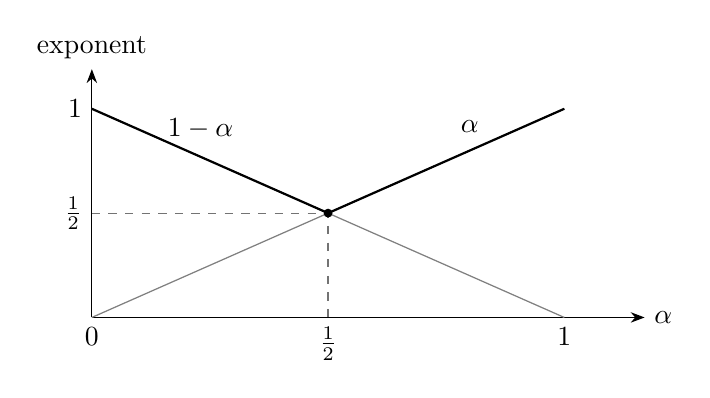
\begin{tikzpicture}[x=6cm,y=2.65cm,>=Stealth,line width=.45pt]
  \draw[->] (0,0)--(1.17,0) node[right] {\(\alpha\)};
  \draw[->] (0,0)--(0,1.19) node[above] {exponent};
  \draw[dashed,black!55] (0,.5)--(.5,.5)--(.5,0);
  \draw[black!50] (0,0)--(1,1) (0,1)--(1,0);
  \draw[thick] (0,1)--(.5,.5)--(1,1);
  \fill (.5,.5) circle[radius=1.6pt];
  \node[left] at (0,1) {\(1\)};
  \node[left] at (0,.5) {\(\tfrac12\)};
  \node[below] at (0,0) {\(0\)};
  \node[below] at (.5,0) {\(\tfrac12\)};
  \node[below] at (1,0) {\(1\)};
  \node[above] at (.23,.81) {\(1-\alpha\)};
  \node[above] at (.8,.84) {\(\alpha\)};
\end{tikzpicture}
\caption{The chain length and the two normalized allowances.
The heavy segments give the larger exponent. Lemma~\ref{lem:comparison}
also accounts for the density of the retained indices and the other
terms omitted in this scale calculation.}\label{fig:intro-length-balance}
\end{construction}

\subsection{How the theta lifts recover a fixed character sum}
\label{subsec:intro-family-arithmetic}

Where could the unequal coefficients in this average come from? Keep the primitive
character \(\psi\) and its order \(o\) fixed while the auxiliary field varies. A theta lift compares
automorphic forms on unitary groups of different ranks. In Alp\"oge's
argument a chain of such lifts carries integral weights indexed by
embeddings of an auxiliary abelian field. The local contribution to the
comparison depends on which embeddings lie above a given prime. This
dependence lets the construction distinguish Frobenius classes. Write \(\mathcal K(\psi)\) for the primitive inducers of the powers
of \(\psi\). Adding the local contributions must recover the combination
\[
 G_{\mathcal K}(x)=G_{\mathbf1}(x)
   +\frac{1}{3o+1}\sum_{\substack{\chi\in\mathcal K(\psi)\\ \chi\ne\mathbf1}}
                   \RePart G_\chi(x),
\]
where \(\mathbf1\) is the conductor-one character. The auxiliary field has
many more characters than occur in this sum.

For example, the reference row uses a definite unitary space of
dimension \(r+t_{\rm rk}\) and a row space of dimension \(r\), with
\(t_{\rm rk}\ge r+5\). On the definite side one sums over a finite
class set with its volume weights. The theta lift maps this space of
forms to a cuspidal multiplicity space with its Petersson metric and
a factor from the dimensions of the compact types. The scalar obtained
from the lift and its adjoint enters the height calculation once for
each lift. Proposition~\ref{prop:selected-reference-height}
bounds the height of the reference operator \(B_{\mathbf v}\) for a chosen
sequence \(\mathbf v\) by
\[
 \operatorname{ht}(B_{\mathbf v})\le h_A(\mathbf v)+\sum_{j=1}^m\bigl(h_B(j)-h_X(j)\bigr)
                               -\bar\kappa .
\]
Here \(h_A\) is the terminal bound, \(h_B\) bounds the kernel height,
\(h_X\) bounds the logarithm of the scalar from below, and
\(\bar\kappa\) is the common period correction. Recovering the analytic
sum requires adding prime contributions with their actual multiplicities.

To see these multiplicities, separate the two quadratic characters
at the auxiliary primes \(q,d\) from the joint image \(A\) of \(\psi\)
and the action on a real cyclotomic field of \(2\)-power conductor.
The target conductor remains \(f_\psi\).
The auxiliary Galois group \(H\) and its quotient for the target are
\[
 H=(\mathbb Z/2\mathbb Z)^2\times A,\qquad
 A_0=\ker\bigl(A\xrightarrow{\ \pi_\psi\ }\operatorname{im}\psi\bigr),
 \qquad |A/A_0|=o .
\]
Three indices enter the local calculation. The index \(1\le j\le m\)
specifies the lift, \(t\in T\subset A\) specifies a top weight \(a_t\),
and \(u\in A_0\) translates the lower weights relative to the top. Definition~\ref{def:translate-scale} gives
the group and the weight sets at a fixed scale.

\paragraph{From a prime power to a character value.}
Read the quadratic coordinates in the order \(d,q\), recording
a sign change of the corresponding square root by \(1\). The subgroup
used in the prime sum and its character are
\[
 P=\operatorname{Gal}(E/\mathbb Q(\sqrt{-d}))
    =\{0\}\times\mathbb Z/2\mathbb Z\times A,\qquad
 \omega_P(i,j,s)=(-1)^i,\qquad f_P=|P|=2|A|.
\] Follow one prime power through a single lift. At fixed \((j,t,u)\) the construction
pairs
each \(g\notin P\) with one element of \(P\). Let \(w_g\) be the
positive weight of that partner and write \(a=a_t\). The positive-part kernel at \(p^\nu\) has the form
\[
 \log p\,\bigl(a/p^\nu-w_g\bigr)_+
     = w_g\log p\,\left((a/w_g)/p^\nu-1\right)_+ .
\]
The point \(a/w_g\) where the smoothed sum is to be evaluated is thus
already specified by the integral weights.

For \(\omega\in\widehat H\), let \(\chi_\omega\) be the primitive
Dirichlet character obtained by inflating \(\omega\) along the Artin
map and passing to its conductor. Write \(I_p\) for inertia in \(H\),
and choose a lift \(F_p\in H\) of arithmetic Frobenius modulo
\(I_p\). The integral weight may vary with the lift and the translate.
The coefficient counting the Frobenius class is independent of
these choices. In the additive notation for \(H\), it is
\[
 \frac1{f_P}\sum_{\omega\in\widehat H}\overline{\omega(g)}\,
                    \chi_\omega(p^\nu)
   =\frac{2}{|I_p|}\,\mathbf 1_{\{g\in\nu F_p+I_p\}}.
\]

Indeed, averaging \(\omega(\nu F_p+v)\) over \(v\in I_p\) gives
\(\chi_\omega(p^\nu)\), including its value zero if \(\omega\) is
nontrivial on inertia. Orthogonality therefore turns the local count at \(p^\nu\) into
\[
 \frac{2\log p}{|I_p|}
      \sum_{g\in(\nu F_p+I_p)\setminus P}(a/p^\nu-w_g)_+ .
\]
If \(p\) splits in the distinguished quadratic subfield, its entire
coset lies in \(P\) and the sum vanishes. At \(d\), inertia has order
two and precisely one member \(g_d\) of the coset lies outside \(P\).
The coefficient of \((a/d^\nu-w_{g_d})_+\) is consequently \(\log d\).
At unramified primes with \(\nu F_p\notin P\) there is again a
single term, now with coefficient \(2\log p\). These alternatives
explain why deleting all ramified primes would change the comparison.

There are two terms to subtract from the resulting prime sum. The
principal character gives the logarithmic main term, and among the
nonprincipal characters only \(\omega_P\) has nonzero sum on
\(H\setminus P\). That sum is \(-f_P\). With \(\gamma\) Euler's
constant, the total to subtract is therefore
\[
 a\left(\log a-1-\gamma-\frac1{f_P}\sum_{g\notin P}\log w_g\right)
    +a\,\RePart\frac{L'(1,\chi_{\omega_P})}{L(1,\chi_{\omega_P})}.
\]
Both terms use the weights of the very same translate. By
\eqref{eq:color-balance}, the difference \(\Delta_{j,t}(u)\) between
the prime sum and this expression is
\[
 \Delta_{j,t}(u)=\frac1{f_P}\RePart
 \sum_{g\notin P}\sum_{\omega\in\widehat H}
     \overline{\omega(g)}\,w_g G_{\chi_\omega}(a_t/w_g).
\]

\paragraph{Which characters survive the translates.}
Put \(b=\exp(x^\epsilon)\) and \(X'=\exp(x^{\epsilon/3})\). The character expansion still contains every character of the auxiliary group. To
recover the prescribed average, first distinguish the two ranges of integral weights. Put
\(e_1(v)=((1,0),v)\). For a set \(T_2\subset A_0\) and an offset
\(\eta>0\) with \(\log\eta\le x^{\epsilon/4}\), the ranges are
\[
\begin{aligned}
  b\le w_g\le b+\eta+1
       &\quad\text{if }g=e_1(s+u-t),\quad s\in T_2,\\
  0<w_g\le 2xb/X'&\quad\text{at the remaining }g\notin P .
\end{aligned}
\]

The top weight satisfies \(|a_t/b-x|\le1\). At a smaller weight,
\(a_t/w_g\ge (x-1)X'/(2x)\ge X'/3\) for \(x\ge3\).
Estimate~\eqref{eq:thin-host} bounds the centered sum at this larger
argument. Its contribution after multiplication by \(w_g\) is at most
\((x+1)b\exp(-c x^{\epsilon/8})\) for a fixed \(c>0\) above the
corresponding threshold. At a larger weight the argument may be close
to \(x\), where we want to measure the centered sum. Here we retain the
term and estimate the effect of replacing \(w_g\) by \(b\).

For the uncentered sum \(S_\chi\), the positive-part kernel gives
\[
 \left|w_gS_\chi(a_t/w_g)-b S_\chi(a_t/b)\right|
 \le(w_g-b)\sum_{n\le a_t/b}\Lambda(n)\ll (x+1)(\eta+1).
\]
The nonprincipal centering term after multiplication by \(w_g\) is
independent of \(w_g\). The principal centering changes by at most
\((a_t/b)(w_g-b)\). After summing over \(g,\omega\) and dividing by
\(f_P\), the polynomial factor \(f_P\ll x^{2+8\epsilon}\) is absorbed
in both estimates. The combined error is at most \(2b/x\) per pair
\((j,t)\) above a uniform threshold.

The positions of the large weights are as important as their sizes.
They are exactly the elements \(e_1(s+u-t)\).
Every \(s\in T_2\) belongs to the subgroup over which we
average. Translating through this subgroup gives
\[
 \frac1{|A_0|}\sum_{u\in A_0}\overline{\omega(e_1(s+u-t))}
   =\omega(e_1(t))\,\mathbf 1_{\{\omega|_{0\times A_0}=1\}}.
\]
Thus the calculation only retains the \(4o\) characters of
\(H/(0\times A_0)\). Their primitive inducers are the powers of
\(\psi\), each optionally multiplied by either or both of the
quadratic characters. Averaging over the top indices determines the
coefficients of the desired powers.

Write \(C=A/A_0\) and let \(p_c=|T\cap c|/|T|\) for \(c\in C\).
Section~\ref{subsec:frobenius-selection} chooses the top indices so that
\[
 p_c=\frac{3+\mathbf1_{\{c=A_0\}}}{3o+1}+\varepsilon_c,\qquad
 |\varepsilon_c|\le x^{-1+\epsilon},\qquad \sum_{c\in C}\varepsilon_c=0 .
\]
The model proportions sum to one since \(4+3(o-1)=3o+1\).
For the principal character, summing the actual proportions also gives
one exactly. For a nonprincipal \(\xi\in\widehat C\), the uniform part
of the distribution disappears while the extra mass at the identity
contributes with positive sign:
\[
 \frac1{|T|}\sum_{t\in T}\xi(t)
  =\frac{3\sum_{c\in C}\xi(c)+\xi(A_0)}{3o+1}
        +\sum_{c\in C}\varepsilon_c\xi(c)
  =\frac{1}{3o+1}+O(o x^{-1+\epsilon}).
\]
For a quadratic target the two proportions are \(4/7\) and \(3/7\).
Their sum gives the principal coefficient; their difference gives
the coefficient \(1/7\) of the quadratic character, up to the stated
error. If \(o=1\), there is only the identity coset and the principal
coefficient is exactly one.

We can now recognize the prescribed weights on the primitive characters inducing the powers of \(\psi\), up to the coset-counting error just estimated. Each remaining term contains an auxiliary quadratic twist and has coefficient of absolute value at most one. For fixed target modulus, interval exponent \(K\ge1\), and
\(0<\epsilon<1/52\), Proposition~\ref{prop:quadratic-prime-pair}
selects one pair \((q,d)\) for each sufficiently late interval
\([Y_0,Y_0^K]\). For each of these twists \(\chi\) and every \(x\) in
that interval it gives
\[
 |G_\chi(x)|\le x^{1/2+\epsilon/2},\qquad
 \left|\frac{L'(1,\chi)}{L(1,\chi)}\right|\le4\log x .
\] The second estimate permits
the shift from \(a_t/b\) to \(x\) in the centered sum. Write \(\Sigma(x)\)
for the sum of the absolute values of the omitted terms before their
coefficients are applied, as in Definition~\ref{def:translate-errors}.

Suppose the sum of the centered local contributions is at most
\(D(x)\) at every translate. Each lift and top index contributes the
same multiplicity \(|T_2|\) to the translated mean. Writing
\(Q=m|T|b\) and \(\delta_2=|T_2|/|A|\), one obtains
\[
 \frac{Q\delta_2}{2}
       \bigl(G_{\mathcal K}(x)-\Sigma(x)-4x^{1/2+\epsilon}\bigr)
    \le D(x)+\frac{2Q}{x}.
\]
The factor \(1/2\) comes from \(|T_2|/f_P=\delta_2/2\).
Proposition~\ref{prop:translate-fourier} makes the threshold uniform in
the lift, top index, translate and field on the selected interval.
It remains to produce the bound \(D(x)\) on that scale.

\paragraph{Keeping the two division estimates on one family.}
To bound \(D(x)\), we must track what survives the passage from a selected point to
its two lattice comparisons. On the cohomology side the field is still the original
auxiliary field \(E\).
For \(a\ge1\), put \(M_{\ell,a}=(\mathbb Q_\ell/\mathbb Z_\ell)(-a)\).
Write \(S_\ell\) for the places of \(E\) above \(\ell\) and infinity,
and \(G_{E,S_\ell}\) for the Galois group unramified outside
\(S_\ell\). The quantity to be estimated is the \(\mathbb Z_\ell\)-length
\(V(E,\ell,a)\) of
\[
 \ker\!\left(H^1(G_{E,S_\ell},M_{\ell,a})
          \longrightarrow\prod_{v\mid\ell}H^1(E_v,M_{\ell,a})\right).
\]
These fields are totally imaginary, so there is no degree-one term
from any infinite place. The bound needed for division adds these
lengths with weight \(\log\ell\) and sums over the twists below
the rank of the chosen construction.

For the family application the common selection of
Proposition~\ref{prop:common-host-prime-pair} is made for the bounded
list of primitive twists in the cohomological construction.
On a subinterval \([W,W^2]\) of the prime interval,
Proposition~\ref{prop:original-window-budget} bounds the lengths at the
original field \(E_z\) of scale \(z\), simultaneously for finite sets
\(\mathcal P\) of primes. At the cutoff \(T_{401}(z)=\lfloor z^{401}\rfloor\)
the estimate reads
\[
 \sum_{\ell\in\mathcal P}\log\ell
        \sum_{1\le a<T_{401}(z)} V(E_z,\ell,a)\le \exp(z^\epsilon/2)
                  \qquad(W\le z\le W^2).
\]
The position of this subinterval may depend on the prime pair.

The order of the group \(A\) in the theta comparison determines which
cyclotomic layer to use. Lemma~\ref{lem:rescale-host-budget}
selects a field at \(x'=x/\kappa_{\rm sc}\), where the constant
\(\kappa_{\rm sc}\) accounts for the fixed part of this order. The
rescaled intervals \([Y,Y^{3/2}]\) can be taken arbitrarily late.
Write \(t_{\rm rk}\) for the rank called \(t\) in
Proposition~\ref{prop:actual-rank-budget}; it is distinct from the
top index. For every \(x\) on such an interval and every finite set
\(\mathcal P\) of rational primes,
\[
 \begin{gathered}
  1\le a<t_{\rm rk}\le\lfloor x^{400}\rfloor
                 \le\lfloor (x')^{401}\rfloor,\\
  \sum_{\ell\in\mathcal P}(\log\ell)
       \sum_{1\le a<t_{\rm rk}}V(E,\ell,a)\le\sqrt b .
 \end{gathered}
\]
The strict inequality in the twist index persists even if the two
integer cutoffs coincide. Nonnegativity of the lengths justifies the
restriction to the selected rank.

At \(2\) the cyclotomic tower gives a bound over \(E(i)\), with
\(i^2=-1\). To use it over \(E\), restrict a strict cohomology
class to \(E(i)\); its local restrictions still vanish. The kernel
of restriction has length at most one by inflation--restriction for
the extension of degree at most two. Lemma~\ref{lem:dyadic-host} therefore gives
\[
 V(E,2,a)\le 1+V(E(i),2,a)\quad(a\ge1),\qquad
 \sum_{a=1}^{t_{\rm rk}-1}V(E,2,a)
 \le (t_{\rm rk}-1)+\sum_{a=1}^{t_{\rm rk}-1}V(E(i),2,a).
\]
The added unit of length is counted for each twist before summing.

\begin{construction}
\begin{tabular}{@{}>{\raggedright\arraybackslash}p{.31\linewidth}>{\raggedright\arraybackslash}p{.60\linewidth}@{}}
\toprule
Range of the choice & Data held fixed in that range \\
\midrule
A selected prime interval & Both auxiliary primes and the estimates for all three quadratic twists.\\
One real scale \(x\) & The field at \(x'\), the ranks, the weight functions and the assigned primes.\\
One translate \(u\) & The initial row selects the twist characters. The reference period and fields are retained in constructing \(P'(x,u)\).\\
Two covers of \(P'(x,u)\) & The original lattices and quotient action of this member, with a cover prime different from the residue characteristic.\\
\bottomrule
\end{tabular}
\caption{Choices shared by the translate average and the two division estimates. The field can change with the real scale; the comparison at each translate retains the field and ranks chosen at that scale.}\label{fig:intro-family-choices}
\end{construction}

For the odd-prime cohomology count, the multiplicities come from
ordinary automorphic forms at two prescribed levels. The deformation
argument first locates points on components of a Galois deformation
space. To infer the needed Frobenius identities there one must show
that the Hecke modules are supported at those points.
The coefficient data at the two levels prescribe the ordered characters
of the ordinary flag. At a place above the coefficient prime, denote
the flag by \(F^j\) and the character on its \(j\)-th quotient by
\(\delta_j\). For a local representation of rank \(r_{\rm ord}\) the action of
a local Galois element \(g\) satisfies
\[
   0=F^0\subset F^1\subset\cdots\subset F^{r_{\rm ord}},\qquad
   \dim(F^j/F^{j-1})=1,\qquad
   g|_{F^j/F^{j-1}}=\delta_j(g).
\]

The order of these characters restricts which constituents can enter
the comparison (Appendices~\ref{sec:count-two-level-data}
and~\ref{sec:count-two-level-attachments}). The supply of starting
points depends on the rank. In the even-order rank-four construction
it comes from quadratic automorphic induction. In rank two the starting representation is a scalar twist of the one
attached to a newform. In rank three it is the trace-zero adjoint
of the representation attached to another newform
(Appendices~\ref{sec:count-two-seed-specialization} and~\ref{sec:linked-seeds}).
The selected rank-three multiplicities are computed in
Appendix~\ref{sec:rank-three-multiplicity}.

Appendix~\ref{sec:linked-components} propagates support from a known
ordinary eigenpoint along the component graph. For instance, at a
characteristic-zero even-order target reached by the two-link construction,
Proposition~\ref{prop:two-link-classical-control} factors both
evaluations through classical ordinary Hecke quotients. If \(r\) is
the target representation, \(r_i\) comes from the eigensystem at
level \(i\), and \(\kappa\) is the common twisting character, then on
the marked field \(L\) it gives
\[
 \det(X-r_i(g))=\det(X-\kappa(g)r(g))
       \qquad(g\in G_L,\ \text{at both levels}).
\]
At a good prime these characteristic polynomials supply the Frobenius data needed for
the count. Appendix~\ref{sec:local-global} relates finite types to their
Weil--Deligne parameters, and Appendix~\ref{sec:additional-rank-four}
transports the integral ordinary flags needed in the rank-four case.

For this argument to give an integral length, support over the
enlarged field has to be brought back to the coefficient ring in which
the length is measured. The Taylor--Wiles tests at the intervening
curve points bound the first-order deformations at the marked level.
Write \(J_{\rm ord}\) for the image of the ordinary Hecke ideal at the
target and \(Q_{\rm end}\) for its target prime. Transport along the
chain gives the inclusion needed for descent:
\[
             J_{\rm ord}\subseteq Q_{\rm end}
             \qquad\text{(Proposition~\ref{prop:marked-chain-support}).}
\]

The finite algebra at the
marked point and descent to the two levels identify the constituents
that contribute (Appendices~\ref{sec:marked-hosts} and~\ref{sec:host-descent}).
For example, over a discrete valuation ring \(O\) with uniformizer
\(\pi\), take nonnegative integers \(d,h\). An \(O\)-linear
map from \(O/(\pi^d)\) into \(O/(\pi^h)\)
is determined by the image of \(1\), which must be killed by \(\pi^d\).
For \(M=O/(\pi^h)\) the possible images form its annihilator subgroup
\[
               M[\pi^d]=\pi^{\max(h-d,0)}M .
\]

Its length is therefore
\[
             \operatorname{length}_O\operatorname{Hom}_O
                      (O/(\pi^d),O/(\pi^h))=\min(d,h).
\]
Appendix~\ref{sec:rank-three-length} uses such Smith summands in
bounding the length by valuations of differences of Frobenius traces.
This is one source of the odd-prime estimates summed over the common
interval in Appendix~\ref{sec:cohomology}.

Fix the base data at a sufficiently late scale with admissible
marked levels. Proposition~\ref{prop:translate-completion} supplies
a member at every integer translate \(0\le u_0<|A|\) in the
subgroup average. Proposition~\ref{prop:all-window-applications} applies the integral comparison, period and Gram bounds to this family. On its late intervals one thus has
\[
 \forall\,0\le u_0<|A|\quad\exists\,P(x,u_0)\quad
 \text{with both division estimates at }P(x,u_0).
\]
One estimate compares the integral lattices attached to the periods,
and the other uses cohomology to control a numerator weighted by
the multiplicities of the good characters.
Proposition~\ref{prop:completed-division-pair} identifies its two
realizations at every prescribed subspace. One can therefore pass
from the arithmetic divisibilities to the norms and determinants of
those same period maps. This is the input to the geometric estimates.

\subsection{Following a period from a lattice to a complex integral}

Fix one translate and its selected point. Choose a sequence \(\mathbf u\) of lifts. We now have bounds for lengths of finite modules, yet the period we want to
estimate is a complex integral of automorphic forms. The passage between them starts
with a choice of lattice for that integral. We need a rational vector space on which the integral defines a functional, an integral lattice in that space, and metrics at every infinite place of its coefficient field. An index will then contribute to the degree of a determinant line.

For a rank-one illustration take \(K=\mathbb Q(i)\) and the place \(w\) over \(3\). It is inert, so \(3\) is a uniformizer in its valuation ring \(O_w\). The conjugation on \(K\) preserves \(w\). The usual Hermitian form \(H(x,y)=x\bar y\) on the completion \(K_w\) gives
\[
 M=3^aO_w,\qquad M^\#=\{y\in K_w:H(M,y)\subseteq O_w\}=3^{-a}O_w
                                  \qquad(a\in\mathbb Z_{\ge1}).
\]

The two lattices span the same local field. In a basis of \(M\), the generator of \(M^\#\) has coordinate \(3^{-2a}\). Consequently their signed index and the length of the quotient in the opposite order are
\[
                [M:M^\#]_w=-2a,\qquad
                \operatorname{length}_{O_w}(M^\#/M)=2a .
\]
The place weight in this example is \((\log 9)/2=\log 3\). An identification of the underlying vector spaces would give no information about the integer \(a\). In the actual construction the Hermitian form is the level pairing, and at split places its two arguments also involve conjugate places. Section~\ref{sec:word-division} makes the determinant comparison on those lattices.

Let \(K\) be the totally complex coefficient field. A tuple \(\tau\) specifies the local data used to realize the forms. Write \(\tau_0\) for the reference tuple and \(\tau(w)\) for the tuple prescribed at a finite place \(w\) of \(K\). The finite-dimensional space \(V_{\tau}\) has a lattice \(M_{\tau}\) of integral forms. Projecting to the selected quotient and comparing it with the base row gives maps
\[
 V_{\tau}\xrightarrow{\ P_{\tau}\ }Q_{\tau}\xrightarrow{\ \iota_{\tau}\ }R_{0,K},
 \qquad P_{\tau}(V_{\tau})=Q_{\tau},\qquad \iota_{\tau_0}:Q_{\tau_0}\simeq R_{0,K}.
\]
Here the row is the space on the second side of the period pairing. At \(w\) its lattice is the image of the integral forms for the tuple actually used there. A rational row vector belongs to the global lattice precisely when it satisfies all the following membership tests.
\[
 R_0=\{y\in R_{0,K}: y\in\iota_{\tau(w)}P_{\tau(w)}(M_{\tau(w),w})
                           \ \text{for every finite }w\}.
\]

There is a test for the quotient at the reference tuple. At lift \(j\), let \(J_j\) realize a column in the complex source of the theta lift and let \(W_j\) realize row coordinates in its target. In these coordinates the lift \(\Theta_j\) satisfies
\[
                 \Theta_jJ_j=W_j B_jP_j,\qquad
                 \ker(\Theta_jJ_j)=\ker P_j,
\]
since \(B_j\) is invertible and \(W_j\) identifies a coordinate space with its image. Surjectivity of \(P_j\) puts every row basis vector in the image of \(\Theta_j\). The rank \(D_0>0\) counts primitive row labels with multiplicity. Equation~\eqref{eq:selected-theta-square} and Proposition~\ref{prop:base-theta-rank} also identify the dimension of the good part at the other tuples used in the comparison.

Consider the reference period \(P_{\mathbf u,0}(\phi,f)\) as a function of its second argument \(f\). It annihilates the kernel of the reference quotient \(q_0\). Consequently one can compute it from the column coordinates of \(\phi\) and the row coordinates of \(q_0 f\). Write \(e_{\nu,\mathbf u}\) and \(e_R\) for their identifications with the chosen rational spaces. The descended pairing satisfies
\[
              B_{\mathbf u}(e_{\nu,\mathbf u}\phi,e_R q_0 f)=P_{\mathbf u,0}(\phi,f).
\]
Surjectivity makes this prescription unique on the row. At the other tuples one must still determine the scalar that compares their period with this rational pairing. Requiring the same group, evaluation translate, characters and Haar measures fixes what is being compared. Proposition~\ref{prop:completed-division-pair} identifies the two realizations on that point for every sequence.

Section~\ref{sec:transport} follows this scalar through the theta kernels. For a tuple \(\tau\) let \(K_{\tau,j}\) be the definite lift on columns, \(S_{\tau,j}\) the prescribed endomorphism there, and \(D_{\tau,j}\) the descending row operator. At an even level \(j\) the two compositions act in opposite directions.
\[
 \varphi^{(j+2)}=K_{\tau,j+1}K_{\tau,j}S_{\tau,j}\varphi^{(j)},
 \qquad G^{(j)}=D_{\tau,j}D_{\tau,j+1}G^{(j+2)} .
\]

In the descending tower a row is integrated against a theta kernel on a unitary quotient. In the definite tower a column lifts by a finite sum over lattice classes, with the mass of each class given by its level volume and stabilizer. Unfold two consecutive integrals. At a nonterminal step the real compact integral is a finite linear combination of evaluations in frames. Lemma~\ref{lem:common-definite-expansion} shows that the frames and coefficients depend only on the real type and test. This permits summing over tuples before the remaining real integration.

For a term indexed by tuple \(\tau\), write \(i_{\tau,j}\) for the nonzero normalization of a descending row integral, \(k_{\tau,j}\) for that of a definite lift, and \(v_{\tau,j}\) for the factor from unfolding the pair of steps. The coefficients \(a_{\tau,j}\) of a linear relation at even levels satisfy
\[
 a_{\tau,j}v_{\tau,j}k_{\tau,j}k_{\tau,j+1}
       =a_{\tau,j+2}i_{\tau,j}i_{\tau,j+1}.
\]
At the top, branching for the compact terminal group has multiplicity one and supplies the terminal scalar. Induction down the chain now takes a relation between terminal class sums to a relation between the actual periods at every base frame and smooth test vector. Lemma~\ref{lem:joint-period} gives the implication with both endpoint products. The induction uses linearity throughout, so it applies even when an individual period vanishes.

To read off the scalar, choose a nonzero bottom period \(b_*\) at
the reference tuple. If \(A_*\) is its raw terminal entry, the entry
in the descended relation is \(p_*=(h_0/d_0)A_*\), where \(h_0,d_0\)
are the reference top and bottom products. For any matched raw
entry \(A_t\) and bottom pairing \(B_t\), the relation now gives
\[
          p_* B_t=c_t A_t b_*,\qquad
          c_t=s_{\rm col}\,h_t/d_t .
\]
The column similarity contributes the same \(s_{\rm col}\ne0\) to every \(c_t\).
Comparing with \(t=0\) therefore leaves the ratio \(c_t/c_0\)
used on the rational row. The identity \eqref{eq:word-period-cross-product}
expresses this comparison even at zero entries.

\subsection{Geometry and the two indices in the determinant}

We have followed the period into the integral dual. To read the resulting determinant
inequality as a height bound we still need two archimedean estimates. To bound the maximal slope of \(R_0\), use coefficient evaluations on the same theta space as the pairing. On the base multiplicity space \(V\), Lemma~\ref{lem:fitted-completed-nonvanishing}
detects every nonzero vector at the prescribed depth. Proposition~\ref{prop:fitted-grid-base-separation}
chooses \(\dim V\) tests at one real pair. Their coordinate map
\(F:V\to\mathbb C^{\dim V}\) is injective, so on the original column
\[
                  \ker(FP_{\tau_0})=\ker P_{\tau_0}.
\] Evaluating the other tuples in compatible coordinates then controls the integral images defining \(R_0\). With \(\bar\kappa\) the mean of the logarithms of the period scalars, Proposition~\ref{prop:descended-row-height} obtains
\[
                         \mu_{\max}(R_0)+\bar\kappa\le b x^{C_H}.
\]
A finite change of level has a separate index and metric factor. It cannot be absorbed by rescaling each tuple independently.

The other estimate concerns the determinant of an entire good row at lift \(j\). Here the relevant space is a space of cusp forms on a unitary Shimura variety. Its integral model has several components after passage to a sufficiently deep level. The dimension of the moving system of cusp sections and the size of integral sections both enter the estimate. If \(D_Z\) is the moving degree on component \(Z\), the degrees from growth at two nearby weights satisfy
\[
                       V_Z(u')\le D_Z\le V_Z(u_1).
\] These bounds agree across components at a given weight. This uniformity allows ranks and degrees to be summed before descent to the required character type. See Proposition~\ref{prop:deep-moving-degree}.

One can ask how a calculation on a flag determines an arithmetic
degree as the weight varies. On each of the two marked flag spaces,
Section~\ref{sec:covolume-flag-test} fixes the graded-line metrics.
For a block of rank \(n\), with Chern roots in their flag order, the
point monomial for the fibre degree is
\[
               m_n=\prod_{a=0}^{n-1}(-x_a)^{n-1-a}.
\]
The product of these monomials over the blocks and embeddings has
degree one on the flag fibre. This specifies the scale of the test.
Section~\ref{sec:flag-wall-slope} uses the tests and the behavior on
the chamber walls to constrain the homogeneous degree polynomial.
To use the degree at \(u'\) for sections of weight \(u_1\), we must
also bound the norm of multiplication by a section of the weight
difference. Fix a component \(Z\). If \(g\) runs over its nonzero cusp
sections of weight \(u_1\), the norm of evaluation is measured by
\[
      \mathcal B_{u_1,Z}(y)
      =\sup_{g\ne0}\frac{\|g(y)\|^2}{\|g\|_{2,Z}^2}.
\]

Near the boundary a short period makes the multiplying theta section
small. Lemma~\ref{lem:deep-thin-evaluation} chooses a theta translate
whose value still controls the ratio on that same component.
On the complementary region a congruence-level neighbourhood embeds,
and Lemma~\ref{lem:deep-thick-evaluation} constructs a cusp section with
prescribed value at its centre. Combining the estimates bounds the
cost of the weight change in Lemma~\ref{hyp:covolume-shift-costs}.
Section~\ref{sec:flag-component-transfer} then transfers the component
bounds from the deep cover to the chosen levels.

The metric matters in this calculation. A geometric degree alone does not account for the size of a section at the complex embeddings. For a principally polarized abelian scheme on a horizontal arithmetic surface let \(\bar\omega\) be the Hodge bundle with its polarization metric and \(d_{\det\omega}\) the degree of its determinant on the generic curve, taken over \(\mathbb Q\). The second Hodge intersection is
\[
             \widehat{\deg}\,\widehat{\operatorname{ch}}_2(\bar\omega)
                            =\tfrac12 r_*d_{\det\omega}.
\]
The constant \(r_*\) is independent of the scheme, surface and relative dimension. Thus variation of this particular arithmetic term can be measured on the generic curve. Theorem~\ref{thm:hodge-surface-degree} specifies the degree also when a regular cover is needed.

A further determinant twist restores the original row weight after estimating sections in a range where there are sufficiently many of them. The two blocks of the unitary signature enter with opposite signs. Writing \(w_{j\rho}\) for the integral weight shift at embedding label \(\rho\), \(\Omega\) for the chosen period scale and \((p_j,q_j)\) for the signature, the normalized log covolume \(L_{3,j}\) satisfies
\[
          L_{3,j}\le \sum_\rho(p_j-q_j)w_{j\rho}\log\Omega+(C_0+1)U .
\]
Here \(U=B_0\log\log x\) is the common error scale of Proposition~\ref{prop:selected-base-covolume}. The flat line preserves rank and its normalized degree supplies the signed term. Character traces, descent of integral coefficients and comparison with the Petersson metric contribute to the error. The terminal lift has its own type estimate. The constant and cutoff precede the choices of translate, sequence and lift.

\begin{construction}
\begin{tabular}{@{}>{\raggedright\arraybackslash}p{.25\linewidth}>{\raggedright\arraybackslash}p{.29\linewidth}>{\raggedright\arraybackslash}p{.38\linewidth}@{}}
\textit{Where} & \textit{Object compared} & \textit{Quantity entering the degree}\\ \hline
infinite places & good base row with its Petersson metric & normalized log covolume \(L_{3,j}\)\\
\(w,\bar w\) at a twist & transported row lattices in the common space & sum \(I_{wj}\) of two signed indices\\
the same local tuple & row and its Hermitian dual & dual index with the actual character multiplicities
\end{tabular}
\caption{Three terms in the determinant comparison at one lift. The two finite comparisons use the tuple assigned to the place and the common base rank \(D_0\).}\label{fig:intro-period-indices}
\end{construction}

To see how geometry controls a finite index, work first at a place \(\lambda\) of a field over which a geometric realization is defined. Write \(M_{0,\lambda}\) for its integral lattice of forms and \(\Theta_\lambda\) for the local module generated by the prescribed products of sections. Intersect both with a subspace \(V\) of the completed span of \(M_0\). At each integer depth \(h\) above the specified local threshold, Proposition~\ref{prop:geometric-run-index} gives
\[
 \operatorname{length}
 \frac{V\cap M_{0,\lambda}}{V\cap M_{0,\lambda}\cap\Theta_\lambda}
                         \le h\dim V+r_\lambda .
\]

The nonnegative \(r_\lambda\) is chosen before \(V\) and \(h\), and its sum with the normalized finite-place weights is bounded. In particular one may take \(V\) to be spanned by the Smith directions of exponent greater than \(h\). The remainder then bounds the sum of their excess exponents.

For example, suppose that a sublattice has three Smith exponents \(1,3,7\) in a lattice with basis \(e_1,e_2,e_3\), and take \(h=3\). The choice \(V=K_\lambda e_3\), where \(K_\lambda\) is the local field, gives
\[
      7\le3+r_\lambda,\qquad
       (1-3)_++(3-3)_++(7-3)_+=4,\qquad (a)_+=\max(a,0).
\]
If the inequality were tested only on the whole space, it would require merely \(1+3+7\le9+r_\lambda\). That would allow \(r_\lambda=2\) and miss half the excess in the third direction. Under extension by ramification index \(e\), the change of exponents and the excess at the new depth are
\[
        (1,3,7)\longmapsto(e,3e,7e),\qquad
        (e-3e)_++(3e-3e)_++(7e-3e)_+=4e .
\] 
The proof of \eqref{eq:run-cut} bounds the excess for all subspaces over the larger field by first bounding the length of the image of the full lattice multiplied by the depth power.

On returning to \(K\), retain the assigned tuple at both orientations of every twisted place. At \(w\mid p\) put \(\omega_w=\log{\rm N}w/[K:\mathbb Q]\) and let \(e_w\) be its ramification index. The transport part of the determinant carries the factor \(\omega_w/D_0\). Subtract from the sum over lifts the forced weights \(F_h(w)\) and the correction \(2e_w/p^2\). Divide its positive part equally among the \(m\) lifts. With \([v]_+=\max(v,0)\), this gives
\[
 e_w r^0_{j,w}=\frac1m\left[
 D_0^{-1}\sum_{h=1}^m I_{wh}-2\sum_{h=1}^m e_wF_h(w)-2e_w/p^2\right]_+ .
\]
The summand \(J_{j,w}\ge0\) from the least exponent at lift \(j\) still has to be included. Writing \(W_{\rm tw}\) for the twisted places, the first error is
\[
           E_{1,j}=\sum_{w\in W_{\rm tw}}\omega_w(e_wr^0_{j,w}+J_{j,w}).
\]

The second error \(E_{2,j}\) occurs in the signed index of the lift lattice \(\mathcal T\) against the localization of its global Hermitian dual. With \(\eta_j(w)\) the normalized congruence length, \(D_G\) a class and level denominator, and \(s\) clearing the classwise dual inclusions, Proposition~\ref{prop:signed-lift-dual-index} gives
\[
 [\mathcal T_w:(\mathcal T^\#)_w]_w
          \le e_w\eta_j(w)+D_0\bigl(J_{j,w}+v_w(sD_G)\bigr).
\]
The cohomological numerator involves the marked Tate-dual row and the direct column in the localized Galois calculation. Their lengths are evaluated with the multiplicities of the good characters at precisely this tuple. Passing from the restricted lattices to the full lattices and clearing the common class denominator \(d_*\) costs at most \(\log d_*+\log s\). The selected comparison has \(s=1\).

Write \(n=|A|\) for the group order in the family and \(N_c\) for the rank allowance at the point. The parameters of the error estimate are
\[
     f=2n,\quad z=x^\epsilon,\quad b=e^z,\quad
     B_0=fmbz,\qquad \mathcal E=z(B_0+N_c).
\] Lemma~\ref{lem:parent-transport-cost} and Proposition~\ref{prop:parent-dual-cost} yield, for \(1\le j\le m\),
\[
 \begin{aligned}
 E_{1,j}&\le 2(4C^2+25C+C_b+44)\mathcal E,\\
 E_{2,j}&\le (|C_N|+1)\mathcal E+\log d_*
              \le (|C_N|+3+9C_\Gamma)\mathcal E .
 \end{aligned}
\]
The constants refer to the two geometric comparisons and the cohomological length estimate in those results. Both bounds hold for the same point and choice of sequence once the common threshold is reached. This quantifier is what permits summation over the lifts in a single determinant. Proposition~\ref{prop:sequence-division} combines the resulting \(O(m\mathcal E)\) with the weight and evaluation terms. The period enters that proposition through a numerical upper height, defined even for a zero map.

\subsection{How much of a row survives interpolation?}

The determinant has given a total length. To use it on a subspace of a period row we
need finer information. How many independent directions survive at a specified depth? Take a good cycle selected in Section~\ref{subsec:frobenius-selection}.
Its length is the even order of the Frobenius step. On that cycle
Section~\ref{sec:host-edge-tests} constructs a coefficient DVR in which
the two neighbouring lattices can be tested together. Section~\ref{sec:interpolation} uses two tests on the local lattices. The first varies an integral weight on an arithmetic progression of step prime to \(p\). Suppose its matrix \(A(T)\) has size \(l\), with entries integral combinations of \(\binom{T}{i}\) for \(i\le\delta\). Write \(C\) for the leading coefficient and \(d\) for the degree of its nonzero determinant. Normalize \(v(p)=1\). In a splitting field factor the determinant
and choose \(L\) to bound its leading coefficient and degree by
\[
             \det A(T)=C\prod_{\nu=1}^d(T-\zeta_\nu),
             \qquad v(C)+d/(p-1)\le lL .
\]

At the \(j\)-th of \(H\) successive evaluation points, let \(b_j\) count the Smith factors of valuation at least \(E\), with valuation \(+\infty\) for a zero. Over the coefficient DVR each specialization has a Smith normal form.
With \(E\ge1\), \(H\le p^h\) and \(\delta<p^h\),
Lemma~\ref{lem:smith-average} gives
\[
             H^{-1}\sum_j b_j
               \le l\left(\frac{\delta}{H}+
                           \frac{L+\delta h/H}{E}\right).
\]
A zero of the determinant at a chosen weight is therefore allowed. The degree term pays for exceptional evaluations, and the second term limits the number of large invariant factors at the other weights. The output is an average with multiplicity over the progression.

A second test holds the target lattice fixed and varies the incoming neighbor. On the smaller-prime range, a polynomial in Frobenius-twisted coordinates separates a chosen residue plane from the competing planes. Lifting the resulting symbols with controlled denominators produces vectors and covectors on each incoming edge. Pairing tests from distinct edges gives entries of higher valuation than the diagonal blocks. After the stated normalization the combined matrix is the identity modulo the uniformizer, so it has an integral inverse. For the recovered target subspace \(V_{\rm rec}\), Proposition~\ref{prop:residue-plane-neighbor-test} gives
\[
                 \dim V_{\rm rec}\ge(1-\kappa)\dim V,
                          \qquad \kappa=O(Nx^{-12}),
\]
where \(N\) counts the selected top positions. Its endpoint orders and its denominator \(p^{D_{\rm II}}\) are fixed in that prime range.

Section~\ref{sec:frames} asks for the dimension spanned at infinity. For complex matrices \(A_i\) with common target of dimension \(D\), put \(Q=\sum_i A_iA_i^*\). Its image is their joint span. Whenever \(\operatorname{tr}Q>0\),
\[
                 \operatorname{rank}Q
                       \ge\frac{(\operatorname{tr}Q)^2}
                                {\operatorname{tr}(Q^2)} .
\]
Lemma~\ref{lem:frame-rank} gives the version allowing each source to lose a controlled number of directions. For the period maps this leaves two questions. Which columns have nonzero period, and how large is the second moment of their sum on the common target?

\subsection{Nonvanishing and the dimension of the period image}

Here the two questions left by interpolation meet. The sections live on several
definite unitary groups, but their periods take values in a common space of cuspidal
forms. A nonzero section can have zero period. Moreover, periods from distinct groups can have nearly the same image, even if each period map has large rank. Let \(P_{\mathbf u}\) be the period map from the full column Hilbert space \(C_{\mathbf u}\) indexed by a sequence \(\mathbf u\), and let \(\mathcal H\) be the common row. These two questions concern different spaces:
\[
             \ker(P_{\mathbf u}:C_{\mathbf u}\longrightarrow\mathcal H),\qquad
             \mathcal H\Big/\sum_{\mathbf u} P_{\mathbf u}(C_{\mathbf u}).
\]
The first occurs in identifying a rational evaluation with a nonzero automorphic period. The second occurs in bounding the slopes of the common row.

Fix one of the selected points. Put \(d_{\mathbf u}=\dim C_{\mathbf u}\). Unfolding its inner products introduces an explicit scalar \(c_{\mathbf u}\) from the Haar measures and the dimension of the definite type. The operators to be estimated have source and target
\[
 K_{\mathbf u\mathbf v}=(c_{\mathbf u}c_{\mathbf v})^{-1/2}P_{\mathbf u}^*P_{\mathbf v}:C_{\mathbf v}\longrightarrow C_{\mathbf u} .
\]
Definition~\ref{hyp:full-gram-row} specifies the measures, the preliminary convention at zero and the finite levels for these maps.

Unfolding makes the identity term on an equal pair of columns the reference identity operator. The other terms are indexed by relative positions of two flags. At finite places the character level is a compact open subgroup \(K_2\), with character \(\chi_2\). Two translated level functions overlap precisely when their relative translate \(t_f\) belongs to \(K_2\). With the quotient measures of Section~\ref{sec:selected-row-gram}, the finite integral is
\[
 I_f(t_f)=
 \begin{cases}
  \operatorname{vol}(K_2)\chi_2(t_f), & t_f\in K_2,\\
  0, & t_f\notin K_2.
 \end{cases}
\] At infinity one integrates modulo the intersection of the two unipotent lattices after expressing both in the first frame. The change of either rational representative introduces reciprocal finite and infinite phases. Proposition~\ref{prop:gram-unfolded-measures} thus gives an operator attached to the relative position.

There are two estimates to make for a given collection of relative positions. One counts the integral representatives, each weighted by the reciprocal order of its stabilizer. The other measures their orbital amplitudes. For the first, remove the isotropic flag and its marked negative line from a row lattice. The remaining definite Hermitian lattice has rank \(k\). In Section~\ref{sec:flag-counts} the line has norm \(-T\) for a completely split prime \(T\ge3\). If there are \(f\) real places of the totally real base field, Proposition~\ref{prop:flag-row-mass} gives the two masses
\[
 M=m_k\left(\frac{T^k-1}{T-1}\right)^f,\qquad
 M_{\rm row}=(T-1)^fM .
\]
Here \(m_k\) is the mass of the standard unimodular genus. Counting two flags requires their common sublattice as well. Its corank governs the estimates in Proposition~\ref{prop:flag-pair-counts}.

On the analytic side, successive blocks of a flag can meet along a degenerate orbit. Near that orbit the oscillatory integral has a leading term expressed by integrals over a single unipotent group. The integral for block sizes \((s-1,1)\) is expanded in terms of the single-block integral of size \(s\). Write \(n=s-1\), fix a compact set \(K\subset\mathbb C^\times\) and let \(D=ct^n\in K\). For the additive character \(\psi_\beta\) and the derivative bound \(M_0\) of Section~\ref{sec:orbital-germ}, Lemma~\ref{lem:orbital-germ} gives
\[
 |t|^{n^2}O_{n,1}(t,c)
  =\frac1s\sum_{z^s=(-1)^nD}|z|^{n^2}\psi_\beta(sz/t)O_s(z)
      +O_{s,\beta,K}(M_0|t|).
\]
The sum has one term for each stationary phase. The remainder tends to zero uniformly on the stated determinant levels as \(t\to0\). This local statement becomes a bound on a period only after one sums the allowed frequencies.

Two normalizations enter that summation. The period lattice has a dual for the field trace, whereas Fourier inversion uses the Euclidean dual in a product of complex planes. For the CM field \(E\), use one embedding \(\sigma_v\) from each conjugate pair. Write \(g\) for the level and \(c=d^{-\nu}\) for the scale in Section~\ref{sec:period-lattice}, where \(d\) is the root discriminant. For the period lattice \(L\), put \(\Lambda=c\sigma(L)\). Lemma~\ref{lem:period-lattice-normalization} gives both the frequency and its normalization:
\[
 \frac1g\operatorname{Tr}_{E/\mathbb Q}(lL)\subseteq\mathbb Z
 \quad\Longleftrightarrow\quad
 \frac{2\overline{\sigma(l)}}{gc}\in\Lambda^\vee,
 \qquad \operatorname{covol}(\Lambda)=(d/2)^fg^{3f}.
\]

The sign and spectral parameter of each added letter also change the vector tested against the orbital integral. The transfer matrices in Section~\ref{sec:word-pairing} keep track of these changes, and Proposition~\ref{prop:real-node-positivity} gives positivity at the real interpolation nodes. Consequently a mixed pairing can be bounded by the two diagonal energies. The resulting Fourier decay and the lattice covolume give the block recursion in Section~\ref{sec:block-recursion}. Its final step uses the actual period lattice.

At a place with frequency \(l\) and derivative scale \(X>0\) the mixed pairing gains the factor \(\min(1,(X/|l|)^5)\), interpreted as one at zero. In one complex plane a dyadic annulus of outer radius \(R\) contains \(O(R^2)\) points of the standard Gaussian lattice. For example, for the standard lattice and \(X\ge1\), the successive outer annuli contribute at most
\[
 \sum_{j\ge0} O((2^jX)^2)\,2^{-5j}
       \ll X^2\sum_{j\ge0}2^{-3j}\ll X^2 .
\]
This is the elementary one-place calculation behind the product estimate. Proposition~\ref{prop:auxiliary-period-comparison} first uses an auxiliary lattice for intermediate block sizes, then cancels the Fourier normalization against the covolume at the last size. This accounts for the product of the preceding block volumes in \eqref{eq:block-last-period}.

To sum over the remaining relative positions one needs absolute convergence and the local operator norm. The integrable majorants of Section~\ref{sec:xi} control the integrations over the flag unipotent and the real group at the required weight gaps. Proposition~\ref{prop:real-period-norm} identifies the squared norm of the Bessel pairing on the open cell in terms of the reciprocal formal degree. Apply the identity of Section~\ref{sec:bessel-periods} to the two definite stabilizers. With compatible characters on the relative stabilizer and the required weight gaps for both periods, Proposition~\ref{prop:local-operator-normalization} in Section~\ref{sec:local-amplitudes} gives
\[
                  \|J_A\|_{\rm cell}^2=C/d_A .
\]
Here \(J_A\) is the orbital amplitude, \(d_A\) its discrete-series formal degree in the transported Haar measure, and \(C\) is uniform in the fixed interpolation window. On a cell with nonzero Gram invariant and nonzero preceding minor, Section~\ref{sec:absolute} also gives a pointwise estimate. The squared-norm estimate still applies when that minor vanishes.

For a nonscalar generic pair at corank one, at least one amplitude has extra decay. Use this on the side supplying it and the squared-norm bound on the other. To sum their product one must count the representatives in both orders. For two labels \(X,Y\), let \(H_X,H_Y\) be their heights and \(n_X,n_Y>0\) the normalization factors formed from their positive Gram invariants in Section~\ref{sec:row-sums}. With \(h\) the counting exponent and \(c\) the height constant, the two counts for the same fibre give
\[
       N(X,Y)\le c^f(H_XH_Y)^h
                    \min\{H_X^h n_X,H_Y^h n_Y\}.
\]

The squared-norm bound for each amplitude supplies an inverse square root of its corresponding \(n\). Multiplying the first count alone by these two factors would leave \(\sqrt{n_X/n_Y}\), for which the heights give no comparison here. Reversing the order of the two labels gives the second count. The elementary inequality \(\min(a,b)\le\sqrt{ab}\) now yields
\[
 \frac{N(X,Y)}{\sqrt{n_Xn_Y}}
      \le c^f(H_XH_Y)^h\,
          \frac{\sqrt{H_X^h n_X\, H_Y^h n_Y}}{\sqrt{n_Xn_Y}}
      =c^f(H_XH_Y)^{3h/2}.
\]
For a repeated word the two squared-norm estimates alone suffice.
After summing the two labels and restoring the row mass, the
generic corank-one pairs contribute at most
\[
          e^{C_Bm^5 f\log b}\,\frac{d_{\mathbf u}^2}{D_*}
\]
in the diagonal comparison of Proposition~\ref{prop:pretransport-ramified-period}.
Here \(d_{\mathbf u}\) is the dimension of the marked column and \(D_*\)
is the identity contribution to the ambient trace.
Lemma~\ref{lem:equal-word-generic-corank-one} proves this bound for the
whole set, including its scalar pairs.

For distinct words the error budget is tighter. Proposition~\ref{prop:summed-row-corank-one}
uses the extra decay available on one side of a nonscalar pair. At higher
corank the genus mass also enters the count, as in
Lemma~\ref{lem:higher-corank-total-error}.

\begin{construction}
\begin{tabular}{@{}>{\raggedright\arraybackslash}p{.29\linewidth}>{\raggedright\arraybackslash}p{.62\linewidth}@{}}
\toprule
Estimate & Role in the sum of orbital terms \\
\midrule
Flag count & Bounds the number of integral representatives of a fixed pair of labels, with stabilizer weights.\\
Squared orbital norm & Supplies a bound on either amplitude even when its preceding minor vanishes.\\
Pointwise decay & Improves the bound on at least one side of a nonscalar generic pair at corank one.\\
Cuspidal dimension & Fixes the common scale for the aggregate contribution of different columns.\\
\bottomrule
\end{tabular}
\caption{From the local orbital estimates to the rank of the joint period image.}\label{fig:intro-gram-estimates}
\end{construction}

Here is how the estimates in Figure~\ref{fig:intro-gram-estimates} detect an individual period. On the full column the preliminary diagonal comparison gives \(\|K_{\mathbf u\mathbf u}-I\|_{\rm HS}^2\le e_Pd_{\mathbf u}\). An orthonormal basis of \(\ker P_{\mathbf u}\) contributes one unit per vector to this squared norm. At the assigned prime \(T_{\mathbf u}\) the ramified subspace \(C_{\mathbf u}^{\rm ram}\) has a computable dimension. In the selected range the two comparisons are
\[
 \frac{\dim\ker P_{\mathbf u}}{d_{\mathbf u}}\le e_P<\frac34,
 \qquad
 \frac{\dim C_{\mathbf u}^{\rm ram}}{d_{\mathbf u}}
   =\left(1-\frac{1}{T_{\mathbf u}-1}\right)^f
   \ge 1-\frac{f}{T_{\mathbf u}-1}\ge\frac34 .
\]
Thus there is a ramified vector \(v\) with \(P_{\mathbf u}v\ne0\). Its period supplies the nonzero initial value used in the two-term period relation. The argument takes place before transport to the rational row (Proposition~\ref{prop:pretransport-ramified-period}).

For the dimension of the combined images the relevant scale is the identity contribution \(D_*\) to the cuspidal trace. It is the quotient volume times the finite projector evaluated at the identity and the product of the archimedean formal degrees. Proposition~\ref{prop:projector-dimension} compares \(D_*\) with the
actual multiplicity \(D\) in the range of Definition~\ref{hyp:cuspidal-dimension}.
Proposition~\ref{prop:selected-rank-comparison} places the selected
projector in that range. Uniformly in its fields, levels and weights,
for sufficiently large ambient rank \(r\),
\[
          |D-D_*|\le e^{-rf\log(r)/16}D_*.
\]
There is equality \(D=D_*\) for a definite group in the stated range. For distinct sequences Proposition~\ref{prop:selected-full-gram} gives
\[
 \|K_{\mathbf u\mathbf v}\|_{\rm HS}^2\le(1+b^{-6})d_{\mathbf u}d_{\mathbf v}/D_* .
\]
The common scale \(b\) and the range of column dimensions are specified in Proposition~\ref{prop:selected-rank-comparison}.

The estimate for \(D_*\) comes from a separate trace calculation. A finite convolution projector prescribes the level and a lowest compact type selects the archimedean discrete series. In the part of the quotient where the lattice has no very short subspace, separation of the integral matrices controls the nonidentity terms. The complementary part can contain many short unipotent translates of one point. There the estimate uses a filtration by normalized lattice covolumes and bounds the contribution of an orthonormal family before taking its trace. Both estimates are needed when the smaller signature index is positive.

Indeed, for the normalized column maps \(A_{\mathbf u}=c_{\mathbf u}^{-1/2}P_{\mathbf u}\) put \(Q=\sum_{\mathbf u} A_{\mathbf u}A_{\mathbf u}^*\). Cyclicity of the trace gives
\[
 \operatorname{tr}(Q^2)=\sum_{\mathbf u,\mathbf v}\|A_{\mathbf u}^*A_{\mathbf v}\|_{\rm HS}^2 .
\]
The diagonal bounds control the individual kernels, while this identity uses the off-diagonal bounds to control overlap. Lemma~\ref{lem:frame-rank} converts the resulting trace ratio into a bound on the codimension of the sum of the images, even after restricting the columns to subspaces of small total codimension. This is the rank information needed for the slope comparison: it controls how much of
the common row can be missed after the columns have each been restricted.

\subsection{Where the square root enters}

Return to the real scale \(x\) in the chosen interval. We can now put a number on the
error that Fourier projection left undetermined. The
period, lattice and Gram estimates have supplied the upper bound
of Proposition~\ref{prop:fixed-point-slope-gap} on each translate.
The prime sum in that proposition already includes every lift and
every top index. In particular, the upper bound is for the sum
\[
             \sum_{j=1}^m\sum_{t\in T}\Delta_{j,t}(u)
                       \qquad(u\in A_0).
\]
There is no further factor of \(m\) when it is inserted in the Fourier
average. An average over \(A_0\) has mass one. This is where it pays
to have kept the translate and the integral weights fixed in the
slope calculation.

Here are the sizes which determine the answer. In the notation of
Lemma~\ref{lem:comparison}, let \(n=|A|\), \(n_T=|T|\), let \(n_2\)
count the indices of the second weight, and put \(\delta_2=n_2/n\).
Write \(b\) for the weight scale, \(k\) for the integer in the
arithmetic comparison and \(a_E\) for its size parameter, bounded
by \(2xb\). Dividing the three terms of the arithmetic bound by
\(Q=n_Tmb\) leaves the quantities
\[
 \frac{a_E}{mb}\left(1+\frac{m^2}{k}\right),\qquad
        2\frac n{n_T}m x^\epsilon,\qquad
        \frac n{n_T}\delta_2\frac{k}{n^2}x^{2\epsilon}.
\]
This line separates the effect of lengthening the chain from the
cost of selecting the weights. The leading part of the first
quantity decreases with \(m\). The second increases with \(m\)
because the estimates accumulate along the chain. The third
depends on the upper bound for \(k\), which is why the construction
has to provide a range for this integer.

For example, consider the first quantity with \(xm\le k\).
The term containing \(m^2/k\) has a different behavior from the
leading term. Direct substitution gives
\[
 \frac{a_E}{mb}\left(1+\frac{m^2}{k}\right)
       \le \frac{2x}{m}+\frac{2xm}{k}
       \le \frac{2x}{m}+2 .
\]
For the remaining terms use the density of the top indices and
the upper bound for \(k\). The family has
\[
       \frac{n}{n_T}\le2x^{\epsilon/8},\qquad
       x^{-\epsilon}\le\delta_2\le1,\qquad
       k\le n^2 x^{1/2-\epsilon}.
\]
It follows that the second term is at most \(4m x^{9\epsilon/8}\)
and the third at most \(2x^{1/2+9\epsilon/8}\). The only variable
still governing the two competing powers is the length \(m\).

Here the choice of the family is slightly asymmetric. The retained
density parameter is \(\delta_1=x^{-\epsilon/8}\).
The family chooses \(m\) in the range of Lemma~\ref{lem:rank-window}, between
\(\sqrt{x\delta_1}\) and twice that value, hence
\[
 x^{1/2-\epsilon/16}\le m\le 2x^{1/2-\epsilon/16},
 \qquad
 \tfrac12 x^{1/2+\epsilon/16}\le x/m\le x^{1/2+\epsilon/16}.
\]
The power sacrificed by using a slightly shorter chain is thus
explicit. The remaining division in the Fourier comparison is by
\(\delta_2/2\), which costs at most \(2x^\epsilon\).
Section~\ref{subsec:fixed-weight-absorption} bounds the unnormalized
error by \(x^{5\epsilon}\) times the comparison expression.
Lemma~\ref{lem:comparison} restores the omitted twists, absorbs
fixed factors for sufficiently large \(x\), and gives
\[
       G_{\mathcal K}(x)\le x^{1/2+9\epsilon}
                          \qquad(Y\le x\le Y^{3/2}).
\]
Thresholds may depend on the fixed character and on \(\epsilon\).

The family estimates made them independent of the translate and of
the auxiliary ranks appearing at \(x\). By Lemma~\ref{lem:disjoint-common-pair-windows} the lower endpoints tend to infinity on the already chosen family. Hence the left endpoint can exceed the last threshold of Lemma~\ref{lem:uniform-numerical-application}.
This choice of lower endpoint is what the pole argument needs.

\subsection{Reading an interval with a Laplace derivative}

We now read the interval estimate in the opposite direction, from the primes back to
the zeros. Fix \(\psi\) and suppose that its primitive function has a zero
\(\rho\) with \(1/2<\beta=\RePart\rho<1\). Choose a positive
\(\epsilon<\epsilon_0(\psi)\) so small that
\[
             \theta=\tfrac12+9\epsilon<\beta .
\]
The transform \(\Phi\) of the weighted sum has a pole at \(\rho\)
by the residue calculation above. We shall obtain incompatible
estimates for its high derivatives. It helps to distinguish two
features of the interval: its position determines the derivative
order; its length permits an exponentially small tail.

Put \(u=\log y\), \(g(u)=G_{\mathcal K}(e^u)\) and \(U=\log Y\).
The window in \(u\) is \([U,3U/2]\). The finite weighted sum has
the elementary global bound \(|g(u)|\le Be^{2u}\) for a constant
depending on the fixed family. Indeed each uncentered prime sum is
\(O(y(1+\log^2 y))\), by summing \(y\log n/n\), and the explicit
centering satisfies the same bound for the fixed family. On the
window the arithmetic argument supplies the stronger inequality
\[
              g(u)\le e^{\theta u}
                     \qquad(U\le u\le 3U/2).
\]
The negative values of \(g\) could have large absolute value. A
direct estimate for the absolute value of a single complex Laplace
integral would discard precisely the information contained in this
one-sided inequality.

For a real \(\sigma>2\) and \(\RePart z=\sigma\), use the notation
of Theorem~\ref{thm:window},
\[
 T_k(z)=\frac{(-1)^k}{k!}\Phi^{(k)}(z)
       =\int_0^\infty g(u)\frac{u^k}{k!}e^{-zu}\,du .
\]
Here \(k\) is a derivative order; the integer used in the arithmetic
comparison has played its part. To estimate the derivative at
\(z=\sigma+i\tau\), rotate it by a scalar \(c\) of absolute value one
so that \(\RePart(cT_k(z))=|T_k(z)|\), then add the real derivative
at \(\sigma\). Under the integral, the combined multiplier is
\[
         0\le 1+\RePart(ce^{-i\tau u})\le2 .
\]
This choice uses the reality of \(g\). With \(g^+=\max(g,0)\), it gives
\[
 |T_k(\sigma+i\tau)|+\RePart T_k(\sigma)
       \le 2\int_0^\infty g^+(u)\frac{u^k}{k!}e^{-\sigma u}\,du .
\]
The right side is independent of \(\tau\). Later we can move the
complex center vertically to isolate an individual pole while
keeping exactly the same upper bound.

To estimate the integral outside the window, write \(a=\sigma-2\)
and choose \(k=\lceil 5aU/4\rceil\). Against the global bound for
\(g^+\), the substitution \(v=au\) gives the probability density
\[
             \frac{v^k e^{-v}}{k!}\,dv,\qquad
             v>0,\qquad \int_0^\infty\frac{v^k e^{-v}}{k!}\,dv=1 .
\]
The mode in the original coordinate is \(k/a\), close to \(5U/4\).
The standard deviation is \(\sqrt{k+1}/a\), of order \(\sqrt U\)
for fixed \(a\). Each boundary of the window is at distance of order
\(U\) from the mode. An exponential moment gives exponential decay
of the two tails, as in Section~\ref{sec:window}.

\begin{construction}
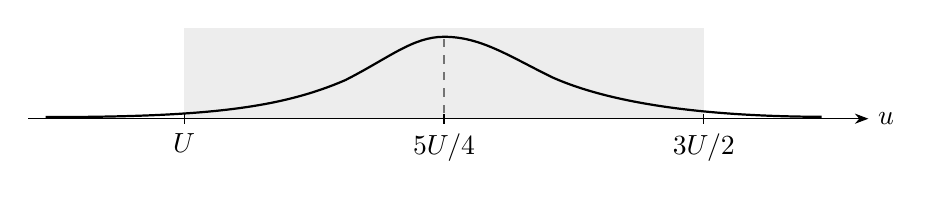
\begin{tikzpicture}[x=2.2cm,y=.68cm,>=Stealth,line width=.42pt]
 \fill[black!7] (1,0) rectangle (4,1.7);
 \draw[->] (.1,0)--(4.95,0) node[right] {\(u\)};
 \draw (1,.08)--(1,-.1) node[below] {\(U\)};
 \draw (2.5,.08)--(2.5,-.1) node[below] {\(5U/4\)};
 \draw (4,.08)--(4,-.1) node[below] {\(3U/2\)};
 \draw[dashed,black!55] (2.5,.1)--(2.5,1.57);
 \draw[thick] (.2,.03) .. controls (1.12,.03) and (1.55,.19) .. (1.93,.72)
     .. controls (2.18,1.13) and (2.32,1.53) .. (2.5,1.53)
     .. controls (2.71,1.53) and (2.87,1.18) .. (3.12,.78)
     .. controls (3.56,.14) and (4.25,.04) .. (4.68,.035);
\end{tikzpicture}
\caption{Placement of the derivative kernel on the logarithmic scale (schematic).
The shaded interval is where the arithmetic estimate holds. Its length is \(U/2\);
the effective width of the gamma density for the tail estimate is of order
\(\sqrt{U}\) with \(a\) fixed.}\label{fig:analytic-road}
\end{construction}

Inside the window use \(g^+(u)\le e^{\theta u}\). Put
\(D=\sigma-\theta\); the inequality \(v^ke^{-v}/k!\le1\) gives
\[
 \int_U^{3U/2}g^+(u)\frac{u^k e^{-\sigma u}}{k!}\,du
              \le \frac{U}{2}D^{-k}.
\]
Outside the window the global estimate leaves a factor
\(Ba^{-k-1}\) times the gamma tail. Choose \(a\) large enough,
once for all these intervals, so that the exponential decay of the
tail absorbs the difference between \(a^{-k}\) and \(\sigma^{-k}\).
Since \(D<\sigma\), both pieces give the bound of
\eqref{eq:derivative-upper},
\[
 |T_k(\sigma+i\tau)|+\RePart T_k(\sigma)
       \ll (1+U)D^{-k},\qquad k=\lceil 5aU/4\rceil .
\]
Its strength is in the exponential base \(D\). A pole closer than
\(D\) to a suitable center would force larger derivatives along
these very same orders.

\subsection{Returning to the putative zero}

All poles arising here from zeros are simple poles of a logarithmic derivative, even for a multiple zero. To contradict the interval estimate we must isolate one of these poles at the very
derivative orders the interval supplies. If a meromorphic
function has a unique closest pole \(\lambda\) to a center \(z\),
which is simple with residue \(r\ne0\) and distance \(d=|z-\lambda|\), take a
circle of radius \(R>d\) enclosing no other pole and contained
in the domain of continuation. The principal part and the holomorphic
remainder give, by Cauchy's estimate,
\[
       T_k(z)=\frac{r}{(z-\lambda)^{k+1}}+O(R^{-k}).
\]
A derivative indexed by \(k\) therefore measures distance to this
pole with exponential precision. The comparison uses a real and a
complex center because the arithmetic bound controls only a
particular sum of derivatives.

If the unique closest pole to the real center \(\sigma\) is a real
\(\lambda\) at distance \(d<D\), the residue formula gives
\(r>0\). Use both derivatives at \(\sigma\). For any radius \(R\)
strictly between \(d\) and the smaller of \(D\) and the distance to
the next pole, the lower bound is
\[
          2\RePart T_k(\sigma)\ge 2r d^{-k-1}-O(R^{-k}).
\]

It contradicts the upper bound as \(U\) tends to infinity along the
chosen intervals. After multiplication by \(d^k\), the two sides would have to satisfy
\[
    2r/d-O\bigl((d/R)^k\bigr)\ll(1+U)(d/D)^k\longrightarrow0 ,
\]
although the left side tends to \(2r/d>0\). This also explains why the real
sign of the residue mattered.

In the other cases move the complex center along the line
\(\RePart z=\sigma\). If the open disk of radius \(D\) about
\(\sigma\) is free of poles, align the height with that of the
putative pole to the right of \(\RePart s=\theta\). The horizontal
distance is strictly less than \(D\). If the real center has a
nonreal nearest pole inside that disk, taking its height strictly
decreases the distance. This gives a center closer to some pole
than the real center is and at distance less than \(D\).

For example, if the nearest poles to the real center are a
conjugate pair \(\alpha\pm i\gamma_0\), with \(\gamma_0>0\), compare
the squared distances at height \(\tau\):
\[
 \big|\sigma+i\tau-(\alpha-i\gamma_0)\big|^2-
 \big|\sigma+i\tau-(\alpha+i\gamma_0)\big|^2=4\tau\gamma_0 .
\]
Moving toward the upper pole separates the two contributions while the
bound on the pair of derivatives stays uniform in \(\tau\).

A small further variation of the height removes ties. On a short
vertical segment only finitely many poles can be relevant, and a
pair with distinct imaginary parts is equidistant at most at one
height, by subtracting the squared distances. Two poles at the same
height have distinct horizontal distances since both lie to the left
of \(\sigma\). Let \(\mathcal P\) denote the set of poles. We obtain a unique
nearest pole \(\lambda\) at distance \(d\) from \(z\) and can choose
a radius satisfying
\[
 d<R<\min\{D,\operatorname{dist}(\sigma,\mathcal P),
                    \operatorname{dist}(z,\mathcal P\setminus\{\lambda\})\}.
\] At the complex center take
the absolute value of the principal part. At the real center
Cauchy's estimate now bounds the entire derivative by \(O(R^{-k})\).
Together the estimates would imply
\[
       \frac{|r|}{d}-O\bigl((d/R)^k\bigr)
                        \ll(1+U)(d/D)^k .
\]

The two sides have incompatible limits. The contradiction completes
the passage from a one-sided bound on a sequence of intervals to
the absence of the proposed zero. It is here, after the arithmetic
averaging, that a conclusion about the individual target character
is recovered.

Section~\ref{sec:deduction} finishes the passage to the full
statement. On \(\RePart s=1\), Lemma~\ref{lem:boundary} gives
nonvanishing away from the principal pole. On \(\RePart s>1\) the
absolutely convergent Euler product gives nonvanishing. For a character \(\chi\) modulo \(q\), let \(f=f_\chi\)
and use the finite Euler-factor identity of
Lemma~\ref{lem:analytic-change-modulus},
\[
   L_q(s,\chi)=L_f(s,\chi^*)\prod_{\substack{p\mid q\\p\nmid f}}
                                  (1-\chi^*(p)p^{-s}).
\]

Each extra factor is nonzero for \(\RePart s>0\), since
\(|\chi^*(p)p^{-s}|=p^{-\RePart s}<1\). Thus changing the
modulus introduces no new zero in the open strip. The principal
character retains its simple pole at one. For a primitive character,
the gamma and conductor factors in Definition~\ref{def:completed-dirichlet}
are finite and nonzero in the open strip. The functional equation there gives
\[
        L(s,\chi)=0\quad\Longleftrightarrow\quad
              L(1-s,\bar\chi)=0\qquad(0<\RePart s<1).
\]

A zero to the left of the critical line would therefore give a
zero to its right for the conjugate character. For \(\zeta\) the
functional equation also identifies the zeros at the negative even
integers, and \(\zeta(0)=-1/2\). These are the distinctions of scope
in Theorem~\ref{thm:claims}. \cite[(25.15.5)]{dirichlet}
\cite[(25.4.1)--(25.4.4)]{zeta}

The number \(1/2\) has appeared twice for different reasons.
On the arithmetic side a chain of length near \(\sqrt x\) balances
the normalized errors \(x/m\) and \(m\). On the analytic side a
zero at \(\rho\) would force growth governed by \(\RePart\rho\).
The interval bound leaves room for arbitrarily small positive
losses in the arithmetic exponent. Fixing the zero first allows
one to choose those losses smaller than \(\RePart\rho-1/2\);
the functional equation accounts for the other half of the strip.


\section{Zeros in the critical strip and an estimate for prime sums}
\label{sec:statements}

The argument in the introduction begins by subtracting the contribution at one. We
first justify that subtraction for each character and specify what happens on the
boundary of the strip. The estimate at the end of the chapter
is the arithmetic input to the zero criterion of Section~\ref{sec:window}. Section~\ref{sec:comparison} derives it from the uniform local bounds, and Section~\ref{subsec:fixed-weight-absorption} explains the proposed source of those bounds.

Write \(\Z,\Q,\R,\C\) for the integers, rationals, reals and
complex numbers. For \(s\in\C\), write \(\RePart s\) for its real
part. Logarithms without a specified base are natural logarithms.

Use \(X(q)\), \(\chi_{0,q}\) and \(L_q(s,\chi)\) as in
Definitions~\ref{def:dirichlet-modulus} and~\ref{def:dirichlet-series}.
The modulus specifies which primes are omitted even when the primitive
inducer stays fixed. This affects both the Euler product and the smoothed
sum.

\begin{auxlemma}[Changing the modulus]\label{lem:analytic-change-modulus}
Let \(\chi\) be a Dirichlet character modulo \(q\) with conductor \(f=f_\chi\),
and let \(\chi^*\) be the primitive character inducing it. As an identity of meromorphic functions,
\begin{equation}\label{eq:imprimitive-euler-factors}
 L_q(s,\chi)=L_f(s,\chi^*)
       \prod_{\substack{p\mid q\\p\nmid f}}(1-\chi^*(p)p^{-s}).
\end{equation}
For \(y\ge1\), the corresponding correction to \eqref{eq:smoothed-sum} is
\[
 S(y;f,\chi^*)-S(y;q,\chi)=
 \sum_{\substack{p\mid q\\p\nmid f}}\log p
       \sum_{\substack{r\ge1\\p^r\le y}}\chi^*(p)^r W(y/p^r).
\]
\end{auxlemma}

\begin{proof}
On \(\RePart s>1\) cancel the common Euler factors. Precisely the primes
\(p\mid q\) with \(p\nmid f\) have \(\chi(p)=0\) and
\(\chi^*(p)\ne0\). Continuation gives \eqref{eq:imprimitive-euler-factors}.
In the two finite sums, \(\Lambda(n)\) restricts the difference to positive
powers of the same primes, with \(\chi^*(p^r)=\chi^*(p)^r\).
\end{proof}

For a nonprincipal character, \(L_q(s,\chi)\) extends to an entire function.
The principal character is induced by the character of conductor one, so
\[
 L_q(s,\chi_{0,q})=\zeta(s)\prod_{p\mid q}(1-p^{-s}).
\]
The finite product is nonzero at \(s=1\), where this function has a simple pole.

\begin{theorem}[Zeros of the zeta function and Dirichlet \(L\)-functions]\label{thm:claims}
Let \(X(q)\) have the meaning of Definition~\ref{def:dirichlet-modulus}.
\begin{enumerate}
\item For the zeta function,
\[
 \{s\in\C\setminus\{1\}:\zeta(s)=0\}\setminus
       \{-2n:n\in\mathbb Z_{\ge1}\}
       \ \subseteq\ \{s\in\C:\RePart s=\tfrac12\}.
\]
\item For every \(q\ge1\), \(\chi\in X(q)\) and \(s\in\C\),
\[
 \RePart s>\tfrac12,\quad (\chi,s)\ne(\chi_{0,q},1)
       \quad\Longrightarrow\quad L_q(s,\chi)\ne0 .
\]
\item For every \(q\ge1\) and \(\chi\in X(q)\), including \(f_\chi=q\),
\[
 \{s\in\C:0<\RePart s<1,\ L_q(s,\chi)=0\}
       \ \subseteq\ \{s\in\C:\RePart s=\tfrac12\}.
\]
\end{enumerate}
\end{theorem}

\begin{construction}
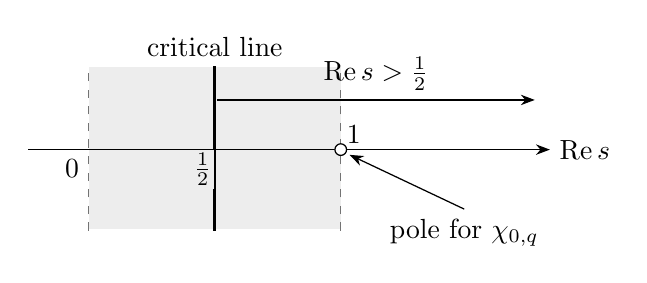
\begin{tikzpicture}[x=3.2cm,y=.83cm,>=Stealth,line width=.45pt]
 \fill[black!7] (0,-1.22) rectangle (1,1.26);
 \draw[dashed,black!55] (0,-1.24)--(0,1.28) (1,-1.24)--(1,1.28);
 \draw[->] (-.24,0)--(1.83,0) node[right] {$\RePart s$};
 \draw[line width=.95pt] (.5,-1.24)--(.5,1.28);
 \node[above] at (.5,1.28) {critical line};
 \node[below left] at (0,0) {$0$};
 \node[below left,fill=black!7,inner sep=1pt] at (.5,0) {$\tfrac12$};
 \fill[white] (1,0) circle[radius=2.1pt];
 \draw (1,0) circle[radius=2.1pt];
 \draw[->] (1.49,-.91) node[below] {pole for \(\chi_{0,q}\)} --(1.035,-.08);
 \node[above right,inner sep=2pt] at (1,0) {$1$};
 \draw[->] (.51,.76)--(1.77,.76)
   node[midway,above] {$\RePart s>\tfrac12$};
\end{tikzpicture}
\caption{The domains in Theorem~\ref{thm:claims}. Shading marks the open critical strip. The circle marks the exception at \(s=1\) for the principal character.}\label{fig:zero-domains}
\end{construction}

The open strip in the theorem is reached through prime sums. Their centering already
uses the value of the logarithmic derivative at one for a nonprincipal character, so
the boundary is the first case to settle.

\begin{lemma}[Boundary nonvanishing]\label{lem:boundary}
For \(q\ge1\), \(\chi\in X(q)\) and \(t\in\mathbb R\), the boundary
value at every regular point satisfies
\[
   (\chi,t)\ne(\chi_{0,q},0)\quad\Longrightarrow\quad
                       L_q(1+it,\chi)\ne0 .
\]
\end{lemma}

\begin{proof}
For \(\sigma>1\) the Euler products give
\[
 \zeta(\sigma)^3\,|L(\sigma+it,\chi)|^4
             |L(\sigma+2it,\chi^2)|\geq 1.
\]
For each prime power \(p^r\), the summand in the logarithm of
the product has denominator \(rp^{r\sigma}\). If \(\chi(p)\ne0\),
write \(\chi(p)^rp^{-irt}=e^{iv}\). Its numerator is
\[
             3+4\cos v+\cos(2v)=2(1+\cos v)^2\ge0.
\]
If \(\chi(p)=0\), the numerator is \(3\). These are all terms by
absolute convergence. If \(L(s,\chi)\) has a zero of order \(m\ge1\)
at \(1+it\) and \(L(s,\chi^2)\) is holomorphic at \(1+2it\),
then the product is \(O((\sigma-1)^{4m-3})\) as
\(\sigma\downarrow1\), contradicting its lower bound. A pole of
the last factor requires \(t=0\) and \(\chi^2\) principal.

It remains to treat \(t=0\) with \(\chi\) real and nonprincipal. Here a zero at one would cancel the pole of zeta:
\[
 L(1,\chi)=0\quad\Longrightarrow\quad P(s)=\zeta(s)L(s,\chi)\ \text{is entire}.
\] Its Dirichlet series in
\(\RePart s>1\) has coefficients \(a_n=\sum_{d\mid n}\chi(d)\).
The coefficients are multiplicative, and
\[
 a_{p^j}=\sum_{i=0}^j\chi(p)^i
   =\begin{cases}
        j+1,&\chi(p)=1,\\
        1,&\chi(p)=0,\\
        \mathbf 1_{2\mid j},&\chi(p)=-1.
     \end{cases}
\]
In particular all \(a_n\ge0\) and \(a_{m^2}\ge1\) for every \(m\). At a real \(\sigma_0>1\) the derivatives can
be taken termwise by absolute convergence in a neighborhood.
Entirety and the Taylor expansion of \(P(\sigma_0-r)\) give
\[
 P(\sigma_0-r)=\sum_{k\geq 0}\frac{r^k}{k!}
             \sum_{n\geq 1}a_n(\log n)^k n^{-\sigma_0}
             =\sum_{n\geq 1}a_n n^{-\sigma_0+r}\qquad(r\geq 0).
\]
Nonnegativity justifies interchanging the sums. Taking
\(r=\sigma_0-1/2\) makes the subseries over squares diverge.
\end{proof}


\begin{definition}[Centering of the smoothed sum]\label{def:smoothed-centering}
Let \(\chi\) be a primitive Dirichlet character of conductor \(f_\chi\), and let \(\gamma\) be the
Euler--Mascheroni constant. For \(y\in[1,\infty)\) define
\(G_\chi(y)\in\mathbb C\) from the sum in \eqref{eq:smoothed-sum} by
\begin{equation}\label{eq:centered-sum}
 G_\chi(y)=
 \begin{cases}
 S_\chi(y)+y\,L'(1,\chi)/L(1,\chi),&\chi\ne1,\\
 S_1(y)-y\log y+(1+\gamma)y,&\chi=1 .
 \end{cases}
\end{equation}
Lemma~\ref{lem:boundary} gives the nonzero denominator in the first case.
\end{definition}

The subtraction at one was made separately for each character. We now combine the
centered sums in the real average for which the arithmetic construction will give an
upper bound.

\begin{definition}[Positive character averages]\label{def:family-weights}
For a finite set \(F\) of primitive characters and a weight function
\(w:F\to\mathbb R_{>0}\), define
\[
 G_{F,w}(y)=\sum_{\chi\in F}w(\chi)\RePart G_\chi(y)
                  \qquad(y\ge1).
\]
For a primitive character \(\psi\) of order \(o\), use the family and weights
\[
 \mathcal K(\psi)=\{(\psi^a)^*:0\le a<o\},\qquad
 w_\psi(\chi)=
 \begin{cases}1,&\chi=1,\\ (3o+1)^{-1},&\chi\ne1.\end{cases}
\]
Here \(\psi^a\) is formed at the modulus of \(\psi\) before passing
to its primitive inducer. With \(\psi\) fixed, abbreviate
\(\mathcal K=\mathcal K(\psi)\) and \(G_{\mathcal K}=G_{\mathcal K(\psi),w_\psi}\).
Both \(1\) and \(\psi\) belong to this set, including when \(o=1\).
\end{definition}

\begin{proposition}[A uniform estimate on intervals with arbitrarily large left endpoint]\label{prop:arithmetic}
Fix a primitive Dirichlet character \(\psi\), allowing conductor one. Use the centered sums of Definition~\ref{def:smoothed-centering} and the weights of Definition~\ref{def:family-weights}. There exists
\(\epsilon_0=\epsilon_0(\psi)>0\) such that, whenever
\(0<\epsilon<\epsilon_0\),
\begin{equation}\label{eq:arithmetic-window}
 \forall Z\ge1\quad \exists Y>Z\quad \forall y\in[Y,Y^{3/2}],
 \qquad G_{\mathcal K(\psi),w_\psi}(y)\le y^{1/2+9\epsilon}.
\end{equation}
\end{proposition}

The family \(\mathcal K\) and its weights are fixed before \(\epsilon\)
is chosen. The threshold for \(Y\) may depend on \(\psi\) and
\(\epsilon\). The auxiliary number fields and the dimensions in the theta lifts
may grow with \(y\). The exponent coefficient \(9\) is fixed and the
bound applies at every point of each interval. These quantifiers
permit a choice of \(\epsilon\) after the real part of a putative zero
has been specified. Theorem~\ref{hyp:uniform-arithmetic-data} gives the simultaneous arithmetic bound. The proof in Section~\ref{sec:comparison} divides it by the total weight and bounds the characters omitted by the projection.

\section{Detection of zeros from interval bounds}\label{sec:window}

The estimate in Proposition~\ref{prop:arithmetic} is one-sided
and is available only on selected intervals. Why can these intervals exclude a zero even when nothing comparable is known in the
gaps? For a finite family with positive weights the answer comes from choosing the
order of differentiation after the interval is known. Taking many derivatives of a Laplace
transform concentrates its integral on one of the intervals where the bound holds.
Comparing a real derivative with one at a complex point makes
the kernel in the upper bound nonnegative. The deduction in
Section~\ref{sec:deduction} applies the criterion with
intervals \([Y,Y^{3/2}]\) and an exponent chosen below the real part of the
proposed zero.

\begin{definition}[The transforms of a weighted family]\label{def:window-transforms}
Let \((F,w)\) be a finite positively weighted family as in
Definition~\ref{def:family-weights}. In logarithmic coordinates set
\(g_{F,w}(u)=G_{F,w}(e^u)\) for \(u\ge0\).
For a primitive character \(\chi\), let \(H_\chi\) be the Mellin
transform of its centered sum. Let \(\Phi_{F,w}\) be the Laplace
transform of the real-valued function \(g_{F,w}\). Explicitly,
\[
 H_\chi(s)=\int_1^\infty G_\chi(y)y^{-s-1}\,dy,\qquad
 \Phi_{F,w}(s)=\int_0^\infty g_{F,w}(u)e^{-su}\,du
                       \qquad(\RePart s>1).
\]
Absolute convergence follows from the growth estimate at the start
of the proof below. With the family fixed, write \(g=g_{F,w}\),
\(\Phi=\Phi_{F,w}\), and \(w_\chi=w(\chi)\).
\end{definition}

\begin{theorem}[A zero-free half-plane from bounds on intervals]\label{thm:window}
Let \((F,w)\) be as in Definition~\ref{def:window-transforms},
with \(G_\chi\) as in \eqref{eq:centered-sum}.
Suppose that \(0<\theta<1\), \(\delta>0\), \(C>0\), and
\[
 \forall Z\ge1\quad\exists Y>Z\quad\forall y\in[Y,Y^{1+\delta}],
             \qquad G_{F,w}(y)\le Cy^\theta .
\]
Then each \(\chi\in F\) satisfies
\[
 \RePart s>\theta,\quad (\chi,s)\ne(1,1)
         \quad\Longrightarrow\quad L_{f_\chi}(s,\chi)\ne0.
\]
\end{theorem}

\begin{proof}
\proofstep{The poles of the transform.}
For every \(y\ge1\), absolute values in the defining sum give
\[
 |S_\chi(y)|\le y\sum_{n\le y}\frac{\log n}{n}
             \ll y(1+\log^2 y).
\]
The centering terms satisfy the same bound for each fixed character.
Thus the real function \(g(u)=G_{F,w}(e^u)\) satisfies \(|g(u)|\le B e^{2u}\) on
\(u\ge0\), for a constant \(B\) depending on the weighted family.

For \(\RePart s>1\) the Mellin transform of \(S_\chi\) is
\[
 \int_1^\infty S_\chi(y)y^{-s-1}\,dy
    =-\frac{L'(s,\chi)}{s(s-1)L(s,\chi)} .
\]
To justify the exchange with the Dirichlet series, first integrate
a single summand over \(y\in[n,\infty)\).
\[
 \int_n^\infty(y/n-1)y^{-s-1}\,dy
   = n^{-s}\left(\frac1{s-1}-\frac1s\right).
\]

The same calculation with \(s\) replaced by \(\RePart s>1\)
majorizes the absolute integrals, since
\(\sum_n\Lambda(n)n^{-\RePart s}<\infty\).
Transforming the two centering terms of \eqref{eq:centered-sum} therefore gives
\begin{align*}
 H_\chi(s)&=-\frac{L'(s,\chi)}{s(s-1)L(s,\chi)}
        +\frac{L'(1,\chi)}{(s-1)L(1,\chi)} \qquad(\chi\ne 1),\\
 H_1(s)&=-\frac{\zeta'(s)}{s(s-1)\zeta(s)}
        -\frac{1}{(s-1)^2}+\frac{1+\gamma}{s-1}.
\end{align*}
These formulas continue meromorphically to \(\RePart s>0\).
By Lemma~\ref{lem:boundary}, for \(\chi\ne1\) the coefficient of
\((s-1)^{-1}\) in the first term of \(H_\chi\) is
\(-L'(1,\chi)/L(1,\chi)\), and the second term cancels it.

For the conductor-one character one writes
\[
 \zeta(s)-\frac1{s-1}
   =\sum_{n\ge1}\left(n^{-s}-\int_n^{n+1}v^{-s}\,dv\right).
\]
On a compact subset of \(\RePart s>0\) each summand is bounded
by \(\sup_{s}|s|\,n^{-1-\inf_s\RePart s}\) by integration of
the derivative of \(v^{-s}\). At \(s=1\) the partial sums are
\(\sum_{n\le M}1/n-\log(M+1)\to\gamma\). Consequently, with
\(h=s-1\),
\[
 -\frac{\zeta'(1+h)}{(1+h)h\,\zeta(1+h)}
      =\frac{1}{h^2}-\frac{1+\gamma}{h}+O(1).
\]
These two terms cancel the two explicit centering terms in \(H_1\).

Substituting \(y=e^u\) in Definition~\ref{def:window-transforms} gives the
following continuation of \(\Phi\) from \(\RePart s>1\) to \(\RePart s>0\):
\[
 \Phi(s)=\tfrac12\sum_{\chi\in F}w_\chi
                         (H_\chi(s)+H_{\bar\chi}(s)).
\]
Here \(G_{\bar\chi}(y)=\overline{G_\chi(y)}\) on the real axis.
For \(0<\RePart\rho<1\) let \(m_\chi(\rho)\) be the order of
vanishing of \(L(s,\chi)\) at \(\rho\), with value zero if
\(L(\rho,\chi)\ne0\). Factoring out \((s-\rho)^{m_\chi(\rho)}\)
gives
\[
 \operatorname{Res}_{s=\rho}\Phi(s)=
 -\frac{1}{2\rho(\rho-1)}
       \sum_{\chi\in F}w_\chi
                \bigl(m_\chi(\rho)+m_{\bar\chi}(\rho)\bigr).
\]
If any order on the right is positive, the positive weights
make this a nonzero residue. The residue is real and positive
at a real zero, since \(\rho(1-\rho)>0\) there. The Euler products and Lemma~\ref{lem:boundary}
exclude all other poles in \(\RePart s\ge 1\), and the centering
has removed the singularity at \(1\).

\proofstep{Concentrating the derivative integrals.}
The residue calculation identifies what a zero contributes. To test for that
contribution using bounds on only one interval at a time, fix a real \(\sigma>2\), to
be chosen below. For a nonnegative
integer \(k\) and a complex point \(z\) with \(\RePart z=\sigma\),
put \(T_k(z)=(-1)^k\Phi^{(k)}(z)/k!\).
With the growth constant \(B\) fixed at the start of the proof, differentiation
under the integral is justified by
\[
  |u^kg(u)e^{-zu}|\le B u^k e^{-(\sigma-2)u},\qquad
  \int_0^\infty u^k e^{-(\sigma-2)u}\,du
       =\frac{k!}{(\sigma-2)^{k+1}} .
\] Write \(g^+=\max(g,0)\) for the positive part.
For a real \(\tau\), choose \(c\in\C\) with \(|c|=1\) and
\(\RePart(cT_k(\sigma+i\tau))=|T_k(\sigma+i\tau)|\).
Since \(g\) is real, the normalized derivatives at \(\sigma\) and \(\sigma+i\tau\) satisfy
\[
 |T_k(\sigma+i\tau)|+\RePart T_k(\sigma)
  =\int_0^\infty g(u)\frac{u^k e^{-\sigma u}}{k!}
                        (1+\RePart(ce^{-i\tau u}))\,du .
\]
This kernel lies between zero and twice the real exponential kernel,
which gives
\begin{equation}\label{eq:two-centers}
 |T_k(\sigma+i\tau)|+\RePart T_k(\sigma)
 \leq 2\int_0^\infty g^+(u)\frac{u^k}{k!}e^{-\sigma u}\,du
 \qquad (\tau\in\R).
\end{equation}

Writing \(U=\log Y\), set \(W=[U,(1+\delta)U]\).
On \(W\), \(g^+(u)\leq C e^{\theta u}\). The integral over \(W\)
is at most \(C\delta U/(\sigma-\theta)^k\) because
\(v^k e^{-v}/k!\leq 1\) for \(v\geq 0\).

Set \(a=\sigma-2\), \(b=1+\delta/2\), and \(k=\lceil ab U\rceil\).
Let \(X\) have the gamma distribution with density \(v^ke^{-v}/k!\)
for \(v>0\). On the complement of \(W\), the substitution \(v=au\)
and the bound \(|g(u)|\le B e^{2u}\) give the upper bound
\[
 B a^{-k-1}\Pr\{X\notin[aU,(1+\delta)aU]\},
 \qquad X\sim\operatorname{Gamma}(k+1,1).
\]

Fix \(q_-,q_+\) with \(1/b<q_-<1<q_+<(1+\delta)/b\).
As \(U\to\infty\), \(aU/(k+1)\to1/b\) and
\((1+\delta)aU/(k+1)\to(1+\delta)/b\). Hence the event
in the probability is contained in
\[
 \{X\le q_-(k+1)\}\cup\{X\ge q_+(k+1)\}
\]
for all large \(U\). 
In the first event take \(t=1-1/q_-<0\),
and in the second take \(t=1-1/q_+>0\). In both cases
Markov's inequality applied to \(e^{tX}\), whose mean is
\((1-t)^{-k-1}\), gives the bound
\[
 e^{-tq(k+1)}(1-t)^{-k-1}
          =e^{-(k+1)(q-1-\log q)} .
\]

Put \(c_\delta=\min_{q\in\{q_-,q_+\}}(q-1-\log q)>0\), and
choose \(a\) so that \(ab>1\) and \(\log((a+2)/a)<c_\delta\).
Thus \(a^{-k-1}e^{-c_\delta k}\le a^{-1}\sigma^{-k}\).
With \(D=\sigma-\theta\), \eqref{eq:two-centers} gives
\begin{equation}\label{eq:derivative-upper}
 |T_k(\sigma+i\tau)|+\RePart T_k(\sigma)
       \ll (1+U)D^{-k}.
\end{equation}
The constant is uniform in \(\tau,k,U\) along the chosen sequence of intervals.

\begin{construction}
\begin{tabular}{@{}l@{\hspace{1.2em}}l@{}}
\toprule
\textit{Part of the integral} & \textit{Bound used} \\
\midrule
\(u\in[U,(1+\delta)U]\) & \(g^+(u)\le Ce^{\theta u}\) \\
\(u\notin[U,(1+\delta)U]\) & \(|g(u)|\le Be^{2u}\), gamma tail in \(au\) \\
Both centers \(\sigma,\sigma+i\tau\) & \(0\le 1+\RePart(ce^{-i\tau u})\le2\) \\
\bottomrule
\end{tabular}
\caption{Where the derivative estimate comes from in the proof of Theorem~\ref{thm:window}. Here \(U=\log Y\), \(a=\sigma-2\) and \(k=\lceil a(1+\delta/2)U\rceil\).}\label{fig:analytic-kernel}
\end{construction}

\proofstep{Derivatives forced by a pole.}
We now have an upper bound at the derivative orders supplied by each interval. To
obtain a lower bound at those same orders, suppose that \(\Phi\) has a pole with real
part greater than \(\theta\).
First consider the case in which the pole \(\beta\) nearest to \(\sigma\)
is unique, real and at distance \(d=\sigma-\beta<D\).
Its residue \(r\) is positive. Choose \(d<R<D\) so that the closed disk
\(|s-\sigma|\le R\) contains no other pole. Subtract the principal part
and set \(H(s)=\Phi(s)-r/(s-\beta)\). With \(M=\max_{|s-\sigma|=R}|H(s)|\),
Cauchy's estimate gives \(|H^{(k)}(\sigma)|/k!\le M/R^k\). Consequently
\[
       2\RePart T_k(\sigma)\ge 2r d^{-k-1}-2M/R^k.
\]

At \(\tau=0\), \(T_k(\sigma)\) is real since \(g\) is real.
The left side in \eqref{eq:derivative-upper} dominates
\(2\RePart T_k(\sigma)\). Multiplying both estimates by \(d^k\)
gives a positive limit inferior on the lower side and an upper side
bounded by a constant times \((1+U)(d/D)^{\lceil abU\rceil}\to0\).

For the remaining cases write
\(d_\sigma=\inf_\rho|\sigma-\rho|\), the distance from the
real center to the pole set. We seek a \(z=\sigma+i\tau\)
with a unique nearest pole at distance \(d<\min(D,d_\sigma)\).

If the open disk of
radius \(D\) at \(\sigma\) contains no pole, align \(\tau\) with
the imaginary part of any pole whose real part is above \(\theta\).
Otherwise a nearest pole \(\rho\) is nonreal. Setting
\(\tau=\operatorname{Im}\rho\) gives
\[
        |z-\rho|=\sigma-\RePart\rho
        <\sqrt{(\sigma-\RePart\rho)^2+(\operatorname{Im}\rho)^2}
        =d_\sigma<D .
\]

In either case the inequalities are strict and persist
under small perturbations of \(\tau\). On a small closed vertical segment of possible centers, all such
disks lie in a compact subset of \(\RePart s\ge\theta>0\).
They can meet only finitely many poles. For distinct poles
\(a_1+ib_1,a_2+ib_2\), equality of squared distances is the equation
\[
    (\sigma-a_1)^2-(\sigma-a_2)^2
       +b_1^2-b_2^2-2\tau(b_1-b_2)=0 .
\]
If \(b_1=b_2\), the constant is nonzero because both \(a_i<\sigma\)
and \(a_1\ne a_2\). Thus finitely many values of \(\tau\) exhaust
all ties. Choosing \(\tau\) off this set preserves the strict
distance bounds and gives a unique nearest pole.

Write \(\rho\) for the closest pole to \(z\), with residue \(r\ne 0\).
Choose a radius \(R\in(d,D)\) below the distance from \(z\) to any other
pole and below the distance from \(\sigma\) to every pole.
Both closed disks of radius \(R\) lie in \(\RePart s>\theta\).
Cauchy's estimate for the regular part at \(z\) and for \(\Phi\)
at \(\sigma\) gives, for a constant \(M\) independent of \(k\),
\[
 |T_k(z)|+\RePart T_k(\sigma)\geq |r|d^{-k-1}-M/R^k .
\]
Multiplying the lower and upper bounds by \(d^k\) gives
\[
 \frac{|r|}{d}-M(d/R)^k
         \ll (1+U)(d/D)^k .
\]
The left side tends to \(|r|/d>0\). Since \(d/D<1\) and
\(k\ge abU\), the right side tends to zero.
This excludes the pole and hence the zero.
\end{proof}

\section{The scale of the arithmetic comparison}\label{sec:comparison}

The analytic criterion leaves us with a precise arithmetic task. Its family of
Dirichlet characters is fixed, whereas each auxiliary abelian extension brings its own
characters into the prime sum. Averaging over a subgroup of
translates projects onto characters that are trivial on that
subgroup. We identify the resulting Fourier coefficients and
separate the modes involving the two auxiliary quadratic
characters. Once the estimate is divided by the total weight,
the slope errors supplied by
Section~\ref{subsec:fixed-weight-absorption} give an upper bound
for \(G_{\mathcal K}\).

\begin{definition}[Translate group and weight scale]\label{def:translate-scale}
Fix \(x\ge2\), \(\epsilon>0\) and the primitive target \(\psi\) of
order \(o\). Here \(q,d\) denote the two auxiliary primes of
Section~\ref{sec:pair-selection}; the conductor of the target is \(f_\psi\).
Let \(H\) be the Galois group of the auxiliary abelian field over \(\mathbb Q\)
and \(\widehat H=\operatorname{Hom}(H,\mathbb C^\times)\) its character group.
Order the two quadratic coordinates by \(d\) first and \(q\) second.
For \(p\in\{d,q\}\) define \(\epsilon_p(h)\in\mathbb Z/2\mathbb Z\) by
\(h(\sqrt{-p})=(-1)^{\epsilon_p(h)}\sqrt{-p}\).
Let \(A\) be the joint image of \(\psi\) and the Galois action on the real
cyclotomic field of \(2\)-power conductor in Definition~\ref{def:family-original-host}.
Write \(\pi_\psi:A\twoheadrightarrow\psi(U_{f_\psi})\) for projection to the value of \(\psi\). Thus
\[
 H=(\mathbb Z/2\mathbb Z)^2\times A,\qquad
 A_0=\ker\pi_\psi,\quad [A:A_0]=o,\qquad
 \widehat H_0=\{\omega\in\widehat H:\omega|_{0\times A_0}=1\}.
\]

In the compositum \(E\) of \eqref{eq:host-character-compositum}, the two
odd primes \(d,q\) are distinct and prime to the conductor of the joint
factor. Ramification at each prime distinguishes its quadratic factor
from the compositum of the others. In these product coordinates put
\[
 \begin{aligned}
 P&=\operatorname{Gal}(E/\mathbb Q(\sqrt{-d}))
       =\{0\}\times\mathbb Z/2\mathbb Z\times A,\\
 \omega_P(h)&=(-1)^{\epsilon_d(h)},&
 e_1(s)&=(1,0,s)\quad(s\in A).
 \end{aligned}
\]
Inertia at \(d\) acts trivially on the other two factors and surjects
onto the ramified quadratic factor. Hence
\[
 I_d=\{0,e_1(0)\},\qquad H\setminus P=e_1(0)+P.
\]

Put \(D=2^e\). The automorphism \(\zeta\mapsto\zeta^5\) identifies
\(\operatorname{Gal}(C_e/\mathbb Q)\) with the additive group
\(\mathbb Z/D\mathbb Z\). Indeed successive squaring gives
\(v_2(5^{2^i}-1)=i+2\), and the powers of 5 represent the units
modulo \(2^{e+2}\) up to sign. Write \(\rho:A\twoheadrightarrow
\mathbb Z/D\mathbb Z\) for restriction. The joint image embeds in
\(\psi(U_{f_\psi})\times\mathbb Z/D\mathbb Z\). On \(A_0\) its first
coordinate is trivial. Thus \(\rho|_{A_0}\) is injective. If
\(t_0=[\mathbb Z/D\mathbb Z:\rho(A_0)]\) and \(n_0=|A_0|\), then
\begin{equation}\label{eq:dyadic-coordinate-orders}
 \rho(A_0)=t_0\mathbb Z/D\mathbb Z,\qquad
 n_0=D/t_0=n/o,\qquad
 \mathbb Z/n_0\mathbb Z\xrightarrow{\ s\mapsto t_0s\ }\rho(A_0).
\end{equation}

The last map is an isomorphism. For \(\psi=1\), one has \(o=t_0=1\)
and \(n=D\). In general \(n\) counts pairs of coordinates.
Let \(T\subseteq A\) index the top weights and \(T_2\subseteq A_0\)
the weights of size approximately \(b>0\) in the other levels.
For \(m\) lifts use the normalization
\[
 n=|A|,\qquad n_T=|T|,\qquad n_2=|T_2|,\qquad
 \delta_2=n_2/n,\qquad Q=n_Tmb.
\]
\end{definition}

\begin{definition}[Centered contribution and omitted characters]\label{def:translate-errors}
For \(1\le j\le m\), \(t\in T\), let \(\Delta_{j,t}:A_0\to\mathbb R\)
be the local prime sum minus its centering at lift \(j\) and top index \(t\),
both computed with the same integral weights. To specify the difference before
Fourier expansion, use the quadratic subgroup \(P\), its character
\(\omega_P\), the top weight \(a=a_t\) and the weights
\(w_g=w_g(j,t,u)\) of Lemma~\ref{hyp:inertia-fourier}.

For each rational prime \(p\) write \(I_p\subset H\) for inertia and
\(F_p\in H\) for any lift of arithmetic Frobenius modulo \(I_p\).
Put \((z)_+=\max(z,0)\) and \(f_P=|P|\). The prime sum is
\[
 V_{j,t}(u)=\sum_{g\notin P}\sum_{p,\nu\ge1}
    \frac{2\log p}{|I_p|}\,\mathbf1_{g\in\nu F_p+I_p}
               (a/p^\nu-w_g)_+ ,
\]
where the inner sum runs over primes \(p\) and integers \(\nu\ge1\).
The positive part makes it finite. With \(\gamma\) as in
Definition~\ref{def:smoothed-centering}, its centering and difference are
\[
 \begin{aligned}
 C_{j,t}(u)&=a\left(\log a-1-\gamma
   -f_P^{-1}\sum_{g\notin P}\log w_g
   +\RePart\frac{L'(1,\chi_{\omega_P})}{L(1,\chi_{\omega_P})}\right),\\
 \Delta_{j,t}(u)&=V_{j,t}(u)-C_{j,t}(u).
 \end{aligned}
\]
Formula~\eqref{eq:color-balance} identifies this finite arithmetic
expression with a sum over characters.

Choose a modulus \(N\) for which the auxiliary field is contained in
\(\mathbb Q(\mu_N)\). Let \(\operatorname{Art}_N:U_N\twoheadrightarrow H\)
be restriction from the cyclotomic Galois group. For a prime \(p\nmid N\),
\(\operatorname{Art}_N([p]_N)\) is arithmetic Frobenius, the restriction
of \(\zeta\mapsto\zeta^p\) on \(N\)-th roots of unity.
For a character \(\omega\in\widehat H\), the primitive Dirichlet character
inducing \(\omega\circ\operatorname{Art}_N\) is
\(\chi_\omega=(\omega\circ\operatorname{Art}_N)^*\), as in Lemma~\ref{hyp:inertia-fourier}.
The absolute contribution from the omitted characters is
\[
 \Sigma(x;\operatorname{Art}_N,A_0,\psi)
   =\sum_{\substack{\omega\in\widehat H_0\\
              \chi_\omega\notin\mathcal K(\psi)}} |G_{\chi_\omega}(x)|.
\]
Write \(\Sigma(x)\) when the Artin quotient, subgroup and target character are fixed.
\end{definition}

For a translate \(u\in A_0\), let \(S_{\rm prime}(u)\) be the sum of the
local prime sums over \(j,t\), and \(S_{\rm cent}(u)\) the sum of their
centering terms. If \(E\) bounds their difference for every translate, then
\[
 \begin{aligned}
 S_{\rm prime}(u)-S_{\rm cent}(u)
   &=\sum_{j=1}^{m}\sum_{t\in T}\Delta_{j,t}(u)\le E
       &&(u\in A_0),\\
 |\widehat H_0|&=|H/(0\times A_0)|=4o .
 \end{aligned}
\]
Take the pair \((q,d)\) supplied by Proposition~\ref{prop:quadratic-prime-pair}
for \([Y,Y^K]\), with \(Y\) above its threshold for the fixed modulus, \(K\) and \(\epsilon\).
For every \(x\) in this interval the proposition bounds each omitted twist by
\(x^{1/2+\epsilon/2}\). In particular,
\[
 \Sigma(x)\le 4o\,x^{1/2+\epsilon}\qquad(Y\le x\le Y^K).
\]
The unwanted twists can now be charged to \(\Sigma(x)\). What remains is to read the
fixed average \(G_{\mathcal K}\) of Definition~\ref{def:family-weights} from the local
prime sums bounded by \(E\).

\begin{construction}
\begin{tabular}{@{}l@{\hspace{1.2em}}l@{}}
\toprule
\textit{Object} & \textit{Operation or estimate} \\
\midrule
\(\sum_{j,t}\Delta_{j,t}(u)\) & Bound by \(E\) for every \(u\in A_0\) \\
Character \(\omega\) of \(H\) & Average over \(0\times A_0\) \\
\(\omega|_{0\times A_0}\ne1\) & Translate average vanishes \\
\(\omega|_{0\times A_0}=1\) & Keep \(\mathcal K\); bound the omitted sums by \(\Sigma(x)\) \\
\bottomrule
\end{tabular}
\caption{The character projection at a fixed scale. The local prime sums use the same integral weights at every occurrence of a given translate.}\label{fig:analytic-projection}
\end{construction}

\paragraph{Uniform estimates for the small-weight terms.}
\label{par:thin-host}
First isolate the terms that will disappear within the error allowance. A small weight
sends the argument of its prime sum far beyond \(x\). The family of characters at this step grows with \(x\).

\begin{lemma}[A uniform bound for character sums at large arguments]
Let \(N\) be the modulus defining the auxiliary field from
Section~\ref{sec:pair-selection}, so that
\(\log N\ll_\psi x^{\epsilon/5}\log^2 x\), and put
\(X'=\exp(x^{\epsilon/3})\). For each \(c>0\), uniformly over
all primitive characters \(\chi\) induced from this auxiliary
Galois group, one has
\begin{equation}\label{eq:thin-host}
    |G_\chi(y)|\le y\exp(-c x^{\epsilon/8})
                  \qquad (y\ge X'/3)
\end{equation}
once \(x\) in the selected window exceeds a bound depending only on
\(\psi,\epsilon,c\) and the fixed interval exponent.
\end{lemma}

\begin{proof}
\proofstep{Use a uniform zero-free region.}
The classical zero-free region for primitive Dirichlet characters of
conductor \(f\) excludes zeros with
\(\RePart s\ge1-c_0/\log(3f(2+|\Im s|))\), with the possible
exception of one real zero of a nonprincipal real character.
This region, the bound for the number of zeros in an interval of unit height, and the partial fraction
expansion of the logarithmic derivative are used with absolute
constants. For a real character the dyadic component factors through the units modulo eight. Indeed each unit congruent to one modulo eight is a square in \(\mathbb Z_2^\times\), and for a real character \(\chi_2\),
\[
 \chi_2(u^2)=\chi_2(u)^2=1\qquad(u\in\mathbb Z_2^\times).
\]
\cite{classical-region} Away from \(q,d\) the
remaining odd conductor divides the fixed odd part of the target
modulus. The two optional components at \(q,d\) are Legendre
characters by cyclicity. 

If a real character contains the quadratic factor at \(q\) or \(d\),
the zero-free rectangles of Section~\ref{sec:pair-selection} give the following
bound for a possible exceptional real zero \(\beta\):
\[
 L(\beta,\chi)=0\quad\Longrightarrow\quad \beta\le 1-1/400 .
\] The other real characters
belong to a fixed finite list. Nonvanishing at one for this list,
with the pole removed for the zeta function, gives a fixed zero-free
neighborhood of one. Decreasing \(c_0>0\) accordingly, the
stated region holds throughout this family without an exception.

\proofstep{Move the smoothed Perron integral.}
Put \(v=\log y\), \(T=\exp(\sqrt v)\) and
\(L=\log(3N(T+4))\). In the rectangle
\(1-c_0/(2L)\le\sigma\le1+1/v\), \(|t|\le T\), the logarithmic
derivative after removal of the pole of the zeta function is
\(O(L^2)\). For the zeros \(\rho\) of the character under consideration in the band \(|\Im\rho-t|\le1\), the zero-free region gives \(|\sigma+it-\rho|\gg L^{-1}\). The unit-band zero count now gives
\[
 \sum_{|\Im\rho-t|\le1}\frac{1}{|\sigma+it-\rho|}
 \ll L\,\#\{\rho:|\Im\rho-t|\le1\}\ll L^2 .
\] Comparing
the partial fractions at \(\sigma+it\) and \(2+it\) sums the other
bands with inverse-square weights, at cost \(O(L)\).


The smoothed Perron integral of
\[
       -\frac{L'}{L}(s,\chi)
                      \frac{y^{s-1}}{s(s-1)}
\]
on \(\RePart s=1+1/v\), with measure \(ds/(2\pi i)\),
equals \(S_\chi(y)/y\). Termwise inversion gives
\((1/n-1/y)_+\), including value zero at \(n=y\).
Absolute convergence and \(-\zeta'/\zeta(1+1/v)=O(v)\) bound
the tails above \(T\) by \(O(v/T)\). Put \(\sigma_*=1-c_0/(2L)\) for the new vertical line.
The residue at \(1\) is \(-L'(1,\chi)/L(1,\chi)\)
when \(\chi\) is nonprincipal. For the zeta function,
in the coordinate \(u=s-1\) the contribution is the coefficient of
\(u^{-1}\) in
\[
     \left(u^{-1}-\gamma+O(u)\right)
             \frac{e^{v u}}{u(1+u)}.
\]
It is \(v-1-\gamma\). Subtracting the respective residue
gives \(G_\chi(y)/y\). 

At height \(T\) each horizontal
segment has bounded length and the factor \(1/(s(s-1))\)
is \(O(T^{-2})\), so the horizontal error is \(O(L^2/T^2)\).
On the new line the pole term of \(-\zeta'/\zeta\) is \(O(L)\).
For \(|t|\le1\) one has
\[
 \frac{1}{|\sigma_*+it|\,|\sigma_*-1+it|}
        \ll \frac{1}{\sqrt{(c_0/(2L))^2+t^2}},
\]
whose integral is \(O(1+\log(2L))\).
For \(|t|\ge1\) the integrand is \(O(t^{-2})\).
The exponential factor on this line is \(e^{-c_0 v/(2L)}\).
With the log-derivative bound and the two original tails,
this gives
\[
 \frac{|G_\chi(y)|}{y}
  \ll v/T + L^2/T^2 + L^3 e^{-c_0 v/(2L)} .
\]

\proofstep{Compare the conductor with the argument.}
Since \(v\ge x^{\epsilon/3}-\log 3\), the conductor bound gives
\(\log(3N)\ll v^{3/5}\log^2(2v)\). Thus
\(L\ll v^{49/80}\) uniformly, while \(31/80>3/8\).
The exponential decay in \(v^{31/80}\) dominates every fixed
multiple of \(x^{\epsilon/8}\) in the exponent, including the
polynomial prefactors. This proves \eqref{eq:thin-host} using the
same primes as the cohomology window.
\end{proof}

\paragraph{The centered sum on the finite group.}
With the small weights under control we return to the whole finite group. Its
characters will separate the contributions that survive the translation average.

\begin{established}[Arguments of the inertia average]\label{hyp:inertia-fourier}
Let \(P\subset H\) be the index-two subgroup of Definition~\ref{def:translate-scale},
\(f_P=|P|=2n\), and \(\omega_P\) its quadratic character. For any lift
\(j\), top \(t\in T\) and translate \(u\in A_0\), translation pairs
\(H\setminus P\) with \(P\). On the selected chain put \(a=a_t\)
and let \(w_g\) be the weight at the image of \(g\). Uniformly for large \(x\),
\[
                0<w_g\le a,\qquad a/w_g\ge1\quad(g\notin P).
\]
Write \(\chi_\omega\) for the primitive inducer of the inflation of
\(\omega\in\widehat H\) by the Artin map.
\end{established}
\begin{proof}
Translation by an element outside \(P\) interchanges the two cosets.
The two ranges in Lemma~\ref{hyp:translate-weights} are positive.
Since \(\log\eta\le x^{\epsilon/4}\), \(b=e^{x^\epsilon}\) and
\(x/X'\to0\), both upper endpoints are at most \(2b\) eventually.
The top interval has \(a_t\ge(x-1)b\), so the same threshold serves all indices.
\end{proof}

\begin{lemma}[Fourier expression with inertia]
With the finite group and weights of Lemma~\ref{hyp:inertia-fourier},
for the stated lift \(j\), top index \(t\) and translate \(u\), one has
\begin{equation}\label{eq:color-balance}
  \Delta_{j,t}(u)=
  \RePart\frac1{f_P}\sum_{g\notin P}\sum_{\omega\in\widehat H}
       \overline{\omega(g)}\,w_g G_{\chi_\omega}(a/w_g).
\end{equation}
\end{lemma}

\begin{proof}
\proofstep{Invert the inertia averages.}
For a prime \(p\), let \(I_p\) be its
inertia subgroup and let \(F_p\) be a lift of its Frobenius in
\(H\). For \(\nu\ge1\) one has
\[
 \chi_\omega(p^\nu)
   =\omega(\nu F_p)\frac1{|I_p|}\sum_{v\in I_p}\omega(v).
\]
If \(\omega|_{I_p}\ne1\), the mean is zero, as is the value
of the primitive character at the ramified prime. If
\(\omega|_{I_p}=1\), the first factor is well defined on the
Frobenius coset and equals \(\chi_\omega(p^\nu)\). Thus
\[
 \frac1{f_P}\sum_{\omega\in\widehat H}
       \overline{\omega(g)}\chi_\omega(p^\nu)
 =\frac{|H|}{f_P|I_p|}\,\mathbf 1_{g\in\nu F_p+I_p}
 =\frac{2}{|I_p|}\,\mathbf 1_{g\in\nu F_p+I_p}.
\] Multiplied by
\(\log p\,(a/p^\nu-w_g)_+\) and summed over the prime powers
\(p^\nu\) and elements \(g\notin P\),
this gives the summand at lift \(j\) and index \(t\) in the arithmetic count.


At primes split in \(\mathbb Q(\sqrt{-d})\) the entire coset
lies in \(P\). At \(d\), write \(\nu F_d=(i,j,s)\). Definition~\ref{def:translate-scale} gives
\[
 (\nu F_d+I_d)\setminus P
   =\{(i,j,s),(i+1,j,s)\}\setminus P=\{(1,j,s)\}.
\]
The last two coordinates are independent of the choice of the lift \(F_d\);
the multiplicity is \(2/|I_d|=1\). At the other
unramified primes each contributing Frobenius element has weight two.
One may use any cutoff \(N_*\ge\max_g a/w_g\), since all terms
beyond it vanish. Interchange the finite sums. On the character side, factor the positive weight \(w_g\) out of the coefficient of \(\Lambda(n)\chi_\omega(n)\):
\[
 (a/n-w_g)_+
 =w_g\left(\frac{a/w_g}{n}-1\right)_+ .
\]
The inner sum is therefore the uncentered sum at \(a/w_g\).

\proofstep{Compute the two centering terms.}
The principal character contributes to the centering by
\[
 a\left(\log a-1-\gamma-f_P^{-1}\sum_{g\notin P}\log w_g\right).
\]
For a nonprincipal character the difference between the
uncentered and centered terms before weighting is
\(-aL'(1,\chi_\omega)/L(1,\chi_\omega)\) at each \(g\notin P\).
The character coefficient sums to zero except for
\(\omega_P\), where it sums to \(-f_P\).
Write \(\ell_P\) for the real logarithmic derivative
\(\RePart(L'(1,\chi_{\omega_P})/L(1,\chi_{\omega_P}))\).
The contribution to the centering term is \(+a\ell_P\).
Subtracting both contributions gives \eqref{eq:color-balance}.
\end{proof}

\paragraph{Replacing the weights before projection.}
The projection is now explicit. To compare it with the prescribed character average at
\(x\), we still have to account for the actual arguments at which the individual
weights are evaluated.

\begin{established}[Ranges of the two translated weights]\label{hyp:translate-weights}
Use the selected auxiliary field of \eqref{eq:thin-host} and the scale
of Lemma~\ref{lem:rescale-host-budget}. Put \(X'=e^{x^{\epsilon/3}}\),
\(b=e^{x^\epsilon}\), \(b'=xb/X'\), \(e_1(s)=((1,0),s)\), and
\(B_{t,u}=\{e_1(s+u-t):s\in T_2\}\). For every selected lift, top and
translate,
\[
 |a_t/b-x|\le1,\qquad
 \begin{cases} b\le w_g\le b+\eta+1,&g\in B_{t,u},\\
                0<w_g\le2b',&g\in(H\setminus P)\setminus B_{t,u},
 \end{cases}
 \qquad\log\eta\le x^{\epsilon/4}
\]
at sufficiently large scale. Here \(x^{2+8\epsilon}\le n\le2x^{2+8\epsilon}\)
and \(f_P=2n\).
\end{established}
\begin{proof}
The top is chosen in the first interval of Section~\ref{subsec:frobenius-selection},
so \(0\le a_t/b-x\le x/(kx^{13})\).
For the signed rows of Construction~\ref{hyp:family-prescribed-realization},
write \(b_v\) for the second top weight before the stage offset. The three
integer windows in Lemma~\ref{lem:marked-signed-jumps} have centers
and upper ends as follows, where \(w''=b/(nX')\):
\[
 \begin{array}{c|c}
 \text{location before translation}&\text{range containing the weight}\\ \hline
 s\in T_2 &[b,b+\eta+1]\\
 \text{designated top} &[b_v+\lfloor b'/x\rfloor,b_v+\lfloor b'/x\rfloor+\eta+1]\\
 \text{other small position} &[w'',w''+\eta+1].
 \end{array}
\]

The floor permits an endpoint loss of one. Translation sends precisely
the first set of positions to \(B_{t,u}\).
The offsets have width \(\eta=2m\lceil x^{c_H}\rceil\), with \(c_H\)
fixed before the final scale. Thus \(\log\eta=O(\log x)\).
The interval for \(b_v\) in Section~\ref{subsec:frobenius-selection}
has lower end \(b'\) and relative width \(2n\delta x^\epsilon\Lambda/k\),
which tends to zero in the selected range. Also
\[
 (1+\eta)/b'\to0,\qquad w''/b'=1/(nx),\qquad
                  \log\eta\le x^{\epsilon/4}.
\]
Both complementary windows consequently have upper end at most \(2b'\)
for all sufficiently large \(x\).
The period and level identifications in Proposition~\ref{prop:translate-completion}
preserve these integral weights.
\end{proof}

\begin{proposition}[Averaging over translates]\label{prop:translate-fourier}
Use the character-weight data of Lemma~\ref{hyp:inertia-fourier}
with the translate weights of Lemma~\ref{hyp:translate-weights}
at \(x\) in a selected window. Suppose that
\(\sum_{j,t}\Delta_{j,t}(u)\le E\) for every \(u\in A_0\).
For \(x\) above one threshold independent of \(u,t,j\) and the
auxiliary field in that window, one has
\begin{equation}\label{eq:fourier-compare}
 \frac{Q\delta_2}{2}
       \bigl(G_{\mathcal K}(x)-\Sigma(x)-4x^{1/2+\epsilon}\bigr)
       \leq E+\frac{2Q}{x}.
\end{equation}
\end{proposition}

\begin{proof}
\proofstep{Replace the large weights and discard the small weights.}
For the group elements with larger weights, change the weight from \(w_g\) to \(b\).
The positive-part function is \(1\)-Lipschitz and both weights
are at least \(b\). Consequently,
\[
 \begin{aligned}
 |w_g S_{\chi_\omega}(a/w_g)-b S_{\chi_\omega}(a/b)|
 &\le (w_g-b)\sum_{n\le a/b}\Lambda(n)
 \ll (x+1)(\eta+1).
 \end{aligned}
\]
The nonprincipal centering term is independent of \(w_g\).
For the principal term, the difference is bounded by
\(a|\log(w_g/b)|\le(a/b)(w_g-b)\). For a group element with a smaller weight,
\(a/w_g\ge (x-1)X'/(2x)\ge X'/3\) for \(x\ge3\), so its entire
contribution before multiplying by the character coefficient is at
most \((x+1)b\exp(-c x^{\epsilon/8})\) by \eqref{eq:thin-host}.


There are at most \(f_P\) terms in the \(g\)-sum and exactly
\(2f_P\) in the character sum. After dividing by \(f_P\), the
respective errors are bounded by
\[
 O(f_P(x+1)(\eta+1)),\qquad
 2f_P(x+1)b e^{-c x^{\epsilon/8}}.
\]
Divide these bounds by \(b/x\). For a fixed \(c>0\) they are, respectively,
\[
 \begin{aligned}
 &O\!\left(x^{4+8\epsilon}\exp(x^{\epsilon/4}-x^\epsilon)\right)=o(1),\\
 &O\!\left(x^{4+8\epsilon}\exp(-c x^{\epsilon/8})\right)=o(1).
 \end{aligned}
\]
Only \(x,\epsilon,c\) and the fixed character enter these upper bounds. Consequently the contribution from the
larger weights, denoted by \(\Theta_{u,t}\), satisfies
\(\RePart\Theta_{u,t}\le\Delta_{j,t}(u)+2b/x\) for each lift.
Its formula is
\[
  \Theta_{u,t}=\frac b{f_P}\sum_{s\in T_2}\sum_{\omega\in\widehat H}
       \omega(-e_1(s+u-t))G_{\chi_\omega}(a_t/b).
\]

\proofstep{Project to the quotient characters.}
Use the group \(\widehat H_0\) of Definition~\ref{def:translate-scale}, consisting of the characters trivial on
\(0\times A_0\). For each \(s\in T_2\subset A_0\),
\[
 \frac1{|A_0|}\sum_{u\in A_0}\omega(-e_1(s+u-t))
   =\omega(e_1(t))\mathbf 1_{\omega\in\widehat H_0}.
\]
The average of \(\Theta_{u,t}\) is therefore
\[
 \frac{b\delta_2}{2}
 \sum_{\omega\in\widehat H_0}
      \omega(e_1(t))G_{\chi_\omega}(a_t/b),
 \qquad \frac{bn_2}{f_P}=\frac{b\delta_2}{2}.
\] 

The quotient by \(0\times A_0\) has order
\(4o\). Its characters come from powers of the fixed character
and their twists by the two quadratic characters of the prime
pair. Indeed imposing triviality on \(A_0\) removes the growing
real two-power factor. Write \(\eta_q,\eta_d\) for the quadratic characters of the auxiliary primes. The Chinese remainder theorem makes the target value and the two prime signs independent. On the quotient the characters thus have the parametrization
\[
 \psi^a\eta_q^b\eta_d^c,
 \qquad 0\le a<o,\qquad b,c\in\{0,1\},
\]
where the product denotes the associated Artin character. For the powers of the target,
the restriction to \(A\) is the associated character of \(A/A_0\):
one can prescribe the target value and adjust both prime signs
independently. Also \(e_1(0)\) generates inertia at \(d\), where
the target is unramified. Thus its phase is one even for an odd
target. 

For the remaining characters trivial on \(0\times A_0\), let \(c_\chi\) denote the phase coefficient. Its modulus is at most one, so taking real parts gives
\[
 \sum_{\chi\ {\rm remaining}}\Re\!\left(c_\chi G_\chi(x)\right)\ge-\sum_{\chi\ {\rm remaining}}|G_\chi(x)|=-\Sigma(x).
\]

\proofstep{Average over the cosets represented in \(T\).}
The proportions of \(T\) in the identity and other cosets of
\(A/A_0\) are \(4/(3o+1)\) and \(3/(3o+1)\), respectively,
each up to \(x^{-1+\epsilon}\) by Section~\ref{subsec:frobenius-selection}.
For a nontrivial character \(\xi\) of \(A/A_0\), weight each of these
proportions by the value of \(\xi\) on the corresponding coset. This gives
\[
 \frac1{n_T}\sum_{t\in T}\xi(t)
  =\frac4{3o+1}+\frac3{3o+1}\sum_{c\ne A_0}\xi(c)
     +O(o x^{-1+\epsilon})
  =\frac1{3o+1}+O(o x^{-1+\epsilon}).
\]
The second equality uses \(\sum_c\xi(c)=0\). The mean for the
trivial character is exactly one.

For the fixed nonprincipal target characters the centered sums
are \(O_\psi(x\log^2(2x))\) by their defining series.
For all characters trivial on \(0\times A_0\), replacing \(a_t/b\) by \(x\) introduces an error of
\(O_\psi(\log^2(2x))\), because for \(1\le y,y'\le x+1\) the positive-part kernel gives
\[
 |S_\chi(y)-S_\chi(y')|
 \le |y-y'|\sum_{n\le x+1}\frac{\Lambda(n)}n
 \ll |y-y'|\log^2(2x).
\]
The logarithmic derivatives are fixed on the target family and
bounded by \(4\log x\) for the remaining characters in this sum. The elementary
principal correction has derivative \(O(\log x)\). The total of
these errors after averaging over the top indices is
\(O_\psi((1+x^\epsilon)\log^2(2x))\), at most
\(4x^{1/2+\epsilon}\) above a fixed threshold.

If \(\mathcal A=m\sum_{t\in T}\RePart\bigl(|A_0|^{-1}
                  \sum_{u\in A_0}\Theta_{u,t}\bigr)\),
the character calculation bounds \(\mathcal A\) below by the left
side of \eqref{eq:fourier-compare}. 

On the other hand,
\[
 \mathcal A\le \frac1{|A_0|}\sum_{u\in A_0}
                \sum_{j,t}\Delta_{j,t}(u) + \frac{2mn_Tb}{x}
             \le E+\frac{2Q}{x}.
\]
Both bounds refer to the same translate family.
\end{proof}

Projection has identified the desired characters. Lemma~\ref{lem:comparison} first divides by the total weight \(Q=n_Tmb\), then by the surviving proportion \(\delta_2/2\). The resulting error tells us how strong the two lattice estimates on these chains must be.


\begin{lemma}[Normalization of the comparison]\label{lem:comparison}
Let \(x\ge2\) and \(\epsilon>0\). The parameters
\(n,m,n_T,n_2,b,k\) are positive. Let \(a_E>0\) be a size parameter
and let \(C\ge0\) be the exponent coefficient in the error bound.
Assume
\(\Sigma(x)\le4o\,x^{1/2+\epsilon}\). Suppose
\eqref{eq:fourier-compare} holds and
\[
 E\le x^{C\epsilon}
 \left[n_T a_E\left(1+\frac{m^2}{k}\right)
      +m\left(2nmb x^\epsilon
               +\frac{n_2 k b x^{2\epsilon}}{n^2}\right)\right],
\]
and that the sizes satisfy
\[
\begin{gathered}
 a_E\le 2xb,\qquad n/n_T\le 2x^{\epsilon/8},\qquad
 x^{-\epsilon}\le\delta_2\le1,\\
 x^{1/2-\epsilon}\le m\le x^{1/2+\epsilon/2},\qquad
 xm\le k\le n^2 x^{1/2-\epsilon}.
\end{gathered}
\]
Then for \(x\) sufficiently large in terms of \(o,\epsilon\),
\[
 G_{\mathcal K}(x)\le x^{1/2+(C+4)\epsilon}.
\]
\end{lemma}

\begin{proof}
\proofstep{Normalize by total weight.}
Divide each summand in the bracket by \(Q=n_Tmb\). The
individual estimates are
\[
 \begin{aligned}
 \frac{a_E}{mb}\left(1+\frac{m^2}{k}\right)
    &\le\frac{2x}{m}+\frac{2xm}{k}
      \le 2x^{1/2+\epsilon}+2,\\
 2\frac{n}{n_T}m x^\epsilon
    &\le 4m x^{9\epsilon/8}\le4x^{1/2+13\epsilon/8},\\
 \frac{n}{n_T}\,\delta_2\,\frac{k}{n^2}x^{2\epsilon}
    &\le 2x^{1/2+9\epsilon/8}.
 \end{aligned}
\]
The last line uses \(\delta_2\le1\) and the upper bound on \(k\).
Their sum is at most \(10x^{1/2+13\epsilon/8}\).

\proofstep{Divide by the density of the retained weights.}
Divide \eqref{eq:fourier-compare} by \(Q\delta_2/2\).
Using \(\delta_2\ge x^{-\epsilon}\), we get
\[
 G_{\mathcal K}(x)-\Sigma(x)
 \le 4x^{1/2+\epsilon}
     +20x^{1/2+(C+21/8)\epsilon}
     +4x^{-1+\epsilon}.
\]
Since \(x\ge2\) and \(C\ge0\), the sum is at most
\(26x^{1/2+(C+21/8)\epsilon}\). Once \(x^{3\epsilon/8}\ge26\),
it is at most \(x^{1/2+(C+3)\epsilon}\). Restoring \(\Sigma(x)\)
gives the result once \(x^\epsilon\ge1+4o\).
\end{proof}

The two terms \(x/m\) and \(m\) in the normalized bound explain the
choice of \(m\) near \(\sqrt{x}\). The threshold in the lemma
is independent of the auxiliary field and the dimensions of the lattices.
Section~\ref{subsec:fixed-weight-absorption} obtains \(C=5\) when its divisibility and slope bounds hold in common at the selected points. This gives the exponent \(1/2+9\epsilon\).
The arithmetic conclusion needed for the analytic argument is the following bound at every translate.

\begin{windowtheorem}[Uniform arithmetic estimate for a primitive character]\label{hyp:uniform-arithmetic-data}
Fix a primitive character \(\psi\) of order \(o\). The range of the interval assertion is
\[
 \exists\epsilon_0(\psi)\in(0,1/52)\quad
 \forall\epsilon\in(0,\epsilon_0(\psi))\quad
 \forall Z\ge1\quad\exists Y>Z .
\]
For these choices the following data exist. There is an outer interval \([U,U^J]\) containing \([Y,Y^{3/2}]\). Choose one auxiliary prime pair there as in Proposition~\ref{prop:quadratic-prime-pair}, with the prime sizes measured at \(U\). On the smaller interval the field and numerical data may vary:
\[
                  Y\le x\le Y^{3/2}\quad\longmapsto\quad E(x).
\]
At each such \(x\), choose the data of Lemmas~\ref{hyp:inertia-fourier} and~\ref{hyp:translate-weights} at that pair, satisfying the size inequalities of Lemma~\ref{lem:comparison} and its bound for \(\Sigma(x)\).

With the notation of Definition~\ref{def:translate-errors} put
\[
 \mathcal B(x)=n_Ta_E(1+m^2/k)
       +m\left(2nmbx^\epsilon+n_2kb x^{2\epsilon}/n^2\right).
\]
On these data the centered local contributions obey the simultaneous bound
\begin{equation}\label{eq:uniform-raw-gap}
 \max_{u\in A_0}\sum_{j=1}^{m}\sum_{t\in T}\Delta_{j,t}(u)
       \le x^{5\epsilon}\mathcal B(x).
\end{equation}
All thresholds for the estimates used on the interval may depend on the fixed character and \(\epsilon\) and are uniform in its subsequent scale and translate choices.
\end{windowtheorem}

\begin{proof}
Fix the weights of Definition~\ref{def:family-weights} before choosing
\(\epsilon\). Take the minimum of \(1/53\) and the positive
small-parameter bounds in Lemma~\ref{lem:window-parameter-choice}.
Lemma~\ref{lem:disjoint-common-pair-windows} gives disjoint intervals
with left endpoints tending to infinity. At each of their scales
take the base data of Section~\ref{subsec:frobenius-selection}.
With \(\delta=x^{-\epsilon/8}\), Proposition~\ref{prop:top-set-cycles}
and Lemma~\ref{lem:second-set-progressions} give
\[
 n_T\ge\delta n/2,\qquad x^{-\epsilon}n\le n_2\le n .
\]

The coset proportions are those of \eqref{eq:coset-shares}.
The host Artin map induces precisely the characters of
Definition~\ref{def:translate-errors}. In the annihilator of
\(A_0\) there are at most \(4o\) characters. Each omitted one is
a primitive inducer of a power of \(\psi\) twisted by one of the
three nontrivial quadratic characters of the prime pair. Thus
Proposition~\ref{prop:quadratic-prime-pair} on the outer interval gives
\[
 \Sigma(x)\le4o\,x^{1/2+\epsilon/2}\le4o\,x^{1/2+\epsilon}.
\]

Take the common member for each translate from
Proposition~\ref{prop:all-window-applications}. The size choices
of Lemma~\ref{lem:rank-window} give the \(m\)-range after a fixed
increase of the lower threshold. With the top size \(a_E\le2xb\),
the other rank comparisons reduce to
\[
   xm\le k,\qquad k/n^2\le2x^{1/2-6\epsilon}
                           \le x^{1/2-\epsilon}.
\]
Lemma~\ref{lem:uniform-numerical-application} bounds every translate
on this family by the right side of \eqref{eq:uniform-raw-gap}.
Choose a left endpoint beyond \(Z\) and these common thresholds.
All the bounds then hold throughout the same closed interval.
\end{proof}

\begin{proof}[Deduction of Proposition~\ref{prop:arithmetic} from Theorem~\ref{hyp:uniform-arithmetic-data}]
For the chosen \(\psi,\epsilon\), increase the prescribed lower endpoint beyond the thresholds in Proposition~\ref{prop:translate-fourier} and Lemma~\ref{lem:comparison}. For each scale take \(E=x^{5\epsilon}\mathcal B(x)\) in the former. Inequality~\eqref{eq:uniform-raw-gap} verifies its hypothesis for every translate with this one value of \(E\). The lemma now applies at \(C=5\), giving
\[
   G_{\mathcal K}(x)\le x^{1/2+(5+4)\epsilon}
           \qquad(Y\le x\le Y^{3/2}).
\]
The lower endpoint could be chosen above any prescribed bound. This proves the quantified estimate \eqref{eq:arithmetic-window}.
\end{proof}

\begin{auxlemma}[A comparison at a maximizing translate]\label{lem:maximizing-translate}
Fix the finite group, character data, top weights, scale and coset
proportions of Proposition~\ref{prop:translate-fourier}. Keep these
data fixed as \(u\) varies. Before choosing any of the smaller integral
weights, form the real function on the finite group \(A_0\)
\[
 B_x(u)=\frac{mb}{f_P}\RePart\!
       \sum_{t\in T}\sum_{s\in T_2}\sum_{\omega\in\widehat H}
       \omega(-e_1(s+u-t))G_{\chi_\omega}(a_t/b).
\]
Choose any \(u_*\in\operatorname*{arg\,max}_{u\in A_0}B_x(u)\).
Suppose the weight inequalities of Lemma~\ref{hyp:translate-weights}
for the individual lifts, and the inertia data of Lemma~\ref{hyp:inertia-fourier},
are realized at \(u_*\). Under the threshold and conductor conditions
of Proposition~\ref{prop:translate-fourier}, it suffices for
\eqref{eq:fourier-compare} that
\[
             \sum_{j,t}\Delta_{j,t}(u_*)\le E.
\]
\end{auxlemma}
\begin{proof}
Only the base data enter \(B_x\). Averaging its explicit sum over \(A_0\)
kills exactly the characters nontrivial on \(0\times A_0\).
The coset-proportion calculation in Proposition~\ref{prop:translate-fourier}
therefore gives
\[
 \frac{Q\delta_2}{2}
   \bigl(G_{\mathcal K}(x)-\Sigma(x)-4x^{1/2+\epsilon}\bigr)
 \le |A_0|^{-1}\sum_u B_x(u) \le B_x(u_*).
\]
At \(u_*\), the large-weight replacement and the small-weight estimate
in that proposition use only the weights of one lift and top label at
a time. Each replacement costs at most \(2b/x\).
Summing over the \(mn_T\) pairs yields
\[
 B_x(u_*)\le\sum_{j,t}\Delta_{j,t}(u_*)+2Q/x\le E+2Q/x.
\]
All terms are on the same scale. The maximizer is chosen from the
Fourier sum; its location need not agree with a translate selected
independently for geometric reasons.
\end{proof}

\begin{auxlemma}[Recovering the interval estimate from square arguments]\label{lem:square-window-transfer}
Fix a primitive target \(\psi\). Write \(G=G_{\mathcal K(\psi),w_\psi}\)
as in Definition~\ref{def:family-weights}. Suppose that for each
sufficiently small \(\eta>0\) there are arbitrarily large \(Y\) such that
\[
       G(k^2)\le (k^2)^{1/2+9\eta}
       \qquad(k\in\mathbb N,\ Y\le k^2\le Y^{3/2}).
\]
Then for every sufficiently small \(\epsilon>0\) and arbitrarily large \(Y\),
\[
           G(y)\le y^{1/2+9\epsilon}\qquad(Y\le y\le Y^{3/2}).
\]
\end{auxlemma}
\begin{proof}
Use the square bound with \(\eta=\epsilon/2\).
Every \(y\) in such an interval has a square \(z\) in the same interval
with \(|z-y|\le 3\sqrt y\) once \(Y\) is large. Indeed, one of
\(\lfloor\sqrt y\rfloor^2\) and \(\lceil\sqrt y\rceil^2\) lies inside:
if both were outside, the interval would contain no square. Yet
\(\sqrt{Y^{3/2}}-\sqrt Y>1\) for all sufficiently large \(Y\).

For \(y,z\ge2\), put \(v=\max(y,z)\). The function
\(t\mapsto(t/n-1)_+\) is \(1/n\)-Lipschitz; it vanishes throughout
the segment between \(y\) and \(z\) for \(n>v\).
The factorial bound \eqref{eq:factorial-mangoldt-bound} and the derivative
of the principal centering term give
\[
 |G(y)-G(z)|\ll_\psi |y-z|\log(2v).
\]
The nonprincipal centering coefficients are constants on this fixed
finite family. Since \(z\le 2y\) for large \(Y\), we have uniformly
\[
 G(y)\le 2^{1/2+9\eta}y^{1/2+9\eta}
              +O_\psi(\sqrt y\log(2y))\le y^{1/2+9\epsilon}.
\]
The last inequality follows after division by \(y^{1/2+9\epsilon}\),
since \(\epsilon-\eta>0\).
\end{proof}

In particular one may fix the prime pair for a late interval at error
parameter \(\eta\), and work only at the finitely many squares in it.
At each square, fix the base data of Lemma~\ref{lem:maximizing-translate}
first. It suffices to realize both divisions and their uniform numerical
and Gram bounds on one completed member at the distinguished translate:
\[
 x=k^2\ \longmapsto\ B_x\ \longmapsto\ u_*(x)
   \ \longmapsto\ P(x,u_*) .
\]
The calculation in the proof of Corollary~\ref{cor:raw-gap-completed-scale}
on this member and the normalization in Lemma~\ref{lem:comparison} give
\[
 \sum_{j,t}\Delta_{j,t}(u_*)\le x^{5\eta}\mathcal B(x)
       \quad\Longrightarrow\quad G_{\mathcal K}(k^2)\le(k^2)^{1/2+9\eta}.
\]
Lemma~\ref{lem:square-window-transfer} gives
\eqref{eq:arithmetic-window}. A single list of allowed word primes at
each such translate suffices if it supports all these comparisons.
Showing that such a member exists with the required constants is still
an arithmetic problem.

\paragraph{What remains to construct on an interval.}\label{par:arithmetic-construction-inputs}
The numerical argument is complete once the local prime sums satisfy
\eqref{eq:uniform-raw-gap} or its square-argument variant. To reach it by
theta lifting we have to interpret these sums as degrees of lattices.
We follow the construction at one translate.

At a fixed scale and translate, assign the split word primes. The two CM types induced from the quadratic subfield have principal rank-one sources by Lemma~\ref{lem:marked-principal-cm-sources}. Tensoring with the Hermitian lattice gives the definite points of Lemma~\ref{lem:marked-definite-cm-points}. At a positive-dimensional vertex the rational cusp sections also define the integral ball. If \(s=\sum_i z_i b_i\) in a basis of sections, then
\[
    z\in B_v\quad\Longleftrightarrow\quad
    \left|\sum_i z_i b_i(y)\right|_v\le1
           \quad\text{for every admissible integral test }y .
\]
This is the same norm in both presentations of the row (Lemma~\ref{lem:constructed-signed-coefficient-row}). A finite set of CM evaluations gives a weaker but quantitative assertion: if \(A\) is their invertible matrix and \(\pi^c A^{-1}\) is integral, then \(Ax\in\pi^{-b}R^d\) gives \(x\in\pi^{-(b+c)}R^d\). At good ordinary level Lemma~\ref{lem:ordinary-hecke-evaluations} gives detection modulo \(p\) on an entire prime-to-\(p\) Hecke orbit.

The initial signed tests choose the characters. Only the reference system is copied coefficientwise. On a new tuple the specialized columns span the good row, so their adjoint detects each eigenspace for the transferred operators (Lemma~\ref{lem:new-ray-type-occurrence}). Thus Construction~\ref{hyp:family-prescribed-realization} gives the order of choice
\[
 (K_s,K_0,\text{reference row})\ \longmapsto\ (\varphi_i)_i
     \ \longmapsto\ P'\ \longmapsto\
        (\text{cover at }p_0,\text{cover at }p_1).
\]
For a copied character, \(\lambda_w(T)=j(\lambda_v(T))\) at every tested unramified Hecke operator. A newly occurring system satisfies its transferred equalities on the specified algebra. The two covers in the last step both belong to \(P'\).

The height estimate starts with a period on that row.
Lemma~\ref{lem:weighted-fitted-translate} provides a bounded translate
with nonzero projection of controlled size. The resulting level and
the lattice estimate \eqref{eq:fitted-auxiliary-depth} make the orbital
tail strictly smaller than the stabilizer term. The core span and the
successive Fourier restrictions in Lemmas~\ref{lem:fitted-core-span}
and~\ref{lem:fitted-fixed-ascent} keep the same bottom row while choosing
the tests above it. Consequently Lemma~\ref{lem:fitted-completed-nonvanishing}
proves pointwise nonvanishing at the prescribed depth.

The cohomological division uses the integral cyclotomic module
of Proposition~\ref{prop:ramified-integral-wach-comparison} and the
restricted cocycles of Lemma~\ref{lem:ramified-restricted-herr} over the
same ramified field. For a crystalline lattice with jumps in \([-a,b]\)
the two height bounds read
\[
             Q^a\varphi^*N\subset N,\qquad Q^b N\subset\varphi^*N .
\]
The scalar period at \(2\) can be computed on the cyclotomic tower. For
\(F_0/\mathbb Q_2\) unramified and \(F_s=F_0(\mu_{2^s})\),
Lemma~\ref{lem:dyadic-integral-period} constructs integral cohomology
classes whose dual exponentials give
\[
 2^{s-1-e-v_2((e-1)!)}\mathcal O_{F_s}
     \subseteq 2^{1-e-v_2((e-1)!)}\mathcal O_{F_s}
     \subseteq\exp^* H^1(F_s,\mathbb Z_2(-e))
          \qquad(e>0,\ s\ge2).
\]
The restriction from \(E\) to \(E(i)\) in Lemma~\ref{lem:dyadic-host}
is a different calculation. Its possible loss of one unit of length per twist
is proved by inflation and restriction.

On the geometric side only the degree-two part of the relative
Frobenius comparison enters the mixed intersection:
\[
             N_2(FX-X)=N_2(D_p).
\]
On a framed chart Lemmas~\ref{lem:flag-local-cyclotomic-chain} and~\ref{lem:flag-local-hodge-quotients} identify the two Frobenius quotients and their Hodge end maps. Lemma~\ref{lem:flag-finite-frobenius-model} descends this diagram to one finite model, including its boundary. At a prime of the different, the integral eigenlattices need not split the original Tate lattice. Proposition~\ref{prop:flag-cutoff-test} compares their flag metrics by successive changes of lattice. The changes of the graded squares cancel in the full sum; polarization then identifies the contribution from the selected half. This gives the input at ramified primes for the slope calculation in Section~\ref{sec:flag-wall-slope}.

At the definite endpoint,
Lemma~\ref{lem:definite-schur-gram} bounds the Gram determinant and
evaluation of the standard Schur lattice. The definite component has no boundary. Lemma~\ref{lem:terminal-valuative-realization} identifies the integral fibre on the geometric row and gives zero for the degree \(d_Z\) of the discrepancy in \eqref{eq:terminal-theta-frame-defect}. With \(g=fr\) and \(I_Z\) the index of the CM eigenlattices, this gives
\[
 \sum_\tau c_{\tau,Z}-2t_Z= I_Z-\tfrac g2\log(2\pi),\qquad
                   n\Delta_Z\le2U .
\]
The separate displacement of the weights is bounded in Lemma~\ref{lem:terminal-centred-weights}.

Finally the real integral must use the phases of the same finite and compact types. Lemma~\ref{lem:oriented-terminal-fibre} shows how the terminal frame determines the matrix test after integration along the two stabilizers. The cell calculation and the full Gram polynomial then give integrable bounds in Lemma~\ref{lem:empty-word-exhaustion}. Lemma~\ref{lem:residual-double-cofactor} identifies the double cofactor with the Gram determinant times a compact Capelli eigenvalue. For the two singly contracted cofactors,
Lemma~\ref{hyp:selected-orbital-coefficient-bounds} computes the
operators in the actual compact lines. Flattening the radial Haar
measure and changing from the positive boost to the oriented frame
give the phases in \eqref{eq:three-residual-cofactors}.

At a completed scale Corollary~\ref{cor:raw-gap-completed-scale}
combines the two index estimates. Passing from that scale to
Theorem~\ref{hyp:uniform-arithmetic-data} uses the following order:
\[
 \text{fix the family on }S\ ;\quad
 \text{take its common threshold }X_*\ ;\quad
 Y_\nu>\max\{Z,X_*\}.
\]
The field may change with the dyadic index inside the chosen
interval. Its prime pair, the weights on the target characters,
and the comparison constants continue to serve all its scales.
Lemma~\ref{lem:disjoint-common-pair-windows} proves the assertion
about the pair. Lemma~\ref{lem:uniform-numerical-application}
computes the last threshold from the estimates on this family.

\section{The common family and its cohomology bound}
\label{sec:family-window}
\hypertarget{source-family-window}{}

The average in \eqref{eq:fourier-compare} uses every retained translate at one scale. Its upper bound must therefore come from arithmetic estimates valid throughout that set of translates. We construct an interval of
scales on which the quadratic-twist estimates and the scalar
cohomology budget hold for the same auxiliary field. We then fix
the ranks and weights before choosing the translate. Construction~\ref{hyp:family-prescribed-realization} forms the signed rows at the admissible word levels. It copies the reference tuple when adjoining the chosen character values. In Section~\ref{sec:word-division} the signed transport indices and the Hermitian-dual index enter one slope identity. Its two estimates must therefore refer to the same lattices.

\subsection{Order of the choices}

Fix a primitive Dirichlet character \(\psi\) of conductor \(N_\psi=f_\psi\) in the notation of Definition~\ref{def:dirichlet-modulus}.
Two choices determine the auxiliary field once \(\psi\) is fixed. The primes \(q,d\) are chosen for an interval; the dyadic index \(e=e(z)\) can vary with the original cohomology scale \(z\) inside it.

\begin{definition}[The original auxiliary field]\label{def:family-original-host}
Put \(M=\operatorname{lcm}(2^{e+2},N_\psi,q,d)\) and identify
\(\operatorname{Gal}(\mathbb Q(\mu_M)/\mathbb Q)\) with
\((\mathbb Z/M\mathbb Z)^\times\) by the action on a primitive root of unity. Write \(U_M=(\mathbb Z/M\mathbb Z)^\times\) as in Definition~\ref{def:dirichlet-modulus} and put
\[
 U_{\psi,e;q,d}=\left\{a\in U_M:
 a\equiv\pm1\pmod{2^{e+2}},\ \psi(a)=1, \left(\frac aq\right)=\left(\frac ad\right)=1\right\}.
\]
The original auxiliary field and its Galois group are
\[
 E_{\psi,e;q,d}=\mathbb Q(\mu_M)^{U_{\psi,e;q,d}},\qquad
 \operatorname{Gal}(E_{\psi,e;q,d}/\mathbb Q)
       \simeq(\mathbb Z/M\mathbb Z)^\times/U_{\psi,e;q,d}.
\]
Write \(E=E_{\psi,e;q,d}\) when these parameters are fixed.

Let \(K_\psi\subset\mathbb Q(\mu_{f_\psi})\) be the field fixed by
\(\ker\psi\), and set \(C_e=\mathbb Q(\mu_{2^{e+2}})^+\).
The four kernel conditions are the stabilizers of the four factors
in the compositum
\begin{equation}\label{eq:host-character-compositum}
 E=K_\psi C_e(\sqrt{-q},\sqrt{-d}),\qquad
 Q_S=\operatorname{lcm}(f_\psi,2^{e+2}).
\end{equation}

Indeed \(q,d\equiv3\pmod4\), so the two quadratic characters
cut out the fields of the displayed negative square roots. The
intersection of the four stabilizers fixes their compositum.
On sufficiently late selected intervals \(q,d\nmid Q_S\) and \(M=Q_Sqd\).
This is the field in \eqref{eq:cohom-host-field}.
\end{definition}

The family uses this same \(E\) for the strict lengths in
Definition~\ref{def:strict-length} and for all translates at
the corresponding rescaled point. Its late intervals satisfy
Propositions~\ref{prop:original-window-budget}
and~\ref{prop:common-host-prime-pair}.
Fix a sufficiently small
\(\epsilon>0\). Each estimate will hold once the family parameters
exceed specified lower bounds. The bounds may depend on
\(\epsilon\) and on the parameters chosen earlier. For estimate \(i\), write \(T_{ij}\) for its lower threshold on the \(j\)-th parameter, with dependencies taken in the order of choice. Intersect the finitely many ranges for \(\epsilon\), and at step \(j\) impose
\[
 t_j>\max_i T_{ij}(\epsilon,t_1,\ldots,t_{j-1}).
\]
The existence theorem in the construction then
supplies a family satisfying all these inequalities with one
choice of weights. In particular the cohomology, rank and lattice
estimates apply to the same family.

The final comparison uses local length and prime-count
bounds, dimension and Hilbert--Schmidt estimates for the
row spaces, irreducibility with controlled multiplicities,
and divisibility and slope estimates for the lattices.
In their final bounds, let \(e_D\) be the exponent of
\(x^\epsilon\) from the divisibility estimate and let \(e_L\)
be the corresponding exponent from the remaining losses.
Section~\ref{subsec:fixed-weight-absorption} uses the values
\(e_D=2\) and \(e_L=0\). The prime pair is chosen first. Its associated field will then be the field of definition of the strict cohomology groups in the divisibility estimate.

\subsection{Choosing one pair of quadratic twists on an interval}
\label{sec:pair-selection}
\hypertarget{source-prime-selection}{}

The quotient of the translate group retains twists by each auxiliary quadratic character and by their product. To discard their contributions uniformly, the same two primes must control all three twists at every argument in the selected interval.

\begin{proposition}[A quadratic pair on the full interval]\label{prop:quadratic-prime-pair}
Fix the modulus \(M\), \(0<\epsilon<1/52\) and \(K\ge1\).
For all sufficiently large \(Y\), put \(w=Y^{\epsilon/5}\)
and \(Z=Y^{400K}\). There are primes \(q\equiv3\pmod 8\) and
\(d\equiv7\pmod{16}\), with
\[
 \tfrac12w<\log q\le w,\qquad
 \tfrac12 w\log^2Y<\log d\le w\log^2Y,
 \qquad d\equiv-1\pmod{q\prod_{2<p\le w}p},
\]
where the product is over primes. For every primitive inducer at
level \(8M\), the twists by the Legendre character at \(q\), at
\(d\), or by their product satisfy
\[
 |G_\chi(y)|\le y^{1/2+\epsilon/2},\qquad
 |L'(1,\chi)/L(1,\chi)|\le 4\log y
       \qquad(Y\le y\le Y^K).
\]

For the twist by the character at \(q\), take \((F,\log U)=(8M,w)\).
For the twists by the character at \(d\) and by the product of the two
characters, take \((F,\log U)=(8Me^w,w\log^2Y)\). Each twist is
zero-free for \(\RePart s>1-1/400\) and \(|\Im s|\le FU\) with its
indicated pair. The lower
threshold for \(Y\) depends only on \(M,K,\epsilon\).
\end{proposition}

\begin{proof}
\proofstep{Count the candidate primes and control correlations.}
Consider a reduced class \(a_0\bmod m_0\), with \(8\mid m_0\).
Each prime dividing \(m_0\) is at most \(w\) or exceeds \(Z\).
The candidates \(\mathcal P\) are the primes in this class in
\((\sqrt U,U]\). In each application
\[
  \tfrac14\log^2Y\log m_0\le\log U,\qquad
  Y^{\epsilon/6}\le\log U\le w\log^2Y .
\]
Put \(B=m_0 Z^2\), so \(\log B\le5\log U/\log^2Y\).
For each modulus \(m\le B\) under consideration, apply the relative
prime number theorem in progressions of Thorner and Zaman
\cite[Corollary 1.4 and Remark 1.5]{tz-progressions}.

For \(\sqrt U\le t\le U\) one has \(t\ge m^{12}\) eventually.
The relative error in the log-weighted count is \(O_A(Y^{-A})\)
for every fixed \(A\), since \(\log t/\log m\gg\log^2Y\) and
every fixed positive power of \(\log t\) dominates \(\log^2Y\).
The possible secondary term may be taken from one primitive real
character \(\xi\) for all these moduli. For an absolute sufficiently small \(c>0\), the Landau--Page theorem \cite[Lemma 7.1]{landau-page} gives at most one primitive real character satisfying both conditions
\[
 \operatorname{cond}\xi\le B,\qquad L(\beta,\xi)=0,\quad \beta>1-c/\log B.
\]
Such a zero is in the
exceptional region for every multiple of the conductor up to \(B\).
A local exception below this threshold changes the main term by
a relative \(O(\exp(-c\log t/\log B))\).

For a reduced class \(a\bmod m\) write \(u_a=\xi(a)\) if the
exception exists and its conductor divides \(m\), and \(u_a=0\)
otherwise. Terms involving \(\beta\) are omitted in the latter
case. Partial summation gives, with the same relative error,
the unweighted count
\[
  \frac{1}{\varphi(m)}\int_{\sqrt U}^U
                   \frac{1-u_a t^{\beta-1}}{\log t}\,dt .
\]
In particular the small-main-term case \(u_a=1\) is allowed.
With \(\lambda=\min(1,(1-\beta)\log U)\), the numerator is
\(\asymp\lambda\) on the interval. Indeed
\[
 1-t^{\beta-1}=1-e^{-(1-\beta)\log t}
 \asymp\min\{1,(1-\beta)\log t\}\asymp\lambda
 \qquad(\sqrt U\le t\le U).
\]

The weighted main term
\((t-t^\beta/\beta)/\varphi(m)\) is \(O(t\lambda/\varphi(m))\)
there, by \(-\log\beta\le2(1-\beta)\) for \(\beta\) near one.
Consequently both the boundary terms and the integral of the
weighted error in partial summation are
\(O_A(Y^{-A}U\lambda/(\varphi(m)\log U))\).
The effective zero bound \cite[(1.2)]{tz-progressions} and the size of the modulus give
\[
 1-\beta\gg B^{-1/2},\qquad B=U^{o(1)}.
\]
Hence the relative loss from the exceptional factor is at most a subpower of \(U\), and \(|\mathcal P|\ge U^{9/10}\) eventually.

For distinct \(w<r,s\le Z\), the candidate primes exceed \(Z^2\),
so quadratic reciprocity identifies \((rs/p)\), in the prescribed
class modulo \(m_0\), with a fixed sign times
\(\eta_{r,s}(a)=(a/r)(a/s)\) on the classes \(a\bmod m_0rs\)
above \(a_0\). The two new prime factors are coprime to \(m_0\).
The primary term in this weighted class sum is proportional to
\[
       \sum_{a_r\in\mathbb F_r^\times}
       \sum_{a_s\in\mathbb F_s^\times}(a_r/r)(a_s/s)=0.
\]

If the exceptional conductor divides \(m_0\), its contribution is
also constant across these classes and vanishes by the same sum.
Otherwise the progression modulo \(m_0\) has its full primary
main term. The exception contributes on the larger modulus only
when its conductor divides that modulus and its local characters
on both new factors equal the two nontrivial quadratic factors.
Thus its prime-to-\(m_0\) conductor must be \(rs\).
Only one unordered pair can have that property. The relative
progression errors give \(O_A(Y^{-A})\) for every other correlation.

For any \(|\kappa(n)|\le1\) write
\[
 S_p(y)=\sum_{n\le Z}\Lambda(n)\min(1,y/n)\kappa(n)(n/p).
\]
Primes \(\le w\) contribute \(O(w)\). The powers of exponent at
least two contribute \(O(\sqrt y)\), since Chebyshev's bound gives
\(\sum_{r^j\le t,\,j\ge2}\log r\ll\sqrt t\).
On the shell \(2^k y<r^j\le2^{k+1}y\), the weight is at most
\(2^{-k}\), so the tail costs at most
\[
 \sum_{k\ge0}2^{-k} O\bigl((2^{k+1}y)^{1/2}\bigr)\ll y^{1/2}.
\] Dyadic summation bounds the diagonal mass and the off-diagonal mass separately:
\[
 \sum_r |a_r|^2\ll y\log(2y),\qquad \sum_r |a_r|\ll y(1+\log Z).
\]
The exceptional pair costs at
most \(|a_r|^2+|a_s|^2\) in the expanded mean square. All other
off-diagonal terms together cost
\(O(Y^{-K-1}y^2(1+\log Z)^2)=O(y)\).

Hence \(\sum_p|S_p(y)|^2\ll |\mathcal P| y\log(2y)\) for every
weight and every \(Y\le y\le Y^K\). For nonintegral
\(y\), \(yS_p'(y)\) is the sum with the weight replaced by
\(\kappa(n)\mathbf 1_{n>y}\). Thus the same estimate gives
\(\sum_p |S_p'(y)|^2\le C y^{-1}\log y\,|\mathcal P|\).
On \([V,b]\subseteq[V,2V]\), absolute continuity and
Cauchy--Schwarz imply
\[
 \sum_p\sup_{y\in[V,b]}|S_p(y)|^2
 \le 2\sum_p|S_p(V)|^2
      +2V\int_V^b\sum_p|S_p'(u)|^2\,du
 \ll V\log(2V)\,|\mathcal P|.
\]
For fixed \(\tau>0\) the exceptional fraction for threshold
\(V^{1/2+\tau}/2\) is \(O(V^{-2\tau}\log(2V))\).
The total exceptional fraction on dyadic intervals up to any endpoint
in \([Y,Y^K]\) is bounded by extending the sum to infinity:
\[
 \sum_{j\ge0}(2^jY)^{-2\tau}\log(2^{j+1}Y)
 =Y^{-2\tau}\sum_{j\ge0}2^{-2j\tau}
            \bigl(\log(2Y)+j\log2\bigr)
 \ll_\tau Y^{-2\tau}\log(2Y).
\] The same conclusion holds for
any fixed finite set of base characters.

\proofstep{Discard the primes giving a zero in the box.}
Let the weight now be any of a fixed number of primitive base
characters of conductor at most \(F\le\sqrt U\), and put \(Q=FU\)
with \(F\ge1\). Each twisted character is primitive and
nonprincipal, of conductor \(fp\), where \(f\le F\) is its base
conductor. This conductor determines \(p\) as its unique prime
factor greater than \(F\). Huxley's density estimate for primitive
characters up to conductor \(Q\), at height \(T=Q\), bounds the
number with a zero of real part \(>1-1/400\) in that box by
\[
 O_\eta\big((Q^2 T)^{12/(5\cdot400)+\eta}\big)
                 \ll Q^{1/4}\le U^{3/8}
\]
on taking \(\eta=1/100\) \cite[(1.1)]{huxley}. Thus the union of
the failed zero-box and maximal-sum tests omits a positive
fraction of the candidate primes, uniformly in the list for a
fixed bound on its size.

\proofstep{Recover the centered sums.}
The mean-square and zero-density estimates have removed exceptional choices of the auxiliary prime. To use a remaining choice in the translate average, we need a bound for the centered sum itself, uniform throughout the original interval.

For a surviving character choose the margin and strip width together:
\[
 \alpha=\epsilon/(1600K),\qquad \nu=1/400-\alpha.
\]
The logarithmic derivative is
\(O_\alpha(\log Q)\) on \(1-\nu\le\sigma\le 2\),
\(|t|\le Q/2\). Indeed, the partial fraction expansion of the
completed primitive \(L\)-function, differenced at \(2+it\),
has an \(O(\log Q)\) remainder after retaining the zeros within
unit vertical distance. The unit-band count is \(O(\log Q)\)
by the argument principle (equivalently by the real part of the
logarithmic derivative at \(2+it\) and Stirling's formula).
The distant bands contribute \(O(\log Q)\) by inverse-square decay. In the unit band the zero-box condition gives
\[
 \sum_{|\Im\rho-t|\le1}\frac{1}{|\sigma+it-\rho|}\ll \frac{\log Q}{\alpha}.
\]


Set \(Z'=\lfloor Z\rfloor+1/2\) and apply truncated Perron to
\(\sum_{n\le Z}\Lambda(n)\chi(n)/n\), on
\(\Re s=1/\log Z'\) at height \(Q/2\). The truncation costs
\(O(Z'\log^2 Z'/Q)\). For \(Z'/2<n<2Z'\) use the
distance of \(Z'\) from integers in
\(1/|\log(Z'/n)|\ll Z'/|Z'-n|\). Away from that range use
absolute convergence and \(-\zeta'/\zeta(1+1/\log Z')
\ll\log Z'\). Moving to \(\Re s=-\nu\) crosses the Perron pole
with residue \(-L'(1,\chi)/L(1,\chi)\).

For \(y\le Y^K\), the contour bounds after multiplying by \(y\) are
\[
 O_\alpha\!\left(y\left[
   \frac{Z'\log^2Z'}{Q}
   +\frac{\log Q}{Q}
   +(Z')^{-\nu}\log^2 Q\right]\right).
\]
The first term is truncation, the second is horizontal and the third
is vertical. The lower bound \(\log Q\ge Y^{\epsilon/6}\) makes
the first two negligible. For the last, \(Z'\asymp Y^{400K}\)
and \(400K\alpha=\epsilon/4\), so its size is
\(O_\epsilon(Y^{\epsilon/4}Y^{\epsilon/2})=
O_\epsilon(Y^{3\epsilon/4})\), using \(\log Q\le Y^{\epsilon/4}\).
By \eqref{eq:centered-sum} this is the error in \(G_\chi(y)+S_p(y)\)
with the primitive base used as the weight.

Set \(\tau=\epsilon/2\) in the maximal-sum test. For large \(Y\)
the sum and the tail together give the asserted bound for
\(|G_\chi(y)|\). Dividing the centered identity by \(y\) gives
\[
 |L'(1,\chi)/L(1,\chi)|\le
 y^{-1/2+\tau}+\sum_{n\le y}\Lambda(n)/n\le4\log y .
\]
Indeed, summing the divisor identity for \(\log n\) and bounding
the integer-part error by Chebyshev's estimate gives
\begin{equation}\label{eq:factorial-mangoldt-bound}
 \log(\lfloor y\rfloor !)
 =\sum_{d\le y}\Lambda(d)\lfloor y/d\rfloor
 =y\sum_{d\le y}\frac{\Lambda(d)}d+O(y).
\end{equation}
Stirling's formula on the left yields the stated \(\log y+O(1)\).

\proofstep{Select \(q\) and then \(d\).}
In the first application \(\log U=w\), \(p=q\equiv3\bmod8\)
and the conductor bound is \(F=8M\). Use all primitive
characters inducing characters at level \(8M\).
In the second application \(\log U=w\log^2Y\). Choose
\(p=d\equiv7\bmod16\) and \(d\equiv-1\) modulo the product
of \(q\) and the odd primes \(\le w\). This is a reduced class
by the Chinese remainder theorem. Its modulus has logarithm
at most \(4w\) by the prime number theorem.

The sole factor
greater than \(w\) is \(q>Z\). Include the first list and every
twist in that list by \(q\), with \(F=8M e^w\le\sqrt U\).
The two applications give
\[
 w/2<\log q\le w,\qquad \tfrac12 w\log^2Y<\log d\le w\log^2Y.
\]
This proves all three twist estimates and zero-box assertions on
one interval. Their thresholds depend only on \(M,K,\epsilon\).
Quadratic reciprocity identifies the two Legendre characters
with those of discriminants \(-q,-d\), including their value at
two.
\end{proof}


\subsection{Two level primes with disjoint exceptional sets}
\hypertarget{source-level-primes}{}

The primes defining the quadratic characters are now fixed. The levels of the forms require two further primes. Both must split as prescribed, and the prime divisors introduced by their level factors must satisfy the separation below.

Fix the primes \(q,d\) of Proposition~\ref{prop:quadratic-prime-pair}.
For \(x\) in their common interval take the modulus
\(N=Q_Sqd\) of \eqref{eq:host-character-compositum}.
The restriction from \(\operatorname{Gal}(K_\psi C_e/\mathbb Q)\)
onto \(\operatorname{Gal}(C_e/\mathbb Q)\) gives
\[
   2^e\le [K_\psi C_e:\mathbb Q]=n,\qquad
   Q_S\le 4 f_\psi 2^e\le 4f_\psi n,\qquad n\asymp x^{2+8\epsilon}.
\] With
\(b=\exp(x^\epsilon)\), \(k\ge1\) the weight parameter and
\(1\le r\le x^5\) the rank, define \(X=(kb)^8\). The preceding
prime size bounds and \(Y\le x\) give
\[
 d\mid N,\quad d\equiv3\pmod4,\quad
 \log N\le3x^{\epsilon/5}\log^2 x,\qquad
 \log(4dN^2)=o(\sqrt{\log X}).
\]
Write \(K_0=\mathbb Q(\sqrt{-d})\). \begin{definition}[Exceptional primes for a type level]\label{def:type-exceptional-primes}
For an integer \(g\ge2\) and a positive rank \(r\), define
\[
 B_r(g)=\{g\}\ \cup\!
 \bigcup_{j=1}^r\{\ell\text{ prime}\mid
                 \ell^{4v_\ell(g^j-1)}>g^j\}.
\]
These are the possible exceptional residual primes at the type
level \(g\).
\end{definition}

\begin{proposition}[Disjoint exceptions at the two type levels]\label{prop:two-type-primes}
For the auxiliary primes \(q,d\) in Proposition~\ref{prop:quadratic-prime-pair}
with \(N=Q_Sqd\), \(X=(kb)^8\) and \(1\le r\le x^5\), there are
at every sufficiently large eligible \(x\) distinct
primes \(g_0,g_1\) and elements \(\pi_i\in\mathcal O_{K_0}\) satisfying
\[
 X<g_i\le2X,\quad N_{K_0/\mathbb Q}(\pi_i)=g_i,\quad \pi_i\equiv1\pmod{N\mathcal O_{K_0}},\quad B_r(g_0)\cap B_r(g_1)=\varnothing.
\] There are also distinct
primes \(p,p',q_0\le N^{C_8}\), with \(p,p'\equiv1\pmod{15N}\)
and \(q_0\equiv1\pmod N\), for an absolute \(C_8\).
\end{proposition}

\begin{proof}
\proofstep{Count degree-one ideals in the ray class.}
Let \(L/K_0\) be the ray class field for \(N\mathcal O_{K_0}\).
Its degree \(h_N\) is at most \(h_{K_0}N^2\) by the ray class
exact sequence. Minkowski's bound gives a representative ideal
of norm \(O(\sqrt d)\) for each ideal class, and the number of
ideals of norm \(j\) is at most the divisor function. Thus
\(h_N\ll N^2\sqrt d\log(2d)\).
In the abelian relative Chebotarev theorem take the base field
\(K_0\) of degree two and absolute discriminant \(d\), take
the whole Galois group as the abelian subgroup, and take the
identity conjugacy class \cite[Theorems 1.4 and 3.3]{tz-chebotarev}.
Each relative Hecke conductor divides \(N\mathcal O_{K_0}\)
and has norm at most \(N^2\). Put \(D=4dN^2\).

For
\(u=X,2X\) the theorem counts unramified prime ideals of norm
\(\le u\) with trivial Frobenius as
\[
 \frac{\operatorname{Li}(u)-\theta\operatorname{Li}(u^\beta)}
 {h_N}\left(1+O\left(
 e^{-c\log u/\log D}+e^{-c\sqrt{\log u}}\right)\right).
\]
Here \(\theta=0\) in the absence of an exceptional zero and
\(\theta=1\) otherwise. The hypothesis \(u\ge D^{C}\) for
a sufficiently large absolute \(C\) holds. Stark's bound in
the same theorem sequence gives \(1-\beta\gg D^{-C'}\) for
some absolute \(C'\). In its notation
\(\lambda_1=(1-\beta)\log Q\gg Q^{-2}\) with \(Q\) polynomial
in \(D\) for degree two. This includes the trivial relative
character.

Set
\[
 \lambda=\min(1,(1-\beta)\log X)
\]
in the exceptional
case and \(\lambda=1\) otherwise. The difference between the
two main numerators is \(\asymp X\lambda/\log X\), by integrating
\((1-\theta t^{\beta-1})/\log t\) on \([X,2X]\). Each numerator
is itself \(O(X\lambda/\log X)\). For \(\beta\ge3/4\) this
follows by integrating \(1/\log t\) from \(u^\beta\) to \(u\),
and when the zero is farther away use \(\lambda=1\) for large
\(X\). Thus the two endpoint errors are \(o(X\lambda/(h_N\log X))\).
The resulting count is \(\gg X/(D^{C''}\log X)\).

Let \(I\) be the ray-class ideal count on \([X,2X]\). After excluding residue degree two, ramification and divisors of the modulus, the number of underlying rational primes is at least
\[
 \tfrac12\bigl(I-O(\sqrt X+\log N)\bigr).
\]
The factor \(1/2\) allows for both degree-one primes over the same rational prime.
Consequently there are at least \(X^{9/10}\) candidate rational
primes for every sufficiently large \(x\), uniformly in these hosts.

For a counted ideal the ray condition gives a generator
\(\pi\equiv1\bmod N\mathcal O_{K_0}\). Integrality follows
from the integrality of its ideal. Write
\(\pi=(A+B\sqrt{-d})/2\) in the basis
\(1,(1+\sqrt{-d})/2\). Then
\[
 A^2+dB^2=4g,\qquad N\mid B,\qquad 2N\mid A-2-B .
\] In particular
\(g\equiv1\bmod N\). For the type primes use the short norm calculation on the interval \((X,2X]\).

\proofstep{Avoid the exceptional set of the first prime.}
The ray class imposes the splitting conditions. The second norm must also avoid the exceptions of the first.

For a given \(j\) there are at most three such primes. Four of
the corresponding primary factors would have product greater
than \(g^j\) and also dividing \(g^j-1\). Thus
\(|B_r(g)|\le3r+1\). Fix \(\ell,j\), and consider all the
integers \(X<g\le2X\) satisfying the indicated strict inequality.
If the set is nonempty, let \(v\) be the least of their
\(v_\ell(g^j-1)\). The minimizer satisfies \(\ell^{4v}>X\). By minimality every counted integer satisfies
\[
 g^j\equiv1\pmod{\ell^v},\qquad \ell^v>X^{1/4}.
\]

There are at most \(2j\) roots, since the unit group is cyclic
for odd \(\ell\) and is a product of a cyclic group and a
group of order at most two for \(\ell=2\).
Each residue class occurs at most \(1+X/\ell^v\le1+X^{3/4}\)
times. For any fixed candidate \(g_1\), the number of integers
with \(B_r(g)\cap B_r(g_1)\ne\varnothing\) is therefore at most
\[
 (3r+1)\big(1+2r^2(1+X^{3/4})\big)<X^{9/10}.
\]
The last inequality follows from \(r\le x^5\) and
\(X\ge\exp(8x^\epsilon)\). A second candidate \(g_0\) has disjoint
exceptional set. It is distinct since \(g_1\in B_r(g_1)\).

\proofstep{Choose the remaining split primes.}
The small primes needed with these two are obtained by applying
the least-prime bound in the class one successively to \(15N\),
\(15Np\), and \(Npp'\). For a modulus \(m\ge2\) the bound
\(\ll m^{C}\) follows also from the relative progression estimate
above at \(t=m^C\), with \(C\) an absolute constant large enough
to make the relative error less than \(1/2\) and the positive
weighted main term nonzero. Finitely many small moduli are
absorbed by enlarging the exponent. The successive moduli ensure distinctness and give
\[
 p,p'\equiv1\pmod{15N},\qquad q_0\equiv1\pmod N,\qquad \max(p,p',q_0)\le N^{C_8}
\]
for an absolute \(C_8\), hence smaller than \(b\) and both level
primes for sufficiently large \(x\).
\end{proof}

\begin{auxlemma}[The two characters used to remove ramification]
\label{lem:split-deletion-characters}
Let \(E\) be the original CM field of
Definition~\ref{def:family-original-host}, let \(F=E^+\), and let
\(p,p'\) be the distinct primes congruent to \(1\bmod 15N\) in
Proposition~\ref{prop:two-type-primes}. For each \(h\in\{p,p'\}\)
there is a finite-order Hecke character \(\delta_h\) of \(E\),
trivial on \(\mathbb A_F^\times\) and at every infinite place.
It is unramified away from the primes above \(h\). For each \(w\mid h\)
its restriction to \(\mathcal O_{E_w}^\times\) factors through the
residue field and satisfies
\[
       \bigl(\delta_{h,w}|_{\mathcal O_{E_w}^\times}\bigr)^a=1
                   \quad\Longleftrightarrow\quad 15\mid a
                   \qquad(a\ge1).
\]
In particular its finite conductor divides \(h\mathcal O_E\).
Take \(\delta=\delta_p\) and \(\delta'=\delta_{p'}\) in
Construction~\ref{hyp:family-prescribed-realization}.
\end{auxlemma}

\begin{proof}
Put \(k_0=\mathbb Q(\sqrt{-d})\subset E\) and let \(c\) denote complex
conjugation. The cyclotomic modulus \(N=Q_Sqd\) for \(E\) divides
\(h-1\), so \(h\) splits completely in \(E\).
Choose one of the two primes \(\mathfrak q\) of \(k_0\) above \(h\).
The set \(S=\{w:w\mid\mathfrak q\}\) and its conjugate \(cS\)
partition the primes of \(E\) above \(h\). Every residue field here
is identified with \(\mathbb F_h\) by its prime subfield.
Since \(\mathbb F_h^\times\) is cyclic and \(15\mid h-1\), choose
a character \(\omega:\mathbb F_h^\times\to\mathbb C^\times\) of order
\(15\). Put \(\mathfrak m=\prod_{w\in S}w\) and prescribe on its residue
units the character
\[
        \theta((z_w)_{w\in S})=\omega\!\left(\prod_{w\in S}z_w\right).
\]

This prescription is compatible with every global unit. Indeed
\(d\equiv7\bmod16\), so \(\mathcal O_{k_0}^\times=\{\pm1\}\). For
\(u\in\mathcal O_E^\times\), reduction of the norm at the completely
split prime gives
\[
       \prod_{w\in S}(u\bmod w)
          =N_{E/k_0}(u)\bmod\mathfrak q\ \in\{\pm1\}.
\]
Both values lie in the kernel of the odd-order character \(\omega\).
In the ray class sequence
\[
 \mathcal O_E^\times \longrightarrow
 \prod_{w\in S}(\mathcal O_E/w)^\times\longrightarrow
 \operatorname{Cl}_{\mathfrak m}(E)\longrightarrow
 \operatorname{Cl}(E)\longrightarrow 1
\]
use the middle map induced by the local unit ideles.
Thus \(\theta\) gives a character on their image.
Extend it to a character \(\lambda\) of the finite abelian ray class
group. Explicitly, when adjoining an element \(b\) of order \(n\)
modulo the current subgroup, choose an \(n\)-th root of the assigned
value of \(b^n\) as the value of \(b\). The resulting ray class
character is trivial at infinity and unramified outside \(S\).

Define \(\delta_h(z)=\lambda(z)/\lambda(cz)\) on the idele classes
of \(E\). Complex conjugation fixes the image of \(\mathbb A_F^\times\),
so the quotient is trivial there. On local residue units this gives
\[
 \delta_{h,w}|_{\mathbb F_h^\times}=
       \begin{cases}\omega,&w\in S,\\ \omega^{-1},&w\in cS.\end{cases}
\] This gives the asserted order at every prime
over \(h\). Away from these primes both factors are unramified.
Both characters have finite image, so their values can be included in
one coefficient field by adjoining finitely many roots of unity.
The two constructions use disjoint sets of ramified primes.
At coefficient characteristic \(\ell\) the choice is \(\delta'\)
if \(\ell=p\), and \(\delta\) otherwise. In either case it is
unramified above \(\ell\) and its inertia image
has order \(15\) above \(p'\) or \(p\), respectively.
\end{proof}


\subsection{Selecting the same top positions for all Frobenius cycles}
\label{subsec:frobenius-selection}

The top indices in Section~\ref{sec:comparison} determine the coefficients of the surviving characters. Their prescribed proportions in the quotient must be reconciled with restrictions along the Frobenius cycles at many primes. Fix a scale \(x\) in a selected interval
of Proposition~\ref{prop:quadratic-prime-pair} and \(0<\epsilon<1/52\). Set
\[
 h=2+8\epsilon,\quad \delta=x^{-\epsilon/8},\quad
 K=\lceil8(h+2)/\epsilon\rceil,\quad r=K+1 .
\]
\begin{paramdefinition}[Group data and admissible cycle windows]\label{hyp:frobenius-top-cycle}
The finite abelian group \(A\) has order \(n\asymp x^h\).
In the arithmetic application \(A_0=\ker\pi_\psi\) is the
subgroup of Definition~\ref{def:translate-scale}; its index
\(o\) is the order of the fixed target character \(\psi\).
The combinatorial argument uses only this index. For each of a finite
set of primes \(p\), fix a step \(a_p\in A\) of order
\(d_p\ge x^{\epsilon/4}\) and an origin on each of its
cycles. Number the positions on that cycle from \(0\) to
\(d_p-1\). In the application the prime list is restricted to a prescribed congruence class and to primes inert in the auxiliary quadratic field. The two size tests on such a prime and its step are
\[
 p<X'=\exp(x^{\epsilon/3}),\qquad \operatorname{ord}(a_p)=d_p\ge x^{\epsilon/4}.
\]
Each prime has
weight \(\omega_p=\log(p)/p\).

Let \(L_2\) be a common upper bound for the short distances
used at these primes. We require \(L_2\le L_b\) for a
constant fixed before \(x\). Put
\[
\begin{gathered}
 u=\lceil1/\delta\rceil,\qquad l=(6r+1)u,\qquad
 M=\lceil(h+3)10^{6r+1}\log x\rceil,\\
 G=(M+5)l,\qquad
 N_1=1+\lceil\max(6eG\delta,(h+3)\log_2 x)\rceil .
\end{gathered}
\]
A full block is one of the consecutive aligned intervals
of length \(l\) starting at position zero. Its \(6r+1\)
cells have length \(u\). A marked block has its first,
third and subsequent odd-numbered cells empty. Each
intervening cell contains exactly one selected position
of even index on the cycle. Call a cycle good if

\begin{enumerate}
\item every cyclic interval of length \(L_2\) contains at
most \(K\) selected positions,
\item among every \(M+1\) successive full blocks, taken
cyclically in the list of full blocks, there is a marked block,
\item every cyclic interval of length \(G\) has at most
\(N_1\) selected positions.
\end{enumerate}

The quantities \(L_b\) and \(\epsilon\) are fixed independently of the scale.
\end{paramdefinition}

\begin{auxlemma}[Lengths of admissible Frobenius cycles]
\label{lem:cycle-geometric-margins}
On the arithmetic list in Definition~\ref{hyp:frobenius-top-cycle}, uniformly in the prime list,
\[
 L_2\le 2(620J/\epsilon+1),\qquad L_2<u,\qquad 3G\le d_p
\]
for large \(x\). In a good cycle each marked block supplies \(3r\) even selections separated by more than \(u\). The gap to the next marked even position is at most \(G\) and contains at most \(N_1\) intermediate selections.
\end{auxlemma}
\begin{proof}
For the arithmetic choice,
\(L_2\) is twice the supremum of
\(\lceil\log_p((kx^{26})^4)\rceil\) over the primes on this list. Every odd prime up to \(Y^{\epsilon/5}\)
splits in \(\mathbb Q(\sqrt{-d})\) by the congruence on
the auxiliary discriminant, and \(2\) splits as well.
Here the prime-selection interval has \(x\le Y^J\)
with \(J\) bounded in this family. Thus \(\log p>(\epsilon/(5J))\log x\) at each relevant prime.

Substituting \(k\le2x^{9/2+10\epsilon}\) in the definition gives, uniformly for large \(x\),
\[
 L_2\le 2\bigl(620J/\epsilon+1\bigr).
\]
These conditions bound both the crowded regions and the gaps.
The deterministic geometry of these tests requires
\[
 L_2<u,\qquad 3G\le d_p.
\]
Both hold eventually, uniformly in the primes of the list, since
\[
 G/d_p=O_\epsilon(x^{-\epsilon/8}\log x)=o(1),\qquad L_2/u=O_\epsilon(x^{-\epsilon/8}).
\]

Every marked block supplies \(3r\) even selected positions
with gaps greater than \(u\) and buffers of at least \(u\)
at its ends. The next marked block starts within \((M+2)l\),
including a possible final partial block. In particular the
gap to the next selected even position is at most \(G\) and
the number of intermediate selected positions is at most
\(N_1\). The first condition bounds by \(r-1\) the number
of possible incoming selected indices in a preceding short
window. Thus the constants are also valid when an origin
falls near the end of the numbered cycle.

\end{proof}

\begin{proposition}[One top set for the selected cycles]\label{prop:top-set-cycles}
For the finite group and cycle data of Definition~\ref{hyp:frobenius-top-cycle},
there is a single set \(T\subset A\) with
\(\delta n/2\le|T|\le2\delta n\) and all of the following
bounds. For any coset \(C\) of \(A_0\) let \(\lambda_C\)
equal \(4/(3o+1)\) for \(C=A_0\) and \(3/(3o+1)\)
otherwise. Then
\begin{align}
  \big||T\cap C|-\lambda_C|T|\big|
    &\le x^{-1+\epsilon}|T|,\label{eq:coset-shares}\\
  \sum_p\omega_p\#\{t\in T:\text{the }p
           \text{-cycle through }t\text{ is bad}\}
    &\le 4C_bx^{-2}\delta n\sum_p\omega_p .\label{eq:bad-cycles}
\end{align}
Here \(C_b\) and the lower threshold for \(x\) depend only
on \(\epsilon,L_b\), the bound on \(o\) and the constants in
\(n\asymp x^h\). There is no dependence on the steps, the
origins or the number of primes.
\end{proposition}

\begin{proof}
\proofstep{Bound the failure probability at one selected position.}
Choose the membership indicators independently with success
probability \(\delta\) on \(A_0\) and \(3\delta/4\) on
its complement. Fix a position and condition on its being
selected. All the other trials retain their initial laws.
In each short window failure requires at least \(K\) further
successes. There are \(d_p\) starting positions. Summing over the possible \(K\)-subsets in each window and using \(d_p\le n\) gives
\[
 d_p\binom{L_2}{K}\delta^K\ll_{L_b,\epsilon}x^{h}x^{-(h+2)}\ll x^{-2}.
\]
For a run of \(M+1\) full
blocks discard the block containing the conditioned position
if present. At least \(M\) untouched blocks remain, on
independent trials. A cell required to be empty has
probability at least \((1-\delta)^u\). The probability for
a cell required to contain exactly one even index is at least
\(\lfloor u/2\rfloor(3\delta/4)(1-\delta)^{u-1}\), by
summing the disjoint singleton events.

For \(\delta\le1/100\)
we have
\[
 (1-\delta)^u\ge e^{-(1+\delta)/(1-\delta)}>0.3
\]
and \(\lfloor u/2\rfloor\delta\ge(1-\delta)/2\).
The \(6r+1\) cell events in an untouched block are independent, each with probability greater than \(1/10\). Thus
\[
 \Pr(\text{block is marked})\ge10^{-(6r+1)}.
\]
The
chance of a failed run anywhere is at most
\(d_p\exp(-10^{-(6r+1)} M)\ll x^{-3}\).
For a length-\(G\) window the conditioned count is bounded
by one plus a binomial variable with parameters \(G,\delta\).
For \(s=N_1-1\le G\) the union bound over \(s\)-subsets gives
\[
 \Pr(\text{at least }s\text{ unconditioned successes})\le \binom{G}{s}\delta^s\le(eG\delta/s)^s\le2^{-s}.
\]
The tail is zero for \(s>G\).
Summing over starts gives \(O(x^{-3})\). Together the
conditional failure probability is at most \(C_bx^{-2}\).

\proofstep{Sum the failure counts with the prime weights.}
Let \(I_t\) be the membership indicator at position \(t\)
and let \(F_{p,t}\) be the failure of its cycle test at \(p\).
Combining the three conditional probabilities gives
\(\Pr(F_{p,t}\mid I_t=1)\le C_bx^{-2}\). Consequently
\[
 \mathbb E\sum_p \omega_p\sum_t I_t\mathbf1_{F_{p,t}}
   \le C_bx^{-2}\sum_p\omega_p\sum_t\Pr(I_t=1)
   \le C_b x^{-2}\delta n\sum_p\omega_p .
\]
Markov's inequality gives \eqref{eq:bad-cycles} with
probability at least \(3/4\), also when this expectation vanishes.

\proofstep{Control the coset counts for the same set.}
The surviving selections satisfy the restrictions along the Frobenius cycles. Their coset counts still have to give the prescribed character weights, so the probability estimate must concern this same selection.

The mean of \(|T|\) lies between \(3\delta n/4\)
and \(\delta n\), and its variance is at most \(\delta n\).
For each \(C\), the signed count
\(|T\cap C|-\lambda_C|T|\) has mean zero, because the
cosets have equal cardinalities and the membership
probabilities have ratio \(4:3\). Its variance is at most
\(\delta n\) by independence. Chebyshev's inequality for
the total size and these \(o\) counts shows that the
probability of violating their bounds, using
\(x^{-1+\epsilon}\delta n/2\) as the coset tolerance, is
\[
 O\!\left((\delta n)^{-1}
             +\frac{o x^{2-2\epsilon}}{\delta n}\right)=o(1).
\]
Intersect the events. This proves both requirements on the
same \(T\) and allows all translates used in the Fourier
projection to be taken afterwards.
\end{proof}

For the
stated prime weights and \(p<X'\),
\(\sum_p\log(p)/p\le\log X'(1+\log X')\).
Thus \eqref{eq:bad-cycles} costs at most
\(|T|x^{-2+\epsilon}\) for sufficiently large \(x\).
Only this weighted count of failed cycles enters the global
estimate, even if an individual prime has several failed
cycles.

\paragraph{The large-weight set inside the identity coset.}
For the larger weights choose the labels \(s\) in
\(\mathbb Z/n_0\mathbb Z\) via \eqref{eq:dyadic-coordinate-orders}.
A label \(s\) denotes the unique member of \(A_0\) whose real
cyclotomic coordinate is \(t_0 s\bmod D\). Write \(T_2\) for the set
of these members. At fixed
\(\epsilon\) and bounded \(o\), let \(2\le L\ll_\epsilon\log x\)
bound the lengths of the arithmetic progressions being tested.

\begin{lemma}[Progression bounds for the second set]\label{lem:second-set-progressions}
Fix \(0<\epsilon<1/52\), the group of
Definition~\ref{hyp:frobenius-top-cycle} with bounded index \(o\),
and an integer \(2\le L\ll_\epsilon\log x\). Put \(n_0=n/o\).
There is an absolute \(C\) and a subset \(T_2\) of the cyclic
kernel, with coordinate labels \(0<s<n_0/(4L)\) in
\eqref{eq:dyadic-coordinate-orders}, such that
\[
 |T_2|\ge \frac{n_0}{L}\exp(-C\sqrt{\log n_0\log L}),
 \qquad x^{-\epsilon}n\le |T_2|\le\frac{n_0}{4L}
\]
for all sufficiently large \(x\). Moreover every translate
of \(T_2\) in \(\mathbb Z/n_0\mathbb Z\) contains at most two
members of any progression of length \(L\) whose step has
order greater than \(4L\). An entire coset of a cyclic
subgroup of order at most \(4L\) meets that translate in at
most one point.
\end{lemma}

\begin{proof}
\proofstep{Encode lattice points on one sphere.}
Put \(X=n_0/(8L)\),
\(t=\lfloor\sqrt{\log X/\log(4L)}\rfloor\),
\(B=\lfloor X^{1/t}\rfloor\) and
\(D=\lfloor B/(4L)\rfloor\). Eventually \(t\ge2\),
\(D\ge B/(8L)\) uniformly in the stated range.

In
\(\{0,\ldots,D-1\}^t\), some sphere centered at the
origin contains at least \(D^t/(1+tD^2)\) points, since
the squared norms are integers. Encode its points \(z\)
by \(s=1+\sum_{a=0}^{t-1}z_aB^a\). This is injective,
and \(s\le B^t\le X\). The size bound follows from
\(B^t\ge X/2^t\), \(\log B\le (\log X)/t\) and
\[
 t\log(16L)+2(\log X)/t+\log(1+t)
                      =O(\sqrt{\log X\log(4L)}).
\]
Since \(L\ll_\epsilon\log x\) and \(n_0\asymp x^h/o\),
the logarithmic density loss is \(o(\log x)\) uniformly.
This proves the second lower bound.

Suppose three distinct points satisfy
\(j(s_2-s_1)=i(s_3-s_1)\) with distinct nonzero integers
\(|i|,|j|\le L\). The contribution at each digit has
absolute value at most \(2L(D-1)<B\), so reduction modulo
\(B\) and induction on digit positions give
\(j(z_2-z_1)=i(z_3-z_1)\) as vectors. In fact, put \(v=z_2-z_1\ne0\). On the line \(z_1+tv\) the common
squared norm condition is
\[
 \|z_1+tv\|^2-\|z_1\|^2
   =t\bigl(2\langle z_1,v\rangle+t\|v\|^2\bigr)=0.
\]
Its roots are \(0\) and \(1\), whereas the third point would give
\(t=j/i\notin\{0,1\}\). This proves
the exclusion for integer equalities.

If the order of the
step is greater than \(4L\), three visits to a translate
within a progression of length \(L\) would give three
distinct integers \(s_a\) in the chosen range and the
same equality modulo \(n_0\) by eliminating the step.
The absolute value of the difference of the two sides is
less than \(n_0\), yielding the forbidden integer equality.
For a step of order \(b\le4L\) two distinct visits would force the incompatible conditions
\[
 n_0\mid b(s_2-s_1),\qquad 0<|b(s_2-s_1)|<n_0.
\]
This proves both intersection
bounds. The construction depends on \(n_0,L\); it works
for every translate and every step simultaneously.

\end{proof}

\paragraph{Short orders and prime powers near the cutoff.}
\begin{auxlemma}[Short orders in the real dyadic quotient]
\label{lem:short-real-dyadic-order}
Let \(e\ge0\), let \(n\) be odd, and suppose its image in
\((\mathbb Z/2^{e+2}\mathbb Z)^\times/\{\pm1\}\) has order \(2^v\).
Then
\[
 2^{e+2-v}\mid n-1\qquad\text{or}\qquad2^{e+2-v}\mid n+1.
\]
\end{auxlemma}

\begin{proof}
Choose \(z=\pm n\) with \(z\equiv1\pmod4\). Its \(2^v\)-th power is
\(\pm1\pmod{2^{e+2}}\), and reduction modulo four forces the plus sign.
The assertion is immediate for \(z=1\). Otherwise every
\(z^{2^j}+1\) has 2-adic valuation one, giving
\[
 e+2\le v_2(z^{2^v}-1)
      =v_2(z-1)+\sum_{j=0}^{v-1}v_2(z^{2^j}+1)=v_2(z-1)+v .
\]
\end{proof}

Two other exceptional sets in the finite calculation admit
bounds without averaging the top positions. The host contains
the real cyclotomic field of conductor \(2^{e+2}\) with
\(2^e\asymp_\psi x^h\). The image of the Frobenius step
at an unramified odd prime \(p\) on this factor is the class
of \(p\bmod 2^{e+2}\) modulo signs. If the order of the
step is below \(x^{\epsilon/4}\), that image has order
\(2^v\le x^{\epsilon/4}\). Lemma~\ref{lem:short-real-dyadic-order} gives
\(p\equiv\pm1\pmod{2^{e+2-v}}\). All the exceptional primes therefore satisfy
\[
 p\equiv\pm1\pmod B,\qquad B=2^{e+2-\lfloor\log_2(x^{\epsilon/4})\rfloor}\gg_\psi x^{h-\epsilon/4}.
\]

Sum over integers \(jB\pm1>1\) and use \(jB-1\ge jB/2\).
For \(X''=xnX'\) this gives
\[
 \sum_{\substack{p<X''\\ {\rm ord}(a_p)<x^{\epsilon/4}}}
              \frac{\log p}{p}
 \ll \frac{\log X''(1+\log X'')}{B}
 \ll_\psi x^{-h+11\epsilon/12}\le x^{-h+\epsilon}
\]
for all sufficiently large scales, also after restricting the sum to the prescribed unramified primes.

There is also an exceptional band when some positive power
of \(p\) is in \([X'(1-\rho),X'(1+\rho)]\) with
\(p_0=k^2x^{26}\le p<X'\). Here the larger width used
for all of the choices satisfies
\[
 0\le\rho\ll
  \frac{(n\delta x^\epsilon+\log x)N_1^2\log a}{k},
 \qquad a=x\exp(x^\epsilon).
\]
The two terms arise from the widths of the weight intervals,
with common factor \(C N_1^2\log(a)/k\) for a fixed constant
\(C\). The rank estimates give
\[
 k\ge x^{9/2+10\epsilon-\epsilon/100},\qquad
 N_1=O_\epsilon(\log x),\qquad n\ll x^h .
\]
Thus \(\rho\le x^{-2}\) for sufficiently large \(x\).

For fixed power \(v\)
the ratio of the greatest and least eligible primes is
at most \(((1+\rho)/(1-\rho))^{1/v}\le1+3\rho\).
If the least prime is \(p_*\), there are at most
\(1+3\rho p_*\) integers in this interval. Each contributes
at most \((\log X')/p_*\). There are at most
\(1+2\log X'\) possible powers since \(p\ge2\).
Thus the band contributes
\[
  \sum_p (\log p)/p\ll (1+\log X')^2(\rho+p_0^{-1})
                    \le x^{-1}
\]
for sufficiently large \(x\), absorbing the implied constant.
Both estimates have thresholds uniform in the particular
host of the fixed target family.

\paragraph{Choosing the top weights after the positions.}
\label{par:top-weight-selection}
The cutting off of exceptional local subspaces involves a
second simultaneous choice. At each \(t\in T\), choose two
integer weights independently and uniformly in the intervals
\[
  [a,a+a/(kx^{13})],\qquad
  [b',b'+2n\delta x^\epsilon\Lambda b'/k],
  \qquad b'=a/X'.
\]
Set the weights to zero off \(T\). Both intervals contain
integers for large \(x\), since \(a,b'\) grow faster
than every fixed power of \(x\) and \(k\) has polynomial
growth. The same independent uniform choices on a single
cycle give exactly the marginal law of the global weights.
For a candidate \(p\), exclude the short orders and the
band above. Write \(N_v\) for the number of selected
positions on a good cycle \(v\). The local interpolation
estimate required here is a nonnegative fraction \(\kappa_v\)
of exceptional directions with
\[
                 \mathbb E(\kappa_v)\le N_v x^{-12}.
\]

For \(p<p_0\) its numerical bound has the form
\(\min(1,C N_v r^2 k x^{-26})\), which suffices since
\(k\ll x^{9/2+10\epsilon}\). For the complementary range \(p\ge p_0\), the local estimate is
\[
 \text{local expectation}\ \le C N_vN_1 x^{-13}.
\] Section~\ref{sec:interpolation} identifies
the tested integral rank and proves the determinant estimate
for varying a weight on a progression.
Section~\ref{sec:edge-transfer} obtains the large-prime mean
on the full edge lattices from the two-letter tensor edge
test. Sections~\ref{sec:segment-window}--\ref{sec:block-pairing} prove
the segment mean, the retained rank and the symbol pairing. Sections~\ref{sec:column-lifts} and \ref{sec:symbol-correction} construct
the required simultaneous lifts at the prescribed order and conductor.
Section~\ref{sec:host-edge-tests} verifies the sizes in both
ranges and extends the tests to the specified place of the host.
Section~\ref{sec:plane-lifts} proves the smaller-prime bound by
counting source vectors and constructing a target covector for
every primitive combination at a single plane.

We apply these bounds to select the weights simultaneously.
Let \(m\) be the length of the lift chain and put
\[
 \Sigma_p=m\sum_{v\ {\rm good}}\kappa_v.
\]

The cycle decomposition bounds its mean, and Markov's inequality bounds the rejected primes:
\[
 \mathbb E\Sigma_p\le m|T|x^{-12},\qquad \Pr(\Sigma_p>x^{-\epsilon})\le x^\epsilon\mathbb E\Sigma_p.
\]
Since
\(\mathbf1_{\Sigma_p>x^{-\epsilon}}\le x^\epsilon\Sigma_p\),
the expectation of
\[
   \sum_{p\ {\rm candidate}} \frac{\log p}{p}
       (2\mathbf1_{\Sigma_p>x^{-\epsilon}}+4\Sigma_p)
\]
is at most
\((2x^\epsilon+4)m|T|x^{-12}\log X'(1+\log X')\).
With \(m\le x^{1/2+\epsilon/2}\) and \(|T|\le 2\delta n\), the size bounds give
\[
 (2x^\epsilon+4)m|T|x^{-12}\log X'(1+\log X')\ll x^{-19/2+11\epsilon}\le x^{-9}
\]
eventually. Some single pair of
weight vectors attains this bound. At a candidate where
\(\Sigma_p\le x^{-\epsilon}\) use every good cycle, and
at the others use none.

By Section~\ref{subsec:column-orbit-length} the local length
error on the retained cycles is bounded by \(2\Sigma_p\max_v S_v\)
with \(S_v\le2mN_v a/p\). Its total logarithmic cost is therefore
at most \(m|T|a x^{-9}\). The missing prime sum at rejected
candidates is controlled by the same choice. The smoothed
positive part at one top in one lift is at most
\[
 2a\sum_{j\ge1,\ j\text{ odd}}p^{-j}
   =\frac{2a}{p(1-p^{-2})}\le\frac{8a}{3p}\le\frac{3a}p .
\] These estimates charge a prime for its actual
weight and hold simultaneously over every subset of the
candidate primes.


\subsection{The cohomology input to the window}

The bounds for the selected positions do not account for division in the integral lattices. A second input is the length of a global Galois cohomology group with vanishing localizations. We need that length over the field already chosen and for all twists below the eventual rank.

\begin{definition}[Strict localization length]\label{def:strict-length}
Let \(E\) be the auxiliary abelian field chosen at the scale in
question, let \(\ell\) be a rational prime, and let \(j\ge1\)
be an integer. The prime \(\ell\) varies independently of the
auxiliary primes \(q,d\). Let \(S_\ell\) consist of the places
of \(E\) above \(\ell\) and the infinite places. Write
\(G_{E,S_\ell}\) for the Galois group of the maximal extension
of \(E\) unramified outside \(S_\ell\).
Use the Tate-twisted modules
\(A=(\mathbb Q_\ell/\mathbb Z_\ell)(-j)\) and
\(T=\mathbb Z_\ell(j+1)\). Write \(H^i(E,A)\) and \(H^i(E,T)\)
for cohomology of \(G_{E,S_\ell}\) with these coefficients.
Write \(\operatorname{len}\) for \(\mathbb Z_\ell\)-length. The strict group and its length over \(\mathbb Z_\ell\) are
\[
 \operatorname{Sha}^1(E,A)=
 \ker\!\left(H^1(G_{E,S_\ell},A)\longrightarrow
        \prod_{v\mid\ell}H^1(E_v,A)\right),\qquad
 V(E,\ell,j)=\operatorname{length}_{\mathbb Z_\ell}\operatorname{Sha}^1(E,A).
\]
\end{definition}
The places at infinity are included in the allowed ramification set \(S_\ell\).
For this abelian host, \(q\equiv3\pmod8\) gives
\(\bigl(\frac{-1}{q}\bigr)=-1\), so complex conjugation acts nontrivially on \(E\). All its archimedean completions are therefore complex. Their degree-one local cohomology is zero, also when \(\ell=2\); the displayed kernel agrees with the localization kernel of Appendix~\ref{sec:cohomology}.

\begin{lemma}[The Poitou--Tate length identity]\label{lem:pt-length-identity}
Use \(A,T,S_\ell\) of Definition~\ref{def:strict-length}.
For odd \(\ell\), or when \(E\) has no real places, Poitou--Tate duality \cite{milne-duality} gives the following identity when the
lengths are finite. In the sum, \(v\) runs over the places of
\(E\) above \(\ell\), and \(E_v\) is the completion at \(v\).
\[
 \operatorname{len}H^2(E,T)+\operatorname{len}H^0(E,A)
 =
 \operatorname{len}\operatorname{Sha}^1(E,A)+
 \sum_{v\mid\ell}\operatorname{len}H^0(E_v,A).
\]
\end{lemma}
\begin{proof}
Write \(D^\vee\) for the Pontryagin dual. The final terms of
Poitou--Tate and local Tate duality give the exact sequence
\[
 0\longrightarrow\operatorname{Sha}^1(E,A)^\vee
 \longrightarrow H^2(E,T)\longrightarrow
 \bigoplus_{v\mid\ell}H^0(E_v,A)^\vee
 \longrightarrow H^0(E,A)^\vee\longrightarrow0 .
\]
In the stated range the infinite places contribute no modified
local terms. Additivity of length and invariance under finite
Pontryagin duality give the identity. When \(\ell\) is odd it
also splits under the two idempotents \((1\pm c)/2\) for complex
conjugation \(c\). The real \(2\)-primary terms are treated separately.
\end{proof}

\begin{paramdefinition}[Cyclotomic tower for strict coinvariants]\label{hyp:strict-tower}
Write \(\mu_r\) for the group of \(r\)-th roots of unity, for
integers \(r\ge1\), and let \(\chi_\ell\) be the \(\ell\)-adic
cyclotomic character. Choose a base field \(L_0\) containing
\(\mu_\ell\) for odd \(\ell\) or \(\mu_4\) for \(\ell=2\).
Let \(L_\infty\) be its cyclotomic \(\mathbb Z_\ell\)-extension,
\(\gamma\) a topological generator of its Galois group, and
\(u=\chi_\ell(\gamma)\). Let \(X_\ell\) be the Galois group over \(L_\infty\) of
the maximal abelian pro-\(\ell\) extension of \(L_\infty\)
unramified away from \(\ell\) in which every place above \(\ell\)
splits completely. For a nonnegative integer \(m\), let \(L_m\)
be the layer of degree \(\ell^m\).
\end{paramdefinition}

\begin{lemma}[Coinvariants for the strict kernel]\label{lem:tower-coinvariants}
For the tower of Definition~\ref{hyp:strict-tower} and any
\(j\ge1\), the Pontryagin dual of the strict kernel over \(L_m\) is
\[
 X_\ell/\bigl((u^j\gamma)^{\ell^m}-1\bigr)X_\ell .
\]
\end{lemma}
\begin{proof}
Write \(\Gamma_m=\langle\gamma^{\ell^m}\rangle_{\rm top}\).
The module \(A\) is trivial on the absolute Galois group over
\(L_\infty\). For the quotient acting on \(A\),
\[
 H^1(\Gamma_m,A)=A/(u^{-j\ell^m}-1)A=0,\qquad
 H^2(\Gamma_m,A)=0 .
\]
The first equality uses divisibility and \(u^{-j\ell^m}\ne1\);
the second uses \(\operatorname{cd}_\ell\Gamma_m=1\).
The same calculation with an open decomposition subgroup gives
the local inflation--restriction isomorphism. A class trivial
at all places above \(\ell\) thus corresponds to a continuous
equivariant homomorphism \(f:X_\ell\to A\). Writing the action
on \(X_\ell\) additively, equivariance is exactly
\[
 f(\gamma^{\ell^m}h)=u^{-j\ell^m}f(h)
 \quad\Longleftrightarrow\quad
 f\bigl(((u^j\gamma)^{\ell^m}-1)h\bigr)=0
 \qquad(h\in X_\ell).
\]
These homomorphisms form the Pontryagin dual of the displayed
compact quotient, after identifying the underlying group of
\(A\) with \(\mathbb Q_\ell/\mathbb Z_\ell\).
\end{proof}

Lemma~\ref{lem:tower-length-centres} uses this presentation to
bound the lengths outside finitely many exceptional twists.

Let \(z\) be the original scale for the cohomology estimates,
let \(C_t=401\), and put \(T_{C_t}(z)=\lfloor z^{C_t}\rfloor\).
This cutoff is the
upper endpoint of the strict range \(1\le j<T_{C_t}(z)\).
The auxiliary field has a \(2\)-power cyclotomic factor.
Its exponent \(e\) satisfies
\(z^{2+8\epsilon}\le2^e\le2z^{2+8\epsilon}\).
\begin{lemma}[Conductor bound at the strict cutoff]
Let \(C_t=401\), \(T_{C_t}(z)=\lfloor z^{C_t}\rfloor\), and take
the auxiliary field \(E\subseteq\mathbb Q(\mu_N)\) with
\[
 N\le2^{e+2}\operatorname{cond}(\psi)qd,\qquad
 2^e\le2z^{2+8\epsilon},\qquad \log(qd)\le z^{\epsilon/4}.
\]
Then \([E:\mathbb Q]\le N\) and
\(\log(NT_{C_t}(z))\le2z^{\epsilon/4}\) for sufficiently large
\(z\) depending on \(\psi,\epsilon,C_t\).
\end{lemma}
\begin{proof}
The fixed field lies in the cyclotomic field of conductor
\(N\le2^{e+2}m_\psi qd\), where \(m_\psi=\operatorname{cond}(\psi)\).
In particular \([E:\mathbb Q]\le\varphi(N)\le N\). The upper
bound on \(2^e\) and the range of \(T_{C_t}\) give
\[
 \log(NT_{C_t}(z))
 \le \log(qd)+\log(8m_\psi)+(2+8\epsilon+C_t)\log z .
\]
The first term is at most \(z^{\epsilon/4}\), and the remaining
terms together are at most \(z^{\epsilon/4}\) past the claimed threshold.
\end{proof}

\begin{proposition}[A bound for strict cohomology at the original scale]
\label{prop:original-window-budget}
Fix the primitive character \(\psi\), \(0<\epsilon<1/52\), and the
dyadic index function \(e=e(z)\) satisfying
\[
                z^{2+8\epsilon}\le2^{e(z)}\le2z^{2+8\epsilon}.
\]
There is \(J\ge1\) such that, for all sufficiently large \(X\) and a
prime pair satisfying Proposition~\ref{prop:common-host-prime-pair} on
\([X^{1/J},X]\), there is an interval
\([W,W^2]\subseteq[X^{1/J},X]\) with the following property.
At every \(z\) in this interval all strict lengths in the range
\(1\le j<T_{C_t}(z)\) are finite, and for every finite set \(P\)
of rational primes
\begin{equation}\label{eq:cohomwin}
 \sum_{\ell\in P}(\log\ell)
       \sum_{1\le j<T_{C_t}(z)} V(E,\ell,j)
       \le \exp(z^\epsilon/2).
\end{equation}
\end{proposition}
\begin{proof}
The window is constructed in Lemma~\ref{lem:exceptional-twist-window}.
The position of the window may depend on the prime pair. Its exponent
\(J\) is fixed before that pair is chosen.
For the bounds entering this estimate, put
\(B=\exp(z^{4\epsilon/5})\) and let \(K_0,C>0\) be fixed
constants. The three contributions are
\begin{center}
\begin{tabular}{@{}lll@{}}
Contribution & Upper bound & Proof \\
\hline
Prime \(2\) & \(B\log 2\) & Prop.~\ref{prop:dyadic-window-total} \\
Odd primes, negative component & \(K_0(NT_{C_t}(z))^4\) &
  \S\ref{subsec:odd-prime-negative} \\
Odd primes, positive component & \((NT_{C_t}(z))^C+CB\) &
  \S\ref{subsec:odd-prime-sum}
\end{tabular}
\end{center}
Since \(\log(NT_{C_t}(z))\le2z^{\epsilon/4}\), the three contributions sum to at most
\[
 B\log2+ K_0(NT_{C_t}(z))^4+(NT_{C_t}(z))^C+CB\ll \exp(Dz^{4\epsilon/5})
\]
for a fixed \(D>0\). The inequality
\(4\epsilon/5<\epsilon\) gives \eqref{eq:cohomwin} for all
sufficiently large \(z\) in the chosen interval. The lower
threshold is uniform in the field, the twist indices and \(P\).
\end{proof}

\begin{lemma}[Rescaling the interval and its strict cutoff]\label{lem:rescale-host-budget}
Let \(c\ge1\) be the constant in the frame order \(n=c2^e\),
set \(\kappa_{\rm sc}=c^{1/(2+8\epsilon)}\), the positive rescaling constant, and take a window of
Proposition~\ref{prop:original-window-budget} with
\(W\ge\max(\kappa_{\rm sc}^3,\kappa_{\rm sc}^{400})\). Set \(Y=\kappa_{\rm sc}W\).
For each \(Y\le x\le Y^{3/2}\), use the field and dyadic index
at \(x'=x/\kappa_{\rm sc}\). Then both scales lie in \([W,W^2]\), and
\[
 x^{2+8\epsilon}\le n\le 2x^{2+8\epsilon},\qquad
 \lfloor x^{400}\rfloor\le \lfloor(x')^{401}\rfloor .
\]
For every finite set of primes the budget in \eqref{eq:cohomwin},
restricted to \(1\le j<\lfloor x^{400}\rfloor\), is at most
\(\sqrt b\), where \(b=\exp(x^\epsilon)\).
\end{lemma}

\begin{proof}
The index \(t_0\) in \eqref{eq:dyadic-coordinate-orders} is the degree
of \(K_\psi\cap C_e\) over \(\mathbb Q\). Indeed restriction
identifies the subgroup fixing \(K_\psi\) with
\(\operatorname{Gal}(C_e/(K_\psi\cap C_e))\). The intersections
increase with \(e\) inside the fixed finite extension \(K_\psi\),
so they stabilize. Thus eventually
\[
           n=oD/t_0=c2^e,\qquad c=o/t_0\ge1 .
\]
For \(\psi=1\) this gives \(c=1\). Lemma~\ref{lem:host-rescaling}
places both scales in \([W,W^2]\).
Multiplying the bounds for \(2^{e(x')}\) by \(c=\kappa_{\rm sc}^{2+8\epsilon}\)
gives the asserted frame order. As \(x'\ge \kappa_{\rm sc}^{400}\),
\((x')^{401}\ge \kappa_{\rm sc}^{400}(x')^{400}=x^{400}\); this includes equality.
All summands of \eqref{eq:cohomwin} are nonnegative, so restricting
its strict cutoff costs nothing, and \(\exp((x')^\epsilon/2)\le\sqrt b\).

\end{proof}

\begin{lemma}[The selected rank lies in the cohomology range]
\label{lem:rank-window}
Fix \(0<\epsilon<1/52\). Let \(x\ge 2^{100}\),
\(\delta_1=x^{-\epsilon/8}\) and \(L=x^\epsilon\). Suppose
the frame order \(n\) and the positive even ranks \(m,k\)
satisfy the family bounds
\[
 x^{2+8\epsilon}\le n\le 2x^{2+8\epsilon},\qquad
 \sqrt{x\delta_1}\le m\le 2\sqrt{x\delta_1},\qquad
 x^{9/2+10\epsilon}\le k\le 2x^{9/2+10\epsilon},\qquad m+3\le k.
\]
Set \(f=2n\) and \(r=k+m-1\). The rank datum of the host
chooses the positive integer \(t\) by the equality
\[
 T_0=\lceil x^{377}\rceil,\qquad
 N_W=8\left\lceil\frac{10r}{8}
           \left(f+\frac{f^2(k-1)^3L^2}{m}\right)\right\rceil,
 \qquad r+t=8fr+4+T_0N_W .
\]
Then \(t\le\lfloor x^{400}\rfloor\).
\end{lemma}

\begin{proof}
Put \(y=x^{1/100}\ge2\). The exponents in the family
bounds give
\[
 f\le4y^{216},\quad k\le2y^{470},\quad m\ge y^{49},\quad
 L^2\le y^4,\quad r\le2k\le4y^{470}.
\]
Here \(2+8\epsilon\le216/100\), \(9/2+10\epsilon\le470/100\),
\((1-\epsilon/8)/2\ge49/100\), and \(2\epsilon\le4/100\).
Thus the parenthesis in \(N_W\) is at most
\[
 4y^{216}+\frac{(4y^{216})^2(2y^{470})^3y^4}{y^{49}}
 \le 132y^{1797}.
\]
The ceiling contributes at most \(8\) to \(N_W\), so
\(N_W\le5288y^{2267}\); also \(T_0\le2y^{37700}\).
It follows that
\[
 t\le128y^{686}+4+10576y^{39967}
   \le10708y^{39967}\le y^{40000}=x^{400},
\]
since \(y^{33}\ge 2^{33}\ge 10708\). The rank \(t\) is integral.
\end{proof}
\begin{construction}
\begin{tabular}{@{}l@{\hspace{1.2em}}l@{}}
\toprule
\textit{Datum fixed in the construction} & \textit{Range of the twist index} \\
\midrule
Original scale \(x'\) & \(1\le a<T_{C_t}(x')\) \\
Rescaled point \(x=\kappa_{\rm sc}x'\) & \(\lfloor x^{400}\rfloor\le \lfloor(x')^{401}\rfloor\le T_{C_t}(x')\) \\
Selected integer \(t\le\lfloor x^{400}\rfloor\) & \(1\le a<t\) \\
\bottomrule
\end{tabular}
\caption{The increasing scale and the restriction to a smaller summation range in Lemmas~\ref{lem:rescale-host-budget} and~\ref{lem:rank-window}. The field in the budget is the original field at \(x'\).}\label{fig:analytic-cutoff}
\end{construction}

\begin{proposition}[A bound for strict cohomology at the selected rank]\label{prop:actual-rank-budget}
On the eventual windows of Lemma~\ref{lem:rescale-host-budget},
the frame at \(x\) may be chosen with the ranks of
Lemma~\ref{lem:rank-window}. With the original field \(E\) at
\(x'=x/\kappa_{\rm sc}\) and the actual chosen rank \(t\), put
\[
 V_\ell=\sum_{a=1}^{t-1}
   \operatorname{len}_{\Z_\ell}\operatorname{Sha}^1
     (E,(\Q_\ell/\Z_\ell)(-a)).
\]
Each \(V_\ell\) is finite and
\(\sum_{\ell\in P}(\log\ell)V_\ell\le\sqrt b\)
for every finite set \(P\) of primes.
\end{proposition}

\begin{proof}
Identify the field at \(x\) using the fixed kernel conditions
for \(\psi,q,d,e(x')\). To extend its order-\(n\) frame to
Lemma~\ref{lem:rank-window}, use \(2\lceil A/2\rceil\) at the
lower endpoints \(A\) of the \(m,k\) intervals. This even
integer lies in \([A,2A]\) for \(A\ge2\), as holds for \(x\ge16\).
The rank tests follow in this order:
\[
 \begin{aligned}
 m\le2x,\quad 2x^2\le f\le4x^3,\quad k\ge x^4
   &\ \Longrightarrow\ m+3\le k,\quad m\le f\le k,\\
 t\ge7r+4 &\ \Longrightarrow\ t\ge r+5,\quad t>3m,\quad
                                 m^2\le k+m(t+1).
 \end{aligned}
\]
The formula for \(t\) gives the second lower bound using \(f\ge1\)
and gives odd parity using odd \(r\) and \(8\mid N_W\). Adjoining
type primes, local choices and lift data preserves the field and
rank. Choose the interval with lower endpoint exceeding \(2^{100}\).
The preceding lemmas give precisely the range needed in \eqref{eq:cohomwin},
\[
             1\le a<t\le\lfloor x^{400}\rfloor
                          \le\lfloor(x')^{401}\rfloor .
\]

At \(2\), let \(K_\psi\) be the fixed
field of the kernel of \(\psi\) in the cyclotomic field of its
conductor. Set \(L_0=K_\psi(i,\sqrt{-q},\sqrt{-d})\) and let
\(L_m=E(i)\) be the layer of degree \(2^m\) over \(L_0\) in
its cyclotomic \(\mathbb Z_2\)-extension. The restriction
estimate \(V(E,2,j)\le 1+V(L_m,2,j)\) holds for each
\(j\ge1\), as proved in Lemma~\ref{lem:dyadic-host}.
At odd primes both eigenspaces for complex conjugation
enter the sum. This proves the bound for the actual field
and rank at every selected point of the interval.
\label{cor:family-window-1}

\end{proof}

\begin{lemma}[Character components of strict cohomology]\label{lem:strict-character-budget}
Use the field \(E\), translate \(x\) and rank \(t\) of
Proposition~\ref{prop:actual-rank-budget}. At each odd prime \(\ell\) and each \(1\le a<t\), the positive component is indexed by
\[
 \{\xi\in\operatorname{Gal}(E/\mathbb Q)^\wedge:\xi(-1)=(-1)^a\}.
\]
The localization kernel over \(\mathbb Q\) indexed by \(\xi\) has coefficient character \(\epsilon_\ell^{-a}\xi^{-1}\).
The character estimates in Sections~\ref{subsec:odd-prime-trace}
and~\ref{subsec:odd-prime-pointwise}, with the exceptional cases
specified in the proof, give the positive part of the budget in
\eqref{eq:cohomwin} on the strict range.
\end{lemma}
\begin{proof}
Write \(x'=x/\kappa_{\rm sc}\) for the scale used to choose the field, and
\(T'=\lfloor(x')^{401}\rfloor\). Let \(a\) be the positive Tate
index, so that the scalar module has twist \(-a\).
The positive sign at an odd prime \(\ell\) is the eigenspace
of complex conjugation with eigenvalue \((-1)^a\) on the
twisted group. Put \(\mathcal N=\operatorname{lcm}(2^{e+2},
\operatorname{cond}\psi)qd\) and let \(H\) be the subgroup
fixing \(E\) inside \(\mathbb Q(\mu_{\mathcal N})\). Write
\(\epsilon_\ell\) for the \(\ell\)-adic cyclotomic character.
Decomposition by the quotient cutting out \(E\) gives
\[
 \xi\colon (\mathbb Z/\mathcal N\mathbb Z)^\times/H\longrightarrow
 \overline{\mathbb Q}_\ell^\times,\qquad
 \xi(-1)=(-1)^a,\qquad
 \text{coefficient character}=\epsilon_\ell^{-a}\xi^{-1}.
\]
Only the field and the twist enter these conditions. They therefore
give the same sum after a change of automorphic type at a level prime.

Fix the primes \(p_K,p_1\) used in the auxiliary construction
for \(\psi\) in Section~\ref{sec:odd-prime-cases}. The first
specifies the imaginary quadratic field \(K_*=\mathbb Q(\sqrt{-p_K})\)
of discriminant \(-p_K\). Write \(h_*\) for its class number.
The finite exceptional set is
\[
 B_\psi=\{3\}\cup\{\ell>2:\ell\text{ prime},\
                \ell\mid \operatorname{ord}(\psi)\operatorname{cond}(\psi)p_Kh_*p_1\}.
\]
For \(\ell\notin B_\psi\) the character quotient has order
prime to \(\ell\). If moreover \(\ell-1\mid2a\), the principal term vanishes. Neither auxiliary prime occurs as a residual prime in this case:
\[
 1\le a<T',\quad \ell-1\mid2a\quad\Longrightarrow\quad
 \ell\le 2a+1\le2T'<\min(q,d).
\]

At \(\ell\in B_\psi\) the character comparison has polynomial error. For \(a\ge2\), the parity test first removes the \(\ell\)-conductor factor and takes the prime-to-\(\ell\) part. In terms of the factors by conductor prime and their prime-to-\(\ell\) components,
\[
 \xi=\prod_{p\mid\operatorname{cond}\xi}\xi_p,\qquad
 \xi_P=\prod_{\substack{p\mid\operatorname{cond}\xi\\p\ne\ell}}(\xi_p)_{\ell'} .
\]
Let \(c_2=c_2(\xi)\) be the exponent of the dyadic conductor. With \(n_0\) as in \eqref{eq:ordinary-dyadic-exponents}, Section~\ref{sec:odd-prime-cases} uses the threshold
\[
 R_1=R_1(\ell,\xi)=16\operatorname{ord}(\psi)
            (\ell\operatorname{cond}\psi)^2\,4^{n_0}.
\]
\begin{center}
\begin{tabular}{@{}p{0.52\linewidth}p{0.43\linewidth}@{}}
Hypothesis & Estimate and proof \\
\hline
\(\ell\notin B_\psi\), \(\ell-1\nmid2a\) &
  Rank-three trace sum over primes and characters (\S\ref{subsec:odd-prime-trace}) \\
\(\ell\notin B_\psi\), \(\ell-1\mid2a\), \(2\mid\operatorname{ord}\xi\), or
\(\ell\in B_\psi\), \(a\ge2\), \(2\mid\operatorname{ord}\xi_P\) &
  Even-order estimate (\S\ref{subsec:odd-prime-pointwise}) \\
\(\ell\notin B_\psi\), \(\ell-1\mid2a\), \(2\nmid\operatorname{ord}\xi\) &
  Rank-four construction (\S\ref{sec:count-three-target}) \\
\(\ell\in B_\psi\), \(a\ge2\), \(2\nmid\operatorname{ord}\xi_P\) &
  Fixed cyclotomic layer (\S\ref{subsec:odd-prime-pointwise}) \\
\(\ell\in B_\psi\), \(a=1\), \(2^{c_2}\ge R_1\) &
  Gaussian estimate (\S\ref{subsec:odd-prime-pointwise}) \\
\(\ell\in B_\psi\), \(a=1\), \(2^{c_2}<R_1\) &
  Bounded-degree height (\S\ref{sec:cohom-height})
\end{tabular}
\end{center}
Descent gives these bounds over the original character fields. \label{cor:family-window-2}
For the fixed layer, conductor divisibility bounds the primitive characters by
\[
 \#\{\xi:\operatorname{cond}\xi\mid\operatorname{cond}\psi\}
 \le\varphi(\operatorname{cond}\psi).
\]
After summation over \(a<T'\), each character charges the reference tower once,
and its coefficient after summing over the exceptional primes
is at most
\[
 \varphi(\operatorname{cond}\psi) \sum_{\ell\in B_\psi}\log\ell.
\]

All the other contributions on the positive component are bounded by a
fixed power of \(\mathcal NT'\) on the counting estimates.
Together with the negative component and the full length at
\(2\), these estimates give the weighted bound \(\sqrt b\).
\end{proof}

\begin{lemma}[The cohomology bound after restriction to the good types]\label{lem:strict-budget-after-cut}
At each retained translate and localization \(i\) under consideration,
let \(S_i\) be the support of Definition~\ref{def:good-projector-support}.
Write \(\operatorname{pr}_{S_i}\) for the rational projection onto the sum of
the eigenspaces indexed by \(S_i\). Use the image lattice
\(\operatorname{pr}_{S_i}(M_i)\) of Proposition~\ref{prop:cut-selector}.
The scalar cohomology
lengths are computed over the same field \(E\) and at the same rank \(t\)
as in Proposition~\ref{prop:actual-rank-budget}.
At that translate the lengths satisfy
\[
 V_\ell\ge0,\qquad \sum_\ell(\log\ell)V_\ell\le\sqrt b.
\]
\end{lemma}
\begin{proof}
The realization at a translate preserves the field \(E\), the
rank \(t\), and the indices of the larger weights.
Changing the algebraic closure transports the coefficient module.
Changing the prime over a place conjugates the restriction map.
Neither operation changes the length of its localization kernel.
The restriction to good types concerns the Hecke eigenspaces.
The coefficient module for the scalar lengths remains
\((\Q_\ell/\Z_\ell)(-a)\) over \(E\).

By Lemmas~\ref{lem:rescale-host-budget} and~\ref{lem:rank-window},
the cutoff at the selected rank satisfies
\[
 \{a\in\mathbb Z:1\le a<t\}\subseteq\{a\in\mathbb Z:1\le a<T'\}
                   \qquad(t\le T').
\]
This includes \(t=T'\).
All the lengths are finite, so they may be summed as ordinary
nonnegative numbers. Proposition~\ref{prop:actual-rank-budget}
bounds every finite subsum of \(\sum_\ell(\log\ell)V_\ell\).
Taking the supremum over finite sets of primes gives the full sum at this translate, with the field and rank still fixed.
In the marked row and column estimates the good multiplicities at
\((j,w)\) enter separately, with weights \(e_w\omega_w\).
\label{cor:family-window-3}
\end{proof}

\subsection{The integral type cut}\label{subsec:selected-cut}
\hypertarget{source-selected-cut}{}

A scalar cohomology length is counted with the multiplicity of the corresponding good character. To determine which characters contribute, we must realize the restriction to good types on the integral Hecke module at each of the two distinguished primes.

\begin{definition}[Type group and theta support at a localization]\label{def:localized-type-support}
Fix a point of a chosen chain, with its two distinguished depth-zero
primes \(g_0,g_1\). These are the primes defining the type conditions.
For each coefficient localization \(i\), let \(O_i\) be the coefficient
DVR, \(M_i\) the integral Hecke module and \(X_i\) its set of generic
Hecke characters. Write \(Z_i\subseteq X_i\) for the characters with
the prescribed theta summand and \(Z_i^+\subseteq Z_i\) for the good
ones, whose remaining type polynomials satisfy the tests of Definition~\ref{hyp:retained-type-tests}. The row group is
\[
 \Gamma=\prod_{k=0}^1\,\prod_{v\in\mathcal P_k}
              \mathrm{GL}_r(\mathbb F_{g_k}),\qquad h=|\Gamma|,
\]
where \(\mathcal P_k\) indexes the type places at \(g_k\) up to the
specified conjugacy. The same \(h\) is used at all localizations of
this point. It may vary along the family.
\end{definition}

\begin{lemma}[Integral central operators]\label{lem:integral-central}
Let \(e\) be a central idempotent of \(\mathbb C[\Gamma]\). For any
embedding of a characteristic-zero coefficient DVR \(O\) into \(\mathbb C\) whose image contains a primitive \(h\)-th root of unity, the induced map on group algebras satisfies
\[
 he\in\operatorname{im}\bigl(Z(O[\Gamma])\longrightarrow Z(\mathbb C[\Gamma])\bigr).
\]
The assertion also holds for a sum of products of central
idempotents.
\end{lemma}

\begin{proof}
For \(\gamma\in\Gamma\), let \(T\) be left multiplication by
\(\gamma^{-1}e\) on the regular representation. Its diagonal entries
on the group basis all equal the coefficient of \(\gamma\) in \(e\).
Since \(e\) is central, \((\gamma^{-1}e)^{h+1}=\gamma^{-1}e\).
The eigenvalues of \(T\) are therefore zero or powers of the
primitive root. Its trace is in the embedded ring \(O\). Taking
this trace for each \(\gamma\) gives the coefficients of \(he\).
Coefficientwise injectivity descends centrality. Products of
commuting central idempotents are central idempotents, and the
scaled lifts may be added in the center. In particular the
clearing factor for a product in the type cut is \(h\).
\end{proof}

We use the point data tied to the integral module. A complex
automorphic point \(P\) over a Hecke character \(a\) has a nonzero
form space \(U_P\) of the required tuple and lift index. Every
\(a\in X_i\) has at least one such point. At each \((k,v)\) the
irreducible finite group types have monic polynomial labels over
\(\mathbb F_{g_k}\). The central idempotent of a label is the sum
of the central idempotents of the types with that label. Its
action on the complex row space is the projection to those
isotypic components, by complete reducibility of finite group
representations in characteristic zero. Acting at every
\((k,v)\) gives the product of these commuting projections. The good
selector \(e_0\) is the sum of the products specified by the good
label tuples.

\begin{definition}[Support of the good type projector]\label{def:good-projector-support}
At a localization of Definition~\ref{def:localized-type-support} with \(Z_i^+\ne\varnothing\), the support of the projector \(e_0\) on the point spaces \(U_P\) is
\[
 S_i=\{a\in X_i: \text{some }P\text{ over }a
                    \text{ and }F\in U_P\text{ satisfy }e_0F\ne0\}.
\]
\end{definition}

\begin{proposition}[The good support of the type selector]
\label{prop:cut-selector}
For the integral center action and the depth-zero dictionary
on these point models, \(Z_i\cap S_i=Z_i^+\). There is an integral Hecke-equivariant endomorphism \(T:M_i\to M_i\). On the full eigenspace \(V_x\) at \(x\) it satisfies
\[
 T|_{V_x}=\begin{cases}h\,\mathrm{id}_{V_x},&x\in Z_i^+,\\0,&x\in X_i\setminus S_i.\end{cases}
\]
At each split type place \(w\) at \(g_k\), every point over
\(S_i\) has wild inertia with characteristic polynomial a power
of \(X-1\), zero monodromy, and each repeated eigenvalue of the tame generator has order
dividing \(g_k-1=\mathrm Nw-1\).
\end{proposition}

\begin{proof}
\proofstep{Check the projector on all points of the theta locus.}
When \(a\in Z_i\), the isobaric partition includes the specified
character block of rank \(t\). Removing it and undoing the common
twist gives the rank-\(r\) datum used for the type dictionary.
To see that the removal is available at any \(P\) over \(a\), start
with a point over \(a\) whose isobaric partition contains this block. The isobaric
partitions of points over \(a\) agree up to permutation. The
character block thus occurs at \(P\) with the same twisting
convention.

The parameter surjectivity in the dictionary gives
a type parameter with the same local data. The form space
\(U_P\) lies in the summand for that parameter. The series support
identity acts there by one for a good parameter and by zero
otherwise. The resulting test on the characteristic-zero fibre is
\[
 a\in Z_i^+\quad\Longleftrightarrow\quad\text{the parameter left after removal is good}.
\]
For \(a\in Z_i^+\), transport a partition with good remaining parameter to \(P\)
by a permutation. Conversely, if the parameter after removal is good,
the partition at \(P\) gives \(a\in Z_i^+\). This gives
\[
 e_0 F=F\quad(a\in Z_i^+),\qquad
 e_0 F=0\quad(a\in Z_i\setminus Z_i^+),\qquad F\in U_P .
\]
\proofstep{Descend from the point spaces to the integral Hecke module.}
The fibre calculation determines where the scalar should act. Its use in estimating lengths depends on realizing that scalar by an endomorphism before tensoring with the fraction field.

The integral action of the center of \(O_i[\Gamma]\)
commutes with the Hecke action on \(M_i\). Its comparison with
the action on the form spaces detects any scalar that acts on
all \(U_P\) over \(a\), as a scalar on the entire generic
\(a\)-eigenspace of \(M_i\). This is the tied eigenspace spanning
condition. The coefficient DVRs in this comparison already
contain the roots of unity in Lemma~\ref{lem:integral-central}.

The two action formulas give
\[
 Z_i\cap S_i=Z_i^+,
\]
with inclusion
of \(Z_i^+\) using nonzero form spaces. Lemma~\ref{lem:integral-central}
and the integral center action give an endomorphism of \(M_i\)
acting by \(h\) on the full eigenspaces over \(Z_i^+\). For
\(a\notin S_i\), the same endomorphism acts by zero on the
full eigenspace since all the form spaces there have zero
image. This is the operator used in the length comparison.

\proofstep{Read the inertia polynomial from one occurring type, then use it throughout the fibre.}
If \(e_0F\ne0\), some good tuple product has nonzero
value on \(F\). Each factor has nonzero value since the
factors commute. Expanding a factor as a sum of individual
type idempotents gives an occurring type with the indicated
label at that place. The depth-zero dictionary attaches to
that label \(P_v(X)\) the inertia polynomial in residue-field
labels
\[
                         P_v(X)(X-u_v)^t .
\]
Here \(P_v\) is squarefree with nonzero constant term and
avoids the two forbidden reciprocal labels from the theta
block. The dictionary gives zero monodromy and
\(u_v\in\mathbb F_{g_k}^{\times}\). These assertions include
the conjugate places, with the inverse labels on conjugation.
All roots are nonzero. A root of multiplicity at least two
must come from the repeated rank-\(t\) block and therefore
belongs to \(\mathbb F_{g_k}^{\times}\). The dictionary attaches
distinct continuous tame inertia characters to distinct
nonzero labels.

For two such characters \(\theta,\theta'\) and a tame generator
\(t\), agreement at \(t\) would give
\[
 (\theta/\theta')(t)=1\ \Longrightarrow\
 \overline{\langle t\rangle}\subseteq\ker(\theta/\theta').
\]
The kernel is closed by continuity and the cyclic subgroup is dense,
so the two characters would coincide. The dictionary is
multiplicative in the residue-field labels, so eigenvalues
of multiplicity at least two have order dividing \(g_k-1\).
At these completely split places \(g_k=\mathrm Nw\). Thus the local parameter satisfies the type condition. Writing \(m\) for the local rank and \(\lambda\) for any repeated tame eigenvalue, the three tests read
\[
 P_{\rm wild}(X)=(X-1)^m,\qquad N=0,\qquad \lambda^{\mathrm Nw-1}=1.
\]

This allows the repeated character block.

This argument used one point \(P\) over \(a\) with \(e_0F\ne0\) for some \(F\in U_P\).
At any other point above \(a\) the equality of the isobaric
partitions gives the same local parameter at each split
type place. Consequently this condition holds at every point of the cut, including points whose form spaces were unnecessary for deciding membership in \(S_i\). The cut comparison
therefore applies to the whole retained Hecke module.
\end{proof}

\subsubsection*{Compatibility with the integral module and rank}

Proposition~\ref{prop:cut-selector} identifies the generic eigensystems on \(S_i\). Their integral structure is the image of the original lattice under the same projection. Write \(V=V_{S_i}\oplus V_{S_i^c}\) for the rational
decomposition and \(M_{S_i}\) for the projected lattice.
Its exact presentation is
\[
  0\longrightarrow M_i\cap V_{S_i^c}
    \longrightarrow M_i\longrightarrow M_{S_i}\longrightarrow0.
\]
A central operator commuting with Hecke preserves each
eigenspace, so it preserves the kernel and descends integrally.
Writing \(p\) for the cut projection and \(V_a\) for the generic eigenspace at a retained character, one has
\[
 p|_{V_a}=\operatorname{id}_{V_a}.
\]
Hence the same point-space tests
detect its scalar action before and after taking the cut.

The row labels, the
inertia polynomials and the attached representations at the
retained points still come from the original place and tuple.
The finite paired-character equations restrict with them.
In particular the restriction uses the original norm choice,
with fewer local characters to test.

The reduced space still realizes the same tame and Hodge--Tate
labels at each retained character. At places over the coefficient prime use local--global compatibility with the specified inertia and monodromy condition at the type primes and the unramified parameter elsewhere. For the de Rham, potentially semistable representation at an unramified type, the criterion is
\[
 \mathrm{WD}(R)|_{I_v}=1,\quad N=0\quad\Longrightarrow\quad R|_{G_{E_v}}\text{ is crystalline}.
\]

At the
type primes the monodromy and inertia calculation is used in
the potentially crystalline comparison. The Hodge--Tate jumps
are those of the algebraic level-zero row. Their multiplicity
one implies that the semisimplified representation has distinct
absolutely irreducible constituents. Every summand of a de Rham representation is de Rham. At a fixed embedding \(\tau\), if an irreducible \(U\) occurred at least twice, any jump \(a\) of \(U\) would give
\[
 \dim\operatorname{gr}^a D_{\rm dR,\tau}(R^{\rm ss})\ge 2\dim\operatorname{gr}^a D_{\rm dR,\tau}(U)\ge2,
\]
contrary to simplicity of the labelled jumps. Here \(R\) denotes the attached representation. Thus the retained eigenspaces carry both the required inertia polynomials and the distinct labelled jumps used to identify their multiplicities.

\subsubsection*{Multiplicities at a twisted coefficient place}

Projection retains entire eigenspaces over the selected characters. We now compare their total multiplicity with the rank of the twisted theta image at a single place.

Fix a lift \(j\), a twisted coefficient place \(w\) and the
twist \(\mu=\mu(w)\) assigned to it. The row is the internal
direct sum \(M_j=\bigoplus_\sigma M_{j,\sigma}\).
Write \(\Theta_\mu\) for the theta map on this row and
\(\Theta_\mu^*\) for its adjoint. On \(M_{j,\sigma}\)
the operator \(\Theta_\mu^*\Theta_\mu\) is a positive
scalar. The twisted zero-space is the image of \(\Theta_\mu\)
and has dimension \(d_j(w)=\dim M_j\).

\begin{proposition}[Multiplicity after the type cut]
\label{prop:cut-multiplicity}
For a lift \(j\) and twisted coefficient place \(w\) on the cut
of Proposition~\ref{prop:cut-selector}, let
\(m_{i,\pi}\) be the dimension of the full good Hecke
eigenspace at a retained localization \(i\). Then
\begin{equation}\label{eq:retained-multiplicity}
 \sum_{i\ {\rm over}\ (j,w)}\;\sum_{\pi\in Z_i^+} m_{i,\pi}
             \le d_j(w)=d_j .
\end{equation}
\end{proposition}

\begin{proof}
\proofstep{Assign each good lower-row label by its integral split polynomials.}
For a localization \(i\) over \((j,w)\), assign a good
row label \(\sigma\) to \(i\) if the normalized polynomials
of its lifted parameter have integral representatives with
the residual Hecke values of \(i\) at every split place
away from the residue characteristic, the original
ramification set and the auxiliary level. Form the lifted
parameter by adding the rank-\(t\) character part and
taking the common normalizing twist. The local Hecke order
has a single residue character, so the test may use any
point of the localization. At surviving localizations it
may use any retained point. In the cut the polynomials,
their residue test and the assigned row label set are
therefore preserved. Projection of the split generic Hecke
algebra to a subset of characters retains their whole
eigenspaces. In particular, if \(V_a\) and \(V_a^{\rm cut}\) denote the original and cut eigenspaces at a good character, then
\[
 V_a^{\rm cut}\simeq V_a,\qquad \dim V_a^{\rm cut}=\dim V_a.
\]


\proofstep{Identify the full good eigenspace by the theta map and its adjoint.}
For a good character \(\pi\) and an isobaric row parameter
\(\Sigma\) for it, let \(M_{j,\Sigma}\) be the sum of row
spaces with that parameter and \(V_{i,\pi}\) the full
Hecke eigenspace. A row label belongs to this sum when its
local reading agrees with that of \(\Sigma\) at each split
place. We use the split local theta comparison
on the tied row and point models. The upward image of each
row type is in its specified point type. The local parameter
formula adds the character part and applies the common twist.
The split components of this base change determine the
Hecke character. The primes excluded from this split comparison have
Dirichlet density zero over \(E\).
For an inert place \(w\) above \(v\),
\[
 \mathrm Nw=(\mathrm Nv)^2.
\]

The Euler product of the lower field at \(2\) converges, so
\[
 \sum_{w\ {\rm inert}}(\mathrm Nw)^{-1}
   \le\sum_{v}(\mathrm Nv)^{-2}<\infty .
\]
The other exclusions form a finite set. In each finite Galois quotient
of \(G_E\), a nonempty conjugacy class has positive
Chebotarev density, so it meets the remaining Frobenius
classes. Local--global compatibility at those primes
and the common twist identify the functions
\[
       g\longmapsto \det(1-X\rho(g))
\]
for the two attached representations on a dense set.
Their continuity gives equality on \(G_E\). At all
unramified places the corresponding standard parameters
therefore agree. Strong multiplicity one for isobaric
representations identifies their constituents with multiplicity.
In the tied model these lists determine the local split
and unramified inert parameters used for the point
comparison.

Conversely, equality of the good split
Hecke readings gives equal split parameters by taking
the roots of the common Hecke polynomials and undoing
the normalization. \label{cor:selected-cut-1}
Thus \(\Theta_\mu M_{j,\Sigma}\subseteq V_{i,\pi}\).
For a row vector \(v\) in a different parameter and
\(u\in V_{i,\pi}\), use
\[
 \langle v,\Theta_\mu^*u\rangle
                    =\langle\Theta_\mu v,u\rangle .
\]
A nonzero value requires an occurring type over \(\pi\)
by orthogonality. Its split Hecke polynomials then agree
with those of \(\pi\), and cancelling the common character
block and twist identifies its row parameter with \(\Sigma\).
Thus \(\Theta_\mu^*V_{i,\pi}\subseteq M_{j,\Sigma}\).
The upward injection and the injection of the adjoint
on the full good eigenspace
(Proposition~\ref{prop:downward-on-good-space}) give
\[
 \dim M_{j,\Sigma}\le\dim V_{i,\pi}\le\dim M_{j,\Sigma},
 \qquad \Theta_\mu M_{j,\Sigma}=V_{i,\pi}.
\]

\proofstep{Identify the assignment with the sum of full good eigenspaces.}
A nonzero good row component assigned to \(i\) lifts
into a point type. Its lifted parameter has the split
polynomials of the residual test. The local point exhaustion
on this model puts the lift in the localization \(i\).
The two type-prime labels of its rank-\(r\) part are those
of the row, so the point is good. Conversely a good point
supplies its own integral Hecke polynomials for the residual
test. Any row of its parameter has good labels, since
base changes over this point have the same split components,
and the character part and twist cancel as above. These
two inclusions give the sum of good row components assigned
to \(i\) as the sum of the \(M_{j,\Sigma}\) for good
characters at \(i\). Put \(M^+\) for this assigned sum. Its image and dimension are
\[
 \Theta_\mu(M^+)=\bigoplus_{\pi\in Z_i^+}V_{i,\pi},\qquad \dim\Theta_\mu(M^+)=\sum_{\pi\in Z_i^+}m_{i,\pi}.
\]
For the upper bound an empty good point set contributes zero.

\proofstep{Separate the residual Hecke characters before summing dimensions.}
Summing over localizations gives a rank bound only if distinct localizations count disjoint lower-row labels.

Distinct localizations over \((j,w)\) have disjoint
assigned row sets. Their coefficient DVRs are identified
compatibly with the complex comparison. The same row
label has the same split parameter at both, and the added
character depends on \(j,\mu(w)\). If a label were
assigned to both localizations, choose a split place \(v\)
good for both and an index \(a\) whose Hecke generator has
different residues, using separation of the residual ideals.
The two lifted polynomials at \(v\) agree over the
identified DVR because their complex images agree.
Their coefficients of \(T^{r+t-a}\) have the same
reduction. Writing \(H_v(T)\) for the lifted polynomial and \(t_{v,a}\) for the Hecke value, the coefficient is
\[
 [T^{r+t-a}]H_v(T)=(-1)^a(\mathrm Nv)^{a(a-1)/2}t_{v,a}.
\]

The multiplier is a unit since \(v\) is away from the
residue characteristic of \(w\). Thus the two Hecke values
have the same reduction, a contradiction. Summing dimensions over the disjoint sets inside \(M_j\)
gives the inequality. The comparison of twisted and base
zero-spaces gives the last equality for this lift.
\label{cor:selected-cut-2}
\end{proof}

\subsubsection{The downward lift on the full good eigenspace}
\label{subsec:selected-point-adjoint}

The preceding multiplicity bound uses the rank of the whole good eigenspace. To compute it by the downward lift, we need injectivity of the adjoint on that eigenspace, including the multiplicity space of each occurring representation.

\begin{established}[Tied level, Weil data and good ranks]\label{hyp:tied-adjoint-level}
Consider the realizations at the fixed lift and its twist
on the selected cut of Proposition~\ref{prop:cut-selector}. Write \(A=V_j\) for the definite
Hermitian space used to realize the point coefficient type and
\(W=W_j\) for the lower space. Their dimensions and stable range are
\[
 (\dim_E A,\dim_E W)=(r+t,r),\qquad 0<r,\qquad t\ge r+5 .
\] The finite bad set \(S\) is the
set below the ramification and auxiliary level of this twist.
The source form has the fixed principal level and Cartan type,
and the splitting characters and Weil representation at both
levels are the ones in the tied realization. In particular
the host splits at the dyadic places in the application of
the first term identity.
\end{established}
\begin{proof}
Proposition~\ref{prop:cut-selector} selects points inside the fixed signed theta realization of Proposition~\ref{prop:signed-theta-data}. Projection to a type or an eigenspace restricts the vector space of functions and leaves its Hermitian spaces, splitting characters, Schwartz data and principal level fixed. The dimension at a lift is \(r+t\), with its lower constituent of dimension \(r\). The selected-rank estimates in Section~\ref{sec:family-window} give \(r>0\) and \(t\ge7r+4\ge r+5\). Finally \(-d\equiv1\pmod 8\) by the choice of \(d\). Hence \(\mathbb Q(\sqrt{-d})\otimes\mathbb Q_2=\mathbb Q_2\times\mathbb Q_2\). Base change to every dyadic completion of the totally real subfield splits the CM quadratic algebra there.
\end{proof}

\begin{proposition}[Injectivity on a full good Hecke eigenspace]
\label{prop:downward-on-good-space}
For the tied models of Lemma~\ref{hyp:tied-adjoint-level}
with \(r>0\) and \(t\ge r+5\), at each selected lift and twist let \(V\) be its full good Hecke eigenspace. The adjoint theta operator satisfies
\[
 \ker(\Theta_\mu^*|_V)=0.
\]
\end{proposition}

\begin{proof}
\proofstep{Read the good spherical system on both kinds of places.}
Let \(f\) be any element of the full Hecke eigenspace at a
good point. Read \(f\) in the vector-valued automorphic model
on \(A\) and take its inverse image \(u\) in the multiplicity
space. This reading is injective. The actions of the finite
Hecke operators on the reading and on the multiplicity space
are intertwined. In particular, if \(u\ne0\), then it has
the required spherical system of eigenvalues away from \(S\).
Here the assertion concerns a joint eigenvector, and the
system of eigenvalues can have arbitrary multiplicity.
The untwisted rank-\(r\) constituent and common normalizing
characters determined by the point give the following
property of the system.

For a good place \(w\) of \(E\)
over \(F\), let \(x_w\) be the unitary character value
of the twisted datum. The system contains the string
\[
 \left\{ x_w\,(\mathrm Nw)^{\,j-(t-1)/2}\mid 0\le j<t\right\}.
\]
Removing this multiset leaves \(r\) entries,
each of absolute value at most \((\mathrm Nw)^{(r-1)/2}\).
The local comparison with base change gives this description
at split and inert good places, including the passage from a
spherical parameter over \(F\) to the entries over \(E\).
The transported good projector acts as the identity on
\(u\). In proving this last assertion, use that the
archimedean signature and both selected finite type labels
of a localization form are good and that the arithmetic
idempotent reads as the same type projector on the
automorphic model. These two transports use the actual
twisted place and the same row index. \label{cor:selected-point-adjoint-1}

\proofstep{Detect a nonzero vector by the doubling integral.}
Suppose \(u\ne0\). At each real label take a vector \(v_\tau\)
of the prescribed lower compact type, and let \(w_0\) belong to
the definite source type. Use their Cartan inclusion
\[
 P=\iota_P((\bigotimes_\tau v_\tau)\otimes w_0)
\]
into the
Fock polynomials. The polarized vacuum test on the chosen
levels is nonzero on this Cartan summand. Pure tensors span it,
so choose \((v_\tau),w_0\) for which \(P\) times the vacuum
gives a nonzero vector \(\Phi\).

Take as \(a\) the scalar
component of the adelic extension of \(u\) paired against
this same \(w_0\). Schur orthogonality in the definite type gives
\[
 \int_{U(A)_\infty}
    \langle\omega(b)\Phi,\Phi\rangle\,r_a(b)\,db
  = c_1c_2\int_{U(A)_\infty}
       \big|\langle w_0,\rho(b)w_0\rangle\big|^2\,db ,
\]
with the conventions for the two coefficients chosen
conjugately. The Weil factor \(c_1\) is nonzero by the
nonzero chosen Cartan polynomial and the norm of its finite
part. The factor \(c_2\) is nonzero because the definite
multiplicity norm of \(u\) is positive. The remaining
continuous matrix coefficient is nonzero at identity.
This proves the real occurrence integral is nonzero and
also shows \(a\ne0\). Let \(p_0\) denote extraction of the chosen scalar component. At each good finite Hecke operator \(T\),
\[
 T a=T p_0(u)=p_0(Tu).
\]
Hence \(a\) has the same spherical parameter. The chosen finite Schwartz readings
are spherical away from \(S\) and principal-congruence
fixed at the level of \(a\). \label{cor:selected-point-adjoint-2}

The occurrence integral supplies the nonzero local factor in
the scalar zeta integral. To locate its pole, in the standard
partial \(L\)-function of \(a\) twist by
the inverse of \(x\). Write \(L_c^S\) for the Euler product on the \(r\) remaining entries after the twist. With \(w\mid S\) denoting all places over \(S\), the incomplete zeta factor is
\[
 \zeta_E^S(s)=\zeta_E(s)\prod_{w\mid S}(1-(\mathrm Nw)^{-s}).
\]
The product for the standard factor is
\[
 L_{\rm std}^S(s,a,x^{-1}) =
   L_c^S(s)\prod_{j=0}^{t-1}
          \zeta_E^S\big(s+(t-1)/2-j\big).
\]
The absolute parameter bound makes the Euler logarithm for
\(L_c^S\) normally convergent on
\(\RePart s>(r+1)/2\).

At \(s_*=(t+1)/2\) the last
zeta argument is \(1\), and all other arguments are integers
at least \(2\). The simple pole of the Dedekind zeta function
has nonzero residue, and none of its finitely many removed
factors vanish at \(1\). The factors with \(j<t-1\) are nonzero at \(s_*\), as is
\(L_c^S(s_*)\) by convergence of its Euler logarithm. Hence
\[
 \operatorname*{Res}_{s=s_*} L_{\rm std}^S(s,a,x^{-1})
  =L_c^S(s_*)\!
      \prod_{j<t-1}\zeta_E^S(t-j)
         \operatorname*{Res}_{u=1}\zeta_E^S(u)\ne0 .
\]
It is a simple pole.

Add \(t\) hyperbolic planes to \(W\) to obtain \(B\), of
rank \(r+2t\). Its doubled Siegel section is built from the
pair of copies of \(\Phi\boxtimes \Phi_H\), where \(\Phi_H\)
is the split Weil vacuum with principal-congruence support.
The complementary ranks in the doubled space and the positive doubling point satisfy
\[
 (r+2t)+r=2(r+t),\qquad s_0=\frac{(r+2t)-(r+t)}2=\frac t2.
\]

For clarity, the dimension parameter of the split group in
the first term identity is its Siegel parabolic rank \(r+t\).
Apply that identity in the complementary-space range,
with the compatible splitting character, the majorant
compact average, and the Ikeda map toward \(W\).
When \(W\) is anisotropic the paired residue is proportional
to the convergent integral of its theta kernel. When \(W\)
is isotropic it is the indicated leading regularized theta
coefficient on \(W\).

In this second case apply the
regularizing operator before integration, using the Witt
decomposition and the nonzero scalar of its auxiliary
Eisenstein series. Write \(\mathcal R\) for the paired residue before integration against the two forms. The implication used in both cases is
\[
 \Theta_{W,\phi}(a)=0\ \ (\text{all }\phi)\quad\Longrightarrow\quad \langle\mathcal R,a\otimes\overline a\rangle=0.
\]
Indeed, on doubled
Schwartz tensors the pulled-back theta kernel separates as
two theta factors, so integrating against the two forms
gives products of the corresponding lifts. The same
vanishing applies to the compact-averaged and regularized
inputs by the seesaw identity, continuity on Schwartz
vectors and the nonzero regularizing scalar.
\cite{gqt-rallis,yamana-first-term}\label{cor:selected-point-adjoint-3}

On the right of absolute convergence the doubling
unfolding instead gives the scalar zeta integral as
\[
 Z(s)=C\,\frac{L_{\rm std}^S(s+1/2,a,x^{-1})}{d_S(s)}.
\]
The denominator \(d_S\) is the unramified spherical
normalizer on the doubled group. For positive real part its
shifted unitary-character factors are absolutely
convergent and nonzero. The local factor \(C\) is independent
of \(s\) for the chosen data. To see this, the hyperbolic
vacuum coefficient vanishes outside the principal
congruence factor in the finite integration at level.

On this support the exponentiated height in the unfolding
is \(1\) and every right-level translate fixes the
coefficients. On the real compact group the hyperbolic
vacuum is fixed, leaving its nonzero squared norm times the
definite occurrence integral above. This yields \(C\ne0\).
Both \(C\) and \(d_S(s_0)\) are nonzero. The unfolding and
meromorphic continuation therefore give
\[
      \operatorname*{Res}_{s=s_0} Z(s)
        =\frac{C}{d_S(s_0)}
                 \operatorname*{Res}_{s=s_*}L_{\rm std}^S(s,a,x^{-1})
        \ne0,\qquad s_*=s_0+\tfrac12 .
\] This contradicts
vanishing of all the lifts and proves the existence of a
Schwartz vector and a scalar reading for which the integral
on \(W\) is nonzero. \label{cor:selected-point-adjoint-4}

\proofstep{Use the finite level generators to test the downward pairing.}
The test vectors used so far range over all Schwartz functions. At the selected level the adjoint uses a specified kernel; the finite level generators connect these two pairing tests.

The preceding conclusion uses all Schwartz data. To pass
to the actual downward operator, suppose its output on
\(u\) is zero. Its good target projection agrees with the
whole normalized level output on a good source by the
local type comparisons at the selected primes. The
output pairs the Cartan tensors against the coefficients
of the target compact types.

For a target argument \(g\) and a source linear functional \(\lambda\), denote the downward pairing with test \(\phi\) by \(B_{g,\lambda}(\phi)\). Vanishing on the generating tensors implies, by linearity,
\[
 B_{g,\lambda}(P\,\phi_{\rm vac})=0\qquad(\text{every allowed polynomial }P).
\]
Here \(\phi_{\rm vac}\) includes the fixed finite vacuum.
This uses the span of the real Fock polynomials under the
compact tensor maps and target translation. The same
vanishing holds for all Schwartz vectors whose finite
Heisenberg translates satisfy the linear relations of
the chosen finite vacuum. The real Schwartz approximation
on this fixed finite module is in the Sobolev norm for
which the downward pairing at each fixed argument is
continuous.

For a source level element \(k\) with character \(\chi_V(k)\),
right translation of the integration variable gives
\[
 I_u(\omega(k,1)\phi,l,g)=\chi_V(k)^{-1}I_u(\phi,l,g).
\]
Project a Schwartz test onto the inverse character by
averaging over the compact source level. On every fixed
finite vector this is a finite sum over cosets of an open
stabilizer after intersecting with the character kernel.
The difference from the projection pairs to zero. On the
inverse-character space let \(G\) be the finite level
quotient and \(k_b\) lifts of its elements \(b\). The resulting right action on the tests is
\[
 \pi(b)=\chi_{\rm flag}(k_b)^{-1}\omega(k_b^{-1},1),\qquad b\in G,
\]
where \(\chi_{\rm flag}\) is the flag part of the level character. The extra generators are the images of
\(\sum_{b\in G}c_b\pi(b)\) of the following types.

At one
of the selected residual places and for a nonzero vector
\(a\), take the subgroup of matrices fixing \(a^\perp\)
pointwise or inducing the identity on the quotient by
the line through \(a\). Use the identity at the other
places. For either choice of subgroup \(H\), write \(\eta\) for its prescribed determinant character or its inverse. The group algebra element acting on the source is
\[
 \sum_{b\in G}c_b\pi(b)=\sum_{b\in H}\eta(b)\pi(b).
\]

The selected good source projector kills these same
character sums with the normalized right action on
every scalar component. The substitution
\(h\mapsto hk_b\) in the theta integral transfers test
averaging to this source averaging, including the factor
\(\chi_{\rm flag}(k_b)^{-1}\). On a finite-dimensional orbit space \(V\), each subgroup \(H_j\) in this construction gives the normalized average
\[
 P_j=\frac1{|H_j|}\sum_{b\in H_j}c_b\pi(b),
\]
where the normalization is taken in characteristic zero. These projections
are self-adjoint in the invariant metric, so
\[
              \left(\sum_j\operatorname{im}P_j\right)^\perp
                            =\bigcap_j\ker P_j .
\]
In particular the self-adjoint projections give the orthogonal decomposition
\[
 V=\biggl(\bigcap_j\ker P_j\biggr)\oplus\biggl(\sum_j\operatorname{im}P_j\biggr).
\]
The good source
projector kills the pairings from the latter.

On the common kernel the local generation comparison
spans the inverse-character tests by target translates of
the fixed finite Heisenberg module above. This comparison
is applied one place at a time, with the spherical
generation at split and inert off-level places and the
prescribed local types at the twist and type primes.
Target translation replaces \(g\) by its right translate.
The normalized output thus tests a spanning family of the
inverse-character quotient and forces every downward
pairing of \(u\) to vanish. The pole test now applies in its full form:
\[
 \bigl(\Theta_{W,\phi}(u)=0\ \text{for every allowed }\phi\bigr)\quad\Longrightarrow\quad u=0.
\]

\label{cor:selected-point-adjoint-5}

\proofstep{Identify the normalized level operator with the actual adjoint.}
Finally identify this normalized level operator with the
point-to-row map \(\Theta_\mu^*\). The theta rule on simple
tensors is the adelic integral in the chosen source and
target coordinates. Both rules preserve level. They agree
after composition with the chosen embedding of the finite
coefficient model. The level comparison gives injectivity
of this restriction on the subspace of level rules, so the
resulting full coefficient tensors agree. Hence zero under
\(\Theta_\mu^*\) gives zero under the normalized level
operator. Applying its injectivity and the source coordinate isomorphism
proves \(f=0\) for every vector of the full eigenspace.
\label{cor:selected-point-adjoint-6}
\end{proof}


\subsubsection*{The character and the two lattices on the retained family}
\label{subsec:marked-localization}

The adjoint comparison supplies the good row at the specified lift. Its contributions to the numerator are local: at each twisted place they use a particular Hecke character and the two integral lattices attached to it.

Fix a member of the cut family at scale \(x\), a lift \(j\), and
a twisted coefficient place \(w\mid\ell\). Let \(i\) be one of
the Hecke localizations at \((j,w)\), with coefficient integers
\(O\), and let \(\pi\) be a good eigencharacter there. In the
following argument the index \(i\) specifies the twist, its side
and its auxiliary level \(Q_i\). Write \(E\) for the auxiliary CM field
and \(v\) for a place of \(E\) above \(\ell\).

Let \(r\) be the rank of the complementary representation and \(t\) the
number of characters in the theta string. For the \(\ell\)-adic cyclotomic
character \(\chi_\ell\) of \(G_E=\operatorname{Gal}(\overline E/E)\), set
\begin{equation}\label{eq:signature-cyclotomic-minimum}
 \nu_\ell=\min_{g\in G_E}v_\ell\!\left(\chi_\ell(g)^{tr}-1\right),
 \qquad v_\ell(\ell)=1.
\end{equation}

\begin{proposition}[The signature and the complement at a marked point]
\label{prop:marked-signature}
Fix the norm choice on the retained family before choosing the
integral realizations at \(i\). The complement of the theta string
at \(\pi\) identifies, with its integral lattice, with one of the
good signatures tested on the prescribed side in
Proposition~\ref{prop:one-retained-character}. For the length \(s_\pi\) of
the annihilating quotient and the inertia readings \(\zeta_v\)
of the chosen twist, the simultaneous estimates are
\[
 s_\pi<\infty,\qquad s_\pi\le\nu_\ell+\ell^{-2},\qquad
 t\sum_{v\in Q_i} v_\ell(\zeta_v-1)\le\ell^{-2}.
\]
The one choice at \(w\) applies to all these presentations.
\end{proposition}

\begin{proof}
\proofstep{Read the normalized characteristic polynomial on the chosen side.}
Proposition~\ref{prop:cut-multiplicity} gives an occurring good
lower row \(\sigma\) for \(\pi\) at lift \(j\). In the coefficient model
take a nonzero common eigenvector \(x_\sigma\) in its good
isotypic space. The descent of an eigenvector here uses only
linear algebra. Take the basis of the small-field form, also a
basis after extension to the row field, and choose a nonzero
coordinate \(u\) of \(x_\sigma\). Over the subfield containing
the eigenvalues and the small-field matrices, choose a linear
functional on the row field with value \(1\) at \(u\).

Apply it
to each coordinate and then apply the coefficient embedding of
the chosen side. Write \(\lambda\) for the chosen functional and apply it coordinatewise. For every small-field Hecke matrix \(T\) and eigenvalue \(a_T\) in the field of linearity,
\[
 T\lambda(x_\sigma)=\lambda(Tx_\sigma)=a_T\lambda(x_\sigma),\qquad \lambda(u)=1.
\]
Applying the coefficient embedding preserves these identities. For the level action, undo the row character on each
group element. Its inverse value is in the eigenvalue field,
so the map also intertwines the sum giving the good projector.

The resulting vector lies in the good level space on that side.
At a split unramified prime \(P\) outside the finite omitted set,
its \(h\)-th Hecke eigenvalue is the embedded row eigenvalue
times \(c(P)^h\), with \(c(P)\ne0\) the normalizing character
factor in the level action. Decompose the good level space at \(j\) on this side into its recorded simultaneous eigenspaces. A nonzero component yields a signature \(s\) with the same normalized eigenvalues for every \(1\le h\le r\).

For corresponding unnormalized eigenvalues \(A_h,B_h\) and coefficient embedding \(\iota\), the cancellation reads
\[
 c(P)^h\iota(A_h)=c(P)^h\iota(B_h)\quad\Longrightarrow\quad A_h=B_h.
\]
For the normalized split roots \(\alpha_1,\ldots,\alpha_r\)
these values are the coefficients in
\[
 \prod_{i=1}^r (T-\alpha_i)
     =\sum_{h=0}^r(-1)^h e_h(\alpha_1,\ldots,\alpha_r) T^{r-h}.
\]
Thus equality of the embedded eigenvalues after dividing by
\(c(P)^h\) gives equality of polynomials, with all multiplicities. Undoing the common reciprocal and
scalar normalization identifies the Frobenius polynomials.
The signature is one of the good ones tested in
Section~\ref{subsec:retained-twist}: the localization at \(w\)
uses a nonzero twist index, and its good type and lower
cuspidal system are precisely those just selected.
\label{cor:marked-localization-1}

\proofstep{Choose integral realizations of all retained characters.}
Take the full semisimple integral Galois realization \(R_x\)
for each generic eigencharacter \(x\) of this localization,
as in Section~\ref{subsec:retained-galois}. At a theta
character the characteristic-zero representation has its
labelled string of characters and a continuous integral
complement \(\rho_x\). Denote the labelled characters by \(\chi_h\). At a good split Frobenius element \(g\), the comparison removes the string by the factorization
\[
 \det(1-XR_x(g))=\det(1-X\rho_x(g))\prod_h(1-X\chi_h(g)).
\]
The attached cuspidal summands realize the complementary factor. Density and semisimplicity identify the rational complement.

To obtain a stable lattice, start with any full lattice
\(L_0\) in the complement. Compactness gives a single integer
\(a\ge 0\) such that, for a coefficient uniformizer \(\pi\),
\[
 L_0\ \subseteq\ L=\sum_{g\in G_E}\rho_x(g)L_0
       \ \subseteq\ \pi^{-a}L_0,\qquad
 \rho_x(h)L=L\quad(h\in G_E).
\]
The upper lattice is Noetherian, so the middle module is a
full lattice. This construction only concerns the chosen complement.
The coefficient choice of Section~\ref{subsec:retained-galois}
splits the constituents and the roots of the marked corner.
At a retained non-theta character only \(R_x\) enters the matrix algebra. The unused complement may be assigned
\[
 \rho_x=\mathbf1^{\oplus r}\qquad(x\ \text{outside the theta locus}).
\]

This constructs one family at all the retained characters.
\label{cor:marked-localization-2}

\proofstep{Identify the two character evaluation kernels.}
For the comparison with \(s\), write \(O_0\) for the signature's
base coefficient ring. The character \(\psi_0\) on the parent
at \(w\) has its values in a common coefficient field. Its
two evaluations give the Galois character at \(i\) and the
character in the twist field, with the recorded side action.
The localization construction extends the embeddings to a
common field. On \(O_0\) it uses the prescribed map into
\(O\) and the inclusion into the twist integers. On the
parent field the two maps compare the same embedding at \(w\).
Concretely, two embeddings inducing \(w\) differ on the
completed algebraic coefficients by a local field embedding.
Extend over the finite coefficient fields into an algebraic
closure and transport the integral embedding by this
conjugacy.

For the local conjugacy \(\sigma\) and the absolute valuation \(v\), one has
\[
 v(\sigma a)=v(a)\ge0\qquad(a\in O_0).
\]
Thus the transported base coefficients are integral. The field used
for the localized row includes these base readings by
construction. Let \(\operatorname{ev}_i\) and \(\operatorname{ev}_s\) be the
two character evaluations on \(O_0[G_E]\), and let \(\iota_i,\iota_s\)
be their embeddings into the common field. For
\(a=\sum_g a_g[g]\) one has
\[
 \iota_i(\operatorname{ev}_i a)
     =\sum_g\iota_i(a_g)\iota_i(\operatorname{ev}_i[g])
     =\sum_g\iota_s(a_g)\iota_s(\operatorname{ev}_s[g])
     =\iota_s(\operatorname{ev}_s a).
\]
Injectivity of the common-field embeddings gives, for \(a\in O_0[G_E]\),
\[
 \operatorname{ev}_i(a)=0\iff\iota_i\operatorname{ev}_i(a)=0\iff\iota_s\operatorname{ev}_s(a)=0\iff\operatorname{ev}_s(a)=0.
\]
Applying this equality to \([g]-[1]\) also identifies
triviality on each decomposition group. The side inversion in taking the Galois
character of the ray class character is undone when the
signature is read back on that side.
\label{cor:marked-localization-3}

\proofstep{Transfer the length and inertia estimates on normalized lattices.}
The comparison of representations becomes a length estimate only after the character, the signature lattice and the chosen side of the place have been identified together.

Apply Lemma~\ref{lem:retained-signature-specialization}
to this \(\rho_\pi\) and this \(s\). The split polynomial identity
identifies the two rational rank-\(r\) representations with the
prescribed twists. After integral scaling the intertwiner \(A\) has nonzero reduction. Absolute residual irreducibility gives
\[
 \ker\bar A=0\quad\Longrightarrow\quad\det A\in O^\times,
\]
since the two lattices have the same rank. The equality of evaluation kernels
identifies the generated orders. Extension from their common
normalization preserves normalized length and the injection
into the signature Selmer group. The ramification set on the
signature side is exactly \(Q_i\). At each such place a marked inertia generator gives a generator
\(\zeta\) of the same finite character image. A replacement by
\(\zeta^a\) with \(a\) prime to its order preserves
\(v_\ell(\zeta-1)\).

Choose positive representatives \(a,b\) with \(ab\equiv1\) modulo
the order of \(\zeta\). The two divisibilities follow from
\[
 \zeta^a-1=(\zeta-1)\sum_{j=0}^{a-1}\zeta^j,\qquad
 \zeta-1=(\zeta^a-1)\sum_{j=0}^{b-1}\zeta^{aj}.
\]
Thus the two elements generate the same ideal. Thus its simultaneous character estimate gives the asserted
bounds on the actual complement.
The character used for this application was fixed with the
norm choice before \(R_x,\rho_x\) were selected. At the cut
the maps on the retained points restrict the original
readings, including \(Q_i\) and the side. This proves the
annihilation estimate for all of these integral presentations
with one choice at \(w\). \label{cor:marked-localization-4}
\end{proof}

At a labelled embedding of the host at \(v\), the archimedean
weights give the following candidate lists. Write \(c=(t-1)/2\), and use the real place \(\tau\)
under this embedding. In the Harish--Chandra parameter at
\(\tau\) put \(s=e_{j-1}\), write \(v_a\) for its \(k-1\)
decreasing offsets and \(b_h\), \(0\le h<m\), for the
increasing list interlaced with the \(e\)'s. On the positive
half the three sets for \(R_x\chi_1^{-1}\) are
\[
 C_+=\{c+s+v_a\}_a,\qquad D_+=\{c+s-b_h\}_h,\qquad
 I=\{0,\ldots,t-1\}.
\]
On the other half reflect the lists by \(a\mapsto t-1-a\),
writing \(C_-,D_-\) for the first two images.

\begin{lemma}[Signed jumps on the row and column]
\label{lem:marked-signed-jumps}
Writing \(\operatorname{HT}_d\) for the multiset of jumps on side \(d\) at a retained eigencharacter, one has
\[
 \operatorname{HT}_d(R_x\chi_1^{-1})=C_d\sqcup D_d\sqcup I,
\]
with all multiplicities one. At \(\pi\) the complement \(W=\rho_\pi\chi_1^{-1}\)
has jumps \(C_d\cup D_d\) and avoids \(0,-1\). At paired split
places the positive column of \(W\) and negative row of
\(W^\vee(1)\) each have \(m-j\) negative jumps per embedding.
\end{lemma}

\begin{proof}
\proofstep{Normalize the level-zero jump by the first character.}
Let \(p\) be a Harish--Chandra parameter
entry, \(d=\pm1\) the sign of the embedding and \(c_\tau\)
the common archimedean shift. The common shift cancels on twisting by \(\chi_1^{-1}\). Subtracting its jump from the level-zero jump gives
\[
 (dp+c_\tau)-(-ds-c+c_\tau)=d(p+s)+c.
\]

For the three pieces of the shifted parameter \(p+s\) the
entries are \(s+v_a\), \(s-b_h\), and the consecutive integers
from \(-c\) to \(c\). This proves the indicated reflection and
multiplicity formula. The cut gives the level-zero jump
identity on every retained eigencharacter, including at a
type prime. Away from the type primes its unramified
Weil--Deligne parameter and zero monodromy give
crystallinity; at a type prime use the potentially crystalline
comparison with the retained tame label.
\label{cor:marked-localization-5}

\proofstep{Separate the consecutive string from the signed complement.}
The inequalities on the selected weights give
\(0\le v_a\le S_c\), \(|s-b_h|\le\eta_c\), and
\(s>\eta_c+t+S_c\). The interlacing margins give the opposite signs on either side of \(j\):
\[
 s-b_h\ge(t+3)/2\ (h<j),\qquad s-b_h\le-(t+3)/2\ (h\ge j).
\]
These follow from the interlacing
margins on either side of \(e_{j-1}\) and monotonicity of
the \(b_h\). The three sets are disjoint and each jump is
simple. In particular removing \(I\) at \(\pi\) leaves
exactly \(C_d\cup D_d\) for \(W=\rho_\pi\chi_1^{-1}\);
this avoids \(0,-1\). The Tate dual \(W^\vee(1)\) at
the \emph{same} embedding sends each remaining \(a\) to
\(-1-a\).

For a complementary shifted entry \(z=p+s\), the positive
column jump and the negative row's dual jump are
\[
     a_+=z+c,\qquad a_{\rm row}=-1-(-z+c)=z-c-1 .
\]
For the \(b_h\)-entries with \(h<j\) one has \(z\ge c+2\);
both jumps are then positive. For \(h\ge j\) one has
\(z\le-c-2\), and both are negative. The outer entries
\(z=s+v_a\) exceed \(c+1\). Thus each side has \(m-j\)
negative jumps per embedding.
Thus each contributes at most the degree times \(m\) to
the free finite cohomology bound, even at the last lift.
\end{proof}

Above the prime cutoff the stronger separation required in
paragraph~\ref{subsec:outside-windows} follows directly from
the parameter inequality
\( |b_h-e_{j-1}|\ge 2b/\ell_*+t/2+3\). On either side
this absolute value is \(|a-c|\) for \(a\in D_d\).
On the complementary block \(C_d\) the place windows instead give
\[
 d(a-c)=s+v_a,\qquad W_0\le s\le W_0+\eta_c+1.
\]

Here \(W_0=b\) on the part with larger weights, \(\omega\) on the part with smaller weights and \(b_v+\lfloor b'/x\rfloor\) at a designated top.
The floor accounts for the extra one at the top. Thus the
exceptional integers tested there use the actual jump sets of
the marked map. These weight inequalities belong to the same
parameter record as \(\ell_*\).
\label{cor:marked-localization-6}

\subsubsection*{The two integral maps and the local cases}

Lemma~\ref{lem:marked-signed-jumps} determines the ordered jumps on the two marked maps. Proposition~\ref{prop:marked-signature} supplies the length on the good complement. The prime range determines which map to use.
Fix the exceptional primes computed from the host and the
three weight windows, and put the selected character and its
two auxiliary twist parameters in the family before choosing
the matrices \(R_x,\rho_x\). Choose the integral period functors
for the completions of this host with their comparison
isomorphisms, as in Sections~\ref{subsec:cut-wach-models}
and~\ref{subsec:split-local-length}.  In the rational matrix product
over the characters put the fibre at \(\pi\) in the direct
sum basis for the string and its complement.

If this changes
basis by \(B\) over the fraction field, it carries every sum
\(\sum_g a_g R(g)\), with coefficients in the localized
Hecke order, to the sum with the same coefficients in the new
generators. Indeed
\[
 B\Big(\sum_g a_gR(g)\Big)B^{-1}
      =\sum_g a_g\,BR(g)B^{-1}.
\]
Applying the identity with \(B^{-1}\) gives the reverse inclusion of
the integral spans even if \(B\) is defined only over the fraction field. This transports the marked
idempotents, the ordered corner roots and the element
perturbing the cyclotomic corner. On the rank-\(r\) block
the integral span maps onto \(M_r(O)\): its image modulo the
maximal ideal is the whole matrix algebra by absolute residual
irreducibility, and the cokernel vanishes by Nakayama.
Section~\ref{subsec:split-selmer} carries this out with the
split Frobenius polynomials of the chosen localization.

Write \(T\) for the stable lattice of \(W\) in this direct sum.

\begin{lemma}[Lattices for the local row and column comparisons]
\label{lem:marked-row-column-lattices}
In the integral presentation the evaluation at the rank-one corner gives a surjection
\[
 e_1\mathcal A\twoheadrightarrow T^*=\operatorname{Hom}(T,O)(1).
\] The rational column
representations have constituents in sums of \(R_x\chi_1^{-1}\).
Their relations give finite classes on the rank-\(r\) target,
an unramified class on the first character line, and zero on
the other character lines.
\end{lemma}

\begin{proof}
\proofstep{Use the full matrix image for the character row.}
Write the rank-one projection as \(v\lambda\) with
\(v\in T\), \(\lambda\in\operatorname{Hom}_O(T,O)\), and
\(\lambda(v)=1\). For any \(\lambda'\in\operatorname{Hom}_O(T,O)\),
choose the matrix \(M=v\lambda'\) in the full matrix image.
The row of this product, evaluated on any \(x\in T\), is determined by
\[
 ((v\lambda)M)x=v\lambda\!\left(v\lambda'(x)\right)
                =v\lambda(v)\lambda'(x)=v\lambda'(x).
\]
Thus the image contains every integral row.
Put \(U_g=\chi_1(g)^{-1}R(g)\). The action on the row functional, including the Tate factor, is
\[
 g\cdot\lambda'=\epsilon(g)\lambda'\circ U_g^{-1}\quad\text{on }T^*.
\]
The source embeds rationally into a sum
of the dual-twisted family by recording all its matrix rows.
\proofstep{Use the direct-block projection for the column lifts.}
The row argument used the entire matrix image. On the conjugate column the finite classes are read from the projection onto the original complementary block.

For the column lifts one uses the left action on matrix
columns and projection to the direct block. Its rational
constituents belong to sums of \(R_x\chi_1^{-1}\).
The column relations give finite classes in the rank-\(r\)
block, an unramified class on the first character line and
zero on the other lines, as shown in
Section~\ref{subsec:split-selmer}.

For the character-row map
the extension with trivial quotient is integral: on
\(Y=\sum_g\mathcal A(U_g-1)E\) use the cocycle \((U_g-1)E\).
The map
\[
 (z,a)\mapsto(z+aE,a)
\]
embeds its rationalization
in the matrix columns and a trivial line. The latter already
occurs in the twisted string. These constructions justify the
passage of the jump bounds to the lifting maps by exactness
on crystalline subquotients. The modulus multiplying an
integral finite class is computed on the actual surjection.
For a finite extension \(O\subset O'\) of coefficient DVRs and a finite-length module \(M\),
\[
 \frac{\operatorname{length}_{O'}(M\otimes_O O')}{e(O')}=\frac{e(O'/O)\operatorname{length}_O(M)}{e(O'/O)e(O)}=\frac{\operatorname{length}_O(M)}{e(O)}.
\]
The normalized colength
returns to this presentation. \label{cor:marked-localization-7}
\end{proof}

Apply Lemma~\ref{lem:marked-row-column-lattices} to the
following cases on this same marked family.

\paragraph{Unramified split and inert places.}
For split places choose the side whose embedding sign makes
the direct column positive, and take the conjugates of these
places for its rows. If \(\mathcal R_\ell\) and \(\mathcal C_\ell\) denote the row and column places, at an inert prime these sets are
\[
 \mathcal R_\ell=\{v:v\mid\ell\},\qquad \mathcal C_\ell=\varnothing.
\]
The unramified Wach estimates apply to these surjections, with the order of Frobenius on the embeddings of \(E\) and the signed jump arrays above.
Sections~\ref{subsec:ordinary-split-length} and~\ref{subsec:inert-rows}
give the resulting split and inert allowances. Above the
cutoff, Paragraph~\ref{subsec:outside-windows} applies to
this same family with the exceptional set already specified.
Proposition~\ref{prop:offwindow-local-vanishing} kills the additional
local allowance outside these exceptions.

\paragraph{The split conditions at two and three.}
At two, and at three when \(3\nmid Q_S\), partition the places into columns and conjugate rows using the archimedean sign. One choice covers every good \(\pi\) at the localization and preserves the matrices, twist, support and character-row bound.
The column and row lifting exponents are proved for these crystalline surjections over
\(\mathbb Q_\ell(\mu_{\operatorname{lcm}(\ell,N)})\) and
returned by corestriction in Section~\ref{subsec:split-local-length}.
The preliminary choice of zero for an unused exponent supplies
no such lifting result. The character-row estimate and its dual use the respective heights
\[
 h=\lfloor2b\rfloor,\qquad h^\vee=h+1,\qquad n_0=4nR.
\]
The extra unit allows the Tate-dual shift.
The depth is at least two at \(2\). At \(3\mid Q_S\) use the
ramified odd-prime estimate of
Section~\ref{subsec:special-prime-lengths}.
This includes the torsion of finite integral cohomology when
its rational rank is zero. \label{cor:marked-localization-8}

\paragraph{The common denominator of the two type projectors.}
At a type prime apply the pair of finite series projectors
for the labels of \(\pi\), multiplied by their common group
denominator. If \(e_\pi\) denotes their product in the rational
finite group algebra and \(a_\pi=h_Ge_\pi\) its integral
multiple by the common group denominator \(h_G\), then
\[
       a_\pi|_{\operatorname{im} e_\pi}=h_G\,\mathrm{id},
        \qquad a_\pi|_{\ker e_\pi}=0 .
\]
Both projectors commute with the Hecke action since the
level actions and the split Hecke correspondences commute.
The remaining support has the two inertia labels of \(\pi\)
at its theta points. Such a point is good by the cut.

The
norm choice identifies the inertia characters on this
support with the labels of the same finite series, including
inversion on the conjugate side. Hence the common tame
lattice comparison of Section~\ref{subsec:special-prime-lengths}
applies on the support of this operator. Use
\[
 \eta=\lfloor\eta_c\rfloor,\ s_T=\lfloor3b\rfloor+2,\ S_T=0
\]
with the opposite signs at the paired places and \(C_T=40\).
The auxiliary prime bound there gives the strict size inequality
once \(b\ge C_T\). The pushout estimate then bounds the
finite-index defect for the rank-\(r\) target and each of
its character targets. Multiplying the resulting element
of the congruence order by that very projector clears its
complement. This gives the type-prime length on each graded
piece. \label{cor:marked-localization-9}

\paragraph{A threshold shared by the local length estimates.}
All these estimates may be used at a single late point.
The unramified row comparison first fixes its absolute
constant \(C_2\ge1\). The type-prime, small-prime, parameter
and exceptional-prime comparisons supply finitely many
further constants. Write \(A_1,\ldots,A_s\) for the further upper bounds after insertion of \(C_2\). Choose
\[
 C\ge\max\{C_2,A_1,\ldots,A_s\}.
\]

For
that bound take the maximum of the thresholds for the
integral setup, the size of the exceptional set, the
special primes, the large-prime vanishing, the ordinary
split and inert estimates, the parameter inequalities,
and the bounds at two and three. Each has already been
obtained for all point indices above its own threshold.
Only now take the point and evaluate its exceptional set
and integral models. An empty good locus has zero projected
lattice. At each other localization the rank-\(r\) term has
the signature bound above and the character terms have
the strict and class-number bounds of
Section~\ref{subsec:division-length}. This gives the local
table used in the weighted return on precisely these cuts.
\label{cor:marked-localization-10}

\subsection{The split local estimate at the conductor primes and at three}
\label{subsec:split-local-length}
\hypertarget{source-small-prime-lengths}{}

At the small split primes, the depth of the cyclotomic level enters the colength of the marked lattice. We keep this depth in the cohomology estimates before normalizing the length. Let \(\ell\) be
the coefficient prime at a retained localization and let
\(O\) be its DVR, with fraction field \(K_\ell\).
Write \(f,m,r,t,R\) for the host degree parameter, the number
of lifts, the rank of the lower block, the rank of the
character block, and the total rank. The parameter range is
\[
 1\le m\le f,\qquad 0\le r\le t,\qquad t,R\ge1.
\]

The CM field has degree \(2f\) over \(\mathbb Q\).
Use the level exponent \(s=\max(1,v_\ell(N))\) for the modulus defining the auxiliary field \(N=Q_Sqd\). At the small primes \(s\) is the
local level exponent in the row comparison. The same is true
at \(3\) when \(3\nmid Q_S\), with level exponent \(1\).

The primes in this comparison are
\[
 \mathcal S_{\rm sp}=\{\ell:\ell\mid Q_S\}\cup\{3\},\qquad
 Q_S=\operatorname{lcm}(2^{e+2},f_\psi).
\]
For \(\ell=2\), one has \(s\ge2\) and \(-d\equiv1\pmod8\).
An odd \(\ell\in\mathcal S_{\rm sp}\) is either 3 or a divisor of
the fixed conductor \(f_\psi\). Eventually every such prime is at
most \(w\) in Proposition~\ref{prop:quadratic-prime-pair}. Hence
\[
     -d\equiv1\pmod\ell\quad(\ell\text{ odd}),\qquad
     \mathbb Q(\sqrt{-d})\otimes\mathbb Q_\ell
          \simeq\mathbb Q_\ell\times\mathbb Q_\ell
                  \quad(\ell\in\mathcal S_{\rm sp}).
\]
Hensel's lemma gives the splitting at odd primes, and the dyadic
unit-square criterion gives it at two. Thus the row and column lie at conjugate places
even when \(K_\psi\) ramifies at \(\ell\). For each such completion
\(L\), put \(N'=N/\ell^{v_\ell(N)}\). Equation~\eqref{eq:host-character-compositum} gives
\[
    L\subseteq F_s=F_0(\mu_{\ell^s}),\qquad
    F_0=\mathbb Q_\ell(\mu_{N'}),\qquad
    F_0/\mathbb Q_\ell\text{ unramified},
\]
since \(\ell\nmid N'\) \cite[Corollary~10.16]{sutherland-local-fields}.
In particular \(s=1\) at three if \(3\nmid Q_S\).

Use the cohomology conditions on these completions. They include the finite-class lifting criterion, the bound on invariants over the cyclotomic subfield and the finite character criterion. The
split row and column constructions below invoke these
criteria on the restricted original lattices. In the
finite-class criterion the target class comes from
integral finite cohomology and the map of crystalline
lattices is surjective. In the character criterion of
Proposition~\ref{prop:cyclotomic-scalar-finite-condition},
the auxiliary extension is crystalline and has a
trivial rank-one quotient with a chosen integral lift
of its generator. \label{cor:small-prime-lengths-1}

\begin{lemma}[Invariants on the character string]\label{lem:small-prime-scalar-invariants}
At a place of \(E\) in the split case,
for \(1\le a<t\) write \(F\) for this completion. The normalized length satisfies
\[
 \operatorname{len}\bigl((K_\ell/O)(-a)^{G_F}\bigr)\le s+v_\ell(a)\le s+\lfloor\log_\ell t\rfloor ,
\]
uniformly in the twist and place.
\end{lemma}

\begin{proof}
For a place of \(E\) over \(\ell\), the prescribed cyclotomic
inertia image contains \(1+\ell^s\). On
\((K_\ell/O)(-a)\) with \(1\le a<t\), invariants lie in the
kernel of multiplication by
\((1+\ell^s)^a-1\). This kernel has normalized length
\[
     v_\ell((1+\ell^s)^a-1)=s+v_\ell(a).
\]
For the equality, the binomial formula gives
\(v_\ell((1+u)^b-1)=v_\ell(u)\) if \(\ell\nmid b\).

For a step of exponent \(\ell\), the first term \(\ell u\)
has valuation \(1+v_\ell(u)\). Each later term has greater
valuation when \(\ell\) is odd and \(v_\ell(u)\ge1\), or
when \(\ell=2\) and \(v_\ell(u)\ge2\).
Iterating through the \(\ell\)-part of \(a\) proves the
formula. The maximum invariant length over the indicated
twists and places is at most
\(s+\lfloor\log_\ell t\rfloor\). In particular the loss at two depends on its actual local depth. We retain that depth in passing from these invariant lengths to the split local conditions.
\end{proof}

\subsubsection*{The split row and column local conditions}

On the two sides of a conjugate split pair, the same good character supplies a column and a Tate-dual row. Their finite local conditions have different roles: the column provides classes to lift, and the row measures the colength of their images.

\begin{lemma}[Finite-class rank and colength on the small split row]\label{lem:small-split-finite-colength}
For every \(\ell\in\mathcal S_{\rm sp}\), with the split host
completions and cyclotomic depth \(s=\max(1,v_\ell(N))\)
of Section~\ref{subsec:split-local-length}, use the paired
places \(u,w\) of the same good character \(\pi\), the rank-\(r\) complement
\(W\) on the column and \(W^\vee(1)\) on the row.
The rational finite dimensions are at most
\([E_u:\mathbb Q_\ell]m\) on both sides. For the marked lattice
surjection, if the finite lift uses \(\ell^{e'}\) and the row
invariants are killed by \(\ell^{c_0(u)}\), the normalized row colength satisfies
\[
 \operatorname{colength}_{\rm row}\le [E_u:\mathbb Q_\ell]m e'+rc_0(u).
\]
\end{lemma}

\begin{proof}
\proofstep{Count the finite dimensions on the two signed jump lists.}
Use the same good Hecke character \(\pi\) on the retained
family. Write \(R_\pi^\circ\) for the full twisted
representation and \(W\) for its rank \(r\) constituent
after removing the direct sum of the \(t\) cyclotomic
characters. Write
\[
 T_2=W^\vee(1),
\]
using the convention
that the Tate twist by \(1\) has filtration jump \(-1\).
The local crystalline data give the following jumps,
with multiplicity one, for \(R_\pi^\circ\) at each
embedding of the completion into a splitting coefficient
field. The cyclotomic block has jumps \(0,\ldots,t-1\).

Of the other \(r\) jumps, \(k-1\) are in an interval of
strictly positive jumps at every embedding of a column
place and in an interval of strictly negative jumps at
every embedding of its conjugate row place. The remaining
\(m\) jumps can have either sign. These sets are disjoint,
and the two sets for \(W\) avoid both \(0\) and \(-1\).
Conjugation of the embedding type gives the switch of
sign on the row places. The local description of \(T_2\)
uses the following two exclusions at the same embedding:
\begin{equation}\label{eq:split-row-zero-jump}
 J(T_2)=\{-a-1:a\in J(W)\},\qquad
 0\notin J(W),\qquad -1\notin J(W)\ \Longrightarrow\ 0\notin J(T_2).
\end{equation}

At a column place \(u\), \(W\) is crystalline and
\(H^0(E_u,W)=0\), since a trivial subrepresentation
would contribute a zero jump. For a crystalline representation
\(V\) over a splitting coefficient field, the
Bloch--Kato local dimension formula is
\[
 \dim H^1_f(E_u,V)=
 \dim H^0(E_u,V)+
 \sum_{\tau:E_u\hookrightarrow K_\ell}
    \dim \bigl(D_{\mathrm{dR},\tau}(V)/
                       \operatorname{Fil}^0 D_{\mathrm{dR},\tau}(V)\bigr).
\]
Here and below one may enlarge the coefficient field to
contain all local embeddings. The filtration quotient
counts the negative jumps. Additivity of the crystalline
filtration under the split decomposition removes the
cyclotomic jumps from the full list. Thus
\(\dim H^1_f(E_u,W)\le [E_u:\mathbb Q_\ell]m\).

On the conjugate row place \(w\), \(T_2\) also has zero
rational invariants. Under the passage to the Tate dual the
\(k-1\) negative integer jumps of \(W\) become
nonnegative jumps of \(T_2\), by \(j\mapsto -j-1\).
Thus at most \(m\) jumps on each row embedding contribute:
\[
 \dim H^1_f(E_w,T_2)
   \le \sum_{\tau:E_w\hookrightarrow K_\ell} m
   =[E_w:\mathbb Q_\ell]m=[E_u:\mathbb Q_\ell]m .
\]
The comparison uses the Tate-dual row and its actual conjugate
column, even though their degrees agree.
\cite[Corollary 3.8.4]{bloch-kato}

\proofstep{Lift finite classes on the actual crystalline lattices and return by corestriction.}
For the integral condition, Proposition~\ref{prop:full-cyclotomic-finite-lift} gives an exponent \(e'\). Its input at a
column place is a surjection of stable lattices whose
rational representations are subquotients of finite
direct sums of the \(R_x^\circ\) in the family. At a row place the constituent family is instead obtained by the operation
\[
 R_x^\circ\longmapsto (R_x^\circ)^\vee(1).
\]

The family members are crystalline at these places,
and the absolute jumps of both families lie in the
bounded range used to choose \(e'\). Crystallinity and
the jump window pass to rational subquotients by
exactness and strictness of the crystalline filtration.
The local field is inside the prescribed cyclotomic
extension at level \(N\). The estimate says that the
cokernel of the map on integral \(H^1_f\) is killed
by \(\ell^{e'}\).

For this use of the Wach lattice estimate, the local
field \(L\) at a row or column is extended to
\[
 L'=\mathbb Q_\ell(\mu_{\operatorname{lcm}(\ell,N)}).
\]

The coefficients contain the corresponding roots of
unity. The extension \(L'/L\) is Galois and has
\(\ell\)-valuation of its degree at most
\(\lfloor\log_\ell N\rfloor+1\). Indeed
\[
 \ell^{v_\ell([L':L])}\le[L':L]\le[L':\mathbb Q_\ell]\le\ell N
 \quad\Longrightarrow\quad
 v_\ell([L':L])\le1+\lfloor\log_\ell N\rfloor .
\]
Restriction of a crystalline representation preserves
its jump window by base change at each embedding.
On \(L'\) the full cyclotomic level is \(s\).
The crystalline lattice comparison there gives the
lifting loss \(32(2hs+1)\) for jumps in \([-h,h]\).
The restriction--corestriction identity on the
finite local groups adds at most
\(\lfloor\log_\ell N\rfloor+1\) to the loss.

For \(c\in H^1_f(L,T)\) choose a source class \(d\)
over \(L'\) with \(f_*(d)=\ell^{32(2hs+1)}{\rm res}(c)\).
Naturality and restriction--corestriction give
\[
 f_*{\rm cor}(d)
   =\ell^{32(2hs+1)}{\rm cor}({\rm res}(c))
   =\ell^{32(2hs+1)}[L':L]c .
\] The prime-to-\(\ell\)
factor of the degree is a unit in the coefficients.
Thus the exponent \(e'\) in the conversion below
suffices. An invariant over \(L\) is already invariant
over \(L'\), so the invariant-killing argument uses
restriction alone.

\proofstep{Add the torsion length in the original coefficient normalization.}
The free rank is known; the integral row still contributes torsion.

Apply this at a row place to a lattice surjection
onto the target lattice \(T\) in \(T_2\) in its tied
matrix basis. The source sits rationally in a sum of the
dual-twisted family, and the target is therefore a
rational subquotient of that sum. The cokernel is a
quotient of \(H^1_f(E_w,T)/\ell^{e'}H^1_f(E_w,T)\).
This integral group is the preimage of the rational
finite part in \(H^1(E_w,T)\); by local cohomology
finiteness it is finitely generated. By the definition as an inverse image under rationalization,
\[
 \operatorname{rank}_O H^1_f(E_w,T)\le\dim_{K_\ell}H^1_f(E_w,T_2).
\]
The torsion lies in the image
of \(H^0(E_w,T_2/T)\) by the cohomology sequence.

If \(\ell^{c_0(u)}\) kills the torsion invariants, they embed into
\[
 \ell^{-c_0(u)}T/T\simeq T/\ell^{c_0(u)}T.
\]
The normalized length of the right side is \(r c_0(u)\).
Dividing lengths by the ramification degree of the
coefficient DVR gives the row colength bound
\[
       [E_u:\mathbb Q_\ell]m e' + r c_0(u).
\]
This computation gives the same bound on any of the
tied extensions of the coefficient field. Apply the degree-zero conclusion of
Lemma~\ref{lem:cyclotomic-invariant-loss} to \(W\) and \(T_2\).
The two exclusions in \eqref{eq:split-row-zero-jump} persist
under restriction to the full cyclotomic field, since a field
extension repeats each labelled list at the embeddings above it. The union of lists over
the embeddings of \(E_w\) has at most
\([E_w:\mathbb Q_\ell]r\) entries, so the bound uses the
degree of the base field and the rank, independently of
the degree of the splitting coefficient field.

The rank and colength comparison uses the crystalline lifts and invariant bounds for the specified local data.
The global lattice-index argument now uses these
local estimates on the same family.
\label{cor:small-prime-lengths-2}
\end{proof}

\paragraph{How the distinct jumps enter the local exponents.}
The two estimates involving the set of jumps use distinct
jump values. For a window \(U\subset [-h,h]\) with
\(|U|\le n\), put \(M=2s+n_0+1\), where \(n_0\) is least
with \(2h\le(\ell-1)\ell^{n_0}\), and put
\(\lambda=\lambda_N(h)=s+\lfloor\log_\ell(2h)\rfloor+
\lfloor\log_\ell N\rfloor+1\). The degree term is
\(D=v_\ell([F_M:F_s])=M-s\) on the full cyclotomic field.
The jump contribution to the local length is the positive integer
\begin{equation}\label{eq:local-jump-loss}
 C(k)=D+\sum_{i=0}^{k-1}\left(2+\max\left(1,
       \sum_{a\in U,\ a\ne i}(M+v_\ell(a-i))\right)\right),
 \qquad 1\le k\le h+1.
\end{equation}
Indeed \(n_0\le\lfloor\log_\ell(2h)\rfloor+1\), and
\(0<|a-i|\le2h\) in the inner sum. Hence
\(C(k)\le 2\lambda+3k(n+1)\lambda\).

For the invariant bound the fine loss is \(C(1)\),
so \(20(n+1)\lambda\) suffices. For a character of
jump \(e\), where \(0\le e<t\le h\), the full-field
specialization uses \(C(e+1)\) plus
\[
 (e+2)s+v_\ell(e)+\left\lfloor\frac{e}{\ell-1}\right\rfloor
       +1+s+v_\ell(e+1),
\]
with the zero term \(v_\ell(e)\) interpreted as \(0\) at
\(e=0\). The restriction--corestriction loss at the smaller
field is at most \(\lfloor\log_\ell N\rfloor+1\).
Together these are bounded by \(40(t+1)(n+1)\lambda\),
since \(e+1\le t\), \(s\le\lambda\) and each valuation
at a positive integer is at most that integer.
 It uses the
fine lifting and invariant losses of the local lattice
comparison. \label{cor:small-prime-lengths-3}

\subsubsection*{The integral Hodge--Tate estimate at full cyclotomic level}
\label{subsec:ramified-ht}
\hypertarget{source-ramified-cyclotomic}{}

The small-prime comparison needs an integral bound for invariants. We first pass to the field containing all roots of unity at the chosen cyclotomic level and keep track of the power of the coefficient prime needed to return to the original lattice.

Let \(F_0/\mathbb Q_\ell\) be finite unramified and
\(F_j=F_0(\mu_{\ell^j})\). The local lattices in this
argument are first restricted to \(F_s\), with \(s\ge1\)
and \(s\ge2\) at two. Include \(F_s\) in the finite
coefficient field. Normalize \(v(\ell)=1\) and let
\(L\subset V\) be the original stable lattice.
Write its jump interval as \([-a,b]\), and choose the depth by
\[
 H=a+b,\qquad n_0=\min\{n\ge0:H\le(\ell-1)\ell^n\},\qquad M=2s+n_0+1.
\]

\begin{proposition}[Integral cyclotomic comparison at the full ramified level]
\label{prop:ramified-integral-wach-comparison}\label{hyp:ramified-integral-wach-comparison}
Put \(S=\mathcal O_{F_0}[[\pi]]\), \(X=(1+\pi)^{\ell^{s-1}}-1\), \(Q=\varphi(X)/X\), and \(\Gamma_s=\operatorname{Gal}(F_\infty/F_s)\), where \(F_\infty=\bigcup_jF_j\). Let \(T\) be a crystalline lattice over \(F_s\) with jumps in \([-a,b]\). Its cyclotomic module \(N=N(T)\) is finite free over \(S\), is functorial in \(T\), and generates the associated integral étale module. For a generator \(\gamma\) of \(\Gamma_s\),
\[
 (\gamma-1)N\subset XN,\qquad
 Q^a\varphi^*N\subset N,\qquad Q^bN\subset\varphi^*N.
\]
Here \(\varphi^*N\) denotes the image of linearized Frobenius.

Inside the common period space the corresponding bounds are
\[
  X^b(A_{\inf}\otimes T)\subset A_{\inf}N
                     \subset X^{-a}(A_{\inf}\otimes T).
\]
At every root of \(Q\), write \(t=\log(1+\pi)\) for a local uniformizer. In a basis \((v_j)_j\) adapted to the filtration, indexed with multiplicity by its jumps, the rational completed lattice is \(\bigoplus_j F'[[t]]t^{-j}v_j\) over a splitting field \(F'\). The module of a kernel is the kernel on integral modules.
\end{proposition}

\begin{proof}
\proofstep{Specialize the Kisin--Ren classification.}
Use the multiplicative Lubin--Tate group over \(L=\mathbb Q_\ell\) with uniformizer \(\ell\). Its \(\ell^s\)-division points are \(\zeta-1\) for \(\zeta^{\ell^s}=1\), and \(K=F_s\) is contained in \(F_0L_\infty\). Thus one may take \(m=s\) in the construction of Kisin and Ren. Their three elements are
\[
 [\ell](\pi)=(1+\pi)^\ell-1,\quad
 P=[\ell^{s-1}](\pi)=X,\quad
 [\ell^s](\pi)/[\ell^{s-1}](\pi)=Q .
\]
Since \(K\otimes_{\mathbb Q_\ell}L=K\), their crystalline condition imposes no further filtration condition. The Lie algebra condition of \(L\)-analyticity is automatic for \(L=\mathbb Q_\ell\). Their integral equivalence therefore applies to the underlying \(\mathbb Z_\ell\)-lattices of all the representations here. We use the covariant module, equivalently the contravariant construction on the dual lattice. \cite[Sections~2.1, 2.4 and Corollary~3.3.8]{kisin-ren-lubin-tate}

Any extra coefficient action comes along by functoriality. For coefficient integers \(O\) containing \(\mathcal O_{F_0}\), the unramified embeddings give
\[
 O\otimes_{\mathbb Z_\ell} S\simeq
   \prod_{\tau:F_0\hookrightarrow\operatorname{Frac}O} O[[\pi]] .
\] On each summand, reduction of \(N\) modulo \(\pi\) is \(\ell\)-torsion-free and hence free over \(O\). Lift a basis. It generates by Nakayama's lemma and is independent by successive reduction modulo \(\pi\), since \(N\) has no \(\pi\)-torsion.

\proofstep{Read the filtration and the two integral bounds.}
The filtered-module construction makes modifications at the roots of \(Q,\varphi Q,\varphi^2 Q,\ldots\). At a root of \(Q\) the defining completed lattice is the degree-zero filtration on \(F'((t))\otimes D_{\rm dR}\); the preceding root reached by Frobenius is unmodified. An adapted basis therefore gives
\[
   N^{\wedge}=\bigoplus_j F'[[t]]t^{-j}v_j,\qquad
   (\varphi^*N)^{\wedge}=\bigoplus_j F'[[t]]v_j .
\]
Here \(Q\) has a simple zero, so these relative exponents give both height bounds after inverting \(\ell\). Integrally, the Frobenius matrix and its inverse already have entries in \(S[1/Q]\). The required products by powers of \(Q\) have no poles at any factor of \(Q\) by the calculation just made. Hence they lie in \(S\): division by the distinguished monic polynomial \(Q^k\) has an integral remainder, and a remainder vanishing after inverting \(\ell\) is zero. \cite[Section~2.2, Lemmas~2.2.1 and~2.2.5]{kisin-ren-lubin-tate}

The lower height bound gives
\[
      \varphi^*(X^a N)=X^aQ^a\varphi^*N\subseteq X^aN .
\] Lemma~3.2.1 of Kisin and Ren evaluates every integral functional of its étale lattice on this module in their integral period ring \(S^{\rm ur}\subset A_{\inf}\). Multiplication by \(X\) is invertible in the étale coefficient ring. Evaluating on a basis of \(T^\vee\) thus gives \(X^aN\subset A_{\inf}\otimes T\). The dual module has jumps in \([-b,a]\); the identical argument yields
\[
     X^bN^\vee\subset A_{\inf}\otimes T^\vee
        \quad\Longrightarrow\quad
     X^b(A_{\inf}\otimes T)\subset A_{\inf}N .
\]
The implication uses the perfect evaluation pairing for a finite free module. \cite[Lemma~3.2.1 and Corollary~3.3.8]{kisin-ren-lubin-tate}

\proofstep{Pass from the parameter \(\pi\) to the full divisor \(X\).}
The classification gives trivial action modulo \(\pi\). Consider any \(z=\zeta-1\) with \(\zeta^{\ell^{s-1}}=1\). The group \(\Gamma_s\) fixes \(z\), and \(Q(z)=\ell\ne0\). Over the fraction field, Frobenius identifies the fibre at \(z\) with the coefficient twist of the fibre at \(\zeta^\ell-1\). Frobenius commutes with \(\gamma\). Iteration from the fibre at zero shows that \(\gamma\) acts trivially on all these fibres. They are the distinct roots of \(X\), so monic division gives
\[
                         (\gamma-1)N\subset XN.
\]

For a surjection \(T_1\to T_2\) with kernel \(T'\), the rational modified lattices are exact. Away from their modifications this follows from exactness of the crystalline modules. At each modification the completed lattices are the filtered modules above, and the induced map is strictly surjective for the filtration. This also proves exactness on \(S[1/\ell]\): any nonunit irreducible there is represented by a distinguished polynomial and is tested in the corresponding local completion.

The integral module for \(T'\) is the intersection of its étale lattice with its rational module, as in the proof of Corollary~3.3.8 of Kisin and Ren. Combining rational and étale exactness yields
\[
                         N(T')=\ker(N(T_1)\longrightarrow N(T_2)).
\]
The integral cokernel \(C\) is killed by a power of \(\ell\) by rational surjectivity. After reduction modulo \(\ell\) it vanishes upon inverting \(\pi\), by étale surjectivity. Hence \(\pi^d C\subset\ell C\) for some \(d\); iteration shows that some power of \(\pi\) kills \(C\). Section~\ref{subsec:ramified-lift} removes the dependence on this preliminary power. \cite[Proposition~2.2.6 and Corollary~3.3.8]{kisin-ren-lubin-tate}
\end{proof}

\begin{lemma}[Finite classes and restricted Herr pairs]\label{lem:ramified-restricted-herr}
For \(T\) as in Proposition~\ref{prop:ramified-integral-wach-comparison} with jumps in \([-h,h]\), put \(N=N(T)\). Every cocycle in
\[
   Q^{-h}N\oplus XN,\qquad
   d(y,z)=(\gamma-1)y-(\varphi-1)z ,
\]
defines an integral class with crystalline rational extension. After inverting \(\ell\), these pairs represent all finite classes, and two such pairs have the same class precisely when their difference is \(((\varphi-1)w,(\gamma-1)w)\) with \(w\in N[1/\ell]\).
\end{lemma}

\begin{proof}
Given a cocycle \((y,z)\), adjoin one generator \(v\) to \(N\). Define its Frobenius and cyclotomic action by
\[
      \varphi(v)=v+y,\qquad\gamma(v)=v+z .
\]
The cocycle equation says exactly that the operators commute. Write \(\Phi_N\) for the Frobenius matrix on \(N\). After inverting \(Q\), the linearized Frobenius has inverse
\[
   \begin{pmatrix}\Phi_N & y\\ 0 & 1\end{pmatrix}^{-1}
     =\begin{pmatrix}\Phi_N^{-1}&-\Phi_N^{-1}y\\0&1\end{pmatrix}.
\] The cyclotomic generator acts trivially modulo \(\pi\) because \(z\in XN\). Its powers extend continuously to \(\Gamma_s\simeq\mathbb Z_\ell\). Indeed, \(\gamma\) acts trivially on \(I/I^2\) and on the module modulo \(I\), where \(I=(\ell,\pi)\). For \(M=N\oplus Sv\) this gives
\[
  (\gamma-1)I^kM\subset I^{k+1}M,\qquad
  \lim_{n\to\infty}\gamma^{\ell^n}=1\quad\text{on each }M/I^kM
\]
by the binomial expansion.

This is an object of the Kisin--Ren category for \(L=\mathbb Q_\ell\); its associated lattice is crystalline after tensoring with \(\mathbb Q_\ell\). In the étale module the two differences of \(v\) are its usual Herr representative. For the new lift \(v+w\) its pair is
\[
    (y,z)+\bigl((\varphi-1)w,(\gamma-1)w\bigr).
\] \cite[Theorem~1.6 and Corollary~3.3.8]{kisin-ren-lubin-tate}

Conversely, a rational finite class is a crystalline extension of the trivial representation by \(T[1/\ell]\). It admits a stable lattice extension after scaling the class: a continuous cocycle on the compact Galois group has bounded image. On the corresponding cyclotomic modules the surjection to the trivial module is rationally onto by Proposition~\ref{prop:ramified-integral-wach-comparison}. The kernel identity and the bounds on the extension module put the differences of any such lift \(v\) in
\[
  (\varphi-1)v\in Q^{-h}N[1/\ell],\qquad
  (\gamma-1)v\in XN[1/\ell].
\]

Indeed, if \(N'\) is the extension module, multiplication by \(Q^h\) reduces the first intersection to the kernel identity. For the second, \(Xn'\) in the kernel implies that the image of \(n'\) in the free trivial quotient is zero. Thus the intersections inside the rational étale module are
\[
 Q^{-h}N'[1/\ell]\cap D_{\rm et}(T[1/\ell])=Q^{-h}N[1/\ell],
 \qquad XN'[1/\ell]\cap D_{\rm et}(T[1/\ell])=XN[1/\ell].
\]
Here \(D_{\rm et}\) denotes the cyclotomic étale module.

An equality of rational extension classes gives an isomorphism of extensions inducing the identity on kernel and quotient. Full faithfulness of the cyclotomic equivalence carries it back to the modules. It changes the chosen lift by a single \(w\in N[1/\ell]\), giving the asserted description of coboundaries. \cite[Corollaries~2.4.4 and~3.3.8]{kisin-ren-lubin-tate}
\end{proof}

At the full level, Proposition~\ref{prop:ramified-integral-wach-comparison} gives the integral Hodge--Tate bounds below. Lemma~\ref{lem:ramified-restricted-herr} will enter when lifting finite classes across a surjection.\label{cor:ramified-cyclotomic-1}

\begin{proposition}[Integral Hodge--Tate coordinates at full cyclotomic level]\label{prop:full-level-ht-coordinates}
With the module of Proposition~\ref{prop:ramified-integral-wach-comparison}, over \(F_s=F_0(\mu_{\ell^s})\), with \(F_0/\mathbb Q_\ell\)
unramified and \(s\ge2\) at two, for each embedding \(\tau\)
there are coordinates with image lattice \(B'\) and semilinear generator matrix \(U\) at level \(M\) such that
\[
 B_r\subseteq B'\subseteq\ell^{-1}B_r,\qquad v((U-1)_{ij})>1/(\ell-1)\quad\text{for all }i,j.
\] A vector of the rational
space whose image belongs to \(B'\) lies in the original
stable lattice, and the graded de Rham comparisons identify
the twist coordinates with the Hodge--Tate jumps at \(\tau\).
\end{proposition}

\begin{proof}
\proofstep{Specialize the two height inclusions in the same Wach basis.}
In the Wach comparison the height sandwich is
\[
 X^b (A_{\inf}\otimes L)\ \subseteq\ A_{\inf}N
    \ \subseteq\ X^{-a}(A_{\inf}\otimes L),
 \qquad X=(1+\pi)^{\ell^{s-1}}-1.
\]
Here the coefficient tensor products and the images
in the common period module are understood.
Use the Wach basis after multiplying its columns
by \(X^a\), so they can be read in the \(A_{\inf}\)
lattice.

Choose compatible primitive roots with \(\zeta_{\ell^0}=1\)
and put \(\epsilon=(1,\zeta_\ell,\zeta_{\ell^2},\ldots)\) and
\(\pi=[\epsilon]-1\). For every \(k\ge0\), Fontaine's map
\(\theta\) and the Witt Frobenius give
\[
  (\theta\circ\varphi^{-k})([\epsilon])
       =(\epsilon^{1/\ell^k})^\sharp=\zeta_{\ell^k}.
\]
The sharp map takes the limit of the \(\ell^j\)-th powers of
the lifted \(j\)-th components. Here every such power equals
\(\zeta_{\ell^k}\). We specialize at the absolute depth
\(d_0=s+n_0\). Thus
\begin{equation}\label{eq:full-level-fontaine-map}
 \pi\longmapsto\zeta_{\ell^{d_0}}-1,\qquad
 X\longmapsto c=\zeta_{\ell^{n_0+1}}-1,\qquad
 v(c)=\frac{1}{(\ell-1)\ell^{n_0}} .
\end{equation}

On \(\mathcal O_{F_0}\) the map acts by inverse unramified
Frobenius to power \(d_0\). It permutes the unramified embeddings.
In an integral \(\mathbb Z_\ell\)-basis the action of the extra coefficient
integers is by endomorphisms of the underlying Wach module.
Their matrix entries lie in \(\mathcal O_{F_0}[[\pi]]\).
Evaluation therefore puts these entries in
\(\mathcal O_{F_{d_0}}\subset\mathcal O_{F_M}\).
The change of basis to the original period lattice itself can
have entries in \(\mathcal O_{\mathbb C_\ell}\).

Taking the Wach basis columns times a
\(\mathbb Z_\ell\)-basis of the coefficient integers gives
a square matrix \(D\) on the underlying \(\mathbb Q_\ell\)
coordinates. The specialized sandwich puts its ball
image between \(c^H B_d\) and \(B_d\), where
\(B_d=\mathcal O_{\mathbb C_\ell}^d\).
Since
\[
 v(\ell)-v(c^H)=1-\frac{H}{(\ell-1)\ell^{n_0}}\ge0,
\]
it follows that \(D\) is invertible and
\[
                       \ell B_d\subseteq DB_d\subseteq B_d.
\]
The action and the coefficient multiplication in this
basis have matrices over \(\mathcal O_{F_M}\).
Indeed their columns are the specialized
Wach-coordinate expressions in the same basis.
The multiplication by \(X^a\) cancels in the action
comparison because \(c\) is fixed at level \(M\).
On the cyclotomic kernel the matrix part of the
action is the identity, by the \'etale--Wach
comparison. \label{cor:ramified-cyclotomic-2}

\proofstep{Increase the depth until the generator is strictly small in the integral model.}
For the generator estimate, start with a
cyclotomic generator at depth \(s\), with action
\(\gamma_0\), and set \(I=(\ell,\pi)\) in the
Wach coordinate ring. On \(S/(\pi)=\mathcal O_{F_0}\) the cyclotomic
generator acts trivially. Its action on \(N/\pi N\) is trivial
by \((\gamma_0-1)N\subset XN\) in
Proposition~\ref{prop:ramified-integral-wach-comparison}, and \(\gamma_0(\pi)/\pi\equiv1\pmod I\).
The Leibniz rule for a semilinear difference gives
\[
   (\gamma_0-1)(I^j N)\subset I^{j+1}N
           \qquad(j\ge 0).
\]
Let \(k=s+n_0+1\). Expand the operator on \(N\):
\[
  \gamma_0^{\ell^k}-1
       =\sum_{j=1}^{\ell^k}\binom{\ell^k}{j}(\gamma_0-1)^j .
\]
For \(j<\ell^{k-1}\), \(v_\ell(j)\le k-2\), so the small-index binomial terms satisfy
\[
 v_\ell\binom{\ell^k}{j}
 =k-v_\ell(j)+v_\ell\binom{\ell^k-1}{j-1}\ge2
 \qquad(1\le j<\ell^{k-1}).
\]

For \(j\ge\ell^{k-1}\), the
operator \((\gamma_0-1)^j\) takes values in
\(I^{\ell^{k-1}}N\). By \eqref{eq:full-level-fontaine-map}, the least valuation of a
generator of the specialized ideal \(I\) is
\(1/((\ell-1)\ell^{s+n_0-1})\). Since \(k-1=s+n_0\),
the valuations for the two ranges are respectively at least
\[
     2,\qquad
     \frac{\ell^{k-1}}{(\ell-1)\ell^{s+n_0-1}}
                =\frac{\ell}{\ell-1}.
\]
In both ranges the strict logarithm threshold holds because
\[
 \min\{2,\ell/(\ell-1)\}>1/(\ell-1).
\]

Consequently \(\gamma=\gamma_0^{\ell^k}\) at level \(M\)
has action matrix \(U\) with this entrywise bound on \(U-1\).
For \(u=\chi(\gamma_0)\) and a nonzero integer \(j\), the generator depth is computed by
\[
 v(u^j-1)=v(u-1)+v_\ell(j).
\]
For \(j\) prime to \(\ell\)
this follows by expanding the binomial and for
multiplication of \(j\) by \(\ell\) the valuation
increases by one. The latter step requires
\(v(u-1)>1/(\ell-1)\), which holds for the admitted
depths. Negative \(j\) give the same valuation by
inversion.

\proofstep{Project by the separability idempotent and choose a maximal minor.}
Fix a field embedding \(\tau:F_s\to L_{\rm coeff}\).
The separability idempotent \(E_\tau\) of
\(F_s\otimes_{\mathbb Q_\ell}\mathbb C_\ell\), acting
through \(\tau\) on the coefficients and the standard
embedding on the scalar factor, selects the
\(\tau\)-component. The conjugated idempotent
\(D^{-1}E_\tau D\) has entries in \(F_M\).
Write
\[
 E'=D^{-1}E_\tau D.
\]
Select a nonzero
maximal-rank minor of largest absolute value.
Multiply the selected rows by the inverse of
that minor's matrix to obtain a row map \(R\).
Its entries are integral by the minor ratio rule.

For the selected column inclusion \(S_0\), we have
\(RS_0=1\), \(RE'=R\), and \(E'=E'S_0R\).
Thus \(S_0\) is an integral section of \(R\).
The induced action on \(P=RD^{-1}\) is computed by
\(R U_g S_0\). This is well defined since \(\ker R=\ker E'\)
is stable and \(S_0\) lifts every coordinate.
It gives integral matrices and preserves the strict
bound for \(U_\gamma-1\).
In these coordinates the image \(B'=P B_d\) satisfies
\[
                         B_r\subseteq B'\subseteq \ell^{-1}B_r.
\]
The first inclusion follows from \(D B_d\subseteq B_d\)
and the integral section \(S_0\), and the second follows
from \(\ell D^{-1} B_d\subseteq B_d\).

To detect integrality on \(V\), extend \(\tau^{-1}\)
to an embedding of the coefficient field in
\(\mathbb C_\ell\). Evaluation in this embedding sends
\(B_d\) into the unit ball of the coefficient
coordinates and factors through \(P\) since it
factors through \(E_\tau\).
On a rational vector these evaluations have the
valuations of its coordinates in an integral
coefficient basis of \(L\). For \(v=\sum_i v_i e_i\) in this basis, the integrality test reads
\[
 Pv\in B'\quad\Longrightarrow\quad v_\ell(v_i)\ge0\ (\text{all }i)\quad\Longrightarrow\quad v\in L.
\]
Finally the graded de Rham
comparison, using the same separability idempotent
on both factors, gives a basis of the coordinate
space of vectors fixed after twists by jumps at \(\tau\).
Indeed adapted filtered vectors give their symbols in
\(\operatorname{gr} B_{\rm dR}\), and the projection
selects the \(\tau\)-part of each graded piece.
These are the Hodge--Tate coordinates of the
specialized lattice. \label{cor:ramified-cyclotomic-3}
\end{proof}

\begin{lemma}[Cohomology and invariant loss at full cyclotomic level]\label{lem:cyclotomic-invariant-loss}
In the cyclotomic comparison of Proposition~\ref{prop:full-level-ht-coordinates}, put
\[
 N_i=\max\left(1,\sum_{a\in J\setminus\{i\}}
                    (M+v_\ell(a-i))\right)
\]
for the indicated distinct jumps \(J\) in the marked comparison.
Let \(B(i)\) be the integral coordinate ball with twisted action,
and keep the projected jump set \(J\) at the chosen embedding.
The degree-one bound holds for every \(i\). For the second bound
take an embedding giving the integrality test of
Proposition~\ref{prop:full-level-ht-coordinates} with \(0\notin J\).
Then, for the original lattice \(L\subset V\),
\[
 \ell^{1+N_i} H^1(G_{F_M},B(i))_{\rm tors}=0,\qquad
 0\notin J\ \Longrightarrow\ \ell^{2+N_0}(V/L)^{G_{F_M}}=0.
\]
These exponents are independent of the coefficient degree.
\end{lemma}

\begin{proof}
\proofstep{Use the integral trace on the cyclotomic kernel.}
Set \(H_\infty=G_{\bigcup_jF_j}\).
For a continuous cocycle of \(H_\infty\) in the scalar
ball \(\mathcal O_{\mathbb C_\ell}\), multiplication by
\(\ell\) gives an integral coboundary. In fact Tate's
trace theorem for a finite extension of the
cyclotomic tower puts every element of positive
valuation in the integral trace image. To approximate
the coboundary, choose an open normal subgroup on
which the cocycle \(f\) has norm at most \(\varepsilon\).
Take an integral \(b\) of trace \(\ell\) in the fixed
field of this subgroup. For a set \(S\) of coset
representatives put \(x=-\sum_{\sigma\in S}\sigma(b)f(\sigma)\).
In the difference \(hx-x\), replace each \(h\sigma\)
by its representative times an element of the subgroup.

If \(h\sigma=\tau n_\sigma\) with \(\tau\in S\), the
cocycle identity gives
\[
 h f(\sigma)=f(\tau)+ \tau f(n_\sigma)-f(h).
\]
Since \(n_\sigma(b)=b\) and the
\(\tau\)'s permute \(S\), we obtain
\[
       hx-x=\ell f(h)-\sum_{\sigma\in S}
                       \tau(b)\tau f(n_\sigma).
\]
The last sum has norm at most \(\varepsilon\) by the
ultrametric inequality and integrality of \(b\), uniformly
in \(h\).
Also \(\|x\|\le\sup_h\|f(h)\|\).
Apply this construction successively to the residual
cocycle divided by \(\ell\), with the error bounds
tending to zero geometrically. The successive corrections
then converge in the ball to the integral cobounding
vector. Apply the construction coordinatewise on
\(H_\infty\), where the matrix action and the
cyclotomic twist are trivial. Tate's fixed-field
comparison gives
\[
 \mathbb C_\ell^{H_\infty}=\widehat{F_\infty}.
\]

\cite[\S3, Propositions 9--10]{tate-pdivisible}

\proofstep{Split off the base by the compatible normalized trace.}
Let \(A_g=\chi(g)^iU_g g\) denote the semilinear
action in twist \(i\). On the completed integers of
\(F_\infty\), split off \(\mathcal O_{F_M}\) by the
normalized trace. At finite level \(j\ge M\) the
basis \(\zeta_{\ell^j}^{a}\) for
\(0\le a<\ell^{j-M}\) is integral over
\(\mathcal O_{F_M}\) by the Eisenstein uniformizer
description, with normalized trace the constant
coordinate. The integral projections are compatible
as \(j\) grows. Write \(Y\) for the kernel of the extended normalized trace. Compatibility gives the integral splitting
\[
 \widehat{\mathcal O}_{F_\infty}=\mathcal O_{F_M}\oplus Y.
\]
Both this module and the base are
stable under \(A_\gamma\).

On \(Y\), \(\gamma-1\) is invertible after inverting
\(\ell\), with inverse taking \((\zeta_\ell-1)Y\)
into \(Y\). To see the uniform bound, at each finite
level the nonzero basis exponents are permuted by
multiplication by \(u=\chi(\gamma)\) modulo
\(\ell^{j-M}\), with multipliers in the base roots of
unity. If \(v_\ell(a)=b_0\), the length of its orbit
is \(d_a=\ell^{\max(0,j-2M-b_0)}\). The return multiplier
is \(\zeta_{\ell^j}^{a(u^{d_a}-1)}\), which is nontrivial
since
\[
 v_\ell(a(u^{d_a}-1))=b_0+M+\max(0,j-2M-b_0)=\max(M+b_0,j-M)<j.
\]
Let \(c_a=\zeta_{\ell^j}^{a(u^{d_a}-1)}\) be this
return multiplier, whose difference from one has valuation
at most \(1/(\ell-1)\).

On the orbit module,
\[
   (\gamma-1)\sum_{i=0}^{d_a-1}\gamma^i
                          =\gamma^{d_a}-1=(c_a-1)\mathrm{id}.
\]
The sum of powers is integral, so the inverse obtained by
dividing by \(c_a-1\) sends \((\zeta_\ell-1)\) times
the orbit module into the orbit module. This proves the
integral bound and the inverses agree on the nested
finite trace-zero spaces. Since they commute with
the base uniformizer, they extend through completion
with the same integral bound. Now
\(u^iU_\gamma-1\) has strictly higher valuation than
\(\zeta_\ell-1\) entrywise. On this summand write \(D=\gamma-1\) and \(E=(A_\gamma-1)-D\).
The denominator of \(D^{-1}\) costs at most the valuation of
\(\zeta_\ell-1\), whereas \(E\) has strictly higher valuation. Hence
\(D^{-1}E\) raises the base-uniformizer filtration and
\[
 (A_\gamma-1)^{-1}=\sum_{n\ge0}(-D^{-1}E)^nD^{-1}
\]
converges in that filtration. In particular
\((A_\gamma-1)^{-1}\ell Y^r\subseteq Y^r\).

The Hodge--Tate basis vectors have coordinates fixed
by \(H_\infty\) and are fixed by \(A_\gamma\)
in their individual twists. By the trace-zero
invertibility just proved, their coordinates are
in the base field \(F_M\). Thus \(U_\gamma\) has
an annihilating polynomial with the distinct roots
\(u^{-a}\) for the set \(J\) of their jumps.
For twist \(i\), let
\[
 Q_i(Z)=\prod_{a\in J\setminus\{i\}}(Z-u^{-a}),\qquad
 N_i=\max\left(1,\sum_{a\in J\setminus\{i\}}
                   (M+v_\ell(a-i))\right).
\]
If \(w\) is integral on the base and
\(\ell^k w=(u^iU_\gamma-1)w'\) there, then
\(Q_i(U_\gamma)w=0\).
Integral polynomial division gives
\[
 Q_i(Z)-Q_i(u^{-i})=(Z-u^{-i})D_i(Z),\qquad D_i\in \mathcal O_{F_M}[Z].
\]
Substitute \(Z=U_\gamma\) and apply to \(w\). Since \(u^i\) is a unit, this gives
\[
 Q_i(u^{-i})w\in(A_\gamma-1)B(i),
\] where \(B(i)\) denotes the integral ball with the twisted action. The valuation of this scalar is the sum in \(N_i\). Together with the trace-zero
bound, this shows that \(\ell^{N_i}\) kills the
torsion in the integral generator coinvariants.

\proofstep{Return to integral cohomology, then kill invariants modulo the original lattice.}
The coinvariant bound is now used to clear denominators of invariant vectors.

For an integral cocycle \(f\) of \(G_{F_M}\) whose
class is \(\ell\)-power torsion, subtract the
integral coboundary from \(\ell f\) on \(H_\infty\).
The result descends to the procyclic quotient, with
values fixed by \(H_\infty\). Its torsion cobounding
vector is fixed there as well, since the cocycle
vanishes on the kernel. The generator calculation
makes the descended value at \(\gamma\) an integral
coboundary after multiplication by \(\ell^{N_i}\).
Equality at the generator extends by the cocycle
law and continuity. Restriction to the kernel and the generator calculation together give
\[
 \ell^{1+N_i}H^1(G_{F_M},B(i))_{\rm tors}=0.
\]

\label{cor:ramified-cyclotomic-4}

For an invariant class \(v\bmod L\), write \(y=Pv\).
The cocycle \(g\mapsto\ell(gy-y)\) in twist zero is
integral in the ball and a sufficiently large
\(\ell\)-power makes it an integral coboundary.
Applying the bound yields an integral vector whose
coboundary is that of \(\ell^{2+N_0}y\).
When the jumps avoid zero, the difference vanishes
by Tate's nonzero-twist invariant theorem over the
finite local field \(F_M\).
Thus
\[
 \ell^{2+N_0}y\in B_r\subseteq B'
\]
and \(\ell^{2+N_0}v\in L\).
This proves the invariant loss used in the row
estimate with no dependence on the coefficient degree.
\cite[Theorem 2]{tate-pdivisible}
\end{proof}


\subsubsection*{Finite-class lifting at full cyclotomic level}
\label{subsec:ramified-lift}

The preceding invariant bound treats a single lattice. Lifting finite cohomology classes across a surjection requires an additional estimate. We make the lift at the same full cyclotomic level before applying corestriction.

\begin{established}[Full cyclotomic field and crystalline height]\label{hyp:full-cyclotomic-height}
Let \(F_0/\mathbb Q_\ell\) be finite unramified, and set
\(F_s=F_0(\mu_{\ell^s})\) for \(s\ge1\), with \(s\ge2\)
at \(\ell=2\). The coefficient field contains \(F_s\),
as in Section~\ref{subsec:ramified-ht}. Let \(T_1\to T_2\)
be a surjection of integral crystalline lattices with
source jumps in \([-h,h]\) at every embedding. Put
\(H=2h\). For every embedding \(\tau\) and every generator \(\gamma\) of the full cyclotomic tower,
\[
 \operatorname{HT}_\tau(\ker f)\cup\operatorname{HT}_\tau(T_2)
 \subseteq[-h,h],\qquad v_\ell(\chi(\gamma)-1)=s,
 \qquad f:T_1\twoheadrightarrow T_2 .
\]
The integral comparison holds for these lattices.
\end{established}
\begin{proof}
The filtered de Rham functor is exact with strict maps on crystalline representations. Thus the graded pieces of the kernel and quotient vanish outside the source window. Since \(F_0\) is unramified and the cyclotomic extension of \(\mathbb Q_\ell\) is totally ramified, restriction identifies the group above \(F_s\) with \(1+\ell^s\mathbb Z_\ell\). In the indicated range, including \(s\ge2\) at two, the logarithm takes this group isomorphically onto \(\ell^s\mathbb Z_\ell\) and preserves valuations. Any generator therefore has precisely the asserted valuation. Proposition~\ref{prop:ramified-integral-wach-comparison} and Lemma~\ref{lem:ramified-restricted-herr} identify the fixed lattices over this full cyclotomic base. In their notation
\[
 X=(1+\pi)^{\ell^{s-1}}-1,\qquad Q=\varphi(X)/X .
\]
\label{cor:full-cyclotomic-lifting-1}
\end{proof}

\begin{proposition}[Finite lifting over the full cyclotomic field]\label{prop:full-cyclotomic-finite-lift}
For the crystalline surjection in Lemma~\ref{hyp:full-cyclotomic-height}, write \(f_*\) for its map on integral finite cohomology. Uniformly in the coefficient degree,
\[
 \ell^{32(2hs+1)}\operatorname{coker}(f_*)=0.
\]
The proof first lifts a representative after a Wach cokernel
loss, then corrects its actual Herr defect in the kernel.
At \(\ell=2\) the depth satisfies \(s\ge2\).
\end{proposition}

\begin{proof}
\proofstep{Control the cokernel of the integral Wach map.}
Write \(A\) for the integral Wach coefficient ring
and \(N_i\) for the Wach lattices. On each coefficient
letter, let \(\mathfrak a\) annihilate the quotient of
\(N_2\) by the image of \(N_1\).
The Wach length comparison gives
\(\pi^c\in\mathfrak a\) for some \(c\).
The height inclusions
\(Q^h\varphi^*N_i\subset N_i\) and
\(Q^hN_i\subset\varphi^*N_i\) give
\[
 Q^H\mathfrak a\subset A\varphi(\mathfrak a),
\]
with the transported ideal on the Frobenius letter.

In fact multiplying by \(Q^h\) on either side of
the original inclusion through the image passes from
the Frobenius target to the original target and
then back to the Frobenius source. The Frobenius
coordinate basis over \(\varphi(A)\) is
\(1,\epsilon,\ldots,\epsilon^{\ell-1}\), with
\(\epsilon=1+\pi\), and \(\varphi(\epsilon)=\epsilon^\ell\).
Thus the Frobenius extension of the annihilator is
the ideal with precisely the original ideal as all
its coefficient components. These statements use
the same Wach map in the étale and height comparisons.

The coefficient extraction can be written on the original and transported letters as
\[
 X^H\sum_j\epsilon^j\varphi(b_j)\in\mathfrak a\quad\Longrightarrow\quad X^H b_j\in\mathfrak a_{\rm prev}\quad(\text{each }j),
\]
where \(\mathfrak a_{\rm prev}\) is the corresponding annihilator on the preceding letter. Indeed multiply by \(Q^H\) before extracting the Frobenius components. Repeatedly perform
this operation on \(X^H(\epsilon-1)^c\).
Write \(f(\epsilon)=(\epsilon-1)^c\), and at each
extraction write
\[
 f(\epsilon)=\sum_{j=0}^{\ell-1}\epsilon^j f_j(\epsilon^\ell).
\]
The leading term lies in \(j=c\bmod\ell\). After
taking that component its coefficient is still one and its
degree becomes \(\lfloor c/\ell\rfloor\).

Iterate on that
component; each extraction preserves the property that
\(X^H\) times the current polynomial belongs to the
annihilator on the corresponding letter. If \(d_j\) denotes the successive degrees, the monic extraction gives
\[
 d_0=c,\qquad d_{j+1}=\lfloor d_j/\ell\rfloor.
\]
Thus the degree becomes zero after finitely many steps and the terminal monic constant is one.
Thus \(X^H\) lies in the annihilator. This step is uniform
even if \(c\) depends on the lattice.

Put \(u=\chi(\gamma)\).
The full-level action on \(N_i/XN_i\) is trivial and \(\gamma(X)/X\equiv u\pmod X\), so
\[
 \gamma|_{X^jN_i/X^{j+1}N_i}=u^j\operatorname{id}.
\]
Apply the polynomials with roots
\(u^0,\ldots,u^{H-1}\) and \(u^H,\ldots,u^{2H-1}\)
to \(X^H y\) for \(y\in N_2\).
The first result lies in \(X^H\operatorname{im}N_1\)
by first lifting \(X^Hy\), then using the first
polynomial on that lift. The other polynomial gives a vector in the deeper filtration step, and the common annihilator gives
\[
 X^{2H}N_2=X^H(X^HN_2)\subseteq X^H\operatorname{im}N_1.
\]

For \(H>0\), interpolate an inverse of the second
polynomial at the roots of the first.
Every denominator divides a product of the
differences between one root \(u^i\) and all the
other roots in \(0\le j<2H\).
Its valuation is at most
\[
 (2H-1)s+v_\ell(i!)+v_\ell((2H-1-i)!)\le
                 E_W:=2Hs+v_\ell((2H)!).
\]
Here the valuation of each nonzero difference is
\(s+v_\ell(i-j)\), by the admitted cyclotomic depths.
Write \(L_0(Z)=\prod_{i=0}^{H-1}(Z-u^i)\) and
\(L_1(Z)=\prod_{i=H}^{2H-1}(Z-u^i)\).

At each root of \(L_0\), Lagrange interpolation for
\(\ell^{E_W}/L_1(u^i)\) gives a polynomial \(B\) with
integral coefficients by the displayed denominator bound.
Then \(\ell^{E_W}-BL_1\) vanishes at all the roots of
\(L_0\), and monic division gives an integral \(A\) with
\[
    A L_0+B L_1=\ell^{E_W}.
\]
Applying this relation at \(\gamma\) to \(X^H N_2\) puts its
image inside \(X^H\operatorname{im}N_1\). Cancelling \(X^H\)
gives
\[
 \ell^{E_W}N_2\subseteq\operatorname{im}N_1.
\]

For \(H=0\), \(X^H=1\) already gives surjectivity.
\label{cor:full-cyclotomic-lifting-2}

\proofstep{Correct a defect in the kernel through the cyclotomic graded pieces.}

For the Wach lattice \(N\) of the kernel let
\(N_Q=Q^{-h}N\) in the étale module.
The restricted Herr pairs lie in \(N_Q\oplus XN\),
with differential
\[
 d(y,z)=(\gamma-1)y-(\varphi-1)z
\]
taking values in \(XN_Q\). This uses
\(\gamma(Q)/Q\equiv1\bmod X\) and the height
inclusion. The exactness comparison identifies
the kernel of the map on these coordinates by
intersection with the original Wach lattices.
The following additional inputs of that comparison
are used in the correction.

\begin{itemize}
\item \(N\) is \(\ell\)-saturated in \(N_Q\), and
  \(Xy\in N\) for \(y\in N_Q\) implies \(y\in N\).
  These follow by division for the monic cyclotomic
  factors of \(Q\) in the free Wach lattices.
\item \(1-\varphi\) is onto on \(X^{h+1}N\).
  Indeed
\[
 \varphi(X^{h+1}N)\subseteq QX^{h+1}N,
\]

  and \(\varphi(Q)\) and all its iterates lie in
  the maximal ideal. The geometric series converges
  in the complete Wach lattice.
\item With \(U\) the union of source jumps, put
  \(J'=\bigl((U+\{1,\ldots,h\})\setminus\{0\}\bigr)
  \cup\{1,\ldots,h\}\) and
\[
 P(Z)=\prod_{j\in J'}(Z-u^{-j}).
\]

  The polynomial \((Z-1)P(Z)\) annihilates
  \(N_Q/N\) under \(\gamma\).
  The following local calculation explains both the distinct factors and the integral conclusion.
\end{itemize}
To see why repeated jumps do not require repeated polynomial factors, invert \(\ell\) and separate the simple roots of \(Q\). Each is fixed by \(\gamma\), since its cyclotomic coordinate has order dividing \(\ell^s\). In the completed component take a filtration-adapted crystalline basis. In the logarithmic parameter \(t\) the generators are \(t^{-b}v_b\) for the jumps \(b\), with \(\gamma(t)=ut\). Modulo the original lattice, \(Q^{-h}N\) contributes the individual monomials \(t^{-b-j}v_b\), \(1\le j\le h\). In particular
\[
         \gamma(t^{-b-j}v_b)=u^{-(b+j)}t^{-b-j}v_b .
\]
The eigenvectors for equal exponents have the same eigenvalue. The single factor for that eigenvalue kills their whole span. Monic division and freeness make \(Q^{-h}N/N\) torsion-free over the coefficient DVR, so the same annihilating polynomial works integrally. Strictness places the kernel jumps among the source jumps. \label{cor:full-cyclotomic-lifting-3}

Let \(c_G=\prod_{j=1}^h(u^j-1)\).
Successively correcting powers \(X^j\) for
\(1\le j\le h\) shows that for \(z\in XN\) one has
\[
 c_Gz=(\gamma-1)x+t,\qquad x\in XN,\quad t\in X^{h+1}N.
\]
In each degree the correction replaces multiplication
by \(u^j-1\) by \(\gamma-1\) modulo the next degree.
Suppose \(\omega\in XN_Q\) and
\(\ell^k\omega=d(y,z)\) for a restricted pair.
Then
\[
 c_G\ell^k\omega
   =(\gamma-1)\bigl(c_Gy-(\varphi-1)x\bigr)
                      -(\varphi-1)t.
\]
Here the first argument is in \(N_Q\) and the last
term is in \(N\). Applying \(P(\gamma)\) puts the
right side in \(N\) by the quotient comparison.
Saturation gives \(P(\gamma)\omega\in N\), and
since \(XN_Q\) is stable this lies in \(XN\).

Apply the graded correction again to this vector.
The remaining term in \(X^{h+1}N\) is a
\((1-\varphi)\)-image there.
Finally \(P(\gamma)-P(1)\) is divisible by
\(\gamma-1\) with integral polynomial quotient.
It follows that \(c_G P(1)\omega\) is the
differential of a restricted pair.
The valuation loss is
\[
 E_U = \sum_{j\in J'}(s+v_\ell(j))+hs+v_\ell(h!).
\]

\proofstep{Lift a finite extension, then kill the defect of its Herr representative.}
Lifting an integral vector in a Wach module alone need not give the desired finite cohomology class. We apply the preceding correction to an extension representing that class and then pass to its Herr representative.


A finite target cocycle defines a crystalline
extension of the trivial lattice by the target
lattice. A lift of \(\ell^{E_W}\) in the Wach module
of the extension exists by the same cokernel
bound, since the extension adds only the zero jump.
Its Frobenius and cyclotomic differences give the
restricted Herr pair representing the scaled
class by the connecting comparison.
A restricted pair lifted termwise from
the target has a defect in \(XN_Q\) in the kernel,
provided its target pair is a cocycle.
For this defect \(z\), the rational comparison supplies some \(k\ge0\) and a restricted kernel pair \((a,b)\) with
\[
 \ell^k z=d(a,b).
\]

Indeed, for rational crystalline representations \(V_1\to V_2\) in the sequence the crystalline and de Rham functors are exact, the latter strictly filtered. In the Bloch--Kato presentation
\[
 H^1_f(F_s,V_i)=\operatorname{coker}\!\left[
 D_{\rm cris}(V_i)\xrightarrow{(1-\varphi,\,\mathrm{can})}
 D_{\rm cris}(V_i)\oplus D_{\rm dR}(V_i)/\mathrm{Fil}^0\right]
\]
the terms to the right are therefore surjective from \(i=1\) to \(i=2\). Lift the target class rationally. By Lemma~\ref{lem:ramified-restricted-herr}, adjust for the difference of its representative and the given target pair by a coboundary. Equivalently the differential of the termwise lift has zero class in the rational kernel complex. Clearing the finitely many coefficient denominators yields the displayed equality for some \(k\). \cite[Section~3]{bloch-kato-finite}
\label{cor:full-cyclotomic-lifting-4}

The cokernel bound lifts the two coordinates
of the target representative after another
\(\ell^{E_W}\). Subtract the kernel correction
from the scaled lifted pair. This is now a
restricted cocycle in the source and represents
the desired finite lift by naturality.
The lift of the extension, the lift of its coordinates and the correction of the defect require the respective multipliers
\[
 \ell^{E_W}\ell^{E_W}\ell^{E_U}=\ell^{2E_W+E_U}.
\]

Indeed \(J'\subseteq[-H,H]\setminus\{0\}\), so
\[
 \sum_{j\in J'}v_\ell(j)
 \le 2\sum_{j=1}^H v_\ell(j)
 =2\sum_{a\ge1}\lfloor H/\ell^a\rfloor\le2H.
\]
Also \(|J'|\le 2H\), \(h\le H\) and
\(v_\ell((2H)!)\le2H\).
These bounds give \(2E_W+E_U\le14Hs\) for \(s\ge1\)
and in particular the stated allowance \(32(2hs+1)\).
All bounds are independent of the coefficient
degree and of the Wach cokernel's initial
\(\pi\)-power. The restriction--corestriction
argument returns the finite lift to the
original local field and original lattices.
\end{proof}


\subsubsection*{The finite condition after projecting to a character}
\label{subsec:ramified-character}

A finite class lifted through the crystalline lattices must still satisfy the required condition after projection to a character. The extension class below isolates the difference between an integral lift of a generator and a Galois-invariant one.

Let \(F_s=F_0(\mu_{\ell^s})\) be the full cyclotomic field of
Section~\ref{subsec:ramified-ht}, and let \(O\) be the coefficient DVR.
Choose a crystalline lattice extension and a lift \(v\) of its quotient generator:
\[
 0\longrightarrow T\longrightarrow\widetilde T\xrightarrow{p}O\longrightarrow0,\qquad p(v)=1.
\]
Put \(f(g)=gv-v\in T\).
Suppose that \(\psi:T\to E/O(-e)\) is an equivariant
map, where \(E\) is the fraction field of the
coefficient integers \(O\), and \(0\le e<t\le h\).
The kernel jumps lie in a common set
\(U\subseteq[-h,h]\) by strictness of the crystalline
filtration. We bound the loss to make
\(\psi f\) a finite class. Use \(M\) from
Section~\ref{subsec:ramified-ht} with the interval
\([-h,h]\).

\paragraph{The truncated integral periods.}
Write \(A_{\inf}\) for the integral period ring,
\[
 \xi=([\epsilon]-1)/\varphi^{-1}([\epsilon]-1)
\]
for the cyclotomic generator of the kernel of
Fontaine's map, and \(t_{\rm dR}\) for the
cyclotomic period.
Modulo \(\xi^{e+1}\), the cocycle
\(f\otimes1\) is a rational coboundary.
In fact strictness gives a lift of one in filtration
zero of the de Rham invariants of \(\widetilde T\).
Subtract it from \(v\) in the de Rham tensor.
The result lies in filtration zero of the tensor
with \(T[1/\ell]\), and has coboundary \(f\otimes1\).
The quotient \(A_{\inf}/\xi^{e+1}\) after inverting
\(\ell\) is the corresponding de Rham jet, so some
\(\ell\)-power gives an integral cobounding vector.

At level \(M\), the degree \(i\) piece of the jet
is the integral scalar ball in twist \(i\).
For Fontaine's map \(\vartheta\), the ratio of the two generators satisfies
\[
 \vartheta(t_{\rm dR}/\xi)=\zeta_\ell-1.
\]
The difference between the two
generators in degree \(i\) rescales the ball by an
element fixed by \(G_{F_M}\). Use the unprojected
frame \(D\) obtained at absolute depth \(s+n_0\) in
\eqref{eq:full-level-fontaine-map}. The map \(\vartheta\) in the jet
formula is the original depth-zero quotient. Indeed, writing
\(\mu=[\epsilon]-1\), one has
\[
  t_{\rm dR}/\xi
   =\bigl(\log(1+\mu)/\mu\bigr)\varphi^{-1}(\mu)
   \ \xrightarrow{\ \vartheta\ }\ 1\cdot(\zeta_\ell-1).
\]

Both the scalar in this formula and the scalar \(c\) in
\eqref{eq:full-level-fontaine-map} are fixed by \(G_{F_M}\).
The transformed lattice lies between the ball and
its \(\ell^{-1}\) multiple. Multiply a torsion cocycle
once by \(\ell\) to enter the ball. A rational
cobounding vector can also be brought into the ball
by a sufficiently large \(\ell\)-power.
The degree-one assertion of Lemma~\ref{lem:cyclotomic-invariant-loss}
applies even when the auxiliary extension has a zero jump. It bounds
the additional loss by
\[
   1+\max\left(1,\sum_{a\in U,\ a\ne i}(M+v_\ell(a-i))\right).
\]
This gives the summand of \(C(e+1)\) in degree \(i\)
in the original integral tensor lattice.

These losses add through the truncation.
For successive rational jets \(J'\twoheadrightarrow J\), the necessary lifting statement is
\[
 H^0(G_{F_M},J')\longrightarrow H^0(G_{F_M},J)\longrightarrow0 .
\]
An adapted filtration basis in the de Rham comparison reduces surjectivity to scalar filtered periods. In a scalar interval the
invariants come from its degree-zero piece, if
present, by Tate's vanishing in nonzero degrees.
This piece lifts by constants in the field \(F_M\).
After clearing denominators this is an integral
lift up to a power of \(\ell\).

For two successive quotients, kill the projected torsion class and subtract its integral coboundary. The remaining graded cocycle is torsion: some power of \(\ell\) gives a cobounding vector in the whole jet. Its
projection is invariant; lift that invariant
after clearing denominators and subtract the lift.
The remaining cobounding vector belongs to the
graded piece. If the projected class is killed by \(\ell^u\) and the recovered graded torsion by \(\ell^v\), the original class \(c\) satisfies
\[
 \ell^v(\ell^u c)=0.
\]
This is the additivity of the successive exponent bounds. Restriction to \(F_M\) and
corestriction back add
\[
 M-s=v_\ell([F_M:F_s])
\]
once. Thus \(\ell^{C(e+1)}(f\otimes1)\) is a
coboundary over \(A_{\inf}/\xi^{e+1}\).
\label{cor:cyclotomic-character-lifting-1}

\begin{lemma}[Integral dual exponentials of positive twists at two]
\label{lem:dyadic-integral-period}\label{hyp:positive-character-integral-period}
Let \(F_0/\mathbb Q_2\) be finite unramified, \(F_s=F_0(\mu_{2^s})\), \(s\ge2\), and \(e\ge1\). Identify the de Rham line for \(\mathbb Q_2(-e)\) with \(F_s\) in the Tate basis \(t_{\rm dR}^e\). The integral cohomology classes have dual exponentials satisfying
\[
  2^{1-e-v_2((e-1)!)}\mathcal O_{F_s}
           \subseteq\exp^*\!\bigl(H^1(F_s,\mathbb Z_2(-e))\bigr).
\]
\end{lemma}

\begin{proof}
\proofstep{Construct integral classes before taking their moments.}
Choose compatible primitive roots \(\zeta_r\) of order \(2^r\). On \(\mathcal O_{F_0}[[X]]\) write \(Y=1+X\) and let \(\varphi\) act by arithmetic Frobenius \(\sigma\) on coefficients and by \(Y\mapsto Y^2\). Its left inverse \(\psi\) extracts the even powers in the decomposition \(f=\varphi(f_0)+Y\varphi(f_1)\), so \(\psi(f)=f_0\).

At level \(r\ge2\), put \(u=1+2^r\). For a positive odd integer \(a\) and \(b\in\mathcal O_{F_0}\) set
\[
    g=b(Y^a-Y^{au}),\qquad y=\sum_{n\ge0}\varphi^n(g).
\]
Since \(Y^{2^n}-1\in(2,X)^{n+1}\), the series converges in \(\mathcal O_{F_0}[[X]]\). Both exponents in \(g\) are odd, hence \(\psi(g)=0\) and \(\psi(y)=y\). The integral Iwasawa comparison for the trivial lattice attaches to \(y\) a system of integral cohomology classes. Its moment of order \(-e\) at level \(r\) belongs to \(H^1(F_r,\mathbb Z_2(-e))\). At two the torsion-free cyclotomic tower used for this comparison starts at \(r=2\). \cite[Proposition~II.1.2 and Theorem~II.1.3]{cherbonnier-colmez-iwasawa}

\proofstep{Evaluate a finite-level moment.}
Let \(y^{\sigma^{-r}}\) denote the series obtained by acting on its coefficients. In the chosen Tate basis, the dual exponential of the moment is the coefficient of \(t^e\) in
\[
   2^{-r}y^{\sigma^{-r}}(\zeta_r\exp(t/2^r)-1),\qquad t=t_{\rm dR}.
\]
The dual exponential formula of Cherbonnier and Colmez gives this series at all sufficiently high levels. To descend one step from \(j\) to \(j-1\ge2\), trace the series. The two conjugates of \(\zeta_j\) have opposite signs. Their average on \(y\) retains its even part \(\varphi(\psi y)=\varphi(y)\). Hence
\[
 \operatorname{Tr}_{F_j/F_{j-1}}\!
     \left(2^{-j}y^{\sigma^{-j}}(\zeta_j\exp(t/2^j)-1)\right)
 =2^{-(j-1)}y^{\sigma^{-(j-1)}}(\zeta_{j-1}\exp(t/2^{j-1})-1).
\]
Corestriction of the moment commutes with the dual exponential and this unnormalized trace. The coefficient formula therefore holds for each \(r\ge2\). \cite[Theorem~IV.2.1 and its proof]{cherbonnier-colmez-iwasawa}

After division by the odd unit \(a^e\), the computed value is \(C_r S_{r,a}(b)\), where
\[
 C_r=\frac{1-u^e}{2^{r(e+1)}e!},\qquad
 S_{r,a}(b)=\sum_{n\ge0}2^{ne}\sigma^{n-r}(b)\zeta_r^{a2^n}.
\]
Indeed the powers \(a2^n\) and \(au2^n\) give the same root of unity at level \(r\), while the coefficient of \(t^e\) in their exponentials introduces their \(e\)-th powers. The series for this coefficient converges since \(e>0\). For \(r\ge2\), the lifting-the-exponent formula yields
\[
    v_2(C_r)=r+v_2(e)-r(e+1)-v_2(e!)
            =-re-v_2((e-1)!).
\]

\proofstep{Recover each integral direction in the cyclotomic field.}
Replace \(a\) by \(a+2^{r-1}\). In the difference of the two normalized moments all the terms with \(n\ge1\) cancel. Since \(b\) is arbitrary,
\[
 C_r\bigl(S_{r,a}(b)-S_{r,a+2^{r-1}}(b)\bigr)
                   =2 C_r\sigma^{-r}(b)\zeta_r^a .
\]
Thus the image at level \(r\) contains \(2^{1-re-v_2((e-1)!)}\mathcal O_{F_0}\zeta_r^a\) for each odd \(a\).

The ground-field direction is also needed. At \(r=2\), add the normalized moments for \(a=1,3\). Their leading terms cancel, the roots in the next terms equal \(-1\), and all later roots equal one. Consequently
\[
 C_2\bigl(S_{2,1}(b)+S_{2,3}(b)\bigr)
 =2^{e+1}C_2\left(-\sigma^{-1}(b)+
             \sum_{n\ge2}2^{(n-1)e}\sigma^{n-2}(b)\right).
\]
The endomorphism in parentheses is congruent to \(-\sigma^{-1}\) modulo \(2\), hence is bijective on the finite free \(\mathbb Z_2\)-module \(\mathcal O_{F_0}\). The image contains \(2^{1-e-v_2((e-1)!)}\mathcal O_{F_0}\).

Restriction from \(F_r\) to \(F_s\) for \(2\le r\le s\) preserves integrality and includes the dual exponential value into \(F_s\). Each power of \(\zeta_s\) is \(\pm1\) or an odd power of a primitive \(\zeta_r\) with \(2\le r\le s\). These powers span \(\mathcal O_{F_0}[\zeta_s]=\mathcal O_{F_s}\) over \(\mathcal O_{F_0}\). The exponent \(1-re-v_2((e-1)!)\) is at most \(1-e-v_2((e-1)!)\), proving the assertion.
\end{proof}

\begin{proposition}[Returning scalar cocycles to the finite condition]\label{prop:cyclotomic-scalar-finite-condition}
Take the cyclotomic module of Proposition~\ref{prop:ramified-integral-wach-comparison} for the ramified lattice. Let \(f(g)=gv-v\) represent the crystalline lattice extension over \(F_s\),
and let \(\psi:T\to(E/O)(-e)\) be equivariant, with \(0\le e<t\le h\).
With the integer loss \(C(k)\) of \eqref{eq:local-jump-loss}, put
\[
 A_e=(e+2)s+v_\ell(e)+\lfloor e/(\ell-1)\rfloor+1,
 \qquad B_e=C(e+1)+s+v_\ell(e+1)+A_e,
\]
where the \(v_\ell(e)\) term in \(A_e\) is omitted when \(e=0\). Then the pushed-out class satisfies
\[
 \ell^{B_e}[\psi\circ f]\in H^1_f(F_s,(E/O)(-e)).
\]
Here the finite subgroup is the image of the rational finite condition.
For a class defined over the original local field at level \(N\),
corestriction adds at most \(1+\lfloor\log_\ell N\rfloor\) to the exponent.
\end{proposition}

\begin{proof}
\proofstep{Use the Bockstein allowance to lift the divisible cocycle to rational coefficients.}
Lift \(\psi\) on an integral
\(\mathbb Z_\ell\)-basis of \(T\) to the rational
target. The lift need only be equivariant modulo the
target lattice. Expand in an integral
\(\mathbb Z_\ell\)-basis of this target lattice.
Each coordinate of \(\psi f\) modulo \(\mathbb Z_\ell\)
is now a cocycle in
\(\mathbb Q_\ell/\mathbb Z_\ell(-e)\).

By local Tate duality,
\(H^2(F_s,\mathbb Z_\ell(-e))\) is dual to the
invariants in \(\mathbb Q_\ell/\mathbb Z_\ell(e+1)\).
The cyclotomic generator has \(v_\ell(\chi(\gamma)^{e+1}-1)=s+v_\ell(e+1)\). Duality therefore gives
\[
 \ell^{s+v_\ell(e+1)}H^2(F_s,\mathbb Z_\ell(-e))=0.
\]
The integral Bockstein sequence
then gives a rational cocycle representing the scaled
divisible cocycle in each coordinate. Adjust by a
rational coboundary lifting the discrepancy between
the divisible cocycles. The representatives then
agree pointwise modulo
\(\mathbb Z_\ell\).
The equivariance errors of the lifted coefficient
map are integral, so applying it to the jet
coboundary preserves the congruence modulo integral
periods. After scaling further by \(\ell^{C(e+1)}\),
each rational cocycle \(z\) so obtained satisfies
\[
 z(g)\equiv \chi(g)^{-e}g b-b
       \pmod {A_{\inf}+t_{\rm dR}^{e+1}B_{\rm dR}^+}
 \qquad (b\in B_{\rm dR}^+).
\]
The congruence means that the error is in the
image of \(A_{\inf}\) in the jet.

Use the dual exponential in the Tate basis \(t_{\rm dR}^e\). Its value \(\alpha\in F_s\) is
specified by the remaining term
\(\log\chi(g)\alpha t_{\rm dR}^e\) after a rational
twisted coboundary in that jet. To see this, filter the rational jet
\((B_{\rm dR}^+/t_{\rm dR}^{e+1})(-e)\) by powers of \(t_{\rm dR}\).
Its degree-\(i\) quotient is \(\mathbb C_\ell(i-e)\) for \(0\le i\le e\).
For \(i<e\), Tate's theorem gives
\(H^1(F_s,\mathbb C_\ell(i-e))=0\), so the cocycle in that quotient is
a coboundary. In degree \(e\) the twist is trivial, and Tate's calculation gives
\[
 H^1(F_s,\mathbb C_\ell)=F_s\,[\log\chi].
\]

When the dual exponential is zero, the Bloch--Kato
comparison gives a cobounding vector over
\(B_{\mathrm{cris}}\otimes_{\mathbb Q_\ell}K_\ell(-e)\),
where \(K_\ell\) is the coefficient field. This identifies
the corrected class with the crystalline finite condition.
\cite{tate-pdivisible,bloch-kato}\label{cor:cyclotomic-character-lifting-2}

\proofstep{Estimate the dual exponential in the truncated period coordinates.}
The Bockstein argument leaves a rational lift. Control of its projection to the finite subgroup now comes from the integral periods entering the dual exponential.

The displayed integral congruence bounds \(\alpha\).
At degree \(i<e\) use the integral multiplier
\[
 \ell^{1+s+v_\ell(i-e)}
\]
on the modified cobounding vector, then subtract an integral lift of its leading coefficient.
The degree \(i\) scalar belongs to the ball
modulo a twisted invariant, after this multiplication.
This is the rank-one ball argument at depth \(s\)
in twist \(i-e\), using the valuation of
\(\chi(\gamma)^{i-e}-1\).
In the \(t_{\rm dR}^i\) coordinates the integral
leading coefficient is multiplied by
\((\zeta_\ell-1)^i\), from \(t_{\rm dR}/\xi\).
Thus it can be lifted by Fontaine's surjection
and the power \(\xi^i\).
After eliminating all lower degrees the logarithm coefficient is
\[
 \ell^{e(s+1)+v_\ell(e!)}(\zeta_\ell-1)^e\alpha.
\]
Its two factors record the scalar elimination costs and the generator conversion, respectively.

If \(\alpha_1\log\chi(g)+g b_1-b_1\) is integral
and \(\alpha_1\in F_s\), apply the integral
coboundary estimate on the cyclotomic kernel
after multiplying by \(\ell\).
The remaining cobounding vector is fixed by that
kernel. Take the integral normalized trace at the
generator. It kills the difference of this
vector and its translate and gives
\(\ell\alpha_1\log\chi(\gamma)\) integral.
Since \(v_\ell(\log\chi(\gamma))=s\), one obtains
\[
 v_\ell(\alpha)\ge
 -e(s+1)-v_\ell(e!)-1-s-\frac{e}{\ell-1}.
\]

At weight zero the relevant integral image can be computed by local class field theory. Write \(E_0=(\ell-1)\ell^{s-1}\) for the ramification index of \(F_s/F_0\). The different is generated by \(\Phi'_{\ell^s}(\zeta_{\ell^s})\); its absolute valuation, with \(v_\ell(\ell)=1\), is \(s-1/(\ell-1)\). For \(v_\ell(z)\ge1/E_0\) the logarithmic series gives
\[
 v_\ell(\log(1+z))\ge \min_{n\ge1}\{n/E_0-v_\ell(n)\}
                  =1+1/(\ell-1)-s .
\]
For fixed \(v_\ell(n)=j\) the minimum occurs at \(n=\ell^j\); comparing consecutive values gives the equality. For the inverse different \(\mathfrak D^{-1}=\mathfrak D_{F_s/\mathbb Q_\ell}^{-1}\) this gives
\[
          \ell^{-1}\mathcal O_{F_s}\log(1+\mathfrak m_{F_s})
                              \subseteq\mathfrak D^{-1}.
\]

For \(a\in\ell^{-1}\mathcal O_{F_s}\) define on principal units
\[
       h_a(u)=\operatorname{Tr}_{F_s/\mathbb Q_\ell}(a\log u)\in\mathbb Z_\ell .
\]
Extend it by zero on prime-to-\(\ell\) roots of unity and a uniformizer. Local reciprocity gives an integral Galois character. The duality of the Bloch--Kato exponential with Kummer theory identifies its dual exponential with \(a\), up to the common reciprocity sign: pairing on principal units on both sides is the displayed trace. This proves the required inclusion for \(e=0\). \cite[Section~3]{bloch-kato-finite}

For odd \(p=\ell\) and \(e>0\), put \(m=e+1\) and \(L=F_s\). For \(m\ge2\) the rational Bloch--Kato exponential is an isomorphism. In its standard Tate basis put
\[
 \mathcal H_m=\exp_{L,m}^{-1}\!\left(\operatorname{im}\big[H^1(L,\mathbb Z_p(m))
                           \longrightarrow H^1(L,\mathbb Q_p(m))\big]\right)\subset L .
\] Let \(\sigma\) be Frobenius on \(F_0\), and let \(f\in\mathcal O_{F_0}[[X]]\) range over the power series satisfying \(\sum_{\zeta^p=1}f(\zeta(1+X)-1)=0\). Denote their module by \(R\).

The integral Coleman sequence and its explicit evaluation at level \(s\) give
\[
          p^{s+v_p(e)}\mathcal H_m\ \subseteq\ e!\,\Xi_{m,s}(R).
\]
Indeed the quotient of the full inverse-limit classes by the classes from principal units, after passing to the coinvariants for \(F_s\), is \(H^0(F_s,\mathbb Q_p/\mathbb Z_p(e))\). A generator with cyclotomic value \(1+p^s\) acts on that quotient through the relation
\[
       ((1+p^s)^e-1)x=0,\qquad v_p((1+p^s)^e-1)=s+v_p(e).
\] For the principal-unit classes the evaluation diagram sends each integral class to \((m-1)!\,\Xi_{m,s}(f)\) in exponential coordinates. Here \(L=F_s\) is already the entire cyclotomic level, so the trace from that level to \(L\) in the diagram is the identity. \cite[Sections~2.3.1--2.3.2, (4)--(5)]{benois-nguyen-tamagawa}

The explicit evaluation gives more than its determinant. In the formula for \(\Xi_{m,s}\), division by \(p^{m-s}\) makes the terms of index \(0\le k<s-1\) divisible by \(p^m\): their coefficients are \(p^{m(s-1-k)}\). The term for \(k=s-1\) and the constant correction give
\[
 p^{s-m}\Xi_{m,s}(f)\equiv
 f^{\sigma^{-1}}(\zeta_p-1)-(1-p^m\sigma^{-1})^{-1}f^{\sigma^{-1}}(0)
                      \pmod{p^m\mathcal O_L}.
\]
The inverse in the second term is the convergent geometric series and is the identity modulo \(p^m\). Evaluation of an integral series at \(\zeta_p-1\) agrees with its constant coefficient modulo \(\zeta_p-1\). The calculation also covers \(s=1\), when the earlier sum is empty. \cite[Section~2.2.1, definition of \(\Xi_{m,n}\)]{benois-nguyen-tamagawa}

In particular every vector in \(\mathcal H_m\) has valuation at least
\[
 A=v_p(e!)+m-2s-v_p(e)+1/(p-1).
\]
Under local Tate duality the image of \(H^1(L,\mathbb Z_p(1-m))\) in the dual de Rham line is the trace dual of \(\mathcal H_m\). Indeed the integral cup product on the torsion-free quotients is perfect, and the Bloch--Kato exponential and dual exponential are adjoint for this pairing. In the dual Tate bases their de Rham pairing is \((a,b)\mapsto\operatorname{Tr}_{L/\mathbb Q_p}(ab)\). \cite[Section~3]{bloch-kato-finite}

Put \(\beta=s-1-e-v_p((e-1)!)\). The valuation threshold for the inverse different is \(-s+1/(p-1)\); with \(m=e+1\) one has
\[
        \beta+A=-s+1/(p-1).
\]
Thus \(p^\beta\mathcal O_L\mathcal H_m\subseteq\mathfrak D^{-1}\). Every vector of \(p^\beta\mathcal O_L\) has integral trace pairing with \(\mathcal H_m\), proving the required inclusion at every odd prime.

For \(\ell=2\) and \(e>0\), the exponent in Lemma~\ref{lem:dyadic-integral-period} is independent of the cyclotomic level. Since \(s\ge2\), the required ball satisfies
\[
  2^{s-1-e-v_2((e-1)!)}\mathcal O_{F_s}
     \subseteq 2^{1-e-v_2((e-1)!)}\mathcal O_{F_s}
     \subseteq\exp^* H^1(F_s,\mathbb Z_2(-e)).
\]
\label{cor:cyclotomic-character-lifting-3}

Set
\[
 A_e=(e+2)s+v_\ell(e)+\lfloor e/(\ell-1)\rfloor+1,
\]
omitting the \(v_\ell(e)\) term at \(e=0\).
The bound for \(\alpha\) gives
\(\ell^{A_e}\alpha\in\ell^\beta\mathcal O_{F_s}\).
For positive \(e\) use
\(v_\ell(e!)=v_\ell(e)+v_\ell((e-1)!)\) and
\(e/(\ell-1)<\lfloor e/(\ell-1)\rfloor+1\).
For \(e=0\) it follows directly.
Subtract an integral cocycle with this exponential
from \(\ell^{A_e}z\). The difference has zero
exponential and represents the same divisible
class. Reassemble the scalar coordinates in the
coefficient lattice. This puts the character image
in the divisible finite condition after loss
\(C(e+1)+s+v_\ell(e+1)+A_e\).
Corestriction adds at most the original local degree
loss, giving the character allowance used above.
\end{proof}



\subsubsection*{Why the retained localization has an irreducible block}
\label{subsec:retained-galois}
\hypertarget{source-retained-galois}{}

The local estimates on the character summands leave a complementary Galois block. Its residual irreducibility is needed for the integral matrix algebra used in the congruence argument. The two tame type conditions test that irreducibility on the retained support.

\begin{paramdefinition}[Good theta point and the two tame type tests]\label{hyp:retained-type-tests}
For a candidate type at a theta point of Section~\ref{subsec:selected-cut}, let \(g\in\{g_0,g_1\}\) be a type prime and let \(r\) be
the rank of the complementary summand. At each place \(v\mid g\), require that the degree-\(r\) polynomial \(P_v\) have simple nonzero roots. Call the tuple good at this prime when it satisfies all three tests.
\begin{itemize}
\item For each possible constituent dimension, one place excludes it:
\[
 \forall a\in\mathbb Z\cap[1,r/2]\quad\exists v\mid g
 \quad\nexists Q\in\mathbb F_g[X]:\quad Q\mid P_v,\quad \deg Q=a .
\]
\item Away from the bad prime set for \((r,g)\), projection to the
prime-to-\(\ell\) parts is injective on the roots of each \(P_v\).
At every \(\ell\ne g\), those projected roots avoid the projected
labels of the character block and their inverses.
\item At one place there is an irreducible factor of prime degree
\(p\) with \(r/2<p\le r-3\).
\end{itemize}
Retain a pair of types when it is good at both primes. The bad prime set is
\[
 \{g\}\cup\{\ell\text{ prime}:\ g^d<\ell^{4v_\ell(g^d-1)}
                    \text{ for some }1\le d\le r\}.
\]
The projector in Definitions~\ref{def:localized-type-support} and~\ref{def:good-projector-support} retains exactly the jointly good labels within its theta support. Proposition~\ref{prop:two-type-primes} supplies type primes with disjoint exceptional sets. For a root of unity \(z\) of order
\(\ell^a b\), with \(\ell\nmid b\), its prime-to-\(\ell\) part
is \(z^e\), where \(e\equiv0\pmod {\ell^a}\) and
\(e\equiv1\pmod b\).  \label{cor:retained-galois-1}
\end{paramdefinition}

\begin{proposition}[The irreducible rank-complement]\label{prop:retained-rank-complement}
At a good theta point satisfying Definition~\ref{hyp:retained-type-tests},
the complement of the prescribed string is cuspidal of rank \(r\).
Its attached integral representation has absolutely irreducible
reduction at the coefficient prime \(\ell\). Choose a marked type
prime \(g\) with \(\ell\notin B_r(g)\), with \(B_r(g)\) as in Definition~\ref{def:type-exceptional-primes}. Write \(\bar W\) for the reduction over an algebraic closure of its residue field. For every open normal subgroup \(H\) with solvable quotient containing the inertia groups at the selected places over \(g\),
\[
 0\ne U\subseteq\bar W,\quad HU=U\quad\Longrightarrow\quad U=\bar W
\]
for every subspace \(U\).
\end{proposition}

\begin{proof}
\proofstep{Apply the common divisor-degree test to the possible isobaric partitions.}
First the parameter left after removal of the specified character
block is cuspidal of rank \(r\). Indeed, if its parts have ranks
\(a_j\) and multiplicities \(d_j\), the degree calculation is
\[
 r=\deg\!\left(\prod_j P_{v,j}^{d_j}\right)=\sum_j d_j\deg P_{v,j}\le\sum_j d_j a_j=r.
\]
Thus \(\deg P_{v,j}=a_j\) for every part at every place.
The labels have no repetitions, so every \(d_j=1\). If there were at least two parts, choose a smallest one of rank \(a\). Its factor would satisfy
\[
 1\le a\le r/2,\qquad P_{v,j}\mid P_v,\qquad\deg P_{v,j}=a\quad(\text{every }v).
\]
This contradicts the
first test.

\proofstep{At a good type prime, use the distinct prime-to-residue-characteristic inertia labels.}
Choose \(g\) for which \(\ell\) is outside the bad set. The attached
integral representation for this regular algebraic conjugate
self-dual cusp has the following inertia polynomials. In the
depth-zero dictionary a root \(z\) gives the corresponding tame
root of unity on a fixed generator \(T_v\). Transport to
\(\overline{\mathbb Q}_\ell\) followed by reduction kills its
\(\ell\)-part and is injective on the roots of order prime to
\(\ell\). For the prime-to-\(\ell\) order \(b\), these roots remain distinct because
\[
 z^b=1\quad\Longrightarrow\quad b z^{b-1}\ne0
 \quad\text{in residue characteristic }\ell.
\] The unramified
normalizing twist has value one on inertia. Thus the eigenvalues of
\(\bar\rho(T_v)\) are the images of the projected roots just
described. The depth-zero parameter has trivial wild inertia.
For a wild element the polynomial \((X-1)^r\) makes its residual image unipotent, hence of \(\ell\)-power order. Its order is also a power of \(g\), so
\[
 g\ne\ell\quad\Longrightarrow\quad\operatorname{ord}(\bar\rho(\text{wild element}))=1.
\]

Arithmetic Frobenius conjugates \(T_v\) to \(T_v^g\) modulo wild
inertia, since every marked type place splits completely and has
residue field \(\mathbb F_g\). Consequently Frobenius permutes the
residual eigenlines with the same orbit lengths as the roots of
\(P_v\) under \(z\mapsto z^g\). Projection commutes with this
power map and the roots remain distinct. On lines, taking the
inverse permutation gives the same orbit lengths.

\proofstep{Use the two permutation tests and then restrict to the auxiliary subgroup.}
The tame generator has separated the residual inertia lines. Thus an invariant subspace would select a set of lines stable under the permutation induced by Frobenius.

An invariant subspace over \(\overline{\mathbb F}_\ell\)
is a sum of the eigenspaces for \(T_v\), by the polynomial
projectors for its distinct eigenvalues. It is Frobenius stable.
Thus for each selected \(v\) its dimension and codimension lie in
the set
\[
     \left\{\sum_{C\in S}|C|:
          S\text{ a subset of the Frobenius cycles at }v\right\}.
\]
This set consists of the degrees of divisors of \(P_v\)
over \(\mathbb F_g\). The first test excludes a common degree
between \(1\) and \(r/2\), so no proper nonzero subspace
is possible. Scalar normalization preserves invariant subspaces.
At each split unramified Frobenius outside the finite level, denote the full polynomial by \(P_{\rm full}\) and the monic character factors by \(P_1,\dots,P_t\). The comparison with the cusp reads
\[
 P_{\rm full}/(P_1\cdots P_t)=P_{\rm cusp}.
\]
Chebotarev on a common finite quotient and Brauer--Nesbitt give
the same semisimplified reduction. Its irreducibility implies
irreducibility of the actual reduction.

Let \(H\) now be the open normal subgroup containing the selected
inertia groups, with solvable quotient. At the prime-degree
test place a minimal nonzero \(H\)-invariant space is a span of
coordinate lines of \(T_v\). Its translates are also minimal
and distinct ones have zero intersection. Full irreducibility makes these translates a partition of the eigenlines into \(h\) blocks of size \(b\), hence
\[
 \#\{\text{eigenlines}\}=hb=r.
\]
A power of the Frobenius permutation is a single
\(p\)-cycle: the other cycles have lengths smaller than \(p\).
For \(h,b>1\), the group preserving the blocks has order
\((b!)^h h!\), prime to \(p\) since
\[
 h,b\le r/2<p.
\]

This excludes those values of \(h,b\).

If \(b=1\), the action on the lines is transitive and factors
through the solvable quotient. It is primitive by the same
order argument applied to any invariant nontrivial partition.
A minimal nontrivial normal subgroup is elementary abelian
and transitive, and faithfulness makes that abelian action
regular. Hence the action is affine on \(\mathbb F_q^u\)
for a prime \(q\) with \(r=q^u\). Our \(p\)-cycle has a
nonempty affine fixed space, so
\[
 r-p=q^d.
\]
In the test
range \(3\le r-p<p\), giving \(d\ge1\). But then
\[
               p=q^d(q^{u-d}-1)
\]
would force \(q^d=p\), a contradiction. The remaining
partition has \(h=1\), so the original minimal subspace
is the whole space.

This proves the restriction assertion for \(H\). \label{cor:retained-galois-2}
\end{proof}

\subsubsection*{Constructing the two integral projections}

With residual irreducibility established, the next step is integral. The matrix algebra must contain projections that distinguish the complementary block from a character line after specialization.

\begin{proposition}[Integral projections at a retained localization]\label{prop:retained-integral-projections}
At a retained theta localization with absolutely irreducible
residual complement of rank \(r>1\), the local matrix algebra contains orthogonal idempotents \(e_B,e_1\). For the complement \(W\) and every character line \(L\) at a theta point, their ranks are
\[
 (\operatorname{rk}e_B|_W,\operatorname{rk}e_1|_W)=(0,1),\qquad (\operatorname{rk}e_B|_L,\operatorname{rk}e_1|_L)=(1,0).
\]
The marked corner operator may be chosen with simple spectrum at
the retained fibres, keeping its prescribed value at the selected
point and perturbing by any given power of the coefficient uniformizer
in the ideal vanishing there.
\end{proposition}

\begin{proof}
Let \(O\) be the complete coefficient DVR and \(F\) its fraction
field. At a localization containing a good point write \(X\)
for the finite set of systems and \(\mathcal T\subset O^X\)
for the local Hecke algebra. At every \(x\) there is a
continuous semisimple integral model \(R_x\), with characteristic
coefficients in \(\mathcal T\) as functions of \(x\).
Here an integral model means a stable lattice in the semisimple
rational representation. A compact image stabilizes such a lattice
by taking the span of the orbit of an initial lattice. The
coefficient splitting in the selected norm data realizes the
constituents over \(F\). At theta points use the rational
decomposition into the rank-\(r\) complement and the \(t\)
prescribed lines.

Let \(k\) be the residue field and \(\mathfrak m\) the unique maximal
ideal of \(\mathcal T\). Each residual evaluation
\[
 \overline{\operatorname{ev}}_x:\mathcal T\longrightarrow k
\]
is onto, since it contains the reduction of the constant scalars. Its kernel is therefore
\(\mathfrak m\), and the induced isomorphism \(\mathcal T/\mathfrak m\to k\)
is the same for all \(x\) because it fixes the residue scalars. Thus,
for every \(g\) and any two systems \(x,x'\), reduction of the
characteristic coefficients gives
\[
 \det(1-T\overline R_x(g))=\det(1-T\overline R_{x'}(g))
       \quad\text{in }k[T],
 \qquad
 \overline R_x^{\,\mathrm{ss}}\simeq \overline R_{x'}^{\,\mathrm{ss}}
\]
by Brauer--Nesbitt. This includes the systems outside theta.
In particular their distinct simple modules consist of the
absolutely irreducible rank-\(r\) module above and some
one-dimensional characters. Repeated residual characters are
allowed. Here \(r>1\) by the type tests.

\proofstep{The residual algebra and its idempotents.}
The integral residual action is obtained from the simultaneous matrix order
\[
 A=\sum_g\mathcal T\,(R_x(g))_x.
\]

It is a finite torsion-free \(O\)-algebra inside a product of
matrix rings. In its residue action on the distinct simple
modules the image is the product of their full matrix rings.
Indeed each action is onto by absolute irreducibility and the
density theorem, and inequivalent simples have different
maximal two-sided annihilators, which are pairwise comaximal.
This also follows by applying the semisimple algebra theorem
to the joint action. The simple actions for \(A\) here are the
ones for the residual Galois matrices, because the extra Hecke
scalars have common reduction. In the product of the rank-\(r\) matrix factor with the character factors, the desired residual projections are
\[
 (0,1,\ldots,1),\qquad (E_{11},0,\ldots,0).
\]


Let \(k=O/\varpi O\) and let \(J\) be the Jacobson radical
of \(A/\varpi A\). Its semisimple quotient surjects onto
the product acting on the indicated simples. Choose the
character projection and the matrix unit there and give
both zero on any unused simple factors. For an approximate idempotent \(a\), correct its defect by
\[
 d=a^2-a,\qquad b=3a^2-2a^3=a-(2a-1)d.
\]
The polynomial identities
\[
       b-a=-(2a-1)d,\qquad
       b^2-b=d^2(4d-3)
\]
show that the error is squared at each iteration.
This first lifts across the nilpotent ideal \(J\) and then
converges in the \(\varpi\)-adically complete ring \(A\).
After lifting the character projection \(e_B\), lift the
second idempotent \(e_1\) inside the corner with identity
\(1-e_B\). This preserves orthogonality.

For a stable integral fibre, an idempotent \(e\) gives
\(R_x=eR_x\oplus(1-e)R_x\) on its lattice. Reduction
therefore preserves its rank, and applying \(e\) on an
invariant composition series adds the ranks on the
residual factors. There are \(t\) one-dimensional factors \(L_i\)
counted with multiplicity, and one rank-\(r\) factor \(W\).
The chosen residual actions give
\[
 \begin{aligned}
 \operatorname{rk}(e_B R_x)&=\sum_{i=1}^{t}\dim e_B L_i
                                      +\dim e_B W=t,\\
 \operatorname{rk}(e_1 R_x)&=\sum_{i=1}^{t}\dim e_1 L_i
                                      +\dim e_1 W=1 .
 \end{aligned}
\]
This calculation depends only on the residual composition
factors and hence holds for every admitted fibre. At the marked theta point the \(\mathcal T\)-linear
matrix expressions restrict individually to each of the
rational constituents. Applying the same rank check on
each given stable lattice gives zero and rank one on the
rank-\(r\) summand, respectively, and identity and zero
on every scalar line. These are the characteristic-zero
projections asserted above.

\proofstep{An inertia element with the prescribed depth.}
At the split small primes the local host lies inside the compositum of the unramified field and the level-\(s\) cyclotomic field. Hence one can choose
\[
 g_0\in I_\ell,\qquad \epsilon_{\rm cyc}(g_0)=1+\ell^s,
\]
where \(I_\ell\) denotes host inertia and \(\epsilon_{\rm cyc}\) the cyclotomic character. When a type prime \(g_k=\ell\), start with
\(\sigma\) in inertia above \(\ell\) whose cyclotomic value
is \(1+\ell^{s_0}\), with \(s_0\ge1\) the prescribed local
depth.

In the closed procyclic subgroup generated by \(\sigma\), define
\[
 g_0=\operatorname{pr}_{\ell}(\sigma),
\]
where the projection is to the \(\ell\)-primary component in each finite quotient. The original
inertia group is closed, hence contains \(g_0\). At every
place above \(\ell\) whose inertia contains \(g_0\), its
image in tame inertia is trivial since that quotient has
prime-to-\(\ell\) order in every finite quotient. The
cyclotomic image of the closed cyclic group lies in the
pro-\(\ell\) group \(1+\ell^{s_0}\mathbb Z_\ell\).
Projection therefore preserves its value, in particular the
required exact depth
\[
 v_\ell(\epsilon(g_0)-1)=s_0.
\]

In particular the marked \(t\) eigenvalues are distinct,
since consecutive character values differ by the fixed
cyclotomic ratio of infinite order.

\proofstep{Preserving the value at the marked point.}
Lifting an idempotent separates the blocks in the integral order. The determinant calculation also requires a corner element with a prescribed specialization at the marked point.

We construct \(X_0\) in the corner of \(e_B\), specializing
to \(e_BR_\pi(g_0)e_B\) at \(\pi\) and with simple spectrum
on the corner at all \(x\). Over an algebraic closure of
\(F\) the evaluation algebra at each \(x\) is the product
of full matrix algebras on distinct irreducible constituents.
Their multiplicities are one by the weight test of
Section~\ref{subsec:selected-cut}. Its \(e_B\)-corner can
therefore realize a diagonal matrix with \(t\) distinct
entries. Over \(F\), separation by \(\mathcal T\) gives all
individual coordinate functions by interpolation. Hence the
rational span of
\[
  J_\pi e_B A e_B,\qquad
  J_\pi=\{f\in\mathcal T:f(\pi)=0\},
\]
gives all the corner directions away from \(\pi\).
Write \(V_x\) for the rational fibre at \(x\).

On the perturbation lattice consider the polynomial
\[
    F(s)=\prod_{x\ne\pi}\operatorname{disc}
       \det\bigl(T-(e_BR(g_0)e_B+s)|_{e_B V_x}\bigr).
\]
Each factor is nonzero as a polynomial, because the directions
at that point include matrices with distinct eigenvalues.
Thus the product is nonzero, including the empty product. This may be checked after
extending the fraction field by the preceding matrix
description. For any prescribed \(L\ge0\), the lattice scaled
by \(\varpi^L\) is Zariski dense in its rational span. Indeed a
polynomial vanishing on every integral linear combination of
a spanning list is zero there by repeated univariate
interpolation over the infinite ring \(O\). Writing \(D_x\) for the discriminant of the perturbed corner at \(x\), density supplies an integral perturbation \(s\) in the chosen scaled lattice with
\[
 s(\pi)=0,\qquad \prod_{x\ne\pi}D_x(s)\ne0,
\]
with the empty product interpreted as one.
This gives all three marked matrices and the perturbation in
the integral congruence module. The caller takes \(L=0\).

\proofstep{The finite choice of coefficient field.}
To arrange roots in the actual coefficients, first take the
system at a preliminary coefficient level which splits the
constituents and admits the theta decompositions. At each live
localization make the choices just proved and record the roots
of its corner polynomials at all points and all theta marks,
using the tied embedding in \(\mathbb C\). This is a finite set
for that localization. Write \(S_i\) for the finite root set at a live localization. At a coefficient place \(w\) take
\[
 S_w=\bigcup_{j=0}^{m}\ \bigcup_{i\mid(j,w)}S_i,
\]
with the inner union over the live localizations there. The construction of the coefficient rings
allows any prescribed finite set at each such place, along
with the elements required to identify the systems and
their integral Hecke actions at all larger levels.

At the resulting level every live localization lies over
a preliminary one at the same coefficient place. The Hecke
character and theta factorization descend along this
comparison. If \(k\subset k'\) are the two residue fields, cancellation of the common character factors at split Frobenius elements identifies the semisimplified rank-\(r\) complements:
\[
 (\bar W_{\rm old}^{\rm ss}\otimes_k k')^{\rm ss}\simeq \bar W_{\rm new}^{\rm ss}.
\]
Thus a live point upstairs lies over a live one downstairs. The marked roots occur among
the prescribed elements at its place. The integral Hecke
span extends by the identified coefficient map, so the
old matrices and their polynomial factorizations give the
marks there. Restricting to a cut restricts these functions
and matrices, keeps every good point and can only decrease
the finite set of root conditions.  It applies to the coefficients allowed
in the original choice of a norm. No estimate on the degree
of this splitting field enters the normalized lengths.
\label{cor:retained-galois-3}
\end{proof}

\subsubsection*{Inertia tests in the localized Hecke algebra}

The projections separate the two blocks. The congruence presentation also needs inertia relations inside the localized Hecke algebra, where different character blocks can have identical restrictions to inertia.

Use the same localization \(i\), coefficient DVR, character
\(\chi_1\), and the sets \(S,Q\) of its norm choice. All their
places are away from \(\ell\). Write \(\gamma_v\) for the
chosen lift of a topological tame generator. Unramifiedness of the cyclotomic character gives
\[
 \chi_c|_{I_v}=(\chi_1\epsilon^{1-c})|_{I_v}=\chi_1|_{I_v}.
\]

There are two different applications of the type dictionary.

At a type place \(v\in S\), put \(u=\chi_1(\gamma_v)\).
One needs separation of \(\bar u\) from the residual complement
even if \(\ell\) belongs to the bad prime set for this particular
type prime. Here \(\ell\ne g\). The local admissibility condition excludes equality of the prime-to-\(\ell\) part of any root of the complementary label and that of the specified character label. The test also holds for the inverse label. The
change to a conjugate marked place can invert either value in
the comparison.

If \(z\) is a projected complementary label and \(b\) the projected character label, the two exclusions give
\[
 z^\delta\ne b^{\delta'}\qquad(\delta,\delta'\in\{1,-1\}),
\]
by simultaneous inversion as necessary. Changing the tame generator
acts on the finite cyclic image by an automorphism and preserves
the exclusions. The residual Frobenius comparison identifies the
complement in the actual integral lattice with the scalar twist
of the good cuspidal one. This scalar is unramified at the type
places away from \(\ell\). Let \(D^{\rm res}_v\) be the residual characteristic
polynomial of the rank-\(r\) complement at \(\gamma_v\).
Thus
\[
      D_v^{\rm res}(\bar u)\ne0,\qquad
      \bar F_v(X)=(X-\bar u)^tD_v^{\rm res}(X).
\]
The multiplicity of \(\bar u\) is exactly \(t\) on every
system with the same residual characteristic polynomials.
This uses all the character factors and equality of the residual
characteristic polynomials.

At a retained point the type comparison gives the rank-\(t\)
inertia summand on which every \(g\in I_v\) acts by
\(\chi_1(g)\), and an invariant complement of rank \(r\).
Indeed the occurring full label has the character block of
Section~\ref{subsec:selected-cut}. The unramified normalization
preserves it. Its distinct tame labels give the inertia
characters and its monodromy vanishes. The local parameter supplies \(t\) scalar copies and reduction can only increase multiplicity. Thus
\[
 t\le\operatorname{mult}_{u}(F_v)\le\operatorname{mult}_{\bar u}(\overline F_v)=t,
\]
where \(F_v\) is the full inertia characteristic polynomial. Local--global
compatibility passes this decomposition to each Galois fibre
after scalar extension. The common complement is invariant for
the entire inertia group.

Form the full characteristic polynomial \(F_v(X)\in\mathcal T[X]\)
of \(R(\gamma_v)\) and divide by the monic polynomial
\((X-u)^t\). In every fraction-field fibre the remainder
vanishes by the decomposition. Injectivity into the product of fibres kills the remainder already over \(\mathcal T\). Thus
\[
 F_v(X)=(X-u)^t D_v(X),\qquad D_v\in\mathcal T[X]\ \text{monic of degree }r.
\]
Its evaluation
at a fibre is the characteristic polynomial on the complement.
The multiplicity computation shows that \(D_v(u)\) has nonzero
residue in the local Hecke algebra.

On each generic fibre write
\[
 V_x=V_{x,B}\oplus V_{x,C}
\]
for the invariant block and complement. Then
\[
 D_v(R_x(\gamma_v))|_{V_{x,B}}=D_v(u)\,\mathrm{id},
 \qquad D_v(R_x(\gamma_v))|_{V_{x,C}}=0,
\]
the latter by Cayley--Hamilton. On the rank-\(t\)
space every \(R(g)-\chi_1(g)\) vanishes. As the first space
is stable under \(R(g)\), the product
\[
       D_v(R(\gamma_v))(R(g)-\chi_1(g))=0
       \qquad(g\in I_v)
\]
holds integrally on the whole family. This constructs the single
polynomial with unit character value needed for the row cocycles.
The unit test uses the residual multiplicity at the localization.
Squarefreeness in characteristic zero by itself only controls
the rational eigenspaces. \label{cor:retained-galois-4}

\begin{lemma}[Inertia at the auxiliary and order-fifteen places]\label{lem:retained-inertia-types}
At \(Q\) and at the additional distinguished places of \(S\),
the zero-monodromy and character conditions give, on every characteristic-zero fibre,
\[
 R_x|_{I_v}\simeq \mathbf1^{\oplus r}\oplus(\chi_1|_{I_v})^{\oplus t}.
\] The power of the chosen inertia generator representing
\(R_x(g)\), for \(g\in I_v\), can be chosen independently of \(x\).
At the distinguished \(S\)-places \(\zeta_v-1\) is a unit, including
in coefficient characteristics three and five.
\end{lemma}

\begin{proof}
At \(Q\) and at the additional distinguished places of \(S\),
the local parameter has zero monodromy and inertia polynomial
\((X-1)^r(X-\chi_1(g))^t\) for each \(g\in I_v\).
These are the unramified rank-\(r\) and prescribed character
types in the norm tuple. Zero monodromy gives finite inertia
image for each fibre by the Weil--Deligne comparison away from
\(\ell\). The displayed polynomial identifies the representation
of inertia with \(1^r\oplus\chi_1^t\): both representations
factor through a finite quotient and their characteristic
polynomials agree there, so Maschke and Brauer--Nesbitt apply
in characteristic zero. In particular one decomposition per
fibre works for all inertia elements. Merely checking the
spectrum of a single matrix would not prove this assertion.

At \(v\in Q\) the first twist factor is unramified and the ramified auxiliary factor has
\[
 \#\chi_1(I_v)=\ell^a\qquad(a\ge0).
\]
At the extra
distinguished prime of \(S\) the auxiliary character is
unramified, and the tame factor or its inverse has inertia
image of order \(15\), with residue norm \(1\bmod 15\).
The construction uses the second distinguished prime when
the first equals \(\ell\). In both cases wild inertia is
trivial on the character: the wild pro-residue-characteristic
group has no quotient of the indicated order. Hence the image
of inertia is the finite cyclic group generated by
\(\zeta_v=\chi_1(\gamma_v)\).

At \(Q\) ramification forces
\(\zeta_v\ne1\). For \(g\in I_v\) choose an integer \(a\)
such that
\[
 \chi_1(g)=\zeta_v^a.
\]
In the simultaneous
decomposition just proved,
\[
 R_x(g)=R_x(\gamma_v)^a
\]
at every \(x\), using the same
\(a\) for them all. At the additional \(S\)-places
\(\zeta_v\) is primitive of order \(15\).
The identity \(\Phi_{15}(1)=1\) makes \(\zeta_v-1\) a unit:
subtract \(\Phi_{15}(\zeta_v)=0\) and factor the difference.
This argument also covers coefficient characteristics three
and five. The common exponent of the tame generator and the unit at the additional places give the two inertia controls needed in the ensuing congruence presentation. \label{cor:retained-galois-5}
\end{proof}

\subsubsection*{A determinant supported on the theta points}
\label{subsec:congruence-determinant}
\hypertarget{source-congruence-determinant}{}

The projections and inertia relations describe the relevant blocks of the integral Galois matrix algebra. A determinant in the Hecke algebra will convert their cohomology lengths into a congruence estimate supported on the theta points. Fix one coefficient DVR \(O\) with
fraction field \(F\). In this calculation write
\(\operatorname{len}\) for the unnormalized \(O\)-length.
Use a finite parameter set \(X\), the theta subset \(Z\), a
Hecke algebra \(\mathcal T\subset O^X\) and a good point
\(\pi\in Z\). Write \(I_Z\) for the ideal of elements of
\(\mathcal T\) vanishing outside \(Z\). The congruence
length before normalization is
\(\operatorname{len}(O/I_Z(\pi))\).

\begin{established}[Ordered corner and block evaluation]\label{hyp:theta-marked-corner}
The auxiliary parameter set \(X'\) records an ordering of
the eigenvalues of a marked \(t\)-dimensional corner. Its
coefficient algebra \(\mathcal T'\subset O^{X'}\) has a
basis \(b_j\) over the pullback of \(\mathcal T\) along
\(p:X'\to X\). For each \(x\in X\setminus Z\), evaluation gives an injection
\[
 O^{t!}\lhook\joinrel\longrightarrow O^{p^{-1}(x)},\qquad
 (c_j)_j\longmapsto\bigg(\sum_j c_j b_j(x')\bigg)_{x'\in p^{-1}(x)} .
\] At the chosen
point of \(X'\) above \(\pi\) the matrix algebra
\(\mathcal A\) has a specialization into matrices over
\(O\). Its image is block triangular with one block of
size \(r\) and \(t\) blocks of size one, and each block
map \(\rho_k:\mathcal A\to M_{d_k}(O)\) is surjective.
The determinants of square matrices over \(\mathcal A\),
computed on the full matrix spaces at all points of
\(X'\), belong to \(\mathcal T'\).
\end{established}
\begin{proof}
\proofstep{Integral coefficients of the matrix determinants.}
These integral properties can be seen from the marked
corner construction. Let \(\mathcal A_0\) be the
\(\mathcal T\)-span of the Galois matrices \(r(g)\),
which is an algebra since products of Galois matrices
are Galois matrices. The coefficients of the
characteristic polynomials of \(r(g)\) are in
\(\mathcal T\). For any finite number of block rows,
expand a matrix over \(\mathcal A_0\) as a scalar linear
combination of \(e_{ij}\otimes r(g)\), with \(e_{ij}\)
the elementary matrices on the block rows. To see that
its characteristic coefficients are in \(\mathcal T\),
give each summand \(A_i=e_{ij}\otimes r(g)\) an
indeterminate \(X_i\). For a primitive cyclic word \(w\), let
\(A_w\) be its ordered matrix product and \(X_w\) its monomial.

In the completed polynomial ring in characteristic zero,
\[
 \log\det(1-\textstyle\sum_iX_iA_i)
 =-\sum_{a\ge1}\frac{\operatorname{tr}((\sum_iX_iA_i)^a)}a
 =-\sum_{w\ {\rm primitive}}\sum_{b\ge1}
                    \frac{X_w^b\operatorname{tr}(A_w^b)}b .
\]
Indeed \(w^b\) contributes \(|w|\) rotations at length \(b|w|\).
Exponentiating gives \(\prod_w\det(1-X_w A_w)\), with only
finitely many factors in each degree.
A product \(A_w\) is zero, has one off-diagonal
block, or has a single diagonal block carrying a
Galois matrix. The individual factors are therefore
\[
 \det(1-X_w A_w)\in\mathcal T[X_w].
\]
For the zero and off-diagonal cases the determinant equals one. After the identity has been
proved in the fraction fields, its coefficient
expression is integral and uses no division in
\(\mathcal T\). Substitution of the scalar coefficients
proves the assertion, also over any \(\mathcal T\)-algebra
of scalar functions.

\proofstep{The ordered corner roots and their splitting algebra.}
The corner operator in \(\mathcal A_0\) is
\(e_Br(g_0)e_B+s\), where \(e_B\) is the marked
rank-\(t\) idempotent and \(s=e_Bse_B\) is the
perturbation with \(s(\pi)=0\). It is zero on the
complement of the corner. The previous argument
places its corner characteristic polynomial in
\(\mathcal T[X]\), with \(X\) here a polynomial
indeterminate. The marked perturbation gives distinct
roots at every fibre in the tied splitting field.
The successive monic quotients adjoining the ordered roots have degrees \(t,t-1,\ldots,1\). Freeness at each step gives
\[
 \operatorname{rank}_{\mathcal T}(\text{splitting algebra})=\prod_{a=1}^{t}a=t!.
\]

Over each rational fibre this algebra is the
product of \(t!\) copies of the coefficient field,
by the Chinese remainder theorem. The free basis
therefore stays independent when evaluated at all
orderings in each fibre. This also gives an embedding
of the splitting algebra into \(O^{X'}\), since the
roots of integral monic polynomials are integral.
Take \(\mathcal A\) to be the span of the Galois
matrices over this splitting algebra. The determinant
argument applies with these coefficients. All
matrices are integral, so \(\mathcal A\) is finite
over \(O\). At the chosen fibre the marked
decomposition gives the triangular blocks, and
the residual full matrix span of the rank-\(r\)
constituent gives surjectivity on that block by
Nakayama's lemma. The scalar blocks have surjectivity
from the coefficient ring. These algebraic steps
use the marked idempotents and the perturbation
on the given family, constructed in Proposition~\ref{prop:retained-integral-projections}.
\end{proof}

\begin{proposition}[The congruence ideal on the theta locus]
\label{prop:theta-determinant-length}
Take the ordered corner and block maps of Lemma~\ref{hyp:theta-marked-corner}. Let \(M\) be the finite
presentation with the column relations in the proof. If these
relations have the prescribed finite column dimensions away from
\(Z\), then
\[
 \operatorname{len}(O/I_Z(\pi))\le
       \sum_k\operatorname{len}\operatorname{Hom}_{\mathcal A}
                          (M,(F/O)^{d_k}).
\]
The \(k\)-th action is via \(\rho_k\), with the same coefficient
ring and chosen point in all the summands.
\end{proposition}

\begin{proof}
Lemma~\ref{hyp:theta-marked-corner} supplies the splitting algebra, its fibre basis and the full block evaluations.

Write
\[
 B=e_Br(g_0)e_B+s
\]
on the corner, and let its ordered
roots be \(\alpha_0,\ldots,\alpha_{t-1}\). The operator separating
the first eigenline is
\[
 E=\prod_{i>0}(B-\alpha_i e_B),\qquad
 E|_{V_{\alpha_i}}=
 \begin{cases}\Delta\,{\rm id},&i=0,\\0,&i>0,\end{cases}
 \qquad\Delta=\prod_{i>0}(\alpha_0-\alpha_i).
\]
Distinctness of the roots gives \(E^2=\Delta E\) on every fibre.
At \(\pi\) the roots are \(\chi(g_0)\varepsilon(g_0)^{-i}\), where
\(\varepsilon\) is the cyclotomic character. The
marked value is \(\varepsilon(g_0)=1+\ell^s v\)
with \(v\in\mathbb Z_\ell^\times\), at \(s\ge2\) for
\(\ell=2\) and \(s\ge1\) for \(\ell=3\).
The binomial calculation gives
\[
     v_\ell(\Delta_\pi)=(t-1)s+v_\ell((t-1)!).
\]
\label{cor:congruence-determinant-1}

\proofstep{The column relations in a finite presentation.}
Here is the module used in the proof. Write \(U_g\) for the
Galois operator after dividing by the first character.
Use \(E,E_1\in\mathcal A\) with \(E^2=\Delta E\) and
\(E_1^2=E_1\), with \(\Delta\in\mathcal T'\) central.
The two operators have rank one over \(F\) at each
point of \(X'\) above \(X\setminus Z\), and
\(\Delta\) is then nonzero. Put
\(Y=\sum_g\mathcal A (U_g-1)E\subset\mathcal A\).

At each column place \(u\) with decomposition subgroup
\(D_u\), adjoin a generator \(n_u\), \(j_u\) generators
\(s_{u,a}\) and a generator \(s_{u,0}'\) to \(Y\).
Impose the relations
\[
 \begin{gathered}
 E n_u=0,\qquad (E_1-1)s_{u,a}=0,\qquad
 (E-\Delta)s_{u,0}'=0,\\
 (U_g-1)E+(U_g-1)n_u
     =\Delta\left(\sum_{a=1}^{j_u}K_{u,a}(g)s_{u,a}
                  +K_{u,0}(g)s_{u,0}'\right)\qquad(g\in D_u).
 \end{gathered}
\]
Here the first term in the last relation is the
element of \(Y\). The functions \(K_{u,a},K_{u,0}\)
are the matrix cocycles in the column data. Denote the
quotient by \(M\). Since \(\mathcal A\) is left
Noetherian, \(Y\) is finitely generated and \(M\)
has a finite presentation.

\proofstep{A kernel vector on each complementary fibre.}
The candidate determinant has integral coefficients. To lie in the theta congruence ideal it must vanish when evaluated on a complementary fibre, which can be tested by producing a vector in its kernel there.

Consider a rational evaluation space \(V\) at \(x'\)
over \(X\setminus Z\). Fix a nonzero vector \(\eta=Ew\)
in the image of \(E\) and a nonzero \(s\) in the image
of \(E_1\). The two conditions on a vector in the first image are incompatible:
\[
 \operatorname{im}E\ \cap\ \bigcap_g\ker(U_g-1)=0.
\]
At \(u\), the
column condition says that the functions
\(K_{u,a}(\cdot)s\) and \(K_{u,0}(\cdot)\eta\)
lie in a space containing the coboundaries and of
dimension at most \(j_u+\dim V^{D_u}\) modulo
coboundaries. Here invariants and coboundaries use \(U\).
If \(V^{D_u}\ne0\), take \(v_u\ne0\) invariant there
and all scalars zero. Otherwise \(V^{D_u}=0\). Let \(L_u\) be the span of the classes of the \(j_u+1\) functions in the quotient by coboundaries. The column bound gives
\[
 \dim L_u\le j_u<j_u+1.
\]

A nontrivial linear dependence in this quotient gives a nonzero tuple \((v_u,(a_{u,a})_a,a_{u,0})\)
such that
\[
 (U_g-1)v_u
      =\sum_a a_{u,a}K_{u,a}(g)s+a_{u,0}K_{u,0}(g)\eta
           \qquad(g\in D_u).
\]
If at some \(u\) we can take \(Ev_u=0\), map \(Y\)
and all other places to zero and map the generators
at \(u\) to \(\Delta v_u,a_{u,a}s,a_{u,0}\eta\).
This satisfies the relations and gives a nonzero map
\(M\to V\). In the other case rescale each tuple so
that \(Ev_u=\eta\). Map \(y\in Y\) to \(yw\) and
the local generators to
\(\Delta v_u-\eta,a_{u,a}s,a_{u,0}\eta\).
The relations follow from \(E\eta=\Delta\eta\)
and the equation at \(D_u\). The map is nonzero
on \(Y\) because \(\eta\) is moved by some \(U_g\).
Thus
\[
 \operatorname{Hom}_{\mathcal A}(M,V)\ne0
\]
at every evaluation point over \(X\setminus Z\).

\proofstep{Blockwise Smith lengths at the chosen theta point.}
Present \(M\) with \(g\) generators and a finite
matrix of relations \(P\), written so that applying
\(\operatorname{Hom}_{\mathcal A}(-,V)\) identifies it
with the kernel of \(P\) acting on \(V^g\). At the
chosen point above \(\pi\), use the block targets
\[
 H_k=(F/O)^{d_k}
\]
with action via \(\rho_k\).
If their Hom lengths are finite, the expanded relation
matrix \(P_k\) in each block has full column rank.
Let \(\varpi^{a_{k,i}}\) be its elementary divisors, with
\(1\le i\le gd_k\). Since
\[
 (F/O)[\varpi^a]\simeq O/(\varpi^a),
\]
the kernel on the divisible target and its determinantal ideal satisfy
\[
 \begin{aligned}
 \operatorname{len}\operatorname{Hom}_{\mathcal A}(M,H_k)
     &=\sum_{i=1}^{gd_k}a_{k,i}=:s_k,\\
 I_{gd_k}(P_k)&=(\varpi^{s_k}),
 \end{aligned}
\]
where \(I_{gd_k}\) is generated by the maximal minors. Thus one such
minor attains valuation \(s_k\).

For each \(k\), there exists a contraction of the rows
giving a square \(gd_k\)-matrix with determinant
valuation \(s_k\). Surjectivity of \(\rho_k\) lifts
such a contraction to a rectangular matrix \(C_k\)
over \(\mathcal A\). Use the matrix
\(C(\mathbf u)=\sum_j u_j C_j\) over a polynomial
ring with indeterminates \(u_j\).
In block \(k\), the determinant of \(CP\), divided
by a uniformizer to the power \(s_k\), is a polynomial
over \(O\). Indeed Cauchy--Binet expresses the numerator as
\[
 \det(C(\mathbf u)_kP_k)=
   \sum_{|J|=gd_k}\det(C(\mathbf u)_{k,*,J})\det(P_{k,J,*}).
\]
Each term is divisible by \(\varpi^{s_k}\) in \(O[\mathbf u]\).
Its reduction is nonzero since setting \(u_k=1\)
and the other \(u_j=0\) gives a unit. Therefore the
product of the reductions is a nonzero polynomial,
and some coefficient is a unit.

\proofstep{A determinant coefficient in the original congruence ideal.}
The same characteristic coefficient argument applied
over \(\mathcal T'[\mathbf u]\) puts the determinant of
\(C(\mathbf u)P\) in \(\mathcal T'[\mathbf u]\). At every
point above \(X\setminus Z\) the nonzero maps \(M\to V\)
give a kernel vector, so the determinant vanishes
as a polynomial at those points. At the data at
\(\pi\) the determinant is the product of the block
determinants by triangularity. Take a coefficient
\(f'\in\mathcal T'\) corresponding to a unit coefficient
of the reduced product. Its valuation at this point
is \(\sum_k s_k\), and it vanishes off the theta subset.
Write
\[
 f'=\sum_j(f_j\circ p)b_j.
\]

For every
\(x\notin Z\), its evaluations give a vanishing vector:
\[
 0=(f'(\xi))_{\xi\in p^{-1}(x)}
   =\sum_j f_j(x)(b_j(\xi))_{\xi\in p^{-1}(x)} .
\]
Independence on that fibre forces \(f_j(x)=0\) for
all \(j\). Thus \(f_j\in I_Z\), and the values \(b_j(\pi')\)
are integral in the common coefficient ring, so \(f'(\pi')\)
lies in \(I_Z(\pi)\). Its valuation gives
\[
 \operatorname{len}(O/I_Z(\pi))
 \le \sum_k\operatorname{len}\operatorname{Hom}_{\mathcal A}(M,H_k).
\]
If a Hom length is infinite this inequality already
holds in extended lengths. The empty generator case
has determinant one. Division by the ramification
index of \(O/\mathbb Z_\ell\) gives the normalized
inequality.  Choose a residue field
of size greater than \(g\sum_k d_k\) to specialize the
contraction simultaneously. Coefficient extraction gives
the same ideal bound over any residue field. \label{cor:congruence-determinant-2}

\end{proof}

\subsubsection*{Choosing the column cocycles}

The determinant argument requires actual columns in the integral presentation. A finite quotient specifies their evaluations only up to torsion, so we choose lifts and bound the exponent of a relation among them.

\begin{lemma}[Column lifts and their torsion tests]
\label{lem:congruence-column-cocycles}
Under the finite-class lift bound \(e'\) on the designated local
lattices, write \(c_a\) for a lift of the \(a\)-th finite quotient basis class and \(c_*\) for the extra column. Their evaluations are
\[
 c_a\longmapsto\ell^{e'}\beta_a\ (1\le a\le j_u),\qquad c_*\longmapsto\ell^{e'}\Delta_\pi\quad\text{in the unramified trivial block}.
\] These columns
satisfy the finite-class dimension bound away from \(Z\) and their
torsion dependences in the \(W\)-block are killed by \(\ell^{e'}\).
\end{lemma}

\begin{proof}
\proofstep{Integral finite bases at a column place.}
At the selected point let \(T\) be the integral lattice
in the \(W\)-block. Choose a basis \((\beta_a)_a\) of
the free quotient of \(H^1_f(E_u,T)\). This quotient
is the lattice of integral finite classes in
\(H^1_f(E_u,W)\). It spans the rational finite group
since a continuous cocycle on the compact local Galois
group has bounded image and can be scaled into \(T\).
Thus its rank is determined on the rational finite part:
\[
 \operatorname{rank}_O\bigl(H^1_f(E_u,T)/\mathrm{tors}\bigr)=\dim H^1_f(E_u,W)=j_u.
\]


Use the left ideals \(\mathcal A E_1,\mathcal A E\)
with local action by \(U_g\). Rationally these are
subrepresentations of finite direct sums of the full
twisted family, by embedding matrices as columns in
the evaluation spaces. In block \(0\), choose a
generator \(v_1\) of the image of \(E_1\) on \(T\).
Evaluation on \(v_1\) maps \(\mathcal A E_1\) onto
\(T\), because the block image is the full matrix
algebra. Evaluation of \(\mathcal A E\) on the
trivial block has image \(\Delta_\pi O\), on which
the twisted action is trivial. The two block evaluations are thus surjections of stable lattices
\[
 \mathcal A E_1\twoheadrightarrow T,\qquad \mathcal A E\twoheadrightarrow\Delta_\pi O.
\]

The twisted Galois action on the second target is trivial.
The first column lift produces finite cocycles in
\(\mathcal A E_1\) with images representing
\(\ell^{e'}\beta_a\), using lifts of the \(\beta_a\)
to integral finite classes. Use these as \(K_{u,a}\).
The second lift uses the unramified class in
\(H^1_f(E_u,\Delta_\pi O)\) with value \(\Delta_\pi\)
on arithmetic Frobenius. This class is finite since
the trivial representation's rational finite part
is the unramified line. Its lift \(K_{u,0}\) has image
with Frobenius value \(\ell^{e'}\Delta_\pi\). This
value holds on every lift of that Frobenius because
coboundaries of the trivial module vanish.

\proofstep{The local dimension at every evaluation.}
At an evaluation point \(x'\), a vector fixed by \(E_1\)
and an eigenvector \(E\eta=\Delta\eta\) give the equivariant
evaluation maps \(a\mapsto as\) on \(\mathcal A E_1\) and
\[
 a\mapsto a\eta
\]
on \(\mathcal A E\), respectively
(\(E_1s=s\)). Functoriality sends their finite cohomology
classes to finite classes. The negative Hodge jumps of the full
twisted family are constant at the column points. Removing the
cyclotomic characters at \(\pi\) removes no negative jumps.
As \(H^0(E_u,W)=0\), their common total over embeddings is
\(j_u\). The finite-part dimension formula at \(x'\) is therefore
\[
        \dim H^1_f(E_u,V)=j_u+\dim V^{D_u}.
\]
This is the local dimension used for the finite column cocycles.

\proofstep{Torsion relations in the chosen basis.}
The rational dimension leaves the exponent of integral torsion relations undetermined.

Test a torsion relation on the \(W\)-block. Write a linear combination
of the evaluated column cocycles with coefficients
in \(F/O\), and lift those coefficients to \(F\).
If the combination is a coboundary modulo \(T\),
the rational finite class \(\sum_a y_a\ell^{e'}\beta_a\)
comes from \(H^1(E_u,T)\) by exactness for
\(0\to T\to W\to W/T\to0\).
It therefore comes from \(H^1_f(E_u,T)\) by the
definition of the integral finite part. Because
the \(\beta_a\) form its free basis, each
\(y_a\ell^{e'}\) belongs to \(O\). This proves the
killing exponent for such a dependence.   \label{cor:congruence-determinant-3}

\end{proof}

\subsubsection*{The Selmer length comparison for this presentation}
\label{subsec:congruence-selmer}

We can now evaluate the presentation at the chosen theta point. Each block contributes a Selmer length, while the valuation of the specialized determinant records the cost of imposing the integral conditions.

At the chosen point let \(\Delta_\pi\ne0\) be the
specialization of \(\Delta\) and put \(v_\Delta
=v_\ell(\Delta_\pi)\). From now on lengths are
normalized by \(v_\ell(\ell)=1\).
The block targets are \(H_0=(F/O)^r\) with the
action of \(W\), \(H_1=F/O\) with trivial action,
and \(H_k=(F/O)(1-k)\) for \(2\le k\le t\).
Write \(P_k=\operatorname{Hom}_{\mathcal A}(M,H_k)\).
\begin{proposition}[From block lengths to Selmer kernels]
\label{prop:congruence-block-selmer-length}
With the integral presentation and column lifts of
Lemma~\ref{lem:congruence-column-cocycles}, the normalized sum of
block Hom lengths in Proposition~\ref{prop:theta-determinant-length}
is bounded by the global kernel lengths and the local and
presentation costs below. The three global kernels are
the rank-\(r\) finite kernel, the unramified first character and
the strict classes in twists \(1-k\) for \(2\le k\le t\).
If \(c_k\) is the normalized contribution charged to coboundaries in block \(k\), then
\[
 c_1=0,\qquad c_k\le2d_kv_\Delta\quad(k\ne1).
\]
\end{proposition}

\begin{proof}
\proofstep{The map to continuous cocycles.}
A homomorphism \(\varphi\) supplies the cocycle
\[
    c_\varphi(g)=\varphi((U_g-1)E).
\]
The cocycle identity follows by multiplying \(U_g U_h\).
In the integral presentation all the matrix functions
are continuous, and the orders and their modules are
finite over \(O\). A map to \(H_k\) kills a common
power of the uniformizer times the module because the
images of a finite set of generators are torsion.
Thus \(c_\varphi\) is continuous.

\proofstep{Its kernel on the local generators.}
First consider the map from \(P_k\) to cocycles before
taking cohomology. Its kernel consists of maps vanishing
on \(Y\). They are determined by the images of the local
generators, subject to the relations of \(M\).
The specializations on the target blocks satisfy
\[
 E|_{H_0}=0,\qquad E|_{H_1}=\Delta_\pi,\qquad E|_{H_k}=0\quad(k\ge2).
\]
The idempotent \(E_1\) has rank one
in block \(0\) and is zero on the character blocks.
The extra column cocycle \(K_{u,0}(g)\) lies in the
left ideal generated by \(E\).

\begin{itemize}
\item In block \(0\) the column lift input says that
a linear combination \(\sum_a K_{u,a}(g)s_a\) with
\(s_a\in E_1H_0\) which is a coboundary on \(D_u\)
forces \(\ell^{e'}s_a=0\) for every \(a\).
For a map vanishing on \(Y\) the combination with
coefficients \(\Delta_\pi\varphi(s_{u,a})\) is a
coboundary by the relation for \(D_u\). The tuple of images of the \(s_{u,a}\) lies in
\[
   (E_1 H_0)[\ell^{e'}\Delta_\pi]^{\,j_u},
\]
of normalized length at most \(j_u(e'+v_\Delta)\).

For a fixed tuple, differences of choices of \(n_u\) lie in
\(H_0^{D_u}\), of length \(h_W(u)\), and the remaining
image of \(s'_{u,0}\) lies in \(H_0[\Delta_\pi]\), of length
at most \(rv_\Delta\). Kernel plus image for projection onto
the tuple therefore gives
\(j_u(e'+v_\Delta)+h_W(u)+rv_\Delta\).

\item In block \(1\) the matrix \(K_{u,0}\) has some
value on \(D_u\) acting by
\(\ell^{e'}\Delta_\pi\) times a unit, the first-character
column input. The relation for that element gives
\[
 \ell^{e'}\Delta_\pi^2\varphi(s_{u,0}')=0
\]
for a
map vanishing on \(Y\). The image of \(n_u\) is killed
by \(\Delta_\pi\) and that of \(s_{u,a}\) is zero.
The resulting cost is at most \(e'+3v_\Delta\).

\item In block \(k\ge2\) the \(s_{u,a}\) vanish and
\(\Delta_\pi\varphi(s_{u,0}')=0\). The relation for
\(D_u\) forces \(\varphi(n_u)\in H_k^{D_u}\), since
\(K_{u,0}\) acts by zero. With the scalar invariant
bound \(h_0\) the cost is \(h_0+v_\Delta\).
\end{itemize}

\proofstep{The cost of quotienting by coboundaries.}
Coboundaries change the length differently on each block.

Pass next to cohomology. In block \(1\) the coboundaries
are zero. In the other blocks the central scalars \(a_g\) of the marked corner satisfy
\[ E=\sum_g a_g U_g,\qquad \sum_g a_g=\Delta_\pi\quad\text{at the chosen point}. \]
If \(c_\varphi(g)=(U_g-1)v\), the element
\[
    y=\sum_g a_g (U_g-1)E=(E-\textstyle\sum_g a_g)E
\]
has image \(-\Delta_\pi v\) in \(H_k\), since \(E\)
acts by zero on \(H_k\). The algebra identity
\(Ey=\Delta y\) then forces \(\Delta_\pi^2 v=0\).
The space of image cocycles that are coboundaries
has length at most \(2d_k v_\Delta\).

\proofstep{Relative Selmer kernels and local correction terms.}
Finally let \(C_k\) be the image of \(P_k\) in
\(H^1(E,H_k)\). At each local place impose a target
subgroup \(F_{k,u}\) of local cohomology. Suppose
the restrictions of \(C_k\) are in subgroups
\(B_{k,u}\supset F_{k,u}\) and that the classes also
lie in a global subgroup \(Q_k\). The kernel of
\[
   C_k\longrightarrow\bigoplus_u B_{k,u}/F_{k,u}
\]
lies in the subgroup of \(Q_k\) satisfying all the
local conditions. Thus its global length bound and
the sum of the local colength bounds give a length
bound for \(C_k\). In the split comparison, the
column images already satisfy \(F_{k,u}\).

In
block \(0\) the row quotient has the colength
bound proved above, and the global kernel has length
at most \(s_\pi\). In the character blocks the row and
tame quotients have bounds \(([E_w:\mathbb Q_\ell]+2)c_B\)
and \(v_\ell(\zeta_v-1)\). If \(K_1\) is the global kernel in block one, unramified class field theory gives
\[
 K_1\hookrightarrow\operatorname{Hom}(\operatorname{Cl}(E),F/O),\qquad \operatorname{len}_{\rm norm} K_1\le v_\ell(h_E).
\]
In the higher blocks the local
conditions defining this kernel are strict at \(\ell\)
and unramified elsewhere. Its length is bounded by the
strict group \(\operatorname{Sha}^1(E,(F/O)(1-k))\).
The normalization and the row and tame restriction arguments
follow below.

\proofstep{The sum of the normalized block costs.}
Let \(k_c\) be the number of columns. Summing these
bounds over all blocks gives the expression used in
the split-row estimate. The terms from the rank-\(r\)
and character blocks contribute
\[
 \sum_u\{j_u(e'+v_\Delta)+h_W(u)+e'\},
\]
and the \(t-1\) higher blocks contribute at most
\(tk_ch_0\). The remaining denominator terms from
the presentation and the coboundaries are bounded by
\(2k_cv_\Delta+4R(k_c+1)v_\Delta\). Indeed the dimensions \(d_k\) of the blocks sum to \(R\), so their contribution is
\[
 \sum_k d_k k_c v_\Delta=R k_c v_\Delta,
\]
and the coboundaries cost at most \(2Rv_\Delta\).

The row and tame costs of the
character blocks occur at most \(t\) times. Adding the
global kernels accounts for \(s_\pi\), the class
number and the strict cohomology sum. Pairing the row
cost for \(W\) at \(w\) with its conjugate column
\(u\) and using \(j_u\le [E_u:\mathbb Q_\ell]m\)
gives the formula below.
\label{cor:congruence-determinant-4}
\end{proof}

\subsubsection*{Changing the frame at the selected point}
\label{subsec:split-selmer}
\hypertarget{source-split-selmer}{}

To identify those abstract block lengths with the prescribed local conditions, choose integral coordinates adapted to the decomposition at the good point. The surrounding family still includes the points off the theta locus that enter its congruence ideal.

Use the integral family \(R_x\) at the fixed Hecke
localization, including the points outside the theta subset.
At the good theta point \(\pi\) the given rational decomposition
is an isomorphism with \(\rho_\pi\oplus\bigoplus_{k=1}^t\chi_k\).
Here \(\rho_\pi\) is the specified integral rank-\(r\) representation
and \(\chi_k/\chi_1=\epsilon^{1-k}\) for the cyclotomic character
\(\epsilon\). Replace \(R_\pi\) by the direct sum in these
integral bases and keep all other matrices at their own points.
\begin{lemma}[Change of frame in the family algebra]
The rational change of basis identifies the two integral matrix
spans, their marked corners and congruence ideals. At the chosen point \(\pi\), evaluation on the complement gives
\[
 \operatorname{ev}_{\pi,W}(\mathcal A)=M_r(O),
\]
where \(\mathcal A\) is the normalized integral span.
\end{lemma}
\begin{proof}
If \(C_x\) changes the frame at \(x\), conjugation sends each generator
\(R_x(g)\) to \(R'_x(g)\). Thus it carries
\[
 \left(\sum_j a_j(x)R_x(g_j)\right)_x
 \longmapsto\left(\sum_j a_j(x)R'_x(g_j)\right)_x .
\]
The coefficients are the very same Hecke functions. Applying
inverse conjugation proves equality of the integral spans.
Characteristic coefficients are unchanged. Row embeddings and
column quotients transport by rational conjugation, with the
specified lattices of \(\rho_\pi\) and its twisted dual as targets.
The resulting finite family is continuous at each point.
\label{cor:split-selmer-1}
The marked data before the change of frame consist of
orthogonal summand projections at \(\pi\), extended as integral
idempotents in the family span, and a corner matrix \(X_0\) with
distinct roots in every fibre. The fibrewise ranks and the two specializations are
\[
 \operatorname{rank}e_B=t,\qquad \operatorname{rank}e_1=1.
\]

At \(\pi\) the first projects onto the character block and the second onto a line of \(\rho_\pi\). These data can be
transported from an integral marked model on the same coefficient
localization. Write \(R_x^{\rm m}\) for the marked model at \(x\).
The shared Hecke character gives
\[
 \det(1-TR_x(\operatorname{Frob}_v))
   =\det(1-TR_x^{\rm m}(\operatorname{Frob}_v))
\]
at the unramified Frobenius classes. Taking traces, then using
continuity and Chebotarev density, gives equality of the trace
functions on the entire Galois group. Brauer--Nesbitt applied
to the two semisimple rational representations gives an
intertwiner at every \(x\). At \(\pi\), cancelling the specified
character summands identifies the rank-\(r\) complements.
Write \(C\) for the resulting tuple of changes of frame and
\(\mathcal A^{\rm m},\mathcal A'\) for the two integral spans.
The generator identity above gives
\begin{equation}\label{eq:selmer-transport-corner}
 C\mathcal A^{\rm m} C^{-1}=\mathcal A',\qquad
 C(e\mathcal A^{\rm m}e)C^{-1}
      =(CeC^{-1})\mathcal A'(CeC^{-1})
      \quad(e=e_B,e_1).
\end{equation}
By \eqref{eq:selmer-transport-corner} the corner matrix is conjugated in every fibre. Its
characteristic roots, the two idempotent ranks and their
orthogonality are preserved.  \label{cor:split-selmer-2}

The cyclotomic test
\(g_0\) lies in the prescribed inertia and has
\[
 \epsilon(g_0)=1+\ell^s u,
\]
with \(u\) a unit. In the new basis
\(X_0(\pi)\) is \(e_B R_\pi(g_0)e_B\). This identification follows
because both models of the direct sum transport the action of
every sum \(\sum_j a_j(\pi)R_\pi(g_j)\) to the same block action.
Thus the perturbation \(X_0-e_B R(g_0)e_B\) lies in the new span,
is supported on the corner, and vanishes at \(\pi\). The ranks,
corner characteristic polynomials and orthogonality relations
are unchanged by conjugation. The matrix-span and ordered-root
construction consequently applies with the same Hecke localization
and the same marked point.

Let
\[
 B_\pi\subseteq M_r(O)
\]
be the image of the normalized algebra
on the specified rank-\(r\) lattice. Absolute irreducibility of its
reduction gives the full matrix algebra over the residue field by
the density theorem. Writing \(\varpi\) for a uniformizer, this says
\[
 B_\pi+\varpi M_r(O)=M_r(O),\qquad
 M_r(O)/B_\pi=\varpi\bigl(M_r(O)/B_\pi\bigr).
\]
Nakayama's lemma applies to this finite \(O\)-module. Thus \(B_\pi=M_r(O)\): the localized order contains every integral endomorphism of the complementary lattice used in the row calculation.
Section~\ref{subsec:retained-galois} constructs the marked model.
Proposition~\ref{prop:retained-rank-complement} proves residual
absolute irreducibility at this localization.

\end{proof}
\subsubsection*{The lattice used in the rank-\(r\) row quotient}

The new coordinates identify the residual complementary block. Computing its row quotient requires the particular lattice on which its normalized Galois action operates, together with the dual action at the conjugate place.

Write \(U_g=\chi_1(g)^{-1}R(g)\), \(Y=\sum_g\mathcal A(U_g-1)E\),
and \(y(g)=(U_g-1)E\) in the normalized algebra. Let \(T\) be
the specified lattice of the \(U\)-action on the rank-\(r\) block,
so \(W=T[1/\ell]\). Write \(T^*=\operatorname{Hom}_O(T,O)(1)\)
and \(W^*=T^*[1/\ell]\). At a row place the dual finite-class map uses the source lattice and right action
\[
 P=e_1\mathcal A,\qquad g\cdot b=\epsilon(g)bU_g^{-1}.
\]
To see its target, write
\(e_1(\pi)=v\lambda\) with \(\lambda(v)=1\) over \(O\) in the
rank-\(r\) block. An element \(b\in P\) has evaluation \(v\lambda_b\)
on this block. The map \(b\mapsto\lambda_b\) onto \(T^*\) is
surjective because the normalized algebra maps onto \(M_r(O)\).
\begin{lemma}[The local row quotient]
Evaluation \(p:P\to T^*\), \(b\mapsto\lambda_b\), is an integral
surjection for the twisted dual action. With
\(A=W/T,\ L_w=H^1_f(E_w,T^*)\) and
\(J_w=p_*H^1_f(E_w,P)\), put
\(F_w=\operatorname{im}(H^1_f(E_w,W)\to H^1(E_w,A))\).
Local Tate duality induces
\[
 J_w^\perp/F_w\simeq\operatorname{Hom}_O(L_w/J_w,F/O).
\]
\end{lemma}
\begin{proof}
Since the block maps onto \(M_r(O)\), every row \(\lambda_b\) occurs.
If \(\lambda_b\) is a row functional, transposition converts its right action into the column-coordinate action
\[
 \lambda_b^{\mathsf T}\longmapsto\epsilon(g)W(g)^{-\mathsf T}\lambda_b^{\mathsf T}.
\]
This is precisely the action on \(W^*\). For the standard basis \(e_i\), integrality is the coordinate test
\[
 u(O^r)\subseteq O\quad\Longleftrightarrow\quad
 (u(e_1),\ldots,u(e_r))\in O^r
 \qquad(u\in\operatorname{Hom}_F(F^r,F)).
\] Restriction through the
chosen completion identifies the decomposition group with the
local absolute Galois group. The coefficient isomorphism there
carries the fraction field and DVR simultaneously, so it transports
continuous cocycles, coboundaries and the finite conditions with
the lattice. Recording matrix rows at the ordered points embeds the rational source in a finite sum of the evaluated twisted duals. This is the row-colength map.  \label{cor:split-selmer-3}

Use local Tate duality in its \(F/O\)-valued form, obtained from
the usual \(\mathbb Q_\ell/\mathbb Z_\ell\)-valued pairing by the
trace and a generator of the inverse different. An integral class
annihilates \(F_w\) precisely when its rational image pairs to zero
with \(H^1_f(E_w,W)\): any nonzero rational value can be scaled to
a nonintegral one. By Bloch--Kato orthogonality this condition
cuts out \(L_w\). Double annihilation gives
\[
 F_w=L_w^\perp.
\]

The restriction
\[
 J_w^\perp\to\operatorname{Hom}_O(L_w/J_w,F/O)
\]
has this kernel and is onto by injectivity of \(F/O\) over the DVR.
The extension is continuous on the finitely generated integral
cohomology group. Thus the normalized length equals that of
\(L_w/J_w\), bounded by the row index at this same place.
\cite{bloch-kato}
\end{proof}

\begin{lemma}[Annihilation of the integral row classes]
For an \(\mathcal A\)-linear \(\varphi:Y\to A\), put \(c(g)=\varphi(y(g))\). Local Tate duality gives
\[
 \operatorname{res}_w[c]\in J_w^\perp.
\]
\end{lemma}
\begin{proof}
To prove annihilation of \(J_w\), let \(a\) be a continuous
row cocycle with values in \(P\), and let \(c(g)=\varphi(y(g))\)
with values in \(A\). The multiplication cochain
\[ z(g,h)=a(g)U_g y(h) \]
takes values in \(e_1Y\), with the action on this lattice
given by the scalar \(\epsilon\).

The contraction \(z\) is a continuous two-cocycle. This follows by the cocycle identity for \(a\)
with action \(b\mapsto\epsilon(g)bU_g^{-1}\) and the
identity \(y(gh)=y(g)+U_g y(h)\). Its image in
\(e_1\mathcal A E(1)\) is a coboundary. Indeed the
one-cochain \(d(g)=a(g)U_g E\) satisfies
\[
 \epsilon(g)d(h)-d(gh)+d(g)=-a(g)U_g(U_h-1)E=-z(g,h).
\]
The inclusion \(e_1Y\subseteq e_1\mathcal A E\) induces an
injection on continuous \(H^2\) after the Tate twist. Both
lattices are finite free over \(O\), and the local invariant
map
\[
 H^2(E_w,\mathbb Z_\ell(1))\simeq\mathbb Z_\ell,
\]
extended to finite free coefficient modules, identifies the
induced map with the original lattice inclusion. This works
also for a nonsaturated inclusion. Therefore the cochain
\(z\) is already a coboundary in \(e_1Y(1)\).

Apply to that smaller lattice the map \(m\mapsto\lambda(\varphi(m))\).
The pairing is well defined modulo \(O\), and is equivariant
for the scalar Tate action. Since \(\varphi\) is
\(\mathcal A\)-linear, the image of \(z(g,h)\) is
\(\langle p(a(g)),U_g c(h)\rangle\), with
\[
 p:P\to T^*
\]
the row quotient.

This is the cup pairing in the reversed
order, which differs from the desired order by the sign
for two degree-one classes. It follows that \([c]|_{E_w}\)
annihilates the image of every such \([a]\), in particular
\(J_w\). The local class of \(c\) is continuous, as the
universal cocycle is continuous in its finite integral
lattice and a linear map from that lattice into \(A\) has
finite image and is continuous. Consequently the integral index \(\operatorname{len}(L_w/J_w)\) bounds the excess over the finite condition on the complementary row. The character rows require their own local conditions. \label{cor:split-selmer-4}
\end{proof}
\subsubsection*{Character row and column conditions}

The complementary row has now been accounted for. On the remaining rank-one blocks the cyclotomic twists distinguish the finite conditions, and the row and column impose different restrictions even at the same coefficient prime.

\begin{proposition}[Local conditions on the character blocks]
At a column the specialization is finite on block \(0\),
unramified on block \(1\), and zero on blocks \(k\ge2\).
At a row above \(\ell\), for \(1\le k\le t\) let \(L_k\) be the normalized length of the excess over the finite subgroup on block \(k\). Then
\[
 L_k\le([E_w:\mathbb Q_\ell]+2)c_B,\qquad c_B=40(t+1)(n+1)\lambda_N(h).
\]
\end{proposition}
\begin{proof}
At a column, the last defining relation of \(M\) reads in local
cohomology as a combination of the classes \(K_{u,a}\) and
\(K_{u,0}\) after evaluation. In block \(0\) the first classes
are finite and the last term vanishes because \(K_{u,0}\) has a
right factor \(E\). In block \(1\) the first terms vanish because
\(E_1\) acts by zero, and the last class is unramified. In
blocks \(k\ge2\) both sets of terms vanish. The generator
\(n_u\) contributes a coboundary in each case. These conclusions
hold at the normalized point and use the specific column lifts
of the determinant construction.

For the character rows, form the stable lattice \(Y\oplus O\)
with action
\[
  (z,a)\longmapsto (U_g z+a\,y(g),a).
\]
With \(e=(0,1)\), the quotient is the trivial line, and
\(ge-e=(y(g),0)\). Put \(i(z,a)=(z+aE,a)\).
The cocycle is \(y(g)=(U_g-1)E\), so
\[
    i(U_g z+a\,y(g),a)=(U_g(z+aE),a)=g\,i(z,a).
\]
The map \(i\) is injective, with the left \(U_g\)-action
on matrices and the trivial action on the second factor.

Evaluation
on the matrix columns embeds the rational space of this lattice
into a finite sum of the twisted family \(R_x^\circ\) and one
trivial line. The trivial character occurs in \(R_\pi^\circ\). The target of
the embedding is therefore crystalline, and so is its rational
subrepresentation \(V=(Y\oplus O)\otimes_O F\). For each
embedding \(\tau\), strictness of the crystalline filtration gives
\[
 \operatorname{Jumps}_\tau(V)
     \subseteq \bigcup_x \operatorname{Jumps}_\tau(R_x^\circ)
     \subseteq [-h,h].
\]
The union on the right over all embeddings has cardinality at
most \(n\) by the common row bound, with \(t\le h\).

The character lifting bound is used with that lattice, the
surjection onto the trivial line and the lift \(e\) just given.
It applies to an equivariant map of the kernel \(Y\) into the
divisible quotient of a rank-one lattice acted on by
\(\epsilon^{1-k}\), for \(1\le k\le t\). Extend this integral
map \(O\)-linearly to the full rational source using injectivity
of \(F/O\) over \(O\). The comparison only requires equivariance
on the kernel lattice.

Indeed, if \(\phi\) is the equivariant map on \(Y\) and
\(\widetilde\phi\) any such extension, then
\begin{equation}\label{eq:selmer-row-kernel-cocycle}
 c(g)=\widetilde\phi(ge-e)=\phi(y(g)),\qquad
 c(gh)=c(g)+\epsilon^{1-k}(g)c(h).
\end{equation}
Both identities in \eqref{eq:selmer-row-kernel-cocycle} use only the restriction to \(Y\). The completion lies in
the local level-\(\operatorname{lcm}(\ell,N)\) cyclotomic field,
the coefficients contain those roots of unity, and \(4\mid N\)
at \(\ell=2\). With
\[
 c_B=40(t+1)(n+1)\lambda_N(h),
\]
the
comparison places \(\ell^{c_B}[c]\) in the finite subgroup of
the target. For \(k=1\) this subgroup is unramified. For \(k>1\)
it is zero, by the rank-one jump \(k-1>0\) and the absence of
rational invariants in the Bloch--Kato dimension formula.
\cite{bloch-kato}\label{cor:split-selmer-5}

For the length allowance, let \(F_{k,w}\) be this finite
subgroup. It is divisible, as the image of a vector space.
Choose \(b\in F_{k,w}\) with \(\ell^{c_B}b=\ell^{c_B}[c]\).
Then \([c]-b\) represents the same class modulo \(F_{k,w}\) and
belongs to
\[
 H^1(E_w,A_k)[\ell^{c_B}]
   =\operatorname{im}\bigl(H^1(E_w,A_k[\ell^{c_B}])
                          \longrightarrow H^1(E_w,A_k)\bigr),
\]
by the cohomology sequence for multiplication by \(\ell^{c_B}\). For \(M_k=A_k[\ell^{c_B}]\), local Tate duality and the bound on
the coefficient module give \(\operatorname{len}H^i(E_w,M_k)\le c_B\)
for \(i=0,2\). The local Euler characteristic gives
\[
 \operatorname{len}H^1(E_w,M_k)
 = [E_w:\mathbb Q_\ell]c_B+
   \operatorname{len}H^0(E_w,M_k)+\operatorname{len}H^2(E_w,M_k).
\]
This gives an allowance for each character row even when a sharper row estimate is available. It leaves the inertia conditions away from the coefficient prime to be imposed.
\end{proof}
\subsubsection*{Tame tests on the character blocks}

It remains to control ramification away from the split row and column places. The tame inertia relations on each character block bound the quotient by unramified classes at the auxiliary level primes.

For a character block let \(A_k=(F/O)(1-k)\) and let
\(c(g)=\varphi(y(g))\) for an \(\mathcal A\)-linear map
from the column presentation into \(A_k\).

\begin{lemma}[Tame inertia and the remaining global condition]
Away from the split row and column places the character class is
unramified outside \(Q\); at \(v\in Q\) the ramified quotient \(D_v\) satisfies
\[
 \operatorname{len}(D_v)\le v_\ell(\zeta_v-1).
\] After imposing
the row, column and unramified conditions the residual length is at
most \(v_\ell(h_E)\) for \(k=1\); for \(k\ge2\) it is bounded by
the strict length with exponent \(k-1\) over the same field.
\end{lemma}
\begin{proof}
At a place
outside the split row and column places and the auxiliary
sets \(S,Q\), the family inertia acts trivially on every
fibre and \(\chi_1\) is trivial there. The last assertion
can be checked on its summand at \(\pi\). Thus \(y(g)=0\)
on this inertia.

At \(v\in Q\), the chosen inertial element
\(\gamma_v\) maps every fibre into the two eigenspaces for
\(1\) and \(\zeta_v=\chi_1(\gamma_v)\). The defining conditions on the tame generator give \(\zeta_v\ne1\), equality of all
\(\chi_k\) on inertia, and a common power \(n(g)\) of
\(R(\gamma_v)\) and of \(\chi_1(\gamma_v)\) for the actions
of each \(g\) on this inertia. The common power comes from
the finite image of the chosen tame character. In the family
algebra we have
\[
 (R(\gamma_v)-1)y(\gamma_v)
 =\zeta_v^{-1}(R(\gamma_v)-1)(R(\gamma_v)-\zeta_v)E=0.
\]

Evaluating under \(\varphi\) gives
\((\zeta_v-1)c(\gamma_v)=0\). On the target \(U_{\gamma_v}\) acts trivially. On ordinary powers the
cocycle therefore satisfies
\[
 c(\gamma_v^a)=\sum_{i=0}^{a-1}U_{\gamma_v}^ic(\gamma_v)=a\,c(\gamma_v)
 \qquad(a\ge1).
\]
Continuity on the procyclic quotient gives \(c(g)=n(g)c(\gamma_v)\).
Coboundaries vanish on inertia here. Therefore the quotient
by the unramified condition injects, by evaluation at
\(\gamma_v\), into \(A_k[\zeta_v-1]\), of normalized length
\(v_\ell(\zeta_v-1)\). This bound uses only \(\zeta_v-1\ne0\).

At \(v\in S\), there is an integral family operator \(a\)
such that
\[
 a(R(g)-\chi_1(g))E=0
\]
on this inertia and
\(a\) acts invertibly on \(A_k\). At the two type primes,
\(a=P_v(R(\gamma_v))\), where the coefficients of \(P_v\)
are in the localized Hecke algebra. The tame polynomial
condition asserts that on each fibre this polynomial kills
\(R(g)-\chi_1(g)\) and that \(P_v(\chi_1(\gamma_v))\) is
a unit upon evaluation at \(\pi\). Since all the scalar
characters agree on the chosen inertia, the second property
is exactly invertibility on \(A_k\).

At the remaining
\(S\)-places the family is simultaneously diagonal on inertia
with values \(1\) or \(\chi_1\) on the corresponding
summands. The factors kill the trivial and the \(\chi_1\) summands respectively. Hence on this inertia
\[
 (R(\gamma_v)-1)(R(g)-\chi_1(g))=0.
\]
At these places
\(\zeta_v-1\) is a unit, so the former operator is invertible
on the character target. Consequently \(c\) vanishes on
inertia at every \(S\)-place. These restriction bounds apply under their respective tame hypotheses.
\label{cor:split-selmer-6}

Subtract the row and \(Q\)-local allowance by taking the
kernel of restriction to the corresponding quotients. The
strict conditions for \(k\ge2\) at the coefficient prime
are zero on row and column decomposition groups. For \(k=1\)
the local finite condition for the trivial character at those
places is unramified. The declared rows and columns partition
the places over \(\ell\), and the remaining inertia groups
are among \(S,Q\) or the places with trivial family inertia.
In block \(k=1\), global class field theory therefore gives
\[
 \ker(\text{restriction to the local quotients})\hookrightarrow\operatorname{Hom}(\operatorname{Cl}(E),F/O).
\]
Its normalized length is at
most \(v_\ell(h_E)\).

For \(k\ge2\), let \(S_\ell\) consist of
the places over \(\ell\) and the infinite places. Put
\(A=(\mathbb Q_\ell/\mathbb Z_\ell)(1-k)\). The strict group is
\[
 S_{k-1}=\ker\!\left(H^1(G_{E,S_\ell},A)
        \longrightarrow\prod_{w\mid\ell}H^1(E_w,A)\right).
\]
The restriction kernel maps into \(S_{k-1}\otimes O\).
Indeed the local class vanishes at \(\ell\), all other places
are unramified, and finite freeness over \(\mathbb Z_\ell\) lets
tensoring by \(O\) commute with cochains and localization kernels.
Each \(\mathbb Z_\ell\)-length-one factor becomes \(O/\ell O\),
so the normalized length is \(\operatorname{length}_{\mathbb Z_\ell} S_{k-1}\). The strict
cohomology bound below applies with this exponent and on
this same auxiliary field. \label{cor:split-selmer-7}

\end{proof}
For block \(0\), the same vanishing at the places with trivial
family inertia follows directly from \(y(g)=0\). The row and
column conditions in the restriction kernel lie in the finite
condition on \(W/T\) at all places over \(\ell\). These are
the unramified and finite conditions of the relaxed Selmer
group at \(\pi\) used for \(s_\pi\). The length at this fixed point can therefore be compared with the signature Selmer length, provided the auxiliary character is the one used in its theta lattices.

\subsubsection*{Choosing one twist for the Selmer group and the theta lattices}
\label{subsec:retained-twist}
\hypertarget{source-retained-twist}{}

The same localization supplies a Selmer length and theta denominators. A single character must therefore control every signature and theta value occurring there.

Fix a twisted coefficient place of residue characteristic \(\ell\).
Write \(v(\ell)=1\) in every coefficient field. If \(O\) is a
coefficient DVR, normalized length means \(\operatorname{length}_O/e_O\),
where \(e_O=\operatorname{ord}_O(\ell)\). There are finitely many
good signatures \(s\) for the lower cusp at this place, finitely
many abelian theta values indexed by \(\lambda\), and two sides
for each of the \(m\) theta rows. The sign of the twist on each
of these objects is fixed by its side. A choice for each object
separately would leave the congruence comparison on different
Hecke modules. We describe the simultaneous specialization and
its passage to the retained module.

\begin{established}[Common character data and coefficient tests]\label{hyp:simultaneous-retained-twist}
At each nonreference coefficient place of the initial signed row, both theta comparisons use the same ray coordinates. For each occurring good signature the integral conjugate-duality isomorphism and the isotypic and valuation tests hold. Its jumps and type primes satisfy
\[
 \operatorname{HT}_\tau(T_s)\cap[-1,t]=\varnothing
 \quad(\tau\mid\ell),\qquad
 r\ge100,\quad\min(g_0,g_1)\ge2r .
\] The abelian values have nonzero untwisted specialization and an allowed critical integer. The two Hecke-stable integral rows admit commuting projected theta bases with uniformly bounded denominators and the required residual eigensystems.
\end{established}
\begin{proof}
Fix the row and both signs before selecting a ray character. Lemma~\ref{lem:initial-row-signature-tests} applies to the signatures in the images of the two initial type projectors. It proves the assertions on their lattices, jumps and residual valuations. The simultaneous numerical choices are those of Lemma~\ref{lem:window-parameter-choice} and Proposition~\ref{prop:two-type-primes}. The nonzero abelian specialization is the value in \ref{cor:toric-twist-5}, with the critical range and common denominator of Lemma~\ref{lem:toric-common-denominator}. On either signed row Proposition~\ref{prop:signed-theta-data} gives the commuting action on the integral class sums, their universal denominator and the residual character. Proposition~\ref{prop:retwisting-row-basis} extracts a basis from their projected span before specialization. Both signs are functions of the same class coordinates: they apply their respective coefficient maps to the same finite translations. These are precisely the spaces over which the subsequent character is chosen.
\end{proof}

\begin{auxlemma}[A bound for spherical parameters]
\label{lem:initial-spherical-bound}
Let \(q\) be the residue cardinality of a nonarchimedean local field
and \(\beta_1,\ldots,\beta_r\) the Satake parameters of an unramified
unitarizable representation of \(\mathrm{GL}_r\), in the normalized
Satake convention. For \(r\ge1\),
\[
             \max_i|\beta_i|\le4q^{(r-1)/2}\le q^{(r+3)/2}.
\]
\end{auxlemma}
\begin{proof}
Normalize Haar measure so that the maximal compact subgroup has volume one.
The Hecke operator of \(\operatorname{diag}(\varpi I_j,I_{r-j})\)
is a sum over \(\genfrac{[}{]}{0pt}{}{r}{j}_{\!q}\) residue subspaces of dimension \(j\), each giving
one unitary translate of a spherical vector of norm one. The Gaussian
binomial coefficient counts these subspaces by the number of ordered
independent \(j\)-tuples divided by \(|\mathrm{GL}_j(\mathbb F_q)|\). The normalized Satake formula gives
\[
 |e_j(\beta)|\le q^{-j(r-j)/2}\genfrac{[}{]}{0pt}{}{r}{j}_{\!q}
 \le q^{j(r-j)/2}\prod_{h=1}^j(1-q^{-h})^{-1}.
\]
The last product is at most \(2\) for \(j=1\) and less than \(4\)
for \(j\ge2\), since \(\prod_{h\ge3}(1-2^{-h})\ge3/4\).
Thus \(|e_j(\beta)|^{1/j}\le2q^{(r-1)/2}\).

If a root \(z\) of
the Satake polynomial satisfied \(|z|>4q^{(r-1)/2}\), division by
\(z^r\) would give
\[
      1\le\sum_{j=1}^r|e_j(\beta)/z^j|
                   < \sum_{j=1}^r2^{-j}<1 .
\]
Consequently \(|\beta|\le4q^{(r-1)/2}\le q^{(r+3)/2}\).
\end{proof}

\begin{auxlemma}[The signatures on the initial signed rows]
\label{lem:initial-row-signature-tests}
Fix a coefficient index \(i\) at which the marked character differs
from the reference character. Write \(O_i\) for its coefficient DVR and \(\ell\) for its residue characteristic. Use the initial rows and the two type markings of Proposition~\ref{prop:signed-theta-data}. A candidate signature \(s\) records a lift \(j\), a side \(b\) and
split Hecke eigenvalues \(a_{s,k,P}\) of the lower cuspidal row. Write
\(e_b\) for its assigned finite type projector and \(V_{i,j,b}\) for
the rational space of that lower row. Use precisely the signatures with
\[
 \begin{gathered}
 \exists v_s\in V_{i,j,b}\setminus\{0\},\qquad e_bv_s=v_s,\\
 T_{k,P}v_s=a_{s,k,P}v_s\quad(1\le k\le r),\qquad
 P\text{ split outside the excluded set}.
 \end{gathered}
\]

Let \(\rho_s\) denote the integral Galois representation of this
lower cusp, \(\xi_s\) the first character of its prescribed string,
and \(W=\rho_s\otimes\xi_s^{-1}\) on its chosen coefficient lattice.
Write \(c_E\) for complex conjugation. Then
\[
 (W^\vee(1))^{c_E}\simeq W(t),\qquad
 \operatorname{gr}^a D_{\rm dR}(W)_\tau=0
       \quad(-1\le a\le t,\ \tau\mid\ell).
\]
The isomorphism is integral. Both \(W\) and its Tate dual have
zero decomposition invariants over the coefficient field at every
finite place of the host.
\end{auxlemma}
\begin{proof}
The finite-dimensional projected Hecke spaces are sums of their
simultaneous eigenspaces, by Proposition~\ref{prop:rational-row-isotypic-span}.
Taking the nonzero summands thus gives a finite list on both sides and
at all lifts. Each summand has the cohomological cuspidal attachment
of Proposition~\ref{prop:signed-theta-data}. The two selected types
satisfy the divisor-degree and separation tests of
Definition~\ref{hyp:retained-type-tests}. The inertia argument of
Proposition~\ref{prop:retained-rank-complement} gives absolute
residual irreducibility for \(\bar\rho_s\). These assertions concern
the marked type polynomials on the lower row. On the upper theta
locus Proposition~\ref{prop:cut-selector} identifies the matching
points by
\[
                    Z_i\cap S_i=Z_i^+.
\]

Let \(k_i\) be the residue field of the signature. Absolute
irreducibility and the matrix algebra theorem give the first equality
below after extension to \(\overline{k_i}\), hence also over \(k_i\).
The span is already an algebra because \(\bar\rho_s\) is a
group representation. For \(v\mid g_d\) with \(g_d\ne\ell\), the
depth-zero action is trivial on wild inertia \(P_v\). The tame labels
are separated from the first string character by the tests in
Definition~\ref{hyp:retained-type-tests}. Reading them on a marked
tame inertia generator \(u_v\) gives
\[
 \begin{gathered}
 \operatorname{span}_{k_i}\bar\rho_s(G_E)=M_r(k_i),\qquad
 \bar\rho_s(P_v)=1,\\
 \det\bigl(\bar\rho_s(u_v)-\bar\xi_s(u_v)I_r\bigr)\ne0 .
 \end{gathered}
\]
These are the residual tests on the coefficient ring. Multiplication
by the scalar character \(\bar\xi_s^{-1}\) preserves absolute
irreducibility.

Put \(h=(t-1)/2\). By the weight calculation of
Lemma~\ref{lem:marked-signed-jumps}, the labelled jumps in the
complement have the form \(a=h\pm z\), where the interlacing
inequalities give \(|z|\ge h+2\). Consequently
\[
 a\le h-(h+2)=-2\quad\text{or}\quad
 a\ge h+(h+2)=t+1.
\]
At the conjugate embedding the corresponding jump is \(t-1-a\).
The displayed ranges therefore give exactly one negative jump for
each pair of corresponding entries. With multiplicities this yields
\[
 \dim(D_{\rm dR}(W)_\tau/\operatorname{Fil}^{0})+
 \dim(D_{\rm dR}(W)_{\bar\tau}/\operatorname{Fil}^{0})=r.
\]
The untwisted lower cusp is unramified outside \(\ell,g_0,g_1\).
At \(v\mid\ell\) the two attachments \(\rho_s,W\) are de Rham.
They are crystalline if \(\ell\notin\{g_0,g_1\}\), and potentially
crystalline in the marked type case because their local monodromy
vanishes, as in Proposition~\ref{prop:signed-theta-data}.

At a split unramified Frobenius the polarized attachment, with the
same character normalization on both sides, identifies the
characteristic polynomials of \((W^\vee(1))^{c_E}\) and \(W(t)\).
Chebotarev and Brauer--Nesbitt give an intertwiner over the fraction
field. Multiply it by a scalar to make its entries integral with at
least one unit. For its reduction \(\bar U\), residual
irreducibility gives
\[
 \bar U\ne0\quad\Longrightarrow\quad\ker\bar U=0
 \quad\Longrightarrow\quad \det U\in O_i^\times .
\]
This proves
the required isomorphism on the given lattices.

At \(v\mid\ell\), a nonzero fixed vector would give a jump zero.
For the Tate dual the jumps are \(-1-a\). Thus
\[
        H^0(E_v,W\otimes_{O_i}\operatorname{Frac}(O_i))=
        H^0(E_v,W^\vee(1)\otimes_{O_i}\operatorname{Frac}(O_i))=0 .
\] 
At a type prime of residue characteristic different from
\(\ell\), the separated tame labels give a generator with no
eigenvalue one on the normalized complement. Its inverse transpose
has the same property. At the distinguished auxiliary places the
normalized inertia action includes a nonidentity scalar, with its
inverse on the Tate dual. 
At any remaining place \(v\), put \(q_v=\mathrm Nv\). An arithmetic Frobenius
root is \(\alpha=\beta q_v^{(1-t)/2}\), where \(\beta\) is an
unramified Satake parameter of the unitary lower cusp. Lemma~\ref{lem:initial-spherical-bound} gives
\(|\beta|\le q_v^{(r+3)/2}\). Since \(t\ge r+5\), this gives
\[
 |\alpha|\le q_v^{(r+4-t)/2}\le q_v^{-1/2}<1<q_v .
\]

A fixed vector in the representation or its Tate dual would force
\(\alpha=1\) or \(\alpha=\mathrm Nv\), respectively. This covers
type primes above \(\ell\) by the first case.
\cite{blggt-attachment,caraiani-monodromy}
\end{proof}

\begin{proposition}[One character for the Selmer and theta comparisons]\label{prop:one-retained-character}
For the signatures, abelian values and rows of
Lemma~\ref{hyp:simultaneous-retained-twist}, one finite-order anticyclotomic character
with the prescribed coordinate readings gives all the
following bounds on the original local models, with \(\nu_\ell\) as in
\eqref{eq:signature-cyclotomic-minimum}:
\begin{itemize}
\item for the normalized length \(L_s(\chi)\) at signature \(s\) after applying this character \(\chi\), there are errors \(e_s\) with
\[
 L_s(\chi)\le\nu_\ell+e_s<\infty,\qquad e_s\ge0,\qquad\sum_s e_s\le\ell^{-2};
\]
\item the abelian theta values are nonzero and have valuation
  between \(-N_0\) and \(v(\theta_\lambda(1))+\ell^{-2}\),
  with \(N_0\) the common integral denominator bound;
\item the nonnegative row-index excesses over the untwisted
  indices have sum at most \(\ell^{-2}\);
\item the sum of the valuations of the nontrivial marked
  inertia readings, multiplied by \(t\), is at most \(\ell^{-2}\).
\end{itemize}
The twist may avoid a prescribed finite set and can be
transported at conjugate coefficient places with the
prescribed inversion.
\end{proposition}

\begin{proof}
\proofstep{A common parameter space for the three tests.}
Proposition~\ref{prop:ray-coordinate-pairs} supplies the two
groups of pairs. For the fixed finite family there exist integers \(R_*,D_*,M_0\).
Use \(2R_*\) variables, grouped as \(X_i,Y_i\). At every
\(M\ge M_0\), enlarged to be at least one, there are \(2R_*\)
distinct conjugate pairs of split degree-one places, unramified
over \(\mathbb Q\), of norms \(1\bmod 2\ell^M\). Their union
\(Q\) avoids the level and any prescribed finite set.

There are
continuous anticyclotomic coordinate characters \(d_i\) to
\(\mathbb Z/\ell^M\), each surjective on inertia at both places
of its pair, unramified away from the pair and trivial on all
decomposition groups above \(\ell\). The first half of the
selected Frobenius elements are conjugate to a prescribed tame element
modulo an open normal subgroup. If \(v_j\) denotes the selected representative of the
\(j\)-th second-half pair, the first-half characters satisfy
\[
 \bigl(d_i(\operatorname{Frob}_{v_j})\bigr)_{1\le i,j\le R_*}
       =I_{R_*}\quad\text{over }\mathbb Z/\ell^M\mathbb Z .
\] The
open subgroup may be shrunk and the avoidance set enlarged to
satisfy the finitely many abelian and row conditions.

\begin{enumerate}
\item For each good \(s\) there is an integral polynomial
\(F_{s,M}\) in these variables over a fixed coefficient DVR.
One coefficient of total degree at most \(D_*\) has valuation
at most \(\nu_\ell\). For coordinates \(u_i^{\ell^M}=1\), put
\[
 \psi(g)=\prod_i u_i^{d_i(g)},
\]
over both halves of the
coordinates. The signature Selmer length for \(\psi\) equals
\(v(F_{s,M}(u-1))\), with value infinity at zero. To see
the determinant step in this description, take the square
matrix over \(O[(\mathbb Z/\ell^M)^{2R_*}]\) whose kernel on
discrete \(\ell\)-primary modules computes the Selmer functor
with inverse universal twist. Lift its determinant by sending
each variable to the corresponding group element minus one.

Let \(A(u)\) be the specialized matrix, \(O_u\) the
valuation ring at this specialization and \(K_u\) its fraction
field. Write \(a\) for the size of this square presentation. Its Smith entries
\(c_j\) give the kernel on \((K_u/O_u)^a\), one summand at a time:
\[
 \ker(c_j:K_u/O_u\to K_u/O_u)=
 \begin{cases}
    c_j^{-1}O_u/O_u,&c_j\ne0,\\
    K_u/O_u,&c_j=0 .
 \end{cases}
\]
The normalized length of the first summand is \(v(c_j)\).
Hence, with \(v(0)=+\infty\), specialization yields
\begin{equation}\label{eq:selmer-twist-smith-specialization}
 \operatorname{len}_{\rm norm}\ker A(u)
       =\sum_j v(c_j)=v(\det A(u))=v(F_{s,M}(u-1)).
\end{equation}
For the opposite side, evaluate \eqref{eq:selmer-twist-smith-specialization} at \(u^{-1}\).
\item For each abelian value and each row there is an integral
polynomial \(f_M\) satisfying the following condition, over a
fixed DVR for that object. There are integral polynomials
\(B_M,g_M\), an integer \(b\ge0\) independent of \(M\), and a
bound \(n_*\) independent of \(M\) such that
\[
 f_M\equiv B_M g_M\pmod{(Y_i,(1+X_i)^{\ell^M}-1)_i},
 \qquad \operatorname{ord}_O(g_M(0))\le b.
\]
Modulo the uniformizer and the powers \(X_i^{\ell^M},Y_i^{\ell^M}\),
\(B_M\) is a monomial \(\prod_i X_i^{n_i}\), \(n_i\le n_*\),
times a polynomial with nonzero constant term.

For an abelian
label the value of \(f_M(u-1)\) is \(\ell^{N_0}\theta_\lambda(\psi)\),
where
\[
 b/e_O=N_0+v(\theta_\lambda(1))
\]
and the last value
is taken at empty auxiliary level. For a row, at any specialization
with nonzero value, the relative index of any lattice containing
the specified projected twisted generators, in their prescribed
rational span, is at most the untwisted index plus
\(v(f_M(u-1))-b/e_O\). These two formulas are used
with the sign appropriate to the label or row.
\end{enumerate}

We prove that for any \(\delta>0\) the valuations of all these
polynomials at one signed tuple are bounded by their respective
baselines \(\nu_\ell,b/e_O\) plus \(\delta\). The tuple can
also be required to have
\[
 2t\sum_i v(u_i-1)\le\delta,
\]
where \(i\) runs over both
halves and all orders are nontrivial. We give a limiting argument using discrete valuations.
The theta coefficient DVR has algebraically closed residue field,
so compactness of its coefficients is unavailable.

Choose data at a sequence of levels tending to infinity. There
are finitely many choices of the distinguished monomials of the bounded-degree signature and theta coefficient tests in the three families of polynomials. Fix them on a subsequence. In each fixed
coefficient DVR take the sequences of all coefficients of the
polynomials, including \(B_M,g_M\), and the constant sequence
of a uniformizer. The subring of the ring of sequences that
they generate over \(\mathbb Z\) is countable. Enumerate the countably many coefficient sequences as \(a_1,a_2,\ldots\). A diagonal subsequence \(M_j\) then satisfies
\[
 \lim_{j\to\infty}\operatorname{ord}(a_i(M_j))\in\mathbb N\cup\{\infty\}\qquad(\text{each }i).
\]

This is possible because any sequence of nonnegative orders
has a constant subsequence or one tending to infinity.
For such a sequence ring \(R\), put
\[
       I_\infty=\{a\in R:\operatorname{ord}(a_M)\to+\infty\},
       \qquad v_\infty(\bar a)=\lim_M\operatorname{ord}(a_M).
\]
The valuation inequality and nonnegative orders show that
\(I_\infty\) is an ideal. If \(\bar a\ne0\), its order is
finite (hence eventually constant), and adding an element
of \(I_\infty\) does not change it. For nonzero classes
\[
 v_\infty(\bar a\bar b)=v_\infty(\bar a)+v_\infty(\bar b),
 \qquad v_\infty(\bar a+\bar b)\ge
                   \min(v_\infty(\bar a),v_\infty(\bar b)).
\]
In particular \(R/I_\infty\) is a domain. Extend the order
to its fraction field by subtracting orders. The constant
uniformizer sequence has order one, and the order
of \(\ell\) is unchanged. Use the valuation ring of this field
for the limit series. Every fixed expression in finitely many
coefficients has its limiting order by the definition of the
quotient.

In particular each limit series \(F_s\) has a coefficient
of valuation at most \(\nu_\ell\).

For the second condition, set all \(Y_i=0\). In each fixed
total degree the coefficients of \((1+X_i)^{\ell^M}-1\) tend
to zero, including its zero constant term, by the binomial
formula. Multiplication by arbitrary integral ideal multipliers
preserves this convergence in each bounded degree. The limits
thus satisfy
\[
 f(X,0)=B(X,0)g(X,0).
\]
The selected monomial
coefficient of \(B(X,0)\) is a unit, and
\(\operatorname{ord}_O(g(0))\le b\). For an integral nonzero
formal series let its content valuation be the minimum of the
valuations of its coefficients. This minimum is attained by
discreteness. Write \(c(A)\) for this content valuation. After scaling each nonzero series to have content zero, the residue series are nonzero in a domain. Consequently
\[
 c(AB)=c(A)+c(B).
\]

Consequently the content valuation of \(f\) is at most
\(b/e_O\). This proof permits every \(B_M(0)\) to vanish.
For a negative side first substitute \((1+Z_i)^{-1}-1\) for
each variable \(Z_i\) of the limit and its approximants.
This integral formal automorphism preserves content and is
continuous coefficientwise.

Normalize each resulting limit series by its content so that
its reduction is nonzero. For all of these reductions at once,
choose nonnegative integers \(h_i\) so that substitution
\[
 Z_i=T^{\ell^{h_i}}
\]
leaves a nonzero series. Indeed, for
each series take the lexicographically first monomial of its
support. Starting with the last coordinate, choose each earlier
weight \(\ell^{h_i}\) greater than the total contribution of
the later coordinates in every one of the finitely many chosen
monomials. At the first coordinate where a competing monomial
differs, its increase costs more than can be saved at later
coordinates. Thus the chosen term remains uniquely lowest.
In characteristic zero now substitute
\[
          Z_i=(1+T)^{\ell^{h_i}}-1 .
\]
This reduces to the substitution just considered. Let \(d\)
be the degree of the first unit coefficient in a normalized
one-variable series.

For a primitive \(\ell^a\)-th root
\(\xi\), \(w=v(\xi-1)=1/(\ell^{a-1}(\ell-1))\).
Write \(\sum_k a_k T^k\) for the normalized series.
At \(T=\xi-1\) the difference from the valuation \(dw\)
of its degree-\(d\) term satisfies
\[
 v(a_kT^k)-dw\ge
 \begin{cases}
       1/e_O-(d-k)w,&k<d,\\
       (k-d)w,&k>d.
 \end{cases}
\]
Both bounds are positive when \(dw<1/e_O\). The unique
least term gives valuation \(dw\) for the normalized
series. Take \(a>\max h_i\) so large that
each \(dw<\delta\), all preceding strict inequalities hold,
and \(2t\sum_i\ell^{h_i}w\le\delta\).
Set \(u_i=\xi^{\ell^{h_i}}\), for which
\[
 v(u_i-1)=\ell^{h_i}w.
\]
For zero variables there is simply a
finite list of constants and the empty tuple has zero tame cost.

Fix this \(a\). The preceding single-variable computation uses
only orders of coefficients and the value \(w\). It transfers to
the original polynomials as follows. Write \(m\) for the
normalized content valuation of a limit before dividing by its
uniformizer power. Take \(N\) so large that
\[
 (N+1)w>m+dw
\]
for all series, and \(N\ge d\) for all of
them.

The coefficients of the original one-variable substitutions
through degree \(N\) are fixed integral polynomial expressions
in finitely many input coefficients, including for inverse
coordinates. Their orders therefore converge to the orders in
the limit. Write \(b_j\) for the coefficients at one such level and take
\(T=\xi-1\), so \(v(T)=w\).

For all sufficiently large levels on
the subsequence, finite coefficient convergence and integrality
of the tail give
\[
 \begin{aligned}
 v(b_dT^d)&=m+dw,\\
 \min_{\substack{0\le j\le N\\j\ne d}}v(b_jT^j)&>m+dw,\\
 \inf_{j>N}v(b_jT^j)&\ge (N+1)w>m+dw .
 \end{aligned}
\]
An empty minimum has value \(+\infty\). The ultrametric inequality is
therefore an equality on the full series:
\[
 v(\sum_{j\ge0}b_jT^j)=m+dw.
\]
Inverse-coordinate series may be evaluated in the
completion of the coefficient field, where the substitution
agrees with inversion at the root of unity. The test works
for every primitive root of that order because it uses only
the valuation \(w\) and a unique minimal term. Thus the same
level gives the bounds for every power of the character prime
to \(\ell\).

At such a level \(M\ge a\) use its selected primes and its
characters \(d_i\). The ray class character at the chosen level is read on the same coordinates by
\[
 \psi(g)=\prod_i u_i^{d_i(g)}.
\]
Each coordinate is abelian, unramified off its selected pair and tamely ramified there, so the Artin map gives the desired ray character. The universal theta coordinates at the chosen primes agree with the characters \(d_i\) by the restriction property for the chosen coordinate characters. Ramification is exact because each \(u_i\ne1\)
and no other coordinate ramifies at that pair. The image on either inertia group at pair \(i\) is
\(\langle u_i\rangle\), with \(u_i\) or \(u_i^{-1}\) realized
on a generator.

For any integer \(n\),
\(u_i^n-1\in(u_i-1)O'\) in the coefficient valuation ring
\(O'\); for negative \(n\), use
\[
 u_i^{-n}-1=-u_i^{-n}(u_i^n-1).
\]
Thus the two places in
each pair have the same minimum, and the weighted cost is
\[
  t\sum_i 2\min_{\psi(g)\ne1}v(\psi(g)-1)
      =2t\sum_i v(u_i-1)
      =2t\sum_i\ell^{h_i}w \le \delta ,
\]
where the minimum at each \(i\) is restricted to its inertia
group.

\proofstep{Choose one specialization that fits all four allowances.}
All evaluations now use a common auxiliary parameter. Distributing the permitted error among the finitely many signatures and abelian values allows one specialization to satisfy all of the length and index bounds.

Take \(\delta\) smaller than \(\ell^{-2}/(1+2m+\#\{s\})\).
Writing \(L_s\) for each specialized signature length, the common choice gives
\[
 L_s\le\nu_\ell+e_s,\qquad e_s\ge0,\qquad \sum_s e_s\le\ell^{-2}.
\]
In particular every \(L_s\) is finite. The abelian
theta values are nonzero with valuations between \(-N_0\) and
\(v(\theta_\lambda(1))+\ell^{-2}\), the lower bound following
from integrality of \(f_M\). The nonnegative excesses over the
untwisted row indices sum to at most \(\ell^{-2}\).

The tame
cost multiplied by \(t\) is at most \(\ell^{-2}\) as well.
The number of primes, the depth, the coefficient extension and
the coordinate orders may depend on the host and the given
finite family. Only the four displayed allowances are used at
subsequent places. At conjugate coefficient places transport
the character with the prescribed inversion. For finitely many
other choices add all rational primes already used to the
avoidance set, taking all places over them. This gives the
disjoint auxiliary levels of the norm data. \label{cor:retained-twist-1}
\end{proof}

\subsubsection*{The relaxed global length at the chosen point}

Enlarging the coefficient field can realize the chosen character and its values. The Selmer cost in the determinant must still be measured in the original units of normalized length.

\begin{auxlemma}[Normalized torsion length under a DVR extension]
\label{lem:retained-dvr-normalized-length}
Let \(A\to C\) be a local inclusion of discrete valuation rings of mixed
characteristic \((0,\ell)\), let \(v_A,v_C\) give value one to the respective
uniformizers, and let \(D\) be a torsion \(A\)-module. Then
\[
 \frac{\operatorname{len}_C(C\otimes_A D)}{v_C(\ell)}
   =\frac{\operatorname{len}_A D}{v_A(\ell)}
\]
with infinite length allowed.
\end{auxlemma}

\begin{proof}
For a uniformizer \(\pi_A\), put \(e=v_C(\pi_A)\). The extension is flat
because \(C\) is torsion-free over the DVR. Tensoring a composition series
for a finite-length module replaces each simple factor by
\(C/\pi_A C\), of length \(e\). Also \(v_C(\ell)=e v_A(\ell)\).
An infinite-length torsion module has finite-length submodules of arbitrarily
large length. Flatness preserves their inclusions, proving the assertion
in that case.
\end{proof}

\begin{lemma}[Specialization on the actual retained lattice]\label{lem:retained-signature-specialization}
At a good retained point of the marked localization, the
selected lower complement on the prescribed lattice identifies
after coefficient extension with its good signature. The
relaxed Selmer group injects into that of the specialized
signature in the normalized comparison. In particular its
finite length satisfies
\[
 s_\pi\le\nu_\ell+\ell^{-2},\qquad
 t\sum_{v\in Q}v(\zeta_v-1)\le \ell^{-2}.
\]
\end{lemma}

\begin{proof}
\proofstep{Descend the rational intertwiner and use its nonzero integral reduction.}
At a good retained point \(\pi\), take the signature \(s\)
with the same lower cusp, tuple and side. Cancelling the
prescribed character factors in the row parameter
identifies the traces at split unramified Frobenius elements.
Chebotarev and continuity give
\[
 \operatorname{tr}\rho_\pi(g)=\operatorname{tr}\rho_s(g)
\]
for every \(g\), after scalar extension. Absolute irreducibility
of the reduction implies absolute irreducibility in characteristic
zero: a proper invariant subspace would have a proper saturated
intersection with a stable lattice after finite coefficient
extension, and reduction would give a proper nonzero invariant
subspace of the residual lattice. Brauer--Nesbitt gives
a fraction-field intertwiner, which descends because the
intertwiner equations are linear. Multiply it by a scalar so
that its entries are integral with at least one unit.

If \(A\) is the scaled intertwiner, its nonzero reduction has proper stable kernel. Residual irreducibility and equality of ranks give
\[
 \ker\bar A=0\quad\Longrightarrow\quad\det\bar A\ne0\quad\Longrightarrow\quad\det A\in O^\times.
\]
Thus \(A\) is an integral isomorphism. Twisting by
\(\chi_1^{-1}\) identifies \(W=\rho_\pi\chi_1^{-1}\)
with the signature lattice twisted by the inverse auxiliary
character of the chosen side. The signature lattice already
contains the inverse untwisted rank-one factor.

The two character evaluations identify their generated
orders by equality of kernels on the base group algebra.
Take the integral closure in their common fraction field.
Let \(A\to C\) denote either of the two local torsion-free
DVR extensions from this common base and \(\pi_A\) a
uniformizer. Fix lifts \((c_i)_i\) of a basis of \(C/\pi_A C\)
over \(A/\pi_A A\). They give, compatibly for every \(n\ge1\),
\[
 (A/\pi_A^n A)^{(i)}
     \xrightarrow{\ (x_i)\mapsto\sum_i c_i x_i\ }
                         C/\pi_A^n C ,
\]
where the superscript denotes the direct sum on the index set.
For surjectivity lift residues successively through order \(n-1\),
using finitely many terms at each order.

For injectivity, suppose \(\sum c_i x_i\in\pi_A^n C\) and some
\(x_i\notin\pi_A^n A\). For \(m=\min_i v_A(x_i)<n\), torsion-freeness
permits division by \(\pi_A^m\) in \(C\). Reduction gives
\[
 \sum_i\overline c_i\,\overline{x_i/\pi_A^m}=0\quad\text{in }C/\pi_A C.
\]
At least one coefficient is nonzero in \(A/\pi_A A\), contrary to the
choice of the residue basis. The same lifts work on all bounded torsion
submodules. Also \(C[1/\pi_A]=K_C\) since \(\pi_A\) has positive
\(C\)-valuation, so flatness gives
\[
 C\otimes_A(K_A/A)=K_C/C.
\]


If \(D\) is a discrete torsion coefficient module with this
action, continuous cochains commute with the indicated direct
sum. Each cochain has finite image on a finite power of the
compact Galois group, and consequently uses finitely many
copies. Differentials and restrictions act coordinatewise.
The auxiliary character is trivial on each decomposition group
over \(\ell\). The signature finite condition is the scalar span
of the base images, which is the direct sum of the base
conditions under this decomposition. For the finite local
coefficient fields the crystalline condition commutes with
extension by the finite basis decomposition of the rational
period comparison, and taking the image in the torsion quotient
commutes with it as well. Conjugate embeddings over the same
place transport this condition. Writing \(S_A\) for the Selmer module over the common base and \(S_C\) for either extension, compatibility of all local kernels gives
\[
 C\otimes_A S_A\simeq S_C.
\]

Lemma~\ref{lem:retained-dvr-normalized-length}, applied to the common
base Selmer group, identifies both normalized lengths, including the
criterion for finiteness.

Finally identify \(K^r/O^r\) with \((K/O)^r\) coordinatewise.
This carries the global Selmer group defining \(s_\pi\) into
the signature group defining the specialized determinant.
Unramified restrictions and unrestricted conditions at
\(S\cup Q\) away from \(\ell\) are preserved. At
\(v\mid\ell\) a generator of the local finite condition
comes from the reduction of a rational crystalline finite
cocycle. Write \(c\) for the chosen torsion cocycle and \(z\) for a rational finite cocycle. If \(c-\bar z=d a\), lift \(a\) to \(\tilde a\in K^r\); then
\[
 \overline{z+d\tilde a}=\bar z+d a=c .
\] Its coordinates then give the lifts in
the definition of the signature local condition, and taking
the integral span preserves membership. Coordinatewise
identification induces an isomorphism on ambient cohomology,
so the map on these Selmer subgroups is injective. In
particular finiteness of the specialized signature length
gives finiteness at \(\pi\) and
\[
          s_\pi\le \nu_\ell+\ell^{-2},
       \qquad t\sum_{v\in Q} v(\zeta_v-1)\le\ell^{-2}.
\]

\proofstep{Read the norm and signature characters on the same generator of inertia.}
Passing to a larger coefficient field preserves normalized length. We must further check that the character used to define the relaxed condition there is the one selected by the local norm data.

For the second inequality, the generator selected in the
marked model has full inertia image. The character of the
norm data and the twisted signature have the same character
values up to coefficient embedding and inversion, both of
which preserve the valuation of the difference from one.
These are the two global allowances in the local congruence
table. The pair-removal calculation derives the two theta polynomial assertions from their integral level and Euler relations. \label{cor:retained-twist-2}
\end{proof}

\subsubsection*{The square Selmer presentation}

The character choice used a polynomial coming from the Selmer group. Its construction begins with a square presentation over the group ring, so specialization gives a determinant on the prescribed auxiliary coordinates.

\begin{established}[Coefficient algebra and Selmer functor]\label{hyp:signature-presentation}
Put \(\Lambda=O_0[(\mathbb Z/\ell^M)^{2R_*}]\), with \(O_0\) the coefficient DVR of the signature, and let \(k\) denote the residue field. This algebra is finite free, local and complete. For the signature Selmer functor \(S\), with inverse universal character and relaxed conditions at the selected pairs, \(S\) is additive, \(\Lambda\)-linear and left exact. Every class is defined over a finitely generated torsion submodule, and \(S(k)\) is finite. For \(0\to k\to B\to C\to0\) one has
\[
 \#\operatorname{coker}(S(B)\longrightarrow S(C))\le\# S(k).
\]
\end{established}
\begin{proof}
The group elements form an \(O_0\)-basis. Indeed every maximal ideal lies
over the maximal ideal of \(O_0\), and after reduction one has
\[
 k[(\mathbb Z/\ell^M)^{2R_*}]\simeq k[X_1,\ldots,X_{2R_*}]/(X_1^{\ell^M},\ldots,X_{2R_*}^{\ell^M}).
\]
Here \(X_i\) is the \(i\)-th generator minus one, so the augmentation ideal is nilpotent.
Thus the maximal-ideal and base uniformizer topologies agree.
Its residue field \(k\) is finite.

 Additivity and linearity follow from the cocycle maps. Lemma~\ref{lem:signature-left-exact} proves left exactness and finite generation for individual classes. Finiteness over \(k\) follows from global cohomological finiteness for the finite module \(T(k)\). In \eqref{eq:sig-obstruction} a global connecting class and a tuple of local corrections give obstruction groups of orders \(|A|\) and \(|C|\), with product \(|S(k)|\). The fibre count following that identity gives the required bound, before the construction of the square presentation.
\end{proof}

\begin{lemma}[Square presentation of the signature functor]
\label{lem:signature-square-presentation}
For the ring and functor of Lemma~\ref{hyp:signature-presentation}, put
\(a=\dim_k S(k)\). There is one matrix \(D\) over the maximal ideal such that for every discrete torsion coefficient module \(B\) one has, naturally in \(B\),
\[
 D\in M_a(\mathfrak m),\qquad S(B)\simeq\ker(D:B^a\longrightarrow B^a).
\]
\end{lemma}

\begin{proof}
On finite modules use the exact duality
\(D(-)=\operatorname{Hom}_{\mathbb Z_\ell}(-,
\mathbb Q_\ell/\mathbb Z_\ell)\). The modules \(S(B)\) are
finite for finite \(B\) by a composition series and left
exactness. Hence \(J(B)=D S(D B)\) is a right exact linear
functor on finite modules.

For \(A_n=\Lambda/\mathfrak m^n\)
put \(P_n=J(A_n)\). If \(B\) is an \(A_n\)-module of finite
length then \(J(B)\simeq B\otimes_{A_n}P_n\) naturally.
For \(b\in B\) let \(\lambda_b:A_n\to B\) send \(1\) to
\(b\). The map \(b\otimes p\mapsto J(\lambda_b)(p)\)
is balanced and is the identity on \(A_n\). Additivity makes
it an isomorphism on finite free modules.

For a presentation \(A_n^q\xrightarrow{U}A_n^d\to B\to0\),
applying \(J\) gives
\[
       J(B)\cong \operatorname{coker}
                    (P_n^q\xrightarrow{U}P_n^d)
                \cong B\otimes_{A_n}P_n .
\]
The maps are induced by \(b\otimes p\mapsto J(\lambda_b)p\),
so the construction is natural in \(B\). In particular, view \(A_n\)
as an \(A_m\)-module when \(m\ge n\). This gives
\[
      P_n=J(A_n)\simeq A_n\otimes_{A_m}P_m
                       =P_m/\mathfrak m^nP_m .
\]
Write \(a=\dim_k S(k)=\dim_k P_1\), using \(Dk\simeq k\).
Lift a basis of \(P_1\) compatibly in the surjections \(P_m\to P_n\).

By Nakayama this gives surjections \(\Lambda^a\to P_n\) with
descending kernels \(K_n\). For \(m\ge n\),
\(K_n=K_m+\mathfrak m^n\Lambda^a\).
These kernels are compact in the finite base coefficient
topology.

For each \(x\in K_n\) the compact sets
\(K_m\cap(x+\mathfrak m^n\Lambda^a)\) are nested and
nonempty for \(m\ge n\). Consequently for \(K=\bigcap K_n\)
one has
\[
 K_n=K+\mathfrak m^n\Lambda^a.
\]
It follows that
\(P=\Lambda^a/K\) represents the original functor:
on a finite module killed by \(\mathfrak m^n\), dualizing the
tensor description gives
\[
 S(B)=\operatorname{Hom}_\Lambda(P,B)
\]
naturally. Every finite torsion module is killed by such a
power. The finite-generation condition on classes and left
exactness extend this equality to arbitrary discrete torsion
modules, since \(P\) is finitely generated and every finitely
generated torsion submodule is finite.

For the relations set
\(I=\operatorname{Hom}_{\mathbb Z_\ell}(\Lambda,
\mathbb Q_\ell/\mathbb Z_\ell)\). It is injective over
\(\Lambda\) by adjunction and divisibility over \(\mathbb Z_\ell\).
Finiteness of \(\Lambda\) over \(\mathbb Z_\ell\) makes \(I\)
torsion, and dualizing \(\Lambda\to k\) embeds \(Dk\simeq k\)
in it. Apply \(\operatorname{Hom}_\Lambda(P,-)\) to
\(0\to k\to I\to I/k\to0\). The connecting map is surjective
because \(I\) is injective, so the arithmetic cokernel is
\[
 \operatorname{coker}\bigl(S(I)\longrightarrow S(I/k)\bigr)
          =\operatorname{Ext}^1_\Lambda(P,k).
\]
Applying \(\operatorname{Hom}_\Lambda(-,k)\) to
\(0\to K\to\Lambda^a\to P\to0\) identifies this group
with \(\operatorname{Hom}_k(K/\mathfrak mK,k)\) because restriction
from \(\Lambda^a\) is zero when
\(K\subseteq\mathfrak m\Lambda^a\).
Its size bound implies \(\dim_k K/\mathfrak m K\le a\).

The ring is Noetherian, so at most \(a\) generators suffice
for \(K\). Use them as relations and pad by zero relations
to get an \(a\)-square matrix with entries in \(\mathfrak m\).
The kernel of its action on \(B^a\), taking the relations
as rows, is \(S(B)\) naturally in \(B\). The square matrix now represents the Selmer functor. Detecting its determinant in bounded degree is an arithmetic step: the auxiliary Frobenius elements must be realized by primes with prescribed ray coordinates. \label{cor:retained-twist-3}
\end{proof}


\subsubsection*{Ray characters and the two Frobenius prescriptions}
\label{subsec:aux-coordinates}
\hypertarget{source-auxiliary-coordinates}{}

The variables of the group-ring determinant must be realized by ray characters. A new prime must satisfy two Frobenius prescriptions, and both prescriptions have to survive the restrictions imposed at the distinguished twist prime.

Fix the auxiliary CM field \(E\), its conjugation \(c\) (with the chosen
extension of order two), the coefficient prime \(\ell\), and
\(L=\ell^M\), \(M\ge1\). Write \(T\) for the places over the
distinguished twist prime. Its residue characteristic is prime
to \(2L\). We first construct an open normal subgroup \(H\)
of \(G_E\), containing inertia above \(T\), and a finite set
\(S\) such that each split place \(P\notin S\) whose
decomposition group lies in \(H\) admits the coordinate
character of Section~\ref{subsec:retained-twist}.

\begin{proposition}[Prescribed Frobenius elements for the ray coordinates]\label{prop:ray-coordinate-pairs}
For the prescribed finite list of Frobenius conjugacy
conditions, the two groups of split auxiliary pairs can
be chosen outside any enlarged finite avoidance set.
Their anticyclotomic coordinates are surjective on the local
inertia of their own pair, unramified off that pair, and
trivial at decomposition groups above \(\ell\). Writing \(\eta_i\) for the additive first-group coordinates and \(P_j\) for the marked primes of the second group, one has
\[
 \eta_i(\operatorname{Frob}_{P_j})=\delta_{ij}\quad\text{in }\mathbb Z/L.
\]
\end{proposition}

\begin{proof}
\proofstep{Kill the global unit obstruction before prescribing a ray coordinate.}
Choose ideal representatives for the finite class group of \(E\)
prime to \(T\). This is possible by weak approximation at \(T\)
applied to the valuations of each representative. Put their prime
supports and the primes above \(\ell\) in \(S\), disjoint from \(T\).
Every fractional ideal has a generator away from \(S\). Choose
generators \(u_1,\ldots,u_a\) for the \(S\)-units, including
generators for their torsion. Take for \(H\) the subgroup fixing
\(E(\mu_L,u_1^{1/L},\ldots,u_a^{1/L})\). This is a finite
Galois extension. At \(v\in T\) every radicand is a unit
and \(L\) is invertible. The roots of each defining polynomial
lift its simple roots over the maximal unramified extension, so
inertia at \(v\) lies in \(H\).

For \(P\) as above, \(L\mid (\mathrm NP-1)\) and every \(u_i\)
reduces to an \(L\)-th power. Choose a surjection
\[
 \omega:k(P)^\times\to\mathbb Z/L
\]
from the cyclic residue
group. For an ideal \(J\) prime to \(P\), take a generator
\(\alpha\) away from \(S\). Its order at \(P\) is zero, so
\[
 J\mapsto\omega(\bar\alpha)
\]
is defined. Two generators
differ by an \(S\)-unit, and multiplication of generators proves
additivity. A principal ideal generated by \(1\bmod P\) has
value zero. Ray class reciprocity now gives a continuous
character \(\xi_P:G_E\to\mathbb Z/L\), unramified away from
\(P\). Its image on inertia at \(P\) is the image of \(k(P)^\times\):
on principal ideals prime to \(P\) the character evaluates the
residue character, and every residue unit lifts to an element
prime to \(P\).

At every \(v\mid\ell\) take \(1\) for a
generator of \(v\) away from \(S\). Both Frobenius and inertia
therefore act trivially there. Set
\[
       d_P(g)=\xi_P(g)-\xi_P(cgc^{-1}).
\]
Since \(P\ne cP\), only one summand ramifies at each member of
the pair. For the resulting difference character \(d_P\), the two inertia images are
\[
 d_P(I_P)=d_P(I_{cP})=\mathbb Z/L,
\]
including at \(\ell=2\).
This gives the desired anticyclotomic character, trivial on
decomposition groups above \(\ell\). \cite{milne-cft}

The universal coordinates in the theta data can be fixed once
per unordered pair. For each pair take a character with these
four properties (anti-invariance, triviality above \(\ell\),
ramification confined to the pair and surjectivity on its two
inertia groups) if one exists, and the trivial character otherwise.
Use this choice for the coordinate at \(P\) in every
conjugation-stable set containing it. Thus the ray construction
certifies existence at every admitted pair and the actual universal
coordinate there has the required properties. No uniqueness of a
ray character is required.
Restrict the chosen character to the local level of each selected series.

Here is the form of prime selection needed for the Galois
determinant. Let \(U\) be any open normal subgroup and let \(z\)
be the prescribed tame element at \(T\). Let
\[
       W=U\cap H\cap G_{E(\mu_{2L})}.
\]
We can prescribe the Frobenius of each first-half prime \(P_b\)
to be conjugate to \(z\) modulo \(W\), and the Frobenius of
each second-half prime \(P'_a\) to be conjugate modulo \(U\)
to any specified \(h_a\in H\cap G_{E(\mu_{2L})}\). In addition
we can require
\begin{equation}\label{eq:aux-coordinate}
       d_{P_b}(\mathrm{Frob}_{P'_a})=\mathbf1_{a=b}
                         \quad\text{in }\mathbb Z/L .
\end{equation}

To prove this, apply Chebotarev over \(E\) in the finite
quotient by \(W\), avoiding any given finite set, the ramification
loci, their conjugates and the primes above \(2L\). Degree-one
primes suffice: in the prime count over a number field primes of
higher absolute residue degree up to norm \(x\) contribute
\(O_E(\sqrt{x}\log x)\). A degree-one prime unramified over
\(\mathbb Q\) splits over its restriction to the maximal real
subfield because an inert quadratic place would have even residue
degree. The element \(z\) lies in \(H\) and fixes \(\mu_{2L}\)
by the inertia condition on \(T\). The primes selected have
\(\mathrm NP_b\equiv1\bmod 2L\) and are admitted. Their
inertia groups lie in \(W\). After each choice exclude the
whole pair.

\proofstep{Multiply each later Frobenius by inertia before applying Chebotarev.}
The new Frobenius must realize the prescribed values on the earlier ray coordinates as well.

The map
\[
 W\to(\mathbb Z/L)^R
\]
given by the \(R\) first-half
characters is surjective. Inertia at \(P_b\) realizes every
multiple of the \(b\)-th basis vector, and the target is abelian.
Choose \(e_a\in W\) so that the coordinates of \(h_a e_a\)
are the \(a\)-th basis vector. Apply Chebotarev again, now
modulo
\[
 W\cap\bigcap_b\ker d_{P_b},
\]
to \(h_a e_a\).
These primes are admitted by the same norm and splitting tests,
satisfy the prescribed conjugacies modulo \(U\), and satisfy
\eqref{eq:aux-coordinate} for every Frobenius lift. All exclusions
can be enlarged before either choice. This proves the prime and
character part of the construction at every depth. Bounds on
the norms of the auxiliary primes do not enter the length
estimate. The numbers of pairs and the degree tests uniform in
\(M\) come from the residual Selmer argument below.
\end{proof}


\subsubsection*{The Selmer group on a signature lattice}
\label{subsec:signature-selmer}

With ray coordinates available, the remaining inputs to the square presentation concern the Selmer functor. We verify them on the lattice for one good signature, retaining its fixed twist and its local conditions.

\begin{established}[Signature coefficients and local conditions]\label{hyp:signature-module-local}
Let \(T\) denote the rank-\(r\) signature lattice including its
prescribed scalar twist, \(O_0\) its coefficient DVR, and \(V\)
its fraction-field representation. Write \(k\) for the residue
field of the coordinate group ring \(\Lambda=O_0[(\mathbb Z/\ell^M)^{2R_*}]\) and \(\kappa\) for
the inverse universal character. Put
\[
 T(B)=(T\otimes_{O_0}B)\otimes\kappa
\]
for an
\(\mathfrak m\)-power torsion module \(B\). Let
\(\Sigma\) consist of the places above \(\ell\), the specified
type and distinguished places away from \(\ell\), and the
selected pairs \(Q\). Define \(G_\Sigma=\operatorname{Gal}(E_\Sigma/E)\), where \(E_\Sigma\) is the maximal extension unramified outside \(\Sigma\). The global signature classes unramified away from \(\Sigma\) are exactly the classes on \(G_\Sigma\). At the finite non-\(\ell\) places in \(\Sigma\) the conditions are relaxed, so the remaining local tests are at \(v\mid\ell\).
\end{established}
\begin{proof}
The underlying representation is unramified off its type places, the distinguished places and the places above \(\ell\), by Proposition~\ref{prop:signed-theta-data}. The universal character is unramified outside the chosen pairs and the prescribed ray places. Thus inertia outside \(\Sigma\) acts trivially on \(T(B)\). A cocycle representing an unramified class restricts to zero on each such inertia group because every coboundary there is zero. It vanishes on their conjugates and hence by continuity on the closed normal subgroup they generate. It therefore factors through \(G_\Sigma\); inflation gives the inverse, including for discrete torsion \(B\).
\end{proof}

\begin{lemma}[Variation in the signature coefficient module]\label{lem:signature-left-exact}
For \(T(B)\) and \(S(B)\) in Lemma~\ref{hyp:signature-module-local},
the finite local condition at \(v\mid\ell\) lifts under
surjections of \(\mathfrak m\)-power torsion coefficient
modules \(B\) and is reflected under injections. Every short exact coefficient sequence \(0\to B_1\to B_2\to B_3\to0\) induces an exact sequence
\[
 0\longrightarrow S(B_1)\longrightarrow S(B_2)\longrightarrow S(B_3).
\] Each of its classes comes from a
finitely generated coefficient submodule.
\end{lemma}

\begin{proof}
\proofstep{Describe the finite local condition as a span of integral cocycles.}
For \(v\mid\ell\) we have \(\kappa|_{G_v}=1\). Let
\(Z_v\) be the module of \(T\)-valued continuous cocycles on
\(G_v\) whose rational classes belong to \(H^1_f(E_v,V)\).
The local condition \(L_v(B)\) is the span in cohomology of
\[
 g\mapsto z(g)b,
\]
for \(z\in Z_v\) and \(b\in B\),
using a basis of \(T\) to read this formula coordinatewise.
All coboundaries lie in the corresponding span of cocycles:
use the integral coboundaries of the coordinate basis vectors
of \(T\). Thus a class belongs to \(L_v(B)\) precisely when
any representing cocycle is such a finite sum. Maps of
coefficient modules preserve this description. For a coefficient surjection \(q:B_1\twoheadrightarrow B\), take any lift \(b_1\) of \(b\). Termwise lifting follows from
\[
 q(z(g)b_1)=z(g)q(b_1)=z(g)b.
\]


\proofstep{Use saturation to read each local relation before enlarging coefficients.}
The finite local condition was described after passing to the rational representation. Saturation identifies the integral relations that must be preserved on extending the coefficient module.

Injections of coefficient modules reflect this condition.
Here the integral assertion is at the level of functions on
\(G_v\times\{1,\ldots,r\}\). The module \(Z_v\) is saturated
in all integral functions: if \(az\in Z_v\) with \(a\ne0\),
division in the rational vector space preserves the cocycle
law, continuity and the finite local condition. Suppose a
\(B'\)-valued function has image \(\sum_{j=1}^n z_j b_j\)
under an inclusion \(B'\hookrightarrow B\). Discard zero
terms.

Take an entry \(a=z_1(i_0)\) of least valuation and put
\[
 u=z_1/a\in Z_v,
\]
with \(u(i_0)=1\). For the original function \(f\) with values in \(B'\), let
\(\iota:B'\hookrightarrow B\) be the coefficient inclusion.
With \(f(i_0)\in B'\), the subtraction gives
\[
 \iota\!\left(f-u f(i_0)\right)
  =\sum_{j>1}\bigl(z_j-u z_j(i_0)\bigr)b_j .
\]
Each new cocycle belongs to \(Z_v\), and the representation
has one fewer term. Induction puts \(f-u f(i_0)\) in the
required span over \(B'\), which also contains \(u f(i_0)\). This argument works when
\(B'\subset B\) has torsion quotient.

\proofstep{Kill global invariants by reduction to the coefficient socle.}
The absolute residual complement is irreducible of dimension
\(r>1\), by the retained type tests. On a simple coefficient
module the residual scalar twist preserves irreducibility and
\(\kappa\) reduces to one. Hence
\[
 H^0(E,T(k))=0,
\]
also for
the Tate dual. For arbitrary \(B\), a nonzero invariant vector
would generate a cyclic module killed by a power of
\(\mathfrak m\). Its last nonzero maximal-ideal power would
give a nonzero invariant in the socle, where the coefficient
space is a sum of copies of \(k\). This proves the same
vanishing on all torsion modules.

The long exact sequence of
global cohomology now gives injectivity on \(H^1\) for
inclusions and exactness at the middle for a short exact
coefficient sequence. The local reflection just proved gives
left exactness of \(S\). A continuous cocycle on a compact
group with discrete target has finite image, so its coordinates
generate a finitely generated torsion submodule. Local reflection
puts the class into the Selmer group of that submodule. This
proves the finite-generation assertion used in constructing
the representing module.
\end{proof}

\paragraph{Cardinalities of the finite local conditions.}
The good-signature isotypic condition gives \(H^0(E_v,V)=0\)
at \(v\mid\ell\), and \(V\) is de Rham there. Set
\(d_v=\dim H^1_f(E_v,V)\), the dimension over the coefficient
field. The Bloch--Kato dimension formula gives
\[
 d_v=\sum_{\tau\mid v}\dim\big(D_{\rm dR}(V)_\tau/
                                      \operatorname{Fil}^0\big).
\]
Here the coefficients split the embeddings, and in the formula
each summand is the dimension of the indicated quotient.
The signature filtration at conjugate embeddings has complementary
quotient dimensions, with sum \(r\). As \([E:\mathbb Q]=2f\),
let \(h_\tau\) be the quotient dimension at \(\tau\). Summation gives
\[
 \sum_{v\mid\ell}d_v
   =\sum_{\{\tau,\bar\tau\}}(h_\tau+h_{\bar\tau})
   =\frac{[E:\mathbb Q]}2\,r=fr .
\]
\cite{bloch-kato}

The fraction-field space of finite cocycles has dimension
\(r+d_v\), since coboundaries have dimension \(r\). Its
intersection \(Z_v\) with integral functions is a full free
lattice. Compactness bounds each of a finite basis of rational
cocycles and hence clears its denominators. For finite generation,
choose finitely many evaluations whose coordinate functionals
span the dual of the rational space, giving an injection of
the integral functions into a finite free module. Reduction of
\(Z_v\) modulo its uniformizer injects into the functions
over the residue field by saturation. Consequently the span
of these cocycles with coefficients in \(k\) has cardinality
\(|k|^{r+d_v}\). Dividing by the residual coboundaries, of
size \(|k|^r/|H^0(E_v,T(k))|\), gives
\begin{equation}\label{eq:signature-local-size}
  \prod_{v\mid\ell}|L_v(k)|
   =|k|^{fr}\prod_{v\mid\ell}|H^0(E_v,T(k))|.
\end{equation}
This calculation allows the reduction to have local invariants.

\paragraph{Counting the obstruction to lifting a Selmer class.}
Put \(D=T(k)\), \(m=|D|^f\), and evaluate cohomology on
\(G_\Sigma\). Define
\[
 \begin{aligned}
 A&=\ker\Big(H^2(E_\Sigma/E,D)\longrightarrow
                   \prod_{v\mid\ell} H^2(E_v,D)\Big),\\
 C&=\operatorname{coker}\Big(H^1(E_\Sigma/E,D)
       \longrightarrow\prod_{v\mid\ell} H^1(E_v,D)/L_v(k)\Big).
 \end{aligned}
\]
These groups are finite by local and global finiteness for a
finite module, a finite ramification set containing all primes
over \(\ell\), and a totally imaginary field. The last
localization in degree two is surjective by Poitou--Tate:
the cokernel of localization at all places of \(\Sigma\)
is dual to the invariants of the Tate dual, which vanish.
Projection to the places over \(\ell\) preserves surjectivity.
The global Euler characteristic gives \(|H^1|=m|H^2|\)
because there are \(f\) complex places and \(H^0=0\).
The product of the local Euler characteristics at \(\ell\)
gives
\[
 \prod_{v\mid\ell}|H^1(E_v,D)|=
 m^2\prod_{v\mid\ell}|H^0(E_v,D)|\,|H^2(E_v,D)| ,
\]
where \(\sum_v[E_v:\mathbb Q_\ell]=2f\). Taking kernels
and cokernels of the two displayed localization maps and using
\eqref{eq:signature-local-size} yields \cite{milne-duality}
\begin{equation}\label{eq:sig-obstruction}
                        |S(k)|=|A|\,|C|.
\end{equation}

For
\[
 0\to k\to B\to B''\to0,
\]
the connecting map on
\(S(B'')\) has image in \(A\), since every allowed local class
lifts to an allowed local class. On its kernel choose a global
lift to \(H^1(G_\Sigma,T(B))\). Subtract an allowed local
lift at each \(v\mid\ell\): the difference comes from
\(H^1(E_v,D)\). Its tuple of preimages, modulo the local
conditions and global image, records the remaining obstruction.
For the cardinality bound one can allow choices: for each
class in the kernel choose one global lift, local lifts and
preimages.

If two of the resulting classes in \(C\) agree,
subtract a global \(D\)-class and use the local \(L_v(k)\)
to put the difference of the global lifts in \(S(B)\).
There are at most \(|C|\) cosets in the kernel modulo the Selmer image and at most \(|A|\) fibres. With \eqref{eq:sig-obstruction} this gives
\[
 \#\operatorname{coker}\bigl(S(B)\to S(B'')\bigr)\le |A|\,|C|\le |S(k)|.
\]
Together with left exactness and passage
to finitely generated submodules this supplies the hypotheses
of the square-presentation proof for every selected coordinate
group ring. Its size may depend on the signature and the
auxiliary level.

\subsubsection*{The residual coefficient of the signature determinant}
\label{subsec:residual-twist}

The signature lattice now gives a square matrix. To control its determinant at a specialization, we need a coefficient detectable from the mod-\(\ell\) Selmer classes and the Frobenius elements chosen for them.

Keep the notation of Section~\ref{subsec:signature-selmer} and write
\(W=T\otimes k\), \(W'=W^\vee(1)\). Conjugation of a group
element by complex conjugation is denoted by \(h\mapsto h^c\).
The good-signature duality gives an integral isomorphism of
\((T^\vee(1))^c\) with \(T\otimes\epsilon^t\), where \(\epsilon\)
is cyclotomic. The tame marking gives an inertia element \(z\)
acting on \(W\) by \(d\), with \(d^2\ne1\), and on \(W'\) by
\(d^{-1}\). At \(z^c\) the two scalars are reversed.
Both modules are absolutely irreducible. Let \(S,S'\) be the
residual Selmer groups for these modules at empty auxiliary
level, with finite local conditions at \(\ell\) defined by
the integral lattices.

\begin{lemma}[Residual Selmer dimensions]
For the residual primal and dual Selmer spaces of a good signature over its residue field \(k\),
\[
 \dim_k S=\dim_k S'.
\]
\end{lemma}
\begin{proof}
At \(v\mid\ell\), the cup of two integral finite cocycles has
zero rational invariant by Bloch--Kato orthogonality. The local
invariant map embeds integral \(H^2\) in rational \(H^2\) on the
scalar Tate twist, hence the reductions are orthogonal. For the
lattice of \(W\), Section~\ref{subsec:signature-selmer} gives
\[
 \dim L_v(k)-\dim H^0(E_v,W)
   =\dim H^1_f(E_v,V)-\dim H^0(E_v,V).
\]
The right side is the dimension of the de Rham quotient by
\(\operatorname{Fil}^0\). Add this equality to its analogue for
the dual lattice. At each embedding the two quotient dimensions
sum to \(r\) by the dual Tate filtration. Local duality identifies the invariants of the Tate dual with the
dual of \(H^2(E_v,W)\). Thus the local Euler characteristic reads
\[
 \dim L_v(k)+\dim L'_v(k)
 = [E_v:\mathbb Q_\ell]r+\dim H^0(E_v,W)+\dim H^2(E_v,W)
 =\dim H^1(E_v,W).
\]
The orthogonal subspaces therefore have complementary dimensions.

At the type and distinguished places
away from \(\ell\) the inertia test of the signature excludes
invariants on the residual modules: an
inertia element acts with no eigenvalue one. The dual has
the inverse eigenvalues there. The local Euler characteristic
and duality give \(H^1=0\). Away from these places and
\(\ell\), the unramified subgroups are exact annihilators.
Global duality (the finite-module Selmer order formula) now
gives \(|S|/|S'|=1\): the global invariant factors are one,
the complex factors contribute \(|W|^{-f}\), and the
\(\ell\)-adic factors contribute \(|W|^f\) by
\eqref{eq:signature-local-size}. \cite{bloch-kato,milne-duality}

\end{proof}
\paragraph{Forms specified by Frobenius elements.}
There is an open normal subgroup \(J\subset H\), stable under
\(c\), on which the residual representations and the action
on \(\mu_{2L}\) are trivial and which contains all commutators
\([g,z]\). Intersect \(H\) with the cyclotomic and residual
kernels and with the conjugate of the intersection. The
commutators lie in these groups because \(H\) contains
inertia at the distinguished pair, cyclotomic is abelian,
and the marked elements act by scalars. The same construction
works simultaneously for finitely many signatures. If needed
one may replace each residual kernel here by the kernel modulo
\((\ell^{\nu_\ell})\mathfrak m_{O_0}\): the distinguished
inertia acts by scalars integrally on \(T\).

For \(h\in J\) put
\[
       B_h(x,y)=x(h)\cdot y(h)-x(h^c)\cdot y(h^c)
            \qquad (x\in S,\ y\in S').
\]
\begin{lemma}[Corank of the Frobenius pairing]
\label{lem:residual-frobenius-forms}
For every good signature there is a linear combination \(B\) of the second-half Frobenius forms for which
\[
 \dim\ker\bigl(S\longrightarrow(S')^*,\ x\longmapsto B(x,\cdot)\bigr)\le \mathbf1_{\nu_\ell>0}.
\] The same second-half primes can be
used for the finitely many signatures. Before combining their
lists, each requires at most \((\dim S+\dim S')^2\) elements of \(J\).
\end{lemma}
\begin{proof}
The values are independent of the cocycle representatives.
Restriction to \(J\) is injective on cohomology. In fact a
cocycle \(x\) vanishing there factors through a quotient in
which \(z\) is central. The two expressions for \(x(gz)=x(zg)\)
give
\[
 (d-1)x(g)=(g-1)x(z),\qquad
 x(g)=(g-1)\bigl((d-1)^{-1}x(z)\bigr).
\]
Thus \(x\) is a coboundary. On the dual use \(d^{-1}\) in the
same identity; both denominators are nonzero. For independent classes
\(x_1,\ldots,x_a\) with values in \(W\), the vectors
\((x_j(h))_j\) span \(W^a\) over \(k\) as \(h\) varies in
\(J\). Let \(U\) be the span of the evaluation tuples in \(W^a\). It is stable by conjugation. If \(U\) were proper, semisimplicity and absolute irreducibility would give scalars, not all zero, with
\[
 \sum_{j=1}^a c_j x_j(h)=0\qquad(h\in J).
\]
Indeed any map \(W^a\to W\) on this isotypic space is a linear combination of coordinate projections. Restriction injectivity rules it out.

If \(W\not\simeq (W')^c\), then
\(W,W',W^c,(W')^c\) are pairwise inequivalent: the scalars
at \(z\) separate the two groups and conjugation carries the
remaining inequivalence to its partner. For bases of \(S,S'\)
the simultaneous evaluations of these four lists on \(h\)
span the direct sum of their four full isotypic spaces. This
follows from the preceding projection test on each simple
type. To show that the \(B_h\) span all bilinear forms, suppose
\[
 \sum_{i,j}a_{ij}B_h(x_i,y_j)=0
\]
for every \(h\in J\).

Write the four evaluation blocks as \(v_i,w_j,\tilde v_i,\tilde w_j\),
so the relation says that every evaluation tuple is a zero of
\[
 Q(v,w,\tilde v,\tilde w)=\sum_{i,j}a_{ij}
      (v_i\cdot w_j-\tilde v_i\cdot\tilde w_j).
\]
Evaluation on \(J\) is additive, so the bilinear form
\(B_Q(s,t)=Q(s+t)-Q(s)-Q(t)\) vanishes on all pairs of evaluation
tuples and hence on their full linear span. Fix \(i,j\); give
\(s\) just the entry \(v\) in the \(i\)-th first block and
\(t\) just the entry \(w\) in the \(j\)-th second block. Then
\begin{equation}\label{eq:frobenius-polarization-block-test}
 0=B_Q(s,t)=a_{ij}\,v\cdot w .
\end{equation}
Choosing a pair with nonzero pairing in \eqref{eq:frobenius-polarization-block-test} forces \(a_{ij}=0\), including
in characteristic two.

If \(W\simeq(W')^c\), choose an invertible intertwining
matrix \(A\), so that
\(W(g^c)^t A W(g)=\bar\epsilon(g) A\), with superscript
\(t\) on a matrix denoting transpose. Transposing the same
identity at \(g^c\) shows \(A^t=\lambda A\) by Schur's lemma.
Here \(\lambda^2=1\) and \(\lambda^r=1\) by determinants, so
\(A^t=A\) since \(r\) is odd. Transport \(S'\) to a subspace
\(S_2\) of \(H^1(E,W)\) by sending \(y\) to \(A^{-1}y^c\).
Choose a basis of \(S+S_2\) and evaluate it at \(h,h^c\).
The two evaluations span the two full isotypic blocks together
because \(z\) separates \(W\) and \(W^c\).

In this basis the
form has matrix entries
\[
     x_i(h)^t A x_j(h^c)-x_i(h^c)^t A x_j(h).
\]
A relation with coefficients \(a_{ij}\) depends on
\(a_{ij}-a_{ji}\). Polarization and testing on vectors in
the two separate blocks forces \(a_{ij}=a_{ji}\). Conversely
these symmetric relations annihilate the displayed alternating
matrices, including their diagonals. Thus the forms span the restrictions of alternating forms on
\(S+S_2\). Set \(J_0=S\cap S_2\) and take complements
\(S=J_0\oplus U\), \(S_2=J_0\oplus U'\). These complements
have the same dimension. With dual bases for the pairing
of \(U\) with \(U'\), choose the restriction \(S\times S_2\)
with block matrix
\[
 \begin{pmatrix}J_{\dim J_0}&0\\0&I_{\dim U}\end{pmatrix},
 \qquad
 J_d=\bigoplus_{i=1}^{\lfloor d/2\rfloor}
       \begin{pmatrix}0&1\\-1&0\end{pmatrix}
       \quad\text{with a final zero block if \(d\) is odd}.
\]
The opposite off-diagonal pairing on \(U'\times U\) is the
negative transpose, so this matrix extends to an alternating
form on \(S+S_2\). Its left corank is \(d\bmod 2\), including
in characteristic two.

Consequently there is a linear combination of the forms
with left corank at most \(e\), where \(e=0\) if
\(\nu_\ell=0\) and \(e=1\) otherwise. Indeed an equivalence
\(W\simeq(W')^c\) would imply
\[
 \bar\epsilon^{tr}=1
\]
by taking determinants in the signature duality, which
implies \(\nu_\ell>0\) by \eqref{eq:signature-cyclotomic-minimum}.
The number of elements \(h\) needed is at most
\((\dim S+\dim S')^2\), independently of \(J\) and \(M\).
Choose such elements for each good signature and concatenate
the lists, padding with identities if necessary.

For the finite list \(\mathcal Z\) of restrictions of the basis cocycles and their conjugates, use the common kernel
\[
 J_0=\bigcap_{z\in\mathcal Z}\ker(z|_J).
\]
The conjugation formula gives an open normal subgroup of \(J\).
Apply Section~\ref{subsec:aux-coordinates} prescribing these
elements for the second half. On replacing \(h\) by a
Frobenius conjugate to it modulo this subgroup the matrix
\(B_h\) changes only by the nonzero cyclotomic scalar of the
conjugating element. Absorb it into the coefficients. Thus at
the second-half Frobenius elements \(\phi_i\) we have, for each signature,
coefficients \(b_i\) such that \(\sum_i b_i B_{\phi_i}\) has
the stated corank. The same primes work for all signatures.

\end{proof}
\begin{lemma}[A residual coefficient from the Selmer pencil]\label{lem:residual-selmer-coefficient}
Use the two halves of auxiliary places and the Frobenius forms
of Lemma~\ref{lem:residual-frobenius-forms}, with \(R\) places
in each half and \(L>4rR+2\). When \(\nu_\ell=0\), every polynomial determinant lift \(D\) satisfies
\[
 \exists\alpha:\quad |\alpha|\le4rR,\qquad [X^\alpha]D\in O^\times.
\] For positive \(\nu_\ell\) the corresponding
unit coefficient is obtained at this stage in an adjugate
entry, for a nonempty square presentation. An empty presentation
already has determinant one.
\end{lemma}

\begin{proof}
\proofstep{Use the inertia and Frobenius evaluations in the relaxed residual space.}
Let \(R\) denote the common length of each half. At the first
half the untwisted residual module is unramified with Frobenius
scalar \(d\) or \(d^{-1}\); both differ from one. The
cyclotomic character is trivial there modulo \(\ell\).
Thus \(H^0,H^2\), and by the local Euler characteristic also
\(H^1\), vanish. At each second-half prime the Frobenius is
in \(J\), as is inertia. Fix a tame \(\ell\)-generator
\(\gamma_i\) with \(d_{P'_i}(\gamma_i)=1\). This is possible
since the character on inertia is onto. In the following
evaluation pairs, use at the conjugate place the transports
\(\gamma_i^c,\phi_i^c\). Superscript \(c\) on group elements
continues to denote conjugation.

Write \(S_Q\) for the relaxed residual Selmer space and
\[
 D=(k^r\oplus k^r)^R.
\]
Define \(I:S_Q\to D\) by evaluation
at \((\gamma_i,\gamma_i^c)_i\). Its kernel is \(S\), since
on the trivial residual module a homomorphism on inertia
factors through its pro-\(\ell\) tame quotient. The first-half
places contribute nothing. For \(x\in S_Q\), \(y\in S'\),
reciprocity gives units \(a_i\in k^\times\), independent of
\(x,y\), such that
\begin{equation}\label{eq:residual-reciprocity}
 \sum_i a_i\{x(\gamma_i)\cdot y(\phi_i)
             -x(\gamma_i^c)\cdot y(\phi_i^c)\}=0 .
\end{equation}
Indeed the cup invariant at an unramified pair of classes is
zero, and at the primes over \(\ell\) it vanishes by the local
orthogonality above.

At a second-half place the second class
is unramified. The invariant on a tame character of
\(\gamma_i\) paired with an unramified character of \(\phi_i\)
is a nonzero scalar: the two unramified classes cup to zero
and local Tate duality is nondegenerate on the two-dimensional
space for the trivial residual line. Bilinearity gives the
formula for vectors. The transport to the conjugate place
reverses the chosen identification of \(\mu_\ell\) with the
prime field, since \(c\) acts by \(-1\) there. This explains
the common scalar and the minus sign. The sum of local
invariants vanishes by global reciprocity.

Define
\[
 F:S_Q\to D
\]
by taking the pairs of Frobenius
values of each class multiplied by \(b_i/a_i\). The two necessary linear conditions on a lift are
\[
 Ix=0,\qquad Fx=Ix_1\quad(x_1\in S_Q).
\]
The first gives \(x\in S\) and \eqref{eq:residual-reciprocity} applied
to \(x_1\) puts \(x\) in the left radical of
\(\sum b_i B_{\phi_i}\). Consequently
\begin{equation}\label{eq:residual-pencil}
  \dim\{x\in\ker I: Fx\in\operatorname{im}I\}\le e,
  \qquad \dim S_Q\le 2rR+e .
\end{equation}
For the second inequality apply rank-nullity to
\(\ker I\to D/\operatorname{im}I\) induced by \(F\).

We give the specialization producing a coefficient of bounded
degree; setting all group variables to the same variable would
lose the coefficients \(b_i/a_i\). Put \(K=k((s))\).
In the polynomial presentation matrix reduce modulo the
uniformizer and set \(X_j=\alpha_j Z\), \(Y_i=\beta_i Z\),
where
\[
  \beta_i=s\, b_i/a_i,\qquad
  \alpha_j=1-\sum_i\beta_i\,\overline{d_{P'_i}(\phi_j)} .
\]
Write \(P(Z)\) for this square matrix over \(K[Z]\).
Modulo \(Z^2\) the substitution factors through the group ring,
since \(L\) is a positive power of \(\ell\). On the second-half
decomposition group the coefficient of \(Z\) in the inverse
universal character is \(-1\) at \(\phi_i\) and \(-\beta_i\)
at \(\gamma_i\), by \eqref{eq:aux-coordinate}. At the
conjugate place both signs reverse.

A first-order lift of \(v\in\ker P(0)\) is a vector \(v+Zv_1\) satisfying
\[
 P(Z)(v+Zv_1)\equiv0\pmod{Z^2}.
\]
Naturality of the square presentation gives
a Selmer cocycle in the dual numbers lifting its residual
class \(x\in K\otimes_k S_Q\). This identification commutes
with taking its constant term. Indeed additive functoriality
gives the assertion for finite sums of \(k\), and each class
over a discrete extension field is supported on a finite
coefficient subspace.

At each second-half place write the
cocycle as \(x+Zx_1\), and the character as \(1+Z\lambda\).
The tame relation
\[
 \phi\gamma\phi^{-1}=\gamma^q,
\]
where
\(q=\mathrm NP'_i\), gives
\[
             \lambda(\phi)x(\gamma)=\lambda(\gamma)x(\phi).
\]
For this calculation the crossed term of the first-order
cocycle at \(g,h\) is \(\lambda(g)x(h)\). In its value at
\(\gamma^q\) the coefficient \(\binom q2\) vanishes in \(k\)
because \(q\equiv1\bmod 2L\); the coefficient \(q\) is one.
The prime-to-\(\ell\) inertia kernel has zero image in the
successive additive groups used in this calculation.
Thus \(Ix=sFx\), including at the conjugate places.

The subspace of \(K\otimes S_Q\) satisfying this equation
has dimension at most \(e\). Intersect it with the lattice
\(S_Q[[s]]\). This saturated sublattice has reduction of
dimension equal to its rank and may be given a basis with
independent constant terms by elimination over \(k[[s]]\).
Coefficient comparison in \(Ix=sFx\), with \(x=x_0+sx_1+\cdots\), gives
\[
 Ix_0=0,\qquad Ix_1=Fx_0.
\]
Now apply
\eqref{eq:residual-pencil}. This argument can be used over
any finite residue field, including \(\mathbb F_2\).

\proofstep{Use the first-order kernel to bound the number of invariant factors of order at least two.}
The evaluations have bounded the kernel of the first-order matrix. Reading the same matrix through its invariant factors converts that kernel bound into the restriction on the determinant's low-degree coefficients.

Take Smith form over \(K[[Z]]\), with orders
\(0\le a_1\le\cdots\le a_d\le\infty\), where a zero
diagonal entry has order \(\infty\). Reduce the kernel of the \(i\)-th diagonal entry on \(K[[Z]]/(Z^2)\)
modulo \(Z\). Its image in \(K\) is
\[
 \begin{cases}
 0,&a_i=0\text{ or }a_i=1,\\
 K,&2\le a_i\le\infty.
 \end{cases}
\]
For \(a_i=1\) its kernel is precisely the ideal \((Z)\), whose
residue in \(K\) is zero.
The dimensions just computed give
\[
 \#\{i:a_i>0\}=h=\dim S_Q\le2rR,
 \qquad \#\{i:a_i\ge2\}\le e.
\]
If \(e=0\), all Smith exponents are zero or one. Therefore
\[
 \operatorname{ord}_Z\det P=\sum_i a_i=\#\{i:a_i=1\}=h .
\]
If \(e=1\) and \(d>0\), the ideal generated by the submaximal
minors has order
\[
 \sum_{i=1}^{d-1}a_i\le\max(0,h-1)\le2rR.
\]

At least one adjugate entry has that order. For an empty matrix
the determinant is already one. Both conclusions suffice with
the degree bound \(4rR\). For \(L>4rR+2\) the
choice of polynomial lift cannot change any reduced coefficient
in these degrees: the coordinate relations reduce to
\(X_j^L=Y_i^L=0\). A nonzero coefficient of the line
specialization requires a nonzero coefficient of the same total
degree before substitution. Hence every lift of the determinant
has a unit coefficient of bounded degree when \(\nu_\ell=0\).
For \(\nu_\ell>0\) the conclusion at this stage concerns one
adjugate entry. Its conversion to a determinant with valuation
at most \(\nu_\ell\) requires one further arithmetic step.
\end{proof}


\subsubsection*{The positive cyclotomic valuation}
\label{subsec:positive-twist}

Suppose the cyclotomic minimum \(\nu=\nu_\ell\) of
\eqref{eq:signature-cyclotomic-minimum} is positive. Write \(O=O_0\), choose a
uniformizer \(\pi\), and put
\[ e=\operatorname{ord}_O(\ell^\nu),\qquad I=\ell^\nu\mathfrak m_O=(\pi^{e+1}). \]
The residual calculation detects an entry of the adjugate. One elementary divisor can still carry the entire remaining loss, so the determinant itself must now be detected modulo \(I\).

Let \(b\) be the number of good signatures at this coefficient
place, and \(R_0\) the sum of the bounds for the number of Frobenius elements in their
residual tests, padding each list with identities. Use \(R=R_0+b\) first pairs, and initially
\(n=R_0\) second pairs. Prescribe the first \(R_0\) Frobenius elements of
the second list as in Section~\ref{subsec:residual-twist}.
Future second pairs will use the remaining first coordinates
one at a time. Write \(p=2r\) and set
\[
 w_0=4rR_0,\qquad w_{j+1}=2(e+1)w_j+2+p .
\]
Only the finite signature data enter these constants. Throughout
take \(M\) so large that \(\ell^{M-\nu-1}>w_b+2\) and
\(M\ge\nu+2\).

\begin{lemma}[Independence of low-degree coefficients]
Let \(F,G\) lift the same group-ring element. After reduction to \(O/I\), or to the residue field, their coefficients agree in the range
\[
 [X^\alpha]F=[X^\alpha]G\qquad(|\alpha|\le w_b+1).
\]
\end{lemma}
\begin{proof}
For \(0<i<\ell^M\) one has
\[
 i\binom{\ell^M}{i}=\ell^M\binom{\ell^M-1}{i-1},\qquad
 v_\ell\binom{\ell^M}{i}=M-v_\ell(i),
\]
since \(\binom{\ell^M-1}{i-1}\) is a unit by expansion modulo \(\ell\).
For \(1\le i\le w_b+1<\ell^{M-\nu-1}\) the coefficient belongs
to \(I\). Each coordinate relation \((1+U)^{\ell^M}-1\), and hence
each polynomial multiple, has zero coefficients in these degrees.
\end{proof}

The induction keeps a unit coefficient in a cofactor through
degree \(w_j\) for every signature with a nonempty presentation,
after setting to zero the unused first variables. For each of
the first \(j\) signatures it also keeps a determinant coefficient
outside \(I\) through degree \(w_j\), with all variables allowed.
To start, set the extra first variables to zero. At these places
the residual Frobenius is scalar different from one on either
side, and its norm is one modulo \(\ell\). Writing \(D\) for that residual representation, local duality and the local Euler characteristic give
\[
 H^j(E_v,D)=0\qquad(j=0,1,2).
\]

Successive extensions give the same vanishing on finite
coefficient modules after this specialization. Deleting the
extra pairs therefore gives the old Selmer functor. Its representing
module after scalar change is the old module by naturality.
The first Fitting ideal (the ideal generated by the submaximal
minors of a square presentation) commutes with this base change.
The unit cofactor from Section~\ref{subsec:residual-twist}
therefore supplies the initial assertion for any presentation.
An empty presentation has determinant one; it can also be
stabilized by a unit diagonal entry.

\paragraph{Preserving a coefficient at a larger level.}
Consider a new second pair satisfying the coordinate conditions
and lying in the subgroup \(J\) for every signature.
\begin{lemma}[Fitting ideals at an added pair]
After setting the new second variable to zero, let \(P_+\) and
\(P_0\) be the new and old modules reduced modulo \(I\).
For the Frobenius \(\sigma\) at the new prime put \(u=\eta(\sigma)-1\).
Then
\[
 u^p\operatorname{Fitt}_i(P_0)\subseteq\operatorname{Fitt}_i(P_+)\qquad(i=0,1).
\] A nonzero determinant coefficient modulo \(I\), or
a unit cofactor coefficient modulo \(\pi\) with unused variables
zero, can be retained with degree increased by at most \(p\)
in the asserted low-degree range.
\end{lemma}
\begin{proof}
First set its own variable to zero and reduce modulo \(I\).
Write \(P_+\) for the new representing module after this
specialization and \(P_0\) for the old module. There is a
surjection
\[
 P_+\to P_0
\]
with kernel generated by \(p\)
inertia coordinates. In fact in the new Selmer functor the
unramified classes at the new pair are exactly the old ones.
The old action is unramified there; the only possible
inertia homomorphisms on finite primary modules factor through
the pro-\(\ell\) tame quotient. Evaluating a representative at
one generator on each side gives the claimed rows in \(P_+\),
independent of coboundaries. The kernel description now follows
by testing on all finite modules. Here the specialized rings
are finite.

Put \(u=\eta(\sigma)-1\) for the old universal character on
a Frobenius at the new prime, choosing the direct character
\(\eta\). For the inertia generators \(t_1,\ldots,t_p\) of the kernel this gives the scalar relations
\[
 (\eta(\sigma)-1)t_i=u t_i=0\qquad(1\le i\le p).
\]

Indeed the untwisted Frobenius matrix is one modulo \(I\) on
\(J\) and the tame relation multiplies an inertia value by
the residue norm, which is one in \(O/I\). Inversion on the
conjugate side or in the twist changes this annihilator by
a unit. If \(A_0\) is a presentation matrix for \(P_0\), lift its
relations to the enlarged list of generators for \(P_+\).
Together with the inertia relations these give a block of the
new presentation of the form
\[
        \begin{pmatrix} \widetilde A_0 & *\\ 0 & u I_p\end{pmatrix}
\]
when rows write relations. Adjoining all \(p\) inertia rows
and columns to a minor for \(\operatorname{Fitt}_i(P_0)\)
multiplies it by \(u^p\).

For \(i=0,1\) this proves
\[
        u^p\operatorname{Fitt}_i(P_0)
                \ \subseteq\ \operatorname{Fitt}_i(P_+).
\]
It suffices that these are relations; further relations enlarge
the ideal. One may stabilize either presentation for \(i=1\).
The polynomial for \(u\) has constant term zero and its
linear coefficient at the newly used first variable is one
by the Frobenius coordinate prescription. Even after deleting
the still unused first variables its linear form is monic in
that variable. Write \(U_1\) for its linear part. Over \(O/I\), a monic
polynomial in the newly used first variable is a non-zero-divisor.
If \(F_d\ne0\) is the lowest nonzero homogeneous component of an
element \(F\) in the old ideal, then
\[
 (u^pF)_{d+p}=U_1^p F_d\ne0.
\]

All smaller degrees are zero. The degree test for the coordinate
relations above then shows that any old detection through
degree \(w\) gives some new generator detected through
\(w+p\). Apply this modulo \(I\) to the determinant, and
modulo \(\pi\) to the adjugate with unused first variables
zero. In the latter test the old cofactor survives when the
newly used first variable is restored, since it survived even
with that variable zero.

\end{proof}
\paragraph{Producing a dual class.}
Process one remaining signature, with current bound \(w\).
Put \(D=(e+1)w\). If its old determinant is already detected
through degree \(2D+1\), take a new pair with trivial prescribed
Frobenius modulo the common subgroup and use the preceding
comparison. Otherwise choose an old square presentation with
matrix \(\Phi\) of positive size \(a\) and a polynomial lift
of its determinant with all coefficients through degree
\(2D+1\) in \(I\).

Choose a cofactor, written as an adjugate
entry \(H\), with a unit coefficient through degree \(w\)
after the unused first variables are set to zero. Choose a nonzero homogeneous part \(\bar H_j\) of the residual cofactor in the used variables, with \(j\le w\). The slopes \(\bar a_i\) must satisfy
\[
 \bar a_i\ne0\quad (i\text{ used}),\qquad \bar H_j((\bar a_i)_i)\ne0.
\]
Such a vector exists on the torus over
the algebraic closure and has finitely many algebraic coordinates.
Lift the slopes to units \(a_i\) in a finite unramified DVR
extension \(O'/O\), putting \(a_i=0\) at unused variables.
Work in
\[
          A=(O'/I O')[\tau]/(\tau^{2D+2}),\qquad
          U_i=a_i \tau,\qquad c_0=\ell^\nu \tau^D .
\]
\begin{lemma}[A dual Selmer class in the truncated ring]
For the resulting specialization \(\Psi\) with zero determinant
and unit cofactor coefficient in degree at most \(w\), let
\(H=(\operatorname{adj}\Psi)_{jl}\) denote the selected cofactor.
Column \(l\) gives a primal Selmer class. On the dual side,
\[
 \exists\,y\in S^\perp(A):\qquad c_0y\ne0.
\]
\end{lemma}
\begin{proof}
The coordinate relations hold by the binomial estimate. The
specialized matrix \(\Psi\) has determinant zero. Suppose the
first unit coefficient of the specialized \(H\) occurs at
degree \(d\le w\). Then \(H=\pi B+\tau^d V\) with \(V\) a
unit. Modulo \(H\), the relation \(\tau^d=-\pi B/V\) gives
\(\tau^{(e+1)d}=0\). Thus \(H\mid\tau^D\), since \(D=(e+1)w\).
Because \(\Psi\,\operatorname{adj}\Psi=(\det\Psi)I_a=0\),
column \(l\) represents \(x\in S(A)\).
Writing \(\tau^D=H H'\), one has
\[
 (c_0\tau H)H'=\ell^\nu\tau^{2D+1}\ne0
 \quad\text{in }(O'/IO')[\tau]/(\tau^{2D+2}).
\]

We use the natural identification of kernel vectors with
classes for every coefficient module. Representatives can be
chosen from one cocycle with coefficients in the representing
module, by applying the functor isomorphism to its identity.
A chosen set of lifts of its entries to the free presentation
then gives matrices whose contraction with a kernel vector
represents the corresponding cocycle.

Let \(Y=\operatorname{Hom}(A,\mathbb Q_\ell/\mathbb Z_\ell)\)
be the additive dual with the balanced evaluation pairing.
Write \(S^\perp\) for the Selmer condition on the Tate dual
with inverse character, orthogonal to the signature condition
on \(Y\). The finite-module Selmer order formula gives
\begin{equation}\label{eq:pos-order}
 |\ker\Psi(Y)|=|S^\perp(A)|
             \prod_{v\in Q}|H^0(E_v,T^\vee(1)\otimes\kappa^{-1} A)|.
\end{equation}
Here \(\kappa\) is the specialized inverse universal
character, and the product includes both places of each pair.

To check the local factors for arbitrary finite coefficients,
use an integral basis of the saturated finite-cocycle module
at \(v\mid\ell\). Its residual functions are independent:
a dependency would divide a primitive integral combination
by \(\pi\) in the same lattice. Finitely many evaluations
give an invertible minor. The span on a finite module \(Y\)
thus has order \(|Y|^{r+d_v}\), where \(d_v\) is the de Rham
quotient dimension in Section~\ref{subsec:signature-selmer}.

Let \(Z_v(Y)\) be this span of cocycles, \(B^1_v(Y)\)
its coboundaries, and \(L_v(Y)=Z_v(Y)/B^1_v(Y)\).
The coboundary map has source of order \(|Y|^r\) and
kernel \(H^0_v\), so
\[
 |L_v(Y)|=\frac{|Z_v(Y)|}{|B^1_v(Y)|}
          =\frac{|Y|^{r+d_v}}{|Y|^r/|H^0_v|}
          =|Y|^{d_v}|H^0_v|.
\]
The product of the factors \(|Y|^{d_v}\) cancels the
complex-place factor.
At the full local conditions away from \(\ell\) the local
Euler characteristic leaves the dual invariants. They vanish
at the exceptional places by the inertia test. Outside the
ramification set unramified conditions are paired. Both global
invariant groups vanish by the scalar marking. This proves
\eqref{eq:pos-order}, and the same proof applies to the
perfectly paired modules \(Y/c_0\tau Y\) and \(A[c_0\tau]\).
\cite{milne-duality}

There exists \(y\in S^\perp(A)\) with \(c_0[y]\ne0\).
Indeed at a first pair the dual invariants vanish by the
residual Frobenius test and finite dévissage. At each current
second pair the inertia of its own coordinate has value
\(1+a_i \tau\) with \(a_i\) a unit. For any invariant \(v\) at such a place,
\[
 (1+a_i\tau)v=v\quad\Longrightarrow\quad \tau v=0 .
\] Suppose all the dual classes were killed
by \(c_0\). For a representative \(y\), write
\[
 c_0y=dm.
\]

The image of \(m\) in the coefficient quotient by \(c_0\)
is invariant globally, hence zero. Subtracting a coboundary
from \(y\) gives values in \(A[c_0]\). At a strict place a
local expression \(y=dm_v\) then has \(c_0m_v\) invariant,
so \(c_0\tau m_v=0\). At \(\ell\) every finite local class
on \(Y/c_0\tau Y\) lifts from \(Y\) by the local description;
naturality of the pairing gives the required orthogonality.
The class thus lifts to the dual Selmer group on \(A[c_0\tau]\).
The invariant products in \eqref{eq:pos-order} coincide,
so
\[
 |\ker\Psi(Y)|\le |\ker\Psi(Y/c_0\tau Y)|.
\]

For an endomorphism \(U\) of a finite module \(M\),
\[
 |\ker U|=|M|/|U(M)|=|\operatorname{coker}U|.
\] Accordingly, the kernel inequality implies
that the quotient surjection
\[
 \frac{Y^a}{\Psi Y^a}
 \longrightarrow\frac{Y^a}{\Psi Y^a+c_0\tau Y^a}
\]
is bijective. Hence \(c_0\tau Y^a\subseteq\Psi Y^a\). Applying
row \(j\) of \(\operatorname{adj}\Psi\), which annihilates this
image, to \(c_0\tau Y\) in coordinate \(l\) shows
\((c_0\tau H)Y=0\). The evaluation pairing of \(A\) with \(Y\)
is perfect, implying \(c_0\tau H=0\), a contradiction.

\end{proof}
\paragraph{A Frobenius element with the prescribed evaluations.}
Intersect \(J\) with the kernels of the used coordinates to
obtain \(J'\). This subgroup is normal and conjugation-stable.
The two twisted actions are trivial on it, the commutators
\([g,z]\) lie in it, and \(\kappa(z)=1\) by the ramification
condition. Both restrictions of the cocycles to \(J'\) are
therefore additive, independent of representatives and
equivariant under conjugation.

\begin{lemma}[A second-half Frobenius with nonzero pairing]
For the primal and dual classes just chosen, there is a new prime
pair, avoiding the previous exceptional set, with the prescribed first-coordinate values, satisfying at the chosen prime \(P\), with Frobenius \(\sigma\),
\[
 \mathrm NP\equiv1\pmod{2\ell^M},\qquad B_\sigma\ne0.
\] Its untwisted Frobenius and that
of its conjugate act trivially modulo \(I\).
\end{lemma}
\begin{proof}
Some \(h\in J'\) has
\[
 B_h=x(h)\cdot y(h)-x(h^c)\cdot y(h^c)\ne0\quad\text{in } A .
\]
For suppose all these differences vanished. Polarizing at
\(h,k\in J'\) gives equality of the two cross sums. Replacing
\(h\) by \(zhz^{-1}\) multiplies its \(x\)-value by \(d\)
and its \(y\)-value by \(d^{-1}\), with the inverse multipliers
on the conjugate pair. Since \(d-d^{-1}\) is a unit, subtraction
separates the two terms and yields
\[
            x(h)\cdot y(k)=x(k^c)\cdot y(h^c).
\]

Let \(R\) and \(R'\) be the twisted primal and dual actions.
Conjugate duality and anti-invariance of \(\kappa\) identify
\((R')^c\) with \(\chi R\), \(\chi=\epsilon^{\text{tw}}\) with \(\text{tw}\) the
signature's fixed twist exponent.
Replace \(h\) by \(ghg^{-1}\) in the last identity.
Equivariance on \(J'\) gives, for every \(g\),
\[
 \operatorname{tr}(R(g)U)=\operatorname{tr}(\chi(g)R(g)V),
 \qquad U=x(h)y(k)^{\mathsf T},
\]
where \(V\) is the conjugate of \(y(h^c)x(k^c)^{\mathsf T}\)
by the fixed intertwiner. The span of \(R(g)\) is the full
matrix algebra over \(A\), by residual absolute irreducibility
and Nakayama. The same holds for \(\chi R\).

Consider the subalgebra spanned by the pairs \((R(g),\chi(g)R(g))\) in
\(M_r(A)^2\). It surjects onto both factors. Its intersections
with the separate factors are two-sided ideals, of the form
\(M_r(I_1)\) and \(M_r(I_2)\) by multiplication with matrix
units. If \(\mathcal A\) is this subalgebra, a pair \((B,C)\in\mathcal A\)
associates the class of \(B\) modulo \(M_r(I_1)\) to the class
of \(C\) modulo \(M_r(I_2)\). Surjectivity and the definitions
of \(I_1,I_2\) give a well-defined inverse in the other direction.
It is an isomorphism
\[
      M_r(A/I_1)\xrightarrow{\sim} M_r(A/I_2)
\]
of \(A\)-algebras, so their scalar annihilators coincide and
\(I_1=I_2=I'\).

If the quotient is nonzero its matrix algebra
automorphism is inner. Indeed the images of the diagonal matrix
units cut the standard module over the local ring \(A/I'\)
into isomorphic projective summands, necessarily free of rank
one. Transport a generator of the first by the images of the
off-diagonal matrix units; the resulting basis conjugates
all matrix units at once. Taking determinants in the quotient
gives \(\chi(g)^r-1\in I'\) for every \(g\), also true for the
zero quotient. By definition of \(\nu\), these scalars generate
\((\ell^\nu)\) after coefficient extension. The trace identity
on \((\ell^\nu E_{ab},0)\) gives
\[
 \ell^\nu x(h)_i y(k)_j=0
\]
for all coordinates.

Let \(J_x\) be the ideal generated by the entries of all
\(x(h)\), \(h\in J'\). Modulo \(J_x\) the cocycle factors
through \(G_E/J'\), on which \(z\) is central and acts by
a scalar differing from one by a unit. Comparing the cocycle law at \(zg\) and \(gz\) gives
\[
        (d-1)x(g)=(g-1)x(z)
\]
over \(A/J_x\). As \(d-1\) is a unit, this expresses the
cocycle as a coboundary with constant \((d-1)^{-1}x(z)\). Naturality and injectivity
of the kernel description put every entry of column \(l\)
of the adjugate in \(J_x\).

In particular \(\tau^D\in J_x\)
since \(H\mid\tau^D\). As \(\ell^\nu J_x y(k)=0\) for \(k\in J'\),
this gives
\[
 c_0y|_{J'}=0.
\]
In the quotient
\(G_E/J'\), the central element \(z\) acts on the dual by \(d^{-1}\)
with \(d^{-1}-1\) invertible. For \(f=c_0y\) the two evaluations of \(f(zg)=f(gz)\) give
\[
 (d^{-1}-1)f(g)=(g-1)f(z).
\]
Dividing by the unit exhibits \(f\) as a coboundary, contradicting the preceding lemma.

Choose an open normal subgroup in \(J'\) on which both
cocycles and their conjugates vanish. This is possible since
their restrictions are continuous homomorphisms to finite
modules; intersect the kernels and take the normal core.
This subgroup can contain all inertia at the unused first
pairs. There the used characters and signature actions are
unramified and the residual Frobenius test gives vanishing
of local \(H^1\) for both modules by finite dévissage.
Local coboundaries vanish on inertia, also at every conjugate
place and for every conjugate of its inertia group.
By Chebotarev choose a new second pair with Frobenius
\(\sigma\) conjugate to \(h\) modulo this subgroup, prescribing the first-coordinate vector
\[
 (0,\ldots,0,1,0,\ldots,0)
\]
with the single \(1\) in the next unused first coordinate (additive notation). Indeed \(h\) is in
the kernels of the used coordinates and the unused first
inertia groups can correct all the remaining coordinates.

All old used characters then vanish on the new decomposition
group. The Frobenius can be adjusted by its own inertia to
give value zero also in the new coordinate. Equivariance and
the dual pairing multiply \(B_h\) under conjugation by a
cyclotomic unit, equal on the two conjugate terms. Thus
\(B_\sigma\ne0\). The new prime avoids all exceptional
places, has norm one modulo \(2\ell^M\), and its untwisted
action and that at its conjugate are trivial modulo \(I\).
At each stage the open subgroup and avoidance set may include
the common earlier Frobenius requirements of the other signatures.

\end{proof}
\begin{proposition}[A determinant coefficient after all positive-valuation steps]\label{prop:positive-signature-determinant}
Starting from Lemma~\ref{lem:residual-selmer-coefficient},
under the hypotheses in this construction, after choosing the
reserve pairs, there is a common degree bound \(D\) such that every signature determinant \(F_s\) has a coefficient satisfying
\[
 \exists\alpha:\quad |\alpha|\le D,\qquad v_\ell([X^\alpha]F_s)\le\nu_\ell.
\] The number of pairs, degree and depth threshold depend
only on the original finite data. For each sufficiently large
\(M\), one choice of pairs serves all signatures. If
\(\nu_\ell=0\), no reserve pair is needed.
\end{proposition}

\begin{proof}
\proofstep{Make the new coordinate substitutions before taking the Fitting ideal.}
Use the finite ring
\[
 B=A[X,Y]/(X^2,Y^p),
\]
over \(A\) by
constant inclusion and with projection \(B\to A\).
Keep the old used variables \(a_i \tau\), set the reserve first
variable corresponding to this pair to \(Y\), and set its
own second variable to \(X\). These assignments satisfy all
coordinate relations by the binomial bound. At the new
prime take a tame generator \(\gamma\) mapped to one in the
new coordinate. The inverse universal character has values
\((1+X)^{-1}\) and \((1+Y)^{-1}\) on \(\gamma,\sigma\);
the conjugate pair has inverse values. On projection to \(A\)
all these values become one.

Let \(P'\) be the new representing module after this base
change. For its universal cocycle write \(u_i,t_i\in P'\)
for the Frobenius and inertia entries at the two places,
\(1\le i\le p\). The tame relation gives
\[
          X u_i=Y\eta_i t_i,\qquad
             \eta_i\in B^\times,\quad \eta_i\bmod(X,Y)=1 .
\]
To verify it write \(q\) for the norm. On the pro-\(\ell\)
tame quotient
\[
 \sigma\gamma=\gamma^q\sigma.
\]

For an inertia scalar \(1+v\), \(v^2=0\), the cocycle on
\(\gamma^q\) is \((q+\binom q2 v)\) times its value on
\(\gamma\), hence just its value on \(\gamma\), since
\(q\equiv1\bmod 2\ell^M\). Wild and prime-to-\(\ell\) tame
inertia in the kernel of the action have zero cocycle values.
Expanding the relation now gives the displayed identity,
with
\[
 \eta_i=(1+Y)^{-1}
\]
or one.

In \(P'/(X,Y)P'\), quotienting by the inertia entries gives
the old module with presentation \(\Psi\), by the unramified
condition. Choose lifts of its \(a\) generators. The projected
Frobenius rows modulo inertia are the old rows \(U_i\)
evaluated at \(\sigma,\sigma^c\); an ambiguity of the
representative is a coboundary and vanishes at these elements
of trivial action. Define \(k_i\) to be the entries of
\(y(\sigma)\) on the first side and \(-y(\sigma^c)\) on the
second. Global reciprocity gives a further relation
\[
                \sum k_i t_i=0 \pmod{(X,Y)P'} .
\]
Indeed test against the additive dual of \(A\). A new relaxed
class on that dual with the old character pairs with the old
dual class \(y\). The local cup invariants vanish at the old
places by their conditions, and outside the level by
unramifiedness.

At each of the two new places the action is
trivial and \(y\) is unramified. Only the new inertia value pairs with \(y\)'s Frobenius value. To determine the two signs, identify the scalar Tate coefficients by a primitive \(\ell^{\nu+1}\)-st root. By local reciprocity the unramified character taking Frobenius to one pairs to a generator with the Kummer class of a uniformizer, whose tame pro-\(\ell\) inertia value is a unit. Unramified parts pair to zero.
Conjugation takes the chosen primitive root to its inverse. Thus, in the additive identification of the scalar Tate coefficients,
\[
 \zeta^a\longmapsto\zeta^{-a},\qquad a\longmapsto-a.
\]
This gives the opposite sign at the conjugate place. Applying the
sum of invariants and varying the homomorphism to the additive
dual proves the relation, since that dual is a cogenerator
for finite \(A\)-modules. \cite{milne-duality,milne-cft}

The lifted old generators and \(\eta_i t_i\) generate \(P'\)
by nilpotence of \((X,Y)\). Use them in this order. In the
reduction to \(A\), write the Frobenius rows as \((U_i,*)\),
and lift to rows over \(B\). The top \(a\) relations may be
chosen to reduce to \((\Psi,C)\) for some \(C\), except that
row \(l\) is replaced by \((0,k)\) by reciprocity. Each
reduced relation lifts: its sum lies in \((X,Y)P'\), so
subtract an expression in the same generators with
coefficients in \((X,Y)\).

The additional \(p\) exact tame rows are
\[
 Y(0,E_i)-X(\widetilde U_i,*)\qquad(1\le i\le p),
\]
where \(E_i\) is the \(i\)-th coordinate row. The determinant of this square
array lies in \(\operatorname{Fitt}_0(P')\). Expand in the
last \(p\) rows. The terms with no \(X\) or with at least two copies vanish, since \(Y^p=X^2=0\). For the surviving terms
\[
 X\,(XY^{p-1})=0,\qquad Y\,(XY^{p-1})=0,
\]
so all their other coefficients
may be reduced to \(A\). Expanding now on row \(l\) and the
\(p-1\) unchanged coordinate rows gives, up to one common sign,
\[
       XY^{p-1}\sum_i k_i(U_i\operatorname{adj}\Psi)_l
                      =XY^{p-1}B_\sigma\ne0.
\]
The last inequality uses the monomial basis over \(A\).

\proofstep{Use the bounded nilpotence degree to locate a coefficient.}
Consequently the specialized new determinant, which generates
this Fitting ideal, is nonzero. A monomial of total degree
greater than \(2D+1+p\) vanishes on this substitution:
the old variables are multiples of \(\tau\), and the two others
have exponents at most one and \(p-1\). Thus every lift of
the determinant has a coefficient outside \(I\) in the
asserted degree range. This reasoning applies to any new
square presentation for the same functor.

\proofstep{Use the common degree bound while preserving earlier signature detections.}
The final degree bound must retain the coefficients already detected at earlier signatures.

Repeat this construction for the \(b\) signatures in turn.
The Fitting comparison at each new pair preserves all earlier
detections and the available cofactors within the next bound
\(w_{j+1}\). For each signature determinant \(F_s\), the final common degree bound reads
\[
 \min_{|\alpha|\le w_b} v_\ell([X^\alpha]F_s)\le\nu_\ell.
\]
Here the multi-index ranges over all the variables. For each sufficiently large
\(M\), the same choice of pairs serves all signatures, and the
pairs may depend on \(M\). For \(\nu_\ell=0\)
the residual argument finishes without the reserve pairs.
The number of pairs, the degree and the depth threshold may
depend on the original finite data at the coefficient place;
they are fixed before increasing \(M\). The subsequent
specialization of Section~\ref{subsec:retained-twist} retains
the valuation allowance \(\nu_\ell+\delta\).
\end{proof}


\subsubsection*{The abelian theta coefficients}
\label{subsec:toric-twist}
\hypertarget{source-toric-twist}{}

The Selmer determinant controls the signature contribution to the simultaneous twist. The abelian theta values require a separate argument: changing the toric order changes both the coefficients and their period normalization. Let \(E/F\) be the CM extension of the
selected host, with \(F\) totally real, and let \(\varphi\)
be its chosen CM type. Fix a toric label, its integer
\(s\ge1\), the nonnegative harmonic exponents \(\kappa\),
its base conductor \(\mathfrak f\), and its unitary Hecke
character \(\chi\), trivial on the ideles of \(F\).
Its infinity exponents are \(\kappa_i+s\) at the places
of \(\varphi\) in the unitary normalization. At the base
conductor its local conductor is prescribed and nontrivial.
Enlarge the order conductor to
\[
 \mathfrak c=\mathfrak f\prod_{v\in Q}v
\]
in the real
field, at split places prime to the base conductor and to
the coefficient prime \(\ell\).
Let \(\operatorname{Pic}(\mathfrak c)\) denote the
ideal class group of the resulting order.

For a finite idele \(y\) representing a class, let
\(S_y(z)\) be the continuation of the lattice sum on
\(E\cap y\widehat{\mathcal O}_{\mathfrak c}\), with the
harmonic numerator and shifted exponent of the fixed label,
over nonzero vectors modulo \(\mathcal O_F^\times\).
The toric term is
\[
       T_y=\frac{S_y(0)}
          {\chi_f(y)\,|y|_f^{s}},
\]
where the finite modulus \(|y|_f\) is the one in the
unitary Hecke normalization. In the convergent region the
weights are homogeneous under
multiplication of the lattice by an element of \(E^\times\).
The character at infinity and the norm exponent give
the inverse of this change in the finite prefactor.
The completed order units preserve the lattice and
the finite character is trivial on them. The resulting
normalized term therefore depends on the class. These
identities pass to the continued value.

\paragraph{The denominator after changing the order.}
Choose the fixed CM period lattice with basis
\(1,(1+\sqrt{-d})/2\) at the imaginary quadratic subfield,
and choose a twelfth root of its discriminant. Incorporate the
fixed power of this root and the normalization constant
of the harmonic numerator into a nonzero scalar
\(\Omega_*\). In this normalization
\[
 \beta(T)=(T/\Omega_*)^{12}.
\]

The local class-value estimate for lattices with
\(y_w=1\) at every \(w\mid\ell\) has the following form.
Put \(W=\operatorname{wtM}(2s,\kappa)\), the degree of
the period used in the twelfth power. Let \(a_0\) be the
maximum conductor exponent of \(\mathfrak f\) over \(\ell\).
Let \(c_E\) be the largest denominator exponent at
\(\ell\) of the partial zeta values of \(F\) at \(1-2s\),
divided by \(2^{[F:\mathbb Q]}\) before taking the
denominator. Put \(f_0=|I|=[F:\mathbb Q]\) for the size
of the chosen CM type, \(K_\kappa=\sum_{i\in I}\kappa_i\),
and \(W=2sf_0+2K_\kappa\).
Write \(c_\ell=a_0\) if \(a_0>0\) and
\(c_\ell=v_\ell(D_E)/[E:\mathbb Q]\) otherwise. The
ramified allowance is
\[
 n_\ell =
 \begin{cases}
 0,&c_\ell=0,\\
 2sf_0c_\ell+K_\kappa(2c_\ell+1+
       \mathbf 1_{\ell=2}+\tfrac12\mathbf 1_{\ell=d}),&c_\ell>0 .
 \end{cases}
\]
\begin{proposition}[Uniform denominator of the CM class values]\label{prop:toric-class-denominator}
At every embedding into \(\overline{\Q}_\ell\), for a representative
with \(y_w=1\) at all \(w\mid\ell\), the normalized twelfth
power is algebraic and satisfies
\[
    v_\ell\bigl(\beta(S_y(0))\bigr)\ge-12(c_E+n_\ell+Wa_0).
\]
Auxiliary split places disjoint from \(\ell\) may vary.
\end{proposition}
The proof follows in the local jet calculation below. First we pass
from one lattice to the coefficients of the theta element.

\begin{lemma}[Clearing the abelian theta coefficients]\label{lem:toric-common-denominator}
With the CM type, base conductor, critical weight and coefficient
prime fixed, there is an integer \(c\ge0\) such that every coefficient \(a\) of a normalized abelian theta element, at any allowed auxiliary level and after any allowed finite-order ring class twist, satisfies
\[
 v_\ell(a)\ge-c.
\]
\end{lemma}

\begin{proof}
Every ideal class admits a representative that is one
above \(\ell\). Indeed, use weak approximation in \(E\)
to put the components above \(\ell\) in the local
completed order-unit subgroups and then divide by those
units. On such a representative \(\chi_f(y)\) is a unit
at \(\ell\) in the algebraic normalization. This follows
from the formula for its infinity type on principal
ideles, applied after taking a power to clear the ideal
class, and from the roots of unity on the compact unit
group.

The element of \(E^\times\) used in this formula
has valuations zero above \(\ell\), so every conjugate
factor is a unit. The character and norm factors of such a representative have
\[
 v_\ell(\chi_f(y))=0,\qquad v_\ell(|y|_f)=0,
\]
where \(|y|_f\) denotes the finite norm factor in this normalization.
The same bound thus holds for \(\beta(T_y)\) on all
classes. If a finite order ring class character is added,
its values again have valuation zero. If the separately cleared summands \(a_y\) have nonnegative valuation, the only estimate required for their sum is
\[
 v_\ell\!\left(\sum_y a_y\right)\ge\min_y v_\ell(a_y)\ge0.
\]
Thus the number of classes of the varying order does not change the clearing power.

For the abelian theta module the coefficient at an Artin
label is obtained from the terms \(T_y\) in its fiber,
multiplied by the same nonzero normalization scalar
specified by the toric construction. The fiber map
uses the inverse ideal class. Choose the complex
embedding in the algebraic closure of the row fraction
field as in the toric comparison. Taking twelfth roots gives the individual integral bound
\[
 v_\ell(T_y/\Omega_*)\ge -N\qquad(N\in\mathbb Z,\ N\ge c_E+n_\ell+Wa_0).
\]

One more fixed power clears the product of
\(\Omega_*\) and the normalization scalar in that
algebraic closure. To see this for any algebraic element,
take a monic polynomial over the fraction field and
choose the power large enough that the rescaled monic
polynomial has integral coefficients. Each coefficient
of the theta module is already in the fraction field
of \(O\). Integral closure of the DVR puts its cleared
value in \(O\). For each abelian label with an allowed
\(s\), use one such \(s\) for its fixed coefficient
functions and then take the maximum over the finitely
many labels of this row. This gives the exponent \(N_0\)
in the abelian part of the simultaneous specialization.
\label{cor:toric-twist-1}
\end{proof}

\paragraph{The local jet bound in period coordinates.}
Let \(\omega^{12}\) be the fixed lattice discriminant
and let \(g\) be the defining holomorphic lattice sum
before inserting the powers of the conjugate variables.
The field data here use \(E/\mathbb Q\) abelian,
\(E/F\) unramified at all finite places, and a CM type
containing the chosen image \(i\sqrt d\) of \(\sqrt{-d}\)
at each selected embedding. In particular
\([F:\mathbb Q]\ge2\). If \(F=\mathbb Q\), the
discriminant formula would give \(|D_E|=1\) for an
imaginary quadratic field. The condition on the real
degree applies at weight two as well.

\begin{proof}[Proof of Proposition~\ref{prop:toric-class-denominator}]
\proofstep{Integral idempotents and tangent directions.}
We give the integral comparisons on the lattice
\(E\cap y\widehat{\mathcal O}_{\mathfrak c}\) with
\(y=1\) above \(\ell\). Work over the valuation ring
\(R\) of a finite algebraic coefficient field in
the prescribed embeddings. We enlarge it finitely
to contain the CM embeddings and the good-reduction
model constructed below. The order action extends
to that abelian scheme by the extension property
for homomorphisms. Use \(v_\ell(\ell)=1\) in every
coefficient extension.
Use a generator of the fractional polarization
module locally at \(\ell\). If \(H\) denotes the integral de Rham lattice, perfection of the resulting alternating form means
\[
 H\xrightarrow{\;v\mapsto B(v,-)\;}H^\vee\ \text{is an isomorphism}.
\]

Indeed that local generator gives an isomorphism to
the dual at the coefficient prime, and the integral
de Rham duality comparison gives its perfect form.
The comparison with the ordinary polarization
pairing uses \(2B\), with \(B\) itself the perfect
integral pairing. The generic CM eigenspaces have
rank one, with Hodge subspace given by one
embedding from each conjugate pair. The perfect
pairing is between the opposite eigenspaces.

Let \(D\) be a scalar clearing every primitive CM
idempotent, with
\[
 v_\ell(D)=c_\ell.
\]
For a basis
\((x_j)_j\) of the maximal order and its trace-dual basis
\((x_j^\vee)_j\), the idempotent at an embedding \(\iota_i\)
is \(\sum_j\iota_i(x_j^\vee)x_j\) after coefficient
extension. Multiplication by an element of the different
clears the trace-dual coordinates. Galois uniformity gives
\[
 c_\ell=v_\ell(D_E)/[E:\mathbb Q]
\]
away from the conductor.
At a conductor prime the maximal order is unramified at the
odd prime \(\ell\), so those idempotents are integral there.
Multiplication by \(\ell^{a_0}\) puts their coefficients in
the conductor order. The extra order places are prime to
\(\ell\), so the same local order works in both comparisons.

Let \(e_i,f_i\) be the primitive generators of the two
opposite integral lines in the de Rham lattice and put
\(P_i=B(e_i,f_i)\). They are saturated line lattices.
Perfection of \(B\) supplies an integral \(x\) with
\(B(e_i,x)=1\). Write \(D E_{\bar i}x=s_i f_i\), where
\(E_{\bar i}\) is the idempotent on the opposite line and
\(s_i\in R\). Then
\[
      s_iP_i=B(e_i,D E_{\bar i}x)=D ,
      \qquad 0\le v_\ell(P_i)\le c_\ell .
\]
The equality uses the oppositely paired eigenspaces.
Multiplying the rank-one map \(e_i\mapsto f_i\) by \(D\)
gives an integral operator \(M_i\) killing other eigenlines,
as \(D E_i\) maps into the primitive lattice on the
line of \(e_i\), where \(E_i\) denotes that idempotent.
Each \(M_i\) commutes with the real order and is skew for \(B\).

If \(M=\sum_i t_i M_i\), then \(M^2=0\) and
\[
 B((1+M)u,(1+M)v)
  =B(u,v)+B(Mu,v)+B(u,Mv)+B(Mu,Mv)=B(u,v).
\]
The linear terms cancel by skewness and the last is
\(-B(u,M^2v)=0\). The same expansion applies to the other
polarization forms, since they are obtained by real
multiplication and the \(M_i\) commute with that multiplication.

\proofstep{Comparison with the reference CM periods.}
The primitive integral tangent eigenforms have
complex period scalars \(a_i\). For their comparison
with \(\omega\), let \(A_{\rm ref}\) be the elliptic curve
of the fixed quadratic lattice. Its CM \(j\)-invariant
is integral, so it has good reduction after finite
extension at \(\ell\). Choose an integral generator of
its tangent line. Its analytic coordinate \(t\) in the
given lattice has \(t^{12}\omega^{12}\) equal to the
discriminant of a good Weierstrass model. This is the
weight-twelve change of Weierstrass invariants, using
the full Weierstrass equation at two and three.
Thus \((t\omega)^{-1}\) is algebraic and integral at
the selected place.

Let
\[
 L_y=E\cap y\widehat{\mathcal O}_{\mathfrak c}.
\]

Since the local lattice at each place above \(\ell\)
is the conductor order, \(\ell^{a_0}\mathcal O_E\)
is contained in it locally. At the remaining places
one integer \(m_0\) prime to \(\ell\) clears the
necessary lattice index. Thus
\[
 n_0\mathcal O_E\subset L_y
\]
with
\(n_0=\ell^{a_0}m_0\). Choose \(\theta\in\mathcal O_E\)
separating the complex embeddings and take the
matrix with columns \(n_0(\varphi_i(\theta^j))_i\),
\(0\le j<f_0\).

For \(V=(n_0\varphi_i(\theta^j))_{i,j}\), the embeddings
give distinct values \(\varphi_i(\theta)\), so
\[
 \det V=n_0^{f_0}\prod_{i<i'}
               (\varphi_{i'}(\theta)-\varphi_i(\theta))\ne0 .
\]
The reference lattice consists of simultaneous embedded
quadratic integers. Thus column \(j\) maps such an
integer \(a\) to the lattice element \(n_0a\theta^j\)
of \(n_0\mathcal O_E\subseteq L_y\). The matrix defines an
isogeny from \(A_{\rm ref}^{f_0}\) to the CM variety.
After finite extension its finite generic kernel has
a finite flat schematic closure in the torsion group
of the good source. Quotient by this closure gives
the good target model and an integral isogeny.
The integral tangent vector on the factor in column
\(j=0\) has image with analytic coordinates
\(w_i^0=n_0t\) for all \(i\). Consequently
\[
 v_\ell((w_i^0\omega)^{-1})\ge-a_0.
\]

Evaluating the integral eigenform on this vector
gives \(a_iw_i^0\in R\). This implies the first
of the two bounds below. For the determinant,
the same cleared CM idempotents on the tangent
dual put \(D\) times the full lattice in the span
of the primitive eigenforms. Their wedge is
\(u_0\) times a determinant generator, where
\(0\le v_\ell(u_0)\le f_0c_\ell\) by Smith normal
form. The complex determinant scalar is
\[
 C=(\prod_i a_i)/u_0.
\]


For the lowering coordinates let \(w_i\) be the
complex tangent coordinate of \(f_i\) and choose
the integral unit \(r_i\) with \(P_i=r_i a_i w_i\).
This equality follows by using \(B(e_i,-)\) as
the primitive covector on the tangent quotient.
The Riemann form in the polarized uniformization
has real scale \(h_i\) on this coordinate.
If \(\psi\) is the complex polarization pairing
and \(\xi\) is the imaginary generator of the
polarization module locally at \(\ell\), the
comparison of alternating forms gives
\[
  2i\varphi_i(\xi)\psi(e_i,f_i)=h_i P_i .
\]
The local ideal of polarizations is dual to the
lattice under the trace pairing.

At the chosen
places, \(y=1\) and the extra level is a unit.
The local generator consequently satisfies
\(v_\ell(\varphi_i(\xi))\le0\).
Equivalently one can choose a local anti-invariant
inverse-different generator \(\xi'\) of nonpositive
valuation and use
\(m\xi'=a\xi\) with \(m\) prime to \(\ell\)
and \(a\in\mathcal O_F\) to compare the two generators.
The scale of the lowering direction and its auxiliary
period are
\[
  A_i=\pi h_i\frac{D}{\psi(e_i,f_i)}w_i^2,\qquad
  b_i=\frac{a_i A_i}{D}.
\]
In particular \(b_i/(a_i A_i)=D^{-1}\). Writing
\(\delta=\sqrt{-d}\) with \(\varphi_i(\delta)=i\sqrt d\),
the other period quotient is
\[
   (a_i b_i\sqrt d/(2\pi))^{-1}
       =\frac{r_i^2}{P_i\,\varphi_i(\xi\delta)} .
\]
All of these right-hand sides are algebraic.
Since \(v_\ell(\varphi_i(\delta))=\frac12\mathbf1_{\ell=d}\),
we obtain
\[
 v_\ell(a_i/\omega)\ge-a_0,\qquad
 v_\ell\bigl((a_i b_i\sqrt d/(2\pi))^{-1}\bigr)
     \ge-c_\ell-\tfrac12\mathbf1_{\ell=d}.
\]
The determinant and inverse-idempotent bounds just
proved supply the other two valuations.

\proofstep{The divided-power deformation.}
Use the divided-power thickening of the chosen abelian scheme. In horizontal coordinates the prescribed variation of its Hodge submodule is
\[
 \operatorname{Fil}^1_{\boldsymbol t}=(1+\sum_i t_iM_i)\operatorname{Fil}^1_{0},
\]
with the original filtration extended to the jet ring.
The real action and polarizations lift with the
filtration because the indicated operators commute
with that action and preserve the forms.
Here use the divided-power jet lifting theorem for the integral level.
Its base is a characteristic-zero local domain and its
thickening is the truncated divided-power jet ring,
with split augmentation and nilpotent divided-power
kernel. The input endomorphisms are admissible for the
real action, filtration and alternating forms, as are the
lowering operators above. The theorem gives a polarized
abelian scheme with real multiplication over that jet
ring, together with the pullback to the augmentation.
Under the horizontal de Rham identification, its
Hodge submodule is the span of the prescribed jet lifts
of the original filtration.

If \(s_{\det}\) is the determinant lift and \(s_0\) the given generator at the origin, its normalization in the horizontal identification is
\[
 s_{\det}\bmod(t_1,\ldots,t_d)=s_0,
\]
where \(d\) is the number of deformation parameters.
Complex base change identifies the integral jet and its lifted filtration with the analytic deformation used to calculate the periods.
On the reductions modulo powers of \(\ell\) the
underlying deformation comparison has \(\ell\) nilpotent,
as in Grothendieck--Messing theory.
\cite{messing}\label{cor:toric-twist-2}

Transport the periods horizontally in that family.
In the \(i\)-th real factor take complex combinations
of the parallel cycles with holomorphic coordinate one
and with zero holomorphic coordinate and antiholomorphic
coordinate one, respectively. The latter cycle
represents the Hodge direction at the origin.
After the lowering it lies in the annihilator of
the lifted holomorphic forms.

Let \(P_i^{\rm hol}\) be the nonzero period on the first cycle and \(\varepsilon\) the period pairing sign. Evaluation on the second cycle gives
\[
          P_i^{\rm hol}(\zeta_i-\varepsilon A_i t_i)=0 .
\]
Its constant term is nonzero, so \(P_i^{\rm hol}\) is a unit
in the complex jet ring. Hence \(\zeta_i=\varepsilon A_i t_i\) there.
The determinant scale on the horizontal frame is
\(C\). Indeed the parallel cycles with holomorphic
coordinates the standard basis are on the opposite
CM eigenlines, where the lowering operator is zero.
Evaluating the lifted determinant on their wedge
gives exactly the value at the origin.

\proofstep{Extracting the coefficient of the prescribed jet.}
Put \(g_\kappa=\partial^\kappa g(0)\) and
\[
 J_\kappa=g_\kappa\prod_i((b_i/a_i)^{\kappa_i}/a_i^{2s}).
\]

Let \(m=\ell^{c_E}\) and let \(R\) be the local ring
of algebraic coefficients for the integral CM model,
contained in the chosen valuation ring. It contains
the rational \(\ell\)-integers. The weight-\(2s\) Hilbert
Eisenstein form on each polarized component has
integral nonconstant Fourier coefficients in the
algebraic normalization. Its constant coefficient
is the corresponding partial zeta value divided
by \(2^{f_0}\). The partial zeta rationality theorem
applies since \(F\) is totally real and \(s\ge1\).
The integral model of the Hilbert moduli problem
and the \(q\)-expansion principle on all components
then gives the form multiplied by \(m\) over \(R\).
For weight two the Fourier statement uses the value
at zero of the continued family in real degree at
least two. \cite{deligne-pappas,serre-tate}\label{cor:toric-twist-3}

Use the divided-power algebra in the deformation parameters truncated at total degree
\[
 |\kappa|=\sum_i\kappa_i.
\]

The admitted de Rham operators of the integral CM
model determine its deformation over this algebra.
The lifted determinant generator reads the section
as a scalar in the divided-power basis, with
coefficient \(x\in R\) at the multi-index \(\kappa\).
After base change to \(\mathbb C\), the lowering
direction in the \(i\)-th coordinate has scale
\(\varepsilon A_i\), where \(\varepsilon\in\{1,-1\}\).
The determinant scale is \(C\). Comparing the divided
power coefficient after base change gives
\[
       C^{2s}x=m g_\kappa\prod_i(\varepsilon A_i)^{\kappa_i}.
\]

In particular there is no factorial in this coefficient
identity. The integral model comparison gives
\(v_\ell(C/\prod_i a_i)\ge-f_0c_\ell\) and
\(v_\ell(b_i/(a_i A_i))\ge-c_\ell\). Thus
\[
       J_\kappa=x m^{-1}
         \left(\frac{C}{\prod_i a_i}\right)^{2s}
         \prod_i\left(\frac{b_i}{\varepsilon a_i A_i}\right)^{\kappa_i}
\]
has valuation at least \(-c_E-2sf_0c_\ell-K_\kappa c_\ell\).
At zero depth this is \(-c_E\).
At positive depth the sum of the factorial valuations satisfies
\[
                  \sum_i v_\ell(\kappa_i!)\le K_\kappa/(\ell-1).
\]
Subtract this from the bound for \(v_\ell(J_\kappa)\) to obtain
\[
 v_\ell\!\left(J_\kappa/\prod_i\kappa_i!\right)
    \ge -c_E-2sf_0c_\ell
             -K_\kappa(c_\ell+1+\mathbf1_{\ell=2}) .
\]
\proofstep{Returning to the harmonic lattice sum.}
The normalized coordinate derivative for the harmonic
lattice sum is \((-1)^{K_\kappa}c_{2s}
\prod_i(2s)_{\kappa_i} S_y(0)\), where \(c_{2s}\) is
the defining lattice constant and \((2s)_a\) is the
rising factorial. This identity follows by differentiating
the continued defining sum. In the convergence region each
derivative increases the relevant denominator exponent by
one, supplying its successive factor, and continuity in
the exponent gives the formula at the evaluation point.
The definition of \(\Omega_*\) absorbs the same constant
and rising factorials. Multiplying \(J_\kappa\) by
\[
   \prod_i (a_i b_i\sqrt d/(2\pi))^{-\kappa_i}
                  (a_i/\omega)^{2s+2\kappa_i}
\]
leaves, up to the sign, \(S_y(0)/\Omega_*\).

In the positive-depth case use the divided-power jet
and also multiply by \(\prod_i\kappa_i!\). These
factorials are integral at every prime. The two period
factors cost \(K_\kappa(c_\ell+\tfrac12\mathbf1_{\ell=d})\)
and \(Wa_0\), respectively. At zero depth \(\ell\ne d\)
since the auxiliary field contains the imaginary quadratic
subfield of discriminant \(-d\). The same multiplication
then costs only \(Wa_0\). Adding these contributions
and taking the twelfth power proves the stated local
lattice estimate from the normalized jet inequalities.
The coordinate and jet comparisons use the fixed CM
type and base conductor. The auxiliary order and the
class label may vary with these data and the coefficient
prime fixed. \label{cor:toric-twist-4}
\end{proof}

\paragraph{Distribution at an added split place.}
Write \(q\) for the size of the residue field of a finite place \(v\) of the totally real field
that splits in the CM extension, and \(P,P^c\) for the places above it.
The local completed order at depth one consists of
pairs with equal residues. For a character unramified
at \(v\), let \(u\) be its value on a uniformizer at
\(P\), so its value at \(P^c\) is \(u^{-1}\). In the
absolutely convergent half-plane write \(X=q^{-z}\),
where \(z\) is the complex argument of the Hecke series.

\begin{lemma}[Distribution at a split finite place]\label{lem:toric-split-distribution}
With inverse Artin reciprocity on the ideal classes, removal of an
auxiliary pair multiplies a value unramified at the pair by
\[
       (1-uX)(1-u^{-1}X)+(q-1)X^2,\qquad X=q^{-z},
\]
where \(u\) is the corresponding twisted uniformizer value on
one factor. This relation holds on the remaining group-ring
coordinates with the same period normalization.
\end{lemma}

\begin{proof}
The two unit coordinates with equal residues give one
class modulo the order units. Pairs with both
coordinates divisible by a uniformizer give \(q-1\)
unit cosets for each pair of positive valuations.
There are no pairs with exactly one positive valuation.
The local sum is consequently
\[
     1+(q-1)\frac{X^2}{(1-uX)(1-u^{-1}X)} .
\]
Relative to the original two Euler factors this is the
polynomial
\[
          (1-uX)(1-u^{-1}X)+(q-1)X^2 .
\]
If the tested character is ramified at this place,
only the simultaneous unit class contributes. The other
terms sum to zero because the character on the ratio of
residue units is nontrivial. The usual local factor of
the Hecke series there is one as well. The exponent-one
order is essential to the unit coset count.

\proofstep{The unit group of the order.}
To justify applying this computation to the lattice sum,
we identify the global units of the order precisely.
The base conductor is nonzero and proper and has an odd
prime divisor of residual characteristic \(p\) unramified
in \(E\) over \(\mathbb Q\). Let \(\mathfrak P\) be a prime of
\(E\) above that divisor. If \(u\in\mathcal O_{\mathfrak c}^\times\),
then \(u,\bar u\) are algebraic units and
\[
 u-\bar u\in\mathfrak c\mathcal O_E\subseteq\mathfrak P,
\]
since the image of the order modulo the conductor is real.
All complex conjugates of \(u/\bar u\) have absolute value one.
An algebraic integer with that property is a root of unity,
as the monic polynomials of all its powers have bounded integral
coefficients. At \(\mathfrak P\) the root lies in the principal unit
group. Here the normalized local valuation satisfies \(v(p)=1\).

If \(v(t)\ge1\) and \(t\ne0\), then \(v(pt)=1+v(t)\). The
intermediate terms \(\binom pj t^j\), \(2\le j<p\), have valuation
at least \(1+2v(t)\), and the final term has valuation \(pv(t)>1+v(t)\)
because \(p\) is odd. Thus
\[
 v((1+t)^p-1)=v(pt)=1+v(t).
\] For an exponent \(a\) prime to \(p\) the linear term
gives \(v((1+t)^a-1)=v(t)\). For any positive exponent
\(m=p^j a\) with \((a,p)=1\), iteration therefore gives
\[
                  v((1+t)^m-1)=v(t)+j<\infty .
\]
This is incompatible with \(m\)-torsion.
Thus the principal unit group has no nonidentity torsion, and
\(u=\bar u\). Both \(u\) and its inverse belong to \(\mathcal O_F\),
so
\[
 \mathcal O_{\mathfrak c}^\times=\mathcal O_F^\times.
\]


With this equality,
in the convergence half-plane group the nonzero lattice
vectors by the corresponding integral finite ideles
modulo the completed order units. Dividing each
idele into a class representative and an element of
\(E^\times\) identifies the fiber with the lattice vectors
modulo the global order units. Homogeneity identifies
its summand with the Hecke weight. The local
order conditions and the multiplicativity of the weight
give the Euler product. At a place of the base conductor
the character has the prescribed exact conductor.
In its nonunit layers the sum over the last available
residue unit quotient vanishes by that conductor, leaving
the primitive local factor. At all other unchanged
places the full order gives the usual geometric series.
The equality of the continued sums follows from the
identity theorem, and at the desired value one
substitutes
\[
 X=q^{-s}.
\]


\proofstep{The sign in the inverse-class map.}
Pair removal will compare coefficients at a split prime through their ray classes. The transfer must therefore use the same convention for inversion as the distribution relation.

For removal of one pair of auxiliary places, evaluate
the abelian group-ring data on any character of the
remaining Artin labels. Such a character is unramified
at the removed place. Summing the removed coordinate
amounts to forgetting it in the inverse-class map.
A uniformizer at either place above \(v\) acts on the
remaining labels through its inverse Artin class.
Define \(Y\) to be the inverse of the image of \(\chi(P)\)
in the coefficient field.

With this reciprocity convention the unramified twisting factor at \(P\) is
the value of the remaining character on its Frobenius.
Thus evaluation at a remaining character \(\psi\) gives
\[
 u_\psi=Y^{-1}\psi(\operatorname{Frob}_P),\qquad
 (1-u_\psi X)(1-u_\psi^{-1}X)+(q-1)X^2 .
\]
The second local root is \(u_\psi^{-1}\).
The polynomial gives the same
multiplicative relation at every tested character, so
finite Fourier inversion proves the group-ring
distribution. With all auxiliary places removed, the
sum of the base coefficients is a nonzero scalar times
the untwisted Hecke \(L(s,\chi)\). The character is unitary
and is ramified at the base conductor, so the classical
nonvanishing theorem for unitary Hecke \(L\)-functions
on \(\RePart z\ge1\), away from the pole of a norm
character, applies. Both the coefficient bound and this
distribution refer to the same inverse-class map and
the same period. \label{cor:toric-twist-5}
\end{proof}

\subsubsection*{The theta polynomials from pair removal}
\hypertarget{source-twist-euler}{}

The toric distribution relation describes the effect of adding a split prime. To use it in the simultaneous choice of Section~\ref{subsec:retained-twist}, encode pair removal by specialization in the group ring before evaluating any character.
The first and second halves use the multiplicative group-ring coordinates
\[
 U_i=1+X_i,\qquad V_i=1+Y_i,\qquad U_i^L=V_i^L=1,\qquad L=\ell^M.
\]

The group ring of the coordinates is the quotient by
\(U_i^L-1,V_i^L-1\). In an integral coefficient polynomial one
can use the exponent \(L-1\) for the inverse of a group
coordinate. Equality at all \(L\)-torsion tuples after setting
\(V_i=1\) gives equality modulo \((Y_i,U_i^L-1)_i\) over the
original integers. Indeed division in each variable by the
monic polynomial leaves a remainder of degree less than \(L\)
in each variable. In a characteristic-zero splitting field
successive univariate interpolation kills that remainder.
This proof involves no division by a group order in the
coefficient ring.

\begin{lemma}[Removal of pairs for abelian theta values]\label{lem:abelian-pair-removal}
For an abelian label at an admissible critical integer \(s\ge0\),
use the uniform denominator \(\ell^{N_0}\) and the two halves of the
chosen auxiliary pairs. The cleared full and first-half theta values
have integral polynomial representatives \(f_M,g_M\) such that
\[
 f_M\equiv B_Mg_M\pmod{(Y_i,U_i^L-1)_i},\qquad
 v(g_M(0))=N_0+v(\theta_\lambda(1)).
\]
Each second-half factor of \(B_M\) reduces to a polynomial in
\(X_i\) of order zero or two at zero.
\end{lemma}

\begin{proof}
First consider an abelian label at an admissible critical
integer \(s\ge0\). The input denominator \(\ell^{N_0}\)
makes each coefficient of its ray-class theta element integral,
uniformly in the auxiliary level. Push this element to the
coordinate group ring by the chosen characters and choose a
polynomial lift \(f_M\). More explicitly, lift each ray class
to an Artin element, use its character coordinates as exponents
in \([0,L-1]\), and sum the resulting monomials in \(U_i,V_i\)
with the cleared coefficients. The characters factor through
the ray group. Evaluating gives exactly
\(\ell^{N_0}\theta_\lambda(\psi)\). Use \(g_M\) for the
same construction at the union of the first half of the pairs,
using just the first-half characters.

\proofstep{The second-half factors.}
The pair-removal identity of the theta input at a pair of
norm \(q\) and at a character unramified on that pair gives
the factor
\[
 E_q(A)=(1-Aq^{-s})(1-A^{-1}q^{-s})+(q-1)q^{-2s},
 \qquad A=\lambda(\mathrm{Frob})\psi(\mathrm{Frob}).
\]
All these coefficients are integral at \(\ell\) because
\(q\equiv1\bmod 2L\). Remove the second half of the pairs
with all \(V_i=1\). At pair \(i\) the Frobenius character
value is exactly \(U_i\) on evaluating, by the identity
matrix condition on the first-half characters. Thus \(B_M\)
is the product over the second half of the integral polynomial
representatives of \(E_q(\lambda(\mathrm{Frob})U_i)\).
Successive removal and the interpolation argument above give
\[
 f_M\equiv B_Mg_M\bmod(Y_i,U_i^L-1)_i.
\]


\proofstep{The first-half unit test.}
To compute \(g_M(0)\), remove the first half at the trivial
character. Choose the open normal subgroup inside the kernel
of the residue character \(\bar\lambda\). On the prescribed
tame element \(z\), \(\bar\lambda(z)\ne1\). Indeed at the
distinguished place of norm \(q_0\) the character label there
agrees with \(\delta^{\pm1}\) after taking a \(q_0\)-power
iterate (power \(q_0^n\) for some \(n\)). The finite
quotient values of \(z\) have order prime to \(q_0\ell\).
Writing a bar for reduction at \(\ell\), the choice of \(z\) gives
\[
 (\overline{\delta(z)}-1)(\overline{\delta(z)}+1)=\overline{\delta(z)}^2-1\ne0.
\]
These are the tests on \(z\): take the
prime-to-\(q_0\ell\) part of a generator at the distinguished
order-15 place. Its value retains the prime-to-\(\ell\)
part of a primitive fifteenth root, of order divisible by
three or five and prime to \(q_0\). It follows that
\(\bar\lambda(z)^{q_0^n}\ne1\).

By the first Frobenius test, the factors at the first-half
places reduce at the trivial character to
\((1-\bar\lambda(z))(1-\bar\lambda(z)^{-1})\), a unit.
Consequently
\[
 v(g_M(0))=N_0+v(\theta_\lambda(1)).
\]
Here the value on the right is at empty auxiliary level.
For a second-half factor write \(x=\bar\lambda(\mathrm{Frob})\).
Its reduction is \((1-xU_i)(1-x^{-1}U_i^{L-1})\).
For \(x\ne1\) it has unit constant term. For \(x=1\)
it equals \(X_i^2\sum_{j=0}^{L-2}(1+X_i)^j\), whose last
factor has constant \(L-1\ne0\) in the residue field.
The denominator bound and the pair relation prove the abelian coefficient condition with \(n_*=2\). The distinction between the
two halves of the primes is essential to the constant
coefficient estimate. \label{cor:twist-euler-1}
\end{proof}

\begin{proposition}[Determinant and signed index for the row theta values]\label{prop:row-pair-removal}
Let \(B\) be the prescribed row lattice of rank \(n\), with its
\(n\) independent projected vectors at empty level and the uniform
clearing scalar \(x\). Write \(C_Q\) for their cleared coordinate
matrix at level \(Q\), \(Q_1\) for the first half of the auxiliary
pairs, and \(b=\operatorname{ord}_O(\det C_0)\). Then
\(f_M=\det C_Q\) and \(g_M=\det C_{Q_1}\) satisfy the same
pair-removal congruence as in Lemma~\ref{lem:abelian-pair-removal},
with the second-half determinant factors displayed below, of residual
order at most \(rn\) in each variable. For any lattice containing the specialized columns, let \(\Delta\) denote its excess signed index over the original column index. Then
\[
 \operatorname{ord}_O g_M(0)=b,\qquad f_M(u-1)\ne0\ \Longrightarrow\ \Delta\le v(f_M(u-1))-b/e_O.
\]
\end{proposition}

\begin{proof}
\proofstep{Clearing the columns on both sides.}
For a row, let \(B\) be the prescribed free lattice of rank
\(n\), \(A\) the commuting central operator of the row
calculation, and \(\theta_1,\ldots,\theta_n\) the selected
projected vectors at empty level. They are independent and
span the rational space. Choose a basis of \(B\).
There is a single denominator
\[
 x=\ell^c\ne0
\]
for the
universal lifts of this finite list, valid at every \(M,Q\)
disjoint from their levels. Projection takes the lattice
containing these cleared lifts into \(B\).

Take their basis
coordinates, with the universal characters still present,
and push the group coordinates to the polynomial presentation
above. This gives an integral square matrix \(C_Q\) such
that at every torsion character its columns are the coordinates
of \(x\) times the projected specializations. At empty level
it gives the constant matrix \(C_0\) of the \(x\theta_j\).
In particular \(\det C_0\ne0\). With \(Q_1\) the first-half set, the two determinant polynomials and the base valuation are
\[
 f_M=\det C_Q,\qquad g_M=\det C_{Q_1},\qquad b=\operatorname{ord}_O(\det C_0).
\]

This choice cancels the denominator in the signed index.
Indeed, if \(\det C_Q(u-1)\ne0\), those specialized columns
before clearing span a lattice of normalized relative index
\(v(\det C_Q(u-1))-n v(x)\) in \(B\). Every lattice in
the same rational space that contains them has relative
index at most this, by elementary divisors. Subtract the
corresponding index for the original \(\theta_j\) to get
exactly \(v(f_M(u-1))-b/e_O\). The formula also holds for
fractional lattices extending beyond \(B\).

\proofstep{The primitive local function.}
For a place \(P\) of norm \(q\), with integral Hecke matrices
\(T_{a,P}\) in the basis of \(B\), put
\[
 H_P(Y)=I+\sum_{a=1}^r(-1)^a q^{a(a-1)/2}Y^aT_{a,P}.
\]
Work in the split local model at the chosen member \(P\).
To distinguish the matrix variable from the rank of the row
lattice, denote its number of columns by \(n_{\rm loc}\).
It has \(r\) rows. The split base frames
identify the vacuum with the characteristic function of
integral matrices. Sum over the character coordinate at a
deleted pair. If the reduced rows span an \(r\)-plane, its
complements are the graphs of maps from a fixed complement
to that plane. For a matrix \(z\) the normalized count is
\[
 q^{-r(n_{\rm loc}-r)}
 \#\{\text{complements of dimension } n_{\rm loc}-r\}
 =
 \begin{cases}1,&\operatorname{rk}\bar z=r,\\0,&\operatorname{rk}\bar z<r.\end{cases}
\]
For smaller rank the dimension condition prevents complementarity.
This is the primitive local function on the integral vacuum.

Let \(z\) be integral and \(c=\dim\ker(\bar z^{\mathsf T})\).
The right cosets of the index-\(a\) minuscule Hecke double
coset parameterize the lattices \(D\) between
\(\varpi O_P^r\) and \(O_P^r\) of residual codimension \(a\):
send a representative \(\gamma\) to \(\gamma O_P^r\), and
use elementary divisors for surjectivity. The condition
\(\gamma^{-1}z\) integral means that each column is in
\(D\). Equivalently the annihilator of \(D/\varpi O_P^r\)
is an \(a\)-plane in \(\ker(\bar z^{\mathsf T})\).
Thus there are \(\genfrac{[}{]}{0pt}{}{c}{a}_q\) translates.
The subspace recursion obtained by intersection with a hyperplane
gives the polynomial identity
\[
 \sum_{a=0}^c (-1)^a q^{a(a-1)/2}
    \genfrac{[}{]}{0pt}{}{c}{a}_q Z^a
   =\prod_{j=0}^{c-1}(1-q^jZ).
\]
At \(Z=1\) the product is one for \(c=0\) and zero for \(c>0\).
Hence the alternating Hecke sum is precisely the primitive
indicator. Off the integral vacuum every term vanishes since
\(D\subset O_P^r\).

\proofstep{The normalized Hecke translates.}
In the split Weil action the right translate of the vacuum
by an index-\(a\) representative has the indicator just
counted with modulus and splitting-character multiplier
\[
 q^{a n_{\rm loc}/2}\mu(\varpi)^a.
\]
Here \(n_{\rm loc}\) is even. This is
the change-of-variables factor \(|\det\gamma|^{-n_{\rm loc}/2}\)
on the matrix argument and the unramified splitting
character on its determinant. Dividing the sum of translates
by this same multiplier is the normalized \(T_{a,P}\) on the
row.

The other local components carry the shorter coordinate
datum: the coordinates agree by restriction, and replacing
the deleted test by the constant one on its integral support
restores the vacuum. The identity of local functions passes
to theta series by linearity and right translation. If \(b\) is the remaining Artin label, the determinant of a representative in degree \(a\) changes it by
\[
 b\longmapsto b+a\delta,
\]
where \(\delta\) is the Artin-coordinate vector of the uniformizer at \(P\). This follows
by taking determinants of the representatives, all of which
are \(\varpi^a\) times a local unit and all remaining
characters are unramified at \(P\). With the inverse Artin map of Lemma~\ref{lem:toric-split-distribution} \(\delta\) is minus the vector of
their arithmetic Frobenius values.

For a character descending to the shorter set, write \(Y\) for its Frobenius value. Translating the index back by \(-a\delta\) supplies the factor
\[
 \chi(-a\delta)=\chi(-\delta)^a=Y^a.
\]
Injectivity of
the row realization transfers this equality to the prescribed
Hecke matrices. This gives \(H_P(Y)\) at the signed character
value on the representative selected by the row.

Projection commutes with the
Hecke operators. Each of the \(n\) columns therefore changes
by the very same matrix. Applying the relation successively
and taking determinants gives
\[
 B_M=\prod_{i=1}^{R_*} \det H_{P'_i}(U_i^{c_i}),
       \qquad c_i\in\{1,L-1\},
\]
with \(P'_i\) in the second half. The identity-matrix
Frobenius test gives \(U_i\) on the specified representative,
conjugating the place inverts the value by anticyclotomicity,
and the sign of the row can invert it once more. This proves
the formula at torsion tuples with trivial second half and
hence the required ideal congruence by interpolation.

Over the residue field
\[
 h(Y)=\det H_{P'_i}(Y)
\]
satisfies
\[
 h(0)=1,\qquad\deg h\le rn.
\] The order of
\(h((1+X)^{c_i})\) at \(X=0\) is the multiplicity of the
root \(Y=1\) of \(h\), including multiplicity zero. Indeed
\((1+X)^{c_i}-1\) has nonzero linear coefficient there.
Each factor is therefore \(X_i^{n_i}\) times a polynomial
with unit constant, \(n_i\le rn\), uniformly in \(M\).

\proofstep{Units at the first half of the pairs.}
The factors from the second set of auxiliary primes have already been identified. The determinant coefficient also depends on what survives when the coordinates from the first set are specialized.

It remains to check the first-half determinant units at the
trivial character. For each signature \(s\), write \(H_{P,s}\) for its unramified Hecke polynomial with the prescribed character \(\eta_s\). Evaluation at one gives
\[
 H_{P,s}(1)=\det(1-\eta_s\rho_s(\mathrm{Frob}^{-1})).
\]

At the distinguished place the twist \(\eta_s\rho_s\)
acts by the scalar \(\delta\) or \(\delta^{-1}\) on inertia.
Intersect the kernels of all the reduced twisted matrices and
the conjugate of this intersection. This is an open normal
subgroup because there are finitely many continuous residual
actions. At either place of a first-half pair the inverse residual Frobenius is scalar. Its two possible values are
\[
 \overline{\delta(z)},\qquad \overline{\delta(z)}^{-1},
\]
since conjugation transports inertia and inverts \(\delta\). Thus the displayed determinant is a
unit for every signature.

Suppose \(\bar H_P(1)\) is singular over the algebraically
closed residue field. Its kernel is nonzero and stable under
all commuting Hecke operators. Restrict successively to a
nonzero eigenspace of a nonscalar operator. This gives a common
eigenvector \(w\) in the kernel. Its residual signature \(s\)
therefore satisfies
\[
       0=\bar H_P(1)w=\overline{H_{P,s}(1)}\,w .
\]
The first-half test just proved makes \(H_{P,s}(1)\) a unit,
a contradiction. Thus \(\det H_P(1)\) is a unit on the row.
Deleting the first-half pairs at the trivial character gives
\[
                   g_M(0)=\det C_0\prod_P\det H_P(1).
\]
This proves the coefficient and index bounds for every allowed
lattice. The following comparison identifies the integral lattice,
residual signature and the common geometric denominator.
\label{cor:twist-euler-2}
\end{proof}

\subsubsection*{Uniform integrality on the ray covers}
\label{subsec:theta-cover-integrality}
\hypertarget{source-theta-cover-integrality}{}

The polynomial argument requires an integral bound on the row coefficients as the squarefree ray level varies. We obtain it first on the cover, using its prescribed frames, and then descend to the level on which the determinant is evaluated.

\begin{paramdefinition}[Admitted levels and coefficient place]\label{hyp:ray-cover-integrality}
We prove the coefficient bound on the ray covers used in the
row determinant. Fix the vacuum pair, the base weight and
coefficient map, the pinned orthonormal frame, and the finite
source translate \(s\). The base level and the varying ray level are
\[
 M_0=g_0g_1,\qquad M=M_0d,
\]
where \(d\) is odd,
squarefree, prime to \(M_0\ell\) and to the conductor and
discriminant exclusions of the host. We use the uniformized
cover with its compatible moduli and adelic frames. Its
coefficient field contains the ray field of level \(M\), the
harmonic coefficients under consideration, and the normalized
values of the splitting characters. A cover with these levels and frames is called admissible for the row at the chosen coefficient place.
\end{paramdefinition}

At the fixed place over \(\ell\), the exponent of \(\ell\) in the level is unchanged. The new marking is a basis of prime-to-\(\ell\) torsion. This torsion is finite étale on the good model, and the compatible bases form a finite étale cover there. Pullback to that cover therefore preserves the good-model condition used in the coefficient bound.

\begin{auxlemma}[Integral finite Fourier expansion]\label{lem:cover-vacuum-fourier}
For a level \(M=M_0d\) of Definition~\ref{hyp:ray-cover-integrality},
let \(\Phi\) be an integral level function on the selected half
lattice, periodic modulo \(M\). If \(k\) generators suffice for
the reduction of the tensor lattice, the vacuum \(v\) and its Heisenberg translates \(W(y)v\) satisfy
\[
 M^k f_\Phi\in\sum_y O\,W(y)v,
\]
with \(O\) the coefficient valuation ring.
The clearing cost at \(\ell\) is at most \(k v_\ell(M_0)\).
\end{auxlemma}
\begin{proof}
Let \(\Lambda\) be the adelic tensor lattice of the vacuum
and write \(\Lambda_e\) and \(\Lambda_{\bar e}\) for its
two projected half lattices. Here \(e\) is the sum of the
idempotents at the places of the level selected by the finite
test vector. A level function \(\Phi\) is supported on
\(\Lambda_{\bar e}\) and is periodic modulo
\(M\Lambda_{\bar e}\). Its values belong to the chosen
valuation ring. Fix a list of \(k\) generators for the
reduction of \(\Lambda\) modulo any positive integer, using
generators for the fixed source and target lattices.
Project these to \(\Lambda_e\) and divide them by \(M\), giving
\(y_i\). The character of \(t\) paired with
\[
 y(\alpha)=\sum_i\alpha_i y_i,
\]
for
\(\alpha\in(\mathbb Z/M\mathbb Z)^k\), is a product of
\(M\)-th roots of unity.

By vacuum self-duality the two half lattices pair perfectly.
For \(t\in\Lambda_{\bar e}\), put \(z_i=\psi(\langle t,y_i\rangle)\).
Then \(z_i^M=1\) and
\[
 \sum_{\alpha}\psi(\langle t,y(\alpha)\rangle)
 =\prod_{i=1}^{k}\sum_{a=0}^{M-1}z_i^a
 =M^k\mathbf 1_{t\in M\Lambda_{\bar e}} .
\]
Indeed, a factor vanishes unless \(z_i=1\); all the \(z_i\) equal one
precisely when \(t\) pairs trivially with the generators. This argument
allows repetitions among the generators. Let \(W(y)\) be
Heisenberg translation by \(y\). Fourier inversion
writes the finite theta vector \(f_\Phi\) as
\[
 M^k f_\Phi
   =\sum_{\alpha}
       \left(\sum_{t\in\Lambda_{\bar e}/M\Lambda_{\bar e}}
             \Phi(t)\,\psi(-\langle t,y(\alpha)\rangle)\right)
             W(y(\alpha))f_0 ,
\]
The coefficients are integral, including at a prime dividing
\(M\). Since \(d\) is prime to \(\ell\), the clearing
exponent in this step is \(k v_\ell(M_0)\).
\end{proof}

\paragraph{Moving to the geometric half lattice.}
The moduli level selects a half lattice at each split
place. Switch the halves that differ from this choice by
the central finite Weil operators. A switch exchanges a
place with its conjugate in the idempotent and carries
each translated vacuum to a translated vacuum in that half,
times the splitting-character scalar. At primes of \(d\)
these switches have identity component at \(\ell\). The
scalar there is integral at \(\ell\) because the local norm factors
are powers of rational residue cardinalities prime to \(\ell\),
and the character uses the norm-normalized values in the
cover field. At primes of \(M_0\) there are finitely many
subsets of places to switch. If \(a_J\) denotes the scalar for such a subset \(J\), a common nonnegative clearing exponent satisfies
\[
 c_{\rm flip}\ge\max_J\{-v_\ell(a_J),0\},
\]
and the associated source
translations form a fixed finite set \(Z\).

For each translate \(sz\), \(z\in Z\), use the split
class representatives away from \(2\ell M\). Concretely
the finite adelic point, after the auxiliary switches, is
the product of a rational isometry \(\gamma\), a finite
point \(h\) supported at split primes away from \(2\ell M\),
and a compact element fixing both the standard lattice and
the level translates of the vacuum. Such a factorization
comes from split-place approximation in the open
stabilizer of the lattice and level vectors. The archimedean
factor is the unique correction to the finite adelic
identity. Write the finite factorization as \(sz=\gamma h k\), with \(k\) the compact factor. At \(\ell\) it gives
\[
 \gamma=(sz)k^{-1}h^{-1},\qquad \gamma^{-1}=hk(sz)^{-1},
\]
with \(h,k\) and their inverses integral there. Thus the
entries of \(\gamma\) and its inverse have a bound on the
\(\ell\)-part of their denominators from \(sz\), even though
the rational isometry varies.

When the Weil kernel is
evaluated at zero, rational automorphy removes \(\gamma\)
and the compact element acts trivially. At infinity this is
a linear substitution in each block of the harmonic
polynomial. It preserves the defining harmonic relations
and weights. In each degree \(h\) its coefficients are
sums of products of \(h\) substitution entries. The finitely
many degrees and the finite set \(Z\) therefore give a
common additional clearing exponent \(c_{\rm sub}\).
The rational source space here is the standard one and
the local entries are tested at all embeddings used in
the cover. These conditions are needed in the split
factorization and the bound on both matrices.

\begin{lemma}[The clearing exponent for the short sections]
\label{lem:theta-short-clearing}
Use the cover and fixed data in Definition~\ref{hyp:ray-cover-integrality}
and the split representative away from \(2\ell M\). At a good frame, the short section for an integral
translate mean and harmonic data of total derivative degree \(h\)
is integral after multiplication by \(\ell^{c_{\rm jet}}\), where
\[
 c_{\rm jet}=v_\ell\!\left(
     M_0^{[E:\mathbb Q]nr+n k_W}(2D_E M_0)^h\right).
\]
Here \(n,r\) are the source and target ranks and \(k_W\) is the
\(\mathbb Z\)-rank of the target marking lattice. The section and
its pinned reading use the same harmonic polynomial and
coefficients of the translate mean.
\end{lemma}

\begin{proof}
Let \(\mathcal T\) be the tuple set of torsion translates of the
source letters at level \(M\). A half-level translate has the
same reading as its representative in \(\mathcal T\): their
difference belongs to the integral lattice of that half, and
their Heisenberg pairing vanishes. The reading of a single
translate at \(t_0\) is the normalized mean with coefficients
\[
 u(t)=|\mathcal T|\,\mathbf 1_{t=t_0}.
\]
In particular its value
in the mean does not acquire a factor of \(|\mathcal T|^{-1}\)
at \(\ell\). Lemma~\ref{lem:cover-vacuum-fourier}, after its indicated
clearing, gives integral linear combinations of these coefficient
arrays.

Let \(R\) be the cover valuation ring and \(P\) the polynomial
in the matrix letters of the moduli frame. The finite module over
\(R\) generated by the coefficients of the array \((u(t)P)_t\)
is torsion-free in the coefficient extension. Choose a basis
\((b_j)_j\) and write the array as \(\sum_j b_j P_j\) with
\(P_j\) arrays over \(R\). Write \(D_\lambda\) for any of the linear operators cutting out
the prescribed harmonic weight over the fraction field of \(R\).
Coordinate extraction in the basis \((b_j)\) gives
\[
 D_\lambda\big((u(t)P)_t\big)
        =\sum_j b_jD_\lambda(P_j)=0
        \quad\Longrightarrow\quad D_\lambda(P_j)=0\quad\text{for all \(j\)}.
\]
Each \(P_j\) has the prescribed weight and derivative degree. By linearity of the jet construction \(J\),
\[
 J\big((u(t)P)_t\big)=\sum_j b_j J(P_j).
\]

The short-section construction on the split representative lattice
supplies the algebraic section and its evaluation by that Weil
kernel average, with the fixed Lie, component, and splitting-character
factors. The hypotheses are the full level marking, the standard
source lattice at \(2\ell M\) with self-duality at \(\ell\), the
integral torsion indicators and constant section, and the prescribed
row degrees. Cuspidality uses the dominant weight and strictly
positive last exponent. In the scalar on this class, the determinant
idele has an ideal representative away from \(2\ell M\).
The normalized unramified character times the square root of its
norm is a local unit at the test place. The remaining inverse
norms and lattice indices, including the index from the split
lattice sandwich, are prime to \(\ell\).

Let
\[
 N=Mu_0
\]
clear the lattice displacement, where \((u_0,2\ell)=1\).
The level index divides \(N^{[E:\mathbb Q]nr}\) and the translate
normalization divides \(M^{n k_W}\) by the standard-lattice and
marking conditions. The latter denominator is harmless for the
indicator array computed above, and may still be included in a
common bound. The good-germ calculation of
Lemma~\ref{lem:regular-theta-jets} costs \((2D_E)^h\).
The additional cost of pullback by \([N]\) is \(N^h\) since
\[
 d[N]=N\,\mathrm{id}
\]
and every derivative monomial has total
degree \(h\). Thus the possible denominator divides
\[
      N^{[E:\mathbb Q]nr} M^{n k_W}(2D_E N)^h.
\]
Its \(\ell\)-valuation is \(c_{\rm jet}\), since \(M/M_0\) and
\(N/M\) are prime to \(\ell\). Its prime-to-\(\ell\) part is a
unit at the frame. This proves the bound there. Compatibility
with degenerating integral frames is proved separately below.
\end{proof}

\paragraph{Good-reduction germs and the connection.}

\begin{lemma}[Denominators of derivatives at a good frame]\label{lem:regular-theta-jets}
For an integral regular germ in the specified theta
trivialization at a good frame, let \(h\) be the order of a jet
in integral tangent directions. If \(a_h\) is its value in the modified polarization gauge and \(R\) is the valuation ring of the frame, then
\[
 (2D_E)^h a_h\in R.
\] The bound descends from a finite extension carrying
the required torsion points.
\end{lemma}

\begin{proof}
Work over a complete valuation ring \(R\) for a good
frame. Use the compatible abelian scheme and the rigidified
symmetric theta bundle. A finite extension carries all
\(N^2\)-torsion used in the short sum and the chart with the
pulled-back frame. Multiplication by \(M\) kills the
level sections. Thus if \([N]t\) is a level section and
\(M\mid N\), then \([N^2]t=0\).
The degree-one section is the integral generator specified
by the frame. The cubical isomorphism
\[
 [N]^*\mathcal L\simeq\mathcal L^{N^2}
\]
preserves the
rigidification and extends over \(R\). It is the normalized
pullback in the short-section formula. After this pullback
the two moves are symmetric theta group translates at
\(N^2\)-torsion. The oddness of \(N\) allows the symmetric
lifts to be chosen of finite order. Each torsion section
extends to the abelian scheme by properness.

The extended torsion section lies in the kernel of the polarization of \(\mathcal L^{N^2}\)
over \(R\), because this equality holds on the generic
fiber and the dual abelian scheme is separated. The
theta group over this section is a multiplicative-group
torsor over the local base, so it has an integral lift.
Write
\[
 g_{\rm fin}=c g_R,
\]
where \(g_{\rm fin}\) is the
finite-order generic lift and \(g_R\) is the integral lift.
Take \(m\) divisible by the order of \(g_{\rm fin}\) and the
order of the underlying torsion section. Then \(g_R^m\) is
a scalar in \(R^\times\), and
\[
  1=g_{\rm fin}^m=c^m g_R^m,\qquad m v(c)=-v(g_R^m)=0 .
\]
Thus \(c\in R^\times\) and both translates extend in the
prescribed normalization. This argument permits
torsion of order divisible by the residue characteristic.
Completing in the integral rigidified trivialization
gives power series over \(R\) for these germs.

\proofstep{Changing the biextension trivialization.}
Write \(B(X,Y)\) for the formal biextension in an integral
chart and \(g(X,Y)\) for a logarithmic gauge over the
fraction field. It vanishes on the axes. The identities
for its two addition defects, transpose defect and CM
balance defect are the logarithms of the corresponding
integral units with constant term one. In particular
their constant first derivatives and their mixed
quadratic coefficients are integral. Write \(\beta\)
for the bilinear coefficient matrix of \(g\), and
\(A(a)\) for the action of \(a\in\mathcal O_E\) on the tangent
space. If the tangent rank is \(m\), integrality of the rigidified mixed coefficients gives
\[
 A(a),\quad \beta^t-\beta,\quad A(a)^t\beta-\beta A(\bar a)\ \in M_m(R).
\]

Choose integral pairs \(x_i,y_i\) giving the separability
element times \(D_E\) in \(E\otimes_{\mathbb Q}E\).
One can take a basis and its trace-dual basis with
the latter multiplied by \(D_E\). They satisfy
\[
 \sum_i x_iy_i=D_E,\qquad \sum_i ax_i\otimes y_i=\sum_i x_i\otimes ay_i\quad(a\in E).
\]
Put
\[
  \gamma=\sum_i A(x_i)^t\beta A(\bar y_i),\qquad
  \beta_0=(\gamma+\gamma^t)/(2D_E).
\]
The latter is symmetric and \(A(a)^t\beta_0=\beta_0 A(\bar a)\).
Put \(T=\gamma-D_E\beta\). The balance defect makes \(T\) integral.
Symmetrizing now gives
\[
 2D_E(\beta-\beta_0)=D_E(\beta-\beta^t)-T-T^t .
\]
Each term on the right is integral in the prescribed frame.

Subtract the symmetric balanced bilinear form \(\beta_0\)
in the logarithmic coordinates of the formal group.
The resulting gauge still satisfies the required identities.
In taking the harmonic value this change contributes
contractions of opposite CM types. These are zero
because the polynomial is in the joint harmonic kernel.
The same contraction rule gives the invariance of the
harmonic value under change of chart with the fixed
tangent and theta frames.

\proofstep{Integral derivatives in the modified gauge.}
Let \(D_u\) be the invariant derivation on the formal group
in an integral tangent vector \(u\), and let \(q(X)\)
be the logarithmic correction obtained by evaluating the
gauge at \((X,[w_0]X)\), with \(w_0\) the fixed integral
polarizing element. Let \(d_0=2D_E\). We have
\(q(0)=D_uq(0)=0\) and
\[
 d_0 D_uD_v q\in R[[X]].
\]

For the last statement, differentiate the two addition
identities at the two identity arguments. The
nonconstant terms are derivatives of the logarithms of
the integral units in the addition defects. Such first
derivatives are integral by \(d\log B=B^{-1}dB\).
The remaining terms are the bilinear coefficient
evaluated on \(u,[w_0]v\) and \(v,[w_0]u\), cleared by \(d_0\).
The algebra generated by \(R[[X]]\) and all
\(d_0D_uq\) for the finitely many tangent directions
has integral constant coefficients. It is stable under
each \(d_0D_u\).

For a regular germ \(f\) and integer
bundle power \(j\), applying \(d_0D_u\) to
\(a\exp(jq)\) acts on the coefficient by
\[
  a\longmapsto d_0D_ua+j(d_0D_uq)a .
\]
Starting from \(a=f\) proves integrality of every
degree-\(h\) derivative after multiplication by \(d_0^h\).
The exponential contributes constant term one, so
no bound on its higher coefficients is used. Apply this
letter by letter and use the integral polynomial
coefficients. A finite extension multiplies normalized
discrete valuations by a positive ramification index,
so the resulting inequality descends to the original
good frame.
\end{proof}

\paragraph{Integral tests at degenerating frames.}\label{par:theta-degenerate-arc}
We use the good-at-\(\ell\) level condition of the
admitted cover and the toroidal moduli model over the
selected coefficient place. The degeneration description
uses the split Raynaud extension and polarized period
lattice after finite extension. The relative toroidal
construction over the complete base turns these data
back into a semiabelian family. \cite{faltings-chai}
For a definite signature
all the test frames have good reduction. In the other
signature consider any integral test frame. By the
valuative criterion on the compactification it extends
to a trait.

If the trait lies in the abelian locus, the
preceding estimate applies. Otherwise, after a finite
extension, split the degeneration data and write its
period pairing as
\(\varpi^{Q(\lambda,\mu)}u_{\lambda,\mu}\) with
unit factors and the integral degeneration form \(Q\).
The period pairing on the arc and its specialization are
\[
 X^{Q(\lambda,\mu)}u_{\lambda,\mu}\ \;\longmapsto\;\ \varpi^{Q(\lambda,\mu)}u_{\lambda,\mu}.
\]
The linear
period and polarization data use the same rescaling.
The integral frame lifts on this arc with constant
tangent coefficients and the same degree-one
theta generator. This uses the derivative
identification for the semiabelian uniformization
and the integral generator at the base point.
Inverting \(\varpi X\) puts the family in the
generic abelian locus. Compatibility of algebraic
evaluation with the arc and its specialization
expresses the value of a scaled section as
\(H(X)/(\varpi X)^b\), where \(H\in R[[X]]\)
and \(b\ge0\).

\begin{lemma}[Integrality after specialization of the toroidal arc]\label{lem:theta-arc-integrality}
On the framed toroidal arc of Paragraph~\ref{par:theta-degenerate-arc},
specializing at \(X=\varpi\), let a scaled section be
\(H(X)/(\varpi X)^b\), with \(H\in R[[X]]\) and \(b\ge0\).
Suppose the section is bounded on the normalized complex frame
and integral at the algebraic good-point tests with the same
clearing power. On the arc and the original trait, respectively, one has
\[
 H\in \varpi^b X^b R[[X]],\qquad H(\varpi)/\varpi^{2b}\in R.
\]
\end{lemma}

\begin{proof}
\proofstep{Test the order at \(X=0\) on the complex frame.} For the complex test,
embed the coefficient fraction field abstractly into
\(\mathbb C\) over the specified coefficient embedding.
Use the holomorphic uniformization of the arc with
\(X=\exp(2\pi i z)\) near the puncture. To compare
the two evaluations, take an affine open chart of the
generic moduli scheme containing the Laurent-series point
and use its algebraic frame. The chart-coordinate
comparison for the holomorphic uniformization of the
split degeneration gives convergent Laurent series for
the arc's chart coordinates. The framed comparison uses
the constant tangent periods and the nonzero degree-one
theta generator of this same arc.

The frame comparison gives convergent Laurent series for the entries of the change-of-frame
matrices and for the ratio of theta generators, with
values equal to the corresponding analytic quantities.
The determinants of the frame matrices and the theta
ratio are invertible formally. Each such denominator germ can be written
\[
 d(X)=X^a u(X),\qquad u(0)\ne0,\qquad d(X)^{-1}=X^{-a}u(X)^{-1}.
\]
After shrinking the punctured disk the last germ converges. In the chart, evaluation
of a regular section is evaluation in the chart frame
followed by its algebraic weight factor. The latter uses
just the entries of the frame change, inverse
determinants and inverse theta ratio. Sums and products
of the convergent readings therefore give the analytic
value with Laurent coefficients equal to the transported
formal coefficients.  \label{cor:theta-cover-integrality-1}

To bound its value, normalize the complex
frame by a Borel change to unit Gram frame.
The cusp section is bounded there in its invariant
norm. Along the arc the diagonal tangent ratios
and the generator ratio in the weight character are
bounded as follows. In the symplectic normalization of
the arc the imaginary period matrix is
\[
 A+\operatorname{Im}(z)Q.
\]

Positivity for all sufficiently large \(\operatorname{Im}(z)\)
implies \(Q\ge0\). For a fixed \(z_0\) in that region the
matrix dominates its positive value at \(z_0\). More explicitly, writing
\[
 Y(z)=A+\operatorname{Im}(z)Q,
\]
the order inequalities for \(\operatorname{Im}z\ge\operatorname{Im}z_0\)
are
\[
 Y(z)\succeq Y(z_0)>0,
 \qquad Y(z)^{-1}\preceq Y(z_0)^{-1},
 \qquad \det Y(z)\ge\det Y(z_0).
\]
The inverse bound controls the tangent ratios and the determinant
bound controls the generator norm in the same period frame. The squared Hermitian length of each constant
tangent vector is computed using the inverse imaginary
period matrix. The squared diagonal ratios from
Gram orthogonalization are bounded by these lengths
times the fixed block scalars.

For the theta generator \(e\), the Gaussian integral over a symplectic period parallelepiped is
\[
 \|e\|^2=\frac{|\kappa|^2}{\sqrt{\det(2\operatorname{Im}\tau)}} ,
\]
where \(\kappa\) is the arc's constant generator scalar. The unit frame uses a generator of squared norm
one. Thus the generator ratio is bounded as well.
The dominant weight uses these ratios only with
nonnegative exponents. Thus the complex Laurent
function is bounded as \(\operatorname{Im}z\to\infty\).
Its negative coefficients vanish by Cauchy's formula.
Injectivity of the coefficient embedding gives
\(X^b\mid H\) in \(R[[X]]\).

\proofstep{The nonarchimedean valuation.}
Holomorphic testing on complex frames bounds the order of vanishing. To use this information in division, we still need the valuation of the coefficient in the nonarchimedean frame.

Write
\[
 H=X^b H_1.
\]
For the second test use the
valuation at \((\varpi)\) in \(R[[X]]\), extended to the
completion of its fraction field. The coefficient formula for this valuation is
\[
 v(\varpi)=1,\qquad v(X)=0,\qquad
 v\!\left(\sum_i a_iX^i\right)=\min_i v(a_i)\quad(a_i\in R).
\]
The arc is now in the abelian locus. The frame still
gives an integral point there, since its tangent and
theta generators lift on the arc. The good-point
bound extends to this valuation by the smooth
integral flag charts. Concretely, on an open
abelian chart the section is a rational function
in integral chart coordinates. If it had a pole
at an integral test with arbitrary residue extension,
one can retain its finite pole order on a point with
algebraic coefficients by smooth lifting of the
finite congruences in that chart. The condition to
stay in the open locus is one of these congruences.
Such a pole contradicts the algebraic good-point tests.

Since \(X\) is a unit in this valuation, the valuation of the
section is \(\min_i v([X^i]H_1)-b\). The good-point tests give
\[
 \min_i v([X^i]H_1)\ge b.
\]
Thus \(H=\varpi^bX^b H_2\)
with \(H_2\in R[[X]]\). The value on the original framed trait
is \(H_2(\varpi)\in R\). Both tests used the section after its
fixed multiplication by a power of \(\ell\).
\label{cor:theta-cover-integrality-2}
\end{proof}

Lemma~\ref{lem:theta-arc-integrality} thus extends the good-point
bound to the degenerating frames of the same cover.

\begin{proposition}[One phase and one denominator on the admitted covers]
\label{prop:theta-uniform-cover-clearing}
Fix the data at the start of this subsection and a finitely generated
integral lattice of input polynomials. There is a phase \(\eta\) from the
base frames and a clearing power \(\ell^c\) such that the comparison
with the algebraic reading of each admitted coefficient is integral
at every prescribed place above \(\ell\), after scaling by
\(\eta\ell^c\). One can take
\[
    c=k v_\ell(M_0)+c_{\rm flip}+c_{\rm sub}+c_{\rm jet}+c_P,
\]
with a common maximum over the degrees of the finitely many
polynomial generators when needed. The varying cover, level function,
twist, places and class label do not enter this choice.
\end{proposition}

\begin{proof}
The source frame in the norm comparison changes by a unitary map
preserving the vacuum lattice. On each component compare the
vacuum identities on a nonzero theta value. If \(c_1,c_2\)
are the two component constants, and \(A\) is the product of
that value, the Gaussian and the nonzero character factor, the
comparison of phases is the comparison of \(c_1 A\) and \(c_2 A\).
The common nonzero factor cancels in the phase ratio:
\[
 \frac{c_1 A}{c_2 A}=\frac{c_1}{c_2}.
\]
This reads the base vacuum phase. The dominant pins
on the cover read these same constants after pullback. Multiplying
its inverse by the inverse phase of the fixed lowest weight vector
in the archimedean harmonic map gives \(\eta\).

The matrix coefficients of that harmonic map on a fixed set of
lattice generators form a finite set of algebraic numbers in each
admitted coefficient field. For each coefficient \(a\), take a
positive integer \(d_a\) for which \(d_a a\) is integral. Then
\[
 c_P=\max_a v_\ell(d_a)
\]
works at all places above \(\ell\),
since \(d_a/\ell^{v_\ell(d_a)}\) is a unit there. The short-section
construction over the field gives the rational section. The local
construction of Lemma~\ref{lem:theta-short-clearing}, extended
by Lemma~\ref{lem:theta-arc-integrality}, gives integral comparison
sections. They have the same pinned adelic reading after the indicated
scaling, so injectivity identifies each with the rational section
at that place.

The determinant twist is a finite-order character on the
norm-one determinant quotient, trivial on the rational points
and the cover congruence subgroup. The indicated ray field gives
its values on the components. Each such value is a root of unity,
so multiplication by it preserves the integral section lattice.
It costs no clearing power. Summing the exponents from Fourier
inversion, the half switch, the change of variables, the short
section and the fixed harmonic map gives the displayed value of
\(c\). \label{cor:theta-cover-integrality-3}
\end{proof}

\subsubsection*{Descent to the original row}
\label{subsec:theta-cover-descent}

The preceding coefficient bounds were obtained in frames on the covers. To measure a coordinate in the original cusp lattice we must also account for the different of the coefficient extension in which those frames were evaluated.

\begin{proposition}[Uniform descent from ray covers]\label{prop:ray-cover-descent}
Suppose a section on the prescribed ray cover descends as a
holomorphic form and is integral at all good frames above
\(\mathfrak q\mid\mathfrak p\mid\ell\) of its coefficient
extension \(L/K_0\). Each coordinate \(c\) in an integral cusp basis at \(\mathfrak p\) satisfies
\[
 c\in\mathfrak D_{L_{\mathfrak q}/(K_0)_{\mathfrak p}}^{-1}
\]
under the chosen local embedding.
Unramified descent preserves integrality. For the universal row
covers contained in the fraction field of the fixed coefficient
DVR \(O\), multiplication by \(\ell^{e_O^2}\) suffices at the
chosen place, where \(e_O=v_O(\ell)\).
\end{proposition}

\begin{proof}
\proofstep{Descent of the holomorphic span.}
Let a form on the cover be invariant under the base level group.
The character relating its adelic and holomorphic realizations is invariant
under that group by the level condition on the splitting
character. Hence the weighted holomorphic form factors
through the base quotient. The bounded cuspidal holomorphic
space of the base is spanned by the complex realizations of its algebraic
cuspidal sections in the prescribed dominant weight with
positive last exponent.

In the application its degree is
at least \(8fr+4\), where \(r\) is the target rank and
\(f\) is the base degree parameter.
Pull the sections back to the cover. Linear independence persists under
extension to \(\mathbb C\). Among the cover pullbacks,
choose a basis over the cover field \(L\). If \(s_L\) lay outside the \(L\)-span of independent pullbacks \(F_1,\ldots,F_t\), then
\[
 \dim_L\langle F_1,\ldots,F_t,s_L\rangle=t+1.
\]
Their complexifications would remain independent, contradicting complex descent. Thus the rational
descent expresses the section in the \(L\)-span of the
original base sections, over the base field \(K_0\).

For the integral statement used on the ray coefficients,
let \(\mathfrak q\mid\ell\) be the selected place of \(L\)
and \(\mathfrak p\) its restriction to \(K_0\).
The base cusp sections integral at \(\mathfrak p\) form a
full lattice over \({\cal O}_{K_0,\mathfrak p}\). The
lattice is defined by the valuation bounds at all good
algebraic frames. It is finite over the localized base ring
by the unit ball bound on the finite-dimensional space.
For any section \(v\) in the base-field space, a common scalar clears its finitely many coordinates, so
\[
 \exists\,a\in\mathcal O_{K_0,\mathfrak p}\setminus\{0\}:\quad av\ \text{lies in the integral section lattice}.
\]
Thus one can use a
free lattice basis \(F_1,\ldots,F_t\). Write the descended
cover section as \(\sum_i y_i F_i\) with \(y_i\in L\),
using the pullbacks for this equality.

\proofstep{Testing the dual lattice by local traces.}
Write
\[
 s_L=\sum_i y_iF_i.
\]
For a base frame \(x\),
pullback commutes with evaluating each \(F_i\). At a place
\(\mathfrak q\) where \(s_L\) is integral, this is true
in every local embedding of \(L_\mathfrak q\) into a common
valued field. At the other places over \(\mathfrak p\), choose
\(b\in\mathcal O_L\) with \(v_{\mathfrak q'}(b)\) large
enough to clear the finitely many \(y_i\). Then every local
evaluation of \(b\,s_L\) on the lift of \(x\) is integral.
The trace section is
\[
    \operatorname{Tr}_{L/K_0}(b\,s_L)
       =\sum_i\operatorname{Tr}_{L/K_0}(by_i)F_i .
\]
Its evaluation at \(x\) is the sum over the embeddings
of \(b\,s_L\), so the base lattice test applies to it.
Since the \(F_i\) form an integral basis, each coefficient
of this trace section is integral at \(\mathfrak p\).

By weak approximation take \(b\)'s approaching any fixed
\(b_\mathfrak q\in\mathcal O_{L_\mathfrak q}\) at \(\mathfrak q\)
and approaching zero at the other local factors. Local
trace and the closedness of the integral base ring give
\[
   \operatorname{Tr}_{L_\mathfrak q/K_{0,\mathfrak p}}
             (b_\mathfrak q y_i)\in
                   \mathcal O_{K_{0,\mathfrak p}}^{\wedge}
      \quad(b_\mathfrak q\in\mathcal O_{L_\mathfrak q}).
\]
This is precisely
\[
 y_i\in\mathfrak D_{\mathfrak q/\mathfrak p}^{-1},
\]
with \(\mathfrak D\) the local different. The test used
all frames at the chosen place, as needed for the full trace.
For an unramified extension the different is the unit ideal.

For a finite prescribed set of unramified places, take one such
local decomposition \(s_L=\sum_i y_{v,i}F_{v,i}\) per place \(v\).
Rescale each \(F_{v,i}\) by a base scalar that is a unit
at the place where it was selected and clears its poles at
the other base places, and rescale \(y_{v,i}\) inversely.
The Chinese remainder theorem gives \(\rho_v\in L\) with
\[
 \sum_v\rho_v=1,
\]
\(\rho_v\) a unit at its place and
divisible by sufficient powers at all the others. Indeed one
may choose all but one by their local congruences and set
the last to one minus their sum.

At a prescribed place \(w\), the choice of powers is
\[
 v_w(\rho_v)\ \ge\
      \max_i\max\{0,-v_w(y_{v,i})\}\quad (v\ne w).
\]
The \(F_{v,i}\) are integral there by the initial rescaling.
For \(v=w\), both \(F_{w,i}\) and \(y_{w,i}\) are integral by
local descent and the triviality of the unramified different.
It follows term by term that the section
\[
 \sum_{v,i}\rho_v y_{v,i}F_{v,i}=s_L
\]
is integral at \(w\).

\proofstep{A uniform bound on the different.}
The descent formula expresses the new denominator through a local different. It remains to bound that different uniformly as the allowed ray levels change.

In the application to the universal row coefficients the
cover can have ramification at \(\ell\). The actual cover
field embeds in the fixed fraction field of the row DVR
\(O\). Take \(e_O=v_{\!O}(\ell)\) with \(v_{\!O}(O^\times)=0\)
and a uniformizer of value one. The restriction of \(v_{\!O}\)
to \(L\) is a positive integral multiple of the discrete
valuation at \(\mathfrak q\). Writing \(a\ge1\) for the integer multiplying the valuation at \(\mathfrak q\), evaluation on \(\ell\) gives
\[
 e_O=a\,v_{\mathfrak q}(\ell)\ge v_{\mathfrak q}(\ell).
\]
A bound of
\(e_O^2\) suffices for the relative different exponent.

For instance, over the maximal unramified subextension
of \(L_{\mathfrak q}/\mathbb Q_\ell\), a uniformizer has
an Eisenstein polynomial of degree \(a\), the absolute
ramification index. The different has the valuation of
its derivative. The nonzero terms of the derivative
have distinct valuation residues modulo \(a\), so its
valuation is at most that of its leading term,
\[
 a-1+a v_\ell(a)<a^2,
\]
including \(a=1\).
Transitivity of the different then bounds the relative
exponent by the same number. Multiplying by
 \(\ell^{e_O^2}\) makes the inverse-different coordinates
integral. In fact, writing \(e_{\rm abs}=v_{\mathfrak q}(\ell)\)
and \(d_{\rm rel}=v_{\mathfrak q}(\mathfrak D_{\mathfrak q/\mathfrak p})\),
\[
 v_{\mathfrak q}(\ell^{e_O^2}y_i)
       \ge e_O^2 e_{\rm abs}-d_{\rm rel}\ge0
\]
by \(d_{\rm rel}<e_{\rm abs}^2\) and \(e_{\rm abs}\le e_O\). These two numerical inequalities give the uniform estimate
\[
 d_{\rm rel}<e_{\rm abs}^2\le e_O^2.
\]
Its role is important even
when the additional level is prime to \(\ell\), since
the coefficient field also contains finite-order values.

\proofstep{The fields used before specialization.}
To see which covers this argument serves, let \(Q\) and
\(m_{\rm ray}\) be the auxiliary places and the depth
for the universal coefficient. The construction takes
the split rational primes below the selected conjugate
half of \(Q\), with the designated prime of the row twist.
The avoidance conditions make their product a squarefree
auxiliary level, prime to \(\ell\), the base level and the
host exclusions.

Write \(K_{\rm ray}\) for the ray class field at the joint level, \(A\) for the finite set of character values of the finite type and distinguished twists, and \(K_{\rm row}\) for the row coefficient field under the fixed embedding. The ray-field condition and coefficient choice give
\[
 K_{\rm ray}\subseteq K_{\rm ray}(A)\subseteq K_{\rm row}.
\]
The uniformized, dominantly
pinned cover is formed over the resulting number
field. Thus both the field conditions for integrality
on the cover and the ramification bound for descent
hold for these choices. In particular this construction
uses the cover field before specializing a character of
the variable depth.

The finite universal data on this cover are indicators
times finite-character values. Let \(A_Q\) be the class-label
group, \(b(g)=\operatorname{detchar}_Q(g)\) the determinant
label and \(S_{a'}\) the section for label \(a'\). Then the
assembled section is
\[
              \Xi_a(g)=\sum_{b\in A_Q}
                     \mathbf1_{b(g)=b}\,S_{a-b}(g).
\]
Each determinant fibre is a union of components by the
ray-field comparison. The indicators preserve the section
lattice, and the finite-character values are integral. Thus
the sum uses the same integrality bound without a denominator
\(|A_Q|\). The prescribed finite type and the trivial
upper-left reductions make \(\Xi_a\) invariant under the
original level group, so the trace descent applies.

The resulting base sections are still bounded at their
chosen base place. Under the faithful row realization,
their coordinate vectors lie in the localization of the
supremum lattice at that place. For a coefficient vector \(x\), localization gives \(x=y/s\) with \(y\) a bounded global vector and \(s\) a base scalar of valuation zero. Under the chosen embedding,
\[
 v_\ell(s)=0\quad\Longrightarrow\quad s^{-1}\in O^\times.
\]
Thus passing from \(y\) to \(x\) costs no further denominator. Taking the additional clearing power to be
\(e_O^2\), the descent yields a bounded row for every
coefficient, with the complex phase and the fixed
harmonic comparison scalar supplied by the pinned
coefficient map. The clearance depends on the datum
and on the fixed \(O\), independently of the level,
depth and class label. The passage from this complex
reading to the actual rational row lattice is given next.
\label{cor:theta-cover-integrality-4}
\end{proof}

\subsubsection*{The span of the original theta rows}
\label{subsec:theta-row-rank}

Integrality after descent bounds the coefficients of the theta rows. For their determinant to detect the original row space, these rows must also span its good type at the base tuple with the prescribed unipotent character.

\paragraph{Stable range and the lattice operator.}
Write \(n\) for the source rank, \(r\) for the target
rank and \(D_E=[E:\mathbb Q]r\) for the dimension of a
target lattice over \(\mathbb Q\). The source dimension
condition is \(n\ge 4D_E+4\), with \(n\) even as in the
row construction. In the finite Weil model
for the prescribed level, let \(\Phi(L,A)\) denote the
normalized test vector for a self-dual target lattice
\(L\) and a source lattice class \(A\). The test vectors
are summed over the finite source classes with their
stabilizer weights. Their pairings define the matrix
\[
      C(L,L')=\sum_A w(A)
                \langle\Phi(L,A),\Phi(L',A)\rangle .
\]
With the same weights on both entries, its diagonal
is a positive scalar. If \(m=[L':L\cap L']\), the
ratio of the off-diagonal bound to the diagonal is
\(m^{-n/2}\). We give the common-label calculation
that makes this bound independent of the size of the level.

\begin{lemma}[Invertibility of the overlap matrix in the stable range]\label{lem:theta-overlap-invertible}
At the specified finite level let \(n\ge4D_E+4\) be even.
For distinct lattices let \(a(L,L')\) denote their relative overlap. Then
\[
 |a(L,L')|\le [L':L\cap L']^{-n/2}.
\] The resulting matrix \(C\) has
a bounded inverse on bounded automorphic holomorphic frame functions
of the prescribed weight.
\end{lemma}

\begin{proof}
Let \(\mathfrak m\) be the level ideal, coprime to both
\(2\) and \(\bar{\mathfrak m}\), and write \(L_*\) for the reference
target lattice. A target lattice is commensurable with
\(L_*\) by multiplication in both directions by some
\(s\in\mathcal O_E\) prime to \(\mathfrak m\bar{\mathfrak m}\).
The shifted lattice is
\[
 L^{\sharp}=(\mathfrak m L:\bar{\mathfrak m}).
\]

For a source lattice \(A\), let
\(B_L=A\otimes L^{\sharp}\) be its self-dual tensor lattice
in the Weil space, where the tensor convention uses
conjugate source contractions. The normalized shifted
vacuum \(v_L\) is fixed by the operators
\[
 U(\delta)=\varepsilon(\delta)W(\delta)
\]
for
\(\delta\in B_L\). Here \(W\) is the Heisenberg action,
and \(\varepsilon\) is the common lattice semicharacter.
The level sum for \(L\) uses translates \(W(y)v_L\),
with \(y\) labeled by source rows modulo \(\mathfrak m L_*\)
after localization at \(\mathfrak m\).

The allowed labels
are the level subgroup in the first \(r\) rows and zero
in the remaining rows. The reduced matrices and their
unitary character give the same weights for all \(L\).
The two sums admit common representatives: the intermediate lattices agree at the level because the intervening scalars are prime to \(\mathfrak m\). The Chinese remainder theorem supplies representatives in their intersection. Denominator-lattice shifts fix the translate. Both the lift \(y\) and the difference \(d\) contain the factor \(2\) in the level quotient. Hence the vacuum semicharacter and their integral pairing phase equal one. Consequently
\[
 \varepsilon(d)=1,\qquad W(y+d)v_L=W(y)v_L.
\]


\proofstep{Orthogonality from the Heisenberg characters.}
Suppose \(\langle W(y)v_L,W(y')v_{L'}\rangle\ne0\). For every
\(\delta\in B_L\cap B_{L'}\), the two vectors are eigenvectors
of the same unitary \(U(\delta)\), with eigenvalue ratio
\(\exp(2\pi i\, E_A(\delta,y-y'))\) up to the convention for
the sign of the alternation \(E_A\). Put \(\Delta=y-y'\) and \(B_0=B_L\cap B_{L'}\).
Unitarity gives
\[
 \bigl(1-e^{2\pi i E_A(\delta,\Delta)}\bigr)
         \langle W(y)v_L,W(y')v_{L'}\rangle=0
       \qquad(\delta\in B_0).
\]
For a nonzero overlap this gives
\(\Delta\in B_0^\#\), with \(\#\) denoting the alternating
dual.

Choose \(s,s'\) prime to \(\mathfrak m\bar{\mathfrak m}\)
from the two comparisons with \(L_*\). The inclusion
\(ss' B_L\subseteq B_0\) implies
\[
 B_0^\#\subseteq(ss' B_L)^\#
             =(\overline{ss'})^{-1}B_L ,
\]
using \(B_L^\#=B_L\) and the conjugate adjoint rule. The source lattices in the
level sum contain \(N\mathcal O_E^n\) for an integer \(N\)
prime to a level integer in \(\mathfrak m\).
Contracting with \(Ne_k\) consequently gives
\(N\overline{ss'}(y_k-y'_k)\in L^{\sharp}\) in each row.
Take \(a\in\mathfrak m\), \(b\in\bar{\mathfrak m}\) with
\(a+b=1\). The definition of \(L^\sharp\) gives
\[
  bN\overline{ss'}(y_k-y'_k)\in\mathfrak m L,\qquad
  sbN\overline{ss'}(y_k-y'_k)\in\mathfrak m L_* .
\]
The scalar in the second inclusion is a unit modulo
\(\mathfrak m\), hence \(y_k,y_k'\) have the same level
label. This holds for every row.

For equal labels the same \(W(y)\) occurs in each argument.
Since it is unitary and the level-character weights have
modulus one, the normalized level contribution is
\(\langle v_L,v_{L'}\rangle\) times the common number of
labels. For its absolute value put
\(D'=B_{L'}/(B_L\cap B_{L'})\). The projection on the
\(B_{L'}\)-vacuum line, evaluated on \(v_L\), is
\[
      \Pi_{L'}v_L=\frac1{|D'|}\sum_{\delta\in D'}U(\delta)v_L .
\]
The terms are well defined because the denominator fixes
\(v_L\).

Distinct terms have different \(B_L\)-characters
by self-duality of \(B_L\), hence are orthogonal and each
has norm one. Locally the source lattice is free of rank
\(n\), so after the common shift the relative tensor index
is \(|D'|=[L':L\cap L']^n=m^n\). Therefore
\[
 |\langle v_L,v_{L'}\rangle|^2
   =\|\Pi_{L'}v_L\|^2=|D'|^{-1}=m^{-n}.
\]
The relative bound is the same for every source class. Summation
with the identical nonnegative stabilizer weights gives it for
the matrix \(C\).

\proofstep{Counting neighboring self-dual lattices.}
The number of self-dual \(L'\)
with index \(m\) is at most \(m^{2D_E}\). Set
\(J=L\cap L'\). Self-duality gives equal covolumes
and hence both indices over \(J\) equal to \(m\).
The intersection is an index-\(m\) sublattice of
\(L\). The number of index-\(m\) sublattices of
a free abelian group of rank \(D_E\) is at most
\(m^{D_E}\), by triangular Hermite normal form.
Indeed the recurrence in rank \(d\) is
\[
 a_d(m)=\sum_{k\mid m}k^{d-1}a_{d-1}(m/k)\le\sum_{k\mid m}k^{d-1}(m/k)^{d-1}=m^{d-1}\tau(m).
\]
There are at most \(m\) positive divisors, giving the asserted bound.

Now \(L'\) is an index-\(m\) sublattice of the
dual of \(J\), by the same covolume calculation.
The same count bounds the choices for \(L'\) for
each \(J\). Index one occurs only for \(L'=L\).
The normalized absolute row sum off the diagonal
is therefore at most
\[
       \sum_{m\ge2} m^{2D_E-n/2}
          \le \sum_{m\ge2} m^{-2}<0.65 .
\]
The estimate applies to every target lattice in the
system and every rank meeting the size condition.

\proofstep{The inverse and its multiplier.}
Let \(D\) be the positive diagonal of \(C\).
The unweighted bound on the off-diagonal row sum
makes \(D^{-1}C=1+T\) invertible on the bounded
automorphic functions by the series
\(\sum_{j\ge0}(-T)^j\). Each diagonal entry is
the fixed test-vector norm with the finite class
weights, so its inverse is bounded. The coefficient
matrix is compatible with the unit-modulus
automorphy multiplier on the target lattices.
It acts on bounded holomorphic frame functions
with the prescribed weight. The series converges
uniformly on compact subsets, since the weighted
supremum bound gives an ordinary supremum bound
on compact subsets of the frame domain. Thus its
inverse preserves holomorphicity and the multiplier.
Given the original bounded holomorphic family
\(F\), use \(F'=C^{-1}F\) in the unfolding.
\end{proof}

\paragraph{Reproduction on the thin slab.}

\begin{lemma}[Reproduction of the holomorphic frame functions]\label{lem:slab-reproducing-kernel}
For the Gaussian attached to the given stable-range weight, there is
a sufficiently thin slab and a constant \(\rho>0\) such that its
kernel reproduces each bounded holomorphic frame function of the
specified weight there. At an orthonormal frame \(x_0\) the scalar is
\[
 \rho=\frac{\int_{\rm slab}|K(x_0,y)|^2\,dy}{K(x_0,x_0)} .
\]
\end{lemma}

\begin{proof}
Use the Gaussian kernel with the row highest
polynomials in the prescribed weight. The stable
range contains these polynomials in the harmonic
tensor model. Take a finite family orthonormal
for the Fock pairing on this component. At a real
place use coordinates in which the Hermitian Gram
matrix of an orthonormal frame is
\(J=\operatorname{diag}(I_p,-I_q)\), \(p+q=r\).
The frame domain has invertible frames and
positive first \(p\) columns for this form. A thin
slab consists of frames with Gram matrix in a small
open neighborhood of \(J\), at every real place.
Indefinite Gram--Schmidt writes a frame as \(u b\)
in orthonormal coordinates, with \(u\) unitary for
\(J\) and \(b\) upper triangular.

For the first \(j\) columns of the frame \(y\), let
\(G_j=y_{[j]}^*J y_{[j]}\) and put \(\det G_0=1\). Since
\[
 G_j=b_{[j]}^*J_{[j]}b_{[j]},
\]
where the brackets on the square
matrices denote their leading blocks,
\[
 |b_{jj}|^2=\left|\frac{\det G_j}{\det G_{j-1}}\right|.
\]
On a sufficiently thin slab each \(\det G_j\) remains close to
\(\det J_{[j]}=\pm1\). The diagonal entries and their inverses
are therefore bounded. The Gram--Schmidt recursion then bounds
the remaining entries of \(b\) using these pivots and the
bounded entries of the Gram matrix.
The left unitary action preserves the slab and
Lebesgue measure because each unitary matrix has
determinant of absolute value one.

Let \(K(x,y)\) be the polarized Gaussian after
applying the highest polynomials in both arguments.
It is holomorphic in \(x\), and its right upper
triangular covariance is the weight character
\(\chi_\lambda\). For a unitary change \(u\), the two invariances are
\[
 K(y,x)=\overline{K(x,y)},\qquad K(ux,uy)=K(x,y).
\]
In the Gaussian
these changes preserve the Gram factors. Swapping
the two frames conjugates the polarized factors.
In the first argument the upper triangular change
contributes the determinant power of the Gaussian
and the diagonal powers of the two blocks of the
highest polynomial. Terms from same-argument
quadratic factors are killed by the harmonic
contractions.

At an orthonormal frame \(x_0\) the
diagonal Gaussian, in the harmonic letters \(z_l,w_l\),
is a positive determinant factor times
\(\exp(\sum_l t_l z_l w_l)\), with \(t_l>0\) from the
positive imaginary part of the polarized parameter.
For a nonzero polynomial \(P(z)=\sum_\alpha P_\alpha z^\alpha\)
in the chosen harmonic basis, coefficient extraction gives
\begin{equation}\label{eq:slab-gaussian-diagonal}
 \left.P(\partial_z)\overline P(\partial_w)
       \exp\!\left(\sum_l t_l z_l w_l\right)\right|_{z=w=0}
      =\sum_\alpha |P_\alpha|^2\alpha!\prod_l t_l^{\alpha_l}>0 .
\end{equation}
Only matching multi-indices survive the two differentiations.
Summing \eqref{eq:slab-gaussian-diagonal} over the basis and restoring the positive determinant
factor gives \(K(x_0,x_0)>0\).

\proofstep{The two torus characters.}
Consider the difference \(F\) of two functions with the same
value at \(x_0\), the prescribed right upper triangular weight
and the matching left diagonal unitary character. In coordinates
at \(x_0\), Gaussian elimination reduces a frame in the dense
cell to a lower triangular matrix \(L\). Define
\[
 D(z)=\operatorname{diag}(z,z^2,\ldots,z^r),
 \qquad L(z)=D(z)LD(z)^{-1}.
\]
The \((i,j)\) entry on or below the diagonal is \(z^{i-j}L_{ij}\),
so \(L(z)\) extends holomorphically to an invertible diagonal
matrix at zero.

For \(0<|z|\le1\), the first \(p\) diagonal entries
of \(D(z)\) have squared modulus at least \(|z|^{2p}\);
the others have squared modulus at most \(|z|^{2p}\).
Hence \(D(z)^*JD(z)\succeq |z|^{2p}J\), and the positive
Gram block stays positive after left multiplication. The
right diagonal changes that block by a congruence, so the
arc stays in the domain. For \(|z|=1\) the left and right
characters cancel and
\[
 F(L(z))=F(L).
\]
The maximum modulus
principle applied to \(F(L(z))-F(L)\) gives the equality at
zero. The value there vanishes by the prescribed weight and
\(F(x_0)=0\). The dense cell and continuity give \(F=0\).

For a fixed \(x_0\) this uniqueness expresses \(K(y,x_0)\)
as \(K(x_0,x_0)\) times the product of leading minors
\(\Delta_i\) of the coordinate matrices of \(y\) with
powers \(\lambda_i-\lambda_{i+1}\), with the weight
extended by zero at \(r+1\). This product has precisely
the required two characters. Possible negative powers
occur only at \(p,r\), where the minors do not vanish.
At a place with \(p,q>0\) the weights decrease within
each block and
\[
 \lambda_{p+1}-\lambda_p\ge n.
\]

On an orthonormal coordinate matrix \(U\), all the
leading minors are bounded by \(|\Delta_p(U)|\ge1\)
and \(|\det U|=1\). Write \(P=\mathrm{diag}(I_p,0)\) and \(Q=I-P\).
For \(U^*JU=J\) set \(N=PU+Q\) and \(N'=P+QU\).
Then
\[
 N^*N=U^*PU+Q=U^*(P-Q)U+U^*QU+Q=P+U^*QU=N'^*N'.
\]
The first
\(p\) columns of \(U\), written \(\binom{A}{C}\), satisfy
\(A^*A=I_p+C^*C\), so \(|\det N|=|\det A|\ge1\).
Writing \(W=N'N^{-1}\), we obtain
\[
 W^*W=(N^{-1})^*N'^*N'N^{-1}=(N^{-1})^*N^*NN^{-1}=I .
\] For \(N_i\) retaining the first
\(i\) rows of \(U\) and taking the other rows from the identity,
each row of \(N_iN^{-1}\) is a row of \(I\) or \(N'N^{-1}\).
All have norm one, so Hadamard gives
\[
      |\Delta_i(U)|=|\det N_i|\le|\det N|=|\Delta_p(U)|.
\]

The sum of the minor exponents up to \(r-1\) telescopes
to \(\lambda_1-\lambda_r\le-n\).
It follows that \(|K(y,x_0)|\) is bounded by a
constant times the product of \(|\Delta_p(y)|^{-n}\)
on the slab. The triangular factors there change
this bound only by a bounded factor. At a definite
place the slab is bounded and separated from singular
frames. A left unitary change and right triangular
covariance give the same bounds with any fixed first
frame \(x\).

\proofstep{Integrability in the noncompact directions.}
For integrability at an indefinite place write the
first \(p\) columns of \(y\) as \(\binom{A}{C}\).
The matrix
\[
 G=A^*A-C^*C
\]
stays in a bounded
neighborhood of \(I_p\) in the positive cone.
At fixed first columns use a left unitary isometry
to move them to \(\binom{G^{1/2}}{0}\). On the last
\(q\) columns this change has Jacobian one. The
cross Gram block bounds their top block and the
last Gram block then bounds their lower block.
Their total volume is bounded independently of
the first columns. For a square complex matrix \(A\),
polar coordinates have measure proportional to
\(d(A^*A)\) times compact unitary measure. This follows
from the triangular decomposition with positive
diagonal entries \(r_{ii}\), where both the matrix
and Gram Jacobians have the factor
\(\prod_i r_{ii}^{2(p-i)+1}\).

Since
\[
 A^*A=C^*C+G,
\]
integration in \(A\) amounts
to integration in a bounded set of \(G\) and is bounded
by a constant times \(\det(I_p+C^*C)^{-n/2}\).
To integrate \(C\), remove one row \(v\) and put
\(H=I_p+C_{\rm rem}^*C_{\rm rem}\). The determinant lemma
and the substitution \(v=wH^{1/2}\) give
\[
 \int_{\mathbb C^p}\det(H+v^*v)^{-a}\,dv
    =\det(H)^{1-a}
          \int_{\mathbb C^p}(1+\|w\|^2)^{-a}\,dw .
\]
The last integral is finite for \(a>p\). Starting with
\(a=n/2\), the last of the \(q\) removals has exponent
\(n/2-q+1>p\), since \(n/2\ge p+q\).
This proves absolute integrability of \(K(x,\cdot)\) on the
product slab. The pointwise bounds make the kernel bounded,
and the weighted frame-function norm bounds the ordinary norm
on the slab.


\proofstep{Evaluation by the torus average.}
Average a holomorphic frame function \(F\) against
\(\chi_\lambda^{-1}\) on the left diagonal unitary torus
at \(x_0\). Compactness gives a holomorphic average.
The average retains the right weight and has value
\(F(x_0)\) at \(x_0\). It also leaves the integral against
\(K(x_0,y)\) unchanged, by simultaneous invariance
and covariance in the first frame. Both this average
and \(K(y,x_0)\) have the two characters from the
uniqueness argument. Therefore
\[
 \int_{\rm slab}K(x_0,y)F(y)\,dy
 =\frac{\int_{\rm slab}|K(x_0,y)|^2\,dy}{K(x_0,x_0)}
   F(x_0).
\]
The numerator is finite and positive by boundedness,
integrability and continuity at \(x_0\). Move \(x_0\)
to any orthonormal frame by a left unitary change of
variables, and then to any frame by right weight
covariance. This proves reproduction with the same
positive constant \(\rho\).
\end{proof}

\paragraph{Unfolding the reproducing integral onto the original rows.}

\begin{proposition}[Spanning by the original theta rows]\label{prop:span-original-theta}
For the level and stable range \(n\ge4D_E+4\) of
Lemma~\ref{lem:theta-overlap-invertible}, unfolding
the doubled Weil kernel spans the bounded holomorphic target of the
prescribed weight by the original theta functions. At the base tuple write \(V_{\rm good}\) for the rational good row and \(\Theta_{\rm good}\) for the projected definite-source lift. After the prescribed scalar identifications,
\[
 \operatorname{im}\Theta_{\rm good}=V_{\rm good}.
\]
\end{proposition}

\begin{proof}
In the doubled Weil calculation the sum of the product
kernel over rational changes of target frame is
the finite sum of theta products, with the first
factor read at \((L,x)\) and the second at the other
target lattice and frame. On the unfolded side
the term for \(L'\) is
\[
    C(L,L')\int_{\rm slab} K(x,y)F'(L',y)\,dy .
\]
To obtain the doubled identity, apply the definite
Hermitian Siegel--Weil identity to the admissible
doubled test function at zero in the auxiliary
variables. The difference from the Eisenstein sum
solves the doubled heat equation. The invariant
sum of highest-polynomial differential operators
therefore also kills that difference.

In the
Eisenstein sum a maximal isotropic subspace of
the doubled space is either a unitary graph or
contains a nonzero isotropic vector in one summand.
Writing \(I(U)\) for the term attached to a maximal isotropic space \(U\), the no-coinvariants condition and the support of the finite Weil pairing give, respectively,
\[
 I(U)=0\quad\text{if }U\text{ is not a graph},
 \qquad I(\operatorname{graph}g)=0\quad\text{if }g\text{ is outside the level group}.
\]
On a graph the finite pairing is the overlap of the two test functions. For the
remaining graphs the Weil action on the translated
frame and the conjugate multiplier give the
integrand above. The double sum and
integration may be interchanged.

For fixed \(x\),
the Gaussian at \(x\) is integrable in \(y\) on a
sufficiently thin slab, the functions \(F'\) are
uniformly bounded on that slab, and
\[
 \sum_{L'}|C(L,L')|<\infty
\]
by the overlap
estimate. The group changes preserve the measure
and the slab, and the unit-modulus multiplier
cancels against the conjugate in the theta product.
Integrate over the fundamental domain for these
group changes. The finite sum of theta products
then yields a finite sum of theta functions in
\((L,x)\), whose scalar coefficients are the integrals
of the second factors against \(F'\).
The unfolded expression is
\[
    \rho\sum_{L'} C(L,L')F'(L',x)=\rho F(L,x).
\]
Dividing the coefficients by \(\rho\) gives the
theta spanning assertion. Only the strict bound
on \(T\) is used for an estimate on the rank.
The overlapping lattice system and the doubled
kernel both use the prescribed finite level in this
application. \label{cor:theta-row-rank-1}

\proofstep{Identification of the lowest-vector realization.}
In the adelic realization, evaluate the target
discrete-series map on its nonzero lowest weight
vector. If \(v_0\) is that lowest vector, cyclicity gives the test for an intertwiner \(A\):
\[
 Av_0=0\quad\Longrightarrow\quad A(U(\mathfrak g)v_0)=0\quad\Longrightarrow\quad A=0.
\]
Here \(\mathfrak g\) denotes the complexified Lie algebra on the Harish--Chandra module.
The bottom evaluation has the given compact
torus weight and is killed by the lowering
operators. After extracting the common
determinant character it gives the holomorphic
frame function of the preceding argument. Cusp
rapid decay gives its weighted boundedness. The
nonzero finite Weil vector of the base pair is
a finite translate of the level test vector for
that argument. Conjugating the frames and
undoing this translation preserve the allowed
harmonic source span. The lowest-vector identity spans the unprojected range of \(\Theta\): unfold each term as a definite-source lift summed over source classes. For the good-type projector \(e\),
\[
 \operatorname{im}(e\Theta)=e(\operatorname{im}\Theta).
\]

\proofstep{Projection onto the good row.}
Spanning before taking finite types gives access to all row coordinates. The determinant at the selected place uses the good isotypic component, so the projection has to be applied to the same spanning family.

Now take the base tuple on the actual row. The
trivial auxiliary character and empty auxiliary
level identify its projected lift with the class
sum in the row construction. For its finite unipotent group \(U\) and character \(\chi\),
the projection is
\[
 e_\chi=|U|^{-1}\sum_{u\in U}\chi(u)^{-1}u.
\]

Changing variables \(v=u_0u\) in the sum yields
\[
 u_0e_\chi=|U|^{-1}\sum_{v\in U}\chi(u_0^{-1}v)^{-1}v
            =\chi(u_0)e_\chi .
\]
Conversely \(uf=\chi(u)f\) implies \(e_\chi f=f\). For the equivariant theta map \(T\),
\[
                  T(e_{\chi,\mathrm{src}}v)
                         = e_\chi T(v),
\]
where the source operator uses the dual transformation
rule of the row reading. This imposes that rule on each
preimage of a good row vector. The equivariance of the row reading
makes the average fix the given target vector.
On the source the average imposes the dual
unipotent rule. Thus a good row with this type
is the reading of a class sum of functions on
the source with the base finite transformation
law.

On a finite list of source classes, the
harmonic coefficient lattice spans its allowed
value space over \(\mathbb C\). For the class
stabilizer, the finite trace with its level
multipliers preserves that lattice. For a stabilizer \(H\) on the complex value space, its trace and projector satisfy
\[
 \operatorname{Tr}_H=\sum_{h\in H}h,\qquad |H|^{-1}\operatorname{Tr}_H=\operatorname{pr}_{H\text{-invariants}}.
\]
The operators include the specified level multipliers. Using the unnormalized trace on
integral vectors therefore spans all such class
functions. Their class sums span the given good
row.

A summand at one source class may be moved
to a finite split-supported representative
away from the excluded places. Rational
automorphy and the finite transformation
rule transport its polynomial in the harmonic
lattice. The target character factor is
absorbed by that rule. Each resulting term
is the complex reading of an admitted original
theta datum. This uses the split-support and
level conditions in the definition of the
allowed original data, and the base-series
rational comparison on the same row.

Finally, any vector of the rational good row
whose complex reading is in the span of those
data lies in their rational span. Indeed if \(W\) is their rational span, extension of
scalars over a field is exact, so the kernel of
\[
         V_0\longrightarrow (V_0/W)\otimes_K\mathbb C
\]
is \(W\). The comparison identifies the complex reading
with this scalar extension. Applying the type projection, which
fixes the good row, gives the full span of the
projected original theta elements in \(V_0\).
The finite set of source classes and the
finite harmonic lattices give a finitely generated
row module.

Equivalently, in the rational
comparison the original theta elements lie
in the fixed finite level lattice. Over its DVR,
a generating set for a finite module contains
a subset projecting to a basis modulo the
maximal ideal. Since this module is torsion-free,
the chosen generators form a lattice basis.
This proves the original full-rank comparison
on the fixed tied data and in the stated stable
range. Its use for the division rank later
also requires the identification with the
selected point's period and row dimension.
\label{cor:theta-row-rank-2}
\end{proof}

\paragraph{Containment for the twisted rows.}
Fix the tested character at one admitted auxiliary
level, and work over its coefficient DVR \(O_k\).
The finite type multiplier on the source level
group is a product of its base character, the
splitting character at the two type primes, and
the local components of the fixed and varying
twists. The base character agrees with the
given row character there. All its values are
roots of unity in the coefficient field.
At a place over a type prime \(g_i\) the field
assumption includes the roots of order dividing
\(g_i(g_i-1)\), since the host places there have
residue field \(\mathbb F_{g_i}\).
At the distinguished and auxiliary places use
the prescribed character values in \(O_k\).
If \(\mu\) denotes the product character and \(u\) a level
element, each of its factors has finite order in the admitted
coefficient field. Thus the normalization is
\[
       \mu(u)=\mu_{\rm base}(u)\mu_{\rm spl}(u)
                          \mu_{\rm fixed}(u)\mu_{\rm aux}(u)
                       \in O_k^\times .
\]

For a twisted generator the source translate
differs from its original representative by a
change supported at the chosen split places.
Those places avoid the coefficient prime and
the fixed exclusions. In the harmonic coefficient
lattice the two readings agree over \(O_k\) after
this change. At places over the coefficient prime
the self-dual lattices agree, and all rational
denominators of the other changes are units there.
Write \(h\) for the resulting finite source point
and \(P\) for its integral harmonic polynomial.
The finite trace of \(P\) on the double coset
of \(h\) is the sum of its rational source
translates with the finite level multipliers.

At a given source point the summands are indexed
by a coset of a finite stabilizer, so this is
a finite sum in its harmonic coefficient lattice.
The reindexing uses the bijection of finite indexing sets
\[
 H\longrightarrow h_0H,\qquad h\longmapsto h_0h,
\]
where \(H\) is the stabilizer and \(h_0H\) is the coset indexing a translated sum. Including the level multiplier gives the dual transformation rule. It belongs to the integral module
of class functions for this level.

Unfold its class sum using the finite source
representatives and the same stabilizer weights
as in the original theta formula. On the kernel,
rational left translation fixes the value at
zero and the right level action is the inverse
of the multiplier in the trace. The two factors
cancel.

For one contributing class let \(n_h\) be its stabilizer
order and \(\Theta_h(P)\) the value of the corresponding
flat series term. Each of the \(n_h\) translated terms
has that same value after the two finite multipliers cancel.
The resulting term in the class sum is
\[
       n_h^{-1}\sum_{i=1}^{n_h}\Theta_h(P)=\Theta_h(P).
\]
The reciprocal arises only in the characteristic-zero
class-sum evaluation, after forming the integral trace. The result is the desired single flat
twisted series, multiplied by its norm-one
determinant character on the source point.
That scalar is a root of unity in \(O_k\).
Including it in the integral trace therefore gives
the correct twisted generator. The trace takes
no inverse stabilizer order on the integral
module.

By the comparisons on the fixed row, the class
sum is the reading of an element of the finite
level lattice. The twisted generator has the same
reading. Injectivity over the extension field
identifies these vectors, so the generator belongs
to that lattice before applying the good-type
projection. This proves the twisted containment
used in the signed-index comparison. It applies
to both sides and every admitted character of
the specified depth. \label{cor:theta-row-rank-3}

\subsubsection*{The row lattice measured by the twist}
\label{subsec:twist-row-lattices}

The spanning argument is rational. For a bound on division one must also compare the lattice of bounded forms in that span with the lattice actually used to evaluate the twist.

Fix one row and side at the chosen coefficient place. Let
\(F_0\) be the rational subspace on which the prescribed
unipotent subgroup acts by the prescribed character, and
let \(B_{\rm sup}\) be the integral lattice of bounded
forms. Write \(e\) for the rational central type idempotent,
\(g\) for the order of the finite row group, and put
\[
 M_{\rm all}=B_{\rm sup}\cap F_0,\qquad V_0=eF_0,\qquad
 B=M_{\rm all}\cap V_0,\qquad A=ge .
\]
\begin{lemma}[The original integral type lattice]
\label{lem:projected-row-type}
Over the fraction field \(K\) of the coefficient DVR the intersections satisfy
\[
 M_{\rm all}\otimes K=F_0,\qquad B\otimes K=V_0,\qquad A(M_{\rm all})\subseteq B\quad(A=ge).
\] Any residual
simultaneous Hecke eigencharacter of \(B\) is the reduction of
one of the rational signature characters on the same row
and side.
\end{lemma}

\begin{proof}
\proofstep{Integral intersection and type projection.}
These intersections use the given embeddings in the rational
space. In the row model \(B_{\rm sup}\) is a full finitely
generated lattice stable under the finite group and the
admitted Hecke operators, which commute with the group
action. Clearing denominators in this lattice shows that
\(M_{\rm all}\) spans \(F_0\) and \(B\) spans \(V_0\);
both intersections are finitely generated over the DVR.
The Hecke operators preserve each intersection by commutation.
The integral central representative of \(ge\) preserves \(B_{\rm sup}\) and sends \(F_0\) onto \(V_0\) since \(g\ne0\). Writing \(K\) for the fraction field of the coefficient DVR, we obtain
\[
 ge(M_{\rm all})\subseteq B_{\rm sup}\cap V_0=B,\qquad
 \operatorname{span}_{K}ge(M_{\rm all})=V_0 .
\]
These give the lattice and the operator used in the row
determinant. Dividing by \(g\) on the integral lattice at
this stage could alter a length.

\proofstep{One actual residual signature.}
The residual character test used after pair removal follows
from the rational signature decomposition on this same
\(V_0\). Let \(x\in B\) lift a nonzero residual simultaneous
eigenvector of the Hecke operators. Decompose in the rational simultaneous eigenspaces as
\[
 x=\sum_a y_a,
\]
where the signature \(a\) on this row and side has eigenvalues \(e_a(T)\), integral at the coefficient place. Suppose each one differs from the
residual character on some admitted operator \(T_a\). Then
\[
 \prod_a(T_a-e_a(T_a))
\]
kills \(x\), by commutativity
on the sum of these eigenspaces. Each factor acts on
\(\bar x\) by a nonzero scalar, so its product has nonzero
value on \(\bar x\). This is a contradiction since each
factor preserves \(B\). Thus some signature has every
required residual eigenvalue. A decomposition of the
integral lattice into its characteristic-zero eigenspaces
is unnecessary for this test.

\end{proof}

\begin{lemma}[Clearing the universal row coefficients]
\label{lem:universal-row-denominator}
For the finite original basis there exists \(c\ge0\) such that every individual universal coefficient function \(\Xi\) at every allowed level satisfies
\[
 \ell^c\Xi\in B_{\rm sup}.
\]
This uses the boundedness and common-phase comparisons. The same exponent
clears the sum of coefficient functions whose class labels identify
in the row.
\end{lemma}

\begin{proof}
\proofstep{A denominator for all individual class coefficients.}
For the common denominator, write the universal lift of a
chosen datum at \(Q,M\) as a finite group-ring sum
\(\sum_\delta \Xi_\delta[\delta]\). In the row realization,
the coefficient functions for the individual class labels
lie in the rational row and have the prescribed unipotent
type. If the bounded-coefficient estimate gives
\[
 \ell^{c(a)}\Xi\in B_{\rm sup}
\]
for each such coefficient
of datum \(a\), with \(c(a)\) independent of \(Q,M\),
then the same exponent clears all the \(\Xi_\delta\)
in \(M_{\rm all}\). Indeed the map from class labels to
coordinates can identify labels, and its coefficient at
\(\delta\) is the sum of their coefficients. Thus the exponent used in \(C_Q\) is uniform in the level and can be chosen by
\[
 c=\max_{a\text{ in the original basis}}c(a).
\]
The bound needed here is on the individual
universal coefficients as the modulus varies.

\proofstep{The common phase and its inverse in the coefficient field.}
Propositions~\ref{prop:theta-uniform-cover-clearing}
and~\ref{prop:ray-cover-descent} give one phase and one
clearing power on each generator of the harmonic coefficient
lattice. A finite linear combination of these generators
admits the maximum of their clearing powers, since the phase
is common and the coefficient scalars are integral.
The harmonic polynomial realization is injective in the
range where the sum of the two signature dimensions is at
most the target rank. Consequently the expression for the
coefficient function applies to its given polynomial.

Let
\(\mathrm{rd}\) be the complex realization of the rational
row. With its fixed comparison scalar incorporated, the
integral combination gives a single \(\lambda\in\mathbb C^\times\)
such that, for every coefficient \(x\) under consideration,
there is \(x'\in B_{\rm sup}\) with
\[
 \mathrm{rd}(x')=\lambda\mathrm{rd}(x).
\]
Faithfulness
here includes linear independence over \(\mathbb C\) of
the images of a rational basis. If some \(x\ne0\), comparing
a nonzero coordinate gives \(\lambda\) in the embedded
fraction field. Clear its inverse once by a power of
\(\ell\); injectivity gives that power times every \(x\)
in \(B_{\rm sup}\). If every \(x\) vanishes, exponent zero
suffices. This gives the coefficient estimate in
\(B_{\rm sup}\) used above.

\end{proof}

Let \(L_0=e\Theta_0\) be the projected original theta module
of the specified row indices, and \(L_\psi=e\Theta_\psi\)
the projected integral module generated by their allowed
twisted series on the chosen side, over the DVR \(O_k\)
of the character. Write \(B_k\) for the scalar extension
of \(B\). For full lattices use the signed index
\([U:V]_\ell\), the valuation of the determinant of a basis
of \(V\) in a basis of \(U\), normalized by \(v(\ell)=1\).
Negative values are allowed.

\begin{proposition}[Signed index of the actual twisted row]
\label{prop:twisted-row-index}
With the faithful coefficient comparisons and the selected
character and row defined above, \(L_\psi\) is full in \(V_{0,k}\)
and
\[
          [(L_0)_k:L_\psi]_\ell\le\epsilon_{j,b}.
\]
Its inclusion in the projected level lattice persists under
finite coefficient extension, and the index bound persists after
extension in the normalization \(v(\ell)=1\).
\end{proposition}

\begin{proof}
\proofstep{Specialization of the universal series.}
The chosen basis and full-rank
condition give \(L_0\) full in \(V_0\). The twisted type law puts \(L_\psi\subset V_{0,k}\). It is finitely generated, being a submodule of the projected finitely generated level lattice over a DVR. At a character of order dividing \(\ell^k\)
factor evaluation through its chosen ray coordinates. Avoidance makes every basis datum in \(C_Q\) prime to \(Q\) in level. The specialized row series belongs to the integral span of that datum's twisted series by the following calculation. At a chosen place of residue
field \(k_P\), size \(q\), put \(r_0\le n_0\) for the two
matrix dimensions and let \(y\) have \(r_0\) rows. Sum over
codimension-\(r_0\) planes \(U\subset k_P^{n_0}\).

For each plane the normalized local contribution is
\[
 q^{-r_0(n_0-r_0)}\begin{cases}[d_U(y)],&\operatorname{row}(y)\oplus U=k_P^{n_0},\\ 0,&\text{otherwise}.\end{cases}
\]
Here \([d_U(y)]\) is the group-ring element attached to the quotient determinant. Choose a basis adapted
to each plane. Then
\[
 d_U(y)=c_U\det((yg_U)_{[r_0]})
\]
for a fixed residue unit \(c_U\), an invertible change of
basis \(g_U\), and the first square block of \(yg_U\).
The flat local function at the coordinate character \(\chi\) is
\[
 B\longmapsto\begin{cases}\chi(\det B),& B\text{ invertible},\\
 0,& B\text{ singular}.
 \end{cases}
\]
The preceding formula expresses the evaluation as a sum of its translates. The normalization times the residue character of \(c_U\) is integral since \(\ell\nmid q\). Lift the changes of basis integrally at the chosen places. Multiplication and linearity of theta summation now give an integral combination of the allowed translates. The character of the determinant
agrees with the specialization by Artin reciprocity and the
coordinate restriction law.

In the rational row comparison
both forms have these same complex evaluations; injectivity
after scalar extension gives membership on the prescribed
row. After applying \(A\),
its value belongs to \(g L_\psi\). Hence every full lattice
\(T\) containing \(g L_\psi\) satisfies the same estimate
from the determinant,
\[
           [B_k:T]_\ell\le [B:gL_0]_\ell+\epsilon_{j,b}.
\]
These comparisons concern the whole specialized theta
module; equality between a single universal column and a
chosen basis vector of that module is not needed.

\proofstep{Full rank and scalar cancellation in the index.}
The lattice index only measures a determinant if the specialized rows have full rank. It remains to verify this rank directly before cancelling the scalar common to the two covolumes.

In particular \(L_\psi\) spans \(V_{0,k}\). To see this
without assuming its rank in the index inequality, take
\[
 T_n=L_\psi+\ell^n B_k.
\]
If two consecutive terms of this
descending chain coincide, Nakayama on \(T_n/L_\psi\)
gives \(T_n=L_\psi\), which has full rank. Otherwise every
strict inclusion increases \([B_k:T_n]_\ell\) by at least
\(1/e_{O_k}\); every \(T_n\) contains \(g L_\psi\), so
this contradicts the common bound. We may now take
\(T=gL_\psi\). The valuation of a determinant is unchanged
under normalized finite DVR extension, and indexing two
full lattices after multiplying both by the same nonzero
scalar leaves their relative index unchanged. Additivity
therefore gives
\[
           [(L_0)_k:L_\psi]_\ell\le\epsilon_{j,b}.
\]

For any further finite extension \(O'/O_k\) and full
reference lattice \(M'\) in that space the bound is
\(
 [M':(L_\psi)_{O'}]_\ell
 \le [M':(L_0)_{O'}]_\ell+\epsilon_{j,b}.
\)
The inclusion into the projected level lattice persists under
this flat extension. These are the lattice, inclusion and
index assertions used at every permitted power of the
single selected character. Their geometric inputs are the
bounded-coefficient estimate, type preservation, the faithful row
comparison and integral containment, and the original
full-rank basis on these very levels. \label{cor:twist-row-lattices-1}
\end{proof}


\subsubsection*{Conversion of the split row bound}

The auxiliary character and both row lattices are now fixed. We return to the small split primes and insert their local exponents into the normalized congruence length.

\begin{proposition}[Weighted split loss at the small primes]\label{prop:small-split-loss}
On these split row and column declarations, let
\(H=b+S_c+\eta_c+t+2\), use the full cyclotomic depth \(s\) in Lemma~\ref{lem:small-split-finite-colength}, and
put \(\Lambda=s+\log_\ell(2H)+1\).
Let \(c_{\rm loc}\) denote the normalized local cost after subtracting the scalar and finite Selmer baseline. Then
\[
 c_{\rm loc}\le 6000 f m\,H s+30000 f^2t^2 R\Lambda.
\]
For the ranks and weights on the selected family this contributes
\(O(fmbz^2)\) after summation over \(\mathcal S_{\rm sp}\)
with weight \(\log\ell\). Constants and thresholds are uniform in
the selected point and good eigencharacter.
\end{proposition}

\begin{proof}
\proofstep{Put the lifting exponents in the weight and depth ranges of the selected point.}
Put \(H=b+S_c+\eta_c+t+2\), where \(S_c,\eta_c\) are the
two shift and weight sizes in the selected parameter choice.
Here \(b\le H\le6b\). Write
\[
                    \Lambda=s+\log_\ell(2H)+1 .
\]
The local lifting and invariant estimates before numerical
conversion use
\[
 \lambda_N(h)=s+\lfloor\log_\ell(2h)\rfloor+ \lfloor\log_\ell N\rfloor+1,
\]
with \(h\) the absolute
jump cutoff in each estimate. The selected level satisfies
\(N\le8H\), and both jump cutoffs used here satisfy \(h\le4H\).
Therefore \(\lambda_N(h)\le3\Lambda\), since
\[
 \log_\ell(8H)\le\log_\ell(2H)+2\le\Lambda.
\]

The local lift exponent is \(32(2hs+1)+\lambda_N(h)\).
For the invariant and block estimates, the bounds are
\(20(4nR+1)\lambda_N(h)\) and
\(40(t+1)(4nR+1)\lambda_N(h)\), respectively.
Using \(f=2n\), \(t\ge1\), and
\[
 \Lambda\le4Hs
\]
gives the coefficient \(1000\) below.

\proofstep{Subtract the scalar and rank-complement terms on the same cut.}
The split row inequality bounds the normalized localized
congruence term for a good Hecke character by a sum of a
baseline and the local row and column costs described below.
In the bound used for the numerator, the baseline is
\(s_\pi+V_\ell+v_\ell(h_E)+\ell^{-2}\).
Here \(s_\pi\) is the relaxed global Selmer length,
\(V_\ell\) is the sum of strict localization lengths through
twist \(t-1\), and \(h_E\) is the class number of \(E\).
The scalar and finite Selmer terms have been separated at this point. The remaining tame torsion term is controlled by the local killing condition, which bounds
\[
 t\sum_v v_\ell(\zeta_v-1)
\]
in this formula by \(\ell^{-2}\),
where the \(\zeta_v\ne1\) are the indicated tame test values.

Let \(D_c,D_r\) denote the sums of the local degrees of the
column and row places, and let \(k_c,k_r\) be their numbers.
All these places are over \(\ell\). The degree formula
gives \(k_c\le D_c\le2f\) and \(k_r\le D_r\le2f\).

Write \(e'\) for the lift exponent, \(c_B\) for the block
bound, \(v_\Delta\) for the factorial denominator length
and \(h_0\) for the scalar invariant bound above. The two
column terms involving local weights have bounds
\(r c_0(u)\) and \(h_W(u)\) at a column place \(u\).
The cyclotomic exponent and local invariant estimates used
in the split bound have the following size requirements
with \(c=1000\):
\[
 \begin{gathered}
  e'\le cHs,\qquad c_B\le ctfR\Lambda,\qquad
  c_0(u)\le cfR\Lambda,\qquad h_W(u)\le crfR\Lambda,\qquad
  h_0\le c\Lambda,\\
  v_\Delta\le ts+v_\ell(t!)\le t(s+1)\le t\Lambda .
 \end{gathered}
\]
The inequality for \(h_0\) follows from the scalar
calculation above. The second inequality for \(v_\Delta\)
uses \(v_\ell(t!)=\sum_{a\ge1}\lfloor t/\ell^a\rfloor\le t\).

\proofstep{Sum the column and row terms with their respective local degrees.}
The split row formula then has total cost above its
baseline at most
\begin{align*}
 D_c m(2e'+v_\Delta)
 &+k_c(e'+2v_\Delta+2crfR\Lambda)\
 &+t(D_r+2k_r)c_B+4R(k_c+1)v_\Delta+tk_ch_0 .
\end{align*}
The terms containing \(e'\) contribute at most \(6 c f m\,H s\).
In order, the six remaining terms contribute at most
\(2,4,4,6,12,2\) times \(cf^2t^2R\Lambda\).
For instance \(4R(k_c+1)v_\Delta\le12fRt\Lambda\),
and \(f,t,c\ge1\). Hence the excess over the baseline is
bounded by
\begin{equation}\label{eq:split-row-cost}
             6000 f m\,H s+30000 f^2t^2R\Lambda .
\end{equation}
This calculation uses the cohomological split row
inequality on the same row-and-column declaration.

\proofstep{Take the logarithmically weighted sum only after the local conversion.}
For a uniform size comparison put \(z=x^\epsilon\), as in
Section~\ref{sec:comparison}, and take a fixed \(C_0\ge1\)
with \(f,t\le x^{C_0}\), \(R\le2x^{C_0}\),
and \(Q_S\le n^2\) with \(n\le x^{C_0}\).
For \(\ell\ne q,d\), \(v_\ell(N)=v_\ell(Q_S)\), so
\(s\le3C_0\log x\) for \(\log x\ge1\).
Also \(\log_\ell(2H)\le2z+6\), using \(H\le6b\)
and \(\log\ell>1/2\).
For \(z\ge1\), this gives \(\Lambda\le(3C_0+9)xz\).

For any fixed nonnegative coefficients \(A,B\) we obtain
\[
 A f m\,H s+B f^2t^2R\Lambda
 \le18AC_0 fmb\log x+
             2B(3C_0+9)x^{5C_0+1}z .
\]
Thus \eqref{eq:split-row-cost} is bounded by
\(C fmb\log x+Cx^Cz^2\) with a single \(C\) depending on
\(C_0\). The second term is at most \(C fmb\) past one
threshold since \(b=\exp(x^\epsilon)\). These constants
and the threshold are independent of the point, the
coefficient field and the particular good eigencharacter.
The weights of all the primes just treated satisfy
\[
    \sum_{\ell\in\mathcal S_{\rm sp}}\log\ell
    =\log\!\prod_{\ell\mid 3Q_S}\ell\le\log(3Q_S).
\]
The resulting weighted cost is \(O(fmbz^2)\) beyond the
threshold, using \(\log x\le z\).

 The normalized Galois algebra, tame tests and
global restriction argument apply at the retained points.
The character and finite-class estimates use the same local
lattices as the invariant estimate.
The simultaneous twist selection is given in
Section~\ref{subsec:retained-twist}.
The remaining prime ranges enter the same division numerator.
\label{cor:small-prime-lengths-4}
\end{proof}


\subsection{Integral local models for the selected lattices}
\label{subsec:cut-wach-models}

At unramified primes we need Wach modules realizing the signature lattices and their labeled jumps.

Keep the lift, the twisted coefficient place and its assigned
tuple fixed. At an odd rational prime \(p\) unramified in the auxiliary field \(E\), let \(F\) be a completion of \(E\) above \(p\). Use a finite extension of
the coefficient field containing all embeddings of \(F\) and
the first \(p\)-th roots of unity. Write \(O\) for its integers,
\(\varpi\) for its uniformizer and \(k_O\) for its residue field.
Write \(a\) for an ordinary coefficient embedding of
\(O_F\otimes_{\mathbb Z_p}O=\prod_a O\), and set
\(\rho(a)=a\circ\operatorname{Frob}_F\), with
\(\operatorname{Frob}_F\) the arithmetic Frobenius on \(O_F\).
The terminal Hodge label of the ordinary target \(a\) is
\(i=\rho(a)\). Expressing the same Frobenius arrow in the two
sets of labels gives
\begin{equation}\label{eq:wach-terminal-label-arrow}
 \begin{array}{rclcl}
 \text{ordinary embeddings}&\rho(a)&\xrightarrow{\ \varphi\ }&a,\\
 \text{terminal labels}&i^-=\rho(i)&\xrightarrow{\ \varphi\ }&i .
 \end{array}
\end{equation}

By \eqref{eq:wach-terminal-label-arrow} the ordinary factor carrying label \(i\) is
\(\rho^{-1}(i)\). This is the convention of
Paragraph~\ref{par:wach-level-models}. The de Rham evaluation at
the first root uses \(\varphi^{-1}\), so we transport the
crystalline coefficients of the target by inverse crystalline
Frobenius to read the filtration at \(i\).
The factors over distinct completions of \(E\) are
independent. The reflected arrays at conjugate embeddings use
the same predecessor permutation, since conjugation commutes
with the unramified Frobenius on the embeddings of \(E\).

\begin{auxlemma}[Integral Wach factors]\label{lem:covariant-wach-factor-free}
Let \(F/\mathbb Q_p\) be unramified, with \(p\) odd, and take the
coefficient ring \(O\) splitting its embeddings and containing the
first \(p\)-th roots of unity. For a stable free \(O\)-lattice \(T\)
in a crystalline representation, put
\[
 N(T)=D(T)\cap N(T[1/p]),\qquad N_a=e_aN(T)
\]
in the rational \'etale module, where \(e_a\) is the ordinary
idempotent of \(O_F\otimes_{\mathbb Z_p}O\). Each \(N_a\) is
free over \(O[[\pi]]\) of rank \(\operatorname{rk}_O T\).
\end{auxlemma}
\begin{proof}
Here \(D\) is the cyclotomic \'etale equivalence for integral
and finite \(\mathbb Z_p\)-representations. Use its
exactness, tensor compatibility and compatibility with scalar
actions \cite[Theorem A.3.4.3]{fontaine-etale}. Berger's Wach
comparison applies because \(F\) is unramified. It gives an
integral free lattice before extending coefficients, a basis of
\(D(T)\) after inverting the cyclotomic variable and completing,
trivial cyclotomic action at the origin and a Frobenius matrix
and inverse with at most powers of the first cyclotomic factor
as denominators. The ring action of \(O\) is carried along by
functoriality. For any coefficient idempotent \(e\) of \(O_F\otimes O\), the corresponding summand satisfies
\[
 eN\ \text{is finite over}\ O[[\pi]].
\]
Here \(N\) denotes the full integral Wach module under consideration. Before the coefficient
action is taken into account the integral Wach lattice is free
over \(O_F[[\pi]]\), so its reduction modulo \(\pi\) is
\(\mathbb Z_p\)-torsion-free. The direct summand \(N_a/\pi N_a\)
has the same property.

Since a power of \(\varpi\) is associated
to \(p\) in \(O\), it is also torsion-free over \(O\), hence free.
Choose lifts \(b_1,\ldots,b_s\) of an \(O\)-basis of this reduction. Nakayama gives a surjection
\[
 O[[\pi]]^s\to N_a
\]
with these images. Let \(K\) be the kernel of the indicated surjection. Reducing
a relation modulo \(\pi\) puts each coordinate in
\(\pi O[[\pi]]\). As \(N_a\) is \(\pi\)-torsion-free, division
by \(\pi\) gives another relation, so \(K\subseteq\pi K\).
Iterating gives
\[
       K\subseteq\bigcap_{k\ge1}\pi^k O[[\pi]]^s=0 .
\]
Thus the surjection is an isomorphism. The \'etale comparison identifies
\(s\) with the dimension of the coefficient representation.
\cite[Proposition III.4.2 and Corollary III.4.5]{berger-wach}
\end{proof}

For a finite extension \(O'/O\), choose an \(O\)-basis of
\(O'\). The integral and rational comparison modules of
\(T\otimes_O O'\), and their intersection, are the finite
direct sums determined by that basis. This yields
\[
       N(T\otimes_O O')=N(T)\otimes_O O'
\]
with its natural scalar action. The same finite direct sums on
continuous cochains commute with taking cohomology, and with the
images defining the integral finite condition. If \(e'\) is
the relative ramification index, tensoring a composition factor
\(O/\varpi O\) gives \(O'/\varpi O'\) of length \(e'\).
Dividing the respective lengths by \(\operatorname{length}_O(O/pO)\)
and \(\operatorname{length}_{O'}(O'/pO')\) therefore gives the
same normalized length. Faithful flatness
also detects the required inclusions over \(O\). We use
these comparisons only at the coefficient place already fixed.

\paragraph{The norm coordinate and the labeled heights.}
On each factor of Lemma~\ref{lem:covariant-wach-factor-free},
use the ordinary cyclotomic variable \(\pi\), with
\(\gamma(1+\pi)=(1+\pi)^{\chi(\gamma)}\) and
\(Q=\big((1+\pi)^p-1\big)/\pi\). With \(\Delta\) the tame
group of order \(p-1\), put
\[
     Z=\prod_{\delta\in\Delta}\delta(\pi).
\]
Since \(\delta(\pi)\equiv\chi(\delta)\pi\pmod{\pi^2}\),
we have \(Z=v\pi^{p-1}\) for a unit \(v\in O[[\pi]]^\times\).
For an invariant series \(f\) with first term \(a_n\pi^n\ne0\),
comparison on the \(n\)-th graded piece gives
\[
 a_n\chi(\delta)^n=a_n\quad(\delta\in\Delta),
 \qquad n=(p-1)m\quad(m\ge0).
\]
Subtract \(a_n v(0)^{-m}Z^m\) to raise the order. Iteration
in the complete ring, together with the invariance of \(Z\),
gives
\[
 O[[\pi]]^\Delta=O[[Z]].
\]
Lifting a basis of \(N(T)/\pi N(T)\) and averaging
it over \(\Delta\) gives an invariant basis on each factor.

In
this basis the tame-invariant lattice \(N_i\) is free over
\(O[[Z]]\) and gives the full ordinary Wach lattice after
extension to \(O[[\pi]]\). At \(\pi=\zeta^a-1\), with
\(\zeta\) primitive of order \(p\) and \(1\le a<p\), we have
\(Z=p\), by the product of the nonzero cyclotomic differences.
Weierstrass preparation thus makes \(Z-p\) associated to \(Q\)
over \(O[[\pi]]\). The constant term and the initial unit
coefficient give the norm parameter used in the lift comparison.

Choose a cyclotomic generator \(\gamma\) with
\[
 u=\chi(\gamma)=1+pc,\qquad c\in\mathbb Z_p^\times,\qquad v_p(u-1)=1.
\]
The quotient
\(\gamma(Z)/Z-1\) is a series in \(Z\) which vanishes at
\(Z=p\), since \(\gamma\) fixes each primitive root. Hence
\(\gamma(Z)=Z(1+(Z-p)A(Z))\) for an integral series \(A\).
The constant term of \(\gamma(Z)/Z\) is \(u^{p-1}\), from
the leading ordinary term of \(Z\). Consequently
\[
 1-pA(0)=u^{p-1}\equiv 1+(p-1)pc\pmod{p^2},
 \qquad A(0)\equiv c\pmod p .
\]
In the residue ring Frobenius substitutes \(Z^p\). In the
ordinary lifting calculation put \(X=-Z\), \(q=X+p\). With bars
denoting reduction in the residue ring the quadratic terms are
\begin{equation}\label{eq:wach-norm-cyclotomic-sign}
 \overline{\gamma(Z)}\equiv Z+\bar c Z^2\pmod{Z^3},\qquad
 \overline{\gamma(X)}\equiv X-\bar c X^2\pmod{X^3}.
\end{equation}
Taking \(u=1+p\) in \eqref{eq:wach-norm-cyclotomic-sign} gives
quadratic coefficient \(-1\) in \(X\). This change of variable also changes the sign
of the divided matrix \((\gamma-1)/Z\) on the constants.

In the terminal labels write \(P_i\) for the Frobenius matrix
from \(i^-\) to \(i\) and \(1+Z D_i\) for the cyclotomic matrix
on \(i\). If the Hodge jumps at \(i\) are \(d_{i,1},\ldots,d_{i,r}\),
the elementary divisors of \(P_i\) at a primitive root have
orders \(d_{i,a}\). For an unramified quadratic host and a
line of jumps \((0,1)\), the orders in ordinary target order
are \((1,0)\). The terminal indexing gives \((0,1)\).
\begin{lemma}[First-level heights in the terminal index]
\label{lem:first-level-terminal-heights}
At each terminal label \(i\) the elementary-divisor orders of the
first-level matrix \(P_i\) are the signed jumps \(d_{i,a}\). For
\(-M_i\le d_{i,a}\le H_i\) its two integral height bounds are
obtained by clearing \(P_i\) by \((Z-p)^{M_i}\) and \(P_i^{-1}\)
by \((Z-p)^{H_i}\). For nonnegative jumps each \(a\)-minor is
divisible by the power given by the sum of the \(a\) least
jumps. In particular the characteristic polynomial, including multiplicities, is
\[
 \det(T-\bar D_i(0))=\prod_a(T+\bar c\,d_{i,a}).
\]
\end{lemma}

\begin{proof}
For the general comparison, first take nonnegative jumps and
compare the Wach lattice to the constant crystalline lattice
over the ring of convergent series. Let \(C_i\) express the
Wach basis in the constant basis. At the root, in the
filtration-adapted basis, the Wach lattice has generators
\(s^{-d_{i,a}}\) times the constant generators. Thus \(C_i\)
has elementary-divisor orders \(-d_{i,a}\). The matrix \(U_i\)
of the Frobenius image of the source Wach basis in the target
constant basis is invertible over the root power series ring.
Indeed the root maps to \(\pi=0\), where the comparison has
orders zero, and crystalline Frobenius is invertible.
Write
\(C_i=A_i\operatorname{diag}(s^{-d_{i,a}})_a B_i\) with both
outer factors invertible in the root power series ring.

Since
\(C_iP_i=U_i\) and \(U_i\) is invertible there,
\[
       P_i=B_i^{-1}\operatorname{diag}(s^{d_{i,a}})_a
                               A_i^{-1}U_i .
\]
So its elementary-divisor orders are exactly \(d_{i,a}\).
The inverse Frobenius transport of the constant basis puts these
orders and the cyclotomic matrix at the same terminal label.
A common twist adds its rank-one order to all \(d_{i,a}\).
Cancelling the rank-one factor gives the same formula for signed jumps.
In the same root chart, with local variable
\(s=\log((1+\pi)/\zeta^a)\), the action is \(s\mapsto us\).
The constant crystalline basis is fixed, and the matrix on the
Wach lattice at the root has eigenvalues \(u^{-d_{i,a}}\)
with multiplicity. These are the first-level cases of
Berger's Propositions II.3.1, III.2.1 and III.2.2.
\cite{berger-wach,dousmanis-wach}\label{cor:cut-wach-models-1}

In particular, if \(-M_i\le d_{i,a}\le H_i\), then
\[
 (Z-p)^{M_i}P_i,\qquad (Z-p)^{H_i}P_i^{-1}
                \quad\text{have entries in }O[[Z]].
\]
For descent of these entrywise conditions, start with the
coarse Wach common denominator, a power of \(Q\). In ordinary
coordinates multiply by it and remove the excess factors by
monic division at every primitive root. A monic linear factor
with a root of positive valuation in \(O\) gives integral
division with remainder the value at that root. Its prime ideal
has quotient \(O\), so distinct factors can be removed with their
specified multiplicities. The factors have product \(Q\).
The resulting bounded entries are invariant, so they descend to
\(O[[Z]]\).

For nonnegative jumps, apply the same monic division to any \(a\)-minor \(D_a\) of \(P_i\). Ordering the jumps increasingly gives
\[
 (Z-p)^{\sum_{b=1}^{a}d_{i,(b)}}\mid D_a\quad\text{in }O[[Z]].
\]
At \(Z=p\) subtract the identity
from the cyclotomic matrix and divide by \(p\) before reduction.
Since \(Z=p\) reduces to \(0\), this gives
\[
     \det(T-\bar D_i(0))=\prod_a(T+\bar c d_{i,a})
\]
in the residue field. This uses that the coefficients
of the characteristic polynomial commute with reduction and
that \((u^{-d}-1)/p\equiv-cd\pmod p\). On a scalar line
the Frobenius ideal is \((Z-p)^d\), by the two height bounds
with the sole jump \(d\).
\end{proof}

\begin{lemma}[Height bounds on the induced residue lattices]
\label{lem:localized-induced-wach-heights}
Put \(R_0=k_O[[Z]]\) and \(K_0=k_O((Z))\). Let
\(L_i=N_i/\varpi N_i\) with the terminal labels of Lemma~\ref{lem:first-level-terminal-heights}. A Galois-stable flag in
\(T/\varpi T\) gives a flag in the corresponding \(K_0\)-factors,
of the same ranks. At each factor, intersecting with \(L_i\) and
projecting to a flag quotient gives a free \(R_0\)-lattice. Let \(B_i\) denote the Frobenius span from \(i^-\) to \(i\).
If \(Z^{H_i}L_i\subseteq B_i\subseteq Z^{-M_i}L_i\), write \(L_i'\) for any induced flag-subquotient lattice and \(B_i'\) for its Frobenius span. Then
\[
 Z^{H_i}L_i'\subseteq B_i'\subseteq Z^{-M_i}L_i'.
\] Each marked line is identified by its specified
crystalline rank-one comparison in the residual \'etale realization.
\end{lemma}

\begin{proof}
Exactness of the \'etale equivalence at multiplication by \(\varpi\)
identifies the reduced module with the module of \(T/\varpi T\).
The invariant field of the tame action on \(k_O((\pi))\) is \(K_0\).
Indeed \(Z\) has order \(p-1\), and division by this series gives
extension degree \(p-1\). The \(p-1\) substitutions are distinct by
their linear coefficients. Field descent preserves dimension, and
taking the tame invariants is exact by averaging. Also the map
from the Wach lattice to the \'etale module is \(\varpi\)-saturated:
for \(b\in D(T)\) one has
\[
 \varpi b\in D(T)\cap N(T[1/p])\quad\Longrightarrow\quad b\in D(T)\cap N(T[1/p]),
\]
since the rational Wach module is closed under \(\varpi^{-1}\). Reduction therefore gives the
specified inclusion of \(L_i\) into the residual \'etale realization.

For the maps of a flag, take inverse images of its subspaces in
\(T\). Each inverse image contains \(\varpi T\) and has the same
crystalline rationalization as \(T\). Functoriality and exactness
of the \'etale equivalence identify the images of these maps after
reduction. The given rank-one comparison determines the individual
marked line in this flag. In particular this determines its
position before forming any saturated power-series lattices.
\label{cor:cut-wach-models-2}

For a stable rational subspace \(W_i\) of a flag, set
\(S_i=L_i\cap W_i\). Its quotient \(L_i/S_i\) is torsion-free,
so both are free over \(R_0\). Denote by \(B_i\) the Frobenius
span of \(L_{i^-}\) in the terminal factor. The height conditions
reduce to
\[
    Z^{H_i} L_i\subseteq B_i\subseteq Z^{-M_i}L_i.
\]
Flat Frobenius base change and a basis adapted to \(S_{i^-}\)
identify the Frobenius span of \(S_{i^-}\) with \(B_i\cap W_i\).
Intersection of the displayed inclusions with \(W_i\) gives
\[
    Z^{H_i} S_i\subseteq B_i\cap W_i\subseteq Z^{-M_i}S_i.
\]
Taking images in a stable rational quotient preserves the two
inclusions. This gives the assertion for a subquotient by first
intersecting and then projecting.
\end{proof}

The ordinary row and column comparisons use actual surjections
from the matrix span at the retained point. Their rational sources
are subrepresentations of finite sums of the normalized family and
its dual twists. Strictness of crystalline comparison puts the
Hodge jumps of source, target and kernel in the same labeled
boxes. If a positive twist is used, the same shift applies to
source and target. For a finite class let \(T'\) be its extension of the trivial lattice by the target \(T_2\). Strictness gives the multiset identity
\[
 \mathrm{Jumps}_\tau(T')=\mathrm{Jumps}_\tau(T_2)\sqcup\{0\}.
\]
Thus the same boxes apply whenever they contain zero. These are the data for the integral Herr pairs.

At the complementary primes use the heights of
Lemma~\ref{lem:first-level-terminal-heights}. The local comparison
uses the full
crystalline lattices at the same marked point and the induced
models of Lemma~\ref{lem:localized-induced-wach-heights}. Its
reduced matrix on the full lattice is the divided cyclotomic
matrix computed above. The common containing lattice permits
the various integral presentations of a class. For the least
exponent comparison choose the full lattice of the characteristic-zero
eigensystem lifting the surviving weight. Its marked lines are
those of the actual residual congruence. The Wach bases may differ between comparisons. Keeping the terminal labels fixed identifies the residual extension being tested, and normalization returns its length bound to the original coefficient place.

\subsection{The type primes and the ramified auxiliary primes}
\label{subsec:special-prime-lengths}
\hypertarget{source-special-prime-lengths}{}

The unramified models leave two different sources of exceptional local behavior. A coefficient prime can equal one of the levels imposing the tame type, or it can ramify in one of the auxiliary quadratic fields. We retain the original row in both calculations.

Keep the cut, its good eigenspaces, and its attached
integral Galois representations fixed. Write \(R=r+t\)
for the full rank and normalize the length at a coefficient
prime \(\ell\) by \(v_\ell(\ell)=1\). Both calculations retain the global terms of the numerator: the auxiliary signature length \(s_\pi\), the strict cohomology sum \(V_\ell\), and the class number \(h_E\).

\subsubsection*{The type-prime hypotheses}

At a type prime the local lifting problem retains both tame characters and labeled Hodge jumps. Complete splitting allows them to be specified at one embedding at a time.

Fix a twisted localization at \(\ell=g_i\), with \(i\in\{0,1\}\), and suppose
it has a good point. All completions of \(E\) at \(\ell\)
have degree one. Each completion determines the unique
labeled embedding of \(E\) inducing that place. The CM
type gives a sign at each such embedding, reversed at
the conjugate place. In the family at this localization
the jump set has three parts: the cyclotomic jumps
\(0,\ldots,t-1\), the jumps within \(\eta+1\) of
\(c=(t-1)/2\), and the jumps in the signed outer range.
The negative sign reflects about the central point \(c=(t-1)/2\):
\[
 a\longmapsto 2c-a=t-1-a.
\]

This preserves the central interval and cyclotomic
set and reverses the signed range about \(c\).
The bound on absolute jumps is \(2b\), so this gives
a common set of at most \(R\) distinct integer jumps
for all members of the family at the place. The jumps
avoid \(-1,t\) by the window conditions.

Take \(\eta=\lfloor\eta_c\rfloor\),
\[
 s_T=\lfloor3b\rfloor+2
\]
and \(S_T=0\) in the signed outer range. Then
\(\eta+t+1<s_T\) since
\[
 \eta_c+S_c+t+2\le b.
\]

In each sign the distance of an outer jump in its
specified direction from \(c\) is at most \(s_T-c\).
For the size requirement of the paired-character
argument, put \(y=kb\), where \(k\ge5\) is the ambient rank parameter. For every fixed \(C_T\le b\)
we have \(s_T\le5b\le y\), \(R+1\le3y\) and \(y\ge5\).
Consequently
\[
 C_T\bigl((s_T+S_T)(R+1)^2+(R+1)^3\bigr)
 \le36y^4<y^8\le g_i.
\]
Both type primes lie in the same interval \([Y,2Y]\).
In particular
\[
 g_{1-i}\le2g_i\le g_i^2.
\]

These bounds and the sign calculation supply the original-field and size conditions on the cut family.
\label{cor:special-prime-lengths-1}

In the semisimplification at a retained point the
rank-\(r\) part and the \(t\) cyclotomic characters
carry the specified common inertia and weight labels.
The inertia comparison is transported along the actual
norm choice, as in Section~\ref{subsec:selected-cut}.
The tame generators and wild triviality at the auxiliary
and signature places come from the local type there.
The nontrivial inertia value at each signature place
is part of the marked data. The kill comparison gives
finiteness of the signature length and the strict
cohomology bound gives finite \(V_\ell\) at all the
required positive exponents. Thus the paired-character estimate may be applied on this cut whenever a good point occurs.
If there are no good points, the projected and intersected
lattices are both zero and the contribution is zero.
\label{cor:special-prime-lengths-2}

\subsubsection*{Lifting on a common tame type}

The zero-monodromy and jump conditions at a type place control each paired character. For the numerator we need a uniform bound on the span of the corresponding pushouts, with one exponent for all characters of the common tame type.

\begin{lemma}[A normalized bound on the tame pushout span]\label{lem:common-tame-pushout}
At a type place of degree one let the source and target of the
surjection of stable lattices be rational subquotients of sums from
one potentially crystalline family with zero monodromy. Use a
Frobenius-stable tame character set of size at most \(N=R+1\)
and at most \(N+1\) jumps in \([-u,H]\), each set containing zero.
Assume \(1\le u<H\) and \(C_T(HN^2+N^3)<\ell\) in the integral
tame lifting comparison. If the finite lifting allowance is \(\ell^e\), let \(D(T_0)\) denote the image of the pushout span modulo the finite condition for the target lattice \(T_0\). Its normalized length satisfies
\[
 \operatorname{len}D(T_0)\le2e\operatorname{rk}T_0.
\] The bound includes the torsion in
integral finite cohomology.
\end{lemma}

\begin{proof}
\proofstep{Put the source and target on one tame extension and bound the periods of character differences.}
At a completion of degree one, zero monodromy and
the tame inertia polynomial give a common finite
extension on which the family is crystalline.
One can form it using the kernel of the finite
inertia characters and an unramified extension for
the Frobenius action on them. The Artin character
of the cyclotomic block is included before taking
its inverse twist. Thus the common character set
for the twisted family contains the trivial
character, has at most \(N=R+1\) elements, and
is Frobenius stable. The dual uses the inverse
set and the same cardinality bound. The
coefficient comparison uses a tame exponent
dividing \(\ell^{(\ell-1)!}-1\).

Write the tame characters additively, so Frobenius
acts by multiplication by \(\ell\). If two labels have periods \(a,b\), Frobenius to the power \(\operatorname{lcm}(a,b)\) fixes both. Thus
\[
 \operatorname{period}(\chi-\chi')\mid\operatorname{lcm}(a,b).
\]
In distinct orbits with
lengths \(a,b\), we have \(a+b\le N\) and hence
\[
 \operatorname{lcm}(a,b)\le ab\le\tfrac14(a+b)^2\le N^2/4.
\]
In one orbit, the difference has period dividing
the common period \(a\). A nonzero orbit omits the
fixed point zero, so \(a\le N-1\le N^2/4\).
The zero difference has period one. The maximum \(A\)
over differences thus satisfies \(1\le A\le
\lfloor N^2/4\rfloor\), including differences with
zero.

The integral tame period comparison is used for a
surjection of stable lattices whose rational source
and target are subquotients of sums of the common
potentially crystalline family. It uses the
Frobenius-stable tame character set of size at most
\(N\), including zero, and a jump set with at most
\(N+1\) entries in \([-u,H]\), including zero,
with \(1\le u<H\).
The comparison uses both the bound on \(\ell\)
\[
                  C_T(HN^2+N^3)<\ell
\]
and the degree-one base. It gives the filtered
integral lift after multiplying by
\(\ell^{C_T(NA+u(N+A))}\). Here is the exponent
calculation. The Breuil--Kisin comparison with tame
descent gives an exact triple for the kernel,
source and target lattices.

Write \(A\) for the
maximum period above. The integral Frobenius
coordinates represent the finite target class
after loss \(e_W=2(N-1)A\) by an element in the
kernel of monodromy. A further factor \(\ell^u\)
puts the element, up to a Frobenius coboundary,
in the sum of the two integral coefficient
submodules used for lifting. The exact-triple
comparison lifts it with zero monodromy and loss
\[
             k_{\mathrm{lift}}
               =u(A+1)+e_W+u+(N+1)u+e_W .
\]
The integral cocycle comparison on the source
needs one more loss \(u(A+1)\). Its image on the
target is the prescribed multiple of the class
modulo an integral coboundary, by functoriality
of the Frobenius-coordinate calculation.
The sum of the four losses is
\[
                   6(N-1)A+u(2A+N+5)
                   \le 7\{NA+u(N+A)\}.
\]

In particular \(C_T\ge40\) suffices. An integral
linear retraction of the enlarged coefficients
preserves the cochain and lattice identities and
returns the lift to the original coefficients.
In our use \(u=\eta+t+1\), \(H=s_T+S_T\),
with the Tate dual on the negative side.
\label{cor:special-prime-lengths-3}

For the local cocycle length, take a finite
collection of cocycles from the cut. Write the
underlying cocycles as images of \(gE-E\), with \(E\)
a vector in a finite sum of the twisted family and
\(gE-E\) in a stable finitely generated lattice. Their
representations can be combined in one such sum
and one stable rational subrepresentation \(X\) of it.
The stable source lattices \(L\) in \(X\)
give finite cocycles \(y\) with values in \(L\),
since \(gE-E\) is a rational coboundary.

The residual maps in the presentation give equivariant
maps
\[
 \phi:L\to U/T_0,
\]
where \(T_0\) is the
target lattice in its rational representation \(U\).
The corresponding classes are represented by \(\phi y\).
The rational subrepresentation comparison puts \(X,U\),
or their Tate duals for the dual lift, in the same sums
of the common potential family. The period estimate
can therefore be applied to a surjection of lattices
between their direct sums.

Write \(K\) for the local base and \(F\) for the coefficient
field. To see the integral comparison, let \(\psi:X\to U\)
be a coefficient-field linear lift of \(\phi\) on \(L\).
Choose it on a basis of the free lattice \(L\). Its
equivariance defect takes values in \(T_0\) on \(L\).
The lattice
\[
 L_\psi=\{(a,b)\in L\oplus U:b-\psi a\in T_0\}
\]
in \(X\oplus U\) is stable for the product action and
surjects onto \(L\). If the lift with loss \(\ell^e\)
is available on this side, lift \(\ell^e[y]\) to an
integral finite cocycle of \(L_\psi\). Its second
coordinate reduces to \(\ell^e\phi y\) modulo a
coboundary in \(U/T_0\) and belongs to the finite image.

For the dual lift, use \(X'=X^\vee(1)\),
\(U'=U^\vee(1)\), and the dual lattices \(L'\) and \(T_0'\)
with respect to the Tate pairings. The transpose
\(\psi^{\rm t}:U'\to X'\) has equivariance defect in \(L'\)
on \(T_0'\), as follows by evaluating the defect of \(\psi\)
on \(L\). Use the lattice
\[
 \{(a',b')\in T_0'\oplus X':b'-\psi^{\rm t}a'\in L'\}
\]
and its projection onto \(T_0'\).

For any
\(d\in H^1_f(K,T_0')\), lift \(\ell^e d\) to a finite
cocycle \((a',b')\) in this lattice. Take the cup product with the dual cocycle first.
For \(g,h\in G_K\) its value in \((F/O)(1)\) is computed by
the following congruences in \(F(1)\):
\begin{equation}\label{eq:local-dual-lift-cup}
 \begin{aligned}
 \langle a'(g),g\psi(y(h))\rangle
 &\equiv\langle a'(g),\psi(gy(h))\rangle\\
 &=\langle\psi^{\rm t}a'(g),gy(h)\rangle
 \equiv\langle b'(g),gy(h)\rangle \pmod{O(1)} .
 \end{aligned}
\end{equation}
The first difference in \eqref{eq:local-dual-lift-cup} pairs \(a'(g)\in T_0'\) with the
equivariance defect in \(T_0\). The second pairs an element of
\(L'\) with \(gy(h)\in L\). Thus the cup cochain for
\(a'\) and \(\phi y\) is the reduction of the rational cup
cochain for \(b'\) and \(y\). The latter rational
cup product vanishes in cohomology by Bloch--Kato
orthogonality.

Integral local Tate duality identifies the
finite image in \(H^1(K,U/T_0)\) with the annihilator of
\(H^1_f(K,T_0')\). It follows that \(\ell^e[\phi y]\)
is in the finite image also in this comparison.

\proofstep{Apply finite-condition duality and count the free and torsion generators.}
The common tame type has supplied an exponent for the local lifts. To convert that exponent into a length for the span, one must count both the free generators of the finite condition and its torsion.

For the length, write
\[
 M=H^1_f(K,T_0')
\]
for the
inverse image of the rational finite subspace. It is
finite over \(O\) by local cohomology finiteness.
The quotient of the pushout span by its intersection
with the finite image injects by the cup pairing into
\(\operatorname{Hom}_O(M/\ell^e M,F/O)\).
The torsion of \(M\) has at most \(\operatorname{rk}T_0\)
generators. Indeed the coefficient exact sequence identifies this torsion module as
\[
 H^0(K,U'/T_0')/\operatorname{im}H^0(K,U').
\]
The latter rational subspace meets \(T_0'\)
in a saturated sublattice, so after quotienting by
its image the ambient divisible module is still a direct
sum of at most \(\operatorname{rk}T_0\) copies of \(F/O\).

The rank of \(M\) is
\(\dim_F D_{\mathrm{dR}}(U')/\mathrm{Fil}^0+
\dim_F H^0(K,U')\) by the finite dimension formula.
The invariant vectors inject into \(\mathrm{Fil}^0\),
so the rank is at most \([K:\mathbb Q_\ell]\operatorname{rk}T_0\).
Put \(r_0=\operatorname{rk} T_0\) and
\(e_O=\operatorname{ord}_O(\ell)\). A free generator of \(M\)
contributes \(ee_O\) to the quotient length, and a torsion
summand \(O/(\varpi^a)\) contributes \(\min(a,ee_O)\).
The two generator bounds therefore give
\[
 \operatorname{length}_O(M/\ell^e M)
 \le ee_O\bigl([K:\mathbb Q_\ell]r_0+r_0\bigr)
 =2ee_O r_0\quad(K=\mathbb Q_\ell).
\]
Its dual has the same length. Dividing by \(e_O\)
gives \(2e\,\operatorname{rk}T_0\) in the normalized
comparison. The bound holds for every finite span with
the same exponent and rank, hence for the full span.
\cite[Proposition 3.8 and Corollary 3.8.4]{bloch-kato}
\label{cor:special-prime-lengths-4}
\end{proof}

\subsubsection*{Passing the paired-character bound to the numerator}

The estimate on a span is made at one local character. To put it in the global numerator, sum it first with the actual good multiplicities and then with the normalized weights of the places above the type prime.

\begin{proposition}[Sum of type-prime lengths on the selected row]\label{prop:type-prime-row-length}
At \(\ell=g_i\), write \(M_\ell=C_*x^{C_*}\eta_c+
2\ell^{-2}+V_\ell+v_\ell(h_E)\), with the fixed \(C_*\) below.
The good multiplicities on the cut have
\[
 \sum_{w\mid\ell,\ w\text{ twisted}}
       e_w\omega_w\eta_{j,w}\le d_j(\log\ell)M_\ell.
\]
The term from \(C_*x^{C_*}\eta_c\) is \(d_j\,o(b)\)
on the two type primes together with one threshold.
\end{proposition}

\begin{proof}
\proofstep{Use the label projector before applying the common tame pushout bound.}
For each good \(\pi\), form a point-dependent central
type operator on the cut space. It projects to the
series labels of \(\pi\) at both type primes, multiplied
by the row group order \(h\). The scalar action at \(\pi\)
uses the common isobaric partition for its Hecke
character. The support \(Y_\pi\) of this operator
contains \(\pi\). The agreement of the two series labels on the support gives
\[
 \pi\in Y_\pi,\qquad Y_\pi\cap Z_i\subseteq Z_i^+.
\]
This comparison
uses the finite series projectors, their realization on
the point spaces, and the span of those spaces in
each generic eigenspace. The operator acts integrally
and kills the eigenspaces outside \(Y_\pi\).

On \(Y_\pi\) the squarefree labels exclude the two
prescribed character values. The local--global
comparison supplies zero monodromy and the same
tame inertia type throughout this family. The inertia
polynomial of the full representation includes the
rank-\(t\) scalar character block. The corresponding
tame characters are inverted at the conjugate place.
Apply the type-prime period lifting comparison to the
twisted family on the positive side and to its Tate
dual on the negative side. The dual sends a jump \(a\) to \(-a-1\). Thus in both applications the jump parameters are
\[
 (\text{lower parameter},\text{upper parameter})=(\eta+t+1,s_T+S_T).
\]
The base field is \(\mathbb Q_\ell\) at every such use.
For \(N=R+1\), put
\[
 A_0=\lfloor N^2/4\rfloor.
\]

The integral period lift has loss
\[
 e_*=C_T\{N A_0+(\eta+t+1)(N+A_0)\}.
\]
The local pushout comparison sends this to normalized
length at most \(2u e_*\) modulo the finite
cohomology condition in rank \(u\). For the rank-\(r\)
constituent use \(u=r\), and for each of the \(t\)
character constituents use \(u=1\).
The same exponent applies throughout the locus \(Y_\pi\).
\label{cor:special-prime-lengths-5}

The global marked congruence comparison on \(Y_\pi\)
now gives an element of the Hecke order supported
on \(Z_i\cup(X_i\setminus Y_\pi)\). Its value at
\(\pi\) has valuation bounded by \(4fR e_*\)
plus the signature, strict cohomology, class-number,
mark and tame allowances. The local term is
\(2f(2re_*+2te_*)\) since all completions have
degree one. The marked determinant is evaluated at the very same normalized specialization. Over all places above \(\ell\) the local rank and character terms sum with degree factor
\[
 \sum_{w\mid\ell}[E_w:\mathbb Q_\ell]=[E:\mathbb Q]=2f.
\]

In this application the row
quotients are the local pushout images. With the
finite condition imposed, the three global kernels
are the signature, unramified class-number and
strict Tate-twist kernels. For the character block,
the coefficient character after twisting is
\(\chi_\ell^{\,1-c}\) at index \(c\).
The divisible finite image is unramified at \(c=1\).
It vanishes at \(c>1\) by the finite cohomology
formula for negative Tate twists. These conditions
give the class-number and strict kernels after
the tame restrictions away from \(\ell\).
The marked and tame costs
are \(4R v_\delta\) and
\[
 t\sum_{v\in\mathcal Q_i}v_\ell(\zeta_v-1).
\]

Multiplying the Hecke element by the integral
type operator gives support on \(Z_i^+\).
Apply the lattice filtration comparison with this
product for the graded piece at \(\pi\).
The other graded pieces may use different type
operators.

Since \(A_0\le R^2\) and \(N\le2R\), we have
\[
 e_*\le8C_TR^2(R+\eta+t).
\]

The valuation of the row group order at \(g=g_i\)
is also explicit. Its factor from \(g\) is
\(f\binom r2\) by the order formula for
\(\mathrm{GL}_r(\mathbb F_g)\). The factor from
\(g'=g_{1-i}\) is at most \(fr(r+1)\), because
\(g'^j-1<g^{2j}\) and hence
\[
 v_g(g'^j-1)\le2j.
\]
Each of the factors has
exponent \(f\), one place for each conjugate pair.
Their total valuation is therefore at most
\[
 f\binom r2+f\sum_{j=1}^r2j=\tfrac12 f(3r^2+r)\le2fr^2 .
\] Thus the whole
localization length \(\eta_i\) is bounded by the
multiplicity-weighted sum, over good \(\pi\), of
\[
 4fR\,C_T'R^2(R+\eta+t)+2fr^2
   +s_\pi+V_\ell+v_\ell(h_E)+4R\,v_\delta
   +t\sum_{v\in\mathcal Q_i}v_\ell(\zeta_v-1).
 \tag{T}\label{eq:local-prime-t}
\]
The constants in this inequality can be
taken to be \(C_T=40\) and \(C_T'=8C_T\).
Here \(v_\delta\) measures the cyclotomic mark of the
localized order. Its depth is one at either type
prime, so the marked determinant gives
\[
 v_\delta\le(t-1)+v_\ell((t-1)!)\le2t.
\]

The two killing allowances give
\(s_\pi\le\ell^{-2}\) and
\[
 t\sum_{v\in\mathcal Q_i}v_\ell(\zeta_v-1)\le\ell^{-2}.
\]

The cyclotomic invariant term vanishes because the
host is unramified at the odd prime \(\ell\) and \(tr\) is odd.
For a lift of \(-1\) the scalar difference is
\[
 (-1)^{tr}-1=-2\in\mathbb Z_\ell^\times .
\] For the signature
allowance, take the character of the chosen signature of
\(\pi\) in Section~\ref{subsec:signature-selmer} and its
specialization at the auxiliary character of this coefficient
place. The specialization is chosen simultaneously for the
good signatures. The lattice comparison identifies the
rank-\(r\) piece of the same marked representation with the
specialized signature lattice. The Selmer injection and the
normalized coefficient-extension comparison of the retained
twist give finiteness and transfer the length allowance.
The full-image generator of auxiliary inertia gives the
tame allowance on this same localization. The strict
cohomology lengths for \(1\le e<t\) are the separate
finite lengths in the definition of \(V_\ell\).

The uniform bounds used in the estimate are
\[
 R\le2t,\qquad t\le\eta_c,\qquad n,t\le x^{C_1}.
\]
Hence
the first, second and sixth terms of \eqref{eq:local-prime-t} have sum at most
\[
 (256C_T'+20)nt^3\eta_c
 \le (256C_T'+20)x^{4C_1}\eta_c .
\]
Put \(C_* = 2000(C_T'+1)+5C_1\). For \(x\ge1\) and
\(C_1\ge1\) the last bound is at most
\(C_*x^{C_*}\eta_c\). Thus the uniform bound per
copy of a good character at \(\ell\) is
\[
 M_\ell=C_*x^{C_*}\eta_c+
            2\ell^{-2}+V_\ell+v_\ell(h_E).
\]
\proofstep{Weight the lengths by the actual good multiplicities and the local degree identity.}
The local inequality applies to a single good character. In the numerator each occurs with its actual eigenspace multiplicity; the bound for their sum uses the dimension of the same selected row.

Use the local comparison including the empty case
\(\eta_i=0\) when \(Z_i^+=\varnothing\).
The ties defining the twisted row identify \(\eta_{j,w}\)
with \(\sum_{i\ {\rm over}\ (j,w)}\eta_i\). Apply
\eqref{eq:retained-multiplicity} to this sum:
\[
 \eta_{j,w}\le d_j M_\ell,\qquad
 \sum_{\substack{w\mid\ell\\w\ {\rm twisted}}}
        e_w\omega_w\eta_{j,w}\le d_j(\log\ell)M_\ell .
\]
The second inequality uses the degree sum over all places
above \(\ell\). These bounds use the actual multiplicities
and require no uniform upper bound for the number of
localizations.

In particular the contribution of the first, second and
sixth terms to the numerator, summed over both rational
type primes, is at most
\[
 d_j C_*x^{C_*}\eta_c(\log g_0+\log g_1)=d_j\,o(b),
\]
since \(\log g_i=O(\log b)\), \(\log\eta_c\le x^{\epsilon/4}\)
and \(b=\exp(x^\epsilon)\). The \(o(b)\) bound per unit of rank
is uniform on the chosen windows for fixed \(\epsilon\). The division
comparison uses \(d_j=D_0\) before dividing by \(D_0\).
The group-order factor in \((T)\) is already included at
these two primes. The separate cost of returning to the
uncut length and the common budgets for strict cohomology
and class number enter the full numerator comparison.
\label{cor:special-prime-lengths-6}
\end{proof}

\subsubsection*{The two ramified auxiliary primes}\label{subsec:ramified-auxiliary-row}

Fix \(\ell\in\{q,d\}\) and let \(\ell'\) denote the other prime.
The three factors left after omitting \(\sqrt{-\ell}\) from
\eqref{eq:host-character-compositum} have a common cyclotomic modulus
prime to \(\ell\). In fact, once the lower endpoint in
Proposition~\ref{prop:quadratic-prime-pair} is large, both auxiliary
primes exceed the fixed conductor \(f_\psi\). For each \(w\mid\ell\) put
\[
 M_\ell=\operatorname{lcm}(2^{e+2},f_\psi,\ell'),\qquad
 B_\ell=K_\psi C_e(\sqrt{-\ell'}),\qquad F_w=(B_\ell)_{w|_{B_\ell}}.
\]
The completion embeds in \(\mathbb Q_\ell(\mu_{M_\ell})\). Roots of
unity of order prime to the residue characteristic generate an
unramified extension of a complete discretely valued field
\cite[Corollary~10.16]{sutherland-local-fields}. In this application
the base is \(\mathbb Q_\ell\) and \(\ell\nmid M_\ell\). Hence
\begin{equation}\label{eq:host-auxiliary-completion}
 F_w/\mathbb Q_\ell\text{ is unramified},\qquad
 E_w=F_w(\sqrt{-\ell}),\qquad e(E_w/\mathbb Q_\ell)=2 .
\end{equation}

Indeed \(X^2+\ell\) is Eisenstein over \(F_w\), since
\(v_{F_w}(\ell)=1\). Since
\(\ell\equiv3\bmod4\), the unique quadratic subfield of
\(\mathbb Q_\ell(\mu_\ell)\) is \(\mathbb Q_\ell(\sqrt{-\ell})\)
by the quadratic Gauss sum. Writing \(\chi_{\rm cyc}\) for the cyclotomic character, we obtain
\[
 [F_w(\mu_\ell):E_w]=\frac{\ell-1}{2},
 \qquad
 \chi_{\rm cyc}(I_{E_w})\bmod\ell\ \supseteq\
           (\mathbb F_\ell^\times)^2 .
\]
The size choice gives \((\ell-1)/2>tr\). For every nonzero tested exponent \(a\),
\[
 0<|a|\le tr<(\ell-1)/2.
\]
The character with exponent \(a\) cannot be trivial on the square subgroup, which has order \((\ell-1)/2\). Thus \(\nu_\ell=0\).

The source describes the CM type by the sign of
\(\sqrt{-d}\). At \(q\), the congruence on the auxiliary discriminant gives
\[
 -d\equiv1\pmod q,\qquad -d\in\mathbb Q_q^{\times2}.
\]
Thus its decomposition group preserves the sign of \(\sqrt{-d}\). At \(d\) the nonidentity inertia element reverses it.
In either case the local jump list is taken at each
embedding, allowing its sign to depend on the
embedding of \(E_w\). These primes are distinct from
the two type primes, which split completely in the host.
The integral global congruence comparison away from
type primes applies. The declaration used in this ramified comparison is
\[
 \mathcal R_\ell=\{w:w\mid\ell\},\qquad \mathcal C_\ell=\varnothing.
\]

This choice requires a bound on each row at \(d\)
with mixed embedding signs. A count of rows obtained
by taking one sign for the whole completion would
lose the role of the inertia involution at \(d\).
\label{cor:special-prime-lengths-7}

At each embedding the original jumps are
\(0,\ldots,t-1\), \(m\) central jumps and \(k-1\) jumps
in a signed interval of width \(S_c\), separated from
the center by more than \(\eta_c+t+1\).
Put \(J_\tau\) for the original outer integer jump set at
embedding \(\tau\). The Tate operation on the outer jumps is
\[
 J_\tau\longmapsto -1-J_\tau=\{-1-j:j\in J_\tau\},
\]
with
\[
 \begin{aligned}
 \max(-J_\tau-1)-\min(-J_\tau-1)
    &=\max J_\tau-\min J_\tau\le\lfloor S_c\rfloor,\\
 \min_{a\in J_\tau}|-a-1|
    &\ge\min_{a\in J_\tau}|a|-1>\lfloor\eta_c\rfloor+t .
 \end{aligned}
\]
Both the original jump list and its Tate-dual image have
absolute bound \(\lfloor2b\rfloor\). Put \(I=[-\lfloor\eta_c\rfloor-t,\lfloor\eta_c\rfloor+t]\). For each embedding \(\tau\), removal of the cyclotomic summand leaves exactly the simple central jumps of the rank-\(r\) dual, so
\[
 \#\{a\in\mathrm{Jumps}_\tau(T_2):a\in I\}=m.
\]

For the row source, a subrepresentation of a sum of
the full duals is crystalline and has its jumps in
their union. This uses strictness of the crystalline
filtration and the common jump set at the embedding.
These are the family and target hypotheses of the
integral row comparison.

The local result used here is the crystalline
row-denominator theorem with ramification two.
For a surjection of stable lattices as above with
rank-\(r\) target, let the source jumps at each
embedding lie in the central interval of radius
\(\eta_0\) together with a signed interval of width
\(S\), lying at distance greater than \(\eta_0\)
from zero. Let all jumps have absolute value at
most \(h_0\). The target has at most \(m\) jumps,
counted with multiplicity, in the central interval.
Then the normalized finite-cohomology colength
for this surjection is at most
\[
 160\bigl((D_w+1)r(2h_0/\ell+2S+
             2\log_\ell h_0+1+\eta_0)
                   +3D_w m(h_0+1)\bigr).
\]
We derive this estimate from the integral period comparisons in the
next paragraphs. The coefficient valuation throughout has
\(v(\ell)=1\). \label{cor:special-prime-lengths-8}

\paragraph{The integral maps at one cyclotomic level.}
\label{par:row-metric}
\hypertarget{source-row-metric}{}
\begin{paramdefinition}[Local field, signed intervals and integral map]\label{hyp:first-level-row}
Write \(p=\ell\), let \(K/\mathbb Q_p\) be the local field, and let
\(K_0\) be its maximal unramified subfield. Its residue degree,
ramification index and absolute degree are
\[
 n=[K_0:\mathbb Q_p],\qquad e=[K:K_0],\qquad D=[K:\mathbb Q_p]=ne.
\] In the application \(e=2\).
The calculation also applies at \(e=1\).
A first-level row has odd residue characteristic,
\[
 K\subset K_0(\mu_p),
\]
and a coefficient
DVR \(O\) containing the images of the rings of integers
under all embeddings of \(K_0(\mu_p)\). All the following lengths are
divided by \({\rm length}_O(O/pO)\). Let \(F:T_1\twoheadrightarrow T_2\)
be the given integral crystalline surjection, with \(r={\rm rank}_O T_2\).
Write \(h,S,\eta\) for the integral height, width and central radius.
If the sign at \(\tau\) is \(d_\tau\in\{+1,-1\}\), the corresponding outer jumps \(a\) satisfy
\[
 b_\tau\le d_\tau a\le b_\tau+S.
\]

The signed jump data include a central interval \([-\eta,\eta]\) and a bound \(m\) on the number of central target jumps at each embedding. Call these data a first-level row when \(\eta<b_\tau\) at every embedding.
\end{paramdefinition}

For the two ramified auxiliary primes \(p=q,d\), \eqref{eq:host-auxiliary-completion} gives \(K=K_0(\sqrt{-p})\) with \(p\equiv3\pmod4\). The quadratic Gauss sum gives
\[
 K=K_0(\sqrt{-p})\subseteq K_0(\mu_p),\qquad [K:K_0]=2 .
\]
At an unramified place \(K=K_0\). A finite coefficient extension contains all the indicated embedding images. All actual jumps lie in \([-h,h]\); clipping an empty outer interval or the central interval outside this range therefore preserves support and separation. The normalized endpoints are
\[
 \eta' = \min(\eta,h),\qquad b'_\tau=\min(b_\tau,h+1),
 \qquad \eta'<b'_\tau\le h+1 .
\]
Use the original symbols for these normalized values. Then \(H=h+S+1\) satisfies \(b_\tau+S\le H\). Strict exactness of the crystalline filtration puts the target jumps in the same support.

We describe the integral comparison used here. At full level one
there are \(n\) components indexed cyclically by the embeddings of
\(K_0\). For the tame group \(G\), one has
\[
 |G|=s=(p-1)/e,\qquad O[[\pi]]^G=O[[X]],\qquad
 X\in\pi^s O[[\pi]]^\times,\qquad
 \frac{1}{s}\sum_{g\in G}g\in O[G].
\]
The last element is the integral projection to its invariants.

Let \(E=E_c(X)\)
be the degree-\(e\) polynomial associated to the first cyclotomic
factor on component \(c\), up to a unit. Its roots are the images of
\(X\) at the first cyclotomic points. They belong to the maximal
ideal of \(O\). We use a generator \(\gamma\) of the principal
cyclotomic direction, \(u=\chi_{\rm cyc}(\gamma)\), \(v(u-1)=1\).
On the invariant ring
\[
 \gamma X=u^s X\bmod X^2
\]
and
\(\varphi X\) is a unit times \(X E^s\), using the target component
of Frobenius.

\(N_c(T)\) is the tame-invariant Wach lattice and \(P_c(T)\)
is the invariant Frobenius span from the preceding component. Both
are free over \(A\), with
\[
             E^H P_c\subset N_c\subset E^{-H}P_c .
\]
The action of \(\gamma\) on \(N_c/XN_c\) is trivial. After inverting
\(p\) this quotient gives the corresponding crystalline constants.
Frobenius identifies the constants from \(c-1\) with those used
to evaluate \(P_c\).

\begin{lemma}[Filtration test on bounded numerators]
On each labelled first-level component with logarithmic parameter
\(t\), write \(a\) for the numerator of the element \(E^{-H}a\in E^{-H}P_c\). The test is
\[
 E^{-H}a\in N_c\quad\Longleftrightarrow\quad [t^i]a\in {\rm Fil}^{H-i}_\tau\quad\text{for every first-level root and }i\ge0.
\]
\end{lemma}
\begin{proof}
At a primitive root use a logarithmic parameter
\(t\) on which \(\gamma t=ut\). On bounded-pole Frobenius coordinates,
membership in \(N_c\) is tested by requiring the coefficient of
\(t^i\) to lie in \({\rm Fil}^{-i}_\tau\) at every point of the
component. In numerator coordinates the same condition for a vector \(z=E^{-H}a\) becomes
\[
 [t^i]a\in{\rm Fil}^{H-i}_\tau\qquad(\text{each degree }i).
\]
Indeed \(E\) has a simple zero, and multiplication by a power-series unit preserves the coefficient tests for a decreasing filtration. The evaluation identifies the rational constant
space with the labeled de Rham space using the crystalline comparison;
lifts of the same constant give the same constant value, and the
kernel on the preceding integral lattice is \(XN_{c-1}\).
One uses each embedding over \(c\), including both at ramification
two.

In an adapted de Rham basis of jumps \(a_j\), the completed
filtered lattice is generated by \(t^{-a_j}d_j\), which gives
the coefficient test. Its integral use on already bounded
numerators follows by division by the distinguished factors of
\(E\): if a remainder vanishes at the full set of roots with the
specified multiplicities over the coefficient field, the integral
monic remainder is zero. The height inclusions supply the initial denominator.
\label{cor:row-metric-1}
\end{proof}

We use the integral Wach comparison,
étale exactness, and the finite Herr class criterion for these
lattices. The finite criterion sends a tame-invariant restricted
cocycle pair \((w,z)\), with \(w\in E^{-H}P_c\) and \(z\) sufficiently
deep in \(N\) as below, to a finite class, naturally for \(F\).
The extension comparison sends the connecting pair of a lift of the
unit in a crystalline extension to its integral extension class
up to the fixed unit of the trivial frame.
\label{cor:row-metric-2}

Put
\[
 a=\lceil 2H/s\rceil,\quad M=\lceil4H/s\rceil,\quad
 A_i=i+v_p(i!),\quad \rho=A_{2a-1},\quad \sigma=A_{M-1}.
\]
\begin{proposition}[Integral comparison at the first cyclotomic level]
\label{prop:one-level-integral-row-maps}
For the local field, signed heights and maps in Definition~\ref{hyp:first-level-row},
the map on tame-invariant Wach lattices satisfies
\[
 p^\rho N_c(T_2)\subseteq F(N_c(T_1)).
\]
A first coordinate invariant modulo \(XN_c\) can be multiplied
by \(p^\sigma\) and corrected to become invariant modulo
\(X^MN_c\). It then has a
unique second coordinate in \(X^MN\). The two filtered coordinate
maps \(\alpha,\beta\) have composite \(p^{2\sigma}\) modulo the
specified error modules and preserve the tests modulo \(X^j\)
for \(1\le j\le M\). The same exponents work on the source,
target and unit extension.
\end{proposition}

\begin{proof}
\proofstep{From the tame average to a constant cokernel annihilator.}
First \(p^\rho N_c(T_2)\subset F N_c(T_1)\). For the initial parameter
bound use the ordinary Wach cokernel computation of
Section~\ref{subsec:ramified-lift} on the full cyclotomic field at level
one. Under the étale and Wach identification after restriction to
\(K_0(\mu_p)\), the underlying full-level map is the original map
with the tame action forgotten. The two height bounds of size \(H\)
give \(\pi^{2H}\) in its cokernel annihilator by extracting successive
Frobenius coordinates of a polynomial in \(1+\pi\).

If \(y\) belongs
to the tame-invariant target, \(X^a y\) therefore has a preimage in
the full-level component, since \(sa\ge 2H\). If \(Fz=X^a y\) and \(T_{\rm tame}\) is the tame group, then
\[
 z_0=|T_{\rm tame}|^{-1}\sum_{g\in T_{\rm tame}}gz,\qquad
 Fz_0=|T_{\rm tame}|^{-1}\sum_{g\in T_{\rm tame}}g(X^ay)=X^ay.
\]
The group order is a unit, so this gives an integral invariant preimage. This proves
\(X^a N_c(T_2)\subset F N_c(T_1)\).

On \(X^iN_c/X^{i+1}N_c\) the operator \(\gamma\) is the scalar
\(u^{si}\). This is true on the corresponding filtration of the
image as well, by equivariance. On \(X^ay\) for \(y\in N_c(T_2)\),
apply the two polynomials with roots \(u^{si}\) for \(0\le i<a\)
and \(a\le i<2a\). Both results lie in \(X^aFN_c(T_1)\), by the
image filtration for the first and the target filtration for the
second.

Put \(r_i=u^{si}\) and
\[
 L_i(Z)=\prod_{j\ne i}(Z-r_j)/(r_i-r_j)
\]
on the \(2a\) nodes.
The sum of \(L_i\) for \(i<a\) vanishes on the \(a\) upper
nodes, and that for \(i\ge a\) vanishes on the lower nodes.
Also \(\sum_i L_i=1\). The bound below gives \(p^\rho L_i\in O[Z]\),
so monic division by the products of the opposite roots
gives an identity
\[
         p^\rho=A(Z)\prod_{i<a}(Z-r_i)
                    +B(Z)\prod_{i\ge a}(Z-r_i),
                    \qquad A,B\in O[Z].
\]
Applying it at \(\gamma\) proves the claimed inclusion.

For distinct nodes \(v_p(r_i-r_j)=1+v_p(i-j)\), so the
denominator of the \(i\)-th interpolation polynomial costs
\[
 \sum_{j\ne i}v_p(r_i-r_j)
 =2a-1+v_p\bigl(i!(2a-1-i)!\bigr)
 \le 2a-1+v_p\bigl((2a-1)!\bigr)\le\rho .
\]
The first inequality uses the integrality of the binomial coefficient.
Cancel \(X^a\) to obtain the assertion. The same computation applies
to the surjection from an extension by \(T_2\) to the unit object,
whose extra jump is zero.

\proofstep{Raising the precision and completing the Herr pair.}
A second use of these scalars lifts invariance. If
\(w\in E^{-H}P_c\) satisfies \((\gamma-1)w\in XN_c\), one can
correct \(p^\sigma w\) by an element of \(XN_c\) so that its
difference under \(\gamma\) belongs to \(X^MN_c\). If \(R_i=(\gamma-1)w_i\in X^iN_c\), set
\(w_{i+1}=(u^{si}-1)w_i-R_i\). The scalar action on the \(i\)-th
graded piece gives the next precision:
\[
 (\gamma-1)w_{i+1}=(u^{si}-\gamma)R_i\in X^{i+1}N_c .
\]
The product over \(1\le i<M\) is a unit times \(p^\sigma\).
Also an element of \(XN_c\) invariant to order \(M\) already lies in
\(X^MN_c\), by its first nonzero graded coefficient and
\(u^{si}\ne1\).

On \(X^MN\) the operator \(1-\varphi\) is invertible
by its geometric series. Indeed \(sM-H\ge1\) leaves a factor \(E\)
after applying Frobenius and clearing its height denominator, so
iteration goes to zero in the complete \((p,\pi)\)-adic topology.
Consequently a first Herr coordinate invariant to order \(M\)
has a unique second coordinate in \(X^MN\) solving
\[
 (\varphi-1)z=(\gamma-1)w.
\]
Changing its first coordinate by
\(X^MN\) changes the pair by a coboundary, by the same inverse.

\proofstep{Transporting the horizontal bases by Frobenius.}
For later use we describe the coordinate maps together with their
precision. Let \(L=N_{c-1}/XN_{c-1}\). In an integral basis of
\(N_{c-1}\) lifting a basis of \(L\), construct a matrix \(U(X)\)
with \(U(0)=1\) so the corrected basis is \(\gamma\)-invariant
modulo \(X^M\) over the fraction field.

If the residual first occurs
in degree \(i\), the coefficient equation divides that residual by
\(1-u^{si}\). Thus the degree \(i\) coefficients of \(U\) have
denominator at most \(p^{A_i}\) for \(i<M\). The inverse has the
same bound, since
\[
 \sum A_{i_j}\le A_{\sum i_j}
\]
by factorial
divisibility. Frobenius transport of \(p^\sigma U\) and
\(p^\sigma U^{-1}\) furnishes two integral maps between the model
\(E^{-H} A\otimes_O L\) and \(E^{-H}P_c\), modulo
\(X^M E^{3H}\) times the respective undivided modules. Their composites are \(p^{2\sigma}\) in these quotients because
\[
 \frac{\varphi(X)^M}{E^H}\in X^M E^{sM-H}A
                         \subseteq X^M E^{3H}A
 \qquad(sM\ge4H).
\]
They commute in the quotients with \(\gamma\) and lattice maps.
For the latter property the map in horizontal bases agrees through
degree \(M-1\) with its constant matrix, by equivariance and
\(u^{si}\ne1\). Denote the forward and backward maps by \(\alpha,\beta\).

\proofstep{The filtration tests at all first-level roots.}
In the first-level expansion the corrected basis specializes to its
constant through orders below \(sM\) before division by \(E^H\).
Indeed the pulled-back invariant equation forces all intermediate
positive coefficients to vanish, since the degree \(i\) cyclotomic
eigenvalue is \(u^i\ne1\). The precision and jump-height bounds give
\[
 i\ge sM\ \Longrightarrow\ i\ge4H\ \Longrightarrow\ i\ge2H.
\]
All first-level filtration tests for numerator coefficients in those degrees are automatic. Hence both maps carry the filtered model lattice,
denoted \(N^{\rm mod}\), into \(N_c\) and back, respectively, modulo
the indicated error modules. They preserve the tests for membership
in \(X^jN\) for \(1\le j\le M\) in the forward or backward direction
from a member, by linearity in the invariant coefficient ring and
the inclusion of the error in \(X^MN\). In particular an invariant
modulo \(XN\) has an invariant partner. These constructions apply
with the same \(H,M,\rho,\sigma\) to the source, target and unit
extension.
\label{cor:row-metric-3}
\end{proof}

\paragraph{The number of exceptional coordinates.}
\label{par:row-restricted}
At component \(c\) of the target, use the lattice
\(L=N_{c-1}/XN_{c-1}\) of Section~\ref{par:row-metric}.
Identify \(L\otimes_O{\rm Frac}(O)\)
with the crystalline constant space and pull every labeled filtration
back to it. At a plus embedding, \(C_\tau={\rm Fil}^{b_\tau}_\tau\)
has codimension at most \(m\). At a minus embedding,
\(B_\tau={\rm Fil}^{1-b_\tau}_\tau\) has dimension at most \(m\).
These inequalities follow by counting the central jumps, including
their multiplicities, on the two sides of the respective cuts.
The filtered spaces for distinct roots belonging to the same embedding
give the same test on the crystalline constants.

\begin{proposition}[A bounded set of exceptional coordinates]\label{prop:row-exceptional-coordinates}
Assume \(\operatorname{codim} C_\tau\le m\) at the plus
embeddings and \(\dim B_\tau\le m\) at the minus embeddings,
with at most \(e\) embeddings in total. There is a direct summand \(B\) with complement \(L_{\rm main}\) such that
\[
 L=L_{\rm main}\oplus B,\quad L_{\rm main}\subseteq\bigcap_\tau C_\tau,\quad B_\tau\subseteq B\otimes K\quad(\tau\text{ minus}),\quad \operatorname{rk}_O B\le em,
\]
where \(K\) is the fraction field and the intersection is over the plus embeddings.
The image \(I_B\) of the invariant residual coordinates defined
below is free of rank at most \((e+1)\operatorname{rk}_O B\).
\end{proposition}

\begin{proof}
\proofstep{Splitting off the exceptional directions.}
There is an integral splitting \(L=L_{\rm main}\oplus L_{\rm err}\)
such that \(L_{\rm main}\) lies in every \(C_\tau\) and
\(L_{\rm err}\otimes{\rm Frac}(O)\) contains every \(B_\tau\), with
\({\rm rank}\,L_{\rm err}\le em\). Let \(K=\operatorname{Frac}(O)\), \(C=\bigcap_{\tau,+}C_\tau\),
and write \(L=(C\cap L)\oplus D\) using saturation. Define
\[
  L_{\rm err}=L\cap\Big(D_K+\sum_{\tau,-}B_\tau\Big),
  \qquad
  \operatorname{rk}L_{\rm err}\le \operatorname{codim} C
                          +\sum_{\tau,-}\dim B_\tau\le em .
\]
Choose \(L_{\rm main}\) complementary to \(L_{\rm err}\cap C\)
in \(C\cap L\). Then \(L=L_{\rm main}\oplus L_{\rm err}\)
since \(D\subseteq L_{\rm err}\). All splittings used here exist over the DVR because
a saturated submodule of a finite free module has free quotient.
In particular the projection to \(L_{\rm main}\) has integral entries
and kills all the \(B_\tau\).

\proofstep{The polynomial that separates the main coordinates.}
Consider a model coordinate \(z\in E^{-H}A\otimes L\) with
\[
 (\gamma-1)z\in XN^{\rm mod},
\]
for example \(\beta(w)\) with \((\gamma-1)w\in XN_c\). At a primitive root the coefficient of
\(t^i\) in \(z\), for \(i\ne0\), belongs to \({\rm Fil}^{-i}_\tau\).
Indeed the coefficient of its difference is multiplied by \(u^i-1\),
nonzero in the fraction field, and multiplication by \(X\), a unit
at this root, preserves the filtration inequalities. On projecting
to \(L_{\rm main}\) it follows that the coefficients vanish in degrees
\(i<-b_\tau-S\) at plus embeddings, and in nonzero degrees
\(i<b_\tau\) at minus embeddings. In the latter case the coefficient
is in \(B_\tau\), which the projection kills.

Let \(\Omega\) be the union over these embeddings of the integer
intervals \([-b_\tau-S,-b_\tau)\) at plus and
\([b_\tau,b_\tau+S)\) at minus. The exceptional degrees determine the polynomial
\[
 P(Z)=\prod_{i\in\Omega}(Z-u^i).
\]
The operator \(P(\gamma)\) preserves \(E^{-H}A\) since \(\gamma E/E\)
is a unit. In the Laurent parameter at that root, write the projection
to the main summand as \({\rm pr}_{\rm main}z=\sum_i z_i t^i\).
Since this projection commutes with \(\gamma\),
\[
 [t^i]{\rm pr}_{\rm main}P(\gamma)z=P(u^i)z_i,\qquad
 P(u^i)=0\quad(i\in\Omega).
\]
Below the indicated intervals the projected coefficients already vanish,
with the possible exception of the constant at a minus embedding.
The polynomial removes the degrees inside the intervals. Write the main part of \(P(\gamma)z\) in the integral
basis obtained above as \(\sum f_j\otimes l_j\).

At plus points \(f_j\) has order at least \(-b_\tau\); at minus
points
\[
 f_j=x_{\tau,j}+O(t^{b_\tau+S})
\]
for a constant
\(x_{\tau,j}\) in the coefficient field (with the value at the
chosen root understood). Also \((\gamma-1)f_j\in X E^{-H}A\).
The latter inclusion follows by commuting projection and the polynomial
with \(\gamma\) and using the stability of \(XE^{-H}A\).
Each simple tensor is invariant modulo \(XN^{\rm mod}\).
For its difference divided by \(X\), the required filtration at
plus points follows from \(l_j\in{\rm Fil}^{b_\tau}\) and the lower
order just proved. At minus points the constant cancels and all
of \(L\) is in \({\rm Fil}^{-b_\tau-S}\).
Thus the residual part is also invariant modulo \(XN^{\rm mod}\).

Finally
\[
 P(\gamma)z\equiv P(1)z\bmod XN^{\rm mod},
\]
by stability
and \((Z-1)\mid(P(Z)-P(1))\).
The scalar cost to replace \(P(1)\) by a power of \(p\) is at most
\[
             \kappa=e\{S+v_p(S!)+\lfloor\log_p H\rfloor\}.
\]
Each interval has \(S\) nonzero integers of magnitude at most \(H\).
For one interval \(I\), the principal-unit formula therefore gives
\[
 \sum_{i\in I}v(1-u^i)
 = |I|+\sum_{a=1}^{\lfloor\log_p H\rfloor}
                  \#\{i\in I:p^a\mid i\}
 \le S+v_p(S!)+\lfloor\log_p H\rfloor .
\]
There are at most \(e\) intervals; overlaps can only reduce
the sum over their union. An empty union has cost zero.

\proofstep{Counting the residual directions.}
We need the number of integral residual classes, including the
coefficient from the ring variable. For \(B=L_{\rm err}\), consider
the image \(I_B\) in \((E^{-H}A\otimes L)/XN^{\rm mod}\) of those
\(z\in E^{-H}A\otimes B\) with \((\gamma-1)z\in XN^{\rm mod}\).
The two assertions to prove are torsion-freeness and the bound
\[
 \operatorname{rank}_O I_B\le(e+1)\operatorname{rank}_O B.
\]
Over the coefficient DVR they imply the asserted freeness once finiteness is known.
The ambient quotient is finite over \(O\): \(N^{\rm mod}\) contains
\(E^HA\otimes L\) by the jump bounds, and \(XE^{2H}\) is a unit times
a distinguished polynomial.

The ambient quotient is also torsion-free. If \(a z\in
XN^{\rm mod}\) for \(0\ne a\in O\), the constant coefficient of the
integral numerator of \(a z\) at \(X=0\) vanishes. Thus \(z/X\) still
has an integral numerator. At every primitive root the coefficient test for \(az/X\) lies in a
filtration space over \(K=\operatorname{Frac}(O)\). For each degree \(i\),
\[
  a[t^i](z/X)\in {\rm Fil}^{-i}_\tau
      \quad\Longrightarrow\quad [t^i](z/X)\in {\rm Fil}^{-i}_\tau .
\]
Together with integrality at zero this gives \(z/X\in N^{\rm mod}\).
The ambient quotient is consequently finite torsion-free over the DVR.
Its submodule \(I_B\) is free.

For the rank, use the finite filtration starting with \(E^{-H}A\otimes B\).
Multiply successively by \(X-r_j\), \(2H\) times for each of the
\(e\) roots \(r_j\) of \(E\), and finally by \(X\). The last term
is contained in \(XN^{\rm mod}\). Every grade has rank at most
\({\rm rank}\,B\), by division with remainder at its root, including
the last root zero. The filtration is \(\gamma\)-stable. At \(r_j\)
the local parameter is a unit times the cyclotomic logarithm. To see
this, write
\[
 X=\pi^s v(\pi)
\]
with \(v\) a unit.

At
\(\pi=\zeta-1\) its derivative is
\(\pi^{s-1}(sv(\pi)+\pi v'(\pi))\ne0\), since \(s\) is a \(p\)-adic
unit. The \(p-1\) simple roots in the ordinary parameter give \(e\)
simple roots in the invariant ring: the tame orbits have size \(s\)
and \(E(X(\pi))\) is a unit times the cyclotomic polynomial at
\(1+\pi\). The identical multiplicity calculation also shows that
different orbits give distinct roots. Alternatively \(E\) has
degree \(e\) and its derivative is nonzero at each image, and division
over each fibre of \(X-r_j\) in the ordinary disc has degree \(s\).

On the grade with preceding multiplicity \(a\) at \(r_j\), \(\gamma\)
acts by \(u^{a-H}\); factors coming from other roots are units there.
Since \(u\) has infinite order, the invariant-grade test at this root is
\[
 u^{a-H}=1\quad\Longleftrightarrow\quad a=H.
\]
The
grade at zero contributes at most one more copy of \(B\).
Over the fraction field filter the image in the quotient by
\(XN^{\rm mod}\). Its graded pieces are quotients of the original
grades, and a fixed vector has a fixed leading term. The action in the graded factors at \(r_j\) gives
\[
 \operatorname{rk}_O I_B
 \le \sum_{j=1}^{e}\sum_{\substack{0\le a<2H\\u^{a-H}=1}}
           \operatorname{rk}_O B+\operatorname{rk}_O B
 \le (e+1)\operatorname{rk}_O B\le e(e+1)m .
\]
Thus an \(O\)-basis of \(I_B\) furnishes a single choice of
representatives at this component for all target classes. Taking a different basis for each input
would give no bound on the number of exceptional generators.
\label{cor:row-coordinates-1}
\end{proof}

\paragraph{Lifting an outer coordinate through a quadratic component.}
\label{par:row-mixed}
\hypertarget{source-row-mixed}{}

\begin{lemma}[Lifting the main tensors]\label{lem:mixed-row-tensors}
For the main tensors on a one-sign component, or on a mixed
component with \(e=2\), put
\(y_c=\lceil\eta+1/2+\log_pH\rceil\).
For each such tensor, let \(y\in N_c(T_2)\) represent its image
under the forward comparison \(\alpha\) of Section~\ref{par:row-metric},
modulo \(XN_c(T_2)\). There exists \(v\in N_c(T_1)\) with
\[
 (\gamma-1)v\in XN_c(T_1),\qquad Fv\equiv p^{\rho+\max(2\sigma,y_c)}y\pmod{XN_c(T_2)}.
\]
\end{lemma}

\begin{proof}
Let \(f\otimes x\) be one of the simple tensors above. We require an
invariant in the source with the same image as a power of \(p\) times
its image under \(\alpha\) modulo \(XN_c(T_2)\). Two operations suffice.
First, if an invariant model tensor has an invariant source partner
under \(F\), apply \(\alpha\) and use naturality. Changing the partner by \(u\in X^M E^{3H}P_c\) preserves its cut class because
\[
 X^M E^{3H}P_c\subseteq XN_c.
\]

Second, if a model
tensor belongs to \(N^{\rm mod}_2\), its image under \(\alpha\) belongs to
\(N_c(T_2)\), hence has an integral lift after multiplication by
\(p^\rho\). Any such lift is invariant modulo \(XN_c(T_1)\).
Here a model tensor with a scalar coefficient and a preceding constant
can be lifted by multiplying the scalar by a lift of that constant,
provided the resulting tensor meets the invariance test. Actual
preceding constants have lifts after \(p^\rho\) by the same Wach
cokernel bound on the preceding component.

\proofstep{Components with one sign.}
At a component with only plus tests, the product of each
coefficient of \(f\) with \(x\) lies in the required
filtration, since \(f\) starts in degree \(-b_\tau\) or
later and \(x\in\operatorname{Fil}^{b_\tau}\). Thus
\[
 f\otimes x\in N^{\rm mod}_2.
\]

At a component with only minus tests, choose a preceding constant
\(x_1\) with
\[
 F x_1=p^\rho x,
\]
and take \(f\otimes x_1\).
The source conditions are
\[
  E^H f\in A,\qquad
  (\gamma-1)f\in XE^{-H}A,\qquad
  \operatorname{ord}_{\tau}\big((\gamma-1)f/X\big)
      \ge b_\tau+S .
\]
The last inequality suffices because the entire source constant
space is in \(\operatorname{Fil}^{-b_\tau-S}\) at each minus test.

\proofstep{The two roots of the quadratic component.}
For opposite signs assume \(e=2\). Write \(r_U,r_D\) for the
two parameter values at the plus and minus tests, and put
\[
 y_U=X-r_U,\ y_D=X-r_D.
\]
Division by \(X-r\) at any such
value is integral since \(r\) belongs to the maximal ideal and
\(O\) is complete. Over the fraction field the changes to \(y_U\) and \(y_D\) have invertible linear term at their respective roots. Each preserves the order of vanishing and transports the filtration test. In particular equal \(X\)-values impose identical scalar Taylor conditions.

If a plus test has the minus
root as well, the high vanishing of \((\gamma-1)f/X\) at the
minus root also suffices at that test, since its positive degree
is greater than \(\eta\). This gives the preceding-lift argument
when every plus test shares a minus root. Otherwise there are just
two distinct roots, the minus tests at \(r_D\) and the remaining
plus tests at \(r_U\), with the same labeled filtration at all
points over the corresponding embedding.

Write
\[
 b=b_U,\qquad B=b_D+S,\qquad
 E=a_2 y_U y_D,\qquad v(a_2)=0,\qquad d_*=r_D-r_U.
\]
Both roots have valuation \(s/(p-1)=1/2\). Also
\(v(d_*)=1/2\): at \(r_U\) differentiate the cyclotomic identity
\(Q(\pi)={\rm unit}\cdot E(X(\pi))\), where
\(Q=((1+\pi)^p-1)/\pi\). The derivative of \(Q\) at a primitive
point has valuation \(1-1/(p-1)\), and \(X'(\pi)\) has valuation
\((s-1)/(p-1)\). Hence
\[
 v(E'(r_U))=v(Q'(\pi))-v(X'(\pi))=1-\frac1{p-1}-\frac{s-1}{p-1}=\frac12.
\]
This accounts for the half power in the following allowance.
Let \(y_c=\lceil\eta+1/2+\log_p H\rceil\).

\proofstep{Nearby breaks.}
Suppose first \(b\le B+2\eta\). The numerator \(a=E^H f\) is
divisible by \(y_U^{H-b}\) in \(A\). At the down root the series
of \(f\) equals a constant \(x_0\) modulo degree \(B\).
Consequently the coefficients of \(a/y_U^{H-b}\) there, through
degree \(H+B-1\), agree with those of
\(x_0 a_2^H y_D^H(y_D+d_*)^b\). They are integral in \(y_D\)
by division in \(A\). In particular
\[
           x_0a_2^H \binom{b}{j} d_*^{\,b-j}\in O
                   \quad (0\le j<B,\ j\le b).
\]

If \(b<B\) take \(j=b\). Otherwise take \(j=B-1\); then
\(b-j\le2\eta+1\) and
\[
 v_p\binom{b}{j}\le\lfloor\log_p b\rfloor
\]
by the factorial formula, a difference of at most one in each
power-\(p\) count. In either case \(p^{y_c}x_0\in O\).
Subtract this constant from \(p^{y_c}f\). The remainder times
\(x\) belongs to \(N^{\rm mod}_2\). At the minus points its
order is at least \(B\); at the plus points its order is at
least \(-b\) and the target constant is in \({\rm Fil}^b\).
The constant term itself lifts by an arbitrary preceding lift,
since a constant is fixed by \(\gamma\). Applying the two operations
gives an invariant lift in the source Wach lattice at exponent \(\rho+y_c\).

\proofstep{Separated breaks.}
Suppose now \(B+2\eta<b\). A division by \(d_*^{b-B+1}\) could
cost an amount proportional to the outer height. Instead form the
auxiliary numerator
\[
 a_0=y_U^{H-b}y_D^{H+B}.
\]
The tensor
\(a_0 x/E^H\) belongs to \(N^{\rm mod}_2\) by its orders at both
roots. Apply \(\alpha\), lift its image in the target Wach lattice after \(p^\rho\)
in \(N_c(T_1)\), and apply \(\beta\).

Write the result with denominator
\(E^H\) as \(\sum_j a_j v_j/E^H\), \(a_j\in A\), where \(v_j\)
are integral preceding constants of the source. The sum in every
numerator coefficient of degree \(i\) at a root lies in
\({\rm Fil}^{H-i}_\tau\). On applying \(F\) its expansion in degrees
through \(H\) agrees with
\[
                  p^{\rho+2\sigma}a_0 x .
\]
Indeed the forward and backward composites give this scalar and the
coordinate modulus, after multiplying by \(E^H\), contains the
factor \(E^{4H}\) in every error term. Integral bases on the preceding
component give a representation in this common constant space for
both filtrations.

Expand each \(a_j\) at \(r_D\) through degrees \(<H-\eta\), with
coefficients in \(O\), and remove this polynomial in \(y_D\).
In degree \(i<H-\eta\) the corresponding sum against \(v_j\)
belongs to
\[
 {\rm Fil}^{H-i}_D=0,
\]
since the largest source
jump there is at most \(\eta\). These polynomial coefficients
therefore give zero sums against both \(v_j\) and \(Fv_j\) at the
plus root also, by the common crystalline constant identification.
Divide the remaining functions by \(y_D^{H-\eta}\), obtaining
integral \(a'_j\). At \(r_U\) this divisor is a unit over the
fraction field and the source coefficient condition
\({\rm Fil}^{H-i}_U\) persists. The new target expansion agrees
through degree \(H\) with
\[
       p^{\rho+2\sigma}y_U^{H-b}
                  (y_U+r_U-r_D)^{B+\eta}x .
\]

Take its coefficient of degree \(j_*=H-b+B+\eta\) in \(y_U\).
The assumption gives \(j_*<H-\eta\); changing from \(t\) to \(y_U\)
preserves the filtration test and precision, by triangular substitution.
This is the leading coefficient of the displayed polynomial. Hence
the same integral linear combination of the \(v_j\) maps to
\(p^{\rho+2\sigma}x\) and belongs to
\({\rm Fil}^{H-j_*}_U\subset{\rm Fil}^{\eta+1}_U
={\rm Fil}^b_U\). The equality uses the empty interval of jumps
strictly between \(\eta\) and \(b\). This combination supplies a
preceding lift compatible with the plus test. Keeping \(f\) gives
an invariant model lift at both signs, hence an invariant Wach-lattice
lift after \(\alpha\). Altogether a single exponent
\[
                       y_1=\rho+\max(2\sigma,y_c)
\]
serves every main tensor on every component, including the one-sign
cases.  \label{cor:row-mixed-1}
\end{proof}

\paragraph{From the Herr pairs to normalized colength.}
\label{par:row-colength}
On each component use the module \(I_B\) of exceptional coordinates
from Proposition~\ref{prop:row-exceptional-coordinates}. Choose lifts
of an \(O\)-basis of \(I_B\).
Apply \(\alpha\) to each lift, choosing a representative invariant
modulo \(XN_c\). By the order-raising argument in
Section~\ref{par:row-metric}, its \(p^\sigma\)-multiple can be
corrected modulo \(XN_c\) to an invariant to order \(M\).
Complete it by the unique deep second Herr coordinate. This gives
at most \(e(e+1)m\) fixed finite classes on this component.
Write \(H^1_f(K,T)\) for the inverse image of the rational
finite condition in integral cohomology, including torsion.
Write \(J\) for the module generated by all these classes on all
components, in the quotient
\[
              C_F=H^1_f(K,T_2)/F_*H^1_f(K,T_1).
\]
There are at most \(ne(e+1)m=D(e+1)m\) generators of \(J\).

\begin{proposition}[Normalized colength of the finite local condition]\label{prop:local-row-colength}
Let \(C_F\) be the cokernel on integral finite cohomology
of the map of Definition~\ref{hyp:first-level-row}. With
\(J\) the span of the exceptional classes constructed from
Proposition~\ref{prop:row-exceptional-coordinates}, the
normalized length satisfies
\[
 \frac{\operatorname{length}_O C_F}{\operatorname{length}_O(O/pO)}
       \le 2(D+1)rY+D(e+1)m\,18h .
\]
For \(p\ge3\), \(h\ge1\) and \(e\in\{1,2\}\), the common exponent
\(Y\) below is at most \(80(eh/p+eS+e\log_p h+1+\eta)\).
The additional \(18h\) allowance occurs on at most \(D(e+1)m\)
exceptional directions.
\end{proposition}

\begin{proof}
\proofstep{Lifting modulo the fixed exceptional classes.}
Let \((w,z)\) be a target Herr pair with \(w\in E^{-H}P_c\)
invariant to order \(M\) and \(z\in X^MN\). In the model
\(\beta(w)\), apply \(P(\gamma)\) and use the splitting into
main and residual coordinates. Expand the residual modulo
\(XN^{\rm mod}\) in the chosen basis of \(I_B\).
Return from the model to the Wach lattice using \(\alpha\). The integral multiplier and the cost of the two comparison maps yield
\[
 \frac{p^\kappa}{P(1)}\,P(1)p^{2\sigma}w=p^{2\sigma+\kappa}w.
\]

At exponent \(y_1\) every main tensor on its right lifts from
the source modulo \(XN_c\), by Section~\ref{par:row-mixed}.
The residual terms are integral combinations of the fixed
representatives. Multiply by \(p^\sigma\), raise all these
invariants to precision \(M\) and complete the source pair.
The difference of the first coordinates is invariant to order \(M\)
and lies in \(XN_c\). It lies in \(X^MN_c\) by uniqueness of
invariant lifting. Naturality and the deep coboundary criterion now give
\[
              p^{\,3\sigma+\kappa+y_1}[(w,z)]\in J
                       \quad\hbox{in } C_F .
\]
In particular the precision raising costs one \(\sigma\) for the
entire relation, irrespective of its number of terms.

\proofstep{Reduction of a finite class to the tested form.}
It remains to put a general finite target class into this form.
Its extension of the unit by \(T_2\) is crystalline over the fraction
field. Lift \(p^\rho\) times the unit generator in each component
to \(x_c\) in the extension Wach lattice. Its cyclotomic difference
lies in \(XN_c(T_2)\) since the quotient generator is fixed.
Here one needs the kernel intersection: the integral étale lattice
sequence is exact and the subrepresentation has the induced Wach
lattice. The same intersection holds in the Frobenius span, as the
coefficient ring is free over its Frobenius image. In the bounded
pole module it follows after multiplying by \(E^H\).
The graded correction produces \(x'_c\) with
\[
 x'_c-p^\sigma x_c\in XN_c(T_2),\qquad (\gamma-1)x'_c\in X^M N_c(T_2).
\]

The correction uses the graded scalar calculation on that kernel.
Its projection is still \(p^{\rho+\sigma}\) times the unit.
Consequently
\[
                        w_c=\varphi x'_{c-1}-x'_c
\]
belongs to the kernel in \(E^{-H}P_c\) and is invariant to order
\(M\), since \(\gamma\) commutes with \(\varphi\) and \(\varphi\)
preserves \(X^MN\). Choose the unique \(z_c\in X^MN\) with
\((\varphi-1)z_c=(\gamma-1)w_c\). On summing in \(c\), uniqueness
gives \(\sum z_c=(\gamma-1)\sum x'_c\), since both sides are deep
and have the same Frobenius difference. Thus
\(\sum(w_c,z_c)\) represents \(p^{\rho+\sigma}\) times the original
class by the connecting map, allowing its fixed unit. We have proved
\[
       p^Y C_F\subset J,\qquad
       Y=2\rho+4\sigma+\kappa+\max(2\sigma,y_c).
       \tag{R0}\label{eq:tag-r0}
\]

\proofstep{Bounding the exceptional submodule.}
A uniform exponent on \(J\) follows from the coarser full-level lift.
Over \(K_0(\mu_p)\) the two height bounds are \(h,h\), and the jumps
of sources and kernels remain in \([-h,h]\). Restriction and
corestriction cost the degree \(s\), a unit in \(O\).
In the full-level computation of Section~\ref{subsec:ramified-lift}
the two Wach losses are at most \(4h+v_p((4h)!)\) each.

The
kernel correction has loss at most
\[
 h+v_p(h!)+\sum_{j\in\mathcal J}\bigl(1+v_p(j)\bigr),
 \qquad
 \mathcal J\subset[-h,2h]\cap\mathbb Z,\quad 0\notin\mathcal J .
\]
Indeed the shift of the jump set uses degrees \(0,\ldots,h\) and
the positive degrees for the trivial component are at most \(h\);
zero eigenvalue differences are discarded in the rational coboundary
test. Even using the full set of nonzero signed integers in this
interval gives valuation sum at most \(v_p(h!)+v_p((2h)!)\).
Since \(p\ge3\), \(v_p(j!)\le j/2\). The total exponent is at most
\(18h\). Thus \(p^{18h}\) kills \(J\).

For clarity about the other rank factor, the rational Bloch--Kato
dimension formula bounds \(\dim H^1_f(K,V_2)\) by
\[
 \dim H^0(K,V_2)+\dim(D_{\rm dR}(V_2)/{\rm Fil}^0) \le (D+1)r.
\]
For a uniformizer \(\varpi\) of \(O\), the
cohomology sequence of multiplication by \(\varpi\) exhibits
\(H^1(K,T_2)[\varpi]\) as a quotient of \(H^0(K,T_2/\varpi T_2)\).
Its residue dimension is at most \(r\). Local integral cohomology
is finite type by local Tate finiteness. Its torsion and the
torsion of its finite-condition submodule therefore need at most
\(r\) generators by the structure theorem over a DVR.
Hence \(2(D+1)r\) generators suffice for the finite-condition
module and its quotients. Taking lengths first in \(C_F/J\) and
then in \(J\) gives
\[
 \frac{\operatorname{length}_O C_F}{\operatorname{length}_O(O/pO)}
     \le 2(D+1)rY+D(e+1)m\,18h .
\]
In particular the loss proportional to \(h\) per generator only
occurs on the \(D(e+1)m\) exceptional directions.

\proofstep{The common scalar exponent.}
For the numerical comparison put \(v=H/s\). Then
\(v\le 3eh/(2p)+eS/2+1\), as \(p\ge3\) and \(e\le p-1\).
The factorial bound gives \(\rho\le6v+3/2\) and \(\sigma\le6v\).
Therefore
\[
 Y\le48v+3+e(3S/2+\log_p H)+\eta+3/2+\log_p H .
\]

For \(h\ge1\), \(h+S+1\le h p^{S+1}\), so this is at most
\(80(eh/p+eS+e\log_p h+1+\eta)\) for \(e=1,2\).
The host always has \(h\ge1\). Substitution gives the ramified
estimate above and the same formula with \(e=1\) on an unramified
one-sign component. All choices precede the finite target class
apart from its own lift and expansion. The constants are independent
of the number of coefficient places, their ramification, the number
of Frobenius components, the source rank, and the outer jumps.
\label{cor:row-colength-1}
\end{proof}


\begin{proposition}[Weighted cost at the two ramified auxiliary primes]\label{prop:auxiliary-prime-row-length}
At \(\ell=q\) or \(d\), use the local field
\(E_w=F_w(\sqrt{-\ell})\) of \eqref{eq:host-auxiliary-completion}
for each \(w\mid\ell\), and
use the signed jump windows at each individual embedding
from Section~\ref{subsec:ramified-auxiliary-row}.
The local bound \eqref{eq:tag-r4}, after allowing the separate scalar
cohomology and class number budgets, is \(O(fmb)\).
Writing \(c_\ell\) for this local cost, the combined bound on the selected interval is
\[
 q,d\le\ell_*\quad\text{eventually},\qquad \sum_{\ell\in\{q,d\}}(\log\ell)c_\ell\ll fmb\log b.
\]
\end{proposition}

\begin{proof}
In this comparison put \(D_w=[E_w:\mathbb Q_\ell]\),
\[
 X_\ell=4b/\ell+2S_c+2\log_\ell(2b)+1+\eta_c+t,\qquad
 Y_b=2b+1.
\]
On the original row lattices the integral denominator
bound for a crystalline source and quotient with
the preceding jump conditions gives
\[
 L_w\le 160\bigl((D_w+1)r X_\ell+3D_wmY_b\bigr)+1 .
 \tag{R1}\label{eq:tag-r1}
\]
Here the local field is admitted at full level one,
with its coefficient field containing the embeddings
of \(F_w(\mu_\ell)\), and \(e(E_w/F_w)=2\).
The raw bound uses \(h_0=\lfloor2b\rfloor\),
\(S=\lfloor S_c\rfloor\) and
\(\lfloor\eta_c\rfloor+t\) in place of \(2b,S_c,\eta_c+t\).
Indeed the first two terms in \(X_\ell\) bound
\(2h_0/\ell+2S\), and its logarithmic term bounds
\(2\log_\ell h_0\). Rounding the resulting row bound up
adds at most one.

In the character rows again put \(h_0=\lfloor2b\rfloor\)
and write
\[
 \lambda=\lfloor\log_\ell(2h_0)\rfloor.
\]

The distinct jump set \(U\) of a source for a character
row lies in the union of the labeled jump sets. It
has at most \(D_wR\le2fR\) elements and lies in
\([-h_0,h_0-1]\). In the character lifting argument
at depth \(M=3+n_0\), take \(n_0\) least with
\[
 2h_0\le(\ell-1)\ell^{n_0},
\]
so \(M\le4+\lambda\).
The base change to \(F_w(\mu_\ell)\) costs no
\(\ell\)-power, as its relative degree is
\((\ell-1)/2\). The relative degree from
the first full level to depth \(M\) has valuation
\(M-1\).

For a twist exponent \(0\le e<t\), each nonzero
difference \(a-i\), with \(a\in U\) and
\(0\le i\le e\), has \(v_\ell(a-i)\le\lambda\).
The distinct-jump sum in each degree is bounded by
\(2fR(4+2\lambda)\). The exponent of the
truncation, scalar Bockstein and integral dual
exponential of Section~\ref{subsec:ramified-character}
is consequently at most
\[
 c_B=6+\lambda+7t+2tfR(4+2\lambda).
\]
Here \(6+\lambda\) allows the depth term and the
constant scalar terms, and \(7t\) allows the
per-degree and scalar terms linear in \(t\).
Since \(\lambda\le4\log b\) for \(\ell\ge3\), this gives
\[
                  c_B\le60tfR\log b .
 \tag{R2}\label{eq:tag-r2}
\]
The application is to the cocycle of the chosen
integral lift of the trivial quotient of a crystalline
extension. The character comparison moves its image
into finite cohomology. The rank-one local length
estimate then costs \((D_w+2)c_B\).
\label{cor:special-prime-lengths-9}

With no columns the global determinant bound of the
previous section has no column terms, and its row
length is exactly \(L_w\). The character row cost is
at most \(t\sum_{w\mid\ell}(D_w+2)c_B\).
The cyclotomic mark has depth one and \(\ell>t\).
Thus its normalized valuation is \(t-1\), giving a
determinant allowance at most \(4Rt\). The tame
character allowance is at most \(\ell^{-2}\). Together
with the signature length and the strict and unramified
global kernels this gives
\[
 v_{cc}(i,\pi)\le
 \sum_{w\mid\ell} L_w+t\sum_{w\mid\ell}(D_w+2)c_B
   +4Rt+\ell^{-2}+s_\pi+V_\ell+v_\ell(h_E).
 \tag{R3}\label{eq:tag-r3}
\]
Every \(D_w\ge2\) and \(\sum_wD_w=2f\).

In particular the two row sums are bounded by
\[
 160(3fr X_\ell+6fm Y_b)+f,\qquad
 240 f^2t^2R\log b
\]
respectively. The additional \(4Rt\) and \(f\)
are bounded by \(20 f^2t^2R\log b\).
For \(\ell\ge3\) and \(b\ge6\), each coefficient
in \(3X_\ell\) is at most \(13\) times its
corresponding coefficient in
\(b/\ell+S_c+\eta_c+t+\log b\), absorbing the constant
into the logarithm. Also \(6Y_b\le13b\) once \(b\ge6\).
Hence at this
threshold \eqref{eq:tag-r3} yields
\[
 \begin{split}
 v_{cc}(i,\pi)\le{}&
 2080 f\bigl(r(b/\ell+S_c+\eta_c+t+\log b)+mb\bigr)
     +260 f^2t^2R\log b\\
 &+2\ell^{-2}+V_\ell+v_\ell(h_E).
 \end{split}
 \tag{R4}\label{eq:tag-r4}
\]
For the second \(\ell^{-2}\) we used the signature
bound. This supplies the entry at the ramified quadratic prime on the same point
as its \(v_{cc}\) in the cut lattice.

\proofstep{Use the prime range to absorb the non-leading two terms in \eqref{eq:tag-r4}.}
For the selected auxiliary prime pair,
\[
 \log q,\log d=o(\log b)
\]
and both primes exceed
every fixed power of \(x\), uniformly in the scale
interval of that pair. In particular the condition
\(\ell>x^{2C_t+5}\) at the pointwise ramified caller
holds for the fixed rank exponent \(C_t\).
The ranks grow polynomially,
and \(\eta_c,S_c,t\) are at most
\(x^{O(1)}\exp(x^{\epsilon/4})\).
Thus the two terms of \eqref{eq:tag-r4} other than \(2080fmb\)
and the common budgets are \(o(fmb)\), uniformly
over both primes and all coefficient localizations.

In particular the table cost is at most \(2Cfmb\)
at a fixed large-scale threshold.
Also
\[
 q,d\le\ell_*,
\]
since the denominator of
\(\ell_*\) is \(x^{O(1)}\exp(O(x^{\epsilon/4}))\)
and its numerator is \(mb\). Summing with
\(\log q,\log d\le\log b\) gives \(O(fmb\log b)\),
which fits the stated \(O(fmb\log^2 b)\) budget.
\label{cor:special-prime-lengths-10}
\end{proof}


\subsubsection*{Ordinary split primes and the short band}
\label{subsec:ordinary-split-length}
\hypertarget{source-unramified-split-length}{}

After removing the type and ramified primes, the auxiliary field is unramified at the remaining primes in this range. At split primes the signed jumps lead to a short exceptional band; its placement must be compatible with the previously selected top positions.

\begin{established}[Unramified split range and signed jump window]\label{hyp:unramified-split-row}
Let \(\ell\) be outside the prime divisors of \(Q_S\), the primes
\(3,q,d\), and the two type primes. Consider first the range
\(\ell\le\ell_*\) together with the exceptional primes above
\(\ell_*\). At a prime split in the distinguished quadratic field, each column \(u\) is paired with its conjugate row, the column degrees sum to \(f\), and every completion is unramified. Put \(z=\log b\) and \(a=\lfloor b+S_c+\eta_c+t+2\rfloor\). For each column \(u\), both signed crystalline maps have jumps in \([-a,a]\), and their respective targets obey
\[
 \max\left\{\operatorname{rk}_O H^1_f(E_u,T_{2,u}),
          \operatorname{rk}_O H^1_f(E_{\bar u},T_{2,\bar u})\right\}
               \le [E_u:\mathbb Q_\ell]m .
\]
\end{established}
\begin{proof}
The excluded list contains every prime dividing the conductor of the host. Let \(U\) index the places on the selected side and \(D_u=[E_u:\mathbb Q_\ell]\). Conjugation gives the other side, so
\[
 2\sum_{u\in U}D_u=[E:\mathbb Q]=2f,\qquad |U|\le f .
\]

Lemmas~\ref{lem:marked-row-column-lattices} and~\ref{lem:marked-signed-jumps} identify the maps and the labelled jumps on this cut. At a good point use the direct normalized family on a column and
the Tate dual family on its conjugate row. Their jumps are in
\([-a,a]\) at every embedding by the jump boxes for the common
twist. Taking rational subquotients of finite direct sums preserves
crystallinity and this bound. For \(W\) on the column and
\(W^\vee(1)\) on the row, the free ranks of integral finite
cohomology are at most \(D_um\). Indeed the respective target
jumps avoid zero.

Among them \(k-1\) are positive on the column
and arise from negative jumps of \(W\) under \(j\mapsto-j-1\)
on the row. Write \(h_\tau^-\) for the number of negative target jumps at \(\tau\), including multiplicities. The split finite-rank formula in Section~\ref{subsec:split-local-length} gives, on either side,
\[
 \operatorname{rk}_O H^1_f(E_u,T_{2,u})=\sum_{\tau\mid u}h_\tau^-
                        \le D_um .
\] The column and row surjections in the congruence determinant
are on lattices in these subquotients. \label{cor:unramified-split-length-1}
\end{proof}

\begin{proposition}[Uniform finite lifting over the unramified completion]\label{prop:unramified-split-finite-lift}
For a crystalline lattice surjection in the signed window
\([-a,a]\) of Lemma~\ref{hyp:unramified-split-row}, the cokernel on integral finite cohomology
is killed by \(\ell^{e_A}\), where
\[
 e_A=\left\lceil23\bigl(2+2a/\ell+\log_\ell(2a+1)\bigr)\right\rceil .
\]
The allowance is independent of the degree of the coefficient
extension and the number of embeddings of the unramified field.
\end{proposition}

\begin{proof}
We show why the exponent on these surjections can be taken to be
\[
 e_A=\left\lceil23\bigl(2+2a/\ell+\log_\ell(2a+1)\bigr)\right\rceil .
\]
The estimate applies to a surjection of crystalline lattices with
the indicated window over any of these unramified fields. Use an
admitted coefficient extension containing the local embeddings and
the first cyclotomic level as in Section~\ref{subsec:cut-wach-models}.
The invariance of normalized length there returns the result on the
row or column surjection to its original coefficient ring. Use the
integral Wach--Herr comparison over the unramified field, with
Wach parameter \(\pi\) and height width \(h_1=2a\).
The Frobenius coefficient extraction of
Section~\ref{subsec:ramified-lift}, here with \(X=\pi\), puts
\(\pi^{h_1}N_2\) in the image of \(N_1\). On the full Wach
lattice the cyclotomic action is trivial modulo \(\pi\).
Choose a cyclotomic operator with character \(v\) generating
\(\mathbb Z_\ell^\times\), so its reduction has order
\(\ell-1\) and
\[
 v_\ell(v^{\ell-1}-1)=1.
\]

It acts on degree \(j\) by \(v^j\). Use the two interpolation
intervals \([0,h_1-1]\) and \([h_1,2h_1-1]\).
For a root \(v^i\) the only other roots giving nonunit
differences have indices congruent to \(i\) modulo \(\ell-1\).
On the two sides of \(i\) their numbers are
\[
 d_1=\lfloor i/(\ell-1)\rfloor,\qquad
 d_2=\lfloor(2h_1-1-i)/(\ell-1)\rfloor.
\]
The total valuation of the interpolation denominators satisfies
\[
 d_1+d_2+v_\ell(d_1!d_2!)\le \frac{2h_1\ell}{(\ell-1)^2}.
\]
The integral polynomial identity from the two intervals therefore puts \(\ell^{E_W}N_2\) in the image, for
\(E_W=\lfloor2h_1\ell/(\ell-1)^2\rfloor\).
For \(a=0\) the parameter-power inclusion already gives the lift.
Averaging over the subgroup \(\Delta\) of order \(\ell-1\)
preserves this bound on the invariant lattices. This elementary
interpolation bound suffices at the split caller.

Write \(N=N_0^\Delta\) for the invariant Wach lattice of the
kernel. The invariant coordinate \(P\) is a unit times
\(\pi^{\ell-1}\). Put \(Q'=P+\ell\), and let \(u\) be the
character of the principal cyclotomic generator \(\gamma\), with
\(v_\ell(u-1)=1\). The comparison gives the restricted coordinates
\((Q')^{-a}N\oplus PN\) for pairs and differential
\[
 d(y,z')=(\gamma-1)y-(\varphi-1)z'.
\]

It gives the following two facts on the kernel. First,
\(N\) is \(\ell\)-saturated in \((Q')^{-a}N\), and
\(\partial=(\gamma-1)/P\) preserves \(N\).
Second, if \(U\) is the set of source jumps, put
\[
 J=\big((U+\{1,\ldots,a\})\setminus\{0\}\big)
                \cup\{1,\ldots,a\},\qquad
 R_0(Z)=\prod_{j\in J}(Z-c_j),\quad c_j=(1-u^{-j})/\ell .
\]
Then \(\partial R_0(\partial)y\in N\) for \(y\in(Q')^{-a}N\).
The latter is the cyclotomic semisimplicity input on the
bounded-pole quotient. The comparison at the cyclotomic roots
reads the jumps shifted by the pole degrees \(1,\ldots,a\).
In the divided operator the eigenvalue for shift \(j\) is
\(c_j\), since the invariant coordinate at the root is
\(-\ell\). The extra factor \(Z\) accounts for shift zero.
Strictness puts the kernel jumps among the source jumps.
\label{cor:unramified-split-length-2}

Here is the correction of a defect in lifting a pair. Put
\(d_0=\lfloor a/(\ell-1)\rfloor\) and
\(G=\prod_{i=1}^{d_0}(1-u^{(\ell-1)i})\). On
\(P^iN/P^{i+1}N\), \(\gamma\) acts by \(u^{(\ell-1)i}\).
Successive subtraction through the graded factors gives
\[
 GPN\subseteq(\gamma-1)PN+P^{d_0+1}N.
\]

The height inclusion and the factor \((Q')^{\ell-1}\) in
\(\varphi(P)/P\) make Frobenius contracting on
\(P^{d_0+1}N\), since \((\ell-1)(d_0+1)>a\).
In this complete submodule the geometric series solves the inhomogeneous equation:
\[
 (1-\varphi)\sum_{n\ge0}\varphi^n x=x\qquad(x\in P^{d_0+1}N).
\] The integral restricted Herr
correction applied with these data kills every rationally
trivial defect by \(G R_0(0)\). To see the role of division
by \(P\), write the defect as \(P\beta\).

In the equation
for a multiple which is a boundary, use the graded correction
on the second coordinate. Dividing by \(P\) leaves
\(\partial\) on the first coordinate and an integral term
on the other side. Applying \(R_0(\partial)\) makes this
first-coordinate difference integral, by the bounded-pole
identity. More explicitly this gives \(\ell^j G R_0(\partial)\beta\in N\)
when the original boundary equation holds after multiplication by \(\ell^j\). Saturation in the
bounded-pole lattice and \(G\mid\ell^{v_\ell(G)}\) up to a unit
give
\[
 R_0(\partial)\beta\in N.
\]

Using \(R_0(Z)=R_0(0)+Z S_0(Z)\) and
\(P\partial=\gamma-1\), the corrected defect satisfies
\[
  R_0(0)P\beta
       =P R_0(\partial)\beta-(\gamma-1)S_0(\partial)\beta .
\]
Here \(P R_0(\partial)\beta\in PN\). The second summand is
the indicated cyclotomic difference. The positive-degree
correction by \(G\) and the deep correction by \(1-\varphi\)
apply to the first summand in \(PN\).

\label{cor:unramified-split-length-3}

An integral finite class is represented by a crystalline extension
of the trivial lattice. Lifting its quotient generator on the
invariant Wach module costs \(E_W\) and gives a restricted pair.
Lifting the two coordinates through the given surjection costs
a second \(E_W\). The defect lies in the kernel coordinates
by exactness. It is rationally trivial by surjectivity on rational
finite classes for crystalline quotients and the rational Herr
comparison. The integral correction gives a finite source class.
The resulting exponent is at most
\[
  2E_W+\sum_{j\in J}v_\ell(j)
       +(d_0+1)+v_\ell((d_0+1)!).
\]
Indeed \(v_\ell(c_j)=v_\ell(j)\) and
\(v_\ell(G)=d_0+v_\ell(d_0!)\).
The distinct indices lie in \([-a,2a]\setminus\{0\}\), so their
sum of valuations is at most \(3a/(\ell-1)\).

For \(\ell\ge3\), the three displayed contributions are at most
\(9h_1/\ell\), \(9h_1/(4\ell)\), and
\(3(a/(\ell-1)+1)/2\), respectively. Their sum is at most
\(13h_1/\ell+2\le e_A\). In particular the exponent has no
factor depending on the number of embeddings or the coefficient
ramification. \label{cor:unramified-split-length-4}
\end{proof}

\paragraph{The determinant on the split family.}
\begin{lemma}[Split determinant bound at the same lift]
\label{lem:unramified-split-determinant-total}
Use the unramified split range and the maps of
Lemma~\ref{hyp:unramified-split-row}, with \(z\ge1\). If \(L\) denotes the total lifting term and \(D\) the sum of the remaining local determinant terms, then
\[
 L\le (2fm+f)e_A,\qquad D\le7200fnt^2Rz^2.
\]
The separate global and signature allowances are unchanged.
For the inert declaration only \(B_0\) from this calculation
is used.
\end{lemma}

\begin{proof}
Use Proposition~\ref{prop:unramified-split-finite-lift} on the
row and column surjections specified by the same lift.
Normalize every length by \(\operatorname{length}_O(O/\ell O)\).
Write \(R=r+t\), \(h=\lfloor2b\rfloor\),
\(N_0=4nR\), \(K_0'=\lfloor\log_\ell(2h)\rfloor\) and
\(K_1'=\lfloor\log_\ell(2(h+1))\rfloor\).
There are at most \(D_wR\le N_0\) distinct jumps in the
character calculation. Passing to \(E_w(\mu_\ell)\) has
prime-to-\(\ell\) degree. Thus the character calculation giving
\eqref{eq:tag-r2} applies, with depth at most \(4+K_0'\), and gives exponent
\[
 c_B=6+K_0'+7t+tN_0(4+2K_0').
\]
For the column and dual row torsion comparison the window lies in
\([-h-1,h+1]\) with zero absent.

In the invariant formula in
Section~\ref{subsec:split-local-length}, take one truncation
degree and full cyclotomic depth one. The depth term is at most
\(3+K_1'\), the sum over jumps is at most \(N_0(4+2K_1')\),
and the two integral comparison losses in this degree add two.
The bound for the invariant-killing exponent is therefore
\[
 c_0=5+K_1'+N_0(4+2K_1').
\]
If the jump sum is empty, the extra unit allowance in the
maximum is also covered by this bound since \(N_0\ge1\).
Consequently \(h_W(u)\le rc_0\).
The free and torsion parts of the dual row give colength at
most \(D_um e_A+rc_0\). The torsion bound follows from the
invariant subgroup of the divisible target modulo its lattice.
These are estimates on the given lattices. \label{cor:unramified-split-length-5}

Write \(k_c\) for the number of columns. At depth one the
marked scalar satisfies \(v_\Delta\le 2t\) by the cyclotomic
difference valuations. On the nontrivial scalar twists
\((K_\ell/O)(-j)\) with \(1\le j<t\), the unramified base has
an inertia element of character \(1+\ell\), so its invariants are killed by \((1+\ell)^{-j}-1\). Their
normalized length is bounded by
\[
 v_\ell((1+\ell)^{-j}-1)=v_\ell((1+\ell)^j-1)
                         =1+v_\ell(j)\le t .
\] Use \(h_0\le t\) for
their maximum, or zero for an empty set.

Summing the three
blocks of the determinant gives a common local term
\[
 B_0=t\sum_{w\ {\rm row}}(D_w+2)c_B
       +4R(k_c+1)v_\Delta+tk_ch_0 .
\]
The column and conjugate row at \(u\) add
\((2D_um+1)e_A\) and the error
\(D_umv_\Delta+2v_\Delta+h_W(u)+rc_0\).
In fact the column contributes \(j_u(e_A+v_\Delta)+e_A\)
and the row contributes \(D_um e_A\) before adding their
torsion costs. The other column and coboundary denominators
are those of Section~\ref{subsec:split-local-length}.

Using \(z\ge1\), \(K_0'\le2+2z\) and \(K_1'\le3+2z\), the two scalar losses are
\[
 c_B\le120t n\,R z,\qquad c_0\le120 n\,R z.
\]
Put
\(U_0=120fnt^2Rz\). The sum of row degrees plus twice their
number is at most \(6f\), and \(k_c\le2f\). Thus the three
terms of \(B_0\) are at most \(6U_0,24U_0,2U_0\).
The additional split errors are at most \(4U_0,8U_0,4U_0\)
for the degree term, the scalar term, and the two invariant
terms, using \(m\le r\le t\).

Adding the six errors bounds their sum by
\[
        (6+24+2+4+8+4)U_0
           \le 7200 fnt^2Rz^2 ,
\]
since \(z\ge1\). The sum of the lifting terms is at most
\((2fm+f)e_A\). Together these give the split and boundary
entries in Section~\ref{subsec:prime-cost-sums}, since
\(e_A\ll 1+H/\ell+\log_\ell H\). The global kernels, the
signature bound and the tame character costs retain their
separate allowances. In the inert case \(k_c=0\) and the
same calculation bounds \(B_0\) alone. The rank-\(r\) row
colengths there depend on the inert jump word.
\label{cor:unramified-split-length-6}
\end{proof}

\paragraph{Transport of the band at an inert place.}
\begin{lemma}[Passage from the row band to the place bound]
\label{lem:inert-place-band}
In the last two inert ranges let \(b_{\rm row}\) be the marked row band indicator and \(b_\ell\) the place indicator used in the weighted sum at its rational prime. Then
\[
 b_{\rm row}\le b_\ell\qquad(b_{\rm row},b_\ell\in\{0,1\}).
\]
\end{lemma}

\begin{proof}
On a row in either of the last two inert ranges, suppose the
local band indicator is one. In the canonical data this gives
a good point, a row word at a place over \(\ell\ge11\), and
a position with smaller jumps of local weight \(a_0\) with
\[
 |\ell a_0-b_0|\le K\{\ell\eta+\ell S+b_0/\ell+a_0+
                                          \ell\log_\ell(2h_b)\}.
\]
Here \(h_b\) is the height of the word, and \(b_0\) its large
weight. The weight box on the same word supplies a place weight
\(s\) between \(\omega\) and the upper place-weight size with
\[
 |a_0-s|\le T,\qquad b-T\le b_0\le b-T+1,\qquad T=(t+1)/2 .
\]
The prime beneath this row equals the table prime, as the
contraction of its maximal ideal contains a unique rational
prime.

We have \(\eta\le\eta_3=\eta_c+t+2\),
\(S\le S_c\), \(h_b\le b_0+\eta+S\le 2b\) on the
selected range, and \(\log_\ell(4b)\le z\) since \(z\ge1\)
and \(4e<11\). Put \(A_s=\ell(\eta_3+S_c+z)+b/\ell+s\).

The braces in the local inequality are at most
\(A_s+\ell\eta_3\), since \(a_0\le s+T\) and
\(b_0/\ell\le b/\ell+1/\ell\).
The two changes on the left cost at most
\(\ell T+T\le\ell\eta_3\). Hence
\[
                 |\ell s-b|\le(2K+1)A_s .
\]
The table constant dominates \(6K+1\), and therefore the
indicator in the weighted sum dominates every local band
indicator. Hence the global harmonic sum bounds the frequency of the band on each of these rows. Its contribution per occurrence still requires an inert-row colength estimate.
\label{cor:unramified-split-length-7}
\end{proof}


\subsection{Ordinary inert primes on the retained cut}
\label{subsec:inert-rows}

At the ordinary inert primes the split column condition disappears. The row calculation must instead follow the signed jumps around a complete Frobenius orbit in the unramified local field.

Use the ordinary prime range of Section~\ref{subsec:ordinary-split-length}.
An inert prime in this range has \(\ell\ge11\) once the family scale exceeds its lower threshold. Every place \(\lambda\mid\ell\) is a row. Its completion
\(F=E_\lambda\) is unramified over \(\Q_\ell\), with degree \(d_\lambda\).
The cyclic index at \(\lambda\) runs over
\[
 \operatorname{Hom}_{\mathbb Q_\ell}(E_\lambda,\overline{\mathbb Q}_\ell),\qquad \#\operatorname{Hom}_{\mathbb Q_\ell}(E_\lambda,\overline{\mathbb Q}_\ell)=d_\lambda.
\]
The ordering comes from Frobenius on the actual host, including its quadratic factors.

We describe the Wach levels and compare the arcs at these
inert primes.

Use the marked row surjection \(T_1\twoheadrightarrow T_2\) of
Section~\ref{subsec:split-local-length}. The target is the rank-\(r\)
Tate dual at the selected point and \(T_1\) is a lattice in a
subrepresentation of a finite sum of the Tate duals of the normalized
retained representations. The rational comparison is crystalline.
The local jump windows hold on all of the summands on this cut.
Strictness for the rational crystalline filtration passes them to
\(T_1\) and to \(T_2\). For the marked rank-\(r\) target the central multiplicity bound is pointwise in the letter:
\[
 \#\{\text{central target jumps at }i\}\le m\qquad(\text{every }i),
\]
where multiplicities are counted.
Section~\ref{subsec:cut-wach-models} gives the signed integral
Wach inclusions on these same two lattices and their local finite
extensions, at the labeled places of the retained tuple.

The common word is obtained by restricting the host weight chart
to the Frobenius cycle of \(\lambda\). Its signs are the two CM
signs for the Tate dual. At an inert prime Frobenius exchanges
these signs, which accounts for the alternating words and the
even local degree. Rounding the upper interval and its width
gives local bounds \(b_0,w,S,\eta\) as below, within the common bounds
\[
 w\le w_P,\qquad S\le S_c,\qquad \eta\le\eta_3,\qquad b_0+S+\eta\le H.
\]
The shifted place weights obey the same
central gap at every retained point. These comparisons concern
the surjection and jump data used by the congruence determinant,
including the case of a ramified extension of the coefficient DVR.
\label{cor:inert-row-lengths-1}

\paragraph{The inert contributions to the weighted prime sum.}
\label{sec:cut-length-rows}
Use \(H,G_P,w_P,\eta_3,z\) from
Section~\ref{subsec:prime-cost-sums}. Write \(A_{\rm sec}\) for
the secondary threshold denoted \(A\) there and \(o_\ell\) for
the order in the host's real cyclotomic quotient. Case B has
\(\ell<A_{\rm sec}\) and \(o_\ell>4L_w\). Set
\[
 j_\ell=\max(1,\lceil\log_{\ell-1}A_{\rm sec}\rceil),\qquad
 U_B=(d_\lambda+1)r
     \left(\frac{H}{(\ell-1)^{j_\ell+1}}+
          (G_P+1)(j_\ell+1)+z\right).
\]
The remaining ordinary inert primes are case C if
\(\ell\ge A_{\rm sec}\), and case D if \(\ell<A_{\rm sec}\) and
\(o_\ell\le4L_w\). The local comparison distinguishes two
cases. Larger jumps occur at every position precisely when
Frobenius acts as complex conjugation and the starting
position has larger jumps.

To see both alternatives, first consider \(o_\ell\le4L_w\).
Two visits to the large set with labels \(s_1,s_2\) satisfy
\[
 D\mid o_\ell t_0(s_2-s_1),\qquad
 n_0\mid o_\ell(s_2-s_1),\qquad
 |o_\ell(s_2-s_1)|<n_0 .
\]

The first relation follows from \eqref{eq:translated-dyadic-visits},
whose coordinate formula holds at every order. Thus \(s_1=s_2\).
Each label specifies a single real place, represented by the two
conjugate embeddings of \(E\). Consecutive larger positions would
then give the same real place, so Frobenius fixes an embedding of
\(E^+\). Since \(E/\mathbb Q\) is abelian, it belongs to
\(\operatorname{Gal}(E/E^+)=\{1,c\}\). Inertness in
\(\mathbb Q(\sqrt{-d})\) rules out 1. For Frobenius \(c\),
a larger starting place remains larger throughout its cycle.
In the long-order case the three-visit argument of
Lemma~\ref{lem:long-orbit-spacing} applies for any ordinary inert
prime, since it uses only \(o_\ell>4L_w\) and the designated
labels. As \(L_w\ge3\), at most two consecutive positions are larger.

Use the place indicator \(B_\lambda\)
that a good point over this place exhibits the short band of
Section~\ref{subsec:ordinary-split-length}. Define
\[
\begin{aligned}
 \mathcal P_\ell&=1+H/\ell+\log_\ell H,&
 F_{\ell,\lambda}&=(w_P+\eta_3)/\ell+S_c+z+\eta_3B_\lambda,\\
 U_H&=(d_\lambda+1)rH/\ell^2,&
 U_F&=(d_\lambda+1)r F_{\ell,\lambda},&
 U_M&=d_\lambda m\mathcal P_\ell .
\end{aligned}
\]
The following estimates yield one rational bound at each place,
valid simultaneously for its good points and coefficient lattices.
The case B entry is \(O(U_B)\), and the common case C and D
entry is \(O(U_H+U_F+U_M)\). Their constants are absolute once
the host constants are fixed. In particular they are independent of
the degree of the coefficient field and the jump heights.
\label{cor:inert-row-lengths-2}

Every \(d_\lambda\ge1\), so the sum over all row places satisfies
\[
 \sum_{\lambda\mid\ell}(d_\lambda+1)\le2\sum_{\lambda\mid\ell} d_\lambda=4f.
\]
The global indicator \(I_\ell\) in
Section~\ref{subsec:prime-cost-sums} bounds every \(B_\lambda\)
by the band transport there. Thus the \(U_B\), \(U_H\) and \(U_F\)
terms give the three inert costs in that section, after
enlarging the fixed common constant. The \(U_M\) terms contribute
at most \(2fm\mathcal P_\ell\) before that constant and go into
the same sum as the split lifting term. The factor in the
global determinant is absorbed by the common constant.
At these inert primes the column set is empty, so the remainder
is the boundary term with \(k_c=0\) in the split calculation.

For case B, it remains to obtain the required row colength from the length of the Frobenius orbit; this is Proposition~\ref{prop:inert-long-colength}.

\subsubsection{The long-orbit row bound}\label{sec:inert-long-orbit}
\hypertarget{source-inert-long-orbit}{}

Among the inert orbits, a long Frobenius orbit allows the marked jumps to be cut into shorter arcs. The colength can be bounded using those arcs only if the correction at each cut is controlled integrally.

\begin{established}[Case B and the cyclic signed jump windows]\label{hyp:long-orbit-data}
Let \(\ell<A_{\rm sec}\) be an ordinary inert prime whose Frobenius
has order \(o_\ell>4L_w\) in the real cyclotomic quotient
(case B of Section~\ref{sec:cut-length-rows}). Write \(F=E_\lambda\) for the
unramified completion of the auxiliary field and
\[
 d=[F:\Q_\ell]=n_\lambda.
\]

Work over the integers \(O\) of a local coefficient field splitting \(F\).
Write \(T_2\) for the marked dual Tate lattice, of rank \(r\), and
\(T_1\) for a lattice in a subrepresentation of a finite sum of the
twisted duals from the same cut. The maps to be estimated, including the marked matrix row, are precisely the indicated integral Galois surjections
\[
 f:T_1\twoheadrightarrow T_2,\qquad \operatorname{rank}_O T_2=r .
\]

The source and target are crystalline with central jumps \(|a|\le\eta_0\) and one outer signed interval of width \(S_0\) at each Frobenius embedding. The small letters have height at most \(G_P\) and all letters have height at most \(H\), in the notation of Section~\ref{sec:cut-length-rows}.
\end{established}
\begin{proof}
The ordinary inert branch excludes all primes ramifying in the field or in the rows. Conjugating its marked row preserves the coefficient lattice and takes its dual Tate jumps to the reflected signed intervals. Apply Lemma~\ref{lem:marked-row-column-lattices} to obtain the displayed surjection. Lemma~\ref{lem:marked-signed-jumps} gives the central and outer bands before passage to its quotient. Both rational representations are crystalline with the
local jump windows from the cut. Enumerate the embeddings of \(F\)
cyclically by Frobenius. The residue characteristic is \(\ell\ge11\)
in this inert branch.

Use \(b_0,w_0,S_0,\eta_0\) for the local size parameters, with
\(S_0,\eta_0\ge1\), and \(s_i\) for the size at position \(i\).
The source jumps at \(i\) lie in \([-\eta_0,\eta_0]\) together
with either \([s_i,s_i+S_0]\) or its negative. The larger range is
\[
 b_0\le s_i\le b_0+\eta_0.
\]

At every other position,
\(s_i\le w_0\). Put \(g=w_0+S_0+\eta_0\) and set
\[
 h=\begin{cases}b_0+\eta_0+S_0,&\text{if some position has larger jumps},\\
                  g,&\text{otherwise}.\end{cases}
\]
Thus the positions with smaller jumps have jumps in \([-g,g]\) and all positions
have jumps in \([-h,h]\). The target satisfies the same bounds by
strict exactness of the rational crystalline filtration.
The two upper endpoints in Section~\ref{sec:cut-length-rows} bound \(b_0+\eta_0+S_0\le H\)
and \(g\le G_P\), with \(H,G_P\) as in Section~\ref{sec:cut-length-rows}.
The length of the cycle here is the unramified local degree, including
the quadratic components of Frobenius.
\end{proof}

\begin{auxlemma}[Spacing of the larger jumps]\label{lem:long-orbit-spacing}
On the unramified cycle of Lemma~\ref{hyp:long-orbit-data}, let
\(J\) be the positions with larger jumps and \(L_w\) the length
parameter for \(T_2\) in Lemma~\ref{lem:second-set-progressions}.
Write \(\theta_\ell\in\mathbb Z/D\mathbb Z\) for the action of
arithmetic Frobenius on \(C_e\). If
\(o_\ell=\operatorname{ord}(\theta_\ell)>4L_w\), then
\[
 \#(J\cap I)\le2\qquad\text{for every interval of }L_w
                  \text{ consecutive positions }I .
\]
If \(1\le j_\ell\) and \(2j_\ell+2\le L_w\), the cycle admits
cuts with \(j_\ell\) smaller positions following each cut, at most
two larger positions per arc, and maximum arc length \(3j_\ell+1\).
\end{auxlemma}
\begin{proof}
In \(\operatorname{Gal}(C_e/\mathbb Q)\), the step \(\theta_\ell\)
is the class of \(\ell\bmod 2^{e+2}\) up to sign, expressed in the
generator 5. Thus
\[
   o_\ell=\min\{a\ge1:\ell^a\equiv\pm1\pmod{2^{e+2}}\},
    \qquad o_\ell\mid [E_\lambda:\mathbb Q_\ell] .
\]
The divisibility holds because the order of the full Frobenius
equals the unramified local degree and restriction preserves powers.

By Lemma~\ref{hyp:translate-weights} the larger places are the
translated labels \(e_1(s+u-t)\) and their complex conjugates
at the two embeddings of a real place when the coordinates are
centred at the selected top \(t\). Restriction to the real
field \(C_e\) kills complex conjugation. Let \(w\) be the
coordinate of the translate, equal to \(\rho(u-t)\) with this
origin or \(\rho(u)\) before recentering. With \(s_i\) the integer representative of the larger label at
position \(i\), \eqref{eq:dyadic-coordinate-orders} gives
\begin{equation}\label{eq:translated-dyadic-visits}
 x_0+i\theta_\ell=w+t_0 s_i\pmod D,\qquad
                  0\le 4L_w s_i<n_0\quad(i\in J).
\end{equation}

Here \(x_0\) is the starting coordinate. Reversing the orientation
replaces \(\theta_\ell\) by its negative and preserves its order.
If \(a<b<c\) in one interval of length \(L_w\) are larger
positions, their coordinates are distinct by the order bound.
Put \(u'=b-a\), \(v'=c-a\). Eliminating the step gives
\[
 t_0\big(v'(s_b-s_a)-u'(s_c-s_a)\big)\equiv0\pmod D,
 \qquad
 v'(s_b-s_a)-u'(s_c-s_a)\equiv0\pmod{n_0}.
\]

The second implication uses \(D=t_0n_0\). The four terms have
absolute value less than \(n_0/4\) by \eqref{eq:translated-dyadic-visits},
so the last congruence is an integer equality between three
distinct selected labels. The sphere construction in
Lemma~\ref{lem:second-set-progressions} excludes this equality.
Taking integer lifts of the positions includes intervals crossing
the end of the cycle.

Let \(j=j_\ell\). The numerical host choice allows some exponent
\(j'\) with \(A_{\rm sec}\le(\ell-1)^{j'}\) and \(2j'+2\le L_w\).
Here \(\ell<A_{\rm sec}\), so the least exponent \(j\) is at least two
and satisfies
\[
 2j+2\le L_w.
\]
Thus the local cycle has \(d>2j\).
Join successive positions with larger jumps when their forward gap is at most
\(j\). A chain of three would occupy at most \(2j+1\) consecutive
positions and is excluded. The clusters thus have one or two
positions, with at least \(j\) intervening positions with smaller jumps between
clusters. Cut just after the last position with larger jumps of each cluster,
using that position as the cut index \(c\). Each of \(c+1,\dots,c+j\)
then has smaller jumps.

If the next cluster starts at forward distance \(a\),
insert cuts at the multiples of \(j\) up to \(a-j-1\), measured
from the current cut. Include the original cut at distance zero. If
\(k=\lfloor(a-j-1)/j\rfloor\), the remaining gap is
\[
 a-kj=j+1+\bigl((a-j-1)\bmod j\bigr)\in[j+1,2j].
\] Adding the span of the next
cluster gives an arc length at most \(3j\). Each arc is taken
half-open, with its terminal cut included.

Each such arc contains at most two
positions with larger jumps. When there are no positions with larger jumps, partition the
cycle into arcs of length \(j\) with the last remainder added to one
arc. Each arc has length at least \(j\), since inserted cuts are
spaced by \(j\) and each gap to a cluster of positions with larger jumps starts with its
\(j\)-letter buffer of positions with smaller jumps. The maximum length \(A\) satisfies
\(j\le A\le3j+1\).
\end{proof}

\paragraph{The exponent in the Wach lifting estimate.}\label{par:inert-cut-exponents}
The correction at a cut in Paragraph~\ref{par:wach-cut-correction} and the integral level tests of Proposition~\ref{prop:wach-arc-membership} apply to the
cyclotomic Wach modules of a surjection of crystalline lattices over
an unramified field. Its arc hypotheses are a cyclic partition with
\(j\) positions with smaller jumps after each cut, at most two positions with larger jumps per
arc, and specified size inequalities when their signs differ.
Lemma~\ref{lem:long-orbit-spacing} supplies the partition.

We now compute the exponents for the symmetric jump boxes of
Lemma~\ref{hyp:long-orbit-data}.
Put \(q_0=\ell-1\), \(D_0=q_0^{j+1}\), and
\[
 \begin{split}
 M&=\left\lfloor\frac{h+2g}{q_0}\right\rfloor+1,\\
 \sigma&=\left\lceil 1+\frac{\ell}{q_0^2}
                      \left(3g+\frac{M}{\ell^{j-1}}\right)\right\rceil,\\
 H_i&=\begin{cases}2h,&i\text{ with larger jumps},\\2g,&i\text{ with smaller jumps},\end{cases}\\
 c_H&=\left\lceil 1+\log_\ell(1+\max_i H_i)\right\rceil,\\
 S(c)&=\sum_{a\ge0}\frac{H_{c+a+1}+c_H+3}{q_0^a},\\
 R&=\max_c\left(c_H+\left\lfloor\frac{\ell}{q_0^2}
           \min\{\lfloor S(c)\rfloor,\max_i H_i\}\right\rfloor\right).
 \end{split}
\]
The initial exponent is \(a_0=2\sigma+R+2gA\). Define \(\kappa\)
as the maximum of
\[
       A+\sum_{u\in J\setminus\{0\}}(A+1+v_\ell(u))
\]
over unions \(J\) of three intervals of at most \(3g\) consecutive
integers in \([-2h,2h]\).

In Theorem E the inputs for the source and
target can both be taken to be \(H_i\). If the positions with larger jumps of
opposite sign have magnitudes \(x\) at backward offset \(s_1\) and
\(y\) at offset \(s_0<s_1\), the required comparisons are
\(y<\ell x\) when the earlier position in the cycle is negative,
and \(2y\le\ell x\) and \(2a_0<x\) when it is positive. With these
inputs the theorem lifts every integral finite class of \(T_2\) after
multiplication by \(\ell^e\), where
\begin{equation}\label{eq:long-orbit-exponent}
                 e=2R+4\sigma+2a_0+2\kappa.
\end{equation}

For the proof with cyclotomic evaluation coordinates, extend the
coefficient field to contain the primitive \(\ell^d\)-th roots of
unity. This extends the coefficients while keeping \(F\) and its
Frobenius cycle fixed. The embeddings over the larger coefficient
field are the same after composition, since the original field
already splits \(F\). The finite cohomology group of a lattice
is the preimage of the rational finite group.

A basis of the
extended coefficient ring over \(O\) identifies its continuous
cochains with finitely many copies of the original complex.
Rationalization and the crystalline period comparison also commute
with this finite direct sum. Thus integral finite cohomology, its
map and the cokernel extend by tensor product. For the cokernel \(C\) and extended coefficient DVR \(O'\), faithful flatness gives
\[
 \ell^e(C\otimes_O O')=0\quad\Longrightarrow\quad\ell^e C=0.
\]


The geometric estimate for \(R\) exhibits the dependence on the
buffer of positions with smaller jumps. The first \(j\) terms of the sum at each cut have
\(H_{c+a+1}=2g\), hence
\[
 S(c)\le \frac{q_0}{q_0-1}
          \left(2g+c_H+3+\frac{2h}{q_0^j}\right).
\]
Since \(\ell\ge11\) and \(h\ge1\), we have
\(c_H\le3+\log_\ell h\) and
\[
  R\le8g+3h/D_0+2\log_\ell h,
  \qquad \sigma\le3g+2h/D_0.
\]
Indeed \(\ell/(q_0(q_0-1))\le11/90\) and
\(2\ell/(q_0-1)\le22/9\) give the first inequality.

For the second, \(\ell/q_0^2\le11/100\), and the coefficient
of \(h+2g\) is at most \((11/10)/D_0\) for \(j\ge1\).
Choose the common constant \(C_2\ge3200\) in the size condition
\(b_0\ge C_2(j+1)(g+1)\). This condition holds uniformly for
the rounded local word. In fact \(b_0\ge b-(t+1)/2\ge b/2\)
at large scale, \(g+1\le G_P+1\le11b'\), and
\(j+1\le3+\log A_{\rm sec}=O(\log x)\). Hence
\[
 C_2(j+1)(g+1)/b_0=O(C_2\log x\, b'/b),
\]
which tends
to zero since
\[
 C_2\log x\,b'/b=C_2x\log x\exp(-x^{\varepsilon/3})\longrightarrow0.
\]

If there are positions with larger jumps,
\(g\le b_0\), \(h\le2b_0\), and both magnitudes are between
\(b_0\) and \(b_0+\eta_0\). Therefore \(2y\le4b_0<\ell x\).
The bounds on \(\sigma,R\) in the expression \(a_0=2\sigma+R+2gA\) give
\[
 2a_0\le40g(j+1)+14h/D_0+4\log_\ell h<b_0.
\]
For example, the three terms are bounded by \(0.04b_0\),
\(0.28b_0\), and \(4\sqrt{2b_0}\) using \(b_0\ge2000\) and
\(\log_\ell h\le\sqrt h\). The two mixed-sign comparisons follow.
When all positions have smaller jumps these comparisons are vacuous.

To bound \(\kappa\), each interval with at most \(3g\) integers
contains at most \(3g/\ell^v+1\) nonzero multiples of \(\ell^v\),
and such multiples require \(v\le\log_\ell(2h)\). Summing over
the three intervals gives
\(\kappa\le25gA+3\log_\ell h\) since \(A,g\ge1\).
Using \eqref{eq:long-orbit-exponent},
\[
 e\le110gA+28h/D_0+14\log_\ell h
   \le C_2\left(h/D_0+(g+1)(j+1)+\log_\ell h\right).
\]
In particular the high jump bound carries the factor
\((\ell-1)^{-j-1}\) even when the cycle has many clusters. The
exponents use a maximum over the arcs. The factor for the host
degree enters only in the dimension of finite cohomology.

\input{wach-arcs}

\begin{proposition}[Finite-class colength in the long-orbit range]\label{prop:inert-long-colength}
Use the marked crystalline surjection and signed jump windows
of Lemma~\ref{hyp:long-orbit-data}, with the cyclic spacing
and arc exponents of Paragraph~\ref{par:inert-cut-exponents}.
Then \eqref{eq:long-orbit-exponent} gives a normalized colength on
integral finite classes at most \(3C_2U_B\), with \(U_B\) as in
Section~\ref{sec:cut-length-rows}.
There exists one rational place entry \(c_w\) for all good characters at \(w\), satisfying
\[
 3C_2U_B\le c_w\le(3C_2+1)U_B.
\]
\end{proposition}

\begin{proof}
The lifting argument behind \eqref{eq:long-orbit-exponent} is
in the two operators \(\Phi-1\) and \(\gamma-1\) of the Herr
complex. Here \(\Phi\) advances one letter and \(\gamma\) acts
within a letter. Work in the tame-invariant Wach coordinates,
with parameter \(X\) and Wach lattices \(N_i\) at the letters.
The first filtration estimate places \(\Phi(X^M N)\) in
\(X^M(\ell,X)N\) on the product \(N\) of the letters. On \(X^MN\) contraction therefore gives the convergent inverse
\[
 (\Phi-1)^{-1}=-\sum_{a\ge0}\Phi^a.
\]
The coefficients are complete and
\(\Phi\) preserves the ideal \((\ell,X)\).

\proofstep{Represent the scaled class by a restricted Herr pair and lift its arcs.}
A finite class in the target has a Herr representative attached to
a crystalline extension of the trivial lattice by \(T_2\). If \(E_0\) lifts the trivial generator in period coordinates, the target pair representing the connecting class is
\[
 ((\Phi-1)E_0,(\gamma-1)E_0).
\]
The
cut colength bound provides, at each cut \(c\), a vector \(x_c\)
in the extension Wach lattice over \(\ell^R\) times the trivial
generator. The difference \((\gamma-1)x_c\) belongs to \(XN_c\)
of the target.

In fact it belongs to \(X\) times the extension
Wach lattice by triviality modulo \(X\), and to the target
period module because its image in the trivial quotient vanishes.
Since \(X\) is regular on the trivial quotient and the
extension Wach lattice intersects the target period module in the
target Wach lattice, this gives the assertion. After advancing
\(j\) letters and multiplying by \(\ell^\sigma\), the correction
of Paragraph~\ref{par:wach-cut-correction} gives
\[
       Q_c=\ell^\sigma\Phi^j x_c-\tau_c,
       \qquad (\gamma-1)Q_c\in X^M N_{c+j}.
\]
Use the target Wach lattice as its image in the extension.

For consecutive cuts \(c',c\), write \(a\ge j\) for their
forward distance. At the letters from \(c'+j\) up to the
letter before \(c+j\), set \(E_{c'+j+t}=\Phi^tQ_{c'}\).
This gives a global vector \(E\) with trivial quotient
\(\ell^{R+\sigma}\) times the generator. The first component
\(\ell^\sigma(\Phi-1)E\) vanishes at all the letters within
each propagated arc. At a shifted cut it is
\[
 \begin{split}
   y_c&=\ell^\sigma(\Phi^a Q_{c'}-Q_c)
       =\ell^\sigma(\Phi^j w_c+\tau_c),\\
   w_c&=\Phi^{a-j}Q_{c'}-\ell^\sigma x_c.
 \end{split}
\]
The two terms defining \(w_c\) have the same trivial
quotient, so \(w_c\) is in the target. Since \(\gamma\)
commutes with \(\Phi\), the deep-lattice defects of the
\(Q_c\)'s propagate along each arc and
\((\gamma-1)y_c\in X^M N\).

Set \(z_c=(\Phi-1)^{-1}(\gamma-1)y_c\) there.
Uniqueness of the inverse on \(X^MN\) gives
\[
 \sum_c(y_c,z_c)
    =\bigl(\ell^\sigma(\Phi-1)E,\ell^\sigma(\gamma-1)E\bigr).
\]
The difference from \(\ell^{R+2\sigma}\) times the original
pair is the Herr coboundary of
\(\ell^\sigma E-\ell^{R+2\sigma}E_0\). This is a target
vector because its two terms have equal trivial quotient.

Let \(c'\) be the preceding cut and \(a\) the length of its arc
to \(c\). The propagated \(Q_{c'}\) at \(c\) belongs to the span
of \(\Phi^a\) of the extension Wach lattice at \(c'\), since its
correction at \(c'+j\) is in the span of \(\Phi^jN_{c'}\).
The signed bound into the Frobenius span in
Paragraph~\ref{par:wach-level-models} gives the same membership
after multiplying \(x_c\) by
\[
 \Lambda=\prod_{s<a}p_s^{H_s^{\mathrm{arc}}}.
\]

The filtration of this extension has the same bounds as the target
with the jump at zero included.

For \(\Lambda w_c\), membership in the extension Frobenius
span and in the target period module already holds. To
intersect these two modules, put \(\mathcal R=O[[X]]\)
and use a basis \((b_t)_t\) of \(\mathcal R\) over
\(\phi^a(\mathcal R)\). Such a basis comes from Weierstrass
division by \(\phi^a(X)-Y\) over \(O[[Y]]\), since
\(\phi^a(X)\) first has a unit coefficient in degree \(\ell^a\).
Group the extension expression as \(\sum_t b_t\Phi^a u_t\).
If \(d_t\) is the trivial quotient of \(u_t\), then
\[
       \sum_t b_t\Phi^a u_t\longmapsto
                    \left(\sum_t b_t\phi^a(d_t)\right)e_0=0 .
\]
Independence of the basis and injectivity of \(\phi^a\)
give \(d_t=0\) for every \(t\). Therefore every \(u_t\)
lies in the target Wach lattice at \(c'\). This proves
\(w_c\in W_2\). The two defects to be subtracted belong respectively to \(X^MN_c\) and \(XN_c\). Therefore
\[
 (\gamma-1)w_c\in X^M N_c+XN_c\subseteq XN_c.
\]


For a change of cut vector by \(u\in XN_c\), the correction
of Paragraph~\ref{par:wach-cut-correction} changes by
\(\ell^\sigma\Phi^j u\) modulo the transported error.
It cancels the change of the uncorrected advanced vector.
Hence the corrected first component changes by a vector
\[
 v\in X^M N.
\]
The cocycle equation determines the change
of the second component as \((\Phi-1)^{-1}(\gamma-1)v\).
Together these give the coboundary of \((\Phi-1)^{-1}v\).
Thus comparison of cut vectors modulo \(XN_c\) suffices
for the finite classes of the corrected arc pairs.

Choose a product \(D_{\rm prev}\) of cyclotomic factors
clearing \(\Lambda w_c\) into \(N_c\), by iterating the
one-step height inclusions on the preceding arc. Choose
\(D_{\rm adv}\) clearing \(\Phi^j N_c\) into \(N_{c+j}\)
and \(D_\tau\) clearing \(P_c\) into \(N_{c+j}\).
Then the product
\[
            D=\phi^j(D_{\rm prev}\Lambda)\,D_{\rm adv}D_\tau
\]
clears \(y_c=\ell^\sigma(\Phi^j w_c+\tau_c)\) into \(N_{c+j}\)
by semilinearity and \(\tau_c\in P_c\).
The second component \(z_c\) and the defect
\((\gamma-1)y_c=(\Phi-1)z_c\) are in \(X^MN\).
Thus the two components satisfy the actual finite
cyclotomic-denominator and deep-lattice tests.

Pass to the ordinary cyclotomic parameter \(\pi\). Put
\(V=T\otimes_O K\), with \(K=\operatorname{Frac}(O)\), and set
\[
 q_{\rm cyc}=\phi(\pi)/\pi,\qquad t=\log(1+\pi),\qquad
 \lambda=t/\pi .
\]
The factors \(p_s\) occurring in \(D\) are associates of
\(\phi^s(q_{\rm cyc})\). Also \((X^M)=(\pi^{(\ell-1)M})\).
Thus, for some finitely supported family of integers \(b_s\ge0\),
the Herr pair \((y,z)\) satisfies
\begin{equation}\label{eq:long-arc-herr-lattices}
 \Bigl(\prod_s\phi^s(q_{\rm cyc})^{b_s}\Bigr)y\in N(T),\qquad
 z\in\pi N(T),\qquad (\gamma-1)y=(\Phi-1)z .
\end{equation}
The integral Herr isomorphism gives a class in \(H^1(F,T)\).
Its rational image is represented by the same pair in the Robba-ring
Herr complex \cite[Theorems 2.3 and 2.8]{liu-herr}.
In the corresponding extension \(0\to V\to V'\to K\to0\), choose
a tame-invariant lift \(e_0\) of the trivial basis. The extension
actions are \(\Phi e_0=e_0+y\) and \(\gamma e_0=e_0+z\).

Let \(\mathcal B^+\) denote the analytic functions on \(|\pi|<1\).
Use crystalline coordinates in the kernel. For a positive crystalline
representation the Wach comparison and its elementary divisors put the
change of basis and its inverse over \(\mathcal B^+[1/\lambda]\)
\cite[Propositions II.2.1 and III.2.1]{berger-wach}.
A Tate twist gives the same conclusion for \(V\): the ratio of
the two twist generators is
\[
 \pi^{-k}/t^{-k}=\lambda^k.
\]

Since \(\lambda(0)=1\), the change of basis is regular at zero
in both directions. Writing brackets for crystalline coordinates gives
\[
 \lambda=\prod_{s\ge0}\frac{\phi^s(q_{\rm cyc})}{\ell},
 \qquad \lambda^B[y]\in(\mathcal B^+)^{\dim V}\quad(B\gg 0),
 \qquad [z](0)=0 .
\]
By \eqref{eq:long-arc-herr-lattices}, a sufficiently high power of the product absorbs all finitely
many cyclotomic denominator factors of \(y\) and the poles of the
change of basis. The factor \(\pi\) in \(z\) gives the last equality.

In the crystalline basis the equation \((\gamma-1)v=z\)
has a solution analytic near zero. Use \(t\) as local
coordinate and put \(\omega=\chi(\gamma)\). If
\(z(t)=\sum_{k\ge1} z_k t^k\), the solution with zero
constant is
\[
          v(t)=\sum_{k\ge1}\frac{z_k}{\omega^k-1}t^k .
\]
The valuations \(1+v_\ell(k)\) of the denominators grow
logarithmically in \(k\). Thus any strictly smaller positive disk of convergence of
\(z\) is a disk of convergence of \(v\). For \(u=y-\Phi v+v\)
the Herr equation and \(\gamma\Phi=\Phi\gamma\) give
\[
 (\gamma-1)u=(\Phi-1)z-(\Phi-1)(\gamma-1)v=0 .
\]

In the crystalline basis the coefficient \(u_k\) in degree \(k\)
is therefore killed by \(\chi(\gamma)^k-1\). For \(k>0\) this
factor is nonzero, so the coordinates of \(u\) are constant. For every \(m\ge1\)
the identity of germs is
\[
 v=\Phi^m v-\sum_{i=0}^{m-1}\Phi^i y+\sum_{i=0}^{m-1}\Phi^i u.
\]
On every disk of fixed radius less than one,
\(\phi^m(\pi)=(1+\pi)^{\ell^m}-1\) tends uniformly to zero.
Hence \(\Phi^m v\) is analytic there for sufficiently large
\(m\). Also \(\lambda^B\Phi^i y\) is analytic on the
whole open disk for every \(i\), since
\[
 \lambda/\phi^i\lambda=\prod_{k<i}\phi^k(q_{\rm cyc}/\ell).
\]

The displayed identity therefore extends \(\lambda^B v\)
to the whole disk. The continuations agree on overlaps by
their Taylor series at zero. It follows that \(v\) belongs
to the Robba module with \(t\) inverted. The identity
\[
 (\gamma-1)v=z
\]
holds there by its power series identity
at zero after clearing powers of \(\lambda\), so \(e_0-v\)
is \(\gamma\)-invariant. Its average over the tame
group is invariant under the full cyclotomic group and still
maps to the trivial basis. Berger's comparison
\cite[Theorem 0.2]{berger-differential} identifies these
invariants with \(D_{\rm cris}(V')\). The rank increases
by one from \(D_{\rm cris}(V)\), so \(V'\) is crystalline.
Thus the integral Herr class is finite. This criterion applies
to both lattices and is compatible with the same row map.

The quantitative estimate at an arc supplies a source vector
of this kind mapping to \(m_c w_c\) modulo \(XN_c\), where
\[
 m_c=u_c\ell^{2\sigma+2a_0+R+k_c},\qquad u_c\in O^\times,
                 \qquad 0\le k_c\le2\kappa.
\]
It applies the polynomials in \(\gamma\) to the target and then
to its lift to impose the required local exponent windows.
Modulo \(XN_c\) their actions reduce to their values at \(1\),
since \(w_c\) is \(\gamma\)-invariant modulo this submodule.

Let \(\omega\) be the cyclotomic value of \(\gamma\), with
\(v_\ell(\omega-1)=1\), and let \(E=a-1\le A\).
The polynomials have the form
\[
 P_{E,J}(Z)=\left(\sum_{v=0}^{\ell^E-1}Z^v\right)
            \prod_{s\in J\setminus\{0\}}
                 (Z^{\ell^E}-\omega^{s\ell^E}),
\]
At \(1\) the valuation is
\(E+\sum_{s\in J\setminus\{0\}}(1+E+v_\ell(s))\)
by the valuation of powers of a principal unit. The window
bound gives at most \(\kappa\) for each polynomial. Between the two
polynomials the comparison of Paragraph~\ref{par:wach-mixed-constant}
costs \(2\sigma+2a_0+R\) on the level inputs.
Paragraph~\ref{par:wach-cut-colength} gives the cut colength
on the two-sided Wach height bounds. The simultaneous level
realization and the two polynomial actions are those of
Paragraphs~\ref{par:wach-level-models}--\ref{par:wach-polynomial-actions}.

Multiply the finite source class for arc \(c\) by
\(u_c^{-1}\ell^{2\kappa-k_c}\), and sum over the cuts. Its image
is \(\ell^{2\sigma+2a_0+R+2\kappa}\) times the sum of the target
arc classes. Together with the initial decomposition this gives
\[
 e=2R+4\sigma+2a_0+2\kappa.
\]
The sum over the cuts costs no
additional power of \(\ell\).

\proofstep{Include the torsion generators and then take the normalized colength.}
The free part of the arc calculation bounds the failure of lifting along the orbit. Torsion in the generators must be included before the resulting length can enter the inert-prime table.


Let \(V_2=T_2\otimes_O\operatorname{Frac}(O)\) and
\(r_0=\dim V_2^{G_F}\). By the Bloch--Kato dimension formula the
free rank of the integral finite group is
\[
 \dim(D_{\mathrm{dR}}(V_2)/\mathrm{Fil}^0)+r_0\le dr+r_0.
\]

For a uniformizer \(\varpi\) of \(O\), the long exact sequence
for multiplication by \(\varpi\) gives
\[
 0\longrightarrow T_2^{G_F}/\varpi T_2^{G_F}
   \longrightarrow (T_2/\varpi T_2)^{G_F}
   \longrightarrow H^1(F,T_2)[\varpi]\longrightarrow0.
\]
The first term has dimension \(r_0\) and the middle term has
dimension at most \(r\). Thus at most \(r-r_0\) torsion generators
are needed. The rank of the free quotient and the number of torsion generators together cost at most
\[
 (dr+r_0)+(r-r_0)=(d+1)r.
\]
Since its quotient by the image of
the finite group of \(T_1\) is killed by \(\ell^e\), its length
divided by \(\operatorname{length}_O(O/\ell O)\) is at most
\((d+1)re\). This is the normalization used for the actual row
cokernel. It handles all coefficient ramification degrees.

Finally, for \(h\ge1\) use
\[
 \log_\ell h\le h/D_0+j+1,
\]
by splitting the logarithm at
\(D_0\) and using \(\log_\ell t\le t\) for \(t>0\).
When the word has a position with larger jumps, the bracket in the bound for
\(e\) is at most \(2H/D_0+2(G_P+1)(j+1)\). Otherwise \(h=g\le G_P\)
and it is at most \(3(G_P+1)(j+1)\).

In both cases the resulting
normalized colength is at most \(3C_2 U_B\), with \(U_B\) as in
Section~\ref{sec:cut-length-rows}. Choose a rational table entry \(u_B\) satisfying
\[
 3C_2U_B<u_B<(3C_2+1)U_B.
\]
The lower bound makes \(u_B\) valid for the cokernel at every good character. Such an entry exists since \(U_B>0\).
This gives case B of the ordinary congruence comparison on the
tied local data, with one constant and cutoff for every place,
coefficient field and marked character in the window.

Use the single word chosen for the large-orbit estimate.

Sum the arc bounds and convert the result to the rational entry in its marked row.
\label{cor:inert-long-orbit-1}

The filtration statement for the Wach module
of a crystalline representation over an unramified field is
Berger's filtered comparison \cite[Corollary III.4.5]{berger-wach}.
The exponent in \eqref{eq:long-orbit-exponent} belongs to the
submission's quantitative lifting argument.
\end{proof}


\subsubsection{Alternating sequences with larger jumps and the finite-class length}
\label{sec:inert-thick-word}
\hypertarget{source-inert-thick-word}{}

For an alternating sequence whose larger jumps dominate, the finite-class estimate needs information about the image of each successive lattice map. We follow a lifted class through the sequence and control the restrictions on its coefficients at the even positions.

\begin{established}[Marked alternating word]\label{hyp:alternating-thick-word}
Let \(F/\Q_\ell\) be unramified of even degree \(n\), with
\(\ell\ge11\). Let \(f:T_1\to T_2\) be the marked crystalline surjection of
free stable lattices over the coefficient ring \(O\).
Take its field \(K_O\) to contain the embeddings of \(F\) and
the primitive \(\ell\)-th roots. The descent
of the finite-class bound to the original coefficients uses the same
faithfully flat base change as in Section~\ref{sec:inert-long-orbit}.
Write \(r=\rk_O T_2\). Index the embeddings cyclically and absorb the
parity shift in the choice of origin. If \(J_i\) denotes the source jumps at letter \(i\), their boxes are
\[
 J_i\subseteq[-\eta,\eta]\cup\begin{cases}[-b_i-S,-b_i],&i\text{ even},\\ {}[b_i,b_i+S],&i\text{ odd}.\end{cases}
\]
At most \(m\) target jumps, counted
with multiplicity, lie in the central interval at each embedding.
The target jumps are among the source jumps by strictness of the
crystalline filtration.

Put
\[
\begin{gathered}
 h=\max_i b_i+S,\quad H_{\rm loc}=h+\eta,\quad
 L_0=1+\log_\ell(2H_{\rm loc}),\\
 A_0=\left\lceil\frac{(2\ell-1)H_{\rm loc}}{(\ell-1)^2}
                +3+L_0\right\rceil .
\end{gathered}
\]
In the retained alternating case one has
\(b_i\ge h/2\) and
\(b_i\ge 2(A_0^{\rm real})+\eta+1\), where \(A_0^{\rm real}\) is
the expression inside the ceiling. Define
\[
 c_D=1+\frac{H_{\rm loc}+1}{\ell-1},\qquad
 C_D=rS+2mc_D .
\]
For an \(O\)-module of finite length, we use its length divided by
\(k_O=\operatorname{length}_O(O/\ell O)\).
\end{established}
\begin{proof}
At an inert prime the two embeddings of the distinguished quadratic field are exchanged by Frobenius. On an orbit carrying larger jumps at every position, Lemma~\ref{lem:marked-signed-jumps} therefore gives the displayed signs after a cyclic reindexing. The central multiplicity is the number of central columns in the marked rank-\(r\) weights. The target inherits the source support by strict exactness. On the retained word
\(b_0\le b_i\le b_0+\eta\) with \(b_0=b+O(t)\), whereas
\(S+\eta+\log H=o(b_0)\) uniformly in the host. Thus
\(h\le b_0+o(b_0)\), and the coefficient
\(2(2\ell-1)/(\ell-1)^2\le 42/100\) for \(\ell\ge11\)
gives the second inequality beyond a common threshold.
In particular \(b_i>\eta\).
\end{proof}

\paragraph{Passing from a chain to a length.}
Set \(M_2=H^1_f(F,T_2)\) and \(I=f_*H^1_f(F,T_1)\).
Choose a free \(O\)-module \(A\) of rank at most \((n+1)r\)
with a surjection \(A\to M_2\), using the generator argument in
Section~\ref{sec:inert-long-orbit}. Representatives for a basis
give a linear map to the finite cocycles themselves.
\begin{lemma}[Length from the successive restrictions]
Let \(\ell^{e'}M_2\subset I\). Suppose the final submodule of a
chain in \(A\) maps into \(I\) after multiplication by \(\ell^e\).
Let \(N_g,N_d\) be the numbers of the generator-bounded and length-bounded successive quotients, respectively. If each of the former requires at most \(m\) generators and each of the latter has normalized length at most \(C_D\), the numerical hypotheses
\[
 N_g\le4n,\qquad N_d\le3n/2
\]
give the bound \eqref{eq:thick-chain-mass} on \(\operatorname{len}(M_2/I)\).
\end{lemma}
\begin{proof}
Suppose \(A=A^{(0)}\supset\cdots\supset A^{(k)}\) and
\(\ell^e A^{(k)}\) maps into \(I\).
Suppose also that \(\ell^{e'}M_2\subset I\).
If a successive quotient of the chain is generated by at most
\(m\) elements, its image in the filtration of \(M_2/I\) costs at
most \(me'\) in normalized length. If a successive quotient has
normalized length at most \(C_D\), the corresponding image costs
at most \(C_D\). Indeed these successive images are quotients of
the successive quotients of the chain.

At the last term the image
is killed by \(\ell^e\) and has at most \(\rk_O A\) generators,
since \(A^{(k)}\) is free of rank at most \(\rk_O A\).
Thus \(4n\) steps of the first kind and \(3n/2\) of the second
give normalized length at most
\begin{equation}\label{eq:thick-chain-mass}
           (n+1)r e+4nm e'+\tfrac32 n C_D .
\end{equation}
For later use, a different sufficient condition is
\(\ell^e M_2\subset I+\langle Z\rangle_O\), where \(Z\) is a finite
set of classes in \(M_2\). The normalized length is then at most
\((n+1)r e+|Z|e'\). Take the quotient by the image of
\(\langle Z\rangle_O\) first, and use \(\ell^{e'}M_2\subset I\)
on that image. These arguments apply to the full integral finite
group, including its torsion.

\end{proof}
\input{inert-thick-initial}
\input{inert-thick-herr}
\input{inert-thick-filtered}

\paragraph{The zeroth coefficient at an even letter.}\label{par:thick-constant-data}
Use \(N_i\) for the target Wach lattice at \(i\), in the tame-invariant
coordinate ring. Put \(B_i=b_i+S\) at each letter.
Use the associate \(q=X+\ell\) of the first cyclotomic factor
and \(t\) for the logarithmic parameter at a primitive \(\ell\)-th root.
The parameter \(X\) of the
tame-invariant Wach ring is a unit in the completed de Rham ring at
that root. Write \(D_i\) for the \(i\)-th crystalline space and
\(\operatorname{sp}_i:N_i\to D_i\) for the reduction at \(X=0\).

Let \(\Phi\) also denote the induced Frobenius \(D_i\to D_{i+1}\).
The one-step Wach height at \(c-2\) gives
\[
\begin{aligned}
 P_{c-2}&=XN_{c-2}+q^{B_{c-2}}\langle\Phi N_{c-3}\rangle
                 \ \subset N_{c-2},\\
 \operatorname{sp}_{c-2}(P_{c-2})
       &=\ell^{B_{c-2}}\Phi\,\operatorname{sp}_{c-3}(N_{c-3}),
\end{aligned}
\]
Here the bracket denotes the span over the tame-invariant ring.
The equality follows by reduction at \(X=0\), since \(q(0)=\ell\)
and all scalar constants in \(O\) occur as reductions.
Take
\[
  C=\mathrm{Fil}^{b_{c-1}}D_{c-1},\qquad
  L_\eta=\mathrm{Fil}^{-\eta}D_c,\qquad L_0^{\rm fil}=\mathrm{Fil}^0 D_c .
\]
Both \(D_{c-1}/C\) and \(L_\eta/L_0^{\rm fil}\) have dimension at most
\(m\). The first quotient keeps only jumps in the central interval at
the odd letter. The second keeps only the negative central jumps at
the even letter.

We give the coefficient comparison with its quantitative inputs.
On a submodule \(A'\) of the free family of cocycles, suppose that each
\(w(a)\) is a tame-invariant vector at \(c\), linear in \(a\), with
\((\gamma-1)w(a)\in XN_c\) and
\[
 q^{\eta+B_c}w(a)\in N_c.
\]

Its normalized Laurent coefficients \(d_j(a)\) are obtained by
expanding at one primitive \(\ell\)-th root after dividing by the
expansion of \(q^{\eta+B_c}\), which is \(t^{\eta+B_c}\) times a
unit. They are linear in \(a\). The action of the principal generator
fixes the root and on the \(j\)-th logarithmic coefficient acts by
\(\chi(\gamma)^j\). For \(j\ne 0\), the coefficient of
\((\gamma-1)w(a)\) is in \(\mathrm{Fil}^{-j}D_c\) and
\(\chi(\gamma)^j-1\ne0\). Hence
\[
 d_j(a)\in\mathrm{Fil}^{-j}D_c
\]
for \(j\ne0\).

\paragraph{Transport to the first cyclotomic level.}
Use either Wach module and choose an integral vector \(z_1\)
at \(c-1\). For a positive precision \(D\), put
\(J=\lceil D/(\ell-1)\rceil\) and
\[
 \sigma_D=\lceil 1+(D+1)/(\ell-1)\rceil.
\]

On a Wach basis at \(c-1\), take a polynomial vector \(v\)
of degree \(<J\) with constant coefficient equal to that of
\(z_1\) and with \((\gamma-1)v\) in \(X^J\) times the Wach
module after inverting \(\ell\).
The degree-by-degree construction of
Paragraph~\ref{par:wach-cut-correction} bounds the denominator
in degree \(a\) by \(\ell^{A_a}\), \(A_a=a+v_\ell(a!)\).

Consider \(\ell^{\sigma_D}\Phi v\)
in the Frobenius span at \(c\) modulo \(Xq^D\).
In degree \(a\ge1\) its scalar before the coefficient denominators
is a unit times \(\ell^{\sigma_D}X^a q^{(\ell-1)a}\).
In the expansion \(X^a=X(q-\ell)^{a-1}\), the terms retained
modulo \(Xq^D\) have \(\ell\)-content at least
\(\max(0,\ell a-D)\). Since \(A_a\le\ell a/(\ell-1)\),
\[
 \sigma_D+\max(0,\ell a-D)\ \ge\ A_a .
\]
For \(\ell a\le D\) this follows from
\(\sigma_D\ge D/(\ell-1)\). For \(\ell a\ge D\) it
follows because \(\ell a/(\ell-1)-\ell a+D\) decreases
as \(a\) increases. Thus the transported vector has an
integral representative \(y\) in the Frobenius span modulo
\(Xq^D\) after inverting \(\ell\).

Since \(\phi(X)^J\) is divisible by \(Xq^D\), the representative
has \((\gamma-1)y\) in \(Xq^D\) times this span after inverting
\(\ell\). For the free Frobenius span \(P\), the quotient by the distinguished factor \(Xq^D\) is \(O\)-torsion-free. Consequently
\[
 (Xq^D P[1/\ell])\cap P=Xq^D P.
\]
This returns the rational divisibility to the integral span.
The construction is in the tame-invariant span. The coordinates
of \(y\) at \(X=0\) on the Frobenius basis are
\(\ell^{\sigma_D}\) times the coordinates of \(z_1\) at \(X=0\)
on the preceding basis.

At each primitive \(\ell\)-th root the
Frobenius span evaluates in the crystalline space with
coefficients in \(K_O[[t]]\). Its constant term is obtained
by \(\Phi\) from specialization at the preceding letter.
The \(\gamma-1\) congruence gives zero coefficients for
\(0<j<D\), because
\(\chi(\gamma)^j-1\ne0\) at each such degree.
Thus through degree \(D-1\) the expansion consists of the one
constant \(\ell^{\sigma_D}\Phi\operatorname{sp}_{c-1}(z_1)\).

The filtered crystalline comparison at the intervening odd letter
provides a number \(E'\le E_G\), where
\[
\sigma_2=1+\frac{2H_{\rm loc}}{(\ell-1)^2},\qquad
E_G=\frac{3A_0+S+2\eta}{\ell-1}+L_0 .
\]
For \(z\in \Phi^2\operatorname{sp}_{c-3}(N_{c-3})\cap C\) there
is \(z_1\in N_{1,c-1}\) whose specialization maps to \(\ell^k z\),
where \(k=\lceil E'+\sigma_2\rceil+B_{c-2}-b_{c-1}\).
Here \(N_{1,i}\) denotes the source Wach lattice.
Apply the transport in the source with \(D=B_c\).
The signed height gives \(q^{B_c}y\in N_{1,c}\) and
\((\gamma-1)y\in XN_{1,c}\). Its image has constant coefficient
\(\ell^\kappa\Phi z\) and all nonzero coefficients below \(B_c\)
vanish, with
\[
 \kappa\le (B_c+1)/(\ell-1)+3+E_G+\sigma_2+
                   B_{c-2}-b_{c-1},\qquad
 \kappa=\sigma_{B_c}+k.
\]

\paragraph{The lattice at an even letter.}
\begin{lemma}[Covolume after retaining the central directions]
\label{lem:thick-even-covolume}
At an even letter \(i\) of this word, start with
\(P_i=XN_i+q^{B_i}\langle\Phi N_{i-1}\rangle\).
Adjoining at most \(m\) vectors to \(P_i\) leaves normalized
colength at most \(C_D=rS+2mc_D\) in \(N_i\).
In particular
\[
 m=0\quad\Longrightarrow\quad\ell^S N_i\subseteq P_i.
\]
\end{lemma}

\begin{proof}
At an even \(i\), choose a Wach basis \(e_j\) at \(i-1\) whose
Frobenius specializations give an \(O\)-basis of the specialized
Frobenius lattice adapted to the Hodge filtration at \(i\).
Such a basis exists because the intersections of a lattice
with the subspaces of a flag are saturated. Each successive
quotient is free over \(O\). Lift the resulting basis from
the specialization to the Wach module, where it is a basis
by Nakayama's lemma. Write \(-\alpha_j\) for the jump of the
corresponding crystalline vector. Divide the indices according to the signed jumps of the adapted basis:
\[
 J_0=\{j:|\alpha_j|\le\eta\},\qquad |J_0|\le m,\qquad b_i\le\alpha_j\le B_i\quad(j\notin J_0).
\]


Let \(D=B_i+\eta\). For each central direction \(j\), apply the
first-level transport with precision \(D\) to \(e_j\), obtaining
\(y_j\) in the Frobenius span. The vector \(g_j=q^{\alpha_j}y_j\)
belongs to \(N_i\). To see this, at each root its constant
direction starts in degree \(\alpha_j\) since \(q=t\) times
a unit, and its crystalline direction is in
\(\mathrm{Fil}^{-\alpha_j}\). Its error starts in degree
\[
 D+\alpha_j\ge B_i,
\]
where the filtration is full.
The \(q\)-power denominator is removed by the same integral
Weierstrass test as above.

For a Wach basis \((e_j)\) at \(i\), factoring out the common powers from the columns gives
\[
 \det(q^{B_i}\Phi e_1,\ldots,q^{B_i}\Phi e_r)
       =u q^{rB_i-\sum_j\alpha_j},\qquad u\in O[[X]]^\times .
\] The exponent follows at the
cyclotomic level because the Hodge lattice in the adapted
directions has orders \(\alpha_j\).
The two-sided signed height makes this matrix invertible
after inverting \(q\) over \(O[[X]]\), and \(q=X+\ell\)
generates a prime ideal. These facts give the asserted unit
and power over the integral ring. Leave the noncentral
columns as they are and replace each central one by \(g_j\).
Relative to the old columns the replacement is given by the
transport matrix with the central columns multiplied by
\(q^{\alpha_j-B_i}\). At \(X=0\), before the individual
multipliers the transport matrix has determinant
\(\ell^{m'\sigma_D}\),
where \(m'\le m\) is the number of central columns.

If \(C_{\rm old},C_{\rm new}\) denote the specialized
column matrices, then
\[
 \det C_{\rm new}=\det C_{\rm old}\cdot
       \ell^{m'\sigma_D+\sum_{j\ {\rm central}}(\alpha_j-B_i)}.
\]
Its normalized valuation is therefore
\[
\sum_{j\ {\rm noncentral}}(B_i-\alpha_j)+m'\sigma_D
 \le rS+2mc_D.
\]
Indeed \(D\le H_{\rm loc}\) gives
\(\sigma_D\le\lceil c_D\rceil\le2\lfloor c_D\rfloor\).
The noncentral columns belong to \(P_i\), and adding the
at most \(m\) central classes to \(P_i\) thus leaves a quotient
of normalized length at most \(C_D\).
When \(m=0\) the completed Hodge lattice is contained in
\(q^{b_i}\) times the completed Frobenius span. Weierstrass
saturation gives this inclusion integrally. Multiplication
by \(q^S\) then lands in \(P_i\), and
\(q^S\equiv\ell^S\bmod X\) gives the sharper
\(\ell^S N_i\subset P_i\).
\end{proof}

\paragraph{Recovering the target coefficient integrally.}
\begin{lemma}[An integral representative of the constant coefficient]
Use Lemma~\ref{hyp:alternating-thick-word} at an even letter \(c\).
Let \(w(a)\) be the tame-invariant vector with
\((\gamma-1)w(a)\in XN_c\) and \(q^{\eta+B_c}w(a)\in N_c\),
with the coefficient \(d_0(a)\) and filtered space \(L_\eta\)
of Paragraph~\ref{par:thick-constant-data}. There is
\(x\in N_{c-2}\) such that
\[
 \ell^{e_c}d_0(a)-\Phi^2\operatorname{sp}_{c-2}(x)\in L_\eta,\qquad
 e_c\le\sigma_2+B_{c-1}-b_c/\ell+L_0+3.
\]
\end{lemma}
\begin{proof}
Write \(\overline d\) for the class of \(d_0(a)\) modulo \(L_\eta\)
and \(y_0=B_{c-1}\). The coefficients of \(w(a)\)
in nonzero degrees \(j<b_c\) lie in \(L_\eta\). For \(j\le\eta\)
this follows from \(\mathrm{Fil}^{-j}\subset L_\eta\).
For \(\eta<j<b_c\) the two filtrations agree, by the gap
between the negative and central jumps at the even letter.
Take \(D=2b_c+S+\eta\), \(P=\phi(q)\), and
\(\sigma_H=\lceil 1+D/(\ell-1)^2\rceil\).
We first obtain the integral coefficient relation
\[
 \ell^{\sigma_H}q^\eta P^{y_0}\overline d
       \equiv \sum_j a_j(q)\mu_j \pmod{q^{b_c+\eta}} .
\]
The coefficients \(a_j\) are in \(O[[q]]\) and each \(\mu_j\) is
the image of \(\Phi^2\operatorname{sp}_{c-2}(x_j)\) for some
\(x_j\in N_{c-2}\).

The pole input \(q^\eta w(a)\in\langle\Phi N_{c-1}\rangle\)
and the opposite height at \(c-1\) give
\(q^\eta P^{y_0}w(a)\in\langle\Phi^2 N_{c-2}\rangle\).
Transport an entire truncated horizontal basis and its inverse
from \(c-2\), now by two Frobenius steps. We give the scalar
integrality for both matrices. Truncate at degree
\(J=\lceil D/(\ell-1)\rceil\) so the first omitted degree is at
least the degree needed for the \(D\)-jet test. The inverse has the
same denominator bound \(A_a=a+v_\ell(a!)\) in degree \(a\),
since
\[
 A_{i+j}-A_i-A_j=v_\ell\binom{i+j}{i}\ge0.
\]
Iterating this inequality controls every product in the inverse matrix series.

The degree-\(a\) scalar \((\phi^2 X)^a\) is a unit times
\[
        X^a q^{(\ell-1)a}P^{(\ell-1)a}.
\]
In the \(q\)-parameter \(P=\ell\epsilon+q^\ell v\) with
\(\epsilon,v\in O[[q]]^\times\), by
\(\phi(X)=Xq^{\ell-1}\) times a unit and \(X=q-\ell\).
In the binomial expansion of \(P^{(\ell-1)a}\), an index \(j\)
contributes a factor \(q^{\ell j}\ell^{(\ell-1)a-j}\).
For \(a\ge1\), the term with index \(j\) is divisible by \(Xq^D\) as soon as \((\ell-1)a+\ell j\ge D\). Thus a surviving term has
\[
 j<\frac{D-(\ell-1)a}{\ell},\qquad
 (\ell-1)a-j>(\ell-1)a(1+1/\ell)-D/\ell .
\]
The constant term in the transported matrix has no denominator. The retained terms
have \(\ell\)-content at least
\[
\max\bigl(0,(\ell-1)a(1+1/\ell)-D/\ell\bigr).
\]

Put \(a_*=D/((\ell-1)(\ell+1))\). For \(a\le a_*\) the cost bound
\(\ell a/(\ell-1)\) increases. For \(a\ge a_*\) one subtracts the
linear content term, so the slope becomes
\[
 \frac{\ell}{\ell-1}-(\ell-1)(1+1/\ell)<0\qquad(\ell\ge3).
\]
Extending the cost bound from integral degrees to real arguments, its maximum is attained at the junction of the two linear bounds:
\[
 \max_{a\in\mathbb R_{\ge0}}\left\{\frac{\ell a}{\ell-1}
       -\max\left(0,(\ell-1)a(1+1/\ell)-D/\ell\right)\right\}
 =\frac{\ell a_*}{\ell-1}
 =\frac{\ell D}{(\ell+1)(\ell-1)^2}
 \le \frac{D}{(\ell-1)^2}.
\]

Thus \(\ell^{\sigma_H}\) clears both transported matrices
modulo \(Xq^D\). Denote their integral representatives by \(Y,Y'\),
in the order of the horizontal basis and its inverse. The first
omitted degree contributes nothing because \(Xq^D\mid\phi^2(X)^J\).
For the integral coordinate vector \(\mathbf v\) of
\(q^\eta P^{y_0}w(a)\) in the two-step Frobenius span, put
\begin{equation}\label{eq:thick-two-step-inverse}
 \mathbf a=Y'\mathbf v,\qquad
 Y\mathbf a=YY'\mathbf v\equiv\ell^{2\sigma_H}\mathbf v
                                              \pmod{Xq^D}.
\end{equation}

Evaluate at a primitive \(\ell\)-th root. Two Frobenius steps take
the initial cyclotomic argument to the identity. The columns of
\(Y\) in the Frobenius basis are \(\gamma\)-invariant to precision
\(Xq^D\), as in the one-step construction. Their jets through
order \(D-1\) therefore equal the constants
\(\ell^{\sigma_H}\Phi^2\operatorname{sp}_{c-2}(x_j)\).
In the quotient by \(L_\eta\) these become
\(\ell^{\sigma_H}\mu_j\).

Write a bar for projection to this quotient.
The jump gap proved above gives
\[
 \overline{w(a)}\equiv\overline d\pmod{q^{b_c}},\qquad
 q^\eta P^{y_0}\overline{w(a)}
    \equiv q^\eta P^{y_0}\overline d\pmod{q^{b_c+\eta}} .
\]
These congruences use \((q)=(t)\) after evaluation.
Divide the evaluation of \eqref{eq:thick-two-step-inverse} by \(\ell^{\sigma_H}\) over
the coefficient field. Since \(D\ge b_c+\eta\), it gives the claimed
relation with the integral coordinates \(a_j(q)\) of \(\mathbf a\).
The translation \(q=X+\ell\) in the integral series is valid by
completeness of \(O\).

Let \(L\) be the \(O\)-span of the \(\mu_j\). It is finite free.
The coefficient of \(q^\eta\) shows
\[
 \overline d\in K_O L
\]
because \(P(0)\ne0\). Pass to an \(O\)-basis of \(L\), write
one coordinate of \(\overline d\) as \(\theta\), and divide the
resulting congruence by \(q^\eta\). This gives
\(\ell^{\sigma_H}\theta P^{y_0}\) integral modulo \(q^{b_c}\).
Put \(j_*=\lfloor(b_c-1)/\ell\rfloor\le y_0\), the inequality
following from \(b_{c-1}\ge h/2\). Among
\(j=0,\ldots,j_*\), choose the least index \(j_1\) minimizing
\(v_\ell\binom{y_0}{j}+y_0-j\).

Larger indices contribute only at degrees \(>\ell j_1\),
and smaller ones have strictly larger valuation by the minimal
choice of \(j_1\). The coefficient from \(j_1\) is a unit
multiple of \(\binom{y_0}{j_1}\ell^{y_0-j_1}\), since the
constant terms of the two units are units. Thus
\[
 \begin{aligned}
 v_\ell([q^{\ell j_1}]P^{y_0})
   &= y_0-j_1+v_\ell\binom{y_0}{j_1}\\
   &\le y_0-j_*+v_\ell\binom{y_0}{j_*}
    \le y_0-b_c/\ell+1+\log_\ell y_0 .
 \end{aligned}
\]
The last inequality uses the factorial floor sum and
\(j_*=\lfloor(b_c-1)/\ell\rfloor\).
It follows that every coordinate of \(\ell^{e_c}\overline d\)
is integral for
\[
e_c=\sigma_H+\lceil y_0-b_c/\ell+2+\log_\ell y_0\rceil .
\]
Lifting the resulting \(O\)-linear combination of the \(\mu_j\)
gives \(x\in N_{c-2}\) with
\[
 \ell^{e_c}d_0(a)-\Phi^2\operatorname{sp}_{c-2}(x)\in L_\eta .
\]
Since \(\sigma_H\le\sigma_2+1\) and \(y_0\le H_{\rm loc}\),
this exponent satisfies
\[
 e_c\le \sigma_2+B_{c-1}-b_c/\ell+L_0+3 .
\]

\end{proof}
\paragraph{Restrictions on the coefficients at the even letters.}
\begin{lemma}[Reduction to a Wach residual]
At an even letter let \(N_g,N_d\) count the restrictions by generator number and by length, respectively. To reduce to an integral Wach residual it suffices to take
\[
 N_g=3,\qquad N_d=1,
\]
with each of the three generator quotients generated by at most \(m\) elements. For \(m=0\) the reduction holds on the
whole family at exponent \(E_{\rm lev}+S\).
\end{lemma}
\begin{proof}
The height cost cancels before taking a bound over the letters.
Indeed \(e_c+\kappa-B_{c-2}\le B_{\rm lev}\), where
\[
 B_{\rm lev}=\frac{h}{\ell(\ell-1)}+\frac{S+1}{\ell-1}
              +S+E_G+2\sigma_2+6+L_0 .
\]
The calculation uses
\((B_c+1)/(\ell-1)-b_c/\ell
 =b_c/(\ell(\ell-1))+(S+1)/(\ell-1)\).
Put \(E_{\rm lev}=\lfloor B_{\rm lev}\rfloor\).
As \(e_c+\kappa-B_{c-2}\) is integral, the bound gives
\[
  E_{\rm lev}-e_c-\kappa+B_{c-2}\ \ge0,\qquad
  \ell^{E_{\rm lev}}d_0(a)
   \equiv \ell^{\kappa-B_{c-2}}\Phi^2\operatorname{sp}_{c-2}(x)
                      \pmod{L_\eta}
\]
for \(x\in N_{c-2}\). The correction is obtained by multiplying
the earlier choice of \(x\) by the nonnegative power
\(\ell^{E_{\rm lev}-e_c-\kappa+B_{c-2}}\).

Let \(K_\eta\) be the kernel of
\(\Phi^2\operatorname{sp}_{c-2}\bmod L_\eta\) on \(N_{c-2}\).
Multiplication by \(\ell^{\kappa-B_{c-2}}\) is invertible
on the coefficient-field quotient. Hence two choices of \(x\)
differ by \(K_\eta\), and addition of congruences gives an
\(O\)-linear map to \(N_{c-2}/K_\eta\). Composing with the
further quotient gives
\[
 A'\ \longrightarrow\ N_{c-2}/K_\eta\
       \longrightarrow\ N_{c-2}/(P_{c-2}+K_\eta).
\]
Write \(Q=N_{c-2}/(P_{c-2}+K_\eta)\) and \(I\subset Q\) for
the image of \(A'\). The kernel consists of the elements for which
one can choose \(x\in P_{c-2}\).

By Lemma~\ref{lem:thick-even-covolume}, there is a submodule
\(U\subset Q\) generated by at most \(m\) distinguished classes
with normalized length \(\ell_{\rm norm}(Q/U)\le C_D\).
The two restrictions on \(A'\) have successive quotients read from
\begin{equation}\label{eq:thick-restriction-quotients}
 0\longrightarrow I\cap U\longrightarrow I
       \longrightarrow (I+U)/U\longrightarrow0,\qquad
 \ell_{\rm norm}((I+U)/U)\le C_D .
\end{equation}
For the first term of \eqref{eq:thick-restriction-quotients}, the preimage of \(I\cap U\) in a free cover \(O^m\to U\) is free
of rank at most \(m\). Its image generates \(I\cap U\); killing that
image costs one generator restriction.

On the resulting kernel the new coefficients satisfy
\[
 \ell^{E_{\rm lev}}d_0(a)\equiv\ell^\kappa\Phi z\pmod{L_\eta},
 \qquad z\in Z:=\Phi^2\operatorname{sp}_{c-3}(N_{c-3}).
\]
Set \(K'=\ker(Z\xrightarrow{\,\Phi\,}D_c/L_\eta)\), so \(z\) is determined modulo
\(K'\). Requiring a representative in \(C\) costs at most \(m\)
generators: the quotient \(Z/((Z\cap C)+K')\) is an image of
\[
 Z/(Z\cap C)\hookrightarrow D_{c-1}/C,\qquad
 \dim_K(D_{c-1}/C)\le m ,
\]
where \(K\) denotes the coefficient field. The source of the
injection is finitely generated over \(O\), since \(Z\) comes from
a Wach lattice modulo \(X\). It is therefore free of rank at most
\(m\), and submodules of its quotient also need at most \(m\)
generators. For \(m=0\) the inclusion
\[
 \ell^S N_{c-2}\subset P_{c-2}
\]
allows \(\ell^S x\) as representative and
\(C=D_{c-1}\).

Choose the source vectors \(y\) from the first-level construction on
an \(O\)-basis of the restricted family, then extend linearly.
The constant of \(\ell^{E_{\rm lev}}w(a)-f(y(a))\) lies in
\(L_\eta\). Requiring it to lie in \(L_0^{\rm fil}\) costs one more
generator restriction of size at most \(m\). When \(m=0\) these
two filtration steps agree. For \(j\ne0\) the difference of
the coefficients lies in \(\mathrm{Fil}^{-j}D_c\), since the
source image has vanishing coefficients for \(j<B_c\) and
\[
 \mathrm{Fil}^{-j}D_c=D_c
\]
for \(j\ge B_c\).
Tame transport carries this property from the chosen root to
all primitive \(\ell\)-th roots. The rational cyclotomic
evaluation test now puts the vector difference in \(N_c\).

For the integral test, start with the known denominator
\(q^{\eta+B_c}\) and divide its coordinates in a Wach basis by the
distinguished polynomial associated to that power. At each root the
required coefficient vanishing follows from membership in the
completed Hodge lattice. The remainder is therefore zero by
Weierstrass division. This proves the reduction to a Wach vector
residual with three generator restrictions and one length restriction.
For \(m=0\) it works on the whole family with exponent
\(E_{\rm lev}+S\).

\end{proof}
\paragraph{The residual modulo \(X\).}
\begin{lemma}[Lifting the remaining class modulo \(X\)]
Three generator restrictions and two length restrictions lift the residual modulo \(XN_c\) after multiplication by \(\ell^{e_6}\), where
\[
 e_6=S+\lceil E_G+\sigma_2\rceil.
\] If \(m=0\), exponent
\(e_6+2S\) suffices on the entire family.
\end{lemma}
\begin{proof}
Use the same filtered crystalline comparison and
Lemma~\ref{lem:thick-even-covolume} at both even letters \(c,c-2\). Let \(v\) be the
integral Wach residual on the family.
Restrict first to \(v\in P_c\), costing one length and one
generator restriction, as above. There is a vector \(v_1\in N_{c-1}\)
with \(\operatorname{sp}_c(v)=\ell^{B_c}\Phi\operatorname{sp}_{c-1}(v_1)\).
At the odd letter the opposite Wach height gives
\(q^{B_{c-1}}N_{c-1}\subset\langle\Phi N_{c-2}\rangle\).
Specializing at \(X=0\) gives \(v_2\in N_{c-2}\) with
\[
 \ell^{B_{c-1}}\operatorname{sp}_{c-1}(v_1) =\Phi\operatorname{sp}_{c-2}(v_2).
\]

The specializations of \(v_1,v_2\) are linear in the family,
because Frobenius is invertible on the crystalline spaces and the
scaling factors are nonzero. The kernel of specialization is
\(XN_{c-2}\), so the map \(v_2\bmod P_{c-2}\) is well defined.
Restricting it to zero costs one length and one generator
restriction. Then for some \(v_3\in N_{c-3}\) one has
\(\operatorname{sp}_{c-2}(v_2)
=\ell^{B_{c-2}}\Phi\operatorname{sp}_{c-3}(v_3)\).
Restrict to the kernel of the image of
\(z=\Phi^2\operatorname{sp}_{c-3}(v_3)\) in \(D_{c-1}/C\).
This is one generator restriction of size at most \(m\).

Now \(e_6=S+\lceil E_G+\sigma_2\rceil\) satisfies
\[
 e_6+B_{c-2}=u_0+k+B_{c-1},\qquad
 u_0=\lceil E_G+\sigma_2\rceil-\lceil E'+\sigma_2\rceil\ge0 .
\]
Choose \(z_1\in N_{1,c-1}\) with
\(f(\operatorname{sp}_{c-1}z_1)=\ell^k z\).
Combining the three specialized equalities gives
\[
 \operatorname{sp}_c(\ell^{e_6}v)
   = f\bigl(\operatorname{sp}_c(\ell^{u_0}q^{B_c}\Phi z_1)\bigr).
\]
The vector \(\ell^{u_0}q^{B_c}\Phi z_1\) belongs to \(N_{1,c}\)
by the source height, so it is tame invariant and has
\(\gamma-1\) difference in \(XN_{1,c}\).
The residual is therefore lifted modulo \(XN_c\) at the cost of
three generator and two length restrictions. When \(m=0\), one
uses \(\ell^S N_i\subset P_i\) twice and \(C=D_{c-1}\).
This gives a lift on the entire family with exponent \(e_6+2S\).

\end{proof}
\begin{proposition}[Finite-class loss on an alternating word of larger jumps]\label{prop:thick-inert-colength}
For the marked crystalline surjection and signed jump word of
Lemma~\ref{hyp:alternating-thick-word}, the chain uses at most \(4n\) generator restrictions of
size \(m\) and \(3n/2\) length steps. Let \(A_{\rm end}\) be the last submodule in the restricted chain and
\(\pi:A\to M_2=H^1_f(F,T_2)\) the chosen surjection. There is an exponent \(e\) such that
\[
 \ell^e\pi(A_{\rm end})\subseteq f_*H^1_f(F,T_1),\qquad
 e\le \frac{32H_{\rm loc}}{\ell^2}+4S+\frac{10\eta}{\ell-1}+25L_0 .
\]
For \(m=0\) the construction gives a lift on the full finite
group with the additional allowance \(3S\). With the separately
available coarse lift, \eqref{eq:thick-chain-mass} converts these
losses to the normalized place colength.
\end{proposition}

\begin{proof}
Paragraphs~\ref{par:thick-initial-classes} and
\ref{par:thick-integral-correction} decompose the target finite
classes after \(s=s_1+2\sigma_1\), with at most \(n\) generator
restrictions of size \(m\). They realize the vectors \(w_c\)
on the target and compare their finite classes under the
same marked map modulo \(XN_c\).

\proofstep{Restrict the same free family at all even letters, then sum the cut classes.}
Now apply the letter
comparisons successively on the submodules obtained so far.
They are stable under restriction
of the family. The first lift \(y\) and the lift of the residual
combine by adding \(\ell^{e_6}y\) to the latter source vector. There
are \(n/2\) even letters. Counting at every other letter gives the respective maxima
\[
 n+6(n/2)=4n\quad\text{generator steps},\qquad 3(n/2)=3n/2\quad\text{length steps}.
\]
Each cut class has a finite lift after the same power.
Summing their classes lifts the scaled original class, since the
decomposition holds modulo coboundaries. This costs
\(e=s+E_{\rm lev}+e_6\), independently of the number of letters.
For \(m=0\) the extra powers on the two comparisons give \(e+3S\)
on the entire finite group.

\proofstep{Combine the decomposition and residual losses, using \(\ell\ge11\).}
The successive restrictions have been imposed on one family of lifts. Their losses can now be added without counting a different family at each even position.

Here is the numerical bound from this construction. Put
\(u=1/(\ell-1)\) and
\(\sigma=1+(\lfloor hu\rfloor+1+\eta)u\).
The resulting bounds for the decomposition and its remainder are
\[
\begin{aligned}
 s&\le(2A_0+2\eta+S)u+L_0+2\sigma+2,\\
 e_6&\le S+E_G+\sigma_2+L_0 .
\end{aligned}
\]
Adding these bounds and the bound for \(E_{\rm lev}\), using
\(\sigma\le1+hu^2+u+\eta u\), gives
\[
 e\le 8A_0u+8\eta u+(4S+3)u+9H_{\rm loc}u^2+2S+5L_0+13 .
\]
Since \(u\le1/10\) and
\(A_0u\le (2+u)H_{\rm loc}u^2+(4+L_0)u\), we obtain
\[
 e\le25.8H_{\rm loc}u^2+8\eta u+2.4S+5.8L_0+16.5
   \le \frac{32H_{\rm loc}}{\ell^2}+4S+
              \frac{10\eta}{\ell-1}+25L_0 ,
\]
using \(L_0\ge1\) and \(\ell/(\ell-1)\le 11/10\).
With the common coarse finite-class lift \(e'\),
\eqref{eq:thick-chain-mass} gives the bound for sequences with larger jumps.

The target coefficient bound uses the estimate on the rank of the kernel. The filtered crystalline estimate gives the realization at the first level. Apply the two lattice bounds for even letters in their respective cases.
 Combine the squared Frobenius bound on the residual lattice for an even letter with the coefficient lift.
 The resulting lattice bounds give the length at the chosen prime.
The local argument applies the integral Wach and Herr comparisons
to the marked crystalline models and uses the corresponding
coarse class lift for the generator restrictions.
\end{proof}


The common entry in cases C and D is
Proposition~\ref{prop:ordinary-inert-place-entry}.

\subsubsection{Smaller jumps and the two estimates at ordinary inert primes}
\label{sec:inert-row-table}
\hypertarget{source-inert-row-table}{}

When smaller jumps occur, the uniform restriction used for the larger jumps does not cover the whole sequence. Decomposing it into short arcs gives the missing estimate; it can then be combined with the larger-jump case at the same inert place.

Here \(\ell\ge11\) and \(n=n_\lambda\) is the local unramified degree. In the
case with some smaller jumps, let \(s_i\) be the sizes in the local word.
Use \(b_0,w,S,\eta\) for its threshold for the larger jumps, bound for the smaller jumps,
spread and central width. Each
\[
 s_i>\eta.
\]
A size in the larger range is
in \([b_0,b_0+\eta]\), and a size in the smaller range is at most \(w\).
Use the signed jump intervals of Section~\ref{subsec:inert-rows}.

At every letter at most \(m\)
target jumps, counted with multiplicity, lie in \([-\eta,\eta]\).
On the marked row the signed windows come from the source lattice
in the sum of twisted duals. The bound on the central multiplicity
comes from the twisted dual target at each labeled embedding,
applied with the same enumeration of the embeddings as the word.
Both statements therefore apply to a size in the smaller range.
\label{cor:inert-row-table-1}
There is a position with smaller jumps, the signs alternate cyclically,
and there are at most two consecutive positions with larger jumps.
The numerical hypotheses are
\[
 20w,20S,20\eta\le b_0.
\]

Put \(h=b_0+\eta+S\) if there is a position with larger jumps and \(h=w+S\)
otherwise, and put
\[
 \gamma_h=\log_\ell(2h),\qquad
 S_g=h/\ell^2+(w+S+\eta)/\ell+1+\gamma_h .
\]
Let \(B\) be the indicator that some position with smaller jumps \(i\)
has a neighbor with larger jumps and satisfies
\[
 \abs{\ell s_i-b_0}\le 320
              (\ell\eta+\ell S+b_0/\ell+s_i+\ell\gamma_h).
\]
The common place indicator in \(F_{\ell,\lambda}\) is the
existence of such a word on the marked data, over all good
characters and compatible local coefficient data. Therefore every
local \(B\) is at most this place indicator.

Cut before each position with smaller jumps, numbering the cut by
its preceding letter. Begin the enumeration at one such position, so
the construction includes the arc that crosses the end of the cycle.
Let \(\mathcal C\) be the set of cuts. The arc ending at \(c\)
consists of one smaller letter followed by \(k_c\) larger letters.
Consequently
\[
 a_c=1+k_c,\qquad 0\le k_c\le2,\qquad
 \sum_{c\in\mathcal C}a_c=n .
\]

Suppose first that a larger letter occurs and \(40S_g>b_0/4\).
The two jump bounds of the coarse lift are at most \(h\); its
maximum width is at most \(h+\eta\). The coarse exponent calculation
in the proof of Proposition~\ref{prop:ordinary-inert-place-entry}
therefore bounds the exponent \(e'\) of a full finite lift by
\(7.1 h/\ell+7.1+2\gamma_h\). Since \(h\le1.1b_0\),
\(b_0<160S_g\), and \(\ell\ge11\),
\[
 7.1 h/\ell <113.6 S_g,\qquad
 7.1+2\gamma_h\le7.1S_g,\qquad e'<160 S_g .
\]

In the remaining range, use Lemmas~\ref{lem:two-letter-wach-lift},
\ref{lem:three-letter-negative-lift} and~\ref{lem:three-letter-positive-lift}
on arcs of length two and three. To compare the arc lift with the cut
decomposition we need the exponents \(R+2\sigma\) and \(R+3\sigma\).
Put \(g=w+S+\eta\), \(q_0=\ell-1\), and
\(M=\lfloor2h/q_0\rfloor+1\). There is one smaller letter
immediately after the cut. The corresponding correction satisfies
\[
 \begin{aligned}
 \sigma
 &=\left\lceil1+\frac{\ell(2(w+S)+M)}{q_0^2}\right\rceil\\
 &\le 2+\frac{\ell}{q_0^2}
       +\frac{2\ell g}{q_0^2}+\frac{2\ell h}{q_0^3}
 \le 3\left(1+\frac{g}{\ell}+\frac{h}{\ell^2}\right).
 \end{aligned}
\]
Indeed \(\ell/q_0\le11/10\) bounds the two variable coefficients
after normalization by \(2(11/10)^2\) and \(2(11/10)^3\).
For the recurrence of Section~\ref{sec:inert-long-orbit}, take
symmetric widths at most \(2h\) throughout and at most \(2g\)
at the first letter after the cut. With
\(c_H=\lceil1+\log_\ell(1+\max_i H_i)\rceil\) one has
\[
 R\le c_H + \frac{\ell}{q_0(q_0-1)}
                    (2g+c_H+3+2h/q_0).
\]

Here \(c_H\le 2+\tfrac15+\gamma_h\) by
\(1+2h\le3h\) and \((3/2)^5<11\).
The coefficients of \(g/\ell\) and \(h/\ell^2\) in the bound
are at most \(2\cdot11^2/(10\cdot9)<3\) and
\(2\cdot11^3/(10^2\cdot9)<3\), respectively. Since
\(\ell/(q_0(q_0-1))\le11/90\), the remaining terms
are at most \(3(1+\gamma_h)\). Combining these estimates gives
\begin{equation}\label{eq:inert-short-cut-budget}
 R\le3S_g,\qquad \sigma\le3S_g,\qquad
 R+2\sigma\le9S_g,\quad R+3\sigma\le12S_g .
\end{equation}
With the cut costs of \eqref{eq:inert-short-cut-budget}, the arc lift at \(c\) itself has exponent at most
\[
 \sigma+\kappa_c+\lfloor 40S_g+\eta B\rfloor ,
 \qquad
 \kappa_c\le 13S+3(1+\gamma_h).
\]
It lands in the finite image modulo a span of at most
\(m r_c(a_c+1)\) target finite classes, with \(r_c\le a_c\).
We derive the coordinate lift and the fixed exceptional span below.

\input{inert-short-frame}
\input{inert-short-two}
\input{inert-short-three}
\input{inert-short-positive}
\input{inert-short-exceptions}

\paragraph{Adding the short-arc colengths.}
\begin{lemma}[The common colength from the short cuts]
\label{lem:ordinary-inert-short-cuts}
In either ordinary inert range with a position having smaller jumps, use its
marked arcs. The normalized finite-class colength is bounded by
\eqref{eq:nonthick-colength}; in the range requiring exceptional representatives, there is one set \(Z\) for all the comparisons such that
\[
 \#Z\le4nm.
\]
\end{lemma}

\begin{proof}
Apply Lemma~\ref{lem:short-arc-exceptional-span} with \(p=\ell\) and \(a=a_c\).
On the finite jets at levels \(t<a_c\), the action of \(\gamma^{\ell^{a_c}}\)
on a Laurent coefficient \(c_k\) of degree \(k\) is multiplication by
\(\chi(\gamma)^{k\ell^{a_c}}\). For each specified nonzero degree
the corresponding factor of \(K(\gamma)\) therefore satisfies
\[
 \bigl(\gamma^{\ell^{a_c}}-\chi(\gamma)^{k\ell^{a_c}}\bigr)c_k=0 .
\]

To estimate \(\kappa_c\), count these degrees with their signs. For a positive
jump window these degrees lie in \([-s_i-S,-s_i)\) and for a
negative window in \([s_i,s_i+S)\). Thus there are at most
\(a_c S\) degrees, each nonzero with absolute value at most \(h\).
In any one of these intervals of \(S\) integers the count of
multiples of \(\ell^j\) is at most \(S/\ell^j+1\).
For such an interval \(I\) excluding zero the resulting valuation bound is
\[
 \sum_{k\in I}v_\ell(k)=\sum_{j=1}^{\lfloor\log_\ell h\rfloor}\#\{k\in I:\ell^j\mid k\}\le S/(\ell-1)+\log_\ell h.
\]

The principal trace contributes at most \(a_c\), and the
nonzero degrees \(k\) contribute at most \(a_c+1+v_\ell(k)\) each,
by the principal-unit valuation used in
Section~\ref{sec:inert-long-orbit}. Hence
\[
 \kappa_c\le a_c+(a_c+1)a_c S
                +a_c(S/(\ell-1)+\log_\ell h)
            \le13 S+3(1+\gamma_h).
\]
Given the cut decomposition and the arc lift, pad the powers to
their common maximum and sum the lifted cut classes.
The set \(Z\) of exceptional classes
is contained in the union of the sets from the cuts, so
\[
 |Z|\le\sum_c m r_c(a_c+1)\le4m\sum_c a_c=4nm .
\]
The cost of the scaling on the original class is at most
\(55S_g+13S+\eta B\), since \(1+\gamma_h\le S_g\).
Thus the length argument of Section~\ref{sec:inert-thick-word}
applies to the same integral finite group.

In the larger range
one uses the full lift and takes \(Z\) empty. In both ranges the
normalized colength is at most
\begin{equation}\label{eq:nonthick-colength}
 320(n+1)r\bigl(h/\ell^2+(w+\eta)/\ell+
                      S+1+\gamma_h+\eta B\bigr)+320nm e' .
\end{equation}
Indeed \(S/\ell\le S\), all the terms in the parentheses
are nonnegative, and \(55+13\le320\). Lemma~\ref{lem:short-arc-exceptional-span}
supplies the fixed representatives for this estimate. The coarse exponent
\(e'\) is for the actual marked surjection and is used only on the
image of the span of the exceptional finite classes.
\end{proof}

\begin{proposition}[One normalized entry for all ordinary inert rows]\label{prop:ordinary-inert-place-entry}
In the ordinary inert range, with the marked word data and
\(U_H,U_F,U_M\) defined in Section~\ref{sec:cut-length-rows},
there is one rational place entry \(c_w\) for every good character at the place. Its range is
\[
 0\le c_w-(368U_H+2082U_F+22365U_M)\le U_F.
\]
Here the indicator entering \(U_F\) is the common place indicator,
and every normalized length uses the same coefficient valuation.
\end{proposition}

\begin{proof}
The common unramified coarse finite-class lifting theorem uses the
negative and positive bounds \(M_i,H_i^+\) at each embedding.
Put \(M_*=\max_i M_i\), \(H'=\max_i(M_i+H_i^+)\)
and \(a_*=\lfloor M_*/(\ell-1)\rfloor+1\).
If \(J\) is the set of nonzero degrees formed by adding
\(1,\ldots,M_*\) to jumps and also including \(1,\ldots,M_*\),
the exponent for this theorem is
\[
  2\left\lfloor\frac{H'\ell}{(\ell-1)^2}+3+
                        \log_\ell(H'+1)\right\rfloor
       + a_*+v_\ell(a_*!) +\sum_{j\in J}v_\ell(j).
\]
The theorem supplies a finite lift for every target class after
multiplication by this power of \(\ell\).

In the general boxes \(J\subset[-H',2H']\setminus\{0\}\).
Legendre's formula bounds the valuation sum by \(3H'/(\ell-1)\).
Also
\(a_*+v_\ell(a_*!)\le(\ell/(\ell-1))(H'/(\ell-1)+1)\).
Using \(\ell/(\ell-1)\le11/10\) gives
\[
 e'\le23\bigl(2+H'/\ell+\log_\ell(H'+1)\bigr).
\]
For the large-\(S_g\) boxes above, substitute \(J\subset[-h,2h]\),
\(M_*\le h\), and \(H'\le h+\eta\le21h/20\) into the same
expression. Adding the coefficients of \(h/\ell\) from the three terms gives
\[
 2(21/20)(11/10)^2+(11/10)^2+33/10<7.1.
\]

The constants other than the logarithm total at most \(7.1\),
and \(H'+1\le2h\) since \(H'\) is integral and \(h\ge1\).
This proves the exponent estimate used in that range.

Use the global \(H,w_P,S_c,\eta_3,z\) and the quantities
\(U_H,U_F,U_M,\mathcal P_\ell\) of
Section~\ref{sec:cut-length-rows}. The local transport gives
\(S\le S_c\), \(\eta\le\eta_3\), \(w\le w_P\), and \(h\le H\)
in both branches. In the case in which every position has larger jumps this last inequality
means \(\max_i b_i+S\le H\). The polynomial size bounds give
\(1\le H\le2e^z\), \(z\ge1\) and \(\eta_3\le H\).
When some jumps are in the smaller range, \(H'\le2H\). In the
case in which all jumps are in the larger range
\[
 H'\le H_{\rm loc}\le H+\eta_3\le2H.
\]

As \(H'+1\le3H\le\ell H\) for the logarithm's argument, it follows
that \(e'\le69\mathcal P_\ell\).

For \eqref{eq:nonthick-colength}, \(\gamma_h\le3+z\) follows from
\(2h\le4e^z\) and \(\log\ell\ge1\).
Consequently \(1+\gamma_h\le5z\). The row length is at most
\(320U_H+1600U_F+22080U_M\).

For Proposition~\ref{prop:thick-inert-colength},
\(L_0\le8+z\le9z\), since
\(2H_{\rm loc}\le8e^z\). Further,
\[
 32H_{\rm loc}/\ell^2\le32H/\ell^2+3\eta_3/\ell,\qquad
 10\eta/(\ell-1)\le11\eta_3/\ell .
\]
The exponent \(e\) is therefore at most
\(32H/\ell^2+225F_{\ell,\lambda}\).
Also \(H_{\rm loc}+1\le3H\), which gives
\(c_D\le4\mathcal P_\ell\).
Substituting in \eqref{eq:thick-chain-mass} bounds the colength
by \(32U_H+227U_F+288U_M\).
Both branches thus have common majorant
\[
                       368U_H+2082U_F+22365U_M .
\]
The place entry is a rational number between this value and its
sum with \(U_F\). Here \(U_F>0\) by \(z\ge1\) and \(r>0\).
All comparisons use the same place indicator and coefficient
normalization. Hence the entry bounds the row for every
good character at once.
\end{proof}



\paragraph{Primes above the cutoff outside the exceptional windows.}
\label{subsec:outside-windows}
\hypertarget{source-large-prime-length}{}
\begin{established}[Signed jumps outside the exceptional windows]\label{hyp:offwindow-local}
Fix the same family and good point, and let \(\ell>\ell_*\) be outside
the exceptional set and different from the two type primes.
At each Frobenius letter the shifted rank-\(r\) jumps and scalar string lie in \([1,h_i-1]\). For the end interval of size \(\eta'_i\) and carry \(\sigma_i\) computed below one has
\[
  \sigma_i\le\lfloor 2b/\ell_*\rfloor,\qquad \eta'_i+4\sigma_i+6<\ell .
\]
Every rank-\(r\) jump is at distance greater than \(\sigma_i+2\) from each scalar jump. For a jump outside the end interval its distance from the chosen end is incongruent modulo \(\ell\) to every integer in \([-2\sigma_i-2,\eta'_i+2\sigma_i+3]\).
\end{established}
\begin{proof}
Once the family scale is sufficiently large, every such prime satisfies
\[
 \ell>t+1,\qquad \ell\ge5,\qquad \ell\nmid Q_Sqd.
\]
The estimates here use the jump conditions and the norm choice on
the selected cut. We describe the conversion of the exceptional-set
test to a local cohomology condition. The integral classification below uses the residue models of the
extensions and their specified jumps.

At a place over \(\ell\), each embedding of the maximal unramified
subfield has a unique extension to the local field, since the field
itself is unramified. Order these embeddings by Frobenius, cyclically.
At a letter let \(F_l,F_c\) be the finite sets of integral central and
outer jumps of the rank-\(r\) representation, before shifting the
first scalar character. Put \(p=(t-1)/2\),
\[
 B=b/\ell_*.
\]

The weight boxes give, with a center \(W_0\) from the exceptional list,
\[
 \begin{gathered}
 2B+t/2+3\le |j-p|\le\eta_c \quad(j\in F_l),\\
 W_0\le \pm(j-p)\le W_0+S_c+\eta_c+1 \quad(j\in F_c).
 \end{gathered}
\]
The sign is fixed at this letter. Here
\(W_0\ge 2B+t/2+3\), \(t\le\eta_c\), and
\(2\eta_c+8B+7<\ell\) on a common threshold. Indeed the
sizes \(B,\eta_c,t\) are at most powers of the
\(U\) in Section~\ref{subsec:exceptional-range}, and
that section has
\[
 U^j=o(\omega),o(\ell_*)
\]
for every fixed
\(j\). The central lower separation is a jump-box condition.
The reflected set at the opposite embedding uses \(j\mapsto t-1-j\).

Let \(l_0=\min(F_l\cup\{0\})\),
\(l_1=\max(F_l\cup\{t-1\})\), \(\eta'=l_1-l_0+1\).
Shift all jumps by \(w=1-l_0\) in the positive case
and by \(w=1-\min(F_l\cup F_c\cup\{0\})\) in the negative case.

In the positive case take
\[
 h=\max(F_l\cup F_c\cup\{t-1\})+w+1
\]
and in the negative case take \(h=l_1+w+1\). Then the
shifted rank-\(r\) jumps \(U_i=(F_l\cup F_c)+w\) and the scalar
block \([w,w+t-1]\) lie in \([1,h-1]\). The scalar block and
shifted central jumps lie in \([1,\eta']\) in the positive case
and \([h-\eta',h-1]\) in the negative case. Refer to this
interval as the end interval. The union records the rank-\(r\)
multiplicities since each retained rank-\(r\) jump is simple.
The shift is integral even when some of the input windows have
nonintegral endpoints.

For letter \(i\), abbreviate these quantities by \(w_i,h_i,\eta'_i\)
and form the carry bound
\[
 \sigma_i=\left\lfloor\sum_{j\ge1}\frac{h_{i+j}}{\ell^j}\right\rfloor .
\]
The two formulas for \(h_i\), the boxes and \(W_0\le b\) on the
selected family (the centers other than \(b\) are \(o(b)\))
give \(h_i\le b+S_c+2\eta_c+3\). Summing the
geometric series gives \(\sigma_i\le 2B\), hence
\(\sigma_i\le s_+=\lfloor 2B\rfloor\). For this bound use
\[
 (b+S_c+2\eta_c+3)/(\ell_*-1)\le 2b/\ell_*,
\]
valid
eventually by the preceding sizes. Also
\(\eta'_i+4\sigma_i+6<\ell\). The distance from a rank-\(r\)
jump to each scalar jump is greater than \(\sigma_i+2\), by
subtracting the half-width \((t-1)/2\) from its distance to \(p\).

There is a separate residue test for a shifted jump outside the
end interval. Such a jump comes from \(j\in F_c\). Its distance
from the chosen end, measured from 0 or \(h_i\), is
\(d=j+1-l_0\) on the positive side and \(d=l_1+1-j\) on the
negative side. If \(-2\sigma_i-2\le v\le\eta'_i+2\sigma_i+3\),
then in both cases
\[
 W_0-\eta_c-2s_+-3\le d-v\le
                    W_0+S_c+2\eta_c+2s_++4 .
\]

For the lower bound insert \(\eta'=l_1-l_0+1\) before estimating.
This cancels \(l_0\) on the positive side and \(l_1\) on the
negative side. The inequalities \(p-\eta_c\le l_0\) and
\(l_1\le p+\eta_c\) then suffice. The upper bound uses the
opposite endpoint for \(v\). A congruence \(d\equiv v\pmod\ell\)
would make \(\ell\) exceptional by its defining window.
We have proved every letter's end-interval size, separation, and
residue-avoidance conditions at the given \(\ell\).
\label{cor:large-prime-length-1}
\end{proof}

\paragraph{Putting the residue extensions on one model.}
In the residue calculation write \(k'\) for the residue field and
use \(X\) for the characteristic-\(\ell\) cyclotomic parameter
throughout this calculation. Let \(D_i\) be the corresponding
étale \((\varphi,\Gamma)\)-module at letter \(i\), with Frobenius
\(\Phi_i\) coming from letter \(i-1\) and a principal cyclotomic
generator \(\gamma_i\) acting on letter \(i\).
Write \(\Phi_i N_{i-1}\) for the \(k'[[X]]\)-span of the
Frobenius images of a lattice. The convention for the residue
models after untwisting by \(\chi_1\) is
\[
 X^{w_i^*}N_i\subseteq \Phi_i N_{i-1}
       \subseteq X^{-w_i}N_i,\qquad
 (\gamma_i-1)N_i\subseteq XN_i,\qquad w_i^*=h_i-w_i.
\]
The model of the untwisted trivial quotient is the standard
rank-one lattice in its invariant basis. Its uniqueness among
the admissible models follows from the scalar comparison below.

\input{residue-wach-realization}

\paragraph{A common lattice for the extension classes.}
\begin{lemma}[A largest compatible residue model]
\label{lem:largest-compatible-residue-model}
For two models \(N^0,N\) of the same residual representation,
each component is bounded by \(N_i\subseteq X^{-\sigma_i}N_i^0\). For the fixed residual representation the largest model is
\[
 N^{\max}=\sum_{N\ {\rm admissible}}N;
\]
the sum is itself admissible.
\end{lemma}

\begin{proof}
If \(N^0,N\) are two models of the same representation, let \(a_i\)
be the least nonnegative \(a\) with \(X^a N_i\subseteq N_i^0\).
The height inclusions give
\[
 \Phi_i N_{i-1}\subseteq X^{-a_i-w_i-w_i^*}\Phi_i N^0_{i-1}.
\]
In a Frobenius basis, the images of the coefficients have orders
multiplied by \(\ell\). Hence this inclusion implies
\(\ell a_{i-1}\le a_i+h_i\).
After \(m\) iterations this reads
\[
        a_i\le \ell^{-m}a_{i+m}
                 +\sum_{j=1}^m h_{i+j}/\ell^j .
\]
The first term tends to zero because the \(a_i\) form a
finite cyclic list. This gives \(a_i\le\sum_{j\ge1}h_{i+j}/\ell^j\).
Thus every model lies in \(X^{-\sigma_i}N_i^0\) in each letter.
The sum of two models is a model.

The sum model arises by direct sum
followed by the addition map of the common target. Exactness
and stability of the admissible subquotients give the induced
image lattice. The finite product of the containing lattices
is Noetherian over \(k'[[X]]\), so the sum of all models is
already a finite sum and is a largest model \(N^{\max}\).
This argument applies with the standard model as \(N^0\).
\label{cor:residue-model-length-1}
\end{proof}

In a residue extension, use the preimage lattice of the target
under the inclusion into the extension's model. Choose at each
letter a vector \(e_i\) mapping to \(1\) in the standard quotient.
The Herr pair on the target model is
\[
 b_i=\Phi_i e_{i-1}-e_i,\qquad g_i=(\gamma_i-1)e_i.
\]
Write \(P_i=\langle\Phi_i N_{i-1}\rangle\) for the target
Frobenius span. The cocycle equation and the two height tests
give
\[
 \begin{aligned}
 (\gamma_i-1)b_i&=\Phi_i g_{i-1}-g_i, &g_i&\in XN_i,\\
 X^{w_i}b_i&\in N_i &&\text{at a lower end},\\
 X^{w_i^*}b_i&\in P_i &&\text{at an upper end}.
 \end{aligned}
\]
Indeed \(\gamma_i\) acts trivially modulo \(X\) on the extension
lattice and \(N_i\) is the kernel there of the trivial quotient.
At the upper end apply the height inclusion to \(X^{w_i^*}e_i\).
Its image in the trivial line is \(X^{w_i^*}\), the coefficient
of \(\Phi_i e_{i-1}\) in the Frobenius span. Subtracting this
term leaves a vector in \(P_i\), by exactness on the induced
spans.

For the extra test at the upper end set \(s=w_i^*+1\).
Use the polynomial of Lemma~\ref{lem:residue-high-end-polynomial}
on the extension model, and put
\[
    e_i'=P(0)^{-1}P(\nabla)e_i,\qquad x_i=e_i-e_i'.
\]
The quotient map intertwines \(\nabla\) with zero, so \(e_i'\)
has the same quotient coordinate as \(e_i\), and \(x_i\in N_i\).
The identity \(\nabla P(\nabla)e_i\in X^s N_i^{\rm ext}\)
therefore yields
\[
     g_i-(\gamma_i-1)x_i=(\gamma_i-1)e_i'
                          \in X^{w_i^*+2}N_i .
\]
Here \(N_i^{\rm ext}\) denotes the extension lattice, and the
last containment uses its intersection with the target. Passing
to \(N^{\max}\) preserves the tested inclusions.
The exact functor on residue modules preserves addition of
extension classes and split extensions. A linear combination of
their Herr pairs that is a boundary on the common model thus
gives a coboundary for the original Galois classes.
\label{cor:residue-model-length-2}

\begin{auxlemma}[Sen multiplicities at the two ends]\label{lem:end-sen-multiplicities}
Use the residue positions and exclusions of Lemma~\ref{hyp:offwindow-local}.
Let \(s_i(y)\) be the generalized multiplicity of the residue Sen
operator at \(y\) on \(N_i^{\max}/XN_i^{\max}\) for the model of
Lemma~\ref{lem:largest-compatible-residue-model}.
Put \(d_i=\#\{u\in U_i:u<w_i\}\), with the labelled jumps counted
with multiplicity. At the indicated end letters one has
\[
 \begin{array}{ll}
 \displaystyle\sum_{y=-w_i}^{-1}s_i(y)=d_i &\text{at a lower end},\\[4pt]
 \displaystyle\sum_{y=0}^{w_i^*}s_i(y)=r-d_i &\text{at an upper end}.
 \end{array}
\]
\end{auxlemma}
\begin{proof}
Write \(N=N^{\max}\), and let \(N^0\) be the standard target
model. At letter \(i\), \(\nabla\) induces endomorphisms on
\(N_i/XN_i\) and \(N_i^0/XN_i^0\), with generalized
eigenvalue multiplicities \(s_i(y)\), \(s_i^0(y)\) at
\(y\in k'\). These are the Sen multiplicities in the
chosen normalization. For the standard target,
\(s_i^0(y)\) counts \(u\in U_i\) with
\[
 u-w_i\equiv y.
\]

The residue model comparison gives the same support condition
for the Sen weights of any target model, without a prescribed
multiplicity. Here is the support argument, which also works
for a subquotient of the marked rank block. The model induced on
that subquotient by \(N^0\) has Sen eigenvalues among \(u-w_i\)
for \(u\in U_i\). Indeed the subobject lattice is saturated and
the image lattice in the quotient is free. Exactness modulo \(X\)
and stability under \(\nabla\) give the weight inclusion.
For two models \(L,L'\) of that subquotient the carry bound
in both directions places \(L'/XL'\) as a subquotient of
\(X^{-\sigma_i}L/X^{\sigma_i+1}L\).

In particular each eigenvalue on \(L'/XL'\) lies in the set
\[
 \{b+a:b\text{ an eigenvalue on }L/XL,\ a\in\mathbb Z,\ |a|\le\sigma_i\}
\]
in the residue field.
On the other hand, any admissible model is induced from a
full crystalline sum, so its Sen weights are in the union of
the shifted rank-block jumps and the scalar residues
\(0,\ldots,t-1\). If an eigenvalue belongs to the scalar
block, the comparison with the induced model of \(N^0\)
would put a rank-block residue within \(\sigma_i\) of
that block. This is exactly the forbidden congruence from
the position tests. Hence all the model's Sen eigenvalues
come from the rank-block residues.
\label{cor:residue-model-length-3}

Let \(q_i(y)\) count generalized eigenvalues on \(N_i/N_i^0\).
On \(X^a N_i^0/X^{a+1}N_i^0\) the eigenvalues shift by \(-a\),
since the scalar action is normalized by
\[
 \gamma(X)=X-X^2\bmod X^3.
\]

In particular \(XN_i/XN_i^0\) has multiplicity \(q_i(y+1)\)
at \(y\). To compute the multiplicities in \(H=N_i/XN_i^0\), compare its
two filtrations. Their short exact sequences are
\[
 \begin{aligned}
 0&\longrightarrow XN_i/XN_i^0\longrightarrow H
        \longrightarrow N_i/XN_i\longrightarrow0,\\
 0&\longrightarrow N_i^0/XN_i^0\longrightarrow H
        \longrightarrow N_i/N_i^0\longrightarrow0 .
 \end{aligned}
\]
Adding generalized multiplicities along the two rows gives
\[
 s_i(y)+q_i(y+1)=s_i^0(y)+q_i(y).
\]
The filtration of \(X^{-\sigma_i}N_i^0/N_i^0\) shows that
if \(q_i(y)\ne0\), then \(y\equiv u-w_i+j\) for
some \(u\in U_i\) and \(1\le j\le\sigma_i\).
This step counts generalized eigenspaces, which have additive
dimensions in exact sequences even for nonsemisimple operators.

Let \(d_i\) count \(u\in U_i\) with \(u<w_i\).
The position tests give \(s_i(y)=0\) for
\[
 0\le y\le\sigma_i+1,
\]
and \(q_i(0)=0\).
Indeed a residue in these ranges would require \(u\)
congruent to \(w_i+y\) or \(w_i-j\) with distance
at most \(\sigma_i+2\) from the scalar block after checking
the end interval. For an outer jump the corresponding
congruence is precisely forbidden by the end-window test.

For a lower end letter sum the displayed identity for
\(-w_i\le y<0\). At the lower endpoint \(q_i(-w_i)=0\),
since any residue would require \(u\equiv -j\) with
\(1\le j\le\sigma_i\). For a central jump \(1\le u\le\eta'_i\), the end-width bound of
Lemma~\ref{hyp:offwindow-local} gives
\[
  0<u+j\le\eta'_i+\sigma_i<\ell ,
\]
which excludes \(u+j\equiv0\pmod\ell\). For an outer jump it contradicts
the residue exclusion. In the interval \([-w_i,0)\), the
standard multiplicities count exactly the central jumps below
\(w_i\). An outer jump cannot contribute, since its residue
would lie in the excluded lower end window. The endpoint vanishings \(q_i(0)=q_i(-w_i)=0\)
eliminate the correction in the telescoping identity:
\[
 \sum_{y=-w_i}^{-1}s_i(y)=
   \sum_{y=-w_i}^{-1}s_i^0(y)+q_i(-w_i)-q_i(0)=d_i.
\]

For an upper end letter sum from \(0\) through
\(w_i^*+\sigma_i+1\). At the upper endpoint after telescoping,
\(q_i(w_i^*+\sigma_i+2)=0\): a contributing \(u\) would
be congruent to \(h_i+\sigma_i+2-j\), \(1\le j\le\sigma_i\).
For an outer jump this is precisely the residue exclusion.

At this end a central jump satisfies \(h_i-\eta'_i\le u\le h_i-1\), so
\[
 0<h_i+\sigma_i+2-j-u\le\eta'_i+\sigma_i+1<\ell .
\]
This excludes the congruence also for a central jump. The same test gives
\(s_i(y)=0\) for \(w_i^*<y\le w_i^*+\sigma_i+1\).
Throughout the summation range the standard multiplicities
count exactly the jumps \(u\ge w_i\), all of which are in
the upper end interval. Put \(B=w_i^*+\sigma_i+1\). The vanishing of
\(s_i(y)\) for \(w_i^*<y\le B\) gives
\[
 \sum_{y=0}^{w_i^*}s_i(y)=\sum_{y=0}^{B}s_i(y)
     =\sum_{y=0}^{B}s_i^0(y)+q_i(0)-q_i(B+1)=r-d_i .
\]
All the interval counts include multiplicities and use bounds
strictly shorter than \(\ell\) at the relevant end. The number
\(d_f\) in the local comparison is \(\sum_i d_i\).
\label{cor:residue-model-length-4}
\end{proof}

\paragraph{From the polar parts to the residue rank.}
The filtration of \(N_i/X^{\sigma_i+2}N_i\) has successive
eigenvalues shifted by \(0,-1,\ldots,-(\sigma_i+1)\).
The Sen vanishing in the proof of Lemma~\ref{lem:end-sen-multiplicities}
makes \(\nabla\) invertible on this quotient.
For each pair choose \(y_i\in N_i\) so that
\[
 g'_i=g_i-(\gamma_i-1)y_i\in X^{\sigma_i+3}N_i,\qquad
 b'_i=b_i-\Phi_i y_{i-1}+y_i .
\]
This is a change by a Herr boundary.
Set \(c_i=b_i-\Phi_i y_{i-1}+x_i\), using \(x_i=y_i\)
at a lower end letter and the deeper cyclotomic correction
at an upper end letter.

The corrected vector \(c_i\) has the same image as \(b'_i\)
modulo \(N_i\).
The relation \(\ell(\sigma_{i-1}+1)\ge h_i+\sigma_i+1\)
follows by shifting the carry series. Consequently
\(\Phi_i g'_{i-1}\in X^{w_i^*+2}N_i\).
The height inclusions and the cocycle equation give
\[
\begin{array}{ll}
c_i\in X^{-w_i}N_i,&(\gamma_i-1)c_i\in XN_i
       \quad\text{at a lower end letter},\\
c_i\in X^{-w_i^*}\Phi_i N_{i-1},&
(\gamma_i-1)c_i\in X^{w_i^*+2}N_i
       \quad\text{at an upper end letter}.
\end{array}
\]
If a linear combination of the \(c_i\) is integral at
every letter, the combination of the \(b'_i\) is integral.
Its cyclotomic difference belongs to \(X^{\sigma_i+3}N_i\),
using the deeper \(g'_i\) and the same carry inequality.
Invertibility modulo \(X^{\sigma_i+2}\) places \(b'_i\) in
\(X^{\sigma_i+2}N_i\).

On the product of these deep lattices
\(\Phi\) strictly increases the order at each step by the
height and carry inequalities. Solve \((\Phi-1)v=b'\) there
by \(-\sum_{a\ge0}\Phi^a b'\). Commutation with \(\gamma\)
and injectivity of \(\Phi-1\) on the deep product give
\[
 (\gamma-1)v=g'.
\]
Thus the original combination is a
Herr boundary. In particular the dimension of a space of
independent pairs is at most the sum of the bounds for the
images of their \(c_i\)'s modulo \(N_i\).

At a lower end letter the possible images lie in the kernel
of \(\nabla\) on \(X^{-w_i}N_i/N_i\).
On its graded piece of degree \(a\) the generalized zero
multiplicity is \(s_i(a)\). The sum for \(-w_i\le a<0\)
is \(d_i\), so the kernel has dimension at most \(d_i\).

At an upper end letter put \(M=\Phi_i N_{i-1}\),
\[
 V=X^{-w_i^*}M
\]
and \(J=X^{w_i^*+1}N_i\).
Then \(J\subseteq N_i\subseteq V\), and \(V/J\) is finite
dimensional over \(k'\). The required image is that of
\[
 \ker(\nabla:V/J\longrightarrow D_i/J)
\]
in \(D_i/N_i\).
The codimension estimate for \(\nabla\) on \(V/J\)
uses the cyclotomic Frobenius left inverse \(\psi_i\).
In the range \(1\le w_i^*\le\ell-7\), its scalar companion
maps \(X^{1-w_i^*}k'[[X]]\) into \(k'[[X]]\), and
\(\psi_i\Phi_i=1\). On the part of \(X^{1-w_i^*}M\) killed
by \(\psi_i\), the operator \(\gamma_i-1\) can be inverted
in \(X^{-w_i^*}M\).

\input{residue-frobenius-inverse}

By Lemma~\ref{lem:residue-frobenius-left-inverse}, for \(u\in V\) apply \(\psi_i\) to \(Xu\), obtaining
\(y\in N_{i-1}\). Subtract \(\Phi_i y\) from \(Xu\)
and use the inverse on the \(\psi_i=0\) part.
Divide by \(X\) to express \(u\) as
\(X^{-1}\Phi_i y+\nabla v\), with \(v\in V\).
In a basis of \(N_{i-1}\), write \(y=y_0+Xy_1\)
with \(y_0\) in the span of the constant basis vectors.
The preceding letter's Sen vanishing solves
\[
 \nabla z\equiv y_1\bmod X^{\sigma_{i-1}+2}N_{i-1}.
\]

Then \(X^{-1}\Phi_i(Xy_1)\) differs from
\(\nabla\Phi_i z\) by an element of \(J\), by commutation
and the carry inequality. It follows that \(V\) is covered
by \(\nabla V+J\) and the span of the \(r\) vectors
\(X^{-1}\Phi_i\) of the preceding basis.
Rank-nullity gives dimension at most \(r\) to
\(\ker(\nabla:V/J\to D_i/J)\), since \(V/J\) lies in the
sum of that \(r\)-dimensional contribution and the image
of this map.

The zero generalized eigenspace on \(N_i/J\) has dimension
\[
 \sum_{a=0}^{w_i^*}s_i(a)=r-d_i
\]
by its graded pieces.
The polynomial with \(P(0)\ne0\) gives
\(\nabla P(\nabla)=0\) on \(N_i/J\). Hence on the generalized
zero eigenspace \(\nabla=0\), since \(P(\nabla)\) is invertible
there. These \(r-d_i\) directions of the kernel have zero
image modulo \(N_i\). The image has dimension at most \(d_i\).
This proves the rank bound \(\sum_i d_i=d_f\) on the
common residue model.
\label{cor:residue-model-length-5}

\paragraph{The residue invariants and the scalar lines.}
\begin{proposition}[The scalar lines on the residue model]
\label{prop:offwindow-scalar-residue-model}
In the residue model of Lemma~\ref{lem:largest-compatible-residue-model},
with heights and exclusions of Lemma~\ref{hyp:offwindow-local}, none of \(C_e=\bar\epsilon^{-e}\) for
\(-1\le e<t\) occurs as a subquotient of the marked rank block.
The marked rank block therefore has zero local cohomology in
degrees zero and two. For \(0\le e<t\), the induced lattice on a scalar
subquotient \(C_e\) is its standard model. If \(A_e\) is the space of admissible residue extension classes with trivial quotient and target \(C_e\), then
\[
 \dim A_0\le1,\qquad A_e=0\quad(1\le e<t).
\]
\end{proposition}

\begin{proof}
\proofstep{The carry estimate and the excluded scalar residues.}
Let \(\bar\epsilon\) be the residue cyclotomic character and
write \(C_e\) for the rank-one representation
\(\bar\epsilon^{-e}\). The standard model \(L_i^{(e)}\) has
Sen eigenvalue \(e\) and its Frobenius span is \(X^eL_i^{(e)}\).
For \(-1\le e<t\) these lattices satisfy the two height
inclusions. Throughout this range the endpoints satisfy
\[
 w_i\ge1,\qquad w_i+e\le h_i-1.
\]
The standard models can therefore
serve as comparison lattices whether or not the line
is a subquotient under study.

Suppose \(C_e\) were a subquotient of the marked rank block
for such an \(e\). The induced lattice on that subquotient
has a Sen eigenvalue congruent to \(e+a\) with
\(|a|\le\sigma_i\), by the two-direction carry comparison
with the standard line. Its eigenvalue comes from the
Sen weights of \(N_i^0\) by exactness.
The residue exclusion near the scalar block forbids
\[
 u\equiv w_i+e+a
\]
for \(u\in U_i\), since this point
is within \(\sigma_i+2\) of the scalar interval.
For \(e=0\) this rules out invariants. For \(e=-1\)
it rules out a quotient of cyclotomic character,
and local Tate duality gives vanishing in degree two.
\label{cor:residue-model-length-6}

\proofstep{Uniqueness of the induced scalar lattice.}
For \(0\le e<t\) the standard line is the unique
model of \(C_e\) induced from the full crystalline sums.
To see this, refine the subquotient presentation of
the line to a composition series of the full residue
representation. Use the induced lattices at each step.
At the level of semisimplifications, one full copy has the same factors as
\[
 \bar W^{\rm ss}\ \oplus\ \bigoplus_{e=0}^{t-1} C_e,\qquad C_e=\bar\epsilon^{-e},
\]
where \(\bar W\) denotes the marked residual rank block after twisting by \(\bar\chi_1^{-1}\). Direct sums repeat this list with multiplicity.
The preceding exclusion keeps the two lists disjoint, and
the scalar characters are distinct since \(t<\ell-1\).
The Sen weights of a factor from the rank block are among
its shifted jump residues by the support argument above.

A lattice on a scalar factor \(C_a\) is \(X^{\kappa_i}L_i^{(a)}\)
for an integer \(\kappa_i\). The two-direction bound gives
\[
 |\kappa_i|\le\sigma_i.
\]
Its height conditions read
\[
 -w_i+\kappa_i\le \ell\kappa_{i-1}+a
                      \le w_i^*+\kappa_i .
\]
The end-width bound of Lemma~\ref{hyp:offwindow-local}
gives \(\eta'_i+\sigma_i<\ell\). Use the left height inequality
at a lower end, and the right one at an upper end, to obtain
\begin{equation}\label{eq:scalar-end-signs}
 \begin{array}{ll}
 \ell\kappa_{i-1}\ge -(w_i+a)+\kappa_i
          \ge-\eta'_i-\sigma_i>-\ell
     &\text{at a lower end},\\
 \ell\kappa_{i-1}\le (w_i^*-a)+\kappa_i
          \le\eta'_i+\sigma_i<\ell
     &\text{at an upper end}.
 \end{array}
\end{equation}

At a fixed letter \(i\), index the scalar composition factors by
\(a_\nu\), with repetitions. Every shift \(\kappa_{i,\nu}\)
is therefore nonnegative if the next letter is a lower end and
nonpositive if it is an upper end. All shifted weights
\(a_\nu-\kappa_{i,\nu}\) belong to
\([-\sigma_i,t-1+\sigma_i]\). This interval has length less than
\(\ell\), contains the nominal scalar weights and excludes the
rank-block weights. Additivity of generalized Sen multiplicities
therefore gives equality of integer multisets in this interval.
In particular
\[
 \sum_\nu (a_\nu-\kappa_{i,\nu})=\sum_\nu a_\nu
 \quad\Longrightarrow\quad\sum_\nu \kappa_{i,\nu}=0 .
\]
The sign from \eqref{eq:scalar-end-signs} forces each shift to vanish. This also applies to the line in
the original subquotient presentation.
\label{cor:residue-model-length-7}

\proofstep{Removing pole terms in an admissible Herr pair.}
Now take an admissible extension with target \(C_e\),
\(0\le e<t\), and trivial quotient. Its Herr pair \(b_i,g_i\)
is on these standard lattices. We have \(g_i\in XL_i^{(e)}\).
At a lower end letter \(b_i\in X^{-w_i}L_i^{(e)}\), and
at an upper end letter
\[
 b_i\in X^{e-w_i^*}L_i^{(e)}.
\]

In either case the permitted pole degrees \(j>0\)
satisfy \(e+j<\ell\), by the short end width:
\(w_i+e\le\eta'_i\) on the lower side and
\(w_i^*\le\eta'_i\) on the upper side.
The cocycle equation implies \(\nabla b_i\in L_i^{(e)}\),
since Frobenius takes \(XL_{i-1}^{(e)}\) to
\(X^{\ell+e}L_i^{(e)}\). On the negative degree \(-j\)
the leading eigenvalue of \(\nabla\) is \(e+j\ne0\).
Inductively eliminating the negative coefficients shows
\[
 b_i\in L_i^{(e)}.
\]
For \(e>0\), \(\Phi\) is contracting
on \(\prod_iL_i^{(e)}\). Inverting \(\Phi-1\) there kills
the pair by the same cochain argument as above.

\proofstep{The constant class on the cycle.}
For \(e=0\), reduce \(b_i\) modulo \(X\) to a constant
\(c_i\) in the invariant basis. Invert \(\Phi-1\)
on \(\prod_i XL_i^{(0)}\) for \(b_i-c_i\).
The cocycle equation again identifies the other
coordinate as the cyclotomic difference of the resulting
vector, since \(\gamma_i\) fixes the \(c_i\).
Let \(q\) be the number of letters and \(k\) the residue
field. The last coordinate space is a subquotient of
\[
 k^q/\{(d_{i-1}-d_i)_i : d\in k^q\}.
\]
On the cycle every difference vector has zero sum. Conversely
if \(\sum_i c_i=0\), start with \(d_0=0\) and solve
\(d_i=d_{i-1}-c_i\) successively. The last equation closes
because the sum is zero. Thus summation identifies the displayed
quotient with \(k\). This calculation uses no division by \(q\)
and gives a dimension bound of one in every residue characteristic.
\label{cor:residue-model-length-8}
\end{proof}


\begin{proposition}[Vanishing of the local rank-complement loss above the cutoff]\label{prop:offwindow-local-vanishing}
Let \(\ell>\ell_*\) lie outside the exceptional set and the
two type primes, at a sufficiently large point satisfying the signed windows and residue
tests of Lemma~\ref{hyp:offwindow-local}. At each \(w\mid\ell\) let \(D_w\) be the image of the marked rank-\(r\) classes modulo their finite local condition. Then
\[
 \operatorname{len}D_w=0\qquad(w\mid\ell).
\]
\end{proposition}

\begin{proof}
The required local assertion will follow by reducing the admissible extension classes to the residue field, then lifting through their successive coefficient quotients. Work over a finite unramified extension \(F\) of
\(\mathbb Q_\ell\) with \(\ell\ge5\), in a splitting coefficient
DVR \(O'\) with uniformizer \(\lambda\), whose fraction field contains
the images of the local field and the first cyclotomic level. Take a crystalline
representation with lattice \(L\) and jumps \(U_i\), and
integral crystalline characters
\[
 \chi_c=\chi_1\epsilon^{1-c}
\]
for \(1\le c\le t\) with jumps \(w_i+c-1\), where
\(\epsilon\) is the cyclotomic character. Assume the position
conditions just proved. Call a representation full if it is crystalline, its residual characteristic polynomials are the reductions for the rank-\(r\) representation plus the scalar characters, and its labeled jump multisets are
\[
 U_i\sqcup\{w_i+c-1:1\le c\le t\}.
\]

\proofstep{Use the residue models in the signed jump windows of this completion.}
For a finite coefficient module \(X\), consider a cocycle with
target \(L\otimes X\) twisted by \(\chi_1^{-1}\), or with the
analogous character target. Form the extension with quotient
line of character \(\chi_1\). Suppose all sufficiently deep
reductions of the quotient line, at depths killing \(X\), give
quotients of nested stable lattices in finite direct sums of full
representations. Then the rank-\(r\) cocycle comes from integral
finite cohomology with coefficients in \(X\), up to coboundary.
Writing \(\Lambda\) for the untwisted rank-\(r\) target lattice, the asserted containment is
\[
 [c]\in\operatorname{im}\bigl(H^1_f(F,\Lambda)\otimes X\longrightarrow H^1(F,\Lambda\otimes X)\bigr).
\]

For characters \(c\ge2\)
the cocycle is a coboundary, and for \(c=1\) its restriction to
inertia is a coboundary.  The residue bound for the character targets is Proposition~\ref{prop:offwindow-scalar-residue-model}. For the rank-\(r\) target the end multiplicities of Lemma~\ref{lem:end-sen-multiplicities} give the dimension bound below. The following coefficient argument converts these bounds into assertions about the integral classes.
\label{cor:large-prime-length-2}

Let \(\Lambda\) denote the lattice after removing the quotient
character \(\chi_1\), and put \(k'=O'/\lambda O'\).
Write
\[
 A(X)\subset H^1(F,\Lambda\otimes X)
\]
for the classes
satisfying the finite-quotient presentation just stated. At a
common depth \(b\) killing the coefficient modules, suppose
\[
   0\longrightarrow\Lambda\otimes X
    \longrightarrow E_X\longrightarrow O'/\lambda^b
    \longrightarrow0
\]
is the extension after untwisting. For \(f:X\to X'\) the pushout along \(1\otimes f\) is
\[
 E_{X'}=\big(E_X\oplus(\Lambda\otimes X')\big)/
  \{(a,-(1\otimes f)a):a\in\Lambda\otimes X\}.
\] Both the
new target and the old quotient characters have presentations
from the split full module. Quotients of nested stable lattices
are closed under sums and subquotients, by taking preimages
between the two lattices. This proves preservation under
pushout.

If \(f\) is injective, the old extension is the
subextension with kernel \(\Lambda\otimes X\) of the pushout,
since \(\Lambda\) is free. Thus injection reflects admissibility.
The same operations work at any larger \(b\). Pullback along the
diagonal on \(O'/\lambda^b\) followed by addition on the two
kernels gives closure under sums. These operations make \(A(X)\)
an \(O'\)-submodule.

Write \(H_1=H^1(F,\Lambda)\). For the rank-\(r\) target the
residue calculation gives
\[
 H^0(F,\Lambda/\lambda)= H^2(F,\Lambda/\lambda)=0
\]
and \(\dim_{k'} A(k')\le d_f\),
where \(d_f\) counts the negative jumps of \(\Lambda\).
The cohomology sequences for the successive reductions
give the same two vanishings at finite depth, and passage to
the complete lattice gives the integral vanishings.
The multiplication sequence for \(\lambda^a\) therefore yields
\[
    H_1[\lambda^a]=0,\qquad
    H_1/\lambda^a H_1\xrightarrow{\sim}
                H^1(F,\Lambda/\lambda^a\Lambda)
            \qquad(a\ge1).
\]
The cyclic decomposition of finite \(O'\)-modules gives
\[
 H^1(F,\Lambda\otimes X)=H_1\otimes X.
\]

Let \(H_{1,f}\subset H_1\) be the inverse image of the rational
finite part. It is saturated, so \(H_1=H_{1,f}\oplus C\)
over the DVR. The crystalline dimension formula gives rank \(d_f\)
for \(H_{1,f}\). Retwist the crystalline extension of a finite
class and add the other scalar lines. Strictness of the
crystalline filtration adds the stated jumps, and the upper
triangular action gives the prescribed residual polynomial.
Its successive reductions are presentations for the class.
Thus
\[
 H_{1,f}\otimes X\subseteq A(X),
\]
with equality at \(k'\)
by the residue dimension bound.

To pass to arbitrary depth, first use the projection onto
each cyclic summand of \(X\). For \(X=O'/\lambda^n\), subtract
the finite component and take a complementary element
\(c\in C/\lambda^n C\). If \(c\ne0\), write \(c=\lambda^j c_0\)
where \(j<n\) and \(c_0\bmod\lambda C\ne0\). Then
\[
    \lambda^{n-1-j}c=\lambda^{n-1}c_0
\]
comes from the nonzero \(c_0\bmod\lambda C\) under
\(k'\hookrightarrow X\), \(1\mapsto\lambda^{n-1}\).
Reflection along this injection makes \(c_0\bmod\lambda C\)
admissible, contrary to equality at \(k'\). This proves
\[
 A(X)=H_{1,f}\otimes X
\]
for the rank-\(r\) target.

For the character ratios \(\epsilon^{1-c}\), \(2\le c\le t\),
the same reduction sequence applies. Use zero as the distinguished
summand in the propagation argument.
The residual invariant spaces of both this ratio and its
Tate dual are zero: the exponents \(1-c\) and \(c\) are
nonzero modulo \(\ell-1\) by \(t+1<\ell\), and residual
cyclotomic inertia has order \(\ell-1\) on the unramified
base. Local Tate duality gives the required vanishing in
degree two. The classification gives \(A(k')=0\), so
the cyclic-module argument gives \(A(X)=0\).

For the trivial ratio, reciprocity identifies the full
cohomology with
\[
 H^1(F,X)=\operatorname{Hom}_{\rm cont}
        \bigl(\mathbb Z_\ell\oplus U_F^1,X\bigr).
\]
The first factor is valuation and the pro-\(\ell\) principal
unit group \(U_F^1\) is free over \(\mathbb Z_\ell\), since
\(\ell\) is odd and \(F\) is unramified. To see that the whole
valuation summand is admissible, write \(x\in X\) for a desired
Frobenius value. Choose \(b\ge1\) with \(\lambda^b X=0\).
Take two split full representations, changing the first scalar
line of the second by an unramified character of Frobenius
value \(1+\lambda^b\). This preserves its jumps and residual
polynomial. With first scalar basis \(e_1,e_2\), set
\(v=(e_1+e_2)/\lambda^b\).

After removing the common character,
Frobenius on the lattice \(O'v\oplus O'e_2\) has
\[
           v\longmapsto v+e_2,\qquad
           e_2\longmapsto(1+\lambda^b)e_2 .
\]
Modulo \(\lambda^b\), Frobenius fixes \(e_2\) and acts on \(v\) by a
translation. Thus for each \(n\ge0\),
\[
  (\operatorname{Frob}^n-1)v=n e_2 .
\]
Sending \(e_2\) to \(x\) is well defined since \(\lambda^b x=0\).
The induced unramified homomorphism \(h\) is determined on a dense subgroup by
\[
 h(\operatorname{Frob}^{n})=nx\qquad(n\in\mathbb Z).
\]
Continuity determines \(h\) on the unramified quotient. Add the other summands to both
lattices of the presentation.
The residue upper bound is one, so equality at \(k'\)
with the valuation summand follows. Splitting off this
summand in the displayed homomorphism module and applying
the same cyclic-module argument kills the complementary
principal-unit part. All three calculations use the residue
tests at the same cut.
\label{cor:large-prime-length-3}

We verify the presentation hypothesis on the cut cocycles. Choose a
crystalline character \(\theta\) with labeled jumps \(w_i\).
Over an unramified local base with coefficients containing each
embedding such a character exists by the labeled crystalline character
comparison (equivalently use the algebraic characters of the units
with the matching reciprocity convention).
Twist the normalized family by \(\theta\). After twisting back, the scalar strings read
\[
 \chi_c=\theta\epsilon^{1-c}\quad(1\le c\le t),\qquad\chi_1=\theta.
\]
Exactness and twisting of the crystalline
filtration give the prescribed rank-\(r\) and full jumps.
At each family point the common residual polynomial follows from
localization of the Galois characteristic polynomials. Thus all
the family representations used in a presentation are full.
\label{cor:large-prime-length-4}

In the original normalized family let \(E\) be the presenting vector in a finite sum of fibres. For a finitely generated stable submodule \(Y\) and an equivariant map \(\phi\) on it, the cut cocycle has the presentation
\[
 gE-E\in Y,\qquad c(g)=\phi(gE-E).
\]

This is the local definition of the cut, obtained by applying
the functional to the corresponding differences in the global
matrix lattice. Extension of coefficients preserves it by extending
\(\phi\) on the free span of \(Y\). Its values form a finite set
in the divisible target, since the cocycle is locally constant
on a compact group. They are killed by some \(\lambda^a\).
In the enlarged coefficients use the cyclic module
\[
 X=\lambda^{-a}O'/O'\simeq O'/\lambda^a O'
\]
and choose its generator \(x_0\). Reading coordinates
identifies \(L\otimes X\) with the corresponding torsion in the
divisible target. The construction applies also to a stable
presentation mapping to that torsion. If \(D\) is the divisible target, replace \(Y\) by
\[
 Y_a=\ker\bigl(Y\xrightarrow{\ \phi\ }D\longrightarrow D/D[\lambda^a]\bigr).
\]
Since \(\lambda^a\phi(gE-E)=0\), each \(gE-E\) lies in \(Y_a\).
Equivariance makes \(Y_a\) stable. It is finitely generated because
it is a submodule of \(Y\) over a Noetherian DVR.

For clarity one can build the requisite finite quotient as follows.
Let \(i_L\) be the rational embedding of the target into the
good-point representation and \(e\) a nonzero vector in its
trivial line, before twisting. For a scalar target use its
eigenline for \(i_L\). Embed \(Y\oplus L\oplus O'\) in the
finite family sum with two extra copies of the good fiber by
\[
        (y,v,s)\longmapsto (y+sE,\ i_L(v),\ se).
\]
These last two coordinates make the map injective. After twisting
the whole sum by \(\theta\), the first coordinate supplies the
term \(s\theta(g)(gE-E)\), and the last coordinate transforms by \(\theta(g)\).

Consequently
\[
 (y,v,s)\mapsto(\phi(y)+v\otimes x_0,s)
\]
maps the
stable image equivariantly onto the extension with the cocycle
in question. Reduce its last coordinate modulo \(\lambda^b\) for
any \(b\ge a\). This gives a finite quotient of the stable image.
To realize it as a quotient of two full lattices, choose a stable
full lattice in the ambient representation. If \(M\) is the stable image, \(K\subset M\) its kernel and \(L\) the full ambient lattice, choose \(n\) such that \(\lambda^n L\cap M\subseteq K\). Adding this same deep lattice to both modules preserves the target quotient:
\[
 (M+\lambda^n L)/(K+\lambda^n L)\simeq M/K.
\]
Such a scale exists
by elementary divisors for the image in its rational span and
because the finite quotient is killed by \(\lambda^b\).
This proves the integral presentation required in the classification.
\label{cor:large-prime-length-5}

\proofstep{Retract the enlarged coefficient field before returning to the original divisible lattice.}
The residue calculation was made after enlarging the coefficient field. Its contribution to the numerator is a length for the original divisible lattice, so the same classes must be detected after descent.

Read back the resulting local conclusions by untwisting
\(\theta\). A finite class in the enlarged coefficient lattice
gives a finite class in the original divisible target up to
coboundary. Indeed the original integers embed as a saturated
rank-one direct summand of the enlarged integers. If \(K\subset K'\) are the two local coefficient fields with integers \(O,O'\), then
\[
 K\cap O'=O,
\]
because integrality is detected by the restriction of the absolute valuation. A linear retraction preserving
the integers and fixing one thus exists, and extends to the
fraction fields. Apply it to the rational finite cocycle and to
the cobounding vector. It commutes with the matrices over the
original field and preserves the crystalline period condition by
linearity. The same retraction descends the character coboundary
and the condition on inertia. The span of rank-\(r\) restrictions
therefore has length zero modulo its finite condition at every
place above \(\ell\). \label{cor:large-prime-length-6}
\end{proof}

\paragraph{Global terms after local vanishing.}
The cyclotomic character on inertia at an unramified completion
surjects on \(\mathbb F_\ell^\times\). Choose a generator in
this residue image. On the rank-\(t\) corner at the good point
its character roots are pairwise distinct modulo \(\ell\),
because their ratios have exponents of absolute value between
one and \(t-1<\ell-1\). Use the orthogonal idempotents from
the residual full matrix span of the rank-\(r\) block and the
character blocks. In the corner the coefficients of the
characteristic polynomial belong to the complete local Hecke
algebra by the matrix-span argument. Its simple residual factors
lift by Hensel's lemma. All the root-difference denominators at
the good point are units. Using these operators in the
determinant comparison therefore makes the coboundary costs
proportional to \(v_\Delta\) vanish. The absence of the first
character off the theta locus permits the same supported
determinant bound there. \label{cor:large-prime-length-7}

\begin{lemma}[A global valuation bound after local vanishing]
\label{lem:offwindow-global-budget}
On the same good family and outside the exceptional windows
and the two type primes above the cutoff, the supported determinant
satisfies
\[
       v_{cc}(i,\pi)\le s_\pi+V_\ell+v_\ell(h_E)
                           +t\sum_{v\in Q}v_\ell(\zeta_v-1).
\]
The numerator table uses \(\mathcal L_\ell=0\) there, retaining
the four summands displayed above as separate allowances.
\end{lemma}

\begin{proof}
At the prescribed tame places with unit root difference the
quadratic inertia relation forces the character cocycle to
vanish on inertia. At the other prescribed places the polynomial
inertia condition gives the same vanishing. On the auxiliary
set \(Q\) the nonzero difference \(\zeta_v-1\) gives cost
\(v_\ell(\zeta_v-1)\) for each scalar block. After removing
these restrictions the first character gives an everywhere
unramified homomorphism and costs at most \(v_\ell(h_E)\) by
global reciprocity. The other scalar characters are locally
coboundaries above \(\ell\) and unramified away from it, giving
the strict cohomology allowance \(V_\ell\). The rank-\(r\)
part satisfies the prescribed Selmer conditions and costs
\(s_\pi\). Thus on the good family
\[
 v_{cc}(i,\pi)\le s_\pi+V_\ell+v_\ell(h_E)
                   +t\sum_{v\in Q}v_\ell(\zeta_v-1).
\]
The tame sum with its factor \(t\) is at most \(\ell^{-2}\)
on the selected twist. The signature estimate bounds \(s_\pi\)
as before.

In the table for the numerator this gives
\(\mathcal L_\ell=0\) outside the exceptional windows above the
cutoff, with all four displayed allowances entering the comparison.
The three thresholds used for the jump boxes, admissible
parameters and conductor bound are independent of the place,
the point and the index of the chosen lift. Their maximum
suffices throughout this range. \label{cor:large-prime-length-8}
\end{proof}


\subsection{The cohomology contribution to the division estimate}
\label{subsec:division-length}
\hypertarget{source-division-length}{}

The local cases bound lengths for individual characters. In the division lattice these lengths occur with eigenspace multiplicities and normalized place weights. We now sum them at one point of the auxiliary family at scale \(x\). Write \(z=x^\epsilon\),
\(b=e^z\), \(f=2n\) and \(B_0=fmbz\), with \(N_c\ge0\) the rank
budget for this point. Put \(\mathcal E=z(B_0+N_c)\).
\begin{definition}[Weighted local congruence numerator]\label{def:weighted-congruence-numerator}
Fix a lift \(1\le j\le m\). Let \(K\) be the coefficient field
and let \(\mu_0\) be the base tuple. The sum below ranges over
places \(w\) where the local tuple differs from \(\mu_0\).
Write \({\rm N}w\) for the norm of \(w\), \(e_w\) for its
absolute ramification index, and \(\eta_j(w)\ge0\) for the sum
of the normalized lengths at the local Hecke algebras.
Define the numerator \(H_j\) by
\[
 H_j=\sum_{w\ {\rm twisted}}
       \frac{\log {\rm N}w}{[K:\mathbb Q]} e_w\eta_j(w).
\]
For the coefficient DVR \(O_w\) at \(w\mid p\) and a finite-length module \(L\), normalization means
\[
 \operatorname{len}_w(L)=\frac{\operatorname{length}_{O_w}(L)}
 {\operatorname{length}_{O_w}(O_w/pO_w)}
 =\frac{\operatorname{length}_{O_w}(L)}{e_w}.
\]
\end{definition}
The normalized local congruence length and its behavior under
removal of eigenspaces admit the following direct description.

Let \(O\) be such a DVR and \(M\) the integral module at one index
over \(j,w\), viewed through its image in its generic fiber \(V\).
The finite Hecke algebra acts through an algebra of \(O\)-valued
functions on a finite set of characters and separates those characters.
For a set \(Z\) of good characters write \(V_Z=\bigoplus_{x\in Z}V_x\),
where \(V_x\) is the generic eigenspace, and write \(p_Z\) for the
corresponding rational projector.

\begin{lemma}[Return from the cut to the original Hecke lattice]
Let \(S\supseteq Z\) be the characters retained by the integral operator of Proposition~\ref{prop:cut-selector}. At a fixed
\(j,w\) let \(\eta_{\rm cut},\eta_{\rm original}\) be the normalized
congruence lengths for \(p_SM\) and \(M\), respectively. Then
\[
 0\le\eta_{\rm original}-\eta_{\rm cut}
           \le(\dim V_Z)v_p(h),
\]
where \(h\) is the finite row group order in
Proposition~\ref{prop:cut-selector}. If the total good multiplicity
at each twisted place is at most \(d_j\), the weighted increase in
the numerator is at most \(d_j\log h\).
\end{lemma}
\begin{proof}
The generic Hecke algebra contains the projector onto \(V_x\):
for each \(y\ne x\) choose \(a_y\) separating \(x,y\), and take the
product of \((a_y-a_y(y))/(a_y(x)-a_y(y))\). Hence
\(V=\bigoplus_x V_x\). For \(M\) the upper and lower lattices are
\[
 U=p_ZM=V_Z\cap(M+V_{Z^c}),\qquad B=M\cap V_Z.
\]
Both have full rank in \(V_Z\); at \(Z=\varnothing\) both are zero.

Now retain a set \(S\supset Z\) of eigenspaces and project the
integral module onto them. The integral lattice of the quotient
in its generic fiber is \(p_S M\). The upper lattice for \(Z\) there
is still \(U\) and its lower lattice becomes
\(B'=p_S M\cap V_Z\supset B\). The integral type operator
\(a\) of Proposition~\ref{prop:cut-selector} acts on \(V_Z\) by
the order \(h\) of the finite row group and vanishes on
\(V_{S^c}\).

For any \(v\in B'\), write \(v=p_S u\),
\(u\in M\). Then \(a u=h v\) lies in \(B\). Thus \(B'/B\) is
annihilated by \(h\) and generated by at most \(\dim V_Z\) elements,
since \(B'\) is a lattice over a DVR. Consequently the sequence
\[
 0\longrightarrow B'/B\longrightarrow U/B
        \longrightarrow U/B'\longrightarrow0
\]
computes the difference of the normalized lengths. Only the scalar
actions on \(V_Z\) and \(V_{S^c}\) enter: for \(p_Su=v\in V_Z\)
the other retained components of \(u\) vanish.

Suppose the total good multiplicity at each twisted \(w\) is at
most \(d_j\), the small-level rank at \(j\). For \(w\mid p\),
\(\log {\rm N}w=f_w\log p\) and
\(\sum_{w\mid p}e_w f_w=[K:\mathbb Q]\).
Consequently the total loss on returning to the uncut numerator is
at most \(d_j\sum_{p\mid h} v_p(h)\log p=d_j\log h\).
The admissible parameter bound \(\log h\le C_1 x^{C_1} z\)
is absorbed by \(C_1 fmbz^2\) beyond a single threshold, even
though the group may vary at every point. Thus an estimate on the
cut numerator with bracket
\[
 d_j\left\{C\big(fmbz^2+(\log x)^2N_c\big)+V\right\}
 \tag{*}\label{eq:local-division-star}
\]
gives the same form on the original numerator, with \(C\) increased
by \(C_1\).

\end{proof}
\paragraph{The residual local condition on the selected cut.}
Use Proposition~\ref{prop:weighted-local-return} on the good cut
of Proposition~\ref{prop:cut-selector} at each
point index above the family threshold. At a retained localization
let \(k\) be the residue field of \(O\), \(\bar\rho\) the
rank-\(r\) residual constituent, and \(\bar\epsilon\) the
residual cyclotomic character. Write \(S_i,Q_i\) here for the two
sets of places in the norm choice, with \(Q_i\) the auxiliary
twist level. Both lie away from \(\ell\).
\begin{lemma}[Local vanishing on the retained row]\label{lem:cut-residual-vanishing}
For each retained localization satisfying the cut conditions, every
\(v\in S_i\), and every integer \(e\), one has
\[
 H^a\big(E_v,\bar\rho\,\bar\chi_1^{-1}\bar\epsilon^{\,e}\big)=0
                       \qquad (a=0,1,2).
\]
\end{lemma}

\begin{proof}
\proofstep{Separate the chosen tame eigenvalue.}
At either type prime that occurs in \(S_i\), the projected
roots of the residual rank-\(r\) inertia polynomial avoid the
projected character label. Thus at the chosen tame generator
\(\gamma_v\), \(u=\bar\chi_1(\gamma_v)\) is not an eigenvalue
of \(\bar\rho(\gamma_v)\).
At the additional prime of \(S_i\), use the choice away from
\(\ell\) of the two distinguished order-\(15\) primes.

On the
full representation the inertia polynomial reduces at \(\gamma_v\)
to \((X-1)^r(X-u)^t\), by the simultaneous inertia decomposition
of Section~\ref{subsec:retained-galois}. The residual factorization
also gives the rank-\(r\) polynomial times \((X-u)^t\), since all
the cyclotomic twists agree on inertia. Cancelling that monic
factor identifies the rank-\(r\) polynomial with \((X-1)^r\).
The exclusion of the eigenvalue one also holds at \(\ell=3,5\), since
\[
 \Phi_{15}(1)=1\not\equiv0\pmod\ell.
\]
Thus \(u\ne1\). These arguments use the inertia representation at
the actual localization, so passage to its retained eigensystems
preserves the test.

\proofstep{Use local duality and the Euler characteristic.}
Cyclotomic inertia is trivial at \(v\). Hence \(\gamma_v-1\)
acting on \(M_e=\bar\rho\,\bar\chi_1^{-1}\bar\epsilon^{\,e}\)
is invertible, independently of \(e\). On its Tate dual the
inertia matrix is the inverse transpose, which has the same
fixed-space vanishing. For the dual over \(\mathbb F_\ell\)
one may identify the linear dual over \(k\) by the nondegenerate
finite-field trace pairing. Local Tate duality gives \(H^2=0\).
The Euler characteristic of a finite \(\ell\)-primary module
over this nonarchimedean local field of residue characteristic
different from \(\ell\) is one. Finiteness and \(H^0=H^2=0\)
therefore give \(H^1=0\). This proves the rank-\(r\) vanishing
at all the \(S_i\)-places used in the row presentations.
\cite{milne-duality}\label{cor:division-length-1}
\end{proof}

At \(Q_i\) the twist can have \(\ell\)-power inertia. The tame allowance at these places is the separate quantity
\[
 t\sum_{v\in Q_i}v(\zeta_v-1),
\]
as in Section~\ref{subsec:retained-twist}.
\cite{milne-duality}\label{cor:division-length-2}

The cut can be made at all indices of one family. Below the
threshold retain the whole space. Above it choose the good
subset in each localization as in Section~\ref{subsec:selected-cut}.
The quotient to the retained generic eigenspaces preserves the
point readings, the local twists and the block and weight labels.
It therefore carries each chosen auxiliary character to its
restriction on the surviving tests. The same character still
satisfies the simultaneous inequalities on these tests. The
level comparison and the group order in the return to the
original numerator are taken on that original point. In particular
the threshold for the restriction is independent of \(j,w\)
and of the translate. The constants in the local table on this
cut are chosen for the whole resulting family, before evaluating
it at the selected point. \label{cor:division-length-3}

\paragraph{Strict classes in the marked presentation.}
\begin{lemma}[Scalar strict contribution]\label{lem:scalar-strict-cost}
On the selected cut, let \(c_{\rm sc}\) be the contribution to the bracket in \eqref{eq:local-division-star} per unit of good multiplicity, from blocks \(2\le c\le t\) summed with the normalized coefficient-place weights. Then
\[
 c_{\rm sc}\le V\le\sqrt b.
\]
\end{lemma}

\begin{proof}
\proofstep{Identify the twists on the original field.}
In each local block the other conditions on the cocycle
are imposed before applying the strict budget. If \(\chi\) is the common auxiliary character on the two lines, the target-to-quotient ratio in block \(c\) is
\[
 (\chi\chi_\ell^{\,1-c})\chi^{-1}=\chi_\ell^{\,1-c}.
\]

The normalization is the same when the family is cut into the
retained eigenspaces. After the estimated local restriction maps
at the auxiliary primes and the row and column conditions have
been imposed, the scalar kernel for \(c\ge2\) is unramified
away from \(\ell\) and locally zero at every place dividing it.
Take \(a=c-1\), which runs through \(1,\ldots,t-1\).
The \(c=1\) kernel is bounded by the class number, and the
rank-\(r\) constituent uses its specialized signature Selmer
length. The same scalar ratios and kernels occur at both
type primes and in the complementary-prime calculation.

\proofstep{Normalize coefficient lengths.}
For the actual coefficient DVR \(O\), with fraction field \(F\),
there is a Galois-equivariant coefficient isomorphism
\[
 (F/O)(-a)
 \simeq O\otimes_{\mathbb Z_\ell}
             (\mathbb Q_\ell/\mathbb Z_\ell)(-a).
\]
The cochain complexes for these discrete coefficients commute
with this tensor product by choosing a finite
\(\mathbb Z_\ell\)-basis of \(O\). Kernels of localization
commute as well. A cyclic factor of length \(h\) over
\(\mathbb Z_\ell\) becomes \(O/\ell^h O\), of length
\(e_Oh\) over \(O\). Thus the normalized strict length of
the scalar kernel costs at most the corresponding summand
of \(V_\ell\) on this field. This also proves independence
of the choice of splitting coefficient extension.

\proofstep{Sum the strict bounds at the selected rank.}
The character ratios identify individual strict twists. Summation must stop below the selected rank on the original field, so comparison with the full interval estimate uses precisely its strict cutoff.

The bound for the weighted sum over primes from Section~\ref{sec:family-window} holds
for all finite subsets and its terms are nonnegative.
Taking their supremum gives
\[
 V=\sum_\ell(\log\ell)V_\ell\le\sqrt b.
\]

Each rational prime is charged after the sum of the good
multiplicities over localizations has been bounded by \(d_j\)
and after the coefficient place weights have been summed.
This puts \(V\) in the bracket of \eqref{eq:local-division-star} with coefficient one.
\label{cor:division-length-4}
\end{proof}

The small-level rank \(d_j\) equals the base row
dimension \(D_0\) by Proposition~\ref{prop:base-theta-rank}. The base-level theta
map surjects onto the base row space and its adjoint has
rank \(D_0\). The integral projection denominators are
included in the length comparison above.

\subsubsection*{Summing the local bounds}
\hypertarget{source-numerator-sums}{}

A bound for a congruence ideal must first be turned into a bound for the corresponding integral module. This conversion keeps the rank of the retained eigenspace in the sum over good characters.

\begin{established}[Hecke congruence ideal and normalized length]\label{hyp:eigencharacter-lattices}
First consider the passage from a Hecke congruence ideal
to the congruence length of its module. Work over one
coefficient DVR \(O\), normalize \(v(\ell)=1\), and write
\(Y\) for the theta eigensystems and \(Z\subseteq Y\) for
the good ones. Let \(T\) be the Hecke algebra inside the
algebra of functions on the generic eigensystems. Write \(I_Y=\{f\in T:f|_{Y^c}=0\}\). For each \(\pi\in Z\) its evaluation and normalized colength satisfy
\[
 0\ne I_Y(\pi)=(f_\pi(\pi))\subseteq O,\qquad
 v_{cc}(\pi)=v(f_\pi(\pi)),\qquad f_\pi\in I_Y .
\]
\end{established}
\begin{proof}
For each generic character \(y\ne\pi\), choose \(t_y\in T\) with \(t_y(\pi)\ne t_y(y)\). The product \(\prod_{y\ne\pi}(t_y-t_y(y))\) vanishes away from \(\pi\) and has nonzero evaluation there. The scalars \(t_y(y)\) belong to the splitting DVR \(O\). Hence the image of the supported ideal is a nonzero ideal of \(O\). Choose a generator and lift it to a supported element of \(T\).
\end{proof}

\begin{lemma}[From eigencharacter valuations to module colength]\label{lem:eigencharacter-colength}
With the ideal and length of Lemma~\ref{hyp:eigencharacter-lattices},
let \(M\) be the Hecke-stable lattice and \(V_Z\) its good generic
subspace. Put \(U=p_ZM\), \(B=M\cap V_Z\)
and let \(a\) be the integral type operator of
Proposition~\ref{prop:cut-selector}. Then the normalized
colength of \(B\) in \(U\) is at most
\[
 \sum_{\pi\in Z}\dim(V_\pi)\bigl(v_{cc}(\pi)+v_\ell(h)\bigr).
\]
\end{lemma}

\begin{proof}
The type operator \(a\) acts by \(h\) on the good
eigenspaces and by zero on the remaining eigenspaces
of \(Y\). The product \(af_\pi\) kills every eigenspace
outside \(Z\). It also preserves the integral module,
so it maps \(U=p_ZM\) into \(B=M\cap V_Z\), by applying
it to a lift in \(M\). The products for the different
\(\pi\) may all act on multiple good eigenspaces.
Order those eigenspaces and filter \(U\) and \(B\) by
intersection with their successive partial sums.

For
the step adding \(V_\pi\), the graded lattice of \(U\)
is the projection of the intersection at this step
onto \(V_\pi\), and likewise for \(B\). Multiplication
by \(h f_\pi(\pi)\) takes the first graded lattice into
the second, since \(af_\pi\) preserves the partial sum.
For the step adding \(V_\pi\), the DVR index formula therefore bounds the normalized graded length by
\[
 \dim V_\pi\bigl(v_{cc}(\pi)+v_\ell(h)\bigr).
\]
With \(U_i,B_i\) the intersections with the first \(i\) eigenspaces,
the successive index is read in the projection to the new eigenspace.
Equivalently
\[
 \operatorname{len}(U/B)=
 \sum_i\operatorname{len}\bigl((U_i/U_{i-1})/(B_i/B_{i-1})\bigr)
 \le\sum_{\pi}\dim V_\pi\bigl(v_{cc}(\pi)+v_\ell(h)\bigr).
\]
This proves the local comparison, with the Hecke
algebra and the theta set of the cut when it is
applied to the cut.
\end{proof}

\begin{proposition}[Weighted local return on the cut]\label{prop:weighted-local-return}
Fix a lift on the selected point family and use its good
multiplicities from Proposition~\ref{prop:cut-multiplicity}.
The numerator of Definition~\ref{def:weighted-congruence-numerator} satisfies \eqref{eq:local-division-star} of Section~\ref{subsec:division-length} on the cut, with the allowed additional term \((\log x)^2N_c\) and a threshold uniform over the selected points. In the notation of the local table its contribution at an ordinary localization \(i\), away from the two type primes, satisfies
\[
 \eta_i\le \sum_{\pi\in Z_i^+}m_{i,\pi}
               \bigl(v_{cc}(i,\pi)+v_\ell(h)\bigr).
\]
Here \(v_{cc}(i,\pi)\) is the local congruence bound, \(h\) the order of the finite row group and \(m_{i,\pi}\) the good multiplicity. The separate loss \(d_j\log h\) from returning to the original Hecke module is absorbed at this scale.
\end{proposition}

\begin{proof}
\proofstep{Weight each localization by its normalized local degree and good multiplicities.}
Apply Lemma~\ref{lem:eigencharacter-colength} on the cut at
a single selected point. Fix a lift \(j\) and write \(d_j\) for the rank after
the small-level rank identification. Let \(\mathcal T\)
be the finite set of rational primes below the twisted
coefficient places in its support. The type and auxiliary prime cases use
Propositions~\ref{prop:type-prime-row-length}
and~\ref{prop:auxiliary-prime-row-length}. The local length
comparison at a prime \(\ell\) other than
\(g_0,g_1\), is the bound
\[
 \eta_i\le \sum_{\pi\in Z_i^+}
      m_{i,\pi}\bigl(v_{cc}(i,\pi)+v_\ell(h)\bigr).
\]
Here \(\eta_i\) is the normalized congruence length of the
cut localization, \(m_{i,\pi}\) is its multiplicity, and
\(v_{cc}\) is the local congruence bound attached to the
Galois family at \(\pi\). The factor \(h\) belongs to this
comparison on the cut itself. Returning to the original
module incurs the separate loss proved above.

Lemma~\ref{lem:marked-row-column-lattices} gives the required integral presentation at each good character of this cut. Proposition~\ref{prop:marked-signature} supplies its complement estimate. The resulting local table has
\[
 v_{cc}(i,\pi)\le
 \nu_\ell+2\ell^{-2}+\mathcal L_\ell+V_\ell+v_\ell(h_E),
\]
where \(\nu_\ell\) and \(\mathcal L_\ell\) are independent
of \(i,\pi\) for fixed \(\ell\) at this point. The table
incorporates the uniform bound on \(s_\pi\) separately
from the split row estimate. At each twisted \(w\mid\ell\), \eqref{eq:retained-multiplicity}
gives
\[
 \eta_{j,w}=\sum_{i\text{ over }(j,w)}\eta_i
 \le d_j\bigl(\nu_\ell+2\ell^{-2}+\mathcal L_\ell+V_\ell
                 +v_\ell(h_E)+v_\ell(h)\bigr).
\]
All terms in this upper bound are nonnegative and independent of
\(w\). Multiply by \(e_w\log\mathrm Nw/[K:\mathbb Q]\) and sum
over the chosen places. The factor from their weights is at most
\(\log\ell\), by the residue-degree formula on all places above
\(\ell\). At the two type primes the
paired-character estimate bounds the weighted lengths
directly by
\(d_j\log\ell(\mathcal L_\ell+2\ell^{-2}+V_\ell+v_\ell(h_E))\).
Up to nonnegative terms the same summation applies there.

The class number term contributes at most \(\log h_E\),
since
\[
 \sum_{\ell\in\mathcal T}v_\ell(h_E)\log\ell=\log\!\left(\prod_{\ell\in\mathcal T}\ell^{v_\ell(h_E)}\right)\le\log h_E.
\]
The factor \(h\) costs at most \(\log h\)
by the same argument. Also
\(\sum_{\ell\in\mathcal T}\ell^{-2}\log\ell\) is absolutely
bounded by the series over the integers. The strict
cohomology terms contribute at most the global budget
\[
 V=\sum_\ell V_\ell\log\ell
\]
once, since \(\ell\) is
summed only after the multiplicity and degree estimates.
This bound is independent of the number of localizations
and the coefficient-field degree.

The scalar cyclotomic term has its own bound for the weighted sum over primes.
Put \(a=tr\), which is odd since \(t\) is odd, \(k,m\)
are even, and \(r=k+m-1\). The cyclotomic minimum \(\nu_\ell\) in \eqref{eq:signature-cyclotomic-minimum}
is taken over the absolute Galois group of this same field \(E\). If \(\ell\mid Q_S\), the image
contains \(1+\ell^{v_\ell(Q_S)}\) since \(E\) lies in
the cyclotomic field of conductor \(Q_Sqd\). The
binomial argument in Section~\ref{subsec:split-local-length}
gives
\[
 \nu_\ell\le v_\ell(Q_S)+v_\ell(a).
\]

The depth at \(2\) is at least two. If
\(\ell\nmid Q_Sqd\), the cyclotomic image is full by
the Chinese remainder theorem. Then \(\ell\) is odd
and \(-1\) gives \(\nu_\ell=0\).
At \(q,d\), the host Artin action of the factor at
that prime has order dividing two. Thus the cyclotomic
image modulo that prime contains the subgroup of
squares, of order \((\ell-1)/2\). This order exceeds
\(a\) by the auxiliary prime choice, so a generator raised
to \(a\) differs from \(1\). This again gives
\(\nu_\ell=0\). Therefore
\[
 \sum_{\ell\in\mathcal T}\nu_\ell\log\ell
 \le \log Q_S + \log(tr)=O(\log x).
\]
Here \(Q_S\le4 f_\psi n\le n^2\) eventually by
\eqref{eq:host-character-compositum} and \eqref{eq:dyadic-coordinate-orders}.
The target is fixed before the scale and the ranks grow polynomially.

The multiplicity estimate and the local table join at
one common threshold in \(x\). The arguments of
Section~\ref{subsec:special-prime-lengths}
give the type and ramified entries. Section~\ref{subsec:ordinary-split-length}
proves the ordinary split entry and the implication from a local
inert band to the indicator in the sum. The cyclic row estimates
in Section~\ref{subsec:inert-rows} supply the long-orbit and
the two remaining inert entries. The comparison above the
cutoff in Section~\ref{subsec:outside-windows} uses the
integral local classification on the same jump windows. The table
assigns \(\mathcal L_\ell\) in the following ranges.

\begin{itemize}
\item At each type prime \(g_i\) the table entry and sizes satisfy
\[
 \mathcal L_{g_i}\le Cx^C\eta_c,\qquad \log\eta_c\le x^{\epsilon/4},\qquad \log g_i=O(z).
\]

\item At each dyadic or odd conductor prime and at three,
Proposition~\ref{prop:small-split-loss} bounds the cost by \(C fmb\log x+Cx^Cz^2\). The weighted
sum is \(O(fmbz^2)\) by the size comparison of
Section~\ref{subsec:split-local-length}.
\item At \(q,d\), the cost is at most \(2C fmb\).
The weighted sum is \(O(fmbz)\) by the conductor of the auxiliary field
bound on the chosen prime pair.
\item The remaining table uses a positive cutoff
\(\ell_*\). The summation below gives \(O(fmbz^2)\)
for the boundary, split, inert and short-band costs
weighted by \(\log\ell\) at primes at most \(\ell_*\).
\item Above \(\ell_*\) the remainder is supported on
the exceptional set. With
\[
 U=x^{C+2}\exp(x^{\epsilon/4}),
\]
its cardinality is at most \(388U^8\). The weighted cost
per exceptional prime is at most \(3000(C+1)^2U^{10}\),
giving at most \(1164000(C+1)^2U^{18}\) in total.
\end{itemize}

\proofstep{Sum the same table before absorbing the exceptional-prime cost.}
The table is now weighted by the local degrees and actual multiplicities. Summing those entries first keeps the exceptional primes and the scalar cohomology on the same retained family.

For fixed \(C\) and \(\epsilon>0\),
\[
 \log(U^{18}/b)=18(C+2)\log x+18x^{\epsilon/4}-x^\epsilon
 \longrightarrow -\infty .
\]
In particular the exceptional sum and the two type-prime
costs are \(o(b)\) uniformly. The same comparison absorbs
any fixed polynomial in \(x\). The bound on \(\log h_E\)
can be obtained separately. All character conductors of the abelian
host divide \(N\), so the conductor--discriminant formula
gives \(\log|\Delta_E|\le [E:\mathbb Q]\log N\).
Minkowski's bound supplies an ideal in every class of
norm at most \(2^{[E:\mathbb Q]}|\Delta_E|^{1/2}\).
\cite[Theorems 3.27 and 4.3 respectively]{milne-cft,milne-ant}
With \(n_E=[E:\mathbb Q]\) and
\(D=2^{n_E}|\Delta_E|^{1/2}\), count these representatives by
\[
 h_E\le\sum_{\mathrm N\mathfrak a\le D}1
  \le D^2\sum_{\mathfrak a}(\mathrm N\mathfrak a)^{-2}
  =D^2\zeta_E(2)\le D^2\zeta(2)^{n_E}.
\]
The last inequality is Euler factor by Euler factor, since there
are at most \(n_E\) prime ideals above each rational prime and
their residue degrees are at least one.

Taking logarithms and
using \(\log|\Delta_E|\le n_E\log N\) gives
\(\log h_E=O(n_E(1+\log N))\), which is polynomial in \(x\)
under the selected size bounds. With the local table,
these estimates give the cut numerator bound (*) with the
allowed additional
nonnegative term \((\log x)^2 N_c\). The loss \(d_j\log h\)
from the cut to the original level can be absorbed
at this same scale.

The local inputs are assembled on the cut family
before applying the weighted sum. The estimate uses
the complete local table and the rank and period
identification at the chosen points. \label{cor:numerator-sums-1}
\end{proof}

\input{prime-cost-sums}


\begin{proposition}[The numerator on the original lift]\label{prop:original-weighted-numerator}
Use the completed family with local contributions from
Lemma~\ref{lem:cut-residual-vanishing},
Lemma~\ref{lem:scalar-strict-cost} and the summation in
Section~\ref{subsec:division-length}. Include the correction
for the return from the cut in \(C\). Then beyond a common
threshold, at every point of the family and for every lift \(j\), the
weighted numerator on the original module satisfies
\[
           H_j\le D_0(|C|+1)z(B_0+N_c).
\]
\end{proposition}

\begin{proof}
Apply \eqref{eq:local-division-star} on the original module. The rank equality and the
inequalities \((\log x)^2\le z\), \(z\ge1\), and \(V\le\sqrt b\le B_0\)
give the stated bound. Choose the maximum of the thresholds for
Lemma~\ref{lem:scalar-strict-cost}, the cut comparison,
Proposition~\ref{prop:base-theta-rank} and the logarithm estimate.
Each threshold applies to the family before choosing its point or
lift.
\label{cor:division-length-5}
\end{proof}

The bound controls the cohomological term in the dual-lattice index
below. The first division error uses the transported row indices and
Weyl inclusion on the actual integral lattices of the same member in
Section~\ref{sec:word-division}. Both estimates and the period identities
are used in \eqref{eq:division-slopes} with the fixed exponent \(e_D=2\).

\paragraph{The contribution of the numerator to the dual index.}
\begin{established}[Nested lattices at the twisted place]\label{hyp:signed-dual-lattices}
At the used tuple, let \(\Lambda_\Delta\subseteq\Lambda_\nabla\)
be the smaller and ordinary section lattices of the lift in the
whole block. Transfer the two into the same coordinate space as in
Section~\ref{subsec:selected-period}, and put
\[
 \mathcal T=P_j(E^{-1}\Lambda_\nabla),\qquad
 \mathcal C=(VZ)^{-1}\Lambda_\nabla,\qquad
 \mathcal D=(VZ)^{-1}\Lambda_\Delta .
\]
These full lattices satisfy \(\mathcal D\subseteq\mathcal C\subseteq\mathcal T\). In the notation at the beginning of the section,
\(e_w\eta_j(w)=\operatorname{length}(\mathcal T_w/\mathcal C_w)\)
at the twisted place. Let \(J_w\) be the least nonnegative
integer such that \(\mathfrak p_w^{J_w}\mathcal C_w\subseteq
\mathcal D_w\). The congruence length uses \(\mathcal C_w\)
inside \(\mathcal T_w\). The exponent \(J_w\) measures
the further inclusion of \(\mathcal D_w\) into \(\mathcal C_w\).
\end{established}
\begin{proof}
The transfer identifies the generic spaces, and the block projection is surjective, so the three images span their prescribed spaces. The first inclusion follows by inverse image from \(\Lambda_\Delta\subseteq\Lambda_\nabla\). If \(v\in\mathcal C\), then \(EI_jv=VZv\in\Lambda_\nabla\). Thus \(I_jv\in E^{-1}\Lambda_\nabla\), and applying \(P_jI_j=1\) shows that \(v\in\mathcal T\). Localization preserves both inclusions. The quotient of the second pair has the stated normalized length by the definition of \(\eta_j(w)\), and a power of the maximal ideal kills the finite quotient of the first pair.
\end{proof}

\begin{proposition}[The local signed dual index on the common lift]
\label{prop:signed-lift-dual-index}
For the three lattices and \(J_w\) of
Lemma~\ref{hyp:signed-dual-lattices}, let \(D_G\) clear
the positive class and level denominators. Suppose \(s\) is a
positive integer satisfying the classwise value dual inclusion.
Then
\[
 [\mathcal T_w:(\mathcal T^\#)_w]_w
 \le e_w\eta_j(w)+D_0\bigl(J_w+v_w(sD_G)\bigr).
\]
If the same integer \(s\) works at every place in the sum and
\(D_*\) is a common multiple of the \(D_G\) at that point, divide
by \(D_0\) and sum with the normalized place weights. The
denominator correction is then at most \(\log D_*+\log s\).
The least exponent \(J_w\) is charged to the first error.
\end{proposition}

\begin{proof}
\proofstep{The class denominators and the global Hermitian dual.}
The Hermitian form on these coordinates is the restriction of the
level form. It is a sum of the class pairings divided by
the positive class weights, with the level normalization included.
Let the positive integer \(D_G\) be a common multiple of
these denominators, and suppose the positive integer \(s\)
satisfies the value-lattice
dual inclusion at every class. This means that the class pairing
of an ordinary value with \(s\) times any smaller-lattice
value is integral.

For class weight \(d_c\) and local pairing \(B_c\), the contribution of ordinary \(u\) and smaller-lattice \(v\) is integral after scaling:
\[
 sD_G\,\frac{B_c(u,v)}{d_c}
     =\frac{D_G}{d_c}B_c(u,sv).
\]
Here \(d_c\mid D_G\) and the value-lattice hypothesis makes \(B_c(u,sv)\) integral. Summing puts \(sD_G\) times the smaller section lattice in the ordinary dual. Restriction to the level subspace
uses the same class pairing and its normalizing denominator.
For \(z\in\mathcal D\) and \(y\in E^{-1}\Lambda_\nabla\)
orthogonality gives
\[
 \langle z,P_jy\rangle=\langle I_jz,y\rangle
\]
for these restricted forms. It follows that
\(sD_G\mathcal D\subseteq\mathcal T^\#\), where
\(\mathcal T^\#\) is the Hermitian dual over \(\mathcal O_K\).
Therefore
\[
 \mathfrak p_w^{J_w+v_w(sD_G)}\mathcal C_w \subseteq(\mathcal T^\#)_w.
\]
This inclusion concerns the
localization of the global dual and remains valid at places
interchanged by the coefficient involution.

\proofstep{The signed determinant index at the chosen place.}
For full local lattices take the signed index \([L:L']_w\)
to be the valuation of the determinant of a basis of \(L'\)
in a basis of \(L\). These indices add in triples of lattices
and increase as \(L'\) decreases. With \(d_j(w)=D_0\) the last
inclusion gives
\[
 [\mathcal T_w:(\mathcal T^\#)_w]_w
 \le
  e_w\eta_j(w)+D_0\bigl(J_w+v_w(sD_G)\bigr).
\]
\proofstep{Normalization of the place sum.}
Put \(\omega_w=\log\mathrm Nw/[K:\Q]\). Dividing the
local inequality by \(D_0\) and summing at the twisted places
gives
\[
 D_0^{-1}\sum_{w\ {\rm twisted}}\omega_w
        [\mathcal T_w:(\mathcal T^\#)_w]_w
 \le H_j/D_0
     +\sum_{w\ {\rm twisted}}\omega_w J_w
     +\sum_{w\ {\rm twisted}}\omega_w v_w(sD_G).
\]
Here \(H_j=\sum_{w\ {\rm twisted}}\omega_w e_w\eta_j(w)\).
Choose \(D_*\) divisible by every denominator \(D_G\) at
this point, and use the same \(s\) at every place. Then
\(0\le v_w(sD_G)\le v_w(sD_*)\). For a positive integer \(a\),
\[
 \sum_{w\mid p}\omega_w v_w(a)
   =\frac{\sum_{w\mid p}e_w f_w}{[K:\Q]}v_p(a)\log p
   =v_p(a)\log p,
\]
where \(f_w\) is the residue degree over \(p\).
This gives the upper bound \(\log D_*+\log s\) on the
last sum, also for a partial set of places. Thus the weighted signed index per lift,
divided by the positive row rank of the selected bundle,
is at most
\[
        (|C|+1)z(B_0+N_c)+\log D_*+\log s
        +\sum_{w\ {\rm twisted}}\frac{\log\mathrm Nw}{[K:\Q]}J_w .
\]

In the
global slope comparison the term \(J_w\) is charged in
the same per-lift allowance as the row comparison error.
Write \(J_{j,w}\) for this least exponent and \(e_w\) for
the ramification index. The chosen nonnegative errors
\(r_{j,w}\) bound the paired row-index remainder after
summing over lifts and including the declared \(2/p^2\)
term. The per-lift allowance \(E_{1,j}\)
must satisfy
\[
  \sum_{w\ {\rm twisted}}\frac{\log\mathrm Nw}{[K:\Q]}
                  (e_w r_{j,w}+J_{j,w})\le E_{1,j}.
\]
In the numerical scale the normalized exponent
\(J_0(j,w)\) is \(J_{j,w}/e_w\). Separately, the
allowance from the numerator divided by \(D_0\), plus
\(\log D_*+\log s\), is the quantity denoted \(E_{2,j}\)
in the division estimate. Thus the preceding signed-index
estimate gives the two terms with their specified
normalizations.

\proofstep{The rational-prime majorant for the least exponent.}
For the integral inclusion of lift lattices, let \(J(j,p)\) be the rational-prime exponent that bounds the local exponents:
\[
                     J_{j,w}\le e_w J(j,p)\qquad(w\mid p).
\] Each such inclusion concerns the smaller
lattice in the same generic lift space. A bound for
\(\sum_p J(j,p)\log p\) transfers to the weighted coefficient
places by the local degree identity
\[
 \sum_{w\mid p} e_w\,\frac{\log\mathrm Nw}{[K:\Q]}=\log p .
\] It remains to sum these lift exponents. Their contribution comes from lattice inclusion and is accounted for separately from the cohomology numerator.
\label{cor:division-length-6}
\label{cor:division-length-7}

\end{proof}

\paragraph{Aggregation of the least exponents.}
For the selected lift \(j\) let \(\mathcal C_w,\mathcal D_w\)
be the two local section lattices defining \(J_{j,w}\).
Both use the selected level, good subspace and tuple
\(\mu(w)\). The weight record of \(j\) uses the actual
weight at each embedding, up to an additive shift.
Let \(B_j(p)\) be the nonnegative integer obtained by the local
exponent rule below. The inclusion to be proved is
\[
                     p^{B_j(p)}\mathcal C_w\subseteq\mathcal D_w .
\]
Outside the active range the comparison uses the sum
of the full Weyl exponents over the \(f\) labels, with
the tail formula at the upper end. Inside the active
range the simultaneous local-model inclusions imply this
inclusion at the same rational-prime power. In those
models the indices with larger weights use the smaller of the full Weyl exponent
and the floor of the coarse bound for the surviving depths, and the indices with smaller weights
keep the elementary exponent.

\begin{lemma}[Summing the least local exponents]
In the specified size, jump and exceptional-prime range,
the least local exponents satisfy, uniformly in the lift and the coefficient field,
\[
 \sum_{w\ {\rm twisted}}\omega_wJ_{j,w}\le32\mathcal E,\qquad\omega_w=\frac{\log\mathrm Nw}{[K:\mathbb Q]}.
\]
\end{lemma}
\begin{proof}
Using \(p\) as a scalar costs \(e_w\) per power, so
\(J_{j,w}\le e_w B_j(p)\). Put \(\omega_w=\log\mathrm Nw/[K:\Q]\)
and let \(P_{\rm tw}\) be the rational primes below the
twisted places. Then
\begin{align}
 \sum_{w\ {\rm twisted}}\omega_w J_{j,w}
 &\le\sum_{p\in P_{\rm tw}}B_j(p)
            \sum_{\substack{w\ {\rm twisted}\\ w\mid p}}e_w\omega_w
 \le\sum_{p\in P_{\rm tw}}B_j(p)\log p \notag\\
 &\le 30|T_2|mbz^2+2mb
 \le32\mathcal E . \label{eq:division-least-sum}
\end{align} For the third inequality, use the size, jump range and exceptional-set conditions of the weight record in the prime-sum bound. Its
main and exceptional contributions together are at most
\(30|T_2|mbz^2\), and its tail contributes at most \(2mb\).
Here \(T_2\) bounds the number of indices with larger weights and has
size at most \(f\).

The last step uses \(z\ge1\) and
\(B_0=fmbz\). The estimate has the same constant
for every lift and is independent of the
coefficient degree. The calculation just given transports the prime sum.
Sections~\ref{subsec:lift-exponent-models} and
\ref{subsec:lift-exponent-primes} give the cover, weight
comparison and prime sum for this record, with the
representation-theoretic hypotheses used for the local linkage
and the integral graded bound. The paired row-index remainder
enters separately in Section~\ref{sec:word-division}.
\label{cor:division-length-8}

\end{proof}
\subsubsection{Lattice inclusions on the selected lift}\label{subsec:lift-exponent-models}
\hypertarget{source-lift-exponent-models}{}

The least exponents entering the signed index measure a further lattice inclusion beside the congruence length. To bound them, put the two coefficient lattices in the same space of forms at the selected lift.

Fix a selected lift, a tuple and a coefficient place \(w\mid p\).
Write \(Z\) for the selected space of forms at its row level.
In the coordinates of \(Z\), \(\mathcal C\) and \(\mathcal D\)
are the inverse images of the value lattices for the dual Weyl
and Weyl coefficients, respectively. The coordinate maps on
the finite class set identify both lattices simultaneously.
\begin{proposition}[Weyl inclusion on the original section lattices]
\label{prop:local-weyl-value-inclusion}
On the selected tuple and place \(w\mid p\), the sum of the exact Weyl exponents at all labels gives
\[
 p^{\sum_\tau e_p(\lambda_\tau)}\mathcal C_w\subseteq\mathcal D_w.
\]
For \(y<p\le h\) as in Lemma~\ref{hyp:weyl-prime-range},
exclude \(q,d,p_{\rm de},p'_{\rm de}\) and primes dividing an
integer of \(\mathcal I\). A power that gives the value inclusion at every local model under
an occurring integral Hecke character gives the same inclusion on
\(\mathcal C_w,\mathcal D_w\) at the original level.
\end{proposition}

\begin{proof}
\proofstep{Tensoring the exact inclusions and localizing the value map.}
At each coefficient label \(\tau\) choose a local basis of the
underlying lattice. The two coefficient models in that basis
use the dual Weyl and Weyl lattices \(W_\tau^\vee,W_\tau\) in
the prescribed rational realizations. The inclusion of
Section~\ref{subsec:lift-exponent-primes} tensors to
\[
 p^{\sum_\tau e_p(\lambda_\tau)}
          \bigotimes_\tau W_\tau^\vee
       \ \subseteq\  \bigotimes_\tau W_\tau .
\]
An additive weight translation twists both sides by the same
determinant line and does not change this exponent. If
\(\operatorname{ev}\) is the finite map of value coordinates,
the inverse image of the Weyl lattice is the kernel of its
composition with reduction modulo that lattice.
Writing \(q\) for reduction modulo the Weyl value lattice, exactness of localization gives
\[
 (\ker(q\circ\operatorname{ev}))_w=\ker(q_w\circ\operatorname{ev}_w).
\]
Equivalently one can
multiply the finitely many denominators outside \(w\) occurring
in the individual coordinates. The displayed inclusion therefore
gives the asserted exponent on each tuple.
\label{cor:lift-exponent-models-1}

\proofstep{Comparing the two lattices in the same operator space.}

We describe the sharper bound at primes in the weight range
\(y<p\le h\) outside the exceptional interval and specified
set, using the tuple assigned to \(w\). The base level and selected block hypotheses give finite free tensor value lattices over the same local coefficient ring. Choose
an embedding of the coefficient field into \(\overline{\Q}_p\)
inducing \(w\), and adjoin the roots of unity for the finite
level character to the induced local field. Its integer ring
\(O\) is a DVR. The integral frame data are changes of basis
on the two local value lattices, including the level group
matrices and character.

In the common interpolation frame a Hecke correspondence is represented on both lattices by the same operator
\[
 T=\sum_j a_j R(g_j),\qquad a_j\in O,
\]
with \(R(g_j)\) the specified right translations. Thus on the auxiliary space \(M\) of
integral forms the operators define an action of the commutative
polynomial algebra \(\mathcal T\) over \(O\) in these operators.
This action preserves the forms with values in the Weyl lattice,
whose submodule is \(M_{\rm W}\).

\proofstep{Detecting a failed inclusion at an occurring residual character.}
Take the integral form \(x_0\) from the dual Weyl reading of a
vector of \(\mathcal C\). Its value coordinates in the auxiliary
model satisfy covariance: it holds after scalar extension, and
extension is injective on the coordinates. The cyclic module
\[
 C=\mathcal T x_0\subset M
\]
is finite free over \(O\), and its
generic extension lies in the selected Hecke-stable span.
Write \(z=[p^a x_0]\) in \(M/M_{\rm W}\). If \(z\ne0\),
choose a maximal ideal \(\mathfrak m\) containing its annihilator.
Then \((\mathcal T z)_{\mathfrak m}\ne0\).
The kernel of \(\mathcal T\to\operatorname{End}_O C\)
kills \(x_0\) and hence \(z\). Thus the inclusions of ideals
\[
     \ker(\mathcal T\to\operatorname{End}_O C)
                   \subseteq\operatorname{Ann}_{\mathcal T}(z)
                   \subseteq\mathfrak m
\]
identify \(\mathfrak m\) with a maximal ideal of the
finite image algebra \(A\).

In a splitting field simultaneously triangularize the action on
\(C\). The diagonal characters \(\chi_j\) are integral,
and the matrices of \(J=\bigcap_j\ker\chi_j\) are strictly upper
triangular. In a triangular basis, with \(C_i\) the span of the first
\(i\) vectors, this gives
\[
 JC_i\subseteq C_{i-1}\quad(1\le i\le\dim C),
 \qquad J^{\dim C}C=0 .
\]
The action of the image algebra is faithful, so \(J\) is nilpotent. The product of integer rings
of the \(\chi_j\) is integral over \(A/J\). Lying over
gives a coordinate character with reduction \(\mathfrak m\).
Its generalized eigenspace is nonzero. On the generalized eigenspace \(V\), let \(a\) be the last exponent with \(\mathfrak n^aV\ne0\), for the maximal ideal \(\mathfrak n\) of the character. Then
\[
 0\ne\mathfrak n^aV\subseteq\ker\mathfrak n,\qquad \mathfrak n^{a+1}V=0.
\]
Any nonzero vector in this term is an eigenvector. It is an eigencharacter in the selected span:
extension of the interpolation frame preserves independence
because its nonzero full-rank minors remain nonzero.

\proofstep{Descent of the Weyl value test to the given row.}
Use the local models at all maximal ideals arising in this
way, equivalently those under integral eigencharacters occurring
in the selected span. If \(p^a\) gives the Weyl inclusion in
every such model, a maximal ideal detecting a nonzero class of
\(p^a x_0\) would contradict that inclusion. Thus \(p^a x_0\) has
Weyl values. Descent of the value tests gives the inclusion on
\(\mathcal C,\mathcal D\). In a localized coefficient basis the
condition is precisely nonnegative valuation on each coordinate.
It follows at the original level by the inverse-image description
above. This argument requires the same value and operator readings on both lattices.
\label{cor:lift-exponent-models-2}

\end{proof}

\input{lift-crystalline-depth}
\input{lift-graded-inclusion}

\begin{lemma}[Least exponent on the original Weyl value pair]
\label{lem:weyl-least-exponent-local}
For the coefficient models of Proposition~\ref{prop:local-weyl-value-inclusion},
let \(B_j(p)\) be the bound from Section~\ref{subsec:lift-exponent-primes}
for the weight record of lift \(j\). For the ramification index \(e_w\) and the least local exponent,
\[
 J_{j,w}/e_w\le B_j(p)\qquad(w\mid p).
\]
This normalized upper bound descends through the coefficient extension.
\end{lemma}

\begin{proof}
The exponent in these models is computed with the actual
Frobenius and conjugation labels of the frame. In the indicated
range the two window correction counts vanish by the shape
calculation of Section~\ref{subsec:lift-exponent-primes}.
The depth and all other terms are therefore independent of the Frobenius and conjugation labels. One power applies at every maximal ideal in the cover. Outside the weight range use the sum of the full Weyl exponents, with exponent zero above height. The small and excluded primes likewise use the full Weyl sum. At a remaining prime the contribution of each larger-weight index is the minimum of its full exponent and its integral coarse correction. These comparisons fix the
tuple at \(w\) before taking the least exponent and keep the
original weight record for the prime sum. In compatible Smith bases the two lattices to be compared are
\[
 \mathcal C_w=\bigoplus_i O_we_i,\qquad \mathcal D_w=\bigoplus_i O_w\varpi_w^{d_i}e_i\subseteq\mathcal C_w.
\]

Then
\[
     J_{j,w}=\max_i d_i,\qquad
     p^{B_j(p)}\mathcal C_w\subseteq\mathcal D_w
             \ \Longrightarrow\ d_i\le e_wB_j(p)\quad\text{for all }i.
\]
The same comparison applies if the surviving eigensystem
requires an extension of the coefficient field. Over the extension the exponents and
the absolute ramification index both multiply by its relative
ramification index.
\label{cor:lift-exponent-models-3}
\end{proof}


\subsubsection{Summing the weight exponents}\label{subsec:lift-exponent-primes}
\hypertarget{source-lift-exponent-primes}{}

The integral inclusion gives local exponents indexed by highest weights. The sum over primes depends on which differences between shifted weights can be divisible by the prime. We keep the head weights and the consecutive block distinct in making this count.

\begin{established}[Heights, cutoff and exceptional interval]\label{hyp:weyl-prime-range}
Use the weight record for one lift. In this subsection \(r\) is
its coefficient rank, \(k_c=k-1\) is the head size, \(t\) is its
consecutive block length, and \(S,\eta\) bound the widths of
the head weights and the displaced weights, respectively.
The shifted weights in that
record are the highest weights plus the usual staircase. Their
height is bounded by \(h_0=\lfloor h\rfloor\), where
\(h=b+S+\eta+t+1\). Write \(X'\) for the auxiliary cutoff,
\(b'=xb/X'\), \(f=2n\), and \(w''=b/(nX')\).

Let \(N=k+m(t+1)\) be the final rank, and let \(\ell_*\)
be the auxiliary threshold
\[
 \ell_*=\frac{mb}{nt^2(N+t)z^2+kn^2(S+t+z)} .
\]
Put \(K_*=\lfloor 2b/\ell_*\rfloor\). Define the small-prime
threshold \(y\) and the exceptional interval \(\mathcal I\) by
\[
 y=\frac{mbz}{k(m+t)\log(3h)},\qquad
 \mathcal I=\left[b-\frac{t-1}{2}-K_*\,,\,
       b+S+\eta+1+\frac{t-1}{2}+K_*\right].
\]
Uniformly beyond a fixed threshold one has \(z\ge4\),
\(y>8\), \(y\le b\), \(r+1<p\) and \(S+k<p\) for \(p>y\),
\(h\le2b\), \(h+r\le3b<y^2\), and \(\mathcal I\subset(0,y^2)\).
Furthermore \(k(S+1)\le2kS\le2w''\) since \(S\ge1\). \label{cor:lift-exponent-primes-1}
\end{established}
\begin{proof}
Here \(b=\exp(x^\epsilon)\), \(z=\log b\). The ranks \(k,m,t,r\) are polynomially bounded in \(x\), and \(S,\eta\le x^{O(1)}\exp(x^{\epsilon/4})=b^{o(1)}\) by the weights of Lemma~\ref{lem:window-parameter-choice}. Hence \(h=(1+o(1))b\), \(K_*=b^{o(1)}\) by its displayed denominator, and \(\log(3h)\ge z\). As \(m\le k(m+t)\), one has \(b^{1-o(1)}\le y\le b\). In particular \(y^2>3b\), \(r+1,S+k<y\), and both endpoints of \(\mathcal I\) equal \(b+o(b)\). Finally \(kS=b^{o(1)}\) and \(w''=b^{1-o(1)}\), which proves the last comparison.
\end{proof}

For an integral highest weight \(\lambda\) in rank \(d\), let
\(e_p(\lambda)\) be the least exponent carrying the dual Weyl
lattice into the Weyl lattice over \(\Z_{(p)}\). Determinant
translation of both lattices leaves it fixed.

\begin{lemma}[Cutting a Weyl lattice at a consecutive block]
\label{lem:consecutive-weyl-cut}
The exponent satisfies the following estimate at a consecutive cut into ranks
\(a\) and \(d-a\). If the full shifted weights lie in an interval
of integer width \(W\), then
\begin{equation}\label{eq:lift-weyl-cut}
 e_p(\lambda)\le e_p(\lambda_{<a})+e_p(\lambda_{\ge a})
                   +a(d-a)\lfloor\log_p W\rfloor .
\end{equation}
Use zero for the logarithmic term at \(W=0\). Here the
restricted weights use the staircase in their own ranks.
Thus restriction changes the shift by a constant on each block
and preserves its width. \end{lemma}

\begin{proof}
We require a rational operator for the Levi blocks that realizes the two integral inclusions with scalars \(c_1,c_2\). In the adjoint action on endomorphisms,
apply the successive rank-one projections for the cross-block
pairs. Grid invariance gives an endomorphism of the full
representation. Its scalar on the highest weight vector is the
inverse of the product of the cross-block shifted differences.
Schur's lemma gives that same scalar on the module. In the
integral grid comparison the beta denominator for each pair
is bounded by the denominators of
\(i!j!/(i+j+1)!\) for \(i+j+1\le W\). Put \(m=p^a\).

At this power the factorial valuation contributes at most one, since
\[
 \left\lfloor\frac{i+j+1}{m}\right\rfloor-\left\lfloor\frac{i}{m}\right\rfloor-\left\lfloor\frac{j}{m}\right\rfloor=\left\lfloor\frac{(i\bmod m)+(j\bmod m)+1}{m}\right\rfloor\le1 .
\] Hence a factor
\(p^{\lfloor\log_p W\rfloor}\) per pair, times the two block
inclusion scalars, clears the full inclusion once the grid is
multiplied by its highest-weight scalar denominator. This gives the grid identities for the rank-one line, its scalar and the integral denominator. We use those grid identities
on the Weyl lattices with the stated width condition.
\label{cor:lift-exponent-primes-2}

\end{proof}

\begin{proposition}[Sum of least integral exponents on the selected record]
\label{prop:selected-weyl-prime-sum}
With the heights, cutoff and exceptional interval of
Lemma~\ref{hyp:weyl-prime-range}, for
each selected lift the original rational-prime contributions
\(B_j(p)\) in \eqref{eq:division-least-sum} have
\[
 \sum_p B_j(p)\log p\le30|T_2|mbz^2+2mb.
\]
The estimate also holds for a restricted set of rational primes
satisfying Lemma~\ref{hyp:weyl-prime-range}. The constants and threshold are
uniform over the selected lifts and coefficient fields.
\end{proposition}

\begin{proof}
\proofstep{The width estimate and the small primes.}
Rank zero and rank one have exponent zero. Iterating
\eqref{eq:lift-weyl-cut} with one rank-one block gives
\(e_p(\lambda)\le\binom d2\lfloor\log_p W\rfloor\), and hence
zero for \(p>W\). At an index with a smaller weight, the width satisfies \(W_\tau\le2b'\).
If \(W_\tau>1\), the bound
\(\pi(Y)<1.26Y/\log Y\) for \(Y>1\), used here with
\(Y=W_\tau\), follows from Rosser and Schoenfeld's explicit
estimate \cite{rosser-schoenfeld-explicit}. This gives
\[
 \sum_p e_p(\lambda_\tau)\log p
 \le \binom r2\log W_\tau\,\pi(W_\tau)
 \le 1.3r^2 b'.
\]

If \(W_\tau\le1\), this sum is zero. At an index with a larger weight the
crude pointwise bound is \(\binom r2\log h\) for the
exponent times \(\log p\). For \(p\ge2\eta+t\), cut off the
head of size \(k_c\). Its weights lie in an interval of width
at most \(S\). The
remaining weights have width strictly less than \(p\) under
the weight shape conditions. The lower block therefore has
exponent zero, and \eqref{eq:lift-weyl-cut} gives the bound
\[
 e_p(\lambda_\tau)\log p\le
 k(m+t)\log(3h)+k^2\log(S+k).
\]

In particular, the head by itself has zero exponent when
\(p>S+k\). At \(p\le y\), the displayed bound times \(p\)
is at most \(2mbz\) since \(k\le m+t\), \(S+k\le3h\),
and \(y\,k(m+t)\log(3h)=mbz\). In the other case
\(p<2\eta+t\), the size conditions \(t\le\eta\), \(r\le2t\)
and \(\eta\le b/(t^3 f k^3)\) give the same bound from
\(e_p(\lambda_\tau)\log p\le4t^2 z\) and
\(m f t k^3\ge6\). For an index with a larger weight the small-prime contribution is at most \(2mbz^2\), since
\[
 \sum_{p\le y}\frac1p\le\sum_{j=2}^{\lfloor y\rfloor}\frac1j\le \log y\le z .
\]

\proofstep{The exceptional primes above the cutoff.}
Above \(y\), an exceptional prime divides an integer of
\(\mathcal I\). Each such integer has at most one distinct
prime factor above \(y\), as all these integers are positive
and less than \(y^2\). Hence the number of excluded primes
above \(y\) is at most \(S+\eta+t+2K_*+1\), plus the
number of specified primes. The conductor of the auxiliary field factors that
are at most \(y\) are already charged in the small-prime range.
Indeed the additional small factors divide an integer at most
\(n^2\le kt\), and \(kt\le b/(4kt)\le y\) by the large
parameter conditions.

The four listed primes \(q,d,p_{\rm de},
p'_{\rm de}\) suffice in the specified set after this removal.
Allowing five gives an exceptional cost at most
\begin{equation}\label{eq:exponent-exceptional-prime-cost}
 (S+\eta+t+2K_*+6) f r^2 z,
\end{equation}
because each of the \(f\) label contributions satisfies
\[
 e_p(\lambda_\tau)\log p
 \le \binom{r}{2}\log h\le r^2 z
\]
whenever its width exceeds one. For a smaller weight use its
width, at most \(2b'\) and at most \(h\), in place of \(h\);
widths at most one have zero exponent.
The vanishing above height holds on the full record because the
smaller widths are at most \(h\) as well.
\label{cor:lift-exponent-primes-3}

\proofstep{The restricted exponent at the remaining primes.}
At primes \(y<p\le h\) outside the excluded interval and the
specified set, use the local weight-elimination formula with
the depth estimate of Lemma~\ref{lem:selected-pieri-depth}. Let \(j_\tau,q_\tau\ge0\), \(j_\tau+q_\tau\le m\),
be its two counts outside the head and consecutive block. At an index with a larger weight, the head interval \([x_-,x_+]\) and the top weight \(B_\tau\) of the consecutive block satisfy
\[
 0\le B_\tau<x_-\le x_+\le h,\qquad x_+-x_-\le S.
\]
Put \(d_\tau=x_--B_\tau\).

The head exponent in this formula is zero. The correction counts from the windows
around the consecutive blocks of radius \(\lfloor h/(p-1)\rfloor\)
are zero for the original and the Frobenius-labelled weights.
In the signed coordinates of the shape condition, center the
comparison at the midpoint of the consecutive block. Write \(c\) for this midpoint, \(z_0\) for a point of the
enlarged consecutive window, and \(H_p=\lfloor h/(p-1)\rfloor\).
The window and the signed displacement bounds give, for a displaced
weight \(u\),
\begin{equation}\label{eq:weyl-short-window-distance}
 |z_0-c|\le (t-1)/2+H_p,\qquad
 0<|u-z_0|\le\eta+t+H_p<p .
\end{equation}
The strict lower bound uses the lower displacement in the weight
record. Thus no displaced weight is congruent to \(z_0\) modulo
\(p\).

For the head weights there are two further tests. At an
index with a larger weight the signed difference, with the sign
prescribed by the shape, belongs to \(\mathcal I\).
At a top or an index with a smaller weight the absolute
difference lies in \((0,p)\). Summarizing the exclusions,
\[
 \begin{aligned}
 d\in\mathcal I\cap\mathbb Z&\quad\Longrightarrow\quad p\nmid d
       &&\text{by the choice of }p,\\
 0<|d|<p&\quad\Longrightarrow\quad p\nmid d
       &&\text{by size}.
 \end{aligned}
\]
Reflection preserves the absolute differences in \eqref{eq:weyl-short-window-distance} and the nondivisibility tests, so the reflected shape has the same vanishing correction counts.
Thus the remaining depth in the real bound for
this formula is \(q_\tau h\). Let \(I_p\) indicate whether
\(p\mid u-B_\tau\) for an integer \(u\in[x_-,x_+]\).

Write \(r_p\) for the least positive residue of \(d_\tau\) modulo
\(p\). The term \(G_p\) is \(\min(k,t,q_\tau h/r_p)\) if
\(r_p<d_\tau\), and zero otherwise. The larger-weight
part of the rational-prime summand, before multiplying by
\(\log p\), is bounded by
\[
 (q_\tau+2j_\tau)\left(\frac{h+r}{p-1}+6\right)
   +\frac{kS}{p}+k I_p+G_p
   +\frac{q_\tau h}{p}(1+\log(h/p)).
\]
Two elementary sums give
\[
 \sum_{y<p\le h} I_p\log p\le(S+1)\log h,\qquad
 \sum_{y<p\le h} G_p\log p\le q_\tau h(1+\log h)\log h.
\]

\proofstep{Summing the two residue terms.}
For the first, map each prime counted by the indicator to one
integer \(u\in[x_-,x_+]\) such that \(p\mid u-B_\tau\). Two distinct primes cannot give the same \(u\). Otherwise
\[
 y^2<pp'\le u-B_\tau\le h<y^2 .
\] The interval contains at most \(S+1\) such integers.
For the second, every prime with \(G_p\ne0\) divides the positive
integer \(d_\tau-r_p\le h\). Thus \(p\mapsto r_p\) is injective
by the same product inequality. Sum \(q_\tau h/r\) over
\(1\le r\le\lfloor h\rfloor\), and bound \(\log p\) by \(\log h\).
\label{cor:lift-exponent-primes-4}
\proofstep{Elementary weighted prime sums.}
The other sums use \(\sum_{p\le h+r}\log p\le(h+r)\log4\)
and \(\sum_{p\le h+r}(\log p)/p\le\log(h+r)+\log4\).
At any integer \(Y\ge2\), sum \(Y/p\le\lfloor Y/p\rfloor+1\) with weights \(\log p\). The contributions of the two sums give
\[
 Y\sum_{p\le Y}\frac{\log p}{p}\le \sum_{p\le Y}\lfloor Y/p\rfloor\log p+\sum_{p\le Y}\log p\le\log(Y!)+Y\log4 .
\]
The floor terms are bounded by \(\log(Y!)\) and the unit terms
by \(Y\log4\). Division by \(Y\) and taking floors in the
cutoff give the bound for real cutoffs as well.

For \(p>y>8\) one can replace \(1/(p-1)\) by \(9/(8p)\).
Here \(h+r\le3b\), \(\log h\le z+0.7\), and
\(\log(h+r)+\log4\le z+2.49\). The two terms with factor
\(k\) contribute at most \(2k(S+1)(z+2)\) since
\(S(z+2.49)+(S+1)(z+0.7)\le2(S+1)(z+2)\).
The remaining four terms together cost at most \(mb\) times
\[
 \tfrac{27}{4}(z+2.49)+50.04
   +2(z+1.7)(z+0.7)+2(z+1.7)(z+2.49)\le18z^2.
\]
For the last inequality the difference has value and derivative
positive at \(4\) and has positive quadratic coefficient.
These bounds apply to every subset of the indicated primes.

\proofstep{Absorption of the three tails.}
After summing the residue terms, the remaining tails involve different sources of divisibility. Their bounds must all fit the exponent allowance for this single lift.

Let \(T_2'\) be the number of indices with larger weights in the record.
Adding the three prime ranges gives the term
\(30T_2' mbz^2\), with room from \(2+18\le30\). The remaining
terms are
\begin{equation}\label{eq:exponent-prime-tails}
 2T_2' k(S+1)(z+2)+1.3 f r^2 b'
       +(S+\eta+t+2K_*+6) f r^2 z .
\end{equation}

To bound them let \(A\ge1\) be the polynomial size majorant
for the selected parameters. The active size rows give
\[
 \begin{gathered}
 f r^2\le4A^3,\quad kS\le w'',\quad S+\eta\le b/X',\quad
 K_*+t\le A^4x^2(z^2+S),\\
 4(z+2)\le X',\quad 5.2A^3x\le X',\quad
 40 A^7x^2 z\le X',\quad 40 A^7x^2 z^3\le b .
 \end{gathered}
\]
The bound for \(K_*+t\) follows by expanding \(2b/\ell_*\)
and using \(n,k,t\le A\), \(N\le Ax\) and \(m\ge2\).
The last four inequalities hold eventually for the common
polynomial majorant at \(X'=\exp(x^{\epsilon/3})\),
\(z=x^\epsilon\), \(b=\exp z\). The first term of
\eqref{eq:exponent-prime-tails} is at most
\(8(z+2)b/X'\le2b\), using \(T_2'\le f=2n\).
The second is at most \(5.2A^3xb/X'\le b\).

For the third use
\(S+\eta+t+2K_*+6\le5A^4x^2(z^2+b/X')\).
After multiplication by \(fr^2z\) the two terms are each
at most \(b/2\). Adding these three remainders and using \(m\ge2\) gives
\[
 2b+b+2(b/2)=4b\le 2mb .
\] This proves the rational-prime bound in
\eqref{eq:division-least-sum} with \(T_2'\le|T_2|\).
It is uniform over the chosen weights, lifts, coefficient fields
and subsets of rational primes in those size rows.
\label{cor:lift-exponent-primes-5}
\end{proof}


\paragraph{A common class denominator.}
For each lift \(j\) and tuple \(t\), the integer \(D_{G,j,t}\)
used above is the order of the row level subgroup times the
least common multiple of its class stabilizer orders. Take
\(D_*=\operatorname{lcm}_{j,t}D_{G,j,t}\).
The selected row bundle identifies the level as a subgroup of
the common finite group \(G\). Its stabilizer orders divide
the positive integer \(D_{\Gamma,u_0}\) of the distinguished
word \(u_0\). These divisibilities hold for every tuple in the
bundle, including all \(\mu(w)\). It follows that
\[
                   D_*\mid |G|D_{\Gamma,u_0}.
\]
This argument uses a single common multiple even when the
number of tuples grows. In the active fixed-scale comparison
the value-lattice multiplier is \(s=1\).

The row finite group has
\(\log|G|\le 2fr^2\log(2g_0)\).
Indeed each of its residue factors is bounded by the order of
the corresponding unitary or general linear matrix group.
In the unitary case its order is
\[
 q^{r^2}\prod_{i=1}^r(1-(-q)^{-i})\le (2q)^{r^2}.
\]

The local degrees over \(g_0\) and the selected level size give
the stated group bound. The size conditions give \(2r^2\le b\)
and \(\log(2g_0)\le2z^2\), so \(\log|G|\le2\mathcal E\).
The stabilizer comparison has the bound
\[
 \log D_{\Gamma,u}\le C_\Gamma fN_m\log(fN_m)
\]
for every
word \(u\), where \(N_m\) is the final unitary rank. Here the
stabilizers act faithfully on rational spaces of dimension
at most \(2fN_m\) by restriction of scalars. Minkowski's
finite-subgroup bound gives a common multiple independent
of the lattice.

For rational dimension \(n\), its exponent
at a prime \(p\) is
\(\sum_{a\ge0}\lfloor n/(p^a(p-1))\rfloor\).
The logarithm of that common multiple is \(O(n\log(2n))\):
only \(p\le n+1\) occur, and summing the exponents is
bounded by \(n\sum_{p\le n+1} p\log(p)/(p-1)^2\).
Chebyshev's bound and partial summation give
\[
 \sum_{p\le u}\frac{\log p}{p}=\frac{1}{u}\sum_{p\le u}\log p+\int_2^u\frac{\sum_{p\le t}\log p}{t^2}\,dt=O(\log(2u))\quad(u=n+1).
\]
\cite{serre-finite-orders}
The conductor and rank size condition gives
\(1\le fN_m\le3\sqrt b\). In particular
\(\log(fN_m)\le3z\) and
\(fN_m\log(fN_m)\le9bz\le9\mathcal E\).
Thus on the selected row bundle
\begin{equation}\label{eq:division-class-bound}
                \log D_*\le(2+9C_\Gamma)\mathcal E .
\end{equation}
The coefficient field and the number of words, lifts and
tuples cause no additional multiplier in this bound.
\label{cor:division-length-9}


\subsection{Real scales and compatible translates}
\label{subsec:window-points}

Let the primitive target and its weights be fixed as in
Proposition~\ref{prop:arithmetic}. At a real scale \(x\), the
base data consist of the chosen auxiliary field, the ranks,
and the two weight functions. The pointwise estimates can enter the Fourier average only if every required translate has local lattices and period maps over these base data. Construction~\ref{hyp:family-prescribed-realization} selects the characters at this translate, retains the reference tuple, and forms the member used for both index estimates.

\begin{definition}[Completed member]\label{def:completed-member}
A \emph{completed member} at scale \(x\) and translate \(u_0\)
of the base family with host \(E\) from Definition~\ref{def:family-original-host} consists of the realized system of theta spaces, row and
column lattices and period maps at that translate, with the
level exponents, local divisors and colengths read from this
system. Here \(u_0\in A\) translates the weights by the group law of
Definition~\ref{def:translate-scale}. Its Fourier average uses
\(u_0\in A_0\). The positive constant relating the original and rescaled real scales is \(\kappa_{\rm sc}\) from Lemma~\ref{lem:rescale-host-budget}. Compatibility means that the field and weight
identifications return the base data at \(x\), that each
place is assigned its prescribed tuple and level, and that
the base and refined period readings use the rational
isomorphisms of Section~\ref{subsec:completed-division}.
\end{definition}
Completion is needed because the two division bounds
use both the analytic period coordinates and the integral
indices, and these must come from the same system.

\paragraph{Successive bounds on the constants.}\label{par:window-successive-bounds}
Let \(\epsilon_0>0\) be a common upper bound for the small
parameter in the finitely many estimates. Choose
\(0<\epsilon<\min(1/53,\epsilon_0)\). Write \(v\) for the
list of first parameters, including a preliminary choice,
and \(w\) for the list of middle parameters, including the
proposed height exponent. A system of sufficient bounds has
a preliminary bound \(p_0\), a bound \(A(v)\) for the middle
parameters, and a bound \(B(v,w)\) for the final parameters.
Bounds from several estimates can be combined by
pointwise maximum at each stage. This is also how one keeps
the thresholds for the two kinds of arithmetic errors and the
height limit of Proposition~\ref{prop:marked-frame-height} in the
same system.

\begin{lemma}[Simultaneous cutoffs and indexing of the columns]\label{lem:window-parameter-choice}
For the selected base family with \(p_0,A(v),B(v,w)\) as in
Paragraph~\ref{par:window-successive-bounds},
one can choose the preliminary, middle and final parameters in order
so that both division comparisons and the height bound use the
sequence-prime exponent \(C_{Tu}=c_T(\epsilon,9)\).
After the choice, for every sufficiently late scale in \(S\) there is a single column index map
\[
 \{1,\ldots,N\}\lhook\joinrel\longrightarrow\{0,1\}^{k-2},
\]
fixed before choosing any translate.
\end{lemma}

\begin{proof}
\proofstep{Evaluate the bounds at the actual sequence-prime exponent.}
The base data fix the parameter \(C_{T2}\) for the second
index set and a common upper bound \(C_8\ge1\) for the
conductor parameters and the interval exponent \(J\).
The standard list uses \(C_t=401\) for the original cohomology
cutoff and \(c_{TO}=377\) in the rank formula of
Lemma~\ref{lem:rank-window}. It also uses \(C_{YL}=9\),
\(C_p=1\) and \(e_P=12\).
The exponent \(C_{Tu}\) for the prime assigned to a sequence
will have the value \(t_*=c_T(\epsilon,9)\) supplied by the
construction.

To impose the final system on a
list \(v\) temporarily made with the standard value
\(C_{Tu}=25\), substitute \(t_*\) in the entry for that exponent
of \(v\) in both \(A\) and \(B\). In notation that exhibits the only substitution, this list is
\[
 v_* = v[C_{Tu}\leftarrow t_*],\qquad t_*=c_T(\epsilon,9).
\] Leave the separate sufficient bounds for
constructing the point on the standard list. If their three
functions are \(p_1,A_1,B_1\), denote the chosen first, middle
and final bounds by \(p,h,l\), respectively. Set
\[
 p=\max(1000,p_0,p_1),\qquad
 h=\max\{1,A(v_*),A_1(v)\},\qquad
 l=\max\{1,B(v_*,w),B_1(v,w)\}.
\]
Here \(v\) is evaluated after setting \(p\), and \(w\) after
setting all free middle entries equal to \(h\). Set the free
last entries equal to \(l\).

Entries encoding inverse lower
constants in the standard list use \(1/l\).
The middle list reading the frame limit has both its prescribed
height parameter and the code exponent equal to \(h\). The
outer entry that reads \(\max(C_8,J)\) is \(C_8\) on the
constructed base data. Restoring \(C_{Tu}=t_*\) now gives precisely
the arguments used in the final bounds. After setting the free middle entries to \(h\), the same modified list occurs in both bounds:
\[
 h\ge A(v_*),\qquad l\ge B(v_*,w).
\] The point construction meanwhile uses
\(h\ge A_1(v)\), \(l\ge B_1(v,w)\) with its own standard list.
Neither pair requires evaluating a bound at an entry chosen later.
\label{cor:window-points-1}

\proofstep{Choose the numerical cutoffs in order.}
There remain two numerical cutoffs \(c_D,c_h\).
If \(d_i\) bound the first cutoff and \(h_i(c_D)\) bound the
second, set
\[
 c_D=\max(0,\max_i d_i),\qquad
 c_h=\max(402,\max_i h_i(c_D)).
\]
In particular a dependence of \(h_i\) on \(c_D\) creates no
dependence in the reverse direction. The scale threshold may now depend on all these
numbers. The construction of the base data gives a set
\(S\) containing arbitrarily late intervals
\([Y,Y^{3/2}]\). At any sufficiently large real \(x\in S\)
take its ranks, field, distinguished auxiliary prime, and
two weight functions from Section~\ref{subsec:frobenius-selection}.
Denote the weight functions by \(a(\cdot),b(\cdot)\), to
distinguish them from the numerical scales \(a,b\). They
satisfy the window conditions before selecting a translate.
\proofstep{Encode the columns before choosing the translate.}
The two estimates must also use identical column labels at every translate.

The two auxiliary prime signs vary independently by the Chinese
remainder theorem. Therefore the degree entering the number of columns is
\[
 [E:\mathbb Q]=4n,\qquad f=[E^+:\mathbb Q]=2n,\qquad n=|A|.
\]
Put \(L=x^\epsilon\). Let \(C_\Gamma>0\) be the fixed size
constant. Define the size parameter \(\Gamma\) and the
number \(N\) of sequence indices by
\[
 \Gamma=\exp(C_\Gamma m^5fL),\qquad
 N=\lceil 3\Gamma^2x^h\rceil .
\]

The rank bounds give \(8C_\Gamma m^5 f L\le k\). Since
\(h\) is fixed and \(k\ge x^{9/2+10\epsilon}\),
\[
 \log N\le\log4+2\log\Gamma+h\log x
       \le \log4+k/4+h\log x < (k-2)\log 2
\]
eventually, uniformly in the base data. Choose an injection
of the \(N\) indices into \(\{0,1\}^{k-2}\) and use it for
all translates. Call the sequence of these prescribed steps for an index a
\emph{word}. The bits prescribe the shifts of the interior
upper coordinates from the preceding lower coordinates. The top and bottom are
specified separately by the two weight functions.
\end{proof}

\paragraph{The single-translate realization used here.}
Fix a translate \(u_0\in A\), keeping the
field, ranks, weight functions and binary sequences fixed.
For each sequence index \(u\), write \(T_u\) for its assigned
split prime. Before choosing it, the construction needs two
positive dimension factors \(d_{u,*},D_*\) and a constant
\(c_s>0\), uniform in the sequence, such that
\[
  \log\!\left[\left(D_*/(d_{u,*}\Gamma^2)\right)^{1/(fk)}\right]
      \ge c_s mL
\]

The ranks determine the allowed level interval at each assigned prime.
Fix levels in those intervals. The following construction gives the
spaces and comparison maps on which the local divisors and heights
will be measured.

\begin{rowconstruction}[The signed rows at a prescribed list of levels]
\label{hyp:family-prescribed-realization}
Fix the numerical choices of Lemma~\ref{lem:window-parameter-choice}.
At a scale in its range fix a translate and any admissible list
\((T_u)_u\) of split word primes. Take the marked Hermitian lattices,
two split type markings and deletion characters of
Definition~\ref{hyp:initial-adelic-frame}, with the regular weights
of Proposition~\ref{prop:linked-type-multiplicity}, even column
count \(n_V\ge8fr+4\), and the word levels of
Section~\ref{subsec:selected-word-level}. The dimensions in this stable range satisfy
\[
        [E:\mathbb Q]=2f,\qquad n_V\in2\mathbb Z_{>0},
                     \qquad n_V\ge 4[E:\mathbb Q]r+4 .
\]
The finite class tests, their harmonic weights and the splitting characters are those of
Proposition~\ref{prop:signed-theta-data}.
At a served index use the signatures occurring on the initial lower row as in Lemma~\ref{lem:initial-row-signature-tests}. It gives integral conjugate duality and the residual tests of Lemma~\ref{hyp:simultaneous-retained-twist}. Each indicated jump \(a\) satisfies
\[
       a<-1\ \text{ or }\ a>t,\qquad r\ge100,\qquad
                                     \min(g_0,g_1)\ge2r .
\]
For these data the order of construction is
\[
 (1,\delta,\delta')\ \longmapsto\
   \text{initial signed spaces}\ \longmapsto\ (\varphi_i)_i
     \ \longmapsto\ \text{final member }P'.
\]

The initial sections and their arithmetic coordinates have the same
norm on every prescribed integral test. In the reconstruction the
embedded fields \(K_s,K_0\) and the reference tuple with its periods
are retained. Each selected nonreference character occurs on the
corresponding restricted Hecke space. The bounds for the two
division errors both use \(P'\).
\end{rowconstruction}

\begin{proof}
\proofstep{Construct the initial signed spaces.}
Use Lemmas~\ref{lem:original-marked-pel-field}
and~\ref{lem:marked-pel-base-levels} to put the marked moduli spaces
over the original embedded field. A row argument determines a
polarized point, its Hodge frame and the principal theta line
\((1,\lambda w_0)^*\mathcal P\).
Lemmas~\ref{lem:marked-period-domain} and~\ref{lem:placed-row-theta}
give these objects also at each refinement. The finite translations
and harmonic derivatives on its class representatives define the
sections of Lemma~\ref{lem:marked-class-section-descent}. At a
positive-dimensional stage the constant terms vanish by
Lemma~\ref{lem:marked-class-section-cuspidal}.
The full cusp space has the lowest-type reading of
Lemma~\ref{lem:marked-full-holomorphic-row}. The algebraic and
analytic class maps on its signed subspace have the same kernel
by Lemma~\ref{lem:marked-class-kernel-quotient}.

Write \(b_1,\ldots,b_d\) for a basis of the rational cusp space over
its field of definition. For the framed point \(y\) used in an
integrality test, the norm of the coordinate row is
\[
 \left\|(z_j)_j\right\|_y=\left|\sum_j z_j b_j(y)\right|_y .
\]
Lemma~\ref{lem:constructed-signed-coefficient-row} gives its full
integral ball, its intersections with the type subspaces and the
measured multiplicity lattice. This test includes semistable
reduction. Lemma~\ref{lem:marked-semistable-local-ball} proves
Hecke stability on it outside the residue characteristic.

The two signs use the same finite class inputs with their respective
coefficient maps. The common comparison of the vacuum and the
determinant normalization is made in
Lemma~\ref{lem:placed-row-tuple-phase}. Lemma~\ref{lem:placed-row-reading-phase} installs the resulting unit factors in the complex reading, keeping the algebraic sections over their original field. For each fixed stage,
sign, coefficient place and test, Lemmas~\ref{lem:marked-bounded-denominator}
and~\ref{lem:marked-prime-to-level-denominator} give
\[
  \exists b_v\ge0\quad\forall Q,M,\delta\quad
            v'(e_h(x_{Q,M,\delta}))\ge-b_v\quad(1\le h\le d),
                 \qquad v'(\pi_v)=1
\]
in the admitted ranges of Proposition~\ref{prop:signed-theta-data}.
If the torsion labels require a finite local extension \(K''/K'\),
then \(K'\cap\pi_v^{-b_v}\mathcal O_{K''}
=\pi_v^{-b_v}\mathcal O_{K'}\). The separating matrix and its
denominator are fixed before \(Q,M,\delta\).

\proofstep{Select the characters and reconstruct the row.}
Start with the nonzero abelian theta value of \ref{cor:toric-twist-5} and the common denominator of Lemma~\ref{lem:toric-common-denominator}. At the nonreference indices Lemma~\ref{lem:initial-row-signature-tests} gives the jumps, integral duality and local conditions on each occurring lower signature. Proposition~\ref{prop:signed-theta-data} clears the universal coefficients on the original lattice. Proposition~\ref{prop:retwisting-row-basis} selects independent projected vectors spanning the two signed images there. The simultaneous specialization of Proposition~\ref{prop:one-retained-character} therefore applies to both signs and every indicated signature at this index. If \(m_i\) is the order of the character, the resulting tests have
\[
          b\in\{+,-\},\qquad \varphi=\varphi_i^{\,a},
                                     \quad a\in(\mathbb Z/m_i)^\times .
\]

 Lemmas~\ref{lem:reference-field-transport}
and~\ref{lem:second-core-reference} extend the large coefficient
field, keeping the smaller two embedded fields fixed. On the
reference tuple the oscillator, both lift maps and the source
measure can be used again. Lemma~\ref{lem:copied-reference-period}
therefore identifies the actual period. For a copied eigencharacter
and a tested Hecke operator away from the excluded primes,
\[
              \lambda'(T)=j(\lambda(T)),\qquad j:K\hookrightarrow K'.
\]

For a new tuple the source classes and its level may change.
On the actual span of the new class inputs, Lemma~\ref{cor:marked-full-class-ball} also gives a full lattice. Its fixed finite list of jet denominators may depend on this tuple. Lemma~\ref{lem:new-ray-character-line} computes the character on
its new local type. Lemma~\ref{lem:new-ray-type-occurrence} puts the
required restricted eigencharacter in the new space by the
adjoint of the surjective specialized lift. Reduce these actual
Hecke characters at the coefficient place as in
Proposition~\ref{prop:marked-hecke-localization}. A full eigensystem
occurring with a given restriction contributes to the corresponding
block. More explicitly, for the tested algebra \(\mathcal H_0\subset\mathcal H\), the relevant dimension is
\[
       \dim X[\lambda_0]=
           \sum_{\lambda|_{\mathcal H_0}=\lambda_0}\dim X[\lambda].
\]
To read a single summand apply its separating projector.

\proofstep{Use both auxiliary covers on the resulting member.}
At the word prime the lattice with its trace conditions and its
Petersson norm is the one carried in Lemma~\ref{lem:word-prescribed-class-lattice}.
Assign its exceptional local sublattices as in
Lemma~\ref{lem:word-lattice-gluing}. Their valuations are now recorded
on this word. On the resulting member take the two covers for the
distinct auxiliary primes \(p_0,p_1\), retaining its level action.
At a coefficient place \(w\), the cover to use is indexed by
\[
 p(w)=\begin{cases}
           p_1,&\operatorname{char} k(w)=p_0,\\
           p_0,&\operatorname{char} k(w)\ne p_0.
       \end{cases}
\]
Its extra marking is prime to the residue characteristic, so the
level and integral evaluation pull back as in
Lemma~\ref{lem:copied-ray-level-correspondence}. The two calculations
restrict to the same original data of \(P'\). The actual values of the
two index bounds on this member are the subject of
Section~\ref{sec:word-division}.
\end{proof}

The construction is pointwise in the indicated range. The zero
criterion needs the uniform numerical inequality of
Theorem~\ref{hyp:uniform-arithmetic-data}. For the square
variant, Lemmas~\ref{lem:maximizing-translate}
and~\ref{lem:square-window-transfer} specify which translates
and scales suffice. \label{cor:window-points-2}

The signed coefficients use a fixed bound that may depend on the
stage, side and coefficient place. The following two tests
distinguish bounded denominators from an exact determination of
the integral lattice by point values.

\begin{auxlemma}[Clearing denominators on a fixed row]\label{lem:marked-bounded-denominator}
Let \(R\) be a discrete valuation ring with uniformizer \(\pi\)
and fraction field \(K\). Fix a full free lattice \(M\) of rank
\(d>0\) in a \(K\)-space \(V\), and a valuation ring \(R'\)
of a finite field extension \(K'/K\) over \(R\).
Suppose \(d\) scalar readings give an injective map
\(e:V\otimes_K K'\longrightarrow(K')^d\).
There is \(c\in\mathbb Z_{\ge0}\) such that for every integer \(b\ge0\) and \(x\in V\),
\[
           e(x)\in\pi^{-b}(R')^d
             \quad\Longrightarrow\quad \pi^{b+c}x\in M .
\]
\end{auxlemma}
\begin{proof}
Write \(A\) for the reading matrix in a basis of \(M\) and
\(v'(\pi)>0\) for the extended valuation. Select \(c\ge0\) with
\[
 c\,v'(\pi)\ \ge\
   \max_{(A^{-1})_{ij}\ne0}\{-v'((A^{-1})_{ij})\}.
\]
Since \(\pi^c A^{-1}\) is integral, the coordinates of
\(\pi^{b+c}x=(\pi^c A^{-1})(\pi^b e(x))\) lie in \(R'\cap K=R\).
The same \(c\) works for every vector in the fixed space and after
further extension of \(R'\).
\end{proof}

\begin{auxlemma}[The moving part of a signed theta denominator]\label{lem:marked-prime-to-level-denominator}
Fix the coefficient place \(v\mid\ell\), the stage, the sign,
the base level, the source classes and the harmonic polynomial.
Use the rigidified class formula of Lemmas~\ref{lem:marked-theta-fibre-comparison} and~\ref{lem:marked-class-section-descent} at the fixed good CM separating points. Write \(v'\) for the extended valuation
normalized by \(v'(\pi_v)=1\). For admissible moving levels prime
to \(\ell\) the descended coefficients satisfy
\[
             \inf_{Q,M,\delta,\,1\le h\le d}
                   v'\bigl(e_h(x_{Q,M,\delta})\bigr)>-\infty
                   \qquad(d>0).
\]
\end{auxlemma}
\begin{proof}
Work over a valuation ring containing a good model of the fixed
CM variety. The prime-to-\(\ell\) isogenies pull back sections of
the rigidified line integrally. The moving torsion labels are
finite \'etale. A theta-group lift can be normalized by adjoining
a prime-to-\(\ell\) root of a unit, which again has valuation
zero. On the chosen split half, with residue cardinality \(q\),
the denominator of the rank-\(r\) complement sum in dimension
\(s\) is a unit:
\[
                q^{r(s-r)}\in(\mathcal O'_v)^\times .
\]
Finite additive Fourier inversion on a moving half divides by
the order of an additive quotient of residue characteristic
different from \(\ell\). Split these operations from the finitely
many base half changes. Their clearing factors, the fixed class
masses, and the matrix of the fixed harmonic differential in the
integral tangent frames have one common denominator.

Finally, descent attaches a determinant class \(\alpha\) to
each open and closed component. If \(e_\alpha\) is its
idempotent and \(a_\beta\) the coefficients before that shift,
the coefficient at \(\delta\) is
\[
                      \sum_\alpha e_\alpha\,a_{\delta-\alpha}.
\]
No division by the ray-group order occurs, even when
\(\ell\mid q-1\). The valuation of a sum is bounded below by
the smallest valuation of a term. Thus the fixed factors suffice
after every admissible moving-level operation and after descent.
\end{proof}

In particular, once the framed readings at the base level agree,
one separating matrix works for every auxiliary ray level. A bound
\(b_v\) before the matrix is inverted costs at most \(b_v+c_v\)
afterwards. At \(v\mid\ell\) this bound is absorbed into the
allowed power of \(\ell\) in Proposition~\ref{prop:signed-theta-data}.
For either sign the basis may have its own matrix; the maximum of
the finitely many exponents serves both signs and the fixed test
generators. A unit minor gives the stronger conclusion below.

\begin{auxlemma}[Integral detection by marked evaluations]\label{lem:marked-evaluation-criterion}
Let \(R\) be a discrete valuation ring with fraction field \(K\),
uniformizer \(\pi\) and residue field \(k\). Let \(M\) be a finite free
\(R\)-lattice, and let \(F_i\) be finite free \(R\)-modules.
For any family of \(K\)-linear evaluations
\(e_i:M_K\to (F_i)_K\) with \(e_i(M)\subset F_i\), write
\(\bar e_i:M/\pi M\to F_i/\pi F_i\) for the reduction. Then
\[
 M=\bigcap_i e_i^{-1}(F_i)
 \quad\Longleftrightarrow\quad
       \bigcap_i\ker\bar e_i=0 .
\]
If \(d=\operatorname{rank}M>0\), this is equivalent to the existence of
\(d\) scalar coordinates of finitely many evaluations whose matrix on a basis
of \(M\) has determinant in \(R^\times\).
\end{auxlemma}
\begin{proof}
If a nonzero residue class is killed by every evaluation, lift it to
\(v\in M\setminus\pi M\). Then \(v/\pi\notin M\), while
\(e_i(v/\pi)\in F_i\) for every \(i\). Conversely, for
\(z\in M_K\setminus M\) let \(h\ge1\) be the least integer with
\(v=\pi^h z\in M\). If all the \(e_i(z)\) were integral we would have
\[
 v\notin\pi M,\qquad e_i(v)=\pi^h e_i(z)\in\pi F_i
                       \quad\text{for every }i .
\]
This contradicts the residue condition. Over \(k\), the scalar coordinate
forms of all the \(\bar e_i\) span the annihilator of their common kernel.
If this kernel is zero, choose \(d\) coordinates forming a basis of
\((M/\pi M)^\vee\). The resulting minor is a unit. A unit minor
conversely gives injectivity on reduction, also after any extension of
discrete valuation rings. For \(M=0\) both conditions hold directly.
\end{proof}

For the definite class functions the evaluations and the Hecke action
can be constructed at once. Let \(G\) be the definite group, \(K_f\)
its level and \(g_i\) representatives for
\(G(F)\backslash G(\mathbb A_{F,f})/K_f\). Set
\(\Gamma_i=G(F)\cap g_iK_fg_i^{-1}\). A form of coefficient
representation \(V\) has the transformation law
\[
 f(\gamma g k)=\gamma f(g)\qquad(\gamma\in G(F),\ k\in K_f).
\]
The map \(f\mapsto(f(g_i))_i\) has inverse
\((v_i)_i\mapsto[\gamma g_i k\mapsto\gamma v_i]\) on
\(\bigoplus_i V^{\Gamma_i}\). Two presentations of the same argument
differ by an element of \(\Gamma_i\), which proves the inverse is well
defined. This is the definite algebraic modular form description of
Gross. \cite[Sections~4 and~6]{gross-algebraic-forms}

Choose the transported \(\Gamma_i\)-stable coefficient lattices \(W_i\)
in the fibres and require integral values there. The coordinate lattice of
all classes is \(\bigoplus_i W_i^{\Gamma_i}\). For a rational subspace
\(V'\) of the class space its saturated lattice is
\[
  M'=V'\cap\bigoplus_i W_i^{\Gamma_i}.
\]
If \(v\in M'\) has every coordinate in \(\pi W_i\), then
\(v/\pi\in V'\) and all its coordinates lie in \(W_i^{\Gamma_i}\).
Thus \(v\in\pi M'\). The lemma gives integral detection for this
lattice, even at primes dividing a class stabilizer order.

For the double coset \(K_f aK_f=\coprod_b a_bK_f\) and
\(g_i a_b=\gamma_{ib}g_{j(i,b)}k_{ib}\), the counting normalization
gives the matrix formula
\[
        (T_a f)(g_i)=\sum_b\gamma_{ib}f(g_{j(i,b)}) .
\]
It follows by substituting the transformation law in right convolution.
Thus the definite class lattice is determined integrally by all its
class values. On the geometric row Lemma~\ref{lem:marked-bounded-denominator}
uses only rational separation for the coefficient bound. The
Hecke action on the geometric supremum lattice is a separate
assertion. An integral finite correspondence with unit counting
normalization preserves the condition of integral values on its
integral frames, provided its branches transport those frames
integrally. The finite list chosen to clear denominators need
only separate sections over the fraction field.

\begin{auxlemma}[Detection on the special fibre]\label{lem:marked-fibre-density}
Let \(X/R\) be flat with reduced special fibre over the residue field
\(k\) of the discrete valuation ring \(R\). Let \(\mathcal V\) be a
vector bundle and let \(M\subset H^0(X,\mathcal V)\) be a saturated
finite free sublattice. Suppose the marked sections of \(X/R\) reduce
to a dense set in each component of \(X_k\). Evaluate in integral
frames of their pullbacks of \(\mathcal V\). Then
\[
            \bigcap_i\ker(\bar e_i:M/\pi M\to F_i/\pi F_i)=0.
\]
\end{auxlemma}
\begin{proof}
Flatness and local freeness give the sequence
\[
 0\longrightarrow \mathcal V\xrightarrow{\ \pi\ }
 \mathcal V\longrightarrow\mathcal V|_{X_k}\longrightarrow0 .
\]
By left exactness of global sections and saturation, the induced map
\(M/\pi M\to H^0(X_k,\mathcal V_k)\) is injective. A residue class
killed by each evaluation maps to a section whose zero locus contains
the indicated dense set. In each trivialization its coordinates vanish
on that set and hence on the reduced fibre. The image section, and
therefore the residue class, is zero.
\end{proof}

The same proof applies over a common finite extension on whose integral
model these hypotheses hold. For the signed sections at the prescribed
levels, one must still identify the lattice and its evaluations, and
prove this density assertion or exhibit the unit minor directly.

The definite moduli points admit an integral construction. Let \(E/F\)
be a CM extension with CM type \(\Phi\) and reflex field \(E^*\).
For the signature \((d,0)\) at \(\Phi\), define the ideal
\[
 J_\Phi=\ker\!\left(\mathcal O_E\otimes_{\mathbb Z}\mathcal O_{E^*}
             \longrightarrow\prod_{\tau\in\Phi}\mathbb C\right),
 \qquad a\otimes b\longmapsto(\tau(a)b)_\tau .
\]

\begin{auxlemma}[Definite CM points and their prime-to-characteristic levels]\label{lem:marked-definite-cm-points}
Let \(A\) be a principally polarized CM abelian scheme of type \(\Phi\)
and CM rank one. Let \((L,h)\) be a finite projective
\(\mathcal O_E\)-module of rank \(d\) with a positive definite
unimodular Hermitian form. There is a principally polarized
\(\mathcal O_E\)-abelian scheme \(A_L\) of CM rank \(d\), with
\[
 A_L=L\otimes_{\mathcal O_E}A,\qquad
 \operatorname{Lie}(A_L)=L\otimes_{\mathcal O_E}\operatorname{Lie}(A),
 \qquad J_\Phi\operatorname{Lie}(A_L)=0 .
\]
On the definite moduli stack over the reflex integers, the last
condition and the principal polarization give a proper \'etale model.
At residue characteristic \(p\), fixing a compatible level structure of
order prime to \(p\) gives a finite \'etale cover of this model wherever
that level is defined.
\end{auxlemma}
\begin{proof}
Choose an idempotent with image \(L\) in a finite free module.
Apply it to the same power of \(A\). Its image is Serre's tensor
construction, and taking tangent spaces gives the displayed Lie
identity. The dual abelian scheme is obtained from \(L^\vee\) and
\(A^\vee\). The polarization is the isomorphism
\[
 h\otimes\lambda_A:L\otimes_{\mathcal O_E}A\longrightarrow
 L^\vee\otimes_{\mathcal O_E}A^\vee .
\]
Positivity gives a polarization and unimodularity makes it principal.
\cite[Theorem~17]{amir-khosravi-serre}

Amir-Khosravi's Theorem~35 proves the proper \'etale assertion for the
stack defined by \(J_\Phi\operatorname{Lie}=0\). On a flat integral
model a general-fibre CM point of this type satisfies the ideal
condition throughout: each section of \(J_\Phi\) acts on the locally
free Lie module by a matrix vanishing in the fraction field. For a
level of order \(N\) invertible on the base, \(A_L[N]\) is finite
\'etale. The full level frames form a finite \'etale sheaf; the
congruence orbit giving the specified level is a finite \'etale sheaf
as well. \cite[Theorems~35 and~52]{amir-khosravi-serre}
\end{proof}

When a principally polarized rank-one CM point exists for \(\Phi\),
the tensor construction exhausts the definite moduli objects \'etale
locally. Mere choice of a CM type is insufficient for this rank-one
assertion. If \(E/F\) is unramified at every finite prime, precisely
half of the CM types admit a principally polarized rank-one point:
\[
 \#\{\Phi:\mathcal M_\Phi^1(\mathbb C)\ne\varnothing\}
 =\tfrac12\#\{\Phi:\Phi\text{ is a CM type of }E\}.
\]
The proper \'etale assertion applies to the rank-\(d\) stack without
this extra existence assumption. For a level divisible by \(p\), even
the distinct primitive \(p\)-th roots of unity in a splitting field
have the same reduction. Thus one needs the actual moduli definition
at such a place to identify its integral level structures.
\cite[Theorems~46 and~52]{amir-khosravi-serre}

For a positive-dimensional unitary moduli space, the level and the
integral readings are different parts of the construction. Let
\(\mathcal M_K\) denote the characteristic-zero moduli space with
polarization, endomorphisms and level \(K\), using the associated
similitude group. At a rational prime \(p\), normalize a product
of auxiliary good-reduction moduli stacks in \(\mathcal M_K\), with
the auxiliary lattice data of Lan, Section~2. Thus, if \(\mathcal M_{j,\rm aux}\)
are the auxiliary models, the map into their product factors as
\[
 \mathcal M_K\longrightarrow\widetilde{\mathcal M}_K
 \longrightarrow \prod_j\mathcal M_{j,\rm aux},
 \qquad \widetilde{\mathcal M}_K\otimes\mathbb Q=\mathcal M_K .
\]
Proposition~6.1 of
that work gives a normal flat model over the localized reflex
integers. Its polarized abelian schemes with endomorphisms extend
on the open model. At a level involving \(p\), the original level
structure in this result is defined on its generic fibre.
\cite[Propositions~6.1 and~6.4]{lan-ramified-models}

For a Hecke element \(g\) use the level
\(K'=K\cap gKg^{-1}\), so that both \(K'\) and \(g^{-1}K'g\) lie
in \(K\). Keeping the original auxiliary lattices and their \(g\)-translates
gives a diagram extending the generic Hecke correspondence,
\[
   \widetilde{\mathcal M}_K\xleftarrow{\ [1]\ }
   \widetilde{\mathcal M}_{K'}\xrightarrow{\ [g]\ }
   \widetilde{\mathcal M}_K .
\]

The maps on these models are projective. For prime-to-\(p\) Hecke
change they are finite when the \(p\)-component preserves every auxiliary lattice. Writing \(G_j\) for its integral stabilizer, Lan, Proposition~13.19 assumes
\[
             g_p\in\bigcap_j G_j(\mathbb Z_p).
\] 

On the generic
fibre, for neat level, the first map is finite \'etale. If a section
\(s\) is pulled back on the right and the coefficient fibres are
identified by the universal quasi-isogeny, its trace on the left is
\[
      (T_gs)(x)=\sum_{x'\in [1]^{-1}(x)}\iota_{x'}s([g]x')
\]
at a geometric point \(x\), with counting measure. This follows by
splitting the \'etale fibre into its points, where trace on a product
is addition. These morphisms give the geometric correspondences;
integral detection requires the evaluations of the specified sections
on the particular marked points. \cite[Section~13]{lan-ramified-models}

\begin{auxlemma}[Finite detection by Serre--Tate coefficients at ordinary level]\label{lem:ordinary-finite-jet-detection}
Use the split, unramified unitary setting of Caraiani, Eischen,
Fintzen, Mantovan and Varma, with hyperspecial level at \(p\), neat
tame level and \(p\) split completely in the CM and reflex fields.
On an ordinary connected component choose a point \(x\) of its
Igusa tower over \(W=W(\overline{\mathbb F}_p)\). Take a fixed
weight and a finite free \(W\)-sublattice \(M\) of the corresponding
integral \(p\)-adic automorphic forms, saturated in that space.
For \(s\in M\) let \(a_\nu(s)\) be the coefficient of \(t^\nu\)
in its Serre--Tate expansion at \(x\) in the chosen coordinates.
There are finitely many indices \(\nu_1,\ldots,\nu_d\), with
\(d=\operatorname{rank}_WM\), such that
\[
  s\in pM\quad\Longleftrightarrow\quad
      a_{\nu_1}(s),\ldots,a_{\nu_d}(s)\in pW \qquad(s\in M).
\]
\end{auxlemma}
\begin{proof}
In fixed weight the character factors on the translates of the point
are units. Corollary~5.16 of the cited expansion principle, applied
to \(s\) and zero, gives divisibility by \(p\) in the full space if
all the coefficients are divisible by \(p\). Saturation gives the
same divisibility in \(M\). Thus the coefficient functionals on
\(M/pM\) have zero common kernel. Choose a basis of the dual from
these functionals, as in Lemma~\ref{lem:marked-evaluation-criterion}.
This proves the assertion. \cite[Theorem~5.14 and Corollary~5.16]{cef-mv-expansions}
\end{proof}

These are coefficients of a power series on the deformation space of
an ordinary point. Its value is the constant coefficient. On an
ordinary Hecke orbit actual point values can also detect the
integral lattice in the following good-reduction setting.

\begin{auxlemma}[Ordinary CM point evaluations at good level]\label{lem:ordinary-hecke-evaluations}
Let the positive-dimensional PEL datum in
Lemma~\ref{lem:marked-fibre-density} be of Hodge type. Fix a prime
\(p>2\) of good reduction, hyperspecial level at \(p\) and
sufficiently small tame level. Suppose the local reflex field is
\(\mathbb Q_p\). Fix an ordinary reduction of an integral CM point
\(z\) on the canonical model, and use its entire prime-to-\(p\)
Hecke orbit, allowing a finite extension for each evaluating point.
For a saturated finite free lattice of sections \(M\) as in that
lemma, of rank \(d>0\), there exist \(d\) scalar coordinates of
actual CM point values on this orbit with a unit determinant:
\[
     z_1,\ldots,z_d\in\mathcal H^{(p)}z,\qquad
       \det\big(e_{z_i}(m_j)\big)_{1\le i,j\le d}\in (R')^\times .
\]
Here \(m_j\) are an integral basis, the evaluations are in integral
frames, and \(R'\) is a common extension of their valuation rings.
Several coordinates may come from one point.
\end{auxlemma}
\begin{proof}
Over the strict henselization the prime-to-\(p\) torsion of the
abelian scheme is finite \'etale at every fixed order. Thus the
subgroup, its PEL tensors and the transported tame marking in a
prime-to-\(p\) Hecke correspondence lift along with \(z\). For
a general prime-to-\(p\) quasi-isogeny first clear its denominator
by multiplication prime to \(p\). The quotient of the lift by the
lifted finite subgroup gives a point on the generic Hecke orbit
reducing to the specified image. These quotients are again CM,
since isogeny preserves the rational endomorphism algebra. In
particular, with reduction taken over a geometric residue field,
\[
      \mathcal H^{(p)}\bar z\ \subseteq               \overline{\mathcal H^{(p)}z}^{\,\mathrm{red}},
\]
where the right side denotes the set of reductions of the orbit points.
Van Hoften's Theorem I gives Zariski density of the orbit on the
left in the special fibre. \cite[Theorem I]{van-hoften-ordinary}

The special fibre is smooth and reduced. The injection
\(M/\pi M\hookrightarrow H^0(X_k,\mathcal V_k)\) in
Lemma~\ref{lem:marked-fibre-density} stays injective after
extending the residue field. A section killing every orbit value
would vanish on a dense subset and hence everywhere. Pick \(d\)
independent geometric residue coordinates. Their finitely many
characteristic-zero points and frames can be taken over a common
finite extension; reduction of the determinant there is nonzero.
\end{proof}

For fixed marked tests there is a different way to identify exactly
where the same conclusion survives a change of coefficients. Suppose
the two signed evaluation matrices for one fixed realization have
already been constructed over a number field and have full column
ranks over that field. Spread their two lattices and entries over a
localization \(A\) of its integers. Denote their full-rank minor ideals
by \(J_+\) and \(J_-\). Then the bad primes for simultaneous
detection on these very tests in \(\operatorname{Spec}A\) are precisely
\[
          V(J_+J_-)=V(J_+)\cup V(J_-).
\]
Indeed a minor is a unit in the local ring if and only if its residue
is nonzero. Both ideals are nonzero, so this set is finite for the
fixed matrices.

For \(w\mid v\), extending the coefficient field gives
\[
     v_w(J_+J_-)=e(w/v)\,v_v(J_+J_-).
\]
A positive valuation persists under coefficient extension. It merely
increases the fixed clearing exponent in
Lemma~\ref{lem:marked-bounded-denominator}. The height and
divisibility comparisons still use their original lattices in
Proposition~\ref{prop:all-window-applications}.

\begin{auxlemma}[A CM point with the two prescribed types]\label{lem:marked-two-type-seed}
Let \(E/F\) be the CM extension of the row and fix its CM type
\(\Psi\). Suppose the Hermitian space \((V,H)\) has signature
\((p_+,p_-)\) at every embedding in \(\Psi\). Use the convention
that \(H\) is linear in the first argument. Write the alternating
PEL pairing on the marked lattice \(\Lambda\) as
\[
    e(v,w)=\operatorname{Tr}_{E/\mathbb Q}(\delta H(v,w)),\qquad
    \bar\delta=-\delta,\qquad \operatorname{Im}\tau(\delta)>0
             \quad(\tau\in\Psi).
\]
Assume \(\Lambda\) is integral and self-dual for \(e\). Its complex
unitary component contains a principally polarized CM point with
that lattice and its given finite marking. There is an \(E\)-linear
isogeny to it from a product of \(p_+\) factors of type \(\Psi\)
and \(p_-\) factors of type \(\bar\Psi\), each of rank one over \(E\).
\end{auxlemma}
\begin{proof}
Choose an orthogonal signature basis at each archimedean place.
The conditions on the signs of the consecutive principal Gram
determinants are open. Weak approximation for the entries of a
matrix over \(E\) therefore gives an \(E\)-basis satisfying them
simultaneously. Apply Gram--Schmidt over \(E\); its pivots
\(a_j\in F^\times\) are the successive determinant ratios. Thus
\[
 V=\mathop{\perp}_{j}L_j,\qquad
 \tau(a_j)>0\ (j\le p_+),\quad
 \tau(a_j)<0\ (j>p_+),\qquad \tau\in\Psi .
\]

On the \(\tau\)-component of the line \(L_j\) define
\(J_j=i\operatorname{sgn}(\tau(a_j))\), extending by conjugation on
the opposite embedding. For \(J=\bigoplus_j J_j\), the pairing is
\(J\)-invariant and in these coordinates
\[
  e(v,Jv)=2\sum_{\tau\in\Psi,j}
           \operatorname{Im}\tau(\delta)\,|\tau(a_j)|\,|v_{\tau j}|^2>0
                             \quad(v\ne0).
\]
The Riemann bilinear relations give a polarized complex abelian
variety \(A_J=(V_{\mathbb R},J)/\Lambda\); self-duality makes its
polarization principal. The rank-one factors have the claimed CM
types and their Hodge tori lie in the product of the corresponding
restriction-of-scalars tori. The chosen marking stays on the
original lattice. Over a finite extension one may also choose a
compatible point of the finite characteristic-zero theta-level cover
when such a cover is part of the level.

Set \(\Lambda_j=L_j\cap\Lambda\). The sum of these lattices has
full rank and is contained in \(\Lambda\). Addition of the
complex subspaces therefore gives an isogeny with explicit kernel
\[
  0\longrightarrow\Lambda/\!\bigoplus_j\Lambda_j
    \longrightarrow\prod_j (L_{j,\mathbb R},J_j)/\Lambda_j
    \longrightarrow A_J\longrightarrow0 .
\]
The polarizations restricted to the factors may have nontrivial
degree. Each fractional ideal lattice of a given type is
commensurable with a fixed rank-one lattice of that type. Clearing
these indices gives homomorphisms from two fixed CM factors, with
orthogonal images. The CM point and a fixed finite collection of
these homomorphisms and torsion markings descend to a finite
extension by the theory of complex multiplication.
\end{proof}

\begin{auxlemma}[Principal polarizations on the two CM source types]\label{lem:marked-principal-cm-sources}
Use the trace form \(e=\operatorname{Tr}_{E/\mathbb Q}(\delta H)\)
and the type \(\Psi\) of Lemma~\ref{lem:marked-two-type-seed}.
Let \(\mathfrak D_E\) be the absolute different. Each of the
following data gives a principally polarized rank-one
\(\mathcal O_E\)-abelian variety of each of the types
\(\Psi,\bar\Psi\):
\[
 \begin{array}{ll}
 \text{(i)} &\Lambda=\Lambda^{\vee_e},\quad
             \operatorname{rk}_{\mathcal O_E}\Lambda=2k+1,\quad
             p_-(H_\tau)=p_-\quad(\tau\in\Psi),\\
 \text{(ii)}& I\text{ a fractional ideal of }E,\quad
              (\delta)I\bar I=\mathfrak D_E^{-1}.
 \end{array}
\]
For the field \(E\) in \eqref{eq:host-character-compositum},
(ii) holds for the type extending either embedding of
\(k_0=\mathbb Q(\sqrt{-d})\), with opposite signs of \(\delta\).
\end{auxlemma}
\begin{proof}
For (i) put \(J=(\delta\mathfrak D_E)^{-1}\), so \(\bar J=J\).
Since \(\Lambda\) is an \(\mathcal O_E\)-module, testing its
trace pairing on every scalar multiple of each argument gives
\[
 \Lambda=\{x\in V:H(x,\Lambda)\subseteq J\}.
\]
Thus \(H\) is a perfect \(J\)-valued Hermitian pairing.

Taking determinants in a local \(\mathcal O_E\)-basis gives a
perfect \(J^{2k+1}\)-valued pairing on \(\det\Lambda\).
Tensor that line with \(J^{-k}\) and multiply its Hermitian
pairing by \((-1)^{p_-}\), where \(p_-\) is the common negative
index. The resulting line \(P\) and form \(h_P\) satisfy
\[
 P=(\det\Lambda)\otimes J^{-k},\qquad
 h_P(P,P)=J^{2k+1}J^{-k}\bar J^{-k}=J.
\]
Its real scalar at every member of \(\Psi\) is positive, since
the sign of the Hermitian determinant is \((-1)^{p_-}\).
The alternating form \(\operatorname{Tr}_{E/\mathbb Q}(\delta h_P)\)
is perfect on \(P\). With the complex structure of type \(\Psi\)
it satisfies the Riemann positivity condition. Negate both this
complex structure and this alternating form to obtain type
\(\bar\Psi\) with a principal polarization.

For (ii) take \(P=I\) with \(H(x,y)=x\bar y\). Its trace dual is
\[
   \{x:\operatorname{Tr}_{E/\mathbb Q}(\delta x\bar I)
                       \subseteq\mathbb Z\}
           =(\delta)^{-1}\mathfrak D_E^{-1}\bar I^{-1}=I .
\]
Choose the sign of \(\delta\) as above, and reverse it for the other
type. In the host construction put \(k_0=\mathbb Q(\sqrt{-d})\)
and take \(\delta=\pm1/\sqrt{-d}\) with positive imaginary part
at the chosen embedding of \(k_0\). We now construct \(I\).

Write \(\mathfrak D=\mathfrak D_{E/k_0}\). At a rational prime
\(p\nmid 2q f_\psi\), the extension over \(k_0\) is obtained
inside \(k_0(\mu_{Q_Sq})\). For any completion of \(k_0\) above
\(p\), the order \(Q_Sq\) is prime to \(p\), so
Corollary~10.16 of \cite{sutherland-local-fields} gives an
unramified extension there. This includes \(p=d\), where the
base field itself ramifies. Since the residue fields are finite,
hence separable, Theorem~12.19 of the same reference gives
\[
  \mathfrak P\mid\mathfrak D\ \Longrightarrow\ 
             p\mid 2qf_\psi\quad(\mathfrak P\mid p) .
\]

Every rational prime on this list splits in \(k_0\).
At two, \(-d\equiv1\pmod8\) is a dyadic unit square.
All odd divisors of the fixed \(f_\psi\) are at most \(w\) on
sufficiently late intervals. For these primes and for \(q\),
Proposition~\ref{prop:quadratic-prime-pair} gives
\[
        d\equiv-1\pmod p,\qquad -d\in\mathbb Q_p^{\times2} .
\]

Indeed the simple root \(1\) of \(X^2+d\) modulo \(p\) lifts.
Thus complex conjugation exchanges the two primes of \(k_0\)
under every possible factor of \(\mathfrak D\). In particular
\(\bar{\mathfrak P}\ne\mathfrak P\) above each such prime.
Conjugation preserves the relative different since it carries the
trace dual of \(\mathcal O_E\) over \(\mathcal O_{k_0}\) to itself.
Choose one prime from each conjugate pair in its support and put
\begin{equation}\label{eq:host-different-factors}
 a_{\mathfrak P}=v_{\mathfrak P}(\mathfrak D)
                  =v_{\bar{\mathfrak P}}(\mathfrak D),\qquad
 \mathfrak b=\prod_{\{\mathfrak P,\bar{\mathfrak P}\}}
                   \mathfrak P^{a_{\mathfrak P}},\qquad
 \mathfrak D=\mathfrak b\bar{\mathfrak b},\quad I=\mathfrak b^{-1}.
\end{equation}

The rings of integers in the tower \(E/k_0/\mathbb Q\) are
Dedekind domains and both extensions are separable.
Transitivity of the different \cite[Proposition~12.28]{sutherland-local-fields}
now gives
\[
   (\delta)=\mathfrak D_{k_0/\mathbb Q}^{-1}\mathcal O_E,\qquad
   I\bar I=\mathfrak D_{E/k_0}^{-1},\qquad
   (\delta)I\bar I=\mathfrak D_E^{-1}.
\]
The multiplication action is by \(\mathcal O_E\), with Rosati
involution complex conjugation. The Riemann form thus gives the
required polarized CM varieties over \(\mathbb C\); CM descent
defines them and their polarizations over a finite extension.
\cite{cm-reciprocity}
\end{proof}

The same half different converts an integral Hermitian model into
a trace-self-dual period model. If \(L=L^{\sharp_H}\), with
\(L^{\sharp_H}=\{v:H(v,L)\subseteq\mathcal O_E\}\), then for
\(\Lambda=I L\) one has
\[
 (IL)^{\vee_e}
     =(\delta\mathfrak D_E)^{-1}\bar I^{-1} L^{\sharp_H}
     =I L .
\]
For a trivial target the only possible rational support of the
relative different is \(\{2,q\}\). For a general target the
factorization \eqref{eq:host-different-factors} includes every
conductor prime as well.

The two principal sources may now be used in the product isogeny
of Lemma~\ref{lem:marked-two-type-seed}. Each of its rank-one
lattices is commensurable with the chosen ideal of the same type.

This supplies the initial CM lift for
Lemma~\ref{lem:marked-generic-cm-separation} on a constant-signature
component with the indicated trace form. The indices in the kernel
above record exactly where a bound on the polarizations of the
individual homomorphisms would be needed when the integral markings
and the weight estimates vary.

\begin{auxlemma}[Separation by CM points on a fixed complex component]\label{lem:marked-generic-cm-separation}
Let \(\Gamma\backslash D\) be a Hermitian domain quotient in a
unitary PEL variety, at a fixed finite level. For a CM lift
\(z\in D\) and a representative of the finite level component, the
resulting CM evaluations have zero common kernel on each space of
algebraic sections on this component:
\[
   \bigcap_{\gamma\in U(F)^+}\ker(\operatorname{ev}_{[\gamma z]})=0 .
\]
Here \(F\) is the totally real ground field and \(U(F)^+\) denotes
the rational unitary elements preserving the real component.
\end{auxlemma}
\begin{proof}
For the Lie space of skew-adjoint endomorphisms use the Cayley map
\[
                 X\longmapsto (1-X)(1+X)^{-1}.
\]
Weak approximation in this vector space gives rational unitary
elements dense in a neighborhood of the identity at infinity. The
closure of the rational subgroup therefore contains the real
identity component, which acts transitively on \(D\). Rational
conjugation carries the CM Hodge torus to a rational torus. Thus
the images of \(\gamma z\) are CM points, dense on this component.
A section vanishing there vanishes identically. In a finite
dimensional space this gives finitely many scalar fibre readings
whose matrix has full column rank.
\end{proof}

When the signed evaluations include these points and frames on
every contributing component, they supply the matrix of
Lemma~\ref{lem:marked-bounded-denominator}. For the finite list,
CM abelian varieties acquire good reduction over a common finite
extension at any fixed coefficient prime. Their additional
prime-to-characteristic torsion markings then extend over finite
unramified extensions. \cite[Theorem~6(a)]{serre-tate}

This separation argument allows CM points to move. A bounded
geometric height test can require two fixed complementary CM types,
integral \(\mathcal O_E\)-linear homomorphisms from those factors
whose sum on the product is an isogeny onto the tested polarized
variety, and the transported eigenframes.
If the polarization on the \(i\)-th factor pulls back to its own
polarization multiplied by \(h_i\), the marked bound requires
\[
         \max_{i,\tau:E\hookrightarrow\mathbb C}|\tau(h_i)|
                 \le L_a^2 .
\]
Transport by a rational unitary element preserves the isogeny
class. It does not bound the denominators of the individual
homomorphisms or these polarization factors. The quantitative height test uses the CM approximations of Lemma~\ref{lem:deep-cover-detecting-frames} and the estimates of Section~\ref{subsec:deep-cm-interior}. Generic separation alone supplies a fixed coordinate bound.

\begin{auxlemma}[A coefficient field fixed before the ray characters]\label{lem:marked-original-geometric-field}
Let \(E/\mathbb Q\) be the abelian CM host, \([E:\mathbb Q]=2f\),
with class number \(h_E\) and embedded imaginary quadratic
subfield \(k\). Let \(M_0,M_1\) be the two fixed CM torsion
moduli for the auxiliary levels. Let \(\mathcal N\) be the finite
list of root-of-unity orders for the original level, including
\(h_E\). Write \(r\) for the rank and \(m\) for the number
of stage signatures. Put
\[
   s(K)=\max\{\log[K:\mathbb Q],\log\operatorname{rd}(K)\},
   \qquad \operatorname{rd}(K)=|D_K|^{1/[K:\mathbb Q]} .
\]
Fix an algebraic closure of \(\mathbb Q\) and the original embedding
of \(E\). The two sets of Weber values, these roots of unity, the
generators principalizing the ideals of \(E\), and the generators for
the \(m\) stage type norms all lie in one field \(K_{\rm geom}\) with
\[
 s(K_{\rm geom})\le s(E)+\sum_{a\in\mathcal N}\log a
       +s(k_{M_0})+s(k_{M_1})+(m+1)\log h_E .
\]
Here \(k_M\) is the ray field of \(k\) of modulus \(M\mathcal O_k\).
This construction uses neither the subsequently chosen ray characters
nor their fields of values.
\end{auxlemma}
\begin{proof}
Adjoin the two ray fields and the indicated roots. The main theorem
of complex multiplication places the Weber values in the ray fields
as in Section~\ref{subsec:joint-family-estimate}. Compositum does
not increase either logarithmic cost beyond the sum of the costs:
for the discriminant use the tower formula and divisibility of the
relative different after base change. The cyclotomic cost is at most
\(\log a\). The ray exact sequence and conductor--discriminant formula give
\[
  [k_M:\mathbb Q]\le2h_k M^2,\qquad
   \operatorname{rd}(k_M)\le |D_k|^{1/2} M .
\]
Indeed every character of the ray class group has conductor dividing
\(M\mathcal O_k\), whose absolute norm is \(M^2\).

Let an ideal \(\mathfrak a\) represent a class of order \(b\)
modulo the subgroup already principalized in the growing field \(K\).
Then \(\mathfrak a^b\mathcal O_K=(u)\). Adjoin \(t\) with
\(t^b=u\); equality of ideal valuations shows that
\(\mathfrak a\mathcal O_{K(t)}=(t)\).

At a finite place \(v\) divide \(t\) by a local generator of
\(\mathfrak a\mathcal O_{K_v}\), obtaining a unit \(t_v\).
Because \(t_v^b\) is a base unit and \(\mu_b\subset K_v\), the
extension is Galois. The map
\[
 \operatorname{Gal}(K_v(t_v)/K_v)\hookrightarrow\mu_b,\qquad
          \sigma\longmapsto \sigma(t_v)/t_v
\]
has image \(\mu_{e_0}\), where \(e_0=[K_v(t_v):K_v]\).
Thus \(e_0\mid b\), \(u_0=t_v^{e_0}\in\mathcal O_{K_v}^{\times}\),
and \(X^{e_0}-u_0\) is the minimal polynomial by degree.
The derivative bounds the different of the maximal order:
\[
   \mathfrak D_{K(t)/K}\mid b\mathcal O_{K(t)},\qquad
   \log\operatorname{rd}(K(t))-\log\operatorname{rd}(K)\le\log b .
\]
The degree cost has the same bound. At each step the subgroup of
classes killed grows by at least the chosen order \(b\). The product
of these orders in one pass is at most \(h_E\).

For one signature form the ideal
\[
 N_j(\mathfrak a)=
   \prod_{\tau\in\Psi}\tau(\mathfrak a)^{p_{j,\tau}}
             \bar\tau(\mathfrak a)^{r-p_{j,\tau}} .
\]
For a principal ideal \((u)\) its natural generator has squared
absolute value \(|N_{E/\mathbb Q}u|^r\) at every embedding.
Indeed, if \(v_j(u)\) denotes that generator, the product uses
exponent \(r\) at each embedding:
\[
       v_j(u)\overline{v_j(u)}
               =\prod_{\tau:E\hookrightarrow\mathbb C}\tau(u)^r
               =|N_{E/\mathbb Q}u|^r .
\]
For fractional ideals \(\mathfrak a\), require a generator
of \(N_j(\mathfrak a)\) of squared absolute value
\((N\mathfrak a)^r\) at all embeddings. Those \(\mathfrak a\)
form a subgroup containing the principal ideals. If a
power \(N_j(\mathfrak a)^b\) has such a generator, a \(b\)-th
root restores the required size as well as principalizing the ideal.
The same local derivative bound applies. Repeating once for each
signature adds at most \(m\log h_E\) to each logarithmic cost.
\end{proof}

All larger fields needed for finite tests may now be taken in the
fixed algebraic closure, extending this embedding. The arithmetic
cost of the geometric field is independent of those later choices.
What the family construction needs in addition is for the two actual
section systems at every selected translate to be defined with these
same geometric coefficients and signed weight lists.


\begin{auxlemma}[The embedded field of the marked PEL datum]\label{lem:original-marked-pel-field}
Let \(K_s\subset K\) be the original small coefficient field inside the
large coefficient field, and let \(\iota:K\hookrightarrow\mathbb C\)
be the prescribed embedding. Record the integral coefficients by the
map \(\phi:\mathcal O_{K_s}\to\mathbb C\), \(a\mapsto\iota(a)\).
The field of these coefficients and its structural embedding in \(K\)
are
\[
       F=\mathbb Q(\phi(\mathcal O_{K_s}))=\iota(K_s),
       \qquad \eta:F\longrightarrow K,\quad
               \eta(\phi(a)/\phi(b))=a/b\quad(b\ne0).
\]
Suppose a second presentation uses a subfield \(F'\subset\mathbb C\)
and an isomorphism \(h:\mathcal O_{F'}\simeq\mathcal O_{K_s}\)
with \(x=\phi(h(x))\) for every \(x\in\mathcal O_{F'}\).
Then \(F'=F\) inside \(\mathbb C\) and the structural maps into any
fixed extension \(K'/K\) agree on \(F\).
\end{auxlemma}
\begin{proof}
Every \(z\in K_s\) is a fraction of two elements of
\(\mathcal O_{K_s}\). Its prescribed complex image is the quotient of
their recorded images. Conversely all such quotients belong to
\(\iota(K_s)\). The integral comparison gives the equality of subsets
\[
          \mathcal O_{F'}=\phi(\mathcal O_{K_s})\subset\mathbb C .
\]
Taking fractions proves the second assertion. An extension of the
integral comparison must send a fraction to the quotient of the two
integral images, proving uniqueness. In particular a fixed row
coefficient already belonging to \(F\) has the same two signed
readings whenever the second embedding restricts to the first and
its conjugate on the two prescribed sides.
\end{proof}

\begin{auxlemma}[The generic schemes with the two fixed markings]\label{lem:marked-pel-base-levels}
Fix a self-dual polarized \(\mathcal O_E\)-lattice
\((\Lambda,e)\), its Hodge multiplicities \(d_\tau\) and the
associated unitary PEL datum. Let the embedded field \(F\) contain
its reflex field. Take two distinct odd marking primes \(g_0,g_1\)
with a chosen half \(\mathfrak b_i\) at each, as in the prescribed
split levels. Thus
\[
     M=g_0g_1,\qquad \mathfrak b=\mathfrak b_0\mathfrak b_1,\qquad
                  \mathfrak b\bar{\mathfrak b}=M\mathcal O_E .
\]
Use the compact open fixing the given paired torsion markings, and
use its neat marking. The PEL moduli problem of this level and the
problems with any additional prime-to-\(M\) torsion labels at
smaller neat compact opens have smooth quasi-projective representing
schemes over \(F\). The maps forgetting the extra labels are finite
\'etale. Every algebraic highest weight defined over the coefficient field gives
a bundle on this same generic scheme.
\end{auxlemma}
\begin{proof}
The objects are polarized abelian schemes \(A\), with endomorphism
action satisfying the Rosati condition and the determinant equation
\[
       \det(T-a\mid\operatorname{Lie}A)
                 =\prod_\tau (T-\tau(a))^{d_\tau}
                   \qquad(a\in\mathcal O_E),
\]
and the chosen orbit of level isomorphisms on their Tate modules.
The paired principal markings at the two distinct primes are neat. Indeed for an element of an arithmetic stabilizer the eigenvalues reduce to one at each marked prime. This remains true for their products and inverses. If \(\zeta\) is such a root of unity, its order satisfies
\[
        \operatorname{ord}(\zeta)\mid g_0^{a_0},\qquad
        \operatorname{ord}(\zeta)\mid g_1^{a_1}
            \quad\Longrightarrow\quad \zeta=1 .
\] Paired half-markings give the same test because the other half is their dual. Lan's representability theorem gives the generic scheme over the
reflex field. Base change gives the stated scheme over \(F\).
\cite[Section~2]{lan-ramified-models}

For \(U'\subset U\), choose \(n\) with the principal congruence
subgroup of level \(n\) inside \(U'\). In characteristic zero the
paired level-\(n\) isomorphisms form a finite \'etale local system.
Over a geometric point with one chosen \(U\)-marking its lifts form
the finite set \(U/U'\). Descent along a trivializing \'etale cover
gives the finite \'etale forgetful map.
Over a field splitting the embedding labels, the Hodge bundle has
the eigensummands
\[
          \omega_\tau=\bigcap_{a\in\mathcal O_E}
                       \ker(a-\tau(a):\omega\longrightarrow\omega).
\]
The two weight representations are applied to the frame torsors of
these same summands. This construction commutes with field
extension. Over \(F\) use the weight representations defined there;
an individual non-invariant labelled weight requires its field of
definition. Prescribing an eigensection and its period in a bundle
is a further condition on that section.
\end{proof}

At a positive-dimensional vertex the signed class formula is a
geometric section, whereas the period is evaluated on a vector of
a real representation. We describe the map between these two spaces.
The choice of the archimedean vector matters even when the finite
marking is unchanged.

\begin{auxlemma}[A common period domain for the marked level and its refinements]
\label{lem:marked-period-domain}
Use the polarized Hermitian lattice, linear-first convention and
CM type of Lemma~\ref{lem:marked-two-type-seed}. Let
\(G=\operatorname{Res}_{F/\mathbb Q}U(V,H)\). Fix a compact
open \(U\) preserving the finite level structure and its lattice.
Consider the complex PEL locus with this rational Hermitian space,
polarization and finite genus. With exact isometries as markings,
its complex uniformization is
\[
 G(\mathbb Q)\backslash
    \bigl(\mathcal D\times G(\mathbb A_f)/U\bigr),\qquad
 \mathcal D=\prod_{\tau\in\Psi}
      \{W\subset V_\tau:\dim W=p_-,\ H_\tau|_W<0\}.
\]
For \(U'\subset U\) forgetting part of the marking sends
\([W,aU']\) to \([W,aU]\). A prescribed unitary basis at infinity
can be used for every such refinement.
\end{auxlemma}
\begin{proof}
Write \(\widehat\Lambda=\Lambda\otimes\widehat{\mathbb Z}\).
The finite component \(a\) gives
\(\Lambda_a=V\cap a\widehat\Lambda\), whose completion is
\(a\widehat\Lambda\). This follows prime by prime by clearing a
common denominator and using the Chinese remainder theorem. The
lattice is self-dual since \(a\) is an isometry. Put
\(J_W=i\) on \(W_\tau^\perp\) and \(J_W=-i\) on \(W_\tau\).
Extend by conjugation on the opposite embeddings. If
\(v_\tau=v_\tau^++v_\tau^-\) in this decomposition, then
\[
 e(v,J_Wv)=2\sum_{\tau\in\Psi}\operatorname{Im}\tau(\delta)
    \{H_\tau(v_\tau^+,v_\tau^+)-H_\tau(v_\tau^-,v_\tau^-)\}>0
                 \qquad(v\ne0).
\]

The marked torus \((V_{\mathbb R},J_W)/\Lambda_a\) is therefore
principally polarized. Conversely the complex structure on a marked
point commutes with \(E\). The Riemann relations make its two
eigenspaces orthogonal, and the displayed positivity identifies
the negative one. The finite marking gives \(aU\) in this genus.
Changing the rational isometry multiplies both entries on the left
by the same element of \(G(\mathbb Q)\).

Fix an orthonormal positive and negative basis at a base point.
Every negative plane is the graph of a matrix, since its
projection to the negative factor is injective and both have
dimension \(p_-\). The domain in this basis is
\[
                  W=\operatorname{graph}(Z),\qquad I-Z^*Z>0 .
\]
The graph coordinates are holomorphic Grassmannian coordinates.
Neither the splitting used to write them nor the polarizing form
changes under \(U'\subset U\). The construction also applies if
one signature multiplicity is zero, when this factor is a point.
This is the fixed-isometry part of the PEL uniformization.
\cite[Section~8]{milne-pel-period-domain}
\end{proof}

\begin{auxlemma}[Reading a cusp section on the lowest compact type]
\label{lem:marked-lowest-reading}
On the domain of Lemma~\ref{lem:marked-period-domain}, fix a
stage at a holomorphic coefficient embedding. Use the regular
holomorphic discrete series \(D_\infty\) for the prescribed
weight, its irreducible lowest compact type \(W\), and a unit
extremal vector \(v_0\in W\). Write \(\mathcal H\) for the
cuspidal \(L^2\)-space with the specified finite level and
character. Evaluation on \(v_0\) is injective:
\[
 \operatorname{Hom}_{G(\mathbb R)}(D_\infty,\mathcal H)
       \longrightarrow\mathcal H,\qquad A\longmapsto A(v_0).
\]
Let \(s\) be a smooth holomorphic cusp section of the associated
weight bundle in the dual compact-type convention. Assume its
framed evaluations are bounded on the finite-volume quotient and
have zero constant Fourier coefficient along every rational
isotropic-line translation. The scalar evaluation of \(s\) on
\(v_0\) lies in the displayed image. This construction intertwines
the finite correspondences preserving its type.
\end{auxlemma}
\begin{proof}
\proofstep{Pass from a section to a function.}
In a unitary frame over the component represented by \(a\), a
section is a function with values in \(W^\vee\). If \(K_\infty\)
is the compact stabilizer, its evaluations \(F_w\), linear in
\(w\in W\), obey the frame transformation rule
\[
     F_w(gk)=F_{kw}(g)\quad(k\in K_\infty),\qquad
     F_w(\gamma g)=F_w(g)\quad(\gamma\in G(\mathbb Q)).
\]
The second identity uses simultaneous transport of the point and
its frame. The first is the defining equivariance of the associated
bundle. Holomorphy says that the antiholomorphic tangent
algebra \(\mathfrak p^-\) annihilates this compact type in the lifted
functions. Boundedness and finite volume give \(F_w\in L^2\).

For the unipotent radical \(N\) of a proper rational parabolic
choose a rational isotropic vector in the first space of its flag.
The radical fixes that first isotropic space pointwise. Its transvections along the chosen vector therefore form a central additive subgroup \(Z\subset N\).
The Fourier coefficient of frequency zero is the mean in these
coordinates. At fixed finite level, integration over
\(Z(\mathbb Q)\backslash Z(\mathbb A)\) reduces to integration over
real period parallelepipeds: the fixed open subgroup at the
finite places and additive approximation give the period
lattice at infinity. Thus the constant term satisfies
\[
 \int_{[N]}F_w(ng)\,dn=
    \int_{[N/Z]}\left(\int_{[Z]}F_w(zng)\,dz\right)d\bar n=0 .
\]
Here \([U]=U(\mathbb Q)\backslash U(\mathbb A)\) in the integration
formula, with compatible quotient measures. If there is no proper
rational parabolic the cusp condition is empty.

\proofstep{Identify the representation generated by the reading.}
If the map \(w\mapsto F_w\) is zero, take the zero intertwiner.
Otherwise its pullback inner product on \(W\) is a positive scalar
multiple of the original one, by compact irreducibility. On
compact-finite vectors use the triangular decomposition
\[
 \mathfrak g_{\mathbb C}=
      \mathfrak p^+\oplus\mathfrak k_{\mathbb C}\oplus\mathfrak p^- .
\]

The invariant inner product of any two vectors generated by \(W\)
is determined by its restriction to \(W\). Indeed, move derivatives
from the left entry to the right by their unitary adjoints. Order
the resulting word with \(\mathfrak p^-\) on the right. A word
ending in a lowering operator kills \(W\); an unpaired raising
factor has a different compact central weight and pairs to zero
with \(W\). The remaining words act by
\(U(\mathfrak k_{\mathbb C})\) on \(W\).
Equivalently, for words \(P,Q\) in raising operators this gives
\[
 \langle P F_w,Q F_{w'}\rangle
     =c\,\langle P w,Q w'\rangle_{D_\infty},
       \qquad c>0 .
\]

For the use of the unitary adjoints, fix concentric coordinate
polydiscs at the origin of the period domain and a holomorphic
frame on the larger disc. Translate the discs and frames by
\(g_\infty\). The change from unitary frames to the translated
holomorphic frame has the same bound on each smaller closed disc,
by invariance. Cauchy's inequalities on finitely many coordinates
then give, for each order \(a\),
\[
    \sup_g |D^a F_w(g)|\le C_{a,W}\!
           \max_{w'\text{ in a fixed basis of }W}\sup_g|F_{w'}(g)|
               \qquad(w\text{ in that basis}).
\]
The compact directions act in the finite-dimensional representation
\(W\). Thus the smooth derivatives used in the adjoint calculation
are square integrable by finite volume.

The Gram equality makes \(P w\mapsto P F_w\) well-defined,
including every linear relation among such vectors. It extends
to a scalar multiple of an isometry on the Hilbert completion.
Compact-finite vectors of the holomorphic discrete series are analytic vectors. The Gram equality gives the same norm-convergent exponential series for their images near the identity. Writing \(I\) for that extension and \(R\) for right translation, analytic continuation from a neighborhood of the identity in the connected group gives
\[
       I D_\infty(g)=R(g)I\quad(g\in G(\mathbb R)),\qquad I(v_0)=F_{v_0}.
\]
Uniqueness follows because the orbit of \(v_0\) spans a dense
subspace of the irreducible \(D_\infty\). At a finite Hecke
correspondence the evaluation of each branch commutes with
the real action. Apply uniqueness after summing the branches.
At a conjugate embedding complex conjugation gives the
corresponding antiholomorphic construction.
\end{proof}

\begin{auxlemma}[Theta readings on a common marked fibre]\label{lem:marked-theta-fibre-comparison}
Fix a principally polarized complex abelian variety with a
rigidified theta line, an \(\mathcal O_E\)-action and eigenframes in its
tangent space. Require the alternating form \(e\) of the polarization
to satisfy the PEL adjoint identity
\[
          e(ax,y)=e(x,\bar a y)\qquad (a\in\mathcal O_E).
\]

Give two presentations of the same fibre the same
finite theta structures, transported to a common refinement of
their levels. Suppose their principal theta generators correspond
by \(\vartheta_2=t\vartheta_1\), \(t\in\mathbb C^\times\).
Fix a class input using \(n\) theta factors and a homogeneous joint
harmonic polynomial \(P\) of degree \(d\). Use corresponding
torsion labels, translation lifts, Fourier weights and class
measures in the two presentations. Then their algebraic harmonic
readings \(\mathcal T_i(P)\) satisfy
\[
              \mathcal T_2(P)=t^n\mathcal T_1(P).
\]
The same relation holds under a change of the polarized splitting
of the formal coordinates whose logarithmic gauge is a linear
combination of the polarization pairings between opposite
eigenspaces. If the common line, markings and both generators are
defined over \(K\subset\mathbb C\), then \(t\in K^\times\).
\end{auxlemma}
\begin{proof}
\proofstep{Reading the principal line at the marked division points.}
Use the lattice \(\Lambda\) of the principally polarized fibre.
For the integral marked half ideal
\(\mathfrak a\bar{\mathfrak a}=(M)\),
\(M\ge2\), put \(L'=\mathfrak a\Lambda\). For the alternating
trace form \(e\), the dual of \(L'\) with respect to \(e/M\) is
\[
                     M\bar{\mathfrak a}^{-1}\Lambda=L'.
\]
Thus on the torus with lattice \(L'\) the pulled-back theta line
has the form \(B^{\otimes M}\), with \(B\) principal: any
algebraically trivial line discrepancy has an \(M\)-th root
in the complex dual torus. Write \(g\) for its dimension.
Riemann--Roch gives \(h^0(B^{\otimes M})=M^g\).

In a marked symplectic decomposition of \(M\)-torsion, one
isotropic half acts on sections by commuting operators.
If \(b\) acts on \(v\ne0\) by the character \(\lambda(b)\), the
commutator pairing \(e_M\) gives, for \(a\) in the other half,
\[
 b\cdot(a\cdot v)=e_M(b,a)\lambda(b)\,(a\cdot v).
\]
These \(M^g\) characters are distinct by perfectness, so their
eigenvectors form a basis. The same argument in any nonzero invariant
subspace proves irreducibility, the concrete form of Mumford's
uniqueness result for the given central character.
\cite[Section~1, Proposition~3]{mumford-theta-isogeny}

The origin is not a base point of \(B^{\otimes M}\). Indeed,
translate a principal section by \(b_1,\ldots,b_M\) with
\(\sum b_i=0\). The product belongs to \(B^{\otimes M}\) by the
theorem of the square. An open dense set of choices of
\(b_1,\ldots,b_{M-1}\) avoids the theta divisor in every factor.
Hence the kernel of all evaluations at division points is a
proper invariant subspace:
\[
 \ker\!\left(H^0(B^{\otimes M})\longrightarrow
       \bigoplus_{u\in A'[M]} B^{\otimes M}|_u\right)=0,
       \qquad A'=\mathbb C^g/L'.
\]
These evaluations compare the two principal generators even at a
fibre where the value at zero vanishes. A detecting division
point can depend on the fibre.

At identity level test equality of sections by the finite
surjective map induced by inclusion of lattices
\[
       \mathbb C^g/s\Lambda\longrightarrow\mathbb C^g/\Lambda,
       \qquad \mathfrak a=(s),\quad M=s^2,\quad s\ge2.
\]
The class evaluation keeps its original level and masses.
If the principal generators and
the identification are over \(K\), the two elements of the
one-dimensional \(K\)-space \(H^0(A,\mathcal L)\) have ratio in
\(K^\times\). Individual division coordinates may require a
further extension. The compatible lifts of translations and
isogeny pullbacks use the theta structure of
\cite[Section~1, Theorem~4]{mumford-theta-isogeny}.

\proofstep{A single class in the two readings.}
Let \(c\) be a definite source class, \(\Gamma_c\) its stabilizer,
\(v'\) its level volume, \(e_c\) its determinant coefficient,
and \(N_c\) its odd denominator prime to the marked level. Write
\(Q_2\) for the finite Fourier quotient, \(w_c(q)\) for its
coefficients and \(Z_c\) for the representatives of the finite
translation group projecting to the placed vacuum. If \(m_c\)
is the prescribed short-theta index, the class term is
\[
 \frac{v'e_c}{|\Gamma_c|m_cN_c^{d}|Q_2|}
 \sum_{q\in Q_2}w_c(q)\sum_{u\in Z_c}
                \bigl[P(\partial)F_{c,q,u}\bigr](0).
\]
Here \(F_{c,q,u}\) is the product of \(n\) theta factors
with the marked lifts of their translations and pullback by
\([N_c]\). Every translation is linear on the theta section,
so replacing its generator scales the product by \(t^n\).

On tangent coordinates \([N_c]\) acts by \(N_c\). If \(D_P\)
denotes \(F\mapsto[P(\partial)F](0)\), homogeneity and character
orthogonality give, respectively,
\[
 D_P(F(N_c\,\cdot))=N_c^dD_PF,\qquad
 \sum_{u\in Z_c}U(u)=|Z_c|\,\operatorname{pr}_{\rm vac}.
\]
Here \(U(u)\) are the translations with their prescribed inverse
character in the finite projector. Thus the derivative removes
\(N_c^{-d}\); the class index left after projection is
\(|Z_c|/m_c\). All other factors are common at this marked point.

In logarithmic coordinates, write \(Q(z)\) for the quadratic
change of polarization gauge on the product. The adjoint of
multiplication by a coordinate \(z_a\) in the jet pairing is
\(\partial_a\) acting on the symbol \(P\). Expanding the
exponential gives the finite identity
\[
 D_P(e^Q F)=
    \sum_{h=0}^{\lfloor d/2\rfloor}
       \frac{1}{h!}D_{Q(\partial)^hP}F .
\]
Each term of \(Q(\partial)\) is a scalar multiple of a mixed
contraction \(\sum_{b=1}^n\partial_{\tau,i,b}
\partial_{\bar\tau,j,b}\), which annihilates a joint harmonic.
Only the term \(h=0\) survives. Summing the class identity
proves the formula on the common fibre.
\end{proof}

\begin{auxlemma}[Cancellation of a change of theta generator]\label{lem:marked-vacuum-scalar}
At a common point as in Lemma~\ref{lem:marked-theta-fibre-comparison}
fix the same adelic oscillator vector \(f_0\), determinant
splitting character and finite argument \(h\) after forgetting
the additional torsion labels. Let the rational unitary elements
\(\gamma_1,\gamma_2\) place this lattice in the two presentations.
Write \(V_i\) for its analytic vacuum in the corresponding frame
and \(c_i\) for the scalar comparing it, in holomorphic coordinates,
with the \(n\)-fold theta section:
\[
                  V_i=c_i\vartheta_i^{\boxtimes n}.
\]
For matching class inputs one then has
\[
     c_2t^n=c_1,\qquad c_2\mathcal T_2(P)=c_1\mathcal T_1(P).
\]
\end{auxlemma}
\begin{proof}
Set \(\alpha=\gamma_1\gamma_2^{-1}\). A rational unitary isometry
preserves the rational Heisenberg subgroup and its additive
character. On functions on the adelic Heisenberg quotient it
acts by pullback; the determinant splitting character is trivial
on a rational determinant. Thus in the placed coordinates
\[
  \bigl(\omega(1,\gamma_1 h)f_0\bigr)(\alpha w)
     =\bigl(\omega(1,\gamma_2 h)f_0\bigr)(w).
\]
Here the two real Gaussian factors agree under \(\alpha\) by
isometry of the polarized period coordinates. Removing them and
transporting the finite marking gives \(V_1(\alpha w)=V_2(w)\).

At a marked point of the half-level torus where \(\vartheta_1\)
does not vanish, evaluate the tensor powers on the diagonal
\(n\)-tuple of that point. Lemma~\ref{lem:marked-theta-fibre-comparison}
supplies such a label \(u\) on each fibre. Represent it by a point of \(M^{-1}L'\) at infinity and zero translation at the finite places, keeping \(h\) fixed. In the common frame the equality of the vacua at that point reads
\[
 c_2 t^n\vartheta_1(u)^{\otimes n}=c_1\vartheta_1(u)^{\otimes n},
 \qquad \vartheta_1(u)^{\otimes n}\ne0 .
\]
Cancel this tensor and apply the scaling formula for the jet.
The proof allows \(t\) to vary with the framed point.

On a connected parameter domain, suppose the two vacua are
holomorphic in a common theta trivialization, with the same Hodge
weight and their Gaussian-weighted probability norms in constant
ratio. Near a nonvanishing torsion value their ratio is then
holomorphic with constant modulus. If \(R\) is the holomorphic ratio, then
\[
             0=\partial |R|^2=\bar R\,\partial R.
\]
Since \(R\ne0\), it is constant on the component. This last assertion requires the
comparison of metrics throughout the component.
\end{proof}

For the complex Fock reading, fix the sign \(\delta\in\{1,-1\}\)
of the additive variable and the positive real Gaussian scale
\(\xi_{\mathbb R}\). The substitution in the homogeneous
polynomial contributes the separate factor
\[
 P\!\left(-\delta(2\pi\xi_{\mathbb R})^{-1/2}z\right)
      =(-\delta)^d(2\pi\xi_{\mathbb R})^{-d/2}P(z).
\]

Two algebraic generators of unit norm for the same
Gaussian-weighted probability Haar metric have \(|t|=1\).
The scalar relating the Fock and harmonic maps also has modulus
one when their extremal vectors have equal norm and are
identified on the same irreducible source type.
Section~\ref{subsec:joint-family-estimate} recovers the resulting
common comparison scalar in the coefficient field from a nonzero
coordinate on the reference tuple. This argument assumes the
specified reference comparison and the two actual rational
readings. On each common fibre the lemma identifies the
individual class terms, hence also their ray-indexed sums.
Lemma~\ref{lem:placed-row-theta} realizes this common fibre on the covers of a fixed marked point. The following calculation tracks its phase when the point varies.


The covers also carry a finite calculation. Before choosing a character, keep each coefficient of the class sum in the regular basis of the ray group.

\begin{auxlemma}[The principal theta line at a placed row]
\label{lem:placed-row-theta}
At a stage of Lemma~\ref{lem:marked-period-domain}, let
\(g=(g_\infty,a)\) be a row argument and put
\(x=g_\infty x_0\), \(\Lambda_a=V\cap a\widehat\Lambda\).
Let \(A_g=(V_{\mathbb R},J_x)/\Lambda_a\), with polarization
\(\lambda:A_g\to A_g^\vee\), and let \(w_0\in\mathcal O_E\)
have trace one to \(F\) as in the half-trace convention.
Let \(\mathcal P\) be the rigidified Poincar\'e bundle and put
\[
  \mathcal L_g=(1,\lambda w_0)^*\mathcal P,\qquad
  \dim H^0(A_g,\mathcal L_g)=1 .
\]
Both vacua lie in this space. Each level refinement
\([x,aU_t]\mapsto[x,aU]\) retains the polarized abelian variety,
the line and the Hodge frame.
\end{auxlemma}
\begin{proof}
The homomorphism to the dual abelian variety associated with
the pullback is
\[
 \phi_{\mathcal L_g}=\lambda w_0+(\lambda w_0)^\vee
                   =\lambda(w_0+\bar w_0)=\lambda .
\]
Indeed the two mixed factors under translation are the pairings
with \(\lambda w_0\) and its dual. Simultaneous negation on
the arguments preserves the rigidified biextension. Thus the
line is symmetric and principal.

Write \(e\) for the alternating form of \(\lambda\). On
\(\Lambda_a\oplus\Lambda_a^\vee\) the Poincar\'e semicharacter
at \((u,\ell)\) equals \((-1)^{\ell(u)}\). Its polarization
modulo two is the alternating difference of the two evaluation
pairings, and the rigidifications make its restrictions to both
axes trivial. These conditions characterize it. Its diagonal
pullback consequently has sign
\[
 \alpha_a(u)=(-1)^{e(u,w_0u)},\qquad
 \frac{\alpha_a(u+v)}{\alpha_a(u)\alpha_a(v)}
   =(-1)^{e(u,(2w_0-1)v)}=(-1)^{e(u,v)} .
\]
In Weyl coordinates the central correction of the marked
lattice splitting is the half of the integer \(e(u,w_0u)\),
read by the additive character. This gives the same sign at
each lattice vector. The two Appell--Humbert factors have the
same Riemann form and semicharacter, and rigidification identifies
the lines. In particular both generators lie in the same
one-dimensional space \(H^0(A_g,\mathcal L_g)\).

For a refined level \(U_t\subset U\) use \([x,aU_t]\)
above \([x,aU]\). Its period lattice, complex structure and
diagonal Poincar\'e pullback are given by identical formulas.
The finite component \(a\) transports the standard residue
marking at each level and commutes with reduction. A change
of representative by \(\gamma\in G(\mathbb Q)\) transports
all the data by the same rational isometry.
\end{proof}

\begin{auxlemma}[One phase on the tuple covers of a row]
\label{lem:placed-row-tuple-phase}
In Lemma~\ref{lem:placed-row-theta} fix the even number \(n\)
of source columns and the degree \(d\) of the stage's joint
harmonic coefficient map. For a base component \(C\) there is
a \(u_C\in\mathbb C\), independent of the tuple \(t\), such that
its algebraic and adelic readings in matched frames satisfy
\[
 \operatorname{adelic}_t
   =(2\pi\xi_{\mathbb R})^{-d/2}u_C\,
     \operatorname{algebraic}_t,\qquad |u_C|=1 .
\]
Here the determinant normalization of the stage is fixed and
its lattice splitting factor has been extracted.
\end{auxlemma}
\begin{proof}
\proofstep{Compare the vacuum on the base component.}
In a symplectic basis of \(\Lambda_a\) let
\(\Omega=X+iY\) be the period matrix,
\(z=u+\Omega v\), and \(s=\dim A_g\). The semicharacter fixes
a half characteristic \((\epsilon,\eta)\). The principal
series and its squared probability norm satisfy
\begin{align*}
 \theta(z,\Omega)&=\sum_{m\in\mathbb Z^s}
 e^{\pi i(m+\epsilon)^t\Omega(m+\epsilon)+
                 2\pi i(m+\epsilon)^t(z+\eta)},\\
 \int_{[0,1]^{2s}}|\theta(u+\Omega v,\Omega)|^2
     e^{-2\pi v^tYv}\,du\,dv
 &=\int_{\mathbb R^s}e^{-2\pi t^tYt}\,dt
    =(\det(2Y))^{-1/2}.
\end{align*}
Integration in \(u\) kills distinct Fourier indices. Translating
the remaining cubes by \(m+\epsilon\) fills \(\mathbb R^s\).
Thus the probability-normalized generator in this unit theta
frame is \((\det(2Y))^{1/4}\theta\). In the self-dual adelic
lattice model the finite lattice has volume one; unfolding the
norm on the Heisenberg quotient leaves this same real integral,
once for each of the \(n\) factors. In particular the geometric
and adelic vacuum comparison factors \(C_C,\kappa_C\) against
the classical vacuum have equal absolute value.

To couple the theta frame to the varying Hodge frame, arrange
the first and second halves of the periods as the columns of
\(A(x)\) and \(B(x)\) in the chosen Hodge coordinates \(z\). Put
\[
 h(x)=A(x)^{-1},\qquad \Omega(x)=h(x)B(x),\qquad
 c_*=\left(\frac{2^s}{\prod_{j=1}^s2|\tau_j(\xi_0)|}\right)^{1/2}.
\]
Here \(\tau_j\) labels the \(j\)-th tangent direction and
\(\xi_0\) is the scalar in the alternating trace form.
In the rigidified holomorphic theta gauge choose the generator
\[
       S_x(z)=\beta_x\theta(h(x)z,\Omega(x)),\qquad
       \beta_x^2=c_*\det h(x).
\]
The periods are holomorphic in the frame-domain coordinates,
and the positive Riemann relations give \(\det A(x)\ne0\).
A local holomorphic square root exists. Its sign disappears in
the required even power,
\[
       \beta_x^n=(c_*\det h(x))^{n/2}.
\]

This prescribes the relative normalization between frames.
For example if all period coordinates are changed by
\(T\in\mathrm{GL}_s(\mathbb C)\), the new values are
\(A'=TA\), \(h'=hT^{-1}\), \(z'=Tz\). Thus
\[
         h'z'=hz,\qquad
         \frac{(\beta'_x)^n}{\beta_x^n}=(\det T)^{-n/2}.
\]
For separate Hodge eigenspace frame changes \(T\) is block
diagonal, so the determinant in this formula is the product
of their determinants. A holomorphic change of theta
trivialization multiplies both fibre expressions by the same
transition scalar.

The normalized Gaussian in the oscillator model has the same
Fourier series in symplectic coordinates. In a local choice of
square root its half-density acquires \((\det T)^{-1/2}\) per
column. Thus both \(n\)-fold expressions transform by the
single-valued character \(T\mapsto(\det T)^{-n/2}\).

In a unit Hodge frame the alternating area element has coefficient
\(2|\tau_j(\xi_0)|\) in the \(j\)-th complex coordinate.
Unimodularity equates the symplectic covolume to one, so
\[
  \frac{\det\Im\Omega}{|\det h|^2}
     =\frac{1}{\prod_{j=1}^s2|\tau_j(\xi_0)|},\qquad
  |\beta_x|^2=c_*|\det h|=(\det(2\Im\Omega))^{1/2}.
\]
The integral just computed now gives norm one. This calculation
uses the unit frame solely to measure the holomorphically
coupled generator and its even powers.

For a detecting division label, take the geometric translated
evaluation on \(n\) copies and the corresponding translated
periodized series, with polynomial \(P=1\). In holomorphic frames
both are holomorphic of the same determinant weight above, so
their quotient extends across each change of Hodge frame on its
nonvanishing set. In unit Hodge frames its modulus is constant
by the covolume and Gaussian identities. More explicitly, on
the nonvanishing set for a label \(t\), write the quotient as
\(q_t\). Its weight is zero. The two sections are proportional
on each fibre by Lemma~\ref{lem:placed-row-theta}, so
\[
      |q_t|=\mathrm{const},\qquad dq_t=0,\qquad
      q_t=q_{t'}\quad\text{where both readings are nonzero}.
\]
Lemma~\ref{lem:marked-theta-fibre-comparison} supplies a
detecting label at every point. The quotients therefore give
one constant on the connected component. The underlying
algebraic rule is homogeneous of degree \(n\) in the generator
of the direct-image theta line.

For descent, write a stabilizing isometry in the symplectic
basis adapted to the dyadic halves. It commutes with \(w_0^4\),
which reduces modulo \(8\) to the projector onto the first half.
Consequently
\[
 \gamma=\begin{pmatrix}A&B\\ C&D\end{pmatrix},\qquad
 \gamma\begin{pmatrix}1&0\\0&0\end{pmatrix}
   \equiv\begin{pmatrix}1&0\\0&0\end{pmatrix}\gamma\pmod8
   \quad\Longrightarrow\quad B\equiv C\equiv0\pmod8 .
\]
Every conjugate of the integral unit \(\det_E\gamma\) has
absolute value one, so it is a root of unity. The principal
congruence at level at least three forces it to be one. The
determinant on either dyadic half is the norm of the local
determinant. Applying this identity modulo \(8\) gives
\[
       \det A\equiv\det D\equiv1\pmod8,\qquad \chi_4(\det D)=1 .
\]
In the squared theta transformation the rigidified gauge
absorbs the Gaussian and the determinant cancels with the
change of \(\beta_x^2\), as in
\ref{cor:slice-marked-theta-cover-1}. Its \(n/2\)-th power
therefore descends to the marked quotient.

Changing the finite representative of a lattice multiplies the
adelic vacuum by the determinant splitting factor \(\mu\):
before splitting, its stabilizer acts by pullback and preserves
the lattice and half-trace sign. The infinite component transports
the Hodge frame, and rational transport preserves the Heisenberg
quotient and additive character. Thus after extracting \(\mu(g)\)
the adelic comparison factor is constant on the component. A change
of symplectic basis acts on both readings of the same rigidified
line, so the theta multiplier cancels in their quotient. The
resulting unit is \(\kappa_C/C_C\).

\proofstep{Match the character on the refined component.}
For the finite-order relative ray character \(\chi_t\) put
\[
       \xi_t(b/\bar b)=\chi_t(b).
\]
Hilbert's theorem 90 supplies \(b\), and two choices differ by a
base idele on which \(\chi_t\) is trivial. At a rational unitary determinant a rational lift has
character value one. To check the refined level, write \(z\)
for its local determinant. The following two lifts suffice at
the marked places:
\[
 \begin{array}{ll}
 z=(z_1,z_1^{-1})\text{ at a split place}:&
 b=(z_1,1),\\
 z\equiv1\text{ at an odd place fixed by conjugation}:&
 b=1+z,\quad b/\bar b=z,\quad b\equiv2 .
 \end{array}
\]
The marked half kills the split residue character, and \(2\)
belongs to the base field at the fixed place. Away from the
conductor a local unit has trivial character. In the unramified
quadratic host multiply any lift by a base power of the common
uniformizer to obtain a unit lift. These computations give the
level invariance also used in \ref{cor:completed-division-7}.

After an extension splitting the refined components and the
character values, write \(e_{C'}\) for their idempotents and
choose a representative \(a_{C'}\) on each. The determinant
section and its inverse are
\[
 D_t=\sum_{C'}\xi_t(\det a_{C'})e_{C'},\qquad
 D_t^{-1}=\sum_{C'}\xi_t(\det a_{C'})^{-1}e_{C'} .
\]

Changing the splitting character in the Weil representation
multiplies the row action by this same \(\xi_t(\det a)\).
It therefore cancels against the determinant section. On each
definite source class apply the common finite theta translations
and the harmonic derivative on the fibre of
Lemma~\ref{lem:placed-row-theta}. The finite Fourier projection,
derivative scaling and class mass agree by
Lemma~\ref{lem:marked-theta-fibre-comparison}. The two normalized
coefficient maps differ by a unit \(k\) on the multiplicity-one
joint harmonic type with the specified extremal product of minors.
A degree \(d\) Gaussian derivative contributes the additive
sign \((-\delta)^d\), \(\delta\in\{1,-1\}\), and the positive
factor stated in the lemma. For reference determinant one the
ratio on the joint harmonic type is therefore
\[
     (2\pi\xi_{\mathbb R})^{-d/2}\,
          k(-\delta)^d\,\kappa_C/C_C .
\]
It is independent of the class input and the tuple at this stage.

If an already chosen reference determinant has value \(a_0\)
and the new finite family has reference value \(b_0\), form the
disjoint index set consisting of a copy of the old reference and
all new labels, including any new copy of the reference tuple.
The values \(a_0,b_0\) are roots of unity. Over the finite
compositum containing them, the prescription is
\[
 D^{\rm merged}_{\rm old}=D_{\rm old},\qquad
 D^{\rm merged}_t=(a_0/b_0)D_t,\qquad (a_0/b_0)b_0=a_0 .
\]
The finite tests, Fourier weights and class masses are transported
by the coefficient inclusion. The common reference value is \(a_0\).
Its reciprocal enters the component factor. Restriction to the
distinguished old label retains its original coefficient map,
finite level action and framed reading. Each tuple may have its
own source classes, stabilizers and detecting torsion labels.
\end{proof}

\begin{auxlemma}[The common phase in the complex reading of a rational row]
\label{lem:placed-row-reading-phase}
Let \(S_K\) be the rational cusp space of the marked row in
Lemma~\ref{lem:placed-row-tuple-phase}. At its distinguished
embedding \(\iota\), write \(r_\iota(s;g)\) for the evaluation
of \(s\) in the prescribed frame at \(g\), \(C(g)\) for its
component and \(\mu(g)\) for its splitting factor. There is a
choice of the complex comparison map \(J_\iota\) on \(S_K\) for
which the phase outside the entire comparison is one. With
\(L_i=(2\pi\xi_{\mathbb R})^{-d/2}\), its lowest-type reading is
\[
 (J_\iota s)(g;v_0)
      =L_i\,c_{i,\iota}(C(g))\,\mu(g)\,r_\iota(s;g),\qquad
 c_{i,\iota}(C)=\frac{k_i(-\delta_i)^d}{a_{0,i}}\,
                       \frac{\kappa_C}{C_C}.
\]
This same function of the component is used for the reference
class sum and for every refined tuple after descent to the
base. The \(K\)-linear algebraic section attached to any class
input is the section before the displayed complex evaluation.
\end{auxlemma}
\begin{proof}
The finite class sum gives \(s\in S_K\) in the frames of the
algebraic moduli functor. Lemma~\ref{lem:placed-row-tuple-phase}
compares the vacuum, harmonic derivatives and finite translations
one term at a time. It gives the displayed function on the right
of the evaluation map. The scalar \(k_i\) belongs to the one
coefficient intertwiner for the entire stage, and \(a_{0,i}\)
to its common determinant normalization. For the class section \(s_t\) attached to tuple \(t\), and
its analytic theta lift \(\Theta_t\), the identities are
\[
        \Theta_t=J_\iota(s_t),\qquad
        J_\iota(bs)=\iota(b)J_\iota(s)\quad(b\in K).
\]
Thus \(J_\iota(S_K)\) supplies the rational structure on its
complex span. The finite-place seminorms are evaluated on \(s\)
in the algebraic frames.

There are two consistency checks on the component factor.
Let \(z\) be a level move and \(\tilde z\) an adelic lift.
The same vacuum evaluated in the moved marking and in the
argument \(g\tilde z\) gives the equation
\[
 c(C(g))\,\mu(g)\,r_\iota(zs;g)=
 \iota(\chi(z))\,
 c(C(g\tilde z))\,\mu(g\tilde z)\,r_\iota(s;g\tilde z).
\]
Indeed the level move transports the geometric theta translations
and the finite Fourier weights contragrediently. The lattice
stabilizer acts on the reference adelic vacuum by its determinant
splitting character, as in Lemma~\ref{lem:placed-row-tuple-phase}.
The residual character is the prescribed \(\chi\) of the marked
level group. Thus the factors attached to different components
already satisfy the required finite action, including when a move
permutes components. For the Petersson integral with its prescribed component measures,
\[
    \sum_C\int_C|c(C)F|^2=\sum_C\int_C|F|^2
                  \qquad (|c(C)|=1).
\]
The positive Lie factor and measure normalization are those of
the stage.

For another holomorphic coefficient embedding the equation is
imposed with that embedding's character values and frames.
To see the compatibility of these choices, divide its bare
frame-change factor by the required character and splitting
factor. For right moves, denote the resulting transition from
\(C\) to \(Cz\) by \(m(C,z)\), oriented so that the required
equation reads \(c(Cz)=m(C,z)c(C)\). On an orbit supporting
a nonzero reading the group actions and the vacuum law on its
stabilizer give
\[
 |m(C,z)|=1,\qquad
 m(C,z_1z_2)=m(Cz_1,z_2)m(C,z_1),\qquad
 m(C,h)=1\quad(Ch=C).
\]
Choosing a unit at one component and applying the transition
formula now prescribes \(c\) on the orbit, independently of the
move used. On an orbit of zero readings every unit satisfies
the equation. Complex conjugation supplies the conjugate reading.

If a later comparison retains the reference row, its component
factors have already been assigned. For the same normalized
oscillator vector and source frame the reference factor is
then recovered by evaluating at a division point at which the
principal section is nonzero, separately on each component.
More generally let \(b\) be one fixed rational unitary source
basis change preserving the prescribed source lattice and its
standard real Gaussian. It preserves the same one-dimensional
line of standard oscillator vacua. For its unit vector
\(\varphi_0\), the commuting source and row actions give
\[
 \omega(b)\varphi_0=u_b\varphi_0,\qquad |u_b|=1,\qquad
 \omega(b)\omega(g)\varphi_0=u_b\,\omega(g)\varphi_0 .
\]

On each component evaluate at a detecting division point. Its
nonzero theta tensor and the splitting and Gaussian factors
cancel. With the prescribed reference normalization on both
sides the two reference functions therefore satisfy
\[
     c_{\rm transported}(C)/c_{\rm old}(C)=u_b
                                  \quad\text{for every }C .
\]
Transporting the source frame itself gives \(b=1\) and \(u_b=1\).
This identifies the retained reference across components in the
second construction.
\end{proof}

\begin{auxlemma}[Descent of the theta class sum on a marked PEL model]
\label{lem:marked-class-section-descent}
Fix one of the holomorphic row stages, its polarized Hermitian
lattice, and its principal level. Pass to a neat refinement to
carry out the construction. Let \(K\subset\mathbb C\) contain the
reflex field and the fields of definition of the weight, the finite
test and the definite coefficient space. Use the rigidified
polarization line, its theta structures on the prescribed finite
cover and the \(E\)-linear Hodge frames. Use rational level volume
in the class sum, placing any archimedean scalar in the subsequent
Petersson reading. For a \(K\)-rational class input \(x\), the finite
harmonic expression of Lemma~\ref{lem:marked-theta-fibre-comparison}
defines an algebraic section \(s_x\) of its weight bundle on the
corresponding marked PEL space \(X/K\). Writing \(X_{\rm cl}\)
for the space of class inputs and \(\mathcal W\) for the weight bundle,
one obtains a \(K\)-linear map compatible with field extension:
\[
 X_{\rm cl}\longrightarrow H^0(X,\mathcal W),\quad x\longmapsto s_x,
 \qquad s_{1\otimes x}=1\otimes s_x\quad(K_1/K).
\]
\end{auxlemma}
\begin{proof}
Choose local Hodge frames and generators of the principal theta line
and split the finite torsion labels after a finite \'etale cover.
For one class \(c\) the operations on these charts are pullback by
\([N_c]\), finite theta-group translations and an algebraic fibre
jet. In characteristic zero the logarithm of the commutative
formal group, with linear term the chosen tangent frame, is defined
through the finite order \(d=\deg P_c\) by integrating the invariant
differentials term by term. For a multi-index \(\alpha\),
\[
    \partial^\alpha F(0)=\alpha!\,[z^\alpha]F,\qquad |\alpha|=d .
\]
This construction uses finitely many coefficients over the chart.

Under a change of polarized Hodge splitting the additional jet
terms are mixed contractions of \(P_c\); their vanishing is the
last identity of Lemma~\ref{lem:marked-theta-fibre-comparison}.
Indeed the difference of two splittings is linear from the tangent
space to its dual, symmetric for the polarization. Its quadratic
primitive in logarithmic coordinates pairs only opposite
\(E\)-eigenspaces, by the Rosati identity. On the \(n\) columns
it acts by the sum of these pairings.

For clarity, write \(t\) for a finite label, \(U_t\) for its chosen
theta translation and \(w(t)\) for the coefficient of the test in
the dual Fourier basis. Under a change of marking \(g\), these
bases transform contragrediently. In a new labelling with lifted
phase \(b_g(t)\) the paired terms transform as
\[
      U_t\longmapsto b_g(t)U_{g t},\qquad
      w(t)\longmapsto b_g(t)^{-1}w(t)
                 \quad\hbox{at the new label }g t .
\]
For a change of Fourier polarization the same assertion is the
invariance of the pairing between a finite vector space and its
dual. A Hodge frame change acts by the weight representation on the
harmonic symbol. Rescaling the generator by \(a\) multiplies the
expression by \(a^n\), its prescribed theta weight. Changes of
definite class representative permute the terms; the level action
on its coefficient is the inverse of that on its test. Conjugation
of a stabilizer preserves its order.

Let \(p_1,p_2:T\times_X T\to T\) be the two projections for the
resulting faithfully flat cover by frames and markings. Under the
transition isomorphism for the weight bundle \(\mathcal W\), the
chart formulas therefore satisfy
\[
           p_1^*s_T=p_2^*s_T
                 \quad\hbox{in }\Gamma(T\times_X T,\mathcal W).
\]
This proves descent. If individual torsion labels require a splitting
field \(K'/K\), the same identity for the Galois change of labels
descends the sum to \(K\), provided the class input and its finite
test are defined there. For a character valued only in \(K'\), the
individual character section is defined over the compositum of its
field of values with the fields of the model, coefficient and other
fixed data. Conjugating it conjugates these data and its character. The descent equality
and the sums are preserved by every further coefficient extension.
\end{proof}

\begin{auxlemma}[Cuspidality and the algebraic coefficient row]
\label{lem:marked-class-section-cuspidal}
Use the definite source of Lemma~\ref{lem:marked-class-section-descent}.
For an indefinite row write \(p_\tau,q_\tau\) for its signed
multiplicities at the real place \(\tau\). Suppose at a place with
\(p_\tau,q_\tau>0\) its positive-block harmonic partition has
last part \(\lambda^+_{\tau,p_\tau}\ge1\). In the prescribed
holomorphic stages, \(p_\tau=k+j\) and the last part is
\[
     \lambda^+_{\tau,p_\tau}
       =\left\lfloor e_{\tau,j}-b_{\tau,j}-(t+1)/2\right\rfloor
       \ge 1
\]
by the gap \(e_{\tau,j}-b_{\tau,j}\ge(t+3)/2\).
For an anisotropic row no weight inequality is needed. Let
\(\bar X\) be a smooth proper toroidal compactification at the
neat level, \(D\) its reduced boundary, and \(\mathcal W^{\rm can}\)
the canonical extension. The class input defines
\[
  s_x\in S_K=H^0(\bar X,\mathcal W^{\rm can}(-D)),\qquad
  S_K\otimes_K K_1\simeq S_{K_1}\quad(K_1/K\text{ a field extension}).
\]
These are finite-dimensional spaces. The character and good
idempotents defined over \(K\) commute with formation of their images
after base change.
\end{auxlemma}
\begin{proof}
Take a rational isotropic line in the row and split off its hyperbolic
plane. In the mixed Schr\"odinger model a theta summand has one
coordinate \(y\) in the definite source, including its prescribed
torsion shift. The centre of the line unipotent acts on this
coordinate through the additive character of its Hermitian norm.
Thus its integral on the compact central quotient is
\[
 \int_{[Z]}\psi\bigl(z\,H_{\rm def}(y,y)\bigr)\,dz
  =\begin{cases}1,&y=0,\\0,&y\ne0,\end{cases}
\]
with probability measure and the usual trace pairing.

Definiteness
equates vanishing of the frequency to \(y=0\). The finite level
can change which \(y\)'s occur. Every surviving archimedean
test is evaluation at \(y=0\) in the smaller oscillator with row
signature \((p_\tau-1,q_\tau-1)\). This evaluation commutes with
the definite unitary action. Writing \(\omega_{p,q}\) for the
oscillator at \(\tau\), the change of variables in \(y\) gives
\[
  \operatorname{ev}_0\omega_{p,q}(k)
       =\omega_{p-1,q-1}(k)\operatorname{ev}_0
          \quad(k\in U(n)),\qquad
          (p-1)-(q-1)=p-q .
\]
Thus the determinant shift of the vacuum is unchanged.

To see why that evaluation kills the prescribed type, remove the
common vacuum shift. The polynomial model on the remaining positive
and negative rows is contained in the tensor product of the
polynomial algebras on \(p_\tau-1\) copies of the standard definite
module and \(q_\tau-1\) copies of its dual, in the positive-row
convention. Write \(n\) for the definite rank and \(h=p_\tau-1\). The
Schur decomposition and the dual Pieri rule give
\begin{align*}
 \operatorname{Sym}\big((\mathbb C^n)^{\oplus h}\big)
   &=\bigoplus_{\ell(\nu)\le\min(n,h)}
           \mathbb S_\nu(\mathbb C^n)\otimes\mathbb S_\nu(\mathbb C^h),\\
 V_\gamma\otimes (\mathbb C^n)^\vee
   &=\bigoplus_{i:\,\gamma-e_i\ {\rm dominant}} V_{\gamma-e_i}.
\end{align*}
The first line bounds the number of positive highest-weight
entries by \(h\). Each dual tensor factor in the second line
can only lower a coordinate, so the bound persists.

The Fock polynomials are dense in their unitary completion, and
projection onto a compact type by its character is continuous.
Hence the same exclusion holds for all smooth vectors there. If \(W_\lambda\) is the source type, its \(p_\tau\) positive
entries imply
\[
 \operatorname{Hom}_{U(n)}
      (W_\lambda,\omega_{p_\tau-1,q_\tau-1})=0
\]
after removing the common shift on both sides. The zero-frequency
term therefore has zero projection on this type at every rational
isotropic line.

The same calculation applies to translated tests. For a rational
parabolic choose a line in the smallest nonzero space of its
isotropic flag. The Hermitian translations supported on this
line form a central subgroup of its unipotent radical. Integrating
first over this subgroup therefore annihilates the constant term.

The Gaussians on the definite lattice times the fixed polynomials
give normally convergent theta sums on compact subsets of the
domain. At a boundary chart their Fourier indices are positive
semidefinite Hermitian Gram matrices. Let \(H\ne0\) generate a rational semidefinite toroidal ray.
Vanishing order zero for a semidefinite index \(T\) forces
\[
  0=\operatorname{tr}(TH)
    =\|T^{1/2}H^{1/2}\|_{\rm HS}^2
    \quad\Longrightarrow\quad \operatorname{im}H\subseteq\ker T .
\]
At a multivariable cusp, sum these nonnegative traces over all real
embeddings. The rational image contains a line, already excluded by the
zero-frequency calculation. The Fourier--Jacobi expansion has nonnegative
exponents and vanishes at every boundary divisor.

In terms of the toroidal comparison this gives the extension to
\(\mathcal W^{\rm can}_{\mathbb C}(-D)\).
\cite[Section~1, p.~1788]{lan-stroh-subcanonical}
There is no boundary on an anisotropic component. Uniqueness of the
extension and faithful flatness descend it to \(K\): a section on
\(X\) belongs to the subspace of extendible sections if its scalar
extension does, since field extension is exact.

Properness gives finite dimension. For the base-change assertion,
compute sections as the equalizer on a finite affine cover of the
separated compactification and its pairwise intersections. Flatness
of \(K_1/K\) preserves that equalizer. For any idempotent \(e\)
defined over \(K\), taking its image commutes with tensor product:
\[
    S_K=eS_K\oplus(1-e)S_K,\qquad
    (eS_K)\otimes_K K_1=e(S_K\otimes_K K_1).
\]
At the original level this gives the
prescribed invariant or character subspace of the neat refinement.
\end{proof}

\begin{auxlemma}[The full holomorphic multiplicity space at a fixed level]
\label{lem:marked-full-holomorphic-row}
With \(S_K\) as in Lemma~\ref{lem:marked-class-section-cuspidal},
fix the holomorphic embedding, the regular holomorphic discrete
series \(D_\infty\) and its lowest type \(W\) as in
Lemma~\ref{lem:marked-lowest-reading}. Let \(\mathcal H_{\rm cusp}\)
be the full cuspidal Hilbert space in the same PEL genus, with the
same finite level and character. Unitary-frame evaluation, in the
dual weight convention, gives a complex-linear isomorphism
\[
 S_K\otimes_{K}\mathbb C
       \ \simeq\
 \operatorname{Hom}_{G(\mathbb R)}
                 (D_\infty,\mathcal H_{\rm cusp}) .
\]
It restricts to the images of corresponding finite idempotents.
The conjugate embedding gives the conjugate isomorphism on the
antiholomorphic weight and conjugate finite character.
\end{auxlemma}
\begin{proof}
The characteristic-zero comparison for the subcanonical extension
identifies its global sections over \(\mathbb C\) with the holomorphic
cuspidal automorphic forms of the bundle weight.
\cite[Section~1, p.~1788]{lan-stroh-subcanonical}
In the unitary frame such a section is a copy of \(W\) of smooth
cuspidal functions annihilated by \(\mathfrak p^-\). Its derivatives
are square integrable, by cuspidal rapid decay at this fixed finite
level and infinitesimal character. The lowest-type construction of
Lemma~\ref{lem:marked-lowest-reading} therefore produces a bounded
intertwiner of \(D_\infty\). It is unique by cyclicity.
At a compact real factor this is the elementary identification
\[
          D_\tau=W_\tau,\qquad \mathfrak p^-_\tau=0 .
\]

Conversely suppose \(A:D_\infty\to\mathcal H_{\rm cusp}\) is an
intertwiner and put \(F_w=A(w)\) for \(w\in W\). At the fixed finite
level these are smooth automorphic functions: smoothness of \(w\)
gives all local \(L^2\) derivatives of \(F_w\), and local Sobolev
regularity gives smooth representatives. They satisfy
\[
 F_w(gk)=F_{kw}(g),\qquad
          R(Z)F_w=A(Zw)=0\quad(Z\in\mathfrak p^-).
\]
The first formula is exactly the descent rule for the associated
bundle. The second is its holomorphy equation in unitary frames.
The functions are cuspidal by their ambient representation.
The same characteristic-zero comparison identifies the resulting
holomorphic cusp form with a unique subcanonical section. The two
assignments recover the same functions \(F_w\) on all frames and
hence are inverse. Each finite correspondence preserving the
bundle and level commutes with the right real action. This gives
the assertion on corresponding finite idempotents.
\end{proof}

\begin{auxlemma}[The rational quotient generated by the same theta classes]
\label{lem:marked-class-kernel-quotient}
Fix the definite \(K\)-space \(X_{\rm cl}\) of class inputs at one
level and weight of Lemma~\ref{lem:marked-class-section-descent}.
Use the PEL dictionary of Lemma~\ref{lem:marked-period-domain} for
these classes. Use its polarization, marked finite tests, class masses
and the common equivariant harmonic polynomial model in both
the algebraic formula \(A:x\mapsto s_x\) and its analytic theta
operator \(B\), with the same finite level projection. At the chosen
embedding of \(K\) into \(\mathbb C\), write \(A_{\mathbb C}\)
for the scalar extension. Then
\[
  \ker B=\ker A_{\mathbb C}
       =\mathbb C\otimes_K\ker A,\qquad
  (X_{\rm cl}/\ker A)\otimes_K\mathbb C\simeq\operatorname{im}B .
\]
\end{auxlemma}
\begin{proof}
For a dictionary point \(z_g\) choose the unitary frame used by the
lowest-type evaluation. Its analytic vacuum and its geometric
principal theta generator span the same one-dimensional space on
the marked fibre. The nonvanishing test at division points of
Lemma~\ref{lem:marked-theta-fibre-comparison} recovers the nonzero
ratio there. The pullback, finite translations and harmonic jets in
each class term are linear in the same tensor of \(n\) vacua.
The weight is fixed throughout \(X_{\rm cl}\). Its real harmonic
coefficient and Fock coefficient maps differ by a fixed nonzero
scalar on this irreducible type, since their extremal vectors give
the same flag-minor polynomial up to normalization. Hence the factor
relating the two evaluations at this frame is independent of \(x\):
\[
       (Bx)(g;v_0)=m(g)\,\operatorname{rd}_{g}(s_x),
                \qquad m(g)\in\mathbb C^\times .
\]
This calculation uses the actual marked determinant and Fourier
weights in both class sums. A level projection can equivalently be
taken on the source characters before applying either map.

As \(g\) varies, the dictionary covers the complex components in
this genus and all the unitary frames. The compact-group orbit of
\(v_0\) spans the lowest type. Vanishing of these evaluations is
therefore equivalent both to vanishing of \(s_x\) and to vanishing
of \(Bx\), by Lemma~\ref{lem:marked-lowest-reading}. This proves
the first equality without requiring the factors \(m(g)\) to be
algebraic. Tensoring the \(K\)-linear class map with the field
\(\mathbb C\) preserves its kernel, which proves the second.
\end{proof}

Thus the generic spectral span on these matched classes has the
rational form \(X_{\rm cl}/\ker A\). Every subspace cut out by
\(K\)-rational type projectors intertwining the two class maps
inherits the same description. The coordinates and the integral norms of this rational form on
the marked row are constructed in Lemma~\ref{lem:constructed-signed-coefficient-row}.

\begin{auxlemma}[Full span of the integral cusp lattice of a row]
\label{lem:placed-row-full-cusp-ball}
At any of the selected row stages let \(r\) be the row rank,
\(N=g_0g_1\) its squarefree odd principal level, \(F\) its placed
coefficient field and \(E\) its CM field. Give the algebraic cusp
space \(S_F(a,n)\) its dominant harmonic exponents \(a\) and its
positive even theta column count \(n\). For each \(f\in S_F(a,n)\)
there is a \(c_f\in\mathcal O_F\setminus\{0\}\) such that
\[
      v_R\bigl(c_ff(y)\bigr)\ge0
\]
at every framed semistable test \(y\) over a mixed-characteristic
complete discrete valuation ring with finite residue field, over
every finite place of \(F\). In particular the full geometric
local unit ball of the entire cusp space has rational span
\(S_F(a,n)\). The assertion holds on restriction to a rational
type subspace of this space.
\end{auxlemma}
\begin{proof}
\proofstep{Increase the number of theta columns on the same row.}
A cusp section is a scalar rule on the Hodge and theta frame
bundle, homogeneous in its two kinds of frames. Therefore the
pointwise power belongs to the weight and column count
\[
       f^k\in S_F(ka,kn),\qquad k\in\mathbb Z_{\ge1}.
\]
Dominance is preserved. On a toroidal chart a cusp section belongs
to its boundary ideal times the canonical extension; its \(k\)-th
power lies in the \(k\)-th boundary ideal, hence still vanishes
on the boundary. The implication also follows from multiplying
the nonnegative Fourier--Jacobi expansions. On a compact
component the cusp condition is empty. Choose, for example,
\[
        k=(4[E:\mathbb Q]r+4)|\mu(E)|.
\]
Write \(\epsilon_{a,n}\) for the action on the scalar rule
of a central scalar \(u\) stabilizing the lattice. Such a
scalar lies in \(\mu(E)\), and the even column count makes the
half-column exponent integral. Thus
\[
 kn\ge 4[E:\mathbb Q]r+4,\qquad 2\mid kn,\qquad
 \epsilon_{ka,kn}(u)=\epsilon_{a,n}(u)^k=1 .
\]

\proofstep{Clear the high-column power on complementary sets of primes.}
Keep the original marked row. In its theta comparison use the
identity level cover, the unit ideal for the added half and the
constant section \(1\) for its relative determinant. These choices
give the trivial relative character in every component. The
rational Hermitian space and half-trace polarization are those
of Lemma~\ref{lem:marked-period-domain}. The stabilizer calculation
at \ref{cor:slice-marked-theta-cover-1} identifies the vacuum
multipliers. These are the geometric inputs of the stable-range
span in Lemma~\ref{lem:theta-overlap-invertible} and
Proposition~\ref{prop:span-original-theta}, before applying a
good-type projection.

For every \(b_0\ge1\) its short theta expansion can be taken
with auxiliary unimodular lattices locally standard at
the primes of \(b_0N\), as in the two expansions
at \ref{cor:deep-cover-denominators-9}. Let \(W\) be their
\(F\)-span. Faithful scalar extension gives the descent
\[
  [f^k]\otimes1=0\text{ in }
  \bigl(S_F(ka,kn)/W\bigr)\otimes_{F,\iota}\mathbb C
                \quad\Longrightarrow\quad f^k\in W .
\]
For each of its finitely many short forms \(g\), let \(n_g\)
be its positive odd denominator. The local short-rule calculation
at \ref{cor:deep-cover-denominators-10} gives one nonzero clearing
scalar for all its integral framed evaluations at the primes
\[
                  p\mid b_0\quad\text{or}\quad p\nmid n_g .
\]
It is a calculation on the local lattice and the semistable
theta lift. It includes \(p\mid N\), since the auxiliary lattice
is locally standard there and the fixed \(p\)-power part of
the marked level is included in the clearing scalar.

Use first \(b_0=1\), clear the coefficients of this finite
expansion, and take the product \(B\) of the integers \(n_g\)
in that expansion. This gives \(c_1\in\mathcal O_F\setminus\{0\}\)
clearing \(f^k\) outside \(B\). Use next \(b_0=B\) on the same
\(f^k\) to obtain \(c_2\in\mathcal O_F\setminus\{0\}\) clearing
it at all primes dividing \(B\). For \(c_f=c_1c_2\) and a
nonzero reading,
\[
       k v_R(c_ff(y))
          =v_R(c_ff(y)^k)+(k-1)v_R(c_f)\ge0 .
\]
A zero reading is integral. Choosing such scalars on a basis
proves the span assertion, also for a rational subspace.
At a fixed coefficient place, finitely many independent
integral-frame evaluations bound the other inclusion by the inverse
of their evaluation matrix, as in
Lemma~\ref{lem:marked-bounded-denominator}. A module between two
full lattices over a discrete valuation ring is finite free of the
same rank.
\end{proof}

The positive column count in this lemma is the actual even rank
of the definite source at the selected lift. The argument applies
also when a signature multiplicity is zero. Proposition
\ref{prop:deep-cover-full-lattice} treats a different initial
weight, with zero central exponent and a positive gap between
two nonempty signature blocks. There the determinant and flat
multipliers provide columns which a power of a zero-column
weight could never supply.

The pullback of a base section to a refinement admits a second
description of its unit ball. Let \(U'\subset U\) be a finite
torsion-level refinement, \(y\) an integral test on the base,
and \(\pi:X_{U'}\to X_U\) the forgetful map. Over the fraction
field the torsion is finite \'etale. Its compatible full
markings form a nonempty finite scheme there. A closed point
therefore supplies a finite extension and a lift
\[
      K=\operatorname{Frac}(R)\subset K',\qquad
      y'_{K'}\in X_{U'}(K'),\qquad
      \pi(y'_{K'})=y_K\otimes_K K'.
\]

The integral test asks for the semistable identity model, its
saturated eigentangent frames and a generator of its direct-image
theta line, with the additional marking on the generic fibre.
Thus the same semistable model after extension is a test
upstairs. For an eigenlattice defined by the simultaneous
kernel of endomorphisms \(D_1,\ldots,D_m\) on \(M\), flatness
of \(R'\) over \(R\) gives
\[
 \left(\bigcap_{j=1}^m\ker(D_j:M\to M)\right)\otimes_R R'
       =\bigcap_{j=1}^m\ker(D_j\otimes1:M_{R'}\to M_{R'}) .
\]

The cubical line comes from the same rigidified polarization.
Its generator stays primitive under extension by
Lemma~\ref{lem:marked-hecke-semistable-unit}.
Normalized by \(v_{R'}(\pi_v)=v_R(\pi_v)=1\), the two evaluations
satisfy
\[
              v_{R'}\bigl((\pi^*f)(y')\bigr)=v_R(f(y)).
\]
Conversely every upstairs test forgets to a base test. This
proves that integral readings pull back and are detected by this
refinement, including when the level is divisible by the residue
characteristic. It compares the old subspace with its pullback.
To apply the spanning argument to all cusp forms at a new
principal level, the separate stable-range and short-rule
conditions at that level must hold.

\begin{auxlemma}[Constructing the signed coefficient row and its lattice]
\label{lem:constructed-signed-coefficient-row}
On the marked PEL row of Lemma~\ref{lem:marked-full-holomorphic-row}
use the prescribed finite character and the following evaluations
at the coefficient field \(K\). For \(v\) finite, let
\(\mathcal P_v\) consist of the valuation profiles of the admissible
integral frames over complete discrete valuation rings with finite
residue field and coefficient embedding inducing \(v\). This includes
the semistable frames admitted by the moduli problem. Write \(|s(y)|_v\)
for the norm of the framed scalar, using the valuation extended
with its given normalization, and set
\[
 B_v=\{s\in S_K: |s(y)|_v\le1\ \text{for every }y\in\mathcal P_v\},
 \qquad B=\bigcap_{v\ {\rm finite}} B_v .
\]

An arbitrary \(K\)-basis of \(S_K\) identifies the initial rational
row with a coordinate space and carries its integral tests to these
very balls. At a valuation ring \(O'\) over \(v\) use
\[
 B_{O'}=O'\cdot(1\otimes B_v),\qquad
 B_{O',V}=B_{O'}\cap V_{K'}
\]
for the generic type or good subspace \(V_{K'}\)
over \(K'=\operatorname{Frac}(O')\). This defines scalar extension from
the original ball. Evaluating every new \(K'\)-section anew is a
separate operation.

At the base level of odd
squarefree modulus with the prescribed common components and
stable-range short theta tests of positive column degree, \(B\) is a full lattice over
\(\mathcal O_K\). The corresponding lattice in the complex
multiplicity model is obtained by inverse image under its
Petersson coordinate map.
\end{auxlemma}
\begin{proof}
Let \(b_\alpha\) be a basis of \(S_K\). For an auxiliary
coefficient field \(L\supset K\) take the coordinate map
\[
 \iota:\sum_\alpha x_\alpha b_\alpha\longmapsto
                  (x_\alpha)_\alpha\in L^{\dim S_K}.
\]
Its inverse on its \(K\)-image reads these same coefficients as a
section. For an admitted embedding \(\sigma\) and the framed
norm one has
\[
  J_\sigma(\iota(s))=\sum_\alpha\sigma(x_\alpha)J_\sigma(b_\alpha),
  \qquad \|\iota(s)\|_y=|s(y)|_v .
\]
The conjugate construction uses
the conjugate lowest weight and finite character. A level
operator preserving the bundle acts through its matrix on the
\(b_\alpha\). Changes of an allowed integral level frame preserve
the collection of all valuations, by applying the inverse move.
Thus their geometric actions preserve \(B\) and each \(B_v\).

For fullness, take a finite set of detecting CM evaluations as in
Lemmas~\ref{lem:marked-generic-cm-separation}
and~\ref{lem:deep-cover-detecting-frames}. Put their fields of
definition in a single number field \(K_1\). At each such point
the CM abelian variety acquires good reduction after a fixed
finite extension. Its chosen algebraic frame differs from an
integral frame at only finitely many places; on the fixed weight
the changes have a common denominator. Thus for some nonzero
integer \(c\),
\[
       B\ \hookrightarrow\ c^{-1}\mathcal O_{K_1}^{\,h}
\]
by these evaluations. The right side is a finite
\(\mathcal O_K\)-module, and consequently so is \(B\).

For rational spanning, Lemma~\ref{lem:placed-row-full-cusp-ball}
puts an integral multiple of each basis section in \(B\). Thus
\(KB=S_K\). At a fixed finite place \(v\), localization
inside the original rational space satisfies
\[
                     B_v=\mathcal O_{K,(v)} B .
\]
Indeed, given \(s\in B_v\), choose a nonzero \(c\in\mathcal O_K\)
with \(cs\in B\). The Chinese remainder theorem gives
\[
 h\equiv1\pmod v,\qquad
 h\in\prod_{w\ne v,\ w\mid(c)}w^{\operatorname{ord}_w(c)} .
\]
Then \(hs\) is integral at \(v\) by assumption and at all other
places by construction. Hence \(s=h^{-1}(hs)\) lies in the
localization. Conversely, a denominator prime to \(v\) acts by a
unit on the integral evaluations there.

Let \(V\) be the generic good character subspace and let
\(J\) denote its complex lowest-type reading. The measured
multiplicity coordinates may be chosen by an isomorphism
\[
 U:\mathbb C^{\dim V}\overset{\sim}{\longrightarrow}J(V_{\mathbb C}),
       \qquad U^*U=n_P I ,
\]
where \(n_P>0\) is the prescribed level index in the Petersson
measure. Take an orthonormal basis of the image and scale its
vectors by \(\sqrt{n_P}\). Define the integral subgroup in these
coordinates by
\[
            \Lambda_{\rm mult}=U^{-1}J(B\cap V).
\]
The intersection is full in \(V\): clear the finitely many
denominators of a rational basis of \(V\) in \(B\), and use
finite generation of submodules of \(B\). This proves both
the norm factor and the membership equivalence in the measured
model. Localized good lattices use the displayed extension and
intersection operations. In dimension zero these rows and all their lattices are zero.
\end{proof}

The initial rational row, its ball, and the lattice in this
measured image can therefore all be chosen from the same framed
cusp sections. The geometric inputs to this construction concern
the allowed marked moduli charts, their complete sets of
valuation tests and the realization of the theta class data and
Hecke correspondences on them at the prescribed levels.

\begin{auxlemma}[Integral comparison on a prime-to-characteristic refinement]
\label{lem:copied-ray-level-correspondence}
Let \(R\) be a strictly henselian discrete valuation ring of
residue characteristic \(\ell\), and let \(x\) be a marked
principally polarized \(\mathcal O_E\)-abelian scheme over \(R\).
Suppose the added level of one test has order \(N\) prime to
\(\ell\), and that its frame orbit is nonempty on the geometric
generic fibre. If \(\mathcal F_x\) is its finite \'etale scheme of additional markings, then
\[
                 \mathcal F_x(R)\longrightarrow \mathcal F_x(\bar k)
                            \quad\text{is a bijection},
                 \qquad \mathcal F_x(R)\ne\varnothing ,
\]
where \(\bar k\) is an algebraic closure of the residue field.

Suppose its Hecke correspondence at a prime \(p\)
is given by the admissible \(p\)-power subgroups of \(x\), where
\(p\nmid N\), and has integral coefficient transport in the
old frames. For \(p\ne\ell\) its branches lift with the old
coset multiplicities. For \(p=\ell\), assume that the old
integral correspondence is finite locally free over its source
and acts by a trace with the specified integral normalization.
In both cases the induced correspondence acts integrally in
the pulled-back frames.
\end{auxlemma}
\begin{proof}
The polarization pairing and the \(\mathcal O_E\)-module
structure give locally constant data on \(x[N]\), a finite
\'etale group scheme over \(R\). The prescribed orbit of
compatible level frames is consequently finite \'etale.
Its coordinate algebra is
\[
                    R^d,\qquad d>0 ,
\]
since \(R\) is strictly henselian and the generic fibre is
nonempty. Every chosen frame over the geometric generic fibre
comes from a section over \(R\).

For a Hecke kernel \(C\subset x[p^s]\) the quotient isogeny
\(q_C:x\to x/C\) induces an isomorphism
\[
                x[N]\xrightarrow[\;\sim\;]{q_C}(x/C)[N].
\]
Hence the frame at each target is determined by the source
frame. Its pairing is taken with the prescribed polarization
similitude of the branch. Forgetting the \(N\)-frame recovers
the original kernel \(C\). With a fixed source frame count the
kernels as labels of the original double coset, retaining the
stack stabilizers in any class integral. For \(p\ne\ell\) each
such branch occurs with the old coefficient matrix.

For \(p=\ell\), the construction applies to finite flat kernels
over every test algebra. It identifies the refined source
correspondence with the base change of the old one along the
frame cover. For its finite locally free coordinate algebra
\(B/A\) and an \(A\)-algebra \(A'\) one has
\[
 \operatorname{Tr}_{B\otimes_A A'/A'}(b\otimes a')
       =a'\operatorname{Tr}_{B/A}(b).
\]
Indeed the multiplication matrix of \(b\otimes1\) is obtained
from that of \(b\) by change of coefficients in any local
basis. The same trace and coefficient transport thus give the
integral operator on the refined row, including its original
normalization.
\end{proof}

For a finite ray group \(\Delta\), the universal coefficient
module may be read in its regular basis. If its translation by
\(t\in\Delta\) sends \(a_\delta\) to \(a_{\delta-t}\), then
\[
 \sum_{\delta\in\Delta}\varphi(\delta)a_{\delta-t}
    =\varphi(t)\sum_{\delta\in\Delta}\varphi(\delta)a_\delta .
\]
This proves the asserted character covariance in the integral
coefficient ring, even when \(\ell\mid|\Delta|\). The inverse
character convention results from translating by \(-t\).
These level and covariance computations apply wherever the
given integral PEL model, source classes and old framed
correspondence have been realized. At a residue characteristic
dividing the added level the required local calculation is the
one for that characteristic.

\begin{auxlemma}[Specialization at the same ray characters]\label{lem:marked-ray-specialization}
Let \(R\to R'\) be a finite extension of discrete valuation rings,
\(\Delta\) a finite abelian ray quotient, and \(j:M\otimes_R R'\to M'\)
an \(R'\)-linear map of the marked coefficient lattices. For a sign and a
fixed test write the two universal series of
Lemma~\ref{lem:universal-theta-type} as \(\Theta=\sum_\delta a_\delta[\delta]\)
and \(\Theta'=\sum_\delta a'_\delta[\delta]\). If the class sums in the
matched frames give \(a'_\delta=j(a_\delta\otimes1)\) for every
\(\delta\), then for every finite extension \(S/R'\) of valuation rings
and every allowed character \(\xi:\Delta\to S^\times\),
\[
 (j\otimes_{R'}S)(\Theta(\xi))=\Theta'(\xi),\qquad
              \Theta(\xi)=\sum_{\delta\in\Delta}\xi(\delta)a_\delta .
\]
For corresponding tests, this identifies their generated images
under the comparison. A common integral denominator before
specialization also clears each specialized coefficient.
\end{auxlemma}
\begin{proof}
The map \(S[\Delta]\to S\) given by \([\delta]\mapsto\xi(\delta)\)
is an algebra homomorphism. Applying it to the equality of universal
series gives the formula. Taking the \(S\)-span over the test list
commutes with applying \(j\otimes S\). Each scalar \(\xi(\delta)\)
is a unit in \(S\), so a denominator clearing the coefficients of
the finite sum also clears its value. This argument applies even at
primes dividing \(|\Delta|\).
\end{proof}

Thus a comparison of the actual class sums for each sign covers even
the finite characters chosen after the first evaluation. It requires
the marked specialization map and the compatible test frames; its
conclusion concerns the generated image, with any saturation or index
at the rebuilt level still measured on that level.

Section~\ref{subsec:selected-word-level} computes the two
masses and the discriminant and Weyl factors, and in its stated weight ranges gives the explicit mass estimate 
\[
 \log\!\left[\left(\frac{D_*}{d_{u,*}\Gamma^2}\right)^{1/(fk)}\right]\ge \tfrac12 mL.
\]

The factor \(d_{u,*}\) is a positive integer even before imposing
the level at \(T_u\). Write \(g_0\) for the auxiliary prime
at the common type level used to impose the marking. Reduction of the marked lattice at the common type prime sends the class stabilizer \(A\) into a unitriangular group. If the local rank is \(n\), the target has order
\[
 |U_n(\mathbb F_{g_0})|=g_0^{n(n-1)/2}.
\] For the finite stabilizer \(A\), let \(A_1\) be the kernel of reduction. It is a finite subgroup of the pro-\(g_0\) kernel, while \(A/A_1\) embeds into the unitriangular group. Consequently
\[
 |A|=|A_1|\,|A/A_1|\quad\text{is a power of }g_0 .
\]
If a nonidentity \(a\in A\) has an eigenvalue of order \(g_0^e>1\),
its characteristic polynomial at the completely split place contains
the corresponding local cyclotomic factor, so
\[
           k\ge [\mathbb Q_{g_0}(\zeta_{g_0^e}):\mathbb Q_{g_0}]
                     =g_0^{e-1}(g_0-1)>k .
\]
Thus every eigenvalue of \(a\) is one.

Since \(a\) has finite order
in characteristic zero, it is semisimple and equals the identity. Write \(M_k\) for the genus
mass and \(I_k\) for its level index. The count of these free
classes is \(M_k I_k\). The Weyl dimensions multiplying
it are positive integers. The positive real number \(D_*\)
uses the common row formal degrees and the level index.
The ray class count supplies split generators in the specified
intervals with norm \(T_u\) and the congruence at the common
level. The lower bound for \(m\) places these levels beyond \(X'\), uniformly once \(c_s x^{2\epsilon/3}>1\):
\[
 \log X'=x^{\epsilon/3}<c_s mL\le\log T_u.
\]
\paragraph{Integral lattices at the chosen levels.}
Take the numerical size data from the compatible system at
these levels. Complete them by the prime exponents
of its level and period lattices. Its resulting weight
functions agree with the base data, its field has the
prescribed identification, and its binary sequences give
the prescribed shifts at every interior coordinate.
The local prime assignments are obtained from the valuations
on that same system.

Fix a sequence and write \(M\) for the full ramified column
lattice in its rational span. There are two sorts of exceptional
local lattices. At a place over the prime assigned to the sequence, let \(c_w\) be the column map and \(L_{\rm marked}\) the level lattice. The prescribed inverse image is
\[
 c_w^{-1}(L_{\rm marked})=\{z:c_w(z)\in L_{\rm marked}\}.
\] At a
comparison place selected for an orbit condition, take the
inverse image of the specified integral lattice from
Section~\ref{subsec:column-orbit-length}. These prescriptions
are disjoint. The latter places have rational prime
\(p\le X'\), and the coefficient field has finite degree.
For a finite place \(w\), write \(M_w\) for the localization
of \(M\). At each exceptional place the specified lattice
and \(M_w\) are commensurable by the local comparisons.
At the places selected for orbit conditions, the specified lattice lies in \(M_w\).
\paragraph{Gluing the local lattices.}
\begin{lemma}[Lattices with prescribed localizations]\label{lem:word-lattice-gluing}
Let \(M\) be a full lattice over the ring of integers of a number
field. Prescribe full lattices commensurable with \(M_w\) at a finite
set of places \(w\), in the localizations of the same rational
space. If \(A\) is that set and \(L_w\) is the prescribed lattice at \(w\in A\), there is a unique full lattice \(L\) with
\[
 L\otimes O_w=\begin{cases}L_w,&w\in A,\\ M_w,&w\notin A.\end{cases}
\]
\end{lemma}

\begin{proof}
Choose one nonzero rational integer \(d\) clearing the
finitely many local inclusions in both directions. Each
lattice then lies between \(dM_w\) and \(d^{-1}M_w\).
The finite module \(d^{-1}M/dM\) is the direct sum of its
primary components over the ring of integers of the
coefficient field. In those components take the images of
the specified lattices and elsewhere the images of \(M_w\).
The inverse image of their sum in \(d^{-1}M\) has exactly
the desired localizations. A lattice is the intersection of its
localizations in the rational space, which also gives uniqueness.
\end{proof}

Apply Lemma~\ref{lem:word-lattice-gluing} to the two disjoint kinds of
places just described. The order used in the size data
away from the prime assigned to the sequence is its local colength in \(M_w\)
divided by the ramification index \(e_w\). Multiplication
of this glued lattice by the fractional ideal of
Section~\ref{subsec:column-orbit-length} gives the shifted
column. The height on it is the numerical height of the
same sequence, so the subsequent rank mean in
\eqref{eq:marked-frame-height} refers to these columns.
These equalities are needed even for
arithmetic bounds invariant under relabeling, since the
Frobenius, deleted character and valuation labels all occur
in the same sums. \label{cor:window-points-3}

\subsubsection*{Starting the automorphic construction at the assigned levels}
\label{subsec:automorphic-realization}
\hypertarget{source-automorphic-realization}{}

The field, levels and weight functions have been chosen at a translate. We now give the Hecke and character calculations used in Construction~\ref{hyp:family-prescribed-realization}. The first set of signed tests selects the characters. The second calculation determines their actual spaces and local orders on the rebuilt member.

\begin{paramdefinition}[Fields, frames and levels at a translate]\label{hyp:initial-adelic-frame}
Fix the auxiliary CM field \(E\) of Definition~\ref{def:family-original-host},
one translate, its two weight functions, and all the
primes assigned to the sequences. Denote the small field and the two coefficient
fields by \(K_s\subset K_0\subset K\subset\mathbb C\), in
their distinguished embeddings. The underlying Hermitian spaces,
the marked split identifications, the two deletion characters
\(\delta,\delta'\) of Lemma~\ref{lem:split-deletion-characters}, and the levels at the primes assigned to the sequences belong to the initial data.
Let \(\Xi\) denote the finite set of tuple characters. The successive field requests are finite sets of algebraic numbers with
\[
 S_1(K_s)\subseteq K_0,\qquad S_2(K_s,K_0,\Xi)\subseteq K .
\] Combine requests at each stage by taking their union with the preceding arguments fixed. The prescribed rational prime set includes the two type primes, \(d\), and every prime at most \(X''\).
\end{paramdefinition}

To meet these finite requests, first fix the embedded small field, then adjoin the union of the first sets, and only then evaluate the second sets in that field and take their compositum. Every extension in these two steps is finite. The field cost for the geometric requests on the initial frames is proved in Lemma~\ref{lem:marked-original-geometric-field}.
\begin{lemma}[Initial characters and support over the smaller field]
For Definition~\ref{hyp:initial-adelic-frame} with trivial auxiliary characters,
\(\Xi=\{1,\delta,\delta'\}\). For every \(a\in\mathcal O_{K_0}\), the support test factors through contraction:
\[
 v(a)>0\quad\Longleftrightarrow\quad a\in v\cap\mathcal O_{K_0}.
\]
Thus any support selected by these tests is a union of fibres of the contraction map.
\end{lemma}
\begin{proof}
The reference contributes \(1\). At a coefficient place the
deletion rule uses \(\delta'\) over the first deletion prime
and \(\delta\) otherwise. The three distinguished tuples realize
the three listed values. Thus the final finite field request
\(S_2(K_s,K_0,\Xi)\) is determined before localization in \(K\);
adjoining it requires no new word level. For \(x\in\mathcal O_{K_0}\),
\[
 v(x)>0\quad\Longleftrightarrow\quad x\in v\cap\mathcal O_{K_0}.
\]
The positivity tests coincide at two places exactly when their
contractions coincide. Apply this to the prospective nonbase support.
\end{proof}

Begin with the untwisted saturated form of the marked adelic datum.
Its localization set is empty and its prescribed orders are
\[
                 \eta_j(v)=0\qquad(1\le j\le m,\ \text{all selected }v).
\] The two
weight comparisons used in making the choice are the lower
unitary comparison and the comparison at the residue characteristic
of the lift. The first division lattice at this step uses the zero
orders, the unit coordinate frame and the full word-column lattices.
It gives a starting row before the local arithmetic orders are
inserted. The row stage comes from the lowest discrete series at
the specified archimedean weights and the finite types on that
adelic datum. \label{cor:automorphic-realization-1}

\paragraph{Forming the adelic row on the prescribed group.}
Retain the original Hermitian frame, the finite level group and
the marked split half. Let \(P\) be the finite rational prime set in
Definition~\ref{hyp:initial-adelic-frame}. Before restricting the
support, allow the entire set of coefficient places
\[
             \{v:v\mid p\text{ for some }p\in P\},
\]
which is finite and stable under conjugation. The split-half condition is used even
when two different tuple conductors contain places at the same
rational prime. Both must use the same chosen half there. The
place of each real subfield is the one below the specified
column place, so the pinned choice gives this condition for
all the conductors at once.

Use the active tuple characters and their conductor sets in the
level datum. The distinguished tuple has character one. At the
two deletion characteristics use the prescribed split side, and
carry the original ramification test at every other place. If \(S_{\rm type}\) is the set of chosen type places and \(\bar G_v\) the matrix group given by reduction there, the quotient is identified place by place:
\[
 G_{\rm type}\simeq\prod_{v\in S_{\rm type}}\bar G_v .
\] Use the diagonal self-dual
frames when they have been supplied by the Hermitian frame.

In
the standard lattice case the coordinate frames with unit scales
are self-dual. These give the frames for the row and each of the
lifts. The finite group and character comparison then supplies
the type projectors on this product, together with the inert place
and tuple assignments. The identity map of the finite group can
serve as the preliminary label map. The Fock and lowest-type
models are to be built for these very groups and characters.
\label{cor:automorphic-realization-2}


\begin{proposition}[Adelic realization on the prescribed frame]
Use the fields and levels of Definition~\ref{hyp:initial-adelic-frame}
and the marked self-dual frames at the chosen split halves. Take the
level volumes in their common Haar measure, the regular discrete-series
parameters and their specified lowest compact types, and the definite
standard lattices with \(n_V\ge 8fr+4\) in the matched geometric model.
Then the initial row admits the prescribed real
intertwiners and theta lifts on the chosen finite types. At the distinguished tuple, if \(\theta\) is the theta series of a rational input and \(f\) its algebraic class sum, the normalized comparison is
\[
 f=\theta .
\]
The phase is one for this normalization.
\end{proposition}
\begin{proof}
The finite-place characters take values in the fixed coefficient
subfield on ideles with trivial archimedean component. The analytic construction
uses these character values. The proof uses the volume tie on this
same group to supply the core, its coefficient algebra and these
finite character values. The real models at every place use
the regular parameter of the prescribed weight and its
specified lowest compact type. The discrete series of the
determinant cover give these models. We use Harish--Chandra's
discrete-series theorem for the regular parameters and the
Casselman--Wallach theorem to extend the admissible
Harish--Chandra-module intertwiners to the smooth
moderate-growth globalizations.

For the Harish--Chandra modules \(V,W\) in this comparison and their
smooth moderate-growth globalizations \(V^\infty,W^\infty\), the
Casselman--Wallach equivalence identifies
\[
 \operatorname{Hom}_{G}(V^\infty,W^\infty)
       \simeq\operatorname{Hom}_{(\mathfrak g,K)}(V,W).
\]
Thus the extension preserves the intertwining
identities on the dense compact-finite vectors. With the
chain and the finite-action identities on these models, take
the theta map from the lowest-type Fock coefficient map.
Rapid decay of the cusp input gives the convergent integrals
for the intermediate lifts. The final projected lift uses the
good projector built on the chosen finite quotient. This is
the role of the intertwiner and lift existence assertions in
the fine datum. \cite{harish-chandra-degree,casselman-wallach}\label{cor:automorphic-realization-3}

For the geometric realization use the standard definite lattices.
The dimension inequality required there is
\[
                          n_V\ge8fr+4 .
\]
Use the same frame for the volume normalization and the algebraic
identifications. At each lift the finite comparison has one scalar for all allowed tuples. Determine it at the distinguished tuple in this common frame.

To determine the scalar relating the two forms, take the
theta series \(\theta\) of a rational input there, and let \(f\)
be its algebraic class sum. For a fixed class \(x\), the definite theta integral is a finite class sum. 

Let \(K_f\) be its finite level, \(h\) range over the double cosets, and \(\Gamma_h\) be the stabilizer in that class (with the same central quotient in the measure and the class sum). Write \(k(x,h)\) for the already normalized kernel times the input, paired at infinity. Splitting the integral into the individual level orbits gives
\[
 \theta(x)=\sum_{[h]}\frac{\operatorname{vol}(K_f)}{|\Gamma_h|}\,k(x,h)=f(x).
\]
Here each orbit has the indicated mass by the finite stabilizer formula; the second equality uses the same character, kernel and measure in the algebraic class sum. Evaluation over all classes therefore gives
\[
  \bigl({\rm ev}_x(f-\theta)\bigr)_x=0,\qquad
  \bigcap_x\ker({\rm ev}_x)=0 .
\]
Thus \(f=\theta\) with phase one. The weight scalars and geometric
indices transport this equality on the same levels, finite
group, tuple characters and selected places. The construction
keeps the intertwiners, group action and lattices together
in the normalized adelic realization. \label{cor:automorphic-realization-4}
\end{proof}

\begin{proposition}[The same multiplicity on the linked real and finite types]\label{prop:linked-type-multiplicity}
For the linked unitary groups with the same finite level and
the real and split actions in the frames of
Definition~\ref{hyp:initial-adelic-frame}, write \(m_H(\sigma)\) and \(m_{H'}(\sigma')\) for the multiplicities of matching types in the two groups. At either initial weight the trace comparison gives
\[
 m_H(\sigma)=m_{H'}(\sigma').
\]
\end{proposition}

\begin{proof}
The multiplicity assertion compares the ranks of spaces of
finite-adelic intertwiners into cuspidal forms of fixed real
discrete-series type. It compares the row group with the group
of the indicated lift. Their odd ranks agree, their real
parameters agree at every real place with adjacent gaps at
least \(100r^4\), and the finite group isomorphism identifies
the lattice frames modulo the type places. The selected type
has the no-fixed-vector condition along the prescribed proper
parabolic radicals. The representations in the comparison are
irreducible admissible and have a level-fixed vector surviving
the type projector. Denote the two groups by \(H,H'\) and the
transport of a finite representation \(\sigma\) by \(\sigma'\).
With the real models included in the multiplicities, the required identity is
\[
                         m_H(\sigma)=m_{H'}(\sigma').
\]
\label{cor:automorphic-realization-5}

\proofstep{Match the projected trace at the prescribed weight.}
At each real place use the pseudo-coefficient normalized to
select the specified discrete series for the trace. At the
finite places use the type tests and an auxiliary split place
outside their support. The constant terms along proper
rational parabolics vanish for these tests. The prescribed
split test allows only regular semisimple elements on the
diagonal kernel, and the nonfield terms vanish in the class
integrals. The trace expansion is then a finite sum over
the regular polynomial classes with field centralizer. If \(T\) is the common torus identifying the two centralizers, use a single measure \(dt\) on it. For the corresponding identifications \(i,i'\) the measures on the two sides are
\[
 d\mu_{\mathrm{cent}}=i_*dt,\qquad d\mu'_{\mathrm{cent}}=i'_*dt .
\]
Transport the finite Haar measures with the frame isometries.
This identifies the finite orbital factors, including the
normalizations of the lattice stabilizers.
\label{cor:automorphic-realization-6}

At a real place where the torus is compact, write its distinct
eigenvalues as \(z_1,\ldots,z_r\). The real conjugacy classes
are the choices of which eigenlines have positive sign, with
the number of signs determined by the real form. Write \(W_K\subset S_r\) for the stabilizer of the sign pattern.
The classes provide the disjoint decomposition
\[
                         S_r=\coprod_y y^{-1}W_K .
\] For ordered integral
Harish--Chandra parameters \(\lambda_j\), put
\(a_j=\lambda_j+(r-1)/2\). The discrete-series character
on the class indexed by \(y\) is the alternating sum over
\(W_K\) on the reordered eigenvalues divided by their
Vandermonde. Its overall factor \((-1)^{pq}\) is one
because \(p+q=r\) is odd.

Moving each denominator to the
same ordering contributes the sign of \(y\), so the sum of the
quotients is
\[
   \frac{\det(z_i^{a_j})_{1\leq i,j\leq r}}
        {\det(z_i^{r-j})_{1\leq i,j\leq r}}.
\]
Indeed, expanding the compact alternating sums on the cosets gives
\[
 \sum_y\sum_{w\in y^{-1}W_K}\operatorname{sgn}(w)
         \prod_{i=1}^r z_i^{a_{w(i)}}
 =\sum_{w\in S_r}\operatorname{sgn}(w)\prod_{i=1}^r z_i^{a_{w(i)}}
 =\det(z_i^{a_j}).
\] These are the Weyl character
coordinates of highest weight \(a_j-r+j\). In the orbital
integral the formula is conjugated and divided by the same
torus volume. At a real place with noncompact centralizer
the orbital integrals of the chosen pseudo-coefficients
vanish. This computes the two real stable factors in terms
of the same eigenvalues and weights even when the signatures
are different. Thus, writing \(h'\) for the transport of the finite test \(h\), the equality assembled from the orbital integrals is
\[
 \operatorname{tr}_{\rm cusp}(h)=\operatorname{tr}'_{\rm cusp}(h').
\] \label{cor:automorphic-realization-7}

Choose a common compact open subgroup on the finite side
for the tests, and transport it to \(H'\). The fixed-vector
spaces in the corresponding discrete-series multiplicity
spaces have finite dimension by cuspidal spectral finiteness.
Make one finite list \(\sigma_1,\ldots,\sigma_d\) of distinct
irreducible admissible representations covering both spectra
seen by the tests and include the given \(\sigma\). The
spectral trace and the preceding equality give, for every
allowed finite test \(h\),
\[
   \sum_{i=1}^d a_i\operatorname{tr}\sigma_i(h)=0,
   \qquad a_i=m_H(\sigma_i)-m_{H'}(\sigma_i').
\]
Let \(e_v\) be the local convolution idempotent for the chosen
type at a type place, the normalized Iwahori indicator at
the auxiliary split place \(u\), and the normalized maximal
compact indicator at the remaining places. Their pure tensor
acts on \(\sigma_i\) by a finite-rank idempotent \(P_i\).

The resulting projector is nonzero on the stipulated \(\sigma\). For a finite-adelic
element \(g=(g_v)_v\), set
\[
 b_v(x)=e_v(g_v^{-1}x),\qquad f_v=e_v*b_v.
\]
Since \(b_v*e_v=b_v\), the test at a type place satisfies
\(e_v*f_v*e_v=f_v\). Away from the type places and \(u\)
it is bi-invariant under the maximal compact. The family
agrees with the unit Hecke family almost everywhere. At \(u\)
it is left Iwahori-invariant. Replacing only \(f_u\) by
\(1_{ItI}\), for each \(t\) in the strict dominant torus
cone, preserves all the conditions for the trace comparison.
The original pure tensor acts by \(P_i\sigma_i(g)P_i\).
\label{cor:automorphic-realization-8}

For a local isomorphism class \(\lambda\) at \(u\), collect all
the factors away from \(u\) in the coefficient
\[
 b_\lambda=\sum_{i:\,\sigma_{i,u}\simeq\lambda}
             a_i\prod_{v\ne u}{\rm tr}\,\sigma_{i,v}(f_v).
\]
Classes without Iwahori invariants contribute zero. For \(t\) in
the strict dominant cone the trace relation therefore reads
\[
 0=\sum_\lambda b_\lambda{\rm tr}\,\lambda(1_{ItI})
   ={\rm vol}(I)\delta_B(t)^{-1}
       \sum_\lambda b_\lambda\sum_{\xi\in J(\lambda)}\xi(t).
\]
Here \(J(\lambda)\) lists the unnormalized Jacquet exponents with
multiplicities (normalized exponents give the common factor
\({\rm vol}(I)\delta_B(t)^{-1/2}\)). The cited exponent separation
on the local classes in this comparison forces \(b_\lambda=0\).
Reinsert \(f_u\). Cyclicity of finite-rank trace gives
\({\rm tr}(P_i\sigma_i(g)P_i)={\rm tr}(\sigma_i(g)P_i)\),
so \(\sum_i a_i{\rm tr}(\sigma_i(g)P_i)=0\) for all \(g\).
\cite{zelevinsky-induction}\label{cor:automorphic-realization-9}
The commutant of \(\sigma_i\) is \(\mathbb C\): an endomorphism
has an eigenvector on a nonzero finite-dimensional fixed space,
and that vector generates the irreducible module.

For a prescribed
index \(k\), apply Jacobson density to bases of the finite spaces
\({\rm im}\,P_i\) in the distinct modules. There is a group
algebra element \(a\) such that
\[
 \sigma_i(a)|_{{\rm im}\,P_i}=\delta_{ik}\,{\rm id},\qquad
 0=\sum_i a_i{\rm tr}(\sigma_i(a)P_i)=a_k\operatorname{rk}P_k .
\]
Since \(P_k\ne0\) at the selected type, its multiplicities agree.
The identical finite and real actions transport this equality at
both initial weights. \label{cor:automorphic-realization-10}
\end{proof}

\begin{lemma}[Rational separation by common row tests]\label{lem:rational-row-separation}
Use the prescribed tests of Definition~\ref{hyp:fitted-pointwise-nonvanishing} and their nonvanishing in Lemma~\ref{lem:fitted-completed-nonvanishing}. For the rational row maps \(B_t:A_t\to E_{\mathbb C}\) at the allowed tuples, one finite coefficient request supplies complex-linear functionals \(\lambda_a\) with
\[
 \bigcap_a\ker\lambda_a=0,\qquad\lambda_a\bigl(B_t(A_t)\bigr)\subseteq K\quad\text{for every }a,t,
\]
where \(K\) denotes its specified embedded copy.
The fixed-field and support comparisons used at rank zero
preserve these maps under restriction of the coefficient
places.
\end{lemma}

\begin{proof}
Write \(K\) for the large coefficient field with its fixed
embedding, \(A_t\) for a rational row of tuple \(t\), and
\(B_t(x)=\Theta_t(j_t x)\) for its image in the
common complex row space \(E_\mathbb C\). We need complex-linear
functionals \(\psi_u\) with zero common kernel on
\(E_\mathbb C\) and every \(\psi_u(B_t(x))\) in the
embedded \(K\). This is the field supplied by the finite
coefficient request on the actual tuple set.

For each allowed finite test type \(\alpha\), let
\(C_\alpha\) be the column space and \(c_{\alpha,u}\) its fitted
spanning columns. The common theta integral identifies the row
tests with the Bessel pairings for the specified real vector and
covector. For a row \(y\) and \(c=\sum_u a_uc_{\alpha,u}\), convergence
and linearity give
\[
 {\cal B}_\alpha(c,y)=\sum_u a_u\,{\cal B}_\alpha(c_{\alpha,u},y).
\]
If all the column tests vanish on \(y\), linearity kills every pairing on every \(C_\alpha\). On the given base multiplicity space Proposition~\ref{prop:fitted-grid-base-separation} chooses one real test and a basis of the dual from these allowed tests. Evaluation against this basis gives \(y=0\).
A finite family suffices: if the current common kernel has positive
dimension, choose one further test nonzero there. Each choice
strictly lowers that dimension. \label{cor:automorphic-realization-11}

For the field assertion first apply the rational good
projector to the input \(x\), giving \(x'\). If \(P\) denotes the good projector, equivariance and the good target give
\[
 B_t(x')=B_t(Px)=P B_t(x)=B_t(x).
\] Write \(C_t=\prod_{i,j}c_{ij,t}\) for
the product of the nonzero fitted square constants and
\(0\) for the distinguished tuple. The finite Fourier and
class sum reads \(v_{t,u}(x')\) in the embedded coefficient
field. Write \(\iota\) for the coefficient embedding, \(\zeta_t\)
for the coefficient-field root of unity, and \(\kappa\) for
the single complex scalar for the chosen test family.
On the good input the formula reads
\[
   \iota(\zeta_t) C_t\,\psi_u(B_t(x))
     = \kappa v_{t,u}(x').
\]
The bottom toric comparison in its nonvanishing integer range gives
\(C_t/C_0=\prod_{i,j}(c_{ij,t}/c_{ij,0})\in\iota(K)^\times\).
If \(\kappa\ne0\), set \(\psi'_u=(C_0/\kappa)\psi_u\). Then
\[
 \psi'_u(B_t x)=\frac{v_{t,u}(x')}{\iota(\zeta_t)(C_t/C_0)}
             \in\iota(K),\qquad \bigcap_u\ker\psi'_u=0.
\]

If \(\kappa=0\), the displayed Fourier identity gives
\(\psi_u(B_tx)=0\), already in the field. Make the request on the whole
tuple family so that these comparisons use the same field.
For a complex row with conjugate scalar action, precompose
with its conjugate-linear identification and conjugate the
output. The resulting functionals are complex-linear, and
their values are in the conjugate coefficient embedding.
If \(X_1,X_2\) are the cutoffs for the test and field assertions, impose them simultaneously by taking
\[
 x\ge \max\{X_1,X_2\}
\]
and increasing the scale further whenever the application requires it. The Hida size setting is supplied
on a bare state with the same group, so the tests pull back
to the original state along its complex row isomorphism.
Their values and field are preserved. This is the second
assertion at the residue-characteristic weights. It is used
jointly with multiplicity on the restricted datum.
\label{cor:automorphic-realization-12}

With respect to a \(K\)-basis \((a_i)\) of \(A_t\), the normalized
tests have coefficient matrix
\[
               M_t=\big(\iota^{-1}\psi_u(B_ta_i)\big)_{u,i}.
\]
The finite test map \(\Psi=(\psi_u)_u\) is injective, hence
\[
 \ker\Theta_t=\ker(\Psi\Theta_t)=j_t(\mathbb C\otimes_K\ker M_t).
\]
The last equality follows by row reduction over \(K\). Equivariance
of \(\Theta_t\) makes this descended kernel stable under the level group.

To pass from the full allowed place set to the actual nonbase
support, restrict to the places detected by the index tests,
together with their conjugates. The other places have trivial
auxiliary character. Restrict the tuple-indexed data along
the inclusion of the smaller set, then update the weight
scalars on the restrictions of the same group and geometric
maps. The two index tests commute with that restriction.
They depend on the place readings retained on the restriction
and are unchanged by the accompanying scalar update.

Denote restriction to the detected places and their conjugates by \(R\), and the support recovered from the two tests by \(S\). The preceding compatibility gives
\[
 S(RD)=S(D)
\]
for the datum \(D\) under consideration. Thus a second restriction discards no further places. The residue-characteristic weight comparison is
applied \emph{after} this step. Its hypotheses include equality
with the recovered support, the definite weight condition,
the core and group conditions and membership of all residue
characteristics in the allowed prime set. It returns the
comparison used to construct the first row-lift family.
\label{cor:automorphic-realization-13}

The fixed-field part of the support argument uses an earlier fine
adelic datum on the same pre-level frame. For the fixed small field
one requests a finite list of algebraic coefficients in \(K_0\)
and a finite list of residue characteristics. The uniformity here
is over the generator choices and auxiliary numerical parameters
at the prescribed levels. Let \(p\) be a type prime or the prime
assigned to a sequence. The norm relation gives the same bound at every embedding:
\[
              \pi\bar\pi=p\quad\Longrightarrow\quad
               |\sigma(\pi)|=\sqrt p\qquad(\sigma:E\hookrightarrow\mathbb C).
\] In the
Minkowski embedding the possible \(\pi\)'s lie in the finite set
\[
 \mathcal O_E\cap\prod_{\sigma:E\hookrightarrow\mathbb C}
                          \{z:|z|\le\sqrt p\}.
\]

For each occurring tuple of generators at the finitely many word
and type primes, choose one fine reference realization with its
lower-unitary comparison. Its two zero-content index tests compare
full lattices in a common space. For each pair choose \(N>0\) clearing both lattice inclusions.
Localizing gives
\[
 NL\subseteq L',\quad NL'\subseteq L
        \quad\Longrightarrow\quad L_v=L'_v\quad(v\nmid N).
\] Request the finitely many resulting
residue primes and their conjugates, and an embedded rational basis
of the reference coefficient field. The comparison at fixed generators
preserves the lower-unitary maps and these zero-content tests when
the other numerical parameters vary. Thus the union over reference
tuples is finite before \(K_0\) is chosen.

The chosen reference coefficient field embeds into \(K_0\).
Transport its support with zero added content to \(K\).
In the enlarged datum this inherited support is supplemented by
places with nonzero numerical content at the prescribed scale and
their conjugates. The latter residue characteristics are among the
type primes, the auxiliary prime and primes at most \(X''\), so they are
already allowed. The inherited residue characteristics were included
with the finite list. For either part of the support let \(S\) denote its set of places. Saturation over \(K_0\) means precisely
\[
 w\cap K_0=w'\cap K_0\quad\Longrightarrow\quad(w\in S\ \Longleftrightarrow\ w'\in S).
\]

For the inherited part, two primes over the same \(K_0\)-prime
restrict to the same prime of the earlier coefficient field, and
the comparison identifies membership with the test at that prime.
For the numerical content part the test on a lift is a function
of the rational residue characteristic. It is invariant under
the same contraction. This gives the saturation on the
actual datum used to initialize the zero row orders. The fixed-field
comparison uses an enlargement of the fine datum carrying the
lower-unitary maps, with the same finite group and rational readings.
\label{cor:automorphic-realization-14}
\end{proof}

\begin{proposition}[Ray splitting and Galois representations on the initial row]\label{prop:initial-row-arithmetic-readings}
For the fixed initial row and its marked finite types, the ray
splitting test identifies the pinned ray field over the marked
quadratic base. The local type and the Galois representation attached to the same
row agree on the prescribed inertia data. For a continuous de Rham representation of rank \(a\) at a coefficient place, let \(h_{\tau,i}\) be the multiplicity of jump \(i\) at an embedding \(\tau\) inducing that place. Then
\[
 \sum_i h_{\tau,i}=a\qquad\text{for each such }\tau.
\]
\end{proposition}

\begin{proof}
\proofstep{Identify the two principal prime ideals and the pinned ray field.}
Keep the split places, the old row representation for each
finite type \(\sigma\), and the two central actions on the
ambient and multiplicity spaces. Let \(E\) be the auxiliary field,
and let \(g_0,g_1\) be the two primes used for the finite
types. Proposition~\ref{prop:two-type-primes} supplies generators
\(\pi_k\) in the integers of its distinguished quadratic subfield.
With \(Q_S=\operatorname{lcm}(2^{e+2},f_\psi)\) as in
\eqref{eq:host-character-compositum}, they satisfy
\[
   \pi_k\overline{\pi_k}=g_k,
   \qquad \pi_k\equiv 1\pmod{Q_Sqd}.
\]

Under the fixed embedding \(j_E\) of \(E\), both
\(j_E(\pi_k)\) and \((j_E(\pi_k)-1)/(Q_Sqd)\)
are integral over \(\mathbb Z\). Extend complex conjugation on \(E\) to an automorphism of the algebraic closure. The
product of \(j_E(\pi_k)\) and its image under this
automorphism is \(g_k\). This is the ray-prime test used
for splitting in the ray field of the marked base. To
see the splitting, put \(c=Q_Sqd\).

In the imaginary
quadratic base the two conjugate factors are integral
and each is one modulo \(c\). Thus \(g_k\equiv1\pmod c\)
and \(g_k\nmid c\). For the pinned ray field \(M\), the
ray-field ramification comparison gives
\[
              g\mid\operatorname{disc}(M/\mathbb Q)
                  \ \Longrightarrow\ g\mid c
              \qquad(g\text{ a rational prime}).
\]
The quadratic base has discriminant \(-d\), and \(d\)
divides \(c\). At \(g\nmid c\) the base is unramified and
the ray extension is unramified at every prime above \(g\)
by reciprocity for the modulus \((c)\). Multiplicativity of
ramification indices in the tower gives the comparison for
the absolute discriminant. Apply it with \(g=g_k\).
The two principal ideals have
norm \(g_k\) and multiply to \((g_k)\). They are distinct
because their product is \((g_k)\) and \(g_k\) is unramified.
Each has trivial ray class
and splits in the ray class field by reciprocity.
\label{cor:automorphic-realization-15}

Conversely let \(\mathfrak p\) be a degree-one prime away from \(c\)
splitting in the ray field. For the modulus \((c)\), reciprocity gives
\[
 {\rm Frob}_{\mathfrak p}=1
 \ \Longleftrightarrow\ [\mathfrak p]_{(c)}=1
 \ \Longleftrightarrow\
 \mathfrak p=(\alpha),\quad \alpha\equiv1\bmod c.
\]
In the imaginary quadratic base the norm of \(\alpha\) is the
positive rational prime below \(\mathfrak p\). These are the
generator and congruence conditions under the fixed embedding of \(E\). The ray
field, its marked conjugation and the old finite type actions are
transported with that embedding. \label{cor:automorphic-realization-16}
Indeed, if every marked ray-test prime splits completely in a finite
extension of the base, so does every such degree-one prime.

Degree-one primes suffice here: the primes of the imaginary quadratic
base of higher residue degree have Dirichlet density zero. Chebotarev's
split-prime inclusion criterion puts the extension inside the ray
field, which is therefore maximal for this test. For the embedded field \(K\) the corresponding ring is recovered from integrality alone:
\[
 \mathcal O_K=\{z\in K:f(z)=0\text{ for some monic } f\in\mathbb Z[X]\}.
\] Transport also preserves the integral row
exponents at the type primes and the valuation zero in the
lower-left comparison. \label{cor:automorphic-realization-17}
\proofstep{Use the fixed-vector comparison on the actual split local component.}
At a marked place over \(g_k\), let \(K_1\) be the first
principal congruence subgroup and \(\pi_v\) the split component
of the old row of type \(\sigma\). The split comparison embeds
\(gK_1g^{-1}\) into both bottom levels, where both level
characters are trivial. A nonzero bottom-level vector therefore
gives, by local factorization,
\[
 \pi_v^{gK_1g^{-1}}\ne0,\qquad
       \pi_v(g^{-1})\pi_v^{gK_1g^{-1}}=\pi_v^{K_1}.
\]
This uses the two level maps on the actual bottom frame.
It supplies the same depth condition for all finite types and
marked places in that row. At these places the completion
is \(\mathbb Q_{g_k}\). Depth-zero compatibility of local Langlands gives trivial wild inertia for the Weil--Deligne representation \(r_v\):
\[
 r_v(P_v)=\{1\},\qquad P_v\subset I_v\ \text{the wild inertia subgroup}.
\] Keep the local reciprocity parameter
at every split place and the Satake multiset at the spherical
inert places. \label{cor:automorphic-realization-18}

Use a tame inertia generator coupled to the fixed residue
generator at each type place. The Green labelling gives the
series idempotents in these coordinates. A local unit
representing this inertia generator can be compared with
its rational residue representative by reciprocity. Testing
the character on that representative gives the Teichm\"uller value
of the inverse finite character in the allowed orientation.

If
\(\alpha_1,\ldots,\alpha_r\) are the tame inertia eigenvalues
listed with multiplicity and \([\cdot]\) denotes Teichm\"uller lift,
the residual support polynomial is
\[
 P_\sigma(T)=\prod_{h=1}^r(T-\overline{\alpha_h}),\qquad
 [\overline{\alpha_h}]=\alpha_h .
\]
The reductions here are at the marked residue valuation, with the
chosen tame eigenvalues in the prime-to-residue-characteristic
roots of unity. Its degree is \(r\) because the parameter is tame. Transport the
place on the closure and its generator by the marked conjugation;
the residue generator law transports the polynomial with them, on the same Galois place frame and with the two original finite type actions.
\label{cor:automorphic-realization-19}
On this parameter family the character and cuspidal
comparison realizes the local parameters on the automorphic
side of the bare level.

This comparison uses local reciprocity, the
finite-dimensional fixed-level automorphic comparisons and
the character lifting at the selected ray field. In the ray
stage replace the auxiliary parameter records by those of
the split ray class field. For every chosen residue label \(u\), Teichm\"uller lifting followed by reduction at the specified ray place returns that very label:
\[
 [u]\longmapsto\overline{[u]}=u .
\]
Distinct roots in the reduction field stay distinct because
their orders are prime to the residue characteristic.
The ray modification preserves the two central actions,
the series idempotents and the marked places. Throughout
these operations the localization index set is empty and
the prescribed order data are carried along. The arithmetic
enrichment is applied before the later specialization of
the orders. \label{cor:automorphic-realization-20}

Let \(\iota_G\) identify the old and new finite groups using the
indexed type places and their matrix coordinates. The series
idempotents have matching coefficients. For either row comparison
\(J\) and central element \(z=\sum_g z_g[g]\), equivariance gives
\[
 J\rho(z)=\sum_g z_g J\rho(g)
         =\sum_g z_g\rho'(\iota_G g)J=\rho'(\iota_G z)J .
\]
The old row fits and geometric and finite isotypic readings
therefore use the same central projectors. The underlying host,
rank, empty index set, algebraic closure with its host embedding,
prime valuations and type-place indices are fixed. The places
above the real subfield still project to the specified list.
\label{cor:automorphic-realization-21}
The algebraic-closure frame extends the chosen embedding
of the host.

On the same Weil--Deligne realization impose
continuity of each \(\ell\)-adic matrix representation in
the de Rham condition. Write \(f:A\to B\) for either coefficient map. Continuity of the transported representation follows from entrywise composition:
\[
 G\xrightarrow{\ \rho\ }\mathrm{Mat}_a(A)\xrightarrow{(a_{ij})\mapsto(f(a_{ij}))}\mathrm{Mat}_a(B).
\] Thus the old
continuous local lifts still satisfy the strengthened
condition. The unramified and monodromy tests use the
original de Rham condition. \proofstep{Read the dimension of the de Rham filtration at the chosen embedding.}
Apply the Hodge--Tate
comparison to a continuous rank-\(a\) representation
that satisfies the local de Rham condition at \(w\).
For an embedding \(\tau\) into the \(\ell\)-adic
coefficient closure inducing \(w\), extend it to the
algebraic closure with the prescribed valuation ring.
One obtains the extension by conjugating a field
embedding over the host, since the two valuation
rings restrict to the same ring on the host. The continuous
representation descends to a finite extension of \(\mathbb Q_\ell\)
containing the local field. In the labelled de Rham space \(D_\tau\) this gives
\[
 \sum_i\dim\operatorname{gr}^i D_\tau
 =\sum_i(\dim\operatorname{Fil}^i D_\tau-
               \dim\operatorname{Fil}^{i+1}D_\tau)=\dim D_\tau=a .
\]
The jumps are counted with multiplicity at each \(\tau\) inducing
\(w\), equivalently \(x\in\mathfrak m_w\) if and only if
\(|\tau(x)|_\ell<1\) on host integers. \label{cor:automorphic-realization-22}
\end{proof}

\begin{proposition}[Isotypic span in the rational row]\label{prop:rational-row-isotypic-span}
At a lift \(1\le j\le m\), write \(V_{j,\lambda}\) for the space with prescribed label \(\lambda\). Its internal isotypic decomposition is
\[
 V_{j,\lambda}=\bigoplus_{\sigma\ {\rm occurring},\ {\rm label}(\sigma)=\lambda}I_{j,\sigma}.
\] In the rational
model, the allowed split Hecke operators preserve the
indicated coefficient lattices and furnish eigenvalues
on the full good simultaneous eigenspaces.
\end{proposition}

\begin{proof}
The lower-unitary multiplicity equality applies on the
same frame at every state with those pins. To see which
finite types it compares, use the good projector for the
actual two type primes. Its coefficients at \(g\) and
\(g^{-1}\) agree by the finite type inversion identity.
Inversion takes an irreducible character to the character
of its dual. In the expansion of the good projector in primitive central idempotents, inversion interchanges the labels \(\sigma\) and \(\sigma^\vee\). Independence of irreducible characters now gives
\[
 \sigma\in\operatorname{supp}(e_{\rm good})\quad\Longleftrightarrow\quad\sigma^\vee\in\operatorname{supp}(e_{\rm good}).
\] The
character comparison descends through the injective
coefficient embedding. This is the duality stability
condition in the multiplicity comparison.
\label{cor:automorphic-realization-23}

\proofstep{Compare the dimension of each label with the sum of its cuspidal isotypic dimensions.}
Let \(I_{j,\sigma}\) be the row's complex isotypic space
at a lift \(1\le j\le m\), and let \(n(\sigma)\) be
the dimension of the good finite-type space of \(\sigma\)
on the compact base row. Transport through the lift
pairing and the tensor-product identification reads
\(I_{j,\sigma}\) as the intersection of the global
\(\sigma\)-part with the fixed level, level character and
good projector of the lift. In the finite cuspidal
decomposition, the multiplicity equality identifies its
dimension with the compact counterpart. The compact
comparison identifies that dimension with the base count
\(n(\sigma)\). Hence
\[
                      \dim I_{j,\sigma}=n(\sigma).
\]
Only the fixed locus, the level character and the same
good projector enter this dimension comparison.
\label{cor:automorphic-realization-24}

The rational reading available at this point consists of
the rational coordinate isomorphisms for the sharp and
base forms, the two complex readings, their metrics at
the other embeddings, and the lift maps from rational
coordinates to the complex rows. No order comparison
is needed for these maps. The bottom Hecke action assigns
each \(\sigma\) a constituent label \(c(\sigma)\).
The theta adjoint identity on the rational generators
extends to arbitrary test vectors.

For a theta map
\(\Theta\), project a source vector to
\((\ker\Theta)^\perp\). Both sides of the adjoint identity vanish
on the discarded kernel; linearity extends it from the generators.
On a labelled image the adjoint identity gives
\[
 \Theta\Theta^*y=\lambda y,\qquad
 \lambda\|y\|^2=\|\Theta^*y\|^2>0\quad(y\ne0).
\] For the common Hecke label \(c\)
and its lift space \(V_{j,c}\) the dimension comparison gives
\[
 \bigoplus_{\sigma:\,c(\sigma)=c}I_{j,\sigma}\subset V_{j,c},
 \qquad \dim V_{j,c}=\sum_{\sigma:\,c(\sigma)=c}n(\sigma).
\]
Distinct cuspidal projectors give the direct sum, and
\(\dim I_{j,\sigma}=n(\sigma)\). Thus the inclusion is an equality
at every lift. \label{cor:automorphic-realization-25}

\proofstep{Read the operators and eigenvalues on the same integral coefficient model.}
At the arithmetic level these decompositions give the
span test for the good simultaneous Hecke eigenspaces.
The rational forms come from the full geometric lattices
and are read through \(K_s\hookrightarrow K_0\).
At each type prime \(g_k\), the inverse of the
chosen primitive \(g_k\)-th root of unity defines
a nontrivial additive character of \(\mathbb F_{g_k}\).
Compose it with the marked linear combination of the
superdiagonal entries of the upper unipotent matrices.

Write \(L(u)\) for the marked linear combination of the superdiagonal entries and \(\zeta\) for the chosen primitive root. The level character is the inverse unipotent character because
\[
 (\zeta^{-1})^{L(u)}=(\zeta^{L(u)})^{-1}.
\] The split
Hecke transform and its rational realization give the operators
on the same rational forms, with the index-zero operator
equal to the identity. The integral comparison gives
stability for the indicated coefficient lattices.
Use the isotypic span and the good finite-type condition
to choose their eigenvalue arrays. The finite set of
excluded places contains the indicated ramified and level
places. These rational operators act on the same integral lattices
whose characters and Hecke span were just determined. \label{cor:automorphic-realization-26}
\end{proof}

\paragraph{Theta series and marked points on the rational row.}
Proposition~\ref{prop:rational-row-isotypic-span} supplies the
integral operators and their simultaneous eigenvalues.
The cuspidal parameter comparison uses the same good lower
types that occur in the rational row. At split primes outside
its finite exclusions, the rational arrays read the elementary
symmetric polynomials in the normalized Satake parameters.
The index-zero identity fixes the normalization of the
Hecke operators. The matching of Frobenius polynomials on
these split primes, with semisimplicity and Chebotarev, gives
the coefficient-field condition for the cuspidal polynomials
used in the local multiplicity models. The comparison also
uses the fixed lower-left valuation and the reciprocal
character twist in passing back to the original row.
\label{cor:automorphic-realization-27}


\begin{proposition}[A common grid for the coefficient and geometric models]
At the prescribed grid size, depth and finite list of levels, the cuspidal forms, toric coefficients, and marked-point evaluations can be chosen with common grid characters, excluded places and signed indices. If \(J\) identifies the original row with its twisted copy in the identity multiplicity frame, every Hecke operator \(T\) outside the common exclusions satisfies
\[
 T^{\rm new}J=JT^{\rm old}.
\]
Use the multiplicity comparison of Proposition~\ref{prop:linked-type-multiplicity}
and the coefficient-ring and marked-point identifications for this
grid. \label{cor:automorphic-realization-28}
\end{proposition}
\begin{proof}
Take a grid on this row at the prescribed size and depth.
The cusp multiplicity construction and the class-group
coefficient-ring construction each specify a finite
coefficient extension at every indicated residue prime and
lift. Use their compositum. Choose one finite set \(S_x\)
of places of \(E\) containing the exclusions of the rational
Hecke action and the allowed conductors of the grid.
The twisted coefficient rings can then be chosen with
excluded place sets containing \(S_x\). The two coefficient
extensions compare in these very rings. In particular the
coefficient matrix of the cuspidal row and the finite-order
toric character can both be read there. This common choice
is needed because the toric construction compares at the
same grid entries and away from the same exclusions.
\label{cor:automorphic-realization-29}

For the cyclotomic coefficient valuation ring \(O_v\), the
integrality test in the signed comparison is
\[
 a/b\in O_v\quad\Longleftrightarrow\quad v(a)\ge v(b)
       \qquad(a,b\in O_v,\ b\ne0).
\]

The toric-character construction takes the
grid characters with their Teichm\"uller lifts and
their values in the fixed field. It uses the lower-left
unit and the inclusion of their conductor in the excluded
set. The toric ratio comparison identifies the coefficient
reading of these characters. Apply the multiplicity
comparison both at the trivial character and at the
selected toric characters, using the same full
coefficient-module basis. The settings obtained this way
carry the rational Hecke reading and the complete grid.
\label{cor:automorphic-realization-30}

Let \(J\) identify the old row with its twisted copy in the
identity multiplicity frame. The exclusion sets at corresponding
places agree, so for an allowed Hecke operator \(H\) one has
\[
 H^{\rm new}J=JH^{\rm old},\qquad
 H^{\rm old}v=\lambda v\ \Longrightarrow\
             H^{\rm new}(Jv)=\lambda Jv .
\]
The excluded residue characteristics obey their previous bound.
The level identification transports the unipotent character and
the grid with the coefficient forms. The series comparison on
these same forms supplies the designated lift support and the
signed level condition. \label{cor:automorphic-realization-31}

For the geometric step from the series, the marked
points detect the coefficient algebra in the framed
space. The signed comparison descends the support
condition to the geometric model. Let \(k_H(x)\) count the allowed kernels of a split Hecke correspondence \(H\) at a framed point \(x\). Outside the excluded characteristics the local level gives a single count: 
\[
 k_H(x)=k_H^{\rm level}=k_H(x')\qquad(x,x'\text{ in the prescribed frame}).
\]
 Its quotient read over the
complete field is integral in the chosen geometric
coordinates. The integral correspondence and the series support outside the selected range give the marked moduli-point model. Transport of level preserves the grid characters, their field values and their roots. \label{cor:automorphic-realization-32}

In particular the character assignment to coefficient places uses an index map \(v\mapsto i(v)\) satisfying
\[
 i(\bar v)=i(v)\qquad\text{at each assigned place }v .
\] Apply reciprocity to its finite-order Hecke
character, valued in the roots of unity of the specified
prime-power order. Let \(C_v\) be the set of conductor places of the character chosen
at \(v\), and \(B_{i(v)}\) the exclusions for its index. The two
support conditions are
\[
 C_v\cap B_{i(v)}=\varnothing,\qquad
 C_v=\varnothing\quad(v\text{ outside the twist support}).
\] Use the
integral ring-class descent at the two readings to put
the twist into the coefficient model. The rank test
for each reading is the level comparison at its actual
signed place. Equality of the characters gives equality
of their ramification supports, so the two conjugate
choices agree after the signed transport. The construction
at a fixed finite set of levels makes these choices for
the whole list of prescribed indices. Its spectral
specialization must keep the chosen twist labels while
inserting the actual row orders.
\label{cor:automorphic-realization-33}

\end{proof}

\begin{proposition}[Localization of the integral Hecke algebra]\label{prop:marked-hecke-localization}
At a prescribed coefficient place, tuple, and lift, a finite
extension of the local coefficient field splits the occurring
full Hecke eigensystems and contains any prescribed finite list
of scalar values. Over its integers \(O\), the Hecke order \(\mathbb T\) decomposes into residual-character blocks. If \(V_\sigma\) is a full eigenspace with character \(\lambda_\sigma\), the summand with residual character \(\bar\lambda\) is described by
\[
 \mathbb T=\prod_{\bar\lambda}\mathbb T_{\bar\lambda},\qquad V_{\bar\lambda}=\bigoplus_{\sigma:\,\overline{\lambda_\sigma}=\bar\lambda} V_\sigma.
\] The construction preserves the original
integral action under restriction to the block.
\end{proposition}

\begin{proof}
\proofstep{Split the commuting spherical operators over one finite extension.}
Let \(v\) be a marked coefficient place of residue characteristic
\(\ell\), and keep its comparison \(\iota_v\colon
\overline{\mathbb Q}_\ell\simeq\mathbb C\). The strict-henselian
character choice fixes the tuple, level and conductor on the definite
multiplicity spaces. For each lift \(j\), use the existing rational
model of the corresponding space and its integral lattice. At the
allowed split primes outside the conductor, \(\ell\) and the other
exceptional places, the normalized spherical double cosets act by
rational operators preserving that lattice. On each complex isotypic summand \(V_\sigma\) of the definite decomposition, the hyperspecial fixed line of the local spherical representation has a Hecke character \(\lambda_\sigma\). The spherical operator \(T\) acts on each copy through this same character, so
\[
 T|_{V_\sigma}=\lambda_\sigma(T)\,\mathrm{id}_{V_\sigma}.
\] Equivalently, the convolution adjoint is obtained
by inversion and conjugation, so the commuting spherical operators
are simultaneously diagonalizable for the invariant pairing.

A basis for the rational Hecke algebra involves only finitely many
of the allowed double cosets. Let \(T_1,\ldots,T_s\) be generators
so obtained, and choose \(F_{j,v}/\mathbb Q_\ell\) finite containing
the marked coefficient field and their eigenvalues. The simultaneous
eigenspace for a character \(\lambda\) is
\[
                 \bigcap_{a=1}^s\ker(T_a-\lambda(T_a)I) .
\]
The equations are defined over \(F_{j,v}\), so they split the entire
action there. Take the compositum
with the fields for the local parameter comparisons and the finite
character values. Adjoin the requested complex coefficients in the specified embedding.

For a finite set \(S_v\subset\mathbb C\) this amounts to the extension
\[
 F_{j,v}\ \subseteq\ F_{j,v}(\iota_v^{-1}(S_v)).
\] All local factors over \((j,v)\)
thus have the required coefficient inclusion with the original
embedding. The chosen finite character takes values in units, and
its auxiliary factor is trivial on inertia at the conductor primes
where ramification of the marked factor is required. The product
retains those ramified primes. Its conductor is away from \(\ell\)
and the excluded level primes by the character choice.
\label{cor:automorphic-realization-34}

\proofstep{Identify maximal ideals with reductions of full characters.}
Put \(O=\mathcal O_{F_{j,v}}\). On the base-changed lattice the integral
algebra \(A\) acting faithfully is finite over \(O\), as a submodule
of the integral endomorphism ring. If the space is zero, the index
list is empty. Otherwise
\[
 A\otimes_O F_{j,v}=\prod_{\alpha}F_{j,v},
 \qquad A\subset\prod_{\alpha} O ,
\]
where \(\alpha\) runs through the occurring full characters.
Each eigenvalue belongs to \(O\) by the monic characteristic
polynomial of its integral operator. Write \(k=O/\mathfrak m_O\).
Since \(\prod_\alpha O\) is finite over \(A\), lying over gives
\[
 \operatorname{Max}A
   =\{\ker(A\xrightarrow{\alpha}O\longrightarrow k):\alpha\}.
\]
Two residual characters with this kernel induce the same map
to \(k\), since both fix \(k\) on diagonal scalars. Completeness
lifts the residual factors to orthogonal idempotents \(e_{\mathfrak m}\).
Thus for the original lattice \(L\),
\[
 (e_{\mathfrak m}L)\otimes_O F_{j,v}
   =\bigoplus_{\ker\bar\alpha=\mathfrak m} (L\otimes_O F_{j,v})[\alpha].
\]
The decomposition intertwines every integral Hecke operator.

\proofstep{Recover the complex isotypic summands from the same character.}
Write \(v=\sum_\sigma v_\sigma\) in the complex isotypic
decomposition. For an allowed generator \(H\),
\[
 (H-\alpha(H))v=0
 \quad\Longleftrightarrow\quad
   (\alpha_\sigma(H)-\alpha(H))v_\sigma=0\quad\text{for every }\sigma .
\]
Intersecting these conditions over \(H\) gives precisely the
summands with full character \(\alpha\). The hyperspecial factor
has trivial level character at an allowed split prime. A nonzero
summand there is spherical, so its Hecke polynomial reads the
unramified parameter with the rank-\(a\) twist
\(\lvert\det\rvert^{(1-a)/2}\). The tuple, lift and multiplicities
are common across the coefficient factors. At the two marked
type primes away from \(\ell\), only the prescribed residue
character acts on inertia, with its inverse at the conjugate
place. The Weil--Deligne and infinity comparisons use the
designated embeddings. \label{cor:automorphic-realization-35}

The block lists are determined by the normalized split polynomials
on the constituents used here. For a block of length \(d\) centred on a conjugate self-dual cusp
\(\pi\) of rank \(a\), its terms, with multiplicity, are
\[
           \pi |\det|^{(d-1)/2-k},\qquad 0\le k<d .
\] In total rank \(r\) the common
Galois normalization adds \((1-r)/2\). Relative to the normalization
in rank \(a\), the requisite algebraic shift is \(u+(a-r)/2\).
The allowed infinity parameters are regular with the block's
parity, so the shifted cuspidal Galois realizations in this comparison
are supplied by the regular algebraic cuspidal input. The norm twist
changes the polarizing character by a norm power. For a regular
algebraic polarized cusp over a CM field the attachment is
continuous, with the normalized local polynomial at each unramified
place away from the residue characteristic. This is the part of
Barnet-Lamb, Gee, Geraghty and Taylor's attachment theorem used here.

To pass from the split Frobenius elements to the Galois group, compare each coefficient of the two direct-sum polynomials. The difference is continuous, so
\[
 \{g:\det(1-X\rho_1(g))=\det(1-X\rho_2(g))\}
\]
is closed and contains a dense set. Here \(\rho_1,\rho_2\) denote the two direct sums in the comparison. In particular there is equality of the normalized
polynomials at all but finitely many primes. Cancel the common
normalization and apply Jacquet and Shalika's uniqueness for the
isobaric sums with their real norm twists. Unitarity and the
central characters distinguish the real exponent of each
cuspidal term. Fix one cusp; let \(e\) be the largest exponent
left and \(m(e)\) its multiplicity. Its longest remaining blocks
have length \(2e+1\), with one occurrence of \(e\) per block.
Update all exponent multiplicities by
\[
 m_{\rm new}(s)=m(s)-m(e)\,\mathbf 1_{\{e,e-1,\ldots,-e\}}(s).
\]
Induction on the number of terms recovers even the blocks with
overlapping strings. \cite{blggt-attachment,jacquet-shalika-ii}\label{cor:automorphic-realization-36}

For each row type and residue place which has an integral Galois
realization, reduce one such realization and take the direct sum of
its composition factors. The kernel is open since it contains
the open kernel of the reduction. Any two admissible realizations
of this type at the same place read the same split polynomials
through the common coefficient embedding. Reduce the coefficient
identities in that marked valuation ring outside the finite union
of their bad primes.

For two such residual representations \(\bar\rho_1,\bar\rho_2\),
the coefficient functions are locally constant. Equality on the dense
split Frobenius conjugates therefore gives, for every Galois element \(g\),
\[
 \det(X-\bar\rho_1(g))=\det(X-\bar\rho_2(g)).
\] The polynomial is unchanged by
semisimplification, by the block triangular determinant formula.
If there is no such realization the comparison has an empty source
and the auxiliary residual representation may be taken trivial.
This supplies the semisimple data for arbitrary prescribed
\(S_v\). The comparison is coefficientwise also at the small residue
characteristics. Its assertion about the polynomials is independent
of the degree of the coefficient enlargement.
\label{cor:automorphic-realization-37}
\end{proof}

\begin{proposition}[Simultaneous coefficient requests and local row orders]\label{prop:joint-row-orders}
At each prescribed tuple and lift, finitely many conditions
on the compatible semisimple readings may be imposed at once
by adjoining the union of their coefficient requests. Write \(l_\alpha\) for the ordinary \(O\)-lengths of the indicated localizations. On these specializations
\[
 \eta_j(v)=\frac{\sum_\alpha l_\alpha}{\operatorname{length}_O(O/\ell O)};
\]
in the untwisted case all the lengths and the order vanish. The comparison uses the same good
projector and is unchanged by enlarging the coefficient DVR
at the given place.
\end{proposition}

\begin{proof}
\proofstep{Meet the field requests by union before applying specialization.}
Use the localized order of Proposition~\ref{prop:marked-hecke-localization}.
Every coefficient condition here has the form of a finite set
\(S_v\) at each original place \(v\), followed by an assertion
about every compatible semisimple realization whose marked embeddings
contain \(S_v\). For the two conditions with requests \(S_v^{(1)}\) and \(S_v^{(2)}\), impose the single request
\[
 S_v=S_v^{(1)}\cup S_v^{(2)}\qquad\text{at each original place }v .
\]

The coefficient construction just given works for that union and
keeps the conductor, level and tuple unchanged. For a compatible specialization the two implications can therefore be applied at the same homomorphism. For an occurring eigencharacter, choose a nonzero eigenvector \(u\) in the geometric row. The resulting specialization is the homomorphism
\[
    \mathbb T\longrightarrow O,\qquad T\longmapsto\lambda_u(T),
                         \qquad Tu=\lambda_u(T)u .
\]
Here the row is the one constructed in Lemma~\ref{lem:constructed-signed-coefficient-row}. Its integrality follows from the stable ball of Lemma~\ref{lem:marked-semistable-local-ball}. At a new ray type, occurrence on the tested Hecke algebra is proved in Lemma~\ref{lem:new-ray-type-occurrence}. In particular the order identity,
which is proved on specializations satisfying the full coefficient
ring conditions, can be imposed together with those conditions.

At the fixed tuple and weight only finitely many systems of split
Hecke polynomials occur. Enlarge their exceptional set to contain
the conductors and excluded level places. For each realized system
fix one continuous integral representative
\(\rho:G_E\to{\rm GL}_a(\overline{\mathbb Q}_\ell)\).
Writing the algebraic closure as a countable union of finite
extensions \(F_b\), one has
\[
 G_E=\bigcup_b\rho^{-1}({\rm GL}_a(F_b)).
\]
These are closed subgroups of the compact group \(G_E\); by Baire
one is open. Adjoin the matrix entries of finitely many coset
representatives to obtain a finite field of definition \(F_\rho\).
There are finitely many extensions of \(F_\rho\) of degree
\(\le a\) in the chosen closure. Their compositum contains every
root of \(\det(T-\rho(g))\). By split Frobenius density any other
realization of the system has the same characteristic polynomials.
Request generators of these finitely many composita. An unrealized
system imposes no condition.

To impose the integral block condition, first specialize with the
rational eigenvalues, split polynomials and decomposition of the
good locus. Every occurring good block lies over a good residual
block here by descent of residual irreducibility. For each such
block use its separating Galois element and the matrices at its
finitely many characteristic-zero points. At each original \(v\)
make the \emph{single} request
\[
 S_v=S_v^{\rm split}\ \cup\
    \bigcup_{\text{these blocks and points at }v}
       \{\text{roots of the chosen characteristic polynomials}\}.
\]
Integral base change carries those matrices into the final blocks.
Thus all the root tests and order comparisons hold on the one
specialization obtained after the union. \label{cor:automorphic-realization-38}

For the row orders, fix a lift \(j\) and a place \(v\) with
nonreference tuple. At this tuple the rational definite space
carries an integral lattice \(L\). Let \(p_G\) denote its rational good projector.
Put \(G=\operatorname{im}p_G\) for the good space and \(B=\ker p_G\)
for its complement in the ambient row. Use the matched theta reading,
so \(B\) is the kernel of its adjoint. The tuple identification,
twisted vacuum identity and rational class-sum comparison give the
following pair of geometric lattices in this row:
\[
 L_{\rm upper}=p_G L=G\cap(L+B),\qquad L_{\rm lower}=L\cap G .
\]
For the middle equality write \(a=p_Ga+(1-p_G)a\) for \(a\in L\).
Conversely a vector of \(G\) in \(L+B\) projects to itself.
The lower identity follows by pulling \(L\) back along the injective
good-space embedding. These identifications give the same lattice
quotient in the two realizations. \label{cor:automorphic-realization-39}

The good projector in the localized definite model is the sum of
the good point projectors. For the finite type check on the
original row the supported lifts at a marked split factor are
\((g,(g^{-1})^{\mathsf t})\) in the paired integral coordinates.
The principal congruence kernels fix the forms at both marked
row levels. If \(e=\sum_g c_g[g]\) is the finite idempotent, choose a lift \(\tilde g\) of each element by surjectivity.

On the representation factoring through reduction one obtains
\[
 \sum_g c_g\,\rho(\tilde g)=\sum_g c_g\,\bar\rho(g)=\bar\rho(e).
\] A nonzero vector in the good part of an isotypic
summand retains that idempotent after projection onto an
irreducible copy in which it has a nonzero component. One full
good product of finite series projectors therefore acts
nontrivially in its local components. The tame type dictionary
identifies the degree-\(r\) support polynomials with their
inertia polynomials including multiplicity. Conjugation gives
the dual series, and the good set is dual stable. This gives
the original good-label test carried into the localization.
\label{cor:automorphic-realization-40}

For the matched theta range, fix a localized index and denote the
upward theta map by \(T\). On every nonzero lower isotypic summand the adjoint identity reads
\[
             T^*T=\lambda_\sigma I,\qquad \lambda_\sigma>0.
\]
At a split prime of norm \(q\), remove the common normalization.
The lifted root multiset is the smaller one together with the
specified string of length \(t\). Its largest modulus is
\(q^{(t-1)/2}\), attained exactly once. For a block of length \(d<t\)
with cuspidal root \(\alpha\),
\[
 |\alpha|q^{(d-1)/2}<q^{d/2}\le q^{(t-1)/2}.
\]

If a block of length \(d\ge t\) has centre of rank \(a\), its rank
alone consumes \(ad\) dimensions. Thus
\[
                ad\le r+t<2t\le2d,\qquad a=1 .
\] That center is unitary, so its largest modulus forces
\(d=t\), and uniqueness of the top root forces a single such
block. Dividing that root by \(q^{(t-1)/2}\) recovers its center.
Reciprocity and split Frobenius density identify the global
character. Remove one copy of this block, with multiplicities.
At a good point \(x\),
let \(U_x\) be the sum of the lower summands with the corresponding
parameters, and \(V_x\) the point eigenspace. The parameter
comparison gives \(TU_x\subset V_x\). Any other lower summand lifts orthogonally to \(V_x\).

Indeed, writing \(C\) for the common tuple block and \(L,L'\) for the lower parameter multisets, cancellation gives
\[
 L\sqcup C=L'\sqcup C\quad\Longrightarrow\quad L=L' .
\] Consequently \(T^*V_x\)
is contained in \(U_x\). The downward nonvanishing condition
is injectivity of \(T^*\) on the whole \(V_x\) for a good point.
Section~\ref{subsec:selected-point-adjoint} gives injectivity of
\(T^*|_{V_x}\) before the row orders are inserted, for the specified
rank-one string \(t\ge r+5\), good finite type and marked moduli
model. For \(v\in V_x\) one has
\[
 v\perp TU_x\ \Longrightarrow\
 T^*v\in U_x\cap U_x^\perp=0\ \Longrightarrow\ v=0.
\]
The inclusion \(TU_x\subset V_x\) is therefore an equality.
The class-sum identity and the good-type incidence rule now
identify the sum of these ranges with the range of the good
projector. The remaining simultaneous eigenspaces give its
complement. \label{cor:automorphic-realization-41}

Localize and extend scalars to the marked coefficient DVR.
The integral double cosets preserve \(L\), with the same conductor
in both its rational and spectral realizations. It decomposes
integrally as \(\bigoplus_\alpha L_\alpha\) over the occurring
residual blocks, and \(G=\bigoplus_\alpha G_\alpha\),
\(B=\bigoplus_\alpha B_\alpha\) after scalar extension.
The two lattices in the quotient
\[
          \frac{G\cap(L+B)}{G\cap L}
\]
therefore split by the same residual idempotents. Write \(Q_\alpha\) for the resulting localized quotient, and
\(O_v\) for the coefficient DVR at \(v\mid\ell\). The normalized total
order of this quotient is
\[
              \frac{\sum_\alpha\operatorname{length}_{O_v} Q_\alpha}
                   {\operatorname{length}_{O_v}(O_v/\ell O_v)} .
\]
\proofstep{Normalize length by the original coefficient valuation.} This convention is invariant under extension of DVRs
at the same place. Flatness carries the intersections and images
to the extended comparison, and a composition factor over the
old ring becomes a module of length the ramification index.
For an extension \(O_v\to O_w\) of ramification index \(e\), this
is the cancellation of Lemma~\ref{lem:retained-dvr-normalized-length}:
\[
 \frac{e\operatorname{len}_{O_v}(M)}{e v_v(\ell)}
          =\frac{\operatorname{len}_{O_v}(M)}{v_v(\ell)}
\]
for the index quotient \(M\). At an untwisted place \(v\) there are no localization terms, and for every lift one obtains
\[
 \sum_{\text{localizations at }v}\operatorname{ord}(M)=0=\eta_j(v).
\] This proves
the identity with the prescribed \(\eta_j(v)\) at every place
and every \(1\le j\le m\), with no factor from the local degrees
or the number of localizations. The equality uses the good
projector and integral comparison on the same chosen tuple.
\label{cor:automorphic-realization-42}

\proofstep{Carry the order to the level-three row specialization.}
Apply the archimedean and type comparison to the localization that
meets the united request. It uses the Lie and Galois comparisons
on its compatible local parameter data and obtains the normalized
character, local type and level data on that specialization.
The row-lift family there is read in the same finite group and
marked adelic frame. Write \(o_j(v)\) for the integral localization order on this row. The input to the normalized family is the pointwise equality
\[
 o_j(v)=\eta_j(v)\qquad(1\le j\le m,\ v\text{ a coefficient place}).
\] Transporting the row to the normalized theta family preserves
the original weight functions and character. The grid list transports by the
preserved marked readings at each allowed depth. The initial
pass and the rebuilt pass apply this argument to their respective
strict-henselian inputs. Their resulting row specializations are identified by the same
row and character comparisons.
\label{cor:automorphic-realization-43}
\end{proof}

\begin{lemma}[Type of the universal theta series]\label{lem:universal-theta-type}
Fix an index, a lift, and a sign in the prescribed row.
Let \(M_0\subset M\) be the submodule with the marked level
type. If \(\Theta=\sum_{g\in\Delta}a_g[g]\) is the universal theta series in \(M\otimes_O O[\Delta]\), then
\[
 a_g\in M_0\quad(g\in\Delta),\qquad \Theta_{\rm ordinary}\in M_0.
\] After an admitted specialization the
series lies in the scalar-extended type submodule.
\end{lemma}

\begin{proof}
Fix an index, a lift \(1\le j\le m\), and a sign.
Write \(M\) for the coefficient module of this row
and \(M_0\) for the submodule satisfying the marked level
type. Writing \(T_h\) for a level operator and \(A_h\) for its prescribed
type action in these coordinates, the defining equations are
\[
                    M_0=\bigcap_h\ker(T_h-A_h)\subseteq M.
\] The injection into the complex model intertwines these
operators, so their kernel conditions may be tested there. There the theta transformation law
gives the marked type. The same law holds for each admitted
twisted generator and for every admitted universal coefficient
viewed in the original row. The real comparison uses the
uniform lift reading and the identical complex models
of the actual row. \label{cor:automorphic-realization-44}

\proofstep{Extract the coefficient for each element of the finite twist group.}
The universal series lies in \(M\otimes_O O[\Delta]\)
for the finite twist group \(\Delta\) and the coefficient
ring \(O\) at this index. On the group-algebra basis the extraction of one coefficient is
\[
  (1\otimes[\delta]^*)\!
    \left(\sum_{d\in\Delta}m_d\otimes[d]\right)=m_\delta .
\] In the admitted case its
class-sum formula is a finite sum over terms of that label.
Each term belongs to the prescribed type submodule \(M_0\) of \(M\), so their sum is in
\(M_0\) as well. Off the specified range the universal
series is zero.

Since the coefficient maps recover
every coefficient of any expansion in the group basis,
this proves the type assertion for every expansion
and every label. The ordinary theta series itself lies
in \(M_0\) by the same faithful type test. Thus every
datum in the designated lift range may be used for the
base equivariance of the theta data. For an admitted
specialization the corresponding type assertion holds
in the scalar-extended type submodule.
\label{cor:automorphic-realization-45}
\end{proof}

\input{real-row-realization}
\input{level-four-core}

\begin{auxlemma}[The theta generator on a semistable split Hecke branch]\label{lem:marked-hecke-semistable-unit}
Let \(R\) be a complete discrete valuation ring of mixed
characteristic \((0,\ell)\) with finite residue field. Use a
principally polarized semistable PEL fibre \((A,\lambda)\),
with \(\mathcal O_E\)-action of Rosati involution \(a\mapsto\bar a\).
Write \(\mathcal P_A\) for the rigidified Poincar\'e bundle on
\(A\times A^\vee\). The marked theta line on this fibre is
\[
 L_A=(1,\lambda w_0)^*\mathcal P_A,\qquad
            w_0\in\mathcal O_E,\quad w_0+\bar w_0=1 .
\]

Extend \(L_A\) cubically to the identity component of the
semistable model. For a split Hecke prime \(p\ne\ell\) away
from the marking, the \(\mathcal O_E\)-linear branch and its
target line satisfy
\[
       f:A\longrightarrow B,\qquad f^\vee\lambda_B f=p^2\lambda,
              \qquad L_B=(1,\lambda_Bw_0)^*\mathcal P_B .
\] The theta trace on this branch carries an integral
generator to an integral generator after the finite extension
defining the branch. This holds also for \(p=2\) when this split
prime is admitted.
\end{auxlemma}
\begin{proof}
\proofstep{Identify the model norm for this theta line.}
After finite extension take split Raynaud uniformization with period
lattice \(Y\), character lattice \(X\) and principal polarization
\(\Phi:Y\overset{\sim}{\to}X\). Write \(t(y,x)\) for the
biextension trivialization on \(Y\times X\) and set
\[
     b(y,z)=-\log\|t(y,\Phi z)\| .
\]
This is the positive definite monodromy pairing.

The Poincar\'e trivializations on the two period axes are rigidified.
Translating both arguments multiplies the axis factors by the
biextension value at the pair of periods. At the rigidified origin
the axis factors are one, so the graph trivialization is
\[
                     c(y)=t(y,\Phi w_0y)\qquad(y\in Y).
\] The resulting line on the abelian part is the same graph
pullback of its Poincar\'e bundle. Bilinearity identifies the
rigidified biextension with its pullback by \((-1,-1)\), so both
graph lines are symmetric. Functoriality with respect to
\(w_0\) and the adjoint identity give
\[
          -\log\|c(y)\|=b(y,w_0y)=b(y,\bar w_0 y)
                      =\tfrac12 b(y,y).
\]
The graph description thus specifies the characteristic of the
actual line. \cite[preprint, Section~3.4 and Theorems~3.10, 4.10]{frss-nonarch-theta}

For a nonzero principal theta section \(s\), the coefficient at
\(\Phi y\) in the Raynaud expansion is its coefficient at zero
translated on the good abelian part and multiplied by \(c(y)\)
in the corresponding Poincar\'e fibres. Translation preserves the
model norm there. Write \(\gamma\) for the negative logarithm of
the norm of the zero coefficient at the generic point of the good
special fibre. In skeleton coordinates \(z\in Y_{\mathbb R}\),
the Gauss formula and the quadratic correction for the cubical
metric give
\[
 \begin{aligned}
   -\log\|s(\xi_z)\|_{\rm can}
    &=\gamma+\tfrac12 b(z,z)
       +\min_{y\in Y}\{\tfrac12 b(y,y)+b(y,z)\}\\
    &=\gamma+\tfrac12\min_{y\in Y}b(y+z,y+z).
 \end{aligned}
\]
Indeed the correction \(\tfrac12 b(z,z)\) cancels the change
\(b(y,z)+b(y,y)/2\) in the period functional equation. It gives the
rigidified canonical metric by compatibility with pullback by
\([2]\), which multiplies the quadratic form by four.
\cite[Proposition~9.1 and its proof]{dejong-shokrieh-theta}

The displayed minimum is zero at the origin of the skeleton.
The supremum on each retraction fibre is attained at its Gauss point.
At the identity component the negative logarithm there is the
vertical order of the section in the cubical extension, using the
valuation with \(-\log|\pi|=1\). Hence
\[
       -\log\sup_{x\in A^{\rm an}}\|s(x)\|_{\rm can}
                    =\operatorname{ord}_{0}(s).
\]
A section on the generic fibre extends to the identity model
precisely when this order is nonnegative: the model is smooth,
the special fibre is integral, and all its other divisorial points
lie on the generic fibre. Thus a generator has supremum norm one.
The same calculation applies to \(B\). \cite[Proposition~10.3 and
Corollary~10.4]{dejong-shokrieh-theta}

\proofstep{Compare the two kernel actions at the actual level.}
Let \(C=\ker f\), \(C_0=C\cap A[p]\) and \(\mathcal L=f^*L_B\).
Write \(\mathcal B_A=(1\times\lambda)^*\mathcal P_A\) on
\(A\times A\), with \(\mathcal B_B\) defined similarly.
Functoriality and the polarization relation give rigidified
isomorphisms of biextensions and of their restrictions to the graph:
\[
 (f,f)^*\mathcal B_B\simeq([p],[p])^*\mathcal B_A,\qquad
             \mathcal L\simeq[p]^*L_A.
\]
For \(d\in C_0\), the two lifts of translation by \((d,0)\)
differ by an invertible function on the proper connected
\(A\times A\), hence by a scalar. Its restriction to
\(A\times\{0\}\) is one by rigidification. Apply the same
argument on \(\{0\}\times A\) to \((0,w_0d)\), using
\(w_0d\in C_0\) by \(\mathcal O_E\)-linearity. Composing along
the graph identifies the splittings \(U\) from \(f\) and \(V\)
from \([p]\):
\[
                    U_d=V_d\qquad(d\in C\cap A[p]).
\]

Put \(S=[p]^*s\). The trace is \(C\)-invariant and therefore
defines a section \(s'\) on \(B\) by
\[
                       f^*s'=\sum_{c\in C/C_0}U_cS .
\]
The rigidified pullback isomorphism preserves the canonical metrics
by their multiplication law. Thus \(U_c,V_a\) are isometries for
the supremum norm: each is a deck action on its own pullback line.
The summands have distinct \(A[p]\)-characters by the perfect
commutator pairing on \(A[p^2]\), since \(A[p]^\perp=A[p]\) there.
Over a finite extension splitting the torsion, the zero-character
projector therefore gives
\[
        |A[p]|^{-1}\sum_{a\in A[p]}V_a(f^*s')=S .
\]
Its denominator is an \(\ell\)-adic unit. Apply the ultrametric
inequality first to the trace and then to the projector:
\[
 \|f^*s'\|_{\sup}\le\|S\|_{\sup}\le\|f^*s'\|_{\sup}.
\]
Surjectivity of \(f\) and \([p]\) now gives
\(\|s'\|_{\sup}=\|s\|_{\sup}\). The first part of the proof now identifies the
integral generator on the target.

The complementary isogeny
\(f'=\lambda^{-1}f^\vee\lambda_B\) satisfies \(f'f=ff'=[p^2]\).
After extension both maps act on the identity components of the
N\'eron models. Since \(p\) is a unit, \(p^{-1}df\) and
\(p^{-1}df'\) are mutually inverse integral maps on each saturated
eigensummand of the Lie lattice. Thus the tangent frame and theta
generator remain integral on every such branch, including traits
with toric reduction. Counting the branches gives an integral sum
on these frames. Identifying this operator with a spectral Hecke
operator on a specified rational subspace further requires the
equivariance of its realization in the marked sections.
\end{proof}

\begin{auxlemma}[The geometric local unit ball and its scalar extensions]
\label{lem:marked-semistable-local-ball}
Let \(v\mid\ell\) be a coefficient place of the embedded small field
\(F\). At a fixed marked level and weight, take \(V\) in the space of
\(F\)-rational cusp sections.
For every complete discrete valuation ring \(R\) with finite residue
field and fraction field \(K\), take all embeddings
\(F\to K\) over \(v\) and all framed semistable tests \(y\)
over \(R\). The tangent vectors are bases of the saturated
\(\mathcal O_E\)-eigenlattices and the theta section is a generator
on the identity component. Use the extended valuation with
\(v_R(\pi_v)=1\), where \(\pi_v\) is a uniformizer at \(v\). Set
\[
 M_v(V)=\{s\in V:\ v_R(s(y))\ge0\quad
                \text{for every }(R,F\to K,y)\}.
\]

Let \(P\) be an admitted split place away from the level and
splitting-character conductor, of rational characteristic \(p\ne\ell\).
Write \(q_P=|\mathcal O_E/P|=\mathrm NP\). Fix a Hecke degree
\(0\le a\le r\) and let \(n_V\) be the even theta weight.
The geometric branch sum with scalar
\[
 c=q_P^{-a n_V/2},\qquad u_{\rm geom}=c(\mathrm NP)^{-a n_V/2}
\]
preserves this ball if it preserves \(V\). For a field extension
\(F'/F\) and any valuation ring \(O\) of \(F'\) inducing \(v\), it
preserves
\[
  \langle1\otimes M_v(V)\rangle_O
       \ \cap\ (F'\otimes_F V_0)
\]
for every invariant subspace \(V_0\subseteq V\). The same conclusion
holds for an invariant subspace over a larger coefficient field in
the corresponding scalar-extended ambient space.
\end{auxlemma}
\begin{proof}
On a test \(y\) each geometric kernel and its quotient may be defined
over a finite extension. By Lemma~\ref{lem:marked-hecke-semistable-unit}
the transported frame is integral there. Replacing its eigenbasis by
an integral basis of the same flag and multiplying its theta generator
by a unit change the weight evaluation by a unit. With the valuation
still normalized on \(F\), each term in the branch sum satisfies
\[
    v_{R'}(s(y_C))\ge0,\qquad
    v_{R'}\!\left(u_{\rm geom}\sum_C s(y_C)\right)\ge0 .
\]
Both integers \(q_P\) and \(\mathrm NP\) are powers of \(p\).
The estimate descends to \(R\) on the original evaluation.
Preservation of the \(O\)-span follows by linearity. Intersecting
two invariant modules gives the stated restriction for valuation
rings of arbitrary rank.
\end{proof}

In geometric coordinates the normalized trace contributes
\((\mathrm NP)^{-a n_V/2}\). Writing its adelic evaluation as
a sum of right translations introduces the splitting character
of the reading. With \(c=q_P^{-a n_V/2}\) the respective
coefficients are
\[
 u_{\rm geom}=c(\mathrm NP)^{-a n_V/2},\qquad
 u_{\rm ad}=c\,\mu_0(\varpi_P)^{-a}.
\]
To compute the valuation of the character, choose \(h>0\) with
\(P^h=(\alpha)\) and \(\alpha\equiv1\) modulo its conductor.
The algebraic infinity type expresses a fixed positive power of
\(\mu_0(\varpi_P)^h\) as a root of unity times a monomial in the
conjugates of \(\alpha\). Each conjugate has all its finite prime
divisors over \(p\), so
\[
                    v(\mu_0(\varpi_P))=0\qquad(v\nmid p).
\]

A finite family of CM evaluations can be used to bound a prescribed
collection of vectors inside a full \(M_v(V)\). Its fixed inverse
matrix costs the power of \(\pi_v\) in
Lemma~\ref{lem:marked-bounded-denominator}. If the realized
spectral span is the quotient of the same class-input space by the
kernel of the geometric evaluation, this construction gives a
specific integral module in that quotient, by inverse image under
the injection into cusp sections. Using its ball for an independently
specified rational row requires the specified reading to identify
the two evaluations and their normalizations.

\begin{auxlemma}[Finite harmonic jets in a semistable theta frame]
\label{lem:marked-bounded-jet-frame}
Fix the embedded CM field \(E\), the dimensions, an order \(d\)
of differentiation and a coefficient place \(v\mid\ell\). Use the
principal graph line of Lemma~\ref{lem:marked-hecke-semistable-unit}.
On each of the semistable tests in
Lemma~\ref{lem:marked-semistable-local-ball}, evaluate the harmonic
jet of order \(d\) in any integral eigenframe. Start with sections
of canonical supremum norm at most one, and form a fixed finite
linear combination of their rigidified isogeny pullbacks and
finite-order theta translations, of the marked tensor weight.
Writing \(J_P\) for this contracted jet, there is a constant \(b\)
depending only on the order, the polynomial, the tensor weight and
the finite operations such that
\[
             v_R(J_P(y))\ge-b\quad\text{for every test }y,
                         \qquad v_R(\pi_v)=1 .
\]
\end{auxlemma}
\begin{proof}
\proofstep{Trivialize the biextension to finite order.}
Let \(G\) be the identity model. The biextension
\(\mathcal B=(1,\lambda)^*\mathcal P\) on the generic fibre extends
to \(G\times G\) as the polar biextension of its cubical line.
In particular the two rigidified restrictions have the generic identification
\[
            \mathcal B|_{(1,w_0)}\simeq L_A .
\]
It extends to the identity model: the
generic isomorphism can have vertical divisor only a multiple
of the integral special fibre, and comparison at the identity
makes its order zero. The same argument extends the rigidified
adjoint isomorphisms for the \(\mathcal O_E\)-action.

Use logarithmic coordinates \(z,w\) on the two formal groups over
the fraction field. In smooth integral parameters the logarithm
is obtained by integrating the invariant differentials with identity
linear term. Its coefficients through degree \(D=\max(2,d)\) and
those of its inverse have bounded denominators depending only on
\(D\): integration divides by integers at most \(D\), and inversion
with identity linear term uses finitely many additions and products.
Thus for the logarithm \(l\) and exponential \(e\) of the formal group there is an integer \(c_D>0\), independent of the test, with
\[
    c_D [z^\alpha]l,\quad c_D[z^\alpha]e\ \in R^{\dim G}
                   \qquad(1\le|\alpha|\le D).
\]
Substitution along integral tangent eigenvectors preserves this bound.

Pick an integral formal frame for \(\mathcal B\) trivialized on
both axes. Denote by \(h_1,h_2\) the logarithms of its discrepancies
under doubling the first or second variable, using the biextension
law to identify the resulting line with its tensor square.
The discrepancy of addition in the first variable is one if either
summand is zero. On putting the summands equal, its logarithm
therefore has first-variable degree at least two. Likewise \(h_2\)
has second-variable degree at least two. Commutativity of the two
doublings gives in bidegree \((a,b)\)
\[
 (2^b-2)(h_1)_{ab}=(2^a-2)(h_2)_{ab}\qquad(a,b\ge1).
\]

Multiplying the frame by \(\exp H\) changes the two logarithms by
\((2^a-2)H_{ab}\) and \((2^b-2)H_{ab}\), respectively. Thus one
can make both vanish by setting
\[
 H_{ab}=\begin{cases}
 -(h_1)_{ab}/(2^a-2),&a\ge2,\\
 -(h_2)_{ab}/(2^b-2),&a=1,\ b\ge2,\\
 0,&a=b=1.
 \end{cases}
\]
For the addition discrepancy of the new frame, simultaneous
doubling of the two summands in the first variable doubles its
logarithm. It has total degree at least two in those summands
and consequently vanishes. The second variable gives the same
conclusion. This constructs a frame compatible with both addition
laws; at order \(D\) only finitely many of the indicated integers
and exponential factorials occur in denominators.

\proofstep{Impose the adjoint identity.}
For \(t\in\mathcal O_E\), the discrepancy between the frame at
\((tz,w)\) and at \((z,\bar t w)\) is the exponential of a bilinear
form \(B_t(z,w)\), since both frames respect both additions.
For a pair of eigenlabels \(\tau,\sigma\), put
\(\sigma^*(t)=\sigma(\bar t)\). On this pair, addition and composition
of endomorphisms give
\[
 B_{t+s}=B_t+B_s,\qquad
 B_{ts}=\tau(s)B_t+\sigma^*(t)B_s,\qquad B_m=0\quad(m\in\mathbb Z).
\]

If \(\tau=\sigma^*\), these identities give a derivation of the
separable number field \(E/\mathbb Q\) with values in the coefficient
space. It vanishes, as follows by differentiating a separable
minimal polynomial. Otherwise choose one primitive integral element
\(t_0\) of \(E\). Replacing the frame by the exponential of a
bilinear form changes \(B_t\) by
\((\tau(t)-\sigma^*(t))\) times that form. Choose its coefficient
to kill \(B_{t_0}\). Commuting \(t\) and \(t_0\) in the adjusted frame gives
\[
       (\tau(t_0)-\sigma^*(t_0))B_t
           =(\tau(t)-\sigma^*(t))B_{t_0}=0 .
\]
The first factor is nonzero, so every \(B_t\) vanishes.

The extra denominator is one of the finitely many nonzero
differences of conjugates of \(t_0\). Each coefficient of
\(B_{t_0}\) is bounded in the actual eigenvectors, since it
uses only the integral adjoint isomorphism and the preceding
finite-order frame. The adjusted frame has the required uniform
denominator when evaluated in those vectors.

The graph of \(w_0\) now gives a formal frame of the theta line.
Two such adjoint-compatible frames differ on the graph by the
exponential of a quadratic form coupling only opposite eigenlabels.
Over all the columns its coefficients give the contractions
\[
       \sum_h\partial_{\tau,i,h}\partial_{\bar\tau,j,h} P=0
\]
of the specified harmonic symbol \(P\). Multiplication by this
exponential therefore leaves its contracted jet unchanged. This
identifies the computed harmonic jet with the one in the marked
formula, including the one read in complex coordinates.

\proofstep{Bound the translated germs.}
A rigidified pullback between the corresponding symmetric lines
is isometric for their canonical metrics by the multiplication
law. A finite-order theta lift above torsion of order \(h\) also
preserves the metric. Indeed take \(m>1\) with \(m\equiv1\bmod h\).
The discrepancy of the two metrics, as a real logarithm \(b\) on
the compact analytic abelian variety, obeys
\[
                  b([m]x)=m^2 b(x)+c
\]
for a constant \(c\), since the two rigid line isomorphisms differ
by a scalar. Surjectivity of \([m]\) forces the oscillation of \(b\)
to equal \(m^2\) times itself. Thus \(b\) is constant, and a power
of the lift is the identity, so \(b=0\).

By the identification at the identity Gauss point in
Lemma~\ref{lem:marked-hecke-semistable-unit}, each resulting
norm-bounded section has vertical order at least zero there.
For exterior products and symmetric powers use the tensor powers
of the same cubical metric at this point. The section consequently
has an integral germ in any integral local frame.
Converting its \(d\)-jet to the graph frame, applying the harmonic
differential and summing the fixed coefficients cost only the
finitely many denominators above. This proves the bound.
\end{proof}

\begin{auxlemma}[Fullness on the rational span of theta classes]
\label{cor:marked-full-class-ball}
Let \(V\) be the image of a finite-dimensional space of fixed
definite class inputs under the marked algebraic theta map. At
every coefficient place \(v\), its local unit ball \(M_v(V)\)
satisfies
\[
      M_v(V)\simeq\mathcal O_{F,v}^{\dim_F V},\qquad
                  F\otimes_{\mathcal O_{F,v}}M_v(V)=V .
\]
Its inverse
image on the class space modulo the kernel gives the same lattice
in that rational realization of the spectral span.
\end{auxlemma}
\begin{proof}
Choose a basis \(s_1,\ldots,s_m\) of \(V\) among the class images.
The principal theta generator has norm one by
Lemma~\ref{lem:marked-hecke-semistable-unit}. Its fixed class
formula consists of the finite operations of
Lemma~\ref{lem:marked-bounded-jet-frame}. Thus a single \(b\ge0\)
makes \(\pi_v^b s_i\) integral on every test. Use the separating
marked CM evaluations on \(V\), at integral frames after one finite
extension of the local field. Their fixed matrix is invertible on
these basis sections. Every vector in the unit ball has integral
readings there, so the inverse matrix bounds its coordinates:
\[
  \pi_v^b\sum_i\mathcal O_{F,v}s_i\ \subseteq\ M_v(V)
       \ \subseteq\ \pi_v^{-c}\sum_i\mathcal O_{F,v}s_i
                         \qquad(c\ge0).
\]
Over the discrete valuation ring this submodule is finite free of
rank \(m\). The assertion includes \(m=0\). Pulling back to the
quotient by the kernel preserves both inclusions. For a different
prescribed realization one needs its identification with this
particular quotient before transporting the lattice.
\end{proof}

\begin{proposition}[Signed theta coefficients on the original specialization]\label{prop:signed-theta-data}
On the initial member with the prescribed row, tuple, and
coefficient embeddings, the normalized signed theta coefficients
are rational in the original coefficient coordinates. Fix an admitted
index \(i\), lift, sign and theta datum \((s,h,P)\) consisting of support,
adelic argument and harmonic polynomial. Let \(L_i^{\rm sup}\) be the
supremum lattice over the coefficient DVR \(O_i\), and \(R\) the signed
series map on the rational row. Write \(x_{Q,M,\delta}\) for the
normalized row vector of the coefficient at \([\delta]\) of the universal
series with auxiliary level \(Q\) and depth \(M\). There is one integer
\(N\ge0\), depending on the fixed data, such that, with
\(x=x_{Q,M,\delta}\),
\[
 \ell_i^Nx\in L_i^{\rm sup},\qquad
 \ell_i^N R(x)\in R(L_i^{\rm sup}).
\]

This holds for every allowed \(Q\) away from the norm product of
\(s\), every admitted depth \(M\), and each \(\delta\) in the resulting
finite ray quotient. The same coefficient
choices give the prescribed residual Galois representations on the
averaged row.
\end{proposition}

\begin{proof}
\proofstep{Compare the real and theta-series realizations of the rational row.}
The real and series realizations of the initial member use the same marked lattice, point evaluations and finite Hecke action. At index \(i\), lift \(j\) and sign \(b\), let
\(O_i\) be the coefficient DVR, \(F_i\) its fraction field
and \(\ell_i\) its residue characteristic. Denote the signed
rational series map by \(R\), with values in the complex
coefficient functions. The matched rational ray-level test
applies to the base, twisted and universal series over the
split deletion places.

The ray-level test uses an orthonormal frame on the
chosen test space and a common nonzero normalization scalar.
One can move the frame to obtain this test. The moved and
original readings agree after the phase and coordinate changes,
so rationality of the three series transfers to the original
reading. In the zero cusp space every test reads the zero vector. Thus if \(A,B\) denote the two readings,
\[
 A=B=0\quad\Longrightarrow\quad A=cB\quad\text{for every }c\ne0,
\]
so the normalization can still be chosen nonzero.
\label{cor:automorphic-realization-46}

\proofstep{Clear the universal coefficients before changing the level or depth.}
A single denominator must work across the allowed levels and depths.

Fix a nonzero index, a lift, a sign and one admitted theta datum
\((s,h,P)\), consisting of its support, adelic argument and harmonic
polynomial. The coefficient estimate requires an integer \(c\)
for this datum. It must apply to every auxiliary level \(Q\) in the
allowed range whose places lie away from the integer norm product
of \(s\), every auxiliary exponent \(M\), and every group-algebra
coefficient.

For a harmonic
polynomial whose evaluation is a generator of the small-field
coefficient lattice, the integral core calculation supplies a
nonzero factor \(u\) and a power of \(\ell_i\). Multiplying
the coefficient by their product gives a sum of evaluations
of integral core forms in the supremum lattice over \(O_i\).
The two constants have different dependencies:
\[
 u=u(i,j,b,s,h)\ne0,\qquad
 c_\gamma=c_\gamma(i,j,b,s,h,P_\gamma).
\]
They are uniform in the admissible auxiliary level, the auxiliary
exponent and the coefficient of the group algebra.
Lift the finite integral expansion of the evaluation of \(P\).
Injectivity of harmonic evaluation gives
\[
 P=\sum_\gamma a_\gamma P_\gamma,\qquad
 c=\max_\gamma c_\gamma,\qquad
 \ell_i^c u\,x(P)=\sum_\gamma a_\gamma\ell_i^{c-c_\gamma}
                              \bigl(\ell_i^{c_\gamma}u\,x(P_\gamma)\bigr).
\]
Here \(x\) denotes the coefficient evaluation before normalization.
The right side is integral for each allowed \(Q,M\) and coefficient.
For \(P=0\) no clearing is necessary. \label{cor:automorphic-realization-47}

Dividing by the common normalization \(\nu\ne0\) gives
\[
 \lambda R(x)=R(x'),\qquad \lambda=\ell_i^c u/\nu,\qquad
 x'\in L_{i}^{\rm sup}.
\]
The \(R\)-images of an \(F_i\)-basis are complex linearly
independent. Hence \(x'_k=\lambda x_k\) in each coordinate.
For any nonzero coordinate this gives
\[
                 \lambda=x'_k/x_k\in F_i
\]
in the chosen embedding. In this case choose \(N\) with
\(\ell_i^N/\lambda\in O_i\); then \(\ell_i^Nx=(\ell_i^N/\lambda)x'\)
is integral for every admissible coefficient vector \(x\). If \(\lambda\notin F_i\), every such vector vanishes. Thus the exponent may be chosen as
\[
 N=0\qquad(\lambda\notin F_i).
\] The exponent depends
on the datum, index, lift and sign and is common to all \(Q,M\)
and coefficients. \label{cor:automorphic-realization-48}

For the full Hecke preservation, take an allowed split prime \(P\)
away from the two type primes and its normalized finite double coset
on the lower row. Use a coefficient valuation of rational
characteristic different from that of \(P\). The framed evaluation
identifies the double-coset action with the corresponding transform
of cusp sections, since their evaluations at the test points agree and
the evaluation map is injective.

For the degree \(a\) double coset, let \(c=q_P^{-a n_V/2}\).
In the geometric frame the scalar and its adelic reading are
\[
  u_{\rm geom}=c(\mathrm NP)^{-a n_V/2},\qquad
  u_{\rm ad}=c\,\mu_0(\varpi_P)^{-a}.
\]
Lemma~\ref{lem:marked-semistable-local-ball} proves the pointwise bound in the geometric frame, using the transported integral generator on each branch. The finite action commutes with the Hecke sum, since it changes the markings on its source and target simultaneously. Intersecting the extended ball with the type or good space gives the asserted preservation.

\label{cor:automorphic-realization-49}

The Galois input begins with the regular algebraic polarized
attachment just used in block uniqueness. For a regular
algebraic real norm shift \(\nu\) of a conjugate self-dual
cusp \(\pi\), use the representation of \(\pi\nu\).
Its labelled de Rham weights are those of the shifted infinity
type with the rank normalization. At a place \(w\mid\ell\) with spherical local component, the unramified case of the stated attachment identifies its local Galois representation as crystalline:
\[
 \dim D_{\rm cris}(\rho|_{G_w})=\dim\rho ,
\]
with the dimensions taken over the respective base coefficient fields. For the potential crystallinity
test, suppose that the local parameter has zero monodromy
and the stipulated local type. First take a conjugate
self-dual algebraic shift of \(\pi\). For an integral norm
exponent take the trivial character.

For a half-integral norm
exponent use the following construction on the marked CM
extension \(E/F\) with the chosen CM type \(\Phi\).
This extension is unramified at every finite place. Let
\(\eta\) be its quadratic idele class character on \(F\). Its local values in the unramified finite normalization are
\[
 \eta_v(\varpi_v)=
 \begin{cases}1,&v\text{ split},\\-1,&v\text{ inert} .\end{cases}
\]
The real factors are sign characters.
The CM type and field supply, for every root of unity \(\zeta\) in
\(E\), an element \(\delta\in E^\times\) for which
\[
 \frac{\delta}{\bar\delta}=\zeta,\qquad
 v_P(\delta)\text{ is even for }P\text{ inert over }F,\qquad
 \prod_{\phi\in\Phi}\frac{\phi(\delta)}{|\phi(\delta)|}=1 .
\]
For \(\zeta\ne-1\), take \(\delta=1+\zeta\); explicitly
\[
                   \frac{1+\zeta}{1+\zeta^{-1}}=\zeta .
\] The marked CM type has a fixed-point-free involution
induced by a nonidentity Galois involution in its indexing
subgroup that inverts the roots of unity. The phases in each
pair are complex conjugates, so their product is one.

For \(\zeta=-1\) take the marked square root of \(-d\).
It has phase \(i\) at each member of the CM type, whose
cardinality is a multiple of four. Both choices have
valuation zero away from the rational conductor of the host.
For the square root this follows from \(d\) dividing the
conductor. For \(\zeta\ne-1\), a prime away from the conductor cannot divide \(1+\zeta\). Otherwise injectivity of reduction on the relevant roots of unity would give
\[
 \bar\zeta=\overline{-1}\quad\Longrightarrow\quad\zeta=-1 .
\] The prime divisors of the
conductor split in \(E/F\), giving the inert valuation condition.
\label{cor:automorphic-realization-50}

On ideles with unit finite components prescribe the product of
the phases at \(\Phi\). On principal ideles prescribe one, and on
finite lifts of uniformizers of \(F\) prescribe the values of
\(\eta\). To verify compatibility, let \(k\in E^\times\) and let
\(m_v\) be the exponents of the chosen uniformizers. Since all ramification indices here are one, the valuation of the product at \(P\mid v\) is the sum of the scalar valuation and the prescribed exponent. The unit condition is
\[
 v_P(k)+m_v=0\quad\Longleftrightarrow\quad v_P(k)=-m_v\qquad(P\mid v).
\] Thus \(k/\bar k\) is a unit of absolute value
one at every embedding. Kronecker's theorem and the preceding
choice of \(\delta\) give
\[
 k/\bar k=\delta/\bar\delta,\qquad a=k/\delta\in F^\times,\qquad
 m_v\equiv-v(a)\pmod 2\quad(v\text{ inert}).
\]
The split uniformizers have assigned value one.

Write
\(\operatorname{ph}_\Phi(x)=\prod_{\phi\in\Phi}\phi(x)/|\phi(x)|\).
The intersection test becomes the quadratic product formula
\[
 \prod_v\eta_v(\varpi_v)^{m_v}
 =\eta_{\rm fin}(a)^{-1}=\eta_\infty(a)
 =\operatorname{ph}_\Phi(a)=\operatorname{ph}_\Phi(k).
\]
The character so defined on the generated open subgroup extends
to the idele group by divisibility of the circle group. It is
continuous because its restriction to the open subgroup is
continuous. It is trivial on principal ideles, unramified at
finite places and restricts to \(\eta\) on the ideles of \(F\).
On an idele \(x\) the product evaluates the character on a norm; triviality of \(\eta\) there gives
\[
 (\xi\xi^c)(x)=\xi(x)\xi(x^c)=\xi(xx^c)=1 .
\]
The factor \(z/|z|\) at a member of \(\Phi\) has exponent
\(1/2\) there and \(-1/2\) at its conjugate, in the convention
of labelled exponents.
\label{cor:automorphic-realization-51}

Call the chosen character in either parity \(\xi\).
Its exponents differ from those of \(\nu\) by integers at each
label. It follows that \(\pi\xi\) is regular algebraic, since
the change is a common integral shift within each infinity
parameter. The quotient \(\nu/\xi\) is an algebraic Hecke
character unramified at finite places. Its rank-one Galois
character is crystalline above \(\ell\).
At the specified local type in rank at least two, local-global
compatibility gives zero monodromy on the de Rham attachment
to \(\pi\xi\). It is potentially semistable and hence potentially
crystalline when the monodromy vanishes. The twist back to the
original attachment satisfies
\[
 r_\ell(\pi\nu)\simeq r_\ell(\pi\xi)\otimes r_\ell(\nu/\xi).
\]
Indeed the two semisimple sides have equal characteristic
polynomials at dense Frobenius classes. The second factor on the
right is crystalline, so the tensor product is potentially crystalline.
\cite{blggt-attachment,caraiani-monodromy,berger-differential}\label{cor:automorphic-realization-52}

The remaining Galois inputs are read at the actual indices.
The full degree label gives the trivial wild inertia
required for the level type. At conjugate places the local
conjugate self-dual comparison transports the dual parameter.
Inverting the eigenvalues at a transported tame generator
preserves separation. In rank one the split Frobenius values identify the row character with the reciprocity character. Tameness makes its restriction to the principal units trivial:
\[
 \chi_w|_{1+\mathfrak p_w}=1 .
\] The marked signature comparison and the
toric datum join these properties in the cohomological and
toric hypotheses of the export. Here the original rank and
the two type primes satisfy \(r\ge100\) and \(g_k\ge2r\).

The toric denominator uses
integral normalized representatives at the tested prime and
the finite norm calculation of
Section~\ref{subsec:fitted-square-ratios}. The same class-zeta
bound applies to each normalized class term and each class
sum twisted by a ring-class character. The added level consists
of split places prime to the base conductor and away from the
tested characteristic. This gives the threshold at the
given index before choosing the added level. The required roots of unity
come from the joint coefficient choice for the two type
primes. Thus the signed conditions use the row, series and
character identifications of the averaged bases.
\label{cor:automorphic-realization-53}
\end{proof}

\subsubsection*{Coefficient fields and character data for the second twist}

The averaged theta bases already realize the assigned characters for the initial rational rows. We now compare the coefficient fields and character data required by the second twist, using those rows and their period values.
For an index \(i\) over a prime \(\ell_i\), a lift
\(1\le j\le m\) and a sign \(b\), the relevant theta vectors
are the class averages of the signed theta series in the
type-selected Hecke space. The rank used to choose the finite
set of vectors is the rank of this span. The twist theorem uses
the full-rank assertion to identify the span with the rational
reading of the type-selected subspace.

\begin{proposition}[Finite basis for the retained retwisting row]\label{prop:retwisting-row-basis}
For an index \(i\) over \(\ell_i\), a lift \(1\le j\le m\) and
a sign \(b\) in Proposition~\ref{prop:signed-theta-data}, the class averages
of the signed theta series generate a finite free lattice
\(L_{i,j,b}\) over \(O_i\). One can select class averages \(a_1,\ldots,a_d\) that give an integral basis:
\[
 L_{i,j,b}=\bigoplus_{k=1}^{d} O_i a_k.
\] For the nonbase tuple, the tied
range and faithfulness hypotheses identify its rational
span with the good subspace used by the retwisting theorem.
\end{proposition}

\begin{proof}
\proofstep{Use the integral comparison before extending the fraction field.}
The
finite-class construction gives the integral comparison of the
class sums with the Hecke coefficient module. The roots of
unity of orders \(g_0(g_0-1)\) and \(g_1(g_1-1)\) are in the
embedded field \(K_0\) for the coefficient values at the type
primes. Write \(O_i\) for the local coefficient DVR. Take the
integral comparison at trivial twist and empty auxiliary level.
The \(O_i\)-span of the raw series injects via \(u\mapsto 1\otimes u\)
into the image of the finitely generated multiplicity lattice under
the theta map over the trivial-twist extension ring.

For the finite faithfully flat extension ring \(B/O_i\), the descent map is injective:
\[
 U\hookrightarrow B\otimes_{O_i}U,\qquad u\longmapsto1\otimes u .
\]
The multiplicity image in which the raw series are read is finitely generated over \(O_i\). Since \(O_i\) is
Noetherian, the raw span is finitely generated. Its image under
the integral averaging operator is consequently a finitely generated
torsion-free \(O_i\)-module \(L_{i,j,b}\).

\proofstep{Choose a basis among the reductions, then lift by Nakayama.}
Write \(L=L_{i,j,b}\), \(k_i=O_i/\mathfrak m_i\) and
\(d=\dim_{k_i} L/\mathfrak m_iL\). Choose \(d\) averaged vectors
whose reductions form a basis. Their column map satisfies
\[
 O_i^d\xrightarrow{\,C\,}L,\qquad
 k_i^d\xrightarrow[\sim]{\,\bar C\,}L/\mathfrak m_iL .
\]
Nakayama gives surjectivity of \(C\). Since \(L\) is finite and torsion-free over the DVR, it is free of
rank \(d\). The surjection \(C\) fits into the exact sequence
\[
       0\longrightarrow \ker C\longrightarrow O_i^d
              \xrightarrow{C} L\longrightarrow0 .
\]
If \(K\) denotes the kernel over the coefficient DVR \(O\), its rank-zero and torsion-free conditions together give
\[
 K\hookrightarrow K\otimes_O\operatorname{Frac}(O)=0 .
\]
This also gives the empty basis when \(d=0\).

\proofstep{Identify the rational span using the actual signed theta range.}
The second argument determines the rational rank of \(L_{i,j,b}\)
inside the signed Hecke space. The real-side map from each signed
finite model is injective under the rational row comparison.
The nonzero scalar multiplying its theta reading and the chosen
real vector give the same coefficient reading on the rational
form.

At a nonbase index, let \(V_{\rm good}\) denote the good complex space at the indicated base reading. The range hypothesis and the finite class sum give 
\[
 V_{\rm good}=\operatorname{span}_{\mathbb C}(\text{projected lifts})\subseteq\operatorname{span}_{\mathbb C}(\text{averaged series}).
\]
 For the base reading the projected image is the good row by Proposition~\ref{prop:span-original-theta} in its stated stable range. 

At a nonbase reading the marked comparison must identify the projected lifts and their signed class sums on the same space. On a tied good eigenspace \(V\), with lower summand \(U\) and lift \(T:U\to V\), Proposition~\ref{prop:downward-on-good-space} gives
\[
 V\ominus T(U)=\ker(T^*|_V)=0
\]
in the rank range of Lemma~\ref{hyp:tied-adjoint-level}, using \(T^*V\subseteq U\). Thus no choice of a basis of the integral lattice by itself provides the rational spanning assertion. 

Over the rational form giving
the complex reading, the dimension of this span is the largest
size of a nonzero minor of a coefficient matrix. For the coefficient matrix \(C\) and local embedding \(\tau\), apply \(\tau\) to each minor:
\[
 \det\tau(C_{I,J})=\tau(\det C_{I,J})\quad\Longrightarrow\quad\operatorname{rank}\tau(C)=\operatorname{rank}C .
\] This proves full rank
of \(L_{i,j,b}\). The integral index in the Hecke lattice
continues to enter the twist estimates.
\label{cor:automorphic-realization-54}

Use these bases in the all-coprime-powers choice of
Section~\ref{subsec:retained-twist}. The type comparison
above supplies the universal coefficient membership. Use the
clearing powers and full Hecke preservation with the Galois
and toric hypotheses on this same initial system. For a
nonzero index \(i\) served by a nonbase tuple, the output is
\(N_0(i)\), a level \(Q_i\) and a character with values in
\(\mu_{\ell_i^{k_i}}\), \(k_i\ge1\). The quantifier on the signed
character and valuation tests is
\[
 \exists\, Q_i,k_i,\varphi_i\quad
 \forall a\in\mathbb Z,\quad (a,\ell_i)=1
       \ \Longrightarrow\ \varphi_i^a\ \text{satisfies both tests}.
\]
Before each choice put all host primes over the exclusions into
the avoidance set, including the two deletion primes, the sequence
primes, the residual test prime and the original level primes.

For successive indices also exclude all rational primes used
earlier. The auxiliary places have degree one; this gives disjoint
levels even after taking their rational norms.
To choose the index at a coefficient place, group the contracted
primes of \(K_0\) into orbits under conjugation. The marked
two-place covering provides the original index and signed
valuation on the fixed coefficient subfield at each place. Let \(\mathcal O\) be an orbit of contracted primes meeting the nonbase support. Choose one supported place \(r\) over the orbit, then use the single index
\[
 i(w)=i_{\rm orig}(r)\qquad(w\text{ supported},\ w|_{K_0}\in\mathcal O).
\] The
export gives the full rank and the basis on that very index,
since \(r\) is assigned a nonbase tuple.

At places contracting
to the same prime as \(r\), its original side recovers the same
valuation tests on \(\mathcal O_{K_0}\). At the conjugate prime
use the conjugate side. Its embedding is the first embedding
composed with conjugation. If the contracted prime is fixed,
the representative's side already gives the valuation tests.
At each place off the support keep its original index and
signed reading, with trivial auxiliary character. Thus there
is a reading at every place. The index is constant under
conjugation and on each contraction fibre on the support.
\end{proof}

\begin{auxlemma}[Transport of the reference coefficients]\label{lem:reference-field-transport}
Let \(K_s\subset K_0\subset K\) be the three coefficient fields of
the reference calculation, embedded by \(\iota:K\hookrightarrow\mathbb C\).
Let \(\Xi\) be its finite set of selected Hecke characters. Suppose a
finite set \(S(\Xi)\subset\overline{\mathbb Q}\subset\mathbb C\) of
additional character values, roots of unity and ray-field generators
is required. There is a finite extension \(K'/K\), with embedding
\(\iota'\) extending \(\iota\), containing these prescribed complex
values. The embedded copies of \(K_s,K_0\) may be kept equal. If
conjugation stability is required, assume that \(\iota K\) is stable
under complex conjugation. In this case a possible image is
\[
    \iota'K'=\iota K\bigl(S(\Xi),\overline{S(\Xi)}\bigr)
                           \ \subset\mathbb C .
\]

Let \(\mathcal H\) be the Hecke algebra away from the excluded
places, let \(V\) be the reference space over \(K\), and give it and
its two marked Hecke actions their original embeddings. If
\(e\in\mathcal H\otimes K\) is either prescribed reference idempotent
and \(\lambda\) a character acting on a reference vector, their copies
on \(V\otimes_K K'\) satisfy
\[
  (eV)\otimes_K K'=(e\otimes1)(V\otimes_KK'),\qquad
  \lambda'(T)=\iota'^{-1}\iota(\lambda(T))
                  \quad(T\in\mathcal H).
\]
These identities apply to the reference summands carried to the new
construction.
\end{auxlemma}
\begin{proof}
Inside \(\mathbb C\) take the compositum of \(\iota K\) and the fields
generated by the finitely many specified elements, and also by their
conjugates when required. Give the two smaller fields their original
embeddings. The required inclusion is the unique one satisfying
\[
    j=(\iota')^{-1}\circ\iota:K\longrightarrow K'.
\]
Tensor the direct sum \(V=eV\oplus(1-e)V\) with \(K'\). On a
reference eigenvector \(v\) one has
\((T\otimes1)(v\otimes1)=(v\otimes1)j(\lambda(T))\).
A reference evaluation expressed in a fixed cusp basis has the same
complex coordinates after replacing each coefficient \(a\) by \(j(a)\).
When \(w\) lies above \(v\), contraction of prime ideals gives
\[
    j^{-1}(\mathfrak p_w)=\mathfrak p_v,\qquad
    \operatorname{ord}_w(j(a))=e(w/v)\operatorname{ord}_v(a).
\]
Consequently an original vanishing condition modulo \(v\), or a
nonzero residue, pulls back to the corresponding condition modulo
every \(w\) above it. For a marked set specified by these original
conditions, the resulting set of places is the entire inverse image.
\end{proof}

\begin{auxlemma}[The reference datum after adjoining the ray characters]
\label{lem:second-core-reference}
Fix the Hermitian spaces, lattices, levels at the word primes, split
halves and deletion characters at one translate as in
Definition~\ref{hyp:initial-adelic-frame}. Suppose the preliminary
realization at this translate has been constructed. Write
\[
 K_s\subset K_0\subset K\subset\mathbb C,\qquad
 \iota:K\hookrightarrow K'\subset\mathbb C
\]
for the distinguished fields and the finite enlargement of
Proposition~\ref{prop:second-specialization-row}. Keep the images
of \(K_s,K_0\) fixed in \(\mathbb C\). The geometric and adelic
data of the reference tuple admit a presentation over this
enlargement with the original small field, marked points, class
representatives, oscillator, measures and analytic theta maps.

For a coefficient-valued reference class form \(\phi\), denote the
resulting form by \(\phi^\iota\). For its Hecke operators away
from the levels and conductors one has
\[
 \phi^\iota(h)=\iota_*\phi(h),\qquad
 T\phi^\iota=(T\phi)^\iota .
\]
Here \(\iota_*\) applies the inclusion to the coefficients of the
value polynomial. These assertions hold on the reference row and
on each copy of a common test at its own level.
\end{auxlemma}
\begin{proof}
\proofstep{Retain the geometric model.}
The PEL equations, integral structures, marked base point, component
maps and the correspondence with the analytic quotient are already
defined in the preliminary presentation. If \(F\subset K_0\)
denotes its embedded geometric coefficient field, use the map
\[
                 F\longrightarrow K\xrightarrow{\iota}K'.
\]
Both embeddings of \(F\) into \(\mathbb C\) agree. Keep the
model over \(F\), its ring of integers, its polarization, frames,
and all the maps at its original levels. Its presentation over
\(K'\) is obtained by pullback. The Hermitian groups and their
adelic quotients depend on the original host and Hermitian
spaces. We can use the original fundamental sets and Haar measures.
Thus both their orbit masses and the Petersson integrals on the
old complex forms have the original values.

\proofstep{Identify the reference level and the copied forms.}
Let \(S_{\rm type}\) be the prescribed set of type places and
\(Q(\mu)\) the conductor support used for a tuple \(\mu\).
For the reference tuple \(\mu_0\),
\[
              Q(\mu_0)=\varnothing,\qquad
              S_{\rm type}\cup Q(\mu_0)=S_{\rm type}.
\]
At these places a pair consisting of a level subgroup \(J\) and
its character \(\lambda\) becomes \((J,\iota\lambda)\).
For each definite class represented by \(h\), apply \(\iota\)
to the coefficients of \(\phi(h)\). The stabilizer and
right-\(J\) equations commute with \(\iota_*\), since the
weight action and the level character extend coefficientwise.
Thus these polynomials define the form \(\phi^\iota\). On
evaluation in \(\mathbb C\) at the distinguished embeddings,
\[
              (\iota_*\phi(h))_{\mathbb C}=\phi(h)_{\mathbb C}.
\]
For any fixed integral class lattice given by these finite
stabilizer and level equations in the same value lattices, scalar
extension to a finite extension of discrete valuation rings is
flat. It commutes with their common kernel. This observation
applies to the copied equations and their coefficient lattices.

\proofstep{Transport the operators.}
With the same oscillator vector and integration domain, the
reference theta operator is given by the same integral on the
same smooth inputs. The normalized algebraic reading agrees by
Lemmas~\ref{lem:marked-theta-fibre-comparison}
and~\ref{lem:marked-vacuum-scalar}. At a good prime a Hecke
double coset has the same right-coset representatives on the
copied level. If \(A_d\) is the coefficient action in the
chosen convention, then at each representative \(h\)
\[
 (T\phi^\iota)(h)
   =\sum_d \iota_*(A_d\phi(hd))
   =\iota_*\!\left((T\phi)(h)\right).
\]
In particular a copied nonzero eigenvector of eigenvalue \(a_T\)
has eigenvalue \(\iota(a_T)\). If a supported tuple requires a
finer level, use its forgetful map to the reference level for
the pullback of the old form. At a good prime the local factors
of the two level subgroups coincide, so the same computation
intertwines pullback and \(T\).

\proofstep{Insert a moving character at its actual level.}
For a carried tuple \(\mu\), the prescribed local level uses
\(S_{\rm type}\cup Q(\mu)\), its split halves, and the finite
level character specified there. Realize a level character on
the cover by its kernel, where it acts by deck transformations.
For an allowed fixed ray test with universal polynomial
\(\sum_{\delta\in\Delta} a_\delta[\delta]\), choose the same
test on this cover and pull back its value frames. Then for any
allowed character \(\varphi\), with values read in a common
extension,
\[
       \sum_{\delta\in\Delta}\iota_*(a_\delta)
                   (\iota\varphi)(\delta)
        =\iota_*\!\left(\sum_{\delta\in\Delta}
                         a_\delta\varphi(\delta)\right).
\]

Here \(\iota\) also denotes the chosen extension to the field
of the character values. Using a different primitive-root
identification at a place above it replaces \(\varphi\) by
\(\varphi^a\) for one \(a\) prime to its order.
Proposition~\ref{prop:retwisting-row-basis} supplies the
selected tests for all such powers. The equality compares the
same fixed test and character in two coefficient presentations.
The reference eigenvalue identity concerns the copied
eigenvector. A newly twisted eigenvector is tested with its
own finite character and level.
\end{proof}

The construction therefore starts with one preliminary realization.
It exports the chosen finite indices, ray supports, characters and
their all-powers tests. After adjoining their values the reference
data can be carried as in Lemma~\ref{lem:second-core-reference}.
At a place \(w\) of the larger field the index is obtained by
contraction to the preceding field. The prescribed character
and all-powers comparison then apply at \(w\). The final row
must realize the new local types, the corresponding integral
and real comparisons, and the estimates at its actual levels.
Once it has been so constructed, write \(D'\) for that final
member, with \(M_{w,D'}\) its column lattices.
Both division estimates use the lattices of \(D'\); the
preliminary member supplies the selection of characters. This
order uses no comparison between the division errors of two
different members.

\begin{auxlemma}[A single period on the copied rational row]
\label{lem:copied-reference-period}
Fix a served coefficient index \(i\), a lift \(1\le j\le m\)
and a sign \(b\). Use the reference realization of
Lemma~\ref{lem:second-core-reference} and its fixed extremal
vector \(v_0\). Suppose the first signed reading on its rational
row is given by a period \(\nu_{ijb}\ne0\). On the copy one may
take the very same \(\nu_{ijb}\), including for the common ray
tests. Under the fixed-field identification the resulting
reading at \(K'\) restricts to the old reading.
Writing \(R,R'\) for the two signed readings and \(j\) for transport of coefficients, this gives on every common test
\[
                         R'(jz)(g)=R(z)(g).
\]
\end{auxlemma}
\begin{proof}
Write \(\sigma\) and \(\sigma'\) for the signed coefficient
embeddings into the common complex realization, with
\(\sigma'\iota=\sigma\). On a pure tensor \(z\otimes f\) and a
marked representative \(g\), the normalized value on the copy is
\[
   \frac{\sigma'(\iota z)}{\nu_{ijb}}\,
            \operatorname{ev}_{v_0}(f^\iota)(g)
       = \frac{\sigma(z)}{\nu_{ijb}}\,
            \operatorname{ev}_{v_0}(f)(g).
\]

The evaluation vectors and the analytic kernels are the copied
ones. The identity on tensors gives equality on the original
rational span and determines its scalar extension. To compare a
common test supported at \(Q\), use the local section of each
ray label, the original Fourier weights, and the determinant
translation at \(g\). For its coordinate \(a\in\Delta_Q\), the
translated local section is indexed by
\[
                      a-d_Q(g),\qquad d_Q(g)\in\Delta_Q .
\]
This label, the input polynomial and the placed finite
representative coincide in the copied formulas. The stabilizer
and Haar factor at each matching definite source class coincide
as well. Their weighted sums give the same value for that
coordinate. Finite specialization and the normalized value
therefore commute at every eligible common test in this copy.
\end{proof}

\begin{auxlemma}[The character line at an added split prime]\label{lem:new-ray-character-line}
At an added split prime \(v\in Q\) of a retained tuple, let
\(F_v\) have ring of integers \(A\) and residue field \(k\).
Write \(\xi:k^\times\to\mathbb C^\times\) for the nontrivial tame
restriction of the chosen ray character, in the selected split half.
Use a row of rank \(r+d\), where \(d=jt\), and the inverse image \(J\)
in \(K=\mathrm{GL}_{r+d}(A)\) of the upper \((r,d)\) block parabolic.
On the conjugate automorphic input the suffix is twisted by \(\xi\).
After putting the determinant multiplier of the Weil action into the
group coefficient, the normalized induced representation and the
character to be tested there are
\[
 \pi'=\operatorname{Ind}_{P_{r,d}}^{\mathrm{GL}_{r+d}(F_v)}
       \big((\tau_0\otimes\widetilde\xi^{-1}\circ\det)
                           \boxtimes\sigma_0\big),
 \qquad \eta(j)=\xi^{-1}(\det\bar j_{00}).
\]

Here \(\widetilde\xi\) extends \(\xi\) to \(F_v^\times\), with its
unramified part absorbed in the spherical factors \(\tau_0,\sigma_0\).
The representation on the rank-\(r\) block is spherical before the
displayed twist. The rank-\(d\) factor is the spherical representation
of the preceding \(j\) determinant strings. Then
\[
               \dim_{\mathbb C}\operatorname{Hom}_{J}(\eta,\pi')=1.
\]
The formula includes \(d=0\) and every power of the retained character
prime to its order.
\end{auxlemma}
\begin{proof}
Write \(X=\left(\begin{smallmatrix}A_0&B_0\\C_0&D_0\end{smallmatrix}\right)\)
in the split oscillator model, with \(A_0\) square of size \(r\).
On integral matrices take the test
\[
 f(X)={\bf1}_{\{A_0\in\mathrm{GL}_r(A),\,C_0\equiv0\bmod\varpi\}}
                   \xi(\det\bar A_0).
\]
Right multiplication by \(j\in J\) multiplies this test by
\(\xi(\det\bar j_{00})\). The scalar of the oscillator action on units
is \(\xi(\det\bar j)^{-1}\). Their product is
\(\xi(\det\bar j_{11})^{-1}\), the suffix character in the level.
After conjugating the automorphic coefficient and moving the
oscillator scalar to that coefficient the character is
\[
     \xi(\det\bar j_{11})\xi(\det\bar j)^{-1}=\eta(j).
\]
The same computation with left inverse multiplication gives the
inverse level law on the other leg.

Take unit spherical vectors in \(\tau_0,\sigma_0\), with product \(u\).
The normalized induction on \(P_{r,d}\cap J\) acts on \(u\) by
\(\eta\), since the modulus character is one there. Thus
\[
 v(pj)=\delta_{P_{r,d}}(p)^{1/2}
             (\tau\boxtimes\sigma_0)(p)\eta(j)u,\qquad
 \tau=\tau_0\otimes(\widetilde\xi^{-1}\circ\det),
\]
with value zero off \(P_{r,d}J\), is well defined and \(v(1)=u\).

To bound the dimension, take unramified principal-series
presentations surjecting onto the two spherical factors and induce
in stages. Taking a \(J\)-character is exact by compact averaging.
The cells \(B\backslash \mathrm{GL}_{r+d}(F_v)/J\), for the upper Borel
\(B\), are indexed by \(r\)-element subsets of the diagonal positions.
On diagonal units the characters of the principal series are
\[
        \underbrace{\xi^{-1},\ldots,\xi^{-1}}_{r},
        \underbrace{1,\ldots,1}_{d}.
\]
Only the subset of the first \(r\) positions can match \(\eta\),
because \(\xi\ne1\). On that cell a section is determined by a single
scalar. This also proves the assertion when the suffix is empty.
A power prime to the order leaves the inertia character nontrivial.
\end{proof}

\begin{auxlemma}[Occurrence on the signed row after specializing the ray character]\label{lem:new-ray-type-occurrence}
Use the signed row of Proposition~\ref{prop:retwisting-row-basis} and the
coefficient tests of Lemma~\ref{hyp:simultaneous-retained-twist}.
Fix a served index, a lift \(1\le j\le m\) and either side. Let
\(\varphi\) be its retained character and \(a\) prime to \(\ell\).
Let \(V\) be the good rational span in that row. On the prescribed
finite-class realization at the tuple \(\varphi^a\), denote by \(X_a\)
the character space of source forms and by \(L_a:X_a\to V\) the theta
class sum followed by the good projection, extending scalars as needed.

Then \(L_a\) is onto. In its complex Petersson realization, for
each joint bottom eigencharacter \(\lambda\) of the spherical operators
outside the exceptional places where the attached local theta
transfer is specified,
\[
 L_a^*(V[\lambda])\ \subseteq\ X_a[\lambda_a],\qquad
 \dim X_a[\lambda_a]\ \geq\ \dim V[\lambda],
\]
where \(\lambda_a\) is obtained by that transfer. The assertion also
holds after imposing the common finite type idempotent intertwined by
the two theta actions. Thus every occurring bottom eigensystem has a
nonzero vector on the prescribed upper character space.
\end{auxlemma}
\begin{proof}
Put \(n=\dim V\). Proposition~\ref{prop:row-pair-removal} supplies a basis
of the row lattice and a common clearing scalar \(x=\ell^c\).
For the \(n\) selected source class generators \(z_i(a)\) at this
tuple the specialized matrix in that basis satisfies
\[
       C_Q(u^a-1)=
         [\,xL_a z_1(a)\ \cdots\ xL_a z_n(a)\,],\qquad
       \det C_Q(u^a-1)=f_M(u^a-1)\ne0 .
\]
Use the inverse tuple on the side defined with the inverse character.
The nonvanishing for both sides and all these powers is the simultaneous
choice of Proposition~\ref{prop:one-retained-character}.
Lemma~\ref{lem:universal-theta-type} gives the signed type on each
specialized column. For the source character law, translate the
class representative in its finite sum by a level element: the
change in its determinant index multiplies its coefficient by the
prescribed character, and its polynomial is transported by the
coefficient representation. These are precisely the transformation
laws defining \(X_a\). The columns span \(V\), including the empty
case \(n=0\).

For a tied arrow let \(h\) be an upper spherical operator and
\(\mathcal T(h)\) its lower transferred operator. The good projection
is orthogonal and commutes with this algebra. The downward
intertwining law on the kernel and the Petersson adjoint give
\[
 L_a h^*=\mathcal T(h^*)L_a,\qquad
 h L_a^*=L_a^*\mathcal T(h).
\]

Indeed the local transfer respects the involution. In normalized
Satake coordinates the involution conjugates and inverts the
parameters. The splitting characters are unitary and the appended
string is fixed under this operation, by \(j'\leftrightarrow t-1-j'\).
At an unramified place the local transfer on normalized parameters of
one upward arrow, with its oriented splitting characters
\(\chi_S,\chi_T\), is the multiset map
\[
 B_w\longmapsto
     (\chi_S/\chi_T)(\varpi_w)B_w
       \ \sqcup\
     \{\chi_S(\varpi_w)({\rm N}w)^{\,j'-(t-1)/2}:0\le j'<t\}.
\]
It is injective by multiset cancellation. At inert hyperspecial
places this formula reads the base-change parameter over \(E_w\);
the Hecke operator is the relative spherical operator over \(F_v\).

Iterate the formula along the tied arrows. At the residue-type
places simultaneous translation of the two copies of the first
block in the Weil kernel intertwines the common finite projector.
The spherical operators commute with this projector by disjoint
support. Equivalently the latter statements can be imposed first
in forming \(X_a,V\).

If \(v\in V[\lambda]\), the intertwining identity gives
\(hL_a^*v=\lambda(\mathcal T(h))L_a^*v\). Surjectivity gives
\[
          \ker L_a^*=(\operatorname{im}L_a)^\perp=0 .
\]
This proves the asserted lower bound with the same finite test
for each vector of the bottom eigenspace. When several full labels
have the same restriction to the tested operators, the argument
applies to their direct sum. It supplies a bound on the whole
restricted eigenspace. It gives no numerical multiplicity for a
particular representation inside that eigenspace without a projector
separating that representation. In the comparison of the two signed
coefficient models alone, the tested operators have split primes
\(P\notin S_0(i)\) and degrees \(1\le k\le r\); the signed
normalization multiplies their degree-\(k\) eigenvalue by
\(c_{i,b,P}^{\,k}\).
\end{proof}

\begin{proposition}[Preservation of the row under the second specialization]\label{prop:second-specialization-row}
In the two-pass construction, retain the embedded fields
\(K_s,K_0\), the selected character data and the assigned
word levels. Extension of the coefficient field and the second
specialization preserve the transported row and the tuple
character at each marked place and the grid tests at every
admitted depth. If \(w\) lies over an original marked place \(v\), its tuple character is inherited from \(v\). In particular
\[
 \{\chi_{v(w)}:w\text{ over the marked places}\}=\{\chi_v:v\text{ marked}\},
\]
and the same tuple list includes the distinguished characters \(1,\delta,\delta'\).
\end{proposition}

\begin{proof}
Carry the averaged bases of Proposition~\ref{prop:retwisting-row-basis}
into this comparison, with their level type from
Lemma~\ref{lem:universal-theta-type}.

Keep the embedded fields \(K_s,K_0\) and the character frame.
For each selected index choose a complex identification of its
cyclic \(\ell_i^{k_i}\)-th roots and use class field theory for
its ray quotient to form the complex finite-order Hecke
character. At a prime outside \(Q_i\), let \(\gamma\) be
the image of its Frobenius in the ray quotient, and let \(j_i\)
be the chosen embedding of its character values. In the given
Artin convention,
\[
 \chi_i(\mathfrak p)=j_i(\varphi_i(\gamma))^{-1},\qquad
 \chi_i^c=\chi_i^{-1}.
\]
The second equality follows from conjugation on the ray character.
The kernel is open because the quotient is finite and continuous.
Injectivity of \(j_i\) preserves the nontrivial inertia at each
place of \(Q_i\); the character is unramified elsewhere, and
\(Q_i\) avoids the primes over \(\ell_i\).

For every original
coefficient place, use the character for its assigned index
on the prescribed nonbase support, and use the trivial
character on the complement. A new place of any eventual
coefficient extension then inherits the complex character,
level and root order from the place below it. If \(w\) is an upper prime and \(K\) the lower field in the contraction, compatibility of the field inclusion with conjugation gives
\[
 (\bar w)\cap K=\overline{w\cap K}.
\]
Under contraction,
places with the same prime of \(K_0\) have contractions with the
same prime of \(K_0\). The saturation of the initial support
and the constancy of the index on this support show that
these assignments agree there, including on the complement.
The conjugate pair of local readings inherits the same index.
The rational prime set of the marked data is unchanged.

Let \(S\) be the set of the three distinguished characters and the
deletion-character products from the assigned places. Contraction
\(\pi\) is onto, so for the assignment \(v\mapsto\chi_v\) one has
\[
 \{\chi_{\pi(w)}:w\text{ in the extension}\}
                 =\{\chi_v:v\text{ in the original field}\}.
\]
Thus \(\Xi'=S\) is known before adjoining roots. Adjoin to \(K\)
the roots of orders \(\ell_i^{k_i}\), the values required by
\(\Xi'\), and \(S_2(K_s,K_0,\Xi')\). Only finitely many places
lie over the prescribed rational primes; at the other places
the assigned root order is one. Choose finitely many generators
of \(K/\mathbb Q\).

Let \(A\) consist of these generators, the requested entries and
roots, and \(i\). The required enlargement is
\[
 K'=\operatorname{Spl}_{\mathbb Q}
          \left(\prod_{a\in A}\operatorname{minpol}_{\mathbb Q}(a)\right)
           \subset\mathbb C .
\]
It is finite and normal, and complex conjugation permutes the roots
of every factor. Hence it acts on \(K'\).
The inclusions retain both coefficient embeddings: if \(i'\) denotes the inclusion of the enlarged field, then
\[
 i'|_{K_s}=i_s,\qquad i'|_{K_0}=i_0,
\]
where \(i_s,i_0\) are the original maps into \(\mathbb C\). If an additional field requirement concerns the
reconstruction of the adelic datum or finite coefficient matrices,
its finite list must be included in this step, with its
additional avoidance set imposed before selecting the ray
characters. The interval caller itself uses empty additional
avoidance sets. \label{cor:automorphic-realization-55}

There is a root identification to check when comparing the
old character with the rebuilt one at \(w\) above \(v\).
Write \(i=i(v)\), \(n=\ell_i^{k_i}\) and use the transported ray
quotient with both marked maps on \(K_0\). In the common local
fraction field let \(j_1,j_2\) read the old and new roots. Both embeddings account for all \(n\) distinct roots of \(X^n-1\) in the common local fraction field \(L\). Thus
\[
 j_1(\mu_n)=\mu_n(L)=j_2(\mu_n).
\] For one
primitive \(\zeta\) there is therefore a unit \(a\bmod n\) with
\[
 j_2(\zeta)=j_1(\zeta)^a,\qquad
 j_2(\zeta^k)=j_1(\zeta^k)^a\quad(k\in\mathbb Z).
\]
The same exponent works on the whole ray-character image.

Both the new arithmetic character and the old ray character
read the same complex Hecke character at Frobenius outside
\(Q_i\) and the residue characteristic. For an arbitrary element
\(\gamma\) of the finite ray quotient, surjectivity of the Artin
map gives a preimage in the Galois group of the ray extension.
The abelian Chebotarev theorem realizes \(\gamma\) by a
Frobenius at a place outside those exclusions.

At that place
each reading uses the inverse of the complex Hecke value, so
the common exponent gives
\[
             \varphi^{\mathrm{new}}_{w}(\gamma)
                         =\varphi_i(\gamma)^a
\]
after identifying the common coefficient rings. Equality in
the fraction field gives equality in the root ring by
injectivity. Hence the rebuilt tuple of index, level, root order
and raw character is the original tuple with its character
raised to a power prime to \(\ell_i\). The exponent may vary
with \(w\), and the all-powers twist bound covers each new place.
For the base support use the trivial auxiliary character.
\par
For the scalar extension of a fixed coefficient lattice, the
length comparisons use normalized valuations. If a finite
length module over the first local integer ring has elementary
divisors \(\pi_v^{a_1},\ldots,\pi_v^{a_h}\), their orders after
extension are \(e(w/v)a_1,\ldots,e(w/v)a_h\). Transitivity of ramification indices gives the equality of
normalized lengths explicitly:
\[
 \frac{\sum_j e(w/v)a_j}{e(w/\ell_i)}
       =\frac{\sum_j a_j}{e(v/\ell_i)} .
\] The same calculation applies to the
valuation of a scalar. Applying this observation to an
automorphic comparison requires identifying the actual
transported lattice and period on both sides.
\label{cor:automorphic-realization-56}

The rebuilt adelic datum uses the same column frame,
choice of split places and character coordinates and the
extended finite readings. Its bare row is built on the
extended fine datum. The same-Galois construction and the
rational and cuspidal readings give the intermediate state
there. The first pass fixes the moduli point, its signed integral series and its eigensystem. For each good Hecke operator \(T\) at a split place away from both levels, write \(H_T\) for the finite level correspondence there. For a form \(a\) the test on a marked point \(z\) has the double-coset description
\[
             (Ta)(z)=\sum_{h\in H_T}a(zh)
\]
with the same normalization (and coefficient action) on both levels. Thus pullback of the values along the marked correspondence intertwines the two Hecke operators. If the marked value tests separate the form, equality of these evaluations gives equality of the carried eigensystems. 

Lemma~\ref{lem:placed-row-theta} gives the marked points. The tests and their integral evaluations on the reference space are transported as in Lemma~\ref{lem:constructed-signed-coefficient-row}. At the chosen new type, Lemma~\ref{lem:new-ray-type-occurrence} supplies the eigencharacter on the tested algebra. The two bare Galois
frames agree by transitivity, through the comparison
with the bare source in each construction.
\label{cor:automorphic-realization-57}

Write \(i',i\) for the two fixed-field embeddings. Equality of their images defines the identification by
\[
 K'_0\xrightarrow{\ i^{-1}\circ i'\ }K_0 .
\] This identification respects
conjugation and integer rings. For the place map \(\pi\) and an
integer \(a\in\mathcal O_{K_0}\) the local comparison reads
\[
 a\in\mathfrak p_{\pi(v')}\ \Longleftrightarrow\
   a\in\mathfrak p_{v'}\cap\mathcal O_{K_0},\qquad
 S_{\rm new}=\pi^{-1}(S_{\rm old}) .
\]
If \(S_i\) denotes the old support at index \(i\), the transported
support is \(\pi^{-1}(S_i)\). Since contraction is surjective,
\[
                \pi^{-1}(S_i)\ne\varnothing
                     \quad\Longleftrightarrow\quad S_i\ne\varnothing .
\] \label{cor:automorphic-realization-58}

These comparisons give a copy of the original
eigensystem in the new intermediate state. It transports
the twisting, scalar and theta data after the finite
group and trivial-tuple projector have been identified.
The series on the copy uses the comparison of the
Hecke readings after restriction at the new types.
The positive multiplicity and signed level comparisons
are made on this series and give the new second
intermediate level. They refer to the copied
eigenvalues, the same range of lifts and the copied
unipotent character. They also supply the conductor
and level data for the two signed readings of the
appropriate local twist.
\label{cor:automorphic-realization-59}

\proofstep{Keep the selected place and transport the old level tests using the same support.}
The field comparison must preserve the selected place at which the row tests are imposed.

Let \(p_*\) be the least split auxiliary prime specified for the grid and \(v_*\) its prescribed base place. This choice meets both exclusions simultaneously:
\[
 v_*\notin S_{\rm grid}\cup \bigcup_\mu\operatorname{supp}(\operatorname{cond}\chi_\mu),
\]
where \(S_{\rm grid}\) denotes the bad places of the grid.
Use the compatible
place on the enlarged frame, with the same selected
host place above it. The field values and required
roots lift through the inverse of the fixed-field
identification. Since the distinguished and deleted
character coordinates agree, the formula for each
grid character agrees. The old level test at a supported
index applies at its new presentation by the equality
of support just proved. This gives transport of the list
at every depth for which the old list is given.
\label{cor:automorphic-realization-60}

Let \(\pi\) denote contraction on coefficient places and \(i(v)\)
the exported index. At the geometric point of the carried series
the character choice is
\[
                 i_{\rm new}(w)=i(\pi w),\qquad
                 i_{\rm new}(\bar w)=i_{\rm new}(w).
\]
The first equality uses the pulled-back support and its allowed
reading; the second uses conjugation on the original assignments.
The geometric comparison carries the grid, and spectral
specialization preserves this index. Hence its signed tests use
the exported signature and basis. The first specialization supplies
these data from the original real and series readings and the
second receives them on the transported series.
\label{cor:automorphic-realization-61}

For the tuple set \(U\) on this system, injectivity of the tuple-to-character map and the description of its image give the bijection
\[
 U\xrightarrow{\ \sim\ }\Xi',\qquad \mu\longmapsto\chi_\mu .
\] Its distinguished tuples read
\(1,\delta,\delta'\), and its assigned nonbase tuples read the
products just constructed. Off the selected support the
auxiliary character is trivial. On the base tuple the two
conjugate readings have twisting order zero. The mass
formula of Section~\ref{subsec:selected-word-level} returns
the original \(d_{u,*}\) and \(D_*\) on this assembled member.
The volume-to-mass identity uses its measured row, and its
signatures and Weyl weights are the prescribed ones.

For the
stabilizer divisor use its single value across words and
tuples, supplied by the column comparison. The congruence
orders off the twist support vanish as above. These assignments exhaust the tuple range. On the twist support this follows from the tuple character formula; elsewhere its auxiliary factor is one. Since the tuple-to-character map is injective, equality of the two readings also identifies their labels:
\[
 \chi_{\mu_1}=\chi_{\mu_2}\quad\Longrightarrow\quad \mu_1=\mu_2 .
\] These identities extend the member
by its numerical conditions. Forgetting those conditions
returns exactly its constructed object. In particular the
pre-level masses are valid for the member obtained after both
passes at any permitted levels at the primes assigned to the sequences.
\label{cor:automorphic-realization-62}
\end{proof}

\paragraph{Substitution of the division lattices.}

\begin{lemma}[Simultaneous substitution of the division lattices]
At a fixed good member let \(M_u\) denote its rational ramified word columns. The divisor, arithmetic and period comparisons may be transported simultaneously for any assignment
\[
 u\longmapsto(N_u,h_u),\qquad N_u\subseteq M_u\text{ an integral submodule},\quad h_u\in\mathbb R.
\] For a compatible completion these are its local
lattices and heights.
\end{lemma}
\begin{proof}
Write \(M_u\) for the rational space of the ramified word
column. The substitution is made independently in every word column. Its entire input is
\[
 (N_u,h_u)_u,\qquad N_u\subset M_u\ \text{a coefficient-integer submodule},\quad h_u\in\mathbb R .
\] Substitute \(N_u,h_u\) in the division
coordinates of the member. Its Hermitian forms, local
comparison bases, positions, split levels and degree-zero column
are carried in the same coordinates. In particular their joint
reconstruction can use the old matrices, local coefficient
embeddings, bases and weight arrays with the new division
coordinates inserted in the original column datum. Its kernel
family on each selected pair uses the same class, series and
substitution matrices. The expression of its entries from
the chosen places and adapted bases is carried with the series.
The downward maps and their paired integral identities persist
with the same test, function, character and Haar measure.

Let \(\pi\) pull an index of the substituted flag datum back to
its original flag. At a flag \(a\) the quotient-prime set and
model degree satisfy
\[
 Q^{(N,h)}(a)=Q(\pi a),\qquad
 \deg^{(N,h)}(a)=\deg(\pi a).
\]
The marked chart, weights and model fibre are read at the same
\(\pi a\). Closure of the geometric condition under a single
\((N,h)\) substitution thus applies both to the initial flags
and to flags resulting from earlier substitutions. \label{cor:automorphic-realization-63}

For the arithmetic comparison use the two row realizations with their
rational coordinates, lattices, finite types and signatures.
In the revised norm choice retain the normalized character and
signed basis. The same-row comparison transfers its grid list.
If \(a\) identifies the earlier field and series with the present origin and \(b\) identifies that origin with the new one, the induced identification is
\[
 x\longmapsto b(a(x)).
\]

In the measured comparison use the saturation for the
degree-zero column just transported and its original scale and
evaluation. Its spectral data therefore transport on these
columns with the prescribed \(N,h\). The sharp normalization
and the type choices defining the logarithmic values transfer
on the carried row. The two finite sets in the twist test and the
same signed theta data give its transported test. The error
model is the one read from the carried Hermitian column.
For a fixed \((N,h)\) the transported column, comparison map, twist form and kernel are identified together. Thus the spectral and error estimates concern the same lattices and heights. \label{cor:automorphic-realization-64}

Now fix a compatible completion \(p\). Take the actual local
prime exponents prescribed by \(p\) and its heights \(h_u(p)\).
By the primary-component construction the submodule \(N_u\)
realizing these conditions satisfies, at each marked place \(v\),
\[
              (N_u)_v=N_{u,v}(p).
\]
Insert this joint choice in the preceding transport. Every
coordinate, including the ramified column in the adapted entry,
is the coordinate of \(p\). The transported column thus has the prescribed
localizations and heights \(h_u(p)\). The
twist and tuple laws give its local divisor and character tests.
The scale, mass and size comparisons fixed the threshold before
\(p\) was chosen. \label{cor:automorphic-realization-65}

\end{proof}

\subsection{The period operator at the selected subspace}
\label{subsec:selected-completion-period}

The localizations and heights now come from a single completed point \(q\). We must identify the operator that acts on its selected subspace. We first obtain the
reciprocity data there from rational coordinates and the
rational-pairing law of the chosen norm extension. We then
identify the period of Section~\ref{sec:selected-row-gram}
in the ramified coordinates of that same point. The measured
row, the word cosets and the evaluation translate are those
already chosen on \(q\).


\begin{lemma}[The period pairing in rational coordinates]\label{lem:completed-rational-period-reading}
Let \(D_c(Z)\) be the definite column data at an allowed subspace
of the completion, with its chosen levels, jets, tuple characters
and integral kernel. For a word \(u\) and tuple \(a\) in use, write
\(\mathcal P^{\rm col}_{u,a}\) for the complex period pairing between
its column forms and the row of that tuple. For a rational column
coordinate \(x\) and face coordinate \(F\), the embedded scalar of \(D_c(Z)\) equals
\[
 \mathcal P^{\rm col}_{u,a}
       \big(j_{N,u}(e_{\nu,u}x),\,j_{A,a}(r_{V,0}F)\big),
\]
where \(r_{V,0}\) restricts the original row at the refined level.
\end{lemma}
\begin{proof}
The rational coordinate comparison accepts any Hilbert space,
period operator and distinguished subspace on each \(D_c(Z)\).
Use \((\mathbb C,0,0)\) provisionally. Its word index is the
identity. The fitted rational column isomorphism satisfies
\[
       e_{\nu,u}\big(e_{\nu,u}^{-1}\Lambda_u\big)=\Lambda_u .
\]
For the other argument, the form recovered from \(r_{V,0}F\)
and the restriction of the form defining the face have the same
evaluation. Evaluation on restricted forms is injective, so their
embeddings in the tuple row agree. Applying the definite column
pairing gives the stated scalar, using the twisted form at a
nonreference tuple. \label{cor:automorphic-realization-66}
\end{proof}

\begin{proposition}[Rationality of a nonzero period factor]\label{prop:rational-period-factor}
In the coordinates of Lemma~\ref{lem:completed-rational-period-reading}, the reference sharp
period descends to the rational good quotient. At a used tuple write \(P_\mu\) for the period and \(B_\mu\) for the indicated quotient pairing. For the coefficient embedding \(e:H\hookrightarrow\mathbb C\),
\[
 0\ne P_\mu=c B_\mu\quad\Longrightarrow\quad c\in e(H).
\]
\end{proposition}

\begin{proof}
\proofstep{Keep the provisional periods while forming the rational quotient.}
Put \(H\) for the coefficient field and \(e:H\to\C\) for its
given embedding. For this calculation keep the provisional
periods and the original size coordinates. The new real errors
are those read on the resulting face. The original Petersson
scalar and row scalars still give its primitive, separation
and character identities, since its \(l_{6m,j}\) have their
original values. The tuple labels, sharp and bottom embeddings
and all the coordinate and lattice readings in the displayed
period identity are therefore still available.

On the reference tuple let \(T=j_A r_{V,0}\) be the sharp
coordinate map and \(P_q\) the rational matrix to the good row.
Its range is the entire good coordinate space by the primitive
comparison. On the sharp coordinates the reference row identification makes the two composites agree:
\[
 \iota T=j_{EE}e_RP_q,\qquad T=j_A r_{V,0}.
\]
The complex span of the image of \(T\) is the degree-zero
space \(V_0\) by equality of the two sharp projector ranges.
The subspace removed by the orthogonal projection is
\[
 U=V_0\cap\ker\iota=\operatorname{span}_{\mathbb C}T(\ker P_q).
\] Indeed the images of a rational row basis
under \(j_{EE}\) are complex linearly independent, so ordinary
elimination in the rational matrix \(P_q\) describes its
kernel after extension of scalars. The same computation
applied to \(T\) gives the asserted image in \(V_0\).

Choose a rational \(G\) with \(e_RP_qG=v\). Pick a basis
\(u_a=TG_a\) of \(U\) with \(G_a\in\ker P_q\). The projection
coefficients of \(TG\) satisfy the Gram system
\[
 \left\langle u_a,TG-\sum_b c_b u_b\right\rangle=0
 \quad(\text{each }a).
\]
The Gram matrix is invertible and its coefficients and the
right sides lie in \(e(H)\), a field stable under conjugation.
Hence all \(c_b\) lie in \(e(H)\). Their rational preimages
give \(G'=\sum_b e^{-1}(c_b)G_b\in\ker P_q\). Now
\[
 T(G-G')\in V_0\cap U^\perp,\qquad \iota T(G-G')=j_{EE}v .
\]
This is the representative used by the quotient pairing.
For every rational \(\phi,v\) it follows that
\[
   B_u^{\C}(j_N\phi,j_{EE}v)
    = \mathcal P^{\rm col}_{u,0}
       \big(j_N\phi,T(G-G')\big)\ \in e(H),
\]
by the rational scalar of the definite column with
\(x=e_{\nu,u}^{-1}\phi\). This holds even when the orthogonal
projection of \(TG\) is nonzero.

The division construction requires a family of forms over \(H\)
before rationality has been proved. Put
\(b_u(\phi,v)=B_u^{\C}(j_N\phi,j_{EE}v)\) on rational coordinates.
Use the single test \(b_{u'}(\phi',v')\in e(H)\) for all words and
all rational pairs. Define, simultaneously for every \(u\),
\[
 B_{k,u}(\phi,v)=
 \begin{cases}
  e^{-1}(b_u(\phi,v)),&\text{if the test holds for every pair and word},\\
  0,&\text{otherwise}.
 \end{cases}
\]
In the first case the two coordinate maps are semilinear over \(e\).

For \(a,b\in H\), complex bilinearity gives
\[
 b_u(a\phi,bv)=e(a)e(b)b_u(\phi,v).
\]
Applying \(e^{-1}\) on the image of \(H\) gives scalar bilinearity
there, and additivity follows in each argument in the same way.
The other case gives the zero forms. This defines the full family
before the rationality proof. Localization carries the
resulting conditional identity from the initial state, and
changing \(N,h\) preserves the underlying rational spaces,
maps and this identity. The calculation above satisfies its
hypothesis on the completed data. Thus for all these pairs
the displayed value is \(e(B_{k,u}(\phi,v))\).
\label{cor:automorphic-realization-67}

\proofstep{Choose a nonzero pair of rational coordinates before taking the ratio.}
A rational pairing determines the comparison of two period normalizations from any pair of coordinates on which the denominator is nonzero. The choice below avoids dividing by an individual period that could vanish.

Fix a word \(u\) and tuple \(\mu\). On \(V_0(\mu)\) suppose the period is given by the scalar \(d\) and the projected reading
\[
 v\longmapsto d\,B_u^{\C}\bigl(\iota(p_\perp v)\bigr),
\]
where \(p_\perp\) projects orthogonally onto \(V_0(\mu)\cap U(\mu)^\perp\). Suppose some period there is
nonzero. Write \(p_\perp\) for that orthogonal projection. The kernel calculation identifies the two inputs to the period:
\[
 v-p_\perp v\in U(\mu)\quad\Longrightarrow\quad \iota(v)=\iota(p_\perp v)\qquad(v\in V_0(\mu)).
\]
An unused tuple has zero row image and could not have such a
period. For a used tuple the sharp coordinate vectors project
to a spanning set in \(V_0(\mu)\), and the rational column
vectors span the complex column.

If the right-hand pairing
vanished on every pair of those vectors, complex linearity in
each variable would give vanishing throughout. Thus there
are rational coordinates \(x,F\) with nonzero denominator.
The quotient image of the row vector is \(j_{EE}v\) for a
rational \(v\) by the identification of the row space at the refined level at that tuple.
Consequently
\[
        d=e\!\left(
          \frac{D_c(Z).\operatorname{Pt}_{u,\mu}(x,F)}
               {B_{k,u}(e_{\nu,u}x,v)}\right)
\]
at the selected row subspace \(Z\) of the rational reading.
The original row chooses its scalar to agree with any such
nonzero factor lying in \(e(H)\). This proves that agreement
for every complex factor meeting the stated hypotheses. Here
the factor multiplies the quotient pairing to give the column
period. On a nonzero reading this is the reciprocal convention
to the factor multiplying the column period in
Section~\ref{subsec:selected-period}. \label{cor:automorphic-realization-68}
\end{proof}

\paragraph{The compatible reciprocity data.}

\begin{proposition}[Compatibility of the marked reciprocity data]
Let \(E\) be the original marked CM host. The spectral comparison and standard kernel at the adapted entry admit compatible Galois and automorphic embeddings with
\[
 \iota_{\rm Galois}|_E=\iota_{\rm aut}|_E .
\]
They retain the prescribed ray field, auxiliary extension and local choices.
\end{proposition}
\begin{proof}
The host level in the completed point is supported on the two
type primes, the two distinguished primes and the specified
base auxiliary prime. Its level realization follows from the
word system over this marked host. Retain the existing full and
degree-zero word forms and their local comparison maps, the
normalized character, the divisor geometry and the theta action.
Use the twist supplied by the good member in the local Galois
and norm data. Its choice agrees with the retained selection,
so its character frame and tuple characters, local types,
cover and Galois frame are the prescribed ones.

Thus, writing \(E\) for the CM host, the two comparison embeddings restrict to the same map on \(E\):
\[
 \iota_{\rm Galois}|_E=\iota_{\rm aut}|_E .
\] Artin reciprocity and the Weber
ray-field comparison on the marked imaginary quadratic field
identify the two prescribed field pieces (the ray field and
the chosen auxiliary extension) in this frame. The row
coefficient comparison just proved supplies the scalar
condition on the same rows. These identities assemble the
spectral data with the original geometry, tuple choices and
word columns. \label{cor:automorphic-realization-69}

Use the transported adapted entry to choose the standard
kernel with its original class, frame, characteristic and
support readings. In the standard coordinates the two Hermitian forms have the same
Gram matrix and the two lattices impose the same local membership
test. At each word, stage and admissible frame the identity matrix
therefore satisfies both comparisons:
\[
           I^*H_{\rm std}I=H_{\rm std},\qquad
           I\Lambda_{\rm std}=\Lambda_{\rm std}.
\] The
frame equality uses the ordinary comparison at an ordinary
slot and the conjugate comparison at a dual slot. The
original and twisted lower maps give the two row comparisons
in these coordinates. Use the compatibility of the divisor
character, the additive character of sign \(-1\), and the
common Weil action to retain the joint comparisons.

Let \(S\) contain the assigned sequence primes and all contractions
of nonreference quotient primes. For a base ideal class represented
by \(\mathfrak a\), choose \(b\in\mathfrak a^{-1}\) by approximation
with \(v_P(b)=-v_P(\mathfrak a)\) for \(P\in S\). Then
\[
 b\mathfrak a\subset\mathcal O_E,\qquad
 v_P(b\mathfrak a)=0\ (P\in S),\qquad [b\mathfrak a]=[\mathfrak a].
\]
Over the totally complex field \(E\), Artin reciprocity
identifies the given Hilbert class field with the maximal unramified
abelian extension. Its integers lie in the prescribed field by the
marked integral containment. Transport through the specified
embedding preserves the Galois property of the coefficient extension
over \(\mathbb Q\). These choices give the required realization on
the original host. \label{cor:automorphic-realization-70}
\end{proof}

Let \(Z_*\) be the subspace determined by the actual real row and
its face. Use the positive definite counting Hilbert space
\(\mathcal H_X\) of that measured comparison. Its character
level and its good projector \(G\) were fixed on \(q\).
Transport of the degree-zero word forms identifies them with the
automorphic column functions at this level. Write \(J_u\) for
the resulting bijection from the automorphic column to the
abstract full column. On the former, let \(\mathcal P_u\) be
the Poincar\'e sum using the specified coset representatives for the sequence.
Its membership in \(\mathcal H_X\) and its linearity are the
period identities for the sequence in the measured model.

Write \(e_i\) for the rational coordinate vector and
\(e_{\mu,u}\) for the complex column evaluation.
In the ramified
subspace of the full column put
\[
       b_{u,i}=e_{\mu,u}\,j_{N,u}(e_{\nu,u}e_i).
\]
Identify the word
at a column label by the inverse of the bijection between the chosen sequence indices.
Let \(\sigma\) be identity or complex conjugation according to
the comparison of the coefficient embedding with the selected
archimedean place. Use the Hilbert space with scalar action
twisted by \(\sigma\). On its underlying additive space the
operator at \(Z_*\) is
\[
   \operatorname{out}\,P_{u,*}(z)
     =\mathcal P_u\,J_u^{-1}
        \left(\sum_i\sigma(z_i)b_{u,i}\right).
\]
\begin{lemma}[The operator on the selected row]
With the \(\sigma\)-twisted target action, the underlying operator satisfies
\[
 P_{u,*}(av+bv')=\sigma(a)P_{u,*}(v)+\sigma(b)P_{u,*}(v')\qquad(a,b\in\mathbb C).
\]
Thus it is complex linear into that target. On the good row its restriction is the ramified column reading at \(Z_*\).
\end{lemma}
\begin{proof}
On the underlying Hilbert space, substitution of \(az+bz'\) in
the displayed formula gives \(\sigma(a)\operatorname{out}P_{u,*}(z)
+\sigma(b)\operatorname{out}P_{u,*}(z')\), which is the required
linearity in the twisted space. Membership in the distinguished
row is tested by \(Gv=v\) after inclusion into \(L^2\).
Consequently unfolding \(\mathcal P_u\) on these word functions
restricts that very operator to the ramified columns.
\label{cor:automorphic-realization-71}
\end{proof}

Replace the provisional period record at \(Z_*\) by this one.
Keep the fitted words and their maps \(e_{\nu,u}\). The selected
map into the row space at the refined level \(s_E\) is the measured evaluation at the
original translate and Haar scale times the positive
normalization chosen for the placement. On the sharp subspace
it satisfies \(n_P\|s_Ev\|^2=\|v\|^2\).
Read the size coordinates with the actual \(\Delta,h_0\) and
\(N_c\) from the completion, where \(\eta_{\rm sz}=mh_0\).
For the given real coefficient \(c'\), the update acts simultaneously
on the size coordinates:
\[
 \widetilde l_{6m,j}=l_{6m,j}-c'l_{6u},\qquad \widetilde l_{6u}=0 .
\]
Every subtraction uses the original \(l_{6u}\).

\paragraph{Placement on the updated face.}
The row and divisor comparisons identify the two ambient realizations,
the intermediate modules and the finite group identification
after this replacement. For each nonzero base isotypic row labelled by \(\sigma\), the occurrence condition on the real row has two parts. At each required tuple \(\mu\), and at each other infinite place \(v\), it requires
\[
 V_{\mu,\sigma}\ne0,\qquad \pi_{\sigma,v}\simeq\pi_{\sigma,v}^{\rm prescribed},
\]
where \(V_{\mu,\sigma}\) is the corresponding tuple summand. This is the multiplicity comparison
on the real row, applied with the generic series character and
the chosen type data. With these inputs the column construction
permits the new period and scale at fixed rational readings.

Apply the definite-column comparison to the resulting face.
It uses the equality of kernels and definite columns, the
fitted period map for the sequence and the original rational coordinates. It then
identifies its entire family of period spaces with the
\emph{updated} family, including \(P_{u,*}\) at its selected
subspace. The same comparison gives the actual weights, finite
character labels and compatible column characters.
\label{cor:automorphic-realization-72}

\input{completed-division}


\begin{auxlemma}[The integral word column in two presentations]
\label{lem:word-prescribed-class-lattice}
Fix a word of Lemma~\ref{lem:window-parameter-choice}, its split prime
\(T=T_u\) and the degree-zero column of
Proposition~\ref{prop:measured-columns}. Write \(U\) for its marked
level and \(D_U=H(F)\backslash H(\mathbb A_{F,f})/U\) for its
definite class set, where \(H\) is the column group over the totally
real field \(F\). Use the transported integral tensor Weyl values of
Proposition~\ref{prop:level-four-integral-kernel} at each representative.
Let \(L_U\) be the module of class forms with these integral values.
For \(v\mid T\) let \(\mathrm{Tr}_v\) sum the translates by the
residue diamond group at \(v\), using the prescribed level
character. In a second presentation obtained by the marked class
transport the original and trace-zero lattices and their metrics
are carried into one another:
\[
 L_U\simeq L_{U'},\qquad
 \bigcap_{v\mid T}\ker(\mathrm{Tr}_v|_{L_U})\simeq
 \bigcap_{v\mid T}\ker(\mathrm{Tr}'_v|_{L_{U'}}).
\]
Here \(U'\) denotes the transported level. On an auxiliary refinement
the equalities concern its subspace of pullbacks.
\end{auxlemma}
\begin{proof}
Retain the finite representative, split halves and ordered flag when
changing coefficient coordinates. For a class \(a\) with stabilizer
\(\Gamma_a\), let \(B_a\) denote its integral value lattice.
A class form is determined by one value per class. Changing a lift of
that class applies the stabilizer with its specified character. Thus
the lattice in its rational function space is
\[
 L_U=\bigoplus_{a\in D_U}
  \{z\in B_a:\ \rho_a(\gamma)z=\chi_a(\gamma)z
                              \quad(\gamma\in\Gamma_a)\}.
\]

At the word prime write the chain with reduction \(\pi_T\) as
\[
   L_1=\pi_T^{-1}(H)\subset L_0,\qquad
       H\subset L_0/T L_0,\qquad [L_0:L_1]=T .
\] In an adapted basis, a basis change on
one half acts by its inverse transpose on the paired half. Both are
integral and invertible in the respective bases. Tensor powers,
their divided-power lattices and the integral maps defining the Weyl
values are functorial for such isomorphisms. One can also keep exactly
the same adapted basis in the two presentations. This identifies
\(B_a\), its stabilizer equations and the residue diamond translations.

For the local diamond action \(R_h\) the operator used on integral values is
\[
              \mathrm{Tr}_v=\sum_{h\in\mathbb F_T^\times} R_h ,
\]
in the marked character convention. Its coefficients are integral even at residue primes dividing \(T-1\). Over an extension of coefficient rings of
integers, flatness preserves the kernels of the stabilizer equations
and of the finite list of traces. This proves the lattice assertions,
including at places dividing the order of a diamond group.

The compact real value space and its Hermitian form are transported
with each representative. At the same level this only reindexes the
Petersson sum. At a refinement \(U_1\subset U\), the classes over
\(a\) are the \(\Gamma_a\)-orbits in \(U/U_1\). Orbit--stabilizer gives
\[
 \sum_{a_1\mapsto a}\frac{1}{|\Gamma_{a_1}|}
             =\frac{[U:U_1]}{|\Gamma_a|},\qquad
 \operatorname{vol}(U_1)[U:U_1]=\operatorname{vol}(U).
\]
The Petersson norm of a pullback is therefore unchanged for the
original Haar measure. Integrality of its old values can be tested on
the pullback since the projection of class sets is onto. For an
auxiliary prime different from \(T\), the diamond action above \(T\)
commutes with the forgetful map. Hence the trace-zero condition on
old forms is the same in the refinement. The mixed coefficient
lattice and the image of the higher-level Hecke map are subsequently
computed on this column in Propositions~\ref{prop:ramified-mixed-column}
and~\ref{prop:ramified-selected-hecke-colength}.
\end{proof}

\paragraph{Simultaneous choices at every translate.}
\begin{proposition}[Completion at every translate]\label{prop:translate-completion}
For the family of Lemma~\ref{lem:window-parameter-choice} with the marked data of Construction~\ref{hyp:family-prescribed-realization} at its admissible word levels, above a common threshold the compatible
realizations can be chosen at all translates \(u_0\in A\) of the
same scale. Their field, ranks, top labels and larger-weight label
sets agree with the base data through the specified identifications.
At every translate the strict scalar lengths on that same field and rank satisfy
\[
 \sum_\ell(\log\ell)\sum_{1\le a<t}V(E,\ell,a)\le\sqrt b .
\]
Each member also inherits the same logarithmic derivative bound with constant \(4\).
\end{proposition}

\begin{proof}
Fix the scale and translate before choosing any realization. By Lemma~\ref{lem:window-parameter-choice} the two weight lists and the labels of their columns are already fixed. Write \(I_u\) for the interval determined by the pre-level mass. The ray class count chooses primes subject to the prescribed ray and splitting conditions with
\[
                   (T_u)_u\in\prod_u I_u .
\] Apply the initial construction in Construction~\ref{hyp:family-prescribed-realization} to this list of primes. The signed integral bases of Proposition~\ref{prop:retwisting-row-basis} supply finitely many character requirements. For every served index the character and its level are selected once for both signs and all coprime powers.

Reconstruct the row at these characters using Lemmas~\ref{lem:second-core-reference} and~\ref{lem:new-ray-type-occurrence}. Proposition~\ref{prop:second-specialization-row} identifies the pulled-back marked places and the spectra on the rebuilt row. The numerical masses are read there before prescribing the local divisor lattices. For each word, Lemma~\ref{lem:word-lattice-gluing} constructs the lattice with the specified localizations. Its fractional-ideal shift and its height can now be computed on that same word. Making the simultaneous substitution of Section~\ref{subsec:automorphic-realization} gives an element of the set \(\mathcal P(x,u_0)\) of completions over this translate.

For fixed \(x\), the preceding argument gives each factor of the finite product below. Choosing one element of each factor therefore gives
\[
 (P_{u_0})_{u_0\in A}\in\prod_{u_0\in A}\mathcal P(x,u_0).
\]
The threshold was fixed before the translate and the list of primes. No supremum over point-dependent cutoffs is used. Each completed member has the prescribed
ranks, field, torus, Artin map, two auxiliary primes, type
primes and weight functions under its identifications with
the prescribed data. On the set of indices with larger weights this follows by
transport of the actual label set; the index map on labels
is injective, so taking its image preserves the set and its
cardinality. Writing \(a\mapsto a'\) for the index map and \(s,s'\) for the corresponding binary sequences, the coordinate comparison is
\[
 s'_{a'}=s_a\quad\text{at every corresponding index}.
\]

In particular every translate of
the original weights occurs, and the logarithmic derivative
bound with constant \(4\) and the signed scalar length bound
\(\sqrt b\) pass from the base data to each such point. The latter
bound is for the scalar cohomology sum over the same field. It enters the
cohomological contribution to the divisibility bound after the length comparison of
Section~\ref{subsec:division-length}.
\label{cor:window-points-4}
\end{proof}

\begin{auxlemma}[A common prime pair on each interval of one family]
\label{lem:disjoint-common-pair-windows}
Fix the primitive target \(\psi\), its weights from
Definition~\ref{def:family-weights}, and \(0<\epsilon<1/52\).
There are intervals \(I_\nu=[Y_\nu,Y_\nu^{3/2}]\), \(\nu\ge1\), and
prime pairs \((q_\nu,d_\nu)\) such that \(Y_1\ge 2^{100}\),
\(Y_{\nu+1}>Y_\nu^{3/2}+1\), and the same pair serves every
\(x\in I_\nu\). More precisely, write \(\kappa=\kappa_{\rm sc}\)
as in Lemma~\ref{lem:rescale-host-budget}, and let \(e\) be the
dyadic index function of Proposition~\ref{prop:original-window-budget}.
On \(I_\nu\) we may use the field
\[
 E(x)=E_{\psi,e(x/\kappa);q_\nu,d_\nu}
\]
of Definition~\ref{def:family-original-host}. At \(x\) the prime-pair
bounds of Proposition~\ref{prop:quadratic-prime-pair} and the
strict-length bound at the rank \(t(x)\) of
Proposition~\ref{prop:actual-rank-budget} both hold.

Put \(S=\bigcup_{\nu\ge1} I_\nu\). In the small-\(\epsilon\) range and with the marked data of
Proposition~\ref{prop:translate-completion}, the assignment on \(S\)
can be retained at every completed translate above its threshold.
For any finite collection of estimates valid eventually on the resulting
family, with thresholds uniform over its scales and translates, there
are arbitrarily late entire intervals \(I_\nu\) on which all these
estimates hold together.
\end{auxlemma}

\begin{proof}
Fix \(e\), and take \(J\ge1\) and its threshold \(X_0\) from
Proposition~\ref{prop:original-window-budget}. With this \(J\), let
\(U_0\) be the threshold in Proposition~\ref{prop:quadratic-prime-pair}
with \(M=f_\psi\) and \(K=J\). Its character list contains the
primitive inducers at level \(8f_\psi\), and its pair meets the
conditions of Proposition~\ref{prop:common-host-prime-pair} with
\(\tau=\epsilon/2\). Given \(z\ge1\), put
\[
 M=\max\{z+1,2^{100},U_0,\kappa^3,\kappa^{400}\},
 \qquad X=\max\{X_0,M^J\},\qquad U=X^{1/J}.
\]
Choose \(q,d\) for the whole interval \([U,U^J]=[U,X]\).
For this pair take \([W,W^2]\subseteq[U,X]\) from
Proposition~\ref{prop:original-window-budget} and set \(Y=\kappa W\).

For every \(Y\le x\le Y^{3/2}\), the inequalities
\(\kappa^3\le W\) and \(\kappa^{400}\le x/\kappa\) give
\[
 U\le W\le x/\kappa\le x\le(\kappa W)^{3/2}\le W^2\le X,
 \qquad
 t(x)\le\lfloor x^{400}\rfloor\le\lfloor(x/\kappa)^{401}\rfloor .
\]
The rank inequality is Lemma~\ref{lem:rank-window}.
Thus the same pair is available at \(x\) and at the argument
\(x/\kappa\) of the strict-length estimate. Its field may vary
through \(e(x/\kappa)\). Restricting \eqref{eq:cohomwin} to
\(1\le j<t(x)\) gives, for every finite set of primes \(P\),
\[
 \sum_{\ell\in P}\log\ell\sum_{1\le j<t(x)}
             V(E(x),\ell,j)\le \exp((x/\kappa)^\epsilon/2)\le\sqrt b .
\]

Start with \(z=1\). For the next interval take \(z=Y^{3/2}+1\). Iteration gives the claimed
separation, so every \(x\in S\) has a unique assigned pair. Specify
this pair as part of the original field data at \(x\).
Proposition~\ref{prop:translate-completion} retains that field and its
marked prime data at each translate. In particular the construction
can use the assignment throughout \(S\). Fix the family, including
its successive parameter choices of Lemma~\ref{lem:window-parameter-choice}.
If the finitely many estimates on this family have thresholds
\(X_1,\dots,X_h\), then for any \(Z\ge1\) take \(\nu\) with
\(Y_\nu>\max\{Z,X_1,\dots,X_h\}\). Their hypotheses on the scale
then hold at every real \(x\in I_\nu\), for all the translates
covered by the respective estimates.
\end{proof}

\begin{construction}
\begin{tabular}{@{}ll@{}}
\toprule
\textit{Range} & \textit{Choice on that range}\\
\midrule
\([U,U^J]\) & One pair \((q,d)\) for the quadratic twists\\
\([W,W^2]\subset[U,U^J]\) & Strict lengths on the original field at \(x'=x/\kappa\)\\
\([Y,Y^{3/2}],\ Y=\kappa W\) & Actual rank \(t(x)\) and all translated rows at \(x\)\\
\(Y_\nu>\max(Z,X_0)\) & All estimates on one of the intervals already chosen\\
\bottomrule
\end{tabular}
\caption{Selection of an interval in Lemma~\ref{lem:disjoint-common-pair-windows}. The first three choices give a sequence of disjoint intervals. The last line is used after bounding the two division errors and the Gram error on the resulting family.}\label{fig:common-window-choice}
\end{construction}

\begin{proposition}[A common application range]\label{prop:all-window-applications}
Fix a primitive target and its weights. In the range of
Lemma~\ref{lem:window-parameter-choice}, let \(S\) be the union of
intervals in Lemma~\ref{lem:disjoint-common-pair-windows}. One can
choose the base data at the scales in \(S\) and a family of their
completed translates with the following property. There is \(X_0\)
such that
\[
 \forall x\in S\cap(X_0,\infty)\quad
 \forall u_0\in A(x)\quad
 \exists\,P(x,u_0)\text{ over the chosen base at }x .
\]
On these members the two division estimates, the projected Gram
estimate and the height cutoff hold simultaneously with family
constants. The weight functions at a scale are fixed before its
translate. On each interval the prime pair is fixed before the scale.
\end{proposition}

\begin{proof}
\proofstep{Fix the family.}
Use the outer, middle and final parameters of
Lemma~\ref{lem:window-parameter-choice}, including the prescribed
exponent for the split word primes. Use the intervals with their
prime pairs as in Lemma~\ref{lem:disjoint-common-pair-windows}.
At each sufficiently large \(x\in S\), choose the top set and the
two weight functions by Section~\ref{subsec:frobenius-selection}
and Lemma~\ref{lem:one-share-vector}. The same choice has the
required coset counts and mean loss at every translate.
Proposition~\ref{prop:two-type-primes} supplies the two split types
on this base. The rank bounds in Lemma~\ref{lem:rank-window} give
\(r=k+m-1\le2x^{9/2+10\epsilon}+2\sqrt{x}\le x^5\)
eventually. The chosen primes satisfy
\[
  (kb)^8<g_i\le 2(kb)^8,\qquad
  B_r(g_0)\cap B_r(g_1)=\varnothing .
\]

Thus for each residual prime one of the two types is available,
and \(\min_i g_i\ge2r\) eventually. On the standard Hermitian
space use the diagonal form with \(p_+\) positive and \(p_-\)
negative unit entries. For its polarized homology lattice take a
copy of the fractional ideal \(I\) of
\eqref{eq:host-different-factors} on each coordinate, as in
Lemma~\ref{lem:marked-principal-cm-sources}(ii).
Writing \(\beta\) for the imaginary scalar in the trace pairing,
the dual on each coordinate is
\[
 (\beta)^{-1}\mathfrak D_E^{-1}\bar I^{-1}=I .
\]

At a split place choose local generators on one half and the dual
basis on the other. This supplies the self-dual marking used in
Section~\ref{subsec:automorphic-realization}. Take the two deletion
characters from Lemma~\ref{lem:split-deletion-characters}. Their
ramification sets are disjoint. The
finite field requests of Definition~\ref{hyp:initial-adelic-frame}
are met by adjoining their entries in the specified order. On the
resulting rank interval Proposition~\ref{prop:assigned-prime}
gives the levels for Construction~\ref{hyp:family-prescribed-realization}.
Proposition~\ref{prop:translate-completion} constructs the compatible
completions at those levels. In each fibre use the choice from
Proposition~\ref{prop:estimates-each-translate} for the weight pair
just fixed. It gives a member with the stated count and prime losses.
Choose one such member for each index in
\[
     \{(x,u_0):x\in S,\ x>x_1,\ u_0\in A(x)\},
\]
where \(x_1\) is the common threshold for constructing points.
If an index below \(x_1\) is needed, use a single already
constructed fibre there. All sufficiently late indices still read
their actual scale.

\proofstep{Identify the arithmetic estimates on this family.}
The two extensions at distinct auxiliary primes are made on the
reconstructed member. Proposition~\ref{prop:linked-comparison-rows}
identifies its reference pairing through the projection to the good
row. Lemma~\ref{lem:parent-slice-lattices} gives the integral
branch and product lattices there. In the notation of
\eqref{eq:run-cut}, restriction to a subspace over \(v\mid\lambda\)
uses
\[
     E=e(v/\lambda)h,\qquad r_v=e(v/\lambda)r_\lambda.
\]
Proposition~\ref{prop:uniform-parent-remainders} gives common
thresholds for the two covers. For the numerator, use
Proposition~\ref{prop:actual-rank-budget} on the field of the
member and Lemma~\ref{lem:strict-budget-after-cut} after restriction
to its good characters. The weighted return in
Proposition~\ref{prop:weighted-dual-cost} uses their original
multiplicities. Lemma~\ref{lem:joint-family} and
Proposition~\ref{prop:parent-dual-cost} therefore bound the two
indices at this same member.

\proofstep{Take the threshold after choosing the family.}
The measures for its period maps are the quotient measures in
Proposition~\ref{prop:gram-unfolded-measures}. Proposition~\ref{prop:pretransport-ramified-period}
uses the dimension at each assigned word prime before transporting
the period. This gives the column dimensions for the Gram comparison
with the same identity contribution \(D_*\). With the height
exponent chosen by Proposition~\ref{prop:marked-frame-height},
Proposition~\ref{prop:selected-rank-comparison} estimates the
normalized Gram operator and the dimension of the projected space
at that exponent. Proposition~\ref{prop:estimates-each-translate}
gives the count, prime losses and division bounds with
\[
      N=\lceil2a\rceil,\qquad (e_D,e_L)=(2,0).
\]

These bounds apply at the members selected in the first step.
Restricting a bound valid throughout the constructed family to
these members preserves its constant. The substitution in
Lemma~\ref{hyp:absorption-inputs} now involves finitely many
uniform constants \(K_i\) and scale thresholds \(X_i\).
Take \(K=\max(6,\max_i K_i)\) before applying
Lemma~\ref{lem:uniform-numerical-application}. With its threshold
\(X_{\rm num}\), put
\[
             X_0=\max\{x_1,X_{\rm num},\max_i X_i\}.
\]
For every prescribed lower bound there is an entire interval in
\(S\) above \(X_0\) and that bound. This proves the simultaneous
application with the stated order of choices.
\end{proof}

Apply the arithmetic comparison in Section~\ref{subsec:fixed-weight-absorption}
on the family of Proposition~\ref{prop:all-window-applications}.
It bounds the total
difference at every translate by \(x^{5\epsilon}\mathcal B\).
The normalized average and Lemma~\ref{lem:comparison} give
\[
       G_{\mathcal K}(x)\le x^{1/2+9\epsilon}
          \qquad(Y\le x\le Y^{3/2}).
\]
The character family and weights are the ones fixed before
choosing \(\epsilon\). Since the lower bound \(Z\) is free, the order of choices in Proposition~\ref{prop:arithmetic} is
\[
 \forall Z\ \exists\,Y\ge Z\quad\text{with the bound throughout }[Y,Y^{3/2}].
\]
\label{cor:window-points-5}


For the interval construction, Section~\ref{sec:absolute} normalizes the row amplitudes and Section~\ref{sec:transport} identifies the integral periods under the level and type conditions. The jet estimates give a fractional ideal of local divisibilities (Section~\ref{sec:finite-valuations}). The index and slopes of the trace-zero column at its assigned prime and the other places are calculated in Sections~\ref{sec:ramified-hecke-index} and~\ref{subsec:column-orbit-length}.

At the assigned prime, Sections~\ref{subsec:hecke-period} and~\ref{subsec:hecke-entries} bound the split kernel in an incident frame. Sections~\ref{subsec:incident-sections} and~\ref{subsec:second-period} identify the series and sum the complementary cycles on the same pairs. Section~\ref{subsec:word-period} transports both bounds along the column, using the measure and projections of Sections~\ref{subsec:word-moments}--\ref{subsec:word-projection}. The entry and period errors for the reference and twisted tuples (Sections~\ref{subsec:baseline-jets}--\ref{subsec:division-shift}) then enter the upper comparison together with the cohomology, lift, row-index and geometric bounds at the same scale. \label{cor:family-window-4}

\section{From Gram matrices to the slope comparison}\label{sec:frames}
\hypertarget{source-frames}{}

At the point selected in Section~\ref{sec:family-window}, the period maps have different column lattices but a common cuspidal target. A comparison of mean slopes requires a lower bound for the dimension of their joint image. The Gram matrices control that rank question at one
complex place. A column lattice is the integral source of
one period operator. The row is the common cuspidal target
of these operators with the prescribed level and types.
The height and divisibility estimates give
filtration shifts for the global Hermitian lattices. This chapter
proves the linear algebra for integrating those shifts and,
using the local, geometric and dimension estimates proved
below, closes the normalized prime-sum bound. At the chosen complex place, let \(A_i\) map a column of dimension \(r_i\) into the common target of dimension \(D\). Their sum is
\[
 A:\bigoplus_i\mathbb C^{r_i}\longrightarrow\mathbb C^D,\qquad
 (v_i)_i\longmapsto\sum_i A_i v_i,\qquad AA^*=\sum_i A_i A_i^* .
\]
Lemma~\ref{lem:frame-rank} estimates its image, and
Lemma~\ref{lem:frame-slope} compares the source filtrations on that target.

\begin{lemma}[Rank from Gram estimates]\label{lem:frame-rank}
Let \(A_i\) be complex matrices with \(D>0\) rows and \(r_i\)
columns in a finite collection. Let \(R=\sum_i r_i>0\),
\(K_i=A_i^*A_i\) and \(Q=\sum_i A_iA_i^*\), where \(A_i^*\)
is the conjugate transpose. Write \(I\) for an identity
matrix of the indicated size and \(\|\cdot\|_{\rm HS}\)
for the Hilbert--Schmidt norm. Suppose
\[
 \sum_i\|K_i-I\|_{\rm HS}^2\le eR,\qquad
 \operatorname{tr}(Q^2)\le(1+\eta)(\operatorname{tr}Q)^2/D,
 \qquad 0\le e\le1/4,\quad \eta\ge0.
\]
For \(\varepsilon\ge0\), if \(L_i\subseteq\C^{r_i}\) are
subspaces of total codimension
at most \(\varepsilon R\), then
\[
 \operatorname{codim}\left(\sum_i A_iL_i\right)
          \le D(\eta+4\varepsilon+4\sqrt e).
\]
\end{lemma}

\begin{proof}
Let \(P_i\) project orthogonally onto \(L_i\) and let \(P\) project
onto the orthogonal complement of \(\sum_i A_iL_i\).
Since \(PA_iP_i=0\) and orthogonal projection is a contraction,
\[
 \operatorname{tr}(PQ)=\sum_i\|PA_i(I-P_i)\|_{\rm HS}^2
 \le \sum_i\operatorname{tr}((I-P_i)K_i)
 \le(\varepsilon+\sqrt e)R.
\]
The last inequality uses Hilbert--Schmidt Cauchy--Schwarz and
\(\sum_i\|I-P_i\|_{\rm HS}^2\le R\). Applying the same estimate
with the identity matrices gives
\(\operatorname{tr}Q\ge (1-\sqrt e)R\ge R/2\).
Put \(t=\operatorname{tr}(PQ)/\operatorname{tr}Q\).
Then \(0\le t\le1\) and \(t\le2(\varepsilon+\sqrt e)\).
Cauchy--Schwarz gives
\[
 (1-t)^2(\operatorname{tr}Q)^2
  =(\operatorname{tr}((I-P)Q))^2
  \le (D-\operatorname{rk}P)\operatorname{tr}(Q^2).
\]
The trace-ratio hypothesis now yields
\(\operatorname{rk}P/D\le 1-(1-t)^2/(1+\eta)\le\eta+2t\).
\end{proof}

\begin{construction}
\begin{tabular}{@{}l@{\hspace{1.2em}}l@{}}
\toprule
\textit{From the columns} & \textit{On the common target} \\
\midrule
\(L_i\subseteq\mathbb C^{r_i}\) & \(\sum_i A_iL_i\subseteq\mathbb C^D\) \\
\(P_i=\operatorname{proj}_{L_i}\) & \(PA_iP_i=0\) \\
\(K_i=A_i^*A_i,\quad Q=\sum_i A_iA_i^*\) & \(\operatorname{tr}(PQ)\le(\varepsilon+\sqrt e)R\) \\
Second moment of \(Q\) & \(\operatorname{tr}P\le D(\eta+4\varepsilon+4\sqrt e)\) \\
\bottomrule
\end{tabular}
\caption{The projection argument in Lemma~\ref{lem:frame-rank}. Here \(P\) projects onto the orthogonal complement of the surviving image.}\label{fig:analytic-rank}
\end{construction}

\begin{lemma}[Slope estimate]\label{lem:frame-slope}
Let \(N_i\) and \(C\) be Hermitian lattices over a number field,
with normalized Harder--Narasimhan slopes. For such a lattice
\(M\), write \(\mu(M)\) for its mean slope and
\(\mu_{\min}(M),\mu_{\max}(M)\) for its extreme slopes.
Let \(N_{i,\ge t}\)
and \(C_{\ge t}\) denote the rational filtration subspaces with
slopes at least \(t\). Suppose maps \(B_i:N_i\to C\)
and adjustments \(h_i\) satisfy
\[
 B_i(N_{i,\ge t+h_i})\subseteq C_{\ge t}\qquad(t\in\R).
\]
Let \(D_C\) be the target dimension and let \(0\le\delta<1\)
satisfy \(D_C\ge(1-\delta)D\). At one complex place suppose
\(B_i\) is given, in suitable coordinates, by \(A_i\)
as in Lemma~\ref{lem:frame-rank} followed by projection to
the target.
The ranks of \(N_i\) equal the respective \(r_i\).

List the slopes of all \(N_i\), with multiplicities, after
subtracting \(h_i\) from the slopes of \(N_i\).
Assume this list has mean at least \(s\) and every entry is at
most \(s+U\) for some \(U\ge0\). If \(H>0\) and
\(H\ge s-\mu_{\min}(C)\), then the mean slope \(\mu(C)\) satisfies
\[
 s-\mu(C)\le
 \frac{4U\log(1+H/U)+(\eta+4\sqrt e)H}{1-\delta}.
\]
For \(U=0\) the logarithm term is understood by continuity.
\end{lemma}

\begin{proof}
Let \(\lambda_a\) be the adjusted source slopes and let
\(q_N(\tau)=\#\{a:\lambda_a<s-\tau\}/R\).
Since \(s+U-\lambda_a\ge0\) and its mean is at most \(U\),
\[
 (U+\tau)q_N(\tau)
 \le R^{-1}\sum_a(s+U-\lambda_a)\le U .
\]
For \(U=0\) every \(\lambda_a=s\), hence \(q_N=0\).

Apply Lemma~\ref{lem:frame-rank} to the subspaces
\(N_{i,\ge s-\tau+h_i}\) at the chosen embedding. Their projected
images lie in \(C_{\ge s-\tau}\). A surjective projection cannot
increase the codimension of a subspace, so the fraction \(q_C(\tau)\)
of target slopes below \(s-\tau\) satisfies
\[
 q_C(\tau)\le \frac{D}{D_C}\{\eta+4\sqrt e+4q_N(\tau)\},
 \qquad q_C(\tau)=0\quad(\tau\ge H).
\]
Count each target slope \(\lambda\) over the interval
\(0\le\tau<s-\lambda\). The layer integral gives
\[
 s-\mu(C)\le D_C^{-1}\sum_\lambda(s-\lambda)_+
 =\int_0^H q_C(\tau)\,d\tau .
\]
Insert the two bounds and use \(D/D_C\le(1-\delta)^{-1}\).
For \(U>0\) the variable term integrates to \(4U\log(1+H/U)\);
for \(U=0\) it vanishes.
\end{proof}

For the application take \(M=N_{i,\ge t+h_i}\). If its image had nonzero projection to \(C/C_{\ge t}\), the minimum-slope inequality for this quotient map would give
\[
  t\le\mu_{\min}(M)-h_i\le
       \mu_{\max}(C/C_{\ge t})<t .
\]
Here the last strict inequality is the defining property of the Harder--Narasimhan step. This proves the inclusion for every \(t\), including when the image is zero.

The slope polygon over the totally complex coefficient field \(K\) is formed from saturated \(\mathcal O_K\)-sublattices. For each successive quotient in this filtration the squared-norm slope and the underlying integral rank use
\[
 \lambda\longmapsto 2\lambda+c_K,\qquad
 \operatorname{rk}_{\mathbb Z}=[K:\mathbb Q]\operatorname{rk}_K .
\]
Here \(\lambda\) is the logarithmic covolume slope in the Euclidean realization of this quotient, with the sign convention for degrees. Each step of field rank \(r\) occupies \([K:\mathbb Q]r\) integral ranks. The common offset cancels in slope differences, and the common rank factor cancels in the fractions in Lemma~\ref{lem:frame-slope}.  \label{cor:frames-1}

The factor multiplying \(H\) is important. The height limit
has the form \(H\le b x^{c_{HH}}\) at scale \(x\).
We give the compression of the full blocks and the resulting
product bound. Work at the place of the normalized period
matrices. The selected sequence embedding is isometric by the class
metric in Section~\ref{subsec:selected-column-metric} and its
restriction in Section~\ref{subsec:column-orbit-length}.
The common row identity of Section~\ref{sec:transport}
has the following matrix consequence. Denote the full analytic row operator by \(P_u\). The inclusion \(\iota_u\) of the ramified column is isometric, so in adjoint coordinates it satisfies
\[
 \iota_u^*\iota_u=\mathrm{id}\quad\text{on the ramified column}.
\] Let \(\beta_u\ne0\) be the
scalar from unfolding the period, let \(U_u\) be the column
isometry, let \(V\) be the row isometry common to all
sequences, and let \(J\) be the conjugate-linear row embedding.

For a column vector \(\phi\) and row vector \(F\), the
period identity is the equality of bilinear forms
\[
   \mathcal B_u(\phi,F)
    =\beta_u \langle J V F, P_u\iota_u U_u\phi\rangle .
\]
The inner product is conjugate-linear in the first
variable. Thus \(JV\) carries an orthonormal basis of the common
row space to an orthonormal family in the ambient row space.
Extend it to one orthonormal basis of that space. If \(B_u\)
is the arithmetic pairing matrix in rational bases and \(Z,W_u\)
are the row and column changes to orthonormal bases, the restricted analytic matrix has top block
\[
  \beta_u^{-1}Z^{\mathsf t}B_uW_u .
\] The transpose comes from the bilinear
row evaluation. The other rows of the full matrix remain in the
Gram estimate. If the infinite place is represented by the
conjugate embedding, conjugate all entries. This preserves the
Gram inequalities and the isometries.

Let \(r_u^f\) be the full column rank at the sequence index \(u\).
The analytic Gram operator at \(u,u'\) is
\((c_u c_{u'})^{-1/2}P_u^*P_{u'}\), with \(c_u\) the
nonnegative unfolding constant. This constant is positive
for each sequence once the diagonal Gram error is
less than the positive rank \(r_u^f\). Indeed \(c_u=0\) would make the unfolded diagonal operator zero and give
\[
 \text{squared error}=r_u^f\qquad(c_u=0).
\] Use \(c_u^{-1/2}P_u\) as
the full normalized operator. The extra nonzero scalar on
the top block for each sequence preserves the image of every
complex subspace, which is the condition needed in the
slope argument.

Write \(A_u^f\)
for the full blocks, including the positive normalization
scalar on each block, and \(A_u=A_u^f V_u\) for the
ramified blocks, where \(V_u^*V_u=1\).
Write \(R_f=\sum_u r_u^f\) and let \(R\) be the sum of the
ramified ranks. The dimension of the
full target is \(D\) and its reference dimension is \(D_*>0\).

\begin{lemma}[Compression to the ramified columns]\label{lem:gram-compression}
Let \(W\) be the finite index set of the sequences. Write
\(\eta_0,e_0,\eta_1\) for the off-diagonal Gram error,
diagonal Gram error and dimension error, respectively.
Assume the bounds
\[
\begin{split}
 \|(A_u^f)^*A_{u'}^f\|_{\mathrm{HS}}^2
       &\le (1+\eta_0)\,r_u^f r_{u'}^f/D_*
                         \quad (u\ne u'),\\
 \|(A_u^f)^*A_u^f-1\|_{\mathrm{HS}}^2&\le e_0 r_u^f,\qquad
 D\le(1+\eta_1)D_* .
\end{split}
\]
For \(0<\sigma\le1/20\) take
\(-1\le\eta_0\le\sigma/2\), \(\eta_1\le\sigma/2\),
\(\sqrt{e_0}\le\sigma/2\), \(D_*/R_f\le\sigma\), and
\(R\ge(1-d)R_f\) with \(0\le d\le1/4\).
Then the ramified blocks satisfy the diagonal and trace-ratio bounds
in Lemma~\ref{lem:frame-rank} with \(e=2e_0\) and
\(\eta=5\sigma+3\sqrt d\).
\end{lemma}

\begin{proof}
Let \(\Gamma\) be the size parameter used for the number of
sequences and let \(C_0>0\) be the constant in the two rank
bounds below. Multiplying the sequence count by the uniform per-sequence lower
bound gives the rank ratio:
\[
 R_f=\sum_{u\in W}r_u^f\ge |W|\frac{D_*}{C_0\Gamma^2}
       \ge\frac{D_*}{\sigma}.
\]
For the diagonal error, isometric compression is a
Hilbert--Schmidt contraction. Thus the first hypothesis of
Lemma~\ref{lem:frame-rank} holds with \(e=2e_0\).

With \(Q_f=\sum_u A_u^f(A_u^f)^*\) and \(Q=\sum_u A_u A_u^*\),
we have \(0\le Q\le Q_f\), hence
\(\operatorname{tr}Q^2\le\operatorname{tr}Q_f^2\) by the
nonnegative trace of \((Q_f-Q)(Q_f+Q)\).
The denominator in the trace ratio satisfies
\[
 \operatorname{tr}Q\ge(1-\sqrt e)R\ge(1-\sigma)(1-d)R_f .
\]
Expand \(\operatorname{tr}Q_f^2\) into squared Gram blocks and
bound the diagonal blocks by the triangle inequality. This gives
\[
 \frac{D\operatorname{tr}Q^2}{(\operatorname{tr}Q)^2}
 \le
 \frac{(1+\sigma/2)^2+\sigma(1+\sigma/2)^3}
 {(1-\sigma)^2(1-d)^2}
 \le 1+5\sigma+3\sqrt d .
\]

In the last inequality the numerator is at most \(1+9\sigma/4\),
which is at most \((1+5\sigma)(1-\sigma)^2\) on the stated
range. Also \((1-d)^{-2}\le1+4d\) and
\(4(1+5\sigma)d\le3\sqrt d\).
This is the frame compression, with \(\eta=5\sigma+3\sqrt d\).
\label{cor:frames-2}

\end{proof}

\subsubsection*{The upper limit in the slope integral}
\label{par:marked-height-limit}

The preceding rank estimate bounds the integrand in the slope comparison. To integrate it, we also need a cutoff independent of the chosen translate.

Let \(R\) be the direct row space at the refined level and write
\(\bar\kappa\) for the mean logarithm of the period scalar.
The target of the period map is \(R^\vee\).

\begin{proposition}[Uniform upper limit for the slope integral]
\label{prop:marked-frame-height}
For the selected family, use the integral models of
Section~\ref{subsec:division-level-pins} and the period shifts
of Section~\ref{sec:word-division}. There is a middle exponent \(c_{HH}\),
chosen as a function of the outer parameters and \(\epsilon\), for which
the mean \(s\) in Lemma~\ref{lem:frame-slope} satisfies
\begin{equation}\label{eq:marked-frame-height}
          s-\mu_{\min}(R^\vee)\le b x^{c_{HH}} .
\end{equation}
The bound holds at every point of the family above one threshold.
\end{proposition}

\begin{proof}
\proofstep{Apply the sharp row comparison before changing level.}
On the integral models of
Section~\ref{subsec:division-level-pins} the uncut numerator
bound of Section~\ref{subsec:division-length} holds for
every lift at the same point. Thus the projection and
functional comparisons in Section~\ref{sec:word-division}
use all their original place-to-tuple assignments. The
sharp primitive coordinate map takes the arithmetic lattice
onto \(R\) and carries its Gram at every infinite place to
the chosen Gram. It therefore preserves maximal slope:
it takes subspaces bijectively to subspaces and preserves
the covolume of the induced lattice on each one.

At each
embedding the period scalar of this comparison is the one
in the base-level formula. Its log mean is consequently
\(\bar\kappa\) in both. If \(C_f\ge1\) covers the base
functional estimate in Proposition~\ref{prop:descended-row-height},
level passage gives
\[
    \mu_{\max}(R)+\bar\kappa
       \le b x^{C_f}+14\log|G|\le b x^{C_f+1}
       \qquad (x\ge56).
\]
Here \(\log|G|\le4b\) and \((x-1)x^{C_f}\ge56\).
In this application the numerator is needed for the
surjectivity and functional bounds before passing
levels. \label{cor:frame-height-limit-1}

\proofstep{Reduce the upper limit to five pointwise terms.}
For each sequence \(u\) write \(M_u\) for its reference lattice,
\(N_u\) for its shifted lattice, and \(h_u\) for the numerical
height, including the period shift. The column rank bound and the ramified rank estimate give
\(\operatorname{rk}N_u>0\). Use \(\mu(N_u)\le\mu_{\max}(N_u)\)
in \eqref{eq:upper-slopes} and add and subtract \(\bar\kappa\).
For every \(u\) the result is
\[
 \begin{aligned}
 \mu(N_u)-h_u+\mu_{\max}(R)
 &\le \mu_{\max}(M_u)+(G_a+F-E_u)+CmB_0\\
 &\quad -(h_u+\bar\kappa)+(\mu_{\max}(R)+\bar\kappa).
 \end{aligned}
\]
Here \(C\) bounds the same error in every word of the selected
family. Each term on the right needs a common upper bound
before taking the rank-weighted mean.

\proofstep{Bound the two slope costs in terms of the rank parameters.}
Put \(P=1+f+k+m+t+N_m+L\) and \(M=\max(C_t,5)+3\),
where \(C_t\) is the outer rank exponent. The size conditions
give \(P\le x^M\) eventually. Indeed the terms other than
\(N_m\) are bounded by powers of \(x\) from the size bounds
on the host, the ranks and \(L=x^\epsilon\). Substitution of the chain rank into the sum gives the bound
\[
 P=1+f+k+m+t+\bigl(k+m(t+1)\bigr)+L\le 8x^{M-1}\le x^M
 \qquad(x\ge9) .
\]
Also \(B_0=fmbL\), \(a,b',S_c\le Pb\),
\(\log(kv)\le3P\), and \(\log T_u\le C_T' mL\)
by the count on the selected sequences.

In the reference maximal
slope estimate of Proposition~\ref{prop:level-zero-column-slopes}
the three upper costs are fixed multiples of
\[
 |T|a\log(kv),\quad
 f(b'+S_c)\big(k\log(kv)+\log T_u\big),\quad fk^2 L .
\]
Substitute \(|T|,f,k,m,L\le P\) in these three costs.
They are bounded, respectively, by
\[
 3P^3b,\qquad (6+2|C_T'|)P^4b,\qquad P^4 .
\]
For the middle term use
\(k\log(kv)+\log T_u\le(3+|C_T'|)P^2\).
The fixed linear-combination coefficients are absorbed at
large \(x\) using \(P\le x^M\), so the first term costs at
most \(b x^{4M+1}\). The third term \(CmB_0\) has the
same bound because \(mB_0=fm^2bL\le P^4b\).
\label{cor:frame-height-limit-2}

\proofstep{Bound the gain and the forced term before subtracting the centered exponent.}
The unweighted gain at \(p\le X''\) is at most
\(4m|T|a/p\) and the subtracted share is nonnegative.
Above \(X''\) there is no gain. Thus the squared-norm weight
gives
\[
 G_a\le 2\sum_{p\le X''}(\log p)\frac{4m|T|a}{p}
          \le16m|T|a\log(1+X'').
\]
The forced term of one lift is at most \(16P^7 b/p\) to that
cutoff. In fact its type and ramified negative contributions
are bounded above by zero.

On an inert orbit the coefficient
per label is bounded by \(2/p\) using
\(p/(p^2-1)\le2/p\). The sum has at most \(2f\) labels after
averaging around the orbit, each with size at most
\((k-1)4P^5 b\). This includes the shorter orbit with
coefficient \(1/(p^2-1)\). The zero cases contribute nothing.
For the forced term, the logarithmic prime weights give
\[
  \sum_{j=1}^{m}\sum_{p\le X''}(\log p)\frac{16P^7 b}{p}
  \ll m P^7 b\log(1+X'')\ll P^9 b .
\]
Here \(\log(1+X'')\le4P\) and \(m\le P\).
The full-support exponent estimate gives \(-E_u\le CmB_0\),
since each lift's top logarithm contribution is nonnegative.
The two bounds give the stated upper bound \(b x^{9M+2}\)
on the second term for sufficiently large \(x\). \label{cor:frame-height-limit-3}

\proofstep{Estimate the period-free height at each infinite place.}
The fourth term is the negative of the period-free height
in Section~\ref{sec:word-division}. Its three parts are
the negative top size term, the negative sum of kernel
terms, and the positive sum of lower hook terms. The first
costs \(O((1+|C_T'|+|C_{\rm sz}|)P^4b)\). Its sequence-dependent part has at most \(P\) terms of size \(2Pb\log T_u\); the size correction uses \(L_a\le4P\). The respective upper bounds are therefore
\[
 2P^2 b\log T_u,\qquad 4P^3 b L_a|C_{\rm sz}|\le16P^4b|C_{\rm sz}|.
\]
For a kernel at one real place write \(Y=11P^5b\).
The entries of the row weights obey \(|\nu_i|\le Y\)
by addition of the top, short and chain offsets.
Here \(\log Y\le16P\) and \(|\log\Omega|\le7P\).

For every \(\nu_i\), including those of modulus below one, the common lower estimate reads
\[
 \varphi(\nu_i)-\nu_i\log\Omega\ge -Y\log Y-Y-1-7PY .
\] There are at most \(P\) summands. At the same place
the positive hook numerator has at most \(P\) log gamma
terms with arguments in \([2,10P^5b]\).
The lower endpoint uses the gap above the last entry
\(-b_{j-1}\), and the upper endpoint uses the same weight
bounds. Each \(\log\Gamma(y)\le y\log y\) on this range.
The hook denominator consists of differences of the decreasing
integral weight shifted by the index difference. They are
at least one and can be dropped in an upper bound.

The two bounds at one place follow explicitly from \(Y=11P^5b\):
\[
 \begin{aligned}
 P(Y\log Y+Y+1+7PY)&=O(P^7b),\\
 P(10P^5b)\log(10P^5b)&=O(P^7b).
 \end{aligned}
\]
Here the first line bounds the negative kernel terms and the second
bounds the positive hook numerator. The kernel
corrections per lift are bounded by
\(|C_{\rm sz}|(f N_m^2 L_a+fm^3 N_m^2 L)\);
the hook correction is bounded by \(|C_{\rm sz}| f R^2
\log(b\,\operatorname{rd}(E)g_0g_1 R)\), with this
logarithm at most \(6P^2\). After summing over at most
\(P\) places and \(P\) lifts the cost is \(O(P^9b)\).
Consequently \(-(h_u+\bar\kappa)\le b x^{9M+1}\)
eventually. \label{cor:frame-height-limit-4}

\proofstep{Choose the exponent, then take the rank-weighted mean.}
Choose the middle height parameter \(c_{HH}\) at least
\[
     1+\max\{4M+1,9M+2,9M+1,C_f+1\}.
\]
The threshold for it uses only the outer parameters and
\(\epsilon\). Indeed the sharp functional exponent is
obtained from the base functional bound at the middle choice
made as a function of the outer parameters. The four
remaining powers just computed involve only \(C_t\).
Constants multiplying these powers, including the constants
of the upper slope and the size terms, enter the eventual
scale threshold. This permits later constants to depend
on the middle choice.

For \(x\ge9\) the sum of five terms
with exponents at most \(c_{HH}-1\) is at most \(b x^{c_{HH}}\).
With \(r_u=\operatorname{rk}N_u\), multiply by \(r_u\) and
divide the summed inequality by \(\sum_u r_u>0\). This gives
\[
     \frac{\sum_u r_u(\mu(N_u)-h_u)}{\sum_u r_u}
       +\mu_{\max}(R)\le b x^{c_{HH}}.
\]
The first term is \(s\), since the list in
Lemma~\ref{lem:frame-slope} includes slopes with multiplicities.
Hermitian duality gives \(\mu_{\min}(R^\vee)=-\mu_{\max}(R)\).
This gives the bound in the proposition, using the sharp
functional bound and the reference column slope at the same
selected point. \label{cor:frame-height-limit-5}
\end{proof}


\begin{lemma}[Trace error at the height cutoff]\label{lem:trace-at-height}
Use the full Gram estimates on the selected row, the ramified rank
loss of Section~\ref{sec:ramified-column}, and the common exponent
\(C_H=c_{HH}\) from Proposition~\ref{prop:marked-frame-height}.
Uniformly in the retained translates and their sequence indices,
for sufficiently large \(x\),
\begin{equation}\label{eq:normalized-trace-product}
 (\eta+4\sqrt e)x^{C_H}\le6,\qquad
 (\eta+4\sqrt e)H\le6b\quad (0\le H\le bx^{C_H}).
\end{equation}
\end{lemma}

\begin{proof}
Use the middle choice of Proposition~\ref{prop:marked-frame-height}
both for the number of sequences and for the upper limit
\(H=bx^{c_{HH}}\) in the slope integral. Put
\(C_H=c_{HH}\) and \(\sigma=x^{-C_H}\).
The full-block estimates on the selected
records use the errors \(\eta_0,\eta_1,\sqrt{e_0},\sqrt d\)
bounded above by \(E=\exp(-x^{\epsilon/8})\). The ramified
rank loss in Section~\ref{sec:ramified-column} yields this bound
on \(\sqrt d\) for large \(x\) because \(T_u\ge b^{m/2}\)
uniformly over the sequence indices. The normalized bounds and the full
dimension are supplied by Section~\ref{sec:selected-row-gram}
on the linked row.

Take \(x\) so large
that \(E\le \sigma/18\) and \(x^{C_H}\ge20\).
By Lemma~\ref{lem:gram-compression} the resulting errors satisfy
\[
 3\sqrt d+4\sqrt e\le11E\le\sigma,\qquad
 \eta+4\sqrt e\le5\sigma+11E\le6\sigma .
\]
Multiplication by \(x^{C_H}\), or by the allowed \(H\), proves
\eqref{eq:normalized-trace-product}.
These thresholds depend on the fixed exponents and size
constants. They are independent of the sequence index, its coefficient
place, and the point among the retained translates at scale \(x\).
The product in \eqref{eq:normalized-trace-product} is the
term in the arithmetic comparison \eqref{eq:fourier-compare}.

\end{proof}

\subsection{Divisibility and quotient slopes}

The frame estimate counts directions. To use the finite divisibilities one must count each column slope with the multiplicity it has in the quotient.

Fix a nonempty set of columns indexed by \(W\). For \(u\in W\),
let \(M_u,N_u\) be the reference and quotient column lattices.
Average over the columns with weights proportional to \(\rk N_u\).
Thus for a list \((z_u)_{u\in W}\) the notation \(\overline z\)
means
\[
 \overline z =
 \frac{\sum_{u\in W}(\rk N_u)z_u}{\sum_{u\in W}\rk N_u}.
\]
This counts each slope of the concatenated list in
Lemma~\ref{lem:frame-slope} with its multiplicity. Write \(\mu_C=\mu(C)\)
for the mean slope of the common target lattice \(C\), and
let \(h_u\) be the shift used in Lemma~\ref{lem:frame-slope}.
Let \(T_u>0\) be the column size, \(F\) a common shift,
\(L_u\) the loss in the quotient, and \(E_u\) the exponent
correction.

Write \(G_a\) for the arithmetic quantity from the local lattice calculation. The error \(L_P\) is one-sided, in the direction
\[
 S_{\rm prime}\le G_a+L_P .
\]
Let \(S\) be the sum of the top weights, \(D_0\) the
divisibility main term specified below, \(E_D\) the
divisibility error, and \(E_1\) the error in the maximum
slope bound. We will use the following three inequalities simultaneously on these lattices.
The divisibility main term \(D_0\) in the first line is a real number.
In Section~\ref{sec:word-division} the same letter denotes the rank
in the determinant computation supplying that line.
\begin{align}
 \mu_C+h_u-F&\le D_0-S\log T_u+E_D,\label{eq:division-slopes}\\
 \mu(N_u)&\ge\mu(M_u)+G_a+F-E_u-L_u,\label{eq:lower-slopes}\\
 \mu_{\max}(N_u)&\le\mu_{\max}(M_u)+G_a+F-E_u+E_1.
 \label{eq:upper-slopes}
\end{align}
Write \(a_t\) for the top weights, so \(S=\sum_t a_t\).

Let \(f\) be the number of places used for the \(m\) lifts, let
\(w_{j\rho}>0\) be the weight at lift \(j\) and place \(\rho\),
and let \(v>0\) be the scale in the divisibility comparison.
Write \(\ell_P\) for the real logarithmic derivative in the
centering term, \(Q_c\ge0\) for the error in the column count,
and \(\lambda\) for the common term in the centered exponent estimate.
Define \(\Omega\), \(D_0\) and the logarithmic lower bound
\(L_0\) by the following formulas.
\[
 \begin{aligned}
 D_0 &= m\sum_t(a_t\log a_t-a_t-a_t\log\Omega),\\
 \log\Omega&=\gamma+\log(\pi/v)-\ell_P,\\
 \log T_u &\ge L_0
     =\sum_{j=1}^m\frac1f\sum_{\rho=1}^f
               \log(w_{j\rho}v/\pi)+m\lambda-Q_c .
 \end{aligned}
\]
Let \(B_0=fmb\log b\), let \(k\) be the column rank parameter,
and let \(c_E,c_{\rm count}\ge0\) be constants from the local exponent and column level estimates.
\begin{lemma}[Exponent and level spread]\label{lem:exponent-level-spread}
On the family of Sections~\ref{subsec:selected-exponent}
and~\ref{subsec:selected-word-level}, for every pair \(u,u'\)
at a fixed point one has
\begin{equation}\label{eq:slope-word-count-exponent}
 \left|E_u-mS\lambda\right|\le c_E mB_0,
 \qquad
 \left|\log T_u-\log T_{u'}\right|\le c_{\rm count}\log k .
\end{equation}
\end{lemma}
\begin{proof}
Let \(\mathcal S\) be the finite support of the point and let
\(e_w,\omega_w\) be the absolute ramification index and
normalized logarithmic weight at a place \(w\in\mathcal S\).
Write \(E_{u,j}(w)\) for the local exponent contribution.
The normalized finite-place contribution of lift \(j\) is
\[
 s_{u,j}=\sum_{w\in\mathcal S}\omega_w e_w E_{u,j}(w),
\]
In the squared lattice metric \(E_u=2\sum_j s_{u,j}\), so summing
the two-sided deviation at each lift gives
\[
 |E_u-mS\lambda|\le\sum_{j=1}^m |2s_{u,j}-S\lambda|
                     \le c_E mB_0 .
\]

In the count comparison, write \(X_u\)
for the continuous level parameter from the volume formula and
\(\Gamma_*\ge1\) for the common size correction. The level choice
lies in the interval from \(X_u\Gamma_*^{-2/(fk)}\) to that
number times \(1+1/(fk)\). Hence
\(\log T_u-\log X_u+2\log\Gamma_* /(fk)\in[0,1/(fk)]\).
The volume estimate therefore gives the second inequality with \(c_{\rm count}\ge c_5+1\). Indeed, on the eventual scale,
\[
 |\log X_u-\log X_{u'}|+1/(fk)\le c_5\log k+\log k .
\] Section~\ref{subsec:selected-word-level} gives this volume estimate
and the centered lower bound with \(\lambda=\log(g_0g_1)\) and
\(Q_c=O(L)\). Section~\ref{subsec:selected-exponent} proves the exponent comparison on the same point by summing both type fibres and the absolute off-type cost.
\label{cor:frames-3}
\end{proof}
Thus \(E_0=c_E mB_0\) bounds the error in the mean. To compare that mean with the prime sum, separate the centering term in the logarithms.
Expanding the logarithms yields
\[
 D_0-SL_0+mS\lambda=S_{\mathrm{cent}}+SQ_c,\qquad
 S_{\mathrm{cent}}=m\sum_t a_t(\log a_t-1-\gamma+\ell_P)
                 -S\sum_{j=1}^m\frac1f\sum_{\rho=1}^f\log w_{j\rho}.
\]
This is the centering of the prime-power sum. In particular the
logarithms of the chain weights have coefficient \(-S\).

The two slope estimates for \(M_u\) apply to the level-zero
lattice of the selected sequence. Write \(A=|T|a\)
and let \(c_L L\) be the logarithmic parameter in the two
column bounds. The lower and upper calculations can have
different constants and thresholds. In the notation of the
weights for the sequences their conclusions are
\begin{align*}
 -\mu(M_u) &\le
  \frac{\log T_u}{k}\sum_{t\in T}a_t(u)
  +c_-\bigl(A\log k+fk(b'+S_c)\log k+
        fS_c\log T_u+fk^2 c_L L\bigr),\\
 \mu_{\max}(M_u)&\le
  c_+\bigl(A\log(kv)+f(b'+S_c)(k\log(kv)+\log T_u)
          +fk^2 c_L L\bigr).
\end{align*}
The lower estimate starts from the determinant slope of
the integral Weyl lattice with its character scale. The
upper estimate uses short dual vectors on the class lattices
and a highest-weight norm bound. The finite and infinite
coordinate identifications and both slope proofs are in
Section~\ref{subsec:selected-column-metric}. The local quotients and the ideal
shift of this \(M_u\) are those of
Section~\ref{subsec:column-orbit-length}.
\label{cor:frames-4}

\begin{lemma}[Uniform reference slopes]\label{lem:reference-column-slopes}
Apply the lower and upper bounds of
Proposition~\ref{prop:level-zero-column-slopes} to the level-zero
lattice \(M_u\) of each selected word. Then the selected size bounds give
\[
 -\mu(M_u)\le C_M A L_a(1+m/k),\qquad
 \mu_{\max}(M_u)\le C_M A L_a
\]
at every column beyond one threshold, where
\(C_M=2C_T+\max(0,c_-,c_+)(12+C_T+c_L)\).
\end{lemma}
\begin{proof}
Use \(a_t(u)\le2a\), \(\log T_u\le C_TmL\),
\(fk(b'+S_c),fk^2\le A\), \(m\le k\), and \(L\le L_a\).
In the common size bounds \(\log k\le5L_a\) and
\(\log(kv)\le6L_a\). The first term in the lower estimate costs at
most \(2C_T A(m/k)L_a\). Each parenthesis in the two estimates costs
at most \((12+C_T+c_L)A L_a\), by the preceding inequalities.
The claimed bounds follow. Once the common sizes and weights have
been fixed, the larger of the two thresholds works in every column.
\label{cor:frames-5}
\end{proof}

\begin{proposition}[The prime-sum gap at a fixed point]\label{prop:fixed-point-slope-gap}
Assume \eqref{eq:division-slopes}--\eqref{eq:upper-slopes} on one
family of columns, the reference bounds \(-\mu(M_u)\le A_-\),
\(\mu_{\max}(M_u)\le A_+\), and the level and exponent bounds
of Lemma~\ref{lem:exponent-level-spread}. Suppose the heights
\(h_u+S\log T_u\) have spread at most \(c_HB_0\), as in
Lemma~\ref{lem:division-height-spread}. Put \(X=x^{c_{HH}}\),
\(E_0=c_E m B_0\), and \(V=(c_H+2c_E m)B_0+S c_{\rm count}\log k\).
With the height cutoff \(H=bX\), the normalized Gram and slope
hypotheses of Lemma~\ref{lem:frame-slope} imply
\begin{align}
 S_{\mathrm{prime}}-S_{\mathrm{cent}}\le{}&
 A_-+E_D+E_0+SQ_c+\overline L+L_P+\log|W| \notag\\
 &+\frac{4\log(1+X)(A_++A_-+V+E_1+\overline L+b)
               +(\eta+4\sqrt e)Xb}{1-\delta}.
 \label{eq:pointwise-slope-comparison}
\end{align}
Here \(\overline L\) uses weights proportional to \(\rk N_u\).
\end{proposition}

\begin{proof}
\proofstep{The mean of the adjusted slopes.}
Put \(s=\overline{\mu(N_u)-h_u}\). Eliminating \(F\) between
\eqref{eq:division-slopes} and \eqref{eq:lower-slopes}, and using
the preceding identity, gives
\begin{equation}\label{eq:mean-slope-lower}
 s-\mu_C\ge G_a-S_{\mathrm{cent}}
           -(A_-+E_D+E_0+SQ_c+\overline L).
\end{equation}
\proofstep{The largest adjusted slope.}
To control the upper separation, subtract
\(\mu(N_{u'})-h_{u'}\) from \(\mu_{\max}(N_u)-h_u\).
The common terms \(G_a+F\) cancel in
\eqref{eq:lower-slopes} and \eqref{eq:upper-slopes}. Write
\(H_u=h_u+S\log T_u\) and use the height spread of
Section~\ref{sec:word-division}, say \(|H_u-H_{u'}|\le c_H B_0\).
Then
\[
 (-E_u-h_u)-(-E_{u'}-h_{u'})
  =(E_{u'}-E_u)+(H_{u'}-H_u)+S(\log T_u-\log T_{u'}).
\]
The three differences are bounded by \eqref{eq:slope-word-count-exponent}
and the height estimate, since \(S\ge0\). The required
spread is at most \(V=(c_H+2c_E m)B_0+S c_{\rm count}\log k\).
The difference of slopes is thus at most
\(A_++A_-+V+E_1+L_{u'}\). \label{cor:frames-6}
Average over \(u'\) and maximize over \(u\) to obtain
\[
 U=\max_u(\mu_{\max}(N_u)-h_u)-s
          \le A_++A_-+V+E_1+\overline L .
\]

\proofstep{Integrating the slope tail.}
Let \(X=x^{c_{HH}}>0\) and use \(H=bX\) by \eqref{eq:marked-frame-height}.
Concavity of \(\log(1+y)\) gives its tangent bound at \(X\).
Thus for \(U>0\)
\[
 U\log(1+H/U)
 \le U\log(1+X)+\frac{H-UX}{1+X}
 \le (U+b)\log(1+X).
\]
The inequality holds at \(U=0\) by continuity.
Apply the slope upper bound, allowing the additional
\(\log|W|\) term in the source, and combine it with
\eqref{eq:mean-slope-lower}. This gives \eqref{eq:pointwise-slope-comparison}.
\end{proof}

The construction must give the same column lattice data for
\eqref{eq:division-slopes} and \eqref{eq:lower-slopes}, with
uniform bounds for all terms in \eqref{eq:pointwise-slope-comparison}.

Section~\ref{subsec:fixed-weight-absorption} bounds the right side by the bracket in Lemma~\ref{lem:comparison}. \label{cor:frames-7}

\subsection{Small shares at the common cutoff}
\label{subsec:small-share-slope}

The pointwise comparison \eqref{eq:pointwise-slope-comparison} still contains an error from primes at which too small a proportion of the column survives. Estimate this contribution before summing the remaining prime losses. Write \(Q=|T|mb\), \(a=xb\), and fix a
point carrying the common weight vector. For the set
\(\mathcal S\) of candidate primes, let \(\sigma_p\ge0\)
be the share statistic and \(\theta\) its threshold. The small-share condition is
\begin{equation}\label{eq:gram-small-share-input}
 \sum_{p\in\mathcal S}\frac{\log p}{p}
        \bigl(2\mathbf1_{\sigma_p>\theta}+4\sigma_p\bigr)
       \le x^{-9}.
\end{equation}
\begin{lemma}[Three losses at the small-share cutoff]\label{lem:three-share-losses}
At one point assume \eqref{eq:gram-small-share-input}. Suppose the
local image loss satisfies \(i_p\le 4\sigma_p a m|T|/p\), the
second-class loss is bounded by the corresponding indicator term
with multiplier \(2am|T|\), and the loss for missing orbit labels
is at most \(4am\sum_{p\in\mathcal P_R}|B_p|(\log p)/p\).
Assume also the bad-prime count
\[
 \sum_{p\in\mathcal P_R}|B_p|\frac{\log p}{p}\le |T|x^{-2+\epsilon}.
\]
Then the image loss summed over the candidate set \(\mathcal S\),
the loss above the share threshold in the second class, and the loss
of labels without the required orbit condition are respectively at most
\[
 Qx^{-8},\qquad 2Qx^{-8},\qquad 4Qx^{-1+\epsilon}.
\]
\end{lemma}
\begin{proof}
Let \(i_p\) be the loss in the image of the local map. Its pointwise
bound \(i_p\le4\sigma_p a m|T|/p\) gives
\[
 \sum_{p\in\mathcal S}(\log p)i_p
             \le a m|T|x^{-9}=Qx^{-8}.
\]
For the primes in the second class, membership in
\(\mathcal S\) and \(\sigma_p>\theta\) give the loss
bound \(2a m|T|x^{-9}=2Qx^{-8}\) by the indicator
term in the same sum. Both estimates hold on each shift
for the same share statistic.

At a prime \(p\) with a selected orbit, every index with larger
weight that fails the local orbit condition belongs to the bad
set \(B_p\). The occurrence of any such index puts \(p\) in the
large-order residue set \(\mathcal P_R\).
The common bad-prime count is
\[
 \sum_{p\in\mathcal P_R}|B_p|\frac{\log p}{p}\le |T|x^{-2+\epsilon}.
\]
Indeed this is the count over the original set of indices with larger weights,
before passing to the subset of indices without the local orbit condition for a
particular record. The loss of those labels is bounded by
\(4am\) times that sum, which is \(4Qx^{-1+\epsilon}\).
\end{proof}
Section~\ref{subsec:loss-prime-account} derives the remaining
contributions from the orbit gains and the same size bounds for the auxiliary data.
\label{cor:frames-8}

\subsection{The prime sums at a selected point}\label{subsec:loss-prime-account}
\hypertarget{source-prime-class-loss}{}

For primes outside the small-share estimate the loss depends on the Frobenius orbits and their endpoint weights. Both sums below use the translate already fixed in the slope comparison.

\begin{established}[Cutoffs and widths in the prime-loss sum]\label{hyp:selected-prime-loss-weights}
Fix the target character family and \(0<\epsilon<1/52\).
Use a completed translate of Proposition~\ref{prop:translate-completion}, at
scale \(x\), with \(n=|A|\), real degree \(f=2n\) and last rank
\(N_m=k+m(t+1)\). Write \(a_s,-b_s\) for its two endpoint entries at
\(s\in T\), \(i_p\) for the local image loss, and \(G_a\) for the
arithmetic quantity in the local lattice comparison. Set
\[
 \begin{gathered}
 z=x^\epsilon,\quad b=e^z,\quad a=xb,\quad X'=e^{z^{1/3}},\quad X''=xnX',\\
 b'=a/X',\quad w''=a/X'',\quad \delta_1=z^{-1/8},\quad \ell=\log x .
 \end{gathered}
\]
Then the prime split \(P=\lceil k^2x^{26}\rceil\), the relative width
\(h=1/(kx^{13})\), and the share cutoff \(1/z\) may be used at every
translate with \(a\le a_s\le a(1+h)\) and \(b_s\ge b'\).
\end{established}
\begin{proof}
The independent integer choices in Section~\ref{subsec:frobenius-selection}
place the first entry in \([a,a+a/(kx^{13})]\) and the second in an
interval starting at \(b'\). Passing to the completed translate retains
these entries. Squaring the inverse first width gives precisely the
prime split \(P=\lceil h^{-2}\rceil\). All implied constants below are
bounded by a common \(K\ge1\) after the family and \(\epsilon\) are fixed.
\end{proof}

\begin{proposition}[Prime loss before and after the lattice map]
\label{prop:joint-prime-loss}
With the two weight functions, the prime cutoff \(P\) and the
share threshold \(z^{-1}\) of Lemma~\ref{hyp:selected-prime-loss-weights},
there is a constant \(K\) for the fixed
family and \(\epsilon\) such that eventually, uniformly in
the translate index,
\begin{equation}\label{eq:joint-prime-loss}
 S_{\mathrm{prime}}-G_a\le(3K+13)m|T|b,\qquad
 \sum_p(\log p)i_p\le m|T|b .
\end{equation}
\end{proposition}

\begin{proof}
\proofstep{Move both sides to rational primes with the same local degree weights.}
For a lift \(j\) and a top \(s\in T\), let \(W_{j,s,p,i}\) be the
filled weight at the partner reached after \(i\) Frobenius steps.
The second weight \(b_s\) enters this filling on the top positions.
At an inert prime (the signal or the residue class in the host)
the contribution before its logarithmic weight is
\[
 A_{j,s}(p)=\sum_{i>0,\ i\ {\rm odd}}
                 (a_s p^{-i}-W_{j,s,p,i})_+ .
\]
Every filling is at least \(w''\ge1\). This follows at a top from
\(b_s\ge b'\) and the positive offset. The lower offset is \(b\)
at the other positions with larger weights and \(w''\) at positions
with smaller weights. Thus at the positions with odd exponents one need retain only
\[
 1\le i\le\lfloor\log_p a_s\rfloor+1,\qquad i\equiv1\pmod 2 .
\]

At \(d\) there is one sum with all
positive exponents and the discriminant-partner weights. These
weights are nonnegative and beyond the indicated cutoff the partner lies in
the supported weights, where the weight is at least one.
The same truncation applies there. In particular the weight sum at the selected point has the cutoff \(\lceil2a\rceil\) of the selector.

Write \(g_j(p)\) for the gain kept at lift \(j\) and \(\tau(p)\) for the baseline cost of the restricted lattice; the total kept gain at the prime is
\[
 \sum_{j=1}^m g_j(p).
\] The point identifies
each local gain, cost and set of top indices on selected orbits with the corresponding quantity indexed by the rational prime. Inert primes at most \(X''\) have every place above them in
the support. For larger primes both gain and baseline cost vanish,
and at a non-inert place their difference contributes zero.
Indeed the candidate-orbit set is empty above \(X''\), and the
definition of the gain cuts it off there. If \(F\) is the
coefficient field then 
\[
 \sum_{w\mid p}e_w f_w=[F:\mathbb Q],\qquad \frac1{[F:\mathbb Q]}\sum_{w\mid p}e_w\log\mathrm Nw=\log p.
\]

Consequently the sum of the normalized weights
\(e_w\log{\rm N}w/[F:\mathbb Q]\) above \(p\) is \(\log p\).
Hence the ordinary part of the difference in
\eqref{eq:joint-prime-loss} is exactly
\begin{equation}\label{eq:loss-deficit-per-prime}
 2\sum_p \log p\,
 \left(\sum_{j,s} A_{j,s}(p)-\sum_j g_j(p)+\tau(p)\right),
\end{equation}
over inert primes. The \(d\)-sum has multiplier \(\log d\).
The prime assigned to the sequence cannot occur in this inert sum. Its chosen norm
generator and congruence give \(T_u\equiv1\) modulo the conductor of the auxiliary field times \((g_0g_1)^2\). In particular it is prime to
the conductor and \(T_u\equiv1\bmod 4d\), so quadratic reciprocity
gives \(({-d}/T_u)=1\). The dyadic prime divides the auxiliary conductor. Its splitting in the quadratic subfield follows from the discriminant test:
\[
 -d\equiv1\pmod 8\quad\Longrightarrow\quad 2\text{ splits in }\mathbb Q(\sqrt{-d}).
\] These observations
justify the inert drop rule without an exception depending on the sequence.
\label{cor:prime-class-loss-1}

\proofstep{Charge the top indices orbit by orbit.}
Let \(S_c\) be the weight bound in the auxiliary data, with
\(c_G=4S_c\), and let \(\eta\) bound the weight offset.
Write \(\lambda_{\rm ord}\) for the order parameter of
Section~\ref{sec:host-edge-tests} and \(r_G\) for the plane
dimension, fixed for this choice of \(\epsilon\).
Let \(C\ge1\) be a constant that may be increased a fixed
number of times before \(x\) is chosen. Define
\[
 \begin{gathered}
 K_0=k^2x^{78},\quad L_p=1+\lceil\log_p K_0\rceil,\qquad
 H_\circ=\exp(x^{\epsilon/2}),\qquad S_k=S_c+k+\eta,\\
 Q_1=C r_G b'\ell,\qquad
 Q_2=C\bigl(b'/x+\eta+S_c+(w''+t)\ell/\delta_1\bigr)+H_\circ,\\
 O_p=C\ell\left(\frac{\lambda_{\rm ord} a}{pk}
       +\begin{cases}a p^{-L_p}&p<P,\\ a/p^2&p\ge P,\end{cases}\right),\\
 B_p^*=C S_k\log_p(2a)+{\bf1}_{p<X'}
                \bigl(O_p+{\bf1}_{p<P}Q_1+{\bf1}_{p\ge P}Q_2\bigr),\\
 F_p=Cf\bigl(N_m^2\log_p a+(\log_p a)^2\bigr).
 \end{gathered}
\]
At a prime \(p\) retained in the sum, write \(T_p\) for the
top indices on its selected orbits. We claim
\begin{equation}\label{eq:top-service-prime}
 \sum_j\sum_{s\in T_p}\big(A_{j,s}(p)-B_p^*\big)-m F_p
                  \le \sum_jg_j(p)-\tau(p).
\end{equation}

To verify this, first suppose that the set \(V\) of selected orbits
at \(p\) is nonempty. It consists of the good orbits of a candidate
prime in the residue class below \(X'\). Number one of them cyclically
with length \(n'\). Write \(v\) for its number of tops and fix \(j\).
By the good-orbit count in Section~\ref{sec:host-edge-tests},
\(v\ge1,\ n'\delta_1\ll v\ell,\ n'\ll v\ell/\delta_1\), and
\(N_+=40n'\delta_1\). Write \(L=\log_p(2a)\). The local digit cost is
\[
 d_v=c_1 n' N_m^2L+c_2 vL^2.
\]

For each top set \(M_s=\sum_{i>0,\ i\ {\rm odd}}
\min(a_sp^{-i},W_{j,s,p,i})\).
Termwise addition gives \(A_{j,s}(p)+M_s=a_s p/(p^2-1)\).
With \(g^U_{jv}\) the gain using the up operator, this gives
\begin{equation}\label{eq:orbit-min-balance}
 \sum_{s}A_{j,s}(p)+\sum_{s\ {\rm even\ top}} M_s
                  \le g^U_{jv}+d_v+3v c_G L .
\end{equation}
In fact the first term of the up gain uses \(a_s-2c_G\) at all
tops.

At an odd top it also subtracts the minima with the adjusted
capacity \(W_{j,s,p,i}-\kappa_j+c_G\), where
\(0\le\kappa_j\le N_m\), and this capacity is nonnegative.
Writing the difference as a sum of positive parts, the two separate costs are bounded by
\[
 2c_G\sum_{i\ {\rm odd}}p^{-i}\quad\text{(numerator)},\qquad c_G\quad\text{per originally positive term (capacity)} .
\] There are at most \(L\) such indices since \(W\ge1\).
At an even top only the numerator shift is needed. Here \(L\ge1\).

Let \(P_{jv}\) be the exponent of \(p\) in the Hecke operator identity \eqref{eq:tag-p5}, \(t_v\) the real order
and \(D_p\) the integral depth in the local edge test. For \(p<P\)
the exponent \(P_{jv}\) is at most
\(3r_G[v b'+n'(w''+\eta+c_G+N_m)]\).
The expression for \(t_{\rm II}\) in Section~\ref{sec:host-edge-tests}
costs
\[
 O\!\left(r_G v
    (\lambda_{\rm ord} a/(pk)+a p^{-L_1}+c_0+k p^{G'})
                  +r_G n'c_G\right).
\]
The local exponent here is \(L_1=\lceil\log_p((kx^{26})^4)\rceil\).
Since \(p<k^2x^{26}\), \(pK_0\le(kx^{26})^4\), so \(L_p\le L_1\).
Also \(c_0=2b'+2c_G=O(b')\), \(k p^{G'}\le b'\) by the
small-prime bound there, and
\((\ell/\delta_1)(w''+\eta+c_G+N_m)\ll b'\).

For the last estimate \(w''=b'/(xn)\), the ranks are polynomial
in \(x\), and \(\log(1+\eta+c_G)=O(x^{\epsilon/4}+\ell)\).
In particular the displayed formula for \(D_{\rm II}\) gives
\[
 D_{\rm II}\ll r_G v b'\ell .
\] Indeed the factor multiplying
\(N_+\log_p a\) is polynomial, \(N_+\ll v\ell\), and
\(n'c_G\ll v b'\). Together these estimates give \(P_{jv}+\lceil t_v\rceil+D_p+1\le v(Q_1+O_p)\). Integer roundings cost at most
one apiece.

For \(P\le p<X'\) there is a term in \(t_{\rm I}\) of the size of
a top weight. Discarding this term as an error would exceed the
available bound. At each odd top \(y\) take the preceding even top
\(u\) and its positive distance \(i\), with summand zero if no
such top exists. The length \(n'\) is even on these candidate
orbits, so \(i\) is odd also across the end of the cycle.

The pair \((u,i)\) recovers the residue \(y\), proving injectivity:
\[
 (u,i)=(u',i')\quad\Longrightarrow\quad y\equiv u+i=u'+i'\equiv y'\pmod{n'} .
\]
Thus the sum of the terms \(\min(b_y,a_up^{-i})\) costs at most
\(\sum_{u\ {\rm even\ top}}M_u\), as \(W_y\ge b_y\). The variable
part of the exponent \(P_{jv}\) is
\(\sum_{y\ {\rm odd\ top}}(W_y-\kappa_j-b_y)\).
The chosen offsets bound this by \(v(b'/x+\eta)\).
This explains the surviving term \(b'/x\) in \(Q_2\).

The residual terms in the large-prime order are bounded, up to fixed
constants, by
\[
 vN_1\big(a/p^2+\lambda_{\rm ord} a/(pk)\big)
  +v\big(p^{G'}c_6+kp^{G'}+k\log_p a+c_G\big)+2n'c_G .
\]
Here \(c_6=8(D_{\rm I}+1)+O(N_+k\log_p a+(N_++n')c_G)\)
is the internal conductor. The remaining contribution to \(P_{jv}\) is
\(O(n'(w''+\eta+c_G+N_m))\).

We have \(N_1\ll\ell\), and the \(n'w''\) part costs
\(O(vw''\ell/\delta_1)\).
The depth \(D_{\rm I}\) is polynomial in \(x\). Moreover
\(\log(p^{G'})=O_\epsilon(x^{11\epsilon/24}\ell)\).
Set aside the two terms already bounded by \(O_p\) and \(w''\ell/\delta_1\). The remaining terms per top, including conductors, depth and roundings, have logarithm bounded by
\[
 O_\epsilon\!\left(1+x^{11\epsilon/24}\ell+x^{\epsilon/4}+\log x\right)=o(x^{\epsilon/2}).
\] Their sum is therefore at most \(H_\circ\).
The coefficient of \(H_\circ\) can be one for all sufficiently late
points. This proves from \eqref{eq:orbit-min-balance}, in both
ranges, that
\[
 \sum_{s\text{ on }v}(A_{j,s}(p)-B_p^*)\le
     g^U_{jv}-P_{jv}+d_v-(\lceil t_v\rceil+D_p+1).
\]
These are the same orders and depths that define the common baseline
of the restricted column in Section~\ref{subsec:column-orbit-length}.

Sum over \(v\in V\) and the \(m\) lifts. The kept gain uses
\(\max(g^U_{jv}-P_{jv},g^0_{jv},0)\) on \(V\), and
\(\max(g^0_{jv},0)\) elsewhere. The restricted-lattice baseline at \(p\) is
\[
 \tau(p)=e_0+m\sum_{v\in V}(\lceil t_v\rceil+D_p+1).
\] The Frobenius cosets partition the relevant labels, using both
signs at signal primes. Thus the sum of their lengths is at
most \(f\) and the number of tops in them is \(|T|\le f\).

In conjunction with \(p\le X''\le a\), \(L\le2\log_p a\)
and \(e_0\ll fk^2\log_p a\) from \eqref{eq:tag-c2}, the bounds defining
\(d_v\) give \(\sum_{v\in V}d_v+e_0\le F_p\).
The sum of the negative baseline terms is
\(-\tau(p)+e_0\). Consequently the orbit estimates give
\[
 \sum_j\sum_{s\in T_p}(A_{j,s}(p)-B_p^*)\le
  \sum_j g_j(p)-\tau(p)+m\sum_{v\in V}d_v+e_0
  \le \sum_j g_j(p)-\tau(p)+mF_p .
\]
The last step uses \(m\ge1\) to cover the single \(e_0\)
with the same allowance.

If \(V\) is empty, \(\tau(p)=0\). Below \(X'\) in the residue
class no top indices are then selected. On a signal prime or above the
cutoff the base gain suffices. In the base formula of
Section~\ref{subsec:hecke-entries} the excluded odd displacements
are first visits to a different top on the unbarred side.
At a signal prime the odd partner is on the barred side. For \(p\ge X'\), write \(U_i\) for an excluded numerator
and \(W_i\) for its fill at the destination. Then
\[
 \frac{U_i}{p^i}\le\frac{a(1+h)}{X'}
       \le b'+\frac{b'}{x}\le W_i,
 \qquad \bigl(U_i p^{-i}-W_i\bigr)_+=0 .
\]
The positive-part comparison used for \eqref{eq:orbit-min-balance}
bounds the shifts by \(3c_G\log_p(2a)\) per top, and the digit
costs sum to \(F_p\).

In the residue class with zero Frobenius step, above this cutoff
every partner is the starting top and every required positive
part is already zero. This covers the convention that the gain
in that case is zero. For primes near \(X''\) where
\(\log_p(2a)\ge1\) the same shift bound applies.
The calculation has used the unshifted fill of the actual prime sum.
Replacing the actual fill \(W\) in one summand by \(W-\kappa_j\)
has the elementary cost
\[
 0\le (v-W+\kappa_j)_+-(v-W)_+\le\kappa_j\le N_m .
\]
Here \(W-\kappa_j\ge1\), so for \(v=a_sp^{-i}\) the
difference can be nonzero only when \(p^i<a_s\). Summing over
the allowed \(i\) gives at most \(N_m\log_p(2a)\). Increase the
fixed constant \(C\) in the \(S_k\) term to absorb this cost.
\label{cor:prime-class-loss-2}

\proofstep{Sum the contributions from the selected orbits, exceptional primes, and the large-prime tail.}
Let \(\mathcal D\) be the remaining dropped inert primes, and
write \(\mathcal H\) for the candidates with share strictly above
\(z^{-1}\). The three sets used in the summation are disjoint:
\begin{equation}\label{eq:inert-dropped-prime-classes}
 \begin{aligned}
 \mathcal D
  ={}&\{p\in\mathcal D:p>X''\}
    \ \sqcup\ \{p\in\mathcal D:p\le X'',\ p\in\mathcal H\}\\
   &\ \sqcup\ \{p\in\mathcal D:p\le X'',\ p\notin\mathcal H\}.
 \end{aligned}
\end{equation}
On all three \(g_j(p)=\tau(p)=0\), and the set of selected orbits is empty.
The candidate test requires a residue-class prime below
\(X'\) of large order and excludes powers in the forbidden band.
The share test in \eqref{eq:inert-dropped-prime-classes} decides whether a candidate's good orbits
enter the selected set. Candidates with share strictly above
\(z^{-1}\) remain in the second dropped class and in the weighted
sum below. For an odd-order residue step the
projection to the dyadic quotient is zero, so it also fails the
large-order condition on these hosts. The drop and no-gain tests
agree on inert primes since every prime assigned to the sequence splits.

Let \(Q=m|T|b\). For every \(s,j\),
\[
 2(\log p)A_{j,s}(p)
     \le 2a_s(\log p)\frac{p}{p^2-1}\le4a\,\frac{\log p}{p}.
\]
Apply this estimate to \(T\setminus T_p\) at a prime with a selected orbit.
There is no missing top at a signal prime or at \(p\ge X'\).
Otherwise a missing top lies in a bad cycle: the prime is a
candidate in the large-order residue set, and its retained tops
are exactly those with good representatives. The weighted
bad-top count from Section~\ref{subsec:frobenius-selection} then
gives \(4Qz/x\) as in Section~\ref{subsec:small-share-slope}.
At dropped primes of large share the same inequality gives, after summation, the contribution bound
\[
 2Qx^{-8}.
\]

At any other dropped \(p\le X''\) the definition of the drop set
gives at least one of the following.
\begin{itemize}
\item The prime is at most \(M=\max(X'(1+C_r\rho),X'')\) and its
order in \((\mathbb Z/2^{e_2+2}\mathbb Z)^\times/\{\pm1\}\)
is at most \(J=\lfloor x^{\epsilon/4}\rfloor\). Here \(e_2\) is
the exponent of the dyadic modulus and \(C_r\) is fixed. The Frobenius
projection identifies this order with that of the dyadic component
of the Frobenius element, so its order divides that of the element. The dyadic component has order a power of two. For a Frobenius element of odd order it therefore satisfies
\[
 \operatorname{ord}(\text{dyadic component})\mid\gcd(2^a,\operatorname{ord}(\text{Frobenius element}))=1,
\]
with \(2^a\) the order of the dyadic quotient.
\item \(p\ge P\) and \(X'(1-\rho)\le p^i\le X'(1+\rho)\) for some
integer \(i\ge1\), where \(0\le\rho\le x^{-2}\) is the common
relative width from the host construction.
\end{itemize}
The alternatives follow by removing the high and large-share cases
from the no-gain test. Any remaining residue-class obstruction is
a short order below the enlarged cutoff, a forbidden power, or the
odd-step case. On the signal class those residue conditions are absent.

In the first alternative the dyadic calculation in Section~\ref{subsec:frobenius-selection} leaves only two classes:
\[
 p\equiv\pm1\pmod H,\qquad H=2^{e_2+2-\lfloor\log_2 J\rfloor}.
\]
Here \(x^2\le 2^{e_2}\le n\), so \(H\ge4\) eventually.
Summing \((\log p)/p\) over \(p=jH\pm1>1\) up to \(M\) gives at most
\[
 C_{\rm ord} J\,\frac{\log^2(2^{e_2}M)}{2^{e_2}}
\]
by the harmonic sum and \(H\ge 2^{e_2}/J\), for an absolute
\(C_{\rm ord}\).

In the second alternative \(p\ge8\) and
\(p^i\le2X'\), so \(i\le\lfloor\log X'\rfloor\) at large \(x\).
Writing \(R=(X')^{1/i}\) confines \(p\) to
\([R(1-\rho),R(1+\rho)]\). The count of integers is at most
\(2\rho R+1\) and \(p\ge\max(P,R/2)\). After extracting \(\log(2X')\), the interval length and one possible endpoint contribute respectively \(4\rho\) and \(1/P\). Together the resulting contribution is bounded by
\[
 \left(4\rho+\frac1P\right)\log(2X').
\]
Multiplying each of these two prime sums by \(4m|T|a\) bounds
the losses even when the alternatives overlap.

If \(p>X''\), \(A_{j,s}(p)\) can be positive only for \(i=1\) and
\(p<X''(1+h)\). Indeed, the scale and weight bounds together imply
\[
 \frac{a}{p^2}=\frac{w''X''}{p^2}\le \frac{w''}{2}\le\frac{W}{2}.
\] The remaining positive part is at most \(w''h\).
There are at most \(X''h+1\) such integers, giving a cost at most
\(2m|T|\log(2X'')(ah^2+w''h)\). At \(d\) the exponents include
the even ones, and summing the full geometric series gives
\(a_s/(d-1)\le 2a/d\) for \(d\ge4\). The cost is at most
\(2m|T|a\log d/d\). Eventually \(d\ge x^2>e\). Since \(t\mapsto(\log t)/t\) decreases for \(t>e\),
\[
 \frac{\log d}{d}\le\frac{\log(x^2)}{x^2}=\frac{2\ell}{x^2}.
\]

It remains to sum \(F_p,B_p^*\) from \eqref{eq:top-service-prime}.
There are at most \(X''\) primes with selected orbits. Use
\(\log p\log_p a=\log a\) and \(1/\log p\le2\). This gives the
following two bounds for the floor and common per-top costs,
respectively,
\[
 2m C fX''\big(N_m^2\log a+2(\log a)^2\big),
 \qquad 2m|T|C S_kX''\log(2a).
\]
For \(P\) and \(X'\) the elementary Chebyshev inequality
\(\sum_{p\le y}\log p\le y\log4\) gives a combined bound
\(2m|T|\log4\,(P Q_1+X'Q_2)\).

For the order term use
\[
 p^{1-L_p}\le K_0^{-1},\qquad
 \sum_{p\le y}\frac{\log p}{p}\le\log y+\log4 .
\]
For the second inequality, compare
\(\sum_{p\le n}\lfloor n/p\rfloor\log p\le \log(n!)\)
with \(n\log n\) and apply Chebyshev to the rounding error,
with \(n=\lfloor y\rfloor\). Also
\(\sum_{j\ge P}(\log j)/j^2\le
2(\log(P-1)+1)/(P-1)\) by integral comparison for \(P\ge3\).
The order term therefore costs at most
\[
 2m|T|C\ell a\left[
  (\lambda_{\rm ord}/k+1/K_0)(\log X'+\log4)
       +2\frac{\log(P-1)+1}{P-1}\right].
\]

\proofstep{Separate the one term that does not vanish after division by \(Q\).}
Use \(K\ge\max(1,C,C_{\rm ord})\) fixed and put
\(s_x=100K z^4/x\). Eventually \(s_x\le1\).
All rank and cutoff bounds in these comparisons are simultaneous:
\(x^2\le 2^{e_2}\le n,\ x^2\le k,\ x^4+1\le P\);
\(n,k,N_m,t,P\le x^{E}\) with \(E\) fixed for this family;
\(\lambda_{\rm ord}\le z^2\), \(S_c,\eta\le \exp(z^{1/4})\),
and \(1\le X'(1+C_r\rho)\le 2X'\).

The two factors in \(S_c=4k\Delta_{\rm host}\) each contribute at most half the exponent on the eventual scale, since \(k\) is polynomially bounded:
\[
 \log S_c=\log(4k)+\log\Delta_{\rm host}\le z^{1/4}/2+z^{1/4}/2=z^{1/4}.
\] The stated lower
bound on \(d\) follows from the positive power lower bound on
\(\log d\) for this fixed family. One may take
\(E=\max(40,C_t+3)\) using the size choices in
Section~\ref{sec:family-window}. These bounds apply before any
choice of \(j,s,p\) or translate.

Divide the preceding costs by \(Q\). The two order and band
exceptional sets cost respectively
\(O(K z^{1/4}(\ell+\log X')^2/x)\) and
\(O((\log X')\log(2X')/x)\) since \(n\le x^E\).
The high-prime and discriminant bounds are
\(O(\log(2X'')/x)\) and \(O(\ell/x)\) since \(h\le1/x\) and
\(w''\le b\).

Since \(|T|\ge1\), the floor and common per-top costs are bounded by the following quantity, whose exponential decay comes from \(b=e^z\):
\[
 O\!\left(\frac{x^{O(1)}X'\exp(z^{1/4})}{b}\right)=\exp\bigl(-z+z^{1/3}+z^{1/4}+O(\log x)\bigr).
\]
The small-prime contribution \(P Q_1/b\) is \(O(x^{O(1)}/X')\).
Each expression is \(o(s_x)\). For the order term for the selected orbits,
\(\lambda_{\rm ord}/k+1/K_0\le(z^2+1)/x^2\),
\(\log X'=z^{1/3}\) and \(\log(P-1)=O(\ell)\). Thus its
ratio to \(Q\) is \(O(C\ell(1+z^2)(1+z^{1/3})/x)=o(s_x)\).

There is one main term. The contribution from the larger primes is
\[
 \frac{X'Q_2}{b}= C+
 C\frac{X'(\eta+S_c)}{b}
 +C\frac{\ell}{n\delta_1}
 +C\frac{X't\ell}{b\delta_1}
 +\frac{X'H_\circ}{b}.
\]
Here \(X'b'/x=b\) and \(X'w''=b/n\). Every term after \(C\)
is \(o(s_x)\), including the last one since
\(\log(X'H_\circ)=z^{1/3}+z^{1/2}=o(z)\).
This calculation needs the cancellation of the preceding-even-top
minima before estimating the contribution from the larger primes.

For sufficiently large \(x\), each of the two floor and common costs,
small-prime contribution, order contribution for the selected orbits, two first-class costs, high-prime
tail and discriminant cost is at most \(s_xQ\). The error from top indices outside the selected orbits
and large-share costs are each at most \(s_xQ\). The contribution from the larger primes is at most \((2C\log4+3s_x)Q\).
Summing the contributions gives
\[
 S_{\mathrm{prime}}-G_a\le(2C\log4+13s_x)Q.
\]
The share error is absorbed since
\[
 Qx^{-8}\le s_xQ .
\] The weighted sum of the output over the coefficient
places reduces to the same sum over candidate primes by the local
degree formula already used in \eqref{eq:loss-deficit-per-prime}.
The joint local hypotheses and the small-share weight condition
carry both inequalities to each selected point. The common threshold
is a finite maximum of the bounds uniform in the point.
\label{cor:prime-class-loss-3}
\end{proof}


\begin{lemma}[One small-share vector at each scale]\label{lem:one-share-vector}
Fix \(0<\epsilon<1/52\). At each sufficiently large scale \(x\) in a selected window there is an admissible vector \(o\) for which the shares satisfy
\[
 \sum_{p\in\mathcal S}\left(2{\bf1}_{\sigma_p(o)>x^{-\epsilon}}+4\sigma_p(o)\right)\frac{\log p}{p}\le x^{-9}.
\]
This one choice of \(o\) works at every point of the scale carrying it.
\end{lemma}

\begin{proof}
To select the weight vector, take one reference point at \(x\)
and let \(\mathcal W\) be its nonempty finite set of admissible
vectors. At a candidate prime sum the local exceptional fractions
over its good Frobenius cycles, with the factor \(m\) for the lifts.
The two local estimates in Propositions~\ref{prop:host-small-prime-test}
and~\ref{prop:host-large-prime-test} give the mean bound of
Paragraph~\ref{par:top-weight-selection}, namely
\[
     \mathbb E_{o\in\mathcal W}\sigma_p(o)\le m|T|x^{-12}
                         \qquad(p\in\mathcal S).
\] Here the expectation is the uniform
mean and the candidate set is fixed before the vector is chosen.
For \(\theta=x^{-\epsilon}\) and \(s\ge0\),
\(2\mathbf1_{s>\theta}+4s\le(2/\theta+4)s\).

Since the candidates are primes below \(X'=\exp(x^{\epsilon/3})\),
the elementary estimate \(\sum_{p\le y}(\log p)/p=\log y+O(1)\) gives
\(\sum_{p\in\mathcal S}\log p/p\le2x^{\epsilon/3}\).
After summing the mean-share estimate, the mean of the required
statistic is at most
\[
 (2x^\epsilon+4)m|T|x^{-12}\cdot 2x^{\epsilon/3}.
\]

The size bounds are \(m\le x^{(1-\epsilon/8)/2+\epsilon/100}\)
and \(|T|\le2x^{2+8\epsilon+\epsilon/100-\epsilon/8}\).
The last display is bounded by \(24x^{-19/2+c\epsilon}\) with
\(c=9+1/3+2/100-3/16\). For \(0<\epsilon<1/52\) one has
\(-19/2+c\epsilon+1/4<-9\). Taking \(x^{1/4}\ge24\)
gives a mean at most \(x^{-9}\), so some vector attains the
small-share inequality at the reference point. The share statistic
and candidate set are invariant among points of that scale carrying
the chosen vector, by the Galois and scale identifications.
\label{cor:frames-9}

\end{proof}

\begin{proposition}[Simultaneous estimates on the translates]\label{prop:estimates-each-translate}
At each sufficiently large scale in a selected window one can use
the same weight pair for all translates. For every translate
\(u_0\) there is a completed point \(i(u_0)\) where the count,
slope, frame, division and loss estimates hold together.
At every such \(i(u_0)\) the admissible cutoff and the exponents in the division and loss bounds are
\[
 N=\lceil2a\rceil,\qquad(e_D,e_L)=(2,0).
\]

\end{proposition}
\begin{proof}
By Lemma~\ref{lem:one-share-vector} choose an admissible weight pair
at one reference point. Proposition~\ref{prop:translate-completion} realizes
this pair at every translate of the common field and binary sequence
assignment. On identifying the indices, the larger weights, the
dimensions and the share statistic at \(i(u_0)\) have their chosen
values. In particular the two terms at each prime give precisely the
small-share bound used in Lemma~\ref{lem:three-share-losses}.
Every larger weight is at most \(2a\) and every denominator weight
is at least one. Thus the choice of \(N\) applies to the same
\(S_{\mathrm{prime}}\) in the local loss and in the slope inequality.

Fix the original character weights and then choose the family in the
order of Lemma~\ref{lem:window-parameter-choice}. Take the maximum of the
finitely many uniform thresholds for its realization and the stated
estimates. At every later \(i(u_0)\),
Proposition~\ref{prop:sequence-division} and the joint loss bounds of
Proposition~\ref{prop:joint-prime-loss} now give the claimed exponents.
\label{cor:frames-10}
\end{proof}

\subsection{Combining the estimates with the fixed weights}
\label{subsec:fixed-weight-absorption}

The prime losses can now be inserted in the slope inequality. Keeping the weight vector fixed in this substitution is what permits the later average over translates.
\begin{established}[Numerical bounds on a completed member]\label{hyp:absorption-inputs}\label{cor:frames-11}
Write \(n_T=|T|\), \(n_2=|T_2|\), and \(A=n_Ta\).
Here \(f=2n\), \(B_0=fmb\,x^\epsilon\), and
\(N_c=n_2 k b x^{2\epsilon}/n^2\) is the rank contribution
from the comparison in Section~\ref{subsec:division-length}.
Define the factors \(y,y_D,y_L\), the expression \(\mathcal B\),
and its weighted version \(P\) in that order.
\[
 y=x^\epsilon,\qquad y_D=x^{e_D\epsilon},\qquad
 y_L=x^{e_L\epsilon},\qquad
 \mathcal B=A(1+m^2/k)+m(B_0+N_c),\qquad
 P=y_Dy_Ly\,\mathcal B .
\]
These factors are all at least one on the size range, which has
\(1\le b\le a\), \(m\le k\), \(mb\le a\), \(kb'\le a\),
\(X''\le a\), and \(L,L_a\le2y\).
There is a constant \(K\ge6\), independent of the member and translate for
this family, for which the following estimates hold beyond one scale.

In the notation of Proposition~\ref{prop:fixed-point-slope-gap} these estimates give
\begin{align*}
 S Q_c&\le S K L_a(1+m^2/k),&
 E_D&\le K\big(A L_a+m(B_0+N_c)y_D\big),\\
 E_0&\le K mB_0,& E_1&\le K mB_0,\\
 V&\le K\big(2mB_0+A L_a+mB_0+S\log k\big),&
 L_P&\le K n_Tmb\,y_L,\\
 \overline L&\le K^2 n_Tmb\,y_L
      + K^2 n_Tm^2(a/k+b')L+KX''+1 .
\end{align*}
With \(X=x^{c_{HH}}\) and the good-label dimension deficit
\(\delta=1-D_{\rm good}/D\), the auxiliary bounds are
\[
 S\le2A,\qquad \log|W|\le a,\qquad
 (\eta+4\sqrt e)Xb\le K y A,\qquad (1-\delta)^{-1}\le2.
\]
\end{established}
\begin{proof}
The count in Lemma~\ref{lem:exponent-level-spread} gives \(Q_c=O(L)\).
Its exponent estimate gives \(E_0\le c_E m B_0\). The maximal-slope
bound \eqref{eq:tag-c8} and the rounding estimate in
Proposition~\ref{prop:shifted-column-slopes} give the stated bound for
\(E_1\) on the same shifted lattice, as in the proof of
Proposition~\ref{prop:marked-frame-height}.

The estimate for \(E_D\) is Proposition~\ref{prop:sequence-division}, in the form \eqref{eq:selected-word-division}. The bound for \(V\) adds the
exponent and count differences in \eqref{eq:slope-word-count-exponent}
and the variation of the adjusted height in
Section~\ref{sec:word-division}. For \(L_P\), use the first
bound in Proposition~\ref{prop:joint-prime-loss}, equation~\eqref{eq:joint-prime-loss}. For \(\overline L\),
combine the weighted output bound in the same equation with
the contributions at the assigned prime in
Section~\ref{subsec:word-period} and the rounding error.
For the remaining slope terms take the two bounds for \(A_-,A_+\)
in Lemma~\ref{lem:reference-column-slopes}. Each top weight is at most
\(2a\) by Lemma~\ref{hyp:translate-weights}. The binary injection of
Lemma~\ref{lem:window-parameter-choice} and the selected rank range give
\[
 S=\sum_{t\in T}a_t\le2n_Ta,\qquad
 \log|W|\le(k-2)\log2\le k\le a
\]
eventually, since \(k\le x^5\) and \(b\le a\) grows faster than
every fixed power of \(x\). Finally, Proposition~\ref{prop:selected-rank-comparison}
and Lemma~\ref{lem:trace-at-height} give
\[
 \delta\le e^{-x^{e_z/7}}\le\tfrac12,\qquad
 (\eta+4\sqrt e)Xb\le6b\le6yA .
\]
Take \(K\) to be the maximum of six and the finitely many family constants.
\end{proof}

\begin{lemma}[Absorption at one completed point]\label{lem:absorption-at-point}
At a completed member use the estimates of Lemma~\ref{hyp:absorption-inputs},
with its constant \(K\), in the slope inequality
\eqref{eq:pointwise-slope-comparison}. Let \(g,h\ge1\) satisfy \(\log k\le gy\) and
\(\log(1+X)\le hy\). If \(y\ge200(1+K)^2hg\), then
\[
 S_{\mathrm{prime}}-S_{\mathrm{cent}}
      \le x^{(e_D+e_L+3)\epsilon}\mathcal B .
\]
The bound applies at every translate once the common thresholds
for the inputs have been passed.
\end{lemma}

\begin{proof}
\proofstep{Bounding the two parts of the slope inequality.}
Take \(g,h\ge1\) such that \(\log k\le gy\) and
\(\log(1+X)\le hy\). They are fixed by the power bounds
on \(k\) and \(X\) once \(\log x\le y\). In estimating the
terms of \eqref{eq:pointwise-slope-comparison}, \(P\)
dominates each of \(A\), \(mB_0\), \(b\), \(X''\), and
\(A(1+m^2/k)\). The quadratic term in Lemma~\ref{hyp:absorption-inputs}
has the sharper bound
\[
 n_Tm^2(a/k+b')\le2Am^2/k,\qquad
 \overline L\le(5K^2+K+1)P .
\] The sum of the terms on
the first line of \eqref{eq:pointwise-slope-comparison}
is therefore at most \((5K^2+14K+2)P\), by using
\(4KP,3KP,KP,4KP\) for the count, division, centered
exponent and lower reference costs, and \(KP\) for \(L_P\).

In the second line the sum multiplying \(4\log(1+X)\)
is at most \((5K^2+13K+2Kg+2)P\). In fact the two
reference costs total at most \(6KP\), the spread costs
\((5+2g)KP\), and \(E_1\) adds \(KP\).
Combining these bounds and the trace-product term gives
\[
 S_{\mathrm{prime}}-S_{\mathrm{cent}}
 \le \big(5K^2+16K+2+8h(5K^2+13K+2Kg+2)\big)yP
 \le 200(1+K)^2 hg\,yP.
\]
The last inequality follows by \(h,g\ge1\) and comparison
of the three coefficients of the polynomial in \(K\).
The threshold \(y\ge200(1+K)^2 hg\) now gives
\[
 S_{\mathrm{prime}}-S_{\mathrm{cent}}
 \le x^{(e_D+e_L+3)\epsilon}\mathcal B.
\]
This derivation is uniform in the sequence and translate.
With the stated values of \(B_0\) and \(N_c\),
\(\mathcal B\) is the bracket of
Lemma~\ref{lem:comparison} with \(a_E=a\).
On the common inputs \(e_D=2\) and \(e_L=0\), so this
gives \(C=5\) at every point where the stated estimates
hold. \label{cor:frames-12}

\end{proof}

\begin{corollary}[The translate bound on one completed family]\label{cor:raw-gap-completed-scale}
At a sufficiently late scale of the family in Proposition~\ref{prop:estimates-each-translate},
fix its weight vector and take the selected member over each \(u\in A_0\).
Use its base and refined rows as identified in
Proposition~\ref{prop:linked-comparison-rows}. With \(a_E=a\), the centered local errors of Definition~\ref{def:translate-errors} satisfy
\[
 \max_{u\in A_0}\sum_{j=1}^m\sum_{t\in T}\Delta_{j,t}(u)
 \le x^{5\epsilon}\!
 \left[n_Ta_E\left(1+\frac{m^2}{k}\right)
      +m\left(2nmbx^\epsilon+\frac{n_2kb x^{2\epsilon}}{n^2}\right)\right].
\]
\end{corollary}

\begin{proof}
For each \(u\), Proposition~\ref{prop:translate-completion} gives the
completion at the prescribed levels. The strict cohomology bound on its
original host passes to its good characters by Lemma~\ref{lem:strict-budget-after-cut}.
Proposition~\ref{prop:uniform-parent-remainders} gives the geometric bounds
on the two covers of its fixed core. Thus Lemma~\ref{lem:joint-family} and Proposition~\ref{prop:parent-dual-cost} bound respectively the paired transport and the signed index of the localized global dual at the \emph{same} point. Proposition~\ref{prop:sequence-division} inserts them in the division bound there. With the other numerical inputs, Lemma~\ref{lem:absorption-at-point} now gives
\[
 \sum_{j,t}\Delta_{j,t}(u)
 =S_{\rm prime}(u)-S_{\rm cent}(u)
 \le x^{(2+0+3)\epsilon}\bigl[A(1+m^2/k)+m(B_0+N_c)\bigr].
\]
The right side is independent of \(u\). Substitute \(A=n_Ta_E\), \(B_0=2nmbx^\epsilon\), and \(N_c=n_2kbx^{2\epsilon}/n^2\), then take the maximum over \(A_0\).
\end{proof}

\begin{auxlemma}[A single numerical threshold on a family of marked rows]
\label{lem:uniform-numerical-application}
Fix the outer parameters and \(\epsilon>0\). Choose the middle height
exponent \(C_H=c_{HH}\ge1\) of Proposition~\ref{prop:marked-frame-height}
before choosing the sequences. Let \(S\subset[1,\infty)\) be a set of scales.
Require one threshold \(X_{\rm in}\) with
\[
 \forall x\in S\cap(X_{\rm in},\infty),\quad
 \forall u_0\in A_0(x),\quad
 \exists\ \text{a marked row over }(x,u_0)
\]
satisfying the following conditions. Here \(A_0(x)\) is the kernel in
Definition~\ref{def:translate-scale} for the host chosen at \(x\).
The two signed runs have the common form coordinates of
Lemma~\ref{lem:selected-form-level-tie}, the linked comparison of
Proposition~\ref{prop:linked-comparison-rows}, and the weighted numerator
estimate of Proposition~\ref{prop:weighted-dual-cost} with its original
place assignment. The period, measure and size data on those rows satisfy
the hypotheses of Propositions~\ref{prop:selected-rank-comparison}, \ref{prop:marked-frame-height} and~\ref{prop:fixed-point-slope-gap}. The remaining input estimates in
Lemma~\ref{hyp:absorption-inputs} hold with a common constant.
Assume the selected size range, in particular \(k\le x^5\).

There exists \(X_{\rm num}\), depending only on these uniform data, such
that for every \(x\in S\) above \(X_{\rm num}\),
\[
   \max_{u_0\in A_0}\sum_{j,t}\Delta_{j,t}(u_0)
     \le x^{5\epsilon}
       \left[n_Ta\left(1+\frac{m^2}{k}\right)
             +m\left(2nmbx^\epsilon+
                     \frac{n_2kb x^{2\epsilon}}{n^2}\right)\right].
\]
The conclusion holds on all scales covered by the hypotheses,
including the endpoints of any closed interval contained in
\(S\cap(X_{\rm num},\infty)\).
\end{auxlemma}

\begin{proof}
\proofstep{Use the actual cut and rank.}
Fix \(x\in S\) above \(X_{\rm in}\), take any \(u_0\in A_0(x)\),
and choose its marked row from the hypothesis. Lemma~\ref{lem:parent-slice-lattices}
identifies its branch and product lattices. Proposition~\ref{prop:uniform-parent-remainders}
therefore bounds every tested subspace in those same coordinates.
Use the same row to evaluate the numerator. At the rescaled argument
\(x'=x/\kappa_{\rm sc}\) the integers required by the local twists
have the range
\[
     1\le a'<t\le\lfloor x^{400}\rfloor
                 \le\lfloor(x')^{401}\rfloor
           \qquad(x\ge\max\{2^{100},\kappa_{\rm sc}^{401}\}).
\]
The bound on \(t\) is the size calculation in
Section~\ref{sec:family-window}. The last inequality follows from
\(x^{400}\le(x/\kappa_{\rm sc})^{401}\). Thus each signed numerator is
charged within the original list at \(x'\). The indices in
Lemma~\ref{lem:joint-family} and Proposition~\ref{prop:parent-dual-cost}
are now those of this one member. With the prime losses of
Proposition~\ref{prop:joint-prime-loss}, Proposition~\ref{prop:sequence-division}
gives \((e_D,e_L)=(2,0)\).

\proofstep{Use the same height in the trace and dimension bounds.}
Let \(K\ge6\) bound the finitely many uniform constants in
Lemma~\ref{hyp:absorption-inputs}, after making this substitution.
Put \(g=5\), \(h=C_H+1\), and set
\begin{align*}
 B&=1+\log18+16C_H/\epsilon,\\
 X_1&=\max\{X_{\rm in},2^{100},\kappa_{\rm sc}^{401},
             20^{1/C_H},(\max\{1,2/\epsilon\})^{2/\epsilon}\},\\
 X_{\rm num}&=\max\{X_1,B^{16/\epsilon},
                        [200(1+K)^2gh]^{1/\epsilon}\}.
\end{align*}
Here \(X_{\rm in}\) includes the uniform thresholds of the cited
estimates once the outer and middle parameters have been chosen.
For \(v=x^{\epsilon/16}\ge B\),
\[
 x^{\epsilon/8}=v^2\ge(16 C_H/\epsilon)v+\log18
       \ge C_H\log x+\log18 .
\]
Write \(E=\exp(-x^{\epsilon/8})\) and \(\sigma=x^{-C_H}\). Hence
\(E\le\sigma/18\) and \(\sigma\le1/20\).
Proposition~\ref{prop:selected-rank-comparison} gives
\[
 \max\{\eta_0,\eta_1,\sqrt{e_0},\sqrt d\}\le E,\qquad
             D_*/\sum_u d_u\le\sigma .
\]
Lemma~\ref{lem:trace-at-height} therefore gives
\((\eta+4\sqrt e)H\le6b\) throughout \(0\le H\le bx^{C_H}\).
The exponent used in the dimension estimate is the exponent used
to truncate this very slope integral.

\proofstep{Absorb the constants uniformly.}
Finally \(y=x^\epsilon\ge\log x\), since
\(\log x=(2/\epsilon)\log(x^{\epsilon/2})\le
(2/\epsilon)x^{\epsilon/2}\le x^\epsilon\).
Thus \(\log k\le gy\) and \(\log(1+x^{C_H})\le hy\). Our choice
ensures \(y\ge200(1+K)^2gh\). Lemma~\ref{lem:absorption-at-point}
bounds the difference on the chosen row by
\(x^{(2+0+3)\epsilon}\mathcal B\). Its right hand side depends
on the base data at \(x\), fixed before the choice of \(u_0\).
Substitution of \(\mathcal B\) and maximization over \(u_0\) prove
the assertion.
\end{proof}

At each scale of Proposition~\ref{prop:all-window-applications} the marked
family supplies a member over every \(u_0\in A_0(x)\). Corollary~\ref{cor:raw-gap-completed-scale}
identifies the two comparison rows on each such member. Thus the maximum in
Lemma~\ref{lem:uniform-numerical-application} ranges over the entire kernel,
as required for \(E\) in Proposition~\ref{prop:translate-fourier}.
Lemma~\ref{hyp:translate-weights} supplies its two weight ranges. Translation averaging has mass one. The weight replacement costs \(2b/x\) for each of the \(n_Tm\) pairs, hence \(2Q/x\) in \eqref{eq:fourier-compare}. The two rank inequalities in Lemma~\ref{lem:comparison} follow on the selected size range from
\[
 \frac{k}{n^2}\le\frac{2x^{9/2+10\epsilon}}{x^{4+16\epsilon}}
     \le x^{1/2-\epsilon}\quad(x^{5\epsilon}\ge2),\qquad
 xm\le x^{3/2+\epsilon/2}\le x^{9/2+10\epsilon}\le k .
\]
With the stated density, \(m\)-range and \(\Sigma(x)\) bounds this gives \(G_{\mathcal K}(x)\le x^{1/2+9\epsilon}\) at that scale.

The common threshold just obtained can be used on an entire
interval. In Proposition~\ref{prop:all-window-applications} the
family is chosen before the threshold. Lemma~\ref{lem:disjoint-common-pair-windows}
then permits its left endpoint to exceed \(X_{\rm num}\) and
any prescribed bound. This is the passage from one completed
scale to \eqref{eq:uniform-raw-gap} in
Theorem~\ref{hyp:uniform-arithmetic-data}.

For the weaker square-argument criterion in Lemma~\ref{lem:square-window-transfer},
the proof of the corollary is used only at the translate selected in
Lemma~\ref{lem:maximizing-translate}. Both indices must still come from
the same marked member there.

\section{Relations among periods on a theta chain}\label{sec:transport}

In the slope estimate a period contributes both a complex norm and finite-place divisibilities. To compare them, follow the same period as the finite data in its theta kernels vary. We fix the archimedean data for the chain and vary the admissible finite
tuples, including the reference tuple. Unfolding expresses the
resulting pairings through common class sums. The finite
valuation chapter uses this identity to estimate the same
period maps at the places where their lattices differ.
Lemma~\ref{hyp:joint-period-towers} identifies the fixed tower and its
Haar measures. In the descending theta integral \eqref{eq:down-theta},
the subscript \(t\) records the finite tuple on this fixed tower.

\begin{established}[Common period data along a word]\label{hyp:joint-period-towers}
For one word \(u\), fix its reference tuple \(0\) and write \(m=2s+2\)
for the even chain length. Write \(V_j,M_j^\infty\) for the descending
space and its smooth representation at infinity, \(X_j\) for its
ascending definite companion, \(F\) for the maximal totally real
subfield, and \([U]=U(F)\backslash U(\mathbb A_F)\). At all tuples
with this word the measures, additive character and real Weil actions agree,
and the last pair of spaces is
\[
 V_m=T,\qquad X_m=T\perp L_z,\qquad [U(T)]\text{ compact}.
\]
\end{established}
\begin{proof}
The tuple construction in Proposition~\ref{prop:translate-completion}
changes the indicated finite characters and test vectors on a fixed
Hermitian tower. The real spaces, orthogonal complement, additive character
and Haar normalizations are fixed before that change.
For \(G=U(T)\) take the integral compact open \(K_f\subset G(\mathbb A_{F,f})\).
The class-number theorem gives a finite double quotient
\(G(F)\backslash G(\mathbb A_F)/(G(F_\infty)K_f)\)
\cite[Theorem~5.1]{platonov-rapinchuk-class}. Since \(T\) is a subspace
of the definite terminal companion, \(G(F_\infty)\) is compact.
The adelic quotient is a finite union of continuous images of
the compact group \(G(F_\infty)K_f\).
\end{proof}

A column \(\varphi\) at level \(j\) gives scalar automorphic
functions \(r_{t,j,\alpha}(\varphi,y)\) on \(U(X_j)\), one for
each finite chart \(\alpha\) and frame \(y\) at infinity. A row
\(G\) gives a cusp form \(G(v)\) on \(U(V_j)\) for each
\(v\in M_j^\infty\). If \(e=\sum e_g[g]\) has finite support at
the finite adeles, set \(R(e)f(x)=\sum_g e_g f(xg)\). Write
\(B_{t,j}(\varphi,G;y,v)\) for
\[
 \sum_\alpha {\cal B}_{j,\rho}
   \bigl(r_{t,j,\alpha}(\varphi,y),R(e_{t,j,\alpha})G(v)\bigr),
 \qquad j+2\rho+2=m .
\]
Here \({\cal B}_{j,\rho}\) integrates on the rational quotient
of the Bessel group, the semidirect product of the flag
unipotent by \(U(X_j)\), with its specified character on the
unipotent. The top functional is the compact period
\[
 \sum_\beta\int_{[U(T)]}
    R(e_{t,m,\beta})G(v)(h)\,r_{t,m,\beta}(\varphi,y)(h\oplus 1)\,dh .
\]
The finite pairing remaining after the archimedean branching map is
denoted by \(b_t(\varphi,G)\).

Denote the one-step column map by \(K_{t,j}\), the level
endomorphism by \(S_{t,j}\), and the descending row map by
\(D_{t,j}\), with terminal argument on \(T\) for \(j=m-1\).
Write \(I_j(P,v)\in M_j^\infty\) for the common archimedean
intertwiner, where \(P\) is a Fock polynomial of the appropriate
matrix size. With the theta kernel \(\Theta_{t,j,P}\) and a
descending form \(G\) the normalization of \(D_{t,j}\) is
\begin{equation}\label{eq:down-theta}
 \int_{[U(V_{j+1})]} \Theta_{t,j,P}(g,h)G(v)(h)\,dh
     = i_{t,j}\,(D_{t,j}G)(I_j(P,v))(g).
\end{equation}
The last integral uses \([U(T)]\). Each \(i_{t,j}\) is nonzero.
On the designated, ramified column subspaces both \(K\) and \(S\)
preserve the required level and type. Define the double step and
the two scalar products by
\begin{align}
 A_{t,j}&=K_{t,j+1}K_{t,j}S_{t,j}, \qquad
 U_t=A_{t,m-2}\cdots A_{t,0} \quad(j\ {\rm even}
                       \text{ in the product}),\nonumber\\
 h_t&=p_t\prod_{a=0}^s v_{t,2a}\,k_{t,2a}\,k_{t,2a+1},
 &d_t&=\prod_{j=0}^{m-1}i_{t,j}. \label{eq:top-bottom}
\end{align}
Here \(k\) normalizes a single definite lift, \(v\) the two-step
period unfolding, and \(p\) the terminal compact pairing.

\subsection{An identity for definite lifts}

To descend a relation involving several tuples, expand the compact real average in frames that work simultaneously for every term of the relation.
At each real place the ranks \(a,b\) of consecutive definite
spaces satisfy \(0<a\le b\). At a fixed finite lattice class, the column is represented by a polynomial \(F\) of the prescribed
determinant-twisted highest weight in an \(a\)-frame, evaluated
at \(y\), with its prescribed determinant factor. The compact
real group in this basis maps onto \(\prod_\tau U(a)\). The
lifting kernel at a pair of finite classes defines a linear
functional \(\Lambda\) on the Fock polynomials on rectangular
matrices. Both \(F\) and \(\Lambda\) may depend on the tuple. Write
\(\Theta^X\) for the integral operator on the definite quotient.

\begin{lemma}[A common frame expansion]\label{lem:common-definite-expansion}
For the stated determinant-twisted polynomial type and a fixed
real test \((P,y)\), there are finitely many frames \(y_\ell\) and
coefficients \(a_\ell\) independent of the tuple, the finite target
chart and the column such that
\begin{equation}\label{eq:uniform-frame}
 \sum_\alpha \Theta^{X}_{t,j,\alpha\gamma,P}
                   r_{t,j,\alpha}(\varphi,y)
   = k_{t,j}\sum_\ell a_\ell\,
                r_{t,j+1,\gamma}(K_{t,j}\varphi,y_\ell)
\end{equation}
for every \(t,\gamma,\varphi\) of this type. For a two-step lift the
expansion can be iterated with coefficients common to the tuples
and with the remaining scalar \(k_{t,j}k_{t,j+1}\).
\end{lemma}

\begin{proof}
\proofstep{Isolate the compact frame average.}
The average to be computed, apart from determinant factors, is
\[
 \int_{\prod_\tau U(a)}
  \Lambda(u^{-1}\cdot P)\,F(uy)\,du ,
 \qquad \int du=1.
\]
Split the definite quotient into its finite compact-level classes.
Each integral is its compact real average times the finite level
mass divided by the order of its rational stabilizer (with the
real Haar mass restored if a probability is used).
The two compact-level characters in the integrand cancel.
These are precisely the weights of the finite class lift.

\proofstep{Identify the equivariant multiplicity space.}
Before applying \(\Lambda\), take the compact-group average
\[
 Q(F)=\int F(uy)(u^{-1}\cdot P)\,du .
\]
The polynomial orbit has bounded multidegree, so this integral
is defined coefficient by coefficient. Left translation in Haar
measure makes \(Q\) equivariant for the small compact group.
To determine its image, first
work at one place. The polynomial algebra on \(b\)-by-\(a\)
matrices has the Cauchy decomposition into
\(S_\lambda(\C^a)\otimes S_\lambda(\C^b)\), with the duals
determined by the action on variables. The multiplicity space
of the specified irreducible \(U(a)\) polynomial type is thus
irreducible for \(\mathrm{GL}_b(\C)\). Substitution of the first
\(a\) rows defines a nonzero intertwiner, since arbitrary square
matrices occur there. Its translates by
\(z\in\mathrm{GL}_b(\C)\) span the multiplicity space.

For a product of places the equivariant homomorphism space on
each homogeneous component is the tensor product of these
multiplicity spaces, by applying the decomposition at each
place in turn. Consequently
\[
 Q(F)=\sum_{\ell=1}^h s_\ell\,\operatorname{sub}_{z_\ell}F .
\]
Each \(z_\ell\) is an invertible frame at every place. The list
depends on \(P,y\) and the common representations. It works
simultaneously for all \(\Lambda,F\). Restoring the determinant
factors multiplies \(s_\ell\) by the source factor at \(y\) and
the target factor at the scaled frame \(y_\ell\). This scaling is
common to all finite classes. The defining finite class matrix
therefore turns the frame expansion into \eqref{eq:uniform-frame}.
Independence from the finite chart lets one expand the whole linear relation in the same frames.

\proofstep{Expand the two oscillator variables.}
A two-step unfolding gives a smooth function \(C(x,x')\) on
two successive oscillator spaces with the finite self-dual lattice
vacuum in each variable. It suffices to make a finite polynomial
expansion after projection to the central characters occurring in
the definite lifts. For a compact centre \(Z\), with Haar probability measure and
character \(\omega\), this projector acts on a function \(F\) by
\[
        P_\omega F=\int_Z\omega(z)^{-1}\rho(z)F\,dz ,
\]
where \(\rho\) is the given central action.
Moving the central variable around the integral shows that
inserting this projection preserves the lift. The centre acting
on the intermediate group acts on both kernels, so its matching
character on the second factor is obtained by this same change
of integration variable. These projections work for the whole
family because the real Weil actions and the central characters
of the readings agree.

In the definite Fock space a central circle
acts on each polynomial degree by that degree shifted by the
vacuum character (with sign from the polarization). More explicitly, if the vacuum has central exponent \(b\) and
the polarization has sign \(\varepsilon\in\{1,-1\}\), a homogeneous
slice of degree \(d\) and the projection onto exponent \(a\) contribute
\[
 \int_{|z|=1} z^{b+\varepsilon d-a}\,dz
   =\mathbf1_{\{a=b+\varepsilon d\}},
\]
with probability Haar measure. At each place only the prescribed
nonnegative degree can survive. The
slices thus lie in fixed finite-dimensional polynomial spaces
times their vacua. Denote the projected function again by \(C\).

For the first space choose evaluations at \(x_1,\ldots,x_h\)
forming a dual basis: their joint annihilator is zero. Let
\(L_a\) be the interpolation basis, so \(L_a(x_b)=\delta_{ab}\).
For every \(x,x'\),
\[
 C(x,x')=\sum_{a=1}^h L_a(x)\,C(x_a,x').
\]
Each \(C(x_a,\cdot)\) belongs to the second slice space.
Apply \eqref{eq:uniform-frame} in the first and then the second
variable of each summand. At a fixed final frame the coefficient
is the sum of products of the two transition coefficients over
intermediate frames. Only \(k_{t,j}k_{t,j+1}\) varies with the
tuple outside the final column reading.
\end{proof}

\subsection{Unfolding and the finite measures}

The common frame expansion leaves a scalar at each tuple. Its finite factors come from the orbit surviving unfolding and the measures of its level cosets. At the terminal step
it uses the compact branching projection.

\begin{lemma}[The orbit surviving the flag period]\label{lem:joint-flag-orbit}
In the mixed Schr\"odinger model with fixed frame \(x_0\), the surviving rational frames \(x\) form a single orbit characterized by
\[
 \operatorname{rank}x=\operatorname{rank}x_0,\qquad x^*Hx=x_0^*Hx_0.
\]
 The remaining integral is over
the stabilizer quotient and converges absolutely.
\end{lemma}
\begin{proof}
Expand the theta kernel in rational matrices \(x\) with \(\rho\)
columns. On the rational quotient of the flag centre the normalized
integral of the character with parameter \(x^*Hx-x_0^*Hx_0\) is
\[
 \begin{cases}1,&x^*Hx=x_0^*Hx_0,\\0,&\text{otherwise}.\end{cases}
\]
For a dependent surviving matrix choose \(a\) with \(xa=0\), its
last nonzero entry \(a_j=1\). The flag relation supplies a
transvection fixing this term on the first \(j\) columns, with
nontrivial flag character \(\xi(u)\). Translation invariance of the mean gives
\[
 (1-\xi(u))I_x=0,\qquad \xi(u)\ne1 .
\]
Thus the dependent term has zero integral. This exclusion also applies
when the prescribed Gram matrix is zero.

For full-rank \(x\), the map sending the columns of \(x_0\) to
those of \(x\) is an isometry on their span. Witt extension makes
it the restriction of a rational unitary transformation. In the
product with the rational flag group the stabilizer consists of
pairs satisfying \(g x_0=x_0u\), with \(u\) upper unitriangular.
The sum over its rational cosets unfolds to the stabilizer quotient.
The absolute theta sum for a fixed Schwartz function grows at most
as a power of the height. The flag unipotent quotient is compact,
and rapid decay of the cusp form makes this majorant integrable.
\end{proof}

\begin{lemma}[Reduction to the next period]
After the two stabilizer integrations, the integrand is the translated period at \(j+2\); its two remaining variables range over
\[
 R_1(\mathbb A_F)\backslash U(V_{j+1})(\mathbb A_F)\quad\text{and}\quad R_2(\mathbb A_F)\backslash U(V_{j+2})(\mathbb A_F).
\]

\end{lemma}
\begin{proof}
For the Bessel-to-Fourier--Jacobi step the intermediate stabilizer
is the Jacobi group \(R_1\). The mixed-model function evaluated
on its base frame is the lower theta function, with the prescribed
Bessel line in the last coordinate. In the Fourier--Jacobi-to-Bessel
step it is paired along the line coordinate before restriction
to the next Bessel stabilizer \(R_2\). In each step write the
stabilizer as \(N\rtimes U_0\). The measure is the image of
\(dn\,du_0\) under \((n,u_0)\mapsto n u_0\), with the rational
unipotent quotient of mass one.

Since the rational points split as \(N(F)\rtimes U_0(F)\), the
quotient formula for an integrable pairing \(F_0\) is
\[
 \int_{[N\rtimes U_0]} F_0(h)\,dh
    =\int_{[U_0]}\int_{[N]}F_0(nu)\,dn\,du .
\] The former integral evaluates the flag character; the
latter is the remaining Bessel or Jacobi pairing. Apply the quotient
formula at \(R_1\) and \(R_2\) successively. Absolute convergence
from Lemma~\ref{lem:joint-flag-orbit}, uniformly on compact representatives for the definite
factor, permits both integrations.
\end{proof}

\begin{lemma}[Mass away from the twist places]
Assume the fixed-level support conditions of
Section~\ref{subsec:fixed-level-support}. Off the twist places \(Q_t\) let \(K_i^*\) be the product of the
prescribed fixed levels and the full lattice stabilizers elsewhere.
The two integrations contribute a common scalar \(\kappa_j=v_1^*v_2^*\),
where
\[
 v_i^*=\frac{\mu_i(K_i^*)}{\rho_i(R_i\cap K_i^*)}.
\]
Here \(\mu_i,\rho_i\) are the ambient and stabilizer measures.
\end{lemma}
\begin{proof}
Outside the twist and fixed level places the vectors are the unramified lattice vacua.
The test for the unfolded function to be nonzero places the
group variable in \(R_iK_i\). At the fixed level places the
corresponding test after the prescribed Heisenberg translates
places it in \(R_iJ_i\), with \(J_i\) the specified compact
level. The transformed integrand is left invariant by \(R_i\)
and right invariant by these levels. In the first variable the
two intermediate level characters cancel each other. In the
second the row has the indicated level character. The second
support test is used after the first variable has been reduced.

For the indicator of \(K_i^*\) the fibre integral equals
\(\rho_i(R_i\cap K_i^*)\) on the image of \(K_i^*\) in the quotient,
and is zero elsewhere. Hence the quotient formula reads
\[
            \mu_i(K_i^*)=v_i^*\,\rho_i(R_i\cap K_i^*),
\]
which gives the asserted mass. At \(Q_t\) normalize the
maximal compact and its intersection with \(R_i\) to mass one.
Factor the finite adele and stabilizer measures at \(Q_t\) and
its complement. The factors outside \(Q_t\) contribute the two
masses just computed, leaving the twist integrals.
\end{proof}

\paragraph{Test functions at a split twist place.}

The two finite test functions determine the cell weights in the unfolding. Let \(k_0\) be the local field and
\(K_i^0\) the full integral general linear group in the two
intermediate variables. In the local matrix model the additive
character has conductor \(\mathcal O_{k_0}\) and the additive
measure of \(\mathcal O_{k_0}\) is one. For a lattice \(L\) in the variables being transformed let
\(L^\perp\) be its annihilator for the given pairing and character.
Translation by any \(a\in L\) multiplies the Fourier integral by
\(\psi(\langle a,y\rangle)\). Hence
\[
 \widehat{\mathbf1_L}(y)=\int_L\psi(\langle x,y\rangle)\,dx
       =\operatorname{vol}(L)\mathbf1_{L^\perp}(y).
\]
The standard integral coordinate lattice has volume one. The two local vacua can be read as these
indicators, followed by the finite Heisenberg combinations
defining the test functions \(P_1,P_2\). Transform each to
position one (the flag coordinate carrying the additive
character).

In the source this operation on a level vector
at a representative \(\alpha\) is expressed as a finite
combination \(e_\alpha\) of group translations. For every equivariant functional \(l\) on \(\tau\) and
level-character vector \(w\), the finite expansion gives
\[
 l\big(\tau(e_\alpha)w\big)=\sum_a e_\alpha(a)\,l\big(\tau(a)w\big).
\]
Thus the weights used on each cell can be evaluated before summation. The same formula applies
to the target vector.

Choose representatives \(\gamma,\beta\) for the successive
nonzero cells of the two transformed functions. The test-data
conditions here are that the representatives cover the support
and give distinct \(R_i\)-level double cosets in each variable.
Let \(\xi_1(\alpha,\gamma)\) and \(\xi_2(\gamma,\beta)\) be the Schwartz
functions on these cells given by partial Fourier restriction and
unipotent averaging. At compact open level \(J_i\subset K_i^0\) the
stabilizer in the position-one group \(R_i\) is
\[
                      C_i(x)=R_i\cap xJ_ix^{-1}.
\] Write
\(\pi_i\) for projection onto the smaller general linear factor
and \(\nu_i\) for Haar measure on it.

\begin{lemma}[The contribution of the twist cells]\label{lem:joint-twist-cells}
At a split twist place, use the two position-one test functions.
Assume their nonzero cells exhaust the support and the representatives
\(\gamma,\beta\) give distinct stabilizer--level double cosets in
each variable.
If \(\mathcal T\) is the remaining period, trilinear in the two
Schwartz functions and the row, the local integral is
\begin{multline}\label{eq:twist-cell}
 \frac{1}{[K_1^0:J_1][K_2^0:J_2]}
 \sum_{\gamma,\beta}
 \frac{1}{\nu_1(\pi_1 C_1(\gamma))\nu_2(\pi_2 C_2(\beta))}
 \\ {}\times
 \sum_b e_\beta(b)\,
 \mathcal T\bigl(\xi_1(\alpha,\gamma),\xi_2(\gamma,\beta),
                           \tau(b)w\bigr).
\end{multline}
\end{lemma}
\begin{proof}
Disintegrate over \(R_i\backslash R_i xJ_i\).
The numerator of the cell mass is \(\mu_i(J_i)=1/[K_i^0:J_i]\).
In the stabilizer integral first integrate
in the radical coordinates with the self-dual additive measure.
More explicitly, write \(N_i\) for the radical and \(m_{N_i}\)
for its measure in position one. With \({\rm flat}_i\) the
position-one partial Fourier restriction of the translated
test function, the entry used here is
\[
 \xi_i(x',x)= {\rm flat}_i(x',x)\,
   \frac{m_{N_i}(N_i\cap K_i^0)}
        {m_{N_i}(N_i\cap C_i(x))}.
\]

The denominator records the actual radical volume at the cell
and the numerator uses the reference lattice. The remaining
stabilizer measure is \(\nu_i(\pi_i C_i(x))\). Right
translation by a level element multiplies \(P_i\) and the
vector or adjacent kernel by cancelling characters, so the
cell integral has the displayed value for any representative.
Applying this identity in the inner and then the outer variable
gives the product of the two cell masses. Substitution of the
finite translate \(e_\beta\) and trilinearity give \eqref{eq:twist-cell}.
\end{proof}

\begin{proposition}[Scalar of the two-step period integral]\label{prop:joint-scalar-descent}
For the data of Lemma~\ref{hyp:joint-period-towers}, with the local cell
decomposition of Lemma~\ref{lem:joint-twist-cells}, the scalar of
the unfolded integral at a nonterminal step is
\[
 v_{t,j}=\kappa_j\,s_{t,j}s_{t,j+1}c_{Q,t,j}c_{G,j}c_{T,t,j}.
\]
The terminal step has \(\kappa_j=1\) and its compact pairing
contributes \(p_tb_t\).
\end{proposition}
\begin{proof}
At several twist places use product representatives in \eqref{eq:twist-cell}.
Distinct places act on distinct local
matrix coordinates. For distinct places \(v,w\) the local operators \(A_v,A_w\)
commute on the tensor product. If \(b_v(t_v)\) denotes a local
weighted cell entry in \eqref{eq:twist-cell}, the corresponding
global sum consequently factors as
\[
 \sum_{(t_v)_v}\prod_v b_v(t_v)=\prod_v\sum_{t_v} b_v(t_v).
\]
The same commutation holds with modifications at disjoint fixed
level places. Thus the full twist-place sum gives precisely the chart
sum of the two definite lifts, with their entry weights in
\eqref{eq:twist-cell}, and an overall scalar \(c_{Q,t,j}\).
The real datum after contraction can be read at any reference
tuple. Restriction to the frame and Fourier integration use only
the common splitting and measures after the finite translates have
been removed.

By bilinearity, replacing the two test functions by their
multiples changes their contraction \(B\) by
\[
 B(s_{t,j}\phi_1,s_{t,j+1}\phi_2)
                 =s_{t,j}s_{t,j+1}B(\phi_1,\phi_2).
\]
\(c_{G,j}\) is the common fixed-level factor and \(c_{T,t,j}\)
the twist of the other prescribed local factors. At the last
step the compact terminal period is already an integral on
\([U(T)]\), and the same formula uses \(\kappa_j=1\).

For that compact period write \(U(T)\) in finite level classes.
Its real integral is the equivariant projection for the
restriction from \(U(X_m)\) to \(U(T)\) along \(h\mapsto
h\oplus1\). Let \(V\) and \(W\) be the selected terminal types on \(U(X_m)\)
and \(U(T)\), respectively. Their highest weights interlace, so
unitary branching gives
\[
 \dim\operatorname{Hom}_{U(T)}(V|_{U(T)},W)=1 .
\]
For fixed \(y,v\) the real integral is therefore a scalar multiple
of the prescribed branching map. The scalar is common for all \(t\),
and summing the finite classes leaves \(p_tb_t\).
\end{proof}

\subsection{Support at the fixed level places}
\label{subsec:fixed-level-support}

At the fixed level places the scalar in the unfolded integral is determined by the support of the two translated test functions. At a fixed level place the first flat map
has support in the product of the Jacobi subgroup and the
specified level. After contraction, the second flat map
has support in the product of the Bessel subgroup and its
specified level. These statements concern the translated
test functions on the chosen level lattices. We prove them
for the split model of the fixed level. In the formulas below
the conductor of the additive character \(\psi\) is \(O\),
the integer ring, and its additive Haar measure \(\nu\)
gives \(O\) mass one.

\begin{lemma}[Support of the split position functional]\label{lem:split-position-support}
At a fixed split level place with the symmetric chain and
its standard iterated type function \(\Phi\), let \(c\) be the number of numbered target coordinates. For \(1\le p\le c\), let \(P_p\) integrate the test function against the prescribed additive character over the free entries of the numbered slice at \(p\). With \(R_p\) the position subgroup and \(J\) the prescribed level, the support satisfies
\[
 \{h:P_p(h\Phi)\ne0\}\subseteq R_pJ.
\]

\end{lemma}

\begin{proof}
\proofstep{Record the integral flag coordinates and their residue support.}
Write \(k\) for the local field, \(\varpi\) for a uniformizer,
and \(\Phi\) for the standard iterated type function at a stage
of a tuple. There are \(c\) numbered target flag coordinates
and \(c+1\) source flag coordinates, with ordinary coordinates
in the remaining block. With the ordinary block first, the target and source frame
matrices have the form
\[
 D=I_{\rm ord}\oplus\operatorname{diag}(\varpi,\ldots,\varpi^c),
 \qquad D'=I_{\rm ord}'\oplus
             \operatorname{diag}(\varpi,\ldots,\varpi^{c+1}).
\] The field coordinates of
the test matrix \(X\) are read as \(D^{-1}XD'\). In these
coordinates the level \(J\) is integral. The entries on
and below the prescribed parts of the flag diagonal agree
with the identity modulo \(\varpi\). The iterated test keeps
the retained columns of a matrix in that residue pattern;
its other coordinates are Schwartz coordinates. Let \(M\) be the corresponding rectangular matrix space. In the
original coordinates the residue condition reads
\[
 \operatorname{supp}\Phi\subseteq D M(O)D'^{-1},\qquad
 \Phi(X+DZD'^{-1})=\Phi(X)\quad(Z\in\varpi M(O)).
\]

At a numbered position \(1\le p\le c\), the operator \(P_p\)
integrates \(\Phi(X)\psi(-\sum_i X_{i,i+1})\) over the free
entries of \(X\). In the character sum the two indices run
in the numbered flag blocks. The ordinary block is the
argument of \(P_p\Phi\), and the numbered diagonal entries
of the affine slice are one.

Write \(R_p\) for the group
generated by the ordinary general linear block and the
target unipotent for this slice. The latter has scalar
covariance under \(P_p\), and the ordinary block acts by
invertible changes of the argument and a nonzero scalar.
Let \(m(h)\) be the product of the determinant character
and modulus for a target translation. Its Weil action satisfies
\[
 (h\Phi)(X)=m(h)\Phi(h^{-1}X),\qquad m(h)\ne0.
\]
In particular the scalar does not alter the translated support. These two covariance
statements follow by changing the free variables. They
apply to the same numbered slice before and after translation.
We claim that
\begin{equation}\label{eq:position-level-support}
                   P_p(h\Phi)\ne0\quad\Longrightarrow\quad h\in R_pJ .
\end{equation}

For the first reduction use Iwasawa on \(hD\), with weights
\(2p-1\) on the ordinary block and \(2i\) on numbered
line \(i\). This writes \(h=n M w D^{-1}\), where \(w\) is
integral with integral inverse, \(n\) is in the target
unipotent of \(R_p\), and \(A=M^{-1}\) has block form
\[
          A=\begin{pmatrix}P&Q\\0&S\end{pmatrix},
       \qquad S=\operatorname{diag}(s_i),\qquad Q_i=0\ \ (i\ne p).
\]
Here \(Q_i\) is column \(i\) of \(Q\). This form follows by
taking the Levi for the order of the numbered lines with
the ordinary block tied to line \(p\), and using the finer
Iwasawa order inside that grade.

Removing \(n\) preserves
nonvanishing. The integral change \(w\in\mathrm{GL}(O)\) preserves both
\(M(O)\) and \(\varpi M(O)\). Thus the transformed coordinates
give the necessary support and the translation lattice
\[
 AXD'\in M(O),\qquad
 Z\in A^{-1}\varpi M(O)(D')^{-1}.
\] At a nonzero reading the
numbered diagonal entries give \(s_i\varpi^i\in O\); column
\(p\) has zero ordinary part and gives \(Q_p\varpi^p\in O\).

For the inverse diagonal condition, let \(y\) range over
\(s_i^{-1}\varpi^{-i}O\). Translate the integration variables
by \(Z=A^{-1}E\), with \(E\) supported at numbered position
\((i,i+1)\) with entry \(ys_i\). Then \(AZD'\) is divisible
by \(\varpi\). The translated variables are free, including
the possible ordinary part of column \(p+1\) when \(i=p\).
The character is multiplied by \(\psi(-y)\).

If the reading is \(I\ne0\), translation invariance gives
\[
 I=\psi(-y)I\quad(y\in s_i^{-1}\varpi^{-i}O)
 \quad\Longrightarrow\quad s_i^{-1}\varpi^{-i}O\subseteq O .
\]
Here \(O\) is the conductor of \(\psi\). Together with the numbered
diagonal condition this proves \(s_i\varpi^i\in O^\times\). With
\(\gamma=P^{-1}\) in the ordinary block,
\(A\operatorname{diag}(\gamma,1)D\) is integral with
integral inverse: its diagonal blocks are the identity and
a diagonal unit matrix, and its upper block is
\(Q\operatorname{diag}(\varpi^i)\).
This gives the factorization required for the first reduction:
\[
 h=r u,\qquad r\in R_p,\qquad u\in D\mathrm{GL}(O)D^{-1}.
\]

For the second reduction it suffices to treat this \(u\), using
the covariance of \(P_p\) under \(R_p\). Nonvanishing gives an
affine-slice value of the translated test. In frame
coordinates this gives a \(\kappa\) in the prescribed residual
level such that \(g=D^{-1}uD\,\kappa\) agrees with the scaled
affine matrix on the retained columns modulo \(\varpi\).
Write \(G=D^{-1}uD\) and let \(Z\) consist of the retained
columns of the scaled affine matrix. The nonzero reading of the
previous type says
\[
             G^{-1}Z\equiv\binom{g_0}{0}\pmod{\varpi},
\]
where \(g_0\) belongs to the previous level. In the reordered
frame \(\kappa=\operatorname{diag}(g_0,1)\) is in the next level.
Thus the retained columns of \(G\kappa\) agree with \(Z\) modulo
\(\varpi\).
The affine zeros imply the following two
conditions. The lower entries in the retained initial
ordinary columns, in rows \(i\ge p\), vanish modulo
\(\varpi\).

In every numbered column the entries at or below
that column's grade agree with the identity modulo
\(\varpi\). Replace those entries by their exact zero and
one values, fixing all other entries. Writing \(\widetilde g\) for the changed matrix, one has
\(g^{-1}\widetilde g\equiv1\pmod\varpi\), so this change is made
inside the prescribed right level. Its lower numbered square
block \(S_0\) is upper triangular unipotent. If \(E_0\) is
the lower rectangular block, then
\[
     (E_0\ S_0)
         \begin{pmatrix}1&0\\-S_0^{-1}E_0&1\end{pmatrix}
          =(0\ S_0).
\]
The multiplying block is zero on the retained initial ordinary
columns because \(E_0\) is zero there. On the other columns this
shear belongs to \(J\) by the iterated level conditions.
The result belongs to the frame reading of \(R_p\) up to
principal congruence. Each right factor used belongs to
the prescribed level. This proves \eqref{eq:position-level-support}
with that level rather than the full lattice stabilizer.
\label{cor:period-level-support-1}

\paragraph{Exchange of adjacent positions.}
The position calculation uses the symmetric chain of even flag length, so the midpoint and full-length parameters satisfy
\[
 s=2\rho,\qquad 1\le i\le\rho\quad\text{in the first half}.
\] For a move from position \(i\) to \(i+1\) with
\(i\le\rho\) and \(i+1\le c\), the two affine integrals have the
same free variables except for an ordinary row and an ordinary
column. The integral for \(i+1\) frees the entries in numbered
target row \(i\) and the ordinary source columns. The integral
for \(i\) instead frees the entries in numbered source
column \(i+1\) and the ordinary target rows. The compensating blocks lie in the kernel of the additive character in the two affine integrals: if \(b\) denotes the change in its argument in either block,
\[
 \psi(a+b)=\psi(a)\psi(b)=\psi(a).
\]

The first block contributes
the indicator of \(\varpi^iO\) in each coordinate: the frame
divides these entries by \(\varpi^i\), and the permitted
integral row addition preserves the test. This addition has
unipotent determinant one and leaves the residual type
character trivial on the added row. The second contributes
the indicator of \(\varpi^{-i}O\): the frame multiplies the
column by \(\varpi^{i+1}\), and these entries are prescribed
zero modulo \(\varpi\). In each free entry the two tests reduce respectively to
\[
 \varpi^{-i}x\in O\ \Longleftrightarrow\ x\in\varpi^i O,
 \qquad \varpi^{i+1}y\in\varpi O\ \Longleftrightarrow\
                       y\in\varpi^{-i}O .
\]
After removing these indicators both restrictions give the same
test with the free block zero.

For the row this uses the iterated row pattern, for which
position \(i\le\rho\) permits the shear after the initial
row has been set to zero. For the column it uses the
periodicity modulo \(\varpi\) of the frame reading.
Thus the ratio of the two operators is the positive scalar
\[
     \frac{\nu(\varpi^iO)^{d_{\mathrm{src}}}}
          {\nu(\varpi^{-i}O)^{d_{\mathrm{tgt}}}},
\]
where the exponents are the respective ordinary block
dimensions. Iteration compares the operator at any
position needed here to the operator at position one.
Empty ordinary blocks contribute factors one. The ratio
depends on the place, dimensions and position and is common
to the tuples, which use the same lattice exponents and
the same measure.
\end{proof}

\paragraph{The two flat maps.}
Use Lemma~\ref{lem:split-position-support} at each position of
the symmetric chain.
In the Bessel to Fourier--Jacobi step the flat column map
at position \(p\) with extra column \(y\) reads
\(P_p(E_y^{-1}h\Phi)\), with \(E_y\) the upper shear that
adds the extra column into the ordinary block and has
determinant one. This follows by translating the affine
matrix by the added column before taking the Fourier
integral. Equation~\eqref{eq:position-level-support} yields
\[
  P_p(E_y^{-1}h\Phi)\ne0
     \ \Longrightarrow\ E_y^{-1}h\in R_pJ
     \ \Longrightarrow\ h\in E_yR_pJ .
\]
In the split frame the product \(E_y r\) lifts to the
Jacobi group. The right factor lifts to precisely the
target level at that stage because the other split block
is inverse adjoint. This gives the first support statement.

For the value calculation at the identity, the middle
column and row give pure factors. With \(c=2a\) in a double
step, the first flat column in its middle variable is
a position-one entry times a positive constant times
\(\mathbf1_{\varpi^{-a-1}O^d}\). The following flat row is
its own position-one entry times a positive constant times
\(\mathbf1_{\varpi^{a+1}O^d}\), with \(d\) the middle
ordinary dimension. For the added entries \(y\) in numbered column \(a+2\), the
source frame and its zero residue condition give
\[
  \varpi^{a+2}y\equiv0\pmod{\varpi O^d}
         \quad\Longleftrightarrow\quad y\in\varpi^{-a-1}O^d .
\]

In this
range the addition is a translation by the period lattice
of the test function.
For the row the ordinary-to-numbered conversion is the
source shear with the direct range \(\varpi^{a+1}O^d\).
It has determinant one and belongs to the source level
with trivial character at these row coordinates. Outside
the range, the affine row test is zero by the dual lattice
condition. The remaining operator in each case is put at
position one by the exchange calculation. The position-one
normalization restores the positive Haar volume of its
radical stabilizer.

To compare the two position-one entries, let \(C_0,R_0\) denote those entries and \(c_C,c_R>0\) their pure-map factors. The common lattice is
\[
 L=\varpi^{-a-1}O^d .
\] The column and row functions are
\(c_C C_0\mathbf1_L\) and \(c_R R_0\mathbf1_{L^\perp}\).
For the additive character \(\psi\) of the middle model,
\[
 \widehat{\mathbf1_L}(z)=\int_L\psi(\langle x,z\rangle)\,dx
             =\nu^d(L)\mathbf1_{L^\perp}(z),
 \qquad L^\perp=\varpi^{a+1}O^d.
\]
Indeed changing \(x\) by \(x_0\in L\) multiplies the integral
by \(\psi(\langle x_0,z\rangle)\); it is therefore zero unless
this equals one for every \(x_0\). At the identity the
contraction is \(c_Cc_R C_0R_0\nu^d(L)\nu^d(L^\perp)\).

For the translated second test let \(R_h(z)\) be its row
function. The contraction is
\[
 c_C C_0\nu^d(L)\int_{L^\perp}R_h(z)\,dz .
\]
On \(L^\perp\) the source shear belongs to the level and
commutes with the left target translation; thus \(R_h(z)\)
is the position reading of \(h\Phi\) multiplied by its
nonzero shear character and pure-map factor. A nonzero value
forces that reading to be nonzero, whence \(h\in R_pJ\) by
\eqref{eq:position-level-support}. Here \(R_p\) lifts to the
target Bessel subgroup. Only the transformed column confines
this integral. The support of the translated second test can
be larger.

Both deductions use the split Weil
model and the compatible Jacobi and Bessel frames of
the same step. In the second frame let \(e_\xi\) denote the image of the
negative line generator under the fixed line identification. The
normalization in this split model is
\[
 \langle e_\xi,e_\xi\rangle=-\xi^2 .
\]
\label{cor:period-level-support-2}

\paragraph{Use at all the fixed places.}
Let \(S\) denote the fixed places and write the translation
as \(h=\prod_{v\in S} h_v\). The operators on distinct local
Weil factors commute. For each \(v\), let \(T_v\) be the local contraction or position map on the corresponding Weil factor. Applied to a finite expansion \(\sum_a c_a\bigotimes_v\phi_{a,v}\), the tensor product of these maps gives
\[
  \sum_a c_a\bigotimes_v T_v(\phi_{a,v}).
\]

If one \(T_v\) vanishes on the full local test span, each summand
vanishes, independently of the other places.
Thus a nonzero global value implies membership in the local cell at every \(v\), giving
\(h\in\prod_{v\in S} R_vJ_v\) in the corresponding local
notation. Multiplying the local Jacobi or Bessel factors
and the local levels gives the fixed-level cell, using the
specified product level. At the identity the common
multiplier is the product of the positive local constants.
The terminal two steps use the rank-one line identification
and compact terminal pairing for this common-value assertion;
the double-step support computation concerns the
nonterminal steps. These are the cell integration inputs.


\label{cor:period-level-support-3}


\subsection{Descent of a linear relation}

The common frames and the finite measure factors now enter the same induction. With the indicated coefficient change, a relation at the higher level descends through the two lifts.

\begin{construction}
\[
 \begin{array}{rcccl}
  &\text{level }j&&\text{level }j+2&\\[2pt]
 \text{column}&\varphi^{(j)}&\xrightarrow{\ A_{t,j}\ }&
                           \varphi^{(j+2)}&\\[2pt]
 \text{row}&G^{(j)}&\xleftarrow{\ D_{t,j}D_{t,j+1}\ }&
                           G^{(j+2)}&\\[3pt]
 \text{coefficient}&a_{i,j}v_{t,j}k_{t,j}k_{t,j+1}
          &=&a_{i,j+2}i_{t,j}i_{t,j+1}.&
 \end{array}
\]
\caption{One even step in Lemma~\ref{lem:joint-period}, with \(t=t_i\). The column moves up and the row moves down. The bottom equality permits the weighted relation at level \(j+2\) to descend.}\label{fig:even-period-step}
\end{construction}

\begin{auxlemma}[The real tests and the period on each marked arrow]
\label{lem:word-real-tests-period}
At stage \(j\) of the word tower of Lemma~\ref{hyp:joint-period-towers},
let \(K_j\) be the product of real maximal compact subgroups on
\(V_j\), and \(H_j=(M_j^\infty)_{K_j\text{-finite}}\).
Let \(\mathcal F_j\) denote the polynomial Fock space on the rectangular
matrices for \((V_j,V_{j+1})\), with the word's real Weil action.
On each used tuple and at every arrow, including the definite last one,
\[
 H_j=\operatorname{span}_{\mathbb C}
         \{I_j(P,v):P\in\mathcal F_j,\ v\in H_{j+1}\}
             \qquad(0\le j<m).
\]
For fixed column and frame the period at every even stage is a
continuous functional on \(M_j^\infty\). The bound is valid separately
in each real factor of a pure tensor.
\end{auxlemma}
\begin{proof}
Realize the descending spaces \(V_j\) as the marked \(Y_j\) of
Proposition~\ref{prop:isometric-refined-theta-chain}, with \(Y_m=T\).
At each stage write the selected isotypic row, at fixed finite level, as
\[
       \mathcal A_{t,j}^{\rm sel}
          =L_{t,j}\otimes M_j^\infty .
\]
Here \(L_{t,j}\) is the finite-dimensional multiplicity space. In
Proposition~\ref{prop:isometric-refined-theta-chain} the symbol \(M_j\)
denotes this multiplicity space. The real factor here is the exterior
tensor product of the specified irreducible discrete series, with
the finite-dimensional compact representation at \(T\).

The common evaluation tensors in that proposition give a nonzero
coefficient of the real intertwiner on each edge, with the same
tensor for both occurrences of each interior stage. In the row integral \eqref{eq:down-theta}, for \(G\in L_{t,j+1}\)
and \(v\in M_{j+1}^\infty\), the two factors are
\[
 G\otimes v\ \longmapsto\ i_{t,j}\, D_{t,j}G\otimes I_j(P,v).
\]
A change of Haar normalization multiplies the former
identity by the scalar \(i_{t,j}\ne0\). The finite chart index and
the finite twist do not enter \(I_j\).

Write \(W_j\) for the span of real images in the statement.
Polynomials have finite compact orbit span, so their images with
compact-finite upper vectors lie in \(H_j\).
The nonzero evaluation can be taken on compact-finite inputs. The pairs are all unitary dual pairs over
\(\mathbb C/\mathbb R\), including the pair with compact upper member.
For these pairs the smooth occurrence of the two factors is also an
algebraic occurrence in the Fock space. In terms of the upper and
lower compact subgroups, this gives
\[
 I_j\bigl(\mathcal F_j,(M_{j+1}^\infty)_{K_{j+1}\text{-finite}}\bigr)
                  \ne 0 .
\]

This is the unitary case of Bao and Sun's Proposition~5.1.
\cite{bao-sun-unitary}
To see the density inside the selected row, fix its multiplicity
vector \(G\) and convolve the upper smooth vector \(v\) on
\(K_{j+1}\). Smooth approximate identities converge in every
smooth seminorm. By the smooth Peter--Weyl expansion on the
compact group, the convolution kernels can themselves be approximated
in these seminorms by finite sums of matrix coefficients. Thus there
are compact-finite \(v_n\) with
\[
       G\otimes v_n\ \longrightarrow\ G\otimes v
               \quad\text{in the selected smooth row}.
\]

Every translate in this construction belongs to the same selected
representation. The real intertwining pairing is continuous on the
smooth oscillator and representation spaces.

Equivariance gives, for a lower compact element \(k\) and a
lower Lie algebra element \(X\),
\[
 k I_j(P,v)=I_j(\omega_j(k)P,v),\qquad
 dM_j(X)I_j(P,v)=I_j(d\omega_j(X)P,v).
\]
The infinitesimal Fock action is a sum of products of polynomial
multiplications and differentiations of order at most two, including
the scalar splitting character. Thus \(W_j\) is a nonzero
Harish--Chandra submodule. Each real factor has irreducible
Harish--Chandra module, and their exterior tensor product is
irreducible for the product group. Consequently
\[
  0\ne W_j\subseteq H_j,\quad
  (\mathfrak g_j,K_j)W_j\subseteq W_j
        \quad\Longrightarrow\quad W_j=H_j .
\]
The same algebraic argument on the core arrows occurs in
Lemma~\ref{lem:fitted-core-span}.

For an even \(j<m\) the integrated group is
\(R_j=N_j\rtimes U(X_j)\). The quotient of \(N_j(\mathbb A_F)\)
by \(N_j(F)\) is compact by its filtration with additive quotients.
The group at infinity of \(U(X_j)\) is compact and the finite
class quotient is finite, as in Lemma~\ref{hyp:joint-period-towers}.
Taking compact representatives successively in the two groups
gives compact representatives for \([R_j]\). At the terminal stage
use \([U(T)]\) directly. Each finite translate in the chart sum
therefore restricts the row to a compact set \(C\) in its automorphic
quotient. With the finitely many translates included, integration gives
\[
 |B_{t,j}(\varphi,G;y,v)|\le C_{t,j,\varphi,y}\,
                \sup_{h\in C}|G(v)(h)|.
\]

On a finite cover of that set by real coordinate charts, local
Sobolev embedding for an integer \(d>\dim_{\mathbb R} U(V_j)(F_\infty)/2\)
bounds the supremum by a finite sum of \(L^2\)-norms of right
derivatives of order at most \(d\). Derivatives commute with
the realization of the row, whose Hilbert norm is fixed by its
Petersson normalization. Boundedness of the column on this compact
set and the finite sum thus give
\[
 |B_{t,j}(\varphi,G;y,v)|
    \le C_{t,j,\varphi,G,y}
       \sum_{|\alpha|\le d}\|dM_j(X^{\alpha})v\|_2 .
\]
Here \(X^\alpha\) ranges over ordered monomials in a real Lie
algebra basis. Fixing all but one tensor factor gives the asserted
separate continuity. Compact convolution also proves the density
used when the two-step identity is extended to smooth rows.
\end{proof}

\begin{lemma}\label{lem:joint-period}
Use the word and tuples of Lemma~\ref{hyp:joint-period-towers}. Use the scalar
identity of Proposition~\ref{prop:joint-scalar-descent} with the
same real actions and frames throughout the tuples. Lemma~\ref{lem:word-real-tests-period} identifies the real images and the
continuous periods at each stage. Given finitely
many tuples \(t_i\), coefficients \(\alpha_i\), columns
\(\varphi_i\) of the selected type and terminal rows \(G_i\), one
has the implication
\begin{align*}
 \sum_i\alpha_i h_{t_i} b_{t_i}(U_{t_i}\varphi_i,G_i)=0
 \quad\Longrightarrow\quad
  \sum_i\alpha_i d_{t_i}\,
  B_{t_i,0}\bigl(\varphi_i,D_{t_i,0}\cdots
       D_{t_i,m-1}G_i;y,v\bigr)=0
\end{align*}
for every base frame \(y\) and smooth tensor \(v\).
\end{lemma}

\begin{proof}
Fix \(i\) and write \(t=t_i,\ \alpha=\alpha_i\). At even level \(j\)
use the column \(A_{t,j-2}\cdots A_{t,0}\varphi_i\) and the row
\(D_{t,j}\cdots D_{t,m-1}G_i\), with empty products equal
to the identity. Give this term coefficient
\[
 a_{i,j}=\alpha
 \prod_{0\le b<j/2}(v_{t,2b}k_{t,2b}k_{t,2b+1})
 \prod_{n=j}^{m-1}i_{t,n}.
\]
Thus \(p_ta_{i,m}=\alpha h_t,\ a_{i,0}=\alpha d_t\). Consecutive
coefficients satisfy
\[
 a_{i,j}v_{t,j}k_{t,j}k_{t,j+1}
    =a_{i,j+2}i_{t,j}i_{t,j+1}.
\]

Start with the given relation at \(m\), where the compact pairing
is \(p_tb_t\) times the common real branching map. Assume the
relation at \(j+2\) on every frame and every smooth tensor.
Test at \(j\) on \(I_j(P_1,I_{j+1}(P_2,v'))\).
Equation~\eqref{eq:down-theta} twice expresses the lower period
times \(i_{t,j}i_{t,j+1}\) as a double theta integral. Unfolding
and \eqref{eq:uniform-frame} give a finite sum of upper periods
times \(v_{t,j}k_{t,j}k_{t,j+1}\), integrated on the remaining
archimedean quotients. The frames, the real translates of \(v'\), and their expansion coefficients are common to all indices.

For each such frame and tensor, let \(P_{i,j+2}\) be the corresponding upper period for index \(i\). The induction hypothesis applies pointwise:
\[
 \sum_i a_{i,j+2}P_{i,j+2}=0 .
\]
By the coefficient identity this is the upper-period relation that appears in the unfolded integral. Integration and summation over the common frames both preserve its vanishing.

Two applications of Lemma~\ref{lem:word-real-tests-period} give the relation on \(K_\infty\)-finite
pure tensors. Fix the frame and all factors but one, and denote the resulting
weighted period by \(\mathcal P\). For smooth-topology approximants
\(v_n\) that are \(K_\infty\)-finite, the Sobolev bound on compact
translates gives a continuous seminorm \(p\) with
\[
 |\mathcal P(v)-\mathcal P(v_n)|\le C p(v-v_n)\longrightarrow0 .
\] In each factor
\(K_\infty\)-finite vectors are dense. Extend by continuity one
factor at a time, and descend through \(j=m-2,m-4,\ldots,0\).
\end{proof}

\paragraph{Comparison of two tuples.}

Apply the descended relation to two tuples. To convert that relation into a comparison of their periods, retain the norm ratios of the terminal row and column.

Fix the column similarity \(S\) and its nonzero comparison scalar
\(s_{\rm col}\) for this word. Both are common to the tuples. Apply \(S^{-1}\)
to the initial columns. Lift a specified reference row through the
surjective descent at tuple \(0\) and keep this lift fixed. For the
second input lift its matched row at tuple \(t\), which may itself
be \(0\). The scalars from \eqref{eq:top-bottom} give
\[
   \eta_t=\frac{h_t}{d_t},\qquad c_t=s_{\rm col}\eta_t
   \quad\text{for every tuple }t,\qquad
   \frac{c_t}{c_0}=\frac{h_t d_0}{d_t h_0}.
\]
The terminal reference pairing is evaluated directly on the fixed
lift. The second terminal pairing is read in the comparison
coordinates, where the column map contributes the factor \(s_{\rm col}\).
This distinction persists when the second tuple is \(0\).

\begin{lemma}[Transfer to the bottom pairing]\label{lem:word-two-tuple-transfer}
Let \(A_{\rm ref}\) be the raw finite pairing on the fixed reference
lift and \(B_{\rm ref}\) its bottom pairing. For an input at tuple
\(t\), let \(A_t\) be its finite entry in comparison coordinates
and \(B_t\) its bottom pairing. Then, for \(\alpha,\beta\in\mathbb C\),
\[
 \alpha\eta_0 A_{\rm ref}+\beta c_t A_t=0
       \quad\Longrightarrow\quad \alpha B_{\rm ref}+\beta B_t=0 .
\]
\end{lemma}
\begin{proof}
In Lemma~\ref{lem:joint-period} use the two coefficients
\(\alpha/d_0,\beta/d_t\). On the reference input the top value
before weighting is \(A_{\rm ref}\); on the comparison input the
column similarity and terminal identification give \(s_{\rm col}A_t\).
The top and bottom sums are consequently
\[
 \begin{aligned}
  (\alpha/d_0)h_0 A_{\rm ref}+(\beta/d_t)h_t s_{\rm col} A_t
        &=\alpha\eta_0 A_{\rm ref}+\beta c_t A_t,\\
  (\alpha/d_0)d_0 B_{\rm ref}+(\beta/d_t)d_t B_t
        &=\alpha B_{\rm ref}+\beta B_t .
 \end{aligned}
\]
The descended identity holds for every \(y,v\) and their common
translates. Multiplying by the common conjugate test vector and
integrating in the Poincar\'e formula gives the second equality
as a relation of bottom automorphic pairings. The two translates
have the same level character and use the same column isometry.
\end{proof}

\begin{lemma}[Support of the period ratio]
Let \(S_t\) be the rational primes beneath the twist places.
For some \(N>0\),
\[
 (c_t/c_0)^N\in\mathbb Z[S_t^{-1}]^\times .
\]
For every assigned \(w\mid\ell\), one has \(\ell\notin S_{\mu(w)}\).
\end{lemma}
\begin{proof}
In the quotient of the two products in \eqref{eq:top-bottom},
the fixed level factors and the common masses cancel. In particular,
the common \(s_{\rm col}\) cancels in \(c_t/c_0\), even if \(s_{\rm col}\ne1\).
The stage comparisons are for the ratios of
\(s_{t,j}\), \(k_{t,j}\), \(c_{T,t,j}\), and
\(c_{Q,t,j}/(i_{t,j}i_{t,j+1})\) between the two tuples,
together with the top \(p_t\). Roots of unity from Weil
splittings disappear upon taking powers. The local index and
uniformizer factors left in these ratios are supported on
\(S_t\). Write the remaining factors of \(c_t/c_0\), including any
inverses, as \(u_1,\ldots,u_a\).

For local exponents \(n_j>0\)
with \(u_j^{n_j}\in\mathbb Z[S_t^{-1}]^\times\), take
\(N=\operatorname{lcm}_j n_j\). Equation~\eqref{eq:top-bottom} gives
\[
 (c_t/c_0)^N=\prod_j(u_j^{n_j})^{N/n_j}
                       \in\mathbb Z[S_t^{-1}]^\times.
\] The
row scalars may first be read at a
provisional column system. They are \(s_j\zeta_{t,j}\) with
\(s_j\ne0\) common and \(\zeta_{t,j}\) roots of unity. The
column construction allows these constants as parameters. Its
fixed row data, finite places and level translates agree after
inserting these values, so the same factors occur in the final
calculation.

Fix \(w\mid\ell\) and put \(t=\mu(w)\). At the base tuple the
character is trivial. At a twisted tuple take any host place
\(P\mid\ell\). Its character on inertia is
\[
 \chi_t|_{I_P}=\delta_\ell|_{I_P}\,\psi_w|_{I_P}=1 .
\]
Indeed \(\psi_w\) is unramified at all \(P\mid\ell\). The
support prime of \(\delta_\ell\) is \(p_\delta\) if
\(\ell\ne p_\delta\), and \(p'_\delta\ne p_\delta\) otherwise.
A prime in the extra level of \(t\) must be ramified for
\(\chi_t\), so none lies above \(\ell\). This proves
\(\ell\notin S_{\mu(w)}\) even when several assignments use
the same tuple. \label{cor:period-transport-1}
\end{proof}

\begin{lemma}[Unit at an assigned place]\label{lem:period-unit-at-assigned-place}
Let \(\sigma:L\hookrightarrow\C\) be the selected coefficient
embedding, and let \(w\) lie over a prime outside \(S_t\). If an
identity of period entries has the form
\(\sigma(b)=(c_t/c_0)\sigma(b')\), with \(b,b'\in L\), then their valuations agree whenever the entries are nonzero. More precisely,
\[
 b=b'=0\quad\hbox{or}\quad bb'\ne0,\qquad b/b'\in{\cal O}_{L,w}^{\times}\ \ (bb'\ne0).
\]

\end{lemma}

\begin{proof}
If \(b'=0\), the identity gives \(b=0\). Otherwise set \(a=b/b'\)
and choose \(N>0\) as in the preceding lemma. Writing
\(r=(c_t/c_0)^N\in\mathbb Z[S_t^{-1}]^\times\),
injectivity of \(\sigma\) gives \(a^N=r\), hence
\(N v_w(a)=v_w(r)=0\).
\end{proof}

\begin{lemma}[A nonzero reference entry]\label{lem:nonzero-word-reference-entry}
Suppose the period matrix \(P\) on a \(d\)-dimensional column space,
\(d>0\), satisfies \(\|P^*P-1\|_{\rm HS}^2\le ed\).
If the ramified columns have dimension at least \((1-\delta)d\)
and \(e<1-\delta\), one can choose a reference column and row
with bottom pairing \(b_*\ne0\). Let \(A_*\) be the raw finite
pairing on their fixed lift and put \(p_*=(h_0/d_0)A_*\).
For every finite comparison entry \(d'\) at tuple \(t\) and its
matched bottom pairing \(b'\),
\[
    p_*\ne0,\qquad p_*b'=c_t d' b_* .
\]
\end{lemma}
\begin{proof}
On \(\ker P\) the operator \(P^*P-1\) is minus the identity. Extending
an orthonormal basis of the kernel to the whole column space gives
\[
 \dim\ker P\le\|P^*P-1\|_{\rm HS}^2\le ed<(1-\delta)d.
\]
Choose a ramified column outside that kernel, a row on which it
pairs to \(b_*\ne0\), and a preimage under the column similarity.
Apply Lemma~\ref{lem:word-two-tuple-transfer} with
\((\alpha,\beta)=(1,0)\). If \(p_*=0\), its conclusion forces
\(b_*=0\). Thus both \(p_*\) and \(A_*\) are nonzero.

For the fixed reference entry and any comparison entry \(d'\) take
\((\alpha,\beta)=(c_t d',-p_*)\) in the same lemma. The finite
relation and the resulting bottom relation are
\[
 \begin{aligned}
  (c_t d')\eta_0 A_*-p_*c_t d'&=0,\\
  (c_t d')b_*-p_*b'&=0 .
 \end{aligned}
\]
Restoring the raw finite reference entry gives
\begin{equation}\label{eq:raw-word-reference}
       (h_0/d_0)A_* b'=c_t d' b_* .
\end{equation}
In particular \(d'=0\)
forces \(b'=0\).
\end{proof}

To isolate the scalar used at finite places, put \(K_u=b_*/p_*\)
for the chosen reference entry of the word \(u\). Apply
Lemma~\ref{lem:nonzero-word-reference-entry} twice, keeping that entry
fixed and using comparison inputs at \(t\) and at \(0\), respectively.
For their finite and bottom entries \((A_t,B_t)\), \((A_0,B_0)\) this gives
\begin{equation}\label{eq:word-period-cross-product}
 B_t=K_u c_t A_t,\qquad B_0=K_u c_0 A_0,\qquad
 B_t A_0=(c_t/c_0)B_0 A_t .
\end{equation}
The last equality also holds when either comparison entry vanishes.
Dividing the column similarity by its positive norm ratio gives a column
isometry. Central right translation gives a common row isometry. These
operations use the same scalars at \(t\) and \(0\). Thus the tuple
ratio in Lemma~\ref{lem:period-unit-at-assigned-place} has the indicated
orientation after passing to the isometric coordinates.

\subsection{The integral condition on this comparison}

Descent identifies the complex periods. A divisibility statement requires identifying the integral rows inside that common complex space and retaining the metric at every embedding. First identify the
rational lattice whose image in the complex row space occurs in the period, then
check the coefficient lattice on the negative line.

\paragraph{Rational and integral row coordinates.}
In the rational realization of a row let \(L_0\)
be the \(\mathcal O_L\)-lattice in \(L^d\), \(H\) its Gram
matrix at \(\sigma\), and \(E_0\) the rational matrix of the
good-part projector. Use the same construction at each other
infinite place with its specified Gram matrix. In the selected
complex row space choose the embedding \(j\) on columns
satisfying
\[
 \langle jx,jy\rangle=\sigma(x^*Hy),\qquad
 P_{\rm good}\,jx=j(E_0x),\qquad
           \operatorname{span}_{\C} jL^d=W .
\]


These identifications preserve every local determinant index once the integral generators on both sides have been matched. Indeed, if \(M,M'\) are two local lattices with basis matrices \(A,B\) and the common coordinate change is \(U\), then
\[
 v_w\det((UA)^{-1}(UB))=v_w\det(A^{-1}B).
\]
For a coefficient-field linear isometry \(J\) of the rational Hermitian spaces, \(\langle Jx,JM\rangle=\langle x,M\rangle\) over the coefficient field. Requiring these pairings to lie in its integer ring gives \((JM)^\#=J(M^\#)\). This last calculation uses the rational identification with the integral generators at all places. The first displayed metric identity forces injectivity.
In coordinates it is realized by a square root of the positive
Hermitian matrix \(\sigma H\), followed by an isometry
to \(W\). The identification of the projector is a further
condition verified on a basis in the automorphic model.
\begin{lemma}[Integral row and negative-line lattices]
If \(g_1,\ldots,g_l\) generate \(L_0\), then

\[
 j^{-1}\!\left(\sum_i\sigma(\mathcal O_L)jg_i\right)=L_0.
\]
 If the integral
Witt identification sends the descent line to \(\mu z_u\), where
\(z_u\) is the primitive last vector of squared norm \(-T_u\),
its coefficient lattice and squared norm are respectively
\(\mu^{-1}\mathcal O_{E_{\rm CM}}\) and \(-\mu\bar\mu T_u\).
\end{lemma}
\begin{proof}
The integral row in these coordinates is generated over \(\sigma(\mathcal O_L)\)
by \(jg_i\). Consequently its inverse image under \(j\) is
exactly \(L_0\). Subtract the same integral combination in
\(L^d\) and use injectivity. This works for projective
lattices with any finite generating set. The rational
identification with the division lattice requires equality of
this module and of the Hermitian metrics at \emph{all} infinite
places. In particular, an arbitrary rescaling of a complex
model can change the application to slopes.

For the integral primitive flag at word \(u\), the class of \(z_u\)
in the orthogonal quotient generates a primitive rank-one summand.
Thus \(a\mu z_u\) integral implies \(a\mu\in\mathcal O_{E_{\rm CM}}\)
by passage to this summand. The converse follows from integrality
of \(z_u\). Hermitian homogeneity gives the asserted squared norm.
\end{proof}

\begin{lemma}[Comparison on the rational good part]
Write \(B_{\rm ch}\) and \(B_{\rm per}\) for the pairings on the selected base rows in chart and period coordinates, respectively. On the image of \(E_0\), evaluation on pairs of basis vectors determines the matrix after scalar extension. In corresponding field bases \(e_i,f_k\) it is the entrywise identity
\[
 B_{\rm ch}(e_i,f_k)=B_{\rm per}(e_i,f_k)\qquad\text{for all }i,k.
\]

\end{lemma}
\begin{proof}
The row test functions and arithmetic maps are compared
on the exact range of \(E_0\). The tensor evaluation used for
the automorphic realization is injective on the base row model.
On the field basis the two realizations give the same
evaluations by the chart identities. They therefore give the
same images on this range after scalar extension. Schur
uniqueness on the irreducible archimedean type allows one scalar
in the conjugate evaluation; it cancels in the similarity ratio.
For field bases \(e_i,f_k\) of the two ranges, every complex
bilinear extension satisfies
\[
 B\left(\sum_i x_ie_i,\sum_k y_k f_k\right)=\sum_{i,k}x_iy_k B(e_i,f_k).
\]
Hence the basis identities give equality on all pairs. The map
onto the selected base rows is surjective, yielding their period
matrices. The fixed-level support used in
the comparison is proved in Section~\ref{subsec:fixed-level-support}.
The arithmetic application uses the integral frame and tuple
identifications of Section~\ref{subsec:division-level-pins},
and their geometric and division bounds at the selected weights.
\end{proof}

\subsection{The selected reference tuple}\label{subsec:selected-period}
\hypertarget{source-selected-period}{}

To make this integral comparison on the chosen family, fix its point at scale \(x\) before identifying either level. Use its
coefficient field \(K\), its reference tuple \(\mu_0\), and the
tuples \(\mu(w)\) at its coefficient places. The base and row spaces at the refined levels have different level groups. The dimension in the
congruence numerator is the rank of the adjoint of the
\emph{base}-level theta projection at \(\mu_0\). The period maps for the sequences
into the dual of the \emph{sharp} row lattice use the reference
period and the projection to the row space at the refined level at each \(\mu(w)\).

\paragraph{The level projection.}
\begin{established}[The reference-level projection and its section]\label{hyp:reference-level-projection}\label{cor:selected-period-1}
Let \(\rho\) and \(H\) be the finite level action and positive Hermitian
Gram matrix on a marked lift block over \(K\). For its row character
\(\psi_0\) on \(P_0\), put \(E_0=|P_0|^{-1}\sum_{g\in P_0}\psi_0(g)\rho(g)\).
Let \(E,V,Z\) be the basis inclusions of the level space, the joint image with
the central type projector, and the selected lift in good coordinates.
With primes denoting orthogonal coordinate maps over \(K\),
\[
 P_j=Z'V'E,\qquad I_j=E'VZ,\qquad P_j I_j=1.
\]
\end{established}
\begin{proof}
The level action on the realized row of
Construction~\ref{hyp:family-prescribed-realization} permutes the
marked finite readings and preserves their Hermitian form.
Averaging the twisted unitary action gives the orthogonal projector
onto the \(\psi_0^{-1}\)-vectors. The central type projector commutes
with it. For a basis inclusion \(B\) in a space with Gram matrix \(G\),
\[
 B'=(B^*GB)^{-1}B^*G,\qquad B'B=1 .
\]
The restricted Gram matrices are invertible by positivity at the good
embedding. For \(Z\) use \(V^*HV/|P_0|\). Now \(EE'=E_0\),
\(E_0V=V\), and \(V'V=1\), so \(P_jI_j=Z'V'EE'VZ=Z'Z=1\).
\end{proof}

\paragraph{The theta comparison.}

In the projected coordinates the question is whether the theta map has any further kernel. Its comparison matrix on the selected quotient answers this question.

Let \(J_j\) realize lift coefficient vectors in the complex source, and let \(W_j\) realize row coordinate vectors in the complex space \(M_j\). Write \(B_j\) for the base theta matrix in these row coordinates. The normalized
row comparison gives \(B_j\) invertible and the image under \(W_j\)
of the standard basis a basis of \(M_j\).

\begin{proposition}[The base theta rank]\label{prop:base-theta-rank}
On the reference tuple with the level projections of
Lemma~\ref{hyp:reference-level-projection}, the theta operator \(\Theta_j\) and its coordinate maps satisfy
\begin{equation}\label{eq:selected-theta-square}
     \Theta_j J_j(v)=W_j(B_j P_j v).
\end{equation}
In particular \(\Theta_j\) is onto and its adjoint has rank
\(d_j=D_0\), the number of primitive base row labels counted
with their multiplicities. The good part at each used tuple
\(\mu(w)\) has the same rank in the corresponding lift coordinates.
\end{proposition}

\begin{proof}
\proofstep{Identify the theta map on the selected summand.}
The coordinate maps and the bases used with \(B_j\) are those
of the projection \(P_j\). The Hilbert-space theta map
agrees with the real model by evaluation on smooth tensors.
Its restriction to the orthogonal complement of the selected
lift subspace is zero, by the orthogonality relation for the
level forms. The maps at the selected level satisfy \(P_jI_j=1\).
Their adjoint relation for the level metric gives
\[
 v=I_jP_jv+(1-I_jP_j)v,\qquad
 (1-I_jP_j)v\in (\operatorname{im}I_j)^\perp .
\]
The level-form identity kills the second summand under
\(\Theta_jJ_j\).

On the first summand the real theta matrix
is \(B_j\) and \(W_j\) maps the row coordinates to \(M_j\).
With phase one at the selected point, the two realizations agree on the projected vector:
\[
 \Theta_jJ_jI_jP_jv=W_jB_jP_jv .
\] The primitive row conditions make the basis
change \(B_j\) invertible and the images of the standard
vectors under \(W_j\) a complex basis. The companion row
record uses \eqref{eq:selected-theta-square} on the reference
tuple and on the tuples indexed by finite places. Its tuple
map sends the reference label to the record's \(\mu_0\) and
the chosen place label to the record's \(\mu(w)\). The tuple
coverage condition therefore allows the identity at every
tuple of this realization.
\label{cor:selected-period-2}

\proofstep{Count the rank in the base and twisted coordinates.}
For a standard basis vector \(e_a\) of the row, apply
\eqref{eq:selected-theta-square} to \(I_j B_j^{-1}e_a\).
Indeed \(P_j I_j=1\) gives
\[
 \Theta_j J_j I_j B_j^{-1}e_a
       =W_j B_j P_jI_j B_j^{-1}e_a=W_j e_a .
\]
The vectors on the right are a basis, so \(\Theta_j\) is onto.
If \(\Theta_j^* z=0\), surjectivity gives a preimage \(y\), and
\[
 \|z\|^2=\langle\Theta_j y,z\rangle
        =\langle y,\Theta_j^*z\rangle=0 .
\]
Thus \(d_j=\dim_\C M_j\). At the base level the primitive
type spaces \(E_c\) form a direct sum spanning the common
base rows. Each type has the same dimension in the base
rows and in the lift rows. The primitive type matching
identifies the corresponding subspaces after the invertible
basis changes on the two sides. The lift type spaces also
span in direct sum, so \(\sum_c\dim E_c=\dim_\C M_j\).

In the record let \(n_\sigma\) be the number
of rows with label \(\sigma\). The base row comparisons
identify \(\dim_\C E_c\) with
\(\sum_{\sigma:\,c(\sigma)=c}n_\sigma\), where \(c(\sigma)\)
is its type. Every label has exactly one type, so
\[
 d_j=\sum_c\dim E_c=\sum_c\sum_{\sigma:,c(\sigma)=c}n_\sigma
                     =\sum_\sigma n_\sigma=D_0 .
\] The same invertible row
matrices at the other used tuples have the fixed row
dimension. Thus the good part in the corresponding
lift coordinates also has rank \(D_0\) at \(\mu(w)\).
\end{proof}

The rank comparison uses the selected reference tuple for every
lift at every point. Write \(x_{\rm sel},x_{\rm row},x_{\rm lev}\) for the uniform
thresholds for selection, row comparison and level surjectivity.
The rank identity holds as soon as
\[
 x\ge\max\{x_{\rm sel},x_{\rm row},x_{\rm lev}\}.
\] This maximum is taken on
the family, before \(x\), the point index and the lift are
varied. The level surjectivity calculation itself costs no
power of \(x\). The division comparison will use an index
for the two lattices induced by \(P_j\) and \(I_j\).

\paragraph{The periods indexed by the sequences and the common row space at the refined level.}
Write \(U_u^K\) for the coefficient space of column
coordinates of a word \(u\). Let \(F_t^K\) be the sharp
test space at tuple \(t\), and let
\(q_t:F_t^K\to R^K\) denote the good-coordinate projection
followed by the row basis change into the common row space at the refined level. The maps \(e_{\nu,u}\) and \(e_R\) identify the column
and row coordinates with the division spaces. Write
\(P_{u,t}\) for the rational period of the column chain
against a test in \(F_t^K\).

\begin{proposition}[One rational period pairing on the common row]\label{prop:common-rational-pairing}
For each selected word \(u\), the reference period descends uniquely
through \(q_0\) to a rational pairing \(B_u\) on the column and
common row coordinates. At a used tuple \(t\) its value after the
chosen embedding is \(\zeta_{u,t}\) times the corresponding period.
At a place with the local orbit condition this scalar is a unit
whenever it lies in the embedded coefficient field. If the scalar lies
outside that field, both pairings vanish. In the same coordinates the local row lattice is
\[
 R_w=(q_{\mu(w)}M_{\mu(w)})_w ,
\]
where \(M_t\) is the lattice of integral tests at \(t\).
\end{proposition}

\begin{proof}
The reference entry in the isometric period comparison
has tuple factor one. If \(q_0 f=0\), the corresponding
good row in that identity is zero, so \(P_{u,0}(\phi,f)=0\).
The embedding into \(\C\) is injective, hence this is an
identity over \(K\). Since extension of scalars from \(K\) to
\(\C\) is exact, the kernel of the complexified quotient is
\((\ker q_0)\otimes_K\C\), which the complex period also
annihilates. Thus for any two lifts \(f_1,f_2\) with
\(q_0 f_1=q_0 f_2\) the difference of period values is
\(P_{u,0}(\phi,f_1-f_2)=0\). Define \(B_u\) on the rational
quotient using any representative, as in
\begin{equation}\label{eq:selected-pairing}
 B_u(e_{\nu,u}\phi,e_R q_0 f)=P_{u,0}(\phi,f).
\end{equation}
The reference projection is onto by the primitive row
comparison. Therefore \eqref{eq:selected-pairing} determines
the rational pairing on all of \(R^K\).
\label{cor:selected-period-3}

\proofstep{The scalar away from the reference tuple.}
For the other used tuples, the real theta identifications carry the good row of \(f\) to the image of \(q_t f\) in that same space. Compare this realization with the one at the reference tuple
in the isometric period relation of
Lemma~\ref{lem:joint-period} and its normalization. The
isometries in the row and column variables are unchanged
when \(t\) varies. Write \(\sigma\) for the coefficient embedding
and \(\zeta_{u,t}\) for the comparison scalar, with
\(\zeta_{u,0}=1\). Then
\[
 \sigma\bigl(B_u(e_{\nu,u}\phi,e_R q_t f)\bigr)
       =\zeta_{u,t}\,\sigma(P_{u,t}(\phi,f)),
\]
At a place \(w\) with the local orbit condition for \(t=\mu(w)\),
the factor has valuation zero whenever it is in \(\sigma(K)\).

If \(P_{u,t}(\phi,f)\ne0\) for a rational test, the displayed
identity gives
\[
 \zeta_{u,t}
  =\sigma\bigl(B_u(e_{\nu,u}\phi,e_Rq_tf)/P_{u,t}(\phi,f)\bigr)
       \in\sigma(K).
\]
So for a factor outside \(\sigma(K)\) all rational test
periods vanish, and by the same identity so does \(B_u\) on
those tests. At such tests the local valuation comparison
is unchanged if its scalar is taken to be one. This is the matrix identity used
away from the reference tuple.
\label{cor:selected-period-4}

\proofstep{Localization of the integral tests.}
The row lattice with the prescribed local conditions \(R\) is obtained by imposing the
local row conditions at all \(w\). In the above coordinates,
the original integral tests \(M_t\subset F_t^K\) equal the intersection of the integral section module with the good
level span. The rational map to this span and the integral realization of the sections use the same level basis. Hence the image
in common row coordinates at \(w\) is
\[
                   R_w=(q_{\mu(w)} M_{\mu(w)})_w .
\]
For this equality one can first project the complex good
span orthogonally to the complement of the quotient kernel.
Writing \(\operatorname{pr}\) for this projection gives
\(q_t\operatorname{pr}(F)=q_t(F)\) for every test \(F\).
On the integral test module localization is exact, so
\[
   (M_t/(M_t\cap\ker q_t))_w
       \ \simeq\ \operatorname{im}(q_t:(M_t)_w\to R^K_w).
\]
Here \(R^K_w\) denotes the common rational row over the
local coefficient field.

The integral span of the resulting
images is the image of the integral test lattice, because
the integral section module is closed under the coefficient
ring and the good span is a vector space. Indeed, if \(q\) is the coordinate map to the good subspace on an integral
test module \(L\), then at a prime \(w\) localization is flat, and
\[
 0\longrightarrow (\ker(q|_L))_w\longrightarrow L_w
       \xrightarrow{q_w}(\operatorname{im}(q|_L))_w\longrightarrow0
\]
under the natural identification inside the local rational row.

The local images determine a global lattice in the common rational row \(V\). If \(I_w\) denotes the prescribed image in \(V_w\), gluing takes the intersection
\[
 \{v\in V:v\in I_w\text{ inside }V_w\text{ for every finite }w\}.
\] The same calculation gives the base row lattice
with its own level data. Let \(\tau_0\) be the distinguished embedding. The real-measure and lattice comparisons identify the metric on this rational row, place by place: 
\[
 \|v\|_\tau^2=\begin{cases}\|v\|_{\rm proj}^2,&\tau=\tau_0,\\ \operatorname{Gram}_\tau(v,v),&\tau\ne\tau_0.\end{cases}
\]
 Here the first norm is the normalized real metric of the projected forms. These are the metrics used to compute the slopes.
\label{cor:selected-period-5}

\proofstep{Compatibility with the selected realization.}
Fix the chosen point throughout these identifications.
Use the sections, level identifications and reference column chain at this point. Their rational pairings satisfy the isometric period identity. In the coordinates of this realization, the finite-level construction carries both row lattices, the theta identity and the pairings for every sequence. Any bundle identified with these data by the stated coordinate maps therefore has the same period identity. In particular
the row identification in \eqref{eq:selected-pairing}
is the one used in the localized equality, and the column
identification is the endpoint of the reference chain.
For the spectral comparison let \(E_1,E_2\) denote the two
linear evaluations in the chosen real and adelic coordinates.

If \(e_1,\ldots,e_{D_0}\) is the common rational row basis, then
\[
 E_1(e_a)=E_2(e_a)\ \ (1\le a\le D_0)
       \quad\Longrightarrow\quad
 E_1\!\left(\sum_a z_a e_a\right)
      =\sum_a z_a E_2(e_a)=E_2\!\left(\sum_a z_a e_a\right)
\]
after extension of scalars. This evaluation identifies the good
row space. Schur uniqueness
of the conjugate real evaluation leaves a common row
scalar. Normalizing the row and column similarities to
isometries puts this scalar in the factor depending on the sequence, so one
row isometry works for all the words. The identification of the sequence indices
supplies the column isometry and the Bessel unfolding
gives the spectral pairing. This gives the Bessel period identity on the selected point. The inputs to this
application are the normalized bundle readings, primitive
row conditions, supported theta chain, rational pairing
law and the finite spectral realization. The period and
lattice identities use these inputs at the same point
as the rank calculation.
\label{cor:selected-period-6}
\end{proof}

\subsection{Local norms and level traces on the selected chain}
\label{subsec:selected-norms}

The reference projection fixes the row and its rank. Its height also depends on the local change of Schwartz vector and on the trace from one level to the other.

\begin{established}[Norm of the reference vector at a split place]\label{hyp:split-twist-norm}
At a split twist place \(v\) of a used tuple let \(q_v\) be the residue
cardinality, \(r\) the smaller block rank and \(b_v\) the larger rank.
Let \(L_0\) be the integral matrix lattice in the marked Schr\"odinger
model. With the unit reference vacuum, the local measure is
\[
 d\mu_v=dx/\operatorname{vol}_{dx}(L_0),\qquad
             \|\mathbf1_{L_0}\|_{L^2(d\mu_v)}^2=1 .
\]
\end{established}
\begin{proof}
The split places in the tuple construction avoid the dyadic
conductor, the marked auxiliary prime and the auxiliary ideal.
The chosen split projection identifies their residue field with the
one on the marked CM factor, and the hom-lattice ideal is a unit.
Thus the reference vacuum is the indicator of the integral lattice
in the split frames. Its squared norm for any Haar measure \(dx\) is
\(\int_{L_0}1\,dx=\operatorname{vol}_{dx}(L_0)\). Normalizing this norm
fixes the stated measure. All other level factors and all real data
agree by Lemma~\ref{hyp:joint-period-towers}.
\end{proof}

\begin{lemma}[Local norm of the split twist]\label{lem:split-twist-norm}
With the split model and measure of
Lemma~\ref{hyp:split-twist-norm}, the normalized local squared norm at a new split
twist place \(v\) is
\[
 q_v^{-r(b_v-r)}\prod_{j=1}^r(1-q_v^{-j}).
\]
\end{lemma}

\begin{proof}
In these coordinates the squared absolute value of the
twist vector is an indicator. All matrix entries are
integral. The first \(r\times r\) block is invertible
modulo \(v\), and the \(r\) entries of each of the
remaining \(b_v-r\) rows in those first columns are zero
modulo \(v\). There is a unit-modulus character of the
determinant on the invertible block. Counting independent
ordered columns in the \(r\)-dimensional residue vector
space shows that the invertible fraction among \(r\times r\)
matrices is
\[
             \prod_{j=1}^r(1-q_v^{-j}).
\]
The zero block contributes \(q_v^{-r(b_v-r)}\).
The other matrix coordinates contribute one in the
normalized measure. Thus the norm-square factor of the
twist at \(v\) is
\begin{equation}\label{eq:selected-twist-norm}
         q_v^{-r(b_v-r)}\prod_{j=1}^r(1-q_v^{-j}).
\end{equation}
\end{proof}

\begin{lemma}[Norm ratio and integral character trace]\label{lem:twist-norm-trace}
Let \(A\) denote the squared norm of a twisted step divided by that of its reference vector. With both sums over the new twist places,
\[
 \left|\log A+\sum_v r(b_v-r)\log q_v\right|\le2\sum_v(q_v-1)^{-1}.
\]
 At the prescribed finite level \(P\) the
full theta series is the character-weighted trace of the principal
series. At a coefficient place away from the tuple primes this trace
acts integrally with the chosen normalization.
\end{lemma}

\begin{proof}
The norm square of the global step is the product of
norm squares of the local factors. For the reference step
one uses the same factors at the common level primes and the
same real factors, and replaces each new twist factor by
the unit vacuum. For the common and twist prime sets
\(P_{\rm c},P_{\rm tw}\), the sum
\(e=\sum_{v\in P_{\rm c}\cup P_{\rm tw}} e_v\) of the chosen
split idempotents satisfies \(e\bar e=0\).
At a split real-field place the two primes above it give the
two complementary local idempotents. Indeed the local factor is a product of two fields and conjugation
exchanges the factors.

If the selected components there are marked
by \(a,b\in\{0,1\}\), then
\[
 e=(a,b),\qquad\bar e=(b,a),\qquad e\bar e=(ab,ab).
\]
Their product vanishes only when at most one component is selected. Thus
distinct primes in the union lie over distinct real-field places.
The ratio of squared norms is the product of
\eqref{eq:selected-twist-norm} over the new places. Taking
logarithms, the scalar correction beyond
\(-\sum_v r(b_v-r)\log q_v\) is bounded by
\[
 \sum_v\sum_{j=1}^r -\log(1-q_v^{-j})
  \le2\sum_v\sum_{j=1}^\infty q_v^{-j}
  =2\sum_v (q_v-1)^{-1}.
\]
The inequality uses \(q_v^{-j}\le1/2\) for every new place.
\label{cor:selected-norms-1}

\proofstep{The trace before division by the group order.}
The finite character trace uses the same level and tuple.
If \(P\) is the finite row level, \(\xi\) the character
on the lift, and \(a_g\) local integral representatives of
its elements, the prescribed full Schwartz vector is
\[
          \Phi=\sum_{g\in P}\xi(g)^{-1}
                         \omega(1,a_g)\Phi_{\rm pr}.
\]
Here \(\Phi_{\rm pr}\) is the principal vector. The character
of the full level on the lift is \(\psi_0^{-1}\). The
coefficient in the sum is its inverse. At a product of
places the trace is the product of the corresponding sums,
or equivalently a sum over tuples of local representatives
with the product character. This follows by expanding the
finite sums, since operators at distinct places commute.
The level lifts have the same residue entries as the
chosen finite group and the groups are identified by that
reduction at every selected place.

Write \(\Theta(\Phi)\) for the series with input \(\Phi\), and \(R(a_g)\) for right translation of its automorphic argument. Covariance at an individual level lift gives
\[
 \Theta\bigl(\omega(1,a_g)\Phi_{\rm pr}\bigr)=R(a_g)\Theta(\Phi_{\rm pr}).
\]
Linearity of the theta summation now gives the equality
of the full-vector series with the character-weighted
trace of the principal series, for each finite class and
real polynomial. There is no group-order denominator in
this equality. For the unnormalized character trace \(T_\xi\), translating the
summation variable gives
\[
 T_\xi=\sum_{g\in P}\xi(g)^{-1}R(g),\qquad
 T_\xi^2=|P|T_\xi .
\]
Here \(R(g)\) is right translation. Unitarity makes \(T_\xi\) self-adjoint, and group averaging makes the normalized operator an orthogonal projector:
\[
 T_\xi^*=T_\xi,\qquad P_\xi=T_\xi/|P|,\qquad P_\xi^2=P_\xi .
\] The integral
calculation uses the sum \(T_\xi\), including at primes dividing
\(|P|\).
\label{cor:selected-norms-2}

\proofstep{The scalar at the coefficient prime.}
For the chosen twist the comparison of principal vectors
is by a translation at the prescribed split places and a
scalar. The translated class is admitted because those
places are coprime to the excluded coefficient prime.
The factor that converts the principal vector and the
polynomial reading to the normalized row has valuation
zero there. In the chosen norm comparison a positive
power of the ratio of the two scalars is one. The separate
translation scalar has a positive power supported on the
tuple primes, which are coprime to the coefficient prime.

For either scalar \(z\) in the comparison take a positive power
whose prime support is contained in the tuple primes. At a coefficient
place \(w\) away from these primes,
\[
 n\operatorname{ord}_w(z)=\operatorname{ord}_w(z^n)=0.
\]
If the scalar ratio is read initially in \(\C\), a nonzero
coefficient in the faithful rational row comparison
realizes it over the enlarged coefficient field. The
vanishing case requires no scalar division. Hence, at the
finite places used in the twisted row lattice, the trace
calculation acts on the measured integral coefficients.
This is the trace input to the containment in
Section~\ref{subsec:twist-row-lattices}. It keeps the
reference normalization of the previous subsection.
\label{cor:selected-norms-3}
\end{proof}

\begin{proposition}[Norm cost of the ordinary and coupled chain steps]\label{prop:selected-step-cost}
Use the finite class, index and coupling bounds of
Proposition~\ref{prop:reference-class-data} and the single-kernel
logarithmic squared bounds \(k_j(v)\) at one embedding \(v\).
Put \(U_u=fm^2N_m^2\log(g_0g_1T_u)\). At each step the logarithmic squared-norm bound available for composition is
\[
 k^{\rm chain}_j(v)=k_j(v)+2(C_{\rm cl}+C_{\rm idx}+C_{\rm cos})U_u.
\]
This prescription includes both final lifts when \(m=2\).
\end{proposition}

\begin{proof}
The norm identity for the input Schwartz vectors is used
alongside an operator bound for the column chain. For the
latter, each matrix entry in the finite level model is a sum
over class and coupling labels. At an embedding the value
metrics are positive semidefinite. In the quotient by the null space, the contribution of \(h\)
images \(z_b\) to one value satisfies
\[
 \Big\|\sum_{b=1}^h z_b\Big\|^2\le
 \Big(\sum_b\|z_b\|\Big)^2\le h\sum_b\|z_b\|^2 .
\] Applying this at the output
class and then summing with the class weights bounds the
squared operator norm by the largest squared local
kernel bound times the two class counts and the two
index counts in the input and output. Replacing the
counts by their exponential bounds adds their logarithms
to the logarithmic kernel bound.

\proofstep{A single coupling coset for the last two steps.}
At the end the two steps share a coupling coset.
Fix an embedding and let \(i\) run over the input indices,
\(a\) over the classes at \(i\), \(b\) over the intermediate
classes, and \(c\) over the output classes. Write \(Y(b)\)
for the admissible coupling cosets at \(b\). With the
reciprocal stabilizer weights \(\alpha_{ia},\beta_b,\gamma_c\),
the terminal value at \(c\) is
\[
 \sum_{i,a}\alpha_{ia}\sum_b\beta_b
             \sum_{Y\in Y(b)} K^2_{i,b,Y,c} K^1_{i,a,b,Y} x_{ia}.
\]
Both kernels are read on the same coset \(Y\). Suppose the
squared bounds of their individual operator norms are
\(t_1,t_2\), and the class counts for the three spaces are
bounded by \(H_0,H,H_1\). Put \(I=\#\{i\}\) and
\(N_Y=\max_b |Y(b)|\), taking \(N_Y=0\) for an empty
intermediate set. The weights are at most one.

Taking
the norm in the output fibre at \(c\), the triangle
inequality and the kernel bounds give the upper bound
\(\sqrt{t_1t_2}\,H N_Y\sum_{i,a}\alpha_{ia}\|x_{ia}\|\).
Cauchy--Schwarz bounds the square of the last sum by
\(I H_0\sum_{i,a}\alpha_{ia}\|x_{ia}\|^2\).
Summing over \(c\) with weights \(\gamma_c\) therefore bounds
the squared norm of the coupled operator by
\begin{equation}\label{eq:selected-coupled-norm}
       I H_0 H^2 H_1 N_Y^2 t_1t_2.
\end{equation}
Each calculation holds for the semidefinite metrics by passing
to their null quotients. The factor \(N_Y^2\) accounts for the
sum over the single shared coset in the terminal value.

\proofstep{Insertion of the class counts.}
On a selected sequence with prime \(T_u\), let \(N_m\) be the
last unitary rank, \(f\) the number of real-field places
and \(g_0,g_1\) the type primes. Use the common unit
\[
        U_u=fm^2N_m^2\log(g_0g_1T_u).
\]
Proposition~\ref{prop:reference-class-data} gives the class,
index and coupling counts on the chosen frames, with
upper bounds \(e^{C_{\rm cl}U_u},e^{C_{\rm idx}U_u}\) and
\(e^{C_{\rm cos}U_u}\), respectively.

Write \(k_j(v)\) for
the logarithmic bound for a single kernel of lift \(j\)
at the embedding \(v\). The ordinary step then has
logarithmic squared bound
\(k_j(v)+2(C_{\rm cl}+C_{\rm idx})U_u\).
The coupled bound \eqref{eq:selected-coupled-norm} has
logarithm at most
\[
 k_{m-1}(v)+k_m(v)
        +(4C_{\rm cl}+C_{\rm idx}+2C_{\rm cos})U_u .
\]
Both estimates are covered by enlarging each single-kernel
bound by \(2(C_{\rm cl}+C_{\rm idx}+C_{\rm cos})U_u\).
The admissible terminal data supply the two kernel bounds
with these indices through the first coupled entry and the
last padded entry. Composition adds these logarithmic bounds at
the same embedding, including both end lifts even when \(m=2\).
This estimates the operator in the reference-chain coordinates
of \eqref{eq:selected-pairing}.
\label{cor:selected-norms-4}
\end{proof}

\subsubsection{Counting the classes of the reference chain}
\label{subsec:selected-class-counts}
\hypertarget{source-selected-class-counts}{}

The reference norm is a sum over definite classes. Bounding the number of its terms requires a class count for the ranks occurring along this chain.

Fix the reference tuple, the prime assigned to the sequence \(T=T_u\), and the two
type primes \(g_0,g_1\) for the chosen CM extension \(E/F\). Write
\(O=\mathcal O_E\), \(d=[E:\mathbb Q]=2f\), and
\(r=|D_E|^{1/d}\). Let \(n\) be a rank occurring in the count,
\(1\le n\le N_m\). We first bound the number of rational unitary
orbits of self-dual \(O\)-lattices in the standard positive Hermitian
space \((E^n,h)\).
\label{cor:selected-class-counts-1}

\begin{proposition}[Size of the reference class data]\label{prop:reference-class-data}
For the selected reference tuple on \(E/F\), with type primes
\(g_0,g_1\) and assigned prime \(T_u\),
use the logarithmic size unit \(U_u=fm^2N_m^2\log(g_0g_1T_u)\).
Write \(h,i,s\) for the class, matrix-index and intermediate-coset counts. Then
\[
 h\le e^{55U_u},\qquad i\le e^{U_u},\qquad s\le e^{2U_u}.
\]
 With the
metrics of the selected chain, their logarithmic squared-norm
costs are at most \(112U_u\) in an ordinary step and
\(225U_u\) in the two coupled end steps together.
\end{proposition}

\begin{proof}
\proofstep{Find a short basis by transference against the trace dual.}
Give a lattice \(M\) the real inner product
\(\operatorname{Tr}_{E/\mathbb Q}h(x,y)\), with the convention that
the trace sums over all embeddings. Its integral trace dual is
\(\mathfrak D_E^{-1}M\). Indeed the trace pairing is nondegenerate
on the rational space. Testing a candidate dual vector against all
\(O\)-multiples of every vector of \(M\) puts its Hermitian
pairings in the codifferent, and localization of Hermitian
self-duality gives the displayed module.

If \(x\ne0\) belongs to
this dual, \(h(x,x)\) is totally positive and belongs to
\(\mathfrak D_E^{-2}\), since the different is conjugation stable.
Thus \(|N_{E/\mathbb Q}h(x,x)|\ge |D_E|^{-2}\). Since \(d=[E:\Q]\) and \(r=|D_E|^{1/d}\), applying the arithmetic
and geometric mean inequality to the conjugates gives
\[
 \|x\|^2=\operatorname{Tr}_{E/\Q}h(x,x)
     \ge d\,|N_{E/\Q}h(x,x)|^{1/d}\ge d/r^2.
\]
The Euclidean transference theorem in dimension \(dn\) bounds the
last successive minimum of \(M\) by \(n\sqrt d\,r\). These minima
are attained by discreteness. Choose an \(E\)-basis \(v_1,\ldots,v_n\)
from a rationally spanning family attaining this bound.
\cite{banaszczyk}

\proofstep{Count Gram matrices and the lattices between two integral bounds.}
Put \(B=4f^3 n^4 r^2\). The Gram matrix \(A=(h(v_i,v_j))\) has
entries in \(O\). Cauchy--Schwarz at each embedding bounds their
absolute values by \(dn^2r^2\le B\). The unit ball for the maximum
of the archimedean absolute values has real dimension \(d\).
Distinct elements of \(O\) have distance at least one in this norm
by the product formula. Packing translates of its open half ball
bounds the number of choices per entry by \((1+2B)^d\).
In the \(v_i\) basis, with the form written \(\bar x^t A y\),
\[
           O^n\subseteq M\subseteq A^{-1}O^n .
\]
The order of the quotient of the outer modules is
\(|N_{E/\mathbb Q}\det A|\le(nB)^{dn}\) by Hadamard.

Each submodule of this quotient is generated by at most \(n\)
elements. Locally its inverse image in \(A^{-1}O_P^n\) is a
lattice free of rank \(n\) over the DVR. Pad the lists of
generators of its images to length \(n\), and combine them at the
finitely many primes of the quotient using the Chinese remainder
theorem. If \(H=A^{-1}O^n/O^n\), the generator lists give a surjection
\[
 H^n\longrightarrow\{U:O^n\subseteq U\subseteq A^{-1}O^n\},
 \qquad (x_1,\ldots,x_n)\longmapsto
  \text{the inverse image of }\sum_i O x_i .
\]
Hence the count is at most \(|H|^n\le(nB)^{dn^2}\).
The pair consisting of \(A\) and this coordinate module determines
one rational unitary class, by mapping an ordered basis to another
basis with the same Gram matrix.

Set \(P=d^2 n^4 r^2\), so \(B=fP\). As \(B=fP\ge1\) and \(f^2n\le P\), the matrix count times the
module count is bounded by
\[
 (1+2B)^{dn^2}(nB)^{dn^2}
    \le (3f^2nP^2)^{dn^2}\le(3P)^{3dn^2}.
\] This
argument allows projective \(O\)-lattices of every Steinitz class.

At a selected place \(v\) over \(T\) a decoration specifies a
residue functional. At a selected place over a type prime it
specifies \(n\) such functionals, the coordinates of its frame.
On a fixed lattice of rank \(n\), each functional is determined by
its values on lifts of a residue basis. The localized lattice
modulo its maximal ideal has dimension \(n\). One can take the
lifts in the global lattice since denominators outside the place
are invertible on the residue field. The rules for a decoration
determine it by restriction to the localized lattices, including
when its definition represents the functions on the ambient space.

Writing \(q_v\) for the residue cardinality, we have at most
\[
        \prod_{v\in S_T}q_v^n\prod_{v\in S_G}q_v^{n^2}
          \le (g_0g_1T)^{fn^2}
\]
choices. The selected half above each of the three split primes has
\(f\) places of residue degree one. Here \(S_T\) can be a subset
of the word half and \(S_G\) is the union of the two type halves.
Transport each decorated point to one of the underlying lattice
representatives by a rational unitary transformation, leaving the
external frame-change group element equal to the identity. For a fixed underlying lattice each class costs at most the decoration count just obtained. Summing gives
\[
 \#\{\text{principal decorated classes}\}\le \#\{\text{underlying lattice classes}\}\,\max_L\#\{\text{decorations on }L\}.
\] Stabilizers can only reduce this number.

We explain how the same bound applies to each of the three class
spaces in the period chain. Suppose a point space injects into the
decorated points and every action of \((g,1)\), for \(g\) rational
unitary, on an image point lifts to an allowed move. Choose one
representative per orbit in the point space. If two chosen images
belong to one principal class, lift the relating move and apply
injectivity. Concretely, for the injection \(i\) on points and its allowed lifted
move \(\tilde g\), one has
\[
 i(y)=(g,1)i(x)=i(\tilde g x)\quad\Longrightarrow\quad y=\tilde g x .
\]
Thus taking principal classes does not identify distinct point-space
orbits.

In a class space of
a column of rank \(N_j\), forgetting the supplementary twist
labels is injective because the base tuple has empty twist
support. The move lifts as \((g,1,1)\) at every matrix index.
For the evaluation rows take rank \(N_m-1\), empty word decoration,
and the identity on decorated points. The move is \((g,1)\).
For the top class count take rank \(N_m\), the full word decoration
and the identity, with \((g,1)\) in the permitted product subgroup.
The two type halves exhaust the row places at the base tuple. Thus
all three counts use precisely the prime product \(G=g_0g_1T\).

The selected size conditions give the following simultaneous range:
\[
 L\ge1,\qquad\log r\le L,\qquad fN_m\le e^L\le g_0 .
\] In this comparison it is
enough to use these four inequalities. Since \(12\le e^{3L}\),
\[
         3P=12(fn)^2 n^2 r^2\le e^{9L}\le G^9 .
\]
The resulting bound on each of the three class counts is
\[
 G^{(54+1)fn^2}\le\exp(55U_u),\qquad U_u=fm^2N_m^2\log G .
\] This is uniform in the base row,
column, index and word. \label{cor:selected-class-counts-2}

\proofstep{Read each index on the residue bases of the padded lattices.}
For the matrix indices only stages \(j+2\le m\) occur. The
initial index is unique. For a positive stage record the residual
matrix of its representative at each type place on the padded
lattice of rank \(n'=N_j+c_j\le N_m\). In coordinates with lattice
exponents \(e_a\) (zero on the initial block and successive
positive integers on the padding), its entry is the reduction of
\(g_i^{e_b-e_a}h_{ab}\) at a place over \(g_i\).

In these coordinates the residual matrix is the reduction of
\(D^{-1}hD\), with \(D=\operatorname{diag}(g_i^{e_a})\). Equal
residual matrices for \(h_1,h_2\) imply
\[
 D^{-1}h_1^{-1}h_2D
     =(D^{-1}h_1D)^{-1}(D^{-1}h_2D)\equiv I\pmod{g_i}.
\] The type prime is unramified of residue degree one.
Every defining flag lattice lies between the padded lattice and
its \(g_i\)-multiple, and the prescribed residue vectors lie in the
padded lattice. Hence the relative action preserves each flag
lattice and fixes the vector classes in its prescribed quotients.
This is the right stabilizer in the local double coset. Equality
of these double cosets at all the selected places identifies the
index by its defining injectivity. At the base tuple the resulting count of indices satisfies
\[
 \#\{\text{indices}\}\le(g_0g_1)^{f(n')^2}\le e^{U_u}.
\]

\proofstep{Bound the cosets by the single modulus at the two type primes.}
The intermediate coupling set consists of cosets of a module
\(A_0\) represented by elements of a module \(A_1\subset E^n\).
The defining local conditions give \(g_0g_1 A_1\subseteq A_0\):
at a place over \(g_i\) the one relaxed lattice exponent is
restored by multiplication by \(g_i\), and there are no twist
places. To count the quotient, let \(L\subset A_1\) be generated by
finitely many representatives. The inclusion just proved gives
\[
 L/(g_0g_1)L\twoheadrightarrow L/(L\cap A_0),\qquad
 |L/(L\cap A_0)|\le (g_0g_1)^{\operatorname{rank}_{\mathbb Z}L}
                 \le (g_0g_1)^{2fn}.
\]
Every finite set of cosets is counted in such an image. This proves the bound even for the semilocal modules.

The coset bound applies to every actual intermediate lattice as well as on the
standard one. We may take \(C_{\rm cos}=2\),
\(C_{\rm idx}=1\), and \(C_{\rm cl}=55\). In particular the
ordinary and coupled squared-norm losses above are at most
\(112 U_u\) and \(225 U_u\), respectively. Increasing the
single-kernel constant by \(58\) pays \(116U_u\) per lift.
Both end lifts, at the same word and embedding, are charged
in the coupled case. \label{cor:selected-class-counts-3}
\end{proof}


\subsubsection{The archimedean jet of a single kernel}
\label{subsec:selected-kernel-jets}

For a single term in the class sum one must bound a derivative of the archimedean kernel, including both jets when the last two lifts are coupled.

\paragraph{The padded polynomial bound.}

The first estimate bounds the archimedean polynomial after extending it to the larger of the two ranks in a lift.

\begin{established}[Determinant shifts in the padded jet model]\label{hyp:padded-Gaussian-jets}
For integers \(1\le n\le n'\), let \(\nu_\tau\) be a partition of
\(q_\tau\) of length at most \(n\) at each real label \(\tau\).
On the source divide out the common last entry, and on the target
use the partition padded with zeros to length \(n'\), up to its
determinant character. With the highest-vector metrics, restoring
the source determinant factor by multiplication with
\(\det^{\nu_{\tau n}}\) gives an isometry \(T\). In particular
\[
               T^*T=I,\qquad \deg(Tv)=|\nu_\tau|=q_\tau .
\]
\end{established}
\begin{proof}
In the flag-minor model the determinant has weight \((1,\ldots,1)\)
and has absolute value one on the unitary group. Thus \(T^*T\)
commutes with that group. Schur's lemma makes it scalar, and the
normalized source highest polynomial is sent to the normalized
target highest polynomial. The scalar is their squared norm ratio,
which is one. If \(n=n'\), padding inserts no zeros. The common
last entry is removed by the determinant twist in this case as well.
\end{proof}

\begin{lemma}[Norm of a padded jet contraction]\label{lem:padded-jet-estimate}
Use the polynomial spaces of Lemma~\ref{hyp:padded-Gaussian-jets}.
For \(Z_\tau\in\mathbb C^{n'\times n}\) substitute
\(Y_\tau=Z_\tau^t X_\tau E_n\), where \(E_n:\mathbb C^n\hookrightarrow\mathbb C^{n'}\)
includes the first coordinates and \(X_\tau\) is the square target
variable. Let \(G\) be entire, with \(S\ge0\), \(r_\tau,\Omega_\tau>0\) and
\[
 |G(Z)|\le S\exp\!\left(\tfrac12\sum_\tau r_\tau^2\|Z_\tau\|^2\right),
 \qquad |r_\tau d_\tau|^2=\Omega_\tau^{-1}.
\]
Here the matrix norm is Euclidean on the entries.
The jet replaces \(Z^\alpha\) by
\((\prod_\tau d_\tau^{|\alpha_\tau|})\partial^\alpha G(0)\).
The squared operator norm of this contraction,
in the normalized highest-vector metrics, is at most
\begin{equation}\label{eq:selected-padded-constant}
 S^2\prod_\tau\left[
    \Omega_\tau^{-q_\tau} e(2q_\tau+2)^{2nn'}
    \exp\!\left(\sum_i\varphi(\nu_{\tau i})\right)
 \right].
\end{equation}
This bound includes labels of degree zero.
\end{lemma}

\begin{proof}
Write \(W_\nu(\C^d)\) for the Schur module with its unitary
metric, and \(v_{\nu,d}\) for its initial flag vector of norm
one. The realization \(u\mapsto u^t W_\nu(Y)v_{\nu,d}\)
is the flag-minor model, with the transpose taken in bases
compatible with the real structures. In fact the highest
matrix coefficient is the product of initial flag minors,
and the row action generates the model. The Schur maps
commute with transpose in these bases. Functoriality and compatibility with transpose give
\[
 u^tW_\nu(Z^t X E_n)v_{\nu,n}
 =(W_\nu(Z)u)^t W_\nu(X) W_\nu(E_n)v_{\nu,n}
 =(W_\nu(Z)u)^t W_\nu(X)v_{\nu,n'} .
\] The identity uses
\(W_\nu(E_n)v_{\nu,n}=v_{\nu,n'}\), with compatible highest
vectors. Thus the coefficient contraction lands in the
target highest-weight model. This explains the order
\(Z^tX E_n\) in the substitution and the absence of a
projection cost.

\proofstep{Gaussian contraction of the two representations.}
Use the Gaussian polynomial norm
\(\|p\|_{\rm F}^2=\sum_\alpha\alpha!|p_\alpha|^2\).
For rectangular \(Z\), a matrix coefficient
\(p(Z)=w^*W_\nu(Z)u\) has
\begin{equation}\label{eq:selected-fock-matrix}
 \|p\|_{\rm F}^2=H(\nu)\|w\|^2\|u\|^2,\qquad
 H(\nu)=\prod_{(i,j)\in\nu} h_{ij}.
\end{equation}
To see this, realize both Schur modules in tensor powers of
degree \(q=|\nu|\) by Schur--Weyl duality, using the same
unit vector \(s\) in the Specht factor of shape \(\nu\).
The operator \(Z^{\otimes q}\) acts as \(W_\nu(Z)\) on
the Schur factor and as the identity on that Specht factor.
Integrate a coefficient of \(Z^{\otimes q}\) times its
conjugate against independent standard complex Gaussians.

The moment formula pairs positions by all \(\pi\in S_q\),
giving the factor
\(\sum_\pi |\langle s,\pi s\rangle|^2=q!/\dim[\nu]\).
Indeed each pairing identifies the entry in position \(k\)
with the conjugate entry in position \(\pi(k)\), both in
its row and in its column. Indeed the average of the conjugates of the projector onto \(s\)
is scalar on the irreducible Specht module. Its trace is one, so
\[
 \frac{1}{q!}\sum_{\pi\in S_q}\pi P_s\pi^{-1}
     =\frac{1}{\dim[\nu]}I .
\]
Pairing both sides with \(s\) gives the asserted sum. The hook-length
formula gives \(q!/\dim[\nu]=H(\nu)\). This argument also
shows that the Fock normalizer on the square model for the
partition itself is \(H(\nu)\).
\cite{frame-robinson-thrall}

\proofstep{Bounding the homogeneous coefficient.}
For each label rescale to \(z_\tau=r_\tau Z_\tau\) and put
\(g(z)=G((z_\tau/r_\tau)_\tau)\). With \(D=nn'\), take
the torus Fourier projection of \(g\) onto multidegree
\((q_\tau)_\tau\), denoted by \(g_{\mathbf q}\). On the
product of spheres of radius \(\sqrt{q_\tau}\) its
absolute value is at most \(S e^{\sum_\tau q_\tau/2}\).
Use radius zero for a zero degree. Gaussian polar
integration of this homogeneous component yields
\[
 \|g_{\mathbf q}\|_{\rm F}^2
 \le S^2\prod_{\tau:q_\tau>0}
 \frac{e^{q_\tau}(q_\tau+D-1)!}
      {q_\tau^{q_\tau}(D-1)!}.
\]
The radial moment at one label is
\((q+D-1)!/(D-1)!\) because the squared radius of a standard
complex Gaussian vector in \(D\) dimensions has gamma
density with shape \(D\).

For \(q=0\) the factor is one.
For \(q>0\) the factor is at most \(e(q+1)^D\).
Indeed monotonicity of the logarithm gives
\[
 \log q!\le\log q+\int_1^q\log t\,dt
            =\log q+q\log q-q+1 ,
\]
so \(e^q q!/q^q\le eq\), and
\(\binom{q+D-1}{D-1}\le(q+1)^{D-1}\) by recording the first
\(D-1\) entries of a weak composition of \(q\).

\proofstep{Tensor products over the labels.}
For general vectors in the tensor product over labels the
Fock identity \eqref{eq:selected-fock-matrix} tensorizes.
For example, polarizing its proof gives the product of the
input and output Hermitian pairings for two matrix
coefficients. Applying Fock Cauchy--Schwarz to the bilinear
contraction with \(g_{\mathbf q}\) therefore gives the
squared bound \(\|g_{\mathbf q}\|_{\rm F}^2
\prod_\tau H(\nu_\tau)\Omega_\tau^{-q_\tau}\).

To bound \(H(\nu)\), its row product formula gives
\[
 H(\nu)=\frac{\prod_i(\nu_i+n-i)!}
               {\prod_{i<j}(\nu_i-\nu_j+j-i)}
 \le \prod_i \nu_i!\,(q+1)^{n(n-1)/2}.
\]
Here each denominator factor is at least \(j-i\), and
\(\binom{\nu_i+n-i}{n-i}\le(q+1)^{n-i}\).
Concavity of \(\log\) gives
\(k!\le e\sqrt{k}\,\exp(\varphi(k))\) for \(k\ge1\)
by the trapezoid lower bound on its integral from \(1\)
to \(k\). Thus
\(\nu_i!\le(2q+2)\exp(\varphi(\nu_i))\), including
\(\nu_i=0\). Since \(n(n+1)/2\le nn'\), multiplying
these bounds proves \eqref{eq:selected-padded-constant}.
\end{proof}

\paragraph{The finite datum and the two levels.}

The real estimate applies termwise. To use it in the class sum we must specify the finite levels on the two sides of the same entry.

Use the untwisted reference tuple, and fix a word \(u\)
and the two classes of one matrix entry. At the coupled
step also fix their common coset. Put \(g=g_0g_1\),
\(c=T_u g\), and write \(c_B=cc'\). For the integral level exponents \(A,B\) the reference scalars are
\[
 c'=g^{fB-1},\qquad c_A=g^{fA},\qquad fB\ge1 .
\]
Let \(H\) be the semilocal integral Hom module on the two
class lattices at the selected places. In the actual
finite datum \(\Xi\), the factor at the assigned prime is the
indicator of the integral Hom condition there. For a type place \(v\), write \(H_v\) for its integral Hom lattice, \(\mathfrak p_v\) for the maximal ideal and \(f_v\) for the local factor. The two lattice frames give 
\[
 \operatorname{supp} f_v\subseteq H_v,\qquad f_v(x+y)=f_v(x)\quad(y\in\mathfrak p_vH_v).
\]

In ordinary
steps this follows by unfolding the extra columns with
the level character. For a place of residue size \(Q\),
the character has conductor one. If \(u_i,v_i\) are
the ranks including the extra rows, and \(s_i\) counts
extra source columns, every free coordinate in a
contributing matrix has valuation at least \(-s_i\).
At reading depth \(B\) it ranges over at most \(Q^{B+s_i}\)
residue choices. For each free entry the contribution from counting residues and
integrating their cells is bounded by
\[
 Q^{B+s_i}\operatorname{vol}(\varpi^B O)=Q^{B+s_i}Q^{-B}=Q^{s_i},
\]
where \(\varpi\) is a uniformizer and \(O\) has measure one.
The character on the shifted diagonal has argument integral after
multiplication by \(Q\). Hence its value has absolute value one at
every embedding. Multiplying the coordinate estimates and the inverse volume of
the output unipotent gives
\[
 (Q^{B+s_i}Q^{-B})^{u_i v_i}\,Q^{v_i^2}
     =Q^{s_i u_i v_i+v_i^2}\le Q^{2m^2N_m^2}.
\]

Here \(u_i,v_i\le N_m\), \(s_i+1\le m\), and the last factor
on the left is the subgroup index in the padded integral matrix space. In the first coupled entry the
prescribed integral column is inserted into the moved
matrix test. In the last entry the top matrix test is
multiplied by the normalized finite Fourier test on
the last row. Both have residue invariance and bound
one, the latter by the triangle inequality in the
normalized residue average. In both cases the coset
is integral in its decorated frame. The residue sizes
at the type places multiply to \(g^f\). Therefore \(\Xi\)
vanishes outside \(H\), is constant on classes modulo
\(cH\), and, for an absolute \(C\), obeys the uniform bound
\[
      |\rho(\Xi(x))|\le\beta,\qquad \beta=g^{C f m^2 N_m^2}.
\]
\label{cor:selected-kernel-jets-1}

\paragraph{The coefficient field of the two jets.}

A coupled entry involves two jets at once. Their Galois conjugates can be averaged together only after both jets have been placed in one number field.

\begin{lemma}[One field for the two jets in the coupled entry]\label{lem:coupled-jets-field}
At the selected ranks and reference modulus \(M_0=c_Ac_B\),
the chosen coefficient field contains the jets at every permitted
class pair and indicator at each step, including both steps of a
coupled entry. Writing \(K\) for the chosen field and \(a,b\) for any two coupled jet entries, the field of definition of both steps already satisfies
\[
 a,b\in K,\qquad ab\in K.
\]
Their products and class contractions therefore precede the choice of archimedean embedding.
\end{lemma}

\begin{proof}
For the selected ranks \(a,b\), bad-place set \(S_b\), and
positive modulus \(M_0=c_Ac_B\), consider the normalized
indicator indexed by self-dual lattices \(L,L'\),
\(c\mid M_0\), and \(x\in M_0^{-1}H_{S_b}(L,L')\).
Here \(H_{S_b}\) is the semilocal Hom lattice in which
the lift's indicator is defined. For fixed \(L,L',c\),
the indicator depends on \(x\) modulo \(cH_{S_b}\).
The quotient \(M_0^{-1}H_{S_b}/cH_{S_b}\) is finite.

For \(H=H_{S_b}(L,L')\), multiplication by \(M_0\) gives
\[
 M_0^{-1}H/cH\xrightarrow{\ \sim\ }H/(cM_0 H),\qquad
     x+cH\longmapsto M_0 x+cM_0 H.
\]
The local quotient vanishes where \(cM_0\) is a unit.
Use one representative of each of the finitely many
self-dual lattice classes at both ranks. For each pair
and each divisor of \(M_0\), take the normalized Taylor
coefficients of the resulting finite list of indicators
through the total degree of the stage. These coefficients
are algebraic by the CM Taylor comparison on the even-rank
standard lattices and their translates. The hypotheses
are the fixed nonzero period, the compatible ideal character,
and split bad places where the period ideal is a unit.
These hold for the principal curve ideal and the selected
reference sequence.

\proofstep{Changes of representatives.}
Let \(g,h\) identify the source and target lattice representatives with the actual lattices. Composition with these identifications acts on Hom variables by
\[
 x\longmapsto h\circ x\circ g^{-1}.
\] This gives a bijection of the finite semilocal
quotients, since it identifies both \(M_0^{-1}H_{S_b}\)
and \(cH_{S_b}\). Equivariance substitutes the resulting
linear change \(L\) in the labelled Taylor variables.
For a homogeneous term of total degree \(d\), write the
normalized polynomial at the representative as
\(\sum_{|\beta|=d} a_\beta Z^\beta\).

For a coefficient with index \(\alpha\) the transported
reading is
\[
      d_\alpha\sum_{|\beta|=d}a_\beta[Z^\alpha](LZ)^\beta .
\]
Here \(d_\alpha\) is the product of the differential rescaling
in degree \(\alpha\) with the algebraic character ratio.
The latter is a product of determinants to integral powers.
The entries of \(L\) and those determinants use the labelled
images of the auxiliary field. The differential rescalings
use powers of the prescribed generators. Let \(F\) contain the representative coefficients, the entries
of \(L\), the determinant factors and the differential generators.
The multinomial theorem gives
\[
 [Z^\alpha](LZ)^\beta\in \mathbb Z[L_{ij}]\subset F
 \quad\Longrightarrow\quad
 d_\alpha\sum_{|\beta|=d}a_\beta[Z^\alpha](LZ)^\beta\in F.
\] In particular, the coefficients of multidegree
\((|\nu_\tau|)_\tau\), of total degree \(\sum_\tau|\nu_\tau|\),
belong to \(F\).

\proofstep{One finite set for both steps.}
The coefficient-field choice in the selected sequence family
uses this finite generation before the arithmetic row
and column are realized. At fixed predata there are
finitely many words and stages, and finitely many
bad places from the conductors of the character family
and the selected levels. Include the finite generators
for all the permitted subsets of these places.

For the
canonical twisted choice, if \(Q\) is the product of the
row prime norms, its two half moduli are
\(Q^{m+1}\) and \(T_uQ^{m+1}\). Thus the modulus of the stage list is precisely the product
\[
 Q^{m+1}(T_uQ^{m+1})=T_u Q^{2m+2}.
\] The family permits
requiring any such finite collection of algebraic
constants in the embedded coefficient field. Its
construction imposes this requirement jointly with the
column conditions. Thus the chosen field contains the
jets for the actual pair and indicator of each step.
In the coupled entry both consecutive kernels have
their own stage data in this same list. Their products
and the finite class contractions are therefore evaluated
in this field before taking any embedding.
\label{cor:selected-kernel-jets-2}
\end{proof}

\begin{proposition}[Coefficient mass in the torsion presentation]\label{prop:torsion-jet-mass}
At a reference level \(c\) of the selected kernel, use the
torsion presentation of the normalized entry and its finite-data
bound \(\beta\). If \(a_\nu\) are its torsion-presentation coefficients, then for each embedding \(\sigma\)
\[
 \sum_\nu|\sigma(a_\nu)|\le\beta\,c^{2[E:\Q]nn'}.
\]
 This holds also
for a vanishing entry.
\end{proposition}

\begin{proof}
In that field the entry is a jet sum over
\((c_A^{-1}H)/(c_B H)\).
Let \(F_\ell(x)\) be the normalized theta function
attached to the indicator of \(x+\ell H\), using
the class-pair vacuum. For the reference levels, the
odd integer \(c_Ac_B\) is supported on the specified
split half places, where the period ideal is trivial.
To compare the readings in \eqref{eq:unserved-reader}, write
\(A,B\) for the half lattices at \(cc'\), and \(A_1,B_1\)
for those at \(c\). The complementary exponents give
\[
 A\cap B_1\subseteq\Lambda,\qquad
 B_1=(A\cap B_1)+(B\cap B_1),\qquad
 \Lambda\cap A\subseteq A_1 .
\]

In the middle equality the expanding half of each conjugate pair
supplies the local lattice. Put \(D_f=\Lambda\cap A\cap B\)
and \(D_c=\Lambda\cap A_1\cap B_1\). The complementary exponents
also give \(A\cap B\subseteq B_1\), hence \(D_f\subseteq D_c\).
The inclusion \(\Lambda\cap A\subseteq\Lambda\cap A_1\) induces the finite map
\[
 (\Lambda\cap A)/D_f\longrightarrow (\Lambda\cap A_1)/D_c,
 \qquad t+D_f\longmapsto t+D_c .
\]
This map is onto. Passing from \(A_1\) to \(A\) imposes stronger
divisibility only where \(B_1\) expands; there the quotient allows
zero as representative. At the other primes keep the prescribed
residue. The Chinese remainder theorem gives one lift with all
these local residues.

\begin{construction}
\[
 \begin{array}{ccc}
 H/(cc'H)&\longrightarrow&H/cH\\
 x+y&\longmapsto&x \pmod{cH}\\[2pt]
 \{F_{cc'}(x+y):y\in cH/(cc'H)\}&\xrightarrow{\ \mathrm{sum}\ }&F_c(x)
 \end{array}
\]
\caption{Coarsening the Fourier readings in \eqref{eq:selected-kernel-regroup}. The lower arrow sums the fine readings in a single fibre of the upper quotient map.}\label{fig:fine-coarse-fourier}
\end{construction}

\proofstep{Regrouping the finite Fourier series.}
First read the indicator of \(B_1\) in the fine Fourier sum
with no outer translation. The indicator restricts the input
sum to the subgroup \((A\cap B_1)/(A\cap B)\).
For \(y\in B\) its alternating character \(\chi_y\) is already
trivial on \(B\cap B_1\). The sum decomposition of \(B_1\) above
and the self-duality of this lattice therefore give, successively,
\[
 \chi_y|_{A\cap B_1}=1
 \quad\Longleftrightarrow\quad \chi_y|_{B_1}=1
 \quad\Longleftrightarrow\quad y\in B_1 .
\] Orthogonality now leaves exactly the
coarse output representatives in \(B_1/(B_1\cap\Lambda)\).
The two finite groups in the surjection have orders \(h_f,h_c\),
the respective Fourier denominators in \eqref{eq:unserved-reader};
each fibre therefore has size \(h_f/h_c\).
Restrict \(\chi_y\) to
\(B_0=(A\cap B_1)/(A\cap B)\). Then
orthogonality gives
\[
 \frac{1}{|B_0|}\sum_{t\in B_0}\chi_y(t)=\mathbf1_{\{y\in B_1\}} .
\]

At a surviving frequency, counting the fibres of the preceding
surjection gives the coarse normalization \((h_f/h_c)/h_f=1/h_c\).
The semicharacter times the Weyl
translate of the vacuum depends only on the output class,
and the period and volume factors are common.

Expanding the fine reading by its input cosets is thus the
coarse reading at the origin. For a rational lift \(s\) of
the centre, reindex the fine input classes by translation
by \(s\) and act on both sides by \(\alpha(-s)U_{-s}\).
The Weyl composition law and the semicharacter law on \(A\)
give the translated fine indicators with
their same normalization. In semilocal coordinates this is
the partition of the coset modulo \(cH\), which proves
\[
 F_c(x)=\sum_{y\in cH/(cc'H)}F_{cc'}(x+y).
\]
Using the support and constancy of \(\Xi\) gives the
identity of entire sums
\begin{equation}\label{eq:selected-kernel-regroup}
 \sum_{x\in c_A^{-1}H/(cc'H)}\Xi(x) F_{cc'}(x)
        =\sum_{x\in H/cH}\Xi(x) F_c(x).
\end{equation}

In particular the larger denominator bound in the
coefficient field and the refinement factor do not
enter the archimedean count. The projective local
Hom modules have rank \(nn'\) over the local integer
rings, so
\(\#(H/cH)\le c^{[E:\Q]nn'}\). Writing \(q_w\) for the residue size, the count is the partial
product in the norm of \((c)\):
\[
 \prod_{w\ {\rm selected}}q_w^{nn' v_w(c)}
   \le\prod_{w\mid c}q_w^{nn' v_w(c)}
   = |N_{E/\Q}(c)|^{nn'} .
\] The missing factors, when present,
are positive integral powers in the full norm of \(c\).

\proofstep{Bounding the number and sizes of the coefficients.}
At level \(c\), write \(s\) for the rational lift of \(x\)
in the half lattice and use \(S_A,S_B\) as in the
finite Fourier reading. The expansion of \(F_c(x)\)
uses translates at \(y-s\), \(y\in S_B\). With \(v\) the
volume in the indicator transform, the two factors
\(v^{-1/2}\) cancel the \(v\) in its Fourier measure.
The phase multiplying the average at \(y\) is
\(\alpha(s)\alpha(y)e^{\pi i E_H(s,y)}\), since the
indicator translation is \(U_{-s}\). Write \(B_{\rm lat}\)
for the contracting half lattice. The average is
\[
 \frac1{|S_A|}\sum_{t\in S_A}{\bf1}_{B_{\rm lat}}(t)
                                e^{2\pi i E_H(t,y)}.
\]
All its phases, including the prefactor at \(y\),
are roots of unity by rationality of \(E_H\) and the
quadratic function defining \(\alpha\) on the Hom space.
Thus each coefficient is algebraic and of absolute
value at most one at every embedding.

Multiplication
by \(c\) sends the period lattice into the contracting
half lattice, so \(|S_B|\le c^{[E:\Q]nn'}\). The rational
lifts \(y-s\) give torsion points on the period torus.
Together with \eqref{eq:selected-kernel-regroup} this
bounds the sum of conjugate coefficient moduli in the
torsion presentation by
\begin{equation}\label{eq:selected-kernel-coeff-l1}
             \beta\,c^{2[E:\Q]nn'} .
\end{equation}
The ideal character used to define the moved vacuum
has been divided out in this presentation. The
remaining ratio of frame determinant characters has
modulus one at each embedding for the reference level.
Indeed all frame changes here are at the type primes,
where their uniformizer factors cancel against the tied
normalized local character. The surviving residue
characters have finite image. A zero entry satisfies the
bound directly.
\label{cor:selected-kernel-jets-3}
\end{proof}

\paragraph{The Gaussian bound after conjugation.}
Fix an inducing embedding \(\rho\) of the defining field.
The normalized theta vacuum in the two class lattices
is the moved vector of Section~\ref{subsec:theta-normalization}.
Here the two ranks are even, the period lattice is self-dual,
and the chosen nonzero two-torsion point survives multiplication by both
\((1+\sqrt{-d})/2\) and \((1-\sqrt{-d})/2\). The
coefficientwise conjugation of the one-variable normalized
theta and its torsion translates was described in
Section~\ref{subsec:selected-period-means}. It applies both
to the finite sum transporting the vacuum and to each
further rational translate in the indicator expansion.
Equivalently, the torsion transport acts on theta operators
with their Weil pairing.

If the phase changes by a root of unity \(\zeta\), the pointwise absolute bound is preserved, since
\[
 |\zeta a|=|\zeta|\,|a|=|a|.
\]
The induced CM type permutes the labels under embeddings
fixing the quadratic field. For an embedding exchanging
its two embeddings, also apply complex conjugation to the
coordinates. This gives entire conjugate functions in the
same labelled Euclidean metric, with the conjugate period
area \(A_\rho\), and preserves the squared average of the
vacuum. If the normalized sum is \(\sum_a c_aV_a\), its distinct
translate characters are orthogonal, also after conjugation. Thus
\[
 \left\|\sum_a\zeta_a c_aV_a\right\|^2
   =\sum_a |c_a|^2\,\|V_a\|^2\qquad(|\zeta_a|=1).
\] In particular the conjugate norm
squared equals \(N_\rho^{D_j}\) for
\(D_j=f nn'\), as computed in
Section~\ref{subsec:selected-period-means}.
\label{cor:selected-kernel-jets-4}

\begin{lemma}[Gaussian prefactor at a conjugate embedding]\label{lem:conjugate-jet-prefactor}
For the selected even ranks and a theta vacuum with self-dual
period lattice, assume its marked two-torsion point has nonzero
images under both \((1+\sqrt{-d})/2\) and \((1-\sqrt{-d})/2\).
The single-kernel Gaussian bound at an inducing embedding \(\rho\)
has a prefactor \(S\) satisfying
\[
 S^2\le N_\rho^{D_j}(8+16D_jr_E)^{D_j} e^{2(C+4)U_u}.
\]
The bound applies to either kernel at the coupled step.
\end{lemma}

\begin{proof}
Here is the pointwise bound with the covolume normalization.
Let \(r_E\) be the root discriminant. Write the period
lattice as the embedded module
\(\delta\,\mathfrak c I\operatorname{Hom}(L,L')\),
where \(\mathfrak c\) is the integral curve ideal of the
quadratic field, \(\delta\) is the period scale, and
\(I\bar I=\mathfrak D_{E/K}^{-1}\).
For a nonzero \(x\in\mathfrak c I\operatorname{Hom}(L,L')\)
the relative matrix trace \(v=\operatorname{tr}(x^*x)\)
is totally positive in the real subfield. Local frames
of the two self-dual modules show that
\(x^*x L\subset \mathfrak c\bar{\mathfrak c}I\bar I L\),
so this trace lies in
\(\mathfrak c\bar{\mathfrak c}I\bar I\).

Taking absolute ideal norms and using arithmetic-geometric
mean over the \(f\) real embeddings gives
\[
 \sum_\tau \tau(v)
    \ge f\,\mathrm N_{E/\Q}
                 (\mathfrak c\bar{\mathfrak c}I\bar I)^{1/(2f)}
    = f\,\mathrm N_{K/\Q}(\mathfrak c)\,\sqrt d/r_E .
\]
The area of the curve lattice is
\(|\delta|^2\mathrm N(\mathfrak c)\sqrt d/2\).
This gives minimum squared length at least
\(2f A_\rho/r_E\) also for the conjugate period lattice.
Its covolume is \(A_\rho^{D_j}\), by self-duality for
the imaginary part of the Hermitian form
\(H_\rho(z,z)=\|z\|^2/A_\rho\).

\proofstep{The submean estimate on the period torus.}
Let \(V\) be this conjugate theta vector or a Heisenberg
translate of it. Its weighted squared absolute value
\(|V(z)|^2 e^{-\pi H_\rho(z,z)}\) is periodic.
Translation by \(U_w\) translates this density and preserves
its mean. The ball of radius
\(R=(A_\rho/(2r_E+1))^{1/2}\) embeds in the period torus. Indeed for the shortest nonzero
period length \(\lambda_1\),
\[
 (2R)^2=\frac{4A_\rho}{2r_E+1}
    <\frac{2A_\rho}{r_E}\le\lambda_1^2 .
\]
Two points of the ball therefore cannot differ by a nonzero period.

Apply the submean inequality
at zero to \(U_z V\) on that ball, then insert the Gaussian
weight on the ball. Since its volume is
\(\pi^{D_j}R^{2D_j}/D_j!\), the squared bound at \(z\)
is
\[
 \frac{D_j!}{\pi^{D_j}}(2r_E+1)^{D_j}
    e^{\pi/(2r_E+1)}
    N_\rho^{D_j}\,e^{\pi\|z\|^2/A_\rho}
 \le 3(2D_jr_E+1)^{D_j}
    N_\rho^{D_j}\,e^{\pi\|z\|^2/A_\rho}.
\]
The last inequality uses \(D_j\ge1\) and \(r_E\ge1\).
This bound covers all classes and all the translates
in \eqref{eq:selected-kernel-coeff-l1}.

\proofstep{Summing the torsion translates.}
Apply the triangle inequality to their conjugate entire
sum. It satisfies the Gaussian hypothesis above with
\[
 S=\beta\,c^{2[E:\Q]nn'}\sqrt{3(2D_jr_E+1)^{D_j}}\,
                                  N_\rho^{D_j/2},
 \qquad r_\tau=\sqrt{\pi/A_\rho}.
\]
The Taylor differential multiplier in label \(\tau\)
is the conjugate of the generator of the coordinate axis
\(d_\tau\). The normalized metric is consequently
\(\Omega_\tau=A_\rho/(\pi|\rho(d_\tau)|^2)\),
so \(|r_\tau\rho(d_\tau)|^2=\Omega_\tau^{-1}\).
The formal jet in the coefficient field agrees with
this conjugate analytic jet.

Each relevant monomial has
the prescribed total degree at each label, and comparison
before applying \(\rho\) is by the multivariable Taylor
coefficients, multiplied by their multi-index factorials
and the labelled differential powers. The complex
coefficient form is the Gaussian pairing normalized on
the highest polynomial in each label as in
Lemma~\ref{lem:padded-jet-estimate}. Thus the
same operator bound holds on the embedded coefficient
spaces. Finally \([E:\Q]=2f\) and
\(D_j\le fm^2N_m^2\). Using \(3\le 8^{D_j}\) gives
\[
 S^2\le N_\rho^{D_j}(8+16D_jr_E)^{D_j}
                       e^{2(C+4)U_u}.
\]
This is the single-entry prefactor used in the conjugate
mean, including both entries of the last coupled step.
\label{cor:selected-kernel-jets-5}
\end{proof}

\subsubsection{The archimedean mean on the reference chain}
\label{subsec:selected-period-means}

The single-entry estimate involves both the CM period and the norm of a theta vector. The squared kernel height uses their means over the same embeddings. Write \(K=\mathbb Q(\sqrt{-d})\) for the CM curve field,
\(r_E\) for the root discriminant of the CM field \(E\), and
\(\ell_K=(L'/L)(1,\chi_{-d})\). The discriminant of \(K\) is
\(-d\), since \(d\equiv7\bmod8\) is prime. In this paragraph an
overline on a real quantity means its average over the embeddings
of a number field defining the curve, its differentials, the
finite class data and the coefficients of the selected base
sections.

The field of definition can be enlarged to contain the torsion points used
in a calculation. If \(F'/F\) is such an enlargement and \(a_\rho\) is a quantity
attached to an embedding of \(F\), then
\[
 \frac{1}{[F':\Q]}\sum_{\rho':F'\hookrightarrow\C}a_{\rho'|_F}
    =\frac{[F':F]}{[F':\Q]}\sum_{\rho:F\hookrightarrow\C}a_\rho .
\] In particular one may first average
above the infinite place of the period matrix. Every embedding
there bounds the same squared operator norm, and the two
conjugate embeddings of its totally imaginary coefficient field
give that place with the same multiplicity.

\begin{proposition}[Mean normalized differential area]\label{prop:mean-differential-area}
For the full-order CM models of \(K=\mathbb Q(\sqrt{-d})\)
with discriminant-one period lattice as in
Proposition~\ref{prop:level-free-theta-jets}, the mean normalized
area of the axis
generator \(d_\tau\) is
\[
 \overline{\log\frac{A_\rho}{\pi|\rho(d_\tau)|^2}}
   =\gamma+\log(2\pi/r_E)-\ell_K .
\]
The mean is unchanged by adjoining the finite class or
coefficient data of the selected test.
\end{proposition}

\begin{proof}
\proofstep{Average the discriminant-one area over the full ideal class group.}
Let \(A_\rho\) be the area of the period lattice at embedding
\(\rho\), with its discriminant normalized to one. The main
theorem of complex multiplication for the full order of \(K\)
makes its ideal classes equidistributed over these embeddings.
Indeed over \(K\) the Galois action on the singular moduli is
the ideal class action on the lattices, simply transitive. Complex
conjugation permutes the same classes, and adjoining the
coefficients of a discriminant-one equation gives equal
multiplicities. A homothety \(\Lambda\mapsto c\Lambda\) changes the
discriminant by \(c^{-12}\) and the area by \(|c|^2\). For two
discriminant-one representatives in the same class,
\[
 c^{-12}=1\quad\Longrightarrow\quad
 \operatorname{area}(c\Lambda)=\operatorname{area}(\Lambda).
\] \cite{cm-reciprocity}

\proofstep{Compute the average using the first limit formula.}
Choose a positively oriented basis \(\omega,\omega\tau\) in a
class, write \(y=\Im\tau\), and put
\(Z(\tau,s)=\sum' y^s/|m+n\tau|^{2s}\). Kronecker's first
limit formula gives residue \(\pi\) at one and constant term
\(2\pi(\gamma-\log 2-\log(\sqrt y\,|\eta(\tau)|^2))\).

For an ideal \(I\), its unscaled covolume is
\(\mathrm{N}(I)\sqrt d/2\). The sum over its nonzero elements
counts each integral ideal in the inverse class once for each
unit, by \(a\mapsto(a)I^{-1}\). Hence, for \(\Re s>1\),
the sum of the \(Z\)'s over the classes is
\[
       |\mathcal O_K^\times|(\sqrt d/2)^s\zeta(s)L(s,\chi_{-d}).
\]
This also identifies their Laurent coefficients at one. Divide the
constant term by the residue on both sides. The result is
\[
  2\,\overline{\log(\sqrt y\,|\eta(\tau)|^2)}
       =\gamma-\log(2\sqrt d)-\ell_K .
\]
The analytic discriminant is
\((2\pi/\omega)^{12}\eta(\tau)^{24}=1\), so
\(A_\rho=(2\pi)^2y|\eta(\tau)|^4\). We obtain
\begin{equation}\label{eq:selected-curve-area}
        \overline{\log(A_\rho/\pi)}
             =\gamma+\log(2\pi/\sqrt d)-\ell_K .
\end{equation}
\cite{kronecker-period-mean}\label{cor:selected-period-means-1}

There is a second factor from the host. With
\(\mathfrak D=\mathfrak D_{E/K}\) and the inverse half different
\(I=\mathfrak b^{-1}\), equation~\eqref{eq:host-different-factors}
gives \(\mathfrak D=\mathfrak b\bar{\mathfrak b}\) for the fixed target
character, including the primes of its conductor. Its relative
trace dual for the bilinear pairing is
\(I^*=\mathfrak D^{-1}I^{-1}=\bar{\mathfrak b}^{-1}\). In the split coordinates of
\(E\otimes_K M\), for a field \(M\) containing its embeddings,
the pairing is the sum of coordinate products. Tensor the
perfect pairing of \(I\) and \(I^*\) with \(\mathcal O_M\)
over \(\mathcal O_K\). These are projective modules, so the
pairing stays perfect.

If \(e_\tau\) is the coordinate vector on the \(\tau\)-axis,
then pairing \(ce_\tau\) with \(y\in I^*\) gives \(c\tau(y)\).
Perfectness thus identifies the ideal of allowed values as
\[
 \{c:c\tau(I^*)\subseteq\mathcal O_M\}
      =(\tau(I^*)\mathcal O_M)^{-1}
      =\tau(\bar{\mathfrak b})\mathcal O_M .
\]
It is principal for the defining field of the selected
generators \(d_\tau\). This interpretation persists after
enlargement, and descends to any defining field by faithful flatness.
Since the two conjugate factors have equal absolute ideal norm,
the ideal norm formula and the tower formula for discriminants give
\[
  \overline{\log |\rho(d_\tau)|^2}
   =\frac{\log\mathrm N_{E/\mathbb Q}\mathfrak D}{[E:\mathbb Q]}
   =\log r_E-\log\sqrt d .
\]
Subtracting from \eqref{eq:selected-curve-area} gives the
differential term with its metric and its sign,
\begin{equation}\label{eq:selected-generator-mean}
  \overline{\log\frac{A_\rho}{\pi|\rho(d_\tau)|^2}}
     =\gamma+\log(2\pi/r_E)-\ell_K=\log\Omega .
\end{equation}
This holds at each individual type label. The same calculation
at the enhanced finite primes explains why the axis generator
there has valuation zero.
\end{proof}

\paragraph{The squared norm of the theta vector.}
\begin{proposition}[Mean squared theta norm on the reference chain]\label{prop:mean-reference-theta-norm}
For the discriminant-normalized curve with its marked
nonzero two-torsion point, \(N_\rho\) is the normalized
Gaussian squared norm of its even theta section. Its mean satisfies
\[
 \overline{\log N_\rho}\le\tfrac12(\log\sqrt d-\gamma+\ell_K).
\]
The positive-part mean has the additional allowance
\(\tfrac14\log d+2\log C_0\), with \(C_0\) an absolute bound
for the even theta constants of the reduced ideal bases.
The squared norm on the standard Hom pair at step \(j\)
is \(N_\rho^{D_j}\) over each conjugate model.
\end{proposition}

\begin{proof}
\proofstep{Evaluate the Gaussian integral in the marked characteristic.}

Let \(h_\rho\) be the distinguished nonzero two-torsion point,
and let \(\theta_\rho\) be the even theta function with this
zero, normalized at the origin. In the basis above let
\(\vartheta\) denote the corresponding even Jacobi theta
constant. Its Gaussian squared norm, using normalized Haar
average, is
\[
      N_\rho=(2y)^{-1/2}|\vartheta(0,\tau)|^{-2}.
\]
Indeed integrate the squares of its Fourier series terms over
one real period. Distinct frequencies are orthogonal. For the characteristic shift \(a\in\{0,1/2\}\), integration
in the imaginary period leaves
\[
 \sum_{n\in\mathbb Z}\int_0^1e^{-2\pi y(n+a+t)^2}\,dt
    =\int_{\mathbb R}e^{-2\pi y u^2}\,du=(2y)^{-1/2}.
\] Normalization at the
origin divides by the squared theta constant.

\proofstep{Use the algebraic integer from the half-period.}

The quotient \(|\vartheta/\eta|^{12}\) is the absolute value
of a conjugate of a single nonzero algebraic integer. To verify
the assertion with this half-period, put \(e=\wp(h)\) and
\(Y=(12e^2-g_2)/4\). For the other roots \(e',e''\) of the Weierstrass cubic,
differentiating \(4(X-e)(X-e')(X-e'')=4X^3-g_2X-g_3\) at \(e\)
gives
\[
 (e-e')(e-e'')=(12e^2-g_2)/4=Y .
\] The three half-period difference formulas and
\(\theta_2\theta_3\theta_4=2\eta^3\), together with
discriminant one, give
\(
        |\rho(Y^{-3})|=|\vartheta(0,\tau)/\eta(\tau)|^{12}.
\)
For instance at \(h=\omega/2\) the two differences are
\((\pi/\omega)^2\theta_3^4,(\pi/\omega)^2\theta_4^4\)
and the characteristic is that of \(\theta_2\).

The permutations
of the roots give the other two cases with signs. In the
identity \(u=-Y^{-3}=s_i(\theta_i/\eta)^{12}\), the multipliers
are \((s_2,s_3,s_4)=(-1,1,-1)\). These are multipliers of
the complex ratios at the chosen half-periods. Each conjugate satisfies the monic integral equation over
\(\mathbb Z[j]\)
\[
 (u-16)^3-ju=u^3-48u^2+(768-j)u-4096=0 .
\] This follows on substituting
\(\lambda=\theta_2^4/\theta_3^4\) in
\(j=256(1-\lambda+\lambda^2)^3/(\lambda^2(1-\lambda)^2)\).
Thus \(Y^{-3}\) is integral since \(j\) is an algebraic integer.
Both \(e\) and the discriminant-one model conjugate with the
specified two-torsion datum. The product formula gives
\(\overline{\log|\vartheta|}\ge\overline{\log|\eta|}\).

Combining the Gaussian identity with the area formula yields
\[
        \overline{\log N_\rho}
        \le\tfrac12(\log\sqrt d-\gamma+\ell_K).
\]
A reduced ideal basis gives \(1/2\le y\le\sqrt d/2\)
by the reduced binary quadratic form of discriminant \(-d\).
The defining Gaussian series bounds each even theta constant
at zero by an absolute \(C_0\ge1\) on this range. Thus the negative part obeys the pointwise estimate
\[
 (-\log N_\rho)_+
 =\big(\tfrac12\log(2y)+2\log|\vartheta(0,\tau)|\big)_+
 \le \tfrac14\log d+2\log C_0 .
\]
Adding its mean to \(\overline{\log N_\rho}\) bounds the mean
of \((\log N_\rho)_+\). This permits a coefficient whose
sign can vary elsewhere in the height comparison.
\cite{elliptic-constants}\label{cor:selected-period-means-2}

\proofstep{Transport the normalized one-variable section.}

For the standard source and target the rank of the quadratic
CM Hom space is \(D_j=f N_{j-1}N_j\). We spell out the use of
the theta normalization under conjugation. On its fourfold sum
the normalized vector of Section~\ref{subsec:theta-normalization}
is a normalized finite sum of Heisenberg translates of the
product of \(4D_j\) one-variable sections. At the conjugate
curve the one-variable factor is again the even section
normalized at the origin with zero \(h_\rho\). Let \(s\) denote this normalized section in its local coordinate. Evenness and the logarithmic derivative formula give
\[
 s'(0)=0,\qquad (\log s)''(z)=-\wp(z+h_\rho)-s_2 .
\]
Formula~\eqref{eq:cm-isogeny} computes \(s_2\) algebraically from the nonzero points of a CM isogeny with \(a^2\ne a\bar a\). These identities conjugate
coefficientwise and determine the entire Taylor series.

\proofstep{Compare translated sections and the fourth tensor.}

Write \(s\) for the unshifted section and \(s_t\) for its
translate by a point \(t\) of order \(m\). The quotient has rational
\(m\)-th power, and
\[
            \operatorname{div}\bigl((s_t/s)^m\bigr)
                      =m([h-t]-[h]).
\] After conjugation it is a scalar times the
corresponding rational function on the conjugate curve, by
equality of divisors. More precisely the functions can be taken
over the algebraic coefficients. Their local Laurent series is
algebraic coefficientwise, and the space of rational functions
with that divisor is a line defined over the field of the torsion
points. The product of this rational quotient over the \(m\)
translations by \(jt\) is a root of unity by the period and
commutator laws, as in Section~\ref{subsec:baseline-jets}.

If \(f_1=c f_2\) are the two rational quotients with the
same divisor after conjugation, their translated products differ by
\[
 \prod_{j=0}^{m-1} f_1(z+jt)
     =c^m\prod_{j=0}^{m-1} f_2(z+jt).
\]
Both products are roots of unity in this normalization, hence
\(|c|^m=1\) at every embedding.
Taking the formal \(m\)-th root gives the translated conjugate
section up to a unit of complex modulus, including a translate
vanishing at zero. On the finite quotient, let \(\kappa(x,a)\) be the commutator
character of the translated summand \(G_a\) under the unitary
translation \(W_x\), with \(a\) the corresponding torsion class.
For \(a\ne b\), perfection of the pairing gives \(x\) such that
\(\kappa(x,a)\ne\kappa(x,b)\). Thus
\[
 \langle G_a,G_b\rangle
  = \kappa(x,a)\overline{\kappa(x,b)}
       \langle G_a,G_b\rangle=0 .
\]
The transported classes remain distinct and their commutator
pairing is the conjugate Weil pairing. The same calculation
therefore gives orthogonality after conjugation.

Changing the
phases of the individual summands preserves the norm. The rational CM isometry conjugates to an
isometry, since its adjoint equations are algebraic over the
CM fields, on which conjugation commutes with the embeddings.
Its change of variables preserves normalized averages.
For the index \(I\) of this theta-line transfer the conjugate
section is, up to the determinant scalar of modulus one in
\eqref{eq:kappa-determinant}, \(I^{-1/2}\sum_{a=1}^I\zeta_a G_a\).
Each \(|\zeta_a|=1\), and the \(G_a\) are orthogonal with
squared norm \(N_\rho^{4D_j}\) since each is a unitary translate
of that one product section. Hence
\[
      \left\| I^{-1/2}\sum_{a=1}^I\zeta_a G_a\right\|^2
               = I^{-1}\sum_{a=1}^I\|G_a\|^2
               = N_\rho^{4D_j}.
\] Taking fourth roots of squared
tensor norms now gives \(N_\rho^{D_j}\) for the squared norm
of the standard vector. The ideal-character multiplier on the
standard pair is one.

\end{proof}

\paragraph{Averaging the selected error from the kernel.}
\begin{proposition}[A uniform bound for the mean logarithmic lift norm]\label{prop:mean-reference-lift-price}
For the selected word and reference chain, write \(q_{jz}=\sum_i\nu_{jzi}\) for the size of the partition at lift \(j\) and real place \(z\). Set \(\varphi(u)=u(\log u-1)\) for \(u>0\) and \(\varphi(0)=0\). The mean logarithmic lift bound \(h_B(j)\) satisfies
\[
 h_B(j)\le
 \sum_z\left(\sum_i\varphi(\nu_{jzi})-q_{jz}\log\Omega\right)
       +C fN_m^2(L_a+m^3L).
\]
The constant is independent of the CM field, word, embedding and lift index \(j\)
for fixed \(C_1\), and the estimate applies at both coupled
indices with the given normalization.
\end{proposition}

\begin{proof}
\proofstep{Start from the squared entry bound.}

Put \(n=N_{j-1}, n'=N_j, v=r_E/2\), \(L_a=\log(a r_E)\),
\(q_{jz}=\sum_{i=1}^n\nu_{jzi}\) and
\(\varphi(s)=s(\log s-1)\), with \(\varphi(0)=0\).
For each embedding inducing a given infinite place of the
coefficient field, the single entry in that place has the
logarithmic squared bound
\begin{align*}
 k_j(\rho)={}&\sum_z\left(\sum_i\varphi(\nu_{jzi})
       -q_{jz}\log\frac{A_\rho}{\pi|\rho(d_z)|^2}\right)
      + D_j\log N_\rho + D_j\log(8+32D_jv)\\
 &\quad +2C_1 U_u+
           \sum_z\bigl(1+2nn'\log(2q_{jz}+2)\bigr).
\end{align*}
Here \(C_1=C+4\) by the pointwise estimate in
Section~\ref{subsec:selected-kernel-jets}.
The ordinary and coupled sums now use the multiplicities just
proved. Equivalently one may put \(C_1+58\) in the last bound
for each lift. The upper bound for each lift also includes the
nonnegative logarithms of its two class and two index counts.
These add at most \(112U_u\) per lift if retained explicitly.

\proofstep{Insert the parameter bounds and the two archimedean means.}

Since \(\log g_i\le9L+1\), \(\log T_u\le25mL\) and
\(L,m\ge1\), we have \(U_u\le45fm^3N_m^2 L\).
Indeed,
\[
 \log(g_0g_1T_u)\le18L+2+25mL\le45mL .
\]
Moreover \(fN_m\le b\), \(q_{jz}\le3aN_m\),
\(4x\le b\), \(a=xb\) and \(r_E\ge1\). These give
\(\log(8+32D_jv)=O(L_a)\) and
\(\log(2q_{jz}+2)=O(L_a)\) with absolute constants.

The selected bounds on \(\log d\) and \(|\ell_K|\) are at
most \(L\). Applying the two archimedean means above shows
that the averaged lift price is at most
\[
  \sum_z\left(\sum_i\varphi(\nu_{jzi})-q_{jz}\log\Omega\right)
       +C fN_m^2(L_a+m^3L).
\]
This is the numerical height contribution \(h_B(j)\) on the
same word and at both coupled indices, with \(C\) independent
of the host, word, embedding, and \(j\), for fixed \(C_1\).
The terminal evaluation follows in the next subsection. The
row scalar enters the comparison with the word height.
\label{cor:selected-period-means-3}
\end{proof}

\subsubsection{The height bound for the terminal evaluation}
\label{subsec:selected-terminal-height}

At the compact end of the chain the height also includes the branching evaluation. Its two interlacing weights determine which coefficients have to be bounded.

Use the reference sequence and the terminal point and row spaces at the refined levels of Section~\ref{subsec:terminal-realization}. At each
real label \(z\), the terminal large and small weights
\(\lambda,\sigma\) have ranks \(N=N_m\) and \(N-1\).
They interlace and have the same last entry. Put
\(A_i=\sigma_i-\lambda_{i+1}\) and \(B_i=\lambda_i-\sigma_i\)
for \(1\le i<N\), and let
\[
 D_{0,z}=\sum_i A_i,\qquad
 n_z=\sum_i\lambda_i-\sum_i\sigma_i=\lambda_1-D_{0,z}.
\]
The harmonic weight on the last diagonal coordinate is
\(n_z=\lambda_N+\sum_i B_i\). In this equality the last
entry of the full weight accounts for the determinant
character in the polynomial model.

\begin{proposition}[Height of the terminal evaluation]\label{prop:terminal-evaluation-height}
For the reference sequence, let \(T\) inside the sum below
denote the selected top labels and \(T_u\) the assigned prime.
The logarithmic squared norm of terminal evaluation in the
indicated point metrics is bounded above by
\[
 -\sum_{z\in T}a_z\log T_u
 +O\!\left(L_a\bigl[|T|b'N+
     f(S_c+m\eta)N+fN^2\bigr]\right).
\]
The implicit constant is uniform for the selected ranges of the parameters.
\end{proposition}

\begin{proof}
\proofstep{Separate the compact branching norm from its Capelli scalar.}
Recall the branching embedding \(J=c_zJ_0\), where
\(J_0h_\sigma=\xi_z\) and \(c_z\) is the nonzero integer
obtained from the capped interlacing intervals. With the
invariant metrics in which both highest vectors have norm
one, \(J_0^*J_0=\|\xi_z\|^2\,1\) by Schur's lemma.
Since \(J=c_zJ_0\), Schur's scalar for the normalized map gives the squared norm of the normalized transpose:
\[
 |c_z|^2\|\xi_z\|^2 .
\] The branching polynomial \(\xi_z\)
is a product of the initial-column flag minors in the
smaller-rank model inside the large one. Its normalized
squared norm is at most one. Indeed realize these minors
as coefficients in tensor powers of exterior powers, with
the wedge basis orthonormal. The tensor of the initial
wedges spans the highest weight of the Cartan summand.

Let \(u\) be the tensor of row wedges, of norm one, and
\(P_{\rm Car}\) the orthogonal projection to the Cartan summand.
The coefficient vector representing \(\xi_z\) is \(P_{\rm Car}u\), so
\[
 \|\xi_z\|^2=\|P_{\rm Car}u\|^2
             =1-\|(I-P_{\rm Car})u\|^2\le1 .
\]
The unit of comparison is the initial wedge tensor
itself, which gives \(h_\lambda\). In particular the
weaker bound \(\log\|\xi_z\|^2\le N(N-1)\log(2a)/2\)
follows since \(a\ge1\) and \(N\ge1\).

For the Capelli scalar, let
\(D_{1,z}=\sum_i\min(\lambda_i-\lambda_{i+1},D_{0,z})\).
This is exactly the number of trial integers in the capped
intervals after omitting the selected \(\sigma_i\).
Each trial contributes \(N-1\) differences. Since all shifted
weights and trial integers lie in the common spread interval,
each difference has absolute value at most \(2a\), by the
selected spread bound. Consequently
\[
             \log |c_z|\le (N-1)D_{1,z}\log(2a).
\]
\label{cor:selected-terminal-height-1}

\proofstep{Use the signed degree in the common class metric.}
At each class the last line is scaled by the fixed word
element \(\pi_u\), with \(\pi_u\overline{\pi_u}=T_u\).
The action in the transported evaluation includes
\(\prod_z z(\pi_u)^{-n_z}\) with the full signed \(n_z\).
Its squared modulus is \(T_u^{-\sum_z n_z}\).
Both metrics in the terminal pairing use the same row
class index and the same reciprocal stabilizer weights.
In particular the large fibre at a row class is the
terminal point fibre prescribed over that class. Applying
Cauchy--Schwarz with these weights gives the squared
pairing bound by
\[
 T_u^{-\sum_z n_z}\prod_z |c_z|^2\|\xi_z\|^2
\]
times the squared norms in the two terminal point metrics.
This estimate starts after the coupled map of
Section~\ref{subsec:selected-norms}; its two-kernel
class sum is already in that map. The evaluation and
quotient-metric comparisons in
Section~\ref{subsec:selected-lift-scalar} give its
bound on the framed spectral row.
\label{cor:selected-terminal-height-2}

\proofstep{Bound the head and the tail by interlacing.}

Write the head Harish--Chandra coordinates at a label as
\(u_0,\ldots,u_{k-1}\), with the interlacing coordinates with smaller weights
\(v_0,\ldots,v_{k-2}\). Write \(b_\alpha,e_\alpha\),
\(0\le\alpha<m\), for the two ends of the successive
tail blocks of size \(t+1\). The coordinates with smaller weights lie
in \([0,S_c]\), \(u_1<v_0\), and
\(|b_\alpha-e_\gamma|\le\eta\). With zero-based indices the head entries in the large and
small weights are, respectively,
\[
 u_i-\frac{k-1}{2}+i-\frac{m(t+1)}2,\qquad
 v_i-\frac{k-2}{2}+i-\frac{m(t+1)}2 .
\]
Their difference on the shared indices is \(u_i-v_i-1/2\).
The subsequent block \(\alpha\) in the large weight is constant at
\(-e_\alpha+k/2+(2\alpha+1-m)(t+1)/2\).

In each tail block the \(t\) later entries agree with
the corresponding entries of the large weight in the
shifted index for \(A_i\). The first entry in this tail block contributes the difference
\[
 e_\alpha-b_\alpha-\tfrac{t+1}{2}
\]
to \(D_{0,z}\).
This follows by substituting the first coordinate
\(-b_\alpha\) and the \(t\) successive coordinates
from \(-e_\alpha\) in the shifted Harish--Chandra row
of the small representation.
\label{cor:selected-terminal-height-3}

The head sum of \(A_i\) is at most
\(v_0-u_{k-1}-k+3/2\) by telescoping with interlacing,
and the tail contributes at most \(m\eta\).
Off the top labels \(u_{k-1}=v_{k-2}-1/2\).
At a top label \(z\), use
\(b_z=-u_{k-1}-(k-1)/2\le2b'\).
It follows that
\[
        D_{0,z}\le S_c+m\eta+2b'\,{\bf1}_T(z),
\]
where \(T\) is the set of top labels.

To bound \(D_{1,z}\),
cap the first gap and the gap between the head and the
first tail block by \(D_{0,z}\). The head gaps left
over telescope from the second to the \(k\)-th entry.
Their sum is bounded by \(D_{0,z}+S_c\): subtract the
single term comparing \(v_{k-2}\) with the last head
entry and use \(u_1<v_0\), \(v_{k-2}\ge0\).
The remaining tail gaps telescope to
\(e_{m-1}-e_0-(m-1)(t+1)\le\eta\), since
\(b_0\le e_0\) and \(|b_0-e_{m-1}|\le\eta\).
Combining the two capped gaps, the remaining head gaps and
the telescoping tail gives, respectively,
\[
 D_{1,z}\le2D_{0,z}+(D_{0,z}+S_c)+\eta
                  =3D_{0,z}+S_c+\eta .
\]

At a top label \(\lambda_1=a_z-(N-k)/2\).
Otherwise \(u_0-v_0\ge S_c\) and \(v_0\ge0\)
give \(\lambda_1\ge S_c-(N-1)/2\), which is sufficient
even when \(n_z\) is negative. Therefore
\[
 \sum_z n_z\ge \sum_{z\in T}a_z-2|T|b'-f(S_c+m\eta+N).
\]
Sum the logarithmic bounds for the branching scalars.
Using \(\log(2a)=O(L_a)\) and
\(\log T_u\le25mL\le25N L_a\) gives the logarithmic
squared evaluation price
\[
 -\sum_{z\in T}a_z\log T_u
 +O\!\left(L_a\bigl[|T|b'N
        + f(S_c+m\eta)N+fN^2\bigr]\right).
\]
This is \(h_A\) with an absolute uniform error constant,
on the same reference sequence as the \(h_B(j)\) bounds.
\label{cor:selected-terminal-height-4}
\end{proof}


\subsubsection{The lift-adjoint scalar in the selected row metric}
\label{subsec:selected-lift-scalar}

With the kernel norms and terminal evaluation in hand, the remaining normalization is the scalar of a lift followed by its adjoint in the actual row metric.

Fix a lift \(j\) at the reference tuple. In the adelic
calculation write \(F^+\) for the real field, \(E\) for
its CM extension, and \(f=[F^+:\Q]\). The row rank \(r\), definite rank \(n_V\) and stable-range gap satisfy
\[
             r=k+m-1,\qquad n_V=r+t,\qquad t\ge r+5 .
\] The definite source has the
standard self-dual lattice with an integral orthonormal
frame. The local level and Weil vectors use the specified
split half places, with at most one place above each prime
of \(F^+\). The characters intertwine the same local
level actions on the vectors and the forms, and the
Schwartz vector is spherical away from those places.
We use the level, weight, rational Gram and character
identifications of the selected primitive rows. These
conditions apply at the reference tuple, including its
conjugate coefficient realizations.
\label{cor:selected-lift-scalar-1}

\begin{proposition}[Scalar bounds and reference height]\label{prop:selected-reference-height}
For a selected reference sequence \(u\), let \(B_u\) be
the comparison operator in the framed spectral row. With
the common row metric and the period shift
\(\bar\kappa=\overline{\log\kappa}\), its height satisfies
\[
 \operatorname{ht}(B_u)\le h_A(u)+
       \sum_{j=1}^m\bigl(h_B(j)-h_X(j)\bigr)-\bar\kappa .
\]
Here \(h_A\) is the terminal bound, \(h_B(j)\) bounds the
kernel height at lift \(j\), and \(h_X(j)\) bounds the
logarithm of the adjoint scalar \eqref{eq:selected-adelic-scalar}
on the occurring primitive rows. The estimates are uniform on the reference
sequence data, including the coupled end steps.
\end{proposition}

\begin{proof}
\proofstep{Unfold the adjoint in the weighted form and multiplicity metrics.}
Let \(T\) be the full theta lift from the definite form
space with its weighted class metric to the cusp
multiplicity space \(H_W\). This space has the row
metric, which is \(\prod_z d_z\) times the Petersson
multiplicity product, where \(d_z\) is the dimension
of the lowest compact type at \(z\). This metric can
be computed with a unit vector of that type at each
real place by Schur orthogonality. For the finite level group \(P\), the normalized and
unnormalized adjoints on the stated metrics are related by
\[
 T^\dagger=|P|^{-1}T^*,\qquad
 \langle T^\dagger U,T^\dagger U'\rangle
    = |P|^{-2}\langle T^*U,T^*U'\rangle .
\]
For the reference scalar \(|P|=1\).

Let \(U\) lie in a nonzero simultaneous off-level Hecke
part and let \(U'\in H_W\). Let \(C\) be the \(d_C\)-dimensional coefficient module
on the definite side, with orthonormal basis \((e_\nu)\).
Write \(\mathcal R_\nu(U)\) for the scalar reverse
theta integral against \(e_\nu\) in the Petersson
normalization. The source-level transformation law makes
\((\mathcal R_\nu(U))_\nu\) a definite form of the required
character. Put \(D_\infty=\prod_z d_z\). The row metric
contributes \(D_\infty\) to each adjoint, so the weighted
class pairing is
\[
 \langle T^*U,T^*U'\rangle
   =D_\infty^2\sum_{\nu=1}^{d_C}
      \langle\mathcal R_\nu(U),\mathcal R_\nu(U')\rangle_{\rm Pet,def}.
\]
Here the definite Petersson pairing is the sum over its
classes weighted by reciprocal stabilizer orders. The definite quotient is compact,
and cuspidal rapid decay gives the integrability on
the other side.

The convergent Rallis inner-product identity for these
reverse integrals unfolds the product into the finite
oscillator matrix coefficient and the real Fock and
discrete-series coefficients. This is the unitary
doubling identity for cuspidal forms, with the
anisotropic definite member and with the matching
flat section given by the two Schwartz vectors. The
shift is \(s_0=t/2\). In Yamana's Theorem 2, the
doubled skew-Hermitian space has dimension \(2r\),
the definite Hermitian space has dimension \(n_V\),
and its rational Witt index is zero. The range in Yamana's theorem puts the special point in absolute convergence for the Eisenstein series, since
\[
 n_V>2r\quad\Longrightarrow\quad (n_V-r)/2>r/2 .
\] The
Eisenstein series equals the theta integral with
coefficient one for the quotient measure of mass one.

Write \(d\mu_1\) for the definite probability measure and
\(d\mu\) for the definite class-sum measure on the quotient \(Y\).
The conversion in the theta integral is
\[
   \int_Y \theta\,d\mu=\mu(Y)\int_Y\theta\,d\mu_1 .
\] Unfolding and factoring the spherical zeta
integrals gives the partial standard factor at
\(s_0+1/2\). The retained local integral is absolutely
convergent there. The finite zeta evaluation and the two
real evaluations below use the same covolume-one
oscillator measure and real group measures.
\cite{yamana-siegel-weil}\label{cor:selected-lift-scalar-2}

Let \(v_z\) be a unit lowest-type vector and \(H_z^+,H_z^-\) the hook products of the positive and negative partitions of the actual Fock vector at \(z\). Its matrix-coefficient factor is
\[
 J_z=\int |\langle v_z,\pi_z(g)v_z\rangle|^2\,dg .
\] Let \(I_V\) be the index of the source
level in its self-dual stabilizer, \(M_V\) the mass at
that stabilizer, and \(N_\Phi\) the squared norm of
the finite Weil vector.

Write \(S\) for the finite
places omitted in the spherical product, \(D_S\)
and \(D^S\) for the two parts of the normalizing
Euler product, and \(L^S\) for the standard factor
including its unitary character twist. The unfolding
of one reverse integral yields the factor
\[
 I_VM_V\Bigl(\prod_z H_z^+H_z^-J_z\Bigr)
       |P|\,N_\Phi\, L^S/D^S
\]
times the Petersson multiplicity product. The
level factor \(|P|\) counts the classes in the
finite sum that differ by the level group, on which
the two characters cancel. The type determines
\(L^S\) through the spherical eigenvalues of the
first argument. Taking its diagonal entry for a
nonzero \(U\) shows that the resulting scalar is
real and nonnegative. The positive lower estimates
below show it is positive.

In particular the
absolute value of the standard factor equals its
value in that diagonal formula. Let \(A_{\rm rev}\)
denote the displayed factor for one normalized coefficient
basis vector. The reverse products carry \(D_\infty^2\)
from the two adjoints. Since
\(\langle U,U'\rangle_{\rm row}
      =D_\infty\langle U,U'\rangle_{\rm Pet}\),
the sum over the orthonormal coefficient basis is
\[
 \langle T^*U,T^*U'\rangle
     =D_\infty\,d_C A_{\rm rev}\langle U,U'\rangle_{\rm row}.
\]
Here \(A_{\rm rev}\) includes the counted factor \(|P|\). Dividing by \(|P|\)
gives, for every \(U'\),
\(\langle TT^\dagger U,U'\rangle=\lambda\langle U,U'\rangle\),
where
\begin{equation}\label{eq:selected-adelic-scalar}
 \lambda=\Bigl(\prod_z d_z\Bigr)d_C M_V
       \Bigl(\prod_z H_z^+H_z^-J_z\Bigr)
       \frac{|L^S|}{D_SD^S}.
\end{equation}
Here the exact finite-level identity used in the last
line is \(I_V N_\Phi=D_S^{-1}\).
\label{cor:selected-lift-scalar-3}

\proofstep{Bound the finite Euler, level, and stabilizer factors.}

At a split place of residue size \(q\), reducing the
source level gives a parabolic fixing the specified
first \(r\) columns up to a subgroup \(P_q\) of
\(\mathrm{GL}_r(\mathbf F_q)\). Its last \(t\times t\)
block is arbitrary invertible, with \(rt\) free
off-diagonal entries. The relative index and
the squared oscillator norm there are
\[
 \frac{|\mathrm{GL}_{r+t}(\mathbf F_q)|}
      {|\mathrm{GL}_t(\mathbf F_q)|q^{rt}|P_q|},
 \qquad |P_q|q^{-r(r+t)}.
\]
The second equality counts admissible \(r\)-column
matrices, each with a unit-modulus coefficient, in
the integral matrix ball. Of \(r\) columns in dimension \(t+r\), the choices for column
\(j+1\) after \(j\) independent choices are \(q^{t+r}-q^j\).
Their proportion in the full residue matrix space is
\[
 \prod_{j=0}^{r-1}\frac{q^{t+r}-q^j}{q^{t+r}}
       =\prod_{a=1}^r(1-q^{-t-a}),
\]
the reciprocal local normalizer.

At the other places the vector is the
vacuum of squared norm one and the source has its
self-dual level. The split half-place condition allows
multiplication over distinct \(F^+\)-places. This
proves the finite-level identity, also with prescribed
local character factors. The stabilizer index and mass use
the same measure, so the quotient volume at the level
is \(I_VM_V\).

For \(w\) over a spherical place let \(q_w=\mathrm Nw\).
The unramified zeta integral gives an inverse Euler
polynomial whose \(r\) parameters have modulus at most
\(q_w^{(r-1)/2}\) in the normalization before evaluating
at \(s_0+1/2\). This bound uses the spherical part of the
unitarizable cuspidal representation. Consequently
each factor of \(L^S\) is \((1-x_{wa})^{-1}\) with
\[
 |x_{wa}|\le q_w^{(r-1)/2-(1+t)/2}\le q_w^{-3}.
\]
There are at most \(2f\) primes over a rational
prime and \(\sum_{n\ge2}n^{-3}<1\). Thus the Euler
product converges absolutely, and
\(-\log|1-x|\ge-|x|\) gives
\[
 \log|L^S|\ge-\sum_{w\notin S}\sum_{a=1}^r q_w^{-3}
           \ge-2fr\sum_{n\ge2}n^{-3}\ge-2fr .
\]

At a base place of norm \(q\)
the normalizer is
\(\prod_{a=t+1}^{t+r}(1-\epsilon_q^a q^{-a})^{-1}\)
with \(\epsilon_q\) the local quadratic sign in the
doubling normalization. The \(r\) arguments have
absolute value at most \(q^{-2}\). The inequality \(-\log(1-q^{-2})\le2q^{-2}\) and the bound of \(f\) places over each rational prime give, for either positive product \(D\in\{D_S,D^S\}\),
\[
 \log D\le 2fr\sum_p p^{-2}\le4fr .
\] These inequalities are independent of
the finite set omitted and of the occurring Hecke type.

Let \(w_E\) be the number of roots of unity of \(E\).
The identity class alone gives
\(M_V\ge(w_E^{n_V}n_V!)^{-1}\). Indeed an integral
unitary matrix in the standard frame has one
nonzero entry in each column. For a nonzero integral
entry, the mean squared modulus over the complex
embeddings is at least one by the norm and the
arithmetic--geometric mean inequality. Indeed for a column \((a_i)_i\) the relation and positivity give
\[
 1=\sum_i\frac1{[E:\Q]}\sum_\sigma|\sigma(a_i)|^2
   \ge\sum_{i:a_i\ne0}|N_{E/\Q}(a_i)|^{2/[E:\Q]}
   \ge\#\{i:a_i\ne0\}.
\]

The unit length forces exactly one nonzero entry, and equality in
the mean inequality forces all of its conjugates to have the same
absolute value. Thus the one entry has
modulus one at every embedding, so it is a root
of unity. The same argument applies to all columns,
and invertibility forces the positions to form a
permutation. Euler's totient bound \(\varphi(a)^2\ge a/2\), applied to
the roots of unity in \(E\), now gives
\[
              w_E\le 2\varphi(w_E)^2\le 8f^2,\qquad
              M_V\ge\frac{1}{(8f^2)^{n_V}n_V!}.
\]
\label{cor:selected-lift-scalar-4}

\proofstep{Retain the compact hook factors in the lower bound.}

The lowest polynomial is a product of initial minors
in the positive block and reverse initial minors in
the negative block, with exponents successive
differences of the two partitions. The two blocks
use disjoint sets of variables. In covolume-one
Gaussian coordinates the squared Fock norm is
therefore the product of the two hook products.
Each block uses \eqref{eq:selected-fock-matrix}
on its highest matrix coefficient. A determinant
character changes neither its compact normalization
nor the invariant coefficient pairing. This gives
the \(H_z^+H_z^-\) factor in
\eqref{eq:selected-adelic-scalar}.

For the regular half-integral Harish--Chandra
parameter \(\gamma_{z,1}>\cdots>\gamma_{z,r}\)
of the selected discrete series, Schur orthogonality
and the formal-degree formula give
\[
 J_z^{-1}=\frac{1}{V_r}
       \prod_{a<b}\frac{|\gamma_{z,a}-\gamma_{z,b}|}{b-a},
 \qquad
 V_r=\prod_{\ell=1}^r\frac{2\pi^\ell}{(\ell-1)!}.
\]
For compact probability measure the density at the
identity, in the comparison Lie algebra coordinates,
is \(2^{-r(r-1)/2}/V_r\). Indeed the quotient of
\(U(\ell)\) by \(U(\ell-1)\) contributes the unit
sphere of real dimension \(2\ell-1\), with volume
\(2\pi^\ell/(\ell-1)!\) in the column coordinates.
The paired off-diagonal coordinates in the chosen
Lie algebra volume supply the factor \(2^{-r(r-1)/2}\)
in the probability density.

The compact-dual measure
matches that density on \(U(p_z,q_z)\). Its inverse
coefficient integral is the displayed root product
without \(V_r^{-1}\). The density ratio at the identity is
\[
 \frac{2^{-r(r-1)/2}}{2^{-r(r-1)/2}/V_r}=V_r .
\]
Multiplication by this constant converts the compact-dual
coefficient integral to the real measure in the unfolding. The
strict parameter inequalities give integrability and
positivity of \(J_z\). If \(d\) is the degree of the
local Fock polynomial, the parameter width is at
most \(d+n_V+3\), by the lowest-type shift. Each
denominator \(b-a\) is at least one. The volume
formula gives \(V_r\ge r^{-r^2}\), so
\(\log J_z^{-1}\le r^2\log(r(d+n_V+3))\).
\cite{harish-chandra-degree}\label{cor:selected-lift-scalar-5}

Put \(L'=\log(b\,\mathrm{rd}(E)\,g_0g_1 n_V)\).
At the selected sizes,
\(L'\ge5.5\), \(\log n_V\le L'\), and the degree
bound \(d\le3rb\) gives \(\log(d+2)\le2L'\).
Because \(n_V\ge2r\) and \(n_V\ge8\),
\[
 \log\big(r(d+n_V+3)\big)\le\log r+\log n_V+\log(d+2)
    \le4L' .
\]
Summing the real loss over the \(f\) places costs at most
\(4fr^2L'\). The mass loss is at most
\[
 n_V\bigl(4f+\log 2+L'\bigr)
\]
by \(\log w_E\le4f+\log 2\).
The finite loss from the Euler, level and stabilizer factors
of \eqref{eq:selected-adelic-scalar} is at most \(10fr\).
Both dimension factors in \eqref{eq:selected-adelic-scalar}
are positive integers. Adding the losses gives
\begin{equation}\label{eq:selected-hook-lower}
       \log\lambda\ge
        \sum_z\log(H_z^+ H_z^-)-8 f n_V^2 L'.
\end{equation}
In particular the error bound is the same for every
occurring type, unit vector and embedding at a lift.

\proofstep{Descend the scalar at each conjugate embedding of an occurring part.}

At the base embedding the untwisted principal-level
parts span the type decomposition of the full multiplicity
space. They are orthogonal for the row product. The good
type projector \(Q\) is orthogonal and commutes with
this decomposition. The actual lift is \(S_0=QT\).
On a type on which \(TT^*=\lambda I\), the compressed operator
satisfies
\[
 S_0S_0^*=QTT^*Q=\lambda Q .
\]
Thus \eqref{eq:selected-hook-lower} holds on every nonzero
type in the projected image.

At another inducing embedding, use the rational lift
with the selected phase one, its conjugate splitting
characters and its conjugate finite vector. The
conjugate Gram identification gives an isometry of the
definite source forms for the form obtained by applying
that embedding to the rational source pairing. For an
embedding fixing the inducing quadratic field, express the rational form on the definite classes as a sum of geometric theta evaluations with algebraic coefficients.
The same class sum with embedded coefficients evaluates
the new integral, by the conjugate coefficient map and
the covariance of theta evaluation.

Let \({\rm ev}\) denote evaluation on the chosen extremal vector. Equality after this evaluation suffices in the multiplicity space because
\[
 {\rm ev}(v)={\rm ev}(v')\quad\Longrightarrow\quad v-v'\in\ker({\rm ev})=0 .
\] This identifies
the good projection of the new lift with its rational realization up to the unitary change of row coordinates, the action of
a central level element, and a unit-modulus scalar.
The last factor is a product of central character
values, a root of unity, and the unit phase of the
theta comparison. For this unitary map and the central action write their
product as \(U\) and the remaining scalar as \(c\). Relative to
the normalized row Gram matrix \(G\) this gives
\[
 (cU)^*G(cU)=|c|^2 U^*GU=G .
\] At the remaining embeddings
use complex conjugation of both Gram pairings. The
Petersson product is computed anew in the conjugate
model.

For a retained type, take the source vector \(x\)
in the tied rational adjoint image. At the base
embedding its Gram pairing with the rational kernel
is zero. This vanishing is a rational class-sum identity,
so holds at the other embeddings as well. The conjugate
source realization is an isometry, and the rational kernel
spans the Hilbert-model kernel after scalar extension.
Thus the realized source vector is in the orthogonal
complement of the conjugate lift's kernel. The primitive
type and lift identifications give, in its metrics,
\[
 \|S_v x\|_v^2=\lambda_{j,p}(v)\,M_v(x,x).
\]
Here \(M_v\) is the source Gram majorant and the
conjugate realization of the target uses the same
row basis as in the period identity. Both products
carry the reciprocal level index.

In the definite
Hilbert model the majorant is the full coefficient
product divided by that index. The conjugate
target norm is divided by the same index. To obtain
the scalar relation one uses the conjugate
class-sum eigenspace identity on the rational lift and
the conjugate Gram identity on the source. This
identifies the spectral labels before comparing
norms. On \((\ker S_v)^\perp\) the squared singular
values of \(S_v\) are the positive eigenvalues
of \(S_v S_v^*=QTT^*Q\). If \(s_{\min}\) is the smallest positive singular value on the
occurring part, expand a vector \(x\) in its orthonormal right
singular basis. This gives
\[
 \|S_vx\|_v^2=\sum_a s_a^2|x_a|^2
       \ge s_{\min}^2\sum_a|x_a|^2=s_{\min}^2 M_v(x,x).
\] A type present in the
coefficient comparison has some \(x\) with
\(M_v(x,x)>0\), which allows cancellation in the
scalar relation.

Conjugation permutes the labelled weight data in the
hook sum. The negative hooks are positive integers
and may be dropped. The remaining hooks are
\(H_{jz}\) of the fixed positive row partitions.
Consequently for \(C_{\rm sz}\ge8\) a uniform logarithmic lower bound is
\begin{equation}\label{eq:selected-hX}
 h_X(j)=\sum_z\log H_{jz}-C_{\rm sz} f n_V^2 L',
 \qquad \log\lambda_{j,p}(v)\ge h_X(j)
\end{equation}
on all occurring types and at all inducing embeddings.
A type with zero part makes no contribution to the
norm comparison. If a scalar is assigned to that
label in the numerical record, it is assigned the
exponential of the stipulated logarithmic lower bound, as in the
absent-part clause of the scalar record.
\label{cor:selected-lift-scalar-6}

\proofstep{Divide by the lift scalars and add the terminal cost.}

The terminal pairing first uses the weighted class metrics
of Proposition~\ref{prop:terminal-evaluation-height}. At the
same reference level \(P_0\), let \(V\) be the inclusion of
the good row basis and let \(H\) be the Gram matrix of the
principal class sum. With all matrices evaluated at the place in question, the framed norm of a test \(F\) is given by
\[
 \|F\|^2=\frac{\bar F^{t}V^*HV F}{|P_0|}.
\] The principal-level
restriction of the theta evaluation has coordinates \(VF\).
In fact this restriction on full-level forms is the level
idempotent. It cancels the section and cutoff in the
evaluation, since \(V\) already lies in the good level
image. The matrices on both sides are evaluated in the
same basis. The finite-level companion compares the two evaluations on one framed representative of each class. They coincide by equivariance on the remaining points.

The full-level class sum of that evaluation is \(1/|P_0|\)
times its principal-level class sum. For each full-level
orbit, with stabilizer \(S\), its principal-level classes
are the orbits of \(S\) on the finite level quotient
of size \(|P_0|\). Let \(X\) be this finite quotient. Orbit--stabilizer gives
\[
 \sum_{[x]\in S\backslash X}\frac1{|S_x|}
    =\frac1{|S|}\sum_{[x]\in S\backslash X}|Sx|
    =\frac{|P_0|}{|S|}.
\]
The Hermitian squared values are constant on this set
of classes because the level characters have modulus
one. The principal-level sum is \(\|VF\|_H^2\), so
the full-level evaluation has squared norm \(\|F\|^2\).
This gives the norm-nonincreasing evaluation required
in the terminal bound at every infinite place.
\label{cor:selected-lift-scalar-7}

Now use the quotient of this framed test space by the
kernel of its map \(q_0\) to the primitive rows. Its
metric is the norm of the orthogonal representative.
By \eqref{eq:selected-pairing} the terminal pairing
is constant on the fibres of \(q_0\), so it has the
same norm bound in the quotient metric. In the period
comparison the row isomorphism \(\iota\) from this
quotient to the spectral row multiplies its Hermitian
pairing with first argument of type \(p\) by
\[
             \kappa(v)\prod_{j=1}^m\lambda_{j,p}(v).
\]
This is the scalar identity for the same reference
row and word. The other argument is unrestricted.
Thus the type spaces lie in eigenspaces of the
positive self-adjoint comparison of the two metrics.
They span, and the least scalar is a lower bound for
the squared norm ratio on the whole quotient.

Passing to the spectral row dual divides the squared
operator bound by this least scalar. If \(H_j(v)\)
is the logarithmic squared kernel bound including
class sums, the resulting logarithmic squared bound
for a nonzero period map for the sequence \(B_u\) at \(v\) is
\[
 h_A(u)+\sum_{j=1}^m H_j(v)-\log\kappa(v)
                       -\min_p\sum_{j=1}^m\log\lambda_{j,p}(v).
\]
Here the two terminal kernel factors in the coupled
map are counted at their separate lift indices.
Average over the infinite places. The kernel bounds
of Section~\ref{subsec:selected-kernel-jets} and their
CM means give the prices \(h_B(j)\). Using
\eqref{eq:selected-hX} gives
\begin{equation}\label{eq:selected-reference-height}
 \operatorname{ht}(B_u)
    \le h_{\rm num}(u)-\bar\kappa,\qquad
 h_{\rm num}(u)=h_A(u)+\sum_{j=1}^m\bigl(h_B(j)-h_X(j)\bigr).
\end{equation}
The same numerical upper bound may be assigned to a zero period map for the sequence since its operator norm is zero.
The ranks give \(n_V\le N_m\), and \(L'=O(L_a+L)\)
by the selected type-prime and discriminant bounds.

Consequently the allowance in \(h_X(j)\) costs at
most \(O(fN_m^2(L_a+L))\) per lift, uniformly in the
word, place and type. Its hook main term is common
to all sequences on this family. Equation
\eqref{eq:selected-reference-height} uses the exact
numerical prices of the selected comparison after
increasing their one common absolute constant.
\label{cor:selected-lift-scalar-8}
\end{proof}



\section{Valuations of the finite periods}\label{sec:finite-valuations}
\hypertarget{source-finite-valuations}{}

Section~\ref{sec:transport} identifies the periods for different tuples over the coefficient field. The slope comparison requires lower bounds for their orders at finite places in the prescribed integral coordinates. We estimate the Taylor
coefficients in the local period functions, then transport the
result to the entire column lattice. The prime at which this
divisibility is measured and the auxiliary places used to
realize the row have different roles. The resulting ideal and
index bounds enter the slope identity for the common row in
Section~\ref{sec:word-division}.

\subsection{Two differences of a logarithm}

Two differences of the formal logarithm control the weights of the terms that can first appear in a derivative of the theta kernel.

Fix an odd prime \(p\) and use the valuation \(v(p)=1\) on
\(\C_p\), with \(v(0)=+\infty\). Put
\[
 \rho=(p^2-1)^{-1},\qquad \theta=(p-1)^{-1},\qquad
 \gamma=p\rho,\qquad \theta-\gamma=\rho .
\]
For variables \(X_s\) with input weights \(r_s\), write \(X^n=\prod_s X_s^{n_s}\) for a nonnegative multi-index \(n\). The weighted coefficient valuation of a formal series \(A\) is
\begin{equation}\label{eq:finite-weighted-coefficient-valuation}
 \nu_r(A)=\inf_n\left(v(a_n)+\sum_s r_s n_s\right),
 \qquad A=\sum_n a_n X^n,\qquad \nu_r(0)=+\infty .
\end{equation}
The assertion that \(A\) has weight at least \(h\) means
\(\nu_r(A)\ge h\). Multiplication adds lower bounds on weights. Substitution
preserves a lower bound if the series replacing \(X_s\) has
weight at least \(r_s\) and zero constant term. Both assertions
follow by bounding each summand in each coefficient.

Let \(d\ge2\) be even, index variables by \(\mathbb Z/d\), and
write \(E,O\) for its even and odd classes. For a second copy
of the variables set
\[
 \Delta_E B=B(X_E+Y_E,X_O)-B(X_E,X_O)-B(Y_E,X_O),
\]
and form \(\Delta_O B\) by exchanging the roles of \(E,O\).
On each copy of the variables define
\[
 {\cal L}_s(X)=\sum_{a\ge0}p^{-a}X_{s-2a}^{\,p^{2a}} .
\]
The local arithmetic hypotheses on \(B\) are the following.
Its coefficients lie in a subfield with integral value group.
It is invariant under \(X_s\mapsto\zeta^{(-1)^s p^s}X_s\),
where \(0\le s<d\) and \(\zeta\) has order \(p^d-1\).
Every term has positive degree in each parity block, and the
bidegree \((1,1)\) is absent. For both differences,
\(\exp(\Delta B)({\cal L}(X),{\cal L}(Y))\) has integral
coefficients and constant one. These integrality hypotheses
are on the series in the formal group coordinates.

\begin{lemma}\label{lem:two-differences}
At constant input weight \(\rho\), a coefficient of \(B\) has
weight at least \(\theta\), with the possible exceptions
\[
 X_s^{p^\alpha}X_t^{p^\beta},\qquad
 s\in E,\quad t\in O,\quad s+\alpha=t+\beta\bmod d,\quad
 \alpha+\beta>0 .
\]
Their weight is at least \(\theta-1\).
\end{lemma}
\begin{proof}
The formal inverse \(g\) of \({\cal L}\) exists by induction on
total degree since the linear part is the identity. In
\[
 g_s=X_s-\sum_{a\ge1}p^{-a}g_{s-2a}^{\,p^{2a}},
\]
every coefficient on the right in a nonlinear term uses
lower degrees. Since \((p^{2a}-1)\rho\ge a\), induction gives
weight at least \(\rho\) for each \(g_s\). Apply this substitution
to the integral series in the hypotheses after removing its
constant. We obtain weight at least \(\rho\) for
\(J=\exp(\Delta B)-1\). The torus acts on the second copy with
the same characters as on the first. Hence each nonzero
coefficient of \(J\) is invariant in the sense that its
exponents have total character zero. Modulo \(p+1\), each
character exponent is \(1\), and \(p+1\) divides \(p^d-1\).

For a nonzero coefficient \(j_n=[X^n]J\), the torus invariance
gives \(p+1\mid|n|\). Its valuation is integral because the
additive-coordinate expansion uses rational operations on the
coefficients of \(B\). Therefore
\[
 v_p(j_n)+\rho|n|
     =v_p(j_n)+\theta\,\frac{|n|}{p+1}
     \in \theta\mathbb Z .
\]
The lower bound \(\rho>0\) hence improves to \(\theta\).
Since \(k\theta-v_p(k)\ge\theta\) for every \(k\ge1\), each
term of \(\log(1+J)\) retains the improved bound. This proves
the claim for both \(\Delta_E B\) and \(\Delta_O B\).

Write \(b_n=[X^n]B\). Splitting the even block nontrivially
between its two copies yields in \(\Delta_E B\) the coefficient
\(b_n\prod_{s\in E}\binom{n_s}{m_s}\), where \(m_s\) is the
exponent sent to the second copy. Merging the copies recovers
\(n\) uniquely. If the sum of base-\(p\) digits in one block exceeds one,
send one digit unit \(p^i\) in a coordinate \(s\) to its second
copy. Both parts are nonempty. With digits \(d_j(n_s)\), the
binomial expansion modulo \(p\) gives
\[
   \binom{n_s}{p^i}\equiv d_i(n_s)\not\equiv0\pmod p .
\]

All other binomial factors are one. Thus the weight of \(b_n\)
is at least \(\theta\). Otherwise each block consists of one
\(p\)-power. If, say, \(\alpha>0\), use the split of \(p^\alpha\)
at \(p^{\alpha-1}\), for which
\[
   v_p\binom{p^\alpha}{p^{\alpha-1}}=1 .
\]
The weight is then at least \(\theta-1\). Invariance requires
\(p^{s+\alpha}=p^{t+\beta}\bmod (p^d-1)\).
The order of \(p\) modulo \(p^d-1\) is \(d\), since
\(0<p^i-1<p^d-1\) for \(0<i<d\). This gives the congruence
and also shows that \(\alpha,\beta\) have opposite parity.
\end{proof}

\subsection{The one-letter jet}

Identifying two arguments gives an ordinary derivative in one letter. Its factorial contributes a positive valuation which must be combined with the lower bound for the series coefficients.

For \(d=2\), identify the two letters at each matrix entry
by substituting \((Z_{ib},\eta Z_{ib})\), where \(v(\eta)=0\).
Write \(g_{ib}\) for the inverse of
\(Z\mapsto\sum_{a\ge0}p^{-a}Z^{p^{2a}}\) in that entry.
The one-letter theta series has the form
\[
 \Theta(Z)=U(g(Z))\exp\!\left\{\frac{\pm1}{2}
           \sum_{i,b} B(Z_{ib},\eta Z_{ib})\right\},
 \qquad 1\le i\le N_0,\quad 1\le b\le N_1 ,
\]
with \(U\) integral.

\begin{construction}
\begin{tabular}{@{}l@{\hspace{1.2em}}l@{}}
\toprule
\textit{Contribution to the ordinary derivative} & \textit{Valuation bound} \\
\midrule
Coefficient \([{Z'}^{\kappa}]\Theta(MZ')\) & \(\ge-\gamma|\kappa|\) \\
Multi-index factorial \(\kappa!\) & \(=\theta(|\kappa|-\sum_i s_p(\kappa_i))\) \\
Product, for \(\kappa_i\le a\) & \(\ge\rho|\kappa|-n(1+\log_p a)\) \\
\bottomrule
\end{tabular}
\caption{The valuations entering the one-letter derivative estimate for the integral substitution of Lemma~\ref{lem:one-letter-derivatives}.}\label{fig:analytic-jets}
\end{construction}

\begin{lemma}[Derivatives of the one-letter series]\label{lem:one-letter-derivatives}
Suppose \(B\) satisfies the hypotheses of Lemma~\ref{lem:two-differences}
with \(d=2\). Let \(Z=MZ'\) be an integral linear substitution into
\(n\) variables. For \(a\ge1\) and \(\kappa_i\le a\),
\begin{equation}\label{eq:one-letter-jet}
 v\big(\kappa!\,[{Z'}^\kappa]\Theta(MZ')\big)
 \ \ge\ \rho|\kappa|-n(1+\log_p a).
\end{equation}
\end{lemma}

\begin{proof}
\proofstep{Bound the coefficients before differentiation.}
At input weight \(\gamma\), every term in
the exponent has weight at least \(\theta\). In fact
\(\gamma-\rho=1/(p+1)\), and each exceptional monomial in
Lemma~\ref{lem:two-differences} has degree at least \(p+1\).
The factor \(1/2\) is integral. For the exponential, the term
of order \(k\) has weight at least \(k\theta-v_p(k!)\ge0\).
The integral factor \(U(g(Z))\) also has weight at least zero by
the inverse-series estimate. These conclusions hold after any
integral linear substitution \(Z=MZ'\) into \(n\) variables.
\proofstep{Include the factorials from differentiation.}
The coefficient of \({Z'}^\kappa\) has valuation at least
\(-\gamma|\kappa|\). The factorial identity
\(v_p(m!)=(m-s_p(m))/(p-1)\) therefore gives the lower bound
\[
 (\theta-\gamma)|\kappa|-\theta\sum_i s_p(\kappa_i),
\]
where \(s_p(m)\) is the base-\(p\) digit sum. Each nonzero
\(\kappa_i\) has at most \(1+\log_p a\) digits, each at most
\(p-1\). Since \(\theta-\gamma=\rho\), this is
\eqref{eq:one-letter-jet}.
\end{proof}

\paragraph{Application to framed minors.}

In the column lattice the differential operators are products of framed minors. Their total order specifies which factorial estimate can be used.

For a product of \(C\) minors, let \(h_c\) be their sizes and
\(H=\sum_c h_c\). The corresponding differential operator is
homogeneous of order \(H\). Each entry of the matrix occurs
at most once in a determinant term, hence at most \(C\) times
in a product term.
Thus every derivative monomial \(\partial^\alpha\) in the unframed operator satisfies
\[
  |\alpha|=\sum_{c=1}^C h_c,\qquad 0\le\alpha_{ij}\le C.
\]

At an arbitrary row frame the matrix of
derivations is \(Y\partial_Z\), where the rows of \(Y\) can
be indeterminates. Equivalently apply the unframed minors after
the substitution \(Z=Y^{\mathsf t}Z'\). Use the Gauss valuation
on the coefficient field extended by the entries of \(Y\), under
which the valuation of a polynomial is the minimum of those of
its coefficients. This valuation is multiplicative because
reduction modulo the valuation ideal leaves a polynomial ring
over the residue field, an integral domain. The substitution
matrix is integral, so \eqref{eq:one-letter-jet} gives, for every
coefficient in the frame variables, the same bound
\[
               \rho H-N_0N_1(1+\log_p\max(1,C)).
\]
It also survives any linear reading integral on the frame monomials.
This argument treats the orbit with the two identified letters.
The other even cycles retain a matrix at each letter and use the
individual column heights.

\subsection{Several letters and a linear program}
\label{subsec:cycle-jets}
\hypertarget{source-cyclic-jets}{}

For a full Frobenius orbit the substitutions at successive positions are linked. The exponents contributing to one derivative must therefore satisfy constraints around the entire cycle.

Index the \(d\) matrix variables \(Z_s\) by \(s\in\mathbb Z/d\mathbb Z\). At position \(s\) let the differential operator be a product of minors of the row-framed
matrix \(Y_s\partial_{Z_s}\). A minor of height \(h\) uses the
first \(h\) rows and a specified list of columns. Write \(A_s\)
for the number of minors, \(A'_s\) for the number of height at
least two, and \(H_s\) for the sum of their heights. Choose a set
\(T\subseteq\mathbb Z/d\) of letters at which to treat the first
row separately. Set
\[
 D_s=H_s-{\bf1}_{s\in T}A_s,\qquad
 C_s=\begin{cases} A'_s&s\in T,\\ A_s&s\notin T.\end{cases}
\]
For nonnegative real capacities \(D_s\) allow a variable
\(z_{sj}\ge0\) for each odd \(1\le j<d\).

The variable \(z_{sj}\) uses \(p^jz_{sj}\) units at \(s\) and \(z_{sj}\) at \(s+j\); the sum of all uses
at \(s\) is bounded by \(D_s\). Define
\[
 {\cal F}_p(D)=\gamma\sum_sD_s-\max\sum_{s,j}z_{sj}.
\]
By finite linear programming duality there are numbers
\(0\le b_s\le1\) with
\begin{equation}\label{eq:flow-dual}
 p^jb_s+b_{s+j}\ge1\quad(j>0\text{ odd}),\qquad
 {\cal F}_p(D)=\sum_sD_s(\gamma-b_s).
\end{equation}
Indeed the primal feasible set is nonempty and compact. Its
dual minimizes \(\sum D_s b_s\) over nonnegative \(b_s\)
with the indicated inequalities for \(j<d\). Capping each
\(b_s\) by one preserves feasibility. For any other positive
odd \(j\), reduce \(j\) modulo the even integer \(d\) and use
nonnegativity.

For \(s\in T\) put \(h_s=\min\{j>0:j\ {\rm odd},\ s+j\in T\}\),
with minimum \(\infty\) allowed. Set
\[
 \begin{split}
 T_s={}&\sum_{\substack{0<j<h_s\\ j\ {\rm odd}}}
                 (A_sp^{-j}-C_{s+j})_+
       +\sum_{\substack{j>h_s\\ j\ {\rm odd}}}A_sp^{-j},\\
 W_s={}&\max\{C_{s-j}: j>0\ {\rm odd},\ p^j\le D_{s-j}\},
 \end{split}
\]
where \(t_+=\max(t,0)\) and an empty maximum is zero. For each
destination \(t\) form the list of pairs \((s,j)\), where
\(s\in T\), \(j\) is a signed odd integer, \(s+j=t\), and
\[
       j>0\ \Longrightarrow\ p^j\le A_s,\qquad
       j<0\ \Longrightarrow\ p^{-j}\le D_t .
\]
Denote its length by \(J_t\), and set
\(a_*=\max(1,\max_{s\in T}A_s,\max_t C_t)\).

\begin{proposition}\label{prop:cyclic-jet}
Suppose \(N_0>0\) and \(J_t+{\bf1}_{t\in T}\le N_0\) for all \(t\).
Use \(B\) as in Lemma~\ref{lem:two-differences}, an integral
series \(U\), and the inverse \(g\) of the logarithms \({\cal L}\)
on each matrix entry. Apply the product of all the framed minors
to
\[
          U(g(Z))\exp\!\left(\pm\sum_{i,b}
                        B\big((Z_{sib})_{s\in\mathbb Z/d}\big)\right)
\]
at zero. Each coefficient of the resulting frame polynomial has
valuation at least
\begin{equation}\label{eq:cyclic-gain}
 {\cal F}_p(D)+\sum_{s\in T}(T_s-\gamma W_s)
                    -dN_0N_1(1+\log_p a_*).
\end{equation}
\end{proposition}
\begin{proof}
Use independent indeterminates for the entries of the frames and
the Gauss valuation. At each \(s\in T\) replace the first row
\(Y_{s0}\) by its coordinatewise \(p^m\)-th powers, where
\(m\ge\max_{(s,j)}(-j)\) and \(m\ge0\).
This preserves the valuation of the frame polynomial since
distinct monomials still have distinct exponent vectors. We
construct at \(t\) new rows \(x_{tk}\). The distinguished first
row at \(t\in T\) stays fixed.

To the pair \((s,j)\) ending at
\(t\) assign the covector
\[
                  \lambda_{s,j}=Y_{s0}^{\,p^{m+j}}
\]
using coordinatewise powers of the original first row. Reserve
one distinct nondistinguished row at \(t\) for each of these
covectors. The matrix of their evaluations on the reserved
rows has unit determinant. To see this, reduce the polynomial
modulo the maximal ideal and specialize the reserved rows to
distinct coordinate vectors. These rows are independent of
the covectors, since \(s\ne t\) by parity. In the resulting
determinant each summand is a distinct monomial. At a given
coordinate its variable and exponent recover the pair \((s,j)\)
assigned there. This proves the unit assertion, also when the
list is empty.

Use the inverse evaluation matrix to replace the reserved rows
by dual rows. Subtract the corresponding projections from each
other nondistinguished row. Writing \(r(s,j)\) for the reserved row after this change of basis, the evaluation matrix on all nondistinguished rows becomes
\[
  \lambda_{s,j}(x_{tk})=\begin{cases}1&k=r(s,j),\\0&k\ne r(s,j).\end{cases}
\]
Both basis changes have integral coefficients.
The old minor operators expand in these new rows with integral
coefficients. A determinant with two occurrences of the same
row vanishes.

In any surviving monomial of differentiation with
multi-index \(\kappa\), the distinguished row has degree exactly
\(A_s\), the other rows at \(s\) total \(D_s\), and each of them
has degree at most \(C_s\). At a selected letter, only a minor
of height at least two can contribute to a nondistinguished row;
the row change mixed only those rows with each other. In
particular every coordinate of \(\kappa\) is at most \(a_*\).
The row-by-row bounds on the differentiation orders read
\[
  \sum_b\kappa_{s0b}=A_s,\qquad \sum_{k\ne0,b}\kappa_{skb}=D_s,\qquad \sum_b\kappa_{skb}\le C_s\quad(k\ne0).
\]

In evaluating this monomial make the dual change of variables
\(Z_{sab}=\sum_k x_{sk,a}Z'_{skb}\). It suffices to bound
the series modulo the monomial ideal generated by
\(({Z'}_i^{\kappa_i+1})_i\), since all coefficients entering
\([{Z'}^\kappa]\) survive there. Initially give every variable
weight \(\rho\). By Lemma~\ref{lem:two-differences} only the
exceptional terms need an extra unit of weight for the
exponential. In the expansion of such a term, a mixed choice of
coordinates in either \(p\)-power of a linear form has
multinomial coefficient divisible by \(p\). For the remaining
choices write \(s+\alpha=t+\beta\), with \(s,t\) distinct and of
opposite parity. For coordinates \(i=(s,k,b)\), \(i'=(t,k',b')\)
the bad product is possible only for \(b=b'\). Its coefficient
from that term, divided by the original coefficient of \(B\),
is
\[
                \sum_a x_{sk,a}^{\,p^\alpha}
                           x_{tk',a}^{\,p^\beta}.
\]

If \(i\) is distinguished and \(i'\) is not, let
\(j=\alpha-\beta\). If the product survives truncation then
\((s,j)\) belongs to the list at \(t\). If \(k'\) is not its
reserved row, the last display is zero modulo \(p\). For \(j>0\)
it is congruent to
\((\lambda_{s,j}(x_{tk'}))^{p^\beta}\), and for \(j<0\) it is
congruent to the same evaluation raised to \(p^\beta\), using
\(x_{s0}=Y_{s0}^{p^m}\). Both congruences hold modulo the ideal
\((p)\) of the integral coefficient ring by the binomial
theorem.
In particular, for an unreserved partner the evaluation contributes
\[
  \lambda_{s,j}(x_{tk'})=0\quad\Longrightarrow\quad \sum_a x_{s0,a}^{p^\alpha}x_{tk',a}^{p^\beta}\in(p).
\]
 Thus this case also recovers the missing unit.

We specify extra input weights \(r_i\) for the remaining
products. Give a distinguished row at \(s\) weight increment
\(\epsilon_s\ge0\), requiring \(\epsilon_s\ge p^{-h_s}\) for
finite \(h_s\). Give the nondistinguished rows at \(t\) increment
\(b_t\), raised on the row reserved for \((s,j)\) to
\[
 \begin{cases}
 \max(b_t,1-p^j\epsilon_s),&j>0,\\
 \max(b_t,p^j),&j<0 .
 \end{cases}
\]
For two nondistinguished rows, \eqref{eq:flow-dual} gives
\(p^\alpha r_i+p^\beta r_{i'}\ge1\) after orienting the difference
of exponents so that it is positive.

For two distinguished rows
in that orientation, the first has \(h_s\le\alpha-\beta\), so
the same bound follows from its own increment. For one row of
each kind, the reserved-row formula gives the bound with either
sign of \(j\). Every surviving exponent term now has weight at
least \(\theta\) at input weights \(\rho+r_i\). The exponential
and the integral factor therefore have weight at least zero.
Using the factorial formula as in \eqref{eq:one-letter-jet}, we
obtain the lower bound
\[
       \sum_i\kappa_i(\gamma-r_i)-dN_0N_1(1+\log_p a_*).
\]

For a fixed \(s\in T\) the extra cost of the negative labels
is at most \(W_s\sum_{j>0,\ j\ {\rm odd}}p^{-j}=\gamma W_s\).
For the positive labels and the distinguished row, one can choose
\(\epsilon=\epsilon_s\) so that
\[
 A_s\epsilon+
 \sum_{\substack{j>0\ {\rm odd}\\(s,j)\ {\rm in\ a\ list}}}
       C_{s+j}(1-p^j\epsilon)_+
                \ \le\ A_s\gamma-T_s .
\]
Indeed the right side is the sum of
\(\min(A_sp^{-j},C_{s+j})\) at odd \(j<h_s\), together with
\(A_sp^{-h_s}\) when \(h_s\) is finite. Take the first odd
\(j<h_s\) with \(A_sp^{-j}\le C_{s+j}\), or \(j=h_s\) if none
exists.

At a finite choice set \(\epsilon=p^{-j}\).
For a finite choice the threshold has the two consequences
\[
  A_sp^{-i}>C_{s+i}\quad(0<i<j,\ i\ {\rm odd}),\qquad p^i\epsilon\ge1\quad(i\ge j).
\]
 All earlier
positive-label costs are bounded by their \(C_{s+i}\); later
ones and the one at \(j\) cost zero. The term at \(j\) pays for
\(A_s\epsilon\). If the choice is infinite use \(\epsilon=0\)
and all finite costs are bounded by the respective minima.
This also verifies the lower bound on \(\epsilon_s\). The
nondistinguished baseline is
\(\sum D_t(\gamma-b_t)={\cal F}_p(D)\), and the distinguished
baseline at \(s\), before paying costs, is \(\gamma A_s\).
Adding gives \eqref{eq:cyclic-gain}.
\end{proof}

For comparison with the common chain, write \(V_s=(k-1)w_s\)
with \(k\ge3,\ w_s>0\), and suppose
\[
      D_s=V_s+E_s-2{\bf1}_{s\in T}w_s,\qquad
                         0\le E_s\le4w_s .
\]
Then
\begin{equation}\label{eq:flow-comparison}
            {\cal F}_p(D)\ge {\cal F}_p(V)
                                   -\frac{11}{p}\sum_s w_s .
\end{equation}
To prove this take an optimum \(b\) in \eqref{eq:flow-dual}
for \(V\), and let \(H=\{s:b_s\ge2/p\}\). Complementary
slackness with an optimum flow shows that every vertex of \(H\)
has saturated capacity, and every edge starting there has zero
flow, since its dual constraint is strict. Hence
\(\sum_{s\in H}V_s\) is the total flow into \(H\). Summing the
capacity inequalities shows \(p\sum z_{sj}\le\sum_sV_s\), so

\[
  \sum_H w_s\le p^{-1}\sum_s w_s.
\]
 In the dual formula,
increasing \(V\) by \(E\) decreases its objective at this \(b\)
by at most \(\sum E_s(b_s-\gamma)_+\). On \(H\) use \(b_s\le1\);
outside \(H\) use \(\gamma\ge1/p\). The resulting loss is at
most \((8/p)\sum w_s\). Finally adding \(2{\bf1}_T w\) to
\(D\) increases its optimum dual objective by at most
\(2\gamma\sum_T w_s\), since every feasible \(b\) is
nonnegative. As \(2\gamma\le3/p\), this proves
\eqref{eq:flow-comparison}.
Together the two changes of capacities cost at most
\[
  \frac8p\sum_s w_s+2\gamma\sum_s w_s\le\frac{11}{p}\sum_s w_s.
\]

Taking the smaller numerator \(A_s-A'_s\) and subtracting
\(C_{s+j}\) at every odd \(j\ne h_s\) can only reduce \(T_s\).
Replacing \(D_{s-j}\) by \(H_{s-j}\) in the definition of \(W_s\)
can only increase the loss. If \(H_s\le a\), the number of
positive and negative labels at one destination is at most
\(2\log_p a+2\): for each signed \(j\) there is just one source.
Thus \(2\log_p a+2\le N_0-1\) suffices for the row count; also
\(a_*\le\max(1,a)\). These observations give the constants
\(11\) for the capacity error and \(1\) for the digit loss in
the split bound. A common unit rescaling of the local variables
multiplies a homogeneous jet by a unit and leaves its valuation
unchanged.  \label{cor:cyclic-jets-1}

\subsection{Evaluating a derivative on an integral lattice}
\hypertarget{source-integral-jets}{}

The coefficient estimates so far use products of framed minors. To pass to integral vectors of their rational span one needs saturation over the local valuation ring.

\begin{lemma}[Saturation of flag-minor polynomials]\label{lem:saturated-minor-polynomials}
Over a valuation ring \(\mathcal O\), fix a list of column
heights and take products of minors in the first \(h\) rows
at each height \(h\). Write \(S\) for their \(\mathcal O\)-span and \(A\) for the polynomial ring. For every \(f\in A\) and \(a\in\mathcal O\),
\[
 a\ne0,\quad af\in S\quad\Longrightarrow\quad f\in S.
\]

\end{lemma}

\begin{proof}
Sort the indices within each tableau column,
carrying the determinant sign; a repeated index kills the term.
One may straighten until the indices across each tableau row
are weakly increasing. Indeed suppose adjacent columns
\(a_1<\cdots<a_h\), \(b_1<\cdots<b_k\), \(k\le h\),
violate \(a_i\le b_i\). Antisymmetrize the two-minor product
in the \(h+1\) vectors indexed by
\(a_i,\ldots,a_h,b_1,\ldots,b_i\).

The antisymmetrized product vanishes because both minors use only the first \(h\) coordinates. Grouping shuffles
modulo permutations internal to the two lists gives an identity
with coefficients \(\pm1\) before collecting like terms. This
identity holds over the integers, as is seen by first expanding
over \(\mathbb Q\) and cancelling the common factorials.
With \(P\) the identity-shuffle product, the alternating relation has the form
\[
  P=-\sum_{\sigma\ne1}\operatorname{sgn}(\sigma)P_\sigma,
\]
where the sum uses the shuffle representatives and each \(P_\sigma\) retains the order inside the two lists. Every other shuffle
moves a value at most \(b_i<a_i\) into the left column in place
of a larger value. After sorting, a surviving term has a
strictly smaller left column in lexicographic order. Earlier
columns remain fixed. The whole tableau decreases in a finite
order, which proves spanning.

Order the matrix variables row by row, preferring smaller
column indices, and take lexicographic monomial order. The
leading monomial of a sorted minor is its diagonal product
with coefficient one. In a straightened tableau the row
multisets read off from the diagonal monomial recover each
weakly increasing row.
For a tableau with column entries \(a_{1c}<\cdots<a_{h_c c}\), the recovery rule is
\[
  \operatorname{in}(P)=\prod_c\prod_{i=1}^{h_c}X_{i,a_{ic}},\qquad \deg_{X_{ij}}\operatorname{in}(P)=\#\{c:a_{ic}=j\}.
\]
 Distinct such tableaux consequently have
distinct leading monomials. In an expansion over the fraction
field, the coefficient of the largest leading monomial is the
coefficient of its tableau. Subtract it and continue downwards;
if the polynomial is integral all coefficients so obtained
are integral. This proof works for products at several
letters because their matrices have disjoint variables.

\end{proof}

\begin{lemma}[Transfer of a coefficient bound to integral jet functionals]
\label{lem:jet-functional-coefficient-bound}
If \(\lambda\) is integral on the prescribed products of flag minors and \(P=\sum_\alpha c_\alpha X^\alpha\) is a local jet polynomial, then
\[
 v(\lambda(P))\ge\min_\alpha v(c_\alpha).
\]
 Joint integral remainders in independent
orbit variables obey the sum of the individual orbit bounds.
\end{lemma}

\begin{proof}
Write the jet polynomial in the frame \(Y_s\).
For a minor with row set \(I\) and column set \(J\),
Cauchy--Binet applies because the constant-coefficient
derivations commute:
\[
    \det((Y_s\partial)_{I,J})
      =\sum_{|K|=|I|}\det((Y_s)_{I,K})\det(\partial_{K,J}).
\]
The row set \(I\) is initial. After those derivatives act and
are evaluated at zero, only scalar coefficients of products
of initial-row minors remain. These are the polynomials of
Lemma~\ref{lem:saturated-minor-polynomials}. If the resulting
polynomial is nonzero with coefficient of least valuation \(a\),
divide by that coefficient to obtain an integral polynomial
in their fraction-field span. Saturation gives an integral
linear combination. Applying the integral functional to this
combination gives a value of valuation at least \(v(a)\)
after scaling back. The zero polynomial contributes zero.

For independent
sets of orbit variables an arbitrary integral factor \(U\) may
depend on all sets. Expand it in monomials before applying the
substitutions \(g\). Each monomial factors over the orbits, with
integral scalar, and only finitely many affect a specified jet
since \(g(0)=0\). Hence the bounds add even for this joint \(U\).
\end{proof}

There is a different calculation for a ramified quadratic factor.
At a place over \(p\), suppose the local series has the form
\[
 \exp\!\left(-S\sum_{t,a,b}u_t X_{tab}Y_{tab}\right) H(X,Y),
 \qquad v(S)\ge-1/2,\quad v(u_t)\ge0 ,
\]
and that every derivative of \(H\) at zero is integral. This last
property is preserved by integral linear substitutions, by the
chain rule with constant coefficients. Let \(H^\pm_t,A^\pm_t\)
be the total orders and numbers of minors on the two sides,
with \(X\) the minus side, and let \((A^-_t)'\) count minus
minors of height at least two.

For a fixed differential monomial
with respective entry exponents \(m^\pm_{tab}\), in the
derivative of the exponential times \(H\) each factor \(S\)
uses one differentiation from each side at a common entry.
At one entry write \(m^\pm=m^\pm_{tab}\). Choose \(h\) derivatives
from each side and match them by a bijection. The corresponding
coefficient and its valuation satisfy
\[
 C_h=\binom{m^-}{h}\binom{m^+}{h}h!(-Su_t)^h,
 \qquad v(C_h)\ge -h/2,\qquad 0\le h\le\min(m^-,m^+).
\]
The remaining derivatives act on \(H\) and have integral value. Summing
the losses over entries gives the lower bound
\(-\frac12\sum_{t,a,b}\min(m^-_{tab},m^+_{tab})\).

Evaluate the frames at independent indeterminates with their
Gauss valuation. The determinants of the square frames are
units there. Choose as the new minus derivations its given rows
and as the new plus derivations the inverse transpose rows.
For a change \(U\) of minus frame, the inverse transpose on the plus frame preserves the contraction because
\[
  (U x)^{\mathsf t}(U^{-\mathsf t}y)=x^{\mathsf t}y.
\]
 The plus frame is now an integral combination of the
new plus rows, and the minus minor operators use the identity
frame. Without restriction the sum of the minima at \(t\)
is at most \(H_t^-\).

At a selected \(t\in T\), the minus
first-row degree is exactly \(A^-_t\), while the plus first-row
degree is at most \(A^+_t\) after expanding its minors. Use
the plus count on that row and the minus counts on the other
rows. Writing \(a=1\) for the first row, this gives
\[
  \sum_{a,b}\min(m^-_{tab},m^+_{tab})\le \sum_b m^+_{t1b}+\sum_{a\ne1,b}m^-_{tab}\le A_t^+ +H_t^- - A_t^-.
\]
In particular the uniform lower bound used in the chain is
\[
 -\frac12\sum_t\left[H_t^-
       -{\bf1}_{t\in T}\{A^-_t-(A^-_t)'\}
       +{\bf1}_{t\in T} A^+_t\right].
\]
Passing back to the generic frame gives this bound coefficientwise.
An integral functional on its monomials preserves it. At a
place where all derivatives are integral and the differential
operator has integral coefficients, the bound is simply zero.

The calculations apply when the corresponding local form and
integral remainder have been obtained from the curve.
\label{cor:integral-jets-1}

\subsection{The exponent from an elliptic curve}
\label{subsec:curve-exponents}
\hypertarget{source-curve-exponents}{}

The logarithmic differences and torus action used in the jet estimates arise from a single elliptic formal group. We construct them in coordinates in which the Frobenius congruences can be compared. Work first over a finite
unramified extension of \(\mathbb Q_p\), or the completion of its maximal
unramified extension, with Frobenius lift \(\sigma\), \(p\ge5\).
Write \(f\sim h\) for zero-constant series if \(\exp(f-h)\)
is an integral unit with constant one. The relation is additive,
is preserved by integral substitutions fixing zero, and permits
multiplication by a scalar in \(\mathbb Z_p\). For the latter
property expand a principal unit to that power by the integral
binomial coefficients. These statements continue to hold after
valued extension.

Let 
\[
  L(X)=\sum_{n\ge0}p^{-n}X^{p^{2n}},
\]
 and let \(F\) be
the formal law with logarithm \(L\). We need precise control
of which additive-coordinate substitutions are integral in
formal group coordinates. On series in any finite set of
variables let \(\Phi\) apply \(\sigma^2\) to the coefficients
and raise the variables to \(p^2\). For \(A(0)=0\),
\begin{equation}\label{eq:integral-log}
 L^{-1}(A)\text{ is integral}\quad\Longleftrightarrow\quad
                       A-p^{-1}\Phi A\text{ is integral}.
\end{equation}
\begin{proposition}[The integral logarithm criterion]\label{prop:quadratic-integral-log}
On the unramified ring and for \(A(0)=0\), the condition
\eqref{eq:integral-log} characterizes integral substitutions into
\(L^{-1}\). In particular the following formal sum and scalar substitutions have coefficients in the unramified ring, with \(a\) integral in the scalar case:
\[
 F(X,Y)=L^{-1}(L(X)+L(Y)),\qquad [a]X=L^{-1}(aL(X))\quad(\sigma^2a=a).
\]

\end{proposition}

\begin{proof}
For \(A=L(h)\) the latter difference is \(h\) plus
\[
 \sum_{a\ge0}p^{-a-1}\big\{(h^{p^2})^{p^{2a}}-
                                      (\Phi h)^{p^{2a}}\big\}.
\]
If \(h\) is integral, then \(h^{p^2}\equiv\Phi h\bmod p\).
Raising a congruence modulo \(p^b,\ b\ge1\), to the \(p\)-th
power improves it to one modulo \(p^{b+1}\). This proves
integrality termwise. Conversely determine \(h\) by degree:
at each degree the terms in braces depend only on earlier
coefficients, so the same argument applied to that integral
truncation proves the next coefficient integral. In particular
\(F\) and \([a]X=L^{-1}(aL(X))\) for \(a\) integral,
\(\sigma^2a=a\), are integral.

\end{proof}

Use a short Weierstrass curve \(y^2=4x^3-g_2x-g_3\) with
integral invariants and good reduction. Let \(z\) be its
additive uniformizing parameter, \(x=\wp(z),y=\wp'(z)\),
and \(t=-2x/y\) the formal parameter. Then \(z=l(t)=t+\cdots\)
is its formal logarithm; \(x(t)=t^{-2}a(t)\) with \(a\)
integral, even, \(a(0)=1\). Indeed, substituting \(y=-2x/t\) and \(x=t^{-2}a\) in the curve
equation gives
\[
 P(t,a)=a^3-a^2-(g_2/4)at^4-(g_3/4)t^6=0,\qquad
 P(0,1)=0,\quad \partial_aP(0,1)=3-2=1 .
\]
The formal implicit-function theorem therefore gives a unique integral
solution with \(a(0)=1\).

Since \(P(-t,a)=P(t,a)\), uniqueness also
gives \(a(-t)=a(t)\). Write \(\varsigma\) for
the odd Weierstrass sigma function normalized by
\(\varsigma'(0)=1\). Its formal series is specified by
\(-(\log\varsigma)''=\wp\) and oddness with the usual
zero quadratic term in \(\log(\varsigma(z)/z)\).
For a scalar \(s_2\) put
\[
       q_E(t)=-\log\frac{\varsigma(l(t))}{t}
                                     +\tfrac12s_2 l(t)^2.
\]
Let \(t_\pm\) represent addition and subtraction on the curve.
\begin{proposition}[Additivity and conjugate scalars in the curve pairing]\label{prop:curve-additive-pairing}
Suppose the good-model change \(l^{-1}(cL(X))\) is integral
with \(c\) a unit. The parallelogram relation for \(q\) holds
modulo \(\sim\), and its polarization \(b\) is additive in both
variables modulo \(\sim\). If \eqref{eq:cm-norm-relation} holds
for all quadratic units, then it holds for all quadratic integers
and for each such \(a\) the polarized scalar action satisfies
\[
 b([a]x,y)\sim b(x,[\sigma(a)]y).
\]

\end{proposition}

\begin{proof}
\proofstep{The integral parallelogram relation.}

The formal addition formula for sigma gives
\[
 \frac{\varsigma(l(t)+l(u))\varsigma(l(t)-l(u))}
      {\varsigma(l(t))^2\varsigma(l(u))^2}=\wp(l(u))-\wp(l(t)).
\]
For instance, as elliptic functions of \(l(t)\) the two sides
have the same poles and principal parts by quasi-periodicity
and the normalization at zero. Their difference is constant,
and evaluation at \(l(t)=l(u)\) fixes that constant. Expansion
at the identity yields the formal identity over the field of
the invariants by the coefficient recursions for \(\wp\) and
\(\varsigma(z)/z\).

It follows that the exponential of minus the parallelogram
difference \(q_E(t_+)+q_E(t_-)-2q_E(t)-2q_E(u)\) is
\[
 \frac{t^2a(u)-u^2a(t)}{t^2-u^2}
                   \frac{t+u}{t_+}\frac{t-u}{t_-}.
\]
Each factor is an integral unit with constant one. Evenness
of \(a\) gives this for the first; integrality of the curve's
formal law and its odd inverse give divisibility by \(t\pm u\)
and the linear term gives the other two. For a unit \(c\)
suppose that \(t(X)=l^{-1}(cL(X))\) is integral. This is the
coordinate comparison required of the local CM model. Its
linear term is \(cX\). The exponent in these coordinates is
\[
           q(X)=-\log\frac{\varsigma(cL(X))}{cX}
                                    +\tfrac12s_2(cL(X))^2 .
\]
It differs from \(q_E(t(X))\) by a logarithm of an integral unit
since \(t(X)/(cX)\) is such a unit. The same parallelogram
relation therefore holds for \(q\) modulo \(\sim\).

\proofstep{Additivity via the integral formal half.}

Let \(b(X,Y)=q(X+_FY)-q(X)-q(Y)\). It vanishes on the two
axes and is symmetric. Modulo \(\sim\) it is additive in each
variable on all integral formal points. To see this, subtract
the parallelogram identities at \((x+z,y)\) and \((x,y)\),
writing the group law additively. For \(f(x)=b(x,z)\) this gives
\(f(x+y)+f(x-y)\sim2f(x)\). Taking \(y=x\) gives

\[
  f(2x)\sim2f(x)-f(0)=2f(x),
\]
 since \(f(0)=0\). With \(x=(u+v)/2\) and \(y=(u-v)/2\) in the formal group, the two
relations give
\[
 f(u)+f(v)\sim 2f\bigl((u+v)/2\bigr)\sim f(u+v).
\]
The formal half is integral here. Symmetry of \(b\) gives additivity
in the second variable.

\proofstep{Conjugate scalars and extension from units.}

There is also a scalar comparison from CM. Its needed input
on this model is that for every unit \(a\) fixed by \(\sigma^2\),
\begin{equation}\label{eq:cm-norm-relation}
                   q([a]X)\sim a\sigma(a)\,q(X).
\end{equation}
The scalar \(n=a\sigma(a)\) is in \(\mathbb Z_p^\times\).
Polarization gives \(b([a]x,[a]y)\sim n b(x,y)\).
For \(n\in\mathbb Z_p\), additivity implies
\(b(x,[n]y)\sim n b(x,y)\): approximate \(n\) by nonnegative
integers. Each coefficient of each side and its exponential
difference is continuous in \(n\), since at bounded degree
only finitely many operations occur. The valuation ring is
closed. Replacing \(y\) by \([a^{-1}]y\) therefore gives
\[
                        b([a]x,y)\sim b(x,[\sigma(a)]y).
\]
This holds for nonunits \(a\) fixed by \(\sigma^2\) as well,
by subtracting the identities for \(1+a\) and \(1\).

In particular \(q([a]x)\sim a\sigma(a)q(x)\) for nonunits too:
use \([a]x=[1+a]x-x\), the evenness of \(q\),
and \(b(x,x)\sim2q(x)\) from its parallelogram identity.
Moving \(1+a\) across this pairing, or polarizing
\(q([1+a]x)\), gives the claimed identity. Explicitly
\(b([a]x,x)+b(x,[a]x)\sim
b(x,[a+\sigma(a)]x)\sim2(a+\sigma(a))q(x)\);
this determines the cross term by division by two.

\end{proof}

Write \(\widetilde b(G,H)=b(L^{-1}G,L^{-1}H)\).
The preceding rules apply whenever \(G,H\) satisfy
\eqref{eq:integral-log}. For an even cycle choose integral
bases \(\omega_r,\omega_r^*\) of the unramified degree \(d\)
field over its unramified quadratic subfield, dual for the
relative trace. Such bases exist since the residue trace is
perfect and its lifted determinant is a unit. Set
\[
 \begin{aligned}
 E(c,Z)&=\sum_{s\ {\rm even}}\sigma^s(c)Z_s,&
 O(c,Z)&=\sum_{s\ {\rm odd}}\sigma^s(c)Z_s,\\
 B^\circ(Z)&=\sum_r\widetilde b(E(\omega_r^*,Z),O(\omega_r,Z)).
 \end{aligned}
\]
Define \(B\) as the average of \(B^\circ\) under
\(Z_s\mapsto u^{(-1)^s p^s}Z_s\) over \(u^{p^d-1}=1\). It
has coefficients in an unramified field and is torus invariant.
The two positive parity degrees follow from the axes of \(b\).
An even-odd bilinear term would have character
\(p^s-p^t\bmod(p^d-1)\) for distinct \(s,t\), so the averaging
eliminates it.

\begin{proposition}[The cycle exponent in a trace-dual frame]\label{prop:curve-cycle-exponent}
On an even cycle, with the integral curve and scalar comparisons
just proved, the averaged exponent \(B\) has the two integrality
properties of Lemma~\ref{lem:two-differences}. The trace-dual
substitution from an integral orthogonal theta chart gives
the local series of Proposition~\ref{prop:cyclic-jet}, whose exponential factor and integral remainder combine to give
\[
 \exp\!\left(-\sum_{i,b}B((Z_{sib})_s)\right)U(g(Z)).
\]
 The one-letter exponent is the equal-variable
specialization with the factor \(1/2\).
\end{proposition}

\begin{proof}
\proofstep{Check the two parity differences.}

For \(Z_s={\cal L}_s(X)\) one has
\(Z_s-p^{-1}\Phi Z_{s-2}=X_s\). More generally suppose all
these differences are integral and all \(Z_s(0)=0\). Both
\(E(c,Z)\) and \(O(c,Z)\) satisfy the right side of
\eqref{eq:integral-log} for integral \(c\) fixed by \(\sigma^d\),
by shifting indices in the sum. Torus translation replaces
\(\omega_r^*\) by \(u\omega_r^*\) and \(\omega_r\) by
\(u^{-1}\omega_r\), since 
\[
  \sigma^s(u)=u^{p^s}.
\]
The parity differences of each translated \(B^\circ\), evaluated
on the two copies of \({\cal L}\), are therefore equivalent to
zero by additivity. This remains true on averaging since
\((p^d-1)^{-1}\in\mathbb Z_p\). This verifies precisely the two
integrality hypotheses of Lemma~\ref{lem:two-differences}.

\proofstep{Compare the torus average to the original contraction.}

To identify the resulting exponent with the one on the original
theta chart, one needs \(B(Z)\sim B^\circ(Z)\) on these points.
For a torus element write
\(c_{rr'}=\operatorname{Tr}(u\omega_r^*\omega_{r'})\), with
the trace over the quadratic subfield. Its entries are integral,
fixed by \(\sigma^2\). Then
\[
 u\omega_r^*=\sum_{r'}c_{rr'}\omega_{r'}^*,\qquad
 \omega_{r'}=\sum_r c_{rr'}\,u^{-1}\omega_r .
\]
In \(E\) the coefficients of the first expansion are \(c_{rr'}\).
Move each across \(\widetilde b\) by the scalar comparison;
the resulting \(\sigma(c_{rr'})\) are exactly the coefficients
in \(O\) for the second expansion. This proves invariance
modulo \(\sim\) under each torus element, whence the asserted
comparison with the mean.

\proofstep{Apply the hyperbolic Gram identities.}

For clarity, suppose the theta series on the orthogonal chart
has \(U_0=\exp(\sum_i q(X_i))\Theta(X)\) integral. To pass to
a hyperbolic frame use the formal sum of multiples of independent
coordinates with coefficients \(f_{ei},f'_{ei}\) integral in
the quadratic subfield. The orthogonality conditions on these two families are
\[
  \sum_i\sigma(f_{ei})f_{e'i}=0,\qquad\sum_i\sigma(f'_{ei})f'_{e'i}=0,\qquad\sum_i\sigma(f_{ei})f'_{e'i}=\delta_{ee'}.
\]
Expanding \(q\) on this formal sum gives diagonal terms
\(f_{ei}\sigma(f_{ei})q(X_e)\) and terms paired by \(b\),
with the conjugated first coefficient moved to the second slot.
Summing over \(i\) leaves just \(\sum_e b(X_e,Y_e)\) modulo
\(\sim\). Thus after this substitution the theta series is an
integral series times the exponential of minus that sum.
The index \(e\) includes a trace-basis index and a matrix
entry.

Now set
\[
  X_r=L^{-1}(E(\omega_r^*,Z)),\qquad
  Y_r=L^{-1}(O(\omega_r,Z))
\]
at each entry. On substituting \(Z={\cal L}(W)\), both are
integral formal points by \eqref{eq:integral-log}. The
exponential of the difference between the summed exponents
and the sum of the corresponding \(B\)'s is an integral unit
in \(W\). Absorb it into the integral factor and substitute
\(W=g(Z)\). This gives the factor \(U(g(Z))\) and the exponent
\(-\sum_{i,b} B((Z_{sib})_s)\) of
Proposition~\ref{prop:cyclic-jet}. Auxiliary orbit variables
can be left as indeterminates throughout. For one letter use
\(d=2,\ \omega=\omega^*=1\). In the equal-variable
specialization 
\[
  b(X,X)=q([2]X)-2q(X)\sim 2q(X);
\]
 division by two yields
the one-letter exponent. A unit change of the logarithmic
variable common to the two slots scales the homogeneous jet by
a unit.

This calculation gives the local series from an integral
orthogonal theta chart, an integral logarithm comparison and
\eqref{eq:cm-norm-relation}. Establishing those three inputs
on the family requires its models and the normalization of its
translated theta sections.
\label{cor:curve-exponents-1}
\end{proof}

\subsection{Good inert places and translated theta sections}
\label{subsec:cm-models}
\hypertarget{source-cm-models}{}

The formal group computation applies to the period kernel only if the translated theta sections extend on the corresponding integral CM model.

Let \(K=\mathbb Q(\sqrt{-D})\), where \(D>0\) is squarefree
and \(D\equiv3\bmod4\). The period lattice \(\Gamma\subset\C\)
is stable under \((1+\sqrt{-D})/2\). Thus its multiplier order
is the full ring of integers of \(K\). Fix \(p\ge5\) inert in
\(K\) and an abstract field isomorphism \(\C\simeq\C_p\).
All analytic identities below are transported on Taylor
coefficients. Put \(R=W(\overline{\mathbb F}_p)\), the integers
of the completed maximal unramified field, and let \(\sigma\)
be its Witt Frobenius.

\begin{proposition}[Good model and integral CM coordinates]\label{prop:good-inert-cm-model}
At the specified inert \(p\ge5\), a homothety of the complex
period lattice gives a good short model with coefficients in \(R\)
under the chosen transport. The
elliptic formal group has \(p\)-height two and admits an integral comparison with unit tangent
\[
 t(X)=l^{-1}(cL(X))\in R[\![X]\!],\qquad t'(0)=c\in R^\times.
\]

Nonzero prime-to-\(p\) torsion sections have integral affine
coordinates on the good model.
\end{proposition}

\begin{proof}
\proofstep{Obtain good reduction with full level three.}

Equip the elliptic curve with a
full level-three basis. The main theorem of complex multiplication
gives the moduli point with this basis over the ray class field
of modulus \(3\) over \(K\): under reciprocity the local units
preserve the ideal lattice and the units congruent to \(1\) at
\(3\) preserve the basis modulo \(3\). The full basis removes
automorphisms, so the curve with level structure descends there.
This field is unramified at \(p\). The singular modulus is
integral, so the curve has potentially good reduction. Its
inertia image on the \(3\)-adic Tate module is finite and
congruent to the identity modulo \(3\); it is trivial, since
the matrix logarithm on \(1+3M_2(\mathbb Z_3)\) has the
matrix exponential as inverse, and a torsion matrix there
has logarithm zero.
Indeed a torsion element \(A\in1+3M_2(\mathbb Z_3)\) of order \(n\) satisfies
\[
  0=\log(A^n)=n\log A\quad\Longrightarrow\quad \log A=0\quad\Longrightarrow\quad A=I .
\]

The good reduction criterion applies
since \(3\ne p\). A good Weierstrass model can be shortened
over \(R\) because \(2,3\) are units. Matching an invariant
differential scales \(g_2,g_3\) by the fourth and sixth
powers of a single factor.
Thus a change of scale by \(u\) preserves the quotient defining \(j\), since
\[
  (u^4g_2)^3=u^{12}g_2^3,\qquad (u^6g_3)^2=u^{12}g_3^2.
\]
 CM endomorphisms extend over the
valuation ring by the extension property of abelian schemes;
they are defined over the moduli field containing \(K\),
as can also be seen from their faithful action on the tangent
line. \cite{cm-reciprocity,serre-tate}

\proofstep{Determine the height and lift the formal isomorphism.}

The formal completion is a one-dimensional formal
\({\cal O}_{K_p}\)-module. The action of \({\cal O}_K\) extends
by \(p\)-adic continuity: in logarithmic coordinates the
coefficients of \([a](t)=l^{-1}(a l(t))\) at each degree are
polynomials in \(a\), and \(R\) is closed. The special fibre
of the elliptic formal group has \(p\)-height \(h=1\) or \(2\).
The first nonzero term of \([p]\) in the residue field has
degree \(p^h\). Let its leading coefficient be \(A\ne0\).

In the residue
field the leading terms of \([p]\circ[a]\) and
\([a]\circ[p]\) agree, so
\[
                    A\bar a^{p^h}= \bar a A
                            \quad(\bar a\in\mathbb F_{p^2}).
\]
Thus \(2\mid h\), and \(h\in\{1,2\}\) gives \(h=2\). The height as
a formal \({\cal O}_{K_p}\)-module is one. Over an algebraically
closed residue field such modules of the same height and
structural embedding are isomorphic, and the deformation ring
of a height-one formal module is just \(R\). The model with
logarithm \(L\) in \eqref{eq:integral-log} has this height:
its \([p]\)-series has linear coefficient \(p\), no terms of
degrees \(2,\ldots,p^2-1\), and coefficient \(1-p^{p^2-1}\)
at degree \(p^2\), by comparison in \(L([p]X)=pL(X)\).

In particular the first surviving term on reduction is
\[
  [p](X)\equiv X^{p^2}\pmod{(p,X^{p^2+1})}.
\]
It has the integral action of the specified quadratic integers
by \eqref{eq:integral-log}. Lift an isomorphism of the two
reductions by the height-one deformation theorem. Comparing
logarithms gives an integral isomorphism \(t(X)=l^{-1}(cL(X))\)
with \(c\in R^\times\) its tangent map. Nonzero prime-to-\(p\)
torsion on the good curve has integral affine coordinates in
\(R\): the corresponding torsion group scheme is finite
\'etale over the strictly henselian ring, so its distinct
sections reduce distinctly, including the zero section.
\cite{drinfeld-formal,serre-tate}

\end{proof}

Normalize the analytic invariants by the good-model homothety.
For the quasi-period homomorphism of the Weierstrass zeta
function write \(\eta(\omega)=s_2\omega+B\bar\omega\) on
\(\Gamma\).

\begin{proposition}[The integral norm relation]\label{prop:good-cm-norm}
For the normalized good model the quadratic correction \(s_2\)
belongs to \(R\). For every quadratic unit \(a\) at \(p\), its action in the good formal coordinate satisfies the congruence \eqref{eq:cm-norm-relation}
\[
 q([a]X)\sim a\sigma(a)q(X).
\]

\end{proposition}

\begin{proof}
\proofstep{Compare the isogeny divisor and its leading coefficient.}

The Legendre relation gives
\(B=\pi/\operatorname{area}(\C/\Gamma)\).
Then \(\varsigma_*(z)=\varsigma(z)e^{-s_2z^2/2}\) obeys
\[
 \varsigma_*(z+\omega)=\chi(\omega)
         \exp\big(B(z\bar\omega+|\omega|^2/2)\big)
         \varsigma_*(z),\qquad \chi(\omega)\in\{1,-1\}.
\]
For \(0\ne a\in{\cal O}_K\) let \(n=a\bar a\). On the complex
elliptic curve the following identity holds:
\begin{equation}\label{eq:cm-isogeny}
 \frac{\varsigma_*(az)^2}{\varsigma_*(z)^{2n}}
       =a^2\prod_{P\in\ker[a]\setminus\{0\}}
                                      (\wp(z)-\wp(P)).
\end{equation}
The left side is elliptic since the Hermitian exponent scales
by \(a\bar a\) and the signs square to one. The two sides have
the same divisor.

For a point with \(P=-P\) the factor on the
right has a double zero there; otherwise the two factors for
\(P,-P\) provide the double zero. Comparison of the first
Laurent coefficients at zero gives \(a^2\). Comparison at
the next even power gives
\[
                 (a^2-n)s_2=\sum_{0\ne P\in\ker[a]}\wp(P).
\]
Take \(a=\sqrt{-D}\). All these points have order dividing
\(D\), and \(a^2-n=-2D\) is a unit at \(p\). The good torsion
calculation therefore puts \(s_2\) in \(R\).

\proofstep{Use prime-to-\(p\) torsion and approximate the local units.}

For \(a\) a unit at \(p\), express \eqref{eq:cm-isogeny} in
the integral parameter \(t\). With \(A(t)=t^2\wp(l(t))\)
the result is
\[
 \exp\{-2(q_E([a]t)-nq_E(t))\}
  =\left(\frac{a t}{[a]t}\right)^2
                   \prod_{0\ne P\in\ker[a]}(A(t)-\wp(P)t^2).
\]
The right side is a principal integral unit. The factor
\([a]t/(a t)\) is integral with constant one by the extension
of the CM action, and all kernel points have prime-to-\(p\)
order.

Taking a square root is integral since \(p\) is odd.
Conjugate by \(t(X)\) and absorb the unit \(t(X)/(cX)\) as
in the preceding subsection. The norm relation
\eqref{eq:cm-norm-relation} follows for \(a\in{\cal O}_K\)
of prime-to-\(p\) norm. Such elements are dense in
\({\cal O}_{K_p}^\times\): approximate the two coordinates
in the integral basis \(1,(1+\sqrt{-D})/2\) modulo \(p^j\).
The first approximation modulo \(p\) already ensures the
norm is prime to \(p\).
Indeed, for the approximants \(a_j\) to a unit \(u\),
\[
  a_j\equiv u\pmod {p^j}\quad\Longrightarrow\quad a_j\bar a_j\equiv u\bar u\not\equiv0\pmod p .
\]
 On this quadratic field \(\sigma\)
is conjugation. Each coefficient of the exponential of the
norm difference is continuous in \(a,\sigma(a)\); its value
on all units is integral by closedness. This supplies the
comparison with all scalars in the trace calculation.

\end{proof}

Use the Heisenberg translation
\[
 (U_P f)(z)=f(z+P)\exp\{-B(z\bar P+|P|^2/2)\}.
\]
\begin{proposition}[Integral gauged torsion translates]\label{prop:good-cm-torsion-translates}
For each prime-to-\(p\) translate \(P\) of the normalized even
section \(\vartheta_0\), write \(G_P(t)=e^{q_E(t)}(U_P\vartheta_0)(l(t))\). The integrality and primitivity conclusions are
\[
 G_P(t)\in R[\![t]\!],\qquad G_P(t)\bmod\mathfrak m_R\ne0.
\]
 The same assertion holds in the
integral coordinate \(X\) with its gauge \(q\).
\end{proposition}

\begin{proof}
\proofstep{Obtain the addition recurrence.}

In \(t\) coordinates write \(G_P(t)=e^{q_E(t)}
 (U_P\varsigma_*)(l(t))\). In particular \(G_0=t\).
For \(P\) a period this is \(t\) times a sign. If \(Q\)
represents a nonzero torsion point, \(C=G_Q(0)\ne0\).
Sigma addition, with all quadratic exponential factors
cancelled, gives for \(P\) nonzero modulo periods
\begin{equation}\label{eq:torsion-difference}
      G_{P+Q}G_{P-Q}
            = C^2\{\wp(Q)-\wp(l(t)+P)\}G_P^2 .
\end{equation}
\proofstep{Determine the exact special-fibre orders.}

Take \(N\) the exact order of \(Q\), prime to \(p\). For
\(1\le j<N\) write \(f_j=\wp(Q)-\wp(l(t)+jQ)\).
It is an integral unit times \(t^{b_j}\), with
\(b_j={\bf1}_{j=1}+{\bf1}_{j=N-1}\). To check this, translation
by the integral section \(jQ\) identifies the completed local
ring there with \(R[[t]]\); \(x\) is regular on its neighbourhood.
The divisor \(x-x(Q)\) on the smooth Weierstrass curve has
zeros exactly at the sections \(Q,-Q\), counted with
multiplicity. On the special fibre its zeros have the same
description. Reduction injects this prime-to-\(p\) torsion
group; at order two the double zero is exact since the cubic
has distinct roots and \(p>2\). Thus the first nonzero
coefficient at the indicated order is a unit.

\proofstep{Recover the scalar and the integral series.}

Repeatedly using \eqref{eq:torsion-difference} gives
\[
 G_{NQ} G_0^{\,N-1}
       =G_Q^{\,N}\prod_{j=1}^{N-1}(C^2 f_j)^{N-j}.
\]
This follows by taking successive quotients \(G_{(j+1)Q}/G_{jQ}\)
in the Laurent series field. The total vanishing order of the
product of \(f_j\)'s is \(N\), including \(N=2\). The left side
is a unit scalar times \(t^N\). Cancel powers of \(t\) and
compare constants: 
\[
  |C|_p^{N^2}=1\quad\Longrightarrow\quad v_p(C)=0.
\]
 Hence \(G_Q^N\) is
an integral unit, and \(G_Q/C\) itself is one by the binomial
series with exponent \(1/N\). For \(Q\) representing zero the
formula \(G_Q=\pm t\) gives integrality directly.

Fix a
nonzero half-period \(Q_0\). Normalize the even translate
\(\vartheta_0=U_{Q_0}\varsigma_*/(U_{Q_0}\varsigma_*)(0)\).
Composing translations by \(P,Q_0\) differs from translation
by \(P+Q_0\) by a root of unity for torsion arguments, since
the alternating lattice pairing takes rational values on
division points. The denominator at \(Q_0\) is a unit by the
order-two case. Thus for any prime-to-\(p\) translate \(P\),
\(e^{q_E(t)}(U_P\vartheta_0)(l(t))\) is integral with some
unit coefficient. Substitution of the integral isomorphism
\(t(X)\) and the change \(q_E\mapsto q\) preserve this
assertion.

\end{proof}

\begin{auxlemma}[Extracting a coefficient or a derivative from disjoint copies]
\label{lem:cm-disjoint-tensor}
Let \(F\) be a valued field of characteristic zero and
\(H(X)=\sum_\alpha a_\alpha X^\alpha\in F[[X_1,\ldots,X_n]]\).
For any \(m\ge1\), take disjoint sets of variables \(X^{(1)},\ldots,X^{(m)}\)
and set \(T=\prod_{j=1}^m H(X^{(j)})\). For a multi-index \(\nu\),
\[
 \left[\prod_j(X^{(j)})^\nu\right]T=a_\nu^m,\qquad
 \left.\left(\prod_j\partial_{X^{(j)}}^\nu\right)T\right|_0
         =\bigl((\partial_X^\nu H)(0)\bigr)^m .
\]
Integrality of the indicated coefficient or derivative of \(T\)
therefore gives integrality of the corresponding coefficient or derivative of \(H\).
\end{auxlemma}

\begin{proof}
In the indicated monomial each set of variables has its own exponent \(\nu\),
so precisely one product of coefficients occurs. Multiplying each factor
by \(\nu!=\prod_i\nu_i!\) gives the derivative identity. If a nonzero
element has integral \(m\)-th power, then \(m\) times its valuation is
nonnegative. The zero reading is integral as well.
\end{proof}

\begin{proposition}[Integral correction in an inert CM chart]\label{prop:inert-cm-chart}
For the full-order curve at an inert prime \(p\ge5\),
use the good formal model after homothety. Suppose that, after an integral unitary change of orthogonal frame,
the fourth tensor power of the translated theta section is a finite
integral linear combination of products of the one-variable
translates of Proposition~\ref{prop:good-cm-torsion-translates}.
For formal coordinates \(\mathbf X\) on that chart, the corrected series satisfies
\[
 e^{\sum q}\Theta\in R[\![\mathbf X]\!].
\]
This includes \(\Theta(0)=0\). Here \(q\) is the quadratic correction
series from Section~\ref{subsec:curve-exponents}.
\end{proposition}

\begin{proof}
\proofstep{Transport the gauge by the integral unitary frame.}

To see where these one-variable units enter the orthogonal
chart, let \(\gamma\) be an integral unitary change of frame
over the quadratic integers at \(p\). Its inverse conjugate
transpose is integral. On \(4n\) coordinates it acts by
\(Z\mapsto L^{-1}(\gamma L(Z))\) componentwise. By the CM
norm relation and additivity of \(b\), the sum of \(q\) over
all coordinates is invariant modulo \(\sim\): the diagonal
contractions of \(\gamma^*\gamma\) are one and the off-diagonal
ones vanish.

For the contracted coefficients the two cases read
\[
  \sum_i\overline{\gamma_{ij}}\gamma_{ik}=(\gamma^*\gamma)_{jk}=\delta_{jk}.
\]
 Suppose in this frame the fourth tensor of the
translated theta section has a finite expansion in products
of the one-variable translates above, with integral coefficients.
After multiplication by the exponential of the summed \(q\)
each product is integral. Undo the unitary substitution and
absorb the principal unit from the invariant sum. The result
is that the fourth tensor of \(e^{\sum q}\Theta\) is integral.
\proofstep{Recover each coefficient from its fourth power in disjoint variables.}

Lemma~\ref{lem:cm-disjoint-tensor}, with \(m=4\) and 
\[
  H=e^{\sum q}\Theta,
\]
now gives integrality coefficient by coefficient, including at a zero
of the section.

The global scalar and its local standard frames are constructed in Section~\ref{subsec:theta-normalization}.
\label{cor:cm-models-1}
\end{proof}

\subsection{One normalization for the fourth theta tensor}
\label{subsec:theta-normalization}

Local integral models can have different generators. The fourth tensor needs a scalar normalization compatible with all the translates occurring in one period.

Fix an imaginary quadratic field \(K=\mathbb Q(\sqrt{-d})\)
with \(d\) prime, \(d\equiv7\bmod8\). Put
\(\tau=(b+\sqrt{-d})/2\) and take
\(\Gamma=\lambda(a\mathbb Z+\tau\mathbb Z)\), where
\(4ac=b^2+d\), \(a>0\) is odd and \(\lambda\ne0\).
Thus \(b\) is odd and \(c\) is even. Write
\(H_0(z,w)=\sum z_i\overline{w_i}/\operatorname{area}(\Gamma)\).

For a positive Hermitian form \(H\), linear in the first
variable, put \(E=\Im H\). A CM lattice \(M\) here is a full
\(\mathcal O_K\)-lattice self-dual for \(E\). Its sign character is
\[
  \alpha(x)=\exp\big(\pi i\,\sqrt d\,H(x,x)/2\big).
\]
Indeed the quadratic expression in the exponent divided by
\(\pi i\) is \(E(\tau x,x)\). For \(x,y\in M\) its
polarization is \(2E(\tau x,y)-bE(x,y)\), congruent to
\(E(x,y)\bmod2\). Consequently

\[
  \alpha(x+y)=\alpha(x)\alpha(y)e^{\pi i E(x,y)}.
\]
On one copy of \(\Gamma\) the quadratic expression is
\(au^2+buv+cv^2\) at \(\lambda(au+\tau v)\). Its parity is
\(u+uv\), the sign of the odd sigma section translated by
the half period \(\lambda a/2\). In an orthogonal sum the
signs multiply. Let \(f_\nu\) denote the translated one-variable sigma section in the \(\nu\)-th coordinate, divided by its nonzero value at zero. The product section in these coordinates is
\[
  F_0((z_\nu)_\nu)=\prod_\nu f_\nu(z_\nu),\qquad f_\nu(0)=1,\qquad F_0(0)=1.
\]

Take a positive CM Hermitian space of rank \(n\) with such
a lattice \(M\), in the complex scale of \(\Gamma\).
There is a rational isometry \(g_0\) of its fourfold sum to
the standard space of rank \(m=4n\). In fact diagonalize the
Hermitian form over \(K\) relative to the rational CM form
underlying \(H_0\). Every diagonal entry is a positive rational
number \(r\).

For a positive entry \(r=a/b\) with \(a,b\in\mathbb Z_{>0}\), Lagrange's theorem gives
\[
  ab=n_1^2+\cdots+n_4^2,\qquad r=\sum_{i=1}^4(n_i/b)^2.
\]
 The matrix of multiplication by the resulting
quaternion has transpose times itself equal to \(r I_4\).
Taking the block diagonal sum of the four-dimensional
quaternion matrices gives \(g_0\). Its equality of forms is
\[
       g_0^*H_0^{\oplus 4n}g_0=H^{\oplus4}
\]
in the corresponding ordered coordinates, with \(H_0\)
the standard form on one line. In particular \(L_0=g_0 M^4\) and \(S=\Gamma^m\)
are commensurable in the common rational space.

\paragraph{Choosing a local isometry and its determinant.}

To transport the normalized theta tensor from the standard lattice, we need a local isometry with the prescribed determinant.

\begin{lemma}[Local comparison with the standard CM lattice]
\label{lem:cm-standard-local-isometry}
For each finite prime \(p\) the lattices \(L_0\) and \(S\) are
locally isometric. The isometry at \(p\) can be chosen rational
with \(1-\delta\) invertible. For \(L_1=\delta L_0\), its intersection \(I=L_1\cap S\) satisfies
\[
 p\nmid[L_1:I]\,[S:I].
\]

\end{lemma}

\begin{proof}
After removing the common complex scale, write
\(\mathfrak a=a\mathbb Z+\tau\mathbb Z\) for the ideal of the
reference curve. It is invertible with

\[
  \mathfrak a\overline{\mathfrak a}=a\mathcal O_K,\qquad {\rm N}\mathfrak a=a
\]
 since
\(\mathrm N\mathfrak a=a\).

Tracing the Hermitian pairing
\(h(x,y)=\sum x_i\bar y_i/a\) against
\(1/\sqrt{-d}\) gives \(E(x,y)\). Since the inverse
different is \((1/\sqrt{-d})\mathcal O_K\), stability under
\(\mathcal O_K\) identifies self-duality for \(E\) with
unimodularity for \(h\). Locally choose a generator of
\(\mathfrak a\), so \(S\) has Gram matrix a unit times the
identity. At a split prime the two direct summands of a lattice
are in perfect duality. For a basis \(e_i\) of one summand and the dual basis \(e'_j\) of the other, the split pairing has entries
\[
  h(e_i,e'_j)=\delta_{ij}.
\]
This description includes \(p=2\).

At an inert odd prime, reducing a
unimodular form gives a nondegenerate Hermitian form over
\(\mathbb F_{p^2}\). It has a vector of nonzero norm by
polarization. Lift the vector, split its orthogonal complement
and iterate. The norm on unramified units is surjective, by
finite-field norm surjectivity and lifting the norm using the
surjective residue trace.
For the successive corrections to a norm, the linear term is the residue trace: for \(n\ge1\),
\[
  N(1+p^nx)\equiv 1+p^n\operatorname{Tr}(x)\pmod {p^{n+1}}.
\]
 Thus all diagonal units may be matched.

At the odd ramified prime the residual forms are nondegenerate
symmetric forms. They have the same determinant square class
because the generic change of basis has determinant of norm a
unit, and the residue of that norm is a square. Dimension and
determinant classify nonsingular forms over the finite field of
odd order. Lift a residual isometry modulo the uniformizer.
For a resulting Gram matrix \(B\) close to the desired \(C\),
\(B^{-1}C\) is self-adjoint for \(B\) and congruent to one.
Put \(A=B^{-1}C\) and \(R=A^{1/2}\).
The binomial series is integral since \(A\) is congruent
to \(1\) and \(1/2\in\mathbb Z_p\). Each power is
self-adjoint for \(B\), hence so is \(R\), and
\[
                  R^* B R=BR^2=BA=C .
\] This proves the local assertion.

The transporter of the two lattices is open in the local
unitary group. It contains elements for which both \(1+\delta\)
and \(1-\delta\) are invertible. For example multiply a
transporter by nearby scalar norm-one elements, avoiding its
finitely many forbidden eigenvalues. On this open subset
the Cayley change \(X=(1-\delta)(1+\delta)^{-1}\) parametrizes
the group by skew-Hermitian matrices. The rational skew-Hermitian
matrices are dense in their localization since they form a
rational vector space. We can therefore take \(\delta\) rational,
with \(\delta L_{0,p}=S_p\) and \(1-\delta\) invertible.
Put \(g_1=\delta g_0\). Each intersection index of
\(L_1=g_1M^4\) and \(S\) is prime to \(p\).
\end{proof}

For the choices in Lemma~\ref{lem:cm-standard-local-isometry}
one algebraic number suffices for normalization. Let
\(J=(\bigwedge^m L_0)/(\bigwedge^m S)\) be the fractional
ideal ratio in the common determinant line, with complex scale
removed. At every prime the local transporter has norm-one
determinant and \((\det\delta)J_p=\mathcal O_{K,p}\).
Hence \(J\bar J=\mathcal O_K\). Choose \(h>0\) with
\(J^h=(u)\), using finiteness of the ideal class group.
The positive rational number \(u\bar u\) generates the unit
ideal, so equals one. Fix any \(\kappa^{2h}=u\). All complex
conjugates of \(\kappa\) have modulus one. For every embedding
at \(p\) and every such \(\delta\) we have
\begin{equation}\label{eq:kappa-determinant}
             |\kappa|_p^2 |\det\delta|_p=1 .
\end{equation}
In particular the two valuations above a split prime are
accounted for separately.

\begin{lemma}[Integral Cayley change of the theta isometry]\label{lem:theta-cayley-scalar}
For the self-dual CM lattices with the intrinsic sign above,
use an isometry \(\delta\) for which the stated Cayley
operators are defined. The transport and its scalar satisfy
\[
 F\circ\delta^{-1}=c_\delta T_{L,\delta L}F,\qquad c_\delta^8=(\det\delta)^4.
\]

\end{lemma}

\begin{proof}
The theta line of a self-dual lattice with the given
semicharacter consists of the entire functions fixed by
\(\alpha(x)U_x\) for every lattice vector, where
\[
 U_xF(z)=e^{-\pi H(z,x)-\pi H(x,x)/2}F(z+x).
\]
It has dimension one by Riemann--Roch for a principal
polarization: the positive line bundle has vanishing higher
cohomology and top self-intersection divided by \(m!\) equal
to the Pfaffian of \(E\), of absolute value one. Equivalently
one can choose a symplectic basis and solve the automorphy
relations for its Fourier coefficients. For commensurable
self-dual \(L_i,L_j\) with the same quadratic sign on their
intersection, define
\[
 T_{ij}F=[L_j:L_i\cap L_j]^{-1/2}
       \sum_{x\in L_j/(L_i\cap L_j)}\alpha(x)U_xF .
\]
The Heisenberg multiplication rule

\[
  U_x U_y=e^{-\pi i E(x,y)}U_{x+y}
\]
 shows independence of
representatives and the fixed-vector property on \(L_j\).
Use the Gaussian metric and normalized Haar average on any
common period domain. The distinct summands are orthogonal:
translation by \(\ell\in L_i\) distinguishes the characters
\(e^{2\pi i E(x,\ell)}\), by self-duality of \(L_i\).
Each has the norm of \(F\), since the translated density has
the same mean. Thus \(T_{ij}\) is an isometry of lines.

For three such lattices carrying the intrinsic quadratic signs,
\(T_{23}T_{12}=\xi T_{13}\) with \(\xi^8=1\). To compute the
phase, project onto the initial line by averaging its
translations, or equivalently retain the coefficient of the
trivial \(L_1\)-character in the preceding orthogonal expansion.
Up to positive index factors the scalar is the sum over pairs
\(z\in L_3,y\in L_2,z+y\in L_1\) of
\[
 \alpha(z)\alpha(y)\alpha(z+y)e^{-\pi i E(z,y)} .
\]
For a common finite quotient take \(z,y\) modulo
\(2(L_1\cap L_2\cap L_3)\) in their respective lattices.
This counts each contributing pair of cosets in the two
intertwiners with the same multiplicity: translates of
\(z\) by \(t\in L_2\cap L_3\) are paired with translates of
\(y\) by \(-t\), and \(y\) can independently be shifted by
\(L_1\cap L_2\).

The Heisenberg law leaves the summand
unchanged under both operations. The displayed function
on the finite group of pairs is a homogeneous quadratic
character, by its quadratic exponent. Its sum is nonzero
because the intertwining maps are isometries and the
coefficient of the initial line in \(T_{13}\) is positive.
On the radical of its polarization its restriction is a
character.
Indeed on the radical \(R\) the defining polarization is trivial, so
\[
  q(x+r)=q(x)q(r)\qquad(r\in R).
\]
 A nontrivial such restriction would annihilate
the sum by translation.
In fact translation by a radical element \(r\) multiplies the sum by \(q(r)\), giving
\[
  \sum_xq(x)=\sum_x q(x+r)=q(r)\sum_xq(x).
\]
 Passing to the quotient by the
radical therefore changes the sum by a positive integer.

For completeness, let \(q\) be a nondegenerate homogeneous
quadratic character on a finite abelian group \(B\). Writing \(b(x,y)=q(x+y)/(q(x)q(y))\), character orthogonality gives
\[
  \left|\sum_xq(x)\right|^2=\sum_h q(h)\sum_y b(h,y)=|B|.
\]
Denote this Gauss sum by \(G\). To see that its
phase is an eighth root of unity, put \(N=|B|\) and choose
four integer squares summing to \(N^2-1\). Left quaternion
multiplication by this vector gives an integer similarity
\(Q\) of the sum of four squares with
\(Q^{t}Q=(N^2-1)I\), invertible on \(B^4\).
Expanding the quadratic character and its symmetric
bicharacter gives

\[
  \prod_i q((Qv)_i)=(\prod_i q(v_i))^{N^2-1}
=\overline{\prod_i q(v_i)}.
\]
 Here \(q(Nx)=q(x)^{N^2}=1\).
Thus \(G^4\) is real. This also covers \(N=1\).
As \(|\xi|=1\), the triple comparison follows.

An additional determinant occurs for a change of variables.
Let \(L=S\) and take the rational unitary \(\delta\) of
Lemma~\ref{lem:cm-standard-local-isometry}. Put
\(A=1-\delta^{-1}\), \(I=L\cap\delta L\) and \(j=[L:I]\).
Then for \(F\) on the theta line of \(L\),
\begin{equation}\label{eq:cayley-multiplier}
   F\circ\delta^{-1}=c_\delta T_{L,\delta L}F,\qquad
              c_\delta^8=(\det\delta)^4 .
\end{equation}

To compute the scalar, periodize the Gaussian kernel in its
first variable:
\[
 P(v,z)=\sum_{x\in L}\alpha(x)
      U_x\big(e^{\pi H(\cdot,z)}\big)(v).
\]
Positive definiteness gives normal convergence on compact sets
by a Euclidean lattice Gaussian, and \(P(\cdot,z)\) lies in the
theta line. Integrate \eqref{eq:cayley-multiplier}'s first
identity for this section, evaluated at \(z\), against
\(e^{-\pi H(z,z)}\,dz\) on a fundamental cell of \(I\).
Before inserting \(c_\delta\), the right side integrates to
\(\operatorname{vol}(I)/\sqrt j\), where \(\operatorname{vol}\)
of a lattice denotes covolume. Indeed in the expansion of
\(T P\) the oscillatory factors are characters
\(e^{2\pi i E(x+y,z)}\) for \(x\in L\), \(y\in\delta L/I\);
integration leaves just \(x+y=0\).

On the left the summand for \(x\) is
\[
 q_A(x)\,e^{-\pi H(A(z-A^{-1}x),\,z-A^{-1}x)},\qquad
 q_A(x)=\alpha(x)\exp[-\pi H((A^{-1}-\tfrac12)x,x)] .
\]
This is completion of the square using
\(A+A^*=A^*A\). Its absolute Gaussian has exponent
\(-\pi H(Az,Az)/2\) after recentering. The polarization
of \(q_A\) on \(L\) is \(e^{-2\pi i E(A^{-1}x,y)}\).
Its radical consists precisely of \(AI\): self-duality
says \(A^{-1}x\in L\), and \(x\in L\) forces
\(\delta^{-1}A^{-1}x\in L\). For \(x=Av\) with \(v\in I\),
substituting \(x=v-\delta^{-1}v\) and

\[
  \alpha(\delta^{-1}v)=\alpha(v)
\]
 into the semicharacter
law gives \(q_A(x)=1\). Hence it descends to a
nondegenerate homogeneous quadratic character on \(L/AI\).
Group the sum by this quotient and unfold the translates by
\(I\). Absolute integrability follows from the finite number
of recentered Gaussians. Diagonalizing \(A\) in unitary
coordinates yields
\[
 \int e^{-\pi H(Az,z)}\,dz=
      (\det A)^{-1}\int e^{-\pi H(z,z)}\,dz
       =\operatorname{vol}(L)/\det A .
\]
Each eigenvalue has positive real part since \(1\) is excluded
from the spectrum of \(\delta\). The last equality follows in
orthonormal coordinates from the symplectic covolume one of a
self-dual lattice. Since \([L:AI]=j|\det A|^2\), division by
the right-hand integral gives
\[
  c_\delta=\frac{|\det A|}{\det A}
      \frac{1}{\sqrt{[L:AI]}}\sum_{x\in L/AI}q_A(x).
\]
The normalized sum has eighth power one.
Finally \(A^*=-\delta A\), so
\(\overline{\det A}=(-1)^m\det\delta\det A\);
this proves the asserted eighth power with its sign and exponent.
\end{proof}

\paragraph{Returning to the local coefficients.}
Apply Lemma~\ref{lem:theta-cayley-scalar} before taking the
fourth tensor and returning to the local argument lattice.
Set \(K_i=(T_{S,L_i}F_0)\circ g_i\). Transport of \(U_x\)
under \(\delta\) and the triple comparison give
\(K_0=cK_1\) with \(c^8=(\det\delta)^4\). Explicitly, in
the \(g_1\) coordinates the transported section is
\(T_{\delta S,L_1}(F_0\circ\delta^{-1})\).
Use \eqref{eq:cayley-multiplier} and then compose the two
intertwiners. Since the theta line of \(M^4\) is the fourth
tensor power of the line of \(M\), there exists a theta
vector \(\Theta\), unique up to a fourth root of unity,
with \(\Theta^{\otimes4}=\kappa K_0\). This fixes its
complex norm at every conjugate of the determinant scalar.

For each finite embedding 
\[
  \Theta^{\otimes4}=\kappa K_0=(\kappa c)K_1
\]
and \(|\kappa c|_p=1\) by \eqref{eq:kappa-determinant}.
Every summand of \(T_{S,L_1}F_0\) is a product of
one-variable translates with prime-to-\(p\) denominators,
and its normalization is a sign times a unit square root
of an inverse index. A further translation by a point of
order prime to \(p\) adds points of the same kind in the
standard coordinates: a prime-to-\(p\) multiple of its
\(g_1\)-image lies in \(L_1\), and a prime-to-\(p\) index
carries that lattice into \(S\).

Since the two translation arguments belong to the rational space of \(S\), write \(E(y,y')=a/b\) with \(b>0\). The composition phase satisfies
\[
  \bigl(e^{\pi iE(y,y')}\bigr)^{2b}=e^{2\pi ia}=1.
\]
This gives the normalized orthogonal fourth tensor expansion
used in Section~\ref{subsec:cm-models}. Section~\ref{subsec:baseline-jets} expresses the
coordinate change on the argument lattices by CM matrices
integral at the place and deduces integrality of derivatives.
The positive gains also use the incident chart and its
linear forms in Section~\ref{subsec:incident-sections}.

\subsubsection{Integral derivatives away from the discriminant}
\label{subsec:baseline-jets}
\hypertarget{source-baseline-jets}{}

Beyond the primes where the jets give a positive gain, the product of local estimates still requires integrality in every order of differentiation. This applies at the level-free places. We keep the
scale of the curve ideal used in the period. Thus the period
lattice \(\Gamma\) has discriminant
\(g_2(\Gamma)^3-27g_3(\Gamma)^2=1\). Use the basis
\(\lambda a,\lambda(b+\sqrt{-d})/2\) of
Section~\ref{subsec:theta-normalization}, with \(a\) odd.
Write \(E=\C/\Gamma\), \(h=\lambda a/2\) modulo \(\Gamma\),
and \(\theta\) for its even degree-one section normalized by
\(\theta(0)=1\). Its sole zero is \(h\).
Fix a coefficient embedding into \(\mathbb C_p\) and extend it
to a field isomorphism on \(\C\) as in
Section~\ref{subsec:word-measure}. Elliptic functions will
be transported as rational functions on the Weierstrass curve.
All formal identities use the transport on coefficients.

\begin{proposition}[Integral jets at level-free primes]\label{prop:level-free-theta-jets}
Use a discriminant-one curve with period lattice \(\Gamma\),
odd \(a\) in the basis of Section~\ref{subsec:theta-normalization},
and the degree-one even section normalized by \(\theta(0)=1\)
with zero at \(\lambda a/2\bmod\Gamma\).
At \(p\ne d\), on the admissible lattice pairs with the
stated level exclusions and prime-to-\(p\) denominators,
let \(a_{\alpha,w}\) be the tested ordinary derivative of multi-order \(\alpha\) at a coefficient place \(w\). Then
\[
 v_w(a_{\alpha,w})\ge0\qquad\text{for every permitted }\alpha,w.
\]
 The bound is uniform in the order of
the derivative and in the coefficient field. It includes
the primes \(2\) and \(3\) when they split in the chosen CM field.
\end{proposition}

\begin{proof}
\proofstep{Choose a good model with the given invariant differential.}
The CM \(j\)-invariant is an algebraic integer. Consequently
the curve has potentially good reduction. To keep track of
the differential, take a good model after extension and choose
its analytic homothety \(c\) from the fixed lattice. Its
discriminant is \(c^{-12}\), so \(c\) has norm one. The change
of Weierstrass variables with zero translations and unit scaling
returns an integral good model with the original \(g_2,g_3\)
invariants. Over \(\mathbb C_p\) the normalized differential
therefore identifies the formal logarithmic variable with the
transported analytic variable \(z\). Write \(T\) for a good
formal parameter and \(z=l(T)\) for the formal logarithm,
with unit tangent. In particular

\[
  D_z=(l'(T))^{-1}\frac{d}{dT},\qquad D_z\big(R[\![T]\!]\big)\subset R[\![T]\!]
\]
 preserves integral formal series
because the invariant differential has integral unit coefficient
in this parameter. For existence over a finite local extension,
the invariants \(g_2,g_3\) are algebraic by the discriminant
identity and \(j=1728g_2^3\). The analytic scale fixes the
ratios of the invariant differentials. \cite{cm-reciprocity,serre-tate}

\proofstep{Check that the odd characteristic remains visible in the special fiber at two.}

For odd \(p\), \(h\) has nonzero reduction by injectivity on
prime-to-\(p\) torsion. At two we use its particular
characteristic. The ring \(O=\Z[(1+\sqrt{-d})/2]\) splits at two,
since \(d\equiv7\pmod8\). In \(O/2O\) the integers
\(\omega=(1+\sqrt{-d})/2\) and \(\bar\omega\) give the
two complementary idempotents. The two idempotents split the point as
\[
       h=\omega h+\bar\omega h,\qquad
       \omega h\ne0,\quad\bar\omega h\ne0\quad\text{in }E[2].
\]
Indeed the second lattice coordinate of the corresponding lift
is \(a/2\) or \(-a/2\), which excludes membership in \(\Gamma\).

Each idempotent cuts out a height-one summand of
\(E[2^\infty]\), as one sees on the generic Tate module.
The action extends over a good model. The special fiber has
dimension one, so one summand has dimension zero and is
\'{e}tale, and the other has dimension one and is connected.
Reduction is injective on points of the \'etale summand.
Thus the reduction of \(h\) has order two at this place as
well.  It holds for either embedding of \(O\).

\proofstep{Use a split dilation with a unit tangent and norm divisible by the residue prime.}

Suppose that \(p\) splits in \(O\), including \(p=2\) and
\(p=3\) in the selected host (\(d\equiv2\pmod3\)).
Order the components of \(O\otimes\Z_p\) with the differential
embedding first.
At a split prime the two idempotents are
\[
  O\otimes\mathbb Z_p\simeq\mathbb Z_p\times\mathbb Z_p,\qquad e_1=(1,0),\quad e_2=(0,1).
\]
 Choose \(\alpha\in O\) congruent to \((1,0)\)
modulo \(p\), nonzero and of norm \(m>1\). Its action
\([\alpha](T)\) on the good formal curve is integral and
has unit linear coefficient \(A\), while \(p\mid m\).
The quadratic sign of the theta vector at a lattice period
\(v\) is \((-1)^{E_0(\omega v,v)}\), with \(E_0\) its alternating
form, as in Section~\ref{subsec:theta-normalization}.

Replacing
\(v\) by \(\alpha v\) multiplies that integer by \(m\).
The Hermitian automorphy exponents also multiply by \(m\).
The quotient
\[
             R(z)=\theta(\alpha z)/\theta(z)^m
\]
is therefore elliptic. Its divisor is supported on \(h\) and
the preimages of \(h\). None reduces to the identity since
\(\bar h\ne0\) and \([\alpha]\) preserves reduction. Both
\(R\) and its inverse have unit integral expansions at the
identity, with constant term one. For detail, its divisor is
defined over a finite extension of the good reduction field,
so the rational function descends there up to a scalar.
A degree-zero principal divisor of rational points has a
one-dimensional space of defining rational functions, by base
change of sections on the proper curve.

If two such functions \(f,g\) have the prescribed divisor and are normalized at zero, then
\[
  {\rm div}(f/g)=0,\qquad (f/g)(0)=1\quad\Longrightarrow\quad f=g.
\]
 The normalization at
zero fixes the scalar. On a smooth model the only possible
component of the divisor through the origin is vertical.
After dividing by the corresponding power of a uniformizer
one has a unit in the local ring, since that ring is regular
and all divisor orders there vanish. Evaluation at the origin
shows that the original vertical order was zero.

Put \(F(T)=\theta(l(T))\) using the fixed good-model coefficient
embedding into \(\mathbb C_p\) and the normalized \(\theta(0)=1\). The identity
\[
             F([\alpha](T))=F(T)^m R(l(T))
\]
gives integrality of \(F\) from its constant term one. At degree
\(j>0\) the unknown coefficient occurs with multiplier
\(A^j-m\), which is a unit, and all remaining terms are
integral by induction. The same conclusion holds for the
inverse series. This argument uses the split CM action on the
ordinary curve, including in residue characteristic three
where changing to a short integral equation could lose a
factor of three. At three the CM norm identity of \eqref{eq:cm-isogeny} gives the same integral correction with
\(\alpha=\sqrt{-d}\). There the correction

\[
  (\alpha^2-1)b_2/12=-((d+1)/3)b_2/4
\]
 is integral for the
general good equation. \label{cor:baseline-jets-1}

\proofstep{Use the logarithmic derivative of the theta section for primes at least five.}

For \(p\ge5\) with \(p\ne d\), the short equation at this
scale is good. Indeed \(j\) integral gives \(g_2\) integral
and the discriminant identity then gives \(g_3\) integral.
Apply \eqref{eq:cm-isogeny} with \(\alpha=\sqrt{-d}\).
Its kernel is killed by \(d\), hence every nonzero kernel point
has integral affine coordinates. The quadratic-coefficient
identity following \eqref{eq:cm-isogeny} gives \(s_2\) integral
because \(\alpha^2-\alpha\bar\alpha=-2d\) is a unit. The
second logarithmic derivative of the even theta function is
\[
           (\log\theta)''(z)=-\wp(z+h)-s_2 .
\]
The shift by \(h\) and the scalar gauge in the translated sigma
function contribute only a linear term to the logarithm in
addition to the displayed quadratic correction. The translated
Weierstrass coordinate is regular integral on the identity
disc by good reduction and \(\bar h\ne0\). All of its invariant
derivatives at the origin are integral.

Since \(\theta(0)=1\)
and \(\theta'(0)=0\), every positive derivative of
\(\log\theta\) at zero is integral. Applying Leibniz's rule
successively to \(\theta'=\theta(\log\theta)'\) proves
integrality of every ordinary derivative of \(\theta\).
This also treats inert primes where the argument with the
split dilation is unavailable.

\proofstep{Remove the zero of a translated section before taking a prime-to-residue-characteristic root.}

Let \(t\) have order dividing \(M\) prime to \(p\). With the
normalized translation \(U_t\) above, put
\[
       Q_t(z)=\left(\frac{U_t\theta(z)}{\theta(z)}\right)^M .
\]
The ratio has a period character of order dividing \(M\) by
the Heisenberg commutator. Thus \(Q_t\) is rational on the
curve and its divisor is \(M([h-t]-[h])\).
Let \(|\cdot|_{\rm vert}\) be the norm at the
generic point of the good special fibre. The telescope
of theta ratios gives
\[
          \prod_{j=0}^{M-1} Q_t(z+jt)\ \in\ \mu_\infty:
\]
after cycling the translates the only factor is a
Heisenberg phase and the \(Mt\)-period sign. Each
translation preserves the special fibre and its generic
valuation. Hence \(|Q_t|_{\rm vert}^M=1\) and
\(|Q_t|_{\rm vert}=1\), including any scalar of the
normalized theta ratio by multiplicativity.

At \(p=2\) the reduction of \(h\) has order two and \(t\)
has odd order. At the odd primes the points generated by
\(h,t\) are prime-to-\(p\) torsion and reduction is injective
on them. Thus the divisor on the identity disc has either
no support or a zero of order \(M\) at the identity, the
latter precisely when \(t=h\) on the curve. The order on the identity disc can thus be written
\[
  \operatorname{ord}_{T=0}(Q_t)=eM,\qquad e=\begin{cases}1&t=h,\\0&t\ne h.\end{cases}
\]
 The expansion of \(Q_t/T^{eM}\)
is an integral unit with unit constant term. To see this, take
a defining function over a finite extension up to a scalar,
remove its vertical order, then remove the power of a regular
parameter defining the identity section.

The remaining
function and inverse are units at the special point by the
local divisor criterion above. The original generic norm
one makes the residual scalar a unit. The formal root
\((U_t\theta/\theta)(l(T))/T^e\) thus has unit constant and
integral coefficients. After dividing by its constant term,
write the normalized root as \(1+\sum_{j\ge1}b_j T^j\).
Then
\[
 [T^k]\Bigl(1+\sum_{j\ge1}b_j T^j\Bigr)^M
      =M b_k+P_k(b_1,\ldots,b_{k-1})
             \quad(P_k\in\mathbb Z[b_1,\ldots,b_{k-1}]).
\]
Since \(M\) is a unit, induction gives integral \(b_k\)
at every positive degree. The ratio itself is an integral series in \(T\).
Consequently its invariant derivatives are integral. The
product rule and the preceding bounds for \(\theta\) prove
the unit bound for all jets of \(U_t\theta\). In particular
the calculation covers the translate whose constant term
vanishes without dividing by that value.

\proofstep{Transfer the unit bound through both integral lattice comparisons.}

Consider a kernel term between the actual source and target
lattices. Its admissible pair agrees locally with these
lattices at \(p\). Choose positive integers \(s_1,s_2\)
prime to \(p\) clearing their two lattice comparisons in both
directions. For every test matrix \(y\) mapping the source
into the target, \(s_1s_2 y\) maps the admissible source into
the admissible target.
Neither clearing factor affects the valuation of a coordinate of a test direction, since
\[
  v_p(s_1s_2)=0,\qquad v_p(s_1s_2v)=v_p(v).
\]
 Multiplication by any period of
\(\Gamma\) sends this scaled embedded direction into the
period lattice of the Hom space. Likewise a translate
prime-to-\(p\) on the original pair has a prime-to-\(p\)
denominator on the admissible pair, by the same inclusions.

Apply the standardizing isometry \(g\) of
Section~\ref{subsec:theta-normalization} to the four copies.
It carries their lattice into the standard one after multiplication
by an integer prime to \(p\), by the relative index.
For each coordinate \(v\) of a scaled test direction the same
integer \(b_0\), prime to \(p\), gives
\[
 b_0v\Gamma\subseteq\Gamma
 \quad\Longrightarrow\quad b_0v\in\operatorname{End}(\Gamma)=O
 \quad\Longrightarrow\quad v\in O\otimes\Z_{(p)}.
\]
Here the endomorphisms are complex multipliers of the period lattice.
This proves integrality of the argument matrix under the chosen
embedding. Undoing the two lattice comparisons only multiplies
its columns by \(1/(s_1s_2)\). Further integral linear changes
of the two local bases, including the dual basis on the source,
preserve this conclusion by the chain rule.

In the four copies the normalized section is a finite sum of
products of the degree-one translates just treated, with
integral scalars. Integral ordinary derivatives are stable under
such sums, products and the indicated linear substitutions.
For instance the product step uses the integral coefficients in
\[
  \partial^\alpha(FG)(0)=\sum_{\beta\le\alpha}\binom{\alpha}{\beta}\partial^\beta F(0)\,\partial^{\alpha-\beta}G(0).
\]
The derivative identity in Lemma~\ref{lem:cm-disjoint-tensor}, applied
to the normalized section with \(m=4\), gives the unit bound for each
ordinary derivative in one copy. A prescribed
integral linear combination of translates satisfies that
bound as well. Use the stated admissible lattices and level exclusions and the prime-to-\(p\) denominator throughout. The estimate has constant one independently
of derivative order, the number of terms, the word and the
degree of the coefficient field. \label{cor:baseline-jets-2}
\end{proof}


\subsection{The period entries without a neighbor operator}
\label{subsec:unserved-period}
\hypertarget{source-unserved-period}{}

We first apply the jet and normalization estimates to entries for which no neighboring lattice is inserted. These orders provide the comparison for the entries modified by Hecke operators later in the chapter.

\begin{established}[Places and diagram sizes for the period estimate]\label{hyp:unserved-level-free}
At stage \(j\) use the valuation \(v=v_w/e_w\) for \(w\mid p\),
and let \(H_z\) be the number of boxes at the real label \(z\) with
positive stage weight \(w_z\). Set \(\kappa=k-1\), \(M=N_m\).
For the reference row and the row assigned to \(w\),
\[
 \begin{gathered}
 N_{j-1},N_j\le M,\quad 2\mid N_{j-1},N_j,\quad X''\le a,\quad
 \kappa w_z\le H_z\le a^2,\\
 0\le H_z-\kappa w_z\le4w_z\quad (z\text{ outside the tops}).
 \end{gathered}
\]
Call the place level free for \(\mu\) if
\(p\notin\{T_u,g_0,g_1\}\cup Q(\mu)\), with \(Q(\mu)\) the underlying
twist primes. The ordinary calculation here is restricted to
\(p\nmid N_{\rm host}g_0g_1\) and \(p\le X''\).
\end{established}
\begin{proof}
In \(N_i=k+i(t+1)\) the integer \(k\) is even and \(t\) is odd.
Also \(X''/a=nX'/b\to0\). The real labels are the \(f\) pairs
\((\pm,t)\) of the weight construction. Write \(e=w_z\) and \(N=N_m\). The head coordinates and rank shifts
are those calculated before the integral-kernel comparison in
Proposition~\ref{prop:level-four-integral-kernel}. Off the tops, if \(u\) ranges over the interior Harish--Chandra entries, then
\[
 u_{\max}=4(k-2)\Delta+4k\Delta+\tfrac12,\qquad
 u_{\min}=-\tfrac12,\qquad |u|\le4k\Delta .
\] Thus each of the \(k\)
head rows differs from \(e\) by at most \(S_c+2N\), where one may take
\(S_c=16k\Delta\). Each of the at most \(m(t+1)\) tail rows lies
between zero and \(2\eta\). With the common error
\[
 U=k(S_c+2N)+2m(t+1)\eta,\qquad |H_z-ke|\le U
          \quad(z\text{ off the tops}) .
\]

Here the signed stage offsets and appended rows use the same weight
coordinates as the explicit degree sum in Section~\ref{subsec:selected-exponent}.
On the selected range \(e\ge w''=b/(nX')\), while
\(U\le x^{O(1)}\exp(x^{\epsilon/4})\). Therefore
\[
 U/e\le x^{O(1)}
       \exp(x^{\epsilon/4}+x^{\epsilon/3}-x^\epsilon)\longrightarrow0 .
\]

This proves \((k-1)e\le H_z\le(k+1)e\) off the tops. At a top, delete
the exceptional first row. The \(k-2\) interior head rows have the same
bound as above and all the remaining rows are nonnegative. The deleted
row has at least \(a_t+e-N\) boxes. Since \(a_t\ge xb\) and \(e\le3b\),
for large \(x\)
\[
 H_z-\operatorname{row}_1\ge(k-2)e-U\ge(k-3)e,\qquad
 \operatorname{row}_1\ge2e .
\]

The weights are \(O(a)\) and the number of rows grows polynomially
in \(x\), so their total is at most \(a^2\) beyond one common threshold.
The assigned tuple avoids its coefficient prime when its twist places
are chosen; this is the prime avoidance in the construction of
Proposition~\ref{prop:translate-completion}. The two type primes are
distinct from the discriminant prime.
\end{proof}

\paragraph{The finite sum on a class pair.}
\begin{proposition}[Evaluation of the finite kernel on a pair of classes]\label{prop:unserved-reader-integral}
At a level-free place of Lemma~\ref{hyp:unserved-level-free}, the value of the finite kernel on this pair of classes is the sum
\eqref{eq:unserved-reader}. For each coefficient \(a\) and translation point \(P\) occurring there,
\[
 v_w(a)\ge0,\qquad \gcd(\operatorname{ord}P,p)=1,
\]
  and
the Taylor coefficients in the prescribed differential frames
can be transported coefficientwise by the embedding at \(w\).
\end{proposition}

\begin{proof}
\proofstep{Use the local levels of the two self-dual companions.}

Fix both classes of the matrix entry. Write \(L,L'\) for their
companion lattices in the two standard Hermitian spaces. They are
self-dual by the localization argument of
Proposition~\ref{prop:incident-companion-lattices}. Let \(\Lambda\) be the
embedded period lattice obtained from the inverse half different
times \(\operatorname{Hom}_{\mathcal O_E}(L,L')\), with the
curve period scale. At the finite test places the two half lattices
\(A,B\) have opposite level exponents.

If \(c\) is the positive
integer defining the level of the finite kernel, its prime divisors
are in \(S=\{T_u,g_0,g_1\}\cup Q(\mu)\), and
\[
 cA+cB\subseteq\Lambda,\qquad c\Lambda\subseteq A\cap B.
\]
These follow by comparing each of the exponents with the
valuation of \(c\) locally, including the zero exponents off the
level. Write \(S_X,S_A,S_B\) for representatives, respectively, of
\[
 A/(A\cap\Lambda),\quad
 (\Lambda\cap A)/(\Lambda\cap A\cap B),\quad
 B/(B\cap\Lambda).
\]
In particular \(h=|S_A|\) is prime to \(p\). Indeed the middle
quotient is finite and killed by \(c\).

\proofstep{Compute the finite Fourier expansion.}

Put \(E_H(x,y)=\Im H(x,y)\) for the alternating period form,
\(\alpha(x)=\exp(\pi i\sqrt d\, H(x,x)/2)\), and let
\(\Xi\) be the actual finite test extended by zero off the
embedded rational Hom space. For the normalized theta
\(\Theta_{L,L'}\), the finite part of the entry is
\begin{equation}\label{eq:unserved-reader}
 \sum_{x\in S_X,\ y\in S_B}
   \alpha(x)\alpha(y)e^{-\pi i E_H(x,y)}
   \left(\frac1h\sum_{s\in S_A}
      \Xi(s-x)e^{2\pi i E_H(s,y)}\right) U_{x+y}\Theta_{L,L'} .
\end{equation}
The Fourier sum at \(y\) uses the inverse commutator \(\exp(-2\pi i E_H(s,y))\), with the counting
measure divided by \(h\). The kernel reading uses volume one.
Applying \(U_x\) to the resulting \(U_y\) gives the displayed
Weyl factor. Since \(E_H(\Lambda,\Lambda)\subset\mathbb Z\)
and \(\sqrt d\,H(v,v)/2\in\mathbb Z\) on \(\Lambda\), all three
phase factors and the Fourier character are roots of unity.
The translates have order dividing \(c\) modulo \(\Lambda\).

\proofstep{Check the additive and determinant character factors.}

The word support is
a characteristic function. The type tests and twist tests on
a residue matrix multiply finite additive characters and values
of finite multiplicative characters, with zero on the excluded
residue classes. Each nonzero value is a root of unity.
Thus, for a nonzero finite character factor \(\xi\) of order \(n\),
\[
  n\,v_w(\xi)=v_w(\xi^n)=v_w(1)=0 .
\]
 In a
moved test the extra factors are integer powers of square roots
of the residue cardinality and local determinant characters.
At a type place the two movers preserve the submitted lattices,
so their determinants are local units and the residue characters
suffice.

At a twist place the uniformizer value and its inverse
are integral away from that place's rational prime and the type
levels. Indeed raise the ideal of the place to a principal power
with generator congruent to one at the character conductor.
The defining algebraic infinity type expresses that power of
the value as a product of conjugates of the generator to
integer powers, up to a root of unity. If \(\mathfrak P^A=(\alpha)\) with \(\alpha\equiv1\)
at the conductor, the value \(u\) satisfies

\[
  u^A=\zeta\prod_\tau\tau(\alpha)^{a_\tau}
\]
in the algebraic normalization. Thus
\[
       A v_w(u)=\sum_\tau a_\tau v_w(\tau(\alpha))=0
\]
for \(w\) outside that rational prime and the type levels. The off-type matching of the
column character with this ideal character gives the assertion
for the actual local value. The types are disjoint from the
auxiliary twist places. Finally the pinned terminal row either
uses an indicator or its finite Fourier reading. Its nonzero
values are integral additive character values, with a possible
factor \(q^{-Mn}\) at a place of cardinality \(q\), rank \(n\)
and depth \(M\). At the coefficient place under consideration, \(q\) is a unit. For any nonzero additive-character value \(\xi\) this gives
\[
  v_w(q^{-Mn}\xi)=-Mn\,v_w(q)+v_w(\xi)=0.
\]
 The
nonterminal classes use the matrix test, by the terminal pinning
of the supplementary rows. This proves integrality of every
scalar multiplying a translate in \eqref{eq:unserved-reader}.
It applies also when an entire entry vanishes.
\label{cor:unserved-kernel-charts-1}

All Taylor identities here are identities of coefficients.
\proofstep{Transport the Taylor coefficients in their fixed normalization.}

For clarity, algebraicity of the translated derivatives can
also be tested at one auxiliary good prime. Choose it away from
the denominators of the period comparison, the translate and a
rational basis of the Hom directions, away from the discriminant,
and split completely in the host. The fourfold expansion and the
baseline derivative estimate of Section~\ref{subsec:baseline-jets}
apply for every isomorphism of \(\mathbb C\) with \(\mathbb C_p\)
over a fixed embedding of \(\overline{\mathbb Q}\) at this auxiliary
prime. For each fixed derivative \(c\) in those directions the resulting bound \(M_c\) is uniform in the chosen isomorphism:
\[
  |\iota(c)|_p\le M_c\qquad\bigl(\iota:\mathbb C\xrightarrow{\sim}\mathbb C_p\text{ over the fixed algebraic embedding}\bigr).
\]
 In particular, the argument matrices are
integral after a fixed denominator clear for the rational
directions. The embedded matrices of a rational basis over the
quadratic field span the complexified Hom at the CM type, by
separability of \(E/K\).

For a fixed total order \(d\), the induced action on derivatives
is the degree-\(d\) tensor of the inverse direction matrix. Its
entries are algebraic and fixed. Thus every labelled coefficient
is a fixed finite algebraic linear combination of the bounded
directional derivatives. The triangle inequality gives the same
uniformity in the field isomorphisms.
Suppose one coefficient \(c\) were transcendental, and fix one
of the comparison isomorphisms \(\iota\colon\mathbb C\to\mathbb C_p\).
For each \(n\ge1\), the map 
\[
  c\mapsto p^{-n}c
\]
 extends by
transcendence bases to an automorphism \(\alpha_n\) over
\(\overline{\mathbb Q}\). The same directional bound would then
apply to all the isomorphisms \(\iota\circ\alpha_n\), whereas
\[
 |(\iota\circ\alpha_n)(c)|_p=p^n|\iota(c)|_p\longrightarrow\infty .
\] Division by the multi-index factorial preserves
algebraicity. The finite sums, linear substitutions and the
map on derivatives can consequently be transported by the
specified coefficient embedding at the original \(w\).

\end{proof}

\paragraph{Removing the differential generator in the actual frames.}

A differential generator can change the valuation in a scalar chart. In the actual integral frames the following comparison removes that factor.

\begin{proposition}[Removing the generator in integral frames]\label{prop:unserved-normalized-frame}
At the enhanced places in this comparison, including \(p=d\),
one can choose the class frames so that the substitution of \eqref{eq:unserved-normalized-frame} reads
\[
 Z_\tau\longmapsto \rho_\tau(P_{i+1})Z_\tau\rho_\tau(P_i)^{-1}.
\]
 The axis
generators and the resulting scalar factors in the coefficient
tests are units in the chosen coefficient valuation.
\end{proposition}

\begin{proof}
\proofstep{Choose simultaneous rational unitary frames.}

For each stage \(i\) and each of its classes choose a rational
unitary matrix \(P_i\) whose columns span its lattice at all
places above \(p\). Such a matrix exists simultaneously there.
The selected host extension \(E/F\) is unramified at finite places.
At a split place the two summands of a self-dual lattice are
mutually dual.
In paired local coordinates the Gram block between dual bases \(e_i,e'_j\) is
\[
  \big(h(e_i,e'_j)\big)_{ij}=I .
\]

At an unramified nonsplit place, orthogonal
splitting and surjectivity of the unramified unit norm identify
two unimodular Hermitian lattices. The resulting local
transporters are open. Multiplication by nearby scalar norm-one
elements avoids the eigenvalue \(-1\) at each place. Approximate
their inverse Cayley transforms in the rational vector space of
skew-Hermitian matrices by weak approximation over \(F\), and
apply the Cayley transform back. Thus both the columns and the
inverse coordinates clear into the required lattices by
integers prime to \(p\). The same matrix \(P\) works at every label over the place. Its inverse adjoint property is
\[
  P=(P^*)^{-1},\qquad P^*P=I.
\]

\proofstep{Separate the residual axes.}

For a CM type embedding \(\rho_\tau\) at \(w\) write \(d_\tau\)
for the image of the generator of its axis in the module
spanned by \((\rho_z a)_z\), \(a\) in the inverse half different.
At these enhanced places that ideal is the unit ideal locally.
The entries are integral. For two distinct type labels \(\tau,\tau'\), one can consequently separate their residue embeddings by an integer:
\[
  a\in{\cal O}_E,\qquad \overline{\rho_\tau(a)}\ne\overline{\rho_{\tau'}(a)}.
\]
 Indeed the labels
all extend the same embedding of \(K\), and the relative inertia
in \(E/K\) is trivial at these primes.

Distinct primes are
separated by the Chinese remainder theorem and distinct
embeddings of the same unramified local field are separated
on the residue field. This also applies at \(p=d\), where
\(K/\mathbb Q\) itself is ramified. Acting on the embedded
all-ones vector with the product, over \(z\ne\tau\), of
\(a_z-\rho_z(a_z)\), where
\(\rho_\tau(a_z)-\rho_z(a_z)\) is a unit, isolates the
\(\tau\)-axis with unit coordinate. The module is stable under
these actions. Its axis generator is therefore a unit, and
membership of the generator supplies a finite expression
\[
 d_\tau {\bf1}_\tau=\sum_l r_l(\rho_z a_l)_z,
 \qquad |r_l|_w\le1,\quad a_l\in\mathfrak b^{-1},
\]
where \(\mathfrak b\) denotes the half different.
This last expression keeps its global period directions.

\proofstep{Absorb the unit without changing the norm tests.}

Set \(a_\tau=d_\tau^{-1}\) and use the frame
\(a_\tau^i\rho_\tau(P_i)\) at stage \(i\). In the incident
Hom variable the factor
\(d_\tau a_\tau^{i+1}/a_\tau^i\) is exactly one. The substitution
on the series in \eqref{eq:unserved-reader} is now
\begin{equation}\label{eq:unserved-normalized-frame}
 Z_\tau\longmapsto
    \rho_\tau(P_{i+1}) Z_\tau\rho_\tau(P_i)^{-1},
\end{equation}
with the row of \(Z_\tau\) indexed by the target. These are
admissible choices for the true columns.

The product of the
column minors of a diagram \(\nu_\tau\) gains
\((a_\tau^i)^{|\nu_\tau|}\) on input frames. A determinant twist
of exponent \(s\) gains \((a_\tau^{iN_i})^s\), including signed
exponents. The target formulas use \(i+1\). Every such factor
is a unit, and homogeneity gives the same power on every term
of the corresponding polynomial reading. Thus the original
coefficient norm tests survive this change of frames, while the
Taylor map itself has the precise coefficient in
\eqref{eq:unserved-normalized-frame}. \label{cor:unserved-kernel-charts-2}

\end{proof}

\paragraph{One curve model before the inert orbit estimates.}
\begin{proposition}[One inert curve model for all translates]\label{prop:unserved-common-inert-model}
At the selected inert places \(p\ge5\) with \(p\ne d\), the two classes and all their prime-to-\(p\) translates use one good curve law, tangent unit \(c_w\) and quadratic correction \(q\). In good curve coordinates with logarithm \(l\), the parameter change for all these charts is
\[
 t(X)=l^{-1}(c_w L(X)),\qquad c_w\in{\cal O}_w^\times.
\]

In the even and signal cases the resulting normal form is
\textup{\eqref{eq:tag-i4}}. The odd case uses the doubled orbit and
the zero-step case uses the repeated-variable one-letter
phase. The phase and its coefficient estimates are uniform
in the labels, although the integral series may depend
on the classes and on every variable.
\end{proposition}

\begin{proof}
\proofstep{Fix the model and the common unit.}

The four cases treated here share the following hypotheses on the residue characteristic
\[
  p\ge5,\qquad p\ne d,\qquad \left(\frac{-d}{p}\right)=-1.
\]
Apply Proposition~\ref{prop:good-inert-cm-model} to the discriminant-normalized
period lattice. Changing the integral ideal representative of the
curve prime to \(p\) changes the discriminant root by the inverse
homothety and leaves its scaled lattice fixed. The good-model
homothety is a unit since its twelfth power compares two unit
discriminants. Write \(l\) for the good curve logarithm and \(L\) for the comparison logarithm. The integral parameter change \(t\) fixes the tangent unit through
\[
  l(t(X))=c_wL(X),\qquad t'(0)=c_w\in{\cal O}_w^\times.
\]
Use this one choice of parameter, Frobenius and curve phase \(q\) throughout the place. These precede the choice of the two classes, their ranks,
their diagrams, and the translations in the reader.

\proofstep{Choose the underlying Hom frame before the translates.}

Here is a rational orthonormal chart for the Hom of the actual
pair. For the standard lattices one matrix coordinate carries
the trace Hermitian form on the inverse half different over \(K\).
It is unimodular at \(p\) by duality of the trace lattice
(the half different times its conjugate is the relative
different).
Split off a vector of unit norm from its reduction.
For a lift \(u\) with unit norm, let \(\ell\) be its Hermitian pairing in the linear variable. The integral projection and its kernel are
\[
  x\longmapsto \ell(x)\ell(u)^{-1}u,\qquad \ell(u)\in{\cal O}^{\times},\qquad \ker\ell=u^\perp.
\]
 Such a
vector exists in every nonzero nonsingular Hermitian space over
the quadratic residue field, by polarization. Lift it to the
localized rational lattice.

Orthogonal projection onto its
complement divides only by that unit, so iteration gives an
orthogonal basis with positive rational norms \(n_j/e_j\) whose
numerators and denominators are prime to \(p\). Positivity and
rationality follow from definiteness and the fixed field of
conjugation on \(K\). In four copies of each line choose four
integer squares summing to \(n_je_j\). If \(Q_j\) is their quaternion matrix, then
\[
 Q_j^tQ_j=n_je_j I_4,\qquad
 (Q_j/n_j)^t\bigl((n_j/e_j)I_4\bigr)(Q_j/n_j)=I_4 .
\]
Both \(Q_j/n_j\) and its inverse are integral at \(p\). Use these four copies in each
\(2\)-by-\(2\) block of matrix entries, possible since both
ranks are even. Transport the resulting basis by

\[
  X\mapsto P_{i+1} X P_i^{-1}.
\]
 This is a rational isometry
and spans the Hom lattice over the local quadratic integers.
The basis is chosen before any translate.

\proofstep{Descend the corrected integral section from the fourth tensor.}

On four copies the normalized theta expansion of
Section~\ref{subsec:theta-normalization} has integral coefficients
in the locally matched frame. Its arguments are integral
unitary transforms of the orthonormal directions just
constructed. The one-variable translated section multiplied by
\(\exp(q)\) is integral in group coordinates. For the sum of
phases a unitary change preserves its class modulo logarithms
of principal integral units by the polarized CM norm relation
\eqref{eq:cm-norm-relation}.

Apply the change and extract four
equal coefficient indices on disjoint copies. This proves, in the
orthonormal basis \(b_j\), that the product
\[
  \exp\!\left(\sum_j q(X_j)\right)
  \Theta\!\left(\left(c_w\sum_j\rho_\tau(b_j)L(X_j)
                        \right)_\tau\right)
\]
is integral, for each of the normalized translates \(\Theta\)
in the finite reader. It holds also for an integral linear
combination since the multiplier and arguments are common. A pair
of lattices agreeing only locally at \(p\) gives the same conclusion.
Two integers prime to \(p\) clear the source and target lattice
inclusions in both directions, preserving these local arguments
and prime-to-\(p\) torsion.

\proofstep{Read the phases in the trace-dual cycle variables.}

In an even orbit expand the two parities in a basis and its
trace dual over the quadratic local field. For one pair of parity vectors \(e,o\) in a matrix coordinate, the Gram block is
\[
  \begin{pmatrix}h(e,e)&h(e,o)\\ h(o,e)&h(o,o)\end{pmatrix}=\begin{pmatrix}0&1\\1&0\end{pmatrix}.
\]
 This follows by multiplying the unitary
source and target changes in
\eqref{eq:unserved-normalized-frame} by their inverse adjoints
on the conjugate coordinates. Thus the change from the
orthonormal variables gives the hyperbolic substitution of
Section~\ref{subsec:curve-exponents}, with the trace-dual sums
there called \(E\) and \(O\). The root-of-unity average over
\(p^{d_p}-1\) elements is integral and replaces the summed
polarization by \(B_{d_p}\) modulo logarithms of integral
units.
The averaging denominator is a unit, since
\[
  p^{d_p}-1\equiv-1\pmod p,\qquad v_p\big((p^{d_p}-1)^{-1}\big)=0.
\]

Returning to additive coordinates gives \eqref{eq:tag-i4} of
Section~\ref{subsec:incident-sections}, with exponent
\(-B_{d_p}\) on each entry and argument scale given by the
common tangent unit. This works for any choice of the orbit
representatives and includes the signal orbits. The same
orthonormal identity at odd order is used below with the
trace-dual variables on the doubled orbit. At order one the
labelled basis is already unitary over the quadratic integers.
The norm relation transports the one-variable gauge, and its
polarization at the repeated variable gives the one-letter
phase with the factor \(1/2\). Thus in each case the integral
factor can depend on the classes and on every variable, while
the phase and its coefficient estimates are uniform in both
classes and all entries of their diagrams. \label{cor:unserved-kernel-charts-3}
\end{proof}


\subsubsection{Even cycles and signal primes}

On an even cycle the cyclic jet estimate gives a contribution from its paired positions. For a signal prime the same accounting must count each selected cycle only once.

\begin{proposition}[Entries on the even cycles]\label{prop:unserved-even-entries}
In the ordinary cutoff range of Lemma~\ref{hyp:unserved-level-free} with \(p\ge5\), suppose the
inert step has positive even order or the \(p\)-cycles are signal
cycles. In the latter case the cycles are counted once, with \(A\)
empty. For the full entry \(b\), using the even-cycle allowances below,
\[
 v_p(b)\ge\sum_r g_r+F_{\rm in}-E_{\rm I}.
\]
The estimate includes a signal cycle of length two.
\end{proposition}

\begin{proof}
\proofstep{The zero-index estimate on the first cycles.}

A positive even order of the inert Frobenius step gives one
set \(A\) of cycles on the first embedding and one set
\(BC\) on the second. At a signal prime Frobenius changes the
real embedding and the cycles are counted once, with
representatives on the first embedding. Then \(A\) is empty.
In both cases the cycle length \(d_p\) is even and at least
two, and \(p\ge5\). On a cycle in \(A\) the estimate with
index zero in \eqref{eq:tag-j1} implies the gain \(\max(g_0(r),0)\) at its
representative \(r\). In detail, the exclusion at a top
omits each least forward odd distance to a top, hence
the remaining terms in \(g_0(r)\) occur in the first sum of
\eqref{eq:tag-j1}. Its numerator \(\alpha_s\) is at most the diagram's
number of height-one columns and its recipient width
bound is at least the actual remaining width. With

\[
  \Lambda=\log_p(2a)\ge1,\qquad 1+\log_p(2a)\le 2\Lambda,\qquad 1+\log_p(a^2)\le3\Lambda,
\]
 the digit counts for a
height-one count at most \(2a\) and a remaining size at
most \(a^2\) are at most \(2\Lambda\) and \(3\Lambda\).
The error in \eqref{eq:tag-j1} is thus at most
\[
   5d_p M^2\Lambda+4\,\#\{\text{tops on }r\}\Lambda^2 .
\]
This is covered by the digit terms in \(g_0(r)\).
The nonnegative alternative in \eqref{eq:tag-j1} gives the maximum
with zero. This argument uses the zero-index coefficient
of the same homogeneous jet and is independent of the
choice of the neighbor summands on any other cycles.

\proofstep{Cyclic flow and the top capacity.}

For \(BC\) use the cyclic bound of
Proposition~\ref{prop:cyclic-jet} with the stage weights.
The capacity comparison \eqref{eq:flow-comparison} gives
the cyclic flow term 
\[
  F_r={\cal F}_p((\kappa w_z)_{z\in r})
\]
and the top contribution. At the second embedding there
are no tops and the top contribution is zero. On a signal
cycle the top contribution pays \(\max(g_0(r),0)\) after
the top error. Denote the resulting error by
\(\operatorname{err}_r\). Put \(n_r=\#\{\text{tops on }r\}\)
and \(W_*=b+\eta_{\rm sz}+1+3S_{\rm sz}\), the uniform
upper bound for the remaining width at a top. The error is
\[
 \begin{split}
 \operatorname{err}_r={}&\gamma n_r W_*+
  \frac{c_6}{p}\sum_{z\in r}w_z+
  d_p N_{j-1}N_j\bigl(1+\log_p(4d_p M a)\bigr)\\
 &+K_1d_p M^2\log_p(2a)+K_2 n_r\log_p^2(2a).
 \end{split}
\]
The constants satisfy \(c_6\ge12\), \(K_1\ge5\),
\(K_2\ge4\). The first two terms dominate
the top width and the loss \(11\sum w_z/p\) in
\eqref{eq:flow-comparison}.

The third and fourth terms cover
\(d_p N_{j-1}N_j(1+\log_p(a^2))\), since \(4d_pM\ge1\)
and \(K_1 M^2\log_p(2a)\ge N_{j-1}N_j\log_p a\).
We obtain the bound
\[
  \begin{cases}
    g_r, &r\in A,\\
    g_r+F_r-\operatorname{err}_r, &r\in BC,
  \end{cases}
\]
where \(g_r=\max(g_0(r),0)\) on first-embedding representatives
and is zero on second-embedding representatives. On the signal
cycles each odd step goes to the second embedding, which has
no tops. The distance in \(T_s\) is therefore infinite.
More explicitly, for any first-embedding top \(s\) on a signal cycle one has
\[
  \{j>0:j\ {\rm odd},\ s+j\text{ is a top}\}=\varnothing .
\]
The recipient width bound and the lower bound on the top's
height-one count show that \(T_s\) dominates the positive-part
sum in \(g_0\) term by term. That sum before the digit correction
is nonnegative. This pays \(g_r\) before the other errors in
\(\operatorname{err}_r\).

\proofstep{Add the bounds over the actual orbits.}

The logarithm and its inverse preserve disjoint sets of orbit
variables. The integral factor of the full theta series can
depend on all orbits. Expand it in monomials before inverting
the logarithm. Each monomial gives a product of admissible
single-orbit factors, and only finitely many meet a specified
jet. The derivative polynomial is a product over the orbits
on such a term.
For a monomial product \(\prod_r H_r(Z_r)\) in disjoint orbit variables the jet factors as
\[
  \partial^\alpha\!\left(\prod_r H_r\right)(0)=\prod_r\partial^{\alpha_r}H_r(0),\qquad\alpha=(\alpha_r)_r.
\]
 The valuation bounds therefore add. This
also explains the restrictions to a single orbit: setting the
other variables equal to zero commutes with their logarithms
and deletes their phase, whose constant is zero. The common
scaling of logarithmic coordinates is by a unit.

Each orbit term \(F_r\) is invariant under rotation, so
\(F_{\rm in}=\sum_r F_r\) is also the sum over all labels of
the same orbit terms divided by \(d_p\). The error
\(E_{\rm I}\) includes \(\sum_{BC}\operatorname{err}_r+
\max(0,\sum_A F_r)\). The summed entry estimate is therefore
at least \(\sum_r g_r+F_{\rm in}-E_{\rm I}\). In particular
the real-embedding count here is also valid for a signal
orbit of length two.

\end{proof}

\subsubsection{Odd cycle lengths}

An odd cycle has no alternating pairing of all its positions. Its contribution is estimated from the forced exponent and the ordinary error for this orbit.

\begin{proposition}[Entries on the odd cycles]\label{prop:unserved-odd-entries}
For \(p\ge5\) in the ordinary cutoff range of Lemma~\ref{hyp:unserved-level-free}, let \(b\) be the entry at a positive odd inert step of order \(d_p\ge3\). Then
\[
 v_p(b)\ge F_{\rm in}-E_{\rm I}.
\]
 There is no additional \(g_0\) gain
in this case. The phase comparison uses the doubled even cycle,
and the flow error includes \(\kappa\sum_{BC}w_z/p^3\).
\end{proposition}

\begin{proof}
\proofstep{Realize the phase on the doubled cycle.}

Here \(d_p\ge3\) is odd and the two sets of cycles again lie
over separate real embeddings. In the standard lattice
bases the local chart has an integral factor in the group
coordinates and an exponential of the sum of orbit phases
in additive coordinates. We explain the chart comparison
because the actual orbit has odd order and the parity in the
phase calculation is on a different set of letters.

Write \(\sigma\) for Frobenius on the unramified local
coefficients. Take an integral basis \(\omega_\rho\) of the
unramified extension of degree \(d_p\) over the unramified
quadratic field, orthonormal for the trace Hermitian form
whose conjugation is \(\sigma^{d_p}\).
The two parities belong to the doubled indexing set: reducing positions to the actual odd cycle identifies
\[
  s,\ s+d_p\ \in\mathbb Z/(2d_p)\quad\longmapsto\quad s\bmod d_p,\qquad (-1)^{s+d_p}=-(-1)^s.
\]
 This form is
unimodular by the unramified trace pairing. Reduction,
orthogonal splitting and surjectivity of the norm on
quadratic units give the basis, as in
Section~\ref{subsec:theta-normalization}. Its trace-dual basis
is \(\omega_\rho^*=\sigma^{d_p}\omega_\rho\).
In these coordinates trace orthogonality is
\[
  \operatorname{Tr}\big(\omega_\rho^*\omega_{\rho'}\big)=\delta_{\rho\rho'}.
\]

On a cycle with representative \(r\) and fixed matrix entry,
the trace-coordinate linear variables are
\[
 L_{r,\rho}(Z)=\sum_{\substack{0\le s<2d_p\\s\ {\rm even}}}
              \sigma^s(\omega_\rho^*) Z_{r+s}.
\]
Here \(r+s\) refers to the actual orbit of size \(d_p\).
The even labels give every position once. Integral standard
bases for the two incident lattices give integral Frobenius
coordinates \(g_s\) with 
\[
  \sigma^2 g_s=g_{s+2}.
\]
 Their
conjugate components give the paired evaluations. The
coefficients 
\[
  \sum_{s\ {\rm even}}\sigma^s(\omega_\rho)g_s
\]
are fixed by \(\sigma^2\), and the trace-dual identity gives
the inverse expansion of \(g_s\) in the displayed linear
variables. In the orthonormal kernel frame the source and
target evaluations are in perfect duality, entry by entry.
Expanding the Hermitian Gram matrix of this change of
variables and using trace duality thus gives identity:
it is zero between distinct orbits or entries, and is
\(\delta_{\rho\rho'}\) in each such block. It follows that
this linear change preserves the integral exponential
comparison in the orthogonal chart.

In group coordinates the backward steps of length \(2e\)
in the generalized logarithm give the same \(L_{r,\rho}\)
after applying the one-dimensional logarithm to the
integral formal sum with the indicated coefficients.
Write \(\mathcal G_{r,\rho}\) for that logarithm in the group coordinates. For the even representative \(s\), its coefficient is
\[
  [Z_{r+s}^{p^{2e}}]\,\mathcal G_{r,\rho}=p^{-e}\sigma^{s+2e}(\omega_\rho^*).
\]
 This is the Frobenius-twisted
logarithm of the formal sum by \eqref{eq:integral-log}.

The even and odd
linear forms in the doubled cycle agree on the two
identified copies when the odd form uses \(\omega_\rho\):
translation by \(d_p\) swaps their parity and applies
\(\sigma^{d_p}\) to the coefficient. The norm relation
therefore takes the sum of the diagonal phases to one
half of the averaged two-slot phase, modulo a phase
whose exponential is integral in group coordinates.
Here division by two comes from polarization, and
preserves this congruence because \(p\) is odd. In the
doubled cycle the averaged phase has the hypotheses of
Lemma~\ref{lem:two-differences}.

\proofstep{Pay the exceptional weights by the odd-step inequalities.}

For a nonnegative family \(b_z\) satisfying
\[
              p^q b_z+b_{z+q}\ge1\qquad(q>0\text{ odd})
\]
the phase at weights \(\rho+b_z\) has weight at least
\(\theta\). The exceptional monomials in the doubled
cycle project to two entries related by an odd step,
possibly to the same label. The displayed inequality pays
their missing unit of weight.

If both exponents are powers
of \(p\) with a common positive power, removing that
common power reduces the constraint to one of the displayed
inequalities. The odd step is measured before reducing labels
modulo \(d_p\). The inverse logarithm has weight at least
\(\rho\) in every coordinate, by the same induction as for
the even logarithm. It follows that the full rescaled
series has weight at least zero. Thus, including the
factorials, the valuation of a derivative of diagram size
\(H_z\) at every label is bounded below by
\[
          \sum_z H_z(\gamma-b_z)-
                    f N_{j-1}N_j(1+\log_p(a^2)).
\]
One can use this monomial estimate before applying the
integral coefficients of the framed minors.

\proofstep{Choose the dual weights on the two embeddings.}

On first-embedding cycles use \(b_z=1/(p+1)\). This is
admissible and gives a nonnegative contribution to the first
sum. On the second embedding choose an optimum dual for
the finite program with capacities \(\kappa w_z\) and
positive odd steps strictly less than \(d_p\).

Choose it in
\([0,1]\) and raise each coordinate to at least \(p^{-3}\).
This adds all omitted constraints, since any omitted odd
step is at least three. The cost on the original capacities
is at most \(\kappa\sum w_z/p^3\).
Writing \(b'_z=\max(b_z,p^{-3})\) for this modification, one obtains
\[
  \sum_z\kappa w_z(b'_z-b_z)\le p^{-3}\kappa\sum_z w_z .
\]
 A vertex at which the
original dual is at least \(2/p\) has saturated capacity
and no outgoing flow, by complementary slackness.
The sum of its weights over these vertices is at most
\(\sum w_z/p\), by the total source capacity of the flow.

The increase from \(\kappa w_z\) to \(H_z\) can therefore
reduce the lower bound by at most \(8\sum w_z/p\).
Indeed use \(b_z\le1\) on those vertices and
\(\gamma-b_z\ge-1/p\) elsewhere. The digit term is at most
\(3fM^2\log_p a\) since \(p\le a\). The resulting bound is
\[
 \sum_{r\in BC}F_r-
     \frac{\kappa}{p^3}\sum_{BC}w_z-
     \frac8p\sum_{BC}w_z-3fM^2\log_p a .
\]
Here \(E_{\rm I}\) contains the additional term
\(\kappa\sum_{BC}w_z/p^3\), as well as the other
allowances for these losses. There are no tops in \(BC\).
Subtracting \(\max(0,\sum_A F_r)\) covers the entire
first-embedding flow term. Thus this bound is at least
\(F_{\rm in}-E_{\rm I}\). The operator-free gain \(g_0\)
is zero in the assembled estimate at these primes.

\end{proof}

\subsubsection{The one-letter and ramified cases}

A zero inert step leaves one letter at each real label. This reduces its contribution to the one-letter derivative estimate and leaves the ramified primes to be treated separately.

\begin{proposition}[Entries at a zero inert step]\label{prop:unserved-zero-entries}
At a zero inert step with \(p\ge5\) and the ordinary prime range
and diagram sizes of Lemma~\ref{hyp:unserved-level-free}, there
is one letter on each real label. By the jet estimate of
Lemma~\ref{lem:one-letter-derivatives}, the entry \(b\) satisfies
\[
 v_p(b)\ge F_{\rm in}-E_{\rm C}.
\]

\end{proposition}

\begin{proof}
A zero inert step gives one letter at each real place.
Its local phase is the two-slot phase evaluated on
\((Z,\eta_z Z)\) and divided by two, with \(\eta_z\)
a unit. The one-letter calculation
\eqref{eq:one-letter-jet} applies separately to each label.
Expanding the common integral factor in group coordinates
as for the even orbits gives the estimate
\[
          \rho\sum_z H_z-f N_{j-1}N_j(1+\log_p(a^2)).
\]
In this case \(F_{\rm in}=\rho\kappa\sum_z w_z\).
The digit allowance in \(E_{\rm C}\) is
\(3 fM^2\log_p a\), and its remaining
\(\rho\sum_z w_z\) is nonnegative. This proves the
needed comparison with \(F_{\rm in}-E_{\rm C}\).

\end{proof}

\begin{proposition}[Entries at the discriminant prime]\label{prop:unserved-discriminant-entries}
At the discriminant prime \(p=d\), use the paired embeddings at
each real label, the level-free test and the normalized frame
\eqref{eq:unserved-normalized-frame}. Write \(b\) for the entry of the word \(u\). The counts below and the common budget give
\[
 v_p(b)\ge-\tfrac12\sum_t c_t(u)\ge F_{\rm D}-E_{\rm D}.
\]
 This comparison has no \(X''\) cutoff.
\end{proposition}

\begin{proof}
\proofstep{Apply the paired jet bound to the diagram.}

At the discriminant, let \(A_t^\pm\) count columns and
let \(a_t^-=A_t^--(A_t^-)'\) count columns of height one
on the first embedding. For the paired quadratic form of Section~\ref{subsec:cycle-jets}, the bound at the ramified prime is \[ -\frac12\sum_t c_t(u),\qquad c_t(u)=H_{(-,t)}-\mathbf1_{t\ {\rm top}}a_t^- +\mathbf1_{t\ {\rm top}}A_t^+ . \] The \(t\)-pairs are the two embeddings of the same real label, including at a top. On a generic
minus-frame change the plus directions change by its
inverse transpose. On the first row use the plus
column count, and on the other rows use the minus
degree, as in the ramified calculation following
Proposition~\ref{prop:cyclic-jet}. The quantity subtracted
from the first-row count is only the number of
height-one columns. The budget defines

\[
  E_{\rm D}=F_{\rm D}+\tfrac12\max_u\sum_t c_t(u).
\]
It follows that each word's entry has valuation at
least \(F_{\rm D}-E_{\rm D}\), with no use of \(X''\).

\proofstep{Transport the curve phase in the ramified formal coordinates.}

Here is the source of the paired shape used at the
discriminant. In the good curve model write \(Z=l(t)\) for
the formal logarithm and \(\phi(Z)=\mathrm{ph}(l^{-1}(Z))\)
for the one-variable phase in additive coordinates. The
formal group law and \(l'(t)\), with \(l'(0)=1\), are
integral. To see the curve congruences at this particular prime,
use the discriminant-one model as in
Proposition~\ref{prop:level-free-theta-jets}; \(d\equiv7\pmod8\) and

\[
  p=d\ge7,
\]
 so a good short equation is available over a finite
extension. The sigma addition calculation of
Section~\ref{subsec:curve-exponents} gives the parallelogram
identity modulo logarithms of principal integral units in the
curve parameter. Its proof cancels the entire \(s_2\) quadratic
and uses only good reduction. Polarization by the integral formal
half therefore gives biadditivity modulo these logarithms. For
\(a=1+\sqrt{-d}\), \(n=a\bar a=1+d\) is a unit. The isogeny
identity \eqref{eq:cm-isogeny} gives

\[
  q_E([a]t)\sim n q_E(t):
\]
 each nonzero kernel point has
prime-to-\(p\) order and integral affine coordinates, and the
leading factor \([a]t/(at)\) is a principal integral unit.
Polarize this identity, substitute \([a]^{-1}\) in the second
argument and use \(n[a]^{-1}=[\bar a]\). Subtract the adjoint
identity for the scalar one by biadditivity to obtain the
adjoint identity for \(\sqrt{-d}\). In particular this computation
does not require the inert unramified formal module at the
discriminant.

Let \(B(Z,W)=\phi(Z+W)-\phi(Z)-\phi(W)\), put
\(Z_i=l(t_i)\), and write
\[
  C=B(Z_1+Z_2,Z_3)-B(Z_1,Z_3)-B(Z_2,Z_3).
\]
The first-level congruence gives \(U=\exp(C)\) an integral
unit. Therefore
\[
 \partial_{t_1} C=U^{-1}\partial_{t_1}U
    \quad\text{in the integral formal series ring}.
\]
The other two derivatives of this series are integral.
In the expansion of \(C\), every summand other than
\(\phi(Z_1+Z_2+Z_3)\) omits at least one variable, so
\[
 \left.\partial_{t_1}\partial_{t_2}\partial_{t_3}C
             \right|_{t_2=t_3=0}
     =l'(t_1)\phi'''(l(t_1)).
\]
Here \(l'(0)=1\), and \(l'\) is an integral unit.
It follows that \(\phi'''(l(t))\) is integral.
Applying \(l'(t)^{-1}d/dt\) repeatedly and evaluating at zero
shows integrality of \(\phi^{(j)}(0)\) for every \(j\ge3\).
The congruence at multiplication by \(-1\) gives
\(2\phi'(0)\) integral.

Apply the same logarithmic-derivative argument in two
variables to the adjoint congruence for
\(B(\alpha Z,W)-B(Z,\bar\alpha W)\) with \(\alpha=\sqrt{-d}\)
and \(p=d\). Its mixed derivative at the origin is
\[
  (\alpha-\bar\alpha)\phi''(0)=2\sqrt{-d}\,S ,
              \qquad S=\phi''(0).
\]
This is integral, and 
\[
  v(2\sqrt{-d})=1/2
\]
 in the normalized
valuation. Hence 
\[
  v(S)\ge-1/2.
\]

\proofstep{Compute the quadratic phase in the orthogonal model.}

In the normalized orthogonal coordinates separate
\(\tfrac12 SZ^2\) from \(\phi(Z)\). The remaining series
has integral derivatives. So does the inverse logarithm.
Write \(l\) for the group logarithm and \(g=l^{-1}\). Its invariant differential has integral coefficient series with constant one, and differentiation gives
\[
  l'(g(Z))\,g'(Z)=1,\qquad g'(Z)=\big(l'(g(Z))\big)^{-1}.
\]
Differentiating the first identity at zero determines each next derivative of \(g\) from the lower derivatives, derivatives of \(l'\) and integer multiplicities, since \(l'(0)=1\).
The integral factor of the orthogonal chart therefore
retains integral derivatives in additive coordinates.
To compute its quadratic part on the selected matrices, use
the standardizing fourfold isometry of
Section~\ref{subsec:theta-normalization}. In the one-dimensional
coordinates the translated integral factor is supplied by
\eqref{eq:torsion-difference}. For \(Q\) modulo the period lattice the one-dimensional factor used in that calculation has the form
\[
  G_{jQ}(t)=e^{q_E(t)}(U_{jQ}\varsigma_*)(l(t)).
\]

The proof by reduction of the multiples \(jQ\) works also on the good curve at \(d\); the same gauge \(e^{q_E(t)}\) occurs for every \(j\). For a rational Hom direction
\(v\) with \(v\Gamma\) in the period lattice, the argument matrix
of the fourfold isometry has entries in the quadratic integers
localized at \(p\), by the multiplier-ring calculation of
Section~\ref{subsec:baseline-jets}. Thus the bilinear contraction
of two such argument columns is congruent modulo
\(\pi=\sqrt{-d}\) to their Hermitian contraction. Conjugating
one factor changes an integral quadratic-field entry by a
multiple of \(\pi\). Equivalently for two columns \(u,v\) in the orthogonal
coordinates,
\[
       u^{\mathsf T}v-u^*v=(u-\bar u)^{\mathsf T}v
                                 \equiv0\pmod{\pi}.
\]
The Hermitian contraction \(u^*v\) is the original trace
Hermitian value because the fourfold map is an isometry.
This computation also gives zero cross contractions modulo
\(\pi\) between disjoint copies. It remains to evaluate the
trace form on the directional tests in
\eqref{eq:unserved-normalized-frame}.

\proofstep{Separate the paired labels by integral selectors.}

Take a row of \(P_i^{-1}\) and a column of \(P_{i+1}\).
At label \(z\) multiply each by an integer of \(E\) that is
a unit there and clears the functional into the source dual
and the vector into the target. For a lattice \(M\), membership after localization gives exactly the clearing operation:
\[
  u\in M_{\mathfrak p}\quad\Longrightarrow\quad su\in M\text{ for some }s\in{\cal O}_E\setminus\mathfrak p.
\]
 This works on
any admissible pair agreeing with the selected pair locally.

If \(R,C\) denote the cleared row and column, \(a_l C R\) is a
global direction in the period module for every \(a_l\) from the
axis expression above. Evaluate that expression with coefficients
\(r_l/d_z\), then divide by the two clearing units in the
chosen embedding.
In fact the clearing factors \(s_1,s_2\) and the selected \(d_z\) are units, so
\[
  v_w\!\left(\frac{r_l}{s_1s_2d_z}\right)=v_w(r_l)\ge0 .
\]
 This is an integral combination giving exactly
one column of \eqref{eq:unserved-normalized-frame} and zero at
the other labels. All higher derivative remainders remain
integral after this linear substitution and products, by the
chain rule. Here and below \(d_z\) denotes the axis generator
at the type label of \(z\).

Expand the Hermitian trace on the two rank-one directions.
Each embedding contributes its row pairing times its column
pairing times \(a_l\overline{a}_{l'}\). The selector in the
first direction isolates the chosen embedding. For the second
direction the needed comparison is
\[
 \rho_{-,t}(\bar s)\equiv\rho_{+,t}(s)\pmod{\pi}
                  \qquad(s\in\mathcal O_E).
\]
Indeed the inertia involution at \(d\) has product labels
\(((1,-1),1)\). Composing the minus label with this involution
and complex conjugation gives the plus label at the same real
index \(t\). Inertia acts trivially on the residue field.
Its fixed part is unramified and the remaining quadratic field
is generated by \(\sqrt{-d}\). The extension over \(K\) is
unramified, so \(\pi\) remains a uniformizer.
Consequently the second selector kills all other partners
modulo \(\pi\). The source and target contractions on the surviving
pair give identity matrices modulo \(\pi\).

For instance if the
two row-clearing scalars are \(s_-,s_+\), the unspecialized
pairing is \(s_-\bar s_+\delta_{aa'}\), by the inverse-adjoint
identity for the two bases. After the two divisions the diagonal
entry is 
\[
  \rho_-(\bar s_+)/\rho_+(s_+)\equiv1\pmod\pi.
\]
The column contraction has the same calculation. Thus the
coefficient \(u_t\) in the surviving block is the scalar sum
of the products
\[
 \frac{r_{-,l}}{d_{-,t}}\,
 \rho_{-,t}(a_{-,l}\bar a_{+,l'})\,
 \frac{r_{+,l'}}{d_{+,t}},
\]
with the selectors for this pair of labels. Its terms are
integral because the inverse half different is integral here.
\proofstep{Extract the common quadratic phase from the fourth tensor.}

The opposite pairing gives the same coefficient modulo \(\pi\)
by symmetry of the original quadratic contraction. In particular
\(u_t\) can be fixed before the translates and their denominator
clearings. The quadratic sum on the four copies is therefore
the sum on each copy of
\[
        2\sum_{t,a,b}u_t X_{tab}Y_{tab}
\]
up to \(\pi\) times an integral quadratic polynomial. Because
\(v(S\pi)\ge0\) and two is a unit, the exponential of the error
multiplied by \(S/2\) has integral ordinary derivatives. This
follows also by the exponential product rule for derivatives
at zero.

Removing the common quadratic phase on the four
copies and taking the derivative at four equal indices bounds
the corresponding derivative on a single copy. Thus each
translate in \eqref{eq:unserved-reader} in its actual frame
is \(\exp(-S\sum u_tX_{tab}Y_{tab})\) times a series with
integral ordinary derivatives. The common exponential factors
out of the finite sum, including for the selected twist with
\(p\notin Q(\mu)\). This supplies the paired shape used in the
ramified bound. \label{cor:unserved-period-1}

\end{proof}

The base entry bound is zero at a level-free place away
from the discriminant whenever only integral jets are
used. This applies beyond the cutoff and at primes
with no applicable ordinary forced contribution. Section~\ref{subsec:baseline-jets} proves it in the actual
local bases, including at two and three. The stage bounds above are
uniform in the two classes of the entry, the word, and
each allowed tuple. Their inputs are the standard
theta charts of the same kernel datum, not charts
chosen separately for different coefficients of a jet.
\label{cor:unserved-period-2}


\subsection{From stage estimates to the column lattice}
\label{subsec:division-shift}

A bound for a matrix entry becomes a bound for a column only after the terminal restriction, the class lattice and its level trace have all been identified integrally.

\subsubsection{The integral restriction at the terminal classes}
\label{subsec:terminal-realization}

The last restriction in the chain is a branching map between interlacing types. Its matrix must be evaluated in the actual class frames before composing the finite kernels.

Fix a word and either the reference tuple or one of its used
twists. Write \(N=n+1\) for the last two ranks. At embedding
\(\tau\) the two true weights \(\lambda,\sigma\) interlace,
and \(\lambda_N=\sigma_n\). Indeed the row weight is the
interlacing row of the last Harish--Chandra parameter, and
the shift in both ranks is \(-m(t+1)/2\), with \(t\) odd.
We use the polynomial weights after subtracting the common
last part \(q\). The actions on full weights include the
characters \(\det^q\).

\begin{proposition}[Integral terminal branching]\label{prop:integral-terminal-branching}
For interlacing weights with the same last part, the
normalized polynomial lowering operator below intertwines
the branching spaces and carries the integral Weyl
lattice into the indicated integral row lattice on
the standard frames, simultaneously at all embeddings.
Writing \(q\) for the common last part, the same determinant twist restores the two full weights
\[
 q=\lambda_{n+1}=\sigma_n,\qquad \chi(g)=\det(g)^q.
\]

\end{proposition}

\begin{proof}
In a single matrix of variables, let \(\nabla_\eta\) be the
integral span of products of flag minors of diagram
\(\eta-\eta_{\rm last}\), and \(h_\eta\) the product with all
row sets initial. Use the Weyl lattice \(\Delta_\eta\) generated
from \(h_\eta\) by divided powers of row operators.

On polynomial
models in opposite frames their perfect pairing is
\[
 (f,g)_\eta=
 \frac{\sum_\nu \nu!\,[X^\nu]f\,[X^\nu]g}
      {\sum_\nu \nu!\,([X^\nu]h_\eta)^2}.
\]
This is integral Weyl--dual Weyl duality for the split general
linear group over \(\mathbb Z\), applied to the Schur module
of the indicated partition. The normalization follows by pairing
the two highest polynomial vectors to one. Equivalently the
semistandard bideterminants are an integral basis for the flag
span. Pairing them with the divided row words for the same
tableaux gives a unitriangular matrix in tableau order. This
is the standard monomial proof of duality and shows why extending
the coefficient ring preserves it. On several embeddings take
the tensor product of these pairings. \label{cor:terminal-realization-1}

Put \(a_i=\sigma_i-\lambda_{i+1}\), \(b_i=\lambda_i-\sigma_i\)
for \(1\le i\le n\). Let \(D_i\) be the initial \(i\)-minor,
and \(D_i^*\) the minor in the first \(i\) columns with rows
\(1,\ldots,i-1,N\). The vector
\[
              \xi=\prod_{i=1}^n D_i^{a_i}(D_i^*)^{b_i}
\]
is nonzero and is a highest vector of small weight \(\sigma\)
in the restriction of the large representation. This follows
from alternation in the first \(n\) rows and the row counts,
including the determinant character. The classical interlacing
branching rule in characteristic zero makes this summand simple
of multiplicity one. Normalize its embedding \(J_0\) by
\(J_0 h_\sigma=\xi\).

Here the integral map in the period has a specified scalar.
Define \(d_0=\sum_i a_i\) and
\[
 R_i=[\lambda_{i+1},\min(\lambda_i,\lambda_{i+1}+d_0)]\cap\mathbb Z,
 \qquad
 z(\nu)=\prod_{i=1}^n\prod_{v\in R_i\setminus\{\sigma_i\}}
                      \prod_{j=1}^n(v-i-\nu_j+j).
\]
Let \(c=z(\sigma)\). The shifted interlacing intervals
\([\lambda_{i+1}-i,\lambda_i-i]\) are pairwise disjoint.
Thus \(c\ne0\). If \(\nu\) interlaces and
\(\sum\nu_i=\sum\sigma_i\), then every \(\nu_i\) belongs to
\(R_i\). Unless \(\nu=\sigma\), substituting \(v=\nu_i\) for
a differing coordinate gives \(z(\nu)=0\). The Capelli
characteristic polynomial for the small row action gives a
central operator with eigenvalue 
\[
  \prod_j(x-\nu_j+j)
\]
on highest weight \(\nu\).

In the usual column determinant
convention evaluate the Capelli determinant of
\(E+\operatorname{diag}(n-1,\ldots,0)-uI\) at \(u=x+n\)
and multiply by \((-1)^n\). The eigenvalue is the one just
stated. \cite{molev-branching} The row Lie operators \(E_{ij}\), with the integral
determinant twist on the diagonal, preserve the integral flag
span by differentiation of the integral action. Taking the
product at \(x=v-i\) gives an integral operator \(Z\) acting
by \(z(\nu)\). On the subspace of last-coordinate weight
\(\sum\lambda_i-\sum\sigma_i\), this means
\[
       Z|_{V_\nu}=z(\nu)\,\mathrm{id}_{V_\nu}
               =c\,\mathbf1_{\nu=\sigma}\,\mathrm{id}_{V_\nu}.
\]
The multiplicity-one summand \(V_\sigma\) is generated by
\(\xi\). Thus \(Z\) is \(c\) times that projection.

We verify that \(J=cJ_0\) takes \(\nabla_\sigma\) to
\(\nabla_\lambda\). Label the factors in a product \(P\) of
small flag minors. For each \(i\ge2\) append row \(N\) to
\(b_i\) columns of height \(i-1\) in the tableau for \(P\).
There are at least that many since

\[
  \sigma_{i-1}-\sigma_i\ge\lambda_i-\sigma_i.
\]
Use \(b_1\) additional singleton columns with entry \(N\).
For each enlarged minor use the first \(i\) matrix columns,
and keep the other minors. This gives an integral polynomial
\(M(P)\) of large shape and the required last weight. The
choice of which labeled columns to enlarge is fixed as the
row indices vary. The initial product maps to \(\xi\).
Cauchy--Binet shows that applying any small elementary row
substitution to \(P\) and \(M(P)\) gives expansions with the
same coefficients indexed by the same changes of the small
row tuples. The appended row is fixed. This remains true for
each coefficient in the substitution parameter and hence for
all sequences in divided row operators.

For each tuple let \(D(P)\) be the error term in the \(\sigma\)-summand. The substitution preserves the small diagonal torus weight, so whenever the difference is nonzero it satisfies
\[
  D(P)=ZM(P)-cJ_0P,\qquad \operatorname{wt}(D(P))=\operatorname{wt}(P).
\]
If this weight differs from the highest weight, its Fock pairing
with \(\xi\) vanishes by torus invariance of the Hermitian
version of the pairing.

At highest weight the row counts force
every nonzero small column to use rows \(1,\ldots,k\) for its
height \(k\). Count row 1 first, then row 2 in all columns
of height at least two, and continue. The signs of their
permutations agree after appending \(N\); a repeated index
kills both products. Hence at this weight the difference
vanishes. Put \(D(P)=ZM(P)-cJ_0P\). The simultaneous expansions give,
for every word \(T\) in the divided row operators,
\[
              0=\langle T D(P),\xi\rangle
               =\langle D(P),T^*\xi\rangle .
\]
Adjunction interchanges the two row indices. The vectors
\(T^*\xi\) span the summand containing \(D(P)\), so \(D(P)=0\). This proves
integrality without requiring the unprojected lift \(M\) to
respect the straightening relations.

For instance at \(\lambda=(2,1,0)\), \(\sigma=(2,0)\) one
has \(c=4\). Write \(x_i=X_{i1}\) and \(D_{ij}\) for the
two-column minor on rows \(i,j\). Then
\(J_0(x_1^2)=x_1D_{13}\), and applying the row derivation
from 1 to 2 gives
\[
 J_0(x_1x_2)=(x_2D_{13}+x_1D_{23})/2 .
\]
Its numerator has odd coefficients. The unscaled embedding
already fails to preserve the flag span at two in this example.

Take the normalized transpose of \(J\). It maps
\(\Delta_\lambda\) into \(\Delta_\sigma\) by the perfect
pairing. For the coefficient extraction, set the last column to zero and take the operator
\[
  P\longmapsto\Big[\prod_i X_{Ni}^{b_i}\Big]\big(P\big|_{\text{last column}=0}\big).
\]
 On \(\xi\) the result is
\(h_\sigma\). Starting with the largest \(i\), the required
power of \(X_{Ni}\) uses all the diagonal last-row terms of
the remaining minors of height \(i\). Project the resulting
polynomial orthogonally to the small representation in the
Fock form, and multiply by \(c(\xi,\xi)_\lambda\).
This is the formula for \(\mathrm{br}_{\rm std}\). Coefficient
extraction commutes with the small row action; the projection
commutes by unitary invariance and complexification. Both
intertwiners agree on \(\xi\), where the value is
\(c(\xi,\xi)_\lambda h_\sigma\), so multiplicity one makes
them equal. All coefficients descend to the rational
polynomial model. Tensoring proves integrality in the
standard frames simultaneously at all embeddings.
\label{cor:terminal-realization-2}
\end{proof}

\paragraph{Lowering in the class frame.}

Restriction on highest-weight spaces is rational. Integrality of its values must be checked in the frames of the two matched terminal classes.

\begin{lemma}[Integral terminal values in the class frame]
\label{lem:terminal-integral-class-frame}
At a lifted class and its matched terminal class, write \(L_{\rm st}\) for the integral coefficient lattice in the stage frame and \(L_{\rm sh}\) for the sharp point lattice. For the last-line generator \(t_z\) and the central weight differences \(s_\tau=|\lambda_\tau|-|\sigma_\tau|\), the normalized restriction satisfies
\[
 {\rm br}_{t_z}=\left(\prod_\tau\tau(t_z)^{-s_\tau}\right){\rm br}_{\rm std},\qquad {\rm br}_{t_z}(L_{\rm st})\subseteq L_{\rm sh}.
\]
 It is covariant in the terminal class and commutes
with the reference and twisted evaluations at the respective tuples.
\end{lemma}

\begin{proof}
Use Proposition~\ref{prop:integral-terminal-branching} in the
standard coordinates before transporting the class bases.
At a terminal class let \(L'\) be its sharp lattice. In the
lifted class the decorated lattice is
\[
  \widetilde L=\{(v',v_N): v'\in L',\quad t_zv_N\in O_E\}.
\]
Here \(t_z\) is the last-coordinate multiplier of the
representative. Fix a rational prime \(p\), and choose a basis
matrix \(B'\) of \(L'\) at the places over \(p\). A single
matrix over \(E\) suffices, since the localization of the
Dedekind domain at this finite set is semilocal and its
fractional ideals are principal. A basis matrix of
\(\widetilde L\) there is \(B=\operatorname{diag}(B',t_z^{-1})\).

Let \(s_\tau=\sum_i\lambda_{\tau i}-\sum_i\sigma_{\tau i}\)
using the full weights. The actual restriction at the
representative uses
\[
   \mathrm{br}_{t_z}=
        \Big(\prod_\tau\tau(t_z)^{-s_\tau}\Big)\mathrm{br}_{\rm std}.
\]
Indeed the last diagonal group has character \(a^{s_\tau}\)
on the selected summand by the two central weights. In the
inverse-transpose representation \(\rho^\vee\), reading in
the inverse basis uses \(B^t\) on the polynomial variables.
The block identity is therefore
\begin{equation}\label{eq:terminal-block-identity}
 \rho^\vee_\sigma((B')^{-1})\,\mathrm{br}_{t_z}(G)
       =\mathrm{br}_{\rm std}\big(\rho^\vee_\lambda(B^{-1})G\big).
\end{equation}
In particular the last diagonal entry acts with the full
weight difference, even when the polynomial degree has
been reduced by a determinant twist.

At the lifted class evaluate an integral stage form. A change
from its chosen representative acts on its value by the same
lattice transport as on its decorated lattice, times the finite
character, a unit. Thus its coordinates in \(B\) belong to
the local Weyl lattice. Write \(F(z)\) for the value at the lifted class and
\(T(z')\) for its restriction at the matched terminal class.
By the stated restriction on point values,
\[
   \rho^\vee_\sigma((B')^{-1})T(z')
      =\mathrm{br}_{\rm std}\bigl(\rho^\vee_\lambda(B^{-1})F(z)\bigr).
\]
The right side lies in the standard integral Weyl lattice
by integral lowering. The finite character of the restriction
is the quotient of the two class characters. The same block
intertwining identity with the stabilizer action gives covariance
under a change of representative. Equivalently this is the
restriction of the complex automorphic form after embedding
the coefficients, and injectivity of the embedding gives the
covariance over \(K\).

A covariant family on a finite set of class representatives
with values in their \(K\)-spaces defines the rational terminal
point. Its localization is in the integral point lattice
precisely when all these values are locally integral.
For finitely many local values \(y_c\) with clearing factors \(s_c\) away from \(w\), a single factor works, since
\[
  s=\prod_c s_c,\qquad v_w(s)=0,\qquad sy_c=(s/s_c)(s_c y_c).
\]
 To
see the reverse inclusion, clear their finitely many
denominators by a single element outside the place. This
preserves the linear covariance equations. Intersecting over
the places gives the assertion for integral global inputs.
These comparisons use the lifted classes and \(t_z\) of the
tuple in question. They commute with reference or twisted
evaluation on that tuple. \label{cor:terminal-realization-3}
\end{proof}

\paragraph{Realizing a sharp test.}
The selected row uses the coordinate image of the integral
level lattice. Here is the descent to evaluations in that
lattice. Let \(j\) be the semilinear embedding of level
coordinates in the sharp complex row ambient space at this
tuple. Restricting an algebraic level form to class
representatives identifies it with its coordinates satisfying
the stabilizer equations. Conversely, if \(a\) is a chosen representative with
assigned value \(y_a\), the covariance operator \(R(g)\)
assigns \(R(g)y_a\) to its translate.

When \(ga=g'a\),
the stabilizer equation \(R((g')^{-1}g)y_a=y_a\)
makes these assignments agree.
Indeed covariance gives
\[
  R(g)y_a=R(g')R((g')^{-1}g)y_a=R(g')y_a .
\]
 This produces exactly the
algebraic form with those coordinates. The integral coordinate lattice
consists of the vectors whose values lie in the transported
flag spans at the level points. This description also results
if one first uses the full finite level action and then
restricts to the given character: a vector already in the
character space is recovered from its level coordinates by
inclusion.
In particular, for a character \(\chi\) of the level group, the integral points of its character space are given in level coordinates by
\[
  M[\chi]=\{v\in M:R(h)v=\chi(h)v\ \text{for every level element }h\}.
\]
 No projector denominator enters this operation.

Choose the designated finite generators \(v\) of the sharp
ambient lattice. In the selected row data they are the
embedded coordinate generators of the integral level lattice.
More explicitly, each has a coordinate lift \(g_v\) with
\(j(g_v)=v\), and a level coordinate \(y\) is integral exactly
when \(j(y)\) is an \(\mathcal O_K\)-combination of these
generators under the coefficient embedding. This description
follows by taking a finite generating set of the integral
coordinate module before extension of coefficients, and
transporting its span with the chosen level isomorphism.
If \(F=\sum_v\iota(c_v)v\) is a sharp integral test, take

\[
  y=\sum_v c_vg_v,
\]
 with the coefficients mapped to
\(\mathcal O_K\) if the record uses its original coefficient ring.
By semilinearity,
\[
          j(y)=\sum_v \iota(c_v)j(g_v)
                     =\sum_v\iota(c_v)v=F.
\]
Each generator \(g_v\) is in the integral level module and
so is \(y\). The stabilizer equations are linear, so the
covariant extension from \(y\) is integral at every class.
This uses the image of the integral module, including its
index in the rational coordinates.

Read that form at the terminal representative using
Lemma~\ref{lem:terminal-integral-class-frame}. By the decorated
lattice identification its value is in the flag span for
\(L'\). The sharp ambient identification and the inverse
period identification give the same function there: both
extend the same level coordinates by covariance.
Indeed if two covariant extensions \(F_1,F_2\) agree at the representative \(a\), then on its entire class
\[
  F_1(ga)=R(g)F_1(a)=R(g)F_2(a)=F_2(ga).
\]
 This applies
to the reference identification and to the twisted one with
its own representative. Thus \emph{every} sharp test is
represented at every terminal class by an integral row
polynomial for the lattice dual to the column just
constructed. The pairing in the terminal sum can now be
applied class by class. \label{cor:terminal-realization-4}

\hypertarget{source-terminal-period}{}
Use the column lattice \(N_u\) and the integrality tests on the row lattice \(M_\mu\) of Section~\ref{subsec:selected-period}. We describe
the effect of the class sums on the column and the terminal
reading on these tests. These steps take place over the
coefficient field \(K\). Write \(\mathcal O_w\) for its local
ring and 
\[
  v=v_w/e_w
\]
 normalized by \(v(p)=1\). Let \(D_{\Gamma,u}\) be the
common stabilizer multiple of the chain and put
\(\Delta_w=v_p(D_{\Gamma,u})\). The multiple includes the
terminal classes of the reference and used twisted chains.

\begin{proposition}[The terminal valuation without a neighbor operator]\label{prop:unserved-terminal-valuation}
At a level-free place without the local orbit condition,
with \(p\notin Q(\mu(w))\), suppose the stage coefficients
have normalized valuations at least \(B_j\) in the actual
incoming frames. For each terminal period value \(b\) on the local tests of \(M_\mu\),
\[
 v_p(b)\ge\sum_{j=1}^m B_j-m\Delta_w,\qquad \Delta_w=v_p(D_{\Gamma,u}),
\]
where \(D_{\Gamma,u}\) is the common
chain stabilizer multiple including both terminal class sets.
\end{proposition}

\begin{proof}
\proofstep{Pass from coefficient valuations to outgoing integral Weyl tests.}
At a level-free place the localized lattice of stage \(i\)
is read by the local Weyl values at each of its classes.
In the coordinates of the incoming member of the chain these
values are integral for every flag-minor test. Conversely,
for a vector in the rational stage space, integrality of
these values is the defining local lattice condition.

For
one incoming and one outgoing class the kernel reading is
the derivative polynomial in the incoming frame, multiplied
by a unit. Expand it in products of flag minors on the
incoming frame. Integral straightening as in
Section~\ref{subsec:cycle-jets} shows that a coefficient
bound \(B_j\) gives coefficients of valuation at least \(B_j\)
also in such a reading.
Each straightened coefficient is an integral linear combination; explicitly,
\[
  v(a_i)\ge B_j,\quad u_i\in{\cal O}_w\quad\Longrightarrow\quad v\!\left(\sum_i u_i a_i\right)\ge B_j .
\]
 Applying the incoming local
functional gives the same bound on the outgoing values.
The class map is rational and the stage space is stable
under the full operator. These two facts let one use the
local lattice criterion after rescaling the output. Indeed
a nonzero rational value of valuation at least \(B_j\)
has 
\[
  v_w(y)=e_w v(y)\ \ge\ \lceil e_w B_j\rceil\qquad(y\ne0,\ v(y)\ge B_j),
\]
 so the rescaling can be
by a power of a uniformizer chosen in \(K\). This applies
also when \(B_j<0\).

\proofstep{Charge an incoming stabilizer at each stage where it occurs.}
The full map is the sum of the class maps with weights
\(1/|\Gamma_c|\) on the incoming class \(c\). This costs
at most \(\Delta_w\) in \(v\) at stage \(j\) when \(j>1\).
The first incoming group is trivial for the reference
and every used twist. Consequently the accumulated
valuation of the stage-\(m\) vector, relative to its
localized stage lattice, is at least
\[
           \sum_{j=1}^m B_j-(m-1)\Delta_w .
\]
The same composition applies to a bound proved on
the entire column at a specified level with its specified
starting lattice. Products of the successive scalars add
their valuations, so composition introduces no rounding
loss. The estimates without the local orbit condition start in the ramified
submodule of the original trace-zero column. The
calculation at the prime assigned to the sequence uses the lattice with its extra
local condition at the assigned prime.

For a vector \(y\) in the localized stage-\(m\) lattice,
first take its image under the point restriction and the
lowering map into the last compact row model. The point
lattice comparison sends integral stage vectors into the
designated integral terminal lattice. For the reference
chain, the normalized Petersson period decomposes over
terminal classes as
\begin{equation}\label{eq:terminal-period-valuation}
     P_\mu(y,F)=
         \sum_{c}\frac{q_{\mu,c}(y,F)}{|\Gamma_{\mu,c}|}.
\end{equation}
The same formula holds for the used twist with its own
terminal class restrictions. It follows by restricting
both functions to each orbit in the finite double quotient.
The characteristic projectors of the classes are disjoint.

In the invariant Hermitian pairing each class contributes
the local pairing with weight \(1/|\Gamma_{\mu,c}|\).
Writing \(P_c\) for the period restricted to class \(c\) and \(\langle\ ,\ \rangle_c\) for its local pairing, this weighting reads
\[
  P_c(y,F)=|\Gamma_{\mu,c}|^{-1}\langle y_c,F_c\rangle_c .
\]
The real type pairing uses the orthonormal frame for the
positive terminal form and the normalized invariant product
in that frame. The same normalization is used for the
Weyl tests in the terminal lattice.

The integral row condition represents the restriction of
each sharp test \(F\) by a flag-minor polynomial on the
local terminal lattice at \(c\). This is the same lattice
whose derivative dual reads the point image of the
column. More explicitly, in a lattice frame take the
span of the flag-minor products of the prescribed diagram.
A change of basis of the underlying lattice and the
inverse-transpose change in its dual transport the
constant-coefficient derivative pairing. They carry
the row span and the dual column lattice together.
In the reference frame the numerator of the pairing for a row monomial \(X^\alpha\)
is given by \(\partial^\alpha\) at zero.

For monomials this numerator has the diagonal form
\[
  (\partial^\alpha X^\beta)(0)=\begin{cases}\alpha!&\alpha=\beta,\\0&\alpha\ne\beta.\end{cases}
\]
 Divide by the product
of the squared Fock norms of the highest polynomials, as in
Section~\ref{subsec:terminal-realization}. The distinguished
real normalized form is this polynomial pairing on the
restricted representation, with the row conjugation in
its coordinates. Thus evaluating an integral point
column on the integral row span gives the embedded
value of its \(K\)-valued Weyl pairing. Equivalently
multiply the period of the two class restrictions by
\(|\Gamma_{\mu,c}|\) to recover that pairing, since the
single-class weight in the real period is its reciprocal.

In particular, if \(P_c\) denotes the period of the two restrictions to this class,
\[
  q_{\mu,c}(y,F)=|\Gamma_{\mu,c}|P_c .
\]
This gives \(q_{\mu,c}(y,F)\) in \(K\) of valuation
at least zero. The same duality applies in the used
twisted chain with its transported row span. Its
integral period reading is used at \(p\notin Q(\mu)\).
The claim holds for localized \(y\) by \(K\)-linearity in
the column. For the normalized integral column, the scalar
\(D_{\Gamma,u}/|\Gamma_{\mu,c}|\) is integral for every class \(c\).
Consequently \eqref{eq:terminal-period-valuation} gives
\[
 D_{\Gamma,u}P_\mu(y,F)
   =\sum_c \frac{D_{\Gamma,u}}{|\Gamma_{\mu,c}|}\,q_{\mu,c}(y,F)
        \in\mathcal O_w,\qquad v(P_\mu(y,F))\ge-\Delta_w .
\]
This incurs one stabilizer loss for the entire terminal sum. A scalar removed from the column before this
reading multiplies the period and adds its own valuation.

It follows for the case without the local orbit condition that the valuation of the
rational period is at least
\begin{equation}\label{eq:unserved-terminal-bound}
                   \sum_{j=1}^m B_j-m\Delta_w .
\end{equation}
For a place with the local orbit condition the same terminal loss removes the
single \(+\Delta_w\) in the column bound. At the prime assigned to the sequence the stabilizer multiple is prime to \(T_u\), so the
terminal reading preserves the bound at the assigned prime.
Indeed the terminal denominator at this prime has
\[
  T_u\nmid D_{\Gamma,u}\quad\Longrightarrow\quad v_{T_u}(D_{\Gamma,u})=0 .
\]
 At
either type prime the local transport estimate is
already a bound on the period against the row test.

To apply this to the actual test space for \(w\), take
\(\mu=\mu(w)\). The level exclusion \(p\notin Q(\mu(w))\)
refers to the coefficient place of this reading. The row space at the refined level image of these tests, localized at \(w\), is \(R_w\).
The selected period comparison over \(K\) induces the same
valuation on the common rational pairing. The local bound
therefore applies to every test vector in \(R_w\), including
localized linear combinations of the images.

Section~\ref{subsec:terminal-realization} identifies these
classwise row spaces at the refined levels and terminal points on both tuples.
\label{cor:terminal-period-1}
\end{proof}



Let \(s_w\) be the bound obtained by summing the
placewise stage prices for the word \(u\). At an
ordinary place the prices are the gain plus \(F-E\),
with the class denominators included by
\eqref{eq:unserved-terminal-bound} of Proposition~\ref{prop:unserved-terminal-valuation}
or its version with the local orbit condition.
The selected lattice gain in \(s_w\) is bounded by the
gain proved for the local chain. At the discriminant the valuation bound is \(F_{\rm D}-E_{\rm D}-\Delta_w\), and at the
prime assigned to the sequence it is \(-E_T(w)\). The type-prime estimate
supplies \(s_w\) directly. Set \(\sigma_w=e_ws_w\).

Write \(L=K\) for the coefficient field. Let \(A_t\) be the row
quotient map followed by its rational identification with the
common row space. The common row lattice \(R\) is specified
by
\[
       R_w=(A_{t(w)}M_{t(w)})_w
\]
at the localized valuation rings. Suppose that the corresponding
bilinear form \(B\) satisfies \(P_t(\varphi,F)
=\xi_t B(\varphi,A_tF)\), with \(v_w(\xi_{t(w)})=0\), as in
the period comparison.

\begin{construction}
\begin{tabular}{@{}lll@{}}\toprule
 & Domain of the pairing & Ideal containing the values \\ \midrule
At \(w\) & \(N_w\times R_w\) & \(\mathfrak p_w^{\tau_w}\mathcal O_{L,w}\) \\
After twisting & \(I_wN_w\times R_w\) & \(\mathcal O_{L,w}\) \\
Globally & \(IN\times R\) & \(\mathcal O_L\) \\ \bottomrule
\end{tabular}
\par\smallskip
\(\tau_w=\lfloor\sigma_w\rfloor,\quad
 I_w=\mathfrak p_w^{-\tau_w}\mathcal O_{L,w},\quad
 I=\prod_w\mathfrak p_w^{-\tau_w}.\)
\caption{From the local period valuations to the integral Hermitian dual in Proposition~\ref{prop:finite-period-shift}.}\label{fig:analytic-shift}
\end{construction}

\begin{proposition}[The fractional-ideal shift]\label{prop:finite-period-shift}
Let \(N\) be the original column lattice of positive rank
with its Hermitian metrics, and let \(R_w=(A_{t(w)}M_{t(w)})_w\)
be the localized row lattice transported to the common rational space. Suppose the placewise period estimates give
\(v_w(B(N_w,R_w))\ge\sigma_w\) at each finite place \(w\), where
\(\sigma_w=0\) outside a finite set. Put
\[
 \tau_w=\lfloor\sigma_w\rfloor,\qquad
 I=\prod_w\mathfrak p_w^{-\tau_w},\qquad N'=IN .
\]
Then \(B(N')\subseteq R^\vee\), and the squared-norm slope of
\(N'\) differs from that of \(N\) by
\[
 2\sum_w \frac{\log N\mathfrak p_w}{[L:\Q]}\,\tau_w.
\]
Replacing \(\tau_w\) by \(\sigma_w\) in this sum has error at most
\(2\sum_{p\in S}\log p\) when all nonintegral \(\sigma_w\) are
above the rational primes in \(S\).
\end{proposition}

\begin{proof}
\proofstep{Check the inclusion at each finite place.}
Localizing identifies \(I_w\) with a principal fractional ideal
generated by an element of valuation \(-\tau_w\). Multiplying the
column by this ideal preserves integrality of \(B\) on \(R_w\),
because \(v_w(B)\ge\sigma_w\) for the unshifted generators.
In a uniformizer \(\varpi_w\), the local test on a nonzero generator reduces to
\[
  v_w(B)\in\mathbb Z,\quad v_w(B)\ge\sigma_w\quad\Longrightarrow\quad B\in\varpi_w^{\lceil\sigma_w\rceil}{\cal O}_w .
\]
Localization permits division by any scalar of valuation zero.
Intersecting over \(w\) now gives \(B(N',R)\subseteq{\cal O}_L\),
or \(B(N')\subseteq R^\vee\). The conclusion in fact holds with
any integral \(\tau_w\le\lceil\sigma_w\rceil\), by integrality
of the valuation at a nonzero coefficient.

\proofstep{Compare determinants and bound rounding.}
For the squared Hermitian slope used here put
\(\ell_w=\log N\mathfrak p_w/[L:\mathbb Q]\).
At rank \(n>0\) the \(w\)-adic determinant exponent of the
lattice changes by \(-n\tau_w\). The archimedean metrics are
fixed. The normalized log covolume changes by
\(-2n\sum_w\ell_w\tau_w\), and hence
\[
           \mu(N')=\mu(N)+2\sum_w\ell_w\tau_w .
\]
If the nonintegral \(\sigma_w\)'s occur only over a finite set
\(S\) of rational primes, replacing \(\tau_w\) in this last
formula by \(\sigma_w\) costs at most \(2\sum_{p\in S}\log p\).
Indeed \(0\le\sigma_w-\tau_w<1\) and
\(\sum_{w\mid p}e_w\ell_w=\log p\) by the degree formula. Both
the inclusion in the dual and the slope change use the very
same tuple selection at the finite places.
\end{proof}

\paragraph{The finite support in the selected family.}
The nonzero exponents in the sum have residue
characteristic among the primes at most \(X''\), the
primes \(T_u,g_0,g_1,d\), and the prime divisors of
\(D_{\Gamma,u}\). Above \(X''\) and outside those exceptions, the family prescribes zero gain. The forced term vanishes by its cutoff. The local error on the complement of the word, type and discriminant places has a residue-prime contribution only for \(p\le X''\). This leaves just \(v_p(D_{\Gamma,u})=0\)
at every lift. These identities give zero for the prescribed
shift. Integrality of the coefficient there makes this price valid. The product \(I\) is
therefore finite. The bound \(\vartheta(X'')\le X''\log4\)
and \(\sum_{p\mid D_{\Gamma,u}}\log p\le\log D_{\Gamma,u}\)
give the rounding allowance
\[
  2\bigl(X''\log4+\log(T_u g_0g_1d D_{\Gamma,u})\bigr).
\]

This rounding allowance is independent of the number of coefficient places
and the degree of \(L\).
For the bound on \(\vartheta\), use the divisibility of
\(\binom{2n}{n}\) by every prime in \((n,2n]\).
For \(2n+1\), the analogous primes in \((n+1,2n+1]\)
divide \(\binom{2n+1}{n}\le2^{2n}\), by the two equal
central binomial coefficients. Induction on the integer
argument gives \(\vartheta(x)\le x\log4\).

Thus Proposition~\ref{prop:finite-period-shift} applies to the
selected tuples with a rounding allowance independent of the
degree of the coefficient field. The shift can therefore be used in Section~\ref{sec:word-division} on the original column, even when the local coefficient field had to be enlarged to compute a kernel entry.
\label{cor:finite-valuations-1}

\subsection{The level-zero class lattice and its metric}
\label{subsec:selected-column-metric}

The integral terminal values enter a finite class sum. The source of this sum carries a level-zero metric with class masses, which must be kept when its determinant is taken.

Fix the selected sequence \(u\), write \(T=T_u\), and let \(E\) be the CM field of degree \(2f\) and \(K\) the coefficient field.
At level zero the underlying Hermitian space is positive definite
at every embedding and has rank \(k\) over \(E\). The row spaces
of mixed signature do not enter the following construction.
Use the level given by the word marking and the two type primes
in Section~\ref{sec:ramified-column}. Its class set is nonempty
and its rational stabilizers are trivial by the argument there.

\begin{proposition}[The definite column with its finite tests and Hermitian metric]\label{prop:level-zero-column-coordinates}
For the selected sequence at level zero, each class contributes independent rational coefficients. Its discriminant lattice in \eqref{eq:selected-column-discriminant} satisfies
\[
 L_c^\vee/L_c\simeq{\cal O}_E/T{\cal O}_E,\qquad [L_c^\vee:L_c]=T^{2f}.
\]
 Their change
to \(Q_{c\tau}\) identifies the given integral test with membership
in the divided-root Weyl lattice at each finite place. Under the
same change the squared norm is \eqref{eq:selected-column-gram},
with an orthogonal decomposition over the classes.
\end{proposition}

\begin{proof}
\proofstep{Use the marked discriminant quotient.}

For each class \(c\), write \(L_c\) for its underlying Hermitian
lattice. It is the intersection of the given adelic local lattices with the
rational space. The level carries an integral model. Away from \(T\)
the local lattice is self-dual, and at \(T\) the split lattice in the
two reciprocal factors is given, after isometry, by the standard
lattice in one factor and a row kernel of index \(T\) in the other.
Its Hermitian dual interchanges the reciprocal basis matrices.
In particular
\begin{equation}\label{eq:selected-column-discriminant}
 L_c\subset L_c^\vee,\qquad
 L_c^\vee/L_c\simeq \mathcal O_E/T\mathcal O_E,\qquad
 [L_c^\vee:L_c]=T^{2f}.
\end{equation}
Indeed the paired local quotient has one residue line in each
of the two factors. These are all the local quotients, and isometries
of the adelic model preserve the quotient. This uses the
discriminant module in the word marking.
\label{cor:selected-column-metric-1}

\proofstep{Specify the integral coefficient representation.}

The weight at label \(\tau\) is the signed dominant \(k\)-tuple
\(\lambda_\tau\) given by the recorded column weight. Set
\(a_\tau=\lambda_{\tau,k}\),
\(\nu_{\tau,j}=\lambda_{\tau,j}-a_\tau\) and
\(d_\tau=\sum_j\nu_{\tau,j}\). Use the polynomials on a matrix \(Z\)
of \(k\) rows and \(k\) columns generated by the divided root
operators from the highest polynomial
\[
 h_\nu(Z)=\prod_{j=1}^k\det Z_{[1,j],[1,j]}^{\,\nu_j-\nu_{j+1}},
 \qquad \nu_{k+1}=0.
\]
The integral Weyl lattice \(W_\nu\) is the span of these divided
root words, with their integral coefficients. In its rational
span use the action \(R_\lambda(g)P(Z)=\det(g)^aP(g^t Z)\).
The tensor over \(\tau\) is denoted by \(R(g)\). Thus local
unimodular basis changes preserve the corresponding integral
Weyl tensor, including its determinant characters.

\proofstep{Identify the rational class coordinates.}

In a fixed rational frame let \(G\) be the Hermitian matrix
of the level-zero space. Let \(\rho_\tau:E\to K\) be the conjugate
of the embedding used by the form coefficient at \(\tau\).
Write \(Q_{c\tau}\) for \(L_c\) extended along \(\rho_\tau\),
with its extended metric. Use a \(K\)-frame and let \(B_{c\tau}\)
be the matrix of the scalar-extension map in these coordinates.
If the raw coefficient of the form at \(c\) is \(P_c\), its
reading in the \(Q\)-coordinates is
\[
   F_c=R(g_c)P_c,\qquad
   g_{c\tau}=B_{c\tau}\rho_\tau(G)^{-1}.
\]
The raw coefficients are independent class values. Indeed
evaluation at orbit representatives determines the form by its
transformation rule, and arbitrary values extend by the rule
because the stabilizers are trivial. Invertibility of each
\(R(g_c)\) gives the same assertion for \(F_c\).

\proofstep{Read the dual integral basis in the conjugate embedding.}

At a coefficient place \(w\), take a local basis \(Y_c\) of
\(L_c\) at the primes above its residue characteristic, using
one semilocal basis if several primes of \(E\) are involved.
In the \(Q\)-coordinates the basis is

\[
  \gamma_{c\tau}=B_{c\tau}\rho_\tau(Y_c).
\]
 In the raw form
coordinates the dual lattice has basis \((Y_c^*G)^{-1}\), where
\(*\) denotes conjugate transpose over \(E\). Since \(\rho_\tau\)
is the conjugate of the form embedding,
\((\gamma_{c\tau}^{-1}g_{c\tau})^t\) in the coefficient reading
is the form embedding of \((Y_c^*G)^{-1}\). In fact

\[
  \gamma_{c\tau}^{-1}g_{c\tau}=\rho_\tau(GY_c)^{-1},
\]
 and
\(G=G^*\). Transposition preserves the determinant character.
Hence the integral raw form test in the dual basis is precisely
\[
  R(\gamma_c^{-1})F_c\in
       \bigotimes_\tau\bigl(\mathcal O_{K,w}\otimes_\mathbb Z
                              W_{\nu_\tau}\bigr)
  \quad\text{for every }c.
\]
Testing another local basis gives the same result by unimodular
covariance. Intersecting the local tests recovers the full
level-zero lattice \(M_u\).

\proofstep{Transport the squared norm by the matching Gram.}

At an infinite place \(s\) write \(\|v\|_{Q_{c\tau},s}
=\|U_{c\tau,s}v\|_2\) in the chosen \(Q\)-frame. Thus
\[
  (U_{c\tau,s}B_{c\tau}^{\,s})^*
     (U_{c\tau,s}B_{c\tau}^{\,s})=s\rho_\tau(G).
\]
It follows that
\((U_{c\tau,s}g_{c\tau}^{\,s})^t\) is an orthonormal frame for
the raw form Gram \(s\rho_\tau(G)^t\). This is the same
conjugate-transpose relation as at the finite place. The
class-weight in the level-zero norm is one, since the stabilizer
is trivial and the level-zero measure weight is one.

The use of
an orthonormal frame separately for each \(c\) is valid because
one can test the norm identity on forms supported at \(c\).
Equivalently the normalized Fock form is invariant under unitary
changes of the frame, including the absolute value of the
determinant character. Thus the squared norm is
\begin{equation}\label{eq:selected-column-gram}
   \|x\|_{M_u,s}^2=
   \sum_c\frac{\|R(U_{c,s})F_c^{\,s}\|_{\mathrm F}^2}
                 {\prod_\tau\|h_{\nu_\tau}\|_{\mathrm F}^2},
   \qquad
   \|P\|_{\mathrm F}^2=\sum_\alpha\alpha!|P_\alpha|^2 .
\end{equation}
The equality of the norms gives the Hermitian pairing by
polarization. In particular the class decomposition is
orthogonal at every embedding. This is the column metric used
for the trace-zero summand and for the later normalized
Gram matrices. \label{cor:selected-column-metric-2}

\end{proof}

\begin{proposition}[Both slope estimates for the level-zero column]\label{prop:level-zero-column-slopes}
Use the signed dominant weights of
Proposition~\ref{prop:level-zero-column-coordinates} and the
discriminant module \eqref{eq:selected-column-discriminant}.
Put \(r_E=|\operatorname{disc}(E)|^{1/(2f)}\) and
\(c_\nu=\|h_\nu\|_{\rm F}^2/\prod_i\nu_i!\) for the
unnormalized Fischer norm. The level-zero lattice satisfies
\[
\begin{aligned}
 \mu(M_u)&\ge -\sum_\tau\frac{\sum_i\lambda_{\tau,i}}{k}\log T
       -\sum_\tau\bigl(d_\tau\log k+\log c_{\nu_\tau}\bigr),\\
 \mu_{\max}(M_u)&\le
    \sum_\tau\bigl(d_\tau\log(k^4r_E^2)+
         \log c_{\nu_\tau}-a_\tau\log T\bigr).
\end{aligned}
\]
These estimates use the same metric and integral value lattices
at all classes.
\end{proposition}

\begin{proof}
In a rational frame, if \(J\) is the determinant ideal of a
Hermitian lattice with squared-norm Gram \(H_s\), the degree
in the convention of the comparison is
\(-2\log\mathrm N J/[K:\mathbb Q]-\operatorname{avg}_s\log\det H_s\).
An isometric base change preserves both normalized terms.
Taking the Hermitian dual inverts this degree, by dualizing the
finite determinant and the real Gram in the same frame and
using the product formula. Consequently
\eqref{eq:selected-column-discriminant} gives
\(\mu(Q_{c\tau})=-\log T/k\). The factor of two in the
finite degree cancels when comparing \(L_c\) and its dual.

\proofstep{Use the determinant character to compute the contribution to the mean slope.}
For a representation of dimension \(r\), the character
\(\det R_\lambda(g)\) is \((\det g)^{r\sum_i\lambda_i/k}\).
If \(b\) is the common exponent on the diagonal coordinates, evaluating at \(tI_k\) gives
\[
  t^{kb}=\det R_\lambda(tI_k)=t^{r\sum_i\lambda_i},\qquad b=\frac r k\sum_i\lambda_i.
\]
One can see the exponent on the diagonal torus, since conjugation
by permutation matrices gives the same exponent on each coordinate,
and a scalar matrix acts by its \(\sum_i\lambda_i\)-th power.

The formula applies both to the finite frames and to the
archimedean changes of frame. Tensoring with the other labels
repeats each matrix according to their dimensions. The metric
on the standard Weyl tensor is the tensor product of the
normalized Fock forms. For a weight \(\nu\), let
\(\mu_{\rm st}(\nu)\) be minus the logarithm of the Gram
determinant of \(W_\nu\), divided by its rank, with \(h_\nu\)
of norm one. Taking the determinant and dividing
the direct sum over \(c\) by its rank gives
\begin{equation}\label{eq:selected-column-mean-exact}
  \mu(M_u)=
     -\sum_\tau\frac{\sum_i\lambda_{\tau,i}}{k}\log T
       +\sum_\tau\mu_{\rm st}(\nu_\tau),
\end{equation}

For the standard term put \(c_\nu=\|h_\nu\|_{\mathrm F}^2/\prod_j\nu_j!\).
The Fock highest-vector formula gives
\[
 c_\nu=\prod_{i<j}\frac{\nu_i+j-i}{\nu_i-\nu_j+j-i},
 \qquad 1\le c_\nu\le(\nu_1+k)^{k(k-1)/2}.
\]
For example, the formula follows by integrating over a square
standard complex Gaussian matrix \(Z=UR\), with \(R\) upper
triangular and positive on its diagonal. Orthogonal projection
of the independent Gaussian columns gives independent
\(R_{jj}^2\) of gamma shape \(k-j+1\), independent of the Haar
unitary \(U\). Each leading minor of \(Z\) is the corresponding
minor of \(U\) times \(\prod_{i\le j}R_{ii}\). The Haar mean of
\(|h_\nu(U)|^2\) is the reciprocal Weyl dimension, by Schur
orthogonality of the unit highest-weight matrix coefficient.
In particular the unitary integral used in the moment calculation is
\[
  \int_{U(k)}|h_\nu(U)|^2\,dU=(\dim V_\nu)^{-1}.
\]
The gamma moments and the Weyl dimension formula give the displayed
product after dividing by \(\prod_j\nu_j!\).

The contravariant integral Weyl duality identifies the Gram
dual of \(W_\nu\) in the normalized Fock form with the
dual Weyl lattice of integral polynomials of column degrees
\(\nu_j\) invariant under the upper unipotent column group.
The normalization here pairs the two highest polynomials to
one. This is the integral duality for the divided-root Weyl
module, realized by the Schur polynomial lattice, and is used
only for the standard coefficient lattice. If a monomial
has these column degrees, 
\[
 \frac{\prod_j\nu_j!}{\alpha!}=\prod_j\binom{\nu_j}{\alpha_{1j},\ldots,\alpha_{kj}}\le\prod_j k^{\nu_j}=k^{\sum_j\nu_j}
\]
 by the multinomial theorem in each column.
A full-rank integer coefficient matrix has a nonzero maximal
minor of absolute value at least one. Cauchy--Binet for the
dual Gram therefore bounds its determinant below by
\((c_\nu k^{\sum_j\nu_j})^{-\operatorname{rk}W_\nu}\).
Inverting the determinant gives
\[
  \mu_{\rm st}(\nu)\ge -\Big(\sum_j\nu_j\Big)\log k-\log c_\nu .
\]
These are the standard slope and the hook estimate in the
lower slope proof. \label{cor:selected-column-metric-3}

\proofstep{Compare to a short-dual frame without changing the local lattice.}

Use the positive real trace form \(b(x,y)=\mathrm{Tr}_{E/\mathbb Q}
h(x,y)\) on the Minkowski space of the Hermitian lattice \(L_c\).
Write \(\mathfrak d\) for the different, \(D_E=|\mathrm{disc}(E)|\)
and \(r_E=D_E^{1/(2f)}=2v\), where \(v\) is the host
discriminant parameter. The \(b\)-dual of \(L_c^\vee\) is
\(\mathfrak d^{-1}L_c\), since \(L_c^\vee\) is an
\(\mathcal O_E\)-module and the double Hermitian dual is \(L_c\).
For any nonzero \(x\) in this trace dual,

\[
  h(x,x)\mathfrak d^2\subset\mathcal O_E,
\]
 using
\(L_c\subset L_c^\vee\) and conjugation invariance of
\(\mathfrak d\). Its field norm is at least \(D_E^{-2}\) and
its values at all embeddings are positive. The arithmetic-geometric
mean inequality gives \(b(x,x)\ge2f r_E^{-2}\).

Apply Banaszczyk's Euclidean successive-minima inequality

\[
  \lambda_n(\Lambda)\lambda_1(\Lambda^*)\le n
\]
 with
\(n=2fk\), \(\Lambda=L_c^\vee\) in the trace norm and
\(\Lambda^*\) its trace dual. Among \(2fk\) real-independent
short vectors choose \(k\) that are \(E\)-independent, since
the full list spans the ambient rational space. We obtain
\(y_1,\ldots,y_k\in L_c^\vee\) with
\[
       (2f)^{-1}\mathrm{Tr}_{E/\mathbb Q}h(y_i,y_i)
                   \le k^2 r_E^2 .
\]
This bound involves no power of \(T\). The integrality
in \eqref{eq:selected-column-discriminant} supplies the
shortest-vector bound on the dual of \(L_c^\vee\).
\cite{banaszczyk}\label{cor:selected-column-metric-4}

Let \(C_{c\tau}\) have rows the Hermitian pairing with the
images of the \(y_i\) in \(Q_{c\tau}\).
These are \(K\)-linear functionals and they form a basis
of the rational dual. For each class read the coefficients of
\(F_c(C_c^tZ)\), with the substitution made on each label.
This is an injective rational map on the class summand.
For a local basis \(\gamma_{c\tau}\) of \(Q_{c\tau}\),
\(C_{c\tau}\gamma_{c\tau}\) is integral.

Write
\(\det Q_{c\tau}\) for the finite determinant ideal in the
chosen frame, with local generator \(\det\gamma_{c\tau}\).
By the finite
coordinate formula, each coefficient of the image belongs to
the fractional ideal
\[
             I_c=\prod_\tau(\det Q_{c\tau})^{a_\tau}.
\]
Indeed substitution by the integral
matrix \(C_{c\tau}\gamma_{c\tau}\) acts on polynomial
coefficients, and the omitted determinant character of
\(C_{c\tau}\) leaves the finite multiplier
\((\det\gamma_{c\tau})^{a_\tau}\).

Give the monomial coefficient module in this ideal the
diagonal squared norm \(\alpha!\) on monomial \(\alpha\),
and divide the squared norm by the common squared
highest-vector norm.
At \(s\) the substitution matrix in the normalized frame and its scalar determinant factor are respectively
\[
  A=(C_{c\tau}^sU_{c\tau,s}^{-1})^t,\qquad b=(\det U_{c\tau,s})^{-a_\tau}.
\]
For the polynomial of degree \(d_\tau\) a substitution has
squared operator norm bounded by the \(d_\tau\)-th power of
the squared Hilbert--Schmidt norm of its matrix. This follows
by realizing the homogeneous Fock space as symmetric tensors
with the induced norm times \(d_\tau!\).

For a substitution matrix \(A\), this comparison reads
\[
  \|\operatorname{Sym}^{d_\tau} A\|_{\rm op}^2\le\|A\|_{\rm op}^{2d_\tau}\le\|A\|_{\rm HS}^{2d_\tau}.
\]
 The squared
Hilbert--Schmidt norm of this matrix is
\[
 h_{c\tau,s}=\sum_i s\rho_\tau\bigl(h(y_i,y_i)\bigr).
\]
The values are positive real numbers. The mean of
\(h_{c\tau,s}\) over the infinite places of \(K\) is the
mean of the analogous sum over \(E\), because both fields
are totally complex and each base embedding has the same
number of extensions. Thus
\(\operatorname{avg}_s\log h_{c\tau,s}\le\log(k^3r_E^2)\).
The remaining height of the map, including the target ideal, is
\[
 -\frac{2\log\mathrm N I_c}{[K:\mathbb Q]}
    -\sum_\tau a_\tau\operatorname{avg}_s\log|\det U_{c\tau,s}|^2
 =\sum_\tau a_\tau\deg Q_{c\tau}
 =-\sum_\tau a_\tau\log T .
\]
The frame metric and determinant ideal are used together in this
identity, including for negative \(a_\tau\).

The lower bound on \(\alpha!/\prod_\tau
\|h_{\nu_\tau}\|_{\mathrm F}^2\) from the column degrees
bounds the maximum slope of the diagonal coefficient module.
For clarity, an integral lattice in an orthogonal direct sum of
Hermitian lines has maximum slope at most the largest line
slope in that sum. This follows by projecting successively to the
lines and using the quotient norms, or by taking determinants
of the projections in a filtration. A \(K\)-linear injection
into that sum bounds every source slope above by the largest
target slope plus the averaged logarithm of the squared
operator bound.

For a rank-\(r\) sublattice the norm estimate on its determinant follows from
\[
  \|\textstyle\bigwedge^r A\|_{\rm op}\le\|A\|_{\rm op}^r .
\]
 This follows on every sublattice by applying
the bound to its determinant, with the finite index of its
image included in the target degree. Combining the last three
bounds gives, on each class,
\[
  \mu_{\max}(M_{u,c})\le
    \sum_\tau\bigl[d_\tau\log(k^4r_E^2)
                       +\log c_{\nu_\tau}-a_\tau\log T\bigr].
\]
The same bound holds on the orthogonal integral sum. This
reasoning bounds the logarithmic height over all infinite
places, so it allows unequal pointwise lengths at the
embeddings. It is the short-dual comparison on the actual
column Gram. \label{cor:selected-column-metric-5}

\proofstep{Insert the signed top and non-top weight bounds.}
To apply the two estimates, at a top label the first entry is
in \([a,2a]\), the middle entries lie in \([0,S_c]\), and the
last entry is in \((-2b',-b']\). At the other labels all
entries lie in \([0,C_n S_c]\) for a fixed size constant \(C_n\).
It follows that

\[
  \sum_\tau d_\tau\le 2|T_{\rm top}|a+
O_{C_n}(fk(b'+S_c)),
\]
 and
\(\sum_\tau|a_\tau|=O_{C_n}(f(b'+S_c))\).
The sum of the signed weights is at most
\(\sum_{t\in T_{\rm top}}a_t(u)+O_{C_n}(fkS_c)\).
On the size range, \(\log(\nu_{\tau,1}+k)\ll L\) and
\(\log(k^4r_E^2)\le4\log(kv)\), the latter since \(v\ge2\).
Substituting these estimates gives the two inequalities of
Section~\ref{sec:frames}. Their constants are uniform over
classes, words, and coefficient places once the common size
constants are fixed. The \(T_{\rm top}\) in these size
formulas is the set of top labels, whereas \(T=T_u\) in the
logarithms is the prime assigned to the sequence.
\end{proof}


\subsection{The trace-zero column and its slope}
\label{sec:ramified-column}

The level-zero metric in \eqref{eq:lower-slopes} controls the full column. The division argument uses the kernel of the level trace, so its slope also involves the index of the trace-zero lattice. Use \(K\) for the coefficient field in
this calculation. The definite unitary group has rank \(k\ge2\) over a
totally real field of degree \(f\); its CM field has degree \(2f\).
The fine level at each of the two auxiliary type primes \(g_i\)
is the inverse image of an upper unitriangular subgroup. The prime assigned to the sequence splits completely, giving \(f\) places in the totally real field.

Fix a word \(u\) and put \(T=T_u\). Write \(S\) for the level-zero
column lattice in its coefficient space over \(K\), and put
\(d_S=d_u^S\).

\begin{proposition}[Rank and slope of the trace-zero column]\label{prop:trace-zero-column}
Let \(S\) be the level-zero column lattice of the selected
word \(u\), with the fine level at each \(g_i\) the inverse image
of the upper unitriangular subgroup. Suppose the assigned
prime \(T=T_u\ge3\) splits completely in the CM field. Impose the trace-zero condition at each of the \(f\) primes of its maximal totally real subfield above \(T\). The resulting lattice \(S_R\), with the
induced metric, satisfies
\[
 \operatorname{rk} S_R=d_S(1-1/(T-1))^f,\qquad
 \mu(S_R)=\mu(S)-\frac{f\log(T-1)}{T-2},\qquad
 \mu_{\max}(S_R)\le\mu_{\max}(S).
\]
In particular the loss of rank is at most \(f d_S/(T-1)\).
\end{proposition}

\begin{proof}
\proofstep{Show that the residue diamond group acts freely on the fine classes.}
In the split Hermitian model,
let \(K_v^1\) fix the chosen residue row at \(v\mid T\) and
\(K_v^0\) preserve its line. These are subgroups of the
stabilizer of the self-dual overlattice. The scalar on the
row gives \(K_v^0/K_v^1\simeq\mathbf F_T^\times\). It is
surjective because in a basis adapted to the row one can
lift any nonzero scalar by an integral diagonal matrix.
The quotient
\[
                   H=\prod_{v\mid T}\mathbf F_T^\times
\]
acts by right translations on the fine class set, and on
its spaces of values. The other local levels are the same
at both levels. A fixed class for an element of \(H\)
would give a rational stabilizer at the level with local
groups \(K_v^0\), by the equation identifying the translated
adelic representative with the original class. This stabilizer is finite by definiteness and discreteness of
the rational lattice stabilizer.

At a place above \(g_i\) it embeds
in a conjugate of a pro-\(g_i\) group, by the unitriangular residue
condition and the principal congruence filtration.
If \(W\) denotes the value lattice on a representative fibre, the orbit realization reads
\[
  S\simeq\bigoplus_{h\in H}W,\qquad \operatorname{rank} S=|H|\operatorname{rank}W .
\]
 A nontrivial
finite subgroup would contain an element of order \(g_i\). Its
action over \(\mathbb Q\) in dimension \(2fk\) would contain the
cyclotomic polynomial of degree 
\[
  g_i-1>2fk
\]
 in its minimal
polynomial. This is impossible. The inequality holds at all
sufficiently late points since \(g_i\ge(kb)^8\) and \(f\le k\). The class equation then puts the translating
element in the fine level. Thus the \(H\)-action on fine
classes is free.

\proofstep{Transport each integral fibre and its metric along this action.}
Let \(\Lambda_c\) be the value lattice in a basis of the dual
Hermitian lattice at the class \(c\). In the enlarged stabilizer
a diamond \(h\) preserves the underlying lattice. The class
equation identifies it locally at every prime, hence globally.
Let \(U_h\) be transport by the resulting rational isometry
and the level character. The latter is a root of unity. At
finite and infinite places, respectively, we get
\[
 U_h\Lambda_c=\Lambda_{ch},\qquad
 \langle U_h x,U_h y\rangle_{ch}=\langle x,y\rangle_c .
\]
The first equality uses the local unit character and inverse
transport. The second uses the transported metric and the
absolute value one of that character. Distinct class summands
are orthogonal, so transport on their sum is an integral isometry.

Take one class in each \(H\)-orbit, and let \(W\) be the
orthogonal sum of the value lattices on those classes.
Free orbit transport therefore gives an orthogonal integral decomposition
\[
  S\simeq\bigoplus_{h\in H}W.
\]
 On that sum the
diamond operators permute the \(H\)-coordinates by
translations. For \(v\mid T\) write \(N_v\) for the sum
of its diamond operators. The ramified space \(R\) is the
intersection of all the kernels of \(N_v\) in the level-zero
space. Its integral lattice \(S_R=S\cap R\) corresponds to
arrays with sum zero in each one of the \(f\) coordinates.
Put \(n=T-1\). On one factor the sum-zero lattice

\[
  A=\ker(\mathbb Z^n\to\mathbb Z)
\]
 has the basis \(e_i-e_n\) for
\(1\le i<n\). The split decomposition of \(\mathbb Z^n\) into
\(A\) and \(\mathbb Z e_n\), with the sum equal to the projection
on the second factor, works over \(\mathcal O_K\).
Applying it in each coordinate identifies \(S_R\) with
\(W\otimes_{\mathbb Z} A^{\otimes f}\), including its induced
metric, and gives
\begin{equation}\label{eq:ramified-rank}
        d_{\rm ram}:=\operatorname{rank} S_R
           =d_S\left(1-\frac1{T-1}\right)^f .
\end{equation}
This is the dimension of the column after imposing the trace
condition at every place above \(T\).

\proofstep{Compute the determinant of the tensor product of trace-zero factors.}
The Gram matrix of \(A\) in this basis is \(I+J\), where
\(J\) has every entry one. Its determinant is \(n\), since
its eigenvalues are \(n\) on the constants and \(1\) on
their orthogonal complement. The tensor Gram matrix has
size \((n-1)^f\), and its log determinant divided by this
size is \(f\log n/(n-1)\), by the determinant formula for
a tensor product. The integral coordinates above are
free in the \(A\)-factors, so the finite determinant
contribution per rank is the one for \(W\).

At infinity
the squared-norm determinant of the tensor Gram matrix
subtracts \(f\log n/(n-1)\) per rank in the degree. Thus
\begin{equation}\label{eq:ramified-slope}
        \mu(S_R)=\mu(S)-\frac{f\log(T-1)}{T-2},\qquad
        \mu_{\max}(S_R)\le\mu_{\max}(S).
\end{equation}
The inequality uses the induced metric and inclusion of
\(S_R\) in \(S\), so any sublattice used for the maximum
slope has the same degree as a sublattice of \(S\).
For \(T\ge3\) the lost dimension is at most \(f d_S/(T-1)\).
The exact rank and slope formulas apply at every selected sequence with the class and lattice identifications above.
In particular \(T\ge b^{m/2}\ge b\) and
\(f\le k\le x^5\) make both \(f/(T-1)\) and
\(f\log(T-1)/(T-2)\) tend to zero uniformly. For the
second term use that \(\log y/(y-1)\) decreases for \(y>1\).
\end{proof}

\subsection{Weight change at the prime assigned to the sequence}
\label{sec:ramified-weight-change}

At the assigned prime the change of weight alters the integral frames. We compute that change before comparing the two Hecke maps on the trace-zero space.

Let \(w\) be a coefficient-field place over \(T\) at which
the split level comparison is used. It designates one
embedding \(\tau=\tau(w,v)\) for each \(v\mid T\).
Write \(\mathcal O=\mathcal O_{K,w}\) and \(e_w=v_w(T)\),
with \(v_w\) taking value one on a uniformizer. We use
the two coefficient lattices in the actual level-zero
class coordinates. The usual one is \(S_w\). The second,
denoted by \(B_{w,v}\), uses the mixed lattice for the
\(v\)-move in the \(\tau\)-factor and the usual lattice
in every other factor.

\begin{proposition}[Integral change to the mixed column lattice]\label{prop:ramified-mixed-column}
For \(w\mid T\) and the specified split factor at a selected
embedding \(\tau\), the mixed coefficient image is
\(\rho_\lambda(A_c^{-1})\mathcal L_c\) in each class.
With \(b_v=\max(0,-\lambda_k)\), the inclusion and its length from \eqref{eq:column-branch-length} are
\[
 T^{b_v}S_w\subseteq B_{w,v},\qquad \operatorname{length}_{\mathcal O}(B_{w,v}/T^{b_v}S_w)=e_wd_S(s_\lambda/k+b_v).
\]

\end{proposition}

\begin{proof}
\proofstep{The mixed lattice is the marked index-\(T\) neighbor.}

In the indicated split component write \(L_c\) for the
underlying column lattice of a class, so that the
ordinary lattice for the coordinate comparison is
\(L_c^\vee\). The mixed lattice is \(L_c+T L_c^\vee\)
at the indicated place. Its plus factor is the kernel
of the chosen residue row on \(L_c^\vee\), since
\(T L_c^\vee\subseteq L_c\). Thus it is an index-\(T\)
neighbor of \(L_c^\vee\) in the relevant factor.
In a basis whose last
vector has residue value one for that functional, a
basis of the neighbor is given by multiplying that last
vector by \(T\) and keeping the other vectors. This
also proves the determinant valuation for arbitrary
local bases. Denote by \(A_c\) the ordinary-to-mixed
basis matrix of the neighbor, written in ordinary
coordinates at a class \(c\). Then \(A_c\) is integral
and 
\[
  v_w(\det A_c)=e_w.
\]

\proofstep{Apply the divided-root Weyl lattice to the basis change.}

Use the coefficient model of highest weight
\(\lambda_\tau=(\lambda_1,\ldots,\lambda_k)\). Write
\(a=\lambda_k\), \(s_\lambda=\sum_i\lambda_i\), and
\[
       \rho_\lambda(A)=\det(A)^a\,\rho_{\lambda-a\boldsymbol1}(A).
\]
The last representation is polynomial. Its integral model
here is the divided-root Weyl lattice from
Section~\ref{subsec:selected-column-metric}. Unimodular
matrices preserve that lattice by integral Weyl covariance.
For an integral matrix of nonzero determinant over the DVR,
take a Smith factorization into two unimodular matrices
and a diagonal integral matrix. The torus weight spaces of
the polynomial Weyl lattice have nonnegative exponents, so
the diagonal factor also preserves it by inclusion.

In ordinary coordinates at \(c\), write \(\mathcal L_c\)
for the tensor of integral coefficient models at all
embeddings. Write \(\mathcal L_c^{\rm mix}\) for the mixed lattice in these ordinary coordinates. Since the basis change acts only at \(\tau\), its image is
\[
  \mathcal L_c^{\rm mix}=\rho_\lambda(A_c^{-1})\mathcal L_c.
\]
This is an equality of lattices in the rational coefficient
space. The level-zero class realization allows independent
values at the fine classes. The polynomial model is
defined over \(K\), and a basis change through the chosen
embedding of the CM field is a matrix over \(K\).
Thus a polynomial in the indicated image at each class
gives a rational class value.

In any other adapted basis
the transition is unimodular in its local factor, so this
same value satisfies the integral condition in that basis.
Conversely a mixed integral value expressed in a chosen
adapted basis lies in the indicated image. In particular
both coordinate lattices have total rank \(d_S\).

If \(a\ge0\), then \(\rho_\lambda(A_c)\mathcal L_c\subseteq
\mathcal L_c\), giving \(S_w\subseteq B_{w,v}\).
If \(b_v=-a\ge0\), then
\[
 T^{b_v}\det(A_c)^{-b_v}
          =\bigl(T/\det(A_c)\bigr)^{b_v}
\]
is a unit in \(\mathcal O\). It follows that
\(T^{b_v}\rho_\lambda(A_c)\mathcal L_c\subseteq\mathcal L_c\),
and hence \(T^{b_v}S_w\subseteq B_{w,v}\).
\proofstep{Take the determinant in the coefficient representation.}

For an exponent \(b_v\) in either comparison, taking
\(b_v=0\) in the first one, the resulting length is
\begin{equation}\label{eq:column-branch-length}
          \operatorname{length}_{\mathcal O}
                  (B_{w,v}/T^{b_v}S_w)
             = e_w d_S\left(\frac{s_\lambda}{k}+b_v\right).
\end{equation}
Indeed on the irreducible factor of dimension \(d_\tau\),
the determinant of \(\rho_\lambda\) is a power of the
ordinary determinant. This follows by restricting to
the diagonal torus, where its exponent is invariant
under permutations, and observing that the elementary
unipotents act with determinant one. On scalar matrices
the weight is \(s_\lambda\), so the exponent is
\(d_\tau s_\lambda/k\). Tensoring with the other factors
multiplies it by their ranks. Summing the determinant
valuations over classes then gives \eqref{eq:column-branch-length}.
The ramification index comes from \(v_w(T)\).

\end{proof}

\subsection{The integral Hecke index on the trace-zero space}
\label{sec:ramified-hecke-index}

The frame change accounts for the weight of a single term. On the trace-zero space the up and down sums preserve the lattice. Their scalar compositions give the index bound.

\begin{proposition}[The two integral Hecke maps on the trace-zero part]\label{prop:ramified-hecke-maps}
For the indicated split place and coefficient embedding the
up and down sums preserve the integral coordinates as in
\eqref{eq:ramified-hecke-input}. Both preserve the trace-zero space \(R\). On this space the two compositions satisfy
\[
 (D_vU_v)|_R=(U_vD_v)|_R=T^{k-1}1_R.
\]

\end{proposition}

\begin{proof}
\proofstep{Express the two transition maps in the mixed frames.}

In the local comparison let \(U_v\) and \(D_v\) be the
finite sums for the up and down moves. Use the chosen split
component over \(v\), and write \(\mathcal O_v\) for its
integer ring, with uniformizer \(T\). A local state has a
lattice \(L\) and an index-\(T\) overlattice \(D\), the
relevant component of \(L^\vee\), with a marking
\(\lambda:D/TD\to\mathbf F_T\) whose kernel is \(L/TD\).
The pairing recovers the lattices in the opposite split
component from \(L,D\). Choose \(z_0\in D\) with
\(\lambda(z_0)=1\) and let \(t=Tz_0\bmod TL\) in \(L/TL\).
This vector is independent of the choice of \(z_0\), and
is nonzero since \(z_0\notin L\).

In the chosen split bases the up move with \(z\bmod TD\)
and \(\lambda(z)=1\) has lattices and marking
\[
           D\ \subset\ D+\mathcal O_v T^{-1}z,\qquad
                        z'\longmapsto\lambda(Tz').
\]
For the down move choose \(g\in(L/TL)^*\) with \(g(t)=1\). Its lattice inclusion and residue marking are
\[
  L_g=\{x\in L:g(x\bmod TL)=0\}\subset L,\qquad L/L_g\xrightarrow{\ g\ }{\cal O}_v/T.
\]
These descriptions follow from the up rule of adjoining
the line generated by \(T^{-1}z\) to the ordinary dual
lattice, and the down rule of taking the marked residue
kernel on the mixed lattice. At other finite places the
move is trivial. In class coordinates these equations are
read after the rational isometry that transports the new
class to the moving lattice. The two endpoint descriptions
also show the lattice integrality.

For an up move the
transported mixed lattice at the new class is \(D\),
the ordinary dual lattice of the starting class.
Indeed, in the enlarged lattice the transported marking has kernel \(D\). On generators its values are
\[
  \lambda(TD)=0\pmod T,\qquad \lambda\!\left(T\cdot T^{-1}z\right)=1\pmod T.
\]
 For a
down move the transported ordinary dual lattice is \(L\),
the mixed lattice of the starting class. At the other
embeddings the ordinary basis lattices agree under the
transport. Thus the polynomial coefficient maps carry
integral values to integral values, by changing adapted
bases as in Section~\ref{sec:ramified-weight-change}.
The value in the transported frame is multiplied only by
the level character, a unit in \(\mathcal O\). The two integral transport maps therefore satisfy
\[
  U_v B_{w,v}\subseteq S_w,\qquad D_vS_w\subseteq B_{w,v}.
\]

\proofstep{Count the end states of the composite.}

To compute the composite \(D_v U_v\), first choose a down
label \(g\), then an up vector \(y\in L/TL\) with \(g(y)=1\).
At \(v\) the end state is the pair
\[
         L\ \subset\ L+\mathcal O_v T^{-1}\widetilde y,
                \qquad z'\longmapsto g(Tz'\bmod TL).
\]
Here \(\widetilde y\) is any lift into \(L\). The marking is
zero on \(L\) and sends \(T^{-1}\widetilde y\) to one, so
this state and marking depend only on \(y\). The support
of the two moves is \(v\), and the data of a split lattice
and its residue marking determine the coset of the local
level.

The local level character is trivial at this prime.
Consequently, when evaluating at the starting frame, pairs
with the same \(y\) give the same automorphic value
\(F_y\). In particular \(F_t\) is the original value, and
\(F_{a t}\) is its diamond translate by the scalar \(a^{-1}\),
since the marking on the original \(D\) now sends \(az_0\)
to one. Inversion permutes the nonzero scalars.

For nonzero \(y\), use the evaluation map

\[
  g\mapsto(g(t),g(y))
\]
 on the dual \(k\)-dimensional vector space.
The fibre of \((1,1)\) has size
\[
 \#\{g:g(t)=g(y)=1\}=
 \begin{cases}
 T^{k-1}, &y=t,\\
 0, &y=at,\ a\ne0,1,\\
 T^{k-2}, &t,y\text{ linearly independent}.
 \end{cases}
\]
The evaluation has rank one in the first two cases. In the second
case its image is the line \((s,as)\), which omits \((1,1)\).
In the third case its rank is two.
For the corresponding sum \(E_v U_v\) allowing all
nonzero \(g\) in the first move, every nonzero \(y\)
has \(T^{k-1}\) choices. Thus for \(P_v=T^{-(k-1)}E_vU_v\)
one obtains
\[
       D_v U_v=T^{k-1}1-T^{k-2}N_v+T^{k-2}P_v .
\]
The normalized trace \(P_v\) sums the states \(F_y\)
over the nonzero vectors in \(L/TL\). A diamond on
these states rescales their markings, which permutes
the nonzero \(y\), so \(P_v\langle a\rangle_v=P_v\).
\proofstep{Pass to the trace-zero part using the diamond actions.}

Also \(U_v,D_v\) commute with a diamond at \(v\).
Indeed \(\lambda\mapsto a\lambda\) is accompanied by
\(z\mapsto a^{-1}z\) in the up sum and by \(g\mapsto ag\)
in the down sum. The endpoint lattices agree and the
endpoint markings are multiplied by \(a\) in both cases.
Diamonds at the other places commute by disjoint support.
Summing the trace identity over \(a\) gives

\[
  (T-1)P_v=P_vN_v.
\]
 On \(R\) both \(N_v\) and \(P_v\)
vanish, and the diamond commutations show that both
Hecke operators preserve \(R\). The composite \(D_vU_v\)
on \(R\) is \(T^{k-1}1_R\). In finite dimension this
makes \(U_v|_R\) invertible and gives \(U_vD_v|_R=T^{k-1}1_R\).
We have proved
\begin{equation}\label{eq:ramified-hecke-input}
 \begin{gathered}
 U_v B_{w,v}\subseteq S_w,\qquad D_v S_w\subseteq B_{w,v},\\
 U_v R,D_v R\subseteq R,\qquad U_v D_v|_R=T^{k-1}1_R .
 \end{gathered}
\end{equation}

\end{proof}

\begin{proposition}[Colength of the selected higher-level image]\label{prop:ramified-selected-hecke-colength}
With \(M=S_w\cap R\), the normalized up map \(G_v\) is injective on \(M\). The index bound \eqref{eq:ramified-hecke-index} is
\[
 \operatorname{length}_{\mathcal O}(M/G_vM)\le e_wd_S(s_\lambda/k+b_v+k-1).
\]

The colength for the assigned product of the \(G_v\)'s to the
\(m\)-th power is at most the sum of the individual bounds times
\(m\), and is zero for an empty product. The weighted logarithmic
degree over \(T\) uses \(\sum_{w\mid T} e_w\omega_w=\log T\).
\end{proposition}

\begin{proof}
\proofstep{Compare the two integral images inside the trace-zero space.}

To see which index is needed, set
\(M=S_w\cap R\) and \(B_R=B_{w,v}\cap R\). For
\(b_v=\max(0,-a)\), put \(G_v=T^{b_v}U_v|_R\).
The mixed lattice inclusion gives \(T^{b_v}M\subseteq B_R\).
The two Hecke lattice maps and their composition give
\[
         T^{k-1}M\subseteq U_v B_R\subseteq M,\qquad
                           G_v M\subseteq U_v B_R .
\]
Consequently the colength of \(G_v M\) in \(M\) is the
sum of the colength of \(U_v B_R\) in \(M\) and the
length of \(B_R/T^{b_v}M\), using injectivity of \(U_v\)
on \(R\).

The quotient \(B_R/T^{b_v}M\) embeds into \(B_{w,v}/T^{b_v}S_w\), since
\(T^{b_v}S_w\cap R=T^{b_v}M\).
The first colength is at most
\(e_w(k-1)\operatorname{rank} M\), since the quotient
is a quotient of \(M/T^{k-1}M\). Formula
\eqref{eq:column-branch-length} therefore gives
\begin{equation}\label{eq:ramified-hecke-index}
 \operatorname{length}_{\mathcal O}(M/G_vM)
           \le e_w d_S\left(\frac{s_\lambda}{k}+b_v+k-1\right).
\end{equation}
This accounts for the ordinary and ramified lattice
comparisons in the same coefficient space.

\proofstep{Add the colengths of the injective factors.}

In the column restriction at \(w\mid T\), the selected
places \(v\) are those assigned the top twists.
The unshifted column lattice at \(w\) is the image of \(M\)
by the product of their \(G_v\), raised to the \(m\)-th power.
Each factor is injective with \(G_vM\subseteq M\).

For
any two such factors \(G,G'\) the chain
\(GG'M\subseteq GM\subseteq M\) gives the sum
of their colengths, since \(G\) identifies
\(M/G'M\) with \(GM/GG'M\). Induction and
\eqref{eq:ramified-hecke-index} bound the local colength by
\[
          m e_w d_S\sum_{v}
                 \left(\frac{s_{\lambda_{\tau(w,v)}}}{k}
                                      +b_v+k-1\right)
\]
with the sum over those selected \(v\). The product is the
identity in the empty case, in particular at the places
where the split level comparison is unused. The estimate
has the same coefficients at each place. At a top twist
let \(a_{\max}\) bound the first weight coordinate and
let \(W_\tau\) bound the absolute values of the other
coordinates. Then \(b_v\le W_\tau\) and

\[
  s_{\lambda_\tau}\le a_{\max}+(k-1)W_\tau.
\]
The term in parentheses is bounded by
\(a_{\max}/k+2W_\tau+k-1\). These are the weight
bounds for the given top twists, with \(\tau(w,v)\)
distinct as \(v\) varies at each \(w\).
\proofstep{Sum over coefficient places without a degree loss.}

Passing to the logarithmic degree uses the weighted
place identity \(\sum_{w\mid T}e_w\omega_w=\log T\),
so this step introduces no coefficient-field degree
factor. For example the difference of slopes from the
indices over \(T\) is bounded by
\[
 \frac{2m d_S\log T}{d_{\rm ram}}
     \sum_{\tau\ {\rm top}}
                  \left(a_{\max}/k+2W_\tau+k-1\right).
\]
The ratio \(d_S/d_{\rm ram}\) is bounded by
\((1-f/(T-1))^{-1}\) once \(f/(T-1)<1\), hence
by \(2\) above a common scale cutoff.


\label{cor:ramified-column-1}
\end{proof}

\subsection{The column index away from the prime assigned to the sequence}
\label{subsec:column-orbit-length}

Fix the word and its level-zero class model. At a coefficient place over \(p\ne T_u\), the neighbor tests on the selected Frobenius orbits determine a bound for the length on the trace-zero column.
The set \(I\) of selected Frobenius orbits, their orders \(t_v\), the
common test depth \(D\), and their deficient fractions \(\kappa_v\)
are those of Sections~\ref{subsec:frobenius-selection}
and~\ref{sec:host-edge-tests}. Here \(t_v\) denotes the nonnegative
integer order cutoff, rounded up at each orbit. On the primes with selected orbits
the weight selection gives \(\sigma=m\sum_{v\in I}\kappa_v\le1/2\).

For each \(v\) the nonnegative integer \(S_v\) is the ceiling of the
sum over the \(m\) stages of the additional gain at \(v\) obtained
by using that orbit. More explicitly, if \(g^U_{jv}\) is the up
gain, \(P_{jv}\) its price and \(g^0_{jv}\) the base gain, then
\[
 S_v=\left\lceil\sum_{j=1}^m
       \big(g^U_{jv}-P_{jv}-\max(0,g^0_{jv})\big)_+\right\rceil .
\]
Write \(S_*=\max_{v\in I}S_v\), with value zero on the empty set.

Temporarily work over the common local coefficient ring \(O\) of
Section~\ref{sec:host-edge-tests}; write \(\omega^2=p\),
\(c_p=\operatorname{length}_O(O/pO)\).
At a vertex in one orbit the three value lattices are
\[
 A_v=N_-,\qquad H_v=H(L),\qquad C_v=(N_+)^\vee.
\]
The dual in the last expression is taken in the common polynomial
space with its evaluation pairing. They satisfy
\[
 C_v\subseteq H_v\subseteq A_v,\qquad
 \omega^{t_v}A_v\subseteq H_v,\qquad
 \omega^{t_v}H_v\subseteq C_v .
 \tag{C1}\label{eq:tag-c1}
\]
\begin{proposition}[Neighbor images in the orbit value lattices]\label{prop:orbit-value-lattice-neighbors}
With the selected level-zero orbit lattices, the normalized
incoming sums preserve \(M_0\), send \(A_v\) into \(C_v\) at
the chosen factor and commute at distinct \(v\). The actual
lattice \(M\) has the comparison \textup{\eqref{eq:tag-c2}}. For every
nonempty \(B\subseteq I\) there is a fixed exceptional set in
\(M_B\) satisfying \textup{\eqref{eq:tag-c3}}, and its cardinality satisfies
\[
 \#\mathcal C_B\le d\prod_{v\in B}\kappa_v.
\]

\end{proposition}

\begin{proof}
\proofstep{Use the diagonal models for the edge and its dual.}

Indeed \(N_-\) lies in \(\omega^{-t_v}H_v\) and contains \(H_v\).
The dual statements follow from

\[
  H_v^\vee\subseteq N_+\subseteq\omega^{-t_v}H_v^\vee.
\]
For the edge constraints in these containments choose the diagonal
basis adapted to a neighbor. In a component the one-parameter
diagonal weight on its first \(r\) entries is at most the sum of
the first \(r\) entries of the dominant weight, by the weight
inequalities; on the last lattice take the dual inequalities in
the inverse transpose frame.
Thus for a torus weight \(\nu\) occurring in the component of highest weight \(\lambda\), the bound on the selected diagonal direction is
\[
  \sum_{i=1}^r\nu_i\le\sum_{i=1}^r\lambda_i .
\]
 Summing over the Frobenius components
is exactly the normalizing exponent \(A_r\) in \(R_e,R'_e\).
Thus the two incident ordinary lattices lie in the indicated
normalized edge and dual edge. These inclusions include the
determinant powers for signed weights.

\proofstep{Normalize each incoming sum on the class values.}

On the lattice of functions on the level classes let \(Y_v\) be
\(p^{A_r}\) times the incoming-neighbor sum at \(v\). The unnormalized
sum leaves every other vertex and coefficient factor fixed.
The operators commute, since the two finite choices at distinct
places are independent.
For distinct places the double sum is over a Cartesian product, hence
\[
  Y_vY_{v'}=Y_{v'}Y_v\qquad(v\ne v').
\]

For any mixture of value lattices at other
places, \(Y_v\) sends the choice \(A_v\) into \(C_v\). Indeed a source
value belongs to \(R_e\) and the target test belongs to \(R'_e\);
their pairing times \(p^{A_r}\) is integral on every edge.
It also preserves the all-ordinary lattice: in the same diagonal
bases the map from source to target involves powers with denominator
at most \(p^{A_r}\). On the divided-power Weyl sublattice this
follows in a weight basis, since the basis changes are integral
automorphisms and the torus acts by its weights.

\proofstep{Compare the standard and divided-power Weyl lattices.}

Let \(M_0\) be the class lattice with the value lattices \(H_v\) at
all places and let \(M\) be the actual level-zero Weyl lattice.
At sufficiently large \(x\) its defining integer \(e_0\) satisfies
\[
 p^{e_0}M_0\subseteq M\subseteq M_0,\qquad
      e_0\ll f k^2\log_p a\quad (p\le a).
 \tag{C2}\label{eq:tag-c2}
\]
For a spread \(l\) on one embedding the trace comparison in
Section~\ref{sec:edge-contraction} puts \(p^{\binom k2
\lfloor\log_p(l+k-1)\rfloor}\) times the Schur lattice in the
divided-power span, which lies in the Schur lattice. Tensor these
inclusions over the \(f\) positions. The host bounds give

\[
  l+k-1\le a^2,
\]
 and \(e_0\) is the chosen exponent dominating
this sum. Taking a ceiling with fixed coefficient changes the bound
by at most one, absorbed since \(\log_p a\ge1\). Conjugating a
frame acts on both lattices; the comparison therefore holds for all
class values. Both lattices have rank \(d=d_S\).

\proofstep{Tensor the retained Smith bases at the selected vertices.}

For \(B\subseteq I\), put \(M_B\) equal to the class lattice with
values \(C_v\) at \(v\in B\) and \(H_v\) elsewhere. Write
\(M_{B,v}^{+}\) for the same choice with \(C_v\) replaced by
\(A_v\) at \(v\in B\). For each nonempty \(B\) there is a fixed
set \(\mathcal C_B\subset M_B\) with
\[
 \begin{split}
 |\mathcal C_B|&\le d\prod_{v\in B}\kappa_v,\\
 p^{D+1}M_B&\subset
       \sum_{v\in B}Y_v M_{B,v}^{+}+O\mathcal C_B .
 \end{split}                                                     \tag{C3}\label{eq:tag-c3}
\]
Here and below the \(O\)-multiple of a set denotes its linear span.

To prove this, take orbit representatives for the finite class set.
Their arithmetic stabilizers are trivial by the type level argument
at the beginning of Proposition~\ref{prop:trace-zero-column}. An elementary
value at a representative defines a section supported on its orbit:
extend it by the representation action and the unit level character.
The extension is well defined by freeness, recovers the value at the
representative, and gives independent sections from distinct classes.
In particular, if \(s_a\) is supported on the orbit of representative \(a\), the evaluation at representatives is diagonal:
\[
  s_a(b)=\begin{cases}s_a(a)&b=a,\\0&b\ne a.\end{cases}
\]

At a vertex, take the Smith basis of the target \(C_v\) given by
the rank computation in Section~\ref{sec:host-edge-tests}.
In more detail, the normalized incoming columns \(p^{A_r}F_e\)
are integral in \(C_v\), and their evaluations against elements of
\(N_+\) contain a \(p^D\)-scaled identity of the retained size.
A Smith form for the columns in \(C_v\) therefore has at least
that many elementary exponents at most \(v_O(p^D)\).
Indeed a map with this scaled right inverse surjects onto that
many coordinates after allowing the factor \(p^D\); elementary
divisors over the DVR give the assertion.

For any retained Smith coordinate of exponent \(e\), the required divisibility is
\[
  e\le v_O(p^D)\quad\Longrightarrow\quad p^DO\subseteq\mathfrak m_O^e .
\]
 Multiplication by
\(p^D\) on each such basis vector is consequently an integral
combination of these incoming columns. The remaining indices form
at most the fraction \(\kappa_v\) of the basis. At other factors
use full ordinary bases.

Tensor the local bases at each class representative \(c\). Write
\(d_c\) for its full tensor rank and let \(\mathcal C_{B,c}\)
contain the products with a remaining Smith index at every
\(v\in B\). Independence of the factors gives
\[
 |\mathcal C_B|=\sum_c|\mathcal C_{B,c}|
          \le \sum_c d_c\prod_{v\in B}\kappa_v
          =d\prod_{v\in B}\kappa_v .
\]
Every other product has a retained factor at some \(v\in B\).
Put its incoming source values in orbit sections with all other tensor factors
unchanged, and apply \(Y_v\).

At the target this gives the normalized
column. Every other contribution is a transport from a competing
edge and is divisible by \(p^{D+1}\) in the target lattice.
Indeed the source test gives order \(c_*=8(D+1)\) in the competing
normalized edge lattice. Pair it against \(N_+\) to get the same
order in the predual, using 
\[
  \omega^2=p.
\]
This also treats distinct incoming terms landing in the same class.
Only a transport carrying the source and its distinguished target
to the prescribed pair can supply the distinguished term. Two such
transports would differ by a stabilizer of the target. The other
terms each use a competing edge after transport back to the source.

\proofstep{Remove the higher-order residual terms.}

Let \(J_B=\sum_{v\in B}Y_vM_{B,v}^{+}+O\mathcal C_B\).
We have shown 
\[
  p^D M_B\subset J_B+p^{D+1}M_B.
\]
The image of \(p^D M_B\) in \(M_B/J_B\) is a finite \(O\)-module
in the sense of finite generation, since there are finitely many
class representatives and all value lattices are finite free.
Put \(D_B=(p^DM_B+J_B)/J_B\). The inclusion above gives
\[
 D_B\subseteq(p^{D+1}M_B+J_B)/J_B=pD_B\subseteq D_B .
\]
Nakayama's lemma therefore gives \(D_B=0\), giving
\eqref{eq:tag-c3}, including the stated allowance of one additional power.

\end{proof}

\subsubsection{Large elementary divisors}

A bound in the full rational span must survive passage to the trace-zero lattice. This requires estimating the elementary divisors beyond the selected depth.

For either lattice \(L=M_0,M\) define
\[
 P(L)=\sum_{J\subseteq I}
       p^{\sum_{v\notin J} S_v}
              \left(\prod_{v\in J}Y_v^m\right)L,\qquad
 \tau_0=m\sum_{v\in I}(t_v+D+1).
\]
\begin{proposition}[Tail count for the elementary divisors]\label{prop:orbit-smith-tail}
For each integer \(\beta\ge0\), \(p^{\tau_0+\beta S_*}M_0\)
is contained in \(P(M_0)\) plus the span of the number of fixed
elements in \textup{\eqref{eq:tag-c4}}. If \(I\ne\varnothing\) and
\(\tau=e_0+\tau_0\), this also bounds the number of elementary
exponents of \(P(M)\subseteq M\) strictly above
\(c_p(\tau+\beta S_*)\). Writing \(\alpha_i\) for these elementary exponents with multiplicities, one has
\[
 \#\{i:\alpha_i>c_p(\tau+\beta S_*)\}\le \frac{d\,\sigma^{\beta+1}}{(\beta+1)!}.
\]

\end{proposition}

\begin{proof}
The power notation on \(Y_v\) means iteration. Write \(S_*=0\) if
\(I\) is empty. We prove that for every \(\beta\ge0\),
\(p^{\tau_0+\beta S_*}M_0\) lies in \(P(M_0)\) plus the span of
at most
\[
             d\,m^{\beta+1}
               \sum_{\substack{B\subset I\\|B|=\beta+1}}
                     \prod_{v\in B}\kappa_v                      \tag{C4}\label{eq:tag-c4}
\]
fixed elements of \(M_0\). In this sum \(B=I\) is allowed.

\proofstep{Iterate with the first unfinished coordinates.}

Order \(I\), and attach to a term the exponents \(0\le a_v\le m\)
of the operators \(Y_v\) already applied outside its argument.
A coordinate is finished when \(a_v=m\). If there are at least
\(\beta+1\) unfinished coordinates, use their first \(\beta+1\)
as \(B\) and apply Proposition~\ref{prop:orbit-value-lattice-neighbors}
to the argument using \textup{\eqref{eq:tag-c3}}. In the summand indexed
by \(v\), one more \(Y_v\) moves outside the argument and \(a_v\)
increases by one.
Thus the exponent vector attached to that summand changes by
\[
  (a_i)_{i\in I}\longmapsto(a_i+\mathbf1_{\{i=v\}})_{i\in I}.
\]
 The new argument is at \(A_v\); it is at \(C\)
at all the other coordinates of \(B\).

If \(v\) is unfinished
and the procedure continues, multiply by \(\omega^{2t_v}\) to
return that coordinate to \(C_v\). If \(v\) is finished, return it
to \(H_v\) by \(\omega^{t_v}\) and introduce the next unfinished
coordinate, if needed, by the move \(H_i\to C_i\) costing
\(\omega^{t_i}\). Use the latter move also at the first entry of
each coordinate. Other coordinates of \(B\) keep their lattices.

\proofstep{Bound the cost along each branch.}

Work along a branch with the fixed initial scalar
\(p^{\tau_0+\beta S_*}\), distributing the unused part to
every summand. Each coordinate enters \(B\) at most once.
Its transport costs, in powers of \(\omega\), are bounded by
\[
 \begin{cases}
 t_v+2(m-1)t_v+t_v=2mt_v,&\text{after all \(m\) increments},\\
 (1+2j)t_v\le2mt_v,&\text{if stopped after \(j<m\) increments}.
 \end{cases}
\]
The second bound includes any final return from \(A_v\) to
\(H_v\); the other open lattices \(C_i\) are already in \(H_i\).
There are at most \(m|I|\) applications of \eqref{eq:tag-c3}: an exceptional
term at the last application uses up a possible increment.
The budget for increments comes from
\[
  0\le a_i\le m,\qquad \sum_{i\in I}a_i\le m|I| .
\]
Thus \(p^{\tau_0}\) pays all costs from \eqref{eq:tag-c1} and \eqref{eq:tag-c3}.

\proofstep{Finish inside the product module.}

Once at most \(\beta\) coordinates remain unfinished, use the
scalar \(p^{S_i}\) at each unfinished coordinate. The product
costs at most \(p^{\beta S_*}\) in the sense of divisibility.
Let \(F\subset I\) be the finished coordinates. Commutativity separates the completed factors from the operators at the unfinished coordinates
\[
  \prod_{i\in I}Y_i^{a_i}=\left(\prod_{i\in F}Y_i^m\right)\left(\prod_{i\in I\setminus F}Y_i^{a_i}\right),\qquad \left(\prod_{i\in I\setminus F}Y_i^{a_i}\right)M_0\subseteq M_0.
\]
 The resulting term belongs
to \(P(M_0)\). This covers the initial case \(|I|\le\beta\).

\proofstep{Count the exceptional rank and descend to \(M\).}

It remains to count exceptional terms. For a fixed active set \(B\)
of size \(\beta+1\), every coordinate before its last member and
outside \(B\) is finished. Every coordinate after its last member
has exponent zero, since it could never have belonged to an earlier
active set. The outside factors are thus determined by \(B\).
Inside \(B\) there are just \(m^{\beta+1}\) possible exponent lists.
Equivalently the number of exponent choices on the active set is
\[
  \prod_{v\in B}m=m^{|B|}=m^{\beta+1}.
\]
The exceptional generators are those products of commuting \(Y_i\)
applied to \(\mathcal C_B\); any unused scalar multiplies them
integrally. They belong to \(M_0\). Counting them proves \eqref{eq:tag-c4}.
This argument needs simultaneous tests at the different places:
the product of deficiencies comes from the tensor values in \eqref{eq:tag-c3}.

Let \(I\ne\varnothing\) and put \(\tau=e_0+\tau_0\). By \eqref{eq:tag-c2},

\[
  p^{e_0}P(M_0)\subset P(M);
\]
 multiplying all the exceptional
vectors by \(p^{e_0}\) puts them in \(M\). Consequently \eqref{eq:tag-c4}
also bounds the number of elementary divisors of \(P(M)\) in
\(M\) with exponent larger than \(c_p(\tau+\beta S_*)\).
In fact \(p^{\tau+\beta S_*}(M/P(M))\) lies in a submodule with
at most the displayed number of generators; a submodule over a DVR
of a module with that many generators also has at most that many.
The empty subset in \(P(M)\) gives \(p^{\sum S_v}M\subset P(M)\),
so all exponents are finite. Each squarefree monomial appears \(s!\) times in the power sum
expansion. Since all \(\kappa_v\ge0\),
\[
 s!\sum_{\substack{B\subset I\\|B|=s}}\prod_{v\in B}\kappa_v
              \le \left(\sum_{v\in I}\kappa_v\right)^s
                  \qquad(s\ge1).
\]
Taking \(s=\beta+1\) bounds \eqref{eq:tag-c4} by
\(d\,\sigma^{\beta+1}/(\beta+1)!\).

\end{proof}

Write \(V_{\rm ram}\) for the local trace-zero vector space and
\(M_{\rm ram}=M\cap V_{\rm ram}\). The local unshifted column is
\[
 N_w=P(M)\cap p^\tau M\cap V_{\rm ram}.
\]
Saturation of the intersection with a vector space gives
\(N_w\subset p^\tau M_{\rm ram}\). Moreover \(M_{\rm ram}/N_w\)
injects into \(M/(P(M)\cap p^\tau M)\).

\begin{lemma}[Length on the local trace-zero intersection]\label{lem:orbit-trace-zero-colength}
Set \(M_{\rm ram}=M\cap V_{\rm ram}\) and
\(N_w=P(M)\cap p^\tau M\cap V_{\rm ram}\) for the local trace-zero
space \(V_{\rm ram}\). The elementary divisor bound of
Proposition~\ref{prop:orbit-smith-tail} gives
\(N_w\subset p^\tau M_{\rm ram}\) and
\[
 \operatorname{length}_O(M_{\rm ram}/N_w)/c_p
   \le d(\tau+2 S_*\sigma).
\]
When the set of orbits is empty, \(N_w=M_{\rm ram}\) and
the length is zero.
\end{lemma}

\begin{proof}
In a Smith basis let
\(d_i\) denote the elementary exponents of \(P(M)\) in \(M\).
The latter length is \(\sum_i\max(d_i,c_p\tau)\).
Count its excess over \(dc_p\tau\) in intervals of width \(c_p S_*\)
using \eqref{eq:tag-c4}. When \(S_*=0\), the empty subset already gives \(P(M)=M\).
For \(S_*>0\) the sum is bounded by
\(dc_pS_*\sum_{h\ge1}\sigma^h/h!\le 2dc_p S_*\sigma\), since
\(0\le\sigma\le1/2\). Hence
\[
  N_w\subset p^\tau M_{\rm ram},\qquad
  \frac{\operatorname{length}_O(M_{\rm ram}/N_w)}{c_p}
        \le d(\tau+2S_*\sigma).                                  \tag{C5}\label{eq:tag-c5}
\]
For \(I=\varnothing\) the selected convention is \(\tau=0\),
\(P(M)=M\), \(N_w=M_{\rm ram}\); \eqref{eq:tag-c5} then holds with equality
in its length bound. In particular the length vanishes at every
place without the local orbit condition away from \(T_u\).
\end{proof}

\subsubsection{The local index on the selected lattice}

The preceding tail estimate can now be applied to the actual level-zero lattice. The level trace and the prescribed orbit cuts determine which local index enters the column slope.

\begin{proposition}[Normalized index and excess in the original column]\label{prop:orbit-local-descent}
The local trace-zero lattice in Lemma~\ref{lem:orbit-trace-zero-colength}
descends with the same normalized colength to the actual
coefficient place. On the selected family its excess cost
satisfies \textup{\eqref{eq:tag-c6}} on every subset of served rational primes,
and beyond the family threshold the baseline satisfies
\[
 2\sum_p\tau(p)\log p\le b^2.
\]

\end{proposition}

\begin{proof}
\proofstep{Descend the operators, intersections and normalized lengths.}

Apply Lemma~\ref{lem:orbit-trace-zero-colength} with the
trace-zero intersection obtained after base change.
The local coefficient extension does not change the normalized
length in \eqref{eq:tag-c5}. Here is why the module being compared descends.
The level-zero basis maps identify the rational class values with
polynomials over the coefficient field \(K\), evaluated in the
chosen local frames via their coefficient embedding. On a valid tuple
the identification follows by writing the algebraic section on the
translated rational representative, with its rational level character;
off the set of valid tuples it is zero. One may recover the rational
subspace inside its extension from this test on all coefficients:
choose a nonzero square minor of the array of coefficient evaluations
of the basis functions.

Such a minor exists by their independent
images. With \(A\) the chosen invertible coordinate minor of size \(n\) and \(y\) the restricted vector of rational values, the coefficient vector is
\[
  c=A^{-1}y\in K^n,
\]
since both \(A\) and \(y\) have entries in \(K\).
The neighbor sum has finitely many terms and scalar \(p^{A_r}\in K\)
at every tuple. It preserves the generic span, since it preserves
the integral value lattice, and the coefficient test shows that its
action descends as a \(K\)-linear operator. The trace condition
likewise comes from the rational diamond operators. The local model
of \(M\) is the \(O\)-span of the level-zero lattice in these
coordinates. This descent uses the class-value identification for the
\emph{same} word and level as the trace condition.

It follows that \(P(M)\) is obtained by base change: each summand
in its definition is the image of an integral scalar times a
descending rational operator on the level-zero lattice.
Flat scalar extension preserves each image in the sum, by the exact identity
\[
  \operatorname{im}(A)\otimes O=\operatorname{im}(A\otimes O).
\]
Intersection with \(p^\tau M\) and with the rational trace-zero
space commutes with this flat extension, since each intersection
is a kernel. Let \(O_0\) be the original coefficient DVR. Completion
and extension to \(O\) are faithfully flat, and each length-one
factor gains the relative ramification index \(e\). Thus, for the
finite quotient \(Q\) in \eqref{eq:tag-c5},
\[
 \frac{\operatorname{length}_O(Q\otimes_{O_0}O)}
      {\operatorname{length}_O(O/pO)}
 =\frac{e\,\operatorname{length}_{O_0}Q}
       {e\,\operatorname{length}_{O_0}(O_0/pO_0)} .
\]
This gives the normalized length in the original degree; faithful
flatness also descends the inclusion.

\proofstep{Sum the excess on the selected weights.}

The excess \(2S_*\sigma\) in \eqref{eq:tag-c5} has the small total cost used
in Section~\ref{subsec:frobenius-selection}. The adjusted degrees at the tops satisfy
\[
  0\le a_s-2c_G\le6a/5.
\]
 The up gain is their
sum times \(p/(p^2-1)\) minus a sum of nonnegative minima and a
nonnegative logarithmic error. The price at a smaller prime is a
nonnegative multiple of a sum of the width and height bounds.

At
a larger prime its variable terms are the top filling minus the
base second weight, nonnegative by the chosen offsets and the
upper auxiliary allowance in the filling. Thus each term in \(S_v\)
before rounding is at most \(8N_va/(5p)\), by
\(p/(p^2-1)\le4/(3p)\). For \(N_v=0\) the ceiling is zero.
Otherwise 
\[
  a/p\ge b'\to\infty
\]
 on \(p<X'\), so rounding the
sum still gives \(S_v\le2mN_va/p\). With the selected weights,
\[
    \sum_{p\ {\rm served}}(2 S_*\sigma)\log p
             \le m\,|T|\,a\, x^{-9}.
                                                               \tag{C6}\label{eq:tag-c6}
\]
The set \(T\) here is the set of top positions. The estimate applies
on every subset of the primes and does not include a factor for the
number of words or coefficient places.

\proofstep{Bound the full baseline for the change of rank.}

It is useful to keep the larger term \(\tau\) in both the index
and the divisibility in \eqref{eq:tag-c5}. The crude bound

\[
  2\sum_p\tau(p)\log p\le b^2
\]
 suffices for the change in rank.
Indeed only \(p<X'=\exp(x^{\epsilon/3})\) can enter. Both order
formulas are at most \(x^{O(1)}a\) uniformly there. For the large
primes the sum of the truncated endpoint minima is at most \(2Na\);
the other terms consist of polynomial factors times \(a/p^2\),
\(\Lambda a/(pk)\) or \(Q(c_6+k)\), and a polynomial times \(c_G\).

Here \(Q^4(c_6+k)=o(b')\) up to polynomial factors by the
large-prime comparison in Section~\ref{sec:host-edge-tests},
since \(\log Q=o(x^\epsilon)\) and
\(\log(1+c_6)=o(x^\epsilon)\). The smaller-prime orders and both
depths obey the same crude bound by that section. The number of
orbits, \(m,f,k\) and \(\log a\) grow polynomially in \(x\). Thus
the sum is at most 
\[
  x^{O(1)}a X'\log(2X')=o(b^2),
\]
 since
\(a=xb\) and \(\log b=x^\epsilon\).

\end{proof}

\subsubsection{Mean and maximal slopes of the selected column}

The local indices give the change of determinant at all finite places. Combining them with the fixed shift compares the slopes of the resulting sublattice and its ambient column.

\begin{proposition}[Slope comparison on the shifted trace-zero column]\label{prop:shifted-column-slopes}
On the chosen word and its common division row, the local
conditions give the full unshifted sublattice \(N^{(0)}\) of
\(S_R\). The shift by \(b_w=\lfloor e_ws_u(w)\rfloor\) gives
\(N_u\) with the mean and maximal slope comparisons
\textup{\eqref{eq:tag-c7}} and \textup{\eqref{eq:tag-c8}} in the same induced metric.
Writing \(E_{\rm fl}\) for the floor correction in the common shift, its absolute size satisfies
\[
 |E_{\rm fl}|\le2(\log4+5+C_\Gamma)X_*.
\]

\end{proposition}

\begin{proof}
\proofstep{Assemble the full column from its completed lattices.}

Return to \(M_{\rm ram}=S_R\) over \(K\). At each place away from
\(T_u\) prescribe the lattice just computed, and use the image of
the product of the normalized up operators over \(T_u\) from
Proposition~\ref{prop:ramified-selected-hecke-colength}. These are sublattices of
the localization of \(S_R\), equal to it outside finitely many
places. They define a full global sublattice \(N^{(0)}\): take the
kernel of the map from \(S_R\) to the sum of all these finite
local quotients. Its localization is the prescribed kernel, since
localizing kills the quotients at the other primes and gives a
surjection at the given prime. A nonzero product of the local
annihilator ideals times \(S_R\) lies in the kernel.
Equivalently, if \(Q_w\) is the prescribed quotient at \(w\), localization gives
\[
  (S_R/N^{(0)})_w\simeq Q_w,\qquad \operatorname{rank}N^{(0)}=\operatorname{rank}S_R .
\]
 This also
proves full rank when some of the local kernels have positive
colength.

Let \(n_w\) be the length of the quotient in this
localization and \(d_R=d_{\rm ram}\). Set
\(\ell_w=\log {\rm N}w/[K:\mathbb Q]\), \(e_w=v_w(p)\). Denote the
total period valuation allowance in \(p\)-normalized units by
\(s_u(w)\). At a used place this is
\[
 s_u(w)=\sum_{j=1}^m
 \bigl(\mathrm{gain}^{\mathrm{keep}}_j(w)+F_j(w)-E_{u,j}(w)\bigr),
\]
where the first term is zero at a dropped prime. Use \(s_u(w)=0\)
off the finite support of these data. Its integral shift is

\[
  b_w=\lfloor e_ws_u(w)\rfloor.
\]

\proofstep{Identify the local tests in the period realization.}

The inclusion from the selected column space into \(M_u\)
has image the trace-zero summand. Its metric is the
restriction of \eqref{eq:selected-column-gram}. This follows
by evaluating along the same word inclusion both in the
complex period and in the Hermitian column form. In that
inclusion the initial integral lattice is the preimage
of \(M_u\), so it is \(S_R\) with the stated metric.

The prescribed local tests for \(\mathrm{NuLat}(u)\) are
the normalized up-operator image at \(T_u\), the orbit
image in the integral frame at a prime with a selected orbit, and the
initial integral condition at an prime without a selected orbit. They
are tests on the image under the same inclusion.
These give equality with \(N^{(0)}\) by localization.
For full lattices in the same rational space the local tests suffice by
\[
  L=\bigcap_{w\ {\rm finite}} L_w .
\]
In particular the evidence for the equality is the local
membership conditions, in addition to the quotient lengths.

The division package uses the pullback along its word-coordinate
isomorphism \(e_u\). The period identity on this isomorphism
uses its same assigned tuple and row evaluation on both
sides. The shifted column in the family is
\(\bigl(\prod_w\mathfrak p_w^{-b_w}\bigr)\mathrm{NuLat}(u)\).
Because \(e_u\) is \(K\)-linear, multiplication by this
fractional ideal commutes with the pullback. Thus the
column on which the period is tested is the shift of
\(N^{(0)}\), with the same metrics as the global slope.
\label{cor:column-orbit-length-1}

\proofstep{Compute the determinant degree and bound the maximal slope.}

The shifted lattice \(N_u\) of Section~\ref{subsec:division-shift}
then has the two comparisons
\[
 \begin{split}
 \mu(N_u)&=\mu(S_R)+2\sum_w\ell_w b_w-
                           \frac{2}{d_R}\sum_w\ell_w n_w,\\
 \mu_{\max}(N_u)&\le\mu_{\max}(S_R)
                     +2\sum_w\ell_w\bigl(b_w-e_w\tau(p)\bigr).
 \end{split}                                                     \tag{C7}\label{eq:tag-c7}
\]
Use \(\tau(T_u)=0\). The first line follows by the index on determinant
lattices and the degree of the shift ideal. For the second,
\eqref{eq:tag-c5} gives an inclusion of \(N_u\) into the ideal multiple
\(\prod_w\mathfrak p_w^{e_w\tau(p)-b_w}S_R\).
Every sublattice has its induced metric there; tensoring by an
invertible ideal adds the same constant to every slope.

\proofstep{Keep the full baseline in the common shift.}

To see the size of the difference, put \(B=\sum_w2\ell_we_w\tau(p)\)
and \(I_0=\sum_w2\ell_we_w(2S_*\sigma)\), setting the summands to zero
over \(T_u\). Let \(B_T=2\sum_{w\mid T_u}\ell_wn_w/d_R\).
With \(H=2\sum_w\ell_w b_w-B\), \eqref{eq:tag-c5} and \eqref{eq:tag-c7} give
\[
 \begin{split}
 \mu(N_u)&\ge\mu(S)+H-
  \left\{ \frac{f\log(T_u-1)}{T_u-2}
       +(d/d_R-1)B+(d/d_R)I_0+B_T\right\},\\
 \mu_{\max}(N_u)&\le\mu_{\max}(S)+H.
 \end{split}                                                     \tag{C8}\label{eq:tag-c8}
\]
The common term includes the subtraction of the \emph{full} baseline
index. Here \(\sum_{w\mid p}\ell_w e_w=\log p\) gives \(B\le b^2\)
and \(I_0\le2m|T|a x^{-9}\) by \eqref{eq:tag-c6}. The exact product rank gives

\[
  d/d_R\le 1+4f/T_u
\]
 for \(2f/T_u\le1/2\). Since \(T_u\ge b^{m/2}\),
\(m\ge6\) at late points, and \(f\) grows polynomially in \(x\), the
first two errors in braces together are eventually at most one.
The bound at the assigned prime gives
\(B_T\ll m |T|(a/k+b')\log T_u\) for the prescribed top weight
widths. All these bounds persist over the growing coefficient fields.

\proofstep{Bound the finite-support rounding correction.}

Above \(X_*=X''(n)\) the gain vanishes off the exceptional
prime set of the division estimate. There the forced term
is supported on \(g_0,g_1,d\).
Writing \(F_{\rm forced}(p)\) for this forced term, its support beyond the cutoff satisfies
\[
  p>X_*,\quad F_{\rm forced}(p)\ne0\quad\Longrightarrow\quad p\mid g_0g_1d.
\]
 The remaining exceptional
sets are contained in these primes, the prime assigned to the sequence and the
prime divisors of \(D_{\Gamma,u}\). Thus replacing
\(2\sum_w\ell_w b_w\) by \(2\sum_w\ell_we_ws_u(w)\) has absolute
error at most
\[
 2\big(X_*\log4+\log(g_0g_1dT_uD_{\Gamma,u})\big).
\]
We used \(\sum_{w\mid p}\ell_w\le\log p\), because \(e_w\ge1\),
and \(\prod_{p\le y}p\le4^y\), which follows by induction from the
middle binomial coefficients at \(2j\) and \(2j+1\).

The word size gives \(\log T_u\le2X_*\) and the denominator
estimate gives \(\log D_{\Gamma,u}\le C_\Gamma X_*\)
uniformly in the word. Each of \(\log g_0,\log g_1,\log d\)
is at most \(X_*\).
The bound for the three auxiliary logarithms is
\[
  \log(g_0g_1d)=\log g_0+\log g_1+\log d\le 3X_* .
\]
 Thus the absolute rounding error is at
most \(2(\log4+5+C_\Gamma)X_*\). The shift and this rounding
bound give the mean-slope comparison between \(N^{(0)}\)
and \(N_u\). The maximal slope in \eqref{eq:tag-c8} uses the full
baseline index before the bounded loss in the mean.
The valuation of the period on the generators of this
column gives its map to the dual of the row lattice with the prescribed local conditions by
Sections~\ref{subsec:hecke-period} and~\ref{subsec:division-shift}.
\label{cor:column-orbit-length-2}
\end{proof}

\subsection{Moving a neighbor operator through the period}
\label{subsec:hecke-period}

The column lattice is now fixed. To use its local divisibility inside the period, one must commute the neighbor operators with the kernels at the stages assigned to their orbits.

\newcommand{\hecbin}[2]{\genfrac{[}{]}{0pt}{}{#1}{#2}_{Q}}

A column generator in \eqref{eq:tag-c4} contains \(m\) copies of the same
operator \(Y_v\) for each orbit \(v\) in a subset \(J\) of the
selected orbits. The stage at which to use a copy can be different
at the different orbits. We derive the operator identity and the
cost of making that choice. The local kernels in this calculation
retain the test function in the theta series.

Fix one of the split general linear factors in the unramified
lattice model. Its residue cardinality is \(Q=p^{2h}\), where the
length of the embedding cycle is \(2h\). Number the stages by
\(1\le j\le m\), put \(g=t+1\) and 
\[
  N_j=k+jg,
\]
 and write
\(K_j\) for the lift from rank \(N_{j-1}\) to rank \(N_j\).
In this paragraph write \(N=N_{j-1}\), \(N'=N_j\).
At the lower and upper lattices \(A,B\) let the test function of
the split place be the indicator of \(zA\subset B\) on
\({\rm Hom}(F^N,F^{N'})\). Write \(l(A),l(B)\) for log volumes
to base \(Q\), relative to the reference lattices. In standard
split coordinates the scalar in the kernel has local part
\[
 a^{l(A)}(a')^{l(B)}
 p^{-h(Nl(B)-N'l(A))}
 p^{\Delta_j(l(A)-l(B))},\qquad
 \Delta_j=\sum_{s\ {\rm even}}w_j(s)-\sum_{s\ {\rm odd}}w_j(s).
 \tag{P1}\label{eq:tag-p1}
\]
\begin{proposition}[The neighbor identity on a single lift]\label{prop:hecke-period-neighbor-identity}
At the chosen split factor with \(Q=p^{2h}\), the source and target neighbor operators satisfy \textup{\eqref{eq:tag-p3}} with the test function retained in \(K_j\),
\[
 E_{j,i}K_j=u_j^iK_j\sum_{l=0}^i e_l\big((m_j\beta_b)_{b=0}^t\big)E_{j-1,i-l}.
\]

Both factors lie away from the character support, the
translation level is prime to \(p\), and the other local
data are fixed. The transfer uses
the same mass of each incident pair in both orders of summation.
\end{proposition}

\begin{proof}
\proofstep{The scalar of the incident vacuum.}

The factors \(a,a'\) are the values on the uniformizer of the
unramified character factors at this stage, with valuation zero.
Only the indicated place varies. More precisely, the kernel on
the indicator includes the fixed linear functionals at the other places, the differential operator and the sum over rational
arguments. The Haar volume of \({\rm Hom}(A,B)\) relative to the
reference ball is \(Q^{Nl(B)-N'l(A)}\), by changing a basis on
each side.

Taking the inverse square root of the Hom-ball volume gives the factor
\[
  \big(Q^{N l(B)-N'l(A)}\big)^{-1/2}=Q^{(N'l(A)-N l(B))/2}.
\]
 The
character of a change of basis with valuation-zero determinant is
trivial here, so the character factors depend only on the two
lengths. The last factor is the determinant twist in the source and target evaluations. In the determinant twist each increment of the length difference has the same multiplier. With \(u=l(A)-l(B)\) the ratio is
\[
  p^{\Delta_j(u+1)}/p^{\Delta_j u}=p^{\Delta_j},\qquad \Delta_j=\sum_{s\ {\rm even}}w_j(s)-\sum_{s\ {\rm odd}}w_j(s).
\]
 These are the hypotheses on the split vacuum
and its normalization in \eqref{eq:tag-p1}.

\proofstep{Apply the coefficientwise indicator relation.}

Proposition~\ref{prop:incident-covariance} supplies the linearity.
Fix the away data on a finite family of lattice pairs, and
use a single pair as reference. At the split prime suppose both members and their conjugates
are away from the character support and the translation level
is prime to the residue characteristic. Denote by \(I_{A,B}\)
the Hom-ball indicator and by \(c_{A,B}\) the full scalar of
\eqref{eq:tag-p1}, including the relative volume to power \(-1/2\).
The source and target lattice changes commute on the split Hom
space.

The kernel \(K_j(A,B)\) for the fixed away data is thus determined by one functional \(\mathcal L\) on the indicators
\[
  c_{A,B}^{-1}K_j(A,B)=\mathcal L(I_{A,B}).
\]
Torsion translation, evaluation and jets all enter this common functional. Thus, for the finite set of pairs in \eqref{eq:tag-p2},
\[
 \sum_{A,B}n_{A,B}I_{A,B}=0
 \quad\Longrightarrow\quad
 \sum_{A,B}n_{A,B}\mathcal L(I_{A,B})=0 .
\]
The implication for rational coefficients also descends to any
algebraic coefficient field in which the values are read.
The identification of the local coordinate lattices requires
that their completions in the two fixed frames equal the lattices
of the Hom model.

\proofstep{Count neighbors by the kernel of the residue map.}

Let \(T_{j,i}\) sum over the sublattices of a target lattice of
codimension \(i\) in its reduction modulo \(p\); \(T_{j,0}=1\).
For fixed \(z\) the number of such targets at rank \(N'\)
containing \(zA\) is
\[
 \sum_{l=0}^i Q^{(i-l)(g-l)}
 \hecbin{g}{l}\,
 \#\{A_1\supset A:[A_1:A]=Q^{i-l},\ pA_1\subset A,                                      zA_1\subset B\},
 \tag{P2}\label{eq:tag-p2}
\]
where terms with \(l>g\) are zero. Indeed if \(zA\not\subset B\),
both sides vanish. Otherwise let \(d\) be the dimension of the
kernel of \(\bar z:A/pA\to B/pB\). The count on the left is
\(\hecbin{d+g}{i}\), by duality in the cokernel. The inner
count on the right is \(\hecbin{d}{i-l}\).

To count dimension
\(i\) planes in a sum of dimensions \(d\) and \(g\), first fix
an \(l\)-plane in the second factor and an \((i-l)\)-plane in
the first. The planes with that intersection and projection are
graphs of maps from the fixed projection in the first factor to
the second factor modulo the fixed intersection, of dimension \(g-l\). This gives
the power of \(Q\) in \eqref{eq:tag-p2} for every rank of \(\bar z\).

\proofstep{Transfer the identity with the same pair masses.}

Shrinking \(B\) by \(i\) multiplies \eqref{eq:tag-p1} by

\[
  C_A=(a')^{-i}p^{i\Delta_j+hNi};
\]
 enlarging \(A\) by
\(i-l\) multiplies it by
\(C_C=a^{i-l}p^{(i-l)\Delta_j+hN'(i-l)}\).
Apply the same linear functionals to \eqref{eq:tag-p2}, multiply by \(C_A\),
and divide the term indexed by \(l\) by \(C_C\).
In the sum over source classes the up correspondence moves to a
down correspondence on the input section. Indeed the mass of
each orbit of incident pairs is its inverse stabilizer order in
either summation, by the orbit-stabilizer formula. Thus all the
class masses in the new sum agree with the original ones. With
\[
 E_{j,i}=p^{-hi(N_j-i)}T_{j,i},\quad
 u_j=(aa')^{-1},\quad m_j=a p^{\Delta_j},\quad
 \beta_b=p^{h(t-2b)}\quad(0\le b\le t)
\]
write \(e_l\) for the elementary symmetric polynomial of degree
\(l\). The identity becomes
\[
 E_{j,i}K_j
 =u_j^i K_j\sum_{l=0}^i
       e_l\big((m_j\beta_b)_{b=0}^t\big) E_{j-1,i-l}.
 \tag{P3}\label{eq:tag-p3}
\]

To check the scalar, the
coefficient of \(z^l\) in \(\prod_{b=0}^t(1+\beta_b z)\)
is \(p^{-h l(g-l)}\hecbin{g}{l}\), by expanding the product
in increasing powers of \(Q\). Multiplying the two sides of
\eqref{eq:tag-p2} by their length and \(E\) normalizations gives exactly
this coefficient times \(u_j^i m_j^l\) on the normalized
source operator. Thus \eqref{eq:tag-p3} includes all ranks, also the identity
operator and the zero coefficient when \(l>g\).

\end{proof}

\paragraph{Removing the extra Euler factors.}

Moving a neighbor operator along the chain introduces Euler factors. Their inverse must act integrally on the same stages for the divisibility gain to survive.

\begin{proposition}[The integral Euler inverse on the chain]\label{prop:hecke-period-euler-inverse}
For \(1\le r\le k/2\), take dominant weights \(\lambda_s\) at the
\(2h\) letters. Assume \(w_1(s)\ge-\lambda_{s,k}\) and
\(w_1(s)\le\cdots\le w_m(s)\). At stage \(1\le j\le m\), the
normalized operator in \textup{\eqref{eq:tag-p5}} transfers \(Y_v\) through
\(K_{[j]}\) with denominator exponent \(P_{j,v}\). For the coefficients \(c_l\), with \(c_r\) the coefficient of the zero-index term,
\[
 v_p(c_l)\ge0\quad(0\le l\le r),\qquad v_p(c_r)\ge A_+.
\]

\end{proposition}

\begin{proof}
\proofstep{Invert the scalar polynomial through degree \(r\).}

Let \(K_{[j]}=K_j\cdots K_1\), \(U_j=u_1\cdots u_j\), \(U_0=1\).
Put \(\mathcal E_j(z)=\sum_{i\ge0}U_j^{-i}E_{j,i}z^i\).
After dividing \eqref{eq:tag-p3} by \(U_j^i\), iteration gives
\[
 \mathcal E_j(z)K_{[j]}=
 K_{[j]}\mathcal E_0(z)
 \prod_{a=1}^j\prod_{b=0}^t(1+\xi_{ab}z),\qquad
 \xi_{ab}=U_{a-1}^{-1}m_a\beta_b .
 \tag{P4}\label{eq:tag-p4}
\]
All products can be taken modulo \(z^{r+1}\), where \(1\le r\le k/2\)
is the neighbor dimension. The inverse of the scalar product has
coefficient \((-1)^l h_l(\xi)\) in degree \(l\), with \(h_l\)
the complete homogeneous symmetric polynomial. This follows by
multiplying the geometric series of its individual factors.

\proofstep{Compute the exponent of \(p\) in the operator identity.}

Use the dominant base weights \(\lambda_{s,1},\ldots,\lambda_{s,k}\)
at the \(2h\) letters and put
\[
 d_i(j)=\sum_{s\ {\rm even}}\sum_{a=1}^i\lambda_{s,a}
             +i\sum_{s\ {\rm odd}}w_j(s),\qquad
 \widetilde T_{j,i}=p^{d_i(j)}T_{j,i}.
\]
Multiplying the degree-\(r\) identity in \eqref{eq:tag-p4} by
\(p^{d_r(j)+hr(N_j-r)}\) expresses the input operator on
every vector in the image of the chain as
\[
 Z_{j,v}K_{[j]}=p^{P_{j,v}}K_{[j]}Y_v,\qquad
 Z_{j,v}=\sum_{l=0}^r(-1)^l c_l U_j^{-(r-l)}\widetilde T_{j,r-l},
 \tag{P5}\label{eq:tag-p5}
\]
\[
 \begin{split}
 c_l&=p^{d_r(j)-d_{r-l}(j)+hl(N_j-2r+l)}h_l(\xi),\\
 P_{j,v}&=\sum_{s\ {\rm odd}}\!
      \left(rw_j(s)+\sum_{a=k-r+1}^k\lambda_{s,a}\right)
                +hrj(t+1).
 \end{split}
\]
Indeed \(Y_v=p^{A_r}T_{0,r}\), where \(A_r\) is the even head
sum minus the odd tail sum of length \(r\). Subtracting this
and the initial \(hr(k-r)\) from the multiplying exponent gives
\(P_{j,v}\). An upper bound for \(P_{j,v}\) therefore gives the required lower bound on the valuation.

\proofstep{Bound the coefficients, including the zero-index term.}

Write \(\alpha_s=\lambda_{s,1}-\lambda_{s,2}\) at a top and
zero elsewhere, and \(A_+=\sum_{s\ {\rm even}}\alpha_s\).
The weight construction has \(w_1(s)\ge-\lambda_{s,k}\)
and \(w_a(s)\) nondecreasing for \(1\le a\le m\). Hence
\[
 v_p(\xi_{ab})\ge \sum_{s\ {\rm even}}w_1(s)
                   -\sum_{s\ {\rm odd}}w_j(s)-ht\quad(a\le j).
\]
Every monomial of \(h_l\) uses exactly \(l\) entries. Substitution
in \eqref{eq:tag-p5} yields
\[
 v_p(c_l)\ge
 \sum_{s\ {\rm even}}\sum_{a=r-l+1}^{r}
                   (\lambda_{s,a}+w_1(s))
             +hl(N_j-2r+l-t)\ \ge0 .
 \tag{P6}\label{eq:tag-p6}
\]
Here \(j\ge1\) and \(k\ge2r\). At \(l=r\) the sum includes
\(\lambda_{s,1}+w_1(s)\ge\lambda_{s,1}-\lambda_{s,2}\)
for every even top. Thus \(v_p(c_r)\ge A_+\).
This estimate pays for the absence of a positive-index Hecke
operator in that summand.

\end{proof}

\paragraph{Choosing the stages on a single column.}
We spell out the remaining entry hypothesis for the use of \eqref{eq:tag-p5}.
Suppose the normalized stage kernel on the tuple at \(w\), on
integral input, has the following simultaneous bounds. Choose any
set \(B\subseteq V\) of distinct active orbits at stage \(j\), where
\(V\) is the image of the first-embedding representatives, and an
index \(0\le i_v\le r\) at each of its members. On applying \(\prod_{v\in B}
\widetilde T_{j,i_v}\) at the target, the lower valuation is
\[
 L_j+\sum_{v\notin B} b_{jv}
    +\sum_{v\in B}\big(G_{jv}-{\bf1}_{i_v=0}A_{+,v}\big).
 \tag{P7}\label{eq:tag-p7}
\]
The sums over \(v\) in \eqref{eq:tag-p7} and \eqref{eq:tag-p8} run over \(V\).

In the
range \(\log_p(2a)\ge1\), one uses
\(b_{jv}=\max(0,g^0_{jv})\) and \(G_{jv}=g^U_{jv}\),
provided the numerical lower bounds lie below the local base
and positive-index bounds and the numerical upper bound dominates
\eqref{eq:tag-p5}. In the other range both required improvements over zero
are nonpositive, so the baseline zero suffices on \(V\).
At the places outside \(V\) let \(F'_{jv}\) be the common
one-place lower bound, and let \(d_{j-1}\) bound the
stabilizer denominator in the transition. The term in \eqref{eq:tag-p7} is

\[
  L_j=\sum_{v\notin V}F'_{jv}-d_{j-1}.
\]
In the application below the cutoff,
\(F'_{jv}=F_{\rm orb}-\mathrm{err}_F\) on the second-embedding
orbit, which can have either sign. Above the cutoff it is zero.
Changing the representative rotates the letters of the cycle,
preserving the forced sum and the number of tops in the error.
Thus one may aggregate these entries by their cycles when
checking the required common lower bound against 
\[
  \sum_j L_j.
\]
 In this hypothesis a lower
bound means membership in the integral target multiplied by the
uniformizer to the ceiling of the bound times the ramification
index. The entry hypothesis involves a single lift.

It need only
be proved on basis columns and on one incident source and target
at a time, before summing their path expansion with the
stabilizer denominator.
For basis elements \(e_i\) at the source and a fixed target test \(\ell\), extension to an integral column uses
\[
  v_w\!\left(\ell\!\left(A\sum_i c_i e_i\right)\right)\ge\min_i v_w\bigl(\ell(Ae_i)\bigr)\qquad(c_i\in{\cal O}_w).
\]
 For instance if the entries expand into
an integral series in the separate local parameters times a
product of one factor per orbit, expand the integral series into
monomials. Each jet of given order uses only finitely many
monomials, each of which splits over the orbits. Individual
bounds valid for every integral monomial then add over the
orbits by the ultrametric inequality. This explains the need
for the entry bounds in frames adapted simultaneously to the
chosen neighbors.

By \eqref{eq:tag-p6}, expanding \(\prod_{v\in B}Z_{j,v}\) in \eqref{eq:tag-p7} gives the
same bound without any \(A_+\)-loss. The factors \(U_j\) are units.
For fixed \(J\) let \(Y_J=\prod_{v\in J}Y_v\).
\begin{proposition}[Valuation of a period after choosing its stages]\label{prop:period-stage-prices}
On the selected orbit set \(J\), with the local period identities
\eqref{eq:tag-p1} and \eqref{eq:tag-p7} and the action of each \(Y_v\) on the integral input lattice as in \eqref{eq:tag-c1}, write \(b\) for the transferred period of the marked column. Adding the local valuation bounds in \eqref{eq:tag-p8} gives
\[
 v_p(b)\ge\sum_{a=1}^j\left(L_a+\sum_{v\notin J}b_{av}+\sum_{v\in J}\max\{b_{av},G_{av}-P_{a,v}\}\right).
\]
 At an orbit outside the local condition only the baseline term \(b_{av}\) enters.
\end{proposition}

\begin{proof}
We prove by induction that, for every integral \(f\), the valuation of \(K_{[j]}Y_J^j f\) is at least
\[
 \sum_{a=1}^j\left(
 L_a+\sum_{v\notin J}b_{av}
     +\sum_{v\in J}\max(b_{av},G_{av}-P_{a,v})\right).
 \tag{P8}\label{eq:tag-p8}
\]
The case \(j=0\) is integrality. At step \(j\) take
\(B=\{v\in J:G_{jv}-P_{j,v}> b_{jv}\}\).
The operators at distinct orbits commute on the input, so

\[
  Y_J^j f=Y_B Y_J^{j-1}(Y_{J\setminus B}f).
\]
 The last input
in parentheses is integral by \eqref{eq:tag-c1} and the integral Weyl action.
Move \(Y_B\) through the whole chain using \eqref{eq:tag-p5}, losing
\(\sum_{v\in B}P_{j,v}\). Apply the induction hypothesis
through stage \(j-1\) and \eqref{eq:tag-p7} with its coefficient correction
at stage \(j\). Linearity adds the two valuation bounds since

\[
  \lceil x\rceil+\lceil y\rceil\ge\lceil x+y\rceil.
\]
This proves \eqref{eq:tag-p8} for the full range of \(j\).
For \(v\in I\setminus J\) the scalar \(p^{S_v}\) in the original
generator pays for the sum of the omitted positive differences
over \emph{all} stages by the definition of \(S_v\).
Taking the integral span and the trace-zero intersection
preserves this lower bound. Thus for a period with \eqref{eq:tag-p1} and \eqref{eq:tag-p7},
the column in \eqref{eq:tag-c5} realizes the full gain on the selected orbit at the cost of
the single-stage allowances in \eqref{eq:tag-p7}. At an orbit without the local condition the
base bound alone enters. The bound is uniform in the number of
monomials, words and active sets. Proposition~\ref{prop:incident-jet-indices}
proves the individual coefficient estimates. Sections~\ref{subsec:incident-sections}
and~\ref{subsec:second-period} identify the selected theta
readings and the contributions of the other cycles at a prime with a selected orbit. The bound at the assigned prime has its own marked incidence
identity \eqref{eq:tag-w2}. \label{cor:hecke-period-1}
\end{proof}


\subsection{The jet estimate in an incident frame}
\label{subsec:hecke-entries}

Commuting the Hecke operator reduces the local gain in \eqref{eq:tag-p7} to an entry in a pair of incident lattice frames. The jet estimate must therefore retain the same phase across that pair. They apply when the
theta series in the frame of the incident pair has the form of
Proposition~\ref{prop:cyclic-jet}, with the same phase at each
matrix entry and any integral factor in the formal parameters.
No separation condition on the selected letters is needed here.

Write \(d=2h\) for the length of the cycle and \(N,N'\) for the
two matrix sizes. Let \(T\) be the set of tops. If \(h(C)\) is the height of a column, define the extracted count by
\[
  a_s=\begin{cases}\#\{C\text{ at }s:h(C)=1\}&s\in T,\\0&s\notin T.\end{cases}
\]
 Write \(c_s,l_s\) for the number
and total height of the remaining columns at \(s\).
In the weight diagram for stage \(j\) the row lengths are the
dominant integers \(\lambda_{s,b}+w_j(s)\) for \(b\le k\)
followed by blocks of length \(t+1\) with entries
\(w_j(s)-w_i(s)\), \(1\le i\le j\).

In particular
\(a_s=\alpha_s\) on \(T\), \(c_s\) is the length of the
second row there and of the first row elsewhere, and
\(l_s\) is the size of the diagram less \(a_s\).
The base-\(p\) digit length used in the error terms is
\[
  d_p(n)=\begin{cases}1+\lfloor\log_p n\rfloor&n>0,\\0&n=0.\end{cases}
\]
Define the error
\[
 D=\sum_s\{N'd_p(a_s)+NN'd_p(l_s)\}+\sum_{s\in T}d_p(a_s)^2 .
\]
For \(s\in T\) write \(D_s\) for the set of least positive distances
from \(s\) to tops of opposite parity in the forward cyclic order.
With all letter indices cyclic, define
\[
\begin{split}
 A={}&\sum_{s\in T}\sum_{\substack{q>0\ {\rm odd}\\q\notin D_s}}
                 (a_s p^{-q}-c_{s+q})_+-D,\\
 G={}&\gamma\sum_{s\in T}a_s-
       \sum_{s\in T\ {\rm odd}}\sum_{q>0\ {\rm odd}}
                 \min(a_sp^{-q},c_{s+q})-D .
\end{split}                                                     \tag{J1}\label{eq:tag-j1}
\]
Both series converge by geometric domination.

\begin{proposition}[Zero and positive index estimates on one orbit]\label{prop:incident-jet-indices}
For a theta series with the common entry phase and integral remainder
of Proposition~\ref{prop:cyclic-jet} in the incident frame, write \(b_0\) for any frame coefficient at index zero and \(b_i\) for the coefficient of the normalized incident operator at positive index \(i\). Then
\[
 v_p(b_0)\ge\max\left\{0,A,G-\sum_{s\ {\rm even}}a_s\right\},\qquad v_p(b_i)\ge G\quad(1\le i\le r).
\]
 Both
estimates use \eqref{eq:tag-j1} on the same orbit.
\end{proposition}

\begin{proof}
\proofstep{Control the factorial denominators before normalizing the incident operator.}
First, ordinary derivatives of the unscaled series at zero are
integral. A formal series has this property if its coefficients
times the corresponding multi-index factorials are integral.
These series are closed under products and composition with
zero-constant series of this kind. Indeed the chain rule
assigns the labeled differentiations to a partition into
nonempty blocks for each inner derivative, with integral
multiplicities. A series map with identity linear part
therefore also has an inverse of this kind, by solving for each
homogeneous part. The coefficients of \({\cal L}\) have the
property since \((p^{2b})!/p^b\) is integral; thus \(g\) has it.
The logarithm contributes integral derivatives, since
\[
  \left.\frac{d^a}{dz^a}\log(1+z)\right|_{z=0}=(-1)^{a-1}(a-1)!\qquad(a\ge1).
\]

Compose the integral units for the two differences with \(g\)
and take their logarithms. All derivatives of both differences
of \(B\) are integral. Every monomial of \(B\) admits a nontrivial
split in at least one of its parity blocks by the excluded
bidegrees. The derivative at the split index of the corresponding
difference is the original derivative, since the binomial
coefficient cancels exactly the change of factorials.
For a split \(n=r+(n-r)\) in one coordinate the factorial cancellation is
\[
  r!\,(n-r)!\binom nr=n!.
\]
 This gives
the property for \(B\). The exponential has all derivatives equal to
one at zero, so the same composition rule gives the property for
the full series. Integral frame changes and
minor operators preserve it.

We now keep the additional divisibility. Choose \(\varpi\) of
valuation \(\rho\) with \(\varpi^{p^2-1}=p\). At the variables
\(\varpi Z\), the factor \(U(g)\) is integral. By
Lemma~\ref{lem:two-differences}, all terms of the phase except
the listed pairs have valuation at least \(\theta\). Their
exponential is integral by \(v_p(n!)\le n\theta\).

The remaining phase is \((\varpi^{p+1}/p)H\) for an integral
series \(H\) supported on the pairs
\[
       Z_{sab}^{p^u} Z_{tab}^{p^v},\quad
        s+u=t+v\pmod d,\qquad s,t\text{ of opposite parity}.
                                                                 \tag{J2}\label{eq:tag-j2}
\]
Here \(a,b\) are a matrix row and column, and the coefficient of a
given letter pair and its exponents is common across the matrix.
Its sign may be included in that coefficient. Since
\(v_p(\varpi^{p+1})=\theta\), expansion of the exponential
writes the scaled series as \(\sum_{n\ge0}(H/p)^n U_n\)
with integral \(U_n\). To compute a finite jet only
finitely many powers and monomials enter.

At each top \(s\) let \(\xi_s\) be the first frame row, with
independent integral indeterminates as in the Gauss valuation
argument. Substitute
\[
  Z_{sab}=X_{sab}+\xi_{sa}y_{sb}\quad(s\in T),\qquad
  Z_{sab}=X_{sab}\quad(s\notin T).
\]
If \(e_{sb}\) counts the extracted columns at target column \(b\),
the required jet applies \(\partial_y^e Q(\partial_X)\)
at zero, where \(Q\) is the product of the remaining framed
minors. This follows from the chain rule and the fact that the
extracted columns were of height one. Modulo \(p\), a power
\(p^u\) of each sum splits into its two pure powers. Hence we
can group the contributions to \(H\) after substitution as follows.
\begin{enumerate}
\item A term in \(y\) alone uses \(p^u,p^v\) units at
two opposite-parity tops in the same matrix column, as in \eqref{eq:tag-j2}.
\item A term of degree one in \(X\) is a scalar times
\[
     y_{sb}^{p^q}\sum_a \xi_{sa}^{p^q}X_{s+q,a,b},
          \qquad s\in T,\quad q>0\text{ odd}.
\]
Indeed the exponent on the \(X\) factor must be \(p^0\), and
\eqref{eq:tag-j2} gives the indicated destination. The common coefficient
across the rows produces one direction \(\xi_s^{p^q}\).
\item The other pure choices have degree at least \(p\) in \(X\).
The error of the congruences is \(p\) times an integral series.
\end{enumerate}
Here all congruences use the ideal generated by \(p\) in the
extended valuation ring. In particular a mixed binomial term
pays the full denominator in \(H/p\).

In one summand of \((H/p)^n U_n\) let \(P,M,Z\) count choices
of the first, second and third kinds, with \(Z\) counting only
the terms of \(X\)-degree at least \(p\). The multiples of \(p\)
are absorbed into the integral factor. Write \(m_{sqb}\) for
the multiplicity of the second kind and 
\[
  m_{sq}=\sum_bm_{sqb}.
\]
Thus \(M=\sum_{s,q}m_{sq}\). First expand by these three kinds,
then expand the \(M\)-th power of the sum of the linear forms.
The multinomial factor for this term is
\(M!/\prod_{s,q,b}m_{sqb}!\). Put \(L_\nu(X)\) for its
linear form in direction \(v_\nu\), with \(\nu=(s,q,b)\).

For the differential pairing \([Q,F]=Q(\partial)F(0)\),
the identity 
\[
  [Q,L_\nu F]=[\partial_{v_\nu}Q,F]
\]
follows on monomials from \(a!=a(a-1)!\). Combining the
factor with all the directional derivatives gives the symbol
\[
 \frac{M!}{\prod_\nu m_\nu!}
   \prod_\nu\partial_{v_\nu}^{\,m_\nu}Q(X)
 =M!\,[T^m]Q\Bigl(X+\sum_\nu T_\nu v_\nu\Bigr).
\]
The coefficient on the right is integral, also when the
directions belong to different columns.

A surviving monomial \(X^n\) in the resulting differential
symbol has \(\sum n=\sum l_s-M\) and block degree at most \(l_s\)
at \(s\). Every term in the differentiated series has enough
\(X\)-degree to accommodate the \(Z\) factors, so
\(p Z\le \sum n\le\sum l_s\) in a nonzero pairing.
The multi-index factorials for the \(y\)-derivative and the
remaining \(X\)-derivative are respectively \(e!\) and \(n!\).
The total cost from the powers of \(p\) is at most \(P+M+Z\).

\proofstep{Use the three factorial estimates after expanding a nonzero contribution.}
For an integer \(b\ge0\), the digit formula gives
\(v_p(b!)\ge\theta b-d_p(b)\). Each \(e_{sb}\le a_s\),
and each \(n_{sab}\le l_s\). Also 
\[
  \prod_{s,q}m_{sq}!\mid M!.
\]
If \(m_{sq}>0\) then \(p^qm_{sq}\le a_s\), so there are at
most \(d_p(a_s)\) nonzero indices \(q\) at \(s\), each with
\(d_p(m_{sq})\le d_p(a_s)\).
Adding the three factorial valuations gives at least
\(\theta\sum_s(a_s+l_s)-D\). Undoing the change
\(Z\mapsto\varpi Z\) costs \(\rho\sum_s(a_s+l_s)\) by
homogeneity of the differential operator. Since
\(\theta-\rho=\gamma\ge1/p\), the residual degree pays for
\(Z\). We have obtained, for each nonzero contribution before the
incident normalization, the lower bound
\[
                 \gamma\sum_s a_s -P-M-D.                         \tag{J3}\label{eq:tag-j3}
\]
\paragraph{How the remaining minors bound \(P+M\).}
For a fixed \((s,q)\), all the corresponding linear terms replace
columns at \(s+q\) by multiples of the same vector
\(\xi_s^{p^q}\) before the frame is applied. A determinant with two
such replacements vanishes. Therefore \(m_{sq}\le c_{s+q}\).
More generally the total number of replacements in a fixed set of
columns at a letter is at most the number of those columns in
the remaining minors, counted with multiplicity over the minors.
In a column set \(J\) the resulting bound over the remaining minors is
\[
  \#\{\text{replacements in }J\}\le\sum_{C}|C\cap J|.
\]
This follows by expanding the Hasse coefficient by columns;
each column of a determinant changes at most once. A minor with
a repeated original column already vanishes.

Orient every top--top term from the endpoint with the larger
exponent index \(u\) to the endpoint with the smaller index \(v\)
in \eqref{eq:tag-j2}. The indices have opposite parity since \(d\) is even.
Their difference \(u-v>0\) is congruent to the forward displacement
from the source \(s\) to the target \(t\).
In particular the directed displacement obeys
\[
  u-v\equiv t-s\pmod d,\qquad u-v\ge1,\qquad u-v\equiv1\pmod2 .
\]
 Let \(q\) be its least
positive residue modulo \(d\), so \(q\) is odd and belongs to
\(D_s\). Such a term uses at least \(p^q\) units at \(s\).
For fixed \((s,q)\), the number of these terms together with
\(m_{sq}\) is at most \(a_s/p^q\), by the available top degree.

When \(q\notin D_s\) only the linear terms enter, and their
number is bounded also by \(c_{s+q}\). Now
\[
 \sum_{q>0\ {\rm odd}}p^{-q}=p^{-1}\sum_{a\ge0}p^{-2a}=\frac{p}{p^2-1}=\gamma.
\]
Subtract the two counts just obtained in \eqref{eq:tag-j3}, for every
\((s,q)\) separately. This proves the contribution \(A\) in \eqref{eq:tag-j1}.
Every top--top term also uses one unit at an even top, as does
each linear term whose source is even. Together those uses are
at most \(\sum_{s\ {\rm even}}a_s\). The odd-source linear
terms cost at most
\(\sum_{s\in T\ {\rm odd}}\sum_{q>0\ {\rm odd}}\min(a_s/p^q,c_{s+q})\).
This proves the other index-zero estimate.

For \(i>0\), choose integral bases for the incident inclusion
whose reduction has the standard codimension-\(i\) plane.
Write \(J=\{1,\ldots,i\}\) for the scaled target coordinates.
On a minor of height \(b\) with column list \(C\), the exponent
contributed by the normalized incident operator is
\[
 \begin{cases}
    \min(b,i)-|C\cap J|,&s\text{ even},\\
    |C\cap J|,&s\text{ odd}.
 \end{cases}                                                       \tag{J4}\label{eq:tag-j4}
\]
The diagonal map scales the \(J\)-coordinates by \(p^{-1}\)
in an even polynomial factor and by \(p\) in an odd
contragredient factor. The missing even powers are supplied by
the target determinant twist and the normalization in \eqref{eq:tag-p5}:
\[
 d_i(j)+i\Delta_j
   =\sum_{s\ {\rm even}}\sum_{a\le i}(\lambda_{s,a}+w_j(s))
   =\sum_{C\ {\rm in\ even\ diagrams}}\min(b_C,i).
\]
The second equality counts the boxes in the first \(i\) rows,
column by column with multiplicity. The calculation is at the
neighbor in the chart, with the normalized theta section already
included. Multilinearity of minors preserves their spans under
integral changes of basis of these same lattices.

For every top--top term with column in \(J\), pay one from its
odd top degree, and for column outside \(J\), pay one from its
even top degree. The corresponding height-one factors of \eqref{eq:tag-j4}
charge exactly these degrees. For a linear term with even source
and column outside \(J\), pay from the same even top factor.
For one with even source and column in \(J\), pay from a
replacement in the odd residual minor at its destination. By
the column count already proved these payments fit in

\[
  \sum_C |C\cap J|
\]
 over the odd residual minors. No top
factor has been charged beyond its multiplicity in the
\(y\)-derivative. All unused exponents in \eqref{eq:tag-j4} are nonnegative
because the columns in a nonzero minor are distinct.
Thus \eqref{eq:tag-j4} accounts for \(P\) and the even-source terms in
\(M\). For each odd source the number of replacements is at most
the smaller of the available source degree and the destination
capacity. Summing the remaining charges gives
\[
 \sum_{s\in T\ {\rm odd}}\sum_{q>0\ {\rm odd}}m_{sq}
 \le \sum_{s\in T\ {\rm odd}}\sum_{q>0\ {\rm odd}}
                    \min(a_sp^{-q},c_{s+q}),
\]
as required for the bound \(G\) in \eqref{eq:tag-j1}.
The ultrametric inequality and the Gauss valuation in the frame
entries pass the estimate to every coefficient. Saturation of the
integral flag-minor span, proved in Section~\ref{sec:finite-valuations},
passes it to each functional integral on that span.

For a joint series the factor in the integral formal parameters
can involve all places. In any prescribed jet its finitely many
contributing monomials are products of local monomials with
integral coefficients. The bounds above hold for every such monomial.
On a second-embedding orbit a lower bound for all those monomials,
such as the cyclic-jet bound in Section~\ref{subsec:cycle-jets},
adds its own exponent. Summing the entries on the class
representatives takes one stabilizer denominator. This proves
\eqref{eq:tag-p7} from the claimed local chart shape, integral evaluations and the numerical comparisons 
\[
  g^0_{jv}\le A,
\]
 \(g^U_{jv}\le G\)
on the selected range.

In the large-characteristic range the
index-zero integrality proved above suffices for the base gain.
These implications use the full range of heights, top sets and
cycle lengths with the explicit digit loss in \eqref{eq:tag-j1}. Applying them
to the global period also requires the chosen split charts to
have this shape in the incident bases and the complementary
places to give the stated forced terms and denominator.
\label{cor:hecke-entry-capacities-1}

\end{proof}

\paragraph{Comparison with the numbers on the selected cycle.}
\begin{proposition}[Valuation gains and denominator exponents on the selected cycle]\label{prop:selected-cycle-numerical-comparisons}
Use the first-embedding cycles and endpoint weights of
Section~\ref{sec:host-edge-tests}. For \(H=\log_p(2a)\ge1\),
the prescribed gains satisfy \(g^0_{jv}\le A\) and \(g^U_{jv}\le G\).
Put \(C=w''+\eta+c_G+N_m\), let \(d\) be the cycle length and
\(T\) the set of tops. Write \(B_s^*=-\lambda_{s,k}\). For the denominator exponent in \eqref{eq:tag-p5} one has
\[
 P_{j,v}\le
 \begin{cases}
  \sum_{s\in T\ {\rm odd}}(w_j(s)-B_s^*)+K_P dC, & r=1,\ K_P\ge1,\\
  r\bigl(|T|(2b'+c_G)+dC\bigr), & r=r_G<k .
 \end{cases}
\] For \(p>2a\) the digit loss dominates both
would-be gains and the integral index-zero estimate applies.
All comparisons hold uniformly on the chosen family.
\end{proposition}

\begin{proof}
\proofstep{Identify the least odd displacements on the actual cycle.}

To avoid a conflict
with the number \(a_s\) of extracted columns, denote the first
weight at a top by \(A_s^*\) and the negative of its last weight
by \(B_s^*\). Use the cycle numbering of
Section~\ref{sec:host-edge-tests}, so that a forward step is
addition of the Frobenius displacement \(a_p\) in the Galois group of the auxiliary field.
Let \(d\) be the additive order of the displacement \(a_p\). Two positions give the same position on the Frobenius cycle precisely when
\[
  s a_p=t a_p\quad\Longleftrightarrow\quad d\mid(s-t),
\]
so the identification is injective on the cycle. Odd positions
are the odd top subset of the up-gain formula. In particular
each odd least distance in \(D_s\) gives an excluded odd
displacement in the sum over the cycle. An earlier visit to that
target would contradict leastness modulo the cycle length.

\proofstep{Compare the two capacity programs with the selected fills.}

In the sums over the selected cycles replace \(a_s\) at a top by
\(A_s^*-2c_G\), and the destination capacity \(c_{s+q}\)
by the filled weight \(w_j(s+q)+c_G\). The first substitution
decreases the argument since 
\[
  |\lambda_{s,2}|\le c_G;
\]
the second increases it since the retained first or second
base row has weight at most \(c_G\). These substitutions
can only decrease the positive-part summands of \(A\).
For \(G\), write the positive first sum as the sum of
\(a_s p^{-q}\) over all positive odd \(q\) and all tops.
After subtraction the summand for a positive odd \(q\) is
\[
  \begin{cases}
      (a_s p^{-q}-c_{s+q})_+, & s\text{ an odd top},\\
      a_s p^{-q}, & s\text{ an even top}.
  \end{cases}
\]
Decreasing \(a_s\) and increasing \(c_{s+q}\) can therefore only
decrease the up gain. This argument works even if a substituted first
argument is negative.

\proofstep{Bound the digit lengths by the prescribed error term.}

Write \(N_m=k+m(t+1)\), \(H=\log_p(2a)\), and suppose
\(H\ge1\). The size bounds for the auxiliary data give 
\[
  N_j\le N_m\le a,
\]
\(c_G\le a\), \(A_s^*\le2a\), \(w_j(s)\le4a\)
at a common late threshold. Here the rank grows polynomially in \(x\), while
\(a=x\exp(x^\epsilon)\) and the width satisfies \(c_G=o(b')\)
as in Section~\ref{sec:host-edge-tests}. The selected fill is at most
\(B_s^*+b'/x+\eta\) at a top, where \(B_s^*\le5b'/4\),
and at most \(w''+\eta\) elsewhere; \(w''\le b'\le a\)
and \(\eta\le a\). These are the common fill and offset sizes
of the first embedding.

Removing the first-row excess at a top
leaves all row lengths at most \(w_j(s)+c_G\), also on each
added block by nonnegativity of its earlier fill. Hence
\(a_s\le 3a\le(2a)^2\) and 
\[
  l_s\le5a^2\le(2a)^4.
\]
In particular
\[
              D\le 8dN_m^2H+9|T|H^2 .                            \tag{J5}\label{eq:tag-j5}
\]
Indeed the two digit lengths are bounded by \(3H,5H\). This
is covered by the prescribed loss for this cycle with both coefficients
at least nine. Subtracting that loss proves
\(g^0_{jv}\le A\), \(g^U_{jv}\le G\) with the selected fills.

\proofstep{Bound the denominator exponent in the line and plane ranges.}

Set \(C=w''+\eta+c_G+N_m\). In the line range \(r=1\)
the odd top contribution is exactly \(w_j(s)-B_s^*\);
each other odd letter costs at most \(w''+\eta+c_G\).
Since \(j(t+1)/2\le N_m\), this gives the upper bound

\[
  \sum_{s\in T\ {\rm odd}}(w_j(s)-B_s^*)+K_Pd C
\]
 with
\(K_P\ge1\). In the plane range \(r=r_G<k\), the tail of
length \(r\) omits the large first row. Every entry in the
tail is at most \(c_G\). At tops the filled weight is at most
\(2b'+\eta\) because \(x\ge2\); the other weights have the
non-top bound above. Write \(C_{\rm plane}\) for the resulting total tail cost. Summing \eqref{eq:tag-p5} with these bounds gives
\[
  C_{\rm plane}\le r\{|T|(2b'+c_G)+d C\}.
\]
 Both are the prices subtracted on
their respective ranges in \eqref{eq:tag-c4}. They are nonnegative, since
\(w_j(s)\ge B_s^*\) at each top.

\proofstep{Use the integral baseline above the size cutoff.}

When \(p>2a\), both valuation gains before subtracting the digit contribution are at most \(2a\gamma |T|\). Indeed the capacity is
nonnegative and the positive part of any substituted first
argument is at most \(2a\). For \(2a\ge e\), monotonicity of
\(y/\log y\) on \([e,\infty)\) gives

\[
  2a/p\le\log_p(2a).
\]
 Since \(\gamma\le2/p\) and
\(|T|\le d\), the first error term
\(K_1dN_m^2\log_p(2a)\), \(K_1\ge9\), already exceeds
both gains. At these primes take the index-zero integral bound
at every stage, absorbing every unused neighbor operator in the
integral input as in the proof of \eqref{eq:tag-p8}. The constants in \eqref{eq:tag-j5} and
these bounds for the denominator exponent are independent of the word, prime, stage,
number of tops and coefficient extension.
\label{cor:hecke-entry-capacities-2}
\end{proof}


\subsection{The selected theta section in the incident frames}
\label{subsec:incident-sections}

The local jet estimate now requires identifying the theta section of the selected tuple in each incident frame.

Fix a word, one of its used twisting tuples and a selected coefficient
place \(w\) over \(p\). Use the determinant character, curve ideal,
twelfth root of the discriminant, translated theta vector and type
levels attached to this tuple. At consecutive ranks the parameters are
\[
 i=j-1,\quad g=t+1,\quad N=k+ig,\quad N'=N+g,
 \qquad A=ig/2,\quad A'=(i+1)g/2 .
\]
The ranks and \(g\) are even. Write \(\lambda\) for the embedding
of algebraic coefficients in \(\C_p\) extending the chosen place
on the coefficient field. All local absolute values below use this
embedding and \(v_p(p)=1\).

A label at level \(i\) consists of a component and a lattice \(L_v\)
at each split factor above \(p\).

\begin{proposition}[Companion lattices in the incident frames]\label{prop:incident-companion-lattices}
At two consecutive levels the label and its component frame give
self-dual rational companion lattices. Writing \(C,C'\) for the two companion lattices, their local spans and global self-duality are
\[
 C_v=F_vL_v,\qquad C'_v=F'_vL'_v,\qquad C^\vee=C,\qquad(C')^\vee=C'.
\]
The determinant ideles in the theta kernel are \(\det x,\det x'\).
\end{proposition}

\begin{proof}
To obtain its adelic point \(x\),
keep the component's away coordinates. At \(v\) use a matrix
carrying the reference lattice to \(L_v\) in the component's frame.
At the conjugate prime the unitary condition prescribes the inverse
adjoint matrix. Changing the chosen bases on the right changes the
point by the local level. Write 
\[
  x=\gamma y_b\kappa,
\]
 with \(y_b\)
the fixed representative in its level class, \(\gamma\) rational
unitary and \(\kappa\) in the compact level. At level zero use the
untwisted representative with the prescribed change at the twist
support. This change has trivial level character and is the identity
above \(p\). At positive levels the classes and representatives are
those of the actual step of the twisted chain.

\proofstep{Recover the local factors of the rational companion.}

Let \(M\) be the companion lattice of \(x\) in the rational orthonormal
space. If \(V\) is the rational orthonormal space and \(M_v\) are the translated local base lattices, the companion lattice is their rational intersection
\[
  M=\{u\in V:u_v\in M_v\text{ at every finite }v\}.
\]
 Localization recovers every
factor. Indeed, after multiplying by a common denominator these
are sublattices of one integral lattice with conditions modulo
finitely many relatively prime ideal powers. The Chinese remainder
theorem lifts each prescribed finite set of residues, to arbitrarily
high precision at a chosen prime.

For the integral lattice \(L\) after clearing denominators and coprime ideal powers \(\mathfrak a_v\), the residue map is
\[
  L/\bigl(\prod_v\mathfrak a_v\bigr)L\xrightarrow{\ \sim\ }\prod_v L/\mathfrak a_v L .
\]
 Dualizing locally commutes with
this construction. The standard companion is self-dual in the
chosen normalization, and the adelic action preserves the pairing.
Thus \(M\) is self-dual. At \(v\) its span is \(F_v L_v\), where
\(F_v\) takes the component frame into the orthonormal frame.
At the next level the same construction gives \(M'\) with span
\(F'_v L'_v\). The determinant ideles used for these labels are
\(\det x,\det x'\). This describes both the completed lattices and
the determinant entering the theta kernel. \label{cor:incident-sections-1}

\end{proof}

Write \(I,I'\) for their determinant ideals relative to the two
standard companions. The normalized theta vector on the pair is
the transported vacuum times
\[
 C_\chi=\chi(I)^{N'/2}\chi(I')^{-N/2}.
\]
\begin{proposition}[The normalized incident Taylor series]\label{prop:incident-taylor-series}
At a good inert coefficient place for the chosen tuple, the scalar \(S\) from \textup{\eqref{eq:tag-i1}} satisfies
\[
 v_p\!\left(p^{\sum_v\Delta_j(v)(l'_v-l_v)}S\right)=0.
\]
 In the
trace-dual pair frames the length-normalized series is \textup{\eqref{eq:tag-i4}},
with \(U\) integral and the same phase \(B_{d_v}\) in each entry
at \(v\). The factor \(U\) can depend on all places.
\end{proposition}

\begin{proof}
\proofstep{Normalize the finite sum of translated vacua.}

The finite reader \(\Xi\) weights its translates on the prescribed
quotient of the Hom lattice. Its coefficients are algebraic and
integral at \(w\). In fact the finite data are locally constant at
the stated level, and the denominators of the finite type projectors
are supported on the bad set for the tuple. Both primes at \(v\)
avoid this set. The translation quotient has level prime to \(p\).
The resulting kernel is a finite sum of entire translates with
algebraic Taylor coefficients in the chosen differential coordinates.

Write \(\mu\) for the stage character. Before the local length
normalization the scalar on this sum of normalized translates is
\[
 S=C_\chi^{-1}\frac{\mu(\det x')}{\mu(\det x)}
                  \chi(I)^{-A}\chi(I')^{A'} .
 \tag{I1}\label{eq:tag-i1}
\]
The determinant ideals of self-dual companions have norm one.
Their \(\chi\)-values have absolute value one at a good inert
prime. For example, a positive power of the ideal is principal,
and its prescribed character power is the reflex value of a
norm-one generator up to a root of unity. Complex conjugation
fixes the place on the quadratic reflex field and reverses this
value, so its valuation is zero.

\proofstep{Compute the valuation from the alternating cycle.}

For each \(v\), let \(s\) run around its cycle and write
\(\tau(v,s)\) for the corresponding infinite position. The
completion \(\rho_v\) of the host on the first factor, the
chosen inclusion \(\iota_v\) of its unramified coefficient field,
and the Witt Frobenius \(\sigma\) satisfy
\[
 \lambda(\tau(v,s)(z))=
 \iota_v\sigma^s\rho_v
 \begin{cases} z,&s\text{ even},\\ \bar z,&s\text{ odd}.
 \end{cases}
 \tag{I2}\label{eq:tag-i2}
\]
Indeed \(s=0\) fixes the prolongation and moving one place in
the real cycle composes with residue Frobenius. On the quadratic
CM factor this composition changes the structural embedding.
The CM-type lift therefore includes conjugation exactly at the
odd positions.

In particular a uniformizer idele \(\pi_v\) with
components \(p\) and \(p^{-1}\) at the conjugate places and one
elsewhere has \(v_p(\mu(\pi_v))=\Delta_j(v)\). The character's
infinity exponents have the stage weights after the common shift.
A constant shift disappears in the alternating sum on this even
cycle. One can compute this valuation on principal ideles after
raising to the exponent of the finite ray quotient, since compact
level factors have finite character. The local determinant order
of \(x\) is \(-l_v\) for log volume \(l_v\). Applying the formula
at every \(v\) gives
\[
    v_p(S)=-\sum_v\Delta_j(v)(l'_v-l_v).
 \tag{I3}\label{eq:tag-i3}
\]
Thus the factor \(p^{\sum_v\Delta_j(v)(l'_v-l_v)}\lambda(S)\)
in the local Taylor reading is a unit. The valuation statement
holds for lattices of either sign of length.

\proofstep{Pass from the orthogonal chart to the paired frames.}

Use one good model and one tangent unit \(c\) of the
formal isomorphism in Section~\ref{subsec:cm-models} for the
whole site. A basis of \(F_vL_v\) and its trace dual on the
conjugate summand identify the completed lattice with a
hyperbolic pair. Do this also for \(F'_vL'_v\) and take the
resulting Hom bases. In both the reference and these bases the
orthogonal model of the fourfold lattice has unimodular Gram
matrix. The transition matrix \(U\) between the two integral orthonormal bases satisfies
\[
  U^*U=I,\qquad U^{-1}=U^*\in M_n({\cal O}_w),
\]
where \(n\) is the size of the frame.

The change of frame \(U\) preserves the sum of the one-variable gauges modulo logarithms of integral principal units, by the
calculation of Section~\ref{subsec:cm-models}. The normalized
fourth tensor expansion of Section~\ref{subsec:theta-normalization}
applies to each translate, since the translation order is prime
to \(p\). Extracting the coefficient at four equal indices on
disjoint sets of variables proves integrality of the gauged
single section. Summing with the reader coefficients and using
\eqref{eq:tag-i3} preserves integrality. On each matrix entry the two
isotropic factors have zero self-pairings and identity cross
pairing. Substitution of the two trace-dual bases as in
Proposition~\ref{prop:curve-cycle-exponent} now gives the series
\[
    U\big((g_{d_v}(Z_{v,ab}))_{v,a,b}\big)
    \exp\left(-\sum_{v,a,b} B_{d_v}(Z_{v,ab})\right).
 \tag{I4}\label{eq:tag-i4}
\]
Here \(g_d\) is the vector of inverse logarithms on the cycle,
and \(U\) has integral coefficients in the completed algebraic
closure. All entries at \(v\) have the same \(B_{d_v}\).
The multiplier may involve variables from every place. The
series comparison does not require its coefficients to factor.

For a change of source and target bases \(C,C'\), the Hom
coordinate at the even positions transforms by
\(Z\mapsto C'ZC^{-1}\), at the odd positions by
\(Z\mapsto(C'^{-1})^t Z C^t\), with the corresponding
Frobenius applied to the matrices. Hence for an incident pair
one may take a basis adapted to the sublattice, with \(p\) in
the selected diagonal positions. This gives the scaling on the
two parities used in \eqref{eq:tag-j1}. \label{cor:incident-sections-2}

\end{proof}

\begin{proposition}[Equivariance and the local neighbor relation]\label{prop:incident-covariance}
The length-normalized incident series transforms under a rational
source move by \textup{\eqref{eq:tag-i5}} with its length correction and the
prescribed Hom substitution. Fix every coordinate away from \(v\). The character of the two length changes, with units \(a,a'\) from \textup{\eqref{eq:tag-i6}}, is
\[
 (n,n')\longmapsto a^n(a')^{n'}.
\]
 After removing
these units and the volume normalization, every rational indicator
relation of \(\{z:zL_v\subset L'_v\}\) holds coefficientwise for
the normalized series, with the remaining length factor of \textup{\eqref{eq:tag-p1}}.
\end{proposition}

\begin{proof}
\proofstep{Transform the source by a rational unitary map.}

Consider
an arithmetic move of the source by \(g_0\) in its rational
unitary group. Write \(x_1=g_0 x\kappa\) and \(e\) for \(g_0\)
conjugated into the orthonormal frame. Then \(M_1=eM\) and
\(F_{1,v}\gamma_v=\rho_v(e)F_v\), with \(\gamma_v\) the action
on the source coordinates. In the reader replace \(z\) by \(ze\).
The change of the finite character is
\(c_\Xi=\mu(\det\kappa)/\chi_{\rm lev}(\kappa)\).
Writing \(P=\prod_\tau \tau(\det g_0)\), the determinant ideal
rule gives \(\chi(I_1)=P^{-1}\chi(I)\).
Substitution in \eqref{eq:tag-i1} gives
\[
 \frac{S_1 c_\Xi}{S}
   =\frac{P^{A+N'/2}}{\mu(\det g_0)\chi_{\rm lev}(\kappa)} .
 \tag{I5}\label{eq:tag-i5}
\]
For the length-normalized series there is the additional factor
\(p^{-\sum_v\Delta_j(v)(l_{1,v}-l_v)}\).
This is exactly the inverse arithmetic character times the
inverse differential determinant, with its length correction.

To see the equality, the local differential determinant on
\(\gamma_v\) is the product of its embedded determinants raised
to \((-1)^s w_j(s)\) at positions \((v,s)\). Apply \eqref{eq:tag-i2} to
those factors, use the finite character on \(g_0 x\kappa\),
and use 
\[
  \operatorname{ord}_v\det\gamma_v=l_v-l_{1,v}
\]
in the length correction. The shifted constant exponent on
\(\det g_0\) gives \(A+N'/2\) in \eqref{eq:tag-i5}. With the Hom
substitution above this proves covariance on the whole orbit.
In particular two ways of carrying a representative to the
same lattice give equal kernel readings by applying covariance
to their quotient in the stabilizer. \label{cor:incident-sections-3}

\proofstep{Vary the two lattices at one split factor.}

Next fix every component and lattice away from \(v\), and vary
\(L_v,L'_v\) within this fiber. Set \(m_v=\lambda(\mu(\pi_v))\)
and let \(z_v\) be the \(\chi\)-value of its relative
determinant ideal. The units in \eqref{eq:tag-p1} are
\[
     a=p^{-\Delta_j(v)}m_v z_v^{A},
   \qquad a'=p^{\Delta_j(v)}m_v^{-1}z_v^{-A'} .
 \tag{I6}\label{eq:tag-i6}
\]
They belong to the embedded field of the readings. Indeed a
diagonal uniformizer in one split factor, completed by its dual,
realizes \(\pi_v\) as a determinant at either positive rank.
The step and twist characters on these adelic determinants take
their prescribed values in that field. The valuations follow from
\eqref{eq:tag-i2} and the norm-one ideal rule.

If the two lengths change by
\(n,n'\), the determinant ratio in the numerator of \eqref{eq:tag-i1},
including \(\chi(I)^{-A}\chi(I')^{A'}\), changes by
\(m_v^{n-n'}z_v^{An-A'n'}\). After multiplication by
\(p^{\Delta_j(v)(n'-n)}\) this is \(a^n(a')^{n'}\).

\proofstep{Transfer the indicator relation through the fixed away reader.}

Dividing the normalized theta vector by \(C_\chi\) restores the
transported vacuum. In the split model put \(H_v=\{z:zL_v\subset L'_v\}\). The two successive lattice changes give the normalized indicator
\[
  \operatorname{vol}(H_v)^{-1/2}\,\mathbf1_{H_v}(z).
\]
 This follows by composing the two changes of variables
in the Hom space, whose Jacobian gives the volume computed in
\eqref{eq:tag-p1}.

The trace different at these good places is a unit and
the reader away from \(v\) is fixed. Thus any rational linear
relation of indicators remains a relation of these normalized
series after removal of the two character units and the volume
factor. Indeed apply the identical away reader to the relation
before the finite sum of theta translates, then take each Taylor
coefficient. The length-normalized reading includes
\(p^{\Delta_j(v)(l'_v-l_v)}\). Removing it for the untwisted Hom
indicator calculation introduces precisely the last factor in
\eqref{eq:tag-p1}. This proves the required away-data statement for the full
neighbor sums. \label{cor:incident-sections-4}

\end{proof}

\begin{proposition}[The derivative and the neighbor operator use one scalar]\label{prop:incident-reading-scalar}
On the chosen stage and at the fixed coefficient place, the
class-representative derivative and the incident-frame derivative
are related by the scalar \(c_K\) of \textup{\eqref{eq:tag-i7}}. Writing \(v_w\) for the chosen valuation, the common scalar has the value
\[
 c_K=c^{-D}\lambda(k_T/(k_S c_{\rm op})),\qquad v_w(c_K)=0.
\]
It is independent of the lattice pair and works for every sharp polynomial of the given weight, also in the initial twisted copy. The separate length factor remains in the Taylor coefficient.
\end{proposition}

\begin{proof}
\proofstep{Pull back both class representatives.}

For decompositions
\(x=\gamma y_b\kappa_S\), \(x'=\gamma' y_{b'}\kappa_T\),
the pullback of the class kernel uses the rational unitary
maps on both factors. Its scalar on the theta function is
\[
     \frac{\mu(\det\kappa_S)\chi_{{\rm lev},T}(\kappa_T)}
          {\mu(\det\kappa_T)\chi_{{\rm lev},S}(\kappa_S)} .
\]
This follows by changing variables by the two rational maps in
the translation sum. Each finite weight transforms by its two
compact characters. Apply the chain rule to the frame minors
and contract their source indices against a polynomial of the
specified sharp weight. Each contracted index pairs a basis
matrix with its inverse. The residual determinant powers at
the source and target can be recorded as follows. For a rational
matrix \(M_0\) write \([M_0]_b=\prod_\tau\tau(\det M_0)^{b_\tau}\).

Let \(B_i\) be the chart basis in the rational orthonormal
coordinates and \(G_i\) the fixed change to orthonormal
coordinates for the identity element. Let \(q_i\) be the
level's determinant twist, and \(s_{\rm sh},s_{\rm div}\)
the source sharp and target divided shifts of the stage. Put
\[
 k_S=[B_i]_{-s_{\rm sh}}[G_i]_{N'/2+q_i},\qquad
 k_T=[B_{i+1}]_{-s_{\rm div}}[G_{i+1}]_{N/2+q_{i+1}} .
\]
Indeed the frame polynomial changes by the determinant to its
weight shift, and removing the determinant line of the theta
vector adds the constant half-rank to the twist exponent.
Let \(c_{\rm op}\) be the odd row reversal sign times the product
of the chosen derivation generators to minus the number of boxes
at their respective positions, and \(D\) the total number of boxes.
The differential comparison uses the single scalar
\[
                 c_K=c^{-D}\lambda(k_T/(k_S c_{\rm op})).
 \tag{I7}\label{eq:tag-i7}
\]
\proofstep{Identify the single differential scalar.}

For the cancellation, write \(G_i(\gamma)\) for the rational
change to orthonormal coordinates for \(\gamma\), so that
\(G_i(1)=G_i\). Put \(z_b=\chi_D(\det y_b)\) for the twist
character on the determinant class, and use the analogous
notation at the target. With \(P_i(\gamma)=[G_i(\gamma)]_1\)
the two residual factors are
\[
\begin{aligned}
 u_S&=\chi_{{\rm lev},S}(\kappa_S)^{-1}\mu(\det\gamma)^{-1}
            P_i(\gamma)^{N'/2+q_i} z_b^{-q_i},\\
 u_T&=\chi_{{\rm lev},T}(\kappa_T)\mu(\det\gamma')
            P_{i+1}(\gamma')^{-(N/2+q_{i+1})} z_{b'}^{q_{i+1}} .
\end{aligned}
\]

\proofstep{Cancel the level characters and rational determinant factors.}

To obtain them, insert both double-coset decompositions in
\eqref{eq:tag-i1} times the compact character ratio. The determinant
characters of the representatives give the two class characters
already in the stage differential. Moving the rational factors
out of the determinant ideals by \eqref{eq:tag-i5} and its target version
leaves \(u_Su_T\). The separate power of \(p\) given by the
lengths stays in the local Taylor reading. Include the source
coordinate determinant \(c_A\) with the signed weights of \eqref{eq:tag-i5},
and write \(s_O\) for the source reading with its level character,
twist, inverse basis determinant to the twist and operator
normalization. Multiplication by \(u_S\) cancels the source
level character and \(z_b^{q_i}\). The rational and frame
determinants combine into the two factors of \(k_S\). Thus

\[
  c_A s_O\lambda(u_S)=\lambda(k_S c_{\rm op}).
\]
 The target
reading equals \(\lambda(u_T k_T)c^{-D}\), since each box
differentiates the argument scaled by \(c\). Consequently
\[
  c_K(c_A s_O)\lambda(u_S)\lambda(u_T)=\lambda(u_T k_T)c^{-D}.
\]
This proves the scalar identity with \eqref{eq:tag-i7}.
This computation applies coefficientwise to all the sharp
polynomials, including those in the initial twisted copy of
level zero, whose frames are identified by its level isomorphism.

\proofstep{Check the valuation and independence from the pair.}

The bases \(B_i\) are shared across components of a stage in the
chosen chart construction. Their embedded determinants have norm
one. Locally they compare integral bases on the given split
lattice and its dual with the integral bases on the standard
companion, so the local change is invertible over the valuation
ring in the relevant embedding. For the constant powers of \(G_i\)
one needs only the product over the CM type. Its determinant is
norm one and the reflex product is in the quadratic CM field,
where the inert valuation is invariant under conjugation.

For the norm-one reflex product \(u\) at this inert place the calculation is
\[
  v_p(u)=v_p(\bar u),\qquad 2v_p(u)=v_p(u\bar u)=0 .
\]
 The
product therefore has valuation zero. The derivation generators
are units at this good place, as is \(c\). These facts give
\(|c_K|_p=1\) and show that \eqref{eq:tag-i7} is independent of the lattice
pair. Consequently the calculation of the neighbor operator
before differentiation and the application of \eqref{eq:tag-j1} after
differentiation give bounds on the same stage of the selected
chain. This common scalar allows the linear combinations in the
Euler inversion of \eqref{eq:tag-p7}. \label{cor:incident-sections-5}
\end{proof}

\subsection{The second real embedding in the estimate at primes with selected orbits}
\label{subsec:second-period}

The first embedding supplies a gain from the selected orbits. The product estimate also needs the contribution at the other real embedding.

Fix a word, a used tuple, and a coefficient place over a prime
\(p\) of the selected class. The tuple's twist support avoids \(p\).
The CM field splits at the places of its real subfield used for the
local matrix pairs, while \(p\ge5\) is inert in the quadratic
field of the elliptic curve. The real embeddings are indexed by \(\{0,1\}\times H\), where \(H\) is the finite abelian factor indexing the second coordinate. Writing \(h=h_p\), its Frobenius action on the labels satisfies
\[
       (i,a)\longmapsto(i,a+h),\qquad d=\operatorname{ord}(h)>0,\quad 2\mid d .
\] Let \(R\)
contain one representative of each coset modulo \(\langle h\rangle\).
The choice of first-embedding places in \eqref{eq:tag-p7} assigns to each
\(r\in R\) the cycle starting at \((0,r)\).

\begin{proposition}[The complementary contribution, including class denominators]\label{prop:complementary-period-price}
In the selected class and on the indicated level-free tuple,
the complementary lower bounds \(L_j\) at the successive stages satisfy
\[
 \sum_{j=1}^m L_j\ge
 {\bf1}_{p\le X''(n)}\sum_{j=1}^m
   \bigl(F_{\rm inert}(j,p)-E_{\rm inert}(j,p)\bigr)
  -(m-1)v_p(D_{\Gamma,u}).
\]
The terminal contraction may cost at most one more
\(v_p(D_{\Gamma,u})\).
\end{proposition}

\begin{proof}
\proofstep{Assign each complementary cycle in the fixed embedding coordinates.}
The comparison of embeddings identifies the pairs \((v,s)\) of
a local place and one of its residue embeddings bijectively with
the real positions. In fact the position of the first embedding
of \(v\) determines \((b_v,t_v)\). Composing with residue
Frobenius gives \((b_v,t_v+s h)\) at embedding \(s\).
The residue degree is the order of the same Frobenius element in
the unramified host. Thus the map gives each position of this
cycle exactly once. A place outside the chosen first-embedding
places must have \(b_v=1\), since each \((0,r)\) already occurs.

For each \(r\in R\), the unique preimage of \((1,r)\) gives its
second-embedding place. The latter is independent of the starting
letter in the coset. In particular, writing \(V\) for the chosen
first-embedding places, we have
\[
  \sum_{v\notin V} f(t_v)=\sum_{r\in R}f(r)
  \qquad\bigl(f(t+h)=f(t)\bigr).
  \tag{S1}\label{eq:tag-s1}
\]
The set \(V\) contains the first-embedding places even for
orbits at which the generator uses only the scalar option.

Consider a transition of ranks \(N=N_{j-1},N'=N_j\).
For a second-embedding cycle let \(w_s\) be its selected positive
stage weights. Use the linear program in
Section~\ref{subsec:cycle-jets} and put
\[
 F_{jr}={\cal F}_p(((k-1)w_s)_s),\qquad N_* = N_m .
\]
There are no designated tops at this real embedding. The bounds
on the shape of the stage diagram here read
\[
 H_s=(k-1)w_s+e_s,\qquad 0\le e_s\le4w_s,\qquad H_s\le a^2 .
\]
Here \(H_s\) counts all the boxes. In particular the list of
distinguished rows reserved in Proposition~\ref{prop:cyclic-jet}
is empty.

For a monomial in the integral parameters, the trace
basis substitution of Section~\ref{subsec:curve-exponents} and the
flow comparison \eqref{eq:flow-comparison} bound its normalized
differential coefficient from below by
\[
 F_{jr}-11\sum_s w_s/p-dNN'(1+\log_p a^2).
\]
To see how the two logarithms bound the error, on \(p\le X''(n)\le a\) set
\[
 E_{jr}= c_6\sum_s w_s/p
 +dNN'\bigl(1+\log_p(4dN_*a)\bigr)
 +d\,d_1 N_*^2\log_p(2a).
 \tag{S2}\label{eq:tag-s2}
\]
Use \(c_6=12,d_1=5\). The last two terms majorize
\(dNN'(1+2\log_p a)\), since \(N,N'\le N_*\).
In the general orbit formula both the maximum-width loss and
the squared digit loss have a factor counting tops. This count
is zero on the cycles in \eqref{eq:tag-s2}.

For precision about coefficients, take a monomial in the integral
formal parameters over the Witt ring. The differential polynomial
has its coefficients in the Witt fraction field after the trace
basis change for the local model. Its normalized valuation there
is integer-valued. For each coefficient \(b\) in this unramified valuation, integrality of its order strengthens the given lower bound to
\[
  v_p(b)\ge F_{jr}-E_{jr}\quad\Longrightarrow\quad b\in p^{\lceil F_{jr}-E_{jr}\rceil}W.
\]
For a negative exponent the right side denotes the corresponding fractional ideal. An integral multiplier in a larger coefficient
ring gives the same bound. Indeed truncate its expansion in
parameters at the total degree of the differential operator.
Substitution by series with zero constant term preserves the
order filtration. The remainder still has order strictly greater
than the differential degree after multiplication by the phase,
whose constant coefficient is one.

For a differential operator of total order \(h\), truncation is justified by
\[
  F\in (X)^{h+1},\quad |\alpha|\le h\quad\Longrightarrow\quad \partial^\alpha F(0)=0 .
\]
 The finitely many surviving
terms are the Witt monomial evaluations multiplied by their
integral coefficients. This proves the bound for arbitrary
integral multipliers, including those involving variables at
other places. Above the cutoff one only uses the bound zero,
which follows from the integral ordinary derivatives of the
phase and of the integral multiplier as in
Section~\ref{subsec:hecke-entries}.

Both \(F_{jr}\) and \(E_{jr}\) are invariant under rotating the
cycle. Rotation bijects feasible flows, preserving the objective,
and permutes the weights in \eqref{eq:tag-s2}. The full inert forced value
\(F_{\rm inert}(j,p)\) is the sum of \(F\) over both sets of
cycles. Equivalently it is the sum over positions divided by \(d\).
Write \(F_{j,0}\) for the sum over first-embedding cycles. In this
prime class the inert error in the division table is
\[
 E_{\rm inert}(j,p)=\max(0,F_{j,0})+\sum_{r\in R}E_{jr}.
\]
Indeed the first term of that table is the positive part of the
sum at first positions divided by \(d\). The other terms sum
\eqref{eq:tag-s2} over the second positions, since each cycle has \(d\)
positions. The exceptional term for a nonzero step of odd order
vanishes. It follows from \eqref{eq:tag-s1} that for \(p\le X''(n)\)
\[
 \sum_{v\notin V}(F_{j,t_v}-E_{j,t_v})
 \ \ge\ F_{\rm inert}(j,p)-E_{\rm inert}(j,p).
 \tag{S3}\label{eq:tag-s3}
\]
This inequality subtracts the positive part after summing over
the first cycles. It holds for either sign of each forced value.

Finally let \(d_i\) be the maximum valuation of the point
stabilizer orders at the source of transition \(i+1\), with an
empty maximum taken to be zero. These orders divide the common
integer \(D_{\Gamma,u}\). At level zero the two fine type levels
have trivial rational stabilizer by
Section~\ref{sec:ramified-column}. \proofstep{Charge only the incoming class denominators, then include the terminal contraction.}
The class sum at each next
transition costs at most \(d_i\), by the ultrametric inequality.
Consequently \(\sum_{i=0}^{m-1}d_i\le(m-1)v_p(D_{\Gamma,u})\).
Substituting \eqref{eq:tag-s3} into \eqref{eq:tag-p7} gives
\[
 \sum_{j=1}^m L_j\ \ge {\bf1}_{p\le X''(n)}\sum_{j=1}^m
      (F_{\rm inert}(j,p)-E_{\rm inert}(j,p))
       -(m-1)v_p(D_{\Gamma,u}).
 \tag{S4}\label{eq:tag-s4}
\]
The terminal period contraction in \eqref{eq:terminal-period-valuation}
can consume the remaining copy of \(v_p(D_{\Gamma,u})\). None
of these losses depends on the number of paths or on the
degree of the field of coefficients. \label{cor:complementary-period-1}
\end{proof}


\subsection{Transporting the pointwise bounds at the prime assigned to the sequence}
\label{subsec:word-period}

The preceding orbit estimates are away from the prime assigned to the sequence. The coefficient places above that prime fall into two classes, with different support conditions.

Let \(T=T_u=\pi\bar\pi\) be the chosen prime assigned to the sequence and let \(w\mid T\)
have ramification index \(e_w\). Call the place distinguished if it
divides the embedded \(\pi\). Write \(V_w\) for the local factors
corresponding to tops under the position bijection at a distinguished
place, and \(V_w=\varnothing\) at the conjugate places. Set
\(s=(t+1)/2\), 
\[
  N_i=k+i(t+1).
\]
 Let \(S_i\) be the integral space
of values of the twisted forms of level \(i\) at \(w\), and \(K_i\)
the transition to level \(i+1\).

For this subsection its pointwise
kernel is denoted by \(k_i(P,P')\). For a set \(V\) of factors
define \(B_i(P,V)\) by the integral coefficient tests in mixed
frames. At a distinguished place the frame uses the kernel of the
residue row at factors in \(V\) and the underlying lattice elsewhere.
At a conjugate place it uses the kernel frames with the conjugate
coefficient action at every factor. On \(V=\varnothing\) the tests
at the representatives define \(S_i\). All these tests are
independent of the choice of adapted bases by their integral
unimodular transition matrices.

\begin{proposition}[Valuation after transporting the decorated column]\label{prop:word-prime-transfer}
Suppose the pointwise estimates \eqref{eq:tag-w1} and incidence identity
\eqref{eq:tag-w2} hold at every pair of points at the assigned levels.
On the actual local trace-zero column, the composite transition
to the terminal lattice has denominator killed by every
coefficient \(c\) with \(v_w(c)\ge e_w m E_T(w)\).
Here \(E_T(w)=0\) at a conjugate place. At a distinguished
place it is
\[
 E_T(w)=2\sum_\tau W_\tau+fN_m+
              |V_w|\frac{(t+1)(m+1)}4.
\]
This applies to each twisting tuple satisfying the same
pointwise hypotheses.
\end{proposition}

\begin{proof}
\proofstep{Set out the two local inclusions and the neighbor incidence identity.}
Here are the exact point estimates on which the estimate at the prime assigned to the sequence
depends. They are needed at every pair of points at the indicated
levels. Denote the complete set of factors by \(V_{\rm all}\).
At a distinguished place and a conjugate place, respectively, they read
\[
\begin{split}
 T^{fN_i+\sum_\tau s_{{\rm div},i}(\tau)}
    k_i(P,P')B_i(P,\varnothing)
       &\subset B_{i+1}(P',V_{\rm all}),\\
    k_i(P,P')B_i(P,\varnothing)
       &\subset T^{fs} B_{i+1}(P',\varnothing).
\end{split}                                                       \tag{W1}\label{eq:tag-w1}
\]
The pointwise correspondence for the decorated neighbors at \(v\) is
\[
  \sum_{P'_1:\,P'\to_v P'_1}k_i(P,P'_1)y
       =T^s\sum_{P_0:\,P_0\to_v P}k_i(P_0,P')y .               \tag{W2}\label{eq:tag-w2}
\]
The two sums in \eqref{eq:tag-w2} run through individual neighbors before passage
to classes. We prove \eqref{eq:tag-w2} directly. Use \((D,\ell)\) and
\((D',\ell')\) for the two local lattices with surjective residue
rows, and take \(z_0\in D\) with \(\ell(z_0)=1\). The source
marking has kernel \(H\). The finite reader in this factor takes
value one on \(x\) precisely when \(xD\subset D'\) and
\(\ell'x=\ell\), and zero otherwise.

An upper target neighbor corresponds to \(y\in D'/TD'\) with
\(\ell'(y)=1\), with lattice \(D'_y=D'+\mathcal O y/T\) and
row \(z\mapsto\ell'(Tz)\). The latter row has kernel \(D'\).
A lower source neighbor has lattice \(H\) and row \(h\) on
\(H/TH\) with \(h(Tz_0)=1\).

For a rational \(x\), either
sum of indicators is one precisely when
\[
                xH\subset D',\qquad Txz_0\in D',
                  \qquad \ell'(Txz_0)=1.
\]
Indeed at an admissible upper neighbor, the row equality on
\(H\) forces \(xH\subset D'\), and the row on \(z_0\) forces
\(y=Txz_0\bmod TD'\). Conversely this \(y\) works because
\(D=H+\mathcal O z_0\) and \(\ell\) is the coefficient of
\(z_0\) modulo \(T\). At a lower neighbor the only possible
row is \(h=\ell'x|_H\), and it works under exactly the three
displayed conditions. Thus the test includes every map, of
any rank. All other local decorations are fixed, since the
prime assigned to the sequence is disjoint from the selected twisting primes.

For each upper summand move both underlying companions down
by one local index. They become the companions of \(H,D'\),
which are the same for every lower summand. The split vacuum
comparison on a fixed away reader at source and target
determinant increments \(d,d'\) has scalar
\[
          \omega_v^{d'-d} T^{N_{i+1}d/2-N_i d'/2}.
\]
Here the unramified step and twisting characters give the
value \(\omega_v\) at the uniformizer. The other factor is
the inverse square root of the ratio of the two Hom volumes:
for a source index one the Hom ball expands by
\(T^{N_{i+1}}\), and for a target index one it contracts
by \(T^{N_i}\).

To make the comparison for this reader,
pass to a common refinement of its two finite translation
quotients. For a coset \(C\) partitioned into its finer cosets \(C'\), the identity of theta sections follows term by term from
\[
  \mathbf1_C=\sum_{C'\subset C}\mathbf1_{C'}.
\]
 The away values and derivatives agree there,
and the two split lattice changes act on the same indicator.
The reader on the refined quotient is still the product of
the preceding local test and its fixed away part. Thus the
move has \(d=d'=1\) at this factor and zero at the others,
so its scalar is \(T^s\). Linearity and the indicator equality
prove \eqref{eq:tag-w2}. Target equivariance follows by changing the
target variable in the theta sum and in its frame polynomial.
\label{cor:word-period-1}

Extend integral values from the level representatives by

\[
  \varphi(\gamma P_b)=\gamma\varphi(P_b).
\]
 The stabilizer
condition makes this single valued, and transport preserves
the adapted integral frames. In the kernel sum each denominator
\(|\operatorname{Stab}P_b|\) is a \(T\)-unit. Otherwise Cauchy's
theorem would give an element \(\gamma\) of order \(T\), and the
faithful rational representation would imply
\[
 T-1=\deg\Phi_T\le \deg\min_{\mathbb Q}(\gamma)
                         \le 2fN_m<T-1 .
\]
The sum therefore lies in the target lattice by \eqref{eq:tag-w1}.
Target equivariance extends that conclusion from representatives
to every point.
For an integral functional \(f\) and a unit-valued level character \(\chi\), a change of level representative preserves the test because
\[
  v_w(\chi(h)f)=v_w(f) .
\]
At a distinguished place the operator \(U_{i+1,v}\) removes \(v\)
from the set of mixed factors. For each forward neighbor at the
target, the kernel frame of that neighbor at \(v\) spans the
ordinary lattice of the original target. The other frames have
the original spans. Thus every summand passes the reduced test.

At an unused factor \(v\) one can remove the mixed condition
by multiplying instead by \(T^{\lambda_1(\tau(v))}\), where
\(\lambda\) is the true target weight. In adapted bases the change of frame is diagonal up to integral invertible factors, with elementary divisors
\[
  T,\,1,\ldots,1.
\]
Thus the least elementary divisor of its inverse has valuation \(-1\), in the valuation giving \(T\) order one. For a
polynomial representation with bottom weight removed the
maximum degree in the changed coordinate is the number of
columns of the diagram, since each minor uses it at most once.
Restoring the determinant power adds the bottom weight to this
degree and gives \(\lambda_1\).

If the bottom weight is \(\lambda_k\), the polynomial width and the determinant power give
\[
  (\lambda_1-\lambda_k)+\lambda_k=\lambda_1 .
\]
 The argument also applies to
negative bottom weights. Consequently multiplying by this power
puts the mixed value in the smaller test with \(v\) removed.
Use the \(U\) operation at the tops and the scalar operation at
every other factor. The sum of the latter exponents is at most
\(\sum_\tau W_\tau\), since each first weight off the tops is
bounded by its \(W_\tau\). Also
\(\sum_\tau s_{{\rm div},i}(\tau)\le\sum_\tau W_\tau\).
Let \(U_j\) be the ordered product at \(V_w\). We get
\[
 T^{e} U_{i+1}K_i S_i\subset S_{i+1},\qquad
 e=\begin{cases}
       2\sum_\tau W_\tau+fN_m,&w\mid\pi,\\
       0,&w\nmid\pi ,
     \end{cases}                                                  \tag{W3}\label{eq:tag-w3}
\]
In the second
case \eqref{eq:tag-w1} already gives ordinary integral values and the empty
product acts as the identity.

To transfer the \(U\)'s across \(K_i\), apply \eqref{eq:tag-w2} term by term
to the equivariant extension. Finite incoming and outgoing
fibers give two ways of summing over orbits of incident pairs
\((P_0,P)\). For a fixed marked first endpoint its stabilizer
acts on the finite fiber, and the reciprocal order of that
stabilizer times the orbit size is
\(1/|\operatorname{Stab}(P_0,P)|\). Fixing the second endpoint
gives exactly the same mass. This double count and source
covariance yield
\[
 U_{i+1,v} K_i=T^s K_i U_{i,v},\qquad
 U_{i+1}K_i=T^{s|V_w|}K_i U_i .                                 \tag{W4}\label{eq:tag-w4}
\]

All the sums act on forms: the neighbor sets are equivariant,
and the point kernel is equivariant at the target. Induction
moves one full product \(U_j\) through \(j\) successive
transitions with scalar \(T^{js|V_w|}\). Applying \eqref{eq:tag-w3} at each
stage therefore proves
\[
 T^{b}(K_{m-1}\cdots K_0)U_0^m S_0\subset S_m,\qquad
 b=me+s|V_w|\frac{m(m+1)}2=m E_T(w).                              \tag{W5}\label{eq:tag-w5}
\]
Equivalently, \(E_T(w)=0\) at a conjugate place and at a
distinguished place
\[
 E_T(w)=2\sum_\tau W_\tau+fN_m+
             |V_w|\frac{(t+1)(m+1)}{4}.
\]
In particular one pays the commutation at stage \(j\) exactly
\(j\) times. The weaker bound obtained by charging \(m\) times
at every stage need not meet the specified price.

\proofstep{Use the factor produced by repeated commutation on the actual column.}
The actual local column is the image of \(S_0\cap R\) under
\(T^{a}U_0^m\), with \(a=m\sum_{v\in V_w} b_v\ge0\) as in
Section~\ref{sec:ramified-column}. Transporting the initial
untwisted space through its level-zero identification preserves
the mixed tests, top weights and neighbor operators. For every
coefficient \(c\) with \(v_w(c)\ge e_w b\), the element
\(cT^{a-b}\) is integral at \(w\). Multiplying \eqref{eq:tag-w5} by this
element proves that \(c\) times the true column maps into the
terminal lattice. This gives the contribution at the assigned prime for
every twisting tuple satisfying the same point bounds.
\label{cor:word-period-2}
\end{proof}


\subsection{The two moment tests on the decorated lattices}
\label{subsec:word-moments}

To apply the assigned-prime bound to the selected columns, express the kernel at the decorated lattices through its two moment tests.

At a standard pair at \(T\), let \(D_v,D'_v\) be the ordinary
local lattices with residue rows \(\ell_v,\ell'_v\). The word
character is unramified on the compact determinants there.
The scalar of the kernel in the standard frames is a unit:
the determinant ideals have exponent zero at the places over
\(T\), the normalized away characters are units there, and
the finite level characters have finite image. The two moment tests imply \eqref{eq:tag-w1} with its distinguished-place loss. Write \(T=p\) in this subsection and set
\(F=fN_i\).

For a rational matrix \(x\) in the Hom space put \(a_{\tau,ij}(x)=(u_\tau\lambda(\tau(x^*)))_{ij}\), with \(u_\tau\) the prescribed unit. Its point evaluation at the multi-index \(m\) is
\[
  \prod_{\tau,i,j}a_{\tau,ij}(x)^{m_{\tau,ij}}.
\]
 Let \(J_m\) be the Taylor jet with the
derivation generators of the stage and its finite reader.
Retain the indices whose determinant-normalized
jet at each contributing coset belongs to the coefficient field.
These are the rational indices used by the stage contraction.
Sections~\ref{subsec:word-measure} and~\ref{subsec:word-projection}
will construct the two approximations needed in the next statement.
We first show why their different supports are sufficient.

\begin{proposition}[A moment criterion for the word prime]\label{prop:word-moment-criterion}
Use the selected rational jet indices on the standard lattices at
\(p=T\). At every prescribed precision and for every finite list
of these indices, suppose that the jet vector can be approximated
by one integral linear combination of point evaluations times
\(p^{-F}\) at the distinguished place, and by one integral linear
combination without that factor at the conjugate place. The
respective supports of the evaluations must satisfy
\[
\begin{aligned}
 &x^*(\ker\ell'_v)\subset D_v\quad\text{for every }v,\\
 &xD_v\subset D'_v,\qquad \ell'_v x=\ell_v
                      \quad\text{on }D_v\text{ for every }v .
\end{aligned}                                                     \tag{W6}\label{eq:tag-w6}
\]
With the selected target weights in the lowest alcove, these
approximations imply the two pointwise bounds \eqref{eq:tag-w1}. The same
implication holds for the transported decorations at \(p\).
\end{proposition}

\begin{proof}
\proofstep{Identify the conjugate lattice map.}
At a conjugate coefficient place the adjoint uses the opposite
local factors. Write \(O_v\) for the ring of integers in the local row
coordinates. With integral lifts of the residue rows, their kernel duals are
\[
 (\ker\ell_v)^\vee=D_v^\vee+O_v\,p^{-1}\ell_v,\qquad
 (\ker\ell'_v)^\vee=(D'_v)^\vee+O_v\,p^{-1}\ell'_v
\]
in the local residue-row coordinates. The formula follows by
taking a basis in which the row modulo \(p\) is the first
coordinate. By \eqref{eq:tag-w6}, \(x^*(D'_v)^\vee\subset D_v^\vee\) and
\[
 x^*(p^{-1}\ell'_v)-p^{-1}\ell_v
    =p^{-1}(\ell'_v x-\ell_v)\in D_v^\vee .
\]
Together these inclusions give the adjoint map on the two
enlarged dual lattices.

\proofstep{Identify the integral polynomial lattice at the target.}
For a homogeneous source polynomial, contraction against the
monomials of a single point evaluation is polynomial substitution
by its adjoint matrix, with the prescribed determinant shifts.
This follows on every monomial by the multinomial theorem for
the substitution, or by applying the commuting derivations to
the exponential with this linear argument. In adapted bases the
matrix is integral by \eqref{eq:tag-w6}, so Cauchy--Binet gives integrality
of the polynomial part. The source Weyl lattice is contained in
the dual Weyl lattice of polynomials. At the target these lattices
coincide over the local ring.

To see this, if the target has rank
\(r\) and dominant weight \(\nu\), its chosen size satisfies
\[
     \nu_a-\nu_b+b-a\le \nu_1-\nu_r+r < p
                    \qquad (1\le a<b\le r).
\]
After the determinant twist the weight is polynomial. In
characteristic \(p\) the Jantzen sum for its Weyl module is
empty: the multiples \(mp\) in the formula satisfy
\(0<mp<\langle\nu+\rho,\alpha^\vee\rangle\).
Thus the Weyl module and its contravariant dual are simple.
The standard map from the integral Weyl lattice to the dual
Weyl lattice sends a highest generator to the primitive highest
minor. Its reduction therefore has full image over an algebraic
closure, and hence over the residue field. Nakayama's lemma gives
the integral equality, also after each change of adapted basis.
\cite{jantzen-rep}\label{cor:word-moments-1}

\proofstep{Pass to the jet limit and account for determinant shifts.}
At the prescribed degree write \(C\) for the finite linear
map from a vector of moments to the contracted coefficients.
For each precision the hypotheses supply a vector \(u_n\) of
approximating moments on the required support, including its
branch's factor in \eqref{eq:tag-w6}. Then \(u_n\to (J_m)_m\), so

\[
  C u_n\to C(J_m)_m.
\]
 All \(C u_n\) belong to the same
rescaled integral lattice by the pointwise contraction and
determinant bounds. This lattice is closed, so the limit does
too. Coefficients in the chosen number field recover their
integrality by restricting the valuation along its embedding. At the
distinguished place choose the identity at the source in the
standard basis and a basis of the kernel of the target row.
Its determinant can be taken equal to \(p\), since the row is
nonzero modulo \(p\). The contribution to the target determinant
factor is 
\[
  p^{\sum_\tau\nu_{{\rm last},\tau}}
=p^{-\sum_\tau s_{{\rm div},i}(\tau)}.
\]

At the conjugate place the two enlarged dual lattices have
basis determinants of valuation \(-1\) in each position. For
source and target shifts \(\sigma,\sigma'\), the determinant
factor on substitution is \((\det B)^{\sigma'}
(\det B')^{-\sigma}\) per position. The old coordinates of
the stage weights give \(\sigma-\sigma'=(t+1)/2=s\).
Thus at each position the product has valuation
\(\sigma'(-1)-\sigma(-1)=\sigma-\sigma'=s\).
Over the \(f\) positions the contributions sum to
\[
       v_p\!\left(\prod_\tau(\det B_\tau)^{\sigma'_\tau}
                                 (\det B'_\tau)^{-\sigma_\tau}\right)
                       = fs.
\] Together with the
two powers multiplying the point evaluations these are exactly
\eqref{eq:tag-w1}.

\proofstep{Transport the support and the jet to other decorations.}
For nonstandard decorations choose rational unitary changes
taking the lattices to standard ones above \(p\). Such changes
exist by weak approximation: in a dense Cayley chart on the
unitary group the inverse image of the prescribed open sets of
lattice-carrying matrices is open in a rational vector space.
At a split place a general linear change and its inverse adjoint
give the desired target, and one can choose it in the chart by
openness and density. Transport the finite away reader and the
frames by the same rational maps. They take both the value
lattices and the source and target rows to their transported
versions. The change-of-variables identity for the rational
kernel carries \eqref{eq:tag-w1} back.
\end{proof}

Sections~\ref{subsec:word-measure} and~\ref{subsec:word-projection}
prove the simultaneous approximations on these two supports
for the selected normalized vector. Thus \eqref{eq:tag-w1} holds on
the stage readings for Proposition~\ref{prop:word-prime-transfer}, and \eqref{eq:tag-w2}--\eqref{eq:tag-w5} give the sharp
contribution at the prime assigned to the sequence on the trace-zero column.

\subsubsection{The ordinary CM chart and its theta measure}
\label{subsec:word-measure}

The moments depend on more than the moduli of the theta coefficients. Translation on the ordinary CM chart records the character and support of the measure used in both tests.

For the ordinary chart use the imaginary quadratic order
\[
 K_0=\Q(\sqrt{-d}),\qquad O=\Z[(1+\sqrt{-d})/2],
 \qquad d\text{ prime},\quad d\equiv7\pmod{16}.
\] In this section \(p\)
is the odd split prime assigned to the sequence and \(\lambda\) is the chosen embedding
of the algebraic coefficients in \(\mathbb C_p\). We use subscripts
\(+,-\) for the two \(p\)-adic components of \(O\), with the first
induced by \(\lambda\). We may transport formal complex Taylor
coefficients by a field isomorphism \(\iota:\C\simeq\mathbb C_p\)
extending \(\lambda\) on \(\overline{\Q}\). Both fields are
algebraically closed of transcendence degree continuum over
\(\overline{\Q}\), so a bijection of transcendence bases extends
the prescribed action on the algebraic coefficients. This transport
uses the field operations on Taylor coefficients.

For the order lattice \(O\) put
\(H(z,w)=2z\bar w/\sqrt d\), and write
\[
\begin{split}
 U_wF(z)&=e^{-\pi H(z,w)-\pi H(w,w)/2}F(z+w),\\
 W_wF&=e^{\pi i |w|^2}U_wF,\qquad
 \kappa(v,w)=e^{-2\pi i\operatorname{Im}H(v,w)}.
\end{split}
\]
Let \(\theta\) be the degree-one even theta vector with
\(\theta(0)=1\), \(W_l\theta=\theta\) for \(l\in O\), and zero
at \(h=1/2\) modulo \(O\). These data follow from the
degree-one theta transformation law. In the basis
\(1,(1+\sqrt{-d})/2\) the quadratic sign
\(e^{\pi i|l|^2}\) is \((-1)^{a+ab}\) on \(l=a+b(1+\sqrt{-d})/2\).
Here the norm of the second generator is \((1+d)/4\), which is
even. The theta characteristic is the translate of the odd
theta section by \(1/2\). The divisor has degree one, so
this translation gives its only zero.

\begin{proposition}[The ordinary chart with its chosen torsion coordinate]\label{prop:word-ordinary-chart}
At the assigned split prime, the ordinary formal coordinate
has transported logarithm \(\omega\log(1+X)\) with
\(|\omega\iota(\delta_0)|_p=1\), where \(\delta_0^{12}=\Delta(O)\).
Choose it so that at a connected torsion point \(y=v/p^n\)
with \(v_-\in p^{2n}\Z_p\), the coordinate specializes according to
\[
 1+X(y)=\iota(\kappa(1,v/p^n)).
\]

\end{proposition}

\begin{proof}
\proofstep{Obtain a good ordinary formal model and its unit differential.}

Write \(\delta_0^{12}=\Delta(O)\) for the discriminant in
the analytic uniformization by \(\C/O\). The CM \(j\)-invariant
is an algebraic integer, so after base extension the elliptic
curve has good reduction. A good Weierstrass model can be
chosen over algebraic coefficients. With analytic scaling
\(c\) from the lattice invariants to this model,
\(\abs{\iota(\delta_0)/\iota(c)}_p=1\), by the discriminant
transformation of weight twelve. Good reduction is ordinary
here. Indeed the two idempotents of

\[
  O\otimes\Z_p=\Z_p\oplus\Z_p
\]
 give the two height-one
parts of the \(p\)-divisible group and the tangent map chooses
the first. Over the completed algebraic closure the connected
part is \(\widehat{\mathbb G}_m\). Its isomorphism with the
formal elliptic curve is integral and has unit linear
coefficient in a good parameter at the identity. It can be
obtained by choosing a compatible generator of the dual
\'{e}tale \(p\)-power group and using Cartier duality at every
level. Write \(z(X)\) for the complex logarithmic coordinate after this transport. On the multiplicative formal group the resulting logarithm is
\[
  z(X)=\omega\log(1+X),\qquad z'(0)=\omega.
\]
 The two
invariant differentials differ by a unit in good coordinates,
so \(\Omega_0=\omega\iota(\delta_0)\) has norm one.
\cite{bannai-kobayashi-theta}\label{cor:word-measure-1}

\proofstep{Normalize by the connected torsion pairing.}

For \(y=v/p^n\) with \(v\in O\) and
\(v_-\in p^{2n}\Z_p\), \(y\) belongs to the connected
\(p^n\)-torsion. Its coordinate \(1+X\) is
\(\zeta_y=\iota(\kappa(1,y))\). Indeed on that line the pairing
with \(1\) is a generator of its dual at every level.

In the basis \(1,(1+\sqrt{-d})/2\), if \(v=a+b(1+\sqrt{-d})/2\),
then 
\[
  \kappa(1,v/p^n)=e^{2\pi i b/p^n},
\]
 and \(b\) modulo
\(p^n\) is a unit multiple of \(v_+\) on the connected factor.
The ratio between this identification and any multiplicative
coordinate on the connected torsion is multiplication by a
compatible system of units modulo \(p^n\). Replacing the
initial coordinate by its power for the resulting unit of
\(\Z_p\) enforces this normalization without changing
\(\abs{\Omega_0}_p\). All connected torsion has lifts with the
stated extra divisibility by the Chinese remainder theorem.

\end{proof}

For a complex germ \(G\), let \(\widehat G\) be the series
obtained by applying \(\iota\) to its Taylor coefficients
and substituting \(\omega\log(1+X)\). The coefficient
supremum norm of a bounded series is its supremum on the open
unit disc. This follows by applying the Gauss norm at radii
tending to one. The norm is multiplicative and is unchanged
by the substitutions
\[
 h_a(X)=(1+X)^a-1\quad(a\in\Z_p^\times),\qquad
 X\longmapsto \zeta(1+X)-1\quad(\abs{\zeta-1}_p<1).
\]
Each substitution maps the open unit disc into itself
in both directions. We also use the following fact about an
elliptic rational function with no pole in an identity disc
or another specified residue disc of a good model. The two
expansions in integral parameters have the same finite
coefficient norm.
Indeed, if the two parameters are related by \(\phi\) and \(\phi^{-1}\), both integral, the coefficient norm comparison in both directions gives
\[
  \|F\circ\phi\|\le\|F\|=\|(F\circ\phi)\circ\phi^{-1}\|\le\|F\circ\phi\|.
\]
 This is the norm at the generic point of the
special fiber.

To see the assertion at the identity, multiply
the rational function by a monic polynomial in the Weierstrass
coordinate \(x\) whose roots are the \(x\)-coordinates of all
its poles off the identity, with enough multiplicity to clear
those poles. Each root is integral when the pole is outside the
identity disc. The resulting numerator is a polynomial in
\(x,y\), linear in \(y\). Its monomials have distinct pole
orders at the identity.
Indeed in a Weierstrass parameter at the identity \(O\) the two lists of orders are
\[
  \operatorname{ord}_O(x^i)=-2i,\qquad \operatorname{ord}_O(x^iy)=-2i-3\qquad(i\ge0).
\]
 Multiplication by the corresponding
power of the formal parameter makes each expansion integral
with leading coefficient a unit. After scaling by a coefficient
of maximum norm, the terms of maximum norm have a nonzero
reduction, as their initial orders are distinct. The monic
denominator, shifted by its pole order, is a power series
unit.

For its shifted denominator \(D(T)\) this uses the unit criterion
\[
  D(0)\in{\cal O}^{\times}\quad\Longrightarrow\quad D(T)^{-1}\in{\cal O}[\![T]\!].
\]
 This computes the norm of the expansion. Equivalently,
the numerator after this scaling has nonzero reduction as a
rational function on the special fiber and the denominator is
monic in \(x\). Translating by a point of the good model
preserves that generic norm and proves the assertion at the
other disc. The expansion of the translated rational function
at a point of the identity disc is therefore its analytic
translation on that disc. These arguments apply to the
transported elliptic quotients by expressing them as rational
functions of the Weierstrass coordinates on the complex curve
and transporting the finite rational expression.

\paragraph{Integral translations of the degree-one theta vector.}

The ordinary local measure is built from translated theta vectors. Begin with translations of order prime to the residue characteristic, where the coefficient norm is preserved as asserted below.

\begin{proposition}[Coefficient norms of prime-to-\(p\) translations]\label{prop:word-integral-translates}
In the ordinary chart, the normalized theta vector and
each prime-to-\(p\) translate have coefficient norm at
most one. For a finite sum \(G\) of fixed powers of these translates and any allowed translation by \(t\), the coefficient norm satisfies
\[
 \|U_tG\|_{\rm coeff}=\|G\|_{\rm coeff}.
\]
 This
also holds coordinatewise for sums of products.
\end{proposition}

\begin{proof}
\proofstep{Use a CM norm divisible by \(p\).}

Choose \(\alpha\in O\) with \(\alpha_+\) a unit and
\(\alpha_-\equiv0\pmod p\), and set \(m=\alpha\bar\alpha\).
The quotient
\[
 R_\alpha(z)=\theta(\alpha z)/\theta(z)^m
\]
is elliptic, since the two factors have identical automorphy
on \(O\). It and its inverse have no poles in the identity
disc. A zero of either theta factor would map under \(1\)
or \(\alpha\) to the nonzero two-torsion \(h\). Its
reduction is nonzero because \(p\) is odd, whereas an
endomorphism preserves the identity disc.

Since \(R_\alpha(0)=1\),
its series and inverse are bounded, and multiplicativity gives
norm one for both. Consequently the formal equation for
\(F=\widehat\theta\) is
\[
                  F(h_{\alpha_+}(X))=F(X)^m\widehat R_\alpha(X).
\tag{M1}\label{eq:tag-m1}
\]
The coefficient of degree \(j>0\) determines the coefficient
of \(F\) there with unit multiplier \(\alpha_+^j-m\).
The terms of smaller degree are integral by induction, from
\(F(0)=1\). This proves \(\|F\|=\|F^{-1}\|=1\).

\proofstep{Apply the isogeny on a prime-to-\(p\) residue disc.}

Suppose \(t\in K_0\) satisfies \(s t\in O\) for some positive
\(s\) prime to \(p\), and \(t\not\equiv h\pmod O\).
Choose \(\alpha\in O\) with \(\alpha_+\) a unit,
\(\alpha_-\equiv0\pmod p\) and \(\alpha\equiv1\bmod sO\).
Using \(H(\alpha z,\alpha w)=mH(z,w)\) gives
\[
 U_{\alpha t}\theta(\alpha z)=(U_t\theta(z))^m R_\alpha(z+t).
\]

Since \(\alpha t-t\in O\), \(U_{\alpha t}\theta\) differs from
\(U_t\theta\) by a root of unity. Both \(R_\alpha\) and its
inverse are regular throughout the disc of \(t\), since the
reductions of both \(t\) and \(\alpha t=t\) on the curve
differ from that of \(h\). Their translated series have
norm one by the generic norm comparison. In particular the
constant term of the translated quotient is a unit. The
nonzero constant term of \(\widehat{U_t\theta}\) has norm one
by the constant term of the displayed functional equation.
Dividing by this constant gives \eqref{eq:tag-m1} with an integral
quotient of constant term one. The same induction gives a
unit series for \(\widehat{U_t\theta}\).

\proofstep{Compare the norm in the two residue discs.}

Fix a power \(a\) and write the finite sum as
\[
  G=\sum_j c_j(U_{t_j}\theta)^a.
\]
Choose a common integer \(s\), prime to \(p\), clearing the denominators of \(t\) and of all \(t_j\).
The function
\[
               R(z)=G(sz)/\theta(sz)^a
\]
is elliptic. Its potential poles are where \(sz\equiv h\).
If \(t\not\equiv h\), the discs at \(0\) and at \(t/s\) avoid
these poles, since \([s]\) is prime to \(p\) and \(t\) and
\(h\) are separated in reduction. Its coefficient norm is
\(\|\widehat G\|\) there, as \(\widehat\theta\) and its inverse
have norm one. From
\[
       \sum_j c_j (U_t(U_{t_j}\theta)(sz))^a
                =(U_t\theta(sz))^a R(z+t/s)
\]
and the preceding unit-series bound, translation by \(t\)
preserves this norm.

When \(t\equiv h\), apply the bound
twice for \(t/2\), which is prime to \(p\) and is not the
half-period modulo \(O\). The two translations along
\(t/2\) compose to \(U_t\). In particular every prime-to-\(p\)
translate of \(\theta\) has norm at most one. Applying the
same proof one variable at a time gives the norm preservation
for sums of products of fixed powers in several variables.
\label{cor:word-measure-2}

\end{proof}

\paragraph{Connected torsion acts through the commutator.}
\begin{proposition}[Connected torsion on the same ordinary series]\label{prop:word-connected-torsion}
Take a connected torsion lift \(y=v/p^n\) with
\(v\in O\) and \(v_-\in p^{2n}\mathbb Z_p\), and a translate \(t\)
of order prime to \(p\). In the coordinates of Proposition~\ref{prop:word-ordinary-chart}, the transformation law \textup{\eqref{eq:tag-m2}} is
\[
 \widehat{W_y(U_t\theta)}(X)=\widehat{U_t\theta}\big(\zeta_y(1+X)-1\big).
\]
 Its derivatives
in the stipulated \(\delta_0^{-1}\)-scaled directions are
algebraic and retain the unit bound.
\end{proposition}

\begin{proof}
\proofstep{Use the commutators to determine the scalar.}

Write \(y=v/p^n\) for this lift. For \(\alpha_+\equiv1\pmod{p^n}\)
we have \(\alpha y-y\in O\), and \(y\bar y\in\Z\) by the
condition on \(v_-\). The quadratic factor and the
Heisenberg composition of the \(W\)'s then give
\(W_{\alpha y}\theta=W_y\theta\): the product
\(y\overline{(\alpha-1)y}\) is in \(O\), on which the
quadratic cocycle is integral. Put
\(P(X)=F(\zeta_y(1+X)-1)\) and \(Q=\widehat{W_y\theta}\).
The dilation \(h_{\alpha_+}\) commutes with the indicated
substitution because \(\zeta_y^{\alpha_+}=\zeta_y\).

Translating \eqref{eq:tag-m1} and transporting the identity for
\(W_{\alpha y}\theta(\alpha z)\) gives
\[
 (Q/P)(h_{\alpha_+}(X))=(Q/P)(X)^m .
\]
Here the translated quotient is \(R_\alpha(z+y)\) on
both sides, and \(P\) is a unit series. The ratio is nonzero
since \(W_y\theta\) is nonzero. Comparing orders at \(X=0\)
shows that the ratio has order zero. Its constant term
\(b\) satisfies \(b^{m-1}=1\), and comparing the first possible
nonconstant coefficient with multiplier \(\alpha_+^j-m\)
shows the ratio is constant. This holds for all such
\(\alpha\) with \(p\mid m\). First take one of norm \(m_1\).
Then additionally require \(m_1-1\mid\alpha\) in \(O\),
which is compatible with the \(p\)-conditions. The resulting
norm \(m_2\) is divisible by \(m_1-1\), so

\[
  \gcd(m_1-1,m_2-1)=1
\]
 and \(b=1\).

\proofstep{Translate the elliptic quotient in the connected chart.}

For \(U_t\theta\), take \(s\) prime to \(p\) with \(st\in O\)
and a primary lift \(y=s v/p^n\) with
\(v_-\in p^{2n}\Z_p\). Use the elliptic quotient
\(R(z)=U_t\theta(sz)/\theta(sz)\).
On replacing \(z\) by \(z+y/s\) the chart expression
of \(R\) transforms by
\(1+X\mapsto\zeta_y^{1/s}(1+X)\), since \(y/s\)
is the indicated lift of connected torsion.
Here \(1/s\) in the root of unity is taken modulo \(p^n\).

Since \(W_y(U_t\theta)(sz)=W_y\theta(sz)R(z+y/s)\),
cancellation of the invertible substitution \(h_s\) gives
\[
    \widehat{W_y(U_t\theta)}(X)
              =\widehat{U_t\theta}(\zeta_y(1+X)-1).
\tag{M2}\label{eq:tag-m2}
\]
The elliptic quotient has no pole in the identity disc,
so the rational comparison applies there. The proof also
applies for \(t\equiv h\), since the quotient uses
\(\theta(sz)\) in the denominator.

\proofstep{Check the coefficient transport for the scaled derivatives.}

The jets in \eqref{eq:tag-m2} in directions scaled by \(\delta_0^{-1}\)
are algebraic. Indeed \((1+X)d/dX\) preserves the unit
coefficient bound. Applied repeatedly at zero it gives the
transported derivatives, with powers of \(\Omega_0\) of norm
one. The same bound holds for every field isomorphism
extending \(\lambda\), with its own multiplicative chart and
unit period. If one of the scaled derivatives were
transcendental, an automorphism of \(\C\) fixing
\(\overline{\Q}\) could multiply it by \(p^{-k}\), by
extending from a transcendence basis. The absolute values
of its images would then be unbounded. This proves the
algebraicity needed for transport by \(\lambda\).
\label{cor:word-measure-3}

\end{proof}

\paragraph{Measures.}

The coefficients of the ordinary power series are the binomial moments of its measure. Translation and finite character projection can therefore be checked on these moments.

A bounded power series \(\sum_\nu a_\nu X^\nu\) in \(g\)
variables determines a measure \(\mu\) on \(\Z_p^g\) by

\[
  \mu(\prod_i\binom{A_i}{\nu_i})=a_\nu,
\]
 with norm
\(\sup_\nu\abs{a_\nu}_p\). The product Mahler basis is
orthonormal for continuous functions on \(\Z_p^g\), so the
measure evaluates a Mahler expansion by a convergent sum.
The generating series is \(\mu_A(\prod_i(1+X_i)^{A_i})\).
In this representation \((1+X_i)d/dX_i\) multiplies by
\(A_i\), and substitution

\[
  1+X_i\mapsto\zeta_i(1+X_i)
\]
 multiplies by
\(\zeta_i^{A_i\bmod p^n}\) when \(\zeta_i^{p^n}=1\).
Indeed these identities hold for each integer sample and
extend to \(\Z_p^g\) by continuity, with the substitutions
converging on every smaller disc. Thus \eqref{eq:tag-m2} realizes
connected torsion translates as twists of the same measure.
\cite{bannai-kobayashi-theta}\label{cor:word-measure-4}

\paragraph{The Hom period lattice.}
In a Hom space of the selected kernel let \(M\) be its period
lattice in complex coordinates, and let \(H\) be its
Hermitian form. Use
\(\beta=\sqrt d\,H/2\), so that
\(\operatorname{Im}H\) is the alternating form that is
perfect on \(M\) and \(\beta(M,M)\subset O\).
The same formulas for \(U,W,\kappa\) apply, with
\(\beta(y,y)\) in place of \(|y|^2\).
\begin{proposition}[The ordinary bound in the actual Hom lattice]\label{prop:word-hom-lattice-integral}
For \(e^\natural\) of the selected actual Hom pair and
any prime-to-\(p\) translate, write \(\sum_\alpha b_\alpha\mathbf X^\alpha\) for the series in a finite list of actual period directions in the ordinary chart. Then
\[
 \sup_\alpha|b_\alpha|_p\le1.
\]
 The logarithmic scale \(\omega\)
is common to these directions and to the standard pair.
\end{proposition}

\begin{proof}
\proofstep{Test along the actual period lattice.}

For \(v_1,\ldots,v_k\in M\) test the series
\[
      G\!\left(\sum_{j=1}^k
             \omega\log(1+X_j)v_j\right)
\]
after the specified field transport. Bound one means that
all its coefficients belong to the valuation ring. Such
series are closed under products and integral linear
combinations. If a linear change sends a direction \(v_j\)
into the lattice after multiplying it by an integer \(s\)
prime to \(p\), use the series for \(s v_j\) after substituting
\(X_j\mapsto h_{1/s}(X_j)=(1+X_j)^{1/s}-1\).
The binomial coefficients are integral since \(1/s\in\mathbb Z_p\),
and the constant term is zero. The identity

\[
  \log(1+h_{1/s}(X_j))=s^{-1}\log(1+X_j)
\]
 gives the claimed
pullback and preserves bound one.

\proofstep{Compare with the good model by the prime-to-\(p\) isogeny.}

For the base curve lattice \(\Gamma=\delta\mathfrak c\),
the ideal \(\mathfrak c\) has norm prime to \(2p\).
The isogeny \(\C/\mathfrak c\to\C/O\) has order prime to
\(p\) and identifies the two formal groups on good models.
In good coordinates the two invariant differentials have
unit ratio under this isogeny. In coordinates for the
lattices without the scale \(\delta\) their differentials
are matched by the identity map. In particular
\(\delta/\delta_0\) has \(p\)-adic norm one.

In valuations this comparison is
\[
  v_p(\delta/\delta_0)=v_p(\delta)-v_p(\delta_0)=0 .
\]
 This follows
also by the equality of the valuations of the two
discriminants in their analytic coordinates, since each
normalized discriminant is a unit and the isogeny has
unit differential. The equality holds for every field
transport extending \(\lambda\), which proves
\(\delta/\delta_0\in\overline{\Q}\) by the same
automorphism argument used for the theta jets.
The half-period of the even theta section on \(\Gamma\)
is nonzero of order two by the parity computation in
Section~\ref{subsec:theta-normalization}.
Proposition~\ref{prop:word-integral-translates} applies to
that section on \(\Gamma\): the endomorphisms are still
\(O\), the same automorphy yields the elliptic ratios,
and the half-period is still separated from zero in
reduction. The pulled-back multiplicative chart now uses
logarithmic scale \(\iota(\delta)\omega\). For the
lattice-direction series above, each direction

\[
  v_j=\delta b_j
\]
 uses the substitution associated to
the integral exponent \(\lambda(b_j)\in\Z_p\).
Writing \(b_j\) for these directions in the unscaled
coordinates, the multiplicative parameter of their sum is
\[
           \prod_j(1+X_j)^{\lambda(b_j)}-1 .
\]
It has integral coefficients and zero constant. Composing
the integral one-variable section with this parameter proves
bound one for the prime-to-\(p\) translates in all the
chosen directions.

\proofstep{Pull back the orthogonal standard chart.}

Apply the fourth-tensor normalization of
Section~\ref{subsec:theta-normalization} to the
base CM vector. At \(p\) the rational isometry of the four
copies sends the period lattice to the standard curve
lattice. Its global intersection indices are prime to
\(p\). The vector after an arbitrary prime-to-\(p\)
translation becomes a finite sum of products of
one-variable translates. Every coefficient in that sum
is a product of the normalized unit, an inverse square
root of a prime-to-\(p\) index and Heisenberg roots of unity.
For an index \(I\) prime to \(p\) and a root of unity \(\zeta\), the two frame factors contribute
\[
  v_p(I^{-1/2}\zeta)=-\tfrac12v_p(I)+v_p(\zeta)=0 .
\]
Every translation in its product factors has order prime
to \(p\). Pull back the bound one from the standard
directions, multiplying by an intersection index
before the pullback if necessary.

Write \(A(X)=\sum_\alpha a_\alpha X^\alpha\) for the one-copy
reading after this pullback. The four test blocks are independent.
Independence of the four variable blocks gives
\[
  [X_1^\alpha X_2^\alpha X_3^\alpha X_4^\alpha]\prod_{\nu=1}^4 A(X_\nu)=a_\alpha^4.
\]
The bound for the fourth tensor gives \(4v_p(a_\alpha)\ge0\)
for every nonzero coefficient, without needing a nonzero
constant term. Tensoring these one-variable estimates along
the matrix entries gives the same bound for the standard Hom
vector and the same scale \(\omega\).

\proofstep{Use the two period-lattice averages in the actual frames.}

For general source and target in the Hom space,
rational unitary changes put both lattices in standard
position at \(p\). This is the split lattice argument
in Section~\ref{subsec:theta-normalization}, using a basis
and its dual at \(p\) and weak approximation on the Cayley
chart. The basic theta identity for the selected vector
uses the two normalized period-lattice averages,
first changing the source, then the target. After
these changes the intermediate lattices and the standard
ones agree at \(p\). For either average, write \(\mathcal D=M_2/(M_1\cap M_2)\).
The normalized translation of the section is
\[
      |\mathcal D|^{-1/2}\sum_{a\in\mathcal D}W(a)G .
\]

In our two steps its normalization is a local unit, because
the intermediate and standard lattices agree at \(p\).
This is the theta-line transfer of Section~\ref{subsec:theta-normalization}.
Here both such indices are prime to \(p\).
The determinant character between the transported
combinations has norm one, as its determinant ideals
agree at \(p\) and the remaining finite characters
have finite image. The resulting coefficients are
integral. Adding a prime-to-\(p\) translate preserves
the order condition on every summand by the lattice
intersection inclusion. Thus the bound one holds for
the actual normalized vector \(e^\natural\) and all
its prime-to-\(p\) translates. The rational changes
carry both the vector and its argument lattice, so
the test directions are the actual period directions.
\label{cor:word-measure-5}

\end{proof}

\begin{proposition}[An integral theta measure for decorated jets]\label{prop:theta-measure-word}
Use the ordinary model at the assigned split prime and
the normalized vector on the actual Hom lattice above.
Write \(\mu\) for the measure in the selected coordinates. For a monomial moment test \(P\), its theta jet value \(J(P)\) satisfies
\[
 J(P)=\int P\,d\mu,\qquad \|\mu\|\le1.
\]

A finite list of those moments is approximated at any
prescribed precision by one set of samples in the
rational Hom period lattice with integral coefficients.
\end{proposition}

\begin{proof}
Choose a \(K_0\)-basis \(x_j\) of the rational space of \(M\)
with \(x_j\in M\), orthogonal for \(\beta\), and with
\(\beta(x_j,x_j)=a_j\in\Z_{>0}\) prime to \(p\).
To find one, take a basis and the dual basis in the two
split factors of the unimodular lattice, approximate
both modulo \(p\) by rational vectors of \(M\), and
orthogonalize. The pivots are units at \(p\), so the
denominators can be cleared by integers prime to \(p\).
The resulting \(x_j\) remain a basis after localization
at \(p\). The orthogonal frame determines the pair of lattices
\[
 M_0=\bigoplus_j O x_j\ \subseteq\ M\ \subseteq\ M_0^\#
        =\bigoplus_j a_j^{-1}O x_j ,
\]
where \(\#\) denotes the alternating dual. The section on the smaller
lattice factors in this frame as \(F_0(z)=\prod_j\theta(z_j)^{a_j}\).

For any \(t_0\in M_0^\#\),
\(U_{t_0}F_0\) is fixed by the Weyl operators of \(M_0\).
Summing its Weyl translates over \(M/M_0\) gives a theta
vector for \(M\). At least one such sum is nonzero:
evaluate at \(-t_0\) and divide by the common
nonzero Gaussian there. The coefficients of the
characters 
\[
  t_0\mapsto\kappa(l,t_0)
\]
 for \(l\in M/M_0\)
are then the corresponding Weyl translates of \(F_0\) at
zero, with coefficient one for \(l=0\).
These characters are distinct by duality. The theta
space has dimension one since \(M\) is self-dual.

It follows that any of its vectors is a linear
combination of products of powers \(a_j\) of
prime-to-\(p\) translates of \(\theta\). The composition
scalars in such a sum are roots of unity. A further
prime-to-\(p\) translate \(t\) of the vector modifies
the one-variable translates by coordinates with
prime-to-\(p\) denominators and by the same type of
scalars.

\proofstep{Transport the expansion and evaluate its coordinates by the product Mahler measure.}
Transport this expansion for 
\[
  G=U_t e^\natural
\]
 and
apply the product Mahler measure in the \(x_j\) frame.
Its norm is at most one because the \(x_j\) are test
directions for the actual normalized vector. Let
\(b_j\) be a different frame of lattice vectors that
is a basis after localization at \(p\). The transformation
to measure coordinates \(A\in\Z_p^{\dim M}\), with
\(\dim M\) the rank over \(O\), for this
frame is obtained by replacing the measure coordinates
in the \(x_i\) chart by
\[
                  A'_i=\sum_j A_j\lambda(\beta(x_i,b_j)).
\tag{M3}\label{eq:tag-m3}
\]
This is an integral homeomorphism since the Gram
diagonal entries and the split change of basis are
units.

If \(v\) is an algebraic linear combination
of lattice directions, then differentiating in
the direction \(\delta_0^{-1}v\) gives the linear
factor
\[
         L_v(A)=\Omega_0^{-1}\sum_j
               A_j\lambda(\beta(v,b_j)).
\tag{M4}\label{eq:tag-m4}
\]
To see the formula, write \(v=\sum_i v_i x_i\), compute
\(\Omega_0^{-1}\sum_i\lambda(v_i)A'_i\) by
\((1+X_i)d/dX_i\), and substitute \eqref{eq:tag-m3}.

For a prime-to-\(p\) integer \(N_0\) with
\(N_0t\in M\), consider the primary translates generated
by \(N_0\eta x/p^n\), where \(x\in M\), \(\eta\in O\)
and \(\eta_-\in p^{2n}\Z_p\). Their sums have the same
divisibility in the minus factor. Choose a common
\(\epsilon\in N_0O\) with components \((1,0)\) modulo
\(p^{2n}\). Reducing the plus component in the \(b_j\)
frame expresses each such translate \(y\), modulo
\(N_0 M\), as 
\[
  \epsilon\sum_j y_j b_j/p^n.
\]
The difference in the minus component is already
divisible by \(p^n\). The difference in the plus
component is divisible by \(p^n\) by the definition
of the digits \(y_j\). Both the new representative
and \(y\) have integral \(\beta\)-pairing with the
difference, since the original numerators have
minus component divisible by \(p^{2n}\).

For \(l\in N_0 M\) the operator \(W_l\) fixes \(G\),
because \(W_l\) commutes with \(U_t\) up to the
character \(\kappa(l,t)=1\).
In particular a change by \(l\in N_0M\) introduces the character factor
\[
  \kappa(l,t)=1,\qquad W_l U_tG=U_tW_lG\quad(l\in N_0M).
\]
 The composition law
therefore preserves \(W_yG\) under this change of
representative. The pairing with the measure
coordinates is preserved as well.

Let \(D\) be a common multiple of the prime-to-\(p\) denominators
of the tensor translates and of the \(a_i\), prime to \(p\).
The Chinese remainder theorem gives \(s\equiv0\bmod D\),
\(s\equiv1\bmod p^n\). This clears the coordinates for \eqref{eq:tag-m2} in
the \(x_i\) frame without changing the action, since
\[
 (s-1)y\in N_0M,\qquad \beta(y,y)\in\mathbb Z
       \quad\Longrightarrow\quad W_{sy}G=W_yG .
\]
If the denominators of the prime-to-\(p\) translates
are cleared by \(s_0\mid s\), each coordinate of
\(s y\) has the form \(s_0 v_i/p^n\) with
\(v_i\in O\) and \((v_i)_-\in p^{2n}\Z_p\).
That is the lift in \eqref{eq:tag-m2}.

In the product the
torsion character from this action is the image
under \(\lambda\) of
\(\kappa(\sum_j (A_j\bmod p^n)b_j,y)\).
Indeed on the split torsion the alternating pairing is
the pairing of the opposite coordinate of its first
argument with the plus coordinate of its second
argument. In the \(x_i\) frame this is the sum
of the one-variable pairings with weights \(a_i\).
Formula \eqref{eq:tag-m3} includes exactly these weights and the
conjugated first-argument coordinates. Reducing an
exponent modulo \(p^n\) leaves the character unchanged.

If \(\zeta^{p^n}=1\), this invariance follows from
\[
  m'=m+p^n h\quad\Longrightarrow\quad\zeta^{m'}=\zeta^m(\zeta^{p^n})^h=\zeta^m .
\]
Thus the derivatives of \(W_yG\) in a list of scaled
directions are the integrals of the products of
\eqref{eq:tag-m4} times this torsion character. The same measure,
of norm at most one, works for all such translates
and lists of directions. The transported derivatives
are algebraic by the one-variable argument, the
product rule and algebraic directions. In the tensor
expansion the scalar of a normalized vector is
algebraic by comparing one nonzero scaled jet.
If \(J\) is the nonzero scaled jet chosen for this comparison and \(G=cG_0\), then
\[
  c=\frac{J(G)}{J(G_0)}\qquad(J(G_0)\ne0).
\]
Such a jet is algebraic for the actual vector by
its bound one for all field transports, and for the
expansion by the same one-variable argument.
\label{cor:word-measure-6}

For the actual period reading, write \(b_j\) in complex
coordinates as \(\delta\operatorname{emb}(B_j)\), with
\(B_j\) rational Hom maps, and take the direction \(v\)
in \eqref{eq:tag-m4} equal to \(\delta_0\operatorname{emb}(V)\).
The factor \(\sqrt d/(2\operatorname{area}(\Gamma))\)
in \(\beta\) equals \((\abs{\delta}^2 N\mathfrak c)^{-1}\).
Consequently \eqref{eq:tag-m4} is the trace pairing with
\(\sum_j A_j B_j\), divided by the period
\[
       \Omega=\Omega_0\, N\mathfrak c\,\lambda(\delta/\delta_0),
                      \qquad \abs{\Omega}_p=1.
\tag{M5}\label{eq:tag-m5}
\]

In entries the trace pairing with a matrix unit is the
corresponding adjoint entry. The diagonal derivation
generators give the units
\(u_\tau=\lambda(c_{D,\tau})/\Omega\), whose unit
valuations are the chosen derivation normalization at the
prime assigned to the sequence. Hence the polynomial belonging to the jet
index \(m\) is exactly the monomial of the point
evaluation in Section~\ref{subsec:word-moments}.
Multilinearity applies to a repeated derivative of any
degree without a factorial denominator. Passing from the
analytic Taylor coefficient to the jet multiplies by the
multi-index factorial.
In coordinates the conversion is
\[
  \partial^m F(0)=\left(\prod_j m_j!\right)[X^m]F .
\]

\proofstep{Approximate the entire finite list simultaneously by residue balls.}
The characteristic functions of residue balls
in \(\Z_p^{\dim M}\) can now be used to approximate each
finite list of such integrands simultaneously. In this
Riemann sum, assign a ball the measure of its indicator
and sample it at a nonnegative integer point in the ball.
The norm bound makes every measure coefficient integral.
There are no losses as the precision or list grows.
The resulting sample is a rational point in the Hom
period lattice and has exactly the pairing monomial
and torsion character just computed.
\end{proof}


\subsubsection{Finite projections for the evaluation at the prime assigned to the sequence}
\label{subsec:word-projection}

The measure description turns the required finite projections into support conditions. We compute them in the Hom lattice to retain the distinction between the distinguished and conjugate places. The complex argument includes the factor
\(\delta\) from the uniformization. Write \(e=e^\natural\)
for the normalized vector, \(\pi\bar\pi=p\), and
\(u=\pi/\bar\pi\). The local row conditions are at the
places dividing \(\pi\). For the moment measure, the
split factor chosen by the coefficient embedding is the
one where \(\rho\) has positive valuation, where
\(\rho=\pi\) in the distinguished branch and
\(\rho=\bar\pi\) in the conjugate branch. The word
generator belongs to the common CM subfield for the
selected embeddings, so all derivation positions use this
same choice.

\begin{proposition}[Moment evaluations and the finite vacuum vector]\label{prop:word-reader-vacuum}
On the marked Hom model, the translates \textup{\eqref{eq:tag-m6}} use the
same moment measure at each selected coefficient place, with the point evaluations \textup{\eqref{eq:tag-m7}} for any finite list of jets.
For \(x\) in the prescribed support, the finite vacuum in \textup{\eqref{eq:tag-m8}} is
\[
 \Theta_x=\frac1n W_{-t}\sum_{z\in R}W_z e,\qquad n=[M\cap A:M\cap A\cap B],
\]
where \(R\) represents \(B/(M\cap B)\). The expression is independent of the
choice of the allowed rational lift \(t\).
\end{proposition}

\begin{proof}
\proofstep{Read the connected torsion on the chosen split factor.}

A translate by
\[
                        y=N_0(\bar\rho/\rho)m,\qquad m\in M,
\tag{M6}\label{eq:tag-m6}
\]
qualifies for the preceding primary calculation with
\(n=1\): \(\bar\rho/\rho=\bar\rho^2/p\) and
the minus component of \(\bar\rho^2\) is divisible by
\(p^2\). This also applies to the changed companion
\(M''\) below. The prime-to-\(p\) translate may be
written with \(W\) in place of \(U\) at the cost of a
root of unity. Its exponent is rational because prime-to-\(p\)
multiples lie in the lattice and the Hermitian pairing
there is integral over the CM order. Thus whenever
a list of jets is taken after a family of translates
\eqref{eq:tag-m6}, the moment calculation gives simultaneous
approximations on \(M\) with point evaluations
\[
                      \lambda(\kappa(z,y))P_m(z),
\tag{M7}\label{eq:tag-m7}
\]
where \(P_m(z)\) denotes the monomial of the adjoint
entries with the units in \eqref{eq:tag-m5}. All jets are algebraic
in these frames. The same coefficients approximate
every index in the list, including when the list
contains different \(y\)'s.

\proofstep{Compute the two half lattices and their integral cocycles.}

Set

\[
  S=S_G\cup\{P:P\mid\pi\},
\]
 where \(S_G\) is the set
of away positions and is disjoint from its conjugate.
Write \(H_S\) for the ordinary Hom conditions at \(S\)
with no conditions elsewhere, and let \(c_0,g\) be the
prime-to-\(p\) denominator and level factors. At every
place of \(S\) or its conjugate the period coefficient
ideal is a unit, so \(M\) there is the Hom lattice of
the selected self-dual source and target. Away from these
places the coefficient ideal stays in \(M\).
The half lattice \(B\) is specified place by place by
\[
  B_P=\begin{cases}pg\,M_P&P\in S,\\ (pg)^{-1}M_P&P\in\bar S,\\ M_P&P\notin S\cup\bar S.\end{cases}
\]
The other half lattice \(A\) uses the reciprocal scalings for \(c_0pg\).
Both are integral for the Weyl cocycle.

In fact the
product of the scaling ideals with their conjugates is
the unit ideal, so the Hermitian integrality
\(\beta(M,M)\subset O\) also holds on each of these
lattices. For \(v,w\) in either half lattice, take \(a,b\in\mathbb Z\)
with 
\[
  \beta(v,w)=a+b(1+\sqrt{-d})/2.
\]
 The rational cocycle in
\(W_v W_w\) is then integral by the identity
\[
             \RePart\beta(v,w)+\tfrac12\operatorname{Im}H(v,w)=a+b.
\]

\proofstep{Lift the marked indicator in its actual support.}

For \(x\in c_0^{-1}H_S\) contributing to the reader,
the local marked indicator imposes
\(xD_v\subset D'_v\) and \(\ell'_v x=\ell_v\)
at all \(v\mid\pi\). Choose a rational lift \(t\in A\)
with \(t-x\in pgH_S\). Such a lift exists by
approximation in the cosets at \(S\), with the remaining
integral conditions on \(A\). At \(P\mid\pi\) this lift is
integral because \(x\) is integral and the congruence
has modulus divisible by \(p\). At the opposite primes
it is integral because \(A\) has the positive scaling.
It follows that \(c_0gt\in M\) at every place. From the
definition of \(B\), \(g uM\subset B\), \(g u^{-1}B\subset M\)
and the localization of \(B\) at \(p\) is that of \(uM\).

\proofstep{Evaluate the finite transform and check independence of the lift.}

The moved theta indicator in the reader is
\[
             \Theta_x=\frac1n W_{-t}\sum_{z\in R}W_z e ,
\qquad
        n=[M\cap A:M\cap A\cap B],\quad
        R\text{ represents }B/(M\cap B).
\tag{M8}\label{eq:tag-m8}
\]
In the finite transform of the zero-coset indicator, among
the representatives of \(M\cap A\) modulo \(B\) only the
zero coset contributes. The pairing with \(z\in B\) is
trivial on its representative, by integrality on \(B\).
Thus the sum in the transform is one and the character
average supplies \(1/n\).
The finite transform contributes the square root of the
Hom volume, which cancels the inverse square root in
the theta evaluation.

The Weyl translates
are well defined modulo \(M\cap B\), since these
translations fix \(e\) and the cocycle on \(B\) is
integral. Two lifts have difference in \(B\) by their
congruences and the reciprocal scalings off \(S\).
This difference fixes the sum in \eqref{eq:tag-m8}, and its
composition with the lift contributes no phase by
integrality on \(A\). Thus \eqref{eq:tag-m8} uses the original
indicator for any such lift. In particular
\(n\mid[M:M\cap B]\).
\label{cor:word-projection-1}

\end{proof}

\begin{proposition}[The two projected moment approximations]\label{prop:word-projection-moments}
On the selected pair with the ordinary measure of
Proposition~\ref{prop:theta-measure-word}, the two finite
projections and the away reader give precisely the moment
condition \eqref{eq:tag-w6} used in Proposition~\ref{prop:word-moment-criterion}.
For each local component \(v\) at \(p=T\), the two supports are
\[
 \begin{aligned}
 x^*(\ker\ell'_v)&\subset D_v
   &&\text{at the distinguished place, with factor }p^{-F},\\
 xD_v&\subset D'_v,\quad \ell'_v x|_{D_v}=\ell_v|_{D_v}
   &&\text{at the conjugate place, without that factor}.
 \end{aligned}
\]
The two
denominator powers of \(p\) are uniform in the jet list
and the precision, also after the away reader.
\end{proposition}

\begin{proof}
Use Proposition~\ref{prop:word-reader-vacuum} on these lattices.
Since \(B\) agrees with \(uM\) at \(p\), the
\(p\)-primary part of \(B/(M\cap B)\) has representatives
in \(N_1uM\) for every sufficiently divisible
prime-to-\(p\) integer \(N_1\) with \(g\mid N_1\).
The other part has representatives in \(pB\):
multiplication by \(p\) kills the first part and is
invertible on the second. These statements follow
also by localizing the quotient at \(p\) and away from
\(p\), using \(p u M\subset M\),
\(pM\subset uM\) and \(gpB\subset M\).

Take sets of representatives \(R_1,R_2\) in those
two lattices. Then \(R=R_1+R_2\) in \eqref{eq:tag-m8}, and
\[
        |R_1|=[uM:M\cap uM]=[M:M\cap uM].
\tag{M9}\label{eq:tag-m9}
\]
Both sides of the second equality are the orders of
dual quotients of the self-dual lattices \(M,uM\)
under the alternating pairing. Their common order
has \(p\)-valuation at least \(v_p(n)\), by the
divisibility after \eqref{eq:tag-m8} and \(B_p=(uM)_p\).

\proofstep{Project at the conjugate coefficient place using prime-to-\(p\) translates.}
For each \(z_2\in R_2\), \(z_2-t\) is a prime-to-\(p\)
translate, since 
\[
  gpB\subset M
\]
 and \(c_0gt\in M\).
Take \(N_1\) divisible also by the finitely many
integers \(N_0\) for these translates and by the
denominator of \(t\). All are prime to \(p\).
Every \(z_1\in R_1\) then has the form \eqref{eq:tag-m6}
for \(\rho=\bar\pi\), with \(m\in M\) for each
of these measures. Commuting \(W_{-t}\) past
\(W_{z_1}\) in \eqref{eq:tag-m8} gives the factor
\(\kappa(-t,z_1)\). Combining it with \eqref{eq:tag-m7}
gives \(\kappa(z-t,z_1)\) on the point sample \(z\).
This combination uses multiplicativity of the character in its first variable,
\[
  \kappa(z,z_1)\kappa(-t,z_1)=\kappa(z-t,z_1).
\]
The additional composition of \(W_{-t}\) with
\(W_{z_2}\) gives a root of unity depending on
\(z_2,t\). The cocycle on \(B\) is integral.

For a sample \(z\in M\) the characters of \(z_1\)
descend to the \(p\)-quotient in \eqref{eq:tag-m9}. At \(p\),
\(z-t\) is integral in \(M\), and away from \(p\)
the multiplier \(N_1\) clears the denominator
of \(t\). Thus the pairing with the denominator
lattice of that quotient is integral. Let \((uM)_p^\#\) denote the alternating dual of the local
period lattice. Orthogonality on the finite quotient in \eqref{eq:tag-m9}
gives
\[
 \sum_{z_1\in R_1}\kappa(z-t,z_1)
   = |R_1|\mathbf 1_{(uM)_p^\#}(z-t)
   = |R_1|\mathbf 1_{(uM)_p}(z-t).
\]
The prime-to-\(p\) conditions hold by the choice of \(N_1\).
At \(p\), \(N_1\) is a unit and \(u\bar u=1\) makes \(uM\)
self-dual, giving the last equality.

At each
\(P\mid\pi\) this gives
\(z-t\in pM_P\), and \(t-x\in pgH_S\) gives
\(z-x\in pM_P\). The point sample therefore obeys
the second line of \eqref{eq:tag-w6}. For each surviving sample, write \(c\) for its original coefficient and \(\zeta\) for the accompanying root of unity. Its new coefficient is
\[
  c'=\zeta\,\frac{|R_1|}{n}\,c.
\]
 Equation \eqref{eq:tag-m9} proves that this
coefficient is integral. The simultaneous approximations may be taken as
precise as needed for the finitely many scalars before
summation.
\label{cor:word-projection-2}

\proofstep{Keep the row-kernel support when projecting at the distinguished coefficient place.}

Replace the target with the self-dual companion
\(N''\) whose local lattices at \(P\mid\pi\) are the
target row kernels and whose opposite lattices are
their duals. At every other place leave the target
lattice fixed. These local conditions define a
global rational lattice by intersection. In the
changed Hom period lattice \(M''\), put
\(I=M\cap M''\) and 
\[
  k_0=[M:I]=[M'':I].
\]
The local Hom descriptions give
\[
     \pi M\subset M'',\qquad \bar\pi M''\subset M,\qquad
                         k_0\mid p^{fN_i}.
\tag{M10}\label{eq:tag-m10}
\]
At a first place the changed target imposes one
residue row equation per source coordinate. There
are \(f\) such places, each of residue cardinality
\(p\). At an opposite place \(M''\) enlarges \(M\).
At other primes the lattices agree. The half different
is a unit at these unramified split factors, so the
index is computed on these Hom lattices directly.

Let 
\[
  C=c_0g\bar\pi I
\]
 and let \(J\) represent
\(C/(C\cap pgH_S)\). At the row places \(C\) sends the
source into the row kernel. At the away places
\(C\subset pgH_{S_G}\), because the extra \(p\) is
a unit there and the factor \(g\) clears the level.
Thus both the row indicator and the away reader
are constant on translates by \(C\). Moreover
\(C\subset M\cap A\).

Localizing the condition
\(c_0g\bar\pi m\in pgH_S\) for \(m\in I\) gives
\(m\in\pi M\): at \(P\mid\pi\) it is precisely
the factor of \(p\) in the congruence, and at
\(S_G\) the condition has already been supplied
by \(g\). The other localizations impose no reader
condition and \(\pi\) is a unit there. Therefore
\[
                  |J|=[I:\pi M],\qquad
       v_p(n)\le v_p([M:\pi M])
                  =v_p(k_0)+v_p(|J|).
\tag{M11}\label{eq:tag-m11}
\]
For the inequality use \(g\pi M\subset B\), which
follows from \(guM\subset B\) by multiplying by
\(\bar\pi\). The factor \(g\) has zero \(p\)-valuation.

We may group the total jet sum using \(J\) before
applying a bound. In \(\sum_{j\in J}\Theta_{x+j}\)
the lift in \eqref{eq:tag-m8} is \(t+j\), since it is in \(A\)
and gives the required congruence. Write

\[
  W_{-(t+j)}=W_{-t}W_{-j}
\]
 by integrality on \(A\).
As \(W_{-j}e=e\) for \(j\in C\), commuting it across
\(W_z\) multiplies each term by the pairing character.
It descends to the quotient defining \(J\), since
\(C\cap pgH_S\subset B\) and the pairing is integral
on \(B\). Precisely the \(z\in B\) that pair
integrally with \(C\) survive, with multiplier \(|J|\).

The surviving quotient of \(B\) modulo \(M\) is
the direct sum of the images of \(B\cap M''\) and
\(pB\). To verify it at \(p\), write the paired
local lattices over \(\pi,\bar\pi\) with subscripts
\(+,-\) for this calculation. Then
\[
 \begin{array}{c|cc}
      &+&-\\ \hline
 B   &pM_+&p^{-1}M_-\\
 I   &M''_+&M_-\\
 C   &M''_+&pM_-
 \end{array}
\]
where multiplication by a unit has no effect. The
annihilator of \(C\) in \(B\) is
\(pM_+\oplus M''_-\), by duality between the
two factors. This is \(B\cap M''\) at \(p\).
Away from \(p\) the pairing with \(C\) is
automatically integral, since \(gB\) is in \(M\)
there and \(C\) has the factor \(c_0g\).
The whole quotient away from \(p\) is supplied
by \(pB\). The first summand has image of
order \(k_0\) and represents \(M''/I\).
\label{cor:word-projection-3}

The normalized section for \(M''\) is the image
of the normalized section for \(M\) under the
same theta-line transfer with the determinant
character. Thus, for \(R_1\) representing the
image of \(B\cap M''\),
\[
                       \sum_{z\in R_1} W_z e
                         =\sqrt{k_0}\,\kappa_0 e'',
\tag{M12}\label{eq:tag-m12}
\]
where \(\kappa_0\) is the relative determinant
character to the source half-rank. At each of
the \(f\) places the determinant changes by a
single row index and the opposite determinant
by its inverse. The relative determinant ideal
is generated by \(\pi/\bar\pi\) with the inverse
orientation in the character. Applying the
reflex character gives the product of
\(\tau(\bar\pi/\pi)\) over the \(f\) positions.

Since \(\pi\bar\pi=p\) and each factor before
inversion is integral at \(p\), the norm of a
ratio is at most \(p\). Thus
\(\abs{\lambda(\kappa_0)}_p^2\le p^{fN_i}\).
In \eqref{eq:tag-m12} the section and determinant character
are those of the same basic theta move as in
Section~\ref{subsec:word-measure}.
\label{cor:word-projection-4}

For each representative \(z_2\in pB\) the
remaining term is the translate \(W_{z_2-t}e''\)
times a root of unity and
\[
                             \frac{|J|\sqrt{k_0}}{n}\kappa_0 .
\tag{M13}\label{eq:tag-m13}
\]
The composition of the surviving two sums
gives \eqref{eq:tag-m12} before applying \(W_{-t}\),
since the cocycle is integral on \(B\).
Write \(v=z_2-t\). Some \(q\) prime to \(p\)
has \(qv\in M\), so \(q\pi v\in M''\).
Choose coefficients over the CM integer ring
with \(a q\bar\pi+b\pi=1\). Then
\(v_0=b\pi v\) is a prime-to-\(p\) translate
in \(M''\) and the remaining displacement is
\[
 v-v_0=(1-b\pi)v=aq\bar\pi v=(\bar\pi/\pi)m,
 \qquad m=aq\pi v\in M'' .
\]

For the measure of
\(v_0\), split \(m=N_0 m_1+p m_2\) by
B\'ezout since \(N_0\) is prime to \(p\).
The term \(\bar\pi^2m_2\) belongs to \(M''\).
Therefore \(W_v e''\) is a root of unity times
the primary translate \eqref{eq:tag-m6} of \(W_{v_0}e''\),
by the Weyl law and the fixed lattice of \(e''\).
This allows the moment approximation on \(M''\)
with integral measure coefficients. Each such point
sample has its adjoint carrying the target row
kernel into the source at every \(P\mid\pi\),
by duality with the opposite target lattice.
This is the first line of \eqref{eq:tag-w6}.
By \eqref{eq:tag-m10} and \eqref{eq:tag-m11}, the valuation of \eqref{eq:tag-m13} is at least
\[
                   -\frac{v_p(k_0)}2-\frac{fN_i}{2}
                   \ \ge -fN_i .
\]
The estimate uses the count of the refined reader
cosets before bounding the coefficient. This
recovers the stated power \(p^{-fN_i}\).

\proofstep{Assemble the same finite list at the required precision after applying the away reader.}

The finite jet sum is over
\(c_0^{-1}H_S/(pgH_S)\). Writing \(E_1,E_2\) for the two prescribed row conditions and \(a_{\rm away}(x)\) for the away value, the coefficient at the coset of \(x\) is
\[
  \mathbf1_{E_1}(x)\,\mathbf1_{E_2}(x)\,a_{\rm away}(x).
\]
 In the distinguished
case group the sum by translates of \(C\) before
using \eqref{eq:tag-m13}. In the conjugate case take the
individual cosets. A nonzero coefficient
forces the two row conditions on the original
coset representative \(x\). The away value is
integral at the chosen place and is constant
on the cosets just grouped. The product with
the inverse of the determinant scalar of the
unmodified source and target still has norm at
most one.

For rational jet indices this product
of the scalar with each analytic jet is the
specified coefficient-field jet, under the
chosen coefficient embedding. Since the list
of indices and the number of cosets are finite,
we can choose the approximations before the
finite assembly with precision high enough
for all its scalars.
For instance, given required precisions \(n_i\) at finitely many indices in the same local norm, one may take
\[
  n=\max_i n_i,\qquad p^{-n}\le p^{-n_i}\quad\text{for every }i .
\]
 The ultrametric inequality
preserves integrality at repeated samples.
Consequently the asserted simultaneous
approximations in \eqref{eq:tag-w6} hold for the actual
away reader and coefficient embeddings. The
support and both powers of \(p\) are uniform
in the derivative degrees, precision, reader
and auxiliary coset levels.
\end{proof}


\subsection{The coefficient lattice of the fitted test}
\label{subsec:fitted-test-slope}

At the other end of the height comparison the coefficient functionals must act on an integral lattice. Its highest-weight space and dual fix the normalization of each grid test.

\begin{established}[Rank and metric of the fitted dual lattice]\label{hyp:fitted-dual-lattice}
For the fitted top test let \(r=k+m-1\) and \(H\) be the Hermitian
Gram matrix on a definite class lattice in its chosen frame.
The rank and the Gram matrix of the test on the dual are
\[
 n_*=(k+m)+m(k+m+4)=(r+1)+m(r+5),\qquad
 J=(H^{-1})^{\mathsf t},\quad \det J=(\det H)^{-1}.
\]
The target of the Fourier coefficient map is the bilinear dual of
the orthogonal sum of the transported differential Weyl lattices over
all the test data and classes.
\end{established}
\begin{proof}
The base contributes \(k+m\) rows and every one of the \(m\) bands
contributes \(k+m+4\). At each finite place the class representative
acts isometrically. For its local lattice \(L_v\),
\[
              (g_v L_v)^\#=g_v L_v^\#=g_v L_v .
\]
Intersecting the local lattices in the rational space gives the same
identity globally. At infinity the definite form gives a positive
matrix in every selected coefficient embedding, as the embeddings
respect involution. Evaluation pairs a frame with its bilinear dual.
Transporting the form through this pairing gives the inverse
transpose on each summand, and taking determinants proves the formula.
\end{proof}

\begin{proposition}[Maximal slope of the fitted coefficient lattice]\label{prop:fitted-coefficient-slope}
In the test dual \(M\) of Lemma~\ref{hyp:fitted-dual-lattice}, let \(R_*\) be the
weight-spread bound on the selected fitted grid. Uniformly in the blocks and twists in the prescribed parameter ranges,
\[
 \mu_{\max}(M)\le4fn_*R_*\log(n_*R_*).
\]

Here \(n_*\le2mr\), \(R_*\le CmN^3b\), and
\(\log(n_*R_*)\le4\log b\).
\end{proposition}

\begin{proof}
\proofstep{Compare the integral Weyl lattice with the column-symmetric tensor lattice.}
Let \(n\) be the
underlying rank and \(R\ge1\) a bound for the spread of
each dominant weight \(\lambda_\tau\) at the \(f\) labels.
For each label remove the determinant twist
\(\lambda_{\tau,n}\), leaving a partition
\(\nu_\tau\) whose first part is at most \(\lfloor R\rfloor\).
The standard highest vector is the product of leading minors
with multiplicities \(\nu_{\tau,i}-\nu_{\tau,i+1}\).

For a complex polynomial \(P\) in the matrix variables,
the unnormalized Fischer inner product has squared norm
\(\sum_\alpha\alpha!|P_\alpha|^2\).
Let \(s_\tau\) be the squared norm of this highest vector.
The sum of the absolute coefficients is at most
\((n!)^{\lfloor R\rfloor}\), by expanding all the minors.
Each monomial has degree \(\nu_{\tau,j}\) in column \(j\),
so 
\[
 \prod_i\alpha_{ij}!=\nu_{\tau,j}!\binom{\nu_{\tau,j}}{\alpha_{1j},\ldots,\alpha_{nj}}^{-1}\le\nu_{\tau,j}!\le\lfloor R\rfloor!.
\]
In particular \(s_\tau\) is a positive integer and
\[
  s_\tau\le (n!)^{2\lfloor R\rfloor}
                            (\lfloor R\rfloor!)^n.
\]
The tensor pairing on the representation is normalized by
\(s=\prod_\tau s_\tau\). Thus
\[
                 \log s\le 4fnR\log(nR).
\]

The integral comparison uses the two standard Weyl lattices
in the polynomial realization. For the Fischer pairing
normalized by \(s\), the lattice obtained by divided powers
of the row lowering operators on the extremal vector and
the lattice spanned by the integral bideterminants are mutual
duals. In the tableau proof the row words pair with the
semistandard bideterminants by the coefficients of lower
unipotent substitution. The leading tableau monomials give
a triangular family with diagonal entries one. This yields
dual bases over the integers for the normalized form and the
same duality over each coefficient ring.
The duality is computed at every finite place in paired
frames. More explicitly, at a coefficient prime \(w\) choose
a frame at \(\overline w\) and its Hermitian dual frame at
\(w\). For the transported basis \(b_i\) and its Hermitian dual \(b_j^\vee\), the transition Gram has entries
\[
  h(b_i,b_j^\vee)=\delta_{ij}.
\]

In those coordinates the pairing of the two
standard lattices is perfect. Thus the Hermitian dual of
the transported differential Weyl lattice is the transported
bideterminant lattice of the Hermitian dual
underlying frame. In the self-dual case these two
underlying frames are bases of the same underlying lattice
at the indicated places. For two vectors in the transported
bideterminant lattice at \(\overline w\) and \(w\), their
transition Gram has integral entries and unit determinant.
After multiplication by \(s\), the pairing is the integer
coefficient Fischer pairing with factorial weights,
evaluated after a substitution by this integral Gram.
The determinant twist contributes a unit even if
\(\lambda_{\tau,n}\) is negative.
For a transition Gram \(G\) between the two integral frames this last assertion reads
\[
  v_w(\det G)=0\quad\Longrightarrow\quad v_w\big((\det G)^{\lambda_{\tau,n}}\big)=0\qquad(\lambda_{\tau,n}\in\mathbb Z).
\]
 This proves integrality
at all \(w\). Summing over the orthogonal class blocks
preserves integrality with the same \(s\).
\label{cor:fitted-test-slope-1}

Let \(H\) denote the rational Gram of that sum and \(L\)
its test lattice. For \(x\) in its bilinear dual the vector
\(H^{-1}\overline{x}\) lies in the Hermitian dual.
Pairing the images of \(y,x\) in that order gives
\(\overline{x}^{\,t}(H^{-1})^t y\). Hence the scaled
target form \(s(H^{-1})^t\) is integral on \(M\).
For the determinant comparison take a rank-\(j\)
sublattice with rational basis matrix \(U\) and determinant
ideal \(I\) in that basis. Write \(J=(H^{-1})^t\), let
\(c\) be the coefficient involution and put
\(\Delta=\det(c(U)^tJU)\). On the determinant line the two conclusions are
\[
       s^j\Delta\,c(I)I\subseteq O_K,\qquad \Delta\ne0 .
\]
The inclusion follows from integrality of the scaled form.

For the
second assertion, \(c\) is complex conjugation at the selected
embedding and the Gram form there is positive definite.
For each embedding \(\sigma\) put \(\sigma'=\overline{\sigma\circ c}\)
and write \(G_\sigma=\overline{\sigma(U)}^{\,t}\sigma(J)\sigma(U)\).
The entries of \(J\) lie in the CM subfield on which \(c\) is
conjugation, so \(\sigma'(J)=\sigma(J)\). Taking the exterior
power of the mixed Gram pairing therefore gives
\[
 |\sigma(\Delta)|^2
       \le\det G_{\sigma'}\,\det G_\sigma,\qquad
 \frac{\log|\mathrm N_{K/\mathbb Q}\Delta|}{[K:\mathbb Q]}
       \le \frac{1}{[K:\mathbb Q]}\sum_\sigma\log\det G_\sigma .
\]
The first bound is Cauchy--Schwarz for the two exterior basis
vectors. Summing its logarithm gives the second because
\(\sigma\mapsto\sigma'\) permutes the embeddings.
Taking norms of the integral ideal gives
\[
 -j\log s\le
  \frac{2\log\mathrm N I}{[K:\Q]}
  +\operatorname{mean}_{\sigma}\log
                     \det(\sigma(U)^*\sigma(J)\sigma(U)).
\]
The right side is the negative degree of the sublattice.
This proves \(\mu_{\max}(M)\le\log s\) regardless of the
number of test blocks.
\label{cor:fitted-test-slope-2}

Write \(L_c\) for the maximum of the nonnegative differences
\(v_2-v_k\) between the head weights at each index, and
let \(g(C)\) be the gap parameter of the polynomial size
bounds. \proofstep{Bound the spread of the actual fitted weights.}
For the actual weight spread use
\[
       R_*=(m+1)(g(C)+1)+L_c+n_*.
\]
The top test uses comparison parameter one in its highest
weight. Before its index shifts, the ordered test entries
lie between \(v_k-1/2\) and
\(v_2+1/2+(m+1)g(1)\). The lower endpoint bounds the
smallest head weight. The band and top entries lie
between that endpoint and the top endpoint by the
interlacing inequalities. The conversion from the ordered
entries to the highest weight adds an index difference
of at most \(n_*\).

Since \(g(1)\le g(C)\) for \(C\ge1\),
this proves the bound \(R_*\) on every weight difference.
Therefore the fitted target satisfies
\[
             \mu_{\max}(M)\le4fn_*R_*\log(n_*R_*).
\]
The selected size conditions give \(n_*\le2mr\),
\(R_*\le CmN^3b\) and \(\log(n_*R_*)\le4\log b\).
The bound is uniform over the test blocks and the twists
at every point of this size record.
\label{cor:fitted-test-slope-3}
\end{proof}


\subsection{Square ratios on the fitted grid}
\label{subsec:fitted-square-ratios}

Passing between tuples changes the scalar of a grid evaluation. The ratios on its constituent squares measure that change before the coefficient matrix is assembled.

Fix a selected point, its coefficient field \(K\), and its
marked collection of tuples. The square with indices \(i,j\)
has top dimensions \(a>a'\), signatures \((a-p,p)\) and
\((q,a'-q)\), and \(e=(a-a')/2\). Put \(e_0=e+q-p\).
The grid uses the stable range 
\[
  2(p+q)+1<\min(e,a'),
\]
adapted split planes and lattices, and regular infinity
exponents with gaps exceeding \(a+a'\). The real matching
maps for a tuple and its reference are taken on the same
geometric data. The base CM extension is unramified at
finite places over its real subfield, and its total field
is abelian over \(\Q\). Use the standard additive character
and the specified Weil frames.

At each inert place the
residue characteristic is odd and the residue cardinality
exceeds three. The additive character is unramified there
and at each split place in the selected set \(P\) of local
frames. The two splitting characters \(\alpha,\beta\) restrict
on the real-field ideles to the quadratic character of
\(E/F\) to powers \(a',a\), respectively, and have the prescribed
infinity exponents. Their base and auxiliary ramification
sets \(S_0,Q\) are disjoint, with 
\[
  S_0\cup Q\subset P.
\]
Both characters are unramified off that union, and their quotient
is ramified above every place in it. The matching place
\(v_1\) lies outside the union and splits completely in
\(E\). The real and finite maps use these restrictions in the
two matched Weil models at each adjacent step.

At the base place
\(v_0\in S_0\) the prescribed conductor exponent at the chosen
prime of \(E\) above \(v_0\) is one. Each extra level avoids
\(v_0\), so the toric character for each tuple retains this
conductor. It acts nontrivially on local units there.
Indeed conductor exponent one means that the local character \(\xi\) satisfies
\[
  \xi|_{1+\mathfrak p}=1,\qquad \xi|_{{\cal O}^{\times}}\ne1 .
\]
 Every
idele norm power is trivial on those units. The boundary
nonvanishing theorem for Hecke characters therefore applies at
\(s=1\), and the Euler product gives nonvanishing for real
\(s>1\). The reflected integer arguments used below are in the
range of the completed functional equation and the nonvanishing
comparison. \label{cor:fitted-square-ratios-1}

Write \(c(t)\) for the normalized top scalar, \(b_0(t)\)
for the scalar of the terminal definite triangle, and
\(\Lambda_t\) for the Hecke function of the square.
\begin{proposition}[The top ratio from the matched square]\label{prop:fitted-square-ratio-identity}
For the matched tuple and reference square with the stated
stable range and level hypotheses, the ratio \(r_{t,ij}=c(t)/c(t_0)\)
belongs to \(K^\times\) and satisfies \eqref{eq:fitted-square-tower}.
In particular, for each indicated pair of indices,
\[
 r_{t,ij}=c(t)/c(t_0)\in K^\times,\qquad r_{t_0,ij}=1.
\]

\end{proposition}

\begin{proof}
\proofstep{Use the same third test at the bottom.}

At a positive integer \(s\) in the square, put
\(\rho_t(s)=\Lambda_t(s)/\Lambda_{t_0}(s)\). The fitted embedding
identifies this nonzero ratio with an element of \(K\). At the definite
triangle the forward and reverse integrals are rational sums evaluated
against the same third test. Choose the test with nonzero denominator.
Dividing the two quotients, first on the triangle and then between
tuples, gives \(\gamma_t=b_0(t)/b_0(t_0)\in K^\times\).

\proofstep{Compare the scalar before and after one plane is removed.}
At any stage take the scalar in the order
\[
 I_{V,t}(\Phi)=c_{\rm before}(t) I_{V',t}(\Phi')
\]
on matched tests. Use the same order to define \(c_{\rm after}(t)\)
on the smaller triangle. Write \(d=(\dim V-\dim V')/2\) for the
half difference \emph{before} the removal, and let
\(\nu_t=\alpha_t/\beta_t\). In adapted frames the finite factor in
the plane comparison is
\[
 F_t(z)=\nu_t(\mathfrak b)^{\sigma_1}\nu_t(\mathfrak c)^{\sigma_2}
    \prod_{v\in S_0\cup Q_t}\nu_{t,v}(\sigma_3)
                        \varepsilon_v(z,\nu_{t,v},\psi_v).
\]

Here \(\mathfrak b,\mathfrak c\) are the fractional ideals on the
adapted isotropic lines in the member and in the joint space,
\(\sigma_1,\sigma_2,\sigma_3\in\{1,-1\}\) are the signs for this
type of step, and the local character uses the chosen split embedding.
For conductor exponent \(n\), uniformizer \(\varpi_v\), and
\(q_v=\mathrm Nv\), the normalization is
\[
 \varepsilon_v(z,\nu,\psi_v)=q_v^{-nz}\nu(\varpi_v)^n
   \sum_{x\in(\mathcal O_v/\varpi_v^n)^\times}
          \nu(\tilde x)^{-1}\psi_v(\tilde x/\varpi_v^n),
\]

where \(\tilde x\) is a unit lift. At the unramified places the
plane integral supplies the Euler factors of \(\Lambda_t\).
The Euler factors omitted at \(S_0\) are one because \(\nu_t\)
is ramified above every place in \(S_0\).

Take the constant term along the parabolic stabilizing the removed
isotropic line in the joint space. For the relevant Levi character,
the zero vector contributes evaluation at zero, denoted by \(E\). For the nonzero vectors one first averages
over the compact subgroup and then integrates along the line with
multiplicative weight \(\nu_t(l)|l|_E^s\). Denote the resulting test
by \(J_s\). Splitting the line into its zero and nonzero vectors
places \(E\) on the unchanged member and \(J_s\) on the member
losing a plane.

In the lower matched quotient the pairs of tests are
\[
 \begin{array}{c|c|c}
 \text{reduced member}&\text{lower tests}&
                    \text{multiplier }M_t\\ \hline
 V' & (M_t E\Phi,\ J_{d+1}\Phi') & D F_t(-d)\Lambda_t(d+1)\\
 V  & (J_d\Phi,\ M_t E\Phi') & D F_t(1-d)\Lambda_t(d).
 \end{array}
\]
Here \(D\ne0\) is the common real and measure factor in each row.
The finite scalar is obtained by multiplying the local integrals.
At an unramified place the valuation shells give a geometric series.
At a ramified split place orthogonality on the unit group leaves the
shell of the conductor, with the character sum displayed above. The
two line ideals account for the changes of generators.

Write \(I_1,I'_1\) for the integrals on the lower triangle. In the
first row the lower matching identity and the upper constant-term
identity, evaluated on a test with nonzero lower value, read
\[
 \begin{aligned}
 M_t I_1(E\Phi)&=c_{\rm after}(t) I'_1(J_{d+1}\Phi'),\\
 D_1 I_1(E\Phi)&=c_{\rm before}(t)D_2 I'_1(J_{d+1}\Phi').
 \end{aligned}
\]
The constants \(D_1,D_2\ne0\) depend on the Haar measures and geometry
of this step. Eliminating the two integrals gives
\(c_{\rm before}(t)M_t=(D_1/D_2)c_{\rm after}(t)\).
For the second row the same comparison reads
\[
 \begin{aligned}
 I_1(J_d\Phi)&=c_{\rm after}(t) M_t I'_1(E\Phi'),\\
 D_1 I_1(J_d\Phi)&=c_{\rm before}(t) D_2 I'_1(E\Phi').
 \end{aligned}
\]
Here \(c_{\rm before}(t)=(D_1/D_2)M_t c_{\rm after}(t)\).

Absorbing the nonzero geometric constants into one \(C\) for each
step, we obtain
\[
 \begin{aligned}
 c_{\rm before}(t)\Lambda_t(d+1)
       &=[C F_t(-d)]^{-1} c_{\rm after}(t)
       &&(\dim V'\mapsto\dim V'-2),\\
 c_{\rm before}(t)
       &= C F_t(1-d)\Lambda_t(d)c_{\rm after}(t)
       &&(\dim V\mapsto\dim V-2).
 \end{aligned}
\]
In the second row all planes on the primed side have already
been removed. Within either step the same \(C\) occurs for
\(t,t_0\) because the real maps and adapted geometric data agree.

\proofstep{Telescope first on the smaller member and then on the larger.}
Let \(r_k=c_k(t)/c_k(t_0)\) after \(k\) removals, so that
\(r_0=r_{t,ij}\). At step \(k\) let \(u_{k+1}\) be the ratio of
the finite factors as they occur in the corresponding line above.
Thus in adapted frames the two recurrences are
\[
\begin{aligned}
 r_b\rho_t(e+b+1)&=u_{b+1}r_{b+1} &&(0\le b<q),\\
 r_{q+h}&=u_{q+h+1}\rho_t(e+q-h)r_{q+h+1} &&(0\le h<p).
\end{aligned}
\]

In the first line \(u=F_{t_0}(-d)/F_t(-d)\), with \(d=e+b\).
In the second \(u=F_t(1-d)/F_{t_0}(1-d)\), with \(d=e+q-h\).
Changing adapted finite frames multiplies these ratios by character
values, which are units away from the extra level. Successive
substitution gives the following two expressions involving \(r_q\).
\[
\begin{aligned}
 r_0\prod_{s=e+1}^{e+q}\rho_t(s)
   &=\Bigl(\prod_{k=1}^{q}u_k\Bigr)r_q,\\
 r_q&=\Bigl(\prod_{k=q+1}^{q+p}u_k\Bigr)
         \Bigl(\prod_{s=e_0+1}^{e+q}\rho_t(s)\Bigr)r_{p+q}.
\end{aligned}
\]

An empty product is one. On identifying the last triangle with the
chosen definite triangle, the common real scalar cancels in the ratio.
Changing the bottom lattice and frames gives a factor \(\zeta\in K^\times\)
which is a unit away from the extra level. Thus
\(r_{p+q}=\zeta\gamma_t\) and
\begin{equation}\label{eq:fitted-square-tower}
 r_{t,ij}\prod_{s=e+1}^{e+q}\rho_t(s)
     =\zeta\gamma_t\prod_{k=1}^{p+q}u_k
                        \prod_{s=e_0+1}^{e+q}\rho_t(s).
\end{equation}

The finite quotients are products of algebraic character values and
ratios of nonzero Gauss sums in the fitted field. Division by the
nonzero product on the left gives \(r_{t,ij}\in K^\times\).
For \(t=t_0\) the ratio is one. \label{cor:fitted-square-ratios-2}

\end{proof}

Fix a finite place \(w\) above the rational prime \(\ell\).
Set \(e_w=v_w(\ell)\) and \(t=t(w)\).

\begin{proposition}[The bottom norm and the reflected indices]\label{prop:fitted-square-bottom-index}
At \(w\mid\ell\), use \(t=t(w)\), with its extra level prime to
\(\ell\), or the base tuple. For \(s\le0\), the left side below uses the ratio normalized by
the completed functional equation; at the reflected positive index the ratio gives the same valuation directly. In the indicated range,
\[
 v_w(\rho_t(s))=v_w(\rho_t(1-s))\qquad(1-e_0\le s\le0,\ s\in\mathbb Z).
\]

The integral comparisons for the two bottom norms give
\eqref{eq:fitted-square-bottom}; its clearing cost includes both
\(v_w(A)\) and \(v_w(A')\).
\end{proposition}

\begin{proof}
In the nonbase case the
twist level is prime to \(\ell\). The factor \(\zeta\)
is then a unit at \(w\), and the quotient of local factors
\(u_h\) has absolute valuation at most
\[
 B_w^{\rm step}=2\sum_{v\in S_0} c_v v_w(\mathrm Nv).
\]
Indeed the base conductors are unchanged in the two
comparisons. At a base place with unchanged character on
units, the Gauss quotients cancel up to unit factors. At
the remaining base places the two nonzero integral Gauss
factors divide the same conductor norm power. The new local
factors have norms supported on the prime-to-\(\ell\)
twist level, so their quotients are units at \(w\).
\proofstep{Reflect the integer arguments.}

At \(1-e_0\le s\le0\) the functional equations express the
ratio as an away unit times \(\rho_t(1-s)\). Define
\(\rho_t(s)\in K^\times\) by this comparison at these indices.
Thus 
\[
  v_w(\rho_t(s))=v_w(\rho_t(1-s)).
\]

\proofstep{Compare the integral coordinates at each bottom norm.}

Let \(A,A'\) be the two base definite norm values.
The first-occurrence product for the first twisted norm is
\(Z_t=A\prod_{1-e_0\le s\le h_0}\rho_t(s)\), with
\(e_0\le h_0\) and \(h_0+p+q\) equal to the square half rank.
Both norms are nonzero. The integral coordinate comparisons
for the two bottom lifts express \(Z_t/b_1\) and \(b_2A'\)
by bottom mass sums, with 
\[
  b_1/b_2=\gamma_t
\]
 times an
away unit.

Choose a local integral representative in each
class. The nonzero terms in either mass sum have one reciprocal
stabilizer and two values in the integral coordinates. Their valuations
are bounded below by \(-3\delta_w\) since each of the three
terms has valuation at least \(-\delta_w\) and the comparison
matrix has integer entries. Taking the product of the two sums
and using the ultrametric inequality gives
\begin{equation}\label{eq:fitted-square-bottom}
 v_w(\gamma_t)\le v_w(A)+v_w(A')+
             \sum_{s=1-e_0}^{h_0} v_w(\rho_t(s))+6\delta_w .
\end{equation}
In particular this uses two coordinate identities with opposite
placements of the triangle constants. The unshifted base
norms also have \(v_w(A),v_w(A')\ge-3\delta_w\) from their
integral mass sums. \label{cor:fitted-square-ratios-3}

\end{proof}

\subsubsection{The toric shift and its branch}

The toric deletion has two possible branches. A depth shift determined on the common base polynomial permits both to be measured in the same coordinates.

\begin{proposition}[A shift from the common base polynomial]\label{prop:fitted-toric-denominator-shift}
For each positive square index \(s\), the base norm gives an
integer \(g_w\) with
\[
  -n_s(\ell)e_w\le v_w(\rho_t(s))+g_w .
\]
The shift is obtained from the base polynomial, independently of
the deletion branch; the two deletion scalars \(d_c\) use the same
period.
\end{proposition}

\begin{proof}
For each positive index \(s\) in the square, let \(T_0\) be
its base toric value, and let \(T_0^{(0)},T_0^{(1)}\) be the
values for the two deleted-character branches. The branch
\(c(w)\) satisfies that its character is the base character
multiplied by the grid's deleted character at \(\ell\).

Write \(d_c=T_0^{(c)}/T_0\in K^\times\).
The scalar in the base toric slot is \(1\).
Use the same period and normalization for all three twelfth
powers 
\[
  \beta_0,\beta_c=d_c^{12}\beta_0.
\]
 The toric
lattice formula in Section~\ref{subsec:toric-twist}
writes the base values with the original conductor and the
tuple values with extra split places disjoint from \(\ell\).
The tuple character differs by a ring class character of the
enlarged order. With \(n_s(\ell)\) the ceiling of a twelfth of
the class-value denominator allowance, this formula and its
integrality estimate give
\(\ell^{12n_s(\ell)}\rho_t(s)^{12}\beta_0\)
integral at every place above \(\ell\). The same clearing
works for each of \(\beta_0,\beta_c\) at the base order.

Let \(P_0\) be the monic minimal polynomial of \(\beta_0\)
over \(K\) in the fitted embedding. Define the real normalized
valuation \(m_w=v_w(P_0(0))/(12\deg P_0)\), and let
\(g_w\) be its integer truncation toward zero. The norm
from \(K(\beta_0)\) to \(K\) gives

\[
  -n_s(\ell)e_w\le v_w(\rho_t(s))+m_w.
\]
The two integer terms show that this remains true with \(g_w\).

\end{proof}

\subsubsection{The simultaneous toric comparison}

The separate toric bounds will be summed over places. Their shifts and the assigned tuples must therefore be held fixed when taking both sides of the estimate.

\begin{proposition}[Two-sided toric bounds for the assigned tuples]\label{prop:fitted-toric-assigned-bounds}
For the selected places and their assigned twists, the two inequalities \eqref{eq:fitted-toric-two-sides} at each positive square index combine to give
\[
 -a_s(w)-n_s(\ell)e_w\le v_w(\rho_t(s))\le a_s(w)+e_w/\ell^2.
\]
 The bounds for the shift and the two deletion branches are
\eqref{eq:assigned-weighted-deletions}, with \(B_T=Cfb(\log b+\log x)\).
These bounds use the same \(g_w\) from the base minimal polynomial.
\end{proposition}

\begin{proof}
\proofstep{Use the simultaneous comparison for every cyclic power.}

The marked coefficient places are grouped in conjugate pairs.
For a nonbase place \(w\), the chosen twist index \(i_w\) lies under
one of \(w,\bar w\), has residue characteristic \(\ell\), and
carries the marked split auxiliary level \(Q_w\).
On each selected pair the record carries the same index and
the character with the prescribed side convention. The
clearing exponent \(N_0(i)\) of Section~\ref{subsec:toric-twist}
is chosen for the abelian coefficient functions at index \(i\)
before the auxiliary primes and ray characters. There are
finitely many indices on the datum.

At a fixed index \(i\), write \(n_{i,\lambda}\) for the clearing exponent obtained for each abelian label with an allowed specialization. The finite maximum at this index is taken before selecting the auxiliary characters
\[
  N_0(i)=\max_\lambda n_{i,\lambda}.
\]
For an empty set of labels the clearing condition is vacuous and one may take zero.
Apply Section~\ref{subsec:retained-twist} with allowance
\(1/\ell^2\) on each pair, adding the rational primes already
used to the avoidance set. This supplies the level, the
coefficient extension, and a ray character \(\psi'_w\) of
\(\ell\)-power order. Write \(\ell^n\) for the order of \(\psi'_w\). For the second reading, inversion replaces \(a\) by \(-a\).

In particular every unit exponent in either reading generates the same character group
\[
  (a,\ell)=1\quad\Longrightarrow\quad \langle(\psi'_w)^{-a}\rangle=\langle(\psi'_w)^a\rangle=\langle\psi'_w\rangle,\qquad \operatorname{ord}((\psi'_w)^a)=\ell^n.
\]
For every marked \(w\), every \(a\) prime to \(\ell\), and every
toric label \(\lambda\) of its index, the signed Fourier coefficient \(T_{w,\lambda}(a)\) at \((\psi'_w)^a\) satisfies
\begin{equation}\label{eq:fitted-toric-all-powers}
 T_{w,\lambda}(a)\ne0,\qquad
 -N_0(i_w)\le v(T_{w,\lambda}(a))
             \le v(S_{i_w,\lambda})+\ell^{-2}.
\end{equation}
Here \(S_{i,\lambda}\) is the empty-level sum and \(v(\ell)=1\).
The same selected level and character satisfy the other
constraints of the simultaneous specialization. The proof uses
the unique lowest term at every primitive root of the selected
order, so these assertions hold for all coprime powers on this
one choice. The field fit carries this property into the
evaluation grid. \label{cor:fitted-square-ratios-4}

\proofstep{Read the deleted branch and the valuation side separately.}

In the square at the critical integer \(s\), the entry labels are transported by
\[
   (i,j,s)\longmapsto (m-i,j,s),
\]
with the harmonic exponents of that square at \(s\).
The prime deletion multiplies the base square character by
the deleted character at \(\ell\). The resulting branch
is \(c(w)\) above. Independently, the prime below \(w\) or
\(\bar w\) chooses the side of the valuation comparison.
Use the corresponding toric label \(\lambda\) on that side.
The class-sum comparison groups order classes by their inverse
Artin labels.
For the class weights \(a_x\) this regrouping has the form
\[
  \sum_x a_x=\sum_\lambda\ \sum_{\operatorname{Art}(x)^{-1}=\lambda}a_x.
\]
 At the empty level it identifies \(S_{i_w,\lambda}\)
with a common nonzero multiple of \(T_0^{(c(w))}\).

At the
selected level it identifies \(T_{w,\lambda}(a)\) with the
same multiple of the toric sum with character \(\psi_c^{ca}\),
where \(\psi_c\) is the ring class character of the complex
reading and \(c\) is prime to \(\ell\). The identification of
the exponents follows by identifying the two cyclic groups of
character values under the chosen coefficient embeddings. More explicitly, with \(A_w\ne0\) the common proportionality
factor in the matched readings, the empty branch and its
specialization read
\[
 S_{i_w,\lambda}=A_w T_0^{(c(w))},\qquad
 T_{w,\lambda}(a)=A_w T_{\psi_c^{ca}}^{(c(w))}
\]
after embedding in the common field. Here \(T_\eta^{(c(w))}\)
denotes the toric sum for the indicated branch and character.
The exponent \(c\) absorbs inversion on the second side.
The choice of branch \(c(w)\) is independent of that inversion.

\proofstep{Match the Galois centres and normalize the valuation.}

To compare at \(w\), extend the local coefficient embedding
to a common valued field. The finite extension in the field
fit is Galois over the smaller coefficient field. Transitivity
on primes above the common lower prime lets one choose a
field automorphism giving the required centre.
Write \(L/K_1\) for the Galois extension in this comparison. On the two chosen extensions \(w_1,w_2\) of the lower place, transitivity gives
\[
  \exists\,\sigma\in\operatorname{Gal}(L/K_1)\quad \sigma(w_1)=w_2.
\]

On the conjugate
side compose the comparison with complex conjugation. The
algebraic character values in the base class prefactors and
their conjugates are in the smaller field by the principal-idele
type and the finite class representatives. The CM embeddings
and the quadratic period normalization are those of the fitted
frame. With these identifications the toric Galois comparison changes the
period-normalized ratio by a root of unity and sends
\(\psi_c\) to \(\psi_c^r\) with \(r\) prime to \(\ell\).
In particular, for the \(\ell\)-power order \(n\) of \(\psi_c\),
\[
  (r,n)=1\quad\Longrightarrow\quad\operatorname{ord}(\psi_c^r)=\operatorname{ord}(\psi_c)=n .
\]
In fact it acts on the cyclic character values by an automorphism.
If the order is \(\ell^n\), choose an integer \(a\) prime to
\(\ell\) with \(ca\equiv r\pmod{\ell^n}\).

For the trivial
character take \(a=1\). This choice occurs inside the
all-powers assertion \eqref{eq:fitted-toric-all-powers}.
The nonzero empty-level scalar cancels in the ratio.
The root of unity has valuation zero, and two nonzero values of equal valuation in the local fraction field
differ by a unit. Thus in that field, with valuation ring
\(O_w^{\mathrm{loc}}\),
\[
   \frac{\rho_t(s)}{d_{c(w)}}S_{i_w,\lambda}
       =uT_{w,\lambda}(a),\qquad u\in (O_w^{\mathrm{loc}})^\times .
\]
This gives the upper inequality
\[
 v_w(\rho_t(s)/d_{c(w)})\le e_w/\ell^2 .
\]
Indeed extension of valuation multiplies additive
valuations by ramification and leaves their normalization
by \(v(\ell)\) unchanged. The unit has valuation zero.
Hence with
\(a_s(w)=|g_w|+|v_w(d_{c(w)})+g_w|\) we have
\begin{equation}\label{eq:fitted-toric-two-sides}
  -v_w(\rho_t(s))\le a_s(w)+n_s(\ell)e_w,\qquad
  v_w(\rho_t(s))\le a_s(w)+e_w/\ell^2.
\end{equation}
\label{cor:fitted-square-ratios-5}

\proofstep{Bound the shift and deletion terms by the base norm heights.}

For the finite sums of \(a_s\), the constant term of the
minimal polynomial of \(\beta_c\) gives
\(m_{c,w}=m_w+v_w(d_c)\). The product formula and the norm
comparison via \(K(\beta_c)\) express
\(\sum_w\omega_w m_{c,w}\) as the normalized logarithm of the
absolute constant coefficient of its minimal polynomial over
\(\Q\), divided by twelve. Use the same calculation for the
base \(m_w\).

If these archimedean means are at most \(A_T\)
and \(\sum_\ell n_s(\ell)\log\ell\le D_T\), then the weighted
sum of the absolute values is at most \(A_T+2D_T\) for each
of the three normalized valuations. Indeed, for each of these three valuations \(m'_w\), write
\((m'_w)^-=\max(0,-m'_w)\). The local bound gives
\[
 \sum_w\omega_w |m'_w|
 =\sum_w\omega_w m'_w+2\sum_w\omega_w (m'_w)^-
 \le A_T+2\sum_\ell n_s(\ell)\sum_{w\mid\ell}\omega_w e_w
 \le A_T+2D_T .
\]
Here the full fibre has weight \(\sum_{w\mid\ell}\omega_w e_w=\log\ell\).
\proofstep{Average over the quadratic ideal classes.}

For the archimedean comparison, the CM transport writes
each conjugate normalized twelfth power as the twelfth
power of a Hecke value at permuted weights times the
period factor. For a conjugating ideal \(\mathfrak a\) in
the imaginary quadratic subfield of discriminant \(-d\),
the logarithm is bounded by
\[
 12\log C_0+12\log |L_{\mathfrak a}(s)|
       -M\log((\mathrm N\mathfrak a)^6|\Delta_{\mathfrak a}|),
 \qquad M=2sf+2\sum_\tau\kappa_\tau .
\]
Here \(\Delta_{\mathfrak a}\) is the period lattice
discriminant and \(C_0\) is the CM normalization constant.
The logarithm of the norm-discriminant factor depends only
on the ideal class. Over embeddings fixing the quadratic
subfield the classes occur equally often, and conjugating
exchanges the two quadratic embeddings without changing
absolute values. The Chowla--Selberg mean of that
logarithm is
\[
 12\log(2\pi)-6\log d+6\gamma-6L'(1,\chi_d)/L(1,\chi_d),
\]
where \(\chi_d\) is the quadratic character of discriminant
\(-d\). We use the Chowla--Selberg formula in the same normalization
as Lemma~\ref{lem:flat-cm-degree}. \cite{colmez-chowla-selberg}

Here are the size estimates needed to take this mean uniformly. Put
\(L_b=\log b\), \(f=[F:\Q]\), \(K_\kappa=\sum_\tau\kappa_\tau\),
and \(X_s=2sf\). The fitted square uses the field and size conditions
of Lemma~\ref{lem:window-parameter-choice} and
Proposition~\ref{prop:translate-completion}. In particular its ranks,
weights and field satisfy
\[
 16\le X_s\le b,\quad 1\le\kappa_\tau\le5b,\quad
 \log |D_F|\le fL_b,\quad
 \log d+\left|\frac{L'}{L}(1,\chi_d)\right|\ll L_b .
\]
For the last estimate only an upper bound for the absolute logarithmic
derivative of this selected quadratic character is needed. The
normalization constant in the toric class formula has the bound
\[
 \log C_0\le\tfrac{2s-1}{2}\log|D_F|
      +\sum_\tau\log\Gamma(2s+\kappa_\tau)+8K_\kappa
      \ll fbL_b.
\]
Indeed \(2s+\kappa_\tau\le7b\) and
\(\log\Gamma(n)=\log((n-1)!)\le n\log n\).
The CM period term in the mean has the same order because
\(M=X_s+2K_\kappa\ll fb\).

For clarity, let \(\eta\) denote any of the conjugate unitary Hecke
characters in this calculation, with conductor \(\mathfrak f_\eta\).
Write \(Z=\zeta(3/2)^{2f}\) and
\(A=|D_E|\mathrm N\mathfrak f_\eta\).
Use the primitive \(L\)-function of \(\eta\) in the functional equation.
If Euler factors above the fixed set \(S_*\) are omitted in the toric
value, each inverse local factor has modulus at most \(2\) for
\(\RePart z\ge1\). The omitted factors have total cost bounded by
\[
 \log\prod_{v\mid S_*}|1-\eta(v)(\mathrm Nv)^{-z}|
      \le 2f |S_*|\log2\le10f\log2 .
\]

For \(\RePart z\ge3/2\) the Euler product gives \(|L(z,\eta)|\le Z\),
in particular at every integer \(s\ge2\).
At \(s=1\) put \(m_\tau=1+\kappa_{\pi(\tau)}\), where \(\pi\) permutes the
CM embeddings, and write the archimedean factor as
\[
 G(z)=\prod_\tau 2(2\pi)^{-z-m_\tau}\Gamma(z+m_\tau).
\]

The integral for the gamma function gives
\(|G(3/2+it)|\le G(3/2)\). Thus \(|G(z)L(z,\eta)|\le G(3/2)Z\)
on the right edge of \(-1/2\le\RePart z\le3/2\).
The functional equation for \(\eta\) and its inverse gives the bound
\(A G(3/2)Z\) on the left edge. The nonzero infinity type makes the
completed function entire, and its boundedness in vertical strips
permits the Phragm\'en--Lindel\"of estimate at \(z=1\).
These analytic properties are the global zeta-integral theorem.
\cite[Sections~4.4--4.5]{tate-hecke}
Since \(\Gamma(3/2+m)\le\Gamma(2+m)=(1+m)\Gamma(1+m)\) for \(m\ge1\),
division by \(G(1)\) gives
\[
 |L(1,\eta)|\le ZA\prod_\tau(1+m_\tau).
\]

The base conductor has exponent at most two at the places above
\(S_*=\{g_0,g_1,p_d,p'_d,q_0\}\) and exponent zero elsewhere.
The size bounds for the level primes give
\(\max_{\ell\in S_*}\log\ell\ll L_b\).
Consequently
\[
 \log\mathrm N\mathfrak f_\eta\le4f\sum_{\ell\in S_*}\log\ell\ll fL_b,
 \qquad \log|D_E|=2f\log\operatorname{rd}_E\ll fL_b .
\]

The bound for \(L(1,\eta)\) is uniform in the permutation and in
the two deletion branches. Together these estimates bound the
archimedean mean divided by twelve by \(A_T\ll fbL_b\).

\proofstep{Sum the local denominator exponents.}
In Proposition~\ref{prop:toric-class-denominator} write \(c_E(\ell)\)
for the exponent contributed by the partial zeta values of \(F\).
For every ordinary ideal class \(C\), put
\(z_C=\zeta_F(1-2s,C)\).
Deligne and Ribet's integrality theorem applied to the indicator of
\(C\) and the principal ideal \((a)\), for an integer \(a>1\)
prime to \(\ell\), gives
\[
              (a^{X_s}-1)z_C\in\mathbb Z_\ell .
\]
To see the passage from their imprimitive values to \(z_C\), omit
the primes over \(\ell\) first. Restoring the factor for
\(\mathfrak p\mid\ell\) in the vector indexed by ideal classes
inverts \(1-(\mathrm N\mathfrak p)^{2s-1}P_{\mathfrak p}\),
where \(P_{\mathfrak p}\) translates by the inverse class of
\(\mathfrak p\). This integral matrix is the identity modulo \(\ell\),
so its inverse preserves the same integral lattice.
\cite[Theorem~0.4]{deligne-ribet-values}

At odd \(\ell\), choose \(a\) generating the units modulo \(\ell^2\).
If \(\ell-1\nmid X_s\), then \(a^{X_s}-1\) is a unit. Otherwise
its valuation is \(1+v_\ell(X_s)\), by binomial expansion. At two
take \(a=3\). Since \(X_s\) is even,
\(v_2(3^{X_s}-1)=2+v_2(X_s)\). Dividing the partial zeta values
by \(2^f\) as in the definition of \(c_E\) therefore gives
\[
 \begin{split}
 c_E(2)&\le f+2+v_2(X_s),\\
 c_E(\ell)&\le {\bf1}_{\ell-1\mid X_s}(1+v_\ell(X_s))
                   \qquad(\ell>2).
 \end{split}
\]
In particular the odd-prime contribution vanishes for
\(\ell>X_s+1\). Summing yields
\[
 \sum_\ell c_E(\ell)\log\ell
 \le (f+2)\log2 + \log X_s+\sum_{\ell\le X_s+1}\log\ell
 \ll b(1+L_b).
\]
Here \(\sum_{\ell\mid X_s}v_\ell(X_s)\log\ell=\log X_s\), and
even the bound \(\sum_{\ell\le X_s+1}\log\ell\le(X_s+1)\log(X_s+1)\)
suffices.

For the remaining part of \(n_s(\ell)\), put
\(\delta_\ell=v_\ell(D_E)/(2f)\) and let \(a_0(\ell)\) be the
maximum local conductor exponent at \(\ell\).
Proposition~\ref{prop:toric-class-denominator}, including the term
\(Wa_0\) and the ceiling to an integer, gives
\[
 n_s(\ell)-c_E(\ell)\ll
 fb\bigl(a_0(\ell)+\delta_\ell+
 {\bf1}_{a_0(\ell)>0}+{\bf1}_{\delta_\ell>0}\bigr).
\]

Indeed \(W=X_s+2K_\kappa\ll fb\), both indicators in the local
ramified allowance are at most one, and the ceiling costs at most one
when the ramified allowance is positive. The conductor terms are
supported on \(S_*\). For the discriminant terms use that \(E/\Q\)
is Galois. At a ramified prime of common ramification index
\(e\ge2\), the local different exponent is at least \(e-1\), hence
\(\delta_\ell\ge(e-1)/e\ge1/2\). Consequently
\[
 \sum_\ell \delta_\ell\log\ell=\log\operatorname{rd}_E,
 \qquad
 \sum_{\ell:\,\delta_\ell>0}\log\ell\le2\log\operatorname{rd}_E .
\]

This proves \(D_T=\sum_\ell n_s(\ell)\log\ell\ll fb(1+L_b)\).
Choose the common comparison constant so that
\(A_T,D_T\le(C/6)fb(\log b+\log x)\).
Writing \(m_{c,w}=m_w+v_w(d_c)\), truncation toward zero gives
\[
 |g_w|\le|m_w|,\qquad
 |v_w(d_c)+g_w|\le |m_{c,w}|+|m_w|.
\]

The two absolute-value estimates proved above now yield
\begin{equation}\label{eq:assigned-weighted-deletions}
 \begin{gathered}
  \sum_w\omega_w |g_w|\le B_T,\qquad
  \sum_w\omega_w|v_w(d_c)+g_w|\le B_T\quad(c=0,1),\\
  B_T=Cfb(\log b+\log x).
 \end{gathered}
\end{equation}

The proof pays for the two branches by summing over their
respective subsets of places. Both use the shift from the
base minimal polynomial. \label{cor:fitted-square-ratios-6}

\end{proof}

\begin{proposition}[Uniform valuation bound for the fitted square]\label{prop:fitted-square-valuation}
For the assigned tuples of Proposition~\ref{prop:fitted-square-ratio-identity},
with the common index cutoff, use the bottom and toric bounds of
Propositions~\ref{prop:fitted-square-bottom-index}
and~\ref{prop:fitted-toric-assigned-bounds}. For the fitted entry, the estimate \eqref{eq:fitted-square-valuation} is
\[
 \begin{aligned}v_w(r_{t,ij})\le{}&|v_w(A)|+|v_w(A')|+4\sum_{s=1}^{H}a_s(w)+5e_w\sum_{s=1}^{H}n_s(\ell)\\&+2He_w/\ell^2+6\delta_w+(p+q)B_w^{\rm step}.\end{aligned}
\]
 The same bound with zero
on the left holds at the base tuple. One threshold works over
the square indices, coefficient places and their assigned tuples.
\end{proposition}

\begin{proof}
\proofstep{Count the positive and negative multiplicities of the index intervals.}

Use the bottom comparison of Proposition~\ref{prop:fitted-square-bottom-index}
and the two-sided bound of Proposition~\ref{prop:fitted-toric-assigned-bounds}.

Fix \(t=t(w)\) with extra level prime to \(\ell\). Put
\(V_s=v_w(\rho_t(s))\) for this same tuple at every index. Before
estimating any of the sums, \eqref{eq:fitted-square-tower} gives
\[
 v_w(r_{t,ij})=v_w(\gamma_t)+\sum_{k=1}^{p+q}v_w(u_k)
       +\sum_{s=e_0+1}^{e+q}V_s-\sum_{s=e+1}^{e+q}V_s .
\]

The unit \(\zeta\) has zero valuation here. In
\eqref{eq:fitted-square-bottom}, reflection sends the indices
\(1-e_0,\ldots,0\) bijectively to \(1,\ldots,e_0\) without
changing \(V_s\). Thus the total signed contribution at the positive
indices is exactly
\[
\begin{aligned}
 \sum_{s=1}^{h_0}V_s+\sum_{s=1}^{e_0}V_s
 +\sum_{s=e_0+1}^{e+q}V_s-\sum_{s=e+1}^{e+q}V_s
 &=\sum_{s=1}^{h_0}V_s+\sum_{s=1}^{e}V_s .
\end{aligned}
\]

Indeed \(e_0+p=e+q\). The upper endpoints lie in
\([1,H]\) since \(e_0\le h_0\) and \(H=h_0+p+q\le N\).
The net multiplicity is at most two and is nonnegative,
including when either set of removals is empty. Hence the upper
bound in \eqref{eq:fitted-toric-two-sides} alone bounds the last
display by
\[
 2\sum_{s=1}^H a_s(w)+2H e_w/\ell^2 .
\]

Each step costs at most \(B_w^{\rm step}\) at this place. Adding
the two base norm costs and \(6\delta_w\) from
\eqref{eq:fitted-square-bottom}, and using \(a_s(w),n_s(\ell)\ge0\),
gives the estimate used for the full grid.
\begin{align}\label{eq:fitted-square-valuation}
 v_w(r_{t,ij})\le{}&
   |v_w(A)|+|v_w(A')|+4\sum_{s=1}^{H}a_s(w)
       +5e_w\sum_{s=1}^{H}n_s(\ell)\\
 &\quad+2H e_w/\ell^2+6\delta_w+(p+q)B_w^{\rm step}.\notag
\end{align}

The bound is also valid in the base case, with zero left side.
The defect, denominators and toric shifts are those of the
same fitted square. All the statements here use the one
grid cutoff and its eventual size bounds, independent of the
index \(i,j\), the place \(w\) and the chosen tuple at that place.
In particular the hypotheses in the upper toric test are
required at the places with their assigned twists.
\label{cor:fitted-square-ratios-7}
\end{proof}

\subsection{The coefficient matrix on the selected evaluation grid}
\label{subsec:fitted-evaluation}

The square ratios account for the scalar between tuples. A matrix of algebraic coefficient evaluations is still needed to identify their row images over the coefficient field.

\begin{paramdefinition}[Indices and fields of a fitted grid]\label{hyp:fitted-grid-data}
Fix the weight parameters, the grid cutoff \(C_F\), the base tuple
\(t_0\) and the frame of the selected row. For each finite coefficient
place \(w\) of the larger field \(K\), the grid uses
\[
     w_0=w|_{K_0},\qquad t(w)=\text{the tuple assigned to }w_0 ,
       \qquad K_0\subset K .
\]
Use the Weil model and smooth test vector of this row for its coefficient
integrals. Proposition~\ref{prop:fitted-grid-field-fit} constructs
a common algebraic field for the finitely many values required below.
\end{paramdefinition}

\subsubsection{A common field and its test models}

The local tests and their conjugates involve several coefficient models. Their fields must be fitted simultaneously before an entry can be interpreted in the chosen rational basis.

\begin{proposition}[Algebraic fields for the occurring grids]\label{prop:fitted-grid-field-fit}
Use Definition~\ref{hyp:fitted-grid-data}. Fix the weight
and lower-level data before choosing the coefficient fields
and the finite list of allowed tuple characters.
There are finitely many algebraic inclusions which can be imposed
at the field-choice stage so that the character and prescribed
root values, jet entries, terminal pairings and critical-value
ratios all belong to the larger field \(K\). Let \(S_0\) consist of the values of the column characters and the stipulated base roots of unity, and let \(S_1\) consist of the values listed above for \(K\). At the chosen embeddings these finite requirements are
\[
 S_0\subset K_0\subset K,\qquad S_1\subset K.
\]
 Transport preserves these values on each prescribed grid
with its prescribed tuple and levels.
\end{proposition}

\begin{proof}
\proofstep{Count the finite labels.}

Let \(\mathcal X\) be the finite list of allowed tuple
characters. For each \(\chi\in\mathcal X\), its extra
level is a subset of the finite support \(S(\chi)\) of
ramified places, and \(S(\chi)\) lies in that level and
its conjugate. Hence the first grid label belongs to
the subsets of a set of at most
\(\sum_{\chi\in\mathcal X}2^{|S(\chi)|}\) character-level pairs.

For the second label, the split test place divides the fixed
integer \(q_0\), so there are finitely many pairs of that place
and a place of \(E\) above it. At fixed infinity type any two
admitted column characters have quotient trivial at infinity
and of conductor dividing the level \(\mathfrak m_{\rm col}\)
with exponent two at the allowed finite places and zero
elsewhere. If one such character \(\eta_0\) exists, the
others belong to
\[
       \eta_0\,\operatorname{Cl}_{\mathfrak m_{\rm col}}(E)^\vee.
\]
The ray class character group is finite. Applying this count
at each column of the chain gives finitely many second labels.

\proofstep{Choose fields of definition for the normalized values.}

For each occurring pair of labels choose a representative grid
and real test. Work over the number field generated by the
following finite lists.

\begin{enumerate}
\item Take the algebraic column-character values, the required
primitive roots of unity and positive square roots of residue
cardinalities. Algebraic Hecke character values come from
their principal-idele formula and representatives of a finite
ray class quotient. At a place of conductor exponent \(a>0\),
the character on local units factors through

\[
  (\mathcal O_v/\mathfrak p_v^a)^\times.
\]
 It is trivial on
units at the other finite places. There are thus only finitely
many local unit values to adjoin. Normalization to the
prescribed algebraic infinity exponents is included in this choice.
\item Expand each coset term at its prescribed depth. The data
and tuple set are finite, and each coset term is expanded using
a fixed finite index set at that depth. Write \(D_t\) for the allowed indices at depth \(t\). The support of every such expansion lies in the finite union
\[
  \bigcup_{t\ {\rm used}}D_t,\qquad \#\bigcup_{t\ {\rm used}}D_t\le\sum_{t\ {\rm used}}\# D_t .
\]

For each occurring definite class and both chains take the
entries of the normalized jet in the coefficient bases. The
entries are algebraic by the CM normalization of the differential
and the jet comparison at the same finite level
(Section~\ref{subsec:selected-kernel-jets}).
\item Take the finite values of both terminal triangles and
the critical-value ratios. Each bottom lift is spanned by class
sums supported on finitely many representatives and by the
monomials at its fixed weight. The untwisted and twisted
normalized sums are algebraic by the level and jet comparisons.
The two bottom spaces can have different generating lists.
Proposition~\ref{prop:fitted-square-ratio-identity} gives the
algebraic ratios. Toric transport with the common period gives
the values of the two deletion terms. The normalized
values in each list are attached to the representative's
level and infinity exponents.
\end{enumerate}

\proofstep{Transport the values through the level identifications.}

For each occurring label pair \(\lambda\), use the finite
list \(A_\lambda\) just constructed on its representative.
Set 
\[
  K_\lambda=\mathbb Q(A_\lambda)
\]
 and choose a rational
basis \(\mathcal B_\lambda\). The entire request is finite:
\[
 \bigcup_\lambda\mathcal B_\lambda\ \subset\ \iota(K)
       \quad\Longrightarrow\quad
 K_\lambda\subset\iota(K)\quad\text{for every occurring }\lambda .
\]
Indeed each \(K_\lambda\) is generated by algebraic numbers
and only finitely many label pairs occur.

The comparison of equal labels identifies the actual tuple
and its representative, including its character, extra level
and local models. In each finite coset expansion write a
representative term as \(a\,T_\xi \Phi\), with \(T_\xi\)
the prescribed tensor translate. Transport carries \(T_\xi\)
to the translate at the identified level and multiplies its
coefficient by the specified additive phase, a root already
in \(K_\lambda\). Its depth and support are unchanged
in the jet comparison.

For a term in this index set with original coefficient \(a_\xi\) this transport changes its valuation only by that of the additive phase \(\zeta_\xi\), so
\[
  v(\zeta_\xi a_\xi)=v(a_\xi),\qquad v(\zeta_\xi)=0 .
\]
 This identifies each normalized jet
entry and class sum with the transported expression indexed by the same finite set. The two terminal triangles use their
respective transported bases. Thus these field requirements
apply before choosing an evaluation point, and include the
deletion values on either side. The smaller field contains
the column-character values and at each base place the roots
of order \((\mathrm Nv)^{h_v}\) specified by the depth \(h_v\).
The normalized matrix entries use \(K\).

\label{cor:fitted-evaluation-1}

\end{proof}

\subsubsection{Construction of the coefficient matrix}

With the field inclusions fixed, evaluate the finite class sums in the prescribed input basis. This identifies the matrix entries used at both finite and complex places.

\begin{proposition}[Algebraicity in the selected input basis]\label{prop:fitted-grid-coefficient-matrix}
With Proposition~\ref{prop:fitted-grid-field-fit}, the normalized
integrals for the prescribed coefficient tests and the selected
rational input basis lie in \(\sigma_0(K)\). Writing \(I_{ab}(t)\) for the integral in the \(a\)-th test on the \(b\)-th basis vector, the coefficient matrix is characterized by
\[
 V(t)_{ab}\in K,\qquad \sigma_0(V(t)_{ab})=I_{ab}(t).
\]
The coefficient identity extends to every rational tuple vector with the prescribed conjugate embedding in the input realization.
\end{proposition}

\begin{proof}
\proofstep{Use the selected rational tuple basis.}

Let \(u_a\) be the finitely many coefficient tests, indexed
by the datum and definite-class blocks and by a basis in each
block. Use the input column basis at the actual selected level
to form \(e_{t,j}\), the corresponding vectors of the rational
tuple space. For each tuple in use set
\[
    V(t)_{aj}=\sigma_0^{-1}
        \bigl(\mathcal V_t(u_a,e_{t,j})\bigr),
\]
where \(\mathcal V_t\) is the normalized coefficient integral in
the field coordinates and \(\sigma_0:K\hookrightarrow\C\) is the
specified embedding.

\proofstep{Read both chains at the common terminal class.}
Unfold the integral by the matched local factors. The
finite coset and class expansion is a sum of products of the
local coefficients, the indexed jet entries, the rational
input-form and test coordinates, the rational terminal pairing
and the external scalar. Its factors are in the coefficient fields just constructed. The rational inputs use the Lie frames of
the actual class points. The scalar is a product of integer
powers of the chosen square roots times rational factors.
The finite expansion uses both chains at the same terminal
class, with the pairing after their coefficient maps.

The terminal pairing therefore equals the embedded sum of field products.
In particular a finite sum of coefficient products commutes with the chosen embedding \(\iota\)
\[
  \iota\!\left(\sum_c a_c b_c\right)=\sum_c \iota(a_c)\iota(b_c)\qquad(a_c,b_c\in\operatorname{dom}\iota).
\]
 The
coefficient identity is linear in the embedded rational input
coordinates, with the prescribed conjugate embedding built into
the realization of that input. The calculation on the basis
therefore proves the coefficient identity for every vector in
the rational tuple space. Only \(t_0\) and the tuples assigned to
finite places enter the local and complex estimates.
\label{cor:fitted-evaluation-2}

\end{proof}

\subsubsection{Separation at the base}

Algebraicity of the entries alone does not control the rank of the resulting row. The base tests must separate the quotient on which the period is defined.

\begin{paramdefinition}[Coefficient functionals on a specified row]\label{hyp:fitted-pointwise-nonvanishing}
At a row scale \(x\) with error parameter \(\varepsilon\) and cutoff
\(C_F\ge6510\), use the grid of Definition~\ref{hyp:fitted-grid-data}.
Let \(w\ne0\) be the chosen decomposable smooth vector and \(V\) the
base multiplicity space. For a column \(\Psi\) of the principal level,
kernel datum \(\Phi\), real vector \(\rho\) and coefficient covector \(\xi\),
denote the coefficient integral against the row \(w,v\) by
\[
         v\longmapsto I_v(\rho,\xi;\Psi,\Phi),\qquad v\in V.
\]
Lemma~\ref{lem:fitted-completed-nonvanishing} proves that for
\(x\ge x_0(\varepsilon,C_F)\) these functionals separate the vectors
of \(V\); the test may depend on the vector.
\end{paramdefinition}

The auxiliary grid in Definition~\ref{hyp:fitted-pointwise-nonvanishing}
contains a row \(Y_i\) and a companion \(C_i\) at each stage \(0\le i\le m\).
If \(r=\dim_E Y_0\), their ranks are
\[
 \dim_E Y_i=r+i(r+6),\qquad \dim_E C_i=r+1+i(r+5).
\]
The bottom companion is \(C_0=Y_0\perp\langle1\rangle\); it has
the same negative index as \(Y_0\), namely \(m/2\) at the selected
real places. The last companion \(C_m\) is definite. Call a bottom
form admissible if it is obtained by descending from an allowed column
on \(U(C_m)\) along these companion spaces. The bottom period pairs
that form on \(U(C_0)\) with the given row on \(U(Y_0)\). Use the
measures and character twists of Lemma~\ref{hyp:joint-period-towers}.

The depth in the pointwise question matters already at the bottom of
the tower. One can prove nonvanishing in a family of deeper principal
levels by an approximation on the unitary group. To see precisely where
a bound for the depth would enter, fix the Hermitian spaces first.

\begin{auxlemma}[A bottom period at some finite depth]\label{lem:bottom-unbounded-depth}
For the row space \(Y\) put
\[
 C=Y\perp\langle1\rangle,\qquad H=U(Y)\subset G=U(C),
 \qquad n=\dim_E C.
\]
At a split finite place \(v\) allow the level to vary. Fix compact
open levels satisfying
\[
 J_H=J_H^vJ_{H,v},\qquad K^v\subset G(\mathbb A_{F,f}^v),\qquad
 K^v\cap H(\mathbb A_{F,f}^v)\subset J_H^v .
\]
At \(v\) fix an integral frame and its principal subgroups \(K_v(d)\).
Suppose \(\sigma\) and \(\pi\) are integrable discrete series of
\(H_\infty\) and \(G_\infty\), respectively, with
\[
 \sigma\lhook\joinrel\longrightarrow\pi|_{H_\infty},
 \qquad h>4n^2+2
\]
where \(h\) is a lower bound for the real opposite-sign gaps of \(\pi\)
in Proposition~\ref{prop:bessel-sign-gap-decay}. Write
\([H]=H(F)\backslash H(\mathbb A_F)\).

One finite depth \(d_*\) suffices for every nonzero smooth row vector
\(u\in\sigma^\infty\) and every nonzero cuspidal multiplicity map
\(t\) of type \(\sigma\) and level \(J_H\). Some cusp form \(P\)
of real type \(\pi\), right invariant by \(K^vK_v(d_*)\), satisfies
\[
                 \int_{[H]}P(h)\overline{t(u)(h)}\,dh\ne0 .
\]
For the bilinear period take \(t(u)\) to be the conjugate of the row
form. At each real place where the subgroup fixes a positive line,
He's signed interlacing criterion determines the displayed branching
condition. \cite[Theorem~0.1]{he-discrete-branch}
\end{auxlemma}
\begin{proof}
\proofstep{Choose a coefficient with a nonzero convolution on the row.}
First fix a compact-finite unit vector \(u\in\sigma\) and an isometric inclusion
\(j:\sigma\to\pi|_{H_\infty}\). Use inner products linear in the first
entry. Schur orthogonality makes
\(d_\sigma\overline{\langle\sigma(h)u,u\rangle}\) a self-adjoint
convolution idempotent, where \(d_\sigma\) is the formal degree.
It is in \(L^1(H_\infty)\) by integrability. Its image in \(\pi\)
contains \(ju\). Choose a compact-finite \(b\) with
\(\langle b,ju\rangle\ne0\) and set
\[
 k(g)=\langle\pi(g)b,b\rangle,\qquad
 A=\int_{H_\infty}\overline{k(h)}\,\sigma(h)\,dh .
\]
The gap estimate makes the second integral absolutely convergent.
Pairing the idempotent applied to \(b\) with \(b\) gives
\(d_\sigma\langle Au,u\rangle>0\).

Realize \(t\) on the Hilbert space of cusp forms with its Petersson
inner product. As \(Au\ne0\), injectivity gives \(t(Au)\ne0\).
For \(f=t(u)\), its value in \(L^2\) is the convolution of \(f\)
by \(\overline{k}|_{H_\infty}\). Thus for some \(x\in H(\mathbb A_F)\),
\[
                 \int_{H_\infty} k(h)\overline{f(xh)}\,dh\ne0 .
\]
The integral is pointwise defined since the smooth compact-finite cusp
form \(f\) is bounded.

\proofstep{Keep the stabilizer volume fixed while shrinking the level.}
Put \(J=J_{H,v}\cap K_v(0)\), where \(K_v(0)\) is the maximal compact
of the frame. The subgroups \(J K_v(d)\) are open because \(K_v(d)\)
is normal in \(K_v(0)\); their intersection is \(J\). Take the
Poincar\'e series
\[
 P_{x,d}(g)=\sum_{\gamma\in G(F)}
      k(x_\infty^{-1}\gamma_\infty g_\infty)
      {\bf1}_{K^v J K_v(d)}(x_f^{-1}\gamma_f g_f).
\]
These series belong to the cuspidal real type \(\pi\). Indeed right
differentiation and compact translation act on the vector in the first slot of
the coefficient. Unfolding a proper constant term gives zero by the
vanishing of the unipotent integrals of the discrete-series
coefficients. This is the integrable discrete-series construction
of cuspidal Poincar\'e series. \cite{muic-fourier-poincare}

Here one absolute bound works for every \(d\) and \(g\). For a fixed
\(x\) all distinct surviving real arguments have quotients in the
fixed discrete subgroup obtained from \(G(F)\) by the finite cutoff
at \(d=0\) and conjugation by \(x\). In a product of boxes of matrix
norm \(R_w\ge1\), a neighborhood of the identity separating these
quotients gives a packing bound
\[
           \#\{\text{arguments in the boxes}\}
                      \ll_x\prod_{w\mid\infty}(1+R_w)^{4n^2}.
\]
In orthonormal signature frames \(\|b^{-1}\|=\|b\|\) for the
Hilbert--Schmidt norm. Thus \(\|ab^{-1}-1\|\le R_w\|a-b\|\) there, and a complex
\(n\)-by-\(n\) matrix has \(2n^2\) real coordinates. Apply
Proposition~\ref{prop:bessel-sign-gap-decay} to a finite tensor
expansion of the coefficient with exponent \(4n^2+1\). Dyadic
summation gives the bound, also for each fixed derivative.

\proofstep{Unfold the limiting period.}
For \(h\in H(\mathbb A_F)\), a rational \(\gamma\) surviving at all
depths satisfies \(x_v^{-1}\gamma_v h_v\in J\subset H(F_v)\).
The equation fixing the distinguished line vector therefore holds over
\(F\) for \(\gamma\). Thus precisely the surviving terms of \(H(F)\)
contribute in the limit. The preceding absolute bound and finite volume
of \([H]\) justify dominated convergence. Unfolding the surviving sum
gives
\[
 \lim_{d\to\infty}\int_{[H]}P_{x,d}(h)\overline{f(h)}\,dh
   =\operatorname{vol}\!\left((K^v\cap H(\mathbb A_f^v))J\right)
                \int_{H_\infty} k(h)\overline{f(xh)}\,dh .
\]
The finite volume factor is positive since its group is open in
\(H(\mathbb A_f)\), and it lies in \(J_H\). The right side is
nonzero, so for this \(t\) some finite depth works.

Finally the row multiplicity space at the fixed type and level is
finite-dimensional. Its common kernels under all such period tests
at levels \(K^vK_v(d)\) form a decreasing sequence. Their intersection
is zero by the preceding argument, so one of them is zero. This gives
\(d_*\) for the chosen compact-finite \(u\).

\proofstep{Keep that depth for every smooth row vector.}
For each fixed nonzero \(t\), choose its period test \(P\) at
\(d_*\) by the preceding construction. The functional
\[
 \ell_{P,t}(v)=\int_{[H]}P(h)\overline{t(v)(h)}\,dh,
 \qquad |\ell_{P,t}(v)|\le\|P|_{[H]}\|_2\,\|t\|\,\|v\|
\]
is continuous on the Hilbert space of \(\sigma\), since this \(P\)
is bounded and \([H]\) has finite volume. It is nonzero on \(u\).
For any nonzero smooth \(v\), irreducibility makes the linear span
of \(\sigma(h_0)v\), \(h_0\in H_\infty\), dense. Choose \(h_0\)
on which the functional is nonzero and move the right translation
to \(P\) by invariance of the quotient measure:
\[
 \ell_{P,t}(\sigma(h_0)v)=\ell_{R(h_0^{-1})P,t}(v).
\]

This translated test keeps its finite level. To take a compact-finite
test there, convolve it on the right with probability approximate
identities of finite Peter--Weyl support on the real maximal compact
group. The translated cusp form is bounded and continuous, so these
convolutions converge pointwise, with a common bound. They remain in
real type \(\pi\), and their periods converge by dominated convergence
since \(t(v)\in L^1([H])\). Some compact-finite test has nonzero period.
\end{proof}

The lemma first fixes all spaces and weights, then finds a depth. In
Definition~\ref{hyp:fitted-pointwise-nonvanishing} the depth is
prescribed before the vector is tested and the spaces vary with the
scale. Dominated convergence at a fixed datum gives no comparison
of \(d_*\) with that prescribed depth. A bottom form obtained here
also has to be in the span of the descending columns at the required
level before the next Fourier--Jacobi or Bessel step can use it. Lemmas~\ref{lem:fitted-prescribed-tail} and~\ref{lem:fitted-core-span} supply these two comparisons.

For the prescribed level put
\[
 f=[F:\mathbb Q],\qquad r=\dim_EY_0,\qquad n=r+1,
 \qquad L=\log b.
\]
Write \(g_0,g_1,p_d,p'_d\) for the two level primes
and two auxiliary primes of the datum. Over the least split auxiliary
rational prime \(q_0\) choose the place \(v_0\) of the grid. Let
\(S_0\) comprise \(v_0\) and the places over \(g_0g_1p_dp'_d\).
For each \(v\in S_0\) use the specified prime \(\mathfrak w_v\) of
\(E\) on one split factor. The companion level uses the ideal
\begin{equation}\label{eq:fitted-auxiliary-depth}
 \begin{split}
 D&=C_F f^2 n^6\log\!\bigl(b n g_0g_1p_dp'_d|\operatorname{disc}E|\bigr),\\
 d_{v_0}&=1+\left\lfloor D/\log q_0\right\rfloor,\qquad
 d_v=2\quad(v\in S_0\setminus\{v_0\}),\qquad
 \mathfrak m=\prod_{v\in S_0}\mathfrak w_v^{d_v} .
 \end{split}
\end{equation}
The floor determines a strict lower bound even when \(D/\log q_0\)
is an integer. Indeed \(\mathrm N\mathfrak w_{v_0}\ge q_0\), so
\[
 \log\mathrm N\mathfrak m\ \ge\ d_{v_0}\log q_0
           \ >\ D\ \ge\ C_F f^2 n^6 L .
\]

\begin{auxlemma}[Numerical allowance at the prescribed level]\label{lem:fitted-depth-allowance}
Use \eqref{eq:fitted-auxiliary-depth} with \(C_F\ge6510\). Let
\(1\le m,f\le n\), \(L\ge1\), \(C\ge0\), \(n\ge C+1\), and
\(0\le Q\le C f n^4L\). Here \(m\) is the chain length. Put
\(A=r^2 f g_0g_1|\operatorname{disc}E|^{1/(2f)}\).
Assume the grid size bounds \(\log(g_0g_1)\le20L\) and
\(\log|\operatorname{disc}E|^{1/(2f)}\le L\), with \(r\ge1\).
For \(s=\tfrac12(2e^Q A)^{-m}\) and
\(R=s^f\sqrt{\mathrm N\mathfrak m}\),
\[
 0<s\le\tfrac12,\qquad e^Q A(2s)^{1/m}=\tfrac12,\qquad
 R>2e^{Q+(6n+9)f} .
\]
\end{auxlemma}
\begin{proof}
We have \(A\ge1\) and \(\log A\le n^3+21L\) since \(r^2 f\le n^3\).
The first two assertions follow from the definition of \(s\). For the
last one compute
\[
 \log 2+Q+(6n+9)f+f\log(1/s)
 = (1+f+fm)\log 2+(1+fm)Q+(6n+9)f+fm\log A .
\]
Use \(m\le n\) and \(\log 2<1\). The terms with \(C\) are bounded by
\(2C f^2 n^5 L\). The remaining terms are at most
\((3+15+1+21)f^2 n^5 L\). As \(n\ge C+1\), the sum is at most
\(3255 f^2 n^6 L < \tfrac12\log\mathrm N\mathfrak m\).
Exponentiation gives the stated strict inequality.
\end{proof}

\begin{auxlemma}[Lattice lengths at a large value of the row]\label{lem:fitted-large-row-lattice}
Use the base row \(Y_0\), its self-dual Hermitian lattice
\(\Lambda_Y\), the principal row level of modulus \(g=g_0g_1\), and
the parameters of Lemma~\ref{lem:fitted-depth-allowance}.
Let \(f_0\ne0\) be a smooth cuspidal form invariant under that level.
In the real signature frames assume the directional bound
\[
 \|R(X)f_0\|_\infty\le e^Q\|f_0\|_\infty\|X\|_{\rm HS}
 \quad\text{for }X\text{ in any one real row Lie algebra}.
\]
Here \(R(X)\) denotes right differentiation. For
\(|f_0(x)|>\|f_0\|_\infty/2\) put
\(L_x=Y_0(E)\cap x_f\widehat\Lambda_Y\) with positive real norms
\(\|y\|_{x,\tau}=\|x_\tau^{-1}y_\tau\|\). For every nonzero
integral ideal \(\mathfrak a\) one has
\[
 \prod_{\tau\mid\infty}\|y\|_{x,\tau}
       \ge s^f\sqrt{\mathrm N\mathfrak a}
       \qquad(0\ne y\in\mathfrak a L_x).
\]
\end{auxlemma}
\begin{proof}
The transported lattice is self-dual since each \(x_v\) is unitary.
Its covolume sizes and principal level are those used in the covering
argument of Proposition~\ref{prop:short-orbit-cover}. This geometric
part of that proof uses self-duality, the integral trace-one element
of the finite-unramified extension \(E/F\), and the negative index
as an upper bound on the rank of an isotropic flag. The negative
index of \(Y_0\) is \(m/2\); the weaker upper bound \(m\) suffices.

Write \(t\) for the smallest filtration size of \(L_x\). If
\(t<s\le1/2\), the covering gives real representatives on a rational
parabolic unipotent orbit through \(x\) of the form \(\exp U\exp V\).
Use Cauchy--Schwarz to sum the real-place norms in the proposition:
\[
 \sum_\tau(\|U_\tau\|_{\rm HS}+\|V_\tau\|_{\rm HS})
 \le \tfrac14 r^2 f g\,|\operatorname{disc}E|^{1/(2f)}(2t)^{1/m}
 =\tfrac14 A(2t)^{1/m} .
\]
Integrating the directional bound along these segments controls the
variation from \(f_0(x)\). Average on the compact unipotent quotient
with probability measure. Its cusp average is zero, so
\[
 |f_0(x)|\le \tfrac14e^Q A(2t)^{1/m}\|f_0\|_\infty
              <\tfrac12\|f_0\|_\infty .
\]
This contradicts the choice of \(x\), giving \(t\ge s\).

For \(y\in\mathfrak aL_x\setminus\{0\}\) write the saturated line
\(L_x\cap Ey=\mathfrak b y\) with \(\mathfrak b\) a fractional ideal.
Projectivity gives \(\mathfrak aL_x\cap Ey=\mathfrak a\mathfrak b y\),
so \(1\in\mathfrak a\mathfrak b\) and
\(\mathrm N\mathfrak b\le(\mathrm N\mathfrak a)^{-1}\).
The rank-one covolume, with one embedding per conjugate pair, gives
\[
 \prod_\tau\|y\|_{x,\tau}
 =\operatorname{size}(\mathfrak b y)^f(\mathrm N\mathfrak b)^{-1/2}
 \ge t^f\sqrt{\mathrm N\mathfrak a} .
\]
\end{proof}

\begin{auxlemma}[The tail of the period at the auxiliary level]\label{lem:fitted-prescribed-tail}
Use Lemma~\ref{lem:fitted-large-row-lattice}, the inclusion
\(\iota:H=U(Y_0)\hookrightarrow G=U(C_0)\), and the norm-one vector
\(z_0\) in the added line. Let \(K_C\) be the principal subgroup on
\(\Lambda_Y\perp\mathcal O_E z_0\) for the ideal \(\mathfrak m\) in
\eqref{eq:fitted-auxiliary-depth}. Let \(k\) be a real matrix
coefficient of the required ambient representation for which
Poincar\'e summation gives a cusp form. For the row \(f_0\), at the
point \(x\) of that lemma, suppose a common scalar \(c\ne0\) satisfies
\[
 \begin{aligned}
 \int_{H_\infty}k(\iota h)\overline{f_0(xh)}\,dh
  &=c\overline{f_0(x)},\\
 \int_{H_\infty}|k(a\iota h)|\,dh
  &\le |c|e^Q\prod_\tau\|a_\tau z_0\|^{-(2n+5)}
      \qquad(a\in G_\infty).
 \end{aligned}
\]
The period of the Poincar\'e series with seed \(k\,{\bf1}_{K_C}\),
left translated by \(\iota x\), against \(f_0\) is nonzero.
\end{auxlemma}
\begin{proof}
Unfold by right \(H(F)\)-cosets in \(G(F)\). For each supported coset the
finite integral has volume \(V=\operatorname{vol}(K_C\cap H(\mathbb A_f))\).
This compact group fixes \(f_0\): congruence modulo \(\mathfrak m\) and
self-duality also imply congruence modulo \(\overline{\mathfrak m}\)
by taking inverse adjoints. Together the ideals impose the full row
level at \(g_0g_1\). The stabilizer coset thus gives \(V c\overline{f_0(x)}\).

A coset \(\gamma H(F)\) is determined by \(\gamma z_0\). The finite
support sends \(y=\gamma z_0-z_0\) into
\(\mathfrak m(L_x\perp\mathcal O_Ez_0)\). Distinct cosets give distinct
vectors. For a nonzero vector of this lattice its row component or its
line component is nonzero, so Lemma~\ref{lem:fitted-large-row-lattice}
or the ideal norm on the line gives
\[
    \prod_\tau\|y\|_{x,\tau}\ge R=s^f\sqrt{\mathrm N\mathfrak m}>1 .
\]

The transported unit vector \(\gamma z_0\) has positive norm at least
one in each signature frame. Hence
\(1+\|y\|_{x,\tau}\le3\|\gamma z_0\|_{x,\tau}\).
The transversal integral in the hypothesis now bounds the tail by
\(V |c|e^Q\|f_0\|_\infty\) times
\[
     3^{(2n+5)f}\sum_{y\ne0}\prod_\tau(1+\|y\|_{x,\tau})^{-(2n+5)} .
\]

Here the sum is over the whole indicated lattice. For the box
\(2^{j_\tau}\le1+\|y\|_{x,\tau}<2^{j_\tau+1}\), put
\(D=2^{f+\sum_\tau j_\tau}\). Scale each factor by
\(2^{-j_\tau-1}\). In the maximum norm the box lies in the unit ball,
and the product lower bound on differences gives separation at least
\(D^{-1/f}\). Packing in real dimension \(2nf\) gives at most
\((1+2D^{1/f})^{2nf}\le3^{2nf}D^{2n}\) points.

Take one power out of the product using \(R^{-1}\). Summing the
remaining box bounds gives the convergent majorant
\[
 \frac{3^{(4n+5)f}2^{2nf}}{R}
     \prod_\tau\sum_{j\ge0}2^{-4j}
 =\frac{(3^{4n+5}2^{2n}\,16/15)^f}{R}
 \le\frac{e^{(6n+9)f}}{R} .
\]
This justifies the absolute unfolding. Lemma~\ref{lem:fitted-depth-allowance}
makes the absolute tail smaller than \(V|c|\|f_0\|_\infty/2\), which is
strictly below the stabilizer term in absolute value.
\end{proof}

\begin{auxlemma}[A bounded translate meeting the prescribed row]\label{lem:weighted-fitted-translate}
Let \(z_0=e_{i_0}\) be a positive coordinate vector in the signature
frame of \(G=U(p,q)\), let \(H=G_{z_0}\), and put \(n=p+q\ge4\).
Write \(\lambda,\mu\) for the decreasing signed Harish--Chandra
parameters of a discrete series \(\pi\) of \(G\) and a
multiplicity-one discrete-series summand \(j:\sigma\hookrightarrow
\pi|_H\), respectively, with \(j\) isometric. Assume
\[
 \min_{i<n}(\lambda_i-\lambda_{i+1})\ge2,\qquad
 |\lambda_i|,|\mu_j|\le B=b^2,\qquad b\ge n.
\]
Assume that entries of opposite signatures in each parameter differ
by at least \(1000n^3\). For every unit vector \(v_0\) in the lowest
compact type of \(\pi\), some \(a\in G\) satisfies, for \(T=8nB\),
\[
 \|a\|_{\rm HS}\le (n+4T^{8n})^{1/2}\le T^{10n},\qquad
 \|j^*\pi(a)v_0\|\ge T^{-C n^3}
\]
with an absolute \(C\).
\end{auxlemma}
\begin{proof}
Take a unit vector \(u_0\) in the lowest compact type of \(\sigma\)
and put \(P=j^*,\ \xi=ju_0\). For the given inner products, linear in
their first entry, put \(F(g)=\langle\pi(g)v_0,\xi\rangle\).
We will localize its square integral transversally to \(H\) by proving
\begin{equation}\label{eq:weighted-fitted-moment}
 \int_G\|g^{-1}z_0\|^2|F(g)|^2\,dg
       \le T^{8n}/d_\pi,\qquad
 \int_G|F(g)|^2\,dg=1/d_\pi .
\end{equation}

\proofstep{Translation by the dual standard representation.}
Write \(x_l(y)=y\otimes e_l^*\) and
\(\Pi=\pi^\infty\otimes(\mathbb C^n)^\vee\).
Filter the dual standard module by the flag for the upper triangular
Borel in the ordered signature frame. The graded characters have
weights \(-e_i\). The tensor identity for cohomological induction
and good-range concentration for the compact Cartan give the graded
modules
\[
       \pi_i=\pi_{\lambda-e_i},\qquad 1\le i\le n .
\]
Indeed every shifted parameter is still strictly decreasing, and
each Borel induction occurs only in degree
\(\dim(\mathfrak n\cap\mathfrak k)\). The resulting short exact
sequences split into distinct infinitesimal-character summands.
Smooth globalization gives the same decomposition for \(\Pi\).
\cite[Proposition~3.6 and (14)]{prudhon-translation}
\cite[Theorems~5.35, 5.99, 8.2 and Chapter~XI]{knapp-vogan-cohomological}
\cite[Theorems~1.1 and 10.6]{casselman-wallach}

Let \(p_i\) denote these projections, and let \(\epsilon_l\) be the sign
of the \(l\)-th coordinate. The total Casimir is symmetric for the
invariant Hermitian form \([x,y]=\sum_l\epsilon_l\langle x_l,y_l\rangle\).
Its real eigenvalues are distinct. Thus the summands are orthogonal
and the form on each is nondegenerate. Uniqueness of the invariant
Hermitian form on the irreducible module gives quotient maps \(R_i\)
to unitary models, normalized by
\[
         [p_i x,y]=s_i\langle R_i x,R_i y\rangle,\qquad s_i=\pm1 .
\]

\proofstep{The coefficient on the fixed coordinate.}
Set \(\mathcal E=(d\pi(E_{ab}))_{ab}\), with \(E_{ab}\) the standard
matrix units. Expanding the quadratic Casimir on the dual tensor gives
\[
 C_\Pi=C_\pi I+nI-2\mathcal E,\qquad
 \mathcal E p_i=(\lambda_i+(n-1)/2)p_i .
\]
Let \(Q_n(u)\) be the Capelli column determinant with successive
shifts \(u,u-1,\ldots,u-n+1\). In the adjugate \(A(u)\), entry
\((l,a)\) deletes row \(a\) and column \(l\), includes the cofactor
sign, and uses consecutive shifts starting at \(u\). The alternating
column expansion with the last column distinguished gives
\[
 A(u)(\mathcal E+(u-n+1)I)=Q_n(u)I,\qquad
 Q_n(u)|_\pi=\prod_k(u+\lambda_k-(n-1)/2).
\]
For the first identity specialize the quantum determinant to
\(T(u)=I+\mathcal E/u\). Its alternating expansion vanishes for
repeated columns. For the second identity evaluate the central
element on a highest-weight module of the same infinitesimal
character, where its diagonal product acts on the highest-weight
line. \cite[Proposition~2.7(4) and Remarks~2.8(1), 2.11]{mno-yangians}

Divide the first identity on each summand by its scalar linear
factor, then evaluate at \(u_i=(n-1)/2-\lambda_i\). Deleting the
fixed coordinate gives a rank-\(n-1\) Capelli determinant. Since
\(P\) intertwines the derived \(H\)-action on smooth vectors, we obtain
\begin{align*}
 p_i&=A(u_i)\Big/\prod_{k\ne i}(\lambda_k-\lambda_i),\\
 P\big((p_i x_{i_0}(y))_{i_0}\big)&=\gamma_i Py,\qquad
 \gamma_i=\frac{\prod_j(\mu_j-\lambda_i+1/2)}
                      {\prod_{k\ne i}(\lambda_k-\lambda_i)} .
\end{align*}
Each denominator has absolute value at least one. For words of
length at most \(n\), \eqref{eq:count-step} bounds each derived
factor on the preceding filtered space by \(T^2\). Expanding the
\((l,l)\) minor thus gives
\[
 |\gamma_i|\le T^n,\qquad
 \|R_i x_l(v_0)\|^2
  =|[p_i x_l(v_0),x_l(v_0)]|
  \le(n-1)!(B+n+T^2)^{n-1}\le T^{4n}.
\]

\proofstep{Schur orthogonality with the nonsmooth ambient vector.}
The matrix unit
\[ e(h)=d_\sigma\overline{\langle\sigma(h)u_0,u_0\rangle} \]
is integrable by \eqref{eq:count-polar-decay} and the ball estimate
below. Its self-adjoint convolution idempotent acts on \(\pi|_H\)
as projection onto \(\mathbb C\xi\), by multiplicity one: a second
nonzero image on the orthogonal complement would generate a second
copy of \(\sigma\) by the matrix-unit identities.

Denote the
orthogonal projection it defines on \(\pi_i|_H\) by \(Q_i'\).
Choose smooth \(\eta\) with \(\langle\eta,\xi\rangle=1\) and set
\(b_i=Q_i'R_i x_{i_0}(\eta)\). Averaging the invariant form against
\(e\), using that \(H\) fixes the positive coordinate, gives
\[
 \langle(p_i y)_{i_0},\xi\rangle
    =s_i\langle R_i y,b_i\rangle,\qquad
 s_i\|b_i\|^2=\gamma_i .
\]
The second equality uses \(y=x_{i_0}(\eta)\). In particular no
ambient derivative of \(\xi\) occurs. For each \(l\),
\[
  (g^{-1})_{li_0} F(g)
   =\sum_i s_i\langle\pi_i(g)R_i x_l(v_0),b_i\rangle .
\]
The formal-degree formula for the same group and Haar measure gives
\[
 d_\pi/d_{\pi_i}
  =\prod_{k\ne i}\left|\frac{\lambda_i-\lambda_k}
                                  {\lambda_i-1-\lambda_k}\right|
  \le2^{n-1}.
\]

The compact central factor has the same measure in both degrees.
\cite[Theorem~8.1 and (3.10), (3.12)]{atiyah-schmid}
Schur orthogonality, Cauchy--Schwarz in \(i\), and summation in \(l\)
give the explicit moment estimate
\[
 d_\pi\int_G\|g^{-1}z_0\|^2|F(g)|^2\,dg
          \le n^3T^{5n}2^{n-1}\le T^{8n}.
\]
Ordinary Schur orthogonality gives the unweighted equality.

\proofstep{A compact set of translates.}
Put \(S=\{g:\|g^{-1}z_0\|^2\le2T^{8n}\}\). By
\eqref{eq:weighted-fitted-moment} this left \(H\)-invariant set
carries square integral at least \(1/(2d_\pi)\). For
\(x=g^{-1}z_0\) write \(x=x_++x_-\) in the positive and negative
subspaces, so \(\|x_+\|^2-\|x_-\|^2=1\). A compact rotation followed
by the real hyperbolic block with diagonal \(\|x_+\|\) and
off-diagonal \(\|x_-\|\) carries \(z_0\) to \(x\).

Its inverse represents \(Hg\) and has Hilbert--Schmidt norm at most
\[
       R=(n+4T^{8n})^{1/2}.
\]
Write \(B_D(t)=\{h\in D:\|h-1\|_{\rm HS}<t\}\),
\(D(L)=\{h\in D:\|h\|_{\rm HS}\le L\}\) and
\(V_H=\operatorname{vol} B_H(1/4)\).
Over every such coset the translates by \(B_H(1/4)\) of its
representative lie in \(G(2R)\). Quotient integration and Schur
orthogonality on \(H\) therefore give
\begin{align*}
 \operatorname{vol}(H\backslash S)&\le\operatorname{vol}G(2R)/V_H,\\
 \int_H|F(hg)|^2\,dh&=\|P\pi(g)v_0\|^2/d_\sigma .
\end{align*}
A coset with at least half the average has a representative \(a\)
of norm at most \(R\) satisfying
\[
 \|P\pi(a)v_0\|^2
      \ge d_\sigma V_H/(4d_\pi\operatorname{vol}G(2R)).
\]

For either matrix group \(D\) of size \(r\), the identity
\(h^{-1}=Jh^*J\) and Euclidean packing of a maximal
\(t/L\)-separated subset of \(D(L)\) give
\[
 \operatorname{vol}D(L)\le(1+2L^2/t)^{2r^2}\operatorname{vol}B_D(t).
\]
Take \(t=(4T^2)^{-1}\). On \(B_G(t)\) the matrix logarithm has norm
at most \(2t\). The first derivative bound \eqref{eq:count-step}
shows that the lowest-type diagonal coefficient of \(v_0\) has
modulus at least \(1/2\) there. Schur and packing give
\[
 d_\pi\operatorname{vol} B_G(t)\le4,\qquad
 d_\pi\operatorname{vol}G(2R)\le T^{C_1 n^3}.
\]

It remains to bound \(d_\sigma V_H\) from below in the same Haar
measure. Applied to the row itself, \eqref{eq:count-polar-decay}
bounds its lowest-type diagonal coefficient by
\(e^{C_2 n^2\log n}\|h\|_{\rm HS}^{-40(n-1)^2}\):
for Cartan length at least one use the opposite-sign gap, and below
one use unitarity and \(\|h\|_{\rm HS}\le e\sqrt n\).
The same assertion holds for a compact row by unitarity.
Summing the packing estimate on dyadic balls now gives
\[
  1/d_\sigma=\int_H|\langle\sigma(h)u_0,u_0\rangle|^2\,dh
       \le V_H\,e^{C_3 n^2\log n}.
\]
Together the last three inequalities give the claimed bound for
the projection of the same \(a\).
\end{proof}

\begin{auxlemma}[Normalization by a projection on the row type]\label{lem:fitted-real-projection}
At one real place let \(G=U(p,q)\), \(H=U(p-1,q)\), \(n=p+q\ge4\).
Let \(j:\sigma\hookrightarrow\pi|_H\) be a multiplicity-one Hilbert
discrete-series summand. Suppose the two parameters have coordinates
bounded by \(b^2\), with \(b\ge n\), and opposite-sign gaps at least
\(1000n^3\). Let \(v_0\) be a unit vector in the lowest compact type
of \(\pi\). Put \(T=8nb^2\). Suppose there is a translate \(v=\pi(a)v_0\)
for which the same matrix \(a\) satisfies
\begin{equation}\label{eq:fitted-real-projection}
       \|a\|_{\rm HS}\le T^{10n},\qquad
       \|j^*v\|\ge T^{-C_0 n^4}
\end{equation}
with a fixed \(C_0\ge0\).

Write \(w=j^*v/\|j^*v\|\) and
\(c=\|j^*v\|^2/d_\sigma\) for the row formal degree \(d_\sigma\).
For \(k(g)=\langle\pi(g)v,v\rangle\) and inner products linear in
the first entry, the row convolution by \(\bar k\) sends \(w\) to \(cw\).
With \(Q_1=C_1(1+C_0)n^4\log T\) for an absolute \(C_1\),
\[
 \begin{aligned}\int_H|k(gh)|\,dh&\le ce^{Q_1}\|gz_0\|^{-(2n+5)},\\
 \int_H\left|\left.\tfrac{d}{dt} k(\exp(tX)h)\right|_{t=0}\right|\,dh
    &\le ce^{Q_1}\quad (\|X\|_{\rm HS}\le1,\ X\in\mathfrak h).\end{aligned}
\]
Here \(z_0\) is the fixed positive vector of norm one.
\end{auxlemma}
\begin{proof}
For compact-finite row vectors, integrable discrete-series matrix
units act on \(j\sigma\) by Schur orthogonality. They vanish on its
orthogonal complement: the translates of the image of a nonzero
matrix-unit projection generate copies of \(\sigma\), by the same
matrix-unit multiplication rules. Multiplicity one excludes such a
copy there. Pairing these identities against \(v\) shows that the
Fourier coefficient of \(\bar k|_H\) in \(\sigma\) is the operator
\[
    \int_H\bar k(h)\sigma(h)\,dh
    =d_\sigma^{-1}\langle\,\cdot\,,j^*v\rangle j^*v .
\]
The coefficient is integrable by the decay below, so the operator
identity extends by continuity. As \(v\) is smooth and \(j^*\) is a
bounded intertwiner, \(w\) is smooth for \(H\).

\proofstep{Numerators in the Haar measure of the row.}
Write \(D=40n^2\). For a Cartan factor \(\exp X\), put
\(t=\|X\|_{\rm op}\). When \(t\ge1\), the polar estimate
\eqref{eq:count-polar-decay} gives \(e^{-Dt}\), since
\(h/(8\sqrt{2q})\ge D\). For \(t<1\) use unitarity, also covering
the compact case. The signature-frame norm is at most \(\sqrt n e^t\).
Conjugation by \(a\) in \eqref{eq:fitted-real-projection} therefore gives
\[
           |k(g)|\le M\|g\|_{\rm HS}^{-D},
           \qquad \log M\ll n^3\log T .
\]

Put \(m_1=n-1\), \(u=4m_1^2+1\), and \(V_H=\mathrm{vol}\{h:\|h-1\|_{\rm HS}<1/4\}\).
In the box \(\|h\|\le R\), left translates of this ball centred on
a maximal \((4R)^{-1}\)-separated set give a cover, as
\(\|h^{-1}\|=\|h\|\). Euclidean packing gives at most
\((1+8R^2)^{2m_1^2}\) translates. Summing on dyadic boxes yields
\[
                  \int_H\|h\|_{\rm HS}^{-u}\,dh\le e^{O(n^2)}V_H .
\]

Write \(g=b_g h_0\) with \(h_0\in H\) and
\(\|b_g\|_{\rm HS}\le\sqrt{n+2}\,\ell\), \(\ell=\|gz_0\|\ge1\).
To build \(b_g\), rotate compactly and apply a boost on the plane of
the positive and negative parts of \(gz_0\); its diagonal and
off-diagonal entries are the lengths of those parts. Thus
\(\|b_gh\|\ge\ell\) and \(\|h\|\le\sqrt{n+2}\,\ell\|b_gh\|\). It follows that
\[
 \int_H |k(gh)|\,dh\le M(n+2)^{u/2}\ell^{-D+2u}\int_H\|h\|^{-u}\,dh,
       \qquad D-2u\ge 2n+5 .
\]

For \(F_h(t)=k(\exp(tX)h)\) and \(|t|\le1\) the decay bound gives
\(|F_h(t)|\le M e^D\|h\|^{-D}\). By the two Casimir word bounds
\eqref{eq:count-step}, differentiating the second slot twice gives
\(\|F_h''\|_\infty\le b_0 b_1\|a\|_{\rm HS}^4\), where \(b_0,b_1\) are those
bounds in dimension \(n\). Taylor's estimate at \(t=\|h\|^{-D/2}\) yields
\[
 |F'_h(0)|\le (2Me^D+b_0b_1\|a\|_{\rm HS}^4)\|h\|^{-D/2} .
\]
Since \(D/2\ge u\), the integrated first derivative costs at most
\(V_H\exp(O(n^3\log T))\), as does the transversal bound without its
power of \(\ell\).

\proofstep{The same denominator for both estimates.}
For a lowest-type row unit vector the first Casimir bound in dimension
\(n-1\) is \(B=\sqrt{n-1}\,b^2+\tfrac32(n-1)^{3/2}\).
Its diagonal coefficient has absolute value at least \(1/2\) on
\(\|h-1\|_{\rm HS}\le\delta=1/(4B)\). Indeed the matrix logarithm
has norm at most \(2\delta\) there, so integration along its exponential
changes the vector by at most \(2B\delta\). Schur orthogonality gives
\(d_\sigma\operatorname{vol}(B_H(\delta))\le4\), where \(B_H(\delta)\)
denotes this ball. By the same packing bound, at radius
\(\|h\|_{\rm HS}\le\sqrt{n-1}+1\),
\[
 d_\sigma V_H\le4(1+2(\sqrt{n-1}+1)^2/\delta)^{2(n-1)^2},
 \qquad V_H/c\le T^{O((1+C_0)n^4)} .
\]
Dividing the preceding two bounds by \(c\) proves the lemma.
\end{proof}

Tensor the coefficients over the \(f\) real places. The reproducing
scalar is \(\prod_\tau c_\tau\). Lemma~\ref{lem:weighted-fitted-translate}
gives \eqref{eq:fitted-real-projection} at every place once the
ordered bottom parameters have adjacent gaps at least two. The
large-scale bottom lists satisfy this condition: their consecutive
middle entries satisfy \(v_i-v_{i+1}\ge2\), their lower joining gap
is \(v_k+b_1\ge2\), and the outer blocks have the larger stipulated
separations. These are conditions on the bottom pair. Later spherical
transfers insert consecutive strings of a different length.

Both normalized integral estimates now have the same bound
\[
          Q\ll f n^4\log b .
\]
Differentiating the reproducing identity moves the derivative onto
the kernel. Lemma~\ref{lem:fitted-large-row-lattice} applies to the
resulting derivative estimate, and Lemma~\ref{lem:fitted-prescribed-tail}
bounds the terms off the stabilizer at the prescribed level. To
use this bottom period on the tower, one must next realize its test
as a linear combination of descents from permitted columns.

\begin{auxlemma}[A common split test for a whole space of rows]\label{lem:fitted-split-row-projector}
At a marked split place of a core arrow
\(C_i\to C_{i+1}\), let \(O\) be the ring of integers of the chosen
half, \(I\subsetneq O\) its prescribed depth ideal, and
\(X=\operatorname{Hom}_O(\Lambda_{i+1},\Lambda_i)\) in the two
lattice frames. Put \(d=\operatorname{rank}_O\Lambda_i\) and
\(J=\ker(\mathrm{GL}_d(O)\to\mathrm{GL}_d(O/I))\).
Let \(x_0\in X\) be surjective modulo \(I\). If the splitting
character is trivial on \(1+I\), the local Weil representation
on the chosen half satisfies
\[
 f=\mathbf1_{x_0+IX},\qquad
 \langle\omega(g)f,f\rangle=\|f\|_2^2\,\mathbf1_J(g)
       \quad (g\in\mathrm{GL}_d(F_v)).
\]
At all marked split places these functions can be chosen using a
single integral homomorphism \(x_0\).
\end{auxlemma}
\begin{proof}
Choose a projection in each pair of residue frames. Reduction of the
homomorphism module commutes with base change since the source lattice
is projective. The Chinese remainder theorem therefore lifts the
projections simultaneously. If \(X^\vee\) denotes the character-dual
lattice, finite character orthogonality realizes the result in the
allowed depth space:
\[
 f(x)=\mathbf1_X(x)\,
       \frac{1}{[I^{-1}X^\vee:X^\vee]}
       \sum_{\lambda\in I^{-1}X^\vee/X^\vee}
                         \psi_v(\langle x-x_0,\lambda\rangle).
\]
The split action sends the support to \(g(x_0+IX)\). Suppose the
two supports meet, so \(a=gb\) for \(a,b\in x_0+IX\).
Choose an integral \(y\) with \(x_0 y\equiv 1\pmod I\). Then
\[
     ay,by\in 1+I M_d(O),\qquad g=(ay)(by)^{-1}\in J .
\]
Conversely, \(J\) preserves the coset. Its determinants have absolute
value one and the splitting scalar is one. The other half acts by
inverse adjoint, including at a split dyadic place. This proves the
formula with the original local scalar product.
\end{proof}

\begin{auxlemma}[The spherical factor on a core chain]\label{lem:fitted-core-euler}
Put \(n=r+1\), \(h=r+5\) and \(N_i=n+ih\).
Denote by \(S\) the archimedean and exceptional places. Start with a
spherical standard label \(B=(B_w)_{w\nmid S}\) of degree \(n\)
over the CM field \(E\), with
\(\max_{\alpha\in B_w}|\alpha|\le q_w^{(n-1)/2}\).
Suppose the splitting character on both legs at stage \(j\) is
\(\chi_j\). Write \(B^{(0)}=B\), and at each unramified place form
the transferred label by
\[
 B_w^{(j+1)}=B_w^{(j)}\sqcup
    \{\chi_j(\varpi_w)q_w^{(h-1)/2-\ell}:0\le\ell<h\}.
\]
Here \(\sqcup\) adds multiplicities. This is the spherical transfer
in the normalized Satake coordinates, with the unramified character
twist restored \cite[Appendix, Proposition A.5 and the split formula
following it]{liu-spherical-core}. If the unitary characters \(\chi_j\)
have pairwise distinct infinity types, the spherical quotient in the
doubling integral at \(s=h/2\) is finite and nonzero.
\end{auxlemma}
\begin{proof}
For the initial spherical unitary representation the normalized
spherical coefficient is bounded by one. The bounded-spherical-function
criterion puts its real exponent in the convex hull of the Weyl
orbit of the half-sum of positive roots. In standard base-change
coordinates the extremal exponents at \(w\) are \(\pm(n-1)/2\).
This gives the assumed bound on \(B_w\) on the split as well as the
unramified unitary group. \cite[Section 4.7]{macdonald-bounded-spherical}

Write \(L^S(s,B)\) for the partial standard Euler product, with
unramified local factors \(\prod_{\alpha\in B_w}(1-\alpha q_w^{-s})^{-1}\).
Insert the displayed multiset in the numerator at \((h+1)/2\).
As \(\ell\) varies, the arguments of the new character factors run
through \(1,\ldots,h\). With \(\eta=\eta_{E/F}\) the quotient becomes
\[
 \frac{L^S((h+1)/2,B\otimes\chi_i^{-1})
    \displaystyle\prod_{j<i}\prod_{t=1}^{h} L_E^S(t,\chi_j\chi_i^{-1})}
 {\displaystyle\prod_{t=1}^{N_i} L_F^S(h+t,\eta^{h+t})}.
\]
The first product converges absolutely since
\((h+1)/2-(n-1)/2=3\). Absolute convergence handles the factors
with \(t>1\) and the denominator. At \(t=1\) the quotient character
is nontrivial. Hecke's nonvanishing theorem on the line
\(\Re s=1\) applies. Deleting finitely many unitary local factors
does not affect the conclusion.
\end{proof}

\begin{auxlemma}[From the norm of a lift to the span of its descents]\label{lem:fitted-core-span}
For the core chain of Lemma~\ref{lem:fitted-core-euler}, let
\(M_i(B')\) be the finite-dimensional multiplicity space of the
chosen real cuspidal type and finite level at label \(B'\).
Use the common split test of Lemma~\ref{lem:fitted-split-row-projector}
and the spherical vacuum away from the exceptional places.
Use the signed parameters of the core grid: in the centered
determinant-cover coordinates its upward pair is
\[
 (A,B\,;C,D),\qquad (A,S_h,D\,;C,B),\qquad
 S_h=((h-1)/2,(h-3)/2,\ldots,-(h-1)/2).
\]
Here \(A,C\) are positive, \(B,D\) negative, and the old coordinates
have absolute value at least \((h+3)/2\). The common splitting
character is included before centering. Use unramified vacua
at the unmarked finite places and the saturated level on the
specified split halves. Then the algebraic span of successive
descents from the full definite column space contains each bottom
row of the stated type, at its stated level.
\end{auxlemma}
\begin{proof}
\proofstep{First occurrence in the indicated towers.}
The old bottom entries and each previously inserted block lie outside
the two positions adjacent to the new block: the old and new centers
are separated by the grid gap. Thus \(S_h\) is the maximal consecutive
central string of the new parameter. With
\(r_*=|A|+|D|\) and \(s_*=|B|+|C|\), the signatures in the target
tower are
\[
       (r_*+h+l,s_*+l),\qquad l\in\mathbb Z .
\]

Paul's Theorem 2.7(b) identifies the signed lift
\cite{paul-real-core}. In the notation of Ichino's Theorem 6.1(ii)
the smaller centered parameter has \(k_\pi=0\), \(t=h/2>0\).
The sets \(C^\pm_\pi(t)\) are empty because each old entry lies
outside the interval of size \(t\). His condition \(l\ge k_\pi\)
holds at zero and fails below it:
\[
     \theta_{r_*+h,s_*}(\pi)\ne0,\qquad
     \theta_{r_*+h-1,s_*-1}(\pi)=0
\]
when the smaller signature exists. In the reverse direction deletion
of the maximal string is first occurrence by Paul's Proposition 3.4(ii).
The constant-term formula for theta lifts then gives cuspidality:
a nonzero constant term on a proper parabolic would give a lift to
a smaller member of the same tower. At the indicated real place its
local theta lift is zero. \cite[Theorem 6.1]{ichino-real-core}
\cite[Sections 1.2 and 11.4]{gqt-rallis}

\proofstep{The real and finite factors of the norm.}
For a matching tempered
type Ichino's Proposition 7.1 and Remark 7.2 give a nonzero local
doubling integral on Fock polynomials and compact-finite row vectors.
Polarizing first in the oscillator data and then in the row data gives
some \(P,u\) for which
\[
   \int_{U(C_i)(\mathbb R)}
       \langle \omega(g)P,P\rangle\,
       \langle \pi(g)u,u\rangle\,dg\ne0.
\]

Write \(D_i\) for descent on multiplicities with the finite test fixed.
The real Howe intertwining line factors the descent on real types as
\(D_i\otimes T_i(P)\). The Petersson adjoint on multiplicities is
\(D_i^*\), by interchanging the two absolutely convergent cusp integrals.
At the marked places the local coefficient is constant on the level
and zero off it. 
\proofstep{Apply the convergent doubling formula at every arrow.}
Let \(w_i\) be the Witt index of \(C_{i+1}\) over \(F\).
A rational totally isotropic subspace stays isotropic over every real
completion. Its dimension is at most the negative index at the selected
real place, hence
\[
     w_i\le m/2<h,\qquad N_{i+1}-w_i>N_i,\qquad
                           s_0=(N_{i+1}-N_i)/2=h/2 .
\]
Yamana's Theorem 2 on the split doubled space of dimension \(2N_i\)
identifies the theta integral with the Eisenstein series at \(s_0\)
\cite{yamana-siegel-weil}. Pair this identity with the two cusp forms on the two factors of
the doubled group. In the embedding with the second form negated,
the second factor carries the inverse determinant character
\(\chi_i^{-1}\circ\det\). Its cancellation in the diagonal theta kernel reads
\[
 (\chi_i^{-1}\circ\det)(g_2)(\chi_i\circ\det)(g_2)=1
                \qquad(g_2\in U(C_i)(\mathbb A_F)).
\]

 The product of the two theta
kernels on the diagonal gives the squared norm. Unfolding the
Eisenstein series first for large \(\Re s\), the boundary orbits pair
with constant terms of the cusp forms and vanish. The open orbit gives
the product of the local doubling integrals, by restriction of the
section to \(g\mapsto(g,1)\). This is the doubling computation in
\cite[Sections 11.3--11.5]{gqt-rallis}.

At a marked place the doubled height is one on the level. On its
complement the chosen local coefficient at \(s_0\) vanishes.
For the standard flat section the continuation there is explicitly
\[
       \Phi_s(g,1)=H(g)^{s-s_0}\Phi_{s_0}(g,1).
\]
Thus the marked support is independent of \(s\). At infinity write
\(H(g)\le1\) for the doubled Iwasawa height at \((g,1)\). 
The Siegel--Weil section at \(s_0\) on the doubled compact is bounded on
its finite-dimensional compact orbit. Its restriction for nearby
\(s\) satisfies
\[
        |\Phi_s(g,1)|\ll H(g)^{N_{i+1}/2+\Re s-s_0}
            =H(g)^{N_i/2+\Re s}\le1\quad(\Re s\ge0).
\]
The real discrete-series coefficient is integrable by the stipulated
noncompact-root gaps. Dominated convergence on compact substrips
therefore gives the local value at \(s_0\); at that point it is
Ichino's convergent matrix-coefficient integral. The unramified
quotient continues there by Lemma~\ref{lem:fitted-core-euler}.
This use of the convergent Siegel--Weil formula includes the longer
intermediate spherical strings.

On the fixed real vector the coefficient of an
occurrence \(a\) is \(\|a\|^2\langle\pi(g)u,u\rangle\) by the
definition of the multiplicity norm. The doubling identity evaluated below and Lemma~\ref{lem:fitted-core-euler} give
\[
 \|\Theta^\uparrow_{i,P}(a(u))\|^2
       =c_i(B')\,\|a\|^2,\qquad c_i(B')>0 .
\]

Indeed the spherical part is nonzero, the marked part is a product
of positive volumes and squared norms, and the real integrals are
nonzero. The norm identity gives the sign of their product. This
calculation applies to linear combinations in one multiplicity space:
averaging the two spherical arguments at a place acts by the same
Hecke scalar on every occurrence. In particular
\[
   \ker D_i^*|_{M_i(B')}=0,\qquad
   D_i^* M_i(B')\subset M_{i+1}(B'\sqcup S_{h,i}),
\]
where \(S_{h,i}\) denotes the new twisted string at all good places.

Removing the fixed new string with its multiplicities recovers the old label. Thus distinct initial labels
stay distinct. The composite adjoint is injective on their direct sum,
so in finite dimension \(D_0\cdots D_{m-1}\) maps onto the bottom
multiplicity space.

The span of \(T_i(P)v\), with \(P\) polynomial and \(v\) compact-finite,
is nonzero and stable under the lower maximal compact group.
Differentiating equivariance preserves this span because the
oscillator Lie algebra sends polynomials to polynomials. Irreducibility
makes it the whole lower Harish--Chandra module. Iterate this algebraic
span starting with a preimage under the composite multiplicity map.
At the definite end a map \(a:E_m^\vee\to\mathcal A(J_m)\)
corresponds in dual bases to the actual column
\[
                 g\longmapsto \sum_j a(e_j^\vee)(g)e_j .
\]
Each term in the resulting finite expansion is consequently a descent
from a permitted column.
\end{proof}

\begin{auxlemma}[Depth characters and the recovery of a lower test]\label{lem:fitted-lower-test-recovery}
In a polarized adelic Weil representation write \(T(v)\) for Weyl
translation by \(v\) in the symplectic space \(W(\mathbb A_F)\).
Let a lattice of finite translations and modulations \(L\) act by a
fixed character on a depth space. For any nonzero Schwartz function
\(f_0\) in this space, every Schwartz function \(f\) in the same
space is recovered by
\[
 f=\|f_0\|^{-2}\int_{L^\perp}
          \langle f,T(v)f_0\rangle\,T(v)f_0\,dv .
\]
The perpendicular denotes the symplectic character annihilator of
\(L\), with all real directions included. Measures on a polarization
and its dual are paired by Fourier inversion.
\end{auxlemma}
\begin{proof}
In position variables write \(v=(a,b)\), with \(a\) a translation
and \(b\) a modulation. The Weyl half-phases in the two factors cancel.
Fourier inversion in \(b\), followed by integration in \(a\), gives
at a position \(x\) the value
\[
              f(x)\int |f_0(x-a)|^2\,da=f(x)\|f_0\|^2 .
\]
The coefficient has compact support in the finite variables and is
Schwartz at infinity. Each Schwartz seminorm of \(T(v)f_0\) grows at
most polynomially at infinity, so the integral converges in the
Schwartz topology. Commuting \(T(v)\) past \(T(l)\), \(l\in L\),
multiplies the coefficient by \(\psi(\langle v,l\rangle)\) because
the depth characters of \(f\) and \(f_0\) agree. Hence it vanishes
outside \(L^\perp\).
\end{proof}

In particular, if the mixed Fourier restriction of an admissible
upper test is \(f_0\ne0\) and every \(T(v)f_0\) appearing here can
be realized by the same restriction at the prescribed upper level,
then any continuous lower period vanishing on the restricted
tests vanishes on the entire lower depth space. The support and
relative character are computed for each marked frame in Lemmas~\ref{lem:fitted-marked-support} and~\ref{lem:fitted-fixed-ascent}.

\begin{auxlemma}[Support of the marked Fourier coefficient]\label{lem:fitted-marked-support}
At an arrow write \(V=Y_{i+1}, W=Y_i\). In a Witt decomposition
\(V=X\oplus V_0\oplus Y\), the outer spaces are paired and
\(\ell=\dim_E X\). The hyperbolic pair \(X\oplus Y\) is orthogonal to \(V_0\). Let \(x\) be the ordered lower isotropic frame at
\(i=2j+1\); at \(i=2j+2\) append the distinguished nonisotropic
vector. Put
\[
 U=U_\ell^{\rm un},\qquad
 R_x=\{g\in U(W):gx=xu\text{ for some }u\in U\},
\]
where \(U_\ell^{\rm un}\) is the upper unitriangular group over \(E\).

For the finite level \(J\) of the lower row there are permissible
upper tests whose twice-transformed coefficient at the marked
arguments, integrated over \(u\) against the simple-root character,
is nonzero. For these tests this coefficient after translation by
\(g\) has support in
\[
 R_x(\mathbb A_F) U(W)(F_\infty) J.
\]
The same support holds after any real Weyl translation and after any
finite Weyl translation in the annihilator of the remaining depth lattice.
\end{auxlemma}
\begin{proof}
In the oriented homomorphism model let \(A_1\) be the projection
of the depth lattice to the first frame coordinate and \(A_2=A_1^\perp\)
its character annihilator in the paired coordinate. In the second
pair let \(B_1,B_2\) be the projections of the ordinary homomorphism
lattice with target shifted by \(\mathfrak j=\mathfrak m\bar{\mathfrak m}^{-1}\).
For the trace character and ideal conjugation, respectively,
\[
 B_2=B_1^\perp,\qquad \mathfrak j\bar{\mathfrak j}=\mathcal O_E.
\]
These identities give the two duality relations. Indeed in orthogonal matrix blocks
the ordinary homomorphism lattice is self-dual, and multiplication
of its target by \(\mathfrak j\) preserves this property. Write
\(y=-ze_\ell^t\) for the adjoint argument in the odd step and \(y=0\)
in the even step; empty frame coordinates are omitted.

\proofstep{Conditions forced by a nonzero local value.}
In the two Fourier coordinates use finite factors
\(\mathbf1_{x+A_1}\) and \(\mathbf1_{y+B_2}\). Translation and
modulation in these coordinates give the following necessary conditions
at each finite place:
\begin{align*}
 g^{-1}xu-x&\in A_1\quad\text{for some }u\in U,\\
 g^{-1}xN\in A_1&\ \Longrightarrow \psi_E\Big(\sum_{j<\ell}N_{j,j+1}\Big)=1
 \quad (N\text{ strictly upper triangular}).
\end{align*}
The first follows by pairing with all of \(A_2\). For the second,
the substitution \(u\mapsto u+N\) preserves the product Haar measure
on the upper entries. In the second pair, whenever \(g\xi=\xi'\)
are vectors in the same isotropic coordinate and \(\xi\in B_1\),
modulation also forces \(\psi(\langle y,\xi'-\xi\rangle)=1\).
These conditions hold on \(gJ\), since the finite tests are fixed
by the lower level.

\proofstep{Selected split places.}
Write \(I=\varpi^d\mathcal O\) for the selected half of
\(\mathfrak m\). Denote the ordinary coefficient ideal by
\(\mathfrak A\), so an ordinary map sends
\(\Lambda_V\) into \(\mathfrak A\Lambda_W\), and put
\[
 \mathfrak a=\mathfrak A\bar{\mathfrak m}^{-1},\qquad
 \bar{\mathfrak a}=\bar{\mathfrak A}\mathfrak m^{-1}.
\]
Both halves of \(\mathfrak A\) are units at a selected place. In a
block of size \(c\), column \(j=0,\ldots,c-1\) has coefficient ideal
\(\mathfrak a^{c-j}\bar{\mathfrak a}^{-(j+1)}\).
Its frame vector carries the scalar \(\eta_j=(-\xi_0)^{j+1}\).

The upper block has one more column. In integral bases the marked
vectors and the covectors on the opposite half are therefore
primitive. The point condition gives congruence modulo \(I\) on
both halves: on the selected half the map itself has depth \(I\);
on the opposite half the two column ideals have ratio \(\varpi^d\),
since
\[
  \varpi^{-d(c-j)}
        =\varpi^d\varpi^{-d(c+1-j)} .
\]

Absorb the antidiagonal pairing signs in the covector bases. If
\(A,B\) and \(A',B'\) are the original and transformed inclusions
and surjections, then
\[
 A'\equiv A,\quad B'\equiv B\pmod I,\qquad B'A'=BA.
\]
The Gram equality holds also for the appended line since the last
row of \(u\) is fixed. Choose \(L A=1\), \(B'J'=1\). The corrections
\[
 T_0=1+(A'-A)L,\qquad T=T_0+J'(B-B'T_0)
\]
give \(TA=A'\), \(B'T=B\) and \(T\equiv1\pmod I\).
The split unitary transformation defined by \(T\) and its inverse
dual therefore puts \(g\) in \(R_x J_v\).

\proofstep{Places away from the depth.}
Let \(J_j\) be the coefficient ideal of the marked \(j\)-th upper
frame vector, so that scalar multiplication by \(J_j\) makes it
primitive in the upper lattice. Projection to each Witt coordinate
preserves the lattices. Off the depth the successive ideal ratio is
\[
 J_j J_{j+1}^{-1}=(\xi_0)\mathfrak A\bar{\mathfrak A}
                    =\operatorname{Ann}_{\psi_E}(\mathcal O_{E,v}).
\]
This follows by dividing the preceding column ideals and multiplying
by \(\eta_{j+1}/\eta_j\). Use the Witt parabolic decomposition
\(g=n d(t)\gamma k\), with unipotent \(n\), diagonal parameters
\(t_j\), core isometry \(\gamma\), and full lattice stabilizer
\(k\). Integrally, this decomposition follows by extending a
primitive isotropic flag to a hyperbolic basis.

The grid field extension is unramified at every finite place and split above 2. At a split place take dual bases on the two halves. Else choose vectors of Gram matrix \(H\) dual to the given frame. Subtracting half of \(H\) times the frame gives
\[
 H-\tfrac12 H-\tfrac12 H^*=0.
\]
The resulting dual vectors are isotropic.

In the point condition project to the \(j\)-th isotropic line.
The earlier columns vanish under projection. Primitivity gives
\(t_j^{-1}J_j\subset J_j\). In the shift condition use the simple
matrix \(t_j s E_{j,j+1}\), multiplied on the left by the
unitriangular matrix induced by \(n\). For \(s\in J_j J_{j+1}^{-1}\)
its translated image is an integral map, and the sum of adjacent
entries is \(t_j s\). Thus
\[
 t_j^{-1}\in\mathcal O_{E,v},\qquad
 \psi_E(t_j J_jJ_{j+1}^{-1})=1
           \ \Longrightarrow\ t_j\in\mathcal O_{E,v}.
\]

This reaches every hyperbolic column in the even case. In the odd
case one last column remains when its isotropic rank \(q\) is positive.
Its ideal and the ideal of the upper distinguished line are
\[
 \mathfrak b=(-\xi_0)^{-q}\mathfrak A^{q+1}\bar{\mathfrak A}^{-q},
 \qquad
 \mathfrak c=(-\xi_0)^{-(q+1)}
           \mathfrak A^{q+1}\bar{\mathfrak A}^{-(q+1)}.
\]

Dividing these expressions gives
\[
 \bar{\mathfrak A}\mathfrak b^{-1}=(\xi_0^{-1})\mathfrak c^{-1}.
\]
 The covector of the line character,
scaled by \(s\) before adjunction, has adjoint image ideal
\((\xi_0^{-1})\bar s\bar{\mathfrak c}^{-1}\);
the target dual line has ideal \(\bar{\mathfrak b}^{-1}\) before
ordinary homomorphism scaling. By the displayed identity this
adjoint is integral precisely for \(s\in\mathcal O_{E,v}\).
Apply the second-block character condition after removing \(k\)
by right invariance. On the last column the unipotent has diagonal
one. The scaled covector for \(s=t_q-1\) annihilates the entire
complementary coordinate, hence lies in its dual lattice. Therefore
\[
        t_q-1\in\mathcal O_{E,v},\qquad t_q\in\mathcal O_{E,v}^{\times}.
\]

In the even case projection to the remaining Witt core gives
\(L_z\subset\gamma\Lambda_0\) for the distinguished self-dual line
lattice \(L_z\). Orthogonal projection preserves the unimodular
lattice \(\gamma\Lambda_0\), so
\[
 \gamma\Lambda_0=L_z\perp M,\qquad \Lambda_0=L_z\perp M_0
\]
with \(M,M_0\) self-dual in the same complement. Over an unramified
quadratic extension of odd residue characteristic the residual
nondegenerate Hermitian form has a vector of nonzero norm. Split
it off, use surjectivity of the norm on units, and repeat to obtain
an orthonormal integral basis. In the split case the second lattice
is dual to the first half. An isometry of the complements extending
the identity on \(L_z\) gives \(\gamma\in R_xJ_v\). In the isotropic
case the whole core is already in \(R_x\). Consequently all local
factors lie in \(R_xJ_v\), with \(R_x=U(W)\) for the empty frame \(\ell=0\).

Since \(g_v\in J_v\) at almost all places, the local decompositions give
\[
 g_f=(r_v)_v(k_v)_v,\qquad (r_v)_v\in R_x(\mathbb A_{F,f}),\quad(k_v)_v\in J.
\]


\proofstep{Construction at the marked arguments.}
The two hyperbolic pairs and the residual block split the ordinary
and depth lattices by the integral coordinate projections. The
marked frame belongs to the trace annihilator of the first dual
depth component. On the selected pair its two bounds are the
ordinary lattice and its inverse-depth enlargement. For the second
argument at a selected place, retaining the modulus in the computation
of \(\mathfrak b,\mathfrak c\), with \(\mathfrak a,\bar{\mathfrak a}\)
in place of \(\mathfrak A,\bar{\mathfrak A}\), gives
\[
       \bar{\mathfrak A}\mathfrak b^{-1}\mathfrak m^{-1}
                         =(\xi_0^{-1})\mathfrak c^{-1}.
\]
Thus both marked eigencharacters agree with the depth action.
At a dyadic split place impose the translation and modulation
conditions on their separate halves. In Schrödinger coordinates
they give the span of the functions \(\mathbf1_{t+I X}\) on \(X\);
off the depth use the self-dual vacuum.

In the two mixed coordinates take the preceding finite indicators,
real bumps positive at their marked arguments, and a nonzero
residual depth vector \(f\). Inverse Fourier transform in the two
outer pairs gives an upper Schwartz test. The coefficient it yields
is the product of the second bump at \(y\), the vector \(f\), and
\[
       \int_U b_1(xu)\,
             \overline{\psi_E(\textstyle\sum u_{j,j+1})}\,du .
\]
The finite phase is one on the support: the ratio of the lower
\(j\)-th ideal to the next upper one is \((\xi_0)\bar{\mathfrak a}\).
Multiplication by the scaled target ideal, including the one-sided
depth where selected, puts each adjacent entry in
\((\xi_0)\mathfrak A\bar{\mathfrak A}\).

The map \(u\mapsto xu\) is proper in the upper entries by a left
inverse of \(x\). Choose the real bumps sufficiently small to make
the real part of the phase positive. The integral is nonzero.
The constant depth characters are finite; real Weyl translations
preserve them, and residual translations by the depth annihilator
commute with both outer Fourier transforms.
\end{proof}

\begin{auxlemma}[Ascent preserving a specified descending chain]\label{lem:fitted-fixed-ascent}
Use the auxiliary grid of Definition~\ref{hyp:fitted-grid-data}.
Fix a sequence of cuspidal core forms \(c_i\) with actual downward
tests \(D_i\), and a fixed smooth bottom row \(G_0\), satisfying
\[
 c_i=\Theta_{D_i}(c_{i+1}),\quad 0\le i<m,\qquad
 \int_{[U(Y_0)]} c_0(\iota h)G_0(h)\,dh\ne0 .
\]
Here \([L]=L(F)\backslash L(\mathbb A_F)\) for an \(F\)-group \(L\).
Keeping \(c_m\) and the bottom vector fixed, some allowed finite coset and real Fock polynomial
at each arrow give a nonzero terminal Bessel period.
\end{auxlemma}
\begin{proof}
Use the conjugate realization, reversing the sign of the first
Hermitian form; the resulting additive character is the original
\(\psi\). Set \(\psi_E=\psi\circ\operatorname{Tr}_{E/F}\). Write
\(\alpha_i\) for the inverse splitting character of grid index \(m-i\)
and \(\eta\) for the odd line splitting. In the orientation with the
larger space first, the two row splitting characters are
\[
 (\alpha_i\eta,\alpha_i)\quad(i\text{ odd}),\qquad
 (\alpha_i,\alpha_i\eta)\quad(i\text{ even}).
\]
On the core they are \((\alpha_i,\alpha_i)\). Orthogonal direct sum
multiplies the two characters on the side being decomposed. The
remaining line thus has precisely the stated splitting \(\eta\).
The adjoint map to the linked line reverses the symplectic form
and transports the action by complex conjugation.

\proofstep{Cuspidality of the intermediate row lifts.}
Write \(s=r+6\) for the odd increase in row rank and
\(\delta_i=-1/2\) for odd \(i\), \(\delta_i=0\) for even \(i\).
Let \(P_i\) be the unshifted signed row list, so that the grid uses
the dual of \(P_i+\delta_i\). On the arrow with new center \(c\),
the splitting exponents on the two dimensions are
\(c+\delta_i,c+\delta_{i+1}\). In centered coordinates all old
entries are below the new string:
\[
       x+(s+1)/2\le c\quad(x\in P_i),\qquad
       S_s=((s-1)/2,(s-3)/2,\ldots,-(s-1)/2).
\]
Indeed the new center lies above the old lists by the separating gap.

Negating the larger form exchanges the old signature labels and places
\(S_s\) in its negative list. Paul's Theorem 2.7(b) gives this signed
pair on the determinant covers, and taking duals restores the chosen
row. In Ichino's notation there is no central zero, and
\[
 k_\pi=-1,\qquad t=(s-1)/2,\qquad C^+_\pi(t)=C^-_\pi(t)=\varnothing .
\]
 Thus the local condition
in this tower is satisfied at \(l=0\) and fails at \(l=-1\). The first
occurrence constant-term formula gives the asserted cuspidality of
every nonzero partial row lift. \cite{paul-real-core}
\cite[Theorem 6.1(i)]{ichino-real-core}

\proofstep{The rational orbit in each Fourier coefficient.}
Use the notation \(X,V_0,Y,x,U,R_x\) of
Lemma~\ref{lem:fitted-marked-support} and put
\(\chi(u)=\psi_E(\sum_{j<\ell}u_{j,j+1})\).
Write a unipotent element as \(n_C(c)n_B(b)m(u)\), where
\(c^*=-c\), \(b:V_0\to X\), and \(u\in U\).
In the lattice realization the Weyl operators satisfy
\[
 T_s f(t)=\psi(B(s,t)/2)f(t+s),\qquad
 T_sT_v=\psi(-B(s,v)/2)T_{s+v}.
\]
Here \(B\) is the symplectic form on the homomorphism space.
Let \(F^X(x';t)\) be the first mixed coefficient of an oscillator
test \(F\): Fourier expand its evaluation at zero in the compact
quotient of the dual \(Y\)-coordinate, take the coefficient at
\(x'\), and leave the middle variable \(t\) free.

The central \(c\)-integration selects Gram matrix zero for an upper
Bessel period, and \(\operatorname{diag}(0,\ldots,0,\langle z,z\rangle)\)
for an upper Fourier--Jacobi period. Indeed its phase at \(x'\)
is \(\psi(B(j_Xx',j_Y(x'c))/2)\), whose linear dependence on
\(c\) records the Gram matrix by the nondegenerate trace pairing.
The two resulting Gram constraints are
\[
 (x')^*h_W x'=0\quad\text{or}\quad (x')^*h_W x'=\langle z,z\rangle e_\ell e_\ell^t.
\]
The second comes from the conjugate line phase at \(ze_\ell^t\).

If rational columns are dependent, choose the first relation
\(x'd=0\) with \(d_j=1\), \(d_k=0\) for \(k>j\). When \(j<\ell\)
the stabilizer contains \(1+dse_{j+1}^t\), fixing the frame and
last row but contributing \(\psi_E(s)\). When \(j=\ell\), the
nonzero last-Gram case is impossible. In the other case take the
side translation \(b=sdz^*/\langle z,z\rangle\), giving
\[
 x'b=0,\qquad \int_{E\backslash\mathbb A_E}\psi_E(s)\,ds=0 .
\]
Witt extension makes the independent frames with the specified
Gram matrix a single rational orbit. After inserting its
representative \(x\), the stabilizer modulo changes of upper
unitriangular basis is \(R_x\).

\proofstep{Two different contractions of the surviving orbit.}
Write \(G=G_i,\ c=c_{i+1}\). For upper core coordinate \(a\), lower
group coordinate \(g\), and upper oscillator test \(\Phi\), put
\(F_{a,g}=\omega(\iota(a),g)\Phi\). Unfolding the rational orbit
writes the upper period as
\begin{align*}
 &\int_{R_x(F)\backslash U(W)(\mathbb A_F)} f_\Phi(g)\,dg,\\
 & f_\Phi(g)=G(g)\int_{[U(C_{i+1})]}c(a)
  \int_{U(\mathbb A_E)}\int_{[b]}\theta_a(b,u)
          F_{a,g}^X(xu;xb)\,db\,du\,da .
\end{align*}
The notation \([b]\) denotes the rational quotient of the additive
side block. Unipotent quotients have mass one. Positive rescaling
of the quotient measures multiplies the corresponding period by
a positive constant.

For upper Bessel, set \(y=-ze_\ell^t\) in the adjoint block.
The weight is \(\overline{\chi(u)\psi_E(e_\ell^t b z)}\).
The lattice relation at rational \(y\) and the two Weyl half phases
give, for the embeddings \(j(b)\) of the side and \(j^*(y)\) of
its adjoint,
\[
 \overline{\psi_E(e_\ell^t b z)}F^X(xu;xb)
      =(T_{j(b)}T_{j^*(y)}F^X(xu;\cdot))(0).
\]

Integration in \([b]\) is consequently the second mixed coefficient
at \(y\); integration in \(u\) uses \(\bar\chi\). Let \(v=j^*(y)\).
For lower flag element \(n\), substitution of \(nx=xu_n\) gives
the simple-root factor from \(\chi(u_n)\); the second argument becomes
\(n^{-1}v\). Moving its rational part past evaluation leaves the
scalar \(\psi(B(v,n^{-1}v)/2)\) and translation by the line component
of \(n^{-1}v-v\). These are exactly the central and side actions
of the lower Jacobi line. The remaining two middle groups commute
with the outer evaluations and act by the core Weil representation.
Write \(\mathcal M\) for this mean and \(\mathcal P_{\rm FJ}\) for the lower Jacobi period. The calculation gives
\[
 \mathcal M(D_i\otimes L)=\mathcal P_{\rm FJ}(G_i,c_i;L),\qquad c_i=\Theta_{D_i}(c_{i+1}).
\]



For upper Fourier--Jacobi let \(Y_a=\omega_{\rm line}(a,1)\Phi_0\),
where \(\Phi_0\ne0\) is the fixed upper line test. Here the weight
is \(\overline{\chi(u)Y_a(ze_\ell^t b)}\). The first \(\ell-1\)
side rows extract the second mixed coefficient at zero. The last
row maps isomorphically onto the rational line block, preserving
its mass-one quotient measure. If \(\Xi\) denotes the resulting
test before contraction and \(h\) belongs to the lower middle group,
the remaining integral is
\[
 \int_{[\mathcal W_{\rm line}]}
     (\omega_0(a,(h,1))\Xi)(0,t)\,\overline{Y_a(t)}\,dt .
\]
For the appended frame the last adjacent entry of \(u_n\) is the
lower side entry \(e^t b z\). The other adjacent entries give the
lower flag character.

Thus the \([R_x]\)-mean is the lower Bessel
period. At \(\Xi=D_i\otimes\Phi_0\) the line integral gives
\(\|\Phi_0\|^2\) by unitarity, and integration in \(a\) gives the lower form. With \(\mathcal P_{\rm B}\) the lower Bessel period,
\[
 \mathcal M(D_i\otimes\Phi_0)=\|\Phi_0\|^2\mathcal P_{\rm B}(G_i,c_i).
\]
The norm is positive because the same nonzero vector occurs in the two line slots.

\proofstep{Passage from the global period to its lower mean.}
These integrations are absolute for cuspidal smooth input. In a
fixed finite level and support, the real lattice sum of a translated
Schwartz function is bounded using
\(\sum_{k\in\mathbb Z^N}(1+\|k\|)^{-N-1}<\infty\).
After adelic translation by \(g\) the index of a denominator lattice
for this sum is bounded by a power of matrix height: intersect the
translated lattice with a fixed one and bound denominators by the
entries of the inverse action. Real Cartan decomposition bounds
every needed translated Schwartz seminorm polynomially in height.
The compact unipotent integrations preserve these estimates.

In particular, for the kernel sum \(S_\Phi(a,g)\) before unfolding, some Schwartz seminorm \(p\) and fixed exponents give
\[
 |S_\Phi(a,g)|\ll p(\Phi)\operatorname{ht}(a)^A
                               \operatorname{ht}(g)^B .
\]

For the restricted mean, let \(e_X\) be the wedge of the rational
isotropic basis. On \(e_X\wedge V_0\) the unipotent is trivial
and the middle element \(h\) acts by \(e_X\wedge w\mapsto
e_X\wedge hw\). For \(w\in V_0(F)\setminus\{0\}\), the product
formula applied to any rational translate of \(e_X\wedge w\) bounds
\(\|h^{-1}w\|\) below by an inverse power of ambient quotient height.
Reduction of the middle lattice therefore bounds its quotient height
by a power of the ambient one. For the subgroup fixing a line use
the remaining direct summand. The reduced heights of the middle and ambient groups therefore satisfy
\[
 \operatorname{ht}_{\rm mid}(h)\ll(1+\operatorname{ht}_{\rm amb}(n\iota(h)))^{A_1}.
\]
Rapid decay on both reductive quotients dominates these powers. These estimates also
give an integrable majorant on compact sets of right translates
and continuity in the real Schwartz test.

Suppose every permitted upper test gives zero. Real Hermite functions
span densely in the Schwartz topology; finite coset functions span
the selected depth space. This vanishing therefore holds after real
Weyl translations of the constructed tests. Modulating the first
dual coordinate at infinity multiplies the unfolded integrand by
\[
       \psi_\infty\big(B((g^{-1}xu)_\infty,t)\big)
       \qquad(t\text{ any real dual coordinate}).
\]
The pushforward under \((g,u)\mapsto(g^{-1}xu)_\infty\) is thus a finite
complex measure with identically zero Fourier transform. For any
compact \(Q\subset U(W)(F_\infty)\), the set \(Q^{-1}xU(F_\infty)\)
is closed: pass to a convergent subsequence in \(Q\) and use a left
inverse of \(x\) on the upper entries. Its preimage imposes exactly
\(g_\infty\in R_x(F_\infty)Q\). Every such strip has zero integral.

By Lemma~\ref{lem:fitted-marked-support} only one finite double
coset remains and the integrand is right \(J\)-invariant.
The unipotent radical and the unitary middle group of \(R_x\) are
unimodular; the modulus on the radical is a rational character of
the middle group and is trivial. Disintegration on the support
multiplies the real integral of the \([R_x]\)-mean by a positive
finite factor proportional to
\[
   \operatorname{vol}(J)/
   \operatorname{vol}(J\cap R_x(\mathbb A_{F,f})).
\]
The mean is continuous, so its value at the identity vanishes.
If the frame rank is zero the real frame space is a point and
the same statement follows directly by quotient integration.

\proofstep{The two prescribed lower tests.}
The residual lattice separates the core and line projections.
At a stage indexed by \(2\rho\) let
\(\mathfrak l_\rho=\mathfrak a^\rho\bar{\mathfrak a}^{-\rho}\) and
\(\mathfrak j=\mathfrak m\bar{\mathfrak m}^{-1}\) as in
Lemma~\ref{lem:fitted-marked-support}. 
The underlying line lattice
has coefficient \(\mathfrak l_\rho\) and its test uses the target
\(\mathfrak j\mathfrak l_\rho\). Both are self-dual. At an even
arrow projection gives target \(\mathfrak j\mathfrak l_{\rho+1}\)
in the line factor. At an odd arrow the inverse line link is
\(\xi_0^{-1}\) times Hermitian adjoint, since
\(\zeta_{\rho+1}=(-\xi_0)\zeta_\rho\). The coefficient changes
from \(\mathfrak A\) to \(\bar{\mathfrak A}\), and
\[
    \bar{\mathfrak A}\mathfrak l_{\rho+1}
                =\mathfrak A\mathfrak j\mathfrak l_\rho .
\]

Thus the linked conjugate line test has the precise target at
positive \(\rho\). For \(\rho=0\), the ordinary and the shifted
upper targets impose respectively the selected-half depth and the
ordinary line condition on its adjoint. Together they give the
projected rank-zero line lattice. Every core projection is onto
an original orthogonal summand and respects its ordinary and
depth conditions. Weyl operators factor under the orthogonal
decomposition, so for their respective depth classes one has
\[
 D_i\otimes L\in\mathcal S_{\rm BF}^{\rm res},\qquad D_i\otimes\Phi_0\in\mathcal S_{\rm FB}^{\rm res}.
\]


Residual Weyl translations by the annihilator extend on the upper
test by acting in the core block; they preserve its two outer
characters. Lemma~\ref{lem:fitted-marked-support} gives a nonzero
residual vector in the image. Lemma~\ref{lem:fitted-lower-test-recovery}
therefore extends vanishing of the mean to the two specified
tensors. The contractions just computed would give zero for the
preceding period, which proves the contrapositive at each arrow.

At rank zero \(C_0=Y_0\perp L_z\), \(C_1=Y_1\).
Expand the bottom test in product tests on the two orthogonal blocks.
Their finite cosets span and their real Hermite sums converge
in Schwartz space. On a product, Fubini for the two theta kernels
identifies the bottom pairing with the first Fourier--Jacobi
period:
\[
 \int_{[U(Y_1)]} c_1(a)\theta_L(a,1)
       \left(\int_{[U(Y_0)]}\theta_D(a,h)G_0(h)\,dh\right) da .
\]

Some product has nonzero value. Repeated application of the two
contrapositives preserves the tests already chosen; density and
linearity always yield some individual finite coset and real
polynomial. At the last even stage the frame and line satisfy
\[
 e_j=(-\xi_0)^j e^{\rm grid}_j,\qquad z=(-\xi_0)^{\rho+1}z^{\rm grid}.
\]

Every adjacent coefficient, including the line entry, is multiplied
by \(-\xi_0\). Consequently the auxiliary simple-root character
is the conjugate of \(\psi_E(\xi_0\sum s_j)\); conjugation recovers
the prescribed terminal Bessel period, up to a positive Haar ratio.
\end{proof}

\begin{lemma}[A criterion using the prescribed test spaces]\label{lem:fitted-grid-ascent-criterion}
Fix the data and the row \(w\) of Definition~\ref{hyp:fitted-pointwise-nonvanishing}. The following two properties suffice for its pointwise assertion.
\begin{enumerate}
\item Write \(\mathcal C\) for the admissible bottom forms and \(B_0(F,v)\) for their period against the row of \((v,w)\). Require
\[
 \forall v\in V\setminus\{0\}\quad\exists F\in\operatorname{span}_{\mathbb C}\mathcal C
                  \qquad B_0(F,v)\ne0 .
\]
\item A nonzero bottom period gives a nonzero functional on unrestricted oscillator tests at the first Fourier--Jacobi step. At each subsequent Bessel or Fourier--Jacobi step, a nonzero preceding pairing likewise gives a nonzero functional on the next tests. Each functional is invariant under the prescribed compact open level in the finite variables, and its projected test space is spanned, modulo its kernel, by the stipulated finite tests and admissible real Fock polynomials.
\end{enumerate}
All the indicated pairings must converge on these test spaces.
\end{lemma}

\begin{proof}
If \(F=\sum_i c_iF_i\), linearity of the convergent bottom period gives
\[
 0\ne B_0(F,v)=\sum_i c_i B_0(F_i,v).
\]
At least one \(F_i\) therefore supplies an actual admissible column. At one transition let \(\Lambda\) be the nonzero functional, choose \(f\) with \(\Lambda(f)\ne0\), and let \(K\) be the compact open level. With probability Haar measure,
\[
  \Lambda\!\left(\int_K kf\,dk\right)=\int_K\Lambda(kf)\,dk=\Lambda(f).
\]
Smoothness makes the finite-adelic average a finite sum. Expand the projection modulo \(\ker\Lambda\) in the specified tests. At least one summand has nonzero value. Repeat first at the bottom step, then alternately at the Bessel and Fourier--Jacobi steps until the last even level \(m\). Its nonzero value is \(I_v(\rho,\xi;\Psi,\Phi)\) for the tests retained along this chain.
\end{proof}

\begin{auxlemma}[Pointwise nonvanishing on the prescribed grid]\label{lem:fitted-completed-nonvanishing}
Use the field, characters, principal level, signed parameters and
compatible measures of Definition~\ref{hyp:fitted-pointwise-nonvanishing}.
For \(C_F\ge6510\), above the scale threshold of
Lemma~\ref{lem:fitted-depth-allowance}, fix a nonzero decomposable
smooth \(w\). For each nonzero bottom multiplicity \(v\) there are
permitted tests at this very level with
\[
                    I_v(\rho,\xi;\Psi,\Phi)\ne0 .
\]
\end{auxlemma}
\begin{proof}
Take the dual real row for the bilinear period. At a real place merge
the two signed parameter lists in decreasing order:
\[
 a_0,\ldots,a_m,\ v_2,v_2-\tfrac12,\ldots,v_k,v_k-\tfrac12,          -b_1,\ldots,-b_m .
\]
The first block is in the core and alternates from positive. The last
is in the row dual and alternates from positive. The middle block
alternates row and core and has positive signatures throughout. Since
\(m\) is even, at both joins and within each block adjacent entries
have equal signs precisely when they belong to different lists.
The first and last entries have the signs for deleting a positive
line. He's signed interlacing theorem therefore gives the required
Hilbert summand with multiplicity one. \cite[Theorem 0.1]{he-discrete-branch}

The entries in the first ambient block satisfy
\[
        a_i=v_2+\tfrac12+(m+1-i)g_a\qquad(0\le i\le m).
\]
The middle block uses \(2\le j\le k\); the final one has
\(1\le l\le m\). At the adjacent indices in these ranges the grid inequalities give
\[
 v_j-v_{j+1}\ge2,\quad v_k+b_1\ge2,\quad
 \min(g_a,b_{l+1}-b_l)\ge1000n^3,\quad
                   \max(a_0,b_m)\le b^2.
\]
Within the first ambient block the spacing is \(g_a\), and between
its smallest entry and the second block the gap is \(1+g_a\).
The second block has constant signature. In the row-dual list
the first possible opposite-sign final entry after the middle block
is \(-b_2\); its gap is at least \(v_k+b_1+(b_2-b_1)\).
All opposite-sign pairs in the two outer blocks have at least the
indicated large spacing. Since \(0\le v_k\) and \(0<b_1\), the
coordinate bounds and the opposite-sign separation imply
\[
   \lambda_i,\mu_j\in[-b^2,b^2],\qquad
   2b^2\ge1000n^3,\qquad b\ge n .
\]

For the resulting row vector, Lemmas~\ref{lem:weighted-fitted-translate}
and~\ref{lem:fitted-real-projection} give the reproducing and derivative
estimates with one scalar. Lemmas~\ref{lem:fitted-large-row-lattice}
and~\ref{lem:fitted-prescribed-tail} then give a bottom Poincar\'e
series with nonzero period. Its real seed is a translate of an
integrable discrete-series coefficient: the two real translations
may be applied to the fixed lowest-type seed. The usual cuspidal
Poincar\'e construction in Lemma~\ref{lem:bottom-unbounded-depth}
applies at this finite level. Irreducibility, right translation and
compact averaging, as in the last step of that lemma, give a
compact-finite test pairing nontrivially with the specified \(w\).

For this fixed \(w\), put \(G_0=v(w)\). By Lemma~\ref{lem:fitted-core-span} write the core test as a finite sum of descents \(c_{0,j}\). If \(B_0\) is the bottom period, then
\[
  0\ne B_0(\textstyle\sum_j c_{0,j},G_0)=\sum_j B_0(c_{0,j},G_0).
\]
Choose a summand with nonzero period.
Lemma~\ref{lem:fitted-fixed-ascent} carries that very column and the
bottom row through the alternating steps. Its nonzero terminal
integral is the asserted value.
\end{proof}

\begin{construction}
\[
\begin{array}{ccccc}
 c_0 &\xleftarrow{\ \Theta_{D_0}\ }& c_1
     &\xleftarrow{\quad\cdots\quad}& c_m\\
 \big\downarrow&&\big\downarrow&&\big\downarrow\\[-2pt]
 B_0(c_0,G_0)\ne0 &\Longrightarrow&
      B_1(c_1,G_1)\ne0 &\Longrightarrow& B_m(c_m,G_m)\ne0
\end{array}
\]
\caption{The top row constructs a test for the original period from
a definite column. Along the bottom row each implication chooses
one permitted test for the next lift; the previously chosen column
and the bottom row vector stay fixed.}
\label{fig:fitted-period-chain}
\end{construction}

\begin{proposition}[A finite separating family at the base tuple]\label{prop:fitted-grid-base-separation}
For the data of Definition~\ref{hyp:fitted-pointwise-nonvanishing}, one can fix a single pair \((\rho_0,\xi_0)\) and choose \(d=\dim_{\mathbb C}V\) admissible tests \((\Psi_i,\Phi_i)\) for which
\[
   V\longrightarrow\mathbb C^d,\qquad
   v\longmapsto\bigl(I_v(\rho_0,\xi_0;\Psi_i,\Phi_i)\bigr)_{i=1}^d
\]
is an isomorphism.
\end{proposition}

\begin{proof}
At a terminal real place \(\tau\) fix all other variables in the Bessel integral. Its restriction in the two local representation variables is a continuous bilinear functional transforming by the prescribed generic Bessel character. Indeed, right translation by an element of the Bessel subgroup in both arguments is removed by a change of variables, leaving the character of the unipotent. The representations are the smooth discrete series and the irreducible type of the compact unitary companion. For this unitary Bessel pair write \(B_\tau\) for the Bessel subgroup and \(\xi_\tau\) for its prescribed character. Archimedean multiplicity one gives
\[
 \dim\operatorname{Hom}_{B_\tau}(\pi_\tau\widehat\otimes\sigma_\tau,\xi_\tau)\le 1
\]
for these irreducible smooth representations. \cite[Theorem~A]{jiang-sun-zhu-bessel}

If a terminal integral is nonzero, choose a generator \(b_\tau\) of its local functional line and a pair of vectors at which \(b_\tau=1\), at every real place. For pure tensors of local vectors \(z_\tau\), evaluate one place at a time at its chosen pair. Proportionality of the local forms gives, for each terminal integral \(B\),
\[
 B((z_\tau)_\tau)=B((z_\tau^0)_\tau)\prod_\tau b_\tau(z_\tau).
\]
Pure tensors span the coefficient spaces, so multilinearity extends the identity to sums.

 The real intertwiners of the fixed tower are common to its finite tests, as in \eqref{eq:down-theta}. Pulling the terminal real functional back by them and evaluating at the fixed \(w\) therefore gives a common function \(a_w\) with
\[
   I_v(\rho,\xi;\Psi,\Phi)=a_w(\rho,\xi)\,c(v;\Psi,\Phi).
\]
The case \(V=0\) uses the empty list. Otherwise apply Lemma~\ref{lem:fitted-completed-nonvanishing} to one nonzero vector to obtain \(a_w(\rho_0,\xi_0)\ne0\). For every other nonzero \(v\), a nonzero integral at any real test implies \(c(v;\Psi,\Phi)\ne0\). The same finite test thus works at \((\rho_0,\xi_0)\).

Starting with \(V_0=V\), choose a nonzero vector in \(V_i\) and a test functional \(L_{i+1}\) nonzero on it. Then
\[
 V_{i+1}=V_i\cap\ker L_{i+1},\qquad \dim V_{i+1}=\dim V_i-1 .
\]
After \(d\) choices the coordinate map is injective between spaces of equal dimension. This also shows exactly where the pointwise automorphic input enters the row-height estimate of Proposition~\ref{prop:descended-row-height}.
\end{proof}

\begin{auxlemma}[A determinant test on the realized base row]\label{lem:fitted-base-minor}
Let \(P:V_{t_0}\twoheadrightarrow R\) be the column map to the realized base row in Section~\ref{subsec:fitted-row-height}, and put \(s=\dim_KR>0\). Choose a finite list of admissible tests at a common real pair, with normalized base matrix \(M=V(t_0)\) from Proposition~\ref{prop:fitted-grid-coefficient-matrix}. Let \(F\) be their actual period map on \(R_\mathbb C\). Suppose the base comparison for this list is
\[
                  zc\,F P_{\mathbb C}=c_*\sigma_0(M),\qquad zc\ne0 .
\]
One nonzero value of \(FP_{\mathbb C}\) and one nonzero \(s\)-rowed minor of \(M\) suffice for these tests to separate every vector in \(R_\mathbb C\). For a common integral denominator \(a\ne0\) of \(M\), the minor condition is equivalent to
\[
     \operatorname{rank}_{\kappa(\mathfrak p)}(aM\bmod\mathfrak p)\ge s
     \quad\text{at some finite prime }\mathfrak p\text{ of }K .
\]
\end{auxlemma}
\begin{proof}
The nonzero period forces \(c_*\ne0\). Thus \(\operatorname{rank}_K M=\operatorname{rank}_{\mathbb C}F\) by surjectivity of \(P\) and injectivity of the field embedding. This rank is at most \(s\); a nonzero minor of size \(s\) forces equality. Conversely, the determinant of any nonzero minor of \(aM\) remains nonzero outside the finite set of primes dividing its principal ideal. A minor nonzero after reduction has nonzero determinant in \(K\). Multiplication by \(a\) does not change rank over \(K\).
\end{proof}

For the separating list of Proposition~\ref{prop:fitted-grid-base-separation}, the coefficient comparison gives a nonzero minor of size \(s\) on the realized base row. The determinant test also permits a particular candidate list to be checked after reduction at one finite prime. The finite and real size estimates below are taken on the same list of tests.

\subsubsection{Constituent estimates on the same matrix}

Separation identifies the row at the base tuple. To bound its height one now needs denominator and archimedean estimates for entries of this very matrix.

Write \(q_P\) for the residue cardinality at a finite place of the CM field and \(c_P\) for the coset depth there. Use
the sum \(\Sigma\) of depths times log norms of the base
moduli as in Section~\ref{subsec:fitted-row-height}.
In the local estimates below, the test and tuple coordinates are
the ones used to construct \(V(t)\).

\begin{proposition}[Finite and complex factors of the fitted matrix]\label{prop:fitted-grid-constituent-costs}
For the matrix of Proposition~\ref{prop:fitted-grid-coefficient-matrix},
at \(w\mid\ell\) use its assigned \(t(w)\) and the per-link
finite clearing of the two chains in the same coordinates.
Writing \(C_{\rm fin}\) for the weighted cost of the finite coset and moved-data factors, one has
\[
 C_{\rm fin}=O\!\left(fm^2N^2b(\log b+\Sigma)\right).
\]
 At each complex embedding of \(K\) use the base tuple \(t_0\).
The kernel and terminal comparisons use their original
coordinates in the same test. The class count is taken on the
\(2m+1\) definite vertices of the two chains, whose ranks are
at most \(N\); the selected modulus has norm at most
\(\exp(2\Sigma)\). The constants work for the whole selected grid.
\end{proposition}

\begin{proof}
\proofstep{Restrict denominator supports to the base places.}

At a finite coefficient place \(w\) above \(\ell\), the tuple
used is \(t(w)\). Its character is the deletion character times
an auxiliary character trivial at the places above \(\ell\).
Consequently a ramification place of the tuple off the base
set lies over a different rational prime. At the base tuple
this follows from the trivial twist. Outside the base set the
local coset coefficients have denominators supported at their
own residue characteristics. One way to see the support is to
filter the unipotent group by the ordered flag. For a unipotent
matrix \(g=1+U\) with \(U^d=0\), if \(g^a\) is integral and
\(a\) is prime to the residue characteristic, write \(V=g^a-1\).

Since \(V\) is a multiple of \(U\) in the
algebra generated by \(U\), one has \(V^d=0\) and
\[
        g=\sum_{j=0}^{d-1}\binom{1/a}{j}V^j .
\]
The binomial polynomial \(\binom{x}{j}\) takes integral values on
nonnegative integers and is continuous on the local field. Their
density in \(\mathbb Z_p\), for the residue characteristic \(p\),
gives \(\binom{1/a}{j}\in\mathbb Z_p\). Thus \(g\) is integral. Thus the finite relative
indices in these congruence subgroups are powers of the local
residue characteristic. Their contributions away from that
characteristic are units. At a base split place the supported
term has the staircase representative with diagonal exponents
bounded by \(mc_P\). Conjugating the standard lattice gives the
volume ratio \(q_P^z\) with \(|z|\le Nm^2c_P\) at each step:
the two lattices are compared by the sum of the absolute
diagonal orders.

Multiplying the intermediate volume factors
gives \(|z|\le Nm^3c_P\).
Writing \(z_j\) for the exponent at the \(j\)-th step gives
\[
  \left|\sum_{j=1}^{m} z_j\right|\le\sum_{j=1}^{m}|z_j|\le m\,Nm^2 c_P=Nm^3c_P .
\]
 Any root of unity in the moved
tensor datum is a unit. The nonunit factors of its Fourier
normalization come from the Jacobian of the finite polarization
changes. In the two frames the changed congruence orders are
bounded by a constant times \(m^2N^2c_P\), from the box
indices and the ranks of the matrix spaces. The costs for coefficients and data are sums of nonnegative
multiples of \(v_w(q_P)\), using the base places and the stated
depth bounds. For each such contribution the normalization gives
\[
 \sum_w\omega_w\,b_P v_w(q_P)=b_P\log q_P\qquad(b_P\ge0).
\]
Summing the base-place coefficients gives the total bound
\(O(fm^2N^2b(\log b+\Sigma))\).
\label{cor:fitted-evaluation-3}

\proofstep{Bound the volume scalar and inverse stabilizer orders.}

The common scalar is a product of powers of the square roots
of residue norms. The absolute exponents are bounded by
\(16m^3N^2\) times the sum of the absolute orders of the two dual ideals of the CM field. The weighted log sum of those
orders is bounded by the logarithm of the absolute discriminant of the CM field
on the chosen model. This controls the finite denominator
and all complex absolute values of the same scalar. For an inverse stabilizer use its faithful rational representation of
dimension at most \(D=[E:\Q]N\) and add trivial coordinates to
make the dimension \(D\).

For an initial integral lattice \(L\) and the finite stabilizer \(G\), take
\[
  L_G=\sum_{g\in G}gL,\qquad hL_G=\sum_{g\in G}hgL=L_G\quad(h\in G).
\]
 Reduction at an odd
prime \(p\) is injective on the group. Otherwise the kernel contains
an element \(1+p^kA\) of prime order \(r\), with \(k>0\) and
\(A\not\equiv0\bmod p\). The first nonzero term in its \(r\)-th
power minus one has order \(k\) for \(r\ne p\) and \(k+1\)
for \(r=p\), by binomial expansion (\(p\) is odd). Neither is
compatible with order \(r\).

For odd \(\ell\) choose an odd \(p\) primitive modulo \(\ell^2\)
by Dirichlet's theorem. Write 
\[
  h=\lfloor D/(\ell-1)\rfloor.
\]
Only \(j=(\ell-1)a\), \(1\le a\le h\), contribute factors
\(p^j-1\) to the \(\ell\)-part of \(\#\mathrm{GL}_D(\mathbb F_p)\).
Their valuations are \(1+v_\ell(a)\). Thus
\[
 v_\ell(\#\mathrm{GL}_D(\mathbb F_p))
     =h+v_\ell(h!)=v_\ell((\ell h)!)\le v_\ell((2D)!),
\]
using \(\ell h\le2D\). At \(\ell=2\) take \(p=3\) and use
\[
 v_2(3^j-1)=\begin{cases}1,&j\text{ odd},\\2+v_2(j),&j\text{ even}.\end{cases}
 \qquad \sum_{j=1}^D v_2(3^j-1)\le 2D+v_2(D!).
\]
These bounds for every \(\ell\) put each stabilizer order
among the divisors of \(8^D(2D)!\). At most \(2m+1\) inverse
stabilizers occur in a class term, so their finite mean
log cost is 
\[
  (2m+1)\log(8^D(2D)!)=O(mD\log(2D)).
\]
Their reciprocals have absolute value at most one at infinity.
Together with the common scalar estimate this is absorbed
in the allowances of Section~\ref{subsec:fitted-row-height}.

\label{cor:fitted-evaluation-4}

\proofstep{Use the same local depths, jets and terminal coefficient pairing.}

For the chains use the split and opposite-sign jet maps
in the vertex lattices. The flat product is periodic at a
depth whose order at \(\ell\) is bounded by the local base
modulus when the extra ramification there is absent. A
period at a product of local levels gives a coset expansion
at that depth. Given two such periods, the local additive
subgroups that they generate give the period at their
greatest common divisor.
For integer periods \(d_1,d_2\), the subgroup generated by both period subgroups is
\[
  d_1\mathbb Z+d_2\mathbb Z=\gcd(d_1,d_2)\mathbb Z .
\]
 The least positive depth giving a
coset expansion therefore divides every admissible depth.
This gives the bound at the depth of the expansion used
for the matrix.

The normalized finite jet estimates and the
coefficient-lattice change in Section~\ref{subsec:selected-kernel-jets}
give a single local clearing budget per link for each chain,
uniform over its occurring data and classes. The top test
is integral in these same coordinates. The initial row is
evaluated on its integral form lattice, with the inverse frame
clearing its defect. Let \(b_{\rm br}>0\) clear the branching
pairing \(B\) at the terminal node at every prime. If
\(\pi_w^{e_1}v_1,\pi_w^{e_2}v_2\) are integral in the two
local input lattices, then
\[
 v_w(B(v_1,v_2))\ge-e_1-e_2-v_w(b_{\rm br})
\]
in the discrete valuation normalized by \(v_w(\pi_w)=1\).
The common integer satisfies \(\log b_{\rm br}=O(fN^2 b\log b)\)
under the interlacing weights. This gives the single terminal
charge alongside the per-link costs. \label{cor:fitted-evaluation-5}

\proofstep{Count the support and bound the matrix at the base tuple.}

At infinity use the base tuple. The local absolute bounds on
the scalar, volume and Fourier factors use the same depths.
The maximum support count is obtained from the finite
quotients defining the data and the two coset decompositions.
The class counts use the product of the definite class
quotients on the \(2m+1\) vertices, with their modulus indices.
For one vertex write \(h_1\) for the number of classes at level one. In rank at most \(N\) the class estimate gives
\[
  h_1\le(12f^2N^4\operatorname{rd}(E)^2)^{6fN^2}.
\]
The congruence quotient injects into the matrix reduction at
the selected modulus. Its cardinality is at most
\(\exp(2\Sigma N^2)\), since the logarithm of the modulus
norm is at most \(2\Sigma\).

The size bounds give \(N\le b\) and
\(\log(12f^2N^4\operatorname{rd}(E)^2)\le8\log b\).
The logarithm of the product over the \(2m+1\)
vertices is therefore at most
\[
 (2m+1)(48fN^2\log b+2N^2\Sigma)
           \le m(144fNb\log b+6N^2\Sigma),
\]
using \(2m+1\le3m\) and \(N\le b\).
The initial test-class count uses the single-vertex bound.
The datum and coset counts and these class counts contribute
the three sum bounds and the test block bound used below.
The chain operator estimates use the
Hermitian norm of the CM-normalized kernels at each
embedding, including the opposite conjugate reading for the
row chain. Their log gains can depend on the embedding.

At a fixed embedding of \(K\), the algebraic matrix of each
kernel is fixed. Its bound from the period and theta-norm
comparison holds for every extension of the embedding to the
curve coefficient field. Averaging the log bounds over those
extensions keeps a bound for the same matrix.
If \(g_{\tilde v}\) bounds the log norm at each extension of a fixed embedding \(v\), averaging preserves the inequality
\[
  \log\|A_v\|\le \frac{1}{\#\{\tilde v\mid v\}}\sum_{\tilde v\mid v}g_{\tilde v}.
\]
 The resulting
mean is bounded using the CM area and theta norm on that
curve model. The terminal branching estimate is a squared
operator bound, and the initial form is measured against
its actual row Gram. This gives the constituent estimates
with a common comparison constant at \(t_0\) and no need
for a bound on every complex embedding of a twisted tuple.
\label{cor:fitted-evaluation-6}
\end{proof}

\subsection{Descent of the row lattice and its maximal slope}
\label{subsec:fitted-row-height}

The matrix estimates refer to a different tuple at each assigned place. Descent assembles their integral images into the base row on which the maximal slope is taken. Let \(K\) be its
totally complex coefficient field, \(t_0\) the base tuple,
and \(t(w)\) the tuple assigned to a finite place \(w\).
Write \(P_t:V_t\twoheadrightarrow Q_t\) for the column quotient,
\(\iota_t:Q_t\to R_{0,K}\) for the row comparison, and \(M_t\) for
the integral lattice in \(V_t\). The base comparison \(\iota_{t_0}\)
is an isomorphism. The selected row has
\[
 (R_0)_w=\iota_{t(w)}P_{t(w)}(M_{t(w),w}).
\]
Here and below a subscript \(w\) on a lattice means localization.

The coefficient tests of Section~\ref{subsec:fitted-evaluation} give the matrix \(V(t)\) over \(K\) on these tuple coordinates.
Write \(r_t=\prod_{ij}r_{t,ij}\) for the
product of the square ratios in the field fit. The base ratios
satisfy \(r_{t_0,ij}=1\), and the ratios at realized tuples are
nonzero.

\begin{proposition}[Height of the descended base row]
\label{prop:descended-row-height}
Use the nonvanishing in Lemma~\ref{lem:fitted-completed-nonvanishing} at the selected point and the evaluation grid and Fourier fit of the realization supplying the base quotient and integral frame. For this row estimate one may instead fix admissible tests on the same grid with the uniform size estimates of Proposition~\ref{prop:fitted-grid-constituent-costs}, the common tuple comparisons and both tests of Lemma~\ref{lem:fitted-base-minor} at the base. At every selected point above one threshold, the descended base row satisfies
\[
 \mu_{\max}(R_0)+\bar\kappa\le b x^{C_H},
\]
where
\(\bar\kappa\) is the mean logarithm of its period scalar.
Here \(C_H\ge16(\lceil|C_t|\rceil+10)+1\) suffices. The sharp
level passage adds at most \(14\log|G|\), and the resulting
bound is at most \(b x^{C_H+1}\) when \(x\ge56\).
\end{proposition}

\begin{proof}
\proofstep{Descend one comparison map on all realized tuples.}
At the selected place let \(j_t\) be the complex realization of
\(Q_t\) in the common theta space. The primitive links identify
the images of the base and tuple realizations. The row comparison
is the relative matrix for this inclusion, expressed over \(K\)
in the chosen row coordinates. In particular \(j_{t_0}\) is
injective and, for each \(u\in Q_t\),
\[
    j_{t_0}\bigl(\sigma_0(\iota_t u)\bigr)
                  =j_t\bigl(\sigma_0(u)\bigr).
\]
Here \(\sigma_0\) denotes coordinate embedding into the complex
realization. The coefficient test uses the same vector \(\mathcal F\)
of convergent level functionals on that common space. Thus its
reading on \(j_t(\sigma_0(P_t y))\) equals its reading on
\(j_{t_0}(\sigma_0(\iota_t P_t y))\). Write \(F\) for the latter
test as a function on the embedded base row. In the matrix
coordinates of the test, the integral comparison is

\[
  z_t c_t F(\iota_t P_t y)=c_* V(t)y.
\]
The \(z_t\) are roots of unity in \(K\), each \(c_t\) is nonzero,
and \(c_t/c_{t_0}\) is the image of \(r_t\).
Here the displayed expression uses the embedded row coordinates,
including the conjugate embedding in the theta test. The
semilinearity of the test with respect to that embedding gives
ordinary complex matrix multiplication in these coordinates.
The base quotient has positive rank and its nonzero vectors are
separated by the level functionals. Surjectivity of \(P_{t_0}\)
therefore implies \(c_*\ne0\). The same comparison at the base
shows that \(\ker V(t_0)=\ker P_{t_0}\).

Put \(V'(t)=(z_t/z_{t_0})^{-1}V(t)\).
Multiplying the level functionals by \(z_{t_0}c_{t_0}/c_*\)
gives a single linear map at the selected embedding. Its
matrix \(\Psi\) satisfies
\begin{equation}\label{eq:fitted-common-fourier}
 \Psi\iota_t P_t=r_t^{-1}V'(t).
\end{equation}
Choose a \(K\)-linear right inverse \(A_0\) to
\(\iota_{t_0}P_{t_0}\). Since \(r_{t_0}=1\) and
\(V'(t_0)=V(t_0)\), the base equation reads
\[
                   \Psi=V(t_0)A_0.
\]
It determines the matrix over \(K\), and the injective complex
embedding descends every equation \eqref{eq:fitted-common-fourier}
to \(K\).

If \(\Psi x=0\), choose \(y\) with
\(\iota_{t_0}P_{t_0}y=x\). Then \(V(t_0)y=0\), so
\(P_{t_0}y=0\) and \(x=0\).
Thus the kernel test factors through the two operators as
\[
  \Psi x=0\ \Longrightarrow\ V(t_0)y=0\ \Longrightarrow\ P_{t_0}y=0\ \Longrightarrow\ x=0 .
\]
 At any finite place multiplication
of \(V(t)\) by the phase ratio changes it by a unit. Thus
one can use the base archimedean bound and the local bounds on
the unnormalized matrices.

\proofstep{Assemble the images in a fractional ideal times the test dual.}
The coefficient indices group into a datum, a class
representative, and a coefficient basis in that block.
The test lattice for the original evaluation is the direct
sum of the class lattices in those coordinates. The target
\(M\) is its bilinear dual. At infinity its Hermitian Gram
is the transpose of the inverse of the test Gram. The
transpose implements bilinear evaluation. In particular,
bounding coordinates separately in arbitrary bases could
lose the dimension in the operator bound.

For the finite calculation, write \(\Sigma\) for the sum of
level depths times the logarithms of the norms of their
moduli, and set
\[
 b_1(C)=CfmN^2b(\log b+\Sigma).
\]
The factors in each expanded class term are the external
scalar, the product of local coefficients, the local datum
values, the inverse stabilizers, the two chains of length
\(m\), the initial row form, and the final pairing.
Use the local lower valuation bounds for these factors at
comparison constant \(C/16\). The first four cost functions
have weighted sum at most \(m b_1(C/16)\) each, and the
remaining four at most \(b_1(C/16)\) each before iteration.

In particular the first four contributions together are at most
\[
  \sum_{i=1}^4 m\,b_1(C/16)=4m\,b_1(C/16).
\]
The initial top test is integral. Iterating the top and row
maps multiplies their two costs by \(m\). Each term is
therefore bounded below by the negative of the sum of the
eight costs with these multiplicities. The expansions over
cosets, classes and datum support are finite and have that
same lower bound, by the ultrametric inequality.

For the finite set of class and coset terms \(a_i\), the bound passes to the reading by
\[
  v_w\left(\sum_i a_i\right)\ge\min_i v_w(a_i).
\]
 Their
cardinalities take no part in the finite cost. Pairing with
an integral vector of the test lattice and expanding it
block by block gives the same bound on every dual pairing.
Testing on a local basis gives membership in the scaled
dual lattice. Equivalently, if \(d_w^*\) is the sum of the
eight local costs, one clears denominators with a scalar
of valuation at most \(\lfloor d_w^*\rfloor\). A scalar of
that valuation times a local unit clears all other
denominators, by finite generation. The full sum of
\(d_w^*\) with finite weights is at most
\(8m b_1(C/16)=m b_1(C)/2\).

At a complex place use
\[
 a_1(C)=CfNb\log b+CmN^2\Sigma,\qquad U=Cm^2N^2\Sigma.
\]
In this paragraph the individual factor bounds are at \(C\).
Within each test block the three sums over cosets, classes
and coset-expansion support cost \(e^{ma_1(C)}\) each in
the absolute norm, and the external scalar costs one
further such factor. Inverse stabilizers are reciprocals
of positive integers and cost at most one. The coefficient
and datum bound costs \(e^U\). Let the two chain gains in
squared norm be \(e^{g_T(v)}\) and \(e^{g_R(v)}\) per step,
with both mean exponents at most \(a_1(C)\). The terminal
pairing contributes \(e^{a_1(C)}\) in squared norm. Thus for
a block of test norm squared \(B_c\) and an initial row
bound \(B_f\), the squared value is at most
\[
 e^{8ma_1(C)+2U+a_1(C)+m g_T(v)+m g_R(v)}B_cB_f.
\]
There are at most \(e^{2ma_1(C)}\) test blocks, by the
counts of data and class representatives.

Cauchy--Schwarz
uses this count once in squared norm and replaces the sum
of \(B_c\)'s by the full squared norm in the test Gram.
The initial row form contributes one more factor
\(e^{ma_1(C)}\) in \(B_f\). Taking the dual norm of the tested operator \(A_v\) at a complex place and collecting these exponents gives
\[
  \log\|A_v\|_{\rm op}^2\le (8+2+1)m a_1(C)+2U+a_1(C)+m g_T(v)+m g_R(v).
\]
Complex density of \(K\) extends the tested inequality
from algebraic vectors to the entire complex spaces.
Taking the mean and using \(U\le ma_1(C)\) gives
\(16m a_1(C)\). Increasing the comparison constant by
the factor \(16\) absorbs this overhead. The sum \(\Sigma\)
is at most the enlarged modulus budget \(S_b\) below, so
\[
 A_{\rm op}\le Cf mNb\log b+Cm^2N^2S_b.
\]
These norm estimates use the same test Gram and integral
test basis as the equation for \(\Psi\).
\label{cor:fitted-row-height-1}

\proofstep{Use the operator norm at infinity and ideal valuations at finite places.}
Let \(M\) be the coefficient lattice of the functional with its
fitted Hermitian metric. Use the square-norm slope convention, with
finite weights 
\[
  \omega_w=\log\mathrm Nw/[K:\Q]
\]
 and the uniform
mean over the complex places. The away condition in the field
fit applies to \(t(w)\) at \(w\). To see this, a prime of the
host that occurs in the tuple level is ramified for its
level character. Off the twisted places the character at
\(t(w)=t_0\) is trivial.

At a twisted place over \(\ell\)
the character is \(\delta_\ell\psi_w\). The second factor
is unramified above \(\ell\), and the first uses the deletion
prime different from \(\ell\), as in
Section~\ref{sec:transport}.
Consequently, for the inertia group \(I\) at any place above \(\ell\), the local character has
\[
  (\delta_\ell\psi_w)|_I=(\delta_\ell|_I)(\psi_w|_I)=1.
\]
 Thus every prime of this
extra level is away from \(\ell\). The finite estimate supplies
a real cost \(d_w^*\), with finite support, such that for each
integral input \(y\) there is a nonzero scalar \(s\) with
\(v_w(s)\le d_w^*\) and \(s V(t(w))y\in M\).

In the local ring, \(s\) is a unit times a power of a
uniformizer. Thus 
\[
  V(t(w))M_{t(w),w}\subset w^{-d_w}M_w
\]
with \(d_w=\lfloor d_w^*\rfloor\). The choice of \(s\) may
vary with \(y\). The floor works for every integral input
and preserves the upper bound for the weighted sum of the
costs. The product formula is used with integral valuations
\(v_w\). Equation~\eqref{eq:fitted-common-fourier}
and localization at every \(w\) give
\[
 \Psi R_0\subset JM,\qquad
 J=\prod_w w^{-v_w(r_{t(w)})-d_w}.
\]
The exponent is zero outside the twisted places and the support
of \(d_w\). It is a signed exponent. A negative contribution
may decrease the height.

We identify the metric on the parent row. Write \(v_*\) for the
infinite place of the chosen realization, \(n_P\) for its level
index and \(J_t\) for the input frame of the theta map \(\Theta_t\).
The image of \(J_t\) lies in
\(\operatorname{im}\Theta_t^*=(\ker\Theta_t)^\perp\). The projected
level and the adjoint preserve the two marked spaces. Thus the
frame reads the quotient by the kernel in its orthogonal
representatives, with
\[
 \langle J_t x,J_t y\rangle=n_P\langle x,y\rangle_{Q_t,v_*}.
\]
The relative matrix \(\iota_t\) was chosen on
\(j_t=\Theta_t J_t\). The Gram of the row at \(v_*\) is the
Gram of \(j_{t_0}\) divided by \(n_P\).

If \(j_t x\) is of
type \(p\), the coupled theta-adjoint period identity on the
selected level gives
\(\Theta_t\Theta_t^*j_t x=c_p j_t x\), where
\(c_p=\kappa(v_*)\prod_j\lambda_{j,t,p}(v_*)>0\).
The difference \(\Theta_t^*\Theta_t J_t x-c_p J_t x\) is
in the kernel of \(\Theta_t\) and in its orthogonal complement.
Consequently

\[
  \langle j_t x,j_t y\rangle=c_p n_P\langle x,y\rangle_{Q_t,v_*}
\]
for every \(y\). Dividing by \(n_P\) gives exactly the scalar
for \(\iota_t\) in the parent row. The conjugate complex
realization has the conjugate adjoint; a unit phase in the
theta map cancels against its conjugate. The individual and
coupled period identities used here concern the same projected
class sums in Sections~\ref{subsec:selected-period}
and~\ref{subsec:selected-lift-scalar}.

At another infinite place \(v\) the parent metric is defined
at the base tuple by the orthogonal sum
\[
 \langle x,y\rangle_{R_0,v}=
 \kappa(v)\sum_p\left(\prod_j\lambda_{j,t_0,p}(v)\right)
       \langle E_p x,E_p y\rangle_{Q_{t_0},v}
\]
in base coordinates. Here \(E_p\) are the rational projections
in the direct sum of the base type spaces. The base relative
matrix is the identity. The rational quotient pairing has
orthogonal distinct Hecke parts at these places by the adjoint
relations for the conjugate Hecke operators. The commuting
operators and their adjoints descend to the quotient by the
stable kernel, represented by its orthogonal complement. They
are simultaneously diagonalizable there. Distinct type parts
are sums over disjoint sets of joint eigencharacters.

For each
pair of characters in different sets choose an operator with
different eigenvalues, and apply its adjoint relation. This
gives the claimed orthogonality by sesquilinearity. Thus 
\[
  \sum_p E_p=1
\]
 recovers the full
quotient norm from these terms. The row estimate uses
the base tuple at every infinite place and the other used
tuples at \(v_*\). These are precisely the two domains of
the metric comparison. \label{cor:fitted-row-height-2}

Divide the squared metric by \(\kappa(v)\) and call the result
\(R_0^{\rm n}\). At \(v_*\) the type spaces span and are
eigenspaces of the positive comparison of the two metrics.
At the other places use the displayed sum. Denote the quotient metric by \(\|\cdot\|_{Q,v}^2\). On either
domain the comparison reads
\[
 \|z\|_{R_0^{\rm n},v}^2\ge e^{g(v)}\|z\|_{Q,v}^2
 \quad\text{if}\quad
 g(v)\le\sum_j\log\lambda_{j,t_0,p}(v)
       \quad\text{for every occurring }p .
\]

The quotient metric is the one induced by the surjection
\(P_{t_0}\). Consequently the operator norm of
\(\Psi\iota_{t_0}\) from \(Q_{t_0}\) equals the norm of its
composition with \(P_{t_0}\), namely \(V(t_0)\). If
\(A_{\rm op}\) bounds the mean logarithm of this squared norm,
the logarithmic squared operator height of \(\Psi\) from
\(R_0^{\rm n}\) is at most \(A_{\rm op}-\operatorname{mean}g\).
For the same fitted data, the bound from the individual
lift scalars is 
\[
  -\operatorname{mean}g\le
3CfmN^2\log b.
\]
 Indeed one can take the sum of the lower
logarithmic bounds for the \(m\) blocks. The hook terms are
nonnegative, and the loss per block is at most
\(3CfN^2\log b\) by the parameter bound for \(L_p\), with
\(n_V\le N\).

For a rank-\(s\) sublattice \(L\subset R_0^{\rm n}\),
the image \(\Psi L\subset JM\) has the same rank. On its
determinant line 
\[
  \|\wedge^s\Psi\|^2_v\le\|\Psi\|_v^{2s}.
\]
Since \(\Psi:L\to\Psi L\) is an isomorphism of the
underlying integral modules, the archimedean inequality gives
\[
 \mu(L)\le \mu(\Psi L)
                +\operatorname{mean}_v\log\|\Psi\|_v^2.
\]
The first term is at most \(\mu_{\max}(M)-2\log\mathrm N(J)/[K:\Q]\),
and the second is at most \(A_{\rm op}-\operatorname{mean}g\).
Taking the supremum over \(L\) gives
\begin{equation}\label{eq:fitted-row-slope}
 \mu_{\max}(R_0)+\bar\kappa
 \le \mu_{\max}(M)+A_{\rm op}-\operatorname{mean}g+
   2\sum_w\omega_w\bigl(v_w(r_{t(w)})+d_w\bigr).
\end{equation}
The sign on \(\bar\kappa=\operatorname{mean}\log\kappa\)
follows from the division of the squared metric. The factor
two in the finite contribution is from the same squared-norm
convention.

\proofstep{Apply the product formula to the fitted square ratios.}
Use \(N=k+m(t+k+m+6)\), \(r=k+m-1\), and \(B_T\)
from Section~\ref{subsec:fitted-square-ratios} for the
weighted absolute sums of the shifted toric valuations.
In each square, the two unshifted
bottom values \(A_{ij},A'_{ij}\) are nonzero. Their
valuations are at least \(-3\delta_w\), with
\(\sum_w\omega_w\delta_w\le D_b\), and their positive
archimedean logarithms have mean at most \(A_b\).

For
either value \(z\), the product formula gives
\[
 \sum_w\omega_w |v_w(z)|
 =\operatorname{mean}_v\log|z|_v+
   2\sum_w\omega_w\max(0,-v_w(z))
 \le A_b+6D_b.
\]
Set \(B=\max(A_b+6D_b,B_T)\). The two bottom terms and
four copies of each of two toric terms contribute at most
\(2(2+8N)B\) per square, allowing for the two local branches
of the toric label. The upper bound \(N\) is for the
half rank of the square. If \(B_N\) bounds the prime sum
of the density term for each of its indices, the density
part costs at most \(10NB_N\) per square. In this sum a
weight at a place over \(p\) includes \(e_w=v_w(p)\), so
the full fibre weighs precisely \(\log p\).
After summing each fibre, the contribution of the error with denominator \(p^2\) is bounded by
\[
  2N\sum_p\frac{\log p}{p^2}\le2N\sum_{n\ge2}\frac{\log n}{n^2}<2N.
\]

Indeed \((\log t)/t^2\) decreases for \(t\ge2\), so
\[
 \sum_{n\ge2}\frac{\log n}{n^2}\le
 \frac{\log2}{4}+\frac{\log3}{9}
   +\int_3^\infty\frac{\log t}{t^2}\,dt
 =\frac{\log2}{4}+\frac{\log3}{9}+\frac{1+\log3}{3}<1.
\] The defect part costs at most
\(6D_b\). The fixed prime-power moduli contribute at most
\(4mS_b\), where \(S_b\) is the sum of the prescribed
exponents times the logarithms of the moduli. Here the
norm of an integer bounds its contribution on any subset
of places. All together, the square estimate gives
\begin{equation}\label{eq:fitted-grid-sum}
 \sum_w\omega_w v_w(r_{t(w)})
 \le m^2\bigl(2(2+8N)B+10NB_N+2N+6D_b+4mS_b\bigr).
\end{equation}
The signed sum on the left requires the actual tuple
assignment at each finite place.

\proofstep{Absorb the uniform estimates in one exponent before changing level.}
Set \(L=\log b\). Define
\[
 D_*=b(k+m)g_0g_1p_dp'_d|\operatorname{disc}E|,
 \qquad P=C f^2(k+m)^6\log D_*.
\]
The prime-power budget satisfies \(0\le S_b\le2P\).
For a square \((i,j)\), let \(H_{ij}\) be its half rank and
write \(n_{ij,s}(\ell)\) for the denominator exponent chosen in
its toric comparison at \(1\le s\le H_{ij}\). Every rational prime at which
one of the selected exponents is nonzero belongs to the grid's
denominator prime set \(S_d\). The square inequality uses
\({\bf1}_{\ell\in S_d}e_w n_{ij,s}(\ell)\) at \(w\mid\ell\).
In particular at \emph{each} \((i,j,s)\) the sum to be bounded is
\[
 \sum_{\ell\in S_d}n_{ij,s}(\ell)
        \sum_{w\mid\ell}\omega_w e_w
   =\sum_{\ell\in S_d} n_{ij,s}(\ell)\log\ell .
\]
The denominator calculation of Section~\ref{subsec:fitted-square-ratios}
applies to the function supplied with this very critical integer
and base conductor. Its values on \(S_d\) are nonnegative, so
restricting to the actual twisted fibres only decreases the sum.
This supplies \(B_N\) before the sum over \(s\).

On the fitted grid choose the common bottom parameters and for
each \((i,j)\) its two definite pairs \(P_{ij},P'_{ij}\) at the
base conductor. The equations used to form the square include
\(\sigma_*(A_{ij})=\operatorname{norm}(P_{ij})\) and
\(\sigma_*(A'_{ij})=\operatorname{norm}(P'_{ij})\), where
\(\operatorname{norm}\) is the mass-normalized form value of
the pair. The bottom smallness and nonvanishing assertions
hold for each pair satisfying these bottom equations. The
finite integral comparison applied to this list gives one
nonnegative function \(\delta_w\) whose weighted sum on
every finite set is at most \(D_b\), and

\[
  v_w(A_{ij}),v_w(A'_{ij})\ge-3\delta_w.
\]
 The common
defect in \eqref{eq:fitted-square-bottom} is this same function.
For the infinite-place comparison take the conjugate norm sums
of the two selected pairs. Since these values are the images of
\(A_{ij},A'_{ij}\), averaging the positive logarithms bounds
the two field heights appearing in the product formula above.
One may compute in an extension containing the class coordinates, since
restriction of embeddings gives the same mean. The rank,
weight and base conductor in both calculations are those
recorded on this grid.
\label{cor:fitted-row-height-3}

For the two bottom norms put \(L_0=\log Q_0\), where
\(Q_0\) is the product of the base place norms with their
conductor exponents, and let \(B_w\) be the upper bound on the
fitted square weights. The bottom comparison uses the mass
sum of the same small spherical pairs as in
Section~\ref{subsec:fitted-square-ratios}. Its denominator
and conjugate size estimates give
\begin{align*}
 D_b &\le C f(2N)\log(2fN)
    +C f(2N)B_w L+C f(2N)^2 B_w L_0,\\
 A_b &\le C f(2N)B_w\bigl(L+\log(2NB_w)\bigr)
    +C fN^2\bigl(L+\log(2fNB_w)\bigr)+C N^2 L_0 .
\end{align*}
The denominator estimate uses integral representatives
at each finite place. The real estimate uses the conjugate
small spherical pairs and the mass normalization on the base
level, with the root discriminant and the host logarithmic
derivative bounded by the size record. These are estimates
on the unshifted values \(A,A'\).
\label{cor:fitted-row-height-4}
Combining them with the toric bounds gives

\[
  B_T,B_N\le Cf b(L+\log x),
\]
\(D_b\le186C^2 f^2N^2 bL\), and
\(A_b\le57C^3 fN^2 bL\). The last two estimates use
\(L_0\le45fL\) and \(1\le B_w\le Cb\) with
\(\log B_w\le CL\). In the defect bound, the three terms
are bounded respectively by \(4,2,180\) times
\(C^2 f^2N^2 bL\). For the positive real logarithm bound,
the three multipliers of \(C^3 fN^2 bL\) are \(8,4,45\).
These estimates use \(L\ge1\),
\(\log(2fN),\log(2N)\le 1+L\), and
\(\log x\le2L\).

For clarity, the two monomials that absorb all the
costs are
\[
 X_0=C^3 f m^2rN^3 bL,\qquad Y_0=C^3 f m^2N^2 bP .
\]
The coefficient lattice estimate \(4f n_*R_*\log(n_*R_*)\)
from Proposition~\ref{prop:fitted-coefficient-slope} is at most \(32X_0\) by
\(n_*\le2mr\), \(R_*\le CmN^3 b\) and
\(\log(n_*R_*)\le4L\).
The bound for the archimedean operator height, including
\(-\operatorname{mean}g\), is
\[
 Cf mN bL + C m^2N^2 S_b + 3Cf mN^2 L\le4X_0+2Y_0.
\]
The bound for twice the weighted sum of \(d_w\) is
\[
 Cf bNm^2(L+S_b)+Cf m^2N^2b(L+S_b)
 \le 2X_0+4Y_0.
\]

Since \(B\le1176C^3 f^2N^2bL\), the right side of
\eqref{eq:fitted-grid-sum} is at most
\((23520+30+2+1116)X_0+8Y_0\).
Here \(f\le r\), \(m\le N\), and all size parameters
multiplying these monomials are at least one.
Substitution into \eqref{eq:fitted-row-slope} gives the bound
\(100000(X_0+Y_0)\). This is \(b\) times the polynomial budget
in the descent. Put \(T=\lceil|C_t|\rceil+1\) and

\[
  Q=x^{T+9}.
\]
 The selected size bounds give
\(f,m,k,t,L\le Q\) and \(\log D_*\le20Q\).
In particular \(N\le10Q^2\), \(r\le2Q\), and the expression
\(rNL+P\) is at most \(20Q^4+1280CQ^9\), hence at
most \(1300CQ^9\). Multiplying by \(100000 C^3 f m^2N^2\)
bounds the polynomial by \(A C^4x^{16(T+9)}\) with
\(A=13\cdot10^9\). With \(x\ge AC^4\), one more power of \(x\) absorbs the leading coefficient:
\[
  AC^4x^{16(T+9)}\le x^{16(T+9)+1}\le x^{C_H}\qquad(C_H\ge16(T+9)+1).
\]

The fitted-field cutoff precedes this descent. It is the
maximum of the cutoff for the evaluation grid and the
cutoff for the Fourier fit. The same realization of the row
gives the base quotient, the field fit and the
integral frame. For any fixed family and fixed cutoff,
first take the maximum required comparison constant and
then the maximum eventual scale thresholds.
With the cutoff and family fixed, if \(C_i\) and \(x_i(C)\) are the comparison parameters of the two estimates, one may take
\[
  C=\max(C_1,C_2),\qquad x_0=\max\{x_1(C),x_2(C)\}.
\]
 These thresholds
are uniform over the point indices and their realized tuples.

The fitted matrix in Section~\ref{subsec:fitted-evaluation}
and the all-powers estimate in
\eqref{eq:fitted-toric-all-powers} apply to the row at this same point.
The resulting height bound is
\(\mu_{\max}(R_0)+\bar\kappa\le b x^{C_H}\)
on the parent base lattice. Its period and metric are the ones
used to define the height of the descended map. The sharp passage adds
\(14\log|G|\), which is at most \(56b\) under the group
size estimate. For \(C_H\ge1\) and \(x\ge56\) this
additional cost fits within \(x^{C_H+1}b\).
\label{cor:fitted-row-height-5}

\end{proof}

The signed covolume, the two local indices and the marked length
comparison in the window argument refer to these same selected rows.

\section{Division on the selected sequence}\label{sec:word-division}
\hypertarget{source-word-division}{}

The period estimates shift the columns. On the row, division compares two transport indices and a Hermitian-dual index.
We bound the transport errors at conjugate places and the dual
error with its cohomological numerator. The same realized
point, rational period coordinates and base lattices enter
both bounds. Their common rank and place weights allow the
two estimates to be combined lift by lift before the average
in Section~\ref{subsec:fixed-weight-absorption}.

Keep the selected bundle and write \(\mathcal E=z(B_0+N_c)\)
as in Section~\ref{subsec:division-length}. Work with the
squared-norm slope and height throughout. For a finite place \(w\) of the coefficient field \(K\),
write \({\rm N}w\) for the cardinality of its residue field.
Let \(D_0>0\) be the common rank and \(I\) the local index at \(w\) in the lift comparison. Define the finite weight \(\omega_w\) and the normalized contribution by
\begin{equation}\label{eq:division-local-index-weight}
 \omega_w=\frac{\log{\rm N}w}{[K:\mathbb Q]},\qquad
 I\longmapsto\frac{\omega_w I}{D_0}.
\end{equation}
This same rank is used on both orientations. Write \(\bar\kappa\)
for the mean of \(\log\kappa(v)\) at the infinite places.

\subsection{Restriction of the theta index to a paired row}
\label{subsec:paired-row-indices}
\hypertarget{source-paired-row-indices}{}

The geometric index estimate must be applied away from the distinguished prime of its run.

The auxiliary construction is made twice, with distinguished primes
\(p_*\ne p_*'\). Assign the two runs to the places by
\[
 \operatorname{run}(v)=\begin{cases}1,&v\nmid p_*,\\2,&v\mid p_*.\end{cases}
\]
The assigned run avoids its distinguished residue characteristic, and conjugate places use the same run.

\paragraph{The common form coordinates.}
\label{par:selected-form-coordinates}

The geometric comparison begins over the construction field, whereas division takes place over the row field. The same form coordinates must be used on both sides.

At the selected point let \(K_0\) be the coefficient field of the
common moduli datum and \(K\) the field of its row matrices. The
two runs extend this datum by short-theta covers at their
respective distinguished primes. The cusp space \(C_j\) and its
integral lattice \(M_0\) belong to the common datum. The core
level is \(g_0g_1\) with the specified half-level ideals.
A basis \(F_i\) of the cusp space over \(K_0\) maps to a \(K\)-basis \(b_i\) of the ambient row space under the identification in form coordinates
of Section~\ref{subsec:selected-cusp-reading}. Define
\[
       z_j:K^{R_j}\longrightarrow K\otimes_{K_0}C_j
\]
by \(z_j(b_i)=1\otimes F_i\). The cusp rules and the form map
are defined on the common datum, so the same \(z_j\) works
for both covers at every place.

\begin{definition}[Lattices in common row coordinates]\label{def:common-row-lattices}
For a module \(A\) of forms write
\[
 \langle A\rangle_j=\operatorname{span}_{\mathcal O_K}
            \{z_j^{-1}(1\otimes F):F\in A\}.
\]
Put \(M=\langle M_0\rangle_j\). Over the valuation ring at \(v\)
use its localization and set \(B_v=\langle A_v\rangle_j\) locally,
where \(A_v\) is the inverse image of the scaled product module
under the weight-\(\kappa_j\) inclusion on the cover used at \(v\).
Use the same rule for the unscaled short sections.
\end{definition}

\begin{lemma}[Compatibility of weights and actions on the two covers]\label{lem:selected-form-level-tie}
In the lattices of Definition~\ref{def:common-row-lattices}, the weights of the three factors satisfy
\[
 w_{F,j}+Tw_{L,j}=\kappa_j,\qquad n_P+Tn_W=n_V .
\]
The action on \(M\) pulls back to the level action on either cover.
Its scaled products belong both to \(M\) and to \(\sigma_v\) times
the unscaled short lattice.
\end{lemma}
\begin{proof}
The form frame has positive block given by the nonnegative large
entries and negative block given by the negatives of the small entries
in reverse order. Their block sizes are \(p_j=k+j-1,\ q_j=m-j\);
the central degree is \(n_V\). Removing the \(T\) light factors of
degree \(n_W\) therefore gives the indicated complementary weight.
Both covers have trivial extra level parameter. The core action
commutes with \(z_j\) on each basis vector \(b_i\), hence on their span.
The product law for short rules gives the unscaled inclusion at
weight \(\kappa_j\); the scaled inclusion in \(M\) is the defining
integrality condition in \(A_v\). The host and coefficient embeddings
agree on the half-level generators, the common level product and the
small and ramified prime powers. Their product thus gives the same
\(\sigma_v\) in both inclusions. \label{cor:paired-row-indices-1}
\end{proof}

\paragraph{The product module on the selected cover.}

In those coordinates the integral object to which the row is compared is a sum of modules generated by products of sections.

Fix a run and lift. Write \(\Theta\) for the module of
products of the scaled theta sections. More
precisely, let \(L\) be the scaled module at light weight,
\(A_F,A_0,A_\kappa\) the scaled short sections in the three
auxiliary weights. With \(s\) the dimension of the parameter
space and \(T\) the chosen product exponent, the module in the
algebra of sections is
\[
                L^T A_F+ L^{T-s} A_0+A_\kappa .
\]
The middle term uses the weight of \(A_F\) plus \(s\) copies of
the light weight. For \(M_0\) take the inverse image under its
weight inclusion when intersecting with this sum. 

\begin{auxlemma}[The branch and product lattices on the two covers]
\label{lem:parent-slice-lattices}
Fix a lift of a completed member of Definition~\ref{def:completed-member}.
On either of its two auxiliary covers use the common form coordinates
of Section~\ref{subsec:completed-division} and the scales of
Lemma~\ref{lem:common-slice-scales}. The light columns and short
sections realize Lemma~\ref{hyp:slice-chart-branch-lattices}
and~\ref{hyp:slice-product-lattices} on the selected slice.
Writing \(B\) for the slice algebra, the basis has the order of choice
\[
 (t'_i)_{i=1}^{\dim B}\text{ over }K(X)\ ;\qquad
 (t'_i\otimes1)_i\text{ over }K_\lambda(X)\quad(\lambda\text{ finite}).
\]
\end{auxlemma}

\begin{proof}
\proofstep{Choose sections before choosing a valuation.}
Write \(K\) for the coefficient field of the run and \(X\) for
the independent coefficients of the light rows \(L_0,\ldots,L_s\).
In the chart of \(L_0\) the equations \(L_i/L_0=0\)
give a finite reduced algebra \(B\) over \(K(X)\) by
Proposition~\ref{prop:selected-generic-cut}. Choose the sections \(g_0,t_2\) of complementary weights as in that proof, avoiding the finitely many componentwise vanishing subspaces. Over the infinite coefficient field this is possible. The function \(g_0t_2/L_0^{s+4}\) is a unit on the cut, so \(g_0\) trivializes the weight-\(w_F\) line there.

Writing \(d=\dim_{K(X)} B\), interpolation on the cut gives short
integral sections \(t'_i\) as in
Lemma~\ref{lem:slice-short-basis-before-localization}, with
\[
   B=\bigoplus_{i=1}^{d}K(X)\,(t'_i/g_0)|_B .
\]
The determinant giving this equality remains nonzero on scalar
extension. At a branch \(\zeta\), let \(e_\zeta\) be its order on
the uniformizer, and normalize the point valuation \(v_y\) so that
the uniformizer has value one. The integral frame comparison of
Propositions~\ref{prop:slice-chart-metric-readings}
and~\ref{prop:slice-completed-branch-comparison} gives
\[
  \operatorname{ord}_\zeta(t'_i/g_0)+c_\zeta
       =e_\zeta v_y(t'_i)\ge0,\qquad c_\zeta=e_\zeta v_y(g_0).
\]
Thus the same sections are integral in the shifted branch lattice
and span it rationally. For the scaled sections on the chosen cover their span has colength
\[
 I_\lambda=\operatorname{length}_{O'}(B_0/\textstyle\sum_i O't_i).
\]

\proofstep{Recover the products in the given row.}
Put \(a=T-s\) and let \(H_g\) be the kernel of the low Fourier
coefficient tests of Proposition~\ref{prop:shifted-low-mode-descent}.
At the definite lift take the whole space. The jet terms of
degrees less than \(a\) lie in the span of \(N_1\).
For the difference from this jet, Proposition~\ref{prop:lift-and-divide-at-slice}
gives terms \(L^\alpha h_\alpha\) with \(|\alpha|=a\) and
\(h_\alpha\) of weight \(w_F+s w_L\). At that weight the short
sections span by Proposition~\ref{prop:shifted-rational-cusp-span}.
Descending the containment by Proposition~\ref{prop:descent-of-slice-division}
therefore gives, over the generic coefficient field,
\[
              H_g\subseteq \operatorname{span}(N_1+Z).
\]

At weight \(\kappa\) take short sections whose images form a
basis modulo \(H_g\), as in Proposition~\ref{prop:slice-complement-determinant-cost}.
Their images are integral in the quotient of the same row. Its
rank and its index cost are zero at the definite lift. These
last sections and the two preceding sets of products are the
generators allowed in \(\Theta\). This verifies both sets of lattice
conditions before the choice of a test subspace or depth.
\end{proof}

\begin{proposition}[Uniform remainder for the product module]\label{prop:geometric-run-index}
Fix an allowed lift of a selected run. Use the light and short
section data of Lemma~\ref{hyp:slice-chart-branch-lattices},
the depth and integral lattice data of
Proposition~\ref{prop:local-product-colength}, and the common
scale of Proposition~\ref{prop:scaled-geometric-remainder}. There are
remainders \(r_\lambda\) for its finite places, chosen before the
subspace and cut. Write \(M_{0,\lambda}\) and \(\Theta_\lambda\) for
the completed lattices. For every finite place \(\lambda\) of \(K_0\),
every integer \(h\ge\max(0,T\nu_\lambda)\), and every subspace \(V\) of the
completed span of \(M_0\), the length over the completed valuation ring and the total
weighted remainder satisfy
\begin{equation}\label{eq:geometric-run-index}
 \begin{aligned}
 \operatorname{length}\left(\frac{V\cap M_{0,\lambda}}
          {V\cap M_{0,\lambda}\cap\Theta_\lambda}\right)
     &\le h\dim V+r_\lambda,\qquad r_\lambda\ge0,\\
 \sum_\lambda\frac{\log {\rm N}\lambda}{[K_0:\Q]}r_\lambda
     &\le R_j fmb\,\delta_2 .
 \end{aligned}
\end{equation}
Here \(R_j=\operatorname{rank}M_0\), \(0<\delta_2\le1\) as required by the scale in \eqref{eq:slice-remainder-scales},
and the \emph{same} \(r_\lambda\) works for all \(V,h\).
\end{proposition}

\begin{proof}
Lemma~\ref{lem:parent-slice-lattices} supplies the branch and product lattices for the completed member. For this run and lift take the four-term majorant from \eqref{eq:geometric-four-terms} for \(r_\lambda\). Its branch lengths, discriminant contribution and complementary determinant are computed before choosing \(V\). Proposition~\ref{prop:local-product-colength} bounds the local intersection for every permitted \(V,h\) by \(h\dim V+r_\lambda\). Proposition~\ref{prop:global-product-colength}, together with the choices of Proposition~\ref{prop:scaled-geometric-remainder}, gives the asserted sum with the same majorants. Thus the order of choices is
\[
 (\text{run},j)\ \longmapsto\ (r_\lambda)_\lambda,
 \qquad (\lambda,V,h)\ \longmapsto\ h\dim V+r_\lambda .
\]
This order is needed when the subspace is defined over the larger field.
\end{proof} \label{cor:paired-row-indices-2}

\paragraph{Finite evaluations for the geometric index.}
\label{par:slice-evaluation-net}

A colength in the product module can be estimated by restricting sections to an evaluation set. The norm used for that restriction is fixed on the same run.

Work on the run at weight \(\kappa\) with coefficient field
\(K_0\), and write \(V_\kappa\) for its rational cusp space.
The analytic evaluations below use the uniformization of this
space on the level of the run. In particular they can be
restricted to any of the cusp subspaces tested by the index.
Put \(Z_b=frL\), where \(2f=[E:\Q]\) for the CM field \(E\), \(r\)
is the rank and \(L=\log b\).

\begin{proposition}[Finite evaluations on the selected run]\label{prop:slice-evaluation-net}
Fix a run and lift in the form coordinates of
Definition~\ref{def:common-row-lattices}. Use its rational cusp space
\(V_\kappa\) of weight \(\kappa\) over \(K_0\), with \(Z_b=fr\log b\)
and the
archimedean and level sizes of \eqref{eq:slice-net-run-sizes}.
For every embedding \(\sigma:K_0\hookrightarrow\C\) there is a nonempty finite set
\(\mathcal N_\sigma\) of scalar evaluation functionals, linear over \(\sigma\).
If \(m_\sigma=|\mathcal N_\sigma|\), they satisfy
\begin{equation}\label{eq:slice-net-size}
 \frac14\|F\|_{\sup,\sigma}\le
    \max_{y\in\mathcal N_\sigma}|e_{\sigma,y}(F)|
      \le\|F\|_{\sup,\sigma},\qquad
 \log(16m_\sigma)\le1041Z_b^3 .
\end{equation}
Complex conjugation identifies the sets of functionals at conjugate embeddings, and the simultaneous evaluation map is injective after extending
scalars from \(K_0\) to \(\C\) at each embedding.

\end{proposition}

\begin{proof}
\proofstep{Reduction to a self-dual Hermitian lattice.}
First use the embeddings sending the marked imaginary
quadratic root to the chosen root. The components there are
framed Hermitian domains with the character, principal
congruence subgroup and scalar weight of the run. In each
component write \(\Lambda\) for the symplectically self-dual
period lattice with pairing
\(\operatorname{Tr}_{E/\Q}(\xi H)\), for \(H\) its Hermitian
form and \(\bar\xi=-\xi\). Divide \(\Lambda\) by the fixed
rank-one fractional ideal \(I\) of the principal datum:
\(L'=I^{-1}\Lambda\). The rank-one trace pairing is perfect,
in the sense that
\[
 \operatorname{Tr}_{E/\Q}(\xi a\bar b x)\in\mathbb Z
 \quad(a,b\in I)\qquad\Longleftrightarrow\qquad x\in\mathcal O_E.
\]
For every \(u\in E^r\), test the trace pairing of \(Iu\) with
\(I L'=\Lambda\). The rank-one identity gives
\[
 \{u:H(u,L')\subseteq\mathcal O_E\}
   =\{u:\operatorname{Tr}_{E/\Q}(\xi H(Iu,\Lambda))
                        \subseteq\mathbb Z\}
   = I^{-1}\Lambda = L'.
\]
The second equality uses the self-duality of \(\Lambda\).

Take positive integers
\(N_A,N_C,m_0\) with \(N_AI\subset\mathcal O_E\),
\(N_C\in I\), and \(2m_0\xi\in\mathcal O_E\).
Thus \(N_A\Lambda\subset L'\) and \(N_C L'\subset\Lambda\).
The principal level \(g\) is the product of the two prescribed levels. Write \(T_v(\mu)=H(\mu,v)v\) in the convention
linear in \(\mu\). For \(a\in\mathcal O_{E^+}\) the nilpotent
part of the transvection with parameter \(Ma\),
\(M=gN_AN_Cm_0\), takes values in \(g\Lambda\) because
\[
  N_A H(\Lambda,v)\subseteq\mathcal O_E,\qquad
  N_C v\in\Lambda,\qquad 2m_0\xi\in\mathcal O_E .
\]
Since \(v\) is isotropic, \(T_v^2=0\), so the inverse has the
negative of the same nilpotent part. The transvection preserves
\(\Lambda\) and is trivial modulo \(g\). It belongs to the
principal subgroup and the section character is trivial
there. The same construction applies with the opposite
choice of \(\xi\) on a component.

\proofstep{The size conditions on the selected run.}
Here are the bounds used on the selected run. Write \(d_E\)
for the absolute discriminant, \(k_0=2|\tau(\xi)|\) on the
chosen half, \(\lambda_{\tau,h}\) for the frame weight,
\(S=\sum_{\tau,h}|\lambda_{\tau,h}|\), and choose
\(W>0\) at least the sum of the spreads
\(\max_h\lambda_{\tau,h}-\min_h\lambda_{\tau,h}\).
The bounds on the selected parameters give
\begin{equation}\label{eq:slice-net-run-sizes}
 \log N_A\le4L,\quad \log N_C\le2L,\quad
 \log m_0\le4L,\quad \log g\le19L,\quad 0<k_0\le2 .
\end{equation}
Here \(N_C\) is the norm of the ideal used in the rank-one
datum. Thus \(\log M\le30L\).

At \(\kappa\) we have
\(f\le r\le n_\kappa\), \(f\ge16\),
\(\log f\le2L\), \(\log n_\kappa\le L\) and
\(\log d_E\le4fL\). The differential and central parts of the
weight give \(W=D_F+fn_\kappa+1\) and
\(S\le D_F+frn_\kappa/2\), where \(D_F\) is the sum of the
nonnegative flag degrees. The size inequalities for this weight
give \(\log(1+D_F)\le2L\). Since \(f\le r\le n_\kappa\le e^L\) and \(1+D_F\le e^{2L}\),
\[
 W\le2e^{2L}\le e^{3L},\qquad
 1+S\le e^{2L}+\tfrac12 e^{3L}\le e^{3L}
\]
in the selected range \(L\ge2\).
These bounds use the fixed run's prescribed central weight,
level and field. The two run orientations satisfy them
separately. \label{cor:slice-evaluation-net-1}

\proofstep{Bounding the section away from short isotropic directions.}
For a cusp section on one component, write \(P(x)\) for its
scalar in the frame \(x\), \(n(x)\) for the product of the
absolute flag-minor ratios to powers
\(-\lambda_{\tau,h}/2\), and \(U=\sup_x|P(x)|n(x)\).
This is a finite supremum by the cusp condition. Let \(Q_{x,\tau}\)
be the positive majorant of \(H_\tau\) obtained by reversing
the negative part in the orthogonal flag of \(x\). Set
\[
 \varepsilon_* = \min\left(1,
       \frac{\pi}{M(fW+2)k_0\log 2}\right).
\]
If \(U>0\), take a frame \(x\) with \(|P(x)|n(x)>U/2\).
Every nonzero \(v\in L'\) then has
\(Q_{x,\tau}(v)\ge\varepsilon_*\) at some \(\tau\).

To prove this, assume all the majorants are smaller.
The signed form is dominated by the positive majorant, so
\(|\tau H(v,v)|\le Q_{x,\tau}(v)<\varepsilon_*\le1\) for every
chosen embedding. Because \(H(v,v)\in\mathcal O_{E^+}\),
\[
      |\mathrm N_{E^+/\Q}H(v,v)|
          =\prod_\tau |\tau H(v,v)|<1 .
\]
This rational integer is zero. Thus the small vector is isotropic
and the rank-one transvection applies.
On the complex transvection through \(x\) in direction \(v\),
use the same parameter \(s\) at every \(\tau\).
The condition on the \(\tau\)-flag is
\(1+k_0Q_{x,\tau}(v)\Im s>0\).

On the line \(\Im s=-t\), the upper bound \(Q_{x,\tau}(v)\le\varepsilon_*\)
makes the margin explicit:
\[
 1-k_0t Q_{x,\tau}(v)\ \ge\ 1-k_0t\varepsilon_*=\tfrac12,
 \qquad t=(2k_0\varepsilon_*)^{-1}.
\]
This criterion and the norm comparison follow by taking the
leading minors of the rank-one change of the frame Gram
matrix. On \(\Im s=-t\), with \(t=1/(2k_0\varepsilon_*)\),
the ratio of the original metric factor to the new one is
at most \(2^{W/2}\), by telescoping the minor ratios with
the weight differences. The whole function \(P(x(s))\) is
holomorphic for \(\Im s>-2t\), and is \(M\)-periodic there.

\proofstep{The cusp expansion and the maximum principle.}
To see that it vanishes at the upper end, use the cusp
expansion in the integral isotropic direction \(N_Cv\).
The transvection is quadratic in its isotropic direction. Thus its parameter \(s'\) for \(N_Cv\) has to satisfy
\[
  N_C^2s'=s,\qquad s'=s/N_C^2.
\]
The Fourier frequencies are nonnegative in each real embedding
by boundedness in the normalized metric: the metric changes
at most polynomially in the positive imaginary directions,
so a negative frequency would grow exponentially there.
The zero frequency vanishes by cuspidality. The expansion
is absolutely convergent at the original frame. Along the
positive diagonal, each remaining exponential tends to zero
and is bounded by one in modulus. This proves the upper-end
vanishing. Put 
\[
  z=e^{2\pi i s/M}
\]
 and \(R=e^{2\pi t/M}\). Periodicity gives
a holomorphic function \(F(z)=P(x(s))\); the upper-end limit gives
\(F(0)=0\).

Apply the maximum principle to \(F(z)/z\) on \(|z|\le R\):
\[
 |F(1)|\le R^{-1}\max_{|z|=R}|F(z)|
        =e^{-2\pi t/M}\max_{\Im s=-t}|P(x(s))|.
\] The result is
\[
 |P(x)|n(x)\le e^{-2\pi t/M} U\,2^{W/2}.
\]
Since \(2\pi t/M\ge(fW+2)\log 2\), the right side is strictly
less than \(U/2\). Thus the set of frames whose squared first
minimum for \(\sum_\tau Q_{x,\tau}\) on \(L'\) is at least
\(\varepsilon_*\) contains a point at which each given nonzero component section nearly attains its supremum. This threshold is independent of
the section. \label{cor:slice-evaluation-net-2}

\proofstep{A finite grid of reduced frames.}
We now construct one finite set on this part with larger weights. Use
\[
 B=\max\left(1,\frac{(2fr)^4d_E^2}{4\varepsilon_*}\right),
 \qquad
 \eta=\frac{1}{1000r^2(1+S)}.
\]
The Euclidean metric \(\sum_\tau Q_{x,\tau}\) has real
dimension \(2fr\). Its dual lattice is obtained by applying
twice the isometric sign involution of the majorant to the
trace dual of \(L'\). Multiplication by \(d_E\) sends that
trace dual into \(L'\), by Hermitian self-duality and the
different. The Euclidean dual first minimum is therefore
at least \(2\sqrt{\varepsilon_*}/d_E\). The real transference bound gives
\[
 \lambda_{2fr}(L')
 \le\frac{2fr}{\lambda_1((L')^*)}
 \le\frac{(2fr)d_E}{2\sqrt{\varepsilon_*}} .
\]

The vectors attaining the real rank span the \(E\)-space, since
any proper \(E\)-subspace has smaller real dimension. Select \(r\)
independent vectors over \(E\); the square of the displayed bound
is at most \(B\). The larger factor \((2fr)^4\) also suffices in the transference estimate. \cite{banaszczyk}
In an orthonormal flag their Hermitian Gram entries
are bounded in absolute value by \(B\) at all embeddings.
Orthonormalization here is right translation by an upper
triangular frame change and preserves the normalized value of the section.

There are at most \((1+2B)^{2fr^2}\) such Gram matrices.
For each entry, Minkowski space packing in the maximum of the
complex moduli gives \((1+2B)^{2f}\), since distinct integers
of \(E\) differ by an element with some conjugate of modulus
at least one.
Using the entry bound independently at the \(r^2\) matrix positions gives
\[
  \big((1+2B)^{2f}\big)^{r^2}=(1+2B)^{2fr^2}.
\]
 Fix a Gram matrix \(A\).

To classify the
short bases modulo the principal congruence group, pair
\(N_A\Lambda\) with each basis, and read the pairing vectors
modulo the image of \(gN_AN_CA\) on \(\mathcal O_E^r\).
The values on \(r\) generators of the corresponding finite
quotient of \(\Lambda\) suffice. Such generators exist because
a finite quotient by a nonzero scalar of a projective module
of rank \(r\) is free of rank \(r\) over the quotient ring.
With \(C=gN_AN_CA\), the required scalar is \(\det C\). Indeed
\[
 (\det C)\,\mathcal O_E^r
 =C\,\operatorname{adj}(C)\mathcal O_E^r\subseteq C\mathcal O_E^r .
\]
If the residues agree, the isometry taking one basis to
the other sends every \(x\in\Lambda\) to a vector differing
from \(x\) by an element of \(gN_C\operatorname{span}_{\mathcal O_E}v\).
Apply the same argument to the inverse to obtain equality of
lattices. The isometry belongs to the principal subgroup.
The size of the pairing quotient is

\[
  |N_{E/\Q}\det(gN_AN_CA)|\le(rgN_AN_CB)^{2fr},
\]
by the determinant expansion. The number of basis types per
Gram matrix is at most its \(r\)-th power.

For each representative basis \(v\), consider all orthonormal
frames \(x\) in which its columns have squared majorant length
at most \(B\). At \(\tau\) put \(C_\tau(x)=x_\tau^{-1}v_\tau\).
Its entries have modulus at most \(\sqrt B\), and its
determinant has fixed modulus
\(d_\tau=|\tau(\det A)|^{1/2}\).
Since \(\prod_\tau d_\tau\ge1\), one can use mesh sizes
\[
 \frac{\eta d_\tau}{2r^{r+1}(\sqrt B)^r}
\]
on the real and imaginary coordinates at \(\tau\).

On an occupied cell the difference of the two coefficient
matrices is bounded entrywise by the mesh, up to the factor
\(\sqrt2\) from its real and imaginary coordinates. The identity
\[
 x_\tau^{-1}y_\tau-1
   =(C_\tau(x)-C_\tau(y))\,
        \frac{\operatorname{adj}C_\tau(y)}{\det C_\tau(y)}
\]
and the bound \((r-1)!(\sqrt B)^{r-1}\) on each cofactor
give an entrywise error at most \(\eta\). Choose one
actual frame per occupied cell. Write \(C=6r^2(rB)^r/\eta\). There are \(2r^2\) real coordinates at
each of the \(f\) embeddings, each with at most \(C/d_\tau\) cells.
Their product is bounded by
\[
 \prod_\tau (C/d_\tau)^{2r^2}
 = C^{2fr^2}\bigl(\prod_\tau d_\tau\bigr)^{-2r^2}
 \le C^{2fr^2}.
\]

\proofstep{Stability of section values on the grid.}
For an orthonormal frame, an entrywise perturbation of radius
\(10\eta\) stays in the domain. Indeed the principal
Gram minors differ from the signed unit minors by perturbations
of the identity. With entry radius \(u\le10\eta\), the Gram
perturbation has entries bounded by \(2u+ru^2\le3u\).
After multiplication by the diagonal signs on each principal
block its operator norm is at most \(3ru\). The singular
values lie between \(1-3ru\) and \(1+3ru\), so the log
of the absolute determinant is bounded by \(9r^2u\). The signed determinant is positive by continuity along the
segment from the orthonormal frame. If \(D_{\tau,h}\) denotes
the absolute leading minor and \(D_{\tau,0}=1\), the metric
has logarithm
\[
 \log n=-\tfrac12\sum_{\tau,h}\lambda_{\tau,h}
             (\log D_{\tau,h}-\log D_{\tau,h-1}).
\]

Applying the minor estimates to both terms gives
\(|\log n|\le9r^2uS\le0.09\). In particular \(n>0.91\)
on the ball, so \(|P|\le U/0.91\) there.
The Schwarz bound on each complex line through the origin,
applied to the difference from the value at the orthonormal
frame, changes the scalar by at most \(0.21U\) at radius
\(\eta\). Thus a representative of a frame of norm greater
than \(U/2\) has normalized norm at least
\(0.91(1/2-0.21)U>U/4\).
Both isometry and orthonormal flag change preserve the norm
before this perturbation. A component with an empty set of indices with larger weights can use one arbitrary frame, since then every cusp
section on it vanishes. \label{cor:slice-evaluation-net-3}

\proofstep{Counting the grid and the components.}
The resulting number \(N\) on a component satisfies
\[
 \log N\le
   2fr^2\log(3N_AN_Cgr B^2)
   +2fr^2\log(6r^2/\eta)+2fr^3\log(rB).
\]
The run bounds give \[
 -\log\varepsilon_*\le41L,\qquad \log B\le65fL,
\] and bound the three logarithms
on the right by \(223fL,20fL,66fL\), respectively.
After adding \(\log16\) the estimate is at most \(1000Z_b^3\).

For the number of components, first pass from the period
lattices to Hermitian self-dual lattices as above. They all
lie in the same rational Hermitian space. In fact, if the
determinant lattice in a chosen basis has fractional ideal
\(J\), self-duality gives 
\[
  (\det H)J\bar J=\mathcal O_E.
\]
The ratio of two Hermitian determinants is therefore a local
norm at every inert finite place, where its valuation is even
and unit norms are surjective.
At an inert unramified prime, for a uniformizer \(\pi\) fixed by conjugation and a unit \(u\), the determinant norm has
\[
  v\big(N(\pi^k u)\big)=2k .
\]
 Every element is a norm at a
split place, and the selected extension \(E/E^+\) is unramified
at every finite place. Equal signatures give equal determinant
signs at the real places. Landherr's classification by signature
and local determinant classes gives the asserted isometry.
\cite{landherr}\label{cor:slice-evaluation-net-4}

An integral self-dual lattice in this space has a majorant
with squared first minimum at least \(f\). To see this, choose
a complete flag in a maximal rational isotropic subspace
and append its annihilators in reverse order. The annihilator
grades pair perfectly with the opposite isotropic grades
on the lattice. Indeed all the intersections defining the
flag are saturated. A functional on one grade extends to
the lattice, vanishing on the preceding flag term, and
self-duality realizes it by a vector in the corresponding
annihilator.
For successive saturated isotropic stages \(I\subset J\), self-duality gives the perfect Hermitian pairing between the two grades
\[
  (I^\perp/J^\perp)\times(J/I)\longrightarrow{\cal O}_E,\qquad ([x],[y])\longmapsto h(x,y).
\]
 In a Witt basis the paired line ideals are
therefore \(J_i\) and \(\bar J_i^{-1}\).

At each chosen
embedding give these lines squared metric factors
\((\mathrm N J_i)^{-1/f}\) and \((\mathrm N J_i)^{1/f}\).
They are reciprocal, as required for a majorant on a
hyperbolic pair. Give the anisotropic middle space an
orthogonal majorant at each embedding. For a nonzero vector \(v\), take its first nonzero
graded image in the increasing flag. If that image is \(a\)
in a line ideal \(J\), the product of its squared lengths
at one embedding from each conjugate pair is
\[
 \prod_\tau\frac{|\tau(a)|^2}{(\mathrm N J)^{1/f}}
      =\frac{|\mathrm N_{E/\Q}a|}{\mathrm N J}\ge1 .
\]
This applies to the opposite grade \(\bar J_i^{-1}\) as well,
since its norm gives the reciprocal metric factor.

If the
image is in the anisotropic middle grade, its Hermitian
square is a nonzero element of \(\mathcal O_{E^+}\); the
product of the absolute values of its conjugates is at
least one. Each absolute value is at most the squared
majorant on this grade. In either case the full squared
majorants dominate these lengths, so
\(\prod_\tau Q_\tau(v)\ge1\) and AM--GM gives
\(\sum_\tau Q_\tau(v)\ge f\).
Transference at this majorant gives bounded bases with the
above value of \(B\) with \(\varepsilon_*\) replaced by \(f\);
call it \(B_0\). A Gram matrix \(A\) and the image of the
lattice under pairing with its basis determine its isometry
class. In the integral pairing coordinates an image \(M\) satisfies
\[
             \operatorname{im} A\subseteq M\subseteq\mathcal O_E^r .
\]
The finite-module argument counts \(M/\operatorname{im}A\)
by at most \(r\) generators.

This generator count gives at most \(((1+2B_0)rB_0)^{2fr^2}\) unmarked lattices. Evaluating the
level marking on \(r\) generators gives at most
\((g^\sharp)^{2fr^2}\) markings per lattice. Thus the number of
components is bounded by
\[
          ((1+2B_0)rB_0 g^\sharp)^{2fr^2}.
\] Here \(g^\sharp\) is the level for the full
marking and \(\log g^\sharp\le30L\).
Polarized complex torus uniformization identifies equal
marked classes. In particular the components number at most
\(\exp(41Z_b^2)\): use
\(\log B_0\le (12+8f)L\), \(1+2B_0\le e^L B_0\) and
\(2(56+16f)\le41fL\) for \(f\ge16, L\ge2\).
Taking the disjoint union over components gives
\[
 \log(16m_\sigma)\le1000Z_b^3+41Z_b^2\le1041Z_b^3.
\]
\label{cor:slice-evaluation-net-5}

\proofstep{Compatibility of scalar evaluation at the test frames.}
At a selected frame \(y\) put
\(e_{\sigma,y}(F)=l_\kappa n(y)P_F(y)\), where
\(l_\kappa>0\) is the fixed Lie-frame factor of the
run and \(P_F\) is the scalar representing \(F\) in these coordinates. The supremum defining
\(\|F\|_{\sup,\sigma}\) uses this same factor. This proves
\eqref{eq:slice-net-size}. These are complex frames. The
field of definition used in the index is \(K_0\) for the
sections, maps and integral lattices. Each evaluation functional is \(\sigma\)-semilinear on this \(K_0\)-space. The height and
local chart construction both use this original field.

\proofstep{Injectivity of the evaluation maps.}
The map to analytic sections is injective after extension to
\(\C\). Let \(A=K_0[t_1,\ldots,t_n]/I\) be a test
algebra, where \(I\) is radical, and let \(y\) be a test
frame over \(A\). For each \(K_0\)-algebra map

\[
  \phi:A\to\C
\]
 over \(\sigma\), base change of the
section rule and complex uniformization identify
\(\phi(F(y))\) with the analytic value at the induced complex frame times a scalar independent of \(F\).
Suppose \(F_1,\ldots,F_h\) are independent over \(K_0\)
and their analytic realizations satisfy \(\sum_i c_iP_{F_i}=0\).
For a fixed test frame \(y\), the tensor
\[
                    b_y=\sum_i c_i\otimes F_i(y)
                    \in\C\otimes_{K_0,\sigma} A
\]
evaluates to zero under every complex point, since the
uniformization scalar at that point is independent of \(i\). This
algebra is reduced because \(K_0\) has characteristic
zero and is perfect. It is of finite type over \(\C\), so
the Nullstellensatz says that the intersection of the
kernels of its complex points is zero. \cite{test-algebra-base-change}
Let \(V\) be the \(K_0\)-span of the coefficients \(c_i\) in
\(\C\), using \(\sigma\) for the scalar action.

The inclusion
\(V\hookrightarrow\C\) remains injective after tensoring with
\(A\) over the field \(K_0\), so the relation is already zero
in \(V\otimes_{K_0}A\). For every dual basis element \(\theta\in V^\vee\),
\[
          0=(\theta\otimes1)b_y=\sum_i\theta(c_i)F_i(y)
                                  \qquad\text{for every }y.
\]
The section \(\sum_i\theta(c_i)F_i\) is therefore zero,
and independence forces all its coefficients to vanish. The dual basis separates
points of \(V\), so all \(c_i\) vanish.
The net controls the supremum for complex linear combinations of these sections as well, since these sums are still holomorphic
cusp sections with the same transformation law. Thus simultaneous evaluation on the finite set is injective over \(\C\). At the other
embeddings use the conjugates of the evaluation functionals on the chosen half.
The two halves use the same supremum by the convention for
the marked imaginary root, and conjugation preserves both
the norm bounds and complex linear independence. \label{cor:slice-evaluation-net-6}

\end{proof}

Define the evaluation norm on the selected weight by
\[
 \|F\|_{2,\sigma}^2
    =\frac1{m_\sigma}\sum_{y\in\mathcal N_\sigma}|e_{\sigma,y}(F)|^2 .
\]
Put \(P_d=1041Z_b^3(1+\log|\kappa|)\).

\begin{proposition}[Evaluation norm and restricted rank]\label{prop:slice-evaluation-norm}
This is a conjugation-compatible Hermitian norm with
\[
 \|F\|_{2,\sigma}\le\|F\|_{\sup,\sigma}
       \le 4\sqrt{m_\sigma}\,\|F\|_{2,\sigma},\qquad
 \dim_{K_0} V_\kappa\le m_\sigma.
\]
When the restricted share \(d_s\) is positive and \(T>s\),
\(\log d_s\le1041Z_b^3\). On the selected scale
\(P_d\le4164Z_b^4\).
\end{proposition}

\begin{proof}
The absolute value of each evaluation is bounded by the supremum. Conversely, by
\eqref{eq:slice-net-size}, \(\|F\|_{\sup,\sigma}\) is at most
four times the largest absolute value on the finite set, which is at most
\(\sqrt{m_\sigma}\,\|F\|_{2,\sigma}\). The finite evaluation
map is injective, so the dimension bound follows from the
number of complex coordinates.
The run's weight size \(|\kappa|\ge1\) makes this one bound
for the log of the squared-norm multiplier and for the log
of the dimension.

When \(d_s>0\) sections are selected by
restriction to the cut, the share bound is
\[
 \binom{T-1}{s}d_s\le R_j\le\dim_{K_0}V_\kappa.
\]
The selected range has \(T>s\), so
\(\log d_s\le1041Z_b^3\) before even using \(P_d\).
For \(d_s=0\) its determinant height contribution is zero.
This supplies the count in the height bound for the same
restricted short sections. It also supplies the metric and
rank bounds for the boundary determinant on the full cusp
lattice. With \(1+\log|\kappa|\le4Z_b\) on the selected
scale, the numerical absorption uses \(P_d\le4164Z_b^4\).

\end{proof}

\paragraph{Use of the evaluation norm in the index.}
The distinguished-prime construction selects the light,
short and auxiliary sections and the indicated restricted
basis using the running scalars. The bounds on the local
charts and lifts then apply to this family at all finite
places. Replacing the auxiliary Hermitian norm by the
finite evaluation norm carries these very sections, points,
trivializations and branch orders through the comparison.
For each embedding \(\sigma\) used for evaluation, the cost of using the finite evaluations in place of the supremum is controlled by
\[
  \|F\|_{2,\sigma}\le\|F\|_{\sup,\sigma}\le4\sqrt{m_\sigma}\,\|F\|_{2,\sigma}.
\]
The degrees of the projective cut and auxiliary section
still use their specified metrics, and the heights of the
generators still use the supremum. The finite norm enters the
boundary determinant by the inequality just proved. This is
the norm and count input to the four-term remainder below,
on each orientation of the run separately.
\label{cor:slice-evaluation-net-7}

\paragraph{A generic linear section and the local remainder.}
We compute the remainder of Proposition~\ref{prop:geometric-run-index}
on the generic slice. The local argument constructs a cokernel
length at a fixed place. Its four terms will be averaged only
after the same slice and sections have been chosen over the
number field.
\hypertarget{source-run-index-length}{}
Fix one run, one weight 
\[
  \kappa=w_F+Tw_L
\]
 and one finite
place \(\lambda\). In this calculation let \(O\) be the completed
DVR, \(\pi\) its uniformizer and \(M\) the completed cusp lattice.
Write \(s=\dim Y\), \(T\ge\max(1,s)\), 
\[
  a=T-s.
\]

Take \(s+1\)
generic combinations \(L_i=\sum_k X_{ik}w_k\) of the integral
generators of the light sections. The coefficients are independent
indeterminates. Localize \(O[X]\) at \((\pi)\) to obtain a DVR
\(O'\) with the same uniformizer. The valuation of a nonzero
polynomial is the minimum of the valuations of its coefficients.
The residue field is the rational function field in the reductions
of the \(X_{ik}\). Flatness sends a simple factor \(O/(\pi)\) in a finite
length filtration to \(O'/(\pi)\), again a simple factor.
In particular for every finite-length \(O\)-module \(C\),
\[
 \operatorname{length}_{O'}(C\otimes_O O')
   =\operatorname{length}_O(C).
\]

\begin{established}[Integral sections on the branches of the generic cut]\label{hyp:slice-chart-branch-lattices}
On the chart \(L_0\ne0\), put \(u_i=L_i/L_0\) for \(1\le i\le s\).
The algebra \(A\) of \(u_1=\cdots=u_s=0\) over \(K'=\operatorname{Frac}O'\)
is finite and reduced. Choose a weight-\(w_F\) frame \(g_0\) on this cut.
For a prime \(\zeta\) of its normalization over \(O'\), write \(e_\zeta\)
and \(f_\zeta\) for its ramification index and residue degree and
\(c_\zeta=e_\zeta v_{y_\zeta}(g_0)\). In the \(g_0\)-frame the module
\[
 B_0=\{v:\operatorname{ord}_\zeta(v/g_0)+c_\zeta\ge0
                    \ \text{for every }\zeta\}
\]
is a full \(O'\)-lattice. The short integral sections \(t'_i\) can be
chosen before localization so that their restrictions \(t_i\) belong to
\(B_0\) and \(I_\lambda=\operatorname{length}_{O'}(B_0/\sum_i O't_i)<\infty\).
\end{established}
\begin{proof}
Proposition~\ref{prop:selected-generic-cut} gives the finite reduced
intersection and identifies the branch readings with point evaluations
in integral frames. Its algebra is a product of separable fields. A
generator of a line over this product is obtained by taking a nonzero
vector in every field factor. Each \(c_\zeta\) is the order of this
vector in the integral point frame, hence an integer. In each field
factor the normalization of the excellent DVR \(O'\) is finite and
semilocal Dedekind. Writing \(\mathfrak p_\zeta\) for the respective maximal ideals in
this normalization, the defining inequalities identify the module:
\[
               g_0^{-1} B_0=\prod_\zeta\mathfrak p_\zeta^{-c_\zeta}.
\]

Each fractional ideal is a full lattice.
Lemma~\ref{lem:slice-short-basis-before-localization} gives one basis
over the generic coefficient field that remains a basis over \(K'\).
At each branch an integral section satisfies
\(\operatorname{ord}_\zeta(t_i/g_0)+c_\zeta=e_\zeta v_{y_\zeta}(t'_i)\ge0\).
Its span is thus a sublattice of the same rank, as asserted.
\end{proof}

\begin{established}[The products and the complementary lattice]\label{hyp:slice-product-lattices}
Let \(N_1\) be the \(O'\)-span of the products on the left below.
Among those on the right one can select a rational basis for their
span. Denote its \(O'\)-span by \(Z\):
\[
 L_1^{\alpha_1}\cdots L_s^{\alpha_s}L_0^{T-|\alpha|}t'_i
 \quad(|\alpha|<a),\qquad
 L_1^{\alpha_1}\cdots L_s^{\alpha_s}t_k^0
 \quad(|\alpha|=a).
\]
Here \(t_k^0\) belongs to the integral short family of weight
\(w_F+s w_L\). The subspace \(H_g\) of forms with vanishing designated
low coefficients lies in the rational span of \(N_1+Z\) over \(K'\).
One can select integral products \(\theta_i\) whose images are a
rational basis modulo \(H_g\). In particular,
\[
 L_{Q,\lambda}
 =\operatorname{length}_{O}\left(
 M/\left((M\cap H_g)+\textstyle\sum_i O\theta_i\right)\right)<\infty .
\]
At the last lift this length is zero.
\end{established}
\begin{proof}
The shifted families of Proposition~\ref{prop:three-shifted-spanning-sets}
span the required spaces. Their integral products therefore span the
quotient used to choose the \(\theta_i\), by
Proposition~\ref{prop:shifted-low-mode-descent}. Extract independent columns
there, and independently extract columns at the boundary over the generic
coefficient field. Proposition~\ref{prop:descent-of-slice-division} puts
\(H_g\) in the resulting span by equality of the matrix ranks before and
after adjoining each of its basis vectors. Extending the coefficient
field preserves these ranks. Since each \(L_j\) is an \(O'\)-linear
combination of integral light columns, both displayed families belong
to \(\Theta\otimes O'\). The \(\theta_i\) are chosen over the original
coefficient field from the integral products. The module in the
denominator of the length has full rank. At the final lift the low-mode
quotient is zero and \(M\cap H_g=M\).
\end{proof}

\begin{lemma}[Saturation length of the boundary products]\label{lem:slice-boundary-saturation}
After extending to \(O'\), write \(Z^{\rm sat}\) for the
intersection of the rational span of \(Z\) with \(M_{O'}\).
For the selected independent boundary columns \(z_k(X)\),
let \(G_\lambda\) be the minimum Gauss valuation among nonzero
determinants \(\det(\phi_i(z_k(X)))\), where the \(\phi_i\)
are integral at \(\lambda\). Then
\[
          \operatorname{length}_{O'}(Z^{\rm sat}/Z)\le G_\lambda .
\]
For \(Z=0\), use the empty determinant and \(G_\lambda=0\).
\end{lemma}

\begin{proof}
The exterior product of the boundary columns lies in
\(\pi^b\bigwedge^{\operatorname{rk}Z} Z^{\rm sat}\), where
\(b=\operatorname{length}_{O'}(Z^{\rm sat}/Z)\) by Smith form.
An integral system of linear functionals evaluates that product
into \(\pi^b O'\), so every nonzero determinant in the
definition has Gauss valuation at least \(b\). Some determinant
is nonzero because the chosen columns are rationally independent
and integral functionals span the rational dual. Taking the
minimum gives the claimed bound. The argument is on the generic
DVR, where specialization of \(X\) at one tuple might raise the
valuation.

\end{proof}

\paragraph{Lengths in the thickened intersection.}

Simple restriction to the reduced intersection would discard its higher orders. The quotient by a power of the defining ideal keeps these contributions in the local length.

Write \(J=(u_1,\ldots,u_s)\), and restrict sections to the
quotient of the weight-\(w_F\) module by its product with \(J^a\).
The restriction map \(\rho\) first divides a weight-\(\kappa\)
section by \(L_0^T\). Let \(A_{\boldsymbol m}\) be the lattice
generated by classes admitting representatives whose coefficient
Hasse derivatives through degree \(a-1\), restricted to the
intersection, have orders at least \(-m_\zeta\) in the shifted
trivializations above. The Hasse derivatives are Taylor
coefficients for the substitution 
\[
  X\mapsto X+U
\]
 in the
generic sections. They include the derivative of order zero.

Write \(A=A_{\boldsymbol 0}\). For \(a=0\) the quotient is
zero and both lengths below vanish. For \(a>0\) we require
the local lifting hypothesis of the construction: every
\(b\in B_0\) is the restriction of a section with class in
\(A\). This condition involves a lift through order \(a-1\).

\begin{lemma}[Lengths from the \(J\)-adic filtration of a slice]\label{lem:slice-thickening-length}
Use the reduced cut and shifted branch lattices of
Lemma~\ref{hyp:slice-chart-branch-lattices}. For \(a>0\)
assume every \(b\in B_0\) lifts to a class in \(A=A_{\boldsymbol 0}\)
through order \(a-1\). Let \(m_\zeta\ge0\) be integers. In the thickened intersection,
with \(R=\binom{T-1}{s}\), one has
\[
 \operatorname{length}(A/\rho N_1)\le R I_\lambda,\qquad
 \operatorname{length}(A_{\boldsymbol m}/A)\le
                             R\sum_\zeta f_\zeta m_\zeta .
\]
The map \(\rho\) is injective on the rational span of \(N_1\),
kills \(Z\), and has kernel \(Z^{\rm sat}\) on the integral
lattice in the span of \(N_1+Z\). At \(a=0\) the thickening
and both displayed quotients are zero.
\end{lemma}

\begin{proof}
\proofstep{Which graded pieces contribute.}
Here is why only
\[
               R=\#\{\alpha\in\mathbb N^s:|\alpha|<a\}
                      =\binom{T-1}{s}
\]
copies of the branch lengths occur. Filter this quotient by
\(J^k\). A representative in filtration degree \(k\), modulo
degree \(k+1\), has the form 
\[
  \sum_{|\alpha|=k}u^\alpha b_\alpha
\]
by ideal multiplication; only the restrictions of \(b_\alpha\)
to the intersection matter. To read those restrictions, write
\(v_l=(w_l/L_0)|_{J=0}\).

The valuation identification at
\(\zeta\) reads its order as \(e_\zeta\) times the difference
between the value of \(w_l\) and the depth of the light lattice.
This is nonnegative since \(w_l\) belongs to that lattice.
Furthermore \(\sum_l X_{0l}v_l=1\). The \(v_l^k\) therefore
generate the unit ideal in the integral closure at every degree
\(k\): a maximal ideal containing all positive \(k\)-th powers
would contain all the \(v_l\). Choose coefficients \(d_{kl}\)
integral on all the branches with 
\[
  \sum_l d_{kl}v_l^k=1;
\]
for \(k=0\) any one column suffices.

For each column \(l\), vary only its coefficients in rows
\(1,\ldots,s\), leaving row zero fixed. Write \(U\) for these changes with \(L_0\) fixed. All \(k\)
factors of \(u^\beta\) must receive a derivative to survive
at \(J=0\). Thus, for \(|\alpha|=|\beta|=k\), the coefficient map is
\[
  [U^\alpha](u^\beta b_\beta)(X+U)\big|_{J=0}
        =\mathbf1_{\alpha=\beta}v_l^k b_\beta\big|_{J=0}.
\]
The same map kills \(J^{k+1}\). Summing the maps over \(l\)
with weights \(d_{kl}\), whose pairing with \((v_l^k)_l\)
is one, gives the \(O'\)-linear reading

\[
  \operatorname{gr}^k_J\to\prod_{|\alpha|=k} (B_0\otimes_{O'}\operatorname{Frac} O')
\]
with components \(b_\alpha|_{J=0}\).
If every output is zero, all the \(b_\alpha\) vanish on the
slice, and the class has filtration degree at least \(k+1\).
The resulting map into the direct sum of the branch spaces is
therefore injective.

\proofstep{The integral degree-zero lattice on each graded piece.}
Let \(B_{\boldsymbol m}\) denote the degree-zero lattice
with lower orders decreased by \(m_\zeta\). An element of
\(A_{\boldsymbol m}\) in filtration degree \(k\) has each
reading in \(B_{\boldsymbol m}\). Indeed, changing its
representative by order \(a\) does not affect a derivative
of order \(k<a\), and every coefficient of the Taylor
expansion of an \(O'\)-scalar is integral in \(O'\).
For the latter assertion use the geometric series for the
inverse of a polynomial with Gauss-unit constant term in its
Taylor expansion.
For an invertible constant term \(b\) and an increment \(h\) of positive order, the expansion used here is
\[
  (b+h)^{-1}=b^{-1}\sum_{j\ge0}(-h/b)^j .
\]
 Thus formation of the indicated spans
preserves the derivative conditions.

For \(A\), the products
in \(N_1\) of degree \(k\) realize a separate copy of
\(\sum_i O't_i\) in each slot. They lie in \(A\): after
division by \(L_0^T\) they are \(u^\alpha t'_i\). For all
coefficient variations the Taylor expansion of \(u_i\) on
the intersection is
\[
             \frac{\sum_l U_{il}v_l}
                       {1+\sum_l U_{0l}v_l}\quad(i>0).
\]
It has integral coefficients. Multiplying a class in \(A\)
by any \(u^\alpha\) preserves the zero-pole condition, and
\(t'_i\) is constant under changes of \(X\).
For the comparison of \(A_{\boldsymbol m}\) with \(A\), use
the lifting hypothesis: for any tuple \(b_\alpha\in B_0\)
choose lifts \(\widetilde b_\alpha\in A\). In degree \(k\)
the coefficient reading just constructed sends
\[
 \sum_{|\alpha|=k}u^\alpha\widetilde b_\alpha
 \ \longmapsto\ (b_\alpha)_{|\alpha|=k}.
\]
As the tuple varies, the image contains the entire product of the
integral branch lattices \(B_0\).
Thus one can subtract a lift of the integral part before
passing to the next degree.

\proofstep{Computing lengths in the normalized branches.}
The integral closure of a DVR in the finite reduced
characteristic-zero algebra is a product of Dedekind rings;
here the field factors are finite separable extensions.
The shifted lattices in its one-dimensional section module
are fractional ideals componentwise. Changing the bound by
one at \(\zeta\) adds a simple residue factor of length
\(f_\zeta\) over \(O'\). Adding the lengths of the graded
quotients gives
\begin{equation}\label{eq:thick-intersection-lengths}
  \operatorname{length}(A/\rho N_1)\le R I_\lambda,\qquad
  \operatorname{length}(A_{\boldsymbol m}/A)
                        \le R\sum_\zeta f_\zeta m_\zeta .
\end{equation}
For \(s>0\) the count for \(R\) follows by adjoining a slack
coordinate to compositions of \(a-1\).

For \(s=0\) there is
one empty multi-index, and \(T\ge1\). At \(T=s>0\) both
sides of the count are zero. The derivative reading also
proves that \(\rho\) is injective on the rational span of
the first family: take the least degree occurring in a
nontrivial relation and use linear independence of the \(t_i\)
in each slot. All of \(Z\) maps to zero by its degree \(a\).
Consequently the kernel on the integral lattice in the
span of \(N_1+Z\) is \(Z^{\rm sat}\).
\label{cor:run-index-length-1}

\end{proof}

\input{selected-slice}
\input{generic-slice-lifting}

The branch lattices just constructed are the ones used in
\eqref{eq:thick-intersection-lengths}. In particular their
integer orders already include the absolute ramification
in the corresponding completed field.

\paragraph{The branch contribution and the complementary sections.}
This is the local part of the proof of
Proposition~\ref{prop:geometric-run-index}. We first bound
the possible excess order on each branch, and then use the
two spaces of sections that are omitted by the branch
restriction.
\begin{proposition}[The local remainder is independent of the subspace]\label{prop:local-product-colength}
Fix the run, lift and place, and use the short sections,
light columns and auxiliary section of the selected slice.
Use the local lifting condition of
Lemma~\ref{lem:slice-thickening-length}, the depth bound
\eqref{eq:slice-tied-depth}, and the rational containment
\(H_g\subseteq\operatorname{span}(N_1+Z)\) of
Lemma~\ref{hyp:slice-product-lattices}. Define \(r_\lambda\) by
\eqref{eq:geometric-four-terms}. It is independent of the
integer \(h\ge\max(0,T\nu_\lambda)\) and the subspace \(V\)
of the completed cusp space. The resulting colength over the local coefficient DVR satisfies
\[
 \operatorname{length}\!\left(\frac{V\cap M}{V\cap M\cap\Theta}\right)
      \le h\dim V+r_\lambda .
\]
\end{proposition}

\begin{proof}
Let \(h\ge0\) be an integer with \(h\ge T\nu_\lambda\), and
let \(\nu_\zeta\) denote the depth of the light lattice at
the point for \(\zeta\). For every integral weight-\(\kappa\)
section \(F\) the evaluation has nonnegative point valuation.
The branch comparison identifies the shifted order of
\(F/L_0^T\) with \(e_\zeta\) times its point valuation
minus \(e_\zeta T\nu_\zeta\). Its Taylor coefficients on
the intersection are this restriction times the coefficients
of \((1+\sum_l U_{0l}v_l)^{-T}\). The latter are integral.
It follows, also for \(O'\)-linear combinations, that
\(\rho(\pi^h M_{O'})\subseteq A_{\boldsymbol m}\) for
\[
 m_\zeta=\max\bigl(0,\lceil e_\zeta(T\nu_\zeta-h)\rceil\bigr).
\]
On each branch let \(n_\zeta\) be the minimum of the integer
orders of the same scaled columns.

The light pivot in the
normal-chart comparison has that order. The exact order \(n_\zeta=e_\zeta\nu_\zeta\) is an integer,
so the ceiling in the earlier bound makes no change. The
comparison is
\[
 m_\zeta=(Tn_\zeta-e_\zeta h)_+
      =e_\zeta(T\nu_\zeta-h)_+
      \le e_\zeta T(\nu_\zeta-\nu_\lambda)_+ .
\]
The point bound \eqref{eq:slice-tied-depth} and its normal-chart
extension give
\[
 \nu_\zeta\le\nu_\lambda+c_+v_\zeta,\qquad c_+=\max(0,c).
\]
Here \(v_\zeta\) is nonnegative and, before the final lift,
is the value of the selected auxiliary section \(\eta\) at
the same point divided by twice its weight parameter \(i_\eta>0\).
At the final lift \(v_\zeta=0\). Since \(h\ge T\nu_\lambda\),
it follows that \(m_\zeta\le Tc_+e_\zeta v_\zeta\), with no
additive term per branch. Here \(e_\zeta\) is the branch
ramification over the construction field. Equation
\eqref{eq:light-frame-order} has already accounted for the
extension at the algebraic point used to obtain the split chart.
Write

\[
  N_{\eta,\lambda}=\sum_\zeta e_\zeta f_\zeta
\operatorname{val}_{y_\zeta}(\eta)
\]
 before the last lift.

Put \(M'=M_{O'}\), \(H=\operatorname{span}(N_1+Z)\), and
\(U=(\pi^hM'\cap H)+N_1+Z^{\rm sat}\).
Lemma~\ref{lem:slice-thickening-length} identifies the
kernel of \(\rho|_U\). In particular there is an exact sequence
\[
 0\longrightarrow Z^{\rm sat}/Z
  \longrightarrow U/(N_1+Z)
  \longrightarrow \rho U/\rho N_1
  \longrightarrow 0 .
\]
Here \(N_1\cap Z^{\rm sat}=0\), since \(\rho\) is injective
on the span of \(N_1\). The last quotient embeds in
\(A_{\boldsymbol m}/\rho N_1\). Applying the two length
bounds in \eqref{eq:thick-intersection-lengths} and
Lemma~\ref{lem:slice-boundary-saturation} gives
\[
 \operatorname{length}\bigl(U/(N_1+Z)\bigr)
       \le G_\lambda+R I_\lambda
                          +R\sum_\zeta f_\zeta m_\zeta .
\]

The rational containment of \(H_g\) puts the image of
\(\pi^h(M'\cap H_g)\) modulo \(\Theta_{O'}\) in this bound.
The chosen quotient generators \(\theta_i\) and their
\(\pi^h\)-multiples belong to \(\Theta_{O'}\). Thus passing
from \(\pi^h(M'\cap H_g)\) to \(\pi^hM'\) introduces at most
\(L_{Q,\lambda}\) more length. Substituting the branch depth
bound gives
\begin{equation}\label{eq:geometric-four-terms}
 r_\lambda=R\left(I_\lambda+
 {\bf1}_{j<m}\frac{Tc_+}{2i_\eta}N_{\eta,\lambda}\right)
                 +G_\lambda+L_{Q,\lambda},
\end{equation}
where the term involving \(i_\eta\) is absent when \(j=m\).

The extension to \(O'\) preserves lengths of finite lattice
quotients, so \(r_\lambda\) bounds the image of \(\pi^hM\) in
\(M/\Theta\). For \(L=V\cap M\), the image of \(\pi^hL\)
is a submodule of that image. The remaining quotient of
the image of \(L\) is a quotient of \(L/\pi^hL\) and has
length at most \(h\dim V\). This gives the asserted bound
for every \(V,h\) using the same \(r_\lambda\).

\end{proof}

\begin{proposition}[Averaging the four local costs]\label{prop:global-product-colength}
Use the short families at weights \(w_F,w_F+s w_L,\kappa\),
with the branch choices of
Proposition~\ref{prop:local-product-colength}, the ranks of
Proposition~\ref{prop:slice-rank-shares}, the height bounds
\eqref{eq:slice-branch-mean-bounds}, and the determinant bounds
of Propositions~\ref{prop:slice-boundary-determinant-cost}
and~\ref{prop:slice-complement-determinant-cost}. Assume \(T>s\)
and \(0\le Tc_+g_0^*\le1\). If \(R_j>0\), the remainders of
Proposition~\ref{prop:local-product-colength} satisfy
\[
 \frac{\langle r\rangle}{R_j}
 \le H_s+\frac{44s^2}{T}(H_z+P_Q)S_\kappa
\]
Here \(H_s,H_z\) are given in \eqref{eq:slice-height-price-constants}
and \(P_Q\) is the quotient height constant of
Proposition~\ref{prop:slice-complement-determinant-cost}.
At the last lift the auxiliary
and complementary contributions are absent.
\end{proposition}

\begin{proof}
\proofstep{The four terms in the global height bound.}
The global size estimate has a separate role. For a place
quantity \(U_\lambda\) write 
\[
  \langle U\rangle=
\sum_\lambda U_\lambda\log {\rm N}\lambda/[K_0:\Q].
\]
The four contributions enter with weights \(R\), \(RTc_+/(2i_\eta)\),
one, and one in this sum. More explicitly, let \(d_s\) be the
number of short restricted sections, \(r_z\) the number of
boundary columns and \(r_q\) the number of complementary
sections. With 
\[
  S_L=|w_L|,
\]
 \(S_\kappa=|\kappa|\) denoting
weight sizes and \(H(t'_i)\) the mean log supremum over the
embeddings, use the \hyperref[par:shifted-small]{scaled short
families} at the three weights.

Choose the \(t'_i\) from the
first family by independent restriction, choose the boundary
columns among the products of the second family by their generic
rank, and choose independent images of the third family in the
quotient by \(H_g\). These choices precede completion at the
finite places. The new choice keeps all the light columns and
\(\eta\). Thus the depth estimate and the following determinant
estimates apply to the same list, with

\[
  \sum_i H(t'_i)\le d_sG_c|w_F|.
\]
 The discriminant and auxiliary-section contributions to the four-term local index satisfy
\begin{equation}\label{eq:slice-branch-mean-bounds}\begin{aligned}
 2\langle I\rangle &\le d_s\log d_s+2\sum_i H(t'_i)
 +\tfrac83 s(s+4)d_s P_{rw} S_L\\
 &\hspace{5em}+2(s+4)(s+1)d_s(2G_c+6P_H) S_L,\\
 \langle N_\eta\rangle/i_\eta
 &\le g_0^*\big((s+1)d_s(2G_c+6P_H) S_L
              +\tfrac43 s d_s P_{rw} S_L\big)+d_sP_\eta
                      \qquad(j<m).
\end{aligned}\end{equation}
Here \(0\log0=0\). The constant \(G_c\) bounds mean heights per unit weight, \(P_{rw}\) bounds the logarithm of the number of light generators per unit weight, and \(P_H,P_\eta\) bound the projective and auxiliary section heights. The auxiliary weight factor is \(g_0^*\), equal to \(1250r\) at the scale below. For the other two terms the
required height bounds are
\[
 \langle G\rangle\le r_z\big(2G_c+P_{rw}+P_L
                    +\tfrac32(P_d+P_O)\big) S_\kappa,
 \qquad
 \langle L_Q\rangle\le 2r_q P_Q S_\kappa .
\]
Here \(-P_L S_\kappa\) bounds the mean log supremum of a
nonzero integral form from below; \(P_d,P_O,P_Q\) are the
metric, coefficient-field and quotient bounds of the run.
At the last lift the quotient has rank zero.

For the selected
size range \(T>s\), the rank comparisons used in the sum are
\[
 R d_s\le R_j,\qquad
 r_q\le 22s^2 R_j/T,\qquad
 r_z\le r_q+22s^2 R_j/T .
\]
In particular \(r_z\le44s^2 R_j/T\). At the last lift the
coefficient 22 suffices there also. To see the effect on the
first two terms put \(B=2G_c+6P_H\), use
\(H(t'_i)\le G_c|w_F|\), \(\log d_s\le P_d\) for \(d_s>0\),
and \(0\le Tc_+g_0^*\le1\). The last bound is imposed when
choosing the light weight and \(T\); it prevents the auxiliary
divisor from multiplying the slice height by \(T\). Define
\begin{equation}\label{eq:slice-height-price-constants}\begin{aligned}
 H_s={}&\tfrac12 P_d+G_c |w_F|
 +\tfrac43 s(s+4)P_{rw} S_L+(s+4)(s+1)B S_L\\
 &+\tfrac12\big((s+1) B S_L+\tfrac43 s P_{rw} S_L
                           +Tc_+P_\eta\big),\\
 H_z={}&2G_c+P_{rw}+P_L+\tfrac32(P_d+P_O).
\end{aligned}\end{equation}

The first two terms of \eqref{eq:geometric-four-terms} are
bounded after weighting by \(Rd_s H_s\). This uses
\(Tc_+g_0^*\le1\) on the contribution to
\(N_\eta/i_\eta\), while the term involving \(P_\eta\)
keeps its factor \(Tc_+\). The boundary and quotient terms
are bounded by \(r_z H_z S_\kappa\) and
\(2r_q P_Q S_\kappa\), respectively. Thus
\[
 \langle r\rangle
 \le R d_s H_s+(r_z H_z+2r_qP_Q)S_\kappa .
\]
Using \(Rd_s\le R_j\), \(r_z\le44s^2R_j/T\) and
\(2r_q\le44s^2R_j/T\) gives the stated inequality. When
\(R_j=0\), the lattice quotient is zero. At \(j=m\) the
auxiliary term was omitted in the local estimate, and one can
use \(r_q=0\) and \(r_z\le22s^2R_j/T\).
\label{cor:run-index-length-2}

\end{proof}

\input{slice-orders}
\input{selected-auxiliary-cusp}
\input{selected-height-sections}
\input{slice-heights}
\input{slice-chow}
\input{slice-cm-transference}
\input{slice-integral-norm}
\input{slice-light-integral}
\input{slice-finite-depth}
\input{slice-unscaled-depth}
\input{slice-metrics}
\input{slice-integrals}
\input{slice-shares}
\input{slice-interpolation}
\input{slice-short-division}
\input{slice-cm-coefficients}
\input{slice-budget}


\begin{lemma}[Extension of the run field and restriction to a subspace]
At \(v\mid\lambda\) let \(e_1=e(v/\lambda)\),
\(e_2=\operatorname{ord}_\lambda(p)\), and put
\[
 h=\max\{0,\lceil e_2T(\nu_*+\mathbf1_{\rm bad})\rceil\},\qquad E=e_1h.
\]
For every subspace \(W\) of the row over the completed coefficient
field, write \(M_W=M\cap W,\ B_W=B_v\cap W\). Then
\begin{equation}\label{eq:run-cut}
 \operatorname{length}_v(M_W/B_W)\le E\dim W+r_v,\qquad r_v=e_1r_\lambda .
\end{equation}
Writing \(\omega_v=\log{\rm N}v/[K:\Q]\), the selected remainders
satisfy \(\sum_{v\in S}\omega_v r_v\le2R_jfmb\delta_2\)
for every finite \(S\), including its conjugate.
\end{lemma}

\begin{proof}
Over the completed ring at \(\lambda\), put \(N_0=M_0\cap\Theta\).
It has finite colength by Proposition~\ref{prop:geometric-run-index}.
Take a Smith basis with exponents \(d_i\). The span of the basis
vectors for which \(d_i>h\) is an admissible test space:
\(\nu_\lambda=e_2\nu_*\) by \eqref{eq:slice-finite-baseline}.
Subtract \(h\) times its dimension in \eqref{eq:geometric-run-index}:
\[
 \sum_i(d_i-h)_+\le r_\lambda .
\]
Flat extension preserves \(N_0\), computed as the kernel of the map
\(M_0\to (M_0+\Theta)/\Theta\). Its extension lies in \(B_v\) and
has exponents \(e_1d_i\) in \(M\). For a uniformizer \(\pi_v\),
\[
 \operatorname{length}_v((\pi_v^EM+B_v)/B_v)
 \le\sum_i(e_1d_i-E)_+\le e_1r_\lambda .
\]
In \(M_W/B_W\) the image of \(\pi_v^EM_W\) embeds in this quotient.
The quotient by that image is a quotient of \(M_W/\pi_v^EM_W\),
of length \(E\dim W\). This proves \eqref{eq:run-cut} for \(W\)
defined over the larger field as well.

Finally \(\sum_{v\mid\lambda}e_1\omega_v=\log{\rm N}\lambda/[K_0:\Q]\).
Each cover therefore contributes at most \(R_jfmb\delta_2\) over
all places. Restrict each of its nonnegative sums to the places
assigned to it and add. The cut uses the same core charts and bad
primes on both covers. \label{cor:paired-row-indices-3}
\end{proof}
\begin{lemma}[Length on a mirabolic character space]
Let \(P\) be the finite mirabolic group, \(U\) its upper unitriangular
subgroup, \(\psi\) its nondegenerate character and \(I=[P:U]\).
Suppose \(M,B_v\) are \(P\)-stable. For the good subspace \(W\)
in the \((U,\psi)\)-space of dimension \(\dim W=D_0\),
\[
 I\,\operatorname{length}_v(M_W/B_W)
     \le E I D_0+r_v+R_j v(|U|).
\]
\end{lemma}
\begin{proof}
Over one residue field use the mirabolic fixing the last row
and the additive character of the sum of the first superdiagonal.
Index the rows starting at zero. If
\(g\) is outside the upper unitriangular group, choose the last
row \(s\) where its diagonal or lower entries differ from those of
the identity, and choose \(l\le s\) with \(g_{sl}\ne\delta_{sl}\).
The fixed last row gives \(s+1<r\). With column vectors denoted
by \(e_i\), put
\[
 u=1+a(ge_l)e_{s+1}^{\mathsf T},\qquad
 u'=1+ae_l(e_{s+1}^{\mathsf T}g).
\]
Both are upper unitriangular by the choice of \(s\), and
\(ug=gu'\). Their superdiagonal sums differ by
\(a(g_{sl}-g_{s+1,l+1})=a(g_{sl}-{\bf1}_{s=l})\).
This ranges over the field, so a choice of \(a\) distinguishes
the characters. Rescaling nonzero simple-root coefficients
amounts to diagonal conjugation, and inversion preserves the test.

For \(g_i\in P/U\) (one representative per coset) put
\[
 e_i=g_i\left(|U|^{-1}\sum_{u\in U}\psi(u)^{-1}u\right)g_i^{-1}.
\]
On \(g_iW\) this is the identity. On \(g_kW\), \(i\ne k\), an
element of the intersection of the two conjugate subgroups acts by
different characters on \(g_kW\) and on the image of \(e_i\).
It commutes with \(e_i\), so \(e_i(g_kW)=0\). For a product
group, take this element in a component in which the cosets differ.
It follows that \(W_*=\bigoplus_i g_i W\) has dimension \(I D_0\).
For \(X=M,B_v\) put \(\Lambda_X=\bigoplus_i(X\cap g_iW)\).
Since \(|U|e_i\) preserves \(B_v\),
\[
 |U|(B_v\cap W_*)\subseteq\Lambda_{B_v}\subseteq B_v\cap W_* .
\]
The quotient on the right has length at most \(R_jv(|U|)\).
The inclusion \(\Lambda_M\subseteq M\cap W_*\) and
\eqref{eq:run-cut} now give
\[
 \begin{aligned}
 I\,\operatorname{length}_v(M_W/B_W)
 &=\operatorname{length}_v(\Lambda_M/\Lambda_{B_v})\\
 &\le \operatorname{length}_v(M_{W_*}/B_{W_*})+R_jv(|U|)\\
 &\le E I D_0+r_v+R_jv(|U|).
 \end{aligned}
\]
\label{cor:paired-row-indices-4}
\end{proof}

To pass from the unipotent character to the chosen twist we must
also account for the scalar \(\sigma_v\) in the theta lattice.

\begin{auxlemma}[The unnormalized character trace]\label{lem:unnormalized-row-character}
Let \(U\) be a finite group acting by \(\rho\) on a module \(V\) over
a commutative ring \(R\), and let \(\psi:U\to R^\times\) be a character.
Put \(V_\psi=\{y:\rho(a)y=\psi(a)y\ \text{for all }a\in U\}\).
The integral operator
\[
 T_\psi=\sum_{u\in U}\psi(u)\rho(u)^{-1}
\]
maps \(V\) into \(V_\psi\) and restricts to multiplication by \(|U|\) there.
\end{auxlemma}

\begin{proof}
For \(a\in U\) substitute \(v=ua^{-1}\). Then
\[
 \rho(a)T_\psi=\sum_{u\in U}\psi(u)\rho(ua^{-1})^{-1}
              =\sum_{v\in U}\psi(va)\rho(v)^{-1}
              =\psi(a)T_\psi.
\]
If \(y\in V_\psi\), each term \(\psi(u)\rho(u)^{-1}y\) is \(y\).
\end{proof}

\begin{lemma}[The integral unipotent trace on a scaled row]
\label{lem:scaled-row-unipotent-trace}
Fix the common scaled theta lattice \(B\) and its scalar
\(\sigma_v\) in the level comparison of
Lemma~\ref{lem:selected-form-level-tie}. For the finite unipotent
group \(U\) and the assigned character \(\psi\) at that tuple,
let \(W\) be the good subspace of the \(\psi\)-space. Let
\(J_{\mathrm{tr},v}\) be the local lattice generated by traces of
unscaled short theta orbit families. The comparison in the integral coordinates is
\[
 \frac{|U|}{\sigma_v}(B\cap W)\subseteq J_{\mathrm{tr},v}.
\]

\end{lemma}

\begin{proof}
Apply Lemma~\ref{lem:unnormalized-row-character} to the level action.
Write \(L_{\mathrm{short}}\) for the span of the unscaled short theta generators.
We claim \(T_\psi L_{\mathrm{short}}\subseteq J_{\mathrm{tr},v}\). Indeed for each \(u\) right-translate its
level coordinate and take the series of that translated datum.
The level action carries it back to the original series.
These series are cusp forms by positivity of the last
weight. The translation identity has trivial rational twist
on this run, and its determinant factor is one because the
unipotent matrices have all diagonal entries one at the
half-level places. Thus their character-weighted sum is
precisely the trace of the generator in cusp coordinates.
Linearity proves the claim. For \(y\in B\cap W\), the scaling
puts \(y/\sigma_v\) in \(L_{\mathrm{short}}\), and the character law gives
\[
 (|U|/\sigma_v)y=T_\psi(y/\sigma_v)\in J_{\mathrm{tr},v}.
\] These steps use the weight and level
readings of the chosen run.\label{cor:paired-twist-index-1}

\end{proof}

\input{paired-off-prime-trace}

\begin{lemma}[The traced image after good projection]
\label{lem:projected-orbit-trace}
At a place assigned off its own prime, the projected kernel
\(eJ_v\) is a full lattice in the good space \(W\).
Writing \(T_v\) for the orbit trace lattice, the equality before taking signed indices is
\[
 e(J_v+T_v)=eJ_v.
\]
Their signed indices therefore agree.
\end{lemma}

\begin{proof}
Let \(e\) be the good projector. It fixes \(W\).
The localized inclusion also supplies the lower rank bound
for \(eJ\). The
unscaled short lattice is full in the ambient cusp space.
For each \(y\) in the rational character space, fullness supplies a
nonzero integral scalar \(a\) with \(ay\) in the short lattice. By
Lemma~\ref{lem:unnormalized-row-character},
\[
 y=(a|U|)^{-1}T_\psi(ay)
 \quad\text{in the coefficient fraction field}.
\] Therefore the trace lattice
spans the character space, as does \(J\) by the local
inclusion and the character condition on its generators.
The good projector is an idempotent commuting with the
level action. Its image on the character space is exactly
the intersection of that space with its good range.

Consequently \(eJ\) spans \(W\) and is a lattice there as
soon as \(J\) is finitely generated.
If \(V\) denotes this character space, the generic-span test is
\[
  K(eJ)=e(KJ)=eV=W .
\]
 At the selected level
the kernel trace is determined by the finite list of source
classes, and the span of its admissible coefficient vectors
on each class is finitely generated. Linearity gives finite
generation of the kernel traces and of their projected images.
All these modules use the coordinates of
Paragraph~\ref{par:selected-form-coordinates}.
The target projector is the pullback of the retained
finite-group idempotent by the form map. The source
coordinates at \(v\) are those at the assigned tuple \(\mu(v)\),
where the form tie reads the source projector and the class-sum
map with phase one.

Write \(\operatorname{Tr}_{v}\) for the
orbit trace lattice and \(J_v\) for the kernel theta lattice
on the untwisted target. The local unit gives
\((\operatorname{Tr}_{v})_v\subseteq (J_v)_v\), so
\[
       \big(e(J_v+\operatorname{Tr}_{v})\big)_v=(eJ_v)_v .
\]
Localization commutes with sums and with the image of a linear
map. Thus the global lattice sum used to make the containment
integral has the original signed index where it is read.
The conjugate place uses the same tuple by \(\mu(\bar v)=\mu(v)\)
and the same run by equality of residue characteristics.
\label{cor:paired-twist-index-2}
\end{proof}

\begin{proposition}[Twist comparison at the assigned tuple]
\label{prop:paired-twisted-row-index}
For the common good space on the assigned tuple at \(v\), the
projected kernel lattice \(eJ\) and the projected twisted lattice
\(\mathcal X_3\) satisfy \eqref{eq:paired-twisted-row-length}. The excess is bounded over
the lifts with the same ramification normalization; for each conjugate pair over \(p\),
\[
 \sum_j(\epsilon_{wj}+\epsilon_{\bar wj})\le 2/p^2.
\]

The local integral image comparison passes to the good projector
at that same tuple.
\end{proposition}

\begin{proof}
\proofstep{Estimating the excess growth under twisting.}
We now compare \(eJ\) with the projected twisted lattice
\(\mathcal X_3\). For full lattices \(A,B\) in one space over
a DVR define the signed length
\[
 [A:B]=\operatorname{length}(A/(A\cap B))-
        \operatorname{length}(B/(A\cap B)).
\]
For three full lattices choose \(N\subseteq A\cap B\cap C\) of finite
colength and write \(\ell\) for length. The common quotient cancels:
\[
 [A:B]+[B:C]
 =\bigl(\ell(A/N)-\ell(B/N)\bigr)+\bigl(\ell(B/N)-\ell(C/N)\bigr)
 =[A:C].
\] The row is mapped semilinearly into its realization over the fraction field of a theta DVR
\(O'\) over the twisted coefficient ring. The images of a
coefficient-field basis are independent there.

This map intertwines \(e\) with the good projector in the theta
space, and the \(O'\)-spans of the images of the untwisted and twisted generators are the spans of the corresponding
theta series of the same source classes. Hence taking images
under the projector gives the extended lattices of projected
theta vectors in both cases. This assertion also holds after
pulling back by the row-coordinate isomorphism, by surjectivity
and compatibility with the projector. These are exactly the
generator and linear-independence hypotheses for the row realization.\label{cor:paired-twist-index-3}

Let \(e'\) be the order of a uniformizer of the coefficient
DVR at \(v\) in \(O'\). Since the embedding induces \(v\),
\(e'>0\) and 
\[
  \operatorname{ord}_{O'}(p)=e'e_v.
\]
 Signed
lengths on the two extended spans also multiply by \(e'\).
For a pair of full lattices take a common sublattice and
diagonalize each inclusion into the two lattices. The read
basis remains independent and a diagonal factor of order \(a\) has order \(e'a\) upstairs.
Writing \(A',B',N'\) for the extended lattices gives
\[
 [A':B']=\ell(A'/N')-\ell(B'/N')
        =e'\bigl(\ell(A/N)-\ell(B/N)\bigr)=e'[A:B].
\]
Equivalently one can first establish commensurability upstairs.
Each relative quotient commutes with extension to \(O'\)
by flatness of a torsion-free module over a DVR.
Each finite-length quotient downstairs contributes \(e'\)
times its length, and arbitrarily long chains downstairs
remain arbitrarily long upstairs by faithful flatness.
Thus finiteness of both lengths descends as well.

\proofstep{Summing the determinant comparison over the lifts.}
Apply the row determinant estimate of
the \hyperref[subsec:retained-twist]{simultaneous twist construction} at the chosen power of the
ray character. The twisted projected span contains the
specified twisted generators and spans the prescribed good
space. The untwisted index supplies its baseline. Their
difference upstairs divided by \(e'e_v\) is therefore at
most the row excess \(\epsilon_{vj}\). By the preceding
calculation and additivity, for the reference lattice \(M_g\)
on the good space we get
\begin{equation}\label{eq:paired-twisted-row-length}
 [M_g:\mathcal X_3]_v\ \le\ [M_g:eJ]_v+e_v\epsilon_{vj}.
\end{equation}
For this application the initial theta row has full good
rank, and its twisted integral realization and the projected generators use the same character as the determinant test.
The character construction bounds a nonnegative family of
excesses for all \(m\) rows and both sides by \(1/p^2\)
in total. The selected rows map injectively into
\(\{1,\ldots,m\}\), and taking their prescribed side
costs at most that total.

At the conjugate place the
required signed character is among the conjugates of the same specialization. Its excesses have the same
bound. Consequently
\[
             \sum_j(\epsilon_{wj}+\epsilon_{\bar wj})\le 2/p^2 .
\]
We give the integral direction of the image comparison.
Write \(M_t\) for the source level lattice at the chosen tuple,
\(\theta\) for the rational class-sum map and \(e_X,e\) for
the two good projectors. The source coordinates identify the
rational level module with the character space of class forms.
Indeed the level idempotent has this range. Integral
coordinates are tested by membership of the class values in
their prescribed coefficient lattices. The finite class set
and injectivity of evaluation give a full lattice on the
character space.

\proofstep{The integral map at each actual tuple.}
For one tuple generator take its translated finite representative
and its integral source polynomial there. In the class-sum
formula use the inverse representative to place the polynomial
on its class, then trace over its stabilizer to make the value
covariant.
For a stabilizer \(G_c\) the resulting class value is invariant by reindexing the finite sum
\[
  h\sum_{\gamma\in G_c}\gamma P=\sum_{\gamma\in G_c}h\gamma P=\sum_{\gamma\in G_c}\gamma P\qquad(h\in G_c).
\]
 With the stabilizer mass in the class sum this gives
the single series, up to the level character of the change of
representative. This is precisely the trace comparison for
the source value lattice and kernel with its prescribed level
action. Writing \(f\) for this integral class form and \(\chi_U\)
for the selected character, take the unnormalized trace
\[
       T_{\chi_U} f=\sum_{u\in U}\chi_U(u)^{-1}u f .
\]
The coefficients are integral and the translates preserve
the value lattices, so \(T_{\chi_U}f\in M_t\).

Equivariance gives \(\theta(T_{\chi_U}f)=T_{\chi_U}\theta(f)\).
This is the level trace of the single series, with the same
root of unity as in the class comparison. This equality can be tested on
all lowest-component vectors in the faithful complex realization.
For a nonzero image, take a nonzero coordinate of the two
rational vectors in a rational basis. Their ratio belongs
to the coefficient field and is that root of unity, hence
an integral unit.
For a coordinate \(y_i\ne0\) and its phase multiple \(x_i\), this reads
\[
  \zeta=x_i/y_i\in K,\qquad v_w(\zeta)=0 .
\]
 It can be incorporated in the original
lattice. A zero generator already belongs to the image.
Consequently projecting the tuple generators gives the
integral inclusion \(\mathcal X_3\subset e\theta(M_t)\).
\label{cor:paired-twist-index-4}

For the reverse span, let \(f_c\) be the
stabilizer-averaged numerator for a class \(c\) with stabilizer
\(G_c\). Thus 
\[
  f=\sum_c |G_c|^{-1}f_c
\]
 over the coefficient
field. The selected character condition and Lemma~\ref{lem:unnormalized-row-character} give \(T_{\chi_U}f=|U|f\), and hence
\[
 e\theta(f)
   =\frac1{|U|}\sum_c\frac{e\theta(T_{\chi_U}f_c)}{|G_c|}.
\]
Each trace in the numerator is an integral level form whose
theta value is in the tuple span. Thus \(e\theta(M_t)\) lies in the rational span of
\(\mathcal X_3\). Its rational span is the good space on the
base lift-spanning condition.

In detail, at the faithful
complex embedding the theta lifts of the chosen level
sources span the base good space. Their class sums give the same vectors up to the common nonzero phase.
A rational matrix acquires the same rank after embedding,
so the projected class-sum map surjects rationally onto
\(W\).
For the rational class-sum matrix \(A\), this descent is the equality
\[
  \operatorname{rank}_K A=\operatorname{rank}_{\mathbb C}\sigma(A).
\]
 This uses the simultaneous level basis, the class-sum
identity, and the base lift span for this tuple. Both modules
are now lattices in \(W\), the larger one finitely generated
by the image of \(M_t\) and the smaller one by Noetherianity.

\proofstep{Equivariance after good projection.}
Finally the matched kernel intertwines the good projectors,
\(\theta e_X=e\theta\). On \(\operatorname{im}e_X\) the
difference between a vector and its chosen lift projection
\(\operatorname{pr}\) belongs to \(\ker\theta\). Therefore

\[
  \theta\operatorname{pr} e_X(M_t)=e\theta(M_t),
\]
 an
identity on the image of the integral source itself. This
last step uses the two projector identities on the matched
level data. The same source tuple serves at the conjugate
place by its specified conjugation rule.
\label{cor:paired-twist-index-5}
\end{proof}


\begin{lemma}[Signed index after the twist]
With the sign convention of Section~\ref{subsec:division-length},
the transported index satisfies
\[
 \frac{\mathcal I_v}{e_v}
 \ \le\ (d_v+u_v)D_0+
              \frac{r_v/e_v+R_j u_v}{I}+\epsilon_{vj},
 \qquad
 d_v=\frac{E-v(\sigma_v)}{e_v},\quad
 u_v=\frac{v(|U|)}{e_v}.
\]
Moreover \(R_j/I\le3D_0\).
\end{lemma}
\begin{proof}
Divide the preceding length estimate by \(Ie_v\). The scalar in
the theta reading subtracts \(v(\sigma_v)D_0/e_v\), and the trace and
twist comparison adds \(u_vD_0+\epsilon_{vj}\). This gives the
displayed sign for an index positive on a smaller lattice.
Counting the strictly upper triangular entries gives
\(u_v=fr(r-1)/2\) at the two level primes and zero elsewhere.
If \(d_0\) is the character-space dimension, the rank estimates give
\[
 (1-y)^2(1-\delta)R_j
 \le (1-y)(1-\delta)|U|d_0
 \le I(1-\delta)d_0\le I D_0.
\]
Since \(y\le1/8\) and \(\delta\le1/4\), the coefficient on the left
exceeds \(1/3\). \label{cor:paired-row-indices-5}
\end{proof}

We explain the character and group-order bounds used here.
Over the residue field \(\mathbb F_Q\) of cardinality \(Q\), the mirabolic subgroup is
\(\operatorname{GL}_{r-1}(\mathbb F_Q)\ltimes\mathbb F_Q^{r-1}\).
Counting successive independent columns and using

\[
  |U_Q|=Q^{r(r-1)/2}
\]
 shows that its index divided by
\(|U_Q|\) is \(\prod_{a=1}^{r-1}(1-Q^{-a})\). This formula
also covers the empty product. For the product over the
two level primes the ratio \(I/|U|\) is at least
\(1-\sum_Q 1/(Q-1)\), since the sum of all the powers
\(Q^{-a}\) at one place is at most \(1/(Q-1)\). There
are at most \(2f\) places, and each \(Q\) is at least
\(\min(g_0,g_1)\). The common size record has \(f\le k\) and
\(\min(g_0,g_1)\ge(kb)^8\), so
\(2f/(\min(g_0,g_1)-1)<1/8\).

\begin{lemma}[The character dimension at the definite lift]
\label{lem:paired-character-share}
For the definite two-level cusp model at the selected weight, write \(V\) for the full cusp space of dimension \(R_j\). Its character multiplicity at the given level is
\[
 \mu=(\chi|_U)\psi_0^{-1},\qquad \dim V[\mu]=\frac{R_j}{|U|}.
\]

\end{lemma}

\begin{proof}
\proofstep{Free orbits at the definite lift.}
For the dimension bound use the two-level model of cusp
forms for this same lift. Scalar extension through the
selected complex embedding preserves the ambient dimension
and the dimension of the character space. In fact the
images of the coordinate basis are independent and span,
and the joint eigenspace is the kernel of the stacked
matrices \(\rho(u)-\mu(u)\) for \(u\in U\).
Equivalently, if \(V\) is the model space, the selected subspace is
\[
  V[\mu]=\bigcap_{u\in U}\ker\big(\rho(u)-\mu(u)I\big).
\]
 All their
nonzero minors stay nonzero. Use the model character
\(\mu=(\chi|_U)\psi_0^{-1}\), including the scalar
twist on the model action.

At the definite end the
subgroup acts freely on the components at this level.
A stabilizer would give a unitary rational matrix at a
balanced frame, unipotent modulo the specified split prime
and bounded in the positive definite norms. The
small-element estimate at that level forces it to be the
identity, and faithfulness gives the identity subgroup
element. The direct sum of the component spaces is therefore
a sum of regular representations of \(U\), by identifying
a representative fiber with each of its translates. Its
\(\mu\)-space has dimension \(R_j/|U|\).
\label{cor:paired-character-share-1}

\end{proof}

\input{paired-row-reading}
\input{paired-cusp-ranks}

\begin{proposition}[Uniform proportion of the selected character space]
\label{prop:paired-character-share}
In the same two-level model, let \(V[\mu]\) be the character space for \(\mu=(\chi|_U)\psi_0^{-1}\). On the selected family,
\[
 \dim V[\mu]\ge(1-y)\,\frac{R_j}{|U|},\qquad y\le\tfrac18.
\]

Lemma~\ref{lem:paired-character-share} gives the definite case.
For the other lifts use the separating section and the rank bounds
of Lemma~\ref{lem:separating-level-section} and
Proposition~\ref{prop:three-selected-weight-ranks}.
\end{proposition}

\begin{proof}
Write \(P_\mu=\sum_g\mu(g)\rho(g^{-1})\).
Multiplication by a translate of \(u_0\) carries a shifted
cusp section \(X\) into the cusp space of weight \(\kappa\).
This uses boundedness of the translated section.
The map
\[
 X\longmapsto\big(P_\mu(X\cdot h^*u_0)\big)_{h\in U}
\]
from the shifted cusp space to \(|U|\) copies of the
character space is injective. Indeed, at a frame \(z\)
where the translate matrix is invertible, its rows express
the vanishing of those traces as a linear system on the
values \((g^*X)(z)\) times nonzero character and action
scalars. The column for the identity gives \(X(z)=0\).

On every component the determinant is holomorphic and
nonzero somewhere. The invertible locus is dense in its
connected frame domain, so continuity gives vanishing
throughout. Finally,
\[
 \frac{\binom{T_0+n}{n}}{\binom{T_0+2n+6}{n}}
   =\prod_{a=1}^{n}
       \left(1-\frac{n+6}{T_0+n+6+a}\right)
   \ge 1-\frac{n(n+6)}{T_0}.
\]
The family takes \(n(n+6)/T_0\le1/(4(fk)^3)\le1/8\).
This gives the asserted lower share for the character on
both signatures on the indicated two-level model. Taking \(y\) to be the
larger of the two losses gives \(y\le1/8\).
\end{proof}

\input{paired-good-share}


\begin{lemma}[Majorant on a conjugate pair]
Put \(\widehat W=2fb,\ s_B=\widehat W+fS_e,\ s_C=Cm(2+v_d)s_B\).
For the underlying rational prime \(p\), one can choose \(A_j(p)\ge0\) so that
\[
 d_w+d_{\bar w}-2F_j(w)+8u_w\le A_j(p).
\]

One can take \(4T+4fr^2\) at a level prime,
\(2(s_B+T+1)+4{\bf1}_{p=d}fkb'\) at \(q,d\), and
\(2(s_C+T+1)\) at the designated small primes. At the other
primes \(p\le Y_0\) one can take twice the excess over \(F_j(w)\)
in \eqref{eq:paired-ordinary-depth}, and zero above \(Y_0\).
\end{lemma}
\begin{proof}
Use the normalized depth \eqref{eq:slice-finite-baseline}.
Write \(e_v=e_1 e_2\) where \(e_2\) is
absolute ramification in the construction field.
The tie for \(E\) bounds \(E/e_v\) above by
\(T(\nu^*+{\bf1}_{\rm bad})+1/e_2\). This follows by
rounding first in the construction field, then multiplying
by \(e_1\), with \(\nu_\lambda=e_2\nu^*\).

At a level prime \(p\), the unscaled degree bound gives
\(\nu^*\le D_L/(p-1)\), \(TD_L\le D_\kappa<(p-2)/2\).
The field contains the required \(p\)-th roots of unity, so
\(e_2\ge p-1\ge2\). Thus \(T\nu^*<1/2\) and 
\[
  E/e_v< T+1.
\]
The scaling satisfies \(v(\sigma_v)/e_v=n_v+s'_v\)
with \(s'_v\ge0\). The two embeddings of the level
normalization give 
\[
  n_w+n_{\bar w}=-2F_j(w).
\]
 In particular
\(d_v\le2T-n_v\) as \(T\ge1\). Adding at the two places
retains the sign of \(F_j\); omitting the normalization would
discard this cancellation.

At the ramified primes \(q,d\) write
\(\nu^*=\nu_W+b_p\), and 
\[
  v(\sigma_v)/e_v=T b_p+s'_v
\]
with \(s'_v\ge0\). Using \(\nu_W\le D_L/(p-1)\) and
\(TD_L\le D_\kappa\le C_0 k (W_j+fS_e)\) with \(C_0k\le p-1\)
gives \(d_v\le s_B+T+1\), \(s_B=\widehat W+fS_e\). The forced
term vanishes at \(q\); at \(d\) it is nonpositive, of magnitude
at most \(2fkb'\) by the bound on the smaller paired weight.

At the designated small primes the
\hyperref[par:unscaled-light-depth]{Hodge and colength estimate} gives
\[
 \begin{gathered}
 d_v\le s_C+T+1, \\ s_C=Cm(2+v_d)s_B, \\ F_j=0.
\end{gathered}
\] Here \(v_d\) denotes the small-prime
discriminant parameter. At the other primes \(p\le Y_0\)
write the local companion-chart depth bound as
\begin{equation}\label{eq:paired-ordinary-depth}
 d_v\le F_j(w)+1+
 \frac{C(m\widehat W\log k+fkS_e)}p+Ck\widehat W\vartheta_p+
 {\bf1}_{p>X_2}\frac{Ck\widehat W}{p^2}.
\end{equation}
It holds for \(v=w,\bar w\) by the split, inert and
conjugating chart comparisons. The selected numerical record
sets the additional chart error identically zero.

Here \(\vartheta_p=p^{-i_0(k,p)}\), where \(i_0\) is the least
odd \(i\ge3\) with \(p^i>k^{3/2}\). Hence
\(\vartheta_p\le\min(k^{-3/2},p^{-3})\). Apply
\(\sum_{p\le y}\log p\le y\log4\) on \([2,\sqrt k]\) and then
on the intervals \((2^a\sqrt k,2^{a+1}\sqrt k]\):
\[
 \sum_p\vartheta_p\log p
 \le\frac{3}{2k}+\frac3k\sum_{a\ge0}4^{-a}
 =\frac{11}{2k}\le\frac{20}{k}.
\]
At a good
prime \(p>Y_0\ge D_L\), the chosen monomial gives depth zero, the normalization is a unit and the rounded
exponent is zero. Here \(d_v=0\) and \(F_j(w)\ge0\).
\label{cor:paired-row-indices-6}

Adding the two local upper bounds in each case gives the stated
\(A_j(p)\); at a level prime use \(n_w+n_{\bar w}=-2F_j(w)\).
\end{proof}

\begin{corollary}[Weighted contribution of the run remainders]
In the paired index estimate take
\[
  \mathfrak e_j(w)=A_j(p)+
       \frac{r_w/e_w+r_{\bar w}/e_{\bar w}}{I D_0}.
\]
The weighted contribution of its remainder fraction is at most
\(12fmb\delta_2\), uniformly in \(j,K\) and the finite set of places.
\end{corollary}
\begin{proof}
In the coefficients normalized by \(e_w\), the place weight is
\(e_w\omega_w\). Conjugation preserves both \(e_w\) and \(\omega_w\).
Apply \eqref{eq:run-cut} to each of the two sums of remainders:
their combined bound is \(4R_jfmb\delta_2/(I D_0)\), and
\(R_j/I\le3D_0\).
\end{proof}

\paragraph{Application to the restricted sections of the parent.}
Fix a point at index \(i(u_0)\) of the translate family of
Section~\ref{sec:family-window}. The character and level
identifications on its compatible geometric model give two
short-section covers of the very same core, at the prescribed
primes \(p_d,p'_d\). The finite-group action on the core forms
pulls back to both covers. Its homomorphism at lift \(j\) is
chosen on the core once. At places above \(p_d\) take the cover
at \(p'_d\), and at all other places take the cover at \(p_d\).

\begin{proposition}[Uniform choice of remainders on the parent family]\label{prop:uniform-parent-remainders}
There is a common family threshold for both orientations and all
allowed lifts and translates. Beyond it each nonempty place class
\(\mathcal C\) has one remainder function \(r_{\mathcal C}\). If
\(r_w(V)\) denotes the required remainder for a subspace tested in
the parent row at \(w\), the same choice on that class satisfies
\[
 r_w(V)\le r_{\mathcal C}(w)
 \qquad(w\in\mathcal C,\ V\text{ any such tested subspace}).
\]
The empty class may be assigned the zero function.
\end{proposition}
\begin{proof}
The distinguished prime of the cover used at \(v\) is a unit there.
Thus the character trace and
the comparison of its twisted generators apply on both sides of
a conjugate pair. The field for each of the two auxiliary primes
has the level and character comparison of that prime, while the
small coefficient field for the form frame is the common core
field. The half-level ideals in the scalar \(\sigma_v\) come from
that core. The level-coordinate maps, frame weights, and rational
parts required here were identified in
paragraph~\ref{par:selected-form-coordinates}.
\label{cor:paired-row-indices-7}

Fix the section and height constants in \eqref{eq:geometric-run-index}.
Increase the family parameter \(C_P\) to at least \(1000\) and use it for
both orientations. The scale parameter in the model equals
\(x\). Its fixed light coefficient is \(C_{n_W}=10\), and its
level interval gives 
\[
  \log g_i\le 9L+1.
\]
 Since \(x\le frL\),
the fixed power \(C_P^{20}\le frL\) holds once
\(x\ge C_P^{20}\). The numerical conditions in
paragraph~\ref{par:slice-scales} now give the order and room
inequalities at every lift, with the common density of the indices with larger weights
\(\delta_2\).

Denote by \(X_{\rm sec},X_{\rm rank},X_{\rm depth},X_{\rm size}\) the thresholds from the section, rank, depth and family-size estimates, taking the largest size threshold if several occur. The simultaneous range is
\[
  x>\max\{X_{\rm sec},X_{\rm rank},X_{\rm depth},X_{\rm size}\}.
\]
 The constants
were chosen before the point or lift. With the weights of
the form frame and the scaled light and short lattices, the
generic restrictions and their Hasse lifts used to compute
\eqref{eq:geometric-run-index} are precisely the ones of these
two covers. Each nonempty place class therefore uses its one
function of remainders for every subspace, with zero sufficient
on an empty class.
In particular, if \(V_{\rm good}\) denotes the marked good space, the subspace to which this one remainder estimate is next applied is
\[
  \sum_{g\ {\rm mirabolic}} g V_{\rm good} .
\]

In particular it can be evaluated on the
whole sum of the mirabolic translates of the marked good space.
The common integral base rank \(D_0\), its trace action and
its projected lattices at \(\mu(w)\) are those of
Section~\ref{subsec:division-level-pins}. Thus
\eqref{eq:run-cut}, with its rounded depth and the signed
twist comparison above, bounds the two transported indices
of the parent. The forced terms agree with \(F_j(w)\) there
because both read the signed weight sum at the selected chart
of lift \(j\) in the same depth datum. This realizes the
geometric term of the first row error even as \(u_0\) varies.
\label{cor:paired-row-indices-8}
\end{proof}

\subsection{The integral lattices used in the determinant}
\label{subsec:division-level-pins}

The determinant compares the integral structures at both levels.

Fix the scale, point index and its chosen twist family. Denote
the division field by \(K\), and use the chosen embedding for
the complex comparison. Let \(S_0,S_1\) be the data at the
base and refined levels of this point, respectively. They come from one realization, so both traces act on the same cut in the ambient representation. Each level
has a separate coefficient lattice \(\Lambda_i\), a Gram
matrix \(X_{i,v}\) at every infinite place \(v\), and a
field-linear coordinate isomorphism \(e_i\). The base map
\(e_0\) takes values in the base row and the refined-level map
\(e_1\) takes values in the row for the period indexed by the
sequence. For \(i=0,1\), write \(\Lambda_i^{\mathrm{div}}\)
for the row lattice in the divisibility calculation.

\begin{proposition}[Level and rank compatibility]\label{prop:division-level-compatibility}
For the compatible level realizations just fixed,
\[
    e_i(\Lambda_i)=\Lambda_i^{\mathrm{div}},\qquad
    \langle e_i z,e_i z'\rangle_v=\langle z,z'\rangle_{X_{i,v}}.
\]
The first equality is over \(\mathcal O_K\) and the metric equality
holds at every infinite place. The base coordinate rank is
the dimension \(D_0\) of the base complex period row and equals
the small-level rank at the base tuple on the specified cut.
\end{proposition}

\begin{proof}
\proofstep{The integral and metric identifications.}
The level character acts by pullback
through the common form map of
Section~\ref{par:selected-form-coordinates}. The identities
come from its inverse image of the integral form lattice
and the Gram of those same basis forms. Applying the
inverse coefficient map recovers the integral lattice
at each level. The metric identity extends from basis
pairs by sesquilinearity. The cut projector is conjugated
by this isomorphism, so its range uses the same integral
intersection under either reading.
Indeed, for a lattice \(L\), a projector \(P\) and the coordinate isomorphism \(T\),
\[
  T(L\cap\operatorname{im}P)=T(L)\cap\operatorname{im}(TPT^{-1}).
\]
 These statements use
the arithmetic form comparison on the selected level,
together with the isometric period comparison at the
chosen complex place. The latter alone would allow any
lattice in the complex span.

\proofstep{The base rank.}
The map \(e_0\) identifies the
base coordinate space with the rational base row, and
its chosen basis becomes a complex basis of the base
period row by the frame comparison. The dimension of
the small-level space at the base tuple on the same cut
therefore equals \(D_0\). The small-level equality across
lifts is the theta adjoint and multiplicity calculation
of Section~\ref{subsec:selected-period}. Its rank is the
dimension before replacing the integral congruence module
by the cut quotient. In the determinant below, both
the base-level geometric covolume and the bound that
divides by \(D_0\) read this same rank. The count of the
analytic retained row and the ramified column comparison
use their own projectors and dimensions.
\label{cor:division-level-pins-1}

\end{proof}

\paragraph{Which tuples occur.}

Which tuples occur?

Let \(W_{\mathrm{tw}}\) be the finite set of twisted places
of the base level and \(\mu(w)\) the tuple assigned there.
The finite character construction covers its tuples by
the base tuple and the images of actual places. The
level realization identifies this place map with the
map \(\mu\) used in the base row, under the fixed
bijection of place indices with the places of \(K\).
For an occurring tuple equal to the base tuple use that tuple. Otherwise take a used twisted
place giving the tuple and send this place through the inverse bijection. Under the fixed bijection of places, the two maps give the same tuple.

In particular, with \(t_0\) the base tuple and \(W_{\rm tw}\) the set of used twisted places, every tuple tested in division belongs to
\[
  \{t_0\}\cup\{\mu(w):w\in W_{\rm tw}\}.
\]
 Therefore the rational span of the lift,
its theta-map identity, and the point-period identity,
which are proved on the used tuples, apply to every
tuple of the division package. In particular, for
a tuple assigned to two places each place keeps its
own valuation and its numerator. Only its rational
period coordinates are shared.

\begin{lemma}[The period on a used tuple]\label{lem:common-division-period}
For each sequence and used tuple of the division package, write \(P_{\rm ar}\) for the bilinear period in the restricted column and row coordinates and \(P_{\rm an}\) for its analytic realization at the chosen complex embedding \(\sigma\). On corresponding vectors \(v,w\),
\[
 \sigma(P_{\rm ar}(v,w))=P_{\rm an}(v_\sigma,w_\sigma).
\]
 The comparison between the base and
sharp levels uses this common period with each level's lattice
and rank.
\end{lemma}

\begin{proof}
Use the restricted column identification and the row map of
Section~\ref{par:selected-form-coordinates}. In bases \((c_i)\)
and \((r_a)\) over the coefficient field, the two period
matrices have the same \((i,a)\)-entry by the equality of the
basis readings. Write \(B\) and \(B'\) for the two period maps in these coordinates. Their agreement extends to arbitrary column and row vectors by
\[
  B\!\left(\sum_i x_i c_i,\sum_a y_a r_a\right)=\sum_{i,a}x_i y_a B(c_i,r_a)=\sum_{i,a}x_i y_a B'(c_i,r_a).
\]
 The coefficient field for this
step is the field of the actual reference kernels.

The word shift and its finite valuations use the
isomorphism on the unshifted column lattice before
multiplying by its fractional ideal. Thus one period map for the sequence,
with that shifted column and the row lattice with the prescribed local conditions,
occurs both in the period comparison and in the
Hermitian slope estimate. The level passage compares the
base and sharp slope using the shared tuple map and the
same period and block scalars at every infinite place.
Each slope uses the lattice and rank at its own level.
\label{cor:division-level-pins-2}

\end{proof}

\paragraph{Transport of the weighted length.}
For a fixed lift \(j\), write \(\eta_j(w)\) for the
normalized length appearing in the uncut record and
\(\eta^{\rm int}_{j,\mu(w)}(w)\) for the integer length in
the base-lattice calculation. With the above place and
tuple comparison one has, at \(w\in W_{\mathrm{tw}}\),
\[
     \eta^{\rm int}_{j,\mu(w)}(w)=e_w\eta_j(w).
\]
Indeed the two coefficient modules agree through the
form and twist maps, and the definition of the normalized
length divides by the absolute ramification index of
that place. Both the finite level condition and the
coefficient comparison are used here. In particular
twisted places are in the support and have \(\mu(w)\ne\mu_0\).
Their nonnegative contribution is bounded by \(H_j\)
of Section~\ref{subsec:division-length}.

The local numerator calculation uses the marked
representation at each surviving character and the
multiplicity of that character on this cut. The comparison
back to the original module uses the original level
operator and its order. The positive local length table
is uniform over the retained character components at a fixed
point. Its use on the original row needs the separate
rank and character conditions of Sections
\ref{subsec:selected-cut} and~\ref{subsec:division-length}.
On these inputs the bound there gives
\[
  \frac{1}{D_0}
    \sum_{w\in W_{\mathrm{tw}}}\omega_w
                          \eta^{\rm int}_{j,\mu(w)}(w)
        \le (|C_N|+1)\,\mathcal E ,
       \qquad \mathcal E=z(B_0+N_c),\quad z=x^\epsilon .
\]
Here \(C_N\) is the constant of the uncut length bound.
The strict cohomology contributes at most \(\sqrt b\)
per unit of rank. Extension to a local splitting field
multiplies unnormalized length and absolute ramification
by the same factor. The sum over coefficient places
therefore charges each rational prime at most \(\log\ell\)
times its normalized bound. This keeps the strict budget
on the same host and within the same rank cutoff.

The determinant comparison has a further finite cost.
Let \(d_{j,t}\) be the class denominator of the block at
lift \(j\) and tuple \(t\), including the level index in the
class form. Choose its common multiple \(d_*\) over
all lifts and tuples, and let \(s\) be the value-lattice
multiplier. The preceding bound for the uncut numerator gives the
following estimate including the dual-inclusion correction.

\begin{auxlemma}[A common multiple of all stabilizer orders]
\label{lem:uniform-stabilizer-denominator}
For every \(d\ge1\) there is an integer \(M(d)\) divisible by the
order of every finite subgroup of \(\mathrm{GL}_d(\mathbb Z)\), with the absolute bound
\[
                    \log M(d)\ll d\log(2d).
\] In particular
the l.c.m. \(D_\Gamma\) of the finite class stabilizer orders in the
definite row satisfies \(\log D_\Gamma\ll A\log A\) for \(A=fN_m\ge2\).
\end{auxlemma}
\begin{proof}
A finite subgroup injects under reduction modulo an odd prime \(q\).
Indeed, if a nonidentity element in the kernel has prime order \(p\),
write it as \(1+q^h U\), where \(h\ge1\) and \(U\not\equiv0\pmod q\).
The first nonconstant term of its \(p\)-th power has exact order
\(h\) if \(p\ne q\), and \(h+1\) if \(p=q\). All higher terms
have greater order, a contradiction.

Fix an odd prime \(p\). By Dirichlet's theorem choose an odd prime
\(q\) in a primitive root class modulo \(p^2\). Counting ordered bases gives
\[
       |\mathrm{GL}_d(\mathbb F_q)|=q^{d(d-1)/2}\prod_{i=1}^d(q^i-1).
\]
Only the factors \(q^i-1\) contribute to the \(p\)-part. Their orders vanish
unless \(p-1\mid i\), and at \(i=(p-1)j\) are \(1+v_p(j)\) by the
binomial theorem. With \(b_p=\lfloor d/(p-1)\rfloor\), the
\(p\)-valuation of every subgroup order is therefore at most
\[
    b_p+v_p(b_p!)\le 2b_p .
\]

For \(p=2\) take \(q=3\). The estimate
\(v_2(3^i-1)\le2+v_2(i)\) gives a total at most \(3d\).
Thus one may use
\[
 M(d)=2^{3d}\prod_{\substack{3\le p\le d+1\\p\ {\rm prime}}}p^{2b_p},
 \qquad \log M(d)\ll d+d\sum_{p\le d+1}\frac{\log p}{p}
                   \ll d\log(2d).
\]
For the last bound each dyadic interval \((m,2m]\) contributes
\(O(1)\) to the prime sum, since its primes divide
\(\binom{2m}{m}\le4^m\).

Each class stabilizer acts faithfully on its positive definite
Hermitian lattice. Forgetting its \(\mathcal O_E\)-action gives
an integral lattice of rank at most \([E:\mathbb Q]N_m=2A\).
Adjoining a trivial summand embeds each such stabilizer in
\(\mathrm{GL}_{2A}(\mathbb Z)\), so their l.c.m. divides \(M(2A)\).
\end{proof}

\begin{proposition}[Weighted dual-lattice cost]\label{prop:weighted-dual-cost}
For the common level realization of
Proposition~\ref{prop:division-level-compatibility}, each lift \(j\),
and a positive
integer value-lattice multiplier \(s\),
\begin{align*}
 &\frac{1}{D_0}
     \sum_{w\in W_{\mathrm{tw}}}\omega_w
        \bigl(\eta^{\rm int}_{j,\mu(w)}(w)
                      +D_0 v_w(d_{j,\mu(w)}s)\bigr) \\
 &\hspace{40pt}\le (|C_N|+1)\mathcal E+\log d_*+\log s .
\end{align*}
At \(s=1\), the least common multiple \(d_*\) satisfies
\(\log d_*\le(2+9C_\Gamma)\mathcal E\) on the reference size range \(fN_m\le3\sqrt b\), \(\log(fN_m)\le3z\) of \eqref{eq:weighted-dual-reference-classes}.
\end{proposition}

\begin{proof}
\proofstep{Valuations of the common denominator.}
For the correction, divisibility bounds the valuation
at each individual place by \(v_w(d_*s)\).
The sum of the latter over all finite places with
weights \(\omega_w\) is \(\log(d_*s)\) by the rational
norm formula. This argument allows \(t=\mu(w)\) to vary
with \(w\). The sum of the least exponents is handled
in the first error separately.

\proofstep{Size of the denominator in the fixed comparison.}
In the fixed comparison \(s=1\), and \(d_*\) can be the
least common multiple of the block denominators.
Thus for the list of block denominators the integral choice is
\[
  s=1,\qquad d_*=\operatorname{lcm}_b d_b .
\]
Each block denominator divides \(|G|\,D_{\Gamma}\)
for one reference member, where \(G\) is the finite row
group and \(D_{\Gamma}\) is the common multiple of its
class stabilizer orders. Indeed the block level subgroup
order divides \(|G|\) and its class stabilizer orders
divide \(D_{\Gamma}\) by the class correspondence.
Consequently \(d_*\) also divides this product.

In valuations, for block denominators \(d_b\), this is
\[
  v_p(d_*)=\max_b v_p(d_b)\le v_p(|G|)+v_p(D_\Gamma)\qquad\text{for every prime }p.
\]
 The
group-size comparison gives \(\log|G|\le2\mathcal E\).
Each class stabilizer acts faithfully on an integral lattice of rank at most \(2fN_m\). Lemma~\ref{lem:uniform-stabilizer-denominator} gives the first inequality below. The other two are the size bounds for the marked definite row:
\begin{equation}\label{eq:weighted-dual-reference-classes}
 \log D_{\Gamma}\le C_\Gamma A\log A,\qquad
 1\le A=fN_m\le3\sqrt b,\qquad \log A\le3z .
\end{equation} Thus
\(A\log A\le9bz\le9\mathcal E\), and
\(\log d_*\le(2+9C_\Gamma)\mathcal E\). These two
logarithms come from the class dual inclusion and the
value multiplier. The passage from the cut to the
uncut numerator has already been taken before this
comparison.
\label{cor:division-level-pins-3}
\end{proof}


\subsection{The two row errors}
\label{subsec:parent-row-errors}

The same level identifications enter both estimates. Conjugate places occur in transport, and the cohomological length controls the dual index.

Fix one translate of the chosen family and its completed point.
For the \(m\ge1\) lifts use the coefficient field, comparison tuple
at \(w,\bar w\), and positive base rank \(D_0\) of
Section~\ref{subsec:division-level-pins}. Write \(W_{\rm tw}\) for the
twisted places. For \(w\mid p\) let \(e_w\) be its ramification index,
\(c_w=2e_w/p^2\), and \(I_{wj}\) the sum of the two signed transport
indices of the \(j\)-th lattice at \(w,\bar w\). All three signed indices have determinant weight \(\omega_w/D_0\). Write \(F_j(w)\) for the
forced weight, \(J_{j,w}\ge0\) for the least-exponent contribution in
\eqref{eq:division-least-sum}, and \(\mathfrak e_j(w)\ge0\) for the
auxiliary transport error supplied by the two local comparisons.

\begin{lemma}[Transport before averaging over lifts]\label{lem:aux-transport-cost}
With the depth and bad-prime constants \(C\ge20,C_b\) of the two
runs, set \(E_*=(4C^2+25C+C_b+44)\mathcal E\).
For every \(w\in W_{\rm tw}\) and every lift \(j\), respectively,
the local and global bounds are
\[
 \frac{1}{D_0}\sum_{h=1}^m I_{wh}
       \le 2\sum_h e_w F_h(w)+c_w+\sum_h e_w\mathfrak e_h(w),
 \qquad
 \sum_{v\in W_{\rm tw}}\omega_v(e_v\mathfrak e_j(v)+J_{j,v})\le E_* .
\]
\end{lemma}

\begin{proof}
The local determinant comparison bounds the sum of the two signed
indices by the forced weights, the residual term \(c_w\), and the depth
and remainder terms on the assigned tuple. Dividing by \(D_0\) gives
the first inequality.
The two-run local comparison writes \(\mathfrak e_j(w)\)
as the prime-wise depth error plus the sum of the two local
remainders, each divided by its ramification index, and then
divided by the common level index times \(D_0\).
Use \(\mathfrak e_j(w)\) on the rows at \(w\) and \(\bar w\)
of the assigned tuple. The same lift and tuple determine
the pair \(\mathcal C_w,\mathcal D_w\) of Section~\ref{subsec:division-length}.

Write \(\widehat W=2fb\), and let \(Y_0,X_2,S_e\)
be the cutoff and weight correction parameters of the
two-run local estimate. The construction takes \(C\ge20\).
On this same tuple the contribution from the weighted tail satisfies
\[
  Ck\widehat W\,\frac{20}{k}=20C\widehat W\le C^2\widehat W.
\]
 Its weighted depth contribution,
before adding the designated bad primes, is at most
\[
 2\left[
 C(m\widehat W\log k+fkS_e)\log Y_0+C^2\widehat W
 +2.04 C k\widehat W/X_2+(\log4)Y_0\right].
\]
The size conditions give \(\log k\le z\),
\(\log Y_0\le2z\), \(Y_0\le mb\), \(kS_ez\le mb\),
and \(k\le X_2\). The term involving \(m\widehat W\log k\)
is at most \(8CzB_0\). The other terms together are at most
\((4C^2+17C)fmb\), using \(f,m,C\ge1\).

The weighted bad-prime term is at most \(C_b B_0\),
so the weighted depth bound is \((4C^2+25C+C_b)zB_0\).
The restriction and conjugation argument of
Section~\ref{subsec:paired-row-indices} gives the combined
remainder \(12fmb\le12zB_0\).
At each lift the error is the sum of the depth majorant and the two normalized remainders.
Combining the depth and remainder estimates on this lift uses
\[
  (4C^2+25C+C_b)zB_0+12zB_0=(4C^2+25C+C_b+12)zB_0 .
\]
 The allowance is
uniform in \(j\) because both depth and rank use the same upper
bounds. The determinant comparison sums these per-lift errors.
Equation~\eqref{eq:division-least-sum} now supplies the
least exponent with its ramification factor. Its weighted sum costs
at most \(32\mathcal E\). Adding the depth cost and the allowance
\(12zB_0\), and using \(zB_0\le\mathcal E\), gives \(E_*\).
\end{proof}

In returning to the original period coordinates the phase is one.
The complex realization identifies the base-level coordinate map and the
projected lattices. In particular \(D_0,I_{wj}, e_w,F_j(w),J_{j,w}\)
are the same in the two computations. This identification lets us apply
the following averaging argument on the original row.
\label{cor:word-division-1}

\begin{lemma}[The transport cost on the original row]\label{lem:parent-transport-cost}
In Lemma~\ref{lem:aux-transport-cost}, write \([v]_+=\max(v,0)\).
Define the original error at each \(w\in W_{\rm tw}\) by
\[
 e_w r^0_{j,w}=\frac1m\left[
 \frac{\sum_h I_{wh}}{D_0}-2\sum_h e_w F_h(w)-c_w\right]_+ .
\]
It is nonnegative and independent of \(j\). The local index bound still
holds with \(r^0_{j,w}\) in place of \(\mathfrak e_j(w)\). For every
\(1\le j\le m\) one has
\[
 E_{1,j}:=\sum_{w\in W_{\rm tw}}\omega_w(e_w r^0_{j,w}+J_{j,w})
       \le 2E_* .
\]
\end{lemma}

\begin{proof}
The sum of the \(m\) identical terms \(e_w r^0_{j,w}\) is the
positive part of the local excess. It therefore covers that excess.
By the auxiliary local bound, the excess is at most
\(\sum_h e_w\mathfrak e_h(w)\), which is nonnegative. Consequently
\[
 \sum_w\omega_w e_w r^0_{j,w}
 \le \frac1m\sum_{h=1}^m\sum_w\omega_w e_w\mathfrak e_h(w)
 \le E_* .
\]
Here the sums run over \(W_{\rm tw}\). In the last step one may discard
\(J_{h,w}\ge0\) from each auxiliary budget. For the fixed lift \(j\)
one may instead discard \(e_w\mathfrak e_j(w)\ge0\), leaving
\(\sum_w\omega_w J_{j,w}\le E_*\). Adding the bounds gives the factor
two even when the two largest costs occur on different lifts. The
comparison constant can be enlarged once for the whole family.
\end{proof}

\begin{proposition}[The dual index on the same completed point]\label{prop:parent-dual-cost}
With the good-character multiplicities at the point used in
Lemma~\ref{lem:parent-transport-cost}, let \(E_{2,j}\) denote the
error in the Hermitian-dual index at lift \(j\). For the common
class denominator \(d_*\) and the fixed scale \(s=1\),
\[
 E_{2,j}\le (|C_N|+1)\mathcal E+\log d_*
       \le (|C_N|+3+9C_\Gamma)\mathcal E\qquad(1\le j\le m).
\]
\end{proposition}

\begin{proof}
At the place \(w\), keep its assigned tuple, its good characters
and the multiplicities of their eigenspaces. The cut numerator
uses the marked Tate-dual row and the direct column lattice of
Section~\ref{subsec:marked-localization}; return to the uncut
lattices by the index comparison of Section~\ref{subsec:division-length}.

On an ordinary inert window the
bounds of Section~\ref{sec:inert-row-table} are uniform in
that character. Sum with its actual eigenspace multiplicity.
For \(\ell>\ell_*\) outside the exceptional windows and away from both type primes, Paragraph~\ref{par:residue-wach-realization} and its ensuing comparisons give
\[
                  \mathcal L_\ell=0 .
\] These contributions
join the other entries of the table before the sum over
coefficient places. At each localization the marked Tate lines
contribute the strict terms with the exact cyclotomic ratios.
For the ramified integral comparison and its finite cohomology classes use Proposition~\ref{prop:ramified-integral-wach-comparison} and Lemma~\ref{lem:ramified-restricted-herr}. At \(\ell=2\) and positive character exponent \(e\), the cohomological calculation also uses Lemma~\ref{lem:dyadic-integral-period}. The type-prime comparison is already weighted at the coefficient place.

To see which local quantity is being charged, write \(\mathcal T\) for this lift's direct lattice and \(\mathcal T^\#\) for its global Hermitian dual. Proposition~\ref{prop:signed-lift-dual-index} gives, after summing at the twisted places,
\[
 \frac1{D_0}\sum_w\omega_w[\mathcal T_w:(\mathcal T^\#)_w]_w
 -\sum_w\omega_w J_{j,w}
 \le \frac1{D_0}\sum_w\omega_w e_w\eta_j(w)
                 +\log d_*+\log s .
\]
The first sum on the right uses the multiplicities on this lift. The subtracted sum occurs in \(E_{1,j}\) of Lemma~\ref{lem:parent-transport-cost}. This separates the two contributions before either is averaged over lifts. Let \(N_j\) denote the resulting multiplicity-weighted numerator cost. Proposition~\ref{prop:weighted-dual-cost} gives
\[
 N_j\le(|C_N|+1)\mathcal E,\qquad
 E_{2,j}-N_j\le\log d_*+\log s,\qquad
 \log d_*\le(2+9C_\Gamma)\mathcal E .
\]
Substitution of \(s=1\) proves the two inequalities without
changing the field, lift or assignment.
\label{cor:word-division-2}
\end{proof}

\paragraph{Passage to the row space at the refined level.}
The covolume estimate, the paired local indices and the bound
on the maximal slope of the direct row are applied to the
base level of one realization. The corresponding refined level
uses the same place-to-tuple map, period scalar \(\kappa(v)\)
at each infinite place, and block scalars \(\lambda_{j,t,\pi}(v)\).
The two level identifications in
Section~\ref{subsec:division-level-pins} use the same
twist character at \(t\) and frame comparisons on the same
type summands. The lattices at the two levels are related
by the level passage inequality below.
\label{cor:word-division-3}

\begin{lemma}[Simultaneous base estimates]
One comparison constant and an eventual family threshold can be
chosen so that the covolume and direct-row estimates hold together:
\[
 L_{3,j}\le\sum_\rho(p_j-q_j)w_{j\rho}\log\Omega+(C_0+1)U,\qquad
 \mu_{\max}(R_0)+\bar\kappa\le b x^{C_H}.
\]
They are uniform in the translate, word, lift and coefficient embedding.
\end{lemma}
\begin{proof}
Use the primitive maps of the geometric realization in its base
and sharp divisor frames. The class-sum reading and the level
representation on the retained part use the same character. To pass to the complex period row,
take the discrete series at the specified lowest weight, the
corresponding Harish--Chandra modules, and their smooth moderate
growth globalizations. Rapid decrease places the cuspidal realizations in \(L^2\) with the level measure. For two such vectors \(f,h\), absolute convergence of their scalar product follows from
\[
  \int |f(g)\overline{h(g)}|\,dg\le\|f\|_2\|h\|_2<\infty.
\]
The isotypic projections, adjoints and relative matrices are then
those used in Sections~\ref{subsec:selected-period}
and~\ref{subsec:fitted-row-height}.

On the arithmetic side the
canonical core field satisfies the recursive size bound and the
finite Green character sum uses the pinned ray class character
of this same realization. Thus the form and level comparisons
proved apply to its class-sum row. Proposition~\ref{prop:selected-base-covolume}
and the integral good projection of paragraph~\ref{par:parent-full-cusp-slope}
give the first inequality. The base frame of the primitive maps has the parent's relative isomorphisms and Gram matrices at every place. Thus the fitted Fourier estimate applies in that frame and gives
\[
  \mu_{\max}(R_0)+\bar\kappa\le b x^{C_H}.
\]
\label{cor:word-division-4}

First choose the larger of the two field cutoffs, for the grid
and for the Fourier fit. At each successive parameter, write \(\mathbf a\) for the earlier choices already fixed in this family. If the two lower bounds on the next choice are \(L_1(\mathbf a)\) and \(L_2(\mathbf a)\), take
\[
  a_{\rm next}\ge\max\{L_1(\mathbf a),L_2(\mathbf a)\}.
\]
Use this same value in both comparisons before proceeding to the next parameter. Fix the comparison constant for that family, then take
the larger of the two scale thresholds. Both inequalities now
hold at every later point index. \label{cor:word-division-5}
\end{proof}

Let \(2F_O\) be twice the sum of the weighted forced
contributions \(e_w F_j(w)\), with the same place and lift
indices. Write \(\mu_{\rm base}\) for the dual slope of the base
row, \(L_{3,j}\) for the lift's covolume bound divided by \(D_0\),
and \(C_3\) for the absolute upper bound for the residual prime sum.

\begin{construction}
\[
\begin{array}{ccl}
\text{original row at lift }j&\xrightarrow{\text{transport}}& E_{1,j}\\
\text{Hermitian dual at the same lift}&\xrightarrow{\text{index}}& E_{2,j}\\[3pt]
\text{base slope}&\longleftarrow&\displaystyle\sum_{j=1}^m(E_{1,j}+E_{2,j})\\
\text{residual terms counted once}& &\lambda=\log|G|,\quad C_3
\end{array}
\]
\caption{The two indices in the determinant comparison. The row, lift and character multiplicities are fixed before the two estimates are added.}\label{fig:common-division-errors}
\end{construction}

\begin{proposition}[Passage from the base level to the refined level]
\label{prop:refined-row-slope}
On the common realization just described, let \(\mu_{\rm sharp}\) be
the dual slope of the row at the refined level. Then, uniformly in
the sequences on the eventual family,
\[
 \mu_{\rm sharp}-\bar\kappa
 \le \sum_{j,\rho}(p_j-q_j)w_{j\rho}\log\Omega+2F_O
                   +O(m\mathcal E).
\]
\end{proposition}

\begin{proof}
At this point Lemma~\ref{lem:parent-transport-cost} bounds the
transported index and Proposition~\ref{prop:parent-dual-cost}
bounds the dual index. The two residual terms in the determinant
occur once. For the Gram term and the local prime-square error respectively,
\[
 \sum_w\omega_w v_w(|G|)=\log|G|=\lambda,\qquad
 \sum_p\sum_{w\mid p}\frac{2e_w\omega_w}{p^2}
   =2\sum_p\frac{\log p}{p^2}\le C_3 .
\]
The Gram determinant bounds its contribution by the first quantity.
\label{cor:word-division-6}
The determinant comparison bounds \(\mu_{\rm base}-\bar\kappa\)
by the sum \(\Xi\) given by
\[
 \mu_{\rm base}-\bar\kappa\le
 \Xi:=\sum_j L_{3,j}+2F_O+\lambda+
                     \sum_j(E_{1,j}+E_{2,j})+C_3,
\]
In this comparison the off-base rows are read at the assigned
tuples, the real determinant ratio comes from the product of
the lift scalars, and the finite signed indices account for the
corresponding changes of determinant lattices.

At untwisted
places the three lift indices sum to zero. These are the
hypotheses of the base determinant comparison.
The selected covolume bound on each \(L_{3,j}\) has main
term \(\sum_\rho(p_j-q_j)w_{j\rho}\log\Omega\).
Here \(p_j=k+j-1\) and \(q_j=m-j\), so
\(|p_j-q_j-k|\le m-1\). Its error is \(O(B_0\log\log x)\).
Thus the row size estimates and \(\log\log x\le z\) give
\begin{equation}\label{eq:division-base-numerical}
 \Xi\le \sum_{j,\rho}(p_j-q_j)w_{j\rho}\log\Omega
                   +2F_O+O(m\mathcal E).
\end{equation}

\proofstep{The cost of changing levels.}
The sharp-level comparison uses the same period scalar
\(\kappa\) and the density error \(\delta=8fr/\min(g_0,g_1)\).
At \(0\le\delta\le1/3\) it bounds the slope of the dual row lattice at the refined level
above by
\[
 \mu_{\rm base}+3\delta(\mu_{\rm base}-\bar\kappa
                          +x^{C_H}b+28\lambda)+28\lambda .
\]
Put \(Q_b=\max(1,\Xi+x^{C_H}b+28\lambda)\). The covolume main
term, common hook term \(2F_O\) and \(m\mathcal E\) in
\eqref{eq:division-base-numerical} give \(\Xi\le b^2\) eventually:
before absorption each is at most \(b\) times a fixed polynomial
in the size parameter, and \(x^A=o(e^{x^\epsilon})\) for fixed
\(A,\epsilon>0\). The same size bounds give \(x^{C_H}b,28\lambda\le b^2\),
\(72fr\le b^6\) and \(b^8\le\min(g_0,g_1)\).

Since \(b\ge1\),
\(Q_b\le3b^2\). With \(\delta=8fr/\min(g_0,g_1)\) this gives
\[
 3\delta Q_b\le \frac{72fr\,b^2}{\min(g_0,g_1)}\le1 .
\]
Since \(Q_b\ge1\), this also gives \(\delta\le1/3\). The increase
in slope is at most \(1+28\lambda=O(m\mathcal E)\).
\label{cor:word-division-7}
\end{proof}

\paragraph{The main term for the sequence.}
By \eqref{eq:selected-reference-height}, the numerical
upper height of the period map for the sequence is
\(h_u=h_{\rm num}(u)-\bar\kappa\).
Write \(a_\rho=0\) at the indices outside the top set.
Let \(H_{j\rho}\) be the scalar hook product, and let
\(e_{j\rho},\delta_{j\rho}\) be the errors in the convex
weight comparison and the linear degree identity.

\begin{proposition}[Division bound for one sequence]\label{prop:sequence-division}
Put
\[
 \mathcal M_u=\sum_{t\in T}
      \bigl(m(\varphi(a_t)-a_t\log\Omega)-a_t\log T_u\bigr).
\]
For every selected sequence on the eventual family,
\begin{equation}\label{eq:selected-word-division}
 \mu_{\rm sharp}+h_u-2F_O
 \le \mathcal M_u+O\bigl(|T|aL_a+m z(B_0+N_c)\bigr).
\end{equation}
The implied constant is uniform in the point and sequence.
Here \(h_u\) is the numerical upper height even if the period map vanishes.
\end{proposition}

\begin{proof}
The convex and linear weight comparisons for each lift read
\[
 \sum_i\varphi(\nu_{j\rho i})-\log H_{j\rho}
          \le \varphi(a_\rho)+e_{j\rho},\qquad
 \sum_i\nu_{j\rho i}=a_\rho+kw_{j\rho}+\delta_{j\rho}.
\]
The selected size hypotheses give
\[
\begin{split}
 \sum_{j,\rho}e_{j\rho}&=O(fmbL_a),\\
 \sum_{j,\rho}|\delta_{j\rho}|&=O(fmb+|T|a),\\
 \sum_{j,\rho}|(p_j-q_j-k)w_{j\rho}|&\le2fm^2b .
\end{split}
\]
Indeed \(w_{j\rho}\le2b\), and \(S_c,N_m^2,m(t+1)\eta\)
are at most a fixed multiple of \(b\), by the size
conditions in the data for the sequence. These bound the terms in
\(e_{j\rho}/L_a\). The additional terms in the degree
error are bounded using \(kN_m\le b,\ kS_c\le b\)
and the \(k b'\) term at each top label, summed using
\(mkb'\le a\). The last line uses \(|p_j-q_j-k|\le m-1\).

For the kernel contribution apply the two bounds simultaneously:
\[
  m^3N_m^2z\le b,\qquad N_m^2\le b.
\]
Inserting them in the kernel error bounds its total by \(O(fmbL_a)\). The evaluation error from
Section~\ref{subsec:selected-norms} is
\(O((|T|a+f b)L_a)\), using \(b'N_m\le a\),
\(N_m S_c\le b\) and \(m\eta N_m\le b\).
The hook-product lower bounds also have total error
\(O(fmbL_a)\). All these estimates have constants fixed
before varying the point, word or lift.

Substituting the two weight comparisons into the height
expression and adding \eqref{eq:division-base-numerical}
leaves \((p_j-q_j-k)w_{j\rho}\log\Omega\) from the linear
chain terms.
For one such coefficient the absolute value is bounded by
\[
  |(p_j-q_j-k)w_{j\rho}\log\Omega|\le (m-1)(2b)(3z).
\]
 Since \(|\log\Omega|\le L_a\le3z\), this
costs \(O(m\mathcal E)\). The remaining top weights contribute
\(m\sum_t(\varphi(a_t)-a_t\log\Omega)\); the degree in the evaluation
contributes \(-\sum_t a_t\log T_u\). Their sum is precisely
\(\mathcal M_u\).

Proposition~\ref{prop:refined-row-slope} gives
\eqref{eq:selected-word-division}.
The period map for this sequence sends the shifted lattice
into the dual of the row lattice with the prescribed local
conditions by Section~\ref{subsec:division-shift}. The
inequality also holds when the map is zero, since
\(h_{\rm num}(u)-\bar\kappa\) is the numerical height used
in \eqref{eq:selected-word-division}.
In the global slope comparison \(\mathcal M_u\) is the main
term for this sequence and \(2F_O\) is the common shift.
Since \(z\le x^{2\epsilon}\), the estimate gives \(e_D=2\).
\label{cor:word-division-8}
\end{proof}

\begin{lemma}[Spread of the adjusted numerical heights]\label{lem:division-height-spread}
For two sequences \(u,u'\) on the same weight datum put
\(S_a=\sum_{t\in T}a_t\). Uniformly in the two sequences,
\[
 \big|(h_u+S_a\log T_u)-(h_{u'}+S_a\log T_{u'})\big|
              =O_\epsilon(fmbz)=O_\epsilon(B_0).
\]
\end{lemma}

\begin{proof}
The selected numerical height has the same hook terms,
height allowances and period scalar for all sequences.
After adding \(S_a\log T_u\) the difference for two words
is therefore the sum of the differences of
\(\varphi(\nu_{j\rho i})-\nu_{j\rho i}\log\Omega\).
The first and last head coordinates and the lower blocks
of \(\nu\) agree between words. In each of the remaining
head coordinates the two entries differ by at most \(S_c\),
since the varying head parameter lies in \([0,S_c]\);
both entries lie in \([1,S_c+w_{j\rho}]\).

On \([1,M]\), the derivative of \(\varphi(y)\) is
\(\log y\), so the absolute difference in a varying
summand is at most \(S_c(\log M+|\log\Omega|)\).
At \(M=6x^6 b\) the selected weight bound gives
\[
 S_c+w_{j\rho}\le M,\qquad \log M+|\log\Omega|=O_\epsilon(z).
\]
There are at most \(k\) varying coordinates per label
and lift, and \(kS_c\le b\).
This gives spread \(O_\epsilon(fmbz)=O_\epsilon(B_0)\),
so the comparison of slopes in Section~\ref{sec:frames} can use a single bound for the spread of heights across all these sequences.
\label{cor:word-division-9}
\end{proof}


\section{Integral interpolation on a Frobenius cycle}
\label{sec:interpolation}
\hypertarget{source-interpolation}{}

Section~\ref{sec:word-division} requires bounds on the directions lost in integral local tests. On a Frobenius cycle the losses come both from specializing a weight and from evaluating at neighboring lattices. We first bound the exceptional
evaluations over an interval of integer weights by bounding the
average number of Smith exponents at or above a given cutoff. We then examine simultaneous
evaluation on the neighboring lattices. These are the two
rank tests for the exceptional directions mentioned in
Section~\ref{sec:family-window}. For the first test, fix a prime \(p\) and a square matrix polynomial \(A(T)\) over a valued extension of \(\mathbb Q_p\). Lemma~\ref{lem:smith-average} varies the integral
argument \(t_j\) and counts, with multiplicity, the invariant factors
of \(A(t_j)\) whose normalized \(p\)-adic order reaches a prescribed threshold \(E\ge1\); a zero
diagonal entry has order \(+\infty\).

\subsection{Counting Smith factors of large valuation}

At an individual weight even the determinant may vanish. Averaging the number of large Smith factors over the sampled weights gives a rank estimate that allows these singular specializations.

\begin{lemma}[Average number of large Smith exponents]\label{lem:smith-average}
Let \(A(T)\) be an \(l\)-by-\(l\) matrix over a valued extension
of \(\mathbb Q_p\), with the valuation normalized by \(v(p)=1\).
Suppose its entries are linear combinations
of \(\binom{T}{i}\), \(0\le i\le\delta\), with integral
coefficients. Suppose its determinant is nonzero and write
\[
 \det A(T)=C\prod_{i=1}^d(T-\zeta_i),\qquad
 v(C)+d/(p-1)\le l L .
\]
Measure the roots in a splitting field with its extended valuation.
Take \(H\ge1\) points \(t_j=t_0+j b\), \(0\le j<H\), where
\(t_0,b\in\mathbb Z\) and \(p\nmid b\). Choose an integer
\(h\ge0\) such that \(H\le p^h\) and \(\delta<p^h\).
For \(E\ge1\) let \(b_j\) be the number of Smith diagonal
entries of \(A(t_j)\) of valuation at least \(E\), including
zeros. Then
\begin{equation}\label{eq:smith-average}
 \frac1H\sum_j b_j\le
 l\left(\frac{\delta}{H}+
        \frac{L+\delta h/H}{E}\right).
\end{equation}

\end{lemma}

\begin{proof}
\proofstep{Integral translation of the binomial basis.}
For a polynomial expanded at \(t\), write
\(v_u(\sum a_i(T-t)^i)=\min_i(v(a_i)+iu)\).
It is multiplicative. In each factor take the smallest index
attaining the minimum. At the sum of the two smallest indices
the product has exactly one least-valuation contribution.
For any \(t\in\mathbb Z\), the coefficients in \(Z\) of
\(A(t+p^hZ)\) are integral. Indeed the binomial addition
identity reduces this to integrality of \(\binom ti\) and
of the polynomials
\[
 \binom{p^hZ}{i}
 =(-1)^{i-1}\frac{p^hZ}{i}
                \prod_{j=1}^{i-1}(1-p^hZ/j)
                  \qquad(1\le i\le\delta).
\]
Each denominator has valuation at most \(h\).
\proofstep{A determinant valuation at each evaluation.}
A finite matrix over the valuation ring admits the diagonal reduction used here even if the value group is nondiscrete. If the matrix is nonzero, choose a nonzero entry of least valuation among its entries. Permute it to the upper left. It divides every entry, so integral row and column additions clear its column and row. The new smaller matrix still has every entry divisible by the first pivot. Iteration yields
\[
  P A(t_j)Q=\operatorname{diag}(a_1,\ldots,a_r,0,\ldots,0),
  \qquad a_1\mid\cdots\mid a_r ,
\]
where \(P,Q\) have unit determinants. Use the same constant \(P,Q\) on \(A(t_j+p^hZ)\).
These preserve coefficient integrality and determinant valuation.


Every column corresponding to one of the \(b_j\) entries has
constant term of valuation at least \(E\). In the expansion in
\(Z\) its nonconstant terms have weighted valuation at least
\(E\) at weight \(E\). All other columns have nonnegative
weighted valuation. The determinant expansion now gives
\[
 E b_j \le v_{h+E}(\det A)
       =v(C)+\sum_{i=1}^d\min(h+E,v(t_j-\zeta_i)).
\]
This inequality also applies when \(t_j=\zeta_i\).

\proofstep{Counting close evaluations.}
For each root and each real \(0<u\le h\), the indices with
\(v(t_j-\zeta_i)\ge u\) lie in one residue class modulo
\(p^{\lceil u\rceil}\), since differences of two points have
valuation \(v(j-j')\). There are at most
\(Hp^{-\lceil u\rceil}+1\) such indices. For \(h<u\le h+E\)
there is at most one. Integrating these counts on the two
ranges shows that the sum over \(j\) of each truncated root
valuation is at most \(H/(p-1)+h+E\). Negative valuations only
decrease this sum. Thus
\[
 E\sum_j b_j\le
 H\big(v(C)+d/(p-1)\big)+d(h+E).
\]
The degree bound \(d\le l\delta\) proves
\eqref{eq:smith-average}.
\end{proof}

In the segment Gram calculation the
parameter \(T\) is the degree of the appended covector. If the
binomial degree of its Gram matrix is \(2S\), the length
is \(H\), \(h\le\log_p(8a+r)+1\), and the leading coefficient
bound gives \(L\le2\kappa\), the resulting discarded fraction
is bounded by
\[
 \frac{2S}{H}+
 \frac{2\kappa+2S(\log_p(8a+r)+1)/H}{E}.
\] The following calculation identifies the polynomial and
its leading coefficient for the segment form.

\subsection{The Gram matrix when a weight varies}
\hypertarget{source-tied-gram}{}

To apply Lemma~\ref{lem:smith-average}, we need a matrix polynomial with a controlled determinant. A decomposition by the degree of the final vector produces it from the Gram form.

Let \(f\) be a polynomial in the \(b\) vector or covector variables of a fixed initial segment, each having \(r\) coordinates. Their degrees are \(o_i\), the
total degree is \(S\), and the last letter \(w\) is a vector of
degree \(o\). The others may be vectors or covectors. The Fock
pairing is bilinear, with orthogonal monomials and squared
monomial norms \(\prod_\alpha m_\alpha!\). Choose a coordinate
\(\rho\) and add a covector \(\eta\) of variable degree \(n\ge S\).
Define the substitution \(T_\eta\) on each vector \(v\) and covector \(u\). For every \(i\ne\rho\) its coordinate rules are
\[
 \begin{aligned} (T_\eta v)_\rho&=v\cdot\eta, & (T_\eta v)_i&=\eta_\rho v_i,\\ (T_\eta u)_\rho&=\eta_\rho u_\rho, & (T_\eta u)_i&=\eta_\rho u_i-u_\rho\eta_i. \end{aligned}
\]
Set \(f_n=\eta_\rho^{n-S}T_\eta f\). Evaluating at the \(\rho\)-th coordinate vector recovers
\(f\). In particular the substitution is an integral injection.

Let \(U\) multiply by \(w\cdot\eta\), let
\(D=\sum_i\partial_{w_i}\partial_{\eta_i}\), and let \(z\)
be the nonnegative integer decoration of this adjacent pair.
Write \(B=o+n+r+z-1\) and define
\[
 \Phi_z=\sum_{j=0}^o\frac{(-1)^j U^jD^j}
                           {(j!)^2\binom Bj},\qquad
 \Gamma_n(f,g)=\binom Bo\,
       \frac{\langle\Phi_z f_n,g_n\rangle}
            {(n-S)!\,S!\prod_i o_i!}.
\]
Multiplication \(U\) and contraction \(D\) are adjoint for the Fock pairing. The scalar
in this formula is used before the bound on small Smith factors.

\begin{lemma}[Polynomial Gram pairing at a tied pair]
\label{lem:tied-gram-polynomial}
For fixed inputs and fixed decoration \(z\), \(\Gamma_n\) is polynomial
in \(n\) of degree at most \(S+o\). For integral inputs its entries
after multiplication by \(p^u\) lie in the integral binomial basis, with
\[
 u=\left\lceil ((b+3)r+1)
                    (1+\log_p(\max(1,3S)))\right\rceil .
\]
If a basis \((f_i)\) is adapted to the filtration by order in \(w_\rho\),
write \(e_i\) for the order of \(f_i\), \(l\) for its size and
\(d_0=\sum_i(S+o-e_i)\). Suppose each normalized graded determinant
has valuation at most \(v_*\) times its rank. For \(S,z\le2a\) the
determinant of \((p^u\Gamma_n(f_i,f_j))\) has degree \(d_0\) and leading
coefficient \(C\) with
\[
 v(C)+d_0/(p-1)\le
     l\big(u+v_*+3(1+\log_p(8a+r))\big).
\]
\end{lemma}

\begin{proof}
\proofstep{Degree in the varied weight.}
Each entry is polynomial in \(n\) of degree at most \(S+o\).
In the \(j\)-th term move \(U^j\) by adjunction.
The ratio \(\binom Bo/\binom Bj=\binom{B-j}{o-j}/\binom oj\)
is polynomial of degree \(o-j\). To see the remaining polynomial,
put \(m=n-S\). Before applying \(D^j\), the two occurrences of
\(\eta_\rho\) in a monomial pairing have powers \(m+t,m+t'\),
where \(0\le t,t'\le S\). If the differentiation orders there
are \(a,a'\), the residual powers must agree. Their contribution,
including the Fock factorial and division by \(m!\), is
\[
   \frac{(m+t)!}{m!}(m+t')_{\underline{a'}},
       \qquad t-a=t'-a' .
\]
All remaining factors are independent of \(m\). This polynomial
has degree \(\le S+j\), and its falling factorial also gives the
correct zero when the differentiation order is too large.

\proofstep{Integrality in the binomial basis.}
For integral inputs we can clear the binomial-basis denominators
with logarithmic loss. Evaluate at the consecutive integers
\(S\le n\le S+S+o\le3S\). In the expansion of \(D^j/j!\)
let \(h_i\) contractions take place at coordinate \(i\).
On a monomial with exponents \(u_i,v_i\) in \(w,\eta\), the multi-index \(h\) contributes the coefficient
\[
 \prod_i\frac{u_i^{\underline{h_i}}v_i^{\underline{h_i}}}{h_i!} =\prod_i h_i!\binom{u_i}{h_i}\binom{v_i}{h_i},\qquad \sum_i h_i=j.
\]
Use this on both sides, with multiplicities \(h_i,h'_i\).

If the resulting monomial has exponent vector \(d\), the
numerator contains \(\prod_\alpha d_\alpha!\prod_i h_i!h'_i!\).
The sum of the factorial arguments is exactly \(S+n\), the
same as for \((n-S)! S!\prod_i o_i!\). Legendre's formula
gives
\[
  0\le t/(p-1)-v(t!)\le 1+\log_p(\max(1,t)).
\]
There are at most \((b+3)r\) numerator factorials. The additional
denominator \(\binom oj\) costs at most \(1+\log_p(\max(1,o))\)
by counting carries in base \(p\). The other factor
\(\binom{B-j}{o-j}\) is integral for every \(z\). Thus the
values become integral after multiplication by \(p^u\) for
\[
 u=\left\lceil\big((b+3)r+1\big)
                \big(1+\log_p(\max(1,3S))\big)\right\rceil .
\]
Taking forward differences at \(S\) recovers the integral
coefficients in the basis \(\binom{n-S}{j}\). Translation
through an integer preserves the integral binomial basis,
so the hypothesis on the entries in \eqref{eq:smith-average}
holds with \(\delta=2S\).

\proofstep{The leading harmonic pairing.}
We compute the leading coefficient to keep the dependence on
\(S\) out of the final valuation allowance. Write \(e(f)\) for
the least exponent of \(w_\rho\) in a nonzero \(f\), and \(I_e f\)
for its terms of exponent exactly \(e\). For
\(e=e(f),e'=e(g)\) one has
\begin{align}
 \deg\Gamma_n(f,g)&\le S+o-\max(e,e'),\label{eq:tie-degree}\\
 {}[n^{S+o-e}]\Gamma_n(f,g)
   &=\frac{e!\binom{z+e}{e}}{o!\,S!\prod_i o_i!}
                   \langle I_e f,I_e g\rangle
                      \qquad(e=e').\label{eq:tie-top}
\end{align}
It suffices to prove these rational identities on monomials,
so we can use the positive real Fock metric to compute the
leading coefficient there. On bidegree \((o,n)\) the orthogonal
decomposition by powers of \(U\) has summands \(U^j\ker D\)
with harmonic factors of degrees \((o-j,n-j)\). Indeed
\((\ker D)^\perp=\operatorname{im}U\), and iteration gives the
summands. The commutator \([D,U]\) is the sum of the two Euler
operators plus \(r\), which proves orthogonality by moving powers
of \(U\) across the pairing.

It gives the eigenvalue of
\(\Phi_z\) on the \(j\)-th summand as
\[
 \sum_{l=0}^j (-1)^l\binom jl
       \binom{o+n+r-j-1}{l}/\binom Bl
      =\binom{z+j}{j}/\binom Bj .
\]
The equality is inclusion--exclusion for a sample of \(j\)
objects from \(B\) objects, of which \(o+n+r-j-1\) are forbidden.
Thus the eigenvalue is \(O(n^{-j})\) for fixed prefix and \(z\).
The image \(f_n\) belongs to \(U^e\) times the smaller bidegree,
since the substitution sends \(w_\rho\) to \(w\cdot\eta\).
Also
\[
 \|f_n\|^2/(n-S)!=O(n^S)
\]
by expanding its monomials.
Only levels \(j\ge\max(e,e')\) can pair, proving
\eqref{eq:tie-degree}. The real limits here extract coefficients
at fixed prefix. The uniform estimates used as the prefix grows
are the ensuing factorial valuations.

For \(e=e'\), write \(f_n=U^e h_n\). The polynomial \(h_n\)
is \(\eta_\rho^{n-S}\) times the substitution on
\(h=f/w_\rho^e\), and has bidegree \((o-e,n-e)\).
Use \(g_n=U^e h'_n\) in the same way. After division by \((n-S)!\), a level \(j>e\) contributes at most
\[
 O(n^{S})\,O(n^{-j})=O(n^{S-j})=O(n^{S-e-1}).
\]
Thus only level \(e\) can survive at order \(n^{S-e}\).

Let \(P\) be the harmonic projector on this smaller bidegree.
Its formula is the sum defining \(\Phi_z\), with degrees
\(o-e,n-e\) and denominator parameter \(o+n-2e+r-2\).
The same eigenvalue identity gives one on level zero and zero
on the higher levels (use the binomial identity at \(z=-1\)).
Only large \(n\) are needed in this limit. On harmonic vectors
\[
 D^eU^e=e!\,(o+n-2e+r)^{\overline e}.
\]
Multiplying by the level-\(e\) eigenvalue therefore tends to
\((e!)^2\binom{z+e}{e}\).

The remaining harmonic pairing has limit
\[
  \lim_{n\to\infty}\frac{\langle P h_n,h'_n\rangle}
                            {(n-S)!\,n^{S-e}}
       =\langle h|_{w_\rho=0},h'|_{w_\rho=0}\rangle .
\]
In the \(l\)-th term of \(P\), move the \(l\) multiplications
across as derivatives. The term before the projector coefficient,
divided by \((n-S)! n^{S-e+l}\), tends to
\(\langle \partial_{w_\rho}^l h,\partial_{w_\rho}^l h'\rangle\).
To check the powers, let \(d,d'\) count occurrences of
\(\eta_i\), \(i\ne\rho\), and \(a,a'\) the respective numbers
of derivatives falling there. A contributing pair has
\(d-a=d'-a'\). After factorial division its degree is at most
\[
 S-e+l-\underbrace{(d-a)}_{\ge0}-a-a'\le S-e+l.
\]
Equality forces \(a=a'=0\) and \(d-a=d'-a'=0\), hence \(d=d'=0\).

The coefficient of the pure
\(\eta_\rho\)-power in the substituted \(h\) is \(h\) itself.
This proves the limit term by term. The leading projector
coefficient is \((-1)^l/(l! n^l)\). On the terms of \(w_\rho\)-degree \(t\) in each argument,
moving the derivatives across the Fock form and the factor
\(1/l!\) give the scalar
\[
       \sum_{l=0}^t(-1)^l\binom tl
           =\begin{cases}1,&t=0,\\0,&t>0.\end{cases}
\]
Distinct degrees are orthogonal. Thus the limiting operator
keeps only the restrictions \(w_\rho=0\). Restoring the factor
\(w_\rho^e\) in the initial terms multiplies this pairing by
\(e!\). Finally \(\binom Bo/n^o\to1/o!\),
which proves \eqref{eq:tie-top}.

\proofstep{The leading determinant in a filtration basis.}
Choose a basis \(f_i\) adapted to the integral filtration by
vanishing order, so that the \(I_e f_i\) of order \(e\) form
a basis for the image at graded order \(e\). Such a basis
exists over a DVR by successive lifting from the free graded
images of the coefficient map. In the determinant of
\((p^u\Gamma_n(f_i,f_j))\) the degree is at most
\(d_0=\sum_i(S+o-e_i)\). For a permutation \(\pi\) the excess in vanishing orders is
\[
 \sum_i\max(e_i,e_{\pi(i)})-\sum_i e_i =\tfrac12\sum_i|e_i-e_{\pi(i)}|.
\]
Thus its determinant term can attain degree \(d_0\) only if \(e_i=e_{\pi(i)}\) throughout, by
\eqref{eq:tie-degree} and \(\sum_i e_i=\sum_i e_{\pi(i)}\).

Consequently its top coefficient is the product of the
determinants of the graded Fock forms normalized by \(\prod o_i!\),
times
\[
                  \prod_i\frac{p^u e_i!\binom{z+e_i}{e_i}}
                                         {o!\,S!}.
\]
If each normalized graded determinant has valuation at most
\(v_*\) times its rank, the top coefficient is nonzero. For
\(S,z\le2a\), Legendre's formula and the carry bound give
\[
  v(C)+d_0/(p-1)\le l\big(u+v_*+3(1+\log_p(8a+r))\big),
\]
where \(l\) is the size of the matrix. Indeed the three
linear factorial terms cancel \((S+o-e_i)/(p-1)\) in every
row, and the digit error from \(e_i!\) has favorable sign.
This supplies the polynomial and the precise leading-coefficient
input to \eqref{eq:smith-average} from a bound on the graded
form.
\end{proof}

\subsection{Denominators of the projections on types}
\hypertarget{source-graded-projectors}{}

The preceding Gram calculation gives a rational decomposition. Its use in integral interpolation also requires the denominators of the projections to the graded types. In the
first, let \(E_{ij}\) be the matrix units acting on a
finite-dimensional rational \(\mathrm{GL}_r\)-module in
characteristic zero. Suppose an integral lattice respects the
weight decomposition and is stable under
\(E_{ij}^{a}/a!\) for all \(a\) and \(i\ne j\). We use complete reducibility, highest weights and the Pieri
and branching rules for split general linear groups in
characteristic zero. Their Schur-module constructions
commute with extension of the ground field to
\(\mathbb Q_p\). \cite{fulton-harris}
The polynomial
lattices in the letters have this property by taking the
coefficients of the actions of elementary unipotent matrices.
The lattice of homomorphisms between two such modules has it
as well, by expanding the left and inverse right unipotent
actions.

\begin{lemma}[Denominators for invariant and isotypic projections]
\label{lem:integral-type-projection}
If the weights in the module are in \([-l,l]\) in each coordinate and
\(l+r-1\ge1\), write \(P\) for projection onto the invariants and \(M_0\) for the zero-weight lattice. The denominator bound is
\[
 p^{\binom r2\lfloor\log_p(l+r-1)\rfloor}\,P(M_0)\subseteq M_0.
\]
 The same multiplier
works for an isotypic projector when \(l\) bounds the coordinate weights
of the corresponding Hom representation.
\end{lemma}

\begin{proof}
\proofstep{Projecting onto invariants by the integral trace.}
On the zero weight space one can project onto the invariant
vectors with denominator at most
\[
                  p^{\binom r2\lfloor\log_p(l+r-1)\rfloor},
\]
when all coordinate weights in the module lie in \([-l,l]\).
Take \(l+r-1\ge1\). To see this, inductively suppose that
the input \(v\) is invariant in a set \(I\) of \(s\) coordinates.
Adjoin coordinate \(z\). Put \(\Omega_0=1\),
\(\Omega_{q+1}=\sum_{i\in I}E_{zi}\Omega_q E_{iz}\),
and apply
\[
   P_{I,z}=\sum_{q=0}^l c_q\Omega_q,\qquad
   c_q=\frac{(-1)^q s!}{(q+s)!q!}.
\]
Each \(\Omega_q\) commutes with \(\mathfrak{gl}_I\) by contracting
the two indices in the recursion, and preserves weights.
For \(j\in I\), commuting the matrix units gives
\[
 E_{jz}\Omega_q v=\Omega_q E_{jz}v+
                       q(q+s)\Omega_{q-1}E_{jz}v
                 \qquad(q\ge1).
\]
For example expand \(\Omega_q\) as the sum of all products of
\(q\) factors \(E_{zi}\) followed in reverse order by the
corresponding \(E_{iz}\).

In moving \(E_{jz}\) through the
first \(q\) factors each commutator is
\(E_{ji}-\delta_{ij}E_{zz}\). Moving these through the remaining
factors and using \(E_{ii'}v=E_{zz}v=0\) for \(i,i'\in I\)
gives the stated recurrence. Substituting the coefficient at the next index gives, for \(0\le q<l\),
\[
 (q+1)(q+s+1)c_{q+1}
 =(q+1)(q+s+1)\frac{(-1)^{q+1}s!}{(q+s+1)!(q+1)!}=-c_q .
\]
Thus the two contributions at each interior index cancel.
Its endpoint \(\Omega_l E_{jz}v\) vanishes, because the inner
\(l+1\) raising factors move the \(z\)-weight below \(-l\).
Thus every \(E_{jz}\) kills the result. On its zero weight
the opposite \(E_{zj}\) also kills it, by the finite-dimensional
\(\mathfrak{sl}_2\) string for \((j,z)\). Vectors already
invariant are fixed. All terms beyond the identity are in the
span of images of off-diagonal generators.

For a multi-index \(a=(a_i)_{i\in I}\) with \(\sum a_i=q\), expand
\(c_q\Omega_q\) using commutation within each of the two groups
of root operators. The coefficient of the product of their
\emph{divided} powers has absolute rational value
\(s!\prod_i a_i!/(s+q)!\).
Number the \(s\) indices in order. Cancelling successive factorials gives
\[
 \frac{(s+q)!}{s!\prod_i a_i!}=\prod_{j=1}^s\binom{s+a_1+\cdots+a_j}{a_j}.
\]
Each has valuation at most \(\lfloor\log_p(l+s)\rfloor\)
by the carry bound. Summing the denominator exponents for
\(s=0,\ldots,r-1\) proves the claim. The construction commutes
with intertwiners, since it uses only weight projection and the
matrix units. On an endomorphism space it preserves the trace.
Projection onto weight zero retains all diagonal entries, and
every subsequent correction is a sum of commutators.

\proofstep{Denominators on a highest-weight summand.}
In particular take an irreducible summand \(U\) and the module
\(\operatorname{Hom}(U,V)\), with action
\(E\phi=E_V\phi-\phi E_U\). Use the coordinate weight
bound \(l\) on differences of weights. Denote the invariant
projection just proved, preceded by weight-zero projection,
by \(P\). With an integral basis \(u_j\) of a divided-power
stable weight lattice in \(U\) the operator
\[
     Q_U(v)=(\dim U)\sum_j P(u_j^*\otimes v)(u_j)
\]
is the isotypic projector. Such a lattice is obtained by
intersecting a copy of the summand defined over \(\mathbb Q_p\) with the ambient integral
lattice. Its preservation under the divided powers follows by
intersection. On an inequivalent irreducible the invariant Hom
space is zero.

For an embedding \(i:U\to V\), naturality and
Schur's lemma give
\[
 P(u_j^*\otimes i(u))=i\circ(u_j^*(u)/\dim U)\operatorname{id}_U,
\]
since the invariant projection preserves trace on endomorphisms.
This gives \(Q_U(i(u))=i(u)\). Hence the same denominator bound
works for a sum of any chosen types. For letters of fixed total
degree \(S\), the span of coordinate weights in the full module
is at most \(S\): a vector of degree \(d\) contributes in \([0,d]\), and a covector of degree \(d\) in \([-d,0]\). The width of the total interval is therefore bounded by
\[
 \sum_{\rm vectors} d+\sum_{\rm covectors} d=S.
\]
Thus one may use \(l=S\) also for the relevant Hom spaces.
In the Fock metric \(E_{ij}\) is adjoint to \(E_{ji}\), including
the contragredient action on covectors, so distinct types are
orthogonal.

For the second estimate, fix an order \(e\) and let \(M_e\) be
the lattice of initial terms \(I_e f\). Here the integral \(f\)
are in a fixed full weight, highest for the coordinates other
than \(\rho\), and satisfy the prefix bounds on first coordinates
of the generated modules. Put \(H_e=\mathbb Q_pM_e\) and
\[
 L_e=H_e\cap\mathbb Z_p[\mathbf x].
\]
Suppose a self-adjoint
projection onto \(H_e\) has denominator at most \(p^d\) on
the monomials of the required multidegree and that
\(p^c L_e\subseteq M_e\). The graded determinant allowance
is then \(v_*=d+2c\). Indeed a primitive \(f\in M_e\) has a
coefficient of valuation \(\le c\). Otherwise
\[
 f\in p^{c+1}L_e\quad\Longrightarrow\quad f/p\in p^cL_e\subseteq M_e,
\]
contradicting primitivity.

If its exponent is \(\alpha\),
the normalized Fock pairing with \(\mathbf x^\alpha\) has valuation
at most \(c\), because the reciprocal of the monomial norm is a
product of integral multinomial coefficients. Multiply the
projected monomial by \(p^{d+c}\) to obtain an integral partner
in \(M_e\) with pairing of valuation \(\le d+2c\).
Using the row corresponding to a deepest invariant factor in
a Smith decomposition, this primitive-vector test bounds every
invariant factor by \(d+2c\), and thus the determinant valuation
by \((d+2c)\operatorname{rank}M_e\). The zero-rank convention has
determinant one.

\end{proof}

\subsection{Lifting integral initial terms}

Clearing a projector controls its image. We also need to lift prescribed leading terms into that image while keeping the prefix bounds.
Assume \(r\ge2\), take \(\rho\) last, and let \(K\) be the number
of letters preceding the final vector \(w\). A cutoff on a prefix
means that every irreducible type of that prefix occurring in
the vector has first highest-weight coordinate at most the specified
integer. If \(C\) is the cutoff and \(G\) the prefix group, the test on a nonzero polynomial \(g\) is
\[
 \max\{\mu_1:(xg)_\mu\ne0\text{ for some }x\in G\}\le C,
\]
where the subscript denotes a weight component. An infinite cutoff imposes
no condition. If \(f=w_\rho^e h\), a prefix containing \(w\)
satisfies its cutoff precisely when \(h\) satisfies the cutoff
lowered by \(e\). Indeed for a generic group translate the top
first coordinate in the translated linear form \(w_\rho\) is one.

Let \(m_1(f)\) be the largest first coordinate weight among
prefix translates of \(f\), and similarly for \(h\). On a common
Zariski-open set the highest first weight of the translated
\(w_\rho\) is one, and the component of \(h\) realizing \(m_1(h)\)
is nonzero. Their top components multiply to a nonzero polynomial,
so
\[
                  m_1(w_\rho^e h)=e+m_1(h).
\] For shorter prefixes the
factor is fixed. The group on the coordinates other than \(\rho\)
also fixes it. We may therefore divide out this power, subtract
\(e\) from the last degree and the \(\rho\)-weight, and take
restriction \(R\) at \(w_\rho=0\). Multiplication back by
\(w_\rho^e\) recovers the graded term. It scales the Fock
form on the restricted monomials by a common factor.

\begin{lemma}[Saturation of the restricted coefficient map]
\label{lem:graded-coefficient-lift}
For \(r\ge2\), with the prefix-first-weight cutoffs and
restriction at \(w_\rho=0\), the image of restriction
on the integral polynomial lattice contains the integral restricted
lattice after the multiplier in \eqref{eq:res-sat} before the highest
weight equations. After the weight and type projectors let \(d_{\rm gr}\) be the normalized valuation per rank of the graded determinant. With \(K\) the number of earlier letters,
\[
 d_{\rm gr}\le(K+3)r^2(1+\log_p(8a+r))\qquad(S\le2a).
\]

\end{lemma}

\begin{proof}
\proofstep{The lowered last degree.}
Keep the shortened prefix cutoffs fixed and vary the reduced last
degree \(t\). Write \(Y_t\) for the space satisfying these cutoffs
before restriction, with no highest-vector or weight requirements.
In the restricted space define \(X_t\) by the same earlier prefix
conditions. If there is a finite full-prefix cutoff, let \(C\) be
the least one. Impose in addition the bound \(C\) on the first
\(K\) letters under \(\mathrm{GL}_r\) and on the entire restricted
word under \(\mathrm{GL}_{r-1}\).

We have \(RY_t\subset X_t\).
Indeed, taking a prefix type and tensoring it by the last symmetric
power adds a horizontal strip, by the Pieri rule (twist by a
determinant to reduce integral highest weights to partitions).
If \(\alpha\) is the earlier type and \(\lambda\) a resulting type, the strip condition gives
\[
 \lambda_1\ge\alpha_1\ge\lambda_2.
\]
In particular a cutoff on \(\lambda_1\) also bounds \(\alpha_1\). Restriction commutes with the earlier
group, and with \(\mathrm{GL}_{r-1}\) on the whole word.
Interlacing bounds the first coordinate of the latter subgroup
types by that of the full type.

Let \(S\) be the total degree before the shortening, and set
\[
 A_0=\binom r2\lfloor\log_p(S+r-1)\rfloor,\qquad
 A_1=\binom r2\lfloor\log_p(4S+r-1)\rfloor .
\]
We claim that at the required last degree \(t\)
\begin{equation}\label{eq:res-sat}
  p^{2A_1}(X_t\cap\mathbb Z_p[\mathbf x])
                  \subset R(Y_t\cap\mathbb Z_p[\mathbf x]).
\end{equation}
With no full cutoff, or with \(C\) at least the total reduced
degree at this \(t\), the polynomial independent of \(w_\rho\)
lifts itself. For the other case use an auxiliary Lie algebra action.
Denote the surviving coordinates by \(I\), put \(E_w=\sum w_i
\partial_{w_i}\), and write \(B_{ab}\) for the matrix units on
the first \(K\) letters. Use an extra index \(*\) preceding all
of \(I\). The following operators act on \(\bigoplus_t X_t\):
\begin{align*}
 G_{ab}&=B_{ab}+w_a\partial_{w_b},&
 G_{**}&=C-E_w,\\
 G_{*a}&=\partial_{w_a},&
 G_{a*}&=w_a(C-E_w)-\sum_{b\in I} w_b B_{ab}.
\end{align*}
The relations \([\partial_i,w_j]=\delta_{ij}\) and the matrix-unit brackets for \(B\) give
\[
 \begin{aligned} {}[G_{ab},G_{c*}]&=\delta_{bc}G_{a*},\\ {}[G_{*b},G_{a*}]&=\delta_{ab}G_{**}-G_{ab},\\ {}[G_{a*},G_{b*}]&=0.\end{aligned}
\]
Together with the degrees these give the
\(\mathfrak{gl}_r\) brackets.

\proofstep{Preservation of the endpoint cutoff.}
We check the cutoff at the endpoint, where raising could otherwise
leave the space. The same formulas apply on all coordinates before
restriction, with the sum over all \(b\); restriction intertwines
them for \(a,b\in I\), since every omitted summand has a factor
\(w_\rho\). At an earlier prefix each \(B_{ab}\) splits into an
operator of the prefix group and one on disjoint letters.
Both preserve its type condition. At the full prefix the raises
transform as a vector under the coordinate group and the derivatives
as a covector. A derivative never increases first coordinate
weight. A raise with index different from the first has first
weight zero.

For the first index, denoted by 1, the identity
\[
                   G_{1*}=C w_1-\sum_b w_bG_{1b}
\]
shows that it kills the component of first weight \(C\).
On this component \(G_{11}=C\) and each \(G_{1b}\) with
\(b\ne1\) vanishes because it raises the first weight beyond
the cutoff. On lower weights the result stays below or at \(C\).
Applying this argument after every group translate proves the
stable type bound for all the raises, upstairs and downstairs.

The divided powers also preserve integral coefficients. This
is immediate for differentiation. For the raise with index \(a\),
let \(w\) be the column of variables, and let \(\mathcal B\)
be the representation on the earlier letters. On a polynomial
\(h\) valued in that representation the generating series is
\[
 (1+u w_a)^C\,
 \mathcal B\!\left(I-\frac{u e_a w^{\mathsf T}}{1+u w_a}\right)
                 h\!\left(\frac{w}{1+u w_a}\right).
\]
Let \(T(u)\) denote this substitution. The rank-one matrix product
gives \(T(u+v)=T(u)T(v)\), and \(T(0)=1,\ T'(0)=G_{a*}\).

Differentiate in \(v\) at zero and compare coefficients in \(u\):
\[
 T'(u)=T(u)G_{a*},\qquad
 (j+1)[u^{j+1}]T=([u^j]T)G_{a*},\qquad
 [u^j]T=G_{a*}^j/j! .
\] The displayed matrix and its inverse
\(I+u e_aw^{\mathsf T}\) have integral series entries, so this
also works for covectors and negative \(C\). For the operators on
\(I\) the ordinary elementary matrices give integral divided
powers. Thus the integral lattice in the direct sum of the \(X_t\),
and the sum of the images of the integral \(Y_t\), are stable
under divided powers and their integral weight decompositions.

\proofstep{Lifting the initial forms over the coefficient ring.}
For completeness this is a finite-dimensional calculation. Let
\(A\) be the total earlier degree. In a nonzero \(X_t\) a generic
\(\mathrm{GL}_{r-1}\) translate has a nonzero coefficient of the
\(t\)-th power of the first \(w\)-coordinate. Indeed a nonzero
homogeneous vector-valued polynomial is nonzero at some point,
and the simultaneous change of the earlier letters is invertible.
Its earlier letters have first weight at least \(-A\). The cutoff at \(C\) therefore gives
\[
 t-A\le C,\qquad t\le C+A,\qquad C-t\ge -A.
\]
All coordinate weights lie between \(-A\) and \(C<S\). In particular the coordinate weight differences
in the Hom construction are bounded by \(4S\). Highest vectors
for this auxiliary ordering are killed by every \(G_{*a}\).
In characteristic zero they are independent of \(w\). At degree
zero the early cutoff \(C\) is already the full cutoff, so all
integral highest vectors lift identically.

To see the index conclusion, first apply the type projectors to
an integral element of the direct sum, multiplying by \(p^{A_1}\)
to make each component integral. For a component of type \(U\)
use in \(U\) the lattice generated by divided powers from an
integral highest vector. This is a lattice: it spans by highest
weight theory and lies in a fixed stable lattice after scaling
the highest vector. Let \(L_{\rm im}\) be the integral image of the lift
and
\[
 T_j=p^{A_1}P(u_j^*\otimes v).
\]
These integral
intertwiners send the highest generator into \(L_{\rm im}\).
Every \(u_j\) is generated from that highest vector by
divided powers, which also preserve \(L_{\rm im}\).
Hence \(T_j(u_j)\in L_{\rm im}\) for every \(j\), and
the isotypic projector formula reads
\[
       p^{A_1}v=(\dim U)\sum_j T_j(u_j)\in L_{\rm im}
\]
on the component of type \(U\). Sum over the components and retain the required
homogeneous last degree of a lift to obtain \eqref{eq:res-sat}.

\proofstep{Imposing the highest-weight equations.}
It remains to impose the weight and highest-vector conditions.
Full weight projection is integral. Within that weight the
highest vectors for \(I\) are precisely the copies of the
isotypic summand with highest weight equal to the specified
\(I\)-weight, intersected with the weight space. This projector
costs at most \(A_0\), commutes with restriction and preserves
every upstairs prefix condition. Indeed those conditions are
stable under the total action on \(I\) and the full torus.
Thus the saturation exponent in the primitive-vector test is
at most
\[
 c=2A_1+A_0.
\]
For its self-adjoint projector first
retain monomials of the required \(w_\rho\)-order and weight.
On the restricted polynomials impose the early prefix type
projectors including the cutoff at \(K\). They commute: a
projector on an earlier prefix commutes with its group action
and with all operators on later letters, hence with the action
on the longer prefix.

The prefix projectors also commute with the total \(I\)-type projector. That projector selects the required
highest type, giving zero if it violates the full cutoff.
Repeated bounds on the same prefix take their minimum. The
zero-letter and one-letter prefix tests are scalar on a fixed
multidegree. For \(K\ge1\) at most \(K+1\) projectors with
denominator \(A_0\) suffice. These self-adjoint projections have
the required rational image by \eqref{eq:res-sat}; putting back
\(w_\rho^e\) preserves self-adjointness. We obtain
\[
             v_*\le (K+3)A_0+4A_1
             \le (K+3)r^2(1+\log_p(8a+r))
                        \qquad(S\le2a,\ K\ge1).
\]
The last inequality uses \(K+7\le2(K+3)\). For \(K=0\) the
original single symmetric power is irreducible, so the cutoff
is scalar and every allowed restricted polynomial lifts.
The weight and highest tests alone suffice and obey the same
final bound. For \(e\) greater than the last degree the graded
piece is zero.
\end{proof}

\subsection{The estimate on a segment with several pairs}
\hypertarget{source-tied-segments}{}

A segment may contain several adjacent pairs with linked variables. The one-pair Gram calculation must then be iterated on the successive spaces of restricted polynomials.

Consider \(N\) ordered vector or covector variables. Write \(\mathbf n=(n_i)\) for the degrees of the covectors that vary, and let \(Y(\mathbf n)\) be the space defined by the prescribed upper bounds on the first entry of the highest weight at each designated prefix. A tie is an adjacent vector--covector pair with operator \(\Phi_{z_i}\) as in Lemma~\ref{lem:tied-gram-polynomial}. The first positions
are strictly increasing, hence the pairs are disjoint. The end
of the vector of each pair is among the specified prefixes.
The covector degrees \(n_i\) range independently over progressions
of lengths \(H_i\ge1\) and positive steps prime to \(p\).
Denote progression \(i\) by \(I_i\). Its upper endpoint and the parameter set are
\[
 n_i^+=\max I_i,\qquad \mathbf n\in\prod_i I_i.
\]

Write \(S_i^+\) for the total degree through the vector of pair
\(i\) at the upper corner of the box. Suppose \(S_i^+\le\min n_i\),
all degrees and \(z_i\) are at most \(2a\), \(r\ge2\), \(p\) is odd,
\(a\ge1\), and
\[
 2aN+r\le p^2(8a+r)^2.
\]
Put
\[
 \Lambda=1+\log_p(8a+r),\qquad
 \kappa\ge\tfrac32(N+2)r^2\Lambda,\qquad E\ge1 .
\]
On the coefficient lattice \(Y_{\mathbb Z_p}(\mathbf n)\) use the
Fock form divided by the product of the letter factorials, with the
product of the tie operators applied in the first argument.
Denote by \(b(\mathbf n,D)\) its rank minus the largest size of
two systems of integral vectors whose cross matrix is \(p^D I\).
\begin{proposition}[Mean rank loss for tied pairs]
\label{prop:mean-tied-rank}
For \(t\) pairs and \(D=\lfloor t(E+\kappa)+\kappa\rfloor\),
the estimate is
\begin{align}
 \mathbb E_{\mathbf n} b(\mathbf n,D)
 &\le\sum_{i=1}^t\left(\frac{2S_i^+}{H_i}
            +\frac{2\kappa+2S_i^+\Lambda/H_i}{E}\right)
          \mathbb E_{\mathbf n}
              \dim Y(\mathbf n_{i\leftarrow n_i^+}).\label{eq:ties}
\end{align}
The expectations give every point in the box equal weight.
In particular the dimension on the right is evaluated with just
\emph{one} degree replaced by its endpoint.

\end{proposition}

\begin{proof}
\proofstep{The test for a single pair of letters.}
Fix a pair \(i\), with \(b\) letters through its vector, and first
impose only the cutoffs through that vector. In the prefix
including the following covector \(\eta\), the highest space for
\(\mathrm{GL}_r\) of weight \(\lambda\) is the image of the \(\mathrm{GL}_{r-1}\) highest-weight space of weight
\(w=\lambda+n_i e_\rho\) under the map
\[
 f\longmapsto f_{n_i}=\eta_\rho^{\,n_i-S_i}T_\eta f ,
\]
where \(S_i\) is the total degree through the vector of pair \(i\) and
\(T_\eta\) is the substitution used in Lemma~\ref{lem:tied-gram-polynomial}.
Evaluation at \(\eta=e_\rho\) takes a highest-weight polynomial to the
weight-\(w\) space for \(\mathrm{GL}_{r-1}\).

Order the basis with the distinguished coordinate \(\rho\) last.
On the chart \(\eta_\rho\ne0\), upper triangular unipotent matrices
whose only off-diagonal entries are in column \(\rho\) remove the other covector
coordinates. Invariance and homogeneity uniquely reconstruct the
polynomial there from this restriction. Acting on the old
letters gives the substitution in the preceding section:
the last coordinate of each vector becomes
\((v\cdot\eta)/\eta_\rho\), and the other components of a covector become
\[
 u'_j=\frac{\eta_\rho u_j-u_\rho\eta_j}{\eta_\rho}=u_j-u_\rho\frac{\eta_j}{\eta_\rho}\qquad(j\ne\rho).
\]

Multiplication by \(\eta_\rho^{n_i}\) clears all denominators
since \(n_i\ge S_i\), the prefix degree through the vector.
This expression is invariant under the upper unipotents (the
subgroup on the other coordinates acts on the original highest
vector) and has weight \(\lambda\). The earlier cutoffs persist:
in each prefix the simultaneous substitution is an invertible
group change over the chart followed by a scalar on every fixed
multidegree. Evaluation and reconstruction preserve integral
coefficients. Evaluation is inverse to the polynomial lift:
\[
 \left.f_{n_i}\right|_{\eta=e_\rho}=f .
\]
Thus \(f\mapsto f_{n_i}\) takes an integral basis of the
\(\mathrm{GL}_{r-1}\) highest-weight space to an integral basis of the
\(\mathrm{GL}_r\) highest-weight space.

In the prefix multiplicity space for each \(w\), take left and
right Smith bases of \(p^{\lceil\kappa\rceil}\Gamma_{n_i}\).
Let \(h_j,k_j\) be the images of these basis vectors under
\(f\mapsto f_{n_i}\), and let \(d_j\) denote
the corresponding diagonal entries. A good index satisfies
\[
 v(d_j)\le E.
\]

With the same scalar \(c_i\) as in the tied Gram matrix
(including \(p^{\lceil\kappa\rceil}\)), we have
\[
 c_i \langle\Phi_{z_i}h_j,k_l\rangle=d_j\delta_{jl},
 \qquad G_{jl}=c_i\langle h_j,h_l\rangle\in\mathbb Z_p.
\]
For the latter assertion use the factorial count in the term
with zero contractions: the numerator and denominator factorial
arguments have equal total and at most \((b+1)r\) numerator
terms are needed. The binomial factor \(\binom Bo\) is integral.
For the first matrix the binomial-basis estimate above costs at
most \(\lceil\kappa\rceil\), as \(b\le N-1\) and \(3S_i\le6a\).

\proofstep{The retained spaces and their extension operators.}
Let \(\pi_i\) retain the good \(h_j\)'s and kill the rest.
On these highest spaces define a second operator by
\[
            T_i h_l=\sum_{j\ {\rm good}}
                   p^{\lfloor E\rfloor}d_j^{-1}G_{jl}\,k_j .
\]
All its coefficients are integral, since \(v(d_j)\) is an integer.
Both operators extend equivariantly to each prefix isotypic
summand, by acting on multiplicities, and act as the identity
on the tensor factor of later letters. Here this last convention
means tensoring the prefix operator with the identity.

The
operators map the space with cutoffs through the vector to itself.
They preserve subsequent cutoffs by equivariance under the
larger prefix groups. They commute with all later tie operators
on the later letters. The Gram identities on highest vectors
give on this earlier constrained space, and after adjoining tails,
\[
     B(\Phi_{z_i}u,T_i y)
                   =p^{\lfloor E\rfloor}B(\pi_i u,y),
\]
where \(B\) is the normalized untied Fock form. Indeed pairings
between distinct types vanish, and on equivalent irreducibles
the form with the matrix-unit transposition as adjoint is
determined by its value on the two highest vectors. The same
normalizing scalar occurs on both sides.

Here are bounds for extending the integral highest-vector
calculation to the coefficients of arbitrary vectors. Put
\[
 e_1=\binom r2\lfloor\log_p(2aN+r-1)\rfloor.
\]

On every prefix isotypic projection costs at most \(e_1\) by the
Hom construction, since the width of coordinate weights is at
most the total degree. In an isotypic integral lattice,
multiplication by \(p^{e_1}\) expresses any integral vector
in the divided-power span of its integral highest vectors.
Use the integral intertwiners evaluated on the lattice generated
by a highest vector, as in the proof of \eqref{eq:res-sat}.
Apply these facts in the constrained prefix lattice, which is
divided-power stable because the diagonal prefix action preserves
all earlier type bounds. For an integral word each coefficient
of a later monomial is integral and obeys those earlier bounds.
Consequently \(p^{2e_1}T_i\) is integral on the full constrained
word lattice. We may use the weaker allowance
\[
 (N+2)e_1\le\kappa
\]

for every \(i\), by the size condition on \(2aN+r\).

\proofstep{Simultaneous restrictions for all pairs.}
Intersect \(Y\) with the fixed spaces of all \(\pi_i\), obtaining
a rational space \(W\). For \(u\in W\), apply the identity
\[
 B(\Phi_{z_i}v,T_i y)=p^{\lfloor E\rfloor}B(\pi_i v,y)
\]
successively for \(i=1,\ldots,t\), keeping the \(T_i\) in the same
composition order. At step \(i\), the projector \(\pi_i\) commutes with
the remaining \(\Phi_{z_j}\) for \(j>i\) and satisfies \(\pi_i u=u\).
Each later \(T_j\) preserves \(Y\).
The successive identities reduce the twisted pairing with the
composition of the \(T_i\) to \(p^{t\lfloor E\rfloor}B(u,y)\).
For a primitive \(u\in W\cap Y_{\mathbb Z_p}\), choose a monomial
\(m\) with unit coefficient in \(u\).

Let \(P_Y\) be the product of
the commuting prefix type projectors. Self-adjointness and
\(P_Yu=u\) give
\[
 y=p^{Ne_1}P_Ym\in Y_{\mathbb Z_p},\qquad
 B(u,y)=p^{Ne_1}B(u,m),\qquad v(B(u,y))\le Ne_1.
\]
The integer exponent clears at most one projector per prefix.
The valuation bound uses that the normalized Fock norm of \(m\)
is the reciprocal of an integer.
Thus each such \(u\) has a partner in the full integral lattice
for the twisted form with valuation at most \(D\).
In Smith coordinates the directions with valuation greater
than \(D\), including the null directions, span a space of
dimension \(b(\mathbf n,D)\). Write \(B_{>D}\) for this Smith subspace. The dimension formula gives
\[
 \dim(B_{>D}\cap W)\ge b(\mathbf n,D)-\operatorname{codim}_Y W.
\]
If the right side were positive, their intersection with \(W\) would contain a primitive
integral vector with no such partner. Hence
\(b(\mathbf n,D)\le\operatorname{codim}_Y W\).

\proofstep{Counting the lost continuation dimensions.}
To compute this codimension bound, let \(m_{iw}\) be the
dimension of the old highest space of weight \(w\) and let
\(d_{iw}(\mathbf n)\) be the dimension of the allowed continuations
of one irreducible summand generated by the image
\(f_{n_i}\) of its highest-weight vector \(f\). This
includes the copy itself tensored with the tail and intersected
with all remaining cutoff spaces. All copies of the same type
have identical continuation dimensions, since the remaining
prefix actions intertwine identifications of the copies tensored
with the identity on the tail. Complete reducibility and the
highest-space bijection give
\[
     \sum_w m_{iw}d_{iw}(\mathbf n)=\dim Y(\mathbf n).
\]
A bad Smith direction for pair \(i\) costs at most
\(d_{iw}(\mathbf n)\) dimensions. Let \(Y\) be the ambient continuation space and \(K_i\subseteq Y\)
the subspace satisfying the \(i\)-th condition. The diagonal map gives
\[
 Y/\bigcap_i K_i\hookrightarrow\bigoplus_i Y/K_i,\qquad
 \operatorname{codim}_Y\bigcap_iK_i\le\sum_i\operatorname{codim}_Y K_i .
\]
This applies without a commutativity assumption on the \(\pi_i\).

These continuation dimensions are nondecreasing in \(n_i\).
For an increase of \(u\) multiply by \(\eta_\rho^u\) and project
on the prefix through \(\eta\) to the Cartan component of highest
weight \(\lambda-u e_\rho\). Its generating highest vector and new weight are
\[
 \eta_\rho^u f_{n_i},\qquad \operatorname{wt}(\eta_\rho^u f_{n_i})=\lambda-u e_\rho.
\]
Indeed in the product of the old
copy with \(\operatorname{Sym}^u(\mathrm{Std}^*)\) this is the
top tensor type of multiplicity one. Its image under polynomial
multiplication is nonzero.

The prefix map commutes with all upper
raising operators, shifts weights by \(-u e_\rho\), and is
nonzero on the old highest line. Its kernel on that copy is
zero: any nonzero stable kernel for the torus and upper
operators would contain a highest vector. Different tail
monomials give independent images. Multiplication by a
covector power preserves the earlier cutoffs and does not
increase the maximal first weight for longer prefixes.
The projection preserves the longer bounds by equivariance
and its range satisfies the earlier ones because its highest-weight generator \(\eta_\rho^u f_{n_i}\) satisfies them. Thus multiplication followed by Cartan projection injects the old continuation space into the new one. In particular
\[
 d_{iw}(\mathbf n)\le d_{iw}(\mathbf n+u e_i)\qquad(u\ge0),
\]
for the two allowed degrees on this fibre.

Finally fix every coordinate except \(i\). Both the old highest
space and its integral basis may be fixed on this fiber.
For each \(w\) the polynomial estimate gives the mean number
of bad Smith directions at most \(m_{iw}\) times the parenthesis
in \eqref{eq:ties}. Indeed take \(h=\lceil\log_p
\max(H_i,2S_i+1)\rceil\le\Lambda\) in
\eqref{eq:smith-average}. The graded determinant bound gives
\(v_*\le(N+2)r^2\Lambda\), and
\[
 \lceil\kappa\rceil+v_*+3\Lambda\le2\kappa
\]
by the assumed
slack. Weight those bad counts by the endpoint continuation
dimensions and sum over \(w\). The dimension identity gives
the endpoint on the right of \eqref{eq:ties}. Average over the remaining coordinates and sum in \(i\). The resulting bound, also valid for an empty set of ties, is the one applied to the enlarged box of sampled degrees.
\end{proof}

\subsection{The segment lattice and the last sampled degree}
\label{sec:segment-window}
\hypertarget{source-segment-window}{}

For the segment application, the variables in \eqref{eq:ties} range over an enlarged integer box. The final sampled degree contributes a separate rank loss.
\begin{paramdefinition}[The sampled degrees and size conditions for a segment]\label{hyp:segment-sampling}
Write \(s\) for the number of odd tops
between successive even tops. Put \(r=k-1\), \(P_i=p^{G-d_i}\)
where \(G\) is the length of this segment and \(d_i\) are the
increasing distances of its odd tops from its start. Its \(s+1\)
sampled degrees are \(a_i\) at those tops and \(a_+\) at the next
even top. They range over the same enlarged integer interval
\[
 W=[a,\lfloor a+a/(kY)+x_a\rfloor],
\]
where
\(0\le x_a\le2\mathcal L b'/k\) and
\(\mathcal L=C_0N_1^2\log a\). The \(b_i,b_+\) are held fixed
in the enlarged second interval.

In particular \(b_i,b_+\le5b'/2\).
Write \(\lambda=1+\log_p(8a+r)\), reserve \(N\) for the number of
tops in the cycle, and put \(Q=p^{G'}\), \(G\le G'\).
The local size hypotheses include
\[
 k\ge5,\; 2s+2\le r,\; s\le N_1,\;
 p\ge k^2Y^2,\quad pb'<a,\quad kQ\le b',\quad
 4\mathcal L<k,\quad kY^2\log a\le a/b'.
\]
The parameter \(a\) in the integer construction is the rounded
lower endpoint. We use the inequalities on that integer.
\end{paramdefinition}
The host realization uses the good cycle of Section~\ref{subsec:frobenius-selection}. The estimates preceding Proposition~\ref{prop:host-large-prime-test} verify these inequalities with the rounded endpoint and the enlarged box. In particular the two growing scales there satisfy
\[
        a/b'=X',\qquad \log Q=o(\log b').
\]


\begin{lemma}[One lattice prescription on a digit box]\label{lem:segment-common-digit-lattice}
Fix the second degrees and a nonempty digit class. On the
product of admissible first-degree progressions both the
retained label conditions and the allowed levels
\(\mathbf j\) are independent of the sampled first degrees.
The last shifted vector order \(o_+\) is less than \(a\).
On the lattice at each permitted level one has
\[
 B_0(u,v)=B_0(v,u)\qquad(u,v\in L_{\mathbf j}).
\]

\end{lemma}

\begin{proof}
\proofstep{The integral digit class.}
A digit class consists of vectors \(\rho_i,\tau_i\) of length \(k\)
with entries from \(0\) to \(P_i-1\). Write \(|\rho|=\sum_c\rho_c\).
Retain the class at these degrees when both coarse degrees are nonnegative integers, where
\[
 A_i=(b_i-|\rho_i|)/P_i,\qquad C_i=(a_i-|\tau_i|)/P_i .
\]
Put \(A_0^{\,*}=\lfloor(a-E_0)/p^G\rfloor\), using a star to
distinguish this starting capacity from the individual \(A_i\).
The odd tops split at an index \(\sigma\) into an
initial list and a final list of \(t=s-\sigma\) tied pairs
(\(0\le\sigma\le s\)).

For a block label use integers
\((w_i,h_i)\) at the initial positions, \(o_i\) at tied positions,
and \(o_+\) at the end. Set \(u_i=w_i+h_i\) or \(o_i\), respectively,
and \(K_l=A_0^{\,*}+\sum_{i<l}(A_i-u_i)\), numbering positions from zero.
The retained labels are the nonnegative choices satisfying
\begin{align*}
 w_i&\le A_i,\quad h_i\le C_i,\quad
 w_i+h_i\le A_i(1+4/p^2)+\mathcal L K_i/k,\quad
 h_i\le2\mathcal L A_0^{\,*}/k &&(i<\sigma),\\
 o_i&\le A_i,\quad o_i\le K_i+\mathcal L A_i/k &&(i\ge\sigma),\\
 o_+&\le K_s+(\mathcal L/k+4/p^2)\sum_i2a/P_i+\mathcal L b_+/k .
\end{align*}
For a nonempty class, the admissible \(a_i\)'s form a product of
arithmetic progressions of steps \(P_i\). On that entire product,
\[
 P_iC_i\ge a-kP_i\ge a-b',
 \qquad P_iA_i\le5b'/2,\qquad
 P_i\,2\mathcal L A_0^{\,*}/k\le a/2.
\]

Since \(pb'<a\) and \(p\ge k^2Y^2\), these imply both
\(C_i\ge A_i\) and \(C_i\ge 2\mathcal L A_0^{\,*}/k\).
Thus the restriction \(h_i\le C_i\) follows from its fixed
cutoff, and each minimum defining an internal tied level
is its fixed vector degree \(o_i\).
Also \(o_+\le a\). For this, \(A_0^{\,*}\le a/25\),
\(K_s\le a/25+5sb'/2\), \(sb'\le a/8\), and
\[
 \sum P_i^{-1}\le p/(p-1)\le25/24,
\]
by the strictly decreasing
powers. Inserting these and \(b_+\le5b'/2\), \(kb'\le a/4\),
in the displayed upper bound gives \(o_+<a\).

The chain now has \(2s+1\) alternating vector and covector letters,
starting and ending with a vector. Their degrees are
\((w_i,C_i-h_i)\) in the initial list, \((o_i,C_i)\) in the
tied list, and \(o_+\) at the end. Adjoin a covector \(\xi\) of
degree \(b_+\). The differences between the sampled and tied vector degrees give the decorations
\[
 z_i=A_i-o_i,\qquad z_+=a_+-o_+.
\]

The capacities at the prefixes ending in a tied vector and at
the end of the chain are \(K_i,K_s\). Subtract the prescribed
common margin \(m_0\) and take floors there to obtain the cutoffs
on first highest weights.

\proofstep{The level parameters and their order.}
A level consists of integers \(j_i\) for the ties, including the
last one \(j_+\), between zero and the minimum of the two
corresponding degrees. Subtract \(j_i\) from both degrees of that
pair. The index set of levels is fixed over the class since
\(C_i\ge A_i\ge o_i\) at the tied positions. Let \(V\) be the
constrained chain space at the reduced degrees and \(L_V\) its
coefficient lattice over \(\mathbb Z_p\). Before restoring the scalar
variables the lattice at a level is
\[
 L_{\mathbf j}=L_V\otimes_{\mathbb Z_p}
       \mathbb Z_p[\xi]_{b_+-j_+}.
\]
The factors use disjoint variables.

Write \(d_F\) for the product
of the factorials of all the reduced degrees, including the
degree of \(\xi\). Write \(T\) for the product of the \(t\) internal
operators \(\Phi_{z_i}\) on the reduced pairs.
The two forms required on \(L_{\mathbf j}\) are
\[
 B_0(f,g)=\langle Tf,g\rangle/d_F,\qquad
 B_z(f,g)=\langle\Phi_z Tf,g\rangle/d_F,\quad z=a_+-o_+ .
\]
The first form is symmetric since every \(U^lD^l\) is self-adjoint
and the operators on distinct ties commute.

\end{proof}

\begin{proposition}[Uniform mean on a segment]\label{prop:segment-discard}
Fix a segment \(I\) with the degree and size conditions of
Definition~\ref{hyp:segment-sampling}. Hold fixed the margin of
the lattice prescription in Lemma~\ref{lem:segment-common-digit-lattice}
and the \(s+1\) second weights. With \(s+1\) sampled first-weight
coordinates, the equal-weight average of the discarded
fractions over the enlarged interval box satisfies
\[
 \mathbb E_{\mathbf a,a_+}\kappa_I\le C_A(s+1)N_1/Y
\]
at the depth \eqref{eq:segment-mean-depth}. The same absolute constant
works for the depth allowance and the mean.
\end{proposition}

The proof uses the several-pair estimate separately at the
internal degrees and at the last degree. It then transports
the resulting ranks to the factorial lattice and changes back
from the auxiliary sampling law to equal weights on the box.

\begin{proof}
\proofstep{The internal degrees.}
Freeze the untied coordinates \(a_i\) and the digits and level.
At a tied position with radix \(P=P_i\) the new covector degree
\(n_i=(a_i-|\tau_i|)/P-j_i\) runs through an interval of
consecutive integers of length \(H_i\). Its law is uniform there.
One has \(H_iP\ge a/(2kY)\), since the interval in \(a_i\)
has length at least \(a/(kY)-1\), and
\(2(1+P)kY\le4b'Y\le a\). All points of this residue class above
\(a\) exceed \(|\tau_i|\).

Let \(S_i^+\) be the prefix degree
through its vector at the largest values of the other tied
coordinates. Then
\[
 P S_i^+\le 5b'/2+(2s+1)2a/p,\qquad
 P\min n_i\ge a-kP-5b'/2.
\]
The first bound uses \(P_i/P_l\le1/p\) for every earlier position
and the bound \(2a\) on each degree before division by its radix.
The vector at \(i\) has \(Po_i\le b_i\).

The second bound follows
from \(Pj_i\le b_i\) and \(|\tau_i|<kP\).
They imply \(S_i^+\le\min n_i\), since \(kP\le b'\),
\(b'<a/p\), \(2s+1\le k-2\) and \(p\ge k^2\).
They also give
\[
 S_i^+/H_i\le7/Y
\]
by multiplying the
first upper bound by \(2kY^2/a\) and using \(p\ge k^2Y^2\).
All the reduced degrees and internal decorations are at most \(2a\).
The last vector satisfies the stronger bound \(o_+\le a\) above.
The degree-size condition of \eqref{eq:ties} follows from
\(2s+2\le r\) and \(p\ge k^2\).

\proofstep{The allowance for the internal degrees.}
Use \(\kappa=3(s+2)r^2\lambda\), \(E=Y\kappa\), and write
\begin{equation}\label{eq:segment-mean-depth}
 d=t(Y+1)\kappa+\kappa,\qquad d'=\lfloor Yd\rfloor.
\end{equation}
In \eqref{eq:ties} the required lower bound on \(\kappa\) for
\(2s+1\) letters is \(\tfrac32(2s+3)r^2\lambda\).
The coefficient of each endpoint dimension is at most \(31/Y\)
because its three terms are bounded by \(14/Y,2/Y\) and
\(14\lambda/(Y^2\kappa)\).

Write \(b_V\) for the failed rank on
\(L_V\) at depth \(\lfloor d\rfloor\) and \(\widehat a_i\) for
replacement of \(a_i\) alone by its largest compatible value.
Averaging first over these progressions, then over the frozen
coordinates, gives
\begin{equation}\label{eq:seg-interior}
 \sum_{\mathbf a} b_V(\mathbf a)
   \le \frac{31}{Y}\sum_{i\ {\rm tied}}\sum_{\mathbf a}
                     \dim V(\widehat a_i).
\end{equation}
This includes \(t=0\), where the unmodified form already has
sufficient depth. Tensoring each pair of successful vectors with
each monomial \(\xi^\nu\) preserves the depth for \(B_0\).
On the partner put the integral multiplier
\((b_+-j_+)!/\prod\nu_c!\). Thus the failed rank for \(B_0\)
is at most \(b_V d_\xi\), with
\(d_\xi=\binom{b_+-j_++r-1}{r-1}\).

\proofstep{The last parameter.}
Choose an orthogonal basis of \(L_{\mathbf j}\) for \(B_0\) over
\(\mathbb Z_p\). After clearing a common denominator, a pairing
of least valuation can be realized on a single vector. If all
diagonals have greater valuation and \(B_0(u,v)\) is minimal,
use
\[
 B_0(u+v,u+v)=B_0(u,u)+2B_0(u,v)+B_0(v,v).
\]
Since \(2\) is a unit, the middle summand has strictly smallest valuation. The resulting
primitive vector splits off by subtracting integral multiples.
Induction, with a basis of the radical appended, gives the
assertion. Take the part \(f_1,\ldots,f_h\) of this basis with
nonzero diagonal of valuation at most \(\lfloor d\rfloor\).
Smith reduction identifies \(h\) with the successful rank.

Let \(o=o_+-j_+\), \(n=b_+-j_+\), \(J=\min(o,n)\),
\(q=o+n+r-1\). For the last pair write \(U=x\cdot\xi\) acting
by multiplication, \(D=\sum_c\partial_{x_c}\partial_{\xi_c}\).
Set
\[
 M_l(u,v)=
 \frac{\langle U^lD^l Tu,v\rangle}{(l!)^2\binom Jl\,d_F}\quad(0\le l\le J).
\]
The matrix with entries
\[
 p^{x_0}\sum_{l=0}^J(-1)^l
       \binom{q+z-l}{J-l} M_l(f_i,f_j)
   =p^{x_0}\binom{q+z}{J}B_z(f_i,f_j)
\]
is a polynomial in \(z\) with integral binomial-basis
coefficients for the following choice. Put \(a_*=(3s+2)a\),
\(L_*=\lfloor\log_p(8a_*+r)\rfloor+1\) and
\[
 x_0=\big((t+1)(r+1)+(2s+2)r+2(t+1)\big)L_* .
\]
For the coefficient bound, expand \(D^l\) by multi-indices
\(|\alpha|=l\). After the two divided derivatives in every
coordinate, division by \((l!)^2\) costs the inverse multinomial
\(\binom l\alpha^{-1}\). Its valuation loss is at most
\((r-1)L_*\) by the factorial formula.

The additional reciprocal
binomial costs at most \(L_*\). The same reasoning applies to
every operator in \(T\) with its own denominator
\[
 \binom{o_i'+n_i'+r+z_i-1}{l},
\]
where primes indicate
reduced degrees. Finally the monomial norm divided by \(d_F\)
costs at most one multinomial per letter, altogether at most
\(((2s+2)r+2(t+1))L_*\). Multiplication by \(U^l\) has integral
coefficients. Vandermonde's identity for each binomial in
\(q+z-l\) now proves integrality. The coefficient of \(\binom zJ\)
is exactly \(p^{x_0}B_0(f_i,f_j)\). Its diagonal entries are nonzero. Thus the coefficient of the highest power of \(z\) in the determinant is
\[
 (J!)^{-h}\prod_{i=1}^h p^{x_0} B_0(f_i,f_i).
\]
Consequently the determinant has degree \(hJ\), and the
leading coefficient has valuation at most
\(h(x_0+\lfloor d\rfloor-v_p(J!))\).

\proofstep{A Smith estimate over the last interval.}
Apply \eqref{eq:smith-average} with \(H=|W|\), shift \(a-o_+\),
\(e=\lceil\log_p(a+1)\rceil\) in place of \(h\) there, and depth
\(d'+1\). Both \(J+1,H\le a+1\).
The integral nonzero factor \(p^{x_0}\binom{q+z}{J}\) only
increases Smith valuations. Integer valuations mean that the
failed directions of the rescaled matrix at depth \(d'\) are
precisely those counted at \(d'+1\).
Legendre's formula gives
\[
 J/(p-1)-v_p(J!)\le L_*.
\]

Since \(3s+2\le p\), \(L_*\le2\lambda\), and for \(r\ge4,t\le s\)
direct multiplication gives \(x_0+L_*\le\kappa\).
Also \[
 \begin{gathered}
 J/H\le(5b'/2)kY/a\le1/(2Y), \\ e\le\kappa, \\ d\ge\kappa, \\ d'+1\ge Yd.
\end{gathered}
\]
The mean number lost on this orthogonal subsystem is therefore
at most
\[
 h\left(\frac{J}{H}+
   \frac{x_0+\lfloor d\rfloor+L_*+Je/H}{d'+1}\right)
 \le \frac{5h}{Y}.
\]
Combining with the directions already missing in \(B_0\)
bounds the mean failed rank of \(B_z\) on the full level by
\(d_\xi b_V+5d_\xi\dim V/Y\). This last average uses \(a_+\)
with \(\mathbf a,b_i,b_+\) still fixed.

\proofstep{From the levels to the factorial lattice.}
Introduce one extra pair of scalar variables \(Z_i,S_i\) at each
tie, including the last pair. In the following products \(i\)
runs over all \(t+1\) pairs. Write \(E_i=Z_iS_i+U_i\).
The rational block space is spanned by
\[
 \left(\prod_i E_i^{j_i}Z_i^{z_i}\right) f,\qquad
               f\in L_{\mathbf j},\quad \mathbf j\text{ admissible}.
\]
Extension of scalars to the coefficient field \(K=\operatorname{Frac}O\)
gives precisely the span in the definition of the segment lattice.
In fact a highest-weight cutoff is the largest prefix-stable
subspace of a monomial support condition. In fixed multidegree it is
the common kernel of maps obtained by applying words in the matrix
units and projecting to the forbidden weight spaces. There are only
finitely many independent equations, all with rational coefficients.
Kernels, their finite intersections and their dimensions commute
with field extension. The integral coefficient intersections span
these spaces over the fraction fields by clearing denominators.

\proofstep{The normalized form on one pair of letters.}
For one pair with reduced degrees \(o,n\) and decoration \(z\),
let \(H\) be harmonic projection in \(r+1\) variables at degrees
\(o+z,n\). Write \(F=D+\partial_Z\partial_S\).
For \(f\) independent of \(Z,S\),
\[
 H(Z^z f)=\sum_{l=0}^{\min(o,n)}
  \frac{(-1)^l E^l Z^z D^l f}{(l!)^2\binom{o+n+r+z-1}{l}}.
\]
Indeed \[
 F(E^l v)=E^lFv+l(r+1+\deg_x v+\deg_y v+l-1) E^{l-1}v\,;
\] the coefficients telescope and the map is the
identity modulo \(E\). The Fock adjoint of \(E\) is \(F\), so
\(H\) is self-adjoint. Replace \(Z_i^{z_i}\) in the level map
by \(f\mapsto H_i(Z_i^{z_i} f)\), taking products of these
commuting maps, followed by \(\prod E_i^{j_i}\).
This gives a map \(\Theta_{\mathbf j}\). The terms other than the
original generator have larger total level. They belong to the
indicated higher-level spaces. For a prefix including both letters
the contraction \(D_i\) is equivariant. Before the pair it acts on disjoint variables.

In either case, for the corresponding prefix action \(g\),
\[
 D_i(gf)=g(D_i f).
\]
At the intermediate prefix
it differentiates the vector. The span of the derivatives there
is an image of the old representation tensored with the dual
standard representation, so each highest weight is obtained by
subtracting one box by the dual Pieri rule. This preserves the
upper cutoff. At the last pair the covector derivative acts only
on \(\xi\). Thus the replacement is triangular, with identity
diagonal, among the rational generators. The original level spaces
are independent because in \(E_i^{j_i}\) the term of greatest \(S_i\)-degree
is \((Z_i S_i)^{j_i}\). Extract successive lexicographically
largest scalar multidegrees in a relation. Their coefficients are
exactly the separate polynomials \(f\). Summing the dimensions of these independent level spaces gives
\[
 \dim(\text{block})=\sum_{\mathbf j}d_\xi\dim V.
\]


\proofstep{Orthogonality of distinct levels.}
Images of distinct levels under \(\Theta\) are orthogonal. In a
pair with unequal levels move \(E\)'s across the pairing as
\(F\)'s until a positive power of \(F\) hits a harmonic vector.
For equal levels, moving all \(E\)'s across gives
\(j!(r+1+o+n+z)^{\overline{j}}\) at this pair. Self-adjointness
reduces the pairing of the two harmonic projections to that of
\(Z^zf\) with \(H(Z^zg)\). Only the term of \(S\)-degree zero
survives, yielding \(z!\langle f,\Phi_z g\rangle\).
Multiplying the identities gives the raw Fock pairing of the images
as \(\ell_{\mathbf j}d_F B_z\), where
\[
 \ell_{\mathbf j}=\prod_i (j_i!)^2
       \binom{o_i'+n_i'+r+z_i+j_i}{j_i} z_i!.
\]
Here \(o_i',n_i'\) are the reduced degrees of that pair.
The same operator bound used for \(M_l\) shows that
\(p^U\Theta_{\mathbf j}f\) has integral coefficients for every
\(f\in L_{\mathbf j}\), with
\[
 U=(t+1)\lceil (r+1)(1+\log_p(8a_*+r))\rceil.
\]

For this bound expand \(D_i^l\) before multiplying by the
extended \(E_i^l\), which is integral. All the relevant
factorial arguments are at most \(8a_*+r\).
This argument only needs membership in the rational block span
and the asserted coefficient bound.

\proofstep{Uniform denominator and depth bounds.}
Let \(M=\max_{\mathbf j}v_p(\ell_{\mathbf j}d_F)\).
For each of the good systems in \(B_z\) at depth \(d'\), apply
\(p^U\Theta_{\mathbf j}\) on both sides and multiply the partners
by \(p^M/(\ell_{\mathbf j}d_F)\). The scalar in the raw pairing is
\[
 p^{2U}\frac{p^M}{\ell_{\mathbf j}d_F}\,\ell_{\mathbf j}d_F\,p^{d'}=p^e,\qquad e=d'+2U+M.
\]
Orthogonality between distinct levels makes the combined matrix \(p^eI\). The factorial metric on the actual
block absorbs almost all of \(M\). More explicitly, with
\[
 v=v_p,\quad v(w)=1/2,\quad
 b_*=\prod_{i<\sigma}(A_i-w_i)!\,h_i!,
\]
that lattice consists of polynomials in the rational block span
whose monomials \(c_\nu X^\nu\) satisfy
\[
 2v(c_\nu)+v_p(\nu!)+v_p(b_*)\ge0;
\]

\(\nu!=\prod_j\nu_j!\). Its pairing is \(b_*\) times raw Fock.
For any supported \(\nu\) in this block and \emph{any} level,
the total of the factorial arguments in
\(\prod_i(j_i!)^2 z_i!\, d_F\) is exactly \(|\nu|\).
Each restored power of \(E_i\) contributes two degrees and each \(Z_i\) contributes one. Thus
\[
 |\nu|=\sum_i (2j_i+z_i)+\text{total reduced degree},
\]
the sum of the factorial arguments just listed. Legendre's formula shows at
each power of \(p\) that the difference of the sums of the
floors in these factorials and in \(\nu!\) is at most the number
of variables in \(\nu\). Each of the \(t+1\) binomials in
\(\ell_{\mathbf j}\) adds at most one at that power.

Each single
coordinate exponent is at most \(8a_*+r\), by the pairwise
bidegrees and disjoint support. Thus, writing
\(L_0=\lfloor\log_p(8a_*+r)\rfloor\),
\[
 M-v_p(\nu!)\le [(2s+2)r+3(t+1)]L_0.
\]
Since \(3s+2\le p\), \(L_0\le\lambda\) and
\(U\le(t+1)((r+1)(\lambda+1)+1)\).
It follows that
\[
 2U+M-v_p(\nu!)\le
 L_{\rm pass}=10(s+1)(r+1)\lambda+\kappa_0,\qquad
 \kappa_0=2Nk\log_p a .
\]
For \(F_0=\lfloor d'+L_{\rm pass}\rfloor\), multiply both systems
by \(w^{F_0-e-v_p(b_*)}\). The exponent can be negative.
The monomial inequality just proved, and the integrality before
this multiplication, put every resulting vector in the factorial
lattice.

Since \(v(w)=1/2\), the new cross matrix is scalar with valuation
\[
 v_p(b_*)+e+2v(w)\bigl(F_0-e-v_p(b_*)\bigr)=F_0.
\]
Smith reduction in the full lattice now gives at least
as many good directions as this scalar matrix has rows. For
example, apply Smith reduction to the full form after clearing
denominators. A restriction by integral columns and rows cannot
increase the number of factors dividing a fixed scalar. Modulo
one more uniformizer power than that scalar, the image of the
restriction factors through a module generated by the low Smith
columns. Nakayama's lemma gives the assertion. One can then take
the saturated span of the corresponding left Smith vectors in the
full lattice. Thus passage to saturation preserves the partner
criterion even if the initially constructed systems span a
nonsaturated module.

The depth needed in the final segment test is at most
\[
 Yd+L_{\rm pass}\le C_A Y^2 N_1^2 k^2\lambda+2\kappa_0=:D_I .
\]
For the inequality use \(t\le s\le N_1\), \(N_1,Y\ge1\),
\(s+2\le3N_1\), and \(d=(tY+t+1)\kappa\). A constant
\(C_A\ge56\) suffices for this depth estimate.

\proofstep{Returning to equal weights on the box.}

Write \(D_k(u)=\binom{u+k-1}{k-1}\) for \(u\ge0\), zero
otherwise. For a compatible digit class \(\delta\), put
\[
 m_\delta(\mathbf a)=D_k(A_0^{\,*})D_k(b_+)
                  \prod_i D_k(A_i)D_k(C_i).
\]
The ordinary retained-rank comparison needed here is
\begin{equation}\label{eq:ordinary-class}
 \tfrac12 m_\delta(\mathbf a)\ \le\
   \sum_{\beta\ {\rm retained\ in}\ \delta}
       \sum_{\mathbf j} d_\xi\dim V_{\beta,\mathbf j}(\mathbf a)
   \ \le\ m_\delta(\mathbf a).
\end{equation}
This comparison concerns dimensions in characteristic zero.
Its role and its required margin are recorded below.
Let \(g_\delta(\mathbf a,a_+)\) be the sum over these levels
of their failed ranks in \(B_z\) at depth \(d'\).
The preceding construction supplies a bound by \(g_\delta\) on
the failed rank of the actual block sum.

For each class the
level set is fixed over its box of compatible degrees.
Summing \eqref{eq:seg-interior} and the last-parameter estimate
therefore gives
\[
 \sum_{\mathbf a,a_+}g_\delta
 \le \frac{|W|}{Y}
      \sum_{\mathbf a}\left[31\sum_{i\ {\rm tied}}
         m_\delta(\widehat a_i)+5m_\delta(\mathbf a)\right].
\]
Only one \(D_k(C_i)\) changes at the endpoint. If it changes from
\(D_k(u)\) to \(D_k(v)\), then \(P_i u\ge a-b'\ge3a/4\),
\(P_i(v-u)\le a/(kY)+x_a\), and
\(r x_a\le 2\mathcal L b'\le a/8\).
The binomial product gives \(D_k(v)/D_k(u)\le
\exp(r(v-u)/u)\le e^3\).

\proofstep{Returning to ordinary rank weights.}
Sum over all classes and set \(m(\mathbf a)=\sum_\delta
m_\delta(\mathbf a)\). For each letter every degree-\(a_i\)
monomial has a unique expression for its exponent vector as
\(\tau_i+P_i\gamma\). Hence
\(\sum_{\tau_i}D_k(C_i)=D_k(a_i)\), and likewise for \(A_i,b_i\).
It follows that
\[
 m(\mathbf a)=D_k(A_0^{\,*})D_k(b_+)
                  \prod_i D_k(b_i)D_k(a_i).
\]
If \(C_A(t+1)N_1/Y\ge1\) the segment bound is automatic.
Otherwise \(s\le N_1\le Y\). Throughout the box
\(\max m/\min m\le\exp(sr(1/(kY)+x_a/a))\le e^3\)
when \(m>0\). Indeed \(s\le Y\),
\(rx_a\le2\mathcal L b'\), and
\(kY^2\log a\le a/b'\), \(4\mathcal L<k\) give
\(sr x_a/a\le1\) for \(a\ge e\).

The size assumptions imply
\(a\ge p b'\ge25\).
If \(D_k(A_0^{\,*})=0\), \eqref{eq:ordinary-class} forces all
ranks to vanish and the bad share is zero by definition.
Otherwise divide the total failed rank at each point by its
actual retained rank, which is at least \(m(\mathbf a)/2\).
The result for the \emph{unweighted} box average is
\begin{equation}\label{eq:operational-seg}
 \mathbb E_{\mathbf a,a_+}\kappa_I
    \le \frac{2 e^3(31 e^3 t+5)}{Y}
    \le \frac{C_A(s+1)N_1}{Y}
\end{equation}
for one absolute \(C_A\) in both the depth and the mean.
The margin and second weights were held fixed throughout. For
each segment its odd positions and its next even position are
distinct, hence each assignment of these \(s+1\) weights has the
same number of extensions to the full enlarged box. This proves
the required sampling law on the cycle. Section~\ref{sec:retained-rank} proves the ordinary-rank comparison
used here.

  The factorial-lattice calculation and the digit-class sum give the closed bound for the Gram estimate.
For the mean bound, use \(m_0=C_m kN_1Qc+12c\) and \(D_I\) as above. In its interval
\(a=\lceil a_{\rm real}\rceil\) and
\[
 x_a=\lfloor a_{\rm real}+a_{\rm real}/(kY)\rfloor+ \lfloor J_0\rfloor+c_{\rm cl}-(a+a/(kY)),
\]

where \(J_0=\mathcal L b'/k\) uses the integer lower endpoint.
Thus \(W\) is precisely the enlarged interval used in the
edge comparison. Its numerical hypotheses require
\(0\le x_a\le2J_0\), \(0\le m_0\le b'/(kQY)\).
\end{proof}

\subsection{The ordinary ranks of the retained digit classes}
\label{sec:retained-rank}
\hypertarget{source-retained-rank}{}

A successful specialization controls the Gram form on the retained space. Estimate its ordinary dimension before multiplying the segment contributions in \eqref{eq:ordinary-class}.
\begin{established}[Separation and degree reserves on the retained digit class]\label{hyp:retained-digit-degrees}
Work in one compatible digit class. Write \(B=A_0^{\,*}\),
\(M=\lceil m_0\rceil\), \(\delta=4/p^2\) and
\(\epsilon=N_1\mathcal L/k\). The separation of the odd powers
from the transition between the two lists is important here.
We give the numerical details used from the separated regime.
Let \(\Delta<1/6\) be its relative band width parameter, with
\(40\epsilon\le\Delta\).

At the first list
\(p^{d_i}<(1-2\Delta)a/b'\), at the second
\(p^{d_i}>(1+2\Delta)a/b'\). In the enlarged box
\(|b_i/b'-1|\le b_e\le\Delta/2-18\epsilon\),
\((E_0+Q)/a\le\epsilon\) and \(kQ\le\epsilon b'\).

\begin{equation}\label{eq:coarse-split}
 (1+\Delta)A_i<B\quad(i<\sigma),\qquad
 B<(1-\Delta)A_i\quad(i\ge\sigma).
\end{equation}
The prefix sums satisfy

\begin{equation}\label{eq:coarse-prefix}
 \sum_{l<i} A_l\le\delta A_i,\qquad
 \sum_{l<i} C_l\le\delta C_i .
\end{equation}
\end{established}
\begin{proof}
The inequalities for the box are verified on the selected host cycle in the size calculation of Proposition~\ref{prop:host-large-prime-test}. At each interior top the digit and floor identities give \[
 \begin{gathered}
 b_i-kP_i<P_i A_i\le b_i, \\ P_i p^{d_i}=p^G, \\ a-E_0-p^G<Bp^G\le a.
\end{gathered}
\] For the first inequality use
\((1-2\Delta)(1+b_e)(1+\Delta)\le1-\epsilon\).

For the second use
\((1+2\Delta)(1-b_e-\epsilon)(1-\Delta)\ge1\).
Both follow by expanding with the bounds on \(b_e,\Delta\).
For consecutive indices \(P_i/P_{i+1}\ge p^2\), as both
distances are odd. The bounds just used give
the two ratio bounds
\[
       p^2A_i\le2A_{i+1},\qquad p^2C_i\le2C_{i+1},
\]
using \(a_i\in[a,a+2a/(kY)]\) and the digit error \(kP_i\). Summing the resulting geometric progressions gives \eqref{eq:coarse-prefix}.

We may use \(B\ge a/(2Q)\), by the floor bound and
\((E_0+Q)/a\le\epsilon\). With \(4 k^3 QY\le b'\),
\(kY\mathcal L b'\le a\), \(\mathcal L\ge24\), and
\(m_0\le b'/(kQY)\), we have
\[
 kM/B\le4b'/a\le1/30,\qquad M\le\epsilon B.
\]
Also \(k^3\le A_i,C_i,B-M\) by the digit and floor bounds,
and \(k\ge10\) by \(40\epsilon\le\Delta\). These inequalities
apply with absolute size constants, simultaneously on the
enlarged box.
\end{proof}

\begin{proposition}[Ordinary rank of one retained digit class]\label{prop:retained-digit-rank}
Fix a compatible digit class satisfying
Lemma~\ref{hyp:retained-digit-degrees}, using the retained space
in \eqref{eq:ordinary-class}.
Let \(R_{\rm ret}\) be the ordinary rank of the retained space
and \(N_{\rm mon}\) the unrestricted monomial count of this class. Then
\[
 R_{\rm ret}\ge N_{\rm mon}
 (1-e^{-\mathcal L/8})(1-e^{-\mathcal L/3})(1-rM/B).
\]
For \(\mathcal L\ge24\) and \(kM/B\le1/30\), this fraction
is greater than one half. When \(s=0\) there is no loss
from the internal tests.
\end{proposition}

\begin{proof}
\proofstep{The two counts.}
For \(A\in\{B,B-M\}\), put \(V=\mathbb C^k\). The tensor and
its dimension are
\[
 \mathcal T_A=\operatorname{Sym}^{A}V\otimes
       \bigotimes_i(\operatorname{Sym}^{A_i}V\otimes
                         \operatorname{Sym}^{C_i}V^*),\qquad
 T(A)=D_k(A)\prod_i D_k(A_i)D_k(C_i).
\]
In characteristic zero, each Pieri step gives one copy of each
allowed highest weight. For decreasing integer rows write
\(\nu\succ\mu\) when \(\nu_j\ge\mu_j\ge\nu_{j+1}\) wherever
the entries exist. From the zero weight add the initial strip of
size \(A\). At each subsequent pair the allowable transitions are
\[
 \mu\ \longrightarrow\ \nu\ \longrightarrow\ \tau,\qquad
 \nu\succ\mu,\quad |\nu|-|\mu|=A_i,\qquad
 \nu\succ\tau,\quad |\nu|-|\tau|=C_i ,
\]
where \(|\mu|\) denotes the sum of the rows, including negative
entries. These rules follow from their polynomial versions by a
determinant twist and duality. Restriction to \(\mathrm{GL}_r\)
appends one interlacing weight \(\lambda\) below the last weight,
again with multiplicity one. \cite{fulton-harris}

Let \(\mathcal P_A\) denote these entire paths and
\(d_\lambda=\dim V_\lambda\). The terminal dimension and the
independent choice of the last-coordinate exponent \(j_+\)
give the two counts
\begin{equation}\label{eq:retained-path-dimensions}
 \sum_{\pi\in\mathcal P_A}d_{\lambda(\pi)}=T(A),\qquad
 \sum_{j_+=0}^{b_+}D_r(b_+-j_+)=D_k(b_+).
\end{equation}
The second identity partitions degree-\(b_+\) monomials
according to their exponent on the last variable.

\proofstep{The row recursion for a counted path.}
Number rows from zero. Let \(c_i\) be the first row before
the \(i\)-th vector addition, \(c_0=A\), and \(c_s\) the final
one. Let \(w_i\) be the increase in the sum of all other
rows at the addition and \(h_i\) the decrease in the first
row at the removal. Write
\[
 u_i=w_i+h_i,
\]
and let \(R_i\)
be row 1 just after the addition.

Write \(n_i=-\lambda_{r-s+i}\)
and let \(d\) be the sum of \(\lambda\) minus the sum of the
rows below the first row at the end. Deleting the first row
after the initial letter gives a path in dimension \(r\)
with alternating strip sizes \(w_i,C_i-h_i\) and one final
addition of size \(d\) ending at \(\lambda\). Indeed the last
interlacing is exactly such a horizontal addition. Record \((w_i,h_i)\) in the initial list. The tied positions and the endpoint have labels
\[
 (o_i,j_i)=(u_i,h_i),\qquad o_+=d+j_+.
\]
Conversely these data and
the reduced path uniquely recover the large path at a
specified \(A\). Its first rows at the three successive times
of a pair must be
\[
 c_i,\quad c_i+A_i-w_i,\quad c_{i+1}=c_i+A_i-u_i .
\]
Thus sizes determine the restored entries. Their interlacing
with the retained rows is the condition to check for the
converse.

\proofstep{Bounding the upper count by the unrestricted list.}
For the upper bound start with a counted block, level and
allowed path in dimension \(r\). The independent factors in \eqref{eq:retained-path-dimensions}
give the count on this side as the sum of \(d_\lambda D_r(b_+-j_+)\) because each prefix
cutoff takes the sum of the allowed prefix summands in the
successive Pieri decompositions. The triangular lift of levels
in Section~\ref{sec:segment-window} preserves this total rank.
Reconstruct at \(A=B\), where \(c_i=K_i\). The first row of the
reduced path just after its vector must be at most both
\(K_i,K_{i+1}\). At a tie its cutoff gives the former and
\(K_{i+1}\ge K_i\).

In the initial list this first row is at
most
\[
 \sum_{l\le i}w_l\le(1+\delta)A_i,
\]
since a covector
step never increases it. Up through this pair every
\(K_l\ge B-2s\mathcal L B/k\), by \(w_l\le A_l\) and the
bound on \(h_l\). By \eqref{eq:coarse-split} and
\[
 \delta+3\epsilon\le\Delta/2,
\]
both required inequalities
follow. The final cutoff gives \(\lambda_0\le K_s\). The strip
degrees give \(0\le h_i\le C_i\), \(0\le w_i\le A_i\)
also at the ties. These conditions suffice for every inserted
horizontal strip and the final restriction. We have a
weight-preserving injection into the unrestricted count,
proving the upper bound of \eqref{eq:ordinary-class}.

\proofstep{A lower bound by deletion.}
For the lower bound start with \(A=B-M\), so the capacities
reconstructed from the labels satisfy \(K_i=c_i+M\). Retain
only paths satisfying, at every \(i\),
\begin{equation}\label{eq:kept-tail}
 u_i-R_i+\delta(A_i+r)\le \frac{\mathcal L}{k}\max(c_i,A_i),
 \qquad n_i\ge (1-\mathcal L/k)C_i ,
\end{equation}
and \(j_+\le\mathcal L b_+/k\).
We verify that these paths contribute to the block count at
margin \(m_0\). Interlacing and \eqref{eq:coarse-prefix} give
\[
 0\le R_i\le c_i,\qquad
 R_i\le w_i+\delta A_i,\qquad
 0\le n_i\le(1+\delta)C_i .
\]

\proofstep{Keeping enough rows after deletion.}
For the second bound the previous row 1 was at most the sum of
previous vector additions below the first row. For the third,
follow the bottom row just after pair \(i\). Until then its
negative part was at most \(\sum_{l\le i} C_l\). A later vector
step increases each row, a covector step decreases a row at
most to the former next row, and \(\lambda_j\ge\mu_{j+1}\).
Following these comparisons back proves the upper bound. A horizontal strip creates at most one new row of the corresponding sign. After \(i\) pairs, starting with the initial vector, the row counts thus satisfy 
\[
 \#\{a:\lambda_a>0\}\le i+1,\qquad\#\{a:\lambda_a<0\}\le i,
\]
 for the intermediate highest weight \(\lambda\). The inequalities about signs follow
from the same interlacing, in particular row 1 is nonnegative
after a vector step and the last \(s\) rows of \(\lambda\) are
nonpositive (interlace downwards from the zero middle rows).

In the initial list
\[
 c_i\le B+\delta A_i\le2B.
\]

Thus \eqref{eq:kept-tail} gives
\(u_i\le A_i(1+\delta)+2\mathcal L B/k\) and
\[
 c_{i+1}\ge c_i-(\delta+2\mathcal L/k)B.
\]
Starting at
\((1-\epsilon)B\) or higher gives
\[
 c_i\ge(1-4\epsilon)B\ge A_i
\]
throughout that list.
Reinserting this comparison in \eqref{eq:kept-tail} gives
\[
 u_i\le A_i(1+\delta)+\mathcal L c_i/k,\qquad h_i=u_i-w_i\le\mathcal L c_i/k\le2\mathcal L B/k.
\]
In the tied list one has
\(c_i\le B+\delta A_i<(1-\Delta+\delta)A_i\).

Consequently \(u_i\le c_i+\mathcal L A_i/k\le A_i\).
The final degree satisfies
\[
 d\le c_s+\sum_i(C_i-n_i)\le c_s+(\mathcal L/k)\sum_i C_i.
\]
In fact, on the final upper rows the increments of the
restriction telescope by interlacing to at most \(c_s\)
through the last middle row. On the last \(s\) rows the
negative mass before restriction is at most \(\sum C_i\)
and afterward equals \(\sum n_i\). This proves the first
inequality even when some last rows vanish. Since
\(C_i\le 2a/P_i\), the cutoff for \(o_+\) holds.
The first rows of the reduced path at a tie and at the end
are at most \(c_i\) and \(c_s\) by interlacing, exactly the
cutoffs \(\lfloor K_i-m_0\rfloor\) and
\(\lfloor K_s-m_0\rfloor\). Finally
\[
 j_i=h_i\le\min(o_i,C_i)
\]

and \(j_+\le\min(o_+,b_+)\), giving legal levels. The map is
injective by the reconstruction above and preserves the
weight of each path.

\proofstep{Weight of discarded paths.}
Write \(\eta=1/k^2\) and \(\tau=\mathcal L/(4k)\). Use the following coordinates for one step,
\[
 \begin{aligned} x&=c_i+r, & y&=(A_i+r)(1+\delta),\\ v&=R_i+r, & z&=u_i-R_i+\delta(A_i+r).\end{aligned}
\]
Then
\(0\le v\le\min(x,y)\), \(z\ge0\), and
\[
 v(c_{i+1}+r)=v(x+y-v-z)
             =xy-(x-v)(y-v)-vz\le xy .
\]
If the first inequality of \eqref{eq:kept-tail} fails then
\(z>2\tau\max(x,y)\), since \(A_i\ge k^3\) and
\(\max(x,y)\le2\max(c_i,A_i)\).
For \(v\ge\min(x,y)/2\) the term \(vz\) exceeds \(\tau xy\).
For smaller \(v\) the other term is at least \(xy/4\ge\tau xy\).
Thus the step has the extra factor \(1-\tau\) on its upper
bound.

Also \(y\le e^{2\eta} A_i\) and
\(n_i+r\le e^{2\eta} C_i\) since \(\delta\le\eta\) and
\(r/C_i,r/A_i\le\eta\). A failure of the second inequality
gives
\[
 n_i+r\le (1-\tau)e^{2\eta} C_i,
\]
by
\(n_i<(1-4\tau)C_i\), \(r/C_i\le\eta\) and \(\eta\le\tau\).
Multiplying and cancelling the successive \(c_i+r\) gives
for any failed path, since \(\lambda_0\le c_s\) and
\(A+r\le e^\eta A\),
\[
 \frac{(\lambda_0+r)\prod_i(R_i+r)(n_i+r)}{A\prod_i A_iC_i}
 \le e^{(4s+1)\eta}(1-\tau).
\]
The \((r-1)\)-st power of the right side is at most
\(e^{2-\mathcal L/5}\). Indeed \(2s+1\le r\) and
\((r-1)/(4k)\ge1/5\).

\proofstep{Converting the path loss into a dimension loss.}
To turn this into a dimension bound, row \(s-i\) of
\(\lambda\) is nonnegative and at most \(R_i\).
Each remaining vector interlaces it with the next row,
each covector can only decrease a fixed row, and the
final restricted row is at most the corresponding full
row. Its lower bound follows by interlacing with the zero
middle rows, or with the nonnegative entries above them.
Rows with \(s<j<r-s\) vanish.

With \(V\) the standard representation, the desired occurrence is
\[
 V_\lambda\lhook\joinrel\longrightarrow \bigotimes_{\lambda_i>0}\operatorname{Sym}^{\lambda_i} V\,\otimes\!\bigotimes_{\lambda_i<0}\operatorname{Sym}^{-\lambda_i} V^*.
\]
Fill positive rows singly from the top, then negative
rows singly from the bottom, using Pieri at each step.
Consequently
\[
 d_\lambda\le D_r(\lambda_0)\prod_iD_r(R_i)D_r(n_i).
\]
Use \(z^{r-1}\le(r-1)!D_r(z)\le(z+r)^{r-1}\) and
\(D_r(z)\le D_k(z)\) on the unrestricted tensor. A single
failed path therefore has weight at most
\(e^{2-\mathcal L/5}T(A)\).

There are at most \((8a+1)^{(2s+3)(2s+1)}\) possible paths
for \(s\ge1\). At each of at most \(2s+3\) weights only the
top \(s+1\) and bottom \(s\) entries need be recorded.
Each has absolute value at most \(4a\), since at a vector or
covector step an individual absolute change is at most
the degree, and
\[
 A+\sum_i(A_i+C_i)\le4a
\]
by the
geometric progression of the \(P_i\), \(P_i\ge p\),
\(A\le a\) and \(A_i,C_i\le 2a/P_i\).

The same bound holds upon interlacing. Thus the log of the
number is at most \(30N_1^2\log a\), using \(s\le N_1\)
and \(a\ge25\). Increasing the absolute constant \(C_0\)
if necessary, this and the additive 2 in the exponent
are at most \(3\mathcal L/40\). The total failed weight
is at most \(e^{-\mathcal L/8}T(A)\). For \(s=0\)
there are no failures of \eqref{eq:kept-tail}.

\proofstep{The loss at the last label.}
For the last label put
\[
 J=\lfloor\mathcal L b_+/k\rfloor.
\]

The discarded monomials have last-coordinate exponent
greater than \(J\). If \(J<b_+\), subtract \(J+1\) from the last coordinate
of each discarded monomial. This bijects them with monomials
of degree \(b_+-J-1\), so their proportion is
\[
 \frac{D_k(b_+-J-1)}{D_k(b_+)}
 =\prod_{i=1}^r\left(1-\frac{J+1}{b_++i}\right)
 \le \exp[-r(J+1)/(b_++r)]\le e^{-\mathcal L/3},
\]
using \(b_+\ge k\) and \(k\ge 3\). For \(J\ge b_+\)
the discard is zero. Lastly
\(D_k(B-M)/D_k(B)\ge1-rM/B\) by the binomial product.
The two counts now give the lower bound in
\eqref{eq:ordinary-class} with coefficient
\begin{equation}\label{eq:rank-fraction}
 (1-e^{-\mathcal L/8})(1-e^{-\mathcal L/3})(1-rM/B).
\end{equation}
It exceeds \(1/2\) because \(\mathcal L\ge24\) and
\(kM/B\le1/30\). This completes the proof of
\eqref{eq:operational-seg} at the stated depths.

\end{proof}

\paragraph{Multiplication around the cycle.}

The ranks just estimated belong to individual segments. On closing the cycle the retained space has the product rank, so each discarded fraction must be charged before multiplying.

On the cycle let \(R_I\) be the rank of the retained digit
classes on segment \(I\), \(U\) the two-letter tensor space,
and \(g\) the number of neighboring edges. Denote by
\(\kappa_P\) the margin loss
\[
 \kappa_P=C_\kappa N\left(e^{-\mathcal L/8}
   +\frac{kQ(m_0+N_1 k)}{b'}+\frac{1}{Y}+\frac{kE_0}{a}\right),
\]
where \(C_\kappa\) is absolute.

\begin{lemma}[Product of retained ranks]\label{lem:cycle-retained-rank}
For each segment of the cycle impose the degree separation
and reserves of Lemma~\ref{hyp:retained-digit-degrees}.
The retained ranks satisfy
\[
 \prod_I R_I\ge(1-\kappa_P)\frac{\dim U}{g}.
\]

This is the digit-class loss to be added to the exceptional
fractions of Proposition~\ref{prop:segment-discard}.
\end{lemma}

\begin{proof}
\proofstep{The losses on neighboring segments.}

Let \(I\) index a segment, \(Q_I=p^{G_I}\), and let \(a_0\)
denote the actual degree at its starting even top. Summing
over the digits gives the full monomial dimensions at each
odd top, as in Section~\ref{sec:segment-window}. At the start,
\(B=\lfloor(a-E_0)/Q_I\rfloor\) and \(a\le a_0\le a+2a/(kY)\).
For every \(1\le j\le r\),
\[
 \frac{Q_I(B+j)}{a_0+j}\ge 1-z,\qquad
 z=\frac{2a/(kY)+E_0+Q}{a}.
\]
Indeed the difference between denominator and numerator
is at most \(2a/(kY)+E_0+Q_I\), and \(Q_I\le Q\).
In a nonvacuous lower bound \(z<1\), hence
\(Q_I^r D_k(B)/D_k(a_0)\ge1-rz\).
Every even start and every even end occur once.

Also
\(\prod_I Q_I=p^{n'}\) and the number of neighboring edges
is \(g=1+p^{n'}+\cdots+p^{rn'}\ge\prod_I Q_I^r\).
Multiplying the start factors and \eqref{eq:rank-fraction}
therefore gives
\begin{equation}\label{eq:retained-product}
 \prod_I R_I\ge(1-\kappa_P)\dim U/g,\qquad
 \kappa_P=C_\kappa N\left(e^{-\mathcal L/8}
   +\frac{kQ(m_0+N_1 k)}{b'}+\frac{1}{Y}+\frac{kE_0}{a}\right).
\end{equation}
Here \(C_\kappa\) is absolute. In detail, per segment use
\(rM/B\le2kQ(m_0+1)/a\), \(e^{-\mathcal L/3}\le
e^{-\mathcal L/8}\), and \(rz\le2/Y+k(E_0+Q)/a\).
For nonnegative losses whose sum is below one,
the product of their complements is at least one minus
their sum. Otherwise the assertion with enlarged
\(C_\kappa\) is automatic. This argument explains why a
fixed positive retained fraction per segment alone would
not give the required rank.

\proofstep{The specialization of the cycle parameters.}
For the cycle with parameters from \eqref{eq:retained-product}, take
\[
 E_0=C_{E1}\left(\frac{a}{p^2}+\frac{b'}{p}
       +\frac{\mathcal L N_1a}{pk}+\frac{\mathcal L b'}{k}\right)
       +C_{E2}k^2N_1Q^2c,\qquad
 m_0=C_m kN_1Qc+12c.
\]
In \eqref{eq:retained-product} take \(k^3Q^2cY\le b'\),
\(k^3QY\le b'\), \(kb'\le a\), \(\mathcal L Y b'\le a\),
\(8\log(NY)\le\mathcal L\le k\), and \(p\ge k^2Y^2\).
The exponential is at most \(1/Y\). The three parts of the
margin term, after division by \(N_1/Y\), are bounded by
\(C_m,12,1\) respectively.

After the same division each of
the four \(C_{E1}\) terms in \(kE_0/a\) is at most \(C_{E1}\).
The last term is at most \(C_{E2}\) since \(k^3Q^2cY\le b'\le a\).
It follows that
\(\kappa_P\le C_\kappa(C_m+4C_{E1}+C_{E2}+15)NN_1/Y\).
  All these estimates use the
same \(c,m_0\) and digit classes as the pairing tests.
\end{proof}

\subsection{The normalized pairing of two digit symbols}
\label{sec:block-pairing}
\hypertarget{source-block-pairing}{}

Ranks count the retained symbols, but combining the segment tests at an edge also requires their pairings. The two models use factorials at different degrees. Here we
compare their pairings before lifting off the symbol. All
valuations in this calculation have \(v(p)=1\) and \(w^2=p\).

\paragraph{Factorial units.}

To compare the coarse and true factorial pairings, separate the unit part of the factorial of an exponent with prescribed low digit.

For \(P=p^d\), \(d\ge1\), and \(0\le h<P\), write
\[
 (h+Pn)!=h!\,n!\,(P!)^n C_P(n)D_{P,h}(n),\qquad
 D_{P,h}(n)=\prod_{1\le j\le h}(1+Pn/j).
\]
Here \(C_P(0)=1\) and
\(C_P(n+1)/C_P(n)=\prod_{1\le j<P}(1+Pn/j)\),
as is seen by cancelling the last multiple of \(P\) in the
factorial quotient. Every \(P/j\) in these products belongs
to \(p\mathbb Z_p\). Both factors are units.

\begin{lemma}[Approximating inverse factorial units]
\label{lem:factorial-unit-polynomial}
For any finite product of the factors \(C_P(\mu_i)^{\pm1}\) and
\(D_{P,h}(\mu_i)^{\pm1}\), with the indicated restrictions on \(P,h\),
and any positive integer \(c\), write \(A(\mu)\) for that product. One polynomial \(P_c\) works for every nonnegative integral vector \(\mu\),
\[
 \deg P_c\le4c,\qquad P_c(\mu)\equiv A(\mu)\pmod{p^c}.
\]
 Its coefficients in the product
binomial basis belong to \(\mathbb Q\cap\mathbb Z_p\).
\end{lemma}

\begin{proof}
\proofstep{Polynomial interpolation of the factorial units.}
We need a uniform polynomial for the inverse units modulo
\(p^c\), with degree controlled independently of the radices,
digits and number of variables. We include a finite difference
proof. In each product \(B(x)=\prod_{j\le h}(1+Px/j)^{\pm1}\),
the coefficient of \(x^e\) has valuation at least \(e\). This
also holds for negative exponents by the convergent geometric
series, uniformly on \(\mathbb Z_p\). For the forward difference
\(\nabla f(x)=f(x+1)-f(x)\),
\[
 v(\nabla^l(B-1)(x))\ge\max(1,l)
       \quad (l\ge0,\ x\in\mathbb Z_{\ge0}).
\]
Indeed the constant term of \(B-1\) is zero and the \(l\)-th
difference kills powers of degree less than \(l\).

For \(F=C_P^{\pm1}\) we have \(\nabla F=(B-1)F\) with \(h=P-1\).
The shifted product rule gives
\[
 \nabla^j F(x)
   =\sum_{l=0}^{j-1}\binom{j-1}{l}
       \nabla^l(B-1)(x)\,\nabla^{j-1-l}F(x+l).
\]
Using the bound on \(B-1\) and induction on \(j\), each term
has valuation at least \(\max(1,l)+(j-1-l)/2\ge j/2\). The same bound holds for
\(D_{P,h}^{\pm1}\) by the coefficient estimate. Repeated use of
the product rule preserves this bound for products in one
variable.

For a product of such functions in several variables
the mixed difference of order \(\nu\) at zero has valuation
at least \(|\nu|/2\). Newton's finite difference formula at a
nonnegative integer vector \(\mu\) is exact with indices
\(\nu\le\mu\), by binomial inversion in each coordinate.
Truncating to \(|\nu|\le4c\) thus gives a polynomial
\[
 H(\mu)=\sum_{|\nu|\le4c} q_\nu\prod_v\binom{\mu_v}{\nu_v},
 \qquad q_\nu\in\mathbb Q\cap\mathbb Z_p,
\]
congruent to the desired product modulo \(p^c\) for every
\(\mu\). A variable on which the unit is constant occurs with
degree zero. The decomposition applies to any finite product of digit factors.

\end{proof}

\begin{established}[Injectivity of the block monomial embedding]\label{hyp:digit-block-embedding}
Embed the block variables in the \(k\) coordinates of the
two letters at each interior top and at the next even top.
The \(r\) ordinary coordinates occupy columns 1 through \(r\).
At a tie the extra coordinates \(Z,S\) occupy column zero in
the vector and covector, respectively, including at the final
pair. A block monomial \(X^\mu\) maps to \(X^{I(\mu)}\) by
multiplying its exponents at interior top \(i\) by \(P_i\),
then adding the digit vectors. At an untied interior top also
add \(P_i(A_i-w_i),P_i h_i\) in the two columns zero.
There are no free variables in those two columns.
Writing \(\mathcal M_B\) for the monomials in block \(B\), the map satisfies
\[
 I_B(\mu)=I_B(\nu)\Longrightarrow\mu=\nu,\qquad
 I_B(\mathcal M_B)\cap I_{B'}(\mathcal M_{B'})=\varnothing\quad(B\ne B').
\]
\end{established}
\begin{proof}
At the
end the radix is one and the digits are zero.  On each ordinary coordinate the recovery is Euclidean division. If \(m\) is its true exponent at top \(i\), then
\[
 m=P_i q+\delta,\qquad q=\lfloor m/P_i\rfloor,\quad \delta=m\bmod P_i.
\]
At an untied top the
quotients in column zero recover \(w_i,h_i\). All remaining
coarse exponents are then recovered by division by the radices.
At any tie the difference of the exponents of \(Z\) and \(S\)
is its decoration \(z\), because each power of
\(E=ZS+x\cdot y\) has weight zero for that difference.
This recovers \(o_i=A_i-z_i\) or \(o_+=a_+-z_+\).
Thus different blocks have disjoint monomial supports and
\(I\) is injective within a block.
\end{proof}

\begin{lemma}[The scale of the digit block]\label{lem:digit-block-scale}
For the embedding of Lemma~\ref{hyp:digit-block-embedding}, the factor
\(\Phi\) in \(I(\mu)!=\Phi\,\mu!\,U(\mu)\) is independent
of \(\mu\). For the scale \(\gamma_I\) of \eqref{eq:digit-block-scale} one has
\[
 0\le v(\gamma_I)\le(k+1)L_I.
\]
 These bounds use the
same valuation \(v(p)=1\) as the digit pairing.
\end{lemma}

\begin{proof}
\proofstep{The degrees and the common scalar factor.}
Write \(g_x\) for the sum of the exponents in the free
variables belonging to a particular true letter \(x\), before
inserting digits. It is constant on all the levels of the
block. At an untied pair these sums are \(w_i,C_i-h_i\), at a
tie they are \(A_i,C_i\), and at the end they are \(a_+,b_+\).
Indeed each term of \(E\) has bidegree \((1,1)\), and each
\(Z^z\) restores its prescribed decoration. Write \(D_x\) for
the true degree after adding digits and the two fixed columns.
Put
\[
 b_*=\prod_{i<\sigma}(A_i-w_i)!\,h_i!,\qquad
 T=b_*\prod_x g_x!,\qquad V=v_p(T),\qquad
 L_I=\sum_x\lfloor\log_p D_x\rfloor .
\]
Use a zero log for a zero degree. We have \(b_*\mu!\mid T\)
on this block, by multiplying the letter multinomials.

Let \(U\) be the product of the \(C_PD_{P,h}\) over the free
coordinates at the odd top indices.
The factorial-unit identity gives, for a fixed integer
\(\Phi>0\) depending on this block and all its ambient degrees,
\[
 I(\mu)!=\Phi\,\mu!\,U(\mu).
\]
The factors independent of \(\mu\)
in \(\Phi\) are the factorials of the two fixed column
exponents at each untied top and the digit factorials in the
free coordinates. The remaining factor is
\(\prod_x(P_x!)^{g_x}\), independent of \(\mu\) by the preceding
homogeneity.

Write \(\partial^{[\nu]}\) for the divided derivative.
Apply the polynomial just proved to \(U^{-1}\),
with variables restricted to the odd tops. It gives the
diagonal operator
\[
 \mathcal H=\sum_\nu q_\nu X^\nu\partial^{[\nu]},
 \qquad \mathcal H X^\mu=H(\mu)X^\mu .
\]
Define
\begin{equation}\label{eq:digit-block-scale}
 Z_I=\frac{p^{kL_I}}{\prod_x D_x!},\qquad
 \gamma_I=Z_I p^V\Phi/b_* .
\end{equation}
Then
\[
 0\le v(\gamma_I)\le(k+1)L_I.
\]
To see the
cancellation in this assertion, form an exponent \(\mu^0\)
by putting each undecorated letter degree in its first ordinary
coordinate, all decorations in \(Z\) and zero in \(S\).
This uses level zero and has the right letter degrees,
irrespective of whether it obeys the prefix cuts.

In each
letter \(\mu^0\) has at most two nonzero entries. The
integer \(\prod_xg_x!/\mu^0!\) is a product of binomials,
of valuation between zero and \(L_I\) by the carry bound.
The true multinomials in \(\prod_xD_x!/I(\mu^0)!\) have
valuations summing to at most \((k-1)L_I\).
Legendre's formula proves both bounds, since at each positive
power of \(p\) the difference of the floor sums is at most one
for two entries and \(k-1\) for \(k\) entries. As
\[
 v(I(\mu^0)!)=v(\Phi)+v(\mu^0!),
\]
subtraction gives
\[
 v(\gamma_I)=kL_I+
 v\!\left(\frac{\prod g_x!}{\mu^0!}\right)
 -v\!\left(\frac{\prod D_x!}{I(\mu^0)!}\right).
\]
Both factorial quotients in this formula have nonnegative
valuation. Their upper bounds from the selected monomial
are \(L_I\) and \(kL_I\), respectively. Substituting them
gives the two endpoints for \(v(\gamma_I)\); in particular
\(\gamma_I\) is nonzero and integral.

\end{proof}

\paragraph{The two symbols.}
For two inputs \(u,u'\) in the factorial lattice of the block
take \(s(u)=w^V\mathcal H u\), \(s'(u')=w^V u'\).
As \(b_*\mu!\mid T\), the defining monomial inequality of
that lattice makes \(w^V u\) coefficient-integral. The same
holds after applying \(\mathcal H\).

We verify membership in the symbol lattice at the required
margin. First the integral span of the generators at a fixed
margin is saturated inside its rational span and the
coefficient lattice. Write a rational combination in levels
as a sum of \(\prod E_i^{j_i}Z_i^{z_i}\) times polynomials in
the reduced ordinary letters and the residual \(\xi\)'s.
Set every \(Z_i=1\) and then substitute
\[
 S_i\mapsto S_i-x_i\cdot y_i,
\]
including the last pair. These integral substitutions
take \(E_i\) to \(S_i\). Extracting the coefficients of
\(\prod S_i^{j_i}\xi^\alpha\) recovers separately the
constrained ordinary-letter polynomials. If the original
combination was integral these polynomials belong to the
coefficient lattice of their constrained rational spaces,
and reassembling them gives integral generators.

\begin{proposition}[The two lifts reproduce the block pairing]
\label{prop:digit-symbol-pairing}
Write \(B(u,u')\) for the normalized diagonal Fock pairing of the two block symbols. Then
\[
 B(u,u')-\gamma_I b_*\langle u,u'\rangle\in\gamma_I w^c O.
\]
 This holds for inputs in the two coefficient
lattices, including the allowed denominators. If the generators satisfy
the raw-tail assertion \eqref{eq:raw-tail-required}, the simultaneous
lifts preserve this congruence and give the two integral tests in
\eqref{eq:two-letter-tensor-rank}.
\end{proposition}

\begin{proof}
\proofstep{Compatibility with a variation of one coordinate.}
Next, replacing one coordinate \(v\) by \((1+t)v\) and taking
\([t^b]\) realizes \(v^b\partial_v^{[b]}\).
On the constrained letter part it increases each allowed first
row by at most \(b\). In fact in a prefix frame change a
rescaling of one coordinate becomes a change by \(t\) times a
rank-one endomorphism on that letter. Its degree-\(a\) term
is a sum of polynomials with \(a\) variables replaced and
\(a\) derivatives.

In any conjugate frame, replacing one
variable of a given vector (or covector) letter by another
changes the first torus-coordinate weight by at most one.
This proves the prefix-weight bound for the whole orbit, hence
the highest-weight cutoff. The integral divided-derivative
formula preserves integrality. Rescaling an odd coordinate also
changes at most one \(E_i\) and its adjacent \(Z_i^{z_i}\).
If a term of \(E_i\) is hit, write
\[
 E_i\mapsto E_i+tM.
\]
For an ordinary variable \(M=x_h y_h\).
For \(Z_i\) or \(S_i\),
\[
 M=Z_iS_i=E_i-x_i\cdot y_i.
\]

After expanding, removing \(l\) powers of \(E_i\) inserts
\(l\) ordinary bilinears. Each has vector and covector degrees
one and first-coordinate weight at most one in every prefix
frame (also at the prefix between its letters). Moving from
level \(j_i\) to \(j_i-l\) supplies precisely those degrees.
The power of \(Z_i\) contributes just an integer binomial
coefficient. Thus \([t^b]\) relaxes every cutoff by at most
\(b\) and preserves the span of the integral generators at the
relaxed cutoffs. Iteration costs at most \(|\nu|\le4c\) in
every cutoff. Since
\[
 m_0(C_m)-m_0(13)=(C_m-13)kN_1Qc\ge4c
\]
for \(C_m\ge17\),
both symbols belong to the required integral span at
\(m_0(13)\).

\proofstep{The diagonal Fock pairing.}
The Fock form on monomials has diagonal \(I(\mu)!\).
For all inputs in one block, including those with denominators,
we now have
\[
 Z_I\langle I(s(u)), I(s'(u'))\rangle
   \equiv \gamma_I b_*\langle u,u'\rangle
                  \pmod{\gamma_I w^c O}.
\]
Indeed \(H(\mu)U(\mu)\equiv1\pmod{p^c}\), the two factors of
\(w^V\) give \(p^V\), and each
\(b_*\mu!\,u_\mu u'_\mu\) is integral by the two defining
coefficient inequalities. Distinct blocks pair to zero by
disjoint support. Products of the symbol maps over the segments
multiply the pairings since their true letters are disjoint,
and \(Z_{\mathrm{ten}}=\prod Z_I\). The diagonal multiplier
has depth at most
\[
 (k+1)\sum_I L_I\le4\kappa_0,
\]
since the \(2N\) degrees
are at most \(2a\), \(\log_p(2a)\le2\log_p a\), and
\(\kappa_0=2Nk\log_p a\). This gives the segment-to-symbol
identity, including its uniform relative congruence.

To use the identity on two lifted polynomials it suffices that
their normalized edge substitutions be coefficient-integral
and congruent to the respective product symbols modulo \(w^c\).
On the true letter degrees the monomial diagonal of
\(Z_{\mathrm{ten}}\langle\ ,\ \rangle\) is integral, by the
same multinomial carry bound. Bilinearity then preserves the
congruence modulo \(w^c\). \paragraph{Orders, corrections and duality.}
Sections~\ref{sec:column-lifts} and~\ref{sec:symbol-correction}
construct the lifts used here. The order of a
block at a segment and the order of a tuple are
\[
 o_I=o_++\sum_i\left(P_i u_i+\sum_{h=1}^r\rho_{ih}+\tau_{i0}\right),
 \qquad o=\sum_I o_I .
\]
Let \(S_I=\sum_i\min(b_i,a_{\rm start}/p^{d_i})\). Write
\(R=a/p^2+b'/p+\mathcal L a/(pk)+\mathcal L b'/k+kQ\).
Then \(o_I\le S_I+30(s+1)R\). Indeed the digits in each summand
cost at most \(kQ\), and
\(P_i K_i\le a/p^{d_i}+2b'/p\) since \(P_i B\le a/p^{d_i}\)
and \(P_i\sum_{l<i}A_l\le (4/p^2)P_i A_i\le8b'/p^2\).

In the initial list the minimum in \(S_I\) is \(b_i\) by
the excluded band. The retained upper bound for \(u_i\) gives
\[
 P_iu_i\le b_i(1+4/p^2)+(\mathcal L/k)P_i K_i.
\]
In the tied list the minimum is at least \(a/p^{d_i}\), and
\(P_i u_i\le P_i K_i+2\mathcal L b'/k\).
For the end, put
\[
 C_{\rm end}=a/p^2+3b'/p+
       (\mathcal L/k+4/p^2)4a/p+2\mathcal L b'/k .
\]
The increasing distances are odd, \(P_i\ge p\), and \(G\ge2\).
Hence \(B\le a/p^2\), \(\sum A_i\le3b'/p\) and
\[
 \sum 2a/P_i\le4a/p
\]
by summing the geometric series. The
last retained cutoff implies \(o_+\le C_{\rm end}\). These bounds
give the claimed constant for \(p\ge5\). Summing them and using
\(\sum(s+1)\le N\) proves \(o\le\lfloor t_0\rfloor\)
for \(C_t\ge30\), as the additional \(Qc\) term is nonnegative.

\proofstep{The two lift maps in a basis adapted to the edge.}
Fix an edge line and use its adapted frame as the identity.
Denote by \(S_g\) the normalized substitution on polynomials
in the frame \(g\). The residue lines parametrize neighbors of
the source. Write \(A_1=13kN_1Q\) and \(M_0=12c\).
At precision \(0\le n\le c\) take the integral span of
product symbols with order at most \(o\), prefix margin
\(M_0+nA_1\), and excess
\[
 e=(c-n)A_1
\]
in their block bounds.
The relaxed bounds keep digit compatibility, the unused labels
equal to zero and the usual integer degree ranges. They require
\[
 h_i\le2\mathcal L B/k+e\ (i<\sigma),\qquad
 o_i\le (1-\Delta/4)A_i+e\ (i\ge\sigma),\qquad
 o_+\le\min(a_+,C_{\rm end}+e).
\]
Every retained block satisfies these bounds at \(n=c\).

For
the middle inequality use \(K_i\le B+\delta A_i\), the second
part of \eqref{eq:coarse-split}, and
\(\delta+\mathcal L/k\le3\Delta/4\).
Call this span \(\mathcal S(n,o)\). A polynomial is clean at
order \(o\) if it has the true multidegrees, its product by
\(w^o\) has integral coefficients in the source frame, and
its substitutions at every other residue line belong to
\(w^c O[X]\).

\proofstep{The required raw polynomial tail.}
The raw polynomial assertion is the following. For each
product generator \(b\) of \(\mathcal S(n,o)\), \(1\le n\le c\),
of actual order \(o_b\le o\), there is a clean \(F_0\)
at that order with
\begin{equation}\label{eq:raw-tail-required}
 S_1F_0-b\equiv\sum_{\epsilon=1}^{n-1}w^\epsilon b_\epsilon
 \pmod {w^nO[X]},\qquad
 b_\epsilon\in\mathcal S(n-\epsilon,o_b+\epsilon).
\end{equation}
Given this, induction lifts the entire span exactly to the
required precision. At zero use the zero polynomial. At \(n\)
lift \(b_\epsilon\) by induction and subtract \(w^\epsilon\)
times its lift. The multiplier recovers the lost source order
\(o_b\) and preserves cleanliness at every other line. It
raises the precision of the correction to \(n\). Integral
linear combinations finish the induction. At \(n=c\) the
margin is \(m_0(13)\), precisely the one obtained above, and
we can do this independently on an edge and on its dual.

\proofstep{The covector in the integral dual.}
Here is the identification of the second lift with a covector.
In polynomial coordinates let
\[
 \Xi(y)(x)=Z_{\rm ten}\langle x,y\rangle.
\]
Multihomogeneous polynomial coordinates realize
the tensor of one-row vector and covector representations,
with the monomial coefficient lattices in the corresponding
frames. The Fock form transports between a frame and its
inverse transpose. Indeed it is obtained by contracting
all indices of two symmetric tensors, summed over the
permutations in each letter, or equivalently by evaluating
the constant term of \(P(\partial)Q\). This works for both
letter orientations. On integral coefficients its normalized
form is integral in any such paired frames.

At a vertex
with frame \(b\), the dual frame is \(b^{-t}\). Along an edge
write \(D(u)=\operatorname{diag}(u,1,\ldots,1)\).
The intermediate frame is \(bD(w^{-1})\).
On the dual edge starting at the dual of the original target
the intermediate frame agrees with the inverse transpose, since
\(w^2=p\) and \(D\) is diagonal:
\[
 b^{-t}D(p)D(w^{-1})=b^{-t}D(w)=(bD(w^{-1}))^{-t}.
\] This remains true on all
Frobenius-twisted coefficient frames, since the twist on
\(b\) fixes \(p\). Thus \(\Xi\) takes the vertex and intermediate
integral lattices on the dual edge into the duals of those
on the original edge. In particular for a lattice \(L\) and an integer \(a\), linearity gives
\[
 \Xi(w^a L)=w^a\Xi(L).
\]

In particular the two normalized intermediate lattices both
carry \(w^{-A_H}\), where \(A_H\) is the sum of vector
degrees. The order multiplier \(w^{-t}\) at the vertex and the
conductor multiplier \(w^c\) at every other intermediate
lattice transport with the same exponents. Duality bijects
outgoing neighbors of the dual source with incoming neighbors
of the original target, preserving the distinguished pair.
This proves the target membership required of the second lift.
In the distinguished frames the normalized substitution of
each polynomial carries \(w^{A_H}\) times its expression in
its intermediate frame. Hence pairing its two substitutions
with \(Z_{\rm ten}\) agrees with evaluation by \(\Xi\) after applying the edge normalization
\[
 w^{A_H}\cdot w^{A_H}=w^{2A_H}=p^{A_H}.
\]
This gives the congruence used in
\eqref{eq:two-letter-tensor-rank} using
\eqref{eq:raw-tail-required}, proved in Section~\ref{sec:symbol-correction}.
\end{proof}

\subsection{Lifting the columns of a path}
\label{sec:column-lifts}
\hypertarget{source-column-lifts}{}

To obtain \eqref{eq:raw-tail-required}, one needs integral polynomials realizing the retained columns with control of the terms beyond their initial symbols. Fix a level of
a block as in Section~\ref{sec:segment-window}. The chain at this
level consists of the reduced vector and covector degrees in
dimension \(r=k-1\). Its prefixes have the first-row bounds
\(\lfloor K_l-\mu\rfloor\), where
\(\mu=M_0+nA_1\). We allow \(M_0=0\) or \(12c\).
Powers of the pairings \(E_i,E_+\), scalar decorations, and the
remaining endpoint covector monomials multiply this chain space.

\begin{paramdefinition}[Standard words of a Pieri path]\label{hyp:standard-path-words}
For the chain alone take a Pieri path as in
Section~\ref{sec:retained-rank}, with successive dominant weights
\(\lambda(t)\) starting at zero. For each integer column \(b\)
put
\[
 h_b(t)=\#\{j:\lambda_j(t)\ge b\}.
\]

In a positive column keep an exterior tensor of degree \(h_b\)
in the vector representation. For \(b\le0\) use the dual
representation and degree \(r-h_b\). Begin with 1. When the degree
rises, wedge on the right with the letter, and when it falls,
contract on the right with the letter. Monotonicity and interlacing
give only changes by one. In the dual exterior tensor a covector is
wedged and a vector contracted. When the height stays fixed, do
nothing. In the ordered subset basis, inserting or deleting index
\(j\) contributes the sign
\[
 (-1)^{\#\{u\in J:u>j\}},
\]
with \(J\)
the subset after omitting the inserted or deleted index.

Choose an output subset in each column. Complement these subsets
in the nonpositive columns, then require the resulting columns,
sorted increasingly, to form a weakly increasing tableau along
each row. Only finitely many columns act, since far to the left
the complemented column is full and far to the right it is empty.
The product of the selected exterior coordinates is the standard
word of the path and tableau. It is integral and of exactly the
specified multidegree, since a strip uses as many distinct columns
as its size.
\end{paramdefinition}

\begin{lemma}[Integral Pieri path words]
\label{lem:integral-path-basis}
The words of Definition~\ref{hyp:standard-path-words}
form an integral basis in the specified multidegree. If \(\mathcal W_{\rm pre}\) is the subset of words satisfying the prefix conditions and \(U_{\rm pre}\) the corresponding rational subspace of the lattice \(L\) tensored with \(\mathbb Q\), then
\[
 L\cap U_{\rm pre}=\bigoplus_{w\in\mathcal W_{\rm pre}}\mathbb Z w.
\]

\end{lemma}

\begin{proof}
\proofstep{The triangularity of the path basis.}
Here is a basis proof which also explains the importance of using
integral words. In a putative linear relation over a field insert
after each letter \(t\) an independent formal diagonal matrix
\[
 D_t=\operatorname{diag}(T_{t1},\ldots,T_{tr})
\]
acting on every
live exterior tensor, and after all letters insert one generic
invertible matrix \(g\). The relation still holds over the field
of rational functions. Indeed wedge and contraction commute with
a simultaneous change of basis, using its contragredient on dual
tensors. Moving the matrices past the subsequent operations to
the inputs changes each letter by the product of matrices following
it. This is one substitution, common to all paths.

To find the largest exponent vector of \(D_t\) on a fixed
path, take the initial \(h_b\) indices in a positive column \(b\)
and the last \(r-h_b\) indices in a dual column. If \(I_b(t)\)
is the chosen set and \(\varepsilon_b=1,-1\) for the two column
signs, the exponent of \(T_{ti}\) in the product is
\[
 \lambda_i(t)=\sum_b \varepsilon_b\,\mathbf1_{i\in I_b(t)} .
\]
Each chosen exponent vector is lexicographically maximal in its
column, and a strict decrease in any column strictly decreases
the sum in that order. Thus the maximal term forces every
choice \(I_b(t)\). These choices are compatible at consecutive
steps.

In the one changing column the old and new sets differ
by adding or deleting a single index \(i\); the corresponding
matrix entry of wedge or contraction by the input letter is
its \(i\)-th coordinate times a sign. Hence the coefficient
at the tuple of all these maxima is a signed monomial in the
inputs times the terminal matrix coefficient in \(g\). Index the insertions and deletions in the selected columns by \(a\), and let \(v_{a,i_a}\) be the input coordinate at occurrence \(a\). Their path factor is
\[
 \varepsilon\prod_a v_{a,i_a},\qquad \varepsilon\in\{1,-1\}.
\]
All dependence on the terminal tableau lies in the matrix coefficient. The matrix coefficient is a
product of minors with initial rows.

For a dual column, the
complementary minor identity introduces a sign and one inverse
determinant. After a common determinant power clears these for a
fixed path, the result consists of ordinary flag minors with
the tableau columns. In lexicographic order on the matrix entries,
row by row with smaller column index preferred, a flag minor with sorted column indices \(i_1<\cdots<i_h\) has leading monomial
\[
 \operatorname{in}\det(g_{a,i_b})_{a,b=1}^h=\prod_{a=1}^h g_{a,i_a}.
\]
The determinant signs from the dual columns change only the overall sign. The diagonal
monomial recovers each sorted tableau row. Consequently these
matrix coefficients are independent for each path, in every
characteristic. Choose the lexicographically largest sequence of
weights in the relation, comparing the diagonal matrices in
temporal order. The coefficient just computed forces all the
coefficients for that sequence to vanish. This proves independence.

\proofstep{The rank and prefix operators.}
Let \(p_\lambda\) count paths ending at \(\lambda\), and let
\(d_\lambda\) count its semistandard tableaux. For integer weights
the tableau can be shifted by a whole determinant power, which
does not change \(d_\lambda\). Pieri gives
\[
 \sum_\lambda p_\lambda d_\lambda
       =\prod_j\binom{r+o_j-1}{r-1},
\]
the monomial rank for the prescribed letter degrees \(o_j\).
The integer coefficient matrix is therefore square. Write \(A\) for this matrix. Independence in each residue characteristic gives
\[
 \det A\not\equiv0\pmod p\quad(\text{every prime }p),\qquad \det A\in\mathbb Z^\times=\{1,-1\}.
\]


At a prefix \(t\), varying the first \(t\) letters by a common
matrix factors their contribution through the tensor of the exterior
powers at that cut. In each torus coordinate its largest possible
weight is at most \(\lambda_1(t)\), by the same signed subset
calculation. The word therefore belongs to the first-row filtered
space at that bound. Over characteristic zero the multiplicity-one Pieri decompositions give
\[
 \dim\bigcap_t\{\text{prefix cutoff at }t\}=\#\{\text{basis words whose paths satisfy every cutoff}\}.
\]
Indeed one
may first split a prefix tensor into irreducibles and then tensor
each summand with the next letter. The later isotypic projections
preserve these summands. The independent allowed words consequently
span that intersection. Since they form a subset of an integral
basis, they also span its intersection with the coefficient lattice.
Expanding at each level and using the monomial basis for the
endpoint covector gives the desired generators of the integral
symbol space.

\end{proof}

\paragraph{Putting back the first row.}
Write \(q_j=p^{G_j}\) for the radix at the start of segment \(j\),
\(B=\lfloor(a-E_0)/q_j\rfloor\), and \(z_i=A_i-w_i\) or
\(A_i-o_i\) according as \(i<\sigma\) or \(i\ge\sigma\).
Prepend an even vector letter. Enlarge the path by a new first
row, initially zero, which at that first letter rises to
\[
             b_0=\lfloor B-\mu\rfloor-\sum_{i<\sigma} h_i .
\]
Increase this row by \(z_i\) at the odd vector \(i\). Keep it
fixed at the covectors and at the final vector. The reduced
path is unchanged in the other rows, delayed by the prepended
step.

For every vector the first reduced row after the addition
must be at most the enlarged first row \emph{before} the addition.
At a tied vector and the final vector this first row before
addition is exactly \(\lfloor K_i-\mu\rfloor\) and
\(\lfloor K_s-\mu\rfloor\), respectively. The initial \(h_i\)
are all accounted for in \(b_0\).

For the initial vectors the reduced first row is at most
\(\sum_{l\le i}w_l\). Put \(\epsilon_0=N_1\mathcal L/k\) and
\[
 e_0=(c-n)A_1.
\]
In the local size range
\(b'\ge k^3NQ^4cY,\; kb'\le a,\;N\ge2,\;Y\ge1\).
The floor estimate
\[
 B\ge a/(2Q)
\]
gives
\[
 \epsilon_0B\ge k^3Q^3 c,
\]
using \(\epsilon_0\ge1/k\).
Since \(2N_1+3\le k\) and \(k\ge5\),
\[
 \mu+N_1e_0\le12c+13kN_1^2Qc\le4\epsilon_0 B,\qquad
 \sum_{i<\sigma}h_i\le 2\epsilon_0B+N_1e_0 .
\]
In particular \(b_0\ge0\).

By \eqref{eq:coarse-prefix},
\(\sum_{l\le i} w_l\le(1+4/p^2)A_i\).
Using \((1+\Delta)A_i<B\), \(4/p^2\le\epsilon_0\),
\(40\epsilon_0\le\Delta<1/6\), we get
\[
 (1+4/p^2)A_i+6\epsilon_0 B\le B.
\]
Thus the required interlacing holds at every initial vector too.
The first row stays fixed at a removal, for which old dominance
and reduced interlacing suffice. This constructs a valid path in
dimension \(1+r\), including for an empty odd list.

\paragraph{Frobenius powers in exterior coordinates.}
For a column of the enlarged path perform the same exterior
recursion on the true letters, with the following insertions.
For successive used Frobenius indices \(s,s'\), the intervening operation on an exterior coordinate \(c_I\) is
\[
 c_I\longmapsto c_I^{\,p^{s'-s}}.
\]
Use the terminal index of the segment for the last such operation. Use increasing integer lifts of
the positions through wrap-around. The vector and covector at
one odd position have the same index. The result is integral.
At a used position \(s\) its degree in that letter is
\(p^{s_{\rm end}-s}\), and zero at unused positions. Positions
of the same orientation in a segment are distinct, including
the start and end by the two-segment hypothesis. Each true
letter degree in this column is therefore at most \(Q\).

Use coordinate 0 for the added line and the remaining coordinates
for the reduced tensor. We claim that the new column has order
at least
\begin{equation}\label{eq:lifted-path-column-order}
 d_b=\sum_{s:\,\text{reduced column height rises at }s}
                         p^{s_{\rm end}-s}.
\end{equation}
at every residue line. Its symbol after division by \(w^{d_b}\)
at the identity is the reduced column with every letter raised
coordinatewise to its radix, times the pure first-coordinate
power at the step at which the new first row crosses \(b\),
if it crosses at all. For a positive column include coordinate
0 in the output subset exactly when the first row reaches \(b\).
For a nonpositive column keep the dual output subset in the
remaining coordinates. Use the ordering already specified, so
right wedge and right contraction on ordinary coordinates have
the reduced signs.

\begin{lemma}[Order of a lifted path column]
\label{lem:column-graded-lift}
For the enlarged path at this block level, let \(C_\ell\) be its column at a residue line \(\ell\), with integral coefficient lattice \(L_\ell\). The order \(d_b\) in \eqref{eq:lifted-path-column-order} satisfies
\[
 C_\ell\in w^{d_b}L_\ell\qquad(\text{each residue line }\ell).
\]

At the identity line its symbol modulo \(w\) after this division is
the reduced column evaluated on the coordinatewise radix powers,
multiplied by the crossing scalar when the first row is crossed. The
symbol is homogeneous of normal degree \(d_b\).
\end{lemma}

\begin{proof}
\proofstep{The orders after the Frobenius powers are lifted.}
We give the order proof since taking Frobenius powers in a
moving frame requires two orders of precision. Call a subset
allowed in a positive column of positive height when it contains
0 and has that height, and at height zero when it is empty.
In a dual column the allowed subsets omit 0 and have the
complementary height. Measure the entries in the adapted frame
of the tested line after each step.

The induction asserts that
all are divisible by \(w^d\) and the entries outside the allowed
subsets by \(w^{d+1}\). Initially this holds for the scalar 1.
Between indices let \(P=p^{s'-s}\) and let \(L_s\) convert actual
exterior coordinates into adapted coordinates, using the
appropriate twisted exterior matrix. Write the adapted row as
\(w^d U\). After entrywise powering and conversion at \(s'\) it is
\[
         w^{Pd}\big(U^{[P]}+pV\big)
\]
for an integral polynomial row \(V\). Indeed expand
\((U L_s^{-1})^{[P]} L_{s'}\) modulo \(p\), where powering is
additive and
\[
 (L_s^{-1})^{[P]}\equiv L_{s'}^{-1}.
\]

The last congruence holds in the unramified Witt ring before
extension to \(O\), for inverse minors as well as minors.
At \(s'=s\) the identity is exact. If the index strictly
increases, the extra \(w\) in a disallowed entry becomes at least
\(w^2\) after the common factor is removed, since
\[
 p=w^2
\]

and \(P\ge2\).

In a positive column a first-row crossing wedges the free
vector coordinate 0 into an empty exterior tensor. For a reduced height increase the tensor already contains \(e_0\). Since
\[
 e_0\wedge(e_0\wedge v)=0,
\]
a surviving insertion must use an ordinary coordinate carrying \(w\).
A height decrease contracts an ordinary covector at no cost.
Contracting coordinate zero costs an extra \(w\) and is disallowed.
For a nonpositive column the complemented tableau always contains
the new first row. A decrease wedges an ordinary covector. An
increase contracts an ordinary vector at cost \(w\). These exhaust
the possible degree changes.

At either costly step a free coordinate acting on a disallowed entry could consume the spare power of \(w\). Every costly step is a vector
at a strictly later index than all preceding used steps, as the
vector precedes the covector at an equal index. After the common factor is removed, the disallowed term has order at least two. Paying the one power for a costly step therefore still leaves the required extra order:
\[
 \operatorname{ord}_w(\text{disallowed term})-1\ge2-1=1 .
\] If it is the first used step,
all the disallowed entries are zero. At a free step the extra
order is preserved directly. If \(d_{\rm old}\) is the common order before a step and
\(P\) is its intervening Frobenius radix, we have proved
\[
 d_{\rm new}=P d_{\rm old}+
       \mathbf1_{\{\text{reduced height rises at this step}\}} .
\]
Iterating from order zero weights each costly step by its
remaining radix \(p^{s_{\rm end}-s}\), exactly
\eqref{eq:lifted-path-column-order}. Inverting the final
integral frame change preserves this common divisibility.

\proofstep{Returning to the identity frame.}
At the identity the frame matrices are identities. In the
normalized leading part the steps just described act on the
ordinary exterior coordinates exactly as in the reduced word.
Crossing the first row occurs while the ordinary positive
column is empty, and contributes its scalar vector entry.
If \(P\) is the intervening Frobenius power, then in the residue field
\[
 \Big(\sum_I\varepsilon_I a_I b_I\Big)^P=\sum_I\varepsilon_I a_I^P b_I^P\qquad(\varepsilon_I\in\{1,-1\}).
\]
Thus applying Frobenius before the exterior operation gives the same residue. The resulting ordinary column is thus evaluated
on the stated radix powers.

The leading expression in
characteristic zero lifted this way is homogeneous of normal
degree \(d_b\), counting ordinary vector coordinates and scalar
covector coordinates with weight one. The argument proves a
congruence modulo \(w\) after normalization, as required.
Taking the product of the columns reproduces all the reduced
words and spends \(q_j b_0\) at the start and \(P_i z_i\)
in vector coordinate zero at each odd top.
\end{proof}

\subsection{Completing and correcting the polynomial}
\label{sec:symbol-correction}
\hypertarget{source-symbol-correction}{}

The lifted columns prescribe the initial part of a polynomial. Completing it at the shared endpoints introduces error terms whose orders must be estimated before the edge tests are combined.

Use \(x\) at an even start, \(v,y\) at an odd top, and let
\(H_i=p^{d_i}\), so \(H_iP_i=q_j\). The other factors are
formed from the integral polynomials
\[
 K_i=\sum_{a=0}^{k-1}x_a^{H_i}y_a,\qquad
 W_{ih}=v_hx_0^{H_i}-v_0x_h^{H_i}\quad(1\le h<k),\qquad
 D_i=\sum_a v_a y_a .
\]
Here \(K_i\) denotes a polynomial only in this paragraph and the
factor table below. The capacities elsewhere are those of
Section~\ref{sec:segment-window}.

\begin{lemma}[Initial symbols on an adapted line]
At the identity line \(w^{-1}S_1K_i\) and \(w^{-1}S_1W_{ih}\)
have leading terms \(x_0^{H_i}y_0\) and \(v_h x_0^{H_i}\),
respectively, with remainders divisible by \(w^{H_i-1}\).
Both unnormalized polynomials vanish modulo \(w\) on every
adapted line. For the same-position pairing one has
\[
 S_gD_i=wD_i.
\]

\end{lemma}
\begin{proof}
At the identity, ordinary vector and scalar covector coordinates
acquire a factor \(w\). Term by term,
\[
  S_1K_i\equiv w x_0^{H_i}y_0,\qquad
  S_1W_{ih}\equiv w v_hx_0^{H_i}\pmod {w^{H_i}} .
\]
At another adapted line the vector modulo \(w\) is proportional
to the Frobenius twist of the first inverse row. Raising the
start row to \(H_i\) gives the twist at the odd top, since the
residue frame has the cycle period. This kills the minor \(W_{ih}\).
The ordinary covector columns of the forward frame, with indices
other than zero, annihilate that row, killing \(K_i\). In the
same-position pairing the frame matrices cancel exactly, giving
the asserted formula for \(D_i\).
\end{proof}

At a tie of level \(j_i\) use \(D_i^{P_i}\) a total of \(j_i\)
times. Its normalized symbol is \(\sum_a(v_ay_a)^{P_i}\) by
Frobenius modulo \(w\). The last even pairing \(D_+^{j_+}\) has
exact normalized symbol \(D_+^{j_+}\).

\begin{lemma}[Raw polynomial tail at a distinguished line]
\label{lem:raw-tail-correction}
For \(1\le n\le c\) and a product generator \(b\) of
\(\mathcal S(n,o)\) of actual order \(o_b\le o\), there is a clean
polynomial \(F_0\) of that order for which
\[
 S_1 F_0-b\equiv\sum_{e=1}^{n-1}w^e b_e\pmod{w^nO[X]},
 \qquad b_e\in\mathcal S(n-e,o_b+e).
\]
The assertion uses the bounds and margins in
Section~\ref{sec:block-pairing}.
\end{lemma}

\begin{proof}
\proofstep{The missing exponents in the true weights.}
Writing \(\rho_{ih},\tau_{ih}\) for the vector and covector
digits, the remaining order-bearing factors are
\[
\begin{array}{c|c|c}
 \text{factor}&\text{multiplicity}&\text{order per factor}\\ \hline
 K_i^{P_i}&h_i\ (i<\sigma)&P_i\\
 W_{ih}&\rho_{ih}\ (h>0)&1\\
 K_i&\tau_{i0}&1 .
\end{array}
\]
Set \(h_i=0\) at ties when using this table.
The free digits \(v_0^{\rho_{i0}}\prod_{h>0}y_h^{\tau_{ih}}\)
and the endpoint covector monomial of degree \(b_+-j_+\) are
unchanged in the identity substitution and integral at all lines.

Choose one even start \(j_0\). Using the vector letters \(x_j\)
at all starts, put
\[
 C_h=\prod_j x_{j0}^{q_j-1}-\prod_j x_{jh}^{q_j-1},
 \qquad R=x_{j_0,0}\prod_{h=1}^{k-1} C_h ,
\]
where the subscripts denote the start and coordinate.
At the identity \(C_h\) has order zero and its symbol is the
first monomial. At another line write \((a_h)_h\) for the first
inverse row over the residue field and \(s_j\) for the start indices.
Each substituted \(x_{jh}\) reduces to \(x_{j0}a_h^{p^{s_j}}\).

For \(a_h\ne0\) we have
\[
 \prod_j(a_h^{p^{s_j}})^{q_j-1}=1,
\]
since the factors are
successive conjugate ratios around the cycle. If \(a_0=0\)
the initial factor in \(R\) vanishes. If \(a_0\ne0\) there is
some \(h>0\) with \(a_h\ne0\), since this is a different line.
Then \(C_h\) vanishes. Thus \(R^c\) supplies the extra \(c\)
orders at all competitors. In counting perturbations regard
each \(C_h\) as a separate factor repeated \(c\) times and
put the pure power at \(j_0\) with the exact monomial factors.

\paragraph{An endpoint shared by adjacent segments.}

An endpoint shared by two segments has only one degree to spend. The contributions from both adjacent paths must be included when that degree is restored.

The starting scalar degree spent at \(j\) is
\[
 U_j=q_j\Big(b_0+\sum_i h_i\Big)
 +\sum_i H_i\Big(\sum_{h>0}\rho_{ih}+\tau_{i0}\Big)
 + c\big((k-1)(q_j-1)+{\bf1}_{j=j_0}\big).
\]
Here \(b_0\) belongs to segment \(j\). The available degree
is \(a_{+,j-1}-o_{+,j-1}\), the decoration at the end of
the preceding segment, with cyclic indices. The first term is
at most \(a-E_0\) by the definition of \(b_0\). Each summand
in the second term is at most \(kq_j\), since each digit is
less than \(P_i\). The last term is at most \(ckQ\).

For the relaxed bounds of Section~\ref{sec:block-pairing} we have
\(o_{+,j-1}\le C_{\rm end}+c A_1\). The reserve
\[
 E_0=C_{E1}\left(a/p^2+b'/p+
     \mathcal L N_1a/(pk)+\mathcal L b'/k\right)
      + C_{E2} k^2 N_1 Q^2 c
\]
with both constants at least 17 covers
\(C_{\rm end}+cA_1+N_1 kQ+ckQ\).
Indeed the terms of \(C_{\rm end}\) have respective coefficients
at most \(5,3,4,2\) in the first parentheses for \(p\ge5\).
The other three terms satisfy
\[
 cA_1+N_1kQ+ckQ\le15kN_1Qc.
\]

Since \(a_{+,j-1}\ge a\), the unused scalar degree is nonnegative.
Fill it by the pure power of \(x_{j0}\).

\proofstep{The common degrees at the endpoint.}
The product \(F\) now has exactly the true multidegrees. This can
also be checked directly on its leading symbol. The columns give
the chain word with its radix substitutions and the odd powers
\(v_0^{P_i z_i}\). The factors in the table give the remaining
digits and the initial covector scalar powers. The tied and final
pairings give the powers of \(E_i,E_+\), and filling at all starts
gives exactly the final decorations. Every factor and its symbol
have identical letter degrees. The sum of the orders in the
columns counts the reduced vector degrees with their radix
multipliers. Restoring the levels and adding the normal digits and
the initial scalar covector powers gives
\[
 o_b=\sum_{\text{segments}}\left\{
 \sum_i\left[P_i u_i+\sum_{h>0}\rho_{ih}+\tau_{i0}\right]+o_+
 \right\},
\]
the order of the generator.

We have proved that \(F_0=w^{-o_b}F\)
is clean, has integral substitution at the chosen line, and that
its normalized symbol there is the generator modulo \(w\).
The extra \(c\) at another line is added to the full \(o_b\)
because the universal orders of all the factors are still available there.

\paragraph{The error of a product.}
Consider a variable factor of the construction, of order \(d\)
and leading symbol \(s\). Its normalized error is
\(w^{-d}S_1 f-s\). For a monomial of normal degree \(a\) its
coefficient is divisible by
\[
 w^{\max(1,a-d)}.
\]
Indeed
the symbol is homogeneous of normal degree \(d\), and the
diagonal substitution on the integral polynomial supplies
\(w^a\) on this monomial. The exact factors, including the final
pairing and its residual covector, have zero error. Every variable
factor has degree at most \(Q\) in each true letter, and degree
zero in the endpoint covector. The three degree bounds used here are
\[
 H_i P_i=q_j\le Q\quad(K_i^{P_i}),\qquad P_i\le Q\quad(D_i^{P_i}),\qquad q_j-1\le Q\quad(C_h).
\]


\proofstep{Terms indexed by the error factors.}
Expand the product of normalized factors, choosing errors in a
nonempty multiset of factors. Expand those errors in monomials.
A term modulo \(w^n\) may be written \(w^e\) times an integral
scalar times the product of the remaining symbols and one monomial,
where \(1\le e<n\). Take \(e\) to be the sum of the displayed
lower bounds on its individual coefficient orders, ignoring terms
with this sum at least \(n\). At most \(e\) factors have been
replaced. The monomial replacing them has their total
multidegrees and normal degree at most their total order plus
\(e\). The entire term consequently has normal degree at most
\(o_b+e\).

In each segment separate the remaining reduced column product
\(G'\), of degrees \(d_{vi},d_{yi},d_{v+}\), and the surviving
pairing powers \(E_i^{j'_i},E_+^{j_+}\). Here
\[
 0\le j'_i\le j_i
\]

at the ties, and both are zero in the initial list. In the
true letters all remaining pieces comprise a single monomial
\(X^A\). Before the replacements its exponents at an odd top were
\[
 (\rho_{i0}+P_i z_i,\ (\rho_{ih})_{h>0}),\qquad
 (\tau_{i0}+P_i h_i,\ (\tau_{ih})_{h>0}).
\]
At the endpoint these were the scalar vector decoration
\(a_+-o_+\) and the residual ordinary covector exponents
\(\gamma_h\). Write \(\Delta_h\) for the signed change in the exponent of coordinate \(h\) of a given true letter. The two directional bounds are
\[
 \sum_h(\Delta_h)_+\le Qe,\qquad \sum_h(-\Delta_h)_+\le Qe,\qquad q=Qe.
\]
For each replacement one removes its monomial
part, possibly only the pure scalar part of a column, and inserts
a monomial of degree at most \(Q\). If part of the factor was kept
separate in \(G'\) or the \(E_i\)'s, it is only the former loss
which becomes smaller. All endpoint covector exponents remain
exactly as before.

\proofstep{The additional order from deleted columns.}
There is a second effect of deleting columns. The largest
first-coordinate weight in a generic prefix frame is additive on
products of nonzero polynomials. Apply the generic change of
basis to the prefix and then its diagonal torus at the first
coordinate. Over the resulting coefficient domain, Laurent degree satisfies
\[
 \deg_T(FG)=\deg_T F+\deg_T G\qquad(FG\ne0).
\]
Indeed the product of the two leading coefficients is nonzero. Each deleted reduced column
has degree at most one in each of the at most \(N_1\) covectors.
Its largest weight is at least \(-N_1\), a lower bound even
for each of its monomials. Thus \(G'\) has every prefix cutoff
of the full word relaxed by at most \(N_1 e\).

\paragraph{Recovering a block from the error.}
Divide each odd-top exponent of \(A\) by \(P_i\), using its
remainders as the new digits. Write \(Z,Y\) for the quotients
in coordinate zero of the vector and covector, and
\(V_h,T_h\) for the ordinary quotients, at the top under
consideration. Write \(V=\sum_{h>0}V_h\) and \(V_+\)
for the total ordinary vector exponent at the endpoint of
radix one. The unchanged true degrees give new coarse totals
\[
 A'_i=j'_i+d_{vi}+Z+V,\qquad
 C'_i=j'_i+d_{yi}+Y+\sum_{h>0}T_h .
\]

In particular the new digit class is compatible and
\(A_i-A'_i\le k\), since two sums of \(k\) remainders
differ by less than \(kP_i\). We have \(V,V_+\le q\),
\(Y\le h_i+q\), and \(Z\ge z_i-q\). For example, each
positive unit of an ordinary vector quotient costs at least
one unit of positive variation from a digit less than \(P_i\).
The other assertions follow by the same division with remainder.

At an initial top set \(w'_i=d_{vi}+V\), \(h'_i=Y\).
Then \(w'_i\le w_i+q\), \(h'_i\le h_i+q\), and the two
new labels are bounded by \(A'_i,C'_i\), respectively. At a
tie set
\[
              o'_i=j'_i+d_{vi}+Y+V .
\]
Here \(j'_i+d_{vi}\le o_i\) and \(Y\le q\). In order to
have \(o'_i\le A'_i\) we need \(Y\le Z\). This uses the
excluded band quantitatively. For any compatible digits,
\(A_i\ge(11/12)b'/Q-k\), since \(b_i\ge(11/12)b'\).
Using \(b'\ge2k^3Q^4c\), \(\Delta\ge40/k\),
\(2N_1+3\le k\) and \(k\ge5\), we obtain
\[
 \Delta A_i/4\ge (55/3) k^2 Q^3 c-10
              \ge c(A_1+2Q+3k)+4 .
\]

\proofstep{The degree reserves for the reconstructed block.}
In the second inequality use \(A_1\le13k^2Q\),
\(Q,c\ge1\). The tied cutoff
\(o_i\le(1-\Delta/4)A_i+(c-n)A_1\) therefore gives
\(z_i=A_i-o_i\ge 1+2q\). Thus \[
 \begin{gathered}
 Y\le Z, \\ o'_i\le A'_i, \\ o'_i\le o_i+2q.
\end{gathered}
\]
Set the unused labels to zero. Finally put
\(o'_+=j_++d_{v+}+V_+\). It is bounded by \(a_+\)
by homogeneity and by \(o_++q\) by the reduced final degree.
The relaxed block inequalities now all hold at precision
\(n-e\). In particular the old tied upper bound loses at
most \(k+2q\) on changing \(A_i,o_i\), and the extra
allowance is \(eA_1\).

To realize the term in this block, multiply \(G'\) by all the
ordinary quotient monomials in the corresponding coarse letters,
including those at the endpoint. At an initial top the scalar
quotients already agree with the required decorations. At a
tie factor the scalar powers as
\[
 Z_i^{Z}S_i^{Y}
       = Z_i^{Z-Y}(E_i-v_i\cdot y_i)^Y ,
\]
now writing \(v_i,y_i\) for the ordinary coarse letters and
\(Z_i,S_i\) for their extra scalar coordinates.
Here
\[
 Z-Y=A'_i-o'_i.
\]

Binomial expansion gives new levels
\(j'_i+m_i\), \(0\le m_i\le Y\), and
\(Y-m_i\) new ordinary pairings. The identities for
\(A'_i,C'_i\) prove that both letter degrees at each such level
are exact and that its level is allowed. They also check the
degrees in the initial list. At the endpoint the scalar vector
power is exactly \(a_+-o'_+\), and the residual covector still
has degree \(b_+-j_+\).

\proofstep{The order of the reconstructed top term.}
An ordinary covector monomial cannot increase the top weight
of a prefix, and the inserted ordinary vector degrees cost at
most \(s q\) up to the odd tops. A new ordinary pairing costs
nothing unless the prefix stops between its two letters, where
it costs at most its power
\[
 Y-m_i\le q.
\]
Only one such pair
can straddle a prefix. If the endpoint vector is included, no
interior pair straddles the cut and the endpoint costs at most
\(q\). The total added prefix weight is therefore at most
\((s+1)q\), in addition to the deletion cost \(N_1e\).
Meanwhile each increment \(A_i-u_i\) in the capacity decreases
by at most \(k+2q\). The capacity can fall by at most
\(s(k+2q)\) at any prefix.

All three losses fit inside the
margin \(eA_1\), since
\[
    N_1e+(s+1)q+s(k+2q)\le13kN_1Qe=eA_1 .
\]
All costs here are integers, so taking floors after subtracting
the margin preserves the inequality. This proves membership in
the required integral chain lattice at the reduced precision.
The order of the new block equals the normal degree of the
term. Each occurrence of a coarse ordinary vector contributes its radix
and every pairing contributes that radix once. The digits supply
the remaining ordinary vector and scalar covector exponents.
Alternatively this follows by inserting the reconstructed labels
in the displayed formula for \(o_b\). The global monomial
decomposes by its odd tops and the endpoint of each segment,
each true letter being included exactly once. Thus an error term \(T_e\) of order \(e\) satisfies
\[
 w^{-e}T_e\in\mathcal S(n-e,o_b+e).
\]
This proves
\eqref{eq:raw-tail-required} and completes the simultaneous lift
by the induction in Section~\ref{sec:block-pairing}.

The constants in these inequalities are absolute under the stated local size bounds.
Neither the number of columns nor the number of competing
lines appears in the loss at one precision step.
\end{proof}


\subsection{What the neighboring lattices measure}

The polynomial construction supplies vectors and covectors on individual edges. To convert them into a rank at a lattice, distinguish edges entering that lattice from edges leaving it.

Let \(W\) be the ring of integers in the unramified degree
\(f\) extension of \(\mathbb Q_p\), with residue cardinality
\(q_f=p^f\), and let \(O\) be the coefficient DVR in the local
setting with uniformizer \(w\) satisfying \(w^2=p\).
The selected cycles under consideration have even \(f\).
For a rank-\(k\) lattice \(L\) over \(W\), an edge
\(e=(L_-,L_+)\) satisfies \(pL_+\subset L_-\subset L_+\)
with \(L_+/L_-\) one-dimensional over the residue field.
For fixed \(L_+=L\) these edges are the hyperplanes of \(L/pL\).
For fixed \(L_-=L\) they are the lines of \(p^{-1}L/L\).
Both numbers are
\[
                       g=(q_f^k-1)/(q_f-1).
\]

At selected positions \(s\) the dominant weights have endpoints
\(a_s,-b_s\), with bounded intermediate entries. All entries
are bounded at the remaining positions. At odd positions replace
the weight by its negative reversal. Denote the resulting weights
by \(\mu_s\) and put
\[
 A_1=\sum_s\mu_{s,1},
\]
using first
coordinate index one. Let \(V\) be the tensor product of the
characteristic-zero dual Weyl spaces for the partitions
\(\mu_s-\mu_{s,k}{\bf1}\). For \(L\) write \(H(L)\) for the
tensor of their integral lattices in the Frobenius-twisted
component frames, including the determinant twist \(\mu_{s,k}\).
Equivalently in each component take the integral polynomial
lattice in every basis of the given module.

In the component at
\(s\), write \(L^{(s)}\) for the \(O\)-span of its image under
the \(s\)-th Frobenius embedding. Define \(H(e)\) by applying
the same construction to the intermediate component lattices
\(L_-^{(s)}+w L_+^{(s)}\). The two normalized modules and their
pairing are
\[
 R_e=w^{-A_1}H(e),\qquad R'_e=w^{-A_1}H(e)^\vee,\qquad
 B(x,y)=p^{A_1}y(x).
\]
They pair integrally, since \(p^{A_1}=w^{2A_1}\).
Write \(e^-,e^+\) for the source and target of a directed edge
\(e\). At a chosen order \(t\), use the source and target modules
\[
 N_-(L)=w^{-t}H(L)\cap\!\bigcap_{e^-=L}R_e,\qquad
 N_+(L)=w^{-t}H(L)^\vee\cap\!\bigcap_{e^+=L}R'_e .
\]
For an edge \(e\) put \(C_e\subset N_-(e^-)\) equal to the
submodule satisfying in addition \(x\in w^cR_{e'}\) at every
other outgoing edge. Define \(C'_e\subset N_+(e^+)\) by the
analogous condition at every other incoming edge.

\begin{construction}
\[
\begin{array}{ccccc}
L_-&\lhook\joinrel\longrightarrow& L &\lhook\joinrel\longrightarrow &L_+\\
\multicolumn{2}{c}{pL\subset L_-\subset L}&&\multicolumn{2}{c}{L\subset L_+\subset p^{-1}L}\\
\multicolumn{2}{c}{\text{hyperplanes in }L/pL}&&\multicolumn{2}{c}{\text{lines in }p^{-1}L/L}\\
\multicolumn{5}{c}{g=1+q_f+\cdots+q_f^{k-1}\quad\text{choices on each side}}
\end{array}
\]
\caption{The incoming and outgoing families of a vertex have the same cardinality. Incoming tests are combined at a common target, whereas the outgoing rank bound counts directions at a common source.}\label{fig:incident-lattice-edges}
\end{construction}

\begin{proposition}[Combining tests on incident edges]\label{prop:incident-edge-tests}
Suppose that for each edge there are \(m_e\) vectors in
\(C_e\) and \(m_e\) covectors in \(C'_e\) whose pairing matrix
has an integral right multiple equal to \(z_e I_{m_e}\), with
\(z_e\ne0\) and \(v(z_e)\le D\). Here \(D\ge0\), \(c>2D\), and zero values of \(m_e\) are permitted. If
\[
                m_e\ge (1-\kappa)\dim(V)/g
\]
at every incoming edge, then the tests at target \(L\) recover
at least \((1-\kappa)\dim(V)\) directions with an integral
inverse after multiplication by \(w^{\lfloor 2D\rfloor}\). A uniform number \(m\) of directions
recovered on every outgoing edge at a fixed source also satisfies
\(gm\le\dim V\).
\end{proposition}

\begin{proof}
\proofstep{Block normalization at a target.}
Apply the indicated integral column operations within
each block and multiply the covectors of that block by
\(w^{\lfloor 2D\rfloor}/z_e\in O\). The diagonal blocks of the
combined pairing matrix become \(w^{\lfloor 2D\rfloor} I\).
At distinct edges with the same target
the covector from the second block belongs to \(w^cR'_e\) at
the first. Every off-block entry therefore belongs to \(w^c O\).
For the combined matrix \(M\), the remaining divisibility is
\[
 w^{-\lfloor2D\rfloor}M=I+w^{c-\lfloor2D\rfloor}E\equiv I\pmod w,\qquad E\in M_{\sum m_e}(O).
\]
Its inverse is integral by the adjugate formula.
Combining the covectors using this inverse gives covectors in
\(N_+(L)\) evaluating to \(w^{\lfloor 2D\rfloor}\) times the coordinate vectors.
There are \(\sum_{e^+=L}m_e\ge(1-\kappa)\dim(V)\) such
coordinates. All source vectors retain their required extra
vanishing on the other outgoing edges. \proofstep{Independence at a source.}
The same proof at a fixed source uses the extra source vanishing to put the
off-block entries in \(w^cO\). Its combined matrix has full
rank over the fraction field, so a uniform number \(m\) that
can be recovered at every outgoing edge satisfies
\(gm\le\dim(V)\). This explains the divisor \(g\) in the
single-edge rank estimate, even when \(q_f\) grows with the
cycle.

\end{proof}

For the final integer depth \(D\), take \(c=8(D+1)\). This meets
the lower bound \(4(D+1)\) imposed on the neighbor test.

\paragraph{Attaining the discarded fraction.}
The source takes the infimum of the admissible discarded
fractions over the inequality parameter, with the required
rank test quantified over all targets, coefficient settings,
and allowed bounded modifications of the weights. This infimum
is attained. The fraction one is admissible by taking zero
directions. For each fixed test, if \(d_V=\dim V>0\) and the
infimum is \(u\), take an admissible \(u'\) sufficiently close
to \(u\) that
\[
 (1-u')d_V>\lceil(1-u)d_V\rceil-1.
\]

Integrality of the rank gives the test at \(u\). The zero-rank
case is immediate. The vectors realizing the required rank may be chosen separately for each test. Thus for \(p\ge p_0\) the same \(\kappa_v\) which bounds the local loss actually supplies the test dimensions used in the column index.

\subsection{Integral transfer from the tensor of two-letter spaces}
\label{sec:edge-transfer}
\hypertarget{source-edge-transfer}{}

Each top in the tensor model has independent vector and covector variables. Transferring its tests to the actual weight space requires an integral comparison with the irreducible summands.

Let \(T\) be the set of tops on the cycle and \(O\) the coefficient valuation ring. Put \(N=|T|\), \(k=m+1\), and \(K=\operatorname{Frac}(O)\).
Use \(A_s,B_s\) for the two nonnegative degrees at a top.
The tensor model \(U\) takes independent vector and covector
variables at each top. At an odd top their roles switch, so the
first-coordinate normalization of \(U\) is
\[
 a_U=\sum_{s\ {\rm even}}A_s+\sum_{s\ {\rm odd}}B_s.
\]
Use the component frames of the preceding subsection for the
coefficient lattice \(U(M)\), for a tuple \(M\) of \(O\)-lattices.
Apply the definitions of the edge tests to \(U\) with \(a_U\) in
place of \(A_1\), including the pairing \(p^{a_U}\phi(u)\).

In one component let \(P_{A,B}\) be the polynomials of bidegree
\((A,B)\) in \(x,y\), and let \(h=\sum_i x_i y_i\) and
\[
 \Delta=\sum_i\partial_{x_i}\partial_{y_i}.
\]

Writing \(\beta_{A,B}\) for the quotient by \(hP_{A-1,B-1}\),
this quotient is the dual Weyl model for
\((A,0,\ldots,0,-B)\), with its determinant twist.
The identification holds on coefficient lattices. To see the
normalization, send \(x\) to the first column and \(y\) to the
signed \((k-1)\)-row minors of the first \(k-1\) columns. Use
independent matrices for the two-letter space and one matrix
for the quotient. Under a change of the row frame, the column
transforms as a vector and the minors as a covector times the
determinant. The twist cancels the determinant.

\begin{proposition}[Transfer of a tensor test to the weight summands]\label{prop:edge-test-transfer}
Take \(k\ge3\), \(w^2=p\), and \(A_s+B_s+1\le8a\) at each top.
Put \(u=N\lceil(k+1)\log_p(8a+k-1)\rceil\). Suppose a test for
\(U\) has \(r_U\) directions at depth \(D_0\) at a fixed edge,
with the specified endpoint order and conductor. Then there are
tests with \(r_j\) directions on the summands \(V_j\) of weights
\((A_s-j_s,0,\ldots,0,-B_s+j_s)\),
\(0\le j_s\le\min(A_s,B_s)\), at depth \(D_0+3u\), with
the same endpoint order and conductor and total rank bounded below by
\[
 \sum_j r_j\ge r_U,\qquad D_0+3u\le D_1=D_0+4u.
\]
In particular the tests are available at depth \(D_1\).
\end{proposition}

\begin{proof}
\proofstep{The injective substitution and differential operators.}
In the independent model the substitution is injective over
every field, since each nonzero covector is the exterior
product of some frame of its kernel, with one frame variable
rescaled to give the specified exterior product. In the
common-matrix model the image is dense in the incidence
hypersurface \(h=0\). Over an algebraic closure, for any
nonzero \(x,y\) with \(y(x)=0\), extend \(x\) to a basis of
\(\ker(y)\) and adjust one of the other vectors to realize
\(y\). Here \(k\ge3\). The polynomial \(h\) is irreducible, by
viewing it as primitive of degree one in any \(y_i\); hence the ideal of relations in the common-matrix substitution is
\[
 \ker(\text{common-matrix substitution})=(h).
\]
These arguments also apply over the residue
field after base change to its algebraic closure.

Over \(O\)
one may divide by the monic leading monomial of \(h\), so the
bihomogeneous quotient is free. The injection after reduction
modulo \(w\) proves saturation of its image. In the standard
frame the integral polynomial realization of the dual Weyl
module is its span over \(K\) intersected with the coefficient
lattice. Equivalently one uses the integral standard monomial
basis in products of column minors \cite[Theorem II.2.16]{abw-schur}.
The Cartan product of the
first-column and cofactor weights generates that module, giving
the quotient identification. A change of frame gives the assertion for every \(M\).

\proofstep{Projectors on fixed bidegree.}
For \(a,b\ge0\), let \(H_{a,b}\) be the projector onto
\(\ker\Delta\) along \(hP_{a-1,b-1}\).
The commutator formula
\[
 \Delta(h^i u)=h^i\Delta u+i(k+c+d+i-1)h^{i-1}u
\]

for \(u\in P_{c,d}\) gives
\[
 H_{a,b}=\sum_{i=0}^{\min(a,b)}
    \frac{(-1)^i h^i\Delta^i}{i!(k+a+b-2)^{\underline i}},
 \qquad t^{\underline i}=t(t-1)\cdots(t-i+1).
\]
Indeed \(\Delta H=0\), and the constant summand gives the
identity modulo \(h\). If \(u=h^j v\) with \(\Delta v=0\),
\(\Delta^j u=j!(k+A+B-2j)^{\overline j}v\), where the bar
denotes a rising factorial. Induction on \(\min(A,B)\) gives
the unique decomposition into the \(h^j\ker\Delta\).
For \(a=A-j,b=B-j\), its projection and inclusion in
quotient coordinates are
\[
 \pi_j f=\beta_{a,b}\frac{H_{a,b}\Delta^j f}
                        {j!(k+a+b)^{\overline j}},
 \qquad
 \iota_j\beta_{a,b}(u)=h^jH_{a,b}u.
\]
The formula for \(\pi_j\) follows by applying \(\Delta^j\)
to each harmonic summand and killing the terms still divisible
by \(h\).

Both maps have denominator at most
\(p^{(k+1)\lfloor\log_p(A+B+k)\rfloor}\) in every component
frame. For \(\pi_j\), in the \(i\)-th summand of its formula
expand \(\Delta^{i+j}\) by multi-indices \(\nu\) with
\(|\nu|=i+j\). Apart from integral binomial coefficients
from the two differentiated monomials, the coefficient is,
up to sign,
\[
 \frac{\binom{i+j}{i}^2}
 {\binom{i+j}{\nu}\binom{k+a+b-2}{i}\binom{k+a+b+j-1}{j}}.
\]
The factorial formula for a valuation sums one term per \(p\)-power.
For the multinomial that term is at most \(k-1\); each binomial
contributes at most one. All factorial arguments are at most
\(A+B+k\). For \(\iota_j\) the projector formula has the same
estimate with \(j=0\), and an integral lift of the quotient
exists by its coefficient-lattice identification. Both maps
commute with the paired vector and covector action, so one
bound works for all frames.

\proofstep{Tensoring with control of denominators.}
Tensor these maps over the tops. Let \(j=(j_s)_s\),
\(0\le j_s\le\min(A_s,B_s)\), and let \(V_j\) be the weight
space with endpoints \(A_s-j_s,-(B_s-j_s)\). Write
\[
 \pi_j:U\to V_j,\ \iota_j:V_j\to U
\]
for the products of
the maps just constructed. Factoring the sum independently at each top gives
\[
 \sum_{\mathbf j}\iota_{\mathbf j}\pi_{\mathbf j}
 =\bigotimes_s\left(\sum_{j_s=0}^{\min(A_s,B_s)}
        \iota_{s,j_s}\pi_{s,j_s}\right)
 =\bigotimes_s 1=1_U ,
\]
where the map with first index \(s\) is the corresponding single-top
map.

When \(A_s+B_s+1\le8a\), the common lattice allowance is
\[
 u=N\left\lceil (k+1)\log_p(8a+k-1)\right\rceil.
\]
Thus \(p^u\pi_j U(M)\subset H_j(M)\) and
\(p^u\iota_j H_j(M)\subset U(M)\). Put \(a_j=A_1(V_j)\)
and \(\delta_j=a_U-a_j=\sum_s j_s\).
The maps with the normalizations of the edge tests are
\[
 \widetilde\pi_j=w^{\delta_j}\pi_j,\qquad
 \widetilde\iota_j=w^{-\delta_j}\iota_j .
\]
If \(x,\phi\) satisfy the two tests at an edge for \(U\), then
\begin{equation}\label{eq:edge-test-maps}
 p^u\widetilde\pi_j x\in C_e(V_j),\qquad
 p^{2u+\delta_j}\phi\circ\widetilde\iota_j\in C'_e(V_j).
\end{equation}
For source vectors the factor \(w^{\delta_j}\) changes the
edge scale \(w^{-a_U}\) into \(w^{-a_j}\), including at every
other outgoing edge.

At the source itself it only increases
integrality. For covectors use
\(p^u(\phi_0\circ\iota_j)\in H_j(M)^\vee\) whenever
\(\phi_0\in U(M)^\vee\), which follows by evaluating against
\(p^u\iota_j H_j(M)\). The uniform covector estimate in this argument allows
\(2u\) in this step. The factors
\(p^{\delta_j}w^{-\delta_j}=w^{\delta_j}\) give the same
edge and endpoint scales on the dual side. In the normalized
pairing the total effect is exactly \(p^{3u}\), since
\[
 p^{a_j}p^{2u+\delta_j}p^u\,
 \phi(\widetilde\iota_j\widetilde\pi_j x)
       =p^{3u}\,p^{a_U}\phi(\iota_j\pi_j x).
\]
Thus the strength of the extra vanishing at the other edges
is preserved. The exponent \(\delta_j\) may grow with the
weights and is canceled in the pairing.

Let \(zI_{r_U}\) be the matrix of the tensor test after its
integral right multiplication. Apply \eqref{eq:edge-test-maps}
and use the same right multiplier on every summand. This produces
integral matrices \(M_j\) of size \(r_U\) with
\[
                    \sum_j M_j=z_*I_{r_U},
             \qquad z_*=p^{3u}z\ne0 .
\]
For each \(j\), let \(r_j\) count the Smith diagonal entries
dividing \(z_*\), and let \(E_j\subset O^{r_U}\) be the span
of the corresponding left Smith vectors. Over the DVR all
other entries are multiples of \(wz_*\). Consequently the images
of the \(M_j\) in \(O^{r_U}/\sum_j E_j\) are contained in
\(w\) times the image of \(z_*O^{r_U}\). Their sum contains
the image of \(z_*O^{r_U}\), so that image is zero by Nakayama's
lemma. This gives
\[
  r_U=\operatorname{rk}_O\bigl(\textstyle\sum_j E_j\bigr)
                                       \le\textstyle\sum_j r_j .
\]

In the \(j\)-th pairing, take the retained Smith rows and columns
and multiply the right partners by \(z_*\) divided by their
diagonal entries. These factors lie in \(O\), so they preserve
all source and target membership and vanishing tests. The
resulting scalar identity has depth at most \(D_0+3u\).

\end{proof}

\subsection{Combining segment tests at one edge}

Transfer identifies the tensor model on one edge. The segment ranks multiply there only after their pairings and the associated denominator bounds have been combined.

\begin{proposition}[Assembly of the segment tests]\label{prop:segment-edge-assembly}
Use the two-letter tensor \(U\), the retained segment lattices
of ranks \(R_I\), and the segment tests of depths \(D_I\) and
ranks \(r_I\ge(1-\kappa_I)R_I\). Assume the supported
block-pairing congruence and order \(\lfloor t_0(A,B)\rfloor\)
from Sections~\ref{sec:block-pairing}--\ref{sec:symbol-correction},
and let \(D_0=\sum_I D_I+4\kappa_0\). If \(c>2D_0\), the
tensor edge test has depth \(D_0\) and at least \(\prod_I r_I\)
directions. Writing \(r_{\rm edge}\) for the rank of this test, the retained-product bound \eqref{eq:retained-product} gives
\[
 r_{\rm edge}\ge\prod_I r_I\ge\left(1-\kappa_P-\sum_I\kappa_I\right)\frac{\dim U}{g}.
\]

\end{proposition}

\begin{proof}
Choose Smith bases separately on each retained digit block. A
fractional pairing may first be multiplied by a uniformizer
power, which is then removed from the resulting diagonal entries.
If the Smith entries are \(s_i\), the low-valuation rank is
\[
 r_I=\#\{i:v(s_i)\le D_I\},\qquad v(0)=+\infty.
\]

The \(r_I\) left basis vectors span a saturated sublattice; a
primitive vector in it has a unit coordinate, so pairing against
the corresponding right basis vector gives a value of valuation
at most \(D_I\). Conversely, a saturated sublattice of larger
rank has a nonzero intersection with the rational span of the
remaining left vectors. Rescale a vector in the intersection to
be primitive in that sublattice. Every integral partner gives
valuation greater than \(D_I\). Thus the Smith count is exactly
the rank tested by primitive vectors.

Multiply the right partner for a retained entry \(s_i\) by
\[
 w^{\lfloor2D_I\rfloor}/s_i.
\]
The ratio is integral because
\(v(w)=1/2\) and \(2v(s_i)\) is an integer. We obtain diagonal
segment matrices with common value \(w^{\lfloor2D_I\rfloor}\)
and retain the original block support.

\proofstep{The rank after tensoring the segment tests.}
Let \(R_I\) be the rank of the retained lattice for segment \(I\)
and
\[
 r_I\ge(1-\kappa_I)R_I
\]
its successful rank at depth
\(D_I\). Sections~\ref{sec:block-pairing}--\ref{sec:symbol-correction} give the following identity
for a tuple of supported vectors and a tuple of supported
partners. If the support labels are \(\boldsymbol\beta\) and
\(\boldsymbol\beta'\), and the segment pairings are \(a_I\),
the normalized edge pairing is congruent to
\[
  {\bf 1}_{\boldsymbol\beta=\boldsymbol\beta'}\,
                z_{\boldsymbol\beta}\prod_I a_I \pmod{w^c},
   \qquad z_{\boldsymbol\beta}\ne0,\quad
                      v(z_{\boldsymbol\beta})\le4\kappa_0 .
\]
The lifted vectors must satisfy the tests \(C_e(U),C'_e(U)\)
at order \(\lfloor t_0(A,B)\rfloor\) and conductor \(c\).
 The scalar is allowed
to depend on the tuple of blocks. Because the segment
matrices are diagonal, the lifted matrix is diagonal modulo
\(w^c\), with nonzero diagonal values of valuation at most
\(D_0=\sum_I D_I+4\kappa_0\).

If \(c>2D_0\), write the matrix as the diagonal matrix times
an integral matrix congruent to the identity modulo \(w\).
The inverse of the latter is integral. Scaling the
diagonal values to \(w^{\lfloor 2D_0\rfloor}\) then gives a
tensor edge test on \(\prod_I r_I\) directions.

Equation~\eqref{eq:retained-product} supplies the ordinary rank count
on retained blocks.
Combining this with the tests gives
\[
 r_U\ge \left(1-\kappa_P-\sum_I\kappa_I\right)\dim U/g .
\]
In the nonvacuous case all the discarded fractions and their
sum are in \([0,1]\), so the inequality follows by multiplying
the rank bounds and using \(\prod(1-\kappa_I)\ge1-\sum\kappa_I\).
When the right side is nonpositive the zero test suffices.
This proves the required tensor rank at the chosen filtration.

\end{proof}

\subsection{Averaging the rank deficits}

The tensor space decomposes into summands of different dimensions. An estimate for the proportion discarded by the edge test must therefore average their deficits with dimension weights.

Let \(D(a)=\binom{a+k-1}{k-1}\) for \(a\ge0\), set
\(D(-1)=0\), and put
\(d(a,b)=D(a)D(b)-D(a-1)D(b-1)\).
The dimensions are \[
 \dim U=\prod_s D(A_s)D(B_s),\qquad \dim V_j=\prod_s d(A_s-j_s,B_s-j_s).
\]
Summing the latter over \(j\) telescopes to \(\dim U\).
The maximal successful rank at a fixed depth and order is
the same at every edge because \(\mathrm{GL}_k(\operatorname{Frac}W)\)
is transitive on these pairs of lattices. A frame change also
transports the neighboring edges and both endpoint tests.
Thus every summand of the transferred test has
\(r_j\le\dim V_j/g\) when \(4D_1<c\), by the previous
source rank argument.

\paragraph{Inputs to the dimension-weighted average.}
The dimension-weighted sum assumes rank bounds on its tensor constituents. We specify which sampled segment tests supply them on the enlarged box. For the enlarged weight box
below, the tensor edge test is required at depth \(D_0\)
and order \(\lfloor t_0(A,B)\rfloor\) with
\begin{equation}\label{eq:two-letter-tensor-rank}
 r_U\ge (1-\kappa_X(A,B))\dim U/g,\qquad
 \kappa_X(A,B)=\kappa_P+\sum_I\kappa_I(A,B).
\end{equation}
The sum is over segments, and \(\kappa_P\) accounts for the
digit blocks cut away by the margins. The two-letter construction supplies these tests at the base level.
Sections~\ref{sec:segment-window} and~\ref{sec:retained-rank} give \(\kappa_P\le C_s NN_1/Y\)
and, on the enlarged product box for fixed \(B\),
\[
 \mathbb E_A\kappa_I(A,B)
      \le C_A (s_I+1)N_1/Y,\qquad \sum_I(s_I+1)\le N.
\]
Here \(s_I+1\) is the number of sampled \(A\)-coordinates in
the segment, including its appended coordinate.

These coordinates have different indices in the sampling box, so their law is the
product marginal on that segment. In particular a uniform
bound for fixed \(B\) implies the same bound averaged over
both \(A\) and \(B\). This gives
\(\mathbb E\kappa_X\le(C_A+C_s)NN_1/Y\).

The function \(t_0\) is a constant independent of \(A,B\)
plus a sum of at most \(N\) terms of the form
\(\min(B_s,A_{s'}/p^e)\) with \(e\ge0\).
Let \(J=\lfloor J_0\rfloor\), where \(J_0\) is the cleaning
budget below. For \(0\le j_s\le J\), each term changes by
at most \(J_0\) under simultaneous subtraction of \(j\).
Thus the order
\[
 t_*(a',b')=\lceil t_0(a',b')+NJ_0\rceil
\]

for the lower weights is at least
\(\lfloor t_0(A,B)\rfloor\). Increasing the order only enlarges
the two endpoint lattices. Write \(F(\alpha,\beta)\) for
the least discarded fraction at depth \(D_1\) and order
\(t_*(\alpha,\beta)\) for the weight with these endpoints
and zero intermediate entries. When \(J\le\min_s(A_s,B_s)\),
the improved bound for the small \(j\)'s is
\begin{equation}\label{eq:transferred-small-deficit}
 r_j\le (1-F(A-j,B-j))\,\dim V_j/g.
\end{equation}
The comparison can now be stated entirely in terms of the
retained rank of the large tensor and the discarded fractions
of the transferred tests.

\begin{lemma}[Weighted rank deficit]\label{lem:transfer-rank-deficit}
Let \(J\le\min_s(A_s,B_s)\). Suppose the transferred ranks at
depth \(D_1\) satisfy \(\sum_j r_j\ge r_U\) and
\(r_j\le\dim V_j/g\) for every summand, with the sharper bound
\eqref{eq:transferred-small-deficit} for \(0\le j_s\le J\).
Assume the tensor lower bound \eqref{eq:two-letter-tensor-rank}. With the dimension weights of the indicated summands, the discarded fractions satisfy
\[
 \sum_{0\le j_s\le J\ (\forall s)}\frac{\dim V_j}{\dim U}F(A-j,B-j)\le\kappa_X(A,B).
\]

\end{lemma}

\begin{proof}
Using \eqref{eq:two-letter-tensor-rank} and
\(\sum_jr_j\ge r_U\) gives the weighted inequality
\begin{equation}\label{eq:edge-mean-weighted}
 \sum_{0\le j_s\le J} F(A-j,B-j)
    \prod_{s\in T}\frac{d(A_s-j_s,B_s-j_s)}{D(A_s)D(B_s)}
        \le \kappa_X(A,B).
\end{equation}
The upper rank bounds for the omitted summands are essential
to this inequality. The number \(g\) cancels before averaging.

\end{proof}

\begin{proposition}[From dimension weights to the product box]\label{prop:edge-box-deficit}
Let \(J=\lfloor J_0\rfloor\), \(e=J+c_{\rm cl}\) and
\(I_a^+,I_b^+\) be the respective upper enlargements by \(e\)
of the intervals \(I_a,I_b\) of lengths \(H_a,H_b\).
For \(0\le\tau\le c_{\rm cl}\), assume
\eqref{eq:edge-mean-weighted} on the enlarged box and the density
bound \eqref{eq:edge-marginal-density}, with \(\delta>0\), for every
coordinate pair in \((I_a+\tau)\times(I_b+\tau)\). Then
\[
 \mathbb E_{(I_a+\tau)^T\times(I_b+\tau)^T}F
 \le \delta^{-N}
    \left(\frac{(H_a+e)(H_b+e)}{H_aH_b}\right)^N
       \mathbb E_{(I_a^+)^T\times(I_b^+)^T}\kappa_X .
\]
The prefactor is less than two under \eqref{eq:edge-marginal-loss}. The assertion is uniform in the common shift \(\tau\).
\end{proposition}

\begin{proof}
Use integer intervals \(I_a,I_b\) of lengths \(H_a,H_b\)
for the original weight choice. Denote by \(I_a^+,I_b^+\)
their enlargements at the upper ends by \(e=J+c_{\rm cl}\),
where \(c_{\rm cl}\) bounds the permitted intermediate entries
and bounded shifts. For each \(0\le \tau\le c_{\rm cl}\)
and \((\alpha,\beta)\in(I_a+\tau)\times(I_b+\tau)\),
one has
\begin{equation}\label{eq:edge-marginal-density}
 \sum_{j=0}^J\frac{d(\alpha,\beta)}{D(\alpha+j)D(\beta+j)}
    \ge \delta,\qquad
 \delta=(1-(k-1)J_0/a)(1-\exp(-\Lambda_0/3)).
\end{equation}
Here \(a\) is the rounded lower endpoint of \(I_a\),
\(\Lambda_0=C_0N_1^2\log a\),
\(J_0=\Lambda_0 b_0/k\), and \(b_0\) is the reference
value for the second weight. Assume \(\alpha\ge a\),
\(\beta+J+1+(k-1)\le2b_0\), \(k\ge3\), and
\((k-1)J_0/a\le1\).

In fact
\(D(\alpha)/D(\alpha+j)\ge1-(k-1)J_0/a\)
by multiplying its reciprocal factors and applying Bernoulli's
inequality. Also
\[
 d(\alpha,\beta)/[D(\alpha)D(\beta)]\ge (k-1)/(\beta+k-1).
\]
Writing \(v_j=D(\beta)/D(\beta+j)\), the latter lower bound
times \(v_j\) dominates \(v_j-v_{j+1}\).
The final term \(v_{J+1}\) is at most
\(\exp(-(k-1)(J+1)/(2b_0))\le\exp(-\Lambda_0/3)\).
This proves the density for one top.

Write \(\mathcal B=(I_a+\tau)^T\times(I_b+\tau)^T\) and
\(\mathcal B^+=(I_a^+)^T\times(I_b^+)^T\). For every
\((\alpha,\beta)\in\mathcal B\) and \(0\le j_s\le J\), the source
\((A,B)=(\alpha+j,\beta+j)\) belongs to \(\mathcal B^+\), and each
such term occurs once for that \(j\) in the enlarged sum.
Keeping exactly those nonnegative terms in
\eqref{eq:edge-mean-weighted} gives
\[
 \sum_{(\alpha,\beta)\in\mathcal B} F(\alpha,\beta)
 \prod_{s\in T}\left(
 \sum_{j=0}^{J}\frac{d(\alpha_s,\beta_s)}
 {D(\alpha_s+j)D(\beta_s+j)}
 \right)
 \le
 \sum_{(A,B)\in\mathcal B^+}\kappa_X(A,B).
\]
This is a change of summation order over the product box and
uses no independence assumption on \(F\). Apply
\eqref{eq:edge-marginal-density} in each coordinate and divide
by \(\delta^N|\mathcal B|\) to obtain the stated prefactor. We use the
bounds below when
\begin{equation}\label{eq:edge-marginal-loss}
 N\left((k-1)J_0/a+\exp(-\Lambda_0/3)+e/H_a+e/H_b\right)
 \le 0.395 .
\end{equation}

\proofstep{Uniformity of the losses in the averaging.}
To check the constants, write \(\Lambda_*=C_0N_1^2\log a_{\rm real}\)
for the value before rounding, and
\(Z=\Lambda_* b_0/k\). The size hypotheses give
\(\Lambda_*\le\Lambda_0\le2\Lambda_*\), \(c_{\rm cl}\le Z\),
\(H_a,H_b\ge Y_bNZ/2\) and \(a\ge Y_b N\Lambda_* b_0\)
with \(Y_b\ge400\). These bound the first and last two
normalized terms by \(2/Y_b,6/Y_b,6/Y_b\).
Also
\[
 N\exp(-\Lambda_0/3)\le N(NY)^{-8/3}\le0.36
\]

for \(N\ge2,Y\ge1\).
Bernoulli bounds \(\delta^N\) below by \(1-s\), where
\(s=N((k-1)J_0/a+\exp(-\Lambda_0/3))\).
The enlargement factor is at most \(\exp(t)\), with
\(t=N(e/H_a+e/H_b)\). The numerical bounds give
\[
 e^t\le(1-t)^{-1},\qquad s+t\le0.395.
\]
Hence the prefactor
in the last mean is less than two.

\end{proof}

\subsection{The integral contraction for the intermediate weights}
\label{sec:edge-contraction}

The segment calculation uses weights with only the extreme entries varying. An integral contraction compares these tests to the prescribed weights with bounded intermediate entries. At one top put \(d=c_{\rm cl}\)
and \(r=k-2\). In this subsection write \(V_\nu\) for a Schur
space in \(k\)-row matrix polynomials with column degrees
\[
 \nu_0\ge\cdots\ge\nu_{k-1}\ge0.
\]
It consists of polynomials
transforming by \(\prod_i b_{ii}^{\nu_i}\) under right
multiplication of the matrix by an upper triangular matrix \(b\).
The flag minors have column sets consisting of initial columns.
The coordinate ring of \(\mathrm{GL}_k\) under left and right
translation identifies this space in characteristic zero with the
irreducible of highest weight \(\nu\).

The products of flag minors
of this shape span that irreducible, since their span is
row-stable and contains the highest vector. The integral standard
monomial theorem gives its basis over \(O\)
\cite[Theorem II.2.16]{abw-schur}. With a diagonal term order
on the flag minors the leading monomial of a standard tableau
records the entries of its rows. These monomials are distinct
because the tableau rows are weakly increasing. Thus the
span of the basis is saturated in the entire polynomial lattice.
For a weight \(\lambda\) whose last entry may be negative put
\[
 \nu=\lambda-\lambda_{k-1}{\bf 1}.
\]

The lattice in a frame with matrix \(g\) consists of
\[
 (\det g)^{-\lambda_{k-1}}f(g^{-1}X)
\]
with \(f\) in the
standard polynomial lattice. This is the determinant twist
used in \(H(L)\).

Take end weights \(A+d,-B-d\) and intermediate weight \(\mu\)
with \(|\mu_j|\le d\), and put
\begin{equation}\label{eq:edge-intermediate-weights}\begin{aligned}
 \lambda_-&=(A,0,\ldots,0,-B),&
 \lambda_+&=(A+2d,0,\ldots,0,-B-2d),\\
 S&=(d,\mu,-d),&
 S^*&=(d,-\mu_{\rm rev},-d).
\end{aligned}\end{equation}
We use a bilinear form on the \(r\)-row Schur lattices of
middle partitions
\(\alpha=B+d+\mu\) and \(\alpha'=d-\mu_{\rm rev}\).
Their entries satisfy
\(\alpha'_i=L-\alpha_{r+1-i}\) with \(L=B+2d\).
Put \(e=\alpha_r\) and \(\gamma=\alpha-e{\bf1}\).
Division by \(\det(Y)^e\) takes the first lattice to
\(V_\gamma(O)\), since each monomial of shape \(\alpha\)
has exactly \(e\) full-size minors.

For the second lattice,
with \(J_r\) the reversal matrix, use the map
\[
             f(Y)\longmapsto (\det Y)^{L-e} f(Y^{-\mathsf T}J_r).
\]
Jacobi's complementary-minor identity sends each initial-column
minor to an initial-column complementary minor divided by
\(\det Y\), up to sign. The determinant factor clears all
denominators and the output has shape \(\gamma\).
The same transformation in reverse, by its square on invertible
matrices, gives surjectivity on the integral lattice.

\begin{proposition}[Contraction across the intermediate weights]
\label{prop:integral-edge-contraction}
At each top take the weights of \eqref{eq:edge-intermediate-weights}
with \(|\mu_i|\le d\). The flat-weight Schur lattices admit
the multiplication and contraction maps through the integral
\(r\)-row Schur lattice of shape \(\gamma\) obtained from the
two complementary partitions \(\alpha,\alpha'\). For their tensor over \(N\) tops the exponent and the corresponding \(w\)-adic order are
\[
 d_T=Nd,\qquad \operatorname{ord}_w(p^{d_T})=2d_T\quad(w^2=p,\ \operatorname{ord}_w(w)=1).
\]
 After multiplication by \(p^{d_T}\), the pulled-back target
covector satisfies the target integral test and the normalized pairing
at the distinguished edge, with a loss of at most \(2d_T\) in the
\(w\)-adic conductor at the other incoming edges. The source test
holds simultaneously at all outgoing edges.
\end{proposition}

\begin{proof}
\proofstep{A uniform pairing for the intermediate representation.}
Here is a uniform integral pairing on \(V_\gamma\).
For the transpose adjoint, the rational contravariant dual has
the same highest weight as \(V_\gamma\). Choose the corresponding
isomorphism between the two rational modules to take the highest
polynomial to the highest dual functional evaluating to one
there. Both lattices have a primitive generator on that line
and are stable under divided powers. Write \(l=\gamma_1\)
and
\[
 h=\binom r2\lfloor\log_p(l+r-1)\rfloor
\]
for \(r\ge2\).
When \(r=1\) use \(h=0\).
In either lattice the submodule generated from the highest
vector by divided powers contains \(p^h\) times the full lattice.
Indeed take a basis \(u_j\) of the divided-power lattice in
that representation.

Apply the invariant Hom projector of the
preceding type calculation to \(u_j^\vee\otimes v\), where
\(v\) lies in the full lattice. The coordinate weights of
\(V_\gamma\) lie in \([0,l]\), as each symbol appears at most
once per column of a tableau. Each coordinate of a Hom weight is a difference of two such coordinates, so
\[
 0\le a,b\le l\quad\Longrightarrow\quad -l\le a-b\le l.
\]
Multiplying by \(p^h\) gives integral intertwiners,
which take the highest vector into the integral highest line
and its divided-power span into the divided-power span.
The trace identity for that projector reconstructs \(p^h v\)
as the sum of their values on \(u_j\), multiplied by
\(\dim V_\gamma\).

Let \(M\) and \(M^\sharp\) be the two full lattices and
\(L,L^\sharp\) the respective divided-power sublattices.
The contravariant isomorphism \(j\) sends \(L\) onto \(L^\sharp\).
The inclusions just proved in both lattices give
\[
 p^{2h}M^\sharp\subseteq p^h j(M)\subseteq M^\sharp .
\]
The right inclusion uses \(p^h M\subseteq L\), and the
left uses \(p^h M^\sharp\subseteq L^\sharp\).
Thus \(p^h j\) is an integral pairing map with cokernel
killed by \(p^{2h}\). Lifting \(p^{2h}\) times a dual basis
gives the integral partners with those diagonal values. This bound depends on the width
\(l\le2d\), even though the determinant power \(e\) can be
large. In particular for \(2d\le8a\) the depth is at most
\[
 \lceil (k-1)^2\log_p(8a+k-1)\rceil.
\]

Compose with determinant division and the complementary-minor
map to obtain a pairing \(J\) on shapes \(\alpha,\alpha'\),
with the same full set of partners. Simultaneous substitution
\(Y\mapsto gY\) in both inputs multiplies \(J\) by
\(\det(g)^L\). This follows from the transpose adjoint,
since the complementary-minor input then changes by
substitution by \(g^{-\mathsf T}\) and the factor
\(\det(g)^{L-e}\). The first input contributes the remaining
\(\det(g)^e\).

\proofstep{Contraction on the polynomial coefficients.}
For a \(k\)-row polynomial \(f(X)\), put
\(D(Y)=\operatorname{diag}(1,Y,1)\).
Apply the pairing \(J\) in the variable \(Y\), coefficientwise in \(X\), to define
\[
 \mathcal C(f,t)(X)=J_Y\bigl(f(XD(Y)),t(XD(Y))\bigr).
\]

Here the two \(k\)-row inputs have the normalized shapes
of \(\lambda=\lambda_-+S\) and \(S^*\).
Cauchy--Binet expands each flag minor in these substitutions
into middle flag minors of \(Y\) with coefficients in \(O[X]\)
for integral input. The \(Y\)-shapes are \(\alpha,\alpha'\)
because the first column of \(X\) is retained and the last is
unused. Thus contraction is integral. It commutes with left matrix substitution in \(X\).

For an invertible middle block \(g\) one has
\[
 D(g)D(Y)=D(gY),
\]
so the covariance of \(J\) gives
\[
 \mathcal C(f,t)(XD(g))=\det(g)^L\,\mathcal C(f,t)(X).
\]
This proves the middle diagonal degrees and invariance under
upper unipotent middle-column operations. A first-column
addition to a middle column is represented by a matrix \(u\)
whose only off-diagonal entry is in the first row. The matrix
\(D(Y)^{-1}uD(Y)\) is upper unipotent over \(K(Y)\), so
\[
 XuD(Y)=XD(Y)(D(Y)^{-1}uD(Y))
\]
has the same value in each input. Invariance there gives a
polynomial identity over \(K\). The last column is unused,
and the first-column degrees add. Together these operations
give precisely the right triangular character of the
normalized shape of \(\lambda_+\).

For any middle polynomial of shape \(d+\mu\), lift each
flag minor of size \(j\) to a flag minor including the first
row and first column, of size \(j+1\). If the product has \(a\) minors, the lifted product has first-row degree \(a\). Multiply by
\[
 X_{00}^{2d-a},\qquad 0\le a\le2d,
\]
to obtain first-row degree \(2d\).
Evaluation on \(D(Y)\) gives the original polynomial, and
the lift has shape \(S+d{\bf1}\) and last-row degree zero.
The same construction lifts the weight \(d-\mu_{\rm rev}\)
to the shape of \(S^*\). Since multiplication by
\((\det Y)^B\) identifies the shape \(d+\mu\) with \(\alpha\),
choose the lifted partners \(s_b,t_a\) so that
\[
 J((\det Y)^B s_b(D(Y)),t_a(D(Y)))
\]
is the chosen
scalar diagonal.

If \(F\) has the lower flat shape, its
substitution \(F(XD(Y))\) is \((\det Y)^B F(X)\),
by the first-column and cofactor formula.
It follows that \(\mathcal C(Fs_b,t_a)\) equals \(F\)
times a polynomial with the flat normalized shape
\((4d,2d,\ldots,2d,0)\), first-row degree \(4d\)
and last-row degree zero. This space is spanned by
\[
          Z=(X_{00}\det X_{[0,k-2],[0,k-2]})^{2d}.
\]
In its first-column and cofactor model, every variable factor
must have maximal first-row degree, and each cofactor must
omit the last row. Since \(Z(I_k)=1\), evaluation at the
identity matrix shows that
\[
 \mathcal C(Fs_b,t_a)= \delta_{ab}p^{2h}ZF.
\]

This constructs the one-component maps
\[
 i(F)=ZF,\ U_b(F)=s_b F,\ L_a(G)=\mathcal C(G,t_a).
\]

The number of pairs is \(\dim V_\gamma\), the dimension for
the middle weight. Tensor over all tops, reversing the two
end degrees at the odd tops, to obtain the maps on a cycle.

\proofstep{Verification on the edge lattices.}
We check the edge lattices for those maps. In a frame of an
edge the single changing row direction in the lattice has
scale \(1,w^{-1},w^{-2}\) at the source, intermediate
lattice and target. For first-row degree \(2d\) and last weight \(-d\) the determinant-twisted scaling factors are
\[
 w^d\quad\text{at the first change},\qquad w^{2d}\quad\text{at the second}.
\]
Thus the transported
\(s_b,t_a\) belong to the normalized intermediate lattice,
and \(w^{2d}t_a\) is integral at the target.
For \(Z\) the degree and the last weight are doubled.
It is primitive in the coefficient lattice of the intermediate
frame after normalization. To check saturation, reduce a product \(ZP\) in the coefficient
lattice modulo the uniformizer \(w\). Primitivity of \(Z\) and the
domain property give
\[
 \overline Z\,\overline P=0,\quad\overline Z\ne0
       \ \Longrightarrow\ \overline P=0 .
\]
The original coefficient lattices are saturated, so \(P/w\) then
belongs to the smaller lattice. This proves saturation of the image.

For any outgoing edge at the same source, a polynomial
integral at that source belongs to its normalized edge
lattice. Indeed in the respective adapted row coordinates
the transformed monomials have row weights between the
two end weights. In particular the normalization subtracts
the greatest one. This proves the outgoing tests for
\(i\) and \(U_b\), using integrality of multiplication
in every frame. For any incoming edge at the same target,
the target lattice for \(S^*\) likewise lies in its
normalized intermediate lattice. In the edge frame this uses
\[
 2j-(j-d)=j+d\ge0
\]
for every row weight \(j\in[-d,d]\).
For the tensor of \(t_a\)'s put \(d_T=Nd\).

At the target \(\mathcal C(\,\cdot\,,t_a)\) is integral after
multiplication by \(w^{2d_T}\), and it is integral at the
distinguished normalized edge with no multiplier.
At any other incoming normalized edge it loses at most
\(w^{2d_T}\), by the target inclusion just proved.
The normalized first weights of \(\lambda_+\) exceed those
of \(\lambda\) by \(d_T\). The pullback of a covector
multiplied by \(p^{d_T}\) therefore preserves the target
condition and the raw edge pairing, and decreases the
vanishing conductor at other incoming edges by at most
\(2d_T\). These are the properties needed in the next
subsection. They use the same integral section at all
neighbors of the fixed source or target.
\end{proof}


\subsection{Bounded changes of the full weight}

Apply the contraction to the two flat weights bracketing each prescribed top weight \((\alpha,\beta)\), with endpoints \((\alpha,\beta)\pm c_{\rm cl}\). Their deficits
are \(F_-\) and \(F_+\). The higher order \(t_*\) for the plus
weight can be used in both tests, since \(t_*\) is increasing in
each degree. The minus test is used when each shifted endpoint
is still in its original lower range. Write \(H_-\), \(H_+\)
and \(H_\lambda\) for the corresponding flat, enlarged flat,
and prescribed top weight spaces. Let \(d_-,d_+,d_\lambda\)
be their dimensions divided by \(g\).

The integral comparison needed here is stronger than a dimension
inequality. At each edge it uses a map \(i:H_-\to H_+\),
and maps \(U_b:H_-\to H_\lambda,\ L_a:H_\lambda\to H_+\),
such that
\[
 L_a U_b= \begin{cases}p^{q_b}i,&a=b,\\0,&a\ne b.\end{cases}
\]
The number \(b_0'\) of pairs of maps is the product, over the
tops, of the dimensions of the \(\mathrm{GL}_{k-2}\) modules
of the intermediate weights. The map \(i\) carries the
clean source lattice into the enlarged flat one and identifies
its normalized raw edge lattice with a saturated submodule
of the enlarged raw edge lattice.

Each \(U_b\) maps clean
sources to clean sources at the same order and conductor.
Pullback by each \(L_a\), with the correction
\(p^{A_1(H_+)-A_1(H_\lambda)}\), takes clean covectors on
\(H_+\) to clean covectors on \(H_\lambda\) with conductor
reduced by \(2Nc_{\rm cl}\). The denominator bound for these maps is
\(q_b\le N\lceil\kappa_1(p,a,k-1)\rceil\).
The contraction maps above have these properties.

\begin{proposition}[Edge tests with the restored bounded weights]\label{prop:bounded-weight-test-transfer}
Assume the maps \(i,U_b,L_a\) satisfying the indicated integral
properties, the two flat tests at depth \(D_1\) with deficits
\(F_-,F_+\), and \(4D_1<c\). On every nonboundary weight
where the two tests are available, denote the number of successful directions by \(r_\lambda\). In the prescribed size range,
\[
 r_\lambda\ge(1-F_--2F_+-\eta)d_\lambda,\qquad \eta=12Nkc_{\rm cl}/b_0.
\]

Under the following reserve and conductor bounds the depth is
at most \(D_p\) and the competitor conductor is \(c_\star\).
With the full loss assigned to the missing minus tests on the
lower boundary, the mean deficit over the original box is at most
\(6(C_A+C_s)NN_1/Y+2/Y\).
\end{proposition}

\begin{proof}
\proofstep{Recovering rank through the integral comparisons.}
Given these maps, the integral rank deduction goes as follows.
Use \(n_-,n_+\) successful directions in the respective flat
tests at depth \(D_1\), and make their two pairing matrices
scalar identities \(z_- I,z_+ I\). Transport the \(n_-\)
sources by \(i\), and pair them against the \(n_+\) clean
covectors in \(H_+\), giving a rectangular integral matrix
\(M\). Let \(r\) count its Smith factors dividing \(z_-z_+\),
and let \(s=n_--r\). In Smith coordinates the last \(s\) source rows therefore satisfy
\[
  M_{ij}\in w z_-z_+O\qquad(r<i\le n_-,\ 1\le j\le n_+).
\]
Here and below these are rows after the integral changes of bases.

Saturation gives an integral retraction of the raw edge
lattice in \(H_+\) onto that in \(H_-\), by Smith form.
Pull the \(n_-\) original covectors back along this retraction,
using the pairing scale \(p^{A_1(H_-)-A_1(H_+)}\).
They are integral on the raw edge lattice; they need no
additional vanishing at other edges. Take the column
combinations dual to the row operations of the preceding
paragraph and retain the \(s\) complementary columns.
Their evaluations on the \(s\) rows give \(z_- I_s\).
Now adjoin the \(n_+\) clean rows and covectors. The combined
matrix has blocks
\[
 \begin{pmatrix}z_- I_s & z_-z_+ E\\ B & z_+ I_{n_+}\end{pmatrix},
 \qquad E\in w\operatorname{Mat}(O),\quad B\in\operatorname{Mat}(O).
\]
The Schur complement of the second diagonal block is
\(z_- (I-EB)\).

For right-hand side \((a',b')\), solve explicitly:
\[
 x=(I-EB)^{-1}(z_-^{-1}a'-Eb'),\qquad
 y=z_+^{-1}(b'-Bx).
\]
Since \(E\) vanishes modulo \(w\), \(I-EB\) has an integral
inverse. Thus multiplication of the inverse of the combined
matrix by \(z_-z_+\) makes it integral. This gives \(s+n_+\)
directions at depth at most \(2D_1\), with clean source rows
and raw edge covectors. The outgoing-edge
rank bound used earlier needs extra vanishing only on the
sources, and therefore applies here when \(4D_1<c\).
Edge transitivity allows the same count at every outgoing edge.
It follows that
\[
 r\ge n_-+n_+-d_+.
\]


The low Smith factors of \(M\) supply \(r\) directions
with matrix \(z_-z_+ I_r\) using the clean covectors.
Apply \(U_b\) to these rows and the corrected pullbacks by
\(L_a\) to these covectors. The matrices are block diagonal
with blocks \(p^{q_b}z_-z_+ I_r\).
Scaling each block to the largest valuation, the test on
\(H_\lambda\) has at least
\[
 b_0'((1-F_-)d_- - F_+d_+)
\]
directions, at depth
\(2D_1+N\lceil\kappa_1(p,a,k-1)\rceil\).

\proofstep{Comparing the Weyl dimensions.}
The Weyl dimension formula compares these dimensions without
any loss that depends exponentially on the number of tops.
At a top write \(A=\alpha-c_{\rm cl}\), \(B=\beta-c_{\rm cl}\)
and \(\mu\) for the intermediate weight.
The internal \(\mu\)-factors form the \(\mathrm{GL}_{k-2}\)
dimension.

Each of the remaining \(2k-3\) factors changes by a
ratio between \(1\) and \(1+6c_{\rm cl}/b_0\) from the lower
flat weight to the prescribed weight, or from the lower flat
weight to the enlarged flat weight. This follows directly from
\(|\mu_i|\le c_{\rm cl}\) and \(A,B\ge b_0/3\). Hence
\[
 b_0' d_-\le d_\lambda\le {\cal E}b_0'd_-,
 \qquad d_+\le{\cal E}d_-,\qquad
 {\cal E}=(1+6c_{\rm cl}/b_0)^{(2k-3)N}.
\]
Put \(\eta=12Nk c_{\rm cl}/b_0\), with \(\eta\le1/Y\)
and \(\eta\le1/9\) in the size regime. Since
\({\cal E}\le\exp(\eta)\), one has \[
 1/{\cal E}\ge1-\eta,\qquad {\cal E}\le2.
\] Together with \(0\le F_-\le1\),
these estimates give at least
\[
 (1-F_--2F_+-\eta)d_\lambda
\]
directions.

At positions outside the tops all weights have absolute value
at most \(c_{\rm cl}\). Tensor with a pair of dual bases
in their normalized raw edge lattices. In an edge frame, the
three component lattices have a single coordinate at respective
scales \(1,w^{-1},w^{-2}\), so on the small-weight factors all
normalized orders differ by at most \(2n'c_{\rm cl}\) in
uniformizer units, where \(n'\) is the cycle length. In the
adapted basis let \(j\) be the total weight in that coordinate
and let \(a_S\) be the sum of the first weights of the small
factors. The two normalized exponents have opposite \(j\)-terms,
\[
 e_{\rm source}=j-a_S,\qquad e_{\rm dual}=-j-a_S.
\]

Their differences from the endpoint exponents \(0,-2j\)
are each between \(-2n'c_{\rm cl}\) and zero.
These same inclusions hold in the frames for all other
edges at either endpoint.
Thus the additional factors increase the endpoint order by
\(2n'c_{\rm cl}\), decrease the conductor by the same amount
and multiply the number of successful directions and the
total dimension by the same factor.
The conductor is first set to
\[
 c=c_*+2Nc_{\rm cl}+2n'c_{\rm cl}
\]
to allow these losses.

For the numerical comparison let \(a_r\) be the real lower
endpoint, \(a'=\lceil a_r\rceil\), \(L=\log_p a_r\) and
\(\ell=1+\log_p(8a'+k-1)\). The size hypotheses give
\(L\ge1\), \(\ell\le3L\), \(\log_p a'\le2L\), \(N_1^2\le k\),
\(2\le N\le k\) and \(Y\ge1\). Put \(P=NY^2k^3L\),
\(u_0=\lceil(k+1)\ell\rceil\), \(k_1=\lceil(k-1)^2\ell\rceil\)
and \(\kappa_0=2Nk\log_p a'\). There are \(n_s\le N\) segments.
Adding their depths and the two changes of lattices gives
\[
 D_1=n_s(C_A Y^2 N_1^2k^2\ell+2\kappa_0)+4\kappa_0+4Nu_0.
\]

In units of \(P\), the four terms on the right are bounded by
\(3C_A,8,16,16\), respectively, and \(Nk_1\le4P\).
Indeed \(u_0\le4kL\), \(k_1\le4k^2 L\), and
\(n_sN k\le Nk^2\). Thus the prescribed depth
\(D_p\ge C_H NY^2(N_1^5+k^3)L\), with \(C_H\ge8C_A+93\),
satisfies \(2D_1+Nk_1\le(6C_A+84)P\le D_p\).
As \(c_*\ge8(D_p+1)\), the strict inequalities used when
combining tests hold. The final conductor is exactly \(c_*\).

\proofstep{The depth and order after restoring the weights.}
For the order put \(\mathcal L=C_0N_1^2\log a_r\),
\(\mathcal L'=C_0N_1^2\log a'\), \(Q=p^{G'}\), and set
\[
 f(a,B)=a/p^2+b_0/p+Ba/(pk)+Bb_0/k.
\]
Here \(b_0\) is the lower reference parameter called \(b'\) in
the segment estimate. Let \(S\) be the sum over odd tops \(y\)
of \(\min(b_y,a_{\rm prev}/p^{d_{\rm prev}})\), with the
preceding even top and its distance taken cyclically. Each odd
top occurs once among all segment interiors. Under the plus
shift each summand increases by at most \(c_{\rm cl}\), giving
\(S'\le S+Nc_{\rm cl}\).

The pre-rounding order at these plus
degrees is \(t_0=S'+C_tN(f(a',\mathcal L')+kQ+Qc)\).
Adding \(N\mathcal L' b_0/k\), taking the ceiling and allowing
for the small factors gives
\begin{align*}
 t_*+2n'c_{\rm cl}\le{}&S+C NN_1 f(a_r,\mathcal L)+2n'c_{\rm cl}\\
 &+CN\big[Q(c_*+CNkL+4Nc_{\rm cl}+2n'c_{\rm cl})
                      +kQ+kL+c_{\rm cl}\big].
\end{align*}
Indeed \(a'\le2a_r\) and
\[
 \mathcal L'\le2\mathcal L,
\]
so the
four terms in \(f\) grow by factors at most \(2,1,4,2\).
The extra \(N\mathcal L'b_0/k\) uses the fourth term and the
ceiling costs at most \(1\le NkQ\). Taking \(C\ge4C_t+4\) proves
the bound, including the displayed conductor contributions.

\proofstep{Transport at the boundaries of the intervals.}
To transport a test, first identify the two degree-\(n'\)
unramified coefficient rings over \(\mathbb Z_p\). Their residue
field is \(\mathbb F_q\) with
\[
 q=p^{n'}.
\]
Each embeds in the
unramified ring of degree \(2n'\), with residue extension
\(\mathbb F_{q^2}/\mathbb F_q\). The specified isomorphism
on the smaller residue field extends to the larger ones, by
uniqueness of the quadratic finite field extension. Its Witt
lift extends the specified unramified-ring identification and
commutes with arithmetic Frobenius.

Adjoining the specified
root \(w^2=p\) to each larger ring gives the full valuation
ring by Eisenstein's criterion and total ramification. Extending
by
\[
 x+yw\mapsto\phi(x)+\phi(y)w'
\]
identifies both fraction
fields, the embedded smaller coefficient rings, the specified
uniformizers and the Frobenius on the smaller rings. Every
lattice membership and matrix pairing test therefore transports
in both directions, preserving its depth, conductor and integer
weight indices. Fixing one setting defines the same bound for
all settings at once. When there are no settings the uniform
assertion there is vacuous.

On the lower boundary assign \(F_-=1\) when a minus endpoint
falls outside its interval, and use the deficit bound
\(\kappa_{\rm text}=F_-+2F_++\eta\). For each nonboundary
point, shifting both families of degrees by \(-c_{\rm cl}\)
injects the point into the original box. Hence
\[
 \mathbb E F_-\le\mathbb E_{\rm box}F+
                     Nc_{\rm cl}(H_a^{-1}+H_b^{-1}),
 \qquad \mathbb E F_+=\mathbb E_{\rm plus\ box}F .
\]
The extra term bounds the union of the lower slices in the
\(2N\) intervals and is at most \(1/Y\); also \(\eta\le1/Y\).

Proposition~\ref{prop:edge-box-deficit} bounds both displayed
means of \(F\) by \(2(C_A+C_s)NN_1/Y\), using the same
enlargement and the fixed-\(B\) segment mean. Thus
\[
 \mathbb E\kappa_{\rm text}
 \le 6(C_A+C_s)NN_1/Y+2/Y .
\]
At \(Y=x^{13}\) this yields \(C N_vN_1/x^{13}\), where
\(N=N_v\), in Section~\ref{subsec:frobenius-selection}.
All allowances used for this estimate depend only on the
stated size data, rather than the edge or coefficient setting.

\end{proof}

\subsection{The coefficient rings and sizes on the selected cycles}
\label{sec:host-edge-tests}
\hypertarget{source-host-edge-tests}{}

The preceding transfer and averaging estimates are conditional on local size bounds. We now check those bounds on the good cycles supplied by the arithmetic choice of primes.

Fix the target character and \(0<\epsilon<1/52\). Fix a candidate prime \(p\) of even Frobenius order and a good cycle as in Section~\ref{subsec:frobenius-selection}. For its Frobenius step \(a_p\), the cycle length satisfies
\[
 n'=d_p=\operatorname{ord}(a_p),\qquad 2\mid n'.
\] Write \(N\) for the
number of tops, \(r_G=K+1\) for the fixed plane dimension,
\(G'=G\) for the length bound there, and \(Q=p^{G'}\).
Numbering from the chosen orbit representative identifies its
\(s\)-th place with the translate by \(s a_p\). Thus the top
positions, the signs by parity and the two endpoint weights agree
with those in the local test.

At a top the first and last entries
are \(a_s,-b_s\). The other entries there and all entries at the
remaining places have absolute value at most \(\lfloor c_G\rfloor\).
Here
\[
 c_G=4S_c=16k\Delta_{\rm host},
\]
where \(\Delta_{\rm host}\)
is the size parameter bounding the middle weights. These bounds specify the weights used in the local lattice estimate.

\paragraph{The local field.}
Write \(W=W(\mathbb F_{p^{n'}})\) and \(K_0=\operatorname{Frac}W\).
Take
\[
 O_s=W(\mathbb F_{p^{2n'}})[w]
\]
with \(w^2=p\). Fix a
place \(\mathfrak w\mid p\) of the number field of coefficients
\(F\). Embed \(F\) in an algebraic closure of
\(K_s=\operatorname{Frac}O_s\) by embedding its completion
\(F_{\mathfrak w}\) there over \(\mathbb Q_p\). The field
\[
 K'=K_s F
\]
in that closure is finite over \(K_s\), since a
primitive element of \(F/\mathbb Q\) is algebraic over \(K_s\).

The ring \(O'\) of integers of \(K'\) is the integral closure
of \(O_s\), a finite free module over the complete DVR \(O_s\).
Its valuation, normalized by \(v(p)=1\), restricts to the chosen
valuation on \(F\). This is the ring used for the place in the
host construction. The maps on \(W,K_0\) are the composites of the
standard embeddings with \(O_s\to O'\), \(K_s\to K'\), and the
square root of \(p\) is the image of the specified \(w\).

\begin{lemma}[Finite base change of an edge test]\label{lem:edge-test-host-base-change}
For \(O_s\subset O'\) at the chosen place of the coefficient extension, keep the
same vertices over \(W\) and the same competing edges.
Write \(o,c\) for the order and conductor of a depth-\(D\) test with \(m\) successful directions over \(O_s\). Extension to \(O'\) preserves these four parameters
\[
 (m',D',o',c')=(m,D,o,c).
\]
 The ambient dimension is unchanged.
The valuation normalization is \(v(p)=1\) in both rings.
\end{lemma}

\begin{proof}
\proofstep{The source and target over the actual local rings.}
The vertices are still lattices over \(W\) in \(K_0^k\).
In particular the same edges and all their competitors are
present after enlarging coefficients. At position \(s\) the
twisted lattice is spanned by the images of a \(W\)-basis under
the \(s\)-th Frobenius followed by the embedding. This span,
and the sum of the two spans with multipliers \(1,w\) at an
edge, commute with extension to \(O'\). One may evaluate the
Weyl lattice in any one frame of this sum. A second frame
differs by an integral invertible change of basis and acts by
an integral automorphism, including its determinant twist.

The products of flag minors generating the lattice in this
frame extend coefficient by coefficient. Thus for a lattice \(H\) in one frame its realization after extension of coefficients is
\[
 H_{O'}=\sum_{h\in H}O'\,\iota(h)\simeq O'\otimes_{O_s}H,
\]
where \(\iota\) denotes coefficient extension in that frame.
The same assertion holds for their tensor product on a cycle.
The tableau basis gives the same dimension over both fraction
fields. In the dual space extend each linear functional in that
basis. Integrality on the old lattice then implies integrality
on the new span. Multiplying the endpoint and edge lattices by
their defining powers of \(p,w\) commutes with the maps.

For a target evaluation map with chosen source vectors and
target covectors giving \(p^D I_m\), take their images at the
new place. If \(\iota:O_s\to O'\) is the coefficient map, the evaluation on the chosen test vectors has matrix
\[
 \bigl(\iota(p^D\delta_{ij})\bigr)_{i,j}=p^D I_m.
\]
This follows by extending the bilinear evaluation on each frame basis. The new
lattice conditions at the same vertices are given by those
basis spans, so extending each vector and covector preserves
them. In particular the preimages of the scaled coordinate
vectors still give a right inverse after the same scaling. All required memberships at the
other edges are preserved. The number \(m\) and its denominator
\(\dim V\) are identical. This proves finite base change even
when \(O'/O_s\) is ramified.  \label{cor:host-edge-tests-1}

\end{proof}

\paragraph{Counting tops and bounding the parameters of the auxiliary construction.}
Summing condition (iii) defining a good cycle over its \(n'\)
possible interval starts counts each top \(G'\) times. Also every
gap between consecutive even tops is at most \(G'\). Thus
\[
 n'/G'\le N\le n'N_1/G'\le 40n'\delta=:N_+ .
\]
For the last step use
\(N_1\le2+\max(6eG'\delta,(h+3)\log_2 x)\), with
\(G'\delta\ge (6r_G+1)(h+3)10^{6r_G+1}\log x\).
In particular \(N\gg_\epsilon x^{\epsilon/8}/\log x\),
as \(n'\ge x^{\epsilon/4}\), and \(N_+\le20N_*\) with
\(N_*=2n\delta\). The same marked blocks give at least two
segments and their length and interior counts are bounded by
\(G',N_1\).

We have \(3G'\le n'\) and
\(2L_1(p)\le L_2<\lceil1/\delta\rceil\).
In both ranges use
\[
 \Lambda=C_0 N_1^2\log a,\quad a=x\exp(x^\epsilon),
 \quad b'=a/X',\quad X'=\exp(x^{\epsilon/3}).
\]
Here and below the constants in the local estimates are fixed
before \(x\). From the rank bounds of
Section~\ref{subsec:frobenius-selection}, \(n\ll x^{2+8\epsilon}\),
\(x^{9/2+10\epsilon-\epsilon/100}\le k\le2x^{9/2+10\epsilon}\)
and \(N_1=O_\epsilon(\log x)\). The discriminant bound
\(\log\Delta_{\rm host}\le x^{\epsilon/4}/2\) gives
\(\log(1+c_G)\ll x^{\epsilon/4}+\log x\).
All comparisons below are uniform in the candidate prime, the
cycle and the weights within the indicated intervals.

\paragraph{Large primes.}
Put \(Y=x^{13},\ Y_b=x^\epsilon/20\) and let \(I_b\)
denote the length \(N_* x^\epsilon\Lambda b'/k\) of the
second weight interval. Then
\[
 k^2Y^2\le p<X',\qquad
 Y_bN\Lambda b'/k\le I_b\le b'/2,\qquad
 2Y_bN\Lambda+C N\Lambda^2=o(k)
\]
for each fixed \(C\). Indeed \(N\le40n\delta\) and both
\(x^\epsilon\Lambda\) and \(\Lambda^2\) are
\(x^{2\epsilon+o(1)}\).
We have \[
 \begin{gathered}
 2N_1+2\le k-1, \\ 8\log(NY)\le\Lambda, \\ c_G\le\Lambda b'/k, \\ kY^2Y_bN\Lambda\log a\le X',
\end{gathered}
\] the last left side being
polynomial in \(x\). These verify the spacing and width
conditions even at the ends of the integer intervals.

\paragraph{The hypotheses for the large-prime test.}
To check that the weight ranges remain separated, use the width parameter
\(\Delta=C_{\Delta}N_1\mathcal L/k+2(b_h-b_l)/b'\),
where the local reference \(a\) may be rounded up by one and
\(\mathcal L\) is then computed there. The original real interval
has width \(I_b\). A shift by \(\lfloor c_G\rfloor\), the lower
boundary allowance and the enlarged box add \(O(\Lambda b'/k)\)
to the widths on each side of this interval
(the shift from the harmonic decomposition is bounded by
\(\Lambda b'/k\)). Thus a band of relative half-width
\[
          4I_b/b'+C_\rho N_1\Lambda/k
\]
covers the local band of half-width \(2\Delta\), taking the
fixed \(C_\rho\) large enough for these shifts and rounding
the center upward by at most \(1/b'\).

The possible increase
relative to the center \(a/b'\) is \(O(1/a)\).
This is the band included in the exceptional set of
Section~\ref{subsec:frobenius-selection}. We may take
\(C_\Delta\) large enough that the enlarged weight deviation
is at most \(\Delta/2-18N_1\mathcal L/k\) and
\(40N_1\mathcal L/k\le\Delta\). We have \(\Delta<1/6\)
eventually by the bound on the exceptional width.

\paragraph{Depth and conductor on the selected Frobenius cycle.}
The depth for this cycle is
\[
 D_{\rm I}=\left\lceil C_D N_+Y^2(N_1^5+k^3)\log_p a\right\rceil .
\]
\begin{proposition}[Comparison of the selected lattices for large primes]
\label{prop:host-large-prime-test}
In the stated large-prime range, the rank estimate applies
on the selected lattices at depth \(D_{\rm I}\) and conductor
\(8(D_{\rm I}+1)\). If \(\bar\delta_{\rm I}\) denotes the resulting mean deficit, the depth, conductor and deficit satisfy
\[
 D=D_{\rm I},\qquad c=8(D_{\rm I}+1),\qquad\bar\delta_{\rm I}=O(NN_1/x^{13}).
\]

\end{proposition}

\begin{proof}
The defining inequality makes \(D_{\rm I}\) dominate the local
depth, and the size bounds make it polynomial in \(x\).
Since \(G'\ll_\epsilon x^{\epsilon/8}\log x\) and \(p<X'\),
\(\log Q\ll_\epsilon x^{11\epsilon/24}\log x=o(x^\epsilon)\).
Consequently
\[
 C k^3NQ^4\big(8(D_{\rm I}+1)+(N+n')c_G\big)Y=o(b')
\]
for every fixed \(C\), by taking logarithms. The larger internal
conductor in Section~\ref{sec:edge-transfer}, which includes
\(O(Nk\log_p a)\), satisfies the same inequality.

In particular
\(kQ\le N_1\mathcal L b'/k\). Dividing the expression for \(E_0\)
in Section~\ref{sec:symbol-correction} by \(a\), using
\(p\ge k^2Y^2\), \(b'/a=1/X'\) and the same bound on
\(Q^2c/a\), gives \((E_0+Q)/a=o(N_1\mathcal L/k)\).
The large-prime estimate therefore applies at the prescribed depth
and conductor \(8(D_{\rm I}+1)\). From \(p<a/b'\) we obtain both comparisons needed in the order estimate,
\[
 \frac{b'}p<\frac a{p^2},\qquad \frac{\mathcal L b'}k<\frac{\mathcal L a}{pk}.
\]

The local deficit bound is unchanged by the finite scalar
extension in Lemma~\ref{lem:edge-test-host-base-change}: both
the test rank and its denominator are dimensions of the same
extended vector spaces. Thus it gives \(O(NN_1/x^{13})\)
on the host.
\end{proof}

\paragraph{Smaller primes.}
Proposition~\ref{prop:residue-plane-neighbor-test} gives the
tests in this range. We check its size conditions on the
same cycles and level choices as in the larger-prime case.

\begin{proposition}[Comparison of the selected lattices for smaller primes]
\label{prop:host-small-prime-test}
For \(13\le p<p_0=k^2x^{26}\) on the same selected cycles,
the residue-plane comparison applies at order
\(\lceil t_{\rm II}\rceil\) and conductor \(8(D_{\rm II}+1)\),
with the depth and order in \eqref{eq:small-prime-depth-order}.
Writing \(\kappa\) for its deficit, the resolution and the bound are
\[
 o=\lceil t_{\rm II}\rceil,\qquad c=8(D_{\rm II}+1),\qquad\kappa=O(Nx^{-12}).
\]

\end{proposition}

\begin{proof}
Set \(Y_2=x^{26}\),
\(c_0=2b'+2c_G\), \(A=a-c_G\), and
\(L_1=\lceil\log_p((kx^{26})^4)\rceil\). The interval conditions
give \(A+\lfloor c_G\rfloor\le a_s\le 2A-\lfloor c_G\rfloor\)
and \(b_s+2\lfloor c_G\rfloor\le c_0\), as \(c_G=o(b')\).
For large \(x\) the lower bound on \(N\) gives
\(N_1^2\le r_G N\). Also \(2\le r_G\le Y_2\),
\(N_1+3r_G\le k\), and \(C N_1^2\log a\le k\). The spacing
condition follows from
\[
 p^{L_1-1}\ge k^4 x^{104}/p
 \ge k^2 x^{78}\ge256k^2 N Y_2^2 .
\]
Here the last inequality uses \(N\le n\le x^3\).
The prescribed depth and real order are
\begin{equation}\label{eq:small-prime-depth-order}\begin{aligned}
 D_{\rm II}={}&\left\lceil C_D' N_+(N_1^3+r_G^5+k^2)\log_p a
                 +2r_Gn' c_G+r_G N_+c_0\right\rceil,\\
 t_{\rm II}={}&C_t r_G N\big(\Lambda a/(pk)+a p^{-L_1}
                         +c_0+kQ\big)+2r_G n'c_G .
\end{aligned}\end{equation}

Now \(\log Q\ll_\epsilon x^{\epsilon/8}(\log x)^2
=o(x^{\epsilon/3})\), since \(p\) is polynomially bounded.
Thus \(D_{\rm II}\le x^{O(1)} b'\) and
\[
 C k^3r_G^2NQ^5\big(8(D_{\rm II}+1)+r_G N c_0+
                 2r_G n'c_G\big)Y_2=o(a)
\]
by \(a/b'=X'\). These are all the numerical hypotheses for
the smaller-prime test at the host. Section~\ref{sec:plane-lifts}
proves the estimate on edges with residue quotient of dimension
\(r_G\), at order \(\lceil t_{\rm II}\rceil\) and conductor
\(8(D_{\rm II}+1)\). With the bounds on \(r_G,k\) and
\(Y_2=x^{26}\), the deficit
\(\min(1,CNr_G^2 k/Y_2)\) is \(O(Nx^{-12})\).
Lemma~\ref{lem:edge-test-host-base-change} preserves both
ranks in this fraction. \label{cor:host-edge-tests-2}
\end{proof}

\subsection{Separating and testing residue planes}
\label{sec:plane-lifts}
\hypertarget{source-plane-lifts}{}

In the smaller-prime range of Section~\ref{sec:host-edge-tests}, the incoming lattices are indexed by residue planes. To add their ranks, each test must vanish to higher order on competing planes. Put \(r=r_G\).
An edge of type \(r\) has \(L_+/L_-\) of dimension \(r\) over
\(\mathbb F_q,\ q=p^{n'}\). For an edge of type \(r\), the exponent in the normalized pairing is
\[
                   A_r=\sum_s\sum_{i=1}^r\mu_{s,i}.
\] For a fixed source, competitors are
\(r\)-planes in \(p^{-1}L_-/L_-\). Choose coordinates taking one to the plane \(I_0=\{1,\ldots,r\}\) by an integral frame change.
At this plane the substitution multiplies the even vector
coordinates outside \(I_0\) and the odd covector coordinates
inside \(I_0\) by \(w\). Call these coordinates normal and the
others tangential. At a different plane use the corresponding
twisted change of basis before measuring divisibility.

\begin{proposition}[Neighbor tests on the smaller-prime range]\label{prop:residue-plane-neighbor-test}
Use the selected good cycle and the smaller-prime bounds of
Section~\ref{sec:host-edge-tests}, with its prescribed order
\(t_{\rm II}\), depth \(D_{\rm II}\), and cutoff
\(Y_2=x^{26}\). At each target let \(V_{\rm rec}\subseteq V\) be the subspace recovered from the incoming edges of type \(r\). Then
\[
 \dim V_{\rm rec}\ge(1-\kappa)\dim V,\qquad\kappa=O(Nx^{-12}).
\]

Here both endpoint orders are at most
\(\lceil t_{\rm II}\rceil\), and the evaluation on the recovered
directions has an integral right inverse after multiplication
by \(p^{D_{\rm II}}\).
\end{proposition}

The proof first works in a fixed plane. It separates that plane
from its competitors, lifts a space of residue symbols, and
constructs detecting covectors with the required vanishing.
Packing the resulting per-plane spaces at the same target
then gives the rank assertion.

\begin{lemma}[Frames, separation and normal directions on a good cycle]
The selected cycle admits \(r\)-row frames with all the required
Frobenius powers at most \(Q=p^{G'}\). In the adapted coordinates the separating polynomial vanishes on the other residue planes and is nonzero on the chosen plane, as specified in the proof. The bound for the Frobenius exponents \(p^{a_i}\) required in these frames is
\[
 p^{a_i}\le Q=p^{G'}\quad\text{for every required }i.
\]
 At a selected position the normal
coordinates on the chosen plane have integral polynomial lifts
after multiplication by the frame determinant and by \(w\),
to first order modulo \(w^2\).
\end{lemma}
\begin{proof}
In each marked block of Section~\ref{subsec:frobenius-selection}
choose the middle \(r\) of its \(3r\) isolated selected even
positions. These are consecutive tops. On either side there are
another \(r\) even tops in that block. Between the last position
of one frame and the first of the next there are consequently at
least \(2r\) tops. The first and last \(r\) have preceding gaps
greater than \(L_1\), by their isolation and the empty cells.
The first position of a frame has such a gap as well. From the
beginning of one frame to the end of the next the distance,
including both enclosing blocks, lies within \(G'\), even across
the partial block at wrap-around. Indeed marked block starts
are at distance at most \((M+2)l\), leaving two full block
lengths of slack in
\[
 G'=(M+5)l.
\]
The number of tops in
this segment is thus at most \(N_1\).

For any top after the
incoming frame, the \(r\)-th preceding even top is present in
the segment. Its distance is greater than \(L_1\), since
\(r=K+1\) and no cyclic interval of length \(L_2\ge2L_1\)
can contain \(r\) tops. In particular all powers taking any of
these \(r\) rows up to the tested top are at most \(Q=p^{G'}\).
These properties give the frame conditions and the twisting bounds used below.

\proofstep{Separate Pl\"ucker coordinates along the cycle.}
Write the frame positions as
\[
 a_{j,1}<\cdots< a_{j,r}=z_j
\]
in cyclic order, lifted to integers so that
\(z_{j+J}=z_j+n'\). For each \(j\), form the \(r\)-by-\(k\)
matrix of vector rows at \(a_{j,l}\), raising the \(l\)-th row's
entries to \(p^{z_j-a_{j,l}}\). Write \(P_{j,I}\) for the
minor on a subset \(I\) of size \(r\), \(D_j=P_{j,I_0}\) and
\[
 Q_j=p^{z_{j+1}-z_j}.
\]
There are \(r(k-r)\) subsets \(I\)
differing from \(I_0\) by one exchange. Use all of them in
\[
 R=D_0\prod_I\left(\prod_{j=0}^{J-1}D_j^{Q_j-1}
             -\prod_{j=0}^{J-1}P_{j,I}^{Q_j-1}\right),\quad
 R_0=\prod_j D_j^{\alpha_j},\quad
 \alpha_j=\mathbf1_{j=0}+r(k-r)(Q_j-1).
\]
Modulo \(w\) at a competing plane, let \(B\) be its rank-\(r\)
matrix of rows over \(\mathbb F_q\) in the distinguished frame
and \(b_I=\det B_I\). The \(j\)-th row matrix is a product of
an \(r\)-square matrix in the free variables with \(B^{[p^{z_j}]}\).

Indeed at a position \(a\) the surviving row is a linear
combination of the plane rows twisted by Frobenius at \(a\).
Powering moves them all to \(z_j\). Write Frobenius exponents
modulo \(n'\) in this residue calculation. Every minor thus has
the same polynomial factor at \(j\), times \(b_I^{p^{z_j}}\).
For \(b_I\ne0\) the factors telescope:
\[
 \prod_j (b_I^{p^{z_j}})^{Q_j-1}
    =b_I^{p^{z_J}-p^{z_0}}=1,\qquad z_J=z_0+n' .
\]
The final equality uses \(b_I\in\mathbb F_{p^{n'}}^\times\). If \(b_{I_0}=0\),
the initial \(D_0\) vanishes. Otherwise row reduce \(B\) in
the first \(r\) columns. In the resulting matrix \([I_r\mid C]\), a plane different
from the coordinate plane has some \(C_{ih}\ne0\). Exchanging column
\(i\) of \(I_r\) with column \(h\) of \(C\) gives
\[
 \det(e_1,\ldots,e_{i-1},C_{\bullet h},e_{i+1},\ldots,e_r)=C_{ih}\ne0 .
\]
Reordering the columns can only change the sign. The corresponding
difference factor therefore vanishes. This proves \(R\in wO[\mathbf X]\) after
substitution at every competitor.

At the chosen plane \(D_j\) depends only on tangential
coordinates. In every monomial of a one-exchange minor one
entry comes from a normal column. After substitution its
coefficient has \(w\)-order equal to its total normal degree.
Expanding \(R-R_0\), or \(R^c-R_0^c\), each time a one-exchange
term is chosen it costs at least \(Q_j-1\) normal degrees at
each \(j\). Thus, before collecting terms, each error term of normal degree
\(e\) has an explicit factor \(w^e\) and retains the tangential
factor
\[
 D_j^{\max(0,c\alpha_j-e)}
\]
at each frame for \(R^c\).
Here the word monomial refers to expansion after the undamaged
determinant factors have been set aside.

\proofstep{Recover a normal coordinate at the chosen plane.}
Use the \(r\) preceding selected even positions at each selected
\(s\), and power their vector rows to the index \(s\). Denote the
first \(r\) columns by \(U_s\) and put
\[
 T_s=\det U_s.
\]

Every power comes from a strictly earlier position. For even
\(s\) and \(h>r\), append column \(h\) and the current row to
form an \((r+1)\)-minor. At the distinguished plane its leading
expression is \(wT_s X_{s,h}\), with error divisible by \(w^2\).
Any other term using column \(h\) from an earlier row has at
least \(p\) powers of \(w\). At every plane the enlarged
matrix has rank at most \(r\) modulo \(w\), by the same
Frobenius factorization.

For odd \(s\), contract each powered
row with the current covector. At every plane these contractions
vanish modulo \(w\), since the surviving covector annihilates the
surviving row space. The leading terms at the distinguished plane
are the entries of
\[
 wU_s(X_{s,i})_{i\le r},
\]
again with errors
in \(w^2\). The adjugate of \(U_s\) expresses \(T_s X_{s,i}\)
as a tangential linear combination of their leading terms
divided by \(w\). This gives an order-one polynomial for each
required term. All letters are at selected positions.

\end{proof}

\paragraph{Correction to the prescribed precision.}

Separating one residue plane gives a congruence at the other planes. A correction is needed to reach the prescribed precision there while preserving the initial symbol.

\begin{lemma}[Correction on all residue planes]\label{lem:plane-normal-correction}
In this paragraph a factor
of order \(d\le2Q\) means an integral polynomial having order
at least \(d\) in every plane frame, with distinguished leading
expression \(S\) divisible by \(w^d\), homogeneous in the
normal coordinates of degree \(d\), and accurate modulo \(w^{d+1}\).
Use finitely many such factors \(K_l\) with expressions \(S_l\),
a power \(w^i\), \(i\ge0\), and any integral tangential polynomial
\(H\). Use only letters at tops. The level is \(L=i+\sum_l d_l\).

At any \(b\) with \(0\le b\le c\), consider the desired expression
\[
  w^i\prod_l S_l\, R_0^c\prod_jD_j^{b}
                  \prod_{s\ {\rm top}}T_s^{(2Q+3)b}\,H.
\]
In this expression all determinants are in the distinguished
coordinates. There is an integral polynomial whose substitution
agrees with it modulo \(w^{L+b}\) and whose order at competitors
is at least \(L+b\). For an initial level \(L\ge o\), taking
\(b=c\) gives the precision \(o+c\) needed before division by
\(w^o\). The construction can preserve any prescribed full
multidegree of the desired expression.
\end{lemma}

\begin{proof}
To prove the lemma, form the raw product by using the true
factors \(K_l,R\) and the true determinants and tangential
polynomial in the distinguished frame. The latter determinants
and polynomial restrict exactly there, since their entries are
tangential. Every term of the raw product has the required
competitor divisibility as a polynomial, by the universal
orders and the factor \(R^c\). The case \(b=0\) also follows
by taking zero. For \(b>0\), expand its error at the designated
plane. A replaced factor \(K_l\) contributes a monomial of
normal degree \(m\) with coefficient divisible by
\(w^{d_l+e_l}\), where
\[
 e_l=\max(1,m-d_l).
\]

Indeed the substitution of an integral polynomial first incurs
\(w^m\) on that monomial, and its difference from \(S_l\)
is divisible by \(w^{d_l+1}\). If \(R^c\) is replaced, let
\(e_R\) be its order as computed above, otherwise set \(e_R=0\).
The total extra order is
\[
 e=e_R+\sum_{\rm replaced}e_l>0.
\]

Discard terms with \(e\ge b\). For the others we recover all
\(R_0^c\) by spending at most \(e\) of the \(b\) spare
determinants at each \(j\). Put the unused excess above
\(b-e\) into the tangential coefficient.

\proofstep{The remaining normal order after correction.}
The newly exposed normal multiplicity \(m_*\) satisfies
\[
 m_*\le e_R+\sum_{\rm replaced}(d_l+e_l)
       \le (2Q+1)e .
\]
At each normal variable use one copy of the corresponding
\(T_s\) and the preceding coordinate identity. This replaces it
with a sum of order-one leading expressions divided by \(w\)
and multiplied by tangential coefficients. There are enough
copies at every position to leave \((2Q+3)(b-e)\) copies, with
the surplus also tangential. After absorbing \(w^{m_*}\) into the order-one leading
expressions, the external power is
\(i'=i+\sum_{\rm replaced}d_l+e-m_*\ge0\).

Adding the degrees of the untouched factors and the
\(m_*\) order-one factors yields precisely
\[
 i'+\sum_{\rm untouched} d_l+m_*=L+e .
\]
The residual determinant reserves now have parameter \(b-e\),
so each error term is in the induction at the smaller parameter. Induction lifts them
to precision \((L+e)+(b-e)=L+b\) at the chosen plane and with
at least that order at competitors. Subtract those lifts from
the raw product. Finally one can project onto the prescribed
multidegree, since every substitution is linear within each
true letter and preserves its total degree.  Its use requires generating symbols
with the displayed determinant powers in the available degrees.

\end{proof}

\paragraph{Extracting determinants from a prefix.}

The correction must also preserve the orders at the cuts of a path. Extracting powers of the determinant from a prefix measures how much of its order remains.

\begin{lemma}[Determinant divisibility from a prefix order]\label{lem:plane-prefix-determinant}
In the plane variables
before a cut, let \(A\) be a list of \(r\) distinct vector
letters, let \(Z\) be the square matrix of their rows, and
let \(B\) be the greatest total degree in all other vector
letters before the cut in any monomial of an integral polynomial
\(P\). Coefficients may themselves be polynomials in auxiliary
variables over the DVR. Suppose that under a generic conjugate
of \(\operatorname{diag}(1,\ldots,1,T)\) acting on the prefix
vectors and contragrediently on its covectors every Laurent
power in \(P\) is at least \(\theta>B\). Then
\[
                    P=(\det Z)^{\theta-B}P_1
\]
integrally. Dividing by this factor lowers the minimum Laurent
power on any other subset of letters by at most \(\theta-B\).
\end{lemma}

\begin{proof}
\proofstep{The determinant identity on the prefix chart.}
For the first assertion localize the polynomial ring at the
prime of the generic determinant \(\pi=\det Z\). This ring
is a DVR. Indeed the generic determinant is irreducible over
the fraction field of the coefficients and primitive over the
coefficient UFD. Irreducibility follows by expanding in the
last row, whose complementary minors have no common factor.
For \(r>1\) two distinct such minors are nonassociate irreducibles
by induction, and the case \(r=1\) is immediate. Only the finitely
many variables occurring in the calculation are needed.

In the
residue field of this localization \(Z\) has rank \(r-1\)
since a nonzero minor of size \(r-1\) is a unit there.
Choose \(g\in\mathrm{GL}_r\) over the localization whose last
column spans its kernel modulo \(\pi\), by lifting a basis of
the residue space. Write
\[
 H_T=g\operatorname{diag} (1,\ldots,1,T)g^{-1}.
\]
Specialize the generic conjugating
matrix to this \(g\). All coefficients remain integral and the
lower Laurent-power bound persists, as the only matrix denominator
is a power of the unit \(\det g\).

In the transformed polynomial evaluate the input prefix rows at
\(xH_\pi^{-1}\) and the input covector columns at \(H_\pi y\).
At \(T=\pi\) the result is exactly the original \(P\).
All covectors are integral. Each row of \(Zg\) has last entry
divisible by \(\pi\), so the \(r\) chosen input rows are
integral as well. Each remaining prefix vector can cost one
power of \(\pi\) per coordinate factor. Their combined
degree is still at most \(B\) under a linear change within
each letter. For a term \(A_l\) of Laurent degree \(l\ge\theta\), the possible denominator loss is therefore at most \(B\), giving
\[
 \operatorname{ord}_\pi(A_l|_{T=\pi})\ge l-B\ge\theta-B.
\]

This gives the claimed divisibility in the localization and
hence in the original UFD. For the last assertion apply the
generic conjugate to any subset of the determinant rows. Their
wedge is transformed by an exterior power of \(H_T\), in which
the largest Laurent exponent is at most one. The determinant
has minimum exponent at most one there. Minimum exponents
add on nonzero products over a domain, giving the asserted
bound for \(P_1\). The case \(P=0\) uses \(P_1=0\).
The other cuts are controlled simultaneously.

\end{proof}

\begin{lemma}[Allocating the determinant reserves]\label{lem:plane-determinant-reserve}
Assume the signed-prefix order and the one-sided coarse degree
bound of \eqref{eq:plane-prefix-degree-assumptions}, with
\(p\ge13\), \(k\ge3\), \(Y\ge2\), and the bounds on size and precision in Section~\ref{sec:host-edge-tests}.
The residue-tangential product has a factor
\(F_*\prod_{s\ {\rm top}}T_s^{kQ}\) to precision \(p^{c'}\)
after substituting the original radices. Here
\[
 F_*=R_0^{c'}\prod_jD_j^{c'}
                         \prod_{s\ {\rm top}}T_s^{(2Q+3)c'} .
\]
These factors are available in the stated degrees for
Lemma~\ref{lem:plane-normal-correction}.
\end{lemma}

\begin{proof}
\proofstep{Allocating the determinant factors.}
For an application at the coarse degrees, let \(z\) be the last
position of the outgoing frame in a segment. At a top \(s\)
after the incoming frame take \(A\) to be the preceding \(r\)
even tops and \(u\) their earliest position. Write
\(B_o=\deg(u)/p^{z-u}\), with the true top degrees between
\(a_0\) and \(2a_0\), where \(a_0\) is the lower bound for
the plane model (at the host it is \(a-c_G\), up to integer
rounding). Put \(Y=Y_2\). Let the minimum of the Laurent exponents at the
prefix strictly before \(s\) be \(\operatorname{ord}_{<s}\).
The conditions for this prefix and the coarse degrees on the
incoming frame and intervening tops are
\begin{equation}\label{eq:plane-prefix-degree-assumptions}
 \operatorname{ord}_{<s}\ge\theta
      =\left\lceil B_o/2-\left\lfloor B_o/(Yk^2)\right\rfloor\right\rceil,
 \qquad
 d_y\le1.01\deg(y)/p^{z-y}.
\end{equation}
The order bound holds on sums because it excludes every lower
Laurent power.

In particular the stated one-percent two-sided hypothesis suffices.
Every earlier even top outside \(A\) belongs to these lists,
because the outgoing frame ends the segment and has only
\(r\) members. Such tops have \(y\le u-2\), so
\[
 B\le \sum_{y<u,\ y\ {\rm even}} d_y
       \le 2.02 B_o\sum_{j\ge1}p^{-2j}
       =2.02 B_o/(p^2-1).
\]
For \(p\ge13,\ k\ge3,\ Y\ge2\), this leaves
\(\theta-B> 2B_o/5\). In particular these are large
reserves even for the earliest row, since \(B_o\ge a_0/Q\).
For example let \(c'=8(D_{\rm II}+1)+rN c_0+
2rn'\lfloor c_G\rfloor\) and set
\[
 m_*=(N_1+1)\big((2Q+3)c'+kQ+c'\max_j\alpha_j+3c'\big).
\]
As \(\max\alpha_j\le1+rkQ\), \(N_1^2\le rN\), and
\(k^3r^2NQ^5 c'Y=o(a_0)\) by
Section~\ref{sec:host-edge-tests}, we have \(N_1m_*=o(a_0/Q)\).

At each such cut extract \(m_1=(2Q+3)c'+kQ+c'\) copies of the
ordinary determinant on the chosen rows. From the incoming frame
extract \(m_2=c'\max_j\alpha_j+2c'\) copies of its determinant.
This frame consists of the preceding \(r\) rows at the first cut.
The total number extracted in a segment is at most
\[
 N_1m_1+m_2\le m_*.
\]
Each copy costs at most one in every
prefix minimum and cannot increase the degree in any subset of
the other vector variables, since highest degrees in a subset
add on nonzero products. The absolute lower bound
\(\theta-B>2B_o/5\) permits these successive extractions.

The
original plane-versus-complement inequalities have margin
\(m_*\), which absorbs their loss from the extractions at each cut,
including the cuts that end at a covector.
The determinants continue to give the required tangential
factors after radix substitution, to the precision needed for
the symbol. Indeed put \(P_s=p^{z-s}\). The image of a
determinant on the \(r\) preceding rows is \(\det(U_s^{[P_s]})\).
Over \(O\) this is
\[
 T_s^{P_s}+pE
\]
with \(E\) integral,
since Frobenius commutes with determinants in characteristic
\(p\). In a power of \(h+c'\) such factors, terms using more
than \(c'\) copies of \(pE\) vanish modulo \(w^{c'}\).
The remaining terms have the common factor \(T_s^h\), with
integral tangential quotient.

Take \(h=(2Q+3)c'+kQ\).
The coarse determinant of the incoming frame has image
\(D_{j-1}^{p^{z-z_{j-1}}}+pE'\). The same argument gives a
factor \(D_{j-1}^{(1+\alpha_{j-1})c'}\) from the \(m_2\) copies.
Every top occurs after the incoming frame in exactly one segment
per cycle. Around the cycle the factored expression is therefore
\[
 F_*\prod_{s\ {\rm top}}T_s^{kQ}\,H,\qquad
 F_* = R_0^{c'}\prod_jD_j^{c'}
                 \prod_{s\ {\rm top}} T_s^{(2Q+3)c'},
\]
for an integral tangential polynomial \(H\), and the discrepancy
has coefficients in \(p^{c'}O\).  The factor \(\prod_s T_s^{kQ}\) will be used
on the digit labels.

\end{proof}

\paragraph{Integral generators after determinant extraction.}
\hypertarget{source-plane-symbols}{}
This part of the proof of Proposition~\ref{prop:residue-plane-neighbor-test}
gives the integral source polynomial on a single plane.
The determinant factors extracted above remain part of the
symbol. The result of the lifting is as follows.

\begin{lemma}[Lifting a plane symbol]\label{lem:lift-plane-symbol}
Fix a selected plane and the determinant factors of
Lemma~\ref{lem:plane-determinant-reserve}. Suppose that a residue symbol
\(\sigma\) has normal degree \(o\) and belongs to the prescribed
span of digit monomials times products of segment symbols,
with their prefix and multidegree conditions. Write \(\Pi\) for the selected plane. At precision \(c'\) there is one integral polynomial \(P\) with the following two restrictions
\[
 P|_\Pi\equiv w^o\sigma\pmod{w^{o+c'}},\qquad P|_{\Pi'}\equiv0\pmod{w^{o+c'}}\quad(\Pi'\text{ competing}).
\]
 It may be projected to the required
true multidegree. The column factors used in the lift have
prescribed order at most \(2Q\).
\end{lemma}

\begin{proof}
\proofstep{A paired path after the determinant extraction.}
Split the coordinate module into its plane and complement,
\[
 O^k=E\oplus C,\qquad E=O^r,\quad C=O^K,\quad K=k-r.
\]
At a top indexed by \(s\)
the even letters are vectors and the odd letters are covectors.
Fix one segment with end index \(z\). Its prescribed coarse
degree in a letter is the sum of its \(E\)-degree and its
\(C\)-degree. A segment symbol belongs to the span of the products \(A(E)G(C)\) satisfying the prefix bounds. To put the summands at the prescribed coarse
degrees, decompose \(A\) and \(G\) into homogeneous components
in every letter and keep the pairs whose degrees sum to the
prescribed ones. If \(\pi_\alpha\) extracts a multihomogeneous component, each prefix substitution \(g\) is linear within its letters. Hence
\[
 \pi_\alpha(gF)=g\,\pi_\alpha(F).
\]
Each component retains the same bounds. The
normal-degree cutoff is a condition on the original segment
symbol used in the rank argument. The realization here
applies to this whole span after the multidegree projection.

Apply the determinant extraction to \(A\) in each summand.
The determinants have fixed degrees in each coarse letter, so
the quotient \(A'\) also has fixed degrees. For every top \(s\)
after the incoming frame, let \(a_{<s},a_{\le s}\) denote the
minimum Laurent exponents of \(A'\) under the two prefix actions
ending before and at \(s\). Let \(g_{<s},g_{\le s}\) denote the
corresponding maximum exponents of \(G\). The remaining
separation says
\[
  g_{\le s}\le a_{<s}\quad(s\ {\rm even}),\qquad
  g_{<s}\le a_{\le s}\quad(s\ {\rm odd}).
\]
The complemented factor has degree zero in the incoming frame.

\proofstep{Integral basis after removing the determinant factors.}
Use the integral Pieri basis from
Section~\ref{sec:column-lifts} for the two factors separately.
The prefix filtration used there also works with a lower
bound on the last entry of the intermediate weight. In each
column the signed subset weight on one coordinate lies
between the contributions from the smallest and largest
entries of the intermediate weight. In the product it lies
between those two entries. This gives both bounds upon
conjugating the one-coordinate torus.

Conversely, over the
fraction field, the requirement that every conjugate torus
act within the specified range selects exactly the isotypic
summands whose first and last entries lie within that range.
Indeed the permitted subspace is invariant under the prefix
group. On each copy of \(V_\lambda\) in \(V_\lambda\otimes M_\lambda\), the extrema of the coordinate weights \(\mu\) are
\[
 \max\mu=\lambda_1,\qquad \min\mu=\begin{cases}\lambda_r,&\text{plane},\\\lambda_K,&\text{complement}.\end{cases}
\]
Complete reducibility gives the assertion. Splitting
successively by Pieri at the prefixes as in that section proves
the dimension formula for the intersection. The allowed basis
words span the intersection over \(O\) because the full basis is
unimodular.

Use the actual lower prefix exponents of \(A'\) as its lower
bounds and the actual upper prefix exponents of \(G\) as its
upper bounds, discarding zero summands. If \(\nu\) and
\(\kappa\) are the paths in any resulting product of basis
words, then for even \(s\) one has
\[
 \kappa_1(\le s)\le\nu_r(<s).
\]
For odd \(s\) one has
\(\kappa_1(<s)\le\nu_r(\le s)\).
These inequalities give exactly the interlacing across the
boundary between the \(r\)-th and \((r+1)\)-st rows of the
concatenated path \(\lambda=(\nu,\kappa)\). Each separate path already interlaces within its own rows.

For the boundary, if \(\lambda_i(s)\) denotes the combined
row weight after \(s\), the inequalities say
\[
 \lambda_r(s-1)\ge\lambda_{r+1}(s)\quad(s\ \mathrm{even}),
 \qquad
 \lambda_r(s)\ge\lambda_{r+1}(s-1)\quad(s\ \mathrm{odd}).
\]
The two row weights are nondecreasing at vector steps and
nonincreasing at covector steps. Thus the displayed boundary
inequality and the separate interlacings give dominance
both before and after each step. In the incoming frame
the complement stays at zero and plane entries are nonnegative
and increasing, so interlacing also holds there. Each strip's
size is the sum of the two sizes, and the concatenated path
starts at zero.

\paragraph{Full order of the two-block columns.}
\label{par:plane-column-orders}
Fix a column \(b\) of a concatenated path, and write \(h\) for
its height at a cut. A positive column uses the exterior
degree \(h\); a nonpositive column uses dual exterior degree
\(k-h\), as in Section~\ref{sec:column-lifts}. All changes of
height are by one, rising at a vector and falling at a
covector. For a subset \(I\) of size \(h\) in a positive column,
\[
 \#(I\cap C)=h-\#(I\cap E)\ge h-\min(r,h).
\]
Here the intersections count coordinate indices in the two summands. Equality characterizes the subsets of smallest normal cost. For a
nonpositive column
\[
 h>r
\]
at every cut. Indeed it starts at
\(k\) and loses at most one per letter, and the segment length
plus \(r\) is at most \(K\). The subsets of smallest cost
in the dual tensor use only complement indices.

The costly transitions have precisely the two forms
\[
 h\longrightarrow h+1\quad(h\ge r,\ \text{vector}),\qquad h\longrightarrow h-1\quad(h\le r,\ \text{covector}).
\]
In a nonpositive
column only the first possibility occurs. This is the normal
coordinate selected when both exterior subsets have their
prescribed plane occupancy. For a positive column, define the
defect of a subset as \(\min(r,h)\) minus its plane occupancy.
For a nonpositive column its defect is its plane occupancy.
In either case, along a sequence of wedge and contraction
terms, write \(n_i=1\) if the \(i\)-th letter
uses a normal coordinate and \(c_i=1\) if that step is
costly, taking both indicators to be zero in the other
case. The defect \(\delta_i\) then satisfies
\[
                    \delta_i-\delta_{i-1}=n_i-c_i .
\]
This follows from the change in occupancy in the wedge
or contraction operation and the change in the target
occupancy \(\min(r,h)\).

For example, at a positive rise from \(h<r\), adding a
complement index increases the defect by one. At a positive
fall from \(h\le r\), removing a complement index decreases
it by one. When \(h>r\) a rise on a plane index decreases the
defect and a fall on that index increases it. The dual
operations wedge on a covector and contract on a vector,
which increase and decrease its plane occupancy when the
plane index is used.

\proofstep{The allowed path of the restored column.}
The segment letters are the increasing enumeration of a set of
distinct top positions \(s_i\). Their radices
\[
 \omega_i=p^{z-s_i}>0
\]
are strictly decreasing. Let
\(\delta_i\) be the defect just after letter
\(i\), with \(\delta_0=0\). The excess of weighted normal cost
over the weighted count of costly steps is
\[
 \sum_{i<M}\delta_i(\omega_i-\omega_{i+1})+\delta_M\omega_M
\]
for a segment of \(M\) letters. Thus the lowest part is
computed by keeping defect zero throughout. In positive
columns the plane operations then take place with no
complement indices in the subset. All remaining operations
act on the complement past the plane indices.

In the
nonpositive columns the plane exterior degree in the dual
tensor stays zero. With the right wedge and contraction
conventions, an operation on a complement index counts only
larger complement indices for its sign, and every active
operation on a plane index counts only larger plane indices.
The defect-zero recursion therefore splits without a sign
change into the two column recursions for \(\nu\) and
\(\kappa\). For terminal coordinates take their union in the
corresponding blocks. Writing \(\operatorname{in}\) for the component of smallest normal degree, we obtain for the column polynomials \(C_b\)
\[
 \operatorname{in}\Bigl(\prod_b C_b\Bigr)=\prod_b\operatorname{in}(C_b).
\]
The defect-zero recursion identifies the right side with the prescribed paired word.

For the true lift, use the same exterior recursion in the
designated twisted frame. Between successive used indices
\(s<t\), raise every entry to \(p^{t-s}\), then perform the
operation at \(t\). After the last operation power up to \(z\).
Take \(\omega_i=p^{z-s_i}\), where \(s_i\) is the index of
letter \(i\). The column has degree \(\omega_i\) in each used
true letter. Its prescribed order is
\[
             d_b=\sum_{i\ {\rm costly}}\omega_i\le 2Q .
\]
The bound follows from the strict spacing of the used integer
indices and the geometric sum starting at the largest power,
which is at most \(Q\).

\proofstep{The order in a neighboring plane.}
For any tested plane, measure the running exterior tensor in
its own twisted frame. Suppose at a stage the common order is
at least \(d\), and every entry with positive defect has order
at least \(d+1\). This holds before the first operation.
For the passage \(s<t\) put \(P=p^{t-s}\) and write the
adapted coordinates at \(s\) as \(w^d U\). If \(L_s,L_t\)
are the changes of exterior coordinates from the designated
frame to the tested frame at the two times, then
\[
       (w^d U L_s^{-1})^{[P]} L_t
                 = w^{Pd}\big(U^{[P]}+pV\big)
\]
with \(V\) integral. Entrywise Frobenius is additive modulo
\(p\), and \((L_s^{-1})^{[P]}\equiv L_t^{-1}\pmod p\)
because the matrices and their inverse minors come from the
unramified ring and its successive Frobenius twists.

Since
\(p=w^2\) and \(P\ge2\), the terms in positive-defect entries
now have order at least \(Pd+2\). At a free step the free
coordinates take defect-zero subsets to defect-zero subsets,
and the normal coordinates contribute a factor \(w\).
At a costly step the free part kills the entries at defect
zero. The normal part carries them to the new defect-zero
subsets and contributes \(w\). Use as a common lower bound immediately before the linear step the order \(Pd\).
After a costly step the required order is \(d'=Pd+1\).
Thus the guaranteed lower bounds for the two contributions are
\[
 \begin{aligned}
 \text{defect zero, normal factor }w &: \quad Pd+1=d',\\
 \text{positive defect, integral factor} &: \quad Pd+2\ge d'+1 .
 \end{aligned}
\]
Only the first contribution can affect the leading coefficient.
At a free step the required order stays \(Pd\), and a normal
factor again raises it. These inequalities apply in every frame.

At the designated frame the change-of-frame matrices are
identities. After division by the prescribed power of \(w\)
the leading recursion simply keeps the defect-zero part. The
powering between steps and up to \(z\) commutes with its
additions and multiplications modulo \(w\), where the
characteristic is \(p\). Its result is therefore the
defect-zero coarse column with the substitution
\[
 X_{i,a}\mapsto X_{s_i,a}^{p^{z-s_i}}.
\]

Consequently the integral true column is a factor of order
\(d_b\) for the correction lemma. The product of its
normalized leading expressions is the desired paired symbol
after this substitution, with the full normal degree equal
to the sum of the column orders.  \label{cor:plane-symbols-1}

\paragraph{Digits, normal degree, and the final projection.}
Let \(X^\ell\) be the common digit monomial. At every top
each digit is less than the letter's radix, which is at
most \(Q\). Thus its total normal degree at that top is at
most \(kQ\). Spend one \(T_s\) for each normal digit factor
and use the leading order-one formulas for that coordinate.
If \(d_s\) normal digit factors are used at this frame, the reserve of \(T_s\) becomes
\[
 T_s^{kQ-d_s},\qquad kQ-d_s\ge0.
\]
It and the tangential digit variables are integral tangential coefficients. This
expresses \(X^\ell\prod_s T_s^{kQ}\) as a sum of products of
normalized leading expressions of universal order-one
factors with integral tangential coefficients. Every term has
the full normal degree of the digit monomial.

\proofstep{Recovering the true letter degree.}
Now start with a symbol \(\sigma\) of normal degree \(o\),
presented as \(X^\ell\) times a sum of products of the
transformed segment symbols. The extracted determinant
product is common to these summands. In the distinguished
coordinates it gives the identity
\[
  \sigma =
  F_*\,H\,X^\ell\!\prod_s T_s^{kQ}\,S + p^{c'}Y',
\]
where \(S\) is the sum of products of transformed residual
segments and \(Y'\) is integral. After expanding residual
segments in paired words, every summand on the right outside
the error has normal degree equal to the sum of the
appropriate column and digit orders. Since \(F_*,H\) are
tangential, take the component of normal degree \(o\).
The resulting main terms, after multiplication by \(w^o\),
are products of leading expressions of combined order \(o\),
with the reserves for precision \(c'\) contained in \(F_*\).
The error acquires order at least \(o+2c'\).

Apply the correction lemma to each surviving term, then add.
For the resulting integral true polynomial \(P\), the two tests read
\[
 \begin{aligned}P|_{\rm designated}&\equiv w^o\sigma\pmod{w^{o+c'}},\\ P|_{\rm competing}&\equiv0\pmod{w^{o+c'}}\qquad(\text{each competitor}).\end{aligned}
\]
If \(\sigma\) has a prescribed true multidegree,
project the resulting polynomial on that multidegree.
Every plane substitution is linear within each true
letter, so the projection commutes with all the substitutions
and preserves all divisibilities.  Its uniform order
bound on a key factor is \(2Q\), and its precision is the
prescribed \(c'\) at every plane. The determinant estimate above
also proves the one-sided version used for the dual test in
Section~\ref{par:plane-reassembly}. \label{cor:plane-symbols-2}
\end{proof}

\begin{paramdefinition}[Frames, coarsening and sizes for the plane lattice]\label{hyp:coarsened-plane-frames}\label{par:plane-rank}
\hypertarget{source-plane-rank}{}
In the plane construction let \(r\) be the plane dimension and \(K\) its codimension in dimension \(k=r+K\). Write \(a\) for the lower bound on the boundary degrees \(b_x\).
Let \(J\) be the number of frames, \(N\) the number of tops in a
cycle, and \(N_s\) an upper bound for the number of letters in a
segment. In the count use the lifted frame endpoints \(s_j,z_j\)
with \(s_j\) the first position of frame \(j\). Segment \(j\)
starts at \(s_{j-1}\) and ends at \(z_j\). Write \(Q\) for the
original bound on \(p^{z_j-x}\). The coarsening uses
\[
 A=\frac{a}{8Yk^2N_s},\qquad L=\lfloor\log_p A\rfloor,\qquad
 P_{j,x}=p^{L+s_{j-1}-x},\qquad H_j=p^{s_j-s_{j-1}}.
\]
Indeed the extra power at segment \(j\) is the largest power of
\(p\) at most \(\lfloor A/p^{z_j-s_{j-1}}\rfloor\).

Since \(A\ge Q\),
this equals \(p^{L-(z_j-s_{j-1})}\). In particular \(P_{j,x}\le A\),
\(P_{j+1,x}=P_{j,x}H_j\) on frame \(j\), and \(\prod_j H_j=q\).
Use the separation bound \(p^{L_1-1}\ge128 k^2N_sY^2\) and the
size bound
\begin{equation}\label{eq:plane-count-size}
  a\ge32pYk^2N_sQ^2(E_0+m_*+1).
\end{equation}
These are the separation and size inequalities for the plane model.
The argument below uses them with \(p\ge13\), \(r\ge2\),
\(Y\ge1\), \(N_s+r\le K\), \(a\le b_x\le 2a\), and the lifted
frame assumptions of Section~\ref{sec:plane-lifts}.
Put \(D_k(b)=\binom{b+k-1}{k-1}\).
\end{paramdefinition}
For the selected cycle, the separation and size comparisons in the proof of Proposition~\ref{prop:host-small-prime-test} use \(Y=x^{26}\), \(p^{L_1-1}\ge256k^2NY^2\) and \(\log Q=o(\log(a/b'))\). They hold uniformly over the admissible frames.


\begin{lemma}[Frame and digit degrees in the coarsened lattice]\label{lem:plane-digit-frame-lattice}
For the coarsened lattice of Definition~\ref{hyp:coarsened-plane-frames},
the late degrees satisfy
\[
 a'_x=b_x-E'_x-E_x>0.
\]

The digit and outgoing choices produce the same total degree
\(a'_x\) in the true coordinate at each top, with incoming
degree \(b_{j+1,x}\ge W_{j+1,x}\ge kN_s+1\).
The corresponding segment word families are independent over
the residue field in the fixed digit and degree choices.
\end{lemma}

\begin{proof}
\proofstep{The coarse degrees at the later tops.}
At each late top \(x\) of segment \(j\), meaning one after the
incoming frame, form the ordinary plane determinant of the last
\(r\) preceding even rows and give it the exponent
\[
 g_{j,x}=\left\lfloor\frac{b_u}{k^2Yp^{z_j-u}}\right\rfloor,
 \qquad u=\text{the earliest of those rows}.
\]
Write \(\mathcal D\) for the product over all these determinants
with their original radices \(p^{z_j-y}\).

At a top \(y\) its
true degree \(E_y\) is at most \(4N_s a/(k^2Y)\). A determinant
contributes at most \(g_{j,x}p^{z_j-y}\le 2a/(k^2Y)\), since
\(y\ge u\). Each top occurs in at most two segments. Use coarsened
true degrees \(a'_x=b_x-E'_x-E_x\), where \(E'_x\le E_0\) is the
prior cleaning budget. In particular
\[
 a'_x\ge a/2,
\]
since
\(4N_s/k^2\le 1/4\) follows from \(N_s+2r\le k\),
\(r\ge2\), and \(E_0\le a/32\).

At each top there is a unique occurrence after the incoming
frame. Choose a coordinate digit vector \(\ell_x\in[0,P_{j,x})^k\)
at this occurrence, with total \(|\ell_x|\equiv a'_x\pmod{P_{j,x}}\).
All digit choices have \(|\ell_x|<kP_{j,x}\le a'_x\). Write
\[
 n_x=(a'_x-|\ell_x|)/P_{j,x}.
\]
At a top strictly between frames
the degree in the segment is \(n_x\).

At an outgoing frame row
of segment \(j\) choose a degree \(e_x\in[0,rH_j)\) with
\(e_x\equiv n_x\pmod{H_j}\). Use degree \(b_{j+1,x}=(n_x-e_x)/H_j\)
when the same top reappears in the incoming frame. In fact
\[
 b_{j+1,x}>\frac{a'_x}{P_{j+1,x}}-k-r,
 \qquad
 W_{j+1,x}=\left\lfloor\frac{a'_x}{P_{j+1,x}}\right\rfloor-k-r-1,
 \qquad b_{j+1,x}\ge W_{j+1,x}.
\]
The strict inequality uses \(H_j\ge1\) and \(e_x<rH_j\). Our size
bounds give \(a'_x/P_{j+1,x}\ge4Yk^2N_s\), so
\[
 W_{j+1,x}\ge m_0=kN_s+1
\]

for \(m_0=kN_s+1\). The digit and frame degrees thus add to exactly
\(a'_x\) at every top, with nonnegative incoming padding.

\paragraph{The segment words.}
Fix the digits of the intervening tops in segment \(j\). The pre-outgoing path degree at \(x\) is
\[
 B_x=\begin{cases}n_x,&\text{intervening top},\\ W_{j,x}-m_0,&\text{incoming row}.\end{cases}
\]
Write \(S=\sum_x B_x\)
for this sum before the outgoing frame. Consider paths \(\mu\) in
\(k\) rows with these degrees. The last \(r\) steps are vector
steps of variable size. Just after the \(i\)-th outgoing step
require that the first \(i\) entries are all \(S\), with indices
starting at one.

Write \(\nu,\kappa\) for the restrictions to the
first \(r\) and the last \(K\) entries. Each is a signed Pieri
path with sizes determined by its weight changes. Each covector step creates at most one further negative entry. Thus
\[
 \#\{i:\mu_i<0\}\le N_s\le K-r,
\]
so the first \(r\) entries of the dominant weight \(\mu\) stay nonnegative. They stay at most \(S\) before the outgoing
frame by the sum of previous vector degrees. They stay at most
\(S\) afterward by the head condition and dominance. The
complement has zero degrees in the incoming frame because the
first \(r\) steps are vectors.

Impose the admissible path inequalities. At every
late top \(x\), \(\nu_r\) before the step is at least \(2B_u/3\)
for the earliest \(u\) of the preceding \(r\) vectors. The
complement increase at a vector and the plane decrease at a
covector are at most
\[
 \frac{\mathcal L a}{pkP_{j,x}}+
   \mathbf 1_{x\text{ even}}\frac{4a}{P_{j,u}},
 \qquad \mathcal L=C_{\mathcal L} N_s^2\log a.
\]
Let \(\mathcal T_j\) be the set of such paths with a choice of
standard terminal tableau for \(\kappa\). Its size depends only on
the intervening degrees and the fixed data.

For the plane word use
the tableau of its terminal rectangle \((S,\ldots,S)\), which is
unique. Let \(d_i\) be the full strip size at outgoing row \(i\).
It is at most \(2S\). At a vector step from \(\mu\) to \(\mu'\),
interlacing gives \(\sum_h(\mu'_h-\mu_h)\le\mu'_1-\mu_k\).
Here \(\mu'_1=S\), and \(\mu_k\ge-S\) since the total of all
covector degrees is at most \(S\).

\proofstep{Counting the outgoing decorations.}
For each member of \(\mathcal T_j\), choose outgoing decoration
exponents \(v_{i,h}\ge0\) for the \(r\) plane coordinates of
outgoing row \(i\), with
\begin{equation}\label{eq:plane-outgoing-decoration}
 v_{i,h}+2S<H_j,\qquad d_i+\sum_h v_{i,h}=e_i.
\end{equation}
Use the product of the plane and complement words, the outgoing
monomial with these exponents, and the same incoming factor for
all paths at the chosen degrees. The incoming factor is the
plane determinant of the incoming frame raised to \(m_0\), times
one coordinate of each incoming row to degree \(b_{j,x}-W_{j,x}\).
The product is in the indicated lattice \(M_j\). The signed strip
interlacing at the plane boundary supplies the two inequalities
between plane and complement at each late cut. The incoming determinant power shifts every plane coordinate of the weight by \(m_0\).

If the old minimum is \(\nu_r\), then
\[
 \min_i(\nu_i+m_0)=\nu_r+m_0.
\]
The other added vector factors can only increase this minimum.
The path bound on \(\nu_r\) before the step gives the absolute
lower cutoff independently. The normal degree of the product
at a vector is the complement strip size and at a covector it
is the plane strip size. The path inequalities give the normal
cutoff. Finally the exponents in each outgoing plane coordinate
are less than \(H_j\) by \eqref{eq:plane-outgoing-decoration} and
the bound
\[
 d_i\le2S.
\]


\proofstep{Independence in fixed degrees.}
These products are independent at each fixed set of degrees,
also over the residue field. First omit their common nonzero
incoming factor. In the \(i\)-th outgoing plane row specialize
all but coordinate \(r+1-i\) to zero. For each column
\(c\in[1,S]\) of the plane word, the height increases by zero
or one at each outgoing step. A rise wedges the sole surviving
coordinate there. Reading back from the final full exterior
subset, remove each of the coordinates at its rise. This leaves
precisely the terminal subset for the column at the pre-outgoing
cut, the complement of its rise coordinates. The coefficient is
\(1\) or \(-1\) by the wedge rule.

If \(R_c\) is the set of outgoing rises in column \(c\),
its pre-outgoing terminal subset is
\[
       [1,r]\setminus\{r+1-i:i\in R_c\}.
\]
Thus the specialization of the product word is, up to sign,
\[
 \prod_{i=1}^r x_{i,r+1-i}^{\,\#\{c:i\in R_c\}}
\]
times the
truncated plane word with those terminal subsets and the whole
complement word. The variables \(x_{i,r+1-i}\) are the surviving
outgoing coordinates.
The terminal subsets of the truncated plane word are standard.
At every outgoing cut the height on the left is at least the
height on the right.

If their current heights are \(h_L\ge h_R\), the remaining rises to the common terminal height obey
\[
 r-h_L\le r-h_R.
\]
Let \(D_L,D_R\) be the sets of removed coordinates in two adjacent columns. The surviving coordinates run in reverse order, so for every initial interval \([1,b]\), 
\[
 |D_L\cap[1,b]|\le|D_R\cap[1,b]|.
\]
 The retained
subsets therefore have weakly increasing entries across a row.
The truncated plane path and its subsets recover all
plane heights, since each missing coordinate specifies the time
of one rise. The two paths and their tableaux are therefore
recovered from the standard words in the variables other than
the outgoing plane variables.

To include the decorations in this argument, take the terms of
least total degree in the discarded coordinates in a putative
relation. For each tuple of exponents in those coordinates and
in the surviving outgoing plane coordinates, the displayed
specializations are independent by the standard word basis
in the remaining variables. Once the word indices are known, let \(a_i\) be their fixed antidiagonal exponents. The observed exponents \(b_i\) then recover each decoration by
\[
 d_i=b_i-a_i.
\]
This proves
independence and also explains why it holds with the same
coefficient ring as the residue rank calculation.

\end{proof}

\input{plane-path-count}

\paragraph{Sum over outgoing rows and digits.}
The last gap before the first outgoing position exceeds \(L_1\).
Thus each pre-outgoing \(x\) has
\(P_{j,x}\ge p^L p^{L_1+1}/H_j\). The positions are distinct, and
\(B_x\le 2a/P_{j,x}\). Summing the geometric series and using
\(a/p^L<8pYk^2N_s\) gives
\[
 S\le \frac{4aH_j}{p^L p^{L_1+1}},\qquad
 4YS\le H_j .
\]

For each outgoing row of a fixed path, the congruence
\(d_i+\sum_h v_{i,h}\equiv n_i\pmod{H_j}\) has exactly
\(H_j^{r-1}\) solutions with \(0\le v_{i,h}<H_j\). Each coordinate
is uniform among these solutions since \(r\ge2\). The union
bound removes at most \(2rS H_j^{r-2}\) solutions on requiring
\(v_{i,h}<H_j-2S\) for all \(h\). Each surviving solution has
\(d_i+\sum_h v_{i,h}<rH_j\), and so supplies a permitted outgoing
degree. The count per row is at least
\(H_j^{r-1}(1-r/(2Y))\) when this factor is nonnegative.

\begin{proposition}[Rank after summing the coarsened families]\label{prop:coarse-plane-rank}
With the admissible frame degrees and path count
\eqref{eq:plane-good-path-count}, the coarsened generators
span a residue space \(\overline\Lambda\) with
\[
 \dim\overline\Lambda\ge q^{-rK}(1-Nr^2 k/Y)\prod_xD_k(b_x).
\]

\end{proposition}

\begin{proof}
\proofstep{Summation using the degree at the outgoing row.}
For fixed digits the number of decorated words depends only on the outgoing degree
of its own segment. The incoming padding changes with adjacent
outgoing degrees, but the independence and membership just
proved hold at every such degree. Hence the sum of products
of word counts over the outgoing choices factors across segments.
For the digit sum at a top between frames, dividing each of the
\(k\) exponents of a monomial of degree \(a'_x\) by \(P_{j,x}\)
gives the identity \(\sum_{\ell_x} D_k(n_x)=D_k(a'_x)\).

At a frame top there are exactly \(P_{j,x}^{k-1}\) digit choices
by the sum congruence. Its incoming path factor in the next
segment is \(D_k(W_{j+1,x}-m_0)\), so its full contribution is
at least
\[
 \frac{1-r/(2Y)}{H_j^K}\,
 (P_{j,x}H_j)^{k-1}D_k(W_{j+1,x}-m_0).
\]
This is where the complement dimension \(K\) in the exponent
arises. The product of the factors \(H_j^{-K}\) over all \(r\)
rows in each frame is \(q^{-rK}\).

For the other factors, \(E'_x+E_x\le5b_x/(kY)\).
The binomial product formula and Bernoulli's inequality give
\(D_k(a'_x)\ge(1-5/Y)D_k(b_x)\). For an incoming radix
\(P'=P_{j,x}H_j\), put \(B'=W_{j+1,x}-m_0\). The floor and
padding lose at most \(4kN_s\) in the coarse degree.

Since
\(a'_x/P'\ge 4Yk^2N_s\),
\[
 P'B'\ge a'_x-4kN_sP'\ge(1-1/(kY))a'_x,\qquad
 (P')^{k-1}D_k(B')\ge(1-1/Y)D_k(a'_x).
\]
For the latter comparison use \(P'(B'+i)\ge(1-1/(kY))(a'_x+i)\)
for each \(1\le i\le k-1\). If \(1-Nr^2k/Y\le0\), the
claimed lower bound is automatic. Otherwise every loss factor
is in \([0,1]\). Since \(a\ge32Y\), \(J\le N\), and \(rJ\le N\),
the product of all loss factors is at least
\[
 1-N(5+1+r/2+1/32)/Y\ge 1-Nr^2k/Y.
\]

The next bound counts independent residue symbols in the
coarse radices. The following paragraph then checks that the
same families are admitted in the original radices, as needed
for Lemma~\ref{lem:lift-plane-symbol}.

To see that the dimension counts add, recover the choices from
the exponent at each top. For a coordinate \(h\) in a shared
frame row, write its true exponent as
\[
 \ell_{x,h}+P_{j,x}\bigl(a_{x,h}+H_j b_{x,h}\bigr).
\]
The digit \(\ell_{x,h}\) is the remainder modulo \(P_{j,x}\).
The outgoing exponent \(a_{x,h}\) is less than \(H_j\)
by the coordinate condition, so division of the quotient by
\(H_j\) recovers \(a_{x,h}\) and \(b_{x,h}\). In a complement
coordinate \(b_{x,h}=0\). The sum of the outgoing exponents
recovers \(e_x\). At unshared tops there is no second quotient.
Hence multiplication induces an injective map on the monomial
tuples, and distinct choices of digit and outgoing degree give
disjoint monomial supports. By
\eqref{eq:plane-good-path-count} and the count just proved,
\begin{equation}\label{eq:plane-coarse-rank}
 \dim \overline\Lambda\ \ge\ q^{-rK}(1-Nr^2k/Y)\prod_xD_k(b_x).
\end{equation}

\end{proof}

\paragraph{Return to the original radices.}
\label{par:plane-rank-transfer}

The count so far used coarsened digit classes. Returning to the original radices determines the rank available for the actual symbols.

\begin{proposition}[Rank of symbols at the original radices]\label{prop:plane-original-symbol-rank}
In the setting of Proposition~\ref{prop:coarse-plane-rank},
uncoarsening and multiplication by the reserved determinants
give integral original symbols of degrees \(b_x-E'_x\)
satisfying the required prefix tests. Their span contains a direct summand of rank \(r_{\rm orig}\) satisfying the bound in \eqref{eq:plane-coarse-rank},
\[
 r_{\rm orig}\ge q^{-rK}(1-Nr^2k/Y)\prod_x D_k(b_x).
\]

\end{proposition}

\begin{proof}
It suffices to return the products of the counted words to
the original symbol module. Use \(P^0_{j,x}=p^{z_j-x}\),
\(F_j=P_{j,x}/P^0_{j,x}=p^{R_j}\). Euclidean division in the unique late segment gives
\[
 \ell_{x,h}=\ell^0_{x,h}+P^0_{j,x}u_{j,x,h},\qquad
 0\le\ell^0_{x,h}<P^0_{j,x},\quad 0\le u_{j,x,h}<F_j .
\]

To
uncoarsen a counted segment product, raise its plane and
complement factors to \(F_j\). Multiply each factor by the
corresponding coordinate monomial of exponents \(u_{j,x,h}\)
in the late rows. Multiply the plane factor also by the
ordinary determinants of that segment with powers \(g_{j,x}\).
All coefficients are integers. Indeed, for an integral factor \(A\) with integer coefficients, Frobenius gives
\[
 \overline{A(X)^{F_j}}=\overline{A}(X^{F_j})
\]
in the residue field, with coordinatewise powers on the right. Applying the original radices in every
segment and multiplying by the remaining digits \(\ell^0\)
therefore gives \(\overline{\mathcal D}\) times the coarsened
product. In the integral polynomial the total degrees are
the coarsened true degrees plus the exact determinant degrees
\(E_x\), hence equal to \(b_x-E'_x\).

\proofstep{The inequalities for the restored products.}
We check the original inequalities on these integral products.
The plane and complement letter supports are unchanged, since
the digits are placed only in late rows and the determinants
use earlier plane vectors. There are at most \(kN_s\) coordinate digits in a prefix and each has size at most \(F_j-1\). Their combined adverse change in separation is therefore at most
\[
 \sum_{x,h}u_{j,x,h}\le kN_s(F_j-1).
\]
An odd plane coordinate can lower the plane
minimum by at most its exponent, and an even complement
coordinate can raise the complement maximum by at most its
exponent.

The other coordinate types do not decrease the
separation. The determinant associated to a given cut lies
wholly before that cut, so it contributes \(g_{j,x}\) to the
minimum. All other determinants have nonnegative minimum
since they contain only vectors. Adding the determinant gain to the worst digit loss gives, at this cut,
\[
 \text{separation}\ge F_jm_0-kN_s(F_j-1)+g_{j,x}>m_*+g_{j,x}.
\]
For the strict inequality use the separation margin in \(m_0\) and
\(F_j>a/(8pYk^2N_sQ)>m_*\) from \eqref{eq:plane-count-size} and
the definition of \(L\).

\proofstep{The rank lower bound at a plane.}
For the absolute plane lower bound put \(M=b_u/P_{j,u}\) at
the earliest preceding vector \(u\). The count assumptions
include \(k\ge C_kN_s^2\log a\) with \(C_k\ge1088\). In
particular \(a'_u\ge9b_u/10\) by the bound on \(E_u+E'_u\).
Since \(u\) is pre-outgoing, the degree \(B_u\) used by the
count satisfies \(B_u\ge 9M/10-4kN_s\) for either an
incoming or an intervening row. Also \(M\ge8Yk^2N_s\ge
40kN_s\). The plane minimum before the cut in the uncoarsened
word is at least
\[
 F_j(2B_u/3-kN_s)\ge F_j M/2=\frac{b_u}{2P^0_{j,u}}.
\]

For the normal cutoff at \(x\), the extra digit degree is at
most \(kF_j\). The gap \(x-u>L_1\) and \(F_jP^0_{j,u}\le A\)
give \(kF_j\le a/(p^{L_1}P^0_{j,x})\). The term at an even
\(x\) from the coarsened normal bound is
\[
 4a/P^0_{j,u}\le a/(p^{L_1}P^0_{j,x}).
\]
Thus the total
above \(\mathcal L a/(pkP^0_{j,x})\) is bounded by
\(a/(p^{L_1}P^0_{j,x})\) at an odd top and by twice that at
an even top. These imply both of the original order bounds.

The original symbols produced this way have the thresholds,
normal cutoffs and degrees needed by the precision induction.
After the original radix substitutions, the total normal
degree at each top is bounded by
\(\mathcal L a/(pk)+10a p^{-L_1}+kQ\). Indeed there is one
late occurrence, the incoming contribution is tangential,
and the final digit costs at most \(kQ\). The same upper bound
holds on supports of sums, so the total over all tops is at
most
\[
 N(\mathcal L a/(pk)+10a p^{-L_1}+kQ)
\]
on the whole
retained lattice.

The determinant product has nonzero reduction. For each of
its factors the preceding \(r\) even positions are distinct
modulo \(n'\). An interval of length \(n'\) starting immediately
after the earliest of those positions contains all \(r\) even
positions of any given frame modulo \(n'\), each once. If the
last position were at least that far from the earliest, there
would be at least \(r\) later preceding positions in the same
segment. Therefore the determinant monomials remain distinct
under the positive-power substitutions and have coefficients
\(\pm1\).

Since the residue polynomial ring is a domain, multiplication by the nonzero determinant product has zero kernel,
\[
 \overline{\mathcal D}\sum_i a_iW_i=0\quad\Longrightarrow\quad\sum_i a_iW_i=0.
\]
Hence the
products counted in \eqref{eq:plane-coarse-rank} remain independent
after multiplying by \(\overline{\mathcal D}\). Complete their
independent reductions to a basis of the ambient fixed-degree
residue space. Lifting the additional basis vectors to the
integral monomial lattice gives a basis by a change of basis
with unit determinant. This gives an integral direct summand
of the indicated rank generated by original symbols.
\end{proof}

The preceding rank and lifting statements concern the symbol
with the reduced weights. In Proposition~\ref{prop:residue-plane-neighbor-test}
the source must have the full weight. The replacement below
retains the rank of the model family and supplies the integral
contractions used on the target side.

\paragraph{Restoring the bounded weights.}
\label{par:plane-middle-weights}
\hypertarget{source-plane-middle-weights}{}
At a top let \(\lambda=(\lambda_1,\ldots,\lambda_k)\) be its
true dominant weight and let \(b=\lambda_1-\lambda_2\). Remove
\((b,0,\ldots,0)\) to form the remaining dominant weight
\[
 \mu=(\lambda_2,\lambda_2,\lambda_3,\ldots,\lambda_k).
\]

Away from the tops take the removed weight to be zero and
\(\mu=\lambda\). At odd indices use the corresponding reversed
negative weights in the polynomial model. Write \(d_l(\gamma)\)
for the dimension of highest weight \(\gamma\) in dimension \(l\).
The local factor of the count for restoring weights is
\(d_{k-1}(\lambda_2,\ldots,\lambda_k)\) at a top and
\(d_k(\lambda)\) elsewhere. We construct integral polynomials
realizing exactly this count.

\begin{auxlemma}[Counting the tableaux at one index]\label{lem:bounded-tableau-count}
With the top weights \(\mu\) defined at the start of
paragraph~\ref{par:plane-middle-weights}, use tableaux of the
determinant-shifted shape. At an even top take tableaux with every entry in the first row
equal to zero. At an odd top take the reversed negative shape and exclude zero
from its alphabet. Writing \(n_s\) for the number admitted at position \(s\),
\[
 n_s=\begin{cases}d_{k-1}(\lambda_2,\ldots,\lambda_k),&s\text{ a top},\\d_k(\lambda),&s\text{ away from the tops}.\end{cases}
\]
Away from the tops every tableau is allowed. Distinct selected tableaux have distinct leading monomials over
every residue field.
\end{auxlemma}
\begin{proof}
Use a matrix of variables \(X=(X_{i,h})\), with rows and columns
numbered from zero. For a dominant weight \(\gamma\) the
polynomial realization after its determinant twist has shape
\(\gamma-\gamma_k(1,\ldots,1)\). Its integral basis consists of
products of initial-column minors indexed by semistandard
tableaux of this shape on the alphabet \(0,\ldots,k-1\).
For each tableau its leading monomial uses the diagonal of each
minor. Order the variables by column first and by increasing
row within a column, giving the earlier variable precedence.

In a minor the largest monomial uses the smallest available row
in the first column and then the smallest remaining row in each
successive column. For rows \(i_0<\cdots<i_{s-1}\), this gives
\[
 \operatorname{in}\det(X_{i_a,b})_{0\le a,b<s}
    =\prod_{b=0}^{s-1}X_{i_b,b}.
\]
The coefficient is one. If \(M_T\) is the diagonal monomial of the product for a tableau \(T\), then
\[
 \deg_{X_{i,b}}M_T=\#\{c:T(b,c)=i\}.
\]
Its weakly
increasing order reconstructs that row from these counts. These are the integral
standard monomial coordinates used for the component lattices.
\cite[Theorem II.2.16]{abw-schur}

Away from the tops take every tableau of \(\mu\) in the
corresponding signed realization. At an even top restrict to
those with first tableau row all zero. Removing that row
leaves the tableau of the smaller shape with alphabet
\(1,\ldots,k-1\), since every remaining box had a box above it.
This restriction counts
\[
 d_{k-1}(\lambda_2,\ldots,\lambda_k),
\]

by subtracting the common determinant shift. At an odd top
restrict to tableaux with no entry zero. The reversed negative
weight of \(\mu\) has two equal last entries. The determinant
shift leaves at least its last shape row empty. Dropping this
row and using the alphabet \(1,\ldots,k-1\) counts the dimension
of the reversed negative of \((\lambda_2,\ldots,\lambda_k)\),
which equals \(d_{k-1}(\lambda_2,\ldots,\lambda_k)\) by duality.
\end{proof}
Let \(n_2\) be the product of these counts and \(H_i\) the
resulting basis products in the independent block variables.

\begin{proposition}[Restoration of the bounded highest weights]\label{prop:restore-plane-model-rank}
Use the removed flat degrees and the \(n_2\) tableau products
\(H_i\) counted in Lemma~\ref{lem:bounded-tableau-count}. The products \(\theta(Q)H_i\) retain
independence modulo the uniformizer for every independent
family of flat polynomials \(Q\) of the prescribed degrees.
With the common factor \(C\) of \eqref{eq:plane-clean-factor}
and precision \(c'\ge\max(2(D_1+1),c_\star+o_S)\), the products
admit the stated clean approximations at the distinguished edge. With the bounded spread \(c_0\) and lower
degree \(a\), let \(f_{\rm true}\) and \(f_{\rm flat}\) be the retained fractions in the true and flat dimensions, respectively. In the indicated size range,
\[
 f_{\rm true}\ge(1-kc_0/a)^N f_{\rm flat}.
\]

\end{proposition}

\begin{proof}
\proofstep{Independence after restoring the removed weight.}
To prove independence after restoring the removed weight, let
\(\theta\) insert the first column at an even index and the
signed \((k-1)\)-row minors of the first \(k-1\) columns at an
odd index. This is the vector and covector polynomial model of
Section~\ref{sec:edge-transfer}. At an even top with removed
degree \(b\), the leading monomial of a degree-\(b\) monomial
in the flat variables inserts exponents \(\alpha_c\) at
\(X_{c,0}\). The exponent matrix of a chosen tableau has no
\(X_{c,0}\) for \(c>0\).

At each \(c>0\) the exponent of \(X_{c,0}\) in the leading product
is therefore precisely \(\alpha_c\). Recover the missing exponent from
the homogeneous degree:
\[
 \alpha_0=b-\sum_{c>0}\alpha_c.
\] At an odd top the leading
monomial of the cofactor omitting row \(c\) uses \(X_{t,t}\)
for \(0\le t<c\) and \(X_{t+1,t}\) for \(c\le t<k-1\).
In the selected tableau the entry in row \(t\) is at least
\(t+1\), so its exponent at \(X_{t,t}\) is zero. The diagonal exponents of the product read
\(d_t=\sum_{c>t}\alpha_c\) for \(0\le t<k-1\).

If \(b\) is the fixed flat degree, invert this triangular
reading by
\[
     \alpha_0=b-d_0,\qquad
     \alpha_c=d_{c-1}-d_c\ (1\le c\le k-2),\qquad
     \alpha_{k-1}=d_{k-2}.
\]
Thus the diagonal exponents and the degree recover the
full flat monomial. After recovering the flat exponents, subtract their contribution
to recover the leading exponent matrix of the tableau. At an
off-top position there is no contribution to subtract. Thus the
pairs of a flat monomial and a selected tableau product have
distinct leading monomials. Each has leading coefficient a unit,
including in the residue field. In a proposed nonzero relation
\[
 \sum_i\theta(Q_i)H_i=0,
\]
choose the largest of those leading
monomials among the nonzero coefficients. Its coefficient cannot
cancel with that of any other pair. This proves the assertion
over the residue field for arbitrary \(Q_i\) of the fixed degrees.

\proofstep{The three normalized edge lattices.}
Use the normalized edge coordinates on all three weights
\(\lambda,\mu,\lambda-\mu\). The normalization consists of
pullback to the component frames, the last-entry determinant
powers in the signed realizations, and the common edge powers
\(w^{A_r}\) for the respective weights. In each frame the common powers on the two factors have product
\[
 w^{A_r(\mu)}w^{A_r(\lambda-\mu)}=w^{A_r(\lambda)},
\]
by additivity of the edge exponent in the weight.

On a flat polynomial this change to edge
coordinates is the letter substitution followed by \(\theta\).
Indeed a vector transforms by the frame matrix \(M\), and the
cofactors by \(\det(M)M^{-t}\), which follows by multiplying
the adjugate identity by \(M\). The last-entry twist on the
covector cancels the determinant. The flat edge exponent is
one copy of the degree for each even block and zero for each
odd block. Write
\[
 D=\operatorname{diag}(w^{-1}I_r,I_{k-r})
\]
for the diagonal
part. After the common determinant cancels, the two letter maps are
\[
 wD=\operatorname{diag}(I_r,wI_{k-r})\quad\text{on vectors},\qquad
 D^{-t}=\operatorname{diag}(wI_r,I_{k-r})\quad\text{on covectors}.
\] The
other frame factors act by the same matrix identities, with
Frobenius at the corresponding index. Thus this normalization
pulls the edge coefficient lattices back to their integral
standard monomial models, including their reductions.

In the distinguished frame the model vectors \(S_b\) have
normalized polynomials \(B_b C\) with one common factor \(C\).
This is \(\operatorname{subst}(\mathrm{SPtrue})\) in the symbol
identity, with residue the product of \(F_*\) and the separate
determinant reserve on the digits. Each determinant uses distinct
rows and has a permutation monomial with unit coefficient, so
\(\overline C\ne0\). To obtain the clean source, expand \(B_b\)
by its segment presentation. Its nonnegative separation margin
allows each homogeneous pair to be expanded in the paired paths
of Section~\ref{par:plane-column-orders}. The common factor
\begin{equation}\label{eq:plane-clean-factor}
                 C=F_*\prod_s T_s^{kQ}
\end{equation}
supplies the precision reserve and the factors for the digits. Write \(S_{b,o}\) for the standard-edge pullback of the
normal degree-\(o\) component of \(C B_b\). Apply the path
and digit constructions to this component.

In the flat source
lattice \(R_e\) on the chosen edge, the resulting vector
\(F_{b,o}\) has source order at most \(o\) and satisfies
\[
                 F_{b,o}-w^o S_{b,o}\in w^{o+c'}R_e .
\]
The insertions commute with
the projection to the full true multidegree because \(C\)
has the reserved degrees. Divide by \(w^o\) in the displayed bound,
then sum over the finitely many \(o\) bounded in
Section~\ref{par:plane-rank}. Thus
\[
  F_b:=\sum_o w^{-o}F_{b,o}\in S_b+w^{c'}R_e .
\]
Here \(S_b=\sum_o S_{b,o}\). The competing-edge conditions
of the construction give \(F_b\in w^{c'}R_{e'}\) on every
other edge out of the same source. Restore the weights by multiplying
with the inverse edge transports of the \(H_i\). They are integral
on the chosen edge, so the same congruence holds in the restored
lattice there.

If a combination with coefficients \(c_{b,i}\in O\) is
zero modulo \(w\) in the normalized edge lattice, then in the
residue polynomial model
\[
 0=\sum_i\theta\left(\overline C\sum_b\overline{c_{b,i}}\overline{B_b}\right)
                    \overline{H_i}.
\]
All polynomials inside \(\theta\) have the full common flat
multidegree. By block independence, for each \(i\) the coefficient polynomial
vanishes. Cancellation takes place in the residue polynomial ring,
a domain, and then independence of the \(\overline{B_b}\) gives
\[
 \overline C\sum_b\overline{c_{b,i}}\overline{B_b}=0
 \ \Longrightarrow\ \sum_b\overline{c_{b,i}}\overline{B_b}=0
 \ \Longrightarrow\ c_{b,i}\in wO\quad\text{for every }b .
\] In particular primitive combinations remain primitive
in the actual source lattice.

\proofstep{Pairing the restored model family.}
For the pairing one can therefore test the restored model family.
An integral target test evaluates the difference between the clean
and model combinations in \(w^{c'}O\). If \(c'\ge 2(D_1+1)\), this
is contained in \(p^{D_1+1}O\), since \(w^2=p\). A model evaluation
of valuation at most \(D_1\) has the same valuation on the clean
combination. On competing source edges restoration costs at most
\(o_S\) powers of \(w\), by the source vertex bound for the remaining
weights. Thus \(c'\ge c_\star+o_S\) gives the source conductor there.

At each top the spread \(\lambda_2-\lambda_j\) for \(j\ge2\)
is at most \(c_0\), with \(b\ge a\) in the plane count.
The Weyl factors involving the first entry give
\[
 d_k(\lambda)\le d_{k-1}(\lambda_2,\ldots,\lambda_k)D_k(b)
                  (1+c_0/a)^{k-1}.
\]
This follows term by term from
\(\lambda_1-\lambda_j+j-1\le (b+j-1)(1+c_0/a)\).
The retained fraction of the true dimension is therefore at
least the flat fraction multiplied by \((1-kc_0/a)^N\), using
\((1+t)^{-(k-1)}\ge1-(k-1)t\) for \(t\ge0\). The product of
the off-top dimensions is included exactly.
\end{proof}

The pairing of two lifted symbols is computed from the unit parts of factorials in the prescribed digit classes. The identities below give the
precision for that pairing in the proof of
Proposition~\ref{prop:residue-plane-neighbor-test}.
\paragraph{Factorials and divided derivatives in a digit class.}
\label{par:plane-digits}
\hypertarget{source-plane-digits}{}
We record two uniform identities used in constructing the signed-chain
pairing. Write \(P=p^g\) and \(0\le\rho<P\), and use the residue
class \(\rho+P\beta\) for integers \(\beta\ge0\). Congruences in
this paragraph are coefficientwise over \(\mathbb Z_{(p)}\) and
therefore hold over the coefficient DVR as well.

For \(M\ge0\), let \(U(M)=\prod_{1\le v\le M,\,p\nmid v}v\),
with \(U(0)=1\). Removing the multiples of \(p\) from a factorial
and repeating \(g\) times gives
\begin{align*}
 (\rho+P\beta)!&=\beta!\,p^{A_\rho+\beta B_g}
       \prod_{h=0}^{g-1} U(b_h+P_h\beta),\\
 b_h&=\left\lfloor\frac\rho{p^h}\right\rfloor,\quad
 P_h=p^{g-h},\quad A_\rho=\sum_{h=0}^{g-1}\left\lfloor\frac{b_h}{p}\right\rfloor,
 \quad B_g=\frac{P-1}{p-1}.
\end{align*}
For each \(h\) put \(C_h=U(P_h)\). Since \(b_h<P_h\), splitting
into full blocks followed by the last partial block gives
\begin{align*}
 U(b_h+P_h\beta)={}&U(b_h)C_h^\beta\,
 \prod_{j=0}^{\beta-1}\prod_{\substack{1\le v\le P_h\\p\nmid v}}
                (1+P_hj/v)\,
 \prod_{\substack{1\le v\le b_h\\p\nmid v}}(1+P_h\beta/v).
\end{align*}
The two products on the right together form a unit. In a group
of coordinates with the same \(g\), the powers of \(p\) and \(C_h\)
contribute a constant depending on the total \(\sum_a\beta_a\)
and the fixed residues. The remaining unit is the product of
the displayed products of \(1\) plus a multiple of \(p\).
This gives the factorial factorization with the exact degree
of the quotient monomials as the argument of the constant.

\begin{lemma}[Factorial units and divided derivatives at fixed digits]\label{lem:plane-digit-units-and-cuts}
On a fixed digit class \(\rho+P\beta\), with \(P=p^g\),
\(g\ge0\), \(0\le\rho<P\), \(\beta\ge0\), and \(c\ge1\), either
sign of the variable unit factor in the factorial is congruent
modulo \(p^c\) to a product-binomial polynomial of total degree
at most \(2(c-1)\). A system of divided derivatives of
orders \(M_a\) admits the quotient expansion
\eqref{eq:plane-digit-derivative-expansion} with the following bound when the common radix is \(P\),
\[
 \sum_a\kappa_a\le\frac1P\sum_a M_a+c-1.
\]
 In a signed cut a divided derivative of order
\(|M|\) loses at most \(|M|\) on a vector letter and zero
on a covector letter. The factorial formula and expansions
include the radix-one case.
\end{lemma}

\begin{proof}
\proofstep{Uniform polynomial descriptions of units and inverse units.}
For \(c\ge1\), the remaining unit and its inverse both have binomial
polynomial approximations to precision \(p^c\) of total
degree at most \(2(c-1)\). To prove it, replace the leading
factor \(p\) in each \(P_hj/v\) and \(P_h\beta/v\) by a variable
\(z\). For either sign, expand the factors to degree \(c-1\)
as polynomials in \(z\) modulo \(z^c\).

In a full block at \(j\)
the coefficient of \(z^d\) is a scalar in \(\mathbb Z_{(p)}\)
times \(j^d\). Multiplying over \(j\) expresses the coefficient
of \(z^d\) as a combination of sums
\[
 \sum_{0\le j_1<\cdots<j_l<\beta}j_1^{d_1}\cdots j_l^{d_l},
 \qquad d_i\ge1,\quad \sum_i d_i=d.
\]
Induct on the number \(l\) of indices. For the induction step,
fix the last index \(j_l\). The sum over its predecessors is
an integer-valued polynomial in \(j_l\) of degree at most
\((d-d_l)+(l-1)\). Multiplication by \(j_l^{d_l}\) gives
degree at most \(d+l-1\). Summing from zero to \(\beta-1\)
raises the degree by at most one, since
\[
 \sum_{j<\beta}\binom jt=\binom{\beta}{t+1}.
\]

This proves the degree bound \(d+l\) and integrality of
the values at nonnegative integers. A partial block contributes an ordinary
polynomial of degree \(d\) in \(\beta\) at \(z^d\). The coefficient
at total order \(d\) over all blocks and coordinates is thus a
polynomial of total degree at most \(2d\), taking values in
\(\mathbb Z_{(p)}\) at nonnegative integer tuples. Write \(P(\boldsymbol\beta)\) for this coefficient polynomial and
\(\Delta_i\) for forward difference in coordinate \(i\). Its Newton
expansion is
\[
 P(\boldsymbol\beta)=\sum_{|\mathbf h|\le2d}
    (\Delta_1^{h_1}\cdots\Delta_m^{h_m}P)(0)
    \prod_{i=1}^{m}\binom{\beta_i}{h_i},
\]
where \(m\) is the number of coordinates. Each coefficient is an
integral linear combination of values of \(P\), hence lies in
\(\mathbb Z_{(p)}\). Now
put \(z=p\). This proves the approximation uniformly in the
number of coordinates and quotient exponents, also when the
fixed residues and powers \(g\) differ by group. If \(g=0\)
its product is empty and the same formulas give unit one.

\proofstep{Divided derivatives and their factorial exponents.}
For the divided derivative, write \(\partial^{[M]}X^n=\binom nM
X^{n-M}\), with the derivative zero for \(n<M\). Use
\[
 (1+T)^P=1+T^P+pE(T),\qquad \deg E\le P-1,
 \qquad E\in\mathbb Z[T].
\]
Then \(\binom{\rho+P\beta}{M}\) is the coefficient of \(T^M\) in
\((1+T)^\rho(1+T^P+pE(T))^\beta\). At order \(\ell<c\) in \(pE\),
the part with \(T^{Pj}\) from the other factor has coefficient
\[
 p^\ell[T^{M-Pj}](1+T)^\rho E(T)^\ell\,
       \binom{\ell+j}{\ell}\binom\beta{\ell+j}.
\]
This uses the binomial identity for selecting \(\ell\) marked
factors and then \(j\) others. The support of this expression
requires \(j\le M/P\) and \(M-Pj\le\rho+\ell(P-1)\).

Put \(t=\lceil(M-\rho)/P\rceil\) and \(\rho'=\rho-M+Pt\), so
\(0\le\rho'<P\). With \(\kappa=\ell+j\), the support condition
gives \(\kappa\ge t\). Therefore the corresponding divided
derivative term has the form
\begin{equation}\label{eq:plane-digit-derivative-expansion}
 \begin{aligned}
 &c_{\ell,j}X^{\rho'}
       \left(X^{\kappa-t}\partial^{[\kappa]}X^\beta\right)(X^P),\\
 &c_{\ell,j}=p^\ell[T^{M-Pj}](1+T)^\rho E(T)^\ell
                                      \binom{\ell+j}{\ell}.
 \end{aligned}
\end{equation}
All constants are integral and independent of \(\beta\).
Terms with \(\beta<\kappa\) vanish. For multiple coordinates
multiply these expansions and keep \(\sum_a\ell_a<c\), so
\[
 \sum_a\kappa_a\le\sum_a M_a/P+c-1.
\]
The discarded coefficients
are divisible by \(p^c\), also after grouping equal monomials.
This is the required derivative expansion inside the old residue
class, with the new residues \(\rho'_a\) fixed by \(M_a\).
The case \(P=1\) has \(E=0\) and gives the ordinary divided
monomial derivative exactly.

\proofstep{Effect of a derivative on a signed cut.}
In the same argument a prefix lower bound is the least Laurent
exponent for the conjugates of \(\operatorname{diag}(T,1,\ldots,1)\)
acting on the letters in the cut. For any rank-one projection
\(P_1\), write this matrix as
\[
 A_T=1+(T-1)P_1.
\]

The inverse is \(1+(T^{-1}-1)P_1\). A vector coordinate in the
cut has least order at least zero and a covector coordinate
has least order at least \(-1\). A divided derivative of
order \(|M|\) in one letter loses at most \(|M|\) in the vector
case and zero in the covector case. To see this, write the
substitution of that letter as \(x\mapsto B_Tx\). Expand the
polynomial after substitution at \(x+B_T^{-1}h\) and take the
coefficient of \(h^M\). Thus the Laurent orders of the entries satisfy
\[
 \operatorname{ord}_T\!\big((B_T^{-1})_{ij}\big)\ge\begin{cases}-1,&B_T^{-1}=A_T^{-1}\quad(\text{vector}),\\0,&B_T^{-1}=A_T^t\quad(\text{covector}).\end{cases}
\]
For a letter
outside the cut the Jacobian is the identity. The coefficient
estimate holds for each conjugate and hence for the cut bound.

Adjoining vector letters to a cut composes its substitution
with polynomial substitutions on those separate letters.
It can only increase the least order. Removing them composes
with inverse substitutions and loses at most the sum of their
degrees by homogeneity in each removed letter.  They give the local cutoff losses
when the binomial approximation is implemented by divided
derivatives and multiplication by monomials of the same degree.
\end{proof}

To obtain the covector in Proposition~\ref{prop:residue-plane-neighbor-test},
we compare the actual pairing with its model on prescribed cut
subspaces. The corrected pairing estimate below uses the same original multidegree as the source lift in
Lemma~\ref{lem:lift-plane-symbol}.
\paragraph{The Fock metric and the signed cuts.}
\label{par:plane-gram}
\hypertarget{source-plane-gram}{}
We give the pairing argument in its signed polynomial model.
Normalize the valuation by \(v(p)=1\). For a monomial with
exponent \(\alpha\), write \(\alpha!=\prod_x\alpha_x!\) and
\(h_\alpha=v(\alpha!)/2\). Use the bilinear form and its
associated coefficient bound
\[
  [F,G]=\sum_\alpha F_\alpha G_\alpha\,\alpha!,
  \qquad \nu(F)=\min_\alpha \bigl(v(F_\alpha)+h_\alpha\bigr).
\]
Then \(v([F,G])\ge \nu(F)+\nu(G)\). In true multidegree
\(d=(d_i)\), set
\[
 n_0=\frac12 v\!\left(\prod_i d_i!\right),\qquad
 K_d=\sum_i r\bigl(1+\log_p(d_i+r)\bigr),\qquad
 e_d=r^2\bigl(1+\log_p(2\textstyle\sum_i d_i+r)\bigr).
\]

In this multidegree \(2n_0-K_d\le v(\alpha!)\le2n_0\).
Indeed the difference is the valuation of a product of
multinomial coefficients. Each multinomial is a product of
at most \(r\) binomial coefficients with upper entries at most
the letter degree. A binomial with upper entry \(n\ge1\) has
valuation at most \(1+\log_p n\), by the base-\(p\) carry
formula, which follows from Legendre's formula for factorials.
The same argument for a split \(\alpha=A+M\) gives
\[
   v(A!)+v(M!)\ge 2n_0-2K_d,
   \qquad \text{when \(A+M\) has multidegree \(d\)}.
\]

\begin{lemma}[Projectors for signed cuts in the factorial norm]\label{lem:plane-signed-projectors}
For every prescribed cut and threshold in fixed multidegree
\(d\), there is a Fock-self-adjoint rational projector onto
the signed cutoff subspace, whose loss in \(\nu\) is at most
\(e_d\). For nested or disjoint cuts write \(P_i\) for their projectors and \(P\) for the stipulated product. Then
\[
 P^2=P,\qquad \operatorname{im}P=\bigcap_i\operatorname{im}P_i,
\]
with loss at most \(e_d\) per cut.
It preserves multidegree and the monomial exponents outside
the union of those cuts.
\end{lemma}

\begin{proof}
\proofstep{The projector for a signed cut.}
Using the signed, generically conjugated Laurent order, the space attached to a cut \(S\) is
\[
 U(S,b)=\{F:\operatorname{ord}_S(F)\ge b\}.
\]
In fixed
multidegree it is the sum of the \(\mathrm{GL}_r\)-types
for the action on \(S\) whose least weight \(\lambda_r\) is
\(\ge b\). Indeed all torus exponents in a type are at least
\(\lambda_r\) in the selected coordinate, and the conjugates
of that torus test detect the lowest weight in every nonzero
copy. More explicitly the intersection of the conjugate
weight-cut spaces is invariant, and the copies it contains
are exactly the stated types. The type sum has a Fock
self-adjoint projector \(\Pi\), defined over \(\mathbb Q\).

By the trace formula and divided-power estimate for type
projections proved above, its matrix on the coefficient lattice satisfies
\[
 v_p(\Pi_{\beta\alpha})\ge-e_d\qquad(\text{all }\alpha,\beta).
\]
In applying the
estimate the coordinate span on the cut is at most \(\sum_i d_i\),
and it suffices to use \(2\sum_i d_i\) in the Hom weight bound.
Zero degree and \(r=1\) give scalar projections on the affected
monomial spaces. The trace formula works for the sum of types
with the same bound by the ultrametric inequality.

For the matrix entry \(\Pi_{\beta\alpha}\), self-adjointness
gives
\[
 \beta!\Pi_{\beta\alpha}=\alpha!\Pi_{\alpha\beta}.
\]

Consequently the two numbers
\(v(\Pi_{\beta\alpha})+h_\beta-h_\alpha\) and
\(v(\Pi_{\alpha\beta})+h_\alpha-h_\beta\) are equal.
Their common value is the mean of the two unweighted
entry valuations, each bounded below by \(-e_d\).
For the coefficient of \(x^\beta\) in \(\Pi F\) the
ultrametric inequality therefore gives
\[
 v((\Pi F)_\beta)+h_\beta
    \ge\min_\alpha\{v(F_\alpha)+h_\alpha-e_d\}.
\]
Taking the minimum in \(\beta\) yields the claimed norm bound.

For nested cuts the smaller-cut projector commutes with
the action on that cut and with the action on its complement.
It therefore preserves every isotypic component for the
larger cut and commutes with its type projector. For disjoint
cuts the projectors act on separate factors. A product over
such cuts is self-adjoint, fixes their intersection and loses
at most \(e_d\) per cut. It preserves multidegree and each
exponent outside the union of the cuts. This proves the projection and gives the product bound used below.

\end{proof}

\begin{paramdefinition}[The true and model lattices, cuts and signs]\label{hyp:plane-gram-data}
The block letters \(B_j\) in each frame \(j\) have specified
signs and total block degree \(b_j\). The shared letters \(X_t\),
indexed by \(t=(j,m)\), \(0\le m<r\), are vectors. Let
\(P_t=p^{g_t}\) be their radices. The model has the same
block letters and three vector letters \((L_t,W_t,T_t)\)
over each shared letter. Its collapse \(\phi\) sends them
respectively to \(X_t,X_t^{P_t},X_t\), coordinate by coordinate.
The exponents on \(L_t,W_t,T_t\) will be denoted by
\(\rho_t,\beta_t,M_t\). An admissible monomial has
\[
 \begin{gathered}
 0\le\rho_{t,a}<P_t, \\ M_{j,0}=0, \\ |M_{j,m}|\le b_j,
\end{gathered}
\]
and exact collapsed multidegree \(d\).

\smallskip
The cuts are defined as follows.
A true link cut contains \(B_j\) and the shared letters
\(X_{j,m'}\) for \(m'>m\). Denote it by \(A_{jm}\);
we use \(m+2\le r\). The corresponding model link cut
\(U_{jm}\) contains \(B_j\), the letters \(T_{j,m'}\)
for \(m'>m\), and all the \(W_{j-1,m'}\), where the frame
indices are cyclic.

A model chain cut \(S_{ji}\) contains a
nested subset of \(B_j\) and all the \(W_{j-1,m'}\).
Thus the link cuts alone, the chain cuts alone, and the
union of the chain cuts with the model link cuts are each
families of nested or disjoint cuts. Set
\[
 D_l=J(r-1)e_d,\qquad D_m=e_d\sum_j n_j,
\]
where \(J\ge1\) is the number of frames and \(n_j\) the
number of chain cuts at \(j\). The model total degree is
at most \(\sum_i d_i\) on admissible monomials because
each \(P_t\ge1\).

Use a diagonal unit \(\gamma(\alpha)\) on the true
monomials. Its two signs admit integral binomial polynomial
approximations of total degree at most \(6c\) modulo \(p^c\).

Suppose that \(\nu(F)=0\) in true multidegree \(d\), that
the true link orders of \(F\) are at least \(\ell_{jm}\),
and that each digit part of \(F\) has chain orders at least
\(\theta_{ji}\). The digit part for a fixed residue keeps the
block exponents and reads on \(W_t\) the quotient exponent
\[
 m_t=\rho_t+P_t\beta_t\quad\longmapsto\quad \beta_t=(m_t-\rho_t)/P_t,
\]
with no \(L_t,T_t\) exponents.
The pairing under consideration is \([F,\gamma\,\phi(Z)]\),
where \(\gamma\) acts coefficientwise. Use the inequalities
\begin{equation}\label{eq:plane-gram-reserves}
 \begin{split}
    c&>4(D_m+D_l+3K_d),\\
    s_{ji}&\ge r\, b_{j-1}/P_{j-1,m}+13rc
                     \qquad(0\le m<r).
 \end{split}
\end{equation}
\end{paramdefinition}
The family of test polynomials is indexed by primitive vectors of the true lattice. The two signs of the diagonal unit are treated by Lemma~\ref{lem:plane-digit-units-and-cuts}. The reserves are inequalities on the integer conductor chosen for the small-prime calculation; its specialization is made in Section~\ref{sec:host-edge-tests}.


\begin{proposition}[An integral polynomial with prescribed orders at the model cuts]\label{prop:plane-corrected-gram-polynomial}
Use the lattices, orders and sign approximations in
Definition~\ref{hyp:plane-gram-data}, including \(\nu(F)=0\)
and the reserves \eqref{eq:plane-gram-reserves}.
Then there is an integral model polynomial \(Z_*\) of collapsed
degree \(d\), with model link orders at least
\(\ell_{jm}-30c\) and chain orders at least
\(\theta_{ji}-s_{ji}-12c\), such that
\[
 v([F,\gamma\phi Z_*])-n_0+K_d
                               \le D_l+D_m+4K_d.
\]
The order and valuation bounds are uniform over the coefficients,
digit classes and radices with the data of Definition~\ref{hyp:plane-gram-data}.
\end{proposition}

\begin{proof}
\proofstep{Projecting a monomial to the link cuts.}
Take a monomial \(x^\alpha\) attaining \(\nu(F)=0\) and
project it to the true link cuts at levels \(\ell_{jm}\).
The result \(Y\) has \(\nu(Y)\ge h_\alpha-D_l\), and
\[
 [F,Y]=F_\alpha\,\alpha!
\]
has valuation \(h_\alpha\).
Apply an integral binomial approximation \(g\) of \(\gamma^{-1}\)
of degree at most \(6c\) to its coefficients. A factor
\(\binom{\alpha_x}{a}\) acts as
\(x^a\partial_x^{[a]}\). Its loss in a signed cut is at
most \(a\), by the cut estimates for the derivative and
multiplication. This bounds the total link loss by \(6c\).
The change in the pairing from \([F,Y]\) to
\([F,\gamma(gY)]\) has valuation at least
\[
 c+h_\alpha-D_l>h_\alpha.
\]

Ordinary coefficients of \(gY\) have valuation at least
\(h_\alpha-D_l-n_0\). Multiplication by
\[
 p^{\lceil n_0+D_l-h_\alpha\rceil}
\]
therefore makes \(gY\)
an integral polynomial \(G\) in the original variables. It has link orders at least
\(\ell_{jm}-6c\) and its twisted pairing has valuation at
most \(n_0+D_l+1\).

\proofstep{Lifting \(G\) in the prescribed plane.}
To lift \(G\), first put each \(X_t\) entirely in \(L_t\).
Within frame \(j\), order its block letters first and then
the shared letters in decreasing order of \(m\). Each
\(A_{jm}\) is a prefix of this order. Use the integral basis
of signed path words proved in Section~\ref{sec:column-lifts},
now testing the least torus weight at the prefixes.
In a positive column the least exponent selects a
subset avoiding the torus coordinate whenever \(h<r\).
In a nonpositive column it selects a dual subset
containing the coordinate whenever \(h<r\). Thus if
\(h_b\) are the prefix heights,
\[
 \lambda_r=
 \sum_{b\ {\rm positive}}\mathbf1_{h_b=r}
       -\sum_{b\ {\rm nonpositive}}\mathbf1_{h_b<r}.
\]
The Pieri decomposition at the successive prefixes
selects exactly the paths whose displayed sums obey all
the lower bounds. The associated words span the
intersection of the cuts. Since they are a
subset of the integral basis, the expansion of an integral
polynomial in this intersection uses integral coefficients.

In a path word, a column meeting at least one block
letter moves all its shared occurrences with \(m>0\) from
\(L_{j,m}\) to \(T_{j,m}\). Keep \(L_{j,0}\) and every
occurrence in a column disjoint from the blocks. Each
column uses a given shared letter at most once. Count the columns by one of their block occurrences. Each chosen occurrence lies in only one column, so
\[
 \#\{\text{moved columns}\}\le\#\{\text{block occurrences}\}\le b_j.
\]
This gives the tangent degree bounds.
On a moved column the new cut \(B_j\cup\{T_{j,m'}:m'>m\}\)
acts on exactly the old cut occurrences. An unmoved
column has zero order there. Its contribution to the
prescribed lower bound was at most zero.

In fact for a
positive column the height at the cut is bounded by the
number of its occupied vector letters before the cut,
which is \(<r\) since the column meets only shared letters.
For a prefix, a moved column retains its signed cut
order and an unmoved column contributes zero, at least
its previous order. Minimum Laurent orders add on products, giving the required cut
bound for the whole word. For the coefficient valuation the relevant
identity is
\[
      \nu_{\rm coeff}(AB)=\nu_{\rm coeff}(A)+\nu_{\rm coeff}(B)
                 \qquad(A,B\ne0).
\]
Indeed, divide each factor by its minimum uniformizer power. Their
reductions are nonzero polynomials over the residue field, so their
product has nonzero reduction. The injective renaming on each
column preserves that column's \(\nu_{\rm coeff}\), and
hence preserves the valuation of the product word.
Collapsing \(T_{j,m}\) back to the corresponding shared
letter restores each column separately.

Perform the operation coefficientwise outside each frame.
Since the renamed letter sets are disjoint, that operation
commutes with the cut substitutions in the other frames.
For a remaining shared variable, divide its exponent by its radix.
The lift and collapse act on the monomial by
\[
 a_t=P_tq_t+r_t,\quad 0\le r_t<P_t,\qquad
 L_t^{r_t}W_t^{q_t}\:\longmapsto\: X_t^{r_t+P_tq_t}=X_t^{a_t}.
\]
The tangent exponents stay fixed throughout. To see that it preserves
the link bounds, group by the \(L\)-exponents. These letters
are outside the new link cuts, so coefficient extraction
preserves the bounds. The added monomial in the \(W\) letters
has nonnegative order at every model link cut, since those
letters are vectors. The integral model polynomial \(Z\)
therefore has admissible support, \(\phi(Z)=G\), and
\(\operatorname{ord}_{U_{jm}}Z\ge\ell_{jm}-6c\).

\proofstep{Correction to impose the chain cuts.}
For an admissible model exponent \(\zeta\), let \(A\) be
its collapsed exponent without \(T\), and let \(M\) be its
tangent exponent on the true shared letters. Thus
\(\phi(x^\zeta)=x^{A+M}\). The digit factorial identity
gives
\[
       A! M! = \kappa_B\,u_\zeta\,\zeta!,
       \qquad
       \eta_\zeta=\gamma(A)u_\zeta ,
\]
where \(u_\zeta\) is the product of the digit units.
The constant \(\kappa_B\) depends on the individual label and
tangent exponents and on the model multidegrees, which we fix
in each block of the next projection. Explicitly it is the
product of the digit constants for each \(W_t\)-degree divided
by the product of the label factorials. The letter \(T_t\)
contributes the same factorial on both sides.

\proofstep{Diagonal correction factors.}
Choose diagonal multipliers \(g_+\) and \(g_-\) approximating
\(\eta_\zeta\) and its inverse modulo \(p^c\), with
integral values and cut cost \(12c\) on cuts excluding \(L\).
For fixed label exponents, substitute
\(\rho_{t,a}+P_t\beta_{t,a}\) into the binomial approximations
to \(\gamma^{\pm1}\). Apply forward differences in \(\beta\) to the integer-valued polynomial \(A(\beta)=\binom{\rho+P\beta}{k}\). Its expansion is
\[
 A(\beta)=\sum_{j=0}^k(\Delta^j A)(0)\binom{\beta}{j},\qquad (\Delta^j A)(0)\in\mathbb Z.
\]

Multiplying this approximation by the degree-\(6c\) digit
unit approximation yields the cost \(12c\). Extracting
coefficients of \(L\) leaves every such cut intact, so the
estimate holds after adding the label classes.

In each model multidegree let \(\Pi_m\) be the product
projector on chain orders at least \(\theta_{ji}-s_{ji}\).
Use its linear extension over all multidegrees. It fixes
the exponents on \(L,T\), preserves the admissible support
conditions, and commutes with all model link projections.
Each multidegree component of a polynomial satisfying a
link bound still satisfies it, by the homogeneous cut action.
 Set
\[
 \Omega=g_-\Pi_m g_+.
\]

Its chain orders are \(\ge\theta_{ji}-s_{ji}-12c\).
Any model link bound is lowered by at most \(24c\).
For \(\zeta,\zeta'\) in the same fixed block of \(\Pi_m\),
\[
 \lvert v(\zeta!)-v(\zeta'!)\rvert\le K_d.
\]

Only the block and \(W\) exponents can vary. Their degrees
are bounded by the corresponding true degrees, so the
multinomial estimate applies without a second factor for
the fixed \(L,T\) exponents. The factorial-weighted projection
bound proves that \(p^{N_2}\Omega\) preserves integrality
on admissible support, with
\(N_2=\lceil D_m+K_d/2\rceil\).

\proofstep{Precision of the corrected pairing.}
For a fixed tangent exponent \(M\) put
\[
         F_M=\gamma^{-1}\,\partial^{[M]}(\gamma F).
\]
Every coefficient of \(F_M\) has valuation \(\ge -n_0\):
the unit multipliers and the integral divided derivative
preserve the original coefficient bound. At a fixed label
\(\rho\), its digit part has a decomposition \(Q+E\) such
that
\[
 v(E_\beta)\ge c-n_0
\]
and
\(\operatorname{ord}_{S_{ji}}Q\ge\theta_{ji}-s_{ji}\)
for all \(j,i\). To obtain it, start with the digit parts
of \(F\). In each of the two twist operations replace the
unit multiplier by its degree-\(6c\) approximation. Each
replacement error has coefficient valuation at least
\(c-n_0\), and each approximation loses at most \(6c\) in
the chain orders, using the affine binomial expansion.
Between the two multipliers use the divided derivative
expansion of the preceding subsection on each shared letter.

The divided-derivative expansion takes the input label to the residue of \(\rho-M\)
coordinatewise. The error coefficients have valuation at
least \(c-n_0\). The approximate derivatives and all
multiplying monomials have integral coefficients, so errors
already made retain this valuation. Only derivatives on
the \(W\) letters in the cut can lower its order. Their
total loss is bounded by
\[
    \sum_{m=0}^{r-1}
       \left(\frac{|M_{j-1,m}|}{P_{j-1,m}}+c\right)
    \ \le\ s_{ji}-12c
\]
by \eqref{eq:plane-gram-reserves} and \(r\ge1\).
This produces \(Q,E\) with the asserted relation.

\proofstep{Comparing factorial terms in the corrected pairing.}
For an admissible monomial the factorial identity and the
coefficient formula for the divided derivative give
\[
 [F,\gamma\,\phi(x^\zeta)]
       = \kappa_B\,\eta_\zeta\, (F_M)_A\,\zeta! .
\]
In the model multidegree of \(\zeta\), multiply \(Q\) by
the fixed label and tangent monomial, then keep that
multidegree. The resulting polynomial \(Q_B\) still has
the required chain orders because \(L,T\) are outside
those cuts. On that block the difference
\[
    g_-(\zeta')\,\eta_{\zeta'}(F_M)_{A'}-(Q_B)_{\zeta'}
\]
has valuation at least \(c-n_0\). The pairing with
\(Q_B\) is unchanged by \(\Pi_m\).

To estimate the remaining
error from a coefficient of \(\Pi_m x^\zeta\), use its bound
\(h_\zeta-h_{\zeta'}-D_m\). From the split factorial
bound applied to \(\zeta\) and \(\zeta'\), and the equality
of their \(\kappa_B\), we have
\[
 v(\kappa_B)+h_\zeta+h_{\zeta'}\ \ge\ 2n_0-2K_d .
\]
The error terms in comparing the evaluation before and
after \(\Pi_m\) thus have valuation at least
\(c+n_0-2K_d-D_m\), including the original monomial term.
Applying \(g_+\) at the input preserves this error estimate.
The factor \(g_+(\zeta)g_-(\zeta)-1\) has valuation at least
\(c\), and the original evaluation has valuation at least
\(n_0-K_d/2\) by \(\nu(F)=0\) and the true factorial bound.
Linearity and integral coefficients of \(Z\) now give
\begin{equation}\label{eq:plane-gram-stability}
 v\bigl([F,\gamma\phi(\Omega Z)]-[F,\gamma\phi(Z)]\bigr)
               \ \ge\ c+n_0-2K_d-D_m .
\end{equation}

\proofstep{The available precision after the conductor loss.}
The strict conductor inequality in \eqref{eq:plane-gram-reserves}
makes \eqref{eq:plane-gram-stability} larger than
\(n_0+D_l+1\). Hence the integral test
\(Z_*=p^{N_2}\Omega Z\) has valuation of its pairing at
most \(n_0+D_l+1+N_2\). Its model link and chain orders are
\(\ge\ell_{jm}-30c\) and \(\ge\theta_{ji}-s_{ji}-12c\),
respectively. Its collapse has true multidegree \(d\) and
integral coefficients, hence \(\nu(\phi Z_*)\ge n_0-K_d\).
In particular
\[
 v([F,\gamma\phi Z_*])-n_0+K_d
                 \le D_l+D_m+4K_d .
\]
Here \(K_d\ge1\) absorbs the two roundings. The estimate is uniform and needs no error polynomial.
The chain and link losses and the valuation gain are
uniform over all input coefficients, label classes, and
radices at the specified degrees and cuts.
\end{proof}

The Gram test must apply to the actual span of allowed
operators. We verify the prefix bounds on that span before
using the chosen-plane projection in
Proposition~\ref{prop:residue-plane-neighbor-test}.
\paragraph{Prefix orders on the exact operator span.}
\label{par:plane-orbit}
\hypertarget{source-plane-orbit}{}
In the distinguished edge coordinates the flat generators of the model
are exactly \(B_b\,\mathrm{SPR}\). Indeed pulling back each row of the
true frame determinant by the edge substitution gives its designated
plane row, so the product \(\mathrm{SPtrue}\) pulls back to
\(\mathrm{SPR}\). Every monomial in this common factor uses only
even plane coordinates. We work over the fraction field in their
linear span and apply words in \(X_{sa}\partial_{sb}\), using each
top \(s\) at most \(c_0\) times. Conjugation by an invertible linear
substitution within each letter takes a row operator to a linear
combination of row operators at the same letter. In matrix-unit notation the substitution by \(g\) acts on a row operator through
\[
 gE_{ab}g^{-1}=\sum_{c,d}g_{ca}(g^{-1})_{bd}E_{cd}.
\]
Each term acts at the same top, so the word allowance persists in edge coordinates.

List the tops after the incoming frame of segment \(j\) in increasing
order as \(x_0,\ldots,x_{h+r-1}\), where \(h\) is the number strictly
between the frames. The last \(r\) positions are the outgoing frame,
with shared index
\[
 m=r-1-(u-h)
\]
at position \(x_u\).
Write \(B_u\) for the true degree of the oldest of the \(r\) even
predecessors of \(x_u\), divided by its radix in this segment. Put
\[
 s_u=\lfloor B_u/(Yk^2)\rfloor.
\]

For a joint complement type,
let \(k_u\) denote its largest weight at the prefix of the first
\(u\) of the listed tops. In this paragraph frame subscripts on
\(B_u,s_u,k_u\) are implicit. Define \(T_u\) as the largest of
the following applicable quantities:
\[
 \frac{B_u}{2},\quad k_{u+1}+m_*+s_u\quad(x_u\text{ even}),\quad
 k_{u-1}+m_*+s_u\quad(u>0,\ x_{u-1}\text{ odd}).
\]
The chain and link thresholds for the plane Gram argument are
\begin{equation}\label{eq:plane-chain-link-thresholds}
   T_u-s_u/8\quad(0\le u\le h),\qquad
   T_u-3s_u/8\quad(h<u<h+r),
\end{equation}
respectively. Its separate chain
slack is \(3s_u/8\). We show that these thresholds work for
every choice of low digits, quotient multidegrees, joint
complement type and coefficient of that type.

\begin{proposition}[Prefix thresholds on the full permitted operator span]\label{prop:plane-operator-prefix-orders}
On the fraction-field span of the flat generators \(B_b\,\mathrm{SPR}\)
and the allowed words in \(X_{sa}\partial_{sb}\) with at most
\(c_0\) operators at each top, the chain and link thresholds from \eqref{eq:plane-chain-link-thresholds} are
\[
 \begin{cases}T_u-s_u/8,&0\le u\le h,\\T_u-3s_u/8,&h<u<h+r.\end{cases}
\]
 They hold after taking any indicated digit class,
quotient multidegree and joint complement type, with the same
allowance \(s_u\) for the selected coefficient.
\end{proposition}

\begin{proof}
\proofstep{Expansion into segment generators.}
First expand a generator in its presentation by products of
segment pairs \(A_jG_j\) in the plane and complement
coordinates. Do this before selecting a coefficient. The external
label \(l\) at each top is strictly below the segment radix there.
Take homogeneous components at the prescribed true degrees of
\(B_b\) in this expansion. Renamed products of homogeneous segment
factors have definite true degrees, and the sum of the components
in other degrees is zero. Thus the degree bound below applies on
each retained product. Expand \(\mathrm{SPR}\) into monomials
\(X^\gamma\).
In a coordinate of radix \(P\) and prescribed residue \(\rho\), the term can survive extraction only if
\[
 l+\gamma\equiv\rho\pmod P,\qquad (l+\gamma-\rho)/P\in\mathbb Z_{\ge0}.
\]
Apply this test in every coordinate.
In the matching class the quotient after multidegree projection
is a tensor product. Its complement factor is the projected
product of the \(G_j\) with their positions renamed.

The
complement is absent on incoming rows and the complement label
has zero quotient. Its plane factor, before multidegree projection,
is
\[
        X^b\,\phi\!\left(\prod_j \chi_j A_j\right).
\]
Here \(b\) is the plane quotient of \(l+\gamma\) by the low
radices, coordinate by coordinate. It vanishes on odd letters.
The variable map \(\chi_j\) sends intervening, outgoing, and
incoming letters respectively to the block letters,
\(L_{j,m}\), and \(W_{j-1,m}\). If \(P_{\rm low}\) is the low
radix on the preceding frame, the exponent multiplier at an incoming
row is
\[
           P_{\rm coarse}=P_{\rm low}\,P_{j-1,m},
                 \qquad P_{j-1,m}=p^{z_j-z_{j-1}}.
\]
This proves the displayed formula after collapse, since \(\phi\)
raises \(W_{j-1,m}\) to the \(P_{j-1,m}\)-th power.
These maps use the original frame radices after the transport in
Section~\ref{par:plane-rank}.

If the complement projection vanishes, the extracted plane
coefficient is zero. Otherwise its type at every prefix has
largest weight at most the upper Laurent order of the corresponding
prefix of \(G_j\). The other complement factors are outside the
cut, and the multidegree projection commutes with its action.
An isotypic projection with larger first weight would annihilate
the vector by the conjugate torus criterion. The original segment
inequalities now give
\[
 \operatorname{ord}_{<x_u} A_j\ge T_u.
\]

For an even letter use the complement through that letter. For a
preceding odd letter use its complement before it and the plane
through it. On segment support this last plane prefix is precisely
the prefix before \(x_u\). Its oldest even predecessor and hence
the available margin are unchanged in traversing the odd letter.
The absolute plane lower bound gives the first term of the maximum.
The extracted coefficient is a scalar multiple of the projected
plane factor. All these conditions describe linear spaces.

\proofstep{Transport of the prefix cuts by relabeling.}
For the chain cut \(S_{ju}\), the renaming \(\chi_j\) carries the
prefix before \(x_u\) to all incoming \(W\)'s and the first \(u\)
intervening letters with their original signs. Other segments
have no variables in this cut. Thus
\[
 \Pi=\prod_j\chi_j A_j
\]

has order at least \(T_u\). Restrict to a desired true quotient
multidegree of \(X^b\phi\Pi\) before applying the shared digit
extraction. On \(\Pi\) this restriction selects the model
multidegrees for which the weighted sum of letter degrees after
collapse has the prescribed value. Their projections commute with
the chain action. Expand the resulting polynomial by monomials
\(L^M\) of the label letters, which are outside the cut. Each
coefficient, a polynomial in block and \(W\) letters, retains the
order.

For each shared coordinate \(t\), divide the exponent in
\(X^b\phi(L^M)\) by \(P_t\):
\[
     b_t+M_t=\rho_t+P_t a_t,\qquad 0\le\rho_t<P_t,\quad a_t\ge0 .
\]
Thus the coefficient contributes only to the residue \(\rho_t\)
and acquires the fixed carry \(W_t^{a_t}\). For a tested residue \(\rho'_t\), the carry factor after extraction is therefore
\[
 \mathbf1_{\rho'_t=\rho_t}W_t^{a_t}.
\]
Apart from these carries the extra monomial
is the block part of \(X^b\). All affected coordinates of this monomial are vectors.
They have nonnegative least weight and multiplication preserves
the lower bound. This proves the required chain order for every
shared residue.

A true link at \(x_u\) with \(u>h\) sees the intervening letters
and the earlier outgoing rows. The original prefix also sees the
incoming rows. In a homogeneous component of \(A_j\), let their
total degree be \(d_W\). Let \(D(T)\) be the rank-one one-parameter torus
used for the original Laurent substitution.

To omit the
incoming variables \(W\) from this cut, substitute \(D(T)^{-1}W\)
in the transformed polynomial. A monomial of degree \(d_W\) accumulates \(d_W\) inverse weights, each either zero or \(-1\). Its Laurent order in this substitution is therefore
\[
 -\sum_{a=1}^{d_W}\varepsilon_a\ge-d_W,\qquad \varepsilon_a\in\{0,1\}.
\]
Therefore
\[
 \operatorname{ord}_{\rm prefix\ without\ incoming}(A_j)
 \ge \operatorname{ord}_{\rm original\ prefix}(A_j)-d_W .
\]
Coefficient extraction in the now untransformed \(W\)
preserves this bound for each remaining polynomial. Under collapse those incoming monomials go to frame
\(j-1\), outside this true link. Here \(J\ge2\) follows from the
frame span bound \(G'\) and \(3G'\le n'\), since one frame would
recur only after \(n'\) positions. All factors from other
segments and from \(b\) that meet this link use vectors there.
Projection to the required multidegree preserves the lower bound.

Only an incoming degree \(d_m^W\) with
\[
 P_{j-1,m}d_m^W\le (d_{\rm pl}(j-1,m)-|b_{j-1,m}|)_+
\]

can contribute. At the row \(y_m\) of that preceding frame put
\(t_m=z_{j-1}-y_m\), \(g=z_j-z_{j-1}\). Removing the quotient
of the external monomial leaves at most the original generator
degree \(2a\) at true scale. Indeed after multiplying the
remaining quotient by \(p^{t_m}\) the degree contributed by
the segment products is bounded by their prescribed true degree,
which is at most the flat degree. The \(t_m\) are distinct and
nonnegative. Consequently
\[
 d_W\le\sum_m 2a p^{-g-t_m}\le 3a p^{-g}.
\]

If \(y\) is the oldest even predecessor of the current outgoing
row, there are at least \(r\) intervening even tops before it is
tested. The first intervening top is more than \(L_1\) after
\(z_{j-1}\). Hence \(y\ge z_{j-1}+L_1+1\), and
\(a\le B_u p^{z_j-y}\). The host spacing gives
\(p^{L_1+1}\ge48Yk^2\); the size bound gives
\(B_u/(Yk^2)\ge1\), since \(B_u\ge a/Q\).
The permitted incoming degree is therefore bounded by
\[
 d_W\le \frac{3B_u}{p^{L_1+1}}
     \le \frac{B_u}{16Yk^2}\le s_u/8 .
\]
The last step uses \(B_u/(Yk^2)\le2s_u\).
Subtracting this degree from the full prefix order \(T_u\)
gives the initial link bound.

\proofstep{Admitting row operators in the order estimate.}
It remains to allow row operators. For one coordinate of low radix
\(P\), write its true power as \(v+Pq\), \(0\le v<P\).
Write \(x^v F(X)\) with \(X=x^P\). The two derivative
cases follow from the chain rule:
\[
 \partial_x\!\bigl(x^vF(x^P)\bigr)=
 \begin{cases}
   x^{v-1}(v+P X\partial_X)F(X),&v>0,\\
   x^{P-1}P\partial_X F(X),&v=0 .
 \end{cases}
\]
For multiplication the two cases are
\[
 x\,x^v F(X)=
 \begin{cases}
 x^{v+1}F(X),&v+1<P,\\
 X F(X),&v=P-1 .
 \end{cases}
\]
At \(P=1\) the second case applies to \(v=0\). The same
formulas at the second digit extraction act on the incoming
\(W\) quotient, or on the block coordinate at radix one. On an exponent \(v+Pq\), the Euler operator \(x\partial_x\) acts by \(v+Pq\). Thus on the quotient coordinate \(y\) in the residue class \(v\) its action is
\[
 v+P\,y\partial_y.
\]

Thus each multiplication or differentiation before extraction costs
at most one in a lower cut order that meets the letter. Under
conjugation the torus on a coordinate has weights \(0,1\) on a
vector and \(0,-1\) on a covector, with opposite signs on the
derivatives. The Euler operator also costs at most one, since one
of its two factors has nonnegative least weight. On a disjoint cut
these operations preserve the order.

For a complement operation, insert the joint decomposition of the
input before the operation and project the output. At each prefix \(I\), the upper-order estimate for an
operator at \(x\) allows a transition from \(k_I\) only to
\[
                          k'_I\le k_I+\mathbf1_{x\in I}.
\]
Complement coefficients commute with the plane cuts. Thus
this transition changes the maximum defining \(T_u\) by
at most one for a complement operation. It can
occur only for a top at or before \(x_u\) in that segment.
A plane operation can affect the shared \(W\) cut even if its
letter belongs to the previous frame, but that row occurs in the
incoming part of the segment, also before \(x_u\).
This accounts for both occurrences of a shared row, including
across the cyclic endpoint.

\proofstep{The exact operator span.}
If \(a_u\) operators in the word act at such tops up to the tested position \(u\), induction therefore bounds their cumulative loss by 
\[
 \underbrace{2+\cdots+2}_{a_u\,\text{operators}}=2a_u.
\]
 The
cut and type estimates for a single half-operation apply in all
input digit classes and degrees. The induction therefore survives
both quotient-degree changes and the sum over input types. For one cut, at most \(N_1c_0\) operators can touch its letters.
The host inequalities give
\[
 a\ge16N_1c_0Yk^2Q,
\]
and
\[
 B_u\ge a/Q
\]
implies
\[
 s_u\ge16N_1c_0.
\]

For a word let \(m_I\) be the number of operators meeting
the cut. The induction allows at most \(2m_I\) in the
chain and at most \(4m_I\) in the link, with both occurrences
of a shared row included. The budget \(m_I\le N_1c_0\) and
\(16N_1c_0\le s_u\) in particular give
\[
    \operatorname{ord}_{\rm chain}\ge T_u-s_u/8,\qquad
    \operatorname{ord}_{\rm link}\ge T_u-s_u/8-s_u/4 .
\]
The first loss is charged from the starting chain threshold
and the second from the initial link threshold.
These link thresholds are positive since \(T_u\ge B_u/2\)
and \(s_u\le B_u/(Yk^2)\). Linear combinations over the fraction field
preserve these inequalities. This proves the membership used for
the selected plane polynomial in Section~\ref{par:plane-flat-test}.
 \label{cor:plane-orbit-1}
\end{proof}

The preceding order and Gram results first give a test at
the flat weight. We use them to select a nonzero plane
component, realize its symbol, and restore the weight. This
supplies the detecting value used in
Proposition~\ref{prop:residue-plane-neighbor-test}.
\paragraph{Choosing the plane component.}
\label{par:plane-flat-test}
\hypertarget{source-plane-flat-test}{}
Let a flat source polynomial \(H\) in the full \(k\) coordinates
in the exact operator span of Section~\ref{par:plane-orbit} have
integral coefficients in the chosen edge frame after scaling.
Take \(H\) primitive there. At each letter use the radix
specified by its frame position. Fix the labels \(\rho\)
and the degrees of the plane and complement quotients using a
monomial of \(H\) with unit coefficient. In this class, write
\(H_{\alpha,\beta}\) for the coefficient at plane quotient
\(\alpha\) and complement quotient \(\beta\). Write
\((\alpha_0,\beta_0)\) for the two quotients of the selected
monomial. All the letter positions are distinct. Coordinatewise, radix \(P\), digit \(\rho\), and quotient \(q\) give
\[
 m=\rho+Pq,\qquad 0\le\rho<P.
\]

Taking \(q\) from the plane or complement quotient as appropriate therefore recovers every true exponent. Denote the assembly of a plane polynomial
\(A\) and a complement polynomial \(N\) by
\(\operatorname{Asm}_\rho(A,N)\): multiply the fixed label
monomial by the two polynomials with variables raised to
their letter radices. Their degrees are fixed by the chosen
class. The factorial identity of Section~\ref{par:plane-digits}
gives the exact formula
\begin{equation}\label{eq:plane-slice-factor}
 \begin{split}
 [H,\operatorname{Asm}_\rho(A,N)]
 &= b_\rho
     \sum_{\alpha,\beta} H_{\alpha,\beta}\,
       A_\alpha\,u_{\rm pl}(\alpha)\alpha!\,
       N_\beta\,u_{\rm no}(\beta)\beta!.
 \end{split}
\end{equation}
Here \(b_\rho\) depends on the labels and the quotient
multidegrees, and \(u_{\rm pl},u_{\rm no}\) are the products
of the factorial units in the two sets of coordinates.
The unit \(u_{\rm pl}\) is the twist \(\gamma\) in the
plane Gram estimate. Both signs have the required uniform
approximations. The formula is obtained monomial by
monomial, so it holds for the whole class.

\begin{lemma}[A nonzero plane polynomial and a complementary test]\label{lem:plane-split-polynomial}
Let \(H\) be an integral primitive flat polynomial in the
operator span of Proposition~\ref{prop:plane-operator-prefix-orders}.
Use the digits and quotient degrees of one unit-coefficient
monomial to determine the label class in \eqref{eq:plane-slice-factor}.
Then there
are a nonzero plane polynomial \(F\), an integral complementary
test \(N_0\), and a scalar \(k_0\ne0\) such that
\eqref{eq:plane-slice-value} and \eqref{eq:plane-slice-depth}
hold for every integral plane polynomial \(A\) at the selected
quotient degrees. In particular the scalar in \eqref{eq:plane-slice-depth} satisfies
\[
 v(k_0)\le V_d-n_0+D_n.
\]
The indices of the complementary types and their order losses are chosen before \(A\).
\end{lemma}

\begin{proof}
\proofstep{The projections onto the complementary factors.}
On the complement take the product projections onto one
isotypic type at each of its chain cuts. These cuts are
nested within a frame and disjoint across frames.
The products over all choices of types sum to the identity.
For \(Y=\sum_\beta H_{\alpha_0,\beta}x^\beta\), there is a
product \(E\) with \(\nu(EY)\le\nu(Y)\). Otherwise
\(\nu(\sum_E EY)>\nu(Y)\) by the ultrametric inequality,
contrary to the sum being \(Y\). In particular \(EY\ne0\).
For this \(E\), choose an exponent \(\tau\) attaining
\(\nu(EY)=q_1\), and put \(u=v(\tau!)/2\). The plane
polynomial \(P\) has coefficients
\[
 P_\alpha=\left(E\sum_\beta H_{\alpha,\beta}x^\beta\right)_\tau .
\]

The selected plane coefficient has \(v(P_{\alpha_0})=q_1-u\), and
\[
 q_1\le\nu(Y)\le v(\beta_0!)/2,\qquad
 q_3:=\nu(P)\le q_1-u+v(\alpha_0!)/2 .
\]
The second bound for \(q_1\) uses the unit coefficient.
Choose \(z\) with \(v(z)=q_3\), possible because the
coefficients have valuations in \(\frac12\mathbb Z\)
and \(w^2=p\). The normalized plane polynomial \(F=P/z\)
then has \(\nu(F)=0\). The orbit calculation gives the signed chain and link
orders for precisely this coefficient \(P\) of the projected
complement. Scalar multiplication by \(z^{-1}\) preserves them.

\proofstep{Scalar orders in the selected plane.}
Let
\[
 n_{0,{\rm no}}=\tfrac12v(\prod_i d_{{\rm no},i}!)
\]

for the complement degrees, and let \(D_{\rm no}\) be an
integer loss bound in the factorial norm for \(E\).
It is the sum of the cut projector losses, rounded up.
There is a scalar \(s\) of valuation
\[
 n_{0,{\rm no}}+D_{\rm no}-u.
\]

The complement polynomial \(s E x^\tau\) is integral
by the weighted projection bound. It has the upper torus
weight bound of the chosen type at each cut. Apply a binomial
approximation to \(u_{\rm no}^{-1}\) with integral coefficients
of degree \(\le 2(c_P-1)\) modulo \(p^{c_P}\).
This gives an integral complement test \(N_0\). In the upper
weight convention a diagonal binomial of degree \(a\) raises
the bound by at most \(a\), by applying the Laurent estimate
with the reciprocal torus variable. Thus the upper bounds of the chosen types increase by at most the permitted allowance \(4c_P\).

If one uses the exact inverse twist in place of the
approximation, Fock self-adjointness of \(E\) in
\eqref{eq:plane-slice-factor} gives exactly
\(k_0[F,\gamma A]\) with
\[
 k_0=b_\rho s\,\tau!z.
\]

Let \(V_d=v(\prod_i d_i!)\) be the full factorial valuation.
For each exponent in full multidegree let \(\kappa_{\rm fl}\)
bound its factorial deficiency from \(V_d\).
For example \(\sum_i k\lfloor\log_p d_i\rfloor\) works,
with a zero term if \(d_i=0\), by counting carries.
When \(A\) is integral the complement approximation gives
\begin{align}
 v\bigl([H,\operatorname{Asm}_\rho(A,N_0)]-k_0[F,\gamma A]\bigr)
       &\ge c_P+V_d-\kappa_{\rm fl}, \label{eq:plane-slice-value}\\
 v(k_0)&\le V_d-n_0+D_n, \label{eq:plane-slice-depth}
\end{align}
where \(n_0\) belongs to the selected plane degrees and
\[
 D_n=D_{\rm no}+
        n_0-\tfrac12v(\alpha_0!)+
        n_{0,{\rm no}}-\tfrac12v(\beta_0!).
\]
Indeed the factorial of the selected monomial has
valuation \(v(b_\rho)+v(\alpha_0!)+v(\beta_0!)\le V_d\).
Using \(v(z)=q_3\le v(\alpha_0!)/2+v(\beta_0!)/2-u\)
in the expression for \(v(k_0)\) gives
\eqref{eq:plane-slice-depth}. Assembly preserves coefficient
valuation bounds, giving \eqref{eq:plane-slice-value}
from the full factorial lower bound.

\end{proof}

\paragraph{Using a realised flat symbol.}
Apply the plane Gram estimate with conductor \(c_P\), which
is an integer here. Its chain and link losses \(12c_P\) and
\(30c_P\) also satisfy the looser allowances \(24c_P\) and
\(60c_P\) of the flat construction. In the signed-chain
hypothesis the slack \(26rc_P\) suffices for the \(13rc_P\)
in \eqref{eq:plane-gram-reserves}. Let \(A=\phi Z_*\)
and write \(D_b=D_m+D_l+3K_d\). The construction before
the last simplification in the Gram estimate gives
\[
 v([F,\gamma A])\le n_0+D_l+1+\lceil D_m+K_d/2\rceil
                 \le n_0+D_b .
\]
Here the integral conductor data have \(K_d\ge1\).

If \(c_P>D_n+D_b+\kappa_{\rm fl}\), the error in
\eqref{eq:plane-slice-value} is above the depth of the
main term. We therefore obtain
\[
 0\ \le\
 v\left(\frac{p^{\kappa_{\rm fl}}}
              {\prod_i d_i!}[H,\operatorname{Asm}_\rho(A,N_0)]\right)
 \ \le\ D_n+D_b+\kappa_{\rm fl}.
\]
The left inequality uses coefficient integrality and the
factorial deficiency termwise. No error polynomial is
needed for this application of the Gram estimate. The bounds and decomposition below apply uniformly
to all choices of the primitive source.

\input{plane-return}

Since the evaluation on the sum has valuation at most \(D_X\),
one of its realizable summands of order \(o\le t_F\) has
valuation at most \(D_X\).

\paragraph{Returning to the restored weight.}

The flat symbol has now been lifted with uniform depth. We must compare its detecting covector with one for the original highest weight.

Write \(\lambda\) for the full weight, \(\mu\) for its
flat part and \(A_\eta=A_r(\eta)\) for the normalisation
exponent of a weight \(\eta\). In the notation of the
edge pairing, \(R^\eta_e=w^{-A_\eta}H^\eta_e\),
\(R^{\prime\eta}_e=w^{-A_\eta}(H^\eta_e)^*\), and the
normalised evaluation is \(b^\eta_e(u,T)=w^{2A_\eta}T(u)\).
\begin{established}[Transport maps and the uniform primitive-vector bound]\label{hyp:plane-full-weight-transport}
The operator construction needed for transport has the
following properties. Its maps \(\rho_\beta:V_\lambda\to
V_\mu\) send \(R^\lambda_e\) to \(R^\mu_e\). At every
other edge into the same target they lose at most
\[
 s=rNc_0+2rn'\mathrm{cpp}
\]
powers of \(w\) on the corresponding lattices. On the
target vertex lattices they map \(H^\lambda_+\) into
\(w^{2(A_\lambda-A_\mu)-s}H^\mu_+\). They send products
of a flat generator and a remaining-weight vector into
the allowed span of operator words on that generator.
Finally, for every primitive \(u\in R^\lambda_e\), some
\(\rho_\beta u\) lies outside \(w^{2\kappa+1}R^\mu_e\),
where \(\kappa\) is bounded uniformly before \(u\) is chosen.
\end{established}
\begin{proof}
Take the maps in Proposition~\ref{prop:plane-bounded-weight-operators}. Its divided-power construction at each tensor position preserves the selected edge lattice. The sum of the losses from the other positions is \(rNc_0+2rn'\mathrm{cpp}\). The integral dual estimate there finds an image of a primitive vector outside \(w^{2\kappa+1}R_e^\mu\); its bound on \(\kappa\) depends only on the weight spreads. The construction acts by words on the remaining tensor factors and hence has the required action on the span.
\end{proof}

\begin{proposition}[A flat covector transported to the full weight]\label{prop:plane-restore-covector}
Assume the lattice maps and primitive-vector bound of
Lemma~\ref{hyp:plane-full-weight-transport}. Suppose every
primitive flat vector in the prescribed operator span has a
flat covector of depth \(D_F\), endpoint order \(t_F\), and
competitor conductor \(c_P=c_\star+s\). Then every primitive
\(u\in R^\lambda_e\) in the span of the restored model family
has a full-weight covector whose depth \(D\), endpoint order \(o\) and competitor conductor \(c\) satisfy
\[
 D\le\kappa+D_F,\qquad o\le t_F+s,\qquad c=c_\star.
\]

\end{proposition}

\begin{proof}
\proofstep{Testing a primitive combination in the restored lattice.}
For a chosen primitive combination \(u\), select such a
\(\beta\) and write \(\rho_\beta u=w^a u_1\) with \(u_1\)
primitive and \(0\le a\le2\kappa\). The operator-word
span is over the fraction field, so it contains \(u_1\).
Transport a flat covector \(T\) by
\(\Lambda T=w^{2(A_\mu-A_\lambda)}\rho_\beta^* T\).
For example \(H^\lambda_e\) maps by \(\rho_\beta\)
into \(w^{A_\lambda-A_\mu}H^\mu_e\). Pulling back the
flat lattice \(w^{-A_\mu}(H^\mu_e)^*\) and inserting
the scalar \(w^{2(A_\mu-A_\lambda)}\) gives precisely
the required inclusion in \(R^{\prime\lambda}_e\).

The calculation on the competing edge lattices loses \(s\)
powers of \(w\); the stated vertex inclusion also gives
loss \(s\) at the target vertex. The normalised pairings obey
\[
       b^\lambda_e(u,\Lambda T)=w^a b^\mu_e(u_1,T).
\]
The pairing gains valuation \(a/2\le\kappa\), since
\(w^2=p\). At the vertex and the competing edges the lattice
bounds lose at most \(s\) powers of \(w\), while the chosen
edge retains integrality. Thus the transported test has
depth at most \(\kappa+D_F\), order at most \(t_F+s\)
and conductor at least \(c_P-s=c_\star\).  The model-to-clean
congruence at these depths was checked in
Section~\ref{par:plane-middle-weights}.

\end{proof}

\input{plane-edge-covector}


\paragraph{From one plane to a full target.}
\begin{proof}[Conclusion of the proof of Proposition~\ref{prop:residue-plane-neighbor-test}]

Write \(d=\dim V\), and put \(a_0=a-c_G\).
The preceding construction on every edge into the standard
vertex gives \(m_e\) clean source vectors, with
\[
 m_e\ \ge\
 (1-CNr^2 k/Y_2)(1-k c_0/a_0)^N
                d\, q^{-r(k-r)} .
\]
For each combination within this block having a unit
coefficient, the covector of Section~\ref{par:plane-rho} evaluates
with valuation at most \(D_{\rm II}\) and satisfies the conductor
condition at every competing incoming edge. Both endpoint orders
are bounded by \(\lceil t_{\rm II}\rceil\).

Take incoming edges for which the codimension-\(r\)
subspace of \(L_+/pL_+\) is a graph over the last \(k-r\)
coordinates. All \(q^{r(k-r)}\) graphs give distinct lattices.
An arbitrary target is reached by a basis change over \(K_0\)
and its Frobenius twists. For a primitive combination of the
vectors from all these edges, choose a block containing a unit
coefficient and its detecting covector. The other blocks contribute
terms of valuation at least
\[
 c/2>D_{\rm II},
\]
by integrality
of the edge pairings and \(c=8(D_{\rm II}+1)\). They preserve
the valuation of the detected value.

\proofstep{Combining the independent directions at the target.}
If
\[
 M=\sum_e m_e,
\]
the evaluation image of the target lattice
in \(O^M\) contains \(p^{D_{\rm II}}O^M\). Indeed in Smith
coordinates any missing direction or any elementary divisor of
larger valuation gives a primitive linear combination taking
only values of larger valuation, contrary to what was just
proved. Choosing a preimage of each scaled basis vector gives
the integral right inverse at depth \(D_{\rm II}\). Finally
\[
 (1-kc_0/a_0)^N\ge 1-Nkc_0/a_0
\]
and \(c_0/a_0=O(1/X')\).
The resulting deficit is at most \(\min(1,C'Nr^2 k/Y_2)\)
after increasing the constant, including the range where this
bound is one. At \(Y_2=x^{26}\) this deficit is \(O(Nx^{-12})\)
with the host bounds of Section~\ref{sec:host-edge-tests}.
The finite extension argument there preserves this estimate
on the selected good cycles. This proves the smaller-prime input
at the same host as the larger-prime estimate.
 \label{cor:plane-lifts-1}
\end{proof}


\section{The Hodge degree on the surfaces in the covolume estimate}
\label{sec:hodge-surface-degree}

The local rank estimates control the finite indices. To estimate the row covolume one also needs a Hodge intersection on an arithmetic surface, uniformly as the level and rank vary. For a principally polarized
abelian scheme we compare the second arithmetic Chern
character of the Hodge bundle with the degree of its
determinant on the generic curve. The uniform proportionality
is the surface input to the flag and component calculations
that follow. For the abelian scheme \(\pi:A\to S\) with zero section \(e\), put \(\omega=e^*\Omega^1_{A/S}\) and \(D=\det\omega\). Write \(\bar\omega\) for the Hodge bundle with its Hodge metric and \(d_D\) for the degree of \(D\) on the generic curve over \(\mathbb Q\). The coefficient \(r_*\) in Theorem~\ref{thm:hodge-surface-degree} is independent of the base and of the abelian scheme.

\begin{construction}
\[
\begin{array}{lll}
\text{base surface}&\text{degree or comparison}&\text{value}\\ \hline
\text{regular, flat over }\mathbb Z&
 \widehat{\deg}\,\widehat{\operatorname{ch}}_2(\bar\omega)&r_*d_D/2\\
\text{flat, computed on a cover }S'&
 \widehat{\deg}_{S'}\widehat{\operatorname{ch}}_2(\bar\omega_{S'})/[S':S]&r_*d_D/2\\
\text{over a field of characteristic }p&
 \deg\operatorname{ch}_2(\omega)&0
\end{array}
\]
\caption{The base and the degree used in the second Hodge intersection. The metric and arithmetic degree occur on the horizontal branch.}\label{fig:hodge-second-surfaces}
\end{construction}

\begin{theorem}[The second Hodge degree]\label{thm:hodge-surface-degree}
Let \(\pi:A\to S\) be a principally polarized abelian scheme of
relative dimension \(g\) over an integral projective arithmetic
surface, flat over the integers. Write \(\omega=e^*\Omega^1_{A/S}\)
and \(D=\det\omega\). Denote the geometric degree of \(D\) on
the generic curve by \(d_D\), with degree taken over \(\Q\).
Over the complex fibres use the Hodge metric from the Riemann
form of the polarization. There is a real constant \(r_*\), independent of the polarized
abelian scheme and of the base, such that
\begin{equation}\label{eq:hodge-surface-degree}
   \widehat{\deg}\,\widehat{\operatorname{ch}}_2(\bar\omega)
                  =\tfrac12 r_*d_D .
\end{equation}
The same constant must work as the level, base, polarization
and relative dimension vary.

The arithmetic degree here is
the one on a regular model or, for a general surface in the
construction, the degree on a regular generically finite cover
divided by the degree of that cover. The flag description uses
half the sum of the arithmetic squares of the graded lines with
the Bott--Chern correction for their metrics. This definition
agrees on dominating regular covers by the projection formula
and functoriality of the secondary forms. Over an integral projective surface in characteristic \(p>0\),
the Hodge bundle of a principally polarized abelian scheme
satisfies \(\deg\operatorname{ch}_2(\omega)=0\). \label{cor:hodge-surface-degree-1}
\end{theorem}

\begin{proof}
\proofstep{Arithmetic Riemann--Roch on a regular theta model.}

First take \(S\) regular and a symmetric rigidified ample theta
line \(L\) inducing the principal polarization. Give \(L\) the
cubical metric and use on \(\omega\) the flat-family convention
for arithmetic Riemann--Roch. In a period chart this convention
uses the dual Riemann metric with parameter \(1/2\).
The cubical normalization makes \([2]^*\bar L\) isometric to
\(\bar L^4\). One obtains the metric by correcting the doubling
error of a chosen metric by the convergent series in iterated
doubling with coefficients \(4^{-j}\). In period coordinates it
is the translated Gaussian theta metric, hence smooth. On a geometric fibre \(A_s\), ample vanishing and the degree of
the principal polarization give
\[
 H^i(A_s,L_s)=0\ (i>0),\qquad
 h^0(A_s,L_s)=\chi(A_s,L_s)=\deg(c_1(L_s)^g)/g!=1 .
\]
Cohomology and base change therefore gives \(R^i\pi_*L=0\) for \(i>0\)
and a line \(M=\pi_*L\) carrying the fibre \(L^2\) metric. Use the
induced metric on \(D\).

Write \(a\) for the arithmetic second Chern character degree in
this metric. There are two terms from analytic torsion on the
complex base curve. Write \(t\) for its degree-zero term and
\(I\) for the integrated degree-two term, in the conventions
below. Pairings of metrized lines on \(S\) denote arithmetic
intersection degrees. For any smooth metrized line \(N\) on
\(S\), write \(d_N\) for its geometric degree. Arithmetic
Riemann--Roch gives
\begin{align}
 (M,N) - \tfrac t2 d_N &= -\tfrac12(D,N),\label{eq:hodge-arr-linear}\\
 \tfrac12(M,M)-\tfrac I2
     &=\tfrac18(D,D)-\tfrac{a}{12}+\tfrac{R_1}{2}d_D ,
     \label{eq:hodge-arr-square}
\end{align}
where \(R_1=2\zeta'(-1)+\zeta(-1)\) is the linear coefficient
of the arithmetic \(R\)-genus. Here the data to which Riemann--Roch is applied
are a smooth projective abelian scheme over a regular arithmetic
surface, its principal theta bundle, the polarization's
translation-invariant relative Kähler metric and the \(L^2\)
metric on the direct image. The higher-degree theorem includes
the Bismut--Köhler analytic torsion form in this direct image.
\cite{arithmetic-rr-surface}\label{cor:hodge-surface-degree-2}

For the coefficients in these equations, expand the Todd
class for \(\pi^*\omega^\vee\) in degrees one and two. For Chern roots \(v_i\) of \(\omega\), the dual has roots \(-v_i\).
Multiplying the individual Todd factors to degree two gives
\[
 \begin{aligned}
 \operatorname{Td}_1&=-\tfrac12\sum_i v_i,\\
 \operatorname{Td}_2&=\tfrac1{12}\sum_i v_i^2+\tfrac14\sum_{i<j}v_iv_j
 =\tfrac18\Big(\sum_i v_i\Big)^2-\tfrac1{24}\sum_i v_i^2 .
 \end{aligned}
\]
For the arithmetic classes the second sum includes the flag
metric correction. The correction from \(1-R\) uses the
linear term on the dual, giving \(+R_1d_D/2\) in degree.
The degree-\(g\) power of \(c_1(L)\), divided by \(g!\),
has fibre degree one.

For any base class \(B\) of complementary degree, the projection
formula and the cubical metric give
\[
 4^g\,\widehat{\deg}\bigl(c_1(\bar L)^k\pi^*B\bigr)
  =\widehat{\deg}\bigl([2]^*(c_1(\bar L)^k\pi^*B)\bigr)
  =4^k\,\widehat{\deg}\bigl(c_1(\bar L)^k\pi^*B\bigr).
\]
The first factor is the degree of \([2]\) on the abelian scheme.
Hence the terms with \(k=g+1,g+2\) vanish. Pairing the degree-one formula with
\(N\) and taking the degree of the degree-two formula gives
\eqref{eq:hodge-arr-linear} and \eqref{eq:hodge-arr-square}.

\proofstep{The two analytic torsion terms.}
Here \(t=t_g\) is constant and \(I=8\pi l_g d_D\) for a real
\(l_g\) depending only on \(g\). We explain the invariance
that removes the arithmetic model from these two coefficients.
Over a simply connected period chart write the underlying
real torus as a product using flat period coordinates \(t\).
The Chern form \(\Omega_L\) on the total space satisfies
\([2]^*\Omega_L=4\Omega_L\) by the cubical isometry.

In these
coordinates doubling is \((b,t)\mapsto(b,2t)\), with \(b\) the
base variable. A coefficient with \(j\) vertical differentials
satisfies
\[
 2^j c(b,2t)=4c(b,t).
\]
For fixed \(b\), put \(M_b=\sup_t|c(b,t)|\), finite by compactness.
Iteration for each \(j<2\) gives
\[
 |c(b,t)|=2^{-h(2-j)}|c(b,2^h t)|
 \le 2^{-h(2-j)}M_b\longrightarrow0 .
\]
Thus only the purely vertical term survives. The fibre polarization prescribes the component
with two vertical differentials. Hence the full form is the
constant polarization form in the flat real coordinates.

Two theta lines with the same total curvature differ by a flat
unitary line. On the simply connected base chart such a line is
determined by its character \(\xi:\Lambda\to\mathrm U(1)\) on the
period lattice. If \(E_L\) is the alternating polarization form,
the holonomy ratio for translation by a flat vector \(u\) is
\[
 \operatorname{hol}_{t_u^*\bar L}(\lambda)
   \operatorname{hol}_{\bar L}(\lambda)^{-1}
      =\exp(2\pi i E_L(u,\lambda)).
\]
This follows by integrating the curvature over the cylinder swept
by \(\lambda\). Nondegeneracy of \(E_L\) lets us prescribe phases
on a basis of \(\Lambda\). Choose \(u\) giving \(\xi\). The
translated holomorphic datum has the same horizontal splitting
and relative metric. The remaining flat quotient has trivial
holonomy and its parallel unit section is the desired isometry.

For \(\Lambda'\subset\Lambda\) of finite index, push the forms
down along the cover with deck group \(A=\Lambda/\Lambda'\).
The character decomposition gives the spaces for
\(\bar L\otimes F_\chi\), \(\chi\in\widehat A\), where \(F_\chi\)
is the unitary period twist. The horizontal differential and
vertical Laplacian preserve each character space. If
\(\mathcal T(\Lambda,\bar L)\) is the torsion form, additivity
of the superconnection trace and translation invariance give
\[
 \mathcal T(\Lambda',\bar L|_{\Lambda'})
   =\sum_{\chi\in\widehat A}\mathcal T(\Lambda,\bar L\otimes F_\chi)
   =[\Lambda:\Lambda']\,\mathcal T(\Lambda,\bar L).
\]
Here \(\bar L|_{\Lambda'}\) denotes pullback to the covering torus.
For a rational symplectic change of marking \(g\), the lattices
\(\Lambda\) and \(g\Lambda\) have the same covolume. Writing \(H=\Lambda\cap g\Lambda\), we have
\[
 [\Lambda:H]=\frac{\operatorname{covol}H}{\operatorname{covol}\Lambda}
 =\frac{\operatorname{covol}H}{\operatorname{covol}(g\Lambda)}
 =[g\Lambda:H].
\] Apply the last identity on the common
theta chart and cancel the index. This gives rational symplectic
invariance. Smooth dependence on the period and its tangent and
density give real symplectic invariance.
\label{cor:hodge-surface-degree-3}


This group acts transitively on Siegel space, so the scalar
part is constant. At \(iI_g\) its stabilizer \(U(g)\) acts on
the tangent by the symmetric square of the standard representation.
It is irreducible for \(g>0\). Thus the degree-two part is a
real multiple of the invariant Hermitian form. In the source
normalization its evaluation on the complex tangent \(v\) is
\(i l_g\,\mathrm{sdens}(\tau,v)\), where the density at
\(iI_g\) is \(\operatorname{tr}(v v^*)\).

For \(Y=\operatorname{Im}\tau\) the density at \(\tau\) is
\(\operatorname{tr}(Y^{-1}vY^{-1}v^*)\). Indeed differentiation
of \(-\log\det Y\) gives one quarter of this Hermitian form
as its complex Hessian:
\[
 -\partial_v\bar\partial_v\log\det Y
      =\tfrac14\operatorname{tr}(Y^{-1}vY^{-1}v^*).
\]
In the arithmetic integral the real area densities of the torsion
and the first Chern form of \(D\) are \(2l_g\,\mathrm{sdens}\)
and \(\mathrm{sdens}/(4\pi)\), respectively. The former density
is \(8\pi l_g\) times the latter, so \(I=8\pi l_gd_D\).
In dimension zero both degrees of the Hodge bundle vanish.
\label{cor:hodge-surface-degree-4}

\proofstep{Elimination of the direct-image intersections.}
Test \eqref{eq:hodge-arr-linear} first with the trivial line
of constant weight two. Its geometric degree is zero and its
arithmetic pairing with any line is that line's geometric
degree. Hence \(d_M=-d_D/2\). Testing with \(D\) and \(M\)
and using symmetry gives
\[
       (M,M)=\tfrac14(D,D)-\tfrac t2 d_D .
\]
Substitute in \eqref{eq:hodge-arr-square}. The self-intersection
of \(D\) cancels and
\[
       a=6I+(6R_1+3t)d_D
        =(48\pi l_g+6R_1+3t_g)d_D .
\]
To return to the original Hodge metric, put \(s=\log(2\pi)\).
Write \(a_{\rm H}\) for the arithmetic second Chern character degree
in the original Hodge metric. The metric used to compute \(a\)
multiplies the original squared metric by \(e^s\). The
Bott--Chern forms of the flag are invariant under this common
scaling. If its graded lines have generic degrees \(d_i\), the
change in each half-square is \(-s d_i/2\). Consequently
\begin{equation}\label{eq:hodge-change-of-metric}
 a-a_{\rm H}=-\frac{s}{2}\sum_i d_i=-\frac{s}{2}d_D,
 \qquad a_{\rm H}=\frac{r_g}{2}d_D,\qquad
 r_g=2(48\pi l_g+6R_1+3t_g)+\log(2\pi).
\end{equation}
\label{cor:hodge-surface-degree-5}

\proofstep{Descent through a regular alteration.}
For a regular generically finite cover \(\rho:S'\to S\) of
degree \(n>0\), invariant differentials and their Hodge metrics
pull back isometrically. Write primes for the invariants of the pullback.
The projection formula on the generic fibre and its arithmetic
counterpart on a regular flag model give
\[
 d_{D'}=n d_D,\qquad a'_{\rm H}=n a_{\rm H},\qquad
 a_{\rm H}-\tfrac12 r_gd_D
       =\frac{1}{n}\bigl(a'_{\rm H}-\tfrac12 r_gd_{D'}\bigr).
\]
One can
therefore calculate on a regular flag model. A symmetric
theta representative exists on the generic fibre after finite
extension.

On a regular cover over that extension take its
divisor closure on the abelian scheme and rigidify at zero.
The possible vertical changes in the extension of the generic
line and its symmetry are pulled back from the base, since
the smooth abelian fibres are geometrically integral. The
rigidification removes these changes. The homomorphism to the
dual abelian scheme induced by the line agrees with the given
polarization on the dense generic fibre and hence everywhere.
Thus the same two degree formulas descend the regular-theta
calculation to the original polarized family.
\label{cor:hodge-surface-degree-6}

\proofstep{A constant for every relative dimension.}
To obtain a constant uniform in \(g\), over
\(\Q(\sqrt{29})\) set \(e=(5+\sqrt{29})/2\). Then \(e(e-5)=1\).
The integral elliptic curve
\[
 y^2+xy+e^2y=x^3
\]
has
discriminant \(-e^{10}\), a unit, and has the origin theta
divisor. After passing to a regular cover factoring through the
integers of this field, its constant pullback has \(d_D=0\)
and arithmetic second Chern character degree zero. Its
metrized Hodge line is pulled back from the arithmetic curve
of integers, on which an arithmetic square vanishes.
On the regular cover let \(A_0\) denote the pulled-back
constant elliptic scheme. The product polarization gives an
orthogonal direct sum
\[
 \omega_{A\times A_0}\simeq\omega_A\oplus\omega_{A_0}.
\]

Taking determinants and second arithmetic Chern characters gives
\[
 d_{\det\omega_{A\times A_0}}=d_{\det\omega_A},\qquad
 \widehat{\deg}\,\widehat{\operatorname{ch}}_2(\omega_{A\times A_0})
       =\widehat{\deg}\,\widehat{\operatorname{ch}}_2(\omega_A).
\]
The terms from \(\omega_{A_0}\) vanish as just shown.
Each product raises the relative dimension while preserving both degrees. This allows the constants from the fixed-dimension formula to be compared on the same nonzero degree.

If some example on a regular theta model has \(d_D\ne0\),
choose one of least relative dimension \(g_0\). For any
\(g\ge g_0\) raise this example to dimension \(g\) by the
preceding construction. Use the original Hodge metric throughout this comparison.
The product on the cover has degrees \(n a_{\rm H}\) and \(n d_D\).
Applying \eqref{eq:hodge-change-of-metric} in dimensions \(g_0\) and \(g\)
to the same pair of numbers gives
\begin{equation}\label{eq:hodge-dimension-cancellation}
 n r_{g_0}d_D=2n a_{\rm H}=r_g(n d_D),\qquad n d_D\ne0 .
\end{equation}
Cancelling \(n d_D\) in \eqref{eq:hodge-dimension-cancellation}
gives \(r_g=r_{g_0}\). Thus one can use \(r_*=r_{g_0}\) for all these dimensions. In smaller dimensions
\(d_D=0\) for all examples, and their fixed-dimension formula
already gives degree zero. If every dimension has this
property, take \(r_*=0\). This proves the required uniformity,
including for covers whose degrees grow with the level.
\label{cor:hodge-surface-degree-7}

\proofstep{The finite-characteristic calculation.}
Over an integral projective surface in characteristic
\(p\), write \(F\) for absolute Frobenius. The Hodge and
conjugate filtrations of \(H^1_{\rm dR}(A/S)\) have graded
bundles \((\omega,\omega^\vee)\) and
\((F^*\omega^\vee,F^*\omega)\) by principal polarization and
the Cartier isomorphism. More explicitly, for \(H=H^1_{\rm dR}(A/S)\) the two exact sequences are
\[
 0\to\omega\to H\to R^1\pi_*\mathcal O_A\to0,\qquad
 0\to F^*R^1\pi_*\mathcal O_A\to H\to F^*\omega\to0.
\]
The Hodge spectral sequence degenerates at \(E_1\) for an abelian scheme and its Hodge cohomology sheaves are locally free. Relative Cartier identifies the conjugate graded pieces with their Frobenius pullbacks, compatibly with base change. These assertions apply over an arbitrary base of characteristic \(p\) by Moonen and Wedhorn \cite[\S\S6.2--6.5, Example~6.4(1)]{moonen-wedhorn-fzip}. The principal polarization identifies \(R^1\pi_*\mathcal O_A=\operatorname{Lie}(A^\vee/S)\) with \(\omega^\vee\). Additivity in the two sequences therefore computes the same degree-two Chern character. 

On a flag
cover a line root \(x\) becomes \(-x\) under duality and \(px\)
under Frobenius pullback. Thus
\[
 \begin{aligned}
 \operatorname{ch}_2(H^1_{\mathrm{dR}})
   &=\operatorname{ch}_2(\omega)+\operatorname{ch}_2(\omega^\vee)
    =2\operatorname{ch}_2(\omega),\\
 \operatorname{ch}_2(H^1_{\mathrm{dR}})
   &=\operatorname{ch}_2(F^*\omega^\vee)+\operatorname{ch}_2(F^*\omega)
    =2p^2\operatorname{ch}_2(\omega).
 \end{aligned}
\]
Taking degrees gives zero since \(p^2-1\ne0\), including for
\(p=2\).
\end{proof}

In the de Rham comparison, the vertical terms contribute zero by this calculation and the horizontal terms use the common constant \(r_*\). The flag calculation in
Section~\ref{sec:covolume-flag-test} combines these degree
identities with its volume, semipositivity and \(p\)-adic
comparison inputs. Section~\ref{sec:flag-component-transfer}
applies the resulting estimate on the selected levels.
\label{cor:hodge-surface-degree-8}

\section{The arithmetic test on the two flag spaces}
\label{sec:covolume-flag-test}

The preceding surface calculation fixes a Hodge intersection. To use it on the marked flag space, we evaluate the second power sum of the graded lines against two classes of fibre degree one. The next chapter uses these evaluations to determine a degree functional on weight polynomials.

Changing the metric at a finite prime also changes the vertical intersection. We shall prove that the whole Hodge--Tate square vanishes on the supporting vertical cycles. The relative degree-two Frobenius identity of Lemma~\ref{lem:flag-finite-frobenius-model} is needed already at the primes dividing the discriminant, and at every further prime used in the mixed degree.
Definition~\ref{hyp:covolume-flag-degrees} fixes the marked flag object,
its positive block rank \(j\), and its embedding set \(\mathcal T\).
The variables \(x_{\tau i}\) are the graded-line Chern roots of these
flags; the metric and component volume belong to the chosen object.

\begin{paramdefinition}[The marked flag space and degree conventions]\label{hyp:covolume-flag-degrees}
Fix one of the marked flag objects used in the covolume
comparison. Write \(N\) for its rank, \(j\) for the positive
block rank, and \(\mathcal T\) for its embedding index set.
Here \(1\le j<N\) and \(f(N-1)>2\), with \(f\) the real
degree used in the flag dimension. Use the graded line
metrics of this object at its given level. Normalize every arithmetic intersection by the coefficient field degree and, on a dominating model, also by the model degree. Write \(V\) for the volume of the
object and \(\deg_{\rm fl}\) for its flag degree, normalized to have value one on the product of the point monomials \(m_n\) of the two blocks at each embedding.
\label{cor:covolume-flag-test-1}

Use roots \(x_{\tau i}\), with \(0\le i<N\) and \(\tau\in
\mathcal T\). For \(k\ge1\), split the power sum at the block boundary,
\[
 P^-_{\tau,k}=\sum_{i<j}x_{\tau i}^{k},\qquad P^+_{\tau,k}=\sum_{i\ge j}x_{\tau i}^{k}.
\]
Set
\[
 \lambda=\sum_\tau(P^+_{\tau,1}-P^-_{\tau,1}),\qquad
 d=|\mathcal T|j(N-j),\qquad
 P_2=\sum_\tau(P^-_{\tau,2}+P^+_{\tau,2}).
\]
For a block of rank \(n\) with its variables in their
given order, put
\[
 m_n=\prod_{a=0}^{n-1}(-x_a)^{n-1-a},\qquad
 v_n=\frac{1}{n!}\prod_{a<b}(x_b-x_a).
\]
Let \(F\) and \(W\) be the products of these two polynomials,
respectively, over both blocks of every embedding. Define
\[
 Q_F=\lambda^{d-1}F,\qquad Q_W=\lambda^{d-1}W,\qquad
 I=\sum_\tau\deg_{\rm fl}(P^-_{\tau,1}Q_F),\qquad
 B_{\rm fl}=\left(\frac1j-\frac1{N-j}\right)I.
\]
The total flag dimension is \(D_{\rm fl}=|\mathcal T|\binom N2\).
The fibre products have degree \(D_{\rm fl}-d\), so \(Q_F,Q_W\)
have degree \(D_{\rm fl}-1\). Set \(T_F=P_2Q_F\).
\end{paramdefinition}

\begin{lemma}[Degrees of the two flag tests]\label{lem:flag-point-degrees}
For the polynomials and metrics of Definition~\ref{hyp:covolume-flag-degrees},
the Chern evaluation on a polynomial \(Q\) of top degree is
\(C(Q)=V\deg_{\rm fl}(Q)\). The two fibre polynomials \(F,W\)
have equal relative degree, and
\begin{equation}\label{eq:flag-test-degrees}
 \deg_{\rm fl}(\lambda Q_F)=-2I,\qquad
 \deg_{\rm fl}(\lambda Q_W)=\deg_{\rm fl}(\lambda Q_F).
\end{equation}
\end{lemma}
\begin{proof}
On each component, integrating the curvature of the invariant
graded lines with the measure defining its volume gives that volume
times \(\deg_{\rm fl}(Q)\). Sum over components.

At each embedding the total first power sum comes from the fixed
ambient space and has zero intersection with \(Q_F\). Thus
\[
 \deg_{\rm fl}(P^+_{\tau,1}Q_F)=-\deg_{\rm fl}(P^-_{\tau,1}Q_F).
\]
Summing the difference gives \(-2I\). Finally expand each
Vandermonde as the signed permutation sum of \(m_n\).
The factor \(\lambda^d\) is invariant under each block permutation
and the flag degree, given by the signed coefficient of the top
exponent pattern \(0,1,\ldots,N-1\), is alternating. The \(n!\)
terms therefore have the same signed contribution. This proves the
second equality and, on each fibre, the equality of the two relative
degrees. \label{cor:covolume-flag-test-2}
\end{proof}

\paragraph{The difference of the de Rham degrees.}
Let \(R\ge2\) be the smoothing parameter and \(T\) a finite set of rational primes. Use the Hodge--Tate metrics on the fibres at \(T\), and the de Rham metrics at the other primes. Write \(S(T,R)\) for the resulting mixed arithmetic intersection of the second power sum with \(Q_F\). For \(T=\varnothing\), replacing \(Q_F\) by \(Q_W\) in this de Rham intersection defines \(W_R\). The second power sum is the same in both degrees. By linearity their difference has root factor
\[
 Q_F-Q_W\quad\text{in}\quad S(\varnothing,R)-W_R.
\]


In terms of the block power sums, the contribution of the whole de Rham blocks to the mixed intersection is
\[
 \tfrac12\sum_\tau(P^-_{\tau,2}+P^+_{\tau,2})=\tfrac12P_2.
\]
Replacing this by
\(P_2\) in the difference is an arithmetic intersection
identity. On a common alteration the eigenlines and the
whole de Rham lines are the graded lines of two
generically identified flags with isometric
ambient metrics on the complex fibres. Each dual root has the same square as the original root, since
\[
 c_1(L^\vee)^2=(-c_1(L))^2=c_1(L)^2.
\]
After
relabeling, the discrepancy is the difference of the
sums of squares of the two sets of graded lines, times
the \((d-1)\)-st power of their signed determinant and
the relative fibre factor \(F-W\). Choose compatible
reference flags on the base by taking the closures of
the common rational flags and a regular alteration.

For either ambient metric, changing from the
tautological to the reference flag adds the degree-two
Bott--Chern form for its successive exact sequences.
The corresponding forms for the two flags agree by
the isometry and compatibility of the flags. Thus the
difference of the squares can be evaluated on the
reference flags, where it is pulled back from the base.
Write \(\pi\) for the flag projection and \(A\) for the
resulting base class, including the \((d-1)\)-st power of
the signed determinant. The relative degree comparison
following \eqref{eq:flag-test-degrees} gives the cancellation
\[
 \widehat{\deg}\bigl(\pi^*A\cdot(F-W)\bigr)
 =\widehat{\deg}\bigl(A\cdot\pi_*(F-W)\bigr)=0 .
\]
Both arithmetic intersections are normalized by the degree of the same alteration. The argument applies for each \(R\)
to the graded line metrics defining the mixed intersection. It gives the arithmetic evaluation of
\(P_2(Q_F-Q_W)\) for \(S(\varnothing,R)-W_R\).
\label{cor:covolume-flag-test-3}

\paragraph{Arithmetic alternation on a block.}

The ordered point monomial and its alternating representative agree on the fibre degree. Their arithmetic degrees may differ, so we compute the change one block at a time.

\begin{proposition}[The difference between the ordered and alternating flag degrees]
\label{lem:arithmetic-flag-alternation}
Use the marked flag space and degree conventions of
Definition~\ref{hyp:covolume-flag-degrees}. At each \(R\ge2\) the difference between the ordered flag degree \(S(\varnothing,R)\) and the alternating flag degree \(W_R\) is
\[
 S(\varnothing,R)-W_R
 =V\left(-\frac{j-1}{j}+\frac{N-j-1}{N-j}\right)I.
\]
The same component weights enter both degrees.
\end{proposition}

\begin{proof}
\proofstep{The Bott--Chern relation for two adjacent roots.}
Let \(\mathcal A,\mathcal G\) be the arithmetic and geometric
intersection evaluations for the graded lines on a common
flag bundle. At an adjacent pair \(x,y\) in a block, put
\(u=y-x\), \(t=(x+y)/2\). The rank-two arithmetic flag
formula for the subquotient of the intermediate flag gives
\[
 \mathcal A(u^{2k}M)=h_k\,\mathcal G(u^{2k-1}M),
 \qquad h_0=0,\qquad h_{k+1}-h_k=\frac{1}{2k+1},
\]
for \(M\) independent of \(u\), with the right side interpreted
as zero at \(k=0\). The line metrics are induced from the
Hermitian metric of the rank-two bundle. The other factors
are pulled back from the partial flag, since \(t\) is half
the determinant class of that bundle. The formula uses
the arithmetic degree on a regular model with the
Bott--Chern term for the tautological exact sequence.
The geometric functional changes sign under the adjacent
exchange. Both formulas descend from the regular cover
by the projection formula. \label{cor:covolume-flag-test-4}

\proofstep{Evaluating the rank-two relation on the splitting flag.}
For the rank-two computation choose a splitting flag
on the base after alteration. With its roots \(b,c\)
and the tautological first class \(x\), put \(v=c-b\).
The determinant identity gives \[
 u=b+c-2x,\qquad u^2-v^2=4(b-x)(c-x).
\]
The classes \(b-x,c-x\) read the two rational sections
of the relative projective line. Their mixed geometric
intersection is zero. The normalized arithmetic
section formula gives
\[
 \mathcal A\bigl((b-x)(c-x)u^{2i}M'\bigr)
       =\frac{\mathcal G_{\rm base}(v^{2i}M')}{2(2i+1)}
\]
for base factors \(M'\) of the appropriate degree,
with the two section metrics induced from the same
Hermitian bundle. Use the factorization
\[
 u^{2k}-v^{2k}=(u^2-v^2)\sum_{a=0}^{k-1}u^{2(k-1-a)}v^{2a}.
\]
Inserting the rank-two formula then gives \(2h_k\,\mathcal G_{\rm base}(v^{2k-2}M)\).
The term pulled back entirely from the base has zero
top arithmetic degree. Geometrically \(u^2\) can be
replaced by \(v^2\) because the mixed term vanishes,
and the relative degree of \(u\) is two. This gives
the asserted relation, including its sign.
\label{cor:covolume-flag-test-5}

\proofstep{The induced relation on a block polynomial.}
Fix a block of rank \(n\), and let \(A\) be a polynomial
that depends on its roots only through their sum
\(e_1=\sum_a x_a\). Define two functionals in this block
by \(\phi(M)=\mathcal A(P_2 A M)\) and
\(\psi(M)=\mathcal G(A M)\). The degree in this block
of \(m_n\) is \(h=\binom n2\). Indeed the alternating projection of a polynomial \(P\) is divisible by the Vandermonde, so
\[
 \prod_{i<j}(x_i-x_j)\mid\operatorname{Alt}(P),\qquad \deg P<\tbinom n2\quad\Longrightarrow\quad\operatorname{Alt}(P)=0.
\]
Write \(P_2=u^2/2+P_2|_{u=0}\).

For a
homogeneous term \(u^{2k}M\) of block degree \(h\),
apply the rank-two formula to both terms of \(P_2\).
The portion proportional to
\(h_k\,\mathcal G(P_2 A u^{2k-1}M)\) vanishes. Its
argument without \(P_2 A\) has block degree \(h-1\),
and \(P_2 A\) is symmetric under every permutation of
the block. The remaining coefficient is
\((h_{k+1}-h_k)/2\). Thus on an even polynomial \(L\)
of block degree \(h\), \(\phi(L)=\psi(J)\), where
\(J\) is the odd polynomial with
\[
 (\partial_y-\partial_x)J=L.
\]

Indeed, this derivative equals \(2\partial_u\) with
\(t\) fixed.

\proofstep{An adjacent step on the monomial basis.}
For \(\sigma\in S_n\) write \(m_\sigma=\sigma m_n\)
and \(c=\psi(e_1m_n)\). For an adjacent exchange \(s\)
of \(x_i,x_{i+1}\), the preceding identity gives
\begin{equation}\label{eq:flag-adjacent-step}
 \phi(m_\sigma+m_{s\sigma})=
 \operatorname{sgn}(\sigma)\frac{2}{n}
       \bigl(\sigma(0)-s\sigma(0)\bigr)c .
\end{equation}
To see the coefficient, take \(x,y\) in the exchanged pair
so that their exponents in \(m_\sigma\) satisfy \(a>b\).

For \(D=\partial_y-\partial_x\) a primitive of
\(x^a y^b\) is
\[
 -\sum_{k=0}^{b}
 \frac{b(b-1)\cdots(b-k+1)}
 {(a+1)(a+2)\cdots(a+k+1)}x^{a+1+k}y^{b-k}.
\]
Multiply by the unchanged monomial and its sign to get a
primitive \(J_1\) for \(m_\sigma\). The terms with
\(k>0\) have repeated exponents among the \(n\) variables.
Hence \(\psi(J_1)=-\psi(xm_\sigma)/(a+1)\). The
primitive for \(m_\sigma+m_{s\sigma}\) is \(J_1-sJ_1\),
whose \(\psi\)-value is \(2\psi(J_1)\). The value is
zero unless \(a=n-1\). In the latter case
\[
 \psi(xm_\sigma)=\operatorname{sgn}(\sigma)c.
\]

If the higher exponent belongs to the second root in the
original adjacent order, the two derivatives have the
opposite sign. These are exactly the three values of the
right side of \eqref{eq:flag-adjacent-step}.

\proofstep{Averaging over the permutations and telescoping the blocks.}
The adjacent exchanges generate \(S_n\), so
\(\operatorname{sgn}(\sigma)\phi(m_\sigma)-
2\sigma(0)c/n\) is independent of \(\sigma\), with value
\(\phi(m_n)\). Average over the \(n!\) permutations.
The average of \(\sigma(0)\) is \((n-1)/2\). Thus
\[
 \mathcal A\bigl(P_2 A(m_n-v_n)\bigr)
     =-\frac{n-1}{n}\,\mathcal G(A e_1 m_n).
\]
The identity also holds for \(n=1\), where \(m_n=v_n=1\).
Telescope the product \(F-W\) by changing its blocks one
at a time. For the block being changed, the other block
factors and \(\lambda^{d-1}\) have the required form \(A\).
After its calculation the other \(v_n\) factors may be
replaced by \(m_n\) under \(\mathcal G\), by geometric
alternation. The component factors used in \(\mathcal A\)
and \(\mathcal G\) are the same inverse degrees of the
cover. Summing over the components and using opposite
first-power degrees on the two blocks at an embedding
therefore gives
\begin{equation}\label{eq:flag-first-limit}
 S(\varnothing,R)-W_R
   =V\left(-\frac{j-1}{j}+\frac{N-j-1}{N-j}\right)I
   =V B_{\rm fl}\qquad (R\ge2).
\end{equation}
\label{cor:covolume-flag-test-6}

\end{proof}

\begin{auxlemma}[A finite flag test on a vertical cycle]\label{lem:reduced-vertical-newton}
Let \(Z\) be an integral cycle in the special fibre in residue
characteristic \(p\). Write \(L_i\) for the restrictions of the whole
Hodge--Tate graded lines to \(Z\), in the full flag order. Suppose some
proper generically finite surjection \(\rho:Z'\to Z\) admits a cover
\((U_a)\), matrices \(M_a\in\mathrm{GL}_n(\mathcal O(U_a))\)
and a common integer \(b>0\) such that
\[
 M_a^{-1}M_{a'}\ \text{is upper triangular},\qquad
 (M_a^{-1}M_{a'})_{ii}\ \text{is the frame transition of}\
                      \rho^*L_i^{\otimes b}.
\]
Then every product needed to pair the whole square with a change
of root metric vanishes. In particular, for each complementary
root monomial \(G\),
\begin{equation}\label{eq:flag-vertical-square-test}
      \deg_Z\!\left(\sum_i c_1(L_i)^2\,G\right)=0 .
\end{equation}
\end{auxlemma}
\begin{proof}
The first \(i\) columns of \(M_a\) span direct summands because
its determinant is a unit. Upper triangularity glues these summands
to a filtration of the constant bundle on \(Z'\). Its successive
quotients have the indicated diagonal transition functions. Thus
Whitney's formula gives, with \(z_i=c_1(\rho^*L_i)\),
\[
        \prod_i(1+bz_i)=1,\qquad
 b^2\sum_i z_i^2=\left(\sum_i bz_i\right)^2
                      -2\sum_{i<j}b^2z_i z_j=0 .
\]
Multiply by \(\rho^*G\) and apply the projection formula. The resulting
degree upstairs is \(\deg(\rho)b^2\) times the degree in
\eqref{eq:flag-vertical-square-test}.
\end{proof}

On a marked chart one can split the generic \(p^2\)-torsion and adjoin
a primitive \(p^2\)-th root of unity by a finite extension. Reducing
integral frames of character differentials gives candidates for the
matrices of Lemma~\ref{lem:reduced-vertical-newton}. Their determinants
must be units on the charts of the vertical cycle and their diagonal
transitions must agree with the specified root lines. A single
finite level does not trivialize the full Tate local system on the
generic fibre. Indeed a principal polarization induces surjections
\[
         A[p^j]\times A[p^j]\longrightarrow\mu_{p^j}
                           \qquad (j\ge1)
\]
on geometric points. Trivializing all these torsion sheaves over a
function field finitely generated over a number field would put
arbitrarily high \(p\)-power roots of unity in its finite field of
algebraic constants. The intersection calculation uses
\eqref{eq:flag-vertical-square-test} on the supports of its metric
differences.

\begin{proposition}[The Vandermonde part of the de Rham test]\label{prop:flag-de-rham-limit}
On the marked flag space of Definition~\ref{hyp:covolume-flag-degrees},
use the finite-prime comparisons of
Lemma~\ref{lem:flag-finite-frobenius-model} for \(p\mid\operatorname{disc}(E)\).
The de Rham flag degree \(W_R\) defined with root factor \(Q_W\) satisfies
\[
 \lim_{R\to\infty}W_R=-2r_*VI.
\]

Here \(r_*\) is the coefficient of Theorem~\ref{thm:hodge-surface-degree}.
\end{proposition}

\begin{proof}
\proofstep{The determinant replacement.}
In \(W_R\), replacing \(\lambda^{d-1}\) by the
\((d-1)\)-st power of the full Hodge determinant class
gives the sum of evaluations on the de Rham base models.
On the common model let \(c\) be the full determinant class.
The signed root coordinates give the difference of the two
power factors as
\[
 c^{d-1}-\lambda^{d-1}
    =(c-\lambda)\sum_{i=0}^{d-2}c^{d-2-i}\lambda^i .
\]
At \(d=1\) no vertical term occurs because
\[
 c^{d-1}-\lambda^{d-1}=1-1=0.
\]

The comparison makes \(c-\lambda\) vertical on that model. The vertical pairing with the
whole de Rham square sum vanishes after summing the
components. First include all primes dividing the discriminant of \(E\) in \(T\). After reindexing at those primes,
corresponding whole and eigenlines have the same label up to duality. Their vertical differences pair to zero
with the whole Hodge--Tate squared sum by
\eqref{eq:flag-vertical-square-test} on each supporting cycle.

To remove one discriminant prime \(p\), use
\eqref{eq:whole-flag-frobenius-square} to evaluate the difference of
the two whole squares, paired with this same determinant difference.
The computation of the relative square in Lemma~\ref{lem:flag-prime-change}
applies before taking the complementary pairing.

The local expression is a multiple
of the first Lie power sum paired with the determinant
difference. This pairing is zero. With \(D\) the vertical divisor, the local intersection has the factor
\[
 [D]\cdot[\operatorname{div}(p)]=0,
\]
since \(p\) defines a principal divisor. The Hodge--Tate sum of squares again
annihilates the change in the root factors at \(p\).
For fixed \(R\ge2\), let \(E(T)\) be the change in the intersection number when the power \(\lambda^{d-1}\) is replaced by \(c^{d-1}\) with marked prime set \(T\). List the prime divisors of the discriminant of \(E\) as \(p_1,\ldots,p_m\) and put
\[
 T_i=\{p_1,\ldots,p_i\}.
\]
The full-set calculation and the local pairing just computed give
\[
 E(T_m)=0,\qquad E(T_{i-1})-E(T_i)=0\quad(1\le i\le m).
\]
Their sum gives \(E(\varnothing)=0\), the required exact replacement.
\label{cor:covolume-flag-test-7}

On each de Rham base model \(Z\), the resulting term is
the degree with the whole de Rham square class and
\(d-1\) Hodge determinant factors, divided by the
coefficient field degree. For an integral cycle \(Y=\overline{\{z\}}\),
let \(v_R(z,e)\) denote the arithmetic intersection on \(Y\) of the
regularized de Rham square class with \(e\) first Chern classes of the Hodge
determinant. The codimensions specify the cycle:
\begin{equation}\label{eq:flag-cut-cycle-dimension}
 \dim Y=2+e,\qquad
 \dim Y_F=e+1\quad\text{if }Y\text{ is horizontal}.
\end{equation}
Write \(D(z,e+1)\) for the degree of \(e+1\) geometric determinant
classes on \(Y_F\), with the same field normalization throughout the
recursion. For a vertical cycle \(Y_F\) is empty and \(D(z,e+1)=0\).
The initial horizontal cycle \(Z\) has relative dimension \(d\);
it corresponds to \(e=d-1\).
A generated power of the Hodge determinant defines a
map to projective space.

For the map obtained in this way and the selected base, the required dimension bound is
\[
 \operatorname{codim}(\text{boundary image in the indicated space})\ge3.
\]
This bound is used on the images of the sections:
at each cut, choose a section of a positive power of
\(\mathcal O(1)\) nonzero at the images of the generic point
of the current closure and of the generic points of all
its boundary components. These are finitely many points
of the projective scheme over the integer ring. A finite
set in projective space is contained in a nonvanishing
open of a section of a positive power of \(\mathcal O(1)\).
This follows from the affine-open property of an ample
line bundle applied to the finite set.

For the map
\[
 f:Z\to\mathbf P^M
\]
defined by the generated power, choose
such a section \(s\) and cut by \(f^*(s)\). If \(B_i\)
is a boundary image component, the image after the cut
lies in \(B_i\cap V(s)\), with
\[
                \dim(B_i\cap V(s))\le \dim B_i-1
\]
because \(s\) is nonzero at its generic point. On a
horizontal closure no horizontal boundary divisor is
contained in the cut. The induction
ends on arithmetic surfaces whose closures
are in the abelian locus whenever their generic field
has characteristic zero. The divisor of the cutting
section contains a finite list of integral closures with
their intersection multiplicities.

At \(e=0\) a horizontal cycle has arithmetic dimension two and
generic fibre a curve. On this surface the de Rham sum of squares is
twice the second arithmetic Chern character of the
Hodge bundle with the smoothing metric. On a flag, if \(x_i\) are the Hodge roots, the two blocks have
roots \(x_i\) and \(-x_i\). Their degree-two Chern characters add to
\[
 \tfrac12\sum_i x_i^2+\tfrac12\sum_i(-x_i)^2
 =\sum_i x_i^2=2\,\operatorname{ch}_2(\omega).
\]
The arithmetic intersection includes the corresponding Bott--Chern correction. In the abelian locus the
regularized metrics converge with their derivatives on
this surface to the Hodge metric. The projection
formula on a regular alteration and
\eqref{eq:hodge-surface-degree} give
\(v_R(z,0)\to r_*D(z,1)\). At a vertical surface the
separate finite-characteristic vanishing in
Section~\ref{sec:hodge-surface-degree} gives zero for
the degree of the second Chern character. Its geometric
degree \(D(z,1)\) is zero as well.

For the induction, cut with a section \(s\) of the
\(m\)-th power of the determinant line, for \(m>0\).
By \eqref{eq:flag-cut-cycle-dimension}, in the step from \(e+1\) to \(e\) the parent has arithmetic
dimension \(e+3\) and every divisor component has dimension \(e+2\).
If \(n_w\) are the multiplicities in this cut,
the arithmetic and geometric divisor formulas give
\[
 \begin{split}
 m v_R(z,e+1)&=\sum_w n_w v_R(w,e)-a_R(z,s),\\
 m D(z,e+2)&=\sum_w n_w D(w,e+1).
 \end{split}
\]
The archimedean term \(a_R\) is the integral of
\(\log\|s\|\) against the regularized second Chern density
and the remaining curvature factors, with the fixed
normalizations of the degree. On the abelian locus choose a
holomorphic frame for each eigenbundle. Its regularized
curvature matrices converge to the Hodge curvature matrices.
The density is multilinear in the trace of the determinant
curvature and the sum of the second Chern character forms.

For the Hodge matrices the latter sum vanishes on every four
tangent vectors. Indeed the orthogonal eigenframes assemble into
one holomorphic frame for the inverse of \(Y=\Im Z\), where
\(Z\) is the symmetric period matrix. The constant scale on
each block preserves its curvature. Additivity on orthogonal
blocks and duality for the second character reduce the sum to
the second form of \(Y\). Put \(P=Y^{-1}\) and
\[
 A_i=\partial_{\xi_i}Y,\ B_j=\bar\partial_{\eta_j}Y.
\]
Since
\(\partial\bar\partial Y=0\), the curvature entries in the
chosen sign convention are \(P B_j P A_i\). For example, the direct and crossed traces in the alternating
expression agree:
\[
\begin{aligned}
 \operatorname{tr}(P B_1 P A_1 P B_2 P A_2)
 &=\operatorname{tr}(A_2 P B_2 P A_1 P B_1 P)\\
 &=\operatorname{tr}(P B_1 P A_2 P B_2 P A_1).
\end{aligned}
\]
The first equality transposes the symmetric factors and the
second cyclically permutes them. The alternating sum is
therefore zero. This is the pointwise zero limit for the
density.
\label{cor:covolume-flag-test-8}

Here is the domination needed on this particular cut. Let
\(d\mu_P\) be the top density induced on its regular complex
locus by the boundary Poincar\'e potential of the ambient
model, restricted to the complement of the boundary. Write
\(r\ge e\) for the regularizing radius there. The
boundary curvature estimate, pulled back to a chart of the
closure, bounds the absolute regularized density by
\(C_2 d\mu_P\) for every \(R\ge2\). Indeed the eigenbundle
curvatures are bounded as forms by the matrix of the pulled-back
potential, and the alternating top product is bounded by a
constant times its determinant. The determinant metric comparison
for the cut section gives, with a fixed \(a>0\),
\[
 |\log\|s\|_R|
 \le |\tfrac12\log(a\|s\|_2^2)|
       +(C_1+|\log a|)\log r .
\]

For integrability of the right side, restrict the induced
density off the boundary to the regular loci of the finitely
many analytic pieces of the image of the closure. Away from
a proper subset the closed immersion identifies the local
charts with these pieces.
On each piece the boundary potential has integrable
log--log growth. The reference section is represented by a
holomorphic section with a smooth norm, up to the constant
in the displayed formula. It is nonzero at the generic point
of each image piece and its zero divisor contains no boundary
component there, by the choice of the cut and the
component comparison under the map. Writing \(s\) for the reference section, the integrability estimate on each piece \(Y\) with its induced Poincar\'e density \(d\mu_Y\) is
\[
 \int_Y\big|\log\|s\|\big|\,d\mu_Y<\infty.
\]

In this estimate one resolves the section
and the boundary jointly. An exceptional divisor carrying
both multiplicities maps into a set of codimension at least
two on the piece, so the restricted map drops rank there.
The residue bound for this rank drop controls the integrals
of the section logarithm for smooth plurisubharmonic
exhaustions of the pulled-back potential. The Monge--Ampère
exhaustion on the interior gives the asserted integrability.
The restriction formula therefore
bounds both integrals on the closure. The proper boundary
subset is null for the original smooth densities. These
bounds are uniform in \(R\) on this fixed cut, and dominated
convergence gives
\[
 a_R(z,s)\to0.
\]

\label{cor:covolume-flag-test-9}
The recursion on
the finite cuts now gives
\[
 v_R(z,e)\to r_*D(z,e+1).
\]


The geometric determinant degree on the base, divided by
the same coefficient field degree and summed over the
components, is \(C(\lambda^d W)\).
One may compute it on the smooth relative flag by
integrating the normalized Vandermonde along the fibre.
Using \eqref{eq:flag-test-degrees} gives the second
limit and then the sum
\begin{equation}\label{eq:flag-empty-limit}
 W_R\longrightarrow -2r_*VI,\qquad
 S(\varnothing,R)\longrightarrow VB_{\rm fl}-2r_*VI.
\end{equation}
\label{cor:covolume-flag-test-10}

\end{proof}

\begin{definition}[The relative square of the whole marked flag]\label{hyp:integral-flag-frobenius-chain}
At each rational prime \(p\) inserted in the mixed intersection, use a common normal generically finite model of the extended flags, with the generic comparison of the whole Lie and dual Hodge lattices. Write \(A\) for their relative presentation in the order used for de Rham minus Hodge--Tate. Let \(D_p\) be multiplication by \(p\) on the Lie lattice, viewed as a relative presentation. Use rational coefficients and put
\[
               X=A+\frac{1}{p-1}D_p .
\]
For a difference of two graded line lattices with roots \(z,z'\) and relative divisor \(D=z-z'\), its relative square is \([D](z+z')\). Write \(N_2\) for the sum of these squares on a compatible flag and \(F\) for Frobenius pullback of the vertical presentations, with roots multiplied by \(p\).

The whole-flag Frobenius comparison is the identity of relative degree-two classes
\begin{equation}\label{eq:whole-flag-frobenius-square}
            N_2(FX-X)=N_2(D_p).
\end{equation}
Lemma~\ref{lem:flag-finite-frobenius-model} proves this comparison for the whole lattice, including at ramified primes. The separate vanishing used when the root factors change is proved in
Lemma~\ref{lem:flag-global-reduced-images}.
\end{definition}

The full integral chain gives a sufficient construction of \eqref{eq:whole-flag-frobenius-square}. On the whole lattice there is one Frobenius label. After adjoining \(\pi\) with \(\pi^{p-1}=p\), let \(Q\) be the initial cokernel for \(X\). Indeed filtration of the Lie lattice modulo \(p\) by its successive powers of \(\pi\) gives \((p-1)\) copies of its reduction modulo \(\pi\). If \(Q_1\) is the final cokernel and \(H\) the remaining piece of this single step, the full comparisons give
\[
 [Q]=[Q_1]+[H],\qquad [FQ_1]=[Q],\qquad [FH]=[D_p].
\]
In degree two, applying Frobenius to the roots in each of the last two comparisons multiplies its relative square by \(p^2\). Thus
\[
 (p^2-1)N_2(Q)=p^2N_2(H)=N_2(D_p).
\]
This uses additivity on the original exact sequence. The two Frobenius comparisons can be checked individually.

\begin{auxlemma}[The two cyclotomic reductions of a framed lattice]\label{lem:flag-local-cyclotomic-chain}
Let \(R\) be a \(p\)-torsion-free integral perfectoid algebra over the completed cyclotomic valuation ring containing compatible primitive roots \(\zeta_{p^j}\), with \(p\) a nonunit. Put \(W=W(R^\flat)\), let \(\varphi\) be Witt Frobenius and let \(\theta:W\to R\) be Fontaine's map. With \(\epsilon=(1,\zeta_p,\zeta_{p^2},\ldots)\), put
\[
 \mu=[\epsilon]-1,\qquad \xi=\mu/\varphi^{-1}(\mu),\qquad
 \pi_j=\zeta_{p^j}-1,\qquad c=\pi_1/\pi_2 .
\]
Take a rank-\(h\) finite projective \(W\)-module \(M\), a \(\varphi\)-semilinear map \(\Phi:M\to M\) and a \(\theta\)-semilinear surjection \(\lambda:M\to L\) to a finite projective \(R\)-module. Write \(\mathrm{Fil}=\ker\lambda\). In a cyclotomic Tate frame the integral comparison data required here are
\begin{equation}\label{eq:flag-cyclotomic-frame}
 \begin{gathered}
 i:M\longrightarrow W^h,\quad b:W^h\longrightarrow M,\quad
 ib=\mu\operatorname{id},\quad i\Phi=\varphi i,\\
 \varphi(\xi)M\subseteq\Phi(M),\qquad
 \mathrm{Fil}=\{m:\Phi(m)\in\varphi(\xi)M\}.
 \end{gathered}
\end{equation}

Here \(i,b\) are \(W\)-linear. For the contravariant Dieudonn\'e module of the dual group, \(L\) denotes the Lie algebra of the group. The kernel condition is the Hodge filtration in the minuscule convention. The factor \(\mu\) specifies the normalization of the paired comparison maps. \cite{prismatic-flag}

Set \(t_j=\theta\varphi^{-j}\) and \(r_j=t_j\circ i\) coordinatewise. The lattices
\[
 B=\pi_1R^h,\qquad H_0=r_1(M),\qquad H_1=c\,r_2(M)
\]
satisfy \(B\subseteq H_1\subseteq H_0\subseteq R^h\). Write \(Q_j=H_j/B\) for \(j=0,1\), and \(H=H_0/H_1\). There is an exact sequence and there are two separate Frobenius comparisons
\begin{equation}\label{eq:flag-two-frobenius-quotients}
 0\longrightarrow Q_1\longrightarrow Q_0\longrightarrow H\longrightarrow0,
 \qquad F^*Q_1\simeq Q_0,\qquad F^*H\simeq L/pL ,
\end{equation}
where \(F^*\) is extension of scalars along \(R\to R/p,\ a\mapsto a^p\bmod p\).
\end{auxlemma}
\begin{proof}
Since \(ib=\mu\operatorname{id}\), after inverting \(\mu\) the equal ranks give \(bi=\mu\operatorname{id}\) as well. This descends to \(W\) since \(M\) is projective and \(\mu\) is regular. Specializing at \(t_j\) gives the two composites \(\pi_j\operatorname{id}\). Thus \(M\otimes_{W,t_j}R\) embeds in \(R^h\) with image \(r_j(M)\) containing \(\pi_j R^h\). In particular \(H_0,H_1\) are projective lattices and both contain \(B\).

The relation \(\Phi(\mathrm{Fil})=\varphi(\xi)M\) follows from the two conditions on \(\Phi\) in \eqref{eq:flag-cyclotomic-frame}. Applying \(t_2 i\) to \(\Phi(f)=\varphi(\xi)m\) gives
\[
 r_1(f)=t_2(\varphi\xi)r_2(m)=c\,r_2(m),\qquad
 H_1=r_1(\mathrm{Fil}).
\]
This proves the lattice inclusions and exactness of the sequence.

For the first comparison, divide \(H_1/B\) by \(c\) to identify it with the image of \(r_2(M)\) modulo \(\pi_2 R^h\). Frobenius on the perfectoid ring induces
\[
 R/(\pi_2)\xrightarrow{\ \sim\ } R/(\pi_1),\quad a\mapsto a^p,
 \qquad r_2(m)^p\equiv r_1(m)\pmod p .
\]
Indeed \(\pi_2^p\) generates \((\pi_1)\); the perfectoid Frobenius isomorphism modulo a \(p\)-th root of \((p)\) and modulo \(p\) descends to these two quotients. The congruence follows by reduction of Witt Frobenius. Taking images in the respective free modules gives the first isomorphism of \eqref{eq:flag-two-frobenius-quotients}.

For the second comparison, \(\ker t_1=(\varphi\xi)\), so injectivity of the specialized map gives \(\ker r_1=\varphi(\xi)M\). Since \(\theta(\varphi\xi)=p\), the two surjections from \(M\) have the same kernel:
\[
 \ker(M\longrightarrow H)=\mathrm{Fil}+\varphi(\xi)M
          =\ker(M\xrightarrow{\lambda}L\longrightarrow L/pL).
\]
Hence \(r_1(m)\mapsto\lambda(m)\bmod p\) induces an additive isomorphism. The scalar rule is \(t_1(a)^p\equiv\theta(a)\pmod p\). Moreover \(\xi M\subseteq\mathrm{Fil}\) and \(t_1(\xi)=c\), so \(cH=0\). The cyclotomic identities give \((c^p)=(p)\), also at \(p=2\). Perfectoid Frobenius identifies \(R/(c)\) with \(R/p\), proving the claimed linear isomorphism after extension of scalars.
\end{proof}

\begin{auxlemma}[The two integral Hodge quotients on a framed chart]\label{lem:flag-local-hodge-quotients}
In Lemma~\ref{lem:flag-local-cyclotomic-chain} take the contravariant prismatic module of \(G^\vee\) for a \(p\)-divisible group \(G/R\) of height \(h\). Use paired integral Tate frames of \(G\) and \(G^\vee\) evaluating to the chosen cyclotomic generator. Let \(L=\operatorname{Lie}G\) and \(U=\omega_{G^\vee}\). In these frames let \(\alpha:R^h\to U\) be the differential of the characters on \(G^\vee\), and \(\beta:L\to R^h\) the map obtained by differentiating the dual characters on \(G\). Then
\[
 0\longrightarrow L\xrightarrow{\ \beta\ } H_0
          \xrightarrow{\ d\ } U\longrightarrow0,\qquad
 d(\pi_1 v)=\alpha(v)\quad(v\in R^h).
\]
Use the multiplicative basis giving \(d\log\) and its dual constant basis in the Lie comparison. A common unit change of these coordinates preserves the images and kernels.
\end{auxlemma}
\begin{proof}
Write \(e_j\) for the coordinate vectors. Contravariance sends the \(j\)-th character of \(G^\vee\) to the element \(b(e_j)\in M\) obtained from the multiplicative generator. Evaluation at the dual Tate vector gives the \(j\)-th coordinate of \(i\). The composite of a vector and a character is zero off the diagonal. On the diagonal it is the map from \(\mathbb Q_p/\mathbb Z_p\) to \(\mu_{p^\infty}\) given by \(\epsilon\). In the cyclotomic bases the induced matrix and the Frobenius equations are
\[
  ib=\mu I_h,\qquad \Phi b(e_j)=\varphi(\xi)b(e_j),
                       \qquad i\Phi=\varphi i .
\]
For the multiplicative module the basis is the cyclotomic twist generator, for which the comparison with the constant module is multiplication by \(\mu\). The Hodge filtration is functorial and fits into the sequence
\[
 0\longrightarrow U=\mathrm{Fil}/\xi M\longrightarrow M/\xi M
                         \xrightarrow{\lambda}L\longrightarrow0 .
\]
These are the minuscule and Hodge comparisons for integral prismatic Dieudonn\'e theory. \cite{prismatic-flag}

The inclusion \(i\) and \(i\Phi=\varphi i\) make \(\Phi\) injective. There is consequently a unique \(\varphi^{-1}\)-semilinear operator \(V\) such that
\[
 \Phi(Vm)=\varphi(\xi)m,\qquad V(\Phi m)=\xi m,\qquad V(M)=\mathrm{Fil}.
\]
Define \(d(r_1(m))=Vm\bmod\xi M\). The kernel of \(r_1\) is \(\varphi(\xi)M\), so this defines an \(R\)-linear surjection. Its kernel equals \(r_1(\Phi M)=\theta i(M)\): if \(Vm=\xi n\), apply \(\Phi\) and cancel \(\varphi(\xi)\) to get \(m=\Phi n\). 

By naturality of the Lie quotient, the coordinate functions of \(\theta i\) are the differentials of the characters on \(G\), pulled back by \(\lambda\). Their common kernel in \(M\) is exactly \(\mathrm{Fil}\), since
\[
 \theta i(m)=0\ \Longleftrightarrow\ r_1(\Phi m)=0
        \ \Longleftrightarrow\ \Phi m\in\varphi(\xi)M .
\]
This gives the first map and its injectivity. Finally \(r_1(b(e_j))=\pi_1 e_j\) and \(Vb(e_j)=b(e_j)\). In the Hodge submodule the reduction of the multiplicative generator is \(d\log\) in the compatible basis. Its pullback is precisely \(\alpha(e_j)\). Linearity proves the asserted formula on \(B\).
\end{proof}

To see how this quotient contributes to the relative square, set \(J=\{v\in L:\beta(v)\in B\}\); then \(\pi_1L\subseteq J\subseteq L\). Dividing the last exact sequence by \(B\) yields
\[
 0\longrightarrow L/J\longrightarrow Q_0
          \longrightarrow U/\alpha(R^h)\longrightarrow0 .
\]
In the additive group of vertical presentations the result is
\[
 [Q_0]=[L/\pi_1L]-[J/\pi_1L]+[U/\alpha(R^h)] .
\]
Thus the two geometric comparisons to make on the model are quite specific. On the Lie side the lattice in the rescaled coordinates is \(\pi_1^{-1}J\); on the cotangent side it is \(\alpha(R^h)\subset U\). Multiplication by \(\pi_1\) identifies \((\pi_1^{-1}J)/L\) with \(J/\pi_1L\). Since \((p)=(\pi_1^{p-1})\), the remaining class \([L/\pi_1L]\) is \([D_p]/(p-1)\).

\begin{construction}
\begin{tabular}{@{}lll@{}}
\toprule
Filtration of \(Q_0\) & Submodule & Quotient \\
\midrule
By the second cyclotomic lattice & \(H_1/B\) & \(H_0/H_1\) \\
After Frobenius on the pieces & \(Q_0\) & \(L/pL\) \\
By the tangent map \(\beta\) & \(L/J\) & \(U/\alpha(R^h)\) \\
\bottomrule
\end{tabular}
\caption{Two readings of the same integral quotient. The first two lines compute the Frobenius factor in its relative square. The last line determines the sign of the Lie correction.}\label{fig:local-cyclotomic-quotients}
\end{construction}

There is a second consequence on the same chart. Write \(T=R^h\) for the coordinate module, \(U_{\rm HT}=\alpha(T)\), and view \(\beta\) in \(T[1/p]\) after extension of scalars. For \(t\in T\), exactness in Lemma~\ref{lem:flag-local-hodge-quotients} gives
\[
 \alpha(t)=0
 \quad\Longleftrightarrow\quad d(\pi_1t)=0
 \quad\Longleftrightarrow\quad \pi_1 t\in\beta(J).
\]
Thus \(W_{\rm HT}=\pi_1^{-1}\beta(J)\) is the integral kernel in the coordinate module. On any model where these geometric subquotients form a locally split sequence with middle term trivial on the reduced vertical cycle \(Z\), Whitney's formula gives
\[
 0\longrightarrow W_{\rm HT}\longrightarrow T
             \xrightarrow{\alpha} U_{\rm HT}\longrightarrow0,\qquad
 N_2(W_{\rm HT}|_Z)+N_2(U_{\rm HT}|_Z)=0 .
\]
Dualizing either block preserves its second Newton class. This explains why the finite flag condition in Lemma~\ref{lem:reduced-vertical-newton} is the relevant one when a root metric changes. To apply the calculation, both blocks in that lemma must be the actual integral subquotients on \(Z\).

The finite information in this calculation can also be seen directly. Suppose \(S^+\) is the directed union of the integral normalizations of an affine chart in finite subextensions of its algebraic closure, and \(R=\widehat{S^+}\) is its \(p\)-adic completion. For each \(k\ge1\), torsion-freeness gives
\[
      R/p^kR=S^+/p^kS^+=\varinjlim_i S_i/p^kS_i .
\]
In the kernel, division of the compatible representatives modulo \(p^{n+k}\) by \(p^k\) produces compatible representatives modulo \(p^n\). A finite diagram of finitely presented modules, maps and specified inverses over this quotient descends: take one finite stage for their presenting matrices and another for the finitely many relations and inverse identities. Thus the two quotient isomorphisms can be recorded at finite precision.

On the abelian locus one can also identify the finite maps used in this descent. Let \(A/S\) be the abelian scheme on a normal affine integral chart, let \(K\) be its function field of characteristic zero, and trivialize its \(p^2\)-torsion over a finite extension of \(K\). Let \(S'\) be the normalization of \(S\) in a common splitting field \(K'\) for the torsion, its dual and the Weil pairing. The finite flat groups give restriction maps
\[
 A[p^2](S')\longrightarrow A[p^2](K'),\qquad
 A^\vee[p^2](S')\longrightarrow A^\vee[p^2](K').
\]
Both are bijective. Each marked point of \(A[p^2]\) extends over the normalization: its coordinates in the finite coordinate algebra are integral over the chart. This also extends its dual character. Changing charts restricts the same morphisms because the targets are separated and the generic sections agree.

The differential of a torsion character \(t:A^\vee[p^2]\to\mu_{p^2}\) is read in invariant differentials at the identity. The conormal sequence for \([p^2]\) identifies the two modules involved:
\[
 \omega_{A^\vee[p^2]}=\omega_{A^\vee}/p^2\omega_{A^\vee},
 \qquad \omega_{\mu_{p^2}}=(\mathcal O/p^2)\,d\log .
\]
Thus \(t^*(d\log)\) gives a column of \(\alpha\bmod p^2\). The identical calculation for the dual marking gives the rows of \(\beta\bmod p^2\). Pulling to the cyclotomic chart and taking these reductions gives precisely the differentials in Lemma~\ref{lem:flag-local-hodge-quotients}, by functoriality. Since \((p^2)\subseteq(\pi_1)\), this finite calculation determines both lattices there. At the boundary the initial finite flat model of the torsion is a separate matter.

\begin{auxlemma}[Finite torsion at a normal crossings boundary]\label{lem:flag-kummer-boundary}
Let \(S\) be a locally noetherian regular scheme, \(D\) a normal crossings divisor and \(A/S\) semiabelian, with abelian restriction to \(S-D\). Fix a prime \(p\) and a positive integer \(a\). On a quasi-compact chart of the divisorial log structure with fine saturated monoid \(P\), there is an integer \(e\ge1\) such that the full \(p^a\)-torsion of the interior has a finite flat model after the change of chart
\[
     P\hookrightarrow e^{-1}P,\qquad
     S_e=S\times_{\operatorname{Spec}\mathbb Z[P]}
                    \operatorname{Spec}\mathbb Z[e^{-1}P].
\]
One \(e\) works for any fixed finite list of exponents.
\end{auxlemma}
\begin{proof}
Give \(S\) the log structure of \(D\). Inoue's extension theorem gives a log \(p\)-divisible group \(\mathcal G\) whose restriction is \(A[p^\infty]\) on the interior. For \(G_a=\mathcal G[p^a]\), Inoue's finite Kummer chart lemma makes \(G_a|_{S_e}\) a classical finite locally free group. Its rank agrees with the rank of the generic torsion on each component meeting the interior. A common multiple of finitely many such \(e\)'s preserves all the resulting finite flat models by base change. \cite{inoue-log-flag}
\end{proof}

In particular the boundary contribution cannot be computed by taking the scheme-theoretic kernel on an arbitrary semiabelian model. In dimension one a degeneration from an elliptic curve to a split torus already changes the fibre ranks:
\[
 \operatorname{rk} E[p^a]=p^{2a},\qquad
 \operatorname{rk}\mathbb G_m[p^a]=p^a .
\]

On a completed degeneration chart let \([Y\to B_{\log}]\) be the polarized log \(1\)-motive, with \(B\) the Raynaud extension and \(Y\) its period lattice. Write \(G_a\) for its \(p^a\)-torsion. Inoue's Proposition~3.14 gives the filtration and its duality:
\[
 0\longrightarrow B[p^a]\longrightarrow G_a
       \longrightarrow Y/p^aY\longrightarrow0,\qquad
 G_a^\vee\simeq ([Y\to B_{\log}]^\vee)[p^a].
\]
After the Kummer change above the kernel is the inverse image of the identity section of the finite \'etale quotient. It is an open and closed subgroup. Consequently an integral character \(t:G_a\to\mu_{p^a}\) has the same invariant differential at the identity as its restriction to \(B[p^a]\):
\[
 e^*\Omega^1_{G_a/S_e}=e^*\Omega^1_{B[p^a]/S_e}
                =\omega_{B/S_e}/p^a\omega_{B/S_e}.
\]
The formula applies to the dual Raynaud extension as well, using the perfect Weil pairing. Thus one can compute both finite differentials on such a chart, including the torus directions. \cite{inoue-log-flag}

The two Hodge lattices above require differentials in the prescribed geometric frames. Since \(d(B)=\alpha(R^h)\) and \(\pi_1H_0\subseteq B\), their finite precision is visible in
\[
 \pi_1 U\subseteq\alpha(R^h)\subseteq U,\qquad
 J=\ker\bigl(L\xrightarrow{\beta} R^h/\pi_1 R^h\bigr).
\]

\begin{auxlemma}[The two marked lattices on a trait]\label{lem:flag-valuative-image-dual}
On a good reduction trait, or on a completed Raynaud trait as in Lemma~\ref{lem:flag-kummer-boundary}, use the same finite Weil marking on the generic group and its Cartier dual. Pass to the completed ring of integers \(R\) of an algebraic closure of the trait's fraction field and choose compatible lifts of the marking to the Tate modules. In the coordinates of Lemma~\ref{lem:flag-local-hodge-quotients}, let
\[
 T=R^h,\qquad I_\alpha=\alpha(T)\subset U,\qquad
 I_\beta=\beta^\vee(T^\vee)\subset L^\vee .
\]
The two marked cotangent images over \(R\) are \(I_\alpha\) and \(I_\beta\). The integral dual of the second image in the generic Lie algebra, and its image in the coordinate module, are
\[
 I_\beta^\vee=\pi_1^{-1}J\subset L[1/p],
 \qquad \beta(I_\beta^\vee)=\ker(\alpha:T\to U).
\]
\end{auxlemma}
\begin{proof}
Take a finite marking of order \(p^a\), \(a\ge2\). In good reduction the marked characters extend uniquely to the finite flat torsion. On the Raynaud chart restrict the log torsion character to the inverse image of zero in \(Y/p^aY\). Its generic restriction is the prescribed Weil character on this finite subgroup. Two extensions of that character agree because the subgroup is flat and \(\mu_{p^a}\) is separated. The conormal calculation above therefore computes the same differential at the identity on both descriptions of the boundary chart. Apply this argument to each marking, including the dual one.

The two finite differential maps are the reductions of \(\alpha\) and \(\beta^\vee\) modulo \(p^a\). Lemma~\ref{lem:flag-local-hodge-quotients}, applied also to the dual group with the paired cyclotomic basis, gives
\[
 \pi_1U\subseteq I_\alpha\subseteq U,\qquad
 \pi_1L^\vee\subseteq I_\beta\subseteq L^\vee.
\]
Each image is thus the inverse image of its reduction modulo \(p^a\). In particular changing the compatible lifts of the same finite marking leaves the lattices fixed.

For \(x\in L[1/p]\), evaluation against the generators of \(I_\beta\) gives
\[
 \langle x,I_\beta\rangle\subseteq R
 \quad\Longleftrightarrow\quad
 \langle\beta(x),T^\vee\rangle\subseteq R
 \quad\Longleftrightarrow\quad \beta(x)\in T .
\]
The first condition forces \(\pi_1x\in L\) by the lower bound on \(I_\beta\). The last condition can then be written \(\beta(\pi_1x)\in\pi_1T\), or \(\pi_1x\in J\). This proves the first equality. The second follows from the formula \(\ker\alpha=\pi_1^{-1}\beta(J)\) above.
\end{proof}

We next pass from the traits to the special fibre. The finite character differentials suffice for this passage even where the toric rank changes.

\begin{auxlemma}[The whole marked square on the reduced fibre]\label{lem:flag-global-reduced-images}
Use the marked flags of Definition~\ref{hyp:covolume-flag-degrees} and the fixed order of their rational subspaces. At every prime \(p\), on a common proper generically finite model, the two whole Hodge--Tate blocks on the reduced \(p\)-fibre refine the two ends of a short exact sequence
\[
 0\longrightarrow I_\beta^\vee|_Z\longrightarrow\mathcal O_Z^h
                  \longrightarrow I_\alpha|_Z\longrightarrow0 ,
 \qquad Z=(X_{\mathbb F_p})_{\rm red}.
\]
Here the lines of the dual flag are taken in reverse order when passing back to the original block. In particular \eqref{eq:flag-vertical-square-test} holds on every supporting vertical cycle, including those over the boundary.
\end{auxlemma}
\begin{proof}
\proofstep{Construct the finite differentials on one model.}
Normalize the given integral model in a common splitting field of the two \(n=p^2\) markings and their Weil pairing. Write \(\mathcal A\) for the semiabelian family. Multiplication by \(n\) is flat and quasi-finite by the fibrewise criterion: the source and target are smooth over the base, and each geometric fibre map is flat with finite kernel. Over a henselian local base \(S\), the open and closed factor \(H\) of \(\mathcal A[n]\) through the closed identity is finite flat. For the group operations it suffices to check
\[
 m(H\times_SH)\subset H,\qquad \iota(H)\subset H,\qquad \iota(x)=-x .
\]
Indeed the inverse image of the complement in each finite source is closed and misses the closed fibre. The henselian decomposition used here is given in \href{https://stacks.math.columbia.edu/tag/04GE}{The Stacks Project, Section~10.153}.

A generic marked character restricts to \(H\) and extends uniquely over the normal local base since \(H^\vee\) is finite. Its differential is a section of \(\omega_{\mathcal A}/n\) by the conormal sequence at the identity. These constructions descend to \'etale neighbourhoods by finite presentation. On overlapping neighbourhoods the two characters agree on the intersection of their open identity neighbourhoods: that intersection is flat and their generic restrictions coincide. Thus the differentials glue. Applying this also to the dual family gives global maps
\[
 T/nT\longrightarrow U/nU,\qquad T^\vee/nT^\vee\longrightarrow L^\vee/nL^\vee
\]
in the dual Weil frames, where \(T=\mathcal O^h\).

\proofstep{Extend the images and the rational flags.}
Take the inverse images of the two finite images in \(U,L^\vee\). Make their strict transforms \(I_\alpha,I_\beta\) locally free by successive Fitting blowups and normalize. If \(f\) is a dominant modification and \(I\subset V\) either original image lattice in its ambient bundle, then
\[
       (f^*I)/\mathrm{torsion}=\operatorname{im}(f^*I\longrightarrow f^*V).
\]
Indeed this map is an isomorphism generically and \(f^*V\) is torsion-free. The finite columns together with \(nV\) therefore continue to generate the transformed image. \href{https://stacks.math.columbia.edu/tag/0ESN}{The Stacks Project, Tag~0ESN}.

Take the closure of the graph of the given rational flags in the two flag bundles of these lattices and normalize. On a trait with generic flag \(V_\bullet\) in a lattice \(I\), the tautological quotient is locally free. Hence the submodule and its graded line have the descriptions
\[
 I_j=I\cap V_j,\qquad I_j/I_{j-1}\simeq\det(I_j)\otimes\det(I_{j-1})^\vee .
\]
The norm of this line is precisely the quotient of successive exterior-power norms prescribed in the marked root metric. For the conjugate block use the dual lattice and reverse the flag.

\proofstep{Reduce the two maps in the same frames.}
At each height-one point of residue characteristic \(p\), Lemma~\ref{lem:flag-valuative-image-dual} gives \(\pi_1U\subset I_\alpha\) and \(\pi_1L^\vee\subset I_\beta\). For a boundary specialization compute the same germ on its completed Raynaud trait as above. The inclusions descend from the completed algebraic-closure valuation ring by faithful flatness. Elsewhere \(p\) is a unit. Since the target lattices are locally free on a normal model, both inclusions hold everywhere. As \(p^2/\pi_1\in p\mathcal O\), the finite differentials induce surjections
\[
 T/pT\twoheadrightarrow I_\alpha/pI_\alpha,\qquad
 T^\vee/pT^\vee\twoheadrightarrow I_\beta/pI_\beta .
\]
Dualize the second on \(Z\). Its composite with the first vanishes at the generic point of each component of \(Z\) by \(\beta(I_\beta^\vee)=\ker\alpha\) on the trait. It vanishes everywhere since \(Z\) is reduced. On each fibre the two maps have ranks
\[
 \operatorname{rk} I_\beta^\vee=\operatorname{rk} L,\qquad
 \operatorname{rk} I_\alpha=\operatorname{rk} U=h-\operatorname{rk}L .
\]
Both maps are locally split, so the complementary ranks give the displayed short exact sequence on \(Z\).

The second Newton class is additive in this sequence and is unchanged by duality. Splitting the two end bundles by their flags therefore gives \(\sum_i c_1(L_i)^2=0\) on \(Z\). Pulling back to any supporting cycle and applying the projection formula gives the asserted degrees, with the same normalizing model degree as before.
\end{proof}

There is also a finite algebraic reason for the exponent two in the relative comparison. Suppose \(Q\) is the cokernel of an inclusion of vector bundles of equal rank, invertible on inverting \(p\). Suppose \(\gamma Q=0\), where \((\gamma^p)=(p)\). Extend a common generic full flag on both bundles by graph closure. Each graded quotient of \(Q\) then has a line presentation \(A\xrightarrow{s}A'\) with relative divisor \(D\). In local bases \(s\) divides \(\gamma\); write \(t=\gamma/s\). Over \(R/(\gamma)\) the module \(R/(s)\) has the periodic free resolution with alternate maps \(s,t\). Under \(R/(\gamma)\to R/(p)\), \(a\mapsto a^p\), these maps become
\[
 \cdots\xrightarrow{\ s^p\ }R/(p)\xrightarrow{\ t^p\ }R/(p)
                  \xrightarrow{\ s^p\ }R/(p).
\]


The complex stays exact in positive homological degrees because \((s^pt^p)=(p)\) and \(p\) is regular. Thus Frobenius preserves each successive short exact sequence with such a line quotient. On the graded pieces the new presentation is \(A^{\otimes p}\xrightarrow{s^p}(A')^{\otimes p}\). If \(z,z'\) are the original roots, its contribution to the relative square is
\[
                    [pD](pz+pz')=p^2[D](z+z').
\]


Adding the pieces proves the scaling for a finitely presented comparison of this kind. For \(Q_1\) in Lemma~\ref{lem:flag-local-cyclotomic-chain}, \(\pi_2Q_1=0\) and \(\pi_2\mid c\). For \(H\) we have \(cH=0\), with \((c^p)=(p)\). We now realize the two quotient comparisons and the Hodge filtration on one finite model.

\begin{auxlemma}[A framed divisible group on the integral closure]\label{lem:flag-completed-closure-group}
Fix a residue prime \(p\). After a common generically finite modification of the marked family, take a regular model with strict normal crossings boundary. On an affine chart \(S\) write \(S^+\) for its integral closure in one fixed algebraic closure of the function field, and \(R=\widehat{S^+}\) for the \(p\)-adic completion. The full interior \(p\)-power torsion gives a classical \(p\)-divisible group on each of these rings, compatible under restriction and carrying the chosen pair of generic Tate bases. Write \(G_R\) for the resulting group over \(R\), and \(A,A^\vee\) for the semiabelian extensions of the abelian family and its dual. On every chart meeting the special fibre the end terms in the Hodge comparison of Lemma~\ref{lem:flag-local-hodge-quotients} are
\[
 \operatorname{Lie}G_R=\operatorname{Lie}A\otimes_S R,\qquad
 \omega_{G_R^\vee}=\omega_{A^\vee}\otimes_S R .
\]
\end{auxlemma}
\begin{proof}
On the abelian locus use the torsion of the abelian scheme. At the boundary add a prime-to-\(p\) full level \(n\ge3\) on the generic principally polarized family. Take the graph closure of its map to a proper Siegel toroidal compactification.
The arithmetic base is excellent of dimension one. For the closure \(X\)
and its boundary \(D\), Temkin's \href{https://annals.math.princeton.edu/2017/186-1/p03}{Theorem~1.2.5} gives a projective alteration
\[
       f:X'\longrightarrow X,\qquad X'\text{ regular},\qquad
              f^{-1}(D)_{\rm red}\text{ a strict normal crossings divisor}.
\]

Pull back the universal polarized log abelian variety on this compactification. Its semiabelian part agrees with the original one: the generic isomorphism and its inverse extend uniquely between semiabelian schemes over a normal base by Faltings--Chai, I, Proposition~2.7. Apply this also to the dual. Inoue, Remark~1.2(2), identifies the universal log extension and its semiabelian part. \cite{inoue-log-flag}

Write \(\mathcal G\) for this log abelian variety and \(A\) for its semiabelian part. Kajiwara--Kato--Nakayama, \href{https://doi.org/10.1017/S002776300000951X}{Definition~4.1.2 and Sections~4.4 and~9.2} give a canonical inclusion and a local description of its quotient:
\[
  0\longrightarrow A\longrightarrow\mathcal G
       \longrightarrow \operatorname{Hom}(X,\overline M^{\rm gp})^{(Y)}/Y
       \longrightarrow0.
\]
Here \(X,Y\) are the local character and period lattices, \(\overline M=M/\mathcal O^\times\) is the characteristic monoid, and the superscript selects the sections bounded by periods in its order. 

The quotient is insensitive to a strict nilpotent thickening: the induced map of characteristic monoids is an isomorphism and its small \'etale sites are equivalent. Thus an infinitesimal section of \(\mathcal G\) reducing to the identity belongs to \(A\). The same holds for sections killed by \(p^a\). Once \(\mathcal G[p^a]\) is classical this identifies its identity germ and conormal:
\[
              \omega_{\mathcal G[p^a]}=\omega_A/p^a\omega_A .
\]
Here the period subgroup in the quotient denotes the image of the period lattice. The equality is functorial in the marked group, base change and the transition maps; the dual gives the other Hodge bundle.

Fix compatible roots of local equations for the boundary components.
For a finite list of levels, Lemma~\ref{lem:flag-kummer-boundary}
gives one Kummer chart on which all its groups are classical finite
flat groups. Each required root lies in \(S^+\). On two intersecting
charts local equations for the same component differ by a unit:
\[
   t'=ut,\quad x^e=t,\quad (x')^e=t'
   \quad\Longrightarrow\quad (x'/x)^{\pm e}=u^{\pm1}.
\]
Thus \((x'/x)^{\pm1}\) belong to the integral closure on the overlap.
More generally the saturation of the two chart monoids maps into
this closure by integrality. Both pullbacks there are the same log
torsion groups. The identifications respect the transition maps and
agree on triple overlaps.

Write \(G_c=\mathcal G[p^c]\). For \(a,b\ge1\) take a chart on which
\(G_a,G_b,G_{a+b}\) are classical. The fppf quotient \(G_{a+b}/G_a\)
is finite flat. Its quotient map is faithfully flat, so it is an
epimorphism also on the Kummer flat site and its kernel is the
same strict subgroup. The exact log sequence gives
\[
        (G_{a+b}/G_a)_{\rm kfl}\simeq (G_b)_{\rm kfl},
       \qquad 0\longrightarrow G_a\longrightarrow G_{a+b}
                 \xrightarrow{[p^a]}G_b\longrightarrow0 .
\]
Full faithfulness for classical finite flat groups gives the
displayed sequence of group schemes. Finite flat quotients commute
with base change. These sequences make the system over \(S^+\)
and its completion a classical \(p\)-divisible group. Each finite
generic marking and dual marking extends by finiteness and normality.
Their Weil pairings agree by density. Taking the inverse limit of
the conormal identities gives the two Hodge bundles.

\end{proof}

\begin{auxlemma}[Finite presentations of the two Frobenius quotients]\label{lem:flag-finite-frobenius-model}
For the full marked semiabelian family in Lemma~\ref{lem:flag-completed-closure-group}, at each inserted prime \(p\) there is a common normal generically finite flag model on which the relative class \(X\) of Definition~\ref{hyp:integral-flag-frobenius-chain} satisfies
\[
               N_2(FX-X)=N_2(D_p).
\]
Here both Frobenius quotients and the Hodge end maps are taken on that model.
\end{auxlemma}
\begin{proof}
\proofstep{Construct the quotient diagrams on completed affine charts.}
The ring \(R=\widehat{S^+}\) is \(p\)-torsion-free. It contains compatible roots of \(p\), and Frobenius induces an isomorphism \(R/(p^{1/p})\to R/(p)\): surjectivity follows by taking an integral \(p\)-th root in \(S^+\), and \(x^p/p\in S^+\) implies \(x/p^{1/p}\in S^+\) by integral closure. Reduction modulo these ideals commutes with completion. Thus \(R\) is integral perfectoid. Charts with \(p\) invertible have zero vertical quotients.

The cyclotomic argument also works if \(R\) has several components. Indeed for \(u=(u_j)\in R^\flat\) one has
\[
   (\epsilon-1)u=0\quad\Longrightarrow\quad
   u_j\in(p/\pi_j)\bmod p,\qquad u_{j-1}=u_j^p=0
           \quad\text{for all sufficiently large }j.
\]
Here \(\pi_j\) is regular since it divides \(p\), and \((p/\pi_j)^p\in(p)\) for large \(j\) by the cyclotomic valuations. Compatibility forces \(u=0\). Hence \(\mu\bmod p=\epsilon-1\) is regular, and \(p\)-adic separation gives regularity of \(\mu\) on \(W(R^\flat)\). Its factor \(\xi\) and the Frobenius translates of \(\xi\) are regular as well.

Apply the prismatic crystal to the group framed in Lemma~\ref{lem:flag-completed-closure-group}. Its base-change isomorphisms and the same Tate bases give compatible maps on overlaps of affine charts. In particular
\[
 \pi_1 T=B\subset H_1\subset H_0\subset T,\qquad
 Q_j=H_j/B,\qquad H=H_0/H_1 .
\]
All the quotients in these flags are finitely presented: each lattice \(H_j\) is the image of a projective specialized module embedded in the constant \(T\), with generic inverse after division by a power of \(p\). The quotients have the two Frobenius isomorphisms \eqref{eq:flag-two-frobenius-quotients}; Lemma~\ref{lem:flag-local-hodge-quotients} gives the Hodge sequence
\[
  0\longrightarrow L/J\longrightarrow Q_0\longrightarrow U/I_\alpha\longrightarrow0,
          \qquad J=\pi_1 I_\beta^\vee .
\]
The finite marked differentials of the group and its dual identify \(I_\alpha,I_\beta\) with the geometric images on these charts, since the images contain \(\pi_1 U,\pi_1 L^\vee\). The evaluation proof in Lemma~\ref{lem:flag-valuative-image-dual} holds for these projective modules over \(R\) as well.

\proofstep{Descend the sublattices first.}
For any finite normalization \(S_i\) of an affine chart, use
\[
   R/p^k=\varinjlim_i S_i/p^k .
\]
On overlaps the same identity holds after localizing before
completion. For \(j=0,1\) choose finitely many generators \(v_{j,d}\)
of \(H_j/B\). On intersections write each generating family in terms
of the other, including the expressions for \(H_1/B\subset H_0/B\).
These finite matrices descend to one normalization on a finite affine
cover. Choose lifts \(\widetilde v_{j,d}\) in \(T\). The inverse images are
\[
        H_{j,\mathrm{fin}}=B+\sum_d\mathcal O\widetilde v_{j,d}
                     \subseteq T,\qquad j=0,1 .
\]
Blow up their rank Fitting ideals and normalize to make the strict
transforms locally free. Each transform is the image of the same
list of generators. On completed charts this is the pullback of
\(H_j\) by crystal base change: the specialized injection splits
after division by a power of \(p\). For the two geometric differential
images use Lemma~\ref{lem:flag-global-reduced-images}.

Consider a further dominant base change on which \(p\) is regular.
An inclusion \(f\) of the resulting locally free lattices containing
\(B=\pi_1 T\) admits the reverse map
\[
                   h=\pi_1 f^{-1},\qquad hf=\pi_1\operatorname{id}.
\]
Thus \(f\) remains injective; its cokernel commutes with base change
by right exactness. In particular the filtration sequence in
\eqref{eq:flag-two-frobenius-quotients} is exact on the finite model.

\proofstep{Descend the comparisons with their end maps.}
The two Frobenius isomorphisms are isomorphisms of finitely presented sheaves killed by \(p\). Their arrows, inverses and overlap identities descend to one further finite normalization by the same limit argument; ordinary extension of scalars by Frobenius commutes with base change of the coefficient rings. 

For the Hodge sequence let \(K=L/J\). Locally lift generators of the free bundle \(U\) through \(Q_0\twoheadrightarrow U/I_\alpha\). Their restriction to \(I_\alpha\) gives \(\eta:I_\alpha\to K\), and the resulting middle term is the pushout
\[
       (K\oplus U)/\{(\eta(v),-v):v\in I_\alpha\}.
\]
Descend \(\eta\), the two end maps of the sequence, and the isomorphism of this pushout with \(Q_0\) preserving its ends. The equations descend modulo \(p^2\): the pushout is killed by \(\pi_1^2\), which divides \(p^2\). The left inclusion of \(K\) in the descended pushout remains injective since \(I_\alpha\to U\) is an inclusion of vector bundles invertible generically. The quotient is \(U/I_\alpha\), so exactness holds on every chart of this single finite model. This construction does not require the normalization maps to be flat.

The Hodge sequence gives \([Q_0]=X\) in the supported presentation
group. Apply the periodic-resolution calculation to the two
Frobenius identifications:
\[
      p^2 N_2(Q_1)=N_2(Q_0),\qquad p^2 N_2(H)=N_2(D_p).
\]
Now \(N_2(Q_0)=N_2(Q_1)+N_2(H)\). Substitution gives
\eqref{eq:whole-flag-frobenius-square}.

\end{proof}

\begin{lemma}[Change at one finite prime]\label{lem:flag-prime-change}
Let \(T\) be a finite set of rational primes and \(p\notin T\) a rational prime. Use Lemma~\ref{lem:flag-finite-frobenius-model} at \(p\). For the mixed degree \(S(T,R)\) with smoothing parameter \(R\), switching to Hodge--Tate metrics at \(p\) changes the degree by
\[
 S(T\cup\{p\},R)-S(T,R)=2VI\frac{p\log p}{p^2-1}.
\]
\end{lemma}

\begin{proof}
\proofstep{Compare the de Rham and Hodge--Tate intersections on one model.}
Fix \(p\notin T\), \(p\) prime. To compute the change in
\(S(T,R)\), keep all other fibres and the complex metrics
fixed. In the mixed intersection, first change the squares
from de Rham to Hodge--Tate and then change the flags in
the root factor. The second change has zero contribution.
Indeed, on a vertical cycle supporting a change of root metrics,
the pairing with the whole squared sum is
\eqref{eq:flag-vertical-square-test}.

In the difference of the two evaluations of \(Q_F\), replace one line factor at a time. For a monomial \(x_{i_1}\cdots x_{i_d}\) the difference is
\[
 \sum_{b=1}^d
 \left(\prod_{a<b}x'_{i_a}\right)(x_{i_b}-x'_{i_b})
 \left(\prod_{a>b}x_{i_a}\right).
\]
Each difference is supported on its vertical divisor. On that divisor it is paired with the entire Hodge--Tate power sum of degree two, which has zero degree against the complementary factors by that identity. Linearity gives zero for \(Q_F\).
This computation uses the full lattice at each rational prime \(p\), including primes ramified in \(E\). The split local
condition refers to the two substitutions in the polynomial.
\label{cor:covolume-flag-test-11}

For the change in squares use the Lie and Hodge bundle
models at the same \(p\). Their relative Chern
evaluation \(c_k\) can be computed after a normal
generically finite cover using presentations that are
isomorphisms on the generic fibre. For graded-line
presentations the local difference is the sum of the
pairings
\[
  [D_\alpha]\sum_{a=0}^{k-1}
               x_\alpha^a {x'_\alpha}^{\,k-1-a},
\]
where \(D_\alpha\) is the relative divisor of the two
line lattices. The local degree pairs this class
with the fixed root monomial. Composition adds the relative divisors. For three successive line lattices this reads
\[
 D(L_0,L_2)=D(L_0,L_1)+D(L_1,L_2).
\]
Pair with the fixed root monomial. For a compatible extension, choose common-model flags. Its list of graded differences is the concatenation of the
lists for the subobject and quotient. Thus their evaluations add. Multiplication by \(p\) on the Lie
bundle gives a common reference evaluation \(L_k\),
namely the local fibre evaluation of its
\((k-1)\)-st power sum multiplied by \(k\).

Apply the degree-two comparison on the whole bundle. Under Frobenius the relative divisor and each first Chern root both acquire a factor \(p\). On the fixed flag,
\[
    (pD)(pz+pz')=p^2D(z+z'),\qquad N_2(FX)=p^2N_2(X).
\]
Pair with the same complementary monomial throughout. Write \(L_2\) for the resulting evaluation of \(N_2(D_p)\), with the factor \(\log p\) separated, and \(c_2\) for the relative square of \(A\) in this convention. Lemma~\ref{lem:flag-finite-frobenius-model} gives exactly
\[
  (p^2-1)\left(c_2+\frac{L_2}{p-1}\right)=L_2,\qquad
  \frac{c_2}{2}=-\frac{p}{p^2-1}\frac{L_2}{2}.
\]
Here division by \(2!\) passes to the Chern character. The reference \(L_2/2\) pairs the first Lie Chern class with the marked monomial. No relative power sum of any other degree enters this calculation.
\label{cor:covolume-flag-test-12}

Divide the component contributions by their cover multiplicities
and take their geometric average with the component weights, whose sum is one. For the Lie bundle \(\mathrm{Lie}\), the two root blocks have opposite signs. Thus \eqref{eq:flag-test-degrees} gives
\[
 \operatorname{ch}_1(\mathrm{Lie})=-\lambda,\qquad
 C\bigl(\operatorname{ch}_1(\mathrm{Lie})Q_F\bigr)=2VI .
\]
The local degree of a \(p\)-vertical class carries
\(\log p\). The mixed comparison computes de Rham
minus Hodge--Tate, while insertion takes Hodge--Tate
minus de Rham. Therefore
\begin{equation}\label{eq:flag-prime-insertion}
 S(T\cup\{p\},R)-S(T,R)
        =2VI\frac{p\log p}{p^2-1}.
\end{equation}
The formula includes \(p=2\) since \(p^2-1>0\).
\label{cor:covolume-flag-test-13}

\end{proof}

\paragraph{Integral lattices and the limit at the cutoff.}

The block calculation identifies the polynomial correction. The value at a finite cutoff also includes the change of integral lattices at the primes retained in the arithmetic test.

\begin{proposition}[The test value at the arithmetic cutoff]\label{prop:flag-cutoff-test}
On the same marked flag model, use Lemma~\ref{lem:flag-finite-frobenius-model} at the primes of \(\mathcal P_B\). For \(B\ge2\) and the prescribed
prime set \(\mathcal P_B\), one has
\[
 \Phi_B(T_F)=VB_{\rm fl}
            -2VI\left(r_*-\sum_{p\in\mathcal P_B}
                              \frac{p\log p}{p^2-1}\right).
\]
The arithmetic intersections for the full-rank and CM-type lattices agree at the
marked discriminant primes, with the same smoothing metrics.
The limit is taken at fixed \(B\).
\end{proposition}

\begin{proof}
At the arithmetic cutoff \(B\ge2\), form \(\mathcal P_B\) by taking the union of
\[
 \{p:p\le B\}\ \cup\ \{p:p\mid 2\operatorname{disc} E\}
\]
with
the level primes of the graded lattice. With the indicated metrics on the graded lattice the comparison to prove is 
\[
 \text{arithmetic evaluation of }T_F\text{ at cutoff }B=S(\mathcal P_B,R).
\]
At infinity the two expressions use the same isometries. At a
finite prime we compare the eigenroot squares with half the square
sum for the full flag. Away from the different the integral
eigenspaces already split the Tate lattice.

\proofstep{Identify the two lattices at a prime of the different.}
Work over the integers \(C\) of a finite coefficient extension of
\(\mathbb Q_p\) that contains all images of \(E\). Write \(\Lambda\)
for the constant, polarized, self-dual Tate lattice over \(C\),
\(T_\tau\) for the \(\tau\)-eigenspace of \(E\), and \(e_\tau\) for
its rational projection. Write \(\delta_\tau\) for a generator of
the image of the absolute different at \(\tau\). The two integral
lattices on this axis satisfy
\[
   \Lambda_\tau:=\Lambda\cap T_\tau
           =\delta_\tau e_\tau\Lambda,\qquad
   (\Lambda_\tau)^\#=e_{\bar\tau}\Lambda .
\]

Here the dual in the second formula lies on the conjugate axis.
Indeed the integral Tate module is locally free over
\(\mathcal O_E\otimes\mathbb Z_p\), so for the first formula it suffices
to consider that ring itself. For a local integral basis \(b_j\)
and its trace-dual basis \(b_j^*\), the coefficients of \(c e_\tau\)
are \(c\tau(b_j^*)\). They are all integral precisely when
\(c\in\delta_\tau C\), since the \(b_j^*\) span the inverse different.
For the second formula every integral functional on the saturated
summand \(\Lambda_\tau\) extends to \(\Lambda\); projecting its
polarization dual to \(T_{\bar\tau}\) gives the assertion.

Let \(\Phi\) be the marked CM type on which the root norm carries
the different factor. The lattice
\[
 \Lambda^{\rm eig}
  =\bigoplus_{\tau\in\Phi}\delta_\tau^{-1}\Lambda_\tau
      \;\oplus\!\bigoplus_{\tau\notin\Phi}\Lambda_\tau
\]
is self-dual by the two identities.

To compute its metric,
write \(v_i\) for the Hodge--Tate image of the \(i\)-th marked Lie
vector and \(\tau_i\) for its embedding. For a prefix ending at \(i\)
write \(u_{\tau,i}=\bigwedge_{j\le i,\ \tau_j=\tau}v_j\), with empty
wedge \(1\). The norm of a wedge supported on one axis calculated
using \(\Lambda\) equals its \(\Lambda_\tau\)-norm, since this lattice
is a saturated direct summand. The maximum norm on exterior powers
of the direct sum above therefore gives
\[
 \frac{\|v_1\wedge\cdots\wedge v_i\|_{\Lambda^{\rm eig}}}
      {\|v_1\wedge\cdots\wedge v_{i-1}\|_{\Lambda^{\rm eig}}}
 = |\delta_{\tau_i}|^{\mathbf 1_{\tau_i\in\Phi}}
   \frac{\|u_{\tau_i,i}\|_{\Lambda}}
        {\|u_{\tau_i,i-1}\|_{\Lambda}}.
\]

The quotient on the right is the ratio of the maximum norms of
the minors on the indicated embedding. This gives the prescribed
eigenroot metric, including the factor at a ramified embedding.
The whole metric uses prefix quotients in \(\Lambda\).
Under the principal polarization \(\alpha\) is adjoint to \(\beta\).
Thus the Lie image is isotropic of half the total dimension:
\[
    \langle \beta v,\beta w\rangle
      =\langle v,\alpha\beta w\rangle=0,\qquad
    (\beta L[1/p])^\perp=\beta L[1/p].
\]
Complete the ordered Lie flag by the annihilators in reverse order.
At both self-dual endpoints the last half of the graded lines
consists of the duals of the first half in reverse order.

\proofstep{Realize the flags for the intervening changes of lattice.}
Smith reduction over \(C\), applied to the intersection of the two
lattices inside each of them, reduces the comparison to pairs
\(M'\subset M\) with \(M/M'\simeq C/(a)\). Intermediate lattices
need not be self-dual. Use each such \(M\) and its dual \(M^\#\);
choose \(b\) large enough that for the entire finite list
\[
                p^b\Lambda\subset M\subset p^{-b}\Lambda .
\]

On the completed charts of Lemma~\ref{lem:flag-completed-closure-group}
the lattice in the rational Lie space induced by \(M\) is
\[
 W_M=\beta^{-1}(M)
     =\bigl(\operatorname{im}(M^\vee\xrightarrow{\beta^\vee}
                                       L^\vee[1/p])\bigr)^\vee .
\]
These image lattices are calculated at finite level. Indeed, after
multiplying by \(p^b\), the image on the right lies in \(L^\vee\)
and contains \(p^{2b}\pi_1L^\vee\) by
Lemma~\ref{lem:flag-global-reduced-images}. Thus it is the inverse
image of its reduction modulo \(p^k\) for \(k\ge 2b+2\). The same
argument applies to \(\alpha(M)\) and to \(M^\#\). Use the finite
marked differentials at a level high enough to compute these
reductions, then make all the images locally free by a common
modification. Extend the ordered rational Lie flags in the
corresponding \(W_M\)'s by graph closure.

On the completed charts the resulting subbundle has a split
inclusion locally:
\[
   0\longrightarrow \beta(W_M)\longrightarrow M
                       \xrightarrow{\alpha}\alpha(M)\longrightarrow0 .
\]
Indeed the kernel has the indicated rational span by the Hodge--Tate
sequence, and intersection with \(M\) gives precisely \(\beta(W_M)\).
The quotient is locally free. Let \(F_i(M)\), \(0\le i\le g\),
be the ordered subbundles in \(\beta(W_M)\). The upper half is
\[
    F_{g+j}(M)=\operatorname{Ann}_M F_{g-j}(M^\#),
                           \qquad 0\le j\le g .
\]

This full flag is locally split. Its graded lines are the algebraic
Lie lines and their duals. To compute its image in the elementary
quotient, choose \(k\) with \(p^k\in(a)\):
\[
       F_i(M)/p^k F_i(M)\longrightarrow M/p^kM
                              \longrightarrow M/M'.
\]
The flag inclusions modulo \(p^k\), their local splittings, and the
identifications of their graded lines and transition maps are finite
matrix data. Only reductions of the constant lattice matrices are used here.
They have algebraic representatives by density of a number field in
its completion, simultaneously at the marked places by approximation.
All these data descend on one finite normalization as in
Lemma~\ref{lem:flag-finite-frobenius-model}.

\proofstep{Compute the change on each graded line.}
Let \(J_i\) be the inverse image in \(\mathcal O\) of the image of
the \(i\)-th flag subbundle in \(M/M'\simeq\mathcal O/(a)\).
Principalize these finitely many ideals on a common model and write
\[
    J_i=\mathcal O(-D_i),\qquad J_0=(a),\qquad J_{2g}=\mathcal O,
          \qquad \Delta_i=D_{i-1}-D_i\ge0,
\]
where \(g\) is the dimension of the abelian fibre. The projection of
the \(i\)-th subbundle onto its image induces a surjection from its
graded line \(L_i\) to \(J_i/J_{i-1}\). Because both sides below are
invertible on \(\Delta_i\), it restricts to an isomorphism
\[
                  L_i|_{\Delta_i}\simeq
      J_i/J_{i-1}=\mathcal O(-D_i)|_{\Delta_i}.
\]

At each divisorial valuation the new flag is the intersection of the
same rational flag with \(M'\). Filtering \(M/M'\) by the old flag
therefore gives \(J_i/J_{i-1}\) as the cokernel on the \(i\)-th
graded line. Hence the new line is \(L_i(-\Delta_i)\) under the common
rational identification: the two lattices have that difference at
every height-one point of the normal model.

Write \(l_i=c_1(L_i)\) and pair throughout with the other fixed
factors of the test. The displayed restriction gives
\(l_i\Delta_i=-D_i\Delta_i\) in this pairing. Consequently
\[
 (l_i-\Delta_i)^2-l_i^2
     =2D_i\Delta_i+\Delta_i^2=D_{i-1}^2-D_i^2 .
\]
The identity multiplies by \(m^2\) if the metrics are represented on
the \(m\)-th powers. Summation over the full flag gives zero:
\(D_0=\operatorname{div}(a)\) has trivial line bundle on its
vertical support, and \(D_{2g}=0\). At the two self-dual endpoints
the full sum is twice the sum of the eigenroot or whole Lie squares,
respectively. Taking a common model for the finitely many marked
primes and using the projection formula proves the required equality
with the prescribed smoothing metrics.
\label{cor:covolume-flag-test-14}

\proofstep{The arithmetic value at the cutoff.}
Let \(\Phi_B\) denote the limiting arithmetic evaluation
at cutoff \(B\). Since \(\mathcal P_B\) is finite,
induction on its size in \eqref{eq:flag-prime-insertion}
and then \eqref{eq:flag-empty-limit} yield
\begin{equation}\label{eq:flag-arithmetic-test}
 \Phi_B(T_F)=VB_{\rm fl}
          -2VI\left(r_*-\sum_{p\in\mathcal P_B}
                              \frac{p\log p}{p^2-1}\right).
\end{equation}
In the canonical flag functional \(h_{\rm fl}\), the
boundary form for \(P_{\tau,2}^-+P_{\tau,2}^+\) is
the block correction less \(P_{\tau,1}^-\). Indeed
the normalized block correction has coefficients
\(-(j-1)/j\) and \(-(N-j-1)/(N-j)\) on the low and
high block determinants. Its degree is the one
in \eqref{eq:flag-first-limit}. Consequently
\(h_{\rm fl}(T_F)=B_{\rm fl}-I\), and the same
test is
\[
 \Phi_B(T_F)=V\left(h_{\rm fl}(T_F)
            -2I\left(r_*-\tfrac12
                      -\sum_{p\in\mathcal P_B}\frac{p\log p}{p^2-1}
                \right)\right).
\]
This is the value that enters the flag height
comparison. \label{cor:covolume-flag-test-15}

\end{proof}

\paragraph{The coefficient of the low-block shift.}

Differentiating in the lower-block roots identifies the shift coefficient in the cutoff calculation.

Define \(\mathsf S\) on homogeneous polynomials of degree
\(D_{\rm fl}+1\) by taking \(\deg_{\rm fl}\) of the sum
of their low-root partial derivatives. Define \(\mathsf T\)
by using all root partial derivatives in this sum.
When differentiating \(T_F\), the term in which a
derivative hits \(Q_F\) vanishes after flag degree,
since \(P_2\) is symmetric in each whole block of \(N\)
roots and has positive degree. The other terms give
\(\mathsf S(T_F)=2I\) and \(\mathsf T(T_F)=0\).
Moreover \(I<0\) by \eqref{eq:flag-test-degrees}.
The class \(\lambda\) is the positive Pl\"ucker class
on the product of Grassmannians, with a factor of two
in the root convention, and \(F\) integrates to one
along the flag fibres. Thus
\(\deg_{\rm fl}(\lambda^d F)>0\).

\begin{construction}
\[
\begin{array}{lll}
\text{direction}&\text{combination it determines}&\text{unknown recovered}\\ \hline
\text{low-block derivative}&a\quad(\text{prime series})&a\\
\text{determinant direction}&j a+N b_0=-V^{-1}\sum_c V_cH_{\tau,c}&b_0
\end{array}
\]
\caption{The low-block derivative includes the contribution from the good primes. Once the first shift is known, the determinant direction determines the trace shift.}\label{fig:flag-calibration-equations}
\end{construction}

\begin{proposition}[Calibrating the two shifts]\label{prop:flag-shift-calibrations}
For the marked flag object of Definition~\ref{hyp:covolume-flag-degrees} and the fixed-cutoff expansion of Section~\ref{sec:flag-wall-slope},
the two coefficients \(a,b_0\) satisfy
\eqref{eq:flag-shift-coefficient} and the trace relation
\[
 ja+Nb_0=-V^{-1}\sum_c V_c H_{\tau,c}.
\]

For \(B_0\ge48\) the low-block coefficient has
\(-a\le C(r_*)(\log B_0+\log\operatorname{rd}_E)\)
under the prescribed discriminant and at most fifteen
level primes. The trace coefficient is bounded by the
stated determinant-height bound.
\end{proposition}

\begin{proof}
\proofstep{The low-root derivative and the prime remainder.}
The comparison for general weights has an exact
asymptotic of the following form. At a fixed cutoff
\(B_0\), its difference of arithmetic evaluations can
be expressed using \(\mathsf S\), the total derivatives
at each embedding, and the sum of the terms of order at
least two in the local prime comparison.
If \(a,b_0\) are the two linear coefficients
in this asymptotic, the sum of those remaining prime
terms for a test \(P\) tends to
\[
 \Phi_{B_0}(P)-V\bigl(h_{\rm fl}(P)
                   -a\mathsf S(P)-b_0\mathsf T(P)\bigr).
\]
Use this with the power-sum decomposition \(T_F=P_2Q_F\).

At a new prime, the \(\mathsf S\)-term in the removal
formula equals \(-2VI\log p/(p-1)\), and the \(\mathsf T\)-term
is zero. Subtracting the first-order contribution from the
negative of \eqref{eq:flag-prime-insertion} gives exactly
\[
 -2VI\,\frac{p\log p}{p^2-1}
     +2VI\,\frac{\log p}{p-1}
          =2VI\,\frac{\log p}{p^2-1}.
\]
The remaining prime series for this test converges
absolutely. Dividing its limit by \(2VI\ne0\) gives
\begin{equation}\label{eq:flag-shift-coefficient}
 a=r_*-\tfrac12
       -\sum_{p\in\mathcal P_{B_0}}\frac{p\log p}{p^2-1}
       +\sum_{p\notin\mathcal P_{B_0}}\frac{\log p}{p^2-1}.
\end{equation}
The source uses the lower bound from this formula,
which already follows from the sign of the remaining
prime terms.

\proofstep{The uniform bound in the level and cutoff.}
Take \(n=\lfloor B_0\rfloor\). Counting multiples of each
prime in \(n!\) and using \(n/p\le\lfloor n/p\rfloor+1\) gives
\[
 n\sum_{p\le n}\frac{\log p}{p}
    \le \log(n!)+\sum_{p\le n}\log p \le n\log n+O(n)
\]
by Chebyshev's bound. After division by \(n\), replacing \(1/p\)
by \(p/(p^2-1)\) adds at most
\(\sum_p(\log p)/(p(p^2-1))<\infty\).

At a ramified rational prime of the
Galois auxiliary field \(E\), its root discriminant has
valuation at least \(1-1/e_p\ge1/2\), by the different
bound at every place above \(p\). Hence the sum over
discriminant primes beyond \(B_0\ge48\) is at most
\(\log\operatorname{rd}_E\), using \(p/(p^2-1)\le1/2\)
there. The prescribed at most fifteen level primes
cost an absolute constant. The prime \(2\) is already
included. These estimates give the uniform inequality
\[
 -a\le C(r_*)\bigl(\log B_0+\log\operatorname{rd}_E\bigr),
 \qquad B_0\ge48 .
\]
This controls the part of the general-weight lower
bound multiplying the centered low-block weight sum.
\proofstep{The trace direction.}
For the trace part take the test \(P_{\tau,1}Q_0\),
where \(P_{\tau,1}=P^-_{\tau,1}+P^+_{\tau,1}\) and
\(Q_0=\prod_{\tau',i}(-x_{\tau'i})^{N-1-i}\) is
the full flag point class of degree one.
The two derivatives of the test are \(j,N\) and its
remaining prime terms are zero, since it uses
only the first power sum in the decomposition.
The canonical height functional vanishes on this
test. The arithmetic functional equals the weighted
sum of determinant heights \(H_{\tau,c}\), with
weights \(V_c>0\) summing to \(V\). Thus
\[
 ja+Nb_0=-V^{-1}\sum_c V_c H_{\tau,c}.
\]

If the determinant bound at this cutoff is
\(|H_{\tau,c}|\le C_f N \mathcal L(B_0)\), where \(\mathcal L(B_0)=\log(B_0\operatorname{rd}_E)+|\RePart(L'/L)(1,\chi_K)|\) and \(\chi_K\) is the quadratic character used in the determinant comparison in Section~\ref{sec:flag-wall-slope},
it gives \(|ja+Nb_0|\le C_f N\mathcal L(B_0)\).

For a regular dominant weight array \(w\), set
\(\bar w_\tau=N^{-1}\sum_i w_{\tau i}\) and
\(A_\tau=\sum_{i<j}w_{\tau i}-j\bar w_\tau\).
Dominance gives \(j^{-1}\sum_{i<j}w_{\tau i}\ge\bar w_\tau\).
Also \(j|\bar w_\tau|\le(j/N)\sum_i|w_{\tau i}|\), so
\[
 0\le A_\tau\le\sum_{i<j}|w_{\tau i}|
      +\frac jN\sum_i|w_{\tau i}|\le2\sum_i|w_{\tau i}|.
\] For
\(F_w=(-\sum_{\tau,i}w_{\tau i}x_{\tau i})^{D_{\rm fl}+1}\),
writing \(G_w=\deg_{\rm fl}((-\sum_{\tau,i}
w_{\tau i}x_{\tau i})^{D_{\rm fl}})>0\), the
linear correction in the height is
\[
 -V(a\mathsf S+b_0\mathsf T)(F_w)
    =(D_{\rm fl}+1)VG_w
           \sum_\tau\bigl(a A_\tau+(ja+Nb_0)\bar w_\tau\bigr).
\]
The bounds for \(-a\) and \(ja+Nb_0\) therefore give the
lower bound
\[
 -C(D_{\rm fl}+1)VG_w\mathcal L(B_0)
     \sum_{\tau,i}|w_{\tau i}|,
\]
with a constant uniform in \(N,\mathcal T\) and the
flag model.

For the full lower estimate add the
nonnegative canonical height term and the negative
absolute bound for the remaining prime terms of
\(F_w\). The source bounds those terms by
\[
 (8\log4)(D_{\rm fl}+1)VG_w\min(j,N-j)
\]
times the
sum of the weight oscillations at the embeddings,
on its stipulated regular weight and cutoff range.
Section~\ref{sec:flag-wall-slope} proves the fixed-cutoff
asymptotic and the weight-uniform tail bound and applies
them with the determinant height of the marked frame.
\label{cor:covolume-flag-test-16}

The wall estimate needs these identities at both levels. For each, use its own marked toroidal model, normalized graded metrics, local lattice comparisons and
\(V,I,\mathcal P_B\). The same \(r_*\) works at both levels, at
every scale in the window and in every rank. First take
\(R\to\infty\) with the model and \(B\) fixed. At each fixed \(B\) this gives the arithmetic equality needed for the wall calculation. Only pointwise convergence in \(R\) is required before the bounds in \(B\) and the window scale are taken. The covolume estimate uses the full weight family for the
height comparison, and the selected runs for positivity, measure and
deep reduction.
\end{proof}

\begin{auxlemma}[Allowing errors at finitely many primes]\label{lem:flag-finite-defects}
Fix the marked datum and the cutoff \(B_0\ge48\) of
Proposition~\ref{prop:flag-shift-calibrations}; put \(P=\mathcal P_{B_0}\).
Keep the empty-set limit, the comparison between the whole and typed
lattices, the fixed-cutoff expansion and its determinant relation.
Suppose \eqref{eq:flag-prime-insertion} holds outside a finite set
\(D\subset P\). At the exceptional primes suppose the actual limiting
changes, when inserted successively to form \(P\), are
\[
 2VI\left(\frac{p\log p}{p^2-1}+d_p\right)\qquad(p\in D).
\]
Write \(a_0\) for the right side of \eqref{eq:flag-shift-coefficient}.
The low-block shift is then \(a=a_0-\sum_{p\in D}d_p\). In particular,
for the slope lower bound it suffices that
\[
  \sum_{p\in D}d_p\le C\bigl(1+\log B_0+\log\operatorname{rd}(E)\bigr)
\]
with a constant uniform on the marked family.
\end{auxlemma}
\begin{proof}
In the finite telescope the actual value of \(\Phi_{B_0}(T_F)\)
increases by the signed amount \(2VI\sum_{p\in D}d_p\) relative to
\eqref{eq:flag-arithmetic-test}. Every subsequently inserted prime is
outside \(D\), so the absolutely convergent remainder in the proof of
Proposition~\ref{prop:flag-shift-calibrations} has its previous value.
Let \(\Phi^0\) be the right side of \eqref{eq:flag-arithmetic-test}
at this cutoff. Since \(\mathsf S(T_F)=2I\) and \(\mathsf T(T_F)=0\),
the two expressions for that remainder give
\[
   \Phi^0 + 2VI\sum_{p\in D}d_p - Vh_{\rm fl}(T_F)+2VIa
       =\Phi^0 -Vh_{\rm fl}(T_F)+2VIa_0 .
\]
Cancel and divide by \(2VI\ne0\). The displayed upper bound now
controls \(-a=-a_0+\sum d_p\); the trace shift has its separate
determinant bound. The resulting estimate on dominant weights follows
from \(A_\tau\ge0\) as in that proposition.
\end{proof}

All ramified primes of the host belong to \(P\). Thus, even if the cycle
identity is proved only away from those primes, a uniform upper bound on
their total normalized error would suffice in this application. Obtaining
such a bound requires information about the actual integral flag models.


\section{From the boundary of the weight chamber to a slope}
\label{sec:flag-wall-slope}

The two tests of Section~\ref{sec:covolume-flag-test} give values of the arithmetic functional on specific polynomials. A slope estimate at the chosen weight requires information on the whole weight polynomial. To turn this information into
a slope estimate, we use the limiting behavior at the walls to
constrain a homogeneous weight polynomial. The integral
comparison on the deep cover then supplies short sections and
bounds on the moving degree. The next chapter returns the
component estimates to the original level.

Fix a marked flag space of rank \(N\) as in Section~\ref{sec:covolume-flag-test}. At each inserted prime, compute the mixed arithmetic test on the common integral model of Lemma~\ref{lem:flag-finite-frobenius-model}. For its embedding set \(\mathcal T\), let \(d_F=|\mathcal T|\binom N2\) and \(n=d_F+1\). To a weight array \(u=(u_{\tau i})\) associate the class
\[
 L_u=-\sum_{\tau,i}u_{\tau i}x_{\tau i}.
\]
Let \(\Phi_B\) be the
linear functional obtained by taking the smoothing limit of the
normalized arithmetic degree at cutoff \(B\ge2\). We determine
\(\Phi_{B_0}\) on forms of degree \(n\), for a fixed real
\(B_0\ge2\), by varying an auxiliary integer cutoff \(B\).

In particular the weight can later determine \(B_0\).
The arithmetic and reference functionals on the same array of weights are
\begin{equation}\label{eq:wall-weight-polynomials}
 H_B(u)=\Phi_B(L_u^n),\qquad H(u)=h_{\rm fl}(L_u^n).
\end{equation}
The geometric top-degree polynomial is
\[
 G(u)=\deg_{\rm fl}(L_u^{d_F})
   =d_F!\prod_{\tau}\prod_{a<b}\frac{u_{\tau a}-u_{\tau b}}{b-a}.
\]
The last equality follows by expanding the power and taking
the signed top coefficient. In the resulting determinant the
factorials in the multinomial coefficient give
\(\prod_{i=0}^{N-1} i!=\prod_{a<b}(b-a)\) per embedding.
Thus \(G\) is positive in the open dominant chamber, where
the entries at each embedding decrease strictly.

\subsection{Heights on the marked flag model}
\label{subsec:flag-point-heights}

The behavior near a wall will be inferred from heights on the compactified flag model. The height bounds must include the boundary as well as the open abelian locus.

Fix the deep cover at a nonterminal letter of either run, with CM
field \(E\), real degree \(f\), rank \(N\), and signature \((j,N-j)\).
Write \(A\) for its auxiliary ample metrized line and \(h_A\) for
the associated absolute point height. The perturbed line \(M_B(v,s)\)
has a summand \(sA\). Its root part has weight
\[
 w=v-sd_0,
\]
where
\(d_0\) is fixed on the cover. The arithmetic degree of a lattice over
a number field will always be divided by the degree of the field.
In this subsection constants may depend on the fixed cover. We shall
use a threshold in \(s\) independent of \(B\), of the point and its
field, and of the weight in a bounded set. This order of quantifiers
will allow us to take a limit for each cover before applying a
separate uniform estimate as the covers vary.

\paragraph{Lie lattices.}

The first height contribution is the degree of a line in the integral Lie algebra.

Let \(\mathcal L\) be the integral Lie algebra of a semiabelian model
over a number ring with principally polarized abelian generic fibre of
dimension \(g\). Use the polarization metric \(\pi H_\sigma\) on the
Lie algebra at each embedding, where \(H_\sigma\) is the Hermitian
form of complex uniformization. Put
\[
 h_*=-\widehat{\deg}\mathcal L
\]

and \(H=\max(h_*,0)\). For \(g\le g_0\), every integral sublattice
\(U\subset\mathcal L\) satisfies
\begin{equation}\label{eq:flag-lie-slope}
  \widehat{\deg} U\le \rk U\,C(g_0)\log(2+H).
\end{equation}
To see the logarithmic dependence, take a nonzero algebraic tangent
direction \(x\) and let \(a\) be the degree of the saturated line it
spans. Saturation of this line commutes with finite extension of the
number field, by flatness and the torsion-free quotient. Both its
normalized degree and its metric therefore persist over the fields
used below.

For an integer \(n\ge2\), put \(m=4n\) and let \(L\) be the
\(m\)-th power of the symmetric theta line, with its rigidification.
Over a finite extension take the semistable Moret--Bailly model
of \((A,L)\). The line has a cubical extension and the polarization
kernel of \(L^{\otimes 2}\) extends as a finite flat subgroup.
On this model Bost's semistable direct-image theorem gives a semistable lattice of sections with the cubical probability \(L^2\) metric. Its rank is 
\[
 \operatorname{rk}H^0(A,L)=m^g=(4n)^g.
\]
 In the Faltings normalization
of Gaudron's 2019 statement its slope is
\[
 -h_F/2+(g/4)\log(m/(2\pi^2)).
\]
For a principal polarization,
\[
 h_* = h_F+(g/2)\log\pi,
\]
because the tangent metric here is
\(\pi H_\sigma\). Thus the slope in these norms is
\[
 \nu=-h_*/2+(g/4)\log(m/(2\pi)).
\]

\cite{bost-mb-flag}\label{cor:flag-point-heights-1}

\begin{proposition}[Point-height bounds on the selected flag]
\label{prop:selected-flag-point-heights}
For the marked model the relative Lie lattices satisfy the
slope bound \eqref{eq:flag-lie-slope}. The resulting interior
and boundary point-height bounds use the same root metric.
On every component there is a dense set on which the two inequalities hold simultaneously
\[
 |h_A|\le C,\qquad |h_0(w)|\le C\|w\|_\infty\quad\text{for all }w.
\]
 The set is fixed before
\(B,v,s\).
\end{proposition}

\begin{proof}
\proofstep{Filtering by the evaluations at successively chosen points.}
Filter the space of sections by vanishing of the successive
directional derivatives at zero. The first \(n+1\) quotients have
rank one. Indeed \(\Theta^4\) separates the tangent at zero. Take two
sections of \(\Theta^4\), one nonzero at zero and the other with order
one along \(x\). Call the two sections \(s_0,s_1\). The powers satisfy
\[
 s_0^{\,n-i}s_1^i\in H^0(A,\Theta^{4n}),\qquad
          \operatorname{ord}_{x,0}(s_0^{\,n-i}s_1^i)=i,
                  \quad 0\le i\le n .
\]
Here the order is along the chosen tangent \(x\) at zero.
They exhibit a nonzero class in each of the successive
one-dimensional jet quotients.
Evaluate the \(i\)-th derivative on the kernel of the preceding
jets using the rigidification.

The derivative is integral on an integral tangent and an integral section. In the group law this derivative is the
coefficient of \(e_1\cdots e_i\) at the sum of \(i\) copies of that
tangent, in the algebra with \(e_k^2=0\). A change of trivialization
uses only its value at zero on this kernel. Writing \(j_i(s;x)\) for this derivative of a section \(s\) in the tangent \(x\), homogeneity of the multilinear coefficient gives
\[
 j_i(s;bx)=b^i j_i(s;x).
\]
Thus its finite-place image
pairs integrally with the \(i\)-th power of the saturated tangent
line.

At an embedding let \(\rho\) be the shortest nonzero period in
the \(H_\sigma\)-norm. The archimedean operator bound for this jet,
after removing \(\|x\|_{\pi H_\sigma}^i\), is
\[
  \beta_i(\rho)=(e m i)^{i/2}\sqrt{e\,g!}\,
       \max\{(2/(\sqrt\pi\rho))^g,m^{g/2}\}.
\]
Use \(1\) for the first factor when \(i=0\). In a translated
Appell--Humbert frame the centred Gaussian is
\(\exp(-\pi m H_\sigma(z,z))\) for the squared norm. A ball of
radius
\[
 \min(\rho/2,1/\sqrt{\pi m})
\]
injects up to its boundary
into the torus, and the Gaussian on it is at least \(e^{-1}\).

The holomorphic mean-value inequality and the volume of this ball
give the last two factors in the comparison of the supremum and
probability \(L^2\) norms. The fundamental period parallelepiped
has volume one in these coordinates by principality. Cauchy's
inequality along the unit tangent with radius
\(\sqrt{i/(\pi m)}\) in the \(H_\sigma\)-norm, and \(i!\le i^i\),
give the first factor with the stated tangent metric. The calculation
applies to every complex linear combination of sections in the
kernel. \label{cor:flag-point-heights-2}

\proofstep{The quotient heights and the product formula.}
The determinant of a rank-one quotient and the product formula
now give its normalized degree at most
\[
 -ia+\operatorname{mean}_\sigma\log\beta_i(\rho_\sigma).
\]

The remaining kernel has degree at most its rank times \(\nu\) by
semistability. Subtracting this from the full degree gives
\[
 (n+1)\nu\le -\tfrac12n(n+1)a+
           \sum_{i=0}^n\operatorname{mean}_\sigma\log\beta_i(\rho_\sigma).
\]
For principal polarization the matrix lemma bounds the mean of
\(\rho_\sigma^{-2}\) by \(14\max(1,h_*-(g/2)\log\pi,\log(g!))\).
Apply concavity of \(\log\) to \(1+\rho_\sigma^{-2}\). The mean in
the last display is at most
\[
  \tfrac i2\log(e m n)+\tfrac g2\log m+
        \tfrac g2\log(2+H)+O_g(1).
\]
Field extension repeats each base embedding equally often in this
mean.

Take \(n=2\lfloor H\rfloor+2\). Then \(H/n\le1\) and
\(\log n\le\log(2+H)+\log 2\). Dividing by \(n(n+1)/2\) gives
\(a\le\log(2+H)+O_g(1)\). Let \(U\) be a Hermitian sublattice of positive rank. The absolute
Siegel lemma gives, after finite extension, a line \(L\subset U\)
with
\[
    \widehat{\deg} L\ge \frac{\widehat{\deg} U}{\operatorname{rk}U}
                         -\tfrac12\log\operatorname{rk}U-1.
\]
The inequality extends to \(L\) from its saturation \(L^{\rm sat}\) by
\[
 \widehat{\deg} L\le\widehat{\deg} L^{\rm sat},\qquad \operatorname{rk}L=\operatorname{rk}L^{\rm sat}.
\]
This proves \eqref{eq:flag-lie-slope}, taking
a maximum over the finitely many dimensions up to \(g_0\). Rank zero
contributes zero. \cite{matrix-flag,absolute-siegel-flag}

\paragraph{Interior points.}
Take the semiabelian integral model of the abelian variety at the
given algebraic point after semistable extension. Its dimension is
\(fN\). Pull the marked flag back with the same point, intersect the
rational steps with the Lie lattice and give them the induced
metrics. If \(W_k\) denotes this intersection, the determinant comparison reads
\[
 h_{\rm step}=-\widehat{\deg}(\det W_k)+O(1).
\]
Indeed the product of the successive local quotient generators is
a determinant generator, and the product of their quotient norms is
the Gram determinant norm. At the finitely many primes where
integral eigenprojections require a denominator the field
discriminant bounds the change in the normalized valuation.

At infinity the polarized metric pulled back at the point
is the Hodge Gram form in its marked frame. The successive Gram
determinant ratios therefore agree at every embedding. If a rational determinant frame over \(K\) is rescaled by \(a\in K^\times\), the changes cancel by
\[
 \sum_v[K_v:\mathbb Q_v]\log |a|_v=0,
\]
with absolute values extending the standard ones. Applying the determinant comparison to the full Lie lattice gives
\(h_F=h_*+O(1)\). If \(h_{\rm step}\) denotes any one of the step
heights, \eqref{eq:flag-lie-slope} consequently gives
\[
                    h_{\rm step}\ge-C\log(2+\max(h_F,0))-C .
\]
Applying it to the entire lattice bounds the negative part of
\(h_F\) by the same quantity in absolute value.
\label{cor:flag-point-heights-3}

\proofstep{Root heights in the interior metric.}
At \(\tau\) write \(R_{\tau i}\), \(0\le i<N\), for the
graded root heights in the Hodge metric and
\[
 P_{\tau k}= \sum_{i<k} R_{\tau i}.
\]
The first \(j\) entries are the
graded Lie heights at \(\tau\). The remaining entries are
the negatives of those at \(\bar\tau\) in reverse order.
To bound the full sum \(P_{\tau N}\) in absolute value, use that
the full determinant and its inverse have integral sections up
to fixed denominators, nonzero at all generic-fibre points,
on the determinant cover. The smooth reference metrics bound their
norms above. Their changes to the Hodge metric for this central
weight are bounded, since its potential extends smoothly. Thus the step height in the first block reads
\[
 h_{\rm step}(\tau,k)=-P_{\tau k}\qquad(k\le j).
\]

For \(k>j\) it is the step height of dimension \(N-k\) at
\(\bar\tau\) minus \(P_{\tau N}\). Both have the preceding lower
bound. Moreover the sum of the two unsigned-block Lie determinants
in the Hodge metric, with negative sign, reads \(h_F+O(1)\) after
summing over \(\tau\). The two block sums differ by \(P_{\tau N}\).
Consequently
\[
  \sum_\tau -P_{\tau j}=\tfrac12 h_F+O(1).
\]
The field and level are fixed in these \(O(1)\) terms.
\label{cor:flag-point-heights-4}

Let \(\delta_{\tau k}=w_{\tau,k-1}-w_{\tau k}\) for \(1\le k<N\).
For a dominant \(w\) of norm at most \(2\), and
\(0\le b\le\min_\tau\delta_{\tau j}\), summation by parts gives
\[
 h_{\rm H}(w)=
 \sum_\tau\Big(\sum_{k=1}^{N-1}\delta_{\tau k}(-P_{\tau k})
                      -w_{\tau,N-1}P_{\tau N}\Big)
 \ \ge\ \tfrac b2\max(h_F,0)-C\log(2+\max(h_F,0))-C .
\]
To get the inequality, reserve \(b\) at each middle gap. The
remaining coefficients are nonnegative and their sum at each
embedding is at most \(4\). This also shows why the possibly
unbounded individual middle heights must first be added with a
common coefficient.

\paragraph{Boundary points.}
Use the smooth reference metric at a boundary point and the actual
extension by a torus of its polarized abelian part. After extending
the residue number field one obtains its Lie lattice \(L\), a map
\(q:L\to L'\) to the lattice of the abelian part, and a frame
\(\epsilon\) of the torus. The rational map is onto and its integral
kernel is the span of \(\epsilon\). On these data there is a fixed
\(D\ge1\) such that
\[
   {\rm Gram}(\epsilon)\ \ge D^{-1}I,\qquad
   {\rm Gram}(qv)\ \le D\,{\rm Gram}(v)
\]
for each tuple \(v\), at every embedding.

For the first comparison
split the torus over a finite cover of a dense open of each
boundary stratum. Its cocharacter basis is saturated in the
integral Lie algebra by the integral torus inclusion. Its norm
comparison on the split stratum is the torus-frame bound. Apply
Noetherian induction to the closed complement, keeping the maximum
of the finitely many bounds. The second comparison comes from the
local Hermitian bound on the map to the polarized quotient and a
finite cover of the compact complex charts. Both comparisons are
stable after extension to the common field of definition of the
point and frame. \label{cor:flag-point-heights-5}

\proofstep{The Lie quotient at the boundary.}
For \(W\subset L\) put \(W_0=W\cap\ker q\). Its coordinate lattice
in the torus basis has degree at most zero for the standard
metric, by a nonzero integral minor and the product formula.
Consequently
\[
 \widehat{\deg}W_0\le(\rk W_0)\log D/2.
\]

Using the quotient metric on \(W/W_0\), the second Gram inequality
gives
\[
 \widehat{\deg}W\le \widehat{\deg}W_0+\widehat{\deg}(qW)
                            +\tfrac12\rk(qW)\log D .
\]
In particular
\[
 h_*'=-\widehat{\deg}L'\le -\widehat{\deg}L+O(1),
\]
by taking \(W=L\) and using
\(qL\subset L'\) of full rank. The smooth determinant height
\(h_\omega=-\widehat{\deg}L+O(1)\) satisfies
\[
 |h_\omega|\le C(1+|h_A|)
\]
by ample height comparison.
Also \(h_A\ge-C\), using a finite generating family in an ample
power. Applying \eqref{eq:flag-lie-slope} to \(qW\) gives the
lower bound \(-C\log(2+C+h_A)-C\) for each smooth step height,
using the determinant comparison for the saturated marked steps
of \(L\). The argument includes a zero-dimensional abelian part
by taking \(qW=0\).

The smooth root heights have the same signed reversal as the
interior heights and bounded full sum at each \(\tau\). For
\(k>j\) use the conjugate step of length \(N-k\), which contributes
the same logarithmic loss. Summation by parts for dominant \(w\)
of norm at most \(2\) therefore gives
\[
 h_0(w)\ge -C\log(2+C+h_A)-C .
\]
Here \(h_0(w)\) uses the empty finite-prime set and smooth metrics.
\label{cor:flag-point-heights-6}

\paragraph{Upper heights on a dense set.}

The lower height bounds apply to arbitrary points. To bound the intersection in the other direction we need upper bounds on points that are dense in each component.

Fix a component, embed it by a power of the ample line, and
choose an affine chart on which the projective coordinate ratios
\(z_1,\ldots,z_m\) are regular. Noether normalization gives a
finite map
\[
 \pi\colon U\longrightarrow\mathbb A^d_K,\qquad
 K[t_1,\ldots,t_d]\hookrightarrow K[U],\qquad
 K(U)/K(t_1,\ldots,t_d)\text{ finite}.
\]
For \(0\ne a\in K[U]\), its field norm is nonzero.
Clear denominators and restrict to the open set over which the
norm specializes as the determinant of multiplication by \(a\).
The tuples of roots of unity are Zariski dense in \(\mathbb A^d\),
so take one in this open set on which the norm is nonzero. At that
tuple the determinant is invertible; every point of its nonempty
fibre lies in \(D(a)\). The union of the fibres over torsion tuples
therefore meets every nonempty principal open of \(U\).

Each \(z=z_j\) satisfies a monic equation
\(z^s+\sum_{i<s}f_i(t)z^i=0\) with \(f_i\in K[t]\).
Write \(f_i=\sum_\alpha c_{i\alpha}t^\alpha\). For a torsion tuple
and an absolute value above \(v\) the monic root bound gives
\[
 \max(1,|z|_v)\le
 \begin{cases}
  1+\sum_{i,\alpha}|c_{i\alpha}|_v,& v\mid\infty,\\
  \max(1,\max_{i,\alpha}|c_{i\alpha}|_v),& v\nmid\infty .
 \end{cases}
\]
Let \(C_v\) be the maximum of these bounds over the finitely
many coordinate ratios. It equals one outside a fixed finite
set. With the normalized local weights \(n_v\) of \(K\), summing
over the places of any point field above \(v\) gives
\begin{equation}\label{eq:root-fibre-height}
       h([1:z_1:\cdots:z_m])\le\sum_v n_v\log C_v.
\end{equation}
Passing from the projective height in \eqref{eq:root-fibre-height}
to the fixed ample reference metric changes the bound by \(O(1)\).
Lift these closed points to marked algebraic points using the
component's point map. Its image contains every such closed point,
which is the density test on the marked component.

On the same set every smooth root height \(h_x\) is bounded in
absolute value. On the common root model, twist the root and its
dual by sufficiently high powers of the pulled-back ample line so
that the resulting sections span on the generic fibre. Clear fixed denominators.
For each point use a section nonzero there. Bounded norms of the
finite list give both \(\pm h_x\le C_x(|h_A|+1)\).
Thus one dense set per component satisfies
\(|h_A|\le C\) and
\[
 |h_0(w)|\le C\|w\|_\infty
\]
simultaneously for all \(w\). The same dense set can thus be used as \(B,v,s\) vary in the subsequent intersection bounds.
\label{cor:flag-point-heights-7}
\end{proof}

\subsection{The perturbed metric and the vertical curves}
\label{subsec:flag-wall-positivity}

Height estimates over number fields control horizontal points. For the arithmetic intersection near a wall we must also control curvature and degrees on the vertical curves.

For the same marked point we compare the smooth reference
height \(h_0(w)\), the interior Hodge height \(h_{\rm H}(w)\), and
the height \(h_M\) of \(M_B(v,s)\) before taking any
intersection. With \(M'\) the marked modulus, the finite set of primes at which the metric changes is
\[
 Q_B=\{p:p\text{ prime},\ p\le B\}
      \mathbin{\cup}\{p:p\text{ prime},\ p\mid 2|\operatorname{disc}E|M'\}.
\] Use the Hodge--Tate lattice at \(p\in Q_B\)
and the de Rham lattice elsewhere.

\paragraph{Smoothing and the finite change of lattice.}
On the complex toroidal compactification use the Kähler reference
form \(\Omega\) and the Hodge potential relative to its smooth
root metric. For a proper initial flag step this is the difference
of the logarithmic determinant metrics. For the relative potential \(u\) and the smooth reference curvature \(\theta\), positivity on the open part reads
\[
 \theta+dd^c u\ge0.
\]
Indeed these fundamental lines are the dual determinants of the first
steps in the Hodge flag, with the conjugate flag in reverse order in
the second block. In period coordinates the curvature on the base
is the Hodge form on a subspace, and variation of the subspace adds
the squared norm of its second fundamental form to the dual
determinant curvature. Past the middle use the conjugate step and
the flat full determinant.

In the toroidal logarithmic charts the
Hodge metric and its inverse have polynomial growth in the boundary
radius
\[
 r=e-\log\|s_D\|^2,
\]
where \(s_D\) cuts out the boundary.
Taking the logarithm of a determinant bounds the potential by
\(C\log r+C\) in absolute value. A locally plurisubharmonic
potential with this sublogarithmic growth extends across a normal
crossing divisor. To see this, add \(\delta\sum\log|z_i|\) at its local branches,
extend across them by the upper limit and take the upper
semicontinuous regularization as \(\delta\downarrow0\).
The resulting potential is bounded above on each compact chart.
For the full central weight use the smooth extension of the
flat determinant potential, whose curvature cancels its reference
curvature identically. Its coefficient may have either sign.
\label{cor:flag-wall-positivity-1}

\begin{proposition}[A fibrewise nef perturbed root metric]
\label{prop:perturbed-flag-metric}
With the permitted smoothing and finite cutoff, \(M_B(v,s)\)
on each of the two selected marked covers has an archimedean semipositive metric. On every vertical curve \(C\) its degree satisfies
\[
 \deg_C(M_B(v,s)|_C)\ge0.
\]
 It satisfies the interior, boundary and dense-set
height comparisons \eqref{eq:flag-actual-ht}.
\end{proposition}

\begin{proof}
\proofstep{Regularizing the fundamental potentials.}
Take \(L_s=s^{-2}\) and smooth the proper fundamental potentials by
the holomorphic part of the Chern exponential map at radius
\(\eta=\exp(-L_s)\). In Demailly's regularization theorem the
background form is closed, its sum with \(dd^c\) of the potential
is a positive current, and the compact Kähler metric admits a
curvature lower bound on orthogonal tangent pairs. A multiple of
\(\Omega\) provides that bound. The regularized potential
\(\psi_\eta=\rho_\eta\psi+K\eta^2\) majorizes \(\psi\) on the
open part. It satisfies, uniformly on the compactification,
\[
 -C(1+\log L_s)\le\psi_\eta\le C,\qquad
 \theta+dd^c\psi_\eta\ge -C\frac{\log L_s}{L_s}\Omega .
\]
Here are the rates in this use of regularization. In each crossing
chart the ball mean of \(-\log |z_i|\) truncated below at zero is
\(O(1+\log(1/\eta))\).

To obtain this bound, rescale the ball when its centre is within
twice the radius of the hyperplane, and use the distance bound
on the other balls. The normalized kernel is bounded by
\(C\eta^{-2d}\) on a ball of radius \(C\eta\) in complex
dimension \(d\). The smooth chart factors change the estimate by
a constant. Jensen's inequality for the logarithm of the boundary
radius gives the lower bound on \(\psi_\eta\). For the curvature
bound Demailly's horizontal Hessian estimate costs
\[
 O(\eta^2+\partial_{\log\eta}\psi_\eta)\Omega.
\]
The radial
Hessian bound gives convexity in \(\log\eta\) after a further
fixed multiple of \(\eta^2\) is added. Comparing with a fixed
small radius gives a secant bound \(O((1+\log L_s)/L_s)\) for
the derivative, and gives the displayed estimate for small \(s\).
There are finitely many fundamental steps and charts for the fixed
model. \cite{demailly-flag}\label{cor:flag-wall-positivity-2}

Form the weighted sum of these potentials by the successive gaps
of \(w\), and its last coefficient for the full determinant. Call
the result \(\phi_s(w)\). In each block of consecutive proper steps the coefficients sum by telescoping, 
\[
 \sum_{i=a}^{b-1}(w_i-w_{i+1})=w_a-w_b\le2\|w\|_\infty.
\]
 They are nonnegative by dominance, so their total on the fixed model is \(O(\|w\|_\infty)\).
The smooth auxiliary line \(A\) has curvature at least \(c\Omega\),
with \(c>0\) on every component. For \(\|w\|_\infty\le M\), choose
\(s_0>0\) so that \(CMs\log(1/s)\le c\) for \(0<s\le s_0\).
The curvature of the perturbed metric then satisfies
\[
 \operatorname{curv} M_B(v,s)
 \ge \bigl(sc-C\|w\|_\infty s^2\log(1/s)\bigr)\Omega
 \ge s\bigl(c-CMs\log(1/s)\bigr)\Omega\ge0 .
\] Its potential is at least the open Hodge
potential on the interior, globally bounded above by a constant,
and globally bounded below by \(-C\log(1/s)-C\).

\proofstep{Finite changes of the root metrics.}
For each root, at a changed prime \(p\) the normalized point-height
difference is at most
\[
   J_p=\frac{\log p}{p-1}+
     \frac{v_p(|\operatorname{disc}E|)}{[E:\Q]}\log p .
\]
Indeed the Hodge--Tate and de Rham integral steps differ by the
Hodge--Tate lattice loss \(1/(p-1)\) and the normalized different
in the labelled projection. The same estimate holds on the reversed
dual roots. In summing local readings on the field of a point,
the degrees above \(p\) add to the degree of that field. The second
sum in \(J_p\) is bounded by \(\log\operatorname{rd}_E\), and
\[
 \sum_{p\le B}\log p/(p-1)=O(1+\log B)
\]
by the elementary
Chebyshev bound and partial summation. The extra marked primes have
fixed total cost. Hence switching the finite lattices from the
empty set to \(Q_B\) costs \(O(\|w\|_\infty\log B)\), uniformly
over the points. \cite{scholze-weinstein-flag}\label{cor:flag-wall-positivity-3}

\proofstep{Assembling the perturbed point height.}
At a point the arithmetic height is additive. Its terms are the
smooth height at \(Q_B\), the average of \(\phi_s(w)\) over the
complex readings of the point, and \(s h_A\). The preceding
comparisons give
\begin{align*}
  h_M&\ge h_{\rm H}(w)+s h_A-C\log B &&\text{in the interior},\\
  h_M&\ge h_0(w)+s h_A-C\log(B/s) &&\text{everywhere},\\
  h_M&\le h_0(w)+s h_A+C\log B &&\text{everywhere}.
\end{align*}
All three use the same finite lattices. Given \(\|v\|_\infty\le1\),
let the middle gaps of \(v\) be at least \(t\), and the other gaps
at least a fixed \(c_0>0\).

Take \(s=t^2\),
\(t\le\min(c_0,1)\) and \(4t\|d_0\|_\infty\le1\). Every
shifted adjacent gap is at least \(t/2\), since it loses at most
\(2t^2\|d_0\|_\infty\). Also \(\|w\|_\infty\le2\).
Use \(b=t/2\) in Section~\ref{subsec:flag-point-heights}. With
\(h=\max(h_F,0)\) the resulting bounds, after enlarging \(C\), are
\begin{align}
 h_M &\ge \tfrac t4 h-C\log(2+h)-C\log B-C
           &&\text{in the interior},\notag\\
 h_M &\ge t^2 h_A-C\log(2+C+h_A)-C\log(B/t^2)-C
           &&\text{on the boundary},\label{eq:flag-actual-ht}\\
 h_M &\le C\log B+C &&\text{on a dense set in each component}.
           \notag
\end{align}
The lower bound for \(h_A\) applies also in the interior.

\paragraph{Degrees at a Hodge--Tate prime.}
For \(p\in Q_B\) pull the root lines to a common normal projective
cover splitting level \(p^2\) and the roots of unity needed for its
torsion characters. Consider a first step of length \(k\) in an
eigenflag. In each affine tangent frame the characters on the
\(p^2\)-torsion have integral representatives for their logarithmic
differentials. Evaluate their \(k\)-fold minors on the step
determinant. At an integral test point the largest minor gives
the Hodge--Tate determinant norm. If \(m_\alpha\) are the normalized minors in the induced frame, integrality and the unit minor give
\[
 \min_\alpha v(m_\alpha)=0.
\]

On overlaps
the differences of the two representatives for each minor have
normalized absolute value strictly less than one. Thus their
residue sections agree. More explicitly, the integral point
criterion on the normal model gives regularity at the special
fibre from the generic regularity and the integral readings.
At a point of that fibre take an integral test point whose
closed specialization detects units in the local ring. A unit
minor there gives a generator on a neighbourhood, and the strict
overlap inequality gives equality of the restrictions to every
reduced vertical curve. The residue sections generate the step line on each such
curve. For a curve \(C'\) above \(C\), let \(L_k\) be the
step line and let \(A_{\rm base}\) account for the discriminant
correction after clearing by \(d_E=[E:\Q]\). The line measured
by the generated minors is
\[
 L_k^{\otimes d_E}|_{C'}
\]

times the pullback of \(A_{\rm base}\). Global generation on \(C'\) gives nonnegative degree, and the
base line pulls back with degree zero. Consequently
\[
 0\le\deg_{C'}(L_k^{\otimes d_E}\otimes A_{\rm base}|_{C'})
    =d_E\deg_{C'}L_k .
\] To descend choose a closed
point of the fibre over the generic point of \(C\) and take
its closure \(C'\); the map has a positive finite degree
\(n\). The projection formula
\[
 \deg_{C'}L_k=n\deg_C L_k
\]

gives the same inequality on \(C\). This construction uses the determinant on the first \(k\)
steps, including at a prime of the discriminant.
\label{cor:flag-wall-positivity-4}

The full signed determinant at each embedding has degree zero on
these curves. The flat determinant section has a constant normalized
Hodge--Tate valuation on the component at the chosen place. The
section and its inverse therefore induce nef lines there. The
comparison uses the determinant frame at that place and its
valuation at a test point on the same component. For a step past
the split \(j\), the negative prefix is a negative prefix of the
conjugate Lie flag plus a full signed determinant. Its degree is
again nonnegative. Clear the rational weight denominators.
For an antitone weight \(w_1\ge\cdots\ge w_N\),
\[
 w=\sum_{k=1}^{N-1}(w_k-w_{k+1})\mathbf1_{[1,k]}
                         +w_N\mathbf1_{[1,N]}.
\]
The gaps are nonnegative, and the full signed determinant
has degree zero on the tested curves, so the root combination
has nonnegative degree. Adding \(sA\) preserves it. \label{cor:flag-wall-positivity-5}

\paragraph{Degrees at a de Rham prime.}
For \(p\notin Q_B\) we have \(p>2\), \(p>B\), and \(p\) divides
neither the field discriminant nor the marked level. Test on an
integral vertical curve. Under a dominating projective model a
contracted curve has zero pullback degree. In the other case
normalize a dominating curve over \(\overline{\mathbb F}_p\).
This multiplies all degrees by the same positive factor. The
unramified action splits into eigenbundles.

In using the semiabelian
family on this curve, one can pass to a finite cover, separate the
constant split torus and take the polarized abelian generic part.
For a subbundle \(W\), let \(W'\) denote its image in the quotient and \(K\) its kernel in the constant torus part. Then
\[
 \deg W=\deg W'+\deg K\le\deg W',
\]
since \(K\) is a subsheaf of a trivial bundle.
The full eigenbundle degrees are preserved under removal of the
constant torus. Further finite pullback multiplies degrees by
the map degree. Thus the flag prefix upper bounds below descend
with the same factor as the total degrees.
\label{cor:flag-wall-positivity-6}

\proofstep{The Hodge and conjugate filtrations.}
Write \(U=\bigoplus_\sigma U_\sigma\) for the Lie bundle of the
resulting family and \(D_\sigma\) for its de Rham eigenbundles.
The polarized Hodge and conjugate filtrations on the abelian
open give
\[
 \begin{aligned}
 0&\to U_{\bar\sigma}^\vee\to D_\sigma\to U_\sigma\to0,\\
 0&\to F^*U_\sigma\to D_{\varphi\sigma}
          \to F^*(U_{\bar\sigma}^\vee)\to0 ,
 \end{aligned}
\]
where \(F\) is Frobenius and \(\varphi\) is its permutation
of the embeddings. For precision, the sequence on the good open must extend as an
exact sequence of vector bundles at each missing point. In the
curve comparison one first makes the finite Frobenius pullback,
using the Frobenius twist of the base field structure on the smooth
curve. Over the abelian open take the two filtrations on primitive
de Rham cohomology with its polarization pairing.

At a missing
point, in the completed discrete valuation ring let \(F_0\) denote
the rational Hodge subspace and \(\Omega_0\) the lattice of integral
invariant differentials. The integral comparison for the
semiabelian torsion tower gives a finitely generated lattice
\(\Lambda\) stable under the endomorphisms with Rosati adjoints.
Its two conditions of adaptation for a rational subspace \(V\)
and lattice \(N\subset V\) are
\[
 \Lambda\cap V=N,\qquad \Lambda+V=N^{\vee,\beta},
\]
where the right side means the inverse image of the integral
linear dual under the polarization pairing \(\beta\).
The integral polarized comparison for the \(p\)-divisible tower
gives both identities at \((F_0,\Omega_0)\). It also gives
\[
 \Lambda\cap W=R\langle\operatorname{Fr}(\Lambda)\rangle,
 \qquad W=K\langle\operatorname{Fr}(H)\rangle ,
\]
where \(R\) is the completed local ring and \(H\) the rational
primitive de Rham space over its fraction field \(K\). This is the
integral Frobenius saturation of the transported lattice.

Since
Frobenius kills \(F_0\) and
\(\Lambda+F_0=\Omega_0^{\vee,\beta}\), this intersection is exactly
\(N=R\langle\operatorname{Fr}(\Omega_0^{\vee,\beta})\rangle\).
The same comparison sends \(\Lambda\) under Verschiebung into the
integral span of the images of \(\Omega_0\) in the Frobenius-twisted
space. In the Frobenius--Verschiebung adjunction, writing that
image of \(x\in\Lambda\) as \(\sum_i a_i\iota(\omega_i)\) gives
\[
     \beta(x,\operatorname{Fr} y)
          =\sum_i a_i\beta(\omega_i,y)^p\in R
                    \qquad (y\in\Lambda).
\]
Here \(a_i\in R\), \(\omega_i\in\Omega_0\), and integrality of the
pairings on the right follows from Hodge adaptation. Thus the
projection of \(\Lambda\) to \(H/W\) lies in the full dual of
\(N\).

Let \(P_W\) be the image of \(\Lambda\) in \(H/W\), and
use the pairing to view it in \(N^\vee\). The exact sequence
\(0\to N\to\Lambda\to P_W\to0\) gives, in a symplectic basis,
\[
 v(\det\Lambda)=v(\det N)+v(\det P_W)
       =\operatorname{length}_R(N^\vee/P_W).
\]
Indeed
\[
 v(\det N^\vee)=-v(\det N)
\]
in the dual basis.
Computing the same determinant with the Lagrangian \(F_0\)
instead gives zero, since Hodge adaptation identifies the
projection with \(\Omega_0^\vee\). The resulting inclusion has zero colength, so
\[
 \operatorname{length}(N^\vee/P_W)=0\quad\Longrightarrow\quad P_W=N^\vee.
\]
This is the second adaptation identity
at \((W,N)\).

The comparisons use the Weil pairing and its extension on the
torsion tower, with functoriality for the paired endomorphisms.
The two adaptation identities give the sublattice and full
quotient in each sequence. To descend a
completed lattice, approximate a basis by rational vectors to
precision strictly finer than its elementary divisors. The change
of basis then belongs to the integral general linear group of
the completion. The rational lattice with this completed span
has the same intersections and quotients by faithful flatness.
It modifies the bundle at just the finite set of missing points.
The two sequences extend there by the prescribed lattices and
the split integral action gives their eigensequences.
\label{cor:flag-wall-positivity-7}
Writing \(d_\sigma=\deg D_\sigma\) gives
\[
 d_{\varphi\sigma}=p d_\sigma.
\]
For an orbit of length \(h\), iterating gives
\[
 d_\sigma=d_{\varphi^h\sigma}=p^h d_\sigma .
\]
Since \(p^h>1\), \(d_\sigma=0\), hence
\(\deg U_\sigma=\deg U_{\bar\sigma}\).

\proofstep{Uniform control by the largest subsheaf degree.}
Let \(P\) be the largest degree of a coherent subsheaf of \(U\).
The degrees are integers. For an upper bound, twist the
dual sufficiently to generate it, embed \(U\) into a sum of fixed
ample lines, and take exterior powers. The zero subsheaf gives
\(P\ge0\). Saturate a subsheaf attaining \(P\). Its degree remains
\(P\). Its Frobenius pullback of degree \(pP\) injects in the full
de Rham bundle \(D\), an extension of \(U\) by \(U^\vee\).
If \(P'\subset U\) realizes \(P\), let \(B\) and \(A\) be
the image and kernel of \(F^*P'\to D\to U\), respectively.
Then \[
 0\to A\to F^*P'\to B\to0,\qquad \deg B\le P.
\]
Saturate \(A\subset U^\vee\). The dual of its locally free
quotient embeds in \(U\), so
\[
 \deg A\le\deg U^\vee-\deg(U^\vee/A^{\rm sat})
                  \le-\deg U+P .
\]

Now \(pP=\deg A+\deg B\le-\deg U+2P\), giving
\[
        (p-2)P\le e,\qquad e=-\deg U .
\]
For the root degrees \(r_{\tau i}\) on the resulting curve, set
\(S_{\tau k}=\sum_{i<k}r_{\tau i}\).
The full sum is the difference of the two conjugate Lie
degrees, so \(S_{\tau N}=0\). The middle sum is one full Lie
eigendegree, hence \(-2\sum_\tau S_{\tau j}=e\). Before the
middle, a prefix is the degree of a flag subsheaf and is at
most \(P\). After the middle, reverse the conjugate flag and
use the vanishing full sum to obtain the same upper bound.
The argument gives these properties for a common positive
multiple of the original readings. Rescale \(P,e\) by the
same factor on descent. \label{cor:flag-wall-positivity-8}

Put \(S=\|w\|_\infty\) and suppose
\[
 4f S\le(B-2)\delta_{\tau j}
\]
for each \(\tau\).
Let \(b_p=4fS/(p-2)\), so that \(\delta_{\tau j}\ge b_p\).
Summation by parts and \(P-S_{\tau k}\ge0\) now give
\[
 \begin{split}
 -\sum_{\tau,i} w_{\tau i}r_{\tau i}
 &=\sum_{\tau,k<N,\ k\ge1}\delta_{\tau k}(P-S_{\tau k})
              -P\sum_\tau(w_{\tau0}-w_{\tau,N-1})\\
 &\ge b_p\bigl(|\mathcal T|P+e/2\bigr)-2fSP\ \ge 0 .
 \end{split}
\]
This proves nonnegative degree at every remaining prime.
After adding \(sA\), clearing the line denominators and descending
from the common model we obtain fibrewise nefness of \(M_B(v,s)\)
on each marked component. Together with the archimedean
semipositivity and \eqref{eq:flag-actual-ht} this supplies the
point and positivity estimates for the arithmetic intersection
on both selected covers. \label{cor:flag-wall-positivity-9}
\end{proof}


\subsection{The arithmetic degree near a wall}

The height bounds and vertical positivity can now be applied to weights approaching a chamber wall. The geometric degree tends to zero at the wall. Upper and lower height bounds then control the arithmetic intersection on the wall patch.

\paragraph{The polynomial on the same component.}
Let \(d=d_F\), and write \(\theta(w)\) for the smooth reference
curvature of the root combination. For a weight \(w\) and real
parameter \(s\) define \(I_R(w,s)\) by taking the arithmetic
\((d+1)\)-st power of the root line at \(Q_B\) with its original
truncated metric at \(R\), plus \(sA\), on the component \(c\).
Take the section and field degree normalizations used for
\(\Phi_B\). Since the logarithms of the determinant norms at fixed \(R\)
are linear in the weight, multilinearity gives the degree bound
\[
                      \deg_{w,s} I_R(w,s)\le d+1 .
\] The
cutoff \(R\) in the archimedean metric is independent of the
finite cutoff \(B\).

To bound this polynomial, compare its metric with the perturbation already controlled on horizontal and vertical curves. In a toroidal
chart let \(r\) again denote the logarithmic boundary radius.
The truncated matrix on the first block is the interpolation
\[
 (1-a_R)H_0+a_R H
\]
of the smooth and Hodge Gram matrices.
The same formula on the other block uses the reversed dual
matrices. For \(r\le R^2\) one has
\[
 a_R=(1+(r/R)^\kappa)^{-1}.
\]
The interpolation agrees with
the smooth reference at \(r\ge R^3\). Choose the exponent as
in the chart, \(\kappa>2\mu+2\), where each original form lies
between \(r^{-\mu}\) and \(r^\mu\) times the other. For
\(r\le\sqrt R\), the relative error in the interpolation is at
most \(R^{-1}\), since
\[
 (1-a_R)r^\mu\le R^{(\mu-\kappa)/2}.
\]

The log of each graded norm differs by \(O(1/R)\), by comparing
successive principal determinants. Everywhere its change from
the smooth reference is \(O(\log r)\). Both estimates are
uniform for bounded weights. \label{cor:flag-wall-polynomial-1}

\begin{proposition}[Componentwise arithmetic comparison at the weight wall]
\label{prop:arithmetic-wall-polynomial}
On the fixed component \(c\), the arithmetic power of the
perturbed metric is approximated by the limiting weight polynomial
from \(I_R\). Its logarithmic boundary mass satisfies
\eqref{eq:flag-wall-tail}. The difference of the finite-cutoff
powers satisfies \eqref{eq:flag-wall-finite-cutoff}. Writing \(g_c(v)\) for the geometric degree on the same component, the component measures enter as
\[
 g_c(v)=w_cG(v),\qquad w_c>0,\qquad \sum_c w_c=V.
\]

\end{proposition}

\begin{proof}
\proofstep{Comparing with the intersection in the perturbed metric.}
For the regularized potentials of Section~\ref{subsec:flag-wall-positivity}
write \(\ell=s^{-2}\). On \(r\le\ell\) their distance from the
Hodge potentials is \(O(s)\). Indeed on a ball of radius
\(c e^{-r/2}\) in a crossing chart the new boundary radius is
at most \(r+C\). Differentiating the Hodge Gram ratios bounds
the gradient there by
\[
 C(r+C)^\nu e^{r/2}.
\]

In a logarithmic
coordinate the derivative of a period brings down a factor
\(1/z_i\), bounded by \(Ce^{r/2}\), and the Gram matrices,
their inverses in the eigenframes, and the smooth changes of
frame have polynomial bounds in \(r\). The smoothing radius
\(e^{-\ell}\) times this gradient is \(O(e^{-\ell/3})\).
The bounded regularization corrections of size
\(O((1+\log\ell)/\ell)\) there are also \(O(s)\).
For \(r\ge\ell\) the upper and lower value bounds give a
difference \(O(\log r)\). \label{cor:flag-wall-polynomial-2}

\proofstep{Controlling the logarithmic boundary growth.}
Here is the boundary estimate that permits use of these comparisons
under the intersection integral. A positive curvature of the form
\(\theta+dd^c u\) off the divisor, with
\[
 -C\log r\le u\le0
\]
and \(-C\Omega\le\theta\le C\Omega\),
will be used with \(u\) smooth or tending to \(-\infty\) at the
boundary. Each curvature in the interpolation can be written
as a bounded combination of such forms. More explicitly, for
the truncated Gram metric one adds a fixed multiple of a positive
Poincar\'e form, then subtracts it.

In crossing coordinates the
latter dominates the smooth directions and the forms
\[
 \frac{i\,dz_a\wedge d\bar z_a}
 {|z_a|^2(1+|\log |z_a||)^2}
\]
in the boundary directions. Its potential is a sum of negative
logarithms of the branch radii, comparable to \(-\log r\)
up to fixed factors. The lower curvature bound for the interpolated
metric uses the blockwise decreasing weights. In the chart curvature
formula the two end metrics have bounded normalized curvature
and their connection difference is bounded in the Poincar\'e
metric. Inserting the interpolated Gram matrix in
\(\bar\partial(H^{-1}\partial H)\), the terms with a derivative
of \(a_R\) are controlled by the logarithmic derivatives of the
cutoff.

On \(r\le R^2\) these are obtained from
\[
 da_R=-\kappa a_R(1-a_R)\,dr/r.
\]
On the terminal transition the
squared smooth cutoff and \(\kappa>2\mu+2\) bound the terms
involving the inverse Gram matrix. The flag restriction adds
the nonnegative second fundamental form for each proper step.
This is the interpolation curvature estimate on the adapted
toroidal charts. The positive correction can be enlarged so its
potential dominates the absolute log growth. For the \(s\)-metric
use its semipositivity and uniform upper bound. Majorization of the
Hodge potential gives the same logarithmic lower bound off the
divisor, uniformly in \(s\). Constant changes in potentials leave
their curvatures unchanged. \label{cor:flag-wall-polynomial-3}

For a product \(d\mu\) of \(d\) of the indicated positive forms,
the mass is bounded, and for \(D\ge e\)
\begin{equation}\label{eq:flag-wall-tail}
 \int_{\{r\ge D\}}\log r\,d\mu
       \ \ll\ \frac{(1+\log D)^{d+1}}{D}.
\end{equation}
To verify the bound on a shell \(D\le r\le 2D\), truncate
each \(u\) from below by a smooth convex maximum with
\(-C\log(2D)-2\), agreeing with \(u\) on the shell.

Adding
\(C\Omega\) makes the truncated curvatures positive everywhere.
They are smooth through the divisor, since a potential tending
to \(-\infty\) is then constant near it. Their mixed masses
against powers of \(\Omega\) are uniformly bounded by Stokes'
theorem applied to the fixed smooth parts. Represent each
truncated potential up to a constant by
\(0\le v\le C'(1+\log D)\). Take a smooth increasing concave
truncation \(r_D\) of \(r\), equal to \(r\) up to \(2D\) and
constant beyond \(3D\), with derivative at most one.
The logarithmic divisor formula gives \(dd^c r_D\le C\Omega\).
Also
\[
 \int r_D\Omega^d\le\int r\Omega^d=O(1).
\]

Write one truncated curvature as \(dd^c v+\alpha\) where
\(\alpha\) is smooth and uniformly bounded above by \(C\Omega\).
For a closed mixed positive product \(P\) of complementary
degree, Stokes gives
\[
 \int r_D(dd^c v+\alpha)\wedge P
   =\int v\,dd^c r_D\wedge P+\int r_D\alpha\wedge P
   \le C'(1+\log D)\int\Omega\wedge P+
                              C\int r_D\Omega\wedge P.
\]
The first integral on the right is a uniformly bounded mass.
The second replaces one truncated curvature by \(\Omega\).
Iteration terminates at \(\int r_D\Omega^d=O(1)\), so for a mixed
product \(P_d\) of \(d\) such curvatures the shell bound is
\[
 \int_{\{D\le r<2D\}}P_d
  \ \le\ D^{-1}\int r_D P_d
  \ \ll\ (1+\log D)/D \qquad (d\ge1).
\]
Summing with weight \(\log(2D)\) on dyadic shells gives
\eqref{eq:flag-wall-tail}.
The mass on the part of bounded radius follows by the same
truncation and ordinary mixed-mass bound. This applies also
to absolute values of integrals of the bounded combinations,
by expanding their products. \label{cor:flag-wall-polynomial-4}

\proofstep{The difference of arithmetic powers.}
Changing just the archimedean metric in the arithmetic power
telescopes into \(d+1\) integrals of the potential difference
against mixed curvatures, with the common component
normalization. Write \(\varphi_{R'},\varphi_R\) for the normalized root
potentials in the two readings and \(\mathcal M_i\) for the products
of \(i\) curvatures from \(R'\) and \(d-i\) from \(R\).
Use the \(O(1/R)\) bound on \(r\le\sqrt R\) and the weighted
tail \eqref{eq:flag-wall-tail} on its complement:
\[
 \sum_{i=0}^d\left|\int (\varphi_{R'}-\varphi_R)\,\mathcal M_i\right|
   \ll R^{-1}+\frac{(1+\log R)^{d+1}}{\sqrt R}.
\]
The same component normalization is used in the two degrees,
and the bound is uniform in \(R'\ge R\), \(B\), the bounded
dominant weights and \(0\le s\le1\). Thus they converge on an
open set of strictly decreasing weights and \(0<s<1\).
Evaluation on that open set separates polynomials of bounded
degree.

A finite subset of evaluations forms a basis of their
dual, so that all the coefficients converge. Call the limiting
polynomial \(P_{B,c}\). At \(s=0\) its component sum is
\(\Phi_B(L_w^{d+1})\) by the defining limit, first on the open
chamber and then identically. Compare the \(s\)-metric to the
truncated metric at \(R\ge\ell^2\). Their difference is \(O(s)\)
on \(r\le\ell\) and \(O(\log r)\) elsewhere. Putting \(\ell=s^{-2}\) in the tail estimate gives
\[
 \ell^{-1}(1+\log\ell)^{d+1}
 =s^2(1+2\log(1/s))^{d+1}=O(s)
\]
as \(s\downarrow0\), for the fixed dimension \(d\). Taking \(R\to\infty\)
proves that the actual component intersection for \(M_B(v,s)\)
differs from
\[
 P_{B,c}(v-sd_0,s)
\]
by \(O(s)\), uniform in
\(B\) on the fixed model. \label{cor:flag-wall-polynomial-5}

\paragraph{Dependence on the finite cutoff.}

For wall estimates obtained by varying the cutoff to determine the functional at a fixed cutoff, the difference of the two arithmetic degrees must be tracked prime by prime.

Compare \(B\) with \(2\) on a common refinement and divide by
the corresponding generic cover degrees. The changed primes
are good and their root log norms differ by at most
\(\log p/(p-1)\) in the normalization at \(p\). For a combination
\(x\) at \(B\) and \(y\) at \(2\) with the same bounded weights
and ample summand, the generic and archimedean lines coincide.
The vertical log bound for \(x-y\) is at most the sum of the
absolute weight coefficients times the root bound. On a list
of \(d\) lines nef over the changed primes its mixed intersection
is therefore bounded in absolute value by
\[
 C\sum_{p\le B}\log p/(p-1)
\]
times their generic mixed degree.
Indeed the local vertical divisor is between the two corresponding
multiples of the whole fibre. Restrict the nef lines to the
components and sum their nonnegative mixed degrees with these
multiplicities.

For clarity, \(y\) itself need not be nef at the newly changed
primes. On the model at \(2\) take a fixed relatively ample
\(H\) large enough that \(H\pm x_i\) are relatively nef for
every reference root \(x_i\). For \(\|w\|_\infty\le1\) and
\(s\ge0\), \(y+h\) is in the nef cone, where \(h\) is the
number of roots times \(H\). This follows by expanding each
\(H-w_i x_i\) with coefficients \((1\pm w_i)/2\).

At the changed primes \(x\) is nef by the Hodge--Tate step
comparison. Use
\[
 x^{d+1}-y^{d+1}=\sum_{i=0}^d(x-y)x^i y^{d-i},\qquad
 y^{d-i}=\sum_{j=0}^{d-i}\binom{d-i}{j}(-1)^j
                                 (y+h)^{d-i-j}h^j .
\]
After taking absolute values of these coefficients, every
local mixed degree uses only the nef lines \(x,y+h,h\).
In the bound by generic degrees replace \(x\) by \(y\),
whose generic class agrees. The sum over \(j\) is
\(\deg_{\mathrm{geom}}(y^i(y+2h)^{d-i})\). It is bounded on the
fixed compact coefficient range independently of the refinement,
after division by the cover degree. This yields
\begin{equation}\label{eq:flag-wall-finite-cutoff}
 \lvert I_R(w,s;B)-I_R(w,s;2)\rvert\ll\log B .
\end{equation}
The same inequality holds in the limit. Applying the same finite matrix of evaluations on the open
chamber now bounds every coefficient of \(P_{B,c}\) by \(O(\log B)\).
\label{cor:flag-wall-polynomial-6}

\paragraph{The geometric degree.}
The canonical root class \(L_v\) is nef for dominant \(v\).
Indeed the regularizations above approximate it by smooth forms
with curvature at least \(-\varepsilon\Omega\), with
\(\varepsilon\downarrow0\). The shifted geometric class
\(M=L_{v-sd_0}+s A\) is nef for dominant \(v-sd_0\). In the
polarization of the toroidal model \(L_{d_0}-A\) has the class
of an effective boundary divisor \(D_0\), with the multiplicities
of its local boundary section. The telescoping formula gives
\[
  \deg L_v^d-\deg M^d
     =s\sum_{i=0}^{d-1} D_0\cdot L_v^i M^{d-1-i}\ge0 .
\]
Each summand is nonnegative by restriction to the effective
components and approximation by positive forms. Polynomial
continuity gives convergence to \(\deg L_v^d\) as \(s\downarrow0\).

For the canonical extension of the homogeneous bundles over a
smooth toroidal compactification of a neat arithmetic quotient,
Mumford's proportionality theorem identifies the Chern evaluation
with the compact-dual evaluation times the component volume in
the proportionality normalization. Passing to the flags uses the
flag-bundle pushforward on both sides, so the weighted root
powers have the same factor. Dividing by the degree of a common
neat cover gives the same formula on the selected component.
It holds first at integral weights and then identically by
multilinearity. The resulting upper degree is \(w_cG(v)\),
where \(w_c>0\) and \(\sum_c w_c=V\).
\cite{mumford-flag-wall}\label{cor:flag-wall-polynomial-7}
\end{proof}


\begin{lemma}[Vanishing on split walls]\label{lem:flag-wall-small}
Fix the marked flag model, and let \(B\) tend to infinity through
integers. At each embedding take the wall patch of weights
\(\|u\|_\infty\le1/2\) with \(u_{j-1}=u_j\) at that embedding
and all other successive gaps at least \(1/(4N)\).
Let \(\mathcal W\) be the union of these patches. For the fixed marked model,
\[
 \sup_{u\in\mathcal W}|H_B(u)|=O\!\left(\frac{\log B}{B}\right).
\]

\end{lemma}

\begin{proof}
\proofstep{Squeezing the arithmetic self-intersection.}
For \(C,a>0\), maximize the error term in \eqref{eq:flag-actual-ht}:
\[
 \sup_{z>0}(C\log z-az)=C\log(C/a)-C,\qquad z_{\max}=C/a .
\]
In the interior substitute \((a,z)=(t/4,2+h)\); on the boundary
substitute \((t^2,2+C+h_A)\). For \(B\ge2\)
and \(0<t\le1/2\), the minimum height is consequently at least
\(-C'\log(B/t^2)\), and the height on the dense set is at most
\(C'\log B\). On the semipositive fibrewise nef line of
Section~\ref{subsec:flag-wall-positivity} these squeeze its
component self-intersection between the two bounds multiplied
by \(n\) times its geometric degree. If \(I\) is the arithmetic self-intersection and \(d_{\rm geom}\)
the geometric degree, shifting every height by \(-e\) gives
\[
                         I_{-e}=I-ne\,d_{\rm geom}.
\]

At the lower bound the shifted line is
arithmetically nef and has nonnegative self-intersection. At an
upper bound increased by any \(\delta>0\) the shifted line has
strictly negative height on a dense set. A nonzero small integral
section of a positive power would have nonnegative height off
its zero locus, contradicting density. Its arithmetic volume is
therefore zero. The arithmetic volume inequality for a smooth
semipositive, relatively nef Hermitian line bounds its
self-intersection above by that volume. Let \(\delta\downarrow0\).
The change to an integral power on an inducing model multiplies both
sides of each comparison by the same positive factor. The constants
here are uniform for the bounded weights and the auxiliary cutoff
on each fixed model. \label{cor:covolume-wall-shape-1}

\proofstep{Perturbing the weight across the wall.}
Set \(c_0=1/(4N)\). At one embedding \(\tau_0\) use the compact wall patch 
\[
 \begin{gathered}u_{\tau_0,j-1}=u_{\tau_0,j},\qquad \|u\|_\infty\le\tfrac12,\\ u_{\tau,i}-u_{\tau,i+1}\ge c_0\qquad((\tau,i)\ne(\tau_0,j-1)).\end{gathered}
\]
 Start with rational \(u\) there.
Take
\[
 t=5f/B
\]
and add \(2t\) to all entries of the first
block at \(\tau_0\) only, obtaining \(v\). The distinguished
gap is exactly \(2t\) and the other gaps stay fixed. For large
\(B\),
\[
 t^2\|d_0\|_\infty\le t/2,
\]
so all adjacent gaps
of \(v-t^2d_0\) are at least \(t\). Its norm is at most one.
Since
\[
 (B-2)t\ge4f
\]
for \(B\ge10\), this gives the nef
inequality. The Vandermonde product gives \(0\le G(v)\ll t\)
because its distinguished difference is \(2t\) and all other
factors are bounded. Also \(\log(B/t^2)\le3\log B\).
The height squeeze on each component now bounds the absolute
total self-intersection by \(O(\log B/B)\).

\proofstep{Returning to the wall.}
Compare the polynomial readings at \((v-t^2d_0,t^2)\) and
\((u,0)\). On the unit cube a monomial of degree \(m\) has
Lipschitz constant at most \(m\) for the sup norm, by telescoping
its factors. There are finitely many monomials and components.
The change costs \(O(t\log B)\), and agreement with the actual
intersections costs \(O(t^2)\). Thus
\begin{equation}\label{eq:flag-wall-small}
   \sup_{\tau_0}\ \sup_{u\text{ on the wall patch at }\tau_0}
                 |H_B(u)|\ll \log B/B .
\end{equation}
For real weights use componentwise rounding down on the mesh
\(1/(4Nm)\), \(m\) integral. The endpoints of the interval and
the minimum gap are multiples of that mesh, so both inequalities
and the wall equality persist. Continuity gives the bound on
the closed patch.

\end{proof}

\begin{established}[Wall vanishing, alternation and permutation of the embeddings]\label{hyp:flag-wall-symmetry}
For the full marked object of Definition~\ref{hyp:covolume-flag-degrees}, the reference polynomial \(H\) is nonnegative in the dominant chamber and vanishes when a split gap closes. For any adjacent exchange \(s\) within a block and each cutoff \(B\ge2\),
\[
       (H_B-VH)(su)=-(H_B-VH)(u).
\]
There is a transitive permutation group of \(\mathcal T\) preserving \(H_B,H,G\) for all \(B\). The arithmetic degree in this assertion sums over the marked component set.
\label{cor:covolume-wall-shape-2}
\end{established}
\begin{proof}
On the reference product of complete flags write an integral dominant line as a tensor product of nonnegative powers of the Pl\"ucker lines and determinant lines. The quotient metrics are induced by the standard Hermitian norm. Their Pl\"ucker coordinates are integral sections, of sup norm at most one, generating each line, so these lines are arithmetically nef. The standard determinant frame has norm one. When two adjacent weights agree the line, including its metric, descends to the partial flag omitting that step. If \(\pi\) is the resulting projection, then
\[
 \widehat c_1(\pi^*\overline L)^{d_F+1}
           =\pi^*\widehat c_1(\overline L)^{d_F+1};
\]
its arithmetic degree is zero by the projection formula since the relative dimension is positive. Rational approximation inside the face and homogeneity give the assertions for real weights. Every permutation of equal flag factors preserves the reference height and the product for \(G\).

For reference the two conclusions just proved read
\[
       H(u)\ge0\ (u\text{ dominant}),\qquad
       u_{\tau,j-1}=u_{\tau,j}\Longrightarrow H(u)=0
       \quad(u\text{ dominant}).
\]

For two adjacent roots write \(t=(x+y)/2\) and \(v=y-x\). The even part under exchange consists of monomials \(v^{2i}M(t,\ldots)\). The rank-two formula in Proposition~\ref{lem:arithmetic-flag-alternation} evaluates each as \(h_i\) times its geometric predecessor on both flag spaces. The latter geometric degrees differ by the volume factor \(V\). If \(\operatorname{Sym}_s=(1+s)/2\), the equality on the even monomials gives
\[
             \operatorname{Sym}_s(H_B-VH)=0 .
\]

For the marked arithmetic functional let \(K\) be the marked imaginary quadratic field and \(\Psi\) the host Galois subgroup fixing it. The selected embeddings form a torsor under right translation by \(\Psi\): for two labels \(\tau,\tau'\) take \(g=\tau^{-1}\tau'\) in torsor coordinates. The two half-level ideals are extended from the marked quadratic order, so \(g\) fixes them. Precomposing the PEL endomorphism action with \(g\), and transporting the labels of the marking by the same map, gives an invertible change of moduli data. Its inverse uses \(g^{-1}\). For the twisted endomorphism action \(\iota^g=\iota\circ g\), its eigenspaces satisfy
\[
   \operatorname{Lie}(A,\iota^g)_\tau
           =\operatorname{Lie}(A,\iota)_{\tau\circ g^{-1}} .
\]
The transport preserves polarization, complex conjugation and the flag on each eigenspace. Write \(C\mapsto gC\) for the induced bijection of components.

Use the transported toroidal fan for the conjugate moduli problem. At a finite place transport also the test lattice: the cutoff selects rational primes and the de Rham or Hodge--Tate construction commutes with the transported action. At infinity the polarization carries the flag metrics and their cutoffs isometrically. Thus for any fan \(\Sigma\) and smoothing radius \(R\), change of variables gives
\[
 \sum_C\widehat{\deg}_{C,\Sigma,B,R}(L_{u\circ g}^{n})
       =\sum_C\widehat{\deg}_{gC,g\Sigma,B,R}(L_u^n).
\]
It suffices to use a common refinement of the fans. On that refinement the geometric and finite intersections satisfy the projection formula. In the archimedean difference of the two smoothed powers, each term contains one difference of cutoff potentials, supported toward the boundary; the integrable bounds and telescoping estimate in the proof of Proposition~\ref{prop:arithmetic-wall-polynomial} make its integral tend to zero at fixed \(B\). Taking \(R\to\infty\) gives \(H_B(u\circ g)=H_B(u)\), as required.
\end{proof}

\begin{construction}
\[
\begin{array}{ll}
\text{within-block alternation}&\prod_{i<k\text{ in a common block}}(u_i-u_k)\\
\text{vanishing on the cross-block walls}&\prod_{i<j\le k}(u_i-u_k)\\ \hline
\text{remaining block sums}&\alpha_\tau\!\sum_{i<j}u_{\tau i}
                      +\beta_\tau\!\sum_{i\ge j}u_{\tau i}
\end{array}
\]
\caption{How the vanishing conditions factor a wall polynomial. At each embedding the last quotient is linear and symmetric within each of the two blocks.}\label{fig:wall-kernel-steps}
\end{construction}

\begin{proposition}[The two coefficients left by a split wall]\label{prop:flag-two-moving-shifts}
For the fixed marked model of Lemma~\ref{hyp:flag-wall-symmetry}
there are real \(a_B,b_B\) such that
for each fixed homogeneous polynomial \(F\) of degree \(n\),
\begin{equation}\label{eq:flag-moving-shifts}
 \Phi_B(F)=V\bigl(h_{\rm fl}(F)
                  -a_B\mathsf S(F)-b_B\mathsf T(F)\bigr)
                     +O_F(\log B/B).
\end{equation}
The implied constant may depend on the fixed model and \(F\).
The coefficients \(a_B,b_B\) are common to all \(F\).
\end{proposition}

\begin{proof}
\proofstep{Factoring by the wall equations.}
In the finite-dimensional space of block-antisymmetric forms
of degree \(n\), take the common kernel of the evaluations on
all wall patches. Its elements are precisely
\[
  G(u)\sum_\tau\left(\alpha_\tau\sum_{i<j}u_{\tau i}
                    +\beta_\tau\sum_{i\ge j}u_{\tau i}\right).
\]
Indeed, antisymmetry supplies each within-block difference as
a factor. A patch contains a relatively open subset of its
hyperplane. To see this, take all other gaps strictly between \(1/(4N)\)
and \(1/(2N)\) and center the entries. A polynomial vanishing
there is divisible by the distinguished cross-block difference.
Permuting either block gives every cross-block difference.
The distinct linear factors are relatively prime in pairs
and their product has degree \(d_F\). The linear quotient
must have constant coefficients within each block because
both the dividend and the Vandermonde are alternating there.

Let \(\mathcal K\) be the common kernel of the wall evaluations
calculated above. Fix a complement \(\mathcal L\), and choose
wall evaluations that form a basis of \(\mathcal L^\vee\).
For \(Q_B=H_B-VH\), decompose
\[
 Q_B=Q_{B,\mathcal K}+E_B
\]

with \(E_B\in\mathcal L\). In a fixed basis \(f_1,\ldots,f_h\) of \(\mathcal L\), let \(A_{ij}=f_j(u_i)\) for the chosen wall points \(u_i\). The evaluation functionals span \(\mathcal L^\vee\): a vector they all annihilate belongs to \(\mathcal L\cap\mathcal K=0\). We may therefore take \(A\) invertible. Writing \(c_B\) for the coefficient vector of \(E_B\) gives
\[
 A c_B=(Q_B(u_i))_{i=1}^h,\qquad
 \|c_B\|_\infty\le\|A^{-1}\|_\infty\max_i|Q_B(u_i)|.
\]
At this fixed model the matrix is independent of \(B\). Equation~\eqref{eq:flag-wall-small} thus gives
\[
 \|E_B\|_{\rm coeff}=O(\log B/B).
\]

Average both summands over the finite transitive relabeling
group. This leaves their sum equal to \(Q_B\), preserves
\(\mathcal K\), and keeps the coefficient bound because each
relabeling permutes the monomials. In the averaged kernel part
the first-block coefficient is the same at every embedding,
and the second-block coefficient is likewise constant.
Write them as \(nV(a_B+b_B)\) and \(nVb_B\), respectively.
The derivative degrees in Section~\ref{sec:covolume-flag-test}
identify these two terms with the \(\mathsf S,\mathsf T\) terms
in \eqref{eq:flag-moving-shifts}.

\proofstep{Passing from weights to test polynomials.}
To see this first on \(L_u^n\), its derivative in \(x_{\tau i}\)
has degree reading
\[
 -nG(u)u_{\tau i}.
\]
For a monomial
\(x^m\) of degree \(n\) the error in its functional value is
the coefficient of \(u^m\) in the polynomial error divided by
\((-1)^n\binom{n}{m}\). Each is \(O(\log B/B)\). Linearity
gives \eqref{eq:flag-moving-shifts}. No bound for the size of the
inverse evaluation matrix as \(N\) varies is needed in this limit.

\end{proof}

\paragraph{Passing to a fixed real cutoff.}
Write \(P_{\tau,k}=P^-_{\tau,k}+P^+_{\tau,k}\).
Every homogeneous \(F\) of degree \(n\) has a presentation
\begin{equation}\label{eq:flag-power-sum-presentation}
 F=\sum_\tau\sum_{k=1}^N P_{\tau,k}Q_{\tau,k},
 \qquad \deg Q_{\tau,k}=n-k .
\end{equation}
with homogeneous cofactors (possibly zero). For a single
embedding the ideal of the first \(N\) power sums equals the
ideal of positive elementary symmetric functions by Newton's
identities over \(\R\). Modulo this ideal the complete symmetric
function of degree \(i+1\) in \(x_i,\ldots,x_{N-1}\) vanishes because
its generating series there is \(\prod_{a<i}(1-x_a z)\).
Thus one reduces \(x_i^{i+1}\) to smaller powers of \(x_i\)
with later variables. In increasing order of \(i\) this leaves
monomials of degree at most \(\binom N2\) per embedding. Taking
the homogeneous part of the reductions gives the presentation.
\label{cor:covolume-wall-shape-3}

\begin{proposition}[The fixed-cutoff expansion]\label{prop:flag-fixed-prime-expansion}
Fix \(B_0\) and a marked model satisfying the prime-change
formulas of Section~\ref{sec:covolume-flag-test}.
For a homogeneous \(F\) of degree \(n\), choose any power-sum
presentation \eqref{eq:flag-power-sum-presentation}. There are constants \(a,b_0\), independent of \(F\),
such that
\[
 \Phi_{B_0}(F)=V\bigl(h_{\rm fl}(F)
                 -a\mathsf S(F)-b_0\mathsf T(F)\bigr)
                   +\sum_{p\notin\mathcal P_{B_0}}R_p(Q).
\]
For each fixed presentation the series is absolutely convergent.
\end{proposition}

\begin{proof}
\proofstep{Corrected coefficients at the fixed real cutoff.}
Put \(\mathcal P'=\mathcal P_B\setminus\mathcal P_{B_0}\) for
\(B\ge B_0\). At a new good prime the de Rham minus Hodge--Tate
comparison of the power sum has a reference term
\(-k C(P^-_{\tau,k-1}Q_{\tau,k})\log p/(p-1)\).
Here \(C=V\deg_{\rm fl}\), including the exponent-zero convention.
For an embedding label \(\alpha\), write \(\mathrm{Lie}_\alpha\) for the corresponding Lie eigenspace bundle and \(\operatorname{ch}_{k-1}(\mathrm{Lie}_\alpha)\) for its signed power sum divided by \((k-1)!\). Let \(\varphi_p\) be the Frobenius permutation of the labels. The successive Frobenius quotients contribute
\[
 k!\log p\sum_{l\ge1}p^{-kl}
 C\big(\operatorname{ch}_{k-1}(\mathrm{Lie}_{\varphi_p^l\tau})
                                      Q_{\tau,k}\big).
\]
These formulas follow from the periodic quotient
identity in Section~\ref{sec:covolume-flag-test} by expanding the
geometric series around the Frobenius orbit.

Changing the
cofactor's flags after the power sum has changed contributes zero
by vertical restriction of the trivialized Tate bundle.
The reference terms sum to \(-V\mathsf S(F)\log p/(p-1)\) because
terms with a derivative on the cofactor still have a full power
sum as factor and have zero geometric degree. For \(k=1\) the
Lie rank is \(j\) or \(N-j\), according to the Frobenius type.
Let
\[
 \kappa_p=\sum_{l\ge1}p^{-l}\operatorname{rk}(\mathrm{Lie}_{\varphi_p^l\tau})
\]
for a plus embedding \(\tau\).
This is the same for every such \(\tau\). They are indexed by
the host subgroup of the Galois group, and multiplying by any
of its elements preserves membership in the subgroup and its
conjugate coset.

Since the total derivative of \(P_{\tau,1}\)
at \(\tau\) is \(N\), the \(k=1\) terms sum to
\(V\mathsf T(F)\kappa_p\log p/N\). Denote the remaining sum at
\(p\), over \(\tau\) and \(k\ge2\), by \(R_p(Q)\).
Telescoping over the new primes and taking the smoothing limit
for this finite set gives the exact change from \(B\) to \(B_0\).
For fixed \(Q\) its higher-order terms satisfy
\(\abs{R_p(Q)}\ll_Q \log p/p^2\) since the possible Chern
readings are finite and
\[
 \sum_{l\ge1}p^{-kl}=1/(p^k-1).
\]

\label{cor:covolume-wall-shape-4}

The finite telescoping identity and
Proposition~\ref{prop:flag-two-moving-shifts} combine to give
\[
 \Phi_{B_0}(F)=V(h_{\rm fl}(F)-A_B\mathsf S(F)-D_B\mathsf T(F))
                    +\sum_{p\in\mathcal P'}R_p(Q)+o_F(1),
\]
where the reference and rank-one prime terms have been incorporated
into the corrections
\[
 A_B=a_B+\sum_{p\in\mathcal P'}\frac{\log p}{p-1},
 \qquad D_B=b_B-\frac1N\sum_{p\in\mathcal P'}\kappa_p\log p .
\]
The bound \(R_p(Q)=O_Q(\log p/p^2)\) applies to each fixed
presentation, so it remains to take the limits of \(A_B,D_B\).
For the two calibration polynomials the derivative rows are
\((2I,0)\) and \((j,N)\). In these two rows the preceding
identity says that both \(2I A_B\) and \(jA_B+ND_B\)
converge, because every other term has a limit. Since
\(I\ne0\) and \(N>0\), this first gives \(A_B\to a\), then
\(D_B\to b_0\). Substituting for an arbitrary \(F\) yields
\begin{equation}\label{eq:flag-fixed-shifts}
 \Phi_{B_0}(F)=V(h_{\rm fl}(F)-a\mathsf S(F)-b_0\mathsf T(F))
                        +\sum_{p\notin\mathcal P_{B_0}}R_p(Q).
\end{equation}
The constants came from the two calibration rows. The finite
telescoping identity holds for all power-sum presentations, so
the limiting formula does also.

\end{proof}

\begin{paramdefinition}[Weight gaps and cutoff for the quantitative prime tail]\label{hyp:flag-prime-tail}
For the numerical application suppose \(u\) is strictly
dominant and \(g>0\) bounds below each split gap and the
distance from each entry in the smaller block to every other
entry at the same embedding. In a tie take the first block.
Set \(j_s=\min(j,N-j)\), \(U_\tau=\max_i u_{\tau i}-\min_i
u_{\tau i}\), and take
\[
 B_0=4fN^2(1+\|u\|_\infty/g),\qquad F=L_u^n .
\]
Since \(f(N-1)>2\), this cutoff is at least \(48\).
Qualitative convergence for a fixed presentation in
\eqref{eq:flag-fixed-shifts} must now be strengthened. The
individual polynomials \(Q_{\tau,k}\) need no size bound.
For \(2\le k\le N\), consider the normalized intersection numbers
\[
 K(\tau,k;\sigma,i)=
  \frac{k\deg_{\rm fl}(x_{\sigma i}^{k-1}Q_{\tau,k})}{nG(u)} .
\]
\end{paramdefinition}

\begin{proposition}[Uniform absolute bound for the prime tail]\label{prop:flag-uniform-prime-tail}
Let \(u\) satisfy Definition~\ref{hyp:flag-prime-tail}. Take
\(B_0=4fN^2(1+\|u\|_\infty/g)\), \(j_s=\min(j,N-j)\),
and \(U_\tau=\max_i u_{\tau i}-\min_i u_{\tau i}\).
For \(F=L_u^n\), the tail in \eqref{eq:flag-fixed-shifts}
satisfies
\[
 \frac{\sum_{p\notin\mathcal P_{B_0}}|R_p(Q)|}{nVG(u)}
                         \le 8\log4\, j_s\sum_\tau U_\tau .
\]
The bound is independent of the choice of homogeneous cofactors.
\end{proposition}

\begin{proof}
We give the coefficient calculation underlying the uniform bound.
For \(\rho=(N-1,N-2,\ldots,0)\) and a decreasing exponent
list \(b\) let \(D_b(z)=\det(z_i^{b_l}/b_l!)_{i,l}\). Put
\[
   D=D_\rho,\qquad
   J_k=\sum_{h=0}^{k-1}(-1)^hD_{\rho+(k-h,1^h)} .
\]
Partitions in this formula are padded to length \(N\).
The alternating coefficient of the power-sum presentation gives
\[
 K(\tau,k;\sigma,i)=
 \begin{cases}
 -\partial_i^{k-1}J_k(u_\tau)/D(u_\tau),&\sigma=\tau,\\
 -\big(J_k(u_\tau)/D(u_\tau)\big)
    \partial_i^{k-1}D(u_\sigma)/D(u_\sigma),&\sigma\ne\tau .
 \end{cases}
\]
Here is one derivation. Multiply the presentation by
\(x_{\sigma i}^{k-1}\), alternate at every embedding and
extract the coefficient at the exponent list \(\rho\) at the
embeddings other than \(\tau\).

At \(\tau\) use the signed sum
of the hook lists \(\rho+(k-h,1^h)\) divided by \(k\).
Use the same overall sign as in \(\deg_{\rm fl}\).
After factoring off each Vandermonde these are ordinary Schur
coefficients. The hook sum pairs with the power sum \(p_k\)
in the scalar product for which Schur functions are orthonormal, since
\[
 p_k=\sum_h(-1)^h s_{(k-h,1^h)}.
\]

Multiplication by \(p_l\) is adjoint to \(l\partial/\partial p_l\),
by the power-sum scalar product. Thus only the factor
\(P_{\tau,k}\) survives and its multiplier \(k\) cancels the
division. These identities apply in symmetric degree at most
\(k\le N\) at the selected embedding. At any other embedding
the coefficient sought has symmetric degree zero.
Expanding the other side by the multinomial theorem gives a
determinant \(D\) at each ordinary embedding and \(J_k\) at
\(\tau\). Inserting \(x_{\sigma i}^{k-1}\) lowers its exponent
in the multinomial coefficient, which differentiates row \(i\)
there \(k-1\) times. Division by \(nG(u)\) cancels the common
factorials and the unmodified determinants. The sign comes from
\[
 L_u=-\sum u_{\tau i}x_{\tau i}.
\]
\cite{macdonald-symmetric}\label{cor:covolume-wall-shape-5}

\proofstep{Translation invariance of the normalized derivative.}
The quotient \(J_k/D\) is homogeneous of degree \(k\)
and its coefficient absolute sum is at most \(2^{k-1}/k!\).
In fact the \(h\)-th determinant ratio before the column
factorials is the hook Schur polynomial, with nonnegative
coefficients and value \(\binom{N+k-h-1}{k}\binom{k-1}{h}\)
at \((1,\ldots,1)\), by the hook-content formula. Multiplication by the column factorial ratio and summation over the
hooks give the coefficient bound (a missing hook contributes zero)
\[
 \sum_h\frac{(N-1-h)!}{(N+k-h-1)!}
       \binom{N+k-h-1}{k}\binom{k-1}{h}
 \le\frac1{k!}\sum_{h=0}^{k-1}\binom{k-1}{h}=\frac{2^{k-1}}{k!},
\]
where the sum on the left is over the hooks occurring in the determinant.
Both \(D\) and \(J_k\) are invariant under common translation
for \(k\ge2\).

For \(D\) this is the Vandermonde formula.
For \(J_k\), differentiating in the translation lowers one
column exponent by one with coefficient one. Terms with a
repeated exponent vanish. The surviving ways of removing
a box from the arm or leg give the same determinant for
successive hooks with opposite signs. This also proves the
translation identity for every partial derivative.

Translate the \(\tau\)-variables by \(-u_{\tau i}\), so their
absolute values are at most \(U_\tau\).
Translation invariance and the coefficient bound give the first
estimate below; the separation of the smaller-block coordinate \(i\)
gives the second:
\[
 \left|\partial^l(J_k/D)\right|
       \le \frac{2^{k-1}}{k!}k^l U_\tau^{k-l},\qquad
 \left|\frac{\partial_i^a D(u_\sigma)}{D(u_\sigma)}\right|\le(N/g)^a .
\] Indeed,
differentiate the product of its \(N-1\) factors involving
that index and use the prescribed separation at \(\sigma\).
Leibniz' formula in the equal-embedding case and the product
formula at distinct embeddings now give
\[
 |K(\tau,k;\sigma,i)|\le
 \frac{2^{k-1}}{k!}U_\tau\,[N(1+U_\tau/g)]^{k-1}
 \le U_\tau(B_0/2)^{k-1}.
\]
This use of translation is essential for the spread in the
last estimate. A common shift of the weight at an embedding
can make its sup norm much larger than its spread.

The \((k,l,\tau)\)-summand of \(R_p(Q)/(nVG(u))\) is
\(p^{-kl}\log p\) times a signed sum of the normalized
coefficients \(K(\tau,k;\sigma,i)\) in the Frobenius block.
The full power sum of degree \(k-1>0\) has zero pairing
in the flag ring, so replacing this block by its complement
only reverses the sum's sign. Thus there are at most \(j_s\)
entries to count at each \((k,l,\tau)\). Using the preceding
coefficient bound, first sum in \(l\), then in \(k\):
\[
 \begin{split}
 \frac{|R_p(Q)|}{nVG(u)}
 &\le j_s\sum_\tau U_\tau\,\log p
     \sum_{k=2}^{N}(B_0/2)^{k-1}\sum_{l\ge1}p^{-kl}\\
 &\le 2 B_0 j_s\sum_\tau U_\tau \frac{\log p}{p^2}
                                      \qquad(p>B_0).
 \end{split}
\]

For the second inequality use
\(\sum_{l\ge1}p^{-kl}\le2p^{-k}\) and
\(\sum_{k\ge2}(B_0/(2p))^{k-2}\le2\).
All primes at most \(B_0\) are in \(\mathcal P_{B_0}\).
On \(2^a B_0<p\le 2^{a+1}B_0\), the Chebyshev estimate
\(\sum_{p\le t}\log p\le t\log4\) bounds the sum of
\(\log p/p^2\) by \(2^{1-a}\log4/B_0\).
Sum over \(a\ge0\) to obtain \(4\log4/B_0\). Multiplication
gives the claimed tail bound.

\end{proof}

\paragraph{The component mean.}

The polynomial estimates concern the marked components separately. The slope estimate on the cover uses their mean with equal weights.

\begin{proposition}[Lower bound for the mean of the component slopes]\label{prop:flag-component-mean-lower}
Use \(B_0,u\) of Definition~\ref{hyp:flag-prime-tail} on the
marked component models. Let \(s_c\) be the limiting normalized
slope computed from the component degree in Proposition~\ref{prop:arithmetic-wall-polynomial}, and put
\[
 \ell_{B_0}=\log(B_0\operatorname{rd}_E)
                      +|\RePart (L'/L)(1,\chi_K)|.
\]
For rational \(u\) in the strict chamber one has
\[
 \frac{1}{\#\{c\}}\sum_c s_c
 \ge-C_*\left(\ell_{B_0}\sum_{\tau,i}|u_{\tau i}|
                              + j_s\sum_\tau U_\tau\right).
\]
The slope average uses equal component weights; the sum of
the common component weights is \(V\).
\end{proposition}

\begin{proof}
Write \(\ell_B=\log(B\operatorname{rd}_E)
 +|\RePart (L'/L)(1,\chi_K)|\), where \(\chi_K\) is the
quadratic character of the host construction. Assume the
determinant height bound \(\abs{H_{\tau,c}}\le C_f N\ell_{B_0}\)
on the prescribed component lines. The two calibrations in
Section~\ref{sec:covolume-flag-test} give
\[
 -a\le C(r_*)\ell_{B_0},\qquad |ja+Nb_0|\le C_f N\ell_{B_0},
\] with at most fifteen
level primes. Write \(m_\tau=N^{-1}\sum_i u_{\tau i}\).

For a decreasing list the centered first-block sum
\(b_\tau=\sum_{i<j}(u_{\tau i}-m_\tau)\) is nonnegative.
Also \(b_\tau\le\sum_i|u_{\tau i}|\) by writing it as the
first-block sum times \(1-j/N\) minus the second-block sum
times \(j/N\). The contribution of the shifts divided by
\(nVG(u)\) is \(\sum_\tau(a b_\tau+(ja+Nb_0)m_\tau)\).
The main term \(H(u)\) is nonnegative. Apply
Proposition~\ref{prop:flag-uniform-prime-tail} to the residual
prime terms in \eqref{eq:flag-fixed-shifts}. The lower bound on
\(a\) controls \(a b_\tau\) because \(b_\tau\ge0\), and the bound on
\(|ja+Nb_0|\) controls the other term since
\[
 N|m_\tau|\le\sum_i |u_{\tau i}|.
\]
Adding the estimates gives
\begin{equation}\label{eq:flag-slope-lower}
 \frac{\Phi_{B_0}(L_u^n)}{nVG(u)}
 \ge-C_*\left(\ell_{B_0}\sum_{\tau,i}|u_{\tau i}|
                           +j_s\sum_\tau U_\tau\right).
\end{equation}
One can use
\[
 C_*=C(r_*)+\max(C_f,0)+8\log4.
\]

In particular the constants from the wall and coefficient
extraction steps are absent.

\proofstep{An upper bound for the determinant height.}
On the marked model one can take \(C_f=11\).
At its interior test point in component \(c\), the empty-prime
determinant is the determinant of the \(j\) successive Lie
lines at \(\tau\) tensored with the inverse determinant of the
\(N-j\) lines at \(\bar\tau\). In a finite field of definition
take the two eigenframes on the semistable fibre. The local
determinant ideals are generated by their maximal minors in the
integral Lie lattice. Their Hermitian Gram determinants give
the squared complex norms. Exactness of the successive
filtrations makes the sum of the graded degrees the degree of
each determinant, including the order of each local ideal.
The flat-degree comparison for the polarized CM action identifies
their difference with
\[
 (2j-N)\RePart\log\Omega(E,\chi_K)/2.
\]

Here the comparison on full auxiliary level is applied to the
transported fibre and its two determinant models. Normalized
degree is invariant under its finite field extension. The CM
period estimate bounds the absolute value by
\(7N(\log\operatorname{rd}_E+|\RePart (L'/L)(1,\chi_K)|)\).
\label{cor:covolume-wall-shape-6}

Changing to the cutoff metric at the same point changes local
log norms only at the specified finite primes. The absolute
change per rational prime, after taking normalized place
weights, is at most
\[
 N\left(\frac{\log p}{p-1}+v_{\rm diff}(E,p)\log p\right).
\]
Indeed the local bound has the additional factor
\(-\log|p|_v/\log p\) and its normalized sum over \(v\mid p\)
is at most one in the conventions of the local reading.
The sum of the different terms is at most
\(\log\operatorname{rd}_E\). Summation up to \(B_0\)
with the exceptional primes included as in
Section~\ref{sec:covolume-flag-test} gives total change at most
\[
 4N(\log B_0+\log\operatorname{rd}_E).
\]
This proves the
claimed determinant bound on every component using the indicated
flat-degree comparison. \label{cor:covolume-wall-shape-7}

\proofstep{Passing to the component mean.}
For rational \(u\) the strict gaps imply that \(u-sd_0\)
is dominant for all sufficiently small positive rational
\(s\). Polynomial agreement gives limit \(P_{B_0,c}(u,0)\)
for the arithmetic self-intersection of \(M_{B_0}(u,s)\)
on \(c\). Its geometric degree tends to \(w_cG(u)>0\).
The quotient by \(n\) times the latter degree thus has
limit
\[
 s_c=P_{B_0,c}(u,0)/(nw_cG(u)).
\]
The geometric
component-volume comparison gives equal \(w_c\), hence
\[
   \frac{1}{\#\{c\}}\sum_c s_c=\frac{\Phi_{B_0}(L_u^n)}{nVG(u)} .
\]
This equality explains the occurrence of an arithmetic mean of
slopes on the deep cover. The bound in \eqref{eq:flag-slope-lower}
is for that mean. \label{cor:covolume-wall-shape-8}
\end{proof}

\subsection{The deep cover of the original core}
\label{subsec:deep-cover-on-core}

The polynomial estimate bounds the component slopes at the level where its metrics were defined. To use it on a chosen lift we must put the actual integral type and the shifted weights on a common cover.

Fix a completed point and a nonterminal lift \(j\). Write \(K_0\)
for the coefficient field of the original core, \(E\) for its
CM field, and \(M=g_0g_1\) for its original level. The arithmetic
for the base covolume uses a cover of this marked lift with
\[
 e=\left\lfloor\frac{3L}{\log 3}\right\rfloor,\qquad N=M15^e .
\]
Here \(L\) is the scale of the point. In this local cover calculation
we denote the distinguished primes \(p_d,p_d'\) by \(d,d'\).
The two signed section comparisons use \(Md\) and \(Md'\). Each of these three covers
maps to level \(M\), preserving the original polarization
and lift. A forgetful map from \(N\) to either signed level
would require \(d\mid15^e\) or \(d'\mid15^e\). Both distinguished
primes are \(1\) modulo \(15\) and prime to \(M\).
\label{cor:deep-cover-on-core-1}

\begin{lemma}[Half-levels above the original marking]
The two halves of the original marking admit extensions \(\mathfrak a,\mathfrak b\), taken from the marked imaginary quadratic order, such that
\[
 \mathfrak a+\mathfrak b=(1),\qquad \mathfrak a\mathfrak b=(M15^e).
\]

\end{lemma}
\begin{proof}
Let \(\alpha_0=\sqrt{-d_0}\) for the marked fundamental
discriminant \(-d_0\). Splitting at 3 and 5 and the Chinese
remainder theorem give \(s^2+d_0\equiv0\bmod15\) and \((2s,15)=1\).
In \(\mathcal O_E\) put \(J=(15,s+\alpha_0)\). The two conjugate
ideals contain 15 and their sum contains \(2s\). Consequently
\[
 J+\bar J=\mathcal O_E,\qquad
 (15)\subset J\cap\bar J=J\bar J\subset(15).
\]
The last inclusion uses \((s+\alpha_0)(s-\alpha_0)=s^2+d_0\).
Thus \(J^e,\bar J^e\) are coprime with product \((15^e)\).
They are extended from the quadratic order since
\(\alpha_0=2(1+\alpha_0)/2-1\). Multiply the old two halves by
these powers in order. Coprimality to \(M\) means this is the
marked principal level used at positive rank with auxiliary
level one. \label{cor:deep-cover-on-core-2}
\end{proof}

Let \(R_N\) be the ray class field of \(\mathbb Q(\alpha_0)\)
for \((N)\), in the chosen complex embedding, and put
\(F=K_0R_N\), \(s_{\rm fld}(K)=\log[K:\mathbb Q]+\log\operatorname{rd}(K)\).

\begin{lemma}[Cost of the ray field]
The compositum is stable over \(K_0\) and satisfies
\[
  s_{\rm fld}(F)\le s_{\rm fld}(K_0)+20(\log N+\log d_0+1).
\]
\end{lemma}
\begin{proof}
Conjugation fixes the ray modulus, hence \(R_N/\mathbb Q\) is
Galois. The ray class sequence and the conductor--discriminant
formula give
\[
 [R_N:\mathbb Q(\alpha_0)]\le h(-d_0)N^2,\qquad
 \operatorname{rd}(R_N)\le\sqrt{d_0}\,N^2 .
\]
For the second bound each relative character conductor divides
\((N)\). For the first, Minkowski gives an integral ideal of
norm at most \(B=2\sqrt{d_0}/\pi\) in every class. There are at most
\(\sum_{n\le B}\sum_{a\mid n}1\le B^2\le d_0\) such ideals:
prime factorization bounds their number at norm \(n\) by the
divisor function. Degrees multiply as an upper bound on a
compositum. Root discriminants satisfy the same bound by the
tower formula and divisibility of the base-changed different.
Taking logarithms proves the estimate. \label{cor:deep-cover-on-core-3}
\end{proof}

The ray field contains the \(N\)-th roots of unity and the
\(j\)-invariant and Weber values of the host CM lattice at
level \(N\), by reciprocity for the imaginary quadratic
field with discriminant \(-d_0\). The component argument for
the split covers applies with these values in \(F\), at the
same signature and with the same rank-one existence test.
In particular each component has field of constants \(F\).
\label{cor:deep-cover-on-core-4}

\begin{lemma}[Coefficient-field size on the deep cover]\label{lem:deep-cover-field-size}
For the prescribed \(F=K_0R_N\) and \(N=g_0g_1 15^e\),
the parameter bounds for the chosen field and level with \(z=frL\) give
\[
 \log N\le30L,\qquad s_{\rm fld}(F)\le391z^2.
\]

At every residue characteristic at least one of the two
type primes belongs to the prime-to-characteristic level.
\end{lemma}

\begin{proof}
\proofstep{Growth of the field and its root discriminant.}
Put \(z=frL\), with \(r\) the rank and \(f\) the number of
real labels. The core and host size estimates give
\(s_{\rm fld}(K_0)\le217z^2\), \(f\ge8\), \(L\ge10\),
\(\log g_k\le9L+1\) and \(\log d_0\le L\).
Since \(15\le3^3\), we have \(e\log 15\le9L\), so
\(\log N\le27L+2\le30L\). The field increment is at most
\(20(28L+3)\le174z^2\). Thus \(s_{\rm fld}(F)\le391z^2\),
with numerical constants independent of the lift, translate
and growing level. At each residue characteristic the
prime-to-characteristic factor of \(N\) contains at least one
of \(g_0,g_1\), since they are distinct. This is the level
condition in the integral toroidal comparisons.
\label{cor:deep-cover-on-core-5}

\end{proof}

\paragraph{The lattice to be estimated.}
Use the rational embedding of the original lift lattice
in its marked Hermitian space. At a good embedding of \(F\)
the period-space construction with principal level \(N\)
uses that same rational space. Its frame construction takes
the constant function \(1\) for the prescribed Lie minimum,
giving Lie minima one and the original Hermitian lattice
model on each uniformized component. The probability
Petersson norm with this Lie normalization is the norm
for sections on the cover. Pullback of a base form has
the same probability integral, since on the complex
quotient the covering measure pushes to the normalized
base measure.
\label{cor:deep-cover-on-core-6}

\begin{proposition}[The pulled-back type lattice on the original core cover]\label{prop:deep-cover-type-lattice}
In the indicated central weight, write \(C_{\rm int}\) for the deep integral cusp lattice, \(C_\chi\) for the deep character lattice, and \(\pi\) for the cover map. Then
\[
 C_\chi=C_{\rm int}\cap\operatorname{span}_F(\pi^*A_j).
\]
 This is a saturated
lattice in that span. The probability Petersson metric on its
pullback comes from the original base metric.
\end{proposition}

\begin{proof}
\proofstep{The saturated pullback of the original type.}
In the central weight let \(A_j\) be the original integral
type lattice. Write \(\pi\) for the forgetful map and \(L_{\rm cusp}\) for the deep integral cusp lattice. The lattice to compare is
\[
 L_{\rm cusp}\cap\operatorname{span}_F(\pi^* A_j).
\]
The coefficients in its type equations
are in the base coefficient field. On the finite marking quotient, pullback gives rules
invariant under the subgroup forgetting the refinement.
Conversely a rule invariant under this subgroup is constant
on each fibre of the forgetful map, with the same weight
transformation law, so it descends on the generic fibre.

Applying the remaining level elements to the descended
rule gives the original equations for \(A_j\), using the
inverse action on rules. Thus the rational invariants have
exactly the claimed span before imposing integrality. Intersecting this rational
identification with the deep integral cusp lattice gives
the integral character lattice on the cover. It is this
saturated intersection whose degree is compared by the
two shift maps. The final coefficient descent to \(A_j\)
uses the different, as in Section~\ref{sec:flag-component-transfer}.
\label{cor:deep-cover-on-core-7}

\end{proof}

\paragraph{Regularity of a weight lattice on this cover.}
Let \(V_\lambda\) be a cusp space on the framed cover
and \(\Lambda_\lambda\) its supremum lattice, defined by
\[
 \Lambda_\lambda=\{f\in V_\lambda:\operatorname{ord}_y(f)\ge0\text{ for every integral test frame }y\},
\]
with normalized orders. For signature \((p,q)\) and label set \(\Sigma^+\), the nonterminal range used here is
\[
 \min(p,q)\ge1,\qquad |\Sigma^+|>2.
\]
Consider first a weight \(\lambda\) which is decreasing
in each label with adjacent gap at least one across the two
signature blocks. The central exponent is initially zero.
The geometric comparisons needed for the lattice are the
following.

\paragraph{Detecting frames on the admitted cover.}
Choose the coefficient embedding used to construct the cover.
A nonzero algebraic section has nonzero pullback to at least one component of the complex uniformization. The marked period domains cover the complex moduli
components, and its values in frames determine the section on each component. On a component where it does not vanish identically, let \(s(y)\) be its normalized modulus as a function of the frame. Choose \(y_0\) there with
\[
 s(y_0)>\tfrac12\sup_y s(y)>0.
\]
Cuspidality bounds the section. If \(H\) is the positive majorant at this frame and \(L_{\rm ref}\) the reference lattice, discreteness and positive definiteness give 
\[
 \min_{0\ne v\in L_{\rm ref}}H(v,v)>0.
\]

The positive minimum gives the lattice lower bound for the interior CM approximation used in
\hyperref[subsec:deep-cm-interior]{the lower-norm argument}.
Let \(u_1,\ldots,u_a\) be the simultaneous approximants to the positive axes
in the Hermitian space \((V,h)\) over \(E\). The two spaces used in the construction are
\[
 P=\operatorname{span}_E\{u_1,\ldots,u_a\},\qquad
 P^{\perp_h}=\{v\in V:h(v,u_j)=0\text{ for }1\le j\le a\}.
\]
The short-disc argument preserves the nonzero value of the section. Its input is the
period lattice in the uniformization of the deep cover, related to
the reference lattice by the fractional ideal in the frame
construction. The resulting adapted basis supplies the two CM
types, their Riemann lattice and the original marked polarization.

The CM realization uses this lattice and its level-\(N\) marking.
After a finite coefficient extension \(K/F\) it gives a CM point
\(z\) with an integral CM model and with the specified complex base
point. The comparison uses the marked fibre isomorphism with the
universal abelian variety, so the complex point belongs to the
same component of the very cover from which we started.
\label{cor:deep-cover-denominators-1}

\begin{lemma}[Algebraic frame detecting a section]
\label{lem:deep-cover-detecting-frames}
For a section \(s\) on an admitted component, let \(\mathcal F\) denote the algebraic interior CM frames preserving its marking. Then
\[
 s\ne0\quad\Longrightarrow\quad \exists\,y\in\mathcal F,\qquad s(y)\ne0.
\]

The detecting frame is allowed to depend on the section.
\end{lemma}

\begin{proof}
\proofstep{Moving a detected frame to an algebraic point.}
The given nonzero complex frame may be different from the
algebraic reference frame \(y_0\) of \(z\). Fix the theta generator
first. On the variety of block frame changes over \(K\), evaluation
is a regular function of the matrix entries with the block
determinants inverted. A change of the theta generator multiplies
it by a nonzero scalar given by the central exponent. Consequently
the rational function in the matrix entries is nonzero, since
its complex evaluation is nonzero.

If \(N\) is the numerator and \(Y_\tau\) the block variables, consider
\[
 P(Y)=N(Y)\prod_\tau\det Y_\tau\ne0.
\]
A nonzero value of \(P\) tests the numerator and all invertibility conditions simultaneously. A polynomial over an infinite field cannot vanish on
all tuples of its elements, by induction on the number of
variables. It follows that some tuple over \(K\) gives an
invertible block change with a nonzero evaluation. This is the
detecting frame \(y\). The argument applies also at a nonzero
central exponent, which only alters the theta factor of the
frame change.
\label{cor:deep-cover-denominators-2}

\end{proof}

\paragraph{One denominator for the evaluation at a frame.}

A rational frame detects a nonzero section. Passing from that evaluation to an integral test requires a denominator that accounts for every graded-line exponent.

Write \(e_c\) for the central exponent and \(e_{\tau i}\) for the
flag exponents, with \(m_\tau\) letters in block \(\tau\). For fixed
\(z,y_0\) and exponents put
\[
 k_\tau=\sum_{i=1}^{m_\tau}\max(0,-e_{\tau i}),\qquad
 D_e=\sum_{\tau,i}(e_{\tau i}+k_\tau).
\]
For every section \(f\) of the weight there is a polynomial
\(P_f\) in the block variables, of total degree \(D_e\) when
nonzero, such that
\[
 P_f(Y)=\prod_\tau\det(Y_\tau)^{k_\tau}\,f(Y\cdot y_0).
\]
We use the convention that \(Y\) is the transpose of the
frame-change matrix, so the formula fixes the coefficient
convention. Here is the reason the indicated determinant factors
suffice. The evaluation is regular on the invertible blocks and
diagonal scaling gives column weights \(e_{\tau i}\) in the
transposed convention. A uniform determinant twist adds
\(k_\tau\) to each of these weights. In a block, a possible
remaining denominator is a power of its irreducible
determinant.

On the open subset of its singular divisor where
the first \(m_\tau-1\) columns are independent, right
multiplication by an upper unitriangular matrix subtracts a
linear combination of those columns from the last. The
resulting last column is a local parameter times a fixed
transverse column on an open chart. Weight equivariance under
scaling that column gives order
\[
 e_{\tau,m_\tau}+k_\tau\ge0
\]
along the divisor.
The other blocks may be taken invertible on this chart.
The argument applies separately to each block
and also to a one-dimensional block. In the polynomial ring
there is therefore no remaining determinant denominator.
Simultaneous scaling of all block entries now gives degree
\(D_e\). In particular only finitely many monomials can occur,
independently of \(f\).
\label{cor:deep-cover-denominators-3}

\begin{lemma}[One denominator at a fixed frame]
\label{lem:deep-cover-frame-clearing}
For a fixed section \(s\) and algebraic frame \(y\), let \(b=s(y)\) be its evaluation in the indicated coordinates. There is one nonzero coefficient scalar \(c\) such that
\[
 v(cb)\ge0\qquad\text{at all finite valuations }v.
\]
 The comparison uses its homogeneous block
polynomial and the determinant factors appearing in the frame
change.
\end{lemma}

\begin{proof}
\proofstep{The local check of the frame polynomial.}
At a finite place \(w\) of \(K\), complete the integral CM
model. It has an integral eigenbasis for the individual
eigenspace lattices and a unit generator for the local theta
line. These data yield the valued frame tests for the same
cover, also after an extension of the valued field. In this
frame the determinant-twisted polynomial of a section with
nonnegative test orders has integral coefficients. Indeed, for
integral frame-change matrices of unit block determinants the
evaluations are integral.

If \(P\) had a coefficient \(a\) of negative minimal order, normalization would give
\[
 v(a)<0,\qquad a^{-1}P\in\mathcal O_w[Y],\qquad \overline{a^{-1}P}\ne0.
\]
The reduced polynomial times the block determinants is
nonzero. It has a nonzero evaluation after passing to a large
enough residue extension, contradicting the order inequality in
the lifted integral frames. This uses the full family of valued
tests. An integral basis here is taken in each individual
eigenspace, which can be compared with the reference letters
even at a place where the decomposition into eigenspaces is
only a generic-fibre decomposition.
\label{cor:deep-cover-denominators-4}

\proofstep{Returning to the original frame.}
To return to \(y_0\), let \(G_\tau\) be the transition blocks
to the integral eigenbasis and let \(s\ne0\) compare the theta
generators, in the direction where the new generator is \(s\)
times the old. Choose nonzero constants \(c_{\tau j}\) clearing
the rows of \(G_\tau^{-1}\) when returning the reference letters
to that basis. Substitution into the integral polynomial and
the theta and determinant transformations show that
\[
 \left(\prod_\tau\det(G_\tau)^{k_\tau}\right)^{-1}
 s^{e_c}\left(\prod_{\tau,i,j}c_{\tau j}^{\mu_{\tau ij}}\right)
 [Y^\mu]P_f\quad\text{is integral at }w .
\]
This is a coefficient statement. Each column rescaling
contributes once for each occurrence of an entry of that column
in the monomial. Substitution of the remaining integral
matrices introduces no additional denominator.

For any exceptional \(w\), the finitely many possible \(\mu\)
give a single local lower bound on all coefficient orders.
Outside the places where the fractional letter and theta ideals
or the determinant comparison have support, the letter scalars
are \(1\) and \(s\) is a unit. In this case the inverse
transition blocks are integral and the product of their
original block determinants is integral. For each \(\tau\) the required individual determinant is
\[
 \det G_\tau=\Bigl(\prod_\sigma\det G_\sigma\Bigr)\prod_{\sigma\ne\tau}\det(G_\sigma^{-1}).
\]
Every factor on the right is integral. The displayed
formula then gives integral coefficients at every such \(w\).
Thus the finite exceptional set is fixed by the CM data and
the weight before varying \(f\). At each exceptional place
take a power of a nonzero integer in its prime ideal of
sufficient order. Their product \(t\) clears the coefficients
simultaneously at all places.
\label{cor:deep-cover-denominators-5}

For the algebraic detecting frame \(y\) let \(Y\) be the
transition tuple from \(y_0\) and \(c\) the central scalar.
Then
\[
 f(y)=c^{e_c}\prod_\tau\det(Y_\tau)^{-k_\tau}P_f(Y).
\]
The values of the finitely many degree-\(D_e\) monomials
at \(Y\), times the fixed multiplier in this expression,
have a common denominator after multiplication by \(t^{-1}\).
It gives the required scalar for all integral \(f\). The
scalar may be taken to be a positive rational integer
by clearing in \(K\). This proof also works for the shifted
weights since \(e_c\) and the exponents were fixed integers
throughout.
\label{cor:deep-cover-denominators-6}

\end{proof}

\paragraph{Matching a large nonnegative weight.}
Let \(B=4[E:\Q]r+4\). The cubical invariant on the marked
cover has a fourth root \(\rho\), with \(\rho^4=a_Z\mathcal I\)
on each component \(Z\), where \(a_Z\in F^\times\) and
\(\mathcal I\) has nonnegative test orders. Multiply by a
single \(t_1\in\mathcal O_F\setminus\{0\}\) with
\[
 t_1^4a_Z\in\mathcal O_F
\]
for every \(Z\).
The fourth-power identity gives nonnegative orders for
\(t_1\rho\). Thus \(u=\rho^{-1}\) and \(u'=t_1\rho\) have
product \(t_1\), with \(u'\) integral at all tests.
The exponents of \(u^B\) add central column count \(2B\)
and subtract \(B\) in every flag coordinate.

At every label a parallel flat determinant unit and its
inverse are bounded on the complex component, and both
have a finite clearing scalar there. Take the common
positive period \(a\) of their parallel exponent steps.
Their products and inverses realize a prescribed shift
\(aw_\tau\) at each label, in the opposite directions on
the two blocks in the flag exponents. Clearing the
inverse on all finitely many components gives a pair
\(\phi,\phi'\) with \(\phi\phi'=t_2\in F^\times\) and
\(\phi'\) integral at every test.
\label{cor:deep-cover-denominators-7}

\begin{lemma}[Clearing a high-column form]
\label{lem:deep-weight-shifts}
Suppose the two block weights of the cusp form \(f\) have
gap \(\lambda_p-\lambda_{p+1}\ge1\) at each label. Let \(B\) be
the common determinant shift and \(a>0\) the period of the parallel
flat units. For every integer \(b\ge2B+a\) one can choose \(w_\tau\in\mathbb Z\) so that, for \(F_b=f^bu^B\phi\), each block weight \(\lambda_{\tau,i}(F_b)\) and the column count \(n(F_b)\) satisfy
\[
 \min_{\tau,i}\lambda_{\tau,i}(F_b)\ge0,\qquad n(F_b)=2B.
\]
 The determinant and flat
multipliers are generically invertible on the component. The two complementary short
expansions then give one clearing scalar for the original
high-column form at all valuations, with no uniform bound on
its size as the form or level varies.
\end{lemma}

\begin{proof}
\proofstep{The possible determinant shifts.}
At a label write the nonincreasing block weight as
\(\lambda_1,\ldots,\lambda_{p+q}\) with
\(\lambda_p-\lambda_{p+1}\ge1\).
Choose an integer \(b\ge 2B+a\) and write
\[
 b\lambda_p-B=am+R,\qquad 0\le R<a.
\]
Use \(w_\tau=-m\) here. In the \(p\)-block the target
exponents \(b\lambda_i+aw_\tau-B\) are at least \(R\).
In the conjugate block, in reverse index order, the target
exponents \(-b\lambda_i-aw_\tau-B\) are at least
\[
 b-2B-R\ge0.
\]
In both blocks they form nonincreasing
sequences. This gives an admissible nonnegative weight of even
column count \(2B\) for \(f^b u^B\phi\). Its inverse multiplier
up to scalar is \((u')^B\phi'\).

\proofstep{Preservation of the cusp condition.}
To check the cusp condition, factor off a single \(f\).
If the remaining section is nonzero, its block exponents
are dominant by the vanishing of sections with a negative
adjacent gap on a flag fibre. Its central exponent is even.
The framed uniformization and the fourth-root comparison
therefore make it holomorphic with the corresponding
weight. With \([E:\Q]/2>2\), Koecher's argument on the
unitary period domains makes its Fourier--Jacobi support
nonnegative at each cusp. Write the product as \(fg\), where \(f\) is the
original cusp factor and \(g\) is the remaining section.
Fourier--Jacobi expansion gives
\[
    [fg]_0=\sum_{\nu+\mu=0}[f]_\nu[g]_\mu
           =[f]_0[g]_0=0 .
\]
The pointed nonnegative support gives the middle equality
and the cusp condition on \(f\) gives the last. Thus the product
belongs to the high-column cusp space. The zero product
satisfies the same assertion.
\label{cor:deep-cover-denominators-8}

\paragraph{One scalar for all valuations of a high-column form.}
We use the short theta generator comparison on the odd marked
level \(N\), with auxiliary level and comparison modulus both
one. The added comparison rule is the constant rule one, and
its torsion coefficient has prescribed trivial character. The
uniformized components have the same rational Hermitian form
and the same marked polarization vector. Their principal
congruence actions may differ by central roots of unity. Let \(w_E=|\mu(E)|\) and replace the high-column form \(h\) by
\(h^{w_E}\). Every resulting frame exponent \(a\), including the
half-column contribution, is divisible by \(w_E\), so the discrepancy
in the central action disappears:
\[
                     \zeta^a=1\qquad(\zeta\in\mu(E)).
\] The column count only increases.

\proofstep{Two theta expansions with different prime conditions.}
Here are the two comparisons used for this form. For any
positive integer \(b_0\), the short theta forms with an
auxiliary unimodular lower-row lattice trivial at the primes
of \(b_0N\) span its complex realization. The hypotheses on the column count \(n\) include 
\[
 n\in2\mathbb Z,\qquad n\ge4[E:\Q]r+4.
\]
The target weights are dominant. Raising to the power \(w_E\)
above kills the central multiplier, and the additional target
character is trivial. To impose the auxiliary conditions while
keeping this target, set
\[
 B=2b_0N,\qquad S=\mathcal O_E^n,\qquad
 H=U(S\otimes_{\mathcal O_E}E)
\]
for the standard positive definite Hermitian form.
The definite unitary integral in
Proposition~\ref{prop:span-original-theta} uses a source marking
at \(B\). Its doubled kernel is in the convergent range of the
Siegel--Weil formula since \(n\ge4[E:\mathbb Q]r+4\).
\cite[Theorem~2]{yamana-siegel-weil}

For a finite adelic representative \(h=(h_v)_v\) the lattice of
the class has local components \(h_vS_v\). At every \(v\mid B\)
prescribe the following coset for the new representative:
\[
 K_v(B)=\{k\in H(E^+_v):kS_v=S_v,\ (k-1)S_v\subset BS_v\},
 \qquad u_v\in K_v(B)h_v^{-1}.
\]
To choose a single rational \(u\), use the Cayley chart
\[
 X^*=-X,\qquad C(X)=(1-X)(1+X)^{-1}.
\]
Its complement in the group, given by \(\det(1+u)=0\), has empty
interior at each finite place. Choose a parameter in each prescribed
open coset and approximate the parameters in the skew-Hermitian
vector space over \(E^+\). The resulting \(u\in H(E^+)\) gives
a lattice \(\Lambda\) with
\[
 \Lambda_v=S_v\quad(v\mid B),\qquad \Lambda^\vee=\Lambda .
\]
Let \(e_1,e_2\) be the exponents of the finite groups
\(S/(S\cap\Lambda)\) and \(\Lambda/(S\cap\Lambda)\). Their
localizations vanish at the primes of \(B\). Hence with
\(e=\operatorname{lcm}(e_1,e_2)\) we have
\[
 (e,B)=1,\qquad e\Lambda\subset S,\qquad eS\subset\Lambda .
\]

The rational unitary change reindexes the summation in the theta
kernel. Its real action preserves harmonicity and the target row
weight. Refining a compact open source level \(K\) to \(K'\)
preserves the integral of a function invariant under \(K\), since
\[
           \sum_{k\in K/K'}\operatorname{vol}(kK')
                       =[K:K']\operatorname{vol}(K')
                       =\operatorname{vol}(K).
\]
Use these representatives in the inverse-overlap and reproducing
calculation of Proposition~\ref{prop:span-original-theta}, before
the good-type projection. The target half-level is fixed. Extend
the component functions to their distinct orbits as at
\ref{cor:slice-shifted-theta-1}. The extra target ideal is the unit
ideal, so the lower-row congruence is the same for the arithmetic
and analytic evaluations. Expanding each polynomial in integral
harmonic rows gives the required short rules on the same components.

Let \(W\) be the \(F\)-span of the rules in the section space \(V\). Scalar extension gives the test
\[
 v\in W\quad\Longleftrightarrow\quad (v+W)\otimes1=0\text{ in }(V/W)\otimes_F\mathbb C.
\]
Indeed an
\(F\)-basis of the subspace generated by the rules can be
extended to a basis of the section space, and any nonzero
coordinate outside the subspace would remain nonzero at the
coefficient embedding.
\label{cor:deep-cover-denominators-9}

For each resulting short rule \(g\), choose its nonzero scalar
\(t_g\) and positive auxiliary integer \(n_g\). The two sets of
primes at which the scalar clears all test denominators are
\[
       \{\ell:\ell\mid b_0\}\ \cup\ \{\ell:\ell\nmid n_g\}.
\]
The same \(t_g\) works throughout this union. Here \(n_g\) is the
odd integer for its theta sum. To see the scope of the
integrality calculation, let \(\ell\) be a prime at which the
unimodular lattice is trivial and write
\(N=\ell^cN'\), \(n_g=\ell^{c+d}n'\), with
\(\ell\nmid N'n'\). The \(\ell\)-primary part of the torsion
classes is read using \(\ell^c\) and the prime-to-\(\ell\)
modulus \(n'\).

The replacement isomorphism on the local
lattice uses \(\ell^d\) and its Hermitian norm
\(\ell^{2d}\), removing the extra depth in the index and
polynomial denominators of the short sum. The class estimate
then costs only the level power, the discriminant factor of the CM field
and the fixed generator comparison. In the notation of the
short sum, with flag degree \(D\), these are cleared by
\[
 t_g=\beta_H(\Lambda)\,
       \#\{\text{level tuples}\}\,
       N^{D}\prod_{\ell\mid C_E}\ell^{|\operatorname{disc}E|D}.
\]
The normalized local order inequality holds on the lifted
integral frame, and normalized orders are preserved by the
valued base change. The trivial-lattice condition holds at
\(\ell\mid b_0\) by construction and at \(\ell\nmid n_g\)
by the lattice's level condition.
\label{cor:deep-cover-denominators-10}

\proofstep{A clearing scalar on the remaining tests.}
Now use a finite expansion with \(b_0=1\). Replacing its
generators by \(t_g g\) and clearing the coefficients in
\(F\) gives a scalar \(s_1\in\mathcal O_F\setminus\{0\}\)
making the powered form integral away from the primes
dividing
\[
 n_* =\prod_g n_g.
\]
Use a second finite expansion
with \(b_0=n_*\). It gives a scalar
\(s_2\in\mathcal O_F\setminus\{0\}\) making the same
powered form integral at all tests over the primes dividing
\(n_*\). Every test thus gives nonnegative order after
multiplication by \(s_1s_2\), since the other factor is
integral.

If the power was \(w\ge1\), then whenever the values have finite valuation,
\[
 wv(s_1s_2 h)=v(s_1s_2 h^w)+(w-1)v(s_1s_2)\ge0 .
\]
A zero value is integral as well. This provides the
simultaneous denominator for the original high-column
form, using a possibly different short expansion for the
exceptional prime set. None of these finite denominators
needs a uniform size as \(N\), the weight or the form varies.
\label{cor:deep-cover-denominators-11}
\end{proof}


\paragraph{Finite generation and full span.}
For finite generation, the CM point test supplies, for each
nonzero \(f\in V_\lambda\), an algebraic marked frame \(y\)
on this moduli space with \(f(y)\ne0\). The denominator test
at the same \(y\) gives an integer \(a_y\ne0\) such that
\(a_y g(y)\in\mathcal O_{F_y}\) for all \(g\in\Lambda_\lambda\),
where \(F_y/F\) is its finite coefficient extension. Choose
these evaluations successively on the common kernel of the
ones already chosen. Each nonzero kernel loses dimension.
In at most \(\dim_F V_\lambda\) steps the integral lattice
injects into a finite direct sum of the \(\mathcal O_{F_y}\).
Since \(\mathcal O_F\) is Noetherian, this proves finite
generation. The integers \(a_y\) can depend on the frame
and the weight. The argument uses no quantitative height
bound on them.
\label{cor:deep-cover-on-core-8}

\begin{proposition}[The lattice on the deep cover has full span]
\label{prop:deep-cover-full-lattice}
For the fixed nonterminal deep cover, write \(C_{\rm int}(u)\) for the integral cusp lattice and \(C_F(u)\) for the rational section space at an indicated weight. The lattice is finite over \(\mathcal O_F\) and its scalar extension includes every component summand,
\[
 C_{\rm int}(u)\otimes_{\mathcal O_F}F=C_F(u).
\]
 The proof uses finite detecting frames,
the high-weight clearing and the flat shift. The terminal lift
uses its base lattice.
\end{proposition}

\begin{proof}
\proofstep{Full span by clearing in a large weight.}
For spanning, use the matching of exponents for this weight.
Its two multiplier rules \(g,h\) satisfy \(gh=t\in F^\times\)
and \(h\) has nonnegative order at every test. For a given
cusp form \(f\), the matching gives a positive integer \(b\)
for which \(f^b g\) has a dominant weight of sufficiently
large column count. At this latter weight the denominator
theorem gives \(s\in F^\times\) making \(s f^b g\) have
nonnegative orders at every test, simultaneously. It
applies at an even column count at least \(4[E:\Q]r+4\).
The orders of
\[
 st f^b=(s f^b g)h
\]
are then nonnegative.

Choose a nonzero rational integer \(a\) such that \(c=ast\)
is an algebraic integer in \(F\). At each finite valuation
in the test, \(v(c)\ge0\) and \(v(cf^b)\ge0\). Hence, at a
test with \(v(f)\) finite,
\[
 b\,v(cf)=v(cf^b)+(b-1)v(c)\ge0 .
\]
At a zero reading the desired order holds as well. Thus
\[
 cf\in\Lambda_\lambda,
\]
which spans \(V_\lambda\) over \(F\).
All the powers and multiplier rules here are taken on the
same cover. In particular a denominator for a rational
point alone would give no such spanning statement.
\label{cor:deep-cover-on-core-9}

\proofstep{Returning through the flat twist.}
At even original column count \(2m_0\) the central weight
and its two Hodge shifts have the same exponents as the
respective shifted block weights with theta-root exponent
\(m_0\). The selected weight record gives the antitone
inequalities and the block gap for each shifted weight and
for the quotient weight. For any positive integer \(b\), adjacent differences scale as 
\[
 (b\lambda)_i-(b\lambda)_{i+1}=b(\lambda_i-\lambda_{i+1}),
\]
 preserving both dominance and the required block gap. For the theta-root weights the
finite-generation argument uses the denominator test
with the theta-root power at the CM frame. To obtain the
span, use the \(m_0\)-th power of the theta-root twist
on each component. The root sections on the deep level
are available from the prime-to-residue level and the
marked period model. Multiplication by the twist gives
a rational isomorphism of the component cusp spaces.
A fixed nonzero scalar clears its finite valuation
loss on that component.

On a component \(Z\) let \(u_Z\) denote this rational
twist and choose a single nonzero \(c_Z\) satisfying
\[
 v_y(c_Z)+v_y(u_Z)\ge0\qquad(\text{every integral test }y\text{ on } Z).
\]
For \(s\) in the shifted weight, clear
the inverse image by choosing \(a_Z\ne0\) with
\[
 a_Zu_Z^{-1}s|_Z
\]
in the exponent-zero lattice. Then
\[
 (c_Zu_Z)\bigl(a_Zu_Z^{-1}s|_Z\bigr)=c_Za_Zs|_Z
\]
belongs to the shifted lattice. Extension by zero is
integral: at every test the idempotent of \(Z\) has value
\(0\) or \(1\), whose order is \(+\infty\) or \(0\).
Summing the extended component restrictions gives the
desired spanning statement over the coefficient field. The norm is Hermitian by the \(L^2\) reading on
the normalized quotient. This explains the lattice and
metric tests at the three shifted weights and the
quotient weight. Positivity of the rank at the negative
shift uses a nonzero quotient-weight section and the flat
twist to that shift.
\label{cor:deep-cover-on-core-10}

\end{proof}

\paragraph{Scope of the geometric estimates.}
The construction uses the integer \(e\), the ray field and the
two extended half-levels above separately at each qualifying
point. Lemma~\ref{lem:deep-cover-field-size} bounds their cost
in terms of the original scale, uniformly in the translate and
nonterminal lift. The flat-degree, moving-degree, rank-share and component
height statements are estimates for every cover satisfying
the preceding field and frame conditions on such a point.
Given these estimates with their own uniform thresholds,
take their finite maximum and apply all of them to the cover
constructed here. The core and the quotient-weight interval
are the same in these applications. The terminal lift
uses the base lattice at that lift directly. This
identifies the models for the covolume argument below.
The regularity argument uses the local CM models and
the two short theta comparisons stated above. The following component calculations use these models for
the flat degree, boundary orders and short generators.
\label{cor:deep-cover-on-core-11}

\subsection{Image degree and ranks on the deep components}
\label{subsec:component-rank-comparison}

The cover supplies integral cusp lattices. Their contribution after descent depends on their ranks on each component, which are governed by the degree of the moving system.

Fix one of the nonterminal lifts and the deep cover of its
original core from Section~\ref{subsec:deep-cover-on-core}. Let
\(F\) be the coefficient field, \(d\) the flag dimension,
\[
 N=p+q
\]

the rank of the flag datum and \(Z\) one of its components.
Use the smooth projective toroidal flag component \(X_Z\) over
\(F\), with dense open flag locus \(X_Z^\circ\). The tensor product encodes addition of weights,
\[
 L_Z(v)\otimes L_Z(v')\simeq L_Z(v+v').
\]
Here and below the
canonical extensions of these lines are used at the toroidal
boundary. The cusp space sits inside \(H^0(X_Z,L_Z(v))\)
and contains the sections of \(L_Z(v)\) vanishing along the
toroidal boundary. These comparisons are on the same
unramified charts as the lattice and rank under consideration.
Nefness for a dominant weight \(v\) gives the curve test 
\[
 \deg\bigl(L_Z(v)|_C\bigr)\ge0\qquad(\text{every integral curve }C\subset X_Z).
\]

In particular this
applies to the quotient weight \(u_1\), to its shifted weight
\(u'\) from \S\ref{sec:covolume-flag-test} and to the dominant
differences of weights used below. The nefness uses
seminegativity of the semiabelian Lie bundle on curve tests
and the nef fundamental flag factors. A strictly dominant
weight admits an ample approximation at each point of
\(X_Z^\circ\). In the generation argument this means a
positive power of its line is a product of a nef line, an
ample line and an effective line with a section nonzero
at the point. These toroidal and weight-line inputs apply
for \(p,q\ge1\) at the lifts in question.
\label{cor:covolume-component-ranks-1}

\paragraph{The moving system.}
Let \(\varpi\) denote the weight with consecutive gaps one
and let \(\kappa_{\rm can}\) be the logarithmic canonical
weight. The determinant of the Kodaira--Spencer isomorphism
on the flag locus gives the line identification for
\[
 K_{X_Z}+L_Z(v-\kappa_{\rm can}).
\]

The canonical section map extends into the cusp space,
with the same values up to a common local unit on the
flag locus. The selected gaps for \(u_1\) are at least
\[
 (d+3)\left(\binom{d+1}{2}+4N+d+3\right).
\]
They imply the large-gap threshold \((d+3)^2+2N\) and
leave at least \(\binom{d+2}{2}\) gaps after subtraction
of \(\kappa_{\rm can}\).

Put \(h=d(d+1)/2\) and \(A=L_Z(\varpi)\). The preceding ample
approximation implies that \(A\) is big and that \(A^i\cdot V\ge1\)
for every integral \(i\)-fold through a test point. Indeed, for
\(aA=H+E+P\) with \(H\) ample, \(P\) nef and \(E\) effective
away from the point, intersect on \(V\) with successive nef factors
\(aA\) and \(H\). Every contribution of \(E\) is nonnegative,
since \(V\) is not contained in its support. Thus
\[
 (aA)^i\cdot V\ge H^i\cdot V>0 .
\]

Write \(B=L_Z(u_1-\kappa_{\rm can})=mA+P'\). The remaining
gaps make \(P'\) nef at both exponents used below. In particular
\(B\) is nef and big and \(B^i\cdot V\ge m^i\). For generation
take \(m=h+1\); for two distinct points take
\(m=\binom{d+2}{2}=h+d+1\). The numerical tests are
\[
    \sum_{i=1}^d i/h=1,\qquad
    \sum_{i=1}^d\frac{i\,2^{1/i}}{h+d}\le1 ,
\]

using \((1+1/i)^i\ge2\). Apply Koll\'ar's Theorems~5.8 and~5.9 to
the smooth projective pair \((X_Z,0)\), the line \(K_{X_Z}+B\) and
the closed complex points under consideration. The numerical
intersection inequalities are strict at these choices. The canonical
map into cusp sections multiplies the values by nonzero local
boundary factors at the interior points.
\cite[Theorems~5.8--5.9]{kollar-pairs-adjoint}
\label{cor:covolume-component-ranks-2}

\begin{proposition}[The moving system on a deep component]\label{prop:cusp-moving-system}
For the selected weight \(u_1\) on \(X_Z^\circ\), the cusp ratios generate \(F(X_Z)\). After
principalizing the base ideal by the stated modification,
the moving line \(M_Z\) is generated by the divided cusp
sections and its top self-intersection equals the degree of the cusp-system image \(Y_Z\),
\[
 D_Z=M_Z^d=\deg Y_Z>0.
\]

\end{proposition}

\begin{proof}
\proofstep{The field cut out by the cusp ratios.}
In particular the cusp system has a nonzero generic value
and its ratios generate \(F(X_Z)\). To see the latter, if
the ratio field were proper, choose two embeddings of
\(F(X_Z)\) into \(\C\) agreeing on it and differing on a
field generator. Such embeddings exist by separability and
the finite transcendence degree over the number field.
They give distinct complex points above the generic point,
in the same line chart. Divide the values of each cusp
section by those of one with nonzero generic value. Let \(s_0\) be the section used as denominator and \(y_1,y_2\) the two resulting generic readings. Equality of ratios gives for each section \(s\)
\[
 \frac{s(y_1)}{s_0(y_1)}-\frac{s(y_2)}{s_0(y_2)}=0.
\]
The common change of line frame
is absorbed in the coefficients. This contradicts canonical
separation on these points.

\proofstep{The base ideal and the moving system.}
Principalize the cusp base ideal by a smooth projective
modification \(\pi\colon\widetilde X_Z\to X_Z\) which is an
isomorphism over \(X_Z^\circ\). Write
\[
 \pi^*L_Z(u_1)=M_Z+E_Z
\]
in additive line notation, with
\(E_Z\) effective and \(M_Z\) generated by the divided cusp
sections. Since their map is birational to its image,
\[
 D_Z:=M_Z^d=\deg(\text{image of the cusp system at }u_1)>0 .
\]
Indeed \(M_Z\) pulls back the hyperplane class and pushforward
of the fundamental cycle has degree one. This is the degree
read by the generic Chow coordinates in the height computation.
Pullback identifies the degree-zero cohomologies of the
line because proper birational pushforward of the structure
sheaf to the smooth component gives the structure sheaf.

\end{proof}

\paragraph{The loss at the boundary.}

The moving degree can be smaller than the total degree of the line of cusp forms because of fixed vanishing at the boundary. Its loss must be bounded on each component.

Write \(V_Z(v)\) for the leading degree of cusp growth at
weight \(v\), with growth normalized by \(d!/n^d\) at
multiples \(nv\). For strictly dominant \(v\) the toroidal volume formula gives
\[
                          V_Z(v)=c_Z\operatorname{Vdm}(v).
\]
Here \(\operatorname{Vdm}\) is the product of the positive
weight differences at the flag labels. All factors independent of \(v\) are included in \(c_Z\). The factor \(c_Z>0\) is proportional to the
uniformizing mass of \(Z\) by a common factor. For the nonterminal deep cover, Lemma~\ref{lem:deep-component-measures} identifies these masses.
In particular \(V_Z(v)\) has the same value for every \(Z\)
at a fixed \(v\).

\paragraph{Computing orders of vanishing on the flag.}
Work over the deep coefficient field \(F\). Let \(v\) be a
discrete valuation on \(F(X_Z)\) centred at the boundary point
\(y\), including a divisorial valuation on a modification whose
centre on \(X_Z\) has arbitrary codimension.

\begin{lemma}[A common valuation ring for boundary evaluations]\label{lem:common-boundary-trait}
The marked generic flag admits a split trait with closed point
over \(y\). For its complete DVR \(V\), normalized order \(v_V\)
and local map \(g:\mathcal O_{X_Z,y}\to V\), one has a common proportionality constant
\[
 \exists\,c>0\quad \forall\,a\in\mathcal O_{X_Z,y}\setminus\{0\},\qquad v(a)=c\,v_V(g(a)).
\]

\end{lemma}
\begin{proof}
Complete the valuation ring dominating \(\mathcal O_{X_Z,y}\).
The generic flag remains in the open marked locus. Pull back the
semiabelian family and choose an integral eigenframe adapted to
the flag by triangular change of basis, together with a generating
theta frame. Extend to split the reduction torus. Polarized
uniformization gives a period lattice \(X\), an integral quadratic
form \(Q\) and a balanced pairing with \(\beta(x,x)=2Q(x)\);
the adjoint on \(\mathcal O_E\) is CM conjugation. If \(e'>0\)
is the ramification index of the extension and the initial
comparison is \(v=c_0v_{\rm old}\), then
\[
             v_V|_{\rm old}=e'v_{\rm old},\qquad c=c_0/e' .
\]
The map preserves the generic flag and sends the closed point
to \(y\). The structure map over \(F\) embeds \(F\) in the
residue field, which therefore has characteristic zero.
\label{cor:deep-boundary-orders-1}
\end{proof}

\begin{lemma}[Normalization of evaluation in a boundary frame]\label{lem:deep-trait-frame-order}
At the selected valuation centred on the boundary, use the
split trait and comparison factor \(c>0\) of Lemma~\ref{lem:common-boundary-trait}. Define \(\phi=c\inf_h h(\beta)\), where \(\beta\) is the
trait's monodromy form. The infimum runs over real linear functionals
on symmetric balanced forms that take integral values on integral
forms and are strictly positive on every nonzero positive semidefinite
form. For a nonzero germ \(a\) of any weight line of central theta exponent zero, write \(a_V\) for its value in the integral frame over the valuation ring. In the local line frame,
\[
 \phi=c\inf_h h(\beta)>0,\qquad v(a)=c\,v_V(a_V).
\]

\end{lemma}

\begin{proof}
\proofstep{The monodromy parameter on the common trait.}
For the split trait define \(\phi_V\) to be the infimum of
\(h(\beta)\) for real linear functionals \(h\) on the space
of symmetric balanced forms which are integral on integral
forms and strictly positive on every nonzero positive
semidefinite form. The toric rank is positive. Otherwise
the abelian special fibre would place the image of the
closed point in the model interior. The polarization gives
positive definite \(Q\) on its nonzero period lattice.
Thus \(\beta\) is nonzero and integral. Strict positivity and integrality give
\[
 h(\beta)\in\mathbb Z_{>0}\quad\text{for every admissible }h,\qquad \phi_V\ge1.
\]
The admissible
set is nonempty by the spanning construction below. Set
\(\phi=c\phi_V>0\).

In each trivialization of a weight line at \(y\), the
coefficient of an open-locus rule, evaluated at the generic
point of this trait, is a unit of \(V\) times the integral
frame evaluation. Indeed the adapted eigenbases are related
by a triangular flag change whose diagonal factors are units
because both generate the successive integral quotients.
If \(u_i\) are the diagonal units and \(a_i\) the integral exponents of the weight character, the multiplier is a unit because
\[
 v\!\left(\prod_i u_i^{a_i}\right)=\sum_i a_i v(u_i)=0.
\]
The central
theta exponent is zero, so the result is a unit also for
negative weight entries. It has zero trait order, and the
only change of valuation is the common factor \(c\). It applies equally to the
coefficient of a section extending the rule. In particular
a nonzero value in the frame gives a nonzero germ, with order \(c\)
times the frame order. \label{cor:deep-boundary-orders-2}

\end{proof}

\paragraph{A single section with large order.}
The choice of the section begins on the geometric generic fibre. We
need a product of nonzero theta values there, while retaining the
residues of its labels modulo five for the boundary calculation.

Take \(R=5\). The deep principal level contains \(R^4\), since
\(\lfloor3L/\log3\rfloor\ge4\). Write \(P_x\) for the torsion
point with label \(x\) in the full \(R^4\)-marking. The null
value of order \(R^2\) at \(P_x\) is the theta section at
\([R^2]P_x\), expressed in the fibre trivialization given by the
theta structure. The trivialization is an isomorphism. For labels
\(x+R\widetilde u\), with \(u\) varying modulo \(R\), we have
\[
   [R^2]P_{x+R\widetilde u}=[R^2]P_x+P_{R^3\widetilde u},
   \qquad \{P_{R^3\widetilde u}:u\in\Lambda/R\Lambda\}=A[R],
\]
Here \(\Lambda\) is the marked period lattice.

The geometric
generic field embeds in \(\mathbb C\) since \(Z\) is of finite
type over a number field. In this embedding
Lemma~\ref{lem:eta-torsion-translate} gives a shift with a nonzero
value for every label. The full marking defines each shifted
evaluation over the geometric generic field, so nonvanishing descends.
For a generating tuple \((x_b)_{b=1}^N\) choose the shifts
independently. If \(A\) denotes the normalized theta value, then
\[
 f=\prod_{b=1}^N A(x_b+R\widetilde u_b)\ne0,\qquad
 x_b+R\widetilde u_b\equiv x_b\pmod{R\Lambda}\quad(1\le b\le N).
\]
This single section is nonzero on the component. The congruence
retains the generating property in every split uniformization.
\label{cor:deep-boundary-orders-3}

\begin{lemma}[One auxiliary section on each component]
\label{lem:deep-boundary-uniform-order}
On a component \(Z\) of the marked compact flag, there is a
single nonzero auxiliary section \(\theta\) such that for each allowed centered boundary valuation \(v\), with normalized boundary order \(\phi_v\),
\[
 v(\theta)\ge\frac{8}{625}\phi_v.
\]

The section is fixed before the center or comparison trait is
chosen.
\end{lemma}

\begin{proof}
\proofstep{The auxiliary lower order from the half-level product.}
Here is the lower order estimate. Put \(m=5^2\). In a
Heisenberg lift at level \(m^2\), let \(y_j\in X\) be
the period coordinates of the shifted labels. They generate
\(X\) modulo \(m^2X\) as an \(\mathcal O_E\)-module.
The integral odd-level expansion of the normalized
theta-null at the \(j\)-th label has order at least
\[
             m^{-2}\min_{z\in X}Q(y_j+mz).
\]
This is the valuation bound term by term in the theta
expansion on that coset: the normalized quadratic term
has the indicated order and the integral coefficient has
nonnegative order. The valuation can be extended to the
algebraic closure for this computation. The product is
the value of \(f\) over the original fraction field.

Choose minimizing representatives \(b_j=y_j+m z_j\).
The quotient of \(X\) by their \(\mathcal O_E\)-span
is finitely generated over \(\mathbb Z\) and is equal
to its multiple by \(m\), so it has rank zero. Take the
marked half-trace element \(w_0\in\mathcal O_E\) with
\(w_0+\bar w_0=1\). Then
\[
 h(\gamma)=\sum_j\gamma(w_0 b_j,b_j)
          =\tfrac12\sum_j\gamma(b_j,b_j)
\]
is integral on integral balanced forms. For a semidefinite
\(\gamma\), equality to zero puts every \(b_j\) in its
radical. Balance and finite index then put all of \(X\)
in its radical. Hence \(h\) is admissible and
\(\sum_j Q(b_j)=h(\beta)\ge\phi_V\). The product has
order at least \(\phi_V/625\).

\proofstep{Transporting the fixed section to every centre.}
Use the key rule \(K\) and the component flat rules
\(s_\tau\) of the preceding flat-line construction. On
\(Z\) the required rule is
\[
        f^8 K^N \prod_\tau s_\tau^{4N}.
\]
Extension by the component idempotent specifies its support.
The key cancels the central exponent, and the flat power
restores weight \(8N\omega_{\rm H}\). All factors after
\(f^8\) are invertible there. The key on a generating
integral theta and Lie frame is integral, and the flat rules have order zero here. More explicitly,
the rank-one and de Rham canonical extension comparisons
give a horizontal generator taking a unit value in the
integral frame on a trait over \(F\). The constant-length
rule of the same weight differs by a scalar in \(F^\times\)
on this component. For such a scalar \(a\) the inclusion \(F\subset V\) gives
\[
 a,a^{-1}\in V,\qquad v(a)=0.
\]

Thus every such nonzero value has order at least
\(8\phi_V/625\). The rule defines a rational section,
regular on the open. At every codimension-one boundary
point the calculation with its local DVR gives nonnegative
order. Normality extends the rule to a section \(\theta\)
on \(X_Z\). It remains nonzero by its value on the generic fibre.
The same calculation at each centred valuation now gives
\[
 v(\theta)\ge 8\phi/625.
\]

\label{cor:deep-boundary-orders-4}

\end{proof}

\paragraph{A cusp section with small order at a given centre.}
We give the weight and coordinate details because this
section varies with the valuation. For the selected quotient weight \(u_1\), write \(p,q\ge1\) for the two block sizes, \(p+q=r\). Let \(q_\tau\) be the size at an embedding of \(E\), equal to \(p\) or \(q\) on the two embeddings of each conjugate pair. Define
\begin{equation}\label{eq:deep-quotient-column-count}
 c=\sum_{\tau}\sum_{j=1}^{q_\tau}2j
   =f[p(p+1)+q(q+1)],\qquad
 n=8\big(\lfloor c/8\rfloor+fr+1\big).
\end{equation}
There are \(fr\) nonempty row labels. Hence \(c\le n\le2fr^2+8fr+8\), and the \(j\) columns for every \(j\)-row minor may be selected disjointly across all labels. This is the column number for the quotient-weight differential.

At \(\tau\) in the chosen CM type, write the decreasing coordinates of \(u_1\) as \(u_{\tau,1},\ldots,u_{\tau,r}\). Let \(h_0\) be the undivided inter-block gap and \(d_{\rm fl}=f\binom r2\) the flag dimension. The gap reserve in the weight selection gives
\[
 4Tn\le80Tfr^2\le T r f^2m^2 k d_{\rm fl}\le h_0 .
\]

Euclidean division at length \(T\) gives \(4T(u_{\tau,p}-u_{\tau,p+1}-3r)\ge h_0\), so \(u_{\tau,p}-u_{\tau,p+1}\ge n+3r\). Use the parallel shift \(w_\tau=n/2+1-u_{\tau,p}\) and central exponent \(n/2\). Their polynomial exponents, in the original and conjugate block, are
\begin{align}
 a_{\tau,j}&=u_{\tau,j}+1-u_{\tau,p} &&(1\le j\le p),\nonumber\\
 a_{\bar\tau,j}&=u_{\tau,p}-u_{\tau,r+1-j}-n-1
                                    &&(1\le j\le q).\label{eq:deep-quotient-exponents}
\end{align}
Thus the two arrays are decreasing and nonnegative. The last exponent on the chosen side is one. Each exponent is at most \(4b+1\) because \(|u_{\tau,j}|\le2b\), so the total degree \(D_a\) is at most \(fr(4b+1)\).

Put
\[
 H=2fm,\qquad R_E=|\operatorname{disc}E|^{2/[E:\mathbb Q]}
                    /(2[E:\mathbb Q]),\qquad M=g_0g_1,
\]
where \(m\) here denotes the rank parameter in the original family. The
original half-level generator satisfies
\(\alpha\bar\alpha=M\), the deep level is divisible by
\(M\) and its marked half ideal is contained in
\((\bar\alpha)\). The two half ideals are coprime, so
\(\alpha,\bar\alpha\) generate the unit ideal. These are
the level conditions for translating a jet at level \(M\)
inside this cover.

The numerical hypothesis used at \(u_1\) is
\[
 4D_a+4\le g_0,\quad 2D_a\sqrt H<g_0,\quad
 \frac{R_E H^3(rH/4+2D_a^2)}{g_0}\le\frac1{2500}.
\]
Indeed the quotient-weight and size inequalities give
\(D_a\le fr(4b+1)\), \(f,m,r\le t\), \(t\ge11\),
\(t^7\le b\), \(R_E\le b\), \(b^8\le g_0\).
They imply \(D_a\le b^2\), \(H^3\le b\),
\(rH\le b^2\). The numerator is at most \(3b^6\)
and \(b\ge100\), which proves the last inequality.
The first two follow from \(4b^2+4<b^8\) and
\(2b^2\sqrt H<b^8\).
\label{cor:deep-boundary-orders-5}

\begin{lemma}[A cusp section detecting a prescribed center]
\label{lem:deep-boundary-detecting-section}
For each allowed centered boundary valuation there is a cusp
section at the selected quotient weight \(u_1\) whose value \(a\) in the chosen frame satisfies, in the original normalization,
\[
 a\ne0,\qquad v(a)\le\phi/2500.
\]
 This section may depend on the center. The
constant and size thresholds are independent of the center,
component and ramification.
\end{lemma}

\begin{proof}
\proofstep{The detecting jet at the chosen centre.}
Use a truncated integral frame chart, after a further
finite extension if necessary. Denote its ramification
index by \(e_1\), its boundary parameter by
\(\Phi=e_1\phi_V\), and its toric rank by \(s\le H\).
For clarity, the local theta-jet estimate used here is the
following one. For a truncated chart with split polarized
uniformization and torsion identification, residue
characteristic zero, an antitone exponent array and an even column count divisible
by eight and at least twice the sum of row ranks, the infimum of
normalized orders of its marked harmonic theta translates
is at most
\[
 \nu_{\rm loc}(P)+D_a^2 R_E s^3\Phi/M .
\]
Here \(P\) is a harmonic polynomial of this weight and
\(\nu_{\rm loc}(P)\) is the infimum of its contracted jet
orders on integral germs. The estimate requires the half
generator just specified, \(4D_a+4\le M\) and
\(2D_a\sqrt s<M\).

To see the loss, take the period basis \(b_j\) given by
reduction of the balanced Gram form. It satisfies
\[
 Q(b_j)\le H_0=R_Es^3\Phi,\qquad
 |Q(b_j+z)-Q(b_j)-Q(z)|\le 2\sqrt{s}\,Q(z)
 \quad(z\in X).
\]
On the product of \(n\) copies, place one basis vector
in one coordinate at a time. The form on the product is
the sum of the forms on the coordinates, so the same
two bounds hold without an extra factor of \(n\).
To lift an integral jet \(J\) through degree \(D_a\), take
the small characters \(\chi=\sum_j n_j b_j\) on this product
with \(n_j\ge0\) and \(\sum_j n_j\le D_a\).
The triangle inequality for \(\sqrt Q\) gives
\(Q(\chi)\le D_a^2 H_0\).

For a nonzero period \(z\),
\[
 Q(\chi+Mz)-Q(\chi)
     \ge M(M-2D_a\sqrt{s})Q(z)>0 .
\]
Thus \(\chi\) is the unique minimum in its level coset.
This shows why reduction of the corresponding integral
theta expansion singles out the \(\chi\)-term. At
\[
 M\ge4D_a+4
\]
the integral abelian jet theorem permits
arbitrary base jets in its coefficient line, in a local
generator. The remaining torus jets are spanned over those
base jets by the small characters: the differences of the
basis characters from their values at the identity generate
the torus augmentation directions, and products of at most
\(D_a\) such differences suffice in the truncated ring.
Frame factors here are units. Reduction therefore spans
the whole jet module on the special fibre. This finite
truncated module over the local ring is spanned by the lifted
jets by Nakayama. Write \(J\) as an integral combination
of them.

In their generic expansions the valuation loss
per character is at most \(Q(\chi)/M\). Over a valued
algebraic closure choose \(\lambda\) of order
\[
 \lfloor D_a^2 H_0\rfloor/M
\]
(a root of a uniformizer
power suffices). Since \(Q(\chi)\) is integral, this
one scalar clears all the losses. The resulting global
expansion has nonnegative normalized coefficient orders
and jet \(\lambda J\).
The coprime half generators
and the unit \(M\) in the residue field allow the
torsion-translate spanning formula for this expansion.
Its coefficients \(c_j\) have nonnegative valuation.
Uniqueness of expansion identifies its germ with the
sum of the translated germs in the same frame. Thus,
for harmonic contraction \(P(\nabla)\), which only sees
the jet through degree \(D_a\), one has
\[
 \lambda P(\nabla)J=\sum_j c_j P(\nabla)J_j.
\]
A nonzero left side gives a nonzero summand whose
unweighted order is at most
\(v(P(\nabla)J)+D_a^2H_0/M\).

In passing from the
translate to its marked rule one removes a multiplier
of nonnegative order. The canonical connection and the
level factorization identify the harmonic contraction on
both sides. Taking the infimum over integral germs proves
the estimate. Here orders of evaluated rules are taken in
the chart DVR even though the translation identity can be
formed over its algebraic closure.
\label{cor:deep-boundary-orders-6}

\proofstep{The compatible highest-weight polynomial.}
Choose for \(P\) the product of successive highest-weight
minors with distinct assigned columns. Dominance gives
nonnegative difference exponents and the disjoint columns
for conjugate rows give harmonicity. On the saturated
chart directions the dual monomial jet gives a nonzero
product of factorials as contraction. These integers
are units in residue characteristic zero. Consequently
\[
 \nu_{\rm loc}(P)\le0.
\]
The bound for the infimum
is now at most \[
 B=D_a^2R_Es^3\Phi/M\le\Phi/2500.
\]
A zero evaluation has infinite order. Since the chart's order has normalization factor one, every nonzero value \(a\) satisfies
\[
 v(a)>B\quad\Longrightarrow\quad v(a)\ge\lfloor B\rfloor+1.
\]
If all nonzero values satisfied the left inequality, their infimum would satisfy the same integer lower bound. Thus there is
a rule with a nonzero value of order at most \(B\).

\proofstep{Returning its integer order to the original trait.}
For the same theta rule \(f\) on the extended chart and original integral frame the two orders satisfy
\[
 v_{\rm chart}(f)=e_1 v_{\rm frame}(f).
\]
Restriction to the component gives a cusp rule
with the same value: the dominant exponents, last positive
entry and column range are those of the harmonic cusp
construction. Its weight differs from \(u_1\) by a parallel
shift and central exponent \(n/2\). Multiply by the
inverse parallel twist and the inverse key twist for this
central degree. The exponent needed for the weight return is integral, since
\[
 4\mid n/2\quad\Longrightarrow\quad n/8\in\mathbb Z.
\]
Their evaluations are units here,
including inverse powers since the component idempotent
reads one.

The cusp extension to the compact flag therefore
provides a section at \(u_1\) with a nonzero value in the frame of order at most \(\phi_V/2500\). Multiplication by the
original \(c\) bounds the order of its chart germ by
\(\phi/2500\). Every choice after fixing the auxiliary
section may depend on the centre. The constants and
the family size thresholds used for these two inequalities
are independent of that choice, the component, and the
ramification of either trait.
\label{cor:deep-boundary-orders-7}
\end{proof}


\begin{proposition}[Moving degree on the deep cover]\label{prop:deep-moving-degree}
Let \(Z\) be a deep component with the moving system of
Proposition~\ref{prop:cusp-moving-system}. At
the selected weights \(u'\) and \(u_1\), the moving degree
satisfies
\[
 V_Z(u')\le D_Z\le V_Z(u_1).
\]
The two bounds have the same values on every component. Thus the
proportion by which the lower bound falls short of the upper
bound is determined by the two weights alone.
\end{proposition}

\begin{proof}
\proofstep{The fixed divisor on the modification.}
Put \(v_0=8N\) times the Hodge weight. We have obtained one
nonzero section \(\theta\) of weight \(v_0\) on \(Z\) and,
for each boundary valuation \(v\), a cusp section at \(u_1\)
with nonzero reading. The bounds just proved give
\[
 3v(\theta)\ \ge\ (24/625)\phi
 \ \ge\ (8/2500)\phi
 \ \ge\ 8\min_{f\text{ cusp at }u_1} v(f).
\]
At a centre on the open locus the minimum is zero by
generation and \(\theta\) is regular. The shifted weight
satisfies
\[
 3v_0+8u'=8u_1.
\]

\proofstep{Comparing the spaces of sections.}
Apply the test to the prime divisors on \(\widetilde X_Z\),
including exceptional divisors. A cusp section at weight
\(8k u'\), multiplied by \(\theta^{3k}\), has order at
least \(8k E_Z\) on this model. Thus division by the
canonical section of \(8k E_Z\) gives an injective map
from that cusp space to \(H^0(\widetilde X_Z,8k M_Z)\).
The powers of the local line trivializations cancel by
the weight identity. Normality gives regularity from
all codimension-one orders.

Taking leading coefficients
gives \(V_Z(u')\le D_Z\). Conversely products of the
original cusp sections lie in the cusp spaces at the
multiple weights, so the image Hilbert polynomial gives
\(D_Z\le V_Z(u_1)\).
With
\[
 \rho=1-\frac{\operatorname{Vdm}(u')}{\operatorname{Vdm}(u_1)}
\]
the resulting inequalities on the actual deep components are
\begin{equation}
  (1-\rho)V_{Z'}(u_1)=V_{Z'}(u')\le D_Z\le V_{Z'}(u_1)
  \qquad\text{for every }Z,Z'.
  \label{eq:deep-component-degree}
\end{equation}
The bound on \(\rho\) in the selected parameter record
uses these two weights. The number \(D_Z\) is the moving
degree after principalization.
\label{cor:covolume-component-ranks-3}

\end{proof}

\paragraph{The binomial rank bound.}

The boundary calculation gives a bound for a mixed degree. Slicing by sections converts it into the upper bound for ranks at finite weights.

\begin{lemma}[Section rank from a mixed degree]\label{lem:binomial-section-rank}
For an integral projective \(d\)-fold over a field, a
generated line \(M\) of degree \(D=M^d>0\) and a line
\(B\), take an integer \(a\ge0\). If \(d>0\), suppose
\((B\cdot M^{d-1})<(a+1)D\). Then
\[
 h^0(B)\le\binom{a+d}{d}D .
\]
\end{lemma}

\begin{proof}
For \(d=0\) the bound is the length of the zero-dimensional
scheme. For positive dimension use a generic section of
\(M\), over a purely transcendental extension, with zero
locus \(H\). This locus is integral or empty because the
incidence of points and vanishing sections is a projective
bundle over the integral variety. Taking the generic fibre
over the space of sections preserves integrality when the
projection is dominant.

For the Cartier section \(H\in|M|\), the restriction sequence begins
\[
 0\longrightarrow H^0(B-M)\longrightarrow H^0(B)
 \longrightarrow H^0(H,B|_H).
\]
The last map has rank at most \(h^0(B|_H)\), giving
\(h^0(B)\le h^0(B-M)+h^0(B|_H)\).
The term for \(B-M\) has one less unit of intersection
allowance and the term on \(H\) has one less dimension.
The intersections on \(H\) have the same values after
cutting by \(M\). If the mixed intersection is negative
there are no sections, since a nonzero section gives an
effective divisor and \(M\) is nef. Induction with Pascal's
identity gives the displayed bound. In dimension zero
the intersection condition is omitted.

\end{proof}

\begin{proposition}[Rank upper bounds at the three shifted weights]\label{prop:deep-shifted-rank-upper}
Use \eqref{eq:deep-component-degree} on each component and take
\(T=\lceil P^2d^2k/m\rceil\), \(P\ge100\), \(k\ge m\).
For the negative shift \(\lambda=u_W-c_0\omega_{\rm H}\) use
\(n=T+d+3\). For \(\lambda=u_W+s c_0\omega_{\rm H}\), \(s=1,2\),
use \(n=T+d+4\). Assume \(\lambda\) and \(nu_1-\lambda\)
are dominant with the permitted integral flat twist.
Then
\[
 r_Z(\lambda)\le(1+z)\binom{T-1}{d}D_Z,\qquad z=7(d^2/T+d\rho).
\]
 The cutoff works also when
\(n/(1-\rho)\) is integral.
\end{proposition}

\begin{proof}
\proofstep{Application to the selected weights.}
Apply this to \(M=M_Z\) and \(B=\pi^*L_Z(\lambda)\).
If \(\lambda\) and \(n u_1-\lambda\) are dominant, the
lines of both weights are nef. Comparing mixed intersections
first by this latter nef difference and then by the
effective divisor \(E_Z\) gives
\[
 B\cdot M_Z^{d-1}
 \le n\pi^*L_Z(u_1)\cdot M_Z^{d-1}
 \le n L_Z(u_1)^d\le n V_Z(u_1).
\]
For the last inequality, multiply sections of nef
\(L_Z(u_1)^k\) by a fixed nonzero boundary-vanishing
section at a fixed positive multiple of \(u_1\), and
use the nef volume formula. Such a section is provided
by canonical generation. Its fixed weight does not
affect the leading coefficient. Hence the rank bound
applies as soon as
\[
 nV_Z(u_1)<(a+1)D_Z.
\]


Write \(u_-=u_W-c_0\omega_{\rm H}\), with \(\omega_{\rm H}\)
the Hodge weight in the record. The weight record gives
this dominance with \(n=T+d+3\) for \(u_-\) and with
\(n=T+d+4\) for the two weights \(u_W+s c_0\omega_{\rm H}\),
\(s=1,2\). This uses the
integer quotient defining the reference weight and the strict
gap on the block wall. The even column count permits the
flat root twist, so these comparisons also bound the
ranks in the actual flat-twisted lattices.
\proofstep{The cutoff at integral as well as nonintegral quotients.}
Choose
\[
 a=\left\lfloor\frac{n}{1-\rho}\right\rfloor .
\]
The strict inequality follows from
\eqref{eq:deep-component-degree} and \(a+1>n/(1-\rho)\).
This argument includes an integral quotient \(n/(1-\rho)\).
Since \(\rho\) is independent of \(Z\), one order works
on all components for each choice of \(n\).

\proofstep{Uniformity in the selected length.}
The selected length is \(T=\lceil P^2d^2 k/m\rceil\),
with \(P\) the chosen scale of the lift, \(k\ge m\) its
rank parameters and \(P\ge100\). In particular
\(T\ge1000d^2\). Set \(z=7(d^2/T+d\rho)\). The
parameter comparison gives \(0\le z\le
\min(1/2,b/(P\kappa))\), where \(b\) is the exponent
budget and \(\kappa>0\) the weight-size reading in
that comparison. The factorial product satisfies
\[
 \log\frac{\binom{a+d}{d}}{\binom{T-1}{d}}
 \le \frac{d(2d+5+\rho T)}{(1-\rho)(T-d)}
 \le 5d^2/T+11d\rho/10\le 1/10.
\]

For the first estimate bound the difference in each
numerator and denominator by \(a+d-T+1\), and each
denominator below by \(T-d\). For the second use
\(d\ge2\), \(2d+5\le 9d/2\), \(d/T\le1/2000\)
and \(\rho\le1/28\). The inequality \(e^v\le1+1.06v\)
on \([0,1/10]\) gives the rank upper bound
\begin{equation}
  r_Z(\lambda)\le (1+z)\binom{T-1}{d}D_Z .
  \label{eq:deep-rank-upper}
\end{equation}
These bounds are uniform in \(Z\), both shifts and
the selected lifts when the parameter comparisons hold.

\end{proof}

\paragraph{The lower share on the same moving system.}
On \(\widetilde X_Z\) put
\(A_Z=\pi^*L_Z(u_2+d u_1)\), where \(u_2\) is the
companion weight in the Hilbert--Samuel system. It is
nef by dominance. It is big by the ample approximation
at a point of the open flag locus, since the sum of
an ample and a nef line is ample and adding an
effective divisor preserves bigness. Both properties
persist under the birational pullback.

Let \(v(j)=\kappa_{\rm can}+u_2+(d+j)u_1\) and write
\(S_Z(v(j))\) for the cusp space of that weight.
The canonical
section comparison on the modification and multiplication
by the fixed part give
\begin{equation}\label{eq:deep-adjoint-section-injection}
 H^0(\widetilde X_Z,K_{\widetilde X_Z}+A_Z+jM_Z)
 \ \lhook\joinrel\longrightarrow\ S_Z(v(j))
 \qquad(1\le j\le T).
\end{equation}
The canonical section map is the one for this same
modification and only adds the effective fixed divisor
\(jE_Z\). The chosen weight quotient identifies \(v(T)\)
with the negative-shift weight after the integral flat
twist used in the rank computation.

\begin{proposition}[Rank from the adjoint sections on the same system]\label{prop:deep-moving-rank-lower}
Let \(A_Z=\pi^*L_Z(u_2+d u_1)\) be nef and big,
with adjoint section maps \eqref{eq:deep-adjoint-section-injection}.
Put \(J_Z=\binom{T-1}{d}D_Z\). On the same components,
the negative-shift rank \(r_Z\) and each positive-shift rank \(r_Z(\lambda)\) satisfy
\[
 (1-z)r_Z\le J_Z\le r_Z,\qquad r_Z(\lambda)\le(1+z)r_Z.
\]

\end{proposition}

\begin{proof}
\proofstep{Vanishing for the adjoint sections.}
All higher cohomology of the adjoint line on the left
vanishes for \(j\ge1\) by Kawamata--Viehweg, since
\(A_Z+jM_Z\) is nef and big on a smooth projective
variety in characteristic zero. Write \(F(j)\) for
its Euler characteristic as a polynomial in \(j\).
For \(0\le i\le d\) cut by \(i\) generic sections of
\(M_Z\). Their common zero scheme has the exact Koszul
resolution, over a purely transcendental field extension.
Tensor with the adjoint line at \(j=1+i\). Every term in
the resolution has exponent at least one, so the
restricted line again has zero higher cohomology.

\proofstep{The leading term from the Newton differences.}
Taking Euler characteristics in the length-\(i\) Koszul
resolution gives
\[
  \chi\bigl((K_{\widetilde X_Z}+A_Z+(1+i)M_Z)|_{Y_i}\bigr)
   =\sum_{j=0}^{i}(-1)^j\binom ij F(1+i-j)=\Delta^i F(1),
\]
where \(Y_i\) is the intersection of the chosen \(i\)
members. The vanishing just proved makes this a nonnegative
section dimension. For \(i=d\), the intersection has
length \(M_Z^d=D_Z\), so \(\Delta^d F(1)=D_Z\).

Write \(r_Z\) for the rank at the negative shift in the
slope comparison.
The
Newton expansion of the Euler characteristic gives
\[
  \binom{T-1}{d}D_Z
  \le F(T)
  = h^0(\widetilde X_Z,K_{\widetilde X_Z}+A_Z+TM_Z)
  \le r_Z .
\]
Full spanning of the integral cusp lattice
and invariance under the flat twist identify it with the
cusp-space dimension at \(v(T)\). Set \(J_Z=\binom{T-1}{d}D_Z\).
The unshifted case of \eqref{eq:deep-rank-upper} then
gives \(J_Z\le r_Z\) and \((1-z)r_Z\le J_Z\), since
\((1-z)(1+z)\le1\).
For either positive shift \(\lambda\), the same upper
bound gives \(r_Z(\lambda)\le(1+z)J_Z\le(1+z)r_Z\).
Summing establishes the full shifted rank comparison.
\label{cor:covolume-component-ranks-4}
\end{proof}

\subsection{The arithmetic degree at the selected length}
\label{subsec:deep-arithmetic-degree}

We now estimate the determinant of the component lattice at the selected length.

For the Hilbert--Samuel comparison keep the moving system
of \S\ref{subsec:component-rank-comparison}. Use the two
generating cusp frames at \(u_1,u_2\) and the canonical
section maps at \(v(j)\). The two frames are integral and
their section ratios generate the function field of the flag
component. The \(u_1\) frame gives the hyperplane sections \(x_i\);
the \(u_2\) frame supplies the auxiliary line for the residue and
vanishing tests. At \(j=0,d,T\) the short integral sections span after extension of scalars.
In particular the \(T\)-lattice is full in the determinant
space.

Let \(V\) be the component cusp system at \(u_1\), with integral
lattice \(L\) and Petersson norm at each embedding \(\sigma:F\hookrightarrow\mathbb C\).
A hyperplane block is a vector in \(V\). Choose \(\beta\ge1\) so that
\begin{equation}\label{eq:hs-unit-sphere-beta}
 \sup_\sigma\ \sup_{\substack{X\in V_\sigma\\\|X\|_{\mathrm P,\sigma}=1}}
                      \|X\|_{\sup,\sigma}^2\le\beta .
\end{equation}
For a hyperplane \(X\) and a section \(G\) in a compatible weight,
\[
 \|XG\|_{\mathrm P,\sigma}^2
 \le\|X\|_{\sup,\sigma}^2\|G\|_{\mathrm P,\sigma}^2
 \le\beta\,\|X\|_{\mathrm P,\sigma}^2\|G\|_{\mathrm P,\sigma}^2.
\]
Thus a unit hyperplane costs at most \(\sqrt\beta\) in ordinary length.
An integral generator \(x_i\) of length at most \(\Lambda\) instead
satisfies \(\|x_i\|_{\sup,\sigma}^2\le\beta\Lambda^2\).

Let \(H_Z\) be the normalized Chow height of the moving image in
\(\mathbf P(V^\vee)\), with the lattice \(L\) at finite places and
the Fubini--Study metric induced by the Petersson norm at infinity.
Its Chow form takes \(d+1\) hyperplane blocks, of degree \(D_Z\) each.
A generic line frame \(e\) gives values \(x_i/e\).
Replacing \(e\) by \(a e\) with \(a\ne0\) gives
\[
 [x_0/e:\cdots:x_m/e]=
          [a^{-1}x_0/e:\cdots:a^{-1}x_m/e] .
\]
Thus this common division leaves the projective image and
its normalized Chow height unchanged.

\paragraph{Short generators in the Petersson metric.}
Put \(Z_0=fr\ell\), where \(f\) counts the weight labels,
\(r\) is the rank and \(\ell\) is the logarithmic scale of
the selected model. For a dominant weight \(v\) let
\(S(v)=\sum_{\tau,k}|v_{\tau,k}|\).
The wall gap needed for the short family is
\(8fr+10\), which is available at \(u_1\) and every \(v(j)\)
used here. With coordinates numbered from zero use
\[
         m_0=fr+1,\qquad
         n_{0,\tau}=1+4m_0-v_{\tau,p-1}.
\]
Start at even theta degree \(8m_0\). Adding \(n_{0,\tau}\) makes the last coordinate of the positive block
equal to \(1+4m_0\) before restoring the weight. The wall gap
leaves the required \(4m_0\) interior margin on each
half of the theta exponents.

If \(U\) is the key unit and \(F_{-n_0}\) is the
parallel flat section with shifts \(-n_{0,\tau}\), the
map from the theta family to weight \(v\) is
\[
                  g\longmapsto g\,U^{m_0}F_{-n_0}.
\]
The key unit corrects the central degree. The last
factor subtracts \(n_{0,\tau}\) at each label \(\tau\). Both sections
are nonzero on the component and have nonnegative
orders in its integral rule model. Their flat
identifications over \(F\) carry the full theta span
to the component cusp space at \(v\). The even-degree
theta spanning and norm estimates are applied at the
deep level with the unramified marking used by the
cusp system.

\begin{established}[Short harmonic polynomials at the selected deep level]\label{hyp:deep-short-span}
Take the deep construction with \(N_*=g_0g_1 15^e\) and
\(\ell=L\). The nonterminal lift has positive signature blocks, \([E:\mathbb Q]/2>2\),
good integral models at every prime, and auxiliary level one.
The bounds on the level and the two fields are
\[
 \log N_*\le30\ell,\quad s_{\rm fld}(E)\le3\ell,\quad
 \log(fr)\le\ell,\quad s_{\rm fld}(F)\le391 Z_0^2 .
\]
For the family and the weights used in the short rules, the deep
weight bounds and \(Z_0\le e^{2\ell},\ \kappa\le e^{2\ell}\) give
\begin{equation}\label{eq:deep-short-weight-sizes}
 \begin{aligned}
 S(u_1)&\le Z_0^2(\kappa/T+1)\le e^{7\ell},\\
 S(v(j))&\le Z_0^2\kappa\le e^{6\ell}.
 \end{aligned}
\end{equation}
Both log sizes therefore satisfy the \(10\ell\) bound required by
the short-family estimate.
At \(u_2\) existence
of the auxiliary integral frame uses the ordinary full
lattice result: adding the remainder to \(u_1\) retains
positive consecutive gaps. The short frame entering the
multiplication estimate is at \(u_1\).

Write \(n=8(fr+1)\), \(d_a\) for the harmonic degree and
\[
 K_\theta=d_a+nfr/2.
\]
The even-column stable theta span
uses level classes generating the marked quotient, self-dual
auxiliary lattices \(\Lambda\) locally standard at the primes
of \(Q_S qd N_*\), and compatible auxiliary levels.
The polynomials are in the integral harmonic lattice of
the specified exponent array. They can be chosen with coefficient norm at most \(\exp(C_A Z_0^2 K_\theta)\). The auxiliary dimension satisfies \(n=8(fr+1)\ge8fr+4\);
the entries of the shifted positive block exceed \(n/2\).
Combining the shifts \(n_{0,\tau}\) in the theta weights with \eqref{eq:deep-short-weight-sizes}
and \(\log(fr)\le\ell\) gives the short-rule exponent bound
\[
 K_\theta=d_a+\tfrac12 nfr,\qquad \log K_\theta\le20\ell .
\]
\label{cor:deep-short-readings-1}
\end{established}
\begin{proof}
The level and coefficient-field estimates are those of Lemma~\ref{lem:deep-cover-field-size}; Proposition~\ref{prop:deep-cover-full-lattice} supplies the integral frame at \(u_2\). The powers of \(Z_0\) in \eqref{eq:deep-short-weight-sizes} allow both lists of weights, uniformly in the choice of \(j\). The stable span with a prescribed finite set of standard local lattices is constructed at \ref{cor:deep-cover-denominators-9}. We explain why its harmonic polynomials may be chosen short. Write \(D=d_a\) and \(r=p+q\). The constant polynomial suffices if \(D=0\).

Equip \(\Lambda\) with the real trace norm of its positive Hermitian form. Its trace-dual lattice is \(\mathfrak d_E^{-1}\Lambda\) by Hermitian self-duality. For \(d_E=|\operatorname{disc} E|\), multiplication by \(d_E\) sends this dual into \(\Lambda\), and every nonzero trace norm squared in \(\Lambda\) is a positive integer. Hence Euclidean transference in dimension \(2fn\) gives independent \(v_i\in\Lambda\) spanning over \(\mathbb R\) with
\[
        \lambda_1(\Lambda^*)\ge d_E^{-1},\qquad
        \max_i\|v_i\|\ll fn d_E.
\]
Here either convention for the complex trace norm changes only the absolute constant. \cite{banaszczyk}

For two block partitions \(a^+,a^-\), with trailing entries extended by zero, write the reference joint highest vector as
\[
  P_{a^+,a^-}=\prod_{s=1}^{p}\det(X_{[s],[s]})^{a_s^+-a_{s+1}^+}
          \prod_{t=1}^{q}\det(Y_{[t],[t]})^{a_t^--a_{t+1}^-},
\]
where the reference \(X,Y\) use orthogonal column frames. At each label the row-highest harmonics are generated by block products of leading minors evaluated on pairs of row frames \((A,C)\) with \(h(A,C)=0\). Indeed the mixed contractions of each such product vanish by orthogonality; at the coordinate frame the product is the highest vector of the required joint harmonic representation. Its column-group orbit spans that representation by highest-weight theory, with the determinant exponents equal to the successive differences of the prescribed rows, as in Section~\ref{subsec:theta-row-rank}. In particular, if \(V_a\) is the row-highest harmonic space, the column action satisfies
\[
      V_a=\operatorname{span}\{gP_{a^+,a^-}:g\in\mathrm{GL}_n\}
\]
at each complex label. The allowed coefficient embeddings occur in distinct conjugate pairs; after restriction of scalars their complexifications are independent factors.

Here is an integral parametrization of a dense set of these pairs. Choose row lists \(A,A'\) of length \(p\) and rows \(B_j\) of length \(q\), each a linear combination of the \(v_i\). Set \(H_{ik}=h(A'_k,A_i)\), \(b_{j,i}=h(B_j,A_i)\), taking the form linear in its first entry, and put
\[
 C_j=\det(H)B_j-\sum_k\bigl(\operatorname{adj}(H)b_j\bigr)_k A'_k .
\]
Hermitian integrality puts all these rows in \(\Lambda\) for integral coefficients. The vector of contractions is
\[
   \big(h(C_j,A_i)\big)_i=\det(H)b_j-H\operatorname{adj}(H)b_j=0 .
\] On the open set \(\det H\ne0\) this map onto the orthogonal complement is surjective in the variables \(B_j\), since its restriction there is scalar multiplication. The integral vectors \(v_i\) span the restriction of scalars over \(\mathbb Q\). After base change the parameters can therefore vary independently in each embedding, giving the dense set just used.

The entries of the resulting degree-\(D\) block product are polynomials of degree at most \(d=(2r+1)D\) in the integer parameters. Interpolate in one variable at a time on \(\{0,\ldots,d\}\). Indeed for every linear functional \(\ell_0\) on the coefficient space, successive one-dimensional interpolation gives
\[
   (\ell_0 P)|_{\{0,\ldots,d\}^{\,2fn(2p+q)}}=0
                  \quad\Longrightarrow\quad \ell_0P\equiv0 .
\]
Thus the grid spans.

With \(R=\max(1,2fn d\max_i\|v_i\|)\), the entries of a row in \(A,A',B\) have norm at most \(R\) at every complex embedding. Determinant expansion in the formula for \(C_j\) bounds each entry by \((p+1)!(nR^2)^p R\). Thus the coefficient \(\ell^1\) norm of each block product satisfies
\[
 \log\|P\|_1
 \ll D r\left(\log(2r n)+\log R\right)
 \ll D r\bigl(f\ell+\log(1+D)\bigr)
 \ll Z_0^2 K_\theta.
\]
The second estimate uses \(\log d_E\le 7f\ell\), and the last uses \(Z_0=fr\ell\) and the weight bounds above. The same calculation applies at every embedding of the coefficient field.
\end{proof}

\begin{proposition}[An integral short span on the deep cover]
\label{prop:deep-short-integral-span}
For the deep cover with the data of Lemma~\ref{hyp:deep-short-span},
each even-weight spanning rule \(y\) has an integral
multiple \(sZ_*^2y\), with
\[
     \log\|s Z_*^2 y\|_{\mathrm P}
       \le s_{\rm fld}(F)+O(Z_0^2K_\theta).
\] The determinant-ideal scalar may depend
on the auxiliary lattice. The second scalar depends only on the
level and harmonic degree. The flat-line shift preserves the
rational span with nonnegative order at every integral frame and the
additional archimedean cost in \eqref{eq:parallel-return-norm}.
\end{proposition}

\begin{proof}
\proofstep{Descent of the even-weight span.}
Use the construction at \ref{cor:deep-cover-denominators-9} with
the auxiliary integer divisible by \(Q_S qd\). It realizes the
short span on the identity cover with the standard auxiliary
lattice at every prime dividing \(Q_S qd N_*\). Expand the varying polynomial in short integral harmonic polynomials for that lattice. The resulting theta section depends linearly on the polynomial. The finite class indicator gives the
marked Fourier coefficients, and the orbit of the component
under coefficient embeddings has the prescribed uniformized
Hermitian space. These conditions allow the marked sections and the span of their short theta rules to be compared in the same coefficient space over \(F\).
To state the descent explicitly, let \(V\) be that space and
\(W\subset V\) the span of the specified short rules. If a section \(y\in V\) has complexification in \(W\otimes_F\mathbb C\),
then
\[
 (y+W)\otimes1=0\ \text{in }(V/W)\otimes_F\mathbb C
                 \quad\Longrightarrow\quad y\in W .
\]

\proofstep{The determinant-ideal scalar.}
Two different scalars enter. One depends on \(\Lambda\).
Let \(I\) be the index of its intersection with the
standard lattice in \(\Lambda\), and \(\mathfrak a\) the
index ideal, of norm \(I\). In each embedded determinant
line the intersection contributes \(\tau\mathfrak a\).
Take \(B=\prod_\tau(\tau\mathfrak a\,\mathcal O_F)^{m_\tau}\)
with the signature multiplicities. Its norm is
\(I^{r[F:\mathbb Q]/2}\) since each conjugate pair
has total multiplicity \(r\).

In the totally complex
coefficient field, apply the convex body theorem to
\(B^{-1}\) with disk radii
\(\exp(s_{\rm fld}(F)) I^{-r/2}\). The lattice
covolume is \(2^{-[F:\mathbb Q]/2}
\sqrt{|\operatorname{disc} F|}/\mathrm N B\).
The disk product exceeds \(2^{[F:\mathbb Q]}\) times this
covolume, by the field-size bound and \(\pi>2\).
There results \(s\ne0\) in \(B^{-1}\) with
\[
   |\sigma s|^2 I^r\le \exp(2s_{\rm fld}(F))
           \qquad\text{for every }\sigma.
\]
Membership is precisely the determinant-ideal inclusion
used for the integral short rule. The same \(s\) pays
for the factor \(I^{r/2}\) in its analytic bound.

\proofstep{A second scalar for finite prime and level denominators.}
The other scalar can be fixed before the auxiliary lattice
and the class tuple are chosen. Set
\[
    Z_* = N_*^{frn+d_a}\,|\operatorname{disc}E|^{d_a}.
\]
The level class average is cleared by its cardinality
\(N_*^{frn}\), and the polynomial and eigenframe factors
by
\[
 N_*^{d_a}|\operatorname{disc}E|^{d_a}.
\]

In the finite order test write the raw rule \(y\) as
\(\beta_\Lambda\) times the short rule in determinant
coordinates. The class indicator at each label has integral
Fourier coefficient (a root of unity). With \(s\) in the inverse index ideal, the coprime torsion comparison gives 
\[
 v(sZ_*y)\ge0\qquad(v\nmid N_*).
\]
 At a prime dividing \(N_*\) the auxiliary
lattice is locally standard, so \(s\) is integral there.
Use the chart comparison at that prime for the short
rule in determinant coordinates, and multiply back by
\(\beta_\Lambda\).

For a prime dividing the level once
the class-sum bound clears this with \(Z_*\); for one
whose square divides the level the trivial-lattice
comparison clears it with \(Z_*^2\). In the latter comparison the class bound is applied after a finite extension. For an element \(a\) of the base and integer-normalized orders upstairs and downstairs, the normalization is
\[
 v_{\rm base}(a)=e^{-1}v_{\rm ext}(a),
\]
where \(e\) is the ramification index. Summing integral Fourier coefficients
preserves the lower order and descends it to the original
test. Combining the local tests gives
\[
 v(sZ_*^2y)\ge0\qquad(\text{every finite test place}),
\]
including the two primes of the growing principal depth. Moreover
\[
  \log Z_*^2
    =2(frn+d_a)\log N_*+2d_a\log|\operatorname{disc}E|
    \ll Z_0^2 K_\theta
\]
since \(frn\le2K_\theta\) and
\(\log|\operatorname{disc}E|\le7f\ell\).
\label{cor:deep-short-readings-2}

\proofstep{The common complex norm bound.}
For the complex comparison choose, at an embedding with
positive supremum, an orthonormal flag frame reaching
at least half the supremum and with squared first minimum
at least \(e^{-80\ell}\). This is the level point
estimate for spread at most \(3K_\theta\): its level
cutoff is at least \(e^{-57\ell}\) and the loss in
squared first minimum is at most \(\operatorname{rd}(E)^2\).
The Fourier transform of the point indicator has absolute
value one at each label.

On that frame the classical
self-dual theta norm estimate with this first minimum,
the polynomial coefficient bound and its determinant factor
gives
\[
   \|sy\|_{\sup}\le
   \exp(s_{\rm fld}(F))\,
   \exp\big((C_A+C_B)Z_0^2 K_\theta\big).
\]
The common Lie factor in this estimate is
\[
 (2\pi\xi_R)^{-d_a/2};
\]
the index factor is paid
by the preceding inequality for \(s\). The uniformization
uses the probability mass, so the same bound holds for
the Petersson norm on each component. Multiplication by
\(Z_*^2\) and \(K_\theta\ge1\) absorb the remaining
field and integer costs. All these scalar multiples are
nonzero multiples of the respective spanning rules.
Restriction to \(Z\) therefore gives an integral
Petersson-bounded span at the even theta weight.
\label{cor:deep-short-readings-3}

\paragraph{Making the flat weight return integral.}
The key unit and the parallel return are used with
different estimates. For the parallel return let
\(r_\sigma>0\) be its constant complex norms and
\(\rho_w\) its finite orders before scalar adjustment.
They have finite order support, conjugate embeddings
have the same norm, and outside the bad rational primes
the orders are integers by the unramified frame test.
In \(F\) form the fractional ideal
\[
      J=(b_{\rm bad})\prod_w\mathfrak p_w^{\lfloor-\rho_w\rfloor},
             \qquad b_{\rm bad}=\prod_{l\,\mathrm{bad}} l .
\]
Every nonzero \(a\in J\) satisfies
\(v_w(a)+\rho_w\ge0\). Off the bad primes this follows
by integrality; at a bad prime \(v_w(b_{\rm bad})\ge1\)
covers the rounding.

If \(h=[F:\mathbb Q]\), then
\[
 \tfrac1h\log\mathrm N J\le\log b_{\rm bad}
            -\tfrac1h\sum_w\rho_w\log\mathrm N w.
\]
Use a symmetric Minkowski body with radii
\(A/r_\sigma\), where
\(A=(5/2)(\mathrm N J\sqrt{|\operatorname{disc}F|}
\prod_\sigma r_\sigma)^{1/h}\). Its volume exceeds
the Minkowski threshold for \(J\). The resulting nonzero
element gives a single scalar at all embeddings. Taking
logs yields
\begin{equation}\label{eq:parallel-return-norm}
  \log(|\sigma a|r_\sigma)\le
  -\deg_{\rm flat}+\tfrac12\log\operatorname{rd}(F)
             +\log b_{\rm bad}+1 .
\end{equation}
Here the degree uses the archimedean negative log norms
and the finite additive orders. The preceding flat
calculation bounds the negative degree by the expression
linear in the absolute exponents below. Thus the
parallel twist has nonnegative order at every integral
frame and a simultaneous upper norm with this loss. It
is invertible on the generic component, so multiplication
preserves the span. \label{cor:deep-short-readings-4}
\end{proof}


For each member the stable theta norm costs at most
\(C_g Z_0^2 K_{\theta}\) in logarithmic length, where
\(K_{\theta}\) is the absolute sum of the theta weight
coordinates. The shift of each coordinate by \(n_{0,\tau}\)
and the theta degree gives
\(K_{\theta}=O(rS(v)+fr(fr+1))\). The sum of the absolute
flat exponents is bounded by \(S(v)+f(1+4m_0)\).
The key unit costs \(2fr m_0\log(2\pi)\).

Write \(\operatorname{rd}\) for the root discriminant, and
let \(c_1\) be the logarithmic flat period.
The flat
section costs at most
\[
 (|c_1|+q\,\log\operatorname{rd}(E))
     \sum_\tau |n_{0,\tau}|
 +\sum_{l\ {\rm bad}}\log l
 +\tfrac12\log\operatorname{rd}(F)+1 .
\]
The selected
bounds are \(|c_1|\le9r\ell\),
\(\log\operatorname{rd}(E)\le3\ell\) and
\(\log[F:\Q],\log\operatorname{rd}(F)\le391Z_0^2\).
The bad-prime sum on this level is \(O(Z_0^2)\).
Together these give a spanning family of integral
vectors of log length at most
\(C(Z_0^3S(v)+Z_0^5)\) with an absolute constant \(C\).
\label{cor:covolume-hilbert-samuel-1}

\begin{lemma}[Short integral generators at the selected weights]
\label{lem:deep-integral-generators}
On the component of Lemma~\ref{hyp:deep-short-span}, use
the integral span of Proposition~\ref{prop:deep-short-integral-span}
over the same coefficient field as the determinant. For
\(\kappa\ge1\), \(P\ge Z_0^{12}\) and sufficiently large \(Z_0\),
let \(h(\lambda)\) be the largest log Petersson norm among the chosen generators of the full integral lattice at \(\lambda\). One can choose them so that
\[
 \begin{aligned}h(u_1)&\le P(\kappa/T+1),& h(v(j))&\le P\kappa\quad(0\le j\le T),\\h(v(0))&\le dP(\kappa/T+1).\end{aligned}
\]

\end{lemma}

\begin{proof}
\proofstep{Passing from a short span to integral generators.}
To obtain generators of the integral lattice, choose
an \(F\)-basis from this short span. If \(h=[F:\Q]\)
and its size is \(a_0\), tensor it with \(h\) independent
integers of \(F\) of conjugate absolute values at most
\(h^3\operatorname{rd}(F)\). Such integers follow from
the successive-minima bound for a number field.
This is a \(\Q\)-basis contained in the integral lattice.
Call the \(ha_0\) vectors of the resulting basis \(v_i\).

For each vector \(z=\sum_i c_iv_i\) in an integral basis of the lattice,
retain the remainder
\[
 z'=z-\sum_i\lfloor c_i\rfloor v_i
   =\sum_i(c_i-\lfloor c_i\rfloor)v_i,\qquad
 \|z'\|\le ha_0\max_i\|v_i\|.
\]
The \(v_i\) and the remainders together recover every original \(z\). The new list of at most \(2ha_0\)
vectors generates the lattice and increases the length
bound by at most \(\max(1,h^4a_0\operatorname{rd}(F))\).
This also proves the claim when the chosen \(F\)-basis
generates a sublattice of large index.

The selected size hypotheses also give
\[
 \log\max(1,S(v))\le20\ell,
\]
the range of the uniform
point estimate. The point evaluation bound in the normalized Petersson
model with summed spread at most
\(1+2[E:\Q]S(v)\) gives a Bergman bound with logarithm
at most \(4000Z_0^3\). Its integral over a component,
with its mass bound, controls the log rank by
\(O(Z_0^3)\). The resulting generator count has log
bounded by \(O(Z_0^3)\), and the cost of passing from
spanning vectors to integral generators is absorbed in
\(C(Z_0^3S(v)+Z_0^5)\). At \(u_1\) this is precisely the unit-ball estimate \eqref{eq:hs-unit-sphere-beta}. Thus
one may take \(\log\beta\le4000Z_0^3\le P\) after increasing the fixed
threshold on \(Z_0\). The lengths of the integral generators enter separately.

\proofstep{The size and norm at the actual weights.}
The weight estimates are
\[
 S(u_1)\le Z_0^2(\kappa/T+1),
\]

\(S(v(j))\le Z_0^2\kappa\) for \(0\le j\le T\), and
\(S(v(0))\le 3d Z_0^2(\kappa/T+1)\).
The last bound follows by summing the three terms
\(\kappa_{\rm can},u_2,d u_1\) at \(j=0\).
With \(\kappa\ge1\), \(P\ge Z_0^{12}\), and \(Z_0\)
eventually larger than the fixed constants,
the log generator bounds at \(u_1\) and \(v(j)\)
are respectively \(P(\kappa/T+1)\) and \(P\kappa\).
At \(v(0)\) the separate bound is \(dP(\kappa/T+1)\).
For example the latter cost is at most
\[
 4Cd Z_0^5(\kappa/T+1)\le dP(\kappa/T+1).
\]

The log rank bound at \(v(T)\), combined with
\(D_Z\le J_Z\le r_Z\), gives \(\log D_Z\le P\).
All these are estimates on the same component with its
prescribed determinant frame. \label{cor:covolume-hilbert-samuel-2}

\end{proof}

\paragraph{Chow form and determinant.}

The short sections determine a projective frame. The height term in the arithmetic degree is obtained by comparing its Chow form with a determinant on the same component.

The determinant estimate uses a short generating family
of the \(u_1\) frame, with number \(n_1\) and length bound
\(\Lambda\). It uses ordinary length bounds
\(\Lambda_0,\Lambda_d,\Lambda_T\) at \(0,d,T\). Put
\(I_0=\log\Lambda_0\le dP(\kappa/T+1)\).
The length and squared norm bounds are at least one.
Lemma~\ref{lem:deep-integral-generators} supplies the following
bounds on the selected component
\begin{align*}
 &\log n_1,\ \,\log\beta,\ \,\log D_Z\le P,
 \qquad \log\Lambda\le P(\kappa/T+1),\\
 &\log\Lambda_d,\ \,\log\Lambda_T\le P\kappa,\\
 &I_0\le4\{dP(\kappa/T+1)+TP\}+2dP\kappa/T.
\end{align*}
The radius and the volume correction use
\[
 \log R=\log\Lambda+26\log\big(n_1 d D_Z
                 (2+|H_Z|+\log\Lambda)\big),
 \qquad
 g=\frac{(d+1)(\log n_1+1)}{2}+1 .
\]

\begin{proposition}[The selected-length Hilbert--Samuel lower bound]
\label{prop:component-arithmetic-degree}
For the moving system at the selected length \(T\), the normalized
ordinary degree of the component lattice satisfies
\eqref{eq:deep-hs-raw}; in particular, writing \(d_{\rm cusp}\) for this normalized degree, \eqref{eq:deep-hs-budget} gives
\[
 d_{\rm cusp}\ge J_Z\{T H_Z-3(d+1)|H_Z|-A\log(2+|H_Z|)-R_0\},\qquad R_0=4000b+2c_{\rm flat}.
\]

Both estimates use the same \(D_Z\) and \(J_Z\) as the
component rank calculation.
\end{proposition}

\begin{proof}
\proofstep{The determinant of the integral moving system.}
Here is the determinant estimate on this integral
system. Use generic \(d\) hyperplane cuts of the
moving system. On the open set where the cut is reduced
and meets the flag locus, its residue algebra has rank
\(D_Z\). After a splitting extension the specialized
Chow form in the last hyperplane block is, up to a
nonzero scalar, the product of the \(D_Z\) linear
evaluation forms. The filtration by powers of the cut
ideal has monomial symbols in its \(d\) generators.
The residue-surjectivity test uses the second frame
and the nef and big adjoint lines. The cohomology
vanishing test identifies the last filtration piece
with the products from degree \(d\).

In particular
the lower symbol columns have \(D_Z\) residue columns
for each multi-index of total degree less than \(T-d\).
Counting weak compositions in \(d\) variables gives the number of lower columns,
\[
 J_Z=D_Z\sum_{j=0}^{T-d-1}\binom{j+d-1}{d-1}=D_Z\binom{T-1}{d}.
\]
Take a cut maximizing
the deepest filtration rank \(k\) on this open set. Complete
the symbol columns first from the degree-\(d\) family
and then from the degree-\(T\) family, using the full
spans at these degrees. The result is a nonzero
polynomial determinant with columns integral over the
coefficient lattice. Over every good specialization
the symbol of order \(|\alpha|\) has \(T-|\alpha|\)
factors of the last hyperplane. Its determinant over the
residue algebra gives the specialized Chow form to that
power.

Summing over \(|\alpha|<T-d\) gives the exponent
\[
 T\binom{T-1}{d}-d\binom{T-1}{d+1}
   =\binom{T}{d+1}+d\binom{T-1}{d}.
\]
The generic rank choice bounds every specialized last
piece by the number of chosen degree-\(d\) columns.
The Chow polynomial is irreducible and has positive degree
in the last block, so it is primitive over the polynomial
ring in the first \(d\) blocks. Gauss's lemma descends the
divisibility over the fraction field of that ring to the
original determinant. This uses the dimension of the original
residue algebra, which is \(D_Z\) before as well as
after splitting.
\label{cor:covolume-hilbert-samuel-3}

\proofstep{The Chow form on a component.}
Write \(f_Z\) for the Chow form and factor out
\(f_Z^{\binom{T}{d+1}}\), which suffices for the degree bound.
Write \(Q\) for the resulting cofactor.
The three column counts are
\[
 J_Z,k,r_Z-J_Z-k.
\]

Their degrees in the hyperplane variables, summed over
blocks, are \(T,T-d,0\), respectively. The extracted
power \(f_Z^{\binom{T}{d+1}}\) has total degree
\[
 (d+1)D_Z\binom{T}{d+1}=TJ_Z.
\]
Therefore the total
degree of \(Q\) is \(k(T-d)\).

For a scalar multiform \(B\) on \(V^{d+1}\), use the mean of
\(\log|B|\) over the product of Petersson unit spheres at infinity.
At a finite prime \(\mathfrak p\), write
\[
 q_{\mathfrak p}:\mathcal O_{F,\mathfrak p}^{\,n_1}\twoheadrightarrow L_{\mathfrak p},
 \qquad (z_i)_i\longmapsto\sum_i z_i x_i .
\]
Use the maximum absolute coefficient of \(B\circ(q_{\mathfrak p},\ldots,q_{\mathfrak p})\).
This agrees with its Gauss norm in a local lattice basis. Each set of generators
is an integral linear combination of the other, and neither substitution
increases the maximum. The normalized sum of the finite logarithms
and the infinite means is \(h_{\rm Mahler}(B)\).

Let \(n_{\rm im}\le n_1\) be the dimension of the
hyperplane coefficient space before this substitution.
The geometric Chow height uses the same finite Gauss
norms and adds the harmonic correction per homogeneous
degree to the sphere mean. Dividing by \((d+1)D_Z\) gives
\[
 h_*:=\frac{h_{\rm Mahler}(f_Z)}{(d+1)D_Z}
 = H_Z-\frac12\sum_{a=1}^{n_{\rm im}-1}a^{-1}
 \ge H_Z-\frac{\log n_1+1}{2}.
\]
The lower bound for a nonzero multiform of total degree \(a\)
in this frame is \(-c_Ha\), where
\[
 c_H=\log n_1+\log\Lambda+(\log n_1+1)/2.
\]
Here the two norm comparisons use the full integral frame,
its spanning evaluations and the bound \(\Lambda\).
The unit-sphere log integral has a loss at most
\((\log n_1+1)/2\) per homogeneous degree.

To see the
sphere bound, rotate a point of maximum modulus to the
first coordinate axis and average in the phase of that
coordinate, using Jensen's inequality on the polynomial
in that phase. The leading coefficient is the value at
the first axis multiplied by the corresponding power of
the coordinate modulus. For a uniform point \(z\) on the unit
sphere in \(\mathbb C^{n_{\rm im}}\) the mean of \(\log|z_1|\) is
\[
 -\frac12\sum_{a=1}^{n_{\rm im}-1}a^{-1},
\]
at least
\(-(\log n_1+1)/2\). Apply the bound in each block.

For the cofactor lower bound choose any nonzero coefficient
after the spanning-family substitution. Such a coefficient
exists because the family spans over the field. The finite
Gauss norms bound the coefficient locally. At infinity
Cauchy's formula on the coordinate unit torus bounds it by
the supremum over linear combinations of the generators
with coefficients of modulus one. Each combination has
frame norm at most \(n_1\Lambda\). Homogeneity and the
sphere estimate bound that supremum by the exponential
of the sphere mean plus \(c_H a\). The product formula
for the coefficient gives
\[
 h_{\rm Mahler}(Q)\ge-c_Ha.
\]


\proofstep{Multiplicativity of the height.}
Mahler height is additive on products. Thus the determinant
has height at least \(TJ_Zh_*-c_H k(T-d)\).
Let \(L_T\) be the full lattice at \(v(T)\) and choose an \(F\)-basis
\(\xi\) of its determinant line. Write
\[
  \det L_T=\mathfrak a\,\xi,\qquad
  \bigwedge_{i=1}^{r_Z} C_i(X)=\delta(X)\,\xi ,
\]
where \(C_i(X)\) are the three families of polynomial columns just constructed.
At every finite prime each column coefficient after the substitution
\(q_{\mathfrak p}\) is a sum of integral products of sections and lies in
\(L_{T,\mathfrak p}\). Multilinearity puts each coefficient of the wedge
in \(\mathfrak a_{\mathfrak p}\xi\), so the finite Gauss norm of \(\delta\)
is at most the absolute value of a local generator of \(\mathfrak a\).

At an infinite place evaluate this same wedge on
\(\|X_0\|_{\mathrm P}=\cdots=\|X_d\|_{\mathrm P}=1\).
A column starting at degree \(j=0,d,T\) is a product of \(T-j\)
hyperplanes and a section of length at most \(\Lambda_j\).
Repeated multiplication gives
\[
 \|C_i(X)\|_{\mathrm P}\le\beta^{(T-j_i)/2}\Lambda_{j_i},
 \qquad j_i\in\{0,d,T\}.
\]
Here \(j_i\) is the starting degree of column \(i\). Hadamard bounds
\(\log|\delta(X)|+\log\|\xi\|_\sigma\) by the sum of the log column
bounds, with multiplicities \(J_Z,k,r_Z-J_Z-k\). Average on the spheres
and add the finite bounds. The terms containing the fractional ideal
and the basis vector combine to give
\[
 \widehat{\deg}_Z(v(T))=
 \frac{-\log N_{F/\mathbb Q}\mathfrak a-\sum_{\sigma:F\hookrightarrow\mathbb C}
                \log\|\xi\|_\sigma}{[F:\mathbb Q]} .
\]
Combining this upper estimate for \(h_{\rm Mahler}(\delta)\) with its
Chow-factor lower estimate gives
\begin{align*}
\widehat{\deg}_Z(v(T))\ \ge\
 &J_Z\bigl(T h_*-I_0-\tfrac T2\log\beta\bigr)\\
 &-k\bigl((T-d)c_H+\log\Lambda_d
                        +\tfrac{T-d}{2}\log\beta\bigr)\\
 &-(r_Z-J_Z-k)\log\Lambda_T .
\end{align*}

\proofstep{The contribution per lower column.}
For each of the \(J_Z\) lower columns the ordinary length loss from
the hyperplanes is at most
\[
             \tfrac T2\log\beta\le TP/2\le\sqrt b/2.
\]
The factor \(\log\Lambda\) from substituting the integral generators
in the cofactor bound has coefficient \(k(T-d)\). Using the rank
share \(k\le r_Z-J_Z\le2zJ_Z\), we get
\[
 \frac{k(T-d)}{J_Z}\log\Lambda
 \le 2zTP(\kappa/T+1)\le 3b
\]
by \(zP\kappa\le b,\ z\le1/2,\ TP\le\sqrt b\le b\).
Since \(c_H\le\log R\), the complementary bracket below
dominates the costs per column in both remaining families.
The loss \(T(\log n_1+1)/2\) on the first line is at most
\((T+d^2)(g+2)\). Adding the other nonnegative error bounds gives
\begin{align}
 \widehat{\deg}_Z(v(T))
 &\ge J_Z\big\{T H_Z-3(d+1)|H_Z|-I_0
       -26d^2(\log R+\log T)\notag\\
 &\hspace{41mm}{}-(T+d+1)\log\beta
       -(T+d^2)(g+2)\big\}\notag\\
 &\quad -(r_Z-J_Z)
       \big\{T(\log 2+\log R+\tfrac12\log\beta)
                        +\log\Lambda_d+\log\Lambda_T\big\}.
 \label{eq:deep-hs-raw}
\end{align}
The last bracket is
nonnegative and controls the entire complement to the
symbol columns. The degree is in the ordinary norm
convention, before passing to the squared-norm slope.
\label{cor:covolume-hilbert-samuel-4}

\paragraph{Bounding the error on one component.}
Write \(X=\log(2+|H_Z|)\) and \(Q=\kappa/T\).
The parameter bounds include \(1\le P\), \(1\le b\),
\(\log b\le P\), \(TP\le\sqrt b\) and
\(zP\kappa\le b\). From the radius formula and
\(\log(1+\log\Lambda)\le\log\Lambda\) we obtain
\[
 0\le\log R\le 26X+27P(Q+1)+65P .
\]
Here \(\log d\le\log T\le P/2\) and
\(2+|H_Z|+\log\Lambda\le(2+|H_Z|)(1+\log\Lambda)\).
We have \(r_Z\le2J_Z\) and
\(r_Z-J_Z\le 2zJ_Z\) from the rank shares.
Thus the coefficient of \(X\), after factoring out
\(J_Z\), is at most
\[
 A=26(26d^2+2zT).
\]

\proofstep{Uniform bounds for the other terms.}
For the other terms use
\(d^2P Q\le b/7\) by \(7d^2/T\le z\),
\(d^2P\le b/14\) by \(z\le1/2\), and
\(TdP\le(TP)^2\le b\).
In particular \(I_0\le9b\) and the radius term
with coefficient \(26d^2\), after removing \(A\)'s
share of \(X\), costs at most \(300b\).
The two main terms with \(\log\beta\) and \(g+2\)
cost at most \(2b\) and \(10b\) respectively.
For the complementary columns use
\[
 zTPQ=zP\kappa \le b,
\]
\(zTP\le b/2\), and \(\log2\le1\le P\).
The sum of their constant terms is at most \(200b\).
These error terms are bounded by \(4000b\).

\proofstep{The degree loss from the flat line.}
Let \(c_{\rm flat}\ge0\) bound the degree lost per unit of rank
when twisting by the flat determinant line to pass from weight \(v(T)\)
to weight \(u_M\) on this component.
The geometric cusp ranks at \(v(T)\) and \(u_M\) agree by
the flat weight comparison.
Twisting back decreases the degree by at most \(r_Z c_{\rm flat}\le
2J_Z c_{\rm flat}\). Thus the lower ordinary degree on the
deep geometric cusp lattice at \(u_M=u_W-c_0\omega_{\rm H}\) is
\begin{equation}
  J_Z\big\{T H_Z-3(d+1)|H_Z|
       -A\log(2+|H_Z|)-R_0\big\},
  \qquad R_0=4000b+2c_{\rm flat}.
  \label{eq:deep-hs-budget}
\end{equation}
In this calculation \(A\le702T^2\),
\(\log\max(1,A)\le8P\) and \(T^2P\le b\),
so
\[
 A\log\max(1,A)\le6000b.
\]

In this twist from \(v(T)\) to \(u_M\), the sum of the absolute
values of the exponents is at most \(6fr\).
In each component the common flat period and the
relative different cost at most
\((9r\ell+3q\ell)6fr\). The bad-prime and discriminant
allowance for this shift is at most \(1+6\ell+6f\ell+30\ell\).
These are bounded together by \(120 Z_0^2\).
Thus \(c_{\rm flat}\le C_p Z_0^2\) with \(C_p=120\),
and \(Z_0^2\le b\) on the chosen scales.
Consequently the cost \(A\log\max(1,A)+R_0\)
is at most \((10000+2C_p)b\), with the same \(D_Z\)
and \(J_Z\) as in the rank calculation.
\label{cor:covolume-hilbert-samuel-5}
\end{proof}

\section{The component estimate on the selected levels}
\label{sec:flag-component-transfer}

The degree calculation gives a number for each component of a deep cover of the
original core. The division estimate, however, uses a lattice at a selected level. To
pass between them we compare component measures and follow the lattice through the
level maps. The two signed
refinements retain their own levels. This transfer provides the
component estimate used in the common comparison of
Section~\ref{subsec:joint-family-estimate}. The component index
\(Z\) always refers to the deep cover in
Lemma~\ref{hyp:covolume-deep-component}. For each CM label \(\tau\)
the determinant line used in the transfer is the ratio of the two
Lie-eigenspace determinants. Definition~\ref{hyp:flat-determinant-frames}
specifies its frame metrics, and Proposition~\ref{prop:deep-flat-line-degree}
computes the normalized degree.

\begin{established}[Nonterminal component and level]\label{hyp:covolume-deep-component}
At the nonterminal lift \(j\) of the original core, put
\((p,q)=(p_j,q_j)\) and write \(N_{\rm lev}\) for the deep level.
The signature, Hermitian rank and level are
\[
 (p_j,q_j)=(k+j-1,m-j),\qquad r=p_j+q_j=k+m-1,\qquad
 N_{\rm lev}=g_0g_1\,15^e .
\]
Here \(0<q<p\), \(f(r-1)>2\), and both marked type primes divide
\(N_{\rm lev}\).
\end{established}
\begin{proof}
The ordered row in Section~\ref{subsec:paired-row-indices} moves one
negative coordinate to the positive block at each lift. Its initial
sizes are \(k-1,m\), and \(j<m\) gives \(q>0\). The selected
ranges \(k\ge m^4\), \(m\ge 2\) and \(f\ge8\) give the strict
inequalities. Section~\ref{subsec:deep-cover-on-core} takes principal
level \(g_0g_1\,15^e\) and auxiliary level one, so
\[
 \{\ell:\ell\mid N_{\rm lev}\}\subseteq\{3,5,g_0,g_1\}.
\]
\end{proof}

\begin{lemma}[Equality of component measures]\label{lem:deep-component-measures}
For the nonterminal lift and level of
Lemma~\ref{hyp:covolume-deep-component}, write \(w_c\) for the component weights in the normalized flag degree and \(\mathcal C\) for the component set. The weights are equal, so
\[
 w_c=\frac1{|\mathcal C|}\sum_{a\in\mathcal C}w_a\qquad(c\in\mathcal C).
\]

\end{lemma}

\begin{proof}
\proofstep{Congruence groups in a common Hermitian space.}
Complex uniformization at a fixed embedding identifies each
weight \(w_c\), up to a common factor, with the Riemannian
covolume of an arithmetic subgroup on the product of special
unitary domains. Transport the full-level polarized lattices
of two components to the same Hermitian space with its CM type.
The arithmetic groups are the inverse images of congruence
stabilizers on the finite adeles. An integral unitary
determinant has all its conjugates of modulus one and hence
is torsion.

Let \(n\ge3\) be the principal level and \(u\) the determinant.
If \(u\ne1\), its congruence and the bound at every complex embedding
would give
\[
 n^{[E:\Q]}\le |N_{E/\Q}(u-1)|
       =\prod_{\sigma:E\hookrightarrow\C}|\sigma(u)-1|
       \le 2^{[E:\Q]} .
\]
Thus the arithmetic group at this level has determinant one.
Write \(F=E^+\), \(H=\operatorname{SU}(V)\) for the common
Hermitian space, and let \(K_i\subset H(\mathbb A_{F,f})\) be
the two finite level stabilizers. In the moduli uniformization
the components lie in the same finite adelic orbit of marked
lattices. A finite adelic unitary isometry \(g\) therefore gives
\[
 K_2=gK_1g^{-1},\qquad K_{12}=K_1\cap K_2,\qquad
 \Gamma_i=H(F)\cap K_i\quad(i=1,2,12).
\]
\label{cor:covolume-component-transfer-1}

\proofstep{The index ratio and strong approximation.}
The group \(H\) is simply connected and absolutely almost
simple. Since \(p,q>0\) at a real place, the archimedean product
has a noncompact factor. Strong approximation thus gives
\[
         \overline{H(F)}=H(\mathbb A_{F,f})
\]
in the finite adelic topology (Platonov--Rapinchuk,
\emph{Algebraic Groups and Number Theory}, Theorem~7.12).
\cite[the strong approximation theorem]{milne-pel-period-domain}

Each coset of \(K_{12}\) in \(K_i\) is open
and meets \(H(F)\), hence
\[
 [\Gamma_i:\Gamma_{12}]=[K_i:K_{12}]
    =\frac{\operatorname{vol}_f(K_i)}{\operatorname{vol}_f(K_{12})}
      \qquad(i=1,2).
\]
Conjugation by the finite adelic unitary element \(g\) preserves
Haar measure on \(H\). Indeed, over a splitting field its adjoint
action on \(\mathfrak{sl}_r\) has determinant one. Conjugation on
all matrices has determinant \((\det g)^r(\det g^{-1})^r=1\)
and fixes the complementary scalar line. The same determinant
identity holds at every finite place. The two indices are therefore
equal. Both real quotients are covered by the quotient for
\(\Gamma_{12}\), of degrees \([\Gamma_i:\Gamma_{12}]\).
Dividing its volume by these equal degrees proves \(w_c=w_{c'}\).
\label{cor:covolume-component-transfer-2}

\end{proof}

\paragraph{Passage from intersections to counts.}
To turn the component degree into a count, start with the integral strictly decreasing
weight \(u\) with
gap parameter \(g\) and \(B=B_0(u,g)\) of the preceding
section. For a moduli component \(Z\) let \(c\) be its flag
component under the component bijection. Write
\(W=w_cG(u)>0\), \(a(s)\) for the arithmetic
self-intersection on \(c\), and \(d(s)\) for its geometric
degree. We have \(d(s)\to W\) and \(a(s)/(nd(s))\to s_c\)
along positive rationals \(s\downarrow0\). Let \(\delta\)
denote the normalized top degree from cusp-form ranks on \(Z\).
Write \(V_Z(t)\) for its logarithmic count volume at exponential
radius \(e^{kt}\), on multiples \(k\) of eight, normalized by the
field degree and arithmetic Hilbert growth factor.

\begin{lemma}[Volume slope on a component]
Put \(c_0=2h_{\rm HT}(B)\|u\|_1\) and \(s'_Z=s_c-c_0\). Then
\[
 V_Z(t)\ge W(s'_Z+t)_+\ge\delta(s'_Z+t)_+\qquad(t\in\mathbb R).
\]
For \(E(u,g)=\ell_B\|u\|_1+q\sum_\tau U_\tau\) the arithmetic
mean satisfies \(\operatorname{mean}_Z s'_Z\ge-(C_*+88)E(u,g)\).
\end{lemma}
\begin{proof}
At the staircase weight \(u^0\) of successive gaps one the nef
limiting sections dominate cusp growth, with degree \(w_cG(u^0)\).
The normalized cusp degree at \(u\) multiplies the reference growth
by \(G(u)/G(u^0)\), hence \(\delta\le w_cG(u)=W\). \label{cor:covolume-component-transfer-3}
The arithmetic section-volume inequality for the perturbed
semipositive, fibrewise nef line, whose sections are cuspidal, gives
for some finite \(A\) depending on the model and weight, and every
sufficiently small positive rational \(s\),
\[
 V_Z(t)\ \ge\
 \max\{0,\ a(s)/n+d(s)(t-c_0-As)\},\qquad
 c_0=2h_{\rm HT}(B)\|u\|_1 .
\]
Here \(h_{\rm HT}(B)\) is the normalized finite Hodge--Tate cost.
The archimedean comparison shrinks the logarithmic radius by \(O(s)\).

At a finite place it costs \(s a_v+2 h_v(B)\|u\|_1\) with
finite support, where \(\sum_v h_v(B)/[F:\Q]=h_{\rm HT}(B)\).
After division by \([F:\Q]\), their total is
\[
 s\,\frac{\sum_v a_v}{[F:\Q]}
       +2\|u\|_1\frac{\sum_v h_v(B)}{[F:\Q]}
   = O_{Z,u}(s)+c_0 .
\] These comparisons use the
actual integral mixed metrics of \(Z\).
\label{cor:covolume-component-transfer-4}

Since \(d(s)\to W\), \(a(s)/(nd(s))\to s_c\), and \(A\) is fixed
on the model, the expression inside the positive part tends to
\(W(s_c+t-c_0)\). This proves the pointwise estimate. By
\eqref{eq:flag-slope-lower} the mean of \(s_c\) is at least
\(-C_*E(u,g)\); the finite-place sum gives
\(c_0\le88\ell_B\|u\|_1\le88E(u,g)\). Subtraction gives the mean
bound. \label{cor:covolume-component-transfer-5}
\end{proof}

\paragraph{Field of definition.}
The component bounds will be combined over a coefficient field. To keep track of this
field, observe that the toroidal system in the slope computation can be chosen on
the moduli space of the given deep cover. At each residue
characteristic a factor of level at least three survives
removal of that characteristic's power, since one of
\(g_0,g_1\) survives. Enlarge the coefficient field \(F\)
so as to contain both the required roots of unity and a field
of definition of the coefficient curve at the auxiliary level.
The CM field, ranks and signatures are preserved under this
change of the datum. To descend the inequality to \(F\),
use the bijection of marked components preserving the
idempotents in their evaluation rules. Cusp growth has the
same top degree after extension, by expansion in a field basis.
\label{cor:covolume-component-transfer-6}

\begin{lemma}[Descent of the count inequality]
Let \(F'/F\) be a finite extension over which the coefficient curve
and the required level roots of unity are defined, with the marked
components identified under scalar extension. Write \(\mu_{F'},\mu_F\) for the corresponding normalized component slopes. Every lower bound descends,
\[
 \mu_{F'}\ge B\quad\Longrightarrow\quad\mu_F\ge B.
\]

\end{lemma}
\begin{proof}
Write \(d=[F':F]\), and take an \(F\)-basis \(b_i\) of \(F'\)
with trace dual \(b_i^\vee\). Choose \(N_0>0\) making all
\(N_0b_i^\vee\) integral. On \(f=\sum_i b_i f_i\) the maps
\(f\mapsto\operatorname{Tr}_{F'/F}(N_0b_i^\vee f)=N_0f_i\)
are jointly injective. Trace preserves the component and cusp
conditions. On each fixed mixed chart evaluation commutes with trace;
integrality of the scaled dual elements thus gives the required
finite integrality tests for every image.

At each
embedding, summing the absolute values of the conjugates of
\(N_0b_i^\vee\) bounds the norm of its image by \(A'\|f\|_\infty\),
with \(A'\) independent of \(k\). For the integral norm balls
in the two fields this gives
\[
 \#B_{F'}(e^{kt})\le\#B_F(A'e^{kt})^d .
\]
For any \(\eta>0\), use this inequality at \(t-\eta\) and take
\(k\) large enough that \(A'e^{-k\eta}\le1\). The factor \(d\)
in the logarithm cancels against the field degree. Thus the lower
bound at \(t-\eta\) over \(F'\) is also a lower bound at \(t\)
over \(F\); let \(\eta\downarrow0\) in its continuous positive part.
\label{cor:covolume-component-transfer-7}
\end{proof}

\begin{auxlemma}[A thick-frame lower bound for the evaluation norm]
\label{lem:deep-thick-evaluation}
Fix a nonterminal quotient weight \(u_1\) on a deep component \(Z\).
Write \(\mathcal B_{u_1,Z}(y)\) for the squared operator norm of
evaluation at the unit flag frame \(y\), on the cusp space with
the Petersson measure normalized to mass one on \(Z\). The same lower
bound holds for the restriction to \(Z\) of the probability measure
on the full marked object, since its component mass is at most one. Let \(\lambda\) denote the first
minimum of the polarized trace lattice in the positive majorant at
that frame, and let \(M_Z\) be its principal congruence level. There is
an absolute \(C\) such that, on the selected family,
\[
 M_Z\lambda^2\ge b
  \quad\Longrightarrow\quad
 \mathcal B_{u_1,Z}(y)\ge e^{-B_1},\qquad
 B_1=C\{\|u_1\|_1+(fr)^8\}.
\]
The constant is independent of the component, lift and coefficient embedding.
\end{auxlemma}
\begin{proof}
Pass to an orthonormal flag frame by an upper triangular change. The normalized point norm, the positive majorant and the Petersson integral are invariant under this change. In the lower triangular coordinates \(I+z\) used in Lemma~\ref{lem:short-weight-curvature}, set
\[
       d=f\binom r2,\qquad R=(100r^2)^{-1}.
\]
If a group element \(\gamma\) identifies two points of \(\|z\|\le R\), it increases majorant lengths by at most a factor two. Indeed the operator norm of \(z\) at each infinite place is at most \(R\); on each initial coordinate subspace the Gram matrix therefore differs from the diagonal sign matrix by at most \(2R+R^2\). Successive orthogonal projections in triangular elimination change the form by a factor at most \((1-4rR)^{-r}<\sqrt2\). Comparing each of the two flag frames with the center gives the claimed factor.

In particular the coordinate change satisfies
\[
           \|\gamma v\|_y\le 2\|v\|_y\qquad(v\in\Lambda\otimes\mathbb R).
\]

The polarized integral alternating pairing identifies the trace lattice with its Euclidean dual via the orthogonal complex structure of the majorant. In real dimension \(2fr\) transference consequently supplies a rational basis of lattice vectors of length at most \((2fr)^2/\lambda\). If \(\gamma\ne1\), it moves some member \(v\) of this basis. Principal congruence and the length comparison give
\[
      M_Z\lambda\le\|(\gamma-1)v\|
          \le3\|v\|\le3(2fr)^2/\lambda .
\]
This contradicts \(M_Z\lambda^2\ge b> 12(fr)^2\) for large scale. Thus this chart injects on the component. \cite{banaszczyk}

We construct the evaluation section on the complex flag quotient. Use the invariant Kähler metric given by a strictly positive flag weight, with gaps one inside the two blocks and a cross-block gap of order \(r\). It is complete: a homogeneous Riemannian metric on the flag domain is complete and its quotient by a properly discontinuous group is complete. In a unitary root coordinate \(z_{ij}\) the Levi form of a weight \(v\), using the sign convention of Lemma~\ref{lem:short-weight-curvature}, has coefficient
\[
           (v_i-v_j)J_j/J_i\qquad(i<j).
\]

The normalized line of the section is tensored with the inverse canonical bundle when applying the top-degree \(L^2\) estimate. This subtracts the volume weight, whose successive differences have modulus two. The divided row has consecutive gaps at least \(T\) before passing to the flag order. In that order the within-block gaps and the opposite signed gap across the two blocks have the positive signs in the displayed formula. Unitary invariance gives this curvature comparison on the entire quotient.

Put \(\rho=R/2\), choose a fixed smooth \(0\le\chi\le1\) equal to one for \(t\le1/4\) and zero for \(t\ge1\), and use the local holomorphic triangular frame of norm one at its center to extend \(F_0=\chi(\|z\|^2/\rho^2)\) by zero. At its center introduce the nonpositive weight
\[
 \psi_\delta(z)=d\chi(\|z\|^2/\rho^2)
          \log\big((\|z\|^2/\rho^2+\delta)/2\big),\quad 0<\delta\le1 .
\]

The triangular frame is holomorphic throughout the ball, so
\[
   \operatorname{supp}\bar\partial F_0
       \subset\{\rho/2\le\|z\|\le\rho\}.
\]

On the inner ball the Levi form of \(\psi_\delta\) is nonnegative. On the transition annulus the modulus of the logarithm is bounded by three and its first two radial derivatives are bounded by absolute constants in the variable \(\|z\|^2/\rho^2\). Thus throughout the chart
\[
  i\partial\bar\partial\psi_\delta
       \ge-Cd\rho^{-2}i\partial\bar\partial\|z\|^2
       \qquad(0<\delta\le1).
\]
 The triangular change to an orthonormal chart and its inverse have bounded derivative on this ball: the inverse Gram matrices on initial subspaces have norm at most \((1-2R-R^2)^{-1}\) and triangular elimination gives the bound \((1-4rR)^{-2r}\). The positive gaps absorb this loss since
\[
          d\rho^{-2}\ll fr^6,\qquad T\ge (frL)^{24}.
\]

Solve \(\bar\partial u_\delta=\bar\partial F_0\) with this weight by the complete Kähler \(L^2\) estimate. In the unit frame the invariant metric of the weight line is a product of powers of successive Gram determinants. On the ball every successive pivot has absolute value between \(1/2\) and \(2\), so both this metric and its inverse are at most \(\exp(C\|u_1\|_1)\). 
The volume density has the analogous bound \(\exp(Cdr)\). On the support of the derivative, \(\psi_\delta\ge-3d\) and \(\|\bar\partial F_0\|\ll\rho^{-1}\) in the chart norm. Integration over the chart and replacement of its volume by the larger component volume give, in probability measure,
\[
       \int_Z\|u_\delta\|^2e^{-\psi_\delta}
       \le \exp\{C(\|u_1\|_1+(fr)^8)\}.
\]

Weak compactness on an exhaustion as \(\delta\downarrow0\) gives a solution \(u\) with the limiting bound. It is holomorphic near the center. If \(u(0)\ne0\), the limiting norm is infinite since its radial integral contains
\[
           \int_0^{\rho/2} t^{-2d} t^{2d-1}\,dt=\infty .
\]
 Hence \(s=F_0-u\) is holomorphic, \(s(y)=1\), and its squared Petersson norm satisfies the same exponential bound after enlarging \(C\). \cite[Theorem~5.1]{demailly-complete-kahler} \cite{hormander-slice}

For these regular weights the holomorphic square-integrable section is cuspidal. At a rational boundary use the Fourier expansion in the unipotent radical. Integration over its period parallelepiped bounds the norm below by the contribution of any one Fourier coefficient. If that coefficient is nonzero, its continuous point norm is bounded below on a compact transverse coordinate ball of positive measure in the boundary chart. For an index \(\nu\) vanishing on a rational boundary ray \(Y\), the factor along that ray satisfies
\[
    \left|e^{2\pi i\langle\nu,x+itY\rangle}\right|
                         = e^{-2\pi t\langle\nu,Y\rangle}=1.
\]
Thus this Fourier mode cannot gain radial decay. The normalized squared frame factor grows with exponent at least the positive cross-block gap, whereas the Haar density loses at most \(2fr^2\) in that radial coordinate (the sum of positive root multiplicities with their radial weights). Writing \(t\ge0\) for logarithmic radial length, such a coefficient would contribute at least a positive multiple of
\[
             \int_0^\infty\exp[(T-2fr^2)t]\,dt=\infty .
\]

Negative frequencies likewise violate integrability. This is the zero-cutoff case of the cusp-flow calculation in the proof of Lemma~\ref{lem:short-weight-curvature} and the ensuing Fourier estimate. The analytic identification of the specified marked holomorphic row in Lemma~\ref{lem:marked-full-holomorphic-row}, applied with this deep congruence marking, realizes the section in the cusp space at level \(M_Z\). The quotient \(|s(y)|^2/\|s\|_{\rm P}^2\) gives the assertion.
\end{proof}

\begin{auxlemma}[Evaluation at a frame with a short period]
\label{lem:deep-thin-evaluation}
Let \(Z\) be a component at a nonterminal lift, \(u_1\) one of its
selected quotient weights and \(y\) a frame on \(Z\) at a good
complex embedding. Write \(N_*=g_0g_1 15^e\) for the deep level,
\(\lambda=\lambda_1(y)\) for the first minimum in the polarization
metric and \(\mathcal B_{u_1,Z}(y)\) for the supremum of
\(\|g(y)\|^2/\|g\|_{2,Z}^2\) over nonzero cusp sections of weight
\(u_1\) on \(Z\), with component measure of mass at most one. Uniformly
over these components, weights and frames, for large family scale,
\[
 N_*\lambda^2<b\quad\Longrightarrow\quad
 \mathcal B_{u_1,Z}(y)\ge e^{-\phi(y)/625},\qquad
 \phi(y)=\frac{2f}{\operatorname{rd}(E)^2\lambda^2}.
\]
\end{auxlemma}
\begin{proof}
\proofstep{Choose a differential operator at the quotient weight.}
Put \(M_0=g_0g_1\), \(d_*=2fm\), \(R=\operatorname{rd}(E)\).
Use the specific column count \eqref{eq:deep-quotient-column-count} and exponents \eqref{eq:deep-quotient-exponents} for \(u_1\). The
corresponding theta weight \(G\) is obtained by the parallel shift \(w_\tau=n/2+1-u_{\tau,p}\) and central exponent \(n/2\). If an embedding
has \(q\) rows with exponents \(a_1\ge\cdots\ge a_q\), use one
\(j\)-row minor \(P_{\tau j}\) at each height. By the definition of
\(n\), all their column sets may be chosen disjoint. Put
\[
 P=\prod_{\tau}\prod_{j=1}^{q_\tau}
          P_{\tau j}^{\,a_{\tau j}-a_{\tau,j+1}},
 \qquad a_{\tau,q_\tau+1}=0 .
\]

This polynomial is harmonic since no two contracted opposite labels occur in
the same column. Put \(D=\deg P\). The positive last exponent gives
cuspidality: at a rational boundary the projected frame loses rank
in the corresponding full minor, so that its constant term vanishes,
as in Lemma~\ref{lem:marked-class-section-cuspidal}. A determinant
of size \(j\) contributes at most \(j!\le r^j\) to the sum of
absolute coefficients. Hence
\[
 1\le D\le fr(4b+1)\le b^2,\qquad \|P\|_1\le r^D .
\]

The host, level and column estimates in
\ref{cor:deep-boundary-orders-5} and
Lemma~\ref{lem:joint-theta-parameters} give, uniformly,
\[
 frn\le b,\quad R^7\le b,\quad d_*\le2b,
 \qquad b^{16}\le M_0\le b^{70}.
\]

Indeed \(f,r,n\) grow polynomially in \(x\), whereas
\(b=\exp(x^\epsilon)\); at each type prime
\((kb)^8\le g_i\), and the upper type bounds give
\(\log g_i\le35\log b\). In the joint level estimate use this
value of \(D\) and the smaller signature bound \(q_{\rm small}\le m\);
the numerical condition is
\[
 R_0^2R^{28}Dr=90(fr+D)R^{28}Dr=O(b^9)\le M_0 .
\]
The inequalities \(m^4\le f\) and \(R\ge\max(16,f^2)\) are independent of the weight.

\proofstep{Compare one actual translate with all frames on the original level.}
For the frame over \(y\) after forgetting the deep marking, use
the same lattice and form. Its first minimum is still \(\lambda\).
Choose the marked half \(\mathfrak m=(\bar\alpha)\), \(\alpha\bar\alpha=M_0\).
The isometry of Lemma~\ref{lem:scaled-light-metric} sends \(v\mapsto\bar\alpha v\) from the original lattice in the metric \(H_A\) to the half-level lattice in \(H'=H_A/M_0\). It preserves the first minimum, since
\[
 H'(\bar\alpha v,\bar\alpha v)=H_A(v,v).
\]

The isogeny pushes Haar probability forward to Haar probability, and the marked letter has squared length \(2\xi_R/M_0\) in \(H'\). Thus all \(M_0^{frn}\) translations of the
principal theta tensor are readings of cusp rules at weight \(G\).
Write \(b_\nu(z)\) for their invariant point norms multiplied by
the common Lie normalization \((2\pi\xi_R)^{-D/2}\).
Apply Lemmas~\ref{lem:light-thick-lift}, \ref{lem:light-frequency-column}
and~\ref{lem:light-block-jet-product} to this particular \(P\).
These lemmas treat arbitrary such ordered disjoint blocks. Changing to the
marked derivative costs \((2\xi_R/M_0)^{D/2}\). Parseval over the
half-level translates, followed by the maximum bound for a finite sum,
gives
\[
 \begin{aligned}
 M_0^D\sum_\nu b_\nu(y)^2
    &\ge \pi^{-D}[24(2d_*)^{d_*/2}]^{-n}
            2^{-(r+2)D}e^{-2a\phi(y)},\\
 a&=8100\pi n m^4d_*^4R^7/M_0,\\
 -\log\max_\nu b_\nu(y)&\le
    3b^3D+a\phi(y)+(D+frn)\log M_0 .
 \end{aligned}
\]

For the last inequality, \(D\ge1\), \(d_*\le2b\) and \(r,n\le b\)
bound half the logarithm of all powers of \(2,\pi,24,2d_*\) in
the first line by \(3b^3D\). Also
\[
 a\le 8100\pi\,16 b^{10}/b^{16}\le 1/2500
 \qquad(b\ge1000).
\]
This gives a nonzero rule at \(y\); fix a maximizing translate \(\nu\).

For its upper bound on the original level, let \(z_0\) be an orthonormal frame with value at least half its supremum. The rank-one
period estimate in \ref{cor:slice-short-heights-3}, applied with
spread at most \(3b^2\), gives first minimum at least
\(e^{-40L}\). Thus, with \(L=3\log b\),
\[
 2b_\nu(z_0)\ge\sup_z b_\nu(z),\qquad \lambda_1(z_0)\ge e^{-40L}.
\]

The four bounds needed here are
\[
 \log M_0\le30L,\qquad
 \log(fr)\le L,\qquad
 \log R\le3L,\qquad
 D+frn\le2b^2.
\]

Set \(h=frn\) and \(A=2f^{3/2}n^2R\).
For the standard tensor lattice a rational basis in its second
factor consists of integral vectors of lengths at most \(A\). Contraction with this basis
bounds the tensor minimum below by \(e^{-40L}/A\).
Use the submean and Cauchy inequalities in
\ref{cor:slice-short-heights-4} for the translated theta function
in dimension \(h\). A polydisc of coordinate radius
\[
 b_0=\min\{1/\sqrt{\pi h},e^{-40L}/(4A\sqrt h)\}
\]
embeds in the torus.

Its submean estimate costs
\(e^{1/2}(\sqrt\pi b_0)^{-h}\). A multi-index of degree \(D\)
costs \((\pi eD)^{D/2}\) times the coefficient sum by Cauchy's
inequality on the Gaussian function. The Lie factor cancels the
change from unit to marked coordinates. Including the factor two
for the half-supremum frame gives
\[
 \log\sup_z b_\nu(z)\le \log 2+\tfrac12
      +h\log(1/(\sqrt\pi b_0))+D\log r+\tfrac D2\log(eD)
       =O(b^2\log b).
\]
Here \(h\le b\), \(D\le b^2\), and \(\log A=O(\log b)\).
One may also retain the full finite marking count
\(M_0^{frn}\) in the supremum estimate since its logarithm has
the same bound.

Since \(e=\lfloor3\log b/\log3\rfloor\), eventually \(15^e\ge b\).
The thin-frame condition gives \(M_0\lambda^2\le1\) and hence
\[
 \phi(y)\ge b^{14},\qquad
 3b^3D+(D+frn)\log M_0+O(b^2\log b)\le \phi(y)/2500 .
\]
Together with the bound on \(a\), this proves
\(e^{-\phi(y)/1250}\sup_z b_\nu(z)\le b_\nu(y)\).

\proofstep{Return to the selected weight on the given component.}
Forget the refined marking and pull the chosen cusp rule back to
the deep level. In the adelic description the map enlarges the
level stabilizer on the right; the Hermitian lattice and the
orthonormal frame are carried by the same rational isometry.
The first minimum and every invariant point norm are preserved.
Write \(\pi\) for the forgetting map and \(e_Z\) for the idempotent of \(Z\). For the selected translate \(f_\nu\),
\[
 \|e_Z\pi^* f_\nu(z)\|=\|f_\nu(\pi z)\|\quad(z\in Z),
 \qquad (e_Z\pi^* f_\nu)|_{Z^c}=0 .
\]

The parallel determinant generator of Lemma~\ref{lem:flat-generic-generator},
raised at each embedding to power \(-w_\tau\), and the inverse central unit raised to power \(n/2\) in the weight return of
\eqref{eq:parallel-return-norm} and \ref{cor:deep-cover-on-core-10} convert the weight \(G\) to
\(u_1\). Both factors are invertible on the component and have
constant positive invariant norm there. Their product multiplies
both sides of the ratio estimate by one and the same positive
constant. The resulting section \(g\) is cuspidal and
\[
 \|g(y)\|\ge e^{-\phi(y)/1250}\|g\|_{\sup,Z}>0,\qquad
 \|g\|_{2,Z}\le\|g\|_{\sup,Z}.
\]
Squaring proves the assertion for \(\mathcal B_{u_1,Z}(y)\).
\end{proof}

\paragraph{Use of the shifted weight.}
The intersection estimate applies at a shifted weight. To recover the height needed on the quotient of weight \(u_1\), take its prescribed
shift \(u'=u'(u_1)\), the gap \(g\) in its budget and the
bounds \(s'_Z\) just proved for \(u'\). Write \(D_Z>0\)
for the image degree at \(u_1\) and \(H_Z\) for its normalized Chow
height in Proposition~\ref{prop:component-arithmetic-degree}. A hyperplane
has the Petersson norm at infinity and the component section lattice
at finite places. Write \(c_s\) for a log bound for its short integral
generators, and \(c_m\ge0\) for the norm cost of the carrying
section from \(u'\). Take \(h=h_{\rm HT}(B)\|u'\|_1\).
\begin{established}[Rank shares and length costs on the selected quotient]\label{hyp:covolume-shift-costs}
Put \(J_Z=\binom{T-1}{d}D_Z\), \(z=7(d^2/T+d\rho)\) and
\(U=fmbL\log\log x\). Uniformly for the nonterminal quotient weights and the deep components, beyond a common scale,
\[
  (1-z)r_Z\le J_Z\le r_Z,\qquad
  T\max(E(u',g),h)\le C_b U,
\]
\[
    [6d+10+T(z+2\rho)]c_s\le C_sU,\qquad Tc_m\le C_mU.
\]
Here \(u'=u_1-3r\omega_{\rm H}\); the carrying cost is measured per unit weight and includes the finite places.
\end{established}
\begin{proof}
The moving rank and the upper bound at the same quotient weight are proved in Propositions~\ref{prop:deep-moving-rank-lower} and~\ref{prop:deep-shifted-rank-upper}. They give \(J_Z\le r_Z\le(1+z)J_Z\); use \((1-z)(1+z)\le1\). The logarithm of the generator norm satisfies \(c_s\le P(\kappa/T+1)\) by the component generator bound in the Hilbert--Samuel calculation. Since \(d\ge2\), \(z\ge7d^2/T\) and \(z\ge7d\rho\), we have
\[
 6d+10+T(z+2\rho)\le4Tz,
 \qquad 4Tz c_s\le4zP\kappa+4zTP\le8b .
\]
The last step uses \(zP\kappa\le b\), \(z\le1/2\) and \(TP\le\sqrt b\), the inequalities used in \eqref{eq:deep-hs-budget}.

For the arithmetic cost let \(S\) bound the head width before division and let \(c_0\) be the determinant shift there. The \(k-1\) head entries are centered by their common reference entry; only the \(m=r-k+1\) tail entries retain a displacement of order \(b\). Euclidean division at length \(T\), including the staircase and the Hodge correction, therefore gives
\[
 T\|u'\|_1\le f\{rS+8mb+r(c_0+4r)\}\le834fmb .
\]

Indeed the selected reserve gives \(P S\le100w''\le800b\), \(r\le P\) and \(c_0\le22 f^2r^4\), while \(f^2r^5\le P\le b\). The same bound applies before the Hodge correction. Write \(h_0\) for the undivided split-gap parameter. The quotient satisfies
\[
   \|u'\|_\infty\le 8b/T,\qquad g=h_0/(4T),\qquad
   fr^2\le P\le h_0,\quad
   1\le B=4fr^2(1+\|u'\|_\infty/g)\le132b.
\]

Here the positive quotients at the smaller block have distance at least \(g\) from all other entries at their label. For completeness write \(w_\tau\) for the undivided tail scale and \(I_\tau\) for the \(m=r-k+1\) outer indices. The divided-array estimates read
\[
 U_\tau\le 3w_\tau/(2T),\qquad
       |u'_{\tau i}|\ge w_\tau/(4T)\quad(i\in I_\tau).
\]

Indeed dividing the extreme entries costs at most a unit per coordinate. The staircase and Hodge adjustment together cost at most \(c_0+4r\) before division; the separation reserve in the selected quotient absorbs this and the head width into \(w_\tau/4\). Since \(q\le m\),
\[
        q U_\tau\le 6\sum_{i\in I_\tau}|u'_{\tau i}|.
\]
 From \(\log B\le L+\log132\), the period identity \(|\log\Omega|\le3L\), the discriminant bound and the prime allowance \(\{3,5,g_0,g_1\}\) one obtains
\[
 \ell_B+6\le100L,\qquad h_{\rm HT}(B)\le100L.
\]
For the finite term sum \(\log p/(p-1)\) over the rational primes up to \(B\) by the factorial bound \(\sum_{p\le B}\log p/(p-1)\ll1+\log B\); at the primes of the level there are at most four additional summands. These estimates prove the two length bounds for \(E\) and \(h\), after one enlargement of \(C_b\).

It remains to pay for the section taking weight \(u'\) to \(u_1\). Use the same product of \(r\) theta null values at labels generating the marked quotient modulo \(5^4\) as in Lemma~\ref{lem:deep-boundary-uniform-order}, choosing one product \(F\) nonzero on \(Z\). Put \(a(y)=\|F(y)^2\|\) in the normalized metric and \(\phi=2f/(\operatorname{rd}(E)^2\lambda^2)\).
The single-tuple estimate \eqref{eq:eta-period-decay} yields a \(P_0\ll(frL)^2\) with
\[
 \log a(y)\le P_0/625\quad\text{everywhere},\qquad
 \log a(y)\le (P_0-\phi)/625\quad(M_Z\lambda^2<b).
\]

For the second comparison we need the active part of the torus bound, write \(M_0=g_0g_1\). The deep level satisfies \(M_Z=M_0 15^e\ge bM_0\); hence \(M_Z\lambda^2<b\) implies \(\lambda<M_0^{-1/2}\le h\) for the torus cutoff. In \eqref{eq:eta-period-decay} put \(R=5\), square the product and absorb its logarithmic power in the difference between \(\pi\phi/625\) and \(\phi/625\). The resulting constant is bounded by the single-tuple calculation in Proposition~\ref{prop:auxiliary-scalar-section}.

Divide the evaluation norm estimate according to the same two ranges. Lemmas~\ref{lem:deep-thick-evaluation} and~\ref{lem:deep-thin-evaluation} give, with \(\beta=P_0+B_1\),
\[
        a(y)\le e^\beta,\qquad
        a(y)^3\le e^\beta\mathcal B_{u_1,Z}(y),
        \qquad T\beta\ll U .
\]
For the length bound, \(TP\le\sqrt b\), \(P\ge(frL)^{12}\) and \(T\|u_1\|_1\le834fmb\) absorb both polynomial terms in \(P_0+B_1\). The exponent \(-3\phi/625\) in the thin range is sufficient against \(-\phi/625\) in the lower bound for the evaluation norm.

The carrying section is \(F^{24}\) times the inverse central root to power \(3r\) and the flat line of parallel weight \(-12r\). The central degrees cancel, and the resulting weight is \(24r\omega_{\rm H}=8(u_1-u')\). The finite orders of the two constant factors enter the degree of that flat section; the remaining theta factor has the boundary order of Lemma~\ref{lem:deep-boundary-uniform-order}. In the normalized metric the identity for the eighth multiple reads
\[
      \operatorname{wt}(\theta)=8(u_1-u'),\qquad \|F^{24}\|=a^{12}.
\]
 To read the contribution per unit of the shift, raise the Bergman estimate to the eighth power and take the sixteenth root:
\[
      a^{24}\le e^{8\beta}\mathcal B^8,\qquad
      \|F^{24}\|^{1/8}=a^{3/2}\le e^{\beta/2}\mathcal B^{1/2}.
\]
The logarithmic norm cost is therefore at most \(\beta/2\). Summing the orders in the flat line and using the determinant degree computation of Proposition~\ref{prop:deep-flat-line-degree} gives the remaining increment
\[
 \frac{3r\cdot2fr\log(2\pi)}{8}
       -\frac{12r\cdot f(p-q)\log\Omega}{16}
       \ \le\ 10P .
\]

Indeed \(|p-q|\le r\), \(|\log\Omega|\le3L\), and \(P\ge(frL)^{12}\). The scalar used to represent the flat line cancels by the product formula. Thus \(c_m\le \max(0,\beta/2+10P)\) and \(Tc_m\ll U\). This completes the four uniform estimates.
\end{proof}
\begin{lemma}[The shifted slope at the selected length]
Suppose the shifted degree satisfies
\(\delta'_Z\ge(1-\rho)D_Z\), \(0\le\rho<1\), on the deep good model.
Use the component-degree bound \eqref{eq:deep-component-degree}, the
Hilbert--Samuel error budget \eqref{eq:deep-hs-budget}, and the
rank shares and length costs in Lemma~\ref{hyp:covolume-shift-costs}.
Write \(\mu_{\rm deep}(u_M)\) for the squared-metric slope of the deep cusp lattice at \(u_M=u_W-c_0\omega_{\rm H}\). Then
\[
 \mu_{\rm deep}(u_M)\ge-C_U U,\qquad C_U=2(3C_1+C_2+4).
\]

\end{lemma}
\begin{proof}
Short generation gives \(H_Z+c_s\ge0\). Multiplication by the
carrying section and the birational upper count for the image give
for every \(\eta>0\)
\[
 \delta'_Z(s'_Z+c_s)\le V_Z(c_s)
 \le D_Z(H_Z+c_s+c_m+h+\eta).
\]
For \(s'_Z+c_s>0\) divide by \(D_Z\) and use the degree
comparison. For \(s'_Z+c_s\le0\) the right side is nonnegative.
Letting \(\eta\) decrease to zero gives the component inequality
\[
 (1-\rho)\max(0,s'_Z+c_s)\le H_Z+c_s+c_m+h .
\]

In the length budget for each quotient the length times
\(E(u',g)\) and the length times \(h\) are bounded by
\(C_b U\), where \(U\) is the error unit on this run.
The short-generator and carrying costs have the corresponding
bounds with constants \(C_s,C_m\). In particular the two length costs in the shifted height are
\[
 T(c_m+h)\le(C_m+C_b)U,\qquad
 T(C_*+88)E(u',g)\le(C_*+88)C_b U.
\]
Together with the short generators these give
\(C_1=C_s+C_m+C_b+(C_*+88)C_b\).
\label{cor:covolume-component-transfer-8}

Here the short-generator cost has its own multiplier
\(6d+10+T(z+2\rho)\), where \(d\) is the flag dimension,
\(T\ge3d+5\) is the chosen length and \(z<1\) the share
loss. We give the step that turns the component height into
a bound for the full lattice. Put
\(J_Z=\binom{T-1}{d} D_Z\) and let \(r_Z\) be the section
rank in the unshifted weight.

For \(0\le z<1\), Lemma~\ref{hyp:covolume-shift-costs} gives
\[
                    (1-z)r_Z\le J_Z\le r_Z .
\]
Equation~\eqref{eq:deep-component-degree} puts all \(D_Z\) in
\([D_*,D_* /(1-\rho)]\) for some \(D_*>0\).
Set \(X=(C_*+88)E(u',g)\), \(c=c_m+h\) and
\(H_Z^+=H_Z+c_s\). The preceding component inequalities imply
\[
 \frac{\sum_Z J_Z H_Z^+}{\sum_Z r_Z}
 \ge (1-z)(1-\rho)^2(c_s-X)-c .
\]
Indeed \(\sum r_Z\le \#\{Z\}\min J_Z/((1-z)(1-\rho))\) and
\(\operatorname{mean}_Z(s'_Z+c_s)_+\ge c_s-X\).

In the numerator
bound the positive terms using \(\min J_Z\); for the term
\(-c\sum J_Z\) use \(\sum J_Z\le\sum r_Z\).
Equation~\eqref{eq:deep-hs-budget} bounds the ordinary
Petersson degree of the deep geometric cusp lattice of
weight \(u_M=u_W-c_0\omega_{\rm H}\) below by
\[
 J_Z\{T H_Z-3(d+1)|H_Z|-A\log(2+|H_Z|)-R\},
 \qquad A\log\max(A,1)+R\le C_2 U ,
\]
with \(A>0\) and \(R\ge0\).
Here \(C_2=10240\) suffices since \(b\le U\).
The logarithmic term can be absorbed into the linear error:
\[
 A\log(2+|H_Z|)\le A\log\max(A,1)+2+|H_Z| .
\]
Indeed, apply \(\log v\le v-1\) to \(v=(2+|H_Z|)/\max(A,1)\).
Use \(|H_Z|\le H_Z^++c_s\) in the bracket. Its coefficient
of \(H_Z^+\) is at least \(T-3d-4>0\).

Put \(b_d=3d+4\) and \(\alpha=(1-z)(1-\rho)^2\).
After summation and division by \(\sum_Z r_Z\), the coefficient
lost on \(c_s\) is bounded by
\[
 (T+b_d)-(T-b_d)\alpha
      = T(1-\alpha)+b_d(1+\alpha)
      \le T(z+2\rho)+6d+8 .
\]
Here \(0\le\alpha\le1\), \(1-\alpha\le z+2\rho\) and
\(\sum J_Z\le\sum r_Z\) bound the negative contributions.
The other losses are at most \(TX+Tc+C_2U+2\).
Each of the short, \(TX\) and \(Tc\) terms is at most
\(C_1U\). The squared-norm slope is at least twice the sum
of component degrees divided by the sum of their ranks.
Thus for \(U\ge1\) the squared-metric lower bound on the
deep quotient lattice at \(u_M\) holds
with \(C_U=2(3C_1+C_2+4)\). \label{cor:covolume-component-transfer-9}

\end{proof}

We have a slope bound at the shifted weight. Before it can be used on the row we must
restore its determinant weight and account for the change in metric. Let
\(\Lambda_M\) be the deep cusp lattice at \(u_M\) with
its squared Petersson metric and let \(\Lambda_-\) be the
deep row lattice at the negative shift. The flat line
from \(\Lambda_M\) to \(\Lambda_-\) restores the determinant weight of the row
and the prescribed theta root. Let
\(w_\tau\) be the integral parallel shifts at the embedding labels, \(\omega\) the
logarithmic CM period in the specified data, and \(c_{1,\tau}\) the
flat-line coefficients in the slope comparison.

\begin{paramdefinition}[Component, determinant line and frame metrics]\label{hyp:flat-determinant-frames}
Fix a component \(Z\) of the deep cover over its coefficient field \(F\),
and a label \(\tau\) of the CM field \(E\). Write \(V_\tau,V_{\bar\tau}\)
for the two Lie eigenspaces, of dimensions \(p,q\). For frames \(v,w\) put
\[
 \mathcal L_\tau=\det V_\tau\otimes(\det V_{\bar\tau})^{-1},\qquad
 e(v,w)=(v_1\wedge\cdots\wedge v_p)\otimes
                      (w_1\wedge\cdots\wedge w_q)^{-1}.
\]
The flat weight is \((-1,+1)\) on the two determinants, with zero
theta exponent. Indeed, if \(\phi=f(v,w)e(v,w)\), then
\[
 f(vA,wB)=\frac{\det B}{\det A}f(v,w).
\]
Use the determinant metric induced by the polarization. At a finite
place take the integral eigenframes of the given prime-to-residue
level model. Write \(\mathfrak d_E\) for the different,
\(R_E=\log\operatorname{rd}(E)\), and \(D_0'=\log d_0\), where \(d_0\)
is the positive discriminant parameter of the marked quadratic field.
For the odd quadratic character \(\chi\) of \(\mathbb Q(\sqrt{-d_0})\),
use the CM normalization
\[
              \omega=\frac{L'(0,\chi)}{L(0,\chi)}+D_0'-R_E .
\]
\end{paramdefinition}

\begin{construction}
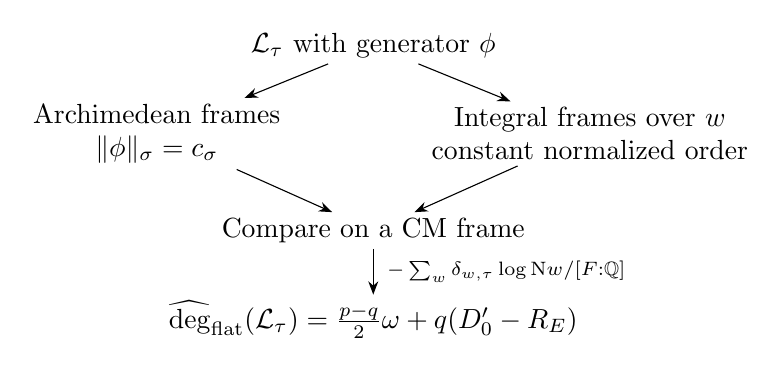
\begin{tikzpicture}[>=Stealth,every node/.style={align=center,inner sep=2pt}]
\node (line) at (0,0) {\(\mathcal L_\tau\) with generator \(\phi\)};
\node (arch) at (-2.75,-1.12) {Archimedean frames\\\(\|\phi\|_\sigma=c_\sigma\)};
\node (fin) at (2.75,-1.12) {Integral frames over \(w\)\\constant normalized order};
\node (cm) at (0,-2.35) {Compare on a CM frame};
\node (deg) at (0,-3.48) {\(\widehat{\deg}_{\rm flat}(\mathcal L_\tau)
        =\tfrac{p-q}{2}\omega+q(D'_0-R_E)\)};
\draw[->] (line) -- (arch);
\draw[->] (line) -- (fin);
\draw[->] (arch) -- (cm);
\draw[->] (fin) -- (cm);
\draw[->] (cm) -- (deg) node[midway,right=1mm] {\(\scriptstyle-\sum_w\delta_{w,\tau}\log{\rm N}w/[F:\mathbb Q]\)};
\end{tikzpicture}
\caption{Archimedean norms and finite orders of the flat generator in Definition~\ref{hyp:flat-determinant-frames}. The finite correction converts the CM frame degree to the normalized degree of Proposition~\ref{prop:deep-flat-line-degree}.}\label{fig:flat-cm-frames}
\end{construction}

\begin{proposition}[The normalized degree of the flat line]
\label{prop:deep-flat-line-degree}
For each component \(Z\) and label \(\tau\) of
Definition~\ref{hyp:flat-determinant-frames}, the determinant rule gives a
generator \(\phi\) on the proper normal generic fibre, up to scalar.
Its norm is constant on the archimedean frame tests at each embedding. At a finite place its normalized order is constant on the integral
frame tests. With the finite-order correction
\[
 \delta_{w,\tau}=q\{\operatorname{ord}_w(\tau\mathfrak d_E)
                              -\operatorname{ord}_w(d_0)\},
\]
the normalized degree is
\[
 \widehat{\deg}_{\rm flat}(\mathcal L_\tau)
       =\frac{p-q}{2}\,\omega+q(D_0'-R_E).
\]
Thus the contribution to the slope coefficient, with the squared-norm convention of this comparison, is
\[
 -\widehat{\deg}_{\rm flat}(\mathcal L_\tau)=-\tfrac{p-q}{2}\omega+q(R_E-D'_0).
\]

\end{proposition}

\begin{proof}
Choose the generic generator \(\phi\) of
Lemma~\ref{lem:flat-generic-generator}. At the embedding \(\sigma\)
write \(\Gamma,\Delta\) for the Gram matrices of the two frames.
The frame coefficient \(f\) then satisfies
\[
 |f|^2\,|\det\Gamma|/|\det\Delta|=c_\sigma^2
 \qquad(c_\sigma>0\text{ constant for the chosen }\phi).
\]
At a finite place \(w\) let \(\pi_w\) be a uniformizer. Degree zero on special-fibre curves
(Lemma~\ref{lem:flat-special-curve}) lets us apply
Lemma~\ref{lem:flat-vertical-ratio} to the projected determinant
lattice \(\det Q_\tau\). If \(R\) is the ring of a valued frame
over \(w\), the order computed in this lattice satisfies
\[
 \frac{\operatorname{ord}_{Q,R}(\phi)}{v_R(\pi_w)}
    =\max_{D\ {\rm vertical\ over}\ w}
       \frac{\operatorname{ord}_{Q,D}(\phi)}
            {\operatorname{ord}_D(\pi_w)} .
\]
To read the same section in the separate integral Lie frames,
Lemma~\ref{lem:projected-lie-frame-index} gives
\[
   \operatorname{ord}_{{\rm Lie},R}(\phi)
       =\operatorname{ord}_{Q,R}(\phi)-h_{R,\tau}.
\]
The Hodge multiplicities are fixed on this component, so
\(h_{R,\tau}/v_R(\pi_w)\) is the same at the CM frame and
at every other valued frame. The order and the metric may therefore
both be evaluated on the CM frame.
Lemma~\ref{lem:flat-cm-degree} evaluates their normalized frame
degree as \((p-q)\omega/2\).

For \(c\in F^\times\), replacing \(\phi\) by \(c\phi\) adds the
divisor of \(c\), whose normalized arithmetic degree is zero. Subtract
\(\delta_{w,\tau}\) from the order in each finite frame. Taking ideal
norms gives
\[
 \frac{1}{[F:\mathbb Q]}\sum_w\delta_{w,\tau}\log{\rm N}w
 =q\left(
 \frac{\log{\rm N}_{E/\mathbb Q}\mathfrak d_E}{[E:\mathbb Q]}
 -\log d_0\right)=q(R_E-D_0').
\]
Here the finite sum runs over the places of \(F\). The factor
\([F:E]\) from extending an ideal cancels in the normalization.
The corrected degree is the frame degree minus this sum. Its formula
contains no component-dependent quantity.
\label{cor:deep-cover-flat-degree-1}
\end{proof}

To compute the degree in Proposition~\ref{prop:deep-flat-line-degree}, we need one generator that can be evaluated in both kinds of frame. We first construct it on the generic component, then determine how its orders vary over a special fibre.

\begin{lemma}[Extension of the period generator]\label{lem:flat-generic-generator}
On the proper normal generic component of
Definition~\ref{hyp:flat-determinant-frames}, \(\mathcal L_\tau\) has an \(F\)-generator whose value in the prescribed frame at each complex embedding \(\sigma\) is a constant multiple of the normalized period determinant \(\Delta_{{\rm per},\sigma}\),
\[
 \phi_\sigma=c_\sigma\Delta_{{\rm per},\sigma},\qquad c_\sigma\ne0.
\]

\end{lemma}
\begin{proof}
In the marked period basis the first tangent block and the conjugate
of the second block have complementary directions. Pair the second
block by the Hermitian form and take the determinant. The marked
level comparison gives invariance under the change of period basis
on \(Z\). With \(\Gamma,\Delta\) the two frame Gram matrices, the
determinant identity, after division by the reference period constant,
reads
\[
 |f(v,w)|^2=\frac{|\det\Delta|}{|\det\Gamma|},\qquad
 \|f(v,w)e(v,w)\|^2=|f(v,w)|^2\frac{|\det\Gamma|}{|\det\Delta|}=1.
\]
It holds first at the embedding respecting the marked quadratic root.
Conjugating the frames preserves the absolute determinants.
\label{cor:deep-cover-flat-degree-2}

Take a proper smooth resolution of the generic component of the
normal model at \(2\), using the prime-to-\(2\) marking. In a
toroidal chart the boundary is \(z_1\cdots z_a=0\). The two
extending eigenframes are independent in the smooth semiabelian Lie
bundle. The boundary comparison for precisely these frames gives
\[
 C^{-1}Q(z)^{-A}\le u\le C Q(z)^A\quad (u=|\det\Gamma|,\ |\det\Delta|),
 \qquad Q(z)=1+\sum_{i=1}^a|\log|z_i|| .
\]
Consequently \(|f|,|1/f|\le C Q^A\), after increasing \(C,A\).
For \(g=f\) or \(1/f\), fix the other punctured coordinates \(z'\).
The Laurent coefficient of index \(-m\), \(m\ge1\), satisfies
\[
 \left|\frac{1}{2\pi i}\int_{|\zeta|=\rho}
          g(\zeta,z')\,\zeta^{m-1}\,d\zeta\right|
 \le C(z')\rho^m(1+|\log\rho|)^A\longrightarrow0 .
\]
Apply this to each boundary variable. The Laurent series on the
product of punctured discs has no negative multi-index in any
variable. Thus both \(f\) and \(1/f\) extend, and their product
remains one. Uniqueness on overlaps gives a generator on the resolution.
\label{cor:deep-cover-flat-degree-3}

Write \(Y\) for this proper geometrically integral resolution.
By GAGA and coherent base change,
\[
 H^0(Y,\mathcal L_\tau)\otimes_F\mathbb C
 \simeq H^0(Y_{\mathbb C}^{\rm an},\mathcal L_\tau^{\rm an})
 =\mathbb C\,\Phi ,
\]
where \(\Phi\) denotes the just-extended section and the line on
\(Y\) denotes its pullback. Any nonzero \(F\)-section therefore
generates after scalar extension, hence already over \(F\).
On the normal generic component use a local frame \(e\). Properness
of the resolution lifts each height-one valuation, so both
\(\phi/e\) and \(e/\phi\) have nonnegative order there. A normal
Noetherian domain is the intersection of its height-one valuation
rings. Thus both quotients are regular, as required. At another
finite prime the same construction on its prime-to-residue model
gives a generic generator. The quotient of the two generators lies
in \(F^\times\) since the generic component is proper and
geometrically integral. \label{cor:deep-cover-flat-degree-4}
\end{proof}

Fix the normal integral component of the prime-to-\(\ell\) model in
Definition~\ref{hyp:flat-determinant-frames}. Its generic point is
in the abelian locus. Let \(G\) be its smooth semiabelian group,
with its integral \(\mathcal O_E\)-action and rigidified polarizing
line. Write \(n=[E:\mathbb Q]\), \(d_G=\dim G\), and
\(r=p+q\), so \(2d_G=nr\). Over a local ring \(R\) on this
model choose formal coordinates at the identity and a rigidification
of the polarization biextension on the coordinate neighborhood.
These give the polarized tangent module
\[
       H_R=V_R\oplus V_R^*,\qquad V_R=\operatorname{Lie}(G)_R .
\]

The second summand is the space of linear terms of changes of
rigidification. Write \(U_a\) for the differential of \(a\in
\mathcal O_E\). The isomorphism between pulling the biextension
back by \(a\) in the first variable and by \(\bar a\) in the
second is represented in these frames by a unit equal to one on
both axes. Write \(C_a\) for its mixed linear coefficient, with
the first variable indexing the rows. The induced action is
\[
       (v,\alpha)\longmapsto
       (U_av,\ U_{\bar a}^{t}\alpha-C_a^{t}v).
\]

These formulas are integral even in characteristic two: the mixed
coefficient is the coefficient of \(st\) after substituting
\((sv,tw)\) with \(s^2=t^2=0\). Composition of the rigidified
isomorphisms gives matrix multiplication. A change of coordinates
acts on the first summand by its differential and on the second by
the inverse transpose, with a shear given by the mixed coefficient
of the change of frame. The inverse change has the same integral
description. Thus the displayed modules glue and commute with
base change.

\begin{auxlemma}[Local freeness over the integral coefficient algebra]
\label{lem:polarized-stalk-free}
On the marked component the polarized tangent module is locally
free of rank \(r\) over \(\mathcal O_X\otimes_{\mathbb Z}\mathcal O_E\).
In particular, on every geometric fibre of characteristic \(\ell\)
and for each Artinian local factor \(B\) of
\(k\otimes_{\mathbb Z}\mathcal O_E\),
\[
                   H_k\otimes_{k\otimes\mathcal O_E}B\simeq B^r .
\]
\end{auxlemma}
\begin{proof}
\proofstep{The abelian part of a geometric fibre.}
Work over an algebraically closed residue field \(k\) of
characteristic \(\ell\). In the interior the fibre is principally
polarized. At a boundary point choose a complete DVR dominating its stalk
whose generic point lies over the abelian generic point: normalize
the blowup of the maximal ideal, take the DVR of an exceptional
prime divisor, and complete. A one-dimensional normal stalk
itself supplies the DVR in dimension one. Its characteristic-zero
fraction field contains the local domain. After finite extension
the residue torus splits. The Raynaud extension and the cubical
line in the polarized degeneration datum reduce to
\[
  1\longrightarrow T\longrightarrow G_k
   \xrightarrow{\pi} A\longrightarrow1,\qquad
  L_{G_k}\simeq\pi^*L_A .
\]

Here the geometric fibre may be read after the further residue
field extension. Both ranks and local freeness descend faithfully.
For the period and character lattices \(Y\) and \(X^*(T)\), the
polarization induces an injection \(\Phi:Y\hookrightarrow X^*(T)\).
The degree formula for the degeneration datum gives
\[
   1=\deg\lambda_{\rm gen}
      =[X^*(T):\Phi Y]^2\deg\lambda_A,
      \qquad \deg\lambda_A=1 .
\]
The prime-to-residue model is used also when \(\ell\) divides the
original level. The Rosati adjoint is \(a\mapsto\bar a\).
\cite[Chapter~II, \S\S1--4, and Chapter~III, Corollary~7.2]{faltings-chai}

For \(0\ne a\in\mathcal O_E\) let \(K=\ker(a:A\to A)\).
The action is an isogeny when \(A\) has positive dimension, since
some integral multiple of \(a^{-1}\) is integral. The two
rigidified pullbacks of the Poincar\'e line give the perfect
Cartier pairing of \(K\) and
\(K^D=\ker(\bar a:A\to A)\).
\cite[Theorem~9.1]{milne-av-isogeny}
Let \(B_K\subset k[K]\) be the Hopf subalgebra generated by
the primitive functions, and set
\[
     J=\ker(K\longrightarrow\operatorname{Spec}B_K),\qquad
     t=\dim_k\operatorname{Lie}(K^D).
\]

A tangent vector to \(K^D\) is a character \(1+\epsilon u\) over
\(k[\epsilon]/\epsilon^2\). The character law reads
\[
             \Delta u=u\otimes1+1\otimes u .
\]
Thus the tangent vectors correspond to the primitive functions. The derivative of this function at a tangent
vector \(v\in\operatorname{Lie}K\) is the mixed coefficient of the
Cartier pairing. In our coordinates it equals
\(v^t C_a w\), up to the common choice of the inverse pairing, for
\(w\in\ker U_{\bar a}\). Indeed the two trivializations defining
the pairing on the kernels restrict to the rigidifications on the
axes. Evaluating their ratio on \((sv,tw)\) leaves just its
\(st\) coefficient.

A pair in the kernel on \(H_A\) therefore satisfies
\[
 U_av=0,\qquad U_{\bar a}^{t}\alpha=C_a^t v,\qquad
 v\in\operatorname{Lie}J .
\]
The last condition follows by pairing the middle equality with
each \(w\in\ker U_{\bar a}\). For a fixed \(v\) the ambiguity
in \(\alpha\) has dimension \(t\). For any finite group scheme
\(D\) over \(k\), its first Frobenius kernel has order
\(\ell^{\dim\operatorname{Lie}D}\), by the height-one
correspondence and the restricted enveloping algebra basis theorem.
\cite[Theorem~1.4.23]{brion-height-one}
Apply this first to \(J\), then to the Cartier dual of
\(\operatorname{Spec}B_K\), whose Lie algebra contains the \(t\)
independent primitives. Multiplicativity of orders in the finite
group scheme quotient gives
\[
   \dim\ker(a\mid H_A)\le \dim\operatorname{Lie}J+t
                          \le v_\ell(\deg a|_A).
\]
When \(A=0\) this contribution is zero.

\proofstep{The torus and the uniform kernel bound.}
The cocharacter lattice of \(T\) is torsion-free over
\(\mathcal O_E\), since multiplication by nonzero \(a\) divides
multiplication by a nonzero integer. It is projective over this
Dedekind ring. Put \(b_T=\operatorname{rk}_{\mathcal O_E}X_*(T)\)
and \(N_a=|N_{E/\mathbb Q}(a)|\).
The dimension of the kernel on \(\operatorname{Lie}T=X_*(T)\otimes k\)
is bounded by the sum of the \(\ell\)-adic elementary divisors
of multiplication by \(a\) on this lattice. For the toric term
and its conjugate dual the bounds are
\[
    \dim\ker U_{a,T}\le b_Tv_\ell(N_a),\qquad
    \dim\ker U_{\bar a,T}^t\le b_Tv_\ell(N_a) .
\]

Write \(P:V\to\operatorname{Lie}A\) for the quotient differential.
Use a rigidification pulled back from \(A\) on the geometric
fibre. The mixed coefficient there is \(P^t C_{a,A}P\).
In another rigidification the difference is a shear, so it
conjugates the action. The stable subspaces
\[
 \operatorname{Lie}T\oplus0\ \subset V\oplus P^*(\operatorname{Lie}A)^*\ \subset\ H_k
\]
have successive quotients \(\operatorname{Lie}T,H_A,
(\operatorname{Lie}T)^*\), the last with the conjugate action.
Kernel dimensions are subadditive along this filtration.
On the prime-to-\(\ell\) rational Tate module of \(A\), an
integral primitive element of \(E\) acts semisimply. Its rational
characteristic polynomial is a power of its minimal polynomial,
so every embedding occurs with multiplicity \(2\dim A/n\).
The degree of \(a\) is its determinant on this module.
\cite[Theorem~10.9 and Proposition~10.20]{milne-av-isogeny}
It follows that
\[
 \dim_k\ker(a\mid H_k)
   \le (2b_T+2\dim A/n)\,v_\ell(N_a)
   =r\,v_\ell(N_a).
\]

\proofstep{Recovering a free module at a ramified prime.}
On the characteristic-zero generic fibre the \(\tau\)-part of
\(H\) has dimension \(p+q\) for each embedding. At each stalk
the characteristic polynomial of \(a\) therefore equals that
of its regular action on \(\mathcal O_E\) raised to the \(r\)-th
power. The coefficients belong to the local domain and agree in
its fraction field, giving the integral identity
\[
      \det(X-a\mid H)=\det(X-a\mid\mathcal O_E)^{r}.
\]
For \(\mathfrak l\mid\ell\), of ramification
index \(e\) and residue degree \(f_{\mathfrak l}\), its factors
over \(k\) have the form \(B_\sigma=k[u]/(u^e)\). Each summand
\(H_\sigma\) has dimension \(er\) over \(k\). Indeed, choose
an element with nonzero residue generating the residue field at
\(\mathfrak l\) and zero residue at the other primes. The
multiplicities of its distinct nonzero eigenvalues in the preceding
characteristic polynomial are precisely these dimensions.

Choose \(a\) of valuation one at \(\mathfrak l\) and zero
at all other primes over \(\ell\), by the Chinese remainder
theorem. Then \(v_\ell(N_a)=f_{\mathfrak l}\). Multiplication
by \(a\) has the same kernel as \(u\) on the factors at
\(\mathfrak l\), and is invertible elsewhere. Thus
\[
 \sum_{\sigma}\dim_k\ker(u\mid H_\sigma)\le r f_{\mathfrak l},
 \qquad \dim_k\ker(u\mid H_\sigma)\ge \dim_k H_\sigma/e=r .
\]
All Jordan blocks have length at most \(e\), so equality forces
exactly \(r\) blocks of length \(e\) at every \(\sigma\).
This proves freeness over each \(B_\sigma\), including \(e>1\).
Over a characteristic-zero residue field the same conclusion follows
from the characteristic polynomial and separability of \(E\).

Freeness at the geometric fibre descends to projectivity at the
residue field by faithful flatness. The coefficient algebra there
is a product of local Artinian rings, and the common rank \(r\)
gives a free module. Lift a set of \(r\) coefficient generators
to the stalk. If \((b_i)\) is an integral basis of \(\mathcal O_E\),
the reductions of the \(b_i x_j\) are a basis of size \(nr=2d_G\).
Their determinant in the chosen tangent coordinates is a unit.
They give a basis over the local ring, hence the \(x_j\) are a
basis over its coefficient algebra.
\end{proof}

\begin{auxlemma}[Integral evaluation of a projected frame]
\label{lem:polarized-stalk-evaluation}
Let \(R\) be a stalk of this normal model and let the integral
character \(\sigma:\mathcal O_E\to R\) extend the label \(\tau\).
For any coefficient basis \(x_1,\ldots,x_r\) from
Lemma~\ref{lem:polarized-stalk-free}, the character quotient is
free with the indicated basis:
\[
 Q_{\sigma,R}=H_R/\sum_a(a-\sigma(a))H_R
             =\bigoplus_{j=1}^r R\,\bar x_j .
\]
Its generic-fibre realization is the image of \(H_R\) under
the characteristic-zero eigenprojection, and its bases and their
transition matrices specialize to the function field and every
valuation ring of every normalized special-fibre curve.
\end{auxlemma}
\begin{proof}
In coefficient coordinates, the map on each summand is
\(R\otimes\mathcal O_E\to R\), \(b\otimes a\mapsto b\sigma(a)\).
Its kernel is generated by \(1\otimes a-\sigma(a)\otimes1\).
After passing to the fraction field this evaluation is precisely the
corresponding projection in the split coefficient algebra. In
particular the integral quotient embeds there as the span of its
projected basis. No integral idempotent for the individual embedding
is required at a ramified prime.

Let \(C\) be a normalized curve, \(K=k(C)\) and
\(V_z=\mathcal O_{C,z}\). If \(x\) and \(x'\) are frames taken
at the image of \(z\) and of the generic point, compare them over
the latter stalk. Write their change of basis as \(T\) over its
coefficient algebra, in the convention \(x=x'T\). Then
\[
       \bar x=\bar x'\,T_\sigma,\qquad
       T_\sigma=(1\otimes\sigma)(T),\qquad
       \det T_\sigma\in\mathcal O_{X,\eta_C}^{\times}.
\]
The two maps from \(\mathcal O_{X,z}\) (at the image of \(z\))
to \(K\), through \(V_z\) and through \(\mathcal O_{X,\eta_C}\),
agree. Hence \(Q_{\sigma,V_z}\) in the generic curve frame
is \(T_\sigma V_z^r\), with the entries read in \(K\).
The determinant lattice is \((\det T_\sigma)V_z\). The determinant
can have nonzero \(z\)-valuation. Its valuation is exactly the
transition contribution to the degree on the curve.
\end{proof}

The integral image of an eigenprojection and the intersection with an
eigenspace may differ at a ramified prime. The following determinant
calculation compares the two conventions in
Proposition~\ref{prop:deep-flat-line-degree}.

\begin{auxlemma}[The local change from the projected to the two Lie frames]
\label{lem:projected-lie-frame-index}
Let \(R\) be the valuation ring of a finite extension of the local
coefficient field containing all embeddings of \(E\), write
\(K=\operatorname{Frac}R\), and let \(v_R\) be its integral valuation.
For a marked integral test write \(L=\operatorname{Lie}(G)_R\),
\(S_\gamma=L\cap(L_K)_\gamma\) and
\(n_\gamma=\dim_K(L_K)_\gamma\).
Let \(I_\tau\) be the embeddings inducing the same prime
\(\mathfrak l\mid\ell\) and residue embedding as \(\tau\).
For a uniformizer \(\theta\) of \(E_{\mathfrak l}\) put
\[
 h_{R,\tau}=\sum_{\gamma\in I_\tau\setminus\{\tau\}}
        n_\gamma v_R\bigl(\gamma(\theta)-\tau(\theta)\bigr).
\]
In the generic determinant identification, the lattice
\(\det S_\tau\otimes(\det S_{\bar\tau})^{-1}\) is contained in
\(\det Q_{\tau,R}\) with colength \(h_{R,\tau}\). In particular
the normalized difference of the two frame orders depends only on the
coefficient field, the place and the multiplicities.
\end{auxlemma}

\begin{proof}
On the factor selected by the common residue embedding the coefficient
algebra is monogenic. Indeed the unramified part splits over \(R\),
and a uniformizer generates the totally ramified integer ring over
its unramified part. On this factor put \(D=\theta-\tau(\theta)\).
It has the presentation
\[
 R[X]\big/\prod_{\gamma\in I_\tau}(X-\gamma(\theta)),\qquad
          Q_{\tau,R}=H_R/DH_R
\]
where \(H_R\) on the right denotes the selected factor. Take the
same factor of the exact sequence formed by the second summand and
the projection onto the first,
\[
         0\longrightarrow F\longrightarrow H_R
                              \longrightarrow L\longrightarrow0 .
\]
Here \(L\) in the sequence also means its selected factor, and
\(F\) is the corresponding factor of the integral dual of the
full Lie module, with conjugate action. Its projected image is
\(S_{\bar\tau}^*\): restriction to the saturated free sublattice
\(S_{\bar\tau}\) is surjective over a DVR, and the generic
restriction is the dual eigenprojection.

Since \(Q_{\tau,R}\) is free, the image of \(F/DF\) in it is its
torsion-free quotient, which the preceding description identifies with
\(S_{\bar\tau}^*\). Right exactness gives
\[
     0\longrightarrow S_{\bar\tau}^*\longrightarrow Q_{\tau,R}
                       \longrightarrow L/DL\longrightarrow0 .
\]
Write \(I=L\cap\bigoplus_{\gamma\ne\tau}(L_K)_\gamma\) on this
factor. The torsion in \(L/DL\) is \(I/DL\) and the free quotient
is \(L/I\). The colength in the assertion is consequently
\[
    \operatorname{length}(I/DL)+
    \operatorname{length}\bigl(L/(I+S_\tau)\bigr).
\]

This follows by a basis change over the DVR, first
saturating \(S_{\bar\tau}^*\) in \(Q_{\tau,R}\) and then taking
the index of \(S_\tau\) in the free quotient \(L/I\).
The map \(D\) identifies \(L/(I+S_\tau)\) with \(DL/DI\),
since its kernel on \(L\) is \(S_\tau\). The two lengths add to
\[
  \operatorname{length}(I/DI)
     =v_R\bigl(\det(D\mid I_K)\bigr)=h_{R,\tau}.
\]
The formula holds also for an unramified factor, when the sum is empty.
Passing to a further finite extension multiplies both the colength
and \(v_R(\pi_w)\) by its ramification index.
\end{proof}

\begin{lemma}[Degree on special-fibre curves]\label{lem:flat-special-curve}
Use the integral eigenframes of Definition~\ref{hyp:flat-determinant-frames}
on the normal model at a finite place of residue characteristic \(\ell\).
The determinant line measuring the order of the section \(\phi\)
of Lemma~\ref{lem:flat-generic-generator} has degree zero on the normalization \(\widetilde C\) of every complete integral curve \(C\) in this special fibre,
\[
 \deg_{\widetilde C}(\mathcal L_\tau|_{\widetilde C})=0.
\]

\end{lemma}
\begin{proof}
Apply Lemma~\ref{lem:polarized-stalk-evaluation} on the marked
model after extending constants to contain the integral label
\(\sigma\). On the generic fibre the projected polarized tangent
space is an extension of \(V_\tau\) by \(V_{\bar\tau}^*\).
Lift the \(v_i\) to this extension and adjoin the dual frame of
the \(w_j\). Its determinant is independent of the lifts and
transforms by \(\det A/\det B\). It identifies
\[
       \det Q_{\sigma,\operatorname{Frac}R}
                 =\det V_\tau\otimes(\det V_{\bar\tau})^{-1} .
\]
Its extension on the curve has the integral determinant lattices
computed in Lemma~\ref{lem:polarized-stalk-evaluation}. These
are the orders to which Lemma~\ref{lem:flat-vertical-ratio} will
be applied. The comparison with the separate Lie frames in the CM
calculation keeps the different at the given place.
\label{cor:deep-cover-flat-degree-5}

\proofstep{Compare the two Hodge degrees on a Siegel model.}
Enlarge the finite field of constants \(k\) to split the residue
fields of \(\mathcal O_E\) above \(\ell\). Write \(e\) for a primitive
idempotent in \(k\otimes\mathcal O_E\), and write \(H_e=eH\).
We compare determinants using the underlying principally polarized
family. Choose a full Siegel marking of some order \(n\ge3\) prime
to \(\ell\) on a finite cover of the abelian generic locus. Take the
normalized closure of the graph of its map to a projective Siegel
toroidal compactification at that level. If \(X\) denotes our
model and \(X'\) this graph, the projections give
\[
 X\ \longleftarrow\ X'\ \longrightarrow\ \overline{\mathcal A}_{d_G,n}^{\rm tor}.
\]
The first projection is proper and surjective. On this normal cover the two
semiabelian families agree: their generic isomorphism and its inverse
extend uniquely. \cite[I, Proposition~2.7]{faltings-chai}

There is a complete integral curve upstairs dominating
\(\widetilde C\) after normalization. Indeed a closed point of the
preimage of its generic point has residue field finite over
\(k(\widetilde C)\); take the closure in the proper fibre product
and normalize. For this finite map \(h:C'\to\widetilde C\),
\[
              \deg_{C'} h^*\det H_e
                    =(\deg h)\deg_{\widetilde C}\det H_e ,
\]
using degrees relative to the same ground field. We can therefore
compute on \(C'\), even for a curve contained in the boundary.

Let \(D\) be the pullback of the covariant logarithmic de Rham
bundle on the Siegel compactification. Its Hodge and conjugate
filtrations form an \(F\)-zip: the two filtrations are by subbundles
and their graded bundles match in reverse order after Frobenius
pullback. The boundary assertion here is the logarithmic one for
principally polarized Siegel families in characteristic \(\ell\),
including \(\ell=2\). In a toroidal chart its covariant realization
is the Lie algebra of the period-equivariant universal vector
extension of the Raynaud extension. For split torus \(T\), abelian
quotient \(A\) and period lattice \(Y\), its weight filtration has
successive quotients
\[
          \operatorname{Lie}T,\qquad D(A),\qquad Y\otimes\mathcal O .
\]
Here \(D(A)\) denotes the ordinary de Rham homology of \(A\). \cite[VI, Theorem~1.1]{faltings-chai}
\cite[\S2D, pp.~476--477]{vdg-looijenga-boundary-zip}

The coefficient action on these filtrations also extends. On the
completed normal degeneration chart, after splitting the torus,
the action preserving the polarization in the Rosati sense acts
integrally on the Raynaud extension and its period homomorphism
\(u\). If \(a_Y,a_{G^\natural}\) are the induced maps, then
\[
 u:Y\longrightarrow G^\natural_\eta,\qquad
          u\circ a_Y=a_{G^\natural}\circ u .
\]
This is the equivalence for integral endomorphism structures in
\cite[Theorem~5.1.1.4]{lan-pel-degeneration}.
Applying the universal vector extension and its Lie functor gives
the action on \(D\). It commutes with relative Frobenius and
Verschiebung by functoriality on the degeneration data. The
actions agree on overlaps by their common generic action. In
particular the construction applies to every \(a\in\mathcal O_E\),
including elements of positive \(\ell\)-adic valuation.

Put \(V=\operatorname{Lie}(G)|_{C'}\), and let \(U=V^*\) with the
conjugate dual action induced by principal polarization. Write
\(F\) for absolute Frobenius of \(C'\) and \(F_k(e)\) for the
idempotent obtained by raising the scalar coefficients of \(e\)
to the \(\ell\)-th power. Taking the indicated direct summands
of the two filtrations gives exact sequences on the whole curve:
\[
\begin{aligned}
 0&\longrightarrow U_e\longrightarrow D_e
                 \longrightarrow V_e\longrightarrow0,\\
 0&\longrightarrow F^*V_e\longrightarrow D_{F_k(e)}
                 \longrightarrow F^*U_e\longrightarrow0 .
\end{aligned}
\]
The quotients are vector bundles, so pullback to the curve and
projection by the idempotents preserve exactness.

The polarized
tangent bundle itself has \(0\to U_e\to H_e\to V_e\to0\).
Consequently degree additivity and \(\deg F^*L=\ell\deg L\)
for a line bundle give
\[
 \deg H_{F_k(e)}=\deg D_{F_k(e)}
       =\ell(\deg U_e+\deg V_e)=\ell\deg H_e .
\]
The permutation \(e\mapsto F_k(e)\) has finite order \(s>0\).
Iteration gives \((\ell^s-1)\deg H_e=0\). This argument uses
the whole local Artinian factor selected by \(e\), before reduction
by its maximal ideal.

The local Artinian factor \(B\) at the chosen character has residue
field \(k\). Filter \(B\) by ideals with simple quotients \(k\).
If \(b=\operatorname{length}_B B\), Lemma~\ref{lem:polarized-stalk-free} identifies
each quotient of the induced filtration of \(H_e\) with the same
bundle \(H_e\otimes_B k\) (up to a constant one-dimensional factor).
By degree additivity,
\[
 0=\deg H_e=b\,\deg(H_e\otimes_B k).
\]
The determinant of the eigencharacter quotient therefore has degree
zero, including when \(B\) has nilpotents.
\label{cor:deep-cover-flat-degree-6}
\end{proof}

\begin{auxlemma}[A curve through a prescribed point]
\label{lem:flat-specialization-curve}
Let \(T\) be an integral proper variety of positive dimension over
a finite field, \(U\subset T\) a dense open subset, and \(z\) a closed
point of \(T\). Let \(k\) be the finite ground field. There is a finite extension \(k'/k\), a complete integral curve \(C\subset T_{k'}\) and a point \(z'\in C\) over \(z\) such that its generic point satisfies
\[
 z'\in C\cap(T_{k'})_z,\qquad \eta_C\in U_{k'}.
\]

\end{auxlemma}
\begin{proof}
Over an algebraic closure take a reduced irreducible component through
a lift \(z'\) of \(z\). The inverse image of \(U\) is dense there.
Take an affine neighborhood \(V\) of \(z'\) on this component and a
finite Noether normalization \(f:V\to\mathbb A^d\).
For the closed subset \(Z=V\setminus U_{\bar k}\) one has
\[
   \dim f(Z)=\dim Z<d\qquad(Z\ne\varnothing).
\]
Choose a line through \(f(z')\) and a point outside \(f(Z)\).
For any component \(C_0\) of its inverse image through \(z'\),
the \(d-1\) linear equations and finiteness give
\[
 1=d-(d-1)\le \dim C_0=\dim f(C_0)\le1 .
\]
The finite image is the whole line, so \(C_0\) meets the given open
set. Its closure in the proper variety is the required integral curve.
The component, line and curve are defined by finitely many data over
the algebraic closure of a finite field and hence descend to a finite
extension.
\end{proof}

\begin{lemma}[The vertical order on a connected fibre]\label{lem:flat-vertical-ratio}
Let \(\mathcal L\) be the integral determinant line on the proper
normal component over a DVR with uniformizer \(\pi\) and connected
special fibre. Assume it has degree zero on every normalized
complete integral curve in that fibre. If \(\phi\) generates on
the generic fibre, then, for every valued frame over this DVR,
\[
 \operatorname{ord}(\phi)=\frac{a}{m}\operatorname{ord}(\pi),\qquad
 \frac{a}{m}=\max_{D\ {\rm vertical}}
            \frac{\operatorname{ord}_D(\phi)}{\operatorname{ord}_D(\pi)},
 \quad m>0 .
\]
\end{lemma}
\begin{proof}
The rational section \(s=\pi^a\phi^{-m}\) of \(\mathcal L^{-m}\)
has horizontal order zero. Its order along a vertical prime \(D\) is
\[
 a\,\operatorname{ord}_D(\pi)-m\,\operatorname{ord}_D(\phi)\ge0 .
\]
By normality \(s\) is regular. Its unit locus \(U\) contains the
generic point of a component attaining the maximum.

Take any irreducible special-fibre component \(T\) meeting \(U\).
If \(T\setminus U\) is nonempty, choose a closed point \(z\) there.
If \(\dim T=0\) then \(T\) consists of a single point, contrary to
the choice of \(z\). Otherwise apply Lemma~\ref{lem:flat-specialization-curve}
to \(T_{\rm red}\) and its open unit locus, and normalize the resulting
curve. Its image in the original fibre is an integral curve. Pullback
along the finite map of normalized curves preserves degree zero.

On this complete normal curve \(C\), the pullback of \(s\) is
regular and generically nonzero, so
\[
 0=-m\deg_C\mathcal L=\deg_C\operatorname{div}(s)
       =\sum_{x\in C_{\rm cl}}[k(x):k_C]\operatorname{ord}_x(s),
 \qquad \operatorname{ord}_x(s)\ge0 ,
\]
where \(k_C\) is its constant field. A point over \(z\) would
contribute a positive summand. Hence \(T\subset U\). Across any
intersection with a neighboring component its generic point belongs
to the same open \(U\). Connectedness of the finite component graph
gives the result on the whole fibre. Pulling the unit \(s\) back to
a valued frame gives \(m\operatorname{ord}(\phi)=a\operatorname{ord}(\pi)\).
Changing the generic generator by \(c\in F^\times\) translates its
order by \(\operatorname{ord}(c)\). The local models and framed
uniformization supply nonempty tests at the required places.
\label{cor:deep-cover-flat-degree-7}
\end{proof}

The vertical calculation has made the normalized orders independent of the component of a connected fibre. We can therefore evaluate the remaining degree at the prescribed CM frame.

\begin{lemma}[CM calculation in the frame metrics]\label{lem:flat-cm-degree}
For the polarized determinant line on \(Z\) in
Definition~\ref{hyp:flat-determinant-frames}, before the finite-order
correction of Proposition~\ref{prop:deep-flat-line-degree}, the normalized arithmetic degree in the CM frame norms satisfies
\[
 \widehat{\deg}_{\rm CM}(\mathcal L_\tau)=\frac{p-q}{2}\,\omega.
\]

\end{lemma}
\begin{proof}
At a pure CM test on the component use the two elliptic types of
\(\mathbb Q(\sqrt{-d_0})\), with their good integral abelian models,
integral Lie generators and normalized principal polarizations. Write
\(n_{\pm,s}\) for the squared Lie lengths at a complex embedding \(s\).
In a common finite field of definition \(k/F\), write \(\langle
\cdot\rangle_\infty\) for the mean over all \([k:\mathbb Q]\) complex
embeddings, counting conjugates. The Chowla--Selberg comparison and
the functional equation of the odd primitive quadratic character give
\[
 \begin{aligned}
 -\langle\log n_{\pm,s}\rangle_\infty=X
 &=\gamma+\log(2\pi/\sqrt{d_0})-L'(1,\chi)/L(1,\chi)\\
 &=L'(0,\chi)/L(0,\chi)+D_0'/2,\qquad
 \omega=X-R_E+D_0'/2 .
 \end{aligned}
\]
The mean is invariant under further field extension.
\cite{colmez-chowla-selberg}\label{cor:deep-cover-flat-degree-8}

Let \(T\) change the reference period basis to the two orthogonal
CM blocks. Let \(G\) be the reference Hermitian determinant, and
\(G_+,G_-\) the two block determinants. In these frames the
coefficient of \(\phi\) is \(\eta\,\tau(G_-)/\tau(\det T)\).
The elliptic period scalars for the two blocks are included in
\(\eta\). Evaluating the algebraic generator on the algebraic
frames shows that \(\eta\in k^\times\) after finite extension.
The identity \(G_+G_-=(\det T)\overline{\det T}\,G\) cancels the
transition determinant against the determinant metric. With the
two squared length scales \(n_{\pm,s}\sqrt{d_0}\), this gives
\[
 A_s=\log|s\eta|+\tfrac12\log|s(\tau G)|
       +\tfrac p2(\log n_{+,s}+D_0'/2)
       -\tfrac q2(\log n_{-,s}+D_0'/2).
\]
\label{cor:deep-cover-flat-degree-9}

At \(\ell\) take a locally integral CM basis with
\(t_\ell=\det T_\ell\). For \(j:k\hookrightarrow\mathbb C_\ell\)
put \(i=j\circ\tau\), \(D_j=\log|i(\mathfrak d_E)|_\ell\) and
\(d_\ell=\log|d_0|_\ell\). The absolute value of an ideal here is
that of a local generator. Unimodularity of the polarized period
lattice and trace duality with the different give
\[
 \log|i(t_\ell)|_\ell+\log|i(\bar t_\ell)|_\ell+\log|i(G)|_\ell
       =-(p+q)D_j,\qquad \log|i(G_-)|_\ell=-qD_j .
\]

The second identity uses the orthogonal pure-type block. The
locally integral period basis spans the CM product lattice over
the marked quadratic order up to prime-to-\(\ell\) index.
Projecting to each integral eigenlattice by the trace-dual basis
contributes a generator of \(\mathfrak d_E/(\sqrt{-d_0})\), whose
log absolute value is \(D_j-d_\ell/2\) on either conjugate
label. The two frame exponents are \(-p,+q\), giving the finite log norm
\[
 B_j=\log|j\eta|_\ell-\log|i(t_\ell)|_\ell-qD_j
                              +(q-p)(D_j-d_\ell/2).
\]
\label{cor:deep-cover-flat-degree-10}

To sum, put \(B'_j=B_j-q(D_j-d_\ell)\). Conjugation permutes
the embeddings of \(E\) with equal multiplicities at \(\ell\),
so the two sums for \(t_\ell,\bar t_\ell\) coincide. The first
trace-dual identity yields
\[
 \sum_{j\mid\ell} B'_j
 =\sum_{j\mid\ell}\left(\log|j\eta|_\ell+\tfrac12\log|i(G)|_\ell
              -\tfrac{p+q}{2}D_j+\tfrac{p+q}{2}d_\ell\right).
\]
Write \(\langle\cdot\rangle_f\) for the sum over finite embeddings,
divided by \([k:\mathbb Q]\), with \(|\ell|_\ell=\ell^{-1}\).
Only finitely many places contribute. Ideal norms give
\(\langle D_j\rangle_f=-R_E\), \(\langle d_\ell\rangle_f=-D_0'\).
The product formula cancels the \(\eta,G\) terms. Therefore
\[
 \begin{aligned}
 -\langle A_s\rangle_\infty-\langle B'_j\rangle_f
 &=\tfrac{p-q}{2}(X-D_0'/2)+\tfrac{p+q}{2}(D_0'-R_E)\\
 &=\tfrac{p-q}{2}\omega+q(D_0'-R_E),\\
 -\langle A_s\rangle_\infty-\langle B_j\rangle_f
 &=\tfrac{p-q}{2}\omega .
 \end{aligned}
\]
The last equality restores \(B_j-B'_j=q(D_j-d_\ell)\) in the
frame norms. \label{cor:deep-cover-flat-degree-11}
\end{proof}


\begin{lemma}[Slope change under the determinant twist]
For the flat twist from \(\Lambda_M\) to \(\Lambda_-\),
\[
 \mu(\Lambda_-)-\mu(\Lambda_M)\ge-M_i-(11C_A+83)U .
\]
\end{lemma}
\begin{proof}
The degree calculation gives
\[
 c_{1,\tau}=-\tfrac12(p-q)\omega
           -q\bigl(\log d_0-\log\operatorname{rd}(E)\bigr).
\]
Since \([E:\Q]=2f\), the discriminant bound reads
\[
       0\le \log\operatorname{rd}(E)
       =\frac{\log|\operatorname{disc}E|}{2f}\le2L_{\rm sc}.
\]
Since \(0\le\log d_0\le L_{\rm sc}\), the last term in the
identity has absolute value at most \(2qL_{\rm sc}\).
Together with \(|\omega|\le3L_{\rm sc}\) and \(p+q=r\), this gives
\[
 |c_{1,\tau}|\le(3|p-q|/2+2q)L_{\rm sc}
          \le(7/2)rL_{\rm sc}\le9rL_{\rm sc}.
\]
\label{cor:covolume-component-transfer-10}

In the bad-prime allowance every prime divides
\(15g_0g_1 C_E\), where \(C_E\) is the conductor
parameter containing the prime divisors of the CM field discriminant, including \(2\) and \(d_0\).
This uses \(N_{\rm lev}=g_0g_1\,15^e\) and auxiliary level one.
Thus the sum of the logarithms of the distinct bad primes
is at most \(\log(15g_0g_1 C_E)\). The parameter bound
\(C_E^{36}t^{150}\le b^{1/2}\) with \(t\ge1\) and
\(\log b\le8L_{\rm sc}\) implies \(\log C_E\le L_{\rm sc}\).
The two bounds \(\log g_k\le9L_{\rm sc}+1\) now give
\[
 \sum_{p\ {\rm bad}}\log p
 \le\log 15+\log g_0+\log g_1+\log C_E
 \le 19 L_{\rm sc}+2+\log 15\le20L_{\rm sc},
\]
since \(L_{\rm sc}\ge10\). This proves the allowance \(40L_{\rm sc}\)
used below on the chosen deep level even as \(e\) grows.
\label{cor:covolume-component-transfer-11}

Combining the flat-degree estimate with the bounds for the shifts \(w_\tau\) gives
\[
 \begin{split}
 |M_i-(p-q)\omega\textstyle\sum_\tau w_\tau|&\le C_A U,\\
 q L_{\rm sc}\textstyle\sum_\tau|w_\tau|&\le C_A U,\qquad
 |c_{1,\tau}+(p-q)\omega/2|\le3qL_{\rm sc}.
 \end{split}
\]
The even column count is \(2m_0\). The combined weight of
the base line, the parallel shift by \((w_\tau)_\tau\) and the
\(m_0\)-th theta root has exactly the exponents of the
negative-shift line. Indeed this parallel weight is subtracted from the
base weight in the definition of the unshifted quotient and
is restored in the parallel twist. The finite valuation rules,
cusp conditions, metric factor at every embedding and hence
the Petersson norms depend on these combined exponents.

The flat-line twist preserves rank. Its normalized degree
increment per rank in the squared metric is bounded below by
\[
 2\left(\sum_\tau w_\tau c_{1,\tau}
       -q\ell_d\sum_\tau|w_\tau|
       -m_0fr\{\tfrac12\log(2\pi)+\ell_d\}-\ell_S\right)
\]
on the unramified deep charts. Here \(\ell_d\le2L_{\rm sc}\)
is the different allowance and \(\ell_S\le40L_{\rm sc}\)
the sum of bad-prime logarithms. Twice the first sum is at
least \(-M_i-7C_AU\) by the three preceding inequalities for \(w_\tau\) and \(c_{1,\tau}\).
The second loss costs at most \(4C_A U\). Using
\(2m_0\le n_V\), \(frn_V L_{\rm sc}\le b\le U\) and
\(10\le L_{\rm sc}\le U\), the last two losses cost at most
\(3U+80U\). Adding the four losses gives the stated lower bound.
Write \(C_F=11C_A+83\). \label{cor:covolume-component-transfer-12}
\end{proof}

\begin{auxlemma}[Simultaneous evaluation above an unramified point]
\label{lem:adjoint-etale-fibre}
Let \(f:M\to Y\) be a generically finite surjective morphism of smooth
projective complex varieties of common dimension \(d\ge1\). Let \(A\)
be a nef and big integral line bundle on \(Y\), and \(P\) a nef line
bundle on \(M\). Choose \(y\) in the finite \'etale locus such that
\(A^{\dim V}\cdot V>0\) for every positive-dimensional integral
\(V\ni y\). Put \(h=d(d+1)/2\). For \(m\ge h+1\), the evaluation
on the entire reduced fibre is surjective:
\[
 H^0(M,L)\longrightarrow\bigoplus_{z\in f^{-1}(y)} L(z),
 \qquad L=K_M+m f^*A+P .
\]
\end{auxlemma}
\begin{proof}
Each positive intersection at \(y\) is an integer and is at least
one. On \(Y\) use the rational divisor \(N=(h+1/2)A\). For a
subvariety of dimension \(i\) through \(y\) one has
\[
       N^i\cdot V\ge(h+1/2)^i>h^i,\qquad
       \sum_{i=1}^d i/h=1 .
\]
Koll\'ar's isolated non-klt point theorem, applied to the smooth
pair \((Y,0)\), gives an effective rational divisor \(D\equiv N\)
whose non-klt locus near \(y\) consists of \(y\) alone.
\cite[Theorem~6.4]{kollar-pairs-adjoint}

Put \(J=\mathcal J(M,f^*D)\), the multiplier ideal. Discrepancies
and multiplier ideals pull back under an \'etale morphism, as one
sees by pulling back a log resolution over the \'etale open.
Consequently the points of \(f^{-1}(y)\) are isolated components of
the support of \(\mathcal O_M/J\). Since \(f\) is generically finite,
\(f^*A\) is nef and big. Moreover
\[
    L-K_M-f^*D\equiv (m-h-1/2) f^*A+P
\]
is nef and big. Nadel vanishing gives \(H^1(M,L\otimes J)=0\).
Thus every section of \(L\otimes(\mathcal O_M/J)\) lifts to \(M\).
The Artinian local scheme at each isolated point is open and closed
in this support. A chosen residue value lifts there, and one may
take zero on all the other components. This gives all the indicated
values simultaneously. \cite[Theorem~2.16 and proof of Theorem~5.8]{kollar-pairs-adjoint}
\end{proof}

The twist has put the slope at the desired weight. Descent to the selected level next
requires a section whose translates can be separated by character traces. Let \(S\) be
the finite level group, acting on the right, and let \(\chi\) be the prescribed
character.
\begin{lemma}[A short section separating the translates]
\label{lem:deep-short-orbit-section}
For the selected Hodge shift \(W\) there is a short integral
section \(v\) such that \(\det(v^{hg})_{h,g\in S}\) is a
non-zero-divisor. Its log supremum norm satisfies
\[
 \log\|v\|_{\sup}=O\big((frL_{\rm sc})^9\big)
\]
provided the component generating families have size \(N_c\),
Petersson bound \(\Lambda\) and pointwise factor \(\beta\) with
\(\log N_c,\log\beta=O(z_0^3)\), \(\log\Lambda=O(z_0^9)\) and
\(z_0=frL_{\rm sc}\), at the prescribed deep level of
Lemma~\ref{hyp:covolume-deep-component}.
\end{lemma}
\begin{proof}
The same section must give a nonzero determinant on every component.
The chosen Hodge exponent \(c_0\) exceeds
\(r+\binom{d_X+1}{2}\), with \(d_X\) the dimension of the
moduli component. At a complex framed point over its generic
point consider its \(S\)-orbit. The marking at a prime
greater than \(r+1\) is selected as follows. The deep level
\(N_{\rm lev}\) is divisible by \(g_0g_1\). In the marked type frame the first
level subgroup is upper unitriangular at both type primes.

For the other subgroup, indexed by \(k\), use the type prime
with index different from \(k\), where it is upper
unitriangular. At a place over the chosen \(g=g_j\), the
half-level marking determines an ideal \(\mathfrak I\) containing
the marking ideal. The complete splitting and squarefree
support of \((g)\) give
\[
  \mathcal O_E/\mathfrak I=\mathbf F_g,\qquad
  g\notin\mathfrak I^2,\qquad g>r+1.
\]
In the marked reduction the matrices are unitriangular. Hence
\[
             (s-I)^r\equiv0\pmod{\mathfrak I}
                   \qquad (s\in S).
\]

If two translates have the same underlying complex moduli
point, their relative level change fixes that point. Pulling
the universal group and the level isomorphism back to it
gives a finite-order \(\mathcal O_E\)-linear automorphism
\(\alpha\) of its semiabelian fibre. At \(\mathfrak I\) the
Tate-module identification reads its reduction on
\(\mathfrak I\)-torsion by the marked action, up to inversion.
Here the \(\mathfrak I\)-torsion is the part of the marking
obtained by multiplying by a generator of
\(\mathfrak m_b\mathfrak I^{-1}\) at \(\mathfrak I\),
where \(\mathfrak m_b\) is the marking ideal. Its dimension
is at most \(r\); the corresponding free
\(\mathcal O_{E,\mathfrak I}^{\wedge}=\mathbf Z_g\) Tate module
has rank at most \(r\). Every eigenvalue \(\zeta\) of \(\alpha\)
is torsion and reduces to one. Its order is therefore a power
of \(g\). A nontrivial one would satisfy
\[
 g-1\le[\mathbf Q_g(\zeta):\mathbf Q_g]
       \le\operatorname{rk}_{\mathbf Z_g}T_{\mathfrak I}\le r<g-1 .
\]
Thus all eigenvalues equal one; finite order gives semisimplicity
in characteristic zero.

To see faithfulness on the fibre, use the period
lattice of its complex exponential map. Its rational span
is a vector space over \(E\). Tensoring with \(E_{\mathfrak I}\)
gives the rational Tate module just used, so the action on
the period lattice itself is trivial. The period lattice of
a complex semiabelian variety spans its Lie algebra over
\(\C\), by the torus and abelian quotient. Thus \(\alpha\) acts as the identity on the fibre and hence on its
level lattice quotient. The marking is faithful. If \(x\) is the
framed point, this proves the required orbit separation:
\[
                x^g=x^h\quad\Longrightarrow\quad g=h
                              \qquad(g,h\in S),
\]
where equality means equality of the underlying moduli points.

Let \(X\) be the smooth projective toroidal moduli component, of
dimension \(d_X\), and \(\Gamma\subseteq S\) its stabilizer. Taking
the closure of the graph of all its translates and normalizing gives
an equivariant modification \(X'\to X\) and a finite quotient
\(q:X'\to X'/\Gamma\). These modifications are isomorphisms over
the common interior. Writing \(Z^\circ\) for the interior of this component gives
\[
 X'|_{Z^\circ}=Z^\circ,\qquad
 (X'/\Gamma)|_{Z^\circ/\Gamma}=Z^\circ/\Gamma .
\]

The Hodge line \(\lambda\) has the linearization induced by
pullback of invariant differentials. The level isomorphisms on the
dense interior extend to the semiabelian models and satisfy the group
law by uniqueness. \cite[I, Proposition~2.7]{faltings-chai}
A stabilizer at a boundary point acts on its semiabelian fibre.
The same marked Tate-module argument above makes this action trivial,
hence also its action on the determinant of invariant differentials.
Thus \(\lambda\) descends at the first power.

Indeed, near an orbit choose a local generator at one point. Prescribe
its translates at the other points and lift by the Chinese remainder
theorem on an affine inverse image of the quotient. Averaging the
lift over \(\Gamma\) gives an invariant section with the same values,
because the point stabilizers act trivially on the fibres. It is a
generator on an invariant neighborhood of that orbit. The invariant
transition units descend and define a line \(A\) with
\[
                 q^*A=\lambda|_{X'} .
\]

The notation on the right denotes pullback from \(X\).
The full Hodge determinant \(\omega\) comes from the ample line
on the minimal compactification, whose contraction is an isomorphism
on the open moduli space. On the full flag its weight is
\((1,\ldots,1;-1,\ldots,-1)\) at each CM label. Our Hodge
shift has weight \((0,\ldots,0;-1,\ldots,-1)\). Thus
\[
  2\lambda-\omega \quad\text{has constant weight }-1
            \quad\text{at each label}.
\]
Such a weight and its negative are dominant. The two curve
inequalities identify its numerical class with zero. Since
\(\omega\) is big and nef, the same holds for \(\lambda\).
\cite[Remark~16.2(2)]{lan-ramified-models}

Resolve the quotient and the graph over it, with both modifications
isomorphisms over a common dense open. Denote the induced morphisms
by \(f:M\to Y\) and \(a:M\to X\), writing \(A\) also for the
pullback to \(Y\). Then
\[
 f^*A=a^*\lambda,\qquad
 A^i\cdot V>0\quad(\dim V=i>0,\ y\in V)
\]
at a general quotient point \(y\). Indeed nefness descends by the
projection formula on curves. Writing \(D=\deg f\) gives
\[
         D\,A^{d_X}=(f^*A)^{d_X}=\lambda^{d_X}>0 .
\]
Write \(a_0 A=H+E\) with \(H\) ample and \(E\) effective.
For \(y\notin\operatorname{Supp} E\), the mixed intersections on
each \(V\ni y\) satisfy
\[
     (a_0 A)^i\cdot V\ge H^i\cdot V>0 .
\]
In characteristic zero the generically finite map is finite \'etale
after shrinking this open. The framed point was chosen above the
generic point over the number field, so it and its translates belong
to these opens after the chosen complex embedding.


Write \(D_\partial\) for the toroidal boundary and
\(\kappa=K_X+D_\partial\) for its logarithmic canonical line. With
\(m=1+\binom{d_X+1}{2}\), the chosen \(c_0\) has \(c_0-m\ge r\).
The pullback of \(P_X=(c_0-m)\lambda-\kappa\) to the full flag
has dominant weight: subtracting the logarithmic canonical weight
uses at most \(r\) of the Hodge gap. The curve criterion of
Section~\ref{subsec:component-rank-comparison} and surjectivity of
the flag projection therefore give \(P_X\) nef. We have
\[
 K_X+m\lambda+P_X=c_0\lambda-D_\partial.
\]

Apply Lemma~\ref{lem:adjoint-etale-fibre} on \(M\) with \(P=a^*P_X\).
The regular top forms on a smooth projective modification push
forward to the canonical bundle on \(X\): they agree off the
exceptional images, of codimension at least two, and extend there
in the locally free canonical sheaf. Pullback of regular top forms
gives the reverse inclusion. Hence its sections descend at this
same weight and their values at the orbit points agree up to
invertible frame changes.

The canonical boundary section converts these section values into values of cusp forms.
Indeed, if \(P_1,\ldots,P_t\) are the generic orbit points in
this component and \(b_\partial\) is the boundary section, then in
the chosen frames
\[
 \operatorname{ev}(b_\partial s)
   =\operatorname{diag}\bigl(b_\partial(P_1),\ldots,b_\partial(P_t)\bigr)
                        \operatorname{ev}(s).
\]
Each \(P_i\) lies off the boundary, so this diagonal map is an automorphism of the space of section values. These are the
geometric separation and weight hypotheses used here.
\label{cor:covolume-component-transfer-13}


Extend the component sections by zero. At the framed test point
\(x_Z\) chosen over each component \(Z\), their values span the
delta function at the identity of \(S\). For a section \(v\)
with this evaluation vector the group determinant at \(x_Z\) is
\[
 \det\big(v^{hg}(x_Z)\big)_{h,g\in S}
                =\det\big(\mathbf1_{hg=1}\big)_{h,g\in S}=\pm1 .
\]
Thus the determinant section is nonzero at the generic point
of \(Z\); write \(D_Z\) for its polynomial in the coefficients
of \(v\) at that point.

Let \(F\) be the common field of definition of the marked level and
its section space. Extension of scalars in the equalizer of sections
on a finite affine cover gives
\[
 H^0(X_F,\mathcal L)\otimes_{F,\iota}\mathbb C
     \simeq H^0(X_{\mathbb C},\mathcal L_{\mathbb C}).
\]
Thus a finite rational section space supports these tests for all
\(Z\). The product \(\prod_Z D_Z\) on it is nonzero, and
rational tuples over the infinite coefficient field are Zariski
dense. Hence a rational section has \(D_Z(v)\ne0\) on every
component. These generic tests detect non-zero-divisors: the
components are reduced and integral, and the frame torus
separates distinct weights. \label{cor:covolume-component-transfer-14}

Expand this section in the short generators on each component.
When a coefficient on \(Z_0\) varies, the determinant on \(Z\)
becomes \(\det(A_Z+tB_Z)\), nonzero at the current value of \(t\).
Outside \(S Z_0\), \(B_Z=0\). Thus
\[
 \#\{t:\text{some determinant vanishes}\}
   \le \sum_{Z\in S Z_0}\deg_t\det(A_Z+tB_Z)\le |S|^2 .
\]
Choose a value in \(\{0,\ldots,|S|^2\}\) avoiding these roots,
and repeat for the other coefficients.

At each frame only one component contributes. With \(N_c\)
generators per component, Petersson bound \(\Lambda\), and comparison
factor \(\beta\), the triangle inequality gives
\[
                   \|v\|_{\sup}\le N_c |S|^2\beta\Lambda .
\] Here \(z_0=frL_{\rm sc}\),
\(8fr+10\le c_0\le22 f^2r^4\), and the chosen short
families and weight estimates give
\(\log N_c\le C_3 z_0^3\), \(\log\Lambda\le2C_3z_0^9\)
and \(\log\beta\le C_1' z_0^3\).
Thus the replacement by integral coefficients preserves the
order \(O(z_0^9)\) in the logarithm uniformly. Pullback by a
level automorphism is an isometry, and pointwise multiplication
followed by integration bounds every translate multiplier by
this same sup norm. \label{cor:covolume-component-transfer-15}
\end{proof}

\begin{construction}
\[
\begin{array}{lc}
\text{step on a nonterminal cover}&\text{upper bound for slope lost}\\ \hline
\text{character trace in the squared norm}&2b\\
\text{relative rank allowance }b/K & AU+5b\\
\text{descent of the coefficient lattice}&2b\\ \hline
\text{total beyond the deep bound }-M_i-AU&AU+9b
\end{array}
\]
\caption{The losses in passing from the shifted deep lattice to the base type. Here \(A=C_F+C_U\), and \(0<b\le\min(K,U)\) on the selected family.}\label{fig:component-trace-budgets}
\end{construction}

\paragraph{The definite endpoint.}
At the last lift \(q_m=0\), so the underlying definite quotient has finitely many components. Descent by traces between two positive-dimensional covers does not compute its degree. We compute the degree on each definite point and then pass to its type orbit. Put \(r=p_m\), let \(\Sigma\) be the chosen CM type, and set \(\ell=\log\Omega\). At \(\tau\in\Sigma\) write \(\alpha_\tau\) for the partition of the polynomial representation at the terminal weight, \(d_\tau=\dim S_{\alpha_\tau}(\mathbb C^r)\), and \(n\) for the even theta exponent. The total weights in this normalization are
\[
 \lambda_{\tau a}=\alpha_{\tau a}+n/2\quad(1\le a\le r),\qquad
 M_m=r\ell\sum_{\tau\in\Sigma}w_{m\tau}.
\]

\begin{auxlemma}[Evaluation and determinant of the definite Schur lattice]\label{lem:definite-schur-gram}
Let \(\alpha\) be a partition with at most \(r\) parts. Realize its dual Weyl lattice in flag polynomials on \(r\)-by-\(r\) matrices with the semistandard bideterminant basis of Proposition~\ref{prop:integral-terminal-branching}. Write \(d\) for its rank. At an orthonormal frame use the invariant norm with the extremal coefficient of norm one. If \(G_\alpha\) is the Gram matrix in the integral basis, then
\[
 0<\det G_\alpha\le d^d,\qquad
       |F(u)|\le\|F\|\quad (u\in U(r)).
\]
At the selected definite endpoint these determinants cost at most \(3U\) in the squared slope, summed over the CM type.
\end{auxlemma}
\begin{proof}
With Haar probability \(du\), Schur orthogonality identifies the squared norm of a flag polynomial with \(d\int_{U(r)}|F(u)|^2du\). Indeed these functions are matrix coefficients with a fixed unit extremal vector, as in Section~\ref{subsec:selected-column-metric}. Each integral basis polynomial is a product of minors. A minor of \(u\) is a matrix entry of \(\bigwedge^a u\) between coordinate unit vectors and has modulus at most one. Thus each diagonal Gram entry is at most \(d\). Positive definiteness and Hadamard's inequality give
\[
     0<\det G_\alpha\le\prod_{j=1}^d(G_\alpha)_{jj}\le d^d .
\]
For an orthonormal basis \(F_j\), the function \(\sum_j|F_j(u)|^2\) is constant by transitivity and unitary invariance. Its integral is \(d\cdot d^{-1}=1\). Cauchy--Schwarz gives the asserted evaluation bound. Tensoring at the CM labels preserves this operator bound, and tensoring by a Hermitian line introduces exactly its own norm.

To estimate the accumulated determinants take \(L=2L_{\rm sc}\). The terminal partition differs from the compact highest weight only by the scalar shift of all entries, or by taking the dual according to the frame convention. Both operations preserve the dimension. The selected weight bound in Lemma~\ref{lem:covolume-metric-factor} gives \(\alpha_i-\alpha_j\le2e^{2L}\) for \(i<j\). For \(L\ge2\), Weyl's formula gives
\[
 \log d_\tau
 =\sum_{i<j}\log\!\left(1+\frac{\alpha_{\tau i}-\alpha_{\tau j}}{j-i}\right)
 \le \tfrac32r^2L,\qquad
 \sum_{\tau\in\Sigma}\log d_\tau\le3fr^2 L_{\rm sc}\le3U .
\]
Here \(r^2\le b\) and \(m\log\log x\ge1\) on the selected run. This dimension estimate uses only the weight bound from that lemma.
\end{proof}

\begin{auxlemma}[Total displacement of the terminal weights]\label{lem:terminal-centred-weights}
On the selected size range, with the weights and period of the definite endpoint,
\[
 \left|\ell\sum_{\tau,a}(\lambda_{\tau a}-w_{m\tau})\right|
     \le |\ell|\sum_{\tau,a}|\lambda_{\tau a}-w_{m\tau}|\le 100U .
\]
\end{auxlemma}
\begin{proof}
Fix \(\tau\), put \(e=w_{m\tau}\) and use \(r=k+m-1\). The terminal weight formula for the first \(k-1\) coordinates has the same head parameters and rank shifts as in the Fock-degree calculation of Proposition~\ref{prop:selected-exponent-centering}. Number these coordinates starting at one, and denote their head parameters by \(0\le v_a\le S_c\). With \(t\) the block-length parameter and \(n=n_V\) even, they are
\[
 \lambda_{\tau a}
   =\left\lfloor v_a+e-(r-a)-\tfrac{t+1}{2}\right\rfloor
            +\tfrac{n_V}{2}\qquad(1\le a\le k-1).
\]
Thus each of these differences from \(e\) has absolute value at most \(S_c+r+t+n_V+2\), including the rounding error.

The remaining \(m\) coordinates use the node offsets at the same place. Before adding the rank shift their absolute values are at most the width \(2\eta_c\) of the offset window. The rank shift is at most \(2r\), as in the same Fock-degree calculation. Since \(0\le e\le3b\), \(\eta_c\le b\) and \(r\le b\), these coordinates obey
\[
   |\lambda_{\tau a}-e|\le 2\eta_c+2r+3b\le7b
                   \qquad(k\le a\le r).
\]

The selected size inequalities give \(rS_c\le16b\), \(r^2\le rn_V\le b\), \(t\le n_V\) and \(r\le b\). For the first inequality one may use \(r\le2k\) and the selected bound \(kS_c\le 8b\). The second follows from \(frn_VL_{\rm sc}\le b\). Consequently
\[
 \sum_a|\lambda_{\tau a}-e|
     \le r(S_c+r+t+n_V+2)+7mb\le21b+7mb .
\]
There are \(f\) labels and \(|\ell|\le3L_{\rm sc}\) in the selected CM data. Since \(m\ge1\), \(\log\log x\ge1\) eventually and \(U=fmbL_{\rm sc}\log\log x\), the right side summed with the period weight is at most \(84U\).
\end{proof}

\begin{definition}[Valuative frames on a definite component]\label{hyp:terminal-cm-fibre-comparison}
Use the geometric row and the level markings of
Construction~\ref{hyp:family-prescribed-realization}. At the terminal signature
\((r,0)\), its components over the splitting coefficient field \(K\) are
points. A test of integrality at a place \(v\) consists of a framed generic point
over a complete discrete valuation ring \(R\) above \(v\).
It is read on a semiabelian extension of its underlying polarized point.
Write \(M\) for its Lie lattice and \(\Theta\) for its rigidified principal
theta line. A finite frame \((e_{\tau,j},s)\) satisfies
\[
  \bigoplus_{j=1}^r R e_{\tau,j}
      =M\cap(M_{\operatorname{Frac}R})_\tau
         \quad(\tau\in\Sigma),\qquad Rs=H^0(A_R,\Theta).
\] The geometric lattice consists of the rational cusp forms
whose values belong to \(R\) in every such test. At infinity the test
uses the tangent metric \(\pi H\) of the polarization and the squared
cubical norm of the generator integrated against Haar probability.
These conventions fix both a lattice and a metric.

Write \(C_\tau,T\) for the coefficient determinant and theta lines,
\(c_{\tau,Z},t_Z\) for their unsquared degrees and set
\[
 \Delta_Z=\max\!\left(0,\sum_\tau c_{\tau,Z}-2t_Z\right),
 \qquad C_D=105 .
\]
\end{definition}

At \(q_m=0\) the conjugate determinant has rank zero. The coefficient
and flat determinant generators transform inversely. Their integral
eigenframes and polarized metrics in
Definition~\ref{hyp:flat-determinant-frames} are dual. Applying
Proposition~\ref{prop:deep-flat-line-degree} gives
\[
       c_{\tau,Z}=-\widehat{\deg}_{\rm flat}(\mathcal L_\tau)
                  =-r\ell/2 .
\]

\begin{auxlemma}[The theta comparison on a principal CM fibre]\label{lem:terminal-principal-theta-comparison}
After finite base extension to a field \(K\) containing all conjugates of \(E\), take a semistable Moret--Bailly model of the principally polarized CM point, with rigidified symmetric cubical theta line \(\Theta\), integral \(\mathcal O_E\)-action and finite flat polarization kernel for \(\Theta^2\). Write \(M\) for its integral Lie lattice with the polarization metric \(\pi H_\sigma\), and \(B\) for the direct image of \(\Theta\) with the cubical probability \(L^2\) metric. Put \(M_\tau=M\cap(M_K)_\tau\), \(C_\tau^0=(\det M_\tau)^\vee\), and \(T^0=B^\vee\).

Let \(C_\tau,T\) be the actual metrized coefficient lines of degrees \(c_{\tau,Z},t_Z\). Define the line measuring the difference of frames and its degree by
\[
 \mathcal E_Z=\left(\bigotimes_{\tau\in\Sigma}\bigl(C_\tau\otimes(C_\tau^0)^\vee\bigr)\right)
             \otimes(T^0\otimes T^\vee)^{\otimes2},
     \qquad d_Z=\widehat{\deg}\mathcal E_Z .
\]
For the definite signature, let \(g=fr\) and let \(I_Z\) be the normalized logarithmic order of \(M/(\bigoplus_{\tau\in\Sigma}M_\tau)\). Then
\begin{equation}\label{eq:terminal-theta-frame-defect}
 \sum_{\tau\in\Sigma}c_{\tau,Z}-2t_Z
      = I_Z-\tfrac g2\log(2\pi)+d_Z,\qquad
      0\le I_Z\le g\log\operatorname{rd}(E).
\end{equation}
In particular, on matched integral and metric frames \(d_Z=0\), and the whole theta contribution to \eqref{eq:terminal-cm-loss} satisfies \(n\Delta_Z\le2U\).
\end{auxlemma}
\begin{proof}
For a principal theta line \(h^0(\Theta)=1\). In the notation \(h_*=-\widehat{\deg}\det M\) of Section~\ref{subsec:flag-point-heights}, the direct-image formula at the first power of \(\Theta\) is
\[
 \widehat{\deg} B=-\tfrac12 h_*-\tfrac g4\log(2\pi),\qquad
 2\widehat{\deg} T^0=-\widehat{\deg}\det M+\tfrac g2\log(2\pi).
\]
This is the rank-one case of Bost's formula for the cubical direct image, also expressed in the frame convention in \eqref{eq:slice-cm-theta-degree}. \cite[Gaudron, 2019, \S2.3.2]{bost-mb-flag}
The exponent \(n\) of the automorphic weight is applied to this one coefficient line. A section evaluated on a theta generator of squared norm \(N_\sigma\) has coefficient-frame factor \(N_\sigma^{-1/2}\). Thus the standard coefficient line is the dual of the direct image; taking \(H^0(\Theta^n)\) would change its rank.

Since \(q_m=0\), the conjugate half contributes no generic Lie eigenspaces. The polarization pairs the \(\mathcal O_E\)-action with its complex conjugate under the adjoint, so the distinct complex eigenspaces are orthogonal in the Hermitian metric. The remaining determinant discrepancy is the finite index:
\[
 \widehat{\deg}\det M=\sum_{\tau\in\Sigma}\widehat{\deg}\det M_\tau+I_Z .
\]

At finite places the integral decomposition can fail even at this signature. Let \((u_j)_j\) be an integral basis of \(\mathcal O_E\) and \((u_j^*)_j\) its trace-dual basis. The projector \(e_\tau=\sum_j u_j\otimes\tau(u_j^*)\) belongs to \(E\otimes K\); evaluation at embedding \(\rho\) gives \(\delta_{\rho\tau}\) by trace duality. Since \(u_j^*\in\mathfrak d_E^{-1}\), multiplication by \(\tau(\mathfrak d_E)\) clears the denominators of \(e_\tau\). At a finite place \(v\) of \(K\) it follows that
\[
 \bigoplus_\tau M_{\tau,v}\subset M_v
      \subset\bigoplus_\tau \tau(\mathfrak d_E)^{-1}M_{\tau,v},\qquad
 \operatorname{length}_{\mathcal O_{K,v}}(M_v/\textstyle\bigoplus_\tau M_{\tau,v})
     \le r\sum_{\tau\in\Sigma}v(\tau\mathfrak d_E).
\]
The normalized sum of \(v(\tau\mathfrak d_E)\log\mathrm Nv\) is \(\log\operatorname{rd}(E)\) for each \(\tau\). This proves the index bound. Subtracting twice the degree of \(T^0\) from the sum of the degrees of \(C_\tau^0\) and adding \(d_Z\) gives \eqref{eq:terminal-theta-frame-defect}.

The comparison can be tested on the actual fibres. For \(0\ne e\in\mathcal E_Z\otimes K\) write its finite lattice as \(J_v e\) locally and its length as \(q_\sigma(e)\) at each complex embedding. Then
\[
 d_Z=-\frac{\sum_v v(J_v)\log\mathrm Nv+\sum_\sigma\log q_\sigma(e)}
                    {[K:\mathbb Q]},\qquad
 n\Delta_Z\le n g\log\operatorname{rd}(E)+n\max(0,d_Z).
\]
The right side is independent of the rational frame by the product formula. On the selected family \(n=n_V\), \(frn_V L_{\rm sc}\le b\), \(\log\operatorname{rd}(E)\le2L_{\rm sc}\), and \(b\le U\). This proves the stated allowance.
\end{proof}

\begin{auxlemma}[The integral lattice at the selected definite points]
\label{lem:terminal-valuative-realization}
Use the geometric lattice of Definition~\ref{hyp:terminal-cm-fibre-comparison}.
At each terminal point the integral polynomial fibre in the tangent and
theta frames contributes its full rank to the geometric cusp space.
The selected level subgroup acts freely on the points and preserves
the corresponding lattices and norms. In the notation of
Lemma~\ref{lem:terminal-principal-theta-comparison}, one has
\begin{equation}\label{eq:terminal-cm-loss}
 C_\tau=C_\tau^0,\qquad T=T^0,\qquad d_Z=0,\qquad n\Delta_Z\le2U .
\end{equation}
The equalities of lines are isometries with their integral structures.
\end{auxlemma}
\begin{proof}
\proofstep{Retain one marking prime to the residue characteristic.}
The terminal abelian variety \(A\) has dimension \(fr\), is principally
polarized, and has an \(\mathcal O_E\)-action. Its Lie algebra has type
\(r\Phi\) for the selected CM type \(\Phi\). In characteristic zero
the idempotent decomposition shows that the CM-type ideal
\[
 J_\Phi=\ker\!\left(\mathcal O_E\otimes\mathcal O_{E^*}
    \longrightarrow \prod_{\tau\in\Phi}\overline{\mathbb Q},
              \ a\otimes b\longmapsto(\tau(a)b)_\tau\right)
\]
annihilates \(\operatorname{Lie}A\); here \(E^*\) is the reflex field
in the fixed algebraic closure. The integral moduli stack of these
principally polarized triples with this ideal condition is proper and
smooth of relative dimension zero over \(\mathcal O_{E^*}\).
\cite[Theorem~35]{amir-khosravi-serre}

Fix a place \(v\) of \(K\). Forget the part of the level above its residue
characteristic and retain the principal marking at one of the two
distinct split primes \(g_0,g_1\) prime to that characteristic.
Adding this marking gives a finite \'etale cover of the stack over the
local base: the relevant half of the \(g_i\)-torsion is finite \'etale,
and its bases form a finite \'etale sheaf. For a marked split factor its geometric fibre is a torsor under
\[
 \operatorname{Aut}_{\mathbb F_{g_i}}
     \bigl(A[\mathfrak g](\overline{k})\bigr)
           \simeq\mathrm{GL}_r(\mathbb F_{g_i}),\qquad \mathfrak g\mid g_i .
\]

This cover has trivial inertia. Indeed a polarized automorphism \(u\) commuting with \(E\) has finite
order. On the marked \(\mathfrak g\)-part of the Tate lattice,
\(\mathfrak g\mid g_i\), it acts trivially modulo \(g_i\).
The principal congruence kernel in \(\mathrm{GL}_r(\mathbb Z_{g_i})\)
is torsion-free since \(g_i\) is odd. The action on this part is faithful:
\[
 \operatorname{End}^0_{E}(A)\ \lhook\joinrel\longrightarrow\
 \operatorname{End}^0_{E}(A)\otimes_E E_{\mathfrak g}
 \ \lhook\joinrel\longrightarrow\
 \operatorname{End}_{E_{\mathfrak g}}(V_{\mathfrak g}A).
\]
For the second injection take the \(\mathfrak g\)-factor of the
faithful rational Tate-module realization of endomorphisms at
\(g_i\), which is invertible in the residue field.
This applies on special as well as generic fibres.

The marked cover is therefore a proper algebraic space, and its given
\(K_v\)-point extends over \(\mathcal O_{K_v}\). Write \(\mathcal M_{\Phi,\mathfrak g}\) for this space and \(\mathcal A\)
for its universal abelian scheme. For a testing trait \(R\) above \(v\)
the good model is the pullback
\[
  \operatorname{Spec} R\longrightarrow\operatorname{Spec}\mathcal O_{K_v}
      \xrightarrow{\,\widetilde A\,}\mathcal M_{\Phi,\mathfrak g},
    \qquad A_R=(\widetilde A^*\mathcal A)_R .
\]
All evaluations retain the original generic level.

\proofstep{Identify all integral and metric frames.}
Any semiabelian extension in a test is canonically the base change
of this good model. Indeed the identity of the generic fibres and its
inverse both extend over a normal trait by the extension theorem for
homomorphisms of semiabelian schemes. Uniqueness makes the extensions inverse.
\cite[Chapter~I, Proposition~2.7]{faltings-chai}

On this abelian scheme the rigidified theta line extends uniquely
up to the isomorphism inducing the chosen rigidification. One may
extend a Cartier divisor from the generic fibre by closure on the regular
scheme, and rigidify along zero. For two extensions \(\Theta_1,\Theta_2\) the ratio of a fixed
generic isomorphism is given by a vertical divisor. The special fibre
\(A_k\) is integral. If \(e\) denotes the zero section, the divisor and
its pullback therefore have the form
\[
      D=m[A_k],\qquad e^*D=m[\operatorname{Spec} k].
\]

Compatibility with the given rigidifications forces \(m=0\). The cubical structure is the canonical
one on the rigidified extension. The polarization remains principal,
and formation of the rank-one module of sections commutes with base
change (the higher cohomology of an ample line on an abelian variety
vanishes). Writing \(M=\operatorname{Lie} A_R\) for the good lattice,
the two tests are consequently
\[
    M_\tau=\bigcap_{a\in\mathcal O_E}\ker(a-\tau(a)\operatorname{id}_M),
       \qquad B=H^0(A_R,\Theta).
\]
The first kernel is the intersection of the generic eigenspace with
\(M\), and commutes with flat extension of traits. The coefficient
coordinates take the two duals \((\det M_\tau)^\vee\) and \(B^\vee\).
The metrics in Definition~\ref{hyp:terminal-cm-fibre-comparison} are exactly
the dual metrics used in Lemma~\ref{lem:terminal-principal-theta-comparison}.
This proves \eqref{eq:terminal-cm-loss}, including at ramified primes.

\proofstep{Take sections supported at a point.}
In the split definite quotient a rule of the given weight over a point
is an element of the corresponding polynomial representation tensored
with its theta line power. This follows by evaluating in a frame and
then using the weight transformation law in all other frames.
Let \(X_K\) denote the finite split quotient and \(V_Z\) its coefficient
space at \(Z\). Each point is open and closed and the definite group
has no cuspidal boundary. The extension map is
\[
 \iota_Z:V_Z\longrightarrow\bigoplus_{Z'\in X_K}V_{Z'},\qquad
    (\iota_Z v)_{Z'}=
       \begin{cases}v&Z'=Z,\\0&Z'\ne Z.\end{cases}
\]

On its own point an integral polynomial
has integral values in all the frames just identified, by the integral
change-of-basis action on the Schur lattice. On the other points all
tests have value zero. Thus extension by zero supplies an integral map
whose image spans the entire rational fibre. This uses precisely the
valuative lattice, even when two marked generic points have the same
specialization on a model retaining the full level.

Write \(P\) for the selected type subgroup of the two-prime level
quotient. If \(s\in P\) fixes \(Z\), its action on the marking is realized
by a polarized \(\mathcal O_E\)-linear automorphism \(u\) of \(A_Z\):
\[
    sZ=Z\quad\Longrightarrow\quad
       u\circ\eta_i=\eta_i\circ s_i \qquad(i=0,1),
\]
where \(\eta_i\) denotes the retained part of the principal marking
and \(s_i\) its matrix at \(g_i\). 

The matrices are unipotent on a split half at both primes, as in the orbit
calculation in this chapter. On the part at \(g_i\) the automorphism lies in the inverse image of the cyclic unipotent subgroup generated
by its reduction. Write \(u_i\) for its action on this Tate lattice. The reduction kernel
is pro-\(g_i\) and the cyclic image is a \(g_i\)-group. Hence, by the
faithfulness already proved,
\[
    \operatorname{ord}(u)=\operatorname{ord}(u_i)=g_i^{a_i}
       \quad(i=0,1),\qquad (g_0,g_1)=1 .
\]
Thus \(u=1\). Faithfulness of the marking gives the identity in the type group. Transport
changes only the marking and carries both the valuative frames and the
polarized Hermitian norm to those of the translated point.
\end{proof}

\begin{auxlemma}[The terminal fibre gives the type slope]\label{lem:terminal-cm-type-slope}
For the geometric lattice of Lemma~\ref{lem:terminal-valuative-realization}, the type slope at the terminal lift satisfies
\[
 \mu_m\ge-M_m-C_D U
       =-r\log\Omega\sum_{\tau\in\Sigma}w_{m\tau}-C_D U .
\]
\end{auxlemma}
\begin{proof}
For a partition \(\alpha\) put \(s=|\alpha|\), \(d=\dim S_\alpha\). The determinant of the polynomial representation is a character of \(\mathrm{GL}_r\). Restricting to diagonal matrices, permutation symmetry gives equal exponents on the \(r\) entries, while a scalar \(zI\) acts as \(z^s I_d\). Therefore
\[
 \det S_\alpha(g)=(\det g)^{sd/r}.
\]
The exponents can also be read directly from the diagonal weights. The determinant of a tensor product satisfies \(\det(A\otimes B)=(\det A)^{\dim B}(\det B)^{\dim A}\), so the normalized determinant degrees add. The integral and metric comparisons give for the squared fibre slope
\[
 \mu_Z\ge 2\sum_\tau\frac{|\alpha_\tau|}{r}c_{\tau,Z}
                       -\sum_\tau\log d_\tau+2nt_Z.
\]
Since \(2t_Z\ge\sum_\tau c_{\tau,Z}-\Delta_Z\), substitution gives
\[
 \mu_Z\ge-\ell\sum_{\tau,a}\lambda_{\tau a}
                      -\sum_\tau\log d_\tau-n\Delta_Z
             \ge-M_m-C_D U
\]
by \eqref{eq:terminal-cm-loss} and Lemmas~\ref{lem:definite-schur-gram} and~\ref{lem:terminal-centred-weights}. The sign in the weight term is fixed by the common scalar \(-\ell\); no absolute value is needed before summing.

For a representative vector \(v\) on \(Z\), the section
\[
             v\longmapsto\sum_{g}\chi(g)^{-1}g v
\]
has type \(\chi\). Its restriction to \(Z\) recovers \(v\), by freeness of the orbit. Conversely, a rational section of this type is determined by its values at one representative per orbit. Taking the direct sum therefore gives an integral map of full rank into the type lattice. The finite index of its image can only increase the degree of the target. For each orbit let \(m_Z\) be its mass in quotient probability measure. Only one translate can contribute at a point of that orbit. The tensor evaluation bound of Lemma~\ref{lem:definite-schur-gram}, invariance of the norm and \(|\chi(g)|=1\) give
\[
 \left\|\sum_{Z,g}\chi(g)^{-1}g v_Z\right\|_\sigma^2
    \le\sum_Z m_Z\|v_Z\|_{Z,\sigma}^2
    \le\sum_Z\|v_Z\|_{Z,\sigma}^2 ,
 \qquad m_Z\ge0,\quad\sum_Zm_Z=1 .
\]
The induced map on highest exterior powers is thus contractive at each embedding. Hence \(\mu_m\) is at least the rank-weighted mean of the \(\mu_Z\).
\end{proof}

\begin{proposition}[Descent by the character traces]\label{prop:covolume-trace-descent}
Write \(\mu_i\) for the slope of the base type on the nonterminal cover. Then
\[
 \mu_i\ge-M_i-\{2(C_F+C_U)+9\}U.
\]
 At the terminal lift Lemma~\ref{lem:terminal-cm-type-slope} gives \(\mu_m\ge-M_m-C_D U\).
\end{proposition}
\begin{proof}
For \(h\in S\) form the character trace
\[
 \phi_h(f)=\sum_{g\in S}\chi(g)^{-1} f^g v^{hg}.
\]
The level action preserves integrality and cuspidality, and the
even weights give the required target weight. Reindexing shows
that each trace transforms by \(\chi\). Put \(A=(v^{hg})_{h,g}\). Vanishing of the traces gives the system
\[
 A\bigl(\chi(g)^{-1} f^g\bigr)_{g\in S}=0,\qquad
 \operatorname{adj}(A) A=(\det A) I .
\]
The determinant is a non-zero-divisor, hence \(f=0\). In the
opposite direction, translate a relation \(\sum_h f_hv^h=0\)
on type vectors by each \(g\). Cancelling \(\chi(g)\) gives the
transposed system, hence injectivity and
\(|S|\operatorname{rk} L_{\rm deep}\le\operatorname{rk} L_+\).
\label{cor:covolume-component-transfer-16}

At each embedding, with \(B_v\) a bound for multiplication by
each translate of \(v\), isometry of the action and \(|\chi(g)|=1\)
give
\[
 \|\phi_h(f)\|\le |S|B_v\|f\|,\qquad
 \sum_{h\in S}\|\phi_h(f)\|^2\le |S|^3 B_v^2\|f\|^2 .
\]
The uniform height and level estimates for the chosen section
give \(\log B_v\le C z_0^9\), \(\log |S|\le45z_0^2\),
where \(z_0=fr L_{\rm sc}\). Eventually \(z_0\ge2C+200\)
and \(z_0^{12}\le b\). Thus its squared-norm factor satisfies
\[
 \log(|S|^3 B_v^2)\le135z_0^2+2Cz_0^9\le2z_0^{12}\le2b.
\] Write \(K=P\kappa_i\) for the size bound on
\(|M_i|\) and the log size of a spanning family in the deep
type lattice. The selected
family has \(0<b\le\min(K,U)\). On the deep cover the
negative-shift lattice has squared-norm slope at least
\(-M_i-(C_F+C_U)U\).

The shifted-rank comparison on the same cover gives
\[
 \operatorname{rk}L_+\le(1+b/K)\operatorname{rk}L_-,
 \qquad
 \frac{\operatorname{rk}L_+-\operatorname{rk}L_-}
      {\operatorname{rk}L_-}\le b/K .
\]
The same relative rank allowance applies after summing over the
trace targets. Writing
\(v=-M_i-(C_F+C_U)U-2b\), the resulting slope is at least
\(v-(b/K)(|v|+2K)\). Descent through the coefficient ring
costs another \(2b\). To combine the rank and descent costs put \(A=C_F+C_U\). Since
\(|M_i|\le K\), \(b/K\le1\), and \(b\le U\),
\[
 \frac bK (|v|+2K)
   \le b+AU+2b+2b=AU+5b .
\]
The rank loss and the two metric losses of \(2b\) each thus give
a base type slope of at least
\[
                    -M_i-\{2(C_F+C_U)+9\}U .
\]
This uses the trace maps, minimum-slope, degree, share and
Hilbert--Samuel bounds on the stated integral models.
At the terminal lift Lemma~\ref{lem:terminal-cm-type-slope} applies instead. \label{cor:covolume-component-transfer-17}
\end{proof}
\paragraph{Norm used for the arithmetic row.}
The bound so far uses the geometric metric. The arithmetic row carries an adelic norm,
so we must compare the two on the type lattice just estimated. Fix its scalar-model embedding, the local
compact lowest types of dimensions \(d_{\tau,i}\), and a
fundamental domain \(\mathcal F_i\) for the corresponding
adelic group modulo its rational points. Use the Haar measure
\(\mu_i\) with the real density and finite-level normalization
of the scalar model. For a scalar section \(f\), write
\(\|f\|_{\rm P}=a_i\|f\|_{{\rm Pet},1}\), where
\(\|f\|_{{\rm Pet},1}\) is the Petersson norm with quotient
probability measure and \(a_i>0\) is the norm factor of the
specified Lie frame in this weight. The adelic scalar evaluation contains this same factor.
\begin{lemma}[Normalization of the type metric]\label{lem:covolume-type-metric}
The squared multiplicity norm is \(R_i\|f\|_{\rm P}^2\), where
\[
            R_i=\mu_i(\mathcal F_i)\prod_\tau d_{\tau,i}.
\]
\end{lemma}
\begin{proof}
Evaluate on the tensor of the prescribed unit
lowest-type vectors. The scalar attached to the form is this value or its complex conjugate. Multiplying it by \(a_i^{-1}\)
gives a function on the probability quotient whose \(L^2\)
norm is \(\|f\|_{{\rm Pet},1}\), by the scalar Petersson
comparison on the chosen model. Schur orthogonality gives
the squared evaluation integral as the squared multiplicity
norm divided by \(\prod_\tau d_{\tau,i}\). Let \(d\mu_{i,1}\) be quotient probability measure. The measure
conversion in this calculation is
\[
        d\mu_i=\mu_i(\mathcal F_i)\,d\mu_{i,1}.
\]
It multiplies the squared scalar integral by precisely this volume. Cuspidality gives
the integrability used here. For the conjugate coefficient
embedding the canonical good embedding is the same and
complex conjugation preserves the squared norm of this scalar. This gives the multiplier \(\sqrt{R_i}\) at every
embedding of the actual row field.
\label{cor:covolume-component-transfer-18}

For a finer compact open \(K\subset K_0\), keeping the real
density and giving the chosen finite level volume one
multiplies the Haar measure by \([K_0:K]\). The quotient
probability measures agree under passage to the coarser
level: on the full adelic quotient a constant change of
Haar cancels against total mass, and the pushforwards are
the probability measures on the respective level quotients.
Writing \(p:Y_K\to Y_{K_0}\) for the projection and
\(\mu_{K,1},\mu_{K_0,1}\) for the quotient probability measures gives
\[
 p_*\mu_{K,1}=\mu_{K_0,1},\qquad
 \int_{Y_K}|p^*s|^2\,d\mu_{K,1}
    =\int_{Y_{K_0}}|s|^2\,d\mu_{K_0,1}.
\] The multiplicity comparison at
the finer level uses that level's own Haar volume. Apply this
calculation to each run's marked subgroup and independently
transport its Lie frame and rational coefficient reading.
The later finite coordinate factor \(n_P^{-1}\) in squared
norm comes from the row frame isometry.

\end{proof}

\begin{lemma}[Size of the metric factor]\label{lem:covolume-metric-factor}
Use the marked-level factor \(R_i\) of Lemma~\ref{lem:covolume-type-metric}.
Let \(L\ge2\) with \(r+3\le frn_V\le e^L\), normalized absolute
weight sum at most \(e^{2L}\), and
\[
 \log(g_0g_1)\le30L,\qquad
 \log\operatorname{rd}_E+|\RePart(L'/L)(1,\chi_K)|\le2L .
\]
Then at each marked level
\[
 -fr^2\log64\le\log R_i\le122fr^2 L .
\]
In particular \(|\log R_i|\le244U\) for \(L=2L_{\rm sc}\) eventually.
\end{lemma}
\begin{proof}
Let
\(K\subset K_0\) be the selected level and full level and
\(I=[K_0:K]\). Cover a fundamental set by translates
indexed by the finite lattice classes at full level and
then by the \(I\) level cosets. In real unitary coordinates
the determinant torus and the special unitary factor give
an upper density and box factor \((1000fr^3)^{fr^2}\).
The finite translates are represented by self-dual lattices.

Grouping them by their determinant class, with the
congruence-three marking, bounds the sum of the special
unitary covolumes by
\[
 T_E=h_E\,3^{2f+2fr^2}\,
       \operatorname{rd}_E^{\,f(r^2-1)/2}
       \left(\sqrt r\prod_{a=2}^r\zeta(a)\right)^f .
\]
Here \(h_E\) is the class number. This is the special
unitary Tamagawa comparison for the unramified CM extension
and the specified self-dual integral lattice with the tangent
Riemannian Haar measure. The determinant class count and the
index of the level-three marking account for the class number
and powers of three. Subadditivity on the fundamental set
therefore gives \(\mu_i(\mathcal F_i)\le I(1000fr^3)^{fr^2}T_E\).
\label{cor:covolume-component-transfer-19}

For the reverse inequality take special unitary double-coset
representatives at full level. A determinant sector of the real
domain times special unitary fundamental sets packs into the
unitary quotient with lower factor \(32^{-fr^2}\). Overlaps
can occur only by a rational unitary transformation with
integral determinant. In the chosen sector it has determinant
one and the special unitary representatives then coincide.
The sum of these special unitary covolumes is
\[
 |\operatorname{disc}(E^+)|^{(r^2-1)/2}
             (\sqrt r)^f/P_{\rm fin} .
\]

In the Tamagawa formula the tangent normalization contributes
the index of the chosen integral Lie basis times
\((\sqrt r)^f\), and the inverse index from the rational
volume form cancels it. For the unramified local factors,
\[
 0<P_{\rm fin}\le\left(\prod_{a=2}^r\zeta(a)\right)^f\le2^{fr}.
\]
Inserting this upper bound into the denominator bounds the sum
of covolumes below by \(2^{-fr^2}\).
Passage to the smaller level increases mass in the
level-normalized Haar measure. Since \(d_{\tau,i}\ge1\),
this gives \(\log R_i\ge-fr^2\log64\).
\label{cor:covolume-component-transfer-20}

For the upper comparison take the size parameter \(L\ge2\)
with \(frn_V\le e^L\), normalized absolute weight sum at
most \(e^{2L}\), \(\log(g_0g_1)\le30L\) and
\(\log\operatorname{rd}_E+|\RePart(L'/L)(1,\chi_K)|\le2L\).
Bounding each finite reduction group by all matrices over its
residue field gives the index budget
\[
 I\le(g_0g_1)^{2fr^2},\qquad
 \log I\le2fr^2\log(g_0g_1)\le60fr^2L .
\]
The discriminant and class-number bound in the preceding
upper estimate gives
\(\log\mu_i(\mathcal F_i)\le fr^2\log(r+3)+119fr^2L\).

The block Weyl dimension product bounds
\(\log d_{\tau,i}\le 3r^2 L/2\) on each of the \(f\) labels.
The selected ranks give \(r+3\le frn_V\), so
\(\log(r+3)\le L\). In the formula for the squared metric multiplier this yields
\[
 \log R_i=\log\mu_i(\mathcal F_i)+\sum_\tau\log d_{\tau,i}
    \le (1+119+3/2)fr^2L\le122fr^2L .
\] With \(L=2L_{\rm sc}\)
on the chosen run, \(r^2\le b\) and
\(U=fmbL_{\rm sc}\log\log x\ge fr^2 L_{\rm sc}\).

The two estimates imply the asserted absolute bound for \(R_i\).
\end{proof}

\begin{lemma}[Integral change of field for the type]\label{lem:covolume-integral-descent}
The integral type lattice is the scalar extension of the
smaller-field lattice. With \(\mu_{\rm row}\) its squared-norm slope under the row metric and \(\mu_{\rm small}\) the smaller-field slope,
\[
 \mu_{\rm row}\ge\mu_{\rm small}-244U.
\]

\end{lemma}
\begin{proof}
In a rational basis of the cusp model the type subspace is
the simultaneous kernel of the row actions minus their prescribed
eigenvalues; the latter belong to the smaller field. A finite
subsystem cuts out the same kernel. If \(M\) is the integral
cusp lattice and \(T\) this rational type subspace, its integral
part is \(\ker(M\to M_{\mathbb Q}/T)\), where \(M_{\mathbb Q}\)
denotes its span over the smaller coefficient field. The larger integer ring is torsion-free
over the smaller Dedekind ring, hence flat. Tensoring this kernel
therefore gives the intersection defining the type over the
larger field. At each embedding the norm multiplier is
\(\sqrt{R_i}\le e^{122U}\); in the squared degree the change per
rank is at least \(-244U\). \label{cor:covolume-component-transfer-21}
\end{proof}

\paragraph{The maximal slope of the full cusp lattice.}
\label{par:parent-full-cusp-slope}
The full cusp lattice and its row have different roles in this field comparison. Let \(K_c\)
be the field of the geometric cusp model at the base level,
and \(K\) the field carrying the row. The size estimate for the
recursive class sum bounds \(\log\operatorname{rd}(K_c)\) by
\(217(frL)^2\), since the field of the core is the coefficient
field in that estimate. We first work over \(K_c\), which is
totally complex. Write \(\|\cdot\|_{\rm Pet}\) for the adelic probability
Petersson norm multiplied by the Lie-frame factor \(a_i\)
above. Use the same factor on sup norms. It cancels in their
comparison. The integral lattice
has full rank there. A nonzero good component is supplied by the
base realization of rank \(D_0\). Thus every application of a
maximal-slope or a logarithmic rank bound below has positive
ambient rank. \label{cor:parent-cusp-slope-1}

\begin{established}[Sizes on the completed parent]\label{hyp:parent-cusp-size}
Use the geometric field \(K_c\), row field \(K\), and normalized
Petersson metric in the common primitive frame. Choose a fixed exponent \(a\) with \(frn_V L\le X=x^a\le b\) on the late family, where
\(L=\log b\ge10\), \(f\ge8\) and \(r\ge2\).
Write \(s\) for the sum of the absolute frame powers, \(t=frn_V\)
and \(w=1+s+t\). Summing the dominant weight bounds on the
two signature blocks gives \(s\le8frb\), hence
\(w\le10frb\) and \(\log w\le4L\).
With \(\ell=2L\), the two-prime level \(M=g_0g_1\), the
quadratic discriminant parameter \(d\) and \(d_E=|\operatorname{disc}E|\)
satisfy
\[
 \log(fr)\le\ell,\quad \log M\le30\ell,\quad
 \log d_E\le4f\ell,\quad \log d\le4\ell,\quad \log w\le2\ell.
\]
The marked CM period satisfies \(|\log\Omega|\le3L\).
\end{established}
\begin{proof}
The ranks of Lemma~\ref{lem:window-parameter-choice} and the number of columns in the completed point grow at most polynomially in \(x\); \(b=\exp(x^\epsilon)\) eventually dominates each fixed power of \(x\). The upper box bound \(2b\) per entry, applied to the two frame lists and their determinant shifts, gives \(s\le8frb\). On the selected family \(frn_VL\le x^a\le b\), hence \(w\le10frb\) and \(\log w\le4L\) for large \(x\). For the same field and two primes the calculation of Lemma~\ref{lem:deep-cover-field-size} gives \(\log g_j\le9L+1\), and its bound for the root discriminant gives \(\log |\operatorname{disc} E|=2f\log\operatorname{rd}(E)\le 4f\ell\). The two-prime product and the marked discriminant then give the remaining logarithmic bounds. The period bound is the CM period estimate on the retained family used in Lemma~\ref{lem:terminal-centred-weights}.
\end{proof}

\begin{proposition}[A uniform upper bound for the parent maximal slope]
\label{prop:parent-cusp-maximal-slope}
For each lift of the completed parent with
Lemma~\ref{hyp:parent-cusp-size}, the ambient integral cusp
lattice satisfies
\[
  \mu_{\max}(\mathrm{lat}_{\rm all})\le x^A b
\]
for a fixed \(A\), uniformly in the row field. The maximal slope
uses the normalized Petersson metric and the actual ambient
lattice in the primitive frame.
\end{proposition}

\begin{proof}
\proofstep{The lower norm bound for an integral cusp form.}
For a nonzero integral form, apply the CM reading
\eqref{eq:slice-cm-point-norm} with these powers. The cusp
flow at level \(M\) uses the thickness
\(e_0=\min(1,\pi/(2M\sqrt d(fw+2)\log2))\).
The CM approximation there gives a frame bound
\(\Lambda=R^{2q+1}\), where \(q\le r\) is the negative signature
on this lift. To use the negative block, approximate its \(q\)
axes in the signed Hermitian space and take the orthogonal
complement. The graph bound is invariant under passage to its
adjoint. The Gram determinant which clears the complementary
projection then has size at most \((2A)^{2q}\) in the notation
of the CM reading. This gives
\[
 R=\tfrac{1600}{3}r\sqrt{fw}\,(fr)^3d_E/\sqrt{e_0}.
\]
Indeed \(-\log e_0\le\log(2M\sqrt d f w)\).

Taking logarithms in the formula for \(R\) gives
\(\log R\le(4f+32)\ell\). The nonzero integral CM
coefficient, with its dual letter metrics, now gives
\(\operatorname{mean}_\sigma\log\|F\|_{\sup,\sigma}\ge-\lambda_s\),
where
\[
 \lambda_s\le
 \bigl((1+|\log\Omega|)/2+\ell+
                  (2q+1)(6f+48)\ell\bigr)(s+t).
\]
Here the value line contributes half the logarithm of
\(\Lambda\) per letter, and reading the frame coefficient costs
at most \(s\log(r\Lambda)\). \label{cor:parent-cusp-slope-2}

\proofstep{Returning to the Petersson norm.}
For the passage back to the Petersson norm, let \(B\) be the
bound on squared point evaluation. In a flag chart of complex
dimension \(D=fr(r-1)/2\) take \(h=(200r^3(w+f))^{-1}\).
On the part with larger weights the
holomorphic submean inequality contributes
\(8D!/(\pi h^2)^D\), including the variation of the frame norm
and the choice of a point above half the supremum. Overlap
of the charts is bounded by the number of integral transition
matrices moving the frame on the subspace with larger weights into a fixed ball. Packing their
entries as in the evaluation-net argument bounds this
multiplicity by
\[
 \mathcal M(e_0)=(1+2(2fr)^2d_E/e_0)^{2fr^2}.
\]
Integration on the
probability space introduces the upper level mass \(V_M\)
from the measure comparison. Thus one can take
\[
 B=\frac{8D!}{(\pi h^2)^D}\mathcal M(e_0)V_M,\qquad
             \|F\|_{\sup,\sigma}^2\le B\|F\|_{\rm Pet,\sigma}^2 .
\]

For clarity, the chart factor has logarithm at most
\(3\log2+fr^2(12\ell+16\log2)/2\). In the packing bound use
\(T=3fwM\sqrt d\ge e_0^{-1}\). Its logarithm is at most
\(2\log2+35\ell\). The log multiplicity is at most
\(2fr^2(\log16+2\log(fr)+\log d_E+\log T)\).
The log mass is at most \(130fr^2\ell\).
Adding gives \[
 0\le\log B\le250 f^2r^2\ell.
\]
These bounds use the equivariant frame character at the level,
the even central weight, and the same Haar probability as the norm.
\label{cor:parent-cusp-slope-3}

\proofstep{The rank bound using the same finite net.}
The dimension bound uses this identical \(B\). At an embedding
of \(K_c\), a rationally independent frame of forms stays
independent in the space of holomorphic readings by the
descent in paragraph~\ref{par:slice-evaluation-net}. If \(F_1,\ldots,F_d\) is an orthonormal basis for the
Petersson probability measure \(\mu\), the evaluation functional
at \(z\) has squared norm \(\sum_i\|F_i(z)\|^2\). The evaluation
inequality applies to every vector in their span, so
\[
 d=\int\sum_{i=1}^d\|F_i(z)\|^2\,d\mu(z)
       \le\int B\,d\mu(z)=B.
\]
This is the same \(B\) as in the evaluation bound.

Now in any nonzero integral sublattice of rank \(u\) and
squared-norm slope \(\mu\), the Minkowski bound used for the
short section gives a nonzero form with
\[
 2\operatorname{mean}_{\sigma}\log\|F\|_{\rm Pet,\sigma}
      \le -\mu+\log u+\log\operatorname{rd}(K_c).
\]
Indeed the Euclidean ball of radius one in each complex rank
\(u\) contains the product of coordinate discs of radii
\(1/\sqrt u\), and the covolume of the coefficient integers
contributes the square root of the discriminant per rank.
Taking the two averages with the same place multiplicities
gives
\[
 \mu\le 2\lambda_s+2\log B+\log\operatorname{rd}(K_c)
              \le x^{2a+4}b .
\]
For the last estimate \(2q+1\le3r\), \(6f+48\le12f\) and
\(frL\le X\) give
\[
 \lambda_s\le760X^2 b.
\]

The other two contributions together are bounded by
\[
 1000X^2+217X^2=1217X^2.
\]
The factor \(x^4\) absorbs their sum
and the factor two on \(\lambda_s\) for \(x\ge10\).
\label{cor:parent-cusp-slope-4}

\proofstep{The actual ambient arithmetic lattice.}
On the actual row the ambient integral forms are the
\(\mathcal O_K\)-span of this lattice under the independent
semilinear realization. The norm of every geometric vector
at an extension \(\sigma\) is its geometric norm multiplied
by the positive scalar \(c_\sigma\) of the measure comparison
above. The direct and inverse comparisons amount to
\[
 e^{-122U}\le c_\sigma\le e^{122U}.
\]

Divide out this scalar. The normalized Gram on geometric
vectors extends to their complex span, by polarization and
density of the image of the totally complex field. Choosing
the conjugate embedding conjugates the Gram and preserves
its determinant. For the bound on arbitrary sublattices, let \(K'/K_c\) be a
normal extension containing \(K\), and write \(M_c\) for the
geometric lattice over \(K_c\). Give \(M_c\otimes\mathcal O_{K'}\)
the normalized metric. The Galois group permutes its places
by isometries, hence preserves the maximal destabilizing
saturated lattice. Its rational span descends to \(V_c\) over
\(K_c\).

To identify its integral lattice, tensor the exact
kernel sequence
\[
 0\longrightarrow M_c\cap V_c\longrightarrow M_c
       \longrightarrow (M_c\otimes K_c)/V_c
\]
with \(\mathcal O_{K'}\) over \(\mathcal O_{K_c}\).
Flatness identifies its kernel with the saturated
intersection over \(K'\). Normalized slopes of these extended
lattices are unchanged by the ramification and archimedean
multiplicity identities. Any sublattice over \(K\) also extends
at its original normalized slope. The maximal destabilizing
lattice over \(K'\) therefore bounds the slope over \(K\).
Restoring \(c_\sigma\) changes any squared slope by at most
\(244U\). Since \(U=fmbL\log\log x\le x^{a+1}b\) on our
family by \(m\le rn_V\) and \(\log\log x\le x\), we have
\(\mu_{\max}(\mathrm{lat}_{\rm all})\le x^A b\) for a fixed
\(A\), uniformly in the row field and the lift.
\label{cor:parent-cusp-slope-5}

\end{proof}

\paragraph{Rank on the two sides of the projection.}
The metric comparison leaves a rank factor on each side. To identify these ranks, use
the central projection to the retained tuples of
semisimple labels in the same finite group at the base level.
In the rational form frame the type space is the intersection
of the kernels of the character equations. Adding the kernel
of the retained projector gives the discarded space. Flatness
and the fact that the full integral forms span compute the two
lattice ranks from exactly these linear equations after any
complex embedding. Twisting by the inverse central form
character makes the first system the Whittaker character
equations. The group order clears the projection on the full
lattice, since its character coefficients times the order are
algebraic integers. Inversion conjugates these coefficients at
each embedding and the group acts unitarily, so the two parts
are orthogonal. \label{cor:parent-cusp-slope-6}

\begin{lemma}[Rank discarded in the primitive base frame]
\label{lem:parent-projector-rank-loss}
Use the retained central projector in
Proposition~\ref{prop:equivariant-selected-row}, transported to the
primitive base frame, with the finite label bounds of
Proposition~\ref{prop:paired-good-rank}. Put \(\eta=\exp(-x^{e_z/7})\).
The retained and discarded ranks \(d_g,d_b\) in the actual type lattice satisfy
\[
 d_b\le3\eta(d_b+d_g),\qquad d_g=D_0.
\]

\end{lemma}

\begin{proof}
\proofstep{Computing the finite bad-rank fraction.}
In the definite model the two groups \(H_k\) in
\eqref{eq:row-bad-share} act freely on the marked components.
On a nonterminal deep cover use the inverse images of \(P\)
(the character subgroup) and of \(H_k\) in its level
automorphism group. The pullback action on forms differs
from translation by a single character. Thus the product of
a translated separating section and a translated form still
has this character on the form factor. The invariant-sum map
in the proof of \eqref{eq:row-bad-share} embeds the restriction
to each inverse image \(H\) in \(a_H\) regular representations.

Let \(r_+,r_-\) be the ranks at weights \(\kappa+2c_0\) and \(\kappa-c_0\). The determinant injections and the rank growth at shift two on this cover give
\[
 a_H|H|\le r_+\le\tfrac32 r_-\le\tfrac32|\pi^{-1}P|\,d_{\rm type}.
\]
Here \(c_0\) is the weight
of the orbit-separating section on that cover, with the group
determinant nonzero on every component. The regular trace on
the inverse image reads the local semisimple-label share
downstairs, since the averaging factor for the kernel cancels
in the trace ratio. Using \eqref{eq:row-bad-types} for both
primes, each discarded share is at most
\(\eta=\exp(-x^{e_z/7})\) on the late family. Hence
\[
   d_b\le (3/2)(\eta+\eta)d_{\rm type}
       =3\eta(d_b+d_g).
\]
The definite regular comparison has factor one and satisfies
the same inequality. The retained image is the good space in
the primitive base frame, of rank \(d_g=D_0\).
\label{cor:parent-cusp-slope-7}
\end{proof}


\paragraph{The normalized covolume in the division bound.}
We can now express the covolume in the units used by the division estimate. At lift
\(j\) put
\[
 M_j=\sum_\rho(p_j-q_j)w_{j\rho}\log\Omega,
 \qquad U=B_0\log\log x ,
\]
where \((p_j,q_j)=(k+j-1,m-j)\) is the signature of the
base realization at weight \(\kappa_j\).

\begin{proposition}[Covolume on the selected base row]\label{prop:selected-base-covolume}
Fix the completed family of Proposition~\ref{prop:completed-division-pair}.
At nonterminal lifts take the model and level of
Lemma~\ref{hyp:covolume-deep-component} with the weight and
slope estimates of Proposition~\ref{prop:covolume-trace-descent};
at the terminal lift use Lemmas~\ref{lem:terminal-valuative-realization} and~\ref{lem:terminal-cm-type-slope}. Use the metric and
integral descent of Lemmas~\ref{lem:covolume-type-metric}--\ref{lem:covolume-integral-descent}.
There is a constant \(C_0\) such that the
normalized log covolume \(L_{3,j}\) of the good base lift of
rank \(D_0>0\) satisfies
\[
 L_{3,j}\le M_j+(C_0+1)U .
\]
The constant and scale cutoff can be taken before choosing the
translate, sequence, or lift.
\end{proposition}

\begin{proof}
\proofstep{The ambient type slope.}
Write \(C_0=244+\max(C_D,2(C_F+C_U)+9)\), where \(C_D\)
is the terminal constant. The common metric change costs at
most \(244U\) by Lemma~\ref{lem:covolume-metric-factor}. The two input
budgets for the coefficient of \(U\) are therefore
\[
 244+C_D\le C_0,\qquad 244+2(C_F+C_U)+9\le C_0 .
\]
They give \(\mu_{\rm type}\ge-M_i-C_0 U\) by the terminal type estimate or by
Proposition~\ref{prop:covolume-trace-descent} with the metric
comparison of Lemmas~\ref{lem:covolume-type-metric} and~\ref{lem:covolume-metric-factor}. In the nonterminal case the heights and positivity
used in the wall calculation are those of Sections~\ref{subsec:flag-point-heights}
and~\ref{subsec:flag-wall-positivity} on this component. Their constants
enter the vanishing wall error at fixed model. The smaller-block tail
estimate controls the change of field and weight.

Let \(e_g\) be the self-adjoint good idempotent and
\(e_b=1-e_g\). The order \(s_0\) of the projection group clears
their denominators and satisfies \(2\log s_0\le b\). For the
integral type lattice \(\Lambda\) put
\(\Lambda_a=\Lambda\cap e_a\Lambda_{\mathbb Q}\),
\(d_a=\operatorname{rk}\Lambda_a\) for \(a=g,b\).
Projection gives an injection
\[
 \Lambda/(\Lambda_g\oplus\Lambda_b)
 \lhook\joinrel\longrightarrow s_0^{-1}\Lambda_b/\Lambda_b,
 \qquad [v]\longmapsto[e_bv].
\]
Indeed \(s_0e_bv\in\Lambda_b\); if \(e_bv\in\Lambda_b\), then
\(v-e_bv\in\Lambda_g\). The normalized squared-degree index
is at most \(2d_b\log s_0\). Orthogonality at all infinite
places makes the determinant metric multiplicative, hence
\[
 (d_g+d_b)\mu_{\rm type}\le
 d_g\mu_g+d_b(\mu_{\max}+2\log s_0),
\]
with \(\mu_{\max}\) the maximal slope of the ambient
lattice.

The preceding ambient slope and regular trace estimates give
\(d_b\le3\eta(d_g+d_b)\) with
\(\eta=e^{-x^{e_z/7}}\) and
\(\mu_{\max}\le x^A b\) for a fixed exponent \(A\).
Take \(B'\) such that \(|M_i|\le x^{B'}b\).
For \(\eta\le1/12\), \(d_b\le4\eta d_g\). Put
\(Q=(x^A+x^{B'}+C_0+1)U\), an upper bound for each of
\(\mu_{\max},2\log s_0,-\mu_{\rm type}\). Rearranging the degree
inequality gives
\[
 \mu_g\ge\mu_{\rm type}
 -\frac{d_b}{d_g}(\mu_{\max}+2\log s_0-\mu_{\rm type})
 \ge\mu_{\rm type}-12\eta Q .
\]
Since \(e_z>0\) is fixed, \(12\eta Q\le U\) eventually uniformly.
\label{cor:covolume-component-transfer-22}

Transport the good lattice into the independent base frame,
whose rank is \(D_0=d_g>0\). The normalized norm at each
embedding equals the geometric norm times \(s=1/\sqrt{n_P}\le1\),
with \(n_P\) the number of indices in the level normalization.
Log covolume per rank in the squared metric therefore satisfies
\[
 L_{3,i}=-\mu_g+\operatorname{mean}_{v\mid\infty}\log s^2
              \le M_i+(C_0+1)U .
\]
This is the base-level estimate used before the sharp-level
comparison at the same row. The arithmetic application in
Section~\ref{sec:word-division} requires both this estimate and the direct-row functional bound.
If their thresholds on the fixed family are \(x_{\rm cov}\) and
\(x_{\rm fun}\), use
\[
 x\ge\max\{x_{\rm cov},x_{\rm fun}\}.
\]
Both estimates then hold for every translate, sequence and lift
allowed by Proposition~\ref{prop:selected-base-covolume}.
\label{cor:covolume-component-transfer-23}

The two blocks used in the Hodge calculation are precisely
the \(p_j\) positive and \(q_j\) negative entries of the
base realization at weight \(\kappa_j\). The flag Chern calculation
uses these two block ranks, and the determinant shift and theta-root
twist use the weights of this base realization.
In particular the negative block enters the covolume through
the signed signature. The geometric model and the form
frame keep the cut, weight and complex Gram when identifying
the base row, so the signed term in the fixed-scale determinant
is precisely \(M_j\). At each orientation the auxiliary
evaluation lattice used for the four-term index has its own
finite chart conditions. These are checked on the common cusp
space before passage to the base and sharp lattices.
\label{cor:covolume-component-transfer-24}
\end{proof}

\section{The period lattice and the frequency error}\label{sec:period-lattice}
\hypertarget{source-lattice-estimates}{}

A period sum and a sum over differences occur at successive sizes in the same block recursion. Poisson summation on the first lattice fixes the frequency scale on the second. Keeping the level and the different in that conversion is essential when the CM field varies. The extension of the
archimedean kernels and their differential estimates are inputs
to this part of the argument. \label{cor:lattice-estimates-1}

Let \(E/F\) be a CM extension unramified at all finite places,
let \(f=[F:\mathbb Q]\), and let \(\mathfrak d\) be the absolute
different of \(E\). Use one complex embedding \(\sigma_v\) from each
pair, and let \(d=|D_E|^{1/(2f)}\) be the root discriminant, where \(D_E\) is the discriminant of \(E\). For a block of size \(s\) starting
at \(j\) in a recursion of length \(r+1\), use the exponent and sign
\[
 \nu=2r+3-2j-s,\qquad\epsilon_s=(-1)^s.
\]
For the positive integer level \(g\) define the period lattice
\(L\) and the inverse-difference lattice \(L_{\rm diff}\) inside \(E\) by
\begin{equation}\label{eq:period-and-difference-lattices}
 \begin{aligned}
 L&=\{t\in g\mathfrak d^\nu:t-\epsilon_s\bar t\in g^2\mathfrak d^\nu\},\\
 L_{\rm diff}&=\{t\in I_L:t-\epsilon_s\bar t\in\mathfrak d^{-\nu}\},
      \qquad I_L=g^{-1}\mathfrak d^{-\nu}.
 \end{aligned}
\end{equation}
Both use the sign of the same block. The containing fractional ideal
\(I_L\) need not by itself impose the conjugation congruence.
\begin{lemma}[Period-lattice normalization]\label{lem:period-lattice-normalization}
The trace dual of \(L\) for \(\operatorname{Tr}_{E/\mathbb Q}(lt/g)\)
lies in \(I_D=g^{-1}\mathfrak d^{-\nu-1}\), because
\(g^2\mathfrak d^\nu\subseteq L\). In particular \(I_L\) is the
containing ideal \(I_D\) for the next block size at the same start.

For \(\Lambda=d^{-\nu}\sigma(L)\), the index and Euclidean covolume are
\[
 [g\mathfrak d^\nu:L]=g^f,\qquad \operatorname{covol}(\Lambda)=(d/2)^f g^{3f}.
\]
 Put
\(c=d^{-\nu}\). Its Euclidean dual consists of the vectors
\(2\overline{\sigma(l)}/(gc)\) for \(l\) in the trace dual.
\end{lemma}

\begin{proof}
The inclusion \(g^2\mathfrak d^\nu\subseteq L\) implies the
trace-dual containment, since the inverse different is the
trace dual of the ring of integers. At each
finite place of \(F\) the different is extended from \(F\), so
remove a local generator of \(g\mathfrak d^\nu\). In the resulting
rank-two unramified quadratic algebra the map
\(t\mapsto t-\epsilon_s\bar t\) modulo \(g\) has rank-one image.
Indeed conjugation exchanges the two idempotents in the split
case. In the field case it exchanges a basis consisting of a
lift of a residue element and its conjugate. Such a residue
element can be chosen as \(1\) plus a nonzero trace-free element
in odd characteristic.

In characteristic two, choose an element
outside the ground field. Dependence on its conjugate would
force the proportionality constant to square to one and hence
to equal one. In the exchanged basis the map has matrix
\[
 \begin{pmatrix}1&-\epsilon_s\\-\epsilon_s&1\end{pmatrix}.
\]
Its columns are multiples of the primitive first column, since
\(\epsilon_s^2=1\), also modulo the full ideal \((g)\) in residue
characteristic two. The image has one copy of the local
quotient by \(g\). The product of the local indices is
\([g\mathfrak d^\nu:L]=\mathrm N_F(g)=g^f\).

The unscaled embedding of an ideal \(J\) has covolume
\(2^{-f}\sqrt{|D_E|}\,N(J)\), by converting each complex pair in
the discriminant determinant to real and imaginary coordinates.
The index computation multiplies that covolume by \(g^f\).
As \(N(\mathfrak d)=|D_E|\), the real dilation in dimension \(2f\)
gives
\[
 \operatorname{covol}\bigl(d^{-\nu}\sigma(L)\bigr)
 =d^{-2f\nu}\,g^f\,2^{-f}|D_E|^{1/2}
     g^{2f}|D_E|^\nu=(d/2)^f g^{3f}.
\]
Put \(c=d^{-\nu}\). The map
\(l\mapsto 2\overline{\sigma(l)}/(gc)\) carries the trace dual
onto the Euclidean dual of \(\Lambda\). Its inner product with
\(c\sigma(t)\) is \(\operatorname{Tr}_{E/\mathbb Q}(lt/g)\).
Every integral functional on \(L\) extends to a rational
functional on \(E\), represented uniquely by the trace pairing.

\end{proof}

\begin{construction}
\[
\begin{array}{lll}
\text{arithmetic coordinate}&\text{Euclidean coordinate}&\text{role}\\ \hline
t\in L & c\,\sigma(t)\in\Lambda&\text{period}\\
l\in L^{\vee_{\rm tr}}\subset g^{-1}\mathfrak d^{-\nu-1}
    &2\overline{\sigma(l)}/(gc)\in\Lambda^\vee&\text{frequency}\\
l=0 &0&\text{diagonal term}
\end{array}
\]
\caption{The two coordinates for Fourier frequencies. A trace-dual element \(l\) is converted to the Euclidean frequency before Poisson summation.}\label{fig:period-dual-readings}
\end{construction}

\begin{lemma}[Uniform frequency majorant]\label{lem:lattice-frequency}
For a nonzero fractional ideal \(I\) of \(E\), let \(N=\sqrt{N(I)}\).
If \(H\ge1\), \(K\ge5/2\), and \(\rho_v\ge0\) satisfy
\(\prod_v\rho_v\le NH^{-f}\), there is an absolute \(C\) such that
\[
 \sum_{0\ne l\in I}\prod_v
  \min\{1,(\rho_v/|\sigma_v(l)|)^K\}
  \le (C H^{-(K-5/2)})^f .
\]
\end{lemma}

\begin{proof}
If a size vanishes the sum is zero. Otherwise put
\(P(l)=\prod_v\max(1,|\sigma_v(l)|/\rho_v)\).
By \((l)\subseteq I\), \(\prod_v|\sigma_v(l)|\ge N\) for
\(l\ne0\), so \(P(l)\ge H^f\). Extract
\(H^{-f(K-5/2)}\) from \(P(l)^{-K}\).

\proofstep{A uniform point count in each box.}
In a box of complex radii \(R_v\), there are no nonzero ideal
points if \(\prod_v R_v<N\). Otherwise scale each coordinate by
\(R_v\). Distinct ideal elements are separated by
\[
 \Delta=(N/\prod_v R_v)^{1/f}\le1
\]
in the maximum of the
complex moduli, by the norm bound on their difference. Disjoint
products of disks of radius \(\Delta/2\) around these elements fit
inside the product of disks of radius \(1+\Delta/2\). If \(m\) is their count, comparison of the two product volumes yields
\[
 m(\Delta/2)^{2f}\le(1+\Delta/2)^{2f},\qquad
 m\le(3/\Delta)^{2f}=9^f\left(\prod_v R_v/N\right)^2 ,
\]
using \(\Delta\le1\).

\proofstep{Summing the box estimates.}

The separate box counts must still be summed uniformly when the archimedean scales differ. The decay factor assigned to each coordinate makes that sum possible without ordering the places.

Assign index zero to \(|\sigma_v(l)|/\rho_v\le1\), and index
\(j_v\ge1\) to values in \((2^{j_v-1},2^{j_v}]\). With
\(J=\sum_v j_v\) the containing box has at most \(9^f2^{2J}\)
points and \(P(l)^{-5/2}\le2^{5f/2}2^{-5J/2}\). Hence
\[
 \sum_{0\ne l\in I}P(l)^{-5/2}
 \le 9^f 2^{5f/2}\sum_{(j_v)\in\mathbf Z_{\ge0}^f}2^{-\sum_v j_v/2}
 =\left(\frac{9\cdot2^{5/2}}{1-2^{-1/2}}\right)^f .
\]
Multiplication by the extracted factor proves the claimed bound.
\end{proof}

The size estimates in the concrete recursion take \(H=\Theta\)
on \(I_D\) and \(H=\Theta/2\) on \(I_L\), with \(K=5\) and
\(\Theta>4\). Thus both errors are bounded by
\[
 (C_1\Theta^{-5/2})^f,
\]
with \(C_1\) absolute. Lemma~\ref{lem:selected-frequency-size} computes the thresholds for every block and allows \(\Theta=k\) at a sufficiently late scale. This estimate
allows the degree, the different and the relative sizes at the
archimedean places to vary.

\paragraph{The diagonal term in Poisson summation.}

A diagonal energy is known initially only at the lattice points. Comparing its value there with a full period uses positivity on the entire translated lattice.

For Poisson summation suppose the size-one diagonal energy
extends at \(c\sigma(t)\) to a nonnegative continuous function
\(\phi\) dominated by \(C\prod_v(1+|z_v|)^{-3}\). For a compact set \(K\), the triangle inequality gives the majorant
\[
 w(z)=\prod_v(1+|z_v|)^{-3},\qquad
 \sup_{x\in K}w(x+\lambda)\le C_K w(\lambda).
\] Choose \(a>0\) so that the products of disks \(\lambda+B_a\) of coordinate radius \(a\) about distinct lattice points are disjoint.

For \(z\in\lambda+B_a\), one has \(w(\lambda)\le(1+a)^{3f}w(z)\), and consequently
\[
 \sum_{\lambda\in\Lambda}w(\lambda)\le
 \frac{(1+a)^{3f}}{\operatorname{vol}(B_a)}
 \int_{\mathbb C^f}w(z)\,dz<\infty .
\]
The Weierstrass test gives uniform convergence on \(K\). Here the convergence is for a fixed lattice. The uniform frequency estimate enters below. For a fundamental domain \(\mathcal F\) and \(\mu\in\Lambda^\vee\),
the character is invariant under translations by \(\Lambda\).
Integrating the uniformly convergent periodization and unfolding gives
\[
 \frac1{\operatorname{covol}(\Lambda)}
 \int_{\mathcal F}\sum_{\lambda\in\Lambda}\phi(x+\lambda)
             e^{-2\pi i\langle\mu,x\rangle}\,dx
 =\frac{\widehat\phi(\mu)}{\operatorname{covol}(\Lambda)} .
\] The wave bound
and Lemma~\ref{lem:lattice-frequency} make these coefficients
absolutely summable. Uniqueness of Fourier coefficients on the
torus identifies their series with the periodization. Thus for any finite \(S\subset z+\Lambda\), with \(\Lambda^\vee\)
the Euclidean dual from Lemma~\ref{lem:period-lattice-normalization},
\[
 \sum_{x\in S}\phi(x)
 \le \sum_{\lambda\in\Lambda}\phi(z+\lambda)
 =\frac{\sum_{\mu\in\Lambda^\vee}
             \widehat\phi(\mu)e^{2\pi i\langle\mu,z\rangle}}
        {\operatorname{covol}(\Lambda)}
 \le \frac{\widehat\phi(0)+\sum_{\mu\ne0}|\widehat\phi(\mu)|}
          {\operatorname{covol}(\Lambda)} .
\]
The first inequality uses the nonnegativity of the extension
\(\phi\) on the entire coset.
 \label{cor:lattice-estimates-2}

\section{Counting flags in the definite row lattices}\label{sec:flag-counts}

An orbital estimate gives the size of one term. Its contribution to the Gram sum also depends on how many integral flag pairs have the given relative position, each counted with its stabilizer weight. We compute
these weights by decomposing the orbits and passing to the
unimodular quotient of the primitive flag. The counts feed
the orbital row sum in Section~\ref{sec:row-sums}. Proposition~\ref{prop:flag-row-mass} applies the genus mass defined below to the marked row; Proposition~\ref{prop:primitive-flag-means} imposes the primitive-line condition on that same mass.

Let \(E/F\) be CM and unramified at finite places, with
\(f=[F:\mathbb Q]\) and \(R=\mathcal O_E\). For an integral Hermitian lattice \((A,h_A)\) define its dual in its span and its discriminant factors by
\[
 A^\#=\{x\in A\otimes_R E:h_A(x,A)\subseteq R\},\qquad \Delta(A)=|A^\#/A|,\qquad d(A)=\sqrt{\Delta(A)}.
\]
For a definite genus \(\mathcal G\) of integral Hermitian lattices its mass is 
\[
 \operatorname{mass}(\mathcal G)=\sum_{[A]\in\mathcal G}|\operatorname{Aut}_R(A,h_A)|^{-1},
\]
 where the sum runs over isometry classes and \(\operatorname{Aut}_R(A,h_A)\) is the group of integral isometries of the Hermitian form on \(A\). Let \(m_j\)
be the mass of the standard unimodular genus of rank \(j\).

\subsection{The row mass and primitive means}

Removing a primitive marked line changes the genus at the primes dividing its norm. We first compute this change for one row, before imposing the conditions of a second flag.

A row \(\Lambda\) is a unimodular lattice with prescribed
intersection \(X_R\) with the isotropic flag span \(X\).
Its middle quotient contains a primitive negative line \(Rz\)
of norm \(-T\), where \(T\geq3\) is completely split. The
off-line definite lattice has rank \(k\). Write \(N=T^f\)
and give each row the reciprocal order of its stabilizer
on the middle quotient.

\begin{proposition}[Mass of the rows]\label{prop:flag-row-mass}
The mass of the possible off-line lattices is
\[
 M=m_k\left(\frac{T^k-1}{T-1}\right)^f.
\]
The total row mass is \((T-1)^f M\). For an invariant
function of the definite lattice, the normalized row
average equals its normalized genus average.
\end{proposition}

\begin{proof}
\proofstep{Splitting off the isotropic flag.}
The primitive submodule \(X_R\oplus Rz\) has projective
quotient. Restriction of the dual and unimodularity give
integral dual partners to \(X_R\) that are orthogonal to
\(z\). Write \(H\) for the Gram matrix of the partners in dual bases.
Subtract \(aH\), regarded as a map back to \(X_R\), for
\(a\in R\) with \(a+\bar a=1\). Surjectivity of unramified
trace at every finite place gives such an \(a\). The new Gram
matrix of the partners is
\[
 H-(aH)^*-aH=(1-\bar a-a)H=0 .
\]
Their pairing with \(X_R\) is intact, so together they span a
unimodular hyperbolic summand.
Carrying it to the fixed hyperbolic summand acts by the
identity on \(X^\perp/X\) and fixes \(z\). Two lifts with
the same middle lattice are therefore equivalent under
an isometry acting trivially on the middle quotient.

\proofstep{Gluing along the discriminant modules.}

The middle lattice is a primitive unimodular extension
of \(Rz\) and its definite orthogonal lattice \(A\) of rank
\(k\). Its gluing group injects in both discriminant modules.
Unimodularity forces the injections to be onto, and
integrality identifies the gluing with the graph of an
anti-isometry of the pairings. Both modules are \(R/(T)\).

At each place over \(T\) the split residue factors of \(R/(T)\)
are paired by conjugation. An isometry multiplies them by \(u,v\)
with \(uv=1\). As there are \(f\) places, the count for a
fixed \(A\) is
\[
    \prod_{\mathfrak t\mid T}|\mathbb F_T^\times|=(T-1)^f .
\]
The single genus of \(A\) has unramified split stabilizer
index \((T^k-1)/(T-1)\) at each place over \(T\). Indeed a
paired split lattice with one elementary divisor of length
one is stabilized by the preimage of a line stabilizer.
Such lattices are obtained by imposing one residue hyperplane
in each pair of factors of a unimodular lattice. Thus, for
\(N=T^f\), the mass is
\[
 M=m_k\left(\frac{T^k-1}{T-1}\right)^f\geq m_kN^{k-1}.
\]
\proofstep{Passing from genus weights to row weights.}

The row weight is the reciprocal order of the stabilizer's
image on the middle quotient. Over \(A\) this is the
stabilizer of the anti-isometry in \(\operatorname{Aut}(A)\).
Let \(\mathcal G(A)\) be the \((T-1)^f\) anti-isometries
over \(A\). For a function \(F\) of its definite lattice, the
contribution of the rows over \(A\) is
\[
 \sum_{[\alpha]\in\operatorname{Aut}(A)\backslash\mathcal G(A)}
        \frac{F(A)}{|\operatorname{Aut}(A)_\alpha|}
   =\frac{|\mathcal G(A)|}{|\operatorname{Aut}(A)|}F(A).
\]
Summing over definite classes gives raw mass \((T-1)^fM\)
when \(F=1\). Dividing the same identity for general \(F\) by
that mass gives the normalized genus average.

\end{proof}

The mass formula determines the average over rows. The pair count also needs the mean number of primitive sublattices of prescribed rank and determinant in this genus.

\begin{proposition}[Primitive sublattice means]\label{prop:primitive-flag-means}
For fixed determinant \(d\), the mean number of primitive
rank-\((k-s)\) sublattices is at most
\[
 (d/N)^k(dN)^{C(s+\log f)}\,\frac{m_{k-s}m_s}{m_k}
 \quad(2\le s\le k-2)
\]
with \(C\) absolute. In ranks one and zero the packing
bound is \((9\mathrm{rd}(E))^{kf}d^k\).
For \(s=1\), \(k\ge3\), and \(d,N\le H\), the mean is at most
\[
 (d/N)^{k-1}(e\pi/(kv))^{kf}h_E
 (4k\sqrt{\mathrm{rd}(E)})^f H^{11+3\log_2 f},
 \qquad v=\mathrm{rd}(E)/2 .
\]
\end{proposition}

\begin{proof}
\proofstep{Counting lattices of fixed index and discriminant.}
Put \(\ell=\log_2(2f)\). A rank \(j\) projective module
has at most \(I^{j+\ell}\) sublattices of index \(I\).
At a prime \(\mathfrak p\) of residue cardinality \(q\), a
sublattice of colength \(a\) is the end of a chain of \(a\)
successive index-\(q\) lattices. At each step the quotient by
\(\mathfrak p\) has \( (q^j-1)/(q-1)\le q^j\) hyperplanes.
Thus the number for any fixed list \((a_{\mathfrak p})\)
of local colengths is at most
\[
  \prod_{\mathfrak p}q^{j a_{\mathfrak p}}=I^j .
\]

For \(p^e\parallel I\), the list above \(p\) satisfies
\(\sum_{\mathfrak p\mid p}f_{\mathfrak p}a_{\mathfrak p}=e\).
Repeat each \(\mathfrak p\) exactly
\(f_{\mathfrak p}a_{\mathfrak p}\) times to encode the list as a
sorted word of length \(e\) in at most \(2f\) letters. This
is injective. Since \(2^e\le p^e\) and \(\ell=\log_2(2f)\),
the number of lists, also bounding the ideal factors of norm \(I\),
is at most
\[
  \prod_{p^e\parallel I}(2f)^e\le
  \prod_{p^e\parallel I}(p^e)^\ell=I^\ell .
\] Maximal integral lattices in a fixed unramified
Hermitian space lie in one genus. At a split place the
two components are dual.

At an inert place diagonalize
using the residual trace, including at two. A maximal
diagonal form has unit entries and at most one uniformizer
entry, since two such entries give a residual isotropic
vector admitting division by the uniformizer. The local
mass correction in the second case is
\((q^j-(-1)^j)/(q+1)\leq q^j\). \cite{gan-hanke-yu}
The mass of a maximal lattice of discriminant order \(D_0\)
is thus at most \(m_jD_0^{j/2}\).
Combine this mass with the inclusion count at index
\(I=\sqrt{D/D_0}\). At the resulting discriminant \(D\) the bound is
\[
     m_jD_0^{j/2}(D/D_0)^{(j+\ell)/2}
         \le m_jD^{(j+\ell)/2}.
\]

\proofstep{Gluing bounds in middle corank.}

For a primitive \(U\subset A\) of rank \(j=k-s\) and
determinant \(d\), let \(B=A\cap U^\perp\). Write \(L=A/(U\oplus B)\) for the gluing group.
It injects in each discriminant module because \(U\) and \(B\)
are primitive in \(A\). The determinant-index formula gives
\[
 \Delta(U)\Delta(B)=|L|^2\Delta(A)=|L|^2N^2 .
\]
Using \(|L|\le\Delta(U)=d^2\) gives
\(\Delta(B)\le d^2N^2\). Witt's theorem gives one orbit per Hermitian type. The determinant-ideal parity at inert places and
positive signatures determine the type by local-global
classification, with at most \((d^2)^\ell\) choices.
\cite{landherr}


Write \(D_U=U^\#/U\) and \(D_B=B^\#/B\). Projection embeds each gluing graph into \(D_B\). At each prime of the integer ring this module is a quotient of a free module of rank \(s\) over a DVR, so its submodules need at most \(s\) generators. Only finitely many primes occur. The Chinese remainder theorem combines their generating lists, padded to length \(s\), into one global list. Padding a generating tuple with zero gives a surjection from a subset of \((D_U\oplus D_B)^s\) to the set \(\mathcal G\) of allowed graphs. Hence
\[
 |\mathcal G|\le(|D_U|\,|D_B|)^s
               \le(d^2\cdot d^2N^2)^s.
\]
An isometry of a glued lattice preserving the marked sublattice restricts to isometries of \(U\) and its orthogonal complement \(B\).

Conversely, a pair of isometries preserves the overlattice precisely when it preserves its graph in the discriminant modules. With \(H=\operatorname{Aut}(U)\times\operatorname{Aut}(B)\), orbit--stabilizer therefore gives the mass at these two isometry classes:
\[
       \sum_{[L]\in H\backslash\mathcal G}\frac1{|H_L|}
           =\frac{|\mathcal G|}{|H|},\qquad H_L=\operatorname{Stab}_H(L).
\]
Apply the two fixed-discriminant mass bounds, sum over
\(\Delta(B)\leq d^2N^2\), and divide by \(M\). This proves
\[
 \operatorname{Mean}\#\{U:d(U)=d\}\leq
 (d/N)^k(dN)^{C(s+\log f)}\frac{m_{k-s}m_s}{m_k}
 \quad(2\leq s\leq k-2)
\]
for an absolute \(C\). In rank one the line lattice
has covolume \(d(\mathrm{rd}(E)/2)^f\).
The product of disks of radius
\[
 R_0=(\mathrm{rd}(E)d^{1/f})^{1/2}
\]
contains a nonzero vector by Minkowski's theorem.
Distinct vectors have
maximum norm separation at least one by integrality and
the norm formula. Packing gives
\[
 (9\mathrm{rd}(E))^{kf}d^k,
\]
which also bounds the rank-zero count.

\proofstep{The corank-one gluing bound.}

For \(s=1\), \(T A^\#\subset A\), and the projection of
\(A^\#\) to the line of \(B\) equals \(B^\#\) by primitivity.
Write \(B_{\mathrm{disc}}=B^\#/B\). The projected gluing
module \(L_B\) is cyclic and satisfies
\[
       T B_{\mathrm{disc}}\subseteq L_B\subseteq B_{\mathrm{disc}}.
\]
There are at most \(N^2\) such choices by counting divisors of
the annihilator of \(B_{\mathrm{disc}}/T B_{\mathrm{disc}}\).
For a generator \(e\) of \(L_B\), evaluation at \(e\) gives the injection
\[
  \operatorname{Hom}(L_B,U^\#/U)\hookrightarrow U^\#/U,\qquad
  \phi\longmapsto\phi(e).
\]
The target has at most \(d^2\) elements. Thus the choices of projected
module and graph map together cost at most \(N^2d^2\).

For one determinant ideal of \(F\) of norm \(d\),
the mass bound in rank \(j\) sharpens to \(m_j d^{j+1}\).
The inert index and mass factor cost together at most
\(q^{ja_v}\) at exponent \(a_v\), and splitting adds
at most \(a_v+1\) choices of the two local indices.
There are at most \(d^{\log_2 f}\) ideals of norm \(d\).
In rank one the inert mass factor is one and the sublattice
of given inert index is unique. Summing line masses up to
determinant \(dN\) costs at most \(m_1(dN)^{2+\log_2 f}\).
These bounds give a numerator at most
\[
 m_{k-1}m_1d^{k-1}d^{4+\log_2 f}N^2(dN)^{2+\log_2 f}.
\]

For every \(k\ge2\), divide the unimodular mass formula
\eqref{eq:row-self-dual-mass} in rank \(k\) by the formula in rank
\(k-1\), with the same definite compact and finite stabilizer
normalizations. Since \(E/F\) is unramified at finite places,
\(|D_E|=|D_F|^2\) and \(|D_F|^{1/f}=2v\). Cancelling the common factors gives
\begin{equation}\label{eq:adjacent-unimodular-genus-masses}
 \frac{m_k}{m_{k-1}}
 =((k-1)!(v/\pi)^k)^f(2v)^{-f/2}L_F(k,\eta^k),
 \qquad v=\mathrm{rd}(E)/2 ,
\end{equation}
with \(\eta\) the quadratic character of \(E/F\).

For \(k\geq3\), \(L_F(k,\eta^k)\geq2^{-f}\), by the
Euler factors, and \((k-1)!\geq(k/e)^k/k\) by integration.
In rank one the unimodular forms in each ideal class
differ by a positive unit modulo norms. Squares are norms,
so \(m_1\leq2^fh_E\). For \(d,N\leq H\) the normalized
corank-one mean is at most
\[
 (d/N)^{k-1}(e\pi/(kv))^{kf}
 h_E(4k\sqrt{\mathrm{rd}(E)})^f H^{11+3\log_2 f}.
\]

\end{proof}

\begin{construction}
\begin{tabular}{@{}lll@{}}\toprule
Gluing datum & Where it is chosen & Number of choices\\\midrule
Cyclic projection \(L_B\) &
\(T B_{\rm disc}\subseteq L_B\subseteq B_{\rm disc}\) & \(\le N^2\)\\
Graph above \(L_B=\langle e\rangle\) &
\(\phi\mapsto\phi(e)\in U^\#/U\) & \(\le d^2\)\\\bottomrule
\end{tabular}
\caption{The two choices in corank-one gluing. Each projected module admits at most \(d^2\) graph maps, so the product bound is \(N^2d^2\).}\label{fig:corank-one-gluing-data}
\end{construction}

\subsection{Integral frame classes over a sublattice}

The cross pairings fix a rational relative position. To count integral representatives of that position, one must bound the choices of frames that give it over a prescribed sublattice.

Write \(Z\) for the cross Gram of the augmented frames,
\(\Delta_j\) for its leading minors with \(\Delta_0=1\), and \(Y\) for the
first \(r\) rows. The relevant cells express \(Z\), up to
column signs, as unitriangular factors around a block
anti-diagonal monomial matrix with constant scalar on
each reversed block.

\begin{lemma}[Heights of the reduced frame]\label{lem:reduced-flag-heights}
Write \(Z=LWU\), with unitriangular \(L,U\) and a scalar times reversal
on each diagonal block of \(W\). Assume nonzero Gram invariant,
\(\mathrm{rd}(E)\le b\), \(T,T'\le b^{C_Tm}\), and \(f\le b^{C_g}\).
The first \(r\) rows have a nonzero full-row minor \(\delta\).
The reduced frame has the direct and reciprocal normalized
height bounds \(H_C(Z)\) of \eqref{eq:reduced-flag-height}
for a sufficiently large fixed \(C\),
and the three arithmetic factors satisfy 
\[
 \max\!\left\{\operatorname N_E(\delta),\ \prod_\tau|\tau G|,\ \operatorname N_E(\mathfrak d)^r\right\}\le H_C(Z)^2.
\]

\end{lemma}

\begin{proof}
Deleting the last row and its
monomial pivot column gives a full row minor \(\delta\).
For the last block, of size \(r+1-l\) and pivot scalar \(t\),
the two determinant identities are
\[
 |\delta|=|\Delta_l||t|^{r-l},\qquad
 |\Delta_{r+1}|=|\Delta_l||t|^{r+1-l}.
\] In the leading \(l\) positions all pivots are retained.
At the last block, take precisely the pivot columns of the
remaining \(r-l\) rows. In the Cauchy--Binet expansion, the
triangular factors force this set of intermediate columns.
Their principal triangular minors have determinant one. Thus
the selected determinant has exactly \(r-l\) factors of \(t\)
after the leading \(\Delta_l\), while the full determinant
has \(r+1-l\).

Integral operations in decreasing pivot order reduce
both triangular factors to entries of size at most
\(\sqrt{2f}\,\mathrm{rd}(E)\). This covering bound follows
from Euclidean transference and the inverse different
description of the dual. \cite{banaszczyk}
Cauchy--Binet bounds every minor of the reduced
representative by
\[
 4^{r+1}((r+1)!)^2(\sqrt{2f}\,\mathrm{rd}(E))^{2(r+1)}
 \prod_{j=1}^{r+1}\max(1,|\Delta_j|)\max(1,|\Delta_j|^{-1})
\]
at each embedding, with a zero minor contributing one.
The block factors are bounded by the displayed product
as each block gives the ratio of its two boundary
determinants. The product formula bounds reciprocal
products for all nonzero integral minors and for
\(G=|\Delta_{r+1}|^2-TT'|\Delta_r|^2\) by the direct
products. Here \(|x|^2=x\bar x\). The frame weights are
at most one with reciprocal products at most
\(\mathrm{rd}(E)^{2(r+1)^2}\).

At the embedding \(\tau\), let \(G_{z,\tau}\) be the scaled Gram determinant and let \(d_{j,\tau}(Z)\) be the absolute value of the scaled leading minor of order \(j\).
For \(m=2r+2\) set
\begin{equation}\label{eq:reduced-flag-height}
 H_C(Z)=b^{C^2m^3f}\left(\prod_{\tau,j}
 \max(1,d_{j,\tau}(Z)/b^{Cm^2})\right)^4.
\end{equation}
Under \(\mathrm{rd}(E)\leq b\), \(T,T'\leq b^{C_Tm}\),
and \(f\leq b^{C_g}\), these direct and reciprocal
normalized products are at most \(H_C\), for fixed
sufficiently large \(C\). The unnormalizing powers and
cutoff cost at most \(b^{(C+1)m^3 f+O_{C_g,C_T}(m^2f)}\).
For \(Q=H_C^2\) we also have
\(\operatorname N_E(\delta),\prod_\tau|\tau G|,
\operatorname N_E(\mathfrak d)^r\leq Q\), where
\(\mathfrak d\) is the different.

\end{proof}

\begin{proposition}[Frames over a fixed sublattice]\label{prop:integral-flag-frames}
In the nonzero-Gram case, assume the height bounds of
Lemma~\ref{lem:reduced-flag-heights} and put \(Q=H_C(Z)^2\). If \(P\subset A\) has rank
\(k-s\) and determinant at most \(D\), then
\[
 \#\mathrm{Fr}(Z,P)
 \le N^{2r}D^r\,9^{sf}(D^2N^2Q)^{s+sr}Q^{2r^2}.
\]
Here \(\mathrm{Fr}(Z,P)\) consists of terms of Gram class \(Z\)
whose orthogonal lattice contains \(P\) after projection along
the isotropic span.
\end{proposition}

\begin{proof}
\proofstep{Reducing to a specified integral lift.}
Choose a split row and an exact Gram representative.
The right integral upper unitriangular operation
reparametrizes the second frame. The adjoint of the
left operation preserves the inverse different powers
on \(X_R\), and extends by inverse adjoint on the dual
partners and a shift of \(z\) into \(X_R\).
For an integral map \(S\) from the middle lattice to \(X_R\), use the two transformations
\[
    w\longmapsto w+Sw,\qquad
    y\longmapsto y-S^*y-aSS^*y .
\]
The first sends middle vectors into the graph of \(S\).
Its new cross pairing with the dual partners vanishes because
of \(-S^*\). The new partners' Gram vanishes by \(a+\bar a=1\),
so this is the required integral isometry.

\proofstep{Counting lifts and cofactor vectors.}

The lift \(p+\phi(p)\) of \(p\in P\) is unique because
\(Y\) has full row rank. Shifts of \(\phi\) come from
maps \(A^\#\to X_R\), as the middle lattice projects
onto \(A^\#\). In local invariant-factor coordinates for \(P\subset A^\#\cap EP\),
restriction to \(P\) multiplies each lift coordinate by the associated
elementary divisor. There are \(r\) target copies, so the number of
lift classes is at most
\[
        [A^\#\cap EP:P]^r\le N^{2r}D^r .
\] Fix one lift. Let \(S_0=A\cap P^\perp\), of rank
\(s\), with \(\Delta(S_0)\leq D^2N^2\) by the gluing
bound. Its discriminant module has annihilator \(I\)
of norm at most \(D^2N^2\). The frame projections
\(w_b\) to \(P^\perp\) lie in \(S_0^\#\).

For the signed cofactor vector \(c\) of \(Y\),
\[
 T h\!\left(\sum c_bw_b,\sum c_bw_b\right)=G .
\]
Indeed the same combination of the frame vectors lies
in \(X^\perp\), has norm \(-T'|\Delta_r|^2\), and pairs
with \(z\) by a signed \(\Delta_{r+1}\).
Orthogonality to the lift puts its positive part in
\(P^\perp\). Thus \(G>0\) at every embedding in the
nonzero-Gram case. For a difference \(x\ne0\) of cofactor combinations,
\(\bar I h(x,x)\subset R\). As the norm of the nonzero integral
ideal \(h(x,x)\bar I\) is at least one, the product over the
chosen complex embeddings satisfies
\[
 \prod_\tau h_\tau(x,x)\ge (\operatorname N_E I)^{-1/2}.
\]
Divide the squared norms by the squared radii \(|\tau G|\).
Their geometric mean gives normalized separation
\((D^2N^2Q)^{-1/(2f)}\). Packing in the resulting product of
balls gives at most \(9^{sf}(D^2N^2Q)^s\) possibilities.

\proofstep{Counting the remaining frame entries.}

Fixing the integral lift removes the ambiguity from the common sublattice. The residual multiplicity is now a count of entries of the two frames with specified pairings.


At fixed cofactor combination tuple differences are
\(vY\), where Cramer's rule puts \(v\) in
\((\delta^{-1}S_0^\#)^r\). Integral Eichler shifts
from \(S_0^r\) realize changes by \(vY\) and fix the
lift. There remain at most \((D^2N^2Q)^{sr}\)
classes. At fixed projections, two frames differ
only in \(X\). For the difference matrix \(B\), the pairing identity gives
\[
 B^*Y+Y^*B=0\quad\Longrightarrow\quad Y^*Bz=0\qquad(z\in\ker Y).
\]
 Since \(Y\)
is onto, \(Y^*\) is injective. Thus \(B=CY\), and
\[
       0=Y^*(C^*+C)Y\quad\Longrightarrow\quad C^*=-C.
\] The entries of \(C\) lie in
\(\delta^{-1}\mathfrak d^{-r}\) by Cramer's rule.
Integral skew matrices act by central isotropic
shifts, leaving at most \(Q^{2r^2}\) classes. Thus
\begin{equation}\label{eq:flag-over-P}
 \#\mathrm{Fr}(Z,P)\leq
 N^{2r}D^r9^{sf}(D^2N^2Q)^{s+sr}Q^{2r^2}.
\end{equation}

\end{proof}

\subsection{Pairs and the generic determinant}

A pair has more structure than either frame separately. Their common sublattice bounds the ambiguity in assembling them, while its orthogonal determinant distinguishes the generic count.

\begin{proposition}[Pair counts through an integral sublattice]\label{prop:flag-pair-counts}
For the paired terms with full row rank in the projection and
\(d(M_0)I_1I_2\le D\), the common sublattice has discriminant
size at most \(D\) and the two term classes determine the pair
class under the stated congruence conditions. Write \(H=H_XH_Y\)
for the product of the reduced label heights and \(N=T^f\). For
\(2\le s\le k\), \(D\le H^3\), the count per unit of total row mass is at most
\begin{equation}\label{eq:flag-pair-mass-factor}
 (D/N)^k H^{E_s}(csf)^{6sf}\Xi_s(H),\qquad
 E_s=c\big((s+m)m+2+\log_2 f\big),
\end{equation}
where \(c\ge1\) is an absolute counting constant and
\[
 \Xi_s(H)=
 \begin{cases}
    m_{k-s}m_s/m_k,&2\le s\le k-2,\\
    (ck)^{kf}(HN)^{ck},&s=k-1,k .
 \end{cases}
\]
In the generic
case the orthogonal determinant is

\[
 D_0=g^{-mf}\prod_\tau G_{z,\tau},
\]
 and at common rank \(k-1\)
the full orthogonal lattice of the first term can be used in the
partner bound.
\end{proposition}

\begin{proof}
\proofstep{Finding the common integral sublattice.}

For two terms the projected ordinary orthogonal lattices
\(U_i\) lie in the projected enlarged congruence lattices
\(A_i\) with the same ranks and indices \(I_i\) as before
projection. The projection is injective on the rational
orthogonal complement because \(Y\) has full row rank.
The pair correspondence gives \(M_0\subset A_1\cap A_2\).
Indeed the paired vectors differ by \(X\), and the
comparison isometry transports the second representative
of the level relation while preserving its congruence.
The map \(x\mapsto(x+U_1,x+U_2)\) now gives an injection
\[
 M_0/(M_0\cap U_1\cap U_2)\longrightarrow A_1/U_1\oplus A_2/U_2 .
\]
With \(P=M_0\cap U_1\cap U_2\), the injection bounds
\([M_0:P]\) by \(I_1I_2\). In the determinant convention here,
\[
       d(P)=d(M_0)[M_0:P]\le d(M_0)I_1I_2\le D.
\]

\proofstep{Eliminating the comparison isometry.}

The pair class is determined by its term classes.
The relative comparison isometry of a fixed pair
acts trivially modulo \(g\) on the definite quotient
of an augmented flag complement by its isotropic span.
For an integral \(x\) in the complement,
the level congruence of the two isotropic lattices
makes \(h(x,X_R)\) divisible by \(g\). Unimodularity
extends the integral pairing \(h(x,X_R)/g\) to a vector \(l_0\)
of the row lattice \(\Lambda\). Therefore
\[
       l=x-g l_0\equiv x\pmod{g\Lambda},\qquad h(l,X_R)=0 .
\]

Applying
pair compatibility to \(l,x\) under both maps gives
the congruence on the quotient. The quotient isometry
has finite order by definiteness. The integral
principal congruence subgroup at \(g\geq3\) is
torsion free, by the binomial expansion at an odd
prime dividing \(g\), or modulo \(4\) for a power of
two. The maps also agree on the negative line modulo
the isotropic space, which proves uniqueness on the
entire quotient used in the pair class.

Multiply \eqref{eq:flag-over-P} for the two terms.
\proofstep{Summing over saturations.}

The common lattice need not be saturated. Summing over its possible saturations is what turns the discriminant bound into a bound for integral pairs.


For a saturation of determinant \(d\), at most
\((D/d)^{k+\ell+1}\) sublattices lie over it.
In the primitive means, multiplication by the sublattice bound gives
\[
     (d/N)^k(D/d)^{k+\ell+1}=(D/N)^k(D/d)^{\ell+1}.
\]
If
\(H=H_C(Z')H_C(Z'')\) and \(D\leq H^{A_d}\)
with fixed \(A_d\), use \(Q\leq H^2\) in the two
counts and absorb all residual powers in
\(H^{C((s+m)m+1+\ell)}(Csf)^{6sf}\).
Use the middle-corank mass comparison when \(s\le k-2\) and
the packing bound in the other range. The extra factor is thus
\[
   \begin{cases}
     m_{k-s}m_s/m_k,&s\le k-2,\\
     (Ck)^{kf}(HN)^{Ck},&s>k-2.
   \end{cases}
\]

\proofstep{Computing the generic determinant.}

The generic term has an additional determinant saving.
The Gram of the two augmented frames has determinant
\((-1)^{r+1}G\) by the rank-one block determinant
identity. Incorporating both flag lattices' different
powers gives determinant \(\prod_\tau G_{z,\tau}\).
The primitive hull quotient is zero away from \(g\).
At primes over \(g\), genericity generates it by the
classes of \(g^{-1}(e'_b-\sum e_a\xi_{ab})\), with
augmented frames. These generators are independent
over \(R/(g)\) because the rational flag spaces are
complementary and the different powers are units
at those primes. The index is \(\operatorname N_E(g)^{r+1}=g^{mf}\).

By unimodular gluing the hull and its orthogonal complement have
equal discriminant modules in size. In the determinant convention
\(d\), division by the hull index gives
\[
       D_0=g^{-mf}\prod_\tau G_{z,\tau}.
\]
Use \eqref{eq:flag-over-P} with \(s=1\), \(D=D_0\)
and the corank-one mean. The same divisor sum gives
\((D_0/N)^k\) at the cost of one factor \(N/d\).
The residual powers are at most \(H_C^{Cr^2}\).
Here \(h_E\leq\mathrm{rd}(E)^{f(1+\ell)}\) by Minkowski
and ideal counting, and \(\log f\leq\sqrt r\) and
\((kb)^8\leq g\leq b^{C_g}\) absorb the class factor.
For a reduced label \(Z\), the normalized mean number of generic
first terms is therefore bounded by \(H_C(Z)^{Cr^2} n_Z\), where
\begin{equation}\label{eq:generic-first-term-factor}
 (e\pi/(kv))^{kf}(D_0/N)^k
 =\prod_\tau\left(\frac{e\pi G_{z,\tau}g^{-m}}{Tkv}\right)^k=n_Z .
\end{equation}

\proofstep{Recovering integrality of the partner.}

For a fixed first generic term a partner of common
rank \(k-1\) contains its entire orthogonal lattice
modulo \(X\). Indeed every integral \(x\) of the first
complement has a rational partner \(y\).
Compatibility writes \(x-\beta x=g l+x_0+x_2\), where
\(l\in\Lambda\) and the \(x_i\) are integral isotropic vectors
of the indicated flags. The two rational flag components of
\(g l\) are
\[
     g l=(x-y-x_0)+(y-\beta x-x_2).
\]
The vector \(l\) lies in the primitive hull of the second term's
two flag lattices. Genericity puts \(g l\) in their integral sum.
Its first component \(x-y-x_0\) is consequently integral, so
\(y\) is integral too.
The fixed lattice has determinant at most \(H_C(Z')\),
so \eqref{eq:flag-over-P} with \(s=1\) bounds the
partner count by \(C^f(H_C(Z')H_C(Z''))^{Cr^2}\).

\end{proof}

\subsection{Covolume of the simultaneous flag stabilizer}

The multiplicity count leaves one measure factor in the unfolding. Its size is controlled by writing the common stabilizer in coordinates adapted to the same pair of flags.

\begin{proposition}[Covolume in root coordinates]\label{prop:flag-stabilizer-covolume}
Assume that \(Z\) has nonzero Gram invariant and the block
factorization and height bounds of Lemma~\ref{lem:reduced-flag-heights}. Write \(R_{\rm stab}\) for the stabilizer lattice of the two flags in the term normalization. For a sufficiently large fixed \(C\), 
\[
 \operatorname{covol}(R_{\rm stab})\le H_C(Z)^{Cr^2}.
\]

\end{proposition}

\begin{proof}
Put \(n=r+1\) and write the sign-corrected Gram as \(Z=LWU\).
For an upper unitriangular \(a\), the other triangularity condition
becomes
\[
 ZaZ^{-1}\text{ lower unitriangular}
 \quad\Longleftrightarrow\quad
 W(UaU^{-1})W^{-1}\text{ lower unitriangular}.
\]
Conjugation by \(L\) preserves the lower unitriangular group.
Conjugation by \(W\) then selects exactly the upper roots within
its reversed blocks. These root coordinates
have Lebesgue Haar measure, since multiplication in
order of increasing root height is triangular with
diagonal entries one. The column signs preserve it.

\proofstep{Integral lifts of root entries.}

If the entries of \(a-1\) lie in \(I=(G^2\Delta_n)\),
the pair \(b,a\) acts on the two frames, with
\[
      b=(Za^{-1}Z^{-1})^*,\qquad b^*Za=Z .
\]
The upper-triangular actions with fixed last diagonal entry preserve
the internal forms, and the matrix identity preserves the cross
Gram. Extend by identity on their
common orthogonal complement. Let \(A_{\rm joint}\) be the Gram matrix on the common frame
span. In its projection the only possible denominator divides
\(\det A_{\rm joint}=(-1)^nG\). Cramer's rule gives
\[
  a-1, b-1, a^{-1}-1, b^{-1}-1\in G M_n(R).
\]
The changes on the two frames therefore clear the denominator
of the projection. The resulting isometry preserves the
integral row. It acts unipotently on the isotropic
flags, and trivially on the quotient by each
isotropic span in its perpendicular space.
Indeed it fixes the negative line there and is
unipotent and unitary on the positive complement.

\proofstep{Denominators in the triangular coordinates.}

Let \(d_i\) be the nonzero leading determinants at
the block boundaries, \(d_0=1\), and \(P_0=\prod_{i>0}d_i\).
Block Gaussian elimination gives a factorization with
identity diagonal blocks in \(L\). In block row \(i\),
the upper factor is \(W_i^{-1}\) times the Schur row,
whose entries have denominators dividing \(d_{i-1}\).
For \(j>i\) the off-diagonal block in column \(i\) is the
last block of
\[
   Z_{j,\le i}Z_{\le i,\le i}^{-1}
     =d_i^{-1} Z_{j,\le i}\operatorname{adj}(Z_{\le i,\le i}).
\]
Its denominator thus divides \(d_i\).

For the scalar \(t_i\) of a block of size \(h_i\), use
\[
 (d_{i-1}t_i)^{h_i}=\pm d_{i-1}^{h_i-1}d_i,\qquad
 (d_i/t_i)^{h_i}=\pm d_i^{h_i-1}d_{i-1}.
\]
The elements \(d_{i-1}t_i\) and \(d_i/t_i\) are integral by
integral closedness. Thus \(P_0^2U\) and \(P_0^2LW\) are integral,
and \(U^{-1}=Z^{-1}LW\) makes \(\Delta_nP_0^2U^{-1}\) integral. Any other right triangular factor
changes the root coordinates by an inner conjugation
and preserves their measure.

\proofstep{Fundamental domains and Haar volume.}

The bounded denominators determine a root lattice. Its volume in the prescribed measure is the factor needed in the orbital integral.


The level ideal \(J=I(\Delta_nP_0^4)\) on the root
entries thus gives integral simultaneous lifts.
Use root translations in increasing height to put
each entry in an additive fundamental domain of
the embedded \(J\). Each additive fundamental domain has covolume
\((\mathrm{rd}(E)/2)^f\operatorname N_EJ\). The product has volume
\[
       \big((\mathrm{rd}(E)/2)^f\operatorname N_EJ\big)^{d_W},
       \qquad d_W\le n^2 ,
\]
where \(d_W\) counts the roots.
Writing \(S=\prod_{\tau,j}\max(1,|\Delta_j|_\tau)\),
we have \(\operatorname N_EJ\leq(2TT')^{4f}S^{20}\).
After multiplying by the measure factor
\(\mathrm{rd}(E)^{2fn^3}\) of the term normalization,
this volume is at most \(H_C(Z)^{Cr^2}\) for fixed
sufficiently large \(C\), by the same size conversion
as for the Gram minors.
\end{proof}

\section{A complex orbital germ}\label{sec:orbital-germ}
\hypertarget{source-orbital-germ}{}

When the last one-dimensional block approaches the preceding block, the two-block orbital integral develops an oscillatory leading term. Computing its phases with one choice of additive character makes it possible to compare different histories in the same Hilbert space. The estimates
here are local at a fixed place and enter the spectral pairing
and the scalar recursion for the Gram form. The germ expansion \eqref{eq:orbital-germ} relates the integrals \(O_{n,1}\) and \(O_{n+1}\) defined below. Its proof rewrites \(O_{n,1}\) in determinant coordinates in \eqref{eq:orbital-reduced}. Both use the additive character \(\psi_\beta\) and its self-dual measure.

Let \(s=n+1\ge 2\), let \(w_j\) reverse \(j\) coordinates, and let
\(U_j\) be the group of upper unitriangular complex matrices. The phase and Haar normalization on a single complex coordinate are
\[
   \psi_\beta(z)=e^{i\RePart(\beta z)},\qquad
   d\mu(z)=\frac{|\beta|}{2\pi}\,d^2z\qquad (\beta\ne0).
\]
Let \(\Phi\) be a Banach-valued function of an \(s\)-by-\(s\) complex matrix. Its derivative bounds on the relevant determinant levels are given in Lemma~\ref{lem:orbital-germ}. In the first integral \(a\in\mathbb C^{1\times n}\), \(b\in\mathbb C^{n\times1}\) and \(U\in U_n\). Write \(\operatorname{ss}\) for the sum on the first superdiagonal. For \(t,c,z\in\mathbb C^\times\) the two integrals are
\[
\begin{aligned}
 O_{n,1}(t,c)&=\int \psi_\beta(a_n+\operatorname{ss}(U)+b_n)
   \Phi\left(\begin{pmatrix}1&0\\a&1\end{pmatrix}
             \begin{pmatrix}tw_n&0\\0&c\end{pmatrix}
             \begin{pmatrix}U&b\\0&1\end{pmatrix}\right)d\mu(a,U,b),\\
 O_s(z)&=\int_{U_s}\psi_\beta(\operatorname{ss}(U))\Phi(zw_sU)\,d\mu(U).
\end{aligned}
\]
The measure on each unipotent group uses its strict upper entries.

\begin{lemma}\label{lem:orbital-germ}
Fix a compact set \(K\subset\C^\times\) and let \(D=ct^n\in K\),
with \(t\ne0\). Suppose that the derivatives of the Banach-valued
function \(\Phi\) through order \(B_2 s^2\) are bounded by
\(M_0(1+\|Z\|)^{-B_1s^2}\) on the determinant levels
\(\det Z=\det(w_n)D\). For sufficiently large absolute constants
\(B_1,B_2\),
\begin{equation}\label{eq:orbital-germ}
 |t|^{n^2}O_{n,1}(t,c)=
 \frac{1}{s}\sum_{z^s=(-1)^n D}
 |z|^{n^2}\psi_\beta(sz/t)O_s(z)+O_{s,\beta,K}(M_0|t|).
\end{equation}
\end{lemma}

\begin{proof}
\proofstep{Reduction to the determinant level.}
Set \(X=t(U-I)\), \(B=tb\), \(\rho=a w_n(tI+X)\), and
\(\sigma=c+a w_nB\). The matrix in the short orbit becomes
\(Z=\left(\begin{smallmatrix}w_n(tI+X)&w_nB\\\rho&\sigma\end{smallmatrix}\right)\).
The substitution has measure factor \(|t|^{-n(n+3)}\) because
\((\rho,X,B)\) has \(2n+n(n-1)/2\) complex coordinates. Write
\(r=\rho_1\). Reversing the rows puts the matrix into the form
\[
 w_s Z=tJ+\operatorname{diag}(r,x_1,\ldots,x_n)+Y,
\]
where \(J\) has ones on the first subdiagonal and zeros elsewhere,
\(Y\) is strictly upper triangular, and \((x,Y)\) permutes the
entries of \((\sigma,\rho_2,\ldots,\rho_n,X,B)\). The phase is
\((r+\sum_j x_j)/t\).

Let \(d=(-1)^nD\). Write the determinant equation of this matrix
as \(rP_t(x,Y)+Q_t(x,Y)=d\). At zero, \(P_0=p=\prod_j x_j\)
and \(Q_0=0\). With the other bottom-row entries fixed, the determinant
is linear in \((r,\sigma)\).

In this determinant equation the
coefficient of \(\sigma\) is \((-1)^n t^n\). Along the fixed determinant,
\[
 P_t\,dr+(-1)^n t^n\,d\sigma=0.
\]
The complex derivative \(dr/d\sigma\) therefore contributes
the real area factor \(|t|^{2n}|P_t|^{-2}\). The zero sets of \(P_t\) and \(p\) are
null, since these are nonzero polynomials and \(P_t\) is independent
of the variable \(\sigma\) being exchanged. Set \(r_t=(d-Q_t)/P_t\)
and write \(Z_t\) for the resulting determinant-level matrix. With
\(g(x)=\sum_j x_j+d/p\), the integral becomes
\begin{equation}\label{eq:orbital-reduced}
 |t|^{n(n+1)}O_{n,1}(t,c)
 =\int\psi_\beta\bigl(g(x)/t\bigr)
 \psi_\beta\bigl((r_t-d/p)/t\bigr)|P_t|^{-2}\Phi(Z_t)
 \,d\mu(x,Y).
\end{equation}

\proofstep{Critical points and their leading amplitudes.}

At a critical point the derivative equations give
\[
 0=\partial_jg=1-\frac{d}{px_j},\qquad
 x_1=\cdots=x_n=z=\frac{d}{p},\qquad z^s=d,\quad g(z\mathbf 1)=sz .
\]
The diagonal second derivatives are \(2/z\), and the off-diagonal
ones are \(1/z\). Consequently
\[
 g''(z\mathbf 1)=z^{-1}(I+\mathbf 1\mathbf 1^T),\qquad
 \det g''(z\mathbf 1)=sz^{-n}.
\]
This uses the sum-zero subspace and the constant line, on which the
eigenvalues are respectively \(1/z\) and \(s/z\).
In the derivative in \(t\), a determinant term using one subdiagonal
entry must use the adjacent superdiagonal entry and all remaining
diagonal entries. Its sign is negative. Since the determinant stays
fixed, at this critical point
\[
 0=z^n r'_0-z^{n-1}\operatorname{ss}(Y),\qquad
 Z_0=w_s(zI+Y),\qquad |P_0|^{-2}=|z|^{-2n}.
\]
The slow phase at zero is therefore \(\psi_\beta(\operatorname{ss}(Y)/z)\).
Rescaling \(Y=z(U-I)\) gives the phase of \(O_s(z)\) and
multiplies the transverse measure by \(|z|^{s(s-1)}\).

\proofstep{Cutting off the matrix entries.}

We bound the remainder uniformly for \(d\in (-1)^nK\). Put
\(\tau=|t|\) and \(R=\tau^{-\varepsilon}\), where
\(\varepsilon=c_*/s\) for a small absolute \(c_*>0\). For
\(\tau\le1\), cut off \(\Phi\) smoothly at matrix norm \(2R\),
leaving it unchanged up to norm \(R\). Use the sup norm on entries.
On the discarded part, \(\|Z\|\) dominates both \(R\) and the
norm of \((\rho,X,B)\).

Write \(d_*=n(n+3)\) for the real dimension of \((\rho,X,B)\).
The rescaled discarded integral is bounded by a constant times
\[
 M_0\tau^{-3n}
  \left(R^{d_*}R^{-B_1s^2}+\int_R^\infty u^{d_*-1-B_1s^2}\,du\right)
   \ll M_0\tau .
\]
The first term integrates over the coordinate ball of radius \(R\).
The second uses the decay in the coordinates outside it.
The same absolute estimate without a cutoff handles \(\tau\)
bounded away from zero, together with the bounded long integrals
on the compact root set.

On the cutoff support all entries are \(O(R)\), and
\(P_t-p,Q_t=O_s(\tau(1+R)^s)\) by the determinant polynomial.
Since \(d\) ranges over a compact set away from zero and
\(\tau(1+R)^s=o(R^{-1})\), for small \(\tau\) we have
\[
 |rP_t|=|d-Q_t|\gg1,\qquad
 |P_t|\gg R^{-1},\qquad |p|\ge |P_t|-|p-P_t|\gg R^{-1}.
\]
Here \(|r|\ll R\). Dividing \(|p|=\prod_j|x_j|\) by the other
\(n-1\) factors, each \(O(R)\), gives \(|x_j|\gg R^{-n}\). The cutoff amplitude in \eqref{eq:orbital-reduced}
therefore extends smoothly by zero across the excluded loci.

For a derivative of order \(j\), an inverse of \(D=P_t\) or
\(D=p\) contributes terms of the form
\[
 D^{-h-1}\prod_{a=1}^{h}\partial^{\alpha_a}D,
 \qquad \sum_a|\alpha_a|=j,\quad 1\le|\alpha_a|,\quad h\le j .
\]
The polynomial factors are \(O_{s,j}((1+R)^s)\), while
\(|D|^{-1}\ll R\). The amplitude derivatives thus cost at most
\(O_{s,j,\beta,K}(M_0R^{Cs(j+1)})\) for an absolute \(C\). The slow phase
can be differentiated using
\[
 \frac{r_t-d/p}{t}=-\frac{Q_t/t}{P_t}
                    -d\frac{(P_t-p)/t}{pP_t}.
\]
In the chain rule the number of derivative factors and the sum
of their orders together stay at most \(2j\).

\proofstep{Integration off the critical points.}

Away from disjoint fixed small balls around the roots, the
gradient of \(g\) is bounded below. To see uniformity, put
\(v=d/p\). If \(dg\) is small, its components give
\[
 x_j=\frac{v}{1-\partial_jg},\qquad v^s=d\prod_j(1-\partial_jg).
\]
As \(d\) ranges over its compact set, this forces \(x\) into the
chosen critical balls. One derivative of \(d/p\) has size at most
\(1+\|dg\|\). Each further derivative adds at most one inverse
coordinate, of size \(O(R^n)\), so the derivatives of order \(j+1\)
of \(g\) are \(O_{s,j}((1+\|dg\|)R^{nj})\). The real phase
\(\varphi=\RePart(\beta e^{-i\arg t}g)\) has gradient norm
comparable to \(\|dg\|\).

Differentiating
\(\nabla\varphi/\|\nabla\varphi\|^2\) costs \(O_{s,j,\beta,K}(R^{nj})\)
at order \(j\). Set \(L=(\tau/i)\nabla\varphi\cdot\nabla/\|\nabla\varphi\|^2\).
Since \(L(e^{i\varphi/\tau})=e^{i\varphi/\tau}\), integration
by parts replaces the noncritical amplitude \(a\) by
\[
 (L^*)^q a,\qquad
 L^*a=-\frac{\tau}{i}\operatorname{div}
             \left(a\,\frac{\nabla\varphi}{\|\nabla\varphi\|^2}\right).
\]
In each term the number of derivatives on \(a\) and the
coefficients together is at most \(q\). Taking \(q=2s\) and the
displayed derivative and support bounds gives
a contribution in \eqref{eq:orbital-reduced} of size
\[
 O\!\left(M_0\tau^{q-\varepsilon(Cs(q+1)+n(n+3))}\right)
       =O(M_0\tau^s)
\]
when \(c_*\) is sufficiently small. Here the exponent lost to the
support volume and derivatives is at most \(s\). The
constants in this argument are independent of the direction of \(t\).

\proofstep{Integrating the amplitude in the transverse variables.}

In a critical ball \(p\) stays away from zero. For \(\|Y\|\le2R\)
and \(u\) on the straight segment from \(0\) to \(t\), the polynomial
estimates likewise keep \(P_u\) away from zero. The cutoff amplitude
and its derivatives through order \(2n+4\) in \(x\), as well as
its first derivative in \(u\), admit the common majorant
\[
 C_{s,j,\beta,K}M_0(1+\|Y\|)^{Cs(j+2)-B_1s^2},
 \qquad 0\le j\le 2n+4 .
\]

Taking \(B_1s^2-Cs(2n+6)\) larger than the real dimension of the transverse space makes the majorant integrable at infinity. The denominators stay bounded below and \(\|Z_u\|\ge\|Y\|\)
throughout the determinant level. Let \(A_u(x,Y)\) denote the
cutoff amplitude. For the critical point \(x_0\), integration along
the segment and the integrable majorant give
\[
 \int \|A_t(x_0,Y)-A_0(x_0,Y)\|\,d\mu(Y)
 \le \tau\sup_{0\le a\le1}\int
        \|\partial_u A_{at}(x_0,Y)\|\,d\mu(Y)
 \ll M_0\tau .
\]
The derivative here is taken in the unit direction of the segment. The cutoff at zero can be removed with
the same bound by polynomial decay in \(Y\).

\proofstep{Stationary phase uniformly in the argument of \(t\).}

After the cutoff, the relevant critical points stay in a bounded region. Uniformity in the complex direction of the parameter is needed when the result is used inside a Gram pairing.


In a small critical ball take
\[
 H(h)=2\int_0^1(1-u)\,g''(x_0+uh)\,du .
\]
Taylor's formula gives the quadratic expression with matrix \(H(h)\).
The matrix \(H(0)^{-1}H(h)\) is self-adjoint for the symmetric
bilinear form \(H(0)\), as is its power-series square root \(B(h)\)
near the identity. Put \(y=B(h)h\); then
\[
 g(x_0+h)-g(x_0)=\tfrac12 h^TH(h)h
                =\tfrac12 y^TH(0)y,
 \qquad B(h)^TH(0)B(h)=H(h).
\]
As \(B(0)=I\), the change has derivative the identity at zero. The
real Hessian \(H_{\mathbb R}\) has signature \((n,n)\), since
multiplication by \(i\) reverses its quadratic form. With the product
measure in \eqref{eq:orbital-reduced}, the damped Gaussian tends to
\[
 \left(\frac{|\beta|}{2\pi}\right)^n
       \frac{(2\pi\tau)^n}{|\det H_{\mathbb R}|^{1/2}}
       =\frac{\tau^n}{|\det H(0)|}.
\]
Here \(|\det H_{\mathbb R}|^{1/2}=|\beta|^n|\det H(0)|\).
The balanced signature gives phase factor one.

The error after
factoring out \(\tau^n\) is bounded by a constant times
\(\tau\int(1+\|\xi\|^2)\|\widehat a(\xi)\|d\xi\) for the transformed
compact amplitude \(a\). This follows from \(|e^{iv}-1|\le|v|\)
for the dual quadratic form. The integral is bounded by the
derivatives through order \(2n+4\) using the Laplacian. The
changes of coordinates and Gaussian bounds are uniform on the
compact critical set and in \(\arg t\). Thus the integrated
stationary error in \eqref{eq:orbital-reduced} is \(O(M_0\tau^{n+1})\).
The stationary, amplitude and transverse measure factors
multiply to
\[
 \frac{|z|^n}{s}\,|z|^{-2n}\,|z|^{s(s-1)}
      =\frac{|z|^{n^2}}{s}
 \qquad(s=n+1).
\]
This gives the leading coefficient in \eqref{eq:orbital-germ}.
\end{proof}

\begin{auxlemma}[The amplitude at a fixed prefix]\label{lem:compact-prefix-amplitude}
Fix a prefix of size \(p\) with nonzero pivots and a following block of size \(s\). Let \(K\subset\mathbb C^\times\) be compact. Let \(P_\sigma\) be the prefix permutation matrix, \(D\) its fixed invertible diagonal of pivots, and write \(H=P_\sigma LDU\) in the prefix cell. Here \(L,U\) are respectively lower and upper unitriangular, with the lower entries restricted to the roots of this cell. Set
\[
 W=\begin{pmatrix}H&HB\\ AH&AHB+Z\end{pmatrix},\qquad
 A\in M_{s,p}(\mathbb C),\quad B\in M_{p,s}(\mathbb C).
\]
For any smooth compactly supported matrix test \(\Phi_0\), integrate \(\Phi_0(W)\) against the prefix character and Lebesgue measure in \((A,B,L,U)\). The resulting test \(\Phi(Z)\) satisfies, for all \(i,b\ge0\) with \(i\) integral,
\[
 \sup_{\det Z\in K}(1+\|Z\|)^b\|\partial^i\Phi(Z)\|<\infty .
\]
The same bound holds for a smooth compactly supported group test integrated in the two outer unipotent radicals of the lower-level slice, with all fixed derivatives in the residual group variable.
\end{auxlemma}
\begin{proof}
If \(W\) lies in the support of the test, its blocks are bounded. All leading pivots of \(P_\sigma^{-1}H=LDU\) are fixed and nonzero. Gaussian elimination therefore bounds \(L,U\) and \(H^{-1}\). Denoting the four blocks of \(W\) by \(W_{ij}\), recover the remaining variables by
\[
 B=H^{-1}W_{12},\qquad A=W_{21}H^{-1},\qquad
 Z=W_{22}-W_{21}H^{-1}W_{12}.
\]
The integration variables and the output variable \(Z\) are consequently bounded on the support. The prefix character has modulus one and is independent of \(Z\). Differentiating in \(Z\) acts only in the lower right block. The same compact set works for all fixed derivatives, proving the first bound. For \(p=0\) the displayed matrix is simply \(Z\).

For the lower-level slice let \(j=p+s\), let \(w_j\) reverse the coordinates and let the asterisk denote conjugate transpose. Pair the two outer ordered frames by \(w_j\). If the residual dimension is \(d\), the group argument in block sizes \((j,d,j)\) is
\[
 g=u_L^{-1}
 \begin{pmatrix}0&0&(W^*)^{-1}w_j\\0&\gamma&0\\w_jW&0&0\end{pmatrix}
 u_R ,
\]
where \(u_L,u_R\) are upper block unitriangular in the unitary group and \(\gamma\) belongs to the residual unitary group. The two unipotent factors and the prefix factors carry their additive characters and product Haar measures. Put \(V=g_{31}=w_jW\). For \(g\) in a compact set and \(\det Z\in K\), the entries of \(V^{-1}\) are bounded by cofactors since \(|\det V|=|\det H\det Z|\) is bounded below.

Multiplying the three block matrices gives the following coordinates for the radical parameters and the residual group element.
\[
\begin{aligned}
 (u_R)_{12}&=V^{-1}g_{32},& (u_R)_{13}&=V^{-1}g_{33},\\
 (u_L^{-1})_{23}&=g_{21}V^{-1},&
 (u_L^{-1})_{13}&=g_{11}V^{-1},\\
 \gamma&=g_{22}-g_{21}V^{-1}g_{32}.
\end{aligned}
\]
Unitarity determines the opposite off-diagonal blocks by conjugate transpose against the fixed form. The independent radical entries are the rectangular coordinates and the skew-Hermitian part of the top right block after subtraction of their quadratic term. All these quantities are bounded. Thus \(\gamma\) and the integration coordinates belong to a common compact set on each such shell.

Enlarge \(K\) slightly inside \(\mathbb C^\times\). On the resulting compact support the map under the integral, its derivatives and the fixed characters are bounded. Differentiation in \(Z\) and in the residual variable now commutes with integration. This proves the stated bounds in every fixed compact-support derivative norm there, in particular for \(i\le B_2s^2\) and \(b=B_1s^2\) of Lemma~\ref{lem:orbital-germ}. The constants may depend on the fixed pivots, shell and group test.
\end{proof}

At a terminal block the compact matrix test comes from the cross matrix itself. To see its regularity, write \(X(g)_{ij}=h(v_i,gv'_j)\) for the cross matrix of the two frames of length \(R=r+1\), with the positive vector last in each frame. Each frame has zero Gram matrix except for its final diagonal entry, respectively \(T,T'>0\). The determinant of the Gram matrix of their union is
\[
 \det\begin{pmatrix}
 T e_Re_R^*&X(g)\\ X(g)^*&T'e_Re_R^*
 \end{pmatrix}
 =(-1)^R\bigl(|\det X(g)|^2-TT'|\det X(g)_{[R-1]}|^2\bigr)
 =(-1)^R G_f(g).
\]

Expanding in the two exceptional diagonal entries gives the formula. Thus on \(G_f>0\) the two spans form a direct sum with nondegenerate restriction. Any prescribed complex matrix of variations of the mixed pairings extends to a skew-Hermitian form on this sum by assigning the negative conjugate transpose in the reversed slots and zero on each individual span. Extend it by zero on the orthogonal complement. Nondegeneracy of \(h\) identifies it with an infinitesimal unitary transformation. This proves that \(g\mapsto X(g)\) is a submersion there.

For a smooth density with compact support in \(G_f\ge\delta>0\), submersion coordinates \((X,y)\) give its pushforward as a finite sum of integrals
\[
                    \Phi_0(X)=\sum_j\int b_j(X,y)\,dy
\]
with smooth compactly supported \(b_j\). Since \(|\det X|^2\ge\delta\) on its support, extension by zero is smooth. The coefficient of the orbital integral carries two compact actions. We now compute its fibre integral in the prescribed frames.

\begin{auxlemma}[Change of frame in the orbital integral]\label{lem:orbital-frame-transport}
Fix a represented real point \(\gamma\), its two ordered word frames
and their unipotent groups \(N,N'\). Equip the intersection
\(R_\gamma=N\cap\gamma N'\gamma^{-1}\) with the specified root
measure. Let \(Q\) be the isometry taking the standard Witt frame
to the rescaled signature frame and \(y\) the right translation in
the chosen lowest vector. For \(x\) in the signature group and
\(s\in R_\gamma\), put
\[
 S(x)=Q^{-1}\gamma^{-1}xQy^{-1},\qquad
 c(s)=Q^{-1}\gamma^{-1}s\gamma Q .
\]
With transported coefficient frames, the change \(x\mapsto S(x)\)
preserves the quotient integral of a compactly supported test on
\(R_\gamma\backslash G\) at unit stabilizer scale. Multiplying
the stabilizer Haar by \(\vartheta>0\), with ambient Haar fixed,
multiplies the quotient integral by \(\vartheta^{-1}\).
\end{auxlemma}

\begin{proof}
We have \(S(sx)=c(s)S(x)\). Left and right translation preserve
ambient Haar on the unimodular unitary group. It remains to track
the measure and characters under \(c\). In the signature frame each
nonzero cross block has the form \(tJ_sD\), where \(J_s\) is reversal
and \(D\) is diagonal with alternating signs. Upper unitriangular
actions \(U,V\) of a stabilizing pair satisfy
\[
 U^* A V=A,\qquad
 V=A^{-1}(U^*)^{-1}A,\qquad A=\operatorname{diag}(tJ_sD).
\]
This last expression is block lower triangular before imposing that
\(V\) is upper triangular by blocks. Hence both actions are block
diagonal. In a block of size \(s\), the scalar \(t\) cancels:
\[
                 V_j=D_j^{-1}J_s(U_j^*)^{-1}J_sD_j.
\]

The strictly
upper entries in the right block give coordinates on the
intersection: the two specified frame actions determine its action
on their nondegenerate joint span, and its orthogonal complement
embeds in the middle quotient on which the flag radical acts
trivially. Conversely the indicated actions preserve the joint Gram
matrix, and their extension by the identity is in both radicals.
Indeed, after dividing out the null flag the distinguished
nonisotropic vector is fixed, and the induced action on its definite
orthogonal complement is both unitary and unipotent, hence trivial.

In the rescaled signature frame one reads each right entry by
pairing against its dual vector. The isometry \(Q\) takes each
standard dual vector to precisely this dual, so all coordinate
factors of the prescribed root measure agree. Within a block,
reversal exchanges indices and complex conjugation preserves real
area. More explicitly, writing \(U_j=1+Z\) gives
\[
      U_j^{-1}=1-Z+Z^2-\cdots+(-Z)^{s-1},\qquad
      |\det_{\mathbb R}D(Z\mapsto U_j^{-1}-1)|=1 .
\]
Each nonlinear term in an entry uses entries closer to the diagonal. On the first superdiagonal the alternating
signs cancel the minus sign. Consequently the real parts of the
two simple-root sums agree, including zeros between blocks. The
two character factors in the product of one Bessel coefficient and
the conjugate of the other cancel on \(R_\gamma\).

For a compactly supported ambient test \(H\), Weil's formula now
reads, in the two frames,
\[
 \int_G H(x)\,dx
 =\int_{R_\gamma\backslash G}\int_{R_\gamma}H(sx)\,ds\,d\dot x
 =\int_{c(R_\gamma)\backslash G_{\rm Witt}}
     \int_{c(R_\gamma)} (H\circ S^{-1})(ut)\,du\,d\dot t .
\]
Uniqueness of the quotient measure proves the assertion, including
the inverse factor on rescaling \(ds\).
\end{proof}

\begin{auxlemma}[The coefficient on a terminal matrix fibre]\label{lem:oriented-terminal-fibre}
Use the convention that \(h\) is conjugate-linear in its first variable,
with \(T,T'>0\) and the perpendicular middle spaces negative definite.
For the pointwise fixer \(H\) of a short frame and the compact middle group \(K\), write
\[
 H=K N_0,\qquad N_0=\ker\bigl(N\longrightarrow U_R\bigr)
\]
using the action of the flag radical on this frame. Use primes on the right. Write \(p,p'\) for the maps from
the respective orthogonal complements of the null flags to their
middle quotients followed by projection off \(z,z'\). Fix a unitary
identification \(m_0\) of the right perpendicular middle space with
the left one and a unit vector \(\nu'\) on the right, with respect to
\(-h\). Let \(F\) be a smooth compactly supported operator-valued test with
\(\operatorname{supp}F\subset\{G_f\ge\delta\}\), \(\delta>0\).

There is a smooth compactly supported matrix test
\(\Phi_0:M_R(\mathbb C)\longrightarrow\operatorname{Hom}(V',V)\)
such that on each matched permutation cell
\[
 J_XF=\int\chi_L(L^*)\overline{\chi_R(U)}\,
             \Phi_0(LXU)\,dL\,dU,\qquad
 \operatorname{supp}\Phi_0\subset\{|\det X|^2\ge\delta\}.
\]
Here \(L,U\) range over the free lower and upper entries of the cell
and \(\chi_L,\chi_R\) are the two short-frame characters.
\end{auxlemma}

\begin{proof}
Write \(v_i,v'_j\) for the short frames, with last index \(R\), and
put \(D=\det X\), \(d=\det X_{[R-1]}\), \(G=|D|^2-TT'|d|^2\).
For \(X=X(g)\) define the two cofactor vectors
\[
 b=\sum_j(\operatorname{adj} X)_{jR}g v'_j,\qquad
 b'=\sum_i\overline{(\operatorname{adj} X)_{Ri}}v_i .
\]
The identity \(X\operatorname{adj}X=D I\) gives
\(h(v_i,b)=D\delta_{iR}\); also \(h(b,b)=T'|d|^2\).
The two vectors are perpendicular to the respective null flags after
pulling \(b'\) back by \(g^{-1}\). Consequently
\[
 -h(pb,pb)=G/T,\qquad
 -h(p'g^{-1}b',p'g^{-1}b')=G/T'.
\]

The unit vectors specified by these formulas have a phase as well as
a length. Require the directions of \(pb/D\) and
\(p'g^{-1}b'/\bar D\) to be \(m_0\nu'\) and \(\nu'\), respectively,
with positive real proportionality factors. On the common
perpendicular space \(E=(\langle v_i,g v'_j\rangle)^{\perp_h}\)
require in addition
\[
                         pe=m_0p'g^{-1}e\qquad(e\in E).
\]
These requirements can be imposed smoothly locally in \(X\).
Indeed, the preceding submersion provides an initial section.
Projection of \(E\) into each perpendicular middle space is an
isometry since the null flag is the radical of its own orthogonal
complement. The relations \(e\perp b,z\) and their right-hand
counterparts, together with \(\dim E=k-1\), give
\[
 pE=(pb)^\perp\subset z^\perp_{\rm mid},\qquad
 p'g^{-1}E=(p'g^{-1}b')^\perp\subset (z')^\perp_{\rm mid}.
\]

Choose a unitary rotation on the right taking the
specified right direction to \(\nu'\); locally one may complete each
unit vector smoothly to an orthonormal basis. On the left send its
direction to \(m_0\nu'\) and prescribe the rotation on its complement
by the displayed isometry. Applying these two compact rotations to
the initial representative gives the required local section.

At such a representative \(g_X\) let \(k(s)\) denote the compact
action of \(s\in H\) on its perpendicular middle quotient, and use
\(k'(t)\) on the right. With the two compact representations
\(\pi,\pi'\), put
\begin{equation}\label{eq:oriented-terminal-fibre}
 \Phi_0(X)=a_La_R\int_{H\times H'}
       \pi(k(s)) F(s^{-1}g_Xt)\pi'(k'(t))^{-1}\,ds\,dt .
\end{equation}
The constants compare the given Haar measures with entry measure
on the action of each radical on its short frame:
\[
 1\longrightarrow N_0\longrightarrow N\longrightarrow U_R\longrightarrow1,
 \qquad dn=a_L\,dn_0\,dU,\qquad dn'=a_R\,dn'_0\,dU'.
\]

To lift an element of \(U_R\), let its upper left null block act on
the dual null block by inverse conjugate transpose. In Witt coordinates
pairing the outer blocks by the identity, let \(H_m\) be the middle
Gram matrix. The remaining last column is supplied by
\[
 \begin{pmatrix}1&B&BC/2\\0&1&C\\0&0&1\end{pmatrix},
 \qquad C=-H_m^{-1}B^* .
\]
This matrix preserves the form, and \(Bz\) may be any null-flag vector.
Thus the quotient Haar is a constant multiple of entry Haar, since
both groups are unipotent. Rescaling either kernel measure rescales
the corresponding constant inversely:
\[
    dn_0\mapsto t\,dn_0 \quad\Longrightarrow\quad a_L\mapsto a_L/t .
\]

Two representatives with the same \(X\) differ by the two
pointwise fixers. Indeed the isometry fixing the first frame and
taking the second to the other one extends from their nondegenerate
span by an isometry of its perpendicular complement. At representatives
satisfying the three frame requirements, the induced compact
maps fix the two distinguished unit vectors and agree via \(m_0\)
on their complements. Every such simultaneous rotation arises from
the stabilizer of \(g_X\): act on \(E\) by the prescribed rotation
and by the identity on its orthogonal complement. Changing variables
in \eqref{eq:oriented-terminal-fibre} shows that the integral
intertwines these two stabilizer actions. The formula therefore
has the same value on overlapping sections. More explicitly, for
the common rotation \(v\in U(E)\) the value \(M\) satisfies
\[
             \pi(m_0 v m_0^{-1})M=M\pi'(v),
\]
where \(v\) acts as the identity on the distinguished unit direction.

The fibre action has compact stabilizer \(U(E)\), and the map
\((s,t)\mapsto s^{-1}g_Xt\) identifies its quotient with the
fibre. To differentiate locally, use smooth lifts in this quotient:
the tangent to a fibre consists of infinitesimal isometries of the
two frames with all mixed pairings fixed, which extend by
skew-Hermitian operators on the complement. The orbit map is thus a
submersion along each fibre. Over the compact support of the test,
finitely many such local lifts and their compact stabilizers suffice.
Equivalently, if \(H_X\) is the stabilizer of \(g_X\), then
\[
 H_X\simeq U(E),\qquad H_X\backslash(H\times H')\simeq\{g:X(g)=X\}.
\]
Differentiation under the integral gives smoothness. Its support
lies in the compact image under \(X\) of \(\operatorname{supp}F\);
extension by zero is smooth at \(G=0\).

Finally choose representatives of the two short-frame actions
\(U_L,U_R\). The cross matrix becomes \(L X U\), with
\(L=U_L^*\) and \(U=U_R\). Both triangular factors have determinant
one, preserve the leading \((R-1)\)-minor, and satisfy
the adjugate identities
\[
 \operatorname{adj}(LXU)=U^{-1}(\operatorname{adj}X)L^{-1},
 \qquad L^{-1}e_R=e_R,\quad e_R^t U^{-1}=e_R^t .
\]

The two cofactor vectors and the common perpendicular space
therefore transform by the outer flag actions. Their induced action
in each middle quotient is trivial, so the chosen orientations agree.
Apply Weil integration to both kernels and divide by the common
root stabilizer. Identifying it with its projection to the left
triangular group gives
\[
         R_X^L=U_R^{\rm lower}\cap X U_R X^{-1},
         \qquad R_X^L\backslash U_R^{\rm lower}\ \times\ U_R .
\]
The second expression denotes the free left and right coordinates
after the simultaneous stabilizer action has been eliminated.
In increasing distance from the diagonal, eliminating an entry
adds a polynomial in earlier entries, with diagonal multiplier one
in the left root coordinates. The surviving entries carry their
product Haar and the character is the left simple-root character
times the conjugate of the right one.

In the Witt coordinates choose the common simple-root coefficient
\(c_*\in i\mathbb R^\times\); a rotation of each complex root
coordinate carries the character and its self-dual measure together.
If \(l\) is the first-subdiagonal sum in \(L\) and \(u\) the
first-superdiagonal sum in \(U\), the phase in these frames is
\[
 e^{i\RePart(c_*\bar l)}\,e^{-i\RePart(c_*u)}
        =\psi_{-c_*}(l+u).
\]
Thus the parameter \(\beta\) in the matrix germ for this normalization
is \(-c_*\). This gives the asserted
matrix integral with \eqref{eq:oriented-terminal-fibre}; scaling
the relative stabilizer has the effect computed in
Lemma~\ref{lem:orbital-frame-transport}.
\end{proof}

For comparison, a nonterminal block still has a residual group
variable \(\gamma\). The two outer radicals in
Lemma~\ref{lem:compact-prefix-amplitude} give the integrand
\[
 \psi_L(u_L)\overline{\psi_R(u_R)}\,
 \psi_{\rm pre}(A,B,L,U)\,
 F\!\left(u_L^{-1}
 \begin{pmatrix}0&0&(W^*)^{-1}w_j\\0&\gamma&0\\w_jW&0&0\end{pmatrix}
 u_R\right).
\]
Here \(\psi_{\rm pre}\) is the character in the prefix variables of
that lemma, including the two adjacent corner entries when both
blocks are nonempty. To split two successive blocks, order the
strictly triangular entries within the first block, between the
blocks and within the second. Multiplication of unitriangular
matrices in these coordinates preserves product entry measure:
each higher entry is translated by a polynomial in lower entries.
If \(j=p+s\) and \(p,s>0\), the character factorization follows from
\[
 \operatorname{ss}\!\begin{pmatrix}U_1&B\\0&U_2\end{pmatrix}
   =\operatorname{ss}(U_1)+B_{p,1}+\operatorname{ss}(U_2).
\]
For an empty block the boundary summand is absent. Fubini for the compact cut test
now gives exactly the iterated integral, at fixed \(\gamma\).

Compactness on a fixed determinant range follows from the block
inverse formulas in Lemma~\ref{lem:compact-prefix-amplitude}.
This proves the identification at each prefix by induction, starting
at the terminal integral of Lemma~\ref{lem:oriented-terminal-fibre}
or at the indicated residual group integral.

   To apply the formula to a two-block coefficient put \(t=x^{-1}\), \(c=x^n D\) and \(s=n+1\). The critical roots then satisfy \(z^s=(-1)^nD\). Use the oriented parameter \((-1)^nD\) for the power map in the next calculation. At such a root the leading contribution has phase \(\psi_\beta(sxz)\). Its factor \(s^{-1}|z|^{n^2}\) belongs to the coefficient of the merged block. The square Jacobian of this power map is
\[
                d^2(z^s)=s^2|z|^{2(s-1)}\,d^2z .
\]
It accounts for the factor \(s|z|^{s-1}\) in the Gram vectors below. Lemma~\ref{lem:compact-prefix-amplitude} applies once the partially integrated coefficient has been identified with that compact matrix or group test. Its estimate is local in the preceding variables and the cutoffs.
\label{cor:orbital-germ-1}

\subsection{The Gram limit under a power map}

The germ controls a vector for each history. The period estimate compares inner products between histories, so one must examine what happens when the oscillatory leading terms are paired and integrated.
Fix a finite set of histories \(h\), a Hilbert space \(\mathcal H\)
and a size \(s\ge2\). Write \(V_{h,x}(c)\) for the
size-one vectors, with preceding parameter \(x^{-1}\) of
size \(s-1\), in the common Hilbert space \(L^2(\C,dc;\mathcal H)\).
Assume these vectors have uniformly bounded \(L^2\) norms.
The norm estimate needed below, for each compact
\(K\subset\C^\times\), is
\begin{equation}\label{eq:gram-rate}
 |x|^{s-1}V_{h,x}(x^{s-1}D)
 =A_{h,x}(D)+O_K(|x|^{-1}),\qquad
 A_{h,x}(D)=\sum_{z^s=D}\psi_\beta(sxz)b_h(z).
\end{equation}
The \(b_h\) are locally square-integrable off zero.
In the submitted normalization the higher diagonal kernel is
the Gram of the vectors \(B_h(z)=s|z|^{s-1}b_h(z)\),
times its size-dependent normalization.

\begin{construction}
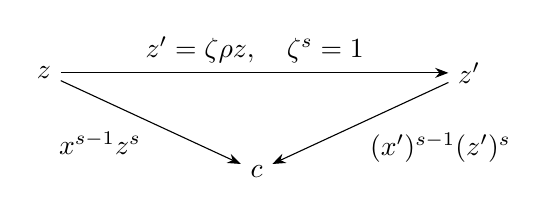
\begin{tikzpicture}[x=1cm,y=1cm,>=Stealth]
\node (z) at (0,0) {\(z\)};
\node (zp) at (5.4,0) {\(z'\)};
\node (c) at (2.7,-1.25) {\(c\)};
\draw[->] (z)--node[above]{\(z'=\zeta\rho z,\quad \zeta^s=1\)}(zp);
\draw[->] (z)--node[below left]{\(x^{s-1}z^s\)}(c);
\draw[->] (zp)--node[below right]{\((x')^{s-1}(z')^s\)}(c);
\end{tikzpicture}
\caption{The two inverse coordinates above a common determinant parameter. The branch \(\rho^s=(x/x')^{s-1}\) tending to one singles out \(\zeta=1\) in the limiting Gram integral.}\label{fig:power-map-branches}
\end{construction}

\begin{lemma}\label{lem:gram-limit}
Under \eqref{eq:gram-rate}, let
\(\widetilde A_{h,x}(c)=|x|^{-(s-1)}A_{h,x}(c/x^{s-1})\).
The block Gram matrix of \(V\) and \(\widetilde A\) is positive
semidefinite on every finite set of indices. As \(|x|\to\infty\)
and \(x'=x+\sigma\) for fixed \(\sigma\), both the
\((\widetilde A_{h,x},\widetilde A_{h',x'})\) and
\((V_{h,x},\widetilde A_{h',x'})\) Gram entries tend to
\[
 \int_{\C}\psi_\beta(\sigma z)
             \langle B_h(z),B_{h'}(z)\rangle\,d^2z .
\]
Here the inner product is conjugate-linear in the first
variable, and \(dc\) denotes complex area measure.
\end{lemma}

\begin{proof}
\proofstep{Square integrability under the power map.}

Set \(W_{h,x}(D)=|x|^{s-1}V_{h,x}(x^{s-1}D)\).
The dilation preserves its \(L^2\) norm. On a compact annulus
in \(D\), open the square of \(A_{h,x}\) and change variables
by \(D=z^s\), with real Jacobian \(s^2|z|^{2s-2}\).
The terms involving two distinct roots tend to zero by
Riemann--Lebesgue, since their amplitudes are integrable on
the compact preimage and their frequencies tend to infinity.

The equal-root terms give the squared \(L^2\) norm of \(B_h\)
on the preimage \(A^{1/s}=\{z:z^s\in A\}\) of the annulus \(A\).
The error in \eqref{eq:gram-rate} tends to zero in \(L^2(A)\),
so the uniform bound on \(W\) gives
\[
 \|\mathbf 1_{A^{1/s}}B_h\|_2^2
    =\lim_{|x|\longrightarrow\infty}\|\mathbf 1_A A_{h,x}\|_2^2
    \le \sup_x\|W_{h,x}\|_2^2 .
\]
Exhaust the punctured plane. Pointwise Cauchy--Schwarz on the
\(s\) roots now gives \(\|A_{h,x}\|_2^2\le s\|B_h\|_2^2\).
The positive block is the Gram matrix of the resulting
vectors at every index in the common \(c\) variable.

\proofstep{The Gram entry of the two approximants.}

Pairing the two leading terms introduces products of phases. Equal roots give the diagonal contribution, while distinct roots must be separated by oscillation.


In the common \(c\) variable, the two power equations read
\[
 x^{s-1}z^s=c=(x')^{s-1}(z')^s .
\]
Let \(\rho\) be the \(s\)th root of \((x/x')^{s-1}\) tending
to one. Then \(z'=\zeta\rho z\) for \(\zeta^s=1\).
The area formula expresses the approximant entry as the sum over
\(\zeta\) of
\[
 \int_{\C}\psi_\beta\bigl(s(\zeta\rho x'-x)z\bigr)
     \langle B_h(z),|\rho|B_{h'}(\zeta\rho z)\rangle\,d^2z .
\]
The factor \(|\rho|\) is the ratio of the area dilation
factor \(|\rho|^s\) and the normalization
\(|\rho|^{s-1}\) of the second \(B\) vector.

By density of
compactly supported continuous vectors, these dilations
are strongly continuous in \(L^2\). Thus the moving amplitude
can be replaced by the one with \(\rho=1\) at \(o(1)\)
cost in \(L^1\). For the unrotated root, \(x'=x+\sigma\) and the chosen
branch near one give
\[
 \rho x'=x(1+\sigma/x)^{1/s}
       =x+\sigma/s+O(|x|^{-1})
\]
for fixed \(\sigma\). The limiting phase is then
\(\psi_\beta(\sigma z)\).
For the other roots,
\[
 s(\zeta\rho x'-x)=s(\zeta-1)x+\zeta\sigma+O(|x|^{-1}),
 \qquad \zeta\ne1 .
\]
Those frequencies tend to infinity. Dominated convergence at
\(\zeta=1\) and Riemann--Lebesgue at the other roots give the limit.

\proofstep{The Gram entry with the original vector.}

For the cross entry, write the difference from this
approximant entry in the first \(D\) variable. The error
\(W_{h,x}-A_{h,x}\) is uniformly bounded in \(L^2\) and
tends to zero on compact annuli. The other factor is
dominated by an \(L^2\) dilation of the fixed function
\(D\mapsto\sum_{z^s=D}\|b_{h'}(z)\|\). This function belongs to
\(L^2\) by the same area formula.

Write \(E_x=W_{h,x}-A_{h,x}\), and let \(F_x\) be the moving
dilation of the fixed dominator \(F\). Strong continuity of the dilation gives
\[
 \int |E_x|\,|F_x-F|\le \|E_x\|_2\|F_x-F\|_2=o(1).
\] For a compact annulus \(A\), the integral there tends to zero.
If \(F(D)=\sum_{z^s=D}\|b_{h'}(z)\|\) is the fixed dominator,
the limsup of the absolute cross-entry error is at most
\[
  \sup_x\|W_{h,x}-A_{h,x}\|_2\,\|\mathbf 1_{\mathbb C\setminus A}F\|_2 .
\]
Exhausting the punctured plane proves the second limit.
\end{proof}

 The area formula and the moving-dilation argument give the limits for the local germ. These limits hold for fixed local
data and each finite history set. The uniform bound as
the dimensions grow is supplied by the period majorants in
Section~\ref{sec:block-recursion}. \label{cor:orbital-germ-2}

\section{Transfer matrices for signed sequences and spectral interpolation}\label{sec:word-pairing}
\hypertarget{source-word-pairing}{}

The orbital germ can be paired against many vectors, one for each sequence of signs and spectral parameters. Comparing two such vectors requires an explicit change of form when a tensor factor is adjoined. Positivity at the real interpolation nodes will then bound their mixed pairing. The resulting bound applies to the selected
differentiated coefficients in Section~\ref{sec:block-recursion} by
the two residual operator comparisons in
Lemma~\ref{hyp:selected-orbital-coefficient-bounds}.

At a complex place, a letter specifies a sign and a spectral parameter. Each letter added to a word acts in a new two-dimensional tensor factor. The two substitutions in \eqref{eq:word-signed-updates} define the transfer for the longer word. Proposition~\ref{prop:real-node-positivity} gives the positivity needed to interpolate its radial form.

\subsection{Changing the signs of added letters}

A change in the sign of one factor alters the product of transfers. The adjoint and determinant identities below keep track of the induced change in its Hermitian form.

Let \(T_v(z)\) be the \(2\)-by-\(2\) transfer for a word \(v\), on an auxiliary space \(A=\mathbb C^2\). Its entries act on the tensor product of the initial representation space with the two-dimensional factors already adjoined.
Let \(A_v\) be its form operator. The adjoint identities at regular
real parameters give
\[
 A_v^*=A_v,\qquad (A_vT_v(y))^*=A_vT_v(y).
\]
Let \(B=\C^2\) be a second auxiliary space, let \(P\) be the
flip of \(A\) and \(B\), and put
\(J=\left(\begin{smallmatrix}0&1\\-1&0\end{smallmatrix}\right)\).
Write \(T_A,T_B\) for the same transfer acting in the indicated auxiliary factor and \(q_v\) for its scalar quantum determinant. The two-parameter relation and the determinant identities are
\begin{align}
 ((z-y)I-P)T_A(z)T_B(y)
  &=T_B(y)T_A(z)((z-y)I-P),\label{eq:word-rtt}\\
 T_v(y)JT_v(y+1)^t&=q_v(y)J,\qquad
 T_v(y+1)^t JT_v(y)=q_v(y)J .
 \label{eq:word-qdet}
\end{align}

To adjoin a letter, tensor the old representation space with \(B\); the old operators act trivially on this new factor.
Write \(Q=P^{t_B}\), the outer product of
\(e_1\otimes e_1+e_2\otimes e_2\) with its transpose.
For the positive letter at \(y\) and its dual negative letter
at \(y+1\), the recursions are
\begin{align}
 T_+(z)&=T_A(z)\frac{(z-y)I-P}{z-y-1},
 & A_+&=A_vT_B(y),\notag\\
 T_-(z)&=\frac{(y+1-z)I-Q}{y-z}T_A(z),
 & A_-&=A_vT_B(y+1)^{t_B}.\label{eq:word-signed-updates}
\end{align}
The positive letter multiplies \(q_v(z)\) by
\((z-y+1)/(z-y)\). The negative letter at \(u\) multiplies it
by \((u-z)/(u-z-1)\).

\begin{lemma}[The identities are preserved by adjoining a letter]\label{lem:word-update-identities}
Where all denominators are nonzero, adjoining either letter in
\eqref{eq:word-signed-updates} preserves the adjoint identities
and \eqref{eq:word-rtt}--\eqref{eq:word-qdet}. If \(D(z)\) and \(D'(z)\) are the determinants before and after adjoining the letter, respectively, then 
\[
 D'(z)=D(z)\begin{cases}(z-y+1)/(z-y),&\text{positive letter }y,\\ (u-z)/(u-z-1),&\text{negative letter }u.\end{cases}
\]

\end{lemma}

\begin{proof}
Put \(S=P_{12}\), \(T=P_{23}\) and \(R=P_{13}\). In comparing
\((aI-S)((a+b)I-R)(bI-T)\) with the product in reverse order,
the terms with at most one flip agree. For the terms with two,
use \(SR=RT=TS\) and \(TR=RS=ST\). The two-flip contributions
on the two sides both equal
\[
    bSR+(a+b)ST+aRT=(a+b)(TS+ST)
                     =aTR+(a+b)TS+bRS.
\]
The three-flip terms agree since \(SRT=TRS=R\). The normalized positive factor thus satisfies
the Yang--Baxter identity.
The negative factor is a scalar multiple of the conjugate positive
factor with shift \(z-u+1\), using
\(J_B^{-1}P J_B=I-Q\). The determinant for the positive factor
with parameter \(D\) is \((D+1)/D\).

For its positive-order entry the numerator is
\[
 (DI-e_{11})((D+1)I-e_{22})-e_{21}e_{12}=(D+1)(D-1)I .
\]
The scalar conjugation of the negative factor gives its determinant.
The quantum determinants multiply because the transfer families
for the old word and the added rational factor have commuting
entries and their two-auxiliary products preserve the alternating
line. Hermitian symmetry for \(A_+T_+(z)\) follows by applying
\eqref{eq:word-rtt} after taking adjoints. For \(A_-T_-(z)\)
use the partial transpose at \(B\) of the relation with spectral
order \(u,z\). It gives
\[
 T_B(u)^{t_B}((u-z)I-Q)T_A(z)
  =T_A(z)((u-z)I-Q)T_B(u)^{t_B}.
\]
The partial transpose reverses the order of the scalar factors
on \(B\) and retains the order of the operator coefficients.
Starting from the actual two-by-two transfer, these identities
hold on the regular domain of each word. \label{cor:word-pairing-1}

\end{proof}

\begin{proposition}[Changing signs in a list of letters]
Let \(v\) be a word and let \(L\) consist of added positive
letters at separated admissible real nodes. Let \(\bar L\)
use their dual negative letters at the shifted nodes.
Here \(\Psi\) is the tail-first product of the maps
\(-T_B(y)^{-1}J_B\) on the successively updated words, and
\(J_L\) is the product of the \(J_B\) on the added slots.
If \(B_L\) is positive semidefinite on the coefficient domain
and that domain contains the transformed vectors \(\Psi x'\),
then
\[
 \big|\langle J_L A_v x,x'\rangle\big|^2
     \prod_{y\in L}q_v(y)
 \le B_L(x,x)\,\langle A_{\bar L v}x',x'\rangle .
\]
The factors \(q_v(y)\) are positive at the chosen cut nodes.
\end{proposition}

\begin{proof}
\proofstep{Conjugation at one new letter.}
If \(q_v(y)\ne0\), set \(\Psi_y=-T_B(y)^{-1}J_B\).
Equation~\eqref{eq:word-qdet} gives a two-sided inverse and gives
\(\Psi_y=-q_v(y)^{-1}J_BT_B(y+1)^{t_B}\). Direct substitution
into the word forms yields
\[
 \Psi_y^* A_+ = J_B A_v,\qquad
 \Psi_y^* A_+ \Psi_y = q_v(y)^{-1}A_-.
\]
In \eqref{eq:word-rtt}, multiply on both sides by \(T_B(y)^{-1}\)
and insert \(-J_B\). The identity \(J_B^{-1}P J_B=I-Q\) gives
\begin{equation}\label{eq:word-conjugation}
 T_+(z)\Psi_y=\frac{z-y}{z-y-1}\Psi_y T_-(z).
\end{equation}

\proofstep{Conjugation of the full list.}

Let \(L\) be a list of added positive letters and \(\bar L\)
the list of their duals at the shifted parameters. Process
the letters from the tail. The product \(\Psi=\Psi_y\Psi_0\)
uses the tail transformation \(\Psi_0\) and then the one at
\(y\) on the preceding positive form. In the transfer
conjugation the new rational factor commutes with \(\Psi_0\)
because it uses a free position. Thus the conjugation
scalars in \eqref{eq:word-conjugation} multiply. At \(y+1\)
the tail's scalar is
\(\prod_{u\text{ in tail}}(y-u+1)/(y-u)=q_{\mathrm{tail}\,v}(y)/q_v(y)\).
It cancels the extra tail factor in the one-letter determinant.
With \(J_L\) the product of all the \(J_B\) on the added
positions, induction now gives
\[
 \Psi^*A_{Lv}=J_L A_v,\qquad
 \Psi^*A_{Lv}\Psi=\frac{A_{\bar L v}}{\prod_{y\in L}q_v(y)} .
\]
All denominators are nonzero at separated admissible nodes.

\proofstep{Using positivity and checking the determinant signs.}

The conjugating operators now identify the two mixed forms. Their signs still matter, since the subsequent Fourier estimate uses positivity of the diagonal forms.


Consequently, if \(B_L(x,x')=\langle A_{Lv}x,x'\rangle\)
is positive semidefinite on the coefficient domain and
the domain contains \(\Psi x'\), Cauchy--Schwarz gives
\begin{equation}\label{eq:word-size}
 \big|\langle J_L A_v x,x'\rangle\big|^2
     \prod_{y\in L}q_v(y)
 \le B_L(x,x)\,\langle A_{\bar L v}x',x'\rangle .
\end{equation}
We use the convention that the pairing is linear in the first
argument. The factors \(q_v(y)\) are positive on the cut.
Indeed the initial determinant is
\[
 -TT'\prod_{i=1}^k
   (y+\tfrac12+u_i)(y+\tfrac12+u'_i).
\]

On cut \(\ell\), the number \(-y-\tfrac12\) is strictly
between the interlacing parameters \(u_\ell,u'_\ell\).
Both earlier parameters exceed it and both later ones
are smaller. Exactly one pair has opposite signs.
The positive and negative rational factors of the old word
are all positive at nodes of distance more than two.
With at most \(N\) old letters and distance at least
\(N^2+1\) from each relevant pole, the absolute log of their
product is at most \(2N/(N^2+1)\le1/2\) for \(N\ge4\).

\end{proof}

\begin{construction}
\begin{tabular}{@{}lll@{}}\toprule
Added letters & Pull back on one side & Pull back on both sides\\\midrule
One letter at \(y\) & \(\Psi_y^* A_+=J_B A_v\) &
\(\Psi_y^* A_+\Psi_y=A_-/q_v(y)\)\\
Tail first, through \(L\) & \(\Psi^* A_{Lv}=J_L A_v\) &
\(\displaystyle\Psi^* A_{Lv}\Psi=
 \frac{A_{\bar L v}}{\prod_{y\in L}q_v(y)}\)\\\bottomrule
\end{tabular}
\caption{Changing the signs of letters at separated admissible nodes. The two columns give the mixed and diagonal forms used in the positive-block inequality.}\label{fig:pullback-of-word-forms}
\end{construction}

\subsection{Positivity at real interpolation nodes}

The transfer identities compare forms algebraically. To use Cauchy--Schwarz on a mixed pairing, the terminal form must also have the correct sign on the compact types actually present.

\begin{proposition}[Positivity of the terminal density on the type space]\label{prop:real-node-positivity}
At each real interpolation node \(y\) of cut \(\ell\), impose
\(-y\) at distance at least two from both endpoints
\(u_\ell,u'_\ell\), the type interlacing in \eqref{eq:word-type-interlacing}
and spacing greater than two for the updates \eqref{eq:word-signed-updates}.
If \(Q_y\) is the form defined by the terminal transfer at this node, then 
\[
 Q_y(T,T)\ge0\qquad(T\text{ in the Hilbert--Schmidt space of compact types}).
\]

\end{proposition}

\begin{proof}
\proofstep{Triangular congruence at the terminal level.}

Let \(A_v=F^*DF\) be the old form and write
\(T(z)=\left(\begin{smallmatrix}a(z)&b(z)\\c(z)&d(z)\end{smallmatrix}\right)\)
for \(F T_v(z)F^{-1}\). The induction uses \(d(z)=Gx(z)\),
where \(G>0\) is a multiplication operator and the \(x(z)\)
commute with one another and with \(D\) and \(G\). For real
regular \(y\), \(d(y)\) is self-adjoint and \(DT(y)\) is
Hermitian.

At the next positive letter put \(e=d(y)^{-1}c(y)\).
The right column in the first equation in \eqref{eq:word-qdet}
gives \(c(y+1)=e d(y+1)\) and
\(a(y)-b(y)e=q_v(y)d(y+1)^{-1}\).
The adjoint then gives the congruence
\[
 DT(y)=H_e^*
   \operatorname{diag}\big(Dq_v(y)d(y+1)^{-1},Dd(y)\big)H_e,
 \qquad H_e=\begin{pmatrix}1&0\\e&1\end{pmatrix}.
\]
For a negative letter use \(T(y)^t\), \(e=d(y)^{-1}b(y)\),
and the second determinant equation at \(y-1\). Its top
diagonal is \(Dq_v(y-1)d(y-1)^{-1}\) and the bottom
diagonal is \(Dd(y)\).

For either new letter, the 22-entry of the new transfer,
before the new shear, is
\[
 \frac{1}{u-1}
 \begin{pmatrix}u d(z)&0\\-f(z)&(u-1)d(z)\end{pmatrix},
\]
where \(u=z-y,f=c\) for a positive letter and \(u=y-z,f=b\)
for a negative letter. Equation~\eqref{eq:word-rtt} gives
\([d(z),d(y)]=0\) and \(u[e,d(z)]=f(z)-d(z)e\).
Conjugation by \(H_e\) thus diagonalizes this entry, replacing
\(x(z)\) by \(x(z)\operatorname{diag}(u/(u-1),1)\).

After \(H_e\), apply the commuting diagonal normalization of the actual frame. For the two letter signs these matrices are 
\[
 D_+=\operatorname{diag}(\zeta^{-1},G\bar\zeta^{-1}),\qquad D_-=\operatorname{diag}(\bar\zeta^{-1},G\zeta^{-1}).
\]
 This makes the form
diagonal \(D=(|\zeta|^2/G)^{|v|}C\).
At a new letter the two diagonal multipliers of \(C\) are
\[
  \big(q_v(y)/x(y+1),x(y)\big)
  \quad\hbox{or}\quad
  \big(q_v(y-1)/x(y-1),x(y)\big),
\]
respectively. All these multipliers commute, and the shear is
invertible wherever the indicated inverses exist.

The initial \(x\) acts through functions on the finite types.
At type \(\rho\) it is
\((-1)^{k-\ell}\prod_{j=1}^{k-1}(z+\rho_j)\), where
\begin{equation}\label{eq:word-type-interlacing}
 \max(u_{j+1},u'_{j+1})+\tfrac12
 \le \rho_j \le \min(u_j,u'_j)-\tfrac12
 \qquad(1\le j<k).
\end{equation}
At cut \(\ell\) there is a margin of at least two from both
ends of the interval between \(u_\ell,u'_\ell\) to \(-y\).
Thus \(x(y+\delta)>0\) for \(|\delta|\le1\). For \(|\delta|\le1\) the interlacing bounds give
\[
  y+\delta+\rho_j>0\quad(j<\ell),\qquad
  y+\delta+\rho_j<0\quad(j\ge\ell).
\]
The sign \((-1)^{k-\ell}\) makes their product positive.
The determinant argument applies also at \(y-1\). Spacing greater than
two preserves all of these signs under the rational
updates, so \(C\) has positive type values.

\proofstep{The form on the actual type space.}

To see positivity on the actual fiber, use the pointwise
type identity for the unscaled transfer. The operator
with type values \(x_C(\rho,z)=\prod_j(z+\rho_j)\) acts by
right composition on the finite-dimensional compact
type space with a Capelli operator \(K_g(z)\).
This operator is self-adjoint for real \(z\).
The compact Lie action has \(E_{ab}^*=E_{ba}\), and taking
adjoints in the column-ordered determinant gives the
row formula after simultaneous reversal of both index
lists. The disjoint interlacing intervals determine each root's
index, so the polynomial determines the type:
\[
 \prod_j(z+\rho_j)=\prod_j(z+\rho'_j)\quad\Longrightarrow\quad\rho=\rho'.
\]
Avoid the finitely many equality points of distinct polynomials
when choosing real \(z_0\).

For any positive function \(f\) on the
types, interpolate a polynomial \(p\) with
\(p(x_C(\rho,z_0))=f(\rho)\) and \(p=1\) at the other
eigenvalues of \(K_g(z_0)\). The algebra of type functions
then acts by \(V\mapsto Vp(K_g(z_0))\) for \(f\).
In a compact eigenbasis \(K_g(z_0)e_j=\lambda_j e_j\),
\[
       \langle V,Vp(K_g(z_0))\rangle_{\rm HS}
        =\sum_j p(\lambda_j)\|Ve_j\|^2\ge0 .
\] Applied after the congruence, this proves
positivity of the terminal density from the top transfer
and type identities. \label{cor:word-pairing-2}

\end{proof}

\begin{proposition}[Decay of the wave pairing]\label{prop:wave-pairing-decay}
On a stable compact class on which the four Jacquet intertwining
identities hold, and at the real nodes of
Proposition~\ref{prop:real-node-positivity}, let \(f_s\) be the wave and \(\beta\) the pairing. The single-site identity and Jacquet intertwining give 
\[
 s\,\beta(f_s F,F')=\beta(f_s\Theta_1 F,\Theta_0 F')-\beta(f_s\Theta_3 F,\Theta_2 F').
\]
 Iterating this identity \(n+3\) times on the stable compact class gives the weighted wave pairing bound.
The resulting bound includes the factor \((1+|t|^2)^2\)
from the first Hermitian minor. For the selected arithmetic
coefficients use Lemma~\ref{hyp:selected-orbital-coefficient-bounds}.
\end{proposition}

\begin{proof}
\proofstep{The density change at a single site.}

At lower levels let \(Q_i(w)\) be the word form operator
and \(B_i(w)\) the ordered product of site operators.
The site rule \(Q_i=B_i^*Q_{i+1}B_i\) rewrites the next
density as \(D_{(B_i^*)^{-1}Q_i x,B_i y}(t)\), where
\(D_{u,v}(t)\) is the ordinary pairing with coordinate
\(c_i=t\), multiplied by \(|t|^{-2}\).
The one-letter density rule has the form
\[
 D_{I_+u,B_+v}=D_{u,v}-\partial_{\bar t}D_{u,Ev},
 \qquad D_{I_-u,B_-v}=D_{u,v}+\partial_t D_{u,Ev},
\]
where \(E=e_{10}\) acts on the new slot. To see the signs,
write \(P,\bar P\) for the two coordinate raising operators,
so \([P,t]=t\), \([\bar P,\bar t]=\bar t\), and
\(P^*=-\bar P\). The site matrices are
\begin{align*}
 B_+&=\begin{pmatrix}y+P&-t\\t^{-1}&0\end{pmatrix},&
 I_+&=\begin{pmatrix}0&-\bar t^{-1}\\\bar t&y+1-\bar P\end{pmatrix},\\
 B_-&=\begin{pmatrix}y-\bar P&-\bar t\\\bar t^{-1}&0\end{pmatrix},&
 I_-&=\begin{pmatrix}0&-t^{-1}\\t&y-1+P\end{pmatrix}.
\end{align*}
The commutators give \(I_\pm=(B_\pm^*)^{-1}\).
Expanding the two components in the ordinary pairing cancels
the parameter \(y\).

Let \(L_E\) be the ordinary pairing of
\(u_1,v_0\). The additional terms are
\(\bar t^{-1}L_E-\partial_{\bar t}L_E\) for the positive
letter and \(-t^{-1}L_E+\partial_t L_E\) for the negative
letter, using the ordinary pairing Leibniz rule.
The two terms are already weighted derivatives. In fact
\[
 \begin{aligned}
 |t|^{-2}(\bar t^{-1}L_E-\partial_{\bar t}L_E)
     &=-\partial_{\bar t}(|t|^{-2}L_E),\\
 |t|^{-2}(-t^{-1}L_E+\partial_tL_E)
     &=\partial_t(|t|^{-2}L_E).
 \end{aligned}
\]
The signs follow from differentiating \((t\bar t)^{-1}\).
Since the new slot is free in the tail word,
induction expands the step density into derivatives of
order at most \(n=|w|\). Its order-zero term is
\(D_{Q_i x,y}\).

\proofstep{Integrating the density step.}

This step uses the compact-class integrability
of both \(D\) and \(W D\), \(W(t)=(1+|t|^2)^2\), and
Fourier bounds \(O((1+|\xi|)^{-n-3})\) for both.
For a real multi-index \(\alpha\) with \(|\alpha|\le n\),
the differentiated inverse Fourier integrals are absolutely
convergent, since in two dimensions
\[
       \int_{\mathbb R^2}
            (1+|\xi|)^{|\alpha|-n-3}\,d^2\xi<\infty .
\]
They give continuous bounded extensions through zero. For
\(D=W^{-1}(WD)\) the product rule then bounds each derivative
by \(O((1+|t|)^{-4})\).

For a positive-order derivative write
\(\partial^\alpha D=\partial_j(\partial^{\alpha-e_j}D)\) with \(\alpha_j>0\), in real coordinates. On a disk the divergence theorem gives
\[
 \left|\int_{|t|\le R}\partial^\alpha D\right|
 \le 2\pi R \sup_{|t|=R}|\partial^{\alpha-e_j}D|=O(R^{-3}).
\]
The full-plane integral therefore vanishes. Fubini integrates
\(D_{Q_i x,y}\) to the preceding form. With \(x=y\) the
density at \(t\ne0\) is nonnegative by the positivity
at level \(i+1\), which proves positivity at level
\(i\).

\proofstep{Fourier decay from the wave identity.}

The wave identity can be iterated only on a class stable under its operators. Each iteration then trades a derivative bound on that class for decay in the frequency.


The decay follows from an identity for the first-coordinate
wave \(f=f_s\). It commutes with the multiplications \(c_j\)
and the raising operators \(P_j\) for \(j>0\), and satisfies
\([P_0,f]=s f c_0\). Let \(A(Y),B(Y)\) be the first column
of \(B_{+,r-1}(Y)\cdots B_{+,0}(Y)\) formed with the
different site operators. For each last site \(j>0\), expand
\[
 A(Y+1)fB(Y)-B(Y+1)fA(Y).
\]
The terms with both previous upper entries cancel by
\((Y+1+P_j)c_j^{-1}=c_j^{-1}(Y+P_j)\).
The terms with one lower entry give exactly the shorter
product, since the different sites commute. At site zero the
difference is
\((Y+1+P_0)fc_0^{-1}-c_0^{-1}f(Y+P_0)=s f\).

To express this identity by operators and their adjoints, put
\(C=\prod_j c_j\), and let \(\tilde A,\tilde B\) be the
first column for the negative site matrices. Let \(l(Y)\) and
\(m(Y+1)\) be the two lower ratios of the starting transfer
used in the congruence. The shifted determinant and the
base adjoint give \(m(Y+1)^*=l(Y)\). For a regular real \(Y\)
set
\begin{align*}
 \Theta_0&=\bar C\tilde A(Y+1),&
 \Theta_1&=C^{-1}\big(l(Y)A(Y)+B(Y)\big),\\
 \Theta_2&=\bar C^{-1}
       \big(m(Y+1)\tilde A(Y+1)+\tilde B(Y+1)\big),&
 \Theta_3&=C A(Y).
\end{align*}
The wave commutes with the starting transfer.
The ratios thus cancel in
\(\Theta_0^* f\Theta_1-\Theta_2^* f\Theta_3\).
The stars of \(\tilde A(Y+1),\tilde B(Y+1)\) are
\(A(Y+1),B(Y+1)\) by the site adjoint and commutation of
different sites. The difference is therefore \(s f\).

After smooth ambient realization of the four operators
and Jacquet intertwining, the base adjoint gives
\[
  s\,\beta(f_s F,F')
   =\beta(f_s\Theta_1 F,\Theta_0 F')
        -\beta(f_s\Theta_3 F,\Theta_2 F').
\]
On the stable compact class, the base bound is uniform in
\(s\) because the wave is unitary. Iterating the identity
\(n+3\) times gives the required decay. The weight
\((1+|t|^2)^2\) comes from multiplication by the same
polynomial in the first Hermitian minor on the ambient
space, which passes through the period integral.
These identities use the following realization and measure
comparison on the regular radial cell. \label{cor:word-pairing-3}

\end{proof}

\subsection{Ambient differential operators and measures}

The bounds on differentiated pairings were obtained in radial variables. To apply them to an orbital integral on the group we must identify those derivatives and their integration measure in the ambient coordinates.

At each place let \(h\) be the Hermitian form, \(e_j,e_j^*\)
the null pairs, and \(z,z'\) the positive vectors in the
middle space. The cross minors \(D_j(g)\) are the leading
minors of the pairings of the two flags, with \(z,z'\)
appended at the end. Put \(T=h(z,z)\), \(T'=h(z',z')\) and
\[
 G_f(g)=|D_{r+1}(g)|^2-TT'|D_r(g)|^2 .
\]
In the radial cell \(g=w(c)g_0\), \(G_f=|C|^2G\).
Here \(w(c)\) sends \(e_j\) to \(c_j e_j^*\) and \(e_j^*\)
to \(\bar c_j^{-1}e_j\), fixing the middle space.
The factor \(G_f^{-1}\) in the ambient realization thus
represents \((C\bar C G)^{-1}\).

\begin{proposition}[Radial realization on the regular cell]\label{prop:regular-cell-realization}
In Witt coordinates on the regular radial cell, the ambient
cofactors give the radial denominators and the null-site recurrences,
whose terminal entries are the geometric cofactor actions. Their
identification on the selected types is proved in
Lemma~\ref{hyp:selected-orbital-coefficient-bounds}. With the product Haar
measure from the null-vector coordinates, let \(F(t,x),G(t,x)\) be two jointly smooth compact slice coefficients satisfying \eqref{eq:word-slice-sobolev} with integrable residual derivative bounds. For either real parameter derivative \(\partial\) the pairing obeys 
\[
 \partial\!\int F\overline G\,dx=\int\!\big((\partial F)\overline G+F\,\overline{\partial G}\big)\,dx.
\]

\end{proposition}

\begin{proof}
\proofstep{Realization of the radial denominators.}

Construct a cofactor vector \(b\) in the left null space
plus the line \(z\) from the first \(r\) columns of the
cross matrix. It is perpendicular to the transformed right
null space. Its \(z\)-coefficient has modulus \(|D_r|\)
and \(|h(b,gz')|=|D_{r+1}|\), by determinant expansion.
Project \(g^{-1}b\) to the residual Hermitian space and
off \(z'\). The coefficients \(\omega\) in a fixed
negative orthonormal frame satisfy
\[
 \|\omega\|^2=|h(b,gz')|^2/T'-h(b,b)=G_f/T' .
\]
Let \(C_{\widehat a,\widehat b}\) denote the quantum
\((k-1)\)-minor with row \(a\) and column \(b\) omitted.

For the unit vector \(\nu=(T'/G_f)^{1/2}\omega\) the
operator on its orthogonal complement is
\[
       \sum_{a,b}(-1)^{a+b}\bar\nu_a\nu_b
                         C_{\widehat a,\widehat b}.
\]
Indeed the wedge of a unitary complement frame is the
contraction of the volume by \(\nu\), up to a unit phase
that cancels between the two lists. At a regular real parameter \(Y\), let \(S\) consist of the distinct type values \(x_0(\rho,Y)\). They are nonzero on the locus in question. The polynomial
\[
 p_Y(X)=\sum_{a\in S}\frac{1}{a}
             \prod_{b\in S\setminus\{a\}}\frac{X-b}{a-b}
\]
satisfies \(p_Y(a)=1/a\) for every \(a\in S\). The type algebra then realizes \(x(Y)^{-1}\)
by this polynomial in the compact type operator. The
result is equivariant under the compact stabilizers.
All its coefficient derivatives have polynomial growth
on \(G_f\ge\varepsilon>0\), because \(\omega\) is
polynomial and the coefficients have denominators that
are powers of \(G_f\).

\proofstep{Contracting the Capelli minors.}

The differential factors left after this multiplication
are Capelli minors. In the positive residue of size
\(r+k\), the row list has the \(r\) first null directions
and all middle directions except \(w_a\), with coefficient
\((-1)^a h(w_a,z')\). The coefficient for column list
\(J\) is
\[
 \det(g^{-1}e_{r-1},\ldots,g^{-1}e_0,g^{-1}z,e_J).
\]
On the cell this determinant vanishes unless \(J\) includes
the \(r\) first null directions and omits just one middle
direction. In that case it contributes \(\bar C\) times
the corresponding component of \(g_0^{-1}z\), with its
cofactor sign. The mirror residue uses opposite null
directions, the dual determinants, and the conjugate
coordinate \(C\). The two residues are equivariant since
the two index lists transform by dual exterior powers,
so the determinant scalars of the fixed wedge and the
variable wedge cancel.

For the positive residue let \(F_j\) be the contracted
minor with the first \(j\) null rows and columns removed,
restricted with weight \(\prod_a|c_a|^{2(r-a)+k}\).
Write \(\varphi\) for the restricted coefficient.
Then
\begin{align*}
 F_r&=-T_{21}(Y)\varphi,\\
 F_{r-1}&=(Y+P_{r-1})F_r-c_{r-1}^{-1}T_{22}(Y)\varphi,\\
 F_j&=(Y+P_j)F_{j+1}-(c_{j+1}/c_j)F_{j+2}
                       \qquad (j+2\le r).
\end{align*}
The terminal equality is the single middle cofactor
defining the transfer entry. To derive the interior
formula, expand along the first column. The diagonal gives the torus derivative and the shift
\(Y+r-j+k/2\). For the \(j\)-th radial factor \(a_j=|c_j|^{2(r-j)+k}\),
\[
                     c_j\partial_{c_j}a_j
                        =(r-j+k/2)a_j .
\]
On the conjugated expression, the contribution of the
radial factor subtracts its logarithmic derivative. This leaves
\[
 Y+P_j+r-j+k/2-c_j a_j^{-1}\partial_{c_j}a_j=Y+P_j .
\]

For the off-diagonal cofactor expand the remaining
minor in reverse row order. Its left and right root characters
and cofactor sign give the multiplier
\[
      (-1)\cdot(c_{j+1}/c_j)\cdot 1=-c_{j+1}/c_j .
\]
This term removes two adjacent null indices at the same spectral parameter. At the last site the
two root characters are middle covectors. With the
first cofactor they give the signed double contraction
defining \(T_{22}\), times \(c_{r-1}^{-1}\).

To keep track of the mirror, write \((d_j,H_j)=(c_j,P_j)\)
on the positive side and \((d_j,H_j)=(\bar c_j,-\bar P_j)\)
on the mirror side. Set
\[
 S_j=\begin{pmatrix}Y+H_j&-d_j\\d_j^{-1}&0\end{pmatrix},
 \qquad
 U=\begin{cases}(T_{21},T_{22})&\text{on the positive side},\\
                 (T_{12},T_{22})&\text{on the mirror side}.
   \end{cases}
\]

For \(0\le j\le r\) let \((a_j,b_j)=U S_{r-1}\cdots S_j\),
with \((a_r,b_r)=U\). Multiplication on the right gives
\[
 a_j=a_{j+1}(Y+H_j)+b_{j+1}d_j^{-1},\qquad
 b_j=-a_{j+1}d_j .
\]
In particular,
\[
 b_{j+1}d_j^{-1}=
 \begin{cases}
  -a_{j+2}d_{j+1}d_j^{-1},&j+2\le r,\\
  T_{22}d_{r-1}^{-1},&j=r-1 .
 \end{cases}
\]
The last term is shared by both signs. With the sign of
the contracted minor, \(F_j=-a_j\varphi\); in particular its
terminal value is \(-T_{21}\varphi\) or \(-T_{12}\varphi\),
respectively. For \(r=0\) the empty site product gives these
terminal values directly:
\[
    r=0:\qquad F_0^+=-T_{21}(Y)\varphi,\qquad
                    F_0^-=-T_{12}(Y)\varphi .
\]

Thus the two ordered products act on the residual operators
\(\Theta_1,\Theta_2\). For \(\Theta_0,\Theta_3\) the same
first-column expansion uses only the null directions, so the
minors have rank \(r\).

\proofstep{Restriction of the measure.}

The restriction weight has a Haar interpretation.
In a complex Hermitian space of dimension \(m\), the
image \(ge\) of a fixed null vector is measured on the
null cone. Where \(ge=c e^*+v+a e\) and \(c\ne0\),
write \(v=c x\), \(a=c b\).
There are \(m-1\) complex coordinates in \((x,b)\), giving
Jacobian \(|c|^{2(m-1)}\) in \((v,a)\) at fixed \(c\).
The null equation becomes
\[
 2\operatorname{Re}(a\bar c)+h(v,v)
              =|c|^2(2\operatorname{Re}b+h(x,x))=0 .
\]
The delta measure of the real equation is multiplied by
\(|c|^{-2}\). After dividing by the unipotent Haar factors
in \(x,\operatorname{Im}b\), the radial measure is thus
\[
    |c|^{2(m-1)}|c|^{-2}\,d^2c .
\]
The first factor is the square of the restriction weight.

At the terminal group \(U(1,k)\), use the orbit of
\(z'\). At fixed \(\zeta=h(z,gz')\), the negative part
of \(gz'\) has squared norm \(|\zeta|^2/T-T'\).
If \(u\) is the radial variable in the \(2k\) real negative
coordinates, the norm condition sets
\(u^2=|\zeta|^2/T-T'\). Changing variables from \(u\) to
\(u^2\) gives the radial density
\[
        u^{2k-1}\,du=\tfrac12 (u^2)^{k-1}\,d(u^2).
\]
This yields \((|\zeta|^2-TT')^{k-1}d^2\zeta\) on the
positive Gram locus, up to a fixed positive scalar. The compact
stabilizers act unitarily and disappear from the
Hilbert--Schmidt pairing. This gives the same Haar
scale in the terminal and radial pairings.

\proofstep{Domain of the differentiated pairing.}

Applying the radial identity inside an integral requires a common domain for its differentiated vectors.


The differentiated ordinary pairing can be justified
on a disk avoiding \(t=0\) once the restricted coefficients
have a jointly smooth residual realization with support in
a common compact set. Uniform \(L^2\) estimates there for
all fixed derivative orders follow from the residual
pairing bound. Applying the one-dimensional Sobolev estimate successively in the two real directions controls the supremum. On a smaller disk in the coordinates \(t_1,t_2\), a coefficient \(F(t,x)\) satisfies
\begin{equation}\label{eq:word-slice-sobolev}
 \sup_t |F(t,x)|^2
 \ll\int_{\text{larger disk}}
 \left(|F|^2+|\partial_1F|^2+|\partial_2F|^2+
             |\partial_1\partial_2F|^2\right)(t,x)\,d^2t .
\end{equation}
The residual derivative bounds make the right side integrable
in \(x\). Cauchy--Schwarz and dominated
differentiation then give the ordinary Leibniz rule.
For the adjoint comparison, use the regular orbit coordinates above. Write \(J\) for normalized integration along the two-sided orbit with its character and compact-type action.

If \(f\) is a smooth equivariant slice coefficient supported over a compact subset of the regular parameter domain, it has a compact ambient representative. Indeed choose finitely many relatively compact orbit charts over its support and a subordinate smooth partition of unity. In each group fibre choose a smooth bump of integral one in local orbit coordinates, including the smooth Haar density. Multiplying by the partition function and summing gives a compactly supported \(\varphi\) whose fibre integral is one there. Equivariance cancels the character and compact actions in
\[
 J(\varphi f)(g)=f(g)\int\varphi(p\cdot g)\,dp=f(g).
\]
Use the Haar measure on each orbit, or the corresponding quotient measure after dividing by its stabilizer. The bump is extended by zero inside the regular open set.

For an invariant operator \(\Theta\) with the smooth coefficients constructed on the cell, equivariance of its translated expression gives \(J\Theta F=\Theta JF\). The same argument applies to its formal adjoint: changing variables in the defining integration-by-parts identity conjugates both test functions by the same measure-preserving group action. Compact support permits differentiation under the orbit integral. Pair the compact lift \(F\) with the equivariant pullback of \(JF'\) to the group. In the ambient integration by parts multiply this pullback by a smooth compact cutoff equal to one near \(\operatorname{supp} F\). Its derivatives vanish on that neighborhood. Unfolding the product measure first against \(\Theta F\), then against \(F\), gives
\[
 \beta(\Theta JF,JF')=\beta(J\Theta F,JF')
       =\beta(JF,J\Theta^*F')=\beta(JF,\Theta^*JF').
\]
The formal adjoint includes the density derivative in these coordinates. The identity holds for the four operators of Proposition~\ref{prop:wave-pairing-decay} on their common compact regular support. \label{cor:word-pairing-4}

\end{proof}

\begin{auxlemma}[Removal of the radial cutoff]\label{lem:radial-cutoff-transfer}
Use the full cross-minor polynomial \(G_f=|D_{r+1}|^2-TT'|D_r|^2\) on the regular cell \(G_f>0\). Its value there is \(|C|^2G\), including the prefix determinant factor. For a word \(w\) of length at most \(N\), denote its signed Casimir product by \(Q_w\). Write \(E_j(F,w;c)\) for the diagonal density after \(j\) consecutive size-one blocks, including the orbital Jacobians. Suppose \(F=G_f^{p_0}h\), \(2p_0\ge N\), and the uncut base pairing is absolutely integrable. Assume the finitely many differentiated top densities in the proof admit an integrable majorant, also along smooth compact exhaustion at fixed radial cutoff. Then
\[
 \RePart\beta(Q_wF,F)
       =\int_{\mathbb C^{r+1}} E_{r+1}(F,w;c)\,dc .
\]
\end{auxlemma}
\begin{proof}
For a compact coefficient supported in the regular cell, integrate the last size-one coordinate first. The defining fibre integral gives
\[
 E_j(F,w;c)=\int_{\mathbb C} E_{j+1}(F,w;c,t)\,d^2t
          \quad(0\le j\le r).
\]
At \(j=r\) the product of the square roots of the two orbital Jacobians is part of \(E_{r+1}\). The latter is a sum of squared norms. Successive integration therefore preserves positivity and Tonelli gives the assertion for compact coefficients, since the zero-coordinate hyperplanes have measure zero. Off the positive cell, the top density is defined to be zero, including at \(G_f=0\).

Choose a smooth \(0\le\chi\le1\) vanishing below \(\delta>0\) and equal to one on \([1,\infty)\). Use the cut coefficient
\[
                    F_\varepsilon=\chi(G_f/\varepsilon)G_f^{p_0}h .
\] Conjugating each radial operator by \(G_f^z\) replaces the derivative in \(\log G_f\) by that derivative plus \(z\). The Leibniz expansion consequently contains only bounded factors \(((u\partial_u)^j\chi)(G_f/\varepsilon)\). A word of length \(a\le N\) costs \(G_f^{-a}\) in the squared radial coefficient.

For the standard top coordinates let \(d(c)=\prod_{i=1}^{r+1}c_i\) and let \(a=|w|\). The Jacquet coefficient of each differentiated component carries \(|d(c)|^{-a}\), while its squared length in the top form carries \((|d(c)|^2/G_f)^a\). On the positive cell with all \(c_i\ne0\) their product after squaring is exactly
\[
       (|d(c)|^2/G_f)^a\,|d(c)|^{-2a}=G_f^{-a}.
\]
This cancellation uses the full product, including the last coordinate.

Extract \(G_f^{2p_0-N}\) and use \(G_f^{N-a}\le1+G_f^{2N}\). Cauchy--Schwarz in the finite expansion gives
\[
 0\le E_{r+1}(F_\varepsilon,w;c)
 \le C_w G_f^{2p_0-N}\sum_j E_{r+1}(T_j h,\varnothing;c),
\]
where the finitely many \(T_j\) are the products appearing in the expansion, also allowing multiplication by \(G_f^N\). The integrability hypothesis concerns this right side and its majorant under compact exhaustion of \(h\). The constant can depend on the word and place. At fixed \(\varepsilon\) smooth compact exhaustion and dominated convergence give the compact identity for \(F_\varepsilon\).

Take \(0<\eta<\min(1,\delta)\) and let \(F'_\varepsilon=\chi(G_f/(\eta\varepsilon))F\). Its cutoff equals one on a neighborhood of the support of \(F_\varepsilon\). Polarize the compact identity over the reals. The signed Casimirs commute, and the compact adjoint identity allows their product to move to the first argument. Since \(G_f\) is constant on each orbit and \(Q_w\) is local, the left side becomes
\[
 \RePart\beta(Q_wF'_\varepsilon,F_\varepsilon)
       =\RePart\beta(Q_w F,F_\varepsilon).
\]
It converges by the integrability of the uncut pairing. On the right, the mixed density is bounded by the arithmetic mean of the two diagonal densities. Each is bounded by the displayed integrable majorant. Both cutoffs equal one locally at every fixed positive point for small enough \(\varepsilon\). Dominated convergence gives the asserted identity.
\end{proof}

\begin{auxlemma}[An integrable bound for the empty-word densities]\label{lem:empty-word-exhaustion}
Put \(R=r+1\), \(n=2r+k+1\), \(A_B=2(k+r)R+1\) and \(a(g)=\max(1,\|g\|_{\rm HS})\). Let \(h\) be a smooth coefficient on the real group. Consider a finite family of ambient differential operators \(T\), written in left or right invariant derivatives with polynomial matrix coefficients of degree at most \(d\). Suppose all the required invariant derivatives of \(h\) are \(O(a^{-A})\), where
\[
              A\ge A_B+1+d+2Rp_0,\qquad 0\le N\le2p_0 .
\]
Then \(G_f^{2p_0-N}E_R(Th,\varnothing;c)\) is integrable. A single integrable function also bounds these densities along a smooth compact exhaustion of \(h\), for every \(T\) in the family.
\end{auxlemma}
\begin{proof}
On the positive cell write \(q=(c_1,\ldots,c_R)\) and let \(w(q)\,dq\) be the orbital measure of Proposition~\ref{prop:real-period-norm}. For the empty word define \(\mathcal JH(q)=w(q)^{1/2}JH(g_q)\), extended by zero off the cell. Both orbital Jacobians are square roots of the same weight, so
\[
       E_R(H,\varnothing;q)=\|\mathcal JH(q)\|_{\rm HS}^2 .
\]

For a smooth coefficient \(H\), let \(p_{A_B,4}(H)\) be the maximum of \(\sup_g a(g)^{A_B}\|D H(g)\|\) over invariant monomials of order at most four in fixed Lie algebra bases. The regularization in Proposition~\ref{prop:real-period-norm} gives
\[
                    \|\mathcal JH\|_2\le C\,p_{A_B,4}(H).
\]

Indeed two integrations by parts in each dilation insert \((1+|\lambda_L|^2)^{-1}(1+|\lambda_R|^2)^{-1}\) in the real character coordinates. For the minor weight \(F_s\) of Proposition~\ref{prop:xi-group-majorant}, the degree bounds give \(a^{-A_B}\ll F_s\). Thus, with \(u,v\) the period translations, the group majorant is
\[
 \int F_s(u^{-1}gv)a(g)^{-A_B}\,dg\ll\Xi(u)\Xi(v).
\]
The two character-weighted unipotent integrals converge by Proposition~\ref{prop:xi-flag-unipotent}. Testing the frequencies and applying Fatou as in Proposition~\ref{prop:real-period-norm} proves the norm bound for arbitrary smooth \(H\) in the indicated decay class.

Since \(G_f\) is constant on each orbit and is a polynomial of degree at most \(2R\), for \(G_f>0\) we have
\[
 G_f^{2p_0-N}\|\mathcal JTh\|^2
       \le \|\mathcal JTh\|^2+\|\mathcal J(G_f^{p_0}Th)\|^2 .
\]
Multiplication by \(G_f^{p_0}\) costs at most \(2Rp_0\) powers of \(a\). An invariant derivative replaces a matrix entry by a fixed linear combination of entries. Thus it preserves the degree of a polynomial, and both terms on the right are integrable by the norm estimate.

Take \(h_j=\rho(2^{-2j}\|g\|_{\rm HS}^2)h\), where \(\rho\in C_c^\infty([0,\infty))\) equals one on \([0,1]\). Positive-order derivatives of the cutoff are uniformly bounded since they are supported where \(\|g\|_{\rm HS}\asymp 2^j\). The one unused power of decay gives, for \(S=T\) and \(S=G_f^{p_0}T\),
\[
 p_{A_B,4}\bigl(S(h_j-h)\bigr)\ll_S 2^{-j},\qquad
 \int\sum_{j\ge0}\|\mathcal JS(h_j-h)\|^2\,dq<\infty .
\]
For each \(S\) the function \(2\|\mathcal JSh\|^2+2\sum_j\|\mathcal JS(h_j-h)\|^2\) therefore dominates \(\|\mathcal JSh_j\|^2\) almost everywhere for every \(j\). Summing over the finite list of operators proves the assertion. All constants here may depend on the place and on the finite word.
\end{proof}

For the selected parameters the numerical decay condition can be checked before performing any orbital integration. Write \(m=2R\) for the flag length, so that the row rank is \(n=k+m-1\). Section~\ref{sec:selected-row-gram} bounds the initial gap between opposite signs below by \(C_\ell n^{19}f^5\log b\). The total change of the parameter has \(\ell^1\)-norm at most \(km^5\), as in Section~\ref{sec:absolute}. Hence the gap after the shift satisfies, for all sufficiently large selected scales,
\[
     h_{\rm gap}\ge C_\ell n^{19}f^5\log b-km^5\ge n^{19}/2 .
\]

Proposition~\ref{prop:bessel-sign-gap-decay} gives \(A_f=n^9<h_{\rm gap}\) for the initial smooth compact-finite coefficient and each required fixed derivative. This exponent also absorbs the polynomial change of type, of degree at most \(n_0R\), and the factor \(G_f^{p_0}\). Indeed, for \(N\le20R\), \(n_0\le30R^2+6\) and \(p_0=O(R^2)\) with fixed implied constant,
\[
 R^4(Nn^2+n^3)\le21n^7,\qquad n_0R+2Rp_0=O(n^3).
\]
Thus a fixed constant multiplying the first bound is harmless once \(n\) is sufficiently large.

These comparisons apply to the five-derivative global recursion and to the shorter auxiliary point recursion. The latter uses \(p_0=2R\), which permits only \(N\le4R\) in Lemma~\ref{lem:radial-cutoff-transfer}. Three Fourier integrations suffice in that point estimate. After scaling the complex frequency plane to unit radius, its tail and its reciprocal lattice sum are bounded by
\[
         2\pi\int_1^\infty t^{1-3}\,dt=2\pi,\qquad
                       \sum_{j\ge1}O(j)j^{-3}<\infty .
\]
Consequently one may use \(N=3R\) for this auxiliary induction. The full fifth-order Fourier recursion has its own word length bound. Inserting \(N=5R\) in the same auxiliary cutoff estimate would violate \(N\le2p_0\).

\begin{auxlemma}[Transport of a compact orbital transform]\label{lem:compact-radial-transport}
Let \(S(g)=a\phi(g)b^{-1}\), where \(\phi\) is an isomorphism of
the two framed unitary groups and \(a,b\) are fixed. Carry the left
integrating group by \(s\mapsto a\phi(s)a^{-1}\), the right group by
\(t\mapsto b\phi(t)b^{-1}\), and carry their characters, coefficient
maps and Haar measures by these isomorphisms. Write \(J\) and
\(J'\) for the resulting orbital transforms on compact tests, allowing
integration over any fixed initial list of these groups.
If \(I\) is the fixed identification of the coefficient spaces, then
\[
 (\mathcal U H)(Sg)=I H(g),\qquad
 J'(\mathcal U H)(Sg)=I JH(g).
\]
If a radial operator \(P\) is intertwined with an ambient operator
\(T\) on these tests, the transported operators satisfy the same
identity. The order of \(T\) and its coefficient degree in matrix
entries and their conjugates are preserved under the fixed left
and right translations and Witt change of basis.
\end{auxlemma}
\begin{proof}
For each pair of integration variables the identity
\[
 S(s^{-1}gt)=(a\phi(s)a^{-1})^{-1}S(g)(b\phi(t)b^{-1})
\]
gives the transformed integrand. The character and compact actions
are their original matrices in the new coefficient bases. Change
variables successively in the prescribed integrals, using the
transported stabilizer quotient when an orbit has isotropy. Compact
tests on the regular cell have the bounded integration variables of
Lemma~\ref{lem:compact-prefix-amplitude}. Thus the same calculation
applies before any subsequent integration. Denote by
\(\mathcal U_{\rm rad}\) the induced transport on the slice,
including its density. Conjugating \(PJ=JT\) gives
\[
 (\mathcal U_{\rm rad}P\mathcal U_{\rm rad}^{-1})J'
          =J'(\mathcal U T\mathcal U^{-1}).
\]
An invariant first derivative changes by a constant change of Lie
algebra basis. A matrix entry in the two fixed frames changes by a
linear combination of matrix entries, and the inverse change has the
same property. This proves both degree assertions.
\end{proof}

Here is a finite test for the operator comparison. For a fixed spectral parameter \(Y\), denote the first columns of the two ordered site products of Proposition~\ref{prop:regular-cell-realization} by \((A_r,B_r)^t\) and \((A_r^\vee,B_r^\vee)^t\). Let \(C=\prod_{j=1}^r c_j\) and let \(T_{ij}=T_{ij}(Y)\) be the residual transfer entries, with indices \(1,2\). The four radial operators to be compared in the standard frames are
\[
\begin{aligned}
 CA_r,\qquad &\bar C A_r^\vee,\\
 \bar C(T_{21}A_r+T_{22}B_r),\qquad&
 C(T_{12}A_r^\vee+T_{22}B_r^\vee).
\end{aligned}
\]

The two first-column cofactor recurrences in Proposition~\ref{prop:regular-cell-realization} specify the quantum minors representing the first pair. For the second pair the complement contraction represents each coefficient by a determinant of fixed frame columns, group matrix columns and coordinate columns. For example, adjoining constant coordinate columns to a list \(Y(g)\) of \(R\) moving columns gives coefficients proportional to
\[
           \det\bigl(Y(g),e_{i_1},\ldots,e_{i_{n-R}}\bigr).
\]
The proportionality constants use the fixed change of frame. In particular there is no variable determinant in their denominators.

A quantum minor is a signed sum of ordered products of invariant first derivatives and scalar shifts. Its order is at most its size, hence at most \(n\). The determinants in the two null minors and the two complement contractions involve at most \(n\) moving columns per exterior frame. Each entry of \(g^{-1}\) on the unitary group is linear in the conjugate entries of \(g\). The bound \(8Rn\) for each basic polynomial coefficient allows these determinants and the cross minors.

If \(\operatorname{res}_{\rm reg}\) denotes restriction of an orbital transform to the regular cell, the comparison for each displayed operator \(P\) asks for
\[
             P\,\operatorname{res}_{\rm reg}(JH)=\operatorname{res}_{\rm reg}(J(T_PH)),\qquad
 \operatorname{ord}(T_P)\le n,\qquad \deg_{\rm coeff}(T_P)\le8Rn ,
\]
on the same compact test space, with the signed transfer entries and measures of the selected frame. The bound on a product follows directly. In the Leibniz expansion, invariant differentiation preserves the degree of a coefficient, and multiplying two coefficients adds their degrees. Thus a product of \(a\le N\) such operators has order at most \(a n\) and degree at most \(8Rna\). Allowing the extra multiplier \(G_f^N\) in Lemma~\ref{lem:radial-cutoff-transfer} gives the sufficient bound
\[
                       d\le8RnN+2RN .
\]

The null recurrence reduces the comparison to the residual compact
types before taking a single null site. Use the unsigned transfer
here; the signed initial transfer at the cut \(\ell\) multiplies
every entry by \((-1)^{k-\ell}\). Let \(u,u'\) be the two shifted
compact weights and \(\rho=(\rho_1,\ldots,\rho_{k-1})\) their common
interlacing type. Write \(x(Y)\) and \(x_j(Y)\) for the diagonal
operators with entries
\[
 x(\rho,Y)=\prod_{i=1}^{k-1}(Y+\rho_i),\qquad
 x_j(\rho,Y)=\prod_{i\ne j}(Y+\rho_i)\quad(1\le j<k).
\]

After absorbing the residual Haar weight, in the scalar type coordinate \(\zeta=h(z,g_0z')\), put
\[
 \begin{aligned}
 G&=|\zeta|^2-TT',&
 a_\rho&=\tfrac12\sum_{i=1}^k(u_i+u_i')-\sum_{i=1}^{k-1}\rho_i,\\
 \nabla&=\partial_\zeta+a_\rho\bar\zeta/G,&
 \nabla^*&=-\partial_{\bar\zeta}+a_\rho\zeta/G,\\
 l_0(Y)&=-\nabla-(Y+\tfrac12)\bar\zeta/G,&
 m_0(Y)&=-\nabla^*-(Y-\tfrac12)\zeta/G .
 \end{aligned}
\]

The symbol \(m_0(Y)\) here is a differential operator. Let \(S_j\)
carry the \(\rho\)-line to the \(\rho+e_j\)-line and be zero when the
latter is absent. The three unsigned residual entries required of the
geometric cofactor operators are
\begin{equation}\label{eq:three-residual-cofactors}
 \begin{aligned}
 T_{22}(Y)&=Gx(Y),\\
 T_{21}(Y)&=Gx(Y)l_0(Y)+\sum_{j=1}^{k-1}S_jx_j(Y),\\
 T_{12}(Y)&=Gx(Y)m_0(Y)+\sum_{j=1}^{k-1}x_j(Y)S_j^* .
 \end{aligned}
\end{equation}

The order of each diagonal factor matters, since a shift changes
\(\rho_j\). For an admissible upward step, the squared matrix
element to compare on the source line is
\[
 \frac{-q(-\rho_j-1)}
 {\displaystyle\prod_{i\ne j}
       (\rho_i-\rho_j)(\rho_i-\rho_j-1)},\qquad
 q(Y)=-TT'\prod_{i=1}^k(Y+\tfrac12+u_i)(Y+\tfrac12+u'_i).
\]

The factors in the denominator are evaluated only on the interlacing
types with the prescribed gaps. The two off-diagonal identities
also compare the maps between the lines, including their phases
in a common compact frame. At \(r=0\) the two first columns of the
empty site products equal \((1,0)^t\), so the two complementary
lifts act by \(T_{21}\) and \(T_{12}\). For \(r\ge1\) the last site
introduces \(T_{22}\) in both lifts. These are the terminal
comparisons to which the recurrences of
Proposition~\ref{prop:regular-cell-realization} apply.

\begin{auxlemma}[The residual double cofactor]\label{lem:residual-double-cofactor}
Fix the two compact types and their measures as in \eqref{eq:three-residual-cofactors}. If \(F_\rho(\zeta)\) is the component of a smooth compact orbital transform on a common interlacing type \(\rho\), the unsigned double cofactor on the regular cell acts by
\[
     (T_{22}(Y)F)_\rho(\zeta)
        = (|\zeta|^2-TT')\prod_{i=1}^{k-1}(Y+\rho_i)F_\rho(\zeta).
\]
\end{auxlemma}
\begin{proof}
At a point \(g_0\) with \(G>0\), write \(u=g_0^{-1}z\) and take a
fixed orthonormal basis of \(E_0=\langle u,z'\rangle^{\perp_h}\)
in the middle group; its dimension is \(k-1\). Complete it by a
basis of \(\langle u,z'\rangle\). In the signed double contraction
the exterior coefficients are those of \(u\wedge z'\) and its
Hermitian dual. In this basis the only surviving minor deletes the
first two rows and columns. Its scalar coefficient is
\[
 -\det\begin{pmatrix}h(u,u)&h(u,z')\\h(z',u)&h(z',z')\end{pmatrix}
       =|h(u,z')|^2-TT'=G .
\]
One may make this change of basis separately at each evaluation
point: the exterior coefficients multiply the ordered differential
minor after its derivatives act. The minors transform in the two
exterior powers because antisymmetrization commutes with a constant
change of basis on every tensor factor.

In the remaining compact directions let \(E_{ij}\) be the
complexified infinitesimal matrix units. Put \(m=k-1\) and
\(w=Y+(k-2)/2\). The remaining minor is the column determinant
\[
 \sum_{\sigma\in S_m}\operatorname{sgn}(\sigma)
   \prod_{j=1}^m{}^{\longrightarrow}
       \bigl(E_{\sigma(j),j}+(w-j+1)\delta_{\sigma(j),j}\bigr).
\]

For a coefficient \(J\) with \(J(g_0 t)=J(g_0)\pi'(t)\),
differentiation on the right gives this same element in \(d\pi'\)
on the input of \(J(g_0)\), in the displayed order. On a
\(U(k-1)\) constituent of highest weight \(\lambda\) its eigenvalue
is \(\prod_{i=1}^m(w+\lambda_i-i+1)\). 
Branching on the two
sides is multiplicity free; equivariance under the common
\(U(k-1)\) retains just their shared types. With
\(\rho_i=\lambda_i-i+1+(k-2)/2\) the eigenvalue is
\(x(\rho,Y)\). This is the compact branching rule and Capelli
eigenvalue formula of \cite[Theorems 2.1 and 2.20,
equation (2.39)]{molev-branching}. For \(k=1\) the determinant
and the product are empty and both equal one.
\end{proof}

\begin{auxlemma}[Commuting a cofactor past a matrix entry]\label{lem:residual-cofactor-commutator}
For the unsigned geometric cofactor operators in the residual group,
multiplication by the matrix coordinate \(\zeta=h(z,g_0z')\) obeys
\[
 [T_{21}(Y),\zeta]=-T_{22}(Y),\qquad
 [T_{21}(Y),\bar\zeta]=0.
\]
\end{auxlemma}
\begin{proof}
Complexify the right infinitesimal action, writing
\(E_{ab}g=g e_{ab}\) with \(e_{ab}\) the usual matrix unit.
For ordered lists \(I,J\) of length \(d\) denote the column minor
with shifts \(w-j+1\) by \(Q_{I,J}(w)\). For a fixed covector
\(\alpha\) and a vector \(v\), let \(M\) multiply by \(\alpha g v\).
Then
\[
 [Q_{I,J}(w),M]
   =\sum_{p,q=1}^d(-1)^{p+q}(\alpha g)_{I_p}v_{J_q}
              Q_{I\setminus I_p,J\setminus J_q}(w-1).
\]

Here the scalar coefficient multiplies after the indicated minor acts.
To check the shift, expand by the product rule. The terms contributing
to the commutator differentiate the coordinate in a nonempty set of
columns \(j_1<\cdots<j_s=q\). With \(a_j=I_{\sigma(j)}\),
\(b_j=J_j\), their matrix-unit product contributes
\[
 (\alpha g)_{a_{j_1}}\,
 \delta_{b_{j_1},a_{j_2}}\cdots\delta_{b_{j_{s-1}},a_q}\,v_{b_q}.
\]

Cycle these \(s\) row labels under the alternating sum, moving the
first to \(q\). The sign is \((-1)^{s-1}\). Summing over the
selected columns before \(q\) therefore replaces the factor at
each \(j<q\) by
\[
 E_{a_jb_j}+(w-j+1)\delta_{a_jb_j}-\delta_{a_jb_j}
                    =E_{a_jb_j}+(w-j)\delta_{a_jb_j}.
\]
At \(j>q\) its new position after deleting \(q\) is \(j-1\),
so the unchanged shift \(w-j+1\) also belongs to the minor at
\(w-1\). Fixing \(a_q=I_p\) supplies \((-1)^{p+q}\).

Now let \(y=g_0^{-1}z\) and write \(x^\flat=h(x,\cdot)\).
The single contraction \(T_{21}\) has row covector \((z')^\flat\)
and column vector \(y\), with an overall minus sign. For \(M=\zeta\)
the formula inserts the second covector \(y^\flat\) and the second
vector \(z'\). The contracted row wedge is
\[
 (z')^\flat\wedge y^\flat=-y^\flat\wedge(z')^\flat .
\]
The column wedge is \(y\wedge z'\). Including the minus sign in
the definition of the double contraction gives the first identity.

Finally \(\bar\zeta=(z')^\flat g_0^{-1}z\). If any ordered set of
derivatives acts on this factor, use
\[
 E_{a_1 b_1}\cdots E_{a_s b_s}g_0^{-1}
       =(-1)^s e_{a_s b_s}\cdots e_{a_1 b_1}g_0^{-1}.
\]
The last selected row \(a_s\) occurs only in \((z')^\flat_{a_s}\);
the omitted row already carries the same covector. Interchanging
these two rows reverses the alternating sign with all other factors
fixed. The terms cancel in pairs and prove the second identity.
\end{proof}

\begin{auxlemma}[Single cofactors on the compact type lines]\label{lem:residual-single-cofactors}
Use the two compact types \(u,u'\) and the regular residual group
of Lemma~\ref{lem:residual-double-cofactor}. With the radial Haar
weight absorbed into a vector \(F\) of smooth orbital coefficients, the actions in \eqref{eq:three-residual-cofactors} are
\[
\begin{aligned}
 T_{21}(Y)F &= Gx(Y)l_0(Y)F+\sum_{j<k}S_j x_j(Y)F,\\
 T_{12}(Y)F &= Gx(Y)m_0(Y)F+\sum_{j<k}x_j(Y) S_j^*F .
\end{aligned}
\]
Here \(1\le j<k\). The sums vanish for \(k=1\). In the oriented coefficient frames of Lemma~\ref{lem:oriented-terminal-fibre} conjugate these actions by the change of frame computed in the proof.
\end{auxlemma}
\begin{proof}
\proofstep{One noncompact derivative in each term.}
Write \(m=k-1\), \(h=\operatorname{diag}(1,-I_k)\),
\(z=\sqrt{T}\,e_0\), \(z'=\sqrt{T'}\,e_0\) after identifying the
two middle spaces by their marked isometry. Put
\(s=\sqrt{TT'}\), \(a=\zeta/s\) and \(t=(|a|^2-1)^{1/2}>0\). Use the section
\[
 g=\begin{pmatrix}a&t\\t&\bar a\end{pmatrix}\oplus I_m,\qquad
 G=s^2t^2 .
\]
Let \(J\) be the residual coefficient, with
\(J(k_L g k_R)=\pi_L(k_L)J(g)\pi_R(k_R)\) for compact rotations
of the negative directions. Indices \(1,\ldots,k\) refer to these
directions and index 1 to the negative direction in the displayed
plane. Write \(E^L,E^R\) for the compact matrix units on the two
types, and \(R_{ij}\) for complex right differentiation on the group.

Set \(w=Y+k/2\). In the compact Lie algebra define ordered minors
\[
 M_b=(-1)^{b+1}Q_{\widehat b,\widehat1}(w-1),\qquad
 Q_k(w)=\sum_{b=1}^k(E_{b1}+w\delta_{b1})M_b .
\]
Hats in this formula omit indices from \(1,\ldots,k\). In the
single contraction, the fixed covector is \((z')^\flat\) and
\(g^{-1}z=\sqrt T(\bar a,-t,0,\ldots,0)^t\).
Expanding along its two surviving columns gives
\[
 C(Y)J=-\bar\zeta\,JQ_k^R(w)-st\sum_{b=1}^k(R_{b0}J)M_b^R ,
 \qquad C(Y)=T_{21}(Y).
\]
The first column of each differential minor acts last on the
function, so every factor in \(M_b^R\) acts on the compact input.
For \(b\ge2\), direct multiplication gives
\[
 g e_{b0}=t^{-1}(e_{b1}g-\bar a\,g e_{b1}),\qquad
 (R_{b0}J)(g)=t^{-1}(E^L_{b1}J-\bar a\,J E^R_{b1}).
\]
The second terms cancel the corresponding entries of \(Q_k^R(w)\).
What remains is
\begin{equation}\label{eq:single-angular-expansion}
 C(Y)J=-\{\bar\zeta J(E^R_{11}+w)+st R_{10}J\}M_1^R
                   -s\sum_{b=2}^k E^L_{b1}J M_b^R .
\end{equation}

\proofstep{The diagonal derivative and its Haar weight.}
For a common \(U(m)\)-type \(\rho\), write
\[
 s_L=\sum u_i-\sum\rho_i,\qquad s_R=\sum u'_i-\sum\rho_i .
\]
These integers are the character exponents on the remaining negative
coordinate. To see this, factor its diagonal rotation as
\[
 \operatorname{diag}(\theta,I_m)
   =(\theta I_k)\operatorname{diag}(1,\theta^{-1}I_m),
     \qquad |\theta|=1 .
\]
The two central characters subtract, and the half-sum shifts in
either highest-weight row have sum zero.

Temporarily write the two off-diagonal entries of the active plane as
\(b,c\). Relative to the section \(b=c=t\), the compact character
on this type line multiplies its scalar coefficient \(f_\rho(\zeta)\)
by \((c/|c|)^{s_L}(b/|b|)^{s_R}\). Right differentiation at the section
gives
\[
 R_{10}\zeta=st,\quad R_{10}\bar\zeta=0,\quad
 R_{10}\log(c/|c|)=\bar a/(2t),\quad
 R_{10}\log(b/|b|)=-\bar a/(2t).
\]
For example \(R_{10}g=ge_{10}\) and
\(R_{10}\bar g=\bar g e_{01}\) on these two coordinates,
by differentiating the inverse unitary matrix.
Thus the diagonal of the expression in braces in
\eqref{eq:single-angular-expansion} is
\[
 G\partial_\zeta+\bar\zeta(Y+k/2+a_\rho),\qquad
                   a_\rho=(s_L+s_R)/2 .
\]

The residual Haar density in the \(\zeta\)-plane is proportional to
\(G^{k-1}d^2\zeta\): at fixed positive coordinate \(a\), the
negative part of a vector of Hermitian norm one lies on the sphere
of squared radius \(|a|^2-1\) in \(\mathbb C^k\). Integrating the
delta measure in the radial variable gives power \(k-1\).
Multiplying the coefficient by \(G^{(k-1)/2}\) transfers its squared
norm to flat area. In that realization
\[
 G^{(k-1)/2}(G\partial_\zeta)G^{-(k-1)/2}
        =G\partial_\zeta-\tfrac{k-1}{2}\bar\zeta .
\]
Since \(M_1^R\) is the compact determinant on \(U(m)\) at \(w-1\),
Lemma~\ref{lem:residual-double-cofactor} supplies its eigenvalue
\(x(\rho,Y)\). We obtain the diagonal \(Gx(Y)l_0(Y)\).

\proofstep{The angular minors.}
Let \(A_k(U)\) be the quantum adjugate of the compact matrix
\(E=(E_{ab})\): entry \((i,j)\) is the signed minor deleting row
\(j\) and column \(i\) with initial shift \(U\). The column
determinant identity is
\[
         A_k(U)(E+(U-k+1)I)=Q_k(U)I .
\]
It follows by antisymmetrizing the ordered product on the \(k\)
tensor factors: the final column either completes the determinant
or repeats an earlier column. Equivalently, use the evaluation
representation in \cite[Proposition~2.7(4) and
Remarks~2.8(1), 2.11]{mno-yangians}. Its first row at \(U=w-1\)
is precisely \((M_b)\).

Let \(K'=\{2,\ldots,k\}\) and \(E'=E_{K',K'}\). The part of
this row outside the first column gives
\[
 (M_b)_{b\in K'}(E'+(U-k+1)I)
          =-Q_m(U)(E_{1b})_{b\in K'} .
\]
Both sides act from a compact type \(V_\sigma\) tensored with the
dual standard representation of \(U(m)\). The row
\((E_{1b})\) intertwines this action with the action on the
target, by the matrix-unit commutator; the same is true of the
quantum minors by exterior covariance.

For an ordinary highest weight \(\lambda\), multiply the alternant in
the Weyl character formula by \(\sum_b z_b^{-1}\). Expanding it
over permutations lowers one row exponent at a time. Therefore
\[
 \operatorname{ch}(V_\lambda)\sum_{b=1}^m z_b^{-1}
      =\sum_{j:\ \lambda-e_j\ {\rm dominant}}
                        \operatorname{ch}(V_{\lambda-e_j}).
\]
A deletion violating dominance repeats an exponent and its alternant
vanishes. This proves the required multiplicity-one dual Pieri rule.

On the summand
\(V_\rho\) with \(\sigma=\rho+e_j\), the matrix \(E'\) acts
on the tuple by the scalar \(\sigma_j+(m-1)/2\).
Indeed its quadratic Casimir on the tensor product is
\(C_\sigma+m-2E'\), whereas the eigenvalue difference
\(C_{\sigma-e_j}-C_\sigma\) is \(1-2\sigma_j\).
Consequently the factor multiplying \((M_b)\) above has value
\[
     \sigma_j+(m-1)/2+U-k+1=Y+\rho_j .
\]
The numerator \(Q_m(U)\) has value \(x(\rho,Y)\). Divide at
regular \(Y\) and extend polynomially. For source and target
projections \(P_\sigma,P_\rho\) the resulting component is
\[
 P_\rho M_b P_\sigma=-x_j(\rho,Y)P_\rho E_{1b}P_\sigma .
\]
All other components vanish.

Inserting this into
\eqref{eq:single-angular-expansion} gives the actual shift
from the \(\rho\)-line to the \(\sigma\)-line:
\[
 S_j(J_\rho)=s\sum_{b=2}^k
      P^L_\sigma E^L_{b1}J_\rho E^R_{1b}P^R_\sigma ,
 \qquad \sigma=\rho+e_j .
\]
An absent common target gives zero. No scalar phase has been
discarded in this identity.

\proofstep{Norm and sign of a type shift.}
For one compact type \(u\), denote by \(B_{u,j}\) the scalar on
\(V_\rho\) of \(\sum_b P_\rho E_{1b}P_\sigma E_{b1}P_\rho\),
where \(b\in K'\). Equivariance and Schur's lemma make it scalar.
The first column of the same adjugate identity gives on \(V_\rho\)
\[
 \prod_{i=1}^k(Y+u_i-\tfrac12)
 =x(\rho,Y)(Y-k/2+s_L)
                -\sum_j x_j(\rho,Y) B_{u,j}.
\]
Here only the allowed summands contribute. Evaluating at
\(Y=-\rho_j\) gives
\[
 B_{u,j}=-\frac{\prod_i(u_i-\rho_j-\tfrac12)}
                    {\prod_{i\ne j}(\rho_i-\rho_j)} .
\]
Use the analogous identity with \(u'\) on the right. Let
\(d_\rho=\dim V_\rho\). The covariant map
\(A:V_\rho\otimes\mathbb C^m\to V_\sigma\) with components
\(P_\sigma E_{b1}P_\rho\) has
\(A A^*=B_{u,j}d_\rho I/d_\sigma\) by taking traces. The
Pieri multiplicity is one, so the two such maps on left and right
differ from the same coisometry by scalar factors.

Normalize the intertwining line in Hilbert--Schmidt norm by dividing
an isometry of the two copies of \(V_\rho\) by \(\sqrt{d_\rho}\).
The squared coefficient of the displayed shift is then
\[
 TT' B_{u,j} B_{u',j}\frac{d_\rho}{d_\sigma},
 \qquad
 \frac{d_\sigma}{d_\rho}
   =\prod_{i\ne j}\frac{\rho_i-\rho_j-1}{\rho_i-\rho_j}.
\]
The second identity is the Weyl dimension formula. Substitution
in the first expression gives the squared norm following
\eqref{eq:three-residual-cofactors}.

To determine the sign, order the compact coordinates as
\(2,\ldots,k,1\) and identify the shared lower rows of their
orthonormal Gelfand--Tsetlin bases. Write
\(p_i=\lambda_{m,i}-i+1\) and
\(q_i=\lambda_{m+1,i}-i+1\) for two adjacent rows of a pattern.
In the usual rational basis the coefficient of a permitted raising
step in \(E_{m,m+1}\) has sign
\[
 \operatorname{sgn}\left(
 -\frac{\prod_{b=1}^{m+1}(p_j-q_b)}
             {\prod_{b\ne j}(p_j-p_b)}
 \right)=-\frac{(-1)^j}{(-1)^{j-1}}=1 .
\]
The interlacing inequalities give the indicated numbers of negative
factors. Rescaling basis vectors by their positive norms preserves
this sign. See \cite[Theorem~2.3, (2.6)--(2.8)]{molev-branching}.

For an allowed shift take the same lower pattern in the source
and destination. At level \(d<m\) use the initial \(d\) ordinary
highest weights of the source row. Dominance of the raised row
preserves interlacing. The common positive matrix entry then fixes
the phase of each Pieri map. Their product on the chosen
intertwining lines is positive. In the two smallest ranks the
angular part of \(T_{21}\) specializes to
\[
 k=1:\quad 0, \qquad
 k=2:\quad s\,E^L_{21}J E^R_{12}.
\]

\proofstep{The mirror and the two compact frames.}
The adjoint of a right infinitesimal matrix unit on Haar measure
is \(E_{ab}^*=\epsilon_a\epsilon_b E_{ba}\) for the signature
signs \(\epsilon_a\). The row and column versions of a quantum minor
therefore interchange the two lists under adjoint, multiplied by
the product of their signs. Applying this to the single contraction
moves its one variable covector through the minor. For a coordinate
row \(v=\alpha g\) the precise ordered identity is
\[
 \sum_j(-1)^{p+j} Q_{\widehat j,\widehat p}(w)M_{v_j}
     =\sum_j(-1)^{p+j} M_{v_j} Q_{\widehat j,\widehat p}(w-1),
\]
with \(M\) denoting multiplication.

To prove it, use the scalar
commutator in Lemma~\ref{lem:residual-cofactor-commutator}.
For each surviving row, exchange the newly selected row with the
omitted row. The resulting negative cofactors are the difference
between the minors at \(w-1\) and \(w\): lower the shifts one column
at a time, so that columns before the deleted column have already
been lowered. This proves the displayed identity. The signature
factors convert the components of \(g^{-1}z\) to those of its
Hermitian covector. The shifted single contraction consequently
satisfies, on compactly supported smooth tests,
\[
                   T_{12}(Y)=T_{21}(\bar Y)^* .
\]

After absorption of the Haar weight, the flat-area adjoint of
\(\partial_\zeta\) is \(-\partial_{\bar\zeta}\) and
\([\nabla^*,G]=-\zeta\). Moving the adjoint across \(G\) gives
the factor \(m_0(Y)\) in \eqref{eq:three-residual-cofactors};
adjunction of the angular part gives \(\sum_jx_j(Y)S_j^*\).

Finally the cofactor orientation of
Lemma~\ref{lem:oriented-terminal-fibre} sends \(c/a\) to the
positive real ray and \(-\bar b/\bar a\) to the same ray.
Thus the two active compact rotations from \(b=c=t\) have factors
\(\zeta/|\zeta|\) and \(-\zeta/|\zeta|\), respectively. On the
\(\rho\)-line their combined change of coordinates is
\[
 U_\rho(\zeta)=(-1)^{s_R}(\zeta/|\zeta|)^{s_L+s_R},
 \qquad U_{\rho+e_j}/U_\rho=-\bar\zeta/\zeta .
\]
Transport the derivative as well:
\(U_\rho\partial_\zeta U_\rho^{-1}
=\partial_\zeta-a_\rho/\zeta\). This single conjugation
identifies both signed entries, including their relative phases.
\end{proof}

\begin{auxlemma}[Cofactor comparison on the selected compact types]\label{hyp:selected-orbital-coefficient-bounds}
Fix a realized local coefficient, its two prescribed types and its
marked real place. Transport the restricted coefficient to the
flat-area coordinates of Lemma~\ref{lem:residual-single-cofactors};
denote this restriction by \(\mathcal R\). For all four displayed
operators \(P\), the compact test space and the polynomial ambient
lifts above satisfy
\[
          P\mathcal R JH=\mathcal R J(T_P H),\qquad
          \operatorname{ord}(T_P)\le n,\quad
          \deg_{\rm coeff}(T_P)\le8Rn .
\]
For the radial limit take word lengths in the range
\[
       |w|\le N\le2p_0,\qquad
       A_B+1+8RnN+2RN+2Rp_0+n_0R\le A_f .
\]
The estimates preceding the lemma allow a common scale threshold.
Constants for each orbital integral may depend on its fixed word,
place, shell and cutoffs.
\end{auxlemma}
\begin{proof}
Proposition~\ref{prop:regular-cell-realization} computes the
initial null minors and the ordered recurrence for the two
complementary contractions on the regular cell. The terminal
entries in that recurrence are now identified by
Lemmas~\ref{lem:residual-double-cofactor}
and~\ref{lem:residual-single-cofactors}.
The two initial columns are \((1,0)^t\) when the site sequence
is empty. Applying the ordered null matrices successively yields
the stated four expressions for every length.

The common change from unweighted oriented coordinates to flat area
in the positive-real section multiplies the \(\rho\)-component by
\(G^{(k-1)/2}U_\rho^{-1}\). This depends only on the residual
variable, and hence commutes with the null-site derivatives.
On an enlarged tensor space carry it on the initial factor.
Conjugating both sides of the intertwining identity changes neither
the ambient test nor its differential lift. In the norm the same
operation absorbs the residual density exactly once:
\[
    |G^{(k-1)/2}U_\rho^{-1}J_\rho|^2d^2\zeta
             =|J_\rho|^2G^{k-1}d^2\zeta .
\]
The covariant change to the signature frame is
Lemma~\ref{lem:compact-radial-transport}.
\end{proof}

The actual two-parameter relation used by these two entries can
also be read off directly. Write \(D(Y)=T_{22}(Y)\),
\(C(Y)=T_{21}(Y)\) and \(x_\alpha(Y)=x(\alpha,Y)\).
For \(\sigma=\rho+e_j\), the two diagonal polynomials satisfy
\[
 x_\sigma(u)-(u-v)(x_\sigma(u)-x_\rho(u))
            =(v+\rho_j+1)x_j(\rho,u).
\]
Together with \(C_{\sigma\rho}(u)=x_j(\rho,u)(S_j)_{\sigma\rho}\),
this is the \((\sigma,\rho)\) component of the first relation below.
The diagonal uses
\([C_{\rho\rho}(v),G]=-\bar\zeta Gx_\rho(v)\), and all remaining
type blocks vanish. Thus on compact tests,
\begin{equation}\label{eq:residual-entry-test}
 \begin{aligned}
 (u-v)[D(u),C(v)]&=D(u)C(v)-D(v)C(u),\\
 [C(v),\zeta]&=-D(v),& [C(v),\bar\zeta]&=0 .
 \end{aligned}
\end{equation}

For these lifts Lemma~\ref{lem:empty-word-exhaustion} supplies the common integrable bound. At level zero the signed Casimirs in \(Q_w\) are invariant differential operators. Applying the same norm estimate to \(Q_wF\) and \(F=G_f^{p_0}h\) gives absolute convergence by Cauchy--Schwarz on the cell. Thus the uncut base pairing and the top integrals need no additional assumption of integrability. For the compact tests the identification of the partial amplitudes is
given by Lemmas~\ref{lem:oriented-terminal-fibre}
and~\ref{lem:compact-radial-transport}. Lemma~\ref{hyp:selected-orbital-coefficient-bounds} identifies the two
singly contracted lifts with the signed entries on those same types. A bound on a fixed set \(G_f\ge\varepsilon\) alone does not control the powers of \(G_f^{-1}\) as \(\varepsilon\) decreases.

\subsection{The two polynomial degrees}

Interpolation takes place in the added spectral parameter. Its degree bound must distinguish the two vector components, since only the first retains the highest-degree coefficient.

\begin{proposition}[Degree and leading coefficient of a letter]\label{prop:letter-polynomial-degree}
Write \(P_{j,e}(Y)\) for component \(e\) of a letter at level \(j\). Then 
\[
 \deg_Y P_{j,e}\le j-e\qquad(e=0,1).
\]
 The leading degree-\(j\)
coefficient in component zero is the original coefficient and
is uniform under fixed shifts of \(Y\). For the slice integrals assume compact support and the required
decay at \(j+1\) distinct real parameters. The wave coefficient
has degree \(2j\) as in \eqref{eq:word-leading-wave}; for an ending
block of size \(s\) the averaged lift has coefficient at degree \(2j-s\)
as in \eqref{eq:word-leading-lift}.
\end{proposition}

\begin{proof}
\proofstep{Degrees of the two quantum minors.}

Consider the coefficient operator for a letter of real
parameter \(Y\) at level \(j\). Its two components use
quantum minors of sizes \(j\) and \(j-1\), with the same
normalizing pivot determinant. In the column-ordered
expression each factor is a differential operator plus
a scalar linear in \(Y\) times a Kronecker delta.
The degree is at most the size of the minor. In the zero
component the degree-\(j\) scalar minor cancels the denominator.
Writing \(C_e(Y)\) for the result of applying component \(e\)
to an input coefficient \(C\), this gives
\[
 \deg_Y C_e\le j-e,\qquad [Y^j]C_0(Y+v)=C
                                  \quad(v\text{ fixed}).
\]
At \(j=0\), \(C_0=C\) and \(C_1=0\). These identities pass through the
slice integral by writing the polynomial coefficients as
finite linear combinations of its values at \(j+1\)
distinct real parameters. The compact support and decay
conditions for those values imply the same conditions
for each coefficient.

\proofstep{The leading wave coefficient.}

The degree estimate gives the number of interpolation coefficients. Recovering the original wave requires also identifying the coefficient of highest degree.


The wave comparison uses the two-slot expression
\(\langle A_1,D_0\rangle-\langle A_0,D_1\rangle\).
The operation on the first left component is a common
linear wave action on \(C_1+uC_0\), where \(u\) is the
wave parameter. The \(2j\)-coefficient is
\begin{equation}\label{eq:word-leading-wave}
 [Y^{2j}]\langle uC_0,D_0\rangle
       =u\langle [Y^j]C_0,[Y^j]D_0\rangle .
\end{equation}
The terms involving \(C_1\) or \(D_1\) have degree at most
\(2j-1\). The surviving coefficient is the preceding
wave pairing multiplied by \(u\). The triangular wave matrix
is an isometry of the word form because it is a gauge
transformation of the initial transfer. At a positive
position the two copies of the gauge matrix \(G\) commute
with the flip. In the negative position use its transpose
and inverse:
\[
  [P,G\otimes G]=0,\qquad [Q,G^T\otimes G^{-1}]=0.
\]
These commutations propagate the isometry through the recursions.

\proofstep{The leading lift coefficient.}

For the lift, the first component is right-averaged before
it enters the pairing. A history ending with a block of
size \(s\) and parameter \(\tau\) has pivot
\(\operatorname{diag}(Z_h,\tau w_s)\). Among minors of
its first \(j-1\) rows, only the ordered columns omitting
the first column of the last block can contribute.

On those columns the scalar cofactor is
\[
        \det\operatorname{diag}(Z_h,\tau w_{s-1})
              =\det Z_h\,\tau^{s-1}\det w_{s-1}.
\]
After right averaging, each last-column expansion of the
remaining differential minor uses just the adjacent
nilpotent generator, whose character is one. The dual
last-row expansion uses the row-ordered quantum minor
and decreases its spectral shift by one at each step.
After \(s-1\) expansions the remaining operator is
the zero component at level \(j-s\). The full pivot has
determinant \(\det Z_h\,\tau^s\det w_s\), so the scalar
cofactor contributes
\[
 \frac{\det Z_h\,\tau^{s-1}\det w_{s-1}}
      {\det Z_h\,\tau^s\det w_s}=(-1)^{s-1}\tau^{-1}.
\]
Use its conjugate on the dual side. The exact improvement
depends on the right character of the averaged
coefficient and on passing that average through the
slice using its normalized product Haar measure.

Let \(F_{\rm low},F'_{\rm low}\) be the preceding zero
components. On the two sides the averaged first components
have top terms \(Y^{j-s}(-1)^{s-1}\tau^{-1}F_{\rm low}\)
and \(Y^{j-s}(-1)^{s-1}{\tau'}^{-1}F'_{\rm low}\), with
the dual read in the conjugate convention above. The zero
components have top terms of degree \(j\). Thus each paired
term has total degree at most \(2j-s\), and taking the
coefficient of that degree in their difference gives
\begin{equation}\label{eq:word-leading-lift}
       (-1)^{s-1}(\tau^{-1}-{\tau'}^{-1})
                  \langle F_{\rm low},F'_{\rm low}\rangle .
\end{equation}

For a polynomial of degree at most \(d\), choosing distinct
real \(Y_0,\ldots,Y_d\) extracts its degree-\(d\) coefficient
as \(\sum_i P(Y_i)/\prod_{h\ne i}(Y_i-Y_h)\). Use this
formula once for each letter for both the wave and the lift. This is the degree calculation used
in the positive block construction in
Section~\ref{sec:block-recursion}.  \label{cor:word-pairing-5}
\end{proof}

\section{Positive kernels and the scalar row estimate}\label{sec:block-recursion}
\hypertarget{source-block-recursion}{}

For a fixed pair of histories the global kernel is a product over places. The Schur product preserves positivity in this product. We can therefore combine the histories in one positive form and apply Cauchy--Schwarz after the local differentiations. Lemma~\ref{lem:residual-single-cofactors} gives the action and relative phase of the two single cofactors in the same compact frame. Poisson summation and a period bound using Fej\'er
kernels turn the resulting Fourier majorants into a scalar
recursion, which is used in the selected-row Gram estimate. Proposition~\ref{prop:positive-block-fourier} specifies the mixed pairing and its two diagonal energies. Their successive suprema are the scalars in \eqref{eq:block-scalar-recurrence}.

\subsection{Fourier bounds from positive blocks}

A derivative can improve the dependence on a single frequency without improving a diagonal energy. Keeping the two diagonal blocks in the positive form lets the mixed estimate use both pieces of information.

\begin{proposition}[Bounds from positive blocks tested on histories]\label{prop:positive-block-fourier}
Fix a positive kernel on the word histories and take the tensor product of the local wave blocks. On a realized marked row, Lemma~\ref{hyp:selected-orbital-coefficient-bounds} identifies the differentiated blocks on those same words, compact types and coefficient frames. The resulting positive form has two diagonal blocks (the two energies) and one off-diagonal block (the mixed pairing).
Let \(l_v\) be the local Fourier frequency and \(X_v>0\) the scale in the fifth-derivative bound at \(v\). Write \(W(x,y)\) for the mixed pairing and \(A'(x,x),B'(y,y)\) for the diagonal forms averaged over the modified words. Then 
\[
 |W(x,y)|\le \frac{A'(x,x)+B'(y,y)}{2}\prod_v\min\{1,(X_v/|l_v|)^5\}.
\]
 A zero frequency contributes a factor of one. The lift comparison has the corresponding majorant in \(t_v^{-1}-t_v'^{-1}\)
with threshold \(2\Lambda'_v\). The weights of the averages
are independent of the vectors testing the forms.
\end{proposition}

\begin{proof}
For a positive block with diagonal forms \(A,B\) and cross form
\(W\), one has
\[
 |x^*Wy|^2\le (x^*Ax)(y^*By).
\]
Testing a positive block on \((x,\lambda y)\) and minimizing
over the phase and modulus of \(\lambda\) proves the displayed
inequality, including when a diagonal value is zero. Conversely,
that inequality bounds the mixed term of the quadratic form by
the sum of the two diagonal terms for every \((x,y)\).

At \(v\in S=\{v:|l_v|>X_v\}\) take the differentiated block. Its entries, with \(|\eta_v|=1\), are
\[
 K^{(v)}_{12}=\eta_v l_v^5 W_v,\qquad
 K^{(v)}_{11}=X_v^5 A'_v,\qquad K^{(v)}_{22}=X_v^5 B'_v ,
\]
where \(A'_v,B'_v\) are positive averages of modified forms. At the other places keep the original block.
Here is why taking the product over places preserves the required inequality for arbitrary histories. On a finite set of indices, including the two block labels, factor the history kernel as \(H_{ij}=\langle h_i,h_j\rangle\). Factor each chosen local block as \(K^{(v)}_{ij}=\langle k_{v,i},k_{v,j}\rangle\), using its positive square root.

The entrywise product is the Gram matrix of explicit vectors:
\[
 H_{ij}\prod_v K^{(v)}_{ij}
   =\left\langle h_i\otimes\bigotimes_v k_{v,i},
                   h_j\otimes\bigotimes_v k_{v,j}\right\rangle .
\]
Thus the mixed entry tested by two arbitrary coefficient families is an inner product of sums of these vectors. Factoring out the powers of \(X_v\) from their squared norms leaves positive averages, with coefficients determined before the vectors are tested. Apply the block inequality to the resulting diagonals \(A',B'\),
with their \(X_v^5\) factors extracted. This yields
\[
 |W(x,y)|\le
  \prod_{v\in S}\left|\frac{X_v}{l_v}\right|^5
                \sqrt{A'(x,x)B'(y,y)}
 \le \prod_v\min\{1,(X_v/|l_v|)^5\}
              \frac{A'(x,x)+B'(y,y)}{2}.
\]
Here each of \(A'\) and \(B'\) is an average in the chosen
modified families. All weights arise from the forms themselves. The zero Fourier coefficient
is the lower-level form by the local integral identity.

For a lifted form the same argument uses the difference of
inverse parameters \(t_v^{-1}-t_v'^{-1}\). At the top of the
chain, if its modulus is greater than \(2\Lambda'_v\), put \(l_v=t_v^{-1}-(t'_v)^{-1}\). The triangle inequality
gives
\[
 \max(|t_v|^{-1},|t'_v|^{-1})\ge |l_v|/2,
 \qquad \min(|t_v|,|t'_v|)\le 2/|l_v|.
\]
At the smaller argument the diagonal has decay exponent ten.
Taking its square root in the block inequality gives exponent
five with threshold \(2\Lambda'_v\). This leaves
three choices per complex place, according to which diagonal
is changed or whether the original block applies. All probability
weights are chosen on the forms before evaluating on the test
vectors. The resulting inequalities can be iterated on the
same arbitrary positive history kernel. \label{cor:block-recursion-1}

\end{proof}

\begin{construction}
\begin{tabular}{@{}lll@{}}\toprule
Frequency at \(v\) & Local block used & Factor in the cross bound\\\midrule
\(|l_v|\le X_v\) & original wave block & \(1\)\\
\(|l_v|>X_v\) & differentiated wave block & \((X_v/|l_v|)^5\)\\\bottomrule
\end{tabular}
\caption{Choice of a local block before taking its Schur product with the history kernel. The local gains multiply, and the averaged diagonal forms can then be tested on the same history.}\label{fig:frequency-block-choice}
\end{construction}

Fourier decay bounds a period by its diagonal energies. Passing to the limiting orbital germ requires an inequality that survives the limit in those energies.

\begin{lemma}[An upper bound for a germ period sum]\label{lem:germ-period}
Use the pairing \(2\RePart\sum_v \xi_v z_v\) on \(\C^f\).
Let \(L_0\) be a full period lattice and \(L_0^*\) its dual for
this pairing. Let \(\phi\) be a nonnegative integrable function,
continuous at the points in a finite set \(S\subset z_0+L_0\).
Assume that a positive block on inverse coordinates has diagonal
corners \(U,Q\) and cross corner \(P\). For any finite
\(T\subset L_0^*\), evaluate it at inverse coordinates
\(x+g\xi\) for \(\xi\in T\). Write \(x=(x_v)_v\in\mathbb C^f\).
Suppose that, with \(T\) fixed and \(\min_v|x_v|\to\infty\), the entries
of \(P\) and \(Q\) converge to
\(\widehat\phi(\xi'-\xi)/\mathcal D\), with \(\mathcal D>0\),
and
\[
 |U(x+g\xi,x+g\xi')|\le M(\xi'-\xi),
 \qquad \sum_{\xi\in L_0^*}M(\xi)<\infty .
\]
Then
\[
 \sum_{z\in S}\phi(z)
 \le \frac{\mathcal D}{\operatorname{covol}(L_0)}
     \sum_{\xi\in L_0^*}M(\xi).
\]
\end{lemma}

\begin{proof}
Test the positive block on \((a,-a)\), with
\(|a_\xi|=|T|^{-1/2}\). This gives
\[
 2\RePart\langle a,Pa\rangle-\langle a,Qa\rangle
 \le \langle a,Ua\rangle
 \le \frac1{|T|}\sum_{\xi,\xi'\in T}M(\xi'-\xi)
 \le \sum_{\xi\in L_0^*}M(\xi).
\]
For the last inequality each difference occurs at most \(|T|\)
times. Pass to the limit
with \(T\) fixed.

Choose a basis \(\mu_1,\ldots,\mu_{2f}\) of \(L_0^*\), and let \(T\) consist of its combinations with coefficients \(0,\ldots,N-1\). Write \([\xi,z]=2\RePart\sum_v\xi_vz_v\). In the Fourier convention \(\widehat\phi(\xi)=\int\phi(z)e^{-2\pi i[\xi,z]}\,dz\), take \(a_\xi=|T|^{-1/2}e^{2\pi i[\xi,z_0]}\). Expanding the square shows that the limiting quadratic form is \(\mathcal D^{-1}\int\phi(z)F_N(z-z_0)\,dz\), where
\[
 F_N(z)=\prod_{j=1}^{2f}\frac1N
       \left|\sum_{h=0}^{N-1}e^{2\pi i h[\mu_j,z]}\right|^2 .
\]
The variables \([\mu_j,z]\bmod 1\) identify normalized Haar measure with product Lebesgue measure on the unit torus.

By character orthogonality each factor has integral one. At distance at least \(\eta\) from an integer, the geometric series bounds that factor by \(1/(N\sin^2(\pi\eta))\), for \(0<\eta<1/2\). Thus the mass outside the coordinate box of radius \(\eta\) tends to zero, while the total unnormalized mass is \(\operatorname{covol}(L_0)\).
At each point of \(S\), integrate over a small neighborhood
where \(\phi\) is bounded below by its value minus \(\delta\).
The neighborhoods can be chosen disjoint, and the Fej\'er
mass in each tends to the full mass of a domain. Summing
these lower bounds and sending \(\delta\) to zero proves
the estimate.
\end{proof}

\subsection{Passing from the germ to a full period}

To pass from one block size to the next, the bound on a germ must control the entire higher period. Write \(U\) for the preceding block and \(\phi\) for the higher diagonal block tested against the positive history kernel. The local Gram blocks give the semidefinite input of
Proposition~\ref{prop:positive-block-fourier}. To use
Lemma~\ref{lem:germ-period}, pair the tensor products at the
same indices with the fixed positive history kernel. The
product of their entries is semidefinite by the Schur product
theorem. This gives the block in that lemma. The Fourier normalizer
\(\mathcal D\) equals the unscaled period covolume
\((d/2)^f g^{3f}d^{2f\nu}\). The lift bound controls \(U\)
at a difference \(g\xi\) by one product majorant times a
positive average of preceding diagonal energies.

\begin{proposition}[Full period through the auxiliary truncation]\label{prop:auxiliary-period-comparison}
Use the history kernel of Proposition~\ref{prop:positive-block-fourier},
with \(R\rho_v/g\ge1\) at the intermediate sizes and
\(\operatorname{vol}(b,s)\le1\) on the actual lattice at the
last size \(s\). In the bound for the full period the truncation is the original one. Its factor in \eqref{eq:block-last-period} is 
\[
 C_4^{fs}\prod_{n=1}^{s-1}\operatorname{vol}(b,n).
\]

\end{proposition}

\begin{proof}
\proofstep{The auxiliary period lattice.}

Suppose these energies are bounded at every point by a
scalar \(P_{n-1}\) times positive averages of the starting
energies. Take first the auxiliary period lattice
\(R\mathbb Z[i]^f\). The sum of the majorant with coordinate
thresholds \(\rho_v>0\) is at most
\[
 C^f\prod_v\bigl(1+(R\rho_v/g)^2\bigr).
\]
For one coordinate, the integer points in a disk of radius
\(T\ge1\) number \(O(T^2)\), and on each successive annulus
of doubled radius the weight falls with exponent five.
This gives the displayed estimate, including thresholds
below one.

Choose \(R\) so that \(R\rho_v/g\ge1\) at every
place. After division by \(R^{2f}\), Lemma~\ref{lem:germ-period}
applied to a singleton gives
\[
 P_n\le C'^f\operatorname{vol}(b,n)P_{n-1},\qquad
 \operatorname{vol}(b,n)=
 \frac{(\prod_v\rho_v)^2}{N(I_D)} .
\]
In this step
\(\mathcal D\prod_v(\rho_v/g)^2
  =(2gd)^{-f}\operatorname{vol}(b,n)\).
The real Euclidean and trace dual conventions change the
absolute constant by a fixed factor per place. Positive
averages are combined by multiplying their coefficients, so
the scalar estimate retains a probability on words. The
initial pointwise estimate follows by the same auxiliary
lattice argument using the wave bound.

\proofstep{The actual period lattice at the last size.}

The auxiliary lattice permits a uniform product estimate during induction. At the last size the normalization belongs to the actual period, whose covolume now cancels the Fourier factor.


Apply the lemma there at size \(s\), with the covolume factor \(\mathcal D\). The dual
frequencies after multiplication by \(g\) lie in \(I_D\).
If \(\operatorname{vol}(b,s)\le1\), Lemma~\ref{lem:lattice-frequency}
with \(H=1\) bounds their total majorant mass by \(C''^f\),
including the zero term. The final coefficient is therefore
\begin{equation}\label{eq:block-last-period}
 C_4^{fs}\prod_{n=1}^{s-1}\operatorname{vol}(b,n).
\end{equation}
Each induction step permits at most five additional letters
at a place. The last volume is used to bound the majorant
mass, and the product of volumes is over the preceding
sizes. The estimate is uniform in the number of places and
their different coordinate thresholds.
\label{cor:block-recursion-2}

\end{proof}

\subsection{The scalar recursion}

The arithmetic application of the recursion uses a different parameter
at each real place. We calculate their product before taking any
supremum over rows. In this calculation \(r=m/2-1\) is the length of
the isotropic flag. Write \(b=e^L\), \(d=|D_E|^{1/(2f)}\),
\(\kappa=2\pi/d\), \(g=g_0g_1\), \(N=10m\), and
\(I=(\Delta-5)/2\). Here \(I\) denotes a real interval length.
For the cut used for two distinct words choose a position \(l\)
at which their bits differ. This is the same position at all real
places by Lemma~\ref{lem:window-parameter-choice}.

\begin{auxlemma}[The frequency scale on two selected words]
\label{lem:selected-frequency-size}
For each block starting at \(i\ge1\) of length \(h\ge1\) with
\(i+h\le r+2\), let \(\rho_{i,h,v}\) be the frequency threshold
at the place \(v\) in the trace coordinate of
Lemma~\ref{lem:period-lattice-normalization}. For the terminal
inverse-coordinate comparison denote the threshold before doubling by
\(\rho'_{i,v}\). Put \(\nu=2r+3-2i-h\). With \(\Theta=k\), for all
sufficiently late selected rows one can take the thresholds to satisfy
\[
 \prod_v(gd^{\nu+1}\rho_{i,h,v})\le\Theta^{-f},\qquad
 \prod_v(gd^{\nu}\rho'_{i,v})\le\Theta^{-f}
       \quad(i+h=r+2).
\]
\end{auxlemma}
\begin{proof}
\proofstep{The cofactor on the interpolation interval.}
Use the row parameters \(\lambda\) and the two column parameters
\(u,u'\) of Definition~\ref{hyp:critical-level-weights} at one place.
Let \(T,T'\) be their assigned primes. The positive size of the
normalized cofactor is given by
\[
 \begin{aligned}
 P(Y)&=\prod_a(Y+\lambda_a),\\
 Q(Y)&=-TT'\prod_{a=1}^k
                   (Y+\tfrac12+u_a)(Y+\tfrac12+u'_a),\\
 B(Y)&=g^m\kappa^{1-m}\sqrt{|P(Y)P(Y+1)/Q(Y)|}.
 \end{aligned}
\]
The numerator is the product of the two shifted ambient central
polynomials. Each compact cofactor contributes one of the two compact
polynomials in the denominator, as in
Lemma~\ref{hyp:selected-orbital-coefficient-bounds}. Write \(z=v_l+Y\).
Use \(5/2\le z\le\Delta/2\) and the shorter interval
\(5/2\le z\le N^3\) for the first singleton. Their suprema of \(B(Y)\)
are denoted by \(B_v,B_v^{(1)}\), respectively.

The negative row coordinates contribute at most
\(\prod_j b_j\exp(4mk\Delta/b_1)\).
For the positive coordinate at position \(a\), put \(w=v_a+Y\).
Except at a replaced endpoint its factor in the square root is
\[
 \sqrt{\frac{|w(w+1)|}
 {|(w-d_a\Delta)(w-d'_a\Delta)|}}.
\]
At the differing bit this factor is
\[
    \sqrt{(z+1)/(\Delta-z)}\le\sqrt{(14/5)z/\Delta}.
\]


For \(a>l\) the factor is at most one. For \(a<l\), write
\(j=l-a\). The factor is at most
\(1+2/(4j-1)\), since \(w\ge4j\Delta\).
For the product use
\[
 \log\prod_{j<k}\left(1+\frac{2}{4j-1}\right)
 \le \sum_{j<k}\left(\frac1{2j}+O(j^{-2})\right)
       \le \tfrac12\log k+O(1).
\]


The first endpoint costs at most \(1/(a_0-v_1)\), where \(a_0\)
is the first definite coordinate. At a top place the replaced
last factor costs at most \(4k\Delta/b_*\) up to an absolute
factor. Indeed its numerator is \(O(k\Delta)\) and its denominator
is at least \(b_*/2\) on the cut. In both cases the endpoint
contribution is \(O(1/a_{\rm eff})\).

Let \(t_v^2=T_{{\rm crit},u,v}T_{{\rm crit},u',v}/(TT')\).
The critical-level calculation in Proposition~\ref{prop:critical-level-lower}
retains the lower bound \(g^m\kappa^{1-m}\prod b_j/(8a_{\rm eff})\)
for either word, with \(4mk\Delta/b_1\le1/10\). It follows that
\[
 B_v^{(1)}\ll t_v\sqrt{k N^3/\Delta},\qquad B_v\ll t_v\sqrt k .
\]
It is the product of the \(t_v\) that is bounded. Let \(Z\) be the
sum of the logarithms of the Euler and finite-index corrections in
Proposition~\ref{prop:prime-target-size}. Its displayed mass formula,
compared with the defining product of the local critical levels, gives
\[
 \sum_v\log(T_{{\rm crit},u,v}/T)
 =f\log(X_u/T)-Z/k
 \le 2\log\Gamma/k+O(fm/k)=O(1).
\]
Here \(T\ge X_u\Gamma^{-2/(fk)}\) and
\(8 C_\Gamma m^5 f L\le k\) by Lemma~\ref{lem:window-parameter-choice}.
Taking the arithmetic mean of the two log estimates gives
\(\prod_v t_v\ll1\).

\proofstep{Frequencies in the trace coordinate.}
For a singleton put \(d_0=2(i-1)\), and for a longer block put
\(d_0=2(i-1)+h-1\). These are the degrees of the leading wave
and lift coefficients in \eqref{eq:word-leading-wave} and
\eqref{eq:word-leading-lift}, respectively. If \(P\) has degree
at most \(d_0>0\), interpolation at the extrema of the rescaled
Chebyshev polynomial on an interval of length \(a\) gives
\[
 |[Y^{d_0}]P|\le \tfrac12(4/a)^{d_0}
                       \max_{Y}|P(Y)|.
\]


Indeed the leading-coefficient interpolation weights alternate in
sign. Their absolute sum is the leading coefficient of the rescaled
Chebyshev polynomial, which takes alternating values \(\pm1\)
at the nodes. For degree zero use evaluation at one point.
In a product of at most \(N\) letters use disjoint translated
subintervals of length at least \(I/(2N)\). The unit shifts in the
consecutive cofactor identities fit in the gaps since
\(I\gg N^3\); the degree-zero first evaluations fit in the short cut.
Thus one degree of interpolation costs at most \(C N/I\), with
\(C\) absolute. The additive character in the unscaled frame
contributes \(2\pi/g\); after reinstating the cofactor, its scale
for an ordinary block is
\[
 \rho_{i,h,v}
 =C(2\pi/g)^{1-m} A_v
              \bigl(C(2\pi/g)N/I\bigr)^{d_0},\qquad
 A_v=\frac{B_v}{g^m\kappa^{1-m}} ,
\]
with \(B_v^{(1)}\) in place of \(B_v\) at \((1,1)\).


On the terminal block \(i+h=r+2\), the one-sided leading term is proportional to \(\tau^{-1}\) on a single compact type. Its interpolation degree is \(i-1\), by the first-component calculation before \eqref{eq:word-leading-lift}. To see the level dependence, put \(x_\rho(Y+1)=\prod_{a<k}(Y+1+\rho_a)\) for the interlacing type in \eqref{eq:word-type-interlacing}. At a node \(Y\) in the middle third of the cut, comparison of the factors on either side of the differing bit gives
\[
  |x_\rho(Y+1)|^2\le \frac{|Q(Y)|}{TT'},\qquad
  |P(Y)|^2\le C A_v^2|Q(Y)|.
\]


For the first inequality each interlacing factor is bounded by the adjoining factor of each of the two words on its side of the cut. The omitted pair at the cut has product of moduli at least one. For the second, every root of \(P\) is outside the cut. For these nodes the definition of \(A_v\) applies since
\[
      |P(Y)/P(Y+1)|\le(1+O(1/I))^{k+m-1}=O(1).
\]

The terminal positive weight for adding a letter is the determinant factor divided by the signed interlacing polynomial at \(Y+1\), as in the conjugated form in Proposition~\ref{prop:real-node-positivity}. For an existing word these factors acquire rational corrections. Each shifted linear factor changes by \(1+O(N^{-2})\) on nodes separated from all earlier nodes and their unit shifts by at least \(N^2\). There are \(O(N)\) factors and \(I\gg N^3\) permits this separation on the same interpolation grids. Hence the ratio of the ambient coefficient to the terminal positive weight is bounded by
\[
        C\frac{|P(Y)|\,|x_\rho(Y+1)|}{|Q(Y)|}
                         \le C A_v/\sqrt{TT'} .
\]

Write \(t\) for the unscaled terminal argument. The frame dilation gives \(|\tau|=(2\pi/g)^{-\nu}|t|\). Taking the squared norm of the one-sided interpolation contributes the square of the sum of the absolute interpolation weights, at most \((CN/I)^{2(i-1)}\) per added letter. Thus the diagonal estimate costs \(|t|^2(\rho'_{i,v})^2\) per letter, where
\[
 (\rho'_{i,v})^2
  =C(2\pi/g)^{-2\nu}(C N/I)^{2(i-1)}A_v/\sqrt{TT'},
 \qquad -2\nu=2i-m .
\]
Five letters give exponent ten on the diagonal. The square root in the positive block inequality gives exponent five for the difference of two inverse coordinates, with threshold \(2\rho'_{i,v}\) by the triangle inequality.

Put \(z_0=C\kappa N/(gI)\). Cancellation of the different and level
powers, using \(d\kappa=2\pi\), gives
\[
 \begin{aligned}
 gd^{\nu+1}\rho_{i,h,v}&=CB_v z_0^{d_0},\\
 (gd^{\nu}\rho'_{i,v})^2&=CB_v\kappa z_0^{2(i-1)}/\sqrt{TT'}
                     \quad(i+h=r+2).
 \end{aligned}
\]
The first line again uses the shorter cut at \((1,1)\).


On the realized family \(m\le f\le k\), \(\kappa\le\pi\),
and \(\sqrt{TT'}\ge b^{m/2}\) by Proposition~\ref{prop:assigned-prime}.
Take the polynomial spacing threshold \(\Delta\ge(kfL)^{12}\)
in Paragraph~\ref{par:window-successive-bounds}; the subsequent
weight width absorbs this polynomial choice as in
Lemma~\ref{hyp:height-section-weights}. Then \(N^3\le\Delta/2\),
\(z_0\ll k/\Delta\), and the four products of normalized radii
are bounded, up to a common constant, by
\[
 \left(C'\sqrt{kN^3/\Delta}\right)^f,\quad
 \left(C'\sqrt k\,z_0^2\right)^f,\quad
 \left(C'\sqrt k\,z_0\right)^f,\quad
 \left(C' k^{1/4}(TT')^{-1/4}\right)^f .
\]


The second bound applies to later singletons, the third to
\(h\ge2\), and the last to the terminal lift. Each base is at
most \(k^{-2}\) eventually, since \(k\) is polynomial in \(x\)
and \(b=\exp(x^\epsilon)\). The factor \(\prod_v t_v\), or its
square root, is bounded independently of \(f\). Increasing the
threshold once proves the assertion with \(\Theta=k\).
\end{proof}


The dependence on a history has now been absorbed into a supremum of positive energies. What remains is to propagate the loss over the whole sequence without multiplying by a large factor at each level.

\begin{proposition}[Accumulated density loss]\label{prop:accumulated-density-loss}
Suppose that \(\sigma_i\) is the square root of the supremum
of the normalized energy at level \(i\), and that the one-level
and long-block comparison satisfies \eqref{eq:block-scalar-recurrence} with
\(0\le a\le q\le 1/2\) and \(e_i\ge0\).
If \((r+1)q\le1\), then at each level \(0\le i\le r+1\) 
\[
 \sigma_i^2\le\bigl(1+C(r+1)q\bigr)\,\sigma_0^2\prod_{j=1}^i(1+e_j),\qquad C=e^6-1.
\]

\end{proposition}

\begin{proof}
In the scalar recursion, write \(\sigma_i\) for the square
root of the supremum of the normalized energy at level \(i\).
Write \(e_i\) for the primitive density errors and take
\(q=(C_0/\Theta)^f\). The terms indexed by \(s\ge2\) use
the bound for the longer blocks.
For the normalized energies the recursion to be estimated is
\begin{equation}\label{eq:block-scalar-recurrence}
 \sigma_i\le (1+a)\sqrt{1+e_i}\,\sigma_{i-1}
       +\sum_{s=2}^i q^{s-1}\sigma_{i-s},
 \qquad 0\le a\le q,\quad e_i\ge0 .
\end{equation}
Put \(D_i=\prod_{j=1}^i\sqrt{1+e_j}\), \(D_0=1\),
and \(a_i=\sigma_i/D_i\). Then \(D_{i-1}\sqrt{1+e_i}=D_i\)
and \(D_{i-s}/D_i\le1\). Hence
\[
 a_i\le(1+a)a_{i-1}+\sum_{s=2}^i q^{s-1}a_{i-s}.
\]

For \(0\le q\le1/2\), the geometric sum is at most \(2q\).
If \(a_j\le \sigma_0(1+3q)^j\) for \(j<i\), every term
\(a_{i-s}\) is bounded by \(\sigma_0(1+3q)^{i-1}\).
Multiplying this bound by \(1+q+2q\) proves the induction.
For \((r+1)q\le1\) the squared factor is bounded by
\[
 (1+3q)^{2(r+1)}\le e^{6(r+1)q}
 \le 1+(e^6-1)(r+1)q .
\]
The last inequality uses the chord bound for the exponential
on \(0\le(r+1)q\le1\). Thus the long-block
errors do not require a constant depending on the number
of recursion levels. The remaining row mass normalization
uses the stabilizer volumes at the selected pair of words.
\end{proof}

\begin{auxlemma}[The accumulated error on the selected row]
\label{lem:selected-density-error}
For two distinct selected words, all starting indices \(i\) and all
permitted block lengths \(h\), in the notation of
Lemma~\ref{lem:selected-frequency-size}, one has
\[
 \operatorname{vol}(i,h)\le k^{-2f},\qquad
 (e^6-1)(r+1)(C_0/k)^f\le b^{-7}.
\]
Here \(C_0\) is an absolute constant that bounds the losses in
\eqref{eq:block-scalar-recurrence} and is fixed before \(x\).
\end{auxlemma}
\begin{proof}
Since \(N(\mathfrak d)=d^{2f}\), the containing dual ideal for this
block has \(N(I_D)=(gd^{\nu+1})^{-2f}\). Thus its volume
is exactly the square of the first product in
Lemma~\ref{lem:selected-frequency-size}. The same calculation for
\(I_L\) uses \(gd^\nu\). The final inverse difference doubles the
radius, so Lemma~\ref{lem:lattice-frequency} applies with \(H=k/2\)
there and with \(H=k\) on \(I_D\). The one-level loss, including
the choices of differentiated blocks, is at most
\[
 a\le (C_1 k^{-5/2})^f\le q,\qquad q=(C_0/k)^f.
\]


For length \(h\ge2\), the primitive density and the one-level
lattice correction each cost at most two on the energy. For the
first of these bounds use the local Euler product
\(\exp(12f2^{-(k-2r-2)})\le2\) on the selected row; the second
follows from the preceding frequency estimate. The norm is the
square root of the energy. The coefficient of the long block is
therefore bounded using \eqref{eq:block-last-period} by
\[
 2 C_4^{fh/2}\prod_{n=1}^{h-1}\operatorname{vol}(i,n)^{1/2}
 \le 2 C_4^{fh/2}k^{-f(h-1)}\le q^{h-1},
\]
once \(C_0\ge2\max(1,C_4,C_1)\). This uses all earlier sizes
at this start. The last volume alone would give only the bound for
the final frequency sum.

Finally \(f\ge 2x^2\), \(r+1\le k\le x^5\) on the late intervals
of Proposition~\ref{prop:actual-rank-budget}. For \(k\ge C_0^2\),
\[
 \log\big((e^6-1)(r+1)q\big)
 \le \log(e^6-1)+\log k-\tfrac12 f\log k\le-7x^\epsilon .
\]
Apply Proposition~\ref{prop:accumulated-density-loss}. The resulting
factor \(1+b^{-7}\) is uniform in the translate, the two words
and the target character with its fixed conductor and weights.
\end{proof}

\section{Integrable unipotent majorants}
\label{sec:xi}

The Fourier calculation controls oscillation. Absolute convergence of the real Bessel integrals also requires decay along the unipotent radical, including directions of the flag that the character does not suppress.

Write \(\operatorname{Del}_l(g)\) for the square root of the Gram determinant of the first \(l+1\) vectors in the translated null frame, with the Euclidean inner product. For small positive defects \(e_l\) from the reference exponents \(s_l^0\), the positive function on the real unitary group used in the orbital integral is 
\[
 \Xi(g)=\prod_l\operatorname{Del}_l(g)^{-(s_l^0-e_l)}.
\]
 Proposition~\ref{prop:xi-group-majorant} uses this function for both translations and establishes integrability on the unipotent radical. The exponent for the
group norm in this calculation can be taken to be
\(A\ge 2(k+r)(r+1)+1\), where the unitary group has signature
\((k+r,r+1)\). 

The following argument proves existence at each rank. The constants in this existence argument may
depend on the rank and the permitted exponent defects.
This suffices for absolute convergence of the local integrals
and the exchanges of order of integration used in the Bessel
normalization and local amplitude estimates of
Sections~\ref{sec:bessel-periods} and~\ref{sec:local-amplitudes}.

\subsection{Heisenberg integrals}

Successive integration along a null flag removes one Heisenberg group at a time. Its central coordinate and its two isotropic coordinates enter the Gram minors differently.

Use variables \(a,b\in\C^p\), \(c\in\C^m\) and \(\beta\in\R\).
With indices \(0\le l\le p\) set
\[
 \begin{split}
 L_l&=1+\sum_{j<l}|a_j|^2,\qquad
 R_l=L_p+\|c\|^2+\sum_{j\ge l}|b_j|^2,\\
 B_l&=-\|c\|^2/2+i\beta-\sum_{j\ge l}b_j\overline{a_j},
 \qquad D_l^2=L_lR_l+|B_l|^2.
 \end{split}
\]
The critical list is \(s_l^0=2\) for \(l<p\) and
\(s_p^0=m+1\).

\begin{lemma}[Heisenberg integrability]\label{lem:heisenberg-integrability}
The integral with exponents \(-s_l^0-\nu_l\) is finite
if all prefix sums of \(\nu_l\) are positive and every
proper prefix plus twice its tail is positive.
For \(p\ge1\), the integral of
\[
 |b_0|^{-\gamma}\prod_l D_l^{-s_l^0+e_l}
\]
is finite if \(0<\gamma\le1\), \(e_l>0\), and
\(e_0+2\sum_{l>0}e_l<\gamma/2\).
\end{lemma}

\begin{proof}
\proofstep{The unsigned integral.}
The integral of
\(\prod_l D_l^{-s_l^0-\nu_l}\) is finite when the
prefix sums of \(\nu\) are positive and every proper
prefix plus twice its tail is positive. If \(p=0\),
\(D_0^2=(1+\|c\|^2/2)^2+\beta^2\), so integrating \(\beta\)
leaves a constant times \((1+\|c\|^2/2)^{-m-\nu_0}\).

For \(p\ge1\) put \(R=1+|a_0|^2\). The first square completes as
\[
 D_0^2=R|b_0-a_0B_1/R|^2+D_1^2/R .
\]
The first prefix condition gives \(\nu_0>0\). Translation
of \(b_0\), followed by polar coordinates, gives the exact identity
\[
 \int_{\mathbb C}D_0^{-2-\nu_0}\,d^2b_0
  =\frac{\pi}{R}\int_{D_1^2/R}^{\infty} t^{-1-\nu_0/2}\,dt
  =\frac{2\pi}{\nu_0}R^{-1+\nu_0/2}D_1^{-\nu_0}.
\]

More generally, with a prefactor
\(R^{-1+\alpha/2}D_1^{-\alpha}\), scale the remaining
complex coordinates by \(\sqrt R\) and \(\beta\) by \(R\).
The remaining \(D_l\) scale by \(R\), while the measure
scales by \(R^{2(p-1)+m+1}\). The reference exponents
\(\sum_{l>0}s_l^0=2(p-1)+m+1\) cancel this Jacobian.
The resulting \(a_0\)-density is
\[
 R^{-1+\alpha/2}\,R^{-\alpha-\sum_{l>0}\nu_l}d^2a_0
   =R^{-1-\alpha/2-\sum_{l>0}\nu_l}d^2a_0 .
\]
The lower-rank integral merges \(\alpha\) into \(\nu_1\).
For \(\alpha=\nu_0\) the integral over \(a_0\in\mathbb C\) is
finite precisely when
\[
             \nu_0+2\sum_{l=1}^p\nu_l>0.
\]
This is the first proper-prefix condition. The reduced list is
\((\nu_0+\nu_1,\nu_2,\ldots,\nu_p)\); its prefix and tail tests
are exactly the remaining tests on the original list. Induction
therefore proves convergence.

\proofstep{A singular weight in the first opposite coordinate.}

The unsigned integral controls the tail at infinity. The character estimate will also insert a singular power of one opposite coordinate, so local integrability at its zero has to be checked.


There is a second integral with all exponents just below
critical. If \(p\ge1\), \(0<\gamma\le1\), \(e_l>0\) and
\(e_0+2\sum_{l>0}e_l<\gamma/2\), then
\[
  \int |b_0|^{-\gamma}\prod_l D_l^{-s_l^0+e_l}<\infty .
\]
Indeed for \(0<e<\gamma<2\) and \(d>0\),
\[
 \int_{\C} (|x-h|^2+d^2)^{-1+e/2}|x|^{-\gamma}\,d^2x
 \le C_{e,\gamma} (|h|^2+d^2)^{-(\gamma-e)/2}.
\]
Rescale to \(|h|^2+d^2=1\).

If \(d\ge1/2\), the
first factor is bounded on bounded sets. Otherwise
the singularities at \(0\) and \(h\) are separated.
The local powers are integrable at either point and the
infinite tail has exponent \(-2+e-\gamma\).
The square completion now gives the bound
\(C R^{-1+\gamma/2}D_0(b_0=0)^{-(\gamma-e_0)}\).
Put \(\alpha=\gamma/2-e_0\). Since \(D_0(b_0=0)\ge
D_1/\sqrt R\) and \(D_0(b_0=0)\ge|\beta-\beta_*|\),
this bound is at most
\[
 C R^{-1+\gamma/2+\alpha/2}
                  D_1^{-\alpha}|\beta-\beta_*|^{-\gamma/2}.
\]
The remaining density in \(\beta\) is a product of
negative powers of \((A_l^2+(\beta-\beta_l)^2)^{1/2}\)
with all widths \(A_l\ge R\).

On
\([\beta_*-R,\beta_*+R]\) each square root varies by a
factor at most three. Averaging the density over that
interval and integrating the singular factor bounds the
integral by \(C R^{-\gamma/2}\) times the integral of the
density. The same comparison holds on the complement
since \(|\beta-\beta_*|\ge R\). We are left with the
previous prefactor \(R^{-1+\alpha/2}D_1^{-\alpha}\)
and \(\nu_l=-e_l\) for \(l>0\). Its conditions follow
from \(\alpha>2\sum_{l>0}e_l\).

\end{proof}

\subsection{The character weight}

Inserting the unipotent character introduces a real linear form in addition to the Gram weights. Decay in its translate is needed when the remaining coordinates are integrated.

\begin{proposition}[A character-weighted Heisenberg integral]\label{prop:heisenberg-character}
For the Heisenberg coordinates, minor exponents \(s_l^0-e_l\)
near their reference values, and linear form with nonzero
coefficient \(\eta\) on \(b_0\), the inserted weight
\((1+|2\operatorname{Im}\mathcal L+c_0|)^{-\delta}\)
gives an integral bounded by
\(C|\eta|^{-\gamma}(1+|c_0|)^{-\delta/4}\) in the range 
\[
 p\ge1,\quad 0<\delta\le\tfrac12,\quad 0<\gamma\le\delta/8,\quad e_l>0,\quad e_0+2\sum_{l>0}e_l<\gamma/2.
\]
 The constant
is independent of the coefficients of the linear form and \(c_0\).
\end{proposition}

\begin{proof}
\proofstep{A quadratic sublevel estimate.}

A polynomial of degree at most two on \([1,2]\) with maximum
coefficient modulus \(M>0\) has a sublevel set of measure
at most \(C\sqrt u\) where its modulus is at most \(uM\).
In a sublevel set of positive measure \(v\) choose three
points \(t_i\) separated by at least \(v/4\). Lagrange interpolation gives
\[
 P(t)=\sum_{i=1}^3 P(t_i)\prod_{j\ne i}\frac{t-t_j}{t_i-t_j}.
\]
Each coefficient on the right has magnitude \(O(uM/v^2)\),
so \(v^2\ll u\). Splitting at \(u=M^{-1/2}\) proves
\(\int_1^2(1+|P(t)|)^{-\delta}\,dt\le
C_\delta(1+M)^{-\delta/2}\) for \(0<\delta\le1/2\).

\proofstep{Averaging the linear character.}

Consider \(2\operatorname{Im}\mathcal L+c_0\), with
\(\mathcal L\) linear in the complex coordinates and nonzero
coefficient \(\eta\) on \(b_0\). Rotate all complex
coordinates by \((1+it)^2/(1+t^2)\).
The \(D_l\) and measure are invariant. Write \(\mathcal L=A+iB\) before rotation. After multiplying
by \(1+t^2\), the phase is
\[
     (c_0+2B)+4At+(c_0-2B)t^2 .
\]
Its maximum coefficient is comparable to \(|c_0|+|\mathcal L|\).
The sublevel estimate thus bounds the averaged weight
by \(C(1+|c_0|)^{-\delta/4}(1+|\mathcal L|)^{-\delta/4}\).
Average next over \(a_0\mapsto ta_0,b_0\mapsto b_0/t\)
for \(t\in[1,2]\). The measure is invariant, and each \(D_l\)
is comparable to its original value by fixed factors.

Write the resulting linear form as \(tA'+t^{-1}\eta b_0+C_0\).
Multiplication by \(t\) gives the quadratic
\[
          t^2 A'+t C_0+\eta b_0 .
\]
Its maximum coefficient is at least \(|\eta b_0|\), so the
averaged weight is at most \(C(1+|\eta b_0|)^{-\delta/8}\).
For \(0<\gamma\le\delta/8\) apply the singular integral
above. This gives
\[
 \int \prod_l D_l^{-s_l^0+e_l}
       (1+|2\operatorname{Im}\mathcal L+c_0|)^{-\delta}
 \ \le\ C|\eta|^{-\gamma}(1+|c_0|)^{-\delta/4}.
\]
The constant is uniform in the coefficients of the
linear form and in \(c_0\).

\end{proof}

\begin{proposition}[Character-weighted convergence on the flag unipotent]\label{prop:xi-flag-unipotent}
In the flag coordinates and with the Bessel character under
consideration, the character-weighted unipotent integral with
minor exponents near \(s_l^0\) is finite for sufficiently small
positive defects. At fixed rank and for \(0<\delta\le1/2\), the induction chooses positive defects at each radical. Its character exponent after one radical and its permitted loss there are 
\[
 \delta_{\rm next}=\delta/4,\qquad 0<\gamma\le\delta/8,
\]
 by Proposition~\ref{prop:heisenberg-character}. The measure is product Lebesgue measure in the successive Heisenberg coordinates.
\end{proposition}

\begin{proof}
\proofstep{Identifying the unipotent integrals.}

For the group interpretation remove the first hyperbolic
pair \(e,f\), with form \(J\) on the remaining space.
The Heisenberg radical has matrices
\[
 h(x,t)=
 \begin{pmatrix}
 1&-x^*J&-x^*Jx/2+it\\0&1&x\\0&0&1
 \end{pmatrix}.
\]
Multiplying the two matrices gives
\[
 h(x,t)h(y,u)=h\bigl(x+y,t+u-\operatorname{Im}(x^*Jy)\bigr).
\]
Left or right translation has triangular Jacobian with
diagonal entries one. Thus \(dx\,dt\) is Haar in these
coordinates. The smaller unipotent acts linearly on \(x\)
by a determinant-one unitary matrix and fixes the central
parameter \(t\), so the successive product measure is Haar.
In the opposite null frame \(v_j\), its Euclidean dual
and the remaining positive directions, the variables are
\[
   x=\sum_j(a_jJv_j+b_jv_j)+c,\qquad
   \beta=t+\operatorname{Im}\sum_j b_j\bar a_j .
\]
The shear is translation in the central coordinate, so it
preserves measure. The Gram determinant of the first
column \(h(x,t)f\) and the next \(l\) null columns
\(h(x,t)v_j=v_j-\bar a_j e\) is \(D_l^2\).

In fact the latter columns have Gram determinant
\(L_l\). Subtracting their \(b_j\)-multiples from
the first column leaves middle and last squared
length \(R_l\) and top coefficient \(B_l\).
The Gram matrix of the last \(l\) columns is an identity
plus the rank-one matrix from \((a_j)_{j<l}\). If \(e\) is
the top unit vector, its squared projection on their orthogonal
complement is \(1-\|(a_j)_{j<l}\|^2/L_l=1/L_l\).
The Schur complement for the first column thus gives
\[
       D_l^2=L_l\bigl(R_l+|B_l|^2/L_l\bigr).
\]

\proofstep{Induction in the flag rank.}

The one-step estimate retains dependence on the translate of the character. That retained decay permits integration over the next layer of the flag.


For a fixed smaller element \(m_0\), Euclidean
Gram--Schmidt writes its translated opposite frame
as a compact translate times a triangular matrix
\(P\). For the positive and negative projections of an orthonormal
isotropic frame, the two Gram matrices sum to the identity and
have zero difference. Thus
\[
    G_++G_-=I,\qquad G_+-G_-=0,\qquad G_+=G_-=I/2 .
\]
The compact group acts transitively on these pairs of scaled
orthonormal frames. The triangular multiplier at each stage
is the corresponding principal Euclidean Gram
square root \(\operatorname{Del}_l(m_0)\).
In the new Heisenberg variables the character has
constant term equal to the smaller character phase
and linear part pairing \(x\) with \(m_0 w_*\) after
the compact frame change, for the first smaller
Bessel vector \(w_*\). Thus
\[
 |P_{11}|\,|\eta|=|\langle v_1,w_*\rangle_J|,
 \qquad |P_{11}|=\operatorname{Del}_0(m_0).
\]
The pairing is the dual null pairing if the smaller
rank is positive.

In rank zero \(w_*\) is negative
and a null perpendicular space is nonnegative.
The inserted coefficient is therefore nonzero.
By Proposition~\ref{prop:heisenberg-character}, the integration
over the first radical inserts \(|\eta|^{-\gamma}\) and leaves
a smaller character weight of exponent \(\delta/4\).
The displayed identity for \(\eta\) makes this the insertion
of \(\operatorname{Del}_0(m_0)^\gamma\), times a constant.
Thus only the first smaller minor exponent is reduced, by
\(\gamma\).
If the smaller rank permits defects less than \(e'\),
choose \(0<\gamma\le\min(\delta/8,e'/2)\) and take
the new defects less than \(\min(e'/2,\gamma/(4p+4))\).
The induction starts with the trivial unipotent.

\end{proof}

\begin{construction}
\begin{tabular}{@{}ll@{}}\toprule
Columns at one Heisenberg step & Euclidean Gram data\\\midrule
\(h(x,t)v_j=v_j-\bar a_j e\) & determinant \(L_l\)\\
\(h(x,t)f\), projected off these columns &
squared length \(R_l+|B_l|^2/L_l\)\\
All \(l+1\) columns & determinant \(D_l^2=L_l R_l+|B_l|^2\)\\\bottomrule
\end{tabular}
\caption{Computing one flag minor by orthogonal projection. The rank-one correction to the Gram matrix of the last \(l\) columns contributes the denominator \(L_l\).}\label{fig:heisenberg-gram-minor}
\end{construction}

\subsection{The group bound}

The one-step integrations control the successive unipotent coordinates. A uniform estimate on the real group must also allow a translate of the null frame on either side.

Let \(a(g)=\|g\|_{\mathrm{Frob}}\) and write \(F_s(g)\)
for the product of \(-s_l\)-th powers of the absolute
values of the leading Hermitian minors of \(g\) on the
opposite null flag. Take \(s_l=s_l^0-e_l\) with small
positive defects. For a bi-compact-invariant weight,
translating \(F_s\) on either side translates the
associated null frame. Gram--Schmidt and compact
invariance then factor out the products of the
principal Euclidean Gram square roots to the powers
\(-s_l\). This gives \(\Xi(x)\Xi(y)\) for translation
by \(x,y\), with \(\Xi=\prod_l\operatorname{Del}_l^{-s_l}\).

\begin{proposition}[Integrability for the two-sided majorant]\label{prop:xi-group-majorant}
With the small positive defects of the Heisenberg argument,
the group of signature \((k+r,r+1)\) satisfies 
\[
 \int_G F_s(g)a(g)^{-A}\,dg<\infty\qquad\bigl(A\ge2(k+r)(r+1)+1\bigr).
\]
 The resulting
two-sided weight is bounded by a fixed constant times
\(\Xi(x)\Xi(y)\), with the corresponding absolute unipotent
integrals in the same normalization.
\end{proposition}

\begin{proof}
\proofstep{The full-measure cell.}

We check \(\int_G F_s(g)a(g)^{-A}dg<\infty\).
With \(n\) the dimension after removing \(e,f\), write
the full-measure cell as
\(h(x,t)^{-1}w(c)\operatorname{lev}(g_0)h(y,u)\).
Here \(w(c)e=cf,\ w(c)f=\bar c^{-1}e\).
In the first-column coordinates, scaling the \(n\) unrestricted
complex entries and the complex \(e\)-coefficient contributes
\(|c|^{2(n+1)}\). The real null equation contributes
\(|c|^{-2}\), leaving density
\[
   |c|^{2n}\,d^2c\,dx\,dt .
\] The stabilizer of
the first column has product Haar measure on the lower
group and Heisenberg radical. Each leading Hermitian
minor factors as the product of \(c\) and its smaller
minor, by first row and column elimination. The Haar
integral thus has a factor \(|c|^{2n-\sum_l s_l}\).

\proofstep{Two bounds on the right radical.}

Put \(d=2n+1\). Integration over the right radical at
fixed \(c,g_0\) satisfies
\[
 E(c,g_0)=\int a(w(c)\operatorname{lev}(g_0)h(y,u))^{-A}dy\,du
 \le C_A\min(|c|^{-d},|c|^{-1})a(g_0)^{d-A}.
\]
The squared norm bounds the two expressions
\[
   a(g_0)^2+|c|^2(\|y\|^2+u^2),\qquad
   a(g_0)^2+\|g_0y\|^2+|c|^2u^2.
\]
For the first use \((y,u)\mapsto |c|(y,u)/a(g_0)\).
For the second use \((y,u)\mapsto(g_0y,|c|u)/a(g_0)\), where
\(|\det_{\R}g_0|=1\). The inverse Jacobians give
\(|c|^{-d}a(g_0)^d\) and \(|c|^{-1}a(g_0)^d\), respectively.

\proofstep{Induction after fixing the first column.}

Let \(D_0=\|h(x,t)^{-1}f\|\). Use a compact element
carrying \(f\) to \(D_0^{-1}h(x,t)^{-1}f\).
If the chosen compact element is \(k_0\), its removal gives
the first-column computation
\[
    w(cD_0)^{-1}k_0^{-1}\bigl(c h(x,t)^{-1}f\bigr)
                    =w(cD_0)^{-1}(cD_0f)=e .
\]
The remaining factor is a lower group element times
a right radical. Its smaller Euclidean Gram square
roots are \(D_l/D_0\) for \(l>0\), by taking the
Gram determinant after projection off the first
column.

Translate in the right radical and apply
the compact-transfer identity on the lower group.
This bounds the lower integral of the norm by
the lower induction at exponent \(A-d\), multiplied
by \(\prod_{l>0}(D_l/D_0)^{-s_l}\) and the right
radical estimate at \(cD_0\).
The threshold \(2(k+r)(r+1)+1\) drops by \(d+1\)
when \(r\) decreases by one, as required.
For \(\sigma=\sum_l s_l\) we have \(1<\sigma<2n+1\).
In the bound for the right radical let \(c'=cD_0\). The
weighted integral in \(c\) is
\[
 D_0^{-(2n-\sigma+2)}
   \int_{\C}|c'|^{2n-\sigma}\min(|c'|^{-d},|c'|^{-1})\,d^2c' .
\]

Since \(d=2n+1\), the radial part of the last integral is
a constant times
\[
    \int_0^1 t^{2n-\sigma}\,dt
        +\int_1^\infty t^{-\sigma}\,dt .
\]
It is finite exactly for \(1<\sigma<2n+1\).
After multiplying by \(\prod_{l>0}(D_l/D_0)^{-s_l}\)
the remaining Heisenberg integral has defects
\(\nu_0=e_0+2\sum_{l>0}e_l\) and \(\nu_l=-e_l\) for \(l>0\).
Thus each prefix has positive defect sum,
\[
 \sum_{l=0}^j\nu_l=e_0+2\sum_{l>0}e_l-\sum_{0<l\le j}e_l>0.
\]

All those sums are small when the original defects are small.

\proofstep{The last group integral.}

At this point both radical integrations have bounds in the remaining variables. The group integral is finite only if the exponents left after both integrations still give decay.


The group base is \(r=0\) with smaller compact
\(U(k-1)\). For \(k\ge2\) the preceding \(c\)-integral
leaves the single tail with exponent \(k+e_0\).
For \(k=1\) the two extreme entries give the bound
\[
 E(c,1)\le C_A |c|^{-1}(|c|^2+|c|^{-2})^{(1-A)/2}.
\]
The \(c\)-integral then converges for \(A\ge3\) and
\(0<s_0<1\). The remaining central variable has
exponent \(2-s_0>1\).

Finally each leading minor is bounded by a constant
times \(a(g)^{l+1}\), so \(a(g)^{-A}\le C F_s(g)\)
at these exponents. The shifted group integral
therefore supplies the required product majorant.
The integrable unipotent tails follow from the
character bound above. Compact factors in the two
definite stabilizers normalize the unipotent and
preserve its measure and character. Their smallest
singular values have positive lower bounds, giving
fixed lower bounds on the translated Gram square
roots. The same \(\Xi\) works for the group and
unipotent integrals.
\end{proof}

\section{The normalization of the real Bessel period}
\label{sec:bessel-periods}

The unipotent estimates ensure convergence in the required weight range. We still need to compare the period formed with a definite compact type with the Hilbert norm of the ambient discrete series. Interlacing selects the model for which that comparison is made. The resulting isometry and decay
estimate enter the formal-degree calculation of the next
chapter. Definition~\ref{hyp:real-bessel-measures} specifies the marked negative vector, its positive orthogonal complement and the unitary character of the flag radical. The quotient norm in Proposition~\ref{prop:real-period-norm} uses those measures.

\begin{paramdefinition}[Real forms and period measures]\label{hyp:real-bessel-measures}
Let \(n=k+2r+1\), let \(G=U(k+r,r+1)\), and choose the flag
basis for \(G\). Write \(N\) for the unipotent radical of the parabolic stabilizing the isotropic flag. In the middle space of signature \((k,1)\), choose a negative vector \(z\) for the Hermitian form \(h\). Its compact stabilizer and the Bessel subgroup are specified by
\[
      h(z,z)=-T_z<0,\qquad W=z^\perp,\qquad S=U(W)N .
\]
In particular \(W\) is positive definite.

The chosen
unitary character \(\psi\) of \(N\) is nontrivial on each of the
simple coordinates of the Bessel datum. The last coordinate pairs
with \(z\). The compact group preserves \(\psi\). Its action on a fixed
Haar measure on \(N\) has a positive real modulus, a continuous
homomorphism from \(U(W)\) to \(\mathbb R_{>0}\). Its image is
compact and hence is trivial. We use \(dh\,du\) on \(S=U(W)N\)
with these choices of \(dh\) and \(du\).
\end{paramdefinition}

\subsection{Interlacing}

The compact stabilizer acts on the target of the period. The relative model therefore uses its dual.

Let \(\mu_1>\cdots>\mu_n\) and \(u_1>\cdots>u_k\) be the
Harish-Chandra parameters of the large-group discrete series and
compact module. Here \(k\) is even. The parameters of that dual in decreasing order are \(-u_k,\ldots,-u_1\). In the classical normalization of the
real Gan--Gross--Prasad theorem, the anisotropic line in the
complement has sign \((-1)^k=+1\). Negate both Hermitian forms
to reach this normalization. The matrix groups are unchanged
and both packets exchange their positive and negative labels.
A diagonal change of the isotropic basis normalizes the simple
character coefficients. Starting at the last coordinate, solve
in turn for each consecutive ratio of the diagonal scalars.

\begin{proposition}[Interlacing on the prescribed packet]
Use Definition~\ref{hyp:real-bessel-measures} with \(k\) even and
\(\mu_k,\ldots,\mu_n<u_k\). After negating the two Hermitian
forms, take the first \(k-1\) entries negative and the tail
alternating from a negative entry. For this signed packet the tempered Bessel criterion holds precisely when 
\[
 u_i>\mu_i>u_{i+1}\qquad(1\le i<k).
\]

\end{proposition}

\begin{proof}
For a discrete parameter, Atobe's labeling gives component value
\((-1)^{i-1}\) at a positive entry in position \(i\), and \((-1)^i\)
at a negative entry. The two ranks have opposite parity. In the
epsilon criterion each factor associated with \(\mu_i,u_j\) is
therefore the root number of a character of odd exponent
\(2(\mu_i-u_j)\). This root number is \(-1\) for a positive exponent
and \(1\) for a negative exponent, in the normalization of Atobe's
Proposition~2.3. The required component values by the tempered
Gan--Gross--Prasad theorem are
\[
 (-1)^{\#\{j:u_j<\mu_i\}},\qquad
 (-1)^{\#\{i:\mu_i>u_j\}}
\]
at the large-group position \(i\) and the compact-dual position
\(k+1-j\), respectively.

After the sign change the first \(k-1\) large entries are negative
and the tail alternates negative and positive. If
\(u_i>\mu_i>u_{i+1}\) for \(1\le i<k\) and the tail lies below
\(u_k\), the two counts are
\[
 \#\{j:u_j<\mu_i\}=\begin{cases}k-i&i<k,\\0&i\ge k,\end{cases}
 \qquad \#\{i:\mu_i>u_j\}=j-1.
\]
Since \(k\) is even, the large component values are \((-1)^i\)
before the tail and \(1\) on the tail. This matches the required labels, since the
tail starts at the even position \(k\). The negative definite dual
has component value \((-1)^{k+1-j}=(-1)^{j-1}\), and exactly \(j-1\)
large parameters lie above \(u_j\).

Conversely, let \(n_j=\#\{i:\mu_i>u_j\}\). The compact label
requires \(n_j\equiv j-1\pmod2\). With the tail fixed below
\(u_k\), at most \(k-1\) entries are available, and
\[
   n_{j+1}-n_j\ge1\quad(1\le j<k),\qquad n_k-n_1\le k-1.
\]
Every difference is therefore one. This proves the strict interlacing.
These calculations use \href{https://eprints.lib.hokudai.ac.jp/repo/huscap/all/84508/Adv.%20math%20363_106984.pdf}{Atobe, Theorem 2.1 and Proposition 2.3},
\href{https://doi.org/10.1215/00127094-2022-0018}{Xue's tempered Bessel theorem},
and the conventions of \href{https://arxiv.org/html/2610.29483v1}{Chen, Li and Ren, Theorem 1.1 and Section 2}.

\end{proof}

\begin{construction}
\begin{tabular}{@{}lll@{}}\toprule
Entry & Count in the epsilon criterion & Packet sign\\\midrule
\(\mu_i,\ i<k\) & \(\#\{j:u_j<\mu_i\}=k-i\) & \((-1)^i\)\\
\(\mu_i,\ i\ge k\) & \(\#\{j:u_j<\mu_i\}=0\) & \(1\)\\
\(u_j\) at dual position \(k+1-j\) & \(\#\{i:\mu_i>u_j\}=j-1\) & \((-1)^{j-1}\)\\\bottomrule
\end{tabular}
\caption{Component signs for even \(k\) under strict interlacing, with the remaining large-group entries below \(u_k\). The compact-dual counts determine each gap between adjacent \(u_j\).}\label{fig:interlacing-sign-counts}
\end{construction}

\subsection{From a rank-one period to the big-cell norm}

Interlacing identifies the compact type. Its occurrence alone gives no scale for the integral, so we compute the rank-one operator using the previously fixed Haar measures.

Write \(\sigma\) for the unitary discrete series and \(\pi\) for
the compact representation. The period operator is
\[
 B(x,y)=\int_{U(W)\times N}
 \overline{\psi(u)}\langle y,\sigma(hu)x\rangle\pi(h)^{-1}\,dh\,du.
\]
\begin{proposition}[Period factorization and quotient norm]\label{prop:real-period-norm}
Use Definition~\ref{hyp:real-bessel-measures} and opposite-sign gaps
large enough that \(h/(8\sqrt{2(r+1)})-1>2rn^2\), as in
Proposition~\ref{prop:bessel-sign-gap-decay}. Then

\[
 B(x,y)=L(x)L(y)^*
\]
 on the smooth slot, with \(L\) unique up to unit phase when the period is
nonzero. For a finite sum \(F\) of compact-finite coefficients with
definite-type operator factors, let \(s\) be the sum of their
contractions against the two Bessel maps. In the specified Haar
measures the squared big-cell norm is \(c_{\rm meas}|s|^2/d_\sigma\).
Here \(d_\sigma\) is the formal degree and \(c_{\rm meas}\) depends
only on the measures and the cell setting.
\end{proposition}

\begin{proof}
\proofstep{Positivity and the scale of the period.}

It is absolutely convergent for smooth \(x\) and compact-finite
\(y\) in the range of gaps used here. We describe the decay
argument below. Invariance of Haar gives equivariance in the
first variable. The form on \(\sigma\otimes\pi^\vee\) obtained
by pairing the operator against compact vectors is positive.
Indeed, for a tensor \(v\) of compact-finite vectors, set
\(\rho=\bar\psi(\sigma\otimes\pi^\vee)\) on \(S\). For right
F\o lner sets \(A\) in this unimodular amenable group,
\[
 |A|^{-1}\left\|\int_A\rho(a)v\,da\right\|^2
 =\int_S \frac{|A\cap As^{-1}|}{|A|}
                   \langle v,\rho(s)v\rangle\,ds.
\]
The overlap factor tends to one and is bounded by one, so
absolute integrability permits dominated convergence. The limit
is the diagonal of the period form and is nonnegative. This
argument applies to finite sums of compact-finite tensors.

By Bessel uniqueness the form factors through a space of
equivariant functionals of dimension at most one. For the nonzero form \(\mathcal B\), fix \(v_0\) with
\(\mathcal B(v_0,v_0)>0\) and put
\(b(v)=\mathcal B(v,v_0)/\sqrt{\mathcal B(v_0,v_0)}\),
using the convention linear in \(v\).
By uniqueness, each functional \(\mathcal B(\cdot,v')\)
is proportional to \(b\). Evaluating at \(v_0\) and using
Hermitian symmetry fixes its multiplier:
\[
                \mathcal B(v,v')=b(v)\overline{b(v')}.
\]
Under the tensor-dual correspondence \(b\) defines the
map \(L:\sigma\to\pi\). The rank-one tensor on the right
then gives \(B(x,y)=L(x)L(y)^*\) in the convention of
the period operator. Another choice of \(v_0\) changes the
functional by a unit phase.

For the zero form take \(L=0\). The map is
nonzero in the distinguished packet by
\href{https://arxiv.org/pdf/1506.01452#page=181}{Beuzart--Plessis, Theorem 7.2.1}.
The canonical integral there agrees with absolute integration
in the current range. In its smooth dilation average, undo the
Haar change of variables and use that the dilation test has
integral one. This is justified by absolute convergence and the
bounded range of the dilation variable. Density of compact-finite
vectors and continuity give the factorization on the smooth slot.

\proofstep{Contraction by Schur orthogonality.}

The remaining scale comes from integrating against an ambient matrix coefficient and hence from the formal degree.


Take two compact-finite coefficients
\[
 F(g)=\langle x,\sigma(g)y\rangle X,\qquad
 F'(g)=\langle x',\sigma(g)y'\rangle X'.
\]
Let \(P(p)\) pair the two-sided translate of \(F\) with \(F'\)
on the group. Write
\[
 p=(h_L,u_L,h_R,u_R),\qquad s_L=u_Lh_L,\qquad s_R=u_Rh_R.
\]
Schur orthogonality gives
\[
 P(p)=\frac{\langle y',\sigma(s_R)y\rangle
                 \langle\sigma(s_L)x,x'\rangle}{d_\sigma}
      \langle\pi(h_L)X\pi'(h_R)^{-1},X'\rangle_{\rm HS},
\]
where the Hilbert--Schmidt pairing is linear in its first slot.
The two scalar coefficients of the period variables are absolutely
integrable. Invert the left variables and conjugate the right
unipotent by its compact variable to use the rank-one periods.
If \(\xi(p)\) is the product character of the two sides, then
\[
 \int \xi(p)P(p)\,dp
    =d_\sigma^{-1}\langle L(x),XL'(y)\rangle
                \overline{\langle L(x'),X'L'(y')\rangle}.
\]
After the two measure-preserving changes of variables, the
operator inside the pairing with \(X'\) is
\[
       L(x')L(x)^*\,X\,L'(y)L'(y')^* .
\]
Pairing this rank-one operator against \(X'\) gives the two scalar
contractions in the formula. In a sum of such coefficients, write \(s\) for
the sum of their scalar contractions against \(L,L'\).
The pairing on the diagonal is \(|s|^2/d_\sigma\).

\proofstep{Regularization at positive frequencies.}

Disintegrate Haar measure on the group into the product of the period measures and the measure \(d\mu_{\rm cell}(q)\) on the open cell, where \(q\) denotes its coordinates. At two positive frequencies,
regularize the translated group pairing by smooth averages of
the two positive dilations \(a(t_i)\), with compactly supported
weights of integral one. The simple coordinates are multiplied
by \(t_i\). The Haar power \((t_1t_2)^\kappa\) in the averaging
formula cancels after the substitutions in the period variables.


For the Fourier phase at frequency \(\tau_i\) and simple coordinate \(\lambda_i\), use
\[
 (1-\partial_{t_i}^2)e^{it_i\tau_i\lambda_i}
 =(1+\tau_i^2\lambda_i^2)e^{it_i\tau_i\lambda_i}.
\]
Integration by parts on the compactly supported weight gives
a factor \((1+\tau_i^2\lambda_i^2)^{-1}\) on each side. The Xi bound gives
an integrable majorant after these four derivatives and makes
the regularized pairing continuous in the positive frequencies.
When the translated pairing is integrable without the weights,
Fubini and those substitutions give the ordinary pairing.

\proofstep{The pointwise norm identity.}

The averaged big-cell norm gives the same regularized pairing.
Expand the square under smooth, compactly supported product tests
in \((\tau_1,\tau_2)\). For each one-dimensional test \(\varphi\in C_c^\infty\),
in the Fourier convention with phase \(e^{it\lambda}\),
\[
 (1+\lambda^2)|\widehat\varphi(\lambda)|
 =|\widehat{\varphi-\varphi''}(\lambda)|
 \le\|\varphi-\varphi''\|_1 .
\]
Applying this in each coordinate gives the product of the two decay factors. Disintegrate one
of the two period integrals using the group Haar formula, and use
unimodularity to move the quotient representative. The absolute
coefficient majorant and the two Xi integrals justify the exchanges.
The tests identify the squared norm and the regularized pairing
\(I_\tau\) at almost every positive frequency pair. The single period
converges absolutely at almost every cell point by the same Haar
formula applied to the norm of a coefficient. Its value there is
continuous in the frequencies. Approaching \(\tau\) by pairs
\(\tau_n\) from the equality set gives by Fatou
\[
   \|J_\tau F\|_2^2\le\liminf_n\|J_{\tau_n}F\|_2^2=I_\tau .
\]

For a coefficient with five
derivatives, changing the dilations changes it continuously in the
four-derivative seminorm in that bound. Denote the coefficient dilation by \(F\mapsto F_t\)
and the weighted \(L^2\) period by \(J_\tau F\).
The covariance and the bound obtained from Fatou give
\[
 \|J_{t\tau}F\|_2=(t_1t_2)^{-\kappa/2}\|J_\tau F_t\|_2,
 \qquad
 \big|\|J_\tau F_t\|_2-\|J_\tau F\|_2\big|
        \le \|J_\tau(F_t-F)\|_2 .
\]
As \(t\to(1,1)\), the right side tends to zero by the
four-derivative seminorm bound. Both sides of the
almost-everywhere squared-norm identity are now continuous in
the positive frequency quadrant, giving equality at \((1,1)\). For arbitrary fixed
Haar measures the result is
\[
  \int \|JF(g_q)\|_{\rm HS}^2\,d\mu_{\rm cell}(q)
       = c_{\rm meas}|s|^2/d_\sigma,
\]
where \(c_{\rm meas}>0\) depends on the measures and the cell
setting. It is independent of the representation in that setting.
This is the scale used in Section~\ref{sec:local-amplitudes}.

\end{proof}

\subsection{Discrete-series translation and decay}

Period factorization uses a gap condition. Translation within the open chamber supplies the necessary decay across the weight range.

Fix the compact Cartan and its ordered Borel. The translation
input used here is the tensor identity for cohomological
induction with all shifts in the same open chamber. A Borel
weight-line filtration then induces in a single good-range degree
and gives the translated discrete series with their weight
multiplicities. This is the discrete series case of \href{https://www.mathunion.org/fileadmin/ICM/Proceedings/ICM1978.2/ICM1978.2.ocr.pdf}{Zuckerman's coherent translation, Theorem B}.
For the exterior standard powers and the dual standard the weights
have multiplicity one. The shifts here remain ordered with distinct
infinitesimal characters. The center splits the filtration. The
signed Hermitian tensor form is orthogonal across these summands by
Schur's lemma. Nondegeneracy gives a nonzero real multiple of each
unitary form, which can be normalized to a sign.

\begin{proposition}[Decay in terms of the opposite-sign gap]\label{prop:bessel-sign-gap-decay}
When all opposite-sign gaps are at least \(h\), the coefficient of vectors \(v,w\) with sufficiently many derivatives satisfies 
\[
 |\langle v,\sigma(g)w\rangle|\ll_{v,w,m}\|g\|_{\rm HS}^{-m}\qquad(m\in\mathbb Z,\ 0\le m<h).
\]

For a fixed \(m\), the seminorms of the two vectors can be taken of
order \(m(n-1)\). This bound also applies to a fixed derivative of
the coefficient after differentiating the vectors.
\end{proposition}

\begin{proof}
\proofstep{Regular shifts and coefficient estimates.}

Each product of a
matrix entry of \(g\) and a coefficient is a standard-tensor
coefficient. A one-coordinate integral shift can reach a compact
wall, at which its coherent character vanishes by compact Weyl
antisymmetry. It cannot cross the wall in that step. After \(j\) one-coordinate shifts an original opposite-sign
gap has decreased by at most \(j\). If its initial size is at least
\(h\), then throughout the expansion
\[
          \text{opposite-sign gap}\ge h-j>0\qquad(0\le j\le m<h).
\]
Thus the shifts cannot reach an opposite-sign wall. On the regular
summands the split Casimir has simple spectrum, by the difference
of the tensor and factor Casimir eigenvalues. The corresponding
projections are polynomials in first-order Lie operators of degree
at most \(n-1\).

The tensor form bounds the squared unitary norm
of a projected vector by its ordinary tensor Hilbert norm squared.
Commuting the projection with derived group actions shows that
this costs at most \(n-1\) derivatives in each seminorm. Induction
on \(m\), starting with unitarity, bounds a coefficient times any
monomial of \(m\) matrix entries by the two seminorms of order
\(m(n-1)\). Choose a matrix entry of maximal modulus. Since
\(\|g\|_{\rm HS}\le n\max_{a,b}|g_{ab}|\), the monomial
with \(m\) copies of this entry gives
\[
     |\langle v,\sigma(g)w\rangle|\ll_{m,n}
             \|g\|_{\rm HS}^{-m}\,p_m(v)p_m(w),
\]
where \(p_m\) uses derivatives through order \(m(n-1)\). Further fixed derivative orders change the
coefficient vectors and preserve the exponent. The constants may
depend on the coefficient and the derivatives.

\proofstep{Integrability on the period subgroup.}

Ambient decay yields convergence on the period subgroup only after integration in its unipotent coordinates.


The gap hypotheses give room for the exponent
\(a=h/(8\sqrt{2(r+1)})-1\), with \(m=\lceil a\rceil\). The
polynomial growth required for the period follows directly from
exponential coordinates on \(N\). Its dimension is
\(r(2k+2r+1)\le 2rn\), and the logarithm of a unipotent matrix is
polynomial of degree at most \(n-1\) in the entries minus the
identity.

In exponential coordinates that ball is contained in a ball
of radius \(O(M^{n-1})\). Hence its Haar volume is
\[
     \operatorname{vol}\{n\in N:\|n\|\le M\}
           \ll M^{(n-1)\dim N}\le M^{2rn^2}\qquad(M\ge1).
\]
The compact factor changes only the constant.
The numerical exponent in the period application exceeds this
power. The derivative constants suffice for the Fubini and cutoff
arguments because the output norm has the exact measure factor
\(c_{\rm meas}\). In the shift family Harish-Chandra's formal-degree
formula gives \(d_\nu=c_H\operatorname{Vand}(\lambda+\nu)/
\operatorname{Vand}(\rho_G)\) at fixed Haar. In particular, when
both periods occur, the normalization \(|s_\nu|=d_\nu\) gives
squared big-cell norm \(c_{\rm meas}d_\nu\).
\end{proof}

\section{Formal-degree normalization and the critical level}
\label{sec:local-amplitudes}

The Gram integrand contains a Bessel coefficient from each of two definite stabilizers. Integrating their product in the ambient discrete series introduces the reciprocal formal degree from Schur orthogonality, in the Haar measure used for the quotient. The stabilizer calculation identifies
the level at which the critical term has that normalization.
The next chapter bounds the absolute size of the other
orbital operators on the same scale. The two maps below are the Bessel maps of Proposition~\ref{prop:real-period-norm}, for the two definite stabilizers at the same real place. Proposition~\ref{prop:local-operator-normalization} gives the normalization of their orbital amplitude.

Fix a real place with unitary group \(G\), flag unipotent \(N\)
and definite stabilizers \(W,W'\). Let \(\sigma\) be a
discrete series of formal degree \(d\) for the chosen Haar
measure. Write \(\ell,\ell'\) for its two Bessel maps. For the first Bessel map the rank-one normalization is
\[
 \int_{W\times N} \langle v,\sigma(w_1^{-1}n_1^{-1})u\rangle
          \psi(n_1)\pi(w_1)\xi\,dw_1\,dn_1
   =\langle\ell v,\xi\rangle\ell u .
\]
The primed data satisfy the corresponding identity. The inner product in this
formula is linear in the second variable. Proposition~\ref{prop:real-period-norm} supplies the quotient
isometry, with the large-gap decay required for both periods.

At a cell representative \(\gamma\) with compatible left and
right unipotent characters, let \(R_\gamma\) be the relative
stabilizer. Its conjugate by \(\gamma^{-1}\) lies in the right
unipotent. Put \(p=((w_1,n_1),(w_2,n_2))\) and
\[
 A(p)=w_1^{-1}n_1^{-1}\gamma,\qquad B(p)=w_2^{-1}n_2^{-1}.
\]
Let \(O(p)\) be the rank-one operator on the two definite types
with the two compact actions and the two unitary phase factors.
\begin{proposition}[Normalization of the orbital operator]\label{prop:local-operator-normalization}
Assume the large-gap decay of Proposition~\ref{prop:real-period-norm} for both periods. Let \(\gamma\) be a cell representative whose two unipotent characters agree on \(R_\gamma\) after transport by \(a\mapsto\gamma^{-1}a\gamma\). Write \(J_A\) for the orbital amplitude of its two Bessel periods and \(d_A\) for the formal degree in the transported Haar measure. With the weighted big-cell norm, 
\[
 \|J_A\|_{\rm cell}^2=C/d_A.
\]
 The constant is uniform over
spectral parameters in the same interpolation window.
\end{proposition}

\begin{proof}
\proofstep{Weil integration and absolute convergence.}

Use a unit vector \(w\) and integrate
\[
 \langle v,\sigma(A(p)g)w\rangle
 \overline{\langle v',\sigma(B(p)g)w\rangle}\,O(p).
\]
The \(R_\gamma\) action on \(p\) simultaneously
replaces \(g\) by \(\gamma^{-1}a^{-1}\gamma g\) for
\(a\in R_\gamma\). The characters cancel in \(O(p)\).
Weil integration in either variable therefore identifies
the integral over all \(p\) and the group quotient with the
integral over the \(p\)-quotient and \(G\). For convergence, take a symmetric submultiplicative
majorant \(a_0\ge1\). Set \(s=a_0(A(p)g)\),
\(t=a_0(B(p)g)\), and \(u=a_0(A(p)B(p)^{-1})\le st\).

Since \(s\ge1\), splitting the decay exponent gives
\[
       s^{-e}t^{-e}\le u^{-h}t^{-(e-h)}
       \qquad(0\le h\le e).
\]
In the order integrating over \(G\) first, translate the
inner variable by \(B(p)\). This bounds the double integral by a
constant times
\[
 \left(\int_{R_\gamma\backslash\mathcal P}
       a_0(A(p)B(p)^{-1})^{-h}\,dp\right)
 \left(\int_G a_0(g)^{-(e-h)}\,dg\right),
\]
with \(\mathcal P\) the product period variables above.
Use the pair majorant in the first factor and group
integrability in the second. The spectral gap permits
both exponents, and the compact factors are bounded.

\proofstep{Formal degree and transported measures.}

The quotient integration has put both coefficients in one integral over the group. This is where their two Bessel normalizations can be compared by Schur orthogonality.


Integration over \(p\) uses the two rank-one Bessel formulas.
Integration over \(G\) uses Schur orthogonality of \(\sigma\).
Let \(J_{\rm std}\) be the amplitude in the standard normalization, \(\mathcal O_\gamma\) the orbital integral obtained by integrating over the period variables, and \(S\) the normalization scalar of the two-sided model. The two orders of integration give
\[
 S J_{\rm std}=d^{-1}\mathcal O_\gamma.
\]
To compute the weighted square, the quotient isometry
contributes \(d^{-1}\) and the amplitude normalization
contributes \(|d^{-1}|^2=d^{-2}\). Thus before changing
frequencies their product is \(d^{-3}\) in the fixed Haar
gauge. Changing the additive-character scale by
\(\alpha=c_{\rm std}/c\) changes the weighted measure by
\(|\alpha|^{-2\kappa_N}\), where \(\kappa_N\) is its dilation
degree, and changes phases by scalars of modulus one.
Consequently
\[
 \int \|J_{\rm std}\|_{\rm HS}^{\,2}\,d\mu_{\rm cell}
          = c_0|\alpha|^{-2\kappa_N}d^{-3}.
\]

With the Haar measures and compact types of \(A\), the amplitude is \(J_A=\eta J_{\rm std}\), where
\(|\eta|=d\sqrt{d_Wd_{W'}}\) and \(d_W,d_{W'}\) are
the dimensions of the two compact types. Its transported degree
is \(d_A=\kappa d\) with \(\kappa\) fixed by Haar transport. Hence
\[
 \|J_A\|_{\rm cell}^2
   = |\eta|^2\|J_{\rm std}\|_{\rm cell}^2
   = c_0|\alpha|^{-2\kappa_N}d_Wd_{W'}d^{-1}.
\]
In the transported degree convention the same formula uses
\(\kappa/d_A\) in place of \(d^{-1}\).
The constant is uniform over spectral parameters in the
same interpolation window. The Haar change and Cayley
conjugation cancel in ratios of formal degrees. The compact
dual degree formula supplies the remaining Vandermonde ratio.

This comparison also fixes one coefficient before a point or a
section is chosen. Use the inner product linear in the second
variable as in the period formula above. Write the two transported
Bessel maps as \(b\ell,b'\ell'\), and let \(v_0\) be the common
lowest vector. Normalize their two squared quotient norms to
\(c_N\dim V,c_N\dim V'\) at \(v_0\); the same \(c_N>0\) divides
the transported orbital coefficient. The quotient isometry gives
\[
 |b|^2\|v_0\|^2=c_Nd\dim V,\quad
 |b'|^2\|v_0\|^2=c_Nd\dim V',\quad
 \eta=c_N^{-1}b\overline{b'}\|v_0\|^2 .
\]

Choose compact-finite \(v,v'\) with \(\ell(v),\ell'(v')\ne0\).
Such vectors exist by the continuity and nonvanishing of the two
maps. For \(w\in V,\ w'\in V'\), write \(w\otimes(w')^*\) for
\(t\mapsto w\langle w',t\rangle\). Integration in the two orders
used above then gives, on every matched cell where the indicated
majorants apply,
\[
 J_\gamma\big(\langle v,\sigma(\cdot)v'\rangle
                    w\otimes(w')^*\big)
   =d\,\langle\ell(v),w\rangle\langle w',\ell'(v')\rangle
                J_{\rm std}(\gamma).
\]

In particular, set
\[
 w=\frac{\eta\,\ell(v)}
      {d\,\|\ell(v)\|^2\|\ell'(v')\|^2},\qquad w'=\ell'(v').
\]
The resulting coefficient gives \(J_A\) throughout those cells.
It retains the relative phase of the two Bessel maps. A common
compact exhaustion can therefore start from this single smooth
coefficient for the point and the section, using the unit-scale
quotient identification of Lemma~\ref{lem:orbital-frame-transport}.

\end{proof}

\subsection{Lower bound for the critical level}

The norm calculation determines the formal degree with the actual parameters. Its use in the row estimate requires comparison with the critical level uniformly under the allowed weight perturbations.

\begin{paramdefinition}[Base and binary perturbed weights]\label{hyp:critical-level-weights}
Put \(m=2r+2\), \(\kappa=2\pi/\mathrm{rd}\) and \(g=g_0g_1\).
Write the archimedean parameters as
\[
 (v_1,\ldots,v_{k-1},-b_1,\ldots,-b_m).
\]
The \(v_i\) satisfy
\[
 v_i=v_{k-1}+4\Delta(k-1-i),\qquad
 v_{k-1}\ge0,\qquad v_1\le4k\Delta,\qquad\Delta\ge1.
\]
Here \(k\ge4\), \(1\le b_1<b_2<\cdots<b_m\), the consecutive
gaps are at least one, and \(b_j\le b^2\).

Write \(B=\prod_j b_j\). In the realized row the binary choices affect the definite column. The ambient formal degree uses the fixed row list \(\lambda=(v_1,\ldots,v_{k-1},-b_1,\ldots,-b_m)\). Consequently its positive Vandermonde is
\[
 \mathrm{VV}=\operatorname{Vand}(v)
    \prod_{i<j}(b_j-b_i)\prod_{i=1}^{k-1}\prod_{j=1}^m(v_i+b_j)
       \ge\operatorname{Vand}(v)B^{k-1}.
\]
This also supplies the factor \(1/2\) allowed by the subsequent estimate.
The first definite coordinate is \(a\), where
\(\alpha_0=a-v_1\ge4k\Delta\).
The interior coordinates have the form
\(v_i-\tfrac12-d_i\Delta\) with \(d_i\in\{0,1\}\).
At a nontop place the last coordinate has this form with
\(d_{k-1}=0\). At a top place it is \(-b_*\), with
\(b_1/2\le b_*\le b_1-3\). Define
\[
 a_{\rm eff}=
 \begin{cases}
 \alpha_0,&\text{at a nontop place},\\
 ab_* /(k\Delta),&\text{at a top place}.
 \end{cases}
\]
\end{paramdefinition}

The critical level is defined by
\[
 T_{\rm crit}^k=\kappa^{-(m-1)k-m(m-1)/2}\,
   \mathrm{rd}^{-(m-1)/2}g^{mk+m(m-1)/2}
       \frac{\mathrm{VV}}{\operatorname{Vand}(u)} .
\]

\begin{auxlemma}[Binary Vandermonde perturbation]\label{lem:binary-vandermonde-run}
For integers \(J\ge1\) and \(d_1,\ldots,d_J\in\{0,1\}\), put
\(x_{ij}=(d_j-d_i)/(4(j-i))\) for \(i<j\). Then
\[
 \left|\sum_{i<j}\log(1+x_{ij})\right|\le J/4 .
\]
\end{auxlemma}
\begin{proof}
Write \(H_0=0\) and \(H_a=\sum_{k=1}^a1/k\). The linear sum is
\(4\sum_{i<j}x_{ij}=\sum_i d_i(H_{i-1}-H_{J-i})\).
Its coefficients increase and change sign at the midpoint. Its largest
absolute value is attained by ones on either half. For \(J\ge2\) put
\(n=\lfloor J/2\rfloor\), \(m=J-n\). The sum across this cut is
\[
 \sum_{i\le n<j\le J}\frac1{j-i}
 =JH_J-nH_n-mH_m
 \le n\log(J/n)+m\log(J/m)\le J\log2 .
\]
The first inequality follows by integrating \(1/t\), the second by
concavity of binary entropy. The case \(J=1\) is empty. Since
\(|x_{ij}|\le1/4\), the power series for the logarithm gives
\[
 \sum_{i<j}|\log(1+x_{ij})-x_{ij}|
 \le\frac{2}{3}\sum_{h=1}^{J-1}\frac{J-h}{16h^2}
 \le\frac{J\pi^2}{144}.
\]
Adding the bounds gives the assertion since \((\log2)/4+\pi^2/144<1/4\).
\end{proof}

\begin{construction}
\begin{tabular}{@{}lccc@{}}\toprule
Position of \(i<j\) & \(j\le n\) & \(i\le n<j\) & \(n<i\)\\\midrule
\((d_i,d_j)\) & \((0,0)\) & \((0,1)\) & \((1,1)\)\\
\(4x_{ij}\) & \(0\) & \(1/(j-i)\) & \(0\)\\\bottomrule
\end{tabular}
\caption{The binary word maximizing the linear term of the Vandermonde perturbation, with \(n=\lfloor J/2\rfloor\). Only pairs crossing the midpoint contribute. The quadratic remainder is bounded uniformly for all words.}\label{fig:vandermonde-crossing-pairs}
\end{construction}

\begin{proposition}[Uniform lower bound for the critical level]\label{prop:critical-level-lower}
Assume Definition~\ref{hyp:critical-level-weights} and
\(4mk\Delta/b_1\le 1/10\).
In the main parameter range, with \(g/\kappa\ge\mathrm{rd}\ge1\),
\(b_1\ge k^{40}\), \(a_{\rm eff}\le b_1^4\), \(m\ge40\) and
\(\kappa\le k\) and \(2m\log b/k\le\log 2\), at every place and for every binary interpolation word the critical level satisfies 
\[
 T_{\rm crit}\ge g^m k^{3r}.
\]

\end{proposition}

\begin{proof}
\proofstep{Interior Vandermonde factors.}

On a run of \(J\) interior nodes the Vandermonde ratio is exactly
\[
 \prod_{i<j}\left(1+\frac{d_j-d_i}{4(j-i)}\right).
\]
Lemma~\ref{lem:binary-vandermonde-run} therefore bounds the ratio between
\(e^{-J/4}\) and \(e^{J/4}\).

\proofstep{The nontop place.}

Put \(E=e^{1/4}\), \(\epsilon_0=\exp(-2m\log b/k)\)
and \(\theta=1+4k\Delta/b_*\) at a top place,
\(\theta=1\) elsewhere. Then \(\epsilon_0^kB\le1\).
Set \(c_1=0.38\epsilon_0/\theta\).
At a nontop place the factors joining \(a\) to the other
coordinates are at most \(2\alpha_0+1/2\), so
\[
 (c_1 B/a_{\rm eff})^k\operatorname{Vand}(u)
 \le \frac{e^{1/16}(0.76E)^k}{2\alpha_0}
           B^{k-1}\operatorname{Vand}(v)
 \le \tfrac12 B^{k-1}\operatorname{Vand}(v).
\]
\proofstep{The top place.}

At a top place put \(n=k-2\), \(x=k\Delta\).
The interior nodes lie in \([0,4x]\). Their differences
from the first and last coordinates are at most \(a\)
and \(b_*\theta\) respectively. The first-to-last factor
is \(a+b_*\). The last node of the \(v\)-progression
contributes \((4\Delta)^n n!\). Dividing the desired
inequality by \(B^{k-1}\operatorname{Vand}(v)/2\)
bounds its left side by
\[
 \frac{2(0.38)^{n+2}E^{n+1}(n+2)^n}{4^n n!}
     \frac{x^2(a+b_*)}{a^2b_*^2}\,
                 \theta^{-2}\epsilon_0^kB.
\]

Use \(n!\ge(n/e)^n\) and \((1+2/n)^n\le e^2\).
The first factor is bounded by
\[
       2(0.38)^2Ee^2(0.38Ee/4)^n<1
       \qquad(n\ge2).
\]
Also \(a\ge4x\), \(b_*\ge40x\), and \(x\ge4\) give
\[
 \frac{x^2(a+b_*)}{a^2b_*^2}
      =\frac{x^2}{ab_*^2}+\frac{x^2}{a^2b_*}\le1 .
\] The bound on \(b_*\) follows from
\(4mk\Delta/b_1\le1/10\). Thus both cases give
\(c_1 B/a_{\rm eff}\le(\mathrm{VV}/\operatorname{Vand}(u))^{1/k}\).

\proofstep{The level bound.}

The weight perturbations have been estimated locally. Their product must now be compared with the level used in the critical orbital term.


Taking the \(k\)-th root in the definition leaves
\((g/\kappa)^{m(m-1)/(2k)}\mathrm{rd}^{-(m-1)/(2k)}\)
after extracting \(g^m\kappa^{-(m-1)}\). This factor is at least
one. Moreover \(\epsilon_0\ge1/2\) by the stated logarithmic
bound, and \(\theta\le 11/10\) by \(b_*\ge40k\Delta\) in the top
case. Thus \(c_1\ge1/8\). Using \(B\ge b_1^m\) gives
\[
 T_{\rm crit}\ge
 g^m\kappa^{-(m-1)}\frac{c_1 B}{a_{\rm eff}}
 \ge \frac{g^m}{8}\,k^{40(m-4)-(m-1)}
 \ge g^m k^{3r}.
\]
Here \(k\ge4\), \(m=2r+2\ge40\), and the power left over
before division by 8 is at least \(k^2\).
The bound \(2m\log b/k\le\log2\) holds eventually in the
selected family used in Section~\ref{sec:row-sums}.
This comparison is uniform over both types of place
and over the binary interpolation words.
\end{proof}

\section{An absolute bound for the local orbital operator}
\label{sec:absolute}
\hypertarget{source-absolute-amplitude}{}

The squared norm controls the cell. A nonzero preceding minor permits an additional pointwise estimate.

Let \(\Delta_r\) denote the leading minor of order \(r\) of the matrix of pairings between the two frames. A Gram label with nonzero Gram invariant and \(\Delta_r\ne 0\) gives a normal form for the orbit of two flags. We use its leading minors to control the
coordinates of that form and estimate the orbital operator
with the normalization from Section~\ref{sec:local-amplitudes}.
The bounds in terms of the Gram determinant and the nonzero
minor sizes are used in the global row sum of
Section~\ref{sec:row-sums}, which uses an \(L^2\) bound
when \(\Delta_r=0\). For the two frames of Definition~\ref{hyp:paired-frame-moment-range}, the shell bound is \eqref{eq:side-moment}; the volume on each shell is measured in the free-root quotient of \eqref{eq:fibre-volume}.

Fix a real place and two words. Work on a cell with nonzero Gram
invariant and use
\[
 D=|\Delta_r|>0,\quad m=2r+2,\quad n=2r+k+1,\quad h=k-r-2,
 \qquad r\ge1,\quad k\ge2r+6.
\]
Let \(D_e\) be the maximum of one and the reciprocals of the
absolute values of the nonzero leading minors. In a block antidiagonal representative the
nonzero leading minors of positive order occur at block ends.
Taking a proper initial segment of the next block gives a
singular submatrix. Thus \(D_e\) is the same maximum that enters
the height estimates in Section~\ref{sec:row-sums}.

Use the Witt space \(X\oplus W\oplus X^*\) with
\(\dim X=r\), \(\dim W=k+1\) and \(W\) of signature \((k,1)\).
Take as frame an ordered basis of \(X\) followed by the vector
\(z\) on the negative line of \(W\). Write \(f_0,\ldots,f_r\) for this frame and \(F_{a-1}\) for the
span of the columns before \(a\). Define
\[
 l_a(x)=\operatorname{dist}(x^{-1}f_a,x^{-1}F_{a-1})
 \quad(0\le a\le r),\qquad S(x)=\max(1,\max_a l_a(x)).
\]
The corresponding primed functions use the primed frame ending in \(z'\).

Let \(\Phi(x)=B(\sigma(x)v_0)\) and \(\Phi'(x)=B'(\sigma(x)v_0)\),
where \(v_0\) belongs to the lowest compact type. Both Bessel
maps use the same discrete series. The quotient measures for the
two Bessel subgroups are denoted by \(d\nu_S,d\nu_{S'}\).
If the definite representations have dimensions \(d_W,d_{W'}\),
the normalizing scalar \(c_N>0\) satisfies
\[
 \int\|\Phi\|^2d\nu_S=c_Nd_W,\qquad
 \int\|\Phi'\|^2d\nu_{S'}=c_Nd_{W'}.
\]
For the right-side stabilizer
\(R=N'\cap\gamma^{-1}N\gamma\) let \(d\nu_R\) be the quotient
of \(dg\) by its specified Haar measure. The operator is
\[
 J=c_N^{-1}\int_{R\backslash G}
       \Phi(\gamma x)\otimes\Phi'(x)^*\,d\nu_R(x).
\]

\subsection{Length moments for both frames}

Two vectors occur in the integrand, in different frames. Moment bounds for their lengths restrict the region that matters before its volume is estimated.

At the standard character parameter write \(B_0\) for the
Pieri weight bound and \(B_v=b_1\) for the smallest absolute value in the negative tail at this real place.
For a unit highest-weight vector in the lowest compact type let
\(dP\) be the squared normalized Bessel coefficient times the
quotient measure. It has mass one in a nonzero model. Let
\(T_z\) be the positive norm parameter of the negative line.
The two
estimates needed from the coefficient recursion are
\[
 \int l_0^{2j}dP\le A^j,\qquad
 \int(l_{a+1}/l_a)^{2j}dP\le B_0^{4j},
 \qquad A=n^2 T_z B_0^4(6B_v)^{2m}.
\]

\begin{paramdefinition}[Uniform range for the frame moments]\label{hyp:paired-frame-moment-range}
At a marked real place, use the ordered row and the interlacing
definite column of Definition~\ref{hyp:critical-level-weights}.
Write \(\lambda\) for the row, \(u\) for the column, and put
\[
  B_v=b_1,\quad B_0=b^{\max(2,C_u)},\quad
  \gamma=nm^{10},\quad q_0=km^5 .
\]
The ranges for the row, column and intermediate integral shifts are
\begin{align}
 0\le\lambda_a\le B_v/8\ (a<k),\qquad
 &-2B_v\le\lambda_a\le-B_v\ (a\ge k),\qquad
 \|\lambda\|_\infty,\|u\|_\infty\le B_0,\label{eq:marked-pieri-windows}\\
 \lambda_a-\lambda_{a+1}>\gamma,\qquad
 &q_0\le\gamma/8,\qquad 100q_0,\ 10^6n^7\le B_v,\qquad
 \|\nu\|_1\le q_0 .\nonumber
\end{align}
The initial parameter has \(\|\nu\|_1\le C_nkm^3\).
Use \(m\ge |C_n|+25\), \(k\ge m^4\), \(2v\le b\),
\(1\le g\le b^{2C_g}\), and \(T_z\le b^{C_Tm}\) in both orientations.
\end{paramdefinition}

\begin{auxlemma}[The marked pair is in the common moment range]\label{lem:marked-paired-moment-range}
For the marked pair of words at one real place, let \(j\) be the minor order, \(q\) the chosen moment order and \(T_z\) the norm of the distinguished negative line in either orientation. Uniformly on the selected family,
\[
    \log T_z\ll m\log b,\qquad n^2,\,6B_v\le B_0^2,
    \qquad \|\nu\|_1\le qj\ll km^3 .
\]
In particular Definition~\ref{hyp:paired-frame-moment-range} applies at both words.
\end{auxlemma}
\begin{proof}
For the selected pair, the marked negative norm is \(T_z=T_u\) or
\(T_{u'}\) in the two orientations, so Proposition~\ref{prop:assigned-prime} gives
\[
    0<\log T_z\ll m\log b .
\]
Both type primes are at most \(b^{C_g}\), and
\(2v=\operatorname{rd}(E)\le b\). To check \eqref{eq:marked-pieri-windows}, denote the central spacing
of Lemma~\ref{hyp:height-section-weights} by \(h=\eta_{\rm size}/m\).
Its proof gives, with indices now starting at one,
\[
 b_m-b_1\le (m-1)(h+1)\le 2\eta_{\rm size}\le b_1 ,
 \qquad b_1\ge(t-1)\eta_{\rm size}.
\]

The same window selection in Paragraph~\ref{par:window-successive-bounds}
allows the following polynomial lower thresholds:
\[
 \min(4\Delta,h)> C_\ell k m^4+\gamma,\qquad
 b_1\ge\max(32k\Delta,k^{40}) .
\]
Indeed the first fixes lower bounds for \(\Delta\) and \(h\);
increasing \(\eta_{\rm size}\) by a factor polynomial in \(x\)
after choosing \(\Delta\) gives the second. The logarithmic
upper threshold for the width is twice that for \(\Delta\), as in
the proof of Lemma~\ref{hyp:height-section-weights}.
Definition~\ref{hyp:critical-level-weights} gives the head coordinates
in \([0,4k\Delta]\) with consecutive spacing \(4\Delta\).
The gap at the junction is at least \(b_1\). Hence the unshifted
bounds hold for both words, with the same row. For the definite column the upper endpoint is \(u_1\le b^{C_u}\).
Interlacing and the bound on the row give
\[
  -b^2\le\lambda_k<u_k\le u_i\le u_1\le b^{C_u},\qquad
  \|u\|_\infty\le B_0 .
\]

Since \(n=k+m-1\le k^2\) and \(k\ge1000\) at the common threshold,
\[
 10^6 n^7\le k^{16}\le b_1,\qquad
 100q_0=100km^5\le k^{8}\le b_1,\qquad
 8q_0\le nm^{10}.
\]
In particular unit shifts of total size at most \(q_0\) preserve
the ordering and leave gaps at least \(\gamma-q_0\ge2\).
The half-integral displacement between the definite and ambient
lists and their interlacing follow from the binary choices in
Definition~\ref{hyp:critical-level-weights}.
Also \(B_v\le B_0\), so \(6B_v\le6B_0\le B_0^2\).
The moment choice in
Lemma~\ref{lem:row-moment-budget} permits at most \(qj\) unit shifts
for a minor of order \(j\). The explicit comparison in the row sum is
\[
   \|\nu\|_1\le qj\le C_{\rm pr}km^3,\qquad
   k\ge m^5(\log b)x^2.
\]
It gives the length and rank conditions simultaneously for both words.
\end{proof}

The tensor with the dual standard representation carries an invariant
Hermitian form of mixed signature. To estimate the norms of its
projections we first separate the diagonal and off-diagonal parts of
the split Casimir. Throughout this calculation put
\[
  \mu=\lambda+\nu,\quad
  I=\{1,\ldots,k-1\},\quad I'=\{k,\ldots,n\},\quad |I'|=m .
\]

Write \(E_{ab}\) for the complex matrix units acting on the
discrete series, and \(\varepsilon_a\) for their coordinate signs.
The compact roots join coordinates of the same sign. Let
\(\rho_c,\rho_n\) be the half sums of the positive compact and
noncompact roots, respectively, in the order defined by \(\mu\).
Thus the lowest compact type has highest weight \(L\), and its
compact Casimir eigenvalue \(K\) and the full eigenvalue \(c\) are
\begin{equation}\label{eq:paired-lowest-casimirs}
 \rho=\rho_c+\rho_n,\quad L=\mu+\rho_n-\rho_c,\quad
 K=\|\mu+\rho_n\|_2^2-\|\rho_c\|_2^2,\quad
 c=\|\mu\|_2^2-\|\rho\|_2^2 .
\end{equation}
Say that a vector has level at most \(j\) if its compact types
have compact Casimir at most \((\sqrt K+4nj)^2\), and every
diagonal weight \(\omega\) in that vector satisfies
\(\|\omega-L\|_1\le j\). The highest vector has level zero.

\begin{auxlemma}[Matrix units on the permitted compact types]\label{lem:paired-lowest-casimir}
For the weights of Lemma~\ref{lem:marked-paired-moment-range}, at
any level \(j\le4n^2+2\),
\[
  n\sum_{a\ne b}\|E_{ab}w\|^2\le (B_v/16)^2\|w\|^2,
  \qquad \sum_{a,b}\|E_{ab}w\|^2\le B_0^4\|w\|^2 .
\]
\end{auxlemma}
\begin{proof}
The adjoint relation \(E_{ab}^*=\varepsilon_a\varepsilon_b E_{ba}\)
expresses the sum of the squares as twice the compact Casimir minus
the full Casimir. For each occurring diagonal weight one has
\[
 \sum_a\omega_a^2\ge \sum_a L_a^2-2\|L\|_\infty j
 \ge\sum_a L_a^2-8B_vj .
\]
Indeed \(|\mu_a|\le 3B_v\) and
\(|L_a-\mu_a|\le n\) by the root counts.

Orthogonality of diagonal weight spaces now bounds the off-diagonal
square sum by \(D_j\|w\|^2\), where
\[
 D_j=2(\sqrt K+4nj)^2-c-\sum_a L_a^2+8B_vj .
\]

The terms of order \(B_v^2\) cancel. Coordinatewise the unshifted
summand of \(2K-c-\sum L_a^2\) is, with
\(U=(\rho_n)_a,\ T=(\rho_c)_a\),
\[
       2\mu_a(U+T)+(U+T)^2-4T^2+\rho_a^2 .
\]
The root counts give \(|U|,|T|,|U+T|,|\rho_a|\le n\).
By \eqref{eq:paired-lowest-casimirs}, \(\sqrt K\le4nB_v\).
Using \(j\le5n^2\), we obtain
\begin{align*}
 D_j &\le n(12nB_v+4n^2)+64n^2j B_v+32n^2j^2+8B_vj\\
     &\le 500n^4B_v \le \frac{B_v^2}{256n}.
\end{align*}

The last two inequalities use \(10^6 n^7\le B_v\).
The unshifted coordinates have magnitude at most \(2B_v\);
the initial shift costs at most \(B_v/100\), and the lowest-type
shift and the level cost at most \(n+j\). Hence
\[
 \max_a |\omega_a|\le 2B_v+B_v/100+n+j\le3B_v,\qquad
 9nB_v^2+B_v^2/(256n)\le B_0^4
\]
since \(B_0\ge B_v\ge10^6n^7\). Adding the diagonal squares proves
the second inequality.
\end{proof}

\begin{auxlemma}[Sum of the squared dual Pieri projections]\label{lem:paired-spectral-projections}
In the dual standard tensor, write \(R_s\) for the projection onto
the unitary summand with parameter \(\mu-e_s\), endowed with the norm
induced up to sign by the invariant Hermitian form. For any coordinate
vector \(e_c\) and any \(w\) of level \(j\le4n^2\),
\[
        \sum_s\|R_s(e_c\otimes w)\|^2
                       \le (6B_v)^{2m}\|w\|^2 .
\]
\end{auxlemma}
\begin{proof}
Write \(x=e_c\otimes w\) and let \(p_s\) project back into the tensor
product. In the positive direct-sum norm, its invariant form and
split Casimir are
\[
 [y,y]=\sum_a\varepsilon_a\|y_a\|^2,\qquad
 (Sy)_a=-\sum_b E_{ab}y_b,\qquad
 Sp_s=s_s p_s,\quad s_s=-\mu_s+(1-n)/2 .
\]
These eigenspaces and their signed isometries are the dual Pieri
decomposition used in Lemma~\ref{lem:weighted-fitted-translate}.
The distinct eigenvalues differ by integers; the eigenspaces are
orthogonal for \([\,,\,]\) since \(S\) is self-adjoint for this form.

Work on the finite-dimensional span \(V_x=\sum_s\C p_s x\).
The coordinates of elements of \(V_x\) have level at most \(j+2\).
In fact the coordinate injection, equivariant projection and
coordinate extraction have combined weight change \(e_a-e_c\).

For the compact type, the coordinate maps factor through tensoring
by the standard module and its dual. In one such tensor step the
compact infinitesimal action is \(X\otimes 1+1\otimes X\).
Using a compact orthonormal basis \((X_i)\) gives
\[
 \left(\sum_i\|X_i y\|^2\right)^{1/2}
 \le (C+\sqrt n)\|y\|
\]
on a tensor of a type of Casimir at most \(C^2\) with a standard
or dual standard module. Indeed each input Casimir is bounded there
by \(C^2\) and \(n\), and the triangle inequality applies in the
direct sum over \(i\). Compact equivariance transports this bound
to the image compact types. 
In the abstract shifted summand, a weight \(\omega-e_c\) is
measured from \(L-e_s\), so
\[
 \|(\omega-e_c)-(L-e_s)\|_1\le j+2 .
\]

The corresponding \(\sqrt K\) changes by at most \(\sqrt n\). To see the latter estimate, the two compact
highest weights differ by a standard weight; each type occurs
in the tensor of the other with the standard or its dual by
the compact Pieri rule. Thus the bound \(4n(j+2)\) in the definition
of the new level allows both tensor operations. The same argument
applies to one matrix unit, since their compact module is a summand
of the standard tensor its dual.

Write \(S=D+O\) with \((Dy)_a=-E_{aa}y_a\). The two intervals
containing the spectrum of the individual diagonal entries on these
weight spaces, and also the numbers \(s_a\), are
\[
  [-5B_v/32,B_v/32]\quad(a\in I),\qquad
  [31B_v/32,65B_v/32]\quad(a\in I').
\]
Indeed the change from \(-\lambda_a\) to a diagonal eigenvalue is
at most \(B_v/100+n+j+2\le B_v/32\).
By Cauchy--Schwarz in each row and Lemma~\ref{lem:paired-lowest-casimir},
\[
 \|Oy\|^2\le n\sum_b\sum_{a\ne b}\|E_{ab}y_b\|^2
            \le (B_v/16)^2\|y\|^2,\qquad \|Sy\|\le3B_v\|y\|
 \quad(y\in V_x).
\]

On the circle \(|\zeta+B_v/16|=9B_v/16\), both intervals have
distance at least \(15B_v/32\) from \(\zeta\). Subtracting the bound
for \(O\) and inverting on \(V_x\) gives
\[
 \|(\zeta-S)^{-1}\|\le \frac{32}{13B_v},\qquad
 P=\sum_{s\in I}p_s=\frac{1}{2\pi i}\oint(\zeta-S)^{-1}\,d\zeta,
 \qquad \|P\|\le18/13 .
\]
For \(s\in I'\) interpolate only on the remaining \(m\) eigenvalues.
Their separation is at least one, and \(\|1-P\|<3\), so
\[
 p_s=\prod_{t\in I',\ t\ne s}\frac{S-s_t}{s_s-s_t}(1-P),
 \qquad \|p_s\|\le 3(6B_v)^{m-1}.
\]

For \(s\in I\) and \(y=p_s x\), the equation
\((D-s_s)y=-Oy\) on the coordinates \(I'\) has diagonal gap
at least \(30B_v/32\). Thus
\[
  \sum_{a\in I'}\|y_a\|^2\le \|y\|^2/225,\qquad
  [y,y]\ge (1-2/225)\|y\|^2 ,
\]
because every coordinate in \(I\) has positive sign.
The positive summands therefore add without cancellation in
\([Px,Px]\), whereas each remaining signed norm is bounded by its
positive direct-sum norm. It follows that
\[
 \begin{aligned}
 \sum_s\|R_sx\|^2
 &= [Px,Px]+\sum_{s\in I'}|[p_s x,p_s x]|\\
 &\le\big((18/13)^2+9m(6B_v)^{2(m-1)}\big)\|x\|^2
 \le(6B_v)^{2m}\|w\|^2 .
 \end{aligned}
\]
Here the final comparison uses \(m\le n\le B_v\).
\end{proof}

\begin{auxlemma}[A single dual-standard translation of a Bessel period]
\label{lem:paired-lowering-factor}
Let \(\lambda_1>\cdots>\lambda_n\) be a marked ambient
Harish--Chandra parameter, \(u_1>\cdots>u_k\) the compact
parameter, and \(\mu=\lambda+\nu\) with
\(\|\nu\|_1+1\le q_0\). Take a nonzero Bessel model at \(\mu\)
and its normalized period maps as in
Proposition~\ref{prop:real-period-norm}. Let \(\kappa_s\) be the scalar
obtained by inserting the distinguished covector in the dual standard
tensor, projecting to the discrete series of parameter \(\mu-e_s\)
and applying its period map. In the same Haar measure at both parameters,
\[
 |\kappa_s|^2\frac{d_\mu}{d_{\mu-e_s}}
   =T_z R_s\le T_z B_0^4,\qquad
 R_s=\frac{\prod_{i=1}^k|\mu_s-\tfrac12-u_i|}
              {\prod_{t\ne s}|\mu_s-1-\mu_t|}.
\]
Here \(d_\mu\) is the formal degree and \(-T_z\) the squared
Hermitian norm of the distinguished negative vector.
\end{auxlemma}

\begin{proof}
\proofstep{Compute the projected period.}
The shifted summands in the dual Pieri rule have multiplicity one.
On the \(s\)-summand the split Casimir has eigenvalue
\(-\mu_s+(1-n)/2\), by subtracting the two factor Casimirs from
the tensor Casimir. Let \(P_s\) denote its spectral projection. In the
Capelli column determinant use the central polynomial \(Q(Y)\)
and its signed comatrix \(C(Y)\), with argument \(Y+(n-1)/2\).
The quantum comatrix identity gives
\[
 Q(Y)=\prod_t(Y+\mu_t),\qquad
 C(Y)P_t=\prod_{j\ne t}(Y+\mu_j)P_t .
\]
Indeed multiplication by the shifted split Casimir in the comatrix
identity multiplies the \(t\)-summand by \(Y+\mu_t\); polynomial
division gives the second equality, including at the roots.
In particular \(C(-\mu_s)=\prod_{t\ne s}(\mu_t-\mu_s)P_s\).
The determinant and minor conventions are those of
\cite[Proposition~2.7(4) and Remarks~2.8(1), 2.11]{mno-yangians}.

Use the ordered Witt basis consisting of the two null flags and
the middle block. In the Bessel functional the comatrix entry
between the outer frame vectors reduces to the compact \(k\)-row
minor. To see the factors, number the basis positions from
\(0\) to \(2r+k\). For \(r>0\) the cofactor deletes the last row
and the first column. Expand first in the first remaining row,
then in the last remaining column, successively down the two flags.
The nonzero root character entries outside the middle are
\[
 (a,a+1)\quad(a+1<r\text{ or }a>r+k),\qquad
 (r-1,r+k),\quad(r+k,r+k+1).
\]

The ordinary flag entries have modulus one and the two joining
entries each have modulus \(\sqrt{T_z}\). At each outer expansion
the displayed entry is the only one on which the functional survives.
In a column expansion the argument drops by one, from commuting
the last matrix unit to the left using
\([E_{ij},E_{ab}]=\delta_{ja}E_{ib}-\delta_{ib}E_{aj}\).
After the \(r\) column removals the compact argument at the root is
\[
 -\mu_s+\tfrac{n-1}{2}-r=-\mu_s+\tfrac k2,\qquad
 Q_{\rm compact}(-\mu_s+\tfrac k2)
       =\prod_{i=1}^k(-\mu_s+\tfrac12+u_i).
\]
The latter equality is the compact Capelli central character. For
\(r=0\) the cofactor is already the compact block, and insertion
and contraction of the negative vector give \(T_z\) directly.

The tensor Hermitian form restricts on the summand to its unitary
form times a sign \(\epsilon_s\). Thus the period of the reverse
contraction is \(\epsilon_s\overline{\kappa_s}\) times the shifted
period. Indeed pairing the two contractions on smooth vectors in
the period integral moves the adjoint across the Hermitian form,
and the inserted covector is fixed by the period subgroup.
On a vector with nonzero original period, the composite therefore
has modulus \(|\kappa_s|^2\). The cofactor evaluation gives
\[
 |\kappa_s|^2
 =T_z\frac{\prod_i|\mu_s-\tfrac12-u_i|}
              {\prod_{t\ne s}|\mu_s-\mu_t|},\qquad
 \frac{d_\mu}{d_{\mu-e_s}}
 =\prod_{t\ne s}\frac{|\mu_s-\mu_t|}{|\mu_s-1-\mu_t|}.
\]
The second identity follows by cancelling unchanged factors in
Harish--Chandra's Vandermonde formula at fixed Haar measure.
The admissible shifts remain regular, so all the denominators
are nonzero. Multiplication gives the asserted equality.

\proofstep{Pair the factors before estimating the quotient.}
In Definition~\ref{hyp:critical-level-weights} the upper entries
are \(v_1,\ldots,v_{k-1}\) and the remaining entries are
\(-b_1,\ldots,-b_m\). Use \(B_v=b_1\), \(q_0=km^5\) and the
spacing bound \(\gamma=nm^{10}\) from
Lemma~\ref{lem:marked-paired-moment-range}. Its selected row bounds give
\[
 \begin{gathered}
  0\le\lambda_i\le B_v/8\ (i<k),\qquad
  -2B_v\le\lambda_i\le-B_v\ (i\ge k),\\
  |u_i|,|\lambda_t|\le B_0,\qquad
  q_0\le\min(\gamma/8,B_v/4,B_0).
 \end{gathered}
\]
Strict interlacing and opposite parity at the compact and ambient
parameters give \(\lambda_i+\tfrac12\le u_i\) for \(i\le k\)
and \(u_i+\tfrac12\le\lambda_{i-1}\) for \(2\le i\le k\).
Put \(N_i=|\mu_s-\tfrac12-u_i|\),
\(D_t=|\mu_s-1-\mu_t|\) and \(\delta_t=|\nu_t|\).
Each \(N_i\le4B_0\), while \(D_t\) for \(t\ne s\) is a positive
integer and hence at least one.

If \(s<k\), assign a distinct denominator to each indicated numerator:
\[
 \begin{array}{c|c|c}
   i&t&A\rule{0pt}{2.5ex}\\ \hline
   2\le i<s&i-1&\lambda_t+1-\mu_s\\
   s+2\le i\le k&i&\mu_s-1-\lambda_t
 \end{array}
\]
In the first line \(u_i\le\lambda_{i-1}-1/2\) and
\(u_i\ge\lambda_i+1/2>\mu_s-1/2\).
In the second, \(u_i\ge\lambda_i+1/2\) and
\(u_i\le\lambda_{i-1}-1/2\le\mu_s-1/2\).
The separation of \(\lambda_s\) from \(\lambda_i\) in the first
line and from \(\lambda_{i-1}\) in the second is at least
\(\gamma\), so in both lines
\[
 N_i\le A,\qquad D_t\ge A-\delta_t,\qquad
 A\ge\gamma/2,\qquad 2\delta_t\le A .
\]

If \(s\ge k\), pair every \(2\le i<k\) with \(t=i-1\), and put
\(A=\lambda_t+1-\mu_s\). Here \(\lambda_t,\lambda_i\ge0\) and
\(\mu_s\le-B_v+q_0\), so \(N_i\le A\), \(D_t\ge A-\delta_t\),
\(A\ge B_v/2\) and \(2\delta_t\le A\).
For each paired factor, taking \(c=\gamma/2\) or \(B_v/2\)
according to the case gives
\[
 \frac{N_i}{D_t}\le\frac{A}{A-\delta_t}
      \le 1+\frac{2\delta_t}{A}
      \le e^{2\delta_t/c},\qquad
 \prod_{i\,\mathrm{paired}}\frac{N_i}{D_{t(i)}}\le e^{2q_0/c}\le e .
\]
The upper case omits at most \(1,s,s+1\), the lower case at most
\(1,k\). Unused denominators are at least one. Consequently
\[
 R_s\le
 \begin{cases}64e B_0^3&s<k,\\16e B_0^2&s\ge k.\end{cases}
 \qquad R_s\le B_0^4\quad(B_0\ge64e).
\]
The last threshold holds uniformly at the selected family scale.
\end{proof}


\begin{proposition}[Length moments uniform in the two words]\label{prop:paired-frame-moments}
For either marked word of Lemma~\ref{lem:marked-paired-moment-range}
and an initial shift as in Definition~\ref{hyp:paired-frame-moment-range}, let \(l\) be any orthogonalized frame length and \(F\) its Bessel coefficient. In the measure of that moment, 
\[
 \int l^{2q}|F|^2\le H^{2q}\!\int|F|^2,\qquad q=24r^3+1.
\]
 The same \(H\) works for the primed and unprimed
frames.
\end{proposition}

\begin{proof}
\proofstep{The first length and successive ratios.}

For the first bound, tensor the coefficient with the dual standard
module and sum over an orthonormal basis of that module. The sum
of squares of the finite coefficients is \(l_0^2\). There are at
most \(n\) shifted parameters and \(n\) basis vectors. The
squared lowering coefficient, multiplied by the ratio of the two
formal degrees, is at most \(T_z B_0^4\) by
Lemma~\ref{lem:paired-lowering-factor}. For a given basis vector
Lemma~\ref{lem:paired-spectral-projections} bounds the sum of
squared projection norms by \((6B_v)^{2m}\) times the original squared norm. Thus the
single-step multiplier is at most
\[
           n^2(T_z B_0^4)(6B_v)^{2m}=A .
\]
An intermediate parameter may leave the range with a nonzero
Bessel model for this definite column. At that parameter the
period map and its contribution to the sum vanish. Starting from
each remaining nonzero coefficient, the same bound applies at
the next step. Iteration gives \(A^j\).

For the ratio, the simple root carrying the
orthogonalized \(a\)-th frame vector to the next has a Lie
algebra representative of Hilbert--Schmidt norm at most \(2l_a\).
Its character derivative has modulus \(2l_{a+1}\).
Differentiate the Bessel relation along this root. After dividing
its Cayley-basis coefficients by \(2l_a\), their squared moduli sum
to at most one. If \(F_v\) denotes the coefficient of the vector
\(v\), Cauchy--Schwarz gives
\[
   |F_v|^2(l_{a+1}/l_a)^2\le\sum_{i,j}|F_{E_{ij}v}|^2,\qquad
   \sum_{i,j}\|E_{ij}v\|^2\le B_0^4\|v\|^2 .
\]
Lemma~\ref{lem:paired-lowest-casimir} supplies the second
inequality. Each application
raises the level by two. These recursions use
\(\|\nu\|_1+j\le q_0\) and \(2j\le4n^2\) at the lowest type,
where \(\nu\) is the integral shift and \(q_0=km^5\).
Thus each intermediate vector lies in the range of the two lemmas.
\label{cor:absolute-amplitude-1}

\proofstep{An arbitrary frame length and lowest-type vector.}

Write \(l_a=l_0\prod_{i<a}(l_{i+1}/l_i)\). H\"older with
\(a+1\) equal exponents bounds its \(2q\)-moment by
\((A B_0^{4r})^q\), using the preceding estimates up to
\(j=(r+1)q\). The numerical hypotheses
\(n^2\le B_0^2\), \(6 B_v\le B_0^2\) give
\[
 A B_0^{4r}\le \max(1,T_z)B_0^{20(r+1)}.
\]
The weighted squared integral is a compact-invariant quadratic
form on the lowest type. Indeed right multiplication by the
compact group preserves each length and the integral on the
quotient. Finiteness on a highest vector implies finiteness on
its finite linear span of translates.

On an irreducible compact type, Schur's lemma makes the
form a scalar. More generally, on an isotypic component
\(V_\lambda\otimes M_\lambda\), its representing operator has the form
\[
     I_{V_\lambda}\otimes A_\lambda .
\]
Testing the highest-weight line tensored with the multiplicity
vectors bounds \(A_\lambda\) and hence the entire form. For the chosen compact type the
Bessel line is one dimensional. Replacing its distinguished map
by the actual map multiplies both integrals by the same factor. If \(F'=cF\), then
\[
  \frac{\int l_a^{2q}|F'|^2\,d\nu_S}{\int|F'|^2\,d\nu_S}
       =\frac{|c|^2\int l_a^{2q}|F|^2\,d\nu_S}{|c|^2\int|F|^2\,d\nu_S}
       \qquad(c\ne0).
\]

\proofstep{Transport and the common range.}

The moment estimate concerns one frame. The product integral requires the same moment order for the two transported distributions, even when the words differ.


For the actual character, conjugate by the diagonal torus
element taking \(2\pi/(vg)\) to the standard parameter, where
\(g=g_0g_1\). This changes \(l_a\) by a factor of modulus at
most \(\max(\pi/(vg),vg/\pi)^r\). It transports the quotient
measure in both integrals. With \(2v\le b\), \(1\le g\le
b^{2C_g}\), \(T_z\le b^{C_T m}\), and \(B_0=b^{\max(2,C_u)}\)
we obtain
\begin{equation}\label{eq:side-moment}
 \int l_a^{2q}\|\Phi\|^2d\nu_S
 \le H^{2q}\int\|\Phi\|^2d\nu_S.
\end{equation}
Here \(H=b^{m\max(C_M,0)}\) with
\(C_M=2C_g+2+|C_T|+10\max(2,C_u)\).
Interchanging the two words exchanges the negative lines,
definite representations, Bessel maps and quotient measures.

It preserves the common representation, the weight window, the
scalar \(c_N\), and the size hypotheses. Thus the same \(H\)
works for the primed moment. To check the uniform range, put
\(q=24r^3+1\le25r^3\). For
\(\|\nu\|_1\le C_nkm^3\), take \(m\ge |C_n|+25\)
and \(k\ge m^4\). The required interpolation and degree ranges follow from
\[
     (r+1)q\le mk,\qquad
     \|\nu\|_1+(r+1)q\le km^5,\qquad (r+1)q\le2n^2 .
\]
The spectral radius changes the threshold for \(m\).
The constant \(C_M\) is independent of that radius.

\end{proof}

\begin{construction}
\begin{tabular}{@{}ll@{}}\toprule
Factor of \(l_a=l_0\prod_{i<a}(l_{i+1}/l_i)\) & Bound for its \(2j\)-moment\\\midrule
Initial length \(l_0\) & \(A^j\)\\
Each of the \(a\) successive ratios & \(B_0^{4j}\)\\\midrule
Whole product, at exponent \(2q\) &
\(\displaystyle\int l_a^{2q}\,dP\le (A B_0^{4a})^q\)\\\bottomrule
\end{tabular}
\caption{Combining frame-length moments at the standard character. H\"older uses \(j=(a+1)q\) for the \(a+1\) factors, within the common range for the two words.}\label{fig:frame-length-moment-factors}
\end{construction}

\subsection{A volume estimate in the common stabilizer quotient}

Bounding the two lengths puts the pair of frames in a bounded region. The measure of that region must be taken modulo their common stabilizer, so counting all frame coordinates separately would give the wrong dimension.

Let \(E\) be the matrix of a basis of the isotropic flag and
\(Z\) its matrix of Hermitian pairings with the opposite
isotropic flag. Thus \(|\det Z|=D\). For the orientation
\((z,z',\gamma)\) let \(U_c\) be the Hermitian orthogonal
complement of the two full frames \((E,z')\) and
\(\gamma^{-1}(E,z)\). Project the columns of
\(x^{-1}\gamma^{-1}E\) Euclidean-orthogonally onto
\[
 P_x=\{p\mid H_{\rm Witt}p=p,\ xp\in U_c+X\}.
\]
Define \(Y\) to be their Euclidean wedge norm divided by
\(D\). Define \(Y'\) by reversing the frames and using
\(\gamma^{-1},\gamma x\). Below let \(S=S(\gamma x)\) and
\(S'=S'(x)\). \begin{lemma}[Gram and wedge bounds for two frames]\label{lem:paired-frame-wedges}
For \(D=|\det Z|>0\) and the wedge norms on \(P_x\) and its
frame-reversed counterpart, every \(x\) in the quotient chart satisfies
\[
 D\le S^r(S')^r,\qquad Y\le S^r/D,\qquad
 Y'\le(S')^r/D,\qquad YY'D\le2^r.
\]
If either projected frame has rank less than \(r\), its wedge vanishes.
\end{lemma}

\begin{proof}
\proofstep{Determinants and frame pairings.}

Apply successive column subtractions to each full flag frame,
with determinant one on its column indices. The Euclidean norm
of the wedge is the product of the orthogonalized lengths.
The two \(r\)-column wedges have norms at most \(S^r\) and
\((S')^r\). Pairing the wedges by the exterior power of the Euclidean
isometry \(H_{\rm Witt}\) and projecting by orthogonal contractions
gives
\[
     D\le S^r(S')^r,\qquad DY\le S^r,\qquad DY'\le(S')^r .
\]

For the last bound, let \(P,Q\) be the column maps of the two
projected frames. The operator obtained by contracting them
with \(Z^{-1}\) between the frame indices has norm at most
two. To see this, take vectors \(p,q\) in the two positive
projection spaces. In common coordinates their images under
\(\gamma x\) split as \(y_1+\xi_1,y_2+\xi_2\), with the
\(y_i\) perpendicular to both frames and \(\xi_1\in\gamma X\),
\(\xi_2\in X\). The mixed \(y,\xi\) terms vanish. Pairing
against the opposite flag recovers the coordinates of each
\(\xi_i\) by inverting \(Z\).

Write \([\ ,\ ]\) for the Witt form. Orthogonality gives the
contraction in absolute value as
\[
     |[\xi_1,\xi_2]|=|\langle q,p\rangle-[y_1,y_2]| ,
\]
with the conjugation convention immaterial to this equality of
absolute values. Its
restriction to the common complement is positive semidefinite.
Indeed orthogonality to \(X\) kills the dual isotropic coordinates
and orthogonality to the negative line leaves a positive
definite quotient by \(X\). The isotropic and mixed terms vanish on each diagonal,
so \([y_1,y_1]=\|p\|^2\), \([y_2,y_2]=\|q\|^2\).
The contraction has absolute value bounded by
\[
  |\langle q,p\rangle|+|[y_1,y_2]|\le 2\|p\|\|q\|.
\]
Its \(r\)-th exterior power therefore has norm at most
\(2^r\). This norm is \(\|\bigwedge^r P\|D^{-1}\|\bigwedge^r Q\|=YY'D\),
also when a column matrix is rank deficient.

\end{proof}

Write \(dN=\kappa_N\,dn\) in the unipotent matrix coordinates
and \(dR=s_R\,d\rho\) in the free roots of a normal form. The
following fibre bound explains the dependence on \(k\). At fixed
Iwasawa diagonal and middle Levi component, restrict to
\(S,S'\le R_0\), \(y<Y\le2y\), with \(R_0\ge1\), \(y>0\).
The Lebesgue volume in the unipotent coordinates modulo the
free roots is at most
\begin{equation}\label{eq:fibre-volume}
 (4r)^{11r^2}R_0^{20r^3}D_e^{12r^2}
       (\pi e/h)^{rh}(2y)^{2h}.
\end{equation}

The wedge bounds restrict the projected columns of the two frames. The remaining coordinates run over a fibre in the common stabilizer quotient and contribute its volume.

\begin{proposition}[Fibre-wise volume in the free root coordinates]\label{prop:root-fibre-volume}
Fix the Iwasawa diagonal and the middle Levi component.
For \(S,S'\le R_0\) and \(y<Y\le2y\), where \(R_0\ge1\) and \(y>0\),
write \(\mu\) for Lebesgue measure modulo the free roots at these fixed coordinates. The volume estimate \eqref{eq:fibre-volume} and the null-fibre assertion are 
\[
 \begin{aligned}\mu\{S,S'\le R_0,\ y<Y\le2y\}&\le(4r)^{11r^2}R_0^{20r^3}D_e^{12r^2}(\pi e/h)^{rh}(2y)^{2h},\\ \mu\{S,S'\le R_0,\ Y=0\}&=0.\end{aligned}
\]

\end{proposition}

\begin{proof}
Left multiplication by a block-upper unitriangular matrix inside
each block eliminates the within-block entries of the upper
unipotent matrix. The remaining coordinates are the off-block
entries, \(r\) middle columns \(B_b\in\C^{k+1}\), and a
skew-Hermitian \(r\)-by-\(r\) matrix. The within/off-block
factorization has triangular Jacobian one. Relative to a
positive diagonal and a middle Levi component \(m_0\),
the bounds on these coordinates are, respectively,
\[
 R_1=R_0^{2r}D_e,\qquad
 \|m_0^{-1} B_b\|\le M=rR_0^{2r-1}D_e,\qquad
 R_3=rR_0^{4r-2}D_e^2.
\]

\proofstep{Coordinate bounds on the fibre.}

For an off-block row, let \(A_l\) be the leading pairing
matrix at the end \(l\) of its block. The required coordinates
solve \(A_l z=b\) for the pairing vector \(b\) of the remaining
column. If \(A_l[i:b]\) replaces column \(i\) by \(b\), then
the column subtractions in the flag and Hadamard's bound give
\[
 |z_i|=\frac{|\det A_l[i:b]|}{|\det A_l|}
           \le R_0^{2l}D_e\le R_1 .
\]

For a middle column use the \(r\)-by-\(r\) dual isotropic
coordinate matrix \(A\) of the opposite frame.
The expression \(A^{-1}b=(\operatorname{adj}A)b/\det A\)
uses \(r\) cofactors in each coordinate. The orthogonalized
wedge of \(r-1\) columns controls each cofactor. Keeping the
positive diagonal in both this bound and the last column
bound gives \(R_0^{2r-1}D_e\) for each summand and \(M\) after
the sum. With the same inverse, the upper isotropic block
bounds the entries of \(C+H\) by \(R_3\), where \(C\) is
skew-Hermitian and \(H\) is its Hermitian quadratic correction.
The quadratic correction satisfies \(H^*=H\), whereas \(C^*=-C\).
Hence the entry bound passes to
\[
        C=\tfrac12\bigl((C+H)-(C+H)^*\bigr).
\]
\label{cor:absolute-amplitude-2}

In this normal form, the positive projection space is contained
in the middle \(\C^{k+1}\). Its description there is the kernel
of three linear functionals. The negative coordinate vanishes
and the images under \(m_0\) pair to zero against both middle
line vectors. Their \(2\)-by-\(2\) Gram determinant is nonzero
on the cell under consideration. Thus this space has dimension
\(k-2\) or \(k-1\). Let \(\Pi\) be projection onto that middle space.

In the paired
normal form the projected column matrix is
\(\Pi(m_0^{-1}B_b)U\), where \(U\) is the unitriangular
matrix times the opposite isotropic pairing, with the prescribed
adjoints and signs. In particular \(|\det U|=D\). Therefore
\[
  Y=\frac{\|\bigwedge^r(\Pi(m_0^{-1}B_b)U)\|}{D}
    =\|\bigwedge^r(\Pi(m_0^{-1}B_b))\|.
\]
The equality also holds when the projected columns lose rank. The change
\(B_b\mapsto m_0^{-1}B_b\) preserves Lebesgue measure because
\(|\det m_0|=1\).

To bound the volume, project further onto a fixed
\(d=k-2\) dimensional plane in that space. Write \(V\) for
the wedge norm there. Then \(V\le Y\). Integrate
\((2y)^{2h}V^{-2h}\) over the column balls to dominate the
indicator of \(Y\le2y\). Outside the set of linearly dependent
columns, \(V\) is the product of the successive distances
to the previous spans. The exceptional set is null, as is seen
successively by Fubini. Given \(i<r\) previous independent
columns, the integral of the next inverse distance power over
the \(d\)-dimensional complex ball is bounded by
\[
 \frac{\pi^iM^{2i}}{i!}
 \frac{\pi^{d-i} M^{2(d-i-h)}}{(d-i-1)!\,(d-i-h)}
 \le \frac{\pi^d M^{2r}}{h!}.
\]
This follows by integration in polar coordinates perpendicular
to the previous span. Here \(d=r+h\), so \(d-i-h\ge1\).

Integrate the last column first and repeat. The three unused
coordinates per column cost at most \((\pi M^2)^{3r}\).
Using \(h!\ge(h/e)^h\), the middle-column bound is at most
\[
 (\pi M^2)^{3r}M^{2r^2}\pi^{r^2}
                  (\pi e/h)^{rh}(2y)^{2h}.
\]
The other boxes contribute at most
\((\pi R_1^2)^{r(r-1)/2}(\pi R_3^2)^{r(r-1)/2}(2R_3)^r\).
Multiplication, using \(\pi\le4\) and \(r,R_0,D_e\ge1\),
gives \eqref{eq:fibre-volume}. The bound is uniform in the
diagonal, the middle element and the compact right translate.
It also shows that \(Y=0\) is null in the fibres, by letting
the Gram cutoff decrease to zero on each bounded box.

\end{proof}

\subsection{Dyadic summation and the measure factor}

The moment bound controls the decay from one dyadic box to the next. Combining it with the quotient-volume bound on each box brings back the Haar scales in the original orbital integral.

\begin{proposition}[Absolute estimate on a nondegenerate cell]\label{prop:absolute-cell-operator}
For the two frames and the specified quotient measure, assume
\(D=|\Delta_r|>0\), \(r\ge1\), \(k\ge2r+6\),
the moments of Proposition~\ref{prop:paired-frame-moments}
and the Haar scales in \eqref{eq:absolute-root-scales}. With \(h=k-r-2\) there is a constant
\(C\), depending on the fixed family and measure constants, such that
\[
 \|J\|_{\rm op}\le (b^{Cm}D_e)^{Cr^3}
                (C/(kv))^{rh}D^{-h}.
\]
\end{proposition}

\begin{proof}
\proofstep{Shells in the two frame lengths.}

On the \(i'\)-th shell put \(S'\le 2^{i'}H\), with
\(S'>2^{i'-1}H\) if \(i'>0\), and use the analogous shell
\(i\) for \(S\). For \(q=24r^3+1\),
\eqref{eq:side-moment} and the union bound over the \(r+1\)
lengths give relative square mass at most
\((r+1)4^q2^{-2qi'}\) on the primed shell. This covers
\(i'=0\) by the unweighted mass bound. Set
\(R_0=2^{i+i'}H\). Integrating Proposition~\ref{prop:root-fibre-volume} against this
square mass gives, for each unit vector \(w'\),
\begin{equation}\label{eq:side-piece}
 \int_{\substack{i,i'\ {\rm shells}\\y<Y\le2y}}
       |\langle w',\Phi'(x)\rangle|^2\,d\nu_R
 \le K R_0^{20r^3} y^{2h} 2^{-2qi'},
\end{equation}
where
\[
 K=c_N\frac{\kappa_N}{s_R}(4r)^{11r^2}D_e^{12r^2}
       (\pi e/h)^{rh}4^h(r+1)4^q.
\]
Indeed insert a nonnegative quotient cutoff of integral one
over each \(R\)-fibre, and unfold using Weil integration. The
normalized root cutoff for \(d\rho\) then has integral
\(1/s_R\). Integration in \(dN\) gives \(\kappa_N\) times
\eqref{eq:fibre-volume}. The primed shell is invariant under
the primed Bessel subgroup.

On the compact group of the primed side use Haar mass one.
For unit \(w'\), Schur orthogonality gives
\[
 \int_{W'}|\langle w',\pi'(h)\Phi'(x)\rangle|^2\,dh
       = \|\Phi'(x)\|^2/d_{W'} .
\]
The primed shell permits this average inside the quotient integral.
The unweighted square mass is \(c_Nd_{W'}\). The scalar mass
on the primed shell is bounded by
\[
   \frac{1}{d_{W'}}\int_{\{S'\text{ in shell }i'\}}
                   \|\Phi'(x)\|^2d\nu_{S'}(x)
      \le c_N(r+1)4^q2^{-2qi'}.
\]
Here the shell bound uses the moment for the primed frame. The fibre measure contributes its bound with
\(\kappa_N/s_R\), giving \eqref{eq:side-piece}.
The same unfolding transfers the fibrewise null sets to the
quotient. In the reverse orientation send \(x\mapsto\gamma x\)
and \(\rho\mapsto\gamma\rho\gamma^{-1}\).
The transported action is
\[
    \gamma(\rho x)=(\gamma\rho\gamma^{-1})(\gamma x).
\]

It is therefore compatible with quotient integration. To compare
the root measures, consider the reverse normal form.
On a paired block the new upper unitriangular coordinate is
obtained by inverse conjugate transpose and reversal of the
indices, with ratios of pivot coefficients of modulus one.
Inversion on the entry \(u_{ab}\) gives \(-u_{ab}\) plus a
polynomial in entries closer to the diagonal. Its triangular
Jacobian has absolute determinant one. Reindexing, complex
conjugation and multiplication by phases preserve real
Lebesgue measure as well. One obtains the same bound with
\(\Phi(\gamma x),Y',i\) in place of \(\Phi'(x),Y,i'\).

The wedge inequalities bound both positive Gram numbers by
\(T=(rR_0^{2r-1}D_e)^r\), up to the already identified null set.
For integers \(a,b'\ge0\), take boxes
\[
   T2^{-a-1}<Y\le T2^{-a},\qquad T2^{-b'-1}<Y'\le T2^{-b'} .
\]
Denote the two lower endpoints by \(y,y'\). On a nonempty box,
\(yy'\le P=2^r/D\) and \(D\le R_0^{2r}\). Cauchy--Schwarz
on the box and \eqref{eq:side-piece} in both orientations bound
the integral of the product of two absolute scalar coefficients by
\[
 K R_0^{20r^3}(yy')^h2^{-q(i+i')}.
\]
Keep one power of \(yy'\), bounding the others by \(P^{h-1}\).

Since \(1/P\le R_0^{2r}\) and
\(T^2R_0^{2r}=r^{2r}D_e^{2r}R_0^{4r^2}\), the result is at most
\[
 Kr^{2r}D_e^{2r} H^{24r^3}P^h\,
             2^{-i-i'-a-b'} .
\]
We used \(20r^3+4r^2\le24r^3\). All four geometric sums
converge, with product at most 16. A finite basis on each
side gives absolute integrability of the rank-one operator. Taking the supremum over unit test vectors gives the same
bound on the norm of the integral without a dimension loss.
After division by \(c_N\) we obtain
\begin{equation}\label{eq:abs-raw}
 \|J\|_{\rm op}\le \frac{\kappa_N}{s_R}
 (4r)^{44r^3}D_e^{14r^2}H^{24r^3}
        \left(\frac{8\pi e}{k}\right)^{rh}D^{-h}.
\end{equation}
For this simplification use \((k/h)^h\le e^{r+2}\) and
\(4^h(2^r)^h\le8^{rh}\). The remaining factors satisfy
\[
 16(r+1)4^{24r^3+1}r^{2r}e^{r(r+2)}(4r)^{11r^2}
   \le (4r)^{44r^3}
\]
also at \(r=1\).

\proofstep{Root Haar densities.}

In the family normalization put \(N_R=\#\{\text{free complex
roots of }R\}\le r^2\). With local norm parameters
\(\theta,\theta'>0\), the factors in \eqref{eq:abs-raw} are
\begin{equation}\label{eq:absolute-root-scales}
 \kappa_N=(2v)^{-rk}\theta\,2^{r(k+1)+r(r-1)},\qquad
 s_R=\theta'(vg)^{-N_R}.
\end{equation}
For the first identity, the tangent matrix of a unipotent element
contains each complex coordinate and its adjoint partner, and
each imaginary diagonal coordinate once. A paired complex coordinate \(\zeta\) contributes \(2|d\zeta|^2\)
to the tangent metric and gives an area factor of two. The
\(r(k+1)+r(r-1)\) such coordinates give density
\[
        2^{r(k+1)+r(r-1)}(2v)^{-rk}\theta
\]
after the specified Haar scaling.

For the second identity, the root
coordinates of the stabilizer of a normal cell are exactly the
strict upper entries within each block. Reduction by the radical
fixes the first \(r\) flag vectors, so those entries recover the
block coordinates after conjugation. Their permutation preserves
product Lebesgue measure. Each free root has density
\(\kappa_{\rm host}/(\pi g)=1/(vg)\), where
\(\kappa_{\rm host}=\pi/v\). The allowed scalar on the root
measure is \(\theta'\). This also covers a stabilizer with no
free roots.

\proofstep{Insertion of the density ratio.}

For \(b^{-|C_1|m^2}\le\theta,\theta'\le b^{|C_1|m^2}\),
\(1\le v\le b/2\), \(1\le g\le b^{2C_g}\), this gives
\[
 \frac{\kappa_N}{s_R}
 \le b^{2|C_1|m^2+(2+2C_g)r^2} v^{-rh}.
\]
More precisely the formula for the measures gives
\[
  \kappa_N/s_R=2^{r^2}(\theta/\theta')v^{-rk+N_R}g^{N_R}.
\]
Since \(N_R\le r^2\) and \(v\ge1\), the \(v\)-power is at most
\(v^{-rh}\). The remaining factors use \(2\le b\) and the bounds
on \(g,\theta,\theta'\). Inserting this bound and
\eqref{eq:side-moment} into \eqref{eq:abs-raw} yields
\[
 \|J\|_{\rm op}\le (b^{Cm}D_e)^{Cr^3}
                (C/(kv))^{rh}D^{-h}
\]
for \(C\ge8|C_1|+2|C_g|+46+24\max(C_M,0)+8\pi e\).
Here \(4r\le b^m\) and \(m^2\le4mr^3\). This is the
unweighted estimate in Section~\ref{sec:row-sums}. Its
leading-minor iteration there supplies the size weight.

\end{proof}

\subsection{Multiplication by a leading minor}

The frame moment in Proposition~\ref{prop:paired-frame-moments}
estimates an integral on a one-sided quotient. To obtain decay at a
specified pair of frames we first express multiplication by a minor
as an identity of orbital operators \emph{at that pair}. The same
identity will act on both norms used in the row sum.

\begin{auxlemma}[A leading minor acting on an orbital amplitude]
\label{lem:minor-orbital-shift}
Fix the two definite types, characters and all Haar measures of
Proposition~\ref{prop:local-operator-normalization}. Write
\(\mu=\lambda+\nu\), \(p=r+1\), \(n=2r+k+1\), and let \(d_\mu\)
be the formal degree for the fixed ambient Haar measure. Use a nonzero
model on each side and set
\[
 M_\mu=\|J_\mu\|_{\rm cell}^2=C_{\rm cell}/d_\mu,\qquad
 U_\mu=M_\mu^{-1/2}J_\mu .
\]
Take \(1\le l\le p\) and \(\|\nu\|_1\le C_nkm^3\) on the marked
family of Lemma~\ref{lem:marked-paired-moment-range}, sufficiently
late in terms of \(C_n\). At a matched cell in its quotient measure
there are coefficients \(a_I\), independent of its representative
\(\gamma\), such that
\begin{align}
 \Delta_l(\gamma)U_\mu(\gamma)
    &=\sum_{|I|=l}a_I U_{\mu+\mathbf1_I}(\gamma),
       \label{eq:minor-shift-unit}\\
 \Delta_l(\gamma)J_\mu(\gamma)
    &=\sum_{|I|=l}a_I\sqrt{d_{\mu+\mathbf1_I}/d_\mu}\,
                       J_{\mu+\mathbf1_I}(\gamma).
       \label{eq:minor-shift-raw}
\end{align}
A summand with a vanishing period on either side is omitted.
For the choice \(H=b^{m\max(C_M,0)}\) in \eqref{eq:side-moment},
the sum of the absolute coefficients in either line is at most
\((nH)^{2l}\).
\end{auxlemma}

\begin{proof}
Let \(F_l=\bigwedge^l\C^n\), with Hermitian form induced by
\(H_{\rm Witt}\). Let \(\omega,\omega'\) be the ordered wedges of
the first \(l\) columns on the two sides. With the pairing linear
in its second argument take
\[
 \Delta_l(\gamma)=
   [\omega,(\bigwedge\nolimits^l\gamma)\omega']_{F_l}.
\]
This is the determinant of the prefix pairing, including its last
column \(z,z'\) when \(l=p\). Each period subgroup fixes its own
prefix wedge since it adds only earlier columns. Consequently this
finite-dimensional matrix coefficient is constant on the double orbit.

Tensor the ambient representation with \(F_l\). Its weights are the
multiplicity-one vectors \(\mathbf1_I\), \(|I|=l\). The translation
principle in a regular chamber gives, on compact-finite vectors,
\[
 F_l\otimes{\cal H}_\mu
       =\bigoplus_{|I|=l}{\cal H}_{\mu+\mathbf1_I}.
\]
Indeed the coherent family character identity gives one copy of each
translate. They lie in the same chamber by
\eqref{eq:marked-pieri-windows}, and their distinct infinitesimal
characters split the sum
\cite[\S4, (4.1) and the discussion preceding Proposition~4.3]{mpv-translation}.

The invariant tensor form restricts on summand \(I\) to a sign
\(\epsilon_I\) times its Hilbert form after rescaling the inclusion
\(\iota_I\). Write \(P_I\) for its coordinate projection, so
\(P_I\iota_I=1\).

For one of the Schur-normalized periods \(\ell_\mu\), restriction to
the invariant wedge defines a Bessel map on \({\cal H}_\mu\).
Multiplicity one gives the scalar \(\kappa_I\) through
\[
 \ell_{\mu+\mathbf1_I}\big(P_I(\omega\otimes v)\big)
               =\kappa_I\ell_\mu(v).
\]
Use \(\kappa'_I\) for the other side.

Inserting
\(\sum_I\iota_IP_I=1\) into the tensor matrix coefficient gives
a sum of the shifted matrix coefficients with signs \(\epsilon_I\).
Integrating on the original cell is legitimate term by term by the
finite sum and the large-gap majorants in
Proposition~\ref{prop:local-operator-normalization}. Its
Schur formula contributes \(d_I/d_\mu\) to the coefficient of
the shifted standard amplitude, where \(d_I=d_{\mu+\mathbf1_I}\).

If \(J_\mu=\eta_\mu J_{\mu,{\rm std}}\), the full coefficient on
\(J_{\mu+\mathbf1_I}\) and the one on \(U_{\mu+\mathbf1_I}\) are
\[
 b_I=\epsilon_I\kappa'_I\overline{\kappa_I}
       \frac{d_I}{d_\mu}\frac{\eta_\mu}{\eta_{\mu+\mathbf1_I}},
 \qquad
 a_I=b_I\sqrt{d_\mu/d_I}.
\]
Indeed \(|\eta_\mu|=d_\mu\sqrt{d_Wd_{W'}}\) and the compact types
are fixed. Consequently the two coefficient moduli are
\[
  |b_I|=|\kappa_I\kappa'_I|,\qquad
  |a_I|=\sqrt{d_\mu/d_I}\,|\kappa_I\kappa'_I| .
\]
Terms with a zero Bessel map give zero in this computation.

\proofstep{Size of the scalar on one side.}
Normalize the one-sided models as isometries by multiplying
\(\ell_\mu,\ell_{\mu+\mathbf1_I}\) by \(\sqrt{d_\mu},\sqrt{d_I}\).
Write their coefficient functions as \(F_{\mu,v},F_{I,y}\).
Let \(y\) be a unit vector of lowest compact type in the shifted
summand and let \(x_j\) be the components of \(\iota_I y\) in an
orthonormal coordinate basis \(e_j\) of the positive majorant of
\(F_l\).

Since the form on the summand has sign \(\epsilon_I\),
\(\sum_j\|x_j\|^2\ge1\). Its signed adjoint and the quotient
isometry give, with \(h_j(g)\) the \(j\)-th coordinate of
\((\bigwedge^l g^{-1})\omega\) in the dual Hermitian basis,
\[
 |\kappa_I|\sqrt{d_\mu/d_I}\,\|x_j\|^2
  =\left|\int h_j(g)\langle F_{I,y}(g),F_{\mu,x_j}(g)\rangle\,d\nu_S\right|.
\]
To see the projection here, expand \(e_j\otimes x_j\) into its
summands before pairing the coefficient with \(F_{I,y}\). The
other summands are orthogonal in the quotient representation since
they are inequivalent discrete series. The surviving inner product
with \(P_I(e_j\otimes x_j)\), using the Hermitian dual coordinate,
has modulus \(\|x_j\|^2\).

Cauchy--Schwarz and \(\int\|F_{\mu,x_j}\|^2=\|x_j\|^2\) bound
\(|\kappa_I|^2(d_\mu/d_I)\|x_j\|^2\) by
\(\int |h_j|^2\|F_{I,y}\|^2\), including \(x_j=0\).
Sum in \(j\) and evaluate the Euclidean wedge norm by
Gram--Schmidt. H\"older and \eqref{eq:side-moment} give
\[
 |\kappa_I|^2\,d_\mu/d_I
 \le \int\!\Big(\prod_{a=0}^{l-1}l_a(g)^2\Big)\|F_{I,y}(g)\|^2d\nu_S
 \le H^{2l}.
\]
For the last inequality the individual moment of order \(2l\)
follows from the \(2(24r^3+1)\)-moment by H\"older in the
probability measure \(\|F_{I,y}\|^2d\nu_S\). The primed side has
the same bound. Both moments are taken at the shifted parameter.

Finally the formal-degree formula gives \(d_I/d_\mu\le n^l\).
For one raised entry at position \(i\) in decreasing order the
increasing Vandermonde factors cost at most
\(\prod_{j>i}(1+1/(j-i))\le n\); the others decrease. Raise the
entries of \(I\) in increasing order of index, so all intermediate
gaps stay positive. There are at most \(n^l\) possible \(I\).
Together the two one-sided estimates and the count give
\[
 \sum_I|a_I|\le n^{3l/2}H^{2l},\qquad
 \sum_I|b_I|\le n^{2l}H^{2l}.
\]
\end{proof}

\begin{auxlemma}[Iteration at a fixed point of a cell]
\label{lem:minor-orbital-iterate}
Take \(B=b^{C_hm^2}\ge(nH)^{2p}\), and set
\(s=\prod_{l=1}^p\max(1,|\Delta_l(\gamma)|/B)\).
Let \(q\ge0\) be an integer with \(pq\le C_nkm^3\).
For \(V=J\) or \(U\), with either operator or Hilbert--Schmidt norm,
\[
 \|V_\lambda(\gamma)\|
 \le s^{-q/p}\max_{\|\nu\|_1\le pq}\|V_{\lambda+\nu}(\gamma)\|.
\]
Here the maximum ranges over integral shifts with both periods nonzero.
The same inequality holds when the maximum is replaced by any common
unweighted upper bound on those norms.
\end{auxlemma}
\begin{proof}
If every minor has absolute value at most \(B\), the assertion uses
\(\nu=0\). Otherwise choose \(l\) realizing the largest ratio
\(R=|\Delta_l(\gamma)|/B>1\). Iterate \eqref{eq:minor-shift-unit}
or \eqref{eq:minor-shift-raw} with this \emph{same} minor. At depth
\(j\) every path has
\[
 \nu=\mathbf1_{I_1}+\cdots+\mathbf1_{I_j},\qquad
 \|\nu\|_1=jl,\qquad
 \sum_{\rm paths}|\text{product of coefficients}|\le B^j .
\]
The last inequality follows by summing over the children of each
path in Lemma~\ref{lem:minor-orbital-shift}. Each path uses the same
point, quotient measure and compact types. Division by
\(|\Delta_l(\gamma)|^q\) gives \(R^{-q}\), and \(s\le R^p\).
Since \(n\le b^{\max(2,C_u)}\), one may fix
\(C_h\ge\max(C_M,0)+\max(2,C_u)\) before choosing \(C_n\) and the
eventual size threshold.
\end{proof}

The absolute estimate was derived at one real place. Before multiplying it over places one must express it in the same coefficient and Haar normalization at every factor.

\begin{proposition}[Normalized tensor product on an adelic term]\label{prop:tensor-cell-norm}
With matching stabilizer measures in the real factors, the absolute
integral over the stabilizer lattice has the stabilizer covolume
as its measure factor. If \(J_v^{\rm aut}\) denotes the orbital operator at \(v\), the squared Hilbert--Schmidt norm including its finite factor is the expression of \eqref{eq:adelic-tensor-scale}: 
\[
 (s_{u,u'}\operatorname{vol}K_2)^2\operatorname{covol}(R_{\rm arith})^2\prod_v\|J_v^{\rm aut}\|_{\rm HS}^2.
\]
 Under the coefficient isometries
the local squared norms gain the squares of the two vector
scalars divided by the square of the Bessel normalization.
\end{proposition}

\begin{proof}
\proofstep{Agreement of stabilizer measures.}

For the application to an adelic term choose the stabilizer
Haar measure by its specified pushforward in the rational
root coordinates. At the real places rescale each local Haar
measure so its free-coordinate pushforward is Lebesgue with
density \((vg)^{-N_R}\). Their product and the pinned global
archimedean Haar measure are proportional, by uniqueness of
Haar measure on the product stabilizer. Their coordinate
pushforwards agree. Testing on a bounded coordinate box of
positive measure fixes the proportionality at one. Left and
right changes of double-coset representative conjugate the
stabilizer on the corresponding side. Normal-form coordinates
and the quotient integration formula transport together under
these maps. Relevance gives equality of the two characters
on the stabilizer, so their phases cancel in the rank-one
integrand. Compact changes of representatives act by unitaries
on the two coefficient spaces.

\proofstep{Tensor factorization and coefficient normalization.}

Set \(c_R=\operatorname{covol}(R_{\rm arith})\). The quotient
integration formula and Fubini give
\[
   \int_{R_{\rm arith}\backslash G_\infty}(\text{paired integrand})
        =c_R\bigotimes_v J_v^{\rm aut},\qquad
   \left\|c_R\bigotimes_v J_v^{\rm aut}\right\|_{\rm HS}^2
        =c_R^2\prod_v\|J_v^{\rm aut}\|_{\rm HS}^2 .
\]
The root measures on each \(J_v^{\rm aut}\) are the ones just
compared. Write \(s_{u,u'}\) for the
product normalization of the two finite-level column systems
and \(R_{\rm arith}\) for their stabilizer lattice. Before
transferring from the automorphic to the Bessel coefficient
normalization, the squared norm of the normalized lift is
\begin{equation}\label{eq:adelic-tensor-scale}
 (s_{u,u'}\operatorname{vol}K_2)^2
      \operatorname{covol}(R_{\rm arith})^2
      \prod_v\|J_v^{\rm aut}\|_{\rm HS}^2 .
\end{equation}
The finite level character has modulus
one.

The local comparison of the two realizations multiplies
\(\|J_v^{\rm aut}\|_{\rm HS}^2\) by the squared modulus of
the product of the two vector-normalization scalars divided by
the squared Bessel normalization. This follows by substituting
the two transformed coefficient functions in the rank-one
integral. It applies at a Witt lift of the term because the
transformed quotient measure is the one for its transformed
root measure. This explains which covolume and which local
norms can occur together in the row product.
\label{cor:absolute-amplitude-3}
\end{proof}

\section{Combining local estimates in the row sum}
\label{sec:row-sums}

For a fixed pair of words, each reduced Gram label contributes a fibre of integral terms. We sum the squared-norm loss in \eqref{eq:row-l2} and, on the cells where it is available, the pointwise loss in \eqref{eq:row-abs}. We combine the
height bounds with the counts from Section~\ref{sec:flag-counts}
and separate the contributions according to their Gram
invariants. The exponents in the resulting global bounds are
used in the full Gram estimate to control the off-diagonal
part.

Fix two sequences \(u,u'\) and use their word norms \(T,T'\).
Write \(d=\dim\pi_u\), \(p=r+1\), \(m=2p\), \(h=cr^2\)
with the height constant \(c\ge1\), and \(f\) for the number of real
places. At a real place \(v\), write \(d_v\) for the dimension of the local factor of the definite representation \(\pi_u\). The common
archimedean scale and normalized amplitudes are
\[
              \upsilon\ge1,\qquad A_t=a_t/\sqrt d .
\]

Only terms with positive local Gram invariants \(G_{Z,v}\) enter this
sum. The pair of terms can still have a degenerate determinant in the
count of Section~\ref{sec:flag-counts}. A third distinction within
one term is whether its preceding minor \(\Delta_r\) vanishes. This
determines which local bound is available. Put \(g=g_0g_1\) and
\[
 G_Z=g^{-mf}\prod_vG_{Z,v},\quad N_T=T^f,\quad
 n_Z=\left(\frac{e\pi}{k\upsilon}\right)^{kf}(G_Z/N_T)^k .
\]
Choose \(C_h\) as in Lemma~\ref{lem:minor-orbital-iterate}
and write \(B=b^{C_hm^2}\). For leading minors \(D_{l,v}\) of the
reduced label define
\[
 s_v=\prod_{l=1}^{p}\max\{1,|D_{l,v}|/B\},\qquad
 \sigma_Z=\prod_vs_v,\qquad
 P=b^{(c^2+2\max(C_h-c,0))m^3 f}.
\]
The reduced height and the term volume satisfy
\(H_Z\le P\sigma_Z^4\) and \(\operatorname{vol}(t)\le H_Z^h\).

At a block end write \(d_{l,v}=|D_{l,v}|>0\), and put
\(G_v=G_{Z,v}\). The local squared-norm and pointwise losses, with
the fixed comparison constant \(C\), are respectively
\[
 \begin{aligned}
 L_v&=b^{Cm^4}\max(G_v,G_v^{-1})^{Cm^2}
           \prod_{l\ {\rm end}}\max(d_{l,v},d_{l,v}^{-1})^{Cm},\\
 P_v&=\left(b^{Cm}\max\big(\{1\}\cup
                 \{d_{l,v}^{-1}:l\text{ a block end}\}\big)\right)^{Cr^3}.
 \end{aligned}
\]
For a moment order \(q\) in the range of Lemma~\ref{lem:row-moment-budget}, set \(a=q/p\),
\(E=\exp(C_2m^6 f\log b)\), and \(\Gamma_S=b^{C_\Gamma m^5f}\).
Put \(t_v=T_{{\rm crit},v}/T'\), \(r_{DD}(u')=d_{u'}/D_*\) and \(\tau=(1+\delta)r_{DD}(u')\). The estimate on their product comes from the full marked dimension.

Write \(R=k+m-1\) for the ambient row rank. Multiplying the defining formulas for \(T_{{\rm crit},v}^k\) in Section~\ref{sec:local-amplitudes} yields exactly the archimedean, discriminant and level powers of \(D_*/d_{u',*}\) in the proof of Proposition~\ref{prop:prime-target-size}. The factors left over are
\[
 Z=\sum_{j=k+1}^R\log L_j+
        f\sum_{i=0}^1\sum_{j=k+1}^R\log(1-g_i^{-j}).
\]
In fact the archimedean factors at \(v\) are \(\kappa^{-[(m-1)k+m(m-1)/2]}\) times the ratio of the ambient and column Vandermondes. Proposition~\ref{prop:marked-column-dimension} now gives
\[
 \frac{D_*}{d_{u'}}=e^Z (1-(T')^{-k})^{-f}\prod_v t_v^k .
\]

For \(j\ge2\), \(\log\zeta(j)\le\sum_{n\ge2}n^{-j}\le3\cdot2^{-j}\), by integral comparison. The Euler bounds in Proposition~\ref{prop:prime-target-size} imply \(|Z|\le9f2^{-k}\). Also \(-\log(1-(T')^{-k})\le2(T')^{-k}\). Thus on the selected range
\[
 \prod_v t_v^{-k}\le e^{11f2^{-k}}\frac{d_{u'}}{D_*}\le\tau .
\]
The last inequality holds once \(11f2^{-k}\le\log(1+\delta)\), uniformly in the word. In particular the scale conditions \(f\le k\), \(k\ge m^5(\log b)x^2\) allow the tolerance \(\delta=b^{-7}\) used in the row estimates. \label{cor:row-sums-1}

\begin{lemma}[Products of local height losses]\label{lem:row-height-products}
For the reduced label and its common block ends, suppose
\(C_2\ge\max(6C,C,C^2+CC_h)\) and \(C+6CC_h\le C_\Gamma m\).
The local factors satisfy
\[
 \prod_v L_v\le\Gamma_S\sigma_Z^{C_2m^2},\qquad
 \prod_v P_v\le E\sigma_Z^{C_2m^4}.
\]
The second bound also applies to a product over a subset of places.
\end{lemma}

\begin{proof}
Put \(X=B^f\sigma_Z\). For any leading minor, multiplication of
its local bounds gives \(\prod_v\max(1,|D_{l,v}|)\le X\).
At a block end integrality gives \(\prod_v d_{l,v}\ge1\). Likewise
\(\prod_v G_v\ge1\) and \(G_v\le |D_{p,v}|^2\).
For a positive \(y\), both inverse-height factors are controlled by
\[
 \max(1,y^{-1})=\max(1,y)/y,\qquad
 \max(y,y^{-1})=\max(1,y)^2/y.
\]
There are at most \(m\) common ends. Thus the two products are at
most \(b^{Cm^4 f}X^{6Cm^2}\) and \((b^{Cmf}X^m)^{Cr^3}\),
respectively. The indicated inequalities on the constants absorb the
powers of \(B\). Each \(P_v\ge1\), which gives the subset assertion.
\end{proof}

When \(\Delta_r=0\) set \(K_Z=1\). Otherwise define the Cayley factor by
\[
 \mathrm{sh}_v^2=\frac{G_{Z,v}}{TT'|\Delta_{r,v}|^2},\qquad
 \mathrm{ch}_v=\sqrt{1+\mathrm{sh}_v^2},\qquad
 K_Z=\prod_v(1+\mathrm{ch}_v)/\mathrm{sh}_v.
\]
It satisfies \(K_Z^2\le9^f H_Z^3\): use
\(1+\sqrt{1+x^2}\le3\max(1,x)\) for \(x>0\) and the height bounds
on the norms, the preceding minor and the inverse Gram product.

\begin{auxlemma}[Evaluation of the cell norm at a positive Gram point]
\label{lem:unit-cell-evaluation}
Let \(J_\mu\) be the amplitude in Lemma~\ref{lem:minor-orbital-shift},
\(\mu=\lambda+\nu\), \(\|\nu\|_1\le C_nkm^3\).
Use the actual ordered words, compact types and root measures at a
marked real place. Write \(w(\gamma)\) for the orbital Jacobian of
the block containing \(\gamma\), and \(G=G_{Z,v}>0\).
For all sufficiently late marked rows, uniformly for every nonzero
pair of periods in this window,
\begin{equation}\label{eq:unweighted-unit-cell-evaluation}
 w(\gamma)\,\frac{\|J_\mu(\gamma)\|_{\rm HS}^2}{M_\mu}
       \le b^{C_bm^4}\max(1,G^{-1})^{C_bm^2},
 \qquad M_\mu=\|J_\mu\|_{\rm cell}^2 .
\end{equation}
The constant \(C_b\) depends on the fixed weight, character and
measure bounds. The threshold may also depend on \(C_n\).
\end{auxlemma}

\begin{proof}
\proofstep{Point evaluation on a sequence of blocks.}
Use the single compact-finite coefficient representing \(J_\mu\)
in Proposition~\ref{prop:local-operator-normalization}. For any such
coefficient \(F\), denote its transformed squared norm at the point
and its integrated squared norm on the big cell by
\[
 E_F(\gamma)=w(\gamma)\|J_F(\gamma)\|_{\rm HS}^2,\qquad
 {\cal M}(F)=\int_{\text{big cell}} E_F(c)\,dc .
\]
Put \(p=r+1\), \(p_0=2p\), \(N=3p\). In a cut between differing
compact coordinates divide a diagonal word energy by its positive
word weights as in Proposition~\ref{prop:real-node-positivity}.
For the point estimate one needs the three-derivative profile
\[
             {\cal P}(\xi)=\min\{1,(\Lambda/|\xi|)^3\},
             \qquad {\cal P}(0)=1,\qquad \Lambda\le b^{C m}.
\]

A cut of length \(30p^2+6\) admits \(3p(2r+2)=6p^2\) nodes
five units apart and at least two units from the endpoints, since their total required length is \(5(6p^2-1)+4\). In each interpolation take fresh
nodes for the degree (at most \(2r+1\)) of the new letter, using
Proposition~\ref{prop:letter-polynomial-degree}. Use the positive
normalizer \(\prod_i(|Y+\lambda_i|+c_0)\). With \(n_*=30p^2+6\)
and \(A_*=4p+n_*\), one may take
\[
 e=\|\nu\|_1+p(A_*+n_*+N+2),\qquad c_0=2+2e .
\]

Multiplication by the determinant costs \(pA_*\) unit shifts, the
compact contractions cost at most \(pn_*\), and \(N\) radial letters
use at most \(pN\) further shifts. Thus the normalizer includes every
ambient eigenvalue used below. Writing \(h_*\) for the least
unshifted row gap, Lemma~\ref{lem:marked-paired-moment-range} gives
\[
 h_* \ge \min(4\Delta,\eta_{\rm size}/m,b_1)>nm^{10},
 \qquad e\le C_nkm^3+O(m^3),\quad 200 c_0<h_*
\]
on the late family. In particular all shift and degree budgets in
Definition~\ref{hyp:paired-frame-moment-range} allow these endpoints.

For each of the two column polynomials, pair the \(k-1\) interlaced
row roots with the adjacent column roots \emph{away from} the cut.
Each such numerator distance is at most its paired denominator
distance. Omit the two coordinates adjoining the cut if the compact
type has been moved there. Each exceptional numerator is bounded
by \(b^{O(1)}\), and the interior nodes stay a fixed distance from
the column poles and their unit translates.

Padding the row roots by \(c_0\) has a bound even at the actual
endpoint radius \(pq\). Remove a root nearest \(Y\), and bound its
padded factor directly by \(b^{O(1)}\). The \(j\)-th remaining
root on either side has distance at least \(jh_*/2\). Thus the
other ratios have product at most
\[
 \exp\!\left(\frac{4c_0}{h_*}\sum_{j=1}^n\frac1j\right)
        \le (\mathrm{e}n)^{4c_0/h_*}\le\mathrm{e}n .
\]
The other \(m\) ambient factors are each at most \(b^{O(1)}\).
These estimates hold also at the adjacent unit translates of the
nodes. Previous letters change the rational factors there by bounded
ratios for each of the at most \(N\) letters, since distinct nodes
are five units apart. Interpolating a leading coefficient on
integer-spaced nodes has total absolute cost at most \(2^{2r+1}\),
by the product formula for the interpolation weights. This gives
the asserted \(\Lambda\), after incorporating the character and line
norms of Definition~\ref{hyp:paired-frame-moment-range}.

Apply the signed derivative step of
Proposition~\ref{prop:positive-block-fourier} three times, as in
the point recursion following Lemma~\ref{lem:empty-word-exhaustion}. For a size-one block, Fourier inversion of its diagonal
costs at most
\[
              \int_{\C}{\cal P}(\xi)\,d\xi=3\pi\Lambda^2 .
\]
For a larger block choose the coset of the square lattice of side
\(\Lambda^{-1}\) through the prescribed point. Keep that diagonal
in the nonnegative period sum of Lemma~\ref{lem:germ-period}.
The comparison for a block of one smaller size uses the
inverse-coordinate frequencies in Lemma~\ref{lem:gram-limit}.
The \(j\)-th annulus of the dual lattice contains \(O(j+1)\)
frequencies. For a block of size \(s\) this gives
\[
 \sum_{\xi\ {\rm dual}}{\cal P}(\xi)
       \ll 1+\sum_{j\ge1}(j+1)j^{-3}\ll1,\qquad
 E_{h\|(s,t)}\le(C\Lambda^2)^s\max_{|w'|-|w|\le3s}E_{h,w'} .
\]
The power of \(\Lambda^2\) at each unit of size is the reciprocal
covolume of the translation lattice.

Apply this argument first away from \(G=0\) with a smooth cutoff.
At total size \(p\) the cost is \((C\Lambda^2)^p\). At the empty
prefix the limiting normalized energy of every resulting word is
at most \({\cal M}(F)\) when \(F\) is the coefficient multiplied
by \(G^{p_0}\) and the compact contractions below. Indeed the
commuting Casimirs can be moved to this coefficient in the big-cell
pairing by Lemma~\ref{lem:radial-cutoff-transfer}. Tensoring with the
matrix polynomials in \(F\) gives a finite sum of infinitesimal
characters. Different characters are orthogonal under the invariant
pairing, and the positive normalizer bounds each eigenvalue at
every letter. Hence its normalized product has modulus at most one.

The extra matrix polynomial and the cutoff satisfy
\[
 \deg(\text{multiplier})\le 2pp_0+pn_0,\qquad n_0\le30p^2+6,\qquad
                        N=3p\le4p=2p_0 .
\]
The comparison following Lemma~\ref{lem:empty-word-exhaustion}
gives the integrable majorant for both compact types. For a fixed positive
point the cutoff eventually equals one. Removing it gives
\[
                    E_F(\gamma)\le(C\Lambda^2)^p{\cal M}(F).
\]

\proofstep{Obtaining a cut for both compact types.}
For different marked types a differing coordinate gives a cut of
length at least \(30p^2+6\) by
Definition~\ref{hyp:critical-level-weights} and the marked spacings.
Use \(F=G^{p_0}f\) with \(f\) representing \(J_\mu\), and put
\(n_0=0\). When the types agree take \(n_0=30p^2+6\) and choose
a gap in the compact row. The shifts producing the two long cuts are
\[
        u_i-u_{i+1}\ge2n_0+1,\qquad
    u^+=u+n_0\mathbf1_{\{i+1\}},\quad u^-=u-n_0\mathbf1_{\{i\}} .
\]

For clarity, let \(L_1>\dots>L_k\) be the strictly decreasing integer
coordinates of that compact row after subtracting its common scalar.
On restriction to the stabilizer of a unit vector the type labels
\(M\) satisfy \(L_{j+1}<M_j\le L_j\). The squared projections when
one upper coordinate \(L_a\) is raised or lowered are respectively
\[
 \frac{\prod_{j<k}|M_j-1-L_a|}{\prod_{j\ne a}|L_j-L_a|},
 \qquad
 \frac{\prod_{j<k}|M_j-L_a|}{\prod_{j\ne a}|L_j-L_a|}.
\]
These are the residues of the compact branching polynomials in
Lemma~\ref{lem:residual-single-cofactors}: taking the \(a\)-th
spectral projection divides the characteristic polynomial of the
compressed operator by the derivative of the full polynomial at
\(L_a\). The raising polynomial has roots \(M_j-1\) and the lowering
polynomial roots \(M_j\), from the unit shift in the dual action.

For \(M_i\ge L_{i+1}+n_0+1\) the entire raising chain is allowed.
Otherwise \(M_i\le L_i-n_0\) and the lowering chain is allowed.
In any allowed step write \(b_j=\max(1,|L_j-L_a|)\).
The \(j\)-th numerator factor is at least \(b_{j+1}\) for \(j<a\)
and \(b_j\) for \(j\ge a\), by interlacing and integrality.
Multiplying the lower bounds gives the cancellation
\[
 \frac{\prod_{j<a}b_{j+1}\prod_{a\le j<k}b_j}
      {\prod_{j\ne a}b_j}
       =\frac{1}{b_1b_k},\qquad b_a=1 .
\]
If \(B_1=b^{C'}\) bounds the compact entries
and the shifted width is at most \(3B_1\), each squared projection
on the allowed chain is at least \((3B_1)^{-2}\).
Both chains have operator norm at most one at a unit vector.

To obtain the contraction vector at \(\gamma\), take the last row of the
adjugate of the cross-pairing matrix. Combine the left frame with
its conjugate coefficients, transport by \(\gamma^{-1}\), then
project onto the right positive middle space perpendicular to \(z'\).
The adjugate identity annihilates its pairings with the first \(r\)
right columns. Its pairing with \(z'\) has modulus \(|\Delta_p|\).
Before subtracting its \(z'\)-component only the left distinguished
line contributes to the norm. Its squared positive length is thus
\[
               |\Delta_p|^2/T'-T|\Delta_r|^2=G/T' .
\]

Let \(A_\pm\) be the two contraction chains evaluated at this vector,
oriented from the shifted compact type to the original one. Sum the
squared lower bound over the orthogonal \(M\)-components and use
homogeneity of degree \(n_0\). For any \(y\) in the original type,
\[
 \|A_\pm\|^2\le(G/T')^{n_0},\qquad
 \sum_\pm\|A_\pm^*y\|^2\ge (3B_1)^{-2n_0}(G/T')^{n_0}\|y\|^2 .
\]
The contraction is invariant under both unipotents and the left
stabilizer. Right compact translation changes \(A_\pm\) by its
two compact actions, which cancel those in the orbital integral.
Thus \(J_{F_\pm}=G^{p_0}J_f A_\pm\) for \(F_\pm=G^{p_0}f A_\pm\).
The same point, stabilizer Haar and quotient measure occur in all
three integrals. Taking adjoints and summing over a target
orthonormal basis gives
\[
 E_f(\gamma)\le(3B_1)^{2n_0}(T')^{n_0}G^{-A}
                 \sum_\pm E_{F_\pm}(\gamma),\qquad A=2p_0+n_0.
\]
For different types the same estimate has just one term and \(A=2p_0\).

\proofstep{The determinant moment in the integrated norm.}
On the big cell \(0<G\le|\Delta_p|^2\). Hence
\[
 {\cal M}(F_\pm)\le (T')^{-n_0}
       \int_{\text{big cell}}|\Delta_p|^{2A}E_f(c)\,dc .
\]
Use \eqref{eq:minor-shift-unit} with \(l=p\), now \(A\) times,
in the Hilbert space of square-integrable operator-valued sections.
Each nonzero endpoint has norm one. Minkowski's inequality gives
\[
 \|\Delta_p^A U_\mu\|_{\rm cell}\le B^A,\qquad
 \int_{\text{big cell}}|\Delta_p|^{2A}E_f(c)\,dc\le B^{2A}M_\mu .
\]
Here \(A\le40p^2\), so the extra radius \(Ap\le40p^3\) fits
the window of Lemma~\ref{lem:minor-orbital-shift} after increasing
\(C_n\) by one. This use of its finite expansion precedes any
bound on a point value. The factors \((T')^{n_0}\) cancel.
The two remaining factors satisfy
\[
    2(C\Lambda^2)^p(3B_1)^{2n_0}B^{2A}\le b^{O(m^4)},\qquad
                   G^{-A}\le\max(1,G^{-1})^{10m^2}.
\]

Finally, transporting the character to unit size by the flag torus
scales its \(j\)-th column by \(\alpha^j\) for \(0\le j\le r\).
The line and Gram scalings are
\[
 (T,T')\longmapsto\alpha^{2r}(T,T'),\qquad
    G=|\Delta_p|^2-TT'|\Delta_r|^2\longmapsto\alpha^{2rp}G .
\]

For a prefix of length \(a\) the minor scales by
\(\alpha^{a(a-1)}\). In each ordinary block the \(2k\) part of the
density exponent multiplies the ratio of the two block-end minors.
Across the blocks these terms telescope. If the last block is a
singleton the identity \(G=|\Delta_r|^2(|t_0|^2-TT')\) gives the
same total exponent \(2krp\) as on the big cell. The common
\(k\)-dependent dilation cancels in the ratio of the two energies.

In big-cell pivot coordinates the \(j\)-th complex coordinate
scales by \(\alpha^{2j}\), so its section Jacobian is
\[
             J_{\rm sec}=\prod_{j=0}^r\alpha^{4j}=\alpha^{2rp}.
\]

In a block of size \(s\) the within-block root coordinates are
indexed by pairs \(a<b\). Write \(D_{\rm rt}=\sum(b-a)\) over these pairs and
\(c=\sum_{\rm blocks}\binom{s}{2}\). On a block starting after
\(j\) columns the remaining density exponent, relative to splitting
the block into singletons, is
\[
 4\sum_{i=0}^{s-1}(j+i)(2i+1-s)
       =4\sum_{0\le a<b<s}(b-a).
\]

The root \(ab\) has complex-coordinate Jacobian
\((\alpha^b/\alpha^a)^2\) and contributes \(\alpha^{-1}\)
in the unit-root normalization. Thus the square of their
combined orbital change has exponent \(4D_{\rm rt}-2c\).
Canceling against the density and section changes leaves the
factor \(J_{\rm sec}\alpha^{-2c}\), or its reciprocal on reversal. Both therefore satisfy
\[
 \max\{J_{\rm sec}\alpha^{-2c},(J_{\rm sec}\alpha^{-2c})^{-1}\}
   \le\max(\alpha,\alpha^{-1})^{2rp+2c},\qquad 2c\le rp .
\]

Multiplication by \(G^{-A}\) costs at most a further \(2rpA\)
powers of this scale. The independent root Haar factor \(\theta'\)
in \eqref{eq:absolute-root-scales} satisfies
\(b^{-|C_1|m^2}\le\theta'\le b^{|C_1|m^2}\), so its inverse square
costs at most \(b^{2|C_1|m^2}\). Since
\(\max(\alpha,\alpha^{-1})\le b^{O(1)}\), all these powers are
absorbed in \(b^{C_bm^4}\).
\end{proof}


The bounds on products of height losses can now be inserted into the local norm estimates. The resulting inequalities concern a single normalized orbital term and are ready to be multiplied for a flag pair.

\begin{proposition}[Two bounds for a single amplitude]\label{prop:two-row-amplitude-bounds}
Use the normalized local Bessel bounds of
Sections~\ref{sec:local-amplitudes} and~\ref{sec:absolute},
the height hypotheses of Lemma~\ref{lem:row-height-products}, and
the minor iteration of Lemma~\ref{lem:minor-orbital-iterate}
with \(pq\le C_{\rm pr}km^3\).
On the selected range where
\(T'/T\le A\), \(T_{{\rm crit},v}g^{-m}\ge k^{3r}\),
\(r+2\le\delta_m k\), \(C_{\rm pt}\le C_a\le k\),
\(Cm\ge2r+4\), \(e\pi\le k\), and \(C_a\ge6e\pi A\), one has
\begin{equation}\label{eq:row-l2}
 n_Z A_t^2\le L_Z,\qquad
 L_Z=H_Z^{2h}\Gamma_S\tau\,\sigma_Z^{C_2m^2-2a}.
\end{equation}
The additional estimate needed when a pair has a degenerate determinant is
\begin{equation}\label{eq:row-abs}
 n_Z A_t^2 K_Z^{2k}T^{-kf}\le
 H_Z^{2h}\Gamma_S E^2(C_a/k)^{kf}
                 \sigma_Z^{C_2m^2+2C_2m^4-2a}.
\end{equation}
\end{proposition}

For the two marked words Proposition~\ref{prop:assigned-prime} gives \(A=2\) in either orientation. Take \(C_a=\max(1,C_{\rm pt},12e\pi)\) and \(k\ge C_a^3\) at the common threshold. 
We prove both bounds in the next subsection. The second estimate
will cancel the factor \(T^{-kf}K_X^kK_Y^k\) in a pair count.

\subsection{Local conversion from the operator norm}

The proposition concerns normalized row terms, whereas the local estimates concern orbital operators. The conversion uses the cell density at every block end as well as the dimension of the definite type.

\begin{proof}[Proof of Proposition~\ref{prop:two-row-amplitude-bounds}]
\proofstep{Gram factor and cell density.}
The cell density \(w\) is related to the Gram factor by the
block determinant. At one place put \(d_a=|\Delta_a|\) at
each block end and \(E(a)=4(p-a)+2k\). An ordinary block of
size \(s\) from \(a\) to \(a+s\) contributes
\((d_{a+s}/d_a)^F\), where
\(F=2(2(p-a-s)+k+s-2)\).
The block contributes the ratio
\[
 \frac{d_{a+s}^{E(a+s)}}{(d_{a+s}/d_a)^F d_a^{E(a)}}=
 d_{a+s}^{E(a+s)-F}d_a^{F-E(a)}
     =d_{a+s}^{4-2s}d_a^{-(2s+4)} .
\]
Both exponents have absolute value at most \(m+4\). Start with
\(G_{Z,v}^k\le d_p^{2k}\) and insert the blocks backwards.

For a terminal singleton with pivot \(t_0\) the factor is
\((|t_0|^2-TT')^{k-1}\).
In that case \(G_{Z,v}=d_r^2(|t_0|^2-TT')\), so the
initial ratio is \(G_{Z,v}d_r^{-6}\).
Since \(d_0=1\), the resulting comparison in both cases is
\[
 G_{Z,v}^k\le w\,\max(G_{Z,v},G_{Z,v}^{-1})
       \prod_a\max(d_a,d_a^{-1})^{2(m+4)} .
\]

\proofstep{Normalization of the local squared norm.}
Let \(M_\lambda\) be the squared norm of the local amplitude
in the common Bessel measure, and set \(t=T_{\rm crit}/T'\).
For the squared-norm estimate one first bounds the point value
of the unit-cell-norm amplitude \(U_\mu=J_\mu/\sqrt{M_\mu}\).
Write \(w\) for the cell density computed above.
Lemma~\ref{lem:unit-cell-evaluation} bounds
\(w\|U_\mu(\gamma)\|_{\rm HS}^2\) on the full endpoint
window \(\|\mu-\lambda\|_1\le pq\).
Proposition~\ref{prop:local-operator-normalization} fixes \(M_\mu\).
The formal-degree
and compact Weyl normalizations give
\[
 (e\pi g^{-m}/(k\upsilon T))^k M_\lambda
       \le d_v\,t^{-k}b^{C_c m^2}
\]
at the base parameter.

To compare the constants, write
\(\mathcal F(j)=\prod_{i=1}^{j-1}i!\) and use
\(\operatorname{vol}U(j)=(2\pi)^{j(j+1)/2}/\mathcal F(j)\).
Expansion of the volume quotient cancels the compact
dimension denominator \(\mathcal F(k)\) and leaves the
factor \((e/k)^k(k-1)!\le e\). The remaining level and volume
factor is bounded by
\[
 (2\upsilon g)^{(r+1)(2r+1)}
       \le b^{(1+2C_g)m^2/2}
\]
using \(2\upsilon\le b\), \(g\le b^{2C_g}\) and
\((r+1)(2r+1)\le m^2/2\). The Schur comparison costs at most
\(b^{C_Sm^2}\). This gives the stated
bound with \(C_c\ge C_S+1+(1+2C_g)/2\).
The cell-height factor and the shifted pointwise loss
combine with \(b^{C_c m^2}\) in \(L_v\).

At one place let \(D=|\Delta_r|\),
\(n=(e\pi g^{-m}G_{Z,v}/(k\upsilon T))^k\), and
\(s_0=s_v^{-q/p}\). The \(L^2\) bound has the form
\(n\|J\|_{\rm HS}^2/d_v\le L_v\,t^{-k}s_0^2\).
For \(D>0\) the pointwise bound is
\[
 \|J\|_{\rm op}\le
   P_v\,(C_{\rm pt}/(k\upsilon))^{r(k-r-2)}D^{-(k-r-2)}s_0.
\]
For the Hilbert--Schmidt inequality, apply
Lemma~\ref{lem:minor-orbital-iterate} to \(U\) with the square
root of \eqref{eq:unweighted-unit-cell-evaluation} as endpoint
bound. Multiply back by \(\sqrt{M_\lambda}\) only at the base.
For the operator inequality take \(V=J\) and apply
Proposition~\ref{prop:absolute-cell-operator} at every nonzero
endpoint. Its \(D,D_e\), measures and constants are the same
there. Thus the two local multipliers are respectively
\[
   s_v^{-2q/p}\quad\hbox{in the squared estimate},\qquad
   s_v^{-q/p}\quad\hbox{in the operator estimate}.
\]
The second application requires \(D>0\); the first uses
\(G_{Z,v}>0\) and permits \(D=0\).

For the first global inequality multiply these local squared-norm
bounds. Tensor factorization supplies \(n_Z A_t^2\) with a factor
of the term volume squared. On the right one obtains
\[
 H_Z^{2h}\left(\prod_v L_v\right)
          \left(\prod_v t_v^{-k}\right)\sigma_Z^{-2a}.
\]
Lemma~\ref{lem:row-height-products} and the word-weight estimate give \eqref{eq:row-l2}.

\proofstep{A local gain from the preceding minor.}

The squared norm applies on the whole allowed cell. An additional gain becomes available when the preceding minor is nonzero, the hypothesis needed for the absolute orbital estimate.

The rank estimate \(\|J\|_{\rm HS}^2\le d_v\|J\|_{\rm op}^2\)
turns the pointwise bound into a bound for the weighted square.
For \(D>0\) the preceding minor is a block end, and
\(D^{2r+4}\le L_v\) since \(Cm\ge2r+4\).
After using this inequality the squared pointwise bound
with weight \(n\) is at most
\[
 L_v\,P_v^2s_0^2
 \left(\nu g^{-m}(C_{\rm pt}/k)^{2r(1-(r+2)/k)}\right)^k,
 \qquad \nu=G_{Z,v}/(TD^2).
\]
Here \(\upsilon\ge1\) and \(e\pi\le k\).
Take the minimum with the \(L^2\) estimate. For \(C_{\rm pt}\le C_a\le k\)
and \(r+2\le\delta_m k\), the resulting multiplier after
factoring out \(t^{-k}\) is bounded by
\[
 \min\bigl(1,\nu t g^{-m}(C_a/k)^{2r(1-\delta_m)}\bigr)^k.
\]
\proofstep{Combining the two estimates at each place.}
The case \(D=0\) uses the \(L^2\) bound with cap equal to one.

For \(\mathrm{sh}\ge1\) the local Cayley factor satisfies
\(K_v^2\le(1+\sqrt2)^2<6\). The critical-level estimate
\(T'tg^{-m}\ge k^{3r}\) then gives
\[
 \frac{n\|J\|_{\rm HS}^2K_v^{2k}}{d_v T^k}
 \le L_v\,s_0^2(6A g^{-m}k^{-3r})^k,
 \qquad T'/T\le A .
\]
The case \(D=0\) uses the same bound with \(K_v=1\).
For \(0<\mathrm{sh}<1\) insert \(G_{Z,v}=TT'D^2\mathrm{sh}^2\)
in the squared operator-norm bound. The factors
\(\mathrm{sh}^{2k}\) cancel, and
\((1+\sqrt{1+\mathrm{sh}^2})^2<6\).
The pivot loss absorbs \(D^{2r+4}\) as before, leaving
\(L_v\,P_v^2s_0^2(6e\pi A/k)^k\).
Taking the absolute bound constant at least \(6e\pi A\)
gives \eqref{eq:row-abs} upon taking products, using the
place-product bounds for the losses.
\end{proof}

\subsection{The sums at corank at least two}

At higher corank two independent sums remain, over the Gram labels and over the term pairs with given labels. Decay in the label height will make the first sum finite after the fibre count has been inserted.

\begin{lemma}[Summation over reduced Gram labels]\label{lem:gram-label-sum}
For \(\phi(Z)=\sigma_Z^{-12p^2}\) the sum over the reduced labels in
the row satisfies 
\[
 \sum_Z\phi(Z)\le\Phi=(C_*^fP^3)^{p^2},
\]

with the absolute constant \(C_*\) of the lattice packing bound.
\end{lemma}

\begin{proof}
Each of the \(p^2\) scaled entries lies in a fixed lattice
of multiplicative minimum one. The sum of its weight
\(\prod_v\max(1,|z_v|)^{-3}\) is at most \(C_*^f\) by the
packing estimate, with \(C_*\) absolute. The entry height
is at most \(P\sigma_Z^4\). The product of the entry weights
therefore dominates \(\phi(Z)/P^{3p^2}\).
The entries determine \(Z\), yielding
\(\sum_Z\phi(Z)\le\Phi=(C_*^fP^3)^{p^2}\).
\end{proof}

\begin{lemma}[Summing estimates on a label fibre]\label{lem:row-fibre-weight}
Let \(M\) be the row mass and \(N(X,Y)\) a bound for the
weighted size of the fibre divided by \(M\). Suppose its two
amplitudes divided by \(\sqrt d\) have bounds \(\alpha(X)\)
and \(\beta(Y)\). If
\(N(X,Y)\alpha(X)\beta(Y)\le R\phi(X)\phi(Y)\),
its contribution \(C(X,Y)\) satisfies 
\[
 |C(X,Y)|\le MdR\phi(X)\phi(Y).
\]

\end{lemma}
\begin{proof}
Write \(w_{t,t'}\ge0\) for the counting weight of an ordered
pair in the fibre. Then
\[
 \sum_{(t,t')\mapsto(X,Y)} w_{t,t'}|a_t a_{t'}|
 \le d\alpha(X)\beta(Y)\sum_{(t,t')\mapsto(X,Y)}w_{t,t'}
 \le MdN(X,Y)\alpha(X)\beta(Y).
\]
The same estimate holds for any finite partial sum of the fibre,
so the weighted count also bounds the full absolute sum.
\end{proof}

Summability in each label leaves the number of pairs in a fixed fibre. At corank at least two this count depends on whether the joint orthogonal determinant degenerates.

\begin{proposition}[Pairs of corank at least two]\label{prop:row-higher-corank}
For \(s\ge2\) in the pair count set
\(E_s=c((s+m)m+2+\log_2 f)\). In the nondegenerate case
\[
 a\ge4ck+4E_k+4h+|C_2|m^2/2+12p^2
\]
suffices to leave the summable weight \(\phi(X)\phi(Y)\) after
applying \eqref{eq:row-l2}. In the degenerate case adding
\(|C_2|m^4\) to this lower bound suffices. The two amplitudes
together gain \((C_a/k)^{kf}\) from \eqref{eq:row-abs}.
More precisely, let \(S_s^{\rm nd}\) and \(S_s^{\rm deg}\) be the
absolute pair sums in these two cases, in units of the total row
mass times \(d=\dim\pi_u\), before the finite frame factor is inserted.
For \(2\le s\le k\) put
\[
 W_s=\Phi^2\Gamma_S (csf)^{6sf}P^{2(E_s+h)}\Xi_s(P^2),
\]
where \(\Xi_s\) is the factor in Proposition~\ref{prop:flag-pair-counts}.
Then
\begin{equation}\label{eq:high-corank-summed-prices}
 \begin{aligned}
 S_s^{\rm nd}
 &\le W_s\,\tau\,(2/g)^{(s-1)kf}(k\upsilon/(e\pi))^{kf},\\
 S_s^{\rm deg}
 &\le W_s\,E^2(2/g)^{(s-2)kf}(C_a\upsilon/(e\pi))^{kf}.
 \end{aligned}
\end{equation}
\end{proposition}
\begin{proof}
For corank \(s\ge2\) the count has factors
\[
 \frac{D_{\rm pair}^k}{N_T^k}\,
 \Xi_s(H_XH_Y)(H_XH_Y)^{E_s}(csf)^{6sf},
 \qquad E_s=c((s+m)m+2+\log_2 f).
\]
By \eqref{eq:flag-pair-mass-factor}, \(\Xi_s(H_XH_Y)\) is constant in the
heights for \(s\le k-2\). At \(s=k-1,k\) it contributes the
additional factor \((H_XH_Y/P^2)^{ck}\) relative to its value at \(P^2\).

In the nondegenerate case use the bound
\(D_{\rm pair}\le(2/g)^{(s-1)f}\sqrt{G_XG_Y}\).
The product of the two normalization factors is
\[
 (n_Xn_Y)^{-1/2}
    =\left(\frac{k\upsilon}{e\pi}\right)^{kf}
        \frac{N_T^k}{(G_X G_Y)^{k/2}}.
\]
It cancels the \(N_T^{-k}\) and the Gram powers in the
determinant estimate, leaving the factor
\[
 (2/g)^{(s-1)kf}\left(\frac{k\upsilon}{e\pi}\right)^{kf}.
\]

Set \(j_s=0\) for \(2\le s\le k-2\) and \(j_s=ck\) otherwise.
For \(Z=X,Y\), the variable part of the height bound is
\[
 (H_Z/P)^{j_s+E_s+h}\le \sigma_Z^{4j_s+4E_s+4h}.
\]
The constant part from both labels is exactly bounded by
\(\Xi_s(P^2)P^{2(E_s+h)}\). After the nondegenerate amplitude loss the net exponent is bounded by
\[
       4ck+4E_s+4h+C_2m^2/2-a\le-12p^2 .
\]
The last inequality uses the assumed lower bound on \(a\),
so Lemma~\ref{lem:row-fibre-weight} applies with the indicated
summable weight.

For the degenerate case the determinant bound uses
\((2/g)^{(s-2)f}\sqrt{G_XG_Y}T^{-f}K_XK_Y\).
Indeed \eqref{eq:row-abs} bounds
\(\sqrt{n_Z}|A_t|K_Z^k T^{-kf/2}\) by the square root
of its right-hand side. Multiply the two square-root bounds. Their extra factors become
\[
      (K_X^kT^{-kf/2})(K_Y^kT^{-kf/2})
                 =T^{-kf}K_X^kK_Y^k,
\]
exactly the additional factor in \(D_{\rm pair}^k\). The two determinant
bounds lie below \((H_XH_Y)^3\) by the bound on \(K_Z\)
and the height allowances \(G_Z\le H_Z\) and \(3^f\le H_Z\).

In a nonempty fibre the integral determinant is at least one.
The degenerate row gains \((C_a/k)^{kf}\) and costs an
additional \(|C_2|m^4\) in the required lower bound on \(a\).
Thus the indicated choices of \(a\) leave the same exponent
\(-12p^2\) on each label. Summing the two weights costs one
\(\Phi^2\) by Lemma~\ref{lem:gram-label-sum}. The two square
roots of the pointwise bounds contribute \(\Gamma_S E^2\);
those of the squared-norm bounds contribute \(\Gamma_S\tau\).
This gives both rows of \eqref{eq:high-corank-summed-prices}.
\end{proof}

\begin{auxlemma}[The total error from pairs of corank at least two]\label{lem:higher-corank-total-error}
For the marked words \(u,u'\) of Proposition~\ref{prop:assigned-prime},
let \(Q=kf\log k\), \(d=\dim\pi_u\), and
\(\theta_{uu'}=d_ud_{u'}/D_*\). Take the moment order of
Lemma~\ref{lem:row-moment-budget} in \eqref{eq:high-corank-summed-prices}.
Let \(M_u\) be the total row mass for \(T=T_u\), and let
\(\Gamma_1\) be the finite diagonal squared norm of a coarse frame at the
two split type primes. For sufficiently large \(x\), uniformly in
\(u,u'\),
\begin{equation}\label{eq:high-corank-in-gram-units}
 \Gamma_1 M_u d\sum_{s=2}^k(S_s^{\rm nd}+S_s^{\rm deg})
       \le e^{-Q/2}\theta_{uu'} .
\end{equation}
Both terms in every pair here have positive single-term Gram invariant.
\end{auxlemma}
\begin{proof}
\proofstep{Decay of the middle-corank mass.}
Write \(L=\log b\) and \(\upsilon=\operatorname{rd}(E)/2\). In
\(2\le s\le k-2\) put \(a_s=\min(s,k-s)\), \(t=k-a_s\) and
\(n=a_st=s(k-s)\). With \(R_i=m_i/m_{i-1}\), cancellation gives
\[
 \Xi_s=\frac{m_1}{R_{t+1}}\prod_{i=2}^{a_s}\frac{R_i}{R_{t+i}} .
\]

In \eqref{eq:adjacent-unimodular-genus-masses}, each Euler product
at \(i\ge2\) lies between \(\zeta(i)^{-f}\) and \(\zeta(i)^f\),
hence between \(2^{-f}\) and \(2^f\).
The factorial denominator from \(R_{t+1}\) is \(t!\). In each
remaining quotient it is \((t+i-1)!/(i-1)!\ge t!\).
The power of \(\upsilon/\pi\) in the denominator is
\(t+1+(a_s-1)t=n+1\) at each real place. Therefore
\begin{equation}\label{eq:middle-corank-factorial}
 \Xi_s\le m_1(2\upsilon)^{f/2}4^{a_sf}
               (\pi/\upsilon)^{(n+1)f}(t!)^{-a_sf}.
\end{equation}

In particular \(\Xi_2=m_2/(R_{k-1}R_k)\). The degenerate level
factor at \(s=2\) is exactly one. Multiplication by
\((C_a\upsilon/(e\pi))^{kf}\) still leaves the power
\(\upsilon^{-(k-3)f}\) in \eqref{eq:middle-corank-factorial},
apart from the rank-one factor \(m_1(2\upsilon)^{f/2}\).

For both rows of \eqref{eq:high-corank-summed-prices}, bound the
archimedean factor by \((Ck\upsilon)^{kf}\).
Since \(n\ge2(k-2)\), \(t\ge k/2\) and \(\upsilon\ge1\), the volume
power \(\upsilon^{(k-n-1)f}\) is at most one for \(k\ge4\).
By the rank-one and class-number estimates of
Section~\ref{sec:flag-counts},
\[
 m_1\le2^f(2\upsilon)^{f(1+\log_2(2f))},\qquad
 \log\!\big(m_1(2\upsilon)^{f/2}\big)\ll f(1+\log f)L .
\]
Now \(t!\ge(t/e)^t\). As \(f\le k\), \(2\upsilon\le b\) and
\(L=o(k)\) on the chosen row, \eqref{eq:middle-corank-factorial} gives
\[
 \log\!\big(\Xi_s(Ck\upsilon)^{kf}\big)
 \le -(n-k)f\log k+O(nf)+O(f(1+\log f)L)
 \le -(1-o(1))Q .
\]
For large \(k\) the first two terms together decrease
with \(n\), so inserting \(n=2(k-2)\) gives a uniform estimate.

\proofstep{Summation of the heights and the extreme coranks.}
From the definitions of \(P,\Phi,\Gamma_S,E,E_s,h\),
the logarithm of the height, packing and label factors in
\(W_s E^2/\Xi_s(P^2)\) is at most
\[
 C\{(s+m)m^4 fL+m^6fL+sf\log(Csf)\}.
\]
Here \(2+\log_2 f\le m\). The selected size bounds
\(m\le x,\ k\ge m^5Lx^2\) imply \(m^6L=o(k)\).
For \(s=2\) the displayed cost is \(o(Q)\).
For \(s\ge3\), its \(s\)-dependent terms are
\(o((s-2)kf\log(g/2))\), since \(s/(s-2)\le3\),
\(sf\le k^2\), and \(g_i\ge(kb)^8\). The remaining terms are \(o(Q)\).
Thus even the smaller level exponent \(s-2\) pays the
\(s\)-dependent loss in every middle corank \(s\ge3\).

For \(s=k-1,k\) the rank-zero or rank-one packing estimate uses
\(\Xi_s(P^2)=(ck)^{kf}(P^2 N_T)^{ck}\).
By Proposition~\ref{prop:assigned-prime}, \(\log T\ll mL\), so
\[
 \log\Xi_s(P^2)\ll kf\log k+k m^3 fL .
\]
The archimedean logarithm is \(O(kf(\log k+L))\).
Both are \(o((k-3)kf\log(g/2))\), using \(m^3=o(k)\) and
\(\log(g/2)\gg L+\log k\). Together with the preceding height bound
this leaves an exponent \(\le-2Q\) in either extreme corank,
before restoring the word dimensions.

\proofstep{Conversion to the Gram normalization.}
Proposition~\ref{prop:flag-row-mass} gives \(M_u=m_k(T_u^k-1)^f\).
At a split type prime of residue cardinality \(q\) the diagonal
finite norm is \(|\mathrm{GL}_k(\mathbb F_q)|/|U_k(\mathbb F_q)|\)
by Lemma~\ref{lem:coarse-split-gram}, where \(U_k(\mathbb F_q)\)
is the upper unitriangular subgroup. Its product over both primes
and the \(f\) places is \(I_k\) of Proposition~\ref{prop:marked-column-dimension}.
The definite dimension there is precisely \(d\), hence
\[
 \Gamma_1 M_u d=I_k\,m_k(T_u^k-1)^f d=d_u .
\]

In Gram units the nondegenerate row has
\(d_u\tau/\theta_{uu'}=1+\delta\). For the degenerate row, use
the lower endpoint \(T_{u',*}\) of the prime interval in Proposition~\ref{prop:assigned-prime}.
The defining equation for the target, \(T_{u'}\ge T_{u',*}\)
and Bernoulli's inequality give the lower end of \eqref{eq:linked-rank-window},
\[
 \frac{d_{u'}}{D_*}
 =\Gamma_S^{-2}(T_{u'}/T_{u',*})^{kf}(1-T_{u'}^{-k})^f
 \ge \Gamma_S^{-2}(1-f2^{-k})\ge(2\Gamma_S^2)^{-1}.
\]
Thus the logarithmic cost is at most \(\log(2\Gamma_S^2)=o(Q)\).
After these conversions each of the two bounds at each corank
is at most \(e^{-3Q/4}\theta_{uu'}\). Finally \(2k\le e^{Q/4}\)
for large \(k\), giving \eqref{eq:high-corank-in-gram-units}.
\end{proof}

\begin{construction}
\begin{tabular}{@{}lll@{}}\toprule
Pair determinant & Single-term estimate & Level factor in the pair sum\\\midrule
Nondegenerate & \eqref{eq:row-l2} & \((2/g)^{(s-1)kf}\)\\
Degenerate & \eqref{eq:row-abs} & \((2/g)^{(s-2)kf}\)\\\midrule
Corank & \multicolumn{2}{l}{Mass or packing factor for both determinant cases}\\\midrule
\(s=2\) & \multicolumn{2}{l}{\(\Xi_2=m_2/(R_{k-1}R_k)\)}\\
\(3\le s\le k-2\) & \multicolumn{2}{l}{\(\Xi_s=m_s m_{k-s}/m_k\)}\\
\(s=k-1,k\) & \multicolumn{2}{l}{\(\Xi_s(P^2)=(ck)^{kf}(P^2N_T)^{ck}\)}\\\bottomrule
\end{tabular}
\caption{Factors in the high-corank counts. For a degenerate pair at \(s=2\) the level factor equals one. The amplitude gain \((C_a/k)^{kf}\) leaves \((C_a\upsilon/(e\pi))^{kf}\) after normalization. The two adjacent-rank mass denominators supply the factorial decay in \eqref{eq:middle-corank-factorial}.}\label{fig:high-corank-amplitude-choice}
\end{construction}

\subsection{Corank one}

For the sharp estimate between different words, a nonscalar pair
of corank one forces a gain on at least one side. The distinction
records what happens to the distinguished negative vectors when the
two terms are compared.

\begin{definition}[The scalar relation of a pair]\label{def:corank-one-scalar}
Write \(F,F_j\) for the two flags of term \(j=1,2\), so that \(F\)
is common. Write \(X,X_j\) for their isotropic spans and \(z,z_j\)
for their distinguished vectors. Put
\[
 V_j=X+Ez+X_j+Ez_j,\qquad
 Y_j=V_j\cap(X+Ez)^\perp,\quad Y'_j=V_j\cap(X_j+Ez_j)^\perp .
\]
For \(y\in Y_j,\ y'\in Y'_j\) record the relation
\[
 {\cal R}_j(y,y')=
 \{(\alpha,\alpha')\in E^2:
 y-y'-\alpha z-\alpha'z_j\in X+X_j\}.
\]
Let \(\beta\) be the comparison isometry taking \(F_1\) to \(F_2\).
A pair of common rank \(k-1\) is \emph{scalar} if for all
\(y_j\in Y_j,\ y'_j\in Y'_j\) one has
\[
 y_1-y_2\in X,\quad y'_2-\beta y'_1\in X_2
       \ \Longrightarrow\
 {\cal R}_1(y_1,y'_1)={\cal R}_2(y_2,y'_2).
\]
\end{definition}

\begin{lemma}[A small term in a corank-one pair]\label{lem:row-corank-one-gain}
For a nonscalar pair of generic terms of corank one assume
\(0\le\delta_m\le1/4\), \(\max(1,C_a)^3\le k\), and
\(\prod_v t_v^k\le2C_0\Gamma_S^2\). At least one of the two terms
satisfies
\[
 n_Z A_t^2\le L_Z E^2\sigma_Z^{2C_2m^4}Q,\qquad
 Q=2C_0\Gamma_S^2
       (4\sqrt{T'/T}\,g^{-(2r+1)}k^{-r})^{kf}.
\]
\end{lemma}

\begin{proof}
For the nonscalar pair of two generic terms, the corank-one
gluing alternative gives a product lower bound
\((\sqrt{TT'}/g)^f\) for the mixed factors. When both preceding
minors are nonzero, at each place the mixed factor is
\[
 \frac{\sqrt{1+x^2}+\sqrt{1+y^2}}{xy}
 \ \le\ \frac4{\min(1,x)\min(1,y)},\qquad
 x=\mathrm{sh}_v(X),\quad y=\mathrm{sh}_v(Y).
\]
Write \(P_X=\prod_v\min(1,\mathrm{sh}_v(X))\) and use \(P_Y\)
for the other term. Multiplying the mixed-factor estimate yields
\[
      \min(P_X^2,P_Y^2)\le P_XP_Y
                          \le (4g/\sqrt{TT'})^f .
\] When one preceding minor vanishes,
the mixed factor is \(1/\mathrm{sh}\) for the other term.
The same bound then follows for the other term since its
truncated product is at most one. Two zero preceding minors
would contradict the positive mixed product. It follows that
one term, with \(\nu_v=T'\mathrm{sh}_v^2\), satisfies
\(\prod_v\min(\nu_v,T')\le(4g\sqrt{T'/T})^f\).

On that term put \(t_v=T_{\rm crit,v}/T'\),
\(C'=\max(1,C_a)\) and \(u=(C'/k)^{2r(1-\delta_m)}\).
With \(0\le\delta_m\le1/4\) and \((C')^3\le k\) we have
\(k^{-2r}\le u\le k^{-r}\). The critical-level estimate
gives \(T't_v g^{-m}\ge k^{3r}\). Consequently
\[
 \min(1,\nu_vt_v g^{-m}u)
       \le \min(\nu_v,T')t_v g^{-m}u .
\]
The inequality follows directly for \(\nu_v\le T'\), and the
right side is at least one for \(\nu_v>T'\).
Multiplying the surviving local factors gives the stated \(Q\)
after taking the \(k\)-th power and using the bound on \(\prod_v t_v^k\).
\end{proof}

The improvement just proved can occur on either side of a pair. To sum it over a fibre, the count must work in both orientations.

\begin{proposition}[Summed contribution at corank one]\label{prop:summed-row-corank-one}
For the nonscalar generic pairs of Lemma~\ref{lem:row-corank-one-gain},
if \(a\ge12h+|C_2|m^2/2+|C_2|m^4+12p^2\), let \(C_1(X,Y)\) denote their contribution in the fibre of Lemma~\ref{lem:row-fibre-weight}. In units of the row mass \(M\) and dimension \(d\),
\[
       \frac{1}{Md}\sum_{X,Y}|C_1(X,Y)|\le 2c^fP^{6h}\Gamma_S E\tau\sqrt Q\,\Phi^2,
\]
where \(\Phi\) is the bound of Lemma~\ref{lem:gram-label-sum}.
\end{proposition}
\begin{proof}
In the fibre count, the switch and partner estimates in the
two orientations give
\[
 N(X,Y)\le c^f(H_XH_Y)^h\min(H_X^h n_X,H_Y^h n_Y).
\]
The two amplitudes contribute the denominator \(\sqrt{n_Xn_Y}\).
Writing the counting estimate in those units gives
\[
 \frac{\min(H_X^h n_X,H_Y^h n_Y)}{\sqrt{n_Xn_Y}}
              \le (H_XH_Y)^{h/2}.
\]

Use Lemma~\ref{lem:row-corank-one-gain} on one side and
\eqref{eq:row-l2} on the other. For
\(a\ge12h+|C_2|m^2/2+|C_2|m^4+12p^2\) the remaining factors
are bounded by \(c^fP^{6h}\Gamma_S E\tau\sqrt Q\,\phi(X)\phi(Y)\).
Indeed the three height powers on each label are \(h\) from the
count, \(h/2\) from the geometric mean, and \(h\) from the
amplitude. Their sum is \(5h/2\le3h\). After substituting
\(H_Z\le P\sigma_Z^4\), either orientation leaves exponent at most
\[
   12h+C_2m^2/2+|C_2|m^4-a\le-12p^2
   \qquad(Z=X,Y).
\]
There are two choices of the side giving the gain, and
\(\sum_{X,Y}\phi(X)\phi(Y)\le\Phi^2\) by
Lemma~\ref{lem:gram-label-sum}.
\end{proof}

\paragraph{Choosing a common moment order.}

The three counts impose different lower bounds on the order of the moment. The local estimates also impose an upper bound, so one must exhibit a single admissible integer for all three.

\begin{lemma}[A common moment order for the three counts]\label{lem:row-moment-budget}
Put \(p=m/2=r+1\) and \(h=cr^2\). Suppose the size parameters satisfy
\[
 m+3\le k,\qquad 2+\log_2 f\le m,\qquad 3|C_2|m^5\le k .
\]
Let \(a_0\) be the largest of the two lower bounds in
Proposition~\ref{prop:row-higher-corank} and the lower bound in
Proposition~\ref{prop:summed-row-corank-one}. All three counts admit the same integral moment order:
\[
 q=\lceil p a_0\rceil\le(9c+3)km^2,\qquad a=q/p\ge a_0 .
\]
\end{lemma}

\begin{proof}
Let \(a_0\) be the maximum of the three required bounds,
and put \(q=\lceil p a_0\rceil\). With \(p=m/2\) and \(h=cr^2\),
use \(m+3\le k\) and \(2+\log_2 f\le m\). In the higher
corank bounds, \(p(4ck+4E_k)\le 5ckm^2\) and
\(4ph\le ckm^2/2\). In the corank-one bound,
\(12ph\le 3ckm^2/2\).

In all cases
\[
 p|C_2|(m^4+m^2/2)\le k/3,\qquad 12p^3\le 3km^2/2
\]
under \(3|C_2|m^5\le k\). Adding one for the ceiling leaves
\(q\le(9c+3)km^2\). The last condition on \(k\) holds
eventually by the selected size bounds.

In particular the actual endpoint radius, for every minor order
\(l\le p=m/2\), is bounded by
\[
  ql\le pq\le \tfrac12(9c+3)km^3 .
\]
Fix \(C_n=(9c+3)/2+1\) in Lemma~\ref{lem:minor-orbital-shift}.
At depth \(j<q\) the one-step proof also needs the moment at
\(\nu+\mathbf1_I\), whose radius is \((j+1)l\le pq\).
The internal moment computation needs
\[
      p(24r^3+1)+pq\le km^5,\qquad p(24r^3+1)\le2n^2 .
\]
Both follow eventually from fixed \(c\), \(p=m/2\), and \(k\ge m^4\).
The marked gap dominates the additional \(200pq\) needed for
point evaluation since \(\gamma=nm^{10}\), \(n\ge k\).
Thus all endpoints lie in the same chamber and the same quantitative
window for both words.

In each case the two label sums contribute one factor \(\Phi^2\)
by Lemma~\ref{lem:gram-label-sum}. Together with
\(P^{2(E_s+h)}\) at higher corank, or \(P^{6h}\) at corank one,
this contributes
\(b^{O_{c,C_h}((s+m)m^4f)}\) at higher corank
and \(b^{O_{c,C_h}(m^5f)}\) at corank one. The fixed
constants in these powers are uniform in the labels,
the places, and the group size. At higher corank the additional
factor \(\Xi_s(P^2)\) remains in \eqref{eq:high-corank-summed-prices}.
\end{proof}

\subsection{The generic corank-one sum on an equal-word block}

For two copies of a word the allowed error is larger than in the
comparison of different words. The generic partner count in the two
orders already suffices for this diagonal estimate. It includes
pairs satisfying Definition~\ref{def:corank-one-scalar}.

\begin{auxlemma}[Generic corank-one pairs on a diagonal block]\label{lem:equal-word-generic-corank-one}
Fix a marked word \(u\) and its prime \(T=T_u\). Take both words
equal to \(u\) in the amplitude and height estimates of this
section, with \(q=\lceil p a_0\rceil\) as in
Lemma~\ref{lem:row-moment-budget}. Let \(\mathcal S\) be any subset
of the matching ordered pairs of generic terms having positive
single-term Gram invariants and common rank \(k-1\). Write
\(w_{t,t'}\) for the counting weight of Lemma~\ref{lem:row-fibre-weight},
\(a_t\) for the archimedean coefficient norm there, and \(\Gamma_1\)
for the finite diagonal squared norm of Lemma~\ref{lem:higher-corank-total-error}.
For \(L=\log b\), \(M=m^5fL\), there is a constant \(C_B\)
independent of \(C_\Gamma\) such that, on all sufficiently late rows,
\begin{equation}\label{eq:equal-word-generic-corank-one}
 \Gamma_1\sum_{(t,t')\in\mathcal S} w_{t,t'}|a_ta_{t'}|
             \le \exp(C_B M)\,\theta_{uu},
 \qquad \theta_{uu}=d_u^2/D_* .
\end{equation}
\end{auxlemma}
\begin{proof}
\proofstep{Counting with either term first.}
Fix reduced labels \(X,Y\) for the two terms. In the count of
Proposition~\ref{prop:flag-pair-counts}, the orthogonal determinant
of a generic first term with label \(X\) is \(G_X\). By
\eqref{eq:generic-first-term-factor} its normalized genus mean is at most
\[
 H_X^h\left(\frac{e\pi}{k\upsilon}\right)^{kf}
          (G_X/N_T)^k=H_X^h n_X .
\]
The common rank is \(k-1\), so the integral orthogonal lattice of
the first term lies in its partner modulo the isotropic space.
After fixing that lattice, \eqref{eq:flag-over-P} bounds the number
of partner classes with label \(Y\) by \(c^f(H_XH_Y)^h\), with
\(h=cr^2\) for the common counting constant fixed before \(q\).
The level congruence makes the comparison isometry unique in the
pair class, as in Proposition~\ref{prop:flag-pair-counts}.

Switching the two terms replaces the comparison isometry by its
inverse. Both terms are generic, and the base row retains the same
flag, prime \(T_u\) and reciprocal stabilizer weight in this
count. For the total row mass \(M_u=m_k(T_u^k-1)^f\) it follows that
\[
 \frac1{M_u}\sum_{\substack{(t,t')\in\mathcal S\\(t,t')\mapsto(X,Y)}}w_{t,t'}
 \le c^f(H_XH_Y)^h\min(H_X^h n_X,H_Y^h n_Y).
\]
These counts depend only on integrality and on the common rank. In
particular the same estimate holds on restricting \(\mathcal S\)
to the scalar pairs of Definition~\ref{def:corank-one-scalar}.

\proofstep{Keeping the height and the column dimension separate.}
Set \(D_L=C+6CC_h\). In the proof of Lemma~\ref{lem:row-height-products}
the first product is bounded by
\(b^{Cm^4f}(B^f\sigma_Z)^{6Cm^2}\).
Using this expression in the derivation of \eqref{eq:row-l2}
gives the squared amplitude bound for a term of label \(Z\),
\[
 n_Z|a_t|^2/d
 \le H_Z^{2h}\,b^{D_Lm^4f}\,\tau\,
                   \sigma_Z^{C_2m^2-2a},\qquad
 \tau=(1+\delta)d_u/D_*,\quad d=\dim\pi_u .
\]
The finite levels enter \(G_Z\) and \(n_Z\) in the same way in
both calculations. Dividing the minimum in the fibre count by
\(\sqrt{n_Xn_Y}\) costs at most \((H_XH_Y)^{h/2}\), by the
geometric mean. The two square roots of the amplitude bounds then
leave the height power \(5h/2\) on each label.

Now \(H_Z\le P\sigma_Z^4\), and our moment order satisfies
\[
 10h+C_2m^2/2-a\le-12p^2 .
\]
Thus both remaining label weights sum by Lemma~\ref{lem:gram-label-sum}.
Use the finite norm identity \(\Gamma_1 M_u d=d_u\) from
Lemma~\ref{lem:higher-corank-total-error}. The sum on the left of
\eqref{eq:equal-word-generic-corank-one} is at most
\[
       (1+\delta)c^f P^{5h}\Phi^2 b^{D_Lm^4f}\,\theta_{uu}.
\]
This is an absolute majorant, so it also bounds the sum of the real
parts of the matching coefficient inner products.

\proofstep{Size and order of the constants.}
Write \(A_P=c^2+2\max(C_h-c,0)\) and take \(C_*\ge1\) in the
packing bound. Since \(\Phi=(C_*^fP^3)^{p^2}\), the logarithm
of the multiplier is
\[
 \log(1+\delta)+f\log c+2p^2f\log C_*
 +(5h+6p^2)A_Pm^3fL+D_Lm^4fL .
\]
For \(L\ge1,\ \delta\le1\), use \(p\le m\) and \(h\le cm^2\).
One may take
\[
 C_B=1+\log c+2\log C_*+(5c+6)A_P+D_L .
\]
The counting exponent \(c\), the local bounds \(C,C_h,C_2\), and
the moment constants in Lemma~\ref{lem:row-moment-budget} are
fixed by the level, weight and measure bounds. In particular the
upper bound \(\log T_u\ll mL\) already follows from
\(T_u\le(1+1/(fk))X_u\) in Proposition~\ref{prop:prime-target-size}.

After \(C_\Gamma\) is chosen, the actual target has the correction
\(2C_\Gamma m^5L/k\) in its logarithm. This tends to zero since
\(k\ge m^5Lx^2\). The inequality \(11f2^{-k}\le\log(1+b^{-7})\)
also holds eventually. They supply the selected prime range and
\(\delta=b^{-7}\) at a possibly later threshold. The value of
\(C_B\) above applies at that threshold.
\end{proof}
\subsection{The diagonal pairs with a nonprimitive frame span}

The partner count used for a generic term fixes its full integral
orthogonal lattice. A nonprimitive pair of frames can have different
integral orthogonal lattices even when the rational orthogonal spaces
agree modulo the flag. Retaining the two indices in the common
congruence lattice gives the required bound at corank one.

\begin{auxlemma}[Corank one with a nonprimitive frame span]\label{lem:nonprimitive-diagonal}
Fix a marked word \(u\) on the row and use the moment order of
Lemma~\ref{lem:row-moment-budget}. In the matching ordered pairs on
the block \((u,u)\), let \(\mathcal S\) be any subset whose two
single-term Gram invariants are positive and whose common rank is
\(k-1\). With the weights, finite norm and coefficient norms of
Lemma~\ref{lem:equal-word-generic-corank-one},
\begin{equation}\label{eq:nonprimitive-diagonal}
  \Gamma_1\sum_{(t,t')\in\mathcal S}w_{t,t'}|a_t a_{t'}|
       \le \exp(C_N m^5f\log b)\,\theta_{uu}.
\end{equation}
Here \(C_N\) depends only on the fixed counting, level and local
amplitude constants and can be chosen before \(C_\Gamma\).
In particular the bound applies to the pairs in the nongeneric
term group on the diagonal.
\end{auxlemma}

\begin{proof}
\proofstep{The indices of one marked pair of frames.}
Write \(R=\mathcal O_E\), \(g=g_0g_1\), \(p=r+1\), and
\(N=T_u^f\). In an integral unimodular row lattice \(\Lambda\)
denote the fixed flag by \((X,z)\) and its two partners by
\((X_j,z_j)\), \(j=1,2\). Here \(X,X_j\) are the isotropic spaces
and \(z,z_j\) the distinguished vectors. Put
\[
 \begin{aligned}
 S_j&=(\Lambda\cap X)+Rz+(\Lambda\cap X_j)+Rz_j,&
 W_j&=E S_j,\\
 B_j&=(\Lambda\cap W_j)/S_j,&
 U_j&=\Lambda\cap W_j^\perp,\qquad
 \beta_j=|B_j|/g^{mf}.
 \end{aligned}
\]
The two augmented flag spaces in \(W_j\) form a direct sum by
positivity of the single-term Gram invariant. Let \(G_j\) be the
normalized determinant \(G_Z\) of the corresponding reduced label.
The determinant calculation in Proposition~\ref{prop:flag-pair-counts}
before taking the primitive hull gives \(d(S_j)=g^{mf}G_j\).
The saturated lattice \(\Lambda\cap W_j\) and \(U_j\) have
opposite discriminant pairings of equal order by unimodularity.
Thus in the determinant convention \(d(L)=\sqrt{|L^\#/L|}\),
\[
   d(U_j)=d(\Lambda\cap W_j)
          =\frac{d(S_j)}{|B_j|}=\frac{G_j}{\beta_j}.
\]

At primes over \(g\), the marked flags have unit integral bases and
their level comparison is upper unitriangular. Dividing the \(p\)
corresponding frame differences by \(g\) gives integral classes
in \(B_j[g]\). If a combination is in \(S_j\), projection onto the
first augmented flag in the rational direct sum puts its coefficients,
after the unitriangular change of basis, in \(gR\) locally.
The distinguished negative vector is primitive in the middle
quotient \((\Lambda\cap X^\perp)/(\Lambda\cap X)\), so its
coordinate obeys the same condition.
Conversely multiples of \(g\) give zero classes. Hence the subgroup
generated locally has the size of \((R/gR)^p\) globally. Equivalently,
adjoining these marked divisions to \(S_j\) gives an intermediate
lattice of index \(g^{2fp}=g^{mf}\). In particular \(\beta_j\) is
the residual absolute saturation index and
\[
       |gB_j|=|B_j|/|B_j[g]|\le\beta_j .
\]

For \(V=X\) or \(X_j\), write \(L(V)=\Lambda\cap V^\perp\) and
\(V_R=\Lambda\cap V\). Define the enlarged orthogonal lattice
\(A_j\subset W_j^\perp\) by the existence of representatives
\[
 \ell\in L(X),\qquad \ell_j\in L(X_j),\qquad
 x-\ell\in X,\quad x-\ell_j\in X_j,\quad
 \ell-\ell_j\in g\Lambda+X_R+(X_j)_R .
\]
These conditions are \(R\)-linear. The map
\(x\mapsto[\ell-\ell_j]\in B_j\) is independent of representatives,
since two choices on each side differ by an integral flag vector.
Its image belongs to \(gB_j\): subtract the two integral flag
vectors in the congruence and divide by \(g\). The resulting vector
lies in \(\Lambda\cap W_j\).

To identify the kernel, write \(\ell-\ell_j=v+v_j\) in \(S_j\),
with \(v,v_j\) integral in their respective augmented flag spans.
Then
\[
       x-\ell+v=x-\ell_j-v_j
        \ \in\ (X+Ez)\cap(X_j+Ez_j)=0 .
\]
It follows that \(x=\ell-v\in U_j\). Conversely an integral
\(x\in W_j^\perp\) permits the representatives \(\ell=\ell_j=x\).
We have proved
\begin{equation}\label{eq:nonprimitive-one-index}
 I_j=[A_j:U_j]\le\beta_j,\qquad
 d(A_j)I_j^2=d(U_j)I_j\le G_j .
\end{equation}

\proofstep{The integral lattice shared by a matching pair.}
Write \(\eta\) for its integral comparison isometry, carrying the
second flag of the first term to that of the second. The joint
rank is the dimension of the correspondence
\[
 x\in W_1^\perp,\quad y\in W_2^\perp,\qquad
 x-y\in X,\quad \eta x-y\in X_2 .
\]
Each projection is injective since \(W_j^\perp\cap X=0\).
Both target spaces have dimension \(k-1\), so the correspondence
gives a unique \(y\) for each \(x\), and conversely. Projection
modulo \(X\) identifies these rational spaces isometrically.

The marking at the common finite index requires, for every
\(\ell\in L(X)\) and \(\ell_1\in L(X_1)\),
\[
 \ell-\ell_1\in g\Lambda+X_R+(X_1)_R
 \quad\Longleftrightarrow\quad
 \ell-\eta\ell_1\in g\Lambda+X_R+(X_2)_R .
\]
For \(x\in A_1\), keep its first representative \(\ell\) and
use \(\eta\ell_1\) as the second representative of \(y\).
Indeed \(y-\ell\in X\) and
\(y-\eta\ell_1=(y-\eta x)+\eta(x-\ell_1)\in X_2\).
The displayed congruence gives \(y\in A_2\).
The reverse implication and \(\eta^{-1}\) give the converse.
Thus \(A_1,A_2\) have the same projection \(A\) in the
positive definite subspace \(z^\perp\) of \(X^\perp/X\).

In that quotient let \(P_0\) be the intersection of the
projections of \(U_1,U_2\). These are integral sublattices of
the definite middle lattice of the row. The residue map into
\(A/U_1\oplus A/U_2\), with the lattices understood by projection,
now gives
\[
 \begin{aligned}
  {}[A:P_0]&\le I_1I_2,\\
  d(P_0)&\le d(A)I_1I_2
      =\sqrt{d(A_1)I_1^2\,d(A_2)I_2^2}
      \le \sqrt{G_1G_2}.
 \end{aligned}
\]
This uses the level equivalence in both directions. It does not
require either individual frame span to be primitive.

\proofstep{Counting the common sublattices in the row measure.}
Fix reduced labels \(Z_1,Z_2\), write \(H_j=H_{Z_j}\),
\(H=H_1H_2\), \(D=\sqrt{G_1G_2}\), and set \(\lambda=\log_2(2f)\).
The selected prime satisfies \(N=T_u^f\le b^{C_T mf}\le H\),
and Lemma~\ref{lem:reduced-flag-heights} gives \(D\le H\). We may take \(D\ge1\)
whenever there is a pair. For a fixed \(P_0\) with \(d(P_0)\le D\),
Proposition~\ref{prop:integral-flag-frames} applies separately to
the two frames with \(s=1\) and \(Q_j=H_j^2\).
Their classes determine the marked pair class by the uniqueness
argument of Proposition~\ref{prop:flag-pair-counts} (the difference
is a finite-order isometry congruent to the identity modulo \(g\)).
The two bounds in \eqref{eq:flag-over-P} therefore cost together
at most
\[
             9^{2f}H^{8r^2+18r+12}.
\]

If \(P_0\) saturates to determinant \(d_0\), then
\([\overline P_0:P_0]\le D/d_0\). The index count in
Proposition~\ref{prop:primitive-flag-means} bounds all possibilities
over this saturation by \((D/d_0)^{k+\lambda+1}\).
The corank-one part of the same proposition gives the mean count
of saturations under the reciprocal row stabilizer measure.
The two large powers combine as
\[
 (d_0/N)^{k-1}(D/d_0)^{k+\lambda+1}
    =(D/N)^k(N/D)(D/d_0)^{\lambda+2}.
\]

There are at most \(1+D^2\) determinant values since \(d_0^2\)
is an integer. The remaining factors in this average are bounded by
\[
  h_E(4k\sqrt{\mathrm{rd}(E)})^f
        H^{11+3\log_2 f}(1+D^2)(N/D)D^{\lambda+2}.
\]
On the marked range, \((kb)^8\le g\le b^{C_g}\),
\(\mathrm{rd}(E)\le b\), and
\(h_E\le\mathrm{rd}(E)^{f(1+\lambda)}\).
Since \(H_j\ge b^{c^2m^3 f}\) and \(2+\log_2 f\le m\), these
factors and the two frame counts cost at most \(H^{e_0}\) for
\(e_0=C_0m^2\) with \(C_0\) fixed independently of \(C_\Gamma\).

Restoring the remaining corank-one mean factor yields
\[
 \frac{1}{M_u}\sum_{\substack{(t,t')\in\mathcal S\\
                     (t,t')\mapsto(Z_1,Z_2)}}w_{t,t'}
 \le H^{e_0}\left(\frac{e\pi}{k\upsilon}\right)^{kf}
                  (D/N)^k
     = H^{e_0}\sqrt{n_{Z_1}n_{Z_2}},
\]
where \(M_u=m_k(T_u^k-1)^f\)
is the total mass from Proposition~\ref{prop:flag-row-mass}.
The same weighted mean includes every finite coarse row class
of the specified pair subset.

\proofstep{Restoring the archimedean coefficient and the finite norm.}
Use the squared-norm bound with \(D_L=C+6CC_h\) from the proof of
Lemma~\ref{lem:equal-word-generic-corank-one}. Its proof applies to
every positive single-term Gram invariant. For \(d=\dim\pi_u\) it reads
\[
 |a_t|/\sqrt d
 \le H_j^h\,b^{D_Lm^4 f/2}\sqrt{\tau/n_{Z_j}}\,
                         \sigma_{Z_j}^{C_2m^2/2-a}.
\]

Thus the square roots of the two \(n_{Z_j}\) cancel on this very
fibre. After \(H_j\le P\sigma_{Z_j}^4\), the exponent of each
\(\sigma_{Z_j}\) is \(4(e_0+h)+C_2m^2/2-a\).
The actual order \(a=\lceil pa_0\rceil/p\) of
Lemma~\ref{lem:row-moment-budget} satisfies \(a\ge4ck\).
Since \(k\ge m^5(\log b)x^2\), eventually
\[
        a\ge4(e_0+h)+|C_2|m^2/2+12p^2 .
\]

Lemma~\ref{lem:gram-label-sum} now bounds the two independent
label sums by \(\Phi^2\). With
\(\Gamma_1M_ud=d_u\) and \(\tau=(1+\delta)d_u/D_*\),
the resulting bound is
\[
     (1+\delta)P^{2(e_0+h)}\Phi^2 b^{D_Lm^4f}\,\frac{d_u^2}{D_*}.
\]
Indeed the weights just counted are the finite row weights, while
the two coefficient norms use the real orbital Haar of
Proposition~\ref{prop:two-row-amplitude-bounds}.
Their only remaining finite multiplier is \(\Gamma_1\).
Here \(\log P=O(m^3f\log b)\), \(e_0+h=O(m^2)\), and
\(\Phi=(C_*^fP^3)^{p^2}\), proving \eqref{eq:nonprimitive-diagonal}.
\end{proof}


\section{The dimension of the common cuspidal space}\label{sec:count}

The off-diagonal Gram estimate is measured relative to the dimension of a common target. Its level and archimedean types are already prescribed by the periods. We compute the trace of the projector onto precisely these data, so its identity term has the same normalization as the Gram sum. Bounding the unipotent
and boundary terms relative to the identity term gives the
dimension estimate with rank, level and field degree allowed
to vary. This estimate normalizes the selected-row Gram
bound in the next chapter. Definition~\ref{hyp:cuspidal-dimension} specifies the convolution idempotent and the discrete-series parameter at every infinite place. The dimension in \eqref{eq:dimension-count} refers to their simultaneous image.

The following trace calculation draws on companion expositions of
the dimension of the common cuspidal space. \cite{companion-row-count}
\begin{paramdefinition}[Level, signature and weight gap for the trace estimate]\label{hyp:cuspidal-dimension}
Let \(r=p+q\) be the ambient unitary rank. At every real place the signature is \((p,q)\), where \(p\ge q\) and \(q^2\le r\). The CM extension
\(E/E^+\) is unramified at the finite places in this comparison.
Write \(f=[E^+:\Q]\). Both \(r\) and \(f\) may grow.

Let \(g\) be the level
size, \(g_0>4r\) a rational prime split completely in \(E\)
and unramified there, and \(d_E\) the root discriminant of \(E\).
The finite projector \(e\) is a self-adjoint convolution idempotent
on the lattice stabilizer \(K_f\), bi-invariant under its principal
level subgroup \(K_g\). Its support reduces to unipotents at \(g_0\).
For the Harish--Chandra parameter \(\lambda_v\), let \(I_+, I_-\)
be the two signature blocks of the compact Cartan. Require, at every
real place,
\[
 |\lambda_{v,i}|\le b^2\quad(1\le i\le r),\qquad
 |\lambda_{v,i}-\lambda_{v,j}|\ge h\quad(i\in I_+,\ j\in I_-).
\]
The second condition is vacuous when \(q=0\).
Assume
\[
 \begin{gathered}
 1\le g\le b^{C_g},\qquad b^2\ge r^{19},\qquad
 \log d_E\le e^r,\\
 \log f\le\sqrt r,\qquad \log\log b\le rf\log r/16,\\
 h\ge 8\cdot10^{14}(C_g+4)\,r^{19}f^5\log(bd_E).
 \end{gathered}
\]
Here \(C_g\) is fixed and \(r\) is sufficiently large. \end{paramdefinition}
The instance in the ambient rank count is checked in Proposition~\ref{prop:selected-rank-comparison}. In particular the exponent for \(g=g_0g_1\) is twice the common exponent for either prime. The split prime giving the support condition is \(g_0\).

The rank-dependent archimedean gap will control the far orbital sum.

For each infinite place \(v\), let \(\pi_v\) be the
discrete series of the prescribed weight, \(w_v\) a unit vector
of its lowest compact type, and \(d_v\) its formal degree for
the chosen Haar measure. Put \(w=\bigotimes_v w_v\) in the
archimedean tensor product \(\pi=\bigotimes_v\pi_v\). We will
count archimedean intertwiners into the image of the finite
projector. Write \(D\) for their dimension and \(V\) for the
quotient volume. The identity term in the trace is
\[
        D_*=\left(\prod_v d_v\right)e(1)V.
\]

\begin{proposition}[Dimension of the projected cuspidal space]\label{prop:projector-dimension}
For the self-adjoint finite projector and the discrete-series weights
of Definition~\ref{hyp:cuspidal-dimension}, the multiplicity \(D\) is finite. For \(q=0\) one has \(D=D_*\). For sufficiently large \(r\),
uniformly over the fields, levels and admissible weights,
\begin{equation}\label{eq:dimension-count}
    |D-D_*|\le e^{-rf\log(r)/16}D_* .
\end{equation}
The threshold depends on the fixed constants in the hypotheses.
\end{proposition}

The argument first bounds the periodized kernel on the moderate
part of the quotient. On its complement we estimate a finite
orthonormal family before taking the trace. This order will also
establish that the projected space has finite dimension.

\subsection{The finite projector and its normalization}

The value of the finite projector at the identity enters both the trace and its main term. Passing to the finite quotient computes this value without fixing the volume of the maximal compact subgroup to be one.

Let \(H=K_f/K_g\), equipped with counting measure, and let
\(\kappa=\operatorname{vol}(K_g)\) for the finite Haar measure.
Write \(e(x)=a(\bar x)/\kappa\) on \(K_f\), so convolution is the counting-measure convolution of \(a\) on \(H\).
\begin{lemma}[Mass of the finite projector]\label{lem:finite-projector-mass}
The finite convolution projector is of positive type, satisfies
\(|e(x)|\le e(1)\), and has
\[
 e(1)=\frac{\operatorname{rank}(a\mid\C[H])}{\operatorname{vol}(K_f)}.
\]
In particular the identity contribution \(D_*\) is unchanged by a
rescaling of any of the chosen Haar measures.
\end{lemma}

\begin{proof}
For a self-adjoint
idempotent \(a\),
\[
  a(1)=\sum_{x\in H}|a(x)|^2,\qquad |a(x)|\le a(1).
\]
The equality is the convolution identity at 1. The bound at any
\(x\) follows by Cauchy--Schwarz from the convolution identity at
\(x\). In addition \(e\) is of positive type on the finite adelic
group. In finite adelic \(L^2\) its values are coefficients of the right
regular action on \(e\):
\[
 \int\overline{e(y)}e(yx)\,dy=(e*e)(x)=e(x),\qquad |e(x)|\le e(1).
\]
This gives the positive-type kernel used in the automorphic count.

The two finite constructions used by the count can be treated in
this description. A unitary character of an open subgroup gives
its normalized averaging idempotent. It is constant on the level
cosets when the character is trivial on \(K_g\). In the two-prime
construction, the first reduction has a subgroup character
idempotent supported on the required unipotent reductions. The
other reduction uses the product of a subgroup character
idempotent with a central idempotent.

In a unitary irreducible block \(\rho\), a central idempotent
\(z\) acts by a scalar \(c_\rho\) satisfying \(c_\rho^2=c_\rho\).
Thus \(c_\rho\in\{0,1\}\) and \(z^*=z\). For the subgroup
character projector \(a_\chi\) the two identities needed at this
reduction are
\[
 (a_\chi z)^*=z a_\chi=a_\chi z,\qquad
 (a_\chi z)^2=a_\chi^2 z^2=a_\chi z .
\]
The tensor of the two factors inflates by division by the Haar
volume of the common reduction kernel. It is bi-invariant under
each level subgroup inside this kernel. The first factor gives
the stated unipotent support at \(g_0\).

In the delta basis of the regular representation of \(H\) every
diagonal entry of convolution by \(a\) is \(a(1)\). Hence
\[
 \operatorname{rk}(a)=\operatorname{tr}(a)=|H|a(1),\qquad
 e(1)=\frac{\operatorname{rk}(a)}{\operatorname{vol}(K_f)} .
\]
For a subgroup character this is the reciprocal of its supporting
subgroup's volume. The independent \(\kappa^{-1}\) in the pointwise
bound comes from unfolding \(K_g\). In \(D_*\), a change in finite
Haar measure scales \(V\) and \(e(1)\) inversely. At a real place
the same cancellation pairs \(V\) with the formal degree.

\end{proof}

\subsection{Decay of the archimedean projector}\label{sec:count-decay}

The finite projector restricts rational elements. At the real places the spectral gaps must give uniform decay away from the compact subgroup.

At one real place use the coordinate order of the strictly decreasing
Harish--Chandra parameter \(\lambda=(\lambda_1,\ldots,\lambda_r)\).
Let \(J\) be the diagonal signature matrix in this order, and
\(K=\mathrm U(p)\times\mathrm U(q)\) its compact centralizer in
\(\mathrm U(r)\). The gap condition is
\(\lambda_i-\lambda_j\ge h\) for \(i<j\) of opposite signs.
This allows either sign at each index in the weight order.

Write \(S\) for the irreducible lowest \(K\)-type, \(w\) for a unit
highest weight vector of \(S\), and \(P_z\) for the rank-one
orthogonal projector onto a unit vector \(z\). For a Hermitian
matrix \(X\) with \(XJ=-JX\), the compression of \(\pi(\exp X)\) to
\(S\) is
\begin{equation}\label{eq:count-compression}
 (\dim S)\int_K \Phi_\lambda(k^{-1}\exp(X)k)P_{\pi(k)w}\,dk .
\end{equation}
The Haar measure on \(K\) has mass one. Let \(\rho=\rho_C+\rho_N\) be the half-sum of the positive roots,
split into compact and noncompact roots.
If \(m_i(A)\) denotes the
leading principal minor of order \(i\) and \(m_0=1\), define
\[
 \Phi_\lambda(A)=\prod_{i=1}^r \left(\frac{m_i(A)}{m_{i-1}(A)}\right)^{-\mu_i},
 \qquad \mu=\lambda+\rho.
\]
The exponents \(\mu_i\) are
integers by the Harish--Chandra parameter condition. For \(A\) in
\eqref{eq:count-compression}, \(m_r(A)=1\) since
\(\operatorname{tr} X=0\). Thus only the powers
\(-\mu_i+\mu_{i+1}=-(\lambda_i-\lambda_{i+1}+1)\) for \(i<r\) remain.

\begin{proposition}[Lowest-type compression and polar decay]\label{prop:lowest-type-polar-decay}
Let \(\pi\) be the discrete series of
Definition~\ref{hyp:cuspidal-dimension}, with lowest \(K\)-type \(S\),
and let \(X=X^*\) satisfy \(XJ=-JX\). For \(q\ge1\), the lowest-type compression is the flag integral
\eqref{eq:count-compression}. Writing \(P_S\) for the lowest-type projector, its norm bound \eqref{eq:count-polar-decay} is 
\[
 \|P_S\pi(\exp X)|_S\|_{\rm op}\le\exp\!\left[-\frac{h}{8}\min\!\left(s^2,\frac{s}{\sqrt{2q}}\right)\right],\qquad s=\|X\|_{\rm HS}.
\]

If \(q=0\), the relation \(XJ=-JX\) forces \(X=0\) and the
compression is the identity.
\end{proposition}

\begin{proof}
\proofstep{The compact flag integral.}
Let \(H(A)\) denote the expression on the right in
\eqref{eq:count-compression}, with \(A\) in place of \(\exp X\).
It is defined on positive definite matrices and is holomorphic
where all the minors in the integral are uniformly nonzero,
in particular near the identity. Write \(\tau\) for the
holomorphic extension of the action on \(S\) to the complexified
compact group \(K_{\C}\). It satisfies \(\tau(a^*)=\tau(a)^*\),
where the matrix star in this paragraph denotes Hermitian transpose.
This holds on \(K\) by unitarity and extends to \(K_{\C}\) by
holomorphic continuation. The highest weight and the minor exponent satisfy
\[
 \Lambda=\lambda+\rho_N-\rho_C,\qquad
 \mu=\lambda+\rho_N+\rho_C=\Lambda+2\rho_C .
\]
This difference of weights determines the Jacobian in the flag integral.

For \(a\in K_{\C}\) and \(k\in K\), apply QR decomposition in each
sign space using the induced coordinate order. Write \(ak=cb\),
where \(c\in K\) and \(b\) is upper triangular with positive diagonal
\(d_i\). Write \(b_i\) for the first \(i\)-by-\(i\) block of \(b\), and
\(A_i\) for that of \(A\). Triangularity implies
\[
 (b^*Ab)_i=b_i^* A_i b_i,\qquad
 m_i(b^*Ab)=|\det b_i|^2m_i(A)=\prod_{j\le i}d_j^2\,m_i(A).
\] Since the upper unipotent fixes the highest weight vector, the
minor and vector factors transform by
\[
 \begin{aligned}
 \Phi_\lambda(k^{-1}a^*Aa k)&=d^{-2\mu}\Phi_\lambda(c^{-1}Ac),\\
 \tau(k)w&=d^\Lambda\tau(a)^{-1}\tau(c)w,
 \end{aligned}
 \qquad d^\nu=\prod_i d_i^{\nu_i}.
\] The map of compact flags \(kT\mapsto cT\), for the diagonal
torus \(T\) of \(K\), has real Jacobian \(d^{-4\rho_C}\).

In the tangent spaces translated to the standard flag, its complex
differential is \(\operatorname{Ad}(b)\) on the quotient of the
compact complexified Lie algebra by its upper triangular subalgebra.
The quotient has one direction for each negative compact root, and
the diagonal of the induced triangular action is \(d_j/d_i\) for
\(i<j\) of the same sign. Squaring the absolute value of the
determinant gives the stated Jacobian in the invariant flag measure.
The integral descends to this flag space because a torus element
preserves the highest weight line and conjugation by it preserves
all the leading minors.

Inserting the two weights in the integral
gives precisely \(d^{-2\mu+2\Lambda}=d^{-4\rho_C}\). Therefore
\[
       H(a^* A a)=\tau(a)^{-1}H(A)\tau(a^*)^{-1} .
\]
Near identity this identity extends holomorphically in \(A\) and in
the independent variables replacing \(a^*\) and \(a\). Indeed the
Hermitian matrices and the pairs \((a^*,a)\) give real forms in
local complex coordinates for those variables. The local holomorphic identity is therefore
\[
 H(uAv)=\tau(v)^{-1}H(A)\tau(u)^{-1}
       \qquad(u,v\in K_{\mathbb C}\text{ near }I).
\]
It follows that the germ \(g\mapsto H(g^*)\) on the real unitary
group has the left and right \(K\)-covariance of the compression.
Its value at identity is \(I_S\) by compact Schur orthogonality.

\proofstep{The first-order equations.}
The complexified noncompact tangent space \(\mathfrak p_{\C}\) has
basis \(E_{ij}\) with opposite signs. Its tensor product with \(S\)
splits into two orthogonal sums \(V_+\) and \(V_-\) of compact types
with highest weights \(\Lambda+\alpha\) for positive and negative
noncompact roots \(\alpha\), respectively. To see the list of types,
let \(W_+,W_-\) be the two sign spaces. Under the complexified
compact group,
\[
 \mathfrak p_{\C}=(W_+\otimes W_-^*)\oplus(W_-\otimes W_+^*).
\]
The matrix unit from the \(j\)-th to the \(i\)-th coordinate
has weight \(e_i-e_j\), with the signs of \(i,j\) opposite. The one-box Pieri rule and its dual add a single
coordinate in the first factor and subtract a single coordinate in
the other, retaining exactly the dominant results. These are the
indicated noncompact roots.

In the discrete series every compact type
has highest weight \(\Lambda\) plus a sum of positive roots for the
order of \(\lambda\), by Atiyah--Schmid, Theorem 8.5. Thus the action
map \(\mathfrak p_{\C}\otimes S\to\mathcal H_\pi^\infty\) kills
\(V_-\). This gives the first-order equations for the compression
\(g\mapsto P_S\pi(g)|_S\). For \(v_-=\sum E_{ij}\otimes u_{ij}\in V_-\), differentiate
the compression \(F(g)=P_S\pi(g)|_S\) in the right directions:
\[
 \sum D_{ij}F(g)u_{ij}
   =P_S\pi(g)\left(\sum d\pi(E_{ij})u_{ij}\right)=0 .
\]
The vanishing is precisely the absence of \(V_-\) in the
discrete-series action on \(\mathfrak p_{\C}\otimes S\).

For an upper strictly triangular \(Y\), right multiplication
by \(\exp(tY)\) acts on each initial block of columns by an
upper unitriangular matrix. In particular,
\[
 m_l(Z\exp(tY))=m_l(Z)\quad(1\le l\le r),\qquad D_Y\Phi_\lambda=0 .
\] The scalar in \(H(g^*)\) is
\(\overline{\Phi_\lambda(k^{-1}gk)}\). On the real Lie algebra
\(\overline Y=-JY^tJ\), so after complexification and conjugation
by \(k\) its derivative only uses the original entries \(Y_{ij}\)
with \(i\le j\). The conjugate of each vanishing upper-direction
derivative is a vanishing lower-direction derivative.
In the tensor of differentiation directions and input vectors this
conjugation is the compact action by \(k^{-1}\), which preserves
\(V_-\). For \(i<j\), the component indexed by the matrix unit \(E_{ij}\) has zero coefficient along \(w\). Otherwise that tensor would have a weight component
\(\Lambda+e_i-e_j\).

Indeed every weight of a constituent with highest weight
\(\Lambda-\beta\), for a positive noncompact root \(\beta\), has the form
\[
 \Lambda-\beta-\sum_{\alpha\in\Delta_C^+} n_\alpha\alpha,
       \qquad n_\alpha\in\mathbb N ,
\]
where \(\Delta_C^+\) is the set of positive compact roots. This
omits \(\Lambda+e_i-e_j\) for \(i<j\), since a nonempty sum of
positive roots cannot vanish. 

The diagonal matrix units do not belong to \(\mathfrak p_{\C}\). After conjugation by \(k\), write the input tensor as \(\sum_{i,j} E_{ij}\otimes u_{ij}(k)\), summing over the noncompact root spaces. The differentiated integrand
is a sum of scalar derivatives times
\(\langle w,u_{ij}(k)\rangle\pi(k)w\).
If \(a_{ij}(k,g)\) denotes the scalar derivative in the direction \(E_{ij}\), the
two tests give
\[
 a_{ij}(k,g)=0\quad(i>j),\qquad
 \langle w,u_{ij}(k)\rangle=0\quad(i<j).
\]
There is no diagonal term, so each summand
\(a_{ij}(k,g)\langle w,u_{ij}(k)\rangle\pi(k)w\) vanishes. Thus the first-order equation holds before integration.

\proofstep{Determination from the value at identity.}
Let \(F\) be the difference of the two germs. It is zero at identity.
Suppose derivatives of all orders less than \(m\) vanish there.
At order \(m\) any compact differentiation can be commuted to the
right, with commutators of lower order. Right covariance then
reduces it to order \(m-1\). Interchanging two noncompact directions produces a commutator of
lower order, which vanishes by induction. Thus the remaining derivative belongs to
\[
 \operatorname{Hom}_K(\operatorname{Sym}^m\mathfrak p_{\mathbb C}
                         \otimes S,S).
\] Differentiating the
first-order equations shows the map kills tensors with \(V_-\)
in the product of any one noncompact tensor factor with \(S\). It factors through
the orthogonal complement of the sum of these subspaces. In this
complement each noncompact factor paired with \(S\) lies in \(V_+\).

Let \(c_S\) be the compact Casimir eigenvalue on \(S\), in the trace
form. On the tensor product the compact Casimir is
\(c_S+\Omega_{\mathfrak p^{\otimes m}}+2\sum_i M_i\), where
\(M_i\) is the mixed term between the \(i\)-th tensor factor and \(S\).
Compact unitarity gives
\[
 \langle u,\Omega_{\mathfrak p^{\otimes m}}u\rangle\ge0 .
\] The Casimir on a single \(\mathfrak p_{\C}\)
factor equals \(p+q=r\), since the standard and dual standard
representations of \(\mathrm U(d)\) each have trace-form Casimir
\(d\). Thus on a positive type \(\Lambda+e_a-e_b\), \(2M_i\)
has eigenvalue
\[
  2(\lambda_a-\lambda_b+\rho_N(a)-\rho_N(b))+2-r
                 \ \ge\ 2(h-2r).
\]
Here \(|\rho_N(a)|\le r/2\).

Since \(h>2r\) in the noncompact
case, the quadratic form of the tensor Casimir on the complement
is strictly larger than \(c_S\) times the squared norm. The
complement is \(K\)-invariant, so it has no summand isomorphic to
\(S\). This forces the derivative map to vanish and completes the
induction.

Along \(g=\exp(tX)\) with \(X\) Hermitian and anticommuting with
\(J\), the integral is real analytic for all real \(t\). All the
leading minors are positive there and compactness gives a common
complex neighborhood of each \(t\) for the integration. The
compression is real analytic on this curve as well. In fact the
infinitesimal norm estimate \eqref{eq:count-step} below at one
place grows at most linearly in the word length. Iteration from the lowest type gives a constant \(C_X\) such that
\[
 \left\|\frac{d^m}{dt^m}\pi(\exp(tX))u\right\|
       \le m! C_X^m\|u\|\qquad (m\ge0,\ t\in\mathbb R).
\]
Unitarity makes the bound uniform in \(t\), so Taylor's estimate
gives analyticity. The vanishing
at identity of all derivatives therefore proves
\eqref{eq:count-compression} for every such \(X\). The quantitative threshold \(h\ge120rq^{3/2}\) implies
\(h>2r\) at every noncompact place.

\proofstep{Quantitative decay.}

The local expression for the compressed coefficient is now explicit. Its useful decay must be expressed in terms of the opposite-sign spectral gap, which remains large throughout the count.


Put \(Y=k^{-1}Xk\) and \(s=\|Y\|_{\mathrm{HS}}=\|X\|_{\mathrm{HS}}\).
On the \(i\)-th exterior power let \(L_i(Y)\) act by applying
\(Y\) to each wedge factor and summing. With
\(e_{[i]}=e_1\wedge\cdots\wedge e_i\), the minor has the spectral representation
\[
 m_i(\exp Y)=\langle e_{[i]},\exp(L_i(Y))e_{[i]}\rangle.
\]

The spectral measure of \(L_i(Y)\) at this unit vector is a
probability distribution \(\xi_i\). Its mean is zero because all
diagonal entries of \(Y\) vanish. Its variance is
\[
   V_i=\|L_i(Y)e_{[i]}\|^2=\sum_{a\le i<b}|Y_{ba}|^2.
\]

Indeed, for each term off the diagonal, the replacement of the
\(a\)-th factor by \(e_b\) either repeats a factor or gives one of
the orthonormal wedges with exactly one index outside \([i]\).
The eigenvalues of \(Y\) are pairs \(\pm t_j\) with \(t_j\ge0\),
and zeros, by the singular-value decomposition of the block between
the two sign spaces. There are at most \(q\) pairs and
\(2\sum_j t_j^2=s^2\). Each eigenvalue of \(L_i(Y)\) is a sum drawn without replacement
from this multiset. In particular
\[
              \|L_i(Y)\|_{\rm op}\le \sum_j t_j\le\sqrt{2q}\,s .
\]

For \(s>0\), set \(t=\min(1,1/(\sqrt{2q}\,s))\). If \(|z|\le1\),
Taylor's integral remainder and \(e^{uz}\ge1-u\) for \(0\le u\le1\)
give \(e^z\ge1+z+z^2/3\). Apply this to \(z=t\xi_i\). Since
\(t^2V_i\le1\) and \(\log(1+a/3)\ge a/4\) for \(0\le a\le1\),
the log moment satisfies \(\log\mathbb E e^{t\xi_i}\ge t^2 V_i/4\).
Its value at zero is zero, so convexity on \([0,1]\) gives
\[
 \log m_i(\exp Y)=\log\mathbb E e^{\xi_i}
       \ge t^{-1}\log\mathbb E e^{t\xi_i}\ge tV_i/4 .
\] The weighted sum of
the variances satisfies
\[
 \sum_{i<r}(\lambda_i-\lambda_{i+1}+1)V_i
 = \sum_{a<b}(\lambda_a-\lambda_b+b-a)|Y_{ba}|^2
 \ge h s^2/2 .
\]
All nonzero entries in the last sum cross the two signs. Thus the
scalar multiplier in \eqref{eq:count-compression} is bounded above by
\begin{equation}\label{eq:count-polar-decay}
      \exp\!\left[-\frac h8\min\!\left(s^2,\frac{s}{\sqrt{2q}}\right)\right].
\end{equation}

It is nonnegative, and the same bound is immediate for \(s=0\).
By Schur orthogonality,
\((\dim S)\int_K P_{\pi(k)w}\,dk=I_S\). Consequently the multiplier
bound is also the operator norm bound for the compression, with no
factor depending on \(\dim S\). The polar decomposition \(g=k_0\exp X\)
preserves this bound since \(\pi(k_0)\) acts unitarily on \(S\).

\end{proof}

\subsection{The initial bound in the deep part}\label{sec:count-sobolev}

Near a very short lattice, many translates can contribute at a single point. A pointwise bound for any finite orthonormal family is needed before one knows that the whole projected space has finite dimension.

\begin{proposition}[Initial point evaluation in a fixed order]\label{prop:initial-point-evaluation}
Fix the archimedean representation, Haar gauges and finite level of
Definition~\ref{hyp:cuspidal-dimension}, with \(r\ge8\).
Set \(N=r^2 f\), \(B=b_{P_0+N}\) as in \eqref{eq:count-step}, and
let \(C(y)\) be the multiplicity factor in \eqref{eq:gram-chart-multiplicity}.
For a finite family of \(D\) isometric intertwiners and a vector \(u\)
of order at most \(P_0\) at each place, one has
\[
 \sum_{j=1}^D |F_j(u,y)|^2\le (4B)^N C(y)D\|u\|^2 .
\]
For \(P_0=8qN\) this gives the starting bound, uniform on the
neighborhood of a deep point with least size \(\tau(x)\), used
in the descent.
\end{proposition}

\begin{proof}
Use the same isometric intertwiners that give the diagonal kernel.
Write \(F_j(u,y)\) for the continuous automorphic representative at
\(y\) of a vector \(u\) in the \(j\)-th copy of the representation.
It is invariant on the right by the finite level subgroup \(K_g\),
and \(\|F_j(u,\cdot)\|_2=\|u\|\). At each real place take the
filtration by the span of words of at most \(P\) infinitesimal
operators on the lowest \(K\)-type. Use the tensor product of these
spaces, with the same bound \(P\) at each place, as the space \(V_P\).
For a unit Hilbert--Schmidt Lie algebra element at one place,
differentiation sends \(V_P\) into \(V_{P+1}\) with norm at most
\begin{equation}\label{eq:count-step}
 b_P=\sqrt r\,b^2+\tfrac32 r^{3/2}+3P .
\end{equation}

To see this, let \(\rho_C,\rho_N\) be the half-sums of positive
compact and noncompact roots, and \(\rho=\rho_C+\rho_N\). The
lowest \(K\)-type has highest weight \(\Lambda=\lambda+\rho_N-\rho_C\).
For the derived group this is the discrete-series lowest-type formula
of Atiyah and Schmid, Theorem 8.5. The central character supplies
the common central coordinate when passing from
\(\mathrm{SU}(p,q)\times \mathrm U(1)\) to its finite central quotient
\(\mathrm U(p,q)\).
The infinitesimal character is \(\lambda\) in the normalization in
which the quadratic Casimir for the trace form acts by
\(\|\lambda\|^2-\|\rho\|^2\). \cite{atiyah-schmid}
The lowest isotypic component consists of smooth vectors.

Write \(P_S\) for the compact isotypic projection. Compact
averaging preserves smoothness, and continuity gives
\[
 P_S(\mathcal H_\pi^\infty)\subseteq S\cap\mathcal H_\pi^\infty,
 \qquad \overline{P_S(\mathcal H_\pi^\infty)}=P_S(\mathcal H_\pi)=S .
\]
Since \(S\) is finite dimensional, the projected dense linear space
equals \(S\).
For the word space \(V_P\), the surjection
\[
 \bigoplus_{j=0}^P\mathfrak g_{\C}^{\otimes j}\otimes S
      \longrightarrow V_P,\qquad
 X_1\otimes\cdots\otimes X_j\otimes u
       \longmapsto d\pi(X_1)\cdots d\pi(X_j)u
\]
is \(K\)-equivariant.
Thus each occurring compact highest weight \(\nu\) is a weight of
the first factor plus at most \(P\) roots of length \(\sqrt2\).
The weights of the first factor lie in the convex hull of the compact
Weyl orbit of \(\Lambda\). For any compact Weyl permutation \(w\), dominance gives
\[
 \|\Lambda+\rho_C\|^2-\|w\Lambda+\rho_C\|^2
      =2\langle\Lambda-w\Lambda,\rho_C\rangle\ge0 .
\]
Convexity extends the norm bound to every weight in the convex hull. Adding the contributions from the lowest type and the \(P\) adjoint
factors yields
\[
         \|\nu+\rho_C\|\le\|\lambda\|+\|\rho_N\|+\sqrt2 P .
\]

Let \((E_i)\) be a Hilbert--Schmidt orthonormal basis
adapted to the compact and noncompact directions. In the trace
form the compact basis contributes with a minus sign and the
noncompact basis with a plus sign. Thus in the enveloping algebra
\[
 \Omega_K=-\sum_{i\ {\rm compact}}E_i^2,\qquad
 \Omega_G=\Omega_K+\sum_{i\ {\rm noncompact}}E_i^2.
\]
Since \(d\pi(E_i)\) is skew-adjoint on smooth vectors, it follows
that \(\sum_i\|d\pi(E_i)u\|^2
=\langle u,d\pi(2\Omega_K-\Omega_G)u\rangle\). The operator \(\Omega_K\) uses the trace form
restricted to the compact subalgebra and acts on a compact type
\(\nu\) by \(\|\nu+\rho_C\|^2-\|\rho_C\|^2\).

With
\(A=\|\lambda\|\) and \(\delta=\|\rho_N\|+\sqrt2 P\), the sum is
therefore at most \((2(A+\delta)^2-A^2+\|\rho\|^2)\|u\|^2\).
In fact
\[
 2(A+\delta)^2-A^2+\|\rho\|^2
        \le (A+2\delta+\|\rho\|)^2,\qquad
 A+2\delta+\|\rho\|
        \le \sqrt r\,b^2+\tfrac32r^{3/2}+2\sqrt2 P\le b_P .
\]
The second comparison uses the bound \(r/2\) on each coordinate
of \(\rho,\rho_N\) and \(b^2\) on \(|\lambda_i|\). For an arbitrary unit direction use
Cauchy--Schwarz in the orthonormal basis, and tensor the resulting
bound at a single place with the identity at the others.

\proofstep{An injective product chart and its Jacobian.}

Write \(N=r^2 f\) and \(B=b_{P_0+N}\) for a fixed starting order
\(P_0\). Take \(a=1/B\). By Definition~\ref{hyp:cuspidal-dimension}, \(b^2\ge r^{19}\);
for \(r\ge8\) the chart radius therefore satisfies
\[
   a=B^{-1}\le\min\{(8r^5)^{-1},(12r^3)^{-1}\}.
\]
At each real place use an orthonormal Lie algebra basis \(E_i\)
and the coordinates
\(t\mapsto\Theta(t)=\prod_{i=1}^{r^2}\exp(t_i E_i)\) on
\([0,a]^{r^2}\). For a product \(U=\prod_j\exp(s_j E_{i_j})\), put \(L=\sum_j|s_j|\); negative parameters include inverses. Expanding the product and using \(\|E_i\|_{\rm op}\le1\) gives 
\[
 \|U\|_{\rm op}\le\prod_j e^{|s_j|}=e^L,\qquad \|U-I\|_{\rm op}\le\prod_j e^{|s_j|}-1=e^L-1.
\]

For the chart differential, its \(i\)-th column is a product of a
prefix, \(E_i\), and a suffix. The ambient Hilbert--Schmidt distance
from \(E_i\) is at most \(e^{r^2 a}-1\le 2r^2a\). Let \(S_i=\prod_{j>i}\exp(t_jE_j)\). Left translation gives
\[
 \Theta(t)^{-1}\partial_i\Theta(t)=S_i^{-1}E_i S_i,\qquad
 \|S_i^{-1}E_iS_i-E_i\|_{\rm HS}\le e^{2r^2a}-1\le3r^2a .
\]
Indeed subtract \(E_iS_i\) and use the bounds on \(S_i^{\pm1}\)
together with \(\|E_i\|_{\rm HS}=1\).
The operator norm of a map with \(r^2\) such error columns is at
most \(r\) times the maximum column norm. Set \(I_E(t)=\sum_i t_iE_i\), the linear map into the
ambient matrix space. For \(t,t'\) in the cube, integration of
the ambient differential along the segment gives
\[
 \|\Theta(t)-\Theta(t')-I_E(t-t')\|_{\rm HS}
                         \le 2r^3a\|t-t'\| .
\]

Since \(\|I_E(t-t')\|_{\rm HS}=\|t-t'\|\)
and \(2r^3a<1\), the chart is injective. For the
left-translated differential each singular value is at least
\(1-3r^3a\), so the Jacobian with respect to the orthonormal basis satisfies
\[
 |\det d\Theta|\ge(1-3r^3a)^{r^2}\ge e^{-6r^5a}\ge e^{-1}.
\]
Here \(3r^3a\le1/4\) and \(6r^5a\le1\).
Let \(c_v\) be the reciprocal of the density of Haar volume at the
identity relative to Hilbert--Schmidt Lebesgue measure. Write \(dt_v\) for coordinate Lebesgue measure and \(dg_v\) for
Haar measure. On the image the Jacobian estimate gives
\[
 dt_v\le e c_v\,dg_v,\qquad
 \prod_v dt_v\le e^f\Big(\prod_v c_v\Big)\prod_v dg_v .
\] Two elements of the image
have quotient of operator norm \(\le e^{2r^2 a}\le 2\) at every place.

\proofstep{Unfolding the \(L^2\) integral.}

Write \(\tau_1(y)=\min(1/2,\tau(y))\) for the truncated least
lattice size at \(y\). In unfolding the chart about \(y\) with the
finite coset \(y_fK_g\), two points mapping to the same automorphic
point differ by a rational group element preserving the lattice at
\(y\). Relative to a chosen representative of the fibre, its
archimedean matrix is a quotient of two chart points. Thus
\[
 \|\gamma_v\|_{\rm HS}\le\sqrt r\|\gamma_v\|_{\rm op}
     \le\sqrt r e^{2r^2a}\le2\sqrt r
\]
in the lattice frame at each place.
The lattice separation and product packing in the far orbital count
below bound the number in the fibre by
\(M(y)=(1+4\sqrt r/\tau_1(y)^2)^{2N}\).
Indeed the difference of two distinct elements is a nonzero integral
endomorphism, so the geometric mean of its Hilbert--Schmidt norms
is at least \(\tau_1(y)^2\).

Product balls about the elements with
radius \(b_0=\tau_1(y)^2/2\) at each place thus have disjoint interiors.
In ambient real dimension \(2N\) their volume ratio is bounded by
\[
 \left(\frac{2\sqrt r+b_0}{b_0}\right)^{2N}
     =\left(1+\frac{4\sqrt r}{\tau_1(y)^2}\right)^{2N}.
\] The finite coset contributes its full
volume \(\operatorname{vol}(K_g)\) in the unfolded integral, since
the squared absolute value is right \(K_g\)-invariant. The integral
of \(|F_j(u,\cdot)|^2\) on the product coordinate cube is therefore
at most \(C(y)\|u\|^2\), where
\begin{equation}\label{eq:gram-chart-multiplicity}
 C(y)=e^f\Bigl(\prod_v c_v\Bigr)\frac{M(y)}{\operatorname{vol}(K_g)} .
\end{equation}
This estimate uses the isometry and applies to every
\(u\in V_{P_0+N}\).

\proofstep{Iteration of the point evaluation inequality.}

The evaluation bound has so far been obtained at a fixed derivative order. Iteration allows the depth of the thin region to determine how much decay is needed.


For a differentiable function \(\phi\) on \([0,a]\), the fundamental
theorem of calculus and Cauchy--Schwarz give
\[
 |\phi(0)|^2\le\frac{2}{a}\int_0^a|\phi(t)|^2\,dt
                     +2a\int_0^a|\phi'(t)|^2\,dt .
\]
Start at the origin and append the coordinates in order. At stage
\(i\) fix the prefix \(x=y\exp(t_1 E_1)\cdots
\exp(t_{i-1}E_{i-1})\) and one of the fixed vectors \(w\) from
the preceding stages.

Apply the one-variable inequality to
\(t\mapsto F_j(w,x\exp(tE_i))\). Right differentiation inserts the next word operator:
\[
 \frac d{dt}F_j(w,x\exp(tE_i))=F_j(d\pi(E_i)w,x\exp(tE_i)).
\] The two resulting
cube integrands thus use the fixed vectors \(w\) and
\(d\pi(E_i)w\), with weights \(2/a\) and \(2a\),
respectively. Applying the next inequality at each point of this
prefix leaves these vectors fixed as the next factor is appended.
After \(N\) stages apply the cube bound to each resulting vector.
The sum of their squared norms with these weights is at most
\((2/a+2aB^2)^N\|u\|^2\), so for \(u\in V_{P_0}\)
\[
 \sum_{j=1}^D |F_j(u,y)|^2\le(2/a+2a B^2)^N C(y)D\|u\|^2
                          =(4B)^N C(y)D\|u\|^2 .
\]
Each derivative raises the order by at most one, so \(P_0+N\)
suffices for the whole iteration. For the subsequent descent one may enlarge \((4B)^N\) to \((6B)^N\).

In the unipotent neighborhood used below the finite lattice is
fixed. The archimedean change of frame at each place is
\(\exp(A_v)\exp(Z_v)\), with
\(\|A_v\|_{\mathrm{HS}}+\|Z_v\|_{\mathrm{HS}}\le\rho\le\log 2\).
The matrix and its inverse both have operator norm at most two.
Consequently each covolume in rank \(d\) loses at most a factor
\(2^d\) at one place in the complex Euclidean determinant norm.
For a fixed subquotient of rank \(d>0\) the inverse frame has
\(\|\bigwedge^d g_v^{-1}\|\le2^d\). The induced quotient norm obeys
the same bound by taking the infimum over lifts. Thus
\[
  C_y/C_x\ge\prod_{v\mid\infty}2^{-2d}=2^{-2fd},\qquad
  (C_y/C_x)^{1/(2fd)}\ge\tfrac12
\]
for its normalized covolumes.

Taking the least and truncating at \(1/2\) shows
\(\tau_1(y)\ge\tau(x)/2\) when \(\tau(x)<1/2\). There
\(1+4\sqrt r/\tau_1(y)^2\le17\sqrt r/\tau(x)^2\). The factor for
that neighborhood follows with \(P_0=8qN\). These bounds use the
given lattice and gauge and hold uniformly in \(r,f,b,P_0\) under
the stated size conditions.
\end{proof}

\subsection{The cuspidal projection}\label{sec:count-projection}

A sum of translated matrix coefficients has the desired trace interpretation only after its action on cuspidal forms is identified. Reproduction on the chosen compact type is the local step in this identification.

\begin{auxlemma}[A compactly supported reproducing function]
\label{lem:compact-type-reproducer}
Let \(G\) be a real Lie group, \(K\) a compact subgroup, and \(\pi\)
a strongly continuous unitary representation of \(G\). Suppose the
irreducible \(K\)-type \(S\) occurs with multiplicity one.
For any neighborhood of the identity there is a smooth function
\(\alpha\) supported compactly in that neighborhood with
\(\pi(\alpha)|_S=I_S\). For \(X\in\mathfrak g\) and \(w\in S\),
\[
 d\pi(X)w=\pi(\alpha_X)w,\qquad
 \alpha_X(g)=\left.\frac{d}{dt}\alpha(\exp(-tX)g)\right|_{t=0}.
\]
\end{auxlemma}
\begin{proof}
Compactness of \(K\) gives a smaller neighborhood whose
\(K\)-conjugates all lie in the prescribed one. Average a smooth,
nonnegative approximate identity supported there over conjugation
by \(K\), using probability Haar measure on \(K\). Conjugation by
\(K\) preserves left Haar measure on \(G\), since its modular
character is trivial on \(K\). The averaged functions \(a_j\) thus
have integral one and \(\pi(a_j)\) commutes with \(K\). Schur's lemma
and multiplicity one give
\[
 \pi(a_j)|_S=c_j I_S,\qquad
 |c_j-1|=\|\pi(a_j)w-w\|\longrightarrow0\quad(\|w\|=1,\ w\in S).
\]
Choose \(c_j\ne0\) and set \(\alpha=a_j/c_j\). In
\(\pi(\exp tX)\pi(\alpha)w\), left invariance moves \(\exp(tX)\)
from the representation to the argument of \(\alpha\).
Differentiation under this compactly supported integral gives the
formula.
\end{proof}

\begin{proposition}[Cuspidal projection at the given level]
For the finite idempotent of Definition~\ref{hyp:cuspidal-dimension}
and the rank-one projectors onto the unit lowest vectors at infinity, the resulting global kernel projects
onto the corresponding cuspidal copies with their isometric
Petersson realizations. If \(f\) is one of the smooth right-level-invariant vectors used in the kernel, its constant term along any proper parabolic with unipotent radical \(U\) vanishes over the totally real base \(F=E^+\): 
\[
 \int_{U(F)\backslash U(\mathbb A_F)} f(ug)\,du=0\qquad\text{for every }g.
\]
 The same holds for right translates and differentiated vectors.
\end{proposition}

\begin{proof}
\proofstep{The integrable real coefficient.}

First consider a noncompact real group \(G_v=U(p,q)\).
Write \(D_v(g)=\log\|g\|_{\rm op}\), which is the largest
polar coordinate. This length is symmetric under inversion and
subadditive. Proposition~\ref{prop:lowest-type-polar-decay} gives
\[
   |\langle w_v,\pi_v(g)w_v\rangle|
      \le C e^{-cD_v(g)},\qquad c=\frac{h}{8\sqrt{2q}}.
\]
The bound follows directly for \(D_v(g)\ge1\) and, after increasing
\(C\), for \(D_v(g)\le1\). The gap assumption gives \(c>100r^2\)
at all the places in question. The constants in this paragraph
serve only to prove convergence and vanishing.

Let \(N_v\) be the unipotent radical of the stabilizer of a nonzero
isotropic subspace of dimension \(j\). With respect to this
subspace, a dual isotropic subspace and their common orthogonal
complement, \(N_v\) is block upper triangular with three blocks
and identity diagonal. The logarithm truncates after the quadratic term:
\[
             (n-I)^3=0,\qquad \log n=(n-I)-\tfrac12(n-I)^2 .
\] In logarithmic coordinates Haar
measure is Lebesgue measure by the two-step group law. The
set \(D_v(n)\le R\) has volume \(O(e^{2r^2R})\), since its
logarithms have norm \(O(e^{2R})\) in a real space of dimension at
most \(r^2\).

On the full group, the polar integration Jacobian
is a product of hyperbolic sines of restricted roots, with
multiplicities of total size at most \(r^2\). Indeed the compact
directions transverse to the split diagonal give a factor
\(\sinh\alpha(H)\) per real root direction. On the ball of radius \(R\), each positive root is at most \(2R\).
Writing \(G_R,N_R\) for the two balls gives
\[
  \operatorname{vol}G_R\ll (1+R)^q e^{2r^2R},\qquad
  \operatorname{vol}N_R\ll e^{2r^2R}.
\]
Hence \(e^{-(c/3)D_v}\) is integrable on both groups, since
\(c/3>2r^2\).

Suppress \(v\), and take inner products linear in the second
variable. Let \(\mathcal V\) be the span of the translates of
\(w\). A coefficient with both vectors in \(\mathcal V\) decays
at rate \(c\) by subadditivity. We will also use this rate for
\(\langle v,\pi(g)d\pi(X)w\rangle\), for \(v\in\mathcal V\).
Apply Lemma~\ref{lem:compact-type-reproducer} to the lowest type.
For \(v=\pi(a)w\) and \(g'\in\operatorname{supp}\alpha_X\),
subadditivity gives \(D_v(a^{-1}gg')\ge D_v(g)-D_v(a)-D_v(g')\).
Consequently
\[
 |\langle v,\pi(g)d\pi(X)w\rangle|
 \le C e^{-cD_v(g)} e^{cD_v(a)}
          \int_G |\alpha_X(g')|e^{cD_v(g')}\,dg' .
\]
Finite linear combinations give the bound on \(\mathcal V\).
The same estimate on compact sets of translates permits
differentiation of the averaged coefficient.

Give \(N\backslash G\) its right invariant quotient measure, with
the Weil integration formula for the chosen Haar measures. For
\(v\in\mathcal V\) and \(u=w\) or \(u=d\pi(X)w\) set
\[
  F_{v,u}(Ng)=\int_N\langle v,\pi(ng)u\rangle\,dn,\qquad
  I(v,v')=\int_N\langle v,\pi(n)v'\rangle\,dn .
\]
Write \(\psi(g)=\langle v,\pi(g)u\rangle\). For the integrals
below absolute convergence follows by bounding
\(|\psi(ng)\psi(g)|\) by a constant times
\(e^{-cD_v(n)/2}e^{-cD_v(g)/2}\), using subadditivity.
Unfold one of the two averages in the squared norm and apply
formal-degree orthogonality to the integral on \(G\). This gives
\[
   \|F_{v,u}\|_2^2
   =\int_N\int_G\psi(ng)\overline{\psi(g)}\,dg\,dn
   =\frac{\|u\|^2}{d} I(v,v).
\]
Here inversion on \(N\) leaves Haar measure fixed.
Taking \(u=w\) proves positivity of \(I\). Polarization gives
the corresponding mixed norm identity.

Let \(a(t)=\exp(tH)\) act by \(e^t,1,e^{-t}\) on the
isotropic subspace, the orthogonal middle block and the dual
subspace, respectively. It is central in the block Levi \(M\).
Conjugation by \(a(t)\) multiplies Haar volumes on \(N\) by
\(\delta(t)=e^{\kappa_N t}\), with
\(|\kappa_N|\le2r^2\) from the weights 1 and 2 on the
unipotent blocks. The operators
\[
   U(t)F(Ng)=\delta(t)^{-1/2}F(Na(t)g)
\]
are unitary on the quotient by the Weil integration formula.
Changing variables \(n'=a(-t)na(t)\) in the defining integral gives
\[
  F_{v,w}(Na(t)g)=\delta(t)F_{\pi(a(-t))v,w}(Ng).
\]
Thus \(U(t)\) preserves the closed span of the \(F_{v,w}\).

The generator is bounded on that closed span. In fact
\(G=NMK\), since \(K\) acts transitively on the isotropic
\(j\)-planes. This transitivity follows by sending the two
orthonormal projection frames of such a plane into matching
frames in the positive and negative spaces. At \(g=nmk\)
the path \(Na(t)g\) equals \(Ng\exp(t\operatorname{Ad}(k^{-1})H)\).
At \(t=0\) differentiate \(F_{v,w}\) along this path. For an
orthonormal real Lie algebra basis \((X_i)_i\) in the
Hilbert--Schmidt metric, the sum of squares of the coefficients
of \(\operatorname{Ad}(k^{-1})H\) is \(\|H\|_{\rm HS}^2\).
Write \(\operatorname{Ad}(k^{-1})H=\sum_i b_i(k)X_i\).
At \(t=0\) the derivative of \(U(t)F_{v,w}\) is
\[
 -\tfrac{\kappa_N}{2}F_{v,w}(Ng)
         +\sum_i b_i(k)F_{v,d\pi(X_i)w}(Ng).
\]
Pointwise Cauchy--Schwarz gives
\[
 \left|\sum_i b_i(k)F_{v,d\pi(X_i)w}(Ng)\right|^2
        \le \|H\|_{\rm HS}^2\sum_i |F_{v,d\pi(X_i)w}(Ng)|^2 .
\]

The norm identity divides each integrated square by
\(\|F_{v,w}\|_2^2\) with ratio
\(\|d\pi(X_i)w\|^2/\|w\|^2\) when that denominator is nonzero.
If it is zero, both squares vanish. The derivative is thus bounded
by \(C_1\|F_{v,w}\|_2\), with \(C_1\) independent of \(v\).
The group law and the invariant span give the same bound at other
\(t\). Integrate in \(t\) to obtain
\(\|(U(t)-1)F\|_2\le C_1|t|\|F\|_2\) and pass to the closed span.
Strong continuity and the spectral theorem for this unitary
group now give a bounded self-adjoint generator. For example,
if \(\nu_F\) is the spectral measure of \(F\) in that closed span,
Fatou's lemma gives
\[
 \int \lambda^2\,d\nu_F(\lambda)
 \le\liminf_{t\to0}\frac{\|(U(t)-1)F\|_2^2}{t^2}
 \le C_1^2\|F\|_2^2.
\]

On the other hand, \(D_v(na(t))\ge|t|\) by the eigenvalues
of its triangular blocks, and
\(D_v(n)\le D_v(na(t))+|t|\). Hence
\(3D_v(na(t))\ge|t|+D_v(n)\).
The mixed norm identity gives
\[
   |\langle F_{v,w},U(t)F_{v,w}\rangle|
      \le C_v e^{-(c/3-r^2)|t|}.
\]
Indeed the bound for \(I(v,\pi(a(-t))v)\) follows by the
coefficient estimate on \(\mathcal V\) at \(na(-t)\), with
the two fixed vectors both equal to \(v\) there. The spectral
measure of \(F_{v,w}\) for the bounded generator has compact
support.

For its scalar spectral measure \(\nu\) use
\(\widehat\nu(t)=\int e^{it\lambda}\,d\nu(\lambda)\).
The exponential bound of rate \(c/3-r^2>0\) gives the
holomorphic function
\[
 H(z)=\frac1{2\pi}\int_{\mathbb R}
                e^{-itz}\widehat\nu(t)\,dt
       \qquad (|\operatorname{Im}z|<c/3-r^2).
\]
Fourier inversion on smooth compactly supported tests shows
that \(H(\lambda)\,d\lambda=d\nu(\lambda)\) on the real line.
Thus \(H\) vanishes on the intervals outside the compact
spectral support. The identity theorem makes \(H=0\).
Hence \(\|F_{v,w}\|_2^2=\nu(\mathbb R)=0\).
Continuity in \(g\) and \(v=\pi(x^{-1})w\) give
\[
     \int_N\langle w,\pi(xny)w\rangle\,dn=0
               \qquad (x,y\in G).
\]
This proves the local constant-term identity for all translates
of the coefficient being used.

Return to the adelic quotient \(Y=G(E^+)\backslash
G(\mathbb A_{E^+})\). Use the real test function
\[
 \phi(g)=d\,\overline{\langle w,\pi(g)w\rangle},
 \qquad g\in G_\infty,
\]
with
\(d=\prod_v d_v\) and the tensor vector \(w\) fixed at the
beginning of the section. The tensor product is irreducible
and has Schur orthogonality with formal degree \(d\).
For finite linear combinations \(v,u\) of translates of \(w\)
write \(k_{v,u}(g)=d\,\overline{\langle v,\pi(g)u\rangle}\).
The coefficient decay gives \(L^1\) for these functions, and
orthogonality gives
\[
  k_{v,u}*k_{v',u'}=\langle u,v'\rangle k_{v,u'},
       \qquad k_{v,u}^*=k_{u,v}.
\]
Therefore \(R(\phi)\) is an orthogonal projection in the
archimedean right representation on \(L^2(Y)\).

If \(F\) is
fixed by it, \(v\mapsto R(k_{v,w})F\) extends with norm
\(\|F\|\) to an intertwiner from \(\pi\), by these identities
and the left-translation identity for \(k_{v,w}\). It sends
\(w\) to \(F\). Conversely any such intertwiner \(T\) is determined by \(T(w)\).
Since \(\pi(\phi)\) projects onto \(\mathbb C w\),
\[
                     R(\phi)T(w)=T(\pi(\phi)w)=T(w).
\]
As \(R(e)\) commutes with the archimedean representation,
the vectors fixed by \(P=R(\phi\otimes e)\) are precisely the
values at \(w\) of the intertwiners with image in \(R(e)L^2(Y)\).

The integral kernel of \(P\) is the periodization
\[
   K(x,y)=\sum_{\gamma\in G(E^+)}
                     (\phi\otimes e)(x^{-1}\gamma y).
\]
To justify this identity on compactly supported test functions,
the sum is uniformly absolutely convergent on compact sets in
both variables. The finite support restricts the entries of
\(\gamma\) to a fixed fractional ideal for \(x,y\) in such
sets. If the polar lengths at the real places are bounded by
\(R_v\), the entry sizes are \(O(e^{R_v})\) at those places.
Packing cells of the fixed entry lattice in the enlarged
boxes gives \(O(\prod_v e^{2r^2R_v})\) eligible matrices.

Choose integral shell endpoints \(R_v\ge0\) at the
noncompact places. There the matrix coefficient is at most
a constant times \(e^{-cR_v}\). Thus on each compact set in
the two quotient coordinates, the sum is bounded by
\[
 C\sum_{(R_v)}\prod_{v\ {\rm noncompact}}e^{-(c-2r^2)R_v},
\]
which converges since \(c>2r^2\). At compact
places the entry boxes are bounded. With convergence established,
the kernel formula follows by unfolding \(Y\) in the convolution.

For a proper rational maximal parabolic let \(N\) be its
unipotent radical. The unipotent quotient
\([N]=N(E^+)\backslash N(\mathbb A_{E^+})\) is compact,
by a central series with successive additive quotients and
compactness of the additive adelic quotient. Average \(K(nx,y)\)
over \([N]\). Group the rational sum by left \(N(E^+)\)-cosets
and unfold to integrals of
\((\phi\otimes e)(x^{-1}n^{-1}\gamma y)\) over \(N(\mathbb A_{E^+})\).

Absolute convergence of the sum of their absolute integrals
follows from the compact-set bound for \(K\) with absolute values.
Writing \(\gamma\) for a representative of a left
\(N(E^+)\)-coset, the absolute convergence just proved allows
the product integral
\[
 \int_{N(\mathbb A_{E^+})}(\phi\otimes e)(x^{-1}n^{-1}\gamma y)\,dn
   =\prod_v\int_{N_v}(\phi\otimes e)_v(x_v^{-1}n_v^{-1}\gamma_v y_v)\,dn_v .
\]
The real constant-term factor is zero, so each coset integral
vanishes. The local groups here are the radicals of the
stabilizers of the corresponding isotropic subspaces. If there
is no isotropic subspace over \(E\), there is no proper rational
parabolic. Vanishing for maximal parabolics implies it for all
proper parabolics by successive integration of their radicals.

\proofstep{Pointwise vanishing of constant terms.}

Cuspidal descent needs pointwise vanishing for the chosen smooth vectors.


This constant-term vanishing extends from convolution of
compactly supported test functions to the full range of \(P\).
For a fixed compact set of \(x\)'s in the adelic group,
averaging \(F(nx)\) over a compact set of representatives of
\([N]\) defines a bounded map from \(L^2(Y)\) into local
\(L^2\) in \(x\). Write \(Q,T\) for these two compact sets. Integrate the pointwise
Cauchy--Schwarz bound over \(T\). With the fixed Haar measures,
\[
 \int_T\left|\int_{[N]}F(nx)\,dn\right|^2 dx
 \ll_Q \int_Q\int_T |F(nx)|^2\,dx\,dn
 \ll_Q \#\bigl(\Gamma\cap QT(QT)^{-1}\bigr)\,\|F\|_{L^2(Y)}^2 ,
\]
where \(\Gamma\) is the rational group.

The last estimate unfolds
each translate of \(T\) and bounds its overlap by the displayed
finite cardinality. Thus the vanishing is preserved by \(L^2\)
limits. The vectors \(F=T(w)\) have smooth representatives at
the real places by the local compact smoothing used for \(w_v\),
and are fixed by \(K_g\) at the finite places. For these
representatives the constant terms vanish everywhere by
continuity. Right translates, and hence their differentiated
vectors, retain the constant-term identities used in the
unipotent descent.
\end{proof}


\subsection{Small rational group elements}

The real projector suppresses elements far from the maximal compact. For rational elements satisfying the finite support condition, closeness at every real place forces all their eigenvalues to be one.

Set \(\epsilon_N=10^{-6}r^{-8}f^{-2}\).
\begin{lemma}[Small supported elements are unipotent]\label{lem:small-unipotent}
Suppose a supported rational element has a polar decomposition
\(U_v\exp X_v\) with \(\|X_v\|_{\rm HS}\le\epsilon_N\) at every
real place. It is unipotent and

\[
 \|U_v\exp X_v-I\|_{\rm HS}\le3\sqrt{r\epsilon_N}
\]
 at each such
place. If \(q=0\), the only supported rational element is the identity.
\end{lemma}

\begin{proof}
Since \(\|X_v\|_{\rm op}\le\epsilon_N\), for
\(1\le j\le r\) the trace of the \(j\)-th power differs from
\(r\) by at most \(r(1+\exp(j\epsilon_N))\le3r\).
The original rational element preserves the adelic lattice,
so its power traces are algebraic integers. Its reduction is
unipotent at every prime over \(g_0\). The traces of its powers
are therefore \(r\) modulo every such prime, and hence
modulo \(g_0\mathcal O_E\) because \(g_0\) is unramified.

Write \(a_j=\operatorname{tr}(\gamma^j)-r\).
If \(a_j\ne0\), divisibility and the archimedean estimates would give
\[
    g_0^{[E:\mathbb Q]}\le |N_{E/\mathbb Q}a_j|\le
        (3r)^{[E:\mathbb Q]}\qquad(1\le j\le r).
\]
This contradicts \(g_0>4r\).
Write \(p_j=\operatorname{tr}(\gamma^j)=r\) for \(1\le j\le r\).
Newton's recursion for the elementary symmetric functions gives
\[
 e_0=1,\qquad j e_j=\sum_{i=1}^j(-1)^{i-1} e_{j-i}p_i
      \quad(1\le j\le r).
\]
These are precisely the initial value and recursion of the identity
matrix, so \(e_j=\binom rj\). Hence \(\det(tI-\gamma)=(t-1)^r\).

Also \(\|U\exp X_v-U\|_{\mathrm{op}}\le2\epsilon_N\).
The equality of the first trace gives
\(\operatorname{Re}\operatorname{tr}U\ge r-2r\epsilon_N\).
Since \(U\) is unitary,
\(\|U-I\|_{\mathrm{HS}}^2=2r-2\operatorname{Re}\operatorname{tr}U\).
Subadditivity and \(\|A\|_{\rm HS}\le\sqrt r\|A\|_{\rm op}\) give
\[
 \|U\exp X_v-I\|_{\rm HS}
 \le 2\sqrt r\,\epsilon_N + (4r\epsilon_N)^{1/2}
 \le 3\sqrt{r\epsilon_N},
\]
using \(\epsilon_N\le1/4\).
This is the small entry bound used to place a nonidentity
unipotent in the canonical short isotropic flag of the lattice.
In the case \(q=0\), all archimedean elements lie in compact
groups and the power-trace argument applies to every element
in the support. A unitary unipotent is the identity by the
spectral theorem. The estimates for nonidentity elements below
are for \(q\ge1\).
\end{proof}


\subsection{Canonical lattice sizes and lowering by near elements}

Unipotence does not by itself bound how many rational translates can be near a given point. The subspaces of unusually small covolume identify a flag that constrains all such translates.

For a Hermitian lattice \(\Lambda\) at an adelic point,
give each rational subspace and quotient its induced
Euclidean metric at the real places. Write \(f=[E^+:\mathbb Q]\), with \(E^+\) the maximal totally real subfield of \(E\). The size of a nonzero lattice of rank \(j\) is its normalized covolume to the power \(1/(2fj)\). Normalize the real covolume by that of
\(\mathcal O_E^j\) in the standard product metric.

\begin{auxlemma}[The filtration by normalized covolume]
\label{lem:metric-size-filtration}
For an \(\mathcal O_E\)-lattice with the induced subspace and quotient
metrics, there is a unique filtration by saturated sublattices
whose grades are semistable and have strictly increasing sizes.
Here a lattice of size \(t\) is semistable if every nonzero
sublattice has size at least \(t\). If \(F(t)\) contains the grades
of size at most \(t\), then
\[
 \operatorname{size}(Q)\le t < \operatorname{size}(I)
\]
for every nonzero torsion-free quotient \(Q\) of \(F(t)\) and
every nonzero sublattice \(I\) of \(\Lambda/F(t)\), with the two
assertions understood separately. Duality reverses this filtration
and inverts the grade sizes.
\end{auxlemma}
\begin{proof}
\proofstep{Covolumes and attainment.}

For a saturated sublattice \(L'\subset L\) and the quotient
\(L''=L/L'\) with its induced metrics, normalized sizes satisfy
\[
 \operatorname{size}(L)^{\operatorname{rk}L}
 =\operatorname{size}(L')^{\operatorname{rk}L'}
  \operatorname{size}(L'')^{\operatorname{rk}L''}.
\]
This follows by using the determinant norm of the subspace
and the orthogonal projection to the quotient at the
infinite places. The same identity for the integral
determinants holds at every finite place. Saturating a
submodule can only decrease its size.

Among saturated sublattices of fixed rank there are only
finitely many with bounded size. In a fixed determinant ideal
class their exterior line lattices have the form
\(\mathfrak a w\) in the exterior power of \(\Lambda\), for
a fixed ideal representative \(\mathfrak a\). A bound for size
gives a bound for the product of the archimedean norms of \(w\).
Put \(b_v=\log\|w_v\|\) and \(\bar b=f^{-1}\sum_v b_v\).

Choose a unit \(u\) with
\[
     \max_v |\log |u|_v+b_v-\bar b|\le C_E .
\]
Here each complex embedding is taken once. The vector
\((\bar b-b_v)_v\) has sum zero, and \(C_E\) can be chosen as the
radius of a fundamental domain for the logarithms of the units. Dirichlet's unit lattice is
cocompact in the hyperplane of logarithms of product one.
Then \(uw\) generates the same exterior line lattice, since
\(u\) is a unit, and lies in a bounded set of the fixed fractional
exterior lattice and there are only finitely many possibilities.
If \(w\) represents that exterior line, the original
saturated sublattice is recovered by
\[
 L=\{v\in\Lambda:v\wedge w=0\}.
\]
Indeed over \(E\) this kernel is the subspace spanned by the
decomposable exterior vector, and saturation recovers its intersection
with \(\Lambda\).

\proofstep{The canonical increasing filtration.}

Let \(C(L)\) be the normalized covolume of a lattice \(L\),
with \(C(0)=1\) and \(C(L)=\operatorname{size}(L)^{2f\operatorname{rk}L}\).
For two saturated sublattices \(U,V\), put \(I=U\cap V\) and
\(W=(U+V)^{\rm sat}\). Project \(V\) orthogonally off \(U\).
The quotient \(V/I\) maps to the image lattice by a
volume-decreasing map, and saturation can only decrease the
volume further. The determinant formula in the two exact sequences
with quotients \(V/I\) and \(W/U\) therefore gives
\[
 C(I)C(W)\le C(U)C(V),\qquad
 \operatorname{rk}I+\operatorname{rk}W
                  =\operatorname{rk}U+\operatorname{rk}V .
\]
If \(U,V\) have the least size \(t\), put \(d_L=\operatorname{rk}L\).
Then
\[
 t^{2f(d_I+d_W)}\le C(I)C(W)\le C(U)C(V)
              =t^{2f(d_U+d_V)} .
\]
The two outer bounds coincide even when \(I=0\), with \(C(0)=1\).

In particular
\(W\) also has size \(t\). The maximal-rank minimizer is therefore
unique. In the quotient by that minimizer, a sublattice of size at
most \(t\) would have preimage of size at most \(t\) and larger
rank, since the preimage's covolume is the product of the two
factor covolumes. Thus the next step has strictly larger size. This constructs the increasing
Harder--Narasimhan sizes. Each grade of size \(t\) is
semistable, meaning that all its nonzero sublattices have
size at least \(t\). For a grade \(G\) of size \(t\) and a nonzero torsion-free
quotient \(Q=G/K\), multiplicativity and minimality give
\[
 C(Q)=\frac{C(G)}{C(K)}\le
       \frac{t^{2f\operatorname{rk}G}}{t^{2f\operatorname{rk}K}}
       =t^{2f\operatorname{rk}Q}.
\]
This includes \(K=0\).

To prove uniqueness, intersect a nonzero sublattice \(L\) with a
candidate filtration whose grade sizes are \(t_1<\cdots<t_a\).
Let \(d_i\) be the ranks of the induced grades of \(L\).
Each embeds integrally in its ambient grade. Orthogonal projection
to the ambient quotient can only decrease volume, as can saturation.
Multiplicativity on \(L\) therefore gives
\[
 C(L)\ge\prod_{i=1}^a t_i^{2fd_i}\ge t_1^{2f\operatorname{rk}L}.
\]

At equality all \(d_i\) for \(i>1\) vanish. The first step is thus
the maximal-rank minimizer, and induction gives uniqueness on its
quotient. Dualizing reverses the order of the
grades and takes reciprocal sizes, by the determinant
formula for a lattice and its integral dual. The quotient
size property of a semistable grade makes the dual grade
semistable. In particular if \(F(t)\) is the filtration
step with sizes at most \(t\), every nonzero torsion-free
quotient of \(F(t)\) has size at most \(t\), by duality and the
least-size inequality. Every nonzero sublattice of
\(\Lambda/F(t)\) has size strictly greater than \(t\).
\end{proof}

\begin{lemma}[The short flag of a self-dual Hermitian lattice]
\label{lem:canonical-short-flag}
The lattice has a canonical filtration with strictly increasing
sizes and semistable grades. Write \(F(t)\) for its step of sizes
at most \(t\). If the lattice is self-dual then its step \(S\) of
sizes strictly below \(1/2\) satisfies \(S^\perp=F(2)\),
\(\operatorname{rank}S\le q\), and the grades of \(S^\perp/S\)
have sizes in \([1/2,2]\).
If \(a\) is an integral endomorphism, functoriality in the size filtration gives 
\[
 \max_{v\mid\infty}\|a_v\|_{\rm op}\le\delta\quad\Longrightarrow\quad aF(t)\subseteq F(\delta t).
\]
 In particular, if
\(\|\gamma-I\|_{\rm op}\le\delta<1/4\) at all real places,
an integral unitary \(\gamma\) lies in the unipotent radical of
the stabilizer of the short flag. For an empty short flag
this forces \(\gamma=I\).
\end{lemma}

\begin{proof}
Use Lemma~\ref{lem:metric-size-filtration} with the normalized
covolume of the Hermitian lattice.
\proofstep{The perpendicular step and endpoint sizes.}

The Hermitian pairing makes the metric lattice self-dual.
Let \(S\) contain exactly the grades of size strictly less than \(1/2\).
Their dual grades have size strictly greater than \(2\). It follows that
\[
 S\subseteq S^\perp=F(2),\qquad \operatorname{rk}S\le q,\qquad
 \tfrac12\le\operatorname{size}(G)\le2
 \quad(G\text{ a grade of }S^\perp/S).
\] This describes the short flag and
fixes the treatment of the two endpoint sizes.

\begin{construction}
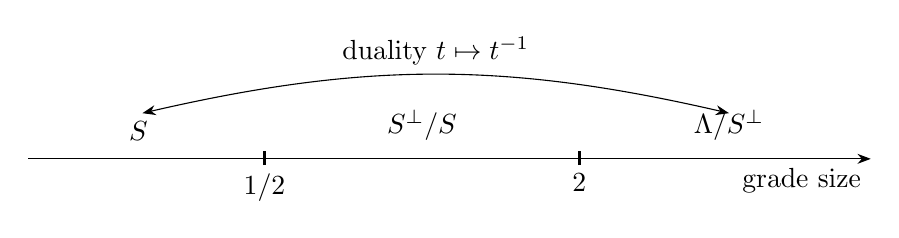
\begin{tikzpicture}[x=1cm,y=1cm,>=Stealth]
 \draw[->] (0,0)--(10.7,0) node[below left] {grade size};
 \draw[line width=.8pt] (3,-.08)--(3,.10) (7,-.08)--(7,.10);
 \node[below] at (3,-.06) {$1/2$};
 \node[below] at (7,-.06) {$2$};
 \node[above] at (1.4,.11) {$S$};
 \node[above] at (5,.11) {$S^\perp/S$};
 \node[above] at (8.9,.11) {$\Lambda/S^\perp$};
 \draw[<->] (1.45,.58) to[bend left=13]
   node[midway,above] {duality \(t\mapsto t^{-1}\)} (8.9,.58);
\end{tikzpicture}
\caption{The short filtration of Lemma~\ref{lem:canonical-short-flag}. Both boundary sizes belong to the middle quotient. The two outer groups of grades are dual.}\label{fig:short-reciprocal-grades}
\end{construction}

\proofstep{Lowering by a near element.}

The canonical filtration is intrinsic to the lattice. It constrains the difference of a near element from the identity, forcing it to lower the appropriate steps.


Suppose an integral endomorphism \(A\) of \(\Lambda\) has
operator norm at most \(\delta\) at every real place.
Let \(A_t:F(t)\to\Lambda/F(\delta t)\) be the induced map.
If its image has rank \(j>0\), pass to the saturated source
quotient \(Q_t\) and put \(I_t=(\operatorname{im}A_t)^{\rm sat}\)
in the target. The complex determinant norm is at most
\(\delta^j\) at each place. With the real squares and the
normalization of \(C\) this gives
\[
 \frac{C(I_t)}{C(Q_t)}\le\delta^{2fj},\qquad
 \operatorname{size}(I_t)\le
            \delta\operatorname{size}(Q_t)\le\delta t .
\]
Saturation accounts for the inequality on the left.
Every nonzero sublattice of the target has size strictly greater
than \(\delta t\), so \(A_t=0\).

Apply this with \(A=\gamma-I\) and the given \(0<\delta<1/4\).
The case \(\delta=0\) gives \(\gamma=I\) directly. It gives identity action
on each short grade, and the image of \(S^\perp=F(2)\)
under \(A\) lies in \(S\). Unitarity gives identity action
on the dual grades as well. Hence \(\gamma\) belongs to the
unipotent radical of the stabilizer of the short flag. If
the short flag is empty, this argument gives \(\gamma=I\).

\end{proof}

\subsection{Packing near elements on the flag blocks}

Lowering the short flag places the near elements in its unipotent radical. To count them one still needs the lattice spacing in each independent block of that radical.

\begin{lemma}[Near elements counted in the short-flag blocks]
\label{lem:near-flag-packing}
Use the grades of Lemma~\ref{lem:canonical-short-flag}.
For integral elements in the unipotent radical of the short flag
whose blocks of \(\gamma-I\) have Hilbert--Schmidt norms at
most \(\delta\) at every real place, the number is bounded by 
\[
 \prod_{v\mid\infty}\prod_{\text{free blocks at }v}(1+12\delta/\lambda)^d.
\]
 Here \(d\) is the block
dimension and
\(\lambda=\tau_i/\tau_j,\tau_i\tau_j,\tau_i,\tau_i^2\)
for the corresponding four block types in \(\mathcal L(\tau)\).
\end{lemma}

\begin{proof}
\proofstep{Induction by block distance.}

Complete the short flag by its perpendicular flag, using
the single middle block \(S^\perp/S\). Choose orthogonal
Euclidean complements at each real place, with dual blocks
paired by the unitary signature matrix. Write the resulting
blocks of \(\gamma-I\) in that order. They are strictly
upper triangular and each has Hilbert--Schmidt norm at
most \(\delta\). Count the possibilities in increasing
distance from the block diagonal. For elements agreeing on
all shorter distances, their difference maps each integral
filtration step into the step lower by the current distance.
Its blocks at that distance are therefore integral maps on
the graded lattices.

For two such elements write \(\gamma_i=1+A_i\) and
\(D=A_1-A_2\). Subtracting the two unitary identities gives
\[
      D+D^\dagger=-(D^\dagger A_1+A_2^\dagger D).
\]
The right side lowers by at least one more step, since
both \(A_i\) are strictly triangular. Thus at the current
distance the adjoint blocks in the difference are negatives
of one another's adjoints. It
suffices to count one block in each such pair and the
self-paired skew-Hermitian differences.

\proofstep{Block separation and volume packing.}

Once the successive free blocks are known, the remaining choices in each block form a separated set. This changes the problem from counting group elements to packing points in Euclidean balls.


For a nonzero difference in one block the same
kernel-to-saturated-image determinant argument bounds the
geometric mean of the operator norms below by the ratio
of the least target size to the largest source size.
For a nonzero block difference \(D\), write
\(l(D)=(\prod_v\|D_v\|_{\rm op})^{1/f}\). The resulting lower bounds are
\[
 l(D)\ge
 \begin{cases}
 \tau_i/\tau_j\ \text{or }\tau_i\tau_j,
                        &\text{the two cross blocks at }i<j,\\
 \tau_i/2,              &\text{a middle block and grade }i,\\
 \tau_i^2,              &\text{the self-paired block at }i .
 \end{cases}
\]
All the relevant Hilbert--Schmidt norms dominate the
operator norms. For an available ratio \(l\), put disjoint
product balls of radius \(l/2\) about the possible blocks
at the real places. An overlap would bound all difference
norms strictly below \(l\). In a self-paired block the
possibilities lie in an affine space with skew-Hermitian
direction, which is the space used for packing. Centering
at any one candidate bounds all radii from that center
by \(2\delta\).

If a finite subset has \(M\) candidates, translation and scaling
of product Lebesgue measure give
\[
 M(l/2)^d\operatorname{vol}(B_1)
       \le(2\delta+l/2)^d\operatorname{vol}(B_1),\qquad
 M\le(1+4\delta/l)^d ,
\]
where \(d\) includes all \(f\) places and \(B_1\) is the unit
product ball in the free block coordinates. This reasoning also
bounds an initially infinite candidate set, by applying the
volume inequality to any finite subset. Iterating through
the block distances determines the full matrices. The
dimensions of the free blocks are those in
\(\mathcal L(\tau)\) in \eqref{eq:count-flag-density-product}. Hence the number is at most
the product over those factors with \(\lambda^d\)
replaced by \((1+12\delta/\lambda)^d\), for
\(\lambda=\tau_i/\tau_j,\tau_i\tau_j,\tau_i,\tau_i^2\).
\end{proof}


\subsection{The measure of short flags}

Packing gives a bound at a fixed lattice. Its factors may grow when a grade of the flag becomes short, so the trace integral also needs the measure of lattices with those short grades.

Let \(\tau_1<\cdots<\tau_a<1/2\) be successive sizes of the
canonical short isotropic flag of Lemma~\ref{lem:canonical-short-flag}. Its layer ranks are positive
integers \(j_1,\ldots,j_a\), with \(J=\sum_i j_i\le q\).
\begin{lemma}[Measure of the short-flag region]\label{lem:short-flag-measure}
For \(q\ge1\) put \(U_0=rf\log r\). For large \(r\), let \(X_{\rm short}\) consist of the points in the quotient \(X\) with a nonempty isotropic flag of successive sizes less than \(1/2\). Its relative measure satisfies 
\[
 \frac{\operatorname{vol}(X_{\rm short})}{\operatorname{vol}(X)}\le e^{-U_0/4}.
\]

\end{lemma}

\begin{proof}
\proofstep{The modular character.}
The Levi group of its parabolic is the product of
\(\mathrm{GL}_{j_i}(E)\) and the unitary group of signature
\((p-J,q-J)\). In the logarithmic size variables the modular
character of the parabolic is the product of the determinants
on the unipotent blocks. Write this product as \(\mathcal L(\tau)\).
With \(f=[E^+:\Q]\) it is
\begin{align*}
 \mathcal L(\tau)
 &=\prod_{i<k}(\tau_i/\tau_k)^{2fj_i j_k}
               (\tau_i\tau_k)^{2fj_i j_k}\
 &\hspace{1em}\cdot\prod_i \tau_i^{2fj_i(r-2J)}
                                  (\tau_i^2)^{fj_i^2}.
\end{align*}
The two cross blocks between layers of complex dimensions
\(j_i,j_k\) each have real dimension \(2j_i j_k\) per place.
The blocks with the central quotient have real dimension
\(2j_i(r-2J)\). The skew-Hermitian block of layer \(i\) has
dimension \(j_i^2\) and scales by \(\tau_i^2\).

On the \(i\)-th layer of rank \(j_i\) use the positive determinant
coordinate \(a_i=\tau_i^{2fj_i}\). The quotient of its Haar
measure by the determinant-one gauge is \(da_i/a_i\).
The change from the determinant to the size on each layer is
\[
 \log a_i=2fj_i\log\tau_i,\qquad
 \prod_i\frac{da_i}{a_i}=\prod_i 2fj_i\frac{d\tau_i}{\tau_i}.
\]
The residual volumes below use this same decomposition.

Unfold the sum of short flags along this parabolic. The
normalized measure of any measurable set of sizes for the
given type is at most
\begin{equation}\label{eq:count-flag-density-product}
              \kappa\int\mathcal L(\tau)
                                   \prod_i \frac{2f j_i\,d\tau_i}{\tau_i}.
\end{equation}
The volume of the residual unitary quotient occurs in the
numerator of the unfolded integral. Dividing by the volume
of the original quotient replaces this factor by the inverse
of the successive unitary volume ratios. The ratios follow
from the convergent one-vector Siegel--Weil identity with
self-dual additive measures. In rank \(M\ge3\) average a
Gaussian sum over vectors of norm \(+1\) or \(-1\), using
the sign whose signature entry is positive. Witt's theorem
makes this a single orbit with stabilizer the group on
the perpendicular complement. Unfolding extracts the
volume of that rank-\((M-1)\) quotient.

On the Siegel--Weil
side the volume of the rank-\(M\) quotient multiplies
the local Gaussian densities and the Euler-product factor
\[
             d_E^{f/2}(d_E/2)^{-Mf}\mathcal L_M^{-1},
\]
where \(\mathcal L_M\) is the rank \(L\)-factor at \(M\).
The real Gaussian densities are positive for the selected
sign. The finite lattice normalization in the unfolding
contributes \(2^{Mf}\). Dividing this factor by the displayed
Euler-product factor gives the successive ratio in the common gauge,
\[
 \frac{2^{Mf}}{d_E^{f/2}(d_E/2)^{-Mf}\mathcal L_M^{-1}}
          =d_E^{f(M-1/2)}\mathcal L_M .
\]
Taking one step of each sign reduces the signature by \((1,1)\).
In the quotient of residual volume by original volume the resulting
Euler-product contribution after \(J\) pairs is
\[
 \prod_{a=0}^{J-1}(\mathcal L_{r-2a}\mathcal L_{r-2a-1})^{-1}
                 =\prod_{M=r-2J+1}^r \mathcal L_M^{-1}.
\] The general linear quotients give
\(\operatorname{Res}_{s=1}\zeta_E(s)\prod_{s=2}^{j_i}\zeta_E(s)\)
per layer. Haar gauges of the finite stabilizers and the
archimedean quotient occur in both the unfolding and the
volume ratio and cancel.

For clarity, in the resulting constant the discriminant
factor is \((d_E/2)^{-fd_N/2}\), where \(d_N\) is the sum
of the unipotent block dimensions at one place and
\(d_N\le2Jr\). The power of two is
\(2^{-f(rJ-J^2+J/2)}\). With \(S(m)=\prod_{i=1}^m
2\pi^i/(i-1)!\), the compact factor is
\[
 \left(\frac{S(p)S(q)}
              {S(p-J)S(q-J)\prod_i S(j_i)}\right)^f.
\]
The remaining factors are the general linear factors above
divided by the product of the rank \(L\)-factors at
\(r-2J+1,\ldots,r\), evaluated on the corresponding powers
of the quadratic character of \(E/E^+\).
The compact factor supplies the main saving in \(\kappa\).

For each \(p-J<i\le p\), one has \(i\ge r-2\sqrt r+1\),
and Stirling's estimate gives
\[
   \log\frac{2\pi^i}{(i-1)!}
            \le -r\log r+O(r+\sqrt r\log r)
\]
uniformly in that range. The other compact factors have
logarithms bounded above by \(O(fJ\sqrt r\log r)\), since
all their indices are at most \(\sqrt r\).

The discriminant factor costs at most \(O(fJr)\) in the
logarithm since \(d_E\ge3/2\), and the power of two is at most
one. A residue bound
\(\operatorname{Res}_{s=1}\zeta_E(s)\le
(16\log d_E)^{2f}\) follows from the unconditional degree
and discriminant bound for Dedekind zeta residues.
Since \(\log d_E\le e^r\), the residues also cost at most
\(O(fJr)\) in total. For the layer ranks \(j_i\), the Euler-product majorant gives
\[
 \sum_i\sum_{s=2}^{j_i}\log\zeta_E(s)
 \le 2f\,\#\{i\}\sum_{s\ge2}\log\zeta(s)\ll fJ .
\]
Indeed there are at most \(J\) layers, and \(\zeta(s)-1\ll2^{-s}\)
for integer \(s\ge2\).
For the reciprocal rank \(L\)-factors, the same Euler-product
bound in degree \(f\) gives \(O(fJ)\) in the logarithm.
The compact factors supply the leading negative term. Combining all
errors gives, uniformly for \(J\le q\le\sqrt r\) and large \(r\),
\[
                         \kappa\le \exp(-fJr\log r/2).
\]
\hfill\mbox{\cite{louboutin-row-count}}\label{cor:geometry-dimension-1}

\proofstep{Integration over the size variables.}

The modular character supplies powers of the relative sizes of the graded pieces. Integrating those powers determines whether the growth in the near-element count can be absorbed.

On the full simplex of sizes every factor of \(\mathcal L\)
is at most one. Keep just \(\prod_i\tau_i^{2fj_i(r-2J)}\).
When \(r-2J\ge1\), the integral in each remaining coordinate
is at most one, since
\[
 2f j_i\int_0^{1/2} t^{2fj_i(r-2J)-1}\,dt\le1 .
\]
Thus the relative measure of all nonempty short flags is
bounded by \(\sum_{J=1}^q2^{J-1}e^{-JU_0/2}\), where
\(U_0=rf\log r\). The sum is at most \(e^{-U_0/4}\) for
large \(r\). In particular the region \(\tau(x)<\tau_*<1/2\)
has this measure bound.
\end{proof}

\subsection{Absolute volume in the pointwise estimate}

The preceding estimate is relative to the total volume. The pointwise estimate in Section~\ref{sec:count-sobolev} instead uses the Haar density in Hilbert--Schmidt coordinates. To multiply the two bounds we compute the absolute quotient volume in that gauge.
\begin{lemma}[Absolute quotient volume in the local gauge]\label{lem:deep-volume-estimate}
At each real place let \(c_v\) be the reciprocal Haar density
at the origin in the Hilbert--Schmidt coordinates of
Section~\ref{sec:count-sobolev}. Use the quotient measure induced
by these Haar measures and the chosen finite measures. For \(X_0=rf d_Egb\), \(N=r^2 f\) in the stated
range (in particular \(r\ge8\), \(X_0\ge16\)),
\[
 \frac{(\prod_v c_v)V}{\operatorname{vol}(K_g)}
                 \le g^{2N}X_0^N.
\]
\end{lemma}

\begin{proof}
Use the unitary volume formula for a self-dual lattice over the
everywhere finitely unramified CM extension. If the finite stabilizer
and compact duals have volume one, the quotient volume in rank \(j\) is
\begin{equation}\label{eq:row-self-dual-mass}
  2 |D_{E^+}|^{j^2/2}
  \prod_{a=1}^j \left(\frac{(a-1)!}{(2\pi)^a}\right)^f L_a ,
\end{equation}
where \(L_a=L_{E^+}(a,\eta)\) for odd \(a\) and
\(L_a=\zeta_{E^+}(a)\) for even \(a\), with \(\eta\) the quadratic
character of \(E/E^+\). The Tamagawa number is \(2\). The local
densities at residue size \(Q\) are the orders of the corresponding
\(\mathrm{GL}_j\) or finite unitary groups divided by \(Q^{j^2}\).

If \(\eta_v=1\) at a split place and \(\eta_v=-1\) at an inert
one, both finite group order formulas read
\[
  Q^{-j^2}\#G(\mathbb F_Q)
        =\prod_{a=1}^j(1-\eta_v^{\,a}Q^{-a}).
\]
This is the inverse local Euler factor of \(\prod_{a=1}^j L_a\).
Self-duality at the unramified places supplies the smooth lattice
model, also in residue characteristic two. The real compact-dual
density is the same for the signatures compared here.
\cite{gan-yu-row-count,terakado-yu-row-count}
The volume of \(U(r)\) for the Hilbert--Schmidt metric is
\(\prod_{j=1}^r(2\pi)^j/(j-1)!\). To compute it, project to
the first column with fibre \(U(r-1)\).

At the identity a
horizontal tangent vector has first column \((ia,z)\), with
metric square \(a^2+2\|z\|^2\), while the unit sphere has
metric square \(a^2+\|z\|^2\). Thus the ratio of Hilbert--Schmidt volumes in successive ranks is
\[
 \frac{\operatorname{vol}U(r)}{\operatorname{vol}U(r-1)}
   =2^{r-1}\frac{2\pi^r}{(r-1)!}=\frac{(2\pi)^r}{(r-1)!}.
\]
Thus \(\operatorname{vol}U(r)=\prod_{j=1}^r(2\pi)^j/(j-1)!\). The passage from the compact dual
to \(U(p,q)\) multiplies the noncompact tangent directions by
\(i\), preserving their Hilbert--Schmidt measure. With the
gauge \(c_v\) defined in the Sobolev estimate, this gives
\[
  \frac{(\prod_v c_v)V}{\operatorname{vol}(K_f)}
       =2\,d_E^{r^2f/2}\prod_{j=1}^r L_j .
\]
Here the unramified CM extension has
\(|D_E|=|D_{E^+}|^2\), so \(|D_{E^+}|=d_E^f\).

The factors with \(j\ge2\) have product at most \(e^f\).
Indeed \(L_j\le\zeta(j)^f\) and
\(\sum_{j\ge2}\log\zeta(j)\le\sum_{n\ge2}1/(n(n-1))=1\).
For \(L_1=L_{E^+}(1,\eta)\), take the ratio of the
analytic class number formulas for \(E\) and \(E^+\).
The units of \(E^+\) give a sublattice in the unit lattice of
\(E\) of regulator \(2^{f-1}R_{E^+}\), since the complex
logarithmic coordinates are doubled. The regulator and the first Euler factor therefore satisfy
\[
 R_E\le2^{f-1}R_{E^+},\qquad
 L_1\le(2\pi)^f d_E^{-f/2}h_E .
\]

By Minkowski's bound every class of \(E\) has an ideal of
norm at most \(d_E^f=\sqrt{|D_E|}\). The ideal count up to
\(T\) is at most \(T(1+\log T)^{2f-1}\), by majorizing the
Euler coefficients by those of \(\zeta(s)^{2f}\) and
summing over the \(2f\) divisor factors. Hence
\[
 L_1\le (2\pi)^f d_E^{f/2}(1+f\log d_E)^{2f}.
\]
Put \(X_0=rf d_E g b\) and \(N=r^2 f\).

Since
\(1+f\log d_E\le f d_E\) and \(X_0\ge16\), the bound for
the quotient divided by \(\operatorname{vol}(K_f)\) is at most
\(X_0^{N/2+9f/2}\le X_0^N\) for \(r\ge8\).
Reduction at level \(g\) embeds \(K_f/K_g\) into the
endomorphisms of the rank-\(r\) lattice modulo \(g\).
There are \(g^{2fr^2}\) such endomorphisms, also for a projective
lattice by its local rank. It follows that
\[
   \frac{(\prod_v c_v)V}{\operatorname{vol}(K_g)}
                        \le g^{2N}X_0^N .
\]
This is the absolute bound used in the deep part of the
diagonal estimate.
\end{proof}

\subsection{Covering the short unipotent orbit}\label{sec:count-orbit}

In a deep part of the quotient, the lattice filtration has a large gap. The unipotent radical attached to this gap has a small set of representatives modulo its rational points, which allows cuspidality to control the value of a form.

\begin{proposition}[Covering in the chosen short flag]\label{prop:short-orbit-cover}
In Definition~\ref{hyp:cuspidal-dimension}, take \(q\ge1\) and suppose the smallest size \(\tau(x)\) in the canonical lattice filtration is less than \(1/2\). From the filtration in
Lemma~\ref{lem:canonical-short-flag} choose a step with consecutive
size ratio \(u\le(2\tau(x))^{1/q}\). Modulo its rational lattice
stabilizer and the finite level, the short unipotent orbit admits
representatives \(\exp A\exp Y\) in the real coordinates at \(x\),
where
\[
    \|A\|+\|Y\|\le \rho,\qquad
    \rho=\tfrac14 r^2\sqrt f\,g d_E(2\tau(x))^{1/q}.
\]
\end{proposition}

\begin{proof}
\proofstep{Choose a step by the product of ratios.}

Let \(\tau=t_1<t_2<\cdots<t_a<1/2\) be the short sizes
from Lemma~\ref{lem:canonical-short-flag} and put \(t_{a+1}=1/2\).
There are \(a\le q\) ratios since the sum of the short ranks
is at most \(q\). Then
\[
 \prod_{i=1}^a t_i/t_{i+1}=2\tau,\qquad
 \min_i t_i/t_{i+1}\le(2\tau)^{1/a}\le(2\tau)^{1/q}.
\]
Use a pair \(t,t'\) attaining one such ratio \(u\).
Let \(S\) be the saturated isotropic step ending at \(t\),
of rank \(j\). For the middle block \(Z=S^\perp/S\), the extreme sizes are
\[
 t_{\max}(S)=t,\qquad t_{\min}(Z)\ge t',\qquad t_{\min}(S^\vee)=1/t ,
\]
where the inequality for the middle block is needed only when it is nonzero.

\proofstep{Integral Witt coordinates and congruence lattices.}

Use an integral Witt splitting
\(\Lambda=S\oplus Z\oplus S^\vee\).
To obtain it, extend functionals on the saturated summand
\(S\) to \(\Lambda\) and use self-duality to identify
\(\Lambda/S^\perp\) with \(S^\vee\).
Choose a section by projectivity. Its Hermitian form can
be killed by subtracting an \(S\)-valued correction,
since the pairing between \(S\) and this section is perfect.
In detail, choose an integral scalar \(\theta\) with
\(\theta+\bar\theta=1\). It exists since the trace of the
unramified quadratic integral extension is surjective at
each prime, and so globally. Use a correction whose pairing
with the section is \(\theta\) times that section's form.
Indeed, if \(H_0\) is the Hermitian form of the section, the two
cross terms sum to
\[
                  \theta H_0+\bar\theta H_0=H_0 .
\]
Take the orthogonal complement of the resulting hyperbolic
pair to split off \(Z\).

The radical of the stabilizer of \(S\) has a two-step
Lie algebra with coordinates \(X:Z\longrightarrow S\)
and \(Y:S^\vee\longrightarrow S\), where \(Y\) is
skew-Hermitian. The other first-layer block is
\(-X^\dagger\). At the real places use the orthogonal Witt
coordinates. Two such splittings inducing the same maps on
the graded spaces differ by an element of the radical, as
their change of splitting is unitary, block triangular and
the identity on the graded spaces. Conjugation by it acts
trivially on the first-layer quotient and on the center.
Thus the congruence lattice supplies \(2g\operatorname{Hom}(Z,S)\)
in the first block.

For the first layer in the integral splitting, write
\[
 A_X=\begin{pmatrix}0&X&0\\0&0&-X^\dagger\\0&0&0\end{pmatrix},
 \qquad
 \exp(A_X)=
 \begin{pmatrix}1&X&-XX^\dagger/2\\
                 0&1&-X^\dagger\\0&0&1\end{pmatrix}.
\]
For \(X\in2g\operatorname{Hom}(Z,S)\) every off-diagonal
entry is integral and divisible by \(g\). In particular, writing
\(X=2gX_0\) makes the central entry
\[
 -XX^\dagger/2=-2g^2X_0X_0^\dagger
                   \in g\operatorname{Hom}(S^\vee,S).
\]
The center supplies \(g\) times the skew-Hermitian sublattice
of \(\operatorname{Hom}(S^\vee,S)\).

\proofstep{Dual minima of the two coordinate lattices.}

Here are the covering bounds for these lattices. In the
product Hilbert--Schmidt norm the Euclidean dual of
\(\operatorname{Hom}(Z,S)\) identifies with
\(2\mathfrak D_E^{-1}\operatorname{Hom}(S,Z)\), where
\(\mathfrak D_E\) is the absolute different. This follows
from the matrix trace pairing on projective modules and
the factor 2 relating field trace and the real product
pairing over the complex places. Multiplication of a
lattice by the codifferent multiplies every filtration
size by \(d_E^{-1}\), from its ideal norm and the same
exterior-volume normalization. The determinant comparison
for nonzero maps therefore bounds the geometric mean of
the local norms of a nonzero dual matrix below by
\(2d_E^{-1}t'/t\). For a nonzero vector \(B\) in this dual, the quadratic and
geometric means give
\[
 \Big(\sum_v\|B_v\|_{\rm HS}^2\Big)^{1/2}
 \ge\sqrt f\Big(\prod_v\|B_v\|_{\rm HS}\Big)^{1/f}
 \ge 2\sqrt f\,d_E^{-1}t'/t .
\] The first-layer lattice has
real dimension \(2fj(r-2j)\).

For the center, the skew-Hermitian sublattice is primitive
in the full matrix lattice. An integer functional on it
extends to the full lattice, so its Euclidean dual is the
orthogonal skew projection of the full dual. The projection \(B\mapsto (B-B^\dagger)/2\) places the dual of the
central lattice in \(\mathfrak D_E^{-1}\operatorname{Hom}(S,S^\vee)\).
The extreme sizes of \(S\) and its dual thus give
\[
                  \|B\|\ge \sqrt f\,d_E^{-1}/t^2
                         \qquad(B\ne0\text{ in the dual}).
\] The center has real dimension
\(fj^2\).

\proofstep{Cover each layer by transference.}

The dual minimum bounds give a covering radius in each additive layer. Combining these coverings must respect the order of the unipotent extension.


For a full Euclidean lattice of dimension \(d\), its
covering radius times the length of the shortest nonzero
dual vector is at most \(d/2\)
\cite[Theorem~2.2]{banaszczyk}. Apply this to the two
computed dual minima. Including the level \(2g\) in the
first layer and both its adjoint blocks, its radius is at most
\[
 \sqrt2\,(2g)\frac{j(r-2j)\sqrt f\,d_E}{2}\frac{t}{t'}
        \le\frac{r^2\sqrt f\,g d_E}{4\sqrt2}\frac{t}{t'} .
\]
In the center, including level \(g\), the radius is at most
\[
        \frac{g j^2\sqrt f\,d_E}{2}t^2
        \le\frac{r^2\sqrt f\,g d_E}{32}\frac{t}{t'} ,
\]
using \(t t'\le1/4\). First reduce the first block by an
integral congruence lift, then reduce the resulting center,
which already includes the commutator correction.
The two displayed radii can be added after this central correction.
For the gap \(t/t'\le(2\tau)^{1/q}\) this gives
\[
 \|A\|+\|Y\|\le r^2\sqrt f\,g d_E\frac{t}{t'}
       \left(\frac{1}{4\sqrt2}+\frac1{32}\right)
 \le \frac{r^2\sqrt f\,g d_E}{4}(2\tau)^{1/q}=:\rho .
\]

The radical is two-step with vector-group center and
vector-group quotient. Additive approximation at the
finite adeles in these two groups shows that each class
on its adelic orbit modulo the finite level has a real
representative. Apply the real covering just proved to
that representative. A rational left correction from
the lattice stabilizer at level \(g\) gives only a right
level translate at the point, so the value of each projected
function is unchanged. After conjugating into the real
coordinates at \(x\), the representative acts by a product
\(\exp A\exp Y\) with \(\|A\|+\|Y\|\le\rho\).
\end{proof}


\subsection{Bounds for the diagonal integral}

The diagonal is estimated separately where the smallest lattice size stays above the cutoff and where it falls below. In the latter region the covering of the short unipotent orbit is used before integration.

Write \(X_0=rf d_E g b\), \(N=r^2f\), \(\tau_*=X_0^{-11q}\).
The lattice size function \(\tau(x)\) is the threshold for its
first nonzero short layer. The portion \(\tau(x)\ge\tau_*\)
allows a uniform lattice point bound for the orbital expansion.
Write \(U_0=rf\log r\).
\begin{construction}
\begin{tabular}{@{}lll@{}}
\toprule
Region & Quantity controlled & Bound \\
\midrule
\(\tau(x)\ge\tau_*\) & integrated nonidentity terms &
       \((e^{-N}+e^{-U_0/4})D_*\)\\
\(\tau(x)<\tau_*\) & relative measure & \(e^{-U_0/4}\)\\
\(\tau(x)<\tau_*\) & integral for \(n\) orthonormal vectors & \(e^{-N}n\)\\
\bottomrule
\end{tabular}
\caption{Two estimates on the same quotient for \(q\ge1\) in Lemma~\ref{lem:diagonal-integral-bounds}. The final row uses an arbitrary finite family before taking the full trace.}\label{fig:two-trace-regions}
\end{construction}

\begin{lemma}[Bounds for the diagonal integral]\label{lem:diagonal-integral-bounds}
Suppose \(q\ge1\). If \(X\) is the quotient and \(X_{<}=\{x:\tau(x)<\tau_*\}\), the short-vector locus satisfies 
\[
 \frac{\operatorname{vol}(X_{<})}{\operatorname{vol}(X)}\le e^{-U_0/4}.
\]
 On its complement the integrated
absolute nonidentity terms are at most
\((e^{-N}+e^{-U_0/4})D_*\). On \(\tau(x)<\tau_*\) the integral of
the sum of squared values of any finite orthonormal family of
projected vectors is at most \(e^{-N}\) times the size of that family.
\end{lemma}

\begin{proof}
The measure estimate is Lemma~\ref{lem:short-flag-measure}.
\proofstep{Moderate region outside the polar threshold.}
  The point count for each archimedean shell has lattice factor
  at most \((3\sqrt r/\tau_*^2)^{2N}\).
  For two supported rational matrices their difference
  preserves the point lattice as an endomorphism. Thus two distinct supported matrices \(\gamma,\gamma'\) give a nonzero integral endomorphism \(T=\gamma-\gamma'\). The separation needed for packing is 
\[
 \left(\prod_v\|T_v\|_{\rm op}\right)^{1/f}\ge\tau_1(x)^2,\qquad \tau_1(x)=\min\{1/2,\tau(x)\},
\]
 with one representative from each complex-conjugate pair.
  In the size inequality for a nonzero lattice map, take
  the saturated quotient by the kernel and the saturated
  image. The determinant on the induced quotient has
  local norm at most the corresponding power of the
  operator norm. Write \(\Lambda_Q,\Lambda_I\) for the saturated quotient by
  the kernel and the saturated image. If their common rank
  is \(j\), the determinant inequality reads
  \[
   \operatorname{size}(\Lambda_I)
   \le \operatorname{size}(\Lambda_Q)
             \left(\prod_v\|A_v\|_{\rm op}\right)^{1/f}.
  \]

This follows by raising to \(2fj\), using the square of the
  complex determinant at each place, and allowing the index
  of the image in its saturation. The smallest size
  bounds \(\operatorname{size}(\Lambda_I)\) below and its
  reciprocal bounds \(\operatorname{size}(\Lambda_Q)\) above
  by self-duality. Their ratio is at least \(\tau_1(x)^2\).
  If the local containing balls have radii \(R_v\) of
  geometric mean \(R\), use product balls of radii
  \(\tau_1(x)^2 R_v/(2R)\) about the lattice points.
  The separation makes these product balls disjoint. Bounding their
total volume by that of the enlarged box gives
\[
    \#\{\text{points in the product ball}\}
       \le (1+2R/\tau_1(x)^2)^{2N}.
\]
  A noncompact distance at most \(u_v\) gives
  \(R_v\le\sqrt r\exp(u_v)\) by polar decomposition.
  Let \(\bar u=f^{-1}\sum_v u_v\). Since \(R\le\sqrt r e^{\bar u}\)
and \(\tau_1(x)\ge\tau_*\), the packing estimate gives
\[
 (1+2R/\tau_1(x)^2)^{2N}
 \le(1+2\sqrt r/\tau_*^2)^{2N}\exp(2r^2\textstyle\sum_v u_v).
\]

The large-gap matrix coefficient bound supplies a factor
  \(2f\,3^f\exp(-h\epsilon_N^2/16)\), which absorbs this
  lattice factor and \(e^N\). To see the shell sum put
  \(\epsilon=\epsilon_N\), \(c=\sqrt{2q}\) and \(B=2r^2\).
  If the noncompact distances at the places are bounded
  by \(u_v\), the lattice count is at most the lattice
  factor times \(\exp(B\sum_v u_v)\).
  For local noncompact distances \(s_v\), \eqref{eq:count-polar-decay}
bounds the coefficient relative to its identity value by
\[
 \prod_v\exp[-(h/8)\min(s_v^2,s_v/c)]
       =\exp[-(h/8)\textstyle\sum_v\min(s_v^2,s_v/c)] .
\]
This product permits a separate partition at each real place.
  Partition each distance into \([0,\epsilon]\) and
  \((2^{j-1}\epsilon,2^j\epsilon]\) for \(j\ge1\).
  For \(s_v\in[0,\epsilon]\) the counting factor costs at most
\(e^{B\epsilon}\le2\).

For \(u\le s_v\le2u\) the two competing
factors are bounded by
\[
 e^{Bs_v}\exp[-(h/8)\min(s_v^2,s_v/c)]
 \le \exp[2Bu-(h/8)\min(u^2,u/c)] .
\] For the
  bin with lower endpoint \(u=2^{j-1}\epsilon\), use
  \(\epsilon\le1/c\) and \(32B\le h\epsilon\) to get
  \[
   2Bu-\tfrac h8\min(u^2,u/c)\le-hu\epsilon/16,\qquad
   \sum_{j\ge1}e^{-h2^{j-1}\epsilon^2/16}
                         \le2e^{-h\epsilon^2/16}.
  \]
  Here \(h\epsilon^2/16\ge1\). Each coordinate costs at most
  \(3\) in total, and at least one must lie outside its first bin.
  Summing over that choice costs at most
  \(2f\,3^f e^{-h\epsilon^2/16}\). 

The lower bound supplied by the spectral gap and the logarithm of the lattice-counting factor are
  \[
    h\epsilon_N^2/16\ge50(C_g+4)r^3 f\log(bd_E),\qquad
    \log(\text{lattice factor})=2N(\log(3\sqrt r)+22q\log X_0).
  \]
  Here \(q\log X_0\le r+\sqrt r[\log r+
  (C_g+1)\log b+\log d_E]\). With \(b\ge2\) and
  \(d_E\ge3/2\), the spectral-gap bound absorbs this logarithm,
  \(N\) and \(\log(2f3^f)\), uniformly for large \(r\)
  at fixed \(C_g\).
\proofstep{Near unipotent terms in the moderate region.}
  Lemma~\ref{lem:small-unipotent} identifies the terms within the
  polar threshold as unipotent. Use Lemma~\ref{lem:near-flag-packing}
  to group the nonidentity terms by the ranks of the short flag. A type with \(a\) nonzero layers of
  total rank \(J\le q\) contributes at most
  \(2\kappa Y^a D_*\), where
  \(\kappa\le e^{-JU_0/2}\) and
  \(Y=2fq\log(1/\tau_*)\le e^{U_0/8}\).
  There are at most \(J\) layers, so its bound is
\[
 2\kappa Y^a D_*\le 2e^{(-J/2+a/8)U_0}D_*
              \le 2e^{-3JU_0/8}D_* .
\]
  The near count uses the same unipotent blocks as the
  measure. In a block of size parameter \(\lambda\) the count
  contributes \((1+12\epsilon/\lambda)^{d}\), where \(d\)
  is its real dimension and
  \(\epsilon=3\sqrt{r\epsilon_N}\). This is the lattice
  ball bound with radius \(\epsilon\) in the block gauge.
  Multiplying by the density changes each such factor to
  \((\lambda+12\epsilon)^d\).

Since \(\lambda\le1\) in each factor and \(\sum d\le3Jrf\), one has
\[
       \prod (\lambda+12\epsilon)^d
            \le\exp(12\epsilon\textstyle\sum d)
            \le e^{36Jrf\epsilon}\le2
\]
for sufficiently large \(r\).
  Integrating the remaining product of \(2fj_i\,d\tau_i/\tau_i\)
  from \(\tau_*\) to \(1/2\) in every coordinate costs at most
  \(Y^a\).
  A composition of \(J\) is determined by the cuts among its
\(J-1\) gaps. The total near contribution is bounded by
\[
  D_*\sum_{J=1}^q2^{J-1}\,2e^{-3JU_0/8}
      \le 2^{q+1}e^{-3U_0/8}D_* .
\] As \(q\le\sqrt r\), the near
  terms together contribute at most \(e^{-U_0/4}D_*\) for
  large \(r\).
\proofstep{Orthonormal families in the deep region.}

Deep in the quotient the short unipotent orbit bounds a whole orthonormal family by cuspidality.

  Use the fixed radius \(\rho\) from Proposition~\ref{prop:short-orbit-cover}
  at the point \(x\), and use the neighborhood of points
  \(x\exp(A)\exp(Y)\) of total coordinate norm at most \(\rho\).
  The deep threshold gives \(\rho\le\log2\), so the lattice
  size bound on this neighborhood is \(\tau(x)/2\).
  Write \(M_P\) for the supremum of the evaluation vector's
  norm on this neighborhood for unit vectors in the word
  space of order \(P\). Along each exponential segment the
  derivative inserts one infinitesimal action. The sum of
  the real-place derivative norms is at most \(\sqrt f B\)
  times the product norm of the direction, for
  \[
    B=\sqrt r\,b^2+\tfrac32 r^{3/2}+3(8qN+N).
  \]
  Each orbit representative is connected to \(x\) by two such
  segments of total length at most \(\rho\) within the
  neighborhood.

Let \(F_u(y)\) be the vector of evaluations of the family
  on a unit test vector \(u\) of order \(P\).
  Normalize the unipotent quotient measure to mass one and use
  cuspidality to write
  \[
    F_u(x)=\int_{[N]}\bigl(F_u(x)-F_u(nx)\bigr)\,dn .
  \]
  The real representatives from the orbit cover give the
  same values as \(nx\), by rational invariance and the finite
  level. At each representative the integral along the two
  exponential paths bounds the norm of the difference by
  \(\rho\sqrt f B M_{P+1}\). The same bound follows for
  \(F_u(x)\) after integration.

For any other point in the neighborhood the same segment
  estimate compares its value to the value at \(x\). The two comparisons give the recurrence on a single neighborhood
\[
             M_P\le2\rho\sqrt f B\,M_{P+1}\qquad(P<8qN).
\]
  The initial Sobolev estimate in Section~\ref{sec:count-sobolev}
  at order \(8qN\) gives the
  squared factor \((6B)^N e^f(17\sqrt r/\tau^2)^{2N}\)
  times the size of the family and the ratio of the archimedean gauge to the
  finite level volume. With \(K=2\rho\sqrt f B\), iterate the preceding inequality
on the same neighborhood to obtain
\[
 M_0^2\le K^{2j}M_j^2 \quad(0\le j\le8qN),\qquad
 M_0^2\le K^{16qN}M_{8qN}^2 .
\]
  In the same gauge the quotient volume is at most
  \(g^{2N}X_0^N\) times the reciprocal of that ratio.

  To check the resulting exponent, \(B\le X_0^4\) follows
  from \(q^2\le r\), \(b\ge2\), and \(X_0\ge16\).
  Then \(2\rho\sqrt f B\le X_0^6(2\tau)^{1/q}\).
  On taking the \(N\)-th root the initial bound and absolute
  volume give the factor
  \(6e\,17^2 B r\,\tau^{-4}g^2X_0\), with the gauge
  canceled. The descent gives the additional factor
  \((2\rho\sqrt f B)^{16q}\le
  X_0^{96q}(2\tau)^{16}\). Since \(B\le X_0^4\) and
  \(r g^2 X_0\le X_0^4\), their product is at most
  \[
     6e\cdot17^2\cdot 2^{16}X_0^{96q+8}\tau^{12}
       \le 6e\cdot17^2\cdot 2^{16}X_0^{-28}
       \le e^{-1}.
  \]
  In the first inequality use \(\tau\le X_0^{-11q}\).
  This gives the claimed diagonal integral.
\end{proof}

\subsection{Finite rank and the integral of the kernel}

Up to this point the estimates apply to every finite orthonormal family. Their uniformity now allows one to deduce finite rank and identify the integral of the diagonal with the dimension.

\begin{proof}[Proof of Proposition~\ref{prop:projector-dimension}]
\proofstep{Finite rank before taking a trace.}
The volume \(V\) is finite by Lemma~\ref{lem:deep-volume-estimate}. For
\(q\ge1\), apply the initial Sobolev bound at order zero on
\(\tau(x)\ge\tau_*\). For \(q=0\), the flag below size \(1/2\)
is empty by isotropy, so the same bound is uniform on the whole
quotient. In either case the bound gives one finite constant
\(C_2\) for the squared pointwise value of the unit lowest vector
under any isometric intertwiner on that region.

For an orthonormal family \(F_i=T_i(w)\), Schur's lemma and
evaluation on the unit vector \(w\) give \(T_i^*T_j=\delta_{ij}I\).
Put \(S(x)=\sum_{i=1}^m |F_i(x)|^2\). If \(S(x)>0\), the operator
\[
 T=\frac{\sum_i\overline{F_i(x)}T_i}{\sqrt{S(x)}}
 \quad\text{satisfies}\quad T^*T=I,\qquad T(w)(x)=\sqrt{S(x)} .
\]
The same pointwise bound therefore gives \(S(x)\le C_2\), also
when \(S(x)=0\). Integrate and apply
Lemma~\ref{lem:diagonal-integral-bounds} in the deep region:
\[
 \int S=m\le
 \begin{cases}C_2V+e^{-N}m,&q\ge1,\\ C_2V,&q=0.\end{cases}
\]
Every finite orthonormal family has bounded cardinality, so the
projection has finite rank.

\proofstep{Integration of the finite-rank kernel.}

Finite rank justifies computing the trace in an orthonormal basis. Its integral must still be identified with the estimate already obtained from periodization.

Now take an orthonormal basis \(F_1,\ldots,F_D\).
The integral kernel of this orthogonal projection is
\[
 K(x,y)=\sum_{j=1}^D F_j(x)\overline{F_j(y)}.
\]

Both this kernel and the periodized kernel are continuous
and represent the same bounded operator, so they agree
pointwise, as can be checked by testing on compactly supported
functions in the two variables. The integral of their diagonal
over \(Y\) is \(D\). For \(q=0\) the diagonal has only its
identity orbital term, giving \(D=D_*\).

For \(q\ge1\), the deep bound is now \(e^{-N}D\).
The identity has coefficient \(e(1)\) by Lemma~\ref{lem:finite-projector-mass}, and contributes \(D_*\) times the relative measure
of the moderate portion. The other moderate terms and the
deep contribution therefore give
\[
       \abs{D-D_*}
       \le (2e^{-U_0/4}+e^{-N})D_*+e^{-N}D .
\]
Write \(A=e^{-U_0/4}\) and \(B_1=e^{-N}\). Since
\(D\le D_*+\abs{D-D_*}\), move the last error to the left to
obtain \(\abs{D-D_*}\le 2(A+B_1)D_* /(1-B_1)\).
For large \(r\) this is at most \(8e^{-U_0/4}D_*\) and then
at most \(e^{-U_0/16}D_*\). All the thresholds used here
depend only on the fixed constants in the counting hypotheses.
This proves \eqref{eq:dimension-count}.
\end{proof}

\section{The full Gram estimate on the selected row}
\label{sec:selected-row-gram}

A large period image in each column would still allow the images of different columns to coincide. On the chosen row, unfolding separates the identity term from the orbital terms. Comparing the latter with the common cuspidal dimension bounds both individual kernels and the overlap of distinct images. These are the two inputs
to the rank lemma in Section~\ref{sec:frames}. The final
calculations identify the column dimension at its assigned
prime and center the exponents on their full support. The operators \(K_{uv}\) in Definition~\ref{hyp:full-gram-row} compare columns \(v\) and \(u\) through their common period space. Proposition~\ref{prop:gram-unfolded-measures} computes each relative translate with those quotient measures. For the mixed Fourier terms Lemma~\ref{hyp:selected-orbital-coefficient-bounds} supplies the differentiated local coefficients in the common compact frames.

\begin{paramdefinition}[Realized row and its measures]\label{hyp:full-gram-row}
Fix the target character and weights. Use the realized row at a
retained translate and the marked word columns of
Proposition~\ref{prop:level-zero-column-coordinates}, with the
assigned primes of Proposition~\ref{prop:assigned-prime}. At a point of scale \(x\) write \(L=x^\epsilon\) and
\(b=e^L\). The positive definite part of the row has rank \(k\), the
row group has rank \(r=k+m-1\), and there are \(f\) real places.
Use \(d_u\) for the dimension of the full column of the word \(u\).

Let \(C_u\) be the full column Hilbert space of word \(u\) and \(\mathcal H\) the full row at the fixed point. The period maps and their cross products have types 
\[
 P_u:C_u\longrightarrow\mathcal H,\qquad P_u^*P_v:C_v\longrightarrow C_u.
\]
 Write \(c_u\) for the unfolding constant of \(P_u\). With the row and column
realizations fixed, put
\[
 K_{uv}=(c_uc_v)^{-1/2}P_u^*P_v,\qquad
 K''_{uv}=\sum_{\substack{t:\,G_t=0\\ t\text{ outside the identity part}}}
                      a_{uv}(t),\qquad
 \theta_{uv}=d_ud_v/D_* .
\]
Write \(K_2\) for the finite character level and let
\(\operatorname{vol}(N_u)\) be the real unipotent
fundamental-domain volume. Let \(H_u\) be the compact definite
stabilizer and \(V_u\) its column type. Define the normalization
\(c_u\) by
\[
  c_u=\frac{\operatorname{vol}(K_2)
              \operatorname{vol}(N_u)
              \operatorname{vol}(H_u)}{\dim V_u}.
\]
\end{paramdefinition}
In the preliminary diagonal statement the inverse power at zero is defined to be zero.
The sum is in the Hilbert space of Hilbert--Schmidt operators.
The absolutely convergent unfolding gives \(K_{uv}=\sum_t a_{uv}(t)\).
The identity part is \(I\) for equal words and vanishes for distinct
words. The term \(K''\) contains the nonidentity degenerate terms.
This uses the quotient measures on the actual flags, with the
definite class masses of Section~\ref{sec:flag-counts}. The concrete
column and row isometries intertwine the local character,
term bijection, period maps and Haar factors. They identify the
concrete scale \(d_ud_v/D_*\) with the scale of the arithmetic
comparison. Conjugating the entire calculation by these isometries
preserves absolutely convergent sums, identities and their
Hilbert--Schmidt norms. \label{cor:selected-row-gram-1}

\subsection{Unfolding in the chosen measures}

To recognize the identity operator in the diagonal block, we must know the coefficient and phase of each unfolded term. They depend on the finite character and the intersection of the two real period lattices.

\begin{proposition}[Character and measure in the unfolded term]
\label{prop:gram-unfolded-measures}
Use the word sections and quotient measures of
Definition~\ref{hyp:full-gram-row}. At each noncompact real place
use the gap \(h/(8\sqrt{2q})>6r^2\) supplied by
Definition~\ref{hyp:cuspidal-dimension}, where \(q\) is the smaller
signature rank. Write \(\chi_2^{-1}\)
for the value on \(K_2\) of the normalized level function in a word
section, with the first factor conjugated in the pairing.

For representatives \(h_\rho,h_{\rho'}\),
frame translates \(x_u,x_v\), and rational element \(\gamma\), put
\[
 t_f=(h_\rho x_u)^{-1}\gamma_f(h_{\rho'}x_v).
\]
The finite integral of the unfolded term is 
\[
 I_f(t_f)=\begin{cases}\operatorname{vol}(K_2)\chi_2(t_f),&t_f\in K_2,\\ 0,&t_f\notin K_2.\end{cases}
\]
 At infinity let \(F_u,F_v\) carry the two word frames into the ambient real space, and let \(\Lambda_u,\Lambda_v\) be the lattice unipotents in those frames. In the first frame the relative translate and the lattice defining the integration quotient are 
\[
 s_\infty=F_u^{-1}\gamma_\infty F_v,\qquad \widetilde\Lambda_v=s_\infty\Lambda_v s_\infty^{-1},\qquad \Lambda_{\gamma,u,v}:=\Lambda_u\cap\widetilde\Lambda_v.
\]
 The finite and real additive phases change by reciprocal scalars, so their product is defined on the double coset.
\end{proposition}

\begin{proof}
Use the lattice representatives of Section~\ref{subsec:selected-column-metric}.
Unfold the two sums against one another and group the finite terms by
the word representatives. Strong approximation on the additive
coordinates of the unipotent identifies the resulting finite classes.
The two translated level functions have overlapping support precisely
when their relative argument lies in \(K_2\). Write \(a=h_\rho x_u\) and \(b=\gamma_f h_{\rho'}x_v\).
If \(t_f=a^{-1}b\in K_2\), a point of the overlap is \(ak\)
with \(k\in K_2\). Unitarity gives
\[
 \overline{\chi_2(k)^{-1}}\,\chi_2(t_f^{-1}k)^{-1}
       =\chi_2(t_f).
\]
Haar invariance now gives the finite integral
\[
 I_f(t_f)=
 \begin{cases}
    \chi_2(t_f)\displaystyle\int_{K_2} dk,&t_f\in K_2,\\
    0,&t_f\notin K_2 .
 \end{cases}
\]

At infinity, tile by the same double cosets. In the frame of the first word let \(\Lambda_u\) and
\(\widetilde\Lambda_v\) denote the first lattice unipotent and
the transported second one. The identifications within a tile are
exactly the translations in \(\Lambda_u\cap\widetilde\Lambda_v\).
Pair the first Bessel vector with the relative real translate of the
second using this quotient measure. The full marked level is neat. A middle lattice
with stabilizer \(\Delta\) still has weight \(1/|\Delta|\) in the row
norm. Under a change of rational representative, let \(\xi\) denote
the change in the finite additive phase. The trace character is
trivial on rational arguments, so the corresponding changes satisfy
\[
 \frac{\text{new finite phase}}{\text{old finite phase}}=\xi,
 \qquad
 \frac{\text{new real phase}}{\text{old real phase}}=\xi^{-1}.
\]
This proves invariance of the product.

It remains to justify the unfolding. At a noncompact real place,
let \(R\) be the polar radius and \(q\) the smaller signature rank.
For the shell \(n\le R<n+1\), ball growth, the slab weight, and
\eqref{eq:count-polar-decay} bound the weighted coefficient integral,
for all sufficiently large integers \(n\), by a constant times
\[
 (1+n)^q
 \exp\!\left[-\left(\frac{h}{8\sqrt{2q}}-2r^2-4r^2\right)n\right].
\]
The exponent in parentheses is positive by the gap in
Section~\ref{sec:count}. The shell bounds are summable, and a compact real factor has
finite volume. A fixed real translate changes polar length by at most
an additive constant, by the triangle inequality for the polar
distance. Proposition~\ref{prop:gram-absolute-slab} below applies
this weighted estimate to the two period seeds and justifies
regrouping the unfolded terms. \cite{companion-row-count}\label{cor:selected-row-gram-2}

\end{proof}

\begin{construction}
\begin{tabular}{@{}lll@{}}
\toprule
 & Overlap or change of variable & Contribution \\
\midrule
finite, \(t_f\notin K_2\) & disjoint level cosets & \(0\) \\
finite, \(t_f\in K_2\) & one level coset & \(\operatorname{vol}(K_2)\chi_2(t_f)\) \\
change of representative & finite additive phase & \(\xi\) \\
                          & real additive phase   & \(\xi^{-1}\) \\
\bottomrule
\end{tabular}
\caption{The factors in Proposition~\ref{prop:gram-unfolded-measures}. The first level function is conjugated in the pairing. The changes of additive phase cancel for a rational change of representative.}\label{fig:gram-local-phases}
\end{construction}

\subsubsection{Absolute convergence on the finite slabs}

The phase calculation gives a term for every rational relative position. Interchanging the sum of these terms with the period integrals requires absolute convergence, which can first be proved on bounded slabs.

\begin{proposition}[Absolute unfolding on a finite slab]\label{prop:gram-absolute-slab}
Take two scalar test functions from the columns on the marked row of Definition~\ref{hyp:full-gram-row}.
Assume at each noncompact real place that
\(h/(8\sqrt{2q})>6r^2\) in \eqref{eq:count-polar-decay}, where
\(q\) is the smaller signature rank. Write \(I\) for the unfolded pairing integrand and \(d\mu\) for the real quotient measures. Then 
\[
 \int_{\mathcal S}|I|\,d\mu<\infty\qquad(\mathcal S\text{ any finite slab}).
\]
 Thus the complex pairing may be
unfolded and regrouped.
\end{proposition}

\begin{proof}
\proofstep{A lattice multiplicity majorant.}

Put \(G=G(\mathbb A_F)\), \(\Gamma=G(F)\), and write \(p,p'\)
for two scalar seeds from the column spaces.
For a compact set \(U_0\subset G\) containing the identity put
\[
 M_{U_0}(x)=\sup_{y\in G}\#\{\delta\in\Gamma:\delta y\in xU_0\}.
\]
This function is left \(\Gamma\)-invariant. Enlarge \(U_0\) by left
multiplication by the finite level \(K_2\), so that it is also invariant
under right multiplication of \(x\) by \(K_2\). For a nonempty fibre choose \(\delta_0\) in it. Then
\[
 \delta\longmapsto\delta\delta_0^{-1}\in
       \Gamma\cap xU_0U_0^{-1}x^{-1},\qquad
 M_{U_0}(x)\le C(x):=\#(\Gamma\cap xU_0U_0^{-1}x^{-1}).
\]
The measurable majorant \(C(x)\) has the same invariances.

On a finite slab \(x=(g,a_\rho k)\), put \(L(g)=\prod_v\|g_v\|_{\rm op}\)
in signature coordinates. The majorant is \(O(L(g)^{4r^2})\).
Indeed the finite matrix entries of the rational elements being counted
belong to a common fractional ideal \(\mathfrak a\) by compactness. After changing
to a fixed rational basis, each archimedean coordinate at \(v\) is
bounded by \(C_v\|g_v\|_{\rm op}^2\), since \(g_v^{-1}=J_vg_v^*J_v\)
for the signature matrix \(J_v\) and \(\|g_v\|_{\rm op}\ge1\).

For a fundamental parallelotope \(P\) of the fractional ideal let
\(B(\mathbf R)\) be the product of complex discs of radii \(R_v\ge1\).
The disjoint translates of \(P\) centered at the lattice points give
\[
 \#(\mathfrak a\cap B(\mathbf R))\operatorname{vol}(P)
 \le \operatorname{vol}(B(\mathbf R)+P)
 \le \prod_v\pi(R_v+D_v)^2\ll_{\mathfrak a}\prod_v R_v^2 ,
\]
where \(D_v\) bounds the radius of the projection of \(P\) at \(v\).
The rational matrix is determined
by its \(r^2\) entries. Taking \(R_v=C_v\|g_v\|_{\rm op}^2\)
for each entry gives the product bound
\[
 O\!\left(\prod_v(C_v\|g_v\|_{\rm op}^2)^{2r^2}\right)
      =O(L(g)^{4r^2}).
\]
The constants here may depend on the fixed word pair and compact set.

Let \(B_u\) be the real Bessel subgroup, the product of the
unipotent and compact stabilizers over the infinite places.
On the slab for \(\rho\), let \(\Lambda_\rho\subset B_u\)
be the residual rational lattice unipotent. Its quotient in
\(B_u\) has bounded representatives by the lattice unipotent
fundamental set and compactness of the definite group. For \(s\in B_u\)
choose \(\lambda\in\Lambda_\rho\) with \(\lambda s^{-1}\)
in the bounded set of representatives. The finite relation \(\lambda_f a_\rho\in a_\rho K_2\) and the
two invariances of the majorant give
\[
 C((g,a_\rho))=C((\lambda_\infty g,a_\rho)),\qquad
 L(\lambda_\infty g)\le L(\lambda_\infty s^{-1})L(sg)\ll_\rho L(sg).
\]
The constant is uniform in \(s\) because the first factor ranges
over the bounded set of representatives.

In particular the bound on the original count holds throughout the
period integration. For the fixed translate \(g_0\) and the product
\(\varphi\) of lowest-vector coefficients the two pointwise bounds are
\[
 C((g,a_\rho))\le C_0L(sg)^{4r^2}\quad(s\in B_u),\qquad
 \|W_u(g)\|\ll \int_{B_u}|\varphi(g_0^{-1}sg)|\,ds .
\]
The finitely many column evaluations are bounded and the finite
characters have modulus one. Multiply the period bound by the
counting majorant and use the estimate in terms of \(sg\) inside
the period integral. Submultiplicativity absorbs \(g_0\) in the
constant. Weil integration bounds the weighted seed integral over
the slab, up to the fixed finite level volume and the constants
above, by
\[
 \operatorname{vol}(\Lambda_\rho\backslash B_u)
       \int_{G_\infty}|\varphi(y)|L(y)^{4r^2}\,dy .
\]
Factor the last integral over the real places by Tonelli.

At a noncompact place set \(D_v(g)=\log\|g\|_{\rm op}\).
On the shell \(n\le D_v(g)<n+1\), \eqref{eq:count-polar-decay}
and the polar volume bound in Section~\ref{sec:count-projection}
give, with a constant depending on the fixed data,
\[
 \int_{n\le D_v<n+1}|\varphi_v(g)|\,\|g\|_{\rm op}^{4r^2}\,dg
 \ll (1+n)^q
      \exp\!\left[-n\left(\frac{h}{8\sqrt{2q}}-6r^2\right)\right].
\]
Here \(4r^2\) comes from the lattice weight and \(2r^2\) from
volume growth. The strict inequality in Proposition~\ref{prop:gram-absolute-slab}
makes the series summable. At a compact place \(\|g_v\|_{\rm op}=1\) in
signature coordinates and the coefficient is bounded on a set of
finite volume.
There are finitely many slabs modulo the rational seed group.
Thus both the weighted and ordinary absolute seed integrals
are finite on its quotient.

At each real place use Lemma~\ref{lem:compact-type-reproducer}
for the lowest type of the right seed. Use right convolution \(p'(y)\mapsto\int a(\omega)p'(y\omega)\,d\omega\).
The right seed transforms by \(p'(yk)=\chi_2(k)^{-1}p'(y)\) on \(K_2\).
Thus the finite factor of the reproducer is
\[
 a_f(k)=\frac{\chi_2(k)}{\operatorname{vol}(K_2)}
      \quad(k\in K_2),\qquad a_f(k)=0\quad(k\notin K_2).
\]
Tensor \(a_f\) with the real functions. The result
\(a\) is bounded, compactly supported and reproduces the seed
under right convolution. Enlarge \(U_0\) to contain its support and
be left \(K_2\)-invariant. Convolution with the reproducer gives a fixed \(A<\infty\) such that
\[
 |p'(y)|\le A\int_{U_0}|p'(y\omega)|\,d\omega .
\]
Take a transversal \(\mathcal D\) for \(S_{u'}\backslash\Gamma\).

Apply the inequality at \(\delta x\) and tile the integrals by
left \(S_{u'}\)-translates of a fundamental domain. At \(y\) in
that domain the resulting indicators count
\(\delta^{-1}s y\in xU_0\) with \(\delta\in\mathcal D\),
\(s\in S_{u'}\). The products \(\delta^{-1}s\) run once through
\(\Gamma\). Thus Tonelli gives
\[
 \sum_{\delta\in\mathcal D}|p'(\delta x)|
 \le A M_{U_0}(x)\int_{S_{u'}\backslash G}|p'(y)|\,dy .
\]
Integrating against \(|p(x)|\) over the left seed quotient is
finite by the weighted estimate. Each slab embeds in that quotient
up to null sets. Since the absolute integrand is invariant under
right \(K_2\), divide the integral over the slab by the positive
level volume to obtain its real absolute integral. This proves
absolute convergence for complex unfolding and regrouping.
\end{proof}


The phases and stabilizer factors are now fixed for one relative translate. Grouping the resulting terms by their Gram label requires a summability assertion in the same norms.

\begin{lemma}[Absolute summability of the Gram terms]\label{lem:gram-term-sum}
For the word sections of Definition~\ref{hyp:full-gram-row}, with the
finite level and quotient measures of Proposition~\ref{prop:gram-unfolded-measures}, 
\[
 \sum_t\|a_{uv}(t)\|_{\rm HS}<\infty.
\]

\end{lemma}
\begin{proof}
Choose orthonormal bases \((e_i)\), \((e'_j)\) of the target
and source columns. The finite-slab bound applies to each
pair of these seeds. There are finitely many slabs in this
unfolding and finitely many basis pairs. Therefore
\[
 \sum_t\|a_{uv}(t)\|_{\rm HS}\le
        \sum_{i,j}\sum_t |\langle e_i,a_{uv}(t)e'_j\rangle|
        <\infty .
\]
The double inner-product sum is also absolutely convergent,
since it is bounded in absolute value by
\((\sum_t\|a_{uv}(t)\|_{\rm HS})^2\).
Thus the finite regroupings below pass to the full Gram sum.
\end{proof}

\subsection{Nonvanishing of the period on the ramified column}
\label{subsec:pretransport-nonvanishing}

The preliminary diagonal estimate is useful even before the periods are identified with the arithmetic evaluations. It bounds the entire kernel, so its dimension can be compared directly with that of the ramified subspace.

\begin{auxlemma}[The finite Gram operator at a split type prime]\label{lem:coarse-split-gram}
Let \(q\ge3\) be the residue cardinality at a split type prime, \(G=\mathrm{GL}_k(\mathbb F_q)\), and \(U\) its upper unitriangular subgroup. Let \(\eta\) be the character obtained by applying a nontrivial additive character to the sum of the first superdiagonal entries. On each free orbit of the coarse indices, the normalized Gram operator for this character satisfies
\[
                         0\preceq G_{\rm loc}\preceq(1+3/q)I .
\]
\end{auxlemma}
\begin{proof}
Identify the orbit with \(G\) by choosing an origin. In the finite character pairing, the comparison between two frames with relative element \(x\) sums over their common conjugating frame. For a frame \(y\) the summand vanishes unless \(yxy^{-1}\in U\), when it is \(\eta(yxy^{-1})\). Dividing by the \(|U|\) representatives of each flag gives the induced character
\[
 \gamma(x)=\frac1{|U|}\sum_{y:\,yxy^{-1}\in U}\eta(yxy^{-1}),
 \qquad \gamma(1)=|G|/|U|.
\]
Thus the normalized matrix on an orbit is convolution by \(\gamma/\gamma(1)\), up to inversion of the relative coordinate. Distinct orbits contribute orthogonal blocks. The local comparison uses the free action on frame indices, before summing coefficients with the same index.

For an irreducible complex representation \(\pi\) the convolution is central. Write \(m_\pi\) for the multiplicity in \(\operatorname{Ind}_U^G\eta\), using the dual representation if the opposite convention for convolution is taken. Taking traces and applying character orthogonality gives its eigenvalue
\[
          \lambda_\pi=\frac{|G|m_\pi}{\gamma(1)\dim\pi}
                      =\frac{|U|m_\pi}{\dim\pi}.
\] The finite Gelfand--Graev multiplicity-one theorem gives \(m_\pi\in\{0,1\}\) for this nondegenerate character. For the complex multiplicity-one theorem see \cite{gelfand-graev-finite} and Zhang \cite[Section~5.1]{zhang-modular-gelfand}.

For \(k=1\), \(U\) is trivial, every irreducible is one-dimensional, and the convolution has norm one. Now take \(k\ge2\). When \(m_\pi=1\), an \(\eta\)-vector has nontrivial character on the abelian last-column radical \(\mathbb F_q^{k-1}\) of the mirabolic. The upper-left \(\mathrm{GL}_{k-1}\) acts transitively on its \(q^{k-1}-1\) nonzero characters. Their weight spaces have equal dimension. The stabilizer of the chosen character is the mirabolic one rank lower, and the same vector still has the prescribed character on its upper unipotent subgroup. Iteration, ending in a space of dimension at least one, gives
\[
 \dim\pi\ge\prod_{j=1}^{k-1}(q^j-1),\qquad
 \frac{|U|}{\dim\pi}\le\prod_{j=1}^{k-1}(1-q^{-j})^{-1}.
\]

Since \(\prod_j(1-q^{-j})\ge1-\sum_{j\ge1}q^{-j}=1-1/(q-1)\), this is at most \((q-1)/(q-2)\le1+3/q\). The eigenvalues are nonnegative, as claimed.
\end{proof}

\subsubsection{The nonidentity terms with vanishing single-term Gram invariant}
\label{subsec:zero-gram-diagonal}

Fix one word \(u\). We first sum the terms of \(K''_{uu}\) on the actual marked row. Two different ranks occur in this calculation. The integer \(j\) below belongs to a single pair of flags defining an orbital term. The corank of a pair of orbital terms enters later, after the terms with zero Gram invariant have been removed.

\begin{definition}[The minor label of an orbital term]\label{def:zero-gram-label}
Put \(s=m/2-1\), \(d=\operatorname{rd}(E)\), and write \(v\) for one complex embedding above each real place of the maximal real subfield. In the two ordered isotropic flags write \(Z_h=(\langle e_a,e'_b\rangle)_{a,b\le h}\). Let \(j=\operatorname{rank}_E Z_s\), \(\delta_0=1\), \(\delta_h=\det Z_h\) for \(1\le h\le j\), and \(\delta_h=0\) for \(j<h\le s\). For the resulting label \(\delta\) set
\[
 e_h=\sum_{a=1}^h(s+1-a),\quad
 a_{v,h}=|v(\delta_h)|d^{-2e_h},\quad
 D_\delta=\prod_v a_{v,j}^2.
\]
For \(H_1=b^{C_Hm}\), with \(C_H\) the common length constant below, put
\[
 S_v=\max\left(1,\max_{h\le j}\frac{a_{v,h}}{(2H_1)^{2s}}\right),
 \quad S_\delta=\prod_v S_v,\quad H_C=b^{Cm^2f}.
\]
\end{definition}

\begin{auxlemma}[The positive rank of a nonidentity term]\label{lem:zero-gram-positive-rank}
For a term of \(K''_{uu}\) with nonzero coefficient, the isotropic flags have a common tail after unipotent changes of frame. The prefix pairing consists of invertible scalar multiples of reversed identity matrices on consecutive blocks. In particular
\[
                 1\le j\le s,\qquad \delta_j\ne0.
\]
\end{auxlemma}
\begin{proof}
The finite integral restricts to supported flags. Translating the real integral by a member of their common unipotent changes it by the ratio of the two characters. A nonzero coefficient therefore requires their equality on this intersection. Here the last vector in each augmented flag has negative norm \(-T_u\). 

Write \(X_a=\langle e_1,\ldots,e_a\rangle\), \(X=X_s\), and similarly for the other flag, with \(e_{s+1}=z\), \(e'_{s+1}=z'\). Put \(I=X\cap X'\). The complement of the distinguished negative line in \(X^\perp/X\) is positive definite. Thus
\[
   y\in(X+Ez)^\perp,\quad\langle y,y\rangle=0
                      \quad\Longrightarrow\quad y\in X .
\]
Also \(z\notin X+X'\): if \(z=x+x'\) with \(x\in X,x'\in X'\), orthogonality of \(z\) to \(x\) gives \(\langle x',x\rangle=0\), contradicting \(\langle z,z\rangle=-T_u\). Both facts hold on exchanging the flags.

Suppose first that \(0\ne w\in I\) has leading terms \(\alpha e_a\), \(\alpha'e'_{a'}\) in the two filtrations. For \(v\perp X_a+X'_{a'}\), the infinitesimal shear
\[
       Y(\xi)=\langle\xi,v\rangle w-\langle\xi,w\rangle v
\]
belongs to both unipotent Lie algebras. Its character derivatives read the coefficients \(\alpha\langle e_{a+1},v\rangle\) and \(\alpha'\langle e'_{a'+1},v\rangle\). All earlier superdiagonal entries vanish by the two orthogonality conditions. Varying \(v\) through its scalar multiples and using the nondegenerate trace pairing gives
\[
  \alpha e_{a+1}-\alpha'e'_{a'+1}\in
    ((X_a+X'_{a'})^\perp)^\perp=X_a+X'_{a'} .
\]


As long as both successors are isotropic, moving the two lower terms to their respective sides constructs a vector in \(I\) with leading coefficients \(\alpha,\alpha'\) on the next steps. If \(a\ne a'\), one side reaches its negative vector first, placing it in \(X+X'\). Thus \(a=a'\). At the end
\[
       z'-cz\in X+X',\qquad c=\alpha/\alpha' .
\]
This quotient determines \(c\) uniquely since \(z\notin X+X'\). Starting from the least common leading index \(j+1\) constructs every subsequent index. Subtracting these vectors in descending order proves \(X=X_j\oplus I\), \(X'=X'_j\oplus I\).

If \(x\in X_j\) pairs to zero with \(X'_j\), then \(x\perp X'\) and \(x\perp z'\), the latter by \(z'-cz\in X+X'\). The positivity implication for the primed flag gives \(x\in I\), hence \(x=0\). Therefore the prefix pairing is invertible.

For \(I=0\), take \(j=s\). Write \(d_a=\det Z_a\), now including \(z,z'\) as the last entries at \(a=s+1\). The single-term condition in the chosen normalization is
\[
      |d_{s+1}|^2-T_u^2|d_s|^2=0 .
\]


If \(d_s=0\), a nonzero \(x\in X\) annihilates \(X'\). Necessarily \(\langle x,z'\rangle\ne0\) by positivity and \(I=0\). But \(d_{s+1}=0\) gives a nonzero \(x'+\beta z'\), \(x'\in X'\), orthogonal to \(X+Ez\). Here \(\beta\ne0\) by the same positivity argument with the frames interchanged. These relations imply the contradiction
\[
        0=\langle x,x'+\beta z'\rangle
             =\bar\beta\langle x,z'\rangle\ne0 .
\]
Therefore \(d_s\ne0\).

 Remove the projections of \(z,z'\) onto the hyperbolic space \(X+X'\); these projections lie in \(X,X'\), respectively, so their removal preserves both negative norms. The Schur complement has absolute value \(|d_{s+1}/d_s|=T_u\). Equality in the reversed Cauchy--Schwarz inequality for the two resulting negative vectors makes them proportional: subtract the projection onto the first negative line; the residual norm in its positive definite perpendicular is zero. This again gives \(z'-cz\in X+X'\).

On the paired prefix, write the pivot in column \(b\) as \(t_b\) in row \(\pi(b)\). Conjugate an elementary shear between columns \(c<b\) with \(\pi(c)=\pi(b)+1\) into the opposite frame. Equality of characters for every scalar gives
\[
              b=c+1,\qquad t_c=t_b .
\]
Starting in the first column, locate the preceding pivot row, and repeat until row one is reached. This produces the first reversed block. Deleting it gives the same rule in the remaining columns. On this first block, of size \(h=\pi(1)\), the pivot relations read
\[
      \pi(b)=h+1-b,\qquad t_b=t_1\quad (1\le b\le h).
\]

In both cases the unitriangular changes and the clearing of the active pairings place the two terminal vectors on the same negative line. For \(I\ne0\) one first takes \(I^\perp/I\) and splits off the hyperbolic prefix. Its projections of \(z,z'\) lie on the respective isotropic sides, since each vector is orthogonal to its own flag. Removal preserves the norms and leaves vectors differing by the scalar \(c\). Hence
\[
               -T_u=-T_u c\bar c .
\]

If \(j=0\) all isotropic flag steps and both enlarged final spaces coincide. Primitivity of the graded lattices gives \(c\in\mathcal O_E^\times\). Every conjugate has modulus one. The characteristic polynomials of the powers of \(c\) have bounded integral coefficients, so \(c\) has finite order. 

The markings imply
\[
     c\equiv1\pmod {\mathfrak g_i}\quad(\mathfrak g_i\mid g_i,\ i=0,1),
     \qquad (T_u,g_0g_1)=1 .
\] The reduction kernel on roots of unity at \(g_i\) has \(g_i\)-power order: for an order prime to \(g_i\), the factor \((c^a-1)/(c-1)\) is a unit when \(c\equiv1\) and \(g_i\nmid a\). Thus \(c=1\).

For equal graded vectors the two integral lifts at each step differ in the preceding flag lattice. Successive upper triangular shears remove these differences. The graded ideals are projective over \(\mathcal O_E\), so each shear lifts from the graded quotient; the dual action is the inverse adjoint. The residual difference of distinguished vectors lies in the common isotropic space, as allowed in the identity class. This is precisely the identity part removed in Definition~\ref{hyp:full-gram-row}.
\end{proof}

\begin{auxlemma}[Decay at fixed minor label]\label{lem:zero-gram-fixed-label}
Write \(w_\Lambda=1/|\Delta_\Lambda|\) for the definite row mass and divide the real coefficient vector by its endpoint factor \(\sqrt{w_\Lambda w_{\Lambda'}}\), where \(\Lambda,\Lambda'\) are its two endpoint rows. Denote its resulting Hilbert--Schmidt norm by \(A_t\). For an adapted rational normal form let \(\Gamma_0\) be its reference integral stabilizer and \(\Gamma_\Lambda\) the actual integral stabilizer of the term. With \(J=\Gamma_0\cap\Gamma_\Lambda\), put
\[
 \omega_t=\inf_{\text{adapted forms}}
          \frac{[\Gamma_0:J]}{[\Gamma_\Lambda:J]} .
\]
Let \(C_p=16\). There are fixed \(C_H,C\) and a scale threshold, independent of the retained row and word, for which
\begin{equation}\label{eq:zero-gram-angular-gain}
 \frac{A_t}{\sqrt{\dim V_u}}\le
 \omega_t (C/k)^{j(k-1-j)f}
       D_\delta^{-(k-1-j)/2} H_C^{Cs^4}
                    S_\delta^{-(C_p+4)k}.
\end{equation}
\end{auxlemma}

\begin{proof}
\proofstep{Moments on each side of the integral.}
For the orthogonalized lengths \(l_0,\ldots,l_s\) of either frame set
\[
 R(x)=\max(1,l_0,l_0^{-1},\ldots,l_s,l_s^{-1}),\qquad
 q=\lceil C_1ks\rceil ,
\]
where \(C_1\) is a sufficiently large fixed numerical constant. Use the lowest type with initial shift zero in the first-length and successive-ratio recursions in Proposition~\ref{prop:paired-frame-moments}. Their iteration is valid for all sufficiently large selected ranks since
\[
       (s+1)q\le\min(km^5,2(k+m-1)^2).
\]

 For inverse lengths the terminal vector has negative norm: subtracting vectors of its isotropic flag preserves this norm. The Euclidean majorant of the squared norm is consequently at least its absolute value. Thus \(l_s\ge \sqrt{T_u}\) in the original frame, and transport to the standard character costs at most \(b^{C m}\). Use
\[
 l_a=l_0\prod_{i<a}(l_{i+1}/l_i),\qquad
 l_a^{-1}=l_s^{-1}\prod_{i=a}^{s-1}(l_{i+1}/l_i).
\]
H\"older with at most \(s+1\) equal exponents gives a common \(H_1=b^{C_Hm}\) in the two \(2q\)-moments of every length. Increasing \(C_H\) absorbs \(2s+3\) on taking the \(2q\)-th root. If \(\mu_F=|F|^2d\nu/\int|F|^2d\nu\), Markov's inequality gives
\[
       \mu_F\{R>2^a H_1\}\le 2^{-2aq}\qquad(a\ge0).
\] Use the trivial bound on \(R(x)\le 2H_1\).

\proofstep{Volume in the noncommon directions.}
Work at a single real place in an adapted Witt decomposition with positive majorant. Write \(D=a_{v,j}\), \(D_e=\max(1,\max_{a_{v,h}>0}a_{v,h}^{-1})\), and \(n=k-1-j\). The two frames have \(j\) noncommon unipotent columns \(B_1,\ldots,B_j\in\mathbb C^{k+1}\). 

In Iwasawa coordinates remove the last coordinate and the direction of the transported negative vector by orthogonal projection onto \(P\). These impose at most two complex linear conditions, so \(p=\dim P\ge k-1\). In the transformed middle coordinates put
\[
 Y=\|P B_1\wedge\cdots\wedge P B_j\| .
\]
Equivalently, the projected wedge of the first \(j\) opposite frame vectors has norm \(DY\): the normal-form change of its \(j\) columns has determinant of modulus \(D\). Define \(Y'\) by exchanging the frames. If both length heights are at most \(R_0\), put
\[
                      M=R_0^{2s}D_e .
\]

 Solving for a unipotent column by the prefix pairing uses a cofactor divided by its block-end minor. The numerator is bounded by the products of the two prefix volumes, at most \(R_0^{2s}\), by the exterior-power Cauchy--Schwarz inequality. In the transverse coordinates the resulting boxes have radii
\[
   \|B_i\|\le M,\qquad |u_{ab}|\le M,\qquad
   |v_{ab}|,\ |\Im v_{aa}|\le 2sM^2 .
\]
Here \(u\) is the upper triangular change between blocks, and \(v\) is the central skew-Hermitian coordinate. Its quadratic correction is half the pairwise Gram matrix of the columns. Triangular coordinates have unit Jacobian, and only \(O(s^2)\) complex or real entries occur outside the \(B_i\).



To bound the volume where \(0<Y\le 2y\), integrate the columns in order. Project the \(i\)-th column perpendicular to the previous \(i-1\) projected columns. Writing \(p_i=p-i+1\), its length \(r_i\) has radial measure
\[
             \frac{2\pi^{p_i}}{(p_i-1)!}r_i^{2p_i-1}dr_i,
             \qquad p_i>n.
\]
The exceptional dependent columns have measure zero. Since \(p-i+1>n\), integration of \(r_i^{-2n}\) on the ball of radius \(M\) is finite. On \(\prod_i r_i\le2y\) insert \((2y/\prod_i r_i)^{2n}\). 

The remaining powers of \(M\) from each full column are \(2(k+1-n)=2j+4\). The disk integrals in the at most \(i+1\) removed complex directions cost at most \(C^{i+1}\) apart from these powers of \(M\). Using \(n!\ge(n/e)^n\) gives the transverse volume bound
\begin{equation}\label{eq:zero-gram-fibre}
 (Cs)^{Cs^2}M^{Cs^2}(C/n)^{jn}(2y)^{2n}.
\end{equation}

\proofstep{Pairing the two transverse volumes.}
Write \(Z\) for the nonsingular \(j\)-square prefix pairing and \(U,U'\) for the matrices of the two opposite projected frames before division of their wedge norms by \(D\). Up to the choice of Hermitian convention the mixed form on the two positive projections has matrix
\[
                         U (Z^{-1})^{\mathsf t} U'^* .
\]
It is a difference of two pairings. To see this, split a projected vector into its component orthogonal to the isotropic flag and its isotropic component. In the latter term solve for the prefix coefficients using \(Z\); the common tail pairs to zero. 

The two remaining pairings are the original positive-majorant pairing and the pairing on the positive definite complement of the negative line. The latter components have norm at most that of the test vectors: the discarded isotropic component is orthogonal to the definite component for the Hermitian form and has norm zero for that form. Writing \(B_1,B_2\) for these two forms, Cauchy--Schwarz gives
\[
 |B_i(\xi,\eta)|\le\|\xi\|\,\|\eta\|,\qquad
                  \|B_1-B_2\|_{\rm op}\le2 .
\] Taking the \(j\)-th exterior power therefore gives
\[
 \frac{\|\wedge^j U\|\,\|\wedge^j U'\|}{|\det Z|}
                 =DYY'\le 2^j .
\]


Cauchy--Schwarz on the unfolded integral uses the square root of each of the two bounds \eqref{eq:zero-gram-fibre}. More explicitly, integrate first along the stabilizer of each individual frame. The Bessel norm is constant on this fibre and the quotient by the common stabilizer has the transverse coordinates above. Applying Fubini on both sides of Cauchy--Schwarz leaves the full squared Bessel norm on each individual quotient. The same integer \(n=k-1-j\) occurs in both volumes.

For fixed dyadic length heights let \(R_0\) be the larger endpoint. Then \(Y,Y'\le M^j\) by Hadamard. On dyadic wedge shells with lower endpoints \(y,y'\), sum \((yy')^n\) subject to \(yy'\le 2^j/D\). 

For fixed product the number of shells is at most \(1+\log_2^+(M^{2j}/(yy'))\); summation in successively halved products gives
\[
       \sum (yy')^n\le C^{jn}D^{-n}
                (1+\log^+(DM^{2j})).
\]
The logarithm costs at most an extra polynomial factor in \(s,R_0,D_e\): the nonzero minor \(D\) is bounded by \(R_0^{2s}\). 

The dyadic subdivisions therefore give a factor \((C/k)^{jn}D^{-n}\) per place, since \(n\ge k/2\). On the length shells with indices \(a,a'\) the remaining multiplier is at most
\[
              (CsH_1)^{Cs^3}D_e^{Cs^2}2^{Cs^3(a+a')}.
\]

Hadamard applied separately to the two prefixes also gives \(S_v\le 2^{s(a+a')}\). Use a portion of the moment decay \(2^{-q(a+a')}\) to extract \(S_v^{-(C_p+6)k}\). The rest sums geometrically, since \(k\gg s^4\) and \(C_1\) can be chosen after all the absolute box constants. 

For every nonzero label minor the graded ideals of the two flags give \(\delta_h\in\mathfrak d^{2e_h}\), where \(\mathfrak d\) denotes the different. Hence \(\prod_v a_{v,h}\ge1\). In particular
\[
 \prod_v D_{e,v}\le\prod_{\delta_h\ne0}\prod_v\max(1,a_{v,h})
                 \le ((2H_1)^{2sf} S_\delta)^{s+1}.
\]
Indeed for a nonzero minor
\[
       \prod_v\max(1,a^{-1}_{v,h})
             =\frac{\prod_v\max(1,a_{v,h})}{\prod_v a_{v,h}} .
\] Its contribution to the exponent of \(S_\delta\) is \(O(s^3)\), absorbed by the two spare multiples of \(k\). Multiplication of \(D^{-n}\) over the places gives \(D_\delta^{-n/2}\).

\proofstep{The common stabilizer and quotient measures.}
Write \(v_E=d/2\). The middle directions of the reference stabilizer are the \(s-j\) common columns with coefficients in the rank-\(k\) definite lattice. In the scaled graded coordinates each such column has covolume \(v_E^{kf}\): the lattice is unimodular and the powers of the different in its graded ideal cancel the frame dilation. In the ordinary complex coordinates the scalar formula underlying this computation is
\[
      \operatorname{covol}(\mathcal O_E)=2^{-f}|D_E|^{1/2}=v_E^f .
\]

 The upper and skew-Hermitian layers have at most \(2(s+1)^2\) real coordinates per place. An off-diagonal complex entry is in its graded fractional ideal; a diagonal skew entry is in the trace-zero part. 

Taking successive quotients by the central entries eliminates the quadratic cross terms. Clearing a factor of two on each skew diagonal suffices for the half-Gram correction. Pairing conjugate off-diagonals and using the dual graded ideal bounds the remaining factors by \((8v_E)^{2(s+1)^2 f}\) for the common stabilizer, with one further such factor for the two frame normalizations together. The resulting bound, including the Jacobian from both real frames, is
\[
  \omega_t v_E^{k(s-j)f}(8v_E)^{4(s+1)^2f}
  \left((2v_E)^{-sk}2^{s(k+1)+s(s-1)}\right)^f .
\]


Indeed, comparison on the common finite-index subgroup \(J\) multiplies the reference volume by \([\Gamma_0:J]/[\Gamma_\Lambda:J]\); the bound is valid in every adapted frame. The high powers of \(v_E\) and two in the last display simplify to \(v_E^{-kjf}2^{s^2f}\le2^{s^2f}\). Since \(2\le d\le b\), all remaining height costs, including \((CsH_1)^{Cs^4f}\), are at most \(H_C^{Cs^4}\) for a fixed larger \(C\). The two squared Bessel integrals divided by the identity normalization have product one for the operator norm; passing to Hilbert--Schmidt norm costs \(\sqrt{\dim V_u}\). Taking the infimum in the index ratio proves \eqref{eq:zero-gram-angular-gain}.
\end{proof}

\input{same-word-genus-mean}

We now attach the embedded data to actual pairs of flag terms.
Write \(s=m/2-1,\ d=\mathrm{rd}(E)\), and let \(\mathfrak d\)
be the different used for the integral frames. Fix a word \(u\).
For a nonunit term \(t\) with \(G_t=0\) and nonzero coefficient, let \(j\) be the last
nonzero leading minor of the mutual flag pairing and
\(\delta=(\delta_h)_{1\le h\le j}\) its list of leading minors.
In this calculation \(j\ge1\). Put
\[
 e_h=\sum_{a=1}^h(s+1-a),\quad
 A_h=(\delta_h)\mathfrak d^{-2e_h},\quad
 d_{v,h}=|\delta_h|_v d^{-2e_h},\quad
 D_\delta=N A_j=\prod_{v\mid\infty}d_{v,j}^2 .
\]
Here \(v\) runs over one complex embedding above each real place
and \(|\cdot|_v\) means ordinary complex modulus. The coefficient
ideals of the two frames show that the \(A_h\) are integral.
Omit zero minors when taking their norms. For \(H_1=b^{C_Hm}\) put
\[
 B_\delta=\prod_{\substack{1\le h\le j\\\delta_h\ne0}}N A_h,\qquad
 S_\delta=\prod_v\max\left(1,\frac{\max_{1\le h\le j}d_{v,h}}
                                      {(2H_1)^{2s}}\right),\qquad N=T_u^f .
\]

Write \(e_1,\ldots,e_s,e_{s+1}=z\) for the ordered vectors
of the first augmented flag and use primes for the second. Set
\(X_0=0\), \(X_i=\langle e_1,\ldots,e_i\rangle_E\) for \(i\le s\)
and \(X=X_s\). Representatives of the same graded frame satisfy
\[
 \widetilde e_i-e_i\in X_{i-1}\quad(1\le i\le s+1),
 \qquad \widetilde e'_i-e'_i\in X'_{i-1}.
\]

These changes preserve all leading determinants by unitriangularity.
Use Lemma~\ref{lem:zero-gram-positive-rank} to choose representatives
whose first \(j\) vectors have the signed block pairing and whose
remaining representatives satisfy
\[
 I=X\cap X'=\langle e_{j+1},\ldots,e_s\rangle_E,\qquad
 e'_i=\gamma e_i\ (j<i\le s+1),\qquad\gamma\bar\gamma=1.
\]

Indeed on the common tail the two vectors have this relation
modulo the preceding flag spaces; subtracting those components
gives the equalities in the chosen representatives. For the last
vector this uses \(z'-\gamma z\in X+X'\). The active vectors
and \(z\) span a nondegenerate space. In its orthogonal choose
duals of the tail, and subtract one half of their Gram matrix
in the tail directions to make the dual span \(I^*\) isotropic.
This last change concerns rational coordinates. The split reference lattice has the following summands. On
\(X\), and on the first \(j\) vectors of \(X'\), take the
coefficient ideals \(\mathfrak d^{-(s+1-a)}\). On the dual tail
take their inverses, and on \(z\) take \(\mathcal O_E\).
Call their sum \(P_0\). The full reference lattice is
\[
 L_{\rm ref}=P_0+
 \bigl((\Lambda+X)\cap(X+X'+I^*)^\perp\bigr).
\]

Let \(U\) be the common flag unipotent group and
\(\Gamma_A=U(F)\cap\operatorname{Stab}(A)\).
For these coordinates the inverse covolume, relative to the
reference lattice, is the index ratio
\[
 \frac{[\Gamma_{L_{\rm ref}}:\Gamma_{L_{\rm ref}}\cap\Gamma_\Lambda]}
      {[\Gamma_\Lambda:\Gamma_{L_{\rm ref}}\cap\Gamma_\Lambda]} .
\]

Write \(\omega_t\) for its infimum over adapted Witt coordinates
inducing the given graded vectors. An upper estimate for this
infimum may use any one adapted system.

\begin{auxlemma}[Flag terms above one embedded datum]
\label{lem:zero-gram-frame-count}
Fix \(u,\Lambda,j,\delta\) as above and one embedded datum
\((B,\Gamma)\) of index \(x\) in the definite space of \(\Lambda\).
Two second frames define the same class if a unipotent \(n\)
of the first flag preserves \(\Lambda\) and
\(n e'_i-e''_i\in X''_{i-1}\) for every \(1\le i\le s+1\). The sum of the weights \(\omega_t\)
of distinct frame classes above this datum is at most
\begin{equation}\label{eq:zero-gram-frame-bound}
 F_\delta(x)=
 (D_\delta/x)^{k/2}8^{s+1}f^2D_\delta^{3c+6}N^2
       (B_\delta D_\delta N)^{10000(s+1)^3},
 \qquad c=1+\log_2(2f).
\end{equation}
\end{auxlemma}

\begin{proof}
\proofstep{Indices in the common orthogonal quotient.}
In \(I^\perp/I\) let \(Q\) be the image of
\(\Lambda\cap I^\perp\). It is unimodular since
\(\Lambda\cap I\) is primitive in the unimodular lattice \(\Lambda\).
Write \(P,P'\) for the images of \(\Lambda\cap X,\Lambda\cap X'\),
\(Z=P_E+P'_E\), and \(K=Q\cap Z^\perp\).
Projection along \(P_E\) and \(P'_E\) gives the lattices
\[
 K_1=(Q+P_E)\cap Z^\perp,\quad
 K_2=(Q+P'_E)\cap Z^\perp,\quad
 B_0=[Q\cap Z:P+P'],\qquad p=[K_1:K].
\]

Set \(J=\Lambda\cap I\), \(\mathfrak a_i=\mathfrak d^{-(s+1-i)}\)
and \(A_i=\Lambda\cap X_i\). The index on the first side is
\[
 b_1=[A_s:A_j+J]=\prod_{i=j+1}^{s}[\mathfrak a_i:H_i],
 \qquad H_i=\{t\in E:\exists y\in J,\ y-te_i\in X_{i-1}\}.
\]

Indeed the successive factors between \(A_j+J\) and \(A_s+J=A_s\)
are obtained by taking the leading coefficient of \(A_i\) at \(i\).
Its image is \(\mathfrak a_i\) by the frame condition, and the
image of \(J\cap X_i\) is \(H_i\). For \(i>j\), the two filtrations
of \(I\) coincide and \(e'_i=\gamma e_i\), so the corresponding
ideal on the second side is \(H'_i=\gamma^{-1}H_i\). Thus
\[
 [\mathfrak a_i:H'_i]=[\mathfrak a_i:H_i],\qquad
 |N_{E/\mathbf Q}\gamma|=1 .
\]

This uses equality of covolumes; the two ideals need not be equal.
The product gives the same index \(b_1\) on \(X'\).

Let \(\bar A_j,\bar A'_j\) be the images of the two integral
active lattices in \(I^\perp/I\). Locally choose bases adapted
to the flag filtrations. Their leading coefficient ideals are
\(\mathfrak a_1,\ldots,\mathfrak a_j\) on each side. Consequently
the absolute norm of the cross-pairing determinant, with its two
coefficient ideals, is \(D_\delta\). The full Hermitian Gram matrix
has the cross pairing and its adjoint as its two off-diagonal blocks:
\[
 \sqrt{\Delta(\bar A_j+\bar A'_j)}=D_\delta,\qquad
 [P+P':\bar A_j+\bar A'_j]=b_1^2 .
\]

Both \(K_1,K_2\) are unimodular: projection along \(P_E\)
identifies \(K_1\) isometrically with the lattice \(P^\perp/P\)
in \(Q\), and likewise for \(P'\). Locally, complete a primitive
isotropic basis to hyperbolic pairs to see unimodularity of the
quotient. Therefore \([K_1:K]=[K_2:K]=|K^\#/K|^{1/2}\).
In the unimodular lattice \(Q\), the primitive perpendicular
lattices \(K\) and \(Q\cap Z\) have discriminant groups of equal
order: projection of \(Q/(K\oplus(Q\cap Z))\) identifies it
with each discriminant group, by perfect duality. On \(P+P'\)
the square root of this order is \(D_\delta/b_1^2\), by the
off-diagonal block determinant. Passing to \(Q\cap Z\) divides
that square root by its index \(B_0\). Thus
\[
          pB_0=D_\delta/b_1^2,\qquad [K_2:K]=p .
\]

For the intersection there is also an injection
\[
 (K_1\cap K_2)/K\ \longrightarrow\ (Q\cap Z)/(P+P').
\]

Indeed, subtract the two integral lifts of the same vector along
\(P_E,P'_E\). Changing either lift adds \(P\) or \(P'\). If the
difference vanishes modulo \(P+P'\), an integral common lift
lies in \(Z^\perp\).

Inside \(Z^\perp\) take the orthogonal complement of the
distinguished negative line, and denote it by \(W\).
Let \(\Theta=K\cap W\) and \(M=M_\Gamma\). Writing \(L\)
for the target definite lattice, we have
\[
 \Theta\subset M\subset (K_1\cap K_2)\cap W,\qquad L=K_1\cap W,\qquad
 a=[M:\Theta],\qquad xa=[L:\Theta]\le p,\quad a\le B_0 .
\]

For \(\Theta\) the same integral lift supplies both entries of
the congruence defining the graph. The inequality \(xa\le p\) is
the injection \(L/\Theta\hookrightarrow K_1/K\). Similarly
\(M/\Theta\hookrightarrow(K_1\cap K_2)/K\) gives \(a\le B_0\).
To count generators, write \(y\in K_1\) as \(y=q+v\) with
\(q\in Q\), \(v\in P_E\). Sending \(y\) to \(v\bmod P\)
embeds \(K_1/K\) in \(P_E/P\), since \(Q\cap P_E=P\).
Every finite subquotient of this rank-\(j\) torsion module is
generated by at most \(j\) elements at each prime, hence globally
by the Chinese remainder theorem. Apply this to \(L/M\), a
quotient of \(L/\Theta\). Multiplication of the two index inequalities gives
\begin{equation}\label{eq:zero-gram-effective-index}
                    x(a b_1)^2\le D_\delta .
\end{equation}

\proofstep{Counting integral realizations.}
Set \(D=D_\delta,\ B_*=B_\delta,\ n=N\mathfrak c\), with
\[
 \mathfrak c=(T_u)\prod_{h:\delta_h\ne0} A_h\overline {A_h},
 \qquad n=(NB_*)^2,\qquad \ell=2s+1,\qquad e=12s+50 .
\]

In the product \(1\le h\le j\). In simultaneous echelon form
the active pairing consists of signed antidiagonal blocks.
The nonzero minors give the block ends. For a block of length
\(h\) the first entry is a root of an equation of degree \(h\)
given by the ratio of successive end determinants, up to sign.
Thus compositions, signs and roots together cost at most \(8^s\)
(\(h\le2^{h-1}\)). The primitive terminal markings in the two middle
lattices give \(K_1\cap Ez=Rz\) and \(K_2\cap Ez=Rz'\), with
\(R=\mathcal O_E\) and \(z'=\gamma z\) in the common quotient.
Use the one lattice \(K\) to define two integral ideals by
\[
 \mathfrak a=\{a\in R:az\in K\},\qquad
 \mathfrak a'=\{a\in R:az'\in K\},\qquad
                   \mathfrak a=\gamma\mathfrak a'.
\]

The map \(a\mapsto az\bmod K\) embeds \(R/\mathfrak a\) in
\(K_1/K\), and \(a\mapsto az'\bmod K\) does the same for
\(R/\mathfrak a'\) in \(K_2/K\). Thus
\(N\mathfrak a,N\mathfrak a'\le p\le D\).
For each such pair of ideals the
generators differ by norm-one units, hence by roots of unity.
Using \(\varphi(t)\ge\sqrt{t/2}\) and \([E:\mathbf Q]=2f\) gives
\[
 \#\mu(E)\le8f^2,\qquad
 \#\{\gamma\}\le 8f^2D^{2(c+2)} .
\]

Here the number of ideals of a prescribed norm \(d_0\) is at
most \(d_0^c\): at a rational prime the exponent distributions
are bounded by the ordered choices of at most \(2f\) prime factors
at each step. The first row fixes its full middle lattice \(K_1\). On the other
side the datum gives \(B=K_2\cap W\), and \(\gamma\) fixes the
marked line lattice \(Rz'\). To recover the unimodular lattice
\(K_2\) containing \(Rz'\oplus B\), its gluing must be the graph
of an anti-isometry
\[
             (Rz')^\#/Rz'\simeq R/(T_u)\longrightarrow B^\#/B .
\]

Both summands are primitive, so both graph projections are
isomorphisms by unimodularity. The image of one generator determines
the map, giving at most \(|B^\#/B|=T_u^{2f}=N^2\) choices.

Fix these choices and \(a,b_1\). A section of the quotient onto
the projective lattice \(\Theta\) lifts the definite part of the
common orthogonal lattice. Changing the Witt complement by this
section is a common unipotent transformation: the rectangular block
is the difference of the lifts and its opposite is minus its adjoint.
The quadratic correction on the common tail can be taken with
a coefficient \(t\in\mathcal O_E\) satisfying \(t+\bar t=1\).
In coordinates with \(A\) the rectangular displacement, the
quadratic block \(C\) must solve
\[
 C+C^*=-A^* A,\qquad C=-t A^* A .
\]

Such \(t\) exists because \(E/F\) is unramified at finite places
and the integral trace is locally onto, including above 2.
In the resulting orthogonal decomposition the integral definite
intersection is \(\Theta\). Write \(P_{\rm int}\) for the
intersection with its complementary rational \(\ell\)-plane.
We record the denominator calculation in this plane:
\begin{equation}\label{eq:zero-gram-lattice-sandwich}
             \mathfrak c^{e}P_0\subset P_{\rm int}
                           \subset\mathfrak c^{-e}P_0 .
\end{equation}

For the active flags, triangular elimination uses the leading
block inverses. Each inverse is the adjugate divided by the
nonzero leading determinant, with exactly the indicated powers
of the different on its rows and columns. In particular, at a
block end \(h\) each oriented denominator satisfies
\[
 \frac{\mathfrak c\,\mathfrak d^{2e_h}}{\delta_h}
       \subset\mathcal O_E,\qquad
 \frac{\mathfrak c\,\mathfrak d^{2e_h}}{\overline{\delta_h}}
       \subset\mathcal O_E .
\]

One factor of
\(\mathfrak c\) clears the denominator of that pivot or its
conjugate. Applying the row and column eliminations at each flag
step costs at most two powers. Including the negative vector
and the common-tail frame costs two more. The two active lattices
and their central reference vectors therefore have denominator
exponent \(n_0=2s+2\).

For clarity, adjoin a dual tail vector \(y\) by choosing a lift
\(\Phi y\) with the prescribed pairings. First lift the pairings on \(\mathfrak c I^*\) into the
unimodular lattice. Then project to the complementary \(\ell\)-plane.
In terms of the two projections this lift has
\[
   \Phi=\operatorname{pr}_{\ell}\circ\Psi,\qquad
     \Psi(\mathfrak c I^*_{\rm int})\subseteq\Lambda .
\]

To check the denominator of this projection, take an integral
functional on \(\Theta\), lift it to \(\Lambda\) by primitivity,
and subtract its definite component. Modulo the common tail the
difference is supported on the two active flags and \(z\).
Solving for their coefficients uses the two mutual pairing matrices
and the norm of \(z\). Successive multiplication by the ideals of
the two oriented determinants and by \((T_u)\) clears them:
\[
 \mathfrak c^3\Theta^\#\subset\Theta,\qquad
     \mathfrak c^4\Phi(I^*_{\rm int})\subset\Lambda .
\]

Here \(I^*_{\rm int}\) has the dual frame ideals. The second
inclusion spends one power on the initial lift and three on
projecting it off the definite part. Put \(w_y=\Phi y-y\), and let \(q\) be the projection onto the
common tail dual to the projection onto the chosen dual tail.
Pairing with the central vectors costs \(n_0+4\) powers. Passing
from the paired lattice to \(P_0\) costs one, since
\(\mathfrak c P_0^\#\subset P_0\) on this plane. Consequently
the denominator exponents of the following two expressions are
bounded by
\[
    w_y-qw_y:\ n_0+5,\qquad
    (w_y,w_{y'}):\ 2(n_0+5)+1 .
\]

The common-tail components pair to zero with all the \(w_y\).
Subtracting the skew part of the pairing matrix by a central
shear leaves, in the pairing with \(y'\), the error
\(t((\Phi y,\Phi y')-(w_y,w_{y'}))\).
The corrected lift differs from \(y\) by a central vector with
denominator at most \(2n_0+12\). Expressing that vector in the
integral central lattice costs a further \(n_0\) powers.
In the reverse inclusion, pair with the corrected lifts and use
\(\mathfrak c P_0^\#\subset P_0\) once more. Both exponents are at
most \(6n_0+30\le e\). All these inclusions can be tested over
the local discrete valuation rings, which proves
\eqref{eq:zero-gram-lattice-sandwich} over \(\mathcal O_E\).

It follows that the choices of the two orthogonal intersections
and of the unimodular gluing are bounded respectively by
\[
       a^{k+c},\qquad n^{2e\ell^2},\qquad ((DN)^2)^\ell .
\]
For the first bound use elementary divisors in the rank \(k\)
lattice \(M\), summing over determinant ideals of norm \(a\).
For the second choose at most \(\ell\) generators in
\(\mathfrak c^{-e}P_0/\mathfrak c^eP_0\). For the third, a
unimodular gluing is the graph of an anti-isometry of discriminant
modules. Its source has at most \(\ell\) generators. Its target
has order \((xa)^2T_u^{2f}\le(DN)^2\).

\proofstep{Relative volumes.}
Filter the common unipotent group by its action on the span of the
two flags and \(z\), then by its action on the definite complement.
A shear \(u\) fixing the definite complement pointwise acts
only on the \(\ell\)-plane. For \(\lambda\in\Lambda\), write
\(\lambda=w+y\) with \(y\) in that plane. Pairing with
\(\mathfrak c^e P_0\subset\Lambda\) gives
\[
 y\in \mathfrak c^{-e}P_0^\#\subset\mathfrak c^{-e-1}P_0,\qquad
 (u-1)P_0\subset\mathfrak c^{3e+10}P_0
 \ \Longrightarrow\
 (u-1)y\in\mathfrak c^e P_0\subset\Lambda .
\]

Self-duality gives equality \(u\Lambda=\Lambda\). This applies
directly on the central skew subgroup. On the top quotient lift
the change of the two flag spans and \(z\) to their dual-tail
coordinates while fixing the definite complement. The dual-tail
linear block is the inverse adjoint on the common tail. The
component along \(z\) is determined by its pairing divided
by \(-T_u\), and its isotropic correction is obtained with
\(t+\bar t=1\). In particular, with
\(\mathfrak n=\mathfrak c^{3e+10}\), the initial depth gives
\[
    \mathfrak c^{3e+11}\subset (T_u)\mathfrak n,\qquad
    (u z-z)/T_u\in\mathfrak n P_0 .
\]

The remaining entries of the lifted difference lie in
\(\mathfrak n P_0\): taking the inverse adjoint preserves the
identity modulo the star-stable ideal \(\mathfrak n\), and all
terms of the quadratic correction contain a changed entry.
Thus the kernel of reduction on the top block also lifts to the
integral stabilizer. Each outer quotient acts on a module of rank
at most \(\ell\), so that reduction of its matrix entries gives
\[
  \text{relative index on each outer layer}
    \ \le\ |\mathcal O_E/\mathfrak c^{3e+11}|^{\ell^2}
    = n^{(3e+11)\ell^2}.
\]

The middle quotient has one additive row for each of the
\(s-j\) common-tail vectors, given by the definite component of
the change of its dual. A row integral for both its frame ideal
and \(\Theta\) lifts to a lattice-preserving shear, by adjoining
minus its adjoint and the integral correction \(t\) above.
In row \(i\) let \(h_i\) be the index of the common-tail leading
ideal in the full frame ideal. Filtration of \(\Lambda\cap X\)
by its ordered vectors gives
\[
 \prod_{i=j+1}^s h_i
   =[\Lambda\cap X:(\Lambda\cap X_{\le j})+(\Lambda\cap I)]
   =b_1 .
\]

A change of the coefficient ideal of index \(h_i\) costs \(h_i^k\)
in a row of rank \(k\). Restricting its definite entries from
\(L\) to \(\Theta\) costs \([L:\Theta]=xa\) in each row. Thus
\[
  \text{middle relative index}\ \le\ \left(\prod_i h_i^k\right)(xa)^{s-j}
          = b_1^k(xa)^{s-j}\le b_1^k D^s .
\]

Relative indices multiply along kernels and images. Multiplying
the three lattice counts by the three relative-index bounds gives
at most
\[
 (a b_1)^k a^c(B_*DN)^{10000(s+1)^3}.
\]

Indeed \(n\le(B_*DN)^2\); the exponent after substitution is at
most \(4e\ell^2+2\ell+s+4(3e+11)\ell^2\).
There are at most \(D^2\) possible pairs \(a,b_1\).
Use \eqref{eq:zero-gram-effective-index} for the factor with
exponent \(k\), use \(a^c\le D^c\), and multiply by the block,
scalar and line counts. This gives \eqref{eq:zero-gram-frame-bound}.
\end{proof}

\begin{auxlemma}[Matched zero-Gram terms with two prescribed labels]
\label{lem:zero-gram-label-pairs}
Let \(u\) be a selected word and fix two lists \(\delta,\delta'\)
of positive active ranks \(j,j'\le s\). Take any finite set
\(\mathcal P\) of pairs of nonunit terms with \(G_t=G_{t'}=0\)
in the same finite matrix block, with those respective labels.
In particular, the two terms have the same ordered endpoint rows
\(\Lambda,\Lambda'\) and the same finite operator coordinate.
Let \(w_\Lambda\) denote the reciprocal order of the finite
row automorphism image and \(M_u=\sum_\Lambda w_\Lambda\).
Uniformly on sufficiently late rows of the marked family,
\begin{equation}\label{eq:zero-gram-weight-sum}
 \begin{gathered}
 \sum_{(t,t')\in\mathcal P}
 w_{\Lambda}w_{\Lambda'}\,\omega_t\omega_{t'}
     \le M_u E_\delta E_{\delta'},\\
 E_\delta=D_\delta^{k/2}H_C^{Cs^4}S_\delta^{16k},
       \qquad H_C=b^{Cm^2f}.
 \end{gathered}
\end{equation}
The constant \(C\) is independent of both labels and the word.
\end{auxlemma}

\begin{proof}
\proofstep{From flag pairs to embedded isometries.}
Keep the first row fixed. First form the graph in the common
quotient \(I^\perp/I\) of a single pair of flags; its integral
lattice is \(Q\) from Lemma~\ref{lem:zero-gram-frame-count}.
Set \(S=P_E+Ez\), \(S'=P'_E+Ez'\), and
\(W_t=(S+S')^\perp\) in that quotient. Write
\(L_t=(Q+P_E)\cap W_t\) and \(B_t=(Q+P'_E)\cap W_t\). For
\(y'\in B_t\), \(y\in L_t\), the finite identification is the relation
\begin{equation}\label{eq:zero-gram-congruence-graph}
 (y',y)\in\Gamma_t
 \ \Longleftrightarrow\
 \begin{cases}
 y'-l'\in P'_E,\quad y-l\in P_E\\
 \text{for some }l',l\in Q,\quad l-l'\in gQ .
 \end{cases}
\end{equation}

Indeed these are exactly the conditions on integral representatives
of the two endpoint classes modulo their respective isotropic spaces.
Using \(Q\) gives the same graph as using \(\Lambda\) before passing
to \(I^\perp/I\): integral lifts of two congruent classes differ by
an element of \(g\Lambda+(\Lambda\cap I)\), and the last summand can
be subtracted on either side.

For the original augmented flags, set \(e'_{s+1}=z'\),
\(e_{s+1}=z\). At each \(1\le i\le s+1\) and \(t\in E\), the
marking says
\[
 \forall v'\in\Lambda\cap(te'_i+X'_{i-1})\quad
 \exists v\in\Lambda\cap(te_i+X_{i-1}):
                     \quad v-v'\in g\Lambda .
\] The
condition also works in reverse: lift the desired leading coefficient
using the common frame ideal, apply the forward condition and match
the difference in the preceding space by induction. In particular,
for \(v\in Q\cap S\) the resulting \(v'\in Q\cap S'\) satisfies
\(v'\equiv v\bmod gQ\). The same assertion holds for \(Q\cap P_E\)
and \(Q\cap P'_E\).

Take \(y'\in B_t\) and choose \(l'\in Q\) with \(y'-l'\in P'_E\).
Then \(l'\perp S'\) and
\[
 \langle v,l'\rangle=\langle v-v',l'\rangle\in gR
       \qquad(v\in Q\cap S).
\]
The primitive module \(Q\cap S\) is an \(R\)-direct summand of
\(Q\) since its quotient is projective over the Dedekind domain \(R\).
Extend the integral functional \(v\mapsto\langle v,l'\rangle/g\)
to \(Q\). Unimodularity gives a representative \(m_0\in Q\).
Consequently
\[
      l=l'-gm_0\in Q\cap S^\perp .
\]
The perfect rational pairing of \(P_E\) and \(P'_E\) gives a
unique \(p\in P_E\) with \(l-p\perp P'_E\). Since \(p\perp S\)
and \(z'=\gamma z\), the vector \(y=l-p\) belongs to \(W_t\).
It gives \((y',y)\in\Gamma_t\). Interchanging the flags proves
surjectivity of the second projection as well.

If \((0,y)\in\Gamma_t\), then \(l'\in Q\cap P'_E\).
Choose \(p\in Q\cap P_E\) congruent to \(l'\). Now
\[
      (l-p)/g\in Q,\qquad y/g-(l-p)/g\in P_E,\qquad y/g\in W_t ,
\]
so \(y\in gL_t\). The reversed argument gives the other kernel
\(gB_t\); conversely \(gB_t\times gL_t\subset\Gamma_t\) follows
directly from \eqref{eq:zero-gram-congruence-graph}. Pairings of
two representatives on one side agree with the pairings of their
lifts \(l\): their differences lie in the isotropic space \(P_E\)
orthogonal to the representatives. The analogous primed lifts are
congruent modulo \(gQ\), proving preservation of the form modulo \(gR\).

For different terms the rational spaces \(W_t\) may differ.
Projection modulo the original first isotropic space canonically
identifies them with the same definite quotient
\[
        W_0=(X+Ez)^\perp/X .
\]
It is injective since \(W_t\cap P_E=0\), and surjective by the
same rational correction \(l\mapsto l-p\). Both statements concern
Hermitian spaces; projection preserves the form. Under this map \(L_t\)
becomes the fixed target lattice \(L\), the image of
\(\Lambda\cap(X+Ez)^\perp\) in \(W_0\).
Projection carries \(B_t\) to an embedded lattice \(B\) and the
two coordinates of \(\Gamma_t\) to a graph \(\Gamma\). In each middle
lattice the distinguished line is primitive of norm \(-T_u\).
Unimodular gluing as in Proposition~\ref{prop:flag-row-mass} gives
\[
 B^\#/B\simeq L^\#/L\simeq R/(T_u),\qquad
 [L:M_\Gamma]=x,\qquad L/M_\Gamma\text{ has at most }j\text{ generators}.
\]
The two index assertions follow from
Lemma~\ref{lem:zero-gram-frame-count} and its proof. Apply the
same construction separately to the other term, with index \(x'\)
and at most \(j'\) generators.

The rational isometries from the second definite row to these
two embedded lattices, say \(h_t,h_{t'}\), give
\[
   \eta=h_t h_{t'}^{-1},\qquad
   \eta B'=B,\qquad(\eta\times1)\Gamma'=\Gamma .
\]
In these equations \(h_t\) carries the fixed definite quotient
of the second row to \(B\): transport an integral representative by
the rational isometry of the term, quotient by the transported
isotropic flag, and use \(W_t\simeq W_0\). The finite operator coordinate determines the correspondence
on the two middle lattices modulo \(g\), hence on their marked
definite parts. In the ordering (source, target) this last
correspondence is given by
\[
 (v\bmod g,w\bmod g)\text{ correspond}\ \Longleftrightarrow\
 (h_t v,w)\in\Gamma
\]
by \eqref{eq:zero-gram-congruence-graph}. This proves the graph identity for \(h_th_{t'}^{-1}\).

To bound the fibre, fix a target row and one class of second
graded frames. Two realizations differ by a unipotent preserving
the target lattice, followed by a change of representatives in the
graded frame. Transporting these maps back identifies the source
lattices with their graded vectors. To identify the actual marked
vectors, split the primitive isotropic lattice \(A\) with its
hyperbolic dual as in Proposition~\ref{prop:flag-row-mass}, writing
the integral lattice as \(A\oplus H\oplus A^\vee\). In a marked
source row \(A=\bigoplus_i\mathfrak a_i e_i\). The two choices
of representatives, with these same coefficient ideals, differ on
\(A\) by an integral unitriangular automorphism \(T\); its inverse
is integral by triangular elimination. Extend it by
\[
            T\oplus 1_H\oplus (T^*)^{-1}.
\]

The remaining difference of the two marked terminal vectors lies
in \(A\), say \(a_0\). Their common image \(z_H\) is primitive
in \(H\), so there is an integral map \(C:H\to A\) with
\(Cz_H=a_0\) (split the primitive summand \(Rz_H\)). Its unitary
extension, for \(\tau+\bar\tau=1\) in \(R\), is
\[
 (a,h,y)\longmapsto
 (a+Ch-\tau CC^*y,\ h-C^*y,\ y).
\]

The two linear cross terms cancel, and the remaining quadratic
coefficient is \(1-\tau-\bar\tau=0\). Thus the source marking
can be aligned by an integral first-flag unipotent.
The two sources are the same row \(\Lambda'\) in the chosen set
of representatives. Fix one realization. For any
other, the residual source automorphism fixes the graded frame.
On \(X^\perp/X\) it fixes the negative vector and acts by an
isometry on its definite complement. Two such automorphisms with the
same induced isometry differ by a first-flag unipotent: they agree
on every graded line, the middle quotient and the dual graded lines
by unitarity. Consequently, denoting a second graded-frame class by \([F']\),
\[
 \#\{\text{terms over }\Lambda,[F']\}
        \le|\Delta_{\Lambda'}|=1/w_{\Lambda'} .
\]

Here \(\Delta_{\Lambda'}\) is the finite row automorphism image.

For a fixed pair of frame classes and a fixed triple, choice of
the first term specifies \(h_t\); the equation
\(h_{t'}=\eta^{-1}h_t\) now fixes the second term by the same
double-coset argument. Thus the weighted fibre has total source
weight at most \(w_{\Lambda'}(1/w_{\Lambda'})=1\).
The two Hilbert--Schmidt row factors are
\[
  (\sqrt{w_\Lambda w_{\Lambda'}})^2=w_\Lambda w_{\Lambda'} .
\]
The second cancels the fibre bound; the first remains for the
genus average. The relative index has the same value on
integrally equivalent graded frames, by conjugation.
Lemma~\ref{lem:zero-gram-frame-count} bounds each frame-class
sum. Proposition~\ref{prop:flag-row-mass} identifies the
normalized average on first rows with that on their definite genus.
Thus division of the left side of \eqref{eq:zero-gram-weight-sum}
by \(M_u\) leaves at most
\[
 \sum_{1\le x\le D_\delta}\sum_{1\le x'\le D_{\delta'}}
  F_\delta(x)F_{\delta'}(x')\,
         \langle|\mathcal T(L;x,x')|\rangle_{\mathcal G}.
\]

\proofstep{Absorbing the two index sums.}
Take \(C_a\ge\max(2(C_H+1),C_T,1)\), where
\(T_u\le b^{C_Tm}\). The bounds for \(m,k,f\) in Lemma~\ref{lem:rank-window}
give \(m^4/f\ll x^{-33\epsilon/4}\),
\(m^5 f/k\ll x^{-37\epsilon/16}\), and
\((\log f)^2/s\ll(\log x)^2x^{-1/2+\epsilon/16}\).
Together with the marked level choice in
Paragraph~\ref{par:window-successive-bounds} they give the late range
\[
 \begin{gathered}
 m\ge42C_a,\quad m^4\le f,\quad m^5 f\le k,\quad
 42 C_a m^2\log b\le k,\\
 \log f\le\sqrt{s},\quad 2\le d\le b,\quad (kb)^8\le g .
 \end{gathered}
\]

Set \(A=b^{C_am^2f},\ U=A S_\delta^2,\ U'=A S_{\delta'}^2,\)
and \(Z=S_\delta S_{\delta'}\).
Taking the product of the local maxima gives
\[
 D_\delta\le U,\qquad B_\delta\le U^s,\qquad N\le A,\qquad
 F_\delta(x)\le (D_\delta/x)^{k/2}U^{250000s^4}.
\]

For the last inequality substitute the first three in
\eqref{eq:zero-gram-frame-bound}; \(c\le4s\) and
\(8^{s+1},f^2\le A\). In the genus estimate
\eqref{eq:zero-gram-pair-mean}, \(Y=xx'N^4\le A^6Z^2\).
The coefficient of \(Y^7\) obeys
\[
          (32/g)^{kf}(4kf)^{4f} A^{42}\le 2^{-f}.
\]

Indeed take the \(f\)-th root, use \(b^{42C_am^2}\le e^k\),
\(f\le k,\ b\ge2\) and \(g\ge(kb)^8\); the result is at most
\((32e/(2k)^8)^k(4k^2)^4\le1/2\) for \(k\ge9\).

It follows that \(U_*,V_*\le Z^{14}/2\) in
\eqref{eq:zero-gram-pair-mean}. Since \(Z\ge1\), the truncated
sum of their powers is bounded after extracting \(Z^{14k}\)
by a geometric series of ratio \(1/2\). The two other factors obey
\[
 Y^{6s+10+4c}\le(UU')^{96s},\qquad
 2+2(20fd^2)^{2f(6+c)}d^f\le A^{183}.
\]
For the first use \(Y\le(UU')^3,\ c\le4s\); for the second
use \(f\le b^{2s},\ d\le b,\ 20\le b^5\), and \(m=2s+2\).
The genus bound contains \((xx')^{k/2}\), cancelling precisely
the denominator in the two \(F\)'s. At most \(UU'\) index
pairs occur. Hence the contribution per label is at most
\[
 D_\delta^{k/2}U^{300000s^4}S_\delta^{14k},
 \qquad 1+96s+183+250000s^4\le300000s^4 .
\]
Finally \(m^4\le f,\ m^5 f\le k,\ m\ge42\) imply
\(300000s^4\le k\). With \(C=300000C_a\) the last expression
is at most \(E_\delta\), and the same calculation applies
to \(\delta'\).
\end{proof}


\begin{auxlemma}[Summing the vanishing-Gram contribution on the diagonal]\label{lem:zero-gram-diagonal}
With \(Q=kf\log k\), the sum over the nonidentity terms at the fixed word satisfies
\[
                      \|K''_{uu}\|_{\rm HS}^2\le d_u e^{-Q}.
\]
\end{auxlemma}
\begin{proof}
Multiply the bound for each fixed label in Lemma~\ref{lem:zero-gram-fixed-label} by the corresponding arithmetic factor \(E_\delta\) of Lemma~\ref{lem:zero-gram-label-pairs}. The factors occur once for each member of the counted pair. The remaining power of \(D_\delta\) in each product is \((j+1)/2\). By Definition~\ref{def:zero-gram-label},
\[
 0<D_\delta\le (2H_1)^{4sf}S_\delta^2\le H_C S_\delta^2,\qquad
 D_\delta^{(j+1)/2}S_\delta^{-4k}
       \le H_C^{(j+1)/2}S_\delta^{-3s}.
\]


To sum the last factor over labels at fixed \(j\), put \(U_h=(2H_1)^{2s}d^{2e_h}\). Then
\[
 S_\delta^{-3s}\le\prod_{h=1}^{j}\prod_v
             \max(1,|v(\delta_h)|/U_h)^{-3}.
\]
For an integral variable \(z\), the disk packing in the proof of Lemma~\ref{lem:lattice-frequency} gives at most \(9^f(\prod_v R_v)^2\) points when every \(R_v\ge1\). 

Sum the boxes \(R_v=2^{a_v}U_h\) for \(a_v\ge0\). Their decay pays \(2^{-3\sum a_v+3f}\) and their volumes cost \(2^{2\sum a_v}U_h^{2f}\). Including zero, the sum for one coordinate is at most \(C^f U_h^{2f}\). Summing independently over all \(j\) integral coordinates costs at most \(\exp(Cm^3fL)\), since \(e_h\le s^2\). Thus the sum over labels of rank \(j\), after extracting the mass and compact dimension, has bound
\[
 B_j=\exp(Cm^6fL)(C/k)^{j(k-1-j)f}.
\]

It remains to restore the finite Gram factor in the original normalization. Write \(\Gamma_1\) for the diagonal squared norm of a finite coarse vector before division by that norm, and \(M_u=\sum_\Lambda w_\Lambda\). The product of the two finite stabilizer weights in a matching pair is \(w_\Lambda w_{\Lambda'}\) as in Lemma~\ref{lem:zero-gram-label-pairs}. 

A full marking above \(\Lambda\) is obtained by choosing a local coset of the marked subgroup in the lattice stabilizer. If \(I_\Lambda\) denotes this local coset count and \(N_\Lambda\) the number of its rational classes, orbit--stabilizer gives
\[
               I_\Lambda\le |\Delta_\Lambda|N_\Lambda .
\] The local coset number is at least \(\Gamma_1\): at the split type primes the quotient onto relative frame indices is surjective, by lifting matrices with prescribed reduction, and counting the unipotent markings in a frame gives the diagonal squared norm. Equivalently the full fibre contains at least \(\Gamma_1/|\Delta_\Lambda|\) classes. Each contributes \(\dim V_u\), by Proposition~\ref{prop:marked-column-dimension}. Hence
\[
                    \Gamma_1 M_u\dim V_u\le d_u .
\]

For a finite set of terms group first by endpoint rows and then by the finite coarse index. Orthogonality of different endpoint rows and Lemma~\ref{lem:coarse-split-gram} bound its squared norm by \(P_g\Gamma_1\) times the sum of the products of the two coefficient norms over matching pairs. Here \(P_g=\prod_{i=0}^1(1+3/g_i)^f<2\) since \(g_i\ge(kb)^8\), \(f\le k\). The preceding two label sums and their genus mean give
\[
     \|K''_{uu}\|_{\rm HS}^2\le 2d_u\Big(\sum_{j=1}^s B_j\Big)^2 .
\]


The passage to all terms follows from Lemma~\ref{lem:gram-term-sum}. On the selected window, \(s=o(k)\), \(m^6L=o(k\log k)\), and \(j(k-1-j)\ge k-2\) for \(1\le j\le s\). Consequently \(B_j\le e^{-3Q/4}\) uniformly once the row scale is sufficiently large. Since \(2s^2\le e^{Q/2}\) there, the asserted estimate follows. The argument fixes any realized target character throughout.
\end{proof}


\begin{proposition}[A nonzero ramified period before transport]\label{prop:pretransport-ramified-period}
For a word on the realized row of Definition~\ref{hyp:full-gram-row}, the full column has rank
in \eqref{eq:linked-rank-window}. The preliminary diagonal
estimate \eqref{eq:pretransport-diagonal} implies, on writing \(C_u^{\rm ram}\) for its ramified column subspace, that 
\[
 P_u(C_u^{\rm ram})\ne0.
\]
 The statement is
made on the automorphic row before applying the two-term
period relation.
\end{proposition}

\begin{proof}
\proofstep{Pair bounds for the preliminary estimate.}

Let \(Q=kf\log k\) and
\(M=m^5 f L\). The collision bound for pairs of corank at least two
is an absolute sum bounded by
\[
  s_g\theta_{uu}+e^{-Q/2}d_u,\qquad
  s_g=(g_0 g_1)^{-kf/2}\le1 .
\]
Indeed \eqref{eq:high-corank-in-gram-units} bounds this part by
\(e^{-Q/2}\theta_{uu}\), and \eqref{eq:linked-rank-window} gives
\(\theta_{uu}/d_u=d_u/D_*\le3/\Gamma^2\le1\) eventually.

The corank-one bounds for the generic and nongeneric term groups
control the real sums separately:
\[
 \sum_{\rm generic}\RePart\langle a(t),a(t')\rangle\le e^{C_1M}\theta_{uu},
 \qquad
 \sum_{\rm nongeneric}\RePart\langle a(t),a(t')\rangle\le e^{C_2M}\theta_{uu}.
\]
Both sums use the reciprocal row weights and the finite diagonal
norm in \eqref{eq:equal-word-generic-corank-one}. For the first
sum, take all the generic corank-one pairs in
Lemma~\ref{lem:equal-word-generic-corank-one} and \(C_1=C_B\).
For the second sum apply Lemma~\ref{lem:nonprimitive-diagonal}
to the union of the matching coarse-index fibres in the nongeneric
group and take \(C_2=C_N\). Both estimates precede the choice of
the period column.

The zero-Gram group satisfies
\[
       \|K''_{uu}\|_{\mathrm{HS}}^2\le e^{-Q}d_u
\]
by Lemma~\ref{lem:zero-gram-diagonal}. The sum of the norms of
the term vectors is finite by Lemma~\ref{lem:gram-term-sum}.
Hence the double sum of their inner products converges absolutely. \label{cor:selected-row-gram-3}

\proofstep{Combining the generic and nongeneric sums.}

For one nondegenerate group \(\mathcal T\), write \(B_b\)
for the sum of its term vectors of coarse index \(b\).
Let \(G_{bb'}\) be the Gram matrix of the finite coarse row vectors in the chosen normalization. For a finite sum expand each \(B_b\) in an orthonormal basis of the coefficient space, with coordinate vectors \(c_j=(c_{jb})_b\). Then
\[
 \Big\|\sum_b e_b\otimes B_b\Big\|^2
  =\sum_j c_j^*G c_j
  \le \|G\|_{\rm op}\sum_j\|c_j\|^2
  =\|G\|_{\rm op}\sum_b\|B_b\|^2 ,
\]
where \(e_b\) is the coarse vector of index \(b\). Absolute convergence extends the estimate to the infinite sum. At each of the \(f\) places above \(g_i\),
Lemma~\ref{lem:coarse-split-gram} bounds the normalized coarse matrix
by \(1+3/g_i\). Multiplication of these local operator norms gives
\(\|G\|_{\rm op}\le P_g=\prod_{i=0}^1(1+3/g_i)^f\). Hence
\[
 \left\|\sum_{t\in\mathcal T} a_{uu}(t)\right\|_{\rm HS}^2
 \le P_g\sum_b\|B_b\|_{\rm HS}^2
 =P_g\sum_b\sum_{\substack{t,t'\text{ of index }b\\
                            \operatorname{row}(t)=\operatorname{row}(t')}}
      \operatorname{Re}\langle a_{uu}(t),a_{uu}(t')\rangle_{\rm HS}.
\]

The equality uses row orthogonality, and
Lemma~\ref{lem:gram-term-sum} justifies the double sum.
The size hypotheses \(b\ge2\), \(f\le k\) and \(g_i\ge(kb)^8\ge256k\) imply
\[
 \log P_g\le\sum_{i=0}^1 3f/g_i\le6/256,
 \qquad P_g\le(1-6/256)^{-1}<6/5 .
\]
Each remaining pair has corank at least one. The real pair weights at corank one and the absolute weights
at higher corank can therefore be bounded in the preceding way.
The two higher-corank pair sets are disjoint inside the full
higher-corank set. Its absolute bound is charged once. The
squared triangle inequality between the two groups now gives
\[
 \|K_{uu}-K''_{uu}-I\|_{\mathrm{HS}}^2\le
 2P_g\bigl((s_g+e^{C_1M}+e^{C_2M})\theta_{uu}
                      +e^{-Q/2}d_u\bigr).
\]

Put \(C_D=\max(C_1,C_2)+1\ge1\), so that
\(e^{C_1M}+e^{C_2M}\le e^{C_D M}\) for \(M\ge1\).
Use \(\|a+b\|^2\le\tfrac32\|a\|^2+3\|b\|^2\) to add \(K''_{uu}\).
The factor on the first bound is therefore at most \(3P_g\le18/5\),
and the degenerate term costs \(3e^{-Q}d_u\).
Use \(e^{-Q}\le(2/5)e^{-Q/2}\) to absorb one of these three
copies into the \(e^{-Q/2}d_u\) error. This gives
\begin{equation}\label{eq:pretransport-diagonal}
 \|K_{uu}-I\|_{\mathrm{HS}}^2
 \le 4(e^{C_D M}+1)\theta_{uu}
        +(4e^{-Q/2}+2e^{-Q})d_u .
\end{equation}

\proofstep{Rank window from the extra level.}
The class count is Proposition~\ref{prop:marked-column-dimension}.
Proposition~\ref{prop:assigned-prime} gives the short interval
for the prime assigned to the sequence. Let \(d_{u,*}>0\)
be the dimension factor before imposing the extra level at
that prime, and put \(\Gamma=e^{C_\Gamma M}\).
Define \(T_{u,*}\) by
\[
 T_{u,*}=\left(\frac{D_*}{d_{u,*}\Gamma^2}\right)^{1/(fk)} .
\]
The rank identity on the linked level is
\(d_u=d_{u,*}(T_u^k-1)^f\), and the window is
\(T_{u,*}\le T_u\le (1+1/(fk))T_{u,*}\).
The upper bound follows by taking the \(fk\)-th power, and the lower
bound uses \((1-T_u^{-k})^f\ge1-f/T_u^k\ge 1/2\)
when \(T_u\ge2\) and \(1\le f\le k\).

In particular
\begin{equation}\label{eq:linked-rank-window}
 \frac{D_*}{2\Gamma^2}\le d_u\le
       \frac{eD_*}{\Gamma^2}\le \frac{3D_*}{\Gamma^2}.
\end{equation}
This gives the full-rank proviso of width \(3\) and \(d_u>0\).
With \(C_\Gamma\ge C_D+1\) the sharper upper bound also gives
\(d_u/D_*\le e^{-2C_D M}\). Dividing
\eqref{eq:pretransport-diagonal} by \(d_u\), we may take the error
\(e_P=8e^{-C_D M}+6e^{-Q/2}\).

\proofstep{The ramified column survives.}

The diagonal estimate has bounded the dimension lost in the entire column. Comparing that loss with the ramified dimension guarantees a surviving vector before any change of realization.


Since \(K_{uu}\) vanishes on \(\ker P_u\), extend an orthonormal
basis of that kernel to the full column. Its contribution to the
squared Hilbert--Schmidt norm gives
\[
 \dim\ker P_u\le \|K_{uu}-I\|_{\rm HS}^2\le e_Pd_u .
\]
Let \(C_u^{\rm ram}\) denote the ramified column subspace. The congruence
\(T_u\equiv1\pmod{(g_0g_1)^2}\), with \(g_i\ge(kb)^8\), gives
\(T_u\ge4f+1\). Hence
\[
 \frac{\dim C_u^{\rm ram}}{d_u}
 =\left(1-\frac{1}{T_u-1}\right)^f
 \ge 1-\delta_u,\qquad \delta_u=\frac f{T_u-1}\le\frac14 .
\]

The size bounds \(M,Q/2\ge5\) imply \(2e_P\le28e^{-5}<3/4\).
Thus \(\dim C_u^{\rm ram}>\dim\ker P_u\), as required.
Also \(c_u>0\), as \(c_u=0\) would give squared diagonal error
\(d_u\). Choose \(v\in C_u^{\rm ram}\) with \(P_uv\ne0\). This nonzero
period provides the initial value for the two-term relation of
Section~\ref{sec:transport}.
This order uses the full period operator before comparing it with
the rational evaluation. The ramified column share and the good-row
share control distinct dimensions. \label{cor:selected-row-gram-4}

\end{proof}

\subsection{The full Gram errors}
\label{subsec:full-gram-errors}

Nonvanishing gives a first vector on each selected column. To measure the span of all columns one also needs quantitative estimates for their cross products, including the nonidentity terms in an equal-word block.

\begin{proposition}[Diagonal and off-diagonal errors on the full row]\label{prop:selected-full-gram}
On the row of Definition~\ref{hyp:full-gram-row}, with the rank window
\eqref{eq:linked-rank-window} and the pair estimates of
Sections~\ref{sec:row-sums} and~\ref{sec:block-recursion} applied using
Lemma~\ref{hyp:selected-orbital-coefficient-bounds} on these same local types,
the equal-word error splits as in \eqref{eq:selected-diag-split}.
For distinct words the estimates are 
\[
 K''_{uv}=0,\qquad \|K_{uv}\|_{\rm HS}^2\le(1+b^{-6})\,d_ud_v/D_*\quad(u\ne v).
\]

The bounds use the common scalar row normalization and are
uniform on the selected terms.
\end{proposition}

\begin{proof}
\proofstep{The sharper diagonal bound.}

For equal words the selected row also has the following sharper
form of the bound:
\begin{equation}\label{eq:selected-diag-split}
 \|K''_{uu}\|_{\mathrm{HS}}^2\le e^{-Q}d_u,\qquad
 \|K_{uu}-K''_{uu}-I\|_{\mathrm{HS}}^2
                         \le \Gamma\theta_{uu}.
\end{equation}
Lemma~\ref{lem:zero-gram-diagonal} gives the first inequality for the nonidentity terms of this same word. For the second inequality apply the finite
Gram estimate to the generic and nongeneric term groups. By
\eqref{eq:equal-word-generic-corank-one}, the entire generic
corank-one sum, including the scalar pairs of
Definition~\ref{def:corank-one-scalar}, satisfies
\[
 \Gamma_1\sum_{\substack{(t,t')\ \mathrm{generic}\\\operatorname{corank}(t,t')=1}}w_{t,t'}|a_t a_{t'}|
       \le e^{C_BM}\theta_{uu}.
\]
This estimate uses the two
copies of the same marked lattice and the prime \(T_u\).
For pairs of corank at least two,
\eqref{eq:high-corank-in-gram-units} gives \(e^{-Q/2}\theta_{uu}\).

For the nongeneric group take all its matching corank-one fibres
in \eqref{eq:nonprimitive-diagonal}. Their contribution is at most
\(e^{C_NM}\theta_{uu}\). Each group has the same absolute allowance
\(e^{-Q/2}\theta_{uu}\) for higher coranks. The squared norm of
the sum of the two group vectors is at most twice the sum of their
squared norms. With \(A=\max(C_B,C_N)\), the total multiplier of
\(\theta_{uu}\) is therefore at most
\[
  2P_g\bigl(e^{C_BM}+e^{C_NM}+2e^{-Q/2}\bigr)
     \le 8P_g e^{AM}\le e^{(A+1)M}.
\]
The last inequality uses \(P_g<6/5\) and \(M\ge32\). Both
\(C_B\) and \(C_N\) were fixed at the counting and amplitude
steps, so we may choose \(C_\Gamma\ge A+1\).
The preliminary argument used
\eqref{eq:pretransport-diagonal}, whose higher-corank term
also includes a multiple of \(d_u\). \label{cor:selected-row-gram-5}

\proofstep{Vanishing of the off-diagonal degenerate terms.}

Fix a supported degenerate term with \(G=0\). If its combined
unipotent character is nontrivial, integration over the real
unipotent quotient gives zero. For the trivial character, use an
orthonormal frame on the common positive complement. The change of
frame conjugates the two compact actions and preserves Haar measure.
At a place \(\nu\) where the selected parameters differ, contraction
at the other places therefore gives an operator in
\[
 \operatorname{Hom}_{H_\nu}(V_{u,\nu},V_{v,\nu})=0 .
\]
Here \(H_\nu\) is the identified compact stabilizer and the two factors
are inequivalent irreducible types. Thus the term vanishes on pure
tensors and hence on their span. Proposition~\ref{prop:gram-unfolded-measures}
has already removed all terms outside the support. Summing gives
\(K''_{uv}=0\) for \(u\ne v\).

\proofstep{Generic and nongeneric off-diagonal sums.}

For the remaining terms put \(s=m/2-1\) and
\(P_g=(1+3/g_0)^f(1+3/g_1)^f\). With the common scalar row
normalization, the scalar generic sum of real weights is at most
\(A\theta_{uv}\), where
\[
 A\le(1+b^{-7})\exp(12 f\,2^{-(k-2s-2)}).
\]
The factor \(1+b^{-7}\) follows from Lemma~\ref{lem:selected-density-error} with the actual block volumes and \(\Theta=k\). With \(v=k-2s-2\ge2\), each local density factor is at most
\(\exp(4q_{\mathfrak p}^{-v})\). There are at most \(f\) residue
fields over each rational prime, whence
\[
 \sum_{\mathfrak p}4q_{\mathfrak p}^{-v}
 \le 4f\sum_{n\ge2} n^{-v}\le12f\,2^{-v}.
\]

Exponentiating gives the density multiplier on \(\theta_{uv}\) by the
local mass identities.
For every pair of distinct words \eqref{eq:high-corank-in-gram-units}
gives \(e^{-Q/2}\theta_{uv}\) for the entire sum of coranks at least
two, including the degenerate determinant pairs of corank two.
The high-corank and nonscalar corank-one bounds thus each cost
\(\varepsilon_1\theta_{uv}\) with
\(\varepsilon_1=\exp(-c k f\log k)\), and the nongeneric
corank-one bound costs \(\varepsilon_2\theta_{uv}\), with
\(\varepsilon_2=2^{-(k-2s-5)}b^{C_4(2s+2)^5 f}\).
Apply the coarse-index argument to each of the two groups
and then add the two norms. This gives
\begin{equation}\label{eq:distinct-gram-pairs}
 \|K_{uv}\|_{\mathrm{HS}}^2
 \le P_g\left(\sqrt{A+2\varepsilon_1}
             +\sqrt{\varepsilon_1+\varepsilon_2}\right)^2\theta_{uv}.
\end{equation}
In this inequality the first term uses the scalar, nonscalar and
higher-corank contributions from generic pairs. The second uses
the nongeneric corank-one and higher-corank contributions.

\proofstep{The scalar leading coefficient and its error.}

Bounding the error terms leaves the scalar main coefficient. Its value must be expressed in the same units as the identity contribution to the cuspidal dimension.


For the numerical estimate we may use \(b\ge16\), \(f\le k\),
\(k\ge32\), \(k\ge4s+12\), \(k\ge70\log b\),
\(5cf\log k\ge1\), and
\(C_4(2s+2)^5 f\log b\le k/8\). These are imposed at the
common size thresholds. They imply
\[
 \varepsilon_1,\varepsilon_2\le b^{-14},\qquad
 12 f\,2^{-(k-2s-2)}\le k2^{-k/2}\le e^{-k/5}\le b^{-14}.
\]

For the second error use
\(k-2s-5\ge k/2\) and \((\log 2)/2-1/8>1/5\).
The inequality for \(k2^{-k/2}\) holds at \(k=32\), and
its ratio to \(e^{-k/5}\) decreases thereafter.
The two large type primes give \(P_g\le e^{6b^{-7}}\).
Put \(z=b^{-7}\le1/42\). The elementary estimates
\[
 e^{6z}\le1+7z,\qquad
 (1+z)e^{z^2}+2z^2\le1+2z,\qquad
 \sqrt{2z^2}\le3z/2
\]
bound the two square roots in \eqref{eq:distinct-gram-pairs} by
\(1+z\) and \(3z/2\). The coefficient of \(\theta_{uv}\) is therefore at most
\[
 (1+7z)(1+5z/2)^2\le1+14z\le1+b^{-6}.
\]
The leading coefficient is the scalar row volume. This normalization
is needed when taking the trace ratio. \label{cor:selected-row-gram-6}

\end{proof}

\subsection{The ambient count and the common scale}
\label{subsec:selected-ambient-count}

The separate estimates for orbital errors and cuspidal dimension use different parameters. The rank lemma requires them at a common scale that works for all the words at this point.

\begin{proposition}[Uniform inputs for the rank comparison]\label{prop:selected-rank-comparison}
For the row and columns of Definition~\ref{hyp:full-gram-row},
with the projector of Proposition~\ref{prop:projector-dimension}
and the Gram errors of Proposition~\ref{prop:selected-full-gram},
for sufficiently large common scale \(x\),
the dimension satisfies \(D\le (1+e^{-rf\log(r)/16})D_*\) and
the good-label subspace has relative deficit at most
\(\exp(-x^{e_z/7})\). The full columns satisfy the rank window
\eqref{eq:linked-rank-window}. The normalized Gram and dimension errors
\[
 e_0=6/\Gamma+2e^{-Q},\qquad \eta_0=b^{-6},\qquad
 \eta_1=e^{-rf\log(r)/16},\qquad Q=kf\log k
\]
satisfy
\(\sqrt{e_0},\eta_0,\eta_1\le e^{-x^{\epsilon/8}}\), with
\(D_*/\sum_u d_u\le x^{-C_H}\) and
\(\sqrt{\max_u\delta_u}\le e^{-x^{\epsilon/8}}\).
\end{proposition}

\begin{proof}
\proofstep{The matching projector and its dimension.}

On the selected row the finite operator is the averaging idempotent
of its unitary character on the marked subgroup of the self-dual
level. Its support at \(g_0\) has unipotent reduction. If \(w_v\) is
the designated unit lowest vector at \(v\), the real projector and
its image are
\[
 P_\infty=\bigotimes_v P_{w_v},\qquad
 \operatorname{im}P_\infty=\C\,(\textstyle\bigotimes_v w_v).
\] Evaluation at this
tensor identifies the intertwiner space with the selected
automorphic lines, using their Petersson norm. The row realization
ties its dimension \(D\) and the identity value \(D_*\) to the
automorphic projector in this exact Haar normalization.

To apply Proposition~\ref{prop:projector-dimension}, the signature
is \((k+s,s+1)\), so \(q=s+1=m/2\) in the notation of
Section~\ref{sec:count}. In particular \(r=k+m-1\). The standing bounds
\(C_\ell m^2 L\le k\) and \(f\le k\le x^5\) give, for large \(x\),
\[
 q^2=m^2/4\le k/(4C_\ell L)\le r,\qquad
 \log f\le\log k\le\sqrt r .
\] The coordinates of the row weight
are the first \(k-1\) nonnegative coordinates, all of positive
sign, followed by \(-B_j\) for \(1\le j\le m\).
The negative signs occur at even \(j\) in this last part.

If \(v_a\) is an initial coordinate, the common spacing hypothesis
\(C_\ell m\ge4\) bounds it by the first tail size:
\[
 0\le v_a\le4k\Delta\le C_\ell m k\Delta\le B_1,\qquad B_j\le b^2 .
\]
Write \(s_0=C_\ell r^{19}f^5L\) for the required lower bound on gaps between parameters of opposite sign.
For opposite signs in the tail, \(|B_i-B_j|\ge s_0\).
For an initial coordinate \(v_a\) paired with a negative
coordinate, the latter is \(-B_j\) with \(j\) even and
\(j\ge2\). Thus \(v_a+B_j\ge B_j\ge s_0\).
Consequently
\[
 \min_{\text{opposite signs}}|\lambda_a-\lambda_b|\ge s_0 .
\]

Since \(\log d_E\le L/C_\ell\), this meets the gap in
Proposition~\ref{prop:projector-dimension} after the fixed
choice of \(C_\ell\) at least twice its gap constant. Both primes
lie between \((kb)^8\) and \(b^{C_g}\) and split completely in the
host. Hence
\[
 4r<(kb)^8\le g_0,\qquad
 \log g=\log g_0+\log g_1\le 2C_g\log b .
\]
Use the fixed level exponent \(2C_g\) when invoking
Definition~\ref{hyp:cuspidal-dimension} for the product level.
The field bounds give \(\log f\le\sqrt r\) and
\(\log\log d_E\le r\) on this family. The other two
count bounds on \(b\) follow since \(r\) has polynomial upper
and lower growth and \(L=x^\epsilon\). This gives
\(D\le (1+e^{-rf\log(r)/16})D_*\) for the selected full row.
\cite{companion-row-count}\label{cor:selected-row-gram-7}

\proofstep{Restriction at one type prime.}

The arithmetic subspace in the slope comparison is the image of
the good-label projection in this same row. At one place over
\(g_i\), let \(a_v\) be the finite normalized character idempotent
and \(z_\ell\) the central idempotent for series label \(\ell\).
Taking the regular trace of these commuting projectors gives
the local series probabilities
\[
 \mu_v(\ell)=\frac{(a_v z_\ell)(1)}{a_v(1)},\qquad
 \mu_v(\ell)\ge0,\qquad \sum_\ell\mu_v(\ell)=1 .
\] For a set \(S_i\) of tuples at the prime
\(g_i\), multiply the projector by the sum of the corresponding
tensor products of central idempotents, leaving its factors
at \(g_{1-i}\) unrestricted. The new projector is self-adjoint
and remains at the same principal level. Its support has
unipotent reduction at \(g_{1-i}>4r\). Its identity term is
\[
 D_*p_i(S_i),\qquad
 p_i(S_i)=\sum_{\ell\in S_i}\prod_{v\mid g_i}\mu_v(\ell_v).
\]
Thus \eqref{eq:dimension-count} applies with this identity term.

\proofstep{Regular trace for the two-chain character.}

There are two finite character subgroups on these rows. For the
full upper unipotent the probabilities are the Whittaker weights
used in \eqref{eq:row-bad-types}. In the other subgroup omit the
entries \((a,s+k)\) with \(s\le a<s+k\) in the zero-based indexing
of the upper unipotent. Sum the character entries along the chains
\((s,\dots,s+k-1)\) and \((0,\dots,s-1,s+k,\dots,r-1)\).
The deleted column has one free field entry for each
\(a=s,\ldots,s+k-1\). Counting upper triangular matrices with
unit diagonal therefore gives, for the subgroup \(U'\subset U\),
\[
 [U:U']=\frac{g_i^{r(r-1)/2}}{g_i^{r(r-1)/2-k}}=g_i^k .
\]
For an irreducible representation \(V\) of
\(\mathrm{GL}_r(\mathbb F_{g_i})\), let \(w_j(V)\) be the simultaneous
Whittaker multiplicity in the invariants for the unipotent radical
of the parabolic with blocks \((j,r-j)\).

Thus \(w_0(V)\) is its usual
Whittaker multiplicity, and every \(w_j(V)\) is nonnegative.
The finite column trace formula for the two-chain character gives
\[
\operatorname{tr}(a_v\mid V)
   =\sum_{j=0}^{k-1}(g_i^{k-j}-g_i^{k-j-1})w_j(V)+w_k(V).
\]
The exchange of the two-chain character with the last-column
character reduces the trace to the mirabolic restriction. Its
successive derivatives contribute the Whittaker multiplicities
\(w_j(V)\), using multiplicativity of Whittaker multiplicities
under induction from the two-block parabolic. The coefficient
is the self-pairing of the Gelfand--Graev character on the
remaining general linear group of rank \(k-j\). With \(Q\) the residue cardinality, the coefficient counts the monic polynomials of degree \(a=k-j\) with nonzero constant term. For \(a>0\) there are \(Q-1\) choices for that term and \(Q\) choices for every other coefficient below the leading one. Thus the count is 
\[
 \begin{cases}(Q-1)Q^{a-1},&a>0,\\ 1,&a=0.\end{cases}
\]

Multiply by \(\dim V\), sum over one series and
divide by the regular trace of \(a_v\). If \(R_U\) and \(R_v\) are the two regular traces, then
\(R_v=g_i^kR_U\) by the subgroup index. For the constituent
series \(\ell\), the nonnegative terms with \(j>0\) can be
omitted, giving
\[
 \mu_v(\ell)\ge \frac{g_i^k-g_i^{k-1}}{R_v}
            \sum_{V\ {\rm of\ series}\ \ell}(\dim V)w_0(V)
      =(1-g_i^{-1})\mu_U(\ell).
\]
In either subgroup, a diagonal conjugation with
successive ratios along the character chains scales the additive
character by any nonzero residue. It fixes the central series
idempotents, so the probabilities are independent of that choice.
Let \(\mathcal B\) be the bad tuples and use the bound on
their complement. The two product measures satisfy
\[
 \mu_{\rm col}(\mathcal B)
 \le1-(1-g_i^{-1})^f\big(1-\mu_{\rm Whit}(\mathcal B)\big)
 \le \mu_{\rm Whit}(\mathcal B)+f/g_i .
\]
This uses the full product of the \(f\) residue factors.
Thus the bounds for the four bad events in
\eqref{eq:row-bad-types} still have order
\(O(x^A\exp(-x^{e_z/6}))\) for a fixed \(A\).
\label{cor:selected-row-gram-8}

\proofstep{Good-row deficit.}

The row dictionary identifies the geometric and automorphic
label projectors, including their conjugate finite readings.
Applying the tuple operator to the good basis keeps exactly its
vectors of that label. Let \(D_{\rm good}\) be the dimension of
the good row. For \(\alpha=e^{-rf\log(r)/16}\) put
\(p_i=p_i(S_i)\) for the bad set at \(g_i\). Commuting projections
give \(D-D_{\rm good}\le D_{0,S_0}+D_{1,S_1}\).
Since \(D\ge(1-\alpha)D_*\), this gives
\[
  0\le\frac{D-D_{\rm good}}{D}
       \le \frac{1+\alpha}{1-\alpha}(p_0+p_1)
       \le\exp(-x^{e_z/7})
\]
eventually on the linked row. This is the good-row deficit in the
comparison. The quantity \(\delta_u\) controls the ramified
column dimension.

\proofstep{One uniform scale for the rank lemma.}

The rank lemma uses all columns at once. The scale threshold must therefore be independent of the word as well as valid for the shared target.


By the squared triangle inequality in \eqref{eq:selected-diag-split}
and \eqref{eq:linked-rank-window} the full diagonal error can be
taken to be \(e_0=6/\Gamma+2e^{-Q}\). Take
\[
 \eta_0=b^{-6},\qquad \eta_1=e^{-rf\log(r)/16},
 \qquad y=x^{\epsilon/8}.
\]
The standing size inequalities include \(k\ge8 C_\Gamma M\).
As \(f\ge1\) and \(\log k\ge1\), they give \(Q\ge k\) and
\(rf\log r\ge k\). Using \(M\ge L=y^8\),
\[
 e_0\le 8e^{-C_\Gamma y^8},\qquad
 \eta_1\le e^{-C_\Gamma y^8/2},\qquad
 \eta_0=e^{-6y^8}.
\]
Thus \(\sqrt{e_0},\eta_0,\eta_1\le e^{-y}\) eventually.
The selected sequence set has size
\(\lceil 3\Gamma^2 x^{C_H}\rceil\), with \(C_H\) the fixed
height exponent used for that family.

Summing
\eqref{eq:linked-rank-window} gives
\(D_*/\sum_u d_u\le x^{-C_H}\).
The ramified share likewise has
\(\sqrt{\max_u\delta_u}\le e^{-y}\) eventually, from
\(T_u\ge b^{m/2}\) and \(f\le x^5\). All these bounds use one
scale and one selection. Taking the maximum of their thresholds
gives the same estimates for all sequences, pairs of words and
translates at that scale. The Gram estimates were obtained before
compressing the columns, and their normalized transfer to the
arithmetic matrix is the one in Section~\ref{sec:frames}.
\label{cor:selected-row-gram-9}
\end{proof}

\subsection{The level at the assigned prime and its dimension}\label{subsec:selected-word-level}
\hypertarget{source-selected-word-level}{}

Fix the two common split primes \(g_0,g_1\) and the weights of a point. The assigned prime varies with the word. Its contribution to the dimension must be explicit before the columns can be placed in a common rank range. For each sequence \(u\), choose the third prime \(T_u\) and the level there as in Proposition~\ref{prop:assigned-prime}. Write \(F=E^+\), \(f=[F:\mathbb Q]\), and use \(M_j\)
for the self-dual quotient volume \eqref{eq:row-self-dual-mass} in
rank \(j\). We use the class and volume calculation of the companion
reconstruction \cite{companion-word-rank}.

\subsubsection{The class count in the marked genus}

The marking changes the local stabilizer at the assigned prime. Counting its nonzero possibilities in the split genus isolates the entire dependence of the column dimension on that prime.

\begin{proposition}[Dimension of the marked definite column]\label{prop:marked-column-dimension}
For the column lattice of discriminant index \(T_u^{2f}\) at the
split assigned prime, with the nonzero marking at each place over
\(T_u\), the definite column has dimension

\[
 d_u=d_{u,*}(T_u^k-1)^f.
\]
 The factor \(d_{u,*}\) is computed
from the self-dual class volume, the common index and the
definite weights, before the marking is imposed.
\end{proposition}

\begin{proof}
\proofstep{The self-dual enlargement.}

At \(v\mid T_u\) write the two split parts of the column lattice as
\(B_+\oplus B_-\). Their duals for the cross pairing are
\(B_-^*\oplus B_+^*\). The marking is a nonzero residue row on the
discriminant module with scalars through one residue factor, called
the plus factor.

At \(v\mid T_u\) write \(l_v^+,l_v^-\) for the two defect lengths.
Elementary divisors for the cross pairing identify them. The nonzero
marking and the discriminant index \eqref{eq:selected-column-discriminant}
give
\[
 l_v^+=l_v^-\ge1,\qquad
 \sum_{v\mid T_u}(l_v^++l_v^-)=2f .
\]
There are \(f\) places, so both lengths are one at each, and \(B_+\) is the kernel of the row
on \(B_-^*\). Take \(N_v=B_-^*\oplus B_-\) at these places and the
original self-dual lattice elsewhere. Taking the inverse image of
\(\bigoplus_v N_v/B_v\) in \(B^\vee\) gives a global lattice \(N\).
Duality commutes with localization, hence \(N=N^\vee\).

Write \(K\) for its finite stabilizer. An isometry preserving the
marked lattice preserves \(N\) by its construction. In \(K_v\) at
the prime assigned to the sequence, fixing the residue row preserves its kernel and
hence the original lattice. The level index is \(T_u^k-1\) there
by transitivity on nonzero rows and surjectivity of reduction. At
each \(g_i\) the fine level reduces to the upper unitriangular group
in \(\mathrm{GL}_k\). Put
\[
 I_k=\prod_{i=0,1}
 \left(\frac{|\mathrm{GL}_k(\mathbf F_{g_i})|}
 {g_i^{k(k-1)/2}}\right)^f .
\]
At other places the index is one.

For a coarse double coset \(y\),
the fine classes above it are the orbits of
\(\Delta_y=y^{-1}U(F)y\cap K\) on the finite coset space of the
fine level in \(K\). Each orbit has \(|\Delta_y|\) elements by the
pro-\(g_i\) and cyclotomic degree argument of
Section~\ref{sec:ramified-column}. The coarse reciprocal-stabilizer
sum is \(M_k\), since \(E/F\) is unramified at the finite places
and \(N\) is self-dual. Summing the orbit counts gives
\[
 \#\{\text{fine classes}\}
 = I_k(T_u^k-1)^f\sum_y |\Delta_y|^{-1}
 = M_k I_k(T_u^k-1)^f .
\]

For each such class the selected column reads a form at its
representative in the frame coordinates of
Section~\ref{subsec:selected-column-metric}. The class
parametrization is bijective and changing the real frames is
invertible. Trivial stabilizers imply that any given collection of
coefficient values extends uniquely by equivariance. The local
coefficient space is the polynomial Weyl space of the recorded
weight with its determinant twist. Evaluation in a frame preserves
its dimension since frames form a dense open set after
complexification. If \(a_{\rho,i}\) are its shifted highest-weight
coordinates, put
\[
 V_{u,\rho}=\prod_{i<j}(a_{\rho,i}-a_{\rho,j}),\qquad
 F_j=\prod_{i=0}^{j-1}i!,\qquad
 d_{u,*}=M_k I_k\prod_\rho(V_{u,\rho}/F_k).
\]
Weyl's formula and the free choice of values give
\(d_u=d_{u,*}(T_u^k-1)^f\). The same formula uses the weight of the
finite class lattice, since adding a constant to every coordinate
leaves the differences unchanged.
\label{cor:selected-word-level-1}

\end{proof}

\subsubsection{The target before prime selection}

After removing the local marking factor from the column dimension, the remaining data specify a real target for the prime. Its size and variation across words determine how accurately a prime must approximate it.

Write \(r=k+m-1\), \(g=g_0g_1\), \(L=\log b=x^\epsilon\),
\(v=d_E/2\) with \(d_E\) the root discriminant, and let
\(X_u=(D_*/d_{u,*})^{1/(fk)}\).

\begin{proposition}[Bounds for the target before selection]\label{prop:prime-target-size}
Let \(d_{u,*}\) be the pre-level column factor of
Proposition~\ref{prop:marked-column-dimension}, and \(D_*\) the
identity term of Proposition~\ref{prop:projector-dimension}.
Set \(X_u=(D_*/d_{u,*})^{1/(fk)}\), \(g=g_0g_1\), \(v=d_E/2\).
Then
\[
 \log X_u\ge \sum_j f^{-1}\sum_\rho\log(w_{j\rho}v/\pi)+m\log g-O(L),
 \qquad \log X_u\ll(1+C_g)mL.
\]
Consequently \(t=X_u\Gamma^{-2/(fk)}\) satisfies \(\log t\ge mL/2\)
for every word at one sufficiently late threshold, using
\(w_{j\rho}\ge1\), \(g_i\ge(kb)^8\),
\(m\le x^{1/2+\epsilon/100}\) and \(k\ge m^5 Lx^2\).
\end{proposition}

\begin{proof}
\proofstep{Compare the level indices and formal degrees.}

Both quantities in this ratio
are defined before \(T_u\) is chosen. Let \(I_r\) be the original row-level index and \(d_\rho\) the
formal degree in compact-transfer measure. The identity term of the
trace and Harish--Chandra's formal degree formula give
\[
 D_*=M_r I_r\prod_\rho d_\rho,\qquad
 d_\rho F_r=V_{\lambda,\rho}
\]
for the regular row parameter.
The compact scalar circle has mass one and its central character
has absolute value one in the squared matrix coefficient.
\cite{atiyah-schmid}

Put \(s=m/2-1\). In each row reduction over \(g_i\) there are \(s\)
single blocks on either side of the block of size \(k+1\).
All strictly upper off-block entries are free. The middle block
is \(\operatorname{diag}(A,1)\) with \(A\) upper unitriangular.
Its subgroup together with those entries has order
\(g_i^{(r^2-(k+1)^2-2s)/2+k(k-1)/2}\). Dividing its index by the
column index and using the finite general linear orders gives
\[
 I_r/I_k=g^{f(km+m(m-1)/2)}
       \prod_{i=0,1}\prod_{j=k+1}^r(1-g_i^{-j})^f .
\]

In \eqref{eq:row-self-dual-mass} the ratio \(M_r/M_k\) cancels
all Euler factors up to \(k\), and the factorials cancel those of
the degree and dimension formulas. Use \(L_j\) for the Euler
products of \eqref{eq:row-self-dual-mass}, and put
\(J=(m-1)k+m(m-1)/2\). This gives the identity
\begin{align*}
 fk\log X_u={}& fJ\log(v/\pi)-\tfrac12 f(m-1)\log d_E\\
 &+f(km+m(m-1)/2)\log g
       +\sum_\rho\log(d_\rho F_r/V_{u,\rho})+Z,\\
 Z={}&\sum_{j=k+1}^r\log L_j+
       f\sum_{i=0,1}\sum_{j=k+1}^r\log(1-g_i^{-j}).
\end{align*}
For \(j\ge2\), the Euler-product majorant gives
\(|\log L_j|\le f\log\zeta(j)\), and
\(-\log(1-g_i^{-j})\le\log\zeta(j)\). Thus
\[
 |Z|\le 3f\sum_{j=k+1}^r\log\zeta(j)\ll fm .
\]

\proofstep{Compare the uncancelled Vandermonde factors.}

After cancellation, the remaining weight differences control variation of the target across words.


At a real place cancel the Vandermonde on the \(k-2\) interior
nodes against the one on the corresponding row nodes. The
logarithm of their ratio is \(O(k(1+\log k))\), by the binary
displacements of Section~\ref{sec:local-amplitudes}. At most \(2k-3\)
uncancelled column gaps involve an end coordinate, each at most
\(2a\) on the weight window. The cross gaps in the row contribute
at least \(\prod_j B_j^{k-1}\). Unused row gaps are at least one.
Here \(B_j\) is the absolute value of the \(j\)-th negative
coordinate and \(w_{j\rho}\) the corresponding chain weight.
The window has \(0<w_{j\rho}-B_j\le B_j/x\) and \(w_{j\rho}\le2b\).
Consequently
\[
 (k-1)\log B_j\ge k\log w_{j\rho}-k/x-\log(2b),\qquad
 \log(d_\rho F_r/V_{u,\rho})\ge k\sum_j\log w_{j\rho}-O(kL).
\]

We used \(m\le x,\ m\le k,\ \log k+\log(2a)=O(L)\).
In the opposite direction at most \((m+1)r\) row gaps remain,
each \(O(b^2)\), and each remaining column gap is at least one.
This bounds the log ratio from above by \(O(mkL)\).

\proofstep{Bound the remaining field and scale factors.}

The host contains the real subfield of the sixteenth cyclotomic
field. The conductor-discriminant formula there gives root
discriminant \(2^{11/4}>2\pi\). In the full host \(d_E\) is at most
its conductor \(N_E\). Thus \(0\le\log(v/\pi)\le L\) eventually,
and \(\log g\le 2C_gL\). Division by \(fk\) gives
\[
 \log X_u\ge
 \sum_j f^{-1}\sum_\rho\log(w_{j\rho}v/\pi)+m\log g-O(L),
 \qquad \log X_u\ll (1+C_g)mL .
\]
The replacement of \(J/k\) by \(m\) in the lower bound costs
at most \(L\). The gamma correction is \(2C_\Gamma m^5 L/k\).

In the chosen family \(m\le x^{1/2+\epsilon/100}\) and the lower
rank bound gives \(k\ge m^5 L x^2\) eventually
\label{cor:selected-word-level-2}. Thus this correction is \(o(1)\).
As \(w_{j\rho}\ge1\) and \(g_i\ge(kb)^8\), the target
\(t=X_u\Gamma^{-2/(fk)}\) has \(\log t\ge mL/2\).

\end{proof}

\subsubsection{Prime selection and uniform comparison}

The target has been bounded uniformly in the word. We must now realize it by a prime satisfying the splitting and congruence conditions closely enough to preserve the required dimension interval.

\begin{proposition}[Choice in the linked rank interval]\label{prop:assigned-prime}
For \(t=X_u\Gamma^{-2/(fk)}\) there is an assigned prime
\(T_u\in[t,(1+1/(fk))t]\) in the required splitting and
congruence class. With one threshold for the selected words, 
\[
 mL/2\le\log T_u\ll mL,\qquad
 \max\{T_u/T_{u'},T_{u'}/T_u\}\le \exp(1/2+O((1+\log k)/k)).
\]

\end{proposition}

\begin{proof}
\proofstep{A degree-one prime in the short interval.}

Use the identity ray class in \(\mathbb Q(\sqrt{-d})\) for
\(Q=N_Eg^2\). The relative Chebotarev estimate used for \(g_0,g_1\)
applies at \(t\) and \(t(1+1/(fk))\). Indeed
\(\log(4dQ^2)=O(L)\), \(\log t\gg mL\), and \(m\ge x^{1/4}\).
Its relative error is \(o(1/(fk))\) since \(fk\) grows polynomially.
In the exceptional-zero case put \(W(t)=1-t^{\beta-1}\), and
otherwise put \(W(t)=1\). Let \(t_1=t(1+1/(fk))\). For an exceptional zero, differentiation gives
\[
 \frac{d}{du}\operatorname{Li}(u^\beta)
 =\frac{\beta u^{\beta-1}}{\log(u^\beta)}
 =\frac{u^{\beta-1}}{\log u},\qquad
 \frac{d}{du}\big(\operatorname{Li}(u)-\operatorname{Li}(u^\beta)\big)
 =\frac{W(u)}{\log u}.
\] In the ordinary case the derivative of
\(\operatorname{Li}(u)\) is \(1/\log u\). As \(W\) increases and
\(t_1\le2t\), the main term increment before division by the
ray class number is at least
\[
 \int_t^{t_1} W(u)\,\frac{du}{\log u}
       \ge \frac{tW(t)}{fk\log(2t)} .
\]

The relative error bound at the two endpoints is
\(o(tW(t)/(fk\log t))\) in the same normalization.
For the exceptional case, write \(a=1-\beta>0\). Since
\(t\ge2\) and \(2t\le t^2\),
\[
 W(2t)\le1-t^{-2a}=(1+t^{-a})W(t)\le2W(t).
\]
For the exceptional zero in the Chebotarev estimate \(\beta\ge1/2\).
At either endpoint \(u\) use \(\log v\ge\beta\log u\) throughout the integral and \(\beta\ge1/2\): 
\[
 \int_{u^\beta}^{u}\frac{dv}{\log v}\le\frac{u-u^\beta}{\beta\log u}\le\frac{2uW(u)}{\log u}.
\]
 For the ordinary
case \(\operatorname{Li}(u)\ll u/\log u\) gives the same bound
with \(W=1\).
Write \(h_Q\) for the ray class number. The quadratic ideal
count gives \(h_Q=\exp(O(L))\), and Stark's bound gives
\(W(t)\ge\exp(-O(L))\).

For sufficiently large \(t\), the
two endpoint errors together are at most one half of the
main term lower bound. Thus the interval contains at least
\[
 \frac{tW(t)}{2fk\,h_Q\log(2t)}=t^{1-o(1)}
\]
prime ideals of the required class, since
\(\log t\gg mL\) and \(m\ge x^{1/4}\).
The \(O(\sqrt{2t}+\log Q)\) ideals of degree two or at
ramified residue primes cannot exhaust them. Choose a remaining degree-one prime ideal in the identity ray
class and a ray generator \(\pi_u=1+Qz\) with integral \(z\)
(the ideal is integral). In this quadratic field
\[
 T_u=N(\pi_u)=1+Q\operatorname{Tr}(z)+Q^2N(z)\equiv1\pmod Q .
\]
The norm congruence gives complete splitting in the host and the
required disjointness from the common level. Ratios of two such
generators give the norm scalars carrying the levels at the primes assigned to the sequences.
\cite[Theorems 1.4 and 3.3]{tz-chebotarev}

To compare two words at the same point, put \(J=k-2\).
At each real place the interior coordinates in
Definition~\ref{hyp:critical-level-weights} are binary perturbations
of a single arithmetic progression of spacing \(4\Delta\). The
logarithm of the interior Vandermonde differs from that of this
progression by at most \(J/4\) by Lemma~\ref{lem:binary-vandermonde-run}.
Using the same progression for both words gives
\[
 \left|\log\frac{V^{\mathrm{int}}_{u,\rho}}
                         {V^{\mathrm{int}}_{u',\rho}}\right|\le J/2 .
\]


The two endpoints agree for both words at this place. The gap from
the upper endpoint to any interior coordinate is at least
\(4k\Delta\). A gap to the lower endpoint at distance \(h\ge1\)
is at least \(3h\Delta\), also when that endpoint is replaced by
the lower top-place coordinate. Each interior coordinate moves by at
most \(\Delta\). Since \(|\log x-\log y|\le|x-y|/\min(x,y)\), the first
endpoint costs at most \(J/(4k)\), the last at most \(H_J/3\), with
\(H_J=\sum_{h=1}^J h^{-1}\). The endpoint pair itself contributes zero.
Thus the exact formula for the pre-level column and the prime interval give
\[
 \begin{aligned}
 |\log X_u-\log X_{u'}|
 &\le \frac{J/2+J/(4k)+H_J/3}{k},\\
 |\log T_u-\log T_{u'}|
 &\le |\log X_u-\log X_{u'}|+\log(1+1/(fk)).
 \end{aligned}
\]


In the first line the sum over the \(f\) real places cancels the
factor \(f\) in the exponent \(1/(fk)\). In the second, the common
factor \(\Gamma^{-2/(fk)}\) cancels and both logarithmic rounding
errors belong to the same interval of the displayed length. In
particular the ratio in either orientation is at most \(2\) at
one sufficiently late threshold. Proposition~\ref{prop:two-row-amplitude-bounds}
and Lemma~\ref{lem:row-corank-one-gain} can use \(A=2\) and the fixed
constant \(C_a=\max(1,C_{\rm pt},12e\pi)\). Increasing the same
threshold gives \(C_a^3\le k\).
\end{proof}

\subsection{Centering the exponent on its full support}
\label{subsec:selected-exponent}

The assigned primes fix the column dimensions. In the arithmetic comparison each lift contributes exponents at every prime in its support. Centering its contribution requires accounting for all of them.

\begin{paramdefinition}[Word, lift and local exponents]\label{hyp:selected-exponent-data}
Fix a word \(u\) and a lift \(1\le j\le m\) at the point of
Section~\ref{subsec:selected-word-level}. Let \(T\) index the designated top weights and \(a_t=a_t(u)\) be the weight of the sequence at \(t\). Write \(S=\sum_{t\in T}a_t\),
\(L=\log b\), \(B_0=fmbL\), and \(N=N_m\). For the coefficient field
\(K\) put \(\omega_w=\log\mathrm Nw/[K:\mathbb Q]\) and
\(e_w=v_w(p)\) at \(w\mid p\), with \(v_w\) the integer valuation. Use the local exponent
decomposition of Section~\ref{sec:finite-valuations} and the
level at \(T_u\) of Proposition~\ref{prop:assigned-prime}.
\end{paramdefinition}
\begin{proposition}[Uniform centering]\label{prop:selected-exponent-centering}
For the word and lift of Definition~\ref{hyp:selected-exponent-data},
let \(\mathcal S\) contain both full fibres above \(g_0,g_1\);
allow partial support at the remaining primes. Then
\begin{align}
 \left|\sum_{w\in\mathcal S}2\omega_w e_w E_{u,j}(w)
               -S\log(g_0g_1)\right|&\ll B_0,\label{eq:selected-exponent-all}\\
 \sum_{\substack{w\in\mathcal S\\w\nmid g_0g_1}}
             2\omega_w e_w |E_{u,j}(w)|&\ll B_0.\label{eq:selected-exponent-away}
\end{align}
The constants and eventual threshold can be taken before the
point, word and lift are chosen. The denominator determining the finite support may vary. The local exponents \(E_{u,j}(w)\) are those of Section~\ref{sec:finite-valuations}. \label{cor:selected-exponent-1}
\end{proposition}

\begin{proof}
\proofstep{The two complete type fibres.}
Let \(g\) be either type prime and \(\pi\bar\pi=g\) its norm
factorization. The level at the prime assigned to the sequence is prime to \(g\) and the support
contains the entire fibre. Let \(H_\rho\) be the sum of the
partition rows of the jet at \(\rho\), and \(J\) the total Fock
degree of the lift. At \(w\mid g\) the entry is
\[
 v_g(D_{\Gamma,u})-J/2+
 V_w+c_g f(N^2+m^2\eta),\qquad
 V_w=\sum_\rho H_\rho\,v_w(\rho(\bar\pi))/e_w .
\]
Set \(\mu_w=e_w\omega_w\). Conjugation permutes the places over
\(g\), preserving \(\mu_w\). Since each CM embedding commutes with
conjugation and \(\pi\bar\pi=g\), the following identities hold even
at a place fixed by this permutation:
\[
 V_w+V_{\bar w}=\sum_\rho H_\rho,\qquad
 \sum_{w\mid g}\mu_w=\log g .
\]
Summing on the complete fibre gives
\[
 2\sum_{w\mid g}\mu_w V_w
   =\sum_{w\mid g}\mu_w(V_w+V_{\bar w})
   =(\log g)\sum_\rho H_\rho .
\]
The other terms of the entry are constant on the fibre. Thus
the fibre sum minus \(S\log g\) is exactly
\[
 \left(\sum_\rho H_\rho-J-S+2v_g(D_{\Gamma,u})
                  +2c_g f(N^2+m^2\eta)\right)\log g.
\]

\proofstep{The jet weights and Fock degree.}

Put \(e=w_{j\rho}\), and let \(A_\rho=a_t\) on the top indexed
by \(t\), zero elsewhere. The first \(k\) rows of the jet have the
form \(u_r+e\) with shifts between \(-N\) and zero. The \(k-2\)
interior head parameters lie in the prescribed interval of
size \(S_c\). The
first parameter equals \(A_\rho\) at a top and has size at most
\(3S_c\) elsewhere. The last row of the head is positive and
at most the second row. Each of the remaining
\((j-1)(t+1)\) entries is a difference of two offsets in the
same width window with its rank shift, of size at most \(2\eta\).
Here \(t\) in the ranks denotes the block-length parameter. It
follows that
\[
 |H_\rho-A_\rho-(k-2)e|
 \le 2e+3k(S_c+N)+2m(t+1)\eta .
\]

For the local Fock degree \(J_\rho\) sum the absolute values of the
two letter weights. The first \(k-1\) entries of the large block
are \(e\) plus a head weight and a half-sum shift bounded by
\(2N\). The other \(j\) entries and the \(m-j\) entries of the
small block involve \(e-B_h\) or its negative with a shift of size
at most \(2N\), where all \(B_h\) at this place lie within
\(2\eta\) of \(e\). Using \(e\ge0\) and
\(\big||q|-e\big|\le |q-e|\) gives
\[
 |J_\rho-(k-1)e|
 \le k(S_c+2N)+2m(\eta+2N).
\]
The degree formula uses both blocks with the small block in its
dual order, hence \(J=\sum_\rho J_\rho\).

There is exactly one
\(\rho\) for each designated top. Summing the last two inequalities
and using \(\sum A_\rho=S\) gives
\[
 \left|\sum_\rho H_\rho-J-S\right|
 \ll \sum_\rho w_{j\rho}+f\big(k(S_c+N)+m(t+1)\eta\big)\ll fb .
\]
Indeed \(e\le 3b\), \(kS_c,kN,m(t+1)\eta\le b\) on the chosen
size ranges. Also \(N^2+m^2\eta\ll mb\), \(\log g\ll L\), and
\(v_g(D_{\Gamma,u})\log g\le\log D_{\Gamma,u}\ll
fN\log(2fN)\) by the common Minkowski stabilizer bound. The last
ranks grow polynomially with \(x\) while \(b=\exp(x^\epsilon)\).
This proves a two-sided \(O(B_0)\) error on each type fibre.

\proofstep{The assigned prime and the determinant factor.}
At the assigned prime \(T_u\), the two orientations have equal
total local degree by conjugation. In the notation of the assigned-prime
term \eqref{eq:tag-w5} of Section~\ref{subsec:word-period}, the two entries are
\[
 E_{u,j}(w)=
 \begin{cases}
 2\sum_\rho W_\rho+fN+|T|(t+1)(m+1)/4,&\text{chosen orientation},\\
 0,&\text{conjugate orientation}.
 \end{cases}
\] In \(W_\rho\) take the maximum of the
absolute entries of the successive weights after subtracting the
integer shift \(\lfloor i(t+1)/2\rfloor\) at step \(i\), omitting entry one at a top.
In the original head the remaining parameters have size
\(O(S_c+b')\), including the negative last parameter at a top.

In the appended blocks the parameters are \(-w_{h\rho}\), of
size at most \(3b\). Passing from these parameters to the
weight and removing the common shift costs \(O(N)\) in each
coordinate. Thus \(W_\rho\ll b\). Since \(\log T_u\ll mL\),
the fibre costs \(O(B_0)\). For the determinant term on the other fibres it suffices to take
absolute values and extend the sum to every rational prime. The bound is
\[
            2\sum_p v_p(D_{\Gamma,u})\log p=2\log D_{\Gamma,u}.
\]

\proofstep{The discriminant prime.}

In Proposition~\ref{prop:unserved-discriminant-entries}, let
\(A_t^\pm\) be the two column counts, \((A_t^-)'\) the length of
the second minus row, and \(H_{(-,t)}\) the total minus degree.
The discriminant calculation gives
\[
 c_t(u)=
 \begin{cases}
 H_{(-,t)},& t\text{ off the tops},\\
 H_{(-,t)}-A_t^-+(A_t^-)' + A_t^+,&t\text{ at a top}.
 \end{cases}
\]
Thus at a top only the excess of the first minus row over the
second can carry the exceptional parameter. At the minus embeddings the weights are in
the smaller range. The plus embeddings lie outside the top index set.
The minus chain weight is at most \(9b'/4\) and the plus
weight at most \(b+\eta+1\). Off the tops the entire minus degree
is \(O(kb')\) by the head and tail bounds above, using
\[
 kS_c+kN+m(t+1)\eta\ll kb'.
\]

At a top first subtract the
difference of the first two minus rows. This cancels the exceptional
\(a_t\), since the weight in the second row lies in the interval
for the interior head weights. Restoring the first
plus row costs at most \(b+O(S_c+\eta+N)\). Positivity and
monotonicity of the rows show \(c_t\ge0\) in both cases. There are \(f/2\) pairs in \(F_d\), and the smaller weight in each
pair is at most \(9b'/4\). Thus
\[
 0\le -F_d\le \frac{k-1}{2}\,\frac f2\,\frac{9b'}4 .
\]
The non-top terms in \(\sum_t c_t(u)\) cost \(O(fkb')\);
the top terms add \(O(|T|b)\) by the cancellation just obtained. Thus
\[
 |F_d+\tfrac12\max_u\sum_t c_t(u)|
          \ll |T|b+fkb'\ll fb .
\]
Here \(kb'\le b\). Multiplication by \(2\log d\le2L\) suffices.

\proofstep{Central and remaining inert fibres.}

The marked-prime contribution does not exhaust the exponent. The central and remaining inert fibres must be included before the total can be centered on its support.


The inert terms vanish above \(X''\). At a central residue prime \(p\le X''\), the entry is
\[
 3fN^2\log_p a+\frac{\sum_\rho w_{j\rho}}{p^2-1}.
\]
Weight by \(\log p\) and sum. For the set \(\mathcal P_c\) of central primes, \(\log_p a\log p=\log a\)
and \(\#\mathcal P_c\le X''\). Hence the sum is at most
\[
 3fN^2 X''\log a+
  \Big(\sum_\rho w_{j\rho}\Big)\sum_{n\ge2}\frac{\log n}{n^2-1}.
\]
The series converges by comparison with \((\log n)/n^2\). Since \(X''N^2\le b\) and
\(\log a\ll_\epsilon L\), the total is \(O_\epsilon(fbL)\).

At any other inert prime separate the unbarred orbits without a
signal (class A) from the remaining indices (classes B and C).
If \(J_i\) denotes the orbit objective starting at \(i\), the
quantity that must be bounded for class A is
\[
 A_p=\left(\frac1{n_p}\sum_{i\in {\rm A}}J_i\right)_+ .
\]
Taking the positive part after the sum preserves the common period
normalization of the local entry. The B and C contributions are nonnegative
for the chosen local constants. Their sum with the positive part gives the entry after removing
the exceptional contribution. Its cubic weight and digit cost
are estimated separately below.

To see this, test the
orbit minimum with zero. Its upper bound at a starting index is
\(p/(p^2-1)\) times the sum of \((k-1)w\) over its \(n_p\)
steps. Without the signal an unbarred starting index stays
unbarred, so \(w\le 3(b'+\eta)\) there, and
\(k(b'+\eta)\le mb\). Since there are at most \(f\) starts, the positive part of
the mean of the A objectives is at most
\[
 \frac{f}{n_p}\,\frac{p}{p^2-1}\,n_p\,3(k-1)(b'+\eta)
       \ll fmb/p .
\]

For B and C, the top count costs at most
\(fp(b+\eta+1+3S_c)/(p^2-1)\) and the sum of weight
terms at most \(12\sum w/p\ll fb/p\).
The digit and rank prices cost \(O(f\eta L)\) per prime
after multiplication by \(\log p\): the rank products
are at most \(N^2\le\eta\), and \(\log(2a),\log(4n_pNa)=O(L)\).
The squared base-\(p\) logarithm costs \(O(L^2/\log p)\),
also \(O(\eta L)\) there.
By Chebyshev, each dyadic interval below \(X''\) contributes
\(O(1)\) to \(\sum_{p\le X''}\log p/p\). Thus the weight
and digit prices total
\[
 O\left(fmb\sum_{p\le X''}\frac{\log p}{p}
                       +f\eta L X''\right)=O(fmbL),
\]
using \(X''\eta\le b\).

There is one further cubic weight sum. It occurs only at a
residue prime with nonzero Frobenius component of odd order, and
contributes \(O(fkb\log p/p^3)\) and a digit price already covered
above. The projection of this component to the dyadic group
\((\mathbb Z/2^{e_2+2}\mathbb Z)^\times/\{\pm1\}\) is trivial.
Thus, with \(H=2^{e_2+2}\), any such prime satisfies
\(p\equiv\pm1\pmod H\). Writing \(p=hH\pm1\) gives \(h\ge1\) for
either sign. Since \(hH-1\ge hH/2\),
\[
 \sum_{p\ {\rm in\ this\ class}}\frac{\log p}{p^3}
 \ll \frac1{H^3}\sum_{h\ge1}\frac{\log(2H)+\log h}{h^3}
 \ll\frac{\log(2H)}{H^3}.
\]
The bounds \(H\ge x^2\), \(k\le x^5\) imply
\(k\log(2H)/H^3=O(1)\), completing the inert prime sum.

These terms exhaust the off-type definition. On a subset of the
fibre of \(p\) the normalized local degrees sum to at most \(\log p\).
This proves \eqref{eq:selected-exponent-away}, even when the
support there is a proper subset. Adding the two complete type
fibres gives \eqref{eq:selected-exponent-all}. Summing over the
\(m\) lifts gives \(|E_u-mS\log(g_0g_1)|\ll mB_0\) on precisely
the words counted in Section~\ref{subsec:selected-word-level}.
\label{cor:selected-exponent-2}
\end{proof}


\section{Nonvanishing and the functional equations}
\label{sec:deduction}

We return to the character with which the introduction began. Proposition~\ref{prop:arithmetic}, proved using Theorem~\ref{hyp:uniform-arithmetic-data}, supplies the intervals required by the Laplace-transform criterion for each primitive character. We pass to arbitrary moduli using the finite
Euler factors, then use the functional equation to relate \(s\) to \(1-s\)
in the open critical strip. For \(\zeta\) the
explicit functional equation also determines which zeros can
occur to the left of the strip. These steps prove all parts of
Theorem~\ref{thm:claims}.

\begin{definition}[Completion at the primitive conductor]\label{def:completed-dirichlet}
For a primitive Dirichlet character \(\chi\) of conductor \(f_\chi\),
let \(a_\chi=(1-\chi(-1))/2\). Thus \(a_\chi=0\) for an even character
and \(a_\chi=1\) for an odd character. Its completed \(L\)-function is
\[
 \Lambda(s,\chi)=
 \left(\frac{f_\chi}{\pi}\right)^{(s+a_\chi)/2}
 \Gamma\!\left(\frac{s+a_\chi}{2}\right)L_{f_\chi}(s,\chi).
\]
In this chapter \(q\) is the modulus of the character under consideration;
for an induced character the completion above is applied to its primitive
inducer \(\chi^*\). The omitted local factors are those of
\eqref{eq:imprimitive-euler-factors}.
\end{definition}

\begin{construction}
\begin{tabular}{@{}l@{\hspace{1.2em}}l@{}}
\toprule
\textit{Characters and domain} & \textit{Mathematical input} \\
\midrule
Primitive \(\psi,\ \RePart s>1/2\) & Weighted sum on \([Y,Y^{3/2}]\) \\
Induced \(\chi,\ \RePart s>0\) & Extra Euler factors are nonzero \\
Primitive \(\chi,\ 0<\RePart s<1\) & \((s,\chi)\mapsto(1-s,\bar\chi)\) \\
\(\zeta,\ \RePart s<1/2,\ s\ne0\) & Cosine factor, with \(\zeta(1-s)\ne0\) \\
\bottomrule
\end{tabular}
\caption{Domains of the final deductions. The first row excludes \(s=1\) for the principal character.}\label{fig:analytic-scopes}
\end{construction}

\begin{proof}[Proof of Theorem~\ref{thm:claims}]
\proofstep{The right half-plane.}
Fix a primitive character
\(\psi\) and a proposed zero \(\rho\) with \(\RePart\rho>1/2\).
Choose \(1/2<\theta<\min(1,\RePart\rho)\), and then take
\(0<\epsilon<\epsilon_0\) with \(9\epsilon\leq\theta-1/2\).
On the intervals supplied by Proposition~\ref{prop:arithmetic}, with \(Y\) arbitrarily large,
\[
   G_{\mathcal K}(y)\le y^{1/2+9\epsilon}\le y^\theta
            \qquad(Y\le y\le Y^{3/2}).
\]
The weights of \(\mathcal K\) are positive and \(\psi\in\mathcal K\),
so Theorem~\ref{thm:window} with \(\delta=1/2\) excludes \(\rho\).

This proves the primitive case at the conductor. For a character \(\chi\bmod q\)
induced by \(\chi^*\) of conductor \(f_\chi\mid q\), the Euler-factor
identity \cite[(25.15.4)]{dirichlet} is
\[
 L_q(s,\chi)=L_{f_\chi}(s,\chi^*)\prod_{\substack{p\mid q\\p\nmid f_\chi}}
       (1-\chi^*(p)p^{-s})
\]
by comparison of the Euler products and meromorphic continuation.
The factors are nonzero for \(\RePart s>0\) since
\(\lvert\chi^*(p)p^{-s}\rvert\leq p^{-\RePart s}<1\). This gives the
nonvanishing for \(\RePart s>1/2\), with \(s=1\) excluded for the principal character.

\proofstep{The open critical strip.}
We can now reflect the nonvanishing statement inside the strip. For a primitive
nonprincipal \(\chi\), let \(\bar\chi\) denote its
complex conjugate and let \(\varepsilon(\chi)\) denote its root number. With the completion in
Definition~\ref{def:completed-dirichlet}, the primitive Dirichlet
functional equation \cite[(25.15.5)]{dirichlet} takes the form
\[
\Lambda(s,\chi)=\varepsilon(\chi)\Lambda(1-s,\bar\chi),
                   \qquad |\varepsilon(\chi)|=1.
\]
For \(\chi=1\) we have \(f_\chi=1\) and \(a_\chi=0\). The functional
equation of the Riemann \(\xi\)-function gives
\[
 \Lambda(s,1)=\pi^{-s/2}\Gamma(s/2)\zeta(s)=\Lambda(1-s,1)
                     \qquad (0<\RePart s<1),
\]
after cancelling its factor \(s(s-1)/2\).
\cite[(25.4.3)--(25.4.4)]{zeta}

In both cases the gamma factors are finite and nonzero there.
Thus for primitive characters the functional equations give
\[
 L(s,\chi)=0\quad\Longleftrightarrow\quad
 L(1-s,\bar\chi)=0\qquad(0<\RePart s<1).
\]
If \(\RePart s<1/2\), then \(\RePart(1-s)>1/2\), which
contradicts primitive nonvanishing for \(\bar\chi\).
Primitive nonvanishing also excludes \(\RePart s>1/2\).
For an induced character, the Euler factors above are units
at every point of the open strip, so its zeros there agree with the
zeros of the primitive character inducing it.

\proofstep{The remaining zeta zeros.}
For \(\RePart s<1/2\) and \(s\ne 0\), the zeta functional
equation \cite[(25.4.1)]{zeta} gives
\[
 \zeta(s)=2(2\pi)^{s-1}\Gamma(1-s)
           \cos\left(\frac{\pi(1-s)}2\right)\zeta(1-s).
\]
Here \(\Gamma(1-s)\) is finite and nonzero and the
right-half-plane result gives \(\zeta(1-s)\ne0\).
The point \(s=0\) was excluded, so \(\zeta(1-s)\) is also finite.
Consequently for \(\RePart s<1/2\) and \(s\ne0\),
\[
 \zeta(s)=0 \quad\Longleftrightarrow\quad
 \cos\!\left(\frac{\pi(1-s)}2\right)=0
 \quad\Longleftrightarrow\quad s\in\{-2,-4,-6,\ldots\}.
\]
Together with \(\zeta(0)=-1/2\), this identifies all zeros
strictly to the left of the line. The modulus-one
right-half-plane result excludes the other side away from \(s=1\).
\end{proof}



\clearpage
\appendix
\begingroup
\makeatletter
\def\input@path{{ordinary/}{cohomology/}}
\makeatother
\newcommand{\G}{G_{\mathcal F}}
\newcommand{\Ima}{\operatorname{Im}}
\setlength{\emergencystretch}{2em}

\part*{Technical appendices}
\phantomsection
\addcontentsline{toc}{part}{Technical appendices}

The first appendices construct the prime pair and prove the
strict cohomology bound over the original field. The later
ones supply the ordinary automorphic and deformation-theoretic
inputs to the odd-prime count. In the selection of the two auxiliary primes, \(N\) denotes the conductor of the fixed primitive Dirichlet character \(\psi\) and \(q,d\) are the two auxiliary primes. The later
counting arguments specify their own moduli and let the
coefficient prime vary. Section~\ref{sec:family-window}
restricts the resulting bound to the rank used in the numerator.

\section{Selecting the two auxiliary primes}\label{sec:hosts}

Fourier projection leaves terms twisted by either of two auxiliary quadratic
characters or by their product. Their untwisted factors are the primitive characters
inducing powers of the fixed primitive character \(\psi\).
We select the auxiliary primes in prescribed progressions
using correlation estimates for the prime sums and a
simultaneous exclusion of bad pairs. For the selected pair
the unwanted modes are small throughout the interval used
in Section~\ref{sec:comparison}. Appendix~\ref{sec:cohomology}
then supplies a cohomology subinterval for this same pair. Definition~\ref{hyp:host-residue-class} specifies the congruence and size conditions on the candidate primes. The pair is selected from the two logarithmic intervals in \eqref{eq:host-pair-log-windows}.

\subsection{Correlation in a progression}

Fix the progression from which a prime will be chosen. We first average the Jacobi symbol over its candidate primes for each admissible squarefree denominator, allowing one exceptional denominator. The choice of a pair for the whole interval comes later.

\begin{paramdefinition}[Parameter range for the progression average]\label{hyp:host-residue-class}
Fix \(0<\varepsilon<1/52\) as in Proposition~\ref{prop:quadratic-prime-pair}. Let \(Y_0\) be the prime selection scale, \(J\ge1\) a fixed exponent,
and \(Z=Y_0^{400J}\). Let \(m_0,a_0\) be integers with \(8\mid m_0\) and \(\gcd(a_0,m_0)=1\). The primes under consideration form the set
\[
 \mathcal P=\{l\text{ prime}:\sqrt U<l\le U,\ l\equiv a_0\pmod{m_0}\}.
\] The admissible range of \(U\) for this modulus is
\[
 \log U\ge\tfrac14(\log Y_0)^2\log m_0,\qquad
 Y_0^{\varepsilon/6}\le\log U
       \le Y_0^{\varepsilon/5}(\log Y_0)^2 .
\]
The moduli in this range are restricted to those for which each prime divisor of \(m_0\) is at most
\(Y_0^{\varepsilon/5}\) or exceeds \(Z\).
\end{paramdefinition}
For the first selection take \(m_0=8\) and
\(\log U=Y_0^{\varepsilon/5}\); all inequalities hold for large
\(Y_0\). For the second selection \eqref{eq:host-pair-log-windows}
and the modulus calculation following it verify the same range
with the first prime already fixed.

\begin{proposition}[Quadratic correlation in one progression]\label{prop:quadratic-host-correlation}
For the data of Definition~\ref{hyp:host-residue-class}, for any fixed \(B>0\)
and all sufficiently large \(Y_0\), the relative
prime number theorem and the exceptional-character alternative give
\begin{equation}\label{eq:quadratic-corr}
       \left|\sum_{l\in\mathcal P}(l/s)\right|
       \le Y_0^{-B}\abs{\mathcal P}
\end{equation}
for all odd squarefree \(1<s\le Z^2\) coprime to \(m_0\), with at most
one exceptional value of \(s\). Here \((\cdot/s)\) is the Jacobi symbol.

\end{proposition}

\begin{proof}
\proofstep{Use the relative progression estimate.}

To obtain \eqref{eq:quadratic-corr}, use the relative progression
estimate at modulus \(m_0s\). The displayed hypotheses imply
\(\log(m_0s)=o(\log U)\) uniformly for \(s\le Z^2\).
For example, Corollary~1.4 of Thorner and Zaman applies at all
intermediate scales \(\sqrt U\le t\le U\), since
\(t\ge(m_0s)^{12}\) for sufficiently large \(Y_0\).

To pass from logarithmic weights to a count of primes, keep the exceptional character in the main term. Put \(m=m_0s\), \(V=\sqrt U\), and, for a reduced class \(b\bmod m\), set
\[
 h_b(t)=1-\xi(b)t^{\beta-1},\qquad F_b(t)=\int_0^t h_b(v)\,dv .
\]
If the modulus has no exceptional character use \(h_b=1\). For \(V\le t\le U\), Corollary~1.4 of Thorner and Zaman gives
\[
 \sum_{p\le t,\ p\equiv b\ (m)}\log p
     =\frac{F_b(t)}{\varphi(m)}(1+O(E)),\qquad
 E=e^{-c\log U/\log m}+e^{-c\sqrt{\log U}}
\]
with an absolute \(c>0\), decreased to allow the lower endpoint.
For \(\xi(b)=1\), the function \(h_b\) increases and
\(0\le F_b(t)\le t h_b(t)\) in this range. The lower inequality follows from
\(t^{1-\beta}\ge1/\beta\) for \(\log t\ge2\), since an exceptional zero has \(\beta>1/2\).
For \(\xi(b)=-1\), \(F_b(t)\le3t\) and \(h_b(t)\ge1\).

Thus partial summation gives
\[
 \#\{V<p\le U:p\equiv b\ (m)\}
 =\frac{I_b}{\varphi(m)}(1+O(E)),\qquad
 I_b=\int_V^U h_b(t)\frac{dt}{\log t}.
\]
Indeed its two endpoint errors and integral error together are
\(O(EU h_b(U)/(\varphi(m)\log U))\). This is a relative error:
the last half of the interval supplies
\[
 I_b\ge \int_{U/2}^U h_b(t)\frac{dt}{\log U}
       \ge \frac{U h_b(U)}{4\log U}.
\]
For the plus character value this follows from
\(1-e^{-z/2}\ge(1-e^{-z})/2\) with \(z=(1-\beta)\log U\).
\cite[Corollary~1.4 and (1.7)]{thorner-zaman}

Separate the two integrals in the exceptional case:
\[
 I=\int_V^U\frac{dt}{\log t},\quad I_\beta=\int_V^U t^{\beta-1}\frac{dt}{\log t},
 \qquad I_b=I-\xi(b)I_\beta .
\]

Under the Chinese remainder identification write
\(b=(a_0,c)\), \(c\in(\Z/s)^\times\), and
\(\xi(b)=\xi_0(a_0)\xi_s(c)\). The ordinary weighted
main term contains \(\sum_c(c/s)=0\). The exceptional
weighted term contains
\[
   \xi_0(a_0)\sum_{c\in(\Z/s)^\times}(c/s)\xi_s(c),
\]
which vanishes unless \(\xi_s=(\cdot/s)\). In that case
\(\sum_c\xi_s(c)=0\), so the unweighted main term is \(I/\varphi(m_0)\). Since \(t\ge\sqrt U\) throughout the integral,
\[
  0\le I_\beta/I\le U^{-(1-\beta)/2}.
\]
In both cases the sum of the errors is bounded by the
relative error factor times the unweighted main term,
because the individual progression main terms are nonnegative.

\proofstep{Use a single exceptional-character range.}

For all moduli take \(D=m_0Y_0^{800J}\). The lower bound on
\(\log U\) gives the two estimates
\[
 \log m_0\le\frac{4\log U}{(\log Y_0)^2},\qquad
 800J\log Y_0=o_J\!\left(\frac{\log U}{(\log Y_0)^2}\right).
\]
Thus, for large \(Y_0\),
\[
       \frac{\log U}{\log D}\ge\tfrac15(\log Y_0)^2 .
\]
If \(1-\beta\ge c/\log D\), the exceptional contribution therefore satisfies
\[
 I_\beta/I\le\exp\!\left(-\frac{c\log U}{2\log D}\right)
     \le \exp\!\left(-\tfrac c{10}(\log Y_0)^2\right)\ll_B Y_0^{-B}.
\]
Here \(B\) is any fixed exponent.

For nearer zeros, the Landau--Page alternative gives the same
primitive real character for all moduli up to \(D\).
Its restriction can equal the primitive quadratic character of
at most one such \(s\). Indeed, the restrictions for two squarefree
values differ on a prime dividing exactly one of them, as is seen
by taking a nonsquare there and the unit residue at the other primes.
Finally apply the same interval estimate at \(m_0\).
In the worst class the lower bound for \(I_b\) on \([U/2,U]\) gives
\[
 |\mathcal P|\gg\frac{U}{\varphi(m_0)\log U}
                 \min\{1,(1-\beta)\log U\}.
\]
Without an exceptional zero the last factor is one. With one, use
\(1-\beta\gg m_0^{-1/2}\) from \cite[(1.2), with exponent \(1/2\)]{thorner-zaman}.
Since \(\log m_0=o(\log U)\), this lower bound exceeds \(U^{9/10}\) for all sufficiently large \(Y_0\). These uses of relative prime
distribution and Page uniqueness concern the whole range of moduli.
\hfill\mbox{\cite{page,thorner-zaman}}\label{cor:cohomology-host-windows-1}

\end{proof}

\subsection{A mean square over the whole scale interval}

A bound at one scale would allow the exceptional primes to vary with the scale. To keep one set of primes throughout, we estimate the variation of the truncated sum.
For coefficients \(\abs{\kappa(n)}\le1\) put
\[
 S_l(y)=\sum_{n\le Z}\Lambda(n)\min(1,y/n)\,\kappa(n)(n/l),
 \qquad Y_0\le y\le Y_0^J .
\]
\begin{proposition}[Uniformity over the scale interval]\label{prop:quadratic-host-uniform}
For the data of Definition~\ref{hyp:host-residue-class}, fix \(\tau>0\) and a
list of bounded cardinality of coefficient sequences with
\(|\kappa(n)|\le1\) for every \(n\).
Then all but an \(O_\tau(Y_0^{-\tau})\)
fraction of \(\mathcal P\) satisfy, simultaneously for every sequence in the list, 
\[
 \lvert S_l(y)\rvert\le y^{1/2+\tau}/2\qquad(Y_0\le y\le Y_0^J).
\]

\end{proposition}

\begin{proof}
\proofstep{Truncation and coefficient bounds.}

Write \(A(t)=\sum_{j\ge2,\,p^j\le t}\log p\). Chebyshev's estimate
\(\sum_{p\le v}\log p\ll v\) gives, for \(t\ge2\),
\[
 A(t)\ll \sqrt t+t^{1/3}\log t\ll\sqrt t .
\]
Indeed the term with \(j=2\) gives the first bound and there
are at most \(\log_2 t\) remaining powers to sum. Including the
weighted tail, the unsigned contribution of higher powers is at most
\[
 A(y)+y\int_{(y,Z]}t^{-1}\,dA(t)
   =yA(Z)/Z+y\int_y^Z A(t)t^{-2}\,dt\ll\sqrt y .
\]
The prime contribution from \(p\mid m_0\) is
\(O(Y_0^{\varepsilon/5})\), since the large divisors exceed
\(Z\). For the other primes write
\(a_p=(\log p)\min(1,y/p)\kappa(p)\).
Chebyshev's bound and partial summation give
\[
 \sum_p|a_p|^2\ll
  \sum_{p\le y}(\log p)^2+y^2\sum_{p>y}\frac{(\log p)^2}{p^2}
  \ll y\log y,\qquad
 \sum_p|a_p|\ll y\log Z .
\]

\proofstep{Diagonal, exceptional pair and remaining pairs.}

On expanding \(\sum_l\abs{S_l(y)}^2\), the diagonal is bounded by
\(\abs{\mathcal P}\sum\abs{a_p}^2\). For distinct primes \(p,r\)
the product of symbols is \((l/(pr))\) times a fixed sign by
quadratic reciprocity, since the class modulo \(8\) is fixed.
The exceptional value in \eqref{eq:quadratic-corr} can correspond
to at most one unordered pair \(\{p,r\}\), which costs at most
\(\abs{\mathcal P}(\abs{a_p}^2+\abs{a_r}^2)\).
The other pairs cost \(\ll Y_0^{-B}\abs{\mathcal P}y^2(\log Z)^2\).
With \(B>J\), these estimates give
\[
 \sum_{l\in\mathcal P}\abs{S_l(y)}^2\ll\abs{\mathcal P}\,y\log y .
\]
\proofstep{Bounding the proportion of primes exceptional somewhere in a dyadic interval.}

This bound is uniform in the coefficients. Since \(yS_l'(y)\)
is the same sum restricted to \(n>y\) almost everywhere,
\(\sum_l\abs{S_l'(y)}^2\ll\abs{\mathcal P}\log y/y\).
For \(V\le W\le2V\) in the interval and arbitrary
\(w_l\in[V,W]\), the finite sum \(S_l\) is absolutely
continuous. Hence \(S_l(w_l)-S_l(V)=\int_V^{w_l}S_l'(y)\,dy\).
The square of this increment is bounded by
\((W-V)\int_V^W|S_l'(y)|^2\,dy\). Summing over \(l\)
gives
\[
 \sum_l\abs{S_l(w_l)}^2
   \le 2\sum_l\abs{S_l(V)}^2+
       2V\int_V^W\sum_l\abs{S'_l(y)}^2\,dy
   \ll\abs{\mathcal P}\,V\log(2V).
\]

Fix \(\tau>0\). For primes at which the bound
\(\abs{S_l(y)}\le y^{1/2+\tau}/2\) fails anywhere in
\([V,W]\), choose \(w_l\in[V,W]\) with \(\abs{S_l(w_l)}>w_l^{1/2+\tau}/2\). The fraction of these
primes is \(O(V^{-2\tau}\log(2V))\). Summing across dyadic blocks
shows that all but \(O_\tau(Y_0^{-\tau})\) of the primes meet the
bound for every \(y\in[Y_0,Y_0^J]\).
A union bound applies to any list of bounded cardinality.

\end{proof}

\subsection{The full smoothed sum and the shared interval}

The mean square controls a truncated polynomial. The Fourier comparison uses the full
smoothed sum and several twists at once. We now impose these requirements on the same
primes.

\begin{auxlemma}[Logarithmic derivative inside a zero-free rectangle]\label{lem:host-log-derivative}
Let \(Q\ge4\), \(3/4\le\alpha<1\), and \(0<\nu<1-\alpha\).
Suppose \(\chi\) is primitive and nonprincipal, of conductor \(f\le Q\).
If \(L(s,\chi)\) has no zero in
\(\RePart s\ge\alpha,\ |\Ima s|\le Q\), then
\[
 \left|\frac{L'}{L}(\sigma+it,\chi)\right|
   \ll(1+\nu^{-1})\log Q
     \qquad(\sigma\ge\alpha+\nu,\ |t|\le Q-1)
\]
with an absolute implied constant.
\end{auxlemma}

\begin{proof}
For \(\sigma\ge2\) the absolute Euler series gives the bound.
For \(\alpha+\nu\le\sigma\le2\) write \(s=\sigma+it\),
\(s_0=2+it\) and \(\rho=\beta+i\gamma\) for a nontrivial zero,
counted with multiplicity. Subtract the logarithmic derivatives of
the Hadamard product at \(s\) and \(s_0\). The conductor factor cancels.
The gamma factors contribute \(O(1)\), by Stirling's formula for
\(|t|\ge2\) and compactness for \(|t|\le2\). Consequently
\[
 \frac{L'}{L}(s,\chi)=O(1)+\sum_\rho
        \left(\frac1{s-\rho}-\frac1{s_0-\rho}\right).
\]
The unit-interval zero count gives
\(\#\{\rho:j\le|\gamma-t|<j+1\}\ll\log(f(3+|t|+j))\)
for integers \(j\ge0\). Both this estimate and the product are
given in \cite[Lemma~10.3 and Section~10.2]{classical-region}.

For \(j=0\) use \(|s-\rho|\ge\nu\) and \(|s_0-\rho|\ge1\).
For \(j\ge1\) use the difference of the two fractions. Its
absolute value is at most \(2/j^2\). The two contributions are
bounded, respectively, by
\[
 (1+\nu^{-1})\log(f(3+|t|)),\qquad
 \sum_{j\ge1}\frac{\log(f(3+|t|))+\log(1+j)}{j^2}
    \ll\log(f(3+|t|)).
\]
Now use \(f\le Q\) and \(|t|\le Q-1\).
\end{proof}

\begin{proposition}[Removing the truncation for a bounded list of twists]\label{prop:quadratic-host-smoothed}
Assume Definition~\ref{hyp:host-residue-class}. Fix \(\tau>0\)
and an upper bound for the cardinality of the list of primitive base
characters. Their conductors may vary subject to \(f\le F\le\sqrt U\).
There is a subset \(\mathcal P'\subseteq\mathcal P\) with
\(|\mathcal P\setminus\mathcal P'|/|\mathcal P|=o(1)\) as
\(Y_0\to\infty\), uniformly over such lists. For every \(l\in\mathcal P'\)
and each twist \(\chi\) of a listed character by \((\cdot/l)\),
\[
 \lvert G_\chi(y)\rvert\le y^{1/2+\tau}\qquad(Y_0\le y\le Y_0^J).
\]

\end{proposition}

\begin{proof}
\proofstep{Zero density is applied to primitive twists.}

For a primitive base character of conductor \(f\le F\le\sqrt U\),
the twist at \(l\in\mathcal P\) is primitive of conductor \(fl\).
Put \(Q=FU\) and \(\alpha=1-1/400\). Jutila's estimate (1.6) gives
\[
 \sum_{q\le Q}\ \sum_{\chi\bmod q}^{*}N(\alpha,Q,\chi)
     \ll (Q^3)^{2(1-\alpha)+1/100}\ll Q^{1/4} .
\]
The star denotes primitive characters and \(N(\alpha,T,\chi)\)
counts zeros with real part at least \(\alpha\) and height at most
\(T\) in absolute value. The exponent in Jutila's bound uses
\(\alpha\ge21/26\) and \(Q\ge2\), with the parameter \(k=2\).
Hence there are \(O(Q^{1/4})\) primitive characters of conductor
at most \(Q\) with a zero in that rectangle. The conductor \(fl\)
determines \(l\), as \(l>F\). Consequently the excluded primes
are \(O(U^{3/8})\), a vanishing fraction of \(\mathcal P\).
\hfill\mbox{\cite{jutila}}

\proofstep{Estimate the tail by a contour difference.}

For a remaining twist \(\chi\), write
\[
  R_\chi(z)=-\ell_\chi(1)-\sum_{n\le z}\Lambda(n)\chi(n)/n .
\]
Here \(\ell_\chi=L'/L(\,\cdot\,,\chi)\). Since \(f<l\) and the
quadratic twist is nontrivial at \(l\), the primitive twist is
nonprincipal. Lemma~\ref{lem:host-log-derivative} applies with
\(\alpha=1-1/400\) and \(0<\nu\le1/800\). Use the contour formula for \(S_\chi(z)\) on
\(\RePart s=2\) and take the difference at \(z+h\) and \(z\),
where \(0<h\le z\). Shift to \(1-1/400+\nu\) at heights
\(\pm Q/2\). The residue at \(1\) is \(-h\ell_\chi(1)\).

On the new edge \(\RePart s=\sigma_1=1-1/400+\nu\),
\[
 (z+h)^s-z^s=s\int_z^{z+h}u^{s-1}\,du,\qquad
 \int_{-Q/2}^{Q/2}\frac{dt}{|\sigma_1+it-1|}
      \ll_\nu\log Q .
\]
Since \(0<h\le z\), the first integral cancels the factor
\(s\) and leaves size at most \(h z^{\sigma_1-1}\).
The horizontal edges and the two tails on \(\RePart s=2\)
give \(O_\nu((\log Q) z^2/Q)\). Thus for
\(\sigma_1=1-1/400+\nu\)
\[
 \abs{S_\chi(z+h)-S_\chi(z)+h\ell_\chi(1)}
 \ll_\nu (\log Q)^2 h z^{\sigma_1-1}
                       +(\log Q) z^2/Q .
\]
The difference of the finite sums is
\(h\sum_{n\le z}\Lambda(n)\chi(n)/n\) plus an error from
\(z<n\le z+h\). Its modulus is at most
\(h(h+1)\log(z+h)/z\). Dividing by \(h\) bounds the tail \(R_\chi(z)\).

\proofstep{Return to the smoothed sum.}

Take \(X=Y_0^J\), \(z=X^{400}\), \(h=z/X^2\) and
\(\nu=\varepsilon/(1600J)\). Multiplication by \(X\) gives
\[
 \abs{X R_\chi(z)}
 \ll_{\varepsilon,J}(\log Q)^2Y_0^{\varepsilon/4}
      +(\log Q)X^{403}/Q+ X^{-1}\log X .
\]
Here \(Y_0^{\varepsilon/6}\le\log Q\le Y_0^{\varepsilon/4}\)
for sufficiently large \(Y_0\). The bound is eventually at most
\(Y_0^\varepsilon\). Also
\(\abs{\ell_\chi(1)}\ll_J\log Y_0\) by the definition of the
tail and the factorial identity \eqref{eq:factorial-mangoldt-bound}.

For \(z=Z\) split the defining sums at \(y\). The identity and the
two bounds, including Proposition~\ref{prop:quadratic-host-uniform}, give
\[
 \begin{aligned}
 G_\chi(y)&=-S_l(y)-yR_\chi(Z),\\
 |G_\chi(y)|&\le \tfrac12 y^{1/2+\tau}+Y_0^\varepsilon
             \le y^{1/2+\tau}\qquad (Y_0\le y\le X).
 \end{aligned}
\]
The last inequality holds for large \(Y_0\) since \(\varepsilon<1/52\). The constants and the choice of the prime apply to
every twist of the bounded list at once. To recover the explicit bound needed when the argument of the weight is shifted, use the estimate with \(0<\tau'<\min(\tau,1/2)\). The centered identity and \eqref{eq:factorial-mangoldt-bound} give, uniformly on the interval,
\[
 |\ell_\chi(1)|\le y^{-1/2+\tau'}+\sum_{n\le y}\Lambda(n)/n
              \le 4\log y
\]
for sufficiently large \(Y_0\).

\end{proof}

The remaining choice is simultaneous in the two primes. Once the first is chosen, the
twists needed for the product must also be included when choosing the second.

\begin{proposition}[A single prime pair for all primitive twists]\label{prop:common-host-prime-pair}
Fix the scale exponents \(J,\varepsilon\) of
Definition~\ref{hyp:host-residue-class}, \(\tau>0\), and a fixed
bounded list of primitive characters. For sufficiently large
\(Y_0\) there exist primes \(q\equiv3\bmod8\) and
\(d\equiv7\bmod16\), with logarithms in \eqref{eq:host-pair-log-windows}, satisfying 
\[
 q\mid d+1,\qquad p\mid d+1\quad(3\le p\le Y_0^{\varepsilon/5},\ p\text{ prime}).
\]
 The bound of
Proposition~\ref{prop:quadratic-host-smoothed} holds for the
primitive twists at \(q,d,qd\) for every \(Y_0\le y\le Y_0^J\).
\end{proposition}

\begin{proof}
\proofstep{Select the pair in order.}

For the first prime choose \(q\equiv3\bmod 8\), with
\(\log q\) in the first interval of \eqref{eq:host-pair-log-windows}.
Keeping this prime, choose \(d\equiv7\bmod16\) with \(d+1\)
divisible by \(q\) and all odd primes at most \(Y_0^{\varepsilon/5}\).
The two logarithm windows are
\begin{equation}\label{eq:host-pair-log-windows}
 \tfrac12Y_0^{\varepsilon/5}<\log q\le Y_0^{\varepsilon/5},\qquad
 \tfrac12Y_0^{\varepsilon/5}(\log Y_0)^2<\log d
           \le Y_0^{\varepsilon/5}(\log Y_0)^2 .
\end{equation}
Put \(Y=Y_0^{\varepsilon/5}\). The conditions on \(d\)
give a reduced class by the Chinese remainder theorem at
\[
 m_0=16q\prod_{3\le p\le Y}p,\qquad
 \log m_0\le (2+o(1))Y.
\]
For the second selection choose \(\log U=Y(\log Y_0)^2\).
The modulus size then gives
\[
 \tfrac14(\log Y_0)^2\log m_0
 \le (\tfrac12+o(1))Y(\log Y_0)^2\le\log U .
\]
The factor \(q\) exceeds \(Z\), and every other prime
divisor of \(m_0\) is at most \(Y\), as required in
Proposition~\ref{prop:quadratic-host-correlation}.

In the second application the base list consists of the original
list and its twists at the already selected \(q\).
If \(F_0\) is the largest original conductor, then the
largest conductor in the second list is at most \(F_0q\).
In the second selection \(F_0\) is fixed and
\[
  \log(F_0q)\le\log F_0+Y\le\tfrac12\log U
\]
for all sufficiently large \(Y_0\). The bad primes for that
list can therefore be discarded by
Proposition~\ref{prop:quadratic-host-smoothed}.
The first choice controls the twists at \(q\), and the
second choice controls the twists at \(d\) and at \(qd\).
This gives one pair for the whole interval \(Y_0\le y\le Y_0^J\).

\end{proof}

\begin{construction}
\begin{tabular}{@{}lll@{}}\toprule
Prime selected & Base list for the selection & New twists controlled\\\midrule
\(q\equiv3\bmod8\) & \(\chi\) & \(\chi\chi_q\)\\
\(d\equiv7\bmod16\) & \(\chi,\ \chi\chi_q\) &
\(\chi\chi_d,\ \chi\chi_q\chi_d\)\\\bottomrule
\end{tabular}
\caption{Selecting one ordered pair for all characters \(\chi\) in the fixed list and all scales \(Y_0\le y\le Y_0^J\). Here \(\chi_p\) is the quadratic character at \(p\), and each product denotes its inducing primitive character.}\label{fig:ordered-prime-twist-list}
\end{construction}

\begin{lemma}[Rescaling the shared interval]\label{lem:host-rescaling}
Let \(q,d\) be the pair of Proposition~\ref{prop:common-host-prime-pair}
and let \([W,W^2]\) be its cohomology interval from
Lemma~\ref{lem:exceptional-twist-window}, with \(Y_0=X^{1/J}\).
For the fixed \(c\ge1\) and \(a_*=c^{1/(2+8\varepsilon)}\), if
\(W\ge\max(a_*^3,a_*^{400})\), the dyadic frame and twist bounds transfer under the change of variables 
\[
 a_*W\le x\le (a_*W)^{3/2},\quad x'=x/a_*\quad\Longrightarrow\quad W\le x'\le W^2.
\]

\end{lemma}

\begin{proof}
\proofstep{Use the same cohomology interval after rescaling.}

Fix the common field factor \(c\ge1\) depending on \(\psi\), and
put \(a_*=c^{1/(2+8\varepsilon)}\). The cohomology window
\([W,W^2]\) will be chosen for this pair, with
\(X^{1/J}\le W\le\sqrt X\) and \(Y_0=X^{1/J}\).
On \([a_*W,(a_*W)^{3/2}]\) write \(x=a_*x'\).
If \(W\ge a_*^3\), then the upper rescaled endpoint is
\((a_*W)^{3/2}\le W^2\).

Since \(a_*\ge1\),
\[
 W\le x'=x/a_*\le x\le W^2,
 \qquad Y_0\le x\le X.
\]
Multiplication by \(c=a_*^{2+8\varepsilon}\) carries the
dyadic frame interval at \(x'\) to the frame interval at
\(x\). Moreover, if \(W\ge a_*^{400}\), then
\(x^{400}=a_*^{400}(x')^{400}\le(x')^{401}\).
In particular every integer \(1\le j<\lfloor x^{400}\rfloor\)
lies in the strict dyadic range \(1\le j<\lfloor(x')^{401}\rfloor\).
The error bound transfers because
\(\exp((x')^\varepsilon/2)\le\exp(x^\varepsilon/2)\).
The same prime pair is used before and after rescaling.
\end{proof}

\section{Local Weil--Deligne parameters and their Galois realizations}
\label{sec:local-global}

The lift construction specifies a finite type on the automorphic side. Later we will
need to recognize that same local datum in the Galois representation of an ordinary
constituent. We match the local cuspidal
and principal series data to Weil--Deligne parameters and
specify the global attachment and its hypotheses. The
ordinary-level arguments below use these compatibilities
at both the split ramified places and the coefficient prime. Proposition~\ref{prop:prescribed-local-cuspidal-types} gives the local parameter on the specified cuspidal types. Definition~\ref{hyp:local-global-ranges} specifies the places and twists at which a global representation must recover that parameter.

Let \(v\) be a finite place of a CM field \(E\).
The local assignment constructed here associates a Weil--Deligne parameter to each irreducible smooth representation of \(\mathrm{GL}_n(E_v)\). In rank one it is given by Artin reciprocity.
\begin{proposition}[Local parameters on the prescribed cuspidal types]\label{prop:prescribed-local-cuspidal-types}
At a finite place \(v\) the local assignment sends a smooth irreducible representation of \(\mathrm{GL}_n(E_v)\) to an \(n\)-dimensional Weil--Deligne parameter. On characters of \(E_v^\times\), use Artin reciprocity.
At \(E_v=\Q_p\), use induction from the degree-\(n\) unramified extension on each depth-zero cuspidal, with determinant fixed by its central character. For the regular residue character \(\theta\), the inertia representation is 
\[
 \bigoplus_{j=0}^{n-1}\theta^{p^j}.
\]
 Extend by the Artin twist to its smooth
twists, independently of the presentation. On the remaining
cuspidals use irreducible induced parameters with nonscalar
wild inertia, constructed using the first principal unit group. The full assignment extends by
the Langlands segment rule.
\end{proposition}

\begin{proof}
\proofstep{The rank-one and depth-zero normalizations.}

At a rational split completion \(E_v=\Q_p\) the other specified
cuspidals are twists of depth-zero cuspidals. The latter
are compact inductions from the finite cuspidal types of
\(\mathrm{GL}_n(\mathbf F_p)\), extended to the group generated
by the maximal compact and the center. Their finite types are
indexed by Frobenius orbits of regular characters \(\theta\) of
\(\mathbf F_{p^n}^{\times}\). The parameter is induced from the
Weil group of the degree-\(n\) unramified extension. On inertia
it is the direct sum of the characters \(\theta^{p^j}\) for
\(0\le j<n\).

Write \(F\) for the chosen Frobenius lift and \(\gamma\)
for the value of the inducing character at \(F^n\).
In a cyclic basis \(F e_j=e_{j+1}\) for \(j<n-1\)
and \(F e_{n-1}=\gamma e_0\). Thus
\[
        \det(F)=(-1)^{n-1}\gamma .
\]
For central value \(b\) at the uniformizer in the reciprocity
convention, choose \(\gamma=(-1)^{n-1}b\). This is the
depth-zero normalization of the local Langlands correspondence.
\hfill\mbox{\cite{adrian-roe}}

\proofstep{Independence of twisting presentations and segments.}

Twisting by a smooth character of \(E_v^{\times}\) twists the
parameter by its Artin image. Suppose two depth-zero cuspidals differ by a twist \(\alpha\circ\det\). Their usual Weil parameters are tame. For wild inertia \(P_v\), compatibility of the usual correspondence with twists gives
\[
 I_n=\operatorname{rec}(\pi\otimes(\alpha\circ\det))(g)
   =\operatorname{rec}_1(\alpha)(g)I_n\qquad(g\in P_v).
\]
Thus the relative character is trivial on \(1+p\mathbb Z_p\) by local reciprocity. \cite{henniart-local,adrian-roe} The corresponding
finite cuspidal types differ by the determinant character
modulo \(p\).

On the elliptic torus of the finite group, multiplication
by \(u\in\mathbf F_{p^n}^\times\) has determinant equal to
its field norm. Consequently the finite twist on the torus is
\[
       (\alpha\circ\det)(u)
          =\alpha\bigl(N_{\mathbf F_{p^n}/\mathbf F_p}(u)\bigr).
\]
Functoriality of local reciprocity gives the same pullback
on the degree-\(n\) Weil group. Thus the inertial orbits
agree in the two presentations. The central determinant gives
the same last Frobenius coefficient in the cyclic basis, which
identifies the two induced parameters.
For a general irreducible based on these cuspidals, use the unique multisegment of its Langlands quotient. For segment lengths \(s_i\) and cuspidal parameters \(W_i\) the contribution is
\[
 \bigoplus_i\bigl(W_i\otimes\operatorname{Sp}(s_i)\bigr)\otimes|\cdot|^{u_i},
\]
where \(u_i\) is the central exponent of the segment in the chosen normalization. The multisegment classification ensures independence of their order. \cite[\S9]{zelevinsky} This preserves the
dimension and determines the monodromy lengths.

\proofstep{Auxiliary parameters on the remaining cuspidals.}

For the remaining cuspidals of dimension
\(n\ge2\), choose auxiliary parameters as follows. Over the unramified extension
of degree \(n\), the first principal unit quotient gives
the additive group of its residue field. Write \(k_v\) for the residue field of \(E_v\),
and \(k_n/k_v\) for the degree-\(n\) extension. Choose \(b\in k_n\)
of degree \(n\) and use the additive character
\[
    x\longmapsto
       \exp(2\pi i\,\operatorname{Tr}_{k_n/\mathbf F_p}(bx)/p)
\]
on the first principal unit quotient. Identify \(\mathbf F_p\)
with residues in the exponent.

To extend this character to the multiplicative group, write \(F_n/E_v\) for the unramified extension, \(\varpi\) for a uniformizer in \(E_v\), and \(U_n^i=1+\varpi^i\mathcal O_{F_n}\). Reduction and Teichm\"uller lifts give
\[
 F_n^\times/U_n^2
   =\varpi^{\mathbb Z}\times [k_n^\times]\times (U_n^1/U_n^2),
 \qquad 1+\varpi x\longmapsto\bar x\quad\text{on }U_n^1/U_n^2.
\]

Extend trivially across the first two factors. Local reciprocity then gives the inducing character of the Weil group. Write \(q_v=|k_v|\) and \(\lambda_c(x)=\exp(2\pi i\operatorname{Tr}(cx)/p)\).
Nondegeneracy of the trace pairing and the degree of \(b\) give
\[
 \lambda_{b^{q_v^i}}=\lambda_{b^{q_v^j}}
 \quad\Longleftrightarrow\quad b^{q_v^i}=b^{q_v^j}
 \quad\Longleftrightarrow\quad i\equiv j\pmod n .
\]
The inducing character thus gives \(n\) distinct inertia lines. Every invariant subspace for inertia
is a sum of these lines, and Frobenius permutes them transitively,
so the induced parameter is irreducible. By local reciprocity their
restriction to wild inertia has a nonscalar element, since
the additive quotient is a \(p\)-group and the tame quotient
has prime-to-\(p\) finite quotients. 

For a cuspidal \(\tau\) of rank \(n\), write \(W_0\) for this induction. In the convention \(|\varpi|_v=q_v^{-1}\) there is a unique \(t\in\mathbb R\) such that
\[
 q_v^{-nt}|\det W_0(\operatorname{Art}_v(\varpi))|
       =|\omega_\tau(\varpi)|.
\]
Use \(W_0\otimes |\cdot|^t\). Twisting \(\tau\) by \(|\det|^u\) changes \(t\) to \(t+u\), leaving its wild inertia action unchanged.

It remains to check that this auxiliary choice cannot obscure the parameters on the specified class. On a character, or on a twist of a depth-zero cuspidal, wild inertia acts by scalars on the irreducible Weil factor. For the auxiliary induction it acts by at least two distinct characters. The uniqueness of the decomposition of a Frobenius-semisimple parameter into indecomposable summands therefore separates the two cases:
\[
 W\otimes\operatorname{Sp}(s)\simeq W'\otimes\operatorname{Sp}(s')
       \ \Longrightarrow\ s=s',\quad W\simeq W'.
\]
Indeed \(s\) is the common Jordan block length and the action on the kernel of monodromy recovers \(W\) up to the prescribed norm twist. When every constituent belongs to the specified class, the construction coincides with the ordinary local correspondence by the depth-zero formula and compatibility with twists and segments. Injectivity there follows from the local Langlands bijection. This proves the separation property used below. \cite{henniart-local,adrian-roe,zelevinsky}

\end{proof}

\subsection{Agreement for every admissible map}

It remains to see why the later local calculations do not depend on a choice among
parameter maps satisfying the comparison properties. We call a local parameter map \(R\) admissible when it preserves
dimension, satisfies the rank-one Artin formula, assigns
irreducible parameters to cuspidals, and extends by the segment
rule above. It respects real norm twists and gives the absolute
value of the central character as the absolute determinant
under reciprocity.

On representations whose cuspidal support consists of
characters and, at rational completions, twists of depth-zero
cuspidals, it also respects smooth twists and contragredients and gives
\[
        \det R(\sigma)\circ\operatorname{Art}_v
            =\omega_\sigma ,
\]
where \(\omega_\sigma\) is the central character in the fixed
reciprocity convention. It gives tame parameters on this class
when there are first congruence invariants. If one representation belongs to this class,
equality of its parameter with that of any irreducible
implies equality of the representations. At a rational completion, if the restriction to
\(\mathrm{GL}_n(\mathbb Z_p)\) contains the inflation of the
regular finite cuspidal type, the parameter satisfies the
zero-monodromy and inertia-polynomial conditions of Proposition~\ref{prop:prescribed-local-cuspidal-types}.

For the inertia formula use reciprocity on the unramified extension that realizes the residue character. The determinant identity, the separation of cuspidal parameters by wild inertia and the segment construction in Proposition~\ref{prop:prescribed-local-cuspidal-types} exhibit such a map. On the specified class contragredients and smooth twists agree with those of the ordinary correspondence. \cite{henniart-local,adrian-roe}

\begin{proposition}[Agreement in the two local comparison ranges]
Let \(R\) be an admissible map. If \(R(\sigma)\) has zero monodromy
and is a sum of lines, the rank-one Artin formula and the segment
rule determine it. At a rational split completion, if \(R(\sigma)\)
is tame with zero monodromy, the cuspidal support of \(\sigma\)
consists of characters and depth-zero cuspidals. In each of these two ranges, writing \(\operatorname{rec}_{\rm norm}\) for the usual normalized correspondence, 
\[
 R(\sigma)\simeq\operatorname{rec}_{\rm norm}(\sigma).
\]

\end{proposition}

\begin{proof}
\proofstep{Singleton segments and toral parameters.}

The global comparison is required for every admissible map.
Let \(R\) be one such map. The special parameter of a segment with cuspidal
parameter \(W\) and length \(s\) has \(\dim W\) monodromy
blocks of size \(s\). Thus in the toral comparison
\[
 N_{R(\sigma)}=0\ \Longrightarrow\ s=1\text{ on each segment},
 \qquad R(\sigma)\text{ a sum of lines}\ \Longrightarrow\ \dim W=1.
\]
The dimension law and rank-one Artin formula then determine the parameter.

\proofstep{Count tame cuspidal parameters of fixed determinant.}

At a rational split completion, suppose instead that
\(R(\sigma)\) is tame with zero monodromy. We first show
that an irreducible rank-\(r\) cuspidal \(\tau\) with tame
\(R(\tau)\) has depth zero. Fix a lift of Frobenius and
write \(b\ne0\) for its determinant on \(R(\tau)\).
In a tame irreducible Weil representation the inertia
characters form one Frobenius orbit. Each occurs once:
on one inertia eigenspace choose an eigenvector for the
Frobenius power that stabilizes it, and take the span of its
Frobenius translates. Irreducibility makes this span the
entire space. Thus the orbit has length \(r\) and is
labelled by a regular character of
\(\mathbf F_{p^r}^{\times}\), up to Frobenius.

In a cyclic basis the determinant calculation above gives
\[
      \det(XI-F)=X^r-\gamma,\qquad \gamma=(-1)^{r-1}b .
\] For each regular orbit, the
diagonal inertia action together with this cyclic Frobenius
matrix defines an irreducible tame parameter. Two such
parameters are isomorphic exactly when the inertia orbits
coincide, since rotating a cyclic basis keeps the same last
coefficient. This gives the claimed bijection at fixed \(b\).

\proofstep{Use admissible injectivity on the specified class.}

For each label there is a distinct depth-zero cuspidal
type, and compact induction with the indicated central
value gives a depth-zero cuspidal with central character
of value \(b\) at the image of the chosen Frobenius.
Let \(\mathcal D_b\) be the resulting depth-zero cuspidals
with determinant value \(b\), and \(\mathcal W_b\) the tame
irreducible parameters with that value. Their two constructions
use the same finite set of regular Frobenius orbits. The depth,
dimension and central character laws give
\[
          R:\mathcal D_b\lhook\joinrel\longrightarrow\mathcal W_b,
          \qquad |\mathcal D_b|=|\mathcal W_b|.
\]
The arrow is injective by the admissible injectivity law.
It is therefore onto.

Since \(R(\tau)\in\mathcal W_b\),
the same law, now with the other representation in
\(\mathcal D_b\), gives \(\tau\in\mathcal D_b\). Applying
this to each singleton segment puts the entire support of
\(\sigma\) in the specified class. On each of these cuspidals
the finite type law gives the inertia orbit and the central
character law fixes the Frobenius determinant. Hence the
parameter of \(\sigma\) agrees with the usual normalized
correspondence. This argument applies in particular when the
tame inertia polynomial is squarefree, as required by the
global row. The spherical condition above \(\ell\) is a
condition on the smooth local representation itself.
\hfill\mbox{\cite{adrian-roe}}\label{cor:cohomology-local-global-1}

\end{proof}

\begin{construction}
\begin{tabular}{@{}ll@{}}\toprule
Restriction on \(R(\sigma)\) & Consequence for cuspidal support\\\midrule
\(N=0\) & every segment has length one\\
\(N=0\), sum of lines & every cuspidal has rank one\\
\(N=0\), tame, at a rational split place &
characters and depth-zero cuspidals\\\bottomrule
\end{tabular}
\caption{The two local comparison ranges. The segment rule detects monodromy block sizes. For a tame irreducible factor the Frobenius orbit of its inertia character identifies its depth-zero type.}\label{fig:two-local-comparison-ranges}
\end{construction}

\begin{paramdefinition}[Local comparisons required of a single representation]\label{hyp:local-global-ranges}
Let \((\pi,\chi)\) be a regular algebraic, polarized cuspidal
pair of degree \(n\) over \(E\), and fix a prime \(\ell\) and
an identification \(\iota:\overline{\Q}_\ell\simeq\C\).
For a continuous semisimple representation
\(r\) of dimension \(n\), define the following comparison with the normalized local parameters \(W_v\) of \(\pi_v\). Away from \(\ell\) require equality of dimensions, and in
the zero-monodromy toral case compare the full parameter after
Frobenius semisimplification. The second comparison concerns
squarefree tame inertia:
\[
  E_v=\Q_p,\qquad p>16n^2\ \text{if }n>1,
  \qquad
  \det(1-X\operatorname{WD}(r|_{G_{E_v}})(i))
     =\det(1-XW_v(i))\quad(i\in I_v),
\]
with zero monodromy. Above \(\ell\), a spherical local
representation requires crystallinity and the prescribed
Hodge--Tate weights. The same toral and tame cases above \(\ell\)
require potential semistability, the Hodge--Tate weights
and the indicated Weil--Deligne comparisons. The comparison holds for \(r\) if these conditions hold at every place in the indicated ranges.
\end{paramdefinition}

The agreement just proved transfers the comparisons
for the usual correspondence to every admissible map at
the places where these comparisons are requested.

\begin{proposition}[Simultaneous Galois attachment]\label{prop:simultaneous-local-global-attachment}
For any pair and coefficient prime in
Definition~\ref{hyp:local-global-ranges}, there exists one continuous semisimple representation 
\[
 r:G_E\longrightarrow\mathrm{GL}_n(\overline{\mathbb Q}_\ell)
\]
 with the prescribed Hodge--Tate and crystallinity properties. For every admissible local map, this same representation satisfies the stated Weil--Deligne comparison at every place in its range.
\end{proposition}

\begin{proof}
\proofstep{The usual correspondence and the algebraic weights.}

Barnet-Lamb, Gee, Geraghty and Taylor give the representation
with the prescribed Hodge--Tate weights and compare its
Frobenius-semisimplified parameter away from
\(\ell\) with
\[
             \operatorname{rec}(\pi_v\otimes
                              |\det|_v^{(1-n)/2}).
\]
For a highest algebraic weight \((a_{\tau,1},\ldots,a_{\tau,n})\)
the entries of the infinitesimal character of the dual
algebraic representation, and the resulting Hodge--Tate
jumps, are
\[
 z_{\tau,j}=-a_{\tau,j}-\frac{n+1-2j}{2},
 \qquad
 \frac{n-1}{2}-z_{\tau,j}=a_{\tau,j}+n-j .
\] Purity at the two conjugate embeddings
makes their multisets complementary with respect to the
purity weight. Their Theorem~2.1.1 gives de Rhamness and
crystallinity at spherical places over \(\ell\).
\hfill\mbox{\cite{blggt}}

\proofstep{Potential semistability and the monodromy partition.}

At other places over \(\ell\) the de Rham representation is
potentially semistable by the \(p\)-adic monodromy theorem.
Theorem~1.1 of the local-global compatibility theorem gives
the semisimple Weil action and bounds the monodromy
partition by that of the normalized local parameter in
each inertial class. In a nonempty inertial class, let \(\lambda_1\) be the largest
actual Jordan block and \(\mu_1\) the largest block of the bounding
parameter. The first dominance inequality gives
\[
    \lambda_1\le\mu_1=1
      \qquad\text{if the bounding monodromy vanishes}.
\]
Thus every block has size one, and monodromy is zero. Therefore in the toral and
tame situations just described the comparison gives the
required zero monodromy even at a regular weight with no
additional regularity condition. The rank-one case also
follows from the Galois character associated to the
algebraic Hecke character by global reciprocity.
\hfill\mbox{\cite{blggt-lg}}

\end{proof}

This identifies the local Galois data that enter the cohomology calculation.
Uniformity as the level, weights and rank vary will come from the length estimates
there.

\section{A common interval for bounds on strict cohomology}\label{sec:cohomology}

The second divisibility estimate requires a weighted sum of strict cohomology lengths over the original auxiliary field. The analytic prime pair has already been fixed in Appendix~\ref{sec:hosts}. We may shorten its interval to control the twists simultaneously while retaining that same pair.
Cyclotomic towers control the lengths outside a bounded
number of exceptional twists, and a height estimate controls
those twists on the smaller interval. Let \(E\) be the auxiliary abelian CM field defined by \eqref{eq:cohom-host-field}. At \(2\) the tower gives a bound over \(E(i)\). Lemma~\ref{lem:dyadic-host} controls restriction from \(E\) to \(E(i)\), yielding a bound on the strict lengths over \(E\) before the twists are summed in Section~\ref{sec:family-window}.

Let \(x\) denote the original cohomology scale \(z\) of
\eqref{eq:cohomwin}. For \(S\) the places above \(\ell\) and the
archimedean places, put \(A_j=\Q_\ell/\Z_\ell(-j)\). The strict
length is
\[
 V(E,\ell,j)=\operatorname{length}_{\Z_\ell}
   \ker\!\left(H^1(G_{E,S},A_j)\longrightarrow
                    \prod_{v\mid\ell}H^1(E_v,A_j)\right).
\]
The fields here are totally complex. Poitou--Tate duality identifies
the length with the length of the corresponding degree-two
localization kernel for \(\Z_\ell(j+1)\).
At the original scale \(x\), take the dyadic index \(e(x)\) so that
\begin{equation}\label{eq:cohom-host-dyadic-level}
 x^{2+8\varepsilon}\le 2^{e(x)}\le2x^{2+8\varepsilon}.
\end{equation}
The auxiliary field \(E\) is cut out by the automorphisms
\(\zeta\mapsto\zeta^a\) with
\begin{equation}\label{eq:cohom-host-field}
 a\equiv\pm1\bmod 2^{e(x)+2},\qquad
 \psi(a)=1,\qquad (a/q)=(a/d)=1.
\end{equation}
Its conductor divides \(\operatorname{lcm}(2^{e(x)+2},N,q,d)\).
It is abelian and CM. In fact \(a=-1\) fails the condition at
\(q\equiv3\bmod8\), so complex conjugation acts nontrivially.

For a fixed interval exponent \(J\) and arbitrarily large
endpoints \(X\), write \([W,W^2]\) for the
subinterval of \([X^{1/J},X]\) on which the bound holds for
every finite set of primes. The proof below establishes
finiteness and the bound in \eqref{eq:cohomwin}. The cutoff
exponent \(401\) leaves room for the constant rescaling
in Section~\ref{sec:family-window}.

\subsection{Localization kernels in cyclotomic towers}

Variation of the cyclotomic layer changes the specialization of one Galois module. Describing the strict kernels as specializations locates the twists for which the usual length bound deteriorates.

Take a base \(L_0\) containing \(\mu_\ell\) for odd \(\ell\) or
\(\mu_4\) for \(\ell=2\). Let \(L_\infty/L_0\) be its cyclotomic
\(\Z_\ell\)-extension and \(L_m\) the layer of degree \(\ell^m\).
Let \(M\) be the abelian pro-\(\ell\) Galois group over \(L_\infty\)
unramified away from \(\ell\) with splitting at all places above \(\ell\).
The coefficient module \(\Q_\ell/\Z_\ell(-j)\) has trivial action
over \(L_\infty\). Denote by \(u\) the cyclotomic value of a topological
generator and by \(A\) its action by conjugation on \(M\).

\begin{lemma}[Lengths away from finitely many cyclotomic twists]\label{lem:tower-length-centres}
Suppose \(M\) is generated by \(R\ge1\) elements over \(\Z_\ell\).
Put \(j_0=\lfloor\log_\ell R\rfloor+3\) and \(c=v_\ell(u-1)\).
There are \(s_1,\ldots,s_R\in\Z_\ell\) such that for every \(m\ge0\),
integer \(j\ge1\), and \(B\ge0\) with
\(\lvert j-s_i\rvert_\ell\ge\ell^{-B}\) for all \(i\),
the strict localization kernel has finite length and
\begin{equation}\label{eq:tower-bound}
 V(L_m,\ell,j)\le R\big(\max(m,j_0)+c+B\big).
\end{equation}
The centres can be chosen once for the whole tower.
\end{lemma}

\begin{proof}
\proofstep{The coinvariant module.}
Multiplication by
\(u^{-j\ell^m}-1\ne0\) is surjective on \(\Q_\ell/\Z_\ell\).
By Lemma~\ref{lem:tower-coinvariants}, the procyclic cohomology computation and
inflation--restriction identify the global degree-one group
with the invariant homomorphisms upstairs. The analogous computation
at the places over \(\ell\) identifies the local splitting condition.
For a continuous homomorphism \(\phi\) upstairs, invariance
under the generator of \(\operatorname{Gal}(L_\infty/L_m)\)
means
\[
 \phi(A^{\ell^m}z)=u^{-j\ell^m}\phi(z)\qquad (z\in M).
\]
Equivalently \(\phi\) kills \(\big((u^j A)^{\ell^m}-1\big)M\).
The strict group is the continuous dual of that quotient.
Taking the Pontryagin dual recovers
\[
   M/\bigl((u^j A)^{\ell^m}-1\bigr)M.
\]
The inverse of the coefficient character occurs when forming
the coinvariant operator.
\proofstep{Growth above a reference layer.}
By continuity the reduction of \(A\) modulo \(\ell\)
is unipotent. Put \(j_0=\lfloor\log_\ell R\rfloor+3\) and
\(g=u^jA\). If \(m\ge j_0\), then \(D=g^{\ell^m}-1\)
maps \(M\) to \(\ell^2M\). The reduction of \(M\) has dimension at most \(R\), so
\[
   g^{\ell^k}-1\equiv(g-1)^{\ell^k}=0\pmod\ell
   \qquad(\ell^k>R).
\]
Another \(\ell\)-th power gives \(g^{\ell^{k+1}}-1\equiv0\pmod{\ell^2}\)
by the binomial formula. This applies for \(m\ge j_0\). Set \(I=DM\).

Since \(D\)
is \(\Z_\ell\)-linear, its powers satisfy
\(D^r M\subset\ell^{2(r-1)}I\) for \(r\ge1\).
Thus \(D'=(1+D)^\ell-1\) takes values in \(\ell I\), and
the terms with \(r\ge2\) take values in \(\ell^2 I\).
Reduction modulo \(\ell^2 I\) gives
\[
      D'M+\ell^2 I=\ell DM+\ell^2I=\ell I.
\]
Apply Nakayama to the finitely generated \(\Z_\ell\)-module \(\ell I/D'M\)
to get \(D'M=\ell I\). The exact sequence
\[
 0\longrightarrow I/\ell I\longrightarrow M/\ell I
       \longrightarrow M/I\longrightarrow 0
\]
then shows that the length of a finite cokernel increases by
at most \(R\), since \(I\), an image of \(M\), is generated
by at most \(R\) elements. Layers below \(j_0\) have cokernels
which are quotients of the reference cokernel.

\proofstep{Distance from a centre at the reference layer.}

Growth along the tower is now bounded in terms of a fixed reference layer. The exceptional twists arise from the eigenvalues of its cyclotomic action, so their distance to the twist under consideration enters here.

Lift \(A^{\ell^{j_0}}\) to a matrix \(A_*\) on a free module on
the \(R\) generators, and put \(w=u^{\ell^{j_0}}\).
The reference cokernel is obtained by the surjection
\[
 \operatorname{coker}(w^j A_*-1)\twoheadrightarrow \operatorname{coker}(w^j A^{\ell^{j_0}}-1\mid M).
\]
 Let \(\alpha_i\) be the eigenvalues of \(A_*\),
counted with multiplicity. Their absolute values are at most one.
If \(\abs{\alpha_i}_\ell=1\), choose \(s_i\in\Z_\ell\) minimizing
\(\abs{w^s\alpha_i-1}_\ell\), which is continuous on the compact
set \(\Z_\ell\). The ultrametric inequality and minimality give
\[
   \abs{w^j\alpha_i-1}_\ell\ge
      \abs{w^j-w^{s_i}}_\ell
      =\ell^{-c-j_0}\abs{j-s_i}_\ell ,
\]
where \(c=v_\ell(u-1)\). The identity follows from the valuation of
integer powers and then by continuity on \(\Z_\ell\).

For \(\abs{\alpha_i}_\ell<1\) the factor equals one and one can
take any \(s_i\in\Z_\ell\).
Smith normal form bounds the length of the reference cokernel by
the valuation of the determinant of \(w^j A_*-1\). Under the
separation hypothesis each of its \(R\) factors has valuation at most
\(c+j_0+B\). For \(m\le j_0\) take the quotient of this cokernel.
For larger \(m\) add at most \(R\) for each further layer. This proves
\eqref{eq:tower-bound}.
\end{proof}

\subsection{Uniform rank at the prime two}

At the prime two the original field need not contain a fourth root of unity. A uniform bound on generators upstairs is useful only after accounting for the kernel of restriction from the original field.

For the prime \(2\) start with the fixed abelian CM field obtained
from the character field by adjoining \(i\).
\begin{lemma}[A uniform number of dyadic generators]\label{lem:dyadic-generators}
Let \(d_0=[K_\psi:\Q]\), and let \(g_0\) bound the \(2\)-ranks of the
class groups in the fixed cyclotomic tower of \(K_\psi(i)\).
For the prime pair in \eqref{eq:cohom-host-field}, after adjoining
\(\sqrt{-q}\) and \(\sqrt{-d}\), the abelian
pro-\(2\) group with the unramified and local splitting conditions
in Lemma~\ref{lem:tower-length-centres} has generator rank \(R\) bounded by 
\[
 R\le4(g_0+6d_0).
\]
 This bound is uniform in the prime pair.
\end{lemma}

\begin{proof}
Ferrero--Washington's theorem gives zero Iwasawa \(\mu\)-invariant
for the cyclotomic \(\Z_2\)-extension of this abelian field
over \(\Q\). The class groups of the finite layers consequently
have bounded \(2\)-rank. The same bound \(g_0\) holds for
unramified quadratic characters of the infinite layer.
For a finite list of such characters, descend to a finite layer
after taking a sufficiently small open cyclotomic subgroup.
One can do this by first adjoining the fields of the characters
over the infinite layer, descending each finite extension to a
finite layer and then enlarging the layer until local inertia
maps trivially at the finitely many ramified places.
If \(V\) is the span of a finite independent list in the infinite layer, the restriction image from that common finite layer contains \(V\). Consequently
\[
 \dim_{\mathbf F_2} V\le
 \dim_{\mathbf F_2}\operatorname{Hom}(\operatorname{Cl}(K'),\mathbf F_2)
 \le g_0 ,
\]
where \(K'\) denotes the finite layer. Taking all finite lists proves the claimed bound.
\hfill\mbox{\cite{ferrero-washington}}

If the fixed character field has degree \(d_0\), the numbers of
primes above \(q,d\) in the fixed tower are at most \(2d_0,4d_0\).
Their decomposition subgroups in the full dyadic tower have
indices
\[
    [\Z_2^\times:\overline{\langle q\rangle}]
      =2^{v_2(q^2-1)-2}=2,\qquad
    [\Z_2^\times:\overline{\langle d\rangle}]
      =2^{v_2(d^2-1)-2}=4 .
\]
Here each projection to the sign quotient is onto, and the square
generates a subgroup of \(1+4\Z_2\) with the displayed index.
Allowing ramification at any one of these primes costs at most
one quadratic character parameter by tame inertia.
The two auxiliary quadratic extensions together have degree at
most four over the fixed tower. Apply the Schreier generator
bound to the subgroup of index at most four in the maximal
pro-\(2\) Galois group with this allowed ramification. Passing to the abelian quotient of this subgroup gives
\[
  R\le 4(g_0+2d_0+4d_0)=4(g_0+6d_0)
\]
in \eqref{eq:tower-bound}.
The splitting condition only decreases this bound. The constant
is thus fixed before the auxiliary prime pair varies.
\end{proof}

For the finite set of odd primes treated by the tower argument,
one takes the rank bound over the fixed abelian base for that
prime.

\begin{lemma}[Restriction at the prime \(2\)]\label{lem:dyadic-host}
Let \(K_\psi\) be the fixed field of \(\ker\psi\) in the
cyclotomic field of its conductor. Let \(L_0\) be the field
\(K_\psi(i,\sqrt{-q},\sqrt{-d})\). For \(E\) defined by
\eqref{eq:cohom-host-field} at dyadic level
\eqref{eq:cohom-host-dyadic-level}, the extension \(E(i)\)
is a layer \(L_m\) of degree \(2^m\) in the cyclotomic
\(\Z_2\)-extension of \(L_0\), with \(m\le e(x)+2\).
For every \(j\ge1\), the localization kernel over \(E(i)\)
controls the kernel over \(E\) by
\begin{equation}\label{eq:dyadic-host}
                  V(E,2,j)\le 1+V(L_m,2,j).
\end{equation}
\end{lemma}
\begin{proof}
\proofstep{Identifying the tower layer.}
Put \(n=e(x)+2\), \(F_n=\Q(\mu_{2^n})\), and write \(F_n^+\)
for its maximal real subfield. In the cyclotomic field containing
the four conductors, the stabilizer of a compositum is the
intersection of the stabilizers of its factors. The signs at \(q,d\)
cut out \(\Q(\sqrt{-q})\) and \(\Q(\sqrt{-d})\), since both primes
are \(3\bmod 4\). The condition \(a=\pm1\bmod 2^n\) cuts out
\(F_n^+\). Thus
\[
 E=K_\psi(\sqrt{-q},\sqrt{-d})F_n^+.
\]
For \(n\ge2\), complex conjugation acts on \(i\in F_n\) by
\(-1\), so \(F_n^+(i)=F_n\).

It follows that \(E(i)=L_0 F_n\).
Adjoining all dyadic roots to \(L_0\supset\mu_4\) gives a
\(\Z_2\)-extension. The subgroup corresponding to \(L_0F_n\)
is therefore the unique subgroup of its index \(2^m\), with
\[
        2^m=[F_n:F_n\cap L_0]\le[F_n:\Q]\le 2^n.
\]
The bound \(m=O(1+\log x)\) is uniform in the prime pairs.
The extension over \(E\) has degree one or two. For the trivial
target, an exponent congruent to \(-1\bmod 2^n\) and
\(1\bmod qd\) fixes \(E\) and moves \(i\), so the quadratic
case already occurs for the zeta application.

\proofstep{Restricting strict classes.}
Set \(A=\Q_2/\Z_2(-j)\). Let \(H^1_{\rm ur(2)}(E,A)\) denote classes unramified
outside the dyadic and infinite places, and use analogous
notation for \(L_m\). Upstairs inertia maps into downstairs
inertia. With \(w\mid v\mid2\), the two localization rows
fit in the commutative diagram
\[
 \begin{array}{ccc}
 H^1_{\rm ur(2)}(E,A)&\xrightarrow{\mathrm{loc}}&
      \displaystyle\prod_{v\mid2} H^1(E_v,A)\\
 \downarrow{\scriptstyle\mathrm{res}}&&\downarrow{\scriptstyle
                    (\mathrm{res}_{w/v})_{w\mid v}}\\
 H^1_{\rm ur(2)}(L_m,A)&\xrightarrow{\mathrm{loc}}&
      \displaystyle\prod_{w\mid2} H^1((L_m)_w,A).
 \end{array}
\]
The left arrow therefore restricts to the strict kernels. View these classes in absolute Galois cohomology
by inflation. For \(H=G_{L_m}\) and \(C=\operatorname{Gal}(L_m/E)\),
inflation--restriction gives the exact sequence
\[
 0\longrightarrow H^1(C,A^H)\xrightarrow{\mathrm{inf}} H^1(E,A)
             \xrightarrow{\mathrm{res}} H^1(L_m,A)^C .
\]
The strict restriction kernel is the intersection of the image
of inflation with the strict group over \(E\). For relative
degree one this kernel is zero.

\proofstep{Bounding the restriction kernel.}

Restriction has already placed the image in the strict kernel upstairs. The downstairs length can thus exceed the upstairs bound only by the length of the kernel of restriction.

In relative degree two put \(B=A^H\) and denote the
involution by \(\sigma\). A cocycle is determined by its value
on \(\sigma\), giving the quotient
\[
    \ker(1+\sigma:B\longrightarrow B)/(\sigma-1)B.
\]
It is killed by two, since \(2b=(1-\sigma)b\) on the numerator.
Every finitely generated subgroup of \(A\) is cyclic of
two-power order. The same property holds for any subquotient,
by lifting a finite set of generators to the subgroup before
taking the quotient. A group with this property killed by two
has at most two elements. The restriction kernel on strict
classes consequently has \(\Z_2\)-length at most one. The image of restriction on strict classes
lies in the strict group upstairs. Additivity of length gives
\eqref{eq:dyadic-host} and finiteness downstairs whenever the
upstairs length is finite. \label{cor:cohomology-cohomology-1}
\end{proof}

\begin{construction}
\begin{tabular}{@{}lll@{}}\toprule
Restriction from \(E\) to \(E(i)=L_m\) & Kernel on strict classes &
Possible length loss\\\midrule
\(i\in E\) & zero & \(0\)\\
\([E(i):E]=2\) & subgroup of \(H^1(C_2,A^{G_{L_m}})\) & \(\le1\)\\\bottomrule
\end{tabular}
\caption{Dyadic descent for a single twist with coefficients \(A=\Q_2/\Z_2(-j)\). Restriction maps strict classes upstairs. Its image has length at most \(V(L_m,2,j)\). The only additional term downstairs comes from its kernel.}\label{fig:dyadic-strict-restriction}
\end{construction}

\subsection{Moving the scale past finitely many twists}
\label{subsec:cohomology-twist-threshold}

The tower estimate can be poor near a finite set of centres. The cutoff in the twist index grows with the real scale, so shortening the scale interval can isolate the exceptions that still require a separate estimate.

\begin{lemma}[Avoiding the exceptional twists on one interval]\label{lem:exceptional-twist-window}
For a finite list of towers as in Lemma~\ref{lem:tower-length-centres},
let \(R_*\) bound the total number of centres. Fix \(0<\eta<401\)
and put
\[
 J=4(2\cdot401/\eta)^{R_*}.
\]
For \(X>1\) set \(Z_*=\lfloor X^{401}\rfloor\). Call an integer
\(1\le j\le Z_*\) exceptional if for at least one centre \(s_i\)
of an \(\ell\)-adic tower it satisfies
\(\lvert j-s_i\rvert_\ell<\ell^{-\lfloor\log_\ell Z_*\rfloor}\).
There exists \(W\ge X^{1/J}\) with \(W^2\le X\) such that, for
every real \(x\in[W,W^2]\), every exceptional \(j<x^{401}\)
satisfies \(j\le x^\eta\). Only \(R_*\) and \(\eta\) enter \(J\).
\end{lemma}

\begin{proof}
Two integers exceptional for the same centre differ by a multiple of
\(\ell^{1+\lfloor\log_\ell Z_*\rfloor}>Z_*\), so they coincide.
There are thus at most \(R_*\) exceptional integers, regardless of
where the centres lie.

Put \(u=\log x\). For an exceptional \(j\), exclude the interval
\[
 [a_j,b_j)=\left[\frac{\log j}{401},\frac{\log j}{\eta}\right).
\]
The inequalities \(x^\eta<j<x^{401}\) imply
\(a_j<u<b_j\). The left endpoint is included in the excluded
interval and the right endpoint is allowed, since there
\(j=x^\eta\). Start with
\(v=(\log X)/J\). If \([v,2v]\) meets \([a_j,b_j)\), replace \(v\)
by \(b_j\). The new \(v\) is larger, so that interval can never
interfere again. Also \(a_j\le 2v\) before the replacement, hence
\(b_j\le(2\cdot401/\eta)v\). After at most \(R_*\) replacements,
\[
 (\log X)/J\le v\le (2\cdot401/\eta)^{R_*}(\log X)/J
                   =(\log X)/4 .
\]
Take \(W=e^v\). The forbidden intervals are open at their right
endpoints: equality \(j=x^\eta\) is permitted.
\end{proof}

For the application take \(0<\varepsilon<1/52\), let
\(C_K\ge1\) be the exponent in the height estimate of
Section~\ref{sec:cohom-height}, and put \(\eta=\varepsilon/(2C_K)\).
Lemma~\ref{lem:dyadic-generators} and the fixed bounds for the
finitely many odd-prime towers give \(R_*\) independently of \(q,d\).
Thus \(J\) is available when the prime pair is chosen. The position
of \(W\) may depend on that pair.

\begin{proposition}[Sum of the dyadic lengths over the original field]\label{prop:dyadic-window-total}
For every sufficiently large selected endpoint \(X\), on the
interval from Lemma~\ref{lem:exceptional-twist-window} one has,
for each real \(x\in[W,W^2]\) and its actual host field \(E\),
\[
  \sum_{1\le j<\lfloor x^{401}\rfloor} V(E,2,j)
                  \le \exp(x^{4\varepsilon/5}).
\]
All lengths in the sum are finite. The lower threshold is uniform in
the selected prime pair at fixed character and \(\varepsilon\).
\end{proposition}

\begin{proof}
\proofstep{Exceptional twists upstairs.}
The degree-two estimate at the reference layer is
\begin{equation}\label{eq:height}
 \log\abs{H^2(G_{L,S},\Z_\ell(j+1))}
      \le \exp\bigl((2j[L:\Q])^{C_K}\log(2\abs{D_L})\bigr)
\end{equation}
for totally complex bases containing \(\mu_\ell\) for odd
\(\ell\), or \(\mu_4\) for \(\ell=2\). Apply it with \(L=L_{j_0}\).
Its degree is uniformly bounded. In proving \eqref{eq:height},
Section~\ref{sec:cohom-height} uses an auxiliary field
\(L^\dagger/L\) whose largest root level \(c^\dagger\) satisfies
\(\ell^{c^\dagger}>2j+1\) and \(r_2(L^\dagger)>2j+1\).
Its relative degree is at most \(([L:\Q]+1)(4j+4)\).
This enlargement is already accounted for in \(C_K\).
The discriminant of \(L_{j_0}\)
has logarithm \(O(1+\log(qd))\) by the conductor--discriminant
formula, and hence \(O(x^{\varepsilon/4})\) on the selected window.

Since the degree is bounded and \(j\le x^\eta\), the new
exponent is
\[
   (2j[L_{j_0}:\Q])^{C_K}\log(2|D_{L_{j_0}}|)
       \ll x^{C_K\eta+\varepsilon/4}
       \ll x^{3\varepsilon/4}.
\]
The last inequalities use the fixed choice of \(\eta\) in the
window.
By Poitou--Tate the degree-two group bounds the strict length
at \(j_0\). Lemma~\ref{lem:tower-length-centres} bounds smaller
layers by a quotient and larger layers by successive growth:
\[
 V(L_m,\ell,j)\le V(L_{j_0},\ell,j)+R\max(0,m-j_0)
       \ll 1+\log x+\exp(Cx^{3\varepsilon/4}).
\]
\proofstep{Restriction and summation.}

The exceptional and nonexceptional twists have been controlled on one upstairs interval. Restriction contributes at most one additional unit of length for each twist before the summation on the original field.

For the other twists \eqref{eq:tower-bound} gives
\(O(1+\log x)\) since \(m=O(1+\log x)\) and
\(\log Z_*\le401J\log x\). Put \(t=\lfloor x^{401}\rfloor\).
Summing \eqref{eq:dyadic-host} over the \(t-1\) integers
\(1\le j<t\) gives
\[
 (\log 2)\sum_{1\le j<\lfloor x^{401}\rfloor} V(E,2,j)
 \le (\log 2)\sum_{1\le j<\lfloor x^{401}\rfloor} V(E(i),2,j)
      +(\log 2)(t-1) .
\]
The additive term is uniform in \(q,d\). The same estimates, after dividing by the fixed positive constant \(\log 2\), bound the logarithm of one plus the unweighted sum by \(O(1+\log x+x^{3\varepsilon/4})\). This is \(o(x^{4\varepsilon/5})\). For large \(x\) the unweighted sum is therefore at most \(\exp(x^{4\varepsilon/5})\), and the weighted contribution is at most \((\log 2)\exp(x^{4\varepsilon/5})\). The same absorption applies to each of the finitely many other towers.
\end{proof}

\input{height}

\subsection{The principal term at odd primes}

For odd residue characteristic the trivial character has to be separated before decomposing into the remaining components. In the indicated parity and congruence range its strict localization kernel over the rationals vanishes.

\begin{lemma}[The principal odd-prime contribution]\label{lem:principal-odd-strict-zero}
For a prime \(\ell\ge5\) and an even integer \(j>0\) with
\(\ell-1\mid2j\), put \(T=\Q_\ell/\Z_\ell(-j)\). For classes unramified away from \(\ell\), strict localization at \(\ell\) has trivial kernel: 
\[
 \ker\!\left(H^1(G_{\mathbb Q,\{\ell,\infty\}},T)\longrightarrow H^1(\mathbb Q_\ell,T)\right)=0.
\]

\end{lemma}

\begin{proof}
Let \(A=\Q_\ell/\Z_\ell(-j)\) and
let \(S_0\) be the subgroup of degree-one cohomology
unramified outside \(\ell\) with zero localization there.
Every class has \(\ell\)-power order because a continuous
cocycle has finite image in the discrete target. Thus
it suffices to show \(S_0[\ell]=0\). For any representative \(c\) of a class killed by \(\ell\),
write \(\ell c=dm\) and take \(m'\in A\) with \(\ell m'=m\).
The cocycle \(c'=c-dm'\) has the same class and
\[
          \ell c'=dm-d(\ell m')=0.
\]
\proofstep{Trivial residual character.}
If \(\ell-1\mid j\), its action on \(A[\ell]\) is
trivial. The cocycle is an abelian homomorphism
unramified outside \(\ell\), hence trivial on the
absolute Galois group of the cyclotomic \(\ell\)-power
tower by Kronecker--Weber. Inflation from the tower
quotient has zero degree-one cohomology on \(A\).
The finite part of the quotient has order prime to \(\ell\).
For a generator \(\gamma\) of the procyclic part the scalar
\(\gamma-1\) on \(A\) is nonzero and surjective. Consequently
\[
 H^1(\overline{\langle\gamma\rangle},A)
 = A/(\gamma-1)A=A/A=0 .
\]
Taking invariants under the finite prime-to-\(\ell\) quotient is exact. The original
class is zero.
\proofstep{Quadratic residual character.}
If \(\ell-1\nmid j\), the residual action is
quadratic. Since \(j\) is even, \(\ell\equiv1\pmod4\)
and it becomes trivial over \(K=\Q(\sqrt\ell)\).
On the decomposition group at \(\ell\), the adjusted
cocycle equals \(dm_\ell\), since its local class
is zero. Choose an inertia element \(s\) acting by \(-1\) on \(A[\ell]\).
Its action minus one is a unit on \(A\), hence
\[
       (s-1)\ell m_\ell=\ell c'(s)=0\quad\Longrightarrow\quad
                  \ell m_\ell=0.
\]
The restriction to \(G_K\) thus vanishes on inertia at \(\ell\),
since \(G_K\) acts trivially on \(A[\ell]\). It gives a
homomorphism from the ideal class group of \(K\)
to \(A[\ell]\). That class group has order less
than \(\ell\).

In fact Minkowski's bound gives an
ideal of norm at most \(\sqrt\ell/2\) in each class,
and the number of ideals of norm \(n\) is at most
the divisor count of \(n\), which is at most \(n\).
For \(B=\lfloor\sqrt\ell/2\rfloor\) this gives
\[
          h_K\le \sum_{n\le B}n=B(B+1)/2<\ell.
\] The homomorphism is therefore zero.
Inflation from \(\operatorname{Gal}(K/\Q)\)
has zero degree-one cohomology since this group
has order prime to \(\ell\). This proves the vanishing of the principal-character contribution for the indicated odd primes and parity.
\label{cor:cohomology-cohomology-2}
\end{proof}

\input{odd-primes}

\section{The coefficient data at the two ordinary levels}
\label{sec:count-two-level-data}
\hypertarget{source-ordinary-level-data}{}

The odd-prime count uses ordinary eigensystems at two levels. We specify their common residual data, the ordered characters above \(\ell\), and the tame and exceptional coefficient types defining each level. At each level these choices determine the
integral spaces of forms and the Hecke localization. The next two appendices construct the Galois representations of the ordinary constituents and realize the rank-four eigenpoint in these spaces. At a tame place the coefficient type is the integral compact representation of Proposition~\ref{prop:ordinary-zero-monodromy-type}. Lemma~\ref{lem:ordinary-residual-data} gives the distinct Frobenius and ordinary inertia prescriptions at the other marked places.

Use the CM field \(L\), the coefficient DVR \(O\) with fraction
field \(E\) and residue field \(k\), and the common twist of the
fitted tower. At each selected split place \(v\) fix one of its two lifts. The local factor used by the level is then specified by
\[
 L\otimes_{L^+}L^+_v=L_w\times L_{\bar w},\qquad w\mid v\text{ chosen}.
\] Write \(S_{\mathrm t}\)
for the selected places with a compact coefficient type away from
\(\ell\), and \(S_\ell\) for the selected places over \(\ell\).
There is a separate principal congruence condition at the
exceptional place of the level. The residual datum on the level
quotient consists of global labels \(\bar d_0,\ldots,\bar d_{n-1}\)
and ordered local labels \(\bar\psi_{w,0},\ldots,\bar\psi_{w,n-1}\)
at \(S_\ell\), with \(n=4\) in the even-order case. At either level the local coefficient type must realize these labels after restriction and the common twist, on that level's quotient.

\subsection{An integral type that detects zero monodromy}

The prescribed residual characters determine the inertial labels at a tame place. To impose those labels on forms one needs an integral type whose occurrence in characteristic zero also controls the monodromy operator.

\begin{proposition}[The tame integral coefficient type]
\label{prop:ordinary-zero-monodromy-type}
For each tame place \(w\) of either actual level the Teichmüller
lifts of its prescribed characters define a type \(\tau\) with
monodromy zero. Its compact type has an integral coefficient
model with the following detection property in characteristic zero:
write \((r,N)\) for the parameter of an irreducible smooth \(\pi_w\),
and \(\sigma_\tau\) for the compact type in characteristic zero. Then
\[
 \operatorname{Hom}_{K_w}(\sigma_\tau,\pi_w)\ne0
       \quad\Longleftrightarrow\quad N=0\ \text{ and }\
                                  (r|_{I_w})^{\rm ss}\simeq\tau .
\]
The criterion allows repeated characters. It holds for every
admissible local parameter map of Section~\ref{sec:local-global}
and is invariant under unramified normalization twists.
\end{proposition}

\begin{proof}
\proofstep{The inertial type and its rational realization.}
At \(w\in S_{\mathrm t}\), lift each \(\bar d_i\) by the
multiplicative Teichmüller section \(k^\times\to O^\times\) and
restrict to inertia at \(w\). Denote the resulting characters by
\(\eta_i\). Each \(\bar u\in k^\times\) has a unique lift \([\bar u]\)
in the prime-to-\(\ell\) roots of unity of \(O\), by Hensel's lemma.
Uniqueness gives \([\bar u\bar v]=[\bar u][\bar v]\). Thus the type is
\[
  \eta_i=[\bar d_i]|_{I_w},\qquad
  \tau=\bigoplus_i\eta_i,\qquad N=0 .
\]
Each \(\eta_i\) extends to the decomposition group, with values
in the finite subgroup of \(E^\times\) given by the lifts.

It has the least
nilpotent orbit for its semisimple inertia representation. Each
partition of a multiplicity space is a column of ones. There is
an irreducible smooth type \(\sigma_\tau\) on
\(K_w=\mathrm{GL}_n(\mathcal O_{L_w})\) with the following property.
For an irreducible smooth \(\pi_w\) the detection property is the equivalence
\[
 \operatorname{Hom}_{K_w}(\sigma_\tau,\pi_w)\ne0\quad\Longleftrightarrow\quad \operatorname{WD}(\pi_w)\text{ has inertial type }\tau
\]
in the algebraic normalization. This follows from the
Schneider--Zink type theorem \cite[Theorem 3.7(1)--(2)]{shotton-types}.
Its inequality of types compares nilpotent partitions with the
semisimple inertia fixed, so for this \(\tau\) the inequality is
equality. Both implications allow repeated \(\eta_i\) and
nongeneric \(\pi_w\).

The criterion is the same for every admissible local map in the
formal chain. A parameter with monodromy zero has only length-one
segments. Write \(V_\eta\) for the space on which inertia acts through
\(\eta\). If \(\Phi_w\) is a Frobenius element, then
\[
 r(i)r(\Phi_w)v
  =r(\Phi_w)r(\Phi_w^{-1}i\Phi_w)v
  =\eta(i)\,r(\Phi_w)v
       \qquad(i\in I_w,\ v\in V_\eta).
\]
The last equality uses the extension of \(\eta\) to the Weil
group. Diagonalize Frobenius on each \(V_\eta\). Its eigenlines
are Weil lines, so the cuspidal data have rank one. The segment
rule and rank-one reciprocity give the usual local Langlands
parameter. Conversely, a usual parameter of
this inertial type also comes from singleton rank-one segments,
for which every admissible map gives the same parameter. The
criterion can be expressed by requiring \(N=0\) and, for every
inertia element \(g\),
\[
   \det(X-r(g))=\prod_{i=0}^{n-1}(X-\eta_i(g)).
\]
Equality of traces at every element of the finite common inertia
quotient determines the semisimple representation there.
An unramified normalization twist preserves both tests.

We construct an \(O\)-model that detects this condition. Work over
\(\overline E\) via the coefficient identification with \(\C\),
and let \(H=K_w/\ker(\sigma_\tau)\). The kernel is open by
intersection of the stabilizers of a finite basis. The quotient is
finite by compactness. The criterion is invariant under every
\(\gamma\in\operatorname{Gal}(\overline E/E)\). In fact, a
representation satisfying it has a Langlands quotient presentation
by singleton rank-one segments. The possible change of square root under coefficient conjugation is measured by a sign:
\[
 \gamma((\#k_w)^{1/2})=\delta(\#k_w)^{1/2},\qquad \delta\in\{1,-1\}.
\]
Hence normalized induction is carried to the normalized induction of the conjugate characters up to a common unramified quadratic character. Here \(k_w\) is the residue field of \(L_w\). Indeed the \(i\)-th diagonal coordinate of the half modulus has
exponent \((n+1-2i)/2\), \(1\le i\le n\).

If
\(\gamma(q_w^{1/2})=\delta q_w^{1/2}\) with \(\delta\in\{1,-1\}\), its
value on a uniformizer changes in that slot by
\[
 \delta^{\,n+1-2i}=\delta^{\,n-1}\qquad(1\le i\le n),
\]
so the change is the same unramified character in every slot.
The order for the unique quotient depends on precedence of
linked segments. For singleton segments the precedence relations
depend on ratios equal to powers of the absolute value, and are
preserved because the absolute value takes rational values and
the common character cancels in a ratio. Thus the quotient
still has singleton rank-one segments with the conjugate
inertia characters. All \(\eta_i\) are fixed. The inverse
conjugation proves the reverse implication.
\cite[Theorem 6.1 and the segment classification]{zelevinsky}

For each member \(\xi\) of the finite Galois orbit of
\(\sigma_\tau\), let \(e_\xi\) be its central character idempotent
in \(\overline E[H]\), given by
\[
   e_\xi=\frac{\dim\xi}{|H|}
                 \sum_{h\in H}\operatorname{tr}\xi(h^{-1})\,h.
\]
The orbit sum \(e\) belongs to \(E[H]\). Let
\[
   M=eE[H]\cap O[H].
\]
This is a free \(O\)-module spanning \(eE[H]\), since each element
of an \(E\)-basis can be scaled into \(O[H]\).

It is stable under
left multiplication by \(H\). Its dual
\(M^\vee=\operatorname{Hom}_O(M,O)\) is the integral coefficient
representation at \(w\). The fixed space of
\((M^\vee\otimes_O\overline E)\otimes_{\overline E}\pi_w\)
under the diagonal \(K_w\)-action identifies with
\(\operatorname{Hom}_{K_w}(M\otimes_O\overline E,\pi_w)\).
Over \(\overline E\) the constituents of \(eE[H]\) are the
members of the orbit. The regular representation block of \(\xi\) contains
\(\dim\xi\) copies of \(\xi\). For \(\xi=\gamma\sigma_\tau\),
\[
 \operatorname{Hom}_{K_w}(\xi,\pi_w)\ne0
 \quad\Longleftrightarrow\quad
 \operatorname{Hom}_{K_w}(\sigma_\tau,\gamma^{-1}\pi_w)\ne0.
\]
The condition on the right is the criterion for the
inverse-conjugate parameter. It has type \(\tau\) exactly
when the original parameter does. This proves detection for
\(M^\vee\). The characteristic-zero orbit block and the
intersection lattice allow a Schur index over \(E\) and allow
\(\ell\) to divide \(|H|\).

\proofstep{The integral coefficient test at all tame places.}
The full level imposes the integral types at all tame places simultaneously.

Its coefficient module is the tensor product
\[ \bigotimes_{w\in S_{\mathrm t}} M_w^\vee ,\]
where \(M_w^\vee\) is the local lattice just constructed at \(w\). The kernel contains the product of
the local open kernels. For a representation that is isotypic
with specified local factor \(\pi_w\) under each coordinate
group, the coefficient fixed space is nonzero if and only if
each local criterion holds. Take fixed vectors in the local
factors successively. The other local groups commute with each
projection, so a nonzero image is still isotypic for each
remaining group. In an \(O\)-basis, the fixed-vector equation
is the matrix equation for the tensor product on the coefficient
index.
\label{cor:ordinary-level-data-1}

\end{proof}

\subsection{The weight character and the residual Hecke values}

Ordinary localization also uses the residual spherical eigenvalues and the ordered characters on local units.

Let \(\Lambda\) be the complete local weight algebra for the level,
with finite residue field. At \(w\in S_\ell\) its specified inertia
characters are restrictions of adically continuous characters
\(\psi_{w,i}\) of the decomposition group with values in
\(\Lambda^\times\). Use the local Artin map from the abelian
Weil group to \(L_w^\times\) taking geometric Frobenius to a
uniformizer modulo units. A continuous \(\Lambda^\times\)-valued
character of the decomposition group induces a character of
\(L_w^\times\). Modulo each power of the maximal ideal this
follows from local reciprocity for finite abelian characters.
The compatible characters give the result by completeness.
Each reduced character is smooth on \(\mathcal O_{L_w}^\times\).
Write \(\epsilon_\ell\) for the \(\ell\)-adic cyclotomic character
with values mapped to \(\Lambda^\times\). On diagonal units, use
\[
   \theta((y_{w,i})_{w,i})
   =\prod_{w\in S_\ell}\prod_{i=0}^{n-1}
          (\psi_{w,i}\epsilon_\ell^{\,i})
                  (\operatorname{Art}_w^{-1} y_{w,i})^{-1},
\]
At each coefficient precision a single sufficiently deep
diagonal congruence subgroup works for all the factors.

The stabilizer proof in Paragraph~\ref{par:ordinary-functions}
applies at each exceptional prime and gives the freeness condition
for this type and weight at the auxiliary levels.

\begin{construction}
\[
\begin{array}{ll}
\text{place}&\text{coefficient datum}\\ \hline
w\in S_{\rm t}&\eta_i=[\bar d_i]|_{I_w},\quad N_{\rm mon}=0\\
w\text{ split spherical}&P_w(X)=\prod_i(X-\bar d_i(f_w))\\
w\mid\ell&\text{ordered character products and the weight character}
\end{array}
\]
\caption{The residue labels enter the ordinary level in different ways at the three kinds of place. The spherical normalization uses geometric Frobenius.}\label{fig:ordinary-coefficient-places}
\end{construction}

\begin{lemma}[The two residual coefficient prescriptions]
\label{lem:ordinary-residual-data}
At each level the residual data consist of the spherical polynomials at the unmarked split spherical places and the partial products above \(\ell\):
\[
 P_w(X)=\prod_{i=0}^{n-1}(X-\bar d_i(f_w)),\qquad
 \prod_{i=0}^{j}(\bar\psi_{w,i}\bar\epsilon_\ell^{\,i})
                 (\operatorname{Art}_w^{-1}\varpi_w)\quad(0\le j<n),
\]
respectively, with \(f_w\) the geometric Frobenius at a split spherical place. Both sets of data lift to the ordinary coefficient data, with the given weight character
and the fixed reciprocity normalization. This defines the localized
modules even when one of them is zero.
\end{lemma}

\begin{proof}
\proofstep{The spherical residual polynomial.}
At a split prime outside the allowed ramification, put
\(q_w=\# k_w\) and let \(f_w\) be geometric Frobenius on the
level quotient. Set \(P_w(X)=\prod_i(X-\bar d_i(f_w))\).
For \(1\le j\le n\) choose a lift in \(O\) of
\[
   (-1)^j q_w^{-j(j-1)/2}[X^{n-j}]P_w(X).
\]
The denominator is a unit in \(k\) since the level contains
every prime above \(\ell\). The reduction of the normalized
Hecke polynomial with these lifted values is \(P_w\).
Choices of Frobenius lift and decomposition group give the same
coefficients by unramifiedness and conjugation invariance.
\proofstep{The ordered residual values above the coefficient prime.}
The unramified spherical polynomials fix the residual Hecke values away from the coefficient prime. At the places over that prime, localization also uses the order of the diagonal characters.

At \(w\in S_\ell\) write \(\varpi_w\) for the fixed uniformizer.
The value to lift for the product through
ordered index \(j\), with \(0\le j<n\), is
\[
   \prod_{i=0}^{j}(\bar\psi_{w,i}\bar\epsilon_\ell^{\,i})
                         (\operatorname{Art}_w^{-1}\varpi_w),
\]
Local reciprocity
gives independence of the lift of \(\varpi_w\) to the Weil group.
 At each level the weight character \(\theta\) and integral
type, together with these equations, determine the ordinary data. Their
existence suffices to define the localized modules, including
the case in which a localized module vanishes. \label{cor:ordinary-level-data-2}
\end{proof}

\section{Galois representations of the contributing ordinary constituents}
\label{sec:count-two-level-attachments}
\hypertarget{source-ordinary-level-attachments}{}

The two coefficient modules determine which classical forms can occur after localization. To compare their Hecke eigenvalues with deformation rings, we must attach Galois representations to the contributing forms at the same level. Starting
with an algebraic ordinary constituent, we use the polarized
Galois attachment and the local data at the split places to
verify the required conditions. The integral representation
and its ordered flags are used when specializing the seed and
in the ensuing multiplicity arguments. To a constituent \(\sigma\), Proposition~\ref{prop:polarized-separating-constituent} attaches a representation of \(G_L\). The products in \eqref{eq:ordered-translation} determine the characters on the successive quotients of its ordinary flag, in the chosen order.

Keep one of the two levels from Section~\ref{sec:count-two-level-data}.
The hypotheses on the ground field fixing this level are
\begin{equation}\label{eq:constituent-cm-field}
 \begin{gathered}
 L=L^+K_0,\qquad K_0\text{ imaginary quadratic},\qquad 2\mid[L^+:\mathbb Q],\\
 e(w/v)=1\qquad (v\text{ finite in }L^+,\ w\mid v).
 \end{gathered}
\end{equation}
The group is the unitary group
of the standard Hermitian form and is compact at the real places.
All places of \(L^+\) above \(\ell\) and all places where the
level allows ramification are split in \(L\). Auxiliary places
used to enlarge the level are split as well. Both levels in the chosen tower meet these splitting hypotheses, so the local attachment can be made at the very places on which their Hecke operators act.

\subsection{The polarized representation of a constituent}

At a separating classical evaluation the Hecke operators give Frobenius polynomials away from the level. The polarized attachment must have these polynomials and satisfy the local conditions dictated by the coefficient type.

\begin{proposition}[The polarized representation of a classical constituent]
\label{prop:polarized-separating-constituent}
Assume \eqref{eq:constituent-cm-field}. Use the standard unitary group compact at infinity and either level of Section~\ref{sec:count-two-level-data}, with all places above \(\ell\), allowed ramification places and auxiliary places split in \(L\). A contributing classical constituent \(\sigma\) at a separating evaluation has a polarized Galois representation 
\[
 \rho_\sigma:G_L\longrightarrow\mathrm{GL}_n(\overline{\mathbb Q}_\ell)
\]
 with the prescribed classical compatibility.
The construction applies at either level with its own coefficient
data. The automorphic transfer and the Galois attachment in the
proof use the cited results with those hypotheses.
\end{proposition}

\begin{proof}
\proofstep{The constituent decomposition of the classical space.}
Let \(C\) be the tensor of the algebraic coefficient space and
the finite level coefficient spaces, and \(K\) the product of
the groups at which their transformation rules are imposed.
Realize the vector-valued forms as intertwiners from \(C^\vee\)
into the scalar automorphic space. In its discrete decomposition
\(\bigoplus_\sigma M(\sigma)\otimes\sigma\), write \(M(\sigma)\)
for the multiplicity space. At the fixed finite level and
algebraic weight the coefficient contribution is finite
dimensional and decomposes as
\[
 \bigoplus_\sigma M(\sigma)\otimes
                 \operatorname{Hom}_{K}(C^\vee,\sigma).
\]
The local level, unit-character and ordinary operators act
within each constituent, so their selected summands impose
the tests of Paragraph~\ref{par:ordinary-functions} on this
same decomposition.
\cite[Lemma 1.25]{newton-thorne-unitary}

Let \(\sigma\) have nonzero intersection. Base change to \(L\)
gives an isobaric sum of discrete conjugate self-dual automorphic
representations of general linear groups. At every split place
the local component of this sum is the component of \(\sigma\)
under the chosen identification with \(\mathrm{GL}_n(L_w)\).
At unramified places it is the unramified base change, and its
infinitesimal character is determined by \(\sigma\) at infinity.
The base-change theorem and its Galois corollary attach the continuous semisimple representation
\[
 \rho_\sigma:G_L\longrightarrow\mathrm{GL}_n(\overline{\mathbb Q}_\ell).
\] It is unramified away from \(\ell\)
where the constituent is unramified. At split places its
Frobenius-semisimplified Weil--Deligne parameter is the
algebraically normalized local parameter of the constituent,
and it is de Rham above \(\ell\).
\cite[Theorem 1.2 and Corollary 1.3]{newton-thorne-unitary}

Here is the polarization and weight calculation for this
attachment. A discrete summand of rank \(m s\) is the Speh
representation of a conjugate self-dual cuspidal representation
\(\pi_0\) of rank \(m\) and length \(s\). Its normalized parameter
has the \(s\) twists of the cuspidal parameter with exponents
\((s-1)/2-a\), \(0\le a<s\). This is the discrete spectrum
classification of M{\oe}glin and Waldspurger.

To express them
using the normalization for cuspidal rank \(m\), put
\[
     t_a=\frac{m-n}{2}+\frac{s-1}{2}-a.
\]
The corresponding Galois summands are those of
\(\pi_0|\det|^{t_a}\). Their weights are algebraic and regular:
their infinitesimal characters after the common normalization
are disjoint parts of the regular algebraic infinitesimal
character of the rank-\(n\) base change. Each summand is
essentially conjugate self-dual with a norm-character
polarization, and the cuspidal attachment theorem supplies
its de Rham weights. The shifts \(t_a\) compensate for the
difference between the rank-\(m\) and rank-\(n\)
normalizations. Hence the Hodge numbers of the full
representation at an embedding are the numbers
\((n-1)/2-z\) for the infinitesimal-character entries \(z\).
With the dual of highest weight
\(\lambda_\tau=(\lambda_{\tau,0},\ldots,\lambda_{\tau,n-1})\)
at the embedding indexed by \(\tau\), these are
\[
    h_i(\tau)=\lambda_{\tau,n-1-i}+i,\qquad 0\le i<n.
\]
They are strictly increasing in the indicated order.
\cite{moeglin-waldspurger,blggt}

Fix complex conjugation \(c\). At unramified split places
conjugation takes the rank-\(m\) Galois summand with twist
\(t_a\) to the dual of the summand with twist \(t_{s-1-a}\)
times \(\epsilon_\ell^{1-n}\). At the level of normalized Frobenius parameters, conjugation
duals the rank-\(m\) parameter and contributes the exponent
\(1-m\). Number the partner of slot \(a\) by \(a'=s-1-a\).
Compared with the dual of that partner the exponent is
\[
 (1-m)+t_a+t_{a'}=(1-m)+(m-n)=1-n .
\]
Here the shifts \(t_a\) are exponents in the normalization
of the local parameters of the algebraic rank-\(n\) summands.
The split-prime Frobenius elements outside a finite set
are dense up to conjugacy in \(G_L\).

To see this in a
finite quotient, pass to a finite Galois extension of \(L^+\)
containing the fixed field of the quotient. Any element of
the subgroup fixing \(L\) is realized by a Frobenius element
over a split place of \(L^+\), by Chebotarev and choice of the
place above it. Semisimplicity and the Frobenius identities
therefore give
\(\rho_\sigma^c\simeq \rho_\sigma^\vee\otimes
\epsilon_\ell^{1-n}\).
An intertwiner gives a nonsingular pairing \(P\) with
\[
  \rho_\sigma(g)^{\mathsf T}P\,\rho_\sigma(cgc^{-1})
      =\epsilon_\ell(g)^{1-n}P .
\]
This is the pairing required for the determinant comparison.
Write \(s_\nu\) for the Speh length of the \(\nu\)-th discrete
summand. Each of its \(s_\nu\) cuspidal twists contributes a
nonzero direct summand to the semisimple attachment. Thus
\[
 \rho_\sigma\text{ absolutely irreducible}
 \ \Longrightarrow\ \sum_\nu s_\nu=1
 \ \Longrightarrow\ \text{one discrete summand of length one}.
\]
This identifies the base change as cuspidal.

The permitted level is hyperspecial off the finite ramification
set. A nonzero contributing vector implies that the local
constituent is unramified there. The attachment consequently
factors through the same unramified Galois quotient as the
determinant ring. At \(w\in S_{\mathrm t}\), the compact type
forces the full prescribed inertia representation and \(N=0\).
Since \(w\nmid\ell\), the Weil--Deligne description then gives
the actual diagonal action on inertia by the Teichmüller lifts.
At the split auxiliary places the local compatibility applies
to the selected local factor. At unramified split places the
coefficients of the geometric Frobenius polynomial are the
Satake scalars with the powers \(q_w^{j(j-1)/2}\) of
Section~\ref{sec:count-two-level-data}. This identifies the constituent by its split Hecke action. At \(w\mid\ell\) its ordinary operators will determine the flag. \label{cor:ordinary-level-attachments-1}

\end{proof}

\subsection{The ordered flag at the separating weights}

The attachment identifies the local representation at a split place above the coefficient prime. An ordinary deformation also records an ordering of its flag. At separating weights the eigenvalues of the Jacquet operators recover the characters in that order.

For the separating classical weights of
Paragraph~\ref{par:ordinary-functions}, the smooth unit
characters at \(w\mid\ell\) are pairwise distinct. Write
\(K=L_w\), \(q=\ell^f\) and \(e=e(K/\Q_\ell)\).

\begin{lemma}[Ordering the inducing characters by the ordinary Jacquet character]\label{lem:ordinary-jacquet-reading}
Let the common eigenvector at a separating classical weight
have pairwise distinct smooth unit characters and nonzero
ordinary translation eigenvalues. Write \(v\) for this vector, \(N_B\) for the upper unipotent radical and \(q_{N_B}:\pi_w\to(\pi_w)_{N_B}\) for the Jacquet quotient. Then
\[
 q_{N_B}(v)\ne0,
\]
and the chosen Jacquet character orders the inducing
Weil characters \(\omega_i\) of the local principal series.
This series is irreducible with zero monodromy. The
weight-normalized translation eigenvalues satisfy
\eqref{eq:ordered-translation}.
\end{lemma}

\begin{proof}
Let \(v\) be the prescribed eigenvector. If its image in
unipotent coinvariants vanished, write
\[
                   v=\sum_b (u_b-1)w_b
\]
with finitely many \(u_b\) in that unipotent group. Choose a
compact averaging group containing the \(u_b\), which makes the
average of every summand zero. The formula for the translation
by a sufficiently large power of the contracting diagonal uses
such an average, after conjugation. Its value on \(v\) is
instead a nonzero power of the ordinary eigenvalue times \(v\).
This contradiction proves that the Jacquet reading is nonzero. The Jacquet subquotient theorem gives a principal
series containing the local factor. Distinct restrictions to units rule out linking: for two of the inducing characters the implication is
\[
 \chi_i|_{\mathcal O_K^\times}\ne\chi_j|_{\mathcal O_K^\times}\quad\Longrightarrow\quad\chi_i/\chi_j\ne|\cdot|^{\pm1}.
\]
Thus their principal series is irreducible.

Let \(\omega_i\), in the order of this eigenvector,
be the Weil characters in the algebraic normalization, viewed
as characters of \(K^\times\). The local comparison gives zero
monodromy and these Weil lines. Distinctness on inertia implies
that the Weil action is already Frobenius-semisimple, since
Frobenius preserves its one-dimensional inertia eigenspaces.

Put \(\alpha_i=\omega_i(\varpi_w)\), taking \(\ell\)-adic values
using the coefficient identification. Write \(b_j\) for the
eigenvalue of the weight-normalized translation with
\(j\) uniformizer entries first. The two normalizations give
\begin{equation}\label{eq:ordered-translation}
 b_j
   =\frac{q^{-j(j-1)/2}\prod_{i<j}\alpha_i}
           {\prod_{\tau:K\hookrightarrow\overline{\Q}_\ell}
                   \tau(\varpi_w)^{\sum_{i<j}\lambda_{\tau,n-1-i}}}.
\end{equation}
In the unnormalized Jacquet module, the translation sum
contributes the index \(q^{j(n-j)}\) from the upper unipotent
group. Normalizing the Jacquet action contributes the square
root of the Borel modulus \(q^{-j(n-j)/2}\). Passing from the
inducing characters to the algebraically normalized Weil lines
contributes \(q^{-j(n-1)/2}\). Their product is
\[
       q^{j(n-j)}q^{-j(n-j)/2}q^{-j(n-1)/2}
                     =q^{-j(j-1)/2}.
\]
Removing the algebraic weight divides by the remaining
factor in \eqref{eq:ordered-translation}.
\end{proof}

\begin{construction}
\[
\begin{array}{ll}
\text{ordinary datum}&\text{Weil parameter or Hodge weight}\\ \hline
b_j&\text{shifted product on the first }j\text{ Weil lines}\\
b_j/b_{j-1}&\text{next line after the corresponding shift}\\
\operatorname{gr}_i&\text{Weil character }\omega_i,\quad
       h_i(\tau)=\lambda_{\tau,n-1-i}+i
\end{array}
\]
\caption{The cumulative ordinary eigenvalues determine the successive characters of the flag at a separating evaluation. The shifts are those of \eqref{eq:ordered-translation}.}\label{fig:ordinary-ordered-flag}
\end{construction}

\begin{proposition}[The flag with the ordered local characters]
\label{prop:ordinary-ordered-separating-flag}
Use the separating evaluations and the ordered Weil lines of
Lemma~\ref{lem:ordinary-jacquet-reading}. The local Galois
representation admits an ordered flag whose successive quotients
have Weil characters \(\omega_i\) and labeled weights

\[
 h_i(\tau)=\lambda_{\tau,n-1-i}+i.
\]
 The shifted products on a
geometric Artin lift of \(\varpi_w\) equal the \(b_j\) of
\eqref{eq:ordered-translation}; dividing consecutive products reads
the individual characters.
\end{proposition}

\begin{proof}
\proofstep{Equality in weak admissibility.}
The ordinary Jacquet character determines the valuations of ordered products of Frobenius eigenvalues. Equality in weak admissibility is what turns these numerical identities into subrepresentations of the local Galois representation.

On the ordinary summand every \(b_j\) is an \(\ell\)-adic
unit. Since \(v_\ell(\tau(\varpi_w))=1/e\), this says
\[
 e\,v_\ell\left(\prod_{i<j}\alpha_i\right)
       = \sum_{\tau:K\hookrightarrow\overline{\Q}_\ell}
                      \sum_{i<j}h_i(\tau).
\]
Work with the filtered module with descent data of
\(\rho_\sigma|_{G_K}\), over a finite Galois extension \(K'/K\)
where it is crystalline and the finite inertia characters
are trivialized.
The Weil lines give ordered \(\varphi\)-stable summands
with descent data. For their first \(j\) summands the
left side times \([K':K]\) is the Newton number in the
normalization summing over all embeddings of \(K'\).
The Frobenius slopes scale by the residue degree, and the
ramification index supplies the remaining factor.
Every embedding \(\tau\) of \(K\) has \([K':K]\) extensions and the weights repeat at these extensions. Hence
\[
 \sum_{\tau' : K'\hookrightarrow\overline{\mathbb Q}_\ell}\sum_{i<j}h_i(\tau'|_K)=[K':K]\sum_\tau\sum_{i<j}h_i(\tau).
\]

Write \(D_j\) for this filtered subobject over \(K'\), and put
\(S_j=\sum_{\tau}\sum_{i<j}h_i(\tau)\), with \(\tau\) ranging
over embeddings of \(K\). At each embedding of \(K'\),
the induced filtration inherits \(j\) ambient jumps, whose sum
is at least the sum of the first \(j\). Weak admissibility gives
the other inequality:
\[
 [K':K]S_j\ \le\ t_H(D_j)\ \le\ t_N(D_j)
     =[K':K]\,e\,v_\ell\!\left(\prod_{i<j}\alpha_i\right)
     =[K':K]S_j .
\]
Equality holds at each embedding because each individual excess
above the sum of the first \(j\) jumps is nonnegative. All its subobjects inherit the weak
admissibility inequality from the ambient module.
The equivalence for weakly admissible filtered modules,
with descent by full faithfulness, therefore gives
an ordered Galois flag. The \(i\)-th successive quotient
has Weil character \(\omega_i\) and weights \(h_i(\tau)\).
\cite{colmez-fontaine}

\proofstep{The ordered characters on the decomposition group.}
Under geometric reciprocity, the rank-one quotient has
character on \(K^\times\)
\[
    a\longmapsto \omega_i(a)
                     \prod_\tau\tau(a)^{-h_i(\tau)}.
\]
This is the local class-field description of a de Rham
character with the indicated smooth Weil part and labeled
weights, where the cyclotomic character has weight \(-1\).
On units the inverse coefficient character is
\(\theta_i^{-1}(a)=\omega_i(a)
\prod_\tau\tau(a)^{-\lambda_{\tau,n-1-i}}\).
Here \(\omega_i|_{\mathcal O_K^\times}\) is the smooth
factor. The quotient agrees on inertia with the
specified character after reinstating the shift by
\(\epsilon_\ell^{\,i}\) of Section~\ref{sec:count-two-level-data}.

On a geometric Artin lift of the uniformizer, the
cyclotomic value is \(N_{K/\Q_\ell}(\varpi_w)/q\).
Since \(\prod_\tau\tau(\varpi_w)=N_{K/\mathbb Q_\ell}(\varpi_w)\),
the two contributions to the quotient multiply to
\[
 \left(\frac{N_{K/\mathbb Q_\ell}(\varpi_w)}{q}\right)^i
 \prod_\tau\tau(\varpi_w)^{-i}=q^{-i}.
\] Thus the product of these shifted
characters for \(i<j\) is \(b_j\) by
\eqref{eq:ordered-translation}. Dividing consecutive
products recovers the full ordered characters.
This supplies the local flag at the separating evaluations of the ordinary Hecke action. \label{cor:ordinary-level-attachments-2}
\end{proof}

\section{An ordinary Hecke eigenpoint from quadratic automorphic induction}
\label{sec:count-two-seed-specialization}

Knowing how to attach a representation to a constituent leaves the question of occurrence. In the even-order rank-four case, quadratic automorphic induction of the mixed-weight Hilbert eigenform, followed by the prescribed weight twist, produces an ordinary eigenpoint at each of the two levels. Proposition~\ref{prop:rank-four-ordinary-seed} identifies its Galois determinant and the ordered characters of its ordinary flag. This is the starting point for the rank-four component comparison in the even-order case. Appendix~\ref{sec:additional-rank-four} constructs the links to the component being counted.

Consider the characteristic-zero seed on one of the two links.
Make the integral weight adjustment by the prescribed scalar
twist. The resulting representation \(\rho\) over \(L\) is
absolutely irreducible. The mixed Hilbert construction and quadratic automorphic induction give a regular algebraic, conjugate self-dual cuspidal representation \(\Pi\) with
\[
 \Pi\text{ on }\mathrm{GL}_4(\mathbb A_L),\qquad \Pi^c\simeq\Pi^\vee,\qquad r_\ell(\Pi)\simeq\rho
\]
in the attachment normalization in use. The character of the twist
is locally algebraic by the parity choice of the link.

Write
\(x\) for the specialized determinant point, and \(\psi_{w,i}\)
for its ordered local characters. At every place over \(\ell\)
these characters have cyclotomic exponents \(m_{w,i}\) on open
inertia, decreasing with gaps at least two. The corresponding
Hodge numbers \(h_i=-m_{w,i}\) increase with these gaps at
each embedding. These exponents determine the weight change in both determinant comparisons. The remaining question is whether the resulting point \(x\) belongs to the localized ordinary Hecke support at the chosen level.

\begin{proposition}[Admission of the even-order seed]\label{prop:rank-four-ordinary-seed}
At either of the two link levels in Section~\ref{sec:count-two-level-data}, the determinant point
\(x\) belongs to the support of the localized ordinary Hecke
module. If \(D_{{\rm Hecke},x}\) denotes the specialized Hecke determinant, then 
\[
 D_{{\rm Hecke},x}=\det\rho.
\]
 Its ordinary characters are the ordered \(\psi_{w,i}\).
\end{proposition}

\subsection{Local vectors of the seed}

An induced representation can have the desired determinant without contributing to a given level. To prove its occurrence here, construct local vectors for the actual coefficient types, including the ordered ordinary vector at the places above the coefficient prime.

\begin{proof}[Local vectors for Proposition~\ref{prop:rank-four-ordinary-seed}]
\proofstep{The local types away from the coefficient prime.}
Away from \(\ell\) the cuspidal local--global comparison applies
to \(\rho\) and \(\Pi\). Inertia is trivial outside the finite
level set and at its exceptional place. At the other type
places, the rank-two Hilbert system has finite inertia
characters \(1,\eta\) of order prime to \(\ell\). Upon induction
the inertia image on the subgroup fixing the inducing field
is still finite of order prime to \(\ell\), and the quotient
has order dividing two. The scalar corrections on this inertia
have order prime to \(\ell\): the square of the seed correction
there has order prime to \(\ell\), and the link scalar has
only its prime-to-\(\ell\) finite part away from \(\ell\).
Hence the inertia image of \(\rho\) has finite order \(m\) prime
to \(\ell\).

For \(g\) in inertia, every eigenvalue \(\alpha\)
satisfies \(\alpha^m=1\). Reduction on this group of roots is injective:
\[
 \mu_m(\overline{\mathbb Q}_\ell)\xrightarrow{\;\sim\;}
 \mu_m(\overline{\mathbb F}_\ell),\qquad
 \alpha=[\bar\alpha].
\]
Thus the reduced characteristic polynomial determines the full multiset
of inertia roots, including their multiplicities. The residual
semisimplification is the tuple of the prescribed global
labels. It follows that the full inertial type of \(\Pi\)
at each of these places is the type of
Section~\ref{sec:count-two-level-data}, including zero monodromy.
It is spherical at the exceptional place and off the finite
level set away from \(\ell\).
\cite[Theorem 2.1.1]{blggt}

\proofstep{The Frobenius characters and zero monodromy.}
At \(w\mid\ell\), apply the exact potentially semistable
functor to the ordinary filtration. The four graded Weil
characters give the Frobenius eigenvalues \(\alpha_i\) of the
full parameter. Equality of Hodge and Newton numbers in rank
one gives, with \(e=e(L_w/\Q_\ell)\) and \(q_w=\ell^f\),
\[
 e\,v_\ell(\alpha_i)=\sum_\tau h_i(\tau),\qquad
 v_\ell(\alpha_{i+1}/\alpha_i)
    =e^{-1}\sum_\tau(h_{i+1}(\tau)-h_i(\tau))\ge2f .
\]
Write \(V_\alpha\) for a Frobenius eigenspace. The
Weil--Deligne relation is
\[
 N(V_\alpha)\subseteq V_{q_w^{\pm1}\alpha},
 \qquad v_\ell(q_w^{\pm1}\alpha)-v_\ell(\alpha)=\pm f .
\]
The sign depends on the Frobenius convention. Neither valuation
difference occurs among the roots above, so all the spaces on
the right are zero and \(N=0\). The
inertia characters extend to the Weil group, so Frobenius
preserves their isotypic spaces. Its distinct roots split the
parameter into four Weil lines.

At every embedding the Hodge numbers obey
\[
 (h_{i+1}(\tau)-(i+1))-(h_i(\tau)-i)
             =h_{i+1}(\tau)-h_i(\tau)-1\ge1 .
\]
Hence the algebraic highest weight has strict consecutive gaps.
This implies Shin regularity, which gives full Frobenius-semisimplified
local--global compatibility at \(\ell\). \cite[Theorem 1.1]{blggt-lg}
The local representation is the normalized principal series
of these four lines with the common algebraic normalization
undone. The four inducing Weil characters \(\omega_i\) are unlinked. Indeed their uniformizer values satisfy
\[
 \omega_i(\varpi_w)/\omega_j(\varpi_w)\notin\{q_w,q_w^{-1}\}\qquad(i\ne j),
\]
which rules out \(\omega_i/\omega_j=|\cdot|^{\pm1}\) and makes the normalized principal series irreducible.

Apply cuspidal descent to the standard definite unitary group.
The extension \(L=L^+K_0\) is unramified at finite places over
\(L^+\). The local calculation away from \(\ell\) and splitting
at \(\ell\) give the required ramification condition
\[
 \{v\text{ finite of }L^+: \Pi_w\text{ ramifies for some }w\mid v\}
       \subseteq \{v:v\text{ splits in }L\}.
\]
Descent therefore gives a constituent \(\sigma\) with the specified
components at split places and hyperspecial invariants at inert places.
Its archimedean weight is the one read from the labeled Hodge numbers.
\cite[Theorem 4.4]{thorne-unitary-descent}

\proofstep{A unit ordinary eigenvalue at each step.}
The chosen local types and Frobenius characters place the induced form at the correct finite level. Ordinary projection retains it only if all the required, normalized operators have unit eigenvalues.

Choose the ordered inducing datum of the ordinary quotients
at each place over \(\ell\). For sufficiently deep \(d\), write an element of the Iwahori subgroup as \(nt\bar n\) in its decomposition \(J_d=NT\bar N_d\). The diagonal character modulo that depth extends by
\[
 \chi_{J_d}(nt\bar n)=\chi_T(t) .
\] It agrees on the upper triangular
intersection with the inducing character. In the induced
model the function supported on \(B J_d\) with value one at
the identity is well-defined and has this compact character.
Here \(B\) is the upper triangular group. Identity evaluation is nonzero on this line and reads the ordered Jacquet eigenvalues of the unnormalized translations. Indeed all representatives
\(u\,\operatorname{diag}(\varpi I_j,I_{4-j})\) in the translation
sum lie in \(B\), and evaluation of the inducing relation
gives the Borel modulus and the index used in
\eqref{eq:ordered-translation}.

Let \(\lambda_j\) denote these scalars and \(U_j\) the commuting
translations. The evaluation functional \(\lambda^*\) is therefore an eigenfunctional with scalars \(\lambda_j\). For a generalized eigenvector \(v\) of \(U_j\) of eigenvalue \(b\ne\lambda_j\), choose \(a\) with \((U_j-b)^av=0\). Then
\[
 0=\lambda^*((U_j-b)^av)=(\lambda_j-b)^a\lambda^*(v)\quad\Longrightarrow\quad \lambda^*(v)=0 .
\] Thus
the summand \(V_\lambda\) at the specified tuple is nonzero.
The operators \(U_j-\lambda_j\) are commuting nilpotents there.
Successively taking kernels keeps a nonzero space, giving
\[
 0\ne\bigcap_j\ker((U_j-\lambda_j)|_{V_\lambda}).
\]
A vector in this intersection realizes the required tuple.

For a geometric Artin lift \(g_w\) of the uniformizer,
rank-one reciprocity and \eqref{eq:ordered-translation} identify
the weight-normalized eigenvalue as
\[
    \lambda_{w,j}=\prod_{i<j}(\psi_{w,i}\epsilon_\ell^{\,i})(g_w),
             \qquad v_\ell(\lambda_{w,j})=0.
\]
Indeed each continuous character of the compact decomposition
group has valuation zero.
The smooth unit characters of the vector have the required
weight after removal of the algebraic factors. This
construction allows equality of some smooth unit characters.
Taking the product of these local vectors, the type vectors
away from \(\ell\) and spherical vectors off the level gives
a classical ordinary form on the specified level. Its
spherical Hecke values are the normalized coefficients of
the Frobenius polynomials of \(\rho\).

\end{proof}

\begin{construction}
\[
\begin{array}{rcl}
\Pi\text{ on }\mathrm{GL}_4(\mathbb A_L)
    &\longrightarrow&\text{classical form with the chosen local vectors}\\
\text{classical form}&\xrightarrow{\text{weight adjustment}}&
        \text{ordinary eigenform at the link}\\
\text{Hecke eigenvalues}&\longrightarrow&
        x\text{ with determinant of }\rho\text{ and characters }\psi_{w,i}
\end{array}
\]
\caption{The specialization uses the local choices at the link where the seed is being admitted. The ordered character list is retained at that level.}\label{fig:ordinary-seed-admission}
\end{construction}

\subsection{Specialization into the same Hecke algebra}

The local vectors place the induced form at the specified level. The remaining step converts its algebraic weight into a scalar ordinary function and verifies that evaluation gives the prescribed determinant point of that level's Hecke algebra.

\begin{proof}[Completion of the proof of Proposition~\ref{prop:rank-four-ordinary-seed}]
\proofstep{The scalar ordinary function.}
Increase the coefficient DVR to contain the finitely many
values and coefficients of the form. The classical form has
a realization \(F\) as a finite adelic function with values
in \(W_\lambda\) and the fixed tame coefficient space.
It satisfies
\(F(\gamma g)=W_\lambda(\gamma)F(g)\) for rational \(\gamma\)
and has the smooth coefficient conditions on the right. It can
be defined over a finite coefficient extension because at a
fixed finite level the space is constructed on a finite
double-coset set with algebraic coefficient matrices.
The function
\[
                F_\ell(g)=W_\lambda(g_\ell)^{-1}F(g)
\]
is left invariant under the rational group, with the
displayed action on the weight factor. Project the
algebraic coefficient at each \(\ell\)-adic place to
the lowest torus weight quotient \(p_\lambda\), which is
the coinvariant line for the upper unipotent group.

On a diagonal tuple \(y\) the character is the product over embeddings and ordered diagonal entries:
\[
 y\longmapsto\prod_{\tau,i}\tau(y_i)^{\lambda_{\tau,3-i}} .
\]
The function \(p_\lambda(F_\ell(g))\) now transforms by
the inverse specialized weight \(\theta_x\).
It is invariant on the right under the integral upper
unipotents. For every fixed coefficient precision it is
invariant under a sufficiently deep lower unipotent group,
by continuity of the algebraic action and the finite level
of \(F\). Its values are bounded, using compactness at
fixed level and finitely many double cosets. Thus scaling
places the function in the integral specialized space.

\proofstep{Nonvanishing and intertwining.}
The projection is nonzero on this form. If it vanished everywhere, fix \(g\) with \(F_\ell(g)\ne0\)
and let \(C\) be a sufficiently small open compact subgroup
at \(\ell\) fixing the original smooth form. Writing \(\rho_\lambda\)
for the algebraic coefficient action, right translation would give
\[
    p_\lambda\bigl(\rho_\lambda(h)^{-1}F_\ell(g)\bigr)=0
                        \qquad(h\in C).
\]
The subgroup \(C\) is Zariski dense in the product of the local
restrictions of scalars. Thus its translates of \(p_\lambda\)
span a nonzero algebraic subrepresentation of the dual of the
irreducible coefficient representation. They span the entire dual,
contradicting \(F_\ell(g)\ne0\).
Spherical operators away from \(\ell\) commute with the
projection.

In a translation sum at \(\ell\) the upper
unipotent factors act trivially on the quotient line, and
the diagonal translation acts by the inverse algebraic
factor in \eqref{eq:ordered-translation}. This intertwines
the weight-normalized classical operators with the
operators on the scalar ordinary functions. For every ordinary translation eigenvalue \(\alpha\) on this function the valuation criterion reads
\[
 \alpha\in\mathcal O^\times\quad\Longleftrightarrow\quad v_\ell(\alpha)=0 .
\]
Thus the function lies in the ordinary subspace.

\proofstep{Integral weight specialization.}
The weight base-change comparison can be made on the
integral scalar functions. Reduction of the ordinary space
over either the weight algebra or the specialized DVR is
the ordinary summand at sufficiently deep finite level for
the reduced character. At this precision functions lift
by their values on the double cosets, which have trivial
stabilizers. The ordinary projector commutes with reduction,
and the value filtration on its image is the coefficient
filtration. This is the finite-level argument of
Paragraph~\ref{par:ordinary-functions}.

If \(M_\Lambda^{\rm ord}\) is the universal ordinary
module and \(O_x\) the specialized DVR, the map is
\[
 M_\Lambda^{\rm ord}\otimes_{\Lambda,\theta_x} O_x
                          \longrightarrow M_x^{\rm ord}.
\]
Its reduction is the identity on the ordinary summand of
the same finite scalar-function space, by the lifting
and projector comparisons. The modules are finite free
of equal rank, so the map is an isomorphism by Nakayama's
lemma. This argument uses only the reduced
weight character to choose the depth for reduction, so it
applies to the locally algebraic \(\theta_x\).

\proofstep{Identification of the specialized point.}
The ordinary eigenvalues must now recover the specified determinant point of this level.

The spherical and ordinary Hecke values of the ordinary
function reduce to the prescribed residual values of
Section~\ref{sec:count-two-level-data}. Hence it belongs to
the same residual summand. Its eigenvalues define a
character of the localized Hecke algebra. The good split Frobenius classes are dense. On them the Hecke determinant and the determinant of \(\rho\) have the same characteristic coefficients, so continuity gives
\[
 D_{\rm Hecke,x}=\det\rho .
\]
The local characters are determined by their prescribed
values on inertia and the consecutive products at a
uniformizer. Thus the eigencharacter pulls back to \(x\)
on all the determinant and ordinary-character coordinates.
The kernel \(I_i\) of the localized Hecke action lies in
\(\ker x\). This is the arithmetic point assertion used
at the actual Initial representation in the even-order case on link \(i\). The argument
applies to both exceptional places with their own compact
conditions and the same source of the seed.
\end{proof}

\section{Selected ordinary multiplicities in rank three}
\label{sec:rank-three-multiplicity}
\hypertarget{source-ordinary-rank-three-multiplicity}{}

Existence of a classical eigensystem sufficed to start the rank-four comparison. In the rank-three trace calculation the coefficient of each contributing eigensystem is its multiplicity in the specified ordinary module. Proposition~\ref{prop:ordinary-three-local-dimensions} computes the three local factors: the ordinary multiplicity above \(\ell\), the multiplicity of the prescribed tame type, and the contribution of the depth-one projector \eqref{eq:depth-one-projector-splitting} at the exceptional place.

Let \(L/F\) be the CM extension in the rank-three ordinary
setting, unramified at every finite place of \(F\), and let
\(\ell\) be the coefficient prime. Use the definite unitary group of rank three for \(L/F\), compact at each real place, with the standard maximal compact subgroups at the finite places. Keep the
chosen split places for the level and their orientations
fixed. Denote the exceptional place of \(F\) by \(v_0\) and the chosen place of \(L\) above it by \(w\). Splitting and the residue-characteristic hypothesis require
\[
 L\otimes_F F_{v_0}\simeq L_w\times L_{\bar w},\qquad L_w\simeq F_{v_0},\quad \operatorname{char} k(v_0)\ne\ell .
\] Its level is
principal congruence of depth one. At the other split tame
places the coefficient type is fixed. The places above
\(\ell\) in the ordinary charts are split.

Fix an arithmetic weight \(\lambda\), a level and coefficient
type in this setting, and an eigensystem \(x\) of the
localized ordinary Hecke module. Assume that its arithmetic
eigenspace is nonzero and that its specialized determinant
is the determinant of an absolutely irreducible
representation. The localized ordinary operators have
unit eigenvalues. We compare the multiplicity of \(x\)
with that of another such point at the same algebraic weight
exponents and level. Taking both multiplicities on the image of the same integral idempotent makes the comparison depend on dimensions at fixed level and weight.

\subsection{The stable count at a fixed weight}
\label{sec:rank-three-stable-count}

The multiplicity has a global factor determined by the archimedean weight. At a cuspidal base change, the definite group has a unique contributing representation of the prescribed weight that is spherical at the inert places. Its multiplicity can therefore be determined before imposing the ordinary and tame projectors.

\begin{proposition}[The stable count at the fixed algebraic weight]
\label{prop:ordinary-stable-constituent-count}
For rank \(1\le n\le4\), let
\(\lambda^\infty\) be a fixed dominant weight at the
infinite places. Let \(\pi\) be a regular algebraic
conjugate self-dual cuspidal representation of
\(\mathrm{GL}_n(\mathbb A_L)\), with the infinitesimal
character prescribed by \(\lambda^\infty\), spherical at
the nonsplit finite places.

At a factorizable finite
level \(K\) that is standard maximal compact at nonsplit
places, write \(\sigma_i\), \(i\in I\), for the
irreducible unitary constituents with the prescribed
weight in the finite-level spectrum. The index set is
finite and counts the summands of a direct sum of
level-fixed spaces. Define \(I_\pi\) by agreement of the
spherical Satake multisets of \(\sigma_i\) and \(\pi\) at
all but finitely many split places. Assume the split
components of \(\pi\) have vectors fixed by the
prescribed split level. Then
\[
                   |I_\pi|=a_0(\lambda^\infty)>0,
\]
where \(a_0\) is chosen for \(L,n,\lambda^\infty\)
before choosing \(\pi\), the places of the level, or
the coefficient system.

\end{proposition}

\begin{proof}
\proofstep{Identify the base change from the split Hecke operators.}
Let \(F=L^+\) and let \(\sigma_i\) be one of the summands in \(I_\pi\). Since the group is definite, its real components belong to the discrete series. It is quasi-split at the finite places in the standard self-dual lattice model: at an inert place the extension is unramified and the standard Hermitian lattice is unimodular. Its stabilizer is hyperspecial. In particular the fixed vectors used at a nonsplit place belong to
\[
                   \sigma_{i,v}^{G(\mathcal O_{F_v})}.
\] The field \(F\) has degree at least two since an imaginary quadratic extension of \(\mathbb Q\) cannot be unramified at every finite prime.

Base change of \(\sigma_i\) gives a sum \(\Pi_i\) of discrete general linear constituents. For a discrete constituent of cuspidal rank \(m\) and segment length \(s\), the twists of its \(s\) summands in the rank-\(n\) Galois normalization are
\[
                         (m-n+s-1)/2-a,\qquad 0\le a<s,
\]
as in Section~\ref{sec:count-two-level-attachments}. Take their direct sum over all constituents. At all but finitely many places of \(L\) these summands recover the local unramified parameter of \(\Pi_i\). The algebraic regularity of the twists and their polarizations follow from the fixed algebraic infinitesimal character as in that section. \cite[Corollary~5.3]{labesse-cm} \cite[Theorem~2.1.1]{blggt}

Compare with the similarly normalized attachment to \(\pi\). Agreement at the chosen half of a split place gives agreement at its conjugate by conjugate self-duality, with the same rank normalization on both sides. Hence the Frobenius polynomials agree at almost all places \(w\) split over \(F\). At an inert place above \(v\) the norm is \((\mathrm N v)^2\), so the omitted set has Dirichlet density zero:
\[
 \sum_{w\ {\rm inert}}(\mathrm Nw)^{-z}\le\sum_v(\mathrm Nv)^{-2z}=O(1)\qquad(z\downarrow1).
\] Chebotarev density and Brauer--Nesbitt therefore give
\[
          r(\Pi_i)^{\rm ss}\simeq r(\pi)^{\rm ss}.
\]
Reading the characteristic polynomials at all their common unramified primes now gives equality of the almost-everywhere local parameters of \(\Pi_i\) and \(\pi\). Uniqueness of the general linear cuspidal support, with the segment exponents included, gives \(\Pi_i=\pi\). This is the general linear rigidity used in the proof of Labesse's multiplicity formula. \cite[proof of Theorem~5.4]{labesse-cm} \cite{moeglin-waldspurger}

\proofstep{Recover the constituent from the cuspidal base change.}
At a split place, base change identifies the component at the marked half with the unitary representation. At an inert place, \(K_v\)-invariance selects the spherical representation. Spherical base change is injective there: in the standard diagonal parametrization the conjugacy class is described by unordered inverse pairs, and, in odd rank, the additional middle entry. The base-change multiset recovers these pairs. At a real place of the compact group the dominant highest weight determines the representation uniquely. Consequently any two indices in \(I_\pi\) satisfy
\[
         \sigma_{i,v}\simeq\sigma_{i',v}\ (\text{all }v)
           \quad\Longrightarrow\quad \sigma_i\simeq\sigma_{i'}.
\]

It remains to see that this representation occurs, with the required hyperspecial vectors. In the refined cuspidal trace identity in the proof of Labesse's Theorem~5.4, take the hyperspecial unit at every inert place. With the twisted intertwiner normalized to fix the spherical vector, its twisted trace on the projected line is one. At a split place transfer exchanges the two factors. On finite-dimensional images the identity
\[
 \operatorname{tr}\big((A\otimes B)\operatorname{swap}\big)=\operatorname{tr}(AB)
\]
follows by summing diagonal coefficients in a basis. Thus the matched level units have twisted trace \(\dim\pi_w^{K_v}>0\). At infinity use the discrete-series test of the prescribed weight. Once the general linear eigensystem is isolated, the twisted cuspidal term is nonzero; the discrete unitary sum therefore contains a constituent with these level and weight conditions. For the fields \(L=L^+K_0\) of \eqref{eq:constituent-cm-field}, this existence, including the hyperspecial condition, is also exactly Thorne's descent theorem. \cite[Theorem~5.4 and its proof]{labesse-cm} \cite[Theorem~4.4]{thorne-unitary-descent}

\proofstep{Distinguish multiplicity from the dimension of the fixed space.}
The unique constituent is cuspidal on the definite group and spherical at the inert places. Compactness at infinity supplies the discrete-series and ellipticity conditions in Labesse's multiplicity-one theorem. Hence its automorphic multiplicity is one. In the finite-level direct sum its contribution is one summand \(\sigma_f^K\), of possibly larger dimension. Thus, for its unique contributing isomorphism class \([\sigma]\),
\[
                |I_\pi|=m_{\rm cusp}(\sigma)=1 .
\] The local dimensions used below are computed inside that summand. \cite[Theorem~5.4]{labesse-cm}
\end{proof}

\subsection{Which constituents contribute to the ordinary system}

The stable identity counts a packet. The ordinary trace only sees those constituents in the packet that realize the chosen eigensystem with the prescribed local characters.

\begin{lemma}[Constituents with the selected ordinary eigensystem]
\label{lem:ordinary-contributing-constituents}
For the nonzero ordinary eigenspace with an absolutely irreducible
specialization, the contributing constituents are precisely the
members of \(I_{\pi_x}\) with the prescribed local ordinary character.
If \(i_*\) indexes one contributing constituent, then
\[
 i\in I_{\pi_x}\quad\Longrightarrow\quad
     \sigma_{i,v}\simeq\sigma_{i_*,v}\qquad(v\text{ split}).
\]
These split components give the ordinary line, tame type and
projected exceptional factor for each such constituent.
\end{lemma}

\begin{proof}
\proofstep{Control at a common classical depth.}
The characteristic-zero specialization at \(\lambda\)
identifies the integral ordinary fiber with a space of
classical forms with a prescribed algebraic coefficient
representation. Let \(\lambda^\infty\) be its weight
under the coefficient-field isomorphism with
\(\mathbb C\). The finite-level decomposition at this
weight may be taken at a common depth that kills the
tame type on the deeper subgroup and contains the
specified ordinary invariants. If \(c'_0\) bounds the tame-type level and \(b\) is the classical specialization's level parameter, the depth chosen for this test is
\[
 c'_0+b+1 .
\] Expansion in the
finite-level direct sum gives the direct sum of
coefficient subspaces \(Y_i\) on the classical
space. Here a constituent is first restricted to the
right level and then paired with the algebraic and
tame coefficient representations. The resulting
subspaces are invariant under the Hecke operators,
the level constraints and the exceptional-place
operator.

Write \(Z_x\) for the joint generalized eigenspace
with the prescribed ordinary conditions. The nonzero eigenspace meets at least one summand. Choose \(i_*\) and a vector with
\[
 0\ne v\in Y_{i_*}\cap Z_x .
\] The characteristic
polynomials on this summand are those of the
specialized determinant, by the unramified Hecke
polynomial identity. Equality on a dense set of
Frobenius elements gives equality everywhere,
and Brauer--Nesbitt identifies the semisimple
representation attached to the summand with the
given irreducible representation. The rank-three cuspidal transfer therefore attaches
to \(\sigma_{i_*}\) a regular algebraic conjugate
self-dual cusp \(\pi_x\) of the prescribed
infinitesimal character. It is unramified at
nonsplit places, where the unitary constituent
has maximal-compact fixed vectors. At each chosen split place \(v\), denote the prescribed group at the common depth by \(K_v\). The decomposition of the constituent at this level gives
\[
 (\sigma_{i_*,v})^{K_v}\ne0 .
\]

If \(Y_i\cap Z_x\ne0\), use the cofinite split
places outside the level and the ordinary set.
At each such place the elementary Hecke generators
act as scalars on the corresponding spherical
line. For each elementary Hecke generator \(T_{w,j}\) let
\(a_{w,j}\) be its eigenvalue in the specified system and
\(b_{w,j}\) the scalar on the constituent. A nonzero
\(v\in Y_i\cap Z_x\) satisfies
\[
 0=(T_{w,j}-a_{w,j})^N v=(b_{w,j}-a_{w,j})^N v
\]
for some \(N\). Thus \(b_{w,j}=a_{w,j}\) for every \(j\).
The Hecke polynomials agree with the same normalization.
Since the Hecke polynomial recovers the multiset
of Satake parameters, this gives \(i\in I_{\pi_x}\).

\proofstep{The converse by the split component comparison.}
One inclusion identifies the packet of every contributing form. For the converse, comparison at the split places must show that packet members with the prescribed local character really contribute to the localized module.

Conversely the split component comparison shows that membership in the packet identifies the local components, namely
\[
 i\in I_{\pi_x}\quad\Longrightarrow\quad \sigma_{i,v}\simeq\sigma_{i_*,v}\qquad(v\text{ split}).
\] In particular the spherical
eigenvalues match every tested spherical operator.
Here the sets of split level primes coincide, \(S'=S\), so no additional level variables occur. Within the classical
ordinary conditions, the only remaining test is
the ordinary joint generalized eigenspace of the
local components at the places above \(\ell\).
Its rank is at most one for the prescribed
normalization and is positive for \(i_*\), by the
ordinary calculation below.

All members of the packet have the same local components at these places. With \(r_i\) denoting the ordinary rank just bounded,
\[
 1\le r_{i_*}\le1,\qquad r_i=r_{i_*}=1\quad(i\in I_{\pi_x}).
\]
The factorization of the classical ordinary
space into local components now identifies
\(Y_i\cap Z_x\), with the exceptional projector
inserted, with the tensor product of that
ordinary line, the tame type space and the
selected exceptional space. Its dimension is
therefore independent of \(i\in I_{\pi_x}\).

The same argument with the identity in place
of the exceptional projector shows that the
tame type space and the exceptional
principal-congruence fixed space both have
positive dimension. Indeed their tensor
product with the ordinary line at \(i_*\)
contains a nonzero vector. This supplies the
nonvanishing hypothesis for projecting the
exceptional space.

\end{proof}

\subsection{The three local dimensions}

For the surviving constituents, the projected dimension is a product of local dimensions. The calculation separates the ordered ordinary line, the prescribed tame type and the exceptional split place, where the depth-one projector changes the dimension.

\begin{proposition}[The ordinary, tame and depth-one dimensions]
\label{prop:ordinary-three-local-dimensions}
For each constituent in Lemma~\ref{lem:ordinary-contributing-constituents}, the ordinary joint
eigenspaces at the places over \(\ell\) are lines. The fixed tame
type has dimension \(d_{\mathrm{tame}}>0\) independent of the point
at fixed tame labels. At the exceptional split place the prescribed
depth-one projector has rank 
\[
 D_0=(q-1)^{n-1}
\]
 on the fixed
vectors, with \(q\) the residue cardinality.
\end{proposition}

\begin{proof}
\proofstep{The depth-one projector at the exceptional place.}
At \(v_0\) write \(K_1\) for principal congruence in
\(K=\mathrm{GL}_n(\mathcal O)\), where \(\mathcal O\)
is the local integer ring. Let \(k\) have order \(q\)
and let \(U\) be the upper unitriangular group. Fix a
nontrivial additive character \(\bar\psi\) of \(k\).
The characters
\[
  \chi_t(u)=\bar\psi\!\left(\sum_{i=1}^{n-1}t_i u_{i,i+1}\right),
  \qquad t\in(k^\times)^{n-1},
\]
are distinct characters of \(U(k)\). Their projectors
sum to the convolution idempotent
\[
 e=\frac{1}{|U(k)|}\sum_{u\in U(k)}
    \prod_{i=1}^{n-1}\bigl(q\,\mathbf{1}_{u_{i,i+1}=0}-1\bigr)[u].
\]
For a simple entry \(x\in k\), additive orthogonality gives
\[
 \sum_{t\in k^\times}\bar\psi(-tx)
 =\sum_{t\in k}\bar\psi(-tx)-1=q\,\mathbf{1}_{x=0}-1.
\]

Write \(e_t=|U(k)|^{-1}\sum_u\chi_t(u)^{-1}[u]\).
Character orthogonality on the finite group gives
\begin{equation}\label{eq:depth-one-projector-splitting}
 e_t e_{t'}=\mathbf 1_{t=t'}e_t,\qquad
 e=\sum_{t\in(k^\times)^{n-1}}e_t,\qquad
 eW^{K_1}=\bigoplus_t W^{K_1}[\chi_t].
\end{equation}
Indeed the sum over the independent \(t_i\) factors into the simple-entry
sums just evaluated. The denominator \(|U(k)|=q^{n(n-1)/2}\) is
a unit in the coefficient ring at \(\ell\). The group acts through compact
lifts on \(K_1\)-fixed vectors. In the ordinary module
these translations are at a place distinct from the
spherical and ordinary operators, so \(e\) commutes
with their actions.

Each contributing component \(W\) at \(v_0\) is a
local component of a cuspidal transfer. In the Kirillov model the translates of a Whittaker functional \(\Lambda\) by the mirabolic group \(P\) separate vectors. Equivalently,
\[
 \bigcap_{g\in P}\ker\bigl(v\mapsto\Lambda(gv)\bigr)=\{0\}.
\]
\cite[\S5.2 and Corollary 8.2]{zelevinsky}
Take the additive character on the local field of
conductor the maximal ideal and use lifts of the
\(t_i\) to units. Diagonal conjugation within the
mirabolic group gives the separating functional
for this choice of \(\chi_t\).

Starting from \(0\ne w\in W^{K_1}\), choose a
translate with nonzero Whittaker evaluation. By
Iwasawa decomposition and equivariance it can be
written \(D w_1\), where \(D=\operatorname{diag}(d_i)\)
and \(w_1\in W^{K_1}\). Write \(x_{ij}(a)=1+aE_{ij}\), let \(\mathfrak p\) be the
maximal ideal and let \(\widetilde t_i\) be the unit lift of \(t_i\).

For \(a\in\mathfrak p\), the simple root group fixes \(w_1\). Thus
\[
 \Lambda(Dw_1)
 =\Lambda(Dx_{i,i+1}(a)w_1)
 =\psi(\widetilde t_i d_i d_{i+1}^{-1}a)\,\Lambda(Dw_1).
\]
The evaluation is nonzero and \(\psi\) has conductor \(\mathfrak p\);
hence \((d_i/d_{i+1})\mathfrak p\subseteq\mathfrak p\).
Consequently \(v(d_1)\ge\cdots\ge v(d_n)\). For \(i>j\), this gives
\[
 D^{-1}x_{ij}(a)D=x_{ij}(a d_j/d_i)\in K_1
       \qquad(a\in\mathfrak p).
\]
So the lower and diagonal parts of \(K_1\) fix \(Dw_1\);
the upper part preserves \(\Lambda(Dw_1)\) by its conductor. Gauss decomposition of
\(K_1\) gives these three factors, since all pivots
are units. Averaging over \(K_1\) and applying the
\(\chi_t\)-projector preserve the nonzero evaluation.

To prove uniqueness, let \(w\in W^{K_1}[\chi_t]\)
have \(\Lambda(w)=0\) and suppose \(w\ne0\).
Separation by the mirabolic translates gives a translate testing this nonzero vector, even though its original value is zero:
\[
 \Lambda(w)=0,\qquad \Lambda(gw)\ne0\quad\text{for some mirabolic }g.
\] Starting above the last row,
suppose the rows below row \(i\) are already upper
unitriangular. For \(j\le i\) and \(a\in\mathcal O\),
the conjugate of \(1+aE_{j,i+1}\) by \(g\) is upper
unipotent. Its only possibly nonzero simple entry
is \(ag_{ij}\) in position \((i,i+1)\), by the
support of \(ge_j\) and of the \((i+1)\)-st row of
\(g^{-1}\). Evaluating \(\Lambda(g x_{j,i+1}(a)w)\) in these two ways and dividing by
\(\Lambda(gw)\ne0\) gives
\[
 \psi(\widetilde t_i a g_{ij})
     =\psi(\widetilde t_i a\delta_{ij})\quad(a\in\mathcal O).
\]

As \(\widetilde t_i\) is a unit, the conductor condition gives
\(g_{ij}-\delta_{ij}\in\mathfrak p\).
Right multiplication by \(1+e_i b^{\mathsf T}\),
with \(b_j=-g_{ij}/g_{ii}\) for \(j<i\),
\(b_i=g_{ii}^{-1}-1\) and \(b_j=0\) for \(j>i\),
is a correction in \(K_1\). It makes row \(i\)
upper unitriangular and preserves the lower rows
and the nonzero evaluation. Let \(k_1\in K_1\) be the product of the successive right corrections.
The final matrix is \(u=gk_1\in U\). Since \(k_1 w=w\), this gives
\[
 0\ne\Lambda(gw)=\Lambda(gk_1w)=\Lambda(uw)
                   =\psi_U(u)\Lambda(w)=0,
\]
where \(\psi_U\) is the chosen Whittaker character on \(U\).
Thus \(\Lambda\) is injective on each nonzero space
\(W^{K_1}[\chi_t]\); each has dimension one.
Summing these dimensions by \eqref{eq:depth-one-projector-splitting} gives
\[
                         D_0=(q-1)^{n-1}.
\]

\proofstep{The fixed tame coefficient type.}
At a split tame place, the fixed coefficient type
of Section~\ref{sec:count-two-level-data} gives
zero monodromy and fixed inertia labels. These are
the same Teichm\"uller lifts for both points.
The labels extend to the Weil group, so Frobenius
preserves every inertia isotypic space. Frobenius
semisimplification expresses the parameter as a
sum of Weil characters with exactly those inertia
labels. The local components of cuspidal transfers
are generic.

By the segment classification,
zero monodromy gives singleton segments, and the
one-dimensional Weil characters give rank-one
cuspidal factors \cite[Theorem 9.7]{zelevinsky}.
Thus the local component is the irreducible
normalized principal series of the resulting
characters. For \(K_w=\mathrm{GL}_n(\mathcal O_{L_w})\) and upper
triangular subgroup \(B_w\), Iwasawa decomposition gives
\[
 \left.\operatorname{Ind}_{B_w}^{\mathrm{GL}_n(L_w)}
                      (\textstyle\bigotimes_i\chi_i)\right|_{K_w}
   \simeq
 \operatorname{Ind}_{B_w\cap K_w}^{K_w}
                         (\textstyle\bigotimes_i\chi_i|_{\mathcal O_{L_w}^\times}).
\]
The modulus factor is trivial on \(B_w\cap K_w\).
The unit characters agree by the stipulated inertia
and local reciprocity. Tensor the compact isomorphisms
and take invariants with the same fixed tame coefficient
representation. This gives the common \(d_{\mathrm{tame}}>0\).

\proofstep{The ordered uniformizer values of the ordinary line.}
At a place over \(\ell\), put \(q_\ell=\ell^f\),
where \(f\) is the residue degree. For the
unnormalized translations by
\(t_j=\operatorname{diag}(\varpi I_j,I_{n-j})\)
write \(\mu_j\) for the prescribed eigenvalues and
\(\mu_0=1\). Write
\(a_i=\prod_\tau \tau(\varpi)^{\lambda_{\tau,n-1-i}}\)
using the dominant weights with indices from zero.
Under the isomorphism from the \(\ell\)-adic
coefficient field to \(\mathbb C\), \(\mu_j\)
corresponds to \(\prod_{i<j}a_i\) times a unit. Dividing
successive products gives
\[
  \alpha_i=q_\ell^i\mu_{i+1}/\mu_i,\qquad
  v_\ell(\alpha_i)=if+v_\ell(a_i).
\]
Dominance makes \(v_\ell(a_i)\) nondecreasing, so the
valuations of the \(\alpha_i\) are strictly increasing.

\proofstep{Injectivity of the projection to the Jacquet module.}
For completeness, write \(U_0=U(\mathcal O)\),
and act on \(U_0\)-invariants by the sum of the
translations \(ut_j\) over
\(U_0/t_jU_0t_j^{-1}\). The product of these operators
is the translation sum for \(t=t_1\cdots t_n\), by
using representatives for the successive
subgroups. If \(\mathcal U_j\) is the translation sum for \(t_j\),
the product \(\prod_j\mathcal U_j\) is invertible on
the joint generalized eigenspace because each eigenvalue
\(\mu_j\) is nonzero. On the other hand any vector of
zero Jacquet image can be written
\[
                      v=\sum_m (u_m-1)w_m .
\]
Choose \(r\) with every \(u_m\in t^{-r}U_0t^r\).
Averaging over this subgroup kills each summand and hence
kills \(v\). After translation
by \(t^r\), this says that the corresponding
translation sum is zero. Consequently the
Jacquet map is injective on the refined
generalized eigenspace.

\proofstep{Uniqueness of the selected torus ordering.}
The exceptional projector and tame type have left the order of the torus characters as the remaining possible multiplicity. The ordinary eigenvalues distinguish that order.

On the normalized Jacquet module the scalar multiplying the torus action of \(t_j\) is
\[
 q_\ell^{j(n-j)}\delta_B(t_j)^{1/2}=q_\ell^{j(n-j)/2}.
\]
If the Jacquet module of an irreducible
component is nonzero, it has a character
quotient. Frobenius reciprocity embeds the
component into the corresponding principal
series. Exactness of the Jacquet functor and
the geometric lemma bound the dimension of
any refined eigenspace by the number of
permutations of the inducing characters with
the prescribed torus eigenvalues
\cite[\S2.12]{bernstein-zelevinsky}.
Write each inducing character as
\(\psi_i=\omega_i|\cdot|^{(n-1)/2}\).

For a permutation \(\sigma\), inserting the modulus into the normalized operator gives the line eigenvalue
\[
 q_\ell^{-j(j-1)/2}\prod_{i<j}\omega_{\sigma(i)}(\varpi),\qquad \delta_B(t_j)=q_\ell^{-j(n-j)} .
\]
Thus the first \(j\) selected \(\omega\)-values
at the uniformizer must have product
\(q_\ell^{j(j-1)/2}\mu_j\). Successive quotients
give the \(\alpha_i\), which are pairwise
distinct. There is at most one such
permutation, even before testing its
characters on the units. This gives the
claimed upper bound of one. Positivity on
the initial contributing constituent
forces equality there and throughout its
split component comparison.

\end{proof}

\subsection{The same projected Hecke module at both points}

The local dimensions can now be multiplied with the global packet multiplicity. Comparing two specializations requires the same projector on the same integral Hecke module, since a change of projector could change that product.

\begin{construction}
\[
\begin{array}{lr}
\text{contribution}&\text{factor in }\mu_e(x)\\ \hline
\text{global multiplicity at the fixed weight}&a_0(\lambda^\infty)\\
\text{ordered eigenspace above }\ell&1\ \text{at each place}\\
\text{tame type}&d_{\mathrm{tame}}\\
\text{exceptional depth-one projector}&D_0=(q-1)^{n-1}
\end{array}
\]
\caption{Factors of the projected multiplicity at an irreducible arithmetic point. At fixed weight and local data each contributes the same factor at both points being compared.}\label{fig:ordinary-multiplicity-factors}
\end{construction}

\begin{proposition}[Multiplicity at fixed algebraic weight]\label{prop:ordinary-multiplicity-equal}
For an irreducible arithmetic point \(x\) of the localized
ordinary support, the selected multiplicity is
\[
 \mu_e(x)=a_0(\lambda^\infty)d_{\mathrm{tame}}D_0>0 .
\]
The local type, exceptional projector, level and algebraic
weight exponents determine these factors. In particular the
multiplicity is the same at any other such point \(y\) with
those data, even if its finite-order characters differ.
\end{proposition}

\begin{proof}
\proofstep{Compatibility of control with the projector.}
Let \(M\) be the finite free localized ordinary
module over the weight ring \(\mathcal W\),
at the level used for the determinant quotient.
The determinant ring maps onto the Hecke
image acting on \(M\). The kernel is the
annihilator of \(M\). Since the projector commutes with both actions, the same splitting is defined over \(\mathcal W\) and over the determinant ring:
\[
 M=eM\oplus(1-e)M .
\]

For an arithmetic point \(x\) whose kernel contains
the Hecke ideal, specialize \(M\) by the restriction
of \(x\) to \(\mathcal W\). The arithmetic
control map is Hecke-equivariant and gives an
identification with the specified classical
ordinary space after extension of scalars.
The classical joint generalized eigenspace
is \(Z_x\), and it is nonzero for \(x\)
in the Hecke support. Write \(C\) for the Hecke-equivariant control map. Its compatibility with the integral translation sum gives
\[
 C\,(|U(k)|e)=(|U(k)|e)\,C .
\] Dividing by the unit
\(|U(k)|\) gives the equality of selected
multiplicities before and after control.
The spherical operators and the ordinary
operators generate the Hecke action. Testing
their generalized eigenvalues therefore gives
the specialized local Hecke summand, and
projecting commutes with this test.

\proofstep{Multiplication of the three local dimensions.}
The same idempotent now acts at the two specializations. The three local dimensions can therefore be multiplied with the global packet count to compare the two projected multiplicities.

Now each contributing index has projected
dimension \(d_{\mathrm{tame}}D_0\), which is
positive in view of its unprojected
nonvanishing. Proposition~\ref{prop:ordinary-stable-constituent-count}
now gives
\[
             \mu_e(x)=a_0(\lambda^\infty)
                             d_{\mathrm{tame}}D_0>0.
\]
At a second irreducible arithmetic point
\(y\) in the same Hecke support with the same algebraic
weight exponents, the stable transfer may change. The
finite-order characters can change as well. Ordinary
control uses the homomorphism from the weight ring
at each point separately, on an open subgroup where
its finite-order factors are trivial.
All three factors on the right agree.
In particular \(\mu_e(x)=\mu_e(y)\) on
the idempotent range which controls the
fixed-weight derivations. The comparison
requires a common algebraic weight, level, tame type
and exceptional projector. The constant
\(a_0\) is fixed by the field, rank and
archimedean weight. The proof allows the
depth of classical specialization and
the auxiliary trace tests to vary.
\end{proof}

\section{Ordinary components from rank-two newforms and their adjoints}
\label{sec:linked-seeds}
\hypertarget{source-ordinary-linked-seeds}{}

The rank-three trace estimate and the estimate over \(\Q(i)\)
use a comparison in ranks two and three on a common
CM field. Rank two enters because a rank-three deformation can preserve
its middle line together with the plane on its two outer coordinates.
A rank-two newform and the trace-zero adjoint of a second newform provide the two starting eigenpoints. To propagate support one must also identify the Hecke ideals containing these points. These ideals
specify the starting components for the support comparison
in Appendix~\ref{sec:linked-components}. Formula~\eqref{eq:marked-newform-choices} records the weights and characters that realize the two residual label sets on the marked field. Proposition~\ref{prop:marked-rank-two-three-seeds} identifies the resulting ordinary flags.

\subsection{Two choices of a classical newform}
\label{subsec:marked-newform-parameters}

The two newforms need different weights and nebentypus characters to give the prescribed labels over the marked field.

Write \(\epsilon\) for the \(\ell\)-adic cyclotomic character, and fix
an identification \(\iota:\overline{\Q}_\ell\simeq\C\). The marked
field data are an odd prime \(\ell\), an abelian CM extension \(L/\Q\),
an imaginary quadratic field \(K\subset L\) of character \(\eta\),
and a finite character \(\chi'\) of \(G_\Q\). The two characters
factor through \((\Z/N_0)^\times\), with \((N_0,\ell)=1\).
There is a prime \(w\nmid N_0\) with \(\chi'(w)=\eta(w)=1\) and
a nontrivial character \(\theta\bmod w\) of order \(\ell\)
trivial on \(G_L\). These requirements give
\[ \ell\mid w-1,\qquad w\ne\ell,\qquad \theta(-1)=1 . \]

For complex conjugation \(c\) the marking requires
\(\chi'(c)=(-1)^j\). The scalar character to be imposed on the frame is
\[
 \Psi(g)=\epsilon(g)^j\chi'(g) .
\] There is
\(g_*\in G_L\) with \(\bar\Psi(g_*)^2\ne1\). A bar denotes
reduction in the residue field of \(\overline{\Q}_\ell\).
In the application \(\chi'\) has order prime to \(\ell\),
\(\bar\Psi\) equals the prescribed residual scalar on the frame,
and \(\chi'\ne\eta\). The level integer \(M\ne0\) is divisible
by \(2\ell\). The extension \(L/L^+\) is unramified at all finite
places and split over the primes dividing \(M\), and
\(\chi'|_{G_L}\) is unramified outside \(M\). These are the
field and character conditions used in the two seed constructions.

We need eigenforms at each of the following parameters. In either
row \(m\equiv j\bmod(\ell-1)\) can be taken arbitrarily large.
\begin{equation}\label{eq:marked-newform-choices}
\begin{array}{c|c|c|c}
\text{seed}&k&\phi&\text{operation on the attachment}\\ \hline
2&2m+1&(\chi')^2\eta&\text{twist by }(\epsilon^m\chi')^{-1}\\
3&m+1&\chi'\eta&\text{take the trace-zero adjoint}
\end{array}
\end{equation}
In the first row \(\phi\) is odd, and in the second row it is
nontrivial by \(\chi'\ne\eta\). In both rows
\(\phi(c)=(-1)^k\) and \(\phi(w)=1\). Take the primitive character
of conductor \(f\mid N_0\) associated to \(\phi\). We have \(f>1\).
The exact conductor of \(\gamma=\phi\theta\) is \(fw\).

\begin{lemma}[Newform seeds with the prescribed congruences]
\label{lem:ordinary-newform-seeds}
For the field and character data of
Section~\ref{subsec:marked-newform-parameters}, the two rows of
\eqref{eq:marked-newform-choices} give ordinary seed representations. With
\(\Phi=\epsilon^{k-1}\phi\) and the auxiliary character \(\theta\) of
conductor \(w\), the initial two-dimensional attachment
\(\rho:G_{\mathbb Q}\to\mathrm{GL}_2(\overline{\mathbb Q}_\ell)\) satisfies
\[
       \det\rho=\Phi\theta,\qquad
       \bar\rho^{\rm ss}\simeq 1\oplus\bar\Phi.
\] The
choice at rank three is shared by both exceptional levels.
The classical existence, congruence and Galois attachment used
in the construction are the cited inputs.
\end{lemma}

\begin{proof}
\proofstep{The Eisenstein congruences for the two newform choices.}
For this application one needs the Eisenstein congruence for both
parities. Here is a calculation of its constant valid in every
admissible large weight. With \(L_k(X)=(X\,d/dX)^{k-1}(X/(1-X))\)
as in the cusp correction of Section~\ref{sec:count-three-tensor},
one has the rational identity
\[
    \sum_{h=0}^{w-1}L_k(X\zeta_w^h)=w^kL_k(X^w).
\]
It follows by summing the power series for \(|X|<1\), since only
indices divisible by \(w\) survive. For a primitive \(fw\)-th
root \(z\), put \(z_f=z^w\). The constant of the normalized
Eisenstein series at infinity is
\[
  \frac{1}{2\tau(\gamma^{-1})}
     \sum_{a\in(\Z/fw)^\times}\gamma^{-1}(a)L_k(z^a).
\]
The primitive Gauss-sum product is \(\gamma(-1)fw\), and both
factors are integral at \(\ell\). The denominator is a unit.
Each lift of a unit \(u\bmod f\), including the lift divisible by
\(w\), evaluates \(L_k\) at a nonidentity prime-to-\(\ell\) root.
Its denominator \((1-z^a)^k\) is a unit.

We may therefore replace
\(\theta^{-1}\) by 1 modulo the maximal ideal. For each \(u\)
first sum over all lifts using the identity, then remove the
one lift \(wb\) with \(wb\equiv u\bmod f\). The reduced numerator is
\[
    \bigl(w^k-\phi^{-1}(w)\bigr)
       \sum_{u\in(\Z/f)^\times}\phi^{-1}(u)L_k(z_f^u)=0
       \quad\bmod\mathfrak m .
\]
This proves the smallness needed for the integral cusp correction.
The separator of unit cusp labels constructed above has weight at
most \(8\varphi(fw)\). Completing its weight, summing with the
nebentypus and dividing by twice a unit gives the integral form
with constant one. The subtraction and simultaneous Hecke lift in
the proof of the Eigenform in the rank-four construction now apply for
\(k\ge 8\varphi(fw)+10\) of the indicated parity. In particular
the lower cutoff can be fixed before \(m\) varies on its progression.
The constants, coefficient fields and levels in this calculation
are taken for the indicated characters.

\proofstep{The ordinary Galois attachment.}
Their Galois attachments determine the marked points.

In either row let \(\rho\) be the ordinary attachment of the
resulting normalized newform of weight \(k\) and level \(fw\).
Set \(\Phi=\epsilon^{k-1}\phi\). With the arithmetic Frobenius
convention for the newform we have
\[
  \det\rho=\Phi\theta,\qquad
  \bar\rho^{\,\mathrm{ss}}=1\oplus\bar\Phi,\qquad
  \rho|_{I_p}\simeq1\oplus\phi\theta\quad(p\ne\ell).
\]
The last assertion follows from equality of the conductor with the
central character conductor at each ramified prime, as in the
prime-index eigenform argument. On \(D_\ell\) the ordinary flag has
successive characters \(\Phi\theta\nu^{-1},\nu\), where \(\nu\)
is unramified, with Frobenius the unit root of the Hecke polynomial.
The congruence \(a_\ell\equiv1\) makes \(\bar\nu=1\) on the
whole decomposition group. The inertial exponents of the flag
are \(k-1,0\). We use the absolute irreducibility and local
compatibility of the cuspidal newform attachment.
\cite{deligne-galois,carayol-local,hida-ordinary-galois}

\end{proof}

\begin{lemma}[Irreducibility of the two restricted seeds]
\label{lem:marked-newform-restriction}
For the two newforms of Lemma~\ref{lem:ordinary-newform-seeds}, write \(\rho_1,\rho_2\) for their attachments in the order of
\eqref{eq:marked-newform-choices}. Their irreducibility ranges are
\[
 \begin{aligned}
 \mathbb Q\subseteq K'\subseteq L&\quad\Longrightarrow\quad
                 \rho_1|_{G_{K'}}\text{ is irreducible},\\
 H\le G_{\mathbb Q}\text{ open}&\quad\Longrightarrow\quad
                 \rho_2|_H\text{ is irreducible}.
 \end{aligned}
\]
\end{lemma}
\begin{proof}
Suppose an open normal subgroup \(H\) has an invariant line for
\(\rho\). Its orbit under \(G_\Q\) consists of \(H\)-invariant
lines and contains at least two, by irreducibility over \(\Q\).
On \(H\cap I_\ell\) the two ordinary exponents are distinct and
the image of \(\epsilon\) is infinite. Some element thus has two
distinct eigenvalues. Its two eigenlines exhaust the orbit.
Their common stabilizer \(D\) has index two and contains \(H\).
For every \(s\notin D\), the matrix interchanges the lines and
has trace zero. The residual trace identity gives
\(\bar\Phi(s)=-1\). Applying the same identity to \(sh\) for
\(h\in D\) gives \(\bar\Phi|_D=1\). A reducible restriction therefore satisfies
\[
                  \bar\Phi|_H=1,\qquad \bar\Phi^2=1
                       \ \text{on }G_\Q .
\]

In the first row \(\bar\Phi|_{G_L}=\bar\Psi^2\), so the first
consequence at \(H=G_L\) contradicts the marker \(g_*\).
In the second row \(\bar\Phi|_{G_L}=\bar\Psi\), and the second
consequence contradicts the same marker. Passing to the normal
core of any open subgroup shows that the second attachment stays
irreducible on every open subgroup. The first assertion suffices
for every intermediate field between \(\Q\) and \(L\).

\end{proof}

\subsection{The marked representations}

The two newforms now have the required irreducibility properties on restriction. To locate their points in the marked representation rings we must also identify their ordered local characters and the effect of the common scalar twist.

\begin{construction}
\[
\begin{array}{lll}
\text{seed}&\text{ordered data on restriction}&\text{support to be met}\\ \hline
r_2&\bar\Psi,\bar\Psi^{-1}\quad\text{(residue)}&J_2\\
r_3=\operatorname{Ad}^0\rho&\alpha/\beta,1,\beta/\alpha&
        J_3\ \text{and }J_0\text{ separately}
\end{array}
\]
\caption{The two seeds before the common level twist. The adjoint column uses a diagonal rank-two parameter with characters \(\alpha,\beta\).}\label{fig:ordinary-seed-ranks}
\end{construction}

\begin{proposition}[The two polarized marked seed representations]
\label{prop:marked-rank-two-three-seeds}
Take the two attachments in Lemma~\ref{lem:ordinary-newform-seeds}
with the operations in \eqref{eq:marked-newform-choices}. Their marked
rank-two twist and rank-three adjoint are polarized and have the
ordered ordinary flags. Before the common level twist, the rank-two
restriction has determinant one, residual labels
\((\bar\Psi,\bar\Psi^{-1})\) and ordinary inertia exponents
\((m,-m)\). On a diagonal rank-two parameter the adjoint construction gives
\[
 \operatorname{Ad}^0(\alpha\oplus\beta)
      \simeq(\alpha/\beta)\oplus1\oplus(\beta/\alpha),\qquad
 \det\operatorname{Ad}^0(\alpha\oplus\beta)=1 .
\] In rank two the restriction to
\(G_L\) is irreducible. In rank three the adjoint remains irreducible
on every open subgroup of \(G_L\), using
Lemma~\ref{lem:marked-newform-restriction}.
\end{proposition}

\begin{proof}
\proofstep{The rank-two polarization and its local flag.}
For rank two let \(\Xi=\epsilon^m\chi'\) and
\(\sigma=\rho\otimes\Xi^{-1}\) on \(G_\Q\).
The untwisted determinant in this row is \(\Xi^2\eta\theta\),
hence \(\det\sigma=\eta\theta\). The rational residual
characters of \(\sigma\) are \(\bar\Psi\bar\eta,\bar\Psi^{-1}\).
On restriction to \(G_L\) the characters \(\eta,\theta\) disappear.
The ordered residual labels, tame inertia labels away from \(\ell\),
and ordinary inertia exponents of \(r_2=\sigma|_{G_L}\) are
\[
  (\bar\Psi,\bar\Psi^{-1}),\qquad
  (\chi',(\chi')^{-1}),\qquad (m,-m),
\]
where characters in the display are restricted to the relevant
groups. The ordered reductions at \(D_\ell\) use \(\bar\nu=1\).

For the pairing put \(J=\left(\begin{smallmatrix}0&1\\-1&0\end{smallmatrix}\right)\)
and \(C=\sigma(c)\). Since \(C^2=1\) and \(\det C=-1\),
\(C^tJC=-J\) gives \((JC)^t=JC\). For \(s\in G_L\),
\(\det\sigma(s)=1\), so
\[
             \sigma(s)^t(JC)\sigma(csc^{-1})=JC .
\]
Thus the pairing of the seed before the level twist is symmetric
with multiplier one.


At the level use the specified restriction \(\kappa_2=\kappa|_{G_L}\)
of the algebraic Hecke character twist on \(K\). The two labelled infinity exponents and the polarization character of the twist satisfy
\[
 (h_\tau,h_{\bar\tau})=(-1,0)\ \text{up to order},\qquad\kappa\kappa^c=\epsilon^{-1}.
\]
Its inertia away from \(\ell\) has bounded prime-to-\(\ell\) order and is trivial away from the discriminant. Here is the construction. Put
\(D=|\operatorname{disc}K|\ge3\), so \(\ell\nmid D\), and fix an
embedding \(\tau:K\hookrightarrow\C\). On the subgroup of
\((\mathcal O_K/D)^\times\) generated by rational units modulo
\(D\) and global units, prescribe \(\eta\) on the former and
\(\tau\) on the latter. Their intersection comes from \(1,-1\).
Indeed the two exceptional unit groups are the fourth and sixth
roots of unity, whose nonrational elements have coefficient
\(\pm1\) on the second integral basis element.

The sign prescriptions on their common element agree because
\[
 \eta(-1)=-1=\tau(-1).
\] The character has order
prime to \(\ell\), since \(\ell\) is odd and prime to \(D\).
It factors through the quotient by the \(\ell\)-Sylow subgroup
and extends there to a character \(e\), by extension of characters
of finite abelian groups. On ideles with unit finite components take
\(x_\infty^{-1} e(x_f\bmod D)\), using \(\tau\) for the archimedean
coordinate. This character is trivial on diagonal global units.
It extends trivially over \(K^\times\), then to all ideles by
divisibility of \(\C^\times\). The original subgroup of ideles
is open, giving continuity.

At an inert prime \((p)\) with \(p\nmid\ell D\), divide by the diagonal idele \(p\). The remaining value on a uniformizer idele is
\[
 p\,\eta(p)^{-1}=p(-1)^{-1}=-p .
\]
Thus the associated \(\ell\)-adic character satisfies
\(\kappa(t^2)=-\epsilon(t)^{-1}\) at an arithmetic Frobenius
\(t\) at such a prime, with the inverse dictated by the chosen Artin reciprocity convention. Chebotarev and continuity give the identity on
the entire nontrivial coset of \(G_K\). For \(s\in G_K\) let \(t=sc\). Since \(c^2=1\),
\[
 t^2=s(csc^{-1}),\qquad
 \epsilon(t)=-\epsilon(s),\qquad
 \kappa(s)\kappa(csc^{-1})=\kappa(t^2)=\epsilon(s)^{-1}.
\]
The two twists in the conjugate pairing therefore contribute
the multiplier \(\epsilon^{-1}\).
Base change the newform with its
algebraic twist \(\Xi^{-1}\) to \(K\), twist there by the character
of \(\kappa\), and base change to \(L\) through a cyclic tower.

At a cyclic step loss of cuspidality would give a nontrivial
self-twist by a character \(\nu\) trivial on the upper field.
Local Galois compatibility at the unramified Frobenii and
Chebotarev give an invertible intertwiner satisfying
\[
       A\rho(g)A^{-1}=\nu(g)\rho(g).
\]
For \(g\) in the upper Galois group it commutes with the
absolutely irreducible restriction, so \(A\) is scalar. Substituting \(A=cI\), with \(c\ne0\), in the intertwining identity gives 
\[
 \rho(g)=\nu(g)\rho(g)\quad\Longrightarrow\quad\nu(g)=1\qquad\text{for every }g,
\]
 since \(\rho(g)\) is invertible. This contradicts the choice of twist. The finite-place operations on
parameters are restriction and multiplication by a character.
The two distinct algebraic weights at each embedding stay distinct
under their common shift. The pairing and unramified comparison
give conjugate self-duality of the regular algebraic cusp in the chosen algebraic normalization, by strong multiplicity one.
\cite{arthur-clozel,clozel-rajan}

\proofstep{The adjoint seed in rank three.}
For rank three take the second newform. Its adjoint action on the trace-zero endomorphisms is
\[
 r_3(g)X=\rho(g)X\rho(g)^{-1},\qquad g\in G_L,\quad X\in\operatorname{End}^0(V_\rho).
\] Equivalently, this representation is \(\operatorname{Sym}^2(\rho)\otimes(\det\rho)^{-1}\). The identification
sends \(vw\) to the endomorphism
\(x\mapsto v(w\wedge x)+w(v\wedge x)\) valued in
\(V\otimes\det V\). The formula is equivariant. In a basis \(e_1,e_2\), identify
\(e_1\wedge e_2\) with \(1\). The three symmetric tensors map to
\[
 e_1^2\longmapsto 2E_{12},\qquad
 e_1e_2\longmapsto E_{22}-E_{11},\qquad
 e_2^2\longmapsto-2E_{21}.
\]
These span the trace-zero matrices since \(2\) is a unit. If the two eigenvalues on an element
are \(a,b\), the three adjoint eigenvalues are \(a/b,1,b/a\),
including multiplicities for a Jordan matrix. The stable
trace-zero lattice of an integral model therefore has the
prescribed residual characteristic polynomials.

In an upper
triangular basis for the ordinary flag, the upper root line and
the trace-zero Borel give an invariant flag with those ordered
ratios of the diagonal characters. Applying this also to the
diagonal tame inertia groups gives, respectively,
\[
 (\bar\Psi,1,\bar\Psi^{-1}),\qquad
 (\chi',1,(\chi')^{-1}),\qquad (m,0,-m).
\]
Let \(A_c=\operatorname{Ad}(\rho(c))\) on \(\mathfrak{sl}_2\).
The trace form is nondegenerate and invariant and \(A_c\)
is an isometry with \(A_c^2=1\). Thus
\(P(X,Y)=\operatorname{tr}(X A_cY)\) is symmetric.
Since \(A_c r_3(cgc^{-1})=r_3(g) A_c\), invariance gives
\(P(r_3(g)X,r_3(cgc^{-1})Y)=P(X,Y)\).
For \(r_3'=\epsilon^{-1}r_3\) on the marked level, the
same calculation gives
\[
 P(r_3'(g)X,r_3'(cgc^{-1})Y)=\epsilon(g)^{-2}P(X,Y).
\]

\proofstep{Irreducibility on every open subgroup.}
To prove absolute irreducibility of \(r_3\) on every open subgroup,
suppose a nonzero proper subspace is stable. Its dimension is one
or two, and in the latter case its trace-orthogonal line is stable.
Let \(0\ne X\in\mathfrak{sl}_2\) span the stable line.
For each \(g\) of the open subgroup there is \(a_g\ne0\)
with \(\rho(g)X\rho(g)^{-1}=a_gX\). Hence for an eigenvector
\(v\) of \(X\) of eigenvalue \(\lambda\),
\[
                   X\rho(g)v=a_g^{-1}\lambda\,\rho(g)v .
\]
The set of eigenlines is therefore invariant. It has one
or two elements: a scalar with trace zero in characteristic
zero is zero, and \(X\ne0\). The stabilizer of one eigenline
is closed by continuity and has finite index at most two,
hence is open. This contradicts irreducibility of the
original attachment on every open subgroup.

\paragraph{The rank-three cusp and its local conditions.}
Base change the second newform to \(L\) by a cyclic tower as
above. At each step a character self-twist obstructing cuspidality
would intertwine two representations identical on the next
Galois group, where the intertwiner must be scalar. The same
argument excludes any nontrivial self-twist of the resulting cusp.
Taking central characters of the rank-two self-twist gives
\[
 \pi\simeq\pi\otimes\chi\quad\Longrightarrow\quad \omega_\pi=\omega_\pi\chi^2\quad\Longrightarrow\quad\chi^2=1 .
\] Its class field character has open kernel.
On that kernel the Galois intertwiner commutes with
the absolutely irreducible restriction, hence is scalar
and forces the character to be trivial on the whole group.
Apply Gelbart--Jacquet's adjoint lift to the unitarization of
this cusp. Their cuspidality criterion now applies. The adjoint has trivial central character.

On each toral
rank-two parameter its three lines are
\[
                  \alpha/\beta,\quad 1,\quad\beta/\alpha .
\]
The two infinity weights differ by \(m\), so these three weights
are regular. In the algebraic normalization the attached
representation is \(\epsilon^{-1}r_3\). Indeed the common
rank-two scalar cancels in the ratios, and the rank-three
factor \(|\det|^{(1-3)/2}\) multiplies each parameter at a
geometric Frobenius of norm \(q\) by \(q\). This is
\(\epsilon^{-1}\) there. Equality at unramified primes identifies
the semisimple attachment by Chebotarev. The self-duality of
the adjoint and its invariance under conjugation of \(L\)
give conjugate self-duality of the cusp. \cite{gelbart-jacquet}

\proofstep{Local conditions on the attached cusps.}
We check the local size condition on the actual attached cusps
in both ranks. For \(p\nmid fw\), let \(\alpha_p,\beta_p\) be the parameters after unitary normalization. Purity for a holomorphic newform of weight \(k\ge2\) gives
\[
 |\alpha_p|=|\beta_p|=1 .
\] This statement about
complex Satake parameters includes \(p=\ell\). At \(p\mid fw\)
the conductor argument gives a principal series with distinct
unit restrictions of its two characters and zero monodromy.
If the inducing characters are \(\chi_1,\chi_2\),
unitarity identifies the multisets \(\{\chi_1,\chi_2\}\)
and \(\{\bar\chi_1^{-1},\bar\chi_2^{-1}\}\).

On units the values of \(\chi_i\) are roots of unity, so
\[
 |\chi_i(u)|=1\quad\Longrightarrow\quad\overline{\chi_i(u)}^{-1}=\chi_i(u)\qquad(u\text{ a unit}).
\] The two restrictions
to units are distinct, so the permutation identifying the two
multisets fixes both indices:
\[
 \chi_i=\bar\chi_i^{-1},\qquad
               |\chi_i(\varpi_v)|=1\quad (i=1,2).
\]
This labels the two modulus-one uniformizer values without
interchanging the two inertial characters. Restricting Weil parameters
in cyclic base change preserves these properties of absolute
values and zero monodromy. On rank three the three ratios
therefore have absolute value one on uniformizers everywhere.
On rank two an algebraic Hecke character has absolute value
a real power of the adelic norm, since the idele classes of norm
one are compact. Its twist gives a common real exponent \(t\)
for the entire cusp. The inducing characters on either cusp
have absolute value \(q_v^t\) on a uniformizer at every finite
place \(v\) for one \(t\) in the normalization in use.

In
particular their magnitudes are strictly between
\(q_v^{t-1/2}\) and \(q_v^{t+1/2}\). For any two of these inducing characters the strict bounds on magnitudes at a uniformizer give
\[
 q_v^{-1}<|\chi_i(\varpi_v)/\chi_j(\varpi_v)|<q_v.
\]
Their ratio is therefore different from \(|\cdot|^{\pm1}\), and normalized induction stays irreducible even if an inertia character becomes trivial over \(L\). This proves the toral condition at every
finite place. Strong multiplicity one gives the same condition
for every cusp with the specified unramified attachment.
\cite{deligne-weil,carayol-local,bernstein-zelevinsky,arthur-clozel,gelbart-jacquet}

At \(v\mid\ell\) the ordered Galois characters have distinct
algebraic exponents differing by multiples of \(m\) at every
embedding. After the common shift, write their exponents as \(h_i\).
At every embedding the cyclotomic ratio
\(\kappa_i/(\epsilon\kappa_j)\) has exponent
\[
                       h_i-h_j-1\in m\mathbb Z-1 .
\]
Here \(m\ge2\), so the exponent is nonzero even for \(i=j\).
Every positive power has nonzero exponent on the open
inertia subgroup killing the finite parts. This proves the potential
nonresonance of the flags in the seed condition.

\proofstep{Descent and the possible local twists.}
It remains to identify the local components of the adjoint up to the allowed twists.

The unitary spectral comparison gives another realization of the adjoint transfer. To compare it with the classical adjoint lift used here, twist the Galois representation of the second newform by an algebraic character
\(\lambda\) on \(G_L\) with
\(\lambda\lambda^c=(\epsilon^{m+1}\chi'\eta\theta)^{-1}\).
Thus the rank-two multiplier becomes \(\epsilon^{-1}\), and
the two local exponents still differ by \(m\). Twisting by a character multiplies every representing matrix by a scalar. The rank-two adjoint is therefore unchanged:
\[
 (\lambda(g)\rho(g))X(\lambda(g)\rho(g))^{-1}=\rho(g)X\rho(g)^{-1}.
\] In the unitary comparison fix one
prime above each bad split place. A single sufficiently deep
level there kills all the local smooth characters.

At the additional regular split Frobenii write \(a=\alpha/\beta\) for the input ratio. The two tests read respectively
\[
 (a,1,a^{-1})\quad\text{in rank three},\qquad a^2\quad\text{as the rank-two ratio}.
\]
The output levels and infinity types are fixed as the test
set grows. Their finite spectra therefore have a constituent
satisfying the tests simultaneously, by the finite intersection
property. In the rank-two alternative, put
\(u=\operatorname{tr}(\rho)^2/\det(\rho)-2\). The required
identity is \(u'=u^2-2\) on the regular open set after
Chebotarev. On this set it implies the character identity
\[
 \operatorname{tr}(\operatorname{Sym}^4\rho/\det(\rho)^2)+1
 =\operatorname{tr}(\operatorname{Ad}^0\rho)
    +\operatorname{tr}(\operatorname{Ad}^0\rho').
\]

To see the obstruction, take a coset of an open normal subgroup
inside the set. The identity component of the projective
Zariski closure of \(\rho\) is \(\mathrm{PGL}_2\). A proper
connected subgroup is solvable, hence fixes a line, contrary
to irreducibility on open subgroups. The five-dimensional
summand stays irreducible on the subgroup. Write \(A\) for the invertible matrix of the translating element on the five-dimensional summand. Its translated trace cannot vanish identically. Indeed vanishing on the subgroup would give, by the full matrix span,
\[
 \operatorname{tr}(AX)=0\ \text{for every }X\in M_5\quad\Longrightarrow\quad A=0,
\]
by perfectness of the trace pairing.

It cannot occur in a sum of coefficients of representations
of dimension at most three. This last assertion follows by
applying the simple block projector in the semisimple quotient
of the group algebra image on the direct sum, or by taking
the linear dual of its matrix coefficient spaces on constituent
blocks. The translated traces on reducible summands may be
computed on a filtration stable under the translating element,
by first semisimplifying as representations of the whole group.
Their restrictions to the normal subgroup are then semisimple.
In the remaining rank-three case the polarization relates the traces at \(g\) and \(g^{-1}\). Its
open-set twist test identifies the attachment with the
cyclotomic twist of the adjoint. Varying the chosen place and
using strong multiplicity one gives the local identifications
at all bad places.

\end{proof}

\subsection{Admission at the three levels}

The marked representations supply the ordered characters and determinants. To start the component comparison, their evaluations must factor through the Hecke quotients for the prescribed levels, including each of the two rank-three ideals.

Let \(A_n\) be the representation ring of the marked frame, \(B_n\) its degree-zero subalgebra and \(B_{0,n}\) the universal ordinary determinant-pair ring for the level. The determinant and the ordered characters of the scalar twist define the maps
\[
 B_{0,n}\xrightarrow{\ \Phi_n\ } B_n\lhook\joinrel\longrightarrow A_n,
\]
with \(\Phi_n\) surjective. In rank three take two levels,
each with one exceptional prime, the two primes distinct. Use
one coefficient extension containing the tame scalar data.
At rank two denote the Hecke ideal by \(J_2\), and at the two
rank-three levels by \(J_3,J_0\), with the corresponding determinant
rings and maps in rank three taken separately. The same
untwisted \(A_3,B_3\) and the same \(\kappa_3=\epsilon^{-1}\)
enter both maps. The choice of \(m\) for the adjoint is made
once for these two levels. The rank-two weight can be chosen
independently.

\begin{proposition}[Admission on all three ordinary supports]
\label{prop:ordinary-linked-seed-admission}
For each of \(J_2,J_3,J_0\), with its own quotient map
\(\Phi_n\), there is a prime \(P\) of the marked representation
ring for which
\[
 \Phi_n(J)\subseteq P\cap B_n,\qquad
 B_n/(P\cap B_n)\simeq C,\qquad
 \dim C=1+n[L^+:\mathbb Q].
\]
The rank-three seed is shared while the two rank-three quotient
maps remain separate.
\end{proposition}

\begin{proof}
\proofstep{The actual points of the three ordinary supports.}
On tame inertia away from \(\ell\) the prescribed residual
character on the frame has the reduction of \(\chi'\). Let \(m\) be the prime-to-\(\ell\) order of \(\chi'\). Since reduction is injective on \(\mu_m\),
\[
 \bar\chi'(g)=1\quad\Longrightarrow\quad\chi'(g)=1\qquad(g\text{ in tame inertia}).
\] The diagonal inertia
description shows that \(r_n\) kills the required tame kernel.
On the level chart apply the same test to the joint ordered
labels of \(\kappa_n r_n\). Their inertia orders divide the
product of the two fixed prime-to-\(\ell\) orders. The tame
kernel of this chart is again killed, including inertia at
the chosen exceptional prime, which avoids the conductors.

At \(\ell\) take the twisted flags of the constructed
representations. Their reductions have exactly the prescribed
order. These factorizations are continuous, since the maps of
the profinite groups are quotient maps. By the universal property of the determinant pair, these continuous data give a point over the coefficient integers \(O\):
\[
 x:B_{0,n}\longrightarrow O .
\]
The twisted cusp, its unramifiedness at the exceptional prime,
and its regular ordinary nonresonant flag put \(J\) in \(\ker x\)
by the classical point theorem for this Hecke level. This
reasoning applies to each of \(J_2,J_3,J_0\) and gives an
irreducible untwisted specialization in the frame in each case.

\proofstep{The dimension needed at the starting components.}
Each starting point now lies on the required Hecke support. Propagation also needs a component of sufficient dimension through each point; this is the remaining condition to check.

We need a component of large dimension. Choose a minimal prime \(Z\) over \(J\) lying in \(\ker x\), and pass to the generic field of this component:
\[
 J\subseteq Z\subseteq\ker x,\qquad C=B_{0,n}/Z,\qquad E=\overline{\operatorname{Frac}(C)} .
\]
The universal determinant gives a semisimple representation
\(R\) over \(E\). At \(x\), choose \(n^2\) group elements whose
images span the full matrix algebra of the seed. The determinant
of the matrix of traces of pairwise products is nonzero, by the
nondegenerate trace pairing. Those traces lift to the same traces
in \(C\), so the matrices span \(\operatorname{Mat}_n(E)\)
for \(R\) as well.

In particular \(R\) is absolutely irreducible.
The kernel of \(U=\kappa_n^{-1}R\) is the common equality set
\[
                \operatorname{tr}U(hg)=\operatorname{tr}U(h)
                        \qquad\text{for all }h .
\]
This follows by pairing \(U(g)-1\) against the full span. It
proves the kernel closed in the level Galois group, since
the traces come from the continuous determinant and scalar.
Conjugate duality makes the kernel invariant under the
involution. The same trace test after multiplying a putative
relation by all \(U(h)\) turns the ordinary product and
exceptional unramified determinant relations into matrix
relations.

If a remaining marked tame inertia element \(g\) has trivial
untwisted residual label, some fixed prime-to-\(\ell\) power
of \(g\) kills the scalar and is in the tame kernel of the level.
Thus for some positive integer \(a\) prime to \(\ell\), the test on the scalar and on the tame kernel gives
\[
 U(g)^a=1,\qquad(a,\ell)=1 .
\]
Each eigenvalue \(\alpha\) reduces to one in an integral
extension at a prime over the residual point, since the residual
polynomial is \((X-1)^n\). Factor \(\alpha^a-1\). The second factor reduces to \(a\ne0\) and hence is a unit:
\[
 0=(\alpha-1)\underbrace{(1+\alpha+\cdots+\alpha^{a-1})}_{\text{unit}}\quad\Longrightarrow\quad \alpha=1 .
\] Separability of
\(X^a-1\) gives \(U(g)=1\). Consequently \(U\) descends to the
frame with its polarization and its ordered flag relations.
Putting it in the marked frame normal form gives a map
\(\xi:A_n\to E\) whose restriction to \(B_n\) takes values in
\(C\).

Indeed the degree-zero matrix products and flag
characters in this normal form belong to the trace and
ordinary-character algebra, as in the frame construction.
Retwisting recovers the generic pair on \(B_{0,n}\), so by
universality the composite \(B_{0,n}\to B_n\to C\) is the
quotient map. For \(P=\ker\xi\) we have proved
\[
       \Phi_n(J)\subseteq P\cap B_n,\qquad
       B_n/(P\cap B_n)\simeq C,\qquad
       \dim C=1+n[L^+:\Q].
\]
For the dimension, \(B_{0,n}/J\) is finite and torsion-free
over the power series weight ring of relative dimension
\(n[L^+:\Q]\) over a DVR. A minimal prime is associated,
so it cannot contain a nonzero weight scalar. Its domain
quotient is finite integral over the weight ring, which gives
the displayed equality. We have a point of the required
dimension for each of the three actual ideals.
\end{proof}

\section{Taylor--Wiles tests on a chain of curve points}
\label{sec:marked-patching}
\hypertarget{source-ordinary-marked-patching}{}

To move between components of ordinary Hecke support, we shall compare a chain of
residual curve points at one marked level. Choosing Taylor--Wiles primes separately at
each point would leave us without a common comparison.
We work with the normalized representation over the
characteristic-\(\ell\) power-series ring and test its
off-diagonal entries and local flags. The tests give the
patching hypotheses used in the component comparison of
Appendix~\ref{sec:linked-components}. Lemma~\ref{hyp:marked-square-zero-data} fixes the curve representation, its cyclotomic kernel and its coefficient field before any test elements or auxiliary places are chosen.

\begin{established}[Integral representatives at a normalized ordinary curve]\label{hyp:marked-square-zero-data}
Use a fitted point of Proposition~\ref{prop:fitted-points-three-tests}
at one of the three marked levels. Let \(G\) denote the CM subgroup,
\(H=\ker(\epsilon|_G)\) its full cyclotomic kernel, \(c\) the chosen
complex conjugation and \(\sigma h=chc^{-1}\). Let \(A=K[[t]]\)
and \(E=K((t))\) at the normalized curve, with \(K\) finite of
odd characteristic \(\ell\). In the polarized coordinates the
curve representation satisfies \(r(\sigma h)=\mu(h)r(h)^{-\mathsf T}\),
where \(\mu\) is the level multiplier. The span \(S=\operatorname{span}_E r(H)\) and the off-diagonal module
\(M\) are
\[
 (S,M)=\begin{cases}
 (M_n(E),0),&\text{type I},\\
 (M_a(E)\oplus M_b(E),\text{the off-diagonal blocks}),
      &\text{type II},\quad a+b=n .
 \end{cases}
\]

Use the conjugation action on \(M\) and \(-\mathsf T\) at \(c\).
The subspace of \(H^1\) whose classes have an upper triangular
representative in each ordered ordinary flag and are unramified on
the prescribed inertia away from \(\ell\) has a finite basis
represented by integral cocycles \(\kappa_1,\ldots,\kappa_g\) with
\[
 \kappa_j(c)=0,\qquad
 \kappa_j(\sigma h)=-\kappa_j(h)^{\mathsf T}.
\]
One can choose the representatives and their local changes of
frame over a single denominator.
\end{established}
\begin{proof}
The two span formulas follow from the irreducible, pairwise
inequivalent constituents on \(H\) in
Proposition~\ref{prop:fitted-points-three-tests}. In type II, if \(V_1,V_2\) denote these constituents, their matrix
coefficient modules give
\[
 E[r(H)]=\operatorname{End}_E(V_1)\oplus\operatorname{End}_E(V_2),
 \qquad M=\operatorname{Hom}_E(V_1,V_2)\oplus\operatorname{Hom}_E(V_2,V_1).
\]

The marked
auxiliary place in Proposition~\ref{prop:separated-marked-host}
supplies an element of \(G\) with nontrivial residual cyclotomic
character. For the finitely ramified real and CM groups and their
open subgroups \(U\), class field theory gives
\(\#\operatorname{Hom}_{\rm cont}(U,\mathbf F_\ell)<\infty\):
only the finite class group, the units at finitely many finite
places and finitely many uniformizers contribute modulo \(\ell\).
After passing to an open subgroup acting trivially on the residual
lattice, the action and integral cocycles factor through its
maximal pro-\(\ell\) quotient. 
For that quotient \(P=U^{(\ell)}\), finite generation follows from
\[
      \dim_{\mathbf F_\ell}P/\overline{P^\ell[P,P]}
       =\dim_{\mathbf F_\ell}\operatorname{Hom}_{\rm cont}(U,\mathbf F_\ell)<\infty .
\] Evaluating cocycles on
these generators and a finite set of coset representatives
bounds the dimension of the full cohomology, hence of the
subspace cut out by the local conditions.

For any cocycle \(z\), the identity \(c^2=1\) gives
\(c z(c)=-z(c)\). Subtract the coboundary of \(-z(c)/2\) to
obtain a representative vanishing at \(c\). The cocycle identity
at \(chc^{-1}\) then gives the transpose formula. Its continuous
image on the compact Galois group is bounded. Choose such
representatives for a basis, together with the finitely many
local changes permitted by the definition of the ordinary
subspace. A common power of \(t\) clears their denominators
without changing independence over \(E\). Boundaries between
normalized representatives have value zero at \(c\), so their
defining matrices satisfy \(Y=-Y^{\mathsf T}\).
\end{proof}

\subsection{The paired determinant test}
\label{subsec:det-test}

Begin at one curve point. The determinant must detect the cocycles together with the
underlying representation, so over \(E\) we form the finite algebra
\[
 B=S\oplus M^g,\qquad
 (x,p)(y,q)=(xy,xq+py).
\]
The second summand has square zero. The homomorphism
\[
 R(h)=\bigl(r(h),(\kappa_j(h)r(h))_j\bigr)
\]
takes values in \(B^\times\) by the cocycle rule. Entrywise transpose
on each component is an anti-involution \(\tau\) of \(B\), and
\(R(\sigma h)=\mu(h)\tau(R(h))^{-1}\). All these formulas are defined
on the evident free \(A\)-lattices.

\begin{lemma}[Spanning the marked square-zero algebra]\label{lem:marked-square-zero-span}
For the normalized cocycles and block decomposition of
Lemma~\ref{hyp:marked-square-zero-data}, one has
\[
   B=\operatorname{span}_E\{R(h):h\in H\}.
\]
\end{lemma}

\begin{proof}
\proofstep{Projection onto the two radical directions.}
The span of \(R(H)\) is a subalgebra
mapping onto \(S\). Its intersection \(W\) with \(M^g\) is an
\(S\)-bimodule, since the ideal has square zero. In the one-block
case there is no second summand. In the two-block case write
\(M=M_{12}\oplus M_{21}\). These are distinct simple split
\(S\)-bimodules. The central idempotents separate directions. The matrix units in each block then recover all of a submodule from its coefficient subspace:
\[
 W_{ij}=M_{ij}\otimes_E U_{ij}\subseteq M_{ij}\otimes_E E^g,\qquad U_{ij}\subseteq E^g .
\] If \(W\) is proper, take a nonzero row \(d=(d_j)\) annihilating
one of the \(U_{ij}\). For a lift \((x,(p_j))\) in the span of
\(R(H)\), define \(D(x)=\sum_j d_j p_j^{ij}\). Changing the lift
adds an element of \(M_{ij}\otimes U_{ij}\), which this row kills.
The square-zero multiplication rule gives
\[
                  D(xy)=xD(y)+D(x)y.
\]
Thus \(D\) is an \(E\)-linear derivation into the \(ij\)-corner.
\proofstep{The coboundary forced by a missing direction.}
For \(e_i\) the central idempotent of
the target block, put \(Y_{ij}=D(e_i)\). On the \(ij\)-corner the left action of \(e_i\) is one
and its right action is zero. Differentiating \(e_i x=xe_i\)
therefore gives
\[
                  Y_{ij}x + D(x) = xY_{ij}.
\] It follows
that the \(ij\)-part of \(\sum_j d_j\kappa_j(h)\), for \(h\in H\),
is \(r(h)Y_{ij}r(h)^{-1}-Y_{ij}\). Polarization at \(\sigma h\)
gives the other part with matrix \(-Y_{ij}^{\mathsf T}\). The
difference from this skew coboundary vanishes on \(H\). Its
values on \(G\) are then \(H\)-invariant by normality, and an
off-diagonal matrix commuting with \(r(H)\) is zero by the
two block idempotents. At \(c\) the difference is zero by
normalization and skew symmetry. This contradicts independence
of the \(\kappa_j\) and proves the spanning assertion.

\end{proof}

\paragraph{The twisted dual and the trace test.}
To read the determinant test as a condition on a linear functional, identify \(B^\vee=\operatorname{Hom}_E(B,E)\) with pairs
\(z=(\phi,(\lambda_j)_j)\) by the perfect pairing
\[
 \langle z,(x,p)\rangle=\operatorname{tr}(\phi x)
     +\sum_j\operatorname{tr}(\lambda_jp_j),
 \qquad \phi\in S,\quad\lambda_j\in M .
\]
The dual bimodule acts by \((a z b)(d)=z(bda)\).
Thus the trace pairing exchanges the two off-diagonal
directions. In this pairing \(\phi\) has coefficient \(\eta\), and \(\lambda_j\) has coefficient
\(\varepsilon_j'\), paired with \(\varepsilon_j\) by
\(\varepsilon_i\varepsilon_j'=\delta_{ij}\eta\).
The action on this dual is conjugation multiplied by the scalar twist:
\[
 h\cdot z=\chi(h)R(h)zR(h)^{-1}.
\]

In evaluating this action, conjugate the argument \((x,p)\)
of the functional by \(R(h)^{-1}\). Factoring
\(R(h)=(1,\kappa(h))(r(h),0)\) shows that the radical
part of the argument acquires the commutator
\(x\kappa_j(h)-\kappa_j(h)x\) before conjugation by
\(r(h)^{-1}\). Moving it across the trace gives the
commutator in the first coordinate below. The second coordinates are
\(\chi(h)r(h)\lambda_jr(h)^{-1}\). Its first coordinate is
\[
 \chi(h)\left(r(h)\phi r(h)^{-1}
       +\sum_j[\kappa_j(h),r(h)\lambda_jr(h)^{-1}]\right).
\]
Here \([P,Q]=PQ-QP\). Conjugation at \(c\) acts as
\(s\tau^*\), where \(\tau^*\) is transpose under the pairing
and \(s=-\chi(c)\). In particular \(s^2=1\).
For a twisted cocycle with \(z(c)=0\), the test at \(h\in H\) is
\[
 \mathcal L_h(z)=\langle z(h),R(h)\rangle
  =\operatorname{tr}(\phi(h)r(h))
     +\sum_j\operatorname{tr}(\lambda_j(h)\kappa_j(h)r(h)).
 \tag{10}\label{eq:local-patch-10}
\]
This is the \(\eta\)-coefficient of the infinitesimal trace.

\begin{lemma}[Paired trace detection]\label{lem:paired-trace-detection}
With the curve and block data of Lemma~\ref{hyp:marked-square-zero-data},
let \(z\) be a cocycle with values in the \(\chi\)-twisted dual and
\(z(c)=0\). The detection implication over \(E\) is
\[
  (\forall h\in H,\ \mathcal L_h(z)=0)\quad\Longrightarrow\quad [z]=0
\]
in first cohomology with these coefficients. For an integral cocycle
one can clear the boundary matrix by a power of \(t\).
\end{lemma}

\begin{proof}
\proofstep{From the vanishing trace to a derivation.}
Suppose all the tests vanish. For \(h\in H\), set
\(D_h=z(h)R(h)\in B^\vee\). Then
\(D_{hh'}=D_hR(h')+R(h)D_{h'}\).
If \(\sum_i a_iR(h_i)=0\), evaluate \(\sum_i a_i D_{h_i h'}\)
at the identity of \(B\). The vanishing of the tests and the
relation imply
\[
       \left\langle\sum_i a_i D_{h_i},R(h')\right\rangle=0 .
\]
Lemma~\ref{lem:marked-square-zero-span} gives
\(\sum_i a_i D_{h_i}=0\).
There is consequently a derivation \(D:B\to B^\vee\)
with \(D(R(h))=D_h\).

\proofstep{The action of the cyclotomic quotient.}
For \(v\in G\), put \(u_v=R(v)\) and \(w_v=D(u_v)u_v^{-1}\).
Write \(\delta_Y(x)=xY-Yx\). Applying the derivation rule to
\(u_v x u_v^{-1}\) gives
\[
 u_v D(u_v^{-1}x u_v)u_v^{-1}=D(x)+\delta_{w_v}(x).
\]
The cocycle rule on \(v h v^{-1}\), with \(h\in H\), gives
\[
 D(x)=\chi(v)u_v D(u_v^{-1}x u_v)u_v^{-1}
                                  -\delta_{z(v)}(x)
 \quad (x=R(v h v^{-1})).
\]
By linearity this holds on \(B\). Choosing \(v\) with
\(\chi(v)\ne1\) shows that \(D\) is inner. Subtract its twisted
coboundary from \(z\). The resulting cocycle vanishes on \(H\),
and takes values in the invariant subspace of \(B^\vee\) under
\(R(H)\). Such a functional satisfies \(xY=Yx\) for every
\(x\in B\) by the span.

On this subspace the action of \(G\)
is therefore the scalar \(\chi\). Since \(G/H\) is abelian,
the cocycle \(z_0\) on it satisfies
\[
 (\chi(v)-1)z_0(v')=(\chi(v')-1)z_0(v).
\]
The same choice of \(v\) makes \(z_0\) a coboundary. In the final
boundary matrix replace \(Y\) by \((Y+s\tau^*(Y))/2\).
The polarized cocycle rule and the formula for \(R(\sigma h)\)
imply that the new matrix gives the same boundary on \(G\),
and it is fixed by the action at \(c\). Thus it also gives the
boundary on the full real group. This proves the test after
inverting \(t\), or, integrally, after multiplying the cocycle
by a power of \(t\) to clear the matrix denominators.

\end{proof}

\begin{construction}
\[
\begin{array}{rl}
1&\text{Fix the finite chain of marked curve points.}\\
2&\text{Choose one finite set of tests in the cyclotomic kernel.}\\
3&\text{Fix the coefficient depth }m.\\
4&\text{At each point test at the base and at } N\gg_m1.\\ \hline
 &\#\{\text{tested dual classes at the point}\}\le |K|^{C},
      \quad C\text{ independent of }m .
\end{array}
\]
\caption{Order of choices for the paired determinant tests. The finite test set works across the fixed chain, while the bound on size may depend on the point.}\label{fig:marked-test-quantifiers}
\end{construction}

\subsection{Common tests and the finite-depth dual bound}

At a single point we have a trace test. Its use along a chain requires two kinds of
uniformity. The tests must be chosen in common, and their error at each point must
stay bounded as the torsion depth grows.

\begin{proposition}[Uniform bounds for the tested dual classes]
\label{prop:marked-uniform-dual-tests}
For the fixed finite chain, a common finite choice of tests in the
cyclotomic kernel detects the stated paired dual classes. For each
point there is a constant \(C\) independent of \(m\) so that the tested dual cohomology group \(H_{\rm test}\) at depth \(m\) satisfies 
\[
 |H_{\rm test}|\le|K|^C\qquad\text{at the base and at every auxiliary level }N\gg_m1.
\]
 The finite set
of tests is chosen before the auxiliary levels.
\end{proposition}

\begin{proof}
\proofstep{A fixed generating set for the finite-depth cocycles.}
For the standard adjoint module, the odd module and the paired
dual, the action on an open normal subgroup has pro-\(\ell\)
image. For these finite-free \(A\)-modules one can take the
kernel of the reduction of the action. At all finite
truncations the kernel of reduction consists of successive
additive matrix groups. At depth \(m\) write \(V_m\) for the additive coefficient module and \(\rho_m\) for its action. The cocycle equation is precisely the multiplication rule 
\[
 (z(xy),\rho_m(xy))=(z(x)+\rho_m(x)z(y),\rho_m(x)\rho_m(y)).
\]
 The image on the chosen subgroup therefore lies in an extension of two finite \(\ell\)-groups. The maximal pro-\(\ell\) quotient of the
open subgroup has finitely generated Frattini quotient by the
stated Galois finiteness, and hence is topologically finitely
generated. Adding lifts of the finite quotient gives a fixed
finite generating set on which all the cocycles are
determined, integrally and modulo every \(t^m\).

\proofstep{Finite test functionals on the common dense set.}
On a finite chain of points, regular semisimplicity on \(H\) is
an open dense condition for each point by the nice-point
hypotheses. Its openness follows by reducing the nonzero
discriminant at sufficiently high depth. The intersection is
dense, and by continuity a cocycle vanishing under \eqref{eq:local-patch-10} there
passes every test on \(H\). Evaluation at a fixed finite generating set \(g_1,\ldots,g_d\) identifies a cocycle by its values. For the coefficient space \(V\) at this point the injection is
\[
 Z^1(G,V)\hookrightarrow V^d,\qquad z\longmapsto(z(g_1),\ldots,z(g_d)).
\] Finitely many of the tests span the same space of
linear forms as the tests on the entire intersection. Take
the union of these finite sets for all points, say
\(h_1,\ldots,h_q\).

Split the characteristic polynomials of these elements by
finite extensions of each curve field, using the integer
rings for the extensions. The support kernels are unchanged
because the ring maps are injective. The rings are complete
equicharacteristic DVRs with finite residue fields. They can
be enlarged again until the residue fields all have the same
cardinality, as follows. If their degrees over \(\mathbf F_\ell\) are \(d_1,\ldots,d_s\), take unramified extensions to the field of cardinality 
\[
 \ell^{\operatorname{lcm}(d_1,\ldots,d_s)}.
\]
 Each coefficient extension is finite
free over the preceding DVR.

For a finite free extension \(A\subset A'\) of these
DVRs, choose a basis \(b_i\) of \(A'\) over \(A\).
An \(A'\)-valued cochain is a unique sum \(z=\sum_i b_i z_i\)
with continuous \(A\)-valued cochains \(z_i\). For an \(A\)-linear
equation \(\mathcal T\) in the cocycle and the matrices imposing its local conditions,
\[
       \mathcal T(z)=\sum_i b_i \mathcal T(z_i).
\]
Hence the equations cut out the scalar extensions of their
kernels. The image of the boundary map is also the scalar
extension of its image, and so is the cohomology quotient.
After inverting the uniformizer this preserves the chosen odd
cohomology basis. In particular the new tests still give precisely
the coboundaries over the new fraction fields.

\proofstep{Frobenius approximation at every fixed depth.}
At depth \(N\) use the finite image of the product
of the current marking quotient, the CM sign, and
\(\epsilon_\ell\bmod\ell^N\). The image of \(h_j\) is
\[
            (h_j\bmod V_N,\ 1,\ 1),
\]
since \(h_j\) is in the positive full cyclotomic kernel.
Thus the simultaneous congruence is realized in that
finite quotient. Chebotarev for its inverse class gives
geometric Frobenius in the desired class. Excluding the
fixed level and previously chosen primes still leaves a
choice of distinct split places. The cyclotomic coordinate specifies the norm of every chosen place: 
\[
 Q_{j,N}\equiv1\pmod{\ell^N}.
\]
 The auxiliary
level retains the chosen decomposition groups and tame
inertia generators.

Passing to the open subgroup cutting
out the residual diagonal characters and the mod-\(\ell\)
cyclotomic character, the point representations have
unipotent residual image. A finite group consisting of
unipotent matrices is an \(\ell\)-group by Cauchy's theorem.
Its congruence kernels and the cocycle semidirect images
are likewise \(\ell\)-groups at finite depth. This is the
factorization through the pro-\(\ell\) quotient used in
comparing the level kernels. Fix \(m\). The coefficient actions and base cocycles at precision \(t^m\) are recorded by finitely many maps to finite groups. If \(N_i\) is the open normal kernel for the \(i\)-th such map, they all factor through
\[
 G/\bigcap_i N_i\ \hookrightarrow\ \prod_i G/N_i .
\] Frobenius agreement thus holds eventually
for all of them at once.

\proofstep{The Smith bounds for the tested complex.}
Here is the integral size comparison. Use evaluation on the
finite generating set to write the entire cocycle and test
system as linear equations on \(A^d\), where \(d\) here denotes
the number of scalar generator coordinates. On a free
profinite group the tuples define cocycles by the
semidirect product universal property. The relations of its
quotient, the condition at \(c\) and \eqref{eq:local-patch-10} give rows over
\(A\). The submodule of the dual of \(A^d\) spanned by the
rows is finitely generated, so the same finite matrix
\(F\) gives the system at every truncation.

The matrix
\(\Delta\) of the coboundaries from the \(c\)-fixed subspace
has image in its kernel. That subspace commutes with
reduction since the eigenprojections of the involution
use division by two. Over the fraction field, passing the tests is equivalent to being a boundary. Thus 
\[
 \operatorname{im}(\Delta\otimes_A E)=\ker(F\otimes_A E).
\]
 If their common dimension is \(j\), Smith
normal form gives
\[
        |\ker F_m|\le |K|^{mj+C_1},\qquad
        |\operatorname{im}\Delta_m|\ge |K|^{mj-C_2}
\]
with constants given by valuations of the nonzero
elementary divisors. This bounds the size of the tested
cohomology by \(|K|^{C_1+C_2}\) for all \(m\).

\proofstep{Descent of the tested auxiliary classes.}
A dual class at an auxiliary level is tested if it
restricts to a coboundary on each new decomposition
group. In that case its value at tame inertia is zero,
because the coefficient action is pulled back from the
base level. Its cocycle descends to the base: the
auxiliary kernel is generated, after passing to the
pro-\(\ell\) quotient, by the normal closure of those tame
generators. On the auxiliary kernel the action on the coefficients is trivial. Thus a cocycle that vanishes on a generator vanishes on its conjugates by the cocycle rule, and then on the closed subgroup they generate by continuity:
\[
 z(ghg^{-1})=g\,z(h)\qquad(h\text{ in the kernel}).
\] Normalize
the cocycle at \(c\) by subtracting the coboundary of
\(-z(c)/2\).

At each new Frobenius the normalized value
is still a local coboundary, whose product trace against
the Frobenius matrix vanishes by cyclicity. At sufficiently
large \(N\) the agreement modulo \(t^m\) transports this
vanishing to \eqref{eq:local-patch-10} on the chosen \(h_j\). Boundaries descend
with it, so the bound for the tested cohomology applies
at the auxiliary level. The dual bound is uniform in the sense \(\exists C\,\forall m\,\forall N\gg_m 1\). The constant is
allowed to depend on the fixed curve point and finite tests.

\end{proof}

\subsection{The first-order bound}

We next apply the common tests to first-order deformations. Passing from normalized
cocycles to their quotient by boundaries is essential for the dimension count in the
completed local ring.

\begin{proposition}[First-order cohomology at a marked point]
\label{prop:marked-first-order-bound}
With the standard adjoint and chosen local conditions at a marked
point, let \(Z^1_{m,\mathcal L}\) be the normalized cocycles at depth \(m\) satisfying these conditions and \(B_m^1\) their normalized coboundaries. Then
\[
                       \bigl|Z^1_{m,\mathcal L}/B_m^1\bigr|\le |K|^{m(nd+nq)+C},
\]
where \(d=[L^+:\mathbb Q]\) and \(q\) is the number of auxiliary
places in this comparison. The constant is independent of \(m\)
and the bound holds on the shared auxiliary system for \(N\gg_m1\).
\end{proposition}

\begin{proof}
\proofstep{Local dimensions at the places above the coefficient prime.}
Let \(d=[L^+:\Q]\) again and let \(d_v\) be the local degree
at \(v\mid\ell\). Let \(d'_v\) be the rank of the pro-\(\ell\)
inertial units after removing their torsion. The local
abelianized quotient for the diagonal cocycles then has
rank \(d'_v+1\), including the unramified generator.
Here \(\sum_v d_v=\sum_v d'_v=d\), by local class field
theory on the chosen split places. Put
\[
 \nu=\binom{a}{2}+\binom{b}{2}+gab
\]
with \(a=n,b=0\) in type I. The primal first-order
coefficient module is \(B\) under conjugation by \(R\),
with \(-\tau\) at \(c\). Its rank is \(n+2\nu\).
At depth \(m\) the perfect pairing with the twisted dual is the composite 
\[
 (z,b)\longmapsto \langle z,b\rangle\longmapsto [t^{m-1}]\langle z,b\rangle\longmapsto \operatorname{Tr}_{K/\mathbf F_\ell}\!\left([t^{m-1}]\langle z,b\rangle\right).
\]

At \(v\mid\ell\), make the local odd coboundary changes
used in the choice of \(\kappa_j\) so that \(R\) is
upper triangular in the ordered local flag. The
local upper triangular coefficient subspace has
rank \(n+\nu\). The \(n\) diagonal cocycles kill the
local torsion prescribed by the level. Each of the
other positions, including the \(g\) copies for every
mixed-block position, is filtered by its distance
above the diagonal. For positions at a fixed diagonal distance, the higher-distance contributions vanish in the associated quotient. The action on the coordinate \((i,j)\) becomes
\[
 x_{ij}\longmapsto\psi_{v,i}(g)\,x_{ij}\,\psi_{v,j}(g)^{-1}\qquad(i<j).
\] The local
nonresonance test excludes the cyclotomic character
for these ratios. The finite module with this
character at depth \(m\) has order \(|K|^m\).

Tate local duality bounds its second cohomology by
\(|K|^{O(1)}\), since some ratio divided by the
cyclotomic character differs from one by a fixed
nonzero element of \(A\). The local Euler characteristic
formula and the formula for the size of coboundaries
then give \(|K|^{m(1+d_v)+O(1)}\) for its first
cocycles. Multiplying along the successive kernels gives
\[
       |Z_v|\le
       |K|^{m[n(d'_v+1)+\nu(1+d_v)]+C_v}.
\]
The image of \(Z_v\) in local cohomology quotients
by at least the coboundaries of the upper triangular
coefficient subspace. The upper triangular subspace has \(|K|^{m(n+\nu)}\) elements. Dividing by its coboundaries in the Greenberg--Wiles local term gives 
\[
 \frac{|L_v|}{|H_v^0|}\le \frac{|Z_v|}{|K|^{m(n+\nu)}}.
\]


\proofstep{The unramified and auxiliary factors.}
At each fixed non-\(\ell\) place of the unramified local
condition, the local term is one. At the new places
and at the distinguished test place the primal local
condition is full. Local Euler characteristic in
residue characteristic different from \(\ell\) makes
the local term the size of the local twisted-dual
invariants, and the dual local class must vanish.
At the auxiliary places the twist is trivial in
characteristic \(\ell\).

Write \(T\) for the regular Frobenius of the base curve. Its simple spectrum and the disjointness of the spectra in the two blocks give 
\[
 \dim_E\{X\in S:XT=TX\}=n,\qquad\{X\in M:XT=TX\}=0.
\]
 In the paired dual,
an invariant at the fraction field therefore has
\(\lambda_j=0\) for every \(j\) and at most \(n\)
free diagonal coordinates. For \(N\) sufficiently large as a function of \(m\), the finite-depth Frobenius equations agree with the fixed ones. The at most \(n\) free coordinates and the bounded Smith factors give the estimate
\[
 |K|^{mn}\,|K|^{C_j}=|K|^{mn+C_j} .
\]

\proofstep{Invariant spaces at the distinguished and real places.}
At the distinguished place the decomposition subgroup \(D_v\) must satisfy the intertwining test 
\[
 \bigl\{Y:\chi(h)r(h)Y=Yr(h)\text{ for every }h\in D_v\bigr\}=0.
\]
 This holds
over \(E\) by clearing denominators in \(Y\). Applying it
first to the off-diagonal projections and then to the
diagonal projection gives zero invariants for the paired
dual over \(E\), and a bounded finite-depth term.
For primal global invariants, commutation
with the span \(B\) forces centrality, while the
real action requires skew symmetry. The center consists of block scalars fixed by transpose. Since \(\ell\ne2\), the real skew condition gives 
\[
 Z\in Z(B),\quad Z=-Z^{\mathsf T}\quad\Longrightarrow\quad 2Z=0\quad\Longrightarrow\quad Z=0.
\]
 Hence the integral comparison contributes only bounded torsion at finite depth. At every real place
the primal invariant module has at least
\(\nu\) independent coordinates at each depth.
Indeed if \(c'\) is its conjugation, the matrix
\(R(c'c)\) is symmetric by the polarization
relation and \(\epsilon(c'c)=1\). Multiplication
by this matrix embeds the skew matrices in the
\(c'\)-fixed space.

\proofstep{The Greenberg--Wiles product.}
Greenberg--Wiles duality, with the tested dual bound,
gives the estimate in cohomology. The exponent of
\(|K|\) that multiplies \(m\) is
\[
  \sum_{v\mid\ell}
    \bigl(n(d'_v+1)+\nu(1+d_v)-(n+\nu)\bigr)
     +nq-\nu d=nd+nq .
\]
The primal cocycles normalized at \(c\) modulo their
normalized coboundaries give the same cohomology,
again by division by two. Thus the bound is
\(|K|^{m(nd+nq)+C}\) for all \(m\) and all sufficiently
large \(N\) at that \(m\). This estimate holds on the same auxiliary systems for every point in the chain.

\end{proof}

\subsection{The odd obstruction bound}
\label{subsec:odd-obstruction}

The first-order estimate counts directions. To bound the relations among them we must
also control the obstruction to lifting; it is the odd part that enters the two-block
calculation.

\begin{proposition}[Uniform control of the odd obstruction module]
\label{prop:marked-odd-obstruction-bound}
Use the fixed normalized point of Lemma~\ref{hyp:marked-square-zero-data}.
The module \(U_m\) is relative second cohomology of the odd matrix
module over \(K[[t]]/(t^m)\), with the local projections by the upper
triangular part at \(v\mid\ell\) and the unramified local condition
away from \(\ell\). A cocycle includes a trivialization of each
projected local class. There is a constant \(C\) independent of \(e,m\)
such that for every \(e\le m\)
\[
                  |U_m/t^e U_m|\le |K|^{ge+C}.
\]
In particular the quotient by the first \(g\) elementary-divisor
summands is killed by \(t^C\). Among any \(g+1\) classes there is
a combination with a unit coefficient whose multiple by \(t^C\)
vanishes.
\end{proposition}

\begin{proof}
\proofstep{The obstruction module at a fixed depth.}
Keep the fixed point and let \(A_e=A/(t^e)\).
Use the odd matrix module \(M_e\) over \(A_e\),
with conjugation by \(r\) and with \(-\mathsf T\)
at \(c\). At a place \(v\mid\ell\) the local
coefficient quotient \(Q_{v,e}\) is by the
upper triangular part in the ordered flag. Its
rank over \(A_e\) is \(ab\), one lower entry for each
pair of indices from different blocks. At the other
finite places the quotient is \(M_e\) itself and
the local condition is unramified.

In particular at a place above \(\ell\) the localization condition on the projected class \(\bar z\) is
\[
 \operatorname{res}_v[\bar z]=0\qquad(v\mid\ell).
\] Let \(S_e\)
denote the resulting first cohomology group with
these conditions. Let \(U_e\) denote second
cohomology with these local conditions.
Represent a class of \(U_e\) by a global
two-cocycle and a local one-cochain trivializing
its projection at every place. One quotients by the
changes from global one-cochains and local
one-cocycles with the allowed local restrictions.
Let \(r_e^2\) denote restriction followed by projection
in second cohomology, and set
\[
 a_e\colon H^1(G^+,M_e)\longrightarrow
             \bigoplus_v H^1(G_v,Q_{v,e})/L_{v,e}.
\]
Then the obstruction group sits in
\[
 0\longrightarrow\operatorname{coker}a_e\longrightarrow U_e
 \longrightarrow\ker r^2_e\longrightarrow0.
 \tag{11}\label{eq:local-patch-11}
\]

In \eqref{eq:local-patch-11} the local indices are precisely the primes above \(\ell\)
and the fixed tame primes dividing the level cutoff away from \(\ell\).
The distinguished place and the new Taylor--Wiles places belong to the
global ramification set. Only the new inertia evaluations enter \eqref{eq:local-patch-12}
in comparing with the base. Here \(G^+\) denotes the real-field group
\(G_{L^+,S'}\), the Galois group of the maximal extension unramified
outside the level set \(S'\) and the archimedean places. The subgroup \(L_{v,e}\) is the group unramified on the prescribed tame inertia kernel away from
\(\ell\) and zero above \(\ell\). The sequence follows
by first sending the cocycle to its global class.
If that class is zero one subtracts a global
coboundary and is left with the indicated local
classes modulo global restrictions.

At the base level,
\[
                         |S_e|\le |K|^{ge+C_0}.
 \tag{12}\label{eq:local-patch-12}
\]
Use evaluations on finitely many generators as for
the paired dual. For each local condition add the
coordinates of a local boundary matrix at the
places above \(\ell\), and require zero restrictions
on the prescribed inertias away from \(\ell\), where
the odd module is unramified. One obtains a
finite matrix of linear equations by taking the
row span, including all relations and local
equations. If \(F\) denotes this matrix, its nonzero Smith factors contribute a bounded correction: 
\[
 \log_{|K|}|\ker(F\bmod t^e)|=e\dim_E\ker(F\otimes_A E)+O_F(1).
\]
 Project to the generator
coordinates and divide by global boundaries.
The kernel of projection is given by the local
invariance equations on the added matrices,
so its count also has the corresponding
dimension estimate. This gives \eqref{eq:local-patch-12}, since the
resulting fraction-field quotient has dimension
\(g\).

At the auxiliary level, evaluate each class on
the new tame generators. Boundaries vanish there.
The Frobenius relation, the trivial inertia action
and \(Q_{j,N}\equiv1\pmod\ell\) make the
tame value fixed by conjugation under the
auxiliary Frobenius. Fix \(m\) and take \(N\) large enough for that depth. For every \(e\le m\) the tame value \(Z\) then obeys the same commutation equation as at the test element: 
\[
 Zr(h_j)=r(h_j)Z\pmod {t^e}.
\]
 The commutant of
\(r(h_j)\) has no off-diagonal part over \(E\)
because the full eigenvalue list is distinct.
By Smith normal form the cardinality of this evaluation image satisfies the bound
\[
 |\operatorname{im}({\rm ev})|\le |K|^{C_{\rm aux}}\qquad(e\le m).
\] In the kernel
the cocycle is zero on the new inertia and
descends to the base, with its old local
conditions. This proves \eqref{eq:local-patch-12} at the auxiliary
level with the additional constant \(C_{\rm aux}\).

Two more invariant groups have uniformly bounded
order. For \(H^0(G_v,Q_{v,e})\) above \(\ell\),
filter the lower entries so that the induced
characters are the lower ordered ratios. On a lower-entry graded piece, an invariant \(x_{ij}\) satisfies 
\[
 (\psi_{v,i}(h)\psi_{v,j}(h)^{-1}-1)x_{ij}=0\quad\text{for every }h.
\]
 Distinctness of the ordinary characters forces \(x_{ij}=0\) over the fraction field. Successive application to the filtration kills every invariant. The
same finite-row and Smith argument bounds
the finite-depth invariants. For the
cyclotomic twisted dual of \(M_e\), its invariants
on \(H\) vanish over \(E\). The twist is trivial
there, and conjugation invariants on the odd
matrices vanish by the block idempotents in
the span of \(r(H)\). The matrix trace pairing
identifies the odd module with its \(A_e\)-dual.

For \(X,Y\) in the odd matrix module the induced finite-field
pairing is
\[
 (X,Y)\longmapsto
 \operatorname{Tr}_{K/\mathbf F_\ell}\!\left([t^{e-1}]
                    \operatorname{tr}(XY)\right).
\]
Indeed a coefficient at degree \(j<e\) in a nonzero trace pairing
is detected by multiplication of the other vector by \(t^{e-1-j}\)
and a scalar of \(K\), using nondegeneracy of the field trace.
It gives a fixed
bound \(|K|^{C_d}\) for the global Tate dual
invariants. This remains valid at all auxiliary
levels because the coefficient action is
pulled back by a surjection. In particular
\[
          |\operatorname{coker} r^2_e|\le |K|^{C_d}.
 \tag{13}\label{eq:local-patch-13}
\]
Indeed take first the arithmetic level defining the global and local
groups. The finite set \(S'\) contains every place over \(\ell\) and
\(\ell\) is odd.

For the finite discrete \(\ell\)-primary coefficients
here global \(H^3\) vanishes, even in the presence of real places.
Local \(H^3\) at the finite places vanishes as well. Thus for any short exact sequence of these finite discrete coefficient modules, the end of the cohomology sequence is
\[
 H^2(G,A)\longrightarrow H^2(G,B)\longrightarrow H^2(G,C)\longrightarrow H^3(G,A)=0
\]
for \(0\to A\to B\to C\to0\). This is the required right exactness.
Poitou--Tate bounds the cokernel of
global localization with full local coefficients
by the global Tate dual invariants. Drop the components outside the fixed indices and identify each retained local group with the decomposition group at the chosen split prime of the CM field. For any retained local quotient \(T\twoheadrightarrow T'\) with kernel \(T_0\), local cohomological dimension two gives the exact segment 
\[
 H^2(D_v,T)\longrightarrow H^2(D_v,T')\longrightarrow H^3(D_v,T_0)=0.
\]

The level map from the arithmetic group at \(V_N\) to the group
for this count is a continuous bijection by the level-map
surjectivity and the injectivity in the arithmetic group comparison. Compactness and Hausdorffness make its inverse
continuous. Pullback of cochains thus identifies the global cohomology
and commutes with the fixed local restrictions, the signed real
involutions and the cyclotomic twist.  They precede passage to
the relative pro-\(\ell\) quotients for the patch.

\proofstep{The global and local Euler factors.}
\proofstep{Bounding the auxiliary odd classes by duality.}
The global Euler characteristic gives
\[
 |H^1(G^+,M_e)|=
    |H^0(G^+,M_e)|\,|H^2(G^+,M_e)|\,|K|^{eabd}.
\]
Each real conjugation has \(ab\) fixed coordinates
on \(M_e\). In the normalized basis its action
is minus transpose. At another real conjugation
multiplication by the corresponding invertible
symmetric block-diagonal matrix identifies the
fixed space with the skew off-diagonal matrices.
The local Euler term at \(v\mid\ell\) for
\(Q_{v,e}\) is \(|K|^{eab d_v}\) in the numerator
of \(|H^1|/(|H^0||H^2|)\). At the other
places \(|H^1_{\rm ur}|=|H^0|\), by taking the prime-to-\(\ell\) inertia invariants
and evaluating on Frobenius, as explained below. Taking orders
in \eqref{eq:local-patch-11}, using \(\sum d_v=d\) and dropping
the global \(H^0\) denominator, gives
\[
 |U_e|\le |S_e|\,
    \prod_{v\mid\ell}|H^0(G_v,Q_{v,e})|\,
                   |\operatorname{coker} r^2_e|.
 \tag{14}\label{eq:local-patch-14}
\]
In particular the two Euler contributions cancel
even if the finite-depth local quotients have
nonzero invariants.

To control elementary divisors, use both coefficient
sequences for \(e\le m\),
\[
 0\to A_{m-e}\xrightarrow{t^e} A_m\to A_e\to0,
 \qquad
 0\to A_e\xrightarrow{t^{m-e}} A_m\to A_{m-e}\to0.
\]
They stay exact on the odd modules and their local
quotients, since the local upper triangular kernel
has a free complement in its local frame. Write
\(i:U_{m-e}\to U_m\) for the first inclusion map
and \(r:U_m\to U_{m-e}\) for the second reduction
map. Multiplication and the first reduction satisfy 
\[
 i\circ r=t^e\operatorname{id}_{U_m},\qquad \ker(U_m\longrightarrow U_e)\subseteq i(U_{m-e}).
\]


To see this, subtract a lift of the coboundary
expression after reduction, global and local.
At a fixed tame place let \(D_u,I_u\) be its absolute
decomposition and inertia groups, and
\(J_u=I_u\cap\bigcap_i\ker\bar\chi_i\) for the residual diagonal
characters pulled back to \(D_u\). Its image on the base level is the
inertia kernel prescribed for the point. Thus \(J_u\) acts trivially on
the odd modules at every depth. The inertia quotient embeds into a product of multiplicative groups of the finite residual field \(k\). Therefore, for the number \(a\) of factors in the embedding,
\[
 |P_u|\mid (|k|-1)^a,\qquad (|P_u|,\ell)=1 .
\] A cocycle zero on \(J_u\) descends to
\(D_u/J_u\). Its restriction to \(P_u\) is a boundary by averaging.

Subtract that boundary and obtain a cocycle on
\(D_u/I_u\simeq\widehat{\mathbb Z}\) with values in the
\(P_u\)-invariants. Invariants lift under a surjection by the same
averaging. Lift the value on Frobenius, which gives a continuous
cocycle since the cyclic subgroup generated in the finite affine
group is finite. Add back a lift of the boundary to lift the original
one-cocycle exactly. This calculation also identifies the local
\(H^1\) unramified on \(J_u\) with Frobenius coinvariants on
the \(P_u\)-invariants. On the finite invariant coefficient module \(M\), let \(T=\mathrm{Frob}-1\).
Rank counting for this endomorphism gives
\[
 |\operatorname{coker}T|=\frac{|M|}{|\operatorname{im}T|}
                         =|\ker T|.
\]
Thus the Frobenius coinvariants and invariants have the same order. At the
\(\ell\)-adic places the local allowed classes
are boundaries and their boundary matrices
lift. The remaining cochains are then in the
coefficient kernel and hence give the inverse
image under \(i\).

For the second sequence,
\(|\operatorname{coker}r|\) is bounded by
\(|\operatorname{coker}r^2_e|\). Lift the global class
using surjectivity on global second cohomology.
The defects of its local nullhomotopies now have
coefficients in \(A_e\). For the finite, discrete coefficient modules a section of the coefficient surjection is continuous as a map of sets. A local one-cochain \(b\) therefore has a continuous lift by composition:
\[
 \tilde b=s\circ b,\qquad \operatorname{pr}\circ\tilde b=b .
\]
The defects are second cohomology classes in
the local quotients at depth \(e\). Changing the
global lift changes them by the image of
\(r^2_e\). If the defect in its cokernel vanishes,
adjust the global lift accordingly and use the
local cochains of the corrections; this produces
a lift in \(U_m\). The same comparison on
differences shows that equal defects yield the
same element of \(\operatorname{coker}r\).
This is the local restriction cokernel bound,
using global cohomological dimension two.

\proofstep{The quotient at a smaller depth and the elementary divisors.}
Consequently
\[
 |U_m/t^eU_m|\le |U_e|\,|\operatorname{coker} r^2_e|
                  \le |K|^{ge+C},\qquad e\le m.
 \tag{15}\label{eq:local-patch-15}
\]
Here \(C\) is the sum of the constants in \eqref{eq:local-patch-12},
the auxiliary correction, the local invariant
bounds and twice the constant in \eqref{eq:local-patch-13}. It is
chosen before \(m\) or \(e\). Write the elementary
divisors of \(U_m\) as \(A/(t^{h_i})\) in
nonincreasing order, with \(h_i\le m\).
If there is a \((g+1)\)-st divisor, use its own exponent as the test depth in \eqref{eq:local-patch-15}:
\[
 e=h_{g+1}\quad\Longrightarrow\quad h_{g+1}\le C .
\]
Thus the quotient by the first \(g\) summands is
killed by \(t^C\).

For any \(g+1\) obstruction
classes, their projections to the first \(g\)
summands admit a linear relation with at least
one unit coefficient. For example lift to a
matrix of \(g\) rows over \(A\), take a
fraction-field linear dependence and rescale to
integral coefficients with a unit. Multiplying
this combination by \(t^C\) kills the full
obstruction. For \(g=0\) \eqref{eq:local-patch-15} directly gives the
same annihilation bound.  Its obstruction classes
are the odd two-cocycles with their local
trivializations. Their coboundaries are precisely
the global one-cochain changes with the same
local conditions, as in \eqref{eq:local-patch-11}.

\end{proof}

\input{patching-marking}
\input{patching-matrices}
\input{patching-cotangent}
\input{closed-link}

\subsection{Recovering the augmentation support}
\label{subsec:marked-augmentation}

We have compared primes above each curve point. To obtain a statement about ordinary
Hecke support, we must now follow them back to the common level by augmentation.

\begin{proposition}[Support transport across a marked chain]\label{prop:marked-chain-support}
Fix a finite chain of normalized curve points at the same
ordinary level, with the auxiliary system of
Proposition~\ref{prop:marked-profinite-system} and the local
comparison of Proposition~\ref{prop:marked-stable-prime-inclusion}. Suppose there is a stable prime of the
ordinary Hecke support below the initial curve kernel.
If successive curves share a thick prime as in the
completed local comparison, write \(Q_{\rm end}\) for the last stable or thick target prime
and \(J_{\rm ord}\) for the image of the ordinary Hecke ideal at the target. Then
\[
                      J_{\rm ord}\subseteq Q_{\rm end}.
\] The augmentation comparison is made at the
target, where the tame variables vanish.
\end{proposition}

\begin{proof}
\proofstep{The common augmented comparison.}
Use the ordinary finite-level modules of
Section~\ref{par:ordinary-patching} with the same
choice of auxiliary places for the finite chain.
Write \(J\subset D\) for the annihilator-support
ideal in the base determinant ring, and let
\(D^{\rm sp}\) be the finite free splitting algebra
adjoining the ordered Frobenius roots. A common
coefficient extension and the variable specializing
to \(t\) are included in the base weight algebra.
They are also included in the base module \(X\)
after extension to \(D^{\rm sp}\). For every prime
of that algebra its support is the inverse image
of \(V(J)\). Indeed, let \(D\to S\) be the base change, \(\mathfrak q\in\operatorname{Spec}S\) and \(\mathfrak p=\mathfrak q\cap D\). The fibre of the finite module is
\[
 (X\otimes_D S)\otimes_S k(\mathfrak q)
  \simeq (X\otimes_D k(\mathfrak p))
                    \otimes_{k(\mathfrak p)} k(\mathfrak q).
\]
A field extension preserves nonzero vector spaces. Applying Nakayama at each of the two primes identifies the support test with the ideal test:
\[
 \mathfrak q\in\operatorname{Supp}(X\otimes_D S)\quad\Longleftrightarrow\quad J\subseteq\mathfrak p .
\]

\proofstep{The fixed marked limit for the chosen finite chain.}
The common finitely generated limit group gives
a coefficient ring \(R_0\) acting on these modules
at each precision. Its augmentation maps to the
base splitting algebra. The limiting relation ideal
\(I\) includes the group, polarization, ordered
ordinary, old inertia and auxiliary root and inertia
relations. Write \(\mathbf y\) for the \(nq\) tame
parameters and \(f\) for the specializations of the
two-map product. At every curve point \(f\) is a unit
after localization. Its factors reduce there to
differences of distinct roots since the new norms
tend to one.

At each fixed tame degree and coefficient precision
the modules at sufficiently deep levels are free
over the truncated coefficient and tame algebra.
Let \(u\) and \(v\) be the limiting comparison maps between the augmentation of the patched module and the base module \(X\), in opposite directions. Their composites specialize to multiplication by the same \(f\), so on inverting \(f\),
\[
 (f^{-1}v)u=1,\qquad u(f^{-1}v)=1 .
\]
This identifies the augmentation after localization with \(X[1/f]\).
The tame graded pieces are the corresponding
free monomial pieces over that augmentation.
This is the same module construction as for
one arc.

In particular approximation of a power
of each relation by the finite-level annihilators
makes that relation nilpotent on the patched
module. Here both the tame degree and coefficient
precision are fixed before taking the auxiliary
level depth. One may quotient by the relations
for the support comparison. More explicitly,
if \(U\) is the finite patched module over the
completed localized ring and
\(I\subseteq\sqrt{\operatorname{Ann}U}\), the
finite module \(U/IU\) has the same support by
Nakayama. Equivalently the comparison may be
made at each support prime before imposing the
relations. At augmentation primes the identity
\[
  \mathfrak q\in\operatorname{Supp}U
  \quad\Longleftrightarrow\quad
  \mathfrak q/(\mathbf y)\in
       \operatorname{Supp}(U/(\mathbf y)U)
 \tag{16}\label{eq:local-patch-16}
\]
follows by local Nakayama at a prime containing
\((\mathbf y)\). Apply \eqref{eq:local-patch-16} to the original patched
module, whose augmentation is \(X[1/f]\); this
avoids requiring its quotient by \(I\) to have
the original graded pieces.

\proofstep{Support after completed localization.}
For completed localization at the \(i\)-th
curve kernel, the completed weight ring has
dimension \(1+nd\). Indeed its coefficient and
weight algebra before localization includes
the uniformizer, one parameter specializing
to \(t\), and \(nd\) weight parameters. The
evaluation quotient has dimension one and
the localized weight ring is regular. The
selected completed summand of the augmentation
module is finite free over this completed weight
ring. On completing the finite algebra acting faithfully on \(X\), let \(e_i\) be its mutually orthogonal local idempotents. They exhibit the summands by
\[
 1=\sum_i e_i,\qquad \widehat X=\bigoplus_i e_i\widehat X .
\]
The factor module is a direct summand of a finite
free module over a local ring, hence is free.
Quasi-regularity of \(\mathbf y\) means that the
graded pieces of the completed patched module are
the monomial pieces on this free augmentation.

Write \(W\) for the completed weight ring, \(Y=(y_1,\ldots,y_{nq})\), and \(U\) for the completed patched summand. Lift a \(W\)-basis of \(U/YU\), of size \(d_0\), to \(U\). The resulting map
\[
  W[[\mathbf y]]^{d_0}\longrightarrow U
\]
induces the isomorphism on each graded piece
\[
 \bigoplus_{|\alpha|=h}W^{d_0}\mathbf y^\alpha
      \xrightarrow{\ \sim\ }Y^hU/Y^{h+1}U\qquad(h\ge0)
\]
by quasi-regularity. Induction on \(h\) gives the isomorphism modulo \(Y^{h+1}\), and completeness gives it on the full modules. The support
algebra embeds in the endomorphisms of this
finite free module. It is finite torsion-free over
the regular power series ring, of dimension
\(1+nd+nq\).

Let \(S\) be the regular power series ring and \(C\) this finite support algebra. Fix a minimal prime \(P\) of \(C\). If \(0\ne s\in P\cap S\), its image in the zero-dimensional Noetherian local ring \(C_P\) is nilpotent. Clearing a denominator gives
\[
               u s^a=0\quad\text{for some }u\in C\setminus P,\ a\ge1 .
\]
Multiplication by \(s\) on the free module is injective and hence is injective on its endomorphisms and on \(C\). This would force \(u=0\). Therefore \(S\hookrightarrow C/P\) is finite and integral. Going-up lifts prime chains of \(S\), and incomparability makes the contractions of strict chains in \(C/P\) strict. It follows that
\[
 P\cap S=0,\qquad \dim C/P=\dim S=1+nd+nq.
\]

The same statement holds for the minimal support
primes after the relations are imposed, since
the underlying support is unchanged.

\proofstep{Movement across a link and augmentation at the target.}
For clarity, the support is moved across a link
as follows. Take the stable start prime
on the augmentation and lift it to the completion
at the starting point. It lies in the patched
support by \eqref{eq:local-patch-16}. Choose a minimal support prime
below it, which is stable because stability is
preserved under generization. Sections~\ref{sec:patching-cotangent}
and~\ref{subsec:closed-link} put this prime below a lift of the
outgoing thick prime. Let \(R\) be the common tame-adic patch ring. Imposing the tame parameters is precisely the quotient
\[
 \pi:R\twoheadrightarrow R/(\mathbf y),\qquad\ker\pi=(\mathbf y).
\] If \(\mathfrak t\) is the outgoing prime contracted to \(R\), then \((\mathbf y)\subseteq\mathfrak t\).

For the next curve kernel \(\mathfrak k'\) in \(R\), the link on the augmentation gives
\[
  \mathfrak p_{\rm st}\cap R\ \subseteq  \mathfrak t=\pi^{-1}(\mathfrak t/(\mathbf y))\ \subseteq\ \mathfrak k' ,
\]
where \(\mathfrak p_{\rm st}\) is the minimal support prime chosen in the starting completion. Lift this latter
contraction by faithful flatness to the next
completed localization. Its support membership
comes from base change of the common patched
module. The stable prime in this step need not
contain \((\mathbf y)\). After iterating, apply the
local comparison to the last target and use
\eqref{eq:local-patch-16} there, where the target does contain
\((\mathbf y)\). Contracting to the original
determinant ring gives the inclusion of \(J\)
at that target. This is the support step in
the finite-chain comparison. It uses the
finite-level relation and comparison maps at
the actual Hecke levels and the local
cotangent and dimension implication at each
point.
\hfill\mbox{\cite{milne-duality}}\label{cor:ordinary-marked-patching-1}
\end{proof}

\section{Propagation of ordinary Hecke support between irreducible components}
\label{sec:linked-components}
\hypertarget{source-ordinary-linked-components}{}

The ordinary eigenpoints of Appendix~\ref{sec:linked-seeds}
supply the initial components. To reach the desired type-I points we pass support along the prescribed links. In rank
three one such passage can meet the reducible locus with irreducible outer plane; the
patching tests also cover this case. The resulting support statement is the input to
descent over the marked field and to the integral length
comparison. For a Hecke ideal \(J\), its image \(M_n\) in the degree-zero ring \(B_n\) controls Proposition~\ref{prop:ordinary-component-propagation} at each level: 
\[
 P\text{ is good for }J\quad\Longleftrightarrow\quad M_n\subseteq P\cap B_n.
\]


Keep the frame and the three levels of Section~\ref{sec:linked-seeds}.
Put \(d=[L^+:\Q]\), \(d_v=[L_v^+:\Q_\ell]\) for \(v\mid\ell\),
and \(D=nd+1\) in rank \(n\). We give the component comparison
with its arithmetic inputs stated explicitly. On a frame chart \(R\) write \(A=(a_{ij})\) for a frame matrix. Conjugation by the
torus gives the entry degrees from the two diagonal vectors:
\[
 r(t)A r(t)^{-1}=(t^{u_i-u_j}a_{ij})_{ij},\qquad
 \mathbf u=(1,-1)\ \text{or}\ (1,0,-1).
\]
Let \(I_{\rm up}\) and \(I_{\rm low}\) be the ideals killing,
respectively, the entries below and above the diagonal.

In
rank three the odd ideal \(I_{\rm odd}\) kills the four
entries joining the middle index to either outer index.
The complement of the triangular loci is the open subset
\[
 \operatorname{Spec}(R)\setminus
              \bigl(V(I_{\rm up})\cup V(I_{\rm low})\bigr).
\]
Within it the exceptional locus in rank three is \(V(I_{\rm odd})\). A point of type I
lies off both triangular loci and, in rank three, off the
exceptional locus. The marked normal form identifies this
with the absolutely irreducible locus. A point of type E
lies off both triangular loci but on the exceptional locus
in rank three. Its outer block is irreducible. For a Hecke ideal \(J\) let \(M_n=\Phi_n(J)B_n\).
Goodness is defined by the preimage of its vanishing locus:
\[
      P\in\operatorname{Good}(J)
                  \ \Longleftrightarrow\ M_n\subseteq P\cap B_n .
\]
Goodness specializes because contraction preserves inclusion: 
\[
 P\subseteq Q,\quad M_n\subseteq P\cap B_n\quad\Longrightarrow\quad M_n\subseteq Q\cap B_n.
\]


\paragraph{The prime conditions at the three levels.}
The support movement in Proposition~\ref{prop:marked-chain-support}
is used only with the completed local inclusions of
Appendix~\ref{sec:patching-cotangent}. To use these inclusions in the component graph we need two conclusions on the level
determinant ring. Its curve points take
values in \(k[[t]]\) with \(k\) finite of characteristic \(\ell\).
The point conditions include regular semisimple detection on the
cyclotomic kernel, the prescribed residual constituents, distinct
ordinary characters on the local test subgroups, and the local and
global restrictions of the marked level. In determinant terminology
a stable prime has absolutely irreducible determinant over an
algebraic closure of its fraction field. At a thick prime in this
application the semisimplification has an outer two-dimensional
constituent and a middle character. Write \(V_{\rm out}\) for the outer plane and \(\chi_{\rm mid}\) for the middle character. The ordinary Cayley--Hamilton algebra admits a nonsplit extension with semisimplification 
\[
 V^{\rm ss}\simeq V_{\rm out}\oplus\chi_{\rm mid},\qquad \dim V_{\rm out}=2.
\]

Let \(Q\) denote the kernel of a nice type-I curve point
in the Hecke locus. The first patching implication is
\begin{equation}\label{eq:ordinary-component-stable-test}
              P\subseteq Q\quad\Longrightarrow\quad J\subseteq P .
\end{equation}
For the second implication write \(Q_0,\ldots,Q_s\) for
the kernels of nice type-II curve points. Suppose
\(Z_i\subseteq Q_{i-1}\cap Q_i\) is thick for each
\(1\le i\le s\) and \(J\subseteq P_0\subseteq Q_0\) for
a stable \(P_0\). Then the comparison gives
\begin{equation}\label{eq:ordinary-component-thick-test}
 P\subseteq Q_s,\quad P\ \text{stable or thick}
                  \quad\Longrightarrow\quad J\subseteq P .
\end{equation}
This includes the chain with \(s=0\).
One common Taylor--Wiles system is needed for the whole list.
Section~\ref{sec:marked-patching} constructs its common tests,
gives the uniform first-order and odd obstruction bounds, and
recovers the Hecke support on the augmentation fiber. Sections~\ref{sec:patching-cotangent}
and~\ref{subsec:closed-link} give the completed comparison, including
specialization of thick primes. We verify the point conditions and
identify the ordinary modules on the three levels at the curve
construction below.

The frame constructed in Section~\ref{sec:marked-hosts}
supplies the abelian quotient bound, the local inertia generators
and the ordinary Selmer inequality \eqref{eq:fitted-relative-euler}.
The locally split nonzero residual cocycles in the outer and
adjacent weights, the bound \(C_0\), and the lower bounds on
\(d,d_v\) all apply to this frame.

\subsection{The two-dimensional corner}

We start in rank two because the outer plane will enter both rank-three comparisons.
Write \(\lambda_n\) for the ideal of \(B_n\) generated by the
uniformizer and the differences \(\psi_{v,i}(g)-1\) on inertia
with trivial residual scalar. The finite weight condition on
an ideal \(I\) in these charts is
\(\mathfrak m_{B_n}\subseteq\sqrt{I+\lambda_n}\).
It holds for \(M_n\). For the weight transport let \(q_0\)
be the residue cardinality. Raising inertial labels to
\(q_0-1\) kills their residual values.

Write \(h=q_0-1\). For units \(a,c\) with the same residue the geometric factor in \(a^h-c^h\) is a unit, because
\[
 \sum_{i=0}^{h-1}a^{h-1-i}c^i\equiv h\bar a^{h-1}\ne0 .
\] Thus equality of the powers in a
prime quotient recovers equality of the units. For the
scalar twist use its fixed inertial values in the weight
specialization of the level ring. The finite algebra over
that ring has Artinian special fiber. Its map onto the
specialized degree-zero quotient forces every prime there
to be maximal.

\begin{lemma}[Outer-corner support and the weight fibre]
\label{lem:rank-three-outer-corner}
For the indicated rank-two corner of the rank-three chart, let \(I_3\) be the ideal obtained from \(M_2\). For every type-E point
\(P\) satisfying the specified outer-block condition,
\[
                       I_3\subseteq P\cap B_3 .
\] It satisfies the finite weight-fibre condition for
\(\lambda_3\).
\end{lemma}

\begin{proof}
\proofstep{The completed rank-two comparison.}
First carry out the type-I propagation below in rank two,
where only the first patching input is needed. Quotient
\(A_3\) by the odd entries and let \(C\) be the image of
\(B_3\) there. Write \(p:B_3\to C\). The outer block
\(\sigma\) and the middle entry \(u\) in this quotient are
individually multiplicative. The outer block inherits the
transpose relation by restriction of the antidiagonal matrix
to the outer indices. It has ordinary characters \(\psi_0,\psi_2\).
To verify this integrally, at an ordinary place choose the marked
element \(g_1\) for which the middle residual value differs
from both outer values. Put
\[
 P_x=\sigma(x)-\psi_0(x),\quad
 T=\sigma(g_1)-\psi_1(g_1),\quad Q_y=\sigma(y)-\psi_2(y),
\]
where scalars multiply the identity. The determinant of \(T\)
is a unit by the marked unit condition. The rank-three ordinary
product on the outer block gives \(P_xTQ_y=0\) for all \(x,y\).

Taking \(y=g_1\) gives
\(P_xT^2=(\psi_2(g_1)-\psi_1(g_1))P_xT\).
Cayley--Hamilton in dimension two gives
\[
  \det(T)P_x =
    \bigl(\operatorname{tr}T-\psi_2(g_1)+\psi_1(g_1)\bigr)P_xT .
\]
Multiplication by \(Q_y\) yields \(P_xQ_y=0\). On the middle
entry of the triple product at \((g_1,y,g_1)\) the first and
last factors are units, giving \(u(y)=\psi_1(y)\) locally.
The corner therefore defines a map from the rank-two frame
whose degree-zero part is \(\beta:B_2\to C\). Put
\[
                        I_3=p^{-1}\bigl(\beta(M_2)C\bigr).
\]
At a type-E prime a nonzero upper and lower entry must both
lie in the outer block. Its contraction in rank two is type I,
hence good for \(M_2\). If \(P\) is the type-E prime, the rank-two contraction contains \(M_2\); taking the inverse image in the degree-zero ring gives 
\[
 I_3=p^{-1}(\beta(M_2)C)\subseteq P\cap B_3.
\]


\proofstep{The resulting weight-fibre bound on the outer corner.}
The ideal \(I_3\) also has finite weight fiber. A prime above
\(I_3+\lambda_3\) gives a prime of \(C\) whose rank-two
contraction contains \(M_2+\lambda_2\). All rank-two degree-zero
values then reduce to coefficients. Consider the middle character
\(u\) in the resulting local domain in characteristic \(\ell\).
It reduces to one, is invariant under the frame involution, and
is one on the indicated inertia kernels. Modulo each power of the
maximal ideal its continuous image is a finite \(\ell\)-group in
the principal units. The abelian generator condition of the frame
gives a fixed positive exponent \(h\) for such finite quotients
once the prescribed inertia and involution differences are killed.
Separatedness turns the finite-depth identities into an equality in the domain.

For its maximal ideal \(\mathfrak m\),
\[
 u(g)^h-1\in\bigcap_{b\ge1}\mathfrak m^b=0 .
\] Its \(\ell\)-part
can be dropped by injectivity of Frobenius. The remaining geometric
sum is a unit since \(u(g)\) reduces to one. Thus \(u=1\).
In any degree-zero monomial an odd factor vanishes and all middle
diagonal factors can be removed. The remaining monomials come
from rank two, and the middle ordinary character is one. These
generators and the coefficient reduction force the prime to be
maximal. This gives the required weight-fiber control on the
exceptional locus using only the rank-two Hecke ideal.

\end{proof}

\subsection{Curves and the component graph}

To connect components through curves, work locally at a closed point on the residual
lower triangular locus off the upper triangular locus. Use its complete pointed chart
\(R\), flat over the frame ring, and contract primes of \(R\)
to \(B_n\). Call a chart prime nice if its quotient is
one-dimensional of characteristic \(\ell\), it lies off both
triangular loci, and its distinct ordinary indices give
different characters on each distinguished local subgroup \(N_v\).
The following estimates govern the choice. In the chart the
upper triangular ideal is the unit ideal and the opposite
triangular quotient has dimension at most
\[
                   (n-1)d+2+3C_0+5 < nd .
\]
For the latter estimate cut by the uniformizer, \(1+C_0+d\)
outer diagonal values at abelian generators and \(d\) values for
each middle diagonal index.

On the triangular quotient the
diagonal characters determine the characteristic polynomials.
The cut forces the degree-zero maximal ideal and leaves chart
fiber dimension at most \(3C_0+5\). For a prime off both
triangular loci above \(I\) with finite weight fiber, coincidence
of two characters on \(N_v\) in characteristic \(\ell\) gives
\[
                    \dim(R/P)+d_v\le nd+5 .
\]
The weight count drops the \(d_v\) generators of one of the
equal labels, retaining one distinguished value, the other
generators and the coefficient uniformizer. The radical test
bounds the dimension by the number of cuts. The off-triangular
framing has at most one transcendental parameter over degree
zero. The large-frame condition gives \(d_v>5\).

\begin{proposition}[A nice specialization in the pointed chart]\label{prop:nice-ordinary-specialization}
Use a complete pointed chart at a closed point of the
residual lower triangular locus off the upper triangular locus.
Let \(P\) have quotient dimension at least \(D\), with
contraction to \(B_n\) containing an ideal \(I\) of finite
weight fibre. There exists a nice prime \(Q\) with
\[
                    P\subseteq Q,\qquad \operatorname{char}\kappa(Q)=\ell .
\] The resulting curve admits
an embedding into a complete DVR with finite residue field.
\end{proposition}

\begin{proof}
\proofstep{Producing a curve with the required specializations.}
Let \(P\) have quotient dimension at least \(D\), with contraction
containing such an \(I\). Imposing the uniformizer leaves a
component of dimension at least \(nd\), by the principal ideal
theorem and catenarity. The bounds just proved keep its generic
point off the opposite triangular locus and all local coincidence
loci. In that component choose a product \(f\) of one nonvanishing
element from each bad ideal, times a nonzero element of the maximal
ideal.

Let \(A\) be the local domain of the chosen component, and write \(R\twoheadrightarrow A\) for the quotient of the pointed chart. Lemma~\ref{lem:local-curve-avoidance} applied to \(0\ne f\in\mathfrak m_A\) gives a prime \(\mathfrak q\) avoiding \(f\) with one-dimensional quotient. Pull it back to \(Q\) in \(R\). Then
\[
 P+(\varpi)\subseteq Q,\qquad R/Q\simeq A/\mathfrak q,
 \qquad f\notin\mathfrak q .
\]
The first inclusion gives the specialization and its residue characteristic. The last condition keeps its generic point away from every excluded locus, since the factor of \(f\) chosen in the corresponding ideal survives there. The complete local domain of the
resulting curve embeds into a complete DVR \(k[[t]]\) with
\(k\) finite. A parameter gives a finite extension of a
one-variable power series ring over the coefficient field. Normalizing in the finite fraction field
extension gives the DVR.

\end{proof}

\input{marked-points}

\paragraph{Contraction to a level.} Now contract to a level. A type-I generization gives
a stable determinant, since the representation
is absolutely irreducible and the level group maps onto the
frame group. For a thick generization use the nonsplit
ordinary realization of its block determinant. Its group algebra
map kills the Cayley--Hamilton relations by the characteristic
polynomial. The ordered products, before and after the involution,
map to scalar multiples of the ordinary and reversed ordinary
products of the extension. The tame inertia relations follow
from the marked prime-to-\(\ell\) power test. Adic continuity
kills the closure of the ideal of relations. Thus the nonsplit
realization factors through the ordinary Cayley--Hamilton algebra,
while its determinant is reducible. Contraction transports
both prime conditions, including the links that must be thick.

\begin{construction}
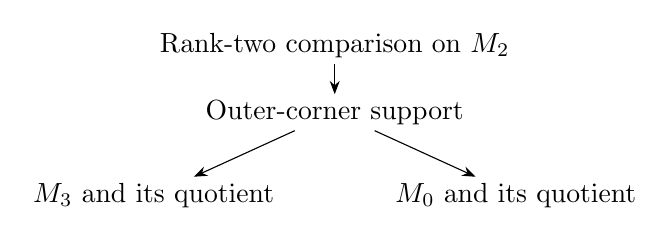
\begin{tikzpicture}[>=Stealth,every node/.style={align=center,inner sep=2pt}]
\node (two) at (0,0) {Rank-two comparison on \(M_2\)};
\node (input) at (0,-.85) {Outer-corner support};
\node (three) at (-2.3,-1.9) {\(M_3\) and its quotient};
\node (zero) at (2.3,-1.9) {\(M_0\) and its quotient};
\draw[->] (two)--(input);
\draw[->] (input)--(three);
\draw[->] (input)--(zero);
\end{tikzpicture}
\caption{Propagation uses the rank-two comparison first. Its outer-corner input is applied to two different rank-three support problems.}\label{fig:ordinary-three-levels}
\end{construction}

\paragraph{Which components can link curves.}
Which components do these links reach from the seed?

\begin{proposition}[Propagation from a seed across ordinary components]
\label{prop:ordinary-component-propagation}
In the selected ordinary frame, given the seed of Appendix~\ref{sec:linked-seeds} of the required dimension
and the completed comparisons
\eqref{eq:ordinary-component-stable-test} and~\eqref{eq:ordinary-component-thick-test},
each type-I prime \(P\) is good for its corresponding level ideal, meaning 
\[
 M_n\subseteq P\cap B_n.
\]

The application to \(M_2\) supplies the outer-corner input for the
applications to \(M_3\) and \(M_0\), which keep their separate
quotient maps.
\end{proposition}

\begin{proof}
\proofstep{Relative dimension and the presentation of the chart.}
The ungraded chart has a presentation over a complete DVR in
\(N\) variables with \(N-D\) relations, padding with zeros if
necessary. At a rank-three point on the exceptional locus, use
conjugation by the sign on the middle coordinate to grade the
presentation by parity. There are \(a\) even and \(g\) odd
variables, at most \(a-D\) even and \(g\) odd relations. The relation count uses the relative obstruction group.
For a small extension with kernel \(I\), let \(c(g,h)\) be
the \(I\)-valued error in multiplying two matrix lifts.
For each ordinary place let \(b_v(g)\) be the error in the
lifted local flag, read in the adjoint quotient by
\(\mathfrak b_v\). With the cone differential
\(d(c,b)=(dc,\operatorname{res}(c)-db)\), associativity
and the local multiplication law give
\[
      dc=0,\qquad db_v=\operatorname{res}_v(c).
\]

Write \(\alpha\) for the one-cochain changing the matrix
lifts and \(\beta_v\) for the zero-cochain changing the flag at
\(v\), in the cone convention just specified. The new errors are
\[
 c'=c+d\alpha,\qquad
 b'_v=b_v+\operatorname{res}_v(\alpha)-d\beta_v .
\]
Thus a zero obstruction class permits both errors to be removed
in the same lift. The dual
of the minimal relation space injects into this obstruction
space. Indeed if a nonzero functional gave zero obstruction,
push out along it and lift a section to the power series variables.
Two lifts of the variables then differ in the square-zero
kernel killed by the maximal ideal. Every minimal relation has
zero relative linear part modulo that ideal, so its value is
unchanged. A relation on which the functional is nonzero would
have both zero and nonzero value. Since \(2\) is invertible, an involution \(s\) admits the complementary projections
\[
 e_+=(1+s)/2,\qquad e_-=(1-s)/2,\qquad e_+e_-=0.
\]
Applying the argument to the images gives both eigenspace assertions.

In the ordinary tangent and Euler characteristic formulas of
the marked frame, the finite-place contribution is
\(\sum_{v\mid\ell}d_v\dim\mathfrak b_v\), from which one subtracts the
sum of the dimensions fixed by real conjugations. Here
\(\dim\mathfrak b_v=n(n+1)/2\). Multiplication by the
polarization matrix identifies the fixed matrices at a real
place with skew matrices, of dimension \(n(n-1)/2\).

Since \(\sum_{v\mid\ell}d_v=d\) and \(L^+\) has \(d\) real
places, counting the extra frame direction gives
\[
 d\frac{n(n+1)}2-d\frac{n(n-1)}2+1=nd+1=D .
\]
In rank three the Borel dimensions are \(4\) even and \(2\) odd:
the even part consists of the three diagonals and the outer root.
The real skew dimensions are \(1\) even and \(2\) odd, from the
outer pair and the two adjacent pairs respectively. The extra
frame direction is even. Thus the two lower bounds for relative
tangent dimension minus obstruction dimension are
\[
        4d-d+1=D,\qquad 2d-2d=0.
\]

\proofstep{Connectedness and the odd incidence equations.}
In rank two, or outside the exceptional locus of rank three,
Grothendieck connectedness applied to the ungraded presentation
joins the minimal components in a graph with intersections
of dimension at least \(D\). Each component has dimension at
least \(D+1\). At the remaining rank-three centers write \(y\)
for the odd variables. If there are odd variables, pad the odd
relations to a square system \(H y=0\). Each odd relation lies
in the ideal \((y)\) by parity, and minimality permits the
entries of \(H\) to be taken in the maximal ideal. Impose
\(\det H=0\) in the chart. Every type-I prime contains the extra equation. Indeed modulo such a prime at least one entry of \(y\) survives, whereas
\[
 0=\operatorname{adj}(H)Hy=(\det H)y.
\]
The quotient is a domain, so \(\det H\) vanishes there. The odd dimension on this pointed chart is positive in the exceptional case.

To see the same intersection bound, use an independent
\(g\times g\) matrix \(X\) and vector \(z\). The incidence
locus \(Xz=0,\det X=0\) has irreducible support of codimension
\(g\). On \(z_i\ne0\) solve for the \(i\)-th column, with
all other coordinates free, and these charts overlap. At \(z=0\), choose a nonzero vector \(v\in\ker X\) for the singular residue matrix. The line is a specialization from the open locus, since
\[
 X(tv)=0,\qquad tv\ne0\ (t\ne0),\qquad (tv)|_{t=0}=0 .
\] The homogeneous prime radical gives a domain after
completion: the initial homogeneous pieces of two nonzero
elements still have nonzero product. Keep the \(a\) even and
\(g\) odd variables of the original chart separate from the
\(g^2+g\) new variables \((X,z)\). The new incidence equations
have codimension \(g\) in the new variables. Thus the ambient
irreducible complete local germ has dimension
\[
             1+a+g+(g^2+g)-g=1+a+g+g^2.
\]

In this germ impose \(X-H=0\), \(z-y=0\) and the at most
\(a-D\) even relations. Their number is at most
\(g^2+g+a-D\), so each component has dimension at least
\(D+1\). The complete local connectedness theorem with the
same equation count gives connectedness in dimension \(D\).
\cite{stacks-connectedness}

\proofstep{The nonsplit extension at an exceptional branch.}
The minimal primes of this smaller locus are off both triangular
loci by the bounds above. An exceptional prime there has \(y=0\)
and \(H\) singular. Choose a nonzero vector in its kernel
over the fraction field and clear denominators. At \(y=0\) an odd variation annihilates the even relations. For the odd ones the linearization is
\[
 d(Hy)=(dH)y+H\,dy=H\,dy=0 .
\] This gives a derivation
of the original chart, zero on even entries and ordinary characters.
If \(r_{\rm out},r_{\rm mid}\) are the two retained blocks,
let \(u(g)\) be the derivative of the column from the middle
line to the outer block. The even derivatives vanish, so the
linearized multiplication law in that column is
\[
   u(gh)=r_{\rm out}(g)u(h)+u(g)r_{\rm mid}(h).
\]
Consequently \(\left(\begin{smallmatrix}r_{\rm out}(g)&u(g)\\
0&r_{\rm mid}(g)\end{smallmatrix}\right)\) is a representation with
the original block determinant.

The same linearization of the
two ordered ordinary products gives the prescribed local tests. A splitting would give an
invariant eigenvector with middle coordinate 1. Write a splitting vector as \((u,1)\) in the outer-plane
and middle-line decomposition. Its equations at the mark
\(g_*\) and its polarized mate \(g_*^*\) have a common
off-diagonal column and the same middle value, while the
two distinct outer eigenvalues are exchanged. Write \(D_*,D_*'\) for the two outer diagonal matrices, \(c\) for
the common column and \(m\) for the common middle value. The two splitting
equations give
\[
 D_*u+c=mu=D_*'u+c
 \quad\Longrightarrow\quad (D_*-D_*')u=0 .
\]
Both diagonal entries of the difference are nonzero, forcing \(u=0\). The splitting equation at all
\(g\) then says the differentiated column vanishes. Polarization also kills the opposite differentiated
row, contradicting the nonzero odd derivation. This proves
thickness at the exceptional branches used by the graph.

\proofstep{Propagation from a seed.}
Suppose a chart has a good type-I prime with quotient dimension
at least \(D\). Write \(P\) for this good prime. Using \(I=M_n\), choose the minimal prime \(P_{\min}\) and the nice specialization \(Q\) so that
\[
 P_{\min}\subseteq P\subseteq Q,\qquad \dim(\text{chart}/P)\ge D .
\] The minimal prime is
type I by generization, and is a vertex of the component graph,
since every type-I prime contains the additional chart equation
when one is imposed. If the nice point is type I, the first
prime condition makes that vertex good. If the nice point is
exceptional, the original good prime serves as the stable
generization for the length-zero second prime condition. This
again makes the vertex good.

\proofstep{The induction along the component graph.}
Along a path of adjacent vertices keep the following information.
A type-I vertex reached is good. At a thick vertex keep a
nice exceptional point containing it, linked by a finite
sequence of nice exceptional points to one having a good type-I
generization. In the chart ring \(A\), adjacency of successive vertices \(P,P'\) supplies a common specialization of controlled dimension: 
\[
 V\supseteq P+P',\qquad\dim A/V\ge D.
\]
 Choose the nice specialization \(Q\) above \(V\); then
\[
                       P+P'\subseteq V\subseteq Q .
\]

If \(P\) is good type I, use \(M_n\) in the specialization
and apply the first or the length-zero second condition at
\(Q\), according to its type. If \(P_1\) is any type-I generization of this \(Q\), either implication gives 
\[
 P_1\subseteq Q\quad\Longrightarrow\quad M_n\subseteq P_1\cap B_n.
\]
 If \(P\) is thick, \(V\)
contains the corner ideal \(I_3\). Use \(I_3\) in the
specialization: \(Q\) still contains the odd ideal, so is
exceptional.
Write \(Q_{\rm old}\) for the stored nice point on the current thick vertex. The common vertex joins the new exceptional point to the chain since 
\[
 P\subseteq Q_{\rm old}\cap Q.
\]

The second prime condition now makes every type-I generization
of the new point good. If the next vertex is type I, this proves
the assertion for it. If it is thick, specialize \(V\) using
its \(I_3\) as well. A previous vertex of type I gives a good type-I generization of this new exceptional point. When the previous vertex is
thick the stored chain extends through that common vertex.
This proves the invariant without an assumption that every
thick component belongs to the rank-three Hecke locus.
In rank two all the vertices and nice points used are type I.

\proofstep{Passage between charts.}
It remains to pass between charts. Write \(\pi_0\) for the projection to the degree-zero spectrum, \(x_0\) for its residual point and \(Z_{\rm up}\) for the upper triangular locus. The core used to join the charts is 
\[
 C=\pi_0^{-1}(x_0)\setminus Z_{\rm up}.
\]
 Its relevant points admit smooth lower
triangular realizations over their residue fields. Minimal
frame primes are homogeneous. A homogeneous type-I generic
point specializes to this core. One chooses a lower entry nonzero
there, uses the chart obtained by retaining its direction under
the torus, and specializes its degree-zero coefficients to the
closed point.  Applying this to a homogeneous lift of a seed contraction gives a chart prime \(\mathfrak q\) with quotient dimension
\[
 \dim(\text{chart}/\mathfrak q)=\dim\bigl(B_n/(P\cap B_n)\bigr)+1 .
\] The extra parameter is the one-dimensional torus orbit.

The core is preconnected. In rank two the sole lower entry is
a twisted cocycle subject to linear local and marked equations.
Interpolation over \(k[t]\) to a fixed nonzero solution gives
a common generization, still off the upper triangular locus.
In rank three write \(y\) for the adjacent lower entry and
\(a\) for the outer lower entry. The other adjacent entry
is given by the involution.

Write \(\partial a\) for the linear part of the outer
cocycle equation and \(Q(y)\) for its quadratic term.
A pure outer solution \(b\) satisfies \(\partial b=0\),
so
\[
        \partial(t^2 a+(1-t)b)=t^2 Q(y)=Q(ty).
\]
This is the lower multiplication law for the interpolant
\((ty,t^2a+(1-t)b)\). The local flag coordinates scale
in degrees one and two, and adding a pure outer solution adds
its outer flag coordinate. Pick \(b\ne0\) as supplied by the
frame. The kernel of the map into \(k[t]\) is a common
generization of \((0,b)\) and the given point. To see density
off the exceptional locus one needs a solution with \(y\ne0\).

For the frame's nonzero adjacent cocycle \(u\), put \(P=\bar\Psi\)
and use the conventions \(u(gh)=P(h)u(g)+u(h)\) and
\(u(g^*)=u(g)/P(g)\). Set, pointwise,
\[
 y=u+\delta(P-1),\qquad
 a=\frac{u^2}{2P}-\delta u(1+P^{-1})
                +\delta^2\bigl(1-(P+P^{-1})/2\bigr).
\]
Here \(\delta(P(g_*)^2-1)=-u(g_*)(P(g_*)-1)\), with
\(g_*\) the marked element for the normal form. Substitution
gives the marked equality for \(y\), the quadratic multiplication
law for \(a\) and the required local coboundary forms, using
\(u|_{G_v}=\alpha_v(P-1)\). If \(y=0\), substitution in the formula for \(u(g_*^*)\) gives
\[
 2\delta\bigl(P(g_*)^2-1\bigr)=0 .
\]
This forces \(u=0\), a contradiction. With one such solution
\((y_0,a_0)\), the following curve exhibits a pure outer point as a specialization: 
\[
 (y(t),a(t))=(t y_0,t^2a_0+a),\qquad (y(0),a(0))=(0,a).
\]
 Since \(y_0\ne0\), the generic point lies outside the exceptional locus.

\proofstep{From the open core to all required components.}
Divide the finitely many components meeting the open type-I
locus according as their generic points are good or bad.
The high-dimensional seed in its pointed chart gives a good
component by the local propagation. Every component under
consideration meets the core by marked specialization.
The good and bad unions are closed and cover the core, because
off the exceptional locus its closed points lie on type-I
components by the ungraded chart calculation, and these
points are dense there and in the core.

By the Jacobson
specialization property of this fiber, a closed set
meeting it contains a closed chart center there, also after
restriction to an open subset of the core.
Write \(C_{\rm good}\) and \(C_{\rm bad}\) for the two closed subsets of the core \(C\). Preconnectedness gives 
\[
 C=C_{\rm good}\cup C_{\rm bad},\quad C_{\rm good},C_{\rm bad}\ne\varnothing\quad\Longrightarrow\quad C_{\rm good}\cap C_{\rm bad}\ne\varnothing.
\]
 Choose a closed chart center in the
intersection. Flatness lifts both generic points by going
down, giving two type-I minimal chart primes. Local propagation
from the good one reaches the other, contrary to the latter's
contraction. Thus every type-I prime is good. This argument
first applies to \(M_2\), then to each of \(M_3\) and \(M_0\)
on the same rank-three frame.

\end{proof}

\subsection{Two levels and the local annihilator}

Support at the two levels supplies local information at different exceptional places.
To compare the resulting cuspidal attachments, let \(\xi:A_3\to\overline{\Q}_\ell\) be a continuous integral
type-I point with arithmetic ordinary characters on the first
level. At the other level identify the local groups via the
marked place, in the order prescribed by the common frame.
The map of pairs on each level gives the characters of precisely
the same twisted frame point. Thus local algebraicity and the
strict inequalities of its weights transfer at each embedding.

Both determinant points lie on their respective Hecke supports.
Classicality gives cuspidal attachments with the prescribed
local compatibility away from the respective exceptional places.
Both pullbacks give the same representation \(\epsilon^{-1}r_\xi\). Thus for a good Frobenius \(g\) their common characteristic polynomial is
\[
 \det\bigl(1-X\epsilon(g)^{-1}r_\xi(g)\bigr).
\]
Agreement at almost all unramified places identifies the cusps by strong multiplicity one. At
each exceptional prime the other level gives the missing local
comparison.

\paragraph{Weights for fixed-weight adjoint vanishing.}
The comparison at the two levels will be used locally on a component. Fix an integral
type-I point of the full frame ring \(A=A_n\)
with kernel \(q\). Lemma~\ref{lem:ordinary-annihilator-derivative}
will show that \(a\in M_n A\) vanishes in \(A_q\).
To supply the local hypothesis for the density argument on a component,
choose one embedding \(\tau_v:L_v\hookrightarrow\overline{\Q}_\ell\)
for each marked place over \(\ell\). At each marked place and \(j=0,1,2\), prescribe the weight according to the chosen embedding by
\[
 h_j(\tau)=\begin{cases}2j&\tau=\tau_v,\\ j&\tau\ne\tau_v.\end{cases}
\] The indices increase strictly at every
embedding. The local degree is greater than five, so choose
a nonzero trace-zero \(x\in L_v\), sufficiently small that
the exponential and logarithm are inverse on its neighborhood
of zero. Then \(u=\exp(x)\) is a nontorsion unit with norm one.

Take an inertial Artin lift of \(u\). Its cyclotomic value is
one, and the \(j\)-th ordinary character there has value
\[
   \zeta_j\,N_{L_v/\Q_\ell}(u)^{-j}\tau_v(u)^{-j}
      =\zeta_j\tau_v(u)^{-j},\qquad \zeta_j\ \text{of finite order}.
\]
Every ratio for distinct indices has infinite order on this
single element. The argument works for any finite parts in the
specialization. Density at this weight therefore supplies the
local hypothesis of fixed-weight adjoint vanishing at an
integral type-I point on each component. At
rank three the two-level comparison supplies its finite-place
compatibilities. We give the commutative algebra in detail.

\begin{lemma}[Differentiation on the ordinary support]
\label{lem:ordinary-annihilator-derivative}
With the finite weight quotient and type-I density at these
two levels, an ordinary Hecke relation \(a\) restricted to the
chart is annihilated by an element outside the prime of the
type-I point. Writing \(\xi\) for evaluation at the point and \(D_\xi\) for any
point derivation, this gives
\[
                      \xi(a)=0,\qquad D_\xi(a)=0
\]
also at a point with resonant weights.
\end{lemma}

\begin{proof}
\proofstep{Heights in a flat pointed chart.}
Use a flat pointed chart \(R\) containing a prime \(Q\) over
\(q\), minimal in that fiber, with \(\dim(R/Q)=1\). This chart
is obtained by specializing an integral model of the point
and completing at its residual center. Every prime \(P\subset Q\)
contracts to a type-I prime of the frame, so its degree-zero
contraction contains \(M_n\). That quotient is finite over an
ordinary weight quotient and has dimension at most \(D\).
The chart dimension formula adds at most one for the torus
fiber, giving \(\dim(R/P)\le D+1\). Extend any chain ending at \(Q\) by the specialization to the closed point. The resulting dimension bound is
\[
 \operatorname{ht}Q+1\le D+1 .
\]

In the presentation of \(R\) with \(N\) variables over a
DVR and \(N-D\) relations, the lift of \(Q\) has height \(N\)
by catenarity and \(\dim(R/Q)=1\). Its height after imposing
\(N-D\) equations is at least \(D\). Hence equality holds.
At the lifted prime the relations have their full possible
height in a regular local ring and form a regular sequence.
The quotient local ring \(R_Q\) is therefore Cohen--Macaulay.
For the flat local map \(A_q\to R_Q\), the depth and dimension
formulas with the zero-dimensional closed fibre give
\[
 \operatorname{depth}A_q=\operatorname{depth}R_Q
      =\dim R_Q=\dim A_q .
\]
In particular \(A_q\) is Cohen--Macaulay and has no embedded
associated primes. The dimension identity is
\(\operatorname{ht}q=\operatorname{ht}Q\).

\proofstep{Generic reducedness along every component.}
For each minimal prime \(P_0\subset q\) of \(A\), going down
and taking a minimal prime in the chart lifts it to a minimal
chart prime below \(Q\). Every such chart component has
dimension at least \(D+1\), by the presentation and the
height theorem. Its frame contraction has degree-zero quotient
dimension at least \(D\), by the bound of one on the torus
fiber. If \(P\) is the frame contraction and \(B_n\) its degree-zero ring, the fiber bound and the Hecke upper bound now agree: 
\[
 D\le\dim B_n/(P\cap B_n)\le D.
\]
 Apply density on this component and lift using the
graded frame to a type-I point \(\xi'\) on \(P_0\) with
the weights just prescribed.

At \(\xi'\) the ordinary adjoint
vanishing says every fixed-weight deformation is inner.
In the marked basis the remaining infinitesimal change of
frame has dimension at most one. The extra inertial weight directions contribute at most \(nd\), so the bound for the full tangent space is
\[
 \dim T_{\rm full}\le 1+nd=D .
\] The height lower
bound at \(q'=\ker\xi'\) is \(D\) by the same chart
presentation. Over the characteristic-zero coefficient field
the residue field extension is separable and formally smooth,
so every cotangent functional extends to a coefficient-relative
point derivation. Together the tangent and height bounds give 
\[
 D\le\dim A_{q'}\le\operatorname{edim} A_{q'}\le D.
\]
 Hence \(A_{q'}\) is regular local and a domain; localization at its minimal prime gives the field \(A_{P_0}\).

\proofstep{Differentiating the annihilator relation at the original point.}
Now if \(\operatorname{Ann}_A(a)\subseteq q\), take a prime
minimal over that annihilator inside \(q\). It is associated
to the cyclic submodule \(Aa\), hence to \(A\). It must
therefore be a minimal prime \(P_0\) by the unmixedness at
\(q\). Goodness at \(P_0\) puts \(a\) in \(P_0\). In the
field \(A_{P_0}\) it vanishes. This supplies an annihilator
outside \(P_0\), a contradiction. We obtain the asserted
\(s\notin q\). Since \(s\notin q\), we have \(\xi(s)\ne0\). Evaluation first gives \(\xi(a)=0\); differentiation then gives 
\[
 0=D_\xi(sa)=\xi(s)D_\xi(a)+\xi(a)D_\xi(s)=\xi(s)D_\xi(a).
\]
 Thus every point derivation kills \(a\), even if the original point has resonant
weights.  At that point Section~\ref{sec:rank-three-multiplicity}
supplies the selected multiplicity used on the determinant
quotient in the fixed-weight comparison.

\end{proof}

\paragraph{Exclusion of an adjacent cyclotomic ratio.}
We now use the bound on fixed-inertia derivatives to rule out a cyclotomic ratio for
the marked points specified below.

\begin{paramdefinition}[The points tested for an adjacent cyclotomic ratio]\label{hyp:cyclotomic-ratio-point}
On the rank-three type-I chart of
Proposition~\ref{prop:ordinary-component-propagation}, let
\(X_e\), \(e\ge1\), denote the field points having the finite
inertia parts and local degree bounds of
Proposition~\ref{prop:separated-marked-host}, absolutely irreducible
on each open global subgroup, and potentially crystalline at the
marked \(\ell\)-adic places with ordered exponents \((e,0,-e)\).
At such a point fix the inertia characters when taking derivatives,
as in Lemma~\ref{lem:ordinary-annihilator-derivative}.
\end{paramdefinition}
For the application to the even level, the restriction and
attachment arguments proving Lemma~\ref{lem:rank-three-host-restriction}
and Proposition~\ref{prop:ordinary-host-attachment} supply these
properties before applying the ratio test.

\begin{proposition}[Exclusion of cyclotomic resonance]
\label{prop:ordinary-no-cyclotomic-resonance}
At a point of Definition~\ref{hyp:cyclotomic-ratio-point}, writing \(D_v\) for the marked local group, any two distinct ordinary flag positions satisfy 
\[
 (\psi_i/\psi_j)|_{D_v}\ne\epsilon|_{D_v}\qquad(i\ne j).
\]
 The two estimates concern the same
fixed-inertia tangent space: the global calculation bounds its
rank by one, while the proposed ratio forces rank at least two.
\end{proposition}

\begin{proof}
\proofstep{The upper bound on fixed-inertia derivations.}
First consider the upper estimate at the point \(x\) of the
level determinant ring. A derivation induced from the frame
with fixed inertia annihilates \(J\) by the local annihilator
and kills the power series weight ring \(\Lambda\) by its
generators. Let \(J'\) be the reduced support ideal of the
projected module. A trace Gram minor \(b_0\) nonzero at \(x\)
restricts the support to its irreducible locus. On this open,
dense good arithmetic points of the ordinary Hecke component
have positive selected multiplicity. Thus \(b_0a\in J\) for
\(a\in J'\), by reducedness and density in the Hecke quotient.
The local annihilator gives \(D(b_0a)=0\). Since \(a(x)=0\) and \(b_0(x)\ne0\), 
\[
 0=D(b_0a)=b_0(x)D(a)+a(x)D(b_0)=b_0(x)D(a),
\]
 so \(D(a)=0\).

\proofstep{Separating the eigenvalues in the fixed-weight fibre.}
On the finite free projected weight module choose a linear
combination \(t\) of Hecke generators primitive for its
generic reduced algebra and separating the systems in the
weight fiber at \(x\). Finitely many proper linear conditions
on the coefficients suffice for both separations in
characteristic zero. Let \(t\) be this separating combination of Hecke generators. The characteristic polynomial in the generic algebra has the factorization
\[
 P_t(X)=\prod_i g_i(X)^{m_i},\qquad \gcd(g_i,g_j)=1\quad(i\ne j),
\]
with the \(g_i\) distinct monic irreducibles. They lie in \(\Lambda[T]\) by integral closedness.
Let \(k_i\) be the multiplicity of \(x(t)\) as a root of
the specialization of \(g_i\). If \(k_i>0\), lying over in
the corresponding finite integral component gives a point
with these values of \(\Lambda,t\). Separation identifies it
with \(x\).

On that component choose a good arithmetic point
\(y\) with the same algebraic exponents and with
\(b_0g_i'(t)\prod_{j\ne i}g_j(t)\ne0\). This uses density
at those exponents with varying finite-order parts. The
displayed element is generically nonzero there by separability.
The selected joint dimension at \(y\) is at most the root
multiplicity \(m_i\), and at \(x\) it is the whole root
multiplicity since \(t\) separates at \(x\). Consequently
\[
       \sum_i m_i k_i=\mu_e(x)=\mu_e(y)\le m_i
                              \qquad(k_i>0).
\]
Some \(k_i\) is positive. Exactly one is positive and it is
one. The square-free product \(\prod g_i(t)\) belongs to \(J'\)
and has a simple root at \(x(t)\). Differentiating gives
\(D(t)=0\). The component ideal for that root is killed by
\(D\) as well, since multiplying each element by
\(\prod_{j\ne i}g_j(t)\), a unit at \(x\), puts it in \(J'\).

For \(a\) in the component algebra define
\[
          P_a(T)=\operatorname{Tr}\bigl(a\,g_i(T)/(T-t)\bigr)
                     \in\Lambda[T].
\]
Here the trace is from the generic component field, and
integrality of the coefficients follows from monic division
by \(T-t\) and integral closedness. At \(T=t\) the identity
embedding contributes \(a g_i'(t)\) and all other embeddings
contribute zero. Differentiate this identity at \(x\). The coefficients and \(t\) have zero derivative. Differentiating the surviving term gives 
\[
 g_i'(x(t))D(a)=0,\qquad g_i'(x(t))\ne0,
\]
 and hence \(D(a)=0\). Thus the derivation
vanishes on the whole determinant ring and on its image \(B_3\).

At a type-I frame point there are nonzero specialized entries
of both signs and one of odd weight. Products give two
monomials \(p_+,p_-\) of weights \(1,-1\) nonzero there.
A derivation vanishing on \(B_3\) is determined by its value
on \(p_+\). Write \(\xi\) for the frame point above \(x\). If \(D(p_+)=0\), applying \(D\) to \(p_+p_-\) gives \(D(p_-)=0\). For an entry \(u\) of weight \(j\ne0\), take \(p=p_-\) if \(j>0\) and \(p=p_+\) if \(j<0\). Its balanced product then gives 
\[
 0=D(up^{|j|})=\xi(p)^{|j|}D(u),\qquad \xi(p)\ne0.
\]
 All generating entries
and ordinary characters have zero derivative. This proves the
upper bound one for the dimension of fixed-inertia derivations.

\proofstep{The lower bound from a cyclotomic ratio.}
For the lower bound, equality on an open inertia subgroup forces equality of cyclotomic exponents since \(\epsilon\) has infinite image there:
\[
 e(w_i-w_j)=1,\qquad (w_1,w_2,w_3)=(1,0,-1).
\] Thus \(e=1\) and
the two indices are adjacent. Normalize the adjacent
two-dimensional subquotient by its second character. Its
extension cocycle \(b\) takes values in \(E(1)\), with \(E\)
a finite coefficient field. Its class belongs to the
Bloch--Kato finite subspace. Indeed the subquotient and its
characters become crystalline after finite extension and
restriction on cohomology with crystalline period coefficients
is injective by averaging in characteristic zero. By Kummer
theory this finite subspace consists of local units, annihilated
under cup product by the unramified line in \(H^1(F_v,E)\).
For a nonzero unramified additive character \(u\) take a
cochain satisfying
\[
      \beta(st)=\beta(s)+\epsilon(s)\beta(t)-b(s)u(t).
\]
Scaling \(u,\beta\) together makes them integral by compactness.
\cite{bloch-kato-finite}

Write \(A_k=\mathcal O_E/\ell^k\), \(q_k=|A_k|\), and work
in a stable ordinary integral basis. At each \(v\mid\ell\)
the local Euler characteristic and Tate duality give at least
\(q_k^{6(1+d_v)}\) upper triangular adjoint cocycles before
fixing inertia. At each of the \(d_v\) pro-\(\ell\) unit generators, three diagonal coordinates are fixed. Thus the maximum cost is
\[
 (q_k^3)^{d_v}=q_k^{3d_v}.
\]
The marked local fields have no \(\ell\)-power roots of unity.
At the distinguished place impose equal variations on the
adjacent diagonals. The resulting module has rank five and
projects equivariantly onto \(A_k(1)\) via the adjacent entry,
so the dual invariant factor has size at least \(q_k\). Only
two inertia characters must be killed. With the two diagonal variations equal, the lower bound for the number of solutions simplifies to
\[
 q_k^{5(1+d_v)+1-2d_v}=q_k^{6+3d_v}.
\]

One further integral cocycle has unramified diagonal difference
\(u\) on the resonant pair and zero difference on the other
adjacent pair. Its resonant entry is supplied by \(\beta\). Then
the remaining error is a two-cocycle in the outer root
\(\kappa_0/\kappa_2\). This differs from \(\epsilon\)
since the other adjacent ratio is nontrivial at the marked
regular element. With \(\theta=\kappa_0/\kappa_2\), local duality identifies the obstruction space by 
\[
 H^2(G_v,E(\theta))^\vee\simeq H^0(G_v,E(\epsilon\theta^{-1}))=0,
\]
 since \(\epsilon\theta^{-1}\) is nontrivial. Correct the outer entry and clear denominators
once.

Multiples of this integral cocycle at depth \(k\)
supply at least \(q_k/|\mathcal O_E/(c)|\) different cosets
of the equal-diagonal solutions, where \(c\ne0\) is a fixed
value of its diagonal difference. Adding all full-matrix
coboundaries gives another factor at least \(q_k^3\) at
every place, since distinct residual eigenvalues at the
marked local element force the generator of any coboundary
that stays upper triangular to be upper triangular. Thus
the allowed local cocycles \(Z_v\) satisfy
\[
  \prod_{v\mid\ell}|Z_v|
        \ \ge\ q_k^{9\,\#\{v\mid\ell\}+3d+1}/C
\]
with \(C\) independent of \(k\) for this point.

\proofstep{The global cardinality estimate and contradiction.}
The global Selmer cardinality inequality for these local
conditions gives
\[
 |Z_{\rm glob}|\, q_k^{9\,\#\{v\mid\ell\}}
             \prod_{v\mid\infty}|H^0_v|
      \ \ge\ q_k^9\prod_{v\mid\ell}|Z_v| .
\]
The dual global invariant factor is trivial here. The
residual frame separates each matrix unit's adjoint character
from \(\bar\epsilon\), using \(1,\bar\Psi^{\pm1}\) on the
positive component and \(\eta\bar\Psi^{\pm2}\) on the outer
roots. Nakayama shows that the images of
\(\operatorname{Ad}\rho(s)-\epsilon(s)\) span the truncated
module, so no equivariant dual functional survives. At each real place the fixed matrices identify with the skew matrices; there are three free entries.

Taking the product over the \(d\) real places gives
\[
 \prod_{v\mid\infty}|H_v^0|=(q_k^3)^d=q_k^{3d}.
\] Before normalization the global cocycle bound is \(q_k^{10}/C\). Imposing zero
at conjugation costs six scalar entries by its square relation.
For \(Y=z(g_1)\rho(g_1)\) the remaining equations set the
off-diagonal part of \(Y-JY^tJ\) to zero, with \(J\) the
antidiagonal matrix. The two outer corners already vanish
and the other four entries form two opposite pairs. Thus, writing \(Z_k\) and \(Z_k^{\rm norm}\) for the cocycles before and after imposing the two normalizations, respectively, we obtain
\[
 |Z_k^{\rm norm}|\ge q_k^{-6-2}|Z_k|
              \ge q_k^{-8}q_k^{10}/C=q_k^2/C .
\]

Each normalized cocycle deforms the representation by
\((1+\delta z(s))\rho(s)\), \(\delta^2=0\), with the
prescribed ordinary conditions, and hence induces a distinct
fixed-inertia point derivation into \(A_k\). The relative
cotangent module after imposing those inertia equations is
finite over \(\mathcal O_E\). Write \(M\) for this module and \(T\) for its torsion submodule. If \(\operatorname{rk}M\le1\), the elementary divisor decomposition over the coefficient DVR gives
\[
  q_k^2/C\le |\operatorname{Hom}_{\mathcal O_E}(M,A_k)|
      \le q_k |T| .
\]
Here \(C\) and \(T\) are fixed as \(k\) varies. Since \(q_k\to\infty\), the rank is at least two. This contradicts
the upper bound on the very same framed tangent space and
excludes the cyclotomic equality. The constants in this
depth argument can depend on the chosen point and the field.

At a type-I point of the even-level Field used in the rank-three trace estimate over the
imaginary quadratic field \(K\), the marking for this use takes
\(M=\ell N|\operatorname{disc}K|\). On complex conjugation \(c\) the two parity factors cancel:
\[
 (\epsilon^e\psi)(c)=(-1)^e\psi(-1)=(-1)^{2e}=1 .
\] Every prime ramifying in the quadratic
character divides \(M\). Factor the integral point through
the integers of a finite coefficient extension. Its ordinary
flag pulls back to the marked groups and its restriction to
the open CM subgroups is irreducible by the type-I host
hypothesis.

Given the automorphic attachment on this field, the preceding result supplies the unlinked local flag at the even level. The resulting local nonresonance and the three distinct weights give the required freedom of the ordinary characters. The original packet level in this branch
is \(N\), while \(M\) is the ramification cutoff of the comparison.
For the auxiliary field over \(\mathbb Q(i)\), use the same local exclusion after lifting to that field in the rigidity and trace bounds. Thus the local calculation is shared
even though the host attachment and the two-dimensional
constituent of the other Case of the rank-three trace estimate require separate
arguments.
\end{proof}

\section{The finite algebra at the marked point}
\label{sec:marked-hosts}

The support comparison in Section~\ref{sec:linked-components} took us to an abelian CM
extension \(L\). We now need a point there that will contribute to a length computed
over the original coefficient DVR \(\mathcal O\).
Two base changes intervene. The residual curve
points have to descend from the enlarged frame, and a point of
the graded algebra in characteristic zero has to give an integral
representation to which the automorphy comparison applies.
The marked point algebra gives the integral model used for the
descent and for the length bound in the next two appendices. The separated frame of Proposition~\ref{prop:separated-marked-host} carries the mark \eqref{eq:tag-h1}. Its degree-zero algebra over the original coefficient DVR is the object of Proposition~\ref{prop:marked-invariant-algebra}.

\paragraph{The fields and the mark.}
The field and its mark are specified by characters. With
\(e\ge1\) and \(\psi\) of even modulus \(N\) satisfying \(\psi(-1)=(-1)^e\), form the characters
\[
 \Psi=\epsilon^e\psi,\qquad P=\bar\Psi,\qquad \Psi(c)=1 .
\] Here \(c\) denotes complex conjugation.
Let \(\eta\) cut out the imaginary quadratic field \(K\). The
linking cutoff is \(\ell N|D_K|\) in the general-data case and
\(\ell N\) for \(K=\Q(i)\). Indeed an inertia group on which
\(\eta\) is nontrivial lies over a divisor of \(D_K\), and the
Gaussian character has conductor four. Let \(B\) be the chosen
place over \(\ell\). The marking uses
\[
       g_*\in D_B\cap G_L,\qquad P(g_*)^2\ne1 .
       \tag{H1}\label{eq:tag-h1}
\]
The level of the final packet will be read from the inertia of
the original representation.

\begin{proposition}[A separated marked frame]\label{prop:separated-marked-host}
Under the general-data or Gaussian host hypotheses, the
construction yields a totally real abelian \(L^+\) and its
CM extension \(L=L^+K\). The extension \(L/L^+\) splits
at the places above the primes dividing \(M\) and is unramified
at every finite place. At every place \(v\mid\ell\) of \(L^+\),
\[
                     [L_v^+:\mathbb Q_\ell]>3C_0+7.
\]
The distinguished mark satisfies
\textup{\eqref{eq:tag-h1}}. Both signed residual extension classes with
characters \(\eta P^{-a}\), \(a=1,2\), restrict nontrivially
to the marked frame with its prescribed inertia conditions.
\end{proposition}

\begin{proof}
\proofstep{Matching the quadratic characters locally.}
Here are the choices in the construction of the frame underlying
\eqref{eq:tag-h1}. Write \(K=\Q(\sqrt{-D})\), \(D>0\), and denote the linking
cutoff by \(M\). Choose a prime \(p>4D+M\) congruent to \(-1\)
modulo \(4M\). The real quadratic field
\(\Q(\sqrt{Dp})\) has the same local character as \(K\) on
decomposition groups above \(M\). Their defining square classes have ratio \(Dp/(-D)=-p\). For an odd prime \(v\mid M\), the congruence \(-p\equiv1\pmod v\) lifts the simple root \(1\) of \(X^2+p\) to \(\mathbb Z_v\). If \(2\mid M\), then \(8\mid4M\). Put \(u=-p\equiv1\pmod8\) and start with \(x_3=1\).

For \(n\ge3\),
\[
 (x_n+e2^{n-1})^2\equiv x_n^2+e2^n x_n\pmod {2^{n+1}} .
\]
If \(x_n^2\equiv u\pmod {2^n}\), exactly one of \(e=0,1\) corrects the next bit because \(x_n\) is odd. The resulting sequence converges to a square root in \(\mathbb Z_2^\times\).
This real quadratic field also ramifies at \(p\), where \(K\)
is unramified. Denote its fixing group by \(H_0\). The general
frame data include an abelian quotient of \(\ell\)-power order
with kernel \(H_b\) on which the away-from-\(\ell\) inertia
character has the same kernel as its reduction. On the Gaussian
branch \(H_b\) kills the \(\ell\)-power part of the character
after removing the factor at the place \(\ell\).

On inertia at \(\ell\), the condition \(P=\bar\epsilon^j\) determines the reduction of the finite factor. Use the Teichm\"uller lift
\[
 \chi'=[P\bar\epsilon^{-j}],\qquad\bar\epsilon^j\bar\chi'=P .
\]
The finite characters \(\chi'\) and \(\eta\) factor through
roots of unity of order dividing some \(M^a\ell\). Both are
unramified at \(\ell\), so its \(\ell\)-power factor can be
removed from that modulus by cyclotomic inertia. Choose a
second prime \(w\) congruent to one modulo both the resulting
modulus and \(M^{a+1}\ell\), outside the divisors of those
integers. The degree-\(\ell\) subfield of \(\Q(\mu_w)\) gives
the order-\(\ell\) character \(\theta\) of the seed construction.

For \(m\ge1\), let \(H_w\) fix that subfield, and \(H_m\) fix the
degree-\(\ell^m\) layer in \(\Q(\mu_{\ell^{m+1}})\). Put
\[
       U_m=H_0\cap H_w\cap H_b\cap H_m,\qquad
       G_L=U_m\cap\ker\eta .
       \tag{H2}\label{eq:tag-h2}
\]
All quotients defining \(U_m\) are abelian and complex conjugation
lies in each kernel. Thus \(U_m=G_{L^+}\), \(L=L^+K\). The
local comparison for \(H_0\) gives splitting of \(L/L^+\) over
\(M\). Outside \(M\), \(\eta\) is unramified, so \(L/L^+\) is
everywhere unramified at finite places. The layer at \(w\)
kills \(\theta\) on \(G_L\).

\proofstep{Selecting the real abelian layers.}
For the order of the choices in \eqref{eq:tag-h2}, let \(E\) be fixed by
\[
       H_0\cap H_w\cap H_b\cap\ker\eta\cap\ker P
                    \cap\ker\bar\epsilon .
\]
It is abelian over \(\Q\) and contains \(\mu_\ell\). On adjoining
the \(m\)-th layer the corresponding intersection fixes
\(E(\mu_{\ell^{m+1}})\). The bounded \(\ell\)-rank of the class
groups in this tower follows from Ferrero--Washington for the
cyclotomic tower of an abelian field and the Iwasawa module
structure theorem \cite[Chapter~13]{washington-cyclo}. Let \(E_\infty\) be their union and \(X\) its unramified abelian pro-\(\ell\) Galois module. The vanishing of \(\mu\) makes \(X\) finitely generated
over \(\mathbb Z_\ell\). Above a sufficiently deep layer \(E_m\),
one of the primes over \(\ell\) is totally ramified in
\(E_\infty/E_m\), since cyclotomic inertia has open image.

Write \(H_m^{\rm ur}\) for the unramified abelian
\(\ell\)-class field of \(E_m\). Every nontrivial finite intermediate extension in this part of the tower is ramified at the totally ramified prime over \(\ell\). Since \(H_m^{\rm ur}\) is unramified there,
\[
 H_m^{\rm ur}\cap E_\infty=E_m .
\] Unramifiedness survives base
change, so restriction gives
\[
 X\twoheadrightarrow\operatorname{Gal}
            (H_m^{\rm ur}E_\infty/E_\infty)
      \simeq\operatorname{Gal}(H_m^{\rm ur}/E_m).
\]
The \(\ell\)-rank is bounded by the number of
\(\mathbb Z_\ell\)-generators of \(X\). The finite
set of earlier layers can be included in the same bound.
By unramified class field theory this bounds
the dimension of the unramified mod-\(\ell\) character space by
a single \(C_0\) for all \(m\). Only now take
\(\ell^m>3C_0+7\). Inertia at \(\ell\) surjects onto the
degree-\(\ell^m\) layer, so every relevant local degree is at
least \(\ell^m\).

To construct the element in \eqref{eq:tag-h1}, choose \(x\in D_B\cap\ker\eta\) with \(P(x)^2\ne1\) as in the local separation hypothesis.
It fixes \(\sqrt{Dp}\) by the local comparison. Raise \(x\)
to a common \(\ell\)-power killing the three remaining finite
quotients in \(U_m\). Write \(d=\operatorname{ord}(P(x)^2)>1\). Since \(\gcd(d,\ell)=1\),
\[
 \operatorname{ord}\bigl(P(x)^{2\ell^a}\bigr)=d.
\]
Thus the resulting power \(x_*=x^{\ell^a}\) satisfies
\[
 x_*\in D_B\cap G_L,\qquad
 P(x_*)^2=(P(x)^2)^{\ell^a}\ne1 .
\]
The second equality uses the prime-to-\(\ell\) order of \(P(x)^2\),
on whose cyclic subgroup the indicated power is an automorphism.

\proofstep{Local separation by inertia and Frobenius in the general and Gaussian cases.}
Here are the two separation tests used above. For the General case of the rank-three trace estimate, inertia at the ramified prime of \(K\) away from
\(\ell N\) gives an element \(s\) with
\(P(s)=\bar\epsilon(s)=1\), \(\eta(s)=-1\). On inertia at \(\ell\) the residual finite factor has square one and \(\eta=1\). Thus here
\[
 P^2=\bar\epsilon^{2e}\ne1,\qquad \ell-1\nmid 2e .
\]

On the Gaussian branch let \(2^c\) be the
conductor of the dyadic component \(\psi_2\). Here \(c\ge4\).
Its image on units congruent to one modulo four is a nontrivial
cyclic 2-group. Some such unit maps to \(-1\). Multiplying
\(-1\) by that unit if \(\psi_2(-1)=-1\) gives a unit
congruent to \(-1\) modulo four in the kernel of \(\psi_2\).
Its image under dyadic reciprocity gives the required \(s\).
In either case \(\chi'(s)=1\) and \(\eta(s)=-1\).

For the other Gaussian test, the base data give an integer
\(o\ge1\) such that the odd-prime components of the
prime-to-\(\ell\) part of \(\psi\) have order dividing \(2o\).
For each exceptional prime and for \(p=\ell\) the dyadic conductor bound reads
\[
 8op^2<2^c .
\] These primes are odd. Choose a
Frobenius lift \(h\) acting by \(p\) on prime-to-\(p\) roots
and with \(\bar\epsilon(h)=1\). At \(p=\ell\) use cyclotomic
inertia to arrange the latter condition. At the other primes
it follows from \(p\equiv1\pmod\ell\). If \(P(h)^4=1\),
reduction is faithful on prime-to-\(\ell\) roots of unity,
so raising to the power \(4o\) gives
\(\psi_2(p)^{4o}=1\).

Let \(s_2\) and \(d\) be the two valuations that determine the effect of raising the odd prime \(p\) to successively doubled exponents:
\[
 s_2=v_2(p^2-1),\qquad d=v_2(o).
\]
For \(a\in1+4\mathbb Z_2\) one has \(v_2(a+1)=1\), so
\[
 v_2(a^2-1)=v_2(a-1)+v_2(a+1)=v_2(a-1)+1 .
\]
The geometric sum for an odd power is a unit. Starting
from \(a=p^2\) and using \(4o=2\cdot2^{d+1}(o/2^d)\)
therefore gives
\[
               v_2(p^{4o}-1)=v_2(p^2-1)+1+d .
\]
The same order formula in the finite dyadic quotients
shows that \(p^{4o}\) generates the subgroup congruent to
one modulo \(2^{s_2+1+d}\) in each such quotient. This forces
\[
 2^c\le2^{s_2+1+d}\le 2o(p^2-1),
\] a contradiction.
Since \(x=h^2\), multiplicativity of all three characters gives
\[
 \eta(x)=1,\qquad P(x)^2=P(h)^4\ne1,\qquad\bar\epsilon(x)=1 .
\] At \(p=\ell\) this is the starting
element for \eqref{eq:tag-h1}.

\proofstep{The signed residual cocycles on the marked frame.}
One use of these tests is the construction of the two
residual extension classes on the marked frame. For
\(a=1,2\) put \(\kappa=\eta P^{-a}\). This character is
odd, and differs from \(\bar\epsilon\) on \(s\) above.
It is nontrivial on \(U_m\cap D_B\) by \eqref{eq:tag-h1}. Let \(S\)
consist of \(\ell,w\) and the ramified primes of \(\kappa\).
For the Selmer group of \(k(\kappa)\), the local subspace in \(H^1(\mathbb Q_v,k(\kappa))\) is 
\[
 L_v=\begin{cases}H^1(\mathbb Q_v,k(\kappa)),&v=w,\\ 0,&v\in S\setminus\{w\},\\ H^1_{\rm unr}(\mathbb Q_v,k(\kappa)),&v\notin S.\end{cases}
\]
 The dimension difference
with the dual Selmer group is one by the Greenberg--Wiles
formula. Indeed both global invariant spaces vanish, and
the real invariant space vanishes. At \(w\) both \(\kappa\) and \(\bar\epsilon\) are trivial. The local contribution of the full condition is therefore
\[
 \dim L_w-\dim H^0_w=2-1=1 .
\]

At every other prime of \(S\) the
invariant space is zero. A nonzero resulting class remains
nonzero on \(U_m\) by inflation--restriction, since the
coefficient module has no \(U_m\)-invariants. On inertia
away from \(\ell,w\) in \(\ker\eta\cap\ker P\) its cocycle
is zero, either by the unramified condition or by local
triviality and \(\kappa=1\) on that inertia. At \(w\) the
restriction to inertia is additive. Its \(\ell\)-primary
tame quotient is procyclic and the degree-\(\ell\) field
fixed by \(H_w\) is totally ramified there. Thus it vanishes
on the inertia in \(U_m\) at \(w\) as well. Its restriction
at \(B\) is a coboundary. These are exactly the local
conditions needed to descend the two classes to the frame
quotient.

\end{proof}

\input{fitted-arithmetic}

\paragraph{A characteristic polynomial on every test curve.}
To control points of the degree-zero algebra we first examine the characteristic
polynomial along a curve in characteristic \(\ell\). Let \(A\) be a complete DVR of
characteristic \(\ell\) with finite residue field and a local map from \(\mathcal O\) through
its residue field \(k\). Take a marked ordinary representation
over \(A\) reducing in the given basis to the diagonal model
\((P,1,P^{-1})\) on \(\ker\eta\). On \(G_{L^+}\) it factors
through the marked quotient. Indeed the killed inertia elements
away from \(\ell\) have \(\eta=P=1\), and the inertia condition
on the point kills these elements. Continuity kills the closed
normal subgroup they generate. Above \(\ell\) the ordered
inertial characters on the frame are \(\Psi^{w_i}\), now
viewed in \(A\), where \(w=(1,0,-1)\). They are one on the
kernel of \(P\) in the marked inertia.

\begin{proposition}[Characteristic polynomials on marked ordinary curves]\label{prop:marked-residual-polynomial}
Let \(A\) be a complete DVR of characteristic \(\ell\) with
finite residue field, with \(\mathcal O\to A\) factoring through
\(k\). Take a marked ordinary curve over \(A\) with residual diagonal
\((P,1,P^{-1})\) on \(\ker\eta\) and ordered ordinary characters
\((\Psi,1,\Psi^{-1})\) on the marked inertia. On the entire quadratic kernel the identity \eqref{eq:tag-h3} reads
\[
 \det(X-r(g))=(X-P(g))(X-1)(X-P(g)^{-1})\qquad(g\in\ker\eta).
\] In the
fixed marked basis the curve is upper or lower triangular,
and its diagonal on the positive component is prescribed
by the residual characters.
\end{proposition}

\begin{proof}
\proofstep{Applying the rank-three support result to the residual curve.}
On the rank-three frame let \(J\) be the image of the Hecke
ideal and \(I_E\) the ideal pulled back from the outer corner
on the exceptional locus. The intersection \(I=J\cap I_E\)
lies below every prime off the two triangular loci. This follows
from propagation on the type-I locus and the rank-two comparison
on the exceptional locus. Write \(\lambda\) for the ideal
generated by the maximal ideal of the coefficients and the
weight differences \(\psi_{vi}(s)-1\) on inertia with \(P(s)=1\).
Both \(J+\lambda\) and \(I_E+\lambda\) have radical the
degree-zero maximal ideal.

For a prime \(\mathfrak p\) the inclusion \(JI_E\subseteq I\) implies
\[
 I+\lambda\subseteq\mathfrak p\quad\Longrightarrow\quad J+\lambda\subseteq\mathfrak p\ \text{ or }\ I_E+\lambda\subseteq\mathfrak p .
\]
Both force the same degree-zero maximal ideal.
The curve kills \(\lambda\). If its kernel is off both triangular
loci, its degree-zero evaluations consequently equal their
residual constants. In the expansion of a characteristic
polynomial each cycle of off-diagonal entries has total weight
zero and vanishes at the residual point. Only products of the
prescribed diagonal entries survive.

\proofstep{The split characteristic polynomial on the fixed subgroup.}
On a triangular curve the diagonal entries are characters.
Divide each by the corresponding residual character. The
quotient takes values in \(1+\mathfrak m_A\). On marked inertia with \(P=1\), any character value \(u\) of the quotient satisfies its ordinary polynomial. Since the coefficient ring here is a domain,
\[
 (u-1)^3=0\quad\Longrightarrow\quad u=1 .
\]
This kills the local abelian generators and, by polarization, their conjugates. At each truncation it is a
character into a finite \(\ell\)-group, and the abelian
class-field condition of the frame gives a single nonzero
exponent \(h\) for all these quotients. Passing through
all truncations gives \(z^h=1\) in \(1+\mathfrak m_A\).

In an equal-characteristic DVR that group is torsion-free.
The prime-to-\(\ell\) part follows by factoring a difference
of powers and the \(\ell\)-part by Frobenius. Thus the three
diagonal characters are fixed in this case as well. If the
comparison was made with enlarged residue coefficients, extend
the test DVR by the corresponding finite residue field
extension, apply the result there and use injectivity on
coefficients. Pulling the polynomial back along the map from
\(G_L\) to the positive component of the frame gives
\[
       \det(X-r(g))=(X-P(g))(X-1)(X-P(g)^{-1})
                        \quad(g\in G_L).
       \tag{H3}\label{eq:tag-h3}
\]
Here and below \(r(g)\) denotes the matrix part on the positive
component. The subgroup \(G_L\) in \eqref{eq:tag-h3} is independent of \(A,r\).

\proofstep{Extend the polynomial identity to the original quadratic kernel.}
For \(g\in\ker\eta\), take \(d\ge1\) with \(g^d\in G_L\).
Let \(\lambda_i\) be the eigenvalues of \(T=r(g)\) in an
algebraic closure of the fraction field, counted with multiplicity.
Triangularizing \(T\) gives the factorization
\[
 \det(X^d-T^d)
   =\prod_i (X^d-\lambda_i^d)
   =\det(X-T)
       \prod_i\left(\sum_{a=0}^{d-1}X^{d-1-a}\lambda_i^a\right).
\]
The first polynomial belongs to \(k[X]\) by \eqref{eq:tag-h3} on \(g^d\),
so all \(\lambda_i\), and hence the coefficients of \(\det(X-T)\),
are algebraic over \(k\). This factorization needs no separability
of \(X^d-\lambda_i^d\). An algebraic element of the domain \(A\)
congruent to \(a\in k\) must equal \(a\), since the field it
generates over \(k\) embeds into the residue field under
reduction. This proves \eqref{eq:tag-h3} on all of \(\ker\eta\), even when
\(\ell\mid d\).

\proofstep{Triangularity in the marked basis.}
We need triangularity in the \emph{marked basis}. Put
\(g^*=cg^{-1}c\). The marked difference in the frame is the diagonal matrix
\[
 r(g_*)-r(g_*^*)=\operatorname{diag}(z,0,-z).
\]
The reduction of \(z\) is \(P(g_*)-P(g_*)^{-1}\ne0\).
Work over the fraction field. An invariant subspace is stable under the marked difference \(D\). The three eigenvalues are distinct, so their coordinate projectors are polynomials in \(D\):
\[
 e_\lambda=\prod_{\nu\ne\lambda}\frac{D-\nu I}{\lambda-\nu},\qquad \lambda,\nu\in\{z,0,-z\}.
\]

Let \(L_1,L_2,L_3\) be the marked coordinate lines, in that order.
A stable subspace is a sum of its images under the three projectors.
Polarization makes its orthogonal complement for the reversed pairing
stable as well, and the complementary planes of the coordinate lines are
\[
 L_1^\perp=L_1\oplus L_2,\qquad L_2^\perp=L_1\oplus L_3,\qquad
 L_3^\perp=L_2\oplus L_3 .
\]
Thus a stable outer line gives a full flag. A stable middle line or
outer plane gives the decomposition \(L_2\oplus(L_1\oplus L_3)\).
If the outer plane is reducible, its two coordinate projectors again
give a stable outer line and a flag. The other possibilities are an irreducible triple
and a block decomposition with irreducible outer pair.

In
the former case Brauer--Nesbitt applied to \eqref{eq:tag-h3} would identify
the irreducible triple with a sum of characters. In the
latter case the middle diagonal entry is an eigenvalue,
algebraic over \(k\) and congruent to one, so it is one.
Since the middle eigenvalue is one, divide the characteristic polynomial in \eqref{eq:tag-h3} by its common factor:
\[
 P_{\rm outer}(X)=\frac{P_{\rm triple}(X)}{X-1}.
\]
The resulting character polynomials identify the semisimplification of the outer pair by Brauer--Nesbitt. Thus every curve is upper or lower triangular.
The equalities of entries descend to \(A\) by injectivity.
Each diagonal entry is then an eigenvalue congruent to its
prescribed value, so equals it on \(\ker\eta\). Multiplication
by \(c\), whose matrix part is one, extends the diagonal
identity to the other coset.

\end{proof}

\paragraph{Finiteness and an integral point in the same orbit.}
The identities on curves can now be used on the original Galois quotient. For the
auxiliary field over \(\mathbb Q(i)\) put \(\Gamma=G_{\Q,S}\), the quotient
by the closed normal subgroup generated by inertia away
from the specified finite set. The surjection
\(G_\Q\to\Gamma\) identifies the image of \(G_K\) with
\(\ker\eta_\Gamma\). The preceding triangularity and diagonal
identities therefore hold on the host. In the criterion for a triangular point the diagonal identity is also
obtained by dividing diagonal characters on \(G_K\).
The inertia conditions make their quotients unramified at
each truncation, and \(\Z[i]\) has class number one.

\begin{construction}
\[
\begin{array}{ll}
\text{monomial on the curve}&\text{reason it vanishes}\\ \hline
\text{contains a weight-zero variable}&\text{the diagonal is the fixed residue diagonal}\\
\text{uses only nonzero weights}&\text{both signs occur to sum to zero}\\
 &\text{one strict sign vanishes by triangularity}
\end{array}
\]
\caption{The closed-fibre test for a nonconstant monomial of weight zero at the Gaussian host. Triangularity is available on each marked residual curve.}\label{fig:marked-host-zero-invariants}
\end{construction}

\begin{proposition}[The integral invariant algebra]\label{prop:marked-invariant-algebra}
Let \(R\) be the complete normalized graded ring of the
Gaussian host just described, with the triangularity and
diagonal identities on all its residual test curves.
The degree-zero subalgebra \(R_0\) is a finite \(\mathcal O\)-module.
For each characteristic-zero point extending the coefficient embedding,
let \(a_i\) be its values on homogeneous generators of the maximal ideal,
of degrees \(d_i\). There exist a finite extension \(O'\) of the coefficient DVR and a grading-torus scalar
\(t\in\operatorname{Frac}(O')^\times\) for which
\[
                  t^{d_i}a_i\in\mathfrak m_{O'}\qquad(\text{every }i).
\]
\end{proposition}

\begin{proof}
\proofstep{Finiteness by testing curves in the closed fibre.}
In an adapted power series
presentation over \(\mathcal O\) take variables \(z_i\) from
entries of \(r-r_0\) on the positive component, with their
entry weights \(w_i\), where \(r_0\) is the split point. They
belong to the maximal ideal. On every residual test curve
the zero-weight variables vanish, as do all variables of one
strict sign. Indeed, if a nonconstant monomial of weight zero has a factor of weight zero it vanishes on the curve. Otherwise its exponents \(a_i\) satisfy
\[
 \sum_i a_iw_i=0,\qquad \sum_i a_i>0 ,
\]
so at least one variable of each strict sign occurs. The variables of one of those signs all vanish on the curve.

Write \(\varpi\) for the coefficient uniformizer. Suppose that a prime ideal
\(\mathfrak p\) contains \(\varpi R\) but does not contain one of these
monomials \(b\). In the complete local domain \(R/\mathfrak p\) we have
\[
 \bar b=b+\mathfrak p\ne0 .
\]
We claim that a further prime
quotient of dimension one can be chosen in which the image of \(b\)
is still nonzero.

This follows by choosing parameters
with \(b\) as the last parameter in the domain, cutting by
the others and taking a minimal prime avoiding \(b\).
Normalization of the resulting complete one-dimensional
local domain gives a complete DVR with finite residue field.
This would be a test curve with \(b\ne0\), contrary to the vanishing on every test curve. Thus some power \(b^m\) belongs to \(\varpi R\) in the ambient graded ring. Extract its degree-zero component:
\[
 b^m\in\varpi R\quad\Longrightarrow\quad b^m\in(\varpi R)_0=\varpi R_0 .
\] The degree-zero monomials topologically generate \(R_0\), since their semigroup is finitely generated. The radical test on these generators thus gives
\[
 \sqrt{\varpi R_0}=\mathfrak m_{R_0}.
\] Noetherianity
gives a power containment. The special fiber has finite
length and the two adic topologies agree. Lifting a basis
of that fiber successively through powers of \(\varpi\)
shows that \(R_0\) is finite over \(\mathcal O\).

\proofstep{An interval of allowable rescalings.}
The characteristic-zero point is initially an evaluation of
the algebra spanned by homogeneous pieces. Write \(a_i\)
for the values of the \(z_i\), with valuation \(v\). Finiteness
of the local algebra \(R_0\) implies \(v>0\) for the values
of its maximal ideal, with \(v(0)=+\infty\). Thus \(v(a_i)>0\)
for weight zero. For \(w_i>0>w_j\), the monomial
\(z_i^{|w_j|}z_j^{w_i}\) has strictly positive valuation.
Consequently the finitely many strict constraints
\[
             -v(a_i)/w_i < b < v(a_j)/|w_j|
                \qquad(w_i>0>w_j,\ a_ia_j\ne0)
\]
have a common rational solution, also when only one sign
occurs by keeping the corresponding one-sided constraints.
Choose \(t\in\overline{\Q}_\ell^\times\) with \(v(t)=b\).
All the \(t^{w_i}a_i\) lie in the maximal ideal of one finite
coefficient DVR. Evaluation of power series converges there.

\proofstep{Evaluation of homogeneous series.}
To check agreement with the given point on a homogeneous
series, decompose it into finitely many monomials of its weight
times series of weight zero. Such generators exist by the
coordinatewise minimal exponent vectors and Dickson's lemma.
Evaluation is continuous on \(R_0\) by finiteness and the
adic power containment. The two evaluations on weight \(j\)
therefore differ exactly by \(t^j\). In matrix terms the
integral representation and the given point are conjugate
by \(\operatorname{diag}(t,1,t^{-1})\), with the semidirect
conjugation law on the negative coset. Both use the image of
the \emph{same} \(g_*\).
\end{proof}

\section{Descent from the marked field to the two ordinary levels}
\label{sec:host-descent}

The preceding appendix produced integral points on the larger marked field. Which
constituents can they supply at the smaller ordinary levels where we will evaluate
Frobenius traces? We determine the irreducible constituents
after restriction and keep track of the ordinary flags and
coefficient types in descent. The two possibilities for a
rank-three point give different packets in the length
calculation that follows. Lemma~\ref{lem:rank-three-host-restriction} controls which constituents remain irreducible on restriction. Proposition~\ref{prop:ordinary-host-attachment} returns the corresponding cuspidal systems to their original fields.

Retain the quadratic field \(K\), the marked element and the support conditions of Section~\ref{sec:marked-hosts}. Write \(H=G_K\) for the kernel of the quadratic character defining \(K/\mathbb Q\). At a type-I point the rank-three representation is irreducible on \(H\). At a type-II point for the general datum, let \(W\) be the outer plane and \(U\) the middle line. On \(H\) the preserved decomposition is
\[
 V=W\oplus U,\qquad \dim W=2,\quad\dim U=1,\quad W|_H\text{ irreducible}.
\] The length argument distinguishes the packets
coming from these two cases. We first determine the group on
which irreducibility actually holds.

\paragraph{Restriction of the rank-three points.}
Start with restriction, where an irreducible representation may acquire several
constituents. Use the integral representative of a type-I point and its
ordinary flag at \(B\). The residual trace on \(H\) is
\(P+1+P^{-1}\). Given an open subgroup \(V\) of \(H\), its normal core is the kernel of the finite permutation action:
\[
 U=\bigcap_{h\in H}hVh^{-1}=\ker\bigl(H\longrightarrow\operatorname{Perm}(H/V)\bigr).
\] In \(U\cap I_B\) choose \(u\)
with \(\psi(u)=1\) and \(\epsilon(u)\) of infinite order.
Indeed rational cyclotomic inertia surjects onto
\(\mathbb Z_\ell^\times\). Start with a lift of \(1+\ell\)
and take a power to enter the kernels of \(\eta,\psi\) and
the open core. In an ordinary basis the three eigenvalues
of \(u\) are \(\epsilon(u)^e,1,\epsilon(u)^{-e}\). A further
upper triangular change makes this matrix diagonal.

\begin{lemma}[Absolute irreducibility after restriction]
\label{lem:rank-three-host-restriction}
Let \(r\) be a type-I rank-three point with the integral
ordinary flag at \(B\) and residual trace \(P+1+P^{-1}\) on the
quadratic kernel \(H\) of Appendix~\ref{sec:linked-seeds}.
Assume the marked cyclotomic and local inertia data at that level.
The two restriction statements are
\[
 U\le H\text{ open}\ \Longrightarrow\ r|_U\text{ absolutely irreducible},
 \qquad r|_{\ker(\epsilon|_H)}\text{ absolutely irreducible}.
\] The associated
rank-two corner at the two-block points is treated separately
in the ordinary support comparison.
\end{lemma}

\begin{proof}
\proofstep{The isotypic summands after restriction.}
If restriction to \(U\) is reducible, it is semisimple because
the sum of the \(H\)-translates of a simple \(U\)-subspace
is the whole space, and a sum of simples is semisimple.
The isotypic summands form a single orbit. Since three
is prime, either \(U\) acts by scalars or there are three
distinct character lines permuted transitively. The first
case contradicts the spectrum of \(u\). In the second case
the lines are precisely the three eigenlines of \(u\).
Every matrix of \(H\) is monomial in this basis. The
separating element \(x\in D_B\cap H\) constructed above is
also upper triangular, so fixes each line. A transitive
subgroup of \(S_3\) contains a three-cycle.

For a lift \(g\)
of this cycle, \(gx^n\) has trace zero for every \(n\).
Reducing the trace in the original integral model and writing
\(a=P(g)\), \(b=P(x)\) gives
\[
         (ab^n)^2+ab^n+1=0\qquad(n=0,1,2).
\]
The three roots are distinct since \(b^2\ne1\), a
contradiction in every residue characteristic. Thus the
representation \(\rho\) is irreducible on every open
subgroup of \(H\), in particular on \(G_L\).

\proofstep{Restriction to the full cyclotomic kernel.}
It remains irreducible on \(H\cap\ker\epsilon\). Here is a
characteristic-zero argument for this further restriction.
Let \(G\) be the Zariski closure of \(\rho(H)\) over the
algebraically closed coefficient field. The preimages of
its finitely many components are closed and open, so its
identity component \(G^\circ\) acts irreducibly. Let \(U\) be the unipotent radical and \(V\) the representation space. Unipotence gives a nonzero fixed vector and normality gives stability, so irreducibility implies
\[
 0\ne V^U\subseteq V,\qquad G^\circ V^U=V^U\quad\Longrightarrow\quad V^U=V .
\] Hence the radical is trivial.
Schur's lemma makes the center scalar. As a connected
reductive group is the product of its connected center and
derived group, the derived group acts irreducibly. The
Zariski closure of \(\rho(H\cap\ker\epsilon)\) contains it since
commutators of the dense subgroup belong to that closure
and the commutator map is algebraic. This proves the claim.

\end{proof}

\begin{proposition}[Attachment on the original fields]
\label{prop:ordinary-host-attachment}
For the contributing type-I and outer-plane points, the
ordinary support comparison and cyclic descent yield the
cuspidal systems on the designated original fields, with the
specified shifts of weight and local level. In rank three the weight shift and multiplier are
\[
 r_3=\rho\otimes\epsilon^{-1},\qquad
 r_3(cgc)^{\mathsf T}Jr_3(g)=\epsilon(g)^{-2}J\quad(g\in G_K),
\]
where \(J\) reverses the marked basis. Each cyclic step uses irreducibility on the restricted group and the stipulated
local ordinary condition.
\end{proposition}

\begin{proof}
\proofstep{The ordinary cusps over \(L\).}
At an integral point, pass to a common finite coefficient
DVR with the seed before applying the support comparisons.
On \(G_{L^+}\) the point kills the required tame kernels
and has the prescribed flag characters on inertia, so it
defines a point of the framed ordinary quotient. In rank
three the restrictions of the positive-component matrices
agree with \(\rho|_{G_L}\). In rank two they agree with the
outer block at a type-II point. Choose a second omitted-prime pair whose omitted prime differs in each rank. Writing \(p_n,p_n'\) for the first and second choices in rank \(n\), the requirement is
\[
 p_2\ne p'_2,\qquad p_3\ne p'_3 .
\]
The comparison for the first pair gives the finite fiber
used in \eqref{eq:tag-h3}. Each run also puts the irreducible point of
the relevant rank on its own Hecke support.

A common
algebraic character twist makes its inertia weights a
classical specialization of the ordinary module. A
contributing ordinary eigenform then has attached
characteristic polynomials equal to those of the point
with that twist. A decomposition into proper cuspidal or Speh blocks would split the semisimple Galois representation at matching Frobenii into pieces of smaller rank. In particular its characteristic polynomial there would be the product
\[
 \det(1-X\rho^{\rm ss}(g))=\prod_i\det(1-X\rho_i(g)),\qquad \sum_i\dim\rho_i=\dim\rho,
\]
for the global block constituents \(\rho_i\). Irreducibility excludes this. Thus the
transfer is cuspidal. Equality at the common spherical
places and strong multiplicity one identify the two
transfers after adjusting the common twist. At either
omitted prime use the local comparison from the other
run. This gives the local support and size conditions of
the ordinary comparison wherever they are required.
Undoing an algebraic character twist translates the common
center of the size interval by its absolute-value exponent.

\proofstep{The weight shift of the rank-three system.}
In rank three write \(r_3=\rho\epsilon^{-1}\). On the negative
component the frame acts by inverse transpose relative to
the reversing matrix \(J\), and the matrix part at \(c\) is
one. On \(G_K\) this gives
\[
             r_3(cgc)^t J r_3(g)=\epsilon(g)^{-2}J .
\]
The twist thus gives the multiplier \(\epsilon^{1-3}\).
It preserves every comparison of ratios of graded
characters on a flag. The algebraic weights on inertia
become \((e-1,-1,-e-1)\).

\proofstep{The rank-two corner over \(\mathbb Q\).}
For general data the character on the middle line reduces to
one on \(H\). On inertia where \(P(h)\ne1\) it is a root of
the polynomial with roots \(\Psi(h),1,\Psi(h)^{-1}\). Only
the middle root reduces to one there. At a place above
\(\ell\), choose \(s\) in inertia with \(P(s)^2\ne1\).
When \(P(h)=1\), use multiplicativity on \(s\) and \(hs\). A representation matrix at \(h\) is recovered from those two by
\[
 B(h)=B(hs)B(s)^{-1} .
\]

At the other places
the inertia with \(P=\eta=1\) belongs to the prescribed tame
kernel. Thus the middle character is unramified everywhere.
It is one modulo the maximal ideal, and the class number
of the chosen \(K\) is prime to \(\ell\). The unramified
class field quotient forces the character to be one. The
determinant of the outer block has residue one, and is one
on every inertia group by the same three-root polynomial.
The same class group argument gives determinant one on \(H\).

\proofstep{Extension of the outer plane to the rational group.}
Write \(B(g)\) for this outer block and
\(D=\operatorname{diag}(-1,1)\). For a determinant-one
two by two matrix, inverse transpose conjugated by the
reversing matrix is conjugation by \(D\), as follows by
the two by two inverse formula. Thus polarization gives \(B(cgc)=D B(g)D^{-1}\).
With \(D^2=1\), the formula
\[
 W(hc^j)=B(h)D^j,\qquad
     h\in H,\ j\in\{0,1\},
\]
defines a continuous representation on \(H\rtimes\langle c\rangle\):
the product of the two matrices uses
\(D^j B(h') D^{-j}=B(c^jh'c^{-j})\).
Its determinant is one on \(H\) and \(-1\) at \(c\), hence is
\(\eta\).

It remains irreducible on \(G_L\). Otherwise the
normal restriction is semisimple and the marked element,
whose two residual eigenvalues differ, excludes scalar
restriction. There are two distinct lines, swapped by
some \(g\in H\). Then \(g\) and \(gg_*\) both have trace
zero. Reduction on the outer block forces
\[
 P(g)^2=P(gg_*)^2=-1,
\]
contradicting \eqref{eq:tag-h1}.
The rank-two run above consequently gives a regular
cuspidal system over \(L\) for this particular corner
after its algebraic twist.

\proofstep{Descent of the global system.}
Filter the abelian extension \(L/K\) by cyclic steps of
prime degree. Each intermediate field contains the
imaginary quadratic field and is abelian over \(\Q\),
hence is CM. At a step \(F'/F\) the given representation
exists on \(G_F\) and is irreducible even on \(G_{F'}\).
If \(\sigma\) generates the cyclic group, the good Frobenius polynomials of the attaching cusp \(\pi\) and of its conjugate agree. By strong multiplicity one this gives
\[
 {}^\sigma\pi\simeq\pi .
\] Cyclic
base change descends it to a cusp on \(F\). The infinity
parameter is regular algebraic because at a complex place the
local extension is trivial and the compatible parameters
agree. The Galois representation attached to this
descent agrees after restriction with the given one by
compatibility at split places, Chebotarev and
Brauer--Nesbitt.

Here degree-one primes over \(F\) are
dense for the required Frobenius comparison over \(F'\) since
the higher relative degrees have density zero.
Identify the two restrictions on \(G_{F'}\) using the
intertwiner. If the resulting representations are
\(r,\widetilde r\), then \(\widetilde r(g)^{-1}r(g)\)
commutes with their common action of \(G_{F'}\): both matrices
carry the \(h\)-action to the \(ghg^{-1}\)-action.
Schur's lemma gives a scalar \(\nu(g)\), and
\[
       r(g)=\nu(g)\widetilde r(g),\qquad
       \nu(gh)=\nu(g)\nu(h),\qquad \nu|_{G_{F'}}=1 .
\]
This character of the cyclic quotient gives the finite
Hecke twist that selects the specified descent.
The conjugate duality required of the descended cusp
follows by the same comparison at good places from the
given pairing. Iteration gives the rank-three polarized cusp
over \(K\) and the rank-two cusp for \(W|_{G_K}\). The
alternating rank-two pairing has multiplier \(\det W\), and
composing with \(W(c)^{-1}\) supplies the conjugate pairing.
\hfill\mbox{\cite{arthur-clozel,clozel-rajan,harris-lan-taylor-thorne}}

\proofstep{The additional rank-two descent.}
There is one further cyclic descent for the rank-two
system, from \(K\) to \(\Q\). The complex parameter has
distinct weights with integral difference \(2e>0\) and
finite determinant on the Galois side. Conjugation
invariance pairs the two characters of the complex Weil
group. With positive gap, the infinity parameter of the descent is the induction from one of the distinct conjugate Weil characters \(\xi,\xi^c\):
\[
 \operatorname{Ind}_{W_{\mathbb C}}^{W_{\mathbb R}}\xi,\qquad\xi\ne\xi^c .
\]

It therefore gives the discrete series up to twist. After the algebraic normalization
\(W(-e)\) the two cyclotomic exponents are \(0,-2e\),
the geometric convention for weight \(2e+1\). Write \(r_f\) for the classical newform representation before
choosing its descent twist. Polynomial comparison at degree-one primes
gives \(r_f|_{G_K}\simeq W(-e)|_{G_K}\). Applying the scalar
intertwiner calculation to this quadratic step gives
\[
 W(-e)\simeq r_f\otimes\nu,\qquad
 \nu\in\operatorname{Hom}(\operatorname{Gal}(K/\mathbb Q),
                      \{\pm1\})=\{1,\eta\}.
\] Keeping the particular
extension is needed for both off-diagonal Selmer summands.

\proofstep{The local condition through descent.}
Let \(\kappa_i\) be the graded characters of the flag and put
\(\delta_{ij}=\kappa_i/(\epsilon\kappa_j)\). In terms of their
images on the decomposition group, the two conditions read
\begin{equation}\label{eq:host-character-image-conditions}
 \begin{aligned}
 U_v         &\iff \delta_{ij}(G_{F_v})\ne\{1\} &&\text{for all }i,j,\\
 U_v^\infty &\iff |\delta_{ij}(G_{F_v})|=\infty &&\text{for all }i,j .
 \end{aligned}
\end{equation}
Jordan--Hölder makes the tests independent of the chosen flag. For a
finite local extension with subgroup \(H\subseteq G_{F_v}\),
\[
 [\delta_{ij}(G_{F_v}):\delta_{ij}(H)]\le [G_{F_v}:H]<\infty .
\]
Thus restriction preserves the second condition in both directions.
A nontrivial finite character can become trivial on \(H\), so the
first condition of \eqref{eq:host-character-image-conditions}
needs a separate argument on the chosen extension.

\proofstep{Ordinary flags under local restriction.}
First suppose \(U_v\) holds downstairs and the ordered
inertial characters are cyclotomic powers of strictly
decreasing exponents times finite characters of level
\(N\). The ordinary representation becomes crystalline
over the finite extension killing those inertia characters
of finite order. For the induction add one graded character
\(\kappa_j\) to a previously treated subrepresentation
\(V_0\). The representation
\(V=V_0\otimes\kappa_j^{-1}\) is de Rham downstairs by
finite descent and crystalline on that extension. Its
strictly positive cyclotomic exponents give
\(\operatorname{Fil}^0D_{\rm dR}(V)=0\).

Also \(H^0(V^*(1))=0\) by \(U_v\). Local duality and the Euler
characteristic formula give
\[
 \dim H^1(F_v,V)=[F_v:\Q_\ell]\dim V+\dim H^0(F_v,V).
\]
This equals \(\dim H_f^1(F_v,V)\) by the Bloch--Kato
exponential sequence. The extension class therefore
becomes crystalline where its ends are crystalline.
This proves the induction. The dimension calculation took
place downstairs, where the hypothesis on the characters
was imposed. \hfill\mbox{\cite{bloch-kato-finite}}

A forbidden equality of characters upstairs may be moved
to one of the frame places. The positive coset acts by
conjugation, the negative one by conjugation of the dual.
Conjugating transports an equality to the corresponding decomposition group. For duality the test is symmetric in the ordered pair of indices, since
\[
 \kappa_i^{-1}=\epsilon\,\kappa_j^{-1}
      \quad\Longleftrightarrow\quad
 \kappa_j=\epsilon\,\kappa_i .
\]
Both operations preserve potential crystallinity. The decomposition group of the resulting
frame place lies on the positive component by splitting in
\eqref{eq:tag-h2}. Its characters are precisely those of the restricted
ordinary flag, by comparison of characteristic polynomials
for all group elements. The even-level conclusion of
Section~\ref{sec:linked-components} at the potentially
crystalline point excludes the equality. This proves the
required persistence. In rank two the two exponents differ
by \(2e\ge2\), so the same assertion follows directly on
every open subgroup of inertia.

\proofstep{Nonresonance at the even level.}
There is a further use of the even-level result on the
original rank-three host. At a general-data place over \(\ell\), the local point factors through the quotient for the prescribed potentially crystalline type. If its ideal is \(I_{\rm pc}\) and \(x_v\) is the point, this says
\[
 I_{\rm pc}\subseteq\ker x_v,\qquad R_v\twoheadrightarrow R_v/I_{\rm pc}\xrightarrow{\ x_v\ }\overline{\mathbb Q}_\ell .
\] Its crystalline model on
the specified open subgroup is defined over a finite
coefficient extension by evaluating the local deformation
ring there. Conjugation and duality give the model at the
conjugate place.

If an equality occurred already over
\(K\), its restriction would occur over \(L\), and the
same frame test rules it out. A different auxiliary marked
element can be used for this test by diagonalizing the marked
difference with its distinct residues and using the paired
basis to retain the normalization at \(c\). The two
representations on \(G_K\) are isomorphic. On the
auxiliary field over \(\mathbb Q(i)\) one can test directly on the element \(x\)
at \(\ell\) of Section~\ref{sec:marked-hosts}. The three eigenvalues of the separator remain distinct in the residue field:
\[
 \{P(x),1,P(x)^{-1}\}\text{ has cardinality }3,\qquad \bar\epsilon(x)=1 .
\] An equality on two different lines would imply
\[
  \kappa_i=\epsilon\kappa_j
     \quad\Longrightarrow\quad
  \bar\kappa_i(x)=\bar\epsilon(x)\bar\kappa_j(x)=\bar\kappa_j(x)
       \qquad (i\ne j),
\]
contradicting distinctness.
For the same line the cyclotomic character is nontrivial
on local inertia. Conjugating the place preserves the test.
These arguments include \(e=1\).

For clarity, the local output glued from the two ordinary
runs gives \(U_{v'}\Rightarrow U_{v'}^\infty\) over \(L\).
For an attached cusp it gives a single real \(t\) such
that its local support at \(v'\nmid\ell\), and also at
\(v'\mid\ell\) satisfying \(U_{v'}^\infty\), consists of
characters \(\xi\) with
\[
           q_{v'}^{t-1/2}<|\xi(\varpi_{v'})|
                          <q_{v'}^{t+1/2}.
\]
The interval excludes ratios \(|\cdot|^{\pm1}\). Hence
the principal series is irreducible and its parameter
has zero monodromy. Persistence and the finite-index
criterion for infinite order descend the first assertion
about \(U^\infty\).

\proofstep{Descending the valuation interval.}
To descend the interval in a cyclic step, the upstairs
support characters on units must come from below by norm.
Away from \(\ell\) the downstairs inertia polynomial is
that of a list of global finite characters. Under the stated compatibility, equality of the inertia characteristic polynomials on the full upstairs inertia identifies the semisimplification. If \(\theta_i\) are the finite characters downstairs, at the places away from \(\ell\) this reads
\[
 r_{\rm up}|_{I_{v'}}^{\rm ss}\simeq\bigoplus_i\theta_i|_{I_{v'}} .
\] Above \(\ell\), when
the interval is needed, the representation is de Rham
and the upstairs Weil parameter is toral. Exactness of
potentially semistable comparison matches its characters
with the Weil characters of the graded lines. A de Rham
character under local reciprocity is locally algebraic.
Factor the locally algebraic character as \(\chi_{\rm alg}\chi_{\rm sm}\).

Under restriction from \(v\) to \(v'\), both factors are pulled back by the local norm \(N=N_{v'/v}\), so
\[
 (\chi_{\rm alg}\chi_{\rm sm})\circ N=(\chi_{\rm alg}\circ N)(\chi_{\rm sm}\circ N).
\]
Thus at either kind of place each upstairs character
extends by norm on units and extends on the full local
multiplicative group by choosing the value of a uniformizer. It can be
chosen by taking a root, accounting for its unit factor.
Equivalently the corresponding upstairs Weil character
extends to the downstairs Weil group. Local cyclic base
change restricts the Frobenius-semisimple parameter.
Monodromy downstairs is already zero by restriction.
Each isotypic summand upstairs is preserved downstairs,
since its character extends. Dividing by an extension,
one obtains a representation of the cyclic quotient,
which splits into characters in characteristic zero.
Thus the downstairs parameter is toral too.

For a place \(v'/v\) of residue degree \(f\), restriction of the local character is norm pullback by reciprocity:
\[
 \chi|_{G_{v'}}\ \longleftrightarrow\ \chi_v\circ N_{v'/v}.
\] For an inducing
character \(\alpha\), the norm of a uniformizer is a unit
times \(\varpi_v^f\), and the smooth character on units has
absolute value one. Consequently the upstairs bound reads
\[
 q_v^{f(t-1/2)}
   <|(\alpha\circ\mathrm N)(\varpi_{v'})|
      =|\alpha(\varpi_v)|^f
   <q_v^{f(t+1/2)} .
\]
Taking positive \(f\)-th roots gives exactly the original
bounds downstairs. Split places give the identity
comparison. These arguments iterate, and also transport
the rational rank-two comparison to an imaginary quadratic
field on which \(W\) remains irreducible, using the
newform's base change. \hfill\mbox{\cite{arthur-clozel,blggt-lg}}

These descents apply to the integral torus representatives
of Proposition~\ref{prop:marked-invariant-algebra}. The
following level calculation uses the original inertia
characters, so the resulting packet counts do not carry a
factor from the larger marked field.

\proofstep{Level on the original field.}
Away from \(\ell\) the type-I inertia is conjugate to
\(\psi,1,\psi^{-1}\) on \(H\). At \(\ell\) its flag has the same finite parts. Twisting by
\(\epsilon^{-1}\) therefore changes the ordered cyclotomic exponents by
\[
             (e,0,-e)\ \longmapsto\ (e-1,-1,-e-1).
\] For \(W\) at \(p\ne\ell\) the inertia
types on \(I_p\cap H\) are \(\psi^{\pm1}\). Each character
extends to \(I_p\), so the isotypic spaces are preserved.
If the subgroup has index two, the remaining generator
has scalar square on each such space, hence diagonalizes.
The extensions differ from the specified characters by
a power of \(\eta\). This gives the level
\(M_2=N|D_K|\).

At \(\ell\) a nonzero middle coordinate of the ordinary first line would intertwine the high inertia character \(\chi\) with the trivial one. If its value is \(a\), equivariance gives
\[
 (\chi(h)-1)a=0\quad(h\in I_\ell),\qquad \chi|_{I_\ell}\ne1\quad\Longrightarrow\quad a=0 .
\]
The first line therefore projects into the outer plane. They differ on an infinite-order
cyclotomic element after killing \(\psi\). In the plane
this inertia line is unique, since the second character
has exponent \(-e\), and it is stable under decomposition
because its character on inertia is the restriction of a
global character. For the plane, the two inertia exponents and the conductor condition on their finite factors \(\theta_i\) are
\[
 (e,-e),\qquad \operatorname{cond}(\theta_i)\mid M_2\quad(i=1,2).
\]

\proofstep{The fixed-vector bounds at the descended level.}
Here is the passage from these level data to fixed vectors.
Use \(M_3=N\) in rank three and \(M_2\) in rank two.
The ordinary de Rham jumps determine the archimedean
infinitesimal character with entries \((n-1)/2+m_i\)
in the algebraic Satake convention, where \(m_i\) are
the displayed exponents. At each finite place the local
parameter is toral with zero monodromy by the size and
nonresonance comparison. Each of its characters is trivial
on the inertia fixing \(\mu_{M_n}\). At \(\ell\) the smooth
parts of the de Rham characters give precisely this
condition.

At a place \(v\mid M_n\) over \(p\), the norm on local units satisfies
\[
 \mathrm N_{F_v/\mathbb Q_p}(1+M_n\mathcal O_v)
                    \subseteq 1+M_n\mathbb Z_p ,
\]
where \(F_v\) denotes the local field of the descended group.
Reciprocity and the inertia condition imply that each inducing
character is trivial on \(1+M_n\mathcal O_v\).
For the irreducible principal series, the induced-function
model has a vector supported on \(B K(M_n)_v\) taking
value one at the identity because the inducing character and
modulus are trivial on the intersection with the compact
subgroup. At the remaining places the unramified toral
parameter gives a spherical vector. Taking their tensor
product gives the required finite-adelic fixed vector.
For the rational packet the same argument applies after
irreducible quadratic base change wherever the packet
comparison requests it. Neither discriminants nor
principal levels of the enlarged field occur in \(M_n\).

\end{proof}

\paragraph{The rational adjoint Selmer groups.}
Having identified the possible constituents, we need to control their rational adjoint
deformations. For a regular algebraic polarized cusp over a CM field
\(F\), Thorne's adjoint vanishing theorem applies if the
attached representation is irreducible on
\(G_{F(\mu_{\ell^\infty})}\). It gives vanishing of
\(H_f^1(F^+,\operatorname{ad}r)\) for the extension of
the adjoint by the conjugate-dual polarization. In rank three
use \(F=K\) and the cusp attached above.

For the negative component at \(c\) the differential of inverse transpose contributes the minus sign. Modulo \(t^2\),
\[
 J^{-1}(1+tX)^{-t}J=1-tJ^{-1}X^tJ .
\] A
common character twist cancels in the adjoint. The
cyclotomic irreducibility proof at the start of this
section verifies the remaining hypothesis. The theorem thus
gives precisely the rational vanishing used for the type-I
host point. One can first pass to the enlarged marked frame, transport the ordinary and local genericity data
there, apply polarized adjoint vanishing, and return using restriction--corestriction in characteristic
zero. Direct application over \(K\) gives the same group.
\hfill\mbox{\cite{thorne-adjoint}}

\begin{lemma}[Adjoint Selmer vanishing for the descended systems]
\label{lem:descended-adjoint-vanishing}
With the applicable polarization and absolute irreducibility
on the cyclotomic kernel, let \(V\) be the rational adjoint of the descended system over the CM field \(F\),
extended to its maximal totally real subfield \(F^+\) by the polarization.
In the specified cases
\[
                            H_f^1(F^+,V)=0 .
\] The proof
handles the rank-two adjoint diagonal and off-diagonal
summands separately.
\end{lemma}

\begin{proof}
\proofstep{Strong irreducibility of the rational rank-two block.}
For the general-data corner it suffices to prove cyclotomic
irreducibility on \(K\). Inertia \(I\) at \(\ell\) lies
in \(H\) and has full cyclotomic image since \(K\) is
unramified at \(\ell\). Let \(H'=H\cap\ker\epsilon\). The preceding equality of cyclotomic images means that for each \(h\in H\) there is \(i\in I\) with the same image. Thus
\[
 i^{-1}h\in H',\qquad H=IH'.
\] If \(W|_{H'}\) were reducible,
the normal restriction argument would make it scalar or a
sum of two different characters. In the scalar case the
ordinary inertia line would be stable under \(I H'\).

In
the second case inertia permutes the two lines. Choose in
\(I\cap\ker\psi\) an element with infinite-order cyclotomic
value. An element that exchanged these two lines would have a matrix of the following shape in their basis:
\[
 \begin{pmatrix}0&a\\ b&0\end{pmatrix}^{\!2}=ab\,\mathrm{id}.
\]
Its eigenvalue ratio would then have square one, contrary to the infinite-order ratio of the element just chosen. Its two eigenlines are consequently the
two \(H'\)-lines. The ordinary inertia line must be one of
these, and again is stable under \(I H'\). Both alternatives
contradict irreducibility on \(H\). The rank-two cusp over
\(K\) therefore gives polarized adjoint vanishing there
by the same theorem.

\proofstep{The diagonal and the off-diagonal adjoint summands.}
Decompose the polarized endomorphisms relative to the
outer plane and the middle line. The outer endomorphisms
have this rank-two polarized action. Indeed the symmetric
pairing from the original frame on the outer plane is the
reversing matrix, equal up to scalar to the alternating
determinant pairing composed with \(W(c)^{-1}\).
On the one-dimensional middle block, transpose fixes every scalar. Thus the polarized action of \(c\) on its endomorphisms is the minus sign:
\[
 x\longmapsto-x^t=-x\qquad(x\in\operatorname{End}(\text{middle line})).
\]
This summand has character \(\eta\).

To see its finite Selmer group vanishes in characteristic zero,
observe that after restriction to \(K\) a finite class with trivial
coefficients is unramified at every finite prime (at
\(\ell\), a crystalline extension of the trivial character
by itself is unramified). The class group is finite,
and restriction is injective in characteristic zero.
The two off-diagonal spaces are interchanged by \(c\).
One restricts to \(W|_H\) and the other to \((W|_H)^\vee\).
On \(H\) the determinant pairing identifies these two modules.
Induction and the projection formula therefore give their sum as
\[
 \operatorname{Ind}_{H}^{G_\Q}(W|_H)
  \simeq W\otimes\operatorname{Ind}_{H}^{G_\Q}\mathbf 1
  \simeq W\oplus(W\otimes\eta).
\]
The second isomorphism uses that \(H\) has index two and the
coefficient field has characteristic zero.

For the newform \(f\) above put \(k=2e+1\). In Kato's
geometric Frobenius convention the representation
\(V_\lambda(f)\) is \(W(-e)\) after scalar extension.
Apply his Theorem~14.2(1) over the abelian field \(K\),
at the twist \(r=e\). Indeed \(1\le e\le k-1\) and
\(e\ne k/2\).

For every stable lattice the associated
torsion Selmer group is finite. A nonzero rational line of finite Selmer classes would give an infinite subgroup of the torsion Selmer group. Indeed for a line \(L\) over the coefficient field \(E\) and any full lattice \(\Lambda\subset L\),
\[
 L/\Lambda\simeq E/\mathcal O_E,\qquad |E/\mathcal O_E|=\infty .
\]
The torsion bound thus forces the rational finite Selmer group to vanish. Here the
integral global cohomology unramified off the finite set
of bad places and \(\ell\) is finitely generated, so its
image is a lattice. The local finite conditions are
compatible with the maps to torsion coefficients. Both
\(W\) and \(W\otimes\eta\) restrict to \(W|_H\). Finite
classes restrict to finite classes, and corestriction
composed with restriction is multiplication by two.
This proves vanishing on both off-diagonal spaces over
\(\Q\), including at \(e=1\). The direct-sum decomposition
now gives the entire polarized type-II vanishing.
\hfill\mbox{\cite{kato-modular,thorne-adjoint}}

\end{proof}

\paragraph{Fixed-inertia derivatives on the auxiliary field over \(\mathbb Q(i)\).}
The fixed-inertia condition on the Gaussian field requires a local derivative
calculation of its own. It will be used in the comparison with the split point.

\begin{lemma}[Fixed-inertia derivatives are finite]\label{lem:gaussian-fixed-inertia-finite}
For the marked Gaussian test and its prescribed ordinary
characters, let \(V\) denote the polarized adjoint and \(z\) the first-order
cocycle of a normalized dual-number deformation of the Gaussian test
representation. For every deformation satisfying the fixed-inertia equations,
\[
                       [z]\in H_f^1(\mathbb Q,V)
                              \ \subseteq\ H^1(\mathbb Q,V).
\]
\end{lemma}

\begin{proof}
A deformation to dual numbers with first derivative \(y\)
has matrix part \((1+\delta y(g))r(g)\), \(\delta^2=0\).
This defines a cocycle for the polarized adjoint. At an
away prime outside the bad set the deformation is
unramified. At a level prime outside the exceptional set the
local equations kill the derivative on inertia in
\(\ker\eta\cap\ker P\), a finite-index subgroup of inertia.

At an exceptional prime the dual-number deformation on
positive inertia is conjugate to the prescribed diagonal
action with its exact three characters. Differentiating
this equality of matrices expresses the cocycle there
as a coboundary, with a single conjugating derivative
for all inertia elements. For either finite-index inertia subgroup \(I'\subset I\), let
\(\xi\in H^1(I,V)\) be this local class over the coefficient field.
The preceding restriction calculation gives
\[
 [I:I']\,\xi
 =\operatorname{cor}_{I'}^I\operatorname{res}_{I'}^I(\xi)=0 .
\]
The positive integer \([I:I']\) is invertible over the characteristic-zero
coefficient field, so \(\xi=0\) on full inertia.

\proofstep{The finite local condition above the coefficient prime.}
At \(\ell\) restrict to the open normal subgroup of the
decomposition group killing \(\eta\) and the
\(\ell\)-local component of \(\psi\). On its inertia
the ordinary dual-number characters are exactly
\(\epsilon^{e},1,\epsilon^{-e}\). The separator
\(x^{\ell^{v_\ell(N)}}\) belongs to this subgroup since its
cyclotomic value is one modulo \(\ell^{v_\ell(N)+1}\)
by successive powering. In characteristic \(\ell\) the separator retains its distinct residual eigenvalues after powering, since
\[
 a^{\ell^k}-b^{\ell^k}=(a-b)^{\ell^k}\ne0\qquad(a\ne b).
\] Thus no two different
graded characters differ by \(\epsilon\) on this subgroup.
Viewed over the coefficient field, each dual-number line
is a self-extension of a crystalline character by an
unramified additive derivative, so is crystalline. To
add the next such two-dimensional block to the preceding
ones, the Hom space from the new block to the preceding
part has a filtration with characters of strictly
positive cyclotomic exponents.

Its dual twist has no
invariants by the separator. The local dimensions for this Hom space agree. Since the finite subspace embeds naturally in the full group,
\[
 H_f^1\subseteq H^1,\qquad \dim H_f^1=\dim H^1\quad\Longrightarrow\quad H_f^1=H^1 .
\]
The extension of crystalline blocks is therefore crystalline. This induction proves that the entire
self-extension is crystalline on the subgroup. Equivalently
the adjoint cocycle splits after tensoring with
\(B_{\rm cris}\) there. Averaging a splitting over the
finite quotient gives one over the original group. The
cocycle is therefore finite at \(\ell\) too. All matrices
and changes of basis may be taken over a finite
coefficient extension.

To see this for a continuous cocycle \(z:G\to V_{\overline{\Q}_\ell}\), fix a finite field of definition for the action. The sets \(H_L=z^{-1}(V_L)\), for the countably many finite extensions \(L\) of that field in \(\overline{\Q}_\ell\), are closed and cover \(G\). The cocycle identity makes each a subgroup. By Baire's theorem one \(H_L\) has interior, hence is open. Choose coset representatives \(g_1,\ldots,g_b\). For \(h\in H_L\),
\[
             z(g_i h)=z(g_i)+g_i z(h)\in z(g_i)+V_L .
\]
Adjoining the finitely many coordinates of the \(z(g_i)\) gives a common finite field of definition.
\hfill\mbox{\cite{bloch-kato-finite}}

\end{proof}

\begin{construction}
\[
\begin{array}{lll}
\text{branch}&\text{constituent descended}&\text{Gaussian application}\\ \hline
\text{type I}&\text{irreducible rank three}&\text{enters the trace product}\\
\text{type II}&\text{outer plane in rank two}&\text{excluded under }\mathrm{Xpp}
\end{array}
\]
\caption{The two possible branches at a two-sided point. The exclusion in the Gaussian application uses the residual vanishing assumption for the outer plane.}\label{fig:descent-trace-branches}
\end{construction}

The two branches in the table tell us which descended constituents to count. We can
now form the trace products on the original fields.

\begin{proposition}[Trace
products on the original packets]
\label{prop:original-packet-count}
For the indicated type-I and outer-plane points, the trace
packets and denominator allowances give the nonzero integer \(A_{J_0}(p)\) of \eqref{eq:local-odd-d}.
In the notation of that estimate its size satisfies
\[
 \log |A_{J_0}(p)|\ll_\psi
   \varphi([U:J_0])\bigl(\mathcal N(j+1)\bigr)^a\log p .
\] The Gaussian hypothesis excludes the separate
outer-plane case in that application. The power of
\(N(e+1)\) depends only on the original quadratic field and
fixed dimension.
\end{proposition}

\begin{proof}
\proofstep{The residual grading-torus tangent.}
The Gaussian tangent class is now zero by the type-I
vanishing. On either host a coboundary is an
infinitesimal conjugation by \(1+\delta X\). The
normalization of the marked difference forces \(X\)
diagonal because the off-diagonal entries of its commutator
with \(\operatorname{diag}(z,0,-z)\) must vanish, with
\(z\ne0\). Normalization at \(c\) imposes the adjoint condition on the surviving diagonal entries, leaving
\[
 X=-J^{-1}X^tJ,\qquad X=\operatorname{diag}(u,0,-u).
\] This is exactly the
infinitesimal grading action. At a point with nonzero
coordinates of both signs it accounts for the tangent
along its conjugacy orbit.

\proofstep{Which points enter the two products.}
A nonzero entry of each strict sign precludes both triangular
orientations. The marked coordinate test in
Section~\ref{sec:marked-hosts} then leaves type I and the
type-II outer plane. The rank-three trace estimate keeps both. For the case over the Gaussian field the
extra residual hypothesis used by the submission is vanishing
for the constrained weight \(-2\) classes, denoted
\(\mathrm{Xpp}\). In zero-based indices the coefficient on the entry \((2,0)\) is the one-dimensional module
\[
 k(\eta P^{-2}),\qquad g\cdot x=\eta(g)P(g)^{-2}x .
\] We explain exactly where this extra
arithmetic enters.

\proofstep{The residual class detected by an outer-block entry.}
In a type-II block the entry \((2,1)\) is identically zero.
If any \((2,0)\)-entry is nonzero, choose \(d=r(g_0)_{20}\)
of smallest valuation and put \(b(g)=r(g)_{20}/d\).
These quotients are integral. Multiplication on the positive
component gives, on reducing,
\[
  z(g)=\overline{b(g)}P(g)^{-1},\qquad
  z(gh)=z(g)+\eta(g)P(g)^{-2}z(h).
\]
For the extension of this equality to the negative component
use \(r(c)_{\rm mat}=1\). On the outer block the action of
\(c\) is inverse transpose with the reversing pairing, which
sends its lower left entry to its negative divided by its
determinant. That determinant is one modulo the maximal
ideal. This gives the displayed sign and \(z(c)=0\).
Continuity of the residual quotient follows by evaluating
the continuous entry modulo one power of the uniformizer
beyond \(v(d)\). Away from \(T_b\) the killed inertia
elements have zero entry.

At a place in \(T_b\), write
the first ordinary local line in the integral model with
generator \((1,h_1,h_2)^t\) congruent to the first coordinate
vector. For every positive local \(g\), let \(V(g)\) be
the eigenvalue on this vector minus \(r(g)_{22}\).
Reading the last row now gives the proportionality
\[
 d\,b(g)=h_2 V(g).
\] At the separating
element \(s\) of this place the residue of \(V(s)\) is
\(P(s)-P(s)^{-1}\ne0\). Hence \(h_2/d=b(s)/V(s)\)
is integral, and on reduction \(z(g)\) is a single
constant times \(1-P(g)^{-2}\) for all such \(g\).
This also applies at the exceptional places where the
local model is diagonal. Local coboundaries extend from
the positive kernel by averaging over its quotient of
order at most two. Thus \(z\) satisfies the indicated
residual Selmer conditions.

If the residue coefficients
were enlarged, apply each linear functional to the base
residue field before using the vanishing. Each scalar cocycle is a coboundary \(g\mapsto(\eta(g)P(g)^{-2}-1)a\). At conjugation this reads
\[
 0=z(c)=(-1-1)a=-2a .
\]
Since \(\ell\) is odd, \(a=0\) for every scalar functional, and therefore \(z=0\). This
contradicts \(b(g_0)=1\). The type-II block would therefore
itself be upper triangular. Under \(\mathrm{Xpp}\) only
type I contributes to the two-sided Gaussian points.

\proofstep{Exclusion in the Gaussian case.}
For the present auxiliary field over \(\mathbb Q(i)\) this residual vanishing follows
from the Bernoulli unit calculation in
Paragraph~\ref{par:dyadic-residual}. We give the conductor
check because the character here involves a square.
Use \(q_0\) for the bound on the conductor of the square
of the prime-to-\(\ell\) odd-conductor part of \(\psi\).
It is the fixed target conductor in the application over the Gaussian field.
Write \(\omega\) for the Teichmüller lift of the residual
cyclotomic character. Lift \(\eta P^2\) as the product of
the primitive characters inducing
\[
 \varphi=\omega^{2e}(\psi_{\rm odd}^{(\ell')})^2,
       \qquad \rho=\chi_4\psi_2^2 .
\]
Their conductors are coprime. The odd conductor \(f\) of
the first divides \(\ell q_0\). With \(d\) the order of
\(\ell\) modulo the least common multiple of four and
the order of \(\psi_{\rm odd}^{(\ell')}\), its values have
order dividing \(\ell^d-1\). Put \(r_0=v_2(\ell^d-1)\ge2\).

Since \(c=c_2(\psi)\ge4\), the value of \(\psi_2\) on
five has order \(2^{c-2}\). Squaring divides that order
by two, and \(\chi_4(5)=1\). Hence \(\rho\) has exact
conductor \(2^{c-1}\), including at \(c=4\).
Its product with \(\varphi\) is odd. The large-conductor
hypothesis gives
\[
        2^{c-1}\ge (\ell q_0)4^{r_0}\ge f4^{r_0}.
\]
The Bernoulli unit assertion applies to this product and to
its inverse. In the paragraph cited above the only
requirements for the Stickelberger argument are
unramified restriction on the kernel of the character
and the local coboundary condition at \(\ell\) to
ensure this unramifiedness there.

On
\(G_{\Q(\mu_{f2^{c-1}})}\) the inverse residual character
\(\eta P^{-2}\) is trivial. The cocycle restricts to an
unramified homomorphism because the intersection of inertia
with \(\ker\eta\cap\ker P\) has prime-to-\(\ell\) index
in inertia, and local coboundaries vanish on the character
kernel. Let \(z\) denote this restricted unramified homomorphism
and \(\Theta\) the smoothed Stickelberger element. Annihilation
and the character computation give
\[
           0=\Theta z=\chi(\Theta)z,\qquad \chi(\Theta)\in k^\times
\]
on the component being tested, with \(\chi\) its corresponding
residual character. Hence \(z=0\). The original cocycle factors
through the remaining abelian cyclotomic quotient. If \(g_0\)
has character value \(\chi_0(g_0)\ne1\) for its original
coefficient character \(\chi_0=\eta P^{-2}\), commutativity
gives
\[
   (\chi_0(g_0)-1)z(g)=(\chi_0(g)-1)z(g_0).
\]
This expresses the descended cocycle as a coboundary. This proves the required residual vanishing
on the actual host.
\hfill\mbox{\cite{washington-nonp,washington-cyclo}}

\proofstep{The trace bound for each admitted point.}
The quantitative contribution of an admitted point can
now be read at the original Frobenius. In the notation
of (D), the rank-three cusp has level \(N\) and exponents
\((e-1,-1,-e-1)\) at both complex embeddings of the fixed
\(K\). To bound its packet size polynomially in \(N(e+1)\),
use the finite cell complex at level three, the cover at level
\(3N\) and the Weyl dimension bound
in Section~\ref{sec:rank-four-deformation}. Clozel's
conjugation theorem preserves this packet and its algebraic
normalization. Let \(b\) be an algebraic Satake root at a good
place of norm \(q\). An invariant Galois lattice makes it
a unit away from the residue characteristic \(p\).
At \(p\), apply the spherical crystalline comparison and the
packet weak-admissibility estimate
(Sections~\ref{sec:local-global} and~\ref{sec:rank-four-deformation}):
\[
 v_p(q^{e-1}b^{-1})
     =v_p(q)\bigl(e-1-v_p(b)/v_p(q)\bigr)\ge0 .
\]
Indeed the maximal Hodge exponent is \(e-1\). This applies to
each coefficient embedding of each packet member.

One can also obtain the denominator bound on a
definite unitary group. After quadratic base change split
at the tested place, a character twist unramified there
makes the cusp conjugate self-dual. The Hecke operators
on the algebraic coefficient lattice bound the elementary
symmetric functions of the roots and their reciprocals.
For a monic polynomial \(X^n+c_1 X^{n-1}+\cdots+c_n\) over a nonarchimedean field, any root \(\alpha\) satisfies
\[
 |\alpha|\le\max_{1\le j\le n}|c_j|^{1/j}.
\]
Indeed a larger value would make the leading term strictly larger than every other term. Apply this bound both to the roots and to their reciprocals to obtain the slope inequalities. The shift in the weights cancels
the value of the twisting character and the split local
extension leaves \(q\) and the Satake multiset unchanged.
\hfill\mbox{\cite{clozel-motifs,borel-serre,blggt,blggt-lg}}

For the rank-two contribution one can also count the
classical newforms directly. On the rational inertia the
two characters away from \(\ell\) have conductor bounded
by \(M_2\) and the inertia image is finite. At \(\ell\)
the gap \(2e\) and the ordinary flag give potential
crystallinity by the flag argument, and the two smooth
Weil characters have the same conductor bound. A Tate twist is unramified for the Weil parameter used to compute the Artin conductor. In this normalization its exponent obeys
\[
 a(r\otimes |\cdot|^t)=a(r).
\] Thus by
local--global compatibility and the conductor formula for
newforms the conductor divides \(M_2^2\). The normalized
newforms of these conductors occur independently in
\(S_{2e+1}(\Gamma_1(M_2^2))\).

At modulus \(M_2^2\) the modular curve index is bounded by the square of that modulus:
\[
 [\mathrm{SL}_2(\mathbb Z):\Gamma_1(M_2^2)]\le (M_2^2)^2=M_2^4 .
\]
The valence dimension bound is linear in the weight times
this index, so the dimension is \(O((e+1)M_2^4)\). The
list is stable under conjugation. At a good \(p\) let
\(\alpha,\beta\) be the algebraic Hecke roots before the
twist. They are integral, have absolute value \(p^e\)
in every embedding and satisfy \(\alpha\beta=p^{2e}\xi\)
with \(\xi\) a root of unity.

If \(a=\alpha/p^e\) and
\(b=\beta/p^e\), then
\[
             p^e a=\alpha,\qquad p^e a^{-1}=\xi^{-1}\beta,
 \qquad      p^e b=\beta,\qquad p^e b^{-1}=\xi^{-1}\alpha .
\]
At residue degree \(h\), each of \(a^{\pm h},b^{\pm h}\)
is consequently integral after multiplication by \(p^{eh}\).
This factor also preserves the middle eigenvalue \(1\), and
clears the denominator in the trace.
The packet can also be counted from its irreducible restrictions to the quadratic field, the choices of roots at positive residue degree and the at most two descent characters for each fixed irreducible restriction.
The direct count gives a polynomial bound of the same
required form. \hfill\mbox{\cite{deligne-galois,carayol-local,deligne-weil}}

\proofstep{Counting isomorphism classes by torus orbits.}
For a fixed character and either type, equality of complete
systems gives equality of semisimple representations at
all good Frobenii and hence isomorphism over \(K\).
Assign a packet index to each selected conjugacy class. The complete system, rather than one trace, gives the implication
\[
 \text{same packet index}\quad\Longrightarrow\quad\text{same selected conjugacy class},
\]
proving injectivity for the count. Thus no
identification of such indices is needed. A common integer product over
both packets and the full character orbit is the integer
in (D). For the Gaussian case use just the first packet
and allow its two field embeddings, as in the case over the Gaussian field
product. In (D) the implied constant and exponent depend
only on the chosen quadratic field and the fixed dimension.
In particular neither the marked field, coefficient
ramification, omitted primes, nor the choice of ordinary
seed enters the power of \(N(e+1)\).

Section~\ref{sec:rank-three-length} supplies the integral
chart comparison for (L). The trace is a function of
weight zero. The length comparison uses one point
from each two-sided torus orbit, and the marked
bases make those representatives give distinct
restriction isomorphism classes in the original packets.
\end{proof}

\section{Integral length bounds from rank-three Frobenius traces}
\label{sec:rank-three-length}
\hypertarget{source-ordinary-rank-three-length}{}

The descent has identified the ordinary constituents in the two packets. We now return
to the original coefficient ring to measure the length they contribute.
The graded deformation directions give a bound on the
integral lengths in terms of valuations of Frobenius trace
differences in the two descended packets. The bounds enter the odd-prime cohomology window of
Appendix~\ref{sec:cohomology}. The localization kernel maps to the torsion derivations in \eqref{eq:local-length-1}. The final bound \eqref{eq:local-length-11} uses the valuation on the original coefficient field and one representative of each two-sided orbit.

Conjugation by \(D(t)=\operatorname{diag}(t,1,t^{-1})\) gives the grading directly on matrix units. With \((w_1,w_2,w_3)=(1,0,-1)\),
\[
 D(t)E_{ij}D(t)^{-1}=t^{w_i-w_j}E_{ij}.
\] An entry in row \(i\)
and column \(j\), numbered from zero, has weight \(j-i\).
The semidirect product describing the polarization acts on its
Lie algebra through \(X\mapsto-JX^{\mathsf T}J\) on the
quadratic coset, with \(J\) the reversal matrix. This
involution preserves the entry weights. Write \(r_0\) for the
split representation and \(g_*=g_1\) for the mark. The
matrix of \(r(c)\) is fixed. The normalization at the mark
diagonalizes
\[
              r(g_*)-r(cg_*^{-1}c^{-1})
              \quad\text{on the quadratic kernel.}
\]
The difference at \(r_0\) has
diagonal entries \(\Psi(g_*)-\Psi(g_*)^{-1},0,
\Psi(g_*)^{-1}-\Psi(g_*)\). These are distinct in the residue
field by the separator and oddness of \(\ell\).

\subsection{The integral cotangent comparison}

Which part of the integral cotangent module can record the desired length? The grading
isolates it. Let \(O\) be the coefficient DVR, with fraction field \(E\),
uniformizer \(\pi\) and \(v_\pi(\pi)=1\). If \(x:A\to O\) is
the origin of a graded ambient algebra, put \(J_x=\ker x\).
The lattice at weight \(-1\) is the image \(C_{-1}\) of
\(A_{-1}\) in \(J_x/\operatorname{sat}_O(J_x^2)\). The
equations \(F_i\) of weight \(-1\) give a submodule
\(\langle F_i\rangle\) of this lattice.

\begin{construction}
\[
\begin{array}{ccc}
\text{Smith summand}&\text{admissible image of its generator}&\text{length}\\ \hline
O/(\pi^d),\ d<s&\pi^{s-d}O/(\pi^s)&d\\
O/(\pi^d),\ d\ge s&O/(\pi^s)&s\\ \hline
&&\min(d,s)
\end{array}
\]
\caption{One Smith summand in the conormal bound, with \(s=v_\pi(b)\). A point derivation with values in \(O/(b)\) can see at most the smaller exponent.}\label{fig:cotangent-smith-factors}
\end{construction}

\begin{lemma}[Torsion derivations and the saturated conormal]
\label{lem:torsion-derivations-conormal}
Suppose an additive
injection from an \(O\)-module \(M\) sends a class \(m\) to
an \(O/(b)\)-valued point derivation, for \(0\ne b\in O\).
Suppose each derivation kills the \(F_i\) and is the
reduction of an \(O\)-valued point derivation of weight
\(-1\) on \(A\). If the quotient
\(C_{-1}/\langle F_i\rangle\) has finite length, then
\[
 \operatorname{length}_O M\le
 \operatorname{length}_O(C_{-1}/\langle F_i\rangle).
\]
\end{lemma}

\begin{proof}
Every integral point derivation at \(x\)
kills \(J_x^2\) by the product rule and its saturation
by torsion freeness of \(O\). It follows that the injection
factors through
\[
             \operatorname{Hom}_O(C_{-1}/\langle F_i\rangle,O/(b)).
             \tag{1}\label{eq:local-length-1}
\]
Indeed the scalars and every weight other than \(-1\)
already have zero derivative. If the domain lattice
quotient has finite length, the summand \(O/(\pi^d)\)
in its Smith decomposition gives a summand of length
\(\min(d,v_\pi(b))\) in \eqref{eq:local-length-1}. Counting both finite additive
groups in powers of the residue field cardinality gives
the desired length inequality even for an additive
injection. In fact if \((d_i)_i\) are the Smith exponents,
the target has length
\(\sum_i\min\{d_i,v_\pi(b)\}\le\sum_i d_i\).
\end{proof}

\begin{auxlemma}[Annihilation in large multidegree]\label{lem:rees-multidegree-annihilation}
Let \(R\) be a Noetherian \(\mathbb N^s\)-graded algebra generated over
\(R_{\boldsymbol0}\) by the pieces \(R_{\mathbf e_i}\) in the unit
directions. Put \(R_+=\prod_{i=1}^s (R_{\mathbf e_i})\).
Let \(H\subset R\) be a homogeneous ideal and \(J\subset R_{\boldsymbol0}\) an ideal.
If each prime containing \(H\) but not containing \(R_+\) contains \(J\),
there is an integer \(h\ge1\) such that
\[
 J^h(R/H)_{\mathbf d}=0\qquad(d_i\ge h\text{ for every }i).
\]
\end{auxlemma}

\begin{proof}
Every prime over \(H\) contains \(J R_+\), so \(J R_+\subseteq\sqrt H\).
By finite generation \((J R_+)^h\subseteq H\) for some \(h\).
A monomial of multidegree \(\mathbf d\) with every \(d_i\ge h\)
contains at least \(h\) factors from each unit direction. Consequently
\[
 R_{\mathbf d}\subseteq R_+^h,\qquad
 J^h R_{\mathbf d}\subseteq (J R_+)^h\subseteq H.
\]
\end{proof}

\begin{proposition}[Graded cotangent length bound]\label{prop:rank-three-conormal}
Let \(B=A_0\) be complete Noetherian local
and let \(A\) be generated over \(B\) by finitely many
elements of weights \(-2,-1,1,2\). Write \(I\) for the
ideal of the representation chart in \(A\). The ambient
point has a smooth formal chart at \(x\) over \(E\),
with the first row giving the tangent dimensions and
the second row the number of equations of \(I\).
The equations vanish at the section \(x\).
\[
\begin{array}{c|ccccc}
 j&-2&-1&0&1&2\\ \hline
 \text{ambient dimensions}&s&r&m&r'+1&s'+1\\
 \text{equations}&s&r+1&m&r'&s'
\end{array}
\tag{2}\label{eq:local-length-2}
\]
The equations in nonpositive weights span the rational
cotangent spaces of their weights.

Assume that \(B/(I\cap B)\)
is finite over \(O\). Over an algebraic closure of \(E\)
a point is two-sided if some negative and some positive
weight coordinate are nonzero. Over a fixed point other
than \(x\), at least one of the two strictly one-sided
sets with the same restriction to \(B\) must be empty.
At a two-sided point all tangent derivations of \(A/I\)
are generated by the torus tangent. A function \(a\in B\)
vanishes at \(x\) and is nonzero at every two-sided point.

For \(r\ge1\), these hypotheses give
\[
 \operatorname{length}_O(C_{-1}/\langle F_i\rangle)
       \le 2\sum_{\xi\in T}v_\pi\bigl(\xi(a)\bigr),
 \tag{3}\label{eq:local-length-3}
\]
where \(T\) contains exactly one point from each two-sided
torus orbit.
\end{proposition}

\begin{proof}
\proofstep{Slices transverse to the grading torus.}
A point of an orbit can be rescaled to the
slice \(f=1\) for a weight \(-2\) element \(f\) nonzero
on it. Use also a weight \(2\) element \(g\) nonzero on
it. Such even-weight elements are available by squaring.
Only finitely many \(f,g\) from generating sets are
needed. Inverting \(fg\) makes both \(f\) and \(g\) units.

On each slice all even-weight values follow from the
invariant values. Products of pairs of odd-weight values
follow in the same way. The only remaining ambiguity is the action of \(\mu_2\) on the slice. Thus for the tuple of these coordinates it is a common sign:
\[
 (y_i)_i\longmapsto(\varepsilon y_i)_i,\qquad\varepsilon\in\{1,-1\}.
\] The slices are finite over the invariant fibers
and reduced by the tangent hypothesis. This proves the
finiteness of \(T\). It also proves that each generic
invariant point on this locus contributes at most one
copy to any given weight in the unsquared equation quotient.

\proofstep{Squaring the equation list.}
For completeness, start the length calculation by replacing
the \(F_i\) with a Smith list. In the formal chart the linear terms of these equations are independent in their respective coordinates, and the extra relation starts in higher degree:
\[
 \operatorname{lin}(F_i)=\pi^{h_i}y_i\ (1\le i\le r),\qquad \operatorname{lin}(F_*)=0 .
\] The length on the left of
\eqref{eq:local-length-3} equals \(\sum_i h_i\). Over \(E\), eliminate the
weight-zero variables by the \(m\) independent equations
of weight zero. Denote the resulting formal chart map
by \(\phi\). If necessary, replace \(a\) by
\(a+F_i u\) for \(u\in A_1\) with nonzero image under
\(\phi\), so that \(\phi(a)\) is nonzero. This change
keeps every value in \eqref{eq:local-length-3}.

Use the three Rees directions over \(B\) given by
\[
        A_{-2},\qquad A_2,\qquad BF_*^2+A_{-2}^2A_2.
        \tag{4}\label{eq:local-length-4}
\]
In the power series chart write the variables as \(x_i\)
with weights \(w_i\). A finite set \(M_j\) of componentwise
minimal exponent vectors generates the solutions of
\(\sum_i w_i\alpha_i=j\) by addition of weight-zero exponents.
Indeed the minimal set is finite by Dickson's lemma, and any
nonminimal vector above \(\beta\in M_j\) has weight-zero difference
\(\alpha-\beta\). Assign each term of a series to one such \(\beta\).
This gives a finite sum \(\sum_{\beta\in M_j}x^\beta f_\beta\)
with each \(f_\beta\) of weight zero.

Similarly at weight \(2n\)
one can remove a weight-two submonomial for \(n\ge1\): use a
positive weight-two factor when one is present, or two factors
of weight one otherwise. Repeat on the remaining monomial.
Reverse all signs at weight \(-2n\). Grouping the terms shows
\[
                       A_{\pm2n}=A_{\pm2}^{\,n}.
\] Quotient the Rees ring by the
homogeneous ideal of coefficients killed by \(\phi\), and
write \(R\) for the quotient. Choose sections \(\mathbf t\)
consisting of \(F_i^2\) and the weight \(-2\) equations
in the first direction, the squares of the weight \(1\)
equations and the weight \(2\) equations in the second,
and \(F_*^2\) in the third. Regularity of \(a\) on this quotient means that multiplication by \(a\) gives the exact sequence
\[
 0\longrightarrow R\xrightarrow{\ \cdot a\ }R\longrightarrow R/aR\longrightarrow0 .
\]

\proofstep{Preserving the relevant leading coefficients.}
In large multidegree \(d\), the pieces of \(R/(\mathbf t)\)
are finite \(O\)-modules. To check the support, work away
from the ideal generated by products of sections of the
three directions. Choose a section outside the prime
in each direction. Any relation of \(I\cap B\) can
be written as a sum of homogeneous equation multiples.
For even-weight equations, multiply by enough of the
chosen sections to put each term in a Rees degree in
which the equation is a factor.

For an odd-weight equation, pass to its square in the even comparison and then use the implication valid in a prime ideal \(\mathfrak p\):
\[
 z^2\in\mathfrak p\quad\Longrightarrow\quad z\in\mathfrak p .
\]
A section with coefficient \(F_*^2\) in the first
direction can be exchanged with the section carrying
the same coefficient in the third direction after
multiplication by the chosen third section. Thus, with \(J=I\cap B\) and \(R_+\) the product of the
three ideals generated by unit-direction sections, we have
\[
 (\mathbf t)\subseteq\mathfrak p,\quad R_+\not\subseteq\mathfrak p
     \quad\Longrightarrow\quad J\subseteq\mathfrak p\cap B .
\]
This contraction holds on the integral Rees ring.

Suppose now that a characteristic-zero contracted prime
also kills \(A_{-2}A_2\). Nonvanishing of the first and second
sections implies that their coefficients survive outside
the nilradical in the corresponding fiber of \(A/I\).
Indeed, if a power of either coefficient belongs to the
fiber ideal, clearing denominators and making the same
section comparisons forces the power of the section
into the prime. This gives both a negative and a positive
point above the same invariant values. Both points are one-sided. Indeed, at a point over a field the vanishing of all products forces at least one side to vanish:
\[
 A_{-2}(z)A_2(z)=0\quad\Longrightarrow\quad A_{-2}(z)=0\ \text{or}\ A_2(z)=0 .
\] Scaling to the fixed point
keeps their invariant values.

For the fiber of \(x\),
the rational spanning in weight \(-1\) kills all weight
\(-1\) values on a negative one-sided point. In the
saturated square at weight \(-1\) every contribution
has a positive factor or a weight-zero factor vanishing
at \(x\). In weight \(-2\) every additional product has two factors of weight \(-1\). If \(z\) is the point under consideration, then for each such pair
\[
 (ab)(z)=a(z)b(z)=0\qquad(a,b\text{ of weight }-1).
\]
Spanning then also kills the weight \(-2\) values. Thus
the negative point cannot occur at \(x\). At every other
fixed point the one-sided hypothesis gives the exclusion.

\proofstep{Saturation in the three Rees directions.}
Apply Lemma~\ref{lem:rees-multidegree-annihilation} over the
coefficient DVR to \(H=(\mathbf t)\), using the integral prime
contraction just proved. For a fixed integer \(h\ge1\) this gives
\[
      J^h(R/(\mathbf t))_d=0\qquad(d_1,d_2,d_3\ge h).
\] Each nilpotent thickening of
the finite invariant quotient is also finite over \(O\),
by the filtration by powers of its defining ideal.
Adding the equation \(a=0\) leaves only special-fiber support in these
pieces by its assumed nonvanishing at the two-sided
points. These support tests apply to the homology of the
corresponding Koszul lists, which is killed by the list
of sections.

In large multidegrees write \(\chi\) for the alternating
sum of lengths of Koszul homology. The comparison is
\[
   \chi(\mathbf t;R/aR)_d
          \le \chi(a;(R/(\mathbf t))_d).
          \tag{5}\label{eq:local-length-5}
\]
Here \(a\) is regular on \(R\), so the left side equals
\(\chi(\mathbf t,a;R)_d\). Successively taking
kernel and cokernel of multiplication by each section
gives the inequality. The omitted terms have nonnegative
Euler characteristics in large degrees. This positivity,
also used for monotonicity under quotients, follows by
homogeneous prime filtration and induction on the list:
on a prime factor a nonvanishing first section is regular.

If it vanishes, the contribution is the difference of the
two shifted Euler characteristics for the tail. If the replacing section has multidegree \(e\) and is regular on the prime factor \(M\), the calculation uses the sequence
\[
 0\longrightarrow M(-e)\xrightarrow{\ \cdot s\ } M\longrightarrow M/sM\longrightarrow 0 .
\]
Thus only its degree enters the difference of shifted Euler characteristics. If the whole section degree vanishes on the
prime factor, the factor has zero pieces in large degrees
in that direction. For a degree-zero section one can
take the replacement to be \(1\).

\proofstep{The lower bound from the Smith exponents.}
On the left of \eqref{eq:local-length-5}, take leading coefficients in the chart \(\phi\) in the respective negative and positive weighted degrees
\[
 X_d=2d_0+4d_2,\qquad Y_d=2d_1+2d_2 .
\]
Each element in degree \(d\) has at least these totals:
\(F_*\) has weight \(-1\) and no linear term, so its
negative total is at least two. The leading coefficients
form a finite free \(O\)-module acted on by \(B\)
through \(x\). They span the full bidegree over \(E\).
To see the spanning, use representatives of the
individual chart axes in their weights. Group the
weight \(1\) axes in pairs and the weight \(2\) axes
singly on each side. Each third-direction factor takes
two negative blocks and one positive block. Within the
fixed bidegree the products of axis representatives
have independent leading terms by the filtration by
ordinary total degree. The resulting action factors through the vanishing of \(a\) at the point, namely
\[
 R\twoheadrightarrow R/aR\qquad(a(x)=0),
\]

On this quotient \(F_i^2\) acts by \(\pi^{2h_i} y_i^2\).
Splitting off its scalar by Koszul additivity contributes
\(2h_i\) times the Euler characteristic modulo \(\pi\)
of the list with this section omitted. The degree
pieces are torsion-free, so the successive
\(\pi\)-quotients count the same monomials. Positivity
also applies to the list with all scalars removed.
The Hilbert series for the two leading degrees is
\[
 \frac{1}{(1-X)^r(1-X^2)^s(1-Y)^{r'+1}(1-Y^2)^{s'+1}}.
\]

The remaining sections multiply it by
\((1-X^2)^{r-1+s}(1-Y^2)^{r'+s'}(1-X^4Y^2)\).
After cancellation the first numerator factors are
\((1+X)^{r-1}(1+Y)^{r'}\). Separate the two degrees in the numerator by adding and subtracting \(Y^2\):
\[
 1-X^4Y^2=(1-Y^2)+Y^2(1-X^4).
\]
The second summand has bounded \(X\)-degree after
cancellation. The first summand has eventual coefficient
\(2^{r+r'-1}\). Thus the left side of \eqref{eq:local-length-5} is at least
\(2^{r+r'}\sum_i h_i\).

\proofstep{The upper bound from two-sided orbits.}
On the right of \eqref{eq:local-length-5} the kernel and cokernel lengths on
the \(O\)-torsion cancel. On the free part the Euler
characteristic is the valuation of the determinant of
multiplication by \(a\). It is the sum over the geometric
invariant points with the multiplicities in the generic
degree piece. At these points multiplication by a negative and by a positive even-weight unit permits shifts between the corresponding weight pieces: if \(u\) is such a unit of weight \(w\),
\[
 M_j\xrightarrow[\sim]{\ \cdot u\ } M_{j+w},\qquad m'\longmapsto u^{-1}m'\ \text{for the inverse}.
\] Each module in \eqref{eq:local-length-4}
then becomes its full weight piece.

The generic Rees
piece is a quotient of the corresponding weight piece
with ordinary equations \(F_i^2,F_*^2,E_i^2\), the
weight \(2,-2\) equations, and the weight-zero
equations, where \(E_i\) are the weight \(1\) equations.
Replacing an equation \(q\) by \(q^2\) at most doubles
each multiplicity bound, by the two pieces of the
filtration by \(q\), with one grade shifted. The
unsquared orbit bound above gives multiplicity at
most \(2^{r+1+r'}\) after the replacements. The factor
of two in \eqref{eq:local-length-3} follows on comparing with the lower bound.
\label{cor:ordinary-rank-three-length-1}

\end{proof}

\subsection{The split point and the localization kernel}

To apply the cotangent comparison we must identify the part of the localization kernel
it detects. Begin at the split point with rational coefficients, then pass to finite
torsion depth.

\begin{lemma}[Rational vanishing at the normalized split point]
\label{lem:rank-three-split-vanishing}
For the split representation at the Gaussian fixed-inertia chart of
Proposition~\ref{prop:gaussian-rank-three-chart} or the general
crystalline chart of Proposition~\ref{prop:rank-three-crystalline-local-base}, the normalized rational point derivations satisfy 
\[
 \operatorname{Der}_{x,j}^{\rm norm}=0\qquad(j=-2,-1,0),
\]
 where the subscript denotes the weight at the split point \(x\). In these
weights the equations therefore span the rational conormal
spaces in the hypotheses of Proposition~\ref{prop:rank-three-conormal}.
\end{lemma}

\begin{proof}
Write \(\Gamma\) for the host Galois group, and
\(\Psi=\epsilon_\ell^{\,e}\psi\). On the quadratic kernel
the weight \(j\) adjoint space of \(r_0\) has scalar action
\(\Psi^j\). On \(\Gamma\) its eigencharacters are
\(\Psi^j\) and \(\eta\Psi^j\), on the \(+1\) and \(-1\)
eigenspaces, respectively, of \(-JX^{\mathsf T}J\).
The involution sends \(E_{ij}\) to \(-E_{2-j,2-i}\) for \(0\le i,j\le2\). A two-element orbit contributes one eigenvector of each sign. A fixed matrix position contributes one negative eigenvector. Counting the orbits in each weight gives
\[
 \begin{array}{c|rrrrr}
 j&-2&-1&0&1&2\\ \hline
 \dim (\mathrm{Ad}\,r_0)_j&1&2&3&2&1\\
 \dim (\mathrm{Ad}\,r_0)_j^{+}&0&1&1&1&0\\
 \dim (\mathrm{Ad}\,r_0)_j^{-}&1&1&2&1&1
 \end{array}
\]

The rational nonpositive-weight groups used at the split
point vanish by the following rank-one argument. At
weight zero restrict to the quadratic kernel, so that
both characters are trivial. The local condition gives
an unramified additive character everywhere. For the
Gaussian chart this follows from vanishing on the
residual-kernel inertia and finite index there, and
from the unramified weight-zero condition at \(\ell\).
For the crystalline chart, inertia at \(\ell\) lies in
the quadratic kernel and the finite local conditions on
the trivial character are unramified. Class field theory
makes the resulting homomorphism zero, since the class
group is finite. Restriction to an open subgroup is
injective on rational cohomology by corestriction.

\proofstep{The negative-weight strict local condition.}
For negative \(j\), write \(j=-n\) with \(n>0\). The corresponding characters have the form
\[
 \epsilon_\ell^{ej}\theta=\epsilon_\ell^{-en}\theta,\qquad\theta\text{ finite}.
\]
At \(\ell\) the Gaussian local condition kills the class;
a crystalline tangent at the split point has finite local
condition, which is zero for a negative Tate twist of a
finite character. Indeed its de Rham quotient by
\(\mathrm{Fil}^0\) and its invariant space are zero.
Restriction to a finite field killing the finite local
type gives the same finite condition by averaging over
the finite quotient. Away from \(\ell\) an unramified
class with these coefficients vanishes because Frobenius
minus one on its inertia invariants is invertible. Even the full local rational cohomology vanishes here.

For this one-dimensional character space \(V\) away from \(\ell\), the local Euler characteristic formula and duality give
\[
 \dim H^1_v(V)=\dim H^0_v(V)+\dim H^0_v(V^\vee(1))=0 .
\] Thus the
global class becomes everywhere locally split on a finite
abelian extension \(L\) killing \(\theta\) and containing
\(\mu_\ell\). The field is totally complex since
\(\ell\) is odd. Take \(S\) over \(L\) to contain the
places above \(\ell\) and the ramification of the cocycle
and coefficients. The classes under consideration are
unramified outside such a finite \(S\).

\proofstep{Rational vanishing from the height and duality inputs.}
Use the finiteness part of the height estimate of
Section~\ref{sec:cohom-height} at the fixed field \(L\)
and exponent \(en+1\). For a \(G_{L,S}\)-module \(M\) write \(\operatorname{Sha}^i(M)\)
for the kernel of localization in degree \(i\), with all
places of \(S\) included. Poitou--Tate gives
\[
 \operatorname{Hom}\!\left(\operatorname{Sha}^1(\Q_\ell/\Z_\ell(-en)),
                                     \mathbb Q/\mathbb Z\right)
       \simeq \operatorname{Sha}^2(\Z_\ell(en+1)).
\]
The height input makes the right side finite, so the strict
torsion kernel on the left has finite order.
Extra places of \(S\) preserve the required finiteness bound
on this kernel: in the degree-two localization sequence
the new terms are local terms, where the class in the
kernel has zero image.

Equivalently an everywhere locally
split cocycle in degree one factors through the group
unramified outside the places above \(\ell\).
Finite coefficient extension preserves this finiteness.
A nonzero rational class would give torsion classes of
unbounded order: multiply a rational class by
arbitrary inverse powers of the uniformizer and project
to the divisible coefficient module. Let \(V\) be the rational coefficient representation and \(T\) its lattice. The sequence of coefficients identifies the kernel of projection on cohomology:
\[
 \ker\bigl(H^1(V)\to H^1(V/T)\bigr)=\operatorname{im}\bigl(H^1(T)\to H^1(V)\bigr).
\]
The image is a lattice in its rational span by finiteness of the residual global cohomology. Local splitting persists
under projection. This contradicts finiteness of the
strict torsion kernel.

For a cocycle with values in an
algebraic coefficient closure, a finite extension contains
its values. To see this, use the countable family of finite
extensions containing the field of definition of the action.
Their preimages under the cocycle are closed subgroups,
and Baire's theorem gives one with open preimage. For a cocycle \(z\) let \(H\) be the open preimage obtained in this way. If \(g_1,\ldots,g_r\) represent \(G/H\), adjoining the finitely many coordinate values of \(z(g_i)\) suffices by
\[
 z(g_i h)=z(g_i)+g_i z(h)\qquad(h\in H).
\] This proves the nonpositive-weight vanishing
over both fields of coefficients.

An infinitesimal normalized point at \(r_0\) now has
zero derivative in each of these weights. Its matrix
derivative times \(r_0(g)^{-1}\) is a cocycle, by the
product law with square-zero coefficients. A coboundary
is infinitesimal conjugation by \(1+\varepsilon X\).
Fixing \(r(c)\) and the normalization at \(g_*\) imposes the simultaneous conditions
\[
 X=-JX^{\mathsf T}J,\qquad X\text{ diagonal}.
\] Such an
\(X\) is a multiple of \(\operatorname{diag}(1,0,-1)\),
which centralizes the split polarized representation.
Since matrix entries separate infinitesimal deformations,
the chart derivative is zero. Dualizing, the equations
span the rational cotangent spaces in \eqref{eq:local-length-2}. In the
Gaussian power series presentation this can also be
tested over \(O\): a rational vector in the annihilator
would have an integral nonzero multiple annihilating
the equations and would give a normalized point over
\(O[\varepsilon]/(\varepsilon^2)\).
\hfill\mbox{\cite{bloch-kato-finite,milne-duality}}\label{cor:ordinary-rank-three-length-2}

\end{proof}

\paragraph{Transfer at every torsion depth.}
Rational vanishing deals with the generic fibre. A length comparison requires a map
that detects classes even at finite depth.

\begin{proposition}[Integral transfer at all coefficient depths]
\label{prop:rank-three-integral-transfer}
The weight-minus-one localization kernel with coefficients
\((E/O)(\Psi^{-1})\), on either of the two designated hosts,
injects at each torsion depth into the derivations in condition
\textup{\eqref{eq:local-length-1}}. Lifting uses the Gaussian chart or the crystalline
local base, respectively. Let \(G\) be this kernel over the coefficient ring \(O\) with
uniformizer \(\pi\) and absolute ramification index \(e_O\). A uniform
length bound from \eqref{eq:local-length-3} passes to the full kernel:
\[
 (\forall h\ge1,\ \operatorname{length}_O G[\pi^h]\le L)
       \quad\Longrightarrow\quad \operatorname{length}_O G\le L .
\]
The normalized bound is divided by \(e_O\) to use \(v_\ell\).
\end{proposition}

\begin{proof}
\proofstep{The weight-minus-one cocycle.}
Let \(W=(E/O)(\Psi^{-1})\) and \(b\in O\setminus\{0\}\).
For brevity put \(W[b]=(O/(b))(\Psi^{-1})\), using the
isomorphism \(u\mapsto u/b\bmod O\). A class in the
rank-one localization kernel killed by \(b\) has a
representative valued in \(W[b]\). In fact if \(bz\)
is the coboundary of \(u\in W\), choose a vector \(u'\)
with \(bu'=u\) and subtract its coboundary. The class
in finite-coefficient global cohomology is unique, since
\(\Psi(g_*)^{-1}-1\) is a unit and thus \(W^\Gamma=0\).

On an inertia subgroup on which \(\Psi=1\), the action on the coefficient is trivial. Thus a coboundary on that subgroup satisfies
\[
 (da)(i)=i\cdot a-a=0,
\]
and the finite representative vanishes there. At a decomposition group where some
\(\Psi(g)^2-1\) is a unit, a trivializing vector in \(W\)
for this representative is killed by \(b\). Indeed
its product with \(\Psi(g)^{-1}-1\) is killed by \(b\).
Consequently the local class already vanishes with
coefficients in \(W[b]\).

The weight \(-1\) adjoint embedding of \(W[b]\) uses
\(T=E_{10}-E_{21}\), where \(E_{ij}\) is the elementary
matrix in row \(i\) and column \(j\). Write
\(g_*'=cg_*^{-1}c^{-1}\). Normalize the cocycle \(z\)
by making
\[
    L(z)=\Psi(g_*)z(g_*)-\Psi(g_*')z(g_*')
\]
zero. Subtract the coboundary of
\(L(z)/(\Psi(g_*)^{-1}-\Psi(g_*))\), which is defined
since the denominator is a unit. Also \(z(c)=0\)
because \(c^2=1\), \(\Psi(c)=1\) and \(2\) is a unit.
The representation
\[
             (1+\varepsilon z(g)T)r_0(g),
       \qquad \varepsilon^2=0,\quad b\varepsilon=0,
             \tag{6}\label{eq:local-length-6}
\]
therefore satisfies the two normalization conditions.
Write \(D_{10}(g)\) for the coefficient of \(\varepsilon\) in the \((1,0)\) entry of \eqref{eq:local-length-6}. Since \(T_{10}=1\), the entry calculation gives
\[
    D_{10}(g)=\Psi(g)z(g),\qquad
    z(g)=\Psi(g)^{-1}D_{10}(g)\quad(g\in\Gamma).
\]
Thus the resulting derivatives determine the normalized cocycle, and addition of cocycles adds the derivatives entrywise.

\proofstep{Integral lifting on the Gaussian chart.}
For the Gaussian chart quotient by the torsion-depth
local conditions at \(\ell\) and at the exceptional
tame places where \(\Psi(g)^2-1\) is a unit on some
element of the decomposition group. These are precisely
the places where weight \(-1\) must be a local coboundary
in \eqref{eq:local-length-6}. At the other tame places the representation
kills the residual-kernel inertia, on which
\(\Psi=1\). The normalized representation therefore
defines a point of its universal algebra. In the ambient power series ring centered at the split point, let \(X_i\) be its coordinates.

For each coordinate of weight \(-1\) choose \(d_i\in O\) lifting the given derivative in \(O/(b)\); set \(d_i=0\) in every other weight. The point derivation
\[
  D(f)=\sum_i d_i\,\frac{\partial f}{\partial X_i}(0)
\]
is integral. Modulo \((b)\) it gives the original infinitesimal point, so \(D(F)\equiv0\pmod b\) for every equation \(F\) of the chart. The original
localization group on the absolute Galois group
descends to \(G_{\Q,S}\), with \(S\) the primes dividing
\(\ell N\), because its cocycles vanish on all inertia
outside \(S\). Thus \eqref{eq:local-length-1} bounds every \(b\)-torsion
subgroup by the same cotangent length.

\proofstep{Integral lifting on the crystalline chart.}
For the general-data chart the global condition kills
the residual-kernel inertia at each place away from
\(\ell\). The datum makes \(\Psi\) trivial on those
subgroups. For a class \(z\) in this localization kernel the condition at each prime dividing \(\ell N\) is on the full group:
\[
 \operatorname{res}_{D_p}[z]=0\qquad(p\mid\ell N).
\] Otherwise it is zero already on
inertia. In either case the finite representative vanishes
on the subgroup to be killed, including above primes
ramified only in the quadratic field.

At \(\ell\) the mark's unit separator gives a trivializing vector in \(O/(b)\). Lift a conjugating matrix for this vector to a weight \(-1\) matrix \(Y\) over \(O\), choosing its sign to recover the given coboundary. The integral local lift is
\[
 (1+\varepsilon Y)r_0(g)(1+\varepsilon Y)^{-1}
    =r_0(g)+\varepsilon\bigl(Yr_0(g)-r_0(g)Y\bigr),
       \qquad \varepsilon^2=0
\]
on the positive component, with the polarized action extending it. Being conjugate to the split point, it lies on the crystalline local quotient. The ambient global chart is a relative
power series algebra over that quotient, as described
below. Sending its remaining coordinates to arbitrary
integral lifts of their derivatives in weight \(-1\)
gives an integral point derivation of the ambient algebra.
Its reduction comes from \eqref{eq:local-length-6} and vanishes on every
global equation. This is the lift required by \eqref{eq:local-length-1}.
Lifting on the crystalline local quotient first is
necessary for this use of saturation.

\proofstep{The union over all coefficient depths.}
The divisible module \(W\) is the union of its
finite torsion submodules, and a continuous cocycle
into it has finite image by compactness. Thus the
localization group is a union of its \(\pi^h\)-torsion
subgroups. For the localization group \(G\) the torsion filtration and its common length bound \(L\) satisfy
\[
 G_h=G[\pi^h]\subseteq G_{h+1},\qquad \operatorname{length}(G_h)\le L\quad(h\ge1).
\] Additivity gives
\[
 \operatorname{length}_O(G_{h+1}/G_h)
 =\operatorname{length}_O G_{h+1}-\operatorname{length}_O G_h .
\]
Every strict inclusion contributes at least one; the sum of these increments is at most \(L\). The chain stabilizes and its union \(G\) has length at most \(L\). Dividing by the
ramification index of \(O/\Z_\ell\) takes the bound
in \eqref{eq:local-length-3} from \(v_\pi\) to \(v_\ell\). The procedure
keeps the packet bound independent of torsion depth
and of the residue-field and coefficient degrees.
\label{cor:ordinary-rank-three-length-3}

\end{proof}

\subsection{The Gaussian inertia chart}

The integral comparison is ready to use once the local presentation is known. We
construct it first for the Gaussian point, where the deformation fixes inertia.

\begin{proposition}[The Gaussian fixed-inertia presentation]
\label{prop:gaussian-rank-three-chart}
Under the Gaussian mark and its local conditions, the graded
presentation has the dimensions and equations of \textup{\eqref{eq:local-length-2}},
with a finite degree-zero ring as required for
Proposition~\ref{prop:rank-three-conormal}. Let \(n_{-1}\) be the number of weight-minus-one variables and \(G\) the
localization kernel of Proposition~\ref{prop:rank-three-integral-transfer}.
The coordinate map in \eqref{eq:local-length-6} gives
\[
                         n_{-1}=0\quad\Longrightarrow\quad G=0 .
\]
\end{proposition}

\begin{proof}
\proofstep{The fixed-inertia local problem.}
Use \(S=\{v:v\mid\ell N\}\), the Auxiliary field over \(\mathbb Q(i)\) quotient
\(\Gamma=G_{\Q,S}\), and the one mark from
Section~\ref{sec:marked-hosts}. At \(\ell\) the local
representation preserves a flag with the three ordered
inertia characters \(\Psi,1,\Psi^{-1}\). At an exceptional
tame place it is diagonal up to a change of basis
congruent to the identity, with the prescribed inertia
characters. On the other tame decomposition groups the inertia subgroup killed by the representation is prescribed by
\[
 N_v=\ker(\eta|_{I_v})\cap\ker(P|_{I_v}),\qquad P=\bar\Psi .
\] This is the subgroup on which the
coefficient character is trivial there. In both tame
cases \(I_v/N_v\) has order prime to \(\ell\).
The local determinant or polarization condition is the
one inherited from the semidirect product.

\proofstep{Lifting the local conditions across an extension.}
These local conditions lift across a graded Artinian
small extension. Here the kernel is killed by the
maximal ideal and is supported in one weight. At
\(\ell\), use the eigenspaces of the separator to
choose the flag basis, with the lines labelled by their
reductions. Let \(T\) be the lifted separator and \(\alpha_i\) its labelled eigenvalues. The projector onto its \(i\)-th eigenspace is integral, because
\[
 e_i=\prod_{j\ne i}\frac{T-\alpha_j}{\alpha_i-\alpha_j},\qquad \alpha_i-\alpha_j\in O^\times\quad(i\ne j).
\]
Thus the necessary changes of flag basis with the prescribed entry weights lift. In the flag basis lift the torus
action by taking the given inertia characters and
lifting a Frobenius in the semidirect torus. The
procyclic unramified quotient permits this choice,
also when \(\eta\) acts on the torus. Lift the
upper triangular entries in order of root height.
At each step let \(u(g,h)\) be the multiplication error in
the small-extension kernel of that root weight \(j>0\).

Associativity of the lifted products gives the two-cocycle identity for their additive defect:
\[
 g\,u(h,k)-u(gh,k)+u(g,hk)-u(g,h)=0 .
\] The separator \(x\) has
\(\bar\epsilon_\ell(x)=\eta(x)=1\) and \(P(x)^2\ne1\).
On \(\operatorname{Hom}(V_j,k(1))\) it acts by \(P(x)^{-j}\),
which is nontrivial for both possible positive weights \(1,2\).
Therefore
\[
 H^2(\Q_\ell,V_j)\simeq H^0(\Q_\ell,V_j^\vee(1))^\vee=0.
\]
Write \(u=da\) for a continuous cochain \(a\). Subtracting
\(a\) from the selected root lifts removes the multiplication
error while keeping the other weights fixed. At each exceptional tame place, the separator kills invariants and dual invariants in nonzero weights. Local duality and the Euler characteristic in residue characteristic different from \(\ell\) then give 
\[
 h^2=0,\qquad h^1=h^0+h^2=0,
\]
 where \(h^i\) denotes the local dimension in the selected nonzero weight. A canonical
eigenbasis there diagonalizes the inertial action,
and the decomposition group preserves these lines
with the action prescribed by \(\eta\).

Lifting its
Frobenius in the torus and changing back to the original
basis gives the desired lift. At the remaining tame
places lift the finite prime-to-\(\ell\) action of
\(I_v/N_v\) by averaging. Its lifts are conjugate by
a matrix in the kernel. Let \(r_I\) be the lifted inertia action and \(F\) a first Frobenius lift. Reduction identifies the two inertia maps, since the residual representation already respects conjugation:
\[
 \overline{F r_I(i) F^{-1}}=\overline{r_I(\mathrm{fr}\,i\,\mathrm{fr}^{-1})}.
\] The averaging argument conjugates
one to the other by a kernel matrix \(C\). Replacing \(F\)
by \(CF\) gives
\[
         (CF)r_I(i)(CF)^{-1}
                    =r_I(\mathrm{fr}\,i\,\mathrm{fr}^{-1}).
\]
This is the required Frobenius-inertia relation. The
extension of the finite inertia group by the unramified
procyclic quotient is generated by inertia and one
Frobenius with those relations. All the linear
corrections in the kernel can be taken in the chosen
weight, because the residual adjoint action preserves
the grading.

\proofstep{The tangent and obstruction dimensions.}
We give the dimension computation controlling the global
relations. Fix a weight \(j\), let \(d=\dim V_j\),
let \(d_\infty=\dim V_j^{c=1}\), and write \(g_i,h_{v,i}\)
for the dimensions of the global and local cohomology
groups. For the space of permitted local cocycle classes the inclusion is
\[
 L_v\subseteq H^1(\mathbb Q_v,V_j).
\] At a tame place
\(\dim L_v=h_{v,0}\). Indeed restriction to inertia
of a cocycle vanishing on \(N_v\) is a coboundary by
averaging. Let \(T\) be Frobenius on \(V_j^{I_v}\). Rank-nullity identifies the dimension of its coinvariants with that of its invariants:
\[
 \dim\operatorname{coker}(T-1)=\dim\ker(T-1).
\]

At exceptional places the same
formula holds by the specified inertia and the
vanishing of \(H^1\) in nonzero weights.
At \(\ell\), \(L_\ell=0\) for \(j<0\), is unramified
for \(j=0\), and is all of \(H^1\) for \(j>0\).
The tangent assertion for the flag follows directly
from the ordered characters. A negative-weight
entry comes only from changing the flag basis, a
weight-zero entry can vary its unramified character,
and an upper-weight cocycle gives a flag-preserving
deformation with fixed diagonal.

Let \(t_j\) be the dimension of the Selmer tangent
space and \(o_j\) the dimension of its obstruction
space. If \(\lambda\) is the rank of the localization
map to \(\bigoplus_v H^1(\Q_v,V_j)/L_v\), then
\[
 \begin{split}
 t_j&=g_1-\lambda,\\
 o_j&=\sum_v (h_{v,1}-\dim L_v)-\lambda
        +g_2-\sum_v h_{v,2}.
 \end{split}
 \tag{7}\label{eq:local-length-7}
\]
The first part of \(o_j\) is the degree-one localization
cokernel. The rest is the kernel of localization in
degree two in the cochain complex recording a global
multiplication error and its local trivializations.
The degree-two localization map is surjective by the
Poitou--Tate end sequence.

In fact
\(H^0(\Q,V_j^\vee(1))=0\) for each \(j\): for
nonzero \(j\) use the preceding separator, and for
\(j=0\) use an element of inertia at \(\ell\) with
nontrivial residual cyclotomic value. The global
Euler characteristic is
\(g_1+ d_\infty=g_0+g_2+d\).
The local Euler characteristic is
\(h_{v,1}=h_{v,0}+h_{v,2}+d\,1_{v=\ell}\).
Subtracting the two lines of \eqref{eq:local-length-7} gives
\[
           t_j-o_j=g_0-d_\infty+\dim L_\ell-h_{\ell,0}.
           \tag{8}\label{eq:local-length-8}
\]
For \(j\ne0\) the global and \(\ell\)-local invariants
are zero by the separator. In positive weights
\(h_{\ell,1}=d\) because \(h_{\ell,2}=0\).
At weight zero \(g_0=d_\infty=1\).
Consequently the five defects, in increasing weight,
are \(0,-1,0,1,1\).

For clarity, these are bounds for a presentation of
the normalized deformation problem. The residual
representation is fixed, the flags in the local
conditions have the marked residual labels, and the
inertia conditions are invariant under a change of
frame. At the global origin any infinitesimal
cocycle can have its value at \(c\) and the
off-diagonal derivative of the marked difference removed
by a coboundary. If \(z\) is the adjoint cocycle and
\(dY(g)=g\cdot Y-Y\), then
\[
 z(c)+c\cdot z(c)=0,\qquad d\bigl(-z(c)/2\bigr)(c)=z(c).
\]
Subtract this coboundary first. The remaining normalization
uses a \(c\)-invariant matrix \(Y\).

In the eigenbasis of the
marked operator with eigenvalues \(\lambda_i\), let \(D=\operatorname{diag}(\lambda_i)\). To realize the required off-diagonal change \(Z\) in the derivative solve
\[
 [D,Y]_{ij}=(\lambda_i-\lambda_j)Y_{ij}=Z_{ij},\qquad
 Y_{ij}=\frac{Z_{ij}}{\lambda_i-\lambda_j}\quad(i\ne j).
\]
The denominators are units at the mark. The prescribed change belongs to the invariant off-diagonal space, on which this commutator is invertible. The remaining conjugators centralize the split
point. Thus normalized tangents contain
one representative of every Selmer class.

The cohomology of every open subgroup of \(G_{\Q,S}\)
with finite \(\ell\)-torsion coefficients is finite in
degree one. This is the finite-dimensional tangent
condition for pro-representability of the framed
deformation problem. The frame supplies a complete
Noetherian universal ring. Its matrix entries,
after subtracting their split values, give
homogeneous variables. Choose homogeneous entries whose classes form a basis of the relative cotangent space modulo the maximal ideal. With \(r\) such entries \(x_i\), the resulting presentation over the coefficient ring \(O\) has the map
\[
 O[[X_1,\ldots,X_r]]\twoheadrightarrow R,\qquad X_i\longmapsto x_i .
\] That choice generates by complete
Nakayama. The variables have weights in
\([-2,2]\). The ideal of relations is homogeneous,
as follows by applying the torus character with an
indeterminate unit and comparing weights in each
finite quotient.

\proofstep{The relation count for the completed global presentation.}
Here is the relation bound underlying this presentation.
For a graded small extension, choose a set-theoretic
lift of the matrices and local homomorphism lifts.
Let \(I\) denote the square-zero extension kernel, \(c\) the global multiplication error and \(b_v\) the local correction at \(v\). In the mapping-cone convention of \eqref{eq:local-length-7}, associativity and the local lifting equations give
\[
  dc=0,\qquad \operatorname{res}_v(c)-db_v=0 .
\]
If the global lift changes by \(\alpha\), let \(\lambda_v\) be the difference between the two permitted local lifts, read as a local tangent cocycle. Its class lies in the prescribed local subspace \(L_v\). The change of the error pair is
\[
   \bigl(d\alpha,(\operatorname{res}_v\alpha-\lambda_v)_v\bigr).
\]
A local change of basis gives the special case \(\lambda_v=d\beta_v\).

In the relative complex with the specified local tangent conditions, all these changes give the same obstruction class, as reflected in the quotient by \(L_v\) in \eqref{eq:local-length-7}. If a functional \(u\) on the extension kernel kills the obstruction class \(o\), its pushout has obstruction
\[
 o_{\rm pushout}=u_*(o)=0 .
\]
Hence there is a global lift with the required local conditions. The normalization at \(c\)
and the mark can be restored there by a kernel
conjugation as above. Apply this to the dual of the
space of minimal relations of one weight in the
power series presentation. The calculation can be
made in a finite quotient inducing the same space
of minimal relations, by Artin--Rees. A functional
giving a lift would let the universal ring map back
to the corresponding nonzero extension of its
Artinian quotient.

If the two maps out of the power series ring differ by \(\delta_i\in I\) on the variables, then for each minimal relation \(F\) their difference is
\[
 F(\mathbf X+\boldsymbol\delta)-F(\mathbf X)
     =\sum_i (\partial_i F)(\mathbf X)\,\delta_i=0.
\]
The Taylor expansion ends after its linear part because \(I^2=0\). For the minimal relations each linear coefficient lies in the maximal ideal, so 
\[
 (\partial_i F)\delta_i\in\mathfrak m I=0\qquad\text{for every }i.
\]
 The section would thus kill the selected relation even in the extension where its class is nonzero, a contradiction. Hence the dual
of the minimal relation space injects into
the obstruction space. This proves the bound of
\(o_j\) relations in weight \(j\).

If \(n_j\) is the number of chosen variables, then
\(n_j\ge t_j\). By \eqref{eq:local-length-8} the relation bounds can be
padded by zero equations to
\[
 (n_{-2},\ n_{-1}+1,\ n_0,\ n_1-1,\ n_2-1).
\]
There is at least one variable in each positive
weight by \eqref{eq:local-length-8}. In case \(n_{-1}=0\) every
localized class has zero image in the coordinate
derivations in \eqref{eq:local-length-6}, so the desired length is zero.
Otherwise these variables and equations have
exactly \eqref{eq:local-length-2}. Take \(A\) to consist of finite
sums of homogeneous series in the ambient power
series ring. Its split formal chart has the
specified weight dimensions. Homogeneous projection
shows the ideal of the quotient is generated in
\(A\) by the homogeneous equations. The invariant
ring in the quotient is finite by the Gaussian
fixed-mark argument, and it also makes the
rescaling to integral points possible. This gives
the chart to which \eqref{eq:local-length-3} applies.
\hfill\mbox{\cite{milne-duality}}\label{cor:ordinary-rank-three-length-4}

\end{proof}

\subsection{The crystalline chart for general data}

For the general point the local calculation at the coefficient prime uses a
crystalline chart. In the rank-three trace estimate the order of \(\psi\) is prime to \(\ell\),
so its values can be taken over an unramified
coefficient DVR. Normalized length is invariant
under further coefficient extension. Work over
the general datum with \(\ell\nmid D_K h_K\),
where \(h_K\) is the class number. Away from \(\ell\)
kill \(I_v\cap\ker\eta\cap\ker P\); the split lift
kills it because the finite inertia character has
order prime to \(\ell\). We may work with the
finite set of places above \(\ell N|D_K|\), using
the normal closure of the killed subgroups in the
global deformation problem.

\paragraph{The base at \(\ell\).}
To keep the codimension count integral we must control saturation at the coefficient
prime. The following elementary calculation is the local ingredient.

\begin{auxlemma}[A coefficient test for saturation]\label{lem:crystalline-coefficient-test}
Let \((B,\mathfrak n)\) be a local ring with \(\mathfrak n^h=0\).
Suppose \(P,y\in B[t]/(t^n)\) satisfy \(Py=0\) and the image of \(P\)
in \((B/\mathfrak n)[t]/(t^n)\) is \(t^b\) times a unit, where
\(0\le b<n\). Evaluation at the origin then satisfies
\[
                       n>hb\quad\Longrightarrow\quad y(0)=0\quad\text{in }B .
\]
\end{auxlemma}
\begin{proof}
Write \(y=\sum_{i<n}y_i t^i\). We prove
\[
  i<n-vb\quad\Longrightarrow\quad y_i\in\mathfrak n^v
  \qquad(0\le v\le h).
\]
For \(v=0\) the assertion holds in \(B\). Suppose it holds at \(v<h\)
and truncate modulo \(t^{n-vb}\). The truncated coefficients of \(y\)
lie in \(\mathfrak n^v\), so \(P\) acts on their classes in
\(\mathfrak n^v/\mathfrak n^{v+1}\) by its residue \(t^b u\), with \(u\)
invertible. Cancelling \(u\) in the truncated polynomial module gives
\[
 t^b\sum_{i<n-vb}[y_i]t^i=0\pmod {t^{n-vb}}.
\]
Consequently \([y_i]=0\) for \(i<n-(v+1)b\), as required.
At \(v=h\), \(0<n-hb\) puts \(y_0\) in \(\mathfrak n^h=0\).
\end{proof}

\begin{construction}
\[
\begin{array}{ccc}
 B &\longleftarrow& B[t]/(t^n)\\[-2pt]
 \downarrow\ {\scriptstyle\bmod\,\mathfrak n}&&
    \downarrow\ {\scriptstyle\bmod\,\mathfrak n}\\
 E&\longleftarrow&E[t]/(t^n)\\
 \multicolumn{3}{c}{\text{horizontal arrows evaluate at }t=0}\\[2pt]
 \multicolumn{3}{c}{\ker\bigl(B[t]/(t^n)\longrightarrow
       B\times_E E[t]/(t^n)\bigr)=t\mathfrak n[t]/(t^n)}
\end{array}
\]
\caption{The test algebra joining the given point to the unramified curve. Evaluation and reduction have common target in the residue field. Formal smoothness lifts the compatible pair across the resulting nilpotent kernel.}\label{fig:crystalline-thickening-test}
\end{construction}

\begin{proposition}[The saturated crystalline local chart]
\label{prop:rank-three-crystalline-local-base}
For the general-data host with \(\ell\nmid D_K h_K\) and
\(\psi\) of order prime to \(\ell\), kill
\(I_v\cap\ker\eta\cap\ker P\) on inertia away from \(\ell\).
Use the prime through
the split point in the radical of the ordered-inertia equations
saturated by \(\ell D_0D_1\). Its formal characteristic-zero chart is crystalline, including at
the split point. The dimensions \(d_j\) of the homogeneous coordinate
spaces in \eqref{eq:rank-three-crystalline-chart} are
\[
                (d_{-2},d_{-1},d_0,d_1,d_2)=(1,2,3,4,2).
\] On the selected global chart the test-curve
comparison gives a finite degree-zero algebra, and the
two-sided characteristic-zero orbits have integral representatives.
\end{proposition}

\begin{proof}
\proofstep{The ordered-inertia equations and their saturation.}
Let \(U_\ell\) be the unrestricted framed
local ring and \(H=\ker\eta\cap\ker\tau\) in
the local group, where \(\tau\) is the finite
character in \(\Psi|_{I_\ell}=\epsilon_\ell^e\tau\).
For \(s\in H\cap I_\ell\) put \(q_i(s)=\Psi(s)^{1-i}\),
\(0\le i\le2\), and \(S_i(s)=r(s)-q_i(s)1\).
Impose the characteristic polynomial with roots
\(q_0(s),q_1(s),q_2(s)\), and impose
\[
          S_0(s_0)S_1(s_1)S_2(s_2)=0
          \qquad(s_i\in H\cap I_\ell).
\]

Choose \(s\in H\cap I_\ell\) of infinite
cyclotomic image. Its three \(q_i(s)\) are
distinct. With \(c_i=\prod_{j\ne i}(q_i(s)-q_j(s))\),
the spectral projector onto the \(i\)-th
eigenline is \(c_i^{-1}\prod_{j\ne i}S_j(s)\)
over the fraction field. Take \(\mathrm{fr}\in H\)
generating the unramified quotient and let
\(T_i\) be the trace of
\(\prod_{j\ne i}S_j(s)r(\mathrm{fr})\).
The two adjacent differences are
\[
       D_i=c_{i+1}T_i-
            \epsilon_\ell(\mathrm{fr})c_iT_{i+1}
       \qquad(i=0,1).
\]
The local ideal is the prime through the split
point of the radical of the ordinary equations
saturated by \(\Delta=\ell D_0D_1\).
We explain the use of saturation in both directions.

\proofstep{The ordered crystalline equations after inverting the adjacent factors.}
In characteristic zero the ordinary equations give
an ordered flag. For the first line and last
quotient, use a variable inertia element in
the first and last factors of the triple product
respectively and the chosen \(s\) in the other two.
The projectors isolate the first line and the last quotient of the ordered flag. On those one-dimensional graded pieces the operator thus has the two scalar restrictions
\[
 q_0\,\mathrm{id}\quad\text{on the first line},\qquad q_2\,\mathrm{id}\quad\text{on the last quotient}.
\] The middle value follows from the trace.
These flags are unique with the ordered characters
because the eigenvalues at \(s\) are distinct.
The decomposition group preserves the flag with
the conjugate-dual action on the quadratic coset.
On \(H\), write \(\nu_1,\nu_2,\nu_3\) for the unramified twists. The ordered graded characters restrict to
\[
 \nu_1\epsilon_\ell^e,\qquad\nu_2,\qquad\nu_3\epsilon_\ell^{-e}.
\]
In the ordered basis \(T_i/c_i\) is the \(i\)-th
Frobenius value.

Fix a finite local characteristic-zero coefficient
algebra \(B\) on the saturated quotient. One can
factor its point through a finite local algebra
\(B'\) of that quotient such that any element of
\(B'\) killed by \(\Delta\) maps to zero in \(B\).
Indeed in the generic local ring of the saturated
quotient, \(\Delta\) is a nonzerodivisor. Apply
Artin--Rees to its principal submodule and the
powers of the maximal ideal \(\mathfrak m\).
Writing \(R\) for this local ring, choose \(c\) from Artin--Rees,
so \(\mathfrak m^h\cap\Delta R\subseteq\mathfrak m^{h-c}\Delta R\)
for \(h\ge c\). Since \(\Delta\) is a nonzerodivisor,
\[
 \Delta b\in\mathfrak m^h\quad\Longrightarrow\quad
 b\in\mathfrak m^{h-c}.
\]
Choose \(h\) large enough that this last ideal maps to zero in \(B\). Taking
\(B'\) to be this \(\mathfrak m^h\)-quotient
gives the assertion. Its residue field is
finite over the coefficient fraction field,
since the point has values in a finite
algebra.

\proofstep{The vanishing required by the saturation.}
On \(H\), a ratio of adjacent characters is an
unramified twist of \(\epsilon_\ell^e\).
For a positive Tate exponent \(a\), the
quotient of \(H^1\) by its finite subspace
is dual to the finite \(H^1\) of the Tate
dual, by local duality. For \(a>1\) the Tate dual has exponent \(1-a<0\). Its finite local group vanishes, so local duality gives
\[
 H^1/H_f^1=0\qquad(a>1).
\] For \(a=1\), write the coefficient as
\(\epsilon_\ell\otimes\theta\) with \(\theta\) unramified.
The Tate dual is \(\theta^\vee\). Its finite
\(H^1\) is the Frobenius coinvariant quotient.
Dualizing that quotient makes the possible nonfinite
part the kernel of \(\theta(\mathrm{fr})-1\).
In terms of the adjacent characters this scalar is
\[
 \theta(\mathrm{fr})-1
  = \frac{(\kappa_i/\kappa_j)(\mathrm{fr})
                          -\epsilon_\ell(\mathrm{fr})}
          {\epsilon_\ell(\mathrm{fr})}.
\]
The denominator is a unit.

Over \(B'\) a class in this
kernel is killed by the indicated factor of \(\Delta\),
hence is killed by \(\Delta\), so its image in \(B\)
is zero by the choice of \(B'\). This gives finite
extensions on the two adjacent subquotients.
For the outer character ratio the positive exponent is at least two, so the preceding local dimension calculation gives
\[
 2e\ge2\quad\Longrightarrow\quad H^1/H_f^1=0
\]
for that ratio.
There is no additional obstruction for the
full upper triangular representation. Once
the upper two-dimensional block is crystalline,
tensor it by the inverse of the last character.
Its two successive characters have positive
exponents. The finite \(H^1\) maps onto the
finite \(H^1\) of its last quotient by exactness
and the dimension formula for the de Rham
quotient. The remaining outer-line class is
finite as just proved. Thus the full point
over \(B\) is crystalline on \(H\).

\proofstep{Recovering the crystalline quotient, including the split point.}
Conversely take a crystalline deformation on \(H\)
over a local Artin coefficient algebra reducing
to the split lift. The Frobenius after a full
residue-field period has three distinct slopes
at the split lift and hence three separate
eigenlines over the Artin algebra. Order the three Frobenius eigenlines \(D^{(1)},D^{(2)},D^{(3)}\) by increasing slope. The initial subspaces for which crystallinity must be checked are
\[
 D_1=D^{(1)},\qquad D_2=D^{(1)}\oplus D^{(2)} .
\] To verify this with
nilpotent coefficients, regard the filtered
Frobenius module as a vector space over the
coefficient field. Its multiset of Hodge
weights is the split multiset repeated
according to the length of the Artin
algebra. The Newton number of each initial
eigenline sum is the sum of the corresponding
lowest Hodge weights. The induced filtration on a subspace of this dimension has
at least the sum of the smallest Hodge weights, counted with
those multiplicities.

If \(D_i\) is either initial eigenline
sum, and \(h_{\min}(D_i)\) is that minimum, then
\[
 h_{\min}(D_i)\le t_H(D_i)\le t_N(D_i)=h_{\min}(D_i).
\]
The middle inequality is weak admissibility of the full
object on the Frobenius-stable \(D_i\). Equality, together
with the inherited inequalities on all its subobjects, makes
\(D_i\) weakly admissible. The crystalline equivalence
gives the desired flag on the representation.
The graded terms are rank one over the
Artin algebra, with fixed Tate exponents
and unramified factors on \(H\). Freeness
can be checked by reduction and the
underlying vector space dimension.

On the overlap of two base changes the two pulled-back ordered flags have the same defining property. Uniqueness therefore gives the descent compatibility, with \(p_1,p_2\) the two projections:
\[
 p_1^*\mathcal F=p_2^*\mathcal F .
\] Its finite inertial
characters lift those at the split point,
because the order of a finite inertia
quotient is invertible over a characteristic-zero
coefficient field. This proves the ordinary
equations on every such deformation.

For a single crystalline point as above,
\(\Delta\) need not be a unit. To see that
it kills the saturated ideal, let \(\Delta^k a\)
lie in the ordinary ideal and use the following
deformation of the test algebra. Take the local algebra \(B\) with residue coefficient field \(E\) and maximal ideal \(\mathfrak n\) of nilpotence index at most \(h\):
\[
 B/\mathfrak n=E,\qquad \mathfrak n^h=0 .
\] Choose \(n>2kh\). On
\(C=E[t]/t^n\), vary the split lift by
an unramified torus character with value
\(\operatorname{diag}(1+t,1,(1+t)^{-1})\)
on a generator of the unramified quotient.
On \(\mathrm{fr}\) the power of \(1+t\)
has nonzero exponent. Each adjacent difference either has nonzero constant term or differs from a nonzero multiple of \(t\) by higher terms.

For the latter case in characteristic zero use
\[
 (1+t)^a-1\equiv at\pmod{t^2},\qquad a\ne0 .
\]
Its order in \(t\) is therefore one. The image of \(\Delta\)
is \(t^j\) times a unit with \(j\le2\).
The local crystalline functor at the split
lift is formally smooth. In the filtered
Frobenius description one lifts the invertible
Frobenius and the filtration by direct summands
across a nilpotent extension. Across the strict successive layers the Hodge and Newton numbers are additive. Writing \(D_i\) for the successive quotients, the equality starts with
\[
 t_H(D)=\sum_i t_H(D_i)=\sum_i t_N(D_i)=t_N(D).
\]
Strictness and weak admissibility of the layers give the subobject inequalities as well. Equivalence with
crystalline representations recovers the action
and one lifts the frame on its free coefficient
module. The fixed finite type on descent
is unchanged across the nilpotent extension.
This is the local smoothness of the crystalline
quotient theorem.

On the unramified
quadratic kernel the conjugate-dual descent
datum is retained by order-two averaging
on the characteristic-zero lifting and
change-of-basis spaces. The given \(B\)-point and the unramified twist over
\(C\) reduce to the same split lift. They therefore give
a point over \(B\times_E C\). The coefficient map
\[
       B[t]/t^n\longrightarrow B\times_E C,\qquad
             f(t)\longmapsto (f(0),\bar f(t))
\]
is surjective with kernel \(t\mathfrak n[t]/(t^n)\).
The kernel is nilpotent. Formal smoothness with the
polarized descent retained gives a lift across this map.

\proofstep{Keeping the integral local equation after saturation.}
Let \(P\) be the image of \(\Delta^k\)
and \(y\) the image of \(a\) in this
thickening. The ordinary equations give
\(Py=0\) and \(P\bmod\mathfrak n\) is
\(t^{jk}\) times a unit. At the two possible positive weights the nilpotence bound stays strictly below the truncation order:
\[
 j\le2\quad\Longrightarrow\quad hjk\le2kh<n .
\] Lemma~\ref{lem:crystalline-coefficient-test} with \(b=jk\) gives \(y(0)=0\). Evaluation at \(t=0\) recovers the given \(B\)-point, so that point kills \(a\), as required for every element of the saturated ideal.
The saturation consequently gives the
crystalline formal germ at the split lift,
including tangent points over dual numbers.
The completed germ is smooth and therefore
has a single component through that point.
Its closure defines the integral local base.

Conjugation congruent to the identity preserves
the split component. Indeed the action by the
universal congruence matrix on a domain
component lands in a formal power series domain
over that component. The preimage of its zero
prime under the conjugation map is contained in
the original component prime by specialization
to the identity. If \(P\) denotes the original component prime and \(Q\) the contracted zero prime, this gives a chain of primes
\[
 Q\subseteq P,\qquad P\text{ minimal}\quad\Longrightarrow\quad Q=P .
\] In particular the conjugate of
the split representation over the integral
dual numbers factors through the chosen local
quotient, as used in the transfer.

\proofstep{The local weight directions on the selected component.}
With characteristic-zero adjoint coefficients, the dimension at the split point is
\[
 \dim H^1_f(V_j)=h^0_j+\dim\bigl(D_{\rm dR}(V_j)/\mathrm{Fil}^0\bigr).
\]
Changing the actual frame contributes
\(\dim V_j-h^0_j\). The de Rham quotient has
dimension \(\dim V_j\) in positive weights and
zero in other weights. This follows from the
Tate twists \(\epsilon_\ell^{ej}\) on the
weight spaces, with only finite character
factors. The local framed smooth chart therefore
has dimensions
\[
                    (1,2,3,4,2)
                    \tag{9}\label{eq:rank-three-crystalline-chart}
\]
in increasing weight. Homogeneous matrix
entries give compatible axes. In the formal
completion over the fraction field, their
differentials span because a tangent annihilating
all entries gives the split deformation.

Choose
a homogeneous basis among them and change formal
coordinates by the inverse function theorem.
This gives the graded local chart, with the
same weights on the ambient integral
presentation. The integral component injects into
the smooth completed chart, since its defining
prime is the contraction of the prime of that
chart. Matrix entries map to homogeneous functions.
Thus for a relation with homogeneous components \(F_j\), projection to any fixed weight in the completed chart yields
\[
 \sum_j F_j=0\quad\Longrightarrow\quad F_i=0\quad\text{in weight }i .
\] By injectivity on the
integral component, the component ideal is closed
under these weight projections. The integral
relative presentation inherits this completed
grading.
\hfill\mbox{\cite{bloch-kato-finite,colmez-fontaine,kisin-crystalline}}\label{cor:ordinary-rank-three-length-5}

\proofstep{Inertia on test curves.}
The ordinary flag at the generic point of
the same component has the full prescribed
inertia characters. On \(H\cap I_\ell\)
these are given by the ordinary equations.
For a character ratio \(\delta\) trivial on \(H\cap I_\ell\), the remaining inertia datum factors through the finite quotient
\[
 I_\ell\twoheadrightarrow I_\ell/(H\cap I_\ell)\xrightarrow{\ \delta\ }\operatorname{im}(\delta).
\]
Specialization at the split lift fixes this finite factor.
More explicitly the eigenspaces of \(r(s)\)
at the separating element \(s\) label the
flag across any specialization in which
the \(q_i(s)\) stay distinct, including
the split lift over the fraction field.
The ratios at other inertia elements
have finite order and hence are constant
on the component on this labelled
chart once their value at the split
point is fixed. The ordered flag with
its prescribed action is a closed
condition on the projective flag
scheme over the integral local base.

Let \(Z\) denote that closed flag locus and \(S\) its integral base. Properness makes the image closed, so
\[
 \eta_S\in\operatorname{im}(Z\to S)\quad\Longrightarrow\quad\operatorname{im}(Z\to S)=S .
\]
Each field specialization thus has a flag after extending its residue field.
This also follows by extending the
generic flag over valuation rings.
For a map to a complete local DVR, write \(A\) for the
matrix of the separator. Its distinct reduced eigenvalues
lift by Hensel's lemma to roots \(a_i\) with unit differences.
The projectors
\[
                   e_i=\prod_{j\ne i}
                        \frac{A-a_j}{a_i-a_j}
\]
give the integral eigenlines. The ordered flag after field
extension is the sum of these lines in the prescribed residual
order, so it descends to the original valuation ring. This supplies the marked
ordinary condition even when the DVR
kills the coefficient uniformizer.

\proofstep{Applying the residual polynomial comparison to this chart.}
Now apply the finite-end statement of
Section~\ref{sec:marked-hosts} to
each such characteristic-\(\ell\) DVR
point of the crystalline global ring.
Away from \(\ell\), the inertia elements to be killed form the intersection
\[
 \ker(\eta|_{I_v})\cap\ker(\Psi|_{I_v}) .
\]
For the general datum this agrees with the prescribed residual kernel. The statement
makes the characteristic polynomial
split on a fixed subgroup of finite
index. The finite-index argument in
that section makes it split on the
whole quadratic kernel, and the mark
then gives triangularity with the
split diagonal. Thus every diagonal
coordinate minus its split value, and
every balanced monomial with a
positive and a negative entry, vanishes
on every test curve.

As on the auxiliary field over \(\mathbb Q(i)\), the curve test puts each such generator \(z\) in the radical of the uniformizer ideal. Equivalently, in the indicated local ring \(R\),
\[
 z\in\sqrt{\varpi R}\quad\Longleftrightarrow\quad z^m\in\varpi R\ \text{for some }m\ge1 .
\] Complete Nakayama gives
finiteness of the degree-zero algebra
over \(O\) on the selected chart.
The same valuation interval as in
the Gaussian case gives an integral
representative of every two-sided
characteristic-zero orbit. Here the
fact that this point is on the
crystalline quotient supplies the
finite condition at \(\ell\) for
its infinitesimal deformations.
\label{cor:ordinary-rank-three-length-6}

\end{proof}

\paragraph{The relative global presentation.}
With the integral base in hand we can count the remaining global variables and
relations relative to it.

\begin{lemma}[The normalized relative presentation]
\label{lem:relative-rank-three-presentation}
Over the integral local base of Proposition~\ref{prop:rank-three-crystalline-local-base},
the completed relative presentation after normalization at
\(c,g_*\) has the counts of \eqref{eq:local-length-10}. In increasing order of
weights \(-2,-1,0,1,2\), its numbers of coordinates and equations are
\[
 \begin{aligned}
 (n_j)_j&=(a_{-2}+1,a_{-1}+2,a_0+3,a_1+4,a_2+2),\\
 (r_j)_j&=(a_{-2}+1,a_{-1}+3,a_0+3,a_1+3,a_2+1).
 \end{aligned}
\]
These counts, its rational chart and the integral derivative lift
apply to the same quotient.
\end{lemma}

\begin{proof}
\proofstep{Separating the local and relative global presentations.}
Before normalizing at \(c,g_*\), the relative
deformation problem fixes a framed representation
at \(\ell\) on the chosen local quotient. In the
global presentation it records the local
conjugacy comparing the two frames. For a
residual weight space \(V_j\), write
\(g_i,h_{v,i}\) as in \eqref{eq:local-length-7}, and let \(\lambda\)
be the rank of localization into the full
\(H^1\) at \(\ell\) and the quotient by the
unramified conditions at the other places.
Those away conditions have dimension \(h_{v,0}\)
by averaging over the residual inertia quotient.
At \(\ell\) a global relative tangent has
zero cohomology class. Its local trivializing
vector can still vary by local invariants.

After taking the global changes of frame
into account, the relative tangent dimension is
\[
                a_j=g_1-\lambda+h_{\ell,0}-g_0 .
\]
Here the cancellation of the common change of
frame can also be seen by setting the local
conjugacy equal to the identity at \(\ell\)
and allowing the global frame to vary. For
the obstruction space the relative complex gives
\[
 h_{\ell,1}+\sum_{v\ne\ell}(h_{v,1}-h_{v,0})
                  -\lambda+g_2-\sum_v h_{v,2}.
\]
To justify the last sum, the general datum
gives an element with \(\eta=-1\),
\(P=1\) and \(\bar\epsilon_\ell=1\), from
ramification of \(K\) away from \(\ell N\).
Multiplying it by \(c\) gives an element
acting trivially on all \(V_j\) but with
cyclotomic value \(-1\). On the Tate-twisted dual the element just constructed acts as minus the identity. Hence in characteristic zero
\[
 v\in H^0(\mathbb Q,V_j^\vee(1))\quad\Longrightarrow\quad v=-v\quad\Longrightarrow\quad v=0 .
\]
Poitou--Tate then gives the claimed surjectivity in degree two.
The local and global Euler formulas now give
obstruction dimension \(a_j+\dim V_j^{c=1}\).

\proofstep{The relative equations and their weights.}
The relative ring is a quotient of a power
series algebra over the local crystalline
quotient with \(a_j\) additional variables
of weight \(j\). Indeed the relative tangent
coordinates lift a basis modulo the
local base and its maximal ideal. The
small-extension computation for the Gaussian
chart applies with the lift at \(\ell\)
prescribed by this base. One records its
change of frame in degree one of the
relative complex. The tame lift still
uses the finite inertia quotient.
For each weight \(j\), write \(\mathrm{Rel}_j\) for the space of relative minimal relations and \(\mathrm{Obs}_j\) for the corresponding relative obstruction space. The small-extension test gives
\[
 \mathrm{Rel}_j^\vee\hookrightarrow\mathrm{Obs}_j,\qquad\dim\mathrm{Rel}_j\le\dim\mathrm{Obs}_j .
\] This proves the
claimed relation bound over the local base.
Represent the additional coordinates by
matrix entries, so their weights stay in
\([-2,2]\). Zero equations pad each weight
to the bound.

\proofstep{The eight normalization equations.}
There are eight normalization equations.
Applied at \(c\), the relation \(c^2=1\) imposes the following symmetry on the matrix \(Y\) of the quadratic coset:
\[
 Y=JY^{\mathsf T}J .
\] The entries in positions
\((0,0),(1,1),(0,1),(1,0),(0,2),(2,0)\)
therefore suffice to set \(Y=1\).
Once this is done the marked difference is
\(Z-JZ^{\mathsf T}J\) with \(Z=r(g_*)\).
The off-diagonal equations reduce to the
\((0,1)\) and \((1,0)\) entries, one of
each weight \(1,-1\). Thus the normalization
adds \((1,2,2,2,1)\) equations in
increasing weight. The combined chart has
\[
\begin{array}{c|ccccc}
j&-2&-1&0&1&2\\ \hline
\text{ambient dimensions}&
a_{-2}+1&a_{-1}+2&a_0+3&a_1+4&a_2+2\\
\text{equations}&
a_{-2}+1&a_{-1}+3&a_0+3&a_1+3&a_2+1 .
\end{array}
\tag{10}\label{eq:local-length-10}
\]

We retain the entire integral local base
when forming the relative power series
ring. Its formal chart over the fraction
field is obtained by adjoining the same
relative variables to \eqref{eq:rank-three-crystalline-chart}. Passing to the
finite sums of homogeneous components
commutes with the quotient by the
homogeneous equations by projection on
each weight. Thus the smoothness,
equation counts and integral derivative
lifting required for \eqref{eq:local-length-3} and \eqref{eq:local-length-1} refer
to the same chart.
\hfill\mbox{\cite{milne-duality}}\label{cor:ordinary-rank-three-length-7}

\end{proof}

We now have the local and global models used in
Proposition~\ref{prop:rank-three-conormal}. The Gaussian
model and the crystalline model are used in separate
applications. In each one the bound is read on the original
coefficient ring.

\subsection{Frobenius trace bounds for the original Galois representations}

Return to the representations before passage to the marked field. The comparison on
either chart now expresses the length bound in terms of traces in the corresponding
packet.

\begin{proposition}[A length bound in terms of Frobenius trace differences]
\label{prop:rank-three-original-trace-bound}
Use the packet over the original field and the normalized Gaussian
or crystalline chart of Propositions~\ref{prop:gaussian-rank-three-chart}
and~\ref{prop:rank-three-crystalline-local-base}, respectively, with the
relative presentation of Lemma~\ref{lem:relative-rank-three-presentation}.
The normalized
length \(s_\ell(\psi,e)\) satisfies \textup{\eqref{eq:local-length-11}}: its bound is
twice the sum of valuations of the selected Frobenius trace
differences over representatives of the two-sided orbits.
For one character kernel \(J_0\), its rank-three contribution \(S(J_0)\) at the selected test prime satisfies 
\[
 S(J_0)\le 2v_\ell(A_{J_0}(p)),\qquad p\ne\ell.
\]

The Gaussian large-conductor application uses its separate
inert-prime packet. The packet exponents are those of the
original hosts.
\end{proposition}

\begin{proof}
We check the remaining point conditions of \eqref{eq:local-length-3}.
On a fixed point, the restriction to the
quadratic kernel is diagonal. Each of its
three characters differs from the corresponding
split character by a character unramified at
every finite place of \(K\) and congruent
to one. Here are the inertia checks for
that statement. At a tame place of residual
kernel type the diagonal character factors
on inertia through a group of order prime
to \(\ell\). Let \(m\) be the order of the finite inertia quotient. Reduction distinguishes the character values because \((m,\ell)=1\), so
\[
 \zeta,\zeta'\in\mu_m,\quad\bar\zeta=\bar\zeta'\quad\Longrightarrow\quad\zeta=\zeta'.
\] At a tame place of prescribed
inertia type the local eigenbasis has its
residual labels. The same argument using
the local eigenbasis at \(\ell\) gives the
ordered labels there.

In the general-data chart, on the inertia subgroup where the ordered polynomials are imposed, let \(\chi_i\) denote the three diagonal characters and \(\chi_i^0\) their prescribed values. Take a separating element \(h\) and label the three distinct roots \(\lambda_i=\chi_i(h)=\chi_i^0(h)\) in the fixed frame. Work over the characteristic-zero field of this fixed point. For any \(g\) in that subgroup, equality of the traces prescribed at \(h^a g\) gives
\[
 \sum_{i=1}^3 \lambda_i^a\bigl(\chi_i(g)-\chi_i^0(g)\bigr)=0
              \qquad (a=0,1,2).
\]
The determinant of these three equations is \(\prod_{i<j}(\lambda_j-\lambda_i)\ne0\). Thus each labeled value agrees, even when \(g\) itself has coinciding roots.

By unramified class field theory the quotient character \(\xi\)
factors through the class group of \(K\). Its image is finite and
congruent to one, and hence has \(\ell\)-power order. Thus
\[
 |\operatorname{im}\xi|\mid h_K,\qquad
 |\operatorname{im}\xi|=\ell^u,\qquad \ell\nmid h_K
 \quad\Longrightarrow\quad \xi=1.
\] For the Gaussian
case \(h_K=1\). The fixed value at complex
conjugation determines the representation
on the other coset. Hence the only
fixed point is \(x\). This suffices for
the one-sided condition away from \(x\).

\proofstep{The tangent criterion for the two-sided points.}
At a two-sided point of the Gaussian chart,
the block exclusion in Section~\ref{sec:host-descent}
gives an irreducible restriction to \(K\).
For general data, the two possibilities for the restriction are
\[
 V\text{ irreducible of dimension }3,\qquad\text{or}\qquad V=W_{\rm outer}\oplus U_{\rm middle}
\]
with an irreducible outer plane and a middle line. In both charts
restrict the marked integral representative
at \(\ell\) to obtain the finite adjoint
local condition. For the Gaussian chart
this was the fixed-inertia derivative
calculation of Section~\ref{sec:host-descent}.

For the general datum it follows on the
crystalline local quotient by the
crystalline extension criterion, after
the same finite base change that
trivializes the local type. Away from
\(\ell\), the inertia condition gives
the finite local condition by restriction
and averaging. Thus the adjoint class
of any tangent to a two-sided point
vanishes by the rational Selmer results
of that section. The constraints from complex conjugation and the marked difference leave only the following line of coboundary matrices:
\[
 X=u\operatorname{diag}(1,0,-1).
\]
It produces exactly the torus tangent.

\proofstep{Continuity and the completed integral chart.}
These point and derivative arguments apply
on the graded algebra. A degree-zero
point is integral on the finite invariant
quotient. Nonzero products of opposite
weights give the strict interval of
allowable torus rescalings, so the full
matrix coordinates can be taken in the
maximal ideal of a finite coefficient
DVR away from their split values. A first
order lift of this point has the same
extension to the complete chart. For
each generator of nonzero weight its value
is the rescaled integral value plus a
nilpotent term.

In a dual-number ring, a product of \(n\) rescaled
values \(a_i+\delta b_i\) has the expansion
\[
 \prod_{i=1}^n(a_i+\delta b_i)
   =\prod_{i=1}^n a_i+
       \delta\sum_{i=1}^n b_i\!\prod_{j\ne i}a_j .
\]
The \(a_i\) are in the maximal ideal, and the finitely
many \(b_i\) have one fixed lower valuation bound. Both
coefficients therefore tend to zero uniformly in such products
as \(n\) increases. At the
finite invariant quotient, a point
derivation on its local coefficient
algebra is continuous by this same
product rule on powers of the maximal
ideal. Hence completing the chart
gives a normalized dual-number
deformation. Its matrix entries still
separate the derivations. This is the
chart version of the torus tangent
condition in \eqref{eq:local-length-3}.

\proofstep{Applying the conormal bound to the selected trace.}
Take \(a\) to be the trace at the
selected Frobenius minus the split
trace. It has weight zero and
vanishes at \(x\). The packet bounds
of Section~\ref{sec:host-descent}
show it is nonzero at each of
the two-sided points. Apply \eqref{eq:local-length-3}
and the integral transfer \eqref{eq:local-length-1} at
every torsion depth. With \(T\)
one representative of each
two-sided orbit, the normalized
rank-one length satisfies
\[
 s_\ell(\psi,e)
 \ \le\ 2\sum_{\xi\in T}
   v_\ell\!\left(\operatorname{tr}r_\xi(\mathrm{Frob}^{-1})
                  -\operatorname{tr}r_0(\mathrm{Frob}^{-1})\right).
 \tag{11}\label{eq:local-length-11}
\]
An intertwiner on the quadratic
kernel is diagonal in the marked
bases. For an irreducible triple,
polarization then makes it a scalar
times a grading-torus element.
For the plane plus line, the
middle diagonal entry can be
changed to the square root of the
product of the two outer entries.
This preserves the intertwiner.
So in either case the injection
from orbits to the packet indices
in \eqref{eq:local-odd-d} applies to precisely the
representatives in \eqref{eq:local-length-11}.

\proofstep{Normalized valuations on the original packets.}
For the rank-three trace estimate sum \eqref{eq:local-length-11} over the
characters with one kernel. At a test prime \(p\ne\ell\) the common congruence integer bounds the sum over characters with this kernel by
\[
 2v_\ell(A_{J_0}(p)).
\]
Two fixed distinct test primes
give the bound at all admissible
\(\ell\), as in the arithmetic sum
following \eqref{eq:local-odd-l}. The cardinality
and valuation factors are at the
original levels \(N\) and \(N|D_K|\).
Once \(K\) and the pair of test
primes are fixed, the exponent
depends on neither \(N,e\) nor the
residual prime or coefficient
ring.

For the case over the Gaussian field, the fixed
Gaussian field and the inert
prime \(p\le 12\ell N\) give
\(s_\ell(\psi,1)\log\ell\ll
(\ell N)^C\) at the large
dyadic conductor, using only the
rank-three packet. The smaller
conductor goes through the
height estimate as in the
odd-prime count. These deductions
use the height and marked
support inputs of the previous
sections. The enlargement of the
marked field enters neither
packet exponent.
\label{cor:ordinary-rank-three-length-8}
\end{proof}


\section{Integral symplectic bases and transport of ordinary flags in rank four}
\label{sec:additional-rank-four}
In the even-order argument we must connect a mixed Hilbert seed to a rational target
in rank four. A comparison of their residual representations alone would lose the
positions of their integral ordinary flags. We choose the frame using a marked element
with distinct residual eigenvalues. The cup calculation and
the transport of flags give the three-link path from the
rational target to the mixed Hilbert seed used in
Paragraph~\ref{par:count-two-propagation}. The target normalization
and cup lift also enter the four-link construction of
Appendix~\ref{sec:count-three-chain}.

For the mixed Hilbert seed of Appendix~\ref{par:count-ii-tower},
write \(r_2\) for its rank-two representation and \(k_0\)
for the real quadratic inducing field. Lemma~\ref{lem:rank-four-seed-diagonalization} fixes a symplectic eigenbasis on the induced seed. Proposition~\ref{prop:rational-rank-four-torus} treats the target lattice separately before their two sets of local flags are compared.

\begin{lemma}[Integral diagonalization of the mixed seed]
\label{lem:rank-four-seed-diagonalization}
In odd residual characteristic, with the marked element and
determinant identity of the mixed seed, one can choose an
integral eigenbasis at \(\tau^2\) in which the residual
rank-two representation is a nonsplit upper triangular
extension. In an integral eigenbasis of the induced lattice at \(\tau\), its symplectic form has matrix 
\[
 J_{\rm ind}=uJ_{\rm std},\qquad u\in O^\times,
\]
 over the coefficient DVR \(O\).
\end{lemma}

\begin{proof}
\proofstep{Use the two rank-two eigenprojectors to choose the extension orientation.}
At the normalizing element
\(\tau^2\) the two residual eigenvalues are distinct.
The eigenprojectors therefore preserve an integral lattice.
The residual trace is the sum of the two characters, so
\(\operatorname{tr}(E_{00}r_2(g)E_{11}r_2(h))\) reduces to zero
for all \(g,h\) on the inducing subgroup. Thus the minima of the
valuations of the two off-diagonal entries sum to a positive
integer. Irreducibility makes both minima finite. Scale the
two basis vectors relatively so the upper-right minimum is
zero. After the relative scaling, the sum of the two minimum valuations is the same positive integer as before. If \(m_{12},m_{21}\) denote the scaled minima,
\[
 m_{12}=0,\qquad m_{12}+m_{21}>0\quad\Longrightarrow\quad m_{21}>0,
\]
so the lower-left entry vanishes residually. The
upper-right entry survives on some element, and diagonalization
at \(\tau^2\) gives a nonsplit residual extension.

\proofstep{Induce the basis and compute the alternating form.}
Denote the
eigenvalues there by \(a^2,b^2\), choosing signs to match the
residual labels and \(ab=\mu(\tau)\) for the similitude
character \(\mu\). This is possible at the odd residual prime
by the determinant identity. On induction across the two cosets
the matrix of \(\tau\) is
\(\left(\begin{smallmatrix}0&\operatorname{diag}(a^2,b^2)\\
I_2&0\end{smallmatrix}\right)\). The columns of
\[
 P=\begin{pmatrix}0&a&0&a\\ b&0&-b&0\\0&-1&0&1\\1&0&1&0\end{pmatrix}
\]
are integral eigenvectors of eigenvalues \(b,-a,-b,a\).
Its determinant is a unit. For the alternating block form
\(\operatorname{diag}(J_2,abJ_2)\), with
\(J_2=\left(\begin{smallmatrix}0&1\\-1&0\end{smallmatrix}\right)\),
the new frame is symplectic up to the unit \(-2ab\).
\end{proof}

We now use this frame to compute the entries and flags of the
seed. We then normalize the rational target and join the two
sets of residual data.

\paragraph{The integral flags of the mixed seed.}
\label{par:count-two-seed-flags}
Keep the eigenbasis just constructed. To compare the seed with the target we first
need the positions of the seed's ordinary flags in these coordinates.

\begin{lemma}[Residual entries and ordinary flags of the mixed seed]
\label{lem:rank-four-mixed-flags}
Use the eigenbasis of Lemma~\ref{lem:rank-four-seed-diagonalization}.
Let \(r\) be the induced representation in that basis. Write \(\operatorname{supp}_{\rm off}(\bar r)\) for the pairs \((i,j)\), \(i\ne j\), for which \(\bar r_{ij}(g)\ne0\) for some \(g\). Then 
\[
 \operatorname{supp}_{\rm off}(\bar r)\subseteq\{(1,0),(3,2),(3,0),(1,2)\}.
\]
 The \((1,0)\) entry is nonzero
somewhere or both \((3,0)\) and \((1,2)\) are nonzero somewhere.
At every prescribed \(\ell\)-adic place, an integral lower
unipotent symplectic frame for the ordinary flag has \((2,0)\)
entry equal to \(\pm1\) and \((2,1)\) entry in the maximal ideal.
The inertia deletion conditions of the mixed seed hold in this
frame. All entries and comparisons may be read over one finite
coefficient extension.
\end{lemma}

\begin{proof}
\proofstep{Compute the residual entries before and after the other coset.}
For \(g\in G_{Fk_0}\), write \(X(g),Y(g)\) for the
residual upper-right entries of the two rank-two
constituents on the original two cosets. The two
diagonal characters of both constituents are
\(1,\bar\eta\), since \(\eta\) comes from \(\Q\).
Put \(\gamma=b/a\) in the basis change \(P\) above.
Multiplying by \(P^{-1}\) on the left and \(P\) on the
right gives
\[
\begin{array}{c|rrrr}
\text{entry} &(1,0)&(3,2)&(3,0)&(1,2)\\ \hline
\text{value}&
(\bar\gamma X-Y)/2 &-(\bar\gamma X-Y)/2&
(\bar\gamma X+Y)/2 &-(\bar\gamma X+Y)/2 .
\end{array}
\]
All other off-diagonal entries are zero. The diagonal
entries have the marked residual order. On the other
coset in \(G_F\), multiplication by the diagonal matrix
of \(\tau\) preserves the same support and gives the
remaining marked characters. Since \(X\) is nonzero
somewhere, either the \((1,0)\) entry is nonzero at some
element, or both \((3,0)\) and \((1,2)\) are nonzero.
On reducing, the scalar twist therefore has no effect on the tested entries: for its character \(\chi\),
\[
 \overline{\chi(g)r(g)}=\bar\chi(g)\bar r(g)=\bar r(g).
\]

\proofstep{Normalize the eigenlines in each ordering of the local constituents.}
At a place above \(\ell\) the decomposition group is
inside \(G_{Fk_0}\). Its two constituents evaluate
\(r_2\) at the distinct places of \(k_0\) above \(\ell\)
because \(\tau\) exchanges those places. The residual
ordinary lines have opposite characters. Choose an element of the local decomposition group at which
\(\bar\eta\ne1\), and write its matrix as
\(\left(\begin{smallmatrix}a_0&b_0\\c_0&d_0\end{smallmatrix}\right)\).
The lattice of the triangular residual extension has
\(a_0\equiv1\), \(d_0\equiv\eta\), and \(c_0\equiv0\).

For an eigenvector \((p,q)^{\mathsf t}\) of eigenvalue \(\lambda\),
\[
       (\lambda-a_0)p=b_0 q,\qquad
       (\lambda-d_0)q=c_0 p.
\]
If \(\bar\lambda=\bar\eta\), the first multiplier is a unit,
so \(|p|\le|q|\) and the line has a generator \((u,1)\).
If \(\bar\lambda=1\), the second multiplier is a unit and
\(|c_0|<1\), so the generator has the form \((1,w)\) with
\(|w|<1\).

In the first ordering, these lines are \((u,1)\) in
the first constituent and \((1,w)\) in the second.
The largest exponent is \(k+t\) on the first line.
Applying \(P^{-1}\) and normalizing gives first flag
column \((1,\gamma u,-1,\gamma u)^{\mathsf t}\).
The second line is proportional to
\((w,-1,w,1)^{\mathsf t}\).
Write \(v_1=(1,\gamma u,-1,\gamma u)^{\mathsf t}\) for the normalized first column. Subtract its first-coordinate multiple from the second generator and normalize the second coordinate:
\[
 v_2=\frac{(w,-1,w,1)^{\mathsf t}-wv_1}{-1-\gamma uw}.
\]

In the other ordering, the largest exponent is on
the second constituent. The corresponding first flag
column is \((1,-u,1,u)^{\mathsf t}\), and the other
line is proportional to
\((w,\gamma,-w,\gamma)^{\mathsf t}\).
Subtract \(w\) times the first column and divide by
\(\gamma+uw\) for the second flag column.
The ultrametric inequality computes both divisors in the two flag normalizations. Since \(|\gamma|=1\) and \(|uw|<1\),
\[
 |-1-\gamma uw|=1,\qquad |\gamma+uw|=1 .
\]

\proofstep{Complete the pair of columns to a symplectic flag.}
In either case the two columns span a Lagrangian
plane, since the original lines lie in separate
symplectic summands. Write the columns as
\((1,p,q,r)^{\mathsf t},(0,1,s,t)^{\mathsf t}\).
The Lagrangian equation is \(t+ps=q\). Complete them
with \((0,0,1,-p)^{\mathsf t}\) and
\((0,0,0,1)^{\mathsf t}\); the resulting lower
unipotent matrix is symplectic by the same equation.
The first three columns span the orthogonal of the
first line. Thus the frame is adapted to the full
stable flag, with characters of exponents
\(k+t,k,0,-t\) before the scalar twist.

In the two orderings the required entries \(q\) and \(s\) of the normalized matrix satisfy
\[
 q\in\{1,-1\},\qquad |s|<1
\]
in positions \((2,0)\) and \((2,1)\), respectively.
The two constituents' ordinary characters reduce,
in this order, to \(\bar\eta,1,\bar\eta,1\).
They coincide with the marked characters because
\(\overline\Psi\) is trivial on the decomposition
group and the diagonal order was fixed at \(\tau\).

\proofstep{Check the scalar twist on the deleted inertia.}
With \(\vartheta=\epsilon_\ell^{e+1}\omega^{-1}\eta\psi_0\),
the square of the scalar twist is
\[
 \delta^2=\epsilon_\ell^{e+1-k}\omega^{-1}\psi_0\phi_0^{-1}
 \quad\text{on }G_F.
\]
On the deep tower \(\psi_0\) has prime-to-\(\ell\) order.
Above \(\ell\), \(\phi_0\) is one on the decomposition
group and \(\omega\) is the Teichm\"uller part of
\(\epsilon_\ell\). On inertia in the cyclotomic kernel,
\(\psi_0\) reduces to one by the prescribed residual
inertia. Its prime-to-\(\ell\) order makes it one.

The two possible square roots are separated by reduction. Thus
\[
 (\delta-1)(\delta+1)=0,\qquad\delta\equiv1\quad\Longrightarrow\quad \delta=1
\]
at these places. On open inertia where
\(\psi_0=\omega=1\), the exponent of \(\delta^2\) is
\(e+1-k\), which gives the doubled weights used
above. At a prescribed inertia element away from
\(\ell\) with trivial residual labels, the tame
tower condition kills \(\psi_0\), and the prime-to-
\(\ell\) character \(\eta\) is one by reduction. The
quadratic character \(\phi_0\) is unramified on the
tower and \(\epsilon_\ell,\omega\) are unramified away
from \(\ell\). The two constituents are trivial on these inertia elements because the type is \(1\oplus\eta\) and \(\eta=1\) on them. Thus \(\delta^2=1\) there and the same reduction test gives
\[
 \delta^2=1,\quad\bar\delta=1\quad\Longrightarrow\quad\delta=1 .
\]
These are the required inertia conditions for the
integral seed and its reduction.

\proofstep{Choose one finite coefficient extension.}
All these matrices descend to the integers of one
finite extension of \(\Q_\ell\). For the representation,
write \(\overline{\Q}_\ell\) as a countable union of
finite fields over \(\Q_\ell\). Their intersections
with the matrix entries cut out closed subgroups
covering the compact Galois group. By the Baire category theorem at least one of these closed subgroups has nonempty interior. Calling it \(H\), compactness then gives
\[
 H\text{ open in }G,\qquad [G:H]<\infty .
\] Adjoining the entries on finitely
many coset representatives, and the finitely many
flag entries, then gives the desired field.
The displayed unit and strict norm bounds persist
under this coefficient choice. Thus the reduced seed
has the required support and nonzero marked entries
over a common residual coefficient extension.
\label{cor:cohomology-count-two-seed-1}
\end{proof}

\paragraph{The initial symplectic labels and flags.}
\label{par:count-two-labels}
We now change endpoints. At the rational target we again start in the marked
eigenbasis, so that later changes of lattice can be read on the same root spaces.

\begin{lemma}[The rational flag in the marked eigenbasis]
\label{lem:rational-rank-four-marking}
For the rational datum, there is an integral symplectic
eigenbasis diagonalizing the normalizing element \(\tau\).
In this basis the ordinary flag admits a lower unipotent
symplectic frame \(N\). Denote its four independent lower entries by
\(N_{10},N_{20},N_{30},N_{21}\). Let \(S_K\) consist of the degrees
of nonzero off-diagonal entries of the global matrices \(r(g)\),
\(g\in G\), over the fraction field \(K\). Write \(S^{(0)}\)
for the degrees of the global and independent frame entries
that are units on this initial lattice. Then
\[
 -w_\Psi\in S_K,\qquad
 S_K\cap\{w_\beta,-w_\alpha,-w_\vartheta\}\ne\varnothing,
 \qquad S^{(0)}\subseteq\{-w_\Psi\}.
\]
The initial residual global matrices are diagonal. Only a frame
entry can contribute to \(S^{(0)}\).
\end{lemma}

\begin{proof}
\proofstep{Place the ordinary flag in a chart with unit leading minors.}
For the rational point use the residual order
\((\bar\vartheta,\bar\Psi,\bar\alpha,1)\).
The designated Frobenius at \(\ell\) separates the
characters of the two spaces on the indices
\(\{0,2\}\) and \(\{1,3\}\). The residue of the
ordinary line has its character from the first
space and lies in that space. The two-dimensional
step of the Lagrangian flag splits across the two
spaces, by the Frobenius projectors, with a line in
each. The two spaces are paired by the alternating
form. If the first line has nonzero coordinate zero,
the Lagrangian plane projects isomorphically to the
first two coordinates. Indeed if its other line had
coordinate one zero it would be spanned by the
vector of index three, which pairs nontrivially
with the first line.

If instead coordinate zero vanishes, choose the signed symplectic permutation inducing the exchanges
\[
 (0\ 2)(1\ 3).
\]
This is allowed because the original first line
then has character both \(\bar\vartheta\) and
\(\bar\alpha\) on the marked decomposition group.
Their equality says \(\bar\Psi=1\) on the whole group,
and the other two characters coincide there as well.
The permutation acts on the global basis, with the
order of the given local inertia characters retained.
In either order the flag has unit first two leading
minors. The third is a unit by the relation between
the inverse matrix and its symplectic adjoint.

\proofstep{Diagonalize the marked global matrix without changing the residual flag.}
Let \(\lambda_i\) be the four Hensel lifts of the distinct
eigenvalues of the matrix \(R(\tau)\) in the complete
coefficient ring. The projectors
\[
 e_i=\prod_{j\ne i}\frac{R(\tau)-\lambda_j I}
                              {\lambda_i-\lambda_j}
\]
are integral because every denominator is a unit.
Applying \(e_i\) to the corresponding standard basis vector
gives an eigenvector reducing to that vector. For the
alternating form \(\langle\, , \,\rangle\) and the similitude
\(s(\tau)\), the eigenvector identity is
\[
  (\lambda_i\lambda_j-s(\tau))\langle v_i,v_j\rangle=0 .
\]
Only the paired indices \(0,3\) and \(1,2\) can have a nonzero
pairing, by their distinct residual eigenvalues. Each of
those pairings is a unit, congruent to the old pairing.
Rescale one vector of each pair to recover the symplectic
form with a change of basis congruent to the identity.

In this basis the unit leading minors give Gaussian
factorization of the flag frame as \(N U\), with \(N\) lower
unipotent and \(U\) upper triangular. Write \(J\) for the antidiagonal matrix of the form and \(\mu\) for the similitude of the frame \(A=NU\). The group automorphism \(\iota(X)=J^{-1}X^{-t}J\) preserves the lower unipotent and the upper triangular subgroups.

Since \(A^t J A=\mu J\), it gives a second factorization:
\[
 NU=A=\mu\iota(A)=\iota(N)\bigl(\mu\iota(U)\bigr).
\]
Consequently \(N^{-1}\iota(N)=U(\mu\iota(U))^{-1}\) is both lower unipotent and upper triangular. It is the identity, so \(\iota(N)=N\), equivalently \(N^tJN=J\). The upper factor preserves the ordinary flag
and its characters. Modulo the uniformizer the first two
columns follow their separate Frobenius spaces, and the
perpendicular conditions determine the two later steps.
Thus the only possible residual entries of \(N-I\) have
degree \(-w_\Psi\).

\proofstep{Locate the needed roots over the fraction field.}
If the rational representation is irreducible, the
algebra spanned by its matrices has all matrix-unit
positions in this eigenbasis. Let \(P_i\) be the diagonal projectors in this eigenbasis.
An arrow \(j\to i\) means that some action matrix \(r(g)\)
has \(r(g)_{ij}\ne0\). Then
\[
 P_i r(g)P_j=r(g)_{ij}E_{ij}.
\]
A proper terminal component of the directed graph would span
a proper stable coordinate subspace, so irreducibility gives
a path between each ordered pair of vertices. Repeated multiplication along a path removes each intermediate index:
\[
 E_{i_k i_{k-1}}\cdots E_{i_1 i_0}=E_{i_k i_0}.
\]
The projectors are polynomials in \(r(\tau)\). Hence every
product just obtained is in the \(K\)-linear span of the \(r(g)\):
products of group matrices are again group matrices. A nonzero
\((i,j)\)-coordinate in this span forces \(r(g)_{ij}\ne0\)
for some \(g\), with no assertion about its valuation.

In the block-extension case, the original matrices
preserve the space on indices \(1,3\), and the
diagonalizing eigenvectors in that block lie in the
same space. The change of basis is block triangular
and this block still spans the full matrix algebra.
On this block the matrix-unit calculation gives
\[
    (1,3),(3,1)\text{ in the matrix support over }K
       \quad\Longrightarrow\quad \{w_\Psi,-w_\Psi\}\subset S_K .
\]
 The nonsplit extension has a
nonzero cross-block entry. Otherwise the other
coordinate block gives a stable complement and
conjugating it back gives a stable complement
which is the graph of a map to the first block.
Such a graph is exactly the split extension
excluded in the rational datum. With rows \(1,3\) and columns \(0,2\), the four degrees are
\[
  \deg(1,2)=w_\beta,\quad \deg(3,0)=-w_\vartheta,\quad
  \deg(1,0)=\deg(3,2)=-w_\alpha .
\]

These entries give the two assertions about \(S_K\).
The initial global reduction is the given diagonal model and the
change by Hensel projectors is the identity on its reduction,
up to the preceding simultaneous permutation. The flag calculation
gives the asserted inclusion for \(S^{(0)}\).
\label{cor:cohomology-count-two-normalization-1}
\end{proof}

\paragraph{The torus normalization of the target.}
\label{par:count-two-normalization}
The rational eigenbasis fixes the labels but leaves a diagonal freedom. We use it to
reduce the target lattice to the shapes needed for interpolation.

\begin{proposition}[The two rational lattice shapes]
\label{prop:rational-rank-four-torus}
Assume the odd-root localization vanishing for the marked rational
datum and the basis of Lemma~\ref{lem:rational-rank-four-marking}.
There is a diagonal symplectic similitude, after adjoining
a square root of the uniformizer, giving an integral model
whose reduced global matrices \(r\) and reduced lower frame \(N\)
satisfy the following bounds. Here \(S\) counts the degrees of
nonzero reduced global entries off the diagonal and of the nonzero entries among the four
independent frame coordinates after the change of lattice:

\[
 S\subseteq\{w_\beta,-w_\Psi,-w_\alpha,-w_\vartheta\},
       \qquad r_{12}\not\equiv0,\qquad N_{21}=0.
\] Either degree \(-w_\Psi\) occurs in the residual
global matrices or it occurs only through \(N_{20}\ne0\),
in which case \(r_{12}\) cannot have the form
\(c(d_2-d_1)\) on the marked decomposition group.
\end{proposition}

\begin{proof}
\proofstep{Maximize the two torus coordinates subject to integrality.}
Use the normalized rational datum above in its small
coefficient model over a complete
discrete valuation ring with uniformizer \(\varpi\).
Use additive valuation normalized by
\(v(\varpi)=1\). Retain the four independent lower frame entries
\((1,0),(2,0),(3,0),(2,1)\); the symplectic equations
express the other lower entries in these. For each degree \(w=(w_1,w_2)\) occurring in a nonzero global or retained frame entry, define the minimum
\[
 k_w=\min\{v(a):a\ne0\text{ a global or retained frame entry of degree }w\}.
\] The given integral model makes
this a minimum of nonnegative integers. All global
off-diagonal entries, and the frame entries other than the
possible degree \(-w_\Psi\), have positive valuation.

Conjugation by the proposed diagonal with weights
\((a+b,b,a,0)\) changes a degree-\(w\) coefficient of
valuation \(k\) into one of valuation \(k+(w_1a+w_2b)/2\).
Thus integrality of every entry to be checked is equivalent
to requiring
\[
             w_1a+w_2b+2k_w\ge0
                    \qquad\text{for each degree }w\text{ with }k_w<\infty .
\]
The initial lattice makes \((0,0)\) feasible. Put \(k_w=+\infty\)
if there is no entry of degree \(w\). The two assertions about
\(S_K\) in Lemma~\ref{lem:rational-rank-four-marking} give
\[
 b\le 2k_{-w_\Psi},\qquad
 a\le e b+2k_{(-1,e)}\quad\text{for some }e\in\{-1,0,1\}.
\]
Each right side for its indicated degree is finite. Thus the feasible
integer pairs attain a maximum in \(b\), and on that slice in \(a\).

Take \(p^2=\varpi\) and use
the diagonal symplectic similitude with entries
\((p^{a+b},p^b,p^a,1)\). Subscripts of the
four ordered positions correspond to
\(((1,1),(0,1),(1,0),(0,0))\).

For the diagonal matrix \(D\) just defined, let \(w\) be the difference
of the two position degrees at an entry \(x_{ij}\). With \(v_\varpi(\varpi)=1\),
\[
 (DxD^{-1})_{ij}=p^{w_1a+w_2b}x_{ij},\qquad
 v_\varpi((DxD^{-1})_{ij})=v_\varpi(x_{ij})+(w_1a+w_2b)/2.
\]
The defining inequalities are exactly nonnegativity of these valuations
for the matrix and frame coordinates. For an original unit \(u\) and
a nonzero coordinate \(x=u\varpi^h\), this gives the integral element
\[
           p^{w_1a+w_2b}x=u p^{2h+w_1a+w_2b}
                     \in\mathcal O_{K(p)}.
\] Conjugation
preserves the diagonal, the ordinary flag equations
and the normalizing matrix at \(\tau\). This also
preserves the small-model condition and continuity.
Multiplication by finitely many fixed powers of \(p\)
only shifts the adic indices by fixed amounts.

\proofstep{Find the roots that prevent an increase in the maximizer.}
Reduction after conjugation gives the exact identity
\[
 S=\{w:k_w<\infty,\ w_1a+w_2b+2k_w=0\}.
\]
Indeed the minimum is attained in the discrete valuation ring,
and precisely entries of new valuation zero survive. Call these
degrees tight. In all subsequent root and flag equations, \(r\)
and \(N\) denote the reductions on this new lattice. For any tight root other
than \(-w_\Psi\), the value of \(w_1a+w_2b\)
is strictly negative. For \(-w_\Psi\) tight it gives
\(b\ge0\). The failed moves \((1,0)\) and \((0,1)\)
at the maximum require a tight root in each of
\[
 \{-w_\alpha,w_\beta,-w_\vartheta\},\qquad
 \{-w_\Psi,-w_\beta,-w_\vartheta\}.
\]
For either move the slack \(w_1a+w_2b+2k_w\) decreases
by at most one, so a failed move must meet a tight constraint.

At a tight root the integer \(w_1a+w_2b\) is even. The two
diagonal weights have linear forms \(a-b\) and \(a+b\)
up to sign. Tightness of either makes \(a+b\) even.
If neither blocking root is diagonal, the first gives
\(a\equiv0\pmod2\) and the second gives \(b\equiv0\pmod2\).
In either case the slack of a diagonal constraint is even. The failed moves \((-1,1)\) and \((1,1)\)
therefore require a tight root in each of
\[
 \{-w_\Psi,w_\alpha,-w_\beta\},\qquad
 \{-w_\Psi,-w_\alpha,-w_\vartheta\}.
\]
The only inequalities that drop by two in these moves
are diagonal roots, for which the preceding slack is
even. Hence slack one cannot block one of these moves.

For brevity put \(A=w_\alpha\), \(B=w_\beta\),
\(P=w_\Psi\), \(T=w_\vartheta\) in the following
table. The tight set is contained in one of the
listed sets and contains the two marked roots in its
row.
\[
\begin{array}{c|l}
\text{two tight roots}&\text{containing set}\\ \hline
B,-P & \{B,-P,-A,-T\}\\
-A,-P & \{-A,-P,-T\}\\
-T,-P & \{-T,-P\}\\
-A,-B & \{-A,-B,-P,-T\}\\
-T,-B & \{-T,-B,-P\}\\
-T,A & \{-T,A,-B,-P\}
\end{array}
\]
To check the table, suppose first that \(B\) is
tight, so \(b<a\) and \(-B\) is excluded.
The third failed move forces \(-P\) or \(A\).
If \(-P\) is absent, \(A\) gives \(b<a<0\), excluding
every root for the second move. Thus \(-P\) is
tight and \(a>b\ge0\), giving the first row.
If \(B\) is absent and \(-B\) is present, the first
move forces \(-A\) or \(-T\).

With \(-A\) tight
one has \(b>a>0\), giving row four. Otherwise the inequalities supplied by \(-T\) and \(-B\) give
\[
 0<a+b<2b\quad\Longrightarrow\quad b>0,
\]
where the strict upper bound uses \(a<b\).
According as \(A\) is absent or present one obtains
row five or six. If neither \(B\) nor \(-B\) is tight,
the second and third moves require either \(-P\) or
both \(-T,A\). These last two exclude \(-A,T,P\)
by their signs, giving row six. With \(-P\) tight,
\(b\ge0\) and the first move requires \(-A\) or \(-T\).
If \(-A\) is present, the signs exclude \(A,T,P\),
giving row two. In the case where \(-P\) is tight and \(-A\) is absent, \(-T\) must be present. The remaining test reads
\[
 A\text{ present}\ \Longrightarrow\ \text{row six},\qquad A\text{ absent}\ \Longrightarrow\ \text{row three}.
\]

\proofstep{Use localization to exclude unsupported root cocycles.}
Use the odd-root localization vanishing for this marked
rational datum from the rank-four cohomology calculation.
If \(r_{ij}\) has degree in \(\{\pm A,\pm B,\pm T\}\) and
only the diagonal terms in its multiplication law, then
\(c_{ij}=r_{ij}/d_j\) satisfies
\[
    c_{ij}(gh)=c_{ij}(g)+
                  (d_i/d_j)(g)c_{ij}(h).
\]
If its local restriction is a coboundary, the localization
statement makes it a global coboundary. In the marked
eigenbasis, \(c_{ij}(\tau)=0\), while \(d_i(\tau)/d_j(\tau)\ne1\).
This forces the global coboundary constant to be zero.
The same reasoning on the designated local Frobenius
forces a local constant to vanish whenever its root
character is nontrivial there.

If \(-A\) is absent, \(r_{10}=r_{32}=0\). Hence the two
intermediate terms of the \((3,0)\) entry vanish:
\[
 r_{31}(g)r_{10}(h)+r_{32}(g)r_{20}(h)=0.
\]
In the first-column flag equation the intermediate term involving \(N_{10}\) vanishes. The remaining identity is
\[
 r_{30}=(d_0-d_3)N_{30}\qquad(N_{10}=0).
\]
Thus the odd-root argument kills \(r_{30}\) and \(N_{30}\)
and excludes \(-T\) from the tight set.

If both \(B,P\)
are absent, \(r_{12}=r_{13}=0\); similarly the \((1,0)\)
entry has no intermediate terms, and its local equation
is \(r_{10}=(d_0-d_1)N_{10}\). Hence \(r_{10}=N_{10}=0\).
In this two-term situation \((r^{-1})_{10}=0\) as well,
since \(r(g^{-1})=r(g)^{-1}\). The symplectic adjoint formula
then gives \(r_{32}=0\). This excludes \(-A\) when \(B,P\)
are absent. The two exclusions leave only the first row
of the tight-root table.

\proofstep{Distinguish a global entry from an ordinary frame entry.}
The remaining off-diagonal degrees of the reduced matrices form a subset of
\[
 \{B,-P,-A,-T\}.
\] The frame has \(N_{21}=0\), since
its degree \(-B\) is absent. Tightness in degree \(B\)
comes from the global \((1,2)\) entry, since the frame
is lower triangular. The first lattice shape occurs
when degree \(-P\) appears in the global matrices.

In the second shape degree \(-P\) is tight only
through \(N_{20}\ne0\). Row two of the first-column
equation forces \(d_2=d_0\) on the marked decomposition
group. The global \((1,2)\) entry has the two-term
multiplication law. If it satisfied
\[
                      r_{12}=c(d_2-d_1)
\]
on this group for a scalar \(c\), normalized odd-root
vanishing would make it zero everywhere. Its nonzero
entry gives the required second lattice shape. \label{cor:cohomology-count-two-normalization-2}
\end{proof}

\paragraph{A locally split cup lift at auxiliary primes.}
\label{par:count-two-cup}
To join the two endpoints we next construct the required extension classes. The
residual path begins over the tame real field \(F_0\).
Write \(\Gamma=G_{F_0}\), let \(k\) be the common residual
coefficient field, and put
\[
 A=d_1/d_0,\qquad B=d_2/d_0 ,
\]
where \(d_i\) are the four ordered residual characters. Their
symplectic products satisfy \(d_0d_3=d_1d_2\). The normalizing
element \(\tau\) has distinct diagonal entries.

In particular
\(A(\tau)\ne1\) and \((AB)(\tau)\ne1\). The normalized target
has support in the diagonal and the entries
\[
 (1,0),\ (2,0),\ (3,0),\ (3,1),\ (3,2),\ (1,2).
\]
Its local lower unipotent symplectic frame \(N_v\) has
\((N_v)_{21}=0\). Put \(y(g)=r(g)_{20}/d_0(g)\).
Multiplication in that support gives
\[
 y(gh)=y(g)+B(g)y(h),\qquad y(\tau)=0 .
\]
For \(s\) in the marked decomposition group \(G_v\), the first
column of \(r(s)N_v=N_v(N_v^{-1}r(s)N_v)\) gives
\[
                    y(s)=(1-B(s))n_v,\qquad n_v=(N_v)_{20}.
\]
This uses the prescribed first diagonal character in the local
upper triangular matrix. It applies even when \(y\) is zero and
the local entry \(n_v\) is nonzero.

\begin{lemma}[The two rational shapes after restriction]\label{lem:count-two-target-restriction}
In the first lattice shape of Proposition~\ref{prop:rational-rank-four-torus},
the two entry functions on the restricted group satisfy
\[
 r_{20}|_{G_{F_0}}\not\equiv0,\qquad r_{12}|_{G_{F_0}}\not\equiv0 .
\]
In the second shape the global \((2,0)\) entry is zero, the normalized
marked frame has nonzero \((2,0)\) coordinate, and a \((1,0)\) entry is
nonzero on \(G_{F_0}\).
\end{lemma}

\begin{proof}
The fitted field \(F_0\) is abelian over \(\Q\). For an entry
whose normalized coordinate is a cocycle \(f\) of
character \(\theta\), suppose \(f\) vanishes on \(G_{F_0}\).
For any \(g\in G_\Q\), normality puts
\(g\tau g^{-1}\) in \(G_{F_0}\), and the cocycle
identity gives
\[
              \begin{aligned}
 0=f(g\tau g^{-1}) &= f(g)+\theta(g)f(\tau)
                       +\theta(g)\theta(\tau)f(g^{-1})\\
                   &=(1-\theta(\tau))f(g),
 \end{aligned}
\]
Since \(1-\theta(\tau)\ne0\), the restriction of a
nonzero normalized cocycle to \(G_{F_0}\) is nonzero.
The \((2,0)\) coordinate has character \(d_2/d_0\). For the
\((1,2)\) coordinate, no intermediate product contributes to
the \((1,2)\) entry, so dividing by \(d_2\) gives a cocycle
of character \(d_1/d_2\). The two coordinates therefore survive
in the first shape. The other allowed pattern is distinguished by the global representation entry and the local frame entry
\[
 r(g)_{20}=0\ (\text{all }g),\qquad n=N_{20}\ne0 .
\]

In this support the normalized \((1,0)\) entry is a
cocycle, since its only additional product would use
the zero \((2,0)\) entry. If it vanishes on the tower
it vanishes over \(\Q\) by the displayed argument.
On the rational marked decomposition group the
first-column equations in rows two and one then
give \(d_2=d_0\) and
\[
             r(s)_{12}=\frac{N_{10}}{n}(d_2(s)-d_1(s)).
\]
This contradicts the non-coboundary in the second
lattice shape. Thus the restricted point has a
nonzero \(-w_\alpha\) entry. The frame transport calculation in
Paragraph~\ref{par:count-two-restriction} gives
\(n\mapsto (d_2(g)/d_0(g))n\) when the global \((2,0)\) entry
vanishes. Thus the other coordinate required in the second
shape survives as well.
\end{proof}

\begin{lemma}[A prescribed tame ramification direction]\label{lem:cup-ramification-direction}
Let \(\ell\) be an odd prime, \(F_0\) a number field, and \(M\) a
finite continuous \(\mathbb F_\ell\)-representation of \(G_{F_0}\).
Fix a nonzero \(e_0\in M\), a finite set \(S\) containing the places
above \(\ell\), the infinite places and the ramification of \(M\),
and a finite Galois extension of \(\Q\) containing the normal closure
of \(F_0\), a splitting field of \(M\), and \(\mu_\ell\). There is a
continuous cocycle \(c\colon G_{F_0}\to M\) unramified outside \(S\)
and the places above finitely many rational primes splitting completely
in that extension. Its local class is zero at every \(v\in S\).
On the new inertia groups its image satisfies 
\[
 c(I_v)\subseteq\mathbb F_\ell e_0\quad(v\text{ new}),\qquad c(I_v)\ne0\quad\text{for at least one new }v.
\]

\end{lemma}

\begin{proof}
\proofstep{Specify the new local ramification.}
Take a set \(P\) of places over sufficiently many distinct
new rational primes, including all the places over each of those
primes. Chebotarev permits arbitrarily large \(|P|\).
Let \(M'=\operatorname{Hom}(M,\mu_\ell)\) with its natural Galois
action. At \(v\in P\) both modules are trivial and the residue
cardinality is one modulo \(\ell\). The quotient of
\(H^1(F_{0,v},M)\) by its unramified subspace identifies with the
homomorphisms from the cyclic exponent-\(\ell\) quotient of tame
inertia to \(M\). This follows from the tame presentation
\(\operatorname{Frob}\,t\,\operatorname{Frob}^{-1}=t^{q_v}\).
Requiring the image to lie in \(\mathbb F_\ell e_0\) gives a
one-dimensional subspace of this quotient.
\proofstep{Bound the dual obstruction.}
In the sum of local groups over \(S\cup P\) take the subgroup whose component at each place is
\[
 U_v=\begin{cases}H^1_{\rm unr}(G_v,M)&v\in P,\\0&v\in S.\end{cases}
\]
By local Tate duality its annihilator imposes unramifiedness at
each place of \(P\). By Poitou--Tate exactness the annihilator of
the image of \(H^1(G_{F_0,S\cup P},M)\) is the image of
\(H^1(G_{F_0,S\cup P},M')\). Intersect this latter image with
\(U^\perp\). Any representative global class is unramified at
\(P\), since the local inertia actions are trivial there and
coboundaries vanish on those inertia groups.

It inflates from
\(H^1(G_{F_0,S},M')\), by factoring the cocycle through the quotient
that kills the normal closure of the new inertia groups.
This fixed cohomology group is finite. Let \(L\) be the
localization image modulo \(U\), in the quotient of the sum
\(V_{\rm loc}\) of local groups over \(S\cup P\). The annihilator
description gives
\[
 \operatorname{codim}_{V_{\rm loc}/U}L
 =\dim L^\perp\le \dim_{\mathbb F_\ell}H^1(G_{F_0,S},M').
\]
\proofstep{Obtain a class in the prescribed directions.}
Let \(D_P\subseteq V_{\rm loc}/U\) be the direct sum of the
prescribed ramification lines and zero entries at \(S\).
Then \(\dim D_P=|P|\). Choose
\(|P|>\dim_{\mathbb F_\ell}H^1(G_{F_0,S},M')\).
The dimension formula gives
\[
 \dim(D_P\cap L)\ge |P|-\operatorname{codim}_{V_{\rm loc}/U}L>0.
\]
Lift a nonzero element of this intersection to a global class.
At the new places the inertia restriction is independent of its
representative and is nonzero on some inertia element, which acts
trivially on \(M\). At an old place, a representative is a
coboundary on the full decomposition group, so is zero on any
subgroup on which \(M\) acts trivially.
\hfill\mbox{\cite{milne-duality}}\label{cor:cohomology-count-two-chain-1}
\end{proof}

\begin{proposition}[The marked auxiliary symplectic datum]\label{prop:count-two-auxiliary-datum}
Take the residual characters and the marked \((2,0)\) target
column obtained by restriction in
Lemma~\ref{lem:count-two-target-restriction}. For these data,
one can choose an auxiliary representation \(r'\) with the same diagonal.
Writing \(r,N_v\) for the target matrices and frames and \(N'_v\) for the auxiliary frames, one has
\[
 r'_{20}=r_{20},\qquad (N'_v)_{20}=(N_v)_{20}\quad(v\text{ marked}),
                         \qquad r'_{10}\not\equiv0 .
\] It is diagonal at
\(\tau\), kills the required old inertia and is locally conjugate
to the marked diagonal at the prescribed local places. The new
ramification is supported above finitely many completely split
rational primes as in Lemma~\ref{lem:cup-ramification-direction}.
\end{proposition}

\begin{proof}
\proofstep{Lift the new root together with its cup correction.}
Apply Lemma~\ref{lem:cup-ramification-direction} with \(M\)
carrying coordinates \((x,z)\)
and action
\[
 \rho(g)(u,v)=\bigl(A(g)u,\ (AB)(g)v+y(g)A(g)u\bigr).
\]
The second component of \(\rho(g)\rho(h)(u,v)\) is
\[
 (AB)(gh)v+
 A(gh)\bigl(B(g)y(h)+y(g)\bigr)u .
\]
This is the second component of \(\rho(gh)(u,v)\) by the cocycle
identity for \(y\). Let \(k_{\rm d}\) be the finite subfield generated
by the diagonal characters' images. The span \(V_y\) over
\(k_{\rm d}\) of the finite image of \(y\) is finite, since \(y\) is
continuous on a compact group with discrete target. The chosen additive module is finite even when \(k\) is infinite, since it is the sum of the two finite pieces in the action:
\[
 M=k_{\rm d}\oplus V_y,\qquad |M|=|k_{\rm d}|\,|V_y| .
\]

Take \(e_0=(1,0)\).
All originally prescribed ramification is retained by taking
\(S\) large enough to contain it and using the same construction
with the additional condition that the rational primes split in
the field cut out by the residual diagonal, the quadratic CM
character and the mod-\(\ell\) cyclotomic character. On any old
inertia on which the former representation is required to be
the identity both the diagonal and \(y\) are trivial. The local
coboundary constructed there is zero on that subgroup.

The cocycle coordinates obey
\[
\begin{aligned}
 x(gh)&=x(g)+A(g)x(h),\
 z(gh)&=z(g)+(AB)(g)z(h)+y(g)A(g)x(h).
\end{aligned}
\]
On \(G_v\) write the local coboundary as
\[
 x(s)=(1-A(s))m_v,\qquad
 z(s)=(1-(AB)(s))o_v-y(s)A(s)m_v .
\]
Subtract a global coboundary to make \(x(\tau)=z(\tau)=0\).
At \(\tau\) the action is diagonal because \(y(\tau)=0\), and
neither of its two eigenvalues is one. Thus the subtraction is
possible and just changes the local constants. At the inertia element where \(x\ne0\), the action is trivial, so the subtraction leaves \(x\) unchanged. The same argument works with finitely
many fixed \(y_j\), by replacing \(z\) by a tuple with the indicated
action in each coordinate.

\proofstep{Produce the symplectic matrices and local flags.}
Set
\[
\begin{aligned}
 U(x,y,t)&=
 \begin{pmatrix}
 1&0&0&0\\ x&1&0&0\\ y&0&1&0\\ t&y&-x&1
 \end{pmatrix},\\
 U(x,y,t)U(x',y',t')&=U(x+x',y+y',t+t'+yx'-xy') .
\end{aligned}
\]
For the alternating form pairing positions \(0,3\) and \(1,2\)
with the same sign, \(U\) is symplectic and conjugation by
\(\mathcal D(g)=\operatorname{diag}(d_i(g))\) scales its three
coordinates by \(A(g),B(g),(AB)(g)\).
Let
\[
 R_1(g)=U(x(g),y(g),2z(g)-x(g)y(g))\mathcal D(g).
\]
Writing \(c=2z-xy\), the two cocycle equations give
\[
 c(gh)-c(g)-(AB)(g)c(h)
   =y(g)A(g)x(h)-x(g)B(g)y(h).
\]
Together with the identities for \(x,y\) this is exactly the
multiplication law for the unipotent factor of
\(R_1(g)R_1(h)\). Thus \(R_1\) is a representation with
the prescribed similitude and diagonal.

It is diagonal at \(\tau\), kills the required inertia, and has a
nonzero \((1,0)\) entry. At \(v\) take
\[
                         N_{1,v}=U(m_v,n_v,2o_v-m_vn_v).
\]
On \(G_v\), conjugating \(\mathcal D(s)\) by this matrix gives
\(R_1(s)\). In the third unipotent coordinate both sides give
\((1-(AB)(s))(2o_v-m_vn_v)+(B(s)-A(s))m_vn_v\).
This proves the flag conditions with both the full local
diagonal and the smaller inertia quotient. It also retains
the given \((2,0)\) matrix and frame entries.
\label{cor:cohomology-count-two-chain-2}
\end{proof}

\paragraph{Removing the auxiliary ramification and transporting the flags.}
\label{par:count-two-restriction}
The cup lift introduced tame ramification at the new primes. Before comparing the flags we restrict to a compositum of real cyclotomic subfields on which the new inertia cocycles vanish. The root classes needed for the path must survive this same restriction.

\begin{auxlemma}[Restriction of a normalized root cocycle]
\label{lem:root-cocycle-ell-power}
Let \(k\) be a field of characteristic \(\ell\), \(G\) a group,
\(\theta:G\to k^\times\) a character and \(u:G\to k\) a nonzero
cocycle for the action by \(\theta\). Suppose \(u(\tau)=0\) and
\(\theta(\tau)\ne1\) for some \(\tau\in G\). For any normal subgroup \(H\) the nonvanishing test is 
\[
 \exp(G/H)\mid\ell^a\quad\Longrightarrow\quad u|_H\ne0.
\]

\end{auxlemma}

\begin{proof}
Choose \(g\) with \(u(g)\ne0\). When \(\theta(g)=1\), replace \(g\)
by \(\tau g\). Its cocycle value is \(\theta(\tau)u(g)\ne0\) and
its character value is \(\theta(\tau)\ne1\).
For the resulting \(g\) the cocycle identity and the Frobenius map give
\[
 u(g^{\ell^a})=u(g)\sum_{j=0}^{\ell^a-1}\theta(g)^j
 =u(g)\frac{\theta(g)^{\ell^a}-1}{\theta(g)-1}
 =u(g)(\theta(g)-1)^{\ell^a-1}\ne0 .
\]
The element \(g^{\ell^a}\) belongs to \(H\).
\end{proof}

\begin{proposition}[Restriction and transport of the marked flags]\label{prop:count-two-tame-return}
For each new rational prime \(w\) of the auxiliary datum of
Proposition~\ref{prop:count-two-auxiliary-datum}, adjoin the real
cyclic degree-\(\ell\) subfield of \(\mathbb Q(\mu_w)\) to \(F_0\).
Let \(F_1\) be the resulting compositum. For each of these new
places \(v\) of \(F_0\), with tame inertia cocycle \(z_v\), restriction gives
\[
                          z_v|_{I_v\cap G_{F_1}}=0 .
\]
Passing to a further finite real cyclotomic layer preserves the
required nonzero root entries, the diagonal normalization and the
common \((2,0)\) frame coordinates of the target and auxiliary datum.
\end{proposition}

\begin{proof}
\proofstep{Kill the added tame inertia.}
For a new rational prime \(w\), every completion \(F_{0,v}\)
above \(w\) is \(\Q_w\). At its inertia, the old \(y\) and the
diagonal characters are trivial, and the new cocycle is a
homomorphism to an additive group killed by \(\ell\).
Write \(I_v\) for inertia and \(z\) for this restricted
additive cocycle. Since \(w\ne\ell\), wild inertia and the
prime-to-\(\ell\) factors of tame inertia have zero image. The
remaining factor is procyclic, so \(z\) factors as
\begin{equation}\label{eq:count-two-tame-quotient}
 I_v\longrightarrow I_v^{\mathrm{tame},(\ell)}\simeq\mathbb Z_\ell
  \longrightarrow\mathbb Z_\ell/\ell\mathbb Z_\ell
  \xrightarrow{\ \bar z\ }(k,+).
\end{equation} The cyclic
degree-\(\ell\) subfield of \(\Q(\mu_w)\) realizes that
quotient, since \(w\equiv1\pmod\ell\) and \(\Q(\mu_w)\) is
totally ramified at \(w\). Adjoin these subfields for all
new \(w\) to obtain \(F_1\). This extension is real and abelian
over \(\Q\); it is unramified over \(F_0\) at \(\ell\) and the
quotient of absolute groups over \(F_0\) has exponent dividing
\(\ell\).

By \eqref{eq:count-two-tame-quotient} every new inertia
restriction vanishes on \(G_{F_1}\). For \(F'=F_1\) take \(a=1\);
after adjoining a finite layer of the real cyclotomic
\(\mathbb Z_\ell\)-extension choose \(a\) so that the exponent
of \(\operatorname{Gal}(F'/F_0)\) divides \(\ell^a\). Then
\[
 \tau^{\ell^a}\in G_{F'},\qquad
 d_i(\tau^{\ell^a})-d_j(\tau^{\ell^a})
       =(d_i(\tau)-d_j(\tau))^{\ell^a}\ne0\quad(i\ne j).
\]
The restricted diagonal characters therefore still separate the labels.

\proofstep{Preserve the nonzero root entries.}
For each normalized cocycle \(u\) the normalizing element satisfies
\(u(\tau)=0\) and \(\theta(\tau)\ne1\). The quotient by the new absolute
group has exponent dividing a power of \(\ell\), so
Lemma~\ref{lem:root-cocycle-ell-power} preserves a nonzero value on
that group.
The same two-by-two multiplication applies to the retained
entries whenever the indicated block support is used.
Thus the restricted cocycle can be nonzero even if the original inertia element lies outside the subgroup.

\proofstep{Transport the local flags.}
At a place of a deeper layer, take a conjugator \(g\) over
the earlier field carrying its marked predecessor to the
place in question. Transport the flag by \(r(g)N_v\) and
take its lower unipotent factor. For \(A=r(g)N_v\) the successive determinants in the flag calculation are
\[
 \Delta_0(A)=1,\qquad \Delta_m(A)=\det(A_{ij})_{0\le i,j<m},
\]
with indices starting at zero throughout.

In the support
of the first line, the first row has no off-diagonal terms and
\(A_{21}=0\). Gaussian elimination therefore gives
\[
 \Delta_{i+1}/\Delta_i=d_i(g)\quad(0\le i\le2),\qquad
 \Delta_4/\Delta_3=\det(A)/(d_0(g)d_1(g)d_2(g)).
\]
These four pivots are units. Hence the decomposition into a lower
unipotent and an upper triangular factor is unique.
The symplectic adjoint reverses products and preserves
upper triangular and lower triangular types. Applying it
to the factorization shows by uniqueness that the lower
unipotent factor is symplectic. A different conjugator
differs on the right by an element of the original
decomposition group and hence gives the same flag.
In the transported frame the \((2,0)\) entry is
\[
             \frac{r(g)_{20}+d_2(g)(N_v)_{20}}{d_0(g)} .
\]
It is identical for the target and the auxiliary datum.
The \((2,1)\) entries remain zero. The local upper
triangular matrices have the original characters pulled
back, since conjugation inside the earlier Galois group
does not change those characters.

The same Gaussian construction carries the integral
target to each marked place. The leading principal
minors are units since their reductions are the
pivots just computed. Its flag characters are the
original rational characters restricted to inertia.
The rational point kills the inertia on the residual
kernel outside its marked set. At an original exception allowed by the target, the inertia and tower conditions give
\[
 \bar\Psi=1,\qquad\kappa=1\quad\Longrightarrow\quad\psi_0=1
\]
on the relevant inertia. Hence the rational point's other inertia condition applies there as well.
On inertia above \(\ell\) in the cyclotomic kernel,
the trivial residual labels and the prime-to-\(\ell\)
order of \(\psi_0\) on the deep tower give all four
ordered inertia characters equal to one.
\label{cor:cohomology-count-two-chain-3}
\end{proof}

\paragraph{The two Levi blocks and the three lines.}
\label{par:count-two-lines}
We can now read the path from its block decompositions. At each step the endpoints agree on the diagonal blocks. The middle step changes which
pair is held fixed.
\begin{construction}
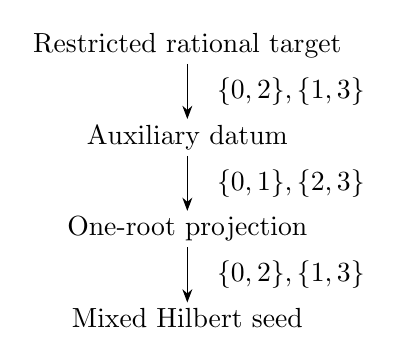
\begin{tikzpicture}[>=Stealth,node distance=7mm,every node/.style={inner sep=2pt}]
\node (target) {Restricted rational target};
\node[below=of target] (aux) {Auxiliary datum};
\node[below=of aux] (proj) {One-root projection};
\node[below=of proj] (seed) {Mixed Hilbert seed};
\draw[->] (target) -- node[right=3mm] {\(\{0,2\},\{1,3\}\)} (aux);
\draw[->] (aux) -- node[right=3mm] {\(\{0,1\},\{2,3\}\)} (proj);
\draw[->] (proj) -- node[right=3mm] {\(\{0,2\},\{1,3\}\)} (seed);
\end{tikzpicture}
\caption{Block orders for the three affine lines of Proposition~\ref{prop:count-two-three-lines}. In the indicated order the endpoint differences belong to the square-zero off-block ideal.}\label{fig:analytic-three-lines}
\end{construction}

\begin{proposition}[Three lines joining the rational target to the seed]\label{prop:count-two-three-lines}
In the even-order case, after the restriction of
Proposition~\ref{prop:count-two-tame-return} and at a deep layer
where the mixed seed is available, the rational target and that
seed are joined by affine interpolation from target to auxiliary datum,
then from the auxiliary datum to its one-root projection, and finally
from that projection to the seed. Write \(D_0,D_1,D_2,D_3\) for the four marked data in that order.
There are families \(\mathcal D_i\) over \(k[t]\), affine in the matrix
and frame coordinates, with
\[
           \mathcal D_i(0)=D_i,\qquad \mathcal D_i(1)=D_{i+1}
                         \qquad(0\le i<3).
\]
They preserve the marked flags, similitude,
diagonal normalization and the prescribed inertia characters.
\end{proposition}

\begin{proof}
\proofstep{Project to the one-root datum.}
In the even-order case the character \(B\) is trivial on the
decomposition groups above \(\ell\). On the deeper tower,
project the auxiliary global matrices to their diagonal
blocks in the order \(\{0,1\},\{2,3\}\). Do the same
to the local frames. These projections respect products
on the block lower triangular algebra; the symplectic
form pairs the two blocks, so the projected matrices and
frames still satisfy the same similitude and flag
identities. The projected residual representation has
only the off-diagonal entries of degree \(-w_\alpha\),
including the nonzero entry in position \((1,0)\).
In its projected frame the local triangular matrix is
diagonal, because the representation and frame are
lower triangular as well.

At each marked place, fix the frame's \((2,0)\) entry using the seed value \(e_v\):
\[
 (N_v)_{20}=e_v .
\]
Right-multiply the projected frame by \(U(0,e_v,0)\).
On the marked decomposition group the first and third diagonal characters agree. Cancelling this common character in the paired-product identity gives
\[
 d_0=d_2,\qquad d_0d_3=d_1d_2\quad\Longrightarrow\quad d_1=d_3 .
\] Thus the frame multiplier commutes with the
diagonal local matrix. It preserves the \((1,0)\) entry
and inserts \(e_v\) in position \((2,0)\).

\proofstep{Construct the three lines.}
The first line joins the restricted target to the
auxiliary datum. The second joins the auxiliary datum
to this one-root projection with the modified frame.
The third joins the projection to the reduced seed.
For the first and third lines, order the blocks as
\(\{0,2\},\{1,3\}\). Both endpoints have the same
diagonal blocks, by the common \((2,0)\) entry, the
paired \((3,1)\) entry determined by the alternating
form, and the fixed diagonal characters. In the third line the two endpoints have identical readings in the global and the frame coordinates at position \((2,0)\):
\[
 (\text{global entry},\text{marked frame entry})=(0,e_v).
\] The second line uses
\(\{0,1\},\{2,3\}\), with the same diagonal blocks by
the common \((1,0)\) entry and its paired \((3,2)\)
entry.

In each order, all differences are in the
square-zero ideal of strictly off-block matrices.
The adjoint preserves this ideal, since the form
pairs the two ordered blocks. To verify the interpolation, write any interpolated matrix
as \(M_0+t\Delta M\), with \(\Delta M\) in the square-zero ideal.
For two such matrices multiplication gives
\[
 (M_0+t\Delta M)(N_0+t\Delta N)
 =M_0N_0+t(M_0\Delta N+\Delta M N_0)
 =(1-t)M_0N_0+tM_1N_1 .
\]
The adjoint is linear and preserves the ideal, so the same
calculation applies to both the product identities and the
similitude identity. Applying the equality to the individual basis columns \(e_i\) reads the marked flag along each line:
\[
 R(s)(N_v e_i)=N_vD_v(s)e_i .
\] The
interpolants are defined over \(k[t]\) and preserve
the normalization and all marked characters.

The original target vertex uses the two cases of the
lattice and restriction calculation above. The auxiliary
vertex retains the nonzero \(-w_\Psi\) if present,
and otherwise has the same nonzero marked frame entry
as the target and the new \(-w_\alpha\) entry. The
third vertex uses the nonzero \(-w_\alpha\) entry and
the seed's nonzero frame entry. For the seed, let \(S_{\ne0}\) be the set of weights of nonzero entries in its prescribed support. The two allowed alternatives are
\[
 -w_\alpha\in S_{\ne0}\qquad\text{or}\qquad \{w_\beta,-w_\vartheta\}\subseteq S_{\ne0}.
\]
In the second alternative the \(w_\alpha\)-character must also be nontrivial on the marked local group.

These choices put the auxiliary fields before the
bounds on the deeper cyclotomic tower. The finite
set of ramified auxiliary primes and \(F_1\) are fixed
using the target over \(F_0\). The cocycle bound \(C\)
is taken at this tame base \(F_1\). Choose the deeper layer only after obtaining \(C\) over \(F_1\). If \(d_{\rm layer}\) denotes its degree, impose both the depth condition and
\[
 d_{\rm layer}\ge30(C+1)^2
\]
before constructing the mixed seed on that layer. The cup lift, the ramification removal and the
transport of the target are independent of this later
seed. Its frame entry is used only in the last two lines.
\label{cor:cohomology-count-two-chain-4}
\end{proof}

\endgroup

\clearpage
\section{Lean declaration concordance}
\label{sec:lean-concordance}

The first table pairs the zero statements with their Lean declarations. The subsequent
entries identify the declarations for the arithmetic estimate and for its analytic
application.

\subsection{The zero statements}
\label{sec:lean-zero-statements}

The three conclusions of Theorem~\ref{thm:claims} correspond to five declarations
in Levent Alp\"oge's \code{Main.lean}. Read across a row to pass from the mathematical assertion, including its domain, to
the corresponding declaration. The proposition types are defined in \code{Statements.lean}
and, for \code{RiemannHypothesis}, in Mathlib. The modulus and conductor correspond to Definition~\ref{def:dirichlet-modulus}.
The formal functions are
total on \(\C\), so the pole exception appears explicitly. For Dirichlet
characters \code{[NeZero q]} means \(q\ge 1\), and \code{1} denotes the
principal character modulo \(q\).
\cite{release-claim-files,mathlib-rh-definition,sutherland-exports}

\begin{center}
\small
\renewcommand{\arraystretch}{1.20}
\begin{tabular}{@{}p{.45\linewidth}@{\hspace{.035\linewidth}}p{.51\linewidth}@{}}
\textbf{Theorem~\ref{thm:claims}} & \textbf{Lean declaration} \\ \hline
(1) Every zero of \(\zeta(s)\) with \(s\ne1\) outside the negative even
integers has \(\RePart s=1/2\).
& \href{https://github.com/Deicyde/riemann-hypothesis/blob/a172c464fd4bcfc4f53e394dcba45d742b1409a6/src/Main.lean\#L4}{\code{riemannHypothesis}} (Mathlib formulation)\newline
\href{https://github.com/Deicyde/riemann-hypothesis/blob/a172c464fd4bcfc4f53e394dcba45d742b1409a6/src/Main.lean\#L6}{\code{riemannZeta\_eq\_zero\_re}} (explicit hypotheses). \\[.5em]
(2) For each \(q\ge1\) and \(\chi\bmod q\), \(L(s,\chi)\ne0\) if
\(\RePart s>1/2\) and either \(\chi\ne\chi_{0,q}\) or \(s\ne1\).
& \href{https://github.com/Deicyde/riemann-hypothesis/blob/a172c464fd4bcfc4f53e394dcba45d742b1409a6/src/Main.lean\#L8}{\code{LFunction\_ne\_zero\_of\_half\_lt\_re}}. \\[.5em]
(3) For each \(q\ge1\) and \(\chi\bmod q\), every zero in
\(0<\RePart s<1\) has \(\RePart s=1/2\).
& \href{https://github.com/Deicyde/riemann-hypothesis/blob/a172c464fd4bcfc4f53e394dcba45d742b1409a6/src/Main.lean\#L10}{\code{LFunction\_eq\_zero\_re}}. \\[.5em]
(3) The same assertion for a character of conductor \(q\).
& \href{https://github.com/Deicyde/riemann-hypothesis/blob/a172c464fd4bcfc4f53e394dcba45d742b1409a6/src/Main.lean\#L12}{\code{LFunction\_eq\_zero\_re\_of\_isPrimitive}}.
\end{tabular}
\end{center}

\subsection{Arithmetic and analytic dependencies}
\label{sec:lean-dependencies}

The correspondence begins with the passage from local cohomology lengths to the
analytic criterion. The subsequent groups give the declarations for the intermediate
geometric and arithmetic constructions.

\subsubsection{From local lengths to a prime-sum bound}
For the fields, coefficient twist and range of
Lemma~\ref{lem:dyadic-host}, restriction of strict classes goes
from \(E\) to \(L_m=E(i)\). Accordingly the local bound \eqref{eq:dyadic-host} used by \code{partA} has the length
over the larger field on the right:
\[
 V(E,2,j)\le 1+V(L_m,2,j).
\]
The relevant declarations are \code{compIndex}, \code{kerTwo}
and \code{shaTwo}. The bound applies separately at each twist
before summation over the original field. \cite{release-host-dyadic}

The local parameter and global compatibility in Appendix~\ref{sec:local-global}
correspond to \code{recTExists} and
\code{galoisLocalGlobalStrong\_recParameter}. \cite{release-local-map-laws}

The two applications of the character construction in
Lemma~\ref{lem:split-deletion-characters} correspond to
\href{https://github.com/Deicyde/riemann-hypothesis/blob/a172c464fd4bcfc4f53e394dcba45d742b1409a6/src/Development/AbelianVarietyTheory/Proofs/IwasawaDecomposition/HostDeltaCharacterInertialOrderFifteenExists.lean\#L76}{the character with inertia of order fifteen}.
The occurring lower signatures in Lemma~\ref{lem:initial-row-signature-tests}
correspond to \href{https://github.com/Deicyde/riemann-hypothesis/blob/a172c464fd4bcfc4f53e394dcba45d742b1409a6/src/Formalism/SharpRestriction/LevelLetterCocycles/BlochKatoPhases.lean\#L100-L116}{\code{goodS}}.
The local conditions used at a nonreference index are assembled in
\href{https://github.com/Deicyde/riemann-hypothesis/blob/a172c464fd4bcfc4f53e394dcba45d742b1409a6/src/Development/AutomorphicArithmetic/ThetaCorrespondence/ThetaPairLifts/ThirdPlaceSeries/GaloisInputs.lean\#L19-L29}{\code{galois\_inputs\_alt}}.

The two adjacent-rank identities in Proposition~\ref{prop:fitted-square-ratio-identity}
are \href{https://github.com/Deicyde/riemann-hypothesis/blob/a172c464fd4bcfc4f53e394dcba45d742b1409a6/src/Development/AbelianVarietyTheory/BlockTheory/DivisorBase/WeilTensorModels.lean\#L559-L581}{\code{StepBeta} and \code{StepAlpha}}.
Their product is \eqref{eq:fitted-square-tower}. The one-step minor identity
in Lemma~\ref{lem:minor-orbital-shift} corresponds to
\href{https://github.com/Deicyde/riemann-hypothesis/blob/a172c464fd4bcfc4f53e394dcba45d742b1409a6/src/Development/AbelianVarietyTheory/Proofs/FlagMeasures/LeadingMinorLineUnitAmplitudesLargeGaps.lean\#L359}{\code{minor\_line}}.

The plane and character comparison enters \code{core\_gm}.
The paired integral estimate is \code{onto\_path\_alt}, and
\code{row\_rRows\_stage0\_alt} places it on the common family.
\cite{release-joint-record,release-joint-selection}

The common analytic input for the five exports is the nonvanishing
of the primitive \(L\)-function on the range
\[
                \RePart s>1/2,\qquad (\chi,s)\ne(1,1).
\]
The five statements share the nonvanishing term \code{allChi}, supplied by
\begin{quote}
\code{UpperTheory.FinalTheorems.everyCharacter}.
\end{quote}
The reductions in Section~\ref{sec:deduction} use \code{rh\_of\_right},
\code{Claim.strip}, and \code{critLine}. \cite{release}

The family \(\mathcal K\) is \code{Level.cyc} applied to \(\psi\).
The passage to a positively weighted real sum is \code{level\_family}.
In \code{core\_gm} the exponent depends on the two error
parameters. The specialization in \code{topDesWin} gives the exponent
of \eqref{eq:arithmetic-window} in Proposition~\ref{prop:arithmetic}:
\[
 (e_D,e_L)=(2,0)\quad\Longrightarrow\quad
 \tfrac12+(e_D+e_L+7)\epsilon=\tfrac12+9\epsilon .
\]
For each fixed primitive \(\psi\), the family and its positive weights
are fixed before choosing \(0<\epsilon<\epsilon_0(\psi)\).
The interval statement retains the quantifier order
\[
   \forall Z\ge1\quad\exists Y>Z\quad\forall y\in[Y,Y^{3/2}],
       \qquad G_{\mathcal K(\psi),w_\psi}(y)\le y^{1/2+9\epsilon}.
\]
The localization argument in Section~\ref{sec:window}
corresponds to \code{WindowHypUOfWindowHyp} and
\code{landauWindow}. \cite{release}

The prime-pair choice in Lemma~\ref{lem:disjoint-common-pair-windows}
corresponds to \href{https://github.com/Deicyde/riemann-hypothesis/blob/a172c464fd4bcfc4f53e394dcba45d742b1409a6/src/Development/AutomorphicArithmetic/CharacterBoxes/WinPairs.lean}{\code{winPairs}}.
The use of one family in Proposition~\ref{prop:all-window-applications}
corresponds to \href{https://github.com/Deicyde/riemann-hypothesis/blob/a172c464fd4bcfc4f53e394dcba45d742b1409a6/src/Development/AutomorphicArithmetic/CharacterBoxes/DesWin.lean}{\code{topDesWin}}.
The last numerical substitution appears in Lemma~\ref{lem:uniform-numerical-application}.

The original cohomology window is \code{VWinAt}. The rescaling in
\code{winPairs} supplies the cutoff \(\lfloor x^{400}\rfloor\).
The rank chosen over the original auxiliary field is constructed by
\code{exists\_ranks\_rankVal\_frame} and satisfies \code{RankVal}.
Lemma~\ref{lem:rank-window} proves the comparison used by
\code{supplyOfAdmOf} to restrict the strict lengths to that rank.
Those lengths enter the cohomological contribution to the divisibility bound on every member in
Section~\ref{subsec:window-points}. \cite{release-host-to-numerator}

\subsubsection{Flag counts and the arithmetic degree}
Section~\ref{sec:flag-counts}, in particular Propositions~\ref{prop:flag-row-mass} and~\ref{prop:primitive-flag-means}, supplies the counts used in the arithmetic degree. The row mass, primitive means and
flag-class counts occur in \code{RowsRawMass.main},
\code{PrimMeanOne.main}, \code{PairMean.main},
\code{GenericMean.main} and \code{Partner.partners\_le}. The root
covolume bound corresponds to \code{covolume\_term}.
The Hodge degree in the geometric covolume calculation is
\code{Ch2Const} in Theorem~\ref{thm:hodge-surface-degree} of Section~\ref{sec:hodge-surface-degree}.
\cite{release,release-surface-uniform}
Section~\ref{sec:covolume-flag-test} computes the two
de Rham limits in \code{tendsto\_sieg\_sub\_vdmVal} and
\code{vdmVal\_tendsto} and the prime increments in
\code{Whole4.main}. The degree at the arithmetic cutoff is
\code{testVal\_of\_hhTest}. \cite{release-flag-difference,
release-flag-vandermonde,release-flag-finite,release-flag-test}

\subsubsection{Heights at the wall and on the selected cover}
Sections~\ref{subsec:flag-point-heights} and
\ref{subsec:flag-wall-positivity} supply the point heights and the positivity used at a wall. The entries below follow
these quantities from the jet calculation to the selected cover. The integral jets are \code{secJets4}.
The three heights are \code{htIntSt\_of\_hypotheses},
\code{BdHtProof.main} and \code{htUpSt}. The primewise degree
bound is \code{nefAt\_onObj}.
\cite{release-wall-jets,release-wall-lie-points,
release-wall-boundary,release-wall-dense,release-wall-dr-nef}

Sections~\ref{sec:flag-wall-slope} and
\ref{sec:flag-component-transfer} derive the fixed-cutoff
shape, its component mean, and the lower bound transferred
to the selected cover. The source comparison
is \code{srcSt\_of\_slopeSt}. Its transfer is
\code{deepSt\_of\_srcSt}, and the component height bound
is \code{heightAt\_of}. The separate Haar multiplier is the
\code{ratio} in \code{OneMeasureSizes}.
\cite{release-wall-shape,release-wall-volume,
release-wall-transfer,release-wall-height,release-wall-ratio}
Sections~\ref{subsec:component-rank-comparison} and
\ref{subsec:deep-arithmetic-degree} use one image degree
in the rank and height comparisons. Its position between the
two volume degrees in Proposition~\ref{prop:deep-moving-degree} corresponds to
\[
     V_Z(u')\le D_Z\le V_Z(u_1)
               \qquad\text{(\code{compDeg\_between}).}
\]
The rank and height declarations are \code{rkC\_le},
\code{share\_of\_toroidal}, \code{rk\_le} in the small-scale
rank comparison, and \code{deg\_bound\_of\_claim\_numbers}.
\cite{release-component-rank,release-component-hs}
The two bounds on the determinant columns of Proposition~\ref{prop:component-arithmetic-degree}
enter the same
\href{https://github.com/TomasOrtega/RH/blob/a6ac91a412dcbaab31801355ec5707024a71bf65/extracted/lean/src/Development/AbelianVarietyTheory/Proofs/DivisorProofs/SlopeLowerBoundTopLatticeOffHypersurface.lean\#L160-L165}{determinant-line degree estimate}.
Its finite-place input is coefficient integrality after the linear substitution.
Its infinite-place input is the bound on the unit spheres in \eqref{eq:hs-unit-sphere-beta}.

For the weight shift in Lemma~\ref{hyp:covolume-shift-costs},
the component evaluation norm is compared with the same theta product
in the following declarations:
\[
\begin{array}{ll}
 M_Z\lambda^2<b\quad\text{(Lemma~\ref{lem:deep-thin-evaluation})}&\href{https://github.com/Deicyde/riemann-hypothesis/blob/a172c464fd4bcfc4f53e394dcba45d742b1409a6/src/Development/AbelianVarietyTheory/Proofs/DivisorProofs/FrameExponentialVolumeLarge.lean#L67}{\code{thin\_bergOn}}\\
 M_Z\lambda^2\ge b\quad\text{(Lemma~\ref{lem:deep-thick-evaluation})}&\href{https://github.com/Deicyde/riemann-hypothesis/blob/a172c464fd4bcfc4f53e394dcba45d742b1409a6/src/Development/AbelianVarietyTheory/Proofs/DivisorProofs/FrameExponentialVolumeSmall.lean#L127}{\code{thick\_bound}}\\
 a(y)^3\le e^\beta\mathcal B_{u_1,Z}(y)&\href{https://github.com/Deicyde/riemann-hypothesis/blob/a172c464fd4bcfc4f53e394dcba45d742b1409a6/src/Development/AbelianVarietyTheory/Proofs/DivisorProofs/ExistsCarryingSectionOrders.lean#L268}{\code{theta\_le\_bergman}}
\end{array}
\]

\begin{center}
\begin{tabular}{@{}ll@{}}
Lemma~\ref{lem:adjoint-etale-fibre} &
\href{https://github.com/TomasOrtega/RH/blob/a6ac91a412dcbaab31801355ec5707024a71bf65/extracted/lean/src/Development/AbelianVarietyTheory/Proofs/DivisorProofs/SectionsSeparateQuotientGenericFibreDescends.lean\#L282}{\code{separate\_numberField}}\\
Lemma~\ref{lem:deep-short-orbit-section} &
\href{https://github.com/TomasOrtega/RH/blob/a6ac91a412dcbaab31801355ec5707024a71bf65/extracted/lean/src/Development/AbelianVarietyTheory/Proofs/DivisorProofs/SectionsSeparateQuotientGenericFibreDescends.lean\#L405}{\code{sections\_separate\_quotient\_fibre}}
\end{tabular}
\end{center}

\subsubsection{Local densities, amplitudes and row sums}
The complex orbital calculation in Section~\ref{sec:orbital-germ}
corresponds to \code{germ\_core}. For the passage from local densities to a word pairing in
Section~\ref{sec:word-pairing}, the corresponding declarations are grouped by the
quantity computed. \cite{release}
\begin{itemize}
\item Terminal density positivity in \code{topDensNonnegOfKappa}
\item Signed derivatives in \code{one\_letter\_density\_estimate}
\item Compact radial identities in \code{actual\_compact\_theorem}
\item Capelli recurrences in \code{residue\_first\_move\_holds}
  and \code{residue\_second\_move\_holds}
\end{itemize}

Section~\ref{sec:local-amplitudes} follows the Schur and
Weil identities in \code{AmpKF0} and the critical-level estimate
\begin{quote}
\code{critical\_threshold\_lower\_bound}.
\end{quote}
The uniform Bessel scale of Section~\ref{sec:bessel-periods}
corresponds to \code{BesselSettingUniformConstant} and
\code{BesselFormalDegreePairing}. The three row sums in
Section~\ref{sec:row-sums} follow \code{rows\_ND\_record},
\code{rows\_Deg\_record} and \code{corank\_one\_bound\_of\_fibres}.

For the first length in Proposition~\ref{prop:paired-frame-moments},
the scalar for a single shift and the sum of the squared projection
norms have separate counterparts:
\[
\begin{array}{ll}
 |\kappa_s|^2 d_\mu/d_{\mu-e_s}\le T_zB_0^4
     &\href{https://github.com/Deicyde/riemann-hypothesis/blob/a172c464fd4bcfc4f53e394dcba45d742b1409a6/src/Development/AbelianVarietyTheory/Proofs/JetHarmonics/FamilySetupMomentGrowth.lean#L38}{\code{dual\_step\_bound}}\\
 \sum_s\|\mathrm{pr}_s(e_c\otimes w)\|^2
       \le(6B_v)^{2m}\|w\|^2 &\href{https://github.com/Deicyde/riemann-hypothesis/blob/a172c464fd4bcfc4f53e394dcba45d742b1409a6/src/Development/AbelianVarietyTheory/Proofs/JetHarmonics/UnitaryGlProjectionLevelSumSqLe.lean#L10}{\code{lev\_proj\_and\_sum\_sq\_le}}
\end{array}
\]
Lemma~\ref{lem:equal-word-generic-corank-one} obtains the
same-word bound from the
\href{https://github.com/Deicyde/riemann-hypothesis/blob/a172c464fd4bcfc4f53e394dcba45d742b1409a6/src/Formalism/SharpRestriction/CuspSpanNormBounds/CayleyDegreeNondegeneracy/RowsCnt.lean\#L273-L391}{two orientations of the flag count}.
The same-word generic bound in the fixed development is assembled in
\href{https://github.com/Deicyde/riemann-hypothesis/blob/a172c464fd4bcfc4f53e394dcba45d742b1409a6/src/Formalism/LocalToGlobal/SiegelLatticeTheory/CokernelGLCounts/RankPointCounts/MainEqCut.lean\#L259}{\code{rowGenJoint\_of}}.

The common integral lattice in Lemma~\ref{lem:nonprimitive-diagonal}
corresponds to the
\href{https://github.com/Deicyde/riemann-hypothesis/blob/a172c464fd4bcfc4f53e394dcba45d742b1409a6/src/Formalism/SharpRestriction/CuspSpanNormBounds/LatticeGluingRadicals.lean\#L2254-L2275}{equality of the projected congruence lattices}.

For the single-word zero-Gram calculation in
Section~\ref{subsec:zero-gram-diagonal}, the fixed-label and
operator estimates correspond to
\href{https://github.com/leanprover-community/riemann-hypothesis/blob/a172c464fd4bcfc4f53e394dcba45d742b1409a6/src/Development/AbelianVarietyTheory/Proofs/DecoratedLatticeProofs/PairsAmplitudeBoundOfTypeBound.lean\#L20}{\code{pairsDegOfType\_holds}}
and
\href{https://github.com/leanprover-community/riemann-hypothesis/blob/a172c464fd4bcfc4f53e394dcba45d742b1409a6/src/Development/AbelianVarietyTheory/Proofs/DecoratedLatticeProofs/TermSumBoundOfPairsAmplitude.lean\#L11}{\code{termSumBound\_of\_pairsAmplitude}}.
The estimate on the selected parameters occurs in
\href{https://github.com/leanprover-community/riemann-hypothesis/blob/a172c464fd4bcfc4f53e394dcba45d742b1409a6/src/Development/AbelianVarietyTheory/Proofs/DecoratedLatticeProofs/DegenerateTermsAndCollisionBoundsUniformWidths.lean\#L57}{\code{degenerate\_and\_collisions\_uncond}}.

\subsubsection{From the projector trace to the fitted row}
Sections~\ref{sec:count} and \ref{sec:selected-row-gram}
take the projector trace to the selected row. Its transport occurs in
\code{count\_\allowbreak{}rows\_\allowbreak{}class\_\allowbreak{}of\_\allowbreak{}count\_\allowbreak{}class}, the preliminary diagonal occurs in \code{puNZ\_\allowbreak{}of\_\allowbreak{}sDiag}, and the selected Gram estimates occur in
\code{theoremS\_\allowbreak{}transport\_\allowbreak{}link\_\allowbreak{}zero}. The numerical range for the
projection in Proposition~\ref{prop:lowest-type-polar-decay}
corresponds to \code{formulaGap} in the released proof.
\cite{release-selected-row-gram}

The lattice slope in Section~\ref{subsec:fitted-test-slope}
(Proposition~\ref{prop:fitted-coefficient-slope}) and the matched square
in Section~\ref{subsec:fitted-square-ratios}
(Proposition~\ref{prop:fitted-square-ratio-identity}) correspond to \code{gridTestLattice\_\allowbreak{}largestSlope\_\allowbreak{}bound},
\code{sqRatio\_\allowbreak{}mem\_\allowbreak{}of} and \code{square\_\allowbreak{}ratio\_\allowbreak{}valuation\_\allowbreak{}without\_\allowbreak{}norm\_\allowbreak{}formula}.
\cite{release-fitted-test-slope,release-fitted-square,release-fitted-square-height}

Section~\ref{subsec:fitted-row-height} follows
\code{rowFun\_\allowbreak{}at\_\allowbreak{}gridA\_\allowbreak{}alt} for the field and row choice.
The grid matrix in \eqref{eq:fitted-common-fourier} satisfies
a simultaneous identity for the selected tuples,
\[
 \Psi\iota_t P_t=r_t^{-1}V'(t).
\]
The signed slope estimate for this single descended map uses
\code{grid\_function\_bound}.
\cite{release-fitted-row-grid,release-fitted-row-height}
The marked signature and integral presentations of
Paragraph~\ref{subsec:marked-localization} follow
\code{exists\_desc\_of\_isKsForm}, \code{pre\_cut\_alt},
\code{conclusion\_split\_alt} and the local table in
\begin{quote}
\code{linkN\_of\_twGood\_galoisPreconditions}.
\end{quote}
Paragraph~\ref{par:marked-height-limit} uses \code{funSharp\_pt\_alt}
at the row space at the refined level and the weighted height bound
\begin{quote}
\code{height\_bound\_of\_component\_bounds}.
\end{quote}
\cite{release-marked-family,release-marked-rows,release-marked-sharp,release-frame-height}

\subsubsection{Translates, length moments and periods}
The scale and translate construction in
Section~\ref{subsec:window-points} follows \code{kitS} and
\code{designS}. For the data at one point, the single-translate input enters through
\code{objCP\_and\_of\_recExP}. The two coefficient-field
choices follow \code{recAtG\_of\_two\_passes}.
\cite{release-window-design,release-window-objects,release-window-two-pass}

The group majorant of Section~\ref{sec:xi} is
\code{xiExists}, with the two inductions
\code{aStepSucc\_of} and \code{bStepSucc\_of}.
\cite{release}

For the two length moments see \code{amplitude\_moments\_gap}
and \code{momBd\_both}. For the quotient integral see
\code{fibre\_bound} and \code{abs\_core}.
The adelic normalization in Section~\ref{sec:absolute} uses
\code{pinned\_root}, \code{amp\_lift} and
\code{hsNormSq\_amp\_loc}. \cite{release}

Section~\ref{sec:transport} uses \code{kerX\_of\_clsPinD},
\code{comb\_eq\_sum\_cells}, \code{valX} and the joint relation
\code{MainX}. Lemma~\ref{lem:nonzero-word-reference-entry} uses the reference
functional and the tuple coefficients in
\href{https://github.com/Deicyde/riemann-hypothesis/blob/a172c464fd4bcfc4f53e394dcba45d742b1409a6/src/Development/AutomorphicArithmetic/ThetaCorrespondence/ThetaPairLifts/ThirdPlaceSeries/RelOfLinks.lean\#L30-L51}{\code{rel\_of\_links\_alt}}.
In the notation of the two pairings this correspondence is
\[
     p_*=(h_0/d_0) A_*,\qquad c_t=s_{\rm col}\,h_t/d_t .
\]

The fixed-level support in Section~\ref{subsec:fixed-level-support}
uses the declarations below. \cite{release-fixed-level-support}
\begin{quote}
\code{oneIndexAt\_of\_classAt\_supportAt}\\
\code{doubleStep\_of\_pureCol\_pureRow}\\
\code{gsupp\_of\_local}
\end{quote}
For the valuation see
\begin{quote}
\code{vw\_eq\_zero\_of\_unitRatio}.
\end{quote}
\cite{release}

\subsubsection{Point selection and the local maps}

The common top set in Section~\ref{subsec:frobenius-selection}
is \code{topsChoiceH}, with the prescribed proportions in the cosets of \(A_0\) from
\code{topsGroup}. The choice of the top set is followed by a second choice of translates. This set and
its progression bounds are \code{hostThickExists} and \code{HostThickOrbit}.
\cite{release}

The finite-place analysis in Section~\ref{sec:finite-valuations}
uses the formal exponent estimates \code{ThmAGauss7}, the CM
identities \code{CM2}--\code{CM4} and the prime-to-\(p\)
translation estimate \code{TransUnit}. The determinant and
finite Gauss factors of Section~\ref{subsec:theta-normalization}
give \code{KappaExists}, \code{LocalStandard} and
\code{KernelRatio}. \cite{release}

\subsubsection{Determinants, segment ranks and integral column maps}

To locate the two rank estimates, start with the bound for the graded determinant from
integral restriction in
\begin{quote}
\code{GramBoundUnconditionalPos}.
\end{quote}
Proposition~\ref{prop:mean-tied-rank} gives the segment estimate \eqref{eq:ties}, corresponding to \code{TheoremMC7}.
The mean on the actual segment lattice is \code{segment\_mean\_kappa\_bound} and the product of retained ranks is \code{rank\_alternative\_lower}.
The integral column factors and the correction of their symbols
in Sections~\ref{sec:column-lifts} and \ref{sec:symbol-correction}
give \code{lemma44\_identity\_of\_raw\_tail} and the paired edge test
\code{PairLiftAt}. The two harmonic
lattice maps are constructed in
\begin{quote}
\code{lattice\_maps\_of\_functor\_comparison}.
\end{quote}
{\raggedright
The rank sum is \code{rho\_sum\_bound\_of\_maps\_splitting}.
The bounded middle weights use \code{RestCloudMaps}.
The weighted sum and the box mean are \code{keyIneq\_of},
\code{avg\_of} and \code{midMean\_of}.
The target rank uses the neighbor pairing and
\code{KapIDef.mem}. \cite{release}\par}

\subsubsection{Edge tests and lifts from residue planes}
Section~\ref{sec:host-edge-tests} uses the finite map in
\code{StdSubAt} and the size hypotheses \code{HypIAt} and
\code{HypIIAt}. Propositions~\ref{prop:host-large-prime-test}
and~\ref{prop:host-small-prime-test} separate the two prime ranges. For the passage from the primewise tests to planes, Section~\ref{sec:plane-lifts}
gives the separating polynomial
\code{Rloc}, the normal-coordinate identities of \code{PointsLemma},
and the precision induction. The paired-path and digit lifts in
\code{classMap\_estimate\_of\_admissible} give the full order and the
true multidegrees. The target-rank implication
\code{goodRank\_of\_prim} uses the primitive tests on each plane.
The segment count, with the measure and box of
\eqref{eq:plane-coarse-rank}, is the rank estimate
\[
 \dim\overline\Lambda\ge q^{-rK}(1-Nr^2 k/Y)\prod_x D_k(b_x).
\]

The corresponding declarations are \code{good\_path\_weight}
and \code{restSum}. The return to the
original radices uses the degree and order comparisons in
\code{generator\_\allowbreak{}modulo\_\allowbreak{}uniformiser\_\allowbreak{}of\_adm}.
The source weight restoration uses \code{primStep\_of} and
\code{count\_of\_exact}.
The factorial and divided-derivative analyses give the local
inputs \code{DIG} and \code{DER} of \code{LiftBoundOfHypotheses}.
The corrected integral Gram polynomial gives \code{LiftBoundUniform}.
Section~\ref{par:plane-orbit} proves \code{RestMEM} on the exact
model. Sections~\ref{par:plane-uniform} and~\ref{par:plane-reassembly}
give the uniform choice of depth and \code{RestMemb}. Passing to
the dual plane gives \code{realAt\_gen}. The maps of
Section~\ref{par:plane-rho} and the normalized adjunction give
\code{RhoAt} and the restored \code{TestAt}. \cite{release}

\subsubsection{Index and discriminant at the selected point}
The integral type cut of Section~\ref{subsec:selected-cut}
is built in \code{CFacts} and \code{ExistsGood}.
At the next stage the family carrying this same cut occurs in \code{LinkNFam}. The local
congruence estimate and its weighted passage to the
division numerator use \code{EndomorphismIndexBound}
and \code{ExportBoundOfAdmissible}. \cite{release}

The branch comparison in \eqref{eq:slice-order-comparison} uses
the integral point realization in the module on curve lifting.
For the shifted trace lattice of \eqref{eq:slice-discriminant-order},
the identity corresponding to \code{HDiscAG} reads
\[
 v_\lambda(\Delta)+2\sum_{Z,w\mid\lambda} f_w n_w(\tau)
       =2I^{\mathrm{ff}}_\lambda+t_\lambda .
\]
The weighted index \eqref{eq:geometric-four-terms} is
\code{sumGP4}; the bounds for both runs are \code{conclAtM\_of\_atMInputs}. The baseline and auxiliary
comparison use \code{nusOf\_eq\_ram\_mul\_nuStarAt} and
\code{combBound\_alg}. The common order and precision come from
\code{pageRun\_record}. \cite{release-selected-points,release-slice-orders,release-run-remainder,release-finite-point-depth,release-slice-scale-record}
The finite norm and dimension bound on those same weights come
from \code{net\_at\_run}. The arithmetic chart and generator
family with that norm passes through \code{inputsNet\_recPlus}
and \code{inputsR\_of\_inputsNet}. \cite{release-slice-net-evaluation,release-slice-net-index}

\subsubsection{The split frame and the common twist}
At a split point, \code{Norm.rN} and \code{design\_normalized}
give the frame. With the frame so normalized, the row comparison uses \code{clause4GK},
\code{clause5Row} and \code{rowTie\_disp}.
The character tests use \code{locQ}, \code{locS\_g}
and \code{locS\_pde}. For the supported determinant see
\code{GlobalConcreteOf}. The initial marks and tame polynomial
are constructed in \code{Exists}\allowbreak\code{Decomposition}\allowbreak\code{Setting} and
\code{Exists}\allowbreak\code{Inertia}\allowbreak\code{Charpoly}\allowbreak\code{Factor}\allowbreak\code{Of}\allowbreak\code{Tame}\allowbreak\code{Type}. The common twist
uses the two theta determinant calculations in
\code{PropE}\allowbreak\code{Of}\allowbreak\code{Admissible} and \code{Aeval}\allowbreak\code{One}\allowbreak\code{Sub}\allowbreak\code{One}, the
Selmer presentation, and the simultaneous torsion specialization
in \code{IsAuxiliary}\allowbreak\code{Place}\allowbreak\code{Family}\allowbreak\code{AtLevel}\allowbreak\code{Mono}. Its passage to the
retained point is \code{twist\_kills\_selmer}. The same character
is used in both comparisons in Proposition~\ref{prop:one-retained-character}.
\subsubsection{Selmer orders and integral period transfers}
For the Selmer order bound, the construction of the ray characters uses \code{delOf}. The signature obstruction
count gives the square presentation. The residual pencil and
the one-pair extension give the coefficient bounds in
\code{ResidualSelmer}\allowbreak\code{DeterminantOrderBound}
and \code{AntiOfKer}, assembled in
\code{bound\_mod\_two\_of\_hypothesis}. \cite{release}

Sections~\ref{subsec:incident-sections} and~\ref{subsec:second-period}
identify the geometric input to \eqref{eq:tag-p7} and sum its remaining places.
The comparison at all used pairs is \code{site\_cmpLite\_siteAdm}.
The maps on the indicated fibers are \code{site\_law\_xiIn}
and \code{xiEx\_theta\_general}. The calculations at the prime assigned to the sequence
in Sections~\ref{subsec:word-period}--\ref{subsec:word-projection},
including the transfer in Proposition~\ref{prop:word-prime-transfer}, use \code{ukTerm\_of\_moveStep}, the measure and finite projections
in \code{jetMoments} and the sharp transfer
\code{levelChainSharpColumnValuation}\allowbreak\code{\_of\_stability}.
\cite{release-site-reading,release-second-period,release-word-measure,release-word-transfer}

\paragraph{The two level realizations.}
The indices of the correspondences have the order
\[
 (K_s,K_0,K;\,1,\delta,\delta')\ \longmapsto\ (\varphi_i)_i
      \ \longmapsto\ (K_s,K_0,K';\,P')
      \ \longmapsto\ (P'_{p_0},P'_{p_1}).
\]
The ordered choice in Construction~\ref{hyp:family-prescribed-realization} corresponds to
\href{https://github.com/Deicyde/riemann-hypothesis/blob/a172c464fd4bcfc4f53e394dcba45d742b1409a6/src/Development/AutomorphicArithmetic/CharacterBoxes/KitS.lean\#L14}{\code{kitS}}, which takes the object-existence predicate \code{ObjCP} as an argument. For a specified row the comparison of forms, including its lattice, is
\href{https://github.com/Deicyde/riemann-hypothesis/blob/a172c464fd4bcfc4f53e394dcba45d742b1409a6/src/Development/AbelianVarietyTheory/Proofs/SatakeParameters/RowFormsMatchPeriodMapOfFurtherProperties.lean\#L131}{\code{rowPin\_of\_rx}}.

The coordinate cusp space and its full set of norm tests in Lemma~\ref{lem:constructed-signed-coefficient-row} correspond to \href{https://github.com/Deicyde/riemann-hypothesis/blob/a172c464fd4bcfc4f53e394dcba45d742b1409a6/src/Formalism/LocalToGlobal/IndefiniteReal/FWExist.lean\#L466}{\code{formsN}} and \href{https://github.com/Deicyde/riemann-hypothesis/blob/a172c464fd4bcfc4f53e394dcba45d742b1409a6/src/Formalism/LocalToGlobal/IndefiniteReal/FWExist.lean\#L600}{\code{tieN}}. Its full integral span corresponds to \href{https://github.com/Deicyde/riemann-hypothesis/blob/a172c464fd4bcfc4f53e394dcba45d742b1409a6/src/Development/AbelianVarietyTheory/Proofs/DivisorProofs/IntegralCuspFormsFullLattice.lean\#L17}{the full-lattice argument}. The simultaneous component normalization of Lemma~\ref{lem:placed-row-reading-phase} and the measured lattice are given by \href{https://github.com/Deicyde/riemann-hypothesis/blob/a172c464fd4bcfc4f53e394dcba45d742b1409a6/src/Development/AbelianVarietyTheory/Proofs/IwasawaDecomposition/ExistsGeometricHalfPhaseOneOverLawfulCore.lean\#L29}{the phase-one construction} and \href{https://github.com/Deicyde/riemann-hypothesis/blob/a172c464fd4bcfc4f53e394dcba45d742b1409a6/src/Development/AbelianVarietyTheory/Proofs/IwasawaDecomposition/ExistsLiftSpacesOverDefiniteForms.lean\#L128}{the measured multiplicity coordinates}. The two scalar conventions for the split Hecke action occur in \href{https://github.com/Deicyde/riemann-hypothesis/blob/a172c464fd4bcfc4f53e394dcba45d742b1409a6/src/Development/AbelianVarietyTheory/Proofs/TwistedOperators/HeckeReadTie.lean\#L51}{the Hecke reading formula}.

On the copied coordinates the correspondences satisfy
\[
        N'_{v,y}(jz)=N_{v,y}(z),\qquad
          T'(jz)=j(Tz) .
\]
The copy of the reference row, including its norms, appears in \href{https://github.com/Deicyde/riemann-hypothesis/blob/a172c464fd4bcfc4f53e394dcba45d742b1409a6/src/Development/AbelianVarietyTheory/Proofs/IwasawaDecomposition/FormsLExistsBaseChangeCoordinates.lean\#L11}{the scalar extension of the coefficient coordinates}. The construction with a new tuple and the assembly of the final member appear in \href{https://github.com/Deicyde/riemann-hypothesis/blob/a172c464fd4bcfc4f53e394dcba45d742b1409a6/src/Development/AutomorphicArithmetic/ThetaCorrespondence/ThetaPairLifts/ThirdPlaceSeries/FiniteLevelAndSecond.lean\#L72}{the second specialization} and \href{https://github.com/Deicyde/riemann-hypothesis/blob/a172c464fd4bcfc4f53e394dcba45d742b1409a6/src/Development/AbelianVarietyTheory/Proofs/IwasawaDecomposition/LayeredAutomorphicDataExistsOfTwoPasses.lean\#L29}{the two-pass construction}. Both auxiliary covers of that member occur in \href{https://github.com/Deicyde/riemann-hypothesis/blob/a172c464fd4bcfc4f53e394dcba45d742b1409a6/src/Development/AutomorphicArithmetic/ThetaCorrespondence/ThetaPairLifts/ThirdPlaceSeries/ExistsRunsAt.lean\#L18}{the choice of the two runs}.

\subsubsection{Integral frames and residual operators}
The declarations below correspond to the prescribed depth, the integral frames and the operators used in the polynomial lift. Lemma~\ref{lem:fitted-completed-nonvanishing} gives the period at that depth. Lemma~\ref{hyp:selected-orbital-coefficient-bounds} derives the operator normal form on the realized row.

The common finite model in Lemma~\ref{lem:flag-finite-frobenius-model} corresponds to
\href{https://github.com/Deicyde/riemann-hypothesis/blob/a172c464fd4bcfc4f53e394dcba45d742b1409a6/src/Development/AbelianVarietyTheory/Proofs/DivisorProofs/ChainCoverOfHyp.lean\#L240}{\code{chainCoverSt}}. The local eigenline metric in Proposition~\ref{prop:flag-cutoff-test} corresponds to
\href{https://github.com/Deicyde/riemann-hypothesis/blob/a172c464fd4bcfc4f53e394dcba45d742b1409a6/src/Development/AbelianVarietyTheory/Proofs/DivisorProofs/LocalHeightPrimeComparison.lean\#L418}{\code{lg\_eigA}}.

\begin{construction}
\begin{tabular}{@{}p{.46\linewidth}@{\hspace{.035\linewidth}}p{.49\linewidth}@{}}
\toprule
Mathematical comparison & Fixed source \\
\midrule
Depth of the companion level in Lemma~\ref{lem:fitted-depth-allowance}
& \href{https://github.com/Deicyde/riemann-hypothesis/blob/a172c464fd4bcfc4f53e394dcba45d742b1409a6/src/Development/AbelianVarietyTheory/Proofs/TwistedOperators/GridDepthPaysEveryLoss.lean\#L148}{\code{depth\_pays}} (cost after the auxiliary prime and level have been chosen). \\
Lie quotient in Lemma~\ref{lem:flag-local-cyclotomic-chain}
& \href{https://github.com/Deicyde/riemann-hypothesis/blob/a172c464fd4bcfc4f53e394dcba45d742b1409a6/src/Development/AbelianVarietyTheory/Proofs/DivisorProofs/LLEquivLieTwist.lean\#L109}{\code{LL\_equiv\_lie\_twist}} (Frobenius on the quotient). \\
Maps from the Lie and differential lattices in Lemma~\ref{lem:flag-local-hodge-quotients}
& \href{https://github.com/Deicyde/riemann-hypothesis/blob/a172c464fd4bcfc4f53e394dcba45d742b1409a6/src/Development/AbelianVarietyTheory/Proofs/DivisorProofs/RingChainExists.lean\#L239}{\code{exists\_j\_rho\_lat}} (maps in the ring-level chain). \\
Integral and complex frames in Definition~\ref{hyp:terminal-cm-fibre-comparison}
& \href{https://github.com/Deicyde/riemann-hypothesis/blob/a172c464fd4bcfc4f53e394dcba45d742b1409a6/src/Development/AbelianVarietyTheory/Definitions/CMLattices/IntegralOf.lean\#L103}{\code{IsMetricAt}}, \href{https://github.com/Deicyde/riemann-hypothesis/blob/a172c464fd4bcfc4f53e394dcba45d742b1409a6/src/Development/AbelianVarietyTheory/Definitions/CMLattices/IntegralOf.lean\#L120}{\code{LieInt}} and \href{https://github.com/Deicyde/riemann-hypothesis/blob/a172c464fd4bcfc4f53e394dcba45d742b1409a6/src/Development/AbelianVarietyTheory/Definitions/CMLattices/IntegralOf.lean\#L130}{\code{SecInt}}. \\
Integration on the terminal matrix fibre and the dual polynomial lift
& \href{https://github.com/Deicyde/riemann-hypothesis/blob/a172c464fd4bcfc4f53e394dcba45d742b1409a6/src/Formalism/HermitianCurvature/HermitianCurvatureProofs/FibreIntegralCells.lean\#L61}{\code{fibre\_integral\_cells}} and \href{https://github.com/Deicyde/riemann-hypothesis/blob/a172c464fd4bcfc4f53e394dcba45d742b1409a6/src/Development/AbelianVarietyTheory/Proofs/JetHarmonics/PolynomialLiftDualOperatorCombination.lean\#L537}{\code{polyLift\_rhv}} (the latter takes the operator data and its normal form as inputs). \\
\bottomrule
\end{tabular}
\caption{Corresponding declarations for the level, integral frames and orbital actions.}\label{fig:integral-orbital-concordance}
\end{construction}

\subsection{Lean declarations by source file}
\label{sec:additional-concordance}

To look up a construction by file, read across from its mathematical discussion to the
declarations at the fixed revision.
Within each group the files are in alphabetical order. \cite{release}

\subsubsection{Family, rank and prime selection}
When matching the rank selection in Lemma~\ref{lem:rank-window}, keep the strict upper
endpoint of the twist range in view:
\[
 1\le j<t,\qquad t\le\lfloor x^{400}\rfloor.
\]
{\small
\begin{longtable}{@{}>{\raggedright\arraybackslash}p{.37\linewidth}@{\hspace{.025\linewidth}}>{\raggedright\arraybackslash}p{.605\linewidth}@{}}
\toprule
Mathematical source & Lean declarations \\ \midrule
\endfirsthead
\toprule
Mathematical source & Lean declarations (continued) \\ \midrule
\endhead
\bottomrule
\endlastfoot
\hyperlink{source-automorphic-realization}{automorphic-realization.tex} & \code{Fine} \\[2pt]
\hyperlink{source-auxiliary-coordinates}{auxiliary-coordinates.tex} & \code{del\allowbreak{}Of}, \code{delUTie\_\allowbreak{}of\_\allowbreak{}exists},
\code{is\_\allowbreak{}univ\_\allowbreak{}char\_\allowbreak{}local} \\[2pt]
\hyperlink{source-family-window}{family-window.tex} & \code{top\allowbreak{}Des\allowbreak{}Win}, \code{vwin\_\allowbreak{}of\_\allowbreak{}row} \\[2pt]
\hyperlink{source-level-primes}{level-primes.tex} & \code{Norm\allowbreak{}One}, \code{Short\allowbreak{}Norm}, \code{type\allowbreak{}PrimesN}, \code{Upper\allowbreak{}Theory.T3.level\allowbreak{}Data} \\[2pt]
\hyperlink{source-lift-exponent-models}{lift-exponent-models.tex} & \code{coefL}, \code{l\allowbreak{}Incl\_\allowbreak{}sum\allowbreak{}Exp}, \code{Frame\allowbreak{}Statement},
\code{maximal\allowbreak{}Ideals\_\allowbreak{}meeting\_\allowbreak{}subspace\_\allowbreak{}cover},
\code{Jrec7} \\[2pt]
\hyperlink{source-lift-exponent-primes}{lift-exponent-primes.tex} & \code{cut\_\allowbreak{}incl}, \code{Ex\allowbreak{}Cut} \\[2pt]
\hyperlink{source-lift-pieri-cost}{lift-pieri-cost.tex} & \code{expL\_\allowbreak{}real} \\[2pt]
\hyperlink{source-lift-weight-exchange}{lift-weight-exchange.tex} & \code{weight\_\allowbreak{}lattice\_\allowbreak{}of\_\allowbreak{}norm} \\[2pt]
\hyperlink{source-prime-cost-sums}{prime-cost-sums.tex} & \code{Mem\allowbreak{}Primes\allowbreak{}Over\allowbreak{}Of\allowbreak{}Mem}, \code{NEqRZero\allowbreak{}MulXPow}, \code{Export\allowbreak{}Bound\allowbreak{}Of\allowbreak{}Admissible} \\[2pt]
\hyperlink{source-prime-selection}{prime-selection.tex} & \code{mean\allowbreak{}SqK}, \code{QH.stage}, \code{pair\allowbreak{}Ex} \\[2pt]
\hyperlink{source-row-metric}{row-metric.tex} & \code{Frame\allowbreak{}Pf}, \code{ModelFPf}, \code{Univ\allowbreak{}Link\allowbreak{}Pf} \\[2pt]
\hyperlink{source-row-mixed}{row-mixed.tex} & \code{Mix\allowbreak{}Local} \\[2pt]
\end{longtable}}

\subsubsection{Integral lattices, twists and local lengths}
To compare lengths across coefficient extensions, the entries in this group use the
normalization of Lemma~\ref{lem:retained-dvr-normalized-length} on a coefficient DVR
\(O\):
\[
 e_O=\operatorname{ord}_O(\ell),\qquad \ell_O^{\rm norm}(M)=\operatorname{length}_O(M)/e_O \quad(M\text{ of finite length}).
\]
{\small
\begin{longtable}{@{}>{\raggedright\arraybackslash}p{.37\linewidth}@{\hspace{.025\linewidth}}>{\raggedright\arraybackslash}p{.605\linewidth}@{}}
\toprule
Mathematical source & Lean declarations \\ \midrule
\endfirsthead
\toprule
Mathematical source & Lean declarations (continued) \\ \midrule
\endhead
\bottomrule
\endlastfoot
\hyperlink{source-congruence-determinant}{congruence-determinant.tex} & \code{Normalized\allowbreak{}Ring\allowbreak{}Data}, \code{Distinct\allowbreak{}Eigenvalue\allowbreak{}Corner\allowbreak{}Perturbation},
\code{Cup\allowbreak{}Kill\allowbreak{}Adm}, \code{Global\allowbreak{}Concrete\allowbreak{}Of}, \code{Global\allowbreak{}Module\allowbreak{}Of},
\code{Lift\allowbreak{}Exponent\allowbreak{}Column}, \code{Col\allowbreak{}Lx},
\code{Character\allowbreak{}Column\allowbreak{}Kernels\allowbreak{}Of\allowbreak{}Block\allowbreak{}ChiCOf\allowbreak{}Block\allowbreak{}Chi\allowbreak{}One} \\[2pt]
\hyperlink{source-division-length}{division-length.tex} & \code{linkN\_\allowbreak{}of\_\allowbreak{}gd}, \code{vv\allowbreak{}Record},
\code{divinN\_\allowbreak{}of\_\allowbreak{}hypV}, \code{jw\_\allowbreak{}le}, \code{Jrec7},
\code{jexpU\_\allowbreak{}le\_\allowbreak{}jrec7},
\code{sum\_\allowbreak{}exponent\_\allowbreak{}log\_\allowbreak{}le} \\[2pt]
\hyperlink{source-inert-long-orbit}{inert-long-orbit.tex} & \code{h\allowbreak{}Cor}, \code{jointB\_\allowbreak{}of\_\allowbreak{}large},
\code{final\allowbreak{}Arc\_\allowbreak{}holds}, \code{second\_\allowbreak{}rule\_\allowbreak{}first\_\allowbreak{}form}, \code{thmE\_\allowbreak{}of}, \code{RowBLong.main} \\[2pt]
\hyperlink{source-inert-row-table}{inert-row-table.tex} & \code{arc\_\allowbreak{}setup\_\allowbreak{}theorem}, \code{sum\allowbreak{}AltW},
\code{arc\_\allowbreak{}length\_\allowbreak{}bound\_\allowbreak{}theorem},
\code{exists\_\allowbreak{}liftF\_\allowbreak{}le\_\allowbreak{}sg\_\allowbreak{}of\_\allowbreak{}thick},
\code{RowNT.main}, \code{rowL\_\allowbreak{}of\_\allowbreak{}all\allowbreak{}Thick},
\code{length\allowbreak{}Bound\allowbreak{}At\allowbreak{}Places\_\allowbreak{}of\_\allowbreak{}joint\allowbreak{}Cond} \\[2pt]
\hyperlink{source-inert-thick-word}{inert-thick-word.tex} & \code{H2Bound}, \code{kernel\_\allowbreak{}rank\_\allowbreak{}bound},
\code{content\allowbreak{}Bound\allowbreak{}Level\_\allowbreak{}of}, \code{Lemma\allowbreak{}Gs}, \code{LemmaDN},
\code{LemmaDN0}, \code{pass3}, \code{pass4},
\code{frobenius\_\allowbreak{}sq\_\allowbreak{}bound\_\allowbreak{}of\_\allowbreak{}local},
\code{lattice\_\allowbreak{}bound\_\allowbreak{}three\_\allowbreak{}six\_\allowbreak{}of},
\code{lattice\_\allowbreak{}bounds\_\allowbreak{}of\_\allowbreak{}local},
\code{openC\_\allowbreak{}of\_\allowbreak{}steps} \\[2pt]
\hyperlink{source-large-prime-length}{large-prime-length.tex} & \code{table\allowbreak{}Line\allowbreak{}Degree\allowbreak{}Two.Top\allowbreak{}Core} \\[2pt]
\hyperlink{source-numerator-sums}{numerator-sums.tex} & \code{Nu\allowbreak{}Le}, \code{NuQDUnit}, \code{Nu\allowbreak{}Host}, \code{Mem\allowbreak{}Primes\allowbreak{}Over\allowbreak{}Of\allowbreak{}Mem},
\code{Export\allowbreak{}Bound\allowbreak{}Of\allowbreak{}Admissible} \\[2pt]
\hyperlink{source-ramified-cyclotomic}{ramified-cyclotomic.tex} & \code{HypW}, \code{loc\allowbreak{}All} \\[2pt]
\hyperlink{source-retained-galois}{retained-galois.tex} & \code{Cyclotomic\allowbreak{}Norms.prime\allowbreak{}To\allowbreak{}Part}, \code{Exists\allowbreak{}Finite\allowbreak{}Chosen\allowbreak{}Set}, \code{EvOTaken\allowbreak{}All},
\code{Is\allowbreak{}Good} \\[2pt]
\hyperlink{source-retained-twist}{retained-twist.tex} & \code{Galois\allowbreak{}Side\allowbreak{}Twisted\allowbreak{}Selmer\allowbreak{}Auxiliary\allowbreak{}Primes}, \code{PropE}, \code{PropABCD},
\code{Steps}, \code{DelUTie}, \code{twisted\allowbreak{}Rho\_\allowbreak{}conj\_\allowbreak{}lat\allowbreak{}Tpsi},
\code{s\allowbreak{}Pi\allowbreak{}Top\_\allowbreak{}eq\_\allowbreak{}sTLoc},
\code{sT\_\allowbreak{}le\_\allowbreak{}s\allowbreak{}Len},
\code{twist\_\allowbreak{}kills\_\allowbreak{}selmer},
\code{thmS\_\allowbreak{}of\_\allowbreak{}selmer\_\allowbreak{}functor} \\[2pt]
\hyperlink{source-selected-cut}{selected-cut.tex} & \code{Nc}, \code{central\allowbreak{}Idem\allowbreak{}Coeff}, \code{exists\_\allowbreak{}good\_\allowbreak{}alt},
\code{Eigen\allowbreak{}Action\allowbreak{}At\allowbreak{}Good\allowbreak{}Point}, \code{Card\allowbreak{}Roots\allowbreak{}Bar},
\code{map\_\allowbreak{}Mj\allowbreak{}Sig\_\allowbreak{}eq},
\code{good\allowbreak{}Part\_\allowbreak{}of\_\allowbreak{}lifts} \\[2pt]
\hyperlink{source-small-prime-lengths}{small-prime-lengths.tex} & \code{loc\allowbreak{}All}, \code{LiftK}, \code{TBK}, \code{LiftKOf},
\code{Invariants\allowbreak{}Killed\allowbreak{}Over\allowbreak{}Cyclotomic}, \code{Jump\allowbreak{}And\allowbreak{}Length\allowbreak{}Of\allowbreak{}Admitted}, \code{Loc\allowbreak{}Num},
\code{Len\allowbreak{}Unit\allowbreak{}Invariants\allowbreak{}Le}, \code{Num\allowbreak{}Split}, \code{Num\allowbreak{}Cost}, \code{NRow\allowbreak{}Two},
\code{NRow\allowbreak{}Three} \\[2pt]
\hyperlink{source-special-prime-lengths}{special-prime-lengths.tex} & \code{HostJ} \\[2pt]
\hyperlink{source-split-selmer}{split-selmer.tex} & \code{Norm.rN}, \code{design\_\allowbreak{}normalized},
\code{Admissible\allowbreak{}At\allowbreak{}Good\allowbreak{}Points\allowbreak{}Of\allowbreak{}Coef\allowbreak{}Ring\allowbreak{}Taken\allowbreak{}At\allowbreak{}Live}, \code{row\allowbreak{}Mat\_\allowbreak{}at},
\code{row\allowbreak{}Tie\_\allowbreak{}disp}, \code{clause4GK}, \code{clause5Row},
\code{yt\allowbreak{}Target\_\allowbreak{}of}, \code{TBK}, \code{TbKOf},
\code{trivial\_\allowbreak{}bound\_\allowbreak{}target\_\allowbreak{}of\_\allowbreak{}psi},
\code{locQ}, \code{locS\_\allowbreak{}g}, \code{locS\_\allowbreak{}pde} \\[2pt]
\hyperlink{source-theta-cover-integrality}{theta-cover-integrality.tex} & \code{has\allowbreak{}Sum\_\allowbreak{}evR\_\allowbreak{}arc}, \code{ser\allowbreak{}Int\allowbreak{}At\_\allowbreak{}record},
\code{series\_\allowbreak{}bound}, \code{int\allowbreak{}Form\_\allowbreak{}descent\_\allowbreak{}below} \\[2pt]
\hyperlink{source-toric-twist}{toric-twist.tex} & \code{Jet\allowbreak{}Lift\allowbreak{}Main.exists\_\allowbreak{}jet\allowbreak{}Lift} \\[2pt]
\hyperlink{source-twist-euler}{twist-euler.tex} & \code{adm9}, \code{adm10}, \code{adm8}, \code{T3} \\[2pt]
\hyperlink{source-unramified-split-length}{unramified-split-length.tex} & \code{lift\_\allowbreak{}wach} \\[2pt]
\end{longtable}}

\subsubsection{Projections, periods and jets}
To follow a local period into the integral dual, use the shift in
Proposition~\ref{prop:finite-period-shift},
\[
 \tau_w=\lfloor\sigma_w\rfloor,\quad I=\prod_w\mathfrak p_w^{-\tau_w},\quad B(IN)\subseteq R^\vee.
\]
{\small
\begin{longtable}{@{}>{\raggedright\arraybackslash}p{.37\linewidth}@{\hspace{.025\linewidth}}>{\raggedright\arraybackslash}p{.605\linewidth}@{}}
\toprule
Mathematical source & Lean declarations \\ \midrule
\endfirsthead
\toprule
Mathematical source & Lean declarations (continued) \\ \midrule
\endhead
\bottomrule
\endlastfoot
\hyperlink{source-baseline-jets}{baseline-jets.tex} & \code{jets\_\allowbreak{}two\_\allowbreak{}of}, \code{term\_\allowbreak{}jets} \\[2pt]
\hyperlink{source-cm-models}{cm-models.tex} & \code{CM2}, \code{CM3}, \code{CM4}, \code{NRCM}, \code{Trans\allowbreak{}Unit} \\[2pt]
\hyperlink{source-curve-exponents}{curve-exponents.tex} & \code{first\_\allowbreak{}level\_\allowbreak{}on\_\allowbreak{}curve}, \code{b\allowbreak{}Hyp\allowbreak{}Curve},
\code{Til\allowbreak{}InvariantL\_\allowbreak{}of}, \code{Hyp\allowbreak{}Shape} \\[2pt]
\hyperlink{source-cyclic-jets}{cyclic-jets.tex} & \code{ThmAGauss}, \code{ThmAGauss7},
\code{local\_\allowbreak{}bound\_\allowbreak{}eleven\_\allowbreak{}comparison} \\[2pt]
\hyperlink{source-finite-valuations}{finite-valuations.tex} & \code{Zero\allowbreak{}Above}, \code{Eval}, \code{nprime\allowbreak{}Mu\_\allowbreak{}at}, \code{One\allowbreak{}Letter\allowbreak{}Radius},
\code{one\_\allowbreak{}letter\_\allowbreak{}unramified\_\allowbreak{}bound},
\code{Is\allowbreak{}Expansion}, \code{Indef\allowbreak{}Cols.into\allowbreak{}Dual}, \code{shift\allowbreak{}Ideal\_\allowbreak{}sg\allowbreak{}Fl} \\[2pt]
\hyperlink{source-frames}{frames.tex} & \code{FrameLA1}, \code{TheoremFSharp},
\code{each\_\allowbreak{}unit\_\allowbreak{}bound\_\allowbreak{}statement},
\code{ch\_\allowbreak{}top}, \code{Wall\allowbreak{}Pt}, \code{Chosen\allowbreak{}Wall} \\[2pt]
\hyperlink{source-integral-jets}{integral-jets.tex} & \code{Is\allowbreak{}Entry\allowbreak{}All} \\[2pt]
\hyperlink{source-prime-class-loss}{prime-class-loss.tex} & \code{loss\allowbreak{}Hyp\_\allowbreak{}at}, \code{joint\_\allowbreak{}core},
\code{losses\_\allowbreak{}of\_\allowbreak{}small\_\allowbreak{}share\_\allowbreak{}weight} \\[2pt]
\hyperlink{source-selected-class-counts}{selected-class-counts.tex} & \code{exists\_\allowbreak{}finset\_\allowbreak{}self\allowbreak{}Dual\_\allowbreak{}classes\_\allowbreak{}root\allowbreak{}Discr} \\[2pt]
\hyperlink{source-selected-period}{selected-period.tex} & \code{l\allowbreak{}Prj\_\allowbreak{}surj\_\allowbreak{}at\_\allowbreak{}alt}, \code{Div\allowbreak{}Rows3G},
\code{Div\allowbreak{}Rows3}, \code{Bessel\allowbreak{}Id} \\[2pt]
\hyperlink{source-terminal-period}{terminal-period.tex} & \code{Pair\allowbreak{}At\allowbreak{}Class.pair\_\allowbreak{}integral}, \code{Period\allowbreak{}Class\allowbreak{}Sum\allowbreak{}Weyl},
\code{Twisted\allowbreak{}Period\allowbreak{}Integral}, \code{period\_\allowbreak{}geTU} \\[2pt]
\hyperlink{source-unserved-period}{unserved-period.tex} & \code{lattice\_\allowbreak{}pairs\_\allowbreak{}odd\_\allowbreak{}degree\_\allowbreak{}isometric},
\code{jet\_\allowbreak{}bound\_\allowbreak{}ramified\_\allowbreak{}prime} \\[2pt]
\end{longtable}}

\subsubsection{The division estimates}
For the passage from a branch order to a lattice index, the relevant comparison on the
finite flat model is \eqref{eq:slice-order-comparison},
\[
 I_\lambda\le I^{\mathrm{ff}}_\lambda=\operatorname{length}_{R_0}\!\left(B(\tau)/\textstyle\sum_iR_0 b_i\right).
\]
{\small
\begin{longtable}{@{}>{\raggedright\arraybackslash}p{.37\linewidth}@{\hspace{.025\linewidth}}>{\raggedright\arraybackslash}p{.605\linewidth}@{}}
\toprule
Mathematical source & Lean declarations \\ \midrule
\endfirsthead
\toprule
Mathematical source & Lean declarations (continued) \\ \midrule
\endhead
\bottomrule
\endlastfoot
\hyperlink{source-paired-off-prime-trace}{paired-off-prime-trace.tex} & \code{c0'} \\[2pt]
\hyperlink{source-paired-row-indices}{paired-row-indices.tex} & \code{Weight\allowbreak{}Algebra.Concl} \\[2pt]
\hyperlink{source-run-index-length}{run-index-length.tex} & \code{MggK}, \code{g0 D}, \code{sumGP4},
\code{concl\allowbreak{}AtM\_\allowbreak{}of\_\allowbreak{}atMInputs} \\[2pt]
\hyperlink{source-selected-height-sections}{selected-height-sections.tex} & \code{Zb} \\[2pt]
\hyperlink{source-slice-budget}{slice-budget.tex} & \code{absA}, \code{z\allowbreak{}Base} \\[2pt]
\hyperlink{source-slice-heights}{slice-heights.tex} & \code{Ht\allowbreak{}Main} \\[2pt]
\hyperlink{source-slice-integrals}{slice-integrals.tex} & \code{phiFD\_\allowbreak{}eq\_\allowbreak{}zero\_\allowbreak{}at\_\allowbreak{}last\_\allowbreak{}index} \\[2pt]
\hyperlink{source-slice-interpolation}{slice-interpolation.tex} & \code{rhF} \\[2pt]
\hyperlink{source-slice-metrics}{slice-metrics.tex} & \code{PP0v}, \code{large}, \code{nbR}, \code{CovQ} \\[2pt]
\hyperlink{source-slice-orders}{slice-orders.tex} & \code{inputs\allowbreak{}Net\_\allowbreak{}rec\allowbreak{}Plus} \\[2pt]
\hyperlink{source-slice-scales}{slice-scales.tex} & \code{TO} \\[2pt]
\hyperlink{source-slice-short-analytic}{slice-short-analytic.tex} & \code{qq} \\[2pt]
\hyperlink{source-word-division}{word-division.tex} & \code{err\allowbreak{}On} \\[2pt]
\end{longtable}}

\subsubsection{Integral symbols and plane tests}
To follow the local factors into the plane test, compare their dimensions with the
retained rank of the coarse symbols in \eqref{eq:plane-coarse-rank},
\[
 \dim\overline\Lambda\ge q^{-rK}(1-Nr^2 k/Y)\prod_xD_k(b_x).
\]
{\small
\begin{longtable}{@{}>{\raggedright\arraybackslash}p{.37\linewidth}@{\hspace{.025\linewidth}}>{\raggedright\arraybackslash}p{.605\linewidth}@{}}
\toprule
Mathematical source & Lean declarations \\ \midrule
\endfirsthead
\toprule
Mathematical source & Lean declarations (continued) \\ \midrule
\endhead
\bottomrule
\endlastfoot
\hyperlink{source-block-pairing}{block-pairing.tex} & \code{Factorial\allowbreak{}Unit\allowbreak{}Decomposition}, \code{io\allowbreak{}Block}, \code{orth\allowbreak{}At},
\code{block\allowbreak{}Form\allowbreak{}At\_\allowbreak{}of},
\code{symbol\_\allowbreak{}form\_\allowbreak{}of\_\allowbreak{}orthogonality},
\code{ord\_\allowbreak{}all}, \code{Raw\allowbreak{}Tail\allowbreak{}At1}, \code{test\allowbreak{}Flat\allowbreak{}At1},
\code{paired\_\allowbreak{}lift\_\allowbreak{}at\_\allowbreak{}of\_\allowbreak{}identity} \\[2pt]
\hyperlink{source-column-lifts}{column-lifts.tex} & \code{Hyperplane\allowbreak{}Rank}, \code{Definite\allowbreak{}Rank\allowbreak{}One}, \code{col\allowbreak{}Fac},
\code{pl\allowbreak{}Sum\_\allowbreak{}seg}, \code{cols\allowbreak{}At\_\allowbreak{}of} \\[2pt]
\hyperlink{source-edge-transfer}{edge-transfer.tex} & \code{Tie\allowbreak{}Psi}, \code{Pair\allowbreak{}Lift\allowbreak{}At}, \code{admB2}, \code{Projection\allowbreak{}Lemma\allowbreak{}Base\allowbreak{}Level},
\code{Rest\allowbreak{}Cloud\allowbreak{}Maps},
\code{tensor\_\allowbreak{}bound\_\allowbreak{}of\_\allowbreak{}order\_\allowbreak{}bound},
\code{dle\_\allowbreak{}abs}, \code{tle\_\allowbreak{}abs} \\[2pt]
\hyperlink{source-graded-projectors}{graded-projectors.tex} & \code{Trace\allowbreak{}Isometry\allowbreak{}Weights}, \code{restricted\_\allowbreak{}saturation\_\allowbreak{}holds},
\code{Gram\allowbreak{}Bound\allowbreak{}Unconditional\allowbreak{}Pos} \\[2pt]
\hyperlink{source-host-edge-tests}{host-edge-tests.tex} & \code{ext\allowbreak{}Rec}, \code{Std\allowbreak{}Sub\allowbreak{}At}, \code{LPBase\allowbreak{}Change}, \code{Small\allowbreak{}Order\allowbreak{}Primes},
\code{adm6},
\code{linear\_\allowbreak{}programming\_\allowbreak{}input\_\allowbreak{}of\_\allowbreak{}hypotheses} \\[2pt]
\hyperlink{source-interpolation}{interpolation.tex} & \code{Degree\allowbreak{}Dichotomy}, \code{InstM.eps}, \code{LPprime}, \code{KapIDef.mem} \\[2pt]
\hyperlink{source-plane-digits}{plane-digits.tex} & \code{DIG}, \code{DER}, \code{V2} \\[2pt]
\hyperlink{source-plane-edge-covector}{plane-edge-covector.tex} & \code{real\allowbreak{}At\_\allowbreak{}gen}, \code{tensor\_\allowbreak{}operators\_\allowbreak{}holds},
\code{Rho\allowbreak{}At}, \code{rho\allowbreak{}AtG\_\allowbreak{}of\_\allowbreak{}pair},
\code{rho\_\allowbreak{}peel} \\[2pt]
\hyperlink{source-plane-flat-test}{plane-flat-test.tex} & \code{Norm\allowbreak{}Test}, \code{pick\_\allowbreak{}core}, \code{Rho\allowbreak{}At},
\code{cloudBAt\_\allowbreak{}of\_\allowbreak{}rho},
\code{test\_\allowbreak{}bound\_\allowbreak{}of\_\allowbreak{}two\_\allowbreak{}halves} \\[2pt]
\hyperlink{source-plane-gram}{plane-gram.tex} & \code{PROJ}, \code{GaOK}, \code{StepB}, \code{StepC}, \code{StepBC}, \code{StepG},
\code{StepP}, \code{StepE}, \code{StepDEF}, \code{Lift\allowbreak{}Bound\allowbreak{}Uniform} \\[2pt]
\hyperlink{source-plane-lifts}{plane-lifts.tex} & \code{Frames.Valid}, \code{Conclusion4}, \code{Source\allowbreak{}Cleaning},
\code{Source\allowbreak{}Cleaning.Conclusion5}, \code{XX'}, \code{Conclusion6}, \code{rest\allowbreak{}Ph},
\code{Edge\allowbreak{}Step}, \code{s7}, \code{Scale\allowbreak{}Edges} \\[2pt]
\hyperlink{source-plane-middle-weights}{plane-middle-weights.tex} & \code{Flat\allowbreak{}Src}, \code{Edge\allowbreak{}Fam\allowbreak{}Of}, \code{Scale\allowbreak{}Zpow\allowbreak{}Mono}, \code{card\_\allowbreak{}all},
\code{count\_\allowbreak{}of\_\allowbreak{}exact}, \code{prim\allowbreak{}Step\_\allowbreak{}of} \\[2pt]
\hyperlink{source-plane-orbit}{plane-orbit.tex} & \code{Rest\allowbreak{}Chain}, \code{rest\allowbreak{}Link}, \code{rest\allowbreak{}Word\_\allowbreak{}of\_\allowbreak{}steps},
\code{restMEM\_\allowbreak{}of\_\allowbreak{}last} \\[2pt]
\hyperlink{source-plane-rank}{plane-rank.tex} & \code{Dat.Is\allowbreak{}Good} \\[2pt]
\hyperlink{source-plane-return}{plane-return.tex} & \code{size\allowbreak{}At\_\allowbreak{}of}, \code{num\allowbreak{}Step\_\allowbreak{}of},
\code{proposition5\_\allowbreak{}at\_\allowbreak{}of\_\allowbreak{}three\_\allowbreak{}parts},
\code{slack\_\allowbreak{}bound\_\allowbreak{}joint}, \code{rest\allowbreak{}Memb},
\code{one\_\allowbreak{}sided\_\allowbreak{}lemma4\_\allowbreak{}realisable} \\[2pt]
\hyperlink{source-plane-symbols}{plane-symbols.tex} & \code{XX'}, \code{rest\allowbreak{}Model},
\code{generator\_\allowbreak{}pair\_\allowbreak{}conditions\_\allowbreak{}of\_\allowbreak{}admitted},
\code{Path\allowbreak{}Weight\allowbreak{}Components}, \code{ConclusionB3},
\code{canonical\_\allowbreak{}translate\_\allowbreak{}jet\_\allowbreak{}identity},
\code{generator\_\allowbreak{}path\_\allowbreak{}homogeneous\_\allowbreak{}holds},
\code{Conclusion6}, \code{Source\allowbreak{}Cleaning},
\code{lemma4\_\allowbreak{}of\_\allowbreak{}remaining\_\allowbreak{}statements} \\[2pt]
\hyperlink{source-retained-rank}{retained-rank.tex} & \code{Rest\allowbreak{}Up}, \code{Rest\allowbreak{}Low}, \code{brk\_\allowbreak{}core},
\code{rank\_\allowbreak{}alternative\_\allowbreak{}lower}, \code{kap\_\allowbreak{}core} \\[2pt]
\hyperlink{source-segment-window}{segment-window.tex} & \code{RestTM}, \code{win\allowbreak{}Lvl},
\code{block\_\allowbreak{}dual\_\allowbreak{}family\_\allowbreak{}bound},
\code{Gram\allowbreak{}Window\allowbreak{}Alt},
\code{segment\_\allowbreak{}mean\_\allowbreak{}kappa\_\allowbreak{}bound} \\[2pt]
\hyperlink{source-symbol-correction}{symbol-correction.tex} & \code{room\_\allowbreak{}of\_\allowbreak{}std}, \code{lemmaRData},
\code{segment\allowbreak{}Block\allowbreak{}Of\allowbreak{}Monomial}, \code{seg\allowbreak{}Core\allowbreak{}At\_\allowbreak{}of\_\allowbreak{}num},
\code{tcore\allowbreak{}At\_\allowbreak{}of\_\allowbreak{}seg}, \code{Fac\allowbreak{}Sys.liftable},
\code{lemma44\_\allowbreak{}identity\_\allowbreak{}of\_\allowbreak{}raw\_\allowbreak{}tail} \\[2pt]
\hyperlink{source-tied-gram}{tied-gram.tex} & \code{Gam\allowbreak{}Deg}, \code{Gam\allowbreak{}Lead}, \code{Gam\allowbreak{}Int}, \code{Gram\allowbreak{}Determinant\allowbreak{}Graded\allowbreak{}Hypothesis} \\[2pt]
\hyperlink{source-tied-segments}{tied-segments.tex} & \code{tie\allowbreak{}OpsX\_\allowbreak{}main},
\code{highest\_\allowbreak{}weight\_\allowbreak{}dim\_\allowbreak{}monotone},
\code{monomial\_\allowbreak{}count}, \code{TheoremMC7} \\[2pt]
\end{longtable}}

\subsubsection{Local pairings and row counts}
For the connection between row counts and nonvanishing of the period on the ramified
column
(Proposition~\ref{prop:pretransport-ramified-period}), the dimension
\(d_u\) of the selected column satisfies \eqref{eq:linked-rank-window}:
\[
 D_*/(2\Gamma^2)\le d_u\le eD_*/\Gamma^2\le 3D_*/\Gamma^2.
\]
{\small
\begin{longtable}{@{}>{\raggedright\arraybackslash}p{.37\linewidth}@{\hspace{.025\linewidth}}>{\raggedright\arraybackslash}p{.605\linewidth}@{}}
\toprule
Mathematical source & Lean declarations \\ \midrule
\endfirsthead
\toprule
Mathematical source & Lean declarations (continued) \\ \midrule
\endhead
\bottomrule
\endlastfoot
\hyperlink{source-absolute-amplitude}{absolute-amplitude.tex} & \code{off\allowbreak{}Block\_\allowbreak{}le}, \code{radical\_\allowbreak{}coords\_\allowbreak{}le} \\[2pt]
\hyperlink{source-block-recursion}{block-recursion.tex} & \code{herglotz\_\allowbreak{}germ}, \code{germ\allowbreak{}Step}, \code{pbc\_\allowbreak{}block\allowbreak{}LatV} \\[2pt]
\hyperlink{source-lattice-estimates}{lattice-estimates.tex} & \code{Trace\allowbreak{}Dual}, \code{Block\allowbreak{}Frame}, \code{Inst\allowbreak{}Lattice\allowbreak{}Sums}, \code{Poisson\allowbreak{}Joint},
\code{Formalism.Fourier\allowbreak{}Decay\allowbreak{}Alt.J} \\[2pt]
\hyperlink{source-orbital-germ}{orbital-germ.tex} & \code{germ\_\allowbreak{}rate}, \code{germ\_\allowbreak{}expansion\_\allowbreak{}applies},
\code{germ\_\allowbreak{}expansion\_\allowbreak{}top\_\allowbreak{}level}, \code{Germ\allowbreak{}RateB},
\code{Germ\allowbreak{}Loc} \\[2pt]
\hyperlink{source-selected-word-level}{selected-word-level.tex} & \code{rank\allowbreak{}TiesF\_\allowbreak{}of\_\allowbreak{}C2S\_\allowbreak{}alt},
\code{chosen\allowbreak{}Proviso\_\allowbreak{}min} \\[2pt]
\hyperlink{source-word-pairing}{word-pairing.tex} & \code{dk\_\allowbreak{}partial}, \code{Deg\allowbreak{}Wave}, \code{Deg\allowbreak{}Lift},
\code{left\_\allowbreak{}fubini\_\allowbreak{}normalized\_\allowbreak{}tower} \\[2pt]
\end{longtable}}

\subsubsection{Cohomology and ordinary levels}
For the local dimension calculation at the exceptional split place in
Proposition~\ref{prop:ordinary-three-local-dimensions}, follow the depth-one projector
through the decomposition in \eqref{eq:depth-one-projector-splitting},
\[
 eW^{K_1}=\bigoplus_{t\in(k^\times)^{n-1}} W^{K_1}[\chi_t],\qquad\dim eW^{K_1}=(q-1)^{n-1}.
\]
{\small
\begin{longtable}{@{}>{\raggedright\arraybackslash}p{.37\linewidth}@{\hspace{.025\linewidth}}>{\raggedright\arraybackslash}p{.605\linewidth}@{}}
\toprule
Mathematical source & Lean declarations \\ \midrule
\endfirsthead
\toprule
Mathematical source & Lean declarations (continued) \\ \midrule
\endhead
\bottomrule
\endlastfoot
\hyperlink{source-cohomology-full-block-extension}{cohomology/\allowbreak{}full-block-extension.tex} & \code{block\allowbreak{}Part}, \code{bl}, \code{VWin\allowbreak{}Pm} \\[2pt]
\hyperlink{source-ordinary-count-ii-point-output}{ordinary/\allowbreak{}count-ii-point-output.tex} & \code{Pm\allowbreak{}AutO}, \code{VWin\allowbreak{}Pm}, \code{PureW}, \code{glueN}, \code{Kills\allowbreak{}Mu}, \code{safe4'} \\[2pt]
\hyperlink{source-ordinary-level-attachments}{ordinary/\allowbreak{}level-attachments.tex} & \code{PartU}, \code{Au\allowbreak{}Teich\allowbreak{}Ex}, \code{ps\allowbreak{}Eig}, \code{low\allowbreak{}Val}, \code{Ord\allowbreak{}Scal},
\code{TCore\allowbreak{}Eig} \\[2pt]
\hyperlink{source-ordinary-level-data}{ordinary/\allowbreak{}level-data.tex} & \code{Type\allowbreak{}For\allowbreak{}Alt}, \code{TType\allowbreak{}Ex}, \code{TypesNZero\allowbreak{}Final}, \code{PType\allowbreak{}Ex},
\code{TTheta\allowbreak{}Ex}, \code{Is\allowbreak{}Res}, \code{TRes\allowbreak{}Ex}, \code{Hd\allowbreak{}Ex} \\[2pt]
\hyperlink{source-ordinary-linked-seeds}{ordinary/\allowbreak{}linked-seeds.tex} & \code{seed\allowbreak{}InW\_\allowbreak{}alt},
\code{branch\_\allowbreak{}two\_\allowbreak{}w\_\allowbreak{}statement},
\code{branch1W\_\allowbreak{}alt} \\[2pt]
\hyperlink{source-ordinary-odd-primes}{ordinary/\allowbreak{}odd-primes.tex} & \code{red\allowbreak{}All}, \code{loss\allowbreak{}Le}, \code{gd\allowbreak{}Of\allowbreak{}Host},
\code{one\allowbreak{}CharU\_\allowbreak{}of\_\allowbreak{}kato\allowbreak{}TwoW\_\allowbreak{}rig\_\allowbreak{}admI\_\allowbreak{}automorphy},
\code{countV\_\allowbreak{}of\_\allowbreak{}finiteness\_\allowbreak{}duality\_\allowbreak{}euler\_\allowbreak{}host},
\code{Psi\allowbreak{}Bound}, \code{kill\allowbreak{}Pow} \\[2pt]
\hyperlink{source-ordinary-promodularity}{ordinary/\allowbreak{}promodularity.tex} & \code{h4}, \code{p\allowbreak{}From\allowbreak{}Aut}, \code{Birth\allowbreak{}Pm},
\code{deep\_\allowbreak{}tower\_\allowbreak{}residue\_\allowbreak{}chain\_\allowbreak{}exists} \\[2pt]
\hyperlink{source-ordinary-rank-three-multiplicity}{ordinary/\allowbreak{}rank-three-multiplicity.tex} & \code{SR.has\_\allowbreak{}of\_\allowbreak{}split}, \code{StableGA}, \code{StableSA},
\code{RIdent}, \code{r\allowbreak{}Mult}, \code{Is\allowbreak{}Dec\allowbreak{}Of\allowbreak{}Glob\allowbreak{}Lev}, \code{TAt\allowbreak{}Same}, \code{TSph\allowbreak{}Same},
\code{TCountE}, \code{Res\allowbreak{}Eq2}, \code{TZEq\allowbreak{}DimE}, \code{Mu\allowbreak{}HeckeE}, \code{TPart\allowbreak{}Rep},
\code{TNumJE} \\[2pt]
\hyperlink{source-ordinary-symplectic-cohomology}{ordinary/\allowbreak{}symplectic-cohomology.tex} & \code{lemmaP}, \code{nums}, \code{data\allowbreak{}Ex}, \code{ex\allowbreak{}Model}, \code{So\allowbreak{}Fin}, \code{So\allowbreak{}Bar},
\code{sha\allowbreak{}Eq}, \code{sp4In0\_\allowbreak{}alt}, \code{pt\allowbreak{}Over}, \code{No\allowbreak{}End},
\code{weyl\_\allowbreak{}complex\_\allowbreak{}of\_\allowbreak{}printed\_\allowbreak{}results},
\code{countP\_\allowbreak{}alt}, \code{countQ\_\allowbreak{}alt} \\[2pt]
\end{longtable}}

\subsubsection{Linked ordinary components and marked points}
To pass from the marked points to Hecke support, the component propagation in Proposition~\ref{prop:ordinary-component-propagation}
and the three level-ring tests in Paragraph~\ref{par:fitted-arc}
use the following sources.
{\small
\begin{longtable}{@{}>{\raggedright\arraybackslash}p{.37\linewidth}@{\hspace{.025\linewidth}}>{\raggedright\arraybackslash}p{.605\linewidth}@{}}
\toprule
Mathematical source & Lean declarations \\ \midrule
\endfirsthead
\toprule
Mathematical source & Lean declarations (continued) \\ \midrule
\endhead
\bottomrule
\endlastfoot
\hyperlink{source-ordinary-closed-link}{ordinary/\allowbreak{}closed-link.tex} & \code{ch\allowbreak{}Bar\allowbreak{}Push}, \code{closure\_\allowbreak{}bc}, \code{gens\allowbreak{}Img} \\[2pt]
\hyperlink{source-ordinary-linked-components}{ordinary/\allowbreak{}linked-components.tex} & \code{P1core}, \code{P3core}, \code{l51}, \code{l52}, \code{pres}, \code{epres},
\code{gpos}, \code{l41}, \code{seedpt}, \code{jac}, \code{End\allowbreak{}Pt\allowbreak{}Of}, \code{All\allowbreak{}Good},
\code{red\allowbreak{}Abs},
\code{admissible\_\allowbreak{}typeI\_\allowbreak{}even\_\allowbreak{}level\_\allowbreak{}alt},
\code{rigIUE\_\allowbreak{}alt}, \code{host\allowbreak{}RigidUE\_\allowbreak{}alt},
\code{host\allowbreak{}NumberUE\_\allowbreak{}alt} \\[2pt]
\hyperlink{source-ordinary-marked-points}{ordinary/\allowbreak{}marked-points.tex} & \code{N1}, \code{N3}, \code{N4} \\[2pt]
\end{longtable}}

\subsubsection{Marked patching systems and matrix representations}
The passage from determinant data to a matrix algebra uses the trace-pairing criterion
of
Lemma~\ref{lem:matrix-span-by-traces}.
{\small
\begin{longtable}{@{}>{\raggedright\arraybackslash}p{.37\linewidth}@{\hspace{.025\linewidth}}>{\raggedright\arraybackslash}p{.605\linewidth}@{}}
\toprule
Mathematical source & Lean declarations \\ \midrule
\endfirsthead
\toprule
Mathematical source & Lean declarations (continued) \\ \midrule
\endhead
\bottomrule
\endlastfoot
\hyperlink{source-ordinary-marked-patching}{ordinary/\allowbreak{}marked-patching.tex} & \code{dualN}, \code{N4}, \code{B1}, \code{TWPl.e\_\allowbreak{}inj}, \code{coh\allowbreak{}Ax\allowbreak{}Ar},
\code{coh\allowbreak{}Ax\allowbreak{}Iso}, \code{B2} \\[2pt]
\hyperlink{source-ordinary-patching-marking}{ordinary/\allowbreak{}patching-marking.tex} & \code{TWGrp.ProL}, \code{raw\_\allowbreak{}main}, \code{PFrom\allowbreak{}Aut\allowbreak{}Of}, \code{finN},
\code{fin0}, \code{Lim}, \code{sys\_\allowbreak{}cover}, \code{loc\_\allowbreak{}fin},
\code{in\_\allowbreak{}lim}, \code{s4} \\[2pt]
\hyperlink{source-ordinary-patching-matrices}{ordinary/\allowbreak{}patching-matrices.tex} & \code{rf\allowbreak{}Ex}, \code{oo\allowbreak{}Ex}, \code{trinv}, \code{finE}, \code{f\_\allowbreak{}level},
\code{f\_\allowbreak{}limit}, \code{gens\_\allowbreak{}kill}, \code{idem\_\allowbreak{}nil},
\code{st\_\allowbreak{}coi\_\allowbreak{}lift}, \code{idem}, \code{units\_\allowbreak{}exist},
\code{gr\_\allowbreak{}E}, \code{gr\_\allowbreak{}det}, \code{urep\_\allowbreak{}of},
\code{urep\_\allowbreak{}stable}, \code{gr\_\allowbreak{}thick} \\[2pt]
\end{longtable}}

\subsubsection{Cotangent detection and the rank-three length}
For a uniformizer \(\pi\) of \(O\), the passage from a conormal summand to its finite-depth contribution in
Figure~\ref{fig:cotangent-smith-factors} uses one Smith summand at a
time. For \(s,d\ge1\) its contribution has length
\[
 \operatorname{length}_O\operatorname{Hom}_O
    \bigl(O/(\pi^d),O/(\pi^s)\bigr)=\min(d,s).
\]
{\small
\begin{longtable}{@{}>{\raggedright\arraybackslash}p{.37\linewidth}@{\hspace{.025\linewidth}}>{\raggedright\arraybackslash}p{.605\linewidth}@{}}
\toprule
Mathematical source & Lean declarations \\ \midrule
\endfirsthead
\toprule
Mathematical source & Lean declarations (continued) \\ \midrule
\endhead
\bottomrule
\endlastfoot
\hyperlink{source-ordinary-patching-cotangent}{ordinary/\allowbreak{}patching-cotangent.tex} & \code{S6}, \code{oo\allowbreak{}Ex}, \code{Lim}, \code{t1}, \code{K1}, \code{K2}, \code{K3},
\code{coh\allowbreak{}Lim}, \code{k1F}, \code{k2F}, \code{k3F}, \code{test\allowbreak{}Ex}, \code{defUTest},
\code{tr\allowbreak{}Lat}, \code{tr\allowbreak{}Bnd}, \code{loc\allowbreak{}Lemma}, \code{al\allowbreak{}Inj}, \code{tr\allowbreak{}Const},
\code{dual\allowbreak{}Ex}, \code{defUPush}, \code{claim2}, \code{lift1}, \code{claim1}, \code{pres},
\code{pres\allowbreak{}Out1}, \code{pres\allowbreak{}Out0}, \code{gal\allowbreak{}Out} \\[2pt]
\hyperlink{source-ordinary-rank-three-length}{ordinary/\allowbreak{}rank-three-length.tex} & \code{LemmaM'}, \code{LemmaM} \\[2pt]
\end{longtable}}


\subsubsection*{Source concordance by mathematical chapter}
For each mathematical chapter, the left column gives the source entry
and the right column the pages on which its construction is used.
Alp\"oge's announcement identifies the origin of the argument.
The numbered entries for the formal development identify corresponding
definitions and declarations.
\newcommand{\corpagestart}{\def\lastcorpage{-1}\def\corpagedelim{}}
\newcommand{\corpage}[1]{%
  \edef\thiscorpage{\getpagerefnumber{#1}}%
  \ifx\thiscorpage\lastcorpage\else
    \corpagedelim\hyperlink{page.\thiscorpage}{\pageref*{#1}}%
    \let\lastcorpage\thiscorpage\def\corpagedelim{, }%
  \fi}

\par\noindent\textit{Chapter 5}
{\small\begin{longtable}{@{}p{.19\linewidth}@{\hspace{1em}}p{.73\linewidth}@{}}
\toprule Source entry & Pages in the mathematical text \\ \midrule\endhead
\cite{release-automorphic-start} & \corpagestart\corpage{cor:automorphic-realization-1}\corpage{cor:automorphic-realization-14}\corpage{cor:automorphic-realization-33} \\
\cite{release-fine-adelic} & \corpagestart\corpage{cor:automorphic-realization-2}\corpage{cor:automorphic-realization-3}\corpage{cor:automorphic-realization-4}\corpage{cor:automorphic-realization-13} \\
\cite{release-fine-multiplicity} & \corpagestart\corpage{cor:automorphic-realization-5}\corpage{cor:automorphic-realization-6}\corpage{cor:automorphic-realization-7}\corpage{cor:automorphic-realization-8}\corpage{cor:automorphic-realization-9}\corpage{cor:automorphic-realization-10} \\
\cite{release-fine-test} & \corpagestart\corpage{cor:automorphic-realization-11}\corpage{cor:automorphic-realization-12} \\
\cite{release-fitted-grid} & \corpagestart\corpage{cor:automorphic-realization-12} \\
\cite{release-fitted-square} & \corpagestart\corpage{cor:automorphic-realization-12} \\
\cite{release-ray-ramification} & \corpagestart\corpage{cor:automorphic-realization-15}\corpage{cor:automorphic-realization-17} \\
\cite{release-same-galois-row} & \corpagestart\corpage{cor:automorphic-realization-16}\corpage{cor:automorphic-realization-17}\corpage{cor:automorphic-realization-18}\corpage{cor:automorphic-realization-19}\corpage{cor:automorphic-realization-20}\corpage{cor:automorphic-realization-21}\corpage{cor:automorphic-realization-22}\corpage{cor:automorphic-realization-40} \\
\cite{release-isotypic-row} & \corpagestart\corpage{cor:automorphic-realization-23}\corpage{cor:automorphic-realization-24}\corpage{cor:automorphic-realization-25}\corpage{cor:automorphic-realization-26}\corpage{cor:automorphic-realization-41} \\
\cite{release-marked-settings} & \corpagestart\corpage{cor:automorphic-realization-27}\corpage{cor:automorphic-realization-28}\corpage{cor:automorphic-realization-29}\corpage{cor:automorphic-realization-30}\corpage{cor:automorphic-realization-31}\corpage{cor:automorphic-realization-32}\corpage{cor:automorphic-realization-33} \\
\cite{release-local-spectral} & \corpagestart\corpage{cor:automorphic-realization-34}\corpage{cor:automorphic-realization-35}\corpage{cor:automorphic-realization-37} \\
\cite{release-local-blocks} & \corpagestart\corpage{cor:automorphic-realization-36}\corpage{cor:automorphic-realization-37} \\
\cite{release-level-three-forcing} & \corpagestart\corpage{cor:automorphic-realization-38}\corpage{cor:automorphic-realization-43} \\
\cite{release-row-order} & \corpagestart\corpage{cor:automorphic-realization-39}\corpage{cor:automorphic-realization-40}\corpage{cor:automorphic-realization-41}\corpage{cor:automorphic-realization-42} \\
\cite{release-carried-series} & \corpagestart\corpage{cor:automorphic-realization-43}\corpage{cor:automorphic-realization-57}\corpage{cor:automorphic-realization-58}\corpage{cor:automorphic-realization-59}\corpage{cor:automorphic-realization-60}\corpage{cor:automorphic-realization-61} \\
\cite{release-theta-coefficient-type} & \corpagestart\corpage{cor:automorphic-realization-44}\corpage{cor:automorphic-realization-45} \\
\cite{release-signed-export-coefficients} & \corpagestart\corpage{cor:automorphic-realization-46}\corpage{cor:automorphic-realization-47}\corpage{cor:automorphic-realization-48} \\
\cite{release-signed-export-hecke} & \corpagestart\corpage{cor:automorphic-realization-49} \\
\cite{release-half-character} & \corpagestart\corpage{cor:automorphic-realization-50}\corpage{cor:automorphic-realization-51} \\
\cite{release-signed-export-galois} & \corpagestart\corpage{cor:automorphic-realization-52}\corpage{cor:automorphic-realization-53} \\
\cite{release-automorphic-export} & \corpagestart\corpage{cor:automorphic-realization-53}\corpage{cor:automorphic-realization-54} \\
\cite{release-automorphic-transfer} & \corpagestart\corpage{cor:automorphic-realization-55}\corpage{cor:automorphic-realization-56}\corpage{cor:automorphic-realization-61} \\
\cite{release-window-objects} & \corpagestart\corpage{cor:window-points-3}\corpage{cor:automorphic-realization-62} \\
\cite{release-core-return} & \corpagestart\corpage{cor:automorphic-realization-62}\corpage{cor:automorphic-realization-64}\corpage{cor:automorphic-realization-65} \\
\cite{release-core-move} & \corpagestart\corpage{cor:automorphic-realization-63}\corpage{cor:automorphic-realization-64} \\
\cite{release-selected-completion} & \corpagestart\corpage{cor:automorphic-realization-66}\corpage{cor:automorphic-realization-71}\corpage{cor:automorphic-realization-72}\corpage{cor:linked-family-rows-1} \\
\cite{release-reciprocal-pairing} & \corpagestart\corpage{cor:automorphic-realization-67}\corpage{cor:automorphic-realization-68} \\
\cite{release-reciprocal-record} & \corpagestart\corpage{cor:automorphic-realization-69}\corpage{cor:automorphic-realization-70} \\
\cite{release-division-real-input} & \corpagestart\corpage{cor:completed-division-1} \\
\cite{release-division-row-sides} & \corpagestart\corpage{cor:completed-division-2}\corpage{cor:completed-division-4} \\
\cite{release-division-lower} & \corpagestart\corpage{cor:completed-division-3} \\
\cite{release-completed-realization} & \corpagestart\corpage{cor:completed-division-5}\corpage{cor:completed-division-10} \\
\cite{release-linked-division-point} & \corpagestart\corpage{cor:completed-division-6}\corpage{cor:linked-family-rows-3} \\
\cite{release-division-prime-models} & \corpagestart\corpage{cor:completed-division-7}\corpage{cor:completed-division-8} \\
\cite{release-division-prime-action} & \corpagestart\corpage{cor:completed-division-9} \\
\cite{release-division-common-coordinates} & \corpagestart\corpage{cor:completed-division-11} \\
\cite{release-division-run-estimates} & \corpagestart\corpage{cor:completed-division-12}\corpage{cor:completed-division-13} \\
\cite{release-slice-budget} & \corpagestart\corpage{cor:completed-division-12} \\
\cite{release-parent-run-index} & \corpagestart\corpage{cor:completed-division-13} \\
\cite{release} & \corpagestart\corpage{cor:selected-cut-2}\corpage{cor:small-prime-lengths-2}\corpage{cor:small-prime-lengths-3}\corpage{cor:retained-galois-1}\corpage{cor:retained-galois-2}\corpage{cor:retained-galois-3}\corpage{cor:retained-galois-4}\corpage{cor:retained-galois-5}\corpage{cor:congruence-determinant-1}\corpage{cor:congruence-determinant-2}\corpage{cor:congruence-determinant-3}\corpage{cor:congruence-determinant-4}\corpage{cor:split-selmer-1}\corpage{cor:split-selmer-2}\corpage{cor:split-selmer-3}\corpage{cor:split-selmer-4}\corpage{cor:split-selmer-5}\corpage{cor:split-selmer-6}\corpage{cor:split-selmer-7}\corpage{cor:retained-twist-1}\corpage{cor:retained-twist-2}\corpage{cor:retained-twist-3}\corpage{cor:toric-twist-1}\corpage{cor:toric-twist-3}\corpage{cor:toric-twist-4}\corpage{cor:toric-twist-5}\corpage{cor:twist-euler-1}\corpage{cor:twist-euler-2}\corpage{cor:theta-cover-integrality-2}\corpage{cor:theta-cover-integrality-3}\corpage{cor:theta-cover-integrality-4}\corpage{cor:theta-row-rank-1} \\
 & \corpagestart\corpage{cor:theta-row-rank-2}\corpage{cor:theta-row-rank-3}\corpage{cor:twist-row-lattices-1}\corpage{cor:small-prime-lengths-4}\corpage{cor:numerator-sums-1}\corpage{cor:prime-cost-sums-1}\corpage{cor:division-length-5}\corpage{cor:family-window-4} \\
\cite{release-lift-wach} & \corpagestart\corpage{cor:cut-wach-models-1}\corpage{cor:cut-wach-models-2}\corpage{cor:lift-weight-exchange-1} \\
\cite{release-tied-reduction} & \corpagestart\corpage{cor:cut-wach-models-2}\corpage{cor:residue-wach-realization-1}\corpage{cor:residue-wach-realization-4} \\
\cite{release-character-lift} & \corpagestart\corpage{cor:cyclotomic-character-lifting-1}\corpage{cor:cyclotomic-character-lifting-2}\corpage{cor:cyclotomic-character-lifting-3} \\
\cite{release-parent-cut} & \corpagestart\corpage{cor:marked-localization-5}\corpage{cor:division-length-1}\corpage{cor:division-length-2}\corpage{cor:division-length-3} \\
\cite{release-host-to-numerator} & \corpagestart\corpage{cor:family-window-1}\corpage{cor:family-window-2}\corpage{cor:division-length-4} \\
\cite{release-fixed-division} & \corpagestart\corpage{cor:division-length-6}\corpage{cor:division-length-9} \\
\cite{release-lift-exponents} & \corpagestart\corpage{cor:division-length-6}\corpage{cor:division-length-8}\corpage{cor:lift-pieri-cost-6}\corpage{cor:lift-exponent-models-3}\corpage{cor:lift-exponent-primes-1}\corpage{cor:lift-exponent-primes-3}\corpage{cor:lift-exponent-primes-4}\corpage{cor:lift-exponent-primes-5} \\
\cite{release-selected-period} & \corpagestart\corpage{cor:division-length-7} \\
\cite{release-dual-index} & \corpagestart\corpage{cor:division-length-7} \\
\cite{release-parent-strict} & \corpagestart\corpage{cor:family-window-3} \\
\cite{release-wach-lift} & \corpagestart\corpage{cor:full-cyclotomic-lifting-1}\corpage{cor:full-cyclotomic-lifting-2}\corpage{cor:full-cyclotomic-lifting-3}\corpage{cor:full-cyclotomic-lifting-4}\corpage{cor:row-metric-2} \\
\cite{release-inert-words} & \corpagestart\corpage{cor:inert-row-lengths-1}\corpage{cor:inert-row-lengths-2}\corpage{cor:inert-long-orbit-1} \\
\cite{release-arc-frames} & \corpagestart\corpage{cor:inert-row-table-1}\corpage{cor:inert-short-frame-1} \\
\cite{release-short-exceptions} & \corpagestart\corpage{cor:inert-short-exceptions-1} \\
\cite{release-arc-costs} & \corpagestart\corpage{cor:inert-short-two-1}\corpage{cor:inert-short-two-2}\corpage{cor:inert-short-positive-1} \\
\cite{release-arc-middle} & \corpagestart\corpage{cor:inert-short-three-1} \\
\cite{release-inert-filtered} & \corpagestart\corpage{cor:inert-thick-filtered-1} \\
\cite{release-inert-initial} & \corpagestart\corpage{cor:inert-thick-initial-1}\corpage{cor:inert-thick-herr-1}\corpage{cor:inert-thick-herr-2} \\
\cite{release-d53-linked} & \corpagestart\corpage{cor:linked-family-rows-3}\corpage{cor:linked-family-rows-4}\corpage{cor:joint-family-estimate-1} \\
\cite{release-joint-selection} & \corpagestart\corpage{cor:joint-family-estimate-1} \\
\cite{release-joint-charts} & \corpagestart\corpage{cor:joint-family-estimate-2}\corpage{cor:joint-family-estimate-3} \\
\cite{release-joint-rational} & \corpagestart\corpage{cor:joint-family-estimate-2}\corpage{cor:joint-family-estimate-4} \\
\cite{release-joint-identity} & \corpagestart\corpage{cor:joint-family-estimate-5} \\
\cite{release-joint-record} & \corpagestart\corpage{cor:joint-family-estimate-6} \\
\cite{release-joint-rank} & \corpagestart\corpage{cor:joint-family-estimate-7} \\
\cite{release-joint-return} & \corpagestart\corpage{cor:joint-family-estimate-8} \\
\cite{release-offwindow-jumps} & \corpagestart\corpage{cor:marked-localization-6}\corpage{cor:large-prime-length-1} \\
\cite{release-offwindow-local} & \corpagestart\corpage{cor:large-prime-length-2}\corpage{cor:large-prime-length-4}\corpage{cor:large-prime-length-6} \\
\cite{release-offwindow-residue} & \corpagestart\corpage{cor:residue-model-length-2}\corpage{cor:residue-model-length-5}\corpage{cor:large-prime-length-3} \\
\cite{release-offwindow-cut} & \corpagestart\corpage{cor:large-prime-length-5} \\
\cite{release-offwindow-global} & \corpagestart\corpage{cor:large-prime-length-7}\corpage{cor:large-prime-length-8} \\
\cite{release-level-theta} & \corpagestart\corpage{cor:level-four-core-1}\corpage{cor:level-four-core-2} \\
\cite{release-core-theta} & \corpagestart\corpage{cor:level-four-core-2} \\
\cite{release-divisor-support} & \corpagestart\corpage{cor:level-four-core-3}\corpage{cor:level-four-core-6} \\
\cite{release-quotient-sphere} & \corpagestart\corpage{cor:level-four-core-4} \\
\cite{release-divisor-local-values} & \corpagestart\corpage{cor:level-four-core-5} \\
\cite{release-divisor-graft} & \corpagestart\corpage{cor:level-four-core-6} \\
\cite{release-core-filling} & \corpagestart\corpage{cor:level-four-core-7} \\
\cite{release-core-kernel} & \corpagestart\corpage{cor:level-four-core-8}\corpage{cor:level-four-core-9}\corpage{cor:level-four-core-12} \\
\cite{release-positive-stage-charts} & \corpagestart\corpage{cor:level-four-core-9} \\
\cite{release-positive-stage-integrality} & \corpagestart\corpage{cor:level-four-core-10} \\
\cite{release-positive-stage-rank} & \corpagestart\corpage{cor:level-four-core-11} \\
\cite{release-built-core} & \corpagestart\corpage{cor:level-four-core-13}\corpage{cor:level-four-core-14} \\
\cite{release-window-two-pass} & \corpagestart\corpage{cor:window-points-2}\corpage{cor:real-row-realization-9}\corpage{cor:level-four-core-14} \\
\cite{release-lift-link} & \corpagestart\corpage{cor:lift-crystalline-depth-1}\corpage{cor:lift-crystalline-depth-2}\corpage{cor:lift-crystalline-depth-3}\corpage{cor:lift-crystalline-depth-4} \\
\cite{release-lift-models} & \corpagestart\corpage{cor:lift-exponent-models-1}\corpage{cor:lift-exponent-models-2}\corpage{cor:lift-crystalline-depth-3}\corpage{cor:lift-crystalline-depth-4}\corpage{cor:lift-graded-inclusion-1}\corpage{cor:lift-exponent-models-3} \\
\cite{release-weyl-cut} & \corpagestart\corpage{cor:lift-exponent-primes-2} \\
\cite{release-frame-galois} & \corpagestart\corpage{cor:lift-frame-galois-1}\corpage{cor:lift-frame-galois-2}\corpage{cor:lift-frame-galois-3}\corpage{cor:lift-frame-galois-4}\corpage{cor:lift-frame-galois-5} \\
\cite{release-lift-graded} & \corpagestart\corpage{cor:lift-pieri-cost-5}\corpage{cor:lift-pieri-cost-6}\corpage{cor:lift-graded-inclusion-1} \\
\cite{release-lift-pieri} & \corpagestart\corpage{cor:lift-pieri-cost-1}\corpage{cor:lift-pieri-cost-2}\corpage{cor:lift-pieri-cost-3}\corpage{cor:lift-pieri-cost-4} \\
\cite{release-lift-exchange} & \corpagestart\corpage{cor:lift-weight-exchange-1}\corpage{cor:lift-weight-exchange-2} \\
\cite{release-d53-divisor} & \corpagestart\corpage{cor:linked-family-rows-1} \\
\cite{release-d53-class-pin} & \corpagestart\corpage{cor:linked-family-rows-2} \\
\cite{release-d53-point-rows} & \corpagestart\corpage{cor:linked-family-rows-4} \\
\cite{release-marked-signature} & \corpagestart\corpage{cor:marked-localization-1}\corpage{cor:marked-localization-3} \\
\cite{release-point-split} & \corpagestart\corpage{cor:selected-cut-1}\corpage{cor:marked-localization-1} \\
\cite{release-marked-family} & \corpagestart\corpage{cor:marked-localization-2}\corpage{cor:marked-localization-4}\corpage{cor:marked-localization-10} \\
\cite{release-marked-jumps} & \corpagestart\corpage{cor:marked-localization-5}\corpage{cor:marked-localization-6} \\
\cite{release-marked-rows} & \corpagestart\corpage{cor:marked-localization-7}\corpage{cor:marked-localization-8}\corpage{cor:marked-localization-9}\corpage{cor:marked-localization-10} \\
\cite{release-loc-all} & \corpagestart\corpage{cor:marked-localization-8}\corpage{cor:small-prime-lengths-1}\corpage{cor:ramified-cyclotomic-1} \\
\cite{release-type-lifting} & \corpagestart\corpage{cor:marked-localization-9}\corpage{cor:special-prime-lengths-3}\corpage{cor:special-prime-lengths-4}\corpage{cor:special-prime-lengths-5} \\
\cite{release-exceptional-primes} & \corpagestart\corpage{cor:prime-cost-sums-2}\corpage{cor:prime-cost-sums-3} \\
\cite{release-ht} & \corpagestart\corpage{cor:ramified-cyclotomic-2}\corpage{cor:ramified-cyclotomic-3}\corpage{cor:ramified-cyclotomic-4} \\
\cite{release-real-provision} & \corpagestart\corpage{cor:real-row-realization-1}\corpage{cor:real-row-realization-4} \\
\cite{release-measured-spectral} & \corpagestart\corpage{cor:real-row-realization-2}\corpage{cor:real-row-realization-3} \\
\cite{release-fibre-kernel} & \corpagestart\corpage{cor:real-row-realization-3} \\
\cite{release-real-degree} & \corpagestart\corpage{cor:real-row-realization-4} \\
\cite{release-real-evaluation} & \corpagestart\corpage{cor:real-row-realization-5}\corpage{cor:real-row-realization-6} \\
\cite{release-real-replace} & \corpagestart\corpage{cor:real-row-realization-7}\corpage{cor:real-row-realization-9} \\
\cite{release-real-ambient} & \corpagestart\corpage{cor:real-row-realization-8} \\
\cite{release-residue-polar} & \corpagestart\corpage{cor:residue-frobenius-inverse-1}\corpage{cor:residue-model-length-5} \\
\cite{release-residue-models} & \corpagestart\corpage{cor:residue-model-length-1}\corpage{cor:residue-model-length-2}\corpage{cor:residue-model-length-3}\corpage{cor:residue-model-length-4} \\
\cite{release-residue-characters} & \corpagestart\corpage{cor:residue-model-length-6}\corpage{cor:residue-model-length-7}\corpage{cor:residue-model-length-8} \\
\cite{release-residue-sen} & \corpagestart\corpage{cor:residue-wach-realization-2}\corpage{cor:residue-wach-realization-3}\corpage{cor:residue-wach-realization-4} \\
\cite{release-row-metric} & \corpagestart\corpage{cor:special-prime-lengths-8}\corpage{cor:row-metric-1}\corpage{cor:row-metric-2}\corpage{cor:row-metric-3}\corpage{cor:row-coordinates-1}\corpage{cor:row-mixed-1}\corpage{cor:row-colength-1} \\
\cite{release-ram-primes} & \corpagestart\corpage{cor:special-prime-lengths-7}\corpage{cor:special-prime-lengths-8}\corpage{cor:row-metric-2}\corpage{cor:special-prime-lengths-9}\corpage{cor:special-prime-lengths-10} \\
\cite{release-retained-rank} & \corpagestart\corpage{cor:selected-cut-2} \\
\cite{release-point-adjoint} & \corpagestart\corpage{cor:selected-point-adjoint-1}\corpage{cor:selected-point-adjoint-5}\corpage{cor:selected-point-adjoint-6} \\
\cite{release-point-theta-pole} & \corpagestart\corpage{cor:selected-point-adjoint-2}\corpage{cor:selected-point-adjoint-3}\corpage{cor:selected-point-adjoint-4} \\
\cite{release-type-primes} & \corpagestart\corpage{cor:special-prime-lengths-1}\corpage{cor:special-prime-lengths-2}\corpage{cor:special-prime-lengths-6} \\
\cite{release-run-cover} & \corpagestart\corpage{cor:split-level-sections-1} \\
\cite{release-cover-weber} & \corpagestart\corpage{cor:split-level-sections-1}\corpage{cor:split-level-sections-2} \\
\cite{release-run-twist} & \corpagestart\corpage{cor:split-level-sections-3} \\
\cite{release-run-cover-coeff} & \corpagestart\corpage{cor:split-level-sections-4} \\
\cite{release-arc} & \corpagestart\corpage{cor:theta-cover-integrality-1} \\
\cite{release-jet} & \corpagestart\corpage{cor:toric-twist-2} \\
\cite{release-split-ordinary} & \corpagestart\corpage{cor:unramified-split-length-1}\corpage{cor:unramified-split-length-4}\corpage{cor:unramified-split-length-5}\corpage{cor:unramified-split-length-6} \\
\cite{release-unram-wach} & \corpagestart\corpage{cor:unramified-split-length-2}\corpage{cor:unramified-split-length-3}\corpage{cor:unramified-split-length-4} \\
\cite{release-band-transport} & \corpagestart\corpage{cor:unramified-split-length-7} \\
\cite{release-window-design} & \corpagestart\corpage{cor:window-points-1}\corpage{cor:window-points-4}\corpage{cor:window-points-5} \\
\cite{release-point-kit} & \corpagestart\corpage{cor:window-points-4} \\
\bottomrule\end{longtable}}
\par\noindent\textit{Chapter 6}
{\small\begin{longtable}{@{}p{.19\linewidth}@{\hspace{1em}}p{.73\linewidth}@{}}
\toprule Source entry & Pages in the mathematical text \\ \midrule\endhead
\cite{release-marked-sharp} & \corpagestart\corpage{cor:frame-height-limit-1}\corpage{cor:frame-height-limit-5} \\
\cite{release-frame-height} & \corpagestart\corpage{cor:frame-height-limit-2}\corpage{cor:frame-height-limit-4}\corpage{cor:frame-height-limit-5} \\
\cite{release-frame-gains} & \corpagestart\corpage{cor:frame-height-limit-3} \\
\cite{release} & \corpagestart\corpage{cor:frames-1}\corpage{cor:frames-7} \\
\cite{release-selected-frame-height} & \corpagestart\corpage{cor:frames-2} \\
\cite{release-fixed-division} & \corpagestart\corpage{cor:frames-3}\corpage{cor:frames-6}\corpage{cor:frames-10} \\
\cite{release-selected-reference-slopes} & \corpagestart\corpage{cor:frames-4}\corpage{cor:frames-5} \\
\cite{release-small-share-loss} & \corpagestart\corpage{cor:frames-8}\corpage{cor:prime-class-loss-3}\corpage{cor:frames-9}\corpage{cor:frames-10} \\
\cite{release-point-kit} & \corpagestart\corpage{cor:frames-10} \\
\cite{release-numerical-window} & \corpagestart\corpage{cor:frames-11}\corpage{cor:frames-12} \\
\cite{release-point-prime-loss} & \corpagestart\corpage{cor:prime-class-loss-1}\corpage{cor:prime-class-loss-3} \\
\cite{release-orbit-prime-loss} & \corpagestart\corpage{cor:prime-class-loss-2} \\
\bottomrule\end{longtable}}
\par\noindent\textit{Chapter 7}
{\small\begin{longtable}{@{}p{.19\linewidth}@{\hspace{1em}}p{.73\linewidth}@{}}
\toprule Source entry & Pages in the mathematical text \\ \midrule\endhead
\cite{release-fixed-level-support} & \corpagestart\corpage{cor:period-level-support-1}\corpage{cor:period-level-support-2}\corpage{cor:period-level-support-3} \\
\cite{release-served-period} & \corpagestart\corpage{cor:period-transport-1} \\
\cite{release-selected-classes} & \corpagestart\corpage{cor:selected-class-counts-1}\corpage{cor:selected-class-counts-2}\corpage{cor:selected-class-counts-3}\corpage{cor:selected-period-means-3} \\
\cite{release-selected-kernel} & \corpagestart\corpage{cor:selected-kernel-jets-1}\corpage{cor:selected-kernel-jets-3}\corpage{cor:selected-kernel-jets-4}\corpage{cor:selected-kernel-jets-5} \\
\cite{release-selected-jet-field} & \corpagestart\corpage{cor:selected-kernel-jets-2} \\
\cite{release-arch-mean} & \corpagestart\corpage{cor:selected-kernel-jets-4}\corpage{cor:selected-period-means-1}\corpage{cor:selected-period-means-2}\corpage{cor:selected-period-means-3} \\
\cite{release-selected-scalar} & \corpagestart\corpage{cor:selected-lift-scalar-1}\corpage{cor:selected-lift-scalar-2}\corpage{cor:selected-lift-scalar-3}\corpage{cor:selected-lift-scalar-4}\corpage{cor:selected-lift-scalar-5}\corpage{cor:selected-lift-scalar-6}\corpage{cor:selected-lift-scalar-8} \\
\cite{release-selected-row-eval} & \corpagestart\corpage{cor:selected-lift-scalar-7}\corpage{cor:selected-lift-scalar-8} \\
\cite{release-selected-norms} & \corpagestart\corpage{cor:selected-norms-1}\corpage{cor:selected-norms-2}\corpage{cor:selected-norms-3}\corpage{cor:selected-norms-4} \\
\cite{release-selected-period} & \corpagestart\corpage{cor:selected-period-1}\corpage{cor:selected-period-2}\corpage{cor:selected-period-3}\corpage{cor:selected-period-4}\corpage{cor:selected-period-5}\corpage{cor:selected-period-6} \\
\cite{release-selected-terminal} & \corpagestart\corpage{cor:selected-terminal-height-1}\corpage{cor:selected-terminal-height-2}\corpage{cor:selected-terminal-height-3}\corpage{cor:selected-terminal-height-4} \\
\cite{release-terminal-frames} & \corpagestart\corpage{cor:selected-terminal-height-1} \\
\bottomrule\end{longtable}}
\par\noindent\textit{Chapter 8}
{\small\begin{longtable}{@{}p{.19\linewidth}@{\hspace{1em}}p{.73\linewidth}@{}}
\toprule Source entry & Pages in the mathematical text \\ \midrule\endhead
\cite{release-baseline-jets} & \corpagestart\corpage{cor:baseline-jets-1}\corpage{cor:baseline-jets-2} \\
\cite{release} & \corpagestart\corpage{cor:cyclic-jets-1}\corpage{cor:integral-jets-1}\corpage{cor:curve-exponents-1}\corpage{cor:cm-models-1}\corpage{cor:finite-valuations-1} \\
\cite{release-selected-column-join} & \corpagestart\corpage{cor:column-orbit-length-1}\corpage{cor:column-orbit-length-2} \\
\cite{release-column-index} & \corpagestart\corpage{cor:column-orbit-length-2} \\
\cite{release-second-period} & \corpagestart\corpage{cor:complementary-period-1} \\
\cite{release-fitted-grid} & \corpagestart\corpage{cor:fitted-evaluation-1}\corpage{cor:fitted-evaluation-2} \\
\cite{release-fitted-row-norms} & \corpagestart\corpage{cor:fitted-evaluation-3}\corpage{cor:fitted-evaluation-4}\corpage{cor:fitted-evaluation-5}\corpage{cor:fitted-evaluation-6}\corpage{cor:fitted-row-height-1} \\
\cite{release-parent-metric} & \corpagestart\corpage{cor:fitted-row-height-2} \\
\cite{release-parent-square} & \corpagestart\corpage{cor:fitted-row-height-3} \\
\cite{release-fitted-square-height} & \corpagestart\corpage{cor:fitted-square-ratios-4}\corpage{cor:fitted-square-ratios-5}\corpage{cor:fitted-square-ratios-6}\corpage{cor:fitted-square-ratios-7}\corpage{cor:fitted-row-height-4} \\
\cite{release-fitted-row-grid} & \corpagestart\corpage{cor:fitted-row-height-5} \\
\cite{release-fitted-row-height} & \corpagestart\corpage{cor:fitted-row-height-5} \\
\cite{release-fitted-square} & \corpagestart\corpage{cor:fitted-square-ratios-1}\corpage{cor:fitted-square-ratios-2}\corpage{cor:fitted-square-ratios-3}\corpage{cor:fitted-square-ratios-7} \\
\cite{release-fitted-test-slope} & \corpagestart\corpage{cor:fitted-test-slope-1}\corpage{cor:fitted-test-slope-2}\corpage{cor:fitted-test-slope-3} \\
\cite{release-incident-entry} & \corpagestart\corpage{cor:hecke-entry-capacities-1} \\
\cite{release-gain-numbers} & \corpagestart\corpage{cor:hecke-entry-capacities-2} \\
\cite{release-column-period} & \corpagestart\corpage{cor:hecke-period-1} \\
\cite{release-site-pair} & \corpagestart\corpage{cor:incident-sections-1}\corpage{cor:incident-sections-2} \\
\cite{release-site-series} & \corpagestart\corpage{cor:incident-sections-2} \\
\cite{release-site-moves} & \corpagestart\corpage{cor:incident-sections-3}\corpage{cor:incident-sections-4} \\
\cite{release-site-reading} & \corpagestart\corpage{cor:incident-sections-5} \\
\cite{release-ramified-column} & \corpagestart\corpage{cor:ramified-column-1} \\
\cite{release-selected-column-metric} & \corpagestart\corpage{cor:selected-column-metric-1}\corpage{cor:selected-column-metric-2}\corpage{cor:selected-column-metric-3}\corpage{cor:selected-column-metric-4}\corpage{cor:selected-column-metric-5} \\
\cite{release-unserved-period} & \corpagestart\corpage{cor:unserved-period-2}\corpage{cor:terminal-period-1} \\
\cite{release-terminal-frames} & \corpagestart\corpage{cor:terminal-realization-1}\corpage{cor:terminal-realization-2} \\
\cite{release-terminal-points} & \corpagestart\corpage{cor:terminal-realization-3}\corpage{cor:terminal-realization-4} \\
\cite{release-unserved-charts} & \corpagestart\corpage{cor:unserved-kernel-charts-1}\corpage{cor:unserved-kernel-charts-2}\corpage{cor:unserved-kernel-charts-3}\corpage{cor:unserved-period-1} \\
\cite{release-word-chart} & \corpagestart\corpage{cor:word-measure-1}\corpage{cor:word-measure-2} \\
\cite{release-word-translation} & \corpagestart\corpage{cor:word-measure-2} \\
\cite{release-word-primary} & \corpagestart\corpage{cor:word-measure-3} \\
\cite{release-word-measure} & \corpagestart\corpage{cor:word-measure-4}\corpage{cor:word-measure-6} \\
\cite{release-word-normalized} & \corpagestart\corpage{cor:word-measure-5}\corpage{cor:word-projection-4} \\
\cite{release-word-frame} & \corpagestart\corpage{cor:word-measure-6} \\
\cite{release-word-point} & \corpagestart\corpage{cor:word-period-2}\corpage{cor:word-moments-1} \\
\cite{release-word-move} & \corpagestart\corpage{cor:word-period-1} \\
\cite{release-word-transfer} & \corpagestart\corpage{cor:word-period-2} \\
\cite{release-word-vacuum} & \corpagestart\corpage{cor:word-projection-1} \\
\cite{release-word-conjugate} & \corpagestart\corpage{cor:word-projection-2} \\
\cite{release-word-moments} & \corpagestart\corpage{cor:word-projection-3}\corpage{cor:word-projection-4} \\
\bottomrule\end{longtable}}
\par\noindent\textit{Chapter 9}
{\small\begin{longtable}{@{}p{.19\linewidth}@{\hspace{1em}}p{.73\linewidth}@{}}
\toprule Source entry & Pages in the mathematical text \\ \midrule\endhead
\cite{release-division-level-pins} & \corpagestart\corpage{cor:division-level-pins-1}\corpage{cor:division-level-pins-2}\corpage{cor:division-level-pins-3} \\
\cite{release-selected-column-join} & \corpagestart\corpage{cor:division-level-pins-1}\corpage{cor:division-level-pins-2}\corpage{cor:word-division-3}\corpage{cor:word-division-5} \\
\cite{release-dual-index} & \corpagestart\corpage{cor:division-level-pins-3} \\
\cite{release-fixed-division} & \corpagestart\corpage{cor:division-level-pins-3}\corpage{cor:word-division-2}\corpage{cor:word-division-6}\corpage{cor:word-division-7}\corpage{cor:word-division-8}\corpage{cor:word-division-9} \\
\cite{release-slice-lift} & \corpagestart\corpage{cor:generic-slice-lifting-1}\corpage{cor:generic-slice-lifting-2} \\
\cite{release-row-share} & \corpagestart\corpage{cor:paired-character-share-1} \\
\cite{release-rank-model} & \corpagestart\corpage{cor:paired-cusp-ranks-1}\corpage{cor:paired-cusp-ranks-2}\corpage{cor:paired-cusp-ranks-7} \\
\cite{release-rank-translates} & \corpagestart\corpage{cor:paired-cusp-ranks-3}\corpage{cor:paired-cusp-ranks-4}\corpage{cor:paired-cusp-ranks-5}\corpage{cor:paired-cusp-ranks-6} \\
\cite{release-rank-jets} & \corpagestart\corpage{cor:paired-cusp-ranks-8}\corpage{cor:paired-cusp-ranks-9} \\
\cite{release-rank-projector} & \corpagestart\corpage{cor:paired-row-reading-4}\corpage{cor:paired-good-share-1}\corpage{cor:paired-good-share-2}\corpage{cor:paired-good-share-3}\corpage{cor:paired-good-share-5} \\
\cite{release-rank-types} & \corpagestart\corpage{cor:paired-good-share-3}\corpage{cor:paired-good-share-4}\corpage{cor:paired-type-mass-1}\corpage{cor:paired-type-mass-2}\corpage{cor:paired-type-mass-3} \\
\cite{release-row-trace-generators} & \corpagestart\corpage{cor:paired-off-prime-trace-1}\corpage{cor:paired-off-prime-trace-2}\corpage{cor:paired-off-prime-trace-3}\corpage{cor:paired-off-prime-trace-7}\corpage{cor:paired-off-prime-trace-9} \\
\cite{release-row-trace-evaluation} & \corpagestart\corpage{cor:paired-off-prime-trace-4}\corpage{cor:paired-off-prime-trace-5}\corpage{cor:paired-off-prime-trace-6}\corpage{cor:paired-off-prime-trace-7} \\
\cite{release-row-trace-translate} & \corpagestart\corpage{cor:paired-off-prime-trace-4}\corpage{cor:paired-off-prime-trace-8} \\
\cite{release-selected-reading} & \corpagestart\corpage{cor:slice-shifted-theta-2}\corpage{cor:paired-off-prime-trace-5}\corpage{cor:paired-row-reading-1}\corpage{cor:paired-row-reading-2}\corpage{cor:paired-row-reading-3}\corpage{cor:paired-row-reading-4} \\
\cite{release-row-trace} & \corpagestart\corpage{cor:paired-twist-index-1}\corpage{cor:paired-off-prime-trace-9}\corpage{cor:paired-twist-index-2} \\
\cite{release-selected-form-tie} & \corpagestart\corpage{cor:paired-row-indices-1}\corpage{cor:paired-row-indices-3}\corpage{cor:paired-row-indices-7} \\
\cite{release-run-remainder} & \corpagestart\corpage{cor:paired-row-indices-2}\corpage{cor:run-index-length-2}\corpage{cor:paired-row-indices-3} \\
\cite{release-paired-depth} & \corpagestart\corpage{cor:slice-finite-depth-2}\corpage{cor:slice-unscaled-depth-4}\corpage{cor:paired-row-indices-4}\corpage{cor:paired-twist-index-5}\corpage{cor:paired-row-indices-5}\corpage{cor:paired-row-indices-6} \\
\cite{release-depth-good-blocks} & \corpagestart\corpage{cor:slice-unscaled-depth-5}\corpage{cor:slice-unscaled-depth-6}\corpage{cor:slice-unscaled-depth-8}\corpage{cor:slice-unscaled-depth-9}\corpage{cor:paired-row-indices-6} \\
\cite{release-depth-odd-flow} & \corpagestart\corpage{cor:slice-unscaled-depth-7}\corpage{cor:slice-unscaled-depth-8}\corpage{cor:slice-unscaled-depth-9}\corpage{cor:paired-row-indices-6} \\
\cite{release-parent-run-index} & \corpagestart\corpage{cor:paired-row-indices-7}\corpage{cor:paired-row-indices-8}\corpage{cor:word-division-1} \\
\cite{release-slice-scale-record} & \corpagestart\corpage{cor:slice-scales-1}\corpage{cor:slice-scales-2}\corpage{cor:slice-scales-3}\corpage{cor:slice-scales-4}\corpage{cor:paired-row-indices-8} \\
\cite{release-selected-tuple-rank} & \corpagestart\corpage{cor:paired-row-reading-5} \\
\cite{release-tied-twist} & \corpagestart\corpage{cor:paired-twist-index-3} \\
\cite{release-tuple-image} & \corpagestart\corpage{cor:paired-twist-index-4}\corpage{cor:paired-twist-index-5} \\
\cite{release-geometric-index} & \corpagestart\corpage{cor:run-index-length-1}\corpage{cor:run-index-length-2} \\
\cite{release-height-eta} & \corpagestart\corpage{cor:selected-auxiliary-cusp-1}\corpage{cor:selected-auxiliary-cusp-2}\corpage{cor:selected-auxiliary-cusp-3}\corpage{cor:selected-auxiliary-cusp-4}\corpage{cor:selected-auxiliary-cusp-6}\corpage{cor:selected-auxiliary-cusp-7} \\
\cite{release-torus-level} & \corpagestart\corpage{cor:selected-auxiliary-cusp-5} \\
\cite{release-height-sections} & \corpagestart\corpage{cor:selected-height-sections-1}\corpage{cor:selected-height-sections-2}\corpage{cor:selected-height-sections-3} \\
\cite{release-selected-slice} & \corpagestart\corpage{cor:selected-slice-1}\corpage{cor:selected-slice-2} \\
\cite{release-selected-points} & \corpagestart\corpage{cor:selected-slice-3}\corpage{cor:slice-orders-2} \\
\cite{release-slice-budget} & \corpagestart\corpage{cor:slice-budget-1}\corpage{cor:slice-budget-2}\corpage{cor:slice-budget-3}\corpage{cor:slice-scales-4} \\
\cite{release-slice-cm} & \corpagestart\corpage{cor:slice-integral-norm-4}\corpage{cor:slice-shifted-theta-3}\corpage{cor:slice-cm-coefficients-1}\corpage{cor:slice-cm-coefficients-3}\corpage{cor:slice-budget-2} \\
\cite{release-slice-chow} & \corpagestart\corpage{cor:slice-chow-1} \\
\cite{release-slice-arc-model} & \corpagestart\corpage{cor:slice-cm-transference-1}\corpage{cor:slice-integral-norm-2}\corpage{cor:slice-integral-norm-5}\corpage{cor:slice-cm-coefficients-2}\corpage{cor:slice-cm-arc-model-1}\corpage{cor:slice-cm-arc-model-2}\corpage{cor:slice-cm-arc-model-3}\corpage{cor:slice-cm-arc-model-4}\corpage{cor:slice-cm-arc-model-5} \\
\cite{release-slice-cm-bounds} & \corpagestart\corpage{cor:slice-integral-norm-1}\corpage{cor:slice-integral-norm-2}\corpage{cor:slice-integral-norm-3}\corpage{cor:slice-integral-norm-4}\corpage{cor:slice-cm-coefficients-1}\corpage{cor:slice-cm-coefficients-2}\corpage{cor:slice-cm-coefficients-3}\corpage{cor:slice-cm-arc-model-5}\corpage{cor:slice-cm-coefficients-4}\corpage{cor:slice-cm-coefficients-5}\corpage{cor:slice-cm-coefficients-6}\corpage{cor:slice-cm-coefficients-7} \\
\cite{release-slice-net-inputs} & \corpagestart\corpage{cor:slice-evaluation-net-1} \\
\cite{release-slice-net-analysis} & \corpagestart\corpage{cor:slice-evaluation-net-2}\corpage{cor:slice-evaluation-net-3} \\
\cite{release-slice-net-components} & \corpagestart\corpage{cor:slice-evaluation-net-4}\corpage{cor:slice-evaluation-net-5} \\
\cite{release-slice-net-evaluation} & \corpagestart\corpage{cor:slice-evaluation-net-6} \\
\cite{release-slice-net-index} & \corpagestart\corpage{cor:slice-evaluation-net-7} \\
\cite{release-finite-point-depth} & \corpagestart\corpage{cor:slice-finite-depth-1}\corpage{cor:slice-finite-depth-2}\corpage{cor:slice-finite-depth-3}\corpage{cor:slice-finite-depth-7}\corpage{cor:slice-unscaled-depth-1} \\
\cite{release-finite-point-jets} & \corpagestart\corpage{cor:slice-finite-depth-3}\corpage{cor:slice-finite-depth-4}\corpage{cor:slice-finite-depth-6}\corpage{cor:slice-finite-depth-7}\corpage{cor:slice-scales-3} \\
\cite{release-light-chart} & \corpagestart\corpage{cor:slice-light-integral-1}\corpage{cor:slice-light-integral-2}\corpage{cor:slice-light-integral-3}\corpage{cor:slice-finite-depth-4} \\
\cite{release-light-level-jets} & \corpagestart\corpage{cor:slice-finite-depth-5}\corpage{cor:slice-finite-depth-6} \\
\cite{release-light-orientation} & \corpagestart\corpage{cor:slice-light-integral-4}\corpage{cor:slice-light-integral-5}\corpage{cor:slice-finite-depth-6} \\
\cite{release-slice-heights} & \corpagestart\corpage{cor:slice-heights-1}\corpage{cor:slice-heights-3} \\
\cite{release-definite-slice-height} & \corpagestart\corpage{cor:slice-heights-2} \\
\cite{release-slice-cm-norm} & \corpagestart\corpage{cor:slice-integral-norm-1}\corpage{cor:slice-integral-norm-2}\corpage{cor:slice-integral-norm-5}\corpage{cor:slice-integral-norm-6}\corpage{cor:slice-integral-norm-7} \\
\cite{release-slice-incidence} & \corpagestart\corpage{cor:slice-integrals-1}\corpage{cor:slice-integrals-2} \\
\cite{release-slice-end} & \corpagestart\corpage{cor:slice-integrals-3} \\
\cite{release-slice-flat} & \corpagestart\corpage{cor:slice-interpolation-1} \\
\cite{release-slice-cusp-decay} & \corpagestart\corpage{cor:slice-short-analytic-6}\corpage{cor:slice-interpolation-2} \\
\cite{release-slice-interp} & \corpagestart\corpage{cor:slice-interpolation-3}\corpage{cor:slice-interpolation-4} \\
\cite{release-slice-descent} & \corpagestart\corpage{cor:slice-interpolation-4}\corpage{cor:slice-short-division-3} \\
\cite{release-slice-light} & \corpagestart\corpage{cor:slice-light-1}\corpage{cor:slice-light-2}\corpage{cor:slice-light-3}\corpage{cor:slice-light-integral-5} \\
\cite{release-shifted-cover} & \corpagestart\corpage{cor:slice-shifted-theta-1}\corpage{cor:slice-marked-theta-cover-1} \\
\cite{release-shifted-free} & \corpagestart\corpage{cor:slice-marked-theta-cover-2}\corpage{cor:slice-marked-theta-cover-3} \\
\cite{release-slice-metric} & \corpagestart\corpage{cor:slice-metrics-1}\corpage{cor:slice-metrics-2}\corpage{cor:slice-metrics-4} \\
\cite{release-slice-chart} & \corpagestart\corpage{cor:slice-metrics-3} \\
\cite{release-slice-orders} & \corpagestart\corpage{cor:slice-orders-1}\corpage{cor:slice-orders-2}\corpage{cor:slice-orders-3} \\
\cite{release-slice-shares} & \corpagestart\corpage{cor:slice-shares-1} \\
\cite{release-slice-short-containment} & \corpagestart\corpage{cor:slice-shifted-theta-1}\corpage{cor:slice-shifted-theta-2}\corpage{cor:slice-short-division-3} \\
\cite{release-shifted-good} & \corpagestart\corpage{cor:slice-shifted-theta-3} \\
\cite{release-slice-short-weights} & \corpagestart\corpage{cor:slice-short-analytic-1}\corpage{cor:slice-short-analytic-2} \\
\cite{release-slice-short-poin} & \corpagestart\corpage{cor:slice-short-analytic-3} \\
\cite{release-slice-short-flow} & \corpagestart\corpage{cor:slice-short-analytic-4}\corpage{cor:slice-short-analytic-5}\corpage{cor:slice-short-analytic-7} \\
\cite{release-slice-short-division} & \corpagestart\corpage{cor:slice-short-division-1}\corpage{cor:slice-short-division-2} \\
\cite{release-shifted-small} & \corpagestart\corpage{cor:slice-short-heights-1}\corpage{cor:slice-short-heights-2} \\
\cite{release-shifted-sup} & \corpagestart\corpage{cor:slice-short-heights-3}\corpage{cor:slice-short-heights-4} \\
\cite{release-shifted-scalars} & \corpagestart\corpage{cor:slice-short-heights-5} \\
\cite{release-slice-split-frame} & \corpagestart\corpage{cor:slice-split-frame-1}\corpage{cor:slice-split-frame-2}\corpage{cor:slice-split-frame-3} \\
\cite{release-depth-flags} & \corpagestart\corpage{cor:slice-unscaled-depth-1}\corpage{cor:slice-unscaled-depth-2}\corpage{cor:slice-unscaled-depth-3}\corpage{cor:slice-unscaled-depth-4} \\
\cite{release-lift-exponents} & \corpagestart\corpage{cor:word-division-2}\corpage{cor:word-division-6} \\
\cite{release-parent-joint} & \corpagestart\corpage{cor:word-division-4}\corpage{cor:word-division-5} \\
\cite{release-parent-metric} & \corpagestart\corpage{cor:word-division-4} \\
\bottomrule\end{longtable}}
\par\noindent\textit{Chapter 10}
{\small\begin{longtable}{@{}p{.19\linewidth}@{\hspace{1em}}p{.73\linewidth}@{}}
\toprule Source entry & Pages in the mathematical text \\ \midrule\endhead
\cite{release} & \corpagestart\corpage{cor:host-edge-tests-1}\corpage{cor:host-edge-tests-2}\corpage{cor:plane-symbols-1}\corpage{cor:plane-symbols-2}\corpage{cor:plane-orbit-1}\corpage{cor:plane-return-1}\corpage{cor:plane-edge-covector-1}\corpage{cor:plane-lifts-1} \\
\bottomrule\end{longtable}}
\par\noindent\textit{Chapter 11}
{\small\begin{longtable}{@{}p{.19\linewidth}@{\hspace{1em}}p{.73\linewidth}@{}}
\toprule Source entry & Pages in the mathematical text \\ \midrule\endhead
\cite{release-surface-cover} & \corpagestart\corpage{cor:hodge-surface-degree-1}\corpage{cor:hodge-surface-degree-6} \\
\cite{release-surface-arr} & \corpagestart\corpage{cor:hodge-surface-degree-2}\corpage{cor:hodge-surface-degree-5} \\
\cite{release-surface-torsion} & \corpagestart\corpage{cor:hodge-surface-degree-3}\corpage{cor:hodge-surface-degree-4} \\
\cite{release-surface-uniform} & \corpagestart\corpage{cor:hodge-surface-degree-7}\corpage{cor:hodge-surface-degree-8} \\
\bottomrule\end{longtable}}
\par\noindent\textit{Chapter 12}
{\small\begin{longtable}{@{}p{.19\linewidth}@{\hspace{1em}}p{.73\linewidth}@{}}
\toprule Source entry & Pages in the mathematical text \\ \midrule\endhead
\cite{release-flag-test} & \corpagestart\corpage{cor:covolume-flag-test-1}\corpage{cor:covolume-flag-test-2}\corpage{cor:covolume-flag-test-15} \\
\cite{release-flag-difference} & \corpagestart\corpage{cor:covolume-flag-test-3}\corpage{cor:covolume-flag-test-6} \\
\cite{release-flag-swap} & \corpagestart\corpage{cor:covolume-flag-test-4}\corpage{cor:covolume-flag-test-5} \\
\cite{release-flag-vandermonde} & \corpagestart\corpage{cor:covolume-flag-test-7}\corpage{cor:covolume-flag-test-10} \\
\cite{release-flag-boundary} & \corpagestart\corpage{cor:covolume-flag-test-8}\corpage{cor:covolume-flag-test-9} \\
\cite{release-flag-finite} & \corpagestart\corpage{cor:covolume-flag-test-11}\corpage{cor:covolume-flag-test-12}\corpage{cor:covolume-flag-test-13} \\
\cite{release-flag-lattice} & \corpagestart\corpage{cor:covolume-flag-test-14} \\
\cite{release-flag-slope} & \corpagestart\corpage{cor:covolume-flag-test-16} \\
\bottomrule\end{longtable}}
\par\noindent\textit{Chapter 13}
{\small\begin{longtable}{@{}p{.19\linewidth}@{\hspace{1em}}p{.73\linewidth}@{}}
\toprule Source entry & Pages in the mathematical text \\ \midrule\endhead
\cite{release-component-rank} & \corpagestart\corpage{cor:covolume-component-ranks-1}\corpage{cor:covolume-component-ranks-2}\corpage{cor:covolume-component-ranks-3}\corpage{cor:covolume-component-ranks-4} \\
\cite{release-deep-short} & \corpagestart\corpage{cor:covolume-hilbert-samuel-1}\corpage{cor:covolume-hilbert-samuel-2} \\
\cite{release-component-hs} & \corpagestart\corpage{cor:covolume-hilbert-samuel-3}\corpage{cor:covolume-hilbert-samuel-4}\corpage{cor:covolume-hilbert-samuel-5} \\
\cite{release-wall-squeeze} & \corpagestart\corpage{cor:covolume-wall-shape-1} \\
\cite{release-wall-shape} & \corpagestart\corpage{cor:covolume-wall-shape-2} \\
\cite{release-wall-primes} & \corpagestart\corpage{cor:covolume-wall-shape-3}\corpage{cor:covolume-wall-shape-4} \\
\cite{release-wall-hook} & \corpagestart\corpage{cor:covolume-wall-shape-5} \\
\cite{release-wall-det} & \corpagestart\corpage{cor:covolume-wall-shape-6}\corpage{cor:covolume-wall-shape-7} \\
\cite{release-wall-consumer} & \corpagestart\corpage{cor:covolume-wall-shape-8} \\
\cite{release-boundary-trait} & \corpagestart\corpage{cor:deep-boundary-orders-1}\corpage{cor:deep-boundary-orders-2} \\
\cite{release-boundary-auxiliary} & \corpagestart\corpage{cor:deep-boundary-orders-3}\corpage{cor:deep-boundary-orders-4} \\
\cite{release-boundary-jets} & \corpagestart\corpage{cor:deep-boundary-orders-5}\corpage{cor:deep-boundary-orders-7} \\
\cite{release-boundary-translate} & \corpagestart\corpage{cor:deep-boundary-orders-6} \\
\cite{release-deep-cm-frames} & \corpagestart\corpage{cor:deep-cover-denominators-1}\corpage{cor:deep-cover-denominators-2} \\
\cite{release-slice-cm-norm} & \corpagestart\corpage{cor:deep-cover-denominators-1} \\
\cite{release-deep-cm-denominators} & \corpagestart\corpage{cor:deep-cover-denominators-3}\corpage{cor:deep-cover-denominators-4}\corpage{cor:deep-cover-denominators-5}\corpage{cor:deep-cover-denominators-6} \\
\cite{release-deep-matching} & \corpagestart\corpage{cor:deep-cover-denominators-7}\corpage{cor:deep-cover-denominators-8} \\
\cite{release-deep-short-clearing} & \corpagestart\corpage{cor:deep-cover-denominators-9}\corpage{cor:deep-cover-denominators-10}\corpage{cor:deep-cover-denominators-11} \\
\cite{release-deep-core} & \corpagestart\corpage{cor:deep-cover-on-core-1}\corpage{cor:deep-cover-on-core-2}\corpage{cor:deep-cover-on-core-3}\corpage{cor:deep-cover-on-core-4}\corpage{cor:deep-cover-on-core-5} \\
\cite{release-cover-weber} & \corpagestart\corpage{cor:deep-cover-on-core-4} \\
\cite{release-deep-model} & \corpagestart\corpage{cor:deep-cover-on-core-5}\corpage{cor:deep-cover-on-core-6}\corpage{cor:deep-cover-on-core-7}\corpage{cor:deep-cover-on-core-11} \\
\cite{release-deep-lattice-regularity} & \corpagestart\corpage{cor:deep-cover-on-core-8}\corpage{cor:deep-cover-on-core-10} \\
\cite{release-deep-lattice-clearing} & \corpagestart\corpage{cor:deep-cover-on-core-9} \\
\cite{release-deep-shifts} & \corpagestart\corpage{cor:deep-cover-on-core-10} \\
\cite{release-component-short-readings} & \corpagestart\corpage{cor:deep-short-readings-1}\corpage{cor:deep-short-readings-2}\corpage{cor:deep-short-readings-3}\corpage{cor:deep-short-readings-4} \\
\cite{release-wall-jets} & \corpagestart\corpage{cor:flag-point-heights-1}\corpage{cor:flag-point-heights-2} \\
\cite{release-wall-lie-points} & \corpagestart\corpage{cor:flag-point-heights-3}\corpage{cor:flag-point-heights-4} \\
\cite{release-wall-boundary} & \corpagestart\corpage{cor:flag-point-heights-5}\corpage{cor:flag-point-heights-6} \\
\cite{release-wall-dense} & \corpagestart\corpage{cor:flag-point-heights-7} \\
\cite{release-wall-truncation} & \corpagestart\corpage{cor:flag-wall-polynomial-1}\corpage{cor:flag-wall-polynomial-2}\corpage{cor:flag-wall-polynomial-3} \\
\cite{release-wall-continuity} & \corpagestart\corpage{cor:flag-wall-polynomial-4}\corpage{cor:flag-wall-polynomial-5} \\
\cite{release-wall-vertical-change} & \corpagestart\corpage{cor:flag-wall-polynomial-6} \\
\cite{release-wall-geometric} & \corpagestart\corpage{cor:flag-wall-polynomial-7} \\
\cite{release-wall-smoothing} & \corpagestart\corpage{cor:flag-wall-positivity-1}\corpage{cor:flag-wall-positivity-2} \\
\cite{release-wall-lattices} & \corpagestart\corpage{cor:flag-wall-positivity-3} \\
\cite{release-wall-ht-nef} & \corpagestart\corpage{cor:flag-wall-positivity-4}\corpage{cor:flag-wall-positivity-5} \\
\cite{release-wall-dr-nef} & \corpagestart\corpage{cor:flag-wall-positivity-6}\corpage{cor:flag-wall-positivity-8}\corpage{cor:flag-wall-positivity-9} \\
\cite{release-wall-curve-extension} & \corpagestart\corpage{cor:flag-wall-positivity-7} \\
\bottomrule\end{longtable}}
\par\noindent\textit{Chapter 14}
{\small\begin{longtable}{@{}p{.19\linewidth}@{\hspace{1em}}p{.73\linewidth}@{}}
\toprule Source entry & Pages in the mathematical text \\ \midrule\endhead
\cite{release-wall-components} & \corpagestart\corpage{cor:covolume-component-transfer-1}\corpage{cor:covolume-component-transfer-2} \\
\cite{release-wall-volume} & \corpagestart\corpage{cor:covolume-component-transfer-3}\corpage{cor:covolume-component-transfer-4}\corpage{cor:covolume-component-transfer-5} \\
\cite{release-wall-transfer} & \corpagestart\corpage{cor:covolume-component-transfer-6}\corpage{cor:covolume-component-transfer-7} \\
\cite{release-wall-height} & \corpagestart\corpage{cor:covolume-component-transfer-8}\corpage{cor:covolume-component-transfer-9}\corpage{cor:covolume-component-transfer-12}\corpage{cor:covolume-component-transfer-17} \\
\cite{release-deep-flat-budget} & \corpagestart\corpage{cor:deep-cover-flat-degree-1}\corpage{cor:covolume-component-transfer-10}\corpage{cor:covolume-component-transfer-11} \\
\cite{release-deep-section} & \corpagestart\corpage{cor:covolume-component-transfer-13}\corpage{cor:covolume-component-transfer-14}\corpage{cor:covolume-component-transfer-15} \\
\cite{release-deep-traces} & \corpagestart\corpage{cor:covolume-component-transfer-16} \\
\cite{release-wall-ratio} & \corpagestart\corpage{cor:covolume-component-transfer-18}\corpage{cor:covolume-component-transfer-21} \\
\cite{release-wall-mass} & \corpagestart\corpage{cor:covolume-component-transfer-19}\corpage{cor:covolume-component-transfer-20}\corpage{cor:parent-cusp-slope-3} \\
\cite{release-row-covolume} & \corpagestart\corpage{cor:covolume-component-transfer-21}\corpage{cor:covolume-component-transfer-22}\corpage{cor:covolume-component-transfer-23}\corpage{cor:covolume-component-transfer-24} \\
\cite{release-division-level-pins} & \corpagestart\corpage{cor:covolume-component-transfer-24} \\
\cite{release-fixed-division} & \corpagestart\corpage{cor:covolume-component-transfer-24} \\
\cite{release-deep-flat-sum} & \corpagestart\corpage{cor:deep-cover-flat-degree-1}\corpage{cor:deep-cover-flat-degree-9}\corpage{cor:deep-cover-flat-degree-10}\corpage{cor:deep-cover-flat-degree-11} \\
\cite{release-deep-flat-generator} & \corpagestart\corpage{cor:deep-cover-flat-degree-2}\corpage{cor:deep-cover-flat-degree-4} \\
\cite{release-deep-flat-residue} & \corpagestart\corpage{cor:deep-cover-flat-degree-3}\corpage{cor:deep-cover-flat-degree-7} \\
\cite{release-deep-flat-local} & \corpagestart\corpage{cor:deep-cover-flat-degree-4}\corpage{cor:deep-cover-flat-degree-5}\corpage{cor:deep-cover-flat-degree-7} \\
\cite{release-deep-flat-vertical} & \corpagestart\corpage{cor:deep-cover-flat-degree-5}\corpage{cor:deep-cover-flat-degree-6}\corpage{cor:deep-cover-flat-degree-7} \\
\cite{release-deep-flat-cm} & \corpagestart\corpage{cor:deep-cover-flat-degree-8}\corpage{cor:deep-cover-flat-degree-9}\corpage{cor:deep-cover-flat-degree-10} \\
\cite{release-parent-cusp} & \corpagestart\corpage{cor:parent-cusp-slope-1}\corpage{cor:parent-cusp-slope-2}\corpage{cor:parent-cusp-slope-4} \\
\cite{release-parent-evaluation} & \corpagestart\corpage{cor:parent-cusp-slope-3} \\
\cite{release-parent-extension} & \corpagestart\corpage{cor:parent-cusp-slope-5}\corpage{cor:parent-cusp-slope-6} \\
\cite{release-parent-projection} & \corpagestart\corpage{cor:parent-cusp-slope-7} \\
\bottomrule\end{longtable}}
\par\noindent\textit{Chapter 15}
{\small\begin{longtable}{@{}p{.19\linewidth}@{\hspace{1em}}p{.73\linewidth}@{}}
\toprule Source entry & Pages in the mathematical text \\ \midrule\endhead
\cite{release} & \corpagestart\corpage{cor:lattice-estimates-1}\corpage{cor:lattice-estimates-2} \\
\bottomrule\end{longtable}}
\par\noindent\textit{Chapter 17}
{\small\begin{longtable}{@{}p{.19\linewidth}@{\hspace{1em}}p{.73\linewidth}@{}}
\toprule Source entry & Pages in the mathematical text \\ \midrule\endhead
\cite{release} & \corpagestart\corpage{cor:orbital-germ-1}\corpage{cor:orbital-germ-2} \\
\bottomrule\end{longtable}}
\par\noindent\textit{Chapter 18}
{\small\begin{longtable}{@{}p{.19\linewidth}@{\hspace{1em}}p{.73\linewidth}@{}}
\toprule Source entry & Pages in the mathematical text \\ \midrule\endhead
\cite{release} & \corpagestart\corpage{cor:word-pairing-1}\corpage{cor:word-pairing-2}\corpage{cor:word-pairing-3}\corpage{cor:word-pairing-4}\corpage{cor:word-pairing-5} \\
\bottomrule\end{longtable}}
\par\noindent\textit{Chapter 19}
{\small\begin{longtable}{@{}p{.19\linewidth}@{\hspace{1em}}p{.73\linewidth}@{}}
\toprule Source entry & Pages in the mathematical text \\ \midrule\endhead
\cite{release} & \corpagestart\corpage{cor:block-recursion-1}\corpage{cor:block-recursion-2} \\
\bottomrule\end{longtable}}
\par\noindent\textit{Chapter 23}
{\small\begin{longtable}{@{}p{.19\linewidth}@{\hspace{1em}}p{.73\linewidth}@{}}
\toprule Source entry & Pages in the mathematical text \\ \midrule\endhead
\cite{release} & \corpagestart\corpage{cor:absolute-amplitude-1}\corpage{cor:absolute-amplitude-2}\corpage{cor:absolute-amplitude-3} \\
\bottomrule\end{longtable}}
\par\noindent\textit{Chapter 24}
{\small\begin{longtable}{@{}p{.19\linewidth}@{\hspace{1em}}p{.73\linewidth}@{}}
\toprule Source entry & Pages in the mathematical text \\ \midrule\endhead
\cite{release-row-envelope} & \corpagestart\corpage{cor:row-sums-1} \\
\bottomrule\end{longtable}}
\par\noindent\textit{Chapter 25}
{\small\begin{longtable}{@{}p{.19\linewidth}@{\hspace{1em}}p{.73\linewidth}@{}}
\toprule Source entry & Pages in the mathematical text \\ \midrule\endhead
\cite{release} & \corpagestart\corpage{cor:geometry-dimension-1} \\
\bottomrule\end{longtable}}
\par\noindent\textit{Chapter 26}
{\small\begin{longtable}{@{}p{.19\linewidth}@{\hspace{1em}}p{.73\linewidth}@{}}
\toprule Source entry & Pages in the mathematical text \\ \midrule\endhead
\cite{release-selected-exponent} & \corpagestart\corpage{cor:selected-exponent-1}\corpage{cor:selected-exponent-2} \\
\cite{release-selected-row-gram} & \corpagestart\corpage{cor:selected-row-gram-1}\corpage{cor:selected-row-gram-2}\corpage{cor:selected-row-gram-3}\corpage{cor:selected-row-gram-4}\corpage{cor:selected-row-gram-5}\corpage{cor:selected-row-gram-6}\corpage{cor:selected-row-gram-7}\corpage{cor:selected-row-gram-8}\corpage{cor:selected-row-gram-9} \\
\cite{release-selected-frame-height} & \corpagestart\corpage{cor:selected-row-gram-9} \\
\cite{release-selected-word-rank} & \corpagestart\corpage{cor:selected-word-level-1}\corpage{cor:selected-word-level-2} \\
\bottomrule\end{longtable}}
\par\noindent\textit{Appendix A}
{\small\begin{longtable}{@{}p{.19\linewidth}@{\hspace{1em}}p{.73\linewidth}@{}}
\toprule Source entry & Pages in the mathematical text \\ \midrule\endhead
\cite{alpoge} & \corpagestart\corpage{cor:cohomology-host-windows-1} \\
\bottomrule\end{longtable}}
\par\noindent\textit{Appendix B}
{\small\begin{longtable}{@{}p{.19\linewidth}@{\hspace{1em}}p{.73\linewidth}@{}}
\toprule Source entry & Pages in the mathematical text \\ \midrule\endhead
\cite{alpoge} & \corpagestart\corpage{cor:cohomology-local-global-1} \\
\bottomrule\end{longtable}}
\par\noindent\textit{Appendix C}
{\small\begin{longtable}{@{}p{.19\linewidth}@{\hspace{1em}}p{.73\linewidth}@{}}
\toprule Source entry & Pages in the mathematical text \\ \midrule\endhead
\cite{release-host-dyadic} & \corpagestart\corpage{cor:cohomology-cohomology-1} \\
\cite{alpoge} & \corpagestart\corpage{cor:cohomology-height-1}\corpage{cor:cohomology-height-2}\corpage{cor:cohomology-height-3}\corpage{cor:cohomology-height-4}\corpage{cor:cohomology-cohomology-2}\corpage{cor:ordinary-odd-primes-1}\corpage{cor:ordinary-odd-primes-2}\corpage{cor:ordinary-odd-primes-3}\corpage{cor:ordinary-odd-primes-4}\corpage{cor:ordinary-odd-primes-5}\corpage{cor:ordinary-symplectic-cohomology-1}\corpage{cor:ordinary-residual-characters-1}\corpage{cor:ordinary-residual-characters-2}\corpage{cor:ordinary-symplectic-cohomology-2}\corpage{cor:ordinary-symplectic-cohomology-3}\corpage{cor:ordinary-symplectic-cohomology-4}\corpage{cor:ordinary-symplectic-cohomology-5}\corpage{cor:ordinary-symplectic-cohomology-6}\corpage{cor:ordinary-symplectic-cohomology-7}\corpage{cor:ordinary-symplectic-cohomology-8}\corpage{cor:ordinary-symplectic-cohomology-9}\corpage{cor:ordinary-promodularity-1}\corpage{cor:ordinary-ordinary-patching-1}\corpage{cor:ordinary-promodularity-2}\corpage{cor:ordinary-promodularity-3}\corpage{cor:ordinary-promodularity-4}\corpage{cor:ordinary-promodularity-5}\corpage{cor:ordinary-promodularity-6}\corpage{cor:ordinary-promodularity-7}\corpage{cor:ordinary-count-ii-tower-1}\corpage{cor:ordinary-promodularity-8}\corpage{cor:ordinary-mixed-hilbert-1} \\
 & \corpagestart\corpage{cor:ordinary-mixed-hilbert-2}\corpage{cor:ordinary-mixed-hilbert-3}\corpage{cor:ordinary-promodularity-9}\corpage{cor:ordinary-promodularity-10}\corpage{cor:ordinary-promodularity-11}\corpage{cor:ordinary-promodularity-12}\corpage{cor:ordinary-promodularity-13}\corpage{cor:ordinary-count-ii-point-output-1}\corpage{cor:ordinary-count-ii-point-output-2}\corpage{cor:ordinary-count-ii-point-output-3}\corpage{cor:ordinary-count-ii-point-output-4}\corpage{cor:ordinary-count-ii-point-output-5}\corpage{cor:ordinary-count-ii-point-output-6}\corpage{cor:ordinary-count-iii-tower-1}\corpage{cor:ordinary-count-iii-seed-1}\corpage{cor:ordinary-count-iii-eigenform-1}\corpage{cor:ordinary-count-iii-eigenform-2}\corpage{cor:ordinary-count-iii-seed-2}\corpage{cor:ordinary-count-iii-seed-3}\corpage{cor:ordinary-count-iii-admission-1}\corpage{cor:ordinary-count-iii-admission-2}\corpage{cor:ordinary-count-iii-admission-3}\corpage{cor:ordinary-count-iii-admission-4}\corpage{cor:ordinary-count-iii-chain-1}\corpage{cor:ordinary-count-iii-chain-2}\corpage{cor:ordinary-count-iii-components-1}\corpage{cor:ordinary-count-iii-point-output-1}\corpage{cor:ordinary-count-iii-point-output-2}\corpage{cor:cohomology-full-block-extension-1}\corpage{cor:ordinary-symplectic-cohomology-10}\corpage{cor:ordinary-symplectic-cohomology-11}\corpage{cor:ordinary-symplectic-cohomology-12} \\
 & \corpagestart\corpage{cor:ordinary-symplectic-cohomology-13}\corpage{cor:ordinary-symplectic-cohomology-14}\corpage{cor:ordinary-symplectic-cohomology-15}\corpage{cor:ordinary-symplectic-cohomology-16}\corpage{cor:ordinary-symplectic-cohomology-17}\corpage{cor:ordinary-symplectic-cohomology-18}\corpage{cor:ordinary-symplectic-cohomology-19}\corpage{cor:ordinary-symplectic-cohomology-20}\corpage{cor:ordinary-symplectic-cohomology-21}\corpage{cor:ordinary-odd-primes-6}\corpage{cor:ordinary-odd-primes-7}\corpage{cor:ordinary-odd-primes-8}\corpage{cor:ordinary-odd-primes-9}\corpage{cor:ordinary-odd-primes-10}\corpage{cor:ordinary-odd-primes-11}\corpage{cor:ordinary-odd-primes-12}\corpage{cor:ordinary-odd-primes-13} \\
\bottomrule\end{longtable}}
\par\noindent\textit{Appendix D}
{\small\begin{longtable}{@{}p{.19\linewidth}@{\hspace{1em}}p{.73\linewidth}@{}}
\toprule Source entry & Pages in the mathematical text \\ \midrule\endhead
\cite{alpoge} & \corpagestart\corpage{cor:ordinary-level-data-1}\corpage{cor:ordinary-level-data-2} \\
\bottomrule\end{longtable}}
\par\noindent\textit{Appendix E}
{\small\begin{longtable}{@{}p{.19\linewidth}@{\hspace{1em}}p{.73\linewidth}@{}}
\toprule Source entry & Pages in the mathematical text \\ \midrule\endhead
\cite{alpoge} & \corpagestart\corpage{cor:ordinary-level-attachments-1}\corpage{cor:ordinary-level-attachments-2} \\
\bottomrule\end{longtable}}
\par\noindent\textit{Appendix I}
{\small\begin{longtable}{@{}p{.19\linewidth}@{\hspace{1em}}p{.73\linewidth}@{}}
\toprule Source entry & Pages in the mathematical text \\ \midrule\endhead
\cite{alpoge} & \corpagestart\corpage{cor:ordinary-patching-marking-1}\corpage{cor:ordinary-patching-marking-2}\corpage{cor:ordinary-patching-matrices-1}\corpage{cor:ordinary-patching-matrices-2}\corpage{cor:ordinary-patching-matrices-3}\corpage{cor:ordinary-patching-matrices-4}\corpage{cor:ordinary-patching-matrices-5}\corpage{cor:ordinary-patching-matrices-6}\corpage{cor:ordinary-patching-matrices-7}\corpage{cor:ordinary-patching-matrices-8}\corpage{cor:ordinary-patching-cotangent-1}\corpage{cor:ordinary-patching-cotangent-2}\corpage{cor:ordinary-patching-cotangent-3}\corpage{cor:ordinary-patching-cotangent-4}\corpage{cor:ordinary-patching-cotangent-5}\corpage{cor:ordinary-patching-cotangent-6}\corpage{cor:ordinary-patching-cotangent-7}\corpage{cor:ordinary-patching-cotangent-8}\corpage{cor:ordinary-patching-cotangent-9}\corpage{cor:ordinary-patching-cotangent-10}\corpage{cor:ordinary-patching-cotangent-11}\corpage{cor:ordinary-patching-cotangent-12}\corpage{cor:ordinary-patching-cotangent-13}\corpage{cor:ordinary-patching-cotangent-14}\corpage{cor:ordinary-closed-link-1}\corpage{cor:ordinary-marked-patching-1} \\
\bottomrule\end{longtable}}
\par\noindent\textit{Appendix J}
{\small\begin{longtable}{@{}p{.19\linewidth}@{\hspace{1em}}p{.73\linewidth}@{}}
\toprule Source entry & Pages in the mathematical text \\ \midrule\endhead
\cite{alpoge} & \corpagestart\corpage{cor:ordinary-marked-points-1} \\
\bottomrule\end{longtable}}
\par\noindent\textit{Appendix K}
{\small\begin{longtable}{@{}p{.19\linewidth}@{\hspace{1em}}p{.73\linewidth}@{}}
\toprule Source entry & Pages in the mathematical text \\ \midrule\endhead
\cite{alpoge} & \corpagestart\corpage{cor:ordinary-fitted-arithmetic-1}\corpage{cor:ordinary-fitted-arithmetic-2}\corpage{cor:ordinary-fitted-arithmetic-3}\corpage{cor:ordinary-fitted-arithmetic-4}\corpage{cor:ordinary-fitted-arithmetic-5} \\
\bottomrule\end{longtable}}
\par\noindent\textit{Appendix M}
{\small\begin{longtable}{@{}p{.19\linewidth}@{\hspace{1em}}p{.73\linewidth}@{}}
\toprule Source entry & Pages in the mathematical text \\ \midrule\endhead
\cite{alpoge} & \corpagestart\corpage{cor:ordinary-rank-three-length-1}\corpage{cor:ordinary-rank-three-length-2}\corpage{cor:ordinary-rank-three-length-3}\corpage{cor:ordinary-rank-three-length-4}\corpage{cor:ordinary-rank-three-length-5}\corpage{cor:ordinary-rank-three-length-6}\corpage{cor:ordinary-rank-three-length-7}\corpage{cor:ordinary-rank-three-length-8} \\
\bottomrule\end{longtable}}
\par\noindent\textit{Appendix N}
{\small\begin{longtable}{@{}p{.19\linewidth}@{\hspace{1em}}p{.73\linewidth}@{}}
\toprule Source entry & Pages in the mathematical text \\ \midrule\endhead
\cite{alpoge} & \corpagestart\corpage{cor:cohomology-count-two-seed-1}\corpage{cor:cohomology-count-two-normalization-1}\corpage{cor:cohomology-count-two-normalization-2}\corpage{cor:cohomology-count-two-chain-1}\corpage{cor:cohomology-count-two-chain-2}\corpage{cor:cohomology-count-two-chain-3}\corpage{cor:cohomology-count-two-chain-4} \\
\bottomrule\end{longtable}}


\clearpage
\phantomsection
\bookmarksetup{startatroot}
\addcontentsline{toc}{section}{References}
\begin{thebibliography}{999}
\newcommand{\rankfourreference}{Appendix~\ref{sec:additional-rank-four}}
\bibitem{bloch-kato-finite}
S.~Bloch and K.~Kato, \emph{L-functions and Tamagawa numbers
of motives}, in The Grothendieck Festschrift I (1990), 333--400,
Section~3 and Example~3.9.
\href{https://math.stanford.edu/~conrad/BSDseminar/refs/BKTamagawa.pdf}{Paper}.

\bibitem{kisin-crystalline}
M.~Kisin, \emph{The structure of potentially semi-stable
deformation rings}, Proceedings of the International
Congress of Mathematicians (2010), Theorem~1.2.2.
\href{https://people.math.harvard.edu/~kisin/dvifiles/licm.pdf}{Author's article}.

\bibitem{kato-modular}
K.~Kato, \emph{\(p\)-adic Hodge theory and values of zeta
functions of modular forms}, Ast\'erisque 295 (2004), 117--290,
Theorem~14.2(1) and equation~(14.10.3).
\href{https://numdam.org/item/AST_2004__295__117_0.pdf#page=119}{Article}.

\bibitem{gelbart-jacquet}
S.~Gelbart and H.~Jacquet,
\emph{A relation between automorphic representations of
\(\mathrm{GL}(2)\) and \(\mathrm{GL}(3)\)},
Ann. Sci. \'Ecole Norm. Sup. (4) 11 (1978), 471--542,
especially Theorem 9.3.
\href{https://www.numdam.org/articles/10.24033/asens.1355/}{Article}.

\bibitem{deligne-weil}
P.~Deligne, \emph{La conjecture de Weil. I},
Publ. Math. IH\'ES 43 (1974), 273--307.
\href{https://www.numdam.org/articles/10.1007/BF02684373/}{Article}.

\bibitem{count-two-cohomology}
\emph{The rank-four cohomology supplement to this reconstruction},
sections on the initial symplectic labels and flags, torus
normalization, and the locally split cup lift.
\rankfourreference.

\bibitem{alpoge}
L.~Alp\"oge, \emph{Remark}, 20 November 2026.
\href{https://alpo.ge/remark.pdf}{Announcement and release description}.

\bibitem{ray-class}
J.~S.~Milne, \emph{Class Field Theory},
ray class groups, Artin reciprocity and the existence theorem.
\href{https://www.jmilne.org/math/CourseNotes/CFT.pdf}{Author's notes}.

\bibitem{milne-duality}
J.~S.~Milne, \emph{Arithmetic Duality Theorems}, second edition,
Chapter~I, local duality and Theorem~4.10.
See also Chapter~I, \S\S2 and 5, for the local and global
Euler characteristics.
\href{https://math.stanford.edu/~conrad/BSDseminar/refs/MilneADT.pdf}{Author's text}.

\bibitem{bernoulli-values}
NIST Digital Library of Mathematical Functions,
\href{https://dlmf.nist.gov/24.10.E1}{Bernoulli denominators}
and \href{https://dlmf.nist.gov/25.11.E14}{Hurwitz zeta special values}.

\bibitem{chenevier}
G.~Chenevier,
\emph{The \(p\)-adic analytic space of pseudocharacters of a profinite
group and pseudorepresentations over arbitrary rings},
in \emph{\(p\)-adic Automorphic Forms and Galois Representations},
London Mathematical Society Lecture Note Series 415 (2014).
\href{https://gaetan.chenevier.perso.math.cnrs.fr/articles/determinants.pdf}{Author's version}.

\bibitem{bernstein-zelevinsky}
I.~N.~Bernstein and A.~V.~Zelevinsky,
\emph{Induced representations of reductive \(p\)-adic groups. I},
Annales scientifiques de l'\'Ecole Normale Sup\'erieure 10 (1977),
441--472.
\href{https://www.numdam.org/articles/10.24033/asens.1333/}{Journal article}.

\bibitem{zelevinsky}
A.~V.~Zelevinsky,
\emph{Induced representations of reductive \(p\)-adic groups. II.
On irreducible representations of \(\mathrm{GL}(n)\)},
Annales scientifiques de l'\'Ecole Normale Sup\'erieure 13 (1980),
165--210.
\href{https://www.numdam.org/articles/10.24033/asens.1379/}{Journal article}.

\bibitem{shotton-types}
J.~Shotton,
\emph{The Breuil--M\'ezard conjecture when \(\ell\ne p\)},
Duke Mathematical Journal 167 (2018), 603--678.
\href{https://arxiv.org/abs/1608.01784}{Author's version}.

\bibitem{deligne-serre}
P.~Deligne and J.-P.~Serre,
\emph{Formes modulaires de poids 1},
Annales scientifiques de l'\'Ecole Normale Sup\'erieure
7 (1974), 507--530.
\href{https://www.numdam.org/item/ASENS_1974_4_7_4_507_0/}{Journal article}.

\bibitem{deligne-galois}
P.~Deligne, \emph{Formes modulaires et repr\'esentations
\(\ell\)-adiques}, S\'eminaire Bourbaki, expos\'e 355 (1969).
\href{https://publications.ias.edu/deligne/paper/351}{Author's copy}.

\bibitem{carayol-local}
H.~Carayol, \emph{Formes modulaires et repr\'esentations
\(\ell\)-adiques}, Ast\'erisque 147--148 (1987), 33--73.
\href{https://www.numdam.org/item/AST_1987__147-148__33_0/}{Journal article}.

\bibitem{hida-ordinary-galois}
H.~Hida, \emph{Galois representations into
\(\mathrm{GL}_2(\Z_p[[X]])\) attached to ordinary cusp forms},
Inventiones Mathematicae 85 (1986), 545--613.
\href{https://doi.org/10.1007/BF01390329}{Journal article}.

\bibitem{newton-thorne-unitary}
J.~Newton and J.~Thorne,
\emph{Symmetric power functoriality for holomorphic modular forms},
Publ. Math. IHES 134 (2021), 1--116.
\href{https://arxiv.org/abs/1912.11261}{Author's version}.

\bibitem{thorne-unitary-descent}
J.~Thorne,
\emph{A \(p\)-adic approach to the existence of level-raising
congruences}, Proc. Lond. Math. Soc. (3) 128 (2024), e12584.
\href{https://arxiv.org/abs/2212.03591}{Author's version}.

\bibitem{moeglin-waldspurger}
C.~M{\oe}glin and J.-L.~Waldspurger,
\emph{Le spectre r\'esiduel de \(\mathrm{GL}(n)\)},
Ann. Sci. \'{E}c. Norm. Sup\'er. (4) 22 (1989), 605--674.
\href{https://www.numdam.org/item/ASENS_1989_4_22_4_605_0/}{Journal article}.

\bibitem{haines-kottwitz-prasad}
T.~J.~Haines, R.~E.~Kottwitz and A.~Prasad,
\emph{Iwahori--Hecke algebras}.
\href{https://arxiv.org/abs/math/0309168}{Authors' version}.

\bibitem{vigneras-iwahori}
M.-F.~Vign\'eras,
\emph{Pro-\(p\)-Iwahori Hecke algebra and supersingular
\(\overline{\mathbf F}_p\)-representations},
Mathematische Annalen 331 (2005), 523--556.
\href{https://perso.imj-prg.fr/wp-content/uploads/vigneras-pub/mathannalen.pdf}{Author's version}.

\bibitem{deo-dimitrov-wiese}
S.~V.~Deo, M.~Dimitrov and G.~Wiese,
\emph{Unramifiedness of weight 1 Hilbert Hecke algebras},
Algebra \& Number Theory 18 (2024), 1461--1502.
\href{https://msp.org/ant/2024/18-8/ant-v18-n8-p02-s.pdf}{Journal article}.

\bibitem{dasgupta-darmon-pollack}
S.~Dasgupta, H.~Darmon and R.~Pollack,
\emph{Hilbert modular forms and the Gross--Stark conjecture},
Annals of Mathematics 174 (2011), 439--484.
\href{https://sites.math.duke.edu/~dasgupta/papers/Dasgupta-Darmon-Pollack.pdf}{Authors' version}.

\bibitem{ferrero-washington}
B.~Ferrero and L.~C.~Washington,
\emph{The Iwasawa invariant \(\mu_p\) vanishes for abelian number fields},
Annals of Mathematics 109 (1979), 377--395.
\href{https://doi.org/10.2307/1971116}{Journal article}.

\bibitem{washington-nonp}L.~C.~Washington, \emph{The non-\(p\)-part of the class number
in a cyclotomic \(\mathbf Z_p\)-extension}, Invent. Math. 49
(1978), 87--97, Lemma~1.
\href{https://gdz.sub.uni-goettingen.de/download/pdf/PPN356556735_0049/PPN356556735_0049.pdf}{Journal volume}.

\bibitem{washington-cyclo}
L.~C.~Washington, \emph{Introduction to Cyclotomic Fields},
second edition, GTM 83 (1997), Chapters~6 and~13.
\href{https://doi.org/10.1007/978-1-4612-1934-7}{Book}.

\bibitem{greither-popescu}
C.~Greither and C.~D.~Popescu,
\emph{An equivariant main conjecture in Iwasawa theory and applications},
Theorem~6.11 and Lemma~6.9.
\href{https://arxiv.org/abs/1103.3069}{Preprint}.

\bibitem{borel-serre}
A.~Borel and J.-P.~Serre, \emph{Corners and arithmetic groups},
Comment. Math. Helv. 48 (1973), 436--491, Section~11.1.
\href{https://doi.org/10.1007/BF02566134}{Journal article}.

\bibitem{stacks-connectedness}
The Stacks Project Authors, \emph{The Stacks Project},
Lemma 52.14.1, the connectedness bound for complete local rings.
\href{https://stacks.math.columbia.edu/tag/0ECQ}{Section 52.14}.

\bibitem{borel-cuspidal}
A.~Borel, \emph{Regularization theorems in Lie algebra cohomology.
Applications}, Duke Math. J. 50 (1983), 605--623.
\href{https://doi.org/10.1215/S0012-7094-83-05028-7}{Journal article}.

\bibitem{clozel-motifs}
L.~Clozel, \emph{Motifs et formes automorphes.
Applications du principe de fonctorialit\'e},
in \emph{Automorphic Forms, Shimura Varieties, and \(L\)-functions},
vol. I, Perspectives in Mathematics 10 (1990), 77--159.
\href{https://www.jmilne.org/math/Books/AA1988a.pdf}{Proceedings}.

\bibitem{jacquet-langlands}
H.~Jacquet and R.~P.~Langlands,
\emph{Automorphic Forms on \(\mathrm{GL}(2)\)},
Lecture Notes in Mathematics 114 (1970), Chapter III, Sections 14 and 16.
\href{https://publications.ias.edu/node/60}{Book}.

\bibitem{skinner-hilbert}
C.~Skinner, \emph{A note on the \(p\)-adic Galois representations
attached to Hilbert modular forms}, Documenta Math. 14 (2009),
241--258, Theorem~1 and equation~(1).
\href{https://doi.org/10.4171/dm/272}{Article}.

\bibitem{colmez-fontaine}
P.~Colmez and J.-M.~Fontaine, \emph{Construction des repr\'esentations
\(p\)-adiques semi-stables}, Invent. Math. 140 (2000), 1--43.
\href{https://webusers.imj-prg.fr/~pierre.colmez/CF.pdf}{Article}.

\bibitem{tadic}
M.~Tadi\'c, \emph{Classification of unitary representations in
irreducible representations of general linear group (non-Archimedean case)},
Ann. Sci. \'Ecole Norm. Sup. 19 (1986), 335--382.
\href{https://www.numdam.org/item/ASENS_1986_4_19_3_335_0/}{Article}.

\bibitem{arthur-clozel}
J.~Arthur and L.~Clozel,
\emph{Simple Algebras, Base Change, and the Advanced Theory of the
Trace Formula}, Annals of Mathematics Studies 120,
Princeton University Press, 1989, Chapter 3.
\href{https://www.math.toronto.edu/arthur/pdf/30.pdf}{Book}.

\bibitem{clozel-rajan}
L.~Clozel and C.~S.~Rajan,
\emph{Solvable base change}, J. Reine Angew. Math. 772 (2021).
\href{https://arxiv.org/abs/1806.02513}{Preprint}.

\bibitem{thorne-adjoint}
J.~A.~Thorne, \emph{On the vanishing of adjoint Bloch--Kato
Selmer groups of irreducible automorphic Galois representations},
Theorem~6.1.
\href{https://arxiv.org/abs/2207.04925}{Preprint}.

\bibitem{jutila}
M.~Jutila, \emph{Zero-density estimates for \(L\)-functions},
Acta Arithmetica 32 (1977), 55--62, Corollary (1.6).
\href{https://matwbn.icm.edu.pl/ksiazki/aa/aa32/aa3216.pdf}{Journal article}.

\bibitem{page}
A.~Page, \emph{On the number of primes in an arithmetic progression},
Proceedings of the London Mathematical Society 39 (1935), 116--141.
\href{https://doi.org/10.1112/plms/s2-39.1.116}{Journal article}.

\bibitem{thorner-zaman}
J.~Thorner and A.~Zaman, \emph{Refinements to the prime number theorem
for arithmetic progressions}.
\href{https://arxiv.org/abs/2108.10878}{arXiv:2108.10878}.

\bibitem{henniart-local}
G.~Henniart, \emph{Une preuve simple des conjectures de Langlands pour
\(\mathrm{GL}(n)\) sur un corps \(p\)-adique}, Inventiones
Mathematicae 139 (2000), 439--455.
\href{https://doi.org/10.1007/s002220050012}{Journal article}.

\bibitem{adrian-roe}
M.~Adrian and D.~Roe, \emph{Rectifiers and the local Langlands
correspondence: the unramified case}, Proposition~9.4 and Theorem~9.5.
\href{https://arxiv.org/abs/1307.0469}{arXiv:1307.0469}.

\bibitem{blggt}
T.~Barnet-Lamb, T.~Gee, D.~Geraghty and R.~Taylor,
\emph{Potential automorphy and change of weight},
Ann. of Math. (2) 179 (2014), 501--609, Theorem~2.1.1.
\href{https://annals.math.princeton.edu/wp-content/uploads/annals-v179-n2-p03-p.pdf#page=38}{Article}.

\bibitem{blggt-lg}
T.~Barnet-Lamb, T.~Gee, D.~Geraghty and R.~Taylor,
\emph{Local-global compatibility for \(\ell=p\), II}, Theorem~1.1.
\href{https://virtualmath1.stanford.edu/~rltaylor/lg2.pdf#page=6}{Article}.

\bibitem{harris-lan-taylor-thorne}
M.~Harris, K.-W.~Lan, R.~Taylor and J.~Thorne,
\emph{On the rigid cohomology of certain Shimura varieties},
Res. Math. Sci. 3 (2016), article 37, Theorem~A.
\href{https://arxiv.org/abs/1411.6717}{Author's version}.

\bibitem{borel}
A.~Borel, \emph{Stable real cohomology of arithmetic groups},
Ann. Sci. \'{E}c. Norm. Sup\'{e}r. (4) 7 (1974), 235--272.
\href{https://www.numdam.org/item/10.24033/asens.1269.pdf}{Article}.

\bibitem{benois-nguyen-tamagawa}
D.~Benois and T.~Nguyen Quang Do,
\emph{Les nombres de Tamagawa locaux et la conjecture de Bloch et Kato pour les motifs
\(\mathbb Q(m)\) sur un corps ab\'elien},
Annales scientifiques de l'\'Ecole Normale Sup\'erieure (4) 35 (2002), 641--672,
\S\S2.2.1 and 2.3.1--2.3.2.
\href{https://doi.org/10.1016/S0012-9593(02)01104-7}{Journal article}.

\bibitem{gelfand-graev-finite}
I.~M.~Gel'fand and M.~I.~Graev,
\emph{Construction of irreducible representations of simple algebraic groups over a finite field},
Dokl. Akad. Nauk SSSR 147 (1962), 529--532.
\href{https://www.mathnet.ru/eng/dan27244}{Journal article}.

\bibitem{jiang-sun-zhu-bessel}
D.~Jiang, B.~Sun and C.-B.~Zhu,
\emph{Uniqueness of Bessel models: the archimedean case},
Geom. Funct. Anal. 20 (2010), 690--709, Theorem~A.
\href{https://arxiv.org/abs/0908.1728}{Authors' version}.

\bibitem{moonen-wedhorn-fzip}
B.~Moonen and T.~Wedhorn, \emph{Discrete invariants of varieties in positive characteristic},
\S\S6.2--6.5, Example~6.4(1).
\href{https://arxiv.org/abs/math/0306339}{Authors' version}.

\bibitem{rw-wahl-stability}
O.~Randal-Williams and N.~Wahl, \emph{Homological stability for automorphism groups},
Adv. Math. 318 (2017), 534--626, Theorem~5.11.
\href{https://web.math.ku.dk/~wahl/Autstability.pdf}{Authors' version}.

\bibitem{zhang-modular-gelfand}
R.~Zhang, \emph{Modular Gelfand pairs and multiplicity-free representations},
Int. Math. Res. Not. IMRN 2024 (2024), 5490--5523, \S5.1.
\href{https://arxiv.org/abs/2111.04058}{Author's version}.

\bibitem{gross-algebraic-forms}
B.~H.~Gross, \emph{Algebraic modular forms}, Israel J. Math. 113
(1999), 61--93, Sections~4 and~6.
\href{https://doi.org/10.1007/BF02780173}{Journal article}.

\bibitem{cherbonnier-colmez-iwasawa}
F.~Cherbonnier and P.~Colmez,
\emph{Th\'eorie d'Iwasawa des repr\'esentations \(p\)-adiques d'un corps local},
J. Amer. Math. Soc. 12 (1999), 241--268, Proposition~II.1.2 and
Theorems~II.1.3 and~IV.2.1.
\href{https://doi.org/10.1090/S0894-0347-99-00281-7}{Journal article}.

\bibitem{kisin-ren-lubin-tate}
M.~Kisin and W.~Ren, \emph{Galois representations and Lubin--Tate groups},
Doc. Math. 14 (2009), 441--461, Sections~2.1--2.4 and~3.2--3.3.
\href{https://emis.de/ft/10201}{Journal article}.


\bibitem{release-d53-divisor} L. Alp\"oge. Divisor rows at the completed bundle.
\href{https://github.com/TomasOrtega/RH/blob/a6ac91a412dcbaab31801355ec5707024a71bf65/extracted/lean/src/Development/AutomorphicArithmetic/ThetaCorrespondence/ThetaPairLifts/ThirdPlaceSeries/AtHDivGOfMi.lean\#L50}{From the reference period to all divisor rows},
\href{https://github.com/TomasOrtega/RH/blob/a6ac91a412dcbaab31801355ec5707024a71bf65/extracted/lean/src/Development/AbelianVarietyTheory/Proofs/DivisorProofs/PairingDefiniteBaseVanishOfMiStar2.lean}{vanishing on the reference kernel},
\href{https://github.com/TomasOrtega/RH/blob/a6ac91a412dcbaab31801355ec5707024a71bf65/extracted/lean/src/Development/AutomorphicArithmetic/ThetaCorrespondence/ThetaPairLifts/ThirdPlaceSeries/TupAllUsedAtPart.lean\#L29}{restriction to all used tuples}.

\bibitem{release-d53-class-pin} L. Alp\"oge. The signed class series in the recursive row.
\href{https://github.com/TomasOrtega/RH/blob/a6ac91a412dcbaab31801355ec5707024a71bf65/extracted/lean/src/Development/AutomorphicArithmetic/ThetaCorrespondence/ThetaPairLifts/ThirdPlaceSeries/EMEqThPe.lean}{Input and output form readings},
\href{https://github.com/TomasOrtega/RH/blob/a6ac91a412dcbaab31801355ec5707024a71bf65/extracted/lean/src/Development/AutomorphicArithmetic/ThetaCorrespondence/ThetaPairLifts/ThirdPlaceSeries/ClassSumPinOfReadAt.lean\#L58}{class sums on the divisor},
\href{https://github.com/TomasOrtega/RH/blob/a6ac91a412dcbaab31801355ec5707024a71bf65/extracted/lean/src/Development/AutomorphicArithmetic/ThetaCorrespondence/ThetaPairLifts/ThirdPlaceSeries/NmjTAtTied.lean}{the normalized export}.

\bibitem{release-d53-linked} L. Alp\"oge. Arithmetic and geometric conditions after the period update.
\href{https://github.com/TomasOrtega/RH/blob/a6ac91a412dcbaab31801355ec5707024a71bf65/extracted/lean/src/Development/AbelianVarietyTheory/Proofs/HeightProofs/LargeBaseRayCondition.lean\#L37}{Ray fields in the finite coefficient request},
\href{https://github.com/TomasOrtega/RH/blob/a6ac91a412dcbaab31801355ec5707024a71bf65/extracted/lean/src/Development/AbelianVarietyTheory/Proofs/HeightProofs/PathCoreConditionsOfSizeFreeConditions.lean}{core and field size},
\href{https://github.com/TomasOrtega/RH/blob/a6ac91a412dcbaab31801355ec5707024a71bf65/extracted/lean/src/Development/AutomorphicArithmetic/ThetaCorrespondence/ThetaPairLifts/ThirdPlaceSeries/LinkedTies.lean\#L32}{the compatible summand}.

\bibitem{release-d53-point-rows} L. Alp\"oge. Real and finite constituents on the chosen row.
\href{https://github.com/TomasOrtega/RH/blob/a6ac91a412dcbaab31801355ec5707024a71bf65/extracted/lean/src/Development/AutomorphicArithmetic/ThetaCorrespondence/ThetaPairLifts/ThirdPlaceSeries/LinkedBundlesGoodOfLocalLanglands.lean}{Finite types and marked parameters},
\href{https://github.com/TomasOrtega/RH/blob/a6ac91a412dcbaab31801355ec5707024a71bf65/extracted/lean/src/Development/AbelianVarietyTheory/Proofs/DivisorProofs/EventualRowsOfClassSums.lean}{the row obtained from the primitive, divisor and series data}.

\bibitem{release-joint-selection} L. Alp\"oge. Family estimates at a chosen summand.
\href{https://github.com/TomasOrtega/RH/blob/a6ac91a412dcbaab31801355ec5707024a71bf65/extracted/lean/src/Development/AutomorphicArithmetic/ThetaCorrespondence/ThetaPairLifts/ThirdPlaceSeries/RowFunAtGridA.lean\#L32}{The functional on the evaluation grid},
\href{https://github.com/TomasOrtega/RH/blob/a6ac91a412dcbaab31801355ec5707024a71bf65/extracted/lean/src/Development/AutomorphicArithmetic/ThetaCorrespondence/ThetaPairLifts/ThirdPlaceSeries/GeometricWeakTies.lean\#L32}{parent estimates and summand data},
\href{https://github.com/TomasOrtega/RH/blob/a6ac91a412dcbaab31801355ec5707024a71bf65/extracted/lean/src/Development/AutomorphicArithmetic/ThetaCorrespondence/ThetaPairLifts/ThirdPlaceSeries/TupAllUsedAtPart.lean\#L47}{final summand choice},
\href{https://github.com/TomasOrtega/RH/blob/a6ac91a412dcbaab31801355ec5707024a71bf65/extracted/lean/src/Development/AutomorphicArithmetic/ThetaCorrespondence/ThetaPairLifts/ThirdPlaceSeries/EvWCOnPtOfGuarded.lean\#L15}{the uniform family cutoff}.

\bibitem{release-joint-rational} L. Alp\"oge. Descent of the twisted class-sum map.
\href{https://github.com/TomasOrtega/RH/blob/a6ac91a412dcbaab31801355ec5707024a71bf65/extracted/lean/src/Development/AbelianVarietyTheory/Proofs/TwistedOperators/CoverFieldOfContainsRayField.lean\#L18}{The component field},
\href{https://github.com/TomasOrtega/RH/blob/a6ac91a412dcbaab31801355ec5707024a71bf65/extracted/lean/src/Development/AbelianVarietyTheory/Proofs/DivisorProofs/TwistedRationalOfOneMapOverL.lean\#L266}{the chart ratio and its descent},
\href{https://github.com/TomasOrtega/RH/blob/a6ac91a412dcbaab31801355ec5707024a71bf65/extracted/lean/src/Development/AbelianVarietyTheory/Proofs/DivisorProofs/TwistedClassSumsRationalOfRayClassFields.lean\#L36}{a nonzero good base lift}.

\bibitem{release-joint-charts} L. Alp\"oge. Chart and class-sum normalization on all tuples.
\href{https://github.com/TomasOrtega/RH/blob/a6ac91a412dcbaab31801355ec5707024a71bf65/extracted/lean/src/Development/AbelianVarietyTheory/Proofs/TwistedOperators/ExistsNormalisedTupleDataOverCoefficientField.lean\#L181}{Tuple data over the coefficient field},
\href{https://github.com/TomasOrtega/RH/blob/a6ac91a412dcbaab31801355ec5707024a71bf65/extracted/lean/src/Development/AbelianVarietyTheory/Proofs/DivisorProofs/ExistsFrameConstantsOfCharacterisationCore.lean\#L21}{the reference component factors},
\href{https://github.com/TomasOrtega/RH/blob/a6ac91a412dcbaab31801355ec5707024a71bf65/extracted/lean/src/Development/AbelianVarietyTheory/Proofs/DivisorProofs/ExistsAdelicLiftEqGeometricClassSumAllTuples.lean\#L180}{the single phase on all tuples}, and
\href{https://github.com/TomasOrtega/RH/blob/a6ac91a412dcbaab31801355ec5707024a71bf65/extracted/lean/src/Development/AbelianVarietyTheory/Proofs/DivisorProofs/ExistsCuspFormClassSumNormalisedData.lean\#L17}{the cusp form of a class sum}.

\bibitem{release-joint-identity} L. Alp\"oge. Good projectors on the rational class sum.
\href{https://github.com/TomasOrtega/RH/blob/a6ac91a412dcbaab31801355ec5707024a71bf65/extracted/lean/src/Development/AbelianVarietyTheory/Proofs/DivisorProofs/SubOrthProjPerpMem.lean\#L118}{The two identities for restriction},
\href{https://github.com/TomasOrtega/RH/blob/a6ac91a412dcbaab31801355ec5707024a71bf65/extracted/lean/src/Development/AbelianVarietyTheory/Proofs/DivisorProofs/GoodLiftOntoOfBase.lean\#L46}{the projected lattice and its span}.

\bibitem{release-joint-record} L. Alp\"oge. Estimates on one pair of prime runs.
\href{https://github.com/TomasOrtega/RH/blob/a6ac91a412dcbaab31801355ec5707024a71bf65/extracted/lean/src/Development/AutomorphicArithmetic/ThetaCorrespondence/ThetaPairLifts/ThirdPlaceSeries/ExportSt.lean\#L27}{Universality in the two runs and record},
\href{https://github.com/TomasOrtega/RH/blob/a6ac91a412dcbaab31801355ec5707024a71bf65/extracted/lean/src/Development/AutomorphicArithmetic/ThetaCorrespondence/ThetaPairLifts/ThirdPlaceSeries/OntoXOfPrints.lean\#L28}{the seven estimates},
\href{https://github.com/TomasOrtega/RH/blob/a6ac91a412dcbaab31801355ec5707024a71bf65/extracted/lean/src/Development/AutomorphicArithmetic/ThetaCorrespondence/ThetaPairLifts/ThirdPlaceSeries/OntoPath.lean\#L21}{the constants and their joint application}.

\bibitem{release-joint-rank} L. Alp\"oge. The character and trace spaces at a place.
\href{https://github.com/TomasOrtega/RH/blob/a6ac91a412dcbaab31801355ec5707024a71bf65/extracted/lean/src/Development/AutomorphicArithmetic/ThetaCorrespondence/ThetaPairLifts/ThirdPlaceSeries/MaxSt.lean\#L17}{The span over permitted classes},
\href{https://github.com/TomasOrtega/RH/blob/a6ac91a412dcbaab31801355ec5707024a71bf65/extracted/lean/src/Development/AutomorphicArithmetic/ThetaCorrespondence/ThetaPairLifts/ThirdPlaceSeries/CompareOffOwnAtRuns.lean}{the chosen run off its own prime},
\href{https://github.com/TomasOrtega/RH/blob/a6ac91a412dcbaab31801355ec5707024a71bf65/extracted/lean/src/Development/AutomorphicArithmetic/ThetaCorrespondence/ThetaPairLifts/ThirdPlaceSeries/RankAtPlacesRec.lean}{localized inclusion, trace and rank}.

\bibitem{release-joint-return} L. Alp\"oge. Transfer to the error before passing to the restricted lattice.
\href{https://github.com/TomasOrtega/RH/blob/a6ac91a412dcbaab31801355ec5707024a71bf65/extracted/lean/src/Development/AbelianVarietyTheory/Proofs/DivisorProofs/OnClausesWithErrorOfSplitPart.lean\#L19}{The common phase-one coordinates},
\href{https://github.com/TomasOrtega/RH/blob/a6ac91a412dcbaab31801355ec5707024a71bf65/extracted/lean/src/Development/AbelianVarietyTheory/Proofs/DivisorProofs/OnOfOnWithCanonical.lean\#L63}{replacement by the canonical error},
\href{https://github.com/TomasOrtega/RH/blob/a6ac91a412dcbaab31801355ec5707024a71bf65/extracted/lean/src/Development/AutomorphicArithmetic/ThetaCorrespondence/ThetaPairLifts/ThirdPlaceSeries/OntoPath.lean\#L63}{the local and weighted bounds}.

\bibitem{release-parent-cut} L. Alp\"oge. Local Galois conditions on the retained family.
\href{https://github.com/TomasOrtega/RH/blob/a6ac91a412dcbaab31801355ec5707024a71bf65/extracted/lean/src/Development/AutomorphicArithmetic/ThetaCorrespondence/ThetaPairLifts/ThirdPlaceSeries/EigPdHolds.lean}{The order-fifteen comparison},
\href{https://github.com/TomasOrtega/RH/blob/a6ac91a412dcbaab31801355ec5707024a71bf65/extracted/lean/src/Development/AutomorphicArithmetic/ThetaCorrespondence/ThetaPairLifts/ThirdPlaceSeries/AdmissibleJOfRestricted.lean}{the three inertia cases},
\href{https://github.com/TomasOrtega/RH/blob/a6ac91a412dcbaab31801355ec5707024a71bf65/extracted/lean/src/Development/AutomorphicArithmetic/ThetaCorrespondence/ThetaPairLifts/ThirdPlaceSeries/CFacts.lean}{the norm choice at the cut}, and
\href{https://github.com/TomasOrtega/RH/blob/a6ac91a412dcbaab31801355ec5707024a71bf65/extracted/lean/src/Development/AutomorphicArithmetic/ThetaCorrespondence/ThetaPairLifts/ThirdPlaceSeries/LinkNFam.lean}{the family of cuts}.

\bibitem{release-parent-strict} L. Alp\"oge. The strict host budget in the marked record.
\href{https://github.com/TomasOrtega/RH/blob/a6ac91a412dcbaab31801355ec5707024a71bf65/extracted/lean/src/Development/AutomorphicArithmetic/CharacterBoxes/ExistsPageN.lean}{The algebraic closure and finite sets of primes},
\href{https://github.com/TomasOrtega/RH/blob/a6ac91a412dcbaab31801355ec5707024a71bf65/extracted/lean/src/Development/AutomorphicArithmetic/CharacterBoxes/Supply.lean}{transport of host conditions},
\href{https://github.com/TomasOrtega/RH/blob/a6ac91a412dcbaab31801355ec5707024a71bf65/extracted/lean/src/Development/AutomorphicArithmetic/CharacterBoxes/DivinNOfHypV.lean}{the recorded lengths and positive series},
\href{https://github.com/TomasOrtega/RH/blob/a6ac91a412dcbaab31801355ec5707024a71bf65/extracted/lean/src/Development/AutomorphicArithmetic/Foundations/GaloisRepresentations/HeckeGaloisCriteria/LinkNOfGd.lean}{the cut and the original weighted numerator}.

\bibitem{release-host-to-numerator} L. Alp\"oge.
The strict cohomology length on the selected host.
\href{https://github.com/TomasOrtega/RH/blob/a6ac91a412dcbaab31801355ec5707024a71bf65/extracted/lean/src/Development/AutomorphicArithmetic/CharacterBoxes/WinPairs.lean}{Window rescaling},
\href{https://github.com/TomasOrtega/RH/blob/a6ac91a412dcbaab31801355ec5707024a71bf65/extracted/lean/src/Development/AbelianVarietyTheory/Proofs/GlobalInterpolation/ExistsRanksRankValFrame.lean}{rank construction},
\href{https://github.com/TomasOrtega/RH/blob/a6ac91a412dcbaab31801355ec5707024a71bf65/extracted/lean/src/Development/AutomorphicArithmetic/CharacterBoxes/EventuallyRankLeRpowOfLtOneDivFiftytwo.lean}{uniform rank estimate},
\href{https://github.com/TomasOrtega/RH/blob/a6ac91a412dcbaab31801355ec5707024a71bf65/extracted/lean/src/Development/AutomorphicArithmetic/ShortNorms/supplyOfAdmOf.lean}{the field and twist cutoff},
\href{https://github.com/TomasOrtega/RH/blob/a6ac91a412dcbaab31801355ec5707024a71bf65/extracted/lean/src/Development/AutomorphicArithmetic/CharacterBoxes/DivinNOfHypV.lean}{the length and division estimates}.
\bibitem{release} L. Alp\"oge.
\emph{Lean submission of 20 November 2026}.
\href{https://alpo.ge/remark.pdf}{Announcement and source archive}.
\href{https://github.com/Deicyde/riemann-hypothesis/tree/a172c464fd4bcfc4f53e394dcba45d742b1409a6}{Fixed source mirror}.

\bibitem{release-type-primes} L. Alp\"oge.
Type-prime congruences on the retained family.
\href{https://github.com/Deicyde/riemann-hypothesis/blob/a172c464fd4bcfc4f53e394dcba45d742b1409a6/src/Development/AutomorphicArithmetic/ThetaCorrespondence/ThetaPairLifts/ThirdPlaceSeries/BcAll.lean}{Point-dependent cut},
\href{https://github.com/Deicyde/riemann-hypothesis/blob/a172c464fd4bcfc4f53e394dcba45d742b1409a6/src/Development/AutomorphicArithmetic/ThetaCorrespondence/ThetaPairLifts/ThirdPlaceSeries/CutBoundOfSteps.lean}{marked comparison}, and
\href{https://github.com/Deicyde/riemann-hypothesis/blob/a172c464fd4bcfc4f53e394dcba45d742b1409a6/src/Development/AutomorphicArithmetic/ThetaCorrespondence/ThetaPairLifts/ThirdPlaceSeries/EtaLocLeRhs.lean}{length on the selected localization}.

\bibitem{release-retained-rank} L. Alp\"oge.
Good point multiplicities at a twisted coefficient place.
\href{https://github.com/Deicyde/riemann-hypothesis/blob/a172c464fd4bcfc4f53e394dcba45d742b1409a6/src/Development/AbelianVarietyTheory/Proofs/SatakeParameters/SplitPlaceGoodSignature.lean}{Good row comparison},
\href{https://github.com/Deicyde/riemann-hypothesis/blob/a172c464fd4bcfc4f53e394dcba45d742b1409a6/src/Development/AbelianVarietyTheory/Proofs/SatakeParameters/LocalizationEqOfHeckeAgreementTwistLaws.lean}{localization uniqueness}, and
\href{https://github.com/Deicyde/riemann-hypothesis/blob/a172c464fd4bcfc4f53e394dcba45d742b1409a6/src/Development/AbelianVarietyTheory/Proofs/InertiaEigenvalues/GoodPointMultiplicityLeRankProof.lean}{multiplicity bound}.

\bibitem{release-point-split} L. Alp\"oge. The split parameter
comparison at a selected point.
\href{https://github.com/TomasOrtega/RH/blob/a6ac91a412dcbaab31801355ec5707024a71bf65/extracted/lean/src/Development/AbelianVarietyTheory/Proofs/SatakeParameters/SplitBCOfGalIso.lean}{Density and the isobaric lists},
\href{https://github.com/TomasOrtega/RH/blob/a6ac91a412dcbaab31801355ec5707024a71bf65/extracted/lean/src/Development/AbelianVarietyTheory/Proofs/SatakeParameters/PointDeterminedBySplitComponentsOfBaseChange.lean}{the point comparison}, and
\href{https://github.com/TomasOrtega/RH/blob/a6ac91a412dcbaab31801355ec5707024a71bf65/extracted/lean/src/Development/AbelianVarietyTheory/Proofs/SatakeParameters/SplitComponentsDeterminedByPointOfBaseChange.lean}{its converse}.

\bibitem{release-point-adjoint} L. Alp\"oge. The downward map on the full
good eigenspace.
\href{https://github.com/TomasOrtega/RH/blob/a6ac91a412dcbaab31801355ec5707024a71bf65/extracted/lean/src/Development/AutomorphicArithmetic/ThetaCorrespondence/ThetaPairLifts/ThirdPlaceSeries/GaloisRepIsGeometricAtAllPlaces.lean}{The selected eigenspace and character choice},
\href{https://github.com/TomasOrtega/RH/blob/a6ac91a412dcbaab31801355ec5707024a71bf65/extracted/lean/src/Development/AbelianVarietyTheory/Proofs/SatakeParameters/TypeNonzeroRecursionOfEigen.lean}{transport of the adjoint},
\href{https://github.com/TomasOrtega/RH/blob/a6ac91a412dcbaab31801355ec5707024a71bf65/extracted/lean/src/Development/AbelianVarietyTheory/Proofs/InertiaEigenvalues/ThetaLiftGenerationAtRealPlaces.lean}{real generation},
\href{https://github.com/TomasOrtega/RH/blob/a6ac91a412dcbaab31801355ec5707024a71bf65/extracted/lean/src/Development/AbelianVarietyTheory/Proofs/InertiaEigenvalues/ThetaLiftGenerationFinitePlaces.lean}{finite-level generation}, and
\href{https://github.com/TomasOrtega/RH/blob/a6ac91a412dcbaab31801355ec5707024a71bf65/extracted/lean/src/Development/AbelianVarietyTheory/Proofs/InertiaEigenvalues/TypeNZOfNonVanGen.lean}{detection on the good projection}.

\bibitem{release-point-theta-pole} L. Alp\"oge. Nonvanishing of the
downward theta lift from the definite group.
\href{https://github.com/TomasOrtega/RH/blob/a6ac91a412dcbaab31801355ec5707024a71bf65/extracted/lean/src/Development/AbelianVarietyTheory/Proofs/DecoratedLatticeProofs/RealIntegralThetaLiftDefiniteFormNeZero.lean}{Real occurrence},
\href{https://github.com/TomasOrtega/RH/blob/a6ac91a412dcbaab31801355ec5707024a71bf65/extracted/lean/src/Development/AbelianVarietyTheory/Proofs/DecoratedLatticeProofs/LevelPlacesIntegralNonzeroConstant.lean}{the level integral},
\href{https://github.com/TomasOrtega/RH/blob/a6ac91a412dcbaab31801355ec5707024a71bf65/extracted/lean/src/Development/AbelianVarietyTheory/Proofs/DecoratedLatticeProofs/DoublingWittTowerReduction.lean}{the Siegel--Weil residue},
\href{https://github.com/TomasOrtega/RH/blob/a6ac91a412dcbaab31801355ec5707024a71bf65/extracted/lean/src/Development/AbelianVarietyTheory/Proofs/DecoratedLatticeProofs/EulerFactorFromDoubling.lean}{the residue contradiction}, and
\href{https://github.com/TomasOrtega/RH/blob/a6ac91a412dcbaab31801355ec5707024a71bf65/extracted/lean/src/Development/AbelianVarietyTheory/Proofs/DecoratedLatticeProofs/ThetaLiftNonvanishingOnStringOfDefiniteDown.lean}{its use at the selected type}.

\bibitem{release-type-lifting} L. Alp\"oge.
Integral lifting and local absorption at a common tame type.
\href{https://github.com/Deicyde/riemann-hypothesis/blob/a172c464fd4bcfc4f53e394dcba45d742b1409a6/src/Development/AbelianVarietyTheory/Proofs/InertiaEigenvalues/LiftingStepTheoremTOfBhattScholzeFontaine.lean}{Tame period lift},
\href{https://github.com/Deicyde/riemann-hypothesis/blob/a172c464fd4bcfc4f53e394dcba45d742b1409a6/src/Development/AbelianVarietyTheory/Proofs/InertiaEigenvalues/LiftSurjectionGoodCrystallineLattices.lean}{exact-triple exponents},
\href{https://github.com/TomasOrtega/RH/blob/a6ac91a412dcbaab31801355ec5707024a71bf65/extracted/lean/src/Formalism/SharpRestriction/LevelLetterCocycles/RamificationTwoAndConjugationAtQAndD.lean\#L809}{the integral cup and length comparison}, and the
\href{https://github.com/Deicyde/riemann-hypothesis/blob/a172c464fd4bcfc4f53e394dcba45d742b1409a6/src/Development/AbelianVarietyTheory/Proofs/InertiaEigenvalues/LocalCountDualLiftingProof.lean}{dual comparison}.

\bibitem{release-inert-words} L. Alp\"oge.
The ordinary inert entries on the retained row.
\href{https://github.com/Deicyde/riemann-hypothesis/blob/a172c464fd4bcfc4f53e394dcba45d742b1409a6/src/Development/AbelianVarietyTheory/Proofs/SatakeParameters/InertLongOrbitWordConditionsOfLargeScale.lean}{The long-orbit word},
\href{https://github.com/Deicyde/riemann-hypothesis/blob/a172c464fd4bcfc4f53e394dcba45d742b1409a6/src/Development/AbelianVarietyTheory/Proofs/InertiaEigenvalues/LongOrbitsRowColengthInertLocalisation.lean}{case B conversion}, and
\href{https://github.com/Deicyde/riemann-hypothesis/blob/a172c464fd4bcfc4f53e394dcba45d742b1409a6/src/Development/AbelianVarietyTheory/Proofs/InertiaEigenvalues/RowsCDRowConditionLocalBounds.lean}{cases C and D}.

\bibitem{release-inert-assembly} L. Alp\"oge.
Finite cocycles for alternating inert words.
\href{https://github.com/Deicyde/riemann-hypothesis/blob/a172c464fd4bcfc4f53e394dcba45d742b1409a6/src/Formalism/SharpRestriction/LevelLetterCocycles/LatticeBoundsOfThreeParts.lean}{The all-thick chain},
\href{https://github.com/Deicyde/riemann-hypothesis/blob/a172c464fd4bcfc4f53e394dcba45d742b1409a6/src/Formalism/SharpRestriction/LevelLetterCocycles/RepresentationCongruences/ArcPropositionAlternative.lean}{the short arcs}, and
\href{https://github.com/Deicyde/riemann-hypothesis/blob/a172c464fd4bcfc4f53e394dcba45d742b1409a6/src/Formalism/SharpRestriction/LevelLetterCocycles/RepresentationCongruences/LogbHBNonneg.lean}{the finite class sum}.

\bibitem{release-arc-frames} L. Alp\"oge.
Horizontal frames on the marked inert row.
\href{https://github.com/TomasOrtega/RH/blob/a6ac91a412dcbaab31801355ec5707024a71bf65/extracted/lean/src/Formalism/SharpRestriction/LevelLetterCocycles/StatementFamilies/ArcLiftingSetup.lean}{Arc coordinates},
\href{https://github.com/TomasOrtega/RH/blob/a6ac91a412dcbaab31801355ec5707024a71bf65/extracted/lean/src/Formalism/SharpRestriction/LevelLetterCocycles/RepresentationCongruences/ArcGamLiftCore.lean}{cyclotomic differences},
\href{https://github.com/TomasOrtega/RH/blob/a6ac91a412dcbaab31801355ec5707024a71bf65/extracted/lean/src/Formalism/SharpRestriction/LevelLetterCocycles/RepresentationCongruences/LiftsAtThickLetterType.lean}{filtered scalar lifts},
and \href{https://github.com/TomasOrtega/RH/blob/a6ac91a412dcbaab31801355ec5707024a71bf65/extracted/lean/src/Development/AbelianVarietyTheory/Counterexamples/HeckeCharacterExamples/InertPlacesGoodSet.lean#L56}{marked lattices and jump counts}.

\bibitem{release-arc-costs} L. Alp\"oge.
Quantitative lifts on arcs of at most three letters.
\href{https://github.com/TomasOrtega/RH/blob/a6ac91a412dcbaab31801355ec5707024a71bf65/extracted/lean/src/Formalism/SharpRestriction/LevelLetterCocycles/RepresentationCongruences/ArcPropositionAlternative.lean#L34}{The sign and size cases},
\href{https://github.com/TomasOrtega/RH/blob/a6ac91a412dcbaab31801355ec5707024a71bf65/extracted/lean/src/Formalism/SharpRestriction/LevelLetterCocycles/RepresentationCongruences/ContentBoundLevelIdeal.lean}{level ideal content},
\href{https://github.com/TomasOrtega/RH/blob/a6ac91a412dcbaab31801355ec5707024a71bf65/extracted/lean/src/Formalism/SharpRestriction/LevelLetterCocycles/RepresentationCongruences/HmaxLeAlt.lean}{image exponents},
and \href{https://github.com/TomasOrtega/RH/blob/a6ac91a412dcbaab31801355ec5707024a71bf65/extracted/lean/src/Formalism/SharpRestriction/LevelLetterCocycles/RepresentationCongruences/LiftsAtThinLetterTypeBis.lean}{filtered positive level}.

\bibitem{release-arc-middle} L. Alp\"oge.
Transfer across a positive middle letter.
\href{https://github.com/TomasOrtega/RH/blob/a6ac91a412dcbaab31801355ec5707024a71bf65/extracted/lean/src/Formalism/SharpRestriction/LevelLetterCocycles/RepresentationCongruences/ArcLengthThreeCaseC.lean}{Coefficient extraction},
\href{https://github.com/TomasOrtega/RH/blob/a6ac91a412dcbaab31801355ec5707024a71bf65/extracted/lean/src/Formalism/SharpRestriction/LevelLetterCocycles/RepresentationCongruences/ArcLengthThreeFirstLevel.lean}{middle filtered lattice},
\href{https://github.com/TomasOrtega/RH/blob/a6ac91a412dcbaab31801355ec5707024a71bf65/extracted/lean/src/Formalism/SharpRestriction/LevelLetterCocycles/RepresentationCongruences/ArcLengthThreeCongruenceLift.lean}{last-level congruence},
and \href{https://github.com/TomasOrtega/RH/blob/a6ac91a412dcbaab31801355ec5707024a71bf65/extracted/lean/src/Formalism/SharpRestriction/LevelLetterCocycles/RepresentationCongruences/ArcLengthThreeCaseD.lean}{two-constant lift}.

\bibitem{release-short-exceptions} L. Alp\"oge.
Fixed exceptional classes and assembly.
\href{https://github.com/TomasOrtega/RH/blob/a6ac91a412dcbaab31801355ec5707024a71bf65/extracted/lean/src/Formalism/SharpRestriction/LevelLetterCocycles/UniversalGeneralOfRestriction.lean}{Restriction of the level tests},
\href{https://github.com/TomasOrtega/RH/blob/a6ac91a412dcbaab31801355ec5707024a71bf65/extracted/lean/src/Formalism/SharpRestriction/LevelLetterCocycles/SingleMemSpan.lean}{rank of the exceptional module},
\href{https://github.com/TomasOrtega/RH/blob/a6ac91a412dcbaab31801355ec5707024a71bf65/extracted/lean/src/Formalism/SharpRestriction/LevelLetterCocycles/RepresentationCongruences/ArcLengthBoundTheorem.lean}{uniform arc lift},
and \href{https://github.com/TomasOrtega/RH/blob/a6ac91a412dcbaab31801355ec5707024a71bf65/extracted/lean/src/Formalism/SharpRestriction/LevelLetterCocycles/RepresentationCongruences/LogbHBNonneg.lean}{finite-class sum}.

\bibitem{release-inert-initial} L. Alp\"oge.
Initial finite classes and the integral Herr comparison.
\href{https://github.com/TomasOrtega/RH/blob/a6ac91a412dcbaab31801355ec5707024a71bf65/extracted/lean/src/Formalism/SharpRestriction/LevelLetterCocycles/ExtDataOneMapSmulO.lean#L45}{Extension lifts},
\href{https://github.com/TomasOrtega/RH/blob/a6ac91a412dcbaab31801355ec5707024a71bf65/extracted/lean/src/Formalism/SharpRestriction/LevelLetterCocycles/FirstLiftOfHypotheses.lean#L19}{first restriction},
\href{https://github.com/TomasOrtega/RH/blob/a6ac91a412dcbaab31801355ec5707024a71bf65/extracted/lean/src/Formalism/SharpRestriction/LevelLetterCocycles/SecondLiftAtSituation.lean#L25}{second restriction and sum},
\href{https://github.com/TomasOrtega/RH/blob/a6ac91a412dcbaab31801355ec5707024a71bf65/extracted/lean/src/Formalism/SharpRestriction/LevelLetterCocycles/QuotientImageDivisibility/RhoLiftOf.lean#L20}{functorial lift},
and \href{https://github.com/TomasOrtega/RH/blob/a6ac91a412dcbaab31801355ec5707024a71bf65/extracted/lean/src/Formalism/SharpRestriction/LevelLetterCocycles/LocalClauseOfFrobeniusHyps.lean#L953}{sharp image inputs}.

\bibitem{release-inert-filtered} L. Alp\"oge.
The positive-letter filtered comparison.
\href{https://github.com/TomasOrtega/RH/blob/a6ac91a412dcbaab31801355ec5707024a71bf65/extracted/lean/src/Formalism/SharpRestriction/LevelLetterCocycles/PullbackLevelTwoToOne.lean#L142}{Two-step transport},
\href{https://github.com/TomasOrtega/RH/blob/a6ac91a412dcbaab31801355ec5707024a71bf65/extracted/lean/src/Formalism/SharpRestriction/LevelLetterCocycles/QuotientImageDivisibility/ResiduePi0EqNegPrime.lean#L201}{residue calculation},
\href{https://github.com/TomasOrtega/RH/blob/a6ac91a412dcbaab31801355ec5707024a71bf65/extracted/lean/src/Formalism/SharpRestriction/LevelLetterCocycles/DerivativeProdSubEval.lean#L58}{integral interpolation},
and \href{https://github.com/TomasOrtega/RH/blob/a6ac91a412dcbaab31801355ec5707024a71bf65/extracted/lean/src/Formalism/SharpRestriction/LevelLetterCocycles/LemmaGsOfLemGAB.lean#L65}{specialization and exponent}.

\bibitem{sutherland-local-fields}
A. V. Sutherland. \emph{Number Theory I}, 18.785, MIT, Fall 2021.
\href{https://math.mit.edu/classes/18.785/2021fa/LectureNotes10.pdf}{Lecture 10,
Extensions of complete DVRs}, Corollary 10.16, and
\href{https://math.mit.edu/classes/18.785/2021fa/LectureNotes12.pdf}{Lecture 12,
The different and the discriminant}, Theorem 12.19 and Proposition 12.28.

\bibitem{bao-sun-unitary}
Y. Bao and B. Sun.
\href{https://arxiv.org/abs/1611.06298}{Coincidence of algebraic and
smooth theta correspondences}, Proposition 5.1 and Theorem 1.3.

\bibitem{milne-av-isogeny}
J. S. Milne. \href{https://www.jmilne.org/math/CourseNotes/AV.pdf}{Abelian
Varieties}, version 2.00 (2008), Theorems 9.1 and 10.9 and Proposition 10.20.

\bibitem{lan-pel-degeneration}
K.-W. Lan. \href{https://www.kwlan.org/articles/cpt-PEL-type-thesis-revision-dense.pdf}
{\emph{Arithmetic Compactifications of PEL-Type Shimura Varieties}},
London Mathematical Society Monographs Series 36, Princeton University
Press, 2013, Theorem~5.1.1.4.

\bibitem{vdg-looijenga-boundary-zip}
G. van der Geer and E. Looijenga.
\href{https://doi.org/10.2140/tunis.2021.3.469}{Lifting Chern classes
by means of Ekedahl--Oort strata}, \emph{Tunis. J. Math.} 3 (2021),
469--480, Section~2D, pp.~476--477.

\bibitem{brion-height-one}
M. Brion. \href{https://www-fourier.univ-grenoble-alpes.fr/~mbrion/FiniteGroupSchemes.pdf}
{Finite Group Schemes}, Theorem 1.4.23.

\bibitem{kollar-pairs-adjoint}
J. Koll\'ar.
\href{https://arxiv.org/abs/alg-geom/9601026}{Singularities of pairs}.
\emph{Algebraic Geometry, Santa Cruz 1995}, Proc. Sympos. Pure Math.
62, part 1 (1997), 221--287, Theorems 2.16, 5.8, 5.9 and 6.4.

\bibitem{fontaine-etale}
J.-M. Fontaine, \emph{Repr\'esentations \(p\)-adiques des corps locaux},
The Grothendieck Festschrift II, Progress in Mathematics 87 (1990),
249--309, Part A, Theorem~3.4.3.
\href{https://www.imo.universite-paris-saclay.fr/~fontaine/replocaux.pdf}{Author's copy}.

\bibitem{release-tied-reduction} L. Alp\"oge.
Residual cyclotomic modules on the tied local data.
\href{https://github.com/TomasOrtega/RH/blob/a6ac91a412dcbaab31801355ec5707024a71bf65/extracted/lean/src/Development/AbelianVarietyTheory/Proofs/InertiaEigenvalues/ExistsPresTensor.lean#L506}{Reduced period presentation},
\href{https://github.com/TomasOrtega/RH/blob/a6ac91a412dcbaab31801355ec5707024a71bf65/extracted/lean/src/Development/AbelianVarietyTheory/Proofs/InertiaEigenvalues/WachDeltaInvariantsReductionIsLattice.lean#L118}{invariant lattice},
\href{https://github.com/TomasOrtega/RH/blob/a6ac91a412dcbaab31801355ec5707024a71bf65/extracted/lean/src/Development/AbelianVarietyTheory/Proofs/InertiaEigenvalues/PhiGammaReductionBaseLatticeBounds.lean#L291}{height and difference bounds}, and
\href{https://github.com/TomasOrtega/RH/blob/a6ac91a412dcbaab31801355ec5707024a71bf65/extracted/lean/src/Development/AbelianVarietyTheory/Proofs/InertiaEigenvalues/ExistsModThOfPres.lean#L28}{model on the given tuple}.

\bibitem{release-residue-sen} L. Alp\"oge.
Integral divided action and its reduction.
\href{https://github.com/TomasOrtega/RH/blob/a6ac91a412dcbaab31801355ec5707024a71bf65/extracted/lean/src/Development/AbelianVarietyTheory/Proofs/InertiaEigenvalues/LinesAtOfLatticeAtLevels.lean#L157}{Integral finite-level polynomial},
\href{https://github.com/TomasOrtega/RH/blob/a6ac91a412dcbaab31801355ec5707024a71bf65/extracted/lean/src/Development/AbelianVarietyTheory/Proofs/InertiaEigenvalues/EPolyBase.lean#L197}{high-end annihilator},
\href{https://github.com/TomasOrtega/RH/blob/a6ac91a412dcbaab31801355ec5707024a71bf65/extracted/lean/src/Development/AbelianVarietyTheory/Proofs/InertiaEigenvalues/SenMultisetBaseLatticeEqJumpsMod.lean#L332}{residual multiplicities}, and
\href{https://github.com/TomasOrtega/RH/blob/a6ac91a412dcbaab31801355ec5707024a71bf65/extracted/lean/src/Development/AbelianVarietyTheory/Proofs/InertiaEigenvalues/ExistsQuotOfAdmissible.lean#L281}{application to the admitted quotient}.

\bibitem{release-residue-models} L. Alp\"oge.
Residue Wach models for the admissible classes.
\href{https://github.com/Deicyde/riemann-hypothesis/blob/a172c464fd4bcfc4f53e394dcba45d742b1409a6/src/Development/AbelianVarietyTheory/Proofs/InertiaEigenvalues/TwistedLatticeCohomologyTheoremTOP.lean}{Realization on the tied data},
\href{https://github.com/Deicyde/riemann-hypothesis/blob/a172c464fd4bcfc4f53e394dcba45d742b1409a6/src/Development/AbelianVarietyTheory/Proofs/InertiaEigenvalues/ExistsPhiGammaModelExtensionCocyclePair.lean}{extension pairs},
\href{https://github.com/Deicyde/riemann-hypothesis/blob/a172c464fd4bcfc4f53e394dcba45d742b1409a6/src/Development/AbelianVarietyTheory/Proofs/InertiaEigenvalues/ExistsLargestModel.lean}{the largest model}, and
\href{https://github.com/Deicyde/riemann-hypothesis/blob/a172c464fd4bcfc4f53e394dcba45d742b1409a6/src/Development/AbelianVarietyTheory/Proofs/InertiaEigenvalues/TwistedPhiGammaModelSenWeightCount.lean}{its labeled Sen counts}.

\bibitem{release-residue-polar} L. Alp\"oge.
The residue polar calculation.
\href{https://github.com/Deicyde/riemann-hypothesis/blob/a172c464fd4bcfc4f53e394dcba45d742b1409a6/src/Development/AbelianVarietyTheory/Proofs/InertiaEigenvalues/CardCocyclesIndependentModCoboundariesLe.lean}{The common gauge and the two letters},
\href{https://github.com/Deicyde/riemann-hypothesis/blob/a172c464fd4bcfc4f53e394dcba45d742b1409a6/src/Development/AbelianVarietyTheory/Proofs/InertiaEigenvalues/PolarPartFinrankAddSenWeightsLeRank.lean}{polar quotient}, and
\href{https://github.com/TomasOrtega/RH/blob/a6ac91a412dcbaab31801355ec5707024a71bf65/extracted/lean/src/Development/AbelianVarietyTheory/Proofs/InertiaEigenvalues/ExistsPullBasis.lean}{Frobenius summands and pole order}.

\bibitem{release-residue-characters} L. Alp\"oge.
Residue character lines in a full crystalline model.
\href{https://github.com/Deicyde/riemann-hypothesis/blob/a172c464fd4bcfc4f53e394dcba45d742b1409a6/src/Development/AbelianVarietyTheory/Proofs/InertiaEigenvalues/HomToCharacterLineEqZero.lean}{Exclusion from the rank block},
\href{https://github.com/Deicyde/riemann-hypothesis/blob/a172c464fd4bcfc4f53e394dcba45d742b1409a6/src/Development/AbelianVarietyTheory/Proofs/InertiaEigenvalues/TwistedPhiGammaModelCharacterEqStandard.lean}{uniqueness of the scalar model},
\href{https://github.com/Deicyde/riemann-hypothesis/blob/a172c464fd4bcfc4f53e394dcba45d742b1409a6/src/Development/AbelianVarietyTheory/Proofs/InertiaEigenvalues/AdmissibleCocycleNegCharPowerMemCoboundaries.lean}{negative powers}, and
\href{https://github.com/Deicyde/riemann-hypothesis/blob/a172c464fd4bcfc4f53e394dcba45d742b1409a6/src/Development/AbelianVarietyTheory/Proofs/InertiaEigenvalues/TrivialLineAdmissibleCocyclesNotIndependent.lean}{the untwisted line}.

\bibitem{berger-wach}
L.~Berger, \emph{Limites de repr\'esentations cristallines},
Compositio Mathematica 140 (2004), 1473--1498, especially
Proposition~III.4.2 and Corollary~III.4.5.
\href{https://doi.org/10.1112/S0010437X04000879}{Journal article}.
\href{https://perso.ens-lyon.fr/laurent.berger/articles/errata.pdf}{Author's errata to Theorem III.4.4}.

\bibitem{dousmanis-wach}
G.~Dousmanis, \emph{On reductions of families of crystalline Galois representations},
Documenta Mathematica 15 (2010), 873--938, Proposition~3.4.
\href{https://ems.press/content/serial-article-files/26098\#page=19}{Rank-one formula}.

\bibitem{berger-lubin-tate}
L.~Berger, \emph{Lubin's conjecture for full $p$-adic dynamical systems},
Publications math\'ematiques de Besan\c{c}on (2016), 19--24,
Proposition~2.3.
\href{https://pmb.centre-mersenne.org/articles/10.5802/pmb.o-2/}{Journal article}.

\bibitem{stacks-flat}
The Stacks Project Authors, \emph{The Stacks Project},
Lemma~15.28.5 on completion and flatness.
\href{https://stacks.math.columbia.edu/tag/0AGW}{Tag 0AGW}.

\bibitem{liu-herr}
R.~Liu, \emph{Cohomology and duality for \((\varphi,\Gamma)\)-modules
over the Robba ring}, International Mathematics Research Notices
2008, rnm150, Theorems~2.3 and~2.8 in the
\href{https://arxiv.org/abs/0711.4346}{author's version}.

\bibitem{berger-differential}
L.~Berger, \emph{Repr\'esentations \(p\)-adiques et \'equations
diff\'erentielles}, Inventiones Mathematicae 148 (2002), 219--284,
Theorem~0.2 in the \href{https://arxiv.org/abs/math/0102179}{author's version}.

\bibitem{release-site-pair} L. Alp\"oge.
\href{https://github.com/Deicyde/riemann-hypothesis/blob/a172c464fd4bcfc4f53e394dcba45d742b1409a6/src/Development/AbelianVarietyTheory/Proofs/SatakeParameters/LatticeTupleJointDictionary.lean}{Class points and their companion lattices},
\href{https://github.com/Deicyde/riemann-hypothesis/blob/a172c464fd4bcfc4f53e394dcba45d742b1409a6/src/Development/AbelianVarietyTheory/Proofs/SatakeParameters/KernelSiteLatticeTuplePairsAdmissible.lean}{localized pair conditions},
\href{https://github.com/Deicyde/riemann-hypothesis/blob/a172c464fd4bcfc4f53e394dcba45d742b1409a6/src/Development/AbelianVarietyTheory/Proofs/SatakeParameters/SitePlaceInducesPositionEmbeddings.lean}{positions at the coefficient place}.

\bibitem{release-site-series} L. Alp\"oge.
\href{https://github.com/Deicyde/riemann-hypothesis/blob/a172c464fd4bcfc4f53e394dcba45d742b1409a6/src/Development/AbelianVarietyTheory/Proofs/SatakeParameters/ThetaSeriesScalarBoundedOfPosPair.lean}{Length-normalized Taylor scalar},
\href{https://github.com/Deicyde/riemann-hypothesis/blob/a172c464fd4bcfc4f53e394dcba45d742b1409a6/src/Development/AbelianVarietyTheory/Proofs/SatakeParameters/NormalisedFamilyStandardBasesIntegrality.lean}{integrality on the standard bases},
\href{https://github.com/Deicyde/riemann-hypothesis/blob/a172c464fd4bcfc4f53e394dcba45d742b1409a6/src/Development/AbelianVarietyTheory/Proofs/SatakeParameters/KernelSiteSeriesDataBelowLastStep.lean}{series at each stage}.

\bibitem{release-site-moves} L. Alp\"oge.
\href{https://github.com/Deicyde/riemann-hypothesis/blob/a172c464fd4bcfc4f53e394dcba45d742b1409a6/src/Development/AbelianVarietyTheory/Proofs/SatakeParameters/LatticeTupleMoveScalarPowerOfP.lean}{Arithmetic move of the source},
\href{https://github.com/Deicyde/riemann-hypothesis/blob/a172c464fd4bcfc4f53e394dcba45d742b1409a6/src/Development/AbelianVarietyTheory/Proofs/SatakeParameters/KernelSiteAwayOfPositivePair.lean}{independence at a split factor},
\href{https://github.com/Deicyde/riemann-hypothesis/blob/a172c464fd4bcfc4f53e394dcba45d742b1409a6/src/Development/AbelianVarietyTheory/Proofs/SatakeParameters/XiExThetaGeneral.lean}{linearity on the vacuum indicators}.

\bibitem{release-site-reading} L. Alp\"oge.
\href{https://github.com/Deicyde/riemann-hypothesis/blob/a172c464fd4bcfc4f53e394dcba45d742b1409a6/src/Development/AbelianVarietyTheory/Proofs/SatakeParameters/UnitMulSourceScalarEqNextLevelScalar.lean}{Comparison of determinant powers},
\href{https://github.com/Deicyde/riemann-hypothesis/blob/a172c464fd4bcfc4f53e394dcba45d742b1409a6/src/Development/AbelianVarietyTheory/Proofs/SatakeParameters/StepDeterminantConstantUnitIndependent.lean}{independence of the stage scalar},
\href{https://github.com/Deicyde/riemann-hypothesis/blob/a172c464fd4bcfc4f53e394dcba45d742b1409a6/src/Development/AbelianVarietyTheory/Proofs/SatakeParameters/KernelSiteFrameValuesAllStepsLtM.lean}{coefficient readings},
\href{https://github.com/Deicyde/riemann-hypothesis/blob/a172c464fd4bcfc4f53e394dcba45d742b1409a6/src/Development/AbelianVarietyTheory/Proofs/SatakeParameters/JointSiteChainComparedCarriesAdmittedSystem.lean}{assembly for the used tuple}.

\bibitem{release-second-period} L. Alp\"oge.
\href{https://github.com/Deicyde/riemann-hypothesis/blob/a172c464fd4bcfc4f53e394dcba45d742b1409a6/src/Development/AbelianVarietyTheory/Proofs/SatakeParameters/PlacesOffFirstOrbits.lean}{Orbit complement},
\href{https://github.com/Deicyde/riemann-hypothesis/blob/a172c464fd4bcfc4f53e394dcba45d742b1409a6/src/Development/AbelianVarietyTheory/Proofs/SatakeParameters/LocalModelBoundPlaceOverSecondEmbedding.lean}{second-embedding estimate},
\href{https://github.com/Deicyde/riemann-hypothesis/blob/a172c464fd4bcfc4f53e394dcba45d742b1409a6/src/Development/AbelianVarietyTheory/Proofs/SatakeParameters/LocalSystemsLowerBoundsSecondRealPlace.lean}{summed gain}.

\bibitem{release-unserved-charts} L. Alp\"oge. Finite kernels in the selected local frames.
\href{https://github.com/TomasOrtega/RH/blob/a6ac91a412dcbaab31801355ec5707024a71bf65/extracted/lean/src/Formalism/LocalToGlobal/KernelLattices/XiIndCClass.lean\#L218}{The finite Fourier reading},
\href{https://github.com/TomasOrtega/RH/blob/a6ac91a412dcbaab31801355ec5707024a71bf65/extracted/lean/src/Development/AbelianVarietyTheory/Proofs/SatakeParameters/TrueColumnChoicesKernelDatumAdaptedBases.lean\#L219}{the differential and true column frames},
\href{https://github.com/TomasOrtega/RH/blob/a6ac91a412dcbaab31801355ec5707024a71bf65/extracted/lean/src/Development/AbelianVarietyTheory/Proofs/SatakeParameters/JacobiOfClass.lean\#L59}{the common inert curve},
\href{https://github.com/TomasOrtega/RH/blob/a6ac91a412dcbaab31801355ec5707024a71bf65/extracted/lean/src/Development/AbelianVarietyTheory/Proofs/SatakeParameters/AdmissibleKernelSeriesInertPrimeNonConjugateFrob.lean\#L24}{its standard matrix series}, and
\href{https://github.com/TomasOrtega/RH/blob/a6ac91a412dcbaab31801355ec5707024a71bf65/extracted/lean/src/Development/AbelianVarietyTheory/Proofs/SatakeParameters/ShapeNormalisedThetaCombinationsDualBasesAtD.lean\#L197}{the common discriminant phase}.

\bibitem{release-unserved-period} L. Alp\"oge.
\href{https://github.com/Deicyde/riemann-hypothesis/blob/a172c464fd4bcfc4f53e394dcba45d742b1409a6/src/Formalism/SharpRestriction/Divisibility/OrbitPlaces.lean\#L355}{Orbit entries and column consequences},
\href{https://github.com/Deicyde/riemann-hypothesis/blob/a172c464fd4bcfc4f53e394dcba45d742b1409a6/src/Development/AbelianVarietyTheory/Proofs/GlobalInterpolation/ClassPairingIntegralFormRowIsIntegral.lean\#L49}{terminal class pairing}, and
\href{https://github.com/Deicyde/riemann-hypothesis/blob/a172c464fd4bcfc4f53e394dcba45d742b1409a6/src/Formalism/LocalToGlobal/GroupLattices/AdmissibleAtGeneratorPlaces.lean\#L72}{the terminal valuation on the selected tuples}.

\bibitem{jantzen-rep}
J.~C. Jantzen, \emph{Representations of Algebraic Groups}, second edition,
Part II, Chapter 8, the sum formula for Weyl modules.
\href{https://doi.org/10.1090/surv/107}{American Mathematical Society, 2003}.

\bibitem{release-word-move} L. Alp\"oge. \href{https://github.com/Deicyde/riemann-hypothesis/blob/a172c464fd4bcfc4f53e394dcba45d742b1409a6/src/Development/AbelianVarietyTheory/Proofs/GlobalInterpolation/UkTermOfMoveStep.lean}{Uniqueness of the two marked neighbors and the scalar for the move},
\href{https://github.com/Deicyde/riemann-hypothesis/blob/a172c464fd4bcfc4f53e394dcba45d742b1409a6/src/Development/AbelianVarietyTheory/Proofs/GlobalInterpolation/SameOfAbove.lean}{transport to the used tuple}.

\bibitem{release-word-moments} L. Alp\"oge. \href{https://github.com/Deicyde/riemann-hypothesis/blob/a172c464fd4bcfc4f53e394dcba45d742b1409a6/src/Development/AbelianVarietyTheory/Proofs/GlobalInterpolation/MomentsCosetSum.lean}{Refinement, index and scalar for the changed target},
\href{https://github.com/Deicyde/riemann-hypothesis/blob/a172c464fd4bcfc4f53e394dcba45d742b1409a6/src/Development/AbelianVarietyTheory/Proofs/GlobalInterpolation/MemSuppBarOfNe.lean}{the two support conditions},
\href{https://github.com/Deicyde/riemann-hypothesis/blob/a172c464fd4bcfc4f53e394dcba45d742b1409a6/src/Development/AbelianVarietyTheory/Proofs/GlobalInterpolation/ExistsMulEqOfUnif.lean}{integrality in the mixed basis},
\href{https://github.com/Deicyde/riemann-hypothesis/blob/a172c464fd4bcfc4f53e394dcba45d742b1409a6/src/Development/AbelianVarietyTheory/Proofs/GlobalInterpolation/AdmissibleAdjointRationalPointPadicMatrix.lean}{adjoint test at the conjugate place}.

\bibitem{release-selected-period} L. Alp\"oge.
Period and lift comparisons at the selected bundle.
\href{https://github.com/Deicyde/riemann-hypothesis/blob/a172c464fd4bcfc4f53e394dcba45d742b1409a6/src/Development/AutomorphicArithmetic/ThetaCorrespondence/ThetaPairLifts/ThirdPlaceSeries/AtHDivGOfMi.lean}{Transport from the isometric period},
\href{https://github.com/Deicyde/riemann-hypothesis/blob/a172c464fd4bcfc4f53e394dcba45d742b1409a6/src/Development/AbelianVarietyTheory/Proofs/IwasawaDecomposition/DivisionCompatibleAtReadIdentifications.lean}{integral coordinate identifications},
\href{https://github.com/Deicyde/riemann-hypothesis/blob/a172c464fd4bcfc4f53e394dcba45d742b1409a6/src/Development/AutomorphicArithmetic/ThetaCorrespondence/ThetaPairLifts/ThirdPlaceSeries/Link.lean}{small-level rank}, and
\href{https://github.com/Deicyde/riemann-hypothesis/blob/a172c464fd4bcfc4f53e394dcba45d742b1409a6/src/Development/AutomorphicArithmetic/ThetaCorrespondence/ThetaPairLifts/ThirdPlaceSeries/JoinSubspaceRealDataLattice.lean}{spectral pairing}.

\bibitem{kronecker-period-mean}
W. Duke, \"O. \.Imamo\u{g}lu and \'A. T\'oth,
\href{https://people.math.ethz.ch/~oezlemi/pdf/papers/2018-DIT-KroneckerLF.pdf}{\emph{Kronecker's first limit formula, revisited}}.

\bibitem{elliptic-constants}
NIST Digital Library of Mathematical Functions.
\href{https://dlmf.nist.gov/23.6}{Relations between Weierstrass and theta functions} and
\href{https://dlmf.nist.gov/23.15}{modular discriminant and elliptic modular functions}.

\bibitem{frame-robinson-thrall}
J. S. Frame, G. de B. Robinson and R. M. Thrall,
\href{https://doi.org/10.4153/CJM-1954-030-1}{The hook graphs of the symmetric group},
Canad. J. Math. 6 (1954), 316--324, Theorem 1.

\bibitem{release-selected-jet-field} L. Alp\"oge. Coefficient fields of the selected jets.
\href{https://github.com/Deicyde/riemann-hypothesis/blob/a172c464fd4bcfc4f53e394dcba45d742b1409a6/src/Development/AbelianVarietyTheory/Proofs/IwasawaDecomposition/FinAlgJetSet.lean}{Finite jet generators},
\href{https://github.com/Deicyde/riemann-hypothesis/blob/a172c464fd4bcfc4f53e394dcba45d742b1409a6/src/Development/AbelianVarietyTheory/Proofs/IwasawaDecomposition/DegreeEqTotDeg.lean}{the tied stage},
\href{https://github.com/Deicyde/riemann-hypothesis/blob/a172c464fd4bcfc4f53e394dcba45d742b1409a6/src/Development/AbelianVarietyTheory/Proofs/IwasawaDecomposition/JetsInOfIsTw.lean}{the joint field choice}, and
\href{https://github.com/Deicyde/riemann-hypothesis/blob/a172c464fd4bcfc4f53e394dcba45d742b1409a6/src/Development/AbelianVarietyTheory/Definitions/AutomorphicMembership/JetsInIffStepField.lean}{the chosen multidegree}.

\bibitem{release-selected-kernel} L. Alp\"oge. The reference-chain kernel at an infinite place.
\href{https://github.com/TomasOrtega/RH/blob/a6ac91a412dcbaab31801355ec5707024a71bf65/extracted/lean/src/Development/AbelianVarietyTheory/Proofs/DecoratedLatticeProofs/UnfoldedEntryTypePrimeSupportPeriodSize.lean}{Finite type datum},
\href{https://github.com/TomasOrtega/RH/blob/a6ac91a412dcbaab31801355ec5707024a71bf65/extracted/lean/src/Formalism/LocalToGlobal/KernelLattices/KernelLocalFactors/ThDistC.lean\#L1369}{normalized refinement},
\href{https://github.com/TomasOrtega/RH/blob/a6ac91a412dcbaab31801355ec5707024a71bf65/extracted/lean/src/Development/AbelianVarietyTheory/Proofs/DivisorProofs/LatSumThIndRegroup.lean}{regrouping},
\href{https://github.com/TomasOrtega/RH/blob/a6ac91a412dcbaab31801355ec5707024a71bf65/extracted/lean/src/Development/AbelianVarietyTheory/Proofs/DivisorProofs/CosetIndicatorThetaTorsionTranslates.lean}{torsion indicators},
\href{https://github.com/TomasOrtega/RH/blob/a6ac91a412dcbaab31801355ec5707024a71bf65/extracted/lean/src/Development/AbelianVarietyTheory/Proofs/DivisorProofs/ConjTorsionTranslateVacuumEntireGaussianGrowth.lean}{conjugate translates},
\href{https://github.com/TomasOrtega/RH/blob/a6ac91a412dcbaab31801355ec5707024a71bf65/extracted/lean/src/Development/AbelianVarietyTheory/BlockTheory/DivisorBase/PaddedLastEntry.lean}{padded jet}, and
\href{https://github.com/TomasOrtega/RH/blob/a6ac91a412dcbaab31801355ec5707024a71bf65/extracted/lean/src/Development/AbelianVarietyTheory/Proofs/DecoratedLatticeProofs/ChainKernelBoundAtEmbeddingAnyLevelPrime.lean}{application on the reference sequence}.

\bibitem{release-selected-terminal} L. Alp\"oge. Terminal norm on the reference sequence.
\href{https://github.com/TomasOrtega/RH/blob/a6ac91a412dcbaab31801355ec5707024a71bf65/extracted/lean/src/Development/AbelianVarietyTheory/Proofs/DivisorProofs/LastMapNorm.lean\#L319}{Adjoint and norm of lowering},
\href{https://github.com/TomasOrtega/RH/blob/a6ac91a412dcbaab31801355ec5707024a71bf65/extracted/lean/src/Development/AbelianVarietyTheory/Proofs/DivisorProofs/PeriodBoundLastLog.lean\#L52}{weighted class pairing},
\href{https://github.com/TomasOrtega/RH/blob/a6ac91a412dcbaab31801355ec5707024a71bf65/extracted/lean/src/Development/AbelianVarietyTheory/Proofs/DivisorProofs/LastSideLogBound.lean\#L124}{terminal weight bounds}, and
\href{https://github.com/TomasOrtega/RH/blob/a6ac91a412dcbaab31801355ec5707024a71bf65/extracted/lean/src/Development/AbelianVarietyTheory/Proofs/DivisorProofs/LastMapHalfRecNumsOfLogLevelPrimeLe.lean\#L14}{selected evaluation price}.

\bibitem{van-hoften-ordinary} P. van Hoften.
\href{https://arxiv.org/abs/2112.12422}{On the ordinary Hecke orbit
conjecture}. Algebra Number Theory 18 (2024), no. 5, Theorem I.

\bibitem{macdonald-bounded-spherical} I. G. Macdonald.
\emph{Spherical functions on a group of \(p\)-adic type}.
Ramanujan Institute for Advanced Study in Mathematics, Madras, 1971,
\href{https://math.soimeme.org/~arunram/Resources/SFOAGOPTContents.html}{Section 4.7}.

\bibitem{paul-real-core} A. Paul.
\href{https://doi.org/10.4153/CJM-1999-029-6}{First occurrence for the dual pairs
\( (U(p,q),U(r,s)) \)}. Canad. J. Math. 51 (1999), 636--657,
Theorem 2.7 and Proposition 3.4.

\bibitem{ichino-real-core} A. Ichino.
\href{https://arxiv.org/abs/2008.06174}{Theta lifting for tempered
representations of real unitary groups}. Adv. Math. 398 (2022), 108188,
Theorem 6.1, Proposition 7.1, Remarks 7.2--7.3 and Section 8.2.

\bibitem{liu-spherical-core} Y. Liu.
\href{https://msp.org/ant/2011/5-7/ant-v5-n7-p01-p.pdf}{Arithmetic theta
lifting and \(L\)-derivatives for unitary groups, I}. Algebra Number Theory
5 (2011), 849--921, Appendix, Proposition A.5 and pp. 917--918.

\bibitem{knapp-vogan-cohomological} A. W. Knapp and D. A. Vogan, Jr.
\emph{Cohomological Induction and Unitary Representations}.
Princeton Mathematical Series 45, 1995.
\href{https://www.math.stonybrook.edu/~aknapp/books/kv.html}{Theorems 5.35, 5.99, 8.2 and Chapter XI}.
\bibitem{prudhon-translation} N. Prudhon. Translation of Dolbeault representations.
J. Lie Theory 29 (2019), 1103--1118.
\href{https://arxiv.org/abs/1501.00502}{Proposition 3.6 and (14)}.
\bibitem{mno-yangians} A. Molev, M. Nazarov and G. Olshanski.
Yangians and classical Lie algebras. Russian Math. Surveys 51 (1996), 205--282.
\href{https://arxiv.org/abs/hep-th/9409025}{Proposition 2.7(4) and Remarks 2.8(1), 2.11}.

\bibitem{gqt-rallis} W. T. Gan, Y. Qiu and S. Takeda.
\href{https://arxiv.org/pdf/1207.4709}{The regularized Siegel--Weil formula
(the second term identity) and the Rallis inner product formula}.
Invent. Math. 198 (2014), 739--831, Sections 1.8 and 11.
For the convergent unitary Siegel--Weil formula see also
A. Ichino, \href{https://doi.org/10.1007/s00209-006-0045-8}{On the
Siegel--Weil formula for unitary groups}, Math. Z. 255 (2007), 721--729.

\bibitem{yamana-siegel-weil} S. Yamana.
\href{https://doi.org/10.2140/pjm.2013.264.235}{The Siegel--Weil formula
for unitary groups}. Pacific J. Math. 264 (2013), 235--256,
Theorem 2 in the convergent range.

\bibitem{yamana-first-term} S. Yamana.
\href{https://doi.org/10.1112/S0010437X11005379}{On the Siegel--Weil
formula: the case of singular forms}. Compos. Math. 147
(2011), 1003--1021. The complementary residue is stated as
Theorem~7.3(i) of \cite{gqt-rallis}.

\bibitem{harish-chandra-degree} Harish-Chandra.
\href{https://doi.org/10.1007/BF02392813}{Discrete series for semisimple
Lie groups II. Explicit determination of the characters}.
Acta Math. 116 (1966), 1--111, Section 21.

\bibitem{casselman-wallach} J. Bernstein and B. Kr\"otz.
\href{https://www.math.tau.ac.il/~bernstei/Publication_list/publication_texts/Bern-Kroetz-2014.pdf}{Smooth Fr\'echet globalizations of Harish-Chandra modules}.
Israel J. Math. 199 (2014), 45--111, Theorem 10.6.

\bibitem{zelevinsky-induction} A. V. Zelevinsky.
\href{https://archive.numdam.org/item/10.24033/asens.1379.pdf}{Induced representations of reductive \(\mathfrak p\)-adic groups II. On irreducible representations of \(\mathrm{GL}(n)\)}.
Ann. Sci. \`Ec. Norm. Sup\'er. (4) 13 (1980), 165--210, Section 1.

\bibitem{release-selected-scalar} L. Alp\"oge. The lift-adjoint scalar and its lower bound.
\href{https://github.com/TomasOrtega/RH/blob/a6ac91a412dcbaab31801355ec5707024a71bf65/extracted/lean/src/Development/AbelianVarietyTheory/Proofs/DivisorProofs/AdelCOfInnerProductFormula.lean\#L214}{adjoint identity},
\href{https://github.com/TomasOrtega/RH/blob/a6ac91a412dcbaab31801355ec5707024a71bf65/extracted/lean/src/Development/AbelianVarietyTheory/Proofs/TwistedOperators/ThetaLevelIndexMulSchwartzNormFormula.lean\#L24}{finite norm and index},
\href{https://github.com/TomasOrtega/RH/blob/a6ac91a412dcbaab31801355ec5707024a71bf65/extracted/lean/src/Development/AbelianVarietyTheory/Proofs/DivisorProofs/FinitenessInputsRealData.lean}{Euler and real inputs},
\href{https://github.com/TomasOrtega/RH/blob/a6ac91a412dcbaab31801355ec5707024a71bf65/extracted/lean/src/Development/AbelianVarietyTheory/Proofs/DivisorProofs/RationalLiftLowerBoundOffBasePlace.lean\#L196}{conjugate model}, and
\href{https://github.com/TomasOrtega/RH/blob/a6ac91a412dcbaab31801355ec5707024a71bf65/extracted/lean/src/Development/AbelianVarietyTheory/Proofs/DivisorProofs/LiftEigenvalueLowerBoundOfWeakCharacterisation.lean}{primitive row scalars}.

\bibitem{release-selected-row-eval} L. Alp\"oge. The evaluation and reference-word height.
\href{https://github.com/TomasOrtega/RH/blob/a6ac91a412dcbaab31801355ec5707024a71bf65/extracted/lean/src/Development/AbelianVarietyTheory/Proofs/DivisorProofs/ClassSumLeFrameNormSqGoodPart.lean\#L46}{class-sum and frame metrics},
\href{https://github.com/TomasOrtega/RH/blob/a6ac91a412dcbaab31801355ec5707024a71bf65/extracted/lean/src/Development/AbelianVarietyTheory/Proofs/DivisorProofs/FramesTildeGammaValues.lean\#L101}{evaluation on the tied row}, and
\href{https://github.com/TomasOrtega/RH/blob/a6ac91a412dcbaab31801355ec5707024a71bf65/extracted/lean/src/Formalism/LocalToGlobal/Divisibility/DivisionHeightBoundStatement.lean\#L691}{height in the quotient metric}.

\bibitem{release-arch-mean}
L. Alp\"oge. Differential and theta metrics on the selected period.
\href{https://github.com/TomasOrtega/RH/blob/a6ac91a412dcbaab31801355ec5707024a71bf65/extracted/lean/src/Development/AbelianVarietyTheory/Proofs/FoundationProofs/MeanLogPeriodConjugatesEqChowlaSelberg.lean\#L202}{Mean curve area},
\href{https://github.com/TomasOrtega/RH/blob/a6ac91a412dcbaab31801355ec5707024a71bf65/extracted/lean/src/Development/AbelianVarietyTheory/Proofs/DivisorProofs/MeanLogMetricGeneratorEqMeanPeriod.lean}{axis generators},
\href{https://github.com/TomasOrtega/RH/blob/a6ac91a412dcbaab31801355ec5707024a71bf65/extracted/lean/src/Development/AbelianVarietyTheory/Proofs/DecoratedLatticeProofs/ThetaZeroMeanLogNormConjugatesOfWeber.lean\#L26}{theta mean}, and
\href{https://github.com/TomasOrtega/RH/blob/a6ac91a412dcbaab31801355ec5707024a71bf65/extracted/lean/src/Development/AbelianVarietyTheory/BlockTheory/DivisorBase/TopPlaceLogTheta.lean\#L174}{price of the selected lift}.

\bibitem{release-selected-classes} L. Alp\"oge. Classes and indices of the reference chain.
\href{https://github.com/TomasOrtega/RH/blob/a6ac91a412dcbaab31801355ec5707024a71bf65/extracted/lean/src/Development/AbelianVarietyTheory/Proofs/FoundationProofs/ExistsFinsetSelfDualClassesRootDiscr.lean\#L92}{Self-dual classes},
\href{https://github.com/TomasOrtega/RH/blob/a6ac91a412dcbaab31801355ec5707024a71bf65/extracted/lean/src/Development/AbelianVarietyTheory/Proofs/DivisorProofs/ExistsDeterminingLattice.lean\#L98}{decoration fibres},
\href{https://github.com/TomasOrtega/RH/blob/a6ac91a412dcbaab31801355ec5707024a71bf65/extracted/lean/src/Development/AbelianVarietyTheory/Proofs/DecoratedLatticeProofs/CardOrbitsLeExp.lean\#L82}{three selected orbit spaces}, and
\href{https://github.com/TomasOrtega/RH/blob/a6ac91a412dcbaab31801355ec5707024a71bf65/extracted/lean/src/Development/AbelianVarietyTheory/Proofs/DecoratedLatticeProofs/NormsMatrixStepsCoupledFactorBoundedAnyLevelPrim.lean\#L20}{coupled norm bound}.

\bibitem{release-selected-norms} L. Alp\"oge.
Norms and level traces on the theta chain.
\href{https://github.com/Deicyde/riemann-hypothesis/blob/a172c464fd4bcfc4f53e394dcba45d742b1409a6/src/Development/AbelianVarietyTheory/Proofs/DecoratedLatticeProofs/ChainStepTwistedNormSqEqUntwisted.lean}{Split norm factors},
\href{https://github.com/Deicyde/riemann-hypothesis/blob/a172c464fd4bcfc4f53e394dcba45d742b1409a6/src/Development/AbelianVarietyTheory/Proofs/DivisorProofs/CoefficientBoundTuple.lean}{level trace},
\href{https://github.com/Deicyde/riemann-hypothesis/blob/a172c464fd4bcfc4f53e394dcba45d742b1409a6/src/Development/AutomorphicArithmetic/ThetaCorrespondence/ThetaPairLifts/ThirdPlaceSeries/RealTwLe.lean}{twisted row containment}, and
\href{https://github.com/Deicyde/riemann-hypothesis/blob/a172c464fd4bcfc4f53e394dcba45d742b1409a6/src/Development/AbelianVarietyTheory/Proofs/DecoratedLatticeProofs/NormsMatrixStepsCoupledFactorBoundedAnyLevelPrim.lean}{matrix norm estimates}.

\bibitem{release-dual-index} L. Alp\"oge.
Local dual index of the lift lattice.
\href{https://github.com/Deicyde/riemann-hypothesis/blob/a172c464fd4bcfc4f53e394dcba45d742b1409a6/src/Formalism/QuotientMetricDivisors/HermitianTwistDivisors/ClassSumDualGeOfFamily.lean}{Class-sum dual},
\href{https://github.com/Deicyde/riemann-hypothesis/blob/a172c464fd4bcfc4f53e394dcba45d742b1409a6/src/Formalism/LocalToGlobal/Divisibility/LiftLatLemmas.lean}{lift lattice index}, and
\href{https://github.com/Deicyde/riemann-hypothesis/blob/a172c464fd4bcfc4f53e394dcba45d742b1409a6/src/Formalism/LocalToGlobal/Divisibility/SumLeEtaSumNum.lean}{weighted numerator}.

\bibitem{release-fixed-division} L. Alp\"oge.
Division at the selected scale.
\href{https://github.com/Deicyde/riemann-hypothesis/blob/a172c464fd4bcfc4f53e394dcba45d742b1409a6/src/Formalism/LocalToGlobal/Divisibility/DivisibilityConstruction/RBDGam.lean}{Common denominator bound},
\href{https://github.com/Deicyde/riemann-hypothesis/blob/a172c464fd4bcfc4f53e394dcba45d742b1409a6/src/Formalism/LocalToGlobal/Divisibility/ConstantGeTwentyEight.lean\#L184}{height and slope at the sharp level},
\href{https://github.com/Deicyde/riemann-hypothesis/blob/a172c464fd4bcfc4f53e394dcba45d742b1409a6/src/Formalism/LocalToGlobal/Divisibility/EigenvalueSumLeClosedOf.lean\#L1885}{fixed-scale inequalities}, and
\href{https://github.com/Deicyde/riemann-hypothesis/blob/a172c464fd4bcfc4f53e394dcba45d742b1409a6/src/Formalism/LocalToGlobal/Divisibility/RecBridge.lean\#L128}{word and lattice comparison}.
\href{https://github.com/Deicyde/riemann-hypothesis/blob/a172c464fd4bcfc4f53e394dcba45d742b1409a6/src/Formalism/SharpRestriction/Divisibility/HookProducts/Compl3Record.lean\#L217}{Height variation between words},
\href{https://github.com/Deicyde/riemann-hypothesis/blob/a172c464fd4bcfc4f53e394dcba45d742b1409a6/src/Formalism/SizeWindowBrackets/ChainSlopeWindows/SecondPriceSumWeightsUncovered.lean\#L181}{level-prime variation}, and
\href{https://github.com/Deicyde/riemann-hypothesis/blob/a172c464fd4bcfc4f53e394dcba45d742b1409a6/src/Formalism/SizeWindowBrackets/ChainSlopeWindows/LevelOfCongruence.lean\#L68}{comparison of corrected slopes}.

\bibitem{release-fixed-level-support} L. Alp\"oge.
Support and values at the fixed level places.
\href{https://github.com/TomasOrtega/RH/blob/a6ac91a412dcbaab31801355ec5707024a71bf65/extracted/lean/src/Development/AbelianVarietyTheory/Proofs/DecoratedLatticeProofs/SymmetricLevelChainClassAtEveryPosition.lean}{Lattice stabilizer},
\href{https://github.com/TomasOrtega/RH/blob/a6ac91a412dcbaab31801355ec5707024a71bf65/extracted/lean/src/Development/AbelianVarietyTheory/Proofs/DecoratedLatticeProofs/SymmetricLevelChainSupportAtOfPattern.lean}{residue level},
\href{https://github.com/TomasOrtega/RH/blob/a6ac91a412dcbaab31801355ec5707024a71bf65/extracted/lean/src/Development/AbelianVarietyTheory/Proofs/DecoratedLatticeProofs/SymmetricLevelChainUnfoldedPositionExchange.lean}{exchange of positions},
\href{https://github.com/TomasOrtega/RH/blob/a6ac91a412dcbaab31801355ec5707024a71bf65/extracted/lean/src/Development/AbelianVarietyTheory/Proofs/DecoratedLatticeProofs/SymLevelDoubleStepOfFlatColumnFlatRow.lean}{contraction}, and
\href{https://github.com/TomasOrtega/RH/blob/a6ac91a412dcbaab31801355ec5707024a71bf65/extracted/lean/src/Development/AbelianVarietyTheory/Proofs/DecoratedLatticeProofs/SeeSawUnfoldedSupportAndValueAtFixedLevel.lean}{adelic laws}.

\bibitem{release-division-level-pins} L. Alp\"oge.
The integral rows and the inputs to the level comparison.
\href{https://github.com/TomasOrtega/RH/blob/a6ac91a412dcbaab31801355ec5707024a71bf65/extracted/lean/src/Formalism/LocalToGlobal/Divisibility/RowSideTie.lean}{Hermitian lattice ties},
\href{https://github.com/TomasOrtega/RH/blob/a6ac91a412dcbaab31801355ec5707024a71bf65/extracted/lean/src/Formalism/LocalToGlobal/BaseRankEqOfRealisation.lean}{rank and tuples},
\href{https://github.com/TomasOrtega/RH/blob/a6ac91a412dcbaab31801355ec5707024a71bf65/extracted/lean/src/Formalism/LocalToGlobal/Wire4F.lean}{fixed-scale selection}, and
\href{https://github.com/TomasOrtega/RH/blob/a6ac91a412dcbaab31801355ec5707024a71bf65/extracted/lean/src/Formalism/LocalToGlobal/Divisibility/TwistedPlaceEtaSumLeExtended.lean}{the weighted length}.

\bibitem{release-lift-models} L. Alp\"oge.
Integral models of the least-exponent comparison.
\href{https://github.com/Deicyde/riemann-hypothesis/blob/a172c464fd4bcfc4f53e394dcba45d742b1409a6/src/Development/AbelianVarietyTheory/Proofs/DivisorProofs/ExponentEstimateFromLanglands.lean}{Active assembly},
\href{https://github.com/Deicyde/riemann-hypothesis/blob/a172c464fd4bcfc4f53e394dcba45d742b1409a6/src/Development/AbelianVarietyTheory/Proofs/DivisorProofs/MaximalIdealsMeetingSubspaceCover.lean}{local cover},
\href{https://github.com/Deicyde/riemann-hypothesis/blob/a172c464fd4bcfc4f53e394dcba45d742b1409a6/src/Development/AbelianVarietyTheory/Proofs/DivisorProofs/ModelStatementOfFrameGalois.lean}{crystalline input to the models}, and
\href{https://github.com/Deicyde/riemann-hypothesis/blob/a172c464fd4bcfc4f53e394dcba45d742b1409a6/src/Formalism/PieriBlockIdeals/PieriColumnMinors/DepthNonnegative.lean}{graded weight bound}.

\bibitem{release-frame-galois} L. Alp\"oge. The integral coefficient
frame and its Galois readings.
\href{https://github.com/TomasOrtega/RH/blob/a6ac91a412dcbaab31801355ec5707024a71bf65/extracted/lean/src/Development/AbelianVarietyTheory/Proofs/DivisorProofs/FrameStatement.lean}{Adapted integral bases and Hecke coordinates},
\href{https://github.com/TomasOrtega/RH/blob/a6ac91a412dcbaab31801355ec5707024a71bf65/extracted/lean/src/Development/AbelianVarietyTheory/Proofs/DivisorProofs/SmallPlacePrimeLocal.lean}{the Hecke reading at the conjugate prime},
\href{https://github.com/TomasOrtega/RH/blob/a6ac91a412dcbaab31801355ec5707024a71bf65/extracted/lean/src/Development/AbelianVarietyTheory/Proofs/DivisorProofs/CmGaloisRepresentationOfHyp.lean}{definite base change and the long constituent},
\href{https://github.com/TomasOrtega/RH/blob/a6ac91a412dcbaab31801355ec5707024a71bf65/extracted/lean/src/Development/AbelianVarietyTheory/Proofs/DivisorProofs/GaloisStatementOfSmall.lean}{the common twist and both jump arrays}, and
\href{https://github.com/TomasOrtega/RH/blob/a6ac91a412dcbaab31801355ec5707024a71bf65/extracted/lean/src/Development/AbelianVarietyTheory/Proofs/DivisorProofs/CrystallineLatticeLinkOfBlockData.lean}{the Frobenius and lattice comparison}.

\bibitem{labesse-cm} J.-P. Labesse.
\href{https://webusers.imj-prg.fr/~michael.harris/CBCM.pdf}{Changement de
base CM et s\'eries discr\`etes}. In \emph{On the Stabilization of the
Trace Formula}, International Press, 2011, Corollary~5.3.

\bibitem{blgg-weight} T. Barnet-Lamb, T. Gee, D. Geraghty and R. Taylor.
\href{https://annals.math.princeton.edu/wp-content/uploads/annals-v179-n2-p03-p.pdf\#page=38}{Potential automorphy and change of weight}.
Ann. of Math. 179 (2014), 501--609, Theorem~2.1.1.

\bibitem{release-lift-link} L. Alp\"oge.
Coefficient factors over a surviving Hecke ideal.
\href{https://github.com/Deicyde/riemann-hypothesis/blob/a172c464fd4bcfc4f53e394dcba45d742b1409a6/src/Development/AbelianVarietyTheory/Proofs/DivisorProofs/SimpleSubquotientDualWeylEmbedsHighestWeight.lean\#L18}{highest weight},
\href{https://github.com/Deicyde/riemann-hypothesis/blob/a172c464fd4bcfc4f53e394dcba45d742b1409a6/src/Development/AbelianVarietyTheory/Proofs/DivisorProofs/SimpleModuleLinkageDualWeylLatticeReduction.lean\#L155}{Capelli congruence},
\href{https://github.com/Deicyde/riemann-hypothesis/blob/a172c464fd4bcfc4f53e394dcba45d742b1409a6/src/Development/AbelianVarietyTheory/Proofs/DivisorProofs/ExistsCharZeroEigenformSurvivingCompositionFacto.lean\#L94}{integral eigenlift},
\href{https://github.com/Deicyde/riemann-hypothesis/blob/a172c464fd4bcfc4f53e394dcba45d742b1409a6/src/Development/AbelianVarietyTheory/Proofs/DivisorProofs/BlockDataOfCongruentHeckeSystem.lean\#L73}{residual block}.

\bibitem{release-lift-wach} L. Alp\"oge.
Crystalline frames on the residual block.
\href{https://github.com/Deicyde/riemann-hypothesis/blob/a172c464fd4bcfc4f53e394dcba45d742b1409a6/src/Development/AbelianVarietyTheory/Proofs/DivisorProofs/ExistsSlotsGlobal.lean\#L124}{filtration and marked lines},
\href{https://github.com/Deicyde/riemann-hypothesis/blob/a172c464fd4bcfc4f53e394dcba45d742b1409a6/src/Development/AbelianVarietyTheory/Proofs/DivisorProofs/FrobeniusMatrixFrameAtPrimitiveRootFactor.lean\#L360}{elementary divisors at the roots},
\href{https://github.com/Deicyde/riemann-hypothesis/blob/a172c464fd4bcfc4f53e394dcba45d742b1409a6/src/Formalism/PieriBlockIdeals/PieriColumnMinors/HeckeLFunctionIdealEulerProduct.lean\#L1182}{weight lattice from the norm coordinate}.

\bibitem{release-lift-exchange} L. Alp\"oge.
Weight sums across embeddings.
\href{https://github.com/Deicyde/riemann-hypothesis/blob/a172c464fd4bcfc4f53e394dcba45d742b1409a6/src/Formalism/PieriBlockIdeals/PieriColumnMinors/RegularCuspidalTrace.lean\#L57}{residual exchange},
\href{https://github.com/Deicyde/riemann-hypothesis/blob/a172c464fd4bcfc4f53e394dcba45d742b1409a6/src/Formalism/PieriBlockIdeals/PieriColumnMinors/WorkedExample.lean\#L215}{orientation calculation},
\href{https://github.com/Deicyde/riemann-hypothesis/blob/a172c464fd4bcfc4f53e394dcba45d742b1409a6/src/Formalism/PieriBlockIdeals/PieriColumnMinors/WeightBounds.lean\#L535}{bound on the head}.

\bibitem{release-lift-pieri} L. Alp\"oge.
Integral denominator for a rectangular Pieri step.
\href{https://github.com/Deicyde/riemann-hypothesis/blob/a172c464fd4bcfc4f53e394dcba45d742b1409a6/src/Formalism/PieriBlockIdeals/StatementLD.lean\#L23}{spectral product},
\href{https://github.com/Deicyde/riemann-hypothesis/blob/a172c464fd4bcfc4f53e394dcba45d742b1409a6/src/Formalism/PieriBlockIdeals/PieriColumnMinors/Symmetrization.lean\#L193}{monic quotient},
\href{https://github.com/Deicyde/riemann-hypothesis/blob/a172c464fd4bcfc4f53e394dcba45d742b1409a6/src/Formalism/PieriBlockIdeals/PieriColumnMinors/BinaryFormsExample.lean\#L382}{raising tests},
\href{https://github.com/Deicyde/riemann-hypothesis/blob/a172c464fd4bcfc4f53e394dcba45d742b1409a6/src/Formalism/PieriBlockIdeals/PieriColumnMinors/RealOfSkeleton.lean\#L45}{Levi restriction},
\href{https://github.com/Deicyde/riemann-hypothesis/blob/a172c464fd4bcfc4f53e394dcba45d742b1409a6/src/Formalism/PieriBlockIdeals/PieriColumnMinors/IrreducibleGeneration.lean\#L244}{integral comparison}.

\bibitem{release-lift-graded} L. Alp\"oge.
Graded exponent of the coefficient lattice.
\href{https://github.com/Deicyde/riemann-hypothesis/blob/a172c464fd4bcfc4f53e394dcba45d742b1409a6/src/Formalism/PieriBlockIdeals/PieriColumnMinors/UnitNormBounds.lean\#L137}{content counts},
\href{https://github.com/Deicyde/riemann-hypothesis/blob/a172c464fd4bcfc4f53e394dcba45d742b1409a6/src/Formalism/PieriBlockIdeals/PieriColumnMinors/LastGradedImpliesOneBlock.lean\#L366}{graded block step},
\href{https://github.com/Deicyde/riemann-hypothesis/blob/a172c464fd4bcfc4f53e394dcba45d742b1409a6/src/Formalism/PieriBlockIdeals/PieriColumnMinors/DepthNonnegative.lean\#L656}{coarse exponent}.

\bibitem{release-tuple-image} L. Alp\"oge.
Class-sum images of integral tuple generators.
\href{https://github.com/Deicyde/riemann-hypothesis/blob/a172c464fd4bcfc4f53e394dcba45d742b1409a6/src/Development/AbelianVarietyTheory/Proofs/FoundationProofs/MemRangeSrcForm.lean\#L297}{source traces},
\href{https://github.com/Deicyde/riemann-hypothesis/blob/a172c464fd4bcfc4f53e394dcba45d742b1409a6/src/Development/AbelianVarietyTheory/Proofs/DivisorProofs/GoodLiftOntoOfBase.lean\#L46}{good span},
\href{https://github.com/Deicyde/riemann-hypothesis/blob/a172c464fd4bcfc4f53e394dcba45d742b1409a6/src/Development/AbelianVarietyTheory/Proofs/DivisorProofs/RankAtPlacesFromComparison.lean\#L98}{projected rank}.

\bibitem{release-row-share} L. Alp\"oge.
Character share at the two levels.
\href{https://github.com/Deicyde/riemann-hypothesis/blob/a172c464fd4bcfc4f53e394dcba45d742b1409a6/src/Development/AbelianVarietyTheory/Proofs/DivisorProofs/DefiniteCuspFormsFiniteRegularRepresentation.lean\#L30}{definite components},
\href{https://github.com/Deicyde/riemann-hypothesis/blob/a172c464fd4bcfc4f53e394dcba45d742b1409a6/src/Development/AbelianVarietyTheory/Proofs/DivisorProofs/TwoLevelFlagDomainCuspFormRanksShiftedWeights.lean\#L289}{shifted dimensions},
\href{https://github.com/Deicyde/riemann-hypothesis/blob/a172c464fd4bcfc4f53e394dcba45d742b1409a6/src/Development/AbelianVarietyTheory/Proofs/DivisorProofs/TwoLevelFlagDomainEigenspaceShare.lean\#L175}{trace injection},
\href{https://github.com/Deicyde/riemann-hypothesis/blob/a172c464fd4bcfc4f53e394dcba45d742b1409a6/src/Development/AbelianVarietyTheory/Proofs/DivisorProofs/FinrankEqOfSemilinear.lean\#L118}{selected rank comparison}.

\bibitem{release-rank-model} L. Alp\"oge. The selected two-level model.
\href{https://github.com/TomasOrtega/RH/blob/a6ac91a412dcbaab31801355ec5707024a71bf65/extracted/lean/src/Development/AbelianVarietyTheory/Proofs/DivisorProofs/ModelSt.lean\#L26}{assembly on the run},
\href{https://github.com/TomasOrtega/RH/blob/a6ac91a412dcbaab31801355ec5707024a71bf65/extracted/lean/src/Development/AbelianVarietyTheory/Proofs/DivisorProofs/ReadingOfRunModel.lean\#L28}{the coordinate readings},
\href{https://github.com/TomasOrtega/RH/blob/a6ac91a412dcbaab31801355ec5707024a71bf65/extracted/lean/src/Development/AbelianVarietyTheory/Proofs/DivisorProofs/SplitsCompletelyTypePrime.lean}{half-level condition},
\href{https://github.com/TomasOrtega/RH/blob/a6ac91a412dcbaab31801355ec5707024a71bf65/extracted/lean/src/Development/AbelianVarietyTheory/Proofs/DivisorProofs/RunWeightArch.lean\#L210}{flat and weight data}.

\bibitem{release-selected-reading} L. Alp\"oge.
Equivariant readings on the selected run and its base row.
\href{https://github.com/TomasOrtega/RH/blob/a6ac91a412dcbaab31801355ec5707024a71bf65/extracted/lean/src/Development/AbelianVarietyTheory/Proofs/DivisorProofs/ModelCuspFormsSpan.lean\#L27}{stable span on the model},
\href{https://github.com/TomasOrtega/RH/blob/a6ac91a412dcbaab31801355ec5707024a71bf65/extracted/lean/src/Development/AbelianVarietyTheory/Proofs/DivisorProofs/ReadingOfRunModel.lean\#L28}{basis and action},
\href{https://github.com/TomasOrtega/RH/blob/a6ac91a412dcbaab31801355ec5707024a71bf65/extracted/lean/src/ReciprocityTheory/ReductiveGroups/ArithmeticGeometry/PullbackSections/IndepPts.lean\#L22}{independent evaluations},
\href{https://github.com/TomasOrtega/RH/blob/a6ac91a412dcbaab31801355ec5707024a71bf65/extracted/lean/src/Development/AbelianVarietyTheory/Proofs/DivisorProofs/SecondLinkOfWeightRows.lean\#L12}{second row link},
\href{https://github.com/TomasOrtega/RH/blob/a6ac91a412dcbaab31801355ec5707024a71bf65/extracted/lean/src/Development/AbelianVarietyTheory/Proofs/DivisorProofs/SplitRowsUniformLinksRank.lean\#L42}{base rank}.

\bibitem{release-rank-translates} L. Alp\"oge. Balanced majorants and separating translates.
\href{https://github.com/TomasOrtega/RH/blob/a6ac91a412dcbaab31801355ec5707024a71bf65/extracted/lean/src/ReciprocityTheory/SemistableReduction/SemiAll.lean\#L11}{semistable majorants},
\href{https://github.com/TomasOrtega/RH/blob/a6ac91a412dcbaab31801355ec5707024a71bf65/extracted/lean/src/Development/AbelianVarietyTheory/Proofs/DivisorProofs/FreeBallNoContractionUnitaryUpperLevel.lean\#L54}{free ball},
\href{https://github.com/TomasOrtega/RH/blob/a6ac91a412dcbaab31801355ec5707024a71bf65/extracted/lean/src/Development/AbelianVarietyTheory/Proofs/DivisorProofs/OrbitInterpolationDetWeightFreeBallIndefinite.lean\#L89}{determinant-weight interpolation},
\href{https://github.com/TomasOrtega/RH/blob/a6ac91a412dcbaab31801355ec5707024a71bf65/extracted/lean/src/Development/AbelianVarietyTheory/Proofs/DivisorProofs/ExistsCuspFormIndependentTranslates.lean\#L187}{translate determinant}.

\bibitem{release-rank-jets} L. Alp\"oge. Jet counts at the selected weights.
\href{https://github.com/TomasOrtega/RH/blob/a6ac91a412dcbaab31801355ec5707024a71bf65/extracted/lean/src/Development/AbelianVarietyTheory/Proofs/DivisorProofs/LoweredWeightInterpolationAtPoints.lean\#L265}{lowered interpolation},
\href{https://github.com/TomasOrtega/RH/blob/a6ac91a412dcbaab31801355ec5707024a71bf65/extracted/lean/src/Development/AbelianVarietyTheory/Proofs/DivisorProofs/LowerRankCuspFormsDetWeightOneComponent.lean\#L10}{independent products},
\href{https://github.com/TomasOrtega/RH/blob/a6ac91a412dcbaab31801355ec5707024a71bf65/extracted/lean/src/Development/AbelianVarietyTheory/Proofs/DivisorProofs/ExistsNonzeroBoundedSectionShiftedWeight.lean\#L208}{nonempty cut},
\href{https://github.com/TomasOrtega/RH/blob/a6ac91a412dcbaab31801355ec5707024a71bf65/extracted/lean/src/Development/AbelianVarietyTheory/Proofs/DivisorProofs/CardIndependentBoundedSectionsShiftedWeightLe.lean\#L338}{shifted upper count}.

\bibitem{release-rank-projector} L. Alp\"oge. Rank of the good character row.
\href{https://github.com/TomasOrtega/RH/blob/a6ac91a412dcbaab31801355ec5707024a71bf65/extracted/lean/src/Development/AbelianVarietyTheory/Proofs/DivisorProofs/TwoLevelCuspFormsEmbedRegularRepresentationCopie.lean\#L74}{regular embedding},
\href{https://github.com/TomasOrtega/RH/blob/a6ac91a412dcbaab31801355ec5707024a71bf65/extracted/lean/src/Development/AbelianVarietyTheory/Proofs/DivisorProofs/BadWStOfRegular.lean\#L71}{weighted trace on the selected representation},
\href{https://github.com/TomasOrtega/RH/blob/a6ac91a412dcbaab31801355ec5707024a71bf65/extracted/lean/src/Development/AbelianVarietyTheory/Proofs/DivisorProofs/FinrankInfRangeAddInfKer.lean\#L118}{rank on the tied image}.

\bibitem{release-rank-types} L. Alp\"oge. Finite type masses.
\href{https://github.com/TomasOrtega/RH/blob/a6ac91a412dcbaab31801355ec5707024a71bf65/extracted/lean/src/Development/AbelianVarietyTheory/Proofs/DivisorProofs/WeightedIdempotentLocalShareBadTuplesLe.lean\#L180}{local mass formula},
\href{https://github.com/TomasOrtega/RH/blob/a6ac91a412dcbaab31801355ec5707024a71bf65/extracted/lean/src/Development/AbelianVarietyTheory/Proofs/DivisorProofs/InvFiveLogLeSumInvPrimes.lean\#L186}{large prime degrees},
\href{https://github.com/TomasOrtega/RH/blob/a6ac91a412dcbaab31801355ec5707024a71bf65/extracted/lean/src/Development/AbelianVarietyTheory/Proofs/DivisorProofs/BadShareSizeBoundsAlongFamily.lean\#L50}{uniform loss}.

\bibitem{deligne-lusztig-finite} P. Deligne and G. Lusztig.
Representations of reductive groups over finite fields.
\emph{Ann. of Math.} 103 (1976), 103--161.
\href{https://doi.org/10.2307/1971021}{doi:10.2307/1971021}.

\bibitem{release-row-trace} L. Alp\"oge.
Trace on the selected short theta generators.
\href{https://github.com/Deicyde/riemann-hypothesis/blob/a172c464fd4bcfc4f53e394dcba45d742b1409a6/src/Development/AbelianVarietyTheory/Proofs/FoundationProofs/LeafDataOfOnTieOfIntegral.lean\#L168}{integral orbit trace},
\href{https://github.com/Deicyde/riemann-hypothesis/blob/a172c464fd4bcfc4f53e394dcba45d742b1409a6/src/Development/AbelianVarietyTheory/Proofs/FoundationProofs/TraceLatticeLeThetaLatticeAtPlace.lean\#L159}{trace inclusion at the selected place},
\href{https://github.com/Deicyde/riemann-hypothesis/blob/a172c464fd4bcfc4f53e394dcba45d742b1409a6/src/Development/AbelianVarietyTheory/Proofs/DivisorProofs/LeavesSupSpanData.lean\#L64}{application on the two runs}.

\bibitem{release-row-trace-generators} L. Alp\"oge.
Integral comparison on the short orbit families.
\href{https://github.com/TomasOrtega/RH/blob/a6ac91a412dcbaab31801355ec5707024a71bf65/extracted/lean/src/Development/AbelianVarietyTheory/Proofs/DivisorProofs/ExistsOrbitFamilyAdaptedLatticeSplitSupport.lean\#L130}{adapted orbit},
\href{https://github.com/TomasOrtega/RH/blob/a6ac91a412dcbaab31801355ec5707024a71bf65/extracted/lean/src/Development/AbelianVarietyTheory/Proofs/DivisorProofs/ExistsPowMulCoeffIntegral.lean\#L198}{integral harmonic vector},
\href{https://github.com/TomasOrtega/RH/blob/a6ac91a412dcbaab31801355ec5707024a71bf65/extracted/lean/src/Development/AbelianVarietyTheory/Proofs/DivisorProofs/TraceLatticeLeSpanThetaSeriesAwayFromOwnPrime.lean\#L81}{localized containment},
\href{https://github.com/TomasOrtega/RH/blob/a6ac91a412dcbaab31801355ec5707024a71bf65/extracted/lean/src/Development/AbelianVarietyTheory/Proofs/DivisorProofs/ComparisonOffTypePlaces.lean\#L14}{selected runs}.

\bibitem{release-row-trace-evaluation} L. Alp\"oge.
The adelic evaluation of a short orbit trace.
\href{https://github.com/TomasOrtega/RH/blob/a6ac91a412dcbaab31801355ec5707024a71bf65/extracted/lean/src/Development/AbelianVarietyTheory/Proofs/DivisorProofs/ClassSumsSpanCuspFormsBaseTupleSecondField.lean\#L284}{base class sums},
\href{https://github.com/TomasOrtega/RH/blob/a6ac91a412dcbaab31801355ec5707024a71bf65/extracted/lean/src/Development/AbelianVarietyTheory/Proofs/DivisorProofs/ShortSeriesBaseDatumAdelicFormMultiple.lean\#L99}{normalized base reading},
\href{https://github.com/TomasOrtega/RH/blob/a6ac91a412dcbaab31801355ec5707024a71bf65/extracted/lean/src/Development/AbelianVarietyTheory/Proofs/DivisorProofs/TwistedKernelClassScalarIntegral.lean\#L33}{class scalar},
\href{https://github.com/TomasOrtega/RH/blob/a6ac91a412dcbaab31801355ec5707024a71bf65/extracted/lean/src/Development/AbelianVarietyTheory/Proofs/DivisorProofs/LowestTypeEqualityOfEvaluationVector.lean\#L109}{lowest types},
\href{https://github.com/TomasOrtega/RH/blob/a6ac91a412dcbaab31801355ec5707024a71bf65/extracted/lean/src/Development/AbelianVarietyTheory/Proofs/DivisorProofs/TraceShortSeriesEqMulAdelicSeries.lean\#L92}{trace identity}.

\bibitem{release-row-trace-translate} L. Alp\"oge.
Base kernel and its free lower block.
\href{https://github.com/TomasOrtega/RH/blob/a6ac91a412dcbaab31801355ec5707024a71bf65/extracted/lean/src/Development/AbelianVarietyTheory/Proofs/DivisorProofs/ExistsBaseKernel.lean\#L31}{base kernel},
\href{https://github.com/TomasOrtega/RH/blob/a6ac91a412dcbaab31801355ec5707024a71bf65/extracted/lean/src/Development/AbelianVarietyTheory/Proofs/DivisorProofs/FreeLowerBlockVectorMultipleKernelTranslate.lean\#L367}{split support test},
\href{https://github.com/TomasOrtega/RH/blob/a6ac91a412dcbaab31801355ec5707024a71bf65/extracted/lean/src/Development/AbelianVarietyTheory/Proofs/DivisorProofs/TypePlacesDatumMoveToFullRank.lean\#L243}{type-place change},
\href{https://github.com/TomasOrtega/RH/blob/a6ac91a412dcbaab31801355ec5707024a71bf65/extracted/lean/src/Development/AbelianVarietyTheory/Proofs/DivisorProofs/FreeLowerBlockVectorEqTranslateKernelDatum.lean\#L16}{combined translate}.

\bibitem{release-tied-twist} L. Alp\"oge.
Twisted and untwisted theta indices on the selected coefficient rows.
\href{https://github.com/Deicyde/riemann-hypothesis/blob/a172c464fd4bcfc4f53e394dcba45d742b1409a6/src/Development/AbelianVarietyTheory/Proofs/FoundationProofs/LeafTW1OfAllConjugatesGood.lean\#L63}{change of valuation},
\href{https://github.com/Deicyde/riemann-hypothesis/blob/a172c464fd4bcfc4f53e394dcba45d742b1409a6/src/Development/AbelianVarietyTheory/Proofs/FoundationProofs/LeafTW1OfAllConjugatesGood.lean\#L246}{length comparison},
\href{https://github.com/Deicyde/riemann-hypothesis/blob/a172c464fd4bcfc4f53e394dcba45d742b1409a6/src/Development/AbelianVarietyTheory/Proofs/FoundationProofs/LeafTW1OfAllConjugatesGood.lean\#L439}{simultaneous choice}.

\bibitem{bhatt-scholze-crystals} B. Bhatt and P. Scholze.
Prismatic $F$-crystals and crystalline Galois representations.
\emph{Cambridge J. Math.} 11 (2023), 507--562.
\href{https://people.mpim-bonn.mpg.de/scholze/PrismaticCrystals.pdf}{Theorem 5.6}.

\bibitem{release-weyl-cut} L. Alp\"oge.
\href{https://github.com/Deicyde/riemann-hypothesis/blob/a172c464fd4bcfc4f53e394dcba45d742b1409a6/src/Development/AbelianVarietyTheory/Proofs/DivisorProofs/WeylLatticeExactExponentBlockCut.lean}{Block cut for the Weyl exponent}.

\bibitem{rosser-schoenfeld-explicit} J. B. Rosser and L. Schoenfeld.
Approximate formulas for some functions of prime numbers.
\emph{Illinois J. Math.} 6 (1962), 64--94.
\href{https://doi.org/10.1215/ijm/1255631807}{Corollary 1, equation (3.6)}.

\bibitem{release-small-share-loss} L. Alp\"oge.
Loss on the common weight vector.
\href{https://github.com/Deicyde/riemann-hypothesis/blob/a172c464fd4bcfc4f53e394dcba45d742b1409a6/src/Formalism/SizeWindowBrackets/PrimeClassLossHypothesesSatisfiable.lean\#L86}{Prime-class hypotheses},
\href{https://github.com/Deicyde/riemann-hypothesis/blob/a172c464fd4bcfc4f53e394dcba45d742b1409a6/src/Formalism/SizeWindowBrackets/ChainSlopeWindows/DiscriminantSettingSatisfied.lean\#L180}{joint discriminant bound}, and
\href{https://github.com/Deicyde/riemann-hypothesis/blob/a172c464fd4bcfc4f53e394dcba45d742b1409a6/src/Formalism/LocalToGlobal/GlobalTheory/LossRequirementsOfSmallShares.lean\#L87}{loss on the selected family} and
\href{https://github.com/Deicyde/riemann-hypothesis/blob/a172c464fd4bcfc4f53e394dcba45d742b1409a6/src/Formalism/LocalToGlobal/GlobalTheory/LossRequirementsOfSmallShares.lean\#L253}{choice by averaging}.

\bibitem{release-orbit-prime-loss} L.~Alp\"oge.
The orbit contribution to the prime loss.
\href{https://github.com/TomasOrtega/RH/blob/a6ac91a412dcbaab31801355ec5707024a71bf65/extracted/lean/src/Formalism/SharpRestriction/GrowthBounds/LogarithmicSums/PartnerCountOfCentral.lean}{paired minima and the two order prices},
\href{https://github.com/TomasOrtega/RH/blob/a6ac91a412dcbaab31801355ec5707024a71bf65/extracted/lean/src/Formalism/SharpRestriction/GrowthBounds/LogarithmicSums/StarFam.lean}{uniformity in the host},
\href{https://github.com/TomasOrtega/RH/blob/a6ac91a412dcbaab31801355ec5707024a71bf65/extracted/lean/src/Formalism/SharpRestriction/GrowthBounds/LogarithmicSums/NotSingularOfCentral.lean}{sums over the selected orbits}.

\bibitem{release-point-prime-loss} L.~Alp\"oge.
Loss comparison at a point of the family.
\href{https://github.com/TomasOrtega/RH/blob/a6ac91a412dcbaab31801355ec5707024a71bf65/extracted/lean/src/Formalism/LocalToGlobal/GlobalTheory/PowFourLtCeilThresholdPrime.lean}{transport from the host to rational primes},
\href{https://github.com/TomasOrtega/RH/blob/a6ac91a412dcbaab31801355ec5707024a71bf65/extracted/lean/src/Formalism/SizeWindowBrackets/ChainSlopeWindows/AdmissibleSchurLemma.lean}{sums in the four prime classes},
\href{https://github.com/TomasOrtega/RH/blob/a6ac91a412dcbaab31801355ec5707024a71bf65/extracted/lean/src/Formalism/SizeWindowBrackets/ChainSlopeWindows/OneLeThresholdMulPowers.lean}{uniform size estimates}.

\bibitem{release-point-kit} L. Alp\"oge.
Retaining the same weights at each translate.
\href{https://github.com/TomasOrtega/RH/blob/a6ac91a412dcbaab31801355ec5707024a71bf65/extracted/lean/src/Development/AutomorphicArithmetic/CharacterBoxes/KitS.lean}{Family of data indexed by translates},
\href{https://github.com/TomasOrtega/RH/blob/a6ac91a412dcbaab31801355ec5707024a71bf65/extracted/lean/src/Development/AbelianVarietyTheory/Proofs/GlobalInterpolation/DutySevenLibrary.lean}{share condition}, and
\href{https://github.com/TomasOrtega/RH/blob/a6ac91a412dcbaab31801355ec5707024a71bf65/extracted/lean/src/Formalism/SharpRestriction/GlobalSchurBounds/LossesSmallShares.lean}{simultaneous comparison}.

\bibitem{molev-branching} A. I. Molev. Gelfand--Tsetlin bases for classical
Lie algebras. \emph{Handbook of Algebra} 4 (2006), 109--170.
\href{https://www.maths.usyd.edu.au/u/pubs/publist/preprints/2002/molev-18.pdf}{Theorem 2.1 and equations (2.21)--(2.22)}.

\bibitem{weak-approximation} W. Stein.
\emph{Algebraic Number Theory, a Computational Approach}.
\href{https://www.williamstein.org/papers/ant/html/node71.html}{Theorem 16.3.1, weak approximation}.

\bibitem{release-slice-lift} L. Alp\"oge. Integral lifts at generic linear sections.
\href{https://github.com/Deicyde/riemann-hypothesis/blob/a172c464fd4bcfc4f53e394dcba45d742b1409a6/src/Development/AbelianVarietyTheory/Proofs/GenericRegularity/GenericSectionPointsInequivalentValuations.lean}{Component valuations},
\href{https://github.com/Deicyde/riemann-hypothesis/blob/a172c464fd4bcfc4f53e394dcba45d742b1409a6/src/Development/AbelianVarietyTheory/Proofs/GenericRegularity/IntegralElementsGenericLinearSectionGaussPoint.lean}{the Gauss residue field},
\href{https://github.com/Deicyde/riemann-hypothesis/blob/a172c464fd4bcfc4f53e394dcba45d742b1409a6/src/Development/AbelianVarietyTheory/Proofs/GenericRegularity/LocStructStRecord.lean}{integral closure by values and residues}, and
\href{https://github.com/Deicyde/riemann-hypothesis/blob/a172c464fd4bcfc4f53e394dcba45d742b1409a6/src/Formalism/LocalToGlobal/ProjectiveLattices/LiftSec.lean}{lifting and truncation}.

\bibitem{release-selected-slice} L. Alp\"oge. The function fields of the selected components.
\href{https://github.com/Deicyde/riemann-hypothesis/blob/a172c464fd4bcfc4f53e394dcba45d742b1409a6/src/Development/AbelianVarietyTheory/Proofs/GenericRegularity/BirationalOfFormRatiosFullTrdeg.lean}{Representing a function by a form ratio},
\href{https://github.com/Deicyde/riemann-hypothesis/blob/a172c464fd4bcfc4f53e394dcba45d742b1409a6/src/Development/AbelianVarietyTheory/Proofs/GenericRegularity/CountQAtStGenericSectionPrimes.lean}{generic section primes},
\href{https://github.com/Deicyde/riemann-hypothesis/blob/a172c464fd4bcfc4f53e394dcba45d742b1409a6/src/Development/AbelianVarietyTheory/Proofs/GenericRegularity/CurveModelExistsAllPrimesAllPoints.lean}{the selected curve}.

\bibitem{release-slice-light} L. Alp\"oge. Light and auxiliary sections at the selected level.
\href{https://github.com/Deicyde/riemann-hypothesis/blob/a172c464fd4bcfc4f53e394dcba45d742b1409a6/src/Development/AbelianVarietyTheory/Proofs/CuspFormEvaluations/ExistsAdmissibleThetaLatticeGenerators.lean}{The generators},
\href{https://github.com/Deicyde/riemann-hypothesis/blob/a172c464fd4bcfc4f53e394dcba45d742b1409a6/src/Development/AbelianVarietyTheory/Proofs/CuspFormEvaluations/ScaledThetaLatticeGeneratorsNoCommonZero.lean}{nonvanishing},
\href{https://github.com/Deicyde/riemann-hypothesis/blob/a172c464fd4bcfc4f53e394dcba45d742b1409a6/src/Development/AbelianVarietyTheory/Proofs/CuspFormEvaluations/IntegralityBoundOfFamilyContainingScaledThetaRul.lean}{the block estimate}, and
\href{https://github.com/Deicyde/riemann-hypothesis/blob/a172c464fd4bcfc4f53e394dcba45d742b1409a6/src/Development/AbelianVarietyTheory/Proofs/TorusSplitting/ExistsScalarWeightAuxiliaryFormOfRunConditions.lean}{the auxiliary form}.

\bibitem{release-selected-points} L. Alp\"oge. Integral readings at the branches.
\href{https://github.com/Deicyde/riemann-hypothesis/blob/a172c464fd4bcfc4f53e394dcba45d742b1409a6/src/Development/AbelianVarietyTheory/Proofs/GenericRegularity/ExistsRealisationPrimeDataCurveLifting.lean}{Integral tests on the selected curve},
\href{https://github.com/Deicyde/riemann-hypothesis/blob/a172c464fd4bcfc4f53e394dcba45d742b1409a6/src/Development/AbelianVarietyTheory/Proofs/HeightProofs/MemRangeOfValVLeOne.lean}{comparison of integral frames},
\href{https://github.com/Deicyde/riemann-hypothesis/blob/a172c464fd4bcfc4f53e394dcba45d742b1409a6/src/Development/AbelianVarietyTheory/Proofs/HeightProofs/RealisationValuesEqValuedPointOrders.lean}{identification of section orders}.

\bibitem{release-slice-orders} L. Alp\"oge. Comparison of the valued points with the incidence fields.
\href{https://github.com/Deicyde/riemann-hypothesis/blob/a172c464fd4bcfc4f53e394dcba45d742b1409a6/src/Development/AbelianVarietyTheory/Proofs/HeightProofs/ExistsIndexBoundHypothesesWithNetAllValuedPoints.lean}{Choice of the global family},
\href{https://github.com/Deicyde/riemann-hypothesis/blob/a172c464fd4bcfc4f53e394dcba45d742b1409a6/src/Development/AbelianVarietyTheory/Proofs/HeightProofs/ExistsEquivCoverPointsPlacesBaseChange.lean}{base change of places},
\href{https://github.com/Deicyde/riemann-hypothesis/blob/a172c464fd4bcfc4f53e394dcba45d742b1409a6/src/Development/AbelianVarietyTheory/Proofs/HeightProofs/LengthsAtPrimesLeFunctionFieldDataOfCurve.lean}{length comparison},
\href{https://github.com/Deicyde/riemann-hypothesis/blob/a172c464fd4bcfc4f53e394dcba45d742b1409a6/src/Development/AbelianVarietyTheory/Proofs/HeightProofs/OrdersAuxiliaryFormAtPrimesEqFunctionField.lean}{auxiliary order comparison},
\href{https://github.com/Deicyde/riemann-hypothesis/blob/a172c464fd4bcfc4f53e394dcba45d742b1409a6/src/ReciprocityTheory/ReductiveGroups/ArithmeticGeometry/HeightTheory/HDiscAG.lean}{local trace discriminant}.

\bibitem{release-slice-heights} L. Alp\"oge. Heights of the restricted forms.
\href{https://github.com/Deicyde/riemann-hypothesis/blob/a172c464fd4bcfc4f53e394dcba45d742b1409a6/src/ReciprocityTheory/ReductiveGroups/ArithmeticGeometry/HeightTheory/HtDefs.lean}{Horizontal, finite and archimedean contributions},
\href{https://github.com/Deicyde/riemann-hypothesis/blob/a172c464fd4bcfc4f53e394dcba45d742b1409a6/src/ReciprocityTheory/ReductiveGroups/ArithmeticGeometry/HeightTheory/HDiscB.lean}{global discriminant},
\href{https://github.com/Deicyde/riemann-hypothesis/blob/a172c464fd4bcfc4f53e394dcba45d742b1409a6/src/ReciprocityTheory/ReductiveGroups/ArithmeticGeometry/HeightTheory/HSix.lean}{degree bounds},
\href{https://github.com/Deicyde/riemann-hypothesis/blob/a172c464fd4bcfc4f53e394dcba45d742b1409a6/src/ReciprocityTheory/ReductiveGroups/ArithmeticGeometry/HeightTheory/HSeven.lean}{height comparisons},
\href{https://github.com/Deicyde/riemann-hypothesis/blob/a172c464fd4bcfc4f53e394dcba45d742b1409a6/src/ReciprocityTheory/ReductiveGroups/ArithmeticGeometry/HeightTheory/HtMain.lean}{combined bound}.

\bibitem{release-slice-chow} L. Alp\"oge. The degree and height of the incidence form.
\href{https://github.com/Deicyde/riemann-hypothesis/blob/a172c464fd4bcfc4f53e394dcba45d742b1409a6/src/ReciprocityTheory/ReductiveGroups/ArithmeticGeometry/HeightTheory/IrreducibleFactorHeightBound.lean}{Projected hypersurface},
\href{https://github.com/Deicyde/riemann-hypothesis/blob/a172c464fd4bcfc4f53e394dcba45d742b1409a6/src/ReciprocityTheory/ReductiveGroups/ArithmeticGeometry/HeightTheory/UpSiegel.lean}{small polynomial in its quotient lattice},
\href{https://github.com/Deicyde/riemann-hypothesis/blob/a172c464fd4bcfc4f53e394dcba45d742b1409a6/src/ReciprocityTheory/ReductiveGroups/ArithmeticGeometry/HeightTheory/NormLineSectionPow.lean}{extraction of a nonzero integral section},
\href{https://github.com/Deicyde/riemann-hypothesis/blob/a172c464fd4bcfc4f53e394dcba45d742b1409a6/src/ReciprocityTheory/ReductiveGroups/ArithmeticGeometry/HeightTheory/SumLogHeightUpperBound.lean}{height of the family}.

\bibitem{release-slice-metric} L. Alp\"oge. Tests for the component norms and local orders.
\href{https://github.com/Deicyde/riemann-hypothesis/blob/a172c464fd4bcfc4f53e394dcba45d742b1409a6/src/Development/AbelianVarietyTheory/Proofs/HeightProofs/SupCLeISupGeneric.lean}{Component restriction in the integral lattice},
\href{https://github.com/Deicyde/riemann-hypothesis/blob/a172c464fd4bcfc4f53e394dcba45d742b1409a6/src/Development/AbelianVarietyTheory/Proofs/HeightProofs/LowerBoundConstAtLargeMultipleNumericalBounds.lean}{the required multiple of the weight},
\href{https://github.com/Deicyde/riemann-hypothesis/blob/a172c464fd4bcfc4f53e394dcba45d742b1409a6/src/Formalism/LocalToGlobal/ProjectiveLattices/RosatiLatticeNorms/CmFrameOfEq.lean}{CM evaluation for the norm input},
\href{https://github.com/Deicyde/riemann-hypothesis/blob/a172c464fd4bcfc4f53e394dcba45d742b1409a6/src/Formalism/LocalToGlobal/ProjectiveLattices/RegModelC.lean}{regularity at a centre},
\href{https://github.com/Deicyde/riemann-hypothesis/blob/a172c464fd4bcfc4f53e394dcba45d742b1409a6/src/Development/AbelianVarietyTheory/Proofs/GenericRegularity/CombinedBoundAtTrivialValuationsOfCharts.lean}{transfer of the algebraic depth bound},
\href{https://github.com/Deicyde/riemann-hypothesis/blob/a172c464fd4bcfc4f53e394dcba45d742b1409a6/src/Formalism/LocalToGlobal/ProjectiveLattices/SupNDataOfNonneg.lean}{comparison of the complex metrics}.

\bibitem{release-slice-chart} L. Alp\"oge. Integral charts for arbitrary valuation rings.
\href{https://github.com/Deicyde/riemann-hypothesis/blob/a172c464fd4bcfc4f53e394dcba45d742b1409a6/src/Development/AbelianVarietyTheory/Proofs/GenericRegularity/ExistsFiniteIntegralChartCoverFlagSpace.lean}{Flag pivots},
\href{https://github.com/Deicyde/riemann-hypothesis/blob/a172c464fd4bcfc4f53e394dcba45d742b1409a6/src/Development/AbelianVarietyTheory/Proofs/GenericRegularity/ExistsRefinedCoveringChartFamily.lean}{a minimum light coordinate},
\href{https://github.com/Deicyde/riemann-hypothesis/blob/a172c464fd4bcfc4f53e394dcba45d742b1409a6/src/Development/AbelianVarietyTheory/Proofs/GenericRegularity/ExistsNormalChartsOfCoveringCharts.lean}{the centre for a valuation trivial on the coefficient field},
\href{https://github.com/Deicyde/riemann-hypothesis/blob/a172c464fd4bcfc4f53e394dcba45d742b1409a6/src/Development/AbelianVarietyTheory/Proofs/GenericRegularity/SChartsAndTransferOfGoodLevel.lean}{application at the selected levels}.

\bibitem{release-slice-incidence} L. Alp\"oge. Divisors and integrals on the incidence family.
\href{https://github.com/Deicyde/riemann-hypothesis/blob/a172c464fd4bcfc4f53e394dcba45d742b1409a6/src/ReciprocityTheory/ReductiveGroups/ArithmeticGeometry/HeightTheory/SpecialFibreFactorization.lean}{Specializing row zero},
\href{https://github.com/Deicyde/riemann-hypothesis/blob/a172c464fd4bcfc4f53e394dcba45d742b1409a6/src/ReciprocityTheory/ReductiveGroups/ArithmeticGeometry/HeightTheory/GoodPrimesProperties.lean}{horizontal primes and row degrees},
\href{https://github.com/Deicyde/riemann-hypothesis/blob/a172c464fd4bcfc4f53e394dcba45d742b1409a6/src/ReciprocityTheory/ReductiveGroups/ArithmeticGeometry/HeightTheory/HintLogFinprod.lean}{integrability of ratios},
\href{https://github.com/Deicyde/riemann-hypothesis/blob/a172c464fd4bcfc4f53e394dcba45d742b1409a6/src/ReciprocityTheory/ReductiveGroups/ArithmeticGeometry/HeightTheory/HFour.lean}{frame independence and the section height}.

\bibitem{slice-dimension-drop} The Stacks Project Authors.
\href{https://stacks.math.columbia.edu/tag/00KW}{Dimension after quotienting by a principal ideal, Tag 00KW}.
\bibitem{slice-normal-intersection} The Stacks Project Authors.
\href{https://stacks.math.columbia.edu/tag/031T}{Intersection of height-one localizations of a Noetherian normal domain, Tag 031T}.
\bibitem{bauer-szemberg-jets} T. Bauer and T. Szemberg.
\href{https://www.mathematik.uni-marburg.de/~tbauer/1997-Higher-order-embeddings.pdf}{Higher order embeddings of abelian varieties}.
Math. Z. 224 (1997), 449--455, Theorem~1.
\bibitem{deligne-ribet-values} P. Deligne and K. A. Ribet.
\href{https://math.berkeley.edu/~ribet/Articles/deligne-ribet.pdf}{Values of abelian \(L\)-functions at negative integers over totally real fields}.
Invent. Math. 59 (1980), 227--286, Theorem~0.4.
\bibitem{tate-hecke} J. Tate.
\href{https://sites.math.rutgers.edu/~alexk/2023S572/Tate1950.pdf}{Fourier analysis in number fields and Hecke's zeta-functions}.
In J. W. S. Cassels and A. Fr\"ohlich (eds.), \emph{Algebraic Number Theory}, 1967, 305--347, Sections~4.4--4.5.
\bibitem{platonov-rapinchuk-class} V. Platonov and A. Rapinchuk.
\href{https://uva.theopenscholar.com/files/andrei-rapinchuk/files/agnt_english.pdf}{Algebraic Groups and Number Theory}.
Academic Press, 1994, Theorem~5.1.
\bibitem{dim-slice} The Stacks Project Authors. \href{https://stacks.math.columbia.edu/tag/02JU}{The dimension formula, Lemma 29.53.1}.

\bibitem{release-slice-end} L. Alp\"oge. The definite lift.
\href{https://github.com/Deicyde/riemann-hypothesis/blob/a172c464fd4bcfc4f53e394dcba45d742b1409a6/src/Development/AbelianVarietyTheory/Proofs/CuspFormEvaluations/PhiFDEqZeroAtLastIndex.lean}{The first-minimum function} and
\href{https://github.com/Deicyde/riemann-hypothesis/blob/a172c464fd4bcfc4f53e394dcba45d742b1409a6/src/Development/AbelianVarietyTheory/Proofs/HeightProofs/HeightInequalityDefiniteLiftIndex.lean}{the definite height inequality}.

\bibitem{release-slice-flat} L. Alp\"oge. Generic simple cuts on the unfolded components.
\href{https://github.com/Deicyde/riemann-hypothesis/blob/a172c464fd4bcfc4f53e394dcba45d742b1409a6/src/Development/AbelianVarietyTheory/Proofs/CuspFormEvaluations/AeExistsFlatDatumLinearCombination.lean}{The flat datum},
\href{https://github.com/Deicyde/riemann-hypothesis/blob/a172c464fd4bcfc4f53e394dcba45d742b1409a6/src/Development/AbelianVarietyTheory/Proofs/CuspFormEvaluations/ThetaFormsNotSmallWhereCombinationsVanish.lean}{a lower bound near the cut},
\href{https://github.com/Deicyde/riemann-hypothesis/blob/a172c464fd4bcfc4f53e394dcba45d742b1409a6/src/Development/AbelianVarietyTheory/Proofs/TorusHaarMeasure/SumNormSqOrbit.lean}{the estimate outside its orbits}.

\bibitem{release-slice-interp} L. Alp\"oge. Weighted interpolation at the simple cut points.
\href{https://github.com/Deicyde/riemann-hypothesis/blob/a172c464fd4bcfc4f53e394dcba45d742b1409a6/src/ReciprocityTheory/ReductiveGroups/ArithmeticGeometry/ArakelovVolumes/UpperBounds/InterpStatementPfG.lean}{Weighted solution on the open cell},
\href{https://github.com/Deicyde/riemann-hypothesis/blob/a172c464fd4bcfc4f53e394dcba45d742b1409a6/src/ReciprocityTheory/ReductiveGroups/ArithmeticGeometry/ArakelovVolumes/UpperBounds/InterpStatementPfS.lean}{the equivariant seed},
\href{https://github.com/Deicyde/riemann-hypothesis/blob/a172c464fd4bcfc4f53e394dcba45d742b1409a6/src/ReciprocityTheory/ReductiveGroups/ArithmeticGeometry/ArakelovVolumes/UpperBounds/PoinStatementPfC.lean}{summation on balls},
\href{https://github.com/Deicyde/riemann-hypothesis/blob/a172c464fd4bcfc4f53e394dcba45d742b1409a6/src/ReciprocityTheory/ReductiveGroups/ArithmeticGeometry/ArakelovVolumes/UpperBounds/InterpCStatementPfA.lean}{the cutoff on Fourier modes}.

\bibitem{release-slice-descent} L. Alp\"oge. Descent to the low-coefficient subspace.
\href{https://github.com/Deicyde/riemann-hypothesis/blob/a172c464fd4bcfc4f53e394dcba45d742b1409a6/src/Development/AbelianVarietyTheory/Proofs/ThetaShiftProofs/VanishingLowCoefficientReadingsSpanModels.lean}{Rational kernels of the CM tests},
\href{https://github.com/Deicyde/riemann-hypothesis/blob/a172c464fd4bcfc4f53e394dcba45d742b1409a6/src/Development/AbelianVarietyTheory/Proofs/TorusHaarMeasure/CuspReadingsSpanModelFormsShiftedWeights.lean}{application on the selected weights}.

\bibitem{demailly-complete-kahler} J.-P. Demailly.
\href{https://www-fourier.univ-grenoble-alpes.fr/~demailly/manuscripts/analmeth.pdf}{Analytic Methods in Algebraic Geometry}.
Theorem~5.1 (the complete K\"ahler estimate on bundle-valued forms).

\bibitem{hormander-slice} L. H\"ormander. \href{https://doi.org/10.1007/BF02391775}{$L^2$ estimates and existence theorems for the $\bar\partial$ operator}. Acta Math. 113 (1965), 89--152, especially Section 2.

\bibitem{release-slice-short-weights} L. Alp\"oge. Curvature of the selected flag weights.
\href{https://github.com/Deicyde/riemann-hypothesis/blob/a172c464fd4bcfc4f53e394dcba45d742b1409a6/src/Development/AbelianVarietyTheory/Proofs/CuspFormEvaluations/RunWeightDom.lean}{Dominance on each run},
\href{https://github.com/Deicyde/riemann-hypothesis/blob/a172c464fd4bcfc4f53e394dcba45d742b1409a6/src/Development/AbelianVarietyTheory/Proofs/CuspFormEvaluations/FinrankHost.lean}{the cutoff allowance},
\href{https://github.com/Deicyde/riemann-hypothesis/blob/a172c464fd4bcfc4f53e394dcba45d742b1409a6/src/Development/AbelianVarietyTheory/Proofs/CuspFormEvaluations/ValAtAlgebraMap.lean}{numerical margins and the cutoff},
\href{https://github.com/Deicyde/riemann-hypothesis/blob/a172c464fd4bcfc4f53e394dcba45d742b1409a6/src/Development/AbelianVarietyTheory/Proofs/TorusHaarMeasure/CurvAndMarginClosed.lean}{the diagonal curvature formula}, and
\href{https://github.com/Deicyde/riemann-hypothesis/blob/a172c464fd4bcfc4f53e394dcba45d742b1409a6/src/Development/AbelianVarietyTheory/Proofs/CuspFormEvaluations/MarginsOfGaps.lean}{both margins on one lift}.

\bibitem{release-slice-short-poin} L. Alp\"oge. Summation over the unitary group.
\href{https://github.com/Deicyde/riemann-hypothesis/blob/a172c464fd4bcfc4f53e394dcba45d742b1409a6/src/ReciprocityTheory/ReductiveGroups/ArithmeticGeometry/ArakelovVolumes/UpperBounds/SumBoundStatementPfC.lean}{Counting on shells},
\href{https://github.com/Deicyde/riemann-hypothesis/blob/a172c464fd4bcfc4f53e394dcba45d742b1409a6/src/ReciprocityTheory/ReductiveGroups/ArithmeticGeometry/ArakelovVolumes/UpperBounds/PoinStatementPfH.lean}{determinants on balls}, and
\href{https://github.com/Deicyde/riemann-hypothesis/blob/a172c464fd4bcfc4f53e394dcba45d742b1409a6/src/ReciprocityTheory/ReductiveGroups/ArithmeticGeometry/ArakelovVolumes/UpperBounds/PoinStatementPfI.lean}{the summable ball integrals}.

\bibitem{release-slice-short-flow} L. Alp\"oge. Theta potential and Fourier cutoff.
\href{https://github.com/Deicyde/riemann-hypothesis/blob/a172c464fd4bcfc4f53e394dcba45d742b1409a6/src/Development/AbelianVarietyTheory/Proofs/CuspFormEvaluations/NonemptyTorusAt.lean}{The theta weight and its torus hypotheses},
\href{https://github.com/Deicyde/riemann-hypothesis/blob/a172c464fd4bcfc4f53e394dcba45d742b1409a6/src/Development/AbelianVarietyTheory/Proofs/TorusHaarMeasure/OneAddInvFirstMinimumLeOfMajorants.lean}{majorants on small balls},
\href{https://github.com/Deicyde/riemann-hypothesis/blob/a172c464fd4bcfc4f53e394dcba45d742b1409a6/src/Development/AbelianVarietyTheory/Proofs/TorusHaarMeasure/EqZeroOfLePolyExp.lean}{the period shift}, and
\href{https://github.com/Deicyde/riemann-hypothesis/blob/a172c464fd4bcfc4f53e394dcba45d742b1409a6/src/ReciprocityTheory/ReductiveGroups/ArithmeticGeometry/ArakelovVolumes/UpperBounds/CuspStatementPf.lean}{the zero-mode comparison}.

\bibitem{skoda-slice} H. Skoda. \href{https://www.numdam.org/item/ASENS_1972_4_5_4_545_0/}{Application des techniques $L^2$ à la théorie des idéaux d'une algèbre de fonctions holomorphes avec poids}. Ann. Sci. Éc. Norm. Supér. (4) 5 (1972), 545--579, Theorem 1.

\bibitem{release-slice-short-division} L. Alp\"oge. Weighted lifting and division on the cut.
\href{https://github.com/Deicyde/riemann-hypothesis/blob/a172c464fd4bcfc4f53e394dcba45d742b1409a6/src/ReciprocityTheory/ReductiveGroups/ArithmeticGeometry/ArakelovVolumes/UpperBounds/OntoStatementPfC.lean}{The weighted approximation},
\href{https://github.com/Deicyde/riemann-hypothesis/blob/a172c464fd4bcfc4f53e394dcba45d742b1409a6/src/ReciprocityTheory/ReductiveGroups/ArithmeticGeometry/ArakelovVolumes/UpperBounds/OntoStatementPfH.lean}{the orthogonal complement},
\href{https://github.com/Deicyde/riemann-hypothesis/blob/a172c464fd4bcfc4f53e394dcba45d742b1409a6/src/ReciprocityTheory/ReductiveGroups/ArithmeticGeometry/ArakelovVolumes/UpperBounds/UpDivStatementPf.lean}{iterated division}, and
\href{https://github.com/Deicyde/riemann-hypothesis/blob/a172c464fd4bcfc4f53e394dcba45d742b1409a6/src/ReciprocityTheory/ReductiveGroups/ArithmeticGeometry/ArakelovVolumes/UpperBounds/DivCoreUpPf.lean}{returning to automorphic sections}.

\bibitem{release-slice-short-containment} L. Alp\"oge. Arithmetic descent of the product decomposition.
\href{https://github.com/Deicyde/riemann-hypothesis/blob/a172c464fd4bcfc4f53e394dcba45d742b1409a6/src/Development/AbelianVarietyTheory/Proofs/CuspFormEvaluations/CuspFormFamiliesComplexCombinationOfReadings.lean}{Full cusp readings},
\href{https://github.com/Deicyde/riemann-hypothesis/blob/a172c464fd4bcfc4f53e394dcba45d742b1409a6/src/Development/AbelianVarietyTheory/Proofs/SiegelThetaTransformation/CuspFormsVanishingOffFramesLeSpanShortTheta.lean}{the stable theta expansion on the level cover},
\href{https://github.com/Deicyde/riemann-hypothesis/blob/a172c464fd4bcfc4f53e394dcba45d742b1409a6/src/Development/AbelianVarietyTheory/Proofs/CuspFormEvaluations/CuspFormVanishingLowCoeffMemLeadingAddDeepSpan.lean}{the leading and boundary products}, and
\href{https://github.com/Deicyde/riemann-hypothesis/blob/a172c464fd4bcfc4f53e394dcba45d742b1409a6/src/Development/AbelianVarietyTheory/Proofs/CuspFormEvaluations/InContainMROfAnFacts.lean}{containment at a generic cut}.

\bibitem{arithmetic-rr-surface} H. Gillet, D. R\"ossler and C. Soul\'e.
\href{https://doi.org/10.5802/aif.2410}{An arithmetic Riemann--Roch theorem in higher degrees}.
Ann. Inst. Fourier 58 (2008), 2169--2189, Theorem 3.2 and the definition of the analytic direct image.

\bibitem{release-surface-cover} L. Alp\"oge. The Hodge bundle on arithmetic surface models.
\href{https://github.com/leanprover-community/riemann-hypothesis/blob/a172c464fd4bcfc4f53e394dcba45d742b1409a6/src/Development/AbelianVarietyTheory/Proofs/DivisorProofs/AbelianSchemeRegularCoverPullback.lean}{A regular cover carrying theta},
\href{https://github.com/leanprover-community/riemann-hypothesis/blob/a172c464fd4bcfc4f53e394dcba45d742b1409a6/src/Development/AbelianVarietyTheory/Proofs/DivisorProofs/RegularCoverDegreeOmega.lean}{the two pullback degrees},
\href{https://github.com/leanprover-community/riemann-hypothesis/blob/a172c464fd4bcfc4f53e394dcba45d742b1409a6/src/Development/AbelianVarietyTheory/Definitions/AutomorphicMembership/SecondChernDegreeVanishesTrueSurfaces.lean}{the geometric surface record}.

\bibitem{release-surface-arr} L. Alp\"oge. The arithmetic intersection calculation on the theta model.
\href{https://github.com/leanprover-community/riemann-hypothesis/blob/a172c464fd4bcfc4f53e394dcba45d742b1409a6/src/Development/AbelianVarietyTheory/Proofs/DivisorProofs/ThetaChernClassBound.lean}{The fixed-dimension identity},
\href{https://github.com/leanprover-community/riemann-hypothesis/blob/a172c464fd4bcfc4f53e394dcba45d742b1409a6/src/Development/AbelianVarietyTheory/Proofs/DivisorProofs/ArithmeticFunctionalDoublingIsometry.lean}{doubling and the cubical line},
\href{https://github.com/leanprover-community/riemann-hypothesis/blob/a172c464fd4bcfc4f53e394dcba45d742b1409a6/src/Development/AbelianVarietyTheory/Proofs/DivisorProofs/ArithmeticFunctionalQuadraticRelations.lean}{the two degree relations},
\href{https://github.com/leanprover-community/riemann-hypothesis/blob/a172c464fd4bcfc4f53e394dcba45d742b1409a6/src/Development/AbelianVarietyTheory/Proofs/DivisorProofs/FlagChernScalingDegree.lean}{the metric correction}.

\bibitem{release-surface-torsion} L. Alp\"oge. Naturality of the theta torsion density.
\href{https://github.com/leanprover-community/riemann-hypothesis/blob/a172c464fd4bcfc4f53e394dcba45d742b1409a6/src/Development/AbelianVarietyTheory/Proofs/DivisorProofs/PlaneChainDescentFirst.lean}{The common cover},
\href{https://github.com/leanprover-community/riemann-hypothesis/blob/a172c464fd4bcfc4f53e394dcba45d742b1409a6/src/Development/AbelianVarietyTheory/Proofs/DivisorProofs/UniversalTorsionHermitianFunction.lean}{the universal Hermitian form},
\href{https://github.com/leanprover-community/riemann-hypothesis/blob/a172c464fd4bcfc4f53e394dcba45d742b1409a6/src/Development/AbelianVarietyTheory/Proofs/DivisorProofs/SymplecticInvariantHermitianFunction.lean}{classification of its density},
\href{https://github.com/leanprover-community/riemann-hypothesis/blob/a172c464fd4bcfc4f53e394dcba45d742b1409a6/src/Development/AbelianVarietyTheory/Proofs/DivisorProofs/ChernDensitySiegelPeriod.lean}{comparison with the first Chern form}.

\bibitem{release-surface-uniform} L. Alp\"oge. Uniformity of the surface relation and its covolume application.
\href{https://github.com/leanprover-community/riemann-hypothesis/blob/a172c464fd4bcfc4f53e394dcba45d742b1409a6/src/Development/AbelianVarietyTheory/Proofs/DivisorProofs/ThetaChernClassBaseChange.lean}{Product with a constant elliptic scheme},
\href{https://github.com/leanprover-community/riemann-hypothesis/blob/a172c464fd4bcfc4f53e394dcba45d742b1409a6/src/Development/AbelianVarietyTheory/Proofs/DivisorProofs/Ch2ConstantExists.lean}{one coefficient across dimensions},
\href{https://github.com/leanprover-community/riemann-hypothesis/blob/a172c464fd4bcfc4f53e394dcba45d742b1409a6/src/Development/AbelianVarietyTheory/Proofs/DivisorProofs/Ch2HodgeVanishesOfPoincare.lean}{the finite-field identity},
\href{https://github.com/leanprover-community/riemann-hypothesis/blob/a172c464fd4bcfc4f53e394dcba45d742b1409a6/src/Development/AbelianVarietyTheory/Proofs/DivisorProofs/CovolumeOfHeightHyp.lean}{the covolume input}.

\bibitem{release-flag-difference} L. Alp\"oge. The arithmetic comparison of the point and Vandermonde classes.
\href{https://github.com/TomasOrtega/RH/blob/a6ac91a412dcbaab31801355ec5707024a71bf65/extracted/lean/src/Development/AbelianVarietyTheory/Proofs/DivisorProofs/RamifiedModelDeRhamOfHeightAlteration.lean}{Common de Rham models},
\href{https://github.com/TomasOrtega/RH/blob/a6ac91a412dcbaab31801355ec5707024a71bf65/extracted/lean/src/Development/AbelianVarietyTheory/Proofs/DivisorProofs/FlagBundleFamilyPullbackProduct.lean}{the block product},
\href{https://github.com/TomasOrtega/RH/blob/a6ac91a412dcbaab31801355ec5707024a71bf65/extracted/lean/src/Development/AbelianVarietyTheory/Proofs/DivisorProofs/SiegelVandermondeLimitVolume.lean}{the constant difference}.

\bibitem{release-flag-swap} L. Alp\"oge. The arithmetic adjacent-root formula on a regular flag model.
\href{https://github.com/TomasOrtega/RH/blob/a6ac91a412dcbaab31801355ec5707024a71bf65/extracted/lean/src/Development/AbelianVarietyTheory/Proofs/DivisorProofs/FlagBundlePullbackMetricCurvature.lean}{The normalized section intersection},
\href{https://github.com/TomasOrtega/RH/blob/a6ac91a412dcbaab31801355ec5707024a71bf65/extracted/lean/src/Development/AbelianVarietyTheory/Proofs/DivisorProofs/ArithCalcSwapRegular.lean}{Rank-two intersection},
\href{https://github.com/TomasOrtega/RH/blob/a6ac91a412dcbaab31801355ec5707024a71bf65/extracted/lean/src/Development/AbelianVarietyTheory/Proofs/DivisorProofs/SumPermApplyZero.lean}{alternation across a block}.

\bibitem{release-flag-vandermonde} L. Alp\"oge. The Hodge determinant and the de Rham limit.
\href{https://github.com/TomasOrtega/RH/blob/a6ac91a412dcbaab31801355ec5707024a71bf65/extracted/lean/src/Development/AbelianVarietyTheory/Proofs/DivisorProofs/TermSumLocalEqGlobal.lean}{Integral determinant replacement},
\href{https://github.com/TomasOrtega/RH/blob/a6ac91a412dcbaab31801355ec5707024a71bf65/extracted/lean/src/Development/AbelianVarietyTheory/Proofs/DivisorProofs/DeRhamBaseGoodEmbedding.lean}{cuts on the de Rham base},
\href{https://github.com/TomasOrtega/RH/blob/a6ac91a412dcbaab31801355ec5707024a71bf65/extracted/lean/src/Development/AbelianVarietyTheory/Proofs/DivisorProofs/ArchimedeanTermTendstoZero.lean}{integrability on the cut},
\href{https://github.com/TomasOrtega/RH/blob/a6ac91a412dcbaab31801355ec5707024a71bf65/extracted/lean/src/Development/AbelianVarietyTheory/Proofs/DivisorProofs/VandermondeValueTendstoChern.lean}{recursion and limit}.

\bibitem{release-flag-finite} L. Alp\"oge. Finite-prime change of the flag test.
\href{https://github.com/TomasOrtega/RH/blob/a6ac91a412dcbaab31801355ec5707024a71bf65/extracted/lean/src/Development/AbelianVarietyTheory/Proofs/DivisorProofs/ArithmeticMixedVanishingDifference.lean}{Change of root metrics},
\href{https://github.com/TomasOrtega/RH/blob/a6ac91a412dcbaab31801355ec5707024a71bf65/extracted/lean/src/Development/AbelianVarietyTheory/Proofs/DivisorProofs/CkChainPeriodicRelation.lean}{the local Frobenius chain},
\href{https://github.com/TomasOrtega/RH/blob/a6ac91a412dcbaab31801355ec5707024a71bf65/extracted/lean/src/Development/AbelianVarietyTheory/Proofs/DivisorProofs/FourthPowerSumAtObjects.lean}{normalization and prime increments}.

\bibitem{release-flag-lattice} L. Alp\"oge. Integral flags and their intersection degrees.
\href{https://github.com/TomasOrtega/RH/blob/a6ac91a412dcbaab31801355ec5707024a71bf65/extracted/lean/src/Development/AbelianVarietyTheory/Proofs/DivisorProofs/RelativeFlagWholeSymbolMultiple.lean}{The relative CM flags},
\href{https://github.com/TomasOrtega/RH/blob/a6ac91a412dcbaab31801355ec5707024a71bf65/extracted/lean/src/Development/AbelianVarietyTheory/Proofs/DivisorProofs/MovesOfLinkedSections.lean}{the linked frame changes},
\href{https://github.com/TomasOrtega/RH/blob/a6ac91a412dcbaab31801355ec5707024a71bf65/extracted/lean/src/Development/AbelianVarietyTheory/Proofs/DivisorProofs/InducedMetricArithmeticFunctionShift.lean}{the finite-prime lattice comparison},
\href{https://github.com/TomasOrtega/RH/blob/a6ac91a412dcbaab31801355ec5707024a71bf65/extracted/lean/src/Development/AbelianVarietyTheory/Proofs/DivisorProofs/LatticeAtOfPrismatic.lean}{equality of the flag readings}.

\bibitem{release-flag-test} L. Alp\"oge. The flag height test.
\href{https://github.com/TomasOrtega/RH/blob/a6ac91a412dcbaab31801355ec5707024a71bf65/extracted/lean/src/Development/AbelianVarietyTheory/Proofs/DivisorProofs/WeightsSumToVolumeProportional.lean}{Chern proportionality},
\href{https://github.com/TomasOrtega/RH/blob/a6ac91a412dcbaab31801355ec5707024a71bf65/extracted/lean/src/Development/AbelianVarietyTheory/Proofs/DivisorProofs/TestFunctionFlagEigenvalue.lean}{the canonical flag value},
\href{https://github.com/TomasOrtega/RH/blob/a6ac91a412dcbaab31801355ec5707024a71bf65/extracted/lean/src/Development/AbelianVarietyTheory/Definitions/Divisors/TestValOfHhTest.lean}{the assembled arithmetic value},
\href{https://github.com/TomasOrtega/RH/blob/a6ac91a412dcbaab31801355ec5707024a71bf65/extracted/lean/src/Development/AbelianVarietyTheory/Proofs/DivisorProofs/TestFunctionEstimateOfDuality.lean}{the inputs on the flag objects}.

\bibitem{release-flag-boundary} L. Alp\"oge. The de Rham boundary integral.
\href{https://github.com/TomasOrtega/RH/blob/a6ac91a412dcbaab31801355ec5707024a71bf65/extracted/lean/src/Development/AbelianVarietyTheory/Proofs/DivisorProofs/BlockCurvaturePeriodFormula.lean}{Curvature in period coordinates},
\href{https://github.com/TomasOrtega/RH/blob/a6ac91a412dcbaab31801355ec5707024a71bf65/extracted/lean/src/Development/AbelianVarietyTheory/Proofs/DivisorProofs/ChTwoImaginaryPartSymmetricZero.lean}{the alternating trace identity},
\href{https://github.com/TomasOrtega/RH/blob/a6ac91a412dcbaab31801355ec5707024a71bf65/extracted/lean/src/Development/AbelianVarietyTheory/Proofs/DivisorProofs/BoundaryPotentialSectionBound.lean}{the induced density on the cut},
\href{https://github.com/TomasOrtega/RH/blob/a6ac91a412dcbaab31801355ec5707024a71bf65/extracted/lean/src/Development/AbelianVarietyTheory/Proofs/DivisorProofs/LogNormSectionDifferenceBound.lean}{uniform control of the section norm}.

\bibitem{bost-mb-flag} J.-B. Bost. Intrinsic heights of stable varieties and abelian varieties.
Duke Math. J. 82 (1996), 21--70, \S4.3 and Theorem 4.10.
See also \href{https://www.numdam.org/article/ASENS_2006_4_39_5_699_0.pdf#page=15}{\'E. Gaudron, Ann. Sci. \'Ec. Norm. Sup. 39 (2006), 699--773, \S4.3.2},
and \href{https://lmbp.uca.fr/~gaudron/art19.pdf#page=5}{\'E. Gaudron, J. Ramanujan Math. Soc. 34 (2019), 433--447, \S2.3.2}, for the cubical direct image, its semistability and its slope.
\href{https://www.numdam.org/article/SB_1994-1995__37__115_0.pdf}{Theorem 4.2(ii)}.

\bibitem{matrix-flag} \'E. Gaudron and G. R\'emond. Th\'eor\`eme des p\'eriodes et degr\'es minimaux d'isog\'enies.
\href{https://arxiv.org/pdf/1105.1230}{Theorem 1.1}.

\bibitem{absolute-siegel-flag} J.-B. Bost and H. Chen. Concerning the semistability of tensor products in Arakelov geometry. J. Math. Pures Appl.\ 99 (2013).
\href{https://webusers.imj-prg.fr/~huayi.chen/Recherche/bost_chen.pdf}{Proposition 2.9}.

\bibitem{demailly-flag} J.-P. Demailly. Regularization of closed positive currents of type $(1,1)$ by the flow of a Chern connection (1994).
\href{https://www-fourier.univ-grenoble-alpes.fr/~demailly/manuscripts/regularization_flow.pdf}{Theorem 4.1}.

\bibitem{release-wall-jets} L. Alp\"oge. The logarithmic Lie slope.
\href{https://github.com/TomasOrtega/RH/blob/a6ac91a412dcbaab31801355ec5707024a71bf65/extracted/lean/src/Development/AbelianVarietyTheory/Proofs/DivisorProofs/SecondJetsMoretBailly.lean}{The integral jets},
\href{https://github.com/TomasOrtega/RH/blob/a6ac91a412dcbaab31801355ec5707024a71bf65/extracted/lean/src/Development/AbelianVarietyTheory/Proofs/DivisorProofs/ThetaJetMeanL2Bound.lean}{the archimedean norm},
\href{https://github.com/TomasOrtega/RH/blob/a6ac91a412dcbaab31801355ec5707024a71bf65/extracted/lean/src/Development/AbelianVarietyTheory/Proofs/DivisorProofs/JetSlopeDegreeInequality.lean}{the determinant inequality},
\href{https://github.com/TomasOrtega/RH/blob/a6ac91a412dcbaab31801355ec5707024a71bf65/extracted/lean/src/Development/AbelianVarietyTheory/Proofs/DivisorProofs/SumRangeCastId.lean}{the choice of the jet order}.

\bibitem{release-wall-lie-points} L. Alp\"oge. Root heights at interior points.
\href{https://github.com/TomasOrtega/RH/blob/a6ac91a412dcbaab31801355ec5707024a71bf65/extracted/lean/src/Development/AbelianVarietyTheory/Proofs/DivisorProofs/FiltrationLatticeDegreeHeightBounded.lean}{The saturated steps},
\href{https://github.com/TomasOrtega/RH/blob/a6ac91a412dcbaab31801355ec5707024a71bf65/extracted/lean/src/Development/AbelianVarietyTheory/Proofs/DivisorProofs/LieLatticeDegreeHeightBounded.lean}{the full Lie determinant},
\href{https://github.com/TomasOrtega/RH/blob/a6ac91a412dcbaab31801355ec5707024a71bf65/extracted/lean/src/Development/AbelianVarietyTheory/Proofs/DivisorProofs/FaltingsStatementOfFlatHeight.lean}{the middle height},
\href{https://github.com/TomasOrtega/RH/blob/a6ac91a412dcbaab31801355ec5707024a71bf65/extracted/lean/src/Development/AbelianVarietyTheory/Proofs/DivisorProofs/HeightIntegralLieSlope.lean}{the interior estimate}.

\bibitem{release-wall-boundary} L. Alp\"oge. The semiabelian boundary.
\href{https://github.com/TomasOrtega/RH/blob/a6ac91a412dcbaab31801355ec5707024a71bf65/extracted/lean/src/Development/AbelianVarietyTheory/Proofs/DivisorProofs/LieLatticeFieldUniformBase.lean}{The torus frame and quotient},
\href{https://github.com/TomasOrtega/RH/blob/a6ac91a412dcbaab31801355ec5707024a71bf65/extracted/lean/src/Development/AbelianVarietyTheory/Proofs/DivisorProofs/TorusExtensionDegreeSlopeBound.lean}{the sublattice degree},
\href{https://github.com/TomasOrtega/RH/blob/a6ac91a412dcbaab31801355ec5707024a71bf65/extracted/lean/src/Development/AbelianVarietyTheory/Proofs/DivisorProofs/HeightBoundOfLieSlope.lean}{the boundary height}.

\bibitem{release-wall-dense} L. Alp\"oge. Simultaneously small points.
\href{https://github.com/TomasOrtega/RH/blob/a6ac91a412dcbaab31801355ec5707024a71bf65/extracted/lean/src/Development/AbelianVarietyTheory/Proofs/DivisorProofs/DensePointsRegularBoundedValues.lean}{The affine coordinates},
\href{https://github.com/TomasOrtega/RH/blob/a6ac91a412dcbaab31801355ec5707024a71bf65/extracted/lean/src/Development/AbelianVarietyTheory/Proofs/DivisorProofs/RootHeightLeAbelianHeight.lean}{control of a root by an ample height},
\href{https://github.com/TomasOrtega/RH/blob/a6ac91a412dcbaab31801355ec5707024a71bf65/extracted/lean/src/Development/AbelianVarietyTheory/Proofs/DivisorProofs/AmpleBounded.lean}{the dense set}.

\bibitem{release-wall-smoothing} L. Alp\"oge. The Hodge potentials on the flag space.
\href{https://github.com/TomasOrtega/RH/blob/a6ac91a412dcbaab31801355ec5707024a71bf65/extracted/lean/src/Development/AbelianVarietyTheory/Proofs/DivisorProofs/DemaillyRegularisationEstimate.lean}{The regularization estimate},
\href{https://github.com/TomasOrtega/RH/blob/a6ac91a412dcbaab31801355ec5707024a71bf65/extracted/lean/src/Development/AbelianVarietyTheory/Proofs/DivisorProofs/HessianStatement.lean}{the curvature loss},
\href{https://github.com/TomasOrtega/RH/blob/a6ac91a412dcbaab31801355ec5707024a71bf65/extracted/lean/src/Development/AbelianVarietyTheory/Proofs/DivisorProofs/LeviAtSubConst.lean}{positivity after adding the ample line}.

\bibitem{release-wall-lattices} L. Alp\"oge. Mixed finite metrics and point heights.
\href{https://github.com/TomasOrtega/RH/blob/a6ac91a412dcbaab31801355ec5707024a71bf65/extracted/lean/src/Development/AbelianVarietyTheory/Proofs/DivisorProofs/LatticeComparisonOnPoints.lean}{The local height difference},
\href{https://github.com/TomasOrtega/RH/blob/a6ac91a412dcbaab31801355ec5707024a71bf65/extracted/lean/src/Development/AbelianVarietyTheory/Proofs/DivisorProofs/HtCmpOfTie.lean}{pointwise comparison},
\href{https://github.com/TomasOrtega/RH/blob/a6ac91a412dcbaab31801355ec5707024a71bf65/extracted/lean/src/Development/AbelianVarietyTheory/Proofs/DivisorProofs/SizePositiveHeightsOfTie.lean}{the simultaneous metric and size estimates}.

\bibitem{release-wall-ht-nef} L. Alp\"oge. Vertical degrees for the Hodge--Tate choice.
\href{https://github.com/TomasOrtega/RH/blob/a6ac91a412dcbaab31801355ec5707024a71bf65/extracted/lean/src/Development/AbelianVarietyTheory/Proofs/DivisorProofs/TorsionCharTangentFamily.lean}{The torsion character minors},
\href{https://github.com/TomasOrtega/RH/blob/a6ac91a412dcbaab31801355ec5707024a71bf65/extracted/lean/src/Development/AbelianVarietyTheory/Proofs/DivisorProofs/NefOverOfGenerated.lean}{generation on the fibre},
\href{https://github.com/TomasOrtega/RH/blob/a6ac91a412dcbaab31801355ec5707024a71bf65/extracted/lean/src/Development/AbelianVarietyTheory/Proofs/DivisorProofs/AdelicNormNefPartialSums.lean}{the proper steps},
\href{https://github.com/TomasOrtega/RH/blob/a6ac91a412dcbaab31801355ec5707024a71bf65/extracted/lean/src/Development/AbelianVarietyTheory/Proofs/DivisorProofs/AdelicNormNefIndicators.lean}{the full determinant}.

\bibitem{release-wall-dr-nef} L. Alp\"oge. Vertical degrees for the de Rham choice.
\href{https://github.com/TomasOrtega/RH/blob/a6ac91a412dcbaab31801355ec5707024a71bf65/extracted/lean/src/Development/AbelianVarietyTheory/Proofs/DivisorProofs/ModQCurveHeightLowerBound.lean}{The curve data},
\href{https://github.com/TomasOrtega/RH/blob/a6ac91a412dcbaab31801355ec5707024a71bf65/extracted/lean/src/Development/AbelianVarietyTheory/Proofs/DivisorProofs/SlopeAndEigenDegrees.lean}{the Frobenius inequality},
\href{https://github.com/TomasOrtega/RH/blob/a6ac91a412dcbaab31801355ec5707024a71bf65/extracted/lean/src/Development/AbelianVarietyTheory/Proofs/DivisorProofs/PsumSmul.lean}{the weighted degree},
\href{https://github.com/TomasOrtega/RH/blob/a6ac91a412dcbaab31801355ec5707024a71bf65/extracted/lean/src/Development/AbelianVarietyTheory/Proofs/DivisorProofs/NefOnObjects.lean}{nefness on the inducing model}.

\bibitem{release-wall-squeeze} L. Alp\"oge. The component intersection bounds.
\href{https://github.com/TomasOrtega/RH/blob/a6ac91a412dcbaab31801355ec5707024a71bf65/extracted/lean/src/Development/AbelianVarietyTheory/Proofs/DivisorProofs/SelfIntersectionLowerHeight.lean}{The lower bound},
\href{https://github.com/TomasOrtega/RH/blob/a6ac91a412dcbaab31801355ec5707024a71bf65/extracted/lean/src/Development/AbelianVarietyTheory/Proofs/DivisorProofs/SelfIntersectionUpperDenseSmall.lean}{the dense upper bound},
\href{https://github.com/TomasOrtega/RH/blob/a6ac91a412dcbaab31801355ec5707024a71bf65/extracted/lean/src/Development/AbelianVarietyTheory/Proofs/DivisorProofs/SqueezeOfTieAr.lean}{the arithmetic squeeze}.

\bibitem{milne-pel-period-domain} J. S. Milne.
\href{https://www.jmilne.org/math/xnotes/svi.pdf}{Introduction to Shimura varieties}.
In \emph{Harmonic Analysis, the Trace Formula, and Shimura Varieties},
Clay Mathematics Proceedings \textbf{4} (2005), 265--378, Section~8.

\bibitem{frss-nonarch-theta} T. Foster, J. Rabinoff, F. Shokrieh
and A. Soto. Non-Archimedean and tropical theta functions.
\emph{Math. Ann.} \textbf{372} (2018), 891--914.
\href{https://doi.org/10.1007/s00208-018-1646-3}{Published version};
\href{https://arxiv.org/abs/1705.08212v2}{preprint with numbered formulas}.
\bibitem{dejong-shokrieh-theta} R. de Jong and F. Shokrieh.
Faltings height and N\'eron--Tate height of a theta divisor.
\emph{Compos. Math.} \textbf{158} (2022), 1--32.
\href{https://doi.org/10.1112/S0010437X21007661}{doi:10.1112/S0010437X21007661}.

\bibitem{lan-stroh-subcanonical} K.-W. Lan and B. Stroh.
\href{https://doi.org/10.2140/ant.2014.8.1787}{Relative cohomology of cuspidal forms on PEL-type Shimura varieties}.
\emph{Algebra Number Theory} \textbf{8} (2014), 1787--1799.

\bibitem{mumford-theta-isogeny} D. Mumford.
\href{https://doi.org/10.1007/BF01389737}{On the equations defining abelian varieties. I}.
\emph{Inventiones Mathematicae} \textbf{1} (1966), 287--354.

\bibitem{mumford-flag-wall} D. Mumford. Hirzebruch's proportionality
theorem in the non-compact case. Invent.\ Math.\ 42 (1977), 239--272.
\href{https://doi.org/10.1007/BF01389790}{Theorems 3.1 and 3.2}.

\bibitem{release-wall-curve-extension} L. Alp\"oge. The integral comparison on the vertical curve.
\href{https://github.com/TomasOrtega/RH/blob/a6ac91a412dcbaab31801355ec5707024a71bf65/extracted/lean/src/Development/AbelianVarietyTheory/Proofs/DivisorProofs/ExistsCoverSemiabelianPolarization.lean}{The constant torus quotient},
\href{https://github.com/TomasOrtega/RH/blob/a6ac91a412dcbaab31801355ec5707024a71bf65/extracted/lean/src/Development/AbelianVarietyTheory/Proofs/DivisorProofs/FrobeniusPullbackAbelianGeneric.lean}{the Frobenius cover},
\href{https://github.com/TomasOrtega/RH/blob/a6ac91a412dcbaab31801355ec5707024a71bf65/extracted/lean/src/Development/AbelianVarietyTheory/Proofs/DivisorProofs/AbelianGenericIsogenyExtension.lean}{the two adapted lattice conditions},
\href{https://github.com/TomasOrtega/RH/blob/a6ac91a412dcbaab31801355ec5707024a71bf65/extracted/lean/src/Development/AbelianVarietyTheory/Proofs/DivisorProofs/LatticeExtensionCompleteToDvr.lean}{descent from the completed valuation ring}.

\bibitem{release-wall-truncation} L. Alp\"oge. The two smoothing parameters.
\href{https://github.com/TomasOrtega/RH/blob/a6ac91a412dcbaab31801355ec5707024a71bf65/extracted/lean/src/Development/AbelianVarietyTheory/Proofs/DivisorProofs/TruncatedPotentialApproximation.lean}{The interpolated graded norms},
\href{https://github.com/TomasOrtega/RH/blob/a6ac91a412dcbaab31801355ec5707024a71bf65/extracted/lean/src/Development/AbelianVarietyTheory/Proofs/DivisorProofs/TruncatedPlurisubharmonicCorrection.lean}{the Poincar\'e correction on both blocks},
\href{https://github.com/TomasOrtega/RH/blob/a6ac91a412dcbaab31801355ec5707024a71bf65/extracted/lean/src/Development/AbelianVarietyTheory/Proofs/DivisorProofs/InterpolatedMetricCurvatureBound.lean}{the matrix curvature bound},
\href{https://github.com/TomasOrtega/RH/blob/a6ac91a412dcbaab31801355ec5707024a71bf65/extracted/lean/src/Development/AbelianVarietyTheory/Proofs/DivisorProofs/ClosenessStatement.lean}{the radius and gradient estimate}.

\bibitem{release-wall-continuity} L. Alp\"oge. Arithmetic intersections with truncated metrics.
\href{https://github.com/TomasOrtega/RH/blob/a6ac91a412dcbaab31801355ec5707024a71bf65/extracted/lean/src/Development/AbelianVarietyTheory/Proofs/DivisorProofs/MixedIntegralTailBoundExists.lean}{The mixed integral tail},
\href{https://github.com/TomasOrtega/RH/blob/a6ac91a412dcbaab31801355ec5707024a71bf65/extracted/lean/src/Development/AbelianVarietyTheory/Proofs/DivisorProofs/FamilyRegularityCauchyEstimate.lean}{the Cauchy bound},
\href{https://github.com/TomasOrtega/RH/blob/a6ac91a412dcbaab31801355ec5707024a71bf65/extracted/lean/src/Development/AbelianVarietyTheory/Proofs/DivisorProofs/LimitFamilyAndPolynomialsExist.lean}{the limiting coefficients},
\href{https://github.com/TomasOrtega/RH/blob/a6ac91a412dcbaab31801355ec5707024a71bf65/extracted/lean/src/Development/AbelianVarietyTheory/Proofs/DivisorProofs/AgreementOfPolynomialFamilies.lean}{agreement with the ample perturbation}.

\bibitem{release-wall-vertical-change} L. Alp\"oge. The coefficient bound at the moving cutoff.
\href{https://github.com/TomasOrtega/RH/blob/a6ac91a412dcbaab31801355ec5707024a71bf65/extracted/lean/src/Development/AbelianVarietyTheory/Proofs/DivisorProofs/VerticalBoundOnObjects.lean}{The comparison on a common model},
\href{https://github.com/TomasOrtega/RH/blob/a6ac91a412dcbaab31801355ec5707024a71bf65/extracted/lean/src/Development/AbelianVarietyTheory/Proofs/DivisorProofs/ArithFormDifferenceBound.lean}{the multilinear bound},
\href{https://github.com/TomasOrtega/RH/blob/a6ac91a412dcbaab31801355ec5707024a71bf65/extracted/lean/src/Development/AbelianVarietyTheory/Proofs/DivisorProofs/SizePositiveHeightsOfTie.lean}{control of polynomial coefficients}.

\bibitem{release-wall-geometric} L. Alp\"oge. The generic degrees of the same perturbations.
\href{https://github.com/TomasOrtega/RH/blob/a6ac91a412dcbaab31801355ec5707024a71bf65/extracted/lean/src/Development/AbelianVarietyTheory/Proofs/DivisorProofs/QuasiPolynomialBoundInDirection.lean}{The effective boundary direction},
\href{https://github.com/TomasOrtega/RH/blob/a6ac91a412dcbaab31801355ec5707024a71bf65/extracted/lean/src/Development/AbelianVarietyTheory/Proofs/DivisorProofs/PotentialChartContDiffAtTwo.lean}{the mixed degree inequality},
\href{https://github.com/TomasOrtega/RH/blob/a6ac91a412dcbaab31801355ec5707024a71bf65/extracted/lean/src/Development/AbelianVarietyTheory/Proofs/DivisorProofs/WeightsSumToVolumeProportional.lean}{the component proportionality factor}.

\bibitem{release-wall-estimates} L. Alp\"oge. Arithmetic heights near a weight wall.
\href{https://github.com/TomasOrtega/RH/blob/a6ac91a412dcbaab31801355ec5707024a71bf65/extracted/lean/src/Development/AbelianVarietyTheory/Proofs/DivisorProofs/InputsOfScholzeWeinstein.lean}{Simultaneous geometric choices},
\href{https://github.com/TomasOrtega/RH/blob/a6ac91a412dcbaab31801355ec5707024a71bf65/extracted/lean/src/Development/AbelianVarietyTheory/Proofs/DivisorProofs/HeightsOfParts.lean}{interior and boundary heights},
\href{https://github.com/TomasOrtega/RH/blob/a6ac91a412dcbaab31801355ec5707024a71bf65/extracted/lean/src/Development/AbelianVarietyTheory/Proofs/DivisorProofs/SmallOnWallsNearDiscriminant.lean}{the perturbation on an open wall patch}.

\bibitem{release-wall-shape} L. Alp\"oge. The two shifts in the arithmetic functional.
\href{https://github.com/TomasOrtega/RH/blob/a6ac91a412dcbaab31801355ec5707024a71bf65/extracted/lean/src/Development/AbelianVarietyTheory/Proofs/DivisorProofs/ApproximationByDiscriminantMultiple.lean}{The bounded polynomial error},
\href{https://github.com/TomasOrtega/RH/blob/a6ac91a412dcbaab31801355ec5707024a71bf65/extracted/lean/src/Development/AbelianVarietyTheory/Proofs/DivisorProofs/AntisymmetricDiscriminantInvariant.lean}{the invariant kernel},
\href{https://github.com/TomasOrtega/RH/blob/a6ac91a412dcbaab31801355ec5707024a71bf65/extracted/lean/src/Development/AbelianVarietyTheory/Proofs/DivisorProofs/ShapeOfAntisymmetricFamily.lean}{the moving shifts},
\href{https://github.com/TomasOrtega/RH/blob/a6ac91a412dcbaab31801355ec5707024a71bf65/extracted/lean/src/Development/AbelianVarietyTheory/Proofs/DivisorProofs/LimitsOfShiftFunctionals.lean}{their independent calibration}.

\bibitem{release-wall-primes} L. Alp\"oge. Passage to a fixed cutoff.
\href{https://github.com/TomasOrtega/RH/blob/a6ac91a412dcbaab31801355ec5707024a71bf65/extracted/lean/src/Development/AbelianVarietyTheory/Proofs/DivisorProofs/PowerSumDecompositionHomogeneous.lean}{The graded presentation},
\href{https://github.com/TomasOrtega/RH/blob/a6ac91a412dcbaab31801355ec5707024a71bf65/extracted/lean/src/Development/AbelianVarietyTheory/Proofs/DivisorProofs/RemainderSumConverges.lean}{summability at good primes},
\href{https://github.com/TomasOrtega/RH/blob/a6ac91a412dcbaab31801355ec5707024a71bf65/extracted/lean/src/Development/AbelianVarietyTheory/Proofs/DivisorProofs/ShapeFinalOfShapeChange.lean}{the moving-cutoff limit},
\href{https://github.com/TomasOrtega/RH/blob/a6ac91a412dcbaab31801355ec5707024a71bf65/extracted/lean/src/Development/AbelianVarietyTheory/Proofs/DivisorProofs/ExactAsymptoticExists.lean\#L36}{the exact cutoff identity}.

\bibitem{macdonald-symmetric} I. G. Macdonald.
\emph{Symmetric Functions and Hall Polynomials}, 2nd ed.,
Oxford University Press, 1995, Chapter~I, Sections~3, 4 and 7.
\href{https://academic.oup.com/book/52932}{Publisher's edition}.

\bibitem{release-wall-hook} L. Alp\"oge. Uniformity of the good-prime remainder.
\href{https://github.com/TomasOrtega/RH/blob/a6ac91a412dcbaab31801355ec5707024a71bf65/extracted/lean/src/Development/AbelianVarietyTheory/Proofs/DivisorProofs/HookFunctionalPowerSum.lean}{The hook functional},
\href{https://github.com/TomasOrtega/RH/blob/a6ac91a412dcbaab31801355ec5707024a71bf65/extracted/lean/src/Development/AbelianVarietyTheory/Proofs/DivisorProofs/KappaFormulaHookSchur.lean}{coefficient extraction},
\href{https://github.com/TomasOrtega/RH/blob/a6ac91a412dcbaab31801355ec5707024a71bf65/extracted/lean/src/Development/AbelianVarietyTheory/Proofs/DivisorProofs/HookQuotientCoefficientBound.lean}{absolute coefficient mass},
\href{https://github.com/TomasOrtega/RH/blob/a6ac91a412dcbaab31801355ec5707024a71bf65/extracted/lean/src/Development/AbelianVarietyTheory/Proofs/DivisorProofs/KappaHookBound.lean}{the derivative bound}.

\bibitem{release-wall-consumer} L. Alp\"oge. General weights and the mean height.
\href{https://github.com/TomasOrtega/RH/blob/a6ac91a412dcbaab31801355ec5707024a71bf65/extracted/lean/src/Development/AbelianVarietyTheory/Proofs/DivisorProofs/SelfIntersectionLimitAtZero.lean}{The component numerator limit},
\href{https://github.com/TomasOrtega/RH/blob/a6ac91a412dcbaab31801355ec5707024a71bf65/extracted/lean/src/Development/AbelianVarietyTheory/BlockTheory/DivisorBase/EqualVolumeMeanCorrection.lean}{mean correction},
\href{https://github.com/TomasOrtega/RH/blob/a6ac91a412dcbaab31801355ec5707024a71bf65/extracted/lean/src/Development/AbelianVarietyTheory/Proofs/DivisorProofs/EqualVolumeAndSlopeMean.lean}{the general-weight application}.

\bibitem{release-wall-det} L. Alp\"oge. The determinant test on the marked fibre.
\href{https://github.com/TomasOrtega/RH/blob/a6ac91a412dcbaab31801355ec5707024a71bf65/extracted/lean/src/Development/AutomorphicArithmetic/LocalEmbeddings/PointDiff.lean}{The CM flat-degree difference},
\href{https://github.com/TomasOrtega/RH/blob/a6ac91a412dcbaab31801355ec5707024a71bf65/extracted/lean/src/Development/AbelianVarietyTheory/Proofs/DivisorProofs/AbsDegreeFrameLeLogDiscriminant.lean}{the determinant metrics},
\href{https://github.com/TomasOrtega/RH/blob/a6ac91a412dcbaab31801355ec5707024a71bf65/extracted/lean/src/Development/AbelianVarietyTheory/Proofs/DivisorProofs/BoundOfValue.lean}{the empty-prime estimate},
\href{https://github.com/TomasOrtega/RH/blob/a6ac91a412dcbaab31801355ec5707024a71bf65/extracted/lean/src/Development/AbelianVarietyTheory/Proofs/DivisorProofs/AbsLgOfDetSymSubLe.lean}{local modifications at the cutoff}.

\bibitem{release-wall-components} L. Alp\"oge. Covolumes of the flag components.
\href{https://github.com/TomasOrtega/RH/blob/a6ac91a412dcbaab31801355ec5707024a71bf65/extracted/lean/src/Development/AbelianVarietyTheory/Proofs/DivisorProofs/CovolumeEqSelfDualLatticesSameHermitianSpace.lean}{The index comparison in one Hermitian space},
\href{https://github.com/TomasOrtega/RH/blob/a6ac91a412dcbaab31801355ec5707024a71bf65/extracted/lean/src/Development/AbelianVarietyTheory/Proofs/DivisorProofs/ComplexUniformisationComponentsCovolumeEq.lean}{transport to uniformized components},
\href{https://github.com/TomasOrtega/RH/blob/a6ac91a412dcbaab31801355ec5707024a71bf65/extracted/lean/src/Development/AbelianVarietyTheory/Proofs/DivisorProofs/EqualVolumeOnObjects.lean}{the weights on the marked object}.

\bibitem{release-wall-volume} L. Alp\"oge. Arithmetic slope and counts of integral forms.
\href{https://github.com/TomasOrtega/RH/blob/a6ac91a412dcbaab31801355ec5707024a71bf65/extracted/lean/src/Development/AbelianVarietyTheory/Proofs/DivisorProofs/LeVolSlopeOfTendsto.lean}{Limit of the count inequality},
\href{https://github.com/TomasOrtega/RH/blob/a6ac91a412dcbaab31801355ec5707024a71bf65/extracted/lean/src/Development/AbelianVarietyTheory/Proofs/DivisorProofs/SourceStatementOfSlope.lean}{comparison with cusp growth and the finite log norms}.

\bibitem{release-wall-transfer} L. Alp\"oge. Descent of the component slope.
\href{https://github.com/TomasOrtega/RH/blob/a6ac91a412dcbaab31801355ec5707024a71bf65/extracted/lean/src/Development/AbelianVarietyTheory/Proofs/DivisorProofs/MeanGeTransferDictionary.lean}{Trace coordinates and normalized counts},
\href{https://github.com/TomasOrtega/RH/blob/a6ac91a412dcbaab31801355ec5707024a71bf65/extracted/lean/src/Development/AbelianVarietyTheory/Proofs/DivisorProofs/DeepStOfSrcSt.lean}{the coefficient extension of the selected cover}.

\bibitem{release-wall-height} L. Alp\"oge. Component heights and the type lattice.
\href{https://github.com/TomasOrtega/RH/blob/a6ac91a412dcbaab31801355ec5707024a71bf65/extracted/lean/src/Development/AbelianVarietyTheory/Proofs/DivisorProofs/HeightOfMeanBound.lean}{The shifted component height},
\href{https://github.com/TomasOrtega/RH/blob/a6ac91a412dcbaab31801355ec5707024a71bf65/extracted/lean/src/Development/AbelianVarietyTheory/Proofs/DivisorProofs/UniformLowerBoundOfSums.lean}{comparison of the component sums},
\href{https://github.com/TomasOrtega/RH/blob/a6ac91a412dcbaab31801355ec5707024a71bf65/extracted/lean/src/Development/AbelianVarietyTheory/Proofs/DivisorProofs/FlatBoundOf\%41nchor.lean}{the flat shift},
\href{https://github.com/TomasOrtega/RH/blob/a6ac91a412dcbaab31801355ec5707024a71bf65/extracted/lean/src/Development/AbelianVarietyTheory/Proofs/DivisorProofs/LowerBoundOfAllEstimates.lean}{the descent inequality}.

\bibitem{release-component-rank} L. Alp\"oge. The moving cusp system
and component ranks.
\href{https://github.com/TomasOrtega/RH/blob/a6ac91a412dcbaab31801355ec5707024a71bf65/extracted/lean/src/Development/AbelianVarietyTheory/Proofs/DivisorProofs/ToroidalIntegralWeightSection.lean}{Canonical generation},
\href{https://github.com/TomasOrtega/RH/blob/a6ac91a412dcbaab31801355ec5707024a71bf65/extracted/lean/src/Development/AbelianVarietyTheory/Proofs/DivisorProofs/WeightPositivityPrincipalisationDeep.lean}{separation},
\href{https://github.com/TomasOrtega/RH/blob/a6ac91a412dcbaab31801355ec5707024a71bf65/extracted/lean/src/Development/AbelianVarietyTheory/Proofs/DivisorProofs/ValuationMultiplicityWeight.lean}{the boundary valuation},
\href{https://github.com/TomasOrtega/RH/blob/a6ac91a412dcbaab31801355ec5707024a71bf65/extracted/lean/src/Development/AbelianVarietyTheory/Proofs/DivisorProofs/RankComponentWeightInvariance.lean}{the binomial bound},
\href{https://github.com/TomasOrtega/RH/blob/a6ac91a412dcbaab31801355ec5707024a71bf65/extracted/lean/src/Development/AbelianVarietyTheory/Proofs/DivisorProofs/ShareStatementOfKnownTheorems.lean}{the component shares},
\href{https://github.com/TomasOrtega/RH/blob/a6ac91a412dcbaab31801355ec5707024a71bf65/extracted/lean/src/Development/AbelianVarietyTheory/Proofs/DivisorProofs/RankGrowthBoundSmallScale.lean}{the simultaneous shift bound}.

\bibitem{release-component-hs} L. Alp\"oge. Finite-degree arithmetic
Hilbert--Samuel on the selected image.
\href{https://github.com/TomasOrtega/RH/blob/a6ac91a412dcbaab31801355ec5707024a71bf65/extracted/lean/src/Development/AbelianVarietyTheory/Proofs/DivisorProofs/ExistsDegreeParametersBound.lean}{The two frames and the short families},
\href{https://github.com/TomasOrtega/RH/blob/a6ac91a412dcbaab31801355ec5707024a71bf65/extracted/lean/src/Development/AbelianVarietyTheory/Proofs/DivisorProofs/ExplicitArithmeticHilbertSamuelBound.lean}{the residue cut},
\href{https://github.com/TomasOrtega/RH/blob/a6ac91a412dcbaab31801355ec5707024a71bf65/extracted/lean/src/Development/AbelianVarietyTheory/Proofs/DivisorProofs/SlopeLowerBoundTopLatticeOffHypersurface.lean}{the polynomial determinant},
\href{https://github.com/TomasOrtega/RH/blob/a6ac91a412dcbaab31801355ec5707024a71bf65/extracted/lean/src/Development/AbelianVarietyTheory/Proofs/DivisorProofs/DegBoundOfClaimNumbers.lean}{the budget}.

\bibitem{release-deep-short} L. Alp\"oge. Short families in the
selected deep Petersson lattice.
\href{https://github.com/TomasOrtega/RH/blob/a6ac91a412dcbaab31801355ec5707024a71bf65/extracted/lean/src/Development/AbelianVarietyTheory/Proofs/DivisorProofs/ShortLatticeSpanningSets.lean}{The theta span and flat sections},
\href{https://github.com/TomasOrtega/RH/blob/a6ac91a412dcbaab31801355ec5707024a71bf65/extracted/lean/src/Development/AbelianVarietyTheory/Proofs/DivisorProofs/ExistsShortGeneratorsOfShortSpanningFamily.lean}{rounding in the integral lattice},
\href{https://github.com/TomasOrtega/RH/blob/a6ac91a412dcbaab31801355ec5707024a71bf65/extracted/lean/src/Development/AbelianVarietyTheory/Proofs/DivisorProofs/ExistsCuspFrameWeights.lean}{the two frames and the evaluation norm},
\href{https://github.com/TomasOrtega/RH/blob/a6ac91a412dcbaab31801355ec5707024a71bf65/extracted/lean/src/Development/AbelianVarietyTheory/Proofs/DivisorProofs/LatticeBasisPeterssonFirst.lean}{weight at zero},
\href{https://github.com/TomasOrtega/RH/blob/a6ac91a412dcbaab31801355ec5707024a71bf65/extracted/lean/src/Development/AbelianVarietyTheory/Proofs/DivisorProofs/LatticeBasisPeterssonSecond.lean}{the range of weights},
\href{https://github.com/TomasOrtega/RH/blob/a6ac91a412dcbaab31801355ec5707024a71bf65/extracted/lean/src/Development/AbelianVarietyTheory/Proofs/DivisorProofs/FlatConstantAbsLeNine.lean}{the flat degree}.

\bibitem{release-wall-ratio} L. Alp\"oge. Metrics of the selected scalar model.
\href{https://github.com/TomasOrtega/RH/blob/a6ac91a412dcbaab31801355ec5707024a71bf65/extracted/lean/src/Development/AbelianVarietyTheory/BlockTheory/DivisorBase/OneMeasureSizes.lean}{The ratio and size hypotheses},
\href{https://github.com/TomasOrtega/RH/blob/a6ac91a412dcbaab31801355ec5707024a71bf65/extracted/lean/src/Development/AbelianVarietyTheory/Proofs/DivisorProofs/ExactRatioOfFundamentalDomain.lean}{the norm identity},
\href{https://github.com/TomasOrtega/RH/blob/a6ac91a412dcbaab31801355ec5707024a71bf65/extracted/lean/src/Development/AbelianVarietyTheory/Proofs/DivisorProofs/ExactAtOfOneMeasure.lean}{application at each coefficient embedding},
\href{https://github.com/TomasOrtega/RH/blob/a6ac91a412dcbaab31801355ec5707024a71bf65/extracted/lean/src/Development/AbelianVarietyTheory/Proofs/DivisorProofs/CoveringLeFromMeasure.lean}{the integral span}.

\bibitem{release-wall-mass} L. Alp\"oge. Full and marked unitary masses.
\href{https://github.com/TomasOrtega/RH/blob/a6ac91a412dcbaab31801355ec5707024a71bf65/extracted/lean/src/Development/AbelianVarietyTheory/Proofs/DivisorProofs/BridgeBound.lean}{Packing in the determinant sector},
\href{https://github.com/TomasOrtega/RH/blob/a6ac91a412dcbaab31801355ec5707024a71bf65/extracted/lean/src/Development/AbelianVarietyTheory/Proofs/DivisorProofs/SpecialUnitaryVolumeFamily.lean}{the special unitary mass},
\href{https://github.com/TomasOrtega/RH/blob/a6ac91a412dcbaab31801355ec5707024a71bf65/extracted/lean/src/Development/AbelianVarietyTheory/Proofs/DivisorProofs/LogFundamentalDomainVolumeLe.lean}{the upper cover and explicit bound},
\href{https://github.com/TomasOrtega/RH/blob/a6ac91a412dcbaab31801355ec5707024a71bf65/extracted/lean/src/Development/AbelianVarietyTheory/Proofs/DivisorProofs/LogLowestKTypeWeylDimensionLeOfSizeBounds.lean}{the compact dimensions}.

\bibitem{release-deep-section} L. Alp\"oge. An integral section with regular level determinant.
\href{https://github.com/TomasOrtega/RH/blob/a6ac91a412dcbaab31801355ec5707024a71bf65/extracted/lean/src/Development/AbelianVarietyTheory/Proofs/DivisorProofs/ExistsNeatPrimeLevelAutSubgroupUnipotent.lean}{The marked neat prime},
\href{https://github.com/TomasOrtega/RH/blob/a6ac91a412dcbaab31801355ec5707024a71bf65/extracted/lean/src/Development/AbelianVarietyTheory/Proofs/DivisorProofs/LevelAutomorphismUnipotentFixesComplexPointEqOne.lean}{freeness on underlying points},
\href{https://github.com/TomasOrtega/RH/blob/a6ac91a412dcbaab31801355ec5707024a71bf65/extracted/lean/src/Development/AbelianVarietyTheory/Proofs/DivisorProofs/OrbitSeparationRegularDeterminant.lean}{Evaluation on all generic component orbits},
\href{https://github.com/TomasOrtega/RH/blob/a6ac91a412dcbaab31801355ec5707024a71bf65/extracted/lean/src/Development/AbelianVarietyTheory/Proofs/DivisorProofs/CardLeOfDetEqZero.lean}{bounded integral replacement},
\href{https://github.com/TomasOrtega/RH/blob/a6ac91a412dcbaab31801355ec5707024a71bf65/extracted/lean/src/Development/AbelianVarietyTheory/Proofs/DivisorProofs/ExistsUniformHeightConstant.lean}{the section at the selected weight}.

\bibitem{release-deep-traces} L. Alp\"oge. The translate maps on the deep cover.
\href{https://github.com/TomasOrtega/RH/blob/a6ac91a412dcbaab31801355ec5707024a71bf65/extracted/lean/src/Development/AbelianVarietyTheory/Proofs/DivisorProofs/LevPhInjectiveOfLevDetNonZeroDivisor.lean}{The group determinant},
\href{https://github.com/TomasOrtega/RH/blob/a6ac91a412dcbaab31801355ec5707024a71bf65/extracted/lean/src/Development/AbelianVarietyTheory/Proofs/DivisorProofs/CuspPhMemChiLat.lean}{integral traces},
\href{https://github.com/TomasOrtega/RH/blob/a6ac91a412dcbaab31801355ec5707024a71bf65/extracted/lean/src/Development/AbelianVarietyTheory/Proofs/DivisorProofs/SumSqNormWCuspPhLe.lean}{the squared norm},
\href{https://github.com/TomasOrtega/RH/blob/a6ac91a412dcbaab31801355ec5707024a71bf65/extracted/lean/src/Development/AbelianVarietyTheory/Proofs/DivisorProofs/CardMulRkKChiLatLeRankW.lean}{the rank comparison},
\href{https://github.com/TomasOrtega/RH/blob/a6ac91a412dcbaab31801355ec5707024a71bf65/extracted/lean/src/Development/AbelianVarietyTheory/Proofs/DivisorProofs/MapsBoundOfDeepGood.lean}{the selected auxiliary section}.

\bibitem{release-parent-metric} L. Alp\"oge. The metric of the primitive row.
\href{https://github.com/TomasOrtega/RH/blob/a6ac91a412dcbaab31801355ec5707024a71bf65/extracted/lean/src/Formalism/LocalToGlobal/IndefiniteReal/BaseLiftsPackageOfPrimitiveLinks.lean}{The coupled period on the primitive maps},
\href{https://github.com/TomasOrtega/RH/blob/a6ac91a412dcbaab31801355ec5707024a71bf65/extracted/lean/src/Formalism/LocalToGlobal/IndefiniteReal/CxCoreRG.lean}{the base quotient Gram},
\href{https://github.com/TomasOrtega/RH/blob/a6ac91a412dcbaab31801355ec5707024a71bf65/extracted/lean/src/Formalism/LocalToGlobal/IndefiniteReal/CxCutPO.lean}{orthogonality at every place},
\href{https://github.com/TomasOrtega/RH/blob/a6ac91a412dcbaab31801355ec5707024a71bf65/extracted/lean/src/Formalism/LocalToGlobal/IndefiniteReal/PrimitivePackageFullHecke.lean}{identification with the parent}.

\bibitem{release-parent-square} L. Alp\"oge. Denominators and bottom pairs on the evaluation grid.
\href{https://github.com/TomasOrtega/RH/blob/a6ac91a412dcbaab31801355ec5707024a71bf65/extracted/lean/src/Development/AutomorphicArithmetic/ThetaCorrespondence/ThetaPairLifts/ThirdPlaceSeries/DenTie.lean}{The common denominator set},
\href{https://github.com/TomasOrtega/RH/blob/a6ac91a412dcbaab31801355ec5707024a71bf65/extracted/lean/src/Development/AutomorphicArithmetic/ThetaCorrespondence/ThetaPairLifts/ThirdPlaceSeries/IntTie.lean}{the bottom pairing and its denominator},
\href{https://github.com/TomasOrtega/RH/blob/a6ac91a412dcbaab31801355ec5707024a71bf65/extracted/lean/src/Development/AutomorphicArithmetic/ThetaCorrespondence/ThetaPairLifts/ThirdPlaceSeries/ArchTie.lean}{conjugate norms of the same pairs}.

\bibitem{release-parent-cusp} L. Alp\"oge. Maximal slope in the geometric coefficient field.
\href{https://github.com/TomasOrtega/RH/blob/a6ac91a412dcbaab31801355ec5707024a71bf65/extracted/lean/src/Development/AutomorphicArithmetic/ThetaCorrespondence/FockModels/TamagawaPeterssonLambdaSqNonneg.lean}{Probability norm, integral vectors and dimension},
\href{https://github.com/TomasOrtega/RH/blob/a6ac91a412dcbaab31801355ec5707024a71bf65/extracted/lean/src/Development/AbelianVarietyTheory/Proofs/DivisorProofs/MeanLogSupNormLossLeLinearInWeight.lean}{the CM-frame loss},
\href{https://github.com/TomasOrtega/RH/blob/a6ac91a412dcbaab31801355ec5707024a71bf65/extracted/lean/src/Development/AutomorphicArithmetic/ThetaCorrespondence/ThetaPairLifts/ThirdPlaceSeries/CoveringLambdaInvariantBound.lean}{the full ambient bound}.

\bibitem{release-parent-evaluation} L. Alp\"oge. The squared Petersson evaluation bound.
\href{https://github.com/TomasOrtega/RH/blob/a6ac91a412dcbaab31801355ec5707024a71bf65/extracted/lean/src/Development/AbelianVarietyTheory/Proofs/DivisorProofs/SupremumConstantLogBound.lean}{The chart radius and integral packing},
\href{https://github.com/TomasOrtega/RH/blob/a6ac91a412dcbaab31801355ec5707024a71bf65/extracted/lean/src/Development/WeilBound/RepresentationTheoryGL/TubeMeasures/DisjointTubes/ConstantSupremum/SupremumConstantLogBound.lean}{the level mass for the selected probability norm}.

\bibitem{release-parent-extension} L. Alp\"oge. Transfer of the full ambient slope and the integral good projector.
\href{https://github.com/TomasOrtega/RH/blob/a6ac91a412dcbaab31801355ec5707024a71bf65/extracted/lean/src/Development/AbelianVarietyTheory/Proofs/DivisorProofs/MaxSlopeExtendedLatticeGaloisLe.lean}{Descent of the maximal-slope subspace},
\href{https://github.com/TomasOrtega/RH/blob/a6ac91a412dcbaab31801355ec5707024a71bf65/extracted/lean/src/Development/AbelianVarietyTheory/Proofs/DivisorProofs/MaxSlopeSqFieldExtensionLeComparableNorms.lean}{passage through a normal closure},
\href{https://github.com/TomasOrtega/RH/blob/a6ac91a412dcbaab31801355ec5707024a71bf65/extracted/lean/src/Development/AbelianVarietyTheory/Proofs/DivisorProofs/LambdaBoundFromMeasure.lean}{the arithmetic coefficient field},
\href{https://github.com/TomasOrtega/RH/blob/a6ac91a412dcbaab31801355ec5707024a71bf65/extracted/lean/src/Development/AutomorphicArithmetic/ThetaCorrespondence/ThetaPairLifts/ThirdPlaceSeries/TiedGoodIdem.lean}{the integral denominator and adjoint}.

\bibitem{release-parent-projection} L. Alp\"oge. Share of the retained character space on the base row.
\href{https://github.com/TomasOrtega/RH/blob/a6ac91a412dcbaab31801355ec5707024a71bf65/extracted/lean/src/Development/AutomorphicArithmetic/ThetaCorrespondence/ThetaPairLifts/ThirdPlaceSeries/CoverTypeLatticeComparison.lean}{Ranks as complex character kernels},
\href{https://github.com/TomasOrtega/RH/blob/a6ac91a412dcbaab31801355ec5707024a71bf65/extracted/lean/src/Development/AutomorphicArithmetic/ThetaCorrespondence/ThetaPairLifts/ThirdPlaceSeries/RegularEmbeddingsCoverBadEmbeddingLocus.lean}{the regular representation comparison},
\href{https://github.com/TomasOrtega/RH/blob/a6ac91a412dcbaab31801355ec5707024a71bf65/extracted/lean/src/Development/AutomorphicArithmetic/ThetaCorrespondence/ThetaPairLifts/ThirdPlaceSeries/BadComponentsIndefinite.lean}{the loss of rank on the cover},
\href{https://github.com/TomasOrtega/RH/blob/a6ac91a412dcbaab31801355ec5707024a71bf65/extracted/lean/src/Development/AutomorphicArithmetic/ThetaCorrespondence/ThetaPairLifts/ThirdPlaceSeries/TopCovolG.lean}{application to the signed covolume}.

\bibitem{release-parent-joint} L. Alp\"oge. The common parent of the geometric and fitted bounds.
\href{https://github.com/TomasOrtega/RH/blob/a6ac91a412dcbaab31801355ec5707024a71bf65/extracted/lean/src/Development/AutomorphicArithmetic/ThetaCorrespondence/ThetaPairLifts/ThirdPlaceSeries/LinkedBundlesL3OfOpen.lean}{The geometric comparison on the chosen family},
\href{https://github.com/TomasOrtega/RH/blob/a6ac91a412dcbaab31801355ec5707024a71bf65/extracted/lean/src/Development/AutomorphicArithmetic/ThetaCorrespondence/ThetaPairLifts/ThirdPlaceSeries/SiegelEisensteinSecondTermHypotheses.lean}{the two field cutoffs},
\href{https://github.com/TomasOrtega/RH/blob/a6ac91a412dcbaab31801355ec5707024a71bf65/extracted/lean/src/Development/AutomorphicArithmetic/ThetaCorrespondence/ThetaPairLifts/ThirdPlaceSeries/TupAllUsedAtPart.lean}{passage to the marked point data}.

\bibitem{release-parent-run-index} L. Alp\"oge. The section indices on the selected parent.
\href{https://github.com/TomasOrtega/RH/blob/a6ac91a412dcbaab31801355ec5707024a71bf65/extracted/lean/src/Development/AutomorphicArithmetic/ThetaCorrespondence/ThetaPairLifts/ThirdPlaceSeries/ExistsRunsAt.lean}{The two auxiliary primes and shared action},
\href{https://github.com/TomasOrtega/RH/blob/a6ac91a412dcbaab31801355ec5707024a71bf65/extracted/lean/src/Development/AbelianVarietyTheory/Proofs/DivisorProofs/RunsHoldOfTies.lean}{the two instances of the section estimate},
\href{https://github.com/TomasOrtega/RH/blob/a6ac91a412dcbaab31801355ec5707024a71bf65/extracted/lean/src/Development/AutomorphicArithmetic/ThetaCorrespondence/ThetaPairLifts/ThirdPlaceSeries/GeoStOfPageSt.lean}{the uniform remainders and forced depths},
\href{https://github.com/TomasOrtega/RH/blob/a6ac91a412dcbaab31801355ec5707024a71bf65/extracted/lean/src/Development/AutomorphicArithmetic/ThetaCorrespondence/ThetaPairLifts/ThirdPlaceSeries/OntoPath.lean}{the geometric record at the marked point},
\href{https://github.com/TomasOrtega/RH/blob/a6ac91a412dcbaab31801355ec5707024a71bf65/extracted/lean/src/Development/AbelianVarietyTheory/Proofs/DivisorProofs/OnClausesWithErrorOfSplitPart.lean}{equality of rank and signed indices},
\href{https://github.com/TomasOrtega/RH/blob/a6ac91a412dcbaab31801355ec5707024a71bf65/extracted/lean/src/Development/AbelianVarietyTheory/Proofs/DivisorProofs/OnOfOnWithCanonical.lean}{the positive-part average on the parent}.

\bibitem{release-row-covolume} L. Alp\"oge. The normalized covolume of the base lift.
\href{https://github.com/TomasOrtega/RH/blob/a6ac91a412dcbaab31801355ec5707024a71bf65/extracted/lean/src/Development/AbelianVarietyTheory/Proofs/DivisorProofs/IntegralFormsEqSpanIntegralRationalForms.lean}{Integral base change for the type},
\href{https://github.com/TomasOrtega/RH/blob/a6ac91a412dcbaab31801355ec5707024a71bf65/extracted/lean/src/Development/AbelianVarietyTheory/Proofs/DivisorProofs/MajAtAddRight.lean}{the orthogonal integral cut},
\href{https://github.com/TomasOrtega/RH/blob/a6ac91a412dcbaab31801355ec5707024a71bf65/extracted/lean/src/Development/AbelianVarietyTheory/Proofs/DivisorProofs/CovolumePerRankLeNegSlopeScaled.lean}{the scaled Gram frame},
\href{https://github.com/TomasOrtega/RH/blob/a6ac91a412dcbaab31801355ec5707024a71bf65/extracted/lean/src/Development/AbelianVarietyTheory/Proofs/DivisorProofs/CovolumeFromGramAndBounds.lean}{the common error and covolume comparison}.

\bibitem{release-flag-slope} L. Alp\"oge. The linear coefficient in the flag height estimate.
\href{https://github.com/TomasOrtega/RH/blob/a6ac91a412dcbaab31801355ec5707024a71bf65/extracted/lean/src/Development/AbelianVarietyTheory/Proofs/DivisorProofs/CurveClassDegreeComputations.lean}{The test class derivatives},
\href{https://github.com/TomasOrtega/RH/blob/a6ac91a412dcbaab31801355ec5707024a71bf65/extracted/lean/src/Development/AbelianVarietyTheory/Proofs/DivisorProofs/LowerBoundLinearCoefficient.lean}{the prime sum and sign},
\href{https://github.com/TomasOrtega/RH/blob/a6ac91a412dcbaab31801355ec5707024a71bf65/extracted/lean/src/Development/AbelianVarietyTheory/Proofs/DivisorProofs/VolumeEqualitySlopeMean.lean}{the slope application}.

\bibitem{scholze-weinstein-flag} P. Scholze and J. Weinstein.
Moduli of \(p\)-divisible groups. \emph{Cambridge J. Math.} 1 (2013),
145--237. \href{https://people.mpim-bonn.mpg.de/scholze/Moduli.pdf}{Theorem 5.2.1 and Proposition 5.2.8}.

\bibitem{amir-khosravi-serre} Z. Amir-Khosravi.
Serre's tensor construction and moduli of abelian schemes.
\href{https://arxiv.org/abs/1507.07607}{Preprint and published version},
Theorems~17, 35, 46 and~52 of the preprint.

\bibitem{he-discrete-branch} H. He.
On the Gan--Gross--Prasad conjecture for \(\mathrm U(p,q)\).
\href{https://arxiv.org/abs/1508.02032}{Branching law for the discrete spectrum of the restriction}, Theorem~0.1.

\bibitem{muic-fourier-poincare} G. Mui\'c.
Fourier coefficients of automorphic forms and integrable discrete series.
\href{https://www.sciencedirect.com/science/article/pii/S0022123616001075}{J. Funct. Anal. (2016)}.


\bibitem{lan-ramified-models} K.-W. Lan.
Compactifications of PEL-type Shimura varieties in ramified characteristics.
\href{https://doi.org/10.1017/fms.2015.31}{Forum Math. Sigma 4 (2016), e1},
Propositions~6.1, 6.4, 13.15 and~13.19.

\bibitem{cef-mv-expansions} A. Caraiani, E. Eischen, J. Fintzen, E. Mantovan and I. Varma.
\(p\)-adic \(q\)-expansion principles on unitary Shimura varieties.
\href{https://arxiv.org/abs/1411.4350}{Serre--Tate expansions on the ordinary Igusa tower},
Theorem~5.14 and Corollary~5.16.

\bibitem{inoue-log-flag} K. Inoue.
Slope filtrations of log \(p\)-divisible groups.
\href{https://doi.org/10.1017/nmj.2026.10106}{Lemma 2.13}.
See also \emph{Log \(p\)-divisible groups associated with semi-abelian degeneration},
\href{https://arxiv.org/abs/2505.03993v2}{Proposition 3.14 and Theorem A (Theorem 4.7)}.

\bibitem{prismatic-flag} J. Ansch\"utz and A.-C. Le Bras.
Prismatic Dieudonn\'e theory. \emph{Forum Math. Pi} 11 (2023), e2.
\href{https://doi.org/10.1017/fmp.2022.22}{Corollary 4.49 and Propositions 4.72--4.73}.

\bibitem{release-shifted-cover} L. Alp\"oge. Marked lattices and the vacuum on a component.
\href{https://github.com/Deicyde/riemann-hypothesis/blob/a172c464fd4bcfc4f53e394dcba45d742b1409a6/src/Development/AbelianVarietyTheory/Proofs/SiegelThetaTransformation/ExistsClassicalLevelDataCoverSelfDual.lean}{The finite level},
\href{https://github.com/Deicyde/riemann-hypothesis/blob/a172c464fd4bcfc4f53e394dcba45d742b1409a6/src/Development/AbelianVarietyTheory/Proofs/SiegelThetaTransformation/ExistsComponentsLatticesMovedToLevelFamily.lean}{separation by the marking},
\href{https://github.com/Deicyde/riemann-hypothesis/blob/a172c464fd4bcfc4f53e394dcba45d742b1409a6/src/Development/AbelianVarietyTheory/Proofs/SiegelThetaTransformation/VacuumMultiplierTrivialPrincipalCongruence.lean}{the signed vacuum multiplier}.

\bibitem{release-shifted-free} L. Alp\"oge. The two level tests and component normalizations.
\href{https://github.com/Deicyde/riemann-hypothesis/blob/a172c464fd4bcfc4f53e394dcba45d742b1409a6/src/Development/AbelianVarietyTheory/Proofs/SiegelThetaTransformation/ThetaSeriesLowerRowsZeroEqFreeLowerRows.lean}{The unitary lattice patch},
\href{https://github.com/Deicyde/riemann-hypothesis/blob/a172c464fd4bcfc4f53e394dcba45d742b1409a6/src/Development/AbelianVarietyTheory/Proofs/SiegelThetaTransformation/SumMovedVacuumTranslatesEqFreeRowTestFunction.lean}{the translated finite test},
\href{https://github.com/Deicyde/riemann-hypothesis/blob/a172c464fd4bcfc4f53e394dcba45d742b1409a6/src/Development/AbelianVarietyTheory/Proofs/SiegelThetaTransformation/ShortSeriesReadingsEqClassicalThetaSeries.lean}{the common component scalar}.

\bibitem{release-shifted-good} L. Alp\"oge. Rationality of the vanishing conditions.
\href{https://github.com/Deicyde/riemann-hypothesis/blob/a172c464fd4bcfc4f53e394dcba45d742b1409a6/src/Development/AbelianVarietyTheory/Proofs/ThetaShiftProofs/FormsVanishingLowCoeffSpannedByRational.lean}{Descent at all extensions of the coefficient embedding},
\href{https://github.com/Deicyde/riemann-hypothesis/blob/a172c464fd4bcfc4f53e394dcba45d742b1409a6/src/Development/AbelianVarietyTheory/Proofs/TorusHaarMeasure/CuspReadingsSpanModelFormsShiftedWeights.lean}{application at the shifted weights}.

\bibitem{release-shifted-small} L. Alp\"oge. Small integral harmonic generators.
\href{https://github.com/Deicyde/riemann-hypothesis/blob/a172c464fd4bcfc4f53e394dcba45d742b1409a6/src/Development/AbelianVarietyTheory/Proofs/SiegelThetaTransformation/HarmonicRowHighestEqSpanIntegralHarmonic.lean}{Integral spanning polynomials},
\href{https://github.com/Deicyde/riemann-hypothesis/blob/a172c464fd4bcfc4f53e394dcba45d742b1409a6/src/Development/AbelianVarietyTheory/Proofs/CuspFormEvaluations/ShortGeneratorMemSpanSmallSupNormShortGenerators.lean}{bounded representatives},
\href{https://github.com/Deicyde/riemann-hypothesis/blob/a172c464fd4bcfc4f53e394dcba45d742b1409a6/src/Development/AbelianVarietyTheory/Proofs/CuspFormEvaluations/ExistsFiniteSpanningShortGeneratorsSmallSupNorm.lean}{a rational spanning set}.

\bibitem{release-shifted-sup} L. Alp\"oge. Archimedean size on the actual short rules.
\href{https://github.com/Deicyde/riemann-hypothesis/blob/a172c464fd4bcfc4f53e394dcba45d742b1409a6/src/Development/AbelianVarietyTheory/Proofs/CuspFormEvaluations/NormShortGeneratorEvalLeOrthonormalFrame.lean}{The vacuum norm at a frame},
\href{https://github.com/Deicyde/riemann-hypothesis/blob/a172c464fd4bcfc4f53e394dcba45d742b1409a6/src/Development/AbelianVarietyTheory/Proofs/CuspFormEvaluations/LogSupNormShortThetaGeneratorLe.lean}{the bound at a half-supremum frame}.

\bibitem{release-shifted-scalars} L. Alp\"oge. The scaled product lattices.
\href{https://github.com/Deicyde/riemann-hypothesis/blob/a172c464fd4bcfc4f53e394dcba45d742b1409a6/src/Development/AbelianVarietyTheory/Proofs/CuspFormEvaluations/ShortGeneratorsScaledThetaLattice.lean}{The additional level power},
\href{https://github.com/Deicyde/riemann-hypothesis/blob/a172c464fd4bcfc4f53e394dcba45d742b1409a6/src/Development/AbelianVarietyTheory/Proofs/CuspFormEvaluations/RunScalarsNonzeroBoundedSupBound.lean}{the scalars for the three weights},
\href{https://github.com/Deicyde/riemann-hypothesis/blob/a172c464fd4bcfc4f53e394dcba45d742b1409a6/src/Development/AbelianVarietyTheory/Proofs/HeightProofs/ExistsIndexBoundHypothesesWithNetAllValuedPoints.lean}{simultaneous selection for the height}.

\bibitem{release-slice-shares} L. Alp\"oge. Analytic comparison of the deficient ranks.
\href{https://github.com/Deicyde/riemann-hypothesis/blob/a172c464fd4bcfc4f53e394dcba45d742b1409a6/src/Development/AbelianVarietyTheory/Proofs/CuspFormEvaluations/ExistsMulNe.lean}{Upper dimension by jets},
\href{https://github.com/Deicyde/riemann-hypothesis/blob/a172c464fd4bcfc4f53e394dcba45d742b1409a6/src/Development/AbelianVarietyTheory/Proofs/CuspFormEvaluations/QuotientNoPositiveMaxOffCommonZeros.lean}{curvature at a maximum},
\href{https://github.com/Deicyde/riemann-hypothesis/blob/a172c464fd4bcfc4f53e394dcba45d742b1409a6/src/Development/AbelianVarietyTheory/Proofs/TorusHaarMeasure/ExistsIndepForms.lean}{interpolating products},
\href{https://github.com/Deicyde/riemann-hypothesis/blob/a172c464fd4bcfc4f53e394dcba45d742b1409a6/src/Development/AbelianVarietyTheory/Proofs/CuspFormEvaluations/ShareRhoROfAnFacts.lean}{boundary rank},
\href{https://github.com/Deicyde/riemann-hypothesis/blob/a172c464fd4bcfc4f53e394dcba45d742b1409a6/src/Development/AbelianVarietyTheory/Proofs/CuspFormEvaluations/NonemptyHeightOneSpectrumRingOfIntegers.lean}{complementary rank}.

\bibitem{release-slice-cm} L. Alp\"oge. CM arcs in the complementary quotient.
\href{https://github.com/Deicyde/riemann-hypothesis/blob/a172c464fd4bcfc4f53e394dcba45d742b1409a6/src/Development/AbelianVarietyTheory/Proofs/ThetaShiftProofs/ArcDatumCoefficientFunctionalLinearDegree.lean}{Homogeneity and linearity},
\href{https://github.com/Deicyde/riemann-hypothesis/blob/a172c464fd4bcfc4f53e394dcba45d742b1409a6/src/Development/AbelianVarietyTheory/Proofs/ThetaShiftProofs/ExistsFamilyMemberFunctionalNeZero.lean}{detecting a coefficient},
\href{https://github.com/Deicyde/riemann-hypothesis/blob/a172c464fd4bcfc4f53e394dcba45d742b1409a6/src/Development/AbelianVarietyTheory/Proofs/ThetaShiftProofs/CmArcDatumFamilyFunctionalBoundedLinearOnCuspFor.lean}{the metric line},
\href{https://github.com/Deicyde/riemann-hypothesis/blob/a172c464fd4bcfc4f53e394dcba45d742b1409a6/src/Formalism/LocalToGlobal/ProjectiveLattices/ArchimedeanQuadraticData/FinitePlaceArcs/BeSumStatement.lean}{the common baseline},
\href{https://github.com/Deicyde/riemann-hypothesis/blob/a172c464fd4bcfc4f53e394dcba45d742b1409a6/src/Development/AbelianVarietyTheory/Proofs/ThetaShiftProofs/QbridgeOfNumGood.lean}{selection of independent conjugate rows},
\href{https://github.com/Deicyde/riemann-hypothesis/blob/a172c464fd4bcfc4f53e394dcba45d742b1409a6/src/Formalism/LocalToGlobal/ProjectiveLattices/ArchimedeanQuadraticData/QatOfBridge.lean}{descent and the quotient length},
\href{https://github.com/Deicyde/riemann-hypothesis/blob/a172c464fd4bcfc4f53e394dcba45d742b1409a6/src/Development/AbelianVarietyTheory/Proofs/ThetaShiftProofs/ExistsPolynomialBoundRunConstantsDegreeFour.lean}{the uniform radius allowance}.

\bibitem{release-slice-cm-bounds} L. Alp\"oge. The common CM arc reading.
\href{https://github.com/Deicyde/riemann-hypothesis/blob/a172c464fd4bcfc4f53e394dcba45d742b1409a6/src/Development/AbelianVarietyTheory/Proofs/ThetaShiftProofs/ExistsCmArcDataAtSplitIsotropicPoint.lean}{The split point},
\href{https://github.com/Deicyde/riemann-hypothesis/blob/a172c464fd4bcfc4f53e394dcba45d742b1409a6/src/Development/AbelianVarietyTheory/Proofs/ThetaShiftProofs/ArcDatumSectionValueCoeffEqFourierJacobi.lean}{its frequency},
\href{https://github.com/Deicyde/riemann-hypothesis/blob/a172c464fd4bcfc4f53e394dcba45d742b1409a6/src/Development/AbelianVarietyTheory/Proofs/ThetaShiftProofs/LocalArcIntegralityOfCmNormalisedTrivialisation.lean}{integral frame comparison},
\href{https://github.com/Deicyde/riemann-hypothesis/blob/a172c464fd4bcfc4f53e394dcba45d742b1409a6/src/Development/AbelianVarietyTheory/Proofs/ThetaShiftProofs/CmArcDatumFunctionalFiniteIntegralityBound.lean}{finite coefficients},
\href{https://github.com/Deicyde/riemann-hypothesis/blob/a172c464fd4bcfc4f53e394dcba45d742b1409a6/src/Development/AbelianVarietyTheory/Proofs/ThetaShiftProofs/NormCmArcCoefficientFunctionalLe.lean}{complex coefficients}, and
\href{https://github.com/Deicyde/riemann-hypothesis/blob/a172c464fd4bcfc4f53e394dcba45d742b1409a6/src/Development/AbelianVarietyTheory/Proofs/ThetaShiftProofs/NdegLineOptionLe.lean}{the value-line degree}.

\bibitem{release-slice-split-frame} L. Alp\"oge. Quantitative split frame for a low mode.
\href{https://github.com/Deicyde/riemann-hypothesis/blob/a172c464fd4bcfc4f53e394dcba45d742b1409a6/src/Development/AbelianVarietyTheory/Proofs/ThetaShiftProofs/ExistsFjNeZeroAtSplitPoint.lean}{the split detector},
\href{https://github.com/Deicyde/riemann-hypothesis/blob/a172c464fd4bcfc4f53e394dcba45d742b1409a6/src/ReciprocityTheory/ReductiveGroups/ArithmeticGeometry/FundamentalDomains/ShortVectorBoundOfCoefficientBounds.lean}{the first minimum},
\href{https://github.com/Deicyde/riemann-hypothesis/blob/a172c464fd4bcfc4f53e394dcba45d742b1409a6/src/ReciprocityTheory/ReductiveGroups/ArithmeticGeometry/FundamentalDomains/ReducedLatticeShortBound.lean}{the signed complement},
\href{https://github.com/Deicyde/riemann-hypothesis/blob/a172c464fd4bcfc4f53e394dcba45d742b1409a6/src/ReciprocityTheory/ReductiveGroups/ArithmeticGeometry/FundamentalDomains/FundamentalDomainExtension/UnipotentMoves/HermLinApply.lean}{projection rounding},
\href{https://github.com/Deicyde/riemann-hypothesis/blob/a172c464fd4bcfc4f53e394dcba45d742b1409a6/src/ReciprocityTheory/ReductiveGroups/ArithmeticGeometry/FundamentalDomains/FundamentalDomainExtension/PointAssembly/DivLeExpOfAbsLogSubLe.lean}{the nonvanishing disc}.

\bibitem{release-slice-arc-model} L. Alp\"oge. The construction of the selected CM arc.
\href{https://github.com/Deicyde/riemann-hypothesis/blob/a172c464fd4bcfc4f53e394dcba45d742b1409a6/src/Development/AbelianVarietyTheory/Proofs/ThetaShiftProofs/IntEqOfWeightedSumEqWithSmallErrors.lean}{Isolating trace},
\href{https://github.com/Deicyde/riemann-hypothesis/blob/a172c464fd4bcfc4f53e394dcba45d742b1409a6/src/Development/AbelianVarietyTheory/Proofs/ThetaShiftProofs/ExistsNormAnOnOrbit.lean}{normalized period pairing},
\href{https://github.com/Deicyde/riemann-hypothesis/blob/a172c464fd4bcfc4f53e394dcba45d742b1409a6/src/Development/AbelianVarietyTheory/Proofs/ThetaShiftProofs/ExistsNumberFieldNormalisedDegenerationData.lean}{torsion and descent},
\href{https://github.com/Deicyde/riemann-hypothesis/blob/a172c464fd4bcfc4f53e394dcba45d742b1409a6/src/Development/AbelianVarietyTheory/Proofs/ThetaShiftProofs/ExistsArcInOverValuationRing.lean}{the valued model},
\href{https://github.com/Deicyde/riemann-hypothesis/blob/a172c464fd4bcfc4f53e394dcba45d742b1409a6/src/Development/AbelianVarietyTheory/Proofs/ThetaShiftProofs/ExistsKeyIntegral.lean}{the theta coordinate}, and
\href{https://github.com/Deicyde/riemann-hypothesis/blob/a172c464fd4bcfc4f53e394dcba45d742b1409a6/src/Development/AbelianVarietyTheory/Proofs/CubicalLineBundles/ThetaLineDualDegreeOfKeyFormulaPowerForm.lean}{the cubical degree}.
\href{https://github.com/Deicyde/riemann-hypothesis/blob/a172c464fd4bcfc4f53e394dcba45d742b1409a6/src/Development/AbelianVarietyTheory/Proofs/CubicalLineBundles/CmApproximationTransference.lean}{The CM lattice bound} and
\href{https://github.com/Deicyde/riemann-hypothesis/blob/a172c464fd4bcfc4f53e394dcba45d742b1409a6/src/ReciprocityTheory/ReductiveGroups/ArithmeticGeometry/FundamentalDomains/MaxPointFrameOfTransference.lean}{the nonvanishing frame} give the interior comparison.

\bibitem{release-slice-cm-norm} L. Alp\"oge. The interior CM norm estimate.
\href{https://github.com/Deicyde/riemann-hypothesis/blob/a172c464fd4bcfc4f53e394dcba45d742b1409a6/src/ReciprocityTheory/ReductiveGroups/ArithmeticGeometry/FundamentalDomains/MaxBoundPf.lean}{The majorant},
\href{https://github.com/Deicyde/riemann-hypothesis/blob/a172c464fd4bcfc4f53e394dcba45d742b1409a6/src/Formalism/LocalToGlobal/ProjectiveLattices/RosatiLatticeNorms/LinkFD.lean}{the nearby frame},
\href{https://github.com/Deicyde/riemann-hypothesis/blob/a172c464fd4bcfc4f53e394dcba45d742b1409a6/src/Development/AbelianVarietyTheory/Proofs/CubicalLineBundles/ThetaLineDegreeAndHeightLowerBound.lean}{the cubical degree},
\href{https://github.com/Deicyde/riemann-hypothesis/blob/a172c464fd4bcfc4f53e394dcba45d742b1409a6/src/Development/AbelianVarietyTheory/Proofs/CubicalLineBundles/MeanLogSupNormLowerBoundCmFrameNonvanishing.lean}{the product formula at the selected point}, and
\href{https://github.com/Deicyde/riemann-hypothesis/blob/a172c464fd4bcfc4f53e394dcba45d742b1409a6/src/Development/AbelianVarietyTheory/Proofs/CubicalLineBundles/ExistsConstantCmEvaluationFitsRoom.lean}{the absolute constants}.

\bibitem{release-finite-point-depth} L. Alp\"oge. Finite-place normalization and the selected points.
\href{https://github.com/leanprover-community/riemann-hypothesis/blob/a172c464fd4bcfc4f53e394dcba45d742b1409a6/src/Formalism/LocalToGlobal/ProjectiveLattices/PlaceBelow.lean\#L50}{Chart depth},
\href{https://github.com/leanprover-community/riemann-hypothesis/blob/a172c464fd4bcfc4f53e394dcba45d742b1409a6/src/Development/AbelianVarietyTheory/Proofs/FormalGroupCharts/NuAlgLeOfCharts.lean\#L114}{chart independence},
\href{https://github.com/leanprover-community/riemann-hypothesis/blob/a172c464fd4bcfc4f53e394dcba45d742b1409a6/src/Development/AbelianVarietyTheory/Proofs/JetHarmonics/NusOfEqRamMulNuStarAt.lean}{normalized depth},
\href{https://github.com/leanprover-community/riemann-hypothesis/blob/a172c464fd4bcfc4f53e394dcba45d742b1409a6/src/Development/AbelianVarietyTheory/Proofs/JetHarmonics/CombinedValuationBoundAlgebraicPoints.lean}{auxiliary comparison}, and
\href{https://github.com/leanprover-community/riemann-hypothesis/blob/a172c464fd4bcfc4f53e394dcba45d742b1409a6/src/Development/AbelianVarietyTheory/Proofs/HeightProofs/ExistsIndexBoundHypothesesWithNetAllValuedPoints.lean\#L80}{preservation under the new choice of sections}.

\bibitem{release-light-chart} L. Alp\"oge. Theta readings over a split integral chart.
\href{https://github.com/leanprover-community/riemann-hypothesis/blob/a172c464fd4bcfc4f53e394dcba45d742b1409a6/src/Formalism/LocalToGlobal/ProjectiveLattices/IsThRule.lean\#L66}{Theta rule},
\href{https://github.com/leanprover-community/riemann-hypothesis/blob/a172c464fd4bcfc4f53e394dcba45d742b1409a6/src/Development/AbelianVarietyTheory/Proofs/JetHarmonics/ExistsExtensionAllModelsUniformized.lean}{split base change},
\href{https://github.com/leanprover-community/riemann-hypothesis/blob/a172c464fd4bcfc4f53e394dcba45d742b1409a6/src/Development/AbelianVarietyTheory/Proofs/JetHarmonics/ExistsUniformisedModelIntegralChartAtPoint.lean}{common chart},
\href{https://github.com/leanprover-community/riemann-hypothesis/blob/a172c464fd4bcfc4f53e394dcba45d742b1409a6/src/Development/AbelianVarietyTheory/Proofs/JetHarmonics/ThetaRuleIntegralPointValueBaseChange.lean}{rule base change}, and
\href{https://github.com/leanprover-community/riemann-hypothesis/blob/a172c464fd4bcfc4f53e394dcba45d742b1409a6/src/Development/AbelianVarietyTheory/Proofs/JetHarmonics/ValueTranslatePullbackEqGenerator.lean}{translation to a global rule}.

\bibitem{release-light-orientation} L. Alp\"oge. The oriented half level and the light scalar.
\href{https://github.com/leanprover-community/riemann-hypothesis/blob/a172c464fd4bcfc4f53e394dcba45d742b1409a6/src/Development/AbelianVarietyTheory/Proofs/JetHarmonics/HalfPrincipalAndSplit.lean\#L65}{Half-level orientation},
\href{https://github.com/leanprover-community/riemann-hypothesis/blob/a172c464fd4bcfc4f53e394dcba45d742b1409a6/src/Development/AbelianVarietyTheory/Proofs/JetHarmonics/EmbEqOfInPsi.lean}{weight determinant},
\href{https://github.com/leanprover-community/riemann-hypothesis/blob/a172c464fd4bcfc4f53e394dcba45d742b1409a6/src/Formalism/SharpRestriction/Divisibility/AbelianOpenPart/OEOsInjective.lean}{scalar and normalized depth}, and
\href{https://github.com/leanprover-community/riemann-hypothesis/blob/a172c464fd4bcfc4f53e394dcba45d742b1409a6/src/Development/AbelianVarietyTheory/Proofs/JetHarmonics/ThetaLatticeDepthLeAtPlacesOverLevel.lean\#L129}{level-prime comparison}.

\bibitem{release-light-level-jets} L. Alp\"oge. Typed covariant jets at a level prime.
\href{https://github.com/leanprover-community/riemann-hypothesis/blob/a172c464fd4bcfc4f53e394dcba45d742b1409a6/src/ReciprocityTheory/ReductiveGroups/ArithmeticGeometry/PlaceDivisors/StChartF.lean\#L133}{Chart Hodge--Tate inclusion},
\href{https://github.com/leanprover-community/riemann-hypothesis/blob/a172c464fd4bcfc4f53e394dcba45d742b1409a6/src/Development/AbelianVarietyTheory/Proofs/JetHarmonics/ExistsCharactersBoundedMinorsOfHodgeTateChartBou.lean}{character minors},
\href{https://github.com/leanprover-community/riemann-hypothesis/blob/a172c464fd4bcfc4f53e394dcba45d742b1409a6/src/Development/AbelianVarietyTheory/Proofs/JetHarmonics/DepthBoundFromCharactersPointDatum.lean}{two-block jet bound}, and
\href{https://github.com/leanprover-community/riemann-hypothesis/blob/a172c464fd4bcfc4f53e394dcba45d742b1409a6/src/Development/AbelianVarietyTheory/Proofs/JetHarmonics/IsUnitIffNotIsUnitOfCoprime.lean\#L50}{compatible germ comparison}.

\bibitem{release-finite-point-jets} L. Alp\"oge. Integral jet estimates at the selected level.
\href{https://github.com/leanprover-community/riemann-hypothesis/blob/a172c464fd4bcfc4f53e394dcba45d742b1409a6/src/Development/AbelianVarietyTheory/Proofs/JetHarmonics/ExistsShortBasisUniformizationLattice.lean}{Short basis},
\href{https://github.com/leanprover-community/riemann-hypothesis/blob/a172c464fd4bcfc4f53e394dcba45d742b1409a6/src/Development/AbelianVarietyTheory/Proofs/JetHarmonics/ThetaLatticeDepthLeAtPlacesPrimeToLevel.lean}{prime-to-level interpolation}, and
\href{https://github.com/leanprover-community/riemann-hypothesis/blob/a172c464fd4bcfc4f53e394dcba45d742b1409a6/src/Development/AbelianVarietyTheory/Proofs/JetHarmonics/ThetaGeneratorsLeastValueOverLevelPrime.lean\#L196}{level-prime jets}.

\bibitem{release-depth-flags} L. Alp\"oge. Integral character flags.
\href{https://github.com/leanprover-community/riemann-hypothesis/blob/a172c464fd4bcfc4f53e394dcba45d742b1409a6/src/Development/AbelianVarietyTheory/Proofs/JetHarmonics/ExistsFlagCharactersLeadingMinorsColength.lean}{Nested minors},
\href{https://github.com/leanprover-community/riemann-hypothesis/blob/a172c464fd4bcfc4f53e394dcba45d742b1409a6/src/Development/AbelianVarietyTheory/Proofs/JetHarmonics/ExistsCharacterGermValuationEqColumnTyped.lean}{covariant character readings},
\href{https://github.com/leanprover-community/riemann-hypothesis/blob/a172c464fd4bcfc4f53e394dcba45d742b1409a6/src/Development/AbelianVarietyTheory/Proofs/UnramifiedDepth/NabValNLowerBoundBaseChange.lean}{scalar extension}, and
\href{https://github.com/leanprover-community/riemann-hypothesis/blob/a172c464fd4bcfc4f53e394dcba45d742b1409a6/src/Development/AbelianVarietyTheory/Proofs/JetHarmonics/IntegralChartColengthBoundPrimeTwo.lean}{small-prime colength}.

\bibitem{release-depth-good-blocks} L. Alp\"oge. Good-prime local block estimates.
\href{https://github.com/leanprover-community/riemann-hypothesis/blob/a172c464fd4bcfc4f53e394dcba45d742b1409a6/src/Development/AbelianVarietyTheory/Proofs/UnramifiedDepth/UnramifiedCompanionChartCharacters.lean}{Unramified characters},
\href{https://github.com/leanprover-community/riemann-hypothesis/blob/a172c464fd4bcfc4f53e394dcba45d742b1409a6/src/Development/AbelianVarietyTheory/Proofs/UnramifiedDepth/MonomialBlockSupplyBothTypings.lean}{typed monomial blocks},
\href{https://github.com/leanprover-community/riemann-hypothesis/blob/a172c464fd4bcfc4f53e394dcba45d742b1409a6/src/Development/AbelianVarietyTheory/Proofs/JetHarmonics/GoodPlaceDepthBoundProof.lean}{the local bound}, and
\href{https://github.com/leanprover-community/riemann-hypothesis/blob/a172c464fd4bcfc4f53e394dcba45d742b1409a6/src/Development/AbelianVarietyTheory/Proofs/JetHarmonics/DepthTableGoodPrimeLeaf.lean}{the bound on the selected record}.

\bibitem{release-depth-odd-flow} L. Alp\"oge. Odd levels and the forced-content comparison.
\href{https://github.com/leanprover-community/riemann-hypothesis/blob/a172c464fd4bcfc4f53e394dcba45d742b1409a6/src/Development/AbelianVarietyTheory/Proofs/UnramifiedDepth/OddLevelBlockBoundAttained.lean}{Odd jets},
\href{https://github.com/leanprover-community/riemann-hypothesis/blob/a172c464fd4bcfc4f53e394dcba45d742b1409a6/src/Development/AutomorphicArithmetic/OrbitLabellings/RowBoundLeFnumSumAddError.lean}{orbit allocation},
\href{https://github.com/leanprover-community/riemann-hypothesis/blob/a172c464fd4bcfc4f53e394dcba45d742b1409a6/src/Development/AbelianVarietyTheory/Proofs/JetHarmonics/ForcedContentBoundsProgrammeValueGoodPrime.lean}{forced content}, and
\href{https://github.com/leanprover-community/riemann-hypothesis/blob/a172c464fd4bcfc4f53e394dcba45d742b1409a6/src/Development/AbelianVarietyTheory/Proofs/JetHarmonics/SumLevelTailMulLogPrimesLe.lean}{the prime sum of the tail}.

\bibitem{release-slice-scale-record} L. Alp\"oge. Parameters of the two runs.
\href{https://github.com/leanprover-community/riemann-hypothesis/blob/a172c464fd4bcfc4f53e394dcba45d742b1409a6/src/Formalism/LocalRingCardinality/DataParamsT.lean}{Order and precision},
\href{https://github.com/leanprover-community/riemann-hypothesis/blob/a172c464fd4bcfc4f53e394dcba45d742b1409a6/src/Development/AbelianVarietyTheory/Proofs/HeightProofs/ExistsPageRunRecord.lean}{sizes and weights at each lift}, and
\href{https://github.com/leanprover-community/riemann-hypothesis/blob/a172c464fd4bcfc4f53e394dcba45d742b1409a6/src/Development/AbelianVarietyTheory/Proofs/HeightProofs/RunNumericalConditionsOfIndexBoundBeyondThreshol.lean}{the uniform threshold}.

\bibitem{release-slice-cusp-decay} L. Alp\"oge. Exhaustion and decay on the flag charts.
\href{https://github.com/leanprover-community/riemann-hypothesis/blob/a172c464fd4bcfc4f53e394dcba45d742b1409a6/src/ReciprocityTheory/ReductiveGroups/ArithmeticGeometry/ArakelovVolumes/UpperBounds/ExhaustFStatementPf.lean}{Plurisubharmonic exhaustion}, and
\href{https://github.com/leanprover-community/riemann-hypothesis/blob/a172c464fd4bcfc4f53e394dcba45d742b1409a6/src/ReciprocityTheory/ReductiveGroups/ArithmeticGeometry/FundamentalDomains/CuspidalDecayHolds.lean}{decay for the zero low-mode subspace}.

\bibitem{release-slice-budget} L. Alp\"oge. Determinants and uniform size bounds at the selected lift.
\href{https://github.com/Deicyde/riemann-hypothesis/blob/a172c464fd4bcfc4f53e394dcba45d742b1409a6/src/Formalism/SharpRestriction/GenusPolyhedralBounds/RelativeIndexClassSets/LogSupSumLeOfNonvanishingDetLimit.lean}{Boundary determinant},
\href{https://github.com/Deicyde/riemann-hypothesis/blob/a172c464fd4bcfc4f53e394dcba45d742b1409a6/src/Development/AbelianVarietyTheory/Proofs/ThetaShiftProofs/RecursivePageLatticeBound.lean}{complementary quotient},
\href{https://github.com/Deicyde/riemann-hypothesis/blob/a172c464fd4bcfc4f53e394dcba45d742b1409a6/src/Formalism/SharpRestriction/GenusPolyhedralBounds/RelativeIndexClassSets/LiftIndexPowFourLeDegree.lean}{weighted remainder},
\href{https://github.com/Deicyde/riemann-hypothesis/blob/a172c464fd4bcfc4f53e394dcba45d742b1409a6/src/Development/AbelianVarietyTheory/Proofs/HeightProofs/PageBoundPolynomialDomination.lean}{uniform constants}.

\bibitem{release-slice-net-inputs} L. Alp\"oge. Level and weight data for the finite evaluations.
\href{https://github.com/TomasOrtega/RH/blob/a6ac91a412dcbaab31801355ec5707024a71bf65/extracted/lean/src/Development/AbelianVarietyTheory/Proofs/CuspFormEvaluations/SizePageRowsOfSizePageAt.lean}{The specified run inequalities} and
\href{https://github.com/TomasOrtega/RH/blob/a6ac91a412dcbaab31801355ec5707024a71bf65/extracted/lean/src/Development/AbelianVarietyTheory/Proofs/CuspFormEvaluations/ExistsRankOneCuspDataLogBounds.lean}{principal lattice and transvections}.

\bibitem{release-slice-net-analysis} L. Alp\"oge. Quantitative finite evaluations on one component.
\href{https://github.com/TomasOrtega/RH/blob/a6ac91a412dcbaab31801355ec5707024a71bf65/extracted/lean/src/ReciprocityTheory/ReductiveGroups/ArithmeticGeometry/FundamentalDomains/MaxBoundPf.lean}{The cusp bound at near maxima},
\href{https://github.com/TomasOrtega/RH/blob/a6ac91a412dcbaab31801355ec5707024a71bf65/extracted/lean/src/Development/AbelianVarietyTheory/Proofs/CuspFormEvaluations/ExistsFinsetTypesOfBoundedBases.lean}{short basis types},
\href{https://github.com/TomasOrtega/RH/blob/a6ac91a412dcbaab31801355ec5707024a71bf65/extracted/lean/src/Development/AbelianVarietyTheory/Proofs/CuspFormEvaluations/ExistsFinsetMeetingFibres.lean}{matrix cells}, and
\href{https://github.com/TomasOrtega/RH/blob/a6ac91a412dcbaab31801355ec5707024a71bf65/extracted/lean/src/Development/AbelianVarietyTheory/Proofs/CuspFormEvaluations/ExistsNetOfThickPoints.lean}{component net}.

\bibitem{release-slice-net-components} L. Alp\"oge. The number of framed components.
\href{https://github.com/TomasOrtega/RH/blob/a6ac91a412dcbaab31801355ec5707024a71bf65/extracted/lean/src/ReciprocityTheory/SemistableReduction/SemiDeg.lean}{Semistable majorants},
\href{https://github.com/TomasOrtega/RH/blob/a6ac91a412dcbaab31801355ec5707024a71bf65/extracted/lean/src/Development/AbelianVarietyTheory/Proofs/CuspFormEvaluations/CardNonisometricCmTorusDataLe.lean}{unmarked lattices}, and
\href{https://github.com/TomasOrtega/RH/blob/a6ac91a412dcbaab31801355ec5707024a71bf65/extracted/lean/src/Development/AbelianVarietyTheory/Proofs/CuspFormEvaluations/CardPeriodSpacesFamilyUniformisationLe.lean}{the level markings}.

\bibitem{release-slice-net-evaluation} L. Alp\"oge. Scalar evaluations and the dimension of the selected cusp space.
\href{https://github.com/TomasOrtega/RH/blob/a6ac91a412dcbaab31801355ec5707024a71bf65/extracted/lean/src/Development/AbelianVarietyTheory/Proofs/UnitaryExistence/ReadingLinearIndependentAndInjective.lean}{Independence after base change},
\href{https://github.com/TomasOrtega/RH/blob/a6ac91a412dcbaab31801355ec5707024a71bf65/extracted/lean/src/Development/AbelianVarietyTheory/Proofs/CuspFormEvaluations/NetDataExists.lean}{conjugate evaluations}, and
\href{https://github.com/TomasOrtega/RH/blob/a6ac91a412dcbaab31801355ec5707024a71bf65/extracted/lean/src/Development/AbelianVarietyTheory/Proofs/CuspFormEvaluations/ThetaNetDimensionAndPointCountBound.lean}{the selected rank and count}.

\bibitem{test-algebra-base-change} The Stacks Project Authors.
\href{https://stacks.math.columbia.edu/tag/00I4}{Reduced algebras over a perfect field, Lemma 10.45.6}, and
\href{https://stacks.math.columbia.edu/tag/00FV}{Hilbert Nullstellensatz, Theorem 10.34.1}.

\bibitem{release-slice-net-index} L. Alp\"oge. Use of the selected norm in the four-term index.
\href{https://github.com/TomasOrtega/RH/blob/a6ac91a412dcbaab31801355ec5707024a71bf65/extracted/lean/src/Development/AbelianVarietyTheory/Proofs/HeightProofs/ExistsIndexBoundHypothesesWithNetAllValuedPoints.lean}{The rank in the local height choice},
\href{https://github.com/TomasOrtega/RH/blob/a6ac91a412dcbaab31801355ec5707024a71bf65/extracted/lean/src/Development/AbelianVarietyTheory/Proofs/HeightProofs/SecNormOfNetIn.lean}{the Hermitian metric}, and
\href{https://github.com/TomasOrtega/RH/blob/a6ac91a412dcbaab31801355ec5707024a71bf65/extracted/lean/src/Development/AbelianVarietyTheory/Proofs/HeightProofs/ExistsFormFamilyHypothesesChangedSecondNorm.lean}{transport of the same family}.

\bibitem{dvr-slice} The Stacks Project Authors.
\href{https://stacks.math.columbia.edu/tag/09E8}{Extensions of discrete valuation rings} and
\href{https://stacks.math.columbia.edu/tag/0BIE}{the trace pairing for a finite field extension}.

\bibitem{release-geometric-index} L. Alp\"oge.
Colength on the generic intersection and its four global contributions.
\href{https://github.com/Deicyde/riemann-hypothesis/blob/a172c464fd4bcfc4f53e394dcba45d742b1409a6/src/Formalism/SharpRestriction/GenusPolyhedralBounds/RelativeIndexClassSets/JWMggWMem.lean}{Local bound on subspaces},
\href{https://github.com/Deicyde/riemann-hypothesis/blob/a172c464fd4bcfc4f53e394dcba45d742b1409a6/src/Formalism/PeriodIntegrals/UnitaryGroupMassFormula/BaseLengthBound/LenBaseHolds.lean}{zero-pole length},
\href{https://github.com/Deicyde/riemann-hypothesis/blob/a172c464fd4bcfc4f53e394dcba45d742b1409a6/src/Formalism/PeriodIntegrals/UnitaryGroupMassFormula/PoleLengthBound/PoleLengthBound.lean}{pole length}, and
\href{https://github.com/Deicyde/riemann-hypothesis/blob/a172c464fd4bcfc4f53e394dcba45d742b1409a6/src/Formalism/SharpRestriction/GenusPolyhedralBounds/RelativeIndexClassSets/TheoremZeroSplitOfLocal.lean}{weighted sum}.

\bibitem{release-run-remainder} L. Alp\"oge. Theta indices on the two runs.
\href{https://github.com/Deicyde/riemann-hypothesis/blob/a172c464fd4bcfc4f53e394dcba45d742b1409a6/src/Formalism/SharpRestriction/Divisibility/WeightAlgebra.lean}{Product module and uniform completed index},
\href{https://github.com/Deicyde/riemann-hypothesis/blob/a172c464fd4bcfc4f53e394dcba45d742b1409a6/src/Formalism/SharpRestriction/GenusPolyhedralBounds/RelativeIndexClassSets/WeightParameterMemUnitInterval.lean}{change of field and subspace},
\href{https://github.com/Deicyde/riemann-hypothesis/blob/a172c464fd4bcfc4f53e394dcba45d742b1409a6/src/Development/AbelianVarietyTheory/Proofs/DivisorProofs/HasIndexBoundOfRuns.lean}{remainders on the selected lattices},
\href{https://github.com/Deicyde/riemann-hypothesis/blob/a172c464fd4bcfc4f53e394dcba45d742b1409a6/src/Development/AbelianVarietyTheory/Proofs/HeightProofs/ExistsConstantsIndexBoundHypothesesLiftWeights.lean}{geometric estimate at the chosen scale}.

\bibitem{release-selected-form-tie} L. Alp\"oge. Form coordinates and depth on the selected row.
\href{https://github.com/TomasOrtega/RH/blob/a6ac91a412dcbaab31801355ec5707024a71bf65/extracted/lean/src/Development/AbelianVarietyTheory/Proofs/FoundationProofs/TiedRecordExistsOfActionPin.lean}{The coordinate and level action},
\href{https://github.com/TomasOrtega/RH/blob/a6ac91a412dcbaab31801355ec5707024a71bf65/extracted/lean/src/Development/AbelianVarietyTheory/Proofs/DivisorProofs/ExistsIsRec.lean}{the common weight and scalar}, and
\href{https://github.com/TomasOrtega/RH/blob/a6ac91a412dcbaab31801355ec5707024a71bf65/extracted/lean/src/Development/AbelianVarietyTheory/Proofs/JetHarmonics/NusOfEqRamMulNuStarAt.lean}{the light depth in the run field}.

\bibitem{release-selected-tuple-rank} L. Alp\"oge. The rank of the selected small-level row.
\href{https://github.com/TomasOrtega/RH/blob/a6ac91a412dcbaab31801355ec5707024a71bf65/extracted/lean/src/Development/AutomorphicArithmetic/ThetaCorrespondence/ThetaPairLifts/ThirdPlaceSeries/BaseRowsEqRecordRows.lean}{Multiplicity and the theta adjoint}, and
\href{https://github.com/TomasOrtega/RH/blob/a6ac91a412dcbaab31801355ec5707024a71bf65/extracted/lean/src/Development/AutomorphicArithmetic/ThetaCorrespondence/ThetaPairLifts/ThirdPlaceSeries/RankZeroOfRowConditions.lean}{application at the base tuple}.

\bibitem{release-fitted-row-grid} L. Alp\"oge. The selection of the fitted field and row.
\href{https://github.com/TomasOrtega/RH/blob/a6ac91a412dcbaab31801355ec5707024a71bf65/extracted/lean/src/Development/AutomorphicArithmetic/ThetaCorrespondence/ThetaPairLifts/ThirdPlaceSeries/SiegelEisensteinSecondTermHypotheses.lean}{Joint parameter choice},
\href{https://github.com/TomasOrtega/RH/blob/a6ac91a412dcbaab31801355ec5707024a71bf65/extracted/lean/src/Development/AutomorphicArithmetic/ThetaCorrespondence/ThetaPairLifts/ThirdPlaceSeries/RowFunAtGridA.lean}{the realization of the selected row}, and
\href{https://github.com/TomasOrtega/RH/blob/a6ac91a412dcbaab31801355ec5707024a71bf65/extracted/lean/src/Development/AutomorphicArithmetic/ThetaCorrespondence/ThetaPairLifts/ThirdPlaceSeries/OneMapOfRows.lean}{descent of the common matrix}.

\bibitem{release-fitted-test-slope} L. Alp\"oge. The fitted top test.
\href{https://github.com/TomasOrtega/RH/blob/a6ac91a412dcbaab31801355ec5707024a71bf65/extracted/lean/src/Development/AbelianVarietyTheory/Definitions/Divisors/GridTestLatticeLargestSlopeBound.lean}{The class lattices},
\href{https://github.com/TomasOrtega/RH/blob/a6ac91a412dcbaab31801355ec5707024a71bf65/extracted/lean/src/Development/AbelianVarietyTheory/Proofs/FoundationProofs/StandardWeylLatticesFockDual.lean}{Weyl lattice duality},
\href{https://github.com/TomasOrtega/RH/blob/a6ac91a412dcbaab31801355ec5707024a71bf65/extracted/lean/src/Development/AbelianVarietyTheory/Proofs/FoundationProofs/MaxSlopeDualSumWeylLatticesLe.lean}{the slope of the test dual}, and
\href{https://github.com/TomasOrtega/RH/blob/a6ac91a412dcbaab31801355ec5707024a71bf65/extracted/lean/src/Development/AbelianVarietyTheory/Proofs/DivisorProofs/MultiplicityAtFittedPoints.lean}{the rank and spread at the point}.

\bibitem{release-fitted-square} L. Alp\"oge. Adjacent-rank comparison at a fitted square.
\href{https://github.com/TomasOrtega/RH/blob/a6ac91a412dcbaab31801355ec5707024a71bf65/extracted/lean/src/Development/AbelianVarietyTheory/BlockTheory/DivisorBase/WeilTensorModels.lean}{Matching hypotheses and step identities},
\href{https://github.com/TomasOrtega/RH/blob/a6ac91a412dcbaab31801355ec5707024a71bf65/extracted/lean/src/Development/AbelianVarietyTheory/Proofs/DivisorProofs/SquareRatioInEmbeddingRange.lean}{Descent of the ratio},
\href{https://github.com/TomasOrtega/RH/blob/a6ac91a412dcbaab31801355ec5707024a71bf65/extracted/lean/src/Development/AbelianVarietyTheory/Proofs/DivisorProofs/ValuationProportionalityRatioLeBottomPairs.lean}{the two bottom norms}, and
\href{https://github.com/TomasOrtega/RH/blob/a6ac91a412dcbaab31801355ec5707024a71bf65/extracted/lean/src/Development/AbelianVarietyTheory/Proofs/DivisorProofs/SquareRatioValuationWithoutNormFormula.lean}{the square valuation estimate}.

\bibitem{release-fitted-square-height} L. Alp\"oge. Toric values on the fitted grid.
\href{https://github.com/TomasOrtega/RH/blob/a6ac91a412dcbaab31801355ec5707024a71bf65/extracted/lean/src/Development/AbelianVarietyTheory/Proofs/DivisorProofs/LValueRatioLowerBoundGauge.lean}{The common shift},
\href{https://github.com/TomasOrtega/RH/blob/a6ac91a412dcbaab31801355ec5707024a71bf65/extracted/lean/src/Development/AutomorphicArithmetic/ThetaCorrespondence/ThetaPairLifts/ThirdPlaceSeries/ValBoundTwisted.lean}{the upper bound at the assigned twist}, and
\href{https://github.com/TomasOrtega/RH/blob/a6ac91a412dcbaab31801355ec5707024a71bf65/extracted/lean/src/Development/AbelianVarietyTheory/Proofs/DivisorProofs/ToricValueHeightBoundOfDenominatorsMeans.lean}{the summed shifted valuations}.

\bibitem{release-fitted-grid} L. Alp\"oge. Evaluation grids and the fitted coefficient matrix.
\href{https://github.com/TomasOrtega/RH/blob/a6ac91a412dcbaab31801355ec5707024a71bf65/extracted/lean/src/Development/AbelianVarietyTheory/Proofs/IwasawaDecomposition/GridExistenceOfPieces.lean}{Field choice and transport} and
\href{https://github.com/TomasOrtega/RH/blob/a6ac91a412dcbaab31801355ec5707024a71bf65/extracted/lean/src/Development/AutomorphicArithmetic/ThetaCorrespondence/ThetaPairLifts/ThirdPlaceSeries/ExOfClaims.lean}{the fitted matrix}.

\bibitem{release-fitted-grid-separation} L. Alp\"oge. Separation at the fitted level.
\href{https://github.com/TomasOrtega/RH/blob/a6ac91a412dcbaab31801355ec5707024a71bf65/extracted/lean/src/Development/AbelianVarietyTheory/BlockTheory/DivisorBase/LevelPlusSubgroup.lean}{The statement} and
\href{https://github.com/TomasOrtega/RH/blob/a6ac91a412dcbaab31801355ec5707024a71bf65/extracted/lean/src/Development/AutomorphicArithmetic/ThetaCorrespondence/ThetaPairLifts/LocalTypeDictionary/RealFunctionalsSeparateOfHypothesis.lean}{the real and finite inputs}.

\bibitem{release-fitted-row-norms} L. Alp\"oge. Norms of the fitted theta values.
\href{https://github.com/TomasOrtega/RH/blob/a6ac91a412dcbaab31801355ec5707024a71bf65/extracted/lean/src/Development/AbelianVarietyTheory/Proofs/DivisorProofs/FiniteSumDenominatorBoundOfFactorClaims.lean}{Finite denominator assembly},
\href{https://github.com/TomasOrtega/RH/blob/a6ac91a412dcbaab31801355ec5707024a71bf65/extracted/lean/src/Development/AbelianVarietyTheory/Proofs/DivisorProofs/ArchimedeanSumSizeBoundLargeDataFromFactors.lean}{complex operator norm assembly}, and
\href{https://github.com/TomasOrtega/RH/blob/a6ac91a412dcbaab31801355ec5707024a71bf65/extracted/lean/src/Development/AutomorphicArithmetic/ThetaCorrespondence/ThetaPairLifts/ThirdPlaceSeries/IpbOfLamLow.lean}{the block metric lower bound}.

\bibitem{release-fitted-row-height} L. Alp\"oge. Maximal slope from the fitted coefficient.
\href{https://github.com/TomasOrtega/RH/blob/a6ac91a412dcbaab31801355ec5707024a71bf65/extracted/lean/src/Formalism/LocalToGlobal/IndefiniteForms/IndefiniteTree/FunctionalLowerBoundOfConditionsNumeric.lean}{Norms and the polynomial budget},
\href{https://github.com/TomasOrtega/RH/blob/a6ac91a412dcbaab31801355ec5707024a71bf65/extracted/lean/src/Formalism/LocalToGlobal/ExponentGrids/ExponentGridsProofs/FrameHeightOfDualSlope.lean}{the slope comparison}, and
\href{https://github.com/TomasOrtega/RH/blob/a6ac91a412dcbaab31801355ec5707024a71bf65/extracted/lean/src/Development/AutomorphicArithmetic/ThetaCorrespondence/ThetaPairLifts/ThirdPlaceSeries/DesPol.lean}{eventual absorption}.

\bibitem{release-marked-signature} L. Alp\"oge. Descent and the signature of a retained row.
\href{https://github.com/TomasOrtega/RH/blob/a6ac91a412dcbaab31801355ec5707024a71bf65/extracted/lean/src/Development/AbelianVarietyTheory/Proofs/InertiaEigenvalues/ExistsDescentMapNonzeroOfSmallFieldForm.lean}{Descent in the small-field basis},
\href{https://github.com/TomasOrtega/RH/blob/a6ac91a412dcbaab31801355ec5707024a71bf65/extracted/lean/src/Development/AbelianVarietyTheory/Proofs/IwasawaDecomposition/AllTriplesLocal.lean}{the signature on the chosen side}, and
\href{https://github.com/TomasOrtega/RH/blob/a6ac91a412dcbaab31801355ec5707024a71bf65/extracted/lean/src/Development/AbelianVarietyTheory/Proofs/IwasawaDecomposition/SameTwistOfOneField.lean}{the two coefficient readings}.

\bibitem{release-marked-family} L. Alp\"oge. Integral realizations on the selected cut.
\href{https://github.com/TomasOrtega/RH/blob/a6ac91a412dcbaab31801355ec5707024a71bf65/extracted/lean/src/Development/AbelianVarietyTheory/Proofs/InertiaEigenvalues/ExistsContinuousComplementFamily.lean}{The continuous complement},
\href{https://github.com/TomasOrtega/RH/blob/a6ac91a412dcbaab31801355ec5707024a71bf65/extracted/lean/src/Development/AutomorphicArithmetic/ThetaCorrespondence/ThetaPairLifts/ThirdPlaceSeries/CFacts.lean}{restriction of the norm choice},
\href{https://github.com/TomasOrtega/RH/blob/a6ac91a412dcbaab31801355ec5707024a71bf65/extracted/lean/src/Development/AutomorphicArithmetic/ThetaCorrespondence/ThetaPairLifts/ThirdPlaceSeries/ExistsSetupLarge.lean}{the exceptional set and annihilating twist}, and
\href{https://github.com/TomasOrtega/RH/blob/a6ac91a412dcbaab31801355ec5707024a71bf65/extracted/lean/src/Development/AutomorphicArithmetic/ThetaCorrespondence/ThetaPairLifts/ThirdPlaceSeries/LinkNFam.lean}{return to the original family}.

\bibitem{release-marked-jumps} L. Alp\"oge. Labelled weights at the marked point.
\href{https://github.com/TomasOrtega/RH/blob/a6ac91a412dcbaab31801355ec5707024a71bf65/extracted/lean/src/Formalism/SharpRestriction/LevelLetterCocycles/AdmissibleParameterJ.lean}{The signed lists},
\href{https://github.com/TomasOrtega/RH/blob/a6ac91a412dcbaab31801355ec5707024a71bf65/extracted/lean/src/Development/AbelianVarietyTheory/Definitions/NonGaloisDescent/JumpSetDistinctOfRealPlaceFacts.lean}{distinctness and multiplicities}, and
\href{https://github.com/TomasOrtega/RH/blob/a6ac91a412dcbaab31801355ec5707024a71bf65/extracted/lean/src/Development/AbelianVarietyTheory/Proofs/InertiaEigenvalues/LowJumpsAndCloudInWindowsAlongFamily.lean}{the three windows}.

\bibitem{release-served-period} L. Alp\"oge. The unit at the assigned place.
\href{https://github.com/TomasOrtega/RH/blob/a6ac91a412dcbaab31801355ec5707024a71bf65/extracted/lean/src/Development/AutomorphicArithmetic/ThetaCorrespondence/ThetaPairLifts/ThirdPlaceSeries/NotMemQBase.lean}{Ramification of the assigned tuple},
\href{https://github.com/TomasOrtega/RH/blob/a6ac91a412dcbaab31801355ec5707024a71bf65/extracted/lean/src/Development/AbelianVarietyTheory/Proofs/DecoratedLatticeProofs/ValuationEqZeroOfRootOfSUnitRatio.lean}{the finite valuation},
\href{https://github.com/TomasOrtega/RH/blob/a6ac91a412dcbaab31801355ec5707024a71bf65/extracted/lean/src/Development/AutomorphicArithmetic/ThetaCorrespondence/ThetaPairLifts/ThirdPlaceSeries/RelOfLinks.lean}{the two period readings}.

\bibitem{release-marked-rows} L. Alp\"oge. The integral comparisons at the chosen localization.
\href{https://github.com/TomasOrtega/RH/blob/a6ac91a412dcbaab31801355ec5707024a71bf65/extracted/lean/src/Development/AutomorphicArithmetic/ThetaCorrespondence/ThetaPairLifts/ThirdPlaceSeries/ConclusionSplitOfHub.lean}{The replacement split declaration},
\href{https://github.com/TomasOrtega/RH/blob/a6ac91a412dcbaab31801355ec5707024a71bf65/extracted/lean/src/Development/AutomorphicArithmetic/ThetaCorrespondence/ThetaPairLifts/ThirdPlaceSeries/HubXTypePrimeConditions.lean}{signs on the retained tame type}, and
\href{https://github.com/TomasOrtega/RH/blob/a6ac91a412dcbaab31801355ec5707024a71bf65/extracted/lean/src/Development/AutomorphicArithmetic/ThetaCorrespondence/ThetaPairLifts/ThirdPlaceSeries/ImportsFurtherTail.lean}{the common threshold and local tables}.

\bibitem{release-marked-sharp} L. Alp\"oge. Functional height at the sharp level.
\href{https://github.com/TomasOrtega/RH/blob/a6ac91a412dcbaab31801355ec5707024a71bf65/extracted/lean/src/Development/AutomorphicArithmetic/ThetaCorrespondence/ThetaPairLifts/ThirdPlaceSeries/HefunPointB.lean}{Identification of the sharp lattice and metric},
\href{https://github.com/TomasOrtega/RH/blob/a6ac91a412dcbaab31801355ec5707024a71bf65/extracted/lean/src/Development/AutomorphicArithmetic/ThetaCorrespondence/ThetaPairLifts/ThirdPlaceSeries/HefunFunTop.lean}{the uncut numerator and sharp exponent}, and
\href{https://github.com/TomasOrtega/RH/blob/a6ac91a412dcbaab31801355ec5707024a71bf65/extracted/lean/src/Formalism/SharpRestriction/ParamsHeightRankConstant.lean}{the order of the family parameters}.

\bibitem{release-frame-height} L. Alp\"oge. Height limit on the full set of selected sequences.
\href{https://github.com/TomasOrtega/RH/blob/a6ac91a412dcbaab31801355ec5707024a71bf65/extracted/lean/src/Formalism/LocalToGlobal/Divisibility/DivisibilityRemainder/ValueBounds/SlopeMaxB.lean}{Reference maximal slope},
\href{https://github.com/TomasOrtega/RH/blob/a6ac91a412dcbaab31801355ec5707024a71bf65/extracted/lean/src/Formalism/SharpRestriction/Divisibility/SlopeExcess/ConstRankBaseLePolyFourth.lean}{the period-free height estimate},
\href{https://github.com/TomasOrtega/RH/blob/a6ac91a412dcbaab31801355ec5707024a71bf65/extracted/lean/src/Formalism/SharpRestriction/Divisibility/SlopeExcess/HeightBoundOfComponentBounds.lean}{the rank-weighted sum}, and
\href{https://github.com/TomasOrtega/RH/blob/a6ac91a412dcbaab31801355ec5707024a71bf65/extracted/lean/src/Formalism/LocalToGlobal/Divisibility/DivisibilityRemainder/NoColumnCase/LvlWire.lean}{fullness and positive rank on the chosen level}.

\bibitem{release-frame-gains} L. Alp\"oge. The polynomial size of the finite corrections.
\href{https://github.com/TomasOrtega/RH/blob/a6ac91a412dcbaab31801355ec5707024a71bf65/extracted/lean/src/Formalism/SharpRestriction/Divisibility/HookProducts/CardLiftsEq.lean}{The prime gain},
\href{https://github.com/TomasOrtega/RH/blob/a6ac91a412dcbaab31801355ec5707024a71bf65/extracted/lean/src/Formalism/SharpRestriction/Divisibility/HookProducts/LwPNonneg.lean}{the forced term}, and
\href{https://github.com/TomasOrtega/RH/blob/a6ac91a412dcbaab31801355ec5707024a71bf65/extracted/lean/src/Formalism/SharpRestriction/Divisibility/HookProducts/GaugeFormBoundOfUniformSize.lean}{the centered exponent}.

\bibitem{release-window-design} L. Alp\"oge. The parameters and pointwise realization of a family on real intervals.
\href{https://github.com/TomasOrtega/RH/blob/a6ac91a412dcbaab31801355ec5707024a71bf65/extracted/lean/src/Development/AbelianVarietyTheory/Proofs/GlobalInterpolation/ExistsStdLarge.lean}{Successive choices},
\href{https://github.com/TomasOrtega/RH/blob/a6ac91a412dcbaab31801355ec5707024a71bf65/extracted/lean/src/Development/AutomorphicArithmetic/CharacterBoxes/KitS.lean}{the translated points},
\href{https://github.com/TomasOrtega/RH/blob/a6ac91a412dcbaab31801355ec5707024a71bf65/extracted/lean/src/Development/AbelianVarietyTheory/Proofs/GlobalInterpolation/ExistsFamPOfKits.lean}{extension to all scales}, and
\href{https://github.com/TomasOrtega/RH/blob/a6ac91a412dcbaab31801355ec5707024a71bf65/extracted/lean/src/Development/AutomorphicArithmetic/CharacterBoxes/DesignS.lean}{the family with the prescribed bounds}.

\bibitem{release-window-two-pass} L. Alp\"oge. Realization over the chosen coefficient fields.
\href{https://github.com/TomasOrtega/RH/blob/a6ac91a412dcbaab31801355ec5707024a71bf65/extracted/lean/src/Development/AbelianVarietyTheory/Proofs/IwasawaDecomposition/LayeredAutomorphicDataExistsOfTwoPasses.lean}{The initial and twisted choices},
\href{https://github.com/TomasOrtega/RH/blob/a6ac91a412dcbaab31801355ec5707024a71bf65/extracted/lean/src/Development/AbelianVarietyTheory/Proofs/IwasawaDecomposition/ExistsLayerParametersAdmissible.lean}{tuple support and local lattices},
\href{https://github.com/TomasOrtega/RH/blob/a6ac91a412dcbaab31801355ec5707024a71bf65/extracted/lean/src/Development/AbelianVarietyTheory/Proofs/IwasawaDecomposition/ExistsLayeredDataOfGoodScaleContexts.lean}{application to the prescribed levels and sizes}, and
\href{https://github.com/TomasOrtega/RH/blob/a6ac91a412dcbaab31801355ec5707024a71bf65/extracted/lean/src/Development/AbelianVarietyTheory/Definitions/AutomorphicMembership/NotBaseCondFalse.lean}{the conditions on coefficient fields and twists}.

\bibitem{release-automorphic-start} L. Alp\"oge. The initial automorphic system over the prescribed levels.
\href{https://github.com/TomasOrtega/RH/blob/a6ac91a412dcbaab31801355ec5707024a71bf65/extracted/lean/src/Development/AutomorphicArithmetic/ThetaCorrespondence/ThetaPairLifts/LocalTypeDictionary/ExistsBareFormOfSaturation.lean}{The initial saturated state},
\href{https://github.com/TomasOrtega/RH/blob/a6ac91a412dcbaab31801355ec5707024a71bf65/extracted/lean/src/Development/AbelianVarietyTheory/Proofs/IwasawaDecomposition/UntwistedAdelicDataSaturatedOverFixedField.lean}{the two sources of auxiliary places},
\href{https://github.com/TomasOrtega/RH/blob/a6ac91a412dcbaab31801355ec5707024a71bf65/extracted/lean/src/Development/AbelianVarietyTheory/Proofs/IwasawaDecomposition/FiniteNonzeroIndexPlacesReferenceTuple.lean}{the finite reference family},
\href{https://github.com/TomasOrtega/RH/blob/a6ac91a412dcbaab31801355ec5707024a71bf65/extracted/lean/src/Development/AutomorphicArithmetic/ThetaCorrespondence/ThetaPairLifts/ThirdPlaceSeries/AllStagesAtMemberOfSpecializations.lean}{the sequence of specializations}, and
\href{https://github.com/TomasOrtega/RH/blob/a6ac91a412dcbaab31801355ec5707024a71bf65/extracted/lean/src/Development/AutomorphicArithmetic/ThetaCorrespondence/ThetaPairLifts/ThirdPlaceSeries/ExistsBaseLatticeOfPrime.lean}{the completed base construction}.

\bibitem{release-fine-adelic} L. Alp\"oge. The finite group and the fine adelic row.
\href{https://github.com/TomasOrtega/RH/blob/a6ac91a412dcbaab31801355ec5707024a71bf65/extracted/lean/src/Development/AbelianVarietyTheory/Proofs/IwasawaDecomposition/ExistsFineAdelicDatumOfHyp.lean\#L81}{Construction on the pinned frame},
\href{https://github.com/TomasOrtega/RH/blob/a6ac91a412dcbaab31801355ec5707024a71bf65/extracted/lean/src/Development/AbelianVarietyTheory/Proofs/IwasawaDecomposition/ExistsAnalyticDataKeptClausesColumnChoices.lean\#L123}{the finite group and local models},
\href{https://github.com/TomasOrtega/RH/blob/a6ac91a412dcbaab31801355ec5707024a71bf65/extracted/lean/src/Development/AbelianVarietyTheory/Proofs/TwistedOperators/IntertwinersAndLiftsExistAtChoices.lean\#L22}{the intertwining maps},
\href{https://github.com/TomasOrtega/RH/blob/a6ac91a412dcbaab31801355ec5707024a71bf65/extracted/lean/src/Development/AbelianVarietyTheory/Proofs/IwasawaDecomposition/ExistsGeometricHalfPhaseOneOverLawfulCore.lean\#L29}{phase-one geometry}, and
\href{https://github.com/TomasOrtega/RH/blob/a6ac91a412dcbaab31801355ec5707024a71bf65/extracted/lean/src/Development/AbelianVarietyTheory/Proofs/IwasawaDecomposition/ConstructionStartingChoicesOfFineAdelicData.lean\#L195}{restriction to the nonzero index places}.

\bibitem{release-fine-multiplicity} L. Alp\"oge. The cuspidal multiplicity comparison.
\href{https://github.com/TomasOrtega/RH/blob/a6ac91a412dcbaab31801355ec5707024a71bf65/extracted/lean/src/Development/AbelianVarietyTheory/Proofs/DivisorProofs/FinRepApply.lean\#L118}{Multiplicities on the two models},
\href{https://github.com/TomasOrtega/RH/blob/a6ac91a412dcbaab31801355ec5707024a71bf65/extracted/lean/src/Development/AbelianVarietyTheory/Proofs/DivisorProofs/FinsumDiscreteSeriesCharacterEqWeylCharacter.lean\#L54}{the real packet sum},
\href{https://github.com/TomasOrtega/RH/blob/a6ac91a412dcbaab31801355ec5707024a71bf65/extracted/lean/src/Development/AbelianVarietyTheory/Proofs/DivisorProofs/TraceEqXOfGeomExpansionX.lean\#L301}{trace comparison}, and
\href{https://github.com/TomasOrtega/RH/blob/a6ac91a412dcbaab31801355ec5707024a71bf65/extracted/lean/src/Development/AbelianVarietyTheory/Proofs/DivisorProofs/TraceSeparationOfIwahoriTrace.lean\#L24}{Iwahori test separation}.

\bibitem{release-fine-test} L. Alp\"oge. The rational test on the adelic row.
\href{https://github.com/TomasOrtega/RH/blob/a6ac91a412dcbaab31801355ec5707024a71bf65/extracted/lean/src/Development/AutomorphicArithmetic/ThetaCorrespondence/ThetaPairLifts/LocalTypeDictionary/TestVectorAtDatumOfJoin.lean\#L20}{Test assembly},
\href{https://github.com/TomasOrtega/RH/blob/a6ac91a412dcbaab31801355ec5707024a71bf65/extracted/lean/src/Development/AbelianVarietyTheory/Proofs/TwistedOperators/RowTestHilbertModelsOfChoiceClaims.lean\#L104}{rational normalization}, and
\href{https://github.com/TomasOrtega/RH/blob/a6ac91a412dcbaab31801355ec5707024a71bf65/extracted/lean/src/Development/AbelianVarietyTheory/Proofs/IwasawaDecomposition/AtDatRowTest.lean\#L42}{the common cutoff and transfer}.

\bibitem{release-same-galois-row} L. Alp\"oge. Arithmetic enrichment on the original row.
\href{https://github.com/TomasOrtega/RH/blob/a6ac91a412dcbaab31801355ec5707024a71bf65/extracted/lean/src/Development/AbelianVarietyTheory/Proofs/IwasawaDecomposition/RayClassFieldHostConductorIsRayClassField.lean\#L52}{The embedded ray field},
\href{https://github.com/TomasOrtega/RH/blob/a6ac91a412dcbaab31801355ec5707024a71bf65/extracted/lean/src/Development/AbelianVarietyTheory/Proofs/IwasawaDecomposition/RowDepthOfPrimitive.lean\#L34}{row depth},
\href{https://github.com/TomasOrtega/RH/blob/a6ac91a412dcbaab31801355ec5707024a71bf65/extracted/lean/src/Development/AutomorphicArithmetic/ThetaCorrespondence/ThetaPairLifts/ThirdPlaceSeries/ConclOfGrp.lean\#L127}{the local and ray data},
\href{https://github.com/TomasOrtega/RH/blob/a6ac91a412dcbaab31801355ec5707024a71bf65/extracted/lean/src/Development/AbelianVarietyTheory/Proofs/IwasawaDecomposition/HeckeGaloisStageFitsOfSameCentreActions.lean\#L75}{the two central actions},
\href{https://github.com/TomasOrtega/RH/blob/a6ac91a412dcbaab31801355ec5707024a71bf65/extracted/lean/src/Development/AutomorphicArithmetic/BlochKatoExtensions/CardJumps.lean\#L129}{the jump cardinality}, and
\href{https://github.com/TomasOrtega/RH/blob/a6ac91a412dcbaab31801355ec5707024a71bf65/extracted/lean/src/Development/AutomorphicArithmetic/ThetaCorrespondence/ThetaPairLifts/ThirdPlaceSeries/ReductionToLocalLanglandsA.lean\#L23}{assembly on the transported state}.

\bibitem{release-ray-ramification} L. Alp\"oge. Ramification and splitting at the marked ray primes.
\href{https://github.com/TomasOrtega/RH/blob/a6ac91a412dcbaab31801355ec5707024a71bf65/extracted/lean/src/Development/AbelianVarietyTheory/Proofs/IwasawaDecomposition/NotDvdDiscrIffRamificationIdx.lean\#L218}{Absolute discriminant comparison}, and
\href{https://github.com/TomasOrtega/RH/blob/a6ac91a412dcbaab31801355ec5707024a71bf65/extracted/lean/src/Development/AbelianVarietyTheory/Proofs/IwasawaDecomposition/RayClassFieldSplitsInOfIsRayPrime.lean\#L128}{use in splitting}.

\bibitem{release-isotypic-row} L. Alp\"oge. The isotypic decomposition and rational reading.
\href{https://github.com/TomasOrtega/RH/blob/a6ac91a412dcbaab31801355ec5707024a71bf65/extracted/lean/src/Development/AbelianVarietyTheory/Proofs/IwasawaDecomposition/GoodIdempotentCoeffInvEqCoeff.lean\#L35}{The duality test},
\href{https://github.com/TomasOrtega/RH/blob/a6ac91a412dcbaab31801355ec5707024a71bf65/extracted/lean/src/Development/AbelianVarietyTheory/Proofs/IwasawaDecomposition/FinrankIsotEqIsotL.lean\#L35}{the rank comparison},
\href{https://github.com/TomasOrtega/RH/blob/a6ac91a412dcbaab31801355ec5707024a71bf65/extracted/lean/src/Development/AbelianVarietyTheory/Proofs/IwasawaDecomposition/IsotInternalOfRead.lean\#L155}{the label spaces and isotypic sum}, and
\href{https://github.com/TomasOrtega/RH/blob/a6ac91a412dcbaab31801355ec5707024a71bf65/extracted/lean/src/Development/AutomorphicArithmetic/ThetaCorrespondence/ThetaPairLifts/ThirdPlaceSeries/SRatOfIsotInternal.lean\#L28}{the rational Hecke, theta and integral readings}.

\bibitem{release-marked-settings} L. Alp\"oge. The rational settings, series and marked points.
\href{https://github.com/TomasOrtega/RH/blob/a6ac91a412dcbaab31801355ec5707024a71bf65/extracted/lean/src/Development/AutomorphicArithmetic/ThetaCorrespondence/ThetaPairLifts/ThirdPlaceSeries/SCuspOfParSt.lean\#L20}{The cuspidal polynomial comparison},
\href{https://github.com/TomasOrtega/RH/blob/a6ac91a412dcbaab31801355ec5707024a71bf65/extracted/lean/src/Development/AutomorphicArithmetic/ThetaCorrespondence/ThetaPairLifts/ThirdPlaceSeries/ReductionSeriesB0.lean\#L26}{a common coefficient choice for the settings},
\href{https://github.com/TomasOrtega/RH/blob/a6ac91a412dcbaab31801355ec5707024a71bf65/extracted/lean/src/Development/AutomorphicArithmetic/ThetaCorrespondence/ThetaPairLifts/ThirdPlaceSeries/SecondBoundOfPrimitive.lean\#L25}{the series},
\href{https://github.com/TomasOrtega/RH/blob/a6ac91a412dcbaab31801355ec5707024a71bf65/extracted/lean/src/Development/AutomorphicArithmetic/ThetaCorrespondence/ThetaPairLifts/ThirdPlaceSeries/ReductionSeriesB2.lean\#L22}{the moduli-point model}, and
\href{https://github.com/TomasOrtega/RH/blob/a6ac91a412dcbaab31801355ec5707024a71bf65/extracted/lean/src/Development/AutomorphicArithmetic/ThetaCorrespondence/ThetaPairLifts/ThirdPlaceSeries/LevelComparisonChoicesExistAtAllPlaces.lean\#L35}{the level and character choice}.

\bibitem{release-local-spectral} L. Alp\"oge. Localization on the marked definite forms.
\href{https://github.com/TomasOrtega/RH/blob/a6ac91a412dcbaab31801355ec5707024a71bf65/extracted/lean/src/Development/AutomorphicArithmetic/ThetaCorrespondence/ThetaPairLifts/ThirdPlaceSeries/NdSpecExists.lean\#L25}{Coefficient fields and integral localization},
\href{https://github.com/TomasOrtega/RH/blob/a6ac91a412dcbaab31801355ec5707024a71bf65/extracted/lean/src/Development/AutomorphicArithmetic/ThetaCorrespondence/ThetaPairLifts/ThirdPlaceSeries/AutomorphicPointsExist.lean\#L14}{point eigenspaces},
\href{https://github.com/TomasOrtega/RH/blob/a6ac91a412dcbaab31801355ec5707024a71bf65/extracted/lean/src/Development/AutomorphicArithmetic/ThetaCorrespondence/ThetaPairLifts/ThirdPlaceSeries/HeckePolMapEqFrobPol.lean\#L11}{the spherical polynomial}, and
\href{https://github.com/TomasOrtega/RH/blob/a6ac91a412dcbaab31801355ec5707024a71bf65/extracted/lean/src/Development/AutomorphicArithmetic/ThetaCorrespondence/ThetaPairLifts/ThirdPlaceSeries/LocAllExists.lean\#L17}{assembly}.

\bibitem{release-local-blocks} L. Alp\"oge. Block uniqueness and residual polynomial compatibility.
\href{https://github.com/TomasOrtega/RH/blob/a6ac91a412dcbaab31801355ec5707024a71bf65/extracted/lean/src/Development/AbelianVarietyTheory/Proofs/IwasawaDecomposition/IsPolarizedTwistAbsPow.lean\#L341}{Split-place rigidity},
\href{https://github.com/TomasOrtega/RH/blob/a6ac91a412dcbaab31801355ec5707024a71bf65/extracted/lean/src/Development/AutomorphicArithmetic/ThetaCorrespondence/ThetaPairLifts/ThirdPlaceSeries/BlocksUnique.lean\#L45}{block recovery}, and
\href{https://github.com/TomasOrtega/RH/blob/a6ac91a412dcbaab31801355ec5707024a71bf65/extracted/lean/src/Development/AbelianVarietyTheory/Proofs/IwasawaDecomposition/CharpolyCoeffCongrSamePlace.lean\#L32}{comparison at a common residue place}.

\bibitem{jacquet-shalika-ii} H. Jacquet and J. A. Shalika.
On Euler products and the classification of automorphic forms II.
\emph{Amer. J. Math.} 103 (1981), 777--815, Theorem~4.4.
\href{https://doi.org/10.2307/2374050}{Journal article}.

\bibitem{blggt-attachment} T. Barnet-Lamb, T. Gee, D. Geraghty,
and R. Taylor. Potential automorphy and change of weight.
\emph{Ann. of Math.} 179 (2014), 501--609, Theorem~2.1.1.
\href{https://annals.math.princeton.edu/2014/179-2/p03}{Journal article}.

\bibitem{caraiani-monodromy} A. Caraiani.
Monodromy and local-global compatibility for \(\ell=p\).
\emph{Algebra Number Theory} 8 (2014), 1597--1646.
\href{https://arxiv.org/abs/1202.4683}{Preprint}.

\bibitem{release-level-three-forcing} L. Alp\"oge. The coefficient conditions
on the level-three specialization.
\href{https://github.com/TomasOrtega/RH/blob/a6ac91a412dcbaab31801355ec5707024a71bf65/extracted/lean/src/Development/AutomorphicArithmetic/ThetaCorrespondence/ThetaPairLifts/ThirdPlaceSeries/EvOLaws.lean\#L12}{Combining coefficient conditions},
\href{https://github.com/TomasOrtega/RH/blob/a6ac91a412dcbaab31801355ec5707024a71bf65/extracted/lean/src/Development/AutomorphicArithmetic/ThetaCorrespondence/ThetaPairLifts/ThirdPlaceSeries/EvOTakenAll.lean\#L18}{integral block roots},
\href{https://github.com/TomasOrtega/RH/blob/a6ac91a412dcbaab31801355ec5707024a71bf65/extracted/lean/src/Development/AutomorphicArithmetic/ThetaCorrespondence/ThetaPairLifts/ThirdPlaceSeries/SLarge.lean\#L56}{simultaneous order and coefficient conditions}, and
\href{https://github.com/TomasOrtega/RH/blob/a6ac91a412dcbaab31801355ec5707024a71bf65/extracted/lean/src/Development/AutomorphicArithmetic/ThetaCorrespondence/ThetaPairLifts/ThirdPlaceSeries/FinitenessOfHyp.lean\#L61}{application and moved lift readout}.

\bibitem{release-row-order} L. Alp\"oge.
The good projector and the normalized row orders.
\href{https://github.com/TomasOrtega/RH/blob/a6ac91a412dcbaab31801355ec5707024a71bf65/extracted/lean/src/Development/AbelianVarietyTheory/Proofs/InertiaEigenvalues/RationalFormLengthEqDefiniteFamily.lean\#L74}{The projected and intersected lattices},
\href{https://github.com/TomasOrtega/RH/blob/a6ac91a412dcbaab31801355ec5707024a71bf65/extracted/lean/src/Development/AbelianVarietyTheory/Proofs/InertiaEigenvalues/GoodPartProjectorSpectralAtEveryLocalisation.lean\#L18}{the spectral projector},
\href{https://github.com/TomasOrtega/RH/blob/a6ac91a412dcbaab31801355ec5707024a71bf65/extracted/lean/src/Development/AutomorphicArithmetic/ThetaCorrespondence/ThetaPairLifts/ThirdPlaceSeries/MuBlockMemAlt.lean\#L19}{identification of the rank-one block},
\href{https://github.com/TomasOrtega/RH/blob/a6ac91a412dcbaab31801355ec5707024a71bf65/extracted/lean/src/Development/AbelianVarietyTheory/Proofs/InertiaEigenvalues/SumLocalCongruenceLengthEqRationalLength.lean\#L102}{additivity of the normalized lengths}, and
\href{https://github.com/TomasOrtega/RH/blob/a6ac91a412dcbaab31801355ec5707024a71bf65/extracted/lean/src/Development/AutomorphicArithmetic/ThetaCorrespondence/ThetaPairLifts/ThirdPlaceSeries/EtaJLocalCompatibility.lean\#L16}{use on the moduli-point state}.

\bibitem{release-signed-export-coefficients} L. Alp\"oge.
Rationality and bounded clearing of the signed series.
\href{https://github.com/TomasOrtega/RH/blob/a6ac91a412dcbaab31801355ec5707024a71bf65/extracted/lean/src/Development/AbelianVarietyTheory/Proofs/InertiaEigenvalues/ThetaSeriesRationalityAndCoefficientBound.lean\#L89}{The framed comparisons},
\href{https://github.com/TomasOrtega/RH/blob/a6ac91a412dcbaab31801355ec5707024a71bf65/extracted/lean/src/Development/AbelianVarietyTheory/Proofs/InertiaEigenvalues/XiIntComb.lean\#L78}{integral core combinations}, and
\href{https://github.com/TomasOrtega/RH/blob/a6ac91a412dcbaab31801355ec5707024a71bf65/extracted/lean/src/Development/AbelianVarietyTheory/Proofs/InertiaEigenvalues/UniversalSeriesCoeffBoundedInSupOfTwistSeriesSid.lean\#L47}{descent of the common clearing scalar}.

\bibitem{release-signed-export-hecke} L. Alp\"oge.
Hecke preservation of the signed supremum lattices.
\href{https://github.com/TomasOrtega/RH/blob/a6ac91a412dcbaab31801355ec5707024a71bf65/extracted/lean/src/Development/AbelianVarietyTheory/Proofs/InertiaEigenvalues/HeckeOperatorPreservesSupLatticeRealSide.lean\#L33}{The real-side input}, and
\href{https://github.com/TomasOrtega/RH/blob/a6ac91a412dcbaab31801355ec5707024a71bf65/extracted/lean/src/Development/AbelianVarietyTheory/Proofs/TwistedOperators/BaseEmbeddingReadingEvalAdelicFunction.lean\#L237}{integral transforms in the framed comparison}.

\bibitem{release-signed-export-galois} L. Alp\"oge. The Galois and toric
inputs of the signed export.
\href{https://github.com/TomasOrtega/RH/blob/a6ac91a412dcbaab31801355ec5707024a71bf65/extracted/lean/src/Development/AutomorphicArithmetic/ThetaCorrespondence/ThetaPairLifts/ThirdPlaceSeries/AHodgeDgalHodgeOfCgTrueG.lean\#L30}{The shifted cuspidal attachment},
\href{https://github.com/TomasOrtega/RH/blob/a6ac91a412dcbaab31801355ec5707024a71bf65/extracted/lean/src/Development/AutomorphicArithmetic/ThetaCorrespondence/ThetaPairLifts/ThirdPlaceSeries/IsPotCrysAtOfMono0G.lean\#L27}{the zero-monodromy argument}, and
\href{https://github.com/TomasOrtega/RH/blob/a6ac91a412dcbaab31801355ec5707024a71bf65/extracted/lean/src/Development/AutomorphicArithmetic/ThetaCorrespondence/ThetaPairLifts/ThirdPlaceSeries/GaloisInputs.lean\#L19}{the signed assembly}.

\bibitem{release-half-character} L. Alp\"oge. The unramified
half-integral character of the marked CM host.
\href{https://github.com/TomasOrtega/RH/blob/a6ac91a412dcbaab31801355ec5707024a71bf65/extracted/lean/src/Development/AbelianVarietyTheory/Proofs/IwasawaDecomposition/HostEtaTildeCharacterExists.lean\#L64}{The host conditions},
\href{https://github.com/TomasOrtega/RH/blob/a6ac91a412dcbaab31801355ec5707024a71bf65/extracted/lean/src/Development/AutomorphicArithmetic/WeightCongruences/ExistsUnitEqRootOfUnityMulConjPhaseOne.lean\#L69}{the phase-compatible elements},
\href{https://github.com/TomasOrtega/RH/blob/a6ac91a412dcbaab31801355ec5707024a71bf65/extracted/lean/src/Development/AbelianVarietyTheory/Proofs/IwasawaDecomposition/ExistsUnramifiedResEta.lean\#L253}{the idelic construction}, and
\href{https://github.com/TomasOrtega/RH/blob/a6ac91a412dcbaab31801355ec5707024a71bf65/extracted/lean/src/Development/AbelianVarietyTheory/Proofs/InertiaEigenvalues/GaloisHodgeOfCuspidal.lean\#L411}{its exponents and conjugate self-duality}.

\bibitem{release-real-provision} L. Alp\"oge. Spectral data at the true scale.
\href{https://github.com/TomasOrtega/RH/blob/a6ac91a412dcbaab31801355ec5707024a71bf65/extracted/lean/src/Development/AbelianVarietyTheory/Proofs/IwasawaDecomposition/ExistsSStageTrue.lean\#L17}{The local and real parameters},
\href{https://github.com/TomasOrtega/RH/blob/a6ac91a412dcbaab31801355ec5707024a71bf65/extracted/lean/src/Development/AutomorphicArithmetic/ThetaCorrespondence/ThetaPairLifts/ThirdPlaceSeries/OrgOfKept.lean\#L25}{transport for both arithmetic states}, and
\href{https://github.com/TomasOrtega/RH/blob/a6ac91a412dcbaab31801355ec5707024a71bf65/extracted/lean/src/Development/AbelianVarietyTheory/Proofs/IwasawaDecomposition/LevelThreeToFour.lean\#L139}{the real tie and good operator}.

\bibitem{release-measured-spectral} L. Alp\"oge. The measured adelic and column setting.
\href{https://github.com/TomasOrtega/RH/blob/a6ac91a412dcbaab31801355ec5707024a71bf65/extracted/lean/src/Development/AbelianVarietyTheory/Proofs/FlagMeasures/ExistsGlobalSetting.lean\#L32}{The measure and class transports}, and
\href{https://github.com/TomasOrtega/RH/blob/a6ac91a412dcbaab31801355ec5707024a71bf65/extracted/lean/src/Development/AutomorphicArithmetic/ThetaCorrespondence/ThetaPairLifts/LocalTypeDictionary/ExistsSPackIntegrable.lean\#L10}{the package at the actual row}.

\bibitem{release-real-degree} L. Alp\"oge. Formal degrees and the identity term.
\href{https://github.com/TomasOrtega/RH/blob/a6ac91a412dcbaab31801355ec5707024a71bf65/extracted/lean/src/Development/AbelianVarietyTheory/Proofs/IwasawaDecomposition/ExistsDiscreteSeriesFormalDegreeProductStatement.lean\#L7}{The product formula}, and
\href{https://github.com/TomasOrtega/RH/blob/a6ac91a412dcbaab31801355ec5707024a71bf65/extracted/lean/src/Development/AbelianVarietyTheory/Proofs/IwasawaDecomposition/VolumesEqMassesOfUnfold.lean\#L12}{the volume comparison}.

\bibitem{release-real-evaluation} L. Alp\"oge. The comparison of the two sharp-level row spaces.
\href{https://github.com/TomasOrtega/RH/blob/a6ac91a412dcbaab31801355ec5707024a71bf65/extracted/lean/src/Development/AbelianVarietyTheory/Proofs/IwasawaDecomposition/ExistsFiniteAdelicPointCarriesRowLevel.lean\#L126}{The finite translate},
\href{https://github.com/TomasOrtega/RH/blob/a6ac91a412dcbaab31801355ec5707024a71bf65/extracted/lean/src/Development/AbelianVarietyTheory/Proofs/IwasawaDecomposition/LowestVectorEvaluationIdentifiesLevelRowsConj.lean\#L19}{lowest-vector evaluation},
\href{https://github.com/TomasOrtega/RH/blob/a6ac91a412dcbaab31801355ec5707024a71bf65/extracted/lean/src/Development/AbelianVarietyTheory/Proofs/IwasawaDecomposition/EvaluationGoodRowsToConjugateGoodRows.lean\#L58}{its good image}, and
\href{https://github.com/TomasOrtega/RH/blob/a6ac91a412dcbaab31801355ec5707024a71bf65/extracted/lean/src/Development/AbelianVarietyTheory/Proofs/IwasawaDecomposition/ExistsRowIsometryConjugatedGoodRowsFinrank.lean\#L33}{the isometry and full dimension}.

\bibitem{release-real-replace} L. Alp\"oge. Spectral replacement with the true columns.
\href{https://github.com/TomasOrtega/RH/blob/a6ac91a412dcbaab31801355ec5707024a71bf65/extracted/lean/src/Development/AbelianVarietyTheory/Proofs/IwasawaDecomposition/ExistsSpectralLevelObjectsReplacedStages.lean\#L24}{The simultaneous choices},
\href{https://github.com/TomasOrtega/RH/blob/a6ac91a412dcbaab31801355ec5707024a71bf65/extracted/lean/src/Development/AbelianVarietyTheory/Proofs/IwasawaDecomposition/FinXSpectralRedivisionFullChoices.lean\#L31}{reindexing the term fibres}, and
\href{https://github.com/TomasOrtega/RH/blob/a6ac91a412dcbaab31801355ec5707024a71bf65/extracted/lean/src/Development/AutomorphicArithmetic/ThetaCorrespondence/ThetaPairLifts/ThirdPlaceSeries/StepOf.lean\#L17}{the fourth level}.

\bibitem{release-level-theta}
L.~Alp\"oge, Lean release of 20 November 2026.
\href{https://github.com/TomasOrtega/RH/blob/a6ac91a412dcbaab31801355ec5707024a71bf65/extracted/lean/src/Development/AbelianVarietyTheory/Proofs/IwasawaDecomposition/WeakCompatibilityOfRealRowSideAdelicChain.lean\#L45}{The sharp inclusions, Haar measures and multipliers},
\href{https://github.com/TomasOrtega/RH/blob/a6ac91a412dcbaab31801355ec5707024a71bf65/extracted/lean/src/Development/AbelianVarietyTheory/Proofs/IwasawaDecomposition/ExistsPolynomialFrameMapsBounded.lean\#L135}{Simultaneous real evaluations},
\href{https://github.com/TomasOrtega/RH/blob/a6ac91a412dcbaab31801355ec5707024a71bf65/extracted/lean/src/Development/AbelianVarietyTheory/Proofs/IwasawaDecomposition/OneTupleRowsCuspFormsIsometricThetaLifts.lean\#L254}{Rescaling the two integrals on an edge},
\href{https://github.com/TomasOrtega/RH/blob/a6ac91a412dcbaab31801355ec5707024a71bf65/extracted/lean/src/Development/AbelianVarietyTheory/Proofs/IwasawaDecomposition/FunctionLevelDataOfEqualTuplesZeroIntertwiners.lean\#L29}{Row functions on used and unused tuples}, and
\href{https://github.com/TomasOrtega/RH/blob/a6ac91a412dcbaab31801355ec5707024a71bf65/extracted/lean/src/Development/AbelianVarietyTheory/Proofs/IwasawaDecomposition/ExistsThetaDataTrueRowsColumnsAllCompatible.lean\#L45}{Realization on the given membership branch}.

\bibitem{release-divisor-local-values}
L.~Alp\"oge, Lean release of 20 November 2026.
\href{https://github.com/TomasOrtega/RH/blob/a6ac91a412dcbaab31801355ec5707024a71bf65/extracted/lean/src/Development/AbelianVarietyTheory/Proofs/IwasawaDecomposition/ExistsTypeDimensionAndLocalIntegralsDegreeOne.lean\#L315}{The induced local section and its normalization},
\href{https://github.com/TomasOrtega/RH/blob/a6ac91a412dcbaab31801355ec5707024a71bf65/extracted/lean/src/Formalism/DoubleCosetMeasures/StatementZ.lean\#L29}{The local integral with its character}, and
\href{https://github.com/TomasOrtega/RH/blob/a6ac91a412dcbaab31801355ec5707024a71bf65/extracted/lean/src/Development/AbelianVarietyTheory/Proofs/IwasawaDecomposition/SingleBlockDoublingIntegralValue.lean\#L368}{The first value}.

\bibitem{release-positive-stage-charts}
L.~Alp\"oge, Lean release of 20 November 2026.
\href{https://github.com/TomasOrtega/RH/blob/a6ac91a412dcbaab31801355ec5707024a71bf65/extracted/lean/src/Development/AbelianVarietyTheory/Proofs/IwasawaDecomposition/MemberFormsLayerMidStepChartsConditions.lean\#L66}{Reference intermediate charts},
\href{https://github.com/TomasOrtega/RH/blob/a6ac91a412dcbaab31801355ec5707024a71bf65/extracted/lean/src/Development/AbelianVarietyTheory/Proofs/IwasawaDecomposition/MemberFormsLayerTopStepChartConditions.lean\#L67}{Reference final chart},
\href{https://github.com/TomasOrtega/RH/blob/a6ac91a412dcbaab31801355ec5707024a71bf65/extracted/lean/src/Development/AbelianVarietyTheory/Proofs/IwasawaDecomposition/ComparisonDataStepsNonReferenceTuple.lean\#L74}{Twisted charts}, and
\href{https://github.com/TomasOrtega/RH/blob/a6ac91a412dcbaab31801355ec5707024a71bf65/extracted/lean/src/Development/AbelianVarietyTheory/Proofs/IwasawaDecomposition/ChiDValuesAndCcTop.lean\#L100}{Rational determinant values}.

\bibitem{release-positive-stage-integrality}
L.~Alp\"oge, Lean release of 20 November 2026.
\href{https://github.com/TomasOrtega/RH/blob/a6ac91a412dcbaab31801355ec5707024a71bf65/extracted/lean/src/Formalism/SharpRestriction/GrowthBounds/ChartRank/IntWOfPow.lean\#L169}{Determinant unit},
\href{https://github.com/TomasOrtega/RH/blob/a6ac91a412dcbaab31801355ec5707024a71bf65/extracted/lean/src/Formalism/SharpRestriction/GrowthBounds/ChartComparison/IntAtJIffN.lean\#L62}{Change of weight}, and
\href{https://github.com/TomasOrtega/RH/blob/a6ac91a412dcbaab31801355ec5707024a71bf65/extracted/lean/src/Formalism/SharpRestriction/GrowthBounds/IntegralWeylLatticeSpan/IntSpanGSmul.lean\#L62}{Integral Weyl comparison}.

\bibitem{release-positive-stage-rank}
L.~Alp\"oge, Lean release of 20 November 2026.
\href{https://github.com/TomasOrtega/RH/blob/a6ac91a412dcbaab31801355ec5707024a71bf65/extracted/lean/src/Formalism/SharpRestriction/GrowthBounds/ChartRank/HypRankGe.lean\#L270}{Orbit rank bound},
\href{https://github.com/TomasOrtega/RH/blob/a6ac91a412dcbaab31801355ec5707024a71bf65/extracted/lean/src/Formalism/SharpRestriction/GrowthBounds/ChartRank/HypLiftInv.lean\#L32}{Stabilizer action and transported character},
\href{https://github.com/TomasOrtega/RH/blob/a6ac91a412dcbaab31801355ec5707024a71bf65/extracted/lean/src/Formalism/SharpRestriction/GrowthBounds/ChartComparison/CmpJMemSpan.lean\#L63}{Rational generation and equal rank}, and
\href{https://github.com/TomasOrtega/RH/blob/a6ac91a412dcbaab31801355ec5707024a71bf65/extracted/lean/src/Formalism/LocalToGlobal/GroupLattices/ComparisonMaps/SpanImageEq.lean\#L15}{Integral span}.

\bibitem{release-fibre-kernel} L. Alp\"oge. Marked flag representatives and their pairings.
\href{https://github.com/TomasOrtega/RH/blob/a6ac91a412dcbaab31801355ec5707024a71bf65/extracted/lean/src/Formalism/LocalToGlobal/SiegelLatticeTheory/FlagStabilizerTensors/RootLatticeThresholds/XLeSpanEXLam.lean\#L250}{Injection into the induced lattice automorphisms},
\href{https://github.com/TomasOrtega/RH/blob/a6ac91a412dcbaab31801355ec5707024a71bf65/extracted/lean/src/Formalism/LocalToGlobal/SiegelLatticeTheory/FlagStabilizerTensors/RootLatticeThresholds/IotaKerCore.lean\#L118}{equality of the two Levi actions},
\href{https://github.com/TomasOrtega/RH/blob/a6ac91a412dcbaab31801355ec5707024a71bf65/extracted/lean/src/Formalism/LocalToGlobal/SiegelLatticeTheory/FlagStabilizerTensors/RootLatticeThresholds/XLeSpanEXLam.lean\#L646}{transport of the scalar and its lift}.

\bibitem{release-core-theta} L. Alp\"oge. Simultaneous analytic theta data.
\href{https://github.com/TomasOrtega/RH/blob/a6ac91a412dcbaab31801355ec5707024a71bf65/extracted/lean/src/Development/AbelianVarietyTheory/Proofs/IwasawaDecomposition/ExistsAllTiedEqTiedOnOfRealised.lean\#L28}{The Weil and Petersson readings on the realized row},
\href{https://github.com/TomasOrtega/RH/blob/a6ac91a412dcbaab31801355ec5707024a71bf65/extracted/lean/src/Development/AbelianVarietyTheory/Proofs/IwasawaDecomposition/ExistsThetaDataTrueRowsColumnsAllCompatible.lean\#L46}{use at the marked character}.

\bibitem{release-divisor-support} L. Alp\"oge. The intrinsic quotient places and the divisor of the fitted row.
\href{https://github.com/TomasOrtega/RH/blob/a6ac91a412dcbaab31801355ec5707024a71bf65/extracted/lean/src/Development/AbelianVarietyTheory/Proofs/IwasawaDecomposition/TupPinsOfMuIsW.lean\#L178}{The divisor on the actual row},
\href{https://github.com/TomasOrtega/RH/blob/a6ac91a412dcbaab31801355ec5707024a71bf65/extracted/lean/src/Development/AbelianVarietyTheory/Proofs/IwasawaDecomposition/QpIsQpSet.lean\#L11}{support by contraction},
\href{https://github.com/TomasOrtega/RH/blob/a6ac91a412dcbaab31801355ec5707024a71bf65/extracted/lean/src/Development/AbelianVarietyTheory/Proofs/IwasawaDecomposition/RamifiedRationalPrimesOfTupleBaseTupleEqEmpty.lean\#L139}{degree-one local values}.

\bibitem{release-quotient-sphere} L. Alp\"oge. The local spherical representation on equal blocks.
\href{https://github.com/TomasOrtega/RH/blob/a6ac91a412dcbaab31801355ec5707024a71bf65/extracted/lean/src/Development/AbelianVarietyTheory/Proofs/IwasawaDecomposition/ExistsRepEqBlocks.lean\#L54}{Block determinant characters and the half modulus},
\href{https://github.com/TomasOrtega/RH/blob/a6ac91a412dcbaab31801355ec5707024a71bf65/extracted/lean/src/Development/AbelianVarietyTheory/Proofs/IwasawaDecomposition/ExistsIsUnrM.lean\#L29}{specialization at the quotient prime}.

\bibitem{release-divisor-graft} L. Alp\"oge. The base case for changes of geometric data.
\href{https://github.com/TomasOrtega/RH/blob/a6ac91a412dcbaab31801355ec5707024a71bf65/extracted/lean/src/Development/AbelianVarietyTheory/Proofs/IwasawaDecomposition/ValuationLtOneOfInvNotMem.lean\#L87}{The complex embedding at the specified valuation},
\href{https://github.com/TomasOrtega/RH/blob/a6ac91a412dcbaab31801355ec5707024a71bf65/extracted/lean/src/Formalism/LocalToGlobal/LatticeGeometry/Inhabited.lean\#L829}{the initial flag model},
\href{https://github.com/TomasOrtega/RH/blob/a6ac91a412dcbaab31801355ec5707024a71bf65/extracted/lean/src/Development/AbelianVarietyTheory/Definitions/AutomorphicMembership/GeoTiedPGraft.lean\#L12}{the retained row and quotient values},
\href{https://github.com/TomasOrtega/RH/blob/a6ac91a412dcbaab31801355ec5707024a71bf65/extracted/lean/src/Development/AbelianVarietyTheory/Definitions/AutomorphicMembership/NotGeoClFalse.lean\#L20}{division closure}.

\bibitem{release-core-filling} L. Alp\"oge. The filling before assigning division lattices.
\href{https://github.com/TomasOrtega/RH/blob/a6ac91a412dcbaab31801355ec5707024a71bf65/extracted/lean/src/Development/AbelianVarietyTheory/Proofs/IwasawaDecomposition/ColumnChoiceCloudBoundLeExplicit.lean\#L174}{Uniform entry and edge bounds},
\href{https://github.com/TomasOrtega/RH/blob/a6ac91a412dcbaab31801355ec5707024a71bf65/extracted/lean/src/Development/AbelianVarietyTheory/Proofs/IwasawaDecomposition/LatticeLayerTrueColumnsSizeFree.lean\#L203}{comparison for every compatible filling}.

\bibitem{release-core-kernel} L. Alp\"oge. Integral kernel data on the prescribed true columns.
\href{https://github.com/TomasOrtega/RH/blob/a6ac91a412dcbaab31801355ec5707024a71bf65/extracted/lean/src/Development/AbelianVarietyTheory/Proofs/SatakeParameters/TrueColumnChoicesKernelDatumAdaptedBases.lean\#L219}{The adapted edge coefficients},
\href{https://github.com/TomasOrtega/RH/blob/a6ac91a412dcbaab31801355ec5707024a71bf65/extracted/lean/src/Development/AbelianVarietyTheory/Proofs/IwasawaDecomposition/ExistsGlobalModuleLocalisingToLattices.lean\#L120}{the rational module of local tests},
\href{https://github.com/TomasOrtega/RH/blob/a6ac91a412dcbaab31801355ec5707024a71bf65/extracted/lean/src/Development/AbelianVarietyTheory/Proofs/IwasawaDecomposition/ServedPlaceLevelsClassesComparisonMaps.lean\#L15}{the classes and integral spans},
\href{https://github.com/TomasOrtega/RH/blob/a6ac91a412dcbaab31801355ec5707024a71bf65/extracted/lean/src/Development/AbelianVarietyTheory/Proofs/IwasawaDecomposition/ExistsFreeSeriesKernelServedPlace.lean\#L127}{the inverse substitution},
\href{https://github.com/TomasOrtega/RH/blob/a6ac91a412dcbaab31801355ec5707024a71bf65/extracted/lean/src/Development/AbelianVarietyTheory/Proofs/IwasawaDecomposition/ExistsLatticeLayerKernelDatumTrueColumns.lean\#L21}{the common lattice and kernel}.

\bibitem{release-built-core} L. Alp\"oge. The two level-four constructions.
\href{https://github.com/TomasOrtega/RH/blob/a6ac91a412dcbaab31801355ec5707024a71bf65/extracted/lean/src/Development/AbelianVarietyTheory/Proofs/IwasawaDecomposition/ExistsConstructedCoreOfAllConstructionStages.lean\#L67}{Assembly and the three divisor identifications},
\href{https://github.com/TomasOrtega/RH/blob/a6ac91a412dcbaab31801355ec5707024a71bf65/extracted/lean/src/Development/AbelianVarietyTheory/Proofs/IwasawaDecomposition/ExistsMemberOfConstructionStepsSecondPass.lean\#L38}{initial and retwisted members},
\href{https://github.com/TomasOrtega/RH/blob/a6ac91a412dcbaab31801355ec5707024a71bf65/extracted/lean/src/Development/AutomorphicArithmetic/ThetaCorrespondence/ThetaPairLifts/ThirdPlaceSeries/MemberEClosing.lean\#L17}{the active specialization}.

\bibitem{release-core-move} L. Alp\"oge. Transport to a prescribed division lattice and height.
\href{https://github.com/TomasOrtega/RH/blob/a6ac91a412dcbaab31801355ec5707024a71bf65/extracted/lean/src/Development/AbelianVarietyTheory/Proofs/IwasawaDecomposition/ConcreteSplitPrimeAutomorphicDataDivisionLattice.lean\#L57}{Reconstruction on the carried column},
\href{https://github.com/TomasOrtega/RH/blob/a6ac91a412dcbaab31801355ec5707024a71bf65/extracted/lean/src/Development/AbelianVarietyTheory/Proofs/IwasawaDecomposition/ThetaAutomorphicWeilDataPreservedDivisionLattice.lean\#L84}{the measured theta maps},
\href{https://github.com/TomasOrtega/RH/blob/a6ac91a412dcbaab31801355ec5707024a71bf65/extracted/lean/src/Development/AbelianVarietyTheory/Proofs/IwasawaDecomposition/\%57itnessesPassAlongSetDivision.lean\#L26}{the entry series, their divisors and the resulting integral data},
\href{https://github.com/TomasOrtega/RH/blob/a6ac91a412dcbaab31801355ec5707024a71bf65/extracted/lean/src/Development/AutomorphicArithmetic/ThetaCorrespondence/ThetaPairLifts/ThirdPlaceSeries/SlotMvPrmRNel.lean\#L25}{transport of the row and of the origin}.

\bibitem{release-core-return} L. Alp\"oge. The point of a compatible completion.
\href{https://github.com/TomasOrtega/RH/blob/a6ac91a412dcbaab31801355ec5707024a71bf65/extracted/lean/src/Development/AbelianVarietyTheory/Proofs/IwasawaDecomposition/ExistsLayerParametersAdmissible.lean\#L105}{Mass and arithmetic identities on the selected row},
\href{https://github.com/TomasOrtega/RH/blob/a6ac91a412dcbaab31801355ec5707024a71bf65/extracted/lean/src/Development/AbelianVarietyTheory/Proofs/IwasawaDecomposition/ExistsIsEOfHeq.lean\#L24}{substitution of the actual division lattices and heights},
\href{https://github.com/TomasOrtega/RH/blob/a6ac91a412dcbaab31801355ec5707024a71bf65/extracted/lean/src/Development/AbelianVarietyTheory/Proofs/IwasawaDecomposition/LayeredAutomorphicDataExistsOfTwoPasses.lean\#L22}{the final good member},
\href{https://github.com/TomasOrtega/RH/blob/a6ac91a412dcbaab31801355ec5707024a71bf65/extracted/lean/src/Development/AbelianVarietyTheory/Proofs/IwasawaDecomposition/ExistsLayeredDataOfGoodScaleContexts.lean\#L48}{the universal numerical return}.

\bibitem{release-reciprocal-pairing} L. Alp\"oge. Rationality on the provisional column model.
\href{https://github.com/TomasOrtega/RH/blob/a6ac91a412dcbaab31801355ec5707024a71bf65/extracted/lean/src/Development/AbelianVarietyTheory/Proofs/IwasawaDecomposition/ExistsDivStageOfPk.lean\#L33}{The initial choice of the bilinear form and its law},
\href{https://github.com/TomasOrtega/RH/blob/a6ac91a412dcbaab31801355ec5707024a71bf65/extracted/lean/src/Development/AbelianVarietyTheory/Proofs/DivisorProofs/BuRatOfCoordinates.lean\#L11}{Orthogonal projection in rational coordinates},
\href{https://github.com/TomasOrtega/RH/blob/a6ac91a412dcbaab31801355ec5707024a71bf65/extracted/lean/src/Development/AbelianVarietyTheory/Proofs/IwasawaDecomposition/DivisionPairingRationalOnRationalPoints.lean\#L24}{the surjective reference projection},
\href{https://github.com/TomasOrtega/RH/blob/a6ac91a412dcbaab31801355ec5707024a71bf65/extracted/lean/src/Development/AbelianVarietyTheory/Proofs/IwasawaDecomposition/IotaStarProjectionQsp.lean\#L35}{the nonzero denominator on a used tuple}, and
\href{https://github.com/TomasOrtega/RH/blob/a6ac91a412dcbaab31801355ec5707024a71bf65/extracted/lean/src/Development/AutomorphicArithmetic/ThetaCorrespondence/ThetaPairLifts/ThirdPlaceSeries/ZeUPrmRNEb.lean\#L40}{application at the completed point}.

\bibitem{release-reciprocal-record} L. Alp\"oge. Compatible reciprocity data at that point.
\href{https://github.com/TomasOrtega/RH/blob/a6ac91a412dcbaab31801355ec5707024a71bf65/extracted/lean/src/Development/AutomorphicArithmetic/ThetaCorrespondence/ThetaPairLifts/ThirdPlaceSeries/TiedDataSAssemble.lean\#L55}{Original rows, theta, character and auxiliary fields},
\href{https://github.com/TomasOrtega/RH/blob/a6ac91a412dcbaab31801355ec5707024a71bf65/extracted/lean/src/Development/AutomorphicArithmetic/ThetaCorrespondence/ThetaPairLifts/ThirdPlaceSeries/TiedSKAt\%57itnesses.lean\#L26}{kernel coordinates and two lower maps},
\href{https://github.com/TomasOrtega/RH/blob/a6ac91a412dcbaab31801355ec5707024a71bf65/extracted/lean/src/Development/AutomorphicArithmetic/ThetaCorrespondence/ThetaPairLifts/ThirdPlaceSeries/ExistsHostDatum.lean\#L14}{ideal classes and Hilbert class field}, and
\href{https://github.com/TomasOrtega/RH/blob/a6ac91a412dcbaab31801355ec5707024a71bf65/extracted/lean/src/Development/AutomorphicArithmetic/ThetaCorrespondence/ThetaPairLifts/ThirdPlaceSeries/ExistsRecPinE.lean\#L22}{the extended record}.

\bibitem{release-selected-completion} L. Alp\"oge. The period on the selected subspace.
\href{https://github.com/TomasOrtega/RH/blob/a6ac91a412dcbaab31801355ec5707024a71bf65/extracted/lean/src/Development/AutomorphicArithmetic/ThetaCorrespondence/ThetaPairLifts/ThirdPlaceSeries/ExistsRowsKCColPins.lean\#L146}{Rational coordinates, lattice and scalar on a definite column},
\href{https://github.com/TomasOrtega/RH/blob/a6ac91a412dcbaab31801355ec5707024a71bf65/extracted/lean/src/Formalism/LocalToGlobal/IndefiniteReal/SpOfRwRange.lean\#L81}{Poincar\'e operator, conjugation and good subspace},
\href{https://github.com/TomasOrtega/RH/blob/a6ac91a412dcbaab31801355ec5707024a71bf65/extracted/lean/src/Development/AbelianVarietyTheory/Proofs/IwasawaDecomposition/ExistsSelectedRealization.lean\#L195}{replacement at the specified subspace and sharp norm}, and
\href{https://github.com/TomasOrtega/RH/blob/a6ac91a412dcbaab31801355ec5707024a71bf65/extracted/lean/src/Development/AutomorphicArithmetic/ThetaCorrespondence/ThetaPairLifts/ThirdPlaceSeries/ExistsSelectionPairLocalLanglands.lean\#L71}{application to the completed point}.

\bibitem{release-completed-realization} L. Alp\"oge. Sources for the selected arithmetic point and its period realization.
\href{https://github.com/TomasOrtega/RH/blob/a6ac91a412dcbaab31801355ec5707024a71bf65/extracted/lean/src/Development/AutomorphicArithmetic/ThetaCorrespondence/ThetaPairLifts/ThirdPlaceSeries/ExistsLinkedOfEq.lean\#L31}{The point supplied to reciprocity},
\href{https://github.com/TomasOrtega/RH/blob/a6ac91a412dcbaab31801355ec5707024a71bf65/extracted/lean/src/Development/AutomorphicArithmetic/ThetaCorrespondence/ThetaPairLifts/ThirdPlaceSeries/BwitExists.lean\#L53}{specialized realization, periods and sides},
\href{https://github.com/TomasOrtega/RH/blob/a6ac91a412dcbaab31801355ec5707024a71bf65/extracted/lean/src/Development/AutomorphicArithmetic/ThetaCorrespondence/ThetaPairLifts/ThirdPlaceSeries/ExistsRunsAt.lean\#L18}{the two parameter runs}.

\bibitem{release-division-real-input} L. Alp\"oge. Real placement and geometric core on the chosen face.
\href{https://github.com/TomasOrtega/RH/blob/a6ac91a412dcbaab31801355ec5707024a71bf65/extracted/lean/src/Development/AutomorphicArithmetic/ThetaCorrespondence/ThetaPairLifts/ThirdPlaceSeries/RealInExists.lean\#L33}{Additive character and normal expansion},
\href{https://github.com/TomasOrtega/RH/blob/a6ac91a412dcbaab31801355ec5707024a71bf65/extracted/lean/src/Development/AutomorphicArithmetic/ThetaCorrespondence/ThetaPairLifts/ThirdPlaceSeries/RealInExists.lean\#L54}{sharp placement}, and
\href{https://github.com/TomasOrtega/RH/blob/a6ac91a412dcbaab31801355ec5707024a71bf65/extracted/lean/src/Development/AutomorphicArithmetic/ThetaCorrespondence/ThetaPairLifts/ThirdPlaceSeries/RealRecOf.lean\#L106}{the bounded real datum}.

\bibitem{release-division-row-sides} L. Alp\"oge. The recursive row and the selected prime sets.
\href{https://github.com/TomasOrtega/RH/blob/a6ac91a412dcbaab31801355ec5707024a71bf65/extracted/lean/src/Development/AutomorphicArithmetic/ThetaCorrespondence/ThetaPairLifts/ThirdPlaceSeries/RecInPartsExists.lean\#L30}{Eigensystems and true tuple characters},
\href{https://github.com/TomasOrtega/RH/blob/a6ac91a412dcbaab31801355ec5707024a71bf65/extracted/lean/src/Development/AutomorphicArithmetic/ThetaCorrespondence/ThetaPairLifts/ThirdPlaceSeries/SelectedSideRealization.lean\#L30}{the two prime contractions}, and
\href{https://github.com/TomasOrtega/RH/blob/a6ac91a412dcbaab31801355ec5707024a71bf65/extracted/lean/src/Development/AutomorphicArithmetic/ThetaCorrespondence/ThetaPairLifts/ThirdPlaceSeries/SelectedSideRealization.lean\#L66}{the full quotient-prime comparisons}.

\bibitem{release-division-lower} L. Alp\"oge. The two lower maps.
\href{https://github.com/TomasOrtega/RH/blob/a6ac91a412dcbaab31801355ec5707024a71bf65/extracted/lean/src/Development/AbelianVarietyTheory/Proofs/IwasawaDecomposition/LowerMapTwGen.lean\#L14}{Twisted polynomial branching}, and
\href{https://github.com/TomasOrtega/RH/blob/a6ac91a412dcbaab31801355ec5707024a71bf65/extracted/lean/src/Development/AutomorphicArithmetic/ThetaCorrespondence/ThetaPairLifts/ThirdPlaceSeries/SelectedLowerMapThirdStage.lean\#L26}{lower maps, sharp ambient and stabilizers}.

\bibitem{release-linked-division-point} L. Alp\"oge. Normalization and the numerical division point.
\href{https://github.com/TomasOrtega/RH/blob/a6ac91a412dcbaab31801355ec5707024a71bf65/extracted/lean/src/Development/AutomorphicArithmetic/ThetaCorrespondence/ThetaPairLifts/ThirdPlaceSeries/RowEHasTie.lean\#L48}{Comparison at the linked bundle},
\href{https://github.com/TomasOrtega/RH/blob/a6ac91a412dcbaab31801355ec5707024a71bf65/extracted/lean/src/Development/AutomorphicArithmetic/ThetaCorrespondence/ThetaPairLifts/ThirdPlaceSeries/PartSel.lean\#L23}{the choice of recursive comparison},
\href{https://github.com/TomasOrtega/RH/blob/a6ac91a412dcbaab31801355ec5707024a71bf65/extracted/lean/src/Development/AutomorphicArithmetic/ThetaCorrespondence/ThetaPairLifts/ThirdPlaceSeries/LinkedTies.lean\#L31}{the class-sum and core return}, and
\href{https://github.com/TomasOrtega/RH/blob/a6ac91a412dcbaab31801355ec5707024a71bf65/extracted/lean/src/Development/AutomorphicArithmetic/ThetaCorrespondence/ThetaPairLifts/ThirdPlaceSeries/PRowsOfParts.lean}{linked row conditions}.

\bibitem{release-division-prime-models} L. Alp\"oge. Geometric extensions at the two distinguished primes.
\href{https://github.com/TomasOrtega/RH/blob/a6ac91a412dcbaab31801355ec5707024a71bf65/extracted/lean/src/Development/AbelianVarietyTheory/Proofs/DivisorProofs/ExistsCoreTiesOfHyp.lean\#L62}{The half levels},
\href{https://github.com/TomasOrtega/RH/blob/a6ac91a412dcbaab31801355ec5707024a71bf65/extracted/lean/src/Development/AbelianVarietyTheory/Proofs/DivisorProofs/ExistsUnitNeOne.lean\#L146}{the tame finite reading},
\href{https://github.com/TomasOrtega/RH/blob/a6ac91a412dcbaab31801355ec5707024a71bf65/extracted/lean/src/Development/AbelianVarietyTheory/Proofs/HeightProofs/ExistsShortSeriesTwistCharOfTwistingIdeleChar.lean\#L94}{the finite character on determinant quotients}, and
\href{https://github.com/TomasOrtega/RH/blob/a6ac91a412dcbaab31801355ec5707024a71bf65/extracted/lean/src/Development/AbelianVarietyTheory/Proofs/DivisorProofs/ExistsParameterRunWithLawsAndPinsAtSpecialPrime.lean\#L44}{the prime and character laws of each extension}.

\bibitem{release-division-prime-action} L. Alp\"oge. The common level action.
\href{https://github.com/TomasOrtega/RH/blob/a6ac91a412dcbaab31801355ec5707024a71bf65/extracted/lean/src/Development/AbelianVarietyTheory/Proofs/DivisorProofs/FiniteGroupLevelStructureActionFixedRuns.lean\#L68}{Descent to the level quotient and the form action}.

\bibitem{release-division-run-estimates} L. Alp\"oge. Numerical hypotheses for the paired section estimate.
\href{https://github.com/TomasOrtega/RH/blob/a6ac91a412dcbaab31801355ec5707024a71bf65/extracted/lean/src/Development/AbelianVarietyTheory/Proofs/HeightProofs/ExistsConstantsIndexBoundHypothesesLiftWeights.lean}{The uniform cutoff and page record}, and
\href{https://github.com/TomasOrtega/RH/blob/a6ac91a412dcbaab31801355ec5707024a71bf65/extracted/lean/src/Development/AbelianVarietyTheory/Proofs/DivisorProofs/RunsHoldOfTies.lean\#L20}{applying the section theorem to the used extension}.

\bibitem{release-division-common-coordinates} L. Alp\"oge. Common numerical coordinates on the phase-one row.
\href{https://github.com/TomasOrtega/RH/blob/a6ac91a412dcbaab31801355ec5707024a71bf65/extracted/lean/src/Development/AbelianVarietyTheory/Proofs/FoundationProofs/TiedRecordExistsOfActionPin.lean\#L101}{The form isomorphism and its pulled-back action and lattices},
\href{https://github.com/TomasOrtega/RH/blob/a6ac91a412dcbaab31801355ec5707024a71bf65/extracted/lean/src/Development/AbelianVarietyTheory/Proofs/DivisorProofs/ExistsIsRec.lean\#L62}{The arithmetic comparison and the depth data},
\href{https://github.com/TomasOrtega/RH/blob/a6ac91a412dcbaab31801355ec5707024a71bf65/extracted/lean/src/Development/AutomorphicArithmetic/ThetaCorrespondence/ThetaPairLifts/ThirdPlaceSeries/OntoPath.lean\#L52}{the estimates on that object}, and
\href{https://github.com/TomasOrtega/RH/blob/a6ac91a412dcbaab31801355ec5707024a71bf65/extracted/lean/src/Development/AbelianVarietyTheory/Proofs/DivisorProofs/OnClausesWithErrorOfSplitPart.lean\#L19}{the return from phase one}.

\bibitem{companion-selected-core} Companion expositions of the theta model and its integral lattices.
\emph{One theta model for the measured rows} and \emph{The integral image at a positive stage},
together with the companion chapter on the divisor and integral kernel (\texttt{selected-divisor-kernel.tex}).
The explanations of the common real evaluations, the divisor base case
and the integral chart comparison draw on these reconstructions.

\bibitem{release-real-ambient} L. Alp\"oge. The sharp and bottom ambient forms.
\href{https://github.com/TomasOrtega/RH/blob/a6ac91a412dcbaab31801355ec5707024a71bf65/extracted/lean/src/Development/AbelianVarietyTheory/Proofs/IwasawaDecomposition/AmbExOfRx.lean\#L48}{Coordinate and lattice identities}, and
\href{https://github.com/TomasOrtega/RH/blob/a6ac91a412dcbaab31801355ec5707024a71bf65/extracted/lean/src/Development/AbelianVarietyTheory/Proofs/IwasawaDecomposition/AmbExOfRx.lean\#L88}{the two readings from the moved row}.

\bibitem{release-theta-coefficient-type} L. Alp\"oge. The type of the universal theta coefficients.
\href{https://github.com/TomasOrtega/RH/blob/a6ac91a412dcbaab31801355ec5707024a71bf65/extracted/lean/src/Development/AbelianVarietyTheory/Proofs/InertiaEigenvalues/MemLevelTypeFormsOfUniversalCoeffReading.lean\#L396}{Coefficientwise type membership},
\href{https://github.com/TomasOrtega/RH/blob/a6ac91a412dcbaab31801355ec5707024a71bf65/extracted/lean/src/Development/AbelianVarietyTheory/Proofs/InertiaEigenvalues/MemLevelTypeFormsOfUniversalCoeffReading.lean\#L464}{the pinned series comparison}, and
\href{https://github.com/TomasOrtega/RH/blob/a6ac91a412dcbaab31801355ec5707024a71bf65/extracted/lean/src/Development/AutomorphicArithmetic/ThetaCorrespondence/ThetaPairLifts/ThirdPlaceSeries/SXdAll.lean\#L16}{all theta data in the lift range}.

\bibitem{release-carried-series} L. Alp\"oge. Transport of the original eigensystem, series and list.
\href{https://github.com/TomasOrtega/RH/blob/a6ac91a412dcbaab31801355ec5707024a71bf65/extracted/lean/src/Development/AbelianVarietyTheory/Proofs/IwasawaDecomposition/EnlargedBaseLb2Transport.lean\#L239}{The copied state},
\href{https://github.com/TomasOrtega/RH/blob/a6ac91a412dcbaab31801355ec5707024a71bf65/extracted/lean/src/Development/AutomorphicArithmetic/ThetaCorrespondence/ThetaPairLifts/ThirdPlaceSeries/MultiplicityBoundTransferOfCmDatum.lean\#L24}{the carried series and list},
\href{https://github.com/TomasOrtega/RH/blob/a6ac91a412dcbaab31801355ec5707024a71bf65/extracted/lean/src/Development/AbelianVarietyTheory/Proofs/IwasawaDecomposition/EnlargedBaseLb2Extension.lean\#L62}{the grid transport}, and
\href{https://github.com/TomasOrtega/RH/blob/a6ac91a412dcbaab31801355ec5707024a71bf65/extracted/lean/src/Development/AutomorphicArithmetic/ThetaCorrespondence/ThetaPairLifts/ThirdPlaceSeries/PointsPreservedUnderLevelTransferOfCmDatum.lean\#L21}{the carried geometrical reading}.

\bibitem{release-automorphic-export} L. Alp\"oge. The first system's signed bases and twist conditions.
\href{https://github.com/TomasOrtega/RH/blob/a6ac91a412dcbaab31801355ec5707024a71bf65/extracted/lean/src/Development/AutomorphicArithmetic/ThetaCorrespondence/ThetaPairLifts/ThirdPlaceSeries/ExportAtOfBundles.lean}{The choices on each signed row},
\href{https://github.com/TomasOrtega/RH/blob/a6ac91a412dcbaab31801355ec5707024a71bf65/extracted/lean/src/Development/AbelianVarietyTheory/Proofs/InertiaEigenvalues/ExistsBasisAveragedSeriesOfClassSums.lean}{selection from the averaged series}, and
\href{https://github.com/TomasOrtega/RH/blob/a6ac91a412dcbaab31801355ec5707024a71bf65/extracted/lean/src/Development/AbelianVarietyTheory/Proofs/InertiaEigenvalues/FullRankThetaSeriesFormsOfRationalScalars.lean}{the full-rank comparison}.

\bibitem{release-automorphic-transfer} L. Alp\"oge. Transfer of the signed rows and recognition of the character.
\href{https://github.com/TomasOrtega/RH/blob/a6ac91a412dcbaab31801355ec5707024a71bf65/extracted/lean/src/Development/AutomorphicArithmetic/ThetaCorrespondence/ThetaPairLifts/ThirdPlaceSeries/FiniteLevelAndSecond.lean}{The selected transfer},
\href{https://github.com/TomasOrtega/RH/blob/a6ac91a412dcbaab31801355ec5707024a71bf65/extracted/lean/src/Development/AutomorphicArithmetic/ThetaCorrespondence/ThetaPairLifts/ThirdPlaceSeries/ExistsTwistedCohomologyClassLift.lean}{the complex Hecke character and final field}, and
\href{https://github.com/TomasOrtega/RH/blob/a6ac91a412dcbaab31801355ec5707024a71bf65/extracted/lean/src/Development/AbelianVarietyTheory/Proofs/IwasawaDecomposition/RawPackEqPow.lean}{the Frobenius test and unit exponent}.

\bibitem{release-window-objects} L. Alp\"oge. The prescribed levels and the local definition of the word lattice.
\href{https://github.com/TomasOrtega/RH/blob/a6ac91a412dcbaab31801355ec5707024a71bf65/extracted/lean/src/Development/AbelianVarietyTheory/Proofs/IwasawaDecomposition/MemberTopFinalContextParameters.lean}{Uniform choices on scale contexts},
\href{https://github.com/TomasOrtega/RH/blob/a6ac91a412dcbaab31801355ec5707024a71bf65/extracted/lean/src/Development/AbelianVarietyTheory/Proofs/GlobalInterpolation/ExistsLevChOfLevelPrime.lean}{selection of the levels},
\href{https://github.com/TomasOrtega/RH/blob/a6ac91a412dcbaab31801355ec5707024a71bf65/extracted/lean/src/Development/AbelianVarietyTheory/Proofs/GlobalInterpolation/ExistsLedPart.lean}{local lattices}, and
\href{https://github.com/TomasOrtega/RH/blob/a6ac91a412dcbaab31801355ec5707024a71bf65/extracted/lean/src/Development/AbelianVarietyTheory/Proofs/GlobalInterpolation/ExistsObjectsOfAdmissibleTwistDatum.lean}{the resulting point}.

\bibitem{release-selected-column-join} L. Alp\"oge. The column and the two level comparisons.
\href{https://github.com/TomasOrtega/RH/blob/a6ac91a412dcbaab31801355ec5707024a71bf65/extracted/lean/src/Formalism/LocalRingCardinality/RhoDetPrimeEqMuTildeMulChiPow.lean}{Column inclusion and norm},
\href{https://github.com/TomasOrtega/RH/blob/a6ac91a412dcbaab31801355ec5707024a71bf65/extracted/lean/src/Formalism/LocalRingCardinality/DataLatDefs.lean}{the local column tests},
\href{https://github.com/TomasOrtega/RH/blob/a6ac91a412dcbaab31801355ec5707024a71bf65/extracted/lean/src/Formalism/LocalToGlobal/IndefiniteForms/IndefSide.lean}{The level link},
\href{https://github.com/TomasOrtega/RH/blob/a6ac91a412dcbaab31801355ec5707024a71bf65/extracted/lean/src/Development/AutomorphicArithmetic/ThetaCorrespondence/ThetaPairLifts/ThirdPlaceSeries/TupAllUsedAtPart.lean}{eventual estimates on the selected points},
\href{https://github.com/TomasOrtega/RH/blob/a6ac91a412dcbaab31801355ec5707024a71bf65/extracted/lean/src/Formalism/LocalToGlobal/Divisibility/DivisibilityConstruction/ShiftOfColTie.lean}{the column shift}, and
\href{https://github.com/TomasOrtega/RH/blob/a6ac91a412dcbaab31801355ec5707024a71bf65/extracted/lean/src/Formalism/SharpRestriction/AdmissibleParameterJoins/SumLogPrimeFactorsLe.lean}{the mean-slope rounding term}.

\bibitem{release-selected-reference-slopes} L. Alp\"oge. Slope bounds of the reference column.
\href{https://github.com/TomasOrtega/RH/blob/a6ac91a412dcbaab31801355ec5707024a71bf65/extracted/lean/src/Formalism/SharpRestriction/GlobalSchurBounds/SlopeMaxOpenOfHookTwoLeV.lean}{Weyl and highest-weight slopes},
\href{https://github.com/TomasOrtega/RH/blob/a6ac91a412dcbaab31801355ec5707024a71bf65/extracted/lean/src/Formalism/SharpRestriction/GlobalSchurBounds/FlipTwoThree.lean}{the two size-dependent inequalities}, and
\href{https://github.com/TomasOrtega/RH/blob/a6ac91a412dcbaab31801355ec5707024a71bf65/extracted/lean/src/Formalism/SharpRestriction/GlobalSchurBounds/JointsL.lean}{their application to the common column}.

\bibitem{release-selected-column-metric} L. Alp\"oge. Level-zero integral and archimedean column comparisons.
\href{https://github.com/TomasOrtega/RH/blob/a6ac91a412dcbaab31801355ec5707024a71bf65/extracted/lean/src/Formalism/LocalToGlobal/GlobalTheory/ClassesLevelZeroNonempty.lean}{Class and discriminant models},
\href{https://github.com/TomasOrtega/RH/blob/a6ac91a412dcbaab31801355ec5707024a71bf65/extracted/lean/src/Formalism/LocalToGlobal/GlobalTheory/TransposeBaseMatrixInfinity.lean}{finite coordinates} and
\href{https://github.com/TomasOrtega/RH/blob/a6ac91a412dcbaab31801355ec5707024a71bf65/extracted/lean/src/Formalism/LocalToGlobal/GlobalTheory/WeightLevelZeroEqOne.lean}{the class metric}.
See also
\href{https://github.com/TomasOrtega/RH/blob/a6ac91a412dcbaab31801355ec5707024a71bf65/extracted/lean/src/Formalism/LocalToGlobal/GlobalTheory/GL4/ColumnLatticeExactSlope.lean}{the exact mean slope},
\href{https://github.com/TomasOrtega/RH/blob/a6ac91a412dcbaab31801355ec5707024a71bf65/extracted/lean/src/Formalism/PeriodIntegrals/OrbitalBoundsConclusion/StdSlopeLow.lean}{standard Weyl duality and Gram bound},
\href{https://github.com/TomasOrtega/RH/blob/a6ac91a412dcbaab31801355ec5707024a71bf65/extracted/lean/src/Formalism/PeriodIntegrals/OrbitalBoundsConclusion/HookBound.lean}{the hook estimate}, and
\href{https://github.com/TomasOrtega/RH/blob/a6ac91a412dcbaab31801355ec5707024a71bf65/extracted/lean/src/Formalism/LocalToGlobal/GlobalTheory/GL4/ClassMapArchimedean.lean}{the short-dual comparison}.

\bibitem{release-selected-frame-height} L. Alp\"oge. The ramified frame and its height product.
\href{https://github.com/TomasOrtega/RH/blob/a6ac91a412dcbaab31801355ec5707024a71bf65/extracted/lean/src/Formalism/SharpRestriction/GlobalSchurBounds/TopDensityNGeSixteen.lean}{Full and restricted Gram bounds, the number of sequences and the height product},
\href{https://github.com/TomasOrtega/RH/blob/a6ac91a412dcbaab31801355ec5707024a71bf65/extracted/lean/src/Formalism/SharpRestriction/GlobalSchurBounds/LossesSmallShares.lean}{and their use in the simultaneous estimate}.

\bibitem{release-selected-row-gram} L. Alp\"oge. Sources for diagonal nonvanishing, the selected Gram estimates and the ambient trace.
\href{https://github.com/TomasOrtega/RH/blob/a6ac91a412dcbaab31801355ec5707024a71bf65/extracted/lean/src/Development/AbelianVarietyTheory/Proofs/DecoratedLatticeProofs/DiagonalRowBoundFromWindowWidthThree.lean}{The preliminary diagonal},
\href{https://github.com/TomasOrtega/RH/blob/a6ac91a412dcbaab31801355ec5707024a71bf65/extracted/lean/src/Development/AbelianVarietyTheory/Proofs/DecoratedLatticeProofs/NonvanishingFromTruePack.lean}{nonvanishing of the period on the ramified column},
\href{https://github.com/TomasOrtega/RH/blob/a6ac91a412dcbaab31801355ec5707024a71bf65/extracted/lean/src/Formalism/LocalToGlobal/SiegelLatticeTheory/FlagStabilizerTensors/LinkSPos.lean}{the selected Gram estimates},
\href{https://github.com/TomasOrtega/RH/blob/a6ac91a412dcbaab31801355ec5707024a71bf65/extracted/lean/src/Formalism/LocalToGlobal/SiegelLatticeTheory/ClosedVolumeStatements/FullExistsTiedHolds.lean}{the absolute slab bound},
\href{https://github.com/TomasOrtega/RH/blob/a6ac91a412dcbaab31801355ec5707024a71bf65/extracted/lean/src/Formalism/SharpRestriction/CuspSpanNormBounds/BridgeCountE.lean}{the ambient trace},
\href{https://github.com/TomasOrtega/RH/blob/a6ac91a412dcbaab31801355ec5707024a71bf65/extracted/lean/src/Development/AbelianVarietyTheory/Proofs/InertiaEigenvalues/MirabolicTraceGeWhittakerDimensionGLn.lean}{the mirabolic trace},
and \href{https://github.com/TomasOrtega/RH/blob/a6ac91a412dcbaab31801355ec5707024a71bf65/extracted/lean/src/Formalism/LocalToGlobal/GlobalTheory/ConcNWeight.lean}{the finite label weights}.

\bibitem{release-selected-exponent} L.~Alp\"oge. The finite-place exponent on constructed points.
\href{https://github.com/TomasOrtega/RH/blob/a6ac91a412dcbaab31801355ec5707024a71bf65/extracted/lean/src/Development/AbelianVarietyTheory/Proofs/GlobalInterpolation/DivisionSecondComplementConstructedPoints.lean}{The family implication},
\href{https://github.com/TomasOrtega/RH/blob/a6ac91a412dcbaab31801355ec5707024a71bf65/extracted/lean/src/Formalism/LocalRingCardinality/DataErr.lean}{the local exponents},
\href{https://github.com/TomasOrtega/RH/blob/a6ac91a412dcbaab31801355ec5707024a71bf65/extracted/lean/src/Development/AbelianVarietyTheory/Proofs/DivisorProofs/FockDegreeGapBound.lean}{the two degree counts},
\href{https://github.com/TomasOrtega/RH/blob/a6ac91a412dcbaab31801355ec5707024a71bf65/extracted/lean/src/Development/AbelianVarietyTheory/Proofs/DivisorProofs/RamifiedTau1NeRamifiedTau2.lean}{the discriminant offset},
\href{https://github.com/TomasOrtega/RH/blob/a6ac91a412dcbaab31801355ec5707024a71bf65/extracted/lean/src/Development/AbelianVarietyTheory/Proofs/DivisorProofs/OtherLossSum.lean}{the inert sums},
\href{https://github.com/TomasOrtega/RH/blob/a6ac91a412dcbaab31801355ec5707024a71bf65/extracted/lean/src/Formalism/SharpRestriction/Divisibility/WeightDegreeSizes.lean}{the full support sum}.

\bibitem{companion-word-rank} Companion exposition,
\emph{Choosing the column rank}. Section~\ref{subsec:selected-word-level}
uses its self-dual overlattice, index ratio and estimate at the prime assigned to the sequence.

\bibitem{release-selected-word-rank} L.~Alp\"oge. The selected column and its prime window.
\href{https://github.com/TomasOrtega/RH/blob/a6ac91a412dcbaab31801355ec5707024a71bf65/extracted/lean/src/Development/AutomorphicArithmetic/ThetaCorrespondence/ThetaPairLifts/ThirdPlaceSeries/ClosedRankTiesFC2S.lean}{The linked lowest space},
\href{https://github.com/TomasOrtega/RH/blob/a6ac91a412dcbaab31801355ec5707024a71bf65/extracted/lean/src/Formalism/SharpRestriction/GlobalSchurBounds/GlobalRankLatticeProofs/UnitTraceSumBounds/RankConditionsOfLayerTwo.lean}{its frame evaluation},
\href{https://github.com/TomasOrtega/RH/blob/a6ac91a412dcbaab31801355ec5707024a71bf65/extracted/lean/src/Formalism/SharpRestriction/GlobalSchurBounds/GlobalRankLatticeProofs/UnitTraceSumBounds/FamilyLogGammaSmallHolds.lean}{the gamma correction},
\href{https://github.com/TomasOrtega/RH/blob/a6ac91a412dcbaab31801355ec5707024a71bf65/extracted/lean/src/Formalism/SharpRestriction/GlobalSchurBounds/GlobalRankLatticeProofs/LogVandermondeVariationGeneric.lean}{variation at fixed endpoints},
and \href{https://github.com/TomasOrtega/RH/blob/a6ac91a412dcbaab31801355ec5707024a71bf65/extracted/lean/src/Formalism/SharpRestriction/GlobalSchurBounds/TheoremThreeFamilyOfFormalDegreeInput.lean}{the rank proviso}.

\bibitem{companion-row-count} Companion expositions of the released row count, \emph{The dimension of the common cuspidal space}.
The real compression, short flag and projector trace arguments are given in Section~\ref{sec:count}.

\bibitem{atiyah-schmid} M. F. Atiyah and W. Schmid.
A geometric construction of the discrete series for semisimple Lie groups.
Invent. Math. 42 (1977), 1--62.
\href{https://doi.org/10.1007/BF01389783}{Theorems 8.1 and 8.5}.

\bibitem{louboutin-row-count} S. Louboutin.
On the use of explicit bounds on residues of Dedekind zeta functions taking into account the behavior of small primes.
J. Th\'eor. Nombres Bordeaux 17 (2005), 559--573.
\href{https://jtnb.centre-mersenne.org/item/10.5802/jtnb.508.pdf}{The residue inequality in Section 1}.

\bibitem{gan-yu-row-count} W. T. Gan and J.-K. Yu.
Group schemes and local densities. Duke Math. J. 105 (2000), 497--524.
\href{https://doi.org/10.1215/S0012-7094-00-10535-2}{Theorem 10.20}.

\bibitem{terakado-yu-row-count} Y. Terakado and C.-F. Yu.
Mass formulas and the basic locus of unitary Shimura varieties.
\href{https://arxiv.org/abs/2210.04054}{Section 2, the unramified case}.

\bibitem{release-numerical-window} L. Alp\"oge. Absorption of the common pointwise error.
\href{https://github.com/TomasOrtega/RH/blob/a6ac91a412dcbaab31801355ec5707024a71bf65/extracted/lean/src/Formalism/SizeWindowBrackets/ErrorFormsWeakWindowsFalse.lean}{The size and trace windows},
\href{https://github.com/TomasOrtega/RH/blob/a6ac91a412dcbaab31801355ec5707024a71bf65/extracted/lean/src/Formalism/SizeWindowBrackets/ChainSlopeWindows/SubThreeMulLogTwoLe.lean}{the numerical majorization}, and
\href{https://github.com/TomasOrtega/RH/blob/a6ac91a412dcbaab31801355ec5707024a71bf65/extracted/lean/src/Formalism/SizeWindowBrackets/ChainSlopeWindows/PChain.lean}{the application to each translate}.

\bibitem{release-paired-depth} L. Alp\"oge. The base row at conjugate places.
\href{https://github.com/Deicyde/riemann-hypothesis/blob/a172c464fd4bcfc4f53e394dcba45d742b1409a6/src/Formalism/MirabolicMackeyTheory/MirabolicIsMackey.lean}{Mirabolic character condition},
\href{https://github.com/Deicyde/riemann-hypothesis/blob/a172c464fd4bcfc4f53e394dcba45d742b1409a6/src/Formalism/LocalToGlobal/IndefiniteForms/IndefiniteTree/ExampleSatisfiesConditionsAtFive.lean}{paired local estimates and the weighted bound},
\href{https://github.com/Deicyde/riemann-hypothesis/blob/a172c464fd4bcfc4f53e394dcba45d742b1409a6/src/Development/AbelianVarietyTheory/Proofs/JetHarmonics/LeafDepthAllRun.lean}{four depth cases},
\href{https://github.com/Deicyde/riemann-hypothesis/blob/a172c464fd4bcfc4f53e394dcba45d742b1409a6/src/Development/AutomorphicArithmetic/ThetaCorrespondence/ThetaPairLifts/ThirdPlaceSeries/ExistsRunsAt.lean}{choice of distinguished prime}.

\bibitem{release-terminal-frames} L. Alp\"oge. Integral branching and its normalization.
\href{https://github.com/Deicyde/riemann-hypothesis/blob/a172c464fd4bcfc4f53e394dcba45d742b1409a6/src/Formalism/PeriodIntegrals/UnitaryGroupMassFormula/GelfandTsetlinLowering/LiftAsm.lean}{Integral lift of test products},
\href{https://github.com/Deicyde/riemann-hypothesis/blob/a172c464fd4bcfc4f53e394dcba45d742b1409a6/src/Formalism/PeriodIntegrals/UnitaryGroupMassFormula/GelfandTsetlinLowering/Capelli2_2.lean}{integral Capelli eigenvalues},
\href{https://github.com/Deicyde/riemann-hypothesis/blob/a172c464fd4bcfc4f53e394dcba45d742b1409a6/src/Development/AbelianVarietyTheory/Proofs/FoundationProofs/StandardWeylLatticesFockDual.lean}{perfect polynomial pairing},
\href{https://github.com/Deicyde/riemann-hypothesis/blob/a172c464fd4bcfc4f53e394dcba45d742b1409a6/src/Development/AbelianVarietyTheory/Proofs/GlobalInterpolation/StatementWithTransposeOfBranching.lean}{comparison with the normalized transpose}.

\bibitem{release-terminal-points} L. Alp\"oge. Restriction in the decorated lattices.
\href{https://github.com/Deicyde/riemann-hypothesis/blob/a172c464fd4bcfc4f53e394dcba45d742b1409a6/src/Development/AbelianVarietyTheory/Proofs/GlobalInterpolation/RhoVrBrAtEqBrStd.lean}{Block identity},
\href{https://github.com/Deicyde/riemann-hypothesis/blob/a172c464fd4bcfc4f53e394dcba45d742b1409a6/src/Development/AbelianVarietyTheory/Proofs/GlobalInterpolation/FormsMapAtEveryTrueColumnMember.lean}{terminal form at the true member},
\href{https://github.com/Deicyde/riemann-hypothesis/blob/a172c464fd4bcfc4f53e394dcba45d742b1409a6/src/Development/AbelianVarietyTheory/Proofs/GlobalInterpolation/TwistedEvaluationBranchingAllTuplesTrueColumns.lean}{twisted class reading},
\href{https://github.com/Deicyde/riemann-hypothesis/blob/a172c464fd4bcfc4f53e394dcba45d742b1409a6/src/Development/AbelianVarietyTheory/Proofs/GlobalInterpolation/PeriodRowLatticesIntegralProvisionalRows.lean}{integral preimage of a sharp test},
\href{https://github.com/Deicyde/riemann-hypothesis/blob/a172c464fd4bcfc4f53e394dcba45d742b1409a6/src/Development/AbelianVarietyTheory/Proofs/SatakeParameters/RowFormsMatchPeriodMapOfFurtherProperties.lean}{level coordinate and point lattice}.

\bibitem{release-baseline-jets} L. Alp\"oge.
Integral derivatives in the normalized curve and matrix frames.
\href{https://github.com/Deicyde/riemann-hypothesis/blob/a172c464fd4bcfc4f53e394dcba45d742b1409a6/src/Development/AbelianVarietyTheory/Definitions/GaloisGeometry/FourthPowerTheta.lean}{Fourth tensor and frame transfer},
\href{https://github.com/Deicyde/riemann-hypothesis/blob/a172c464fd4bcfc4f53e394dcba45d742b1409a6/src/Development/AbelianVarietyTheory/Proofs/SatakeParameters/IntegralJetsNormalisedThetaTranslatesAwayDisc.lean}{the dyadic, triadic and remaining unramified cases},
\href{https://github.com/Deicyde/riemann-hypothesis/blob/a172c464fd4bcfc4f53e394dcba45d742b1409a6/src/Development/AbelianVarietyTheory/Proofs/SatakeParameters/IntSExpMulTranslate.lean}{CM calculation at three}, and
\href{https://github.com/Deicyde/riemann-hypothesis/blob/a172c464fd4bcfc4f53e394dcba45d742b1409a6/src/Development/AbelianVarietyTheory/Proofs/SatakeParameters/IntegralJetsNormalisedThetaCombinationsAwayD.lean}{the two admissible lattice comparisons}.

\bibitem{release-lift-exponents} L. Alp\"oge.
\href{https://github.com/Deicyde/riemann-hypothesis/blob/a172c464fd4bcfc4f53e394dcba45d742b1409a6/src/Formalism/LocalToGlobal/IndefiniteForms/IndefSide.lean}{Paired row indices and the lift-exponent allowance},
\href{https://github.com/Deicyde/riemann-hypothesis/blob/a172c464fd4bcfc4f53e394dcba45d742b1409a6/src/Formalism/SharpRestriction/Divisibility/WeightDegreeSizes.lean}{the rational-prime exponent sum}.

\bibitem{serre-finite-orders} J.-P. Serre.
\emph{Bounds for the orders of the finite subgroups of \(G(k)\)}.
\href{https://arxiv.org/abs/1011.0346}{Section 1.1, Minkowski's bound}.

\bibitem{release-word-measure} L. Alp\"oge. \href{https://github.com/Deicyde/riemann-hypothesis/blob/a172c464fd4bcfc4f53e394dcba45d742b1409a6/src/Development/AbelianVarietyTheory/Proofs/GlobalInterpolation/UnitPeriodTranslatesMomentsFinite.lean}{Unit period and bounded moments of the normalized sections},
\href{https://github.com/Deicyde/riemann-hypothesis/blob/a172c464fd4bcfc4f53e394dcba45d742b1409a6/src/Development/AbelianVarietyTheory/Proofs/GlobalInterpolation/ContinuousToZModComp.lean}{finite samples for the direction polynomials},
\href{https://github.com/Deicyde/riemann-hypothesis/blob/a172c464fd4bcfc4f53e394dcba45d742b1409a6/src/Development/AbelianVarietyTheory/Proofs/GlobalInterpolation/JetMomentsOfUnitPeriod.lean}{split-prime moment comparison}.

\bibitem{bannai-kobayashi-theta} K. Bannai and S. Kobayashi.
\emph{Algebraic theta functions and the \(p\)-adic interpolation of Eisenstein--Kronecker numbers}.
\href{https://arxiv.org/abs/math/0610163}{Duke Math. J. 153 (2010), 229--295}.

\bibitem{release-word-chart} L. Alp\"oge.
\href{https://github.com/Deicyde/riemann-hypothesis/blob/a172c464fd4bcfc4f53e394dcba45d742b1409a6/src/Development/AbelianVarietyTheory/Proofs/GlobalInterpolation/LawsAndChart.lean}{The normalized ordinary CM chart},
\href{https://github.com/Deicyde/riemann-hypothesis/blob/a172c464fd4bcfc4f53e394dcba45d742b1409a6/src/Development/AbelianVarietyTheory/Proofs/JetHarmonics/CmEvenThetaSeriesChartCoeffIntegral.lean}{the coefficient recurrence for the even theta section}.

\bibitem{release-word-translation} L. Alp\"oge.
\href{https://github.com/Deicyde/riemann-hypothesis/blob/a172c464fd4bcfc4f53e394dcba45d742b1409a6/src/Development/AbelianVarietyTheory/Proofs/JetHarmonics/NormTranslatePowerCombLeCoprimeTranslation.lean}{Translation at prime-to-\(p\) points}.

\bibitem{release-word-primary} L. Alp\"oge.
\href{https://github.com/Deicyde/riemann-hypothesis/blob/a172c464fd4bcfc4f53e394dcba45d742b1409a6/src/Development/AbelianVarietyTheory/Proofs/JetHarmonics/WeilOperatorThetaTranslateShiftPrimeToQ.lean}{The root-of-unity action},
\href{https://github.com/Deicyde/riemann-hypothesis/blob/a172c464fd4bcfc4f53e394dcba45d742b1409a6/src/Development/AbelianVarietyTheory/Proofs/JetHarmonics/DifferentiableU1.lean}{algebraicity of scaled derivatives}.

\bibitem{release-word-normalized} L. Alp\"oge.
\href{https://github.com/Deicyde/riemann-hypothesis/blob/a172c464fd4bcfc4f53e394dcba45d742b1409a6/src/Development/AbelianVarietyTheory/Proofs/GlobalInterpolation/NormalizedVectorTranslatesPrimeOrderIntegral.lean}{Integral translates of the chosen normalized vector},
\href{https://github.com/Deicyde/riemann-hypothesis/blob/a172c464fd4bcfc4f53e394dcba45d742b1409a6/src/Development/AbelianVarietyTheory/Proofs/GlobalInterpolation/CmThetaBaseVectorTranslatesIntegral.lean}{the fourth-tensor comparison}.

\bibitem{release-word-frame} L. Alp\"oge.
\href{https://github.com/Deicyde/riemann-hypothesis/blob/a172c464fd4bcfc4f53e394dcba45d742b1409a6/src/Development/AbelianVarietyTheory/Proofs/JetHarmonics/CmLatticeTranslationOperatorEqPhaseMulNegComp.lean}{Product measures and changes of frame},
\href{https://github.com/Deicyde/riemann-hypothesis/blob/a172c464fd4bcfc4f53e394dcba45d742b1409a6/src/Development/AbelianVarietyTheory/Proofs/GlobalInterpolation/GoodLiftEqIdempotentLift.lean}{primary lifts}.

\bibitem{release-word-vacuum} L. Alp\"oge.
\href{https://github.com/Deicyde/riemann-hypothesis/blob/a172c464fd4bcfc4f53e394dcba45d742b1409a6/src/Development/AbelianVarietyTheory/Proofs/GlobalInterpolation/ThetaMovedCosetIndicatorVacuumShape.lean}{The finite transform of the moved coset indicator}.

\bibitem{release-word-conjugate} L. Alp\"oge.
\href{https://github.com/Deicyde/riemann-hypothesis/blob/a172c464fd4bcfc4f53e394dcba45d742b1409a6/src/Development/AbelianVarietyTheory/Proofs/GlobalInterpolation/RelIndexNeZeroOfSmul.lean}{The conjugate-place character sum and its index}.

\bibitem{release-word-point} L. Alp\"oge.
\href{https://github.com/Deicyde/riemann-hypothesis/blob/a172c464fd4bcfc4f53e394dcba45d742b1409a6/src/Development/AbelianVarietyTheory/Proofs/GlobalInterpolation/TrueChainKernelsBoundLevelPrimePlaces.lean}{Point bounds at the distinguished prime},
\href{https://github.com/Deicyde/riemann-hypothesis/blob/a172c464fd4bcfc4f53e394dcba45d742b1409a6/src/Development/AbelianVarietyTheory/Proofs/GlobalInterpolation/TrueChainKernelsBoundConjugatePrimePlaces.lean}{conjugate prime},
\href{https://github.com/Deicyde/riemann-hypothesis/blob/a172c464fd4bcfc4f53e394dcba45d742b1409a6/src/Development/AbelianVarietyTheory/Proofs/GlobalInterpolation/FivePointLawsTrueChains.lean}{point correspondences}.

\bibitem{release-word-transfer} L. Alp\"oge.
\href{https://github.com/Deicyde/riemann-hypothesis/blob/a172c464fd4bcfc4f53e394dcba45d742b1409a6/src/Development/AbelianVarietyTheory/Proofs/GlobalInterpolation/ExtInOfValIn.lean}{Transport of mixed value lattices},
\href{https://github.com/Deicyde/riemann-hypothesis/blob/a172c464fd4bcfc4f53e394dcba45d742b1409a6/src/Development/AbelianVarietyTheory/Proofs/GlobalInterpolation/LevelChainUOperatorCommutationOfPointPairLaw.lean}{incidence with stabilizer masses},
\href{https://github.com/Deicyde/riemann-hypothesis/blob/a172c464fd4bcfc4f53e394dcba45d742b1409a6/src/Development/AbelianVarietyTheory/Proofs/GlobalInterpolation/LevelChainSharpColumnValuationOfStability.lean}{exponent at the assigned prime}.

\bibitem{release-column-index}
L.~Alp\"oge,
\href{https://github.com/Deicyde/riemann-hypothesis/blob/a172c464fd4bcfc4f53e394dcba45d742b1409a6/src/Formalism/SharpRestriction/GrowthBounds/LatticeSystems.lean}{neighbor sums and simultaneous lattice tests},
\href{https://github.com/Deicyde/riemann-hypothesis/blob/a172c464fd4bcfc4f53e394dcba45d742b1409a6/src/Formalism/SharpRestriction/GrowthBounds/MultisetValuation/StabilizerCount.lean}{length on the ramified subspace},
\href{https://github.com/Deicyde/riemann-hypothesis/blob/a172c464fd4bcfc4f53e394dcba45d742b1409a6/src/Formalism/LocalToGlobal/GlobalTheory/PlacesP.lean}{placewise slope comparison}.
\bibitem{release-gain-numbers} L.~Alp\"oge,
\href{https://github.com/Deicyde/riemann-hypothesis/blob/a172c464fd4bcfc4f53e394dcba45d742b1409a6/src/Formalism/SharpRestriction/InertJacobiLevels/TiesCore.lean}{the two host gains and their prices},
\href{https://github.com/Deicyde/riemann-hypothesis/blob/a172c464fd4bcfc4f53e394dcba45d742b1409a6/src/Formalism/SharpRestriction/GrowthBounds/MultisetValuation/NcLgpLe.lean}{digit losses} and
\href{https://github.com/Deicyde/riemann-hypothesis/blob/a172c464fd4bcfc4f53e394dcba45d742b1409a6/src/Formalism/SharpRestriction/GrowthBounds/MultisetValuation/PriceLinearCombinationLe.lean}{the price on a plane}.

\bibitem{release-incident-entry}
L.~Alp\"oge, \href{https://github.com/Deicyde/riemann-hypothesis/blob/a172c464fd4bcfc4f53e394dcba45d742b1409a6/src/Formalism/SharpRestriction/GrowthBounds/FormalGroupSystem.lean}{the incident minor operator and the two gains},
\href{https://github.com/Deicyde/riemann-hypothesis/blob/a172c464fd4bcfc4f53e394dcba45d742b1409a6/src/Formalism/ThetaLogCoordinates/UniformThetaSubstitution/FrobeniusLiftNorms/EntryAOneParity.lean}{the two-top count},
\href{https://github.com/Deicyde/riemann-hypothesis/blob/a172c464fd4bcfc4f53e394dcba45d742b1409a6/src/Formalism/ThetaLogCoordinates/UniformThetaSubstitution/FrobeniusLiftNorms/EntryATwoAndB.lean}{the positive-index count} and
\href{https://github.com/Deicyde/riemann-hypothesis/blob/a172c464fd4bcfc4f53e394dcba45d742b1409a6/src/Formalism/SharpRestriction/GrowthBounds/MultisetValuation/FirstTheoremPlaceBound.lean}{the first-embedding coefficient estimate}.

\bibitem{release-column-period}
L.~Alp\"oge, \href{https://github.com/Deicyde/riemann-hypothesis/blob/a172c464fd4bcfc4f53e394dcba45d742b1409a6/src/Development/AbelianVarietyTheory/Proofs/SatakeParameters/KernelThetaRelationOfIndicatorRelationSplit.lean}{linearity in the local indicator},
\href{https://github.com/Deicyde/riemann-hypothesis/blob/a172c464fd4bcfc4f53e394dcba45d742b1409a6/src/Formalism/SharpRestriction/GrowthBounds/MultisetValuation/TheoremOfAlternateForm.lean}{the normalized Euler polynomial},
\href{https://github.com/Deicyde/riemann-hypothesis/blob/a172c464fd4bcfc4f53e394dcba45d742b1409a6/src/Formalism/SharpRestriction/GrowthBounds/MultisetValuation/YEPEComm.lean}{iteration on one column},
\href{https://github.com/Deicyde/riemann-hypothesis/blob/a172c464fd4bcfc4f53e394dcba45d742b1409a6/src/Formalism/SharpRestriction/GrowthBounds/JointsTw.lean}{aggregation over the selected orbits}.

\bibitem{release-ramified-column}
L.~Alp\"oge, free diamond action, trace-zero rank and induced slopes,
\href{https://github.com/Deicyde/riemann-hypothesis/tree/a172c464fd4bcfc4f53e394dcba45d742b1409a6/src/Formalism/LocalToGlobal/GlobalTheory/GL6/DiagonalSlopes}{global column comparisons},
\href{https://github.com/Deicyde/riemann-hypothesis/blob/a172c464fd4bcfc4f53e394dcba45d742b1409a6/src/Formalism/LocalToGlobal/GlobalTheory/GL6/RamifiedRankEqFinrank.lean}{rank at the prime assigned to the sequence}.

\bibitem{release-row-metric} L. Alp\"oge.
Integral framed coordinates and finite-class colength in the release.
\href{https://github.com/Deicyde/riemann-hypothesis/tree/a172c464fd4bcfc4f53e394dcba45d742b1409a6/src/Formalism/SharpRestriction/LevelLetterCocycles/DvrLatticeRank}{Coordinate and invariant calculations},
\href{https://github.com/Deicyde/riemann-hypothesis/blob/a172c464fd4bcfc4f53e394dcba45d742b1409a6/src/Formalism/SharpRestriction/LevelLetterCocycles/SplitROfSteps.lean}{Decomposition of a finite cocycle} and
\href{https://github.com/Deicyde/riemann-hypothesis/blob/a172c464fd4bcfc4f53e394dcba45d742b1409a6/src/Formalism/SharpRestriction/LevelLetterCocycles/LocalTheoremOfGoodExtensions.lean}{Normalized length and uniform exponents}.

\bibitem{release-unram-wach} L. Alp\"oge.
Integral finite-class lifting at unramified places.
\href{https://github.com/Deicyde/riemann-hypothesis/blob/a172c464fd4bcfc4f53e394dcba45d742b1409a6/src/Formalism/SharpRestriction/LevelLetterCocycles/BaseChangePreservesUnitaryOf.lean\#L1006}{Divided cyclotomic operator and integral lifting},
\href{https://github.com/Deicyde/riemann-hypothesis/blob/a172c464fd4bcfc4f53e394dcba45d742b1409a6/src/Formalism/CoboundaryTransfers/GammaStableTransfers/TorsionKilledCriterionHolds.lean\#L134}{polynomial correction},
\href{https://github.com/Deicyde/riemann-hypothesis/blob/a172c464fd4bcfc4f53e394dcba45d742b1409a6/src/Formalism/CoboundaryTransfers/WachBridges.lean\#L23}{pair-lifting criterion}.

\bibitem{release-split-ordinary} L. Alp\"oge.
The ordinary split bound on the common family.
\href{https://github.com/Deicyde/riemann-hypothesis/blob/a172c464fd4bcfc4f53e394dcba45d742b1409a6/src/Development/AbelianVarietyTheory/Proofs/InertiaEigenvalues/LiftColumnRowSetup.lean\#L99}{Direct and dual lifting windows},
\href{https://github.com/Deicyde/riemann-hypothesis/blob/a172c464fd4bcfc4f53e394dcba45d742b1409a6/src/Development/AbelianVarietyTheory/Proofs/InertiaEigenvalues/StarInequalityRowsADOfGlobalTheorems.lean}{determinant on the row and column sets},
\href{https://github.com/Deicyde/riemann-hypothesis/blob/a172c464fd4bcfc4f53e394dcba45d742b1409a6/src/Development/AbelianVarietyTheory/Proofs/InertiaEigenvalues/NonPlacePartLocalBoundLeMiddleRange.lean\#L100}{sum of boundary terms}.

\bibitem{release-band-transport} L. Alp\"oge.
The local inert band and the common prime table.
\href{https://github.com/Deicyde/riemann-hypothesis/blob/a172c464fd4bcfc4f53e394dcba45d742b1409a6/src/Development/AbelianVarietyTheory/Proofs/InertiaEigenvalues/LocalBoundTableFromDataBandCondition.lean\#L73}{Transfer of the weight of a position with smaller jumps}.

\bibitem{release-offwindow-jumps} L. Alp\"oge.
Jump positions away from the exceptional windows.
\href{https://github.com/Deicyde/riemann-hypothesis/blob/a172c464fd4bcfc4f53e394dcba45d742b1409a6/src/Development/AbelianVarietyTheory/Proofs/InertiaEigenvalues/ExistsLocalSlotDataOffExceptionalPrimes.lean}{Cyclic carries and the host windows},
\href{https://github.com/Deicyde/riemann-hypothesis/blob/a172c464fd4bcfc4f53e394dcba45d742b1409a6/src/Development/AbelianVarietyTheory/Proofs/InertiaEigenvalues/JumpPositionConditionsAtLetter.lean}{the two endpoint tests}.

\bibitem{release-offwindow-local} L. Alp\"oge.
The integral local comparison at large primes.
\href{https://github.com/Deicyde/riemann-hypothesis/blob/a172c464fd4bcfc4f53e394dcba45d742b1409a6/src/Formalism/SharpRestriction/LevelLetterCocycles/TableLineDegreeTwo.lean\#L180}{Classification hypotheses and conclusion},
\href{https://github.com/Deicyde/riemann-hypothesis/blob/a172c464fd4bcfc4f53e394dcba45d742b1409a6/src/Development/AbelianVarietyTheory/Proofs/InertiaEigenvalues/TwistedLatticeCohomologyTheoremTOP.lean}{integral classification},
\href{https://github.com/Deicyde/riemann-hypothesis/blob/a172c464fd4bcfc4f53e394dcba45d742b1409a6/src/Development/AbelianVarietyTheory/Proofs/InertiaEigenvalues/ExistsExactLocalConditionDataAtPlace.lean}{application to the twisted family},
\href{https://github.com/Deicyde/riemann-hypothesis/blob/a172c464fd4bcfc4f53e394dcba45d742b1409a6/src/Development/AbelianVarietyTheory/Proofs/InertiaEigenvalues/UnramifiedEnlargementCutCocyclesBlochKato.lean}{three local restrictions},
\href{https://github.com/Deicyde/riemann-hypothesis/blob/a172c464fd4bcfc4f53e394dcba45d742b1409a6/src/Development/AbelianVarietyTheory/Proofs/InertiaEigenvalues/MemFinitePartOfLift.lean}{descent}.

\bibitem{release-offwindow-residue} L. Alp\"oge.
Cohomology of admissible lattice quotients.
\href{https://github.com/Deicyde/riemann-hypothesis/blob/a172c464fd4bcfc4f53e394dcba45d742b1409a6/src/Development/AbelianVarietyTheory/Proofs/InertiaEigenvalues/ExistsIndependentAdmissibleCocyclesResidue.lean\#L209}{Bound on independent residue classes},
\href{https://github.com/Deicyde/riemann-hypothesis/blob/a172c464fd4bcfc4f53e394dcba45d742b1409a6/src/Development/AbelianVarietyTheory/Proofs/InertiaEigenvalues/AdmissibleClassesPropsOfFlatCoefficient.lean\#L207}{coefficient functoriality},
\href{https://github.com/Deicyde/riemann-hypothesis/blob/a172c464fd4bcfc4f53e394dcba45d742b1409a6/src/Development/AbelianVarietyTheory/Proofs/InertiaEigenvalues/ExactLocalConditionsTopCore.lean}{assembly in all three blocks}.

\bibitem{release-offwindow-cut} L. Alp\"oge.
Presentations for cut cocycles.
\href{https://github.com/Deicyde/riemann-hypothesis/blob/a172c464fd4bcfc4f53e394dcba45d742b1409a6/src/Development/AutomorphicArithmetic/CyclotomicBounds/DeRhamLattices/HasPresCutCocycleLocalCoefficient.lean}{Local matrix presentation},
\href{https://github.com/Deicyde/riemann-hypothesis/blob/a172c464fd4bcfc4f53e394dcba45d742b1409a6/src/Development/AutomorphicArithmetic/CyclotomicBounds/DeRhamLattices/ExistsAdmissibleExtensionLatticeTensor.lean\#L46}{two additional good fibers}.

\bibitem{release-offwindow-global} L. Alp\"oge.
Global comparison above the cutoff.
\href{https://github.com/Deicyde/riemann-hypothesis/blob/a172c464fd4bcfc4f53e394dcba45d742b1409a6/src/Development/AbelianVarietyTheory/Proofs/InertiaEigenvalues/ExistsGlobalStepObjectsOfCyclotomicGeneratorIner.lean\#L138}{Unit root differences},
\href{https://github.com/Deicyde/riemann-hypothesis/blob/a172c464fd4bcfc4f53e394dcba45d742b1409a6/src/Development/AbelianVarietyTheory/Proofs/InertiaEigenvalues/GlobalCongruenceCountOfRootDifferenceUnit.lean\#L44}{Selmer and class group bounds},
\href{https://github.com/Deicyde/riemann-hypothesis/blob/a172c464fd4bcfc4f53e394dcba45d742b1409a6/src/Development/AutomorphicArithmetic/ThetaCorrespondence/ThetaPairLifts/ThirdPlaceSeries/AdmissibleParameterEventually.lean\#L33}{family threshold}.

\bibitem{release-ram-primes} L. Alp\"oge.
Local lengths at the ramified auxiliary primes.
\href{https://github.com/Deicyde/riemann-hypothesis/blob/a172c464fd4bcfc4f53e394dcba45d742b1409a6/src/Development/AbelianVarietyTheory/Proofs/InertiaEigenvalues/LocalFieldsAtAuxiliaryPrimes.lean}{Completions},
\href{https://github.com/Deicyde/riemann-hypothesis/blob/a172c464fd4bcfc4f53e394dcba45d742b1409a6/src/Development/AbelianVarietyTheory/Proofs/InertiaEigenvalues/LocalLiftingTheoremAOfBlochKatoTateDualityEulerC.lean}{Wach metric comparison},
\href{https://github.com/Deicyde/riemann-hypothesis/blob/a172c464fd4bcfc4f53e394dcba45d742b1409a6/src/Development/AbelianVarietyTheory/Proofs/InertiaEigenvalues/RowPlacesSatisfyRowHypothesisAtQAndD.lean}{integral row bound},
\href{https://github.com/Deicyde/riemann-hypothesis/blob/a172c464fd4bcfc4f53e394dcba45d742b1409a6/src/Development/AbelianVarietyTheory/Proofs/InertiaEigenvalues/HeightsoundQdPlacesUniformConst.lean}{character exponent}, and
\href{https://github.com/Deicyde/riemann-hypothesis/blob/a172c464fd4bcfc4f53e394dcba45d742b1409a6/src/Development/AbelianVarietyTheory/Proofs/InertiaEigenvalues/TheoremBOfAdmittedHypotheses.lean}{row and global assembly}.

\bibitem{release-exceptional-primes} L. Alp\"oge.
Exceptional intervals and their weighted count.
\href{https://github.com/Deicyde/riemann-hypothesis/blob/a172c464fd4bcfc4f53e394dcba45d742b1409a6/src/Development/AbelianVarietyTheory/Proofs/InertiaEigenvalues/ExcludedPrimesFewAndSmallAlongFamily.lean}{Enumeration} and
\href{https://github.com/Deicyde/riemann-hypothesis/blob/a172c464fd4bcfc4f53e394dcba45d742b1409a6/src/Formalism/SharpRestriction/LevelLetterCocycles/ExportBoundOfAdmissible.lean\#L348}{pointwise envelope}.

\bibitem{release-arc} L. Alp\"oge.
Framed-arc comparison in the release.
\href{https://github.com/Deicyde/riemann-hypothesis/blob/a172c464fd4bcfc4f53e394dcba45d742b1409a6/src/Development/AbelianVarietyTheory/Proofs/ThetaShiftProofs/HasSumSectionValueArcFramedPoint.lean\#L142}{\code{hasSum\_evR\_arc}}.

\bibitem{release-jet} L. Alp\"oge.
Integral divided-power jet with real multiplication.
\href{https://github.com/Deicyde/riemann-hypothesis/blob/a172c464fd4bcfc4f53e394dcba45d742b1409a6/src/Development/AbelianVarietyTheory/Proofs/DivisorProofs/JetMorphismAdmissibleConnection.lean\#L24}{Filtration and polarization},
\href{https://github.com/Deicyde/riemann-hypothesis/blob/a172c464fd4bcfc4f53e394dcba45d742b1409a6/src/Development/AbelianVarietyTheory/Proofs/DivisorProofs/JetMorphismDeterminantGenerator.lean}{determinant generator}, and
\href{https://github.com/Deicyde/riemann-hypothesis/blob/a172c464fd4bcfc4f53e394dcba45d742b1409a6/src/Development/AbelianVarietyTheory/Proofs/DivisorProofs/JetBaseChangeOfDeformation.lean}{complex base change}.

\bibitem{release-ht} L. Alp\"oge.
Integral cyclotomic coordinates and coinvariants in the release.
\href{https://github.com/Deicyde/riemann-hypothesis/blob/a172c464fd4bcfc4f53e394dcba45d742b1409a6/src/Development/AbelianVarietyTheory/Proofs/InertiaEigenvalues/ExistsDecompletionFrameOfLattice.lean\#L329}{Specialized Wach lattice},
\href{https://github.com/Deicyde/riemann-hypothesis/blob/a172c464fd4bcfc4f53e394dcba45d742b1409a6/src/Development/AbelianVarietyTheory/Proofs/InertiaEigenvalues/ExistsTauComponentFrameOfLattice.lean\#L150}{embedding component}, and
\href{https://github.com/Deicyde/riemann-hypothesis/blob/a172c464fd4bcfc4f53e394dcba45d742b1409a6/src/Development/AbelianVarietyTheory/Proofs/InertiaEigenvalues/CocycleTwistCoboundaryOnBall.lean\#L242}{integral cocycle comparison}.

\bibitem{release-loc-all} L. Alp\"oge.
Local conditions on the retained family.
\href{https://github.com/Deicyde/riemann-hypothesis/blob/a172c464fd4bcfc4f53e394dcba45d742b1409a6/src/Development/AutomorphicArithmetic/ResidueCharacters/LocAll.lean\#L9}{\code{locAll}} and
\href{https://github.com/Deicyde/riemann-hypothesis/blob/a172c464fd4bcfc4f53e394dcba45d742b1409a6/src/Formalism/SharpRestriction/LevelLetterCocycles/LocalSituation.lean\#L151}{\code{HypW}}.

\bibitem{release-wach-lift} L. Alp\"oge.
Wach cokernel and finite Herr class comparison in the release.
\href{https://github.com/Deicyde/riemann-hypothesis/blob/a172c464fd4bcfc4f53e394dcba45d742b1409a6/src/Formalism/SharpRestriction/LevelLetterCocycles/BaseChangePreservesUnitaryOf.lean\#L3913}{Wach cokernel},
\href{https://github.com/Deicyde/riemann-hypothesis/blob/a172c464fd4bcfc4f53e394dcba45d742b1409a6/src/Formalism/SharpRestriction/LevelLetterCocycles/GammaSemisimpleLocalOfConsequences.lean\#L38}{cyclotomic quotient}, and
\href{https://github.com/Deicyde/riemann-hypothesis/blob/a172c464fd4bcfc4f53e394dcba45d742b1409a6/src/Formalism/SharpRestriction/LevelLetterCocycles/BaseChangePreservesUnitaryOf.lean\#L4357}{finite lift on the original lattices}.

\bibitem{release-character-lift} L. Alp\"oge.
Truncated periods and the finite condition for a character.
\href{https://github.com/Deicyde/riemann-hypothesis/blob/a172c464fd4bcfc4f53e394dcba45d742b1409a6/src/Development/AbelianVarietyTheory/Proofs/InertiaEigenvalues/TorsionBoundOfWeightHyp.lean\#L314}{Integral truncation bound},
\href{https://github.com/Deicyde/riemann-hypothesis/blob/a172c464fd4bcfc4f53e394dcba45d742b1409a6/src/Development/AbelianVarietyTheory/Proofs/InertiaEigenvalues/DualExponentialImageContainsLattice.lean\#L41}{cyclotomic Frobenius formula}, and
\href{https://github.com/Deicyde/riemann-hypothesis/blob/a172c464fd4bcfc4f53e394dcba45d742b1409a6/src/Development/AbelianVarietyTheory/Proofs/InertiaEigenvalues/CrystallineExtensionClassBound.lean\#L359}{return to the original class}.

\bibitem{bloch-kato}
S. Bloch and K. Kato.
\emph{\(L\)-functions and Tamagawa numbers of motives}.
The Grothendieck Festschrift, Vol.~I, 333--400, 1990.
\href{https://virtualmath1.stanford.edu/~conrad/BSDseminar/refs/BKTamagawa.pdf}{Author text}.

\bibitem{tate-pdivisible}
J. Tate. \emph{\(p\)-Divisible Groups}.
Proceedings of a Conference on Local Fields, 158--183, 1967.
\href{https://www.math.purdue.edu/~tongliu/teaching/598/p-divisible.pdf}{Author text}.

\bibitem{dirichlet}
\emph{DLMF}, \S25.15. For the level-change product see (25.15.4)
and for the primitive functional equation see (25.15.5).
\url{https://dlmf.nist.gov/25.15}.

\bibitem{zeta}
\emph{DLMF}, \S25.4 and \S25.6.
\href{https://dlmf.nist.gov/25.4}{Reflection formula} and
\href{https://dlmf.nist.gov/25.6}{special values}.

\bibitem{fulton-harris}
W. Fulton and J. Harris.
\emph{Representation Theory: A First Course}.
\href{https://doi.org/10.1007/978-1-4612-0979-9}{Graduate Texts in Mathematics 129, Springer}.

\bibitem{abw-schur}
K. Akin, D. A. Buchsbaum and J. Weyman.
\emph{Schur functors and Schur complexes}.
\href{https://doi.org/10.1016/0001-8708(82)90039-1}{Advances in Mathematics 44 (1982), 207--278}.

\bibitem{tz-progressions}
J. Thorner and A. Zaman.
\emph{Refinements to the prime number theorem for arithmetic progressions}.
\href{https://arxiv.org/abs/2108.10878}{Relative progression estimates}.

\bibitem{classical-region}
K. S. Kedlaya. \emph{Notes on analytic number theory}.
\href{https://kskedlaya.org/ant/chap-errorbounds2.html}{Error bounds for primes in arithmetic progressions},
the zero-free region and the logarithmic derivative formula.

\bibitem{landau-page}
K. Ford, B. Green, S. Konyagin, J. Maynard and T. Tao.
\emph{Long gaps between primes}.
\href{https://doi.org/10.1090/jams/876}{J. Amer. Math. Soc. 31 (2018), 65--105}.

\bibitem{huxley}
M. N. Huxley. \emph{Large values of Dirichlet polynomials, III}.
\href{https://doi.org/10.4064/aa-26-4-435-444}{Acta Arith. 26 (1975), 435--444}.

\bibitem{tz-chebotarev}
J. Thorner and A. Zaman.
\emph{A unified and improved Chebotarev density theorem}.
\href{https://msp.org/ant/2019/13-5/ant-v13-n5-p02-p.pdf}{Algebra Number Theory 13 (2019), 1039--1068}.

\bibitem{gan-hanke-yu}
W. T. Gan, J. P. Hanke, and J.-K. Yu.
\emph{On an exact mass formula of Shimura}.
\href{https://web.math.princeton.edu/~jonhanke/Web-02/Mass-Formula-of-Shimura/shimura-mass.pdf}{Mass comparison and local factors}.

\bibitem{landherr}
W. Landherr.
\emph{\"Aquivalenz Hermitescher Formen \"uber einem
beliebigen algebraischen Zahlk\"orper}.
\href{https://webhomes.maths.ed.ac.uk/~v1ranick/papers/landherr.pdf}{Local-global classification}.

\bibitem{banaszczyk}
W. Banaszczyk.
\emph{New bounds in some transference theorems in the
geometry of numbers}.
\href{https://doi.org/10.1007/BF01445125}{Math. Ann. 296 (1993), 625--635}.

\bibitem{cm-reciprocity}
J. S. Milne.
\href{https://jmilne.org/math/articles/2007c.pdf}
{\emph{The fundamental theorem of complex multiplication}} (2007).

\bibitem{milne-cft}
J. S. Milne.
\href{https://www.jmilne.org/math/CourseNotes/CFT.pdf}
{\emph{Class Field Theory}}, Chapter V.

\bibitem{milne-ant}
J. S. Milne.
\href{https://www.jmilne.org/math/CourseNotes/ANT301.pdf}
{\emph{Algebraic Number Theory}}, Section 4.

\bibitem{serre-tate}
J.-P. Serre and J. Tate.
\href{https://doi.org/10.2307/1970722}
{\emph{Good reduction of abelian varieties}},
Ann. of Math. 88 (1968), 492--517.

\bibitem{faltings-chai}
G. Faltings and C.-L. Chai.
\href{https://doi.org/10.1007/978-3-662-02632-8}
{\emph{Degeneration of Abelian Varieties}},
Springer, 1990, Chapters II--III.

\bibitem{deligne-pappas}
P. Deligne and G. Pappas.
\href{https://www.numdam.org/item/?id=CM_1994__90_1_59_0}
{\emph{Singularit\'es des espaces de modules de Hilbert,
en les caract\'eristiques divisant le discriminant}},
Compos. Math. 90 (1994), 59--79.

\bibitem{messing}
W. Messing.
\href{https://doi.org/10.1007/BFb0058301}
{\emph{The Crystals Associated to Barsotti--Tate Groups}},
Lecture Notes in Math. 264, Springer, 1972, Chapter V.

\bibitem{drinfeld-formal}
V. G. Drinfel'd.
\href{https://www.mathnet.ru/eng/sm3735}{\emph{Elliptic modules}},
Math. USSR-Sb. 23 (1974), 561--592, especially Propositions
1.7 and 4.2.

\bibitem{release-claim-files}
L. Alp\"oge. The five zero statements.
\href{https://github.com/Deicyde/riemann-hypothesis/blob/a172c464fd4bcfc4f53e394dcba45d742b1409a6/src/Main.lean}{\code{Main.lean}} and
\href{https://github.com/Deicyde/riemann-hypothesis/blob/a172c464fd4bcfc4f53e394dcba45d742b1409a6/src/Statements.lean}{\code{Statements.lean}}, 20 November 2026.

\bibitem{mathlib-rh-definition}
The Mathlib Community. \href{https://github.com/leanprover-community/mathlib4/blob/0df444a360eaa60ab8c11dca51a86af692955474/Mathlib/NumberTheory/LSeries/RiemannZeta.lean\#L163-L164}{\code{RiemannHypothesis}},
in \emph{The Riemann zeta function}.

\bibitem{sutherland-exports}
A. Sutherland. \href{https://math.mit.edu/~drew/grh/}{Public exports of the five zero statements}.

\bibitem{release-local-map-laws} L. Alp\"oge. Local parameter maps
and global compatibility.
\href{https://github.com/TomasOrtega/RH/blob/a6ac91a412dcbaab31801355ec5707024a71bf65/extracted/lean/src/Development/AutomorphicArithmetic/Foundations/LocalLanglands/IsRecTOfIsRec.lean\#L55}{Admissibility and finite type laws},
\href{https://github.com/TomasOrtega/RH/blob/a6ac91a412dcbaab31801355ec5707024a71bf65/extracted/lean/src/Development/AutomorphicArithmetic/Foundations/GaloisRepresentations/TypeConditions/WeightsConjBis.lean\#L35}{global comparison predicates}.

\bibitem{release-host-dyadic} L. Alp\"oge. The dyadic layer,
restriction kernel and host sum.
\href{https://github.com/TomasOrtega/RH/blob/a6ac91a412dcbaab31801355ec5707024a71bf65/extracted/lean/src/Development/AutomorphicArithmetic/AutomorphicVarieties/QuadraticExtensions/CompIndex.lean}{Field comparison},
\href{https://github.com/TomasOrtega/RH/blob/a6ac91a412dcbaab31801355ec5707024a71bf65/extracted/lean/src/Development/AutomorphicArithmetic/AutomorphicVarieties/QuadraticExtensions/KerTwo.lean}{kernel length},
\href{https://github.com/TomasOrtega/RH/blob/a6ac91a412dcbaab31801355ec5707024a71bf65/extracted/lean/src/Development/AutomorphicArithmetic/AutomorphicVarieties/QuadraticExtensions/ShaTwo.lean}{strict restriction}
and \href{https://github.com/TomasOrtega/RH/blob/a6ac91a412dcbaab31801355ec5707024a71bf65/extracted/lean/src/Development/AutomorphicArithmetic/AutomorphicVarieties/LayeredIsomorphisms/PartA.lean}{sum over the host}.

\bibitem{release-boundary-trait} L. Alp\"oge. The flag trait and its unit comparison.
\href{https://github.com/TomasOrtega/RH/blob/a6ac91a412dcbaab31801355ec5707024a71bf65/extracted/lean/src/Development/AbelianVarietyTheory/Proofs/DivisorProofs/CentredPointPhiPositive.lean}{The centred valuation},
\href{https://github.com/TomasOrtega/RH/blob/a6ac91a412dcbaab31801355ec5707024a71bf65/extracted/lean/src/Development/AbelianVarietyTheory/Proofs/DivisorProofs/ExistsExtensionDvrFlagLift.lean}{the split flag frame},
\href{https://github.com/TomasOrtega/RH/blob/a6ac91a412dcbaab31801355ec5707024a71bf65/extracted/lean/src/Development/AbelianVarietyTheory/Proofs/DivisorProofs/IntegralFrameStalkCompatibility.lean}{its stalk comparison}.

\bibitem{release-boundary-auxiliary} L. Alp\"oge. A single theta section on the component.
\href{https://github.com/TomasOrtega/RH/blob/a6ac91a412dcbaab31801355ec5707024a71bf65/extracted/lean/src/Development/AbelianVarietyTheory/Proofs/DivisorProofs/ArchimedeanSectionIntegralFrame.lean}{The horizontal flat generator},
\href{https://github.com/TomasOrtega/RH/blob/a6ac91a412dcbaab31801355ec5707024a71bf65/extracted/lean/src/Development/AbelianVarietyTheory/Proofs/TorusSplitting/SumCosetMinGePhiCDivSq.lean}{The spanning coset minima},
\href{https://github.com/TomasOrtega/RH/blob/a6ac91a412dcbaab31801355ec5707024a71bf65/extracted/lean/src/Development/AbelianVarietyTheory/Proofs/DivisorProofs/ExistsNonzeroSectionWeightBound.lean}{the shifted theta rule and normal extension}.

\bibitem{release-boundary-jets} L. Alp\"oge. The detecting cusp section at the quotient weight.
\href{https://github.com/TomasOrtega/RH/blob/a6ac91a412dcbaab31801355ec5707024a71bf65/extracted/lean/src/Development/AbelianVarietyTheory/Proofs/DivisorProofs/JetNumberQuotientBounds.lean}{The degree and auxiliary prime inequalities},
\href{https://github.com/TomasOrtega/RH/blob/a6ac91a412dcbaab31801355ec5707024a71bf65/extracted/lean/src/Development/AbelianVarietyTheory/Proofs/DivisorProofs/JetNumeratorWeightBound.lean}{extension and normalized jet order},
\href{https://github.com/TomasOrtega/RH/blob/a6ac91a412dcbaab31801355ec5707024a71bf65/extracted/lean/src/Development/AbelianVarietyTheory/Proofs/DivisorProofs/CuspFormStalkIntegralFrame.lean}{the weight return},
\href{https://github.com/TomasOrtega/RH/blob/a6ac91a412dcbaab31801355ec5707024a71bf65/extracted/lean/src/Development/AbelianVarietyTheory/Proofs/DivisorProofs/CentredPointPhiPositiveWeights.lean}{the chart germ}.

\bibitem{release-boundary-translate} L. Alp\"oge. Harmonic jets in the chosen uniformization.
\href{https://github.com/TomasOrtega/RH/blob/a6ac91a412dcbaab31801355ec5707024a71bf65/extracted/lean/src/Development/AbelianVarietyTheory/Proofs/JetHarmonics/SmallCharactersSpanJets.lean}{Small characters in the truncated ring},
\href{https://github.com/TomasOrtega/RH/blob/a6ac91a412dcbaab31801355ec5707024a71bf65/extracted/lean/src/Development/AbelianVarietyTheory/Proofs/JetHarmonics/ExistsPowFrame.lean}{clearing the jet loss},
\href{https://github.com/TomasOrtega/RH/blob/a6ac91a412dcbaab31801355ec5707024a71bf65/extracted/lean/src/Development/AbelianVarietyTheory/Proofs/DivisorProofs/JetsOnCopiesAny.lean}{Interpolation and translation on products},
\href{https://github.com/TomasOrtega/RH/blob/a6ac91a412dcbaab31801355ec5707024a71bf65/extracted/lean/src/Development/AbelianVarietyTheory/Proofs/DivisorProofs/ExistsShortPeriodLatticeBasisBalancedSlope.lean}{the period basis},
\href{https://github.com/TomasOrtega/RH/blob/a6ac91a412dcbaab31801355ec5707024a71bf65/extracted/lean/src/Development/AbelianVarietyTheory/Proofs/DivisorProofs/ExistsHarmonicPolyLocalInvariantNonposChar0.lean}{the integral test polynomial},
\href{https://github.com/TomasOrtega/RH/blob/a6ac91a412dcbaab31801355ec5707024a71bf65/extracted/lean/src/Development/AbelianVarietyTheory/Proofs/DivisorProofs/IInfThetaRuleLeLocalValueCharZero.lean}{the change of level},
\href{https://github.com/TomasOrtega/RH/blob/a6ac91a412dcbaab31801355ec5707024a71bf65/extracted/lean/src/Development/AbelianVarietyTheory/Proofs/DivisorProofs/ReflectionSumJetNumber.lean}{the integral order estimate}.

\bibitem{release-component-short-readings} L. Alp\"oge. The bounded integral spanning vectors on the deep cover.
\href{https://github.com/TomasOrtega/RH/blob/a6ac91a412dcbaab31801355ec5707024a71bf65/extracted/lean/src/Development/AbelianVarietyTheory/Proofs/DivisorProofs/PolynomialCoefficientEmbeddingNormLeOfL1Bound.lean}{The bounded polynomial span},
\href{https://github.com/TomasOrtega/RH/blob/a6ac91a412dcbaab31801355ec5707024a71bf65/extracted/lean/src/Development/AbelianVarietyTheory/Proofs/DivisorProofs/LogShortThetaSeriesDenominatorBoundLe.lean}{The clearing integer},
\href{https://github.com/TomasOrtega/RH/blob/a6ac91a412dcbaab31801355ec5707024a71bf65/extracted/lean/src/Development/AbelianVarietyTheory/Proofs/DivisorProofs/ExistsBoundedIntegerGoodCoverThetaSeriesIntegral.lean}{its local tests},
\href{https://github.com/TomasOrtega/RH/blob/a6ac91a412dcbaab31801355ec5707024a71bf65/extracted/lean/src/Development/AbelianVarietyTheory/Proofs/DivisorProofs/ExistsSmallScalarReflexIdealSelfDualLattice.lean}{the index ideal},
\href{https://github.com/TomasOrtega/RH/blob/a6ac91a412dcbaab31801355ec5707024a71bf65/extracted/lean/src/Development/AbelianVarietyTheory/Proofs/DivisorProofs/NormPhiHatIndPhi.lean}{the analytic normalization},
\href{https://github.com/TomasOrtega/RH/blob/a6ac91a412dcbaab31801355ec5707024a71bf65/extracted/lean/src/Development/AbelianVarietyTheory/Proofs/DivisorProofs/EvenDomainWeightBound.lean}{the Petersson span},
\href{https://github.com/TomasOrtega/RH/blob/a6ac91a412dcbaab31801355ec5707024a71bf65/extracted/lean/src/Development/AbelianVarietyTheory/Proofs/DivisorProofs/ExistsShortIntegralFlatLineTwistingSection.lean}{the integral flat twist}.

\bibitem{release-run-cover} L. Alp\"oge. The split auxiliary covers of the marked moduli problem.
\href{https://github.com/TomasOrtega/RH/blob/a6ac91a412dcbaab31801355ec5707024a71bf65/extracted/lean/src/Development/AbelianVarietyTheory/Proofs/UnitaryExistence/ExistsCompletionOfCoreSatisfyingLaws.lean\#L29}{The original moduli and connection},
\href{https://github.com/TomasOrtega/RH/blob/a6ac91a412dcbaab31801355ec5707024a71bf65/extracted/lean/src/Development/AbelianVarietyTheory/Proofs/HeightProofs/ExistsSpecialPrimeLevelCoverOfFieldConditions.lean\#L15}{the split half and level refinement},
\href{https://github.com/TomasOrtega/RH/blob/a6ac91a412dcbaab31801355ec5707024a71bf65/extracted/lean/src/Development/AbelianVarietyTheory/Proofs/HeightProofs/FunctionFieldAlgClosedLevel.lean\#L25}{the torsion field and component constants}.

\bibitem{release-cover-weber} L. Alp\"oge. Weber values and component fields.
\href{https://github.com/TomasOrtega/RH/blob/a6ac91a412dcbaab31801355ec5707024a71bf65/extracted/lean/src/Development/AbelianVarietyTheory/Proofs/HeightProofs/JointQOfSmallField.lean\#L60}{The rich field},
\href{https://github.com/TomasOrtega/RH/blob/a6ac91a412dcbaab31801355ec5707024a71bf65/extracted/lean/src/Development/AbelianVarietyTheory/Proofs/HeightProofs/CmCurveTorsionDefinedOverOfWeberValues.lean\#L40}{the pullback isomorphism and restriction of level}, and
\href{https://github.com/TomasOrtega/RH/blob/a6ac91a412dcbaab31801355ec5707024a71bf65/extracted/lean/src/Development/AbelianVarietyTheory/Proofs/UnitaryExistence/CoeffFieldAlgClosedFunctionFieldOfTorsionDefined.lean\#L13}{the component field comparison}.

\bibitem{release-deep-core} L. Alp\"oge. The deep level of the original core.
\href{https://github.com/TomasOrtega/RH/blob/a6ac91a412dcbaab31801355ec5707024a71bf65/extracted/lean/src/Development/AbelianVarietyTheory/Definitions/Divisors/NormNegCmConstantEqAtAllEmbeddings.lean\#L324}{The split half ideal},
\href{https://github.com/TomasOrtega/RH/blob/a6ac91a412dcbaab31801355ec5707024a71bf65/extracted/lean/src/Development/AbelianVarietyTheory/Proofs/DivisorProofs/ExistsGoodCoverOverSizedField.lean\#L28}{the ray field and cover},
\href{https://github.com/TomasOrtega/RH/blob/a6ac91a412dcbaab31801355ec5707024a71bf65/extracted/lean/src/Development/AutomorphicArithmetic/ThetaCorrespondence/ThetaPairLifts/ThirdPlaceSeries/ExistsDeepCoveringLevel.lean\#L16}{the cover on the chosen core}, and
\href{https://github.com/TomasOrtega/RH/blob/a6ac91a412dcbaab31801355ec5707024a71bf65/extracted/lean/src/Development/AutomorphicArithmetic/ThetaCorrespondence/ThetaPairLifts/ThirdPlaceSeries/SizesOfCover.lean\#L55}{the level bound}.

\bibitem{release-deep-model} L. Alp\"oge. The deep frames and the original type lattice.
\href{https://github.com/TomasOrtega/RH/blob/a6ac91a412dcbaab31801355ec5707024a71bf65/extracted/lean/src/Development/AbelianVarietyTheory/Definitions/Divisors/NormNegCmConstantEqAtAllEmbeddings.lean\#L481}{The normalized frames},
\href{https://github.com/TomasOrtega/RH/blob/a6ac91a412dcbaab31801355ec5707024a71bf65/extracted/lean/src/Development/AutomorphicArithmetic/ThetaCorrespondence/ThetaPairLifts/ThirdPlaceSeries/DeepLatticeEqLevelLatticeOfCovers.lean\#L37}{the integral type lattice},
\href{https://github.com/TomasOrtega/RH/blob/a6ac91a412dcbaab31801355ec5707024a71bf65/extracted/lean/src/Development/AutomorphicArithmetic/ThetaCorrespondence/ThetaPairLifts/ThirdPlaceSeries/LiftLambdaBound.lean\#L20}{the common quantifiers}, and
\href{https://github.com/TomasOrtega/RH/blob/a6ac91a412dcbaab31801355ec5707024a71bf65/extracted/lean/src/Development/AutomorphicArithmetic/ThetaCorrespondence/ThetaPairLifts/ThirdPlaceSeries/TopCovolG.lean\#L45}{the covolume calculation}.

\bibitem{release-deep-lattice-regularity} L. Alp\"oge. Finite generation and spanning at a block weight.
\href{https://github.com/TomasOrtega/RH/blob/a6ac91a412dcbaab31801355ec5707024a71bf65/extracted/lean/src/Development/AutomorphicArithmetic/ThetaCorrespondence/ThetaPairLifts/HodgeBundleWeights/ExistsCmPointFrameNeZeroOfDominant.lean\#L23}{CM point detection} and
\href{https://github.com/TomasOrtega/RH/blob/a6ac91a412dcbaab31801355ec5707024a71bf65/extracted/lean/src/Development/AutomorphicArithmetic/ThetaCorrespondence/ThetaPairLifts/HodgeBundleWeights/CoveringDomainLatticeRegularity.lean\#L26}{the integral evaluations and rational span}.

\bibitem{release-deep-lattice-clearing} L. Alp\"oge. Scalar clearing on the deep cover.
\href{https://github.com/TomasOrtega/RH/blob/a6ac91a412dcbaab31801355ec5707024a71bf65/extracted/lean/src/Development/AutomorphicArithmetic/ThetaCorrespondence/ThetaPairLifts/HodgeBundleWeights/ExistsPowMulMemCuspFormsOfWeightMatch.lean\#L28}{Weight matching with an integral inverse up to scalar} and
\href{https://github.com/TomasOrtega/RH/blob/a6ac91a412dcbaab31801355ec5707024a71bf65/extracted/lean/src/Development/AutomorphicArithmetic/ThetaCorrespondence/ThetaPairLifts/HodgeBundleWeights/DivisorMultipleNonnegEventually.lean\#L19}{denominators at sufficiently many columns}.

\bibitem{release-deep-cm-frames} L. Alp\"oge. The CM frame at a nonzero reading.
\href{https://github.com/TomasOrtega/RH/blob/a6ac91a412dcbaab31801355ec5707024a71bf65/extracted/lean/src/Development/AbelianVarietyTheory/Proofs/DivisorProofs/ExistsCmPointGoodSection.lean\#L22}{The interior frame selection},
\href{https://github.com/TomasOrtega/RH/blob/a6ac91a412dcbaab31801355ec5707024a71bf65/extracted/lean/src/Development/AbelianVarietyTheory/Proofs/CubicalLineBundles/ExistsGoodCmPointAtCmBasisFrame.lean\#L21}{the marked CM model},
\href{https://github.com/TomasOrtega/RH/blob/a6ac91a412dcbaab31801355ec5707024a71bf65/extracted/lean/src/Development/AbelianVarietyTheory/Proofs/DivisorProofs/ExistsNumberFieldFrameValueNeZeroOfComplex.lean\#L103}{descent of the nonvanishing frame}.

\bibitem{release-deep-cm-denominators} L. Alp\"oge. CM frame polynomial denominators.
\href{https://github.com/TomasOrtega/RH/blob/a6ac91a412dcbaab31801355ec5707024a71bf65/extracted/lean/src/Development/AbelianVarietyTheory/Proofs/DivisorProofs/ExistsIsHomogeneousSecZGenFix.lean\#L18}{Determinant twists},
\href{https://github.com/TomasOrtega/RH/blob/a6ac91a412dcbaab31801355ec5707024a71bf65/extracted/lean/src/Development/AbelianVarietyTheory/Proofs/DivisorProofs/CoeffValuationLeOneAlmostAllAny.lean\#L55}{local and cofinite denominator control},
\href{https://github.com/TomasOrtega/RH/blob/a6ac91a412dcbaab31801355ec5707024a71bf65/extracted/lean/src/Development/AbelianVarietyTheory/Proofs/DivisorProofs/ExistsFrameDenominatorDominantWeightPowerCm.lean\#L41}{evaluation at a changed frame}.

\bibitem{release-deep-matching} L. Alp\"oge. The change to a dominant column weight.
\href{https://github.com/TomasOrtega/RH/blob/a6ac91a412dcbaab31801355ec5707024a71bf65/extracted/lean/src/Development/AutomorphicArithmetic/ThetaCorrespondence/ThetaPairLifts/HodgeBundleWeights/ExistsInverseIntegralInvariant.lean\#L19}{The fourth root of the invariant},
\href{https://github.com/TomasOrtega/RH/blob/a6ac91a412dcbaab31801355ec5707024a71bf65/extracted/lean/src/Development/AutomorphicArithmetic/ThetaCorrespondence/ThetaPairLifts/HodgeBundleWeights/ExistsFlatUnitSection.lean\#L19}{the parallel flat units},
\href{https://github.com/TomasOrtega/RH/blob/a6ac91a412dcbaab31801355ec5707024a71bf65/extracted/lean/src/Development/AbelianVarietyTheory/Proofs/DivisorProofs/ExistsDominantExponentsMatchingWeightBarGap.lean\#L22}{the block shift},
\href{https://github.com/TomasOrtega/RH/blob/a6ac91a412dcbaab31801355ec5707024a71bf65/extracted/lean/src/Development/AbelianVarietyTheory/Proofs/DivisorProofs/EventuallyWeightSectionProducts.lean\#L99}{cuspidality of the product}.

\bibitem{release-deep-short-clearing} L. Alp\"oge. Short rules on the deep odd level.
\href{https://github.com/TomasOrtega/RH/blob/a6ac91a412dcbaab31801355ec5707024a71bf65/extracted/lean/src/Development/AbelianVarietyTheory/Proofs/DivisorProofs/HolSub0LeSpanShortGenUpto.lean\#L117}{The short theta span},
\href{https://github.com/TomasOrtega/RH/blob/a6ac91a412dcbaab31801355ec5707024a71bf65/extracted/lean/src/Development/AbelianVarietyTheory/Proofs/DivisorProofs/ExistsSmulNonnegOfShortRuleAnyLevel.lean\#L80}{valued short rules},
\href{https://github.com/TomasOrtega/RH/blob/a6ac91a412dcbaab31801355ec5707024a71bf65/extracted/lean/src/Development/AbelianVarietyTheory/Proofs/DivisorProofs/ExistsSmulNonnegOfSpan.lean\#L57}{clearing two complementary prime sets},
\href{https://github.com/TomasOrtega/RH/blob/a6ac91a412dcbaab31801355ec5707024a71bf65/extracted/lean/src/Development/AbelianVarietyTheory/Proofs/DivisorProofs/ExistsSmulNonnegLargeAtThreeFive.lean\#L113}{the root-of-unity power}.

\bibitem{release-deep-shifts} L. Alp\"oge. Shifted lattices on the same cover.
\href{https://github.com/TomasOrtega/RH/blob/a6ac91a412dcbaab31801355ec5707024a71bf65/extracted/lean/src/Development/AutomorphicArithmetic/ThetaCorrespondence/ThetaPairLifts/HodgeBundleWeights/ShiftedWeightLatticeFg.lean\#L19}{The shifted evaluation test},
\href{https://github.com/TomasOrtega/RH/blob/a6ac91a412dcbaab31801355ec5707024a71bf65/extracted/lean/src/Development/AutomorphicArithmetic/ThetaCorrespondence/ThetaPairLifts/HodgeBundleWeights/WeightLatticeSpannedByWeights.lean\#L25}{the shifted span},
\href{https://github.com/TomasOrtega/RH/blob/a6ac91a412dcbaab31801355ec5707024a71bf65/extracted/lean/src/Development/AutomorphicArithmetic/ThetaCorrespondence/ThetaPairLifts/HodgeBundleWeights/CoveringShiftPreservesGoodAt.lean\#L27}{matching the three weights}, and
\href{https://github.com/TomasOrtega/RH/blob/a6ac91a412dcbaab31801355ec5707024a71bf65/extracted/lean/src/Development/AutomorphicArithmetic/ThetaCorrespondence/ThetaPairLifts/ThirdPlaceSeries/RankPosNegativeWeightBundle.lean\#L26}{positive rank after the negative shift}.

\bibitem{release-deep-flat-generator} L. Alp\"oge. The flat determinant rule.
\href{https://github.com/TomasOrtega/RH/blob/a6ac91a412dcbaab31801355ec5707024a71bf65/extracted/lean/src/Development/AutomorphicSpectrum/Proofs/GeometryProofs/ExistsUnitAnalyticFunction.lean\#L180}{The norm-one period rule},
\href{https://github.com/TomasOrtega/RH/blob/a6ac91a412dcbaab31801355ec5707024a71bf65/extracted/lean/src/Development/AutomorphicSpectrum/Proofs/GeometryProofs/FlatZeroFromResolutionAndGaga.lean\#L39}{the algebraic line generator},
\href{https://github.com/TomasOrtega/RH/blob/a6ac91a412dcbaab31801355ec5707024a71bf65/extracted/lean/src/Development/AutomorphicSpectrum/Proofs/GeometryProofs/FlatFirstFromResolutionAndGaga.lean\#L77}{the constant complex norms}.

\bibitem{release-deep-flat-residue} L. Alp\"oge. Algebraization on the normal model.
\href{https://github.com/TomasOrtega/RH/blob/a6ac91a412dcbaab31801355ec5707024a71bf65/extracted/lean/src/Development/AutomorphicSpectrum/Proofs/GeometryProofs/EigenFrameFunctionCompare.lean\#L31}{The frame comparison at the boundary},
\href{https://github.com/TomasOrtega/RH/blob/a6ac91a412dcbaab31801355ec5707024a71bf65/extracted/lean/src/Development/AutomorphicSpectrum/Proofs/GeometryProofs/BoundaryChartFrameGrowth.lean\#L303}{logarithmic growth and extension},
\href{https://github.com/TomasOrtega/RH/blob/a6ac91a412dcbaab31801355ec5707024a71bf65/extracted/lean/src/Development/AutomorphicSpectrum/Proofs/GeometryProofs/EigenFramesAnalytic.lean\#L54}{the proper resolution and GAGA descent},
\href{https://github.com/TomasOrtega/RH/blob/a6ac91a412dcbaab31801355ec5707024a71bf65/extracted/lean/src/Development/AutomorphicSpectrum/Proofs/DivisibilityProofs/ExistsConstSectionKroneckerChar.lean\#L40}{the componentwise rule}.

\bibitem{release-deep-flat-local} L. Alp\"oge. Constant local orders.
\href{https://github.com/TomasOrtega/RH/blob/a6ac91a412dcbaab31801355ec5707024a71bf65/extracted/lean/src/Development/AutomorphicSpectrum/Proofs/GeometryProofs/FrameFunctionFiniteNorm.lean\#L24}{The prime-by-prime model comparison},
\href{https://github.com/TomasOrtega/RH/blob/a6ac91a412dcbaab31801355ec5707024a71bf65/extracted/lean/src/Development/AutomorphicSpectrum/Proofs/GeometryProofs/FiniteConstantAllHolds.lean\#L141}{the order on all frames of a local model},
\href{https://github.com/TomasOrtega/RH/blob/a6ac91a412dcbaab31801355ec5707024a71bf65/extracted/lean/src/Development/AutomorphicSpectrum/Proofs/GeometryProofs/HodgeLatticeValuationAgree.lean\#L12}{the vertical eigenlattice comparison}.

\bibitem{release-deep-flat-vertical} L. Alp\"oge. The vertical determinant calculation.
\href{https://github.com/TomasOrtega/RH/blob/a6ac91a412dcbaab31801355ec5707024a71bf65/extracted/lean/src/Development/AutomorphicSpectrum/Proofs/AlgebraProofs/SplitHermitianGeneratorsExist.lean\#L366}{Frobenius and the local-factor filtration},
\href{https://github.com/TomasOrtega/RH/blob/a6ac91a412dcbaab31801355ec5707024a71bf65/extracted/lean/src/Development/AutomorphicSpectrum/Proofs/GeometryProofs/HodgeLatticeDvrDegree.lean\#L117}{degree zero on the special-fibre curves}, and
\href{https://github.com/TomasOrtega/RH/blob/a6ac91a412dcbaab31801355ec5707024a71bf65/extracted/lean/src/Development/WeilBound/CoreStatements/TorusUniformisation/ChowMahlerFamilies/NormalProperLineOrder.lean\#L73}{constant vertical order}.

\bibitem{release-deep-flat-cm} L. Alp\"oge. The two CM period blocks.
\href{https://github.com/TomasOrtega/RH/blob/a6ac91a412dcbaab31801355ec5707024a71bf65/extracted/lean/src/Development/AutomorphicSpectrum/Proofs/GeometryProofs/ChowlaSelbergPeriod.lean\#L18}{The elliptic period in the Lie metric},
\href{https://github.com/TomasOrtega/RH/blob/a6ac91a412dcbaab31801355ec5707024a71bf65/extracted/lean/src/Development/AutomorphicSpectrum/Proofs/GeometryProofs/ExistsCmPeriodEmbedding.lean\#L16}{the pure-type period bases},
\href{https://github.com/TomasOrtega/RH/blob/a6ac91a412dcbaab31801355ec5707024a71bf65/extracted/lean/src/Development/AutomorphicSpectrum/Proofs/GeometryProofs/FrameFunctionCmNumberField.lean\#L65}{the complex norms},
\href{https://github.com/TomasOrtega/RH/blob/a6ac91a412dcbaab31801355ec5707024a71bf65/extracted/lean/src/Development/AutomorphicSpectrum/Proofs/GeometryProofs/FrameFunctionCmHeight.lean\#L22}{the finite norms}.

\bibitem{release-deep-flat-sum} L. Alp\"oge. Adelic degree of the flat determinant.
\href{https://github.com/TomasOrtega/RH/blob/a6ac91a412dcbaab31801355ec5707024a71bf65/extracted/lean/src/Development/AutomorphicSpectrum/Proofs/GeometryProofs/FlatDegreeHolds.lean\#L60}{The CM evaluation of the degree},
\href{https://github.com/TomasOrtega/RH/blob/a6ac91a412dcbaab31801355ec5707024a71bf65/extracted/lean/src/Development/AutomorphicSpectrum/Proofs/AlgebraProofs/HermitianLogNormLocalSum.lean\#L56}{the product formula},
\href{https://github.com/TomasOrtega/RH/blob/a6ac91a412dcbaab31801355ec5707024a71bf65/extracted/lean/src/Development/AutomorphicSpectrum/Proofs/GeometryProofs/KroneckerCharacterPeriodFormula.lean\#L104}{the normalization in the frame norms}.

\bibitem{colmez-chowla-selberg} P. Colmez.
P\'eriodes des vari\'et\'es ab\'eliennes \`a multiplication complexe.
\textit{Ann. of Math.} \textbf{138} (1993), 625--683,
\href{https://webusers.imj-prg.fr/~pierre.colmez/artin.pdf}{\S 0.6 and \S III.3}.

\bibitem{release-deep-flat-budget} L. Alp\"oge. The flat degree and bound for the weighted sum over primes on the deep level.
\href{https://github.com/TomasOrtega/RH/blob/a6ac91a412dcbaab31801355ec5707024a71bf65/extracted/lean/src/Development/AutomorphicSpectrum/Proofs/DivisibilityProofs/FlatDegreeStOfResKGaga.lean\#L20}{The constant section and its finite corrections},
\href{https://github.com/TomasOrtega/RH/blob/a6ac91a412dcbaab31801355ec5707024a71bf65/extracted/lean/src/Development/AbelianVarietyTheory/Definitions/Foundations/ExistsFlatSecRankZero.lean\#L751}{the degree sign},
\href{https://github.com/TomasOrtega/RH/blob/a6ac91a412dcbaab31801355ec5707024a71bf65/extracted/lean/src/Development/AbelianVarietyTheory/Proofs/DivisorProofs/FlatDegreeLogFormAbsLe.lean\#L35}{the normalized field bound}, and
\href{https://github.com/TomasOrtega/RH/blob/a6ac91a412dcbaab31801355ec5707024a71bf65/extracted/lean/src/Development/AbelianVarietyTheory/Proofs/DivisorProofs/DvdOfMemBadPrimes.lean\#L27}{the support of the bad-prime sum}.

\bibitem{release-run-twist} L. Alp\"oge. The determinant twist on the chosen half.
\href{https://github.com/TomasOrtega/RH/blob/a6ac91a412dcbaab31801355ec5707024a71bf65/extracted/lean/src/Development/AbelianVarietyTheory/Proofs/InertiaEigenvalues/ExistsTwistHeckeCharacter.lean\#L47}{Triviality on the kernel},
\href{https://github.com/TomasOrtega/RH/blob/a6ac91a412dcbaab31801355ec5707024a71bf65/extracted/lean/src/Development/AbelianVarietyTheory/Proofs/HeightProofs/ExistsShortSeriesTwistCharOfTwistingIdeleChar.lean\#L94}{the norm-one character},
\href{https://github.com/TomasOrtega/RH/blob/a6ac91a412dcbaab31801355ec5707024a71bf65/extracted/lean/src/Development/AbelianVarietyTheory/Proofs/HeightProofs/ExistsSecCharVal.lean\#L24}{the componentwise algebraic section},
\href{https://github.com/TomasOrtega/RH/blob/a6ac91a412dcbaab31801355ec5707024a71bf65/extracted/lean/src/Development/AbelianVarietyTheory/Proofs/HeightProofs/ExistsPsiTieOfValues.lean\#L147}{the character on the split torsion}.

\bibitem{release-run-cover-coeff} L. Alp\"oge. All orders and the common finite group action.
\href{https://github.com/TomasOrtega/RH/blob/a6ac91a412dcbaab31801355ec5707024a71bf65/extracted/lean/src/Development/AbelianVarietyTheory/Proofs/UnitaryExistence/ExistsEquivariantFunOnSpanningFamilies.lean\#L19}{The function on spanning torsion tuples},
\href{https://github.com/TomasOrtega/RH/blob/a6ac91a412dcbaab31801355ec5707024a71bf65/extracted/lean/src/Development/AbelianVarietyTheory/Proofs/HeightProofs/ExistsFullDataExtension.lean\#L19}{the cover for every order},
\href{https://github.com/TomasOrtega/RH/blob/a6ac91a412dcbaab31801355ec5707024a71bf65/extracted/lean/src/Development/AbelianVarietyTheory/Proofs/DivisorProofs/ExistsParameterRunWithLawsAndPinsAtSpecialPrime.lean\#L44}{the chosen prime and half},
\href{https://github.com/TomasOrtega/RH/blob/a6ac91a412dcbaab31801355ec5707024a71bf65/extracted/lean/src/Development/AbelianVarietyTheory/Proofs/DivisorProofs/FiniteGroupLevelStructureActionFixedRuns.lean\#L68}{the quotient action on both runs}.

\bibitem{release-definite-slice-height} L. Alp\"oge. Heights and the index at the definite lift.
\href{https://github.com/leanprover-community/riemann-hypothesis/blob/a172c464fd4bcfc4f53e394dcba45d742b1409a6/src/Development/AbelianVarietyTheory/Proofs/HeightProofs/HeightInequalityDefiniteLiftIndex.lean}{Definite height comparison} and
\href{https://github.com/leanprover-community/riemann-hypothesis/blob/a172c464fd4bcfc4f53e394dcba45d742b1409a6/src/Formalism/SharpRestriction/GenusPolyhedralBounds/RelativeIndexClassSets/TheoremZeroOfInputs.lean}{definite index comparison}.

\bibitem{release-height-sections} L. Alp\"oge. Sections for the height bound on the selected slice.
\href{https://github.com/Deicyde/riemann-hypothesis/blob/a172c464fd4bcfc4f53e394dcba45d742b1409a6/src/Development/AbelianVarietyTheory/Proofs/CuspFormEvaluations/ExistsAuxiliaryWeightsAtRunWeights.lean}{Complementary weights},
\href{https://github.com/Deicyde/riemann-hypothesis/blob/a172c464fd4bcfc4f53e394dcba45d742b1409a6/src/Development/AbelianVarietyTheory/Proofs/CuspFormEvaluations/ExistsIntegralThetaCombinationNonzeroOnComponent.lean}{bounded integral combinations}, and
\href{https://github.com/Deicyde/riemann-hypothesis/blob/a172c464fd4bcfc4f53e394dcba45d742b1409a6/src/Development/AbelianVarietyTheory/Proofs/HeightProofs/AuxiliaryCuspFormConstantMonotone.lean}{prime-data and height comparison}.

\bibitem{release-height-eta} L. Alp\"oge. Scalar cusp section and its finite and complex estimates.
\href{https://github.com/Deicyde/riemann-hypothesis/blob/a172c464fd4bcfc4f53e394dcba45d742b1409a6/src/Development/AbelianVarietyTheory/Proofs/TorusSplitting/ExistsProductCuspFormNeZeroArchSupNormBounds.lean}{Product section},
\href{https://github.com/Deicyde/riemann-hypothesis/blob/a172c464fd4bcfc4f53e394dcba45d742b1409a6/src/Development/AbelianVarietyTheory/Proofs/TorusSplitting/PhiCLeNormalizedValuationProductFormAlgebraic.lean}{finite valuation},
\href{https://github.com/Deicyde/riemann-hypothesis/blob/a172c464fd4bcfc4f53e394dcba45d742b1409a6/src/ReciprocityTheory/ReductiveGroups/ArithmeticGeometry/SquareIntegrability/GCauchyStatement.lean}{torus estimates} (\href{https://github.com/Deicyde/riemann-hypothesis/blob/a172c464fd4bcfc4f53e394dcba45d742b1409a6/src/ReciprocityTheory/ReductiveGroups/ArithmeticGeometry/SquareIntegrability/GCauchyStatement.lean\#L231-L241}{value estimate}), \href{https://github.com/Deicyde/riemann-hypothesis/blob/a172c464fd4bcfc4f53e394dcba45d742b1409a6/src/ReciprocityTheory/ReductiveGroups/ArithmeticGeometry/SquareIntegrability/GCauchyHolds.lean\#L33-L34}{its proof}, and
\href{https://github.com/Deicyde/riemann-hypothesis/blob/a172c464fd4bcfc4f53e394dcba45d742b1409a6/src/Development/AbelianVarietyTheory/Proofs/CuspFormEvaluations/FirstMinimumSqGeAndPhiEqZeroDefinite.lean}{definite first minimum}.

\bibitem{release-torus-level} L. Alp\"oge. The numerical torus criterion and its use on the selected page.
\href{https://github.com/TomasOrtega/RH/blob/a6ac91a412dcbaab31801355ec5707024a71bf65/extracted/lean/src/Development/AbelianVarietyTheory/Proofs/CuspFormEvaluations/RealBounds.lean#L112}{Sufficient size conditions} and
\href{https://github.com/TomasOrtega/RH/blob/a6ac91a412dcbaab31801355ec5707024a71bf65/extracted/lean/src/Development/AbelianVarietyTheory/Proofs/CuspFormEvaluations/ThetaRunParametersAtTypePrimesProduct.lean#L87}{comparison at the two type primes}.

\bibitem{release-row-envelope} L. Alp\"oge. Local height factors and
the column dimension in the row estimates.
\href{https://github.com/TomasOrtega/RH/blob/a6ac91a412dcbaab31801355ec5707024a71bf65/extracted/lean/src/Formalism/SharpRestriction/CuspSpanNormBounds/NormalizedLocalScale.lean#L27-L36}{Local squared-norm and pointwise factors},
\href{https://github.com/TomasOrtega/RH/blob/a6ac91a412dcbaab31801355ec5707024a71bf65/extracted/lean/src/Formalism/SharpRestriction/CuspSpanNormBounds/BruhatCellsKronecker/FamilyPacketOfEquivalentStatement.lean#L372}{dimension ratio} and
\href{https://github.com/TomasOrtega/RH/blob/a6ac91a412dcbaab31801355ec5707024a71bf65/extracted/lean/src/Formalism/SharpRestriction/CuspSpanNormBounds/BruhatCellsKronecker/FamilyPacketOfEquivalentStatement.lean#L709}{product of the word weights},
\href{https://github.com/TomasOrtega/RH/blob/a6ac91a412dcbaab31801355ec5707024a71bf65/extracted/lean/src/Formalism/SharpRestriction/CuspSpanNormBounds/BruhatCellsKronecker/FamilyStatementOfItemsFourSeven.lean#L939}{multiplication of local height losses}.

\bibitem{mpv-translation}
S. Mehdi, P. Pand\v zi\'c and D. A. Vogan, Jr.
\emph{Translation principle for Dirac index}, \S4, equation (4.1)
and the discussion preceding Proposition 4.3.
\href{https://math.mit.edu/~dav/index_translation_2April2016.pdf}{Authors' manuscript}.

\end{thebibliography}

\end{document}
